\newif\ifvc
\newif\ifcourse
\newif\ifanalysis
\newif\ifcalculus
\newif\ifDE

\newif\ifmathematica
\newif\ifpython

\mathematicatrue
%\pythontrue

\coursetrue
%\DEtrue

\analysistrue
%\calculustrue % comment out to hide answers

%\vctrue



\documentclass[twoside,english]{book}
% gensymb
%amssymb
\usepackage[dutch]{babel}
\usepackage{epsfig}
\newcommand\hmmax{0}
\newcommand\bmmax{0}
\usepackage{listings,color,textcomp,marvosym,flafter,longtable,subfigure,rotating,lineno,epigraph,makeidx,dcolumn,lscape,setspace,hyphenat,threeparttable,bm,tabularx,eurosym,xpatch,keystroke}
\usepackage[sumlimits]{amsmath}
\usepackage{amsfonts}
\usepackage{alphalph}


\usepackage{mathtools,ulem,wrapfig,marginnote}
\usepackage{commath,esvect}
\usepackage[sc,osf]{mathpazo}
\usepackage[toc,page]{appendix}
\usepackage{phaistos}
\usepackage[answerdelayed, lastexercise]{exercise}
\usepackage{changepage}
\usepackage{etoolbox}
\usepackage{refcount}
\usepackage[dutch]{babel}

\usepackage{siunitx,framed,multicol
}
\usepackage{verbatim,tikz}
\usepackage[amsmath,thmmarks,thref,hyperref]{ntheorem}
%\usepackage{thmtools}
\usetikzlibrary{shadows,shadings} % sidenote blocks
\usetikzlibrary{shapes,decorations} % sidenote blocks
\usepackage[framemethod=TikZ]{mdframed}
%\usepackage{cite}
%\usepackage{latexsym}
\usepackage[prefix,norefpage,intoc]{nomencl}
\usepackage{multirow}
\usepackage[version=3]{mhchem}
\usepackage{array,pstricks,listings,xhfill,index}
\usepackage[vlined,ruled]{algorithm2e}
\usepackage[verbose, centering,reversemp,paper=a4paper]{geometry}
\usepackage[latin1]{inputenc} 
\usepackage{fancyhdr,enumitem,fontawesome}
\usepackage{hhline}     % generates nicer table lines (without missing pixels) + more flexible
\usepackage[times]{quotchap} 
\usepackage[font={small},labelfont={bf},center]{caption}
% this package used to produce a different style of page numbering
%\usepackage{chappg}  
%\usepackage{times}  
%\usepackage{charter} %utopia
%\usepackage[math]{kurier}
%\usepackage[T1]{fontenc}
%\usepackage{bera}
\usepackage{arev}
\usepackage{url}
\usepackage{warpcol,colortbl}
%\usepackage{siunitx}
\usepackage{wrapfig,floatrow}
\usepackage{floatflt}
\usepackage{graphicx}
\usepackage{epstopdf,pdfpages}
% this package is used for colored text
\usepackage{xcolor}
% this package is used for intelligent spaces
\usepackage{xspace}
%\input{macros.tex}
\usepackage[calcwidth,newparttoc]{titlesec}
% use the titletoc package to change the toc
\usepackage[breaklinks=true,pdfpagemode=UseThumbs,pdfauthor={Jan Baetens}]{hyperref}
\usepackage[acronym,nonumberlist]{glossaries}
\usepackage{titletoc}
% this package is the natural frontend for pgf (a package for creating graphics in an inline manner).
%\usepackage[round]{natbib}
\usepackage[thumblink=rule,linefill=dots,height=2.5cm,minheight={47pt},width=1cm,distance={1mm},topthumbmargin={auto},bottomthumbmargin={auto},final=true,hidethumbs=false, verbose=true]{thumbs}  
\definecolor{chaptergray}{rgb}{0.85,0.85,0.85}
\usepackage{cancel}
\usepackage{qrcode}
\usepackage{changepage}
\strictpagecheck

\usepackage{todonotes}

%Hoofdstuk lineaire stelsel:
\usepackage[metapost]{mfpic}
%\usepackage[pdflatex]{graphicx}


%%%%%%%%%%%%%%%%%
%% PAGE LAYOUT %%
%%%%%%%%%%%%%%%%%
\newcommand{\nomunit}[1]{%
 \renewcommand{\nomentryend}{\hspace*{\fill}#1}}
\newcolumntype{d}[1]{D{.}{.}{#1}}
   
   
\newdimen\tcolw \tcolw=2.5em % the column width
\edef\ecatcode{\catcode`&=\the\catcode`&\relax}\catcode`&=4
\def\sgchart#1#2{\vbox{\offinterlineskip\halign{\hfil##\quad&##\hfil\crcr\sgchartA#2,:,%
   \omit\sgchartR&\kern.2pt\sgchartS{.5\tcolw}\relax\sgchartE#1,\relax,%
   \sgchartS{.5\tcolw}\relax\cr
   \noalign{\kern2pt}&\def~{}\kern.5\tcolw\sgchartD#1,\relax,\cr}}}
\def\sgchartA#1:#2,{\cr\ifx,#1,\else $#1$&\sgchartB#2{}\expandafter\sgchartA\fi}
\def\sgchartB#1{\hbox to\tcolw{\hss$#1$\hss}\sgchartC}
\def\sgchartC#1{\ifx,#1,\else
   \strut\vrule\kern-.4pt\hbox to\tcolw{\hss$#1$\hss}\expandafter\sgchartC\fi}
\def\sgchartD#1#2,{\ifx\relax#1\else\hbox to\tcolw{\hss$#1#2$\hss}\expandafter\sgchartD\fi}
\def\sgchartE#1#2,{\ifx\relax#1\else
    \ifx~#1\sgchartS\tcolw\circ \else\sgchartS\tcolw\bullet\fi \expandafter\sgchartE\fi}
\def\sgchartR{\leaders\vrule height2.8pt depth-2.4pt\hfil}
\def\sgchartS#1#2{\hbox to#1{\kern-.2pt\sgchartR \ifx\relax#2\else
   \kern-.7pt$#2$\kern-.7pt\sgchartR\fi\kern-.2pt}}
\ecatcode


\DeclareMathOperator{\sech}{sech}
\DeclareMathOperator{\csch}{csch}
\DeclareMathOperator{\arcosh}{arcosh}
\DeclareMathOperator{\arsinh}{arsinh}
\DeclareMathOperator{\artanh}{artanh}
\DeclareMathOperator{\arsech}{arsech}
\DeclareMathOperator{\arcsch}{arcsch}
\DeclareMathOperator{\arcoth}{arcoth} 
\DeclareMathOperator{\atan2}{atan2}

\newcommand{\surfaceS}{\ensuremath{\mathcal{S}}}


\newcommand{\la}{\left\langle}
\newcommand{\ra}{\right\rangle}
\newcommand{\dotp}[2]{\ensuremath{\vec #1 \cdot \vec #2}}
\newcommand{\proj}[2]{\ensuremath{\text{proj}_{\,\vec #2}{\,\vec #1}}}
\newcommand{\crossp}[2]{\ensuremath{\vec #1 \times \vec #2}}
\newcommand{\veci}{\ensuremath{\vec i}}
\newcommand{\vecj}{\ensuremath{\vec j}}
\newcommand{\veck}{\ensuremath{\vec k}}
\newcommand{\vecu}{\ensuremath{\vec u}}
\newcommand{\vecv}{\ensuremath{\vec v}}
\newcommand{\vecw}{\ensuremath{\vec w}}
\newcommand{\vecx}{\ensuremath{\vec x}}
\newcommand{\vecy}{\ensuremath{\vec y}}
\newcommand{\vnorm}[1]{\ensuremath{\norm{\vec #1}}}
\newcommand{\snorm}[1]{\ensuremath{\left|\left|\ #1\ \right|\right|}}

\newcommand{\ds}{\displaystyle}
\newcommand{\dsum}{\displaystyle\sum}
\newcommand{\dlim}{\displaystyle\lim}

\newcommand{\ben}{\begin{enumerate}}
\newcommand{\een}{\end{enumerate}}

\newcommand{\fp}{\ensuremath{f\,'}}
\newcommand{\fpp}{\ensuremath{f\,''}}
\DeclareMathOperator{\arccot}{arccot}
\DeclareMathOperator{\arcsec}{arcsec}
\DeclareMathOperator{\arccsc}{arccsc}
\newcommand{\dx}{\ensuremath{\Delta x}}
\newcommand{\dy}{\ensuremath{\Delta y}}
%\newcommand{\dz}{\ensuremath{\Delta z}}
\newcommand{\ddz}{\ensuremath{\Delta z}}

\newcommand{\Fp}{\ensuremath{F'}}
\newcommand{\Fpp}{\ensuremath{F''}}


\newcommand{\vrp}{\ensuremath{\vec r\, '}}
\newcommand{\vsp}{\ensuremath{\vec s\, '}}
\newcommand{\vrt}{\ensuremath{\vec r(t)}}
\newcommand{\vst}{\ensuremath{\vec s(t)}}
\newcommand{\vvt}{\ensuremath{\vec v(t)}}
\newcommand{\vat}{\ensuremath{\vec a(t)}}
\newcommand{\px}{\ensuremath{\partial x}}
\newcommand{\py}{\ensuremath{\partial y}}
\newcommand{\pz}{\ensuremath{\partial z}}
\newcommand{\pf}{\ensuremath{\partial f}}

\DeclareMathOperator{\curl}{curl}
\DeclareMathOperator{\divv}{div}

\let\arrowedvec=\vec
\renewcommand{\vec}[1]{\arrowedvec{\bm{#1}}}

\let\arrowedhat=\hat
\renewcommand{\hat}[1]{\arrowedhat{\bm{#1}}}

\let\arrowedwidehat=\widehat
\renewcommand{\widehat}[1]{\arrowedwidehat{\bm{#1}}}

\usepackage{mmacells}


\mmaDefineMathReplacement[≤]{<=}{\leq}
\mmaDefineMathReplacement[≥]{>=}{\geq}
\mmaDefineMathReplacement[≠]{!=}{\neq}
\mmaDefineMathReplacement[→]{->}{\to}[2]
\mmaDefineMathReplacement[⧴]{:>}{:\hspace{-.2em}\to}[2]
\mmaDefineMathReplacement{∉}{\notin}
\mmaDefineMathReplacement{∞}{\infty}
\mmaDefineMathReplacement{��}{\mathbbm{d}}


\mmaSet{
  morefv={gobble=2},
  linklocaluri=mma/symbol/definition:#1,
  morecellgraphics={yoffset=1.9ex}
}


\floatstyle{plaintop}
\restylefloat{table}

%%%%%%%%%%%%%%%%%%%%%%%%%%%%%%%%%%%%%%%%%%%%%%%%%%%%%%%%%%%%%%%%%%%%%%
% document: page_layout_definition.tex
%
% last modified: $Id: page_layout_definition.tex,v 1.1 2005/11/18 11:49:23 bvolckae Exp $
%
% author: Filip De Turck, Stefaan Vanhastel, Bart Duysburgh, Brecht Vermeulen, Bruno Volckaert, Steven Van den Berghe
%%%%%%%%%%%%%%%%%%%%%%%%%%%%%%%%%%%%%%%%%%%%%%%%%%%%%%%%%%%%%%%%%%%%%%

%%%%%%%%%%%%%%%%%%%%%%%%%%%%%%%%%%%%%%%%%%%%%%%%%%%%%%%%%%%%%%%%%%%%%%

% basic dimensions when printing the small page %
% and by using the geometry package             %

% settings Filip en Stefaan
%\geometry{bottom=4.0cm,rmargin=4.25cm,body={12.5cm,19.5cm}} % 10pt op a4
%\geometry{marginpar=0.0cm,marginparsep=0.0cm,twosideshift=0.0cm}

% new settings (according book pim which was approved by the promotors) by Bart Duysburgh
%\geometry{bottom=5.34cm,rmargin=4.5cm,body={11.5cm,18.92cm}} % 10pt op a4
%\geometry{marginpar=0.0cm,marginparsep=0.0cm,twosideshift=0.0cm}

%\geometry{body={13cm,18.92cm}} % 10pt op a4
%\geometry{bottom=5.34cm,rmargin=4.5cm,body={11.5cm,18.92cm}} % 10pt op a4
\geometry{marginpar=0.0cm,marginparsep=0.0cm,bindingoffset=1cm,hmargin=1.25cm,vmargin=2cm}
\geometry{marginpar=0.0cm,marginparsep=0.0cm,bindingoffset=1cm,lmargin=1cm,rmargin=1cm,vmargin=2cm}

%\geometry{bottom=2.15cm,rmargin=2.5cm,body={14.14125cm,23.6cm}} % 12pt op a4

%%%%%%%%%%%%%%%%%%%%%%%%%%%%%%%%%%%%%%%

%\setlength{\textwidth}{13cm}
%\setlength{\textheight}{19.5cm}
%\setlength{\topmargin}{0.0cm}
%\setlength{\oddsidemargin}{0.7cm}
%\setlength{\evensidemargin}{0.7cm}
%\setlength{\marginparwidth}{0pt}
%\setlength{\marginparsep}{0pt}

%%%%%%%%%%%%%%%%%%%%%%%%%%%%%%%%%%%%%%%

\renewcommand{\topfraction}{0.8}

%%%%%%%%%%%%%%%%%%%%%%%%%%%%%%%%%%%%%%%

%%%%%%%%%%%%%%%%%%%%%%%%%%%%%%%%%%%%%%
%% change for subfigure
\renewcommand{\subfigcapskip}{0pt}
%%%%%%%%%%%%%%%%%%%%%%%%%%%%%%%%%%%%%%

%%%%%%%%%%%%%%%%%%%%%%%%%%%%%%%%%%%%%%%
% headings %

\fancypagestyle{plain}{
\fancyhf{}
\renewcommand{\headrulewidth}{0pt}
\renewcommand{\footrulewidth}{0pt}}

\pagestyle{fancy}
\fancyhf{} %clear all header and footer fields
\addtolength{\headwidth}{\marginparsep}
\addtolength{\headwidth}{\marginparwidth}

%\renewcommand{\chaptermark}[1]{\markboth{\chaptername\ \thechapter. \ #1}{}}
\renewcommand{\chaptermark}[1]{\markboth{\chaptername\ \thechapter. \ #1}{}}
%\renewcommand{\chaptermark}[1]{\markboth{#1}{}}
%\renewcommand{\sectionmark}[1]{\markright{\thesection\ #1}}

%\newcommand\fdtsvrightmarktmp{{\scshape\small Chapter }}
%\newcommand\fdtsvrightmark{{\scshape\small{Acknowledgment}}}
%\newcommand\fdtsvleftmark{{\scshape\small{Dankwoord}}}

%\newcommand\oddpageleftmark{}
%\newcommand\evenpagerightmark{}

%\fancyhead[LE,RO]{\itshape\bfseries\small\thepage}
%\fancyhead[LO]{\itshape\bfseries\small\leftmark}
%\fancyhead[RE]{\itshape\bfseries\small\rightmark}
%\fancyhead[LE,RO]{\small\thepage}
%\fancyhead[LO]{\oddpageleftmark}
%\fancyhead[RE]{\evenpagerightmark}
%\fancyfoot[C]{\itshape\bfseries\footnotesize \chaptername\ \thechapter}

%%%%%%%%%%%%%%%%%%%%%%%%%%%%%%%%%%%%%%%%%%%%%%%%%%%%


%%%%%%%%%%%%%%%%%%%%%%%%%%%%%%%%%%%%%%%%%%%%%%%%%%%%
% depth of numbering and depth of table of contents %

\setcounter{tocdepth}{3} % titels tot en met niveau subsubsection worden in table of contents opgenomen
\setcounter{secnumdepth}{3} % tot en met niveau subsubsection wordt er genummerd
%%%%%%%%%%%%%%%%%%%%%%%%%%%%%%%%%%%%%%%%%%%%%%%%%%%



%%%%%%%%%%%%%%%%%%%%%%%%%%%%%%%%%%%%%%%%%%%%%%%%%%%
%%%%% Definition for Big letter at the beginning of a paragraph %%
\def\PARstart#1#2{\begingroup\def\par{\endgraf\endgroup\lineskiplimit=0pt}
    \setbox2=\hbox{\uppercase{#2} }\newdimen\tmpht \tmpht \ht2
    \advance\tmpht by \baselineskip\font\hhuge=cmr10 at \tmpht
    \setbox1=\hbox{{\hhuge #1}}
    \count7=\tmpht \count8=\ht1\divide\count8 by 1000 \divide\count7 by\count8
    \tmpht=.001\tmpht\multiply\tmpht by \count7\font\hhuge=cmr10 at \tmpht
    \setbox1=\hbox{{\hhuge #1}} \noindent \hangindent1.05\wd1
    \hangafter=-2 {\hskip-\hangindent \lower1\ht1\hbox{\raise1.0\ht2\copy1}%
    \kern-0\wd1}\copy2\lineskiplimit=-1000pt}
%%%%%%%%%%%%%%%%%%%%%%%%%%%%%%%%%%%%
\renewcommand{\baselinestretch}{1.2}
% space between two paragraphs should be larger than between two lines of text
\newcommand{\npar} {\par \vspace{2.3ex plus 0.3ex minus 0.3ex}} 
% no indentations
\setlength{\parindent}{0cm}
% makes all pages the height of the text on that page, and no extra vertical space is added
\raggedbottom

% define part label
\titleformat{\part}[display]{\flushright\bfseries\vspace{-10cm}} 
{\usefont{T1}{fvs}{b}{n}\fontsize{50}{54}\selectfont{PART~\thepart}} {0pt} {\vspace{0.5cm}\huge\usefont{T1}{fvs}{m}{n}\fontsize{25}{30}\selectfont\uppercase} [\thispagestyle{epigraph}\pagecolor{chaptergray}]
% define chapter label
\titleformat{\chapter}[display]{\flushright\vspace{0cm}\pagecolor{white}}
{\usefont{T1}{fvs}{b}{n}\fontsize{95}{34}\selectfont {~\thechapter}}{10pt}{\usefont{T1}{fvs}{b}{n}\fontsize{22}{24}\selectfont}[{\thispagestyle{empty}\vspace{3cm}}]
% define section label
\titleformat{\section}[hang]{}
{\usefont{T1}{fvs}{b}{n}\fontsize{14}{16}\selectfont\thesection}{16pt}{\usefont{T1}{fvs}{b}{n}\fontsize{14}{16}\selectfont}[{}\vspace{0.25cm}]

\titleformat{\subsection}[hang]{}
{\usefont{T1}{fvs}{b}{n}\fontsize{12}{14}\selectfont\thesubsection}{16pt}{\usefont{T1}{fvs}{b}{n}\fontsize{12}{14}\selectfont}[{}\vspace{0.25cm}]
% define subsubsection label
\titleformat{\subsubsection}[hang]{}
{\usefont{T1}{fvs}{m}{n}\fontsize{9}{5}\selectfont\thesubsubsection}{13pt}{\usefont{T1}{fvs}{m}{n}\fontsize{10}{11}\selectfont}[{}\vspace{0.05cm}]
% define paragraph label
\titleformat{\paragraph}[runin]{\sffamily}
{\usefont{T1}{fvs}{b}{n}\selectfont\theparagraph}{}{\usefont{T1}{fvs}{b}{n}\selectfont}[{}]

% define the headers and the footers
\renewcommand{\chaptermark}[1]%
 {\markboth{ \MakeUppercase{\thechapter \mdseries{~~~#1}}}{}}
\renewcommand{\sectionmark}[1]%
 {\markright{\fontsize{10}{12} \selectfont\MakeUppercase{\thesection \mdseries{~~~#1}}}}
\renewcommand{\headrulewidth}{0.15pt}
\renewcommand{\footrulewidth}{0pt}
\newcommand{\helv}{%
\fontfamily{phv}\fontseries{b}\fontsize{8}{10}\selectfont}
\fancyhf{}
\fancyhf[HR]{\helv \fontsize{10}{12} \selectfont \thepage}
\fancyhf[HOL]{\helv \fontsize{10}{12} \selectfont \rightmark}
\fancyhf[HEL]{\helv \fontsize{10}{12} \selectfont \leftmark}
%\fancyhf[HL]{\helv \rightmark}
%\fancyhead[RE]{\helv \rightmark}

%%%%%%%%%%%%%%%%%%%%%%%%%%%%%%%%%%%%%%%%%%%%%%%%%%%%
%%% Nog een paar andere zaken  %%%%
%% om een cross-ref naar een voetnoot te kunnen maken definier ik \usefn %%
%\newcommand{\usefn}[1]{\mbox{\textsuperscript{\normalfont#1}}}
%
%\setlength{\captionindent}{1cm}
%\renewcommand{\captionfont}{\small \itshape \mdseries \rmfamily}
%\renewcommand{\subcapsize}{\footnotesize \itshape \mdseries \rmfamily}
%
%\AtBeginDocument{%
%%   \renewcommand{\figurename}{Fig.}%
%%   \renewcommand{\tablename}{TABLE}%
%   \renewcommand{\tablename}{Table}
%   \renewcommand{\bibname}{References}%
%}

%%%%%%%%%%%%%%%%%%%%%%%%%%%%%%%%%%%%%%%%%%%%%%%%%%%


\parskip=\medskipamount
%\chapterstyle{veelo}
%%%%%%%%%%%%%%%%%
%% HYPHENATION %%
%%%%%%%%%%%%%%%%%
\hyphenation{pro-ces-ses aan-ge-stipt La-gran-giaan-se aan-ge-toond over-draag-baar-heid pa-ra-digms sta-bi-li-teits-ana-ly-se ge-de-tail-leer-de be-schrij-ving ziek-te-ver-spreid-ings-model-len on-ge-acht ma-cro-scale mi-cro-scale phy-sics none-the-less ma-cro-sco-pic au-to-ma-ta Loose-ly me-re-ly asyn-chro-nous wis-kun-di-ge para-dig-ma on-der-lig-gen-de au-to-ma-ten bie-den tem-po-re-le waar-mee bio-lo-gi-sche me-tho-do-lo-gy plaats-vind-en le-ven-de suur-stof-pro-duc-tie be-na-de-ring mo-del-leer-pa-ra-dig-ma mo-del-len ge-ne-riek na-boots-en om-vang-rij-ke uit-voe-rig zijn-de ma-ni-fes-te-ren stam-ped pa-ra-digm equi-va-lent ex-cee-ded de-gree tem-po-ral reach-ed clas-ses Be-lou-sov ana-ly-se gas-eous Loo-se-ly me-thod be-gre-pen me-thods ex-po-nent ge-scoord neer-schrij-ven weigh-ted ma-ni-pu-le-ren}


 % to have a separate file with hyphenations
\def\L{{\cal L}}
\def\P{{\cal P}}
\def\T{{\cal T}}
\def\V{{\cal V}}
\def\M{{\cal M}}
\def\N{{\cal N}}
\def\C{{\cal C}}
\def\P{{\cal P}}
\def\S{{\cal S}}
\def\E{{\cal E}}
\def\D{{\cal D}}
\def\G{{\cal G}}

\newcommand{\HRule}{\rule{\linewidth}{0.5mm}}
\newcommand*\diff{\mathop{}\!\mathrm{d}}
\newcommand*\Diff[1]{\mathop{}\!\mathrm{d^#1}}
\newcommand{\dom}[1]{\text{dom}{#1}}
\newcommand{\im}[1]{\text{im}{#1}}

\newtheorem{mydef}{Definition}

\theoremstyle{nonumberplain}
\theoremsymbol{\ensuremath{\square}}
\theorembodyfont{\upshape}
\newtheorem{proof}{Proof}

\theoremstyle{break}
\theorembodyfont{\itshape}
\theoremsymbol{}
\newmdtheoremenv[%
outerlinewidth= 3,%
roundcorner= 5 pt,%
leftmargin= 40,%
rightmargin= 40,%
outerlinecolor= gray,%
innertopmargin=\topskip,%
splittopskip=\topskip,%
ntheorem=  true,%
] {theorem}{Stelling}[chapter]

\theoremstyle{break}
\theorembodyfont{\normalfont}
\theoremsymbol{}
\newmdtheoremenv[%
outerlinewidth= 3,%
roundcorner= 5 pt,%
leftmargin= 40,%
rightmargin= 40,%
outerlinecolor= gray,%
innertopmargin=\topskip,%
splittopskip=\topskip,%
ntheorem=  true,%
] {definition}{Definitie}[chapter]

\theorembodyfont{\normalfont}
\theoremheaderfont{\bfseries\fontsize{13}{11}\selectfont} 
\newmdtheoremenv[%
outerlinewidth= 5,%
leftmargin= 40,%
rightmargin= 40,%
outerlinecolor= gray,%
innertopmargin=\topskip,%
splittopskip=\topskip,%
ntheorem=  true,%
topline=false,%
bottomline=false,%
rightline=false,%
] {example}{Example}[chapter]

%\theorembodyfont{\normalfont}
%\theoremheaderfont{\bfseries\fontsize{13}{11}\selectfont} 
%\newmdtheoremenv[%
%outerlinewidth= 5,%
%leftmargin= 40,%
%rightmargin= 40,%
%outerlinecolor= gray,%
%innertopmargin=\topskip,%
%splittopskip=\topskip,%
%ntheorem=  true,%
%topline=false,%
%bottomline=false,%
%rightline=false,%
%] {example}{Example}[chapter]


\theoremstyle{nonumberplain}
\newmdtheoremenv[%
outerlinewidth= 5,%
leftmargin= 40,%
rightmargin= 40,%
outerlinecolor= gray!20,%
innertopmargin=\topskip,%
splittopskip=\topskip,%
ntheorem= false,%
topline=false,%
bottomline=false,%
rightline=false,%
] {JupyterMarkdown}{}

\ifpython
\usepackage{morewrites}
\usepackage[most]{tcolorbox}
\definecolor{white}{rgb}{1,1,1}
\definecolor{mygreen}{rgb}{0,0.4,0}
\definecolor{grayPy}{rgb}{0.90,0.90,0.90}
\definecolor{mykey}{rgb}{0.117,0.403,0.713}

\tcbuselibrary{listings}
\newlength\inwd
\setlength\inwd{1.3cm}

\newcounter{ipythcntr}
\renewcommand{\theipythcntr}{\texttt{[\arabic{ipythcntr}]}}

\newtcblisting{pyin}[1][]{%
  sharp corners,
  enlarge left by=\inwd,
  width=\linewidth-\inwd,
  enhanced,
  boxrule=1pt,
  colback=grayPy,
  listing only,
  top=0pt,
  bottom=0pt,
  overlay={
    \node[
      anchor=north east,
      text width=\inwd,
      font=\footnotesize\ttfamily\color{mykey},
      inner ysep=2mm,
      inner xsep=0pt,
      outer sep=0pt
      ] 
      at (frame.north west)
      {\refstepcounter{ipythcntr}\label{#1}In \theipythcntr:};
  }
  listing engine=listing,
  listing options={
    aboveskip=1pt,
    belowskip=1pt,
    basicstyle=\footnotesize\ttfamily,
    language=Python,
    keywordstyle=\color{mykey},
    showstringspaces=false,
    stringstyle=\color{mygreen}
  },
}
\newtcblisting{pyprint}{
  sharp corners,
  enlarge left by=\inwd,
  width=\linewidth-\inwd,
  enhanced,
  boxrule=0pt,
  colback=white,
  listing only,
  top=0pt,
  bottom=0pt,
  overlay={
    \node[
      anchor=north east,
      text width=\inwd,
      font=\footnotesize\ttfamily\color{mykey},
      inner ysep=2mm,
      inner xsep=0pt,
      outer sep=0pt
      ] 
      at (frame.north west)
      {};
  }
  listing engine=listing,
  listing options={
      aboveskip=1pt,
      belowskip=1pt,
      basicstyle=\footnotesize\ttfamily,
      language=Python,
      keywordstyle=\color{mykey},
      showstringspaces=false,
      stringstyle=\color{mygreen}
    },
}
\newtcblisting{pyout}[1][\theipythcntr]{
  sharp corners,
  enlarge left by=\inwd,
  width=\linewidth-\inwd,
  enhanced,
  boxrule=1pt,
  colback=white,
  listing only,
  top=0pt,
  bottom=0pt,
  overlay={
    \node[
      anchor=north east,
      text width=\inwd,
      font=\footnotesize\ttfamily\color{mykey},
      inner ysep=2mm,
      inner xsep=0pt,
      outer sep=0pt
      ] 
      at (frame.north west)
      {\setcounter{ipythcntr}{\value{ipythcntr}}Out#1:};
  }
  listing engine=listing,
  listing options={
      aboveskip=1pt,
      belowskip=1pt,
      basicstyle=\footnotesize\ttfamily,
      language=Python,
      keywordstyle=\color{mykey},
      showstringspaces=false,
      stringstyle=\color{mygreen},
      escapeinside=||
    },
}


\fi

\ifmathematica
\lstset{language=Mathematica,commentstyle=, framexleftmargin=5mm,belowcaptionskip=5mm, frame=single,basicstyle={\ttfamily\small}, stringstyle=\small,commentstyle=\textcolor[rgb]{0.53,0.53,0.53}, backgroundcolor=\color[rgb]{0.93,0.93,0.93},showspaces=false,framexleftmargin=-2pt,showstringspaces=false,upquote=true,literate={ë}{{\"e}}1}
\fi


\graphicspath{{figures/}}

%%%%%%%%%%%%%%%%%%%%%%%%%%%%%%%%%%%%%%%%%%%%%%%
%%%%%%%%%%SIDENOTE BOX%%%%%%%%%%%%%%%%%%%%%%%%%
\newcommand\theremark{}
\makeatletter
\mdf@dolist{\mdf@do@stringoption}{%
  {remarktitle=={}}%
}        
\newrobustcmd\mdfcreateremarkextratikz{%
  \node[anchor=west,rounded corners,draw=gray,thick,fill=gray!40,xshift=2cm,minimum height=.7cm,minimum width=2cm] at (P-|O) 
      {%~\mdf@frametitlefont{\theremark}%
      %\ifdefempty{\mdf@remarktitle}%
      %{~}%
      %{:~\mdf@remarktitle~}%
      \mdf@frametitlefont{\mdf@remarktitle}
      };
}
\makeatother
\newcommand{\doextratikz}[1]{%
  \letcs\mdfcreateextratikz{mdfcreate#1extratikz}%
}
\mdfdefinestyle{remarkstyle}{% 
  outerlinewidth=1pt,
  innerlinewidth=3pt,
  roundcorner=5pt,
  linecolor=gray,
  splittopskip=1cm,         
  splitbottomskip=1cm,     
  tikzsetting={fill=gray!10},
  innertopmargin=1.2\baselineskip,
  skipabove={\dimexpr0.5\baselineskip+\topskip\relax},
  needspace=3\baselineskip,
  frametitlefont=\sffamily\bfseries,
  settings={\doextratikz{remark}},
  }
\newenvironment{remark}[1][]
  {\begin{mdframed}[font=\footnotesize,style=remarkstyle,remarktitle={#1}]
  \relax}{
  \end{mdframed}
  }
%%%%%%%%%%%%%%%%%%%%%%%%%%%%%%%%%%%%%%%%%%%%%%%

%\DeclareMathAlphabet{\mathpzc}{OT1}{pzc}{m}{it}

%\newcommand{\nomunit}[1]{%
%\renewcommand{\nomentryend}{\hspace*{\fill}#1}}
\makenomenclature
\makeglossaries
\makeindex
\newindex{aut}{adx}{and}{Nederlandse trefwoordenlijst}

\renewcommand{\nomname}{List of Symbols}
\renewcommand{\acronymname}{List of Acronyms}
%\input{glossary}
%\renewcommand{\nompreamble}{\markboth{LIST OF SYMBOLS}{LIST OF SYMBOLS}}


\newcommand{\tagarray}{%
\mbox{}\refstepcounter{equation}%
$(\theequation)$%
}


\let\oldemptyset\emptyset
\let\emptyset\varnothing



\makeatletter
\xpatchcmd\epigraphhead
 {\let\@evenfoot}
 {\let\@oddfoot\@empty\let\@evenfoot}
 {}{}
\makeatother

\newcommand{\dotrule}[1]{%
   \parbox[t]{#1}{\dotfill}}
   
   
   %%% mooie stellingenlijst
   
\makeatletter
\patchcmd{\thm@@thmline@noname}{2.3em}{4em}{}{}
\patchcmd{\thm@@thmline@noname}{2.3em}{4em}{}{}
\patchcmd{\thm@@thmline@noname}{2.3em}{4em}{}{}
\patchcmd{\thm@@thmline@name}{2.3em}{4em}{}{}
\patchcmd{\thm@@thmline@name}{2.3em}{4em}{}{}
\patchcmd{\thm@@thmline@name}{2.3em}{4em}{}{}
\makeatother


%% Code voor de oefeningenomgeving
% \makeatletter
% \let\origref\ref
% \if@AnswerDelay\AtBeginEnvironment{Answer}{%
% \def\ref#1{%
% \IfRefUndefinedExpandable{#1}{\textcolor{red}{UNDEFINED \detokenize{#1}}}{\origref{#1}}}%
% }%
% \fi
% \if@AnswerOutput\else
% \AtBeginEnvironment{Answer}{%
% \def\ref#1{%
% \IfRefUndefinedExpandable{#1}{\textcolor{red}{UNDEFINED \detokenize{#1}}}{\origref{#1}}}%
% }%
% \fi
% \makeatother
\renewcommand{\QuestionNB}{(\alph{Question})\ }

\usepackage{ifthen}
\newboolean{firstanswerofthechapter}  
\setlength{\Exeleftmargin}{1.75cm}
\setlength{\QuestionIndent}{2cm}
\renewcommand{\DifficultyMarker}{\PHplaneTree}
\renewcommand{\ExerciseListName}{Opgave}
\renewcommand{\ExerciseName}{Opgave}
\renewcommand{\ExerciseListHeader}{\makebox[1cm][l]{\ExerciseHeaderDifficulty}\textbf{\ExerciseListName\,  \ExerciseHeaderNB\, --- \:}}
\renewcommand{\ExerciseHeader}{\makebox[1cm][l]{\ExerciseHeaderDifficulty}\textbf{\ExerciseListName\,  \ExerciseHeaderNB\, --- \:}}
\renewcommand{\AnswerListHeader}{\medskip\textbf{\ExerciseListName\,\ExerciseHeaderNB\, --- \:}}
\counterwithin{Exercise}{chapter}  

\renewcommand{\AnswerHeader}{\ifthenelse{\boolean{firstanswerofthechapter}}
    {\bigskip\noindent{\Huge{\textbf{Hoofdstuk} \thechapter}\newline\newline\newline\normalsize\medskip\textbf{\ExerciseListName\,\ExerciseHeaderNB\, --- \:}}}
    {\medskip\textbf{\ExerciseListName\,\ExerciseHeaderNB\, --- \:}}}


%% Code moeilijkheidsniveaus

\newcommand{\itemlow}{\if\value{enumii}=0
\stepcounter{enumi}
\else
\stepcounter{enumii}
\fi
\item[{\includegraphics[width=0.01\textwidth]{low}} (\if\value{enumii}=0
\theenumi
\else
\theenumii
\fi)]}


\newcommand\lowBattery{%
  \scalebox{.8}{\rotatebox{90}{\faBatteryQuarter}}%
}

\newcommand\mediumBattery{%
  \scalebox{.8}{\rotatebox{90}{\faBatteryHalf}}%
}

\newcommand\highBattery{%
  \scalebox{.8}{\rotatebox{90}{\faBatteryFull}}%
}

%\newcommand{\itemlowi}{\stepcounter{enumi}\item[{\includegraphics[width=0.01\textwidth]{low}}\theenumi.]}
\newcommand{\itemlowi}{\stepcounter{enumi}\item[{\lowBattery} \theenumi.]}
\newcommand{\itemlowii}{\stepcounter{enumii}\item[{\lowBattery} (\theenumii)]}

\newcommand{\itemmediumi}{\stepcounter{enumi}\item[{\mediumBattery} \theenumi.]}
\newcommand{\itemmediumii}{\stepcounter{enumii}\item[{\mediumBattery} (\theenumii)]}

\newcommand{\itemhighi}{\stepcounter{enumi}\item[{\highBattery} \theenumi.]}
\newcommand{\itemhighii}{\stepcounter{enumii}\item[{\highBattery} (\theenumii)]}


\begin{document}

\frontmatter
%\include{Text/titlepage}
\ifcourse
\ifanalysis

\includepdf{Text/Cover_Analysis}
\fi
\ifcalculus
%
\includepdf{Text/Cover_Calculus}

\includepdf{Text/Cover_Calculus_DE}
\fi
\fi

\ifvc
%
\includepdf{Text/Cover_Remedial}
\fi

\ifcourse
\thispagestyle{empty}
\cleardoublepage
\thispagestyle{empty}
\begin{titlepage}
\begin{center}
%{\rugfnt A}\\[.3cm]
\vspace{5cm}
\HRule \\[1cm]
\ifanalysis{\Huge  Calculus and Analysis}\\[.7cm]\fi
\ifcalculus{\Huge  Calculus \ifDE with Differential Equations\fi}\\[.7cm]\fi
\HRule \\[3cm]
\end{center}

\begin{center}
{\Large Prof.\ dr.\ ir.\ Jan M.\ Baetens\\
\Large M.Sc.\ Elien Van de Walle\\
\Large M.Sc.\ An Schelfaut}\\[9cm]
%\begin{flushleft}
%\includegraphics[width=8cm]{logo_UGent_NL_RGB_kleur}
%\end{flushleft}
\vfill
\end{center}
\end{titlepage}
\thispagestyle{empty}
\vspace*{4cm}
The cover photo represents a hyperbolic paraboloid whose standard equation is given by
$$
z=\dfrac{x^2}{a^2}-\dfrac{y^2}{b^2}\,.
$$
\\[14cm]
\textcopyright\, 2022 Jan M.\ Baetens.\\
 Licensed to the public under Creative Commons Attribution-Noncommercial 4.0 International Public License. The course is largely based on  chapters from \textit{Precalculus} by Carl Stitz and Jeff Zeager, chapters from \textit{APEX Calculus} by Gregory Hartman et al.\  and own material. 
 	\begin{flushleft}
			
\includegraphics[width=0.2\textwidth]{cc}
	\end{flushleft}

\chapter*{Preface}
\addcontentsline{toc}{chapter}{Preface}
The purpose of this course is to present mathematics as the science of deductive reasoning and not as the art of manipulation. Unfortunately, many students feel mathematics is incomprehensible and is riddled with complex and abstract jargon. Our goal is to impose a lasting understanding of and appreciation for calculus on the student.  Our course is intended to give the student an understanding of what calculus is truly about. It does not take more intelligence than that of a parrot to be able to go through a list of theorems and equations; but only when one understands their origins can one correctly and confidently apply them in the real world. 

The over-emphasis on the calculator and foremostly the computer is  definitely a point of confusion for the student. The computer is only a time-saving machine whose usefulness depends on the knowledge of the user. We do admit the computer is a remarkable machine, and we will make use of it whenever appropriate, yet it is this fascination that gives students a false sense of what they are doing. The confidence gained from all the correct answers leads to an inseparable dependence where the student is absolutely helpless without it.


Throughout the textbook we constantly refer to science and engineering. The purpose of this is to show how the scientific method applies to all disciplines and to understand that mathematics is an expression of one's observations and hypothesis. For that reason, several examples and exercises were chosen because of their relevance in reality, such that the reader can get a good feel of why and how this course is so important for future engineers. Note that because of its engineering viewpoint, we always indicate the dimensions of the used base quantities, being mass [M], time [T], temperature [$\Theta$] and length [L]. Throughout this course the icon  
\includegraphics[width=0.025\textwidth]{youtube} in the margin indicates that there's a supporting You Tube video available. The QR-code below  takes you directly to the appropriate You Tube video online. At the end of every chapter one can find an extensive list of exercises linked to the topics discussed in the corresponding chapter. 

Even though much time and efforts have been spent in compiling this text, it cannot be free of errors, and the authors would be grateful if these would be reported to them so that the quality of this text can be improved even further.

It goes without saying that many people have contributed to this course in addition to its authors, namely, Demir Ali K\"ose, Janos Coquyt, Tinne De Boeck, Diego De Gusem, Lander De Visscher, Wannes Dewulf, Jeroen Galle, Jelle Hustinx, Hanna Jaspaert, Linde Lambrecht, Robin Simoens, Ward Van Belle, Caitlin Vanden Bussche, Victor Vanthilt and Hilder Vernieuwe. 

Finally, we are grateful that Ben Orlin, author of the book \textit{Math with Bad Drawings} and the blog \url{https://mathwithbaddrawings.com/}, granted us permission to include  his cartoons at the end of some of the  chapters. 
\vspace*{2cm}


\begin{flushleft}
Ghent, September 10, 2020\\[0.5cm]
The authors
\end{flushleft}
\fi

\ifvc
%\thispagestyle{empty}
\cleardoublepage
\thispagestyle{empty}
\begin{titlepage}
\begin{center}
%{\rugfnt A}\\[.3cm]
\vspace{5cm}
\HRule \\[1cm]
{\Huge  Vakantiecursus Wiskunde}\\[.7cm]
\HRule \\[3cm]
\end{center}

\begin{center}
{\Large Prof.\ dr.\ ir.\ Jan M.\ Baetens\\
\Large M.Sc.\ An Schelfaut\\
\Large M.Sc.\ Elien Van de Walle}\\[9cm]
%\begin{flushleft}
%\includegraphics[width=8cm]{logo_UGent_NL_RGB_kleur}
%\end{flushleft}
\vfill
\end{center}
\end{titlepage}
\thispagestyle{empty}
\vspace*{19cm}
\textcopyright\, 2020 Jan M.\ Baetens.\\
 Licensed to the public under Creative Commons Attribution-Noncommercial 4.0 International Public License. The course is largely based on  chapters from \textit{Precalculus} by Carl Stitz and Jeff Zeager, chapters from \textit{APEX Calculus} by Gregory Hartman et al.\  and own material. 
 	\begin{flushleft}
			
\includegraphics[width=0.2\textwidth]{cc}
	\end{flushleft}

\chapter*{Preface}
\addcontentsline{toc}{chapter}{Preface}
The purpose of this summer course is to get your math skills up to the level that is required to arrive well prepared at the start of the upcoming academic year and fill any gaps in your understanding of the secondary school math curriculum. 

In order to do so, the most fundamental concepts from calculus and algebra will be introduced and discussed. Rather than overwhelming the reader with mathematical formalism and theorems, this course focuses on the more practical side of the covered subjects. The skills acquired in this way are a prerequisite for furthering the reader's understanding of calculus and algebra through the respective courses in first year of the programme. After providing a sound underpinning of the secondary school math curriculum, those courses will introduce the reader to more advanced topics such as vector functions, functions of several variables and optimisation, which are crucial to solve current and future engineering problems. 

Even though much time and efforts have been spent in compiling this text, it cannot be free of errors, and the authors would be grateful if these would be reported to them so that the quality of this text can be improved even further.
\vspace*{3cm}


\begin{flushleft}
Ghent, August 26, 2020\\[0.5cm]
The authors
\end{flushleft}
\fi


\tableofcontents



%\printnomenclature[2cm]
%\printglossary[type=\acronymtype,title={List of Acronyms},toctitle=LIST OF ACRONYMS,style=super]
%\addcontentsline{toc}{chapter}{List of Acronyms}
%\clearpage{\pagestyle{empty}\cleardoublepage}
\mainmatter
\ifcourse
\chapter{Introduction}
Imagine the following situation. 

Sam and Alex are travelling in the car, but its speedometer is broken. Still, Alex wants to know how fast they are going, so he asks Sam. The latter says that they covered 1.2 kilometres in the last minute, so he argues that they are driving 72 km/h. Alex is not, however, satisfied with this answer because he does not want to know the average speed [LT$^{-1}$] for the last minute, or even the last second, rather he wants to know the speed right now.  As they are approaching a road sign, Sam says that they will measure it up there. He observes that they were AT the sign for zero seconds, and the distance was zero meters, so their speed is:
$$
\dfrac{0\text{ m}}{0\text{ s}} = \dfrac{0}{0}\,,
$$
and he wisely says that he does not know. He argues that he needs to know some distance over some time, so keeping the time should zero cannot be done. 

Actually, Alex wants to know their instantaneous speed, and this might seem pretty amazing, but it is not easy to work out the speed of a car at any point in time. Even the speedometer of a car just shows us an average of how fast we were going for the last (very short) amount of time.

Now, consider we drop a ball from the roof top terrace of the main building at Campus Ledeganck. For the sake of simplicity, we use the following  simplified formula to find the distance $d$ [L], measured in metres, fallen:
$$
d=5\,t^2\,,
$$
where $t$ [T] is time, measures in seconds. Clearly, after one second, the distance fallen is five metres, but how fast is that? We know
$$
\text{speed}=\dfrac{\text{distance}}{\text{time}}\,,
$$
so at one second we get a speed of 5 m/s, but as in the previous situation this constitutes an average speed. If we  like to know the instantaneous speed, we run in exactly the same problem as before, as we get for the speed at $t=1$s:
$$
\text{speed}=\dfrac{0 \text{ m}}{0\text{ s}}\,.
$$

Let us try to circumvent this problem by inventing a time $\Delta t$ so short it will not matter. Let us  work out the difference in distance between $t$ and $t+\Delta t$. At 1 second the ball has fallen
$$
5\,t^2 = 5 \cdot (1)^2 = 5 \text{ m}.
$$

At $t+\Delta t$ seconds the ball has fallen
\begin{eqnarray*}
5\,t^2& =& 5 \, (1+\Delta t)^2 \text{ m},\\
&=&5 \, (1+2\Delta t+(\Delta t)^2) \text{ m},\\
&=&5 + 10\Delta t + 5(\Delta t)^2 \text{ m}.
\end{eqnarray*}

Consequently, the difference in distance between $t$ and $t+\Delta t$ is
$$
10\Delta t + 5(\Delta t)^2 \text{m}\,,
$$
while we get the corresponding speed by dividing this change in distance by the time elapse $\Delta t$:
\begin{eqnarray*}
\text{speed}&=&\dfrac{10\Delta t + 5(\Delta t)^2 \text{m}}{\Delta t\text{ s}},\\
&=&10 + 5\Delta t \text{m/s}.
\end{eqnarray*}
Now if  we want $\Delta t$ to be so small it will not matter, we shrink it to zero and  get 10 m/s. 

Without really paying attention to it, we just used  calculus to cut time and distance into such small pieces that a pure answer came out. The fundamental idea of calculus is to study change by studying instantaneous change, by which we mean changes over tiny intervals of time.  It turns out that such changes tend to a be lot simpler to analyse than changes over finite intervals of time.

The goal of this course is to get a comprehensive understanding of what calculus exactly is, and even more importantly, what we can do with it. 

In Part~\ref{deel1} we present the preliminaries that one should master before even trying to move on to the study of calculus itself. The latter is the subject of Parts~\ref{deel2} and \ref{deel3}. More precisely, Part~\ref{deel2} introduces differential and integral calculus of functions of one variable, while multivariable functions are covered in Part~\ref{deel3}. 



\epigraphhead[500]{\hspace*{-13cm}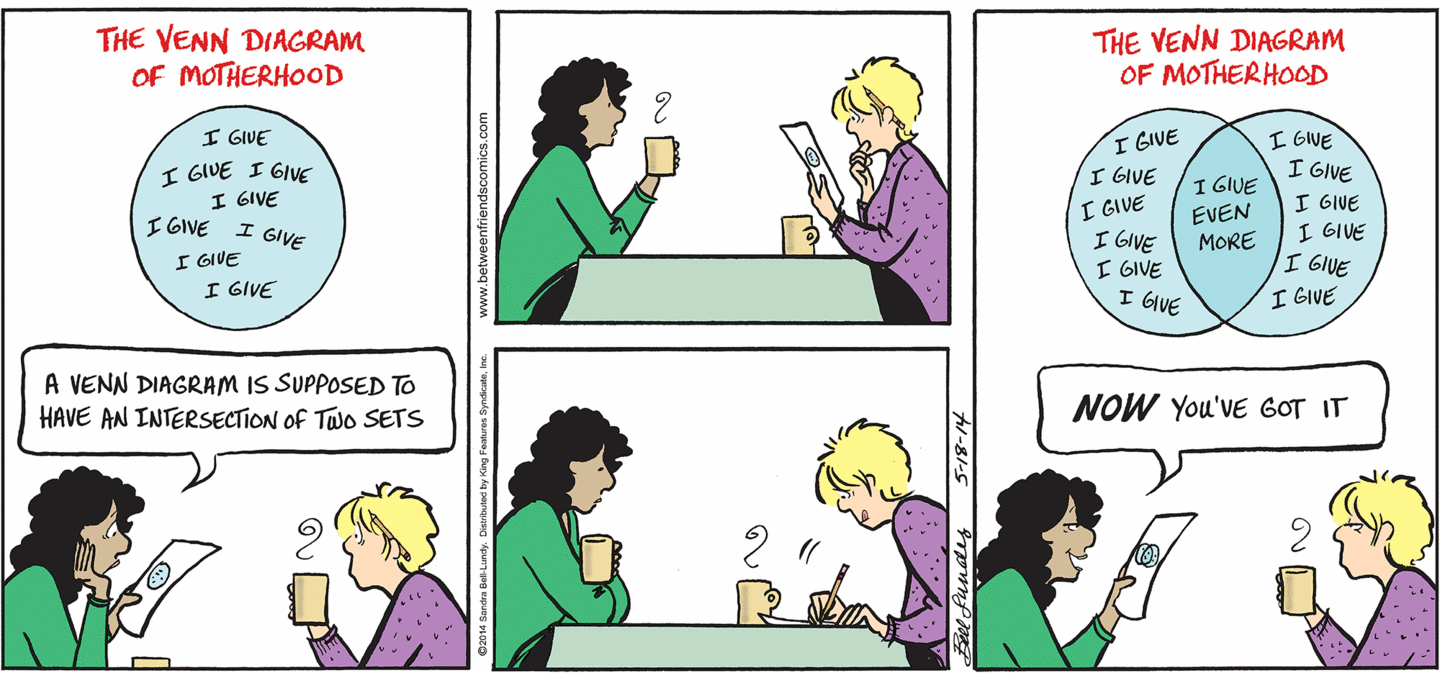
\includegraphics[width=3.5\textwidth]{Cartoon_1}} 
\part{Precalculus}
\label{deel1}


\begin{savequote}[75mm]
	The only way to learn mathematics is to do mathematics.
	\qauthor{--- Paul Halmos ---}
\end{savequote}

\chapter{Sets and numbers}
\graphicspath{{figures/Sets/}}
\label{SetsChapter}
\ifcourse
To make sure that everyone has an understanding of the basic concepts that are at the basis of subsequent chapters, we begin this part with a brief summary of set theory and some of the associated vocabulary and notations we use throughout the text. 
\fi

\ifvc
We begin with a brief summary of set theory and some of the associated vocabulary and notations we use throughout the text. 
\fi

\section{Sets}
\label{sets}
\subsection{Logic operators}
\label{sec:logic operators}
Throughout this course, and especially when defining new mathematical objects, we will often make use of notation that contains one or more logic operators. An overview of them is given in Table~\ref{tab:logicsymbols}. Note the difference between $X \Rightarrow Y$ and $X \Leftrightarrow Y$. $X \Rightarrow Y$ states that if $X$ is true, $Y$ is also true, but if $Y$ is true, $X$ is not necessarily true. $X \Leftrightarrow Y$, on the other hand, states that $X$ and $Y$ are both true or both not true and thus equivalent. For instance, we may write
$$
\text{Garfield is a cat } \wedge\text{ all cats are mammals }  \Rightarrow \text{ Garfield is a mammal}\,,
$$
though 
$$
\text{Garfield is a mammal }  \not\Rightarrow \text{ Garfield is a cat}\,!
$$


\begin{table}[]
	\centering
	\renewcommand{\arraystretch}{2}%
	\begin{tabular}{c||c}
		Notation               & Reads as \\\hline
		$X \Rightarrow Y$     & $X$ implies $Y$;  if $X$ then $Y$\\\hline
		$X \Leftrightarrow Y$  & $X$ if and only if $Y$\\\hline
		$X \wedge Y$           & $X$ and $Y$ \\\hline
		$X \vee Y$             & $X$ or $Y$ \\\hline
		$\forall x$   & for all (elements) $x$ \\\hline
		$\exists x$   & there exists an (element) $x$ \\\hline
		$\exists !\  x$   & there exists just one (element) $x$ \\\hline
		$.|.$   & . so that . \\\hline
		$:.$   & it holds that . \\
	\end{tabular}
	\caption{Overview of important logic operators. $X $ and $Y$ denote logic statements, which are either true or false.}
	\label{tab:logicsymbols}
\end{table}


\pagebreak
\subsection{Definition and representation of sets}
We start with a definition of a set. 
\begin{definition}[Set]
A \textbf{set}\index{set}\index[aut]{verzameling} (\textit{verzameling}) is a well-defined collection of objects which are called the elements of the set.  
\end{definition}
In this definition, `well-defined' means that it is possible to determine if something belongs to the collection or not, without prejudice. For example, the collection of letters that make up the word `smolko' is well defined and is a set, but  the collection of the worst math teachers in the world is not well defined, and so is not a set.  In general, there are three ways to describe sets. 

\begin{enumerate}
	\item The \textbf{verbal method}: use a sentence to define a set.
	\item The \textbf{roster method}:  begin with a left brace `$\{$', list each element of the set only once and then end with a right brace `$\}$'.
	\item The \textbf{set-builder method}: a combination of the verbal and roster methods.
\end{enumerate}
\index{verbal method}
\index{roster method}
\index{set-builder notation}

For example, let $S$ be the set described verbally as the set of letters that make up the word `smolko'.  A  roster description of $S$ would be  $S=\left\{ s, m, o, l, k \right\}$. Note that sets do not allow for repeated elements while they are also  orderless, so $\left\{ k,  l,  m, o, s \right\}$ is also a roster description of $S$. A set-builder description of $S$ is: 
\[ S=\{ x \, | \, \mbox{$x$ is a letter in the word `smolko'}\}. \]

In this notation we call $x$ a \textbf{dummy variable} and `$x$ is a letter in the word `smolko'' the \textbf{predicate}. The way to read this is: `The set of elements $x$ such that $x$ is a letter in the word `smolko.'
%Actually, proceeding in this way it is implicitly understood that the predicate should be interpreted with respect to the letters available in the European alphabet.  This alphabet may hence be understood as the universal set in which the predicate must be interpreted. In the case of ambiguity this can be made more explicit in the set-builder description as
%\[ S=\{ x \in \mbox{European alphabet}\, | \, \mbox{$x$ is a letter in the word `smolko'}\}. \]
Clearly $m$ is in $S$ and $q$ is not in $S$, i.e.\   $m \in S$ and $q \notin S$.  Moreover, the empty set is written as $A=\left\{\right\}$ or $A=\emptyset$, and a set containing a single element is reffered to as a \textbf{singleton} (\textit{singleton}).
\index{dummy variable}\index[aut]{dummy variabele}
\index{predicate}\index[aut]{predicaat}
\index{singleton}\index[aut]{singleton} 

Graphically, sets are typically represented by means of so-called \textbf{Venn diagrams} (\textit{Venn-diagram}), enclosed areas in the plane. For instance, Figure~\ref{fig_sets_1} shows the Venn diagram of the set $S=\left\{ s, m, o, l, k \right\}$. \index{Venn diagram}\index[aut]{Venn-diagram}


\begin{figure}[h!]
	\begin{center}
		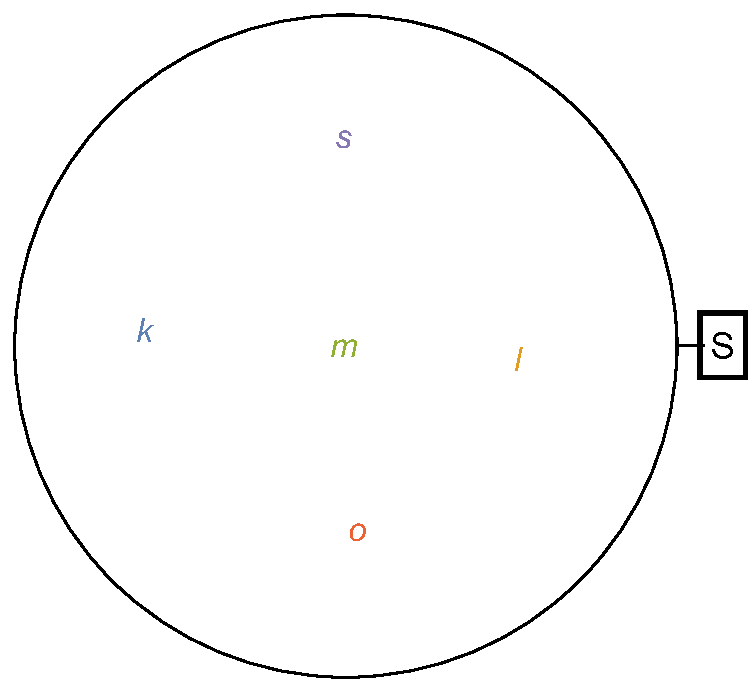
\includegraphics[width=0.3\textwidth]{fig_sets_1}
		\caption{Venn diagram of the set $S=\left\{ s, m, o, l, k \right\}$.}
		\label{fig_sets_1}
	\end{center}
\end{figure}

\ifcourse
\ifanalysis

	The fact that a set sensu stricto does not bear an ordering constitutes an inconvenience in  applications where one may often easily envisage an order relation to order the elements in a particular set.  In this way, one arrives at a so-called ordered set, which is formally defined below. 
	\\
	
	\begin{definition}[Ordered set]
		An \textbf{ordered set} (\textit{geordende verzameling}) is a set $S$, together with
		a relation $<$ such that
		\begin{enumerate}
			\item For any $x, y \in S$, exactly one of
			$x < y$, $x=y$, or $y < x$ holds.
			\item If $x < y$ and $y < z$, then $x < z$.
		\end{enumerate}
		We write $x \leq y$ if $x < y$ or $x=y$. Besides, we may define
		$>$ and $\geq$ in a similar way.
		\index{set ! ordered}
		\index[aut]{verzameling ! geordend}
	\end{definition}
	For example, the set of countries can be ordered by landmass, so India $>$ Lichtenstein. Likewise, the dictionary is the ordered set of words where the order is the so-called lexicographic ordering.  In the remainder of this course, we will, however, mostly be interested in ordered
	sets of numbers.

\fi
\fi

\subsection{Set operations}
\label{setoperations}
Having defined sets, we can now devise some operations that can be performed with them. Let us consider two sets $A$ and $B$. First, we define that  $A$ and $B$ are equal if and only if they have the same elements, that is
$$
(A=B) \quad\Leftrightarrow\quad \left(\forall x\mid  (x\in A) \Leftrightarrow (x\in B)\right)\,.
$$


The equality of two sets can be expressed alternatively upon introducing the concept of \textbf{subsets} (\textit{deelverzameling}). We say that $A$ is a subset of the set $B$,  if all elements of $A$ are in $B$; that is if and only if $\forall x: x\in A\Rightarrow x\in B$. We write this as $A\subseteq B$. It immediately follows that two sets $A$ and $B$ are equal if and only if $A\subseteq B$ and $B\subseteq A$. A \textbf{proper subset} (\textit{strikte deelverzameling}) $A$ of a set $B$, denoted $A\subset B$, is a subset that is strictly contained in $B$ and so necessarily excludes at least one element of $B$. 

\ifcourse

\begin{remark}[Equality]
	Robert Recorde, a Welsh mathematician, introduced the equal sign in 1557. He motivated his choice, by stating: 
	\textit{And to avoid the tedious repetition of these words: is equal to: I will set as I do often in work use, a pair of parallels, or Gemowe lines of one length, thus: $=$, because no 2 things, can be more equal.}	
\end{remark}
\fi

\ifcourse
\ifanalysis

	Mathematically, we may write
	$$
	\left(A\subset B\right) \quad\Leftrightarrow\quad  \big(\left(A\subseteq B\right) \, \land \, \left(A\neq B\right)\big)\,.
	$$

\fi
\fi

For instance, the regular polygons make up a proper subset of the set of polygons. %(Figure~\ref{fig_sets_3}).
\index{subset}\index[aut]{deelverzameling}
\index{subset ! proper}\index[aut]{deelverzameling ! strikt}

% \begin{figure}[h!]
% 	\begin{center}
% 		\includegraphics[width=0.4\textwidth]{fig_sets_3_cropped}
% 		\caption{The regular polygons make up a proper subset of the set of polygons.}
% 		\label{fig_sets_3}
% 	\end{center}
% \end{figure}

Finally, we can define a \textbf{universal set} (\textit{universum}), often denoted by $U$, which contains all objects, including itself.
Actually, in the set-builder description of the exemplary set $S=\left\{ s, m, o, l, k \right\}$, it is implicitly understood that the predicate should be interpreted with respect to the letters available in the European alphabet.  This alphabet may hence be understood as the universal set in which the predicate must be interpreted. In the case of ambiguity this can made more explicit in the set-builder description as
\index{universal set}\index[aut]{universum}

\[ S=\{ x \in \mbox{European alphabet}\, | \, \mbox{$x$ is a letter in the word `smolko'}\}. \]

% BIOIR: MEER DEFINITIE GEBASEERD

Let us now envisage the following operations on the sets $A$ and $B$, subsets of the universal set $U$, which are illustrated in Figure~\ref{fig_sets_2}.


\begin{figure}[t]
	\centering
	%\raisebox{0.5cm}{
	\centerline{
		\subfigure[Intersection \label{fig_sets_2a}]{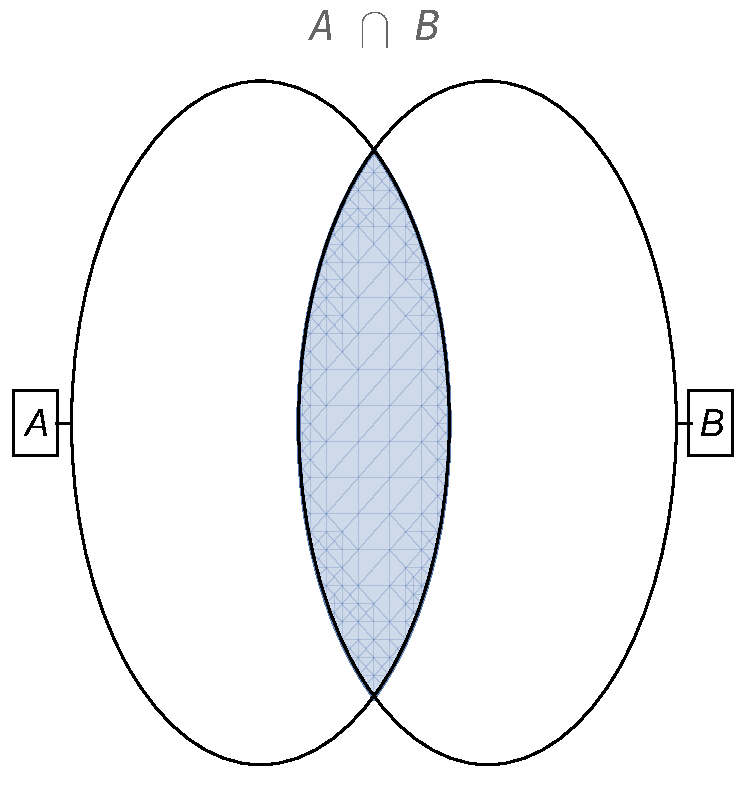
\includegraphics[width=0.3\textwidth]{fig_sets_2a}}
		\hspace{1cm}
		\subfigure[Union \label{fig_sets_2b}]{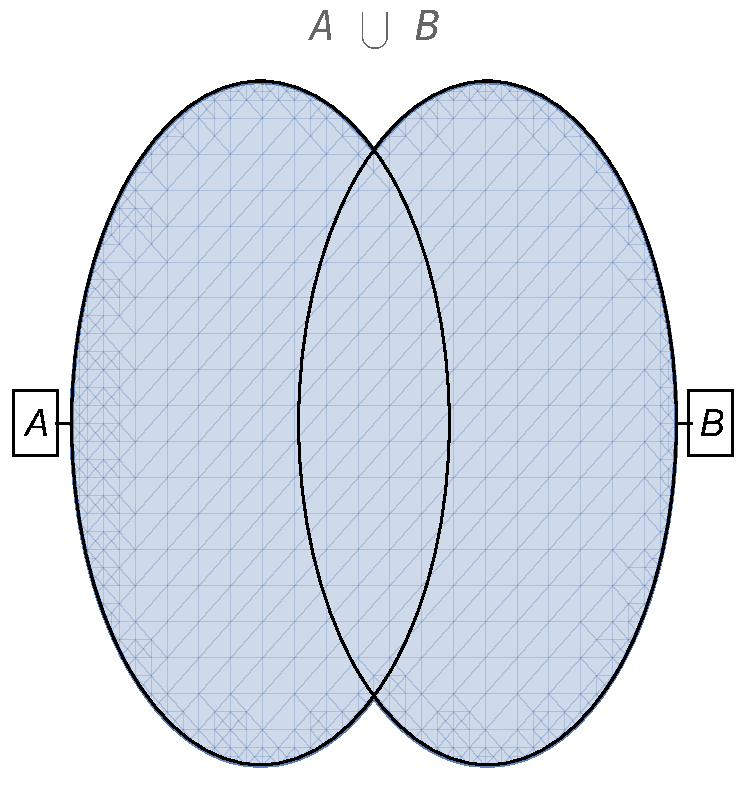
\includegraphics[width=0.3\textwidth]{fig_sets_2b}}
		\hspace{1cm}
		\subfigure[Complement \label{fig_sets_2c}]{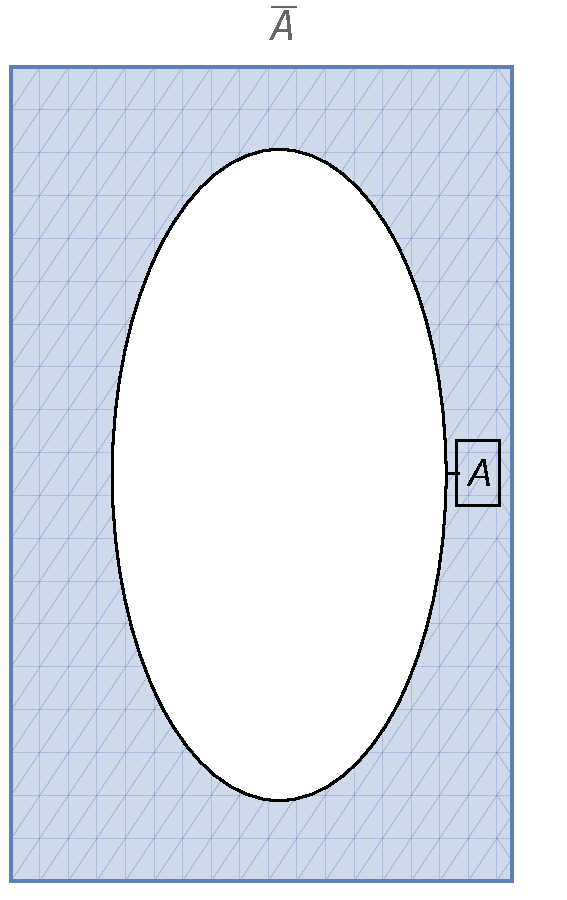
\includegraphics[width=0.2\textwidth]{fig_sets_2c}}
	}
	\centerline{
		\subfigure[Difference \label{fig_sets_2d}]{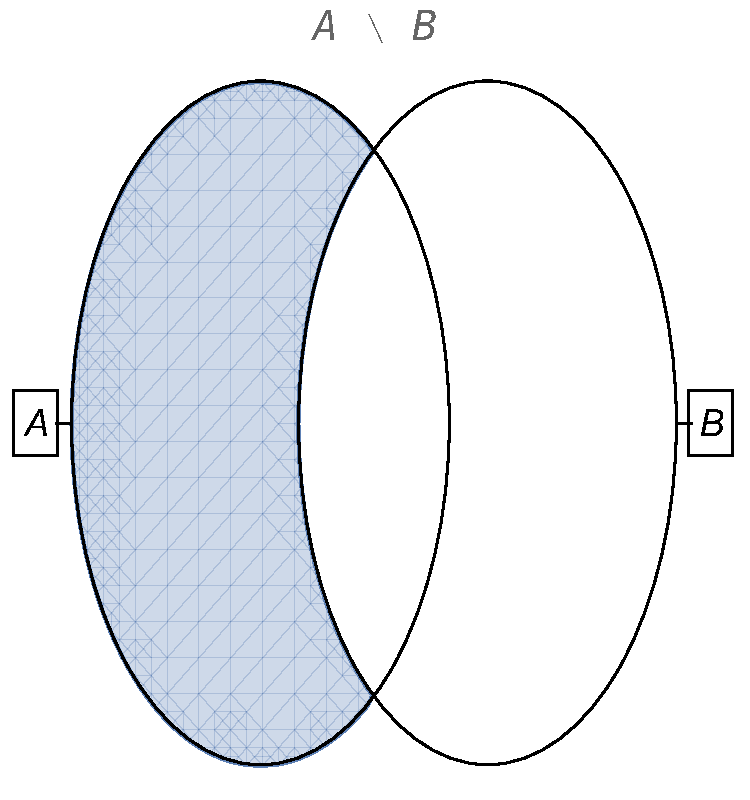
\includegraphics[width=0.3\textwidth]{fig_sets_2d}}
		\hspace{1cm}
		\subfigure[Symmetric difference \label{fig_sets_2e}]{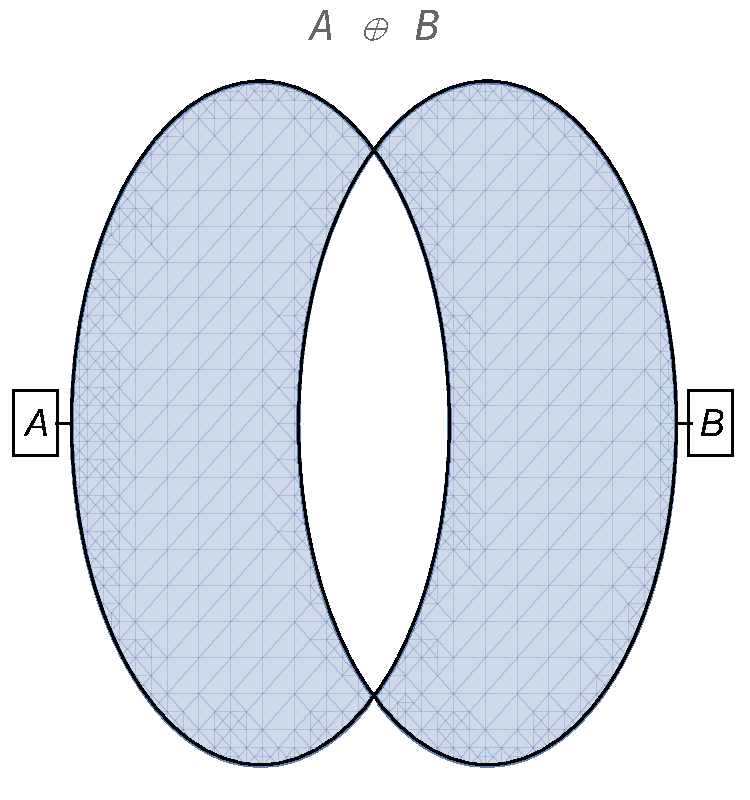
\includegraphics[width=0.3\textwidth]{fig_sets_2e}}
	}
	\caption{Set operations involving two sets $A$ and $B$.\label{fig_sets_2}} 
	
\end{figure}

\begin{itemize}
	\item \textbf{Intersection} (\textit{doorsnede}): \index{intersection}\index[aut]{doorsnede}
	$$
	A\cap B=\left\{x\mid \left(x\in A\right)\wedge\left(x\in B\right)\right\}.
	$$
	This yields the common elements of $A$ and $B$. Two sets are called \textbf{disjoint} (\textit{disjunct}) if $A\cap B=\emptyset$. This operation generalises directly to $n$ sets. \index{disjoint}\index[aut]{disjunct}
	\item \textbf{Union} (\textit{unie}): \index{union}\index[aut]{unie} 
	$$
	A\cup B=\left\{x\mid \left(x\in A\right)\vee\left(x\in B\right)\right\}.
	$$
	This yields the set of elements that belong to either of the two sets. This operation generalises directly to $n$ sets. 
	\item \textbf{Complement} (\textit{complement}): \index{complement}\index[aut]{complement}  
	$$
	\overline{A}=\left\{x\in U\mid x\notin A \right\}.
	$$
	This yields the set of elements in the universal set $U$ that do not belong to a set $A$.
	\item \textbf{Difference} (\textit{verschil}): \index{difference}\index[aut]{verschil}
	\ifvc
	$$
	A\setminus B=\left\{x\mid \left(x\in A\right)\wedge\left(x\notin B\right)\right\}=A\cap\overline{B}.
	$$
	This yields the set of elements that belong to set $A$ but not to set $B$. 
	\fi
	\ifcalculus
	$$
	A\setminus B=\left\{x\mid \left(x\in A\right)\wedge\left(x\notin B\right)\right\}=A\cap\overline{B}.
	$$
	This yields the set of elements that belong to set $A$ but not to set $B$. 
	\fi
	
	\ifanalysis
	
		$$
		A\setminus B=\left\{x\mid \left(x\in A\right)\wedge\left(x\notin B\right)\right\}.
		$$
		This yields the set of elements that belong to set $A$ but not to set $B$. There is also a relationship between the set difference and set complement, which can be understood from the following:
		\begin{eqnarray*}
			A \setminus B&=& \left\{x\mid \left(x \in A\right) \land \left(x \notin B\right)\right\}\\
			&=& \left\{x\mid \left(x \in A \wedge x \in U\right)  \land \left(x \notin B\right)\right\}\\
			&=& \left\{x\mid \left(x \in A \right)\wedge \left( x \in U  \land x \notin B \right)\right\}\\
			&=& \left\{x\mid \left(x \in A\right) \wedge  \left(x \in  \overline{B}\right) \right\}\\
			&=& A\cap\overline{B}\,.
		\end{eqnarray*}
	
	\fi
	

	
	\item \textbf{Symmetric difference} (\textit{symmetrisch verschil}): \index{symmetric difference}\index[aut]{symmetrisch verschil}
	$$
	A\oplus B=\left\{x\mid \left(x\in A\cup B\right)\wedge \left(x\notin A\cap B\right)\right\}.
	$$
	%\todo[inline,backgroundcolor=green!25]{$A\oplus B=\left\{x\mid \left(x\in A\cup B\right)\wedge \left(x\notin A\cap B\right)\right\}\,.$}
	This yields the set of elements that belong to either one or the other set but not both.
	
	\item \textbf{Cartesian product} (\textit{Cartesisch product}): \index{Cartesian product}\index[aut]{Cartesisch product}
	$$
	A\times B=\left\{\left(a,b\right)\mid \left(a\in A\right)\wedge\left(b\in B\right)\right\}.
	$$
	This yields the set of ordered pairs of $\left(a,b\right)$ of all elements $a$ and $b$, that belong to set $A$ and $B$, respectively. When taking the Cartesian product of $A$ with itself, i.e.\ $A\times A$, this is also denoted as $A^2$.
\end{itemize}




\ifcourse
\begin{remark}[Venn-diagrams]
	Venn diagrams were named after John Venn (1843--1923), who studied and standardised these diagrams.
	A major issue that he tried to tackle, was finding symmetrical diagrams of partially multiple overlapping sets. Venn only got as far as 4 sets and it took until 1975 for mathematicians to extend this to 5 and more. The figure below illustrates this for 5, 7 and 11 sets, respectively. %\textbf{(ref: MathWorld)}.
	%Ref: Weisstein, Eric W. "Venn Diagram." From MathWorld--A Wolfram Web Resource. http://mathworld.wolfram.com/VennDiagram.html
	\begin{center}
		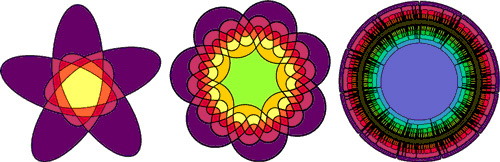
\includegraphics[width=0.5\textwidth]{fig_sets_3.jpg}
		%\caption{Symmetric Venn diagrams of 5, 7 and 11 overlapping seys.}
	\end{center}
	
\end{remark}
\fi


\ifvc
\begin{example}
	Consider the following three sets that contain words from three Germanic languages, namely Dutch, English and German, respectively:
	\begin{eqnarray*}
		D&=&\left\{\mbox{Afrikaans, computer, duif, fiets, internet, \"uberhaupt}\right\},\\
		E&=&\left\{\mbox{Afrikaans, bike, blitzkrieg, computer, fest, internet, pigeon}\right\},\\
		G&=&\left\{\mbox{blitzkrieg, computer, fest, internet, rad, taube, \"uberhaupt}\right\}.
	\end{eqnarray*}
	\begin{enumerate}
		\item Construct the Venn diagram representation of the three sets. 
		\item Determine the set $D_1$ of words that appear in Dutch only.
		\item Determine the set $D_2$ of words that are common to both English and German, but not to Dutch. 
		\item Determine the Cartesian product of $D_1\times D_2$ and $D_1\times D_1$.
	\end{enumerate}
	
	\xhrulefill{gray}{2.5pt}Solution \xhrulefill{gray}{2.5pt}
	
	\begin{enumerate}
		\item Figure~\ref{fig_sets_4} shows the Venn diagram of the three sets. 
		\begin{figure}[H]
			\begin{center}
				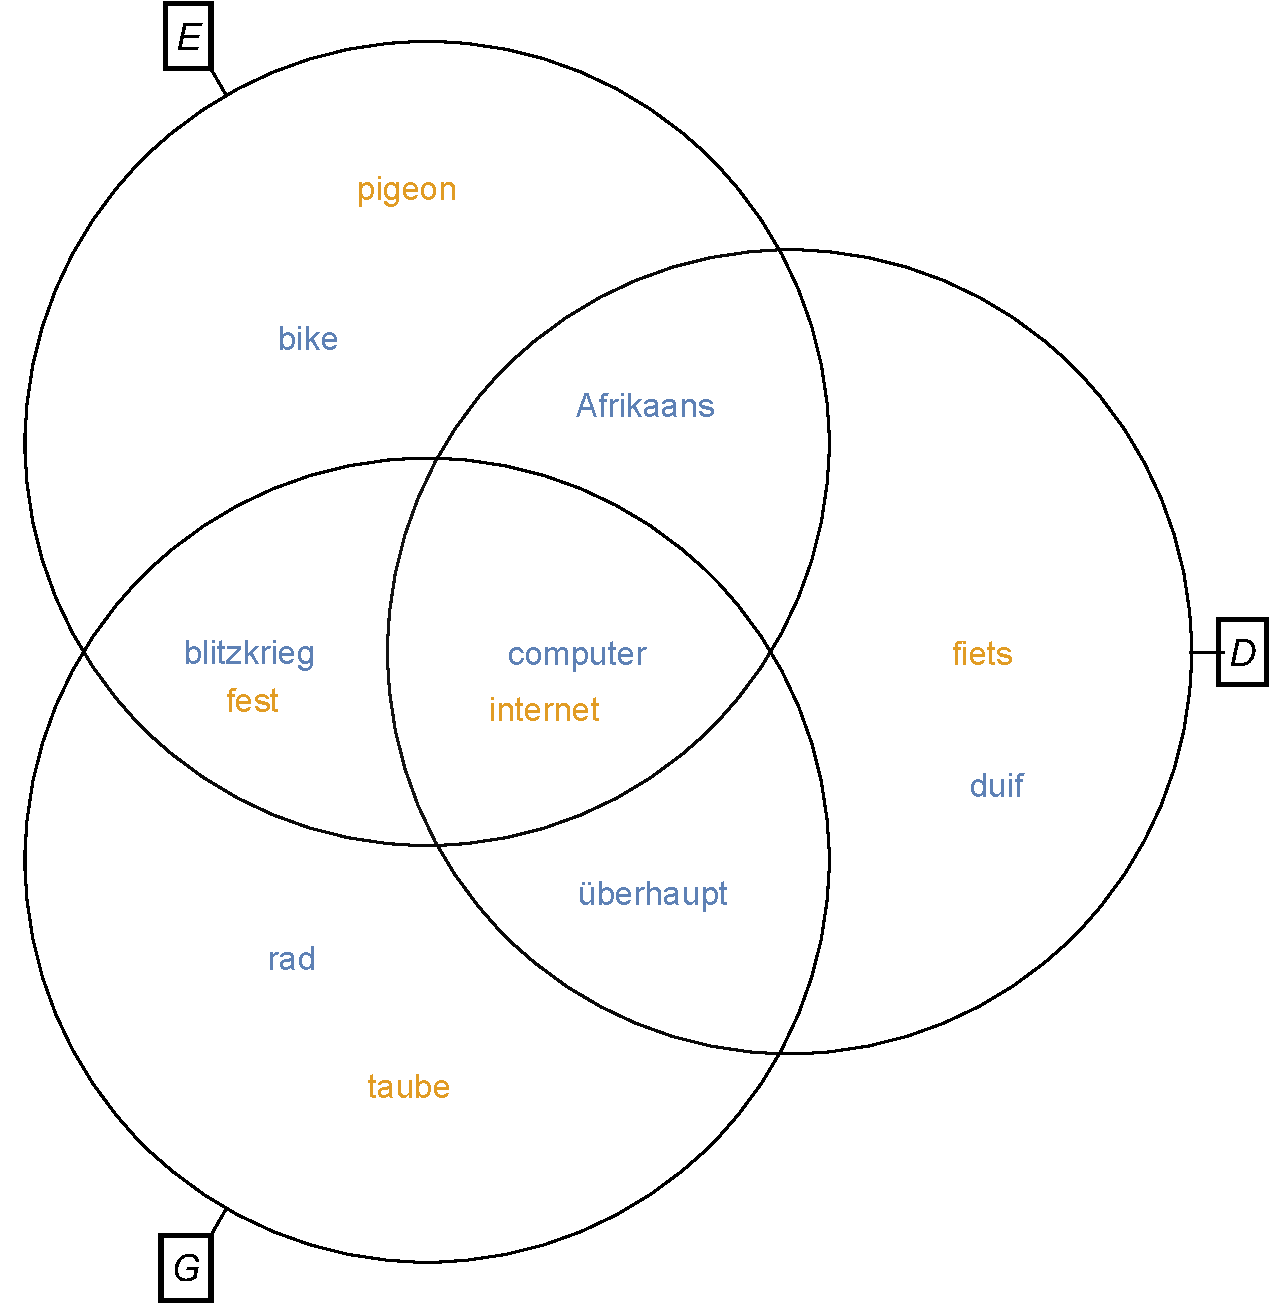
\includegraphics[width=0.4\textwidth]{fig_sets_4}
				\caption{Venn diagram of the sets $D$, $E$ and $G$.}
				\label{fig_sets_4}
			\end{center}
		\end{figure}
		
		\item \label{setexampleD1} The set of words that appear in Dutch only, is nothing but the set of all Dutch words minus the set of words that appear either in German or English. More formally, we can define this set as
		$$
		D_1=D\setminus \left(G\cup E\right)=\left\{\mbox{duif, fiets}\right\}.
		$$
		\item \label{setexampleD2} The set of words that are common to both English and German, but not to Dutch,  can be found by excluding Dutch words from the intersection of $E$ and $G$. Hence, we get
		$$
		D_2=(E\cap G)\setminus D=\left\{\mbox{blitzkrieg, fest}\right\}.
		$$
		
		\item  The Cartesian products follow immediately using $D_1$ and $D_2$ determined in 2 and 3: 
		$$
		D_1 \times D_2 = \left\{\left(\mbox{duif, blitzkrieg}\right), \left(\mbox{duif, fest}\right), \left(\mbox{fiets, blitzkrieg}\right), \left(\mbox{fiets, fest}\right)\right\},
		$$
		
		$$
		D_1^2 = \left\{\left(\mbox{duif, duif}\right), \left(\mbox{duif, fiets}\right), \left(\mbox{fiets, duif}\right), \left(\mbox{fiets, fiets}\right)\right\}.
		$$
	\end{enumerate}
	
\end{example}

\fi


\subsection{Set properties}
Below we list the most important properties of sets, most of which can be understood intuitively or using a Venn diagram representation.
\index{commutativity}\index[aut]{commutativiteit}\index{associativity}\index[aut]{associativiteit}\index{distributivity}\index[aut]{distributiviteit}
\begin{itemize}
	\item \textbf{Commutativity} (\textit{commutativiteit}) of intersection and union:
	$$
	A\cap B=B\cap A \quad\mbox{ and }\quad A\cup B=B\cup A.
	$$
	\item \textbf{Associativity} (\textit{associativiteit})  of intersection and union:
	$$
	A\cap \left(B\cap C\right)=\left(A\cap B\right)\cap C \quad\mbox{ and }\quad A\cup \left(B\cup C\right)=\left(A\cup B\right)\cup C.
	$$
	\item \textbf{Distributivity} (\textit{distributiviteit})  with respect to intersection and union:
	$$
	A\cup \left(B\cap C\right)=\left(A\cup B\right)\cap \left(A\cup C\right) \quad\mbox{ and }\quad A\cap \left(B\cup C\right)=\left(A\cap B\right)\cup \left(A\cap C\right).
	$$
	\item \textbf{Identity laws}:
	$$
	A \cup \emptyset =A \quad\mbox{ and }\quad A \cap U= A.
	$$
	\item \textbf{Complement laws}:
	$$
	A \cup \overline {A} =U \quad\mbox{ and }\quad A \cap \overline {A} = \emptyset. 
	$$
\end{itemize}
For instance, if we are looking for the words that are common to Dutch, English and German, it does not matter that we first determine the words that are common to Dutch and English and then look which of those also are used in German, or start by first determining the words that are common to German and English and finally verify which of those are also used in Dutch. 

For completeness, we also mention the \textbf{De Morgan's laws} (\textit{regels van De Morgan}):\index{De Morgan's laws}\index[aut]{De Morgan ! regels van}
$$
\overline{A\cup B}=\overline{A}\cap\overline{B} \quad\mbox{ and }\quad\overline{A\cap B}=\overline{A}\cup\overline{B}.
$$

\ifcourse
\ifanalysis

	When considering ordered sets, we are often interested in the elements lying at their  boundaries.\\
	
	\begin{definition}[Upper bound, lower bound, supremum, infimum]
		\label{sup_def}
		Let $A \subset S$, where $S$ is an ordered set.
		
		\begin{enumerate}
			\item If there exists a $b \in S$ such that $x \leq b$ for all $x \in A$, then we say $A$ is \textbf{bounded above} (\textit{naar boven begrensd}) and $b$
			is an \textbf{upper bound} (\textit{bovengrens}) of $A$.
			\item If there exists a $a \in S$ such that $x \geq a$ for all $x \in A$,
			then we say $A$ is \textbf{bounded below} (\textit{naar beneden begrensd}) and $a$
			is a \textbf{lower bound} (\textit{ondergrens}) of $A$.
			\item If there exists an upper bound $\beta$ of $A$ such that whenever
			$b$ is any upper bound for $A$ we have $\beta \leq b$, then $\beta$
			is called the \textbf{least upper bound} (\textit{kleinste bovengrens}) or
			the \textbf{supremum}
			of $A$.    We write
			\begin{equation*}
			\sup\, A = \beta .
			\end{equation*}
			This is illustrated in Figure~\ref{fig_sets_5}.
			\item Similarly, if there exists a lower bound $\alpha$ of $A$ such that whenever
			$a$ is any lower bound for $A$ we have $\alpha \geq a$, then $\alpha$
			is called the \textbf{greatest lower bound} (\textit{grootste ondergrens}) or
			the \textbf{infimum}
			of $A$.  We write
			\begin{equation*}
			\inf\, A = \alpha  .
			\end{equation*}
		\end{enumerate}
		When a set $A$ is both bounded above and bounded below, we say simply that
		$A$ is \textbf{bounded} (\textit{begrensd}).
	\end{definition}
	\index[aut]{bovengrens}
	\index[aut]{ondergrens}
	\index[aut]{supremum}
	\index[aut]{infimum}
	\index{upper bound}
	\index{lower bound}
	\index{supremum}
	\index{infimum}

	
	
	
	It should be stressed that the supremum (or infimum) is automatically unique (if it exists).  Indeed, if $\beta$ and
	$\beta'$ are both suprema of $A$, then $\beta \leq \beta'$ and $\beta' \leq \beta$, because both $\beta$ and $\beta'$ are the least upper bounds, so it must hold that $\beta=\beta'$. For instance, let $S := \{ a, b, c, d, e \}$ be ordered as $a < b < c < d < e$, and let $A := \{ a, c \}$.  Then $c$, $d$, and $e$ are upper bounds of $A$, and $c$ is the -- unique -- least upper bound or supremum of $A$. Likewise, the infimum of  $\{2,3,4\}$ is 2. 
	\begin{figure}[h]
		\begin{center}
			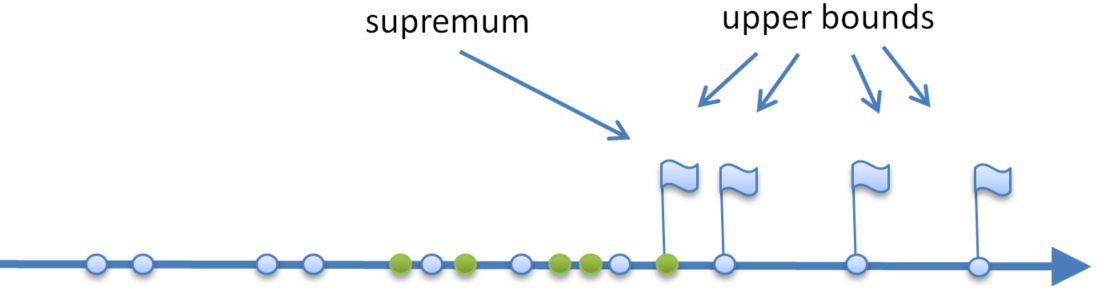
\includegraphics[width=0.6\textwidth]{fig_sets_5}
			\caption{Upper bounds and the supremum of an ordered set $A\subset S$, where the ordering is endowed by the axis and the elements of $A$ are shown as green dots.}
			\label{fig_sets_5}
		\end{center}
	\end{figure}
	
\index{minimum}
\index{maximum}
\index[aut]{minimum}
\index[aut]{maximum}
	Finally, it should be noted that a supremum or infimum for $A$ (even if they exist) need not be in $A$. If $\sup \, A \in A$, then we also denote it by $\max\, A$ and call it the \textbf{maximum} (\textit{maximum}) of $A$, and likewise if $\inf\, A\in A$, then we also denote it by $\min\, A$ and call it the \textbf{minimum} (\textit{minimum}) of $A$. For 
	
	\begin{example}
		Let us consider the set
		$$
		A=\left\{\dfrac{1}{n}\bigg| n=1,2,3,\ldots\right\}\,.
		$$ 
		Then it holds that $\sup\, A = 1$ and since this supremum belongs to
		$A$, we say that $\max\, A =1$. On the other hand, $\inf\, A = 0$ does not belong to $A$, so $A$ has no minimum.
	\end{example}
	
	We conclude this section with an important property that a set may have as it is at the basis of some of the proofs in the upcoming chapters. 
	\begin{definition}[Least-upper-bound property] \label{defn:lub}
		An ordered set $S$ has the \textbf{{least-upper-bound property}} (\textit{supremumeigenschap}) if
		every nonempty subset $A \subset S$ that is bounded above has a least upper bound, that is $\sup\, A$ exists in $S$.
	\end{definition}
	
	The least-upper-bound property is sometimes called the \textbf{completeness property}.
	

\fi
\fi


\section{The set of real numbers}
\label{sec_real}
\subsection{Definition}

Throughout your mathematical upbringing, you have encountered several famous sets of numbers:  
\begin{itemize}
	\item The set of  \textbf{natural numbers} (\textit{natuurlijke getallen}):  $\mathbb N= \{ 0, 1, 2, 3,  \ldots\}$.
	%\item The set of \textbf{whole numbers}: $\mathbb W= \{ 0, 1, 2, 3,  \ldots\}$.
	\item The set of \textbf{integers} (\textit{gehele getallen}): $\mathbb Z=\{ \ldots, -3, -2, -1, 0, 1, 2, 3, \ldots \}$.
	\item The set of \textbf{rational numbers} (\textit{rationale getallen}): $$\mathbb Q=\left\{\dfrac{a}{b} \, \bigg| \, a,b  \in \mathbb Z \, \wedge \, b \neq 0 \right\}\,.$$
\end{itemize}
Essentially, rational numbers are the ratios of integers, provided the denominator is not zero. For instance, 
$$
\dfrac{3}{4}=0.75, \qquad \mbox{and}\qquad \dfrac{1}{3}=0.333333\ldots
$$
are just two exemplary rational numbers.  Looking at those, it is clear that another way to describe the rational numbers is:
\[\mathbb Q=\{x\,|\,\mbox{$x$ possesses a repeating or terminating decimal representation}\}.\]
Indeed, it can be proofed that any decimal number with a repeating or terminating decimal representation can be written as a ratio of integers, so as a rational number. 

\index{natural number}\index[aut]{natuurlijk getal}
\index{integer}\index[aut]{geheel getal}
\index{rational number}\index[aut]{rationaal getal}
\index{number ! natural}\index[aut]{getal ! natuurlijk}
\index{number ! integer}\index[aut]{getal ! geheel}
\index{number ! rational}\index[aut]{getal ! rationaal}

There are of course numbers with a decimal that neither repeats nor terminates, e.g.  
$$
\pi=3.141592654\ldots, \qquad \mbox{and}\qquad 0.123456789101112123\ldots
$$
Such numbers are called \textbf{irrational numbers} (\textit{irrationale getallen}) and they form the set of the irrational numbers, denoted $\mathbb{I}$. Now, we can define a new set, namely the set of so-called \textbf{real numbers} (\textit{re\"ele getallen}) as follows:
\index{real number}\index[aut]{re\"eel getal}
\index{irrational number}\index[aut]{irrationaal getal}
$$
\mathbb{R}=\mathbb{I}\cup\mathbb{Q}\,.
$$
Figure~\ref{fig_sets_6} shows how the sets of natural, rational and real numbers are nested. It clearly holds that the set of natural numbers is a proper subset of the one of the integers, which on its turn is again a proper subset of the set of rational numbers, and so on. Besides, this Venn diagram emphasizes that the sets of rational and irrational numbers are disjoint. 


\begin{figure}
	\begin{center}
		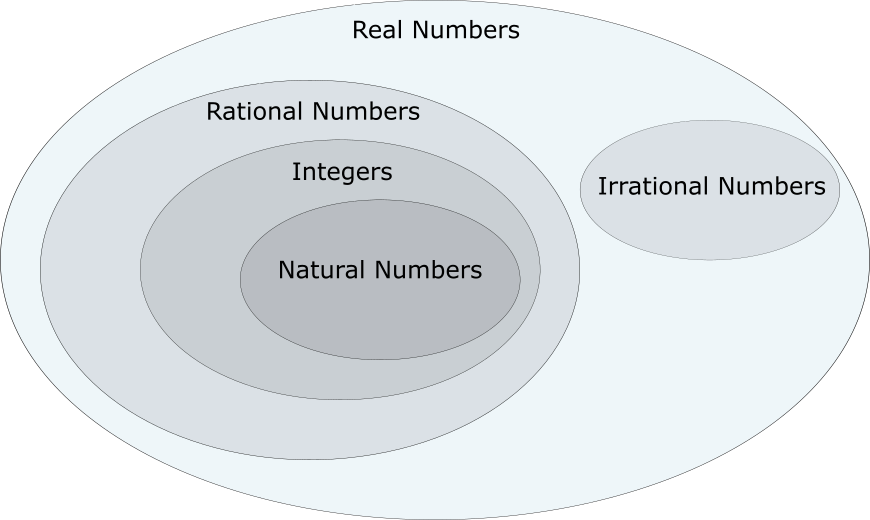
\includegraphics[width=0.4\textwidth]{fig_sets_6}
		\caption{Venn diagram of the sets of natural, integer, rational, irrational and real numbers.}
		\label{fig_sets_6}
	\end{center}
\end{figure}

\index{irational number}\index[aut]{irrationaal getal}
\index{real number}\index[aut]{re\"eel getal}
\index{complex number}\index[aut]{complex getal}
\index{number ! irational}\index[aut]{getal ! irrationaal}
\index{number ! real}\index[aut]{getal ! re\"eel}


The set $\mathbb R$ may be visualized as a line because its elements can be ordered using an order relation. More precisely, the real numbers can be identified with the points on an infinitely long line once its origin, unit of length and orientation have been chosen:
\begin{center}
	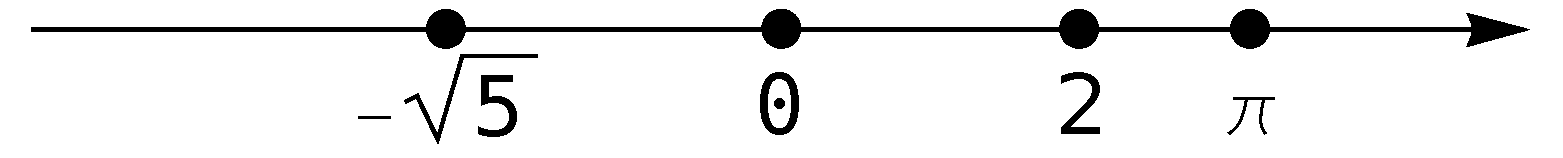
\includegraphics[width=0.4\textwidth]{fig_sets_7}
\end{center}
With every real number $x$ corresponds one point on this line, and vice versa, every point on this line represents one real number. This line is called the \textbf{real number line} (\textit{re\"ele getallenas}). \index{real number line}\index[aut]{re\"ele getallenas}


In addition to the set of real numbers, we often make reference to one of the following subsets for the sake of brevity:
\begin{eqnarray*}
	\mathbb{R}_0 &=& \mathbb{R} \backslash \{0\},\\
	\mathbb{R}^+ &=& \{x\; |\; x\in \mathbb{R} \;\wedge\; x \geq 0\},\\
	\mathbb{R}^- &=& \{x\; |\; x\in \mathbb{R} \;\wedge\; x \leq 0\},\\
	\mathbb{R}^+_0 &=& \{ x\; |\; x\in \mathbb{R}\;\wedge\; x > 0 \},\\
	\mathbb{R}^-_0 &=& \{ x\; |\; x\in \mathbb{R}\;\wedge\; x < 0 \}.\\
\end{eqnarray*}

Moreover, it is possible to extend $\mathbb{R}$ with two more elements, namely positive infinity ($+\infty$) and negative infinity  ($-\infty$), which are defined as:
$$ 
\forall x\in\mathbb{R}:\quad-\infty<x<+\infty\,,
$$
and which do not belong to $\mathbb{R}$. Doing so, one arrives at the set of \textbf{extended real numbers} (\textit{uitgebreide re\"ele getallen}):
$$
\overline{\mathbb{R}}=\mathbb{R}\cup\left\{-\infty,+\infty\right\}.
$$


For completeness, it should be mentioned that there is a further extension of the set of real numbers possible to the set of \textbf{complex numbers} (\textit{complexe getallen})\index{complex number}\index[aut]{complex getal}\index{number ! complex}\index[aut]{getal ! complex}, defined by 
$$\mathbb C=\left\{a+i\,b \, \mid \, \left(a,b  \in \mathbb R\right) \, \wedge \, \left(i^2=-1\right) \right\}\,.$$
%$$\mathbb C=\left\{a+i\,b \, \mid \, a,b  \in \mathbb R \, \wedge \, i=\sqrt{-1} \right\}.$$
This extension allows us, for instance, to compute the square root of a negative number. The complex numbers are discussed in Section~\ref{sec_complex}. Throughout this course we will, however, mostly restrict our discussion to the set of real numbers. 

\ifanalysis
\begin{remark}[History of complex numbers]
	A long history preceded the development of the set of complex numbers. Three milestones are listed below.
	\begin{enumerate}
		\item Negative numbers
		\begin{itemize}
			\item China (202 BC -- AD 220): \textit{Nine Chapters on the Mathematical Art (Jiu zhang suan-shu)}
			\item Red counting rods were used to denote gains (positive coefficients) and black rods for losses (negative).
		\end{itemize}
		\item The number $0$
		\begin{itemize}
			\item Ancient civilisations such as the Greeks and Romans had no real concept of zero as a number, although the Babylonians left blanks.
			\item ca. 650 AD : Indian mathematics introduced 0, which was eventually spread to the Arab and Asian nations.
			\item In Europe 0 was introduced (along with the rest of the Hindu-Arabic number system) mainly via the \textit{Liber Abaci} by Fibonacci. Initially, there was a strong opposition against new numeric system by people clinging on the old Roman system.
		\end{itemize} 
		\item The number $i$
		\begin{itemize}
			\item Italy, 16th century: Studied during the discovery of algebraic solutions for the roots of cubic and quartic polynomials by Italian mathematicians
		\end{itemize}
	\end{enumerate}
\end{remark}
\fi



\subsection{Real number arithmetic}
\label{sec_real_number}
\subsubsection{Addition and multiplication}
In the set of real numbers, we can define to main operations namely, addition ($+$) and multiplication ($\cdot$). If $a, b$ and $c$ are three real numbers, we have the following five axioms:

\index{commutativity}\index[aut]{commutativiteit}\index{associativity}\index[aut]{associativiteit}
\begin{enumerate}
	\item \textbf{Algebraic closure} (\textit{algebra\"isch gesloten}):
	\begin{align*}
	a+b\in \mathbb{R} \quad & \mbox{ and }\quad a\cdot b \in\mathbb{R}\,.\\
	\intertext{\item  \textbf{Commutativity} (\textit{commutativiteit}):}
	a+b=b+a \quad & \mbox{ and }\quad a\cdot b=b\cdot a\,.\\
	\intertext{\item \textbf{Associativity} (\textit{associativiteit}):}
	a+(b+c)=(a+b) +c \quad & \mbox{ and }\quad a\cdot(b\cdot c)=(a\cdot b)\cdot c\,.\\
	\intertext{\item \textbf{Identity property}:}
	a+0=0+a=a \quad & \mbox{ and }\quad a\cdot1=1\cdot a=a\,.\\
	\intertext{\item \textbf{Inverse property}:}
	a+(-a)=(-a)+a=0 \quad & \mbox{ and }\quad a\cdot a^{-1}=a^{-1}\cdot a=1\\
	\end{align*}
\end{enumerate}

Essentially, the identity property indicates that 0 is the \textbf{neutral element} (\textit{neutraal element})  of the addition operation and 1 is neutral element of the multiplication operation, while the inverse property shows that there is always an \textbf{opposite element} (\textit{tegengesteld element})  in the case of addition and an \textbf{inverse element}  (\textit{invers element}) in the case of multiplication. Finally, according to the sixth axiom of real numbers, multiplication \textbf{distributes} over addition:\index{distributivity}\index[aut]{distributiviteit}
$$
a\cdot (b+c) = a\cdot b + a\cdot c \quad\mbox{ and }\quad(a+b)\cdot c = a\cdot c + b\cdot c\,. 
$$ 
The operations of subtraction and division are not listed above because they fail to  possess  many  of  the aforementioned  properties.  More precisely, subtraction   and   division   are   not   commutative, nor associative, as for instance $4-1\neq1-4$ and likewise $(4-1)-2\neq4-(1-2)$. \index{neutral element}\index[aut]{neutraal element}\index{inverse element}\index[aut]{invers element}\index{opposite}\index[aut]{tegengestelde}

\ifanalysis

	Since any set  that has the operations of addition and multiplication
	defined on it and that satisfies the preceding axioms is called a \textbf{field} (\textit{veld}), the sets of rational and real numbers constitute fields.  On the other hand, the set of integers is not a field, as it does not contain multiplicative inverses. For example, there is no $x\in\mathbb{Z}$ such that $2x=1$.
	
	Clearly, we may extend the notion of a field to an \textbf{ordered field} (\textit{geordend veld}) if the underlying set is ordered. Hence, the sets of rational and real numbers are ordered fields.
	\index{field}
	\index[aut]{veld}

\fi

Throughout this course we will sometimes be confronted with problems involving the summation\index{summation}\index[aut]{sommatie} of many numbers, e.g.
$$
a_0+a_1+a_2+\cdots+a_n\,,
$$
where $n$ is some natural number. Clearly, writing such sums can become quite cumbersome, so a shorthand notation thereof has been established using the \textbf{capital sigma notation}\index[aut]{sommatie!hoofdletter sigma notatie}; that is

$$
a_0+a_1+a_2+\cdots+a_n=\displaystyle\sum_{i=0}^na_i\,,
$$
where $i$ is the \textbf{summation index}  (\textit{index})\index{summation!summation index}\index[aut]{sommatie!index} and $a_i$ is a \textbf{generic term}  (\textit{algemene term})\index{sommatie!generic term}\index[aut]{sommatie!algemene term} in the summation. This expression should be read as the sum of the numbers $a_i$ for $i$ going from 0 to $n$. Here, the index $i$ starts at 0, but this is not a requisite. 

We can formulate the following useful properties of summations:
\begin{itemize}
	\item Sum or difference of summations:
	$$
	\displaystyle\sum_{i=0}^n a_i\pm \displaystyle\sum_{i=0}^nb_i=\displaystyle\sum_{i=0}^n\left(a_i\pm b_i\right)\,.
	$$
	\item Splitting a summation:
	$$
	\displaystyle\sum_{i=0}^n a_i=\displaystyle\sum_{i=0}^m a_i+\displaystyle\sum_{i=m+1}^n a_i\,,\, \text{where } m<n\,.
	$$
	\item Scalar multiplication:
	$$
	c\cdot \displaystyle\sum_{i=0}^n a_i=\displaystyle\sum_{i=0}^n c\cdot a_i\,, \text{where}\, c\in\mathbb{R}\,.
	$$
	\item Constant summation:
	$$
	\displaystyle\sum_{i=0}^n c=c\cdot(n+1)\,, \text{where}\, c\in\mathbb{R}\,. 
	$$
	
\end{itemize}

Moreover, we recall (without proof) two useful identities, that will be used in later chapters and involve the sum of the first $n$ (squared) natural numbers:
\begin{equation}
\displaystyle\sum_{i=1}^n i = \dfrac{n(n+1)}{2}\qquad\text{and}\qquad\displaystyle\sum_{i=1}^n i^2 = \dfrac{n(n+1)(2n+1)}{6}.
\label{thm:summation}
\end{equation}

% BIOIR: meervoudige sommatie en vermenigvuldiging van sommen (ins: wiskundige basisvaardigheden)

Similarly to the capital sigma notation for summation, we can use the \textbf{capital pi notation}\index{capital pi notation}\index[aut]{hoofdletter pi notatie} for the product of $n$ numbers:
$$
\displaystyle\prod_{i=0}^n a_i=a_0\cdot a_1\cdot a_2\cdots a_n\,. 
$$

Using the capital pi notation, it becomes easy to define the so-called \textbf{factorial} (\textit{faculteit}) of a natural number $n$, denoted $n!$:
$$
n!=\prod\limits_{k=1}^{n}k=1\cdot 2\cdot 3\cdot \ldots \cdot n.
$$

From here on, we will mostly drop the dot-notation to denote multiplication and use a blank space instead. Only in case of ambiguity (e.g.\ when multiplying two numbers), we will hold on the dot-notation for clarity.

\subsubsection{Exponentiation}

In addition to the four elementary operations in $\mathbb{R}$, namely addition, subtraction, multiplication and division, we can also define \textbf{exponentiation}  (\textit{machtsverheffing}). It involves two numbers, the \textbf{base}  (\textit{grondtal}) $b\in\mathbb{R}_0$ and the \textbf{exponent} (\textit{exponent}) $n$ and is written as $b^n$. When $n$ is a strictly positive integer, exponentiation corresponds to repeated multiplication of the base: that is, $b^n$ is the product of multiplying $n$ bases:\index{exponentiation}\index[aut]{machtsverheffing}\index{base}\index[aut]{basis}\index{exponent}\index[aut]{macht}
$$
b^n=\underbrace{b\, b\, b\,\cdots\,b}_{n \text{ factors}}\,.
$$
This expression should be read as $b$ raised to the power of $n$. For negative powers, we have
$$
b^{-n}=\dfrac{1}{b^n}\,.
$$
By convention, it holds that any non-zero number raised to the 0 power is 1, i.e. $b^0=1$ if $b\neq0$. The expression $b^2$ is often  called the square of $b$ or $b$ squared, while $b^3$ is frequently called the cube of $b$ or $b$ cubed.

The exponent does not necessarily have to be an integer, it can as well be a rational number, such as $1/n$, where $n\in\mathbb{N}_0$. More precisely, we can have
$$
x=b^{\frac{1}{n}}\,,
$$
which should be interpreted as the number $x$ for which the $n$-th power equals $b$. This implies that $b^{1/n}$ is a solution to the equation
$$
x^n=b\,. 
$$

\ifcalculus
\begin{example}
	Moore's law concerns the observation that the number of transistors in a dense integrated circuit doubles about every two years. The observation is named after Gordon Moore, whose 1965 paper described a doubling every year in the number of components per integrated circuit, and projected this rate of growth would continue for at least another decade. Mathematically, we can state this law as
	$$
	P_n=P_0\,2^n\,,
	$$
	where $P_0$ [--] is the number of transistors in some reference year, $n$ [--] the number of two-year periods, and $P_n$ [--] the number transistors $n$ two-year periods passed the reference year. In 1988, the number of transistors in the Intel 386 SX microprocessor was 275 000. What were the transistors counts of the Pentium II Intel microprocessor in 1997? 
	
	\xhrulefill{gray}{2.5pt}Solution \xhrulefill{gray}{2.5pt}
	
	Between 1988 and 1997 there are 9 years, so 4.5 periods of two years. Hence, if Intel doubles the number of transistors every two years, the new processor would have
	\begin{eqnarray*}
		P_{9/2} = 275\,000 \cdot 2^{\frac{9}{2}}
		= 275\,000 \cdot 22.63
		= 6\,223\,250  
	\end{eqnarray*}
	transistors in 1997. In fact, in 1997, the Pentium II had 7.5 million transistors (Figure~\ref{fig_sets_8}). In other words, since 1988 up until 1997, Intel had been doubling the number of transistors in its microprocessors in less than every two years.
	
	\begin{figure}[H]
		\begin{center}
			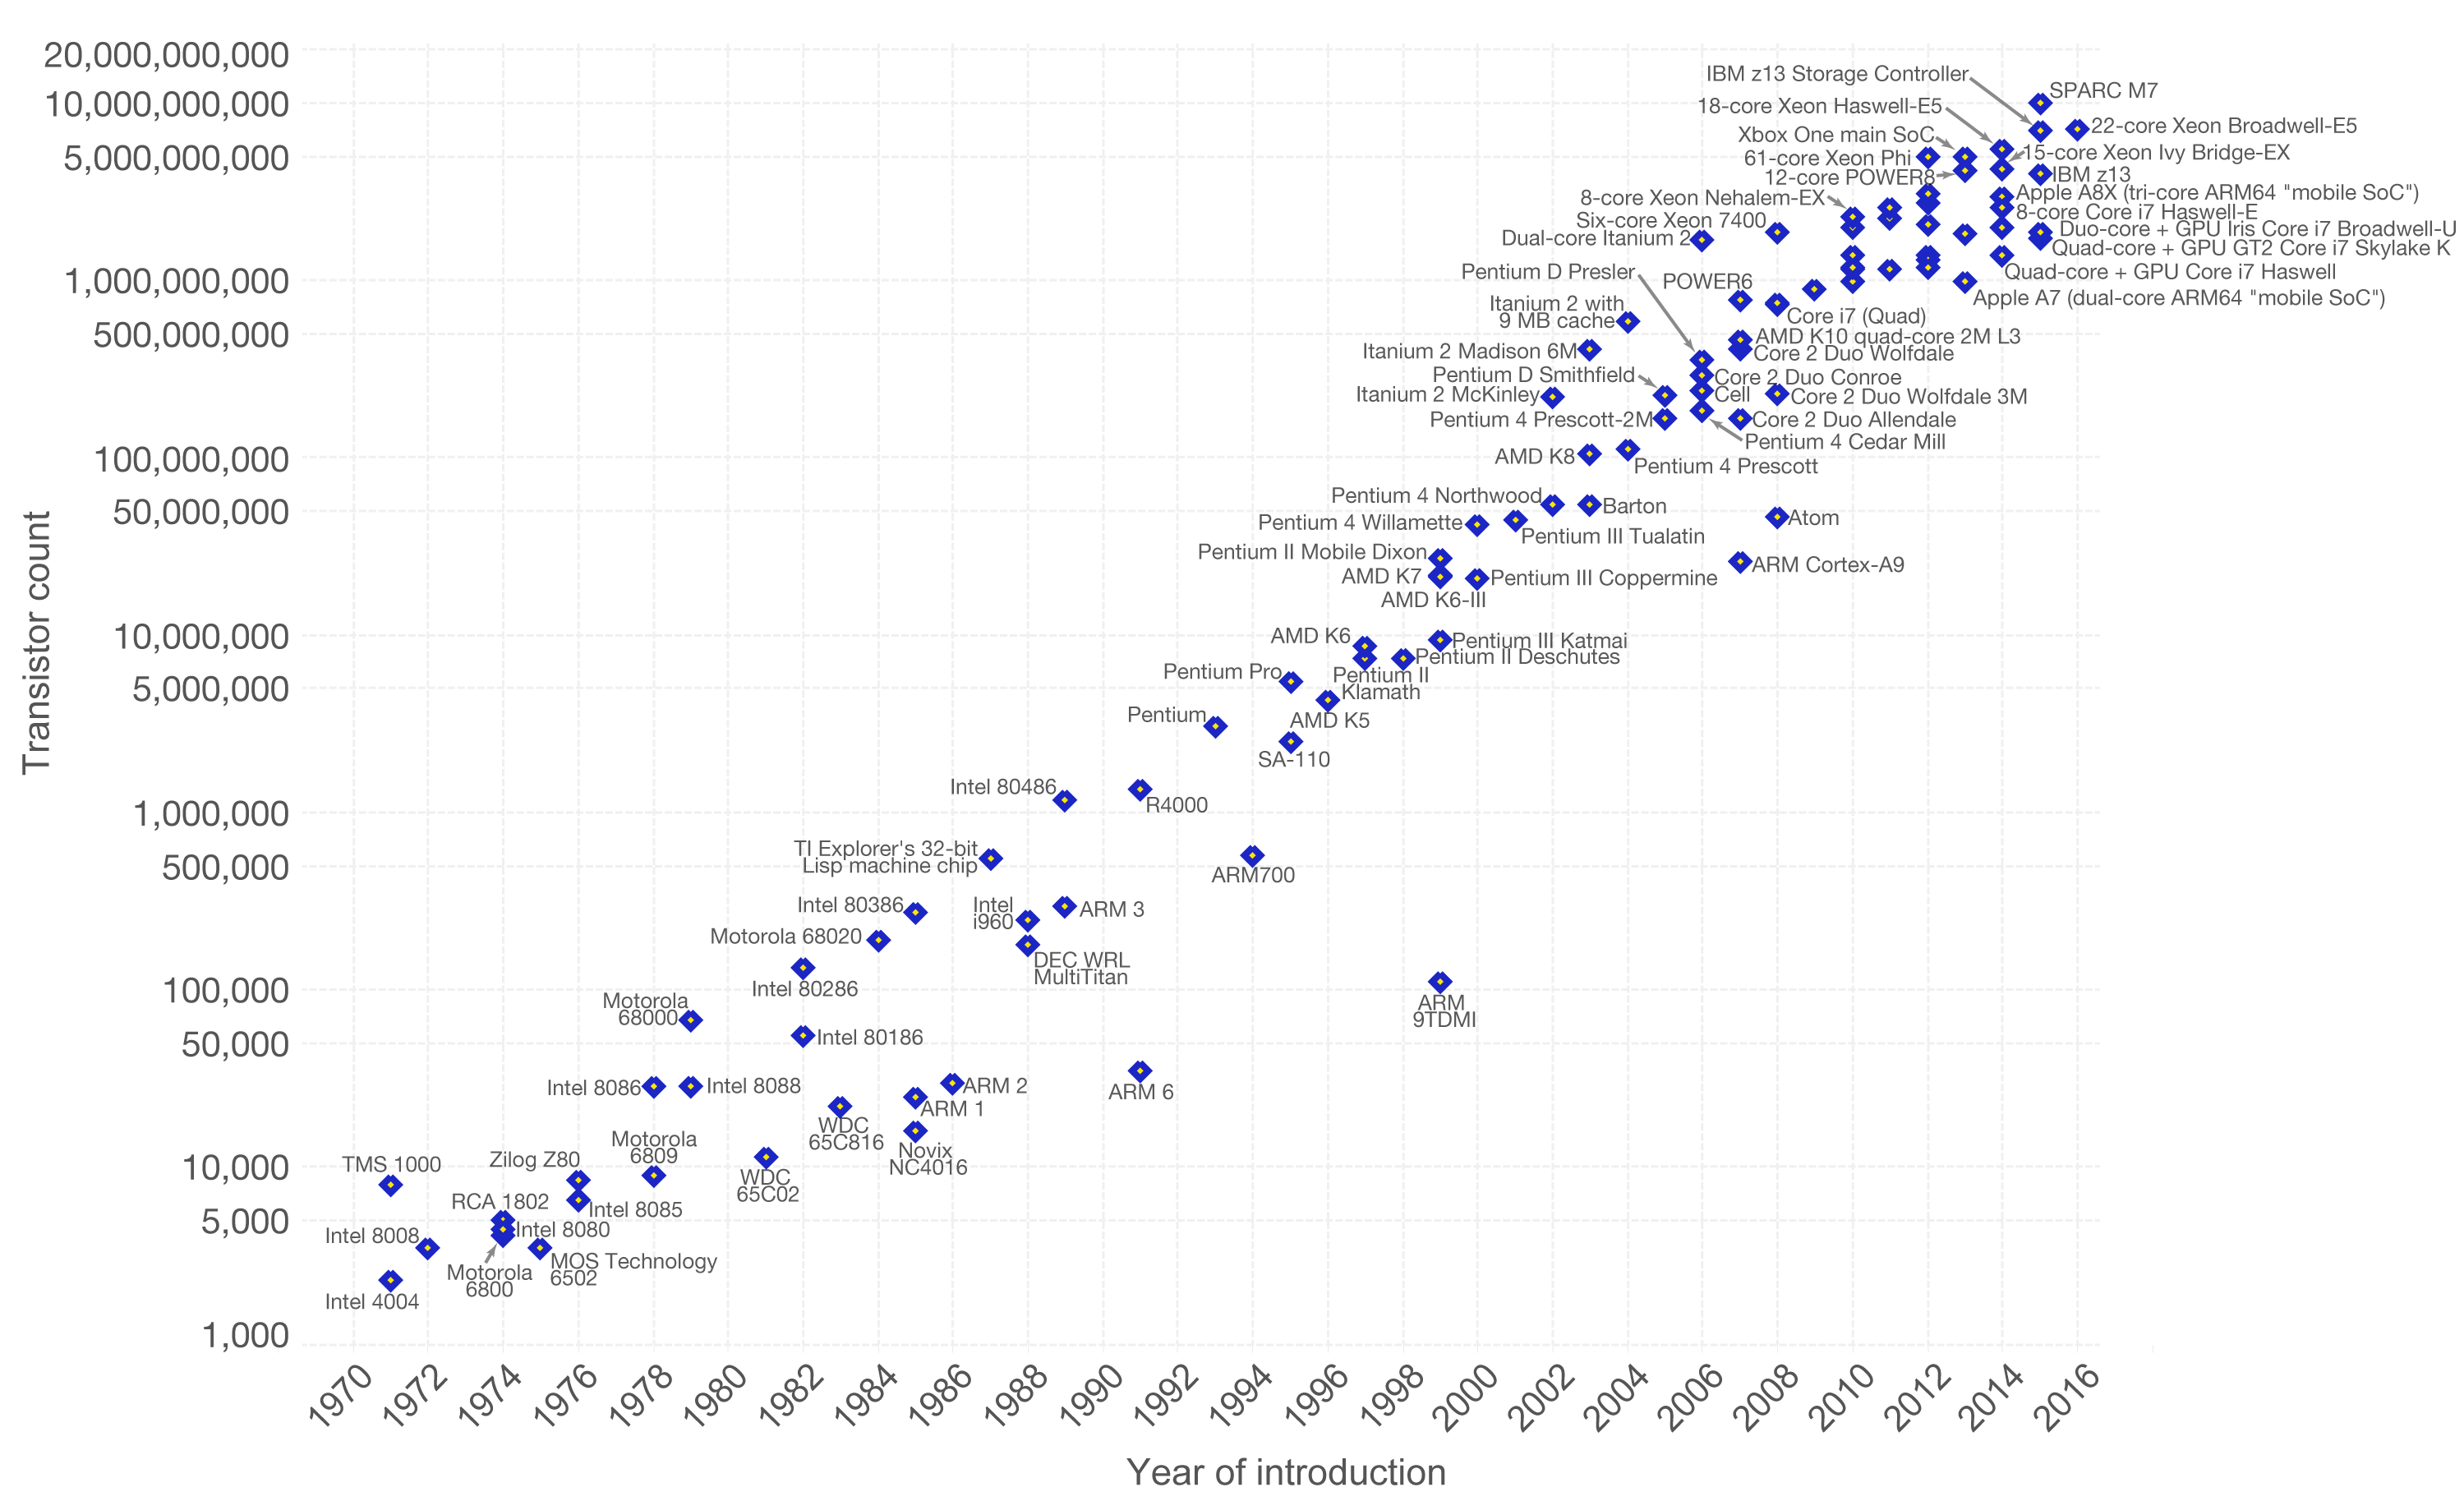
\includegraphics[width=0.75\textwidth]{fig_sets_8}
			\caption{Number of transistors in computer hardware manufactured since 1970.}
			\label{fig_sets_8}
		\end{center}
	\end{figure}
	
	
\end{example}
\fi

Alternatively, $b^{1/n}$ is often written using the radical symbol as $\sqrt[n]{b}$. It is called the principal $n$-th root of $b$. If $n$ is even and $b$ is positive, then $x^n = b$ has two real solutions because even powers of real numbers are always positive. These solutions are the positive and negative $n$-th roots, i.e.
$$
\sqrt[n]{a}\qquad \mbox{ and }\qquad -\sqrt[n]{a}\,. 
$$
If $b$ is negative, the equation has no solution in the set real numbers for even $n$. On the other hand, if $n$ is odd, then $x^n = b$ has exactly one real solution $b^{1/n}$ that is positive if $b$ is positive and negative if $b$ is negative. Finally, taking a positive real number $b$ to a rational exponent $m/n$, where $m$ is an integer and $n$ is a positive integer, and considering principal roots only, yields
$$
b^{\frac{m}{n}}=\left(b^m\right)^{\frac{1}{n}}=\sqrt[n]{b^m}=\left(\sqrt[n]{b}\right)^m\,.
$$

The following basic identities hold for the operation of exponentiation for every $a,b\in\mathbb{R}$ and $p,q\in\mathbb{Q}$:
\begin{itemize}
	\item $a^p\, a^q=a^{p+q}\,,$
	\item $\left(a^p\right)^q=a^{p\, q}\,,$
	\item $\left(a\, b\right)^p=a^p\, b^p\,,$
\end{itemize}
and recalling that $1/a^p=a^{-p}$, we also have:
\begin{itemize}
	\item $\dfrac{a^p}{a^q}=a^{p-q}\,,\qquad$ if $a\neq 0$\,,
	\item $\left(\dfrac{a}{b}\right)^p=\dfrac{a^p}{b^p}\,,\qquad$ if $b\neq 0$\,.
\end{itemize}
However, be aware that exponentiation is not commutative, nor associative, unlike addition and multiplication. Indeed, it is clear that $2^3=8\neq3^2=9$ and likewise 
$$
\left(2^3\right)^4=8^4=4096\neq 2^{(3^4)}=2^{81}=2417851639229258349412352\,.
$$


\begin{example}
	Yearly, there are about three consecutive generations of box moths in Belgium. Suppose the number of box moths (\textit{Cydalima perspectalis}) in generation $i$ can be described as follows:
	$$
	B_{i}=r\,B_{i-1}\,,
	$$
	where $r$ [T$^{-1}$] represents the growth rate of the box moth population. Assuming that we know the initial number of box moths (generation 0), we can compute the number of box moths in generation 1 as
	$$
	B_1=r\,B_0\,.
	$$
	Then, we can compute the number of box moths in generation 2:
	$$
	B_2=r\,B_1=r\,r\,B_0=r^2\,B_0\,,
	$$
	and so on. 
	
	The total number of box moths that has seen daylight up to and including generation $n$, can then be written as
	\begin{eqnarray*}
		T_n&=&\displaystyle\sum_{i=0}^nB_i\,,\\
		&=&B_0+B_1+B_2+\cdots+B_n\,,\\
		&=&B_0+r\,B_0+r^2\,B_0+\cdots+r^n\,B_0\,.
	\end{eqnarray*}
	For instance, if $B_0=5$, $r=1.1$ and $n=5$, we find $T_5\approx39$ individuals. 
\end{example}

For what concerns the square and cube of the sum and difference of two real numbers, we can infer the following well-known identities:\index[aut]{merkwaardige producten}
\allowdisplaybreaks
\begin{eqnarray*}
	(a+b)^2&=&a^2+2ab+b^2\\ 
	(a-b)^2&=&a^2-2ab+b^2\\
	(a+b)(a-b)&=&a^2-b^2\\
	(a+b)^3&=&a^3+3a^2b+3ab^2+b^3\\
	(a-b)^3&=&a^3-3a^2b+3ab^2-b^3\\
	(a+b)(a^2-ab+b^2)&=&a^3+b^3\\
	(a-b)(a^2+ab+b^2)&=&a^3-b^3\\
\end{eqnarray*}

\subsubsection{Arithmetic in $\overline{\mathbb{R}}$}
Obviously, the rules of arithmetic that apply to $\mathbb{R}$ apply to $\overline{\mathbb{R}}$ as well, but we need to introduce a few more rules involving a real number $a\in\mathbb{R}$ and/or $+\infty$ and/or $-\infty$. With regard to addition, we have
\begin{align*}
a+(+\infty) \quad&=\quad (+\infty)+ a\quad=\quad+ \infty\,,\\ 
a+(-\infty)\quad&=\quad(-\infty) + a\quad=\quad- \infty\,,\\
(+\infty)+(+\infty)\quad&=\quad+\infty\,,\\
(-\infty)+(-\infty)\quad&=\quad-\infty\,,\\
\intertext{while for subtraction we have}
a-(+\infty) \quad&=\quad - \infty\,,\\
a-(-\infty) \quad&=\quad + \infty\,,\\
(+\infty) - a \quad&=\quad + \infty\,,\\
(-\infty) - a \quad&=\quad - \infty\,,\\
(+\infty)-(-\infty) \quad&=\quad +\infty\,,\\
(-\infty)-(+\infty) \quad&=\quad -\infty\,.
\end{align*}

For multiplication, we accordingly have (considering $a\in\mathbb{R}_0$)
$$
a\cdot(+\infty)=(+\infty)\cdot a=\left\{\begin{array}{lcl}
+\infty\,,&\mbox{ if }&a>0\,,\\
-\infty\,,&\mbox{ if }&a<0\,,\end{array}\right.
$$
and 
$$
a\cdot(-\infty)=(-\infty)\cdot a=\left\{\begin{array}{lcl}
-\infty\,,&\mbox{ if }&a>0\,,\\
+\infty\,,&\mbox{ if }&a<0\,.\end{array}\right.
$$
Likewise, for products involving $+\infty$ and/or $-\infty$ only:
\begin{eqnarray*}
	(+\infty)\cdot(+\infty)&=&+\infty\,,\\
	(-\infty)\cdot(-\infty)&=&+\infty\,,\\
	(+\infty)\cdot(-\infty)&=&(-\infty).(+\infty)\; \; =\; \; -\infty\,.
\end{eqnarray*}

And for the division, we have
$$
\dfrac{a}{+\infty} = \dfrac{a}{-\infty} = 0\,,
$$
irrespective of the sign of $a\in\mathbb{R}_0$, and
%$$
%\dfrac{a}{0}=\left\{\begin{array}{lcl}
%+\infty\,,&\mbox{ if }&a>0\,,\\
%-\infty\,,&\mbox{ if }&a<0\,,\end{array}\right.
%$$
$$
\dfrac{+\infty}{a}=\left\{\begin{array}{lcl}
+\infty\,,&\mbox{ if }&a>0\,,\\
-\infty\,,&\mbox{ if }&a<0\,,\end{array}\right.
$$
%and finally
$$
\dfrac{-\infty}{a}=\left\{\begin{array}{lcl}
-\infty\,,&\mbox{ if }&a>0\,,\\
+\infty\,,&\mbox{ if }&a<0\,.\end{array}\right.
$$
%For what concerns exponentiation, we have 
%$$
%a^{+\infty}=\left\{\begin{array}{lcl}
%+\infty\,,&\mbox{ if }&a>1\,,\\
%1\,,&\mbox{ if }&a=1\,,\\
%0\,,&\mbox{ if }&-1<a<1\,,\end{array}\right.
%$$
%
%and
%$$
%a^{-\infty}=\left\{\begin{array}{lcl}
%0\,,&\mbox{ if }&a>1\,,\\
%+\infty\,,&\mbox{ if }&-1<a<1\,,\\
%0\,,&\mbox{ if }&a<-1\,.\end{array}\right.
%$$

And finally, for what concerns principal $n$-th roots, for $n\in\mathbb{N}_0$:
\begin{eqnarray*}
	\sqrt[n]{+\infty}&=&+\infty\,,\\
	\sqrt[2n+1]{-\infty}&=&-\infty\,.
\end{eqnarray*}

\ifcourse
\ifanalysis

	\subsection{Completeness of $\mathbb{R}$}
	We have already seen that the set of real numbers is an ordered field. Even more important is that this ordered field is in fact the
	only complete ordered field. Basically, this means that if an alien were to construct a mathematical system on the basis of Axioms (1)-(6) from Section~\ref{sec_real_number} endowed with an ordering and satisfying the least-upper-bound-property (Definition~\ref{defn:lub}), the alien's system would differ from the real number system we devised only in that the alien might use different symbols for the real numbers and $+$, $\cdot$ and $<$.
	
	This all gives rise to the following intuitive theorem. 
	
	\begin{theorem}[Supremum]\label{thmtype:1.1.3}
		If a nonempty set $S$ of real numbers  is bounded above, then
		$\sup S$ is the unique real number $\beta$ such that
		\begin{enumerate}
			\item  $x\leq\beta$ for all $x$ in $S;$
			\item  if $\epsilon>0$ (no matter how small), there is an $x_0$ in
			$S$ such that $x_0>\beta-\epsilon.$
		\end{enumerate}
	\end{theorem}
	Essentially, this theorem can be  interpreted geometrically as follows: $\beta$ is the supremum of $S$ if no point of $S$ is to the right of $\beta$, but there is at least one point of $S$ to the right of any number less than $\beta$. 
	
	\begin{proof}
	To prove the theorem, we first show that $\beta=\sup S$ has properties 1) and
	2). Since $\beta$ is an upper bound of $S$, it must satisfy
	1). Since any real number $a$ less than $\beta$ can be written
	as $\beta-\epsilon$ with $\epsilon=\beta-a>0$, 2) is just
	another way of saying that no number less than $\beta$ is an upper
	bound of $S$. Hence, $\beta=\sup S$ satisfies 1) and 2).
	
	Now we show that there cannot be more than one real number with
	properties 1) and 2). Suppose that $\beta_1<\beta_2$ and
	$\beta_2$ has property 2); thus, if $\epsilon>0$, there is an
	$x_0$ in $S$ such that $x_0>\beta_2-\epsilon$. Then, by taking
	$\epsilon=\beta_2-\beta_1$, we see that there is an $x_0$ in $S$ such
	that
	$$
	x_0>\beta_2-(\beta_2-\beta_1)=\beta_1,
	$$
	so  $\beta_1$ cannot have property 1). Therefore, there cannot
	be more than one real number that satisfies both 1) and
	2).
	\end{proof}
	
	Obviously, we can state a similar theorem for what concerns the infimum.
	\\
	
	\begin{theorem}[Infimum]\label{thmtype:1.1.8}
		If a nonempty set $S$ of real numbers  is bounded below$,$ then
		$\inf S$ is the unique real number $\alpha$ such that
		\begin{enumerate}
			\item % \part{a}
			$x\ge\alpha$ for all $x$ in $S;$
			\item % (b)
			if $\epsilon>0$ $($no matter how small$\,)$, there is an $x_0$ in $S$
			such that
			$x_0<
			\alpha+\epsilon.$
		\end{enumerate}
	\end{theorem}
 \begin{proof}
 As above.
 \end{proof}
	
	
	
	
	
	The real numbers also have the property that it is possible to exceed any positive number, no matter how large, by adding an arbitrary positive number, no matter how small, to itself sufficiently many times.
	
	
	
	\begin{theorem}[Archimedean property]
		\label{thmtype:1.1.4}
		If $\rho$ and $\epsilon$ are positive$,$ then $n\epsilon>\rho$ for
		some $n\in\mathbb{N}_0$.
	\end{theorem}
\begin{proof}	
	The proof of this theorem is by contradiction.
	If the statement is false, $\rho$ is an upper bound of
	the set
	$$
	S=\set{x},
	$$
	where $x=n\epsilon$ and $n\in\mathbb{N}_0$. Therefore, since the set of real numbers is complete, $S$  has a supremum $\beta$ and it holds that 
	\begin{equation}\label{eq:1.1.9}
	n\epsilon\le\beta, 
	\end{equation}
	for all $n\in\mathbb{N}_0$.
	Since $n+1$ is in $\mathbb{N}_0$ whenever $n$ is, Equation~\eqref{eq:1.1.9} implies that
	$$
	(n+1)\epsilon\leq\beta
	$$
	and therefore
	$$
	n\epsilon\leq\beta-\epsilon
	$$
	for all $n\in\mathbb{N}_0$. Hence,
	$\beta-\epsilon$ is an upper bound of $S$.  Since $\beta-\epsilon
	<\beta$, this contradicts the definition of~$\beta$.
\end{proof}	
	

\fi
\fi


\subsection{Intervals in $\mathbb{R}$}
\label{intervals}
Segments of the real number line are called \textbf{intervals} (\textit{interval}) of numbers.  Table~\ref{tab_sets_1} gives a summary of the interval notation for real numbers.  
If the endpoint is included in the interval, we use closing square brackets, `$[$' or `$]$', when defining the interval and use a filled dot to indicate membership in the interval on the real number line. Otherwise, we use opening square brackets, `$]$' or `$[$', and a circle to indicate that the endpoint is not part of the set.  If the interval does not have finite endpoints, we use the symbols $-\infty$ to indicate that the interval extends infinitely to the left and $+\infty$ to indicate that the interval extends infinitely to the right.  Since infinity is a concept, and not a number, we always use opening square brackets when using these symbols in interval notation.%, and use an appropriate arrow to indicate that the interval extends infinitely in one (or both) directions.

It should not be forgotten that any interval in $\mathbb{R}$ corresponds with a certain set of real numbers, so that we may apply the set operations introduced in Section~\ref{setoperations} directly to intervals. For example,  if $A = [-5,3\left[\right.$ and $B = \left.\right]1, +\infty\left[\right.$, then we easily find $A \cap B = \left.\right]1,3\left[\right.$ and   $A \cup B = [-5,+\infty\left[\right.$. Likewise, we find $A\setminus B=[-5,1]$. 


\begin{table}[t]
	\caption{Interval notation for two real numbers $a$ and $b$ for which it holds that $a<b$. }
	\label{tab_sets_1}
	\begin{center}
		\renewcommand{\arraystretch}{2}%
		\begin{tabular}{c|c|c} 
			
			Set of real numbers & Interval notation &  Region on the real number line  \\
			\hline\hline
			
			&  & \\
			\shortstack{$\{x\,|\,a<x<b\}$ \\ \hfill}& \shortstack{$\left.\right]a,b\left[\right.$ \\ \hfill} & 
			
			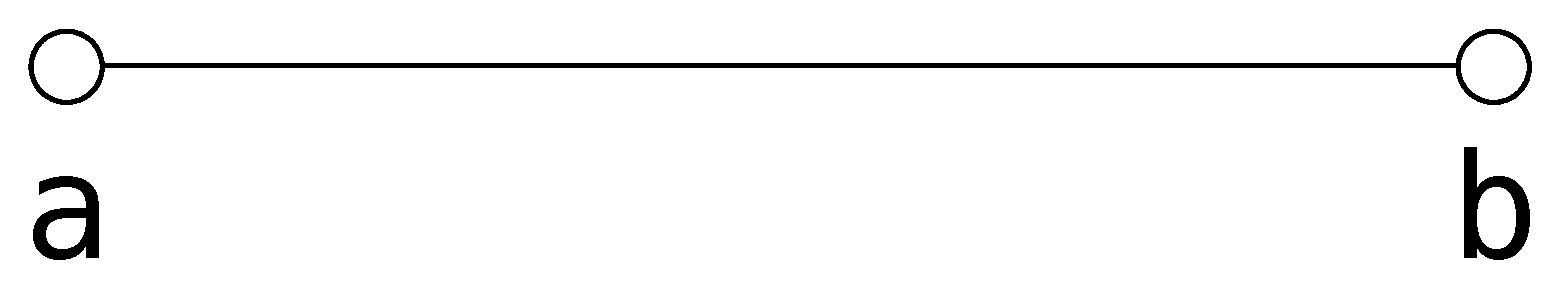
\includegraphics[width=0.25\textwidth]{fig_sets_9a}  \\ \hline
			
			& &  \\
			\shortstack{$\{x\,|\,a\leq x<b\}$ \\ \hfill}& \shortstack{$[a,b\left[\right.$ \\ \hfill} & 
			
			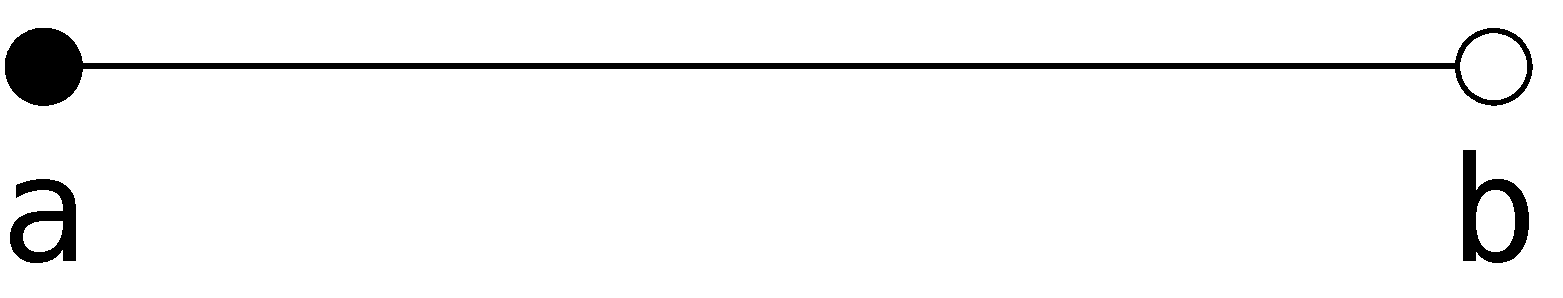
\includegraphics[width=0.25\textwidth]{fig_sets_9b}  \\
			\hline
			
			&  & \\
			\shortstack{$\{x\,|\,a<x\leq b\}$ \\ \hfill}&\shortstack{$\left.\right]a,b]$ \\ \hfill} & 
			
			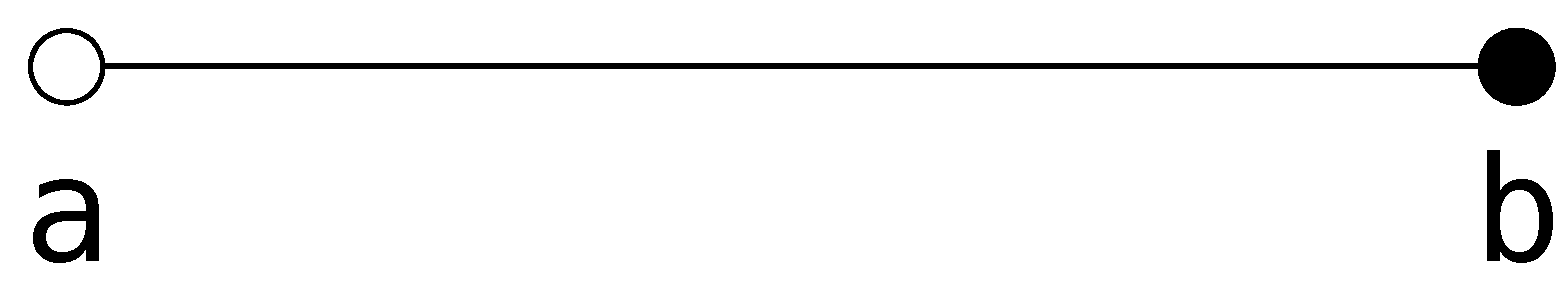
\includegraphics[width=0.25\textwidth]{fig_sets_9c}  \\
			\hline
			
			&  & \\
			\shortstack{$\{x\,|\,a\leq x \leq b\}$ \\ \hfill}& \shortstack{$[a,b]$ \\ \hfill}& 
			
			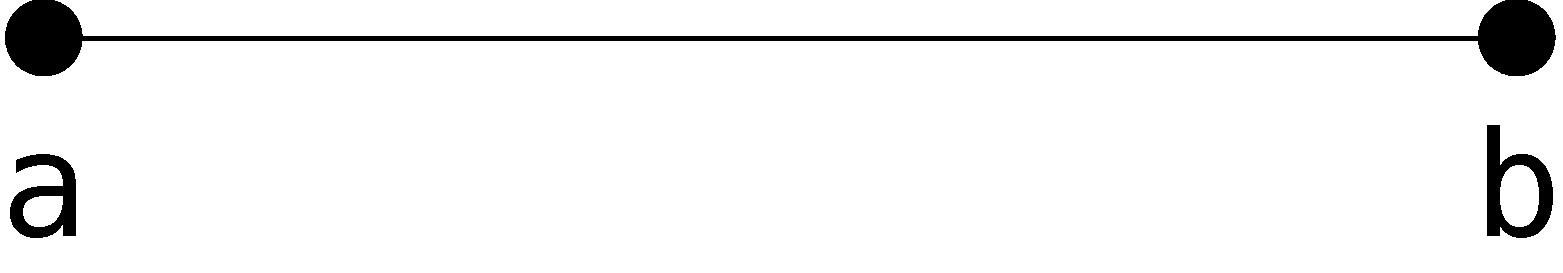
\includegraphics[width=0.25\textwidth]{fig_sets_9d}   \\
			\hline
			
			& & \\
			\shortstack{$\{x\,| \, x<b\}$ \\ \hfill}& \shortstack{$\left.\right]-\infty,b\left[\right.$ \\ \hfill}& 
			
			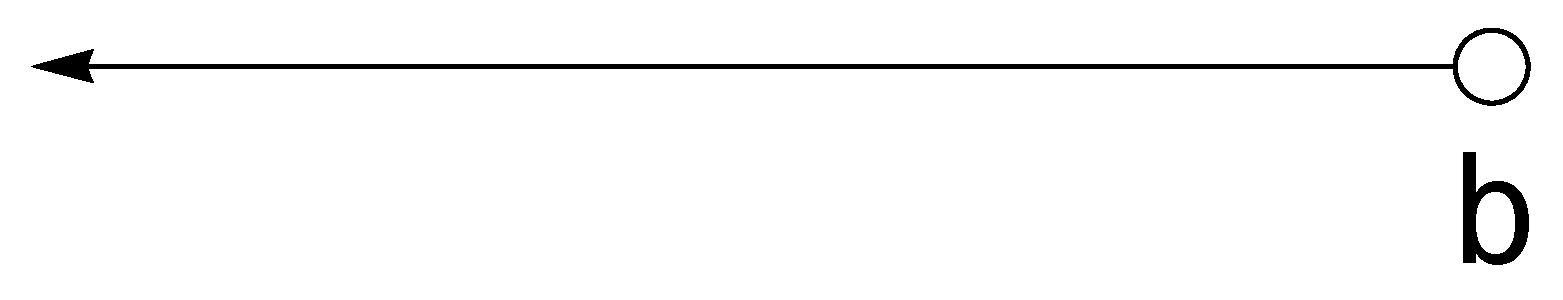
\includegraphics[width=0.25\textwidth]{fig_sets_9e}  \\
			\hline
			
			
			&  & \\
			
			\shortstack{$\{x\,| \, x \leq b\}$ \\ \hfill} & \shortstack{$\left.\right]-\infty,b]$ \\ \hfill}& 
			
			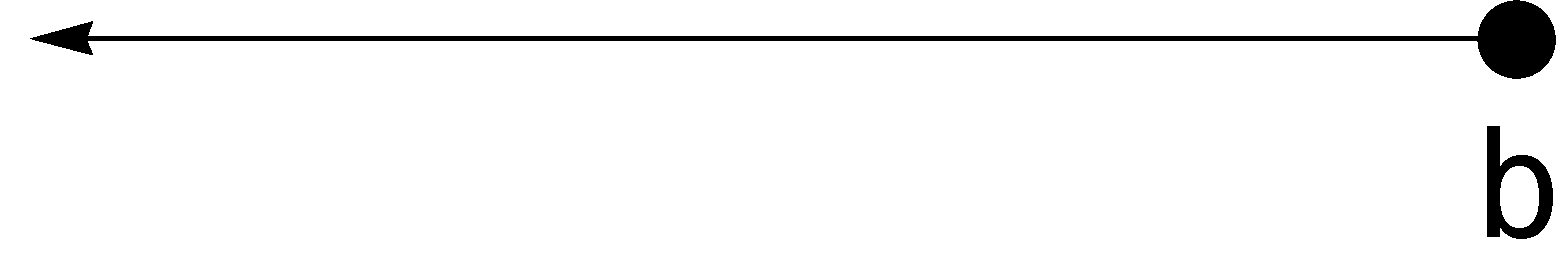
\includegraphics[width=0.25\textwidth]{fig_sets_9f}    \\
			\hline
			
			&  & \\
			\shortstack{$\{x\,| \, x>a\}$ \\ \hfill}& \shortstack{$\left.\right]a,+\infty\left[\right.$ \\ \hfill}& 
			
			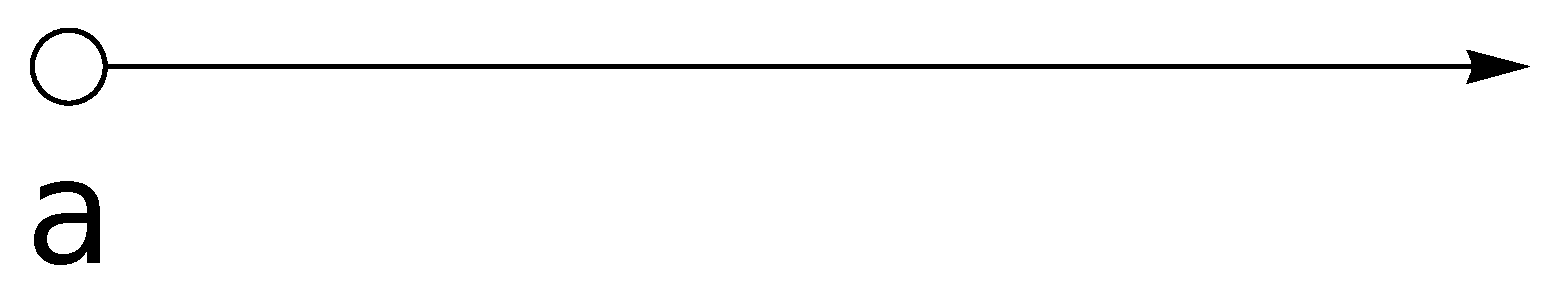
\includegraphics[width=0.25\textwidth]{fig_sets_9g}   \\
			\hline
			
			&  & \\
			\shortstack{$\{x\,| \, x \geq a \}$ \\ \hfill}& \shortstack{$[a,+\infty\left[\right.$ \\ \hfill} & 
			
			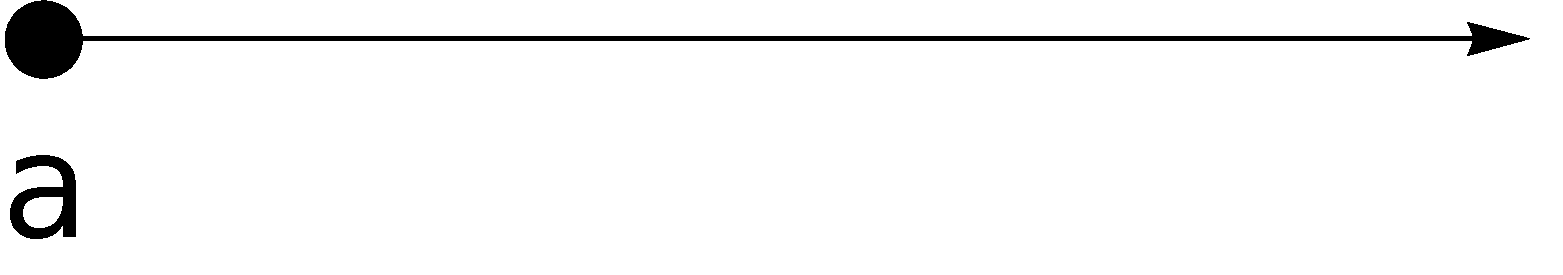
\includegraphics[width=0.25\textwidth]{fig_sets_9h}   \\
			\hline
			
			&  & \\
			\shortstack{$\mathbb R$ \\ \hfill}& \shortstack{$\left.\right]-\infty,+\infty\left[\right.$ \\ \hfill} & 
			
			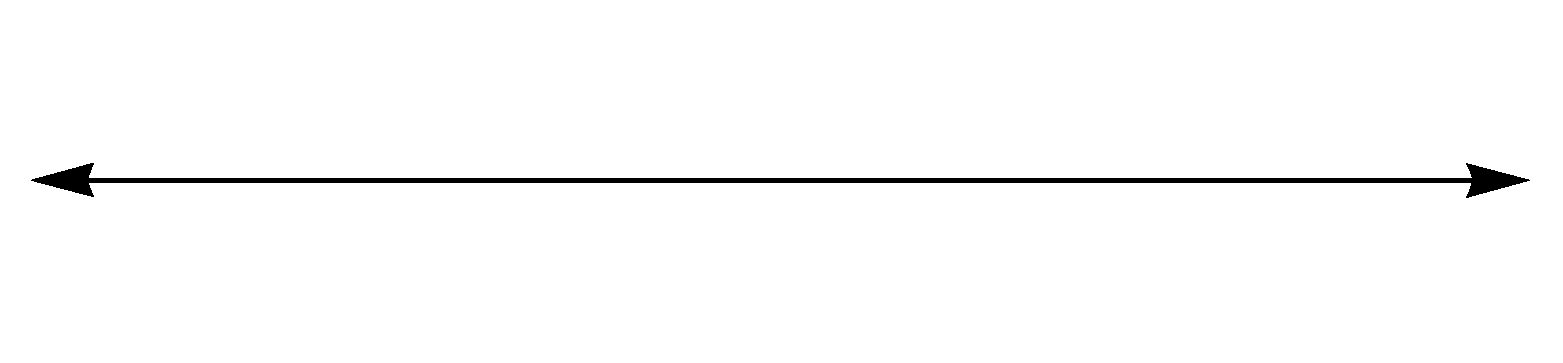
\includegraphics[width=0.25\textwidth]{fig_sets_9i}  \\
			
			
		\end{tabular}
		
	\end{center}
\end{table}



\ifcalculus
\begin{example} \label{unionex} 
	Express the following sets of numbers using interval notation.
	
	\begin{multicols}{2}
		
		\begin{enumerate}
			
			\item  $\{ x \, | \, x \leq -2 \, \, \vee \, \,  x \geq 2 \}$
			
			
			
			
			%\end{enumerate}
			
			%\end{multicols}
			
			%\begin{multicols}{2}
			
			%\begin{enumerate}
			
			
			\item  $\{ x \, | \, x \neq \pm 3 \}$
			
			\item  $\{ x \, | \, -1 < x \leq 3 \,\, \vee \,\, x = 5\}$
			
		\end{enumerate}
		
	\end{multicols}
	
	\xhrulefill{gray}{2.5pt}Solution \xhrulefill{gray}{2.5pt}
	
	\begin{enumerate}
		
		\item  The best way to proceed here is to graph the set of numbers on the number line.  The inequality $x \leq -2$ corresponds to the interval $\left.\right]-\infty, -2]$ and the inequality $x \geq 2$ corresponds to the interval $[2, +\infty\left[\right.$.  Since we are looking to describe the real numbers $x$ in one of these or the other, we have $\{ x \, | \, x \leq -2 \, \, \vee \, \,  x \geq 2 \} = \left.\right]-\infty, -2] \cup [2, +\infty\left[\right.$.
		
		\begin{center}
			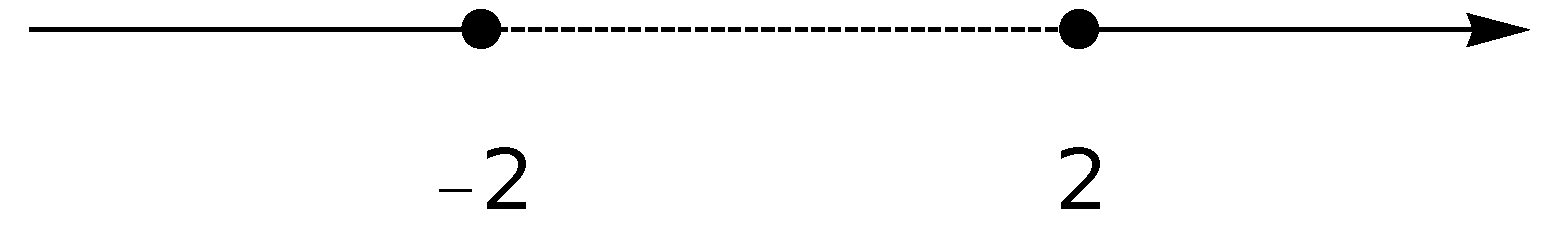
\includegraphics[width=0.4\textwidth]{fig_sets_10a}
		\end{center}
		
		
		
		\item  For the set $\{ x \, | \, x \neq \pm 3 \}$, we exclude both $x=3$ and $x=-3$ from our set.  This breaks the number line into three intervals, $\left.\right]-\infty, -3\left[\right.$, $\left.\right]-3,3\left[\right.$ and $\left.\right]3, +\infty\left[\right.$, so $\{ x \, | \, x \neq \pm 3 \} = \left.\right]-\infty, -3\left[\right. \cup \left.\right]-3,3\left[\right. \cup \left.\right]3, +\infty\left[\right.$.
		
		
		\begin{center}
			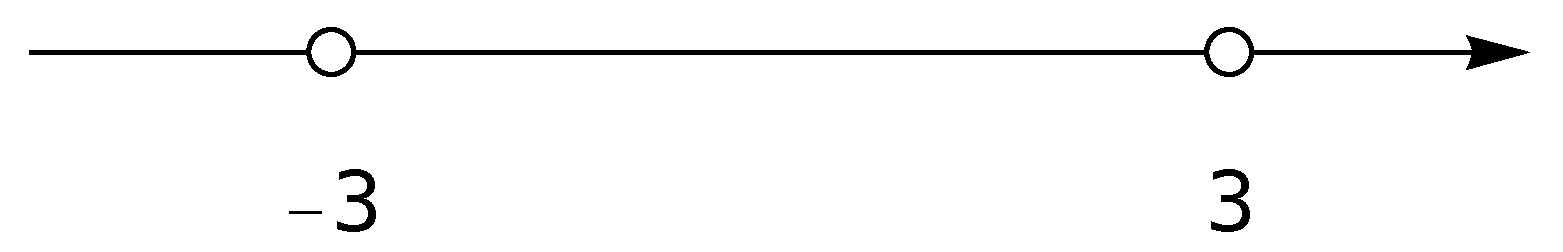
\includegraphics[width=0.4\textwidth]{fig_sets_10b}
		\end{center}
		
		
		\item  Graphing the set $\{ x \, | \, -1 < x \leq 3 \,\, \vee \,\, x = 5\}$, we get one interval, $\left.\right]-1,3]$ along with a single number, or point, $\{ 5\}$.
		Consequently, we have $\{ x \, | \, -1 < x \leq 3 \,\, \vee \,\, x = 5\} = \left.\right]-1,3] \cup \{ 5\}$.
		
		\begin{center}
			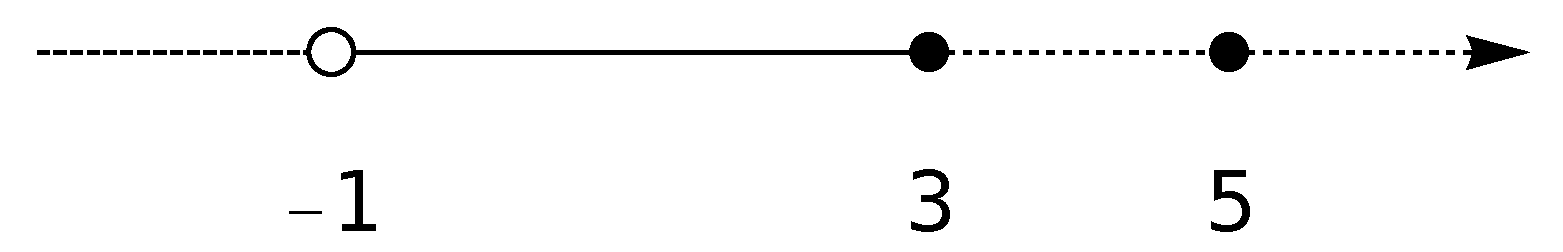
\includegraphics[width=0.4\textwidth]{fig_sets_10c}
		\end{center}
		
	\end{enumerate}
	
	
\end{example}
\fi

\ifcourse
\ifanalysis

	Having introduced the set of real numbers and intervals in $\mathbb{R}$, we are now ready to give a name to some special points in this set, which will turn out useful in the subsequent chapters. 
	\ifcourse
	\checkoddpage
\marginpar{\ifoddpage\hspace*{-1.5cm}\else\hspace*{0.25cm}\fi
\includegraphics[width=0.075\textwidth]{youtube}\\
\ifoddpage\hspace*{-1.75cm}\else\hspace*{0.1cm}\fi
%\includegraphics[width=0.1\textwidth]{Soorten_Punten}
\qrcode[height=1.75cm]{https://youtu.be/U1XDWeeDBrQ}
}
 \fi
	\begin{definition}[Boundary and interior points, open, closed and bounded sets]\label{def:open1D}
		Let $S$ be a set of points in $\mathbb{R}$. A point $P$ in $\mathbb{R}$ is a \textbf{boundary point} (\textit{randpunt}) of $S$  if all open disks centred at $P$ contain both points in $S$ and points not in $S$.\\
		
		A point $P$ in $S$ is an \textbf{interior point} (\textit{inwendig punt}) of $S$ if there is an open interval centred at $P$ that contains only points in $S$. \\
		
		A point $P$ in $S$ is an \textbf{accumulation or limit point} (\textit{ophopingspunt}) of $S$ if the intersection between every open interval containing $P$ and $S$ contain infinitely many points. \\
		
		A set $S$ is \textbf{open} (\textit{open}) if every point in $S$ is an interior point.\\
		
		A set $S$ is \textbf{closed} (\textit{gesloten}) if it contains all of its boundary points.\\
		
		A set $S$ is \textbf{bounded} (\textit{begrensd}) if there is an $M>0$ such that the open interval, centred at the origin with width $M$, contains $S$. A set that is not bounded is unbounded.
		\index{open}\index{closed}\index{open disk}\index{closed disk}\index{boundary point}\index{interior point}\index{bounded set}\index{unbounded set}\index{limit point}\index{accumulation point}
		\index[aut]{inwendig punt}\index[aut]{open bol}\index[aut]{gesloten bol}\index[aut]{open}\index[aut]{gesloten}\index[aut]{begrensd}\index[aut]{onbegrensd}\index[aut]{randpunt}\index[aut]{ophopingspunt}
	\end{definition}

\fi
\fi

\section{Complex numbers}
\label{sec_complex}
We leave a detailed discussion of complex numbers to the course `Algebra', and restrict here to a basic introduction to complex which suffices for the scope of this course. 
	\checkoddpage
\marginpar{\ifoddpage\hspace*{-1.5cm}\else\hspace*{0.25cm}\fi
\includegraphics[width=0.075\textwidth]{youtube}\\
\ifoddpage\hspace*{-1.75cm}\else\hspace*{0.1cm}\fi
\qrcode[height=1.75cm]{https://youtu.be/ysVcAYo7UPI}
}

\subsection{Definition}
Consider the polynomial $p(x) = x^2+1$.  The zeros of $p$ are the solutions to $x^2+1=0$, or $x^2=-1$.  This equation has no real solutions, but we can formally extract the square roots of both sides to get  $x = \pm \sqrt{-1}$.  The quantity $\sqrt{-1}$ is usually relabeled $i$, the so-called \index{imaginary unit} \textbf{imaginary unit} (\textit{imaginaire eenheid}). \index[aut]{imaginaire eenheid}  The number $i$, while not a real number, plays along well with real numbers, and acts very much like any other radical expression.  For instance, $3(2i) = 6i$, $7i-3i = 4i$, $(2-7i) + (3 + 4i) = 5-3i$, and so forth.  The key property that distinguishes $i$ from the real numbers is the fact that  
$$i^2 = -1\,.$$

Hence, if $c$ is a real number with $c \geq 0$, then we can write 
$$\sqrt{-c} = i \sqrt{c}\,.$$

Having defined the imaginary unit, we are now in the position to define the complex numbers.


\begin{definition}[Complex number] \label{complexdefn}
	A \textbf{complex number} (\textit{complex getal}) is a number of the form 
	$$a+bi\,,$$
	where $a$ and $b$ are real numbers and $i$ is the \textbf{imaginary unit} (\textit{imaginaire eenheid}).
\end{definition}
\index{complex number}\index[aut]{complex getal}
\index{imaginary unit}\index[aut]{imaginaire eenheid}

Do not forget that $a$ or $b$ could be zero, which means numbers like $3i$ and $6$ are also complex numbers.  In other words, do not forget that the complex numbers include the real numbers, so $0$ and $\pi - \sqrt{21}$ are both considered complex numbers (See Figure 2.5). 

\subsection{Complex number arithmetic}
The arithmetic of complex numbers is as you would expect, as long as you remember that $i^2=-1$.

\begin{example} 
	\label{complexzeroex1} Perform the indicated operations.  Write your answer in the form $a+bi$.
	\begin{multicols}{2}
		
		
		\begin{enumerate}
			
			\item  $(1-2i) - (3+4i)$
			\item  $(1-2i)(3+4i)$ 
			\item  $\dfrac{1-2i}{3-4i}$
			\item  $\left(x-(1+2i)\right)\left(x-(1-2i)\right)$
			
		\end{enumerate}
	\end{multicols}
	
	\xhrulefill{gray}{2.5pt}Solution \xhrulefill{gray}{2.5pt}
	
	\begin{enumerate}
		
		\item We combine like terms to get $(1-2i) - (3+4i) = 1-2i-3-4i = -2-6i$.
		
		
		\item  Using the distributive property, we get  
		$$
		(1-2i)(3+4i) =3+4i-6i-8i^2\,.
		$$
		
		Since $i^2=-1$, we get $3+4i-6i-8i^2 =  11-2i$.
		
		\item  First we deal with the denominator $3-4i$ as we would any other denominator containing a radical, and multiply both numerator and denominator by $3+4i$.  Doing so produces
		
		\[ \dfrac{1-2i}{3-4i} \;  \dfrac{3+4i}{3+4i} = \dfrac{(1-2i)(3+4i)}{(3-4i)(3+4i)} = \dfrac{11-2i}{25} = \dfrac{11}{25} - \dfrac{2}{25} \, i.\]
		
		
		\item  We can rely on the fact that $(a-b)(a+b)=a^2-b^2$ and see that 
		
		\[\begin{array}{rclr} \left(x-(1+2i)\right)\left(x-(1-2i)\right) & = &  \left((x-1)-2i\right)\left((x-1)+2i\right) & \\
		
		&	= & \left((x-1)^2-(2i)^2\right) & \\ 
		& =  & x^2 -2x +5. & \end{array}\]
		
	\end{enumerate}
	
	
\end{example}

A couple of remarks about the last example are in order.  First, the \index{complex conjugate}\index[aut]{complex toegevoegde}\textbf{conjugate} (\textit{(complex) toegevoegde}) of a complex number $a+bi$ is the number $a-bi$.  The notation commonly used for conjugation is a bar; that is
$$\overline{a+bi} = a-bi\,.$$
For example, $\overline{3+2i} = 3-2i$ and $\overline{6} = 6$.  The properties of the conjugate are summarized below, for $z$ and $w$ complex numbers. 

\begin{itemize}
	
	\item  $\overline{\overline{z}} = z$
	
	\item  $ \overline{z} + \overline{w}  = \overline{z+w}$
	
	\item  $ \overline{z} \, \overline{w}  = \overline{zw}$
	
	\item  $\left(\overline{z}\right)^n = \overline{z^{n}}$, for any natural number $n$
	
	\item  $z$ is a real number if and only if $\overline{z} = z$.
	
\end{itemize}


To form the \textbf{opposite} (\textit{tegengestelde}) of a complex number, take the opposite of each part: 
\[-(a + bi) = -a + (-b)i = -a - bi.\]
For example, the opposite of $6 - 2i$ is $-6 + 2i$. \\


%https://courses.lumenlearning.com/waymakerintermediatealgebra/chapter/read-quadratic-equations-with-complex-solutions/


\ifcourse
Although we will only rarely have to resort to complex numbers throughout this course, their importance in engineering cannot be underestimated since complex numbers have essential  applications in a variety of scientific and related areas such as signal processing, control theory, electromagnetism, fluid dynamics, quantum mechanics, cartography, and vibration analysis. For that reason, you will often encounter them in more advanced mathematics courses, such as differential equations. Besides, using complex numbers one can construct arty and intriguing graphics, like the so-called Julia set depicted in Figure~\ref{fig_sets_11}.
\fi

\ifcourse
\begin{remark}[Quaternions]
	The quaternions are a number system that extends the complex numbers, dating back to the 1840s only. They are generally represented as:
	$$
	a+b\ \mathbf {i} +c\ \mathbf {j} +d\ \mathbf {k}, 
	$$
	where $a$, $b$, $c$, and d are real numbers, and $\mathbf{i}$, $\mathbf{j}$, and $\mathbf{k}$ are the fundamental quaternion units for which it holds that $\mathbf{i}^2=\mathbf{j}^2=\mathbf{k}^2=-1$. Amongst other things, the spin of an electron can be described using quaternions. 	
\end{remark}
\fi

\ifcourse
\begin{figure}[h!]
	\begin{center}
		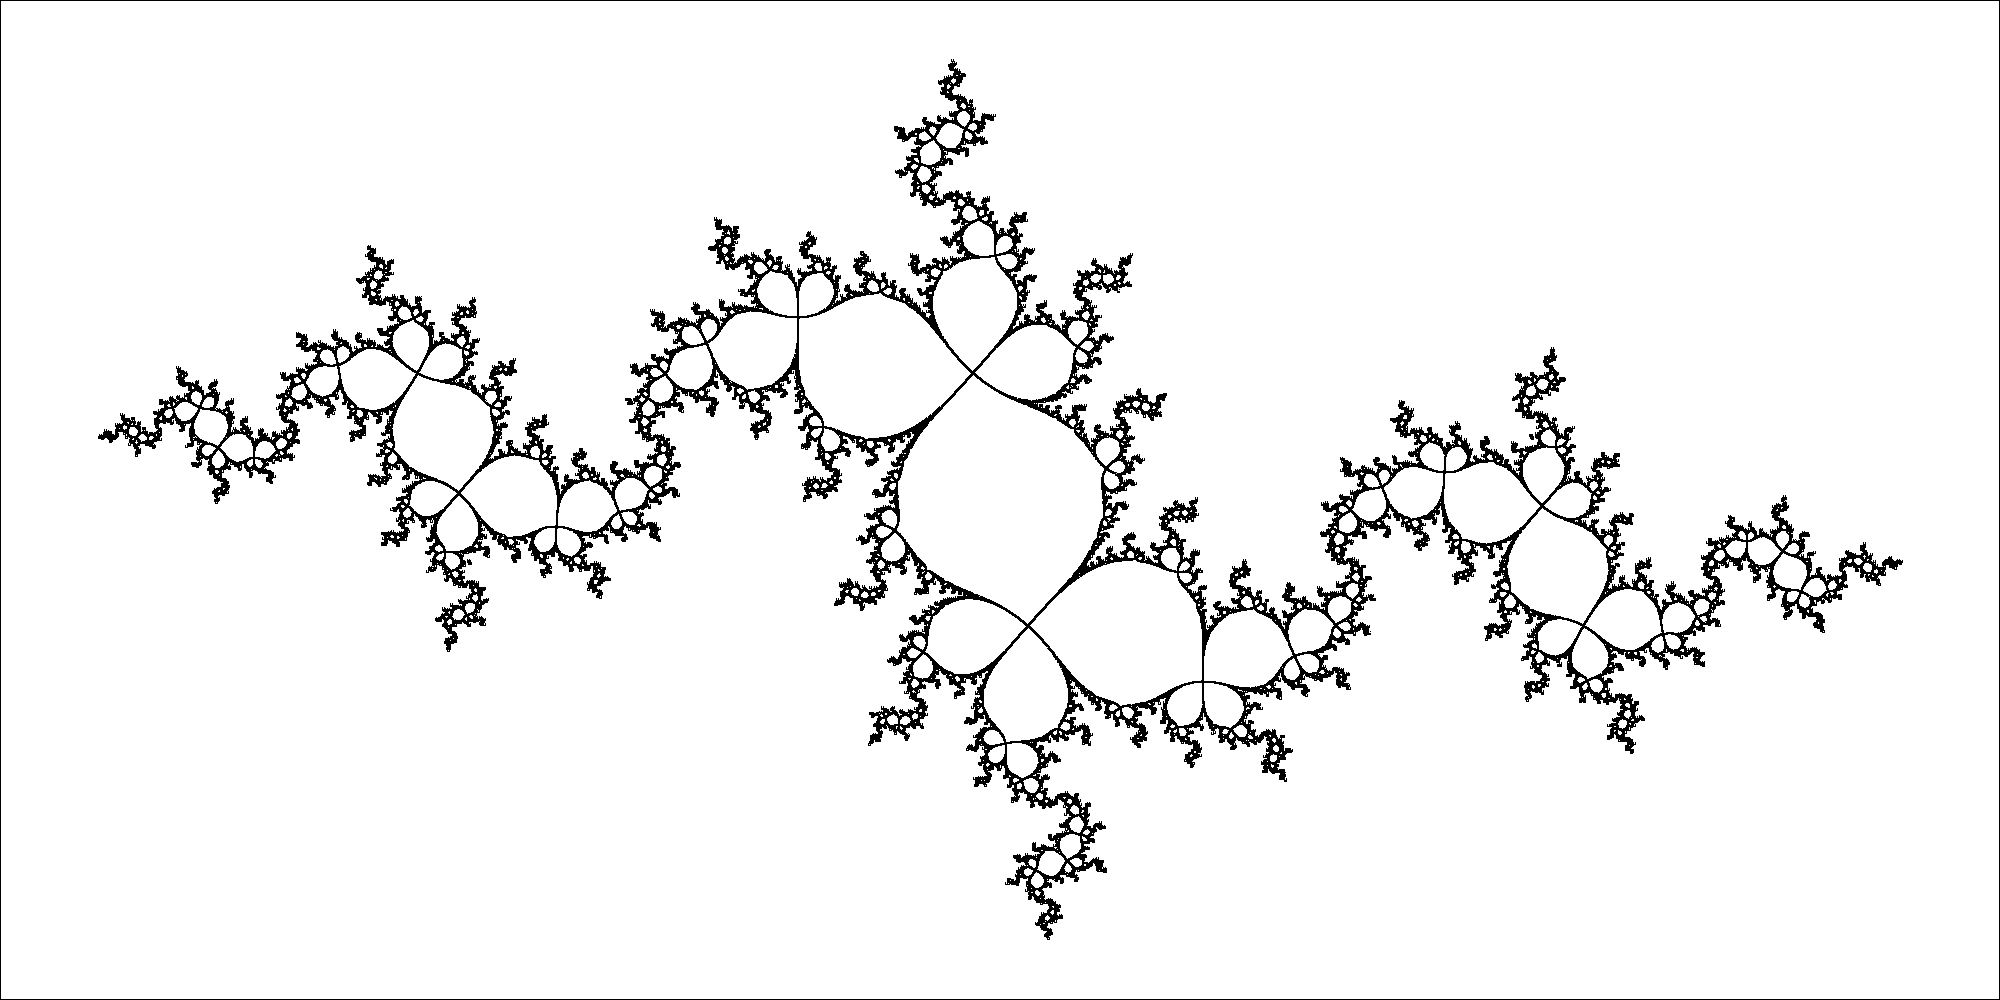
\includegraphics[width=0.7\textwidth]{fig_sets_11}
		\caption{Exemplary Julia set.}
		\label{fig_sets_11}
	\end{center}
\end{figure}
\fi



%Operations and properties of sets, some like the second example and also some with intervals
%A few exercises on sums: http://www.austincc.edu/jthom/SigmaNotationExer.pdf
%Some exercises on powers, roots and special products.
%A few calculations with infinity


%Exercises on exponential growth: http://www.hhofstede.nl/modules/opgavengroei.htm
%http://www.hhofstede.nl/modules/exponentieel%20algemeen.htm

%%%%%%%%%%%%%%%%%%%%%%%%%%
%Exercises in the course
%%%%%%%%%%%%%%%%%%%%%%%%%%

\newpage
\ifcourse %Start of exercises in the course


\section{Exercises}

\renewcommand{\ExerciseListName}{Assignment}

 \subsection*{\nameref{sets} and \nameref{sec:logic operators}}


\ifanalysis\begin{Exercise}[difficulty = 1]\fi
\ifcalculus\begin{Exercise}[difficulty = 2]\fi
Determine the negation of the expressions below.\par 

\begin{multicols}{2}
		\Question $\exists\;x \in \mathbb{Z},\;\forall\;y\in \mathbb{Z}:\;x<y$
		\Question $\forall\;y \in \mathbb{Z},\;\exists\;x\in \mathbb{Z}:\;x<y$
		\Question $\forall\;x \in \mathbb{Z},\;\exists\;y\in \mathbb{Z}:\;x+y=0$
		\Question $\exists\;y \in \mathbb{Z},\;\forall\;x\in \mathbb{Z}:\;x+y=0$
		\EndCurrentQuestion
	\end{multicols}
\ifanalysis\end{Exercise}\fi
\ifcalculus\end{Exercise}\fi
\setboolean{firstanswerofthechapter}{true}
\begin{Answer} \phantom{}
    \begin{multicols}{2}

    	\Question  $\forall \; x \in \mathbb{Z}, \; \exists \; y \in \mathbb{Z}: \; x \geq y $
    	\Question  $\exists\;y \in \mathbb{Z},\;\forall\;x\in \mathbb{Z}:\; x \geq y$
    	\Question  $\exists\;x \in \mathbb{Z},\;\forall\;y\in \mathbb{Z}:\;x+y \neq 0$
    	\Question  $\forall \; y \in \mathbb{Z}, \; \exists\; x \in \mathbb{Z}: \; x+y \neq 0$	
        \EndCurrentQuestion
	\end{multicols}
\end{Answer}
\setboolean{firstanswerofthechapter}{false}

\begin{Exercise}  [difficulty = 1] Define the following sets with words and write them out completely.  
	\begin{multicols}{2}
			\Question $A=\{a\;|\;a\in \mathbb{N} \; \wedge \; 2<a<6 \}$
			\Question $B=\{x\;|\;x\in \mathbb{Q}^+ \; \wedge \; 2x^2 +x-6=0 \}$
			\Question $C=\{x\;|\;x\in \mathbb{Z}^+ \; \wedge \; x^2 -5=0 \}$
			\EndCurrentQuestion
	\end{multicols}
\end{Exercise}

\begin{Answer} \phantom{}
	
    	\Question The set $A$ contains the natural numbers  between 2 and 6. $A = \{3,4,5\}$
    	\Question The set $B$ contains the positive fractions that are solutions of $2x^2 +x-6=0 $. $B = \left\{ \dfrac{3}{2} \right\}$
    	\Question The set $C$ contains the positive integers that are solutions of $x^2-5=0$. $C = \emptyset$
\end{Answer}


\begin{Exercise} Write in a concise manner that $A$ is a set of; 
	\Question[difficulty = 1] all even numbers bigger than 100.
	\Question[difficulty = 1] all pairs of integers whose first and second elements are even and odd, respectively.
	\Question[difficulty = 1] all integers, different from zero, that are multiples of 3.
	\Question[difficulty = 1] all positive rational numbers whose square root is greater than 3.
	\Question[difficulty = 2] all numbers that when divided by 6 result in a remainder of 2.
\end{Exercise}

\begin{Answer}\phantom{}
    \begin{multicols}{2}

    		\Question $A = \left\{a\; \left|\; \dfrac{a}{2}\in \mathbb{N} \; \wedge \; a > 100 \right. \right\}$
    		\Question $A = \left\{(a,b)\; \left|\; a,b \in \mathbb{Z} \; \wedge \; \dfrac{a}{2} \in \mathbb{Z} \; \wedge \; \dfrac{b+1}{2} \in \mathbb{Z} \right. \right\}$
            \Question $A = \left\{a\; \left|\; a\in \mathbb{Z}_0 \; \wedge \; \dfrac{a}{3}\in \mathbb{Z}_0 \right. \right\}$  %all even numbers, different from zero, that are multiples of 3.
            \Question $A = \left\{a\; \left|\; a\in \mathbb{Q}^+ \; \wedge \; \sqrt{a}>3 \right. \right\}$ 
            \Question $A = \left\{a\; \left|\; a\in \mathbb{R} \; \wedge \; \dfrac{a-2}{6} \in \mathbb{Z} \right. \right\}$
    	\EndCurrentQuestion
    \end{multicols}
\end{Answer}
	
\begin{Exercise} Fill in the correct symbols. Choose from $\subset, \not\subset, =, \neq, \in,  \not\in, \ni, \not\ni$. Multiple answers might be possible.
	\Question[difficulty = 1] $\{1, 3, 5, 7, 9, 11, \ldots \} \ldots \{ x \in \mathbb{N} | \; x \text{ is an even number} \}$
	\Question[difficulty = 1] $\{ x | \; x \text{ is a rose} \} \ldots \{ x | \; x \text{ is a flower} \}$
	\Question[difficulty = 1] $\{1, 3, 5, 7, 9 \} \ldots 2$
	\Question[difficulty = 1] $\{1\} \ldots \{1, 3, 5, 7, 9 \} $
	\Question[difficulty = 1] $\{1,3\} \ldots \{\{1\}, \{3\}, \{5\}, \{7\}, \{9\} \} $
	\Question[difficulty = 1] $\{1,3\} \ldots \{1, 3, 5, 7, 9 \} $
	\Question[difficulty = 1] $\{1, 3, 5, 7, 9 \} \ldots \emptyset$
	\ifanalysis\Question[difficulty = 1]\fi \ifcalculus\Question[difficulty = 2]\fi $\{1\} \ldots \{\{1\}, \{3\}, \{5\}, \{7\}, \{9\} \} $
	\Question[difficulty = 2] $\{1, 3, \{5, 7, 9\} \} \ldots 5$
\end{Exercise}

\begin{Answer}\phantom{}

    		\Question $\{1, 3, 5, 7, 9, 11, \ldots \} = \{ x \in \mathbb{N} | \; x \text{ is an odd number} \}$
    		\Question $\{ x | \; x \text{ is a rose} \} \subset \{ x | \; x \text{ is a flower} \}$
    		\Question $\{1, 3, 5, 7, 9 \} \not\ni 2$
    		\Question $\{1\} \subset \{1, 3, 5, 7, 9 \} $
    		\Question $\{1,3\} \not\subset \{\{1\}, \{3\}, \{5\}, \{7\}, \{9\} \} $ also $\{1,3\} \not\in \{\{1\}, \{3\}, \{5\}, \{7\}, \{9\} \} $
    		\Question $\{1,3\} \subset \{1, 3, 5, 7, 9 \} $
    		\Question $\{1, 3, 5, 7, 9 \} \neq \emptyset$
    		\Question $\{1\} \in \{\{1\}, \{3\}, \{5\}, \{7\}, \{9\} \} $
    		\Question $\{1, 3, \{5, 7, 9\} \} \not\ni 5$

\end{Answer}

\newpage

\begin{Exercise} Assume $A=\{1, \{1\}, \{2\} \}$. Which from the following statements is true?
    \begin{multicols}{2}
    	\Question[difficulty = 1] $1 \in A$
    	\ifanalysis\Question[difficulty = 1]\fi \ifcalculus\Question[difficulty = 2]\fi $\{1\} \in A$
    	\ifanalysis\Question[difficulty = 1]\fi \ifcalculus\Question[difficulty = 2]\fi $\{1\} \subseteq A$
    	\ifanalysis\Question[difficulty = 1]\fi \ifcalculus\Question[difficulty = 2]\fi $\{\{1\}\} \subseteq A$
    	\ifanalysis\Question[difficulty = 1]\fi \ifcalculus\Question[difficulty = 2]\fi $2 \in A$
    	\ifanalysis\Question[difficulty = 1]\fi \ifcalculus\Question[difficulty = 2]\fi $\{\{2\}\} \subseteq A$	
    	\ifanalysis\Question[difficulty = 1]\fi \ifcalculus\Question[difficulty = 2]\fi $\{\{2\}\} \subset A$
    	\Question[difficulty = 2] $\{2\} \subseteq A$
    	\EndCurrentQuestion
	\end{multicols}
\end{Exercise}

\begin{Answer}\phantom{}
    \begin{multicols}{2}
        
        	\Question $1 \in A$: True
        	\Question $\{1\} \in A$: True
        	\Question $\{1\} \subseteq A$: True
        	\Question $\{\{1\}\} \subseteq A$: True
        	\Question $2  \in A$: False 
        	\Question $\{\{2\}\} \subseteq A$: True	
        	\Question $\{\{2\}\} \subset A$: True	
        	\Question $\{2\} \subseteq A$: False
        \EndCurrentQuestion
    \end{multicols}
\end{Answer}

\begin{Exercise} 
    Given $U=\{1, 2, 3, \ldots, 9, 10\}$, assume $A =\{1, 2, 3, 4, 5\}$, $B =\{1, 2, 3, 4\}$, $C =\{3, 5, 7\}$ and $D =\{2, 4, 6, 8\}$. Describe each of the following sets:
    \begin{multicols}{2}
    	\Question[difficulty = 1] $(A \cup B) \cap C$
    	\Question[difficulty = 1] $A \cup (B \cap C)$
    	\Question[difficulty = 1] $\overline{C} \cup \overline{D}$
    	\Question[difficulty = 1] $\overline{C \cap D}$
    	\Question[difficulty = 1] $(A \cup B)\backslash C $
    	\Question[difficulty = 1] $A \cup (B \backslash C)$
    	\ifanalysis\Question[difficulty = 1]\fi \ifcalculus\Question[difficulty = 2]\fi $(B \backslash C) \backslash D$	
    	\ifanalysis\Question[difficulty = 1]\fi \ifcalculus\Question[difficulty = 2]\fi $B \backslash (C \backslash D)$
    	\Question[difficulty = 2] $(A \cup B)\backslash (C \cap D) $
    	\EndCurrentQuestion
	\end{multicols}
\end{Exercise}

\begin{Answer}\phantom{}
    \begin{multicols}{2}
    
        	\Question $(A \cup B) \cap C = \{3, 5\}$
        	\Question $A \cup (B \cap C) = \{1, 2, 3, 4, 5\} = A$
        	\Question $\overline{C} \cup \overline{D} = U$
        	\Question $\overline{C \cap D} = \overline{C} \cup \overline{D} = U $ \quad (rules of De Morgan)
        	\Question $(A \cup B)\backslash C = \{1, 2, 4\} $
        	\Question $A \cup (B \backslash C) = \{1, 2, 3, 4, 5\} = A$
        	\Question $(B \backslash C) \backslash D = \{1\}$	
        	\Question $B \backslash (C \backslash D) = \{1, 2, 4\}$
            \Question $(A \cup B)\backslash (C \cap D) = \{1, 2, 3, 4, 5\} = A$
        \EndCurrentQuestion
    \end{multicols}
\end{Answer}

\begin{Exercise} Simplify the following expressions:
    \begin{multicols}{2}
    	\Question[difficulty = 1] $A \cap (B \backslash A)$
    	\Question[difficulty = 1] $(A \backslash B) \cup (A \cap B)$
    	\Question[difficulty = 2] $\overline{A} \cup \overline{B} \cup \left( A \cap B \cap \overline{C} \right)$
    	\Question[difficulty = 3] $(A \cap B) \cup \left( A \cap B \cap \overline{C} \cap D \right) \cup \left( \overline{A} \cap B \right)$
    	\Question[difficulty = 3] $(A \cap B) \cup \left(B \cap \left( \left(C\cap D\right)\cup \left(C \cap \overline{D} \right) \right)   \right)$
    	\EndCurrentQuestion
	\end{multicols}
\end{Exercise}

\begin{Answer}\phantom{}
    
        \Question $A \cap (B \backslash A) = \emptyset $
        \Question $(A \backslash B) \cup (A \cap B) = A$
        \Question $\overline{A} \cup \overline{B} \cup \left( A \cap B \cap \overline{C} \right) = \overline{A \cap B \cap C}$
        \Question $(A \cap B) \cup \left( A \cap B \cap \overline{C} \cap D \right) \cup \left( \overline{A} \cap B \right) = B$
        \Question $(A \cap B) \cup \left(B \cap \left( \left(C\cap D\right)\cup \left(C \cap \overline{D} \right) \right) \right) = (A \cap B) \cup (B \cap C) $
\end{Answer}

%%%%%%%%%%%%%%
%Only bio-ir
\ifanalysis


\begin{Exercise} [difficulty = 1] Prove the associative properties with respect to union and intersection for three sets. 
\end{Exercise}

\begin{Answer}\phantom{}
The answer is left as an exercise to the reader. 
\end{Answer}
		
\begin{Exercise} Prove the following properties. %
		\Question[difficulty = 1] $A\cup B=B \; \Leftrightarrow \; A\subset B \; \Leftrightarrow\;  A\cap
		B=A \; \Leftrightarrow \; A\backslash B=\emptyset$
		\Question[difficulty = 1] $A\backslash B=A \; \Leftrightarrow \; A \cap B =\emptyset \; \Leftrightarrow \;
		B \backslash A=B$
		\Question[difficulty = 1] $(A\backslash B)\cap A=A\backslash B$
		\Question[difficulty = 1] $(A\backslash B)\cap B=\emptyset$
		\Question[difficulty = 1] $(A\cup B)\backslash B=A\backslash B$
		\Question[difficulty = 1] $(A\cup B)\backslash C=(A\backslash C)\cup (B\backslash C)$
		%\Question $(A\cap B)\backslash C=(A\backslash C)\cap (B\backslash C)$
\end{Exercise}

\begin{Answer}\phantom{}
The answer is left as an exercise to the reader.
\end{Answer}


\fi
%%%%%%%%%%%%%%
\newpage

\begin{Exercise} [difficulty = 2, label=oef_fig_sets_12] Use set notation to define the shaded areas in Figure~\ref{fig_sets_12}. \label{oef_verz} 
	\begin{figure}[H]
		\begin{center}
			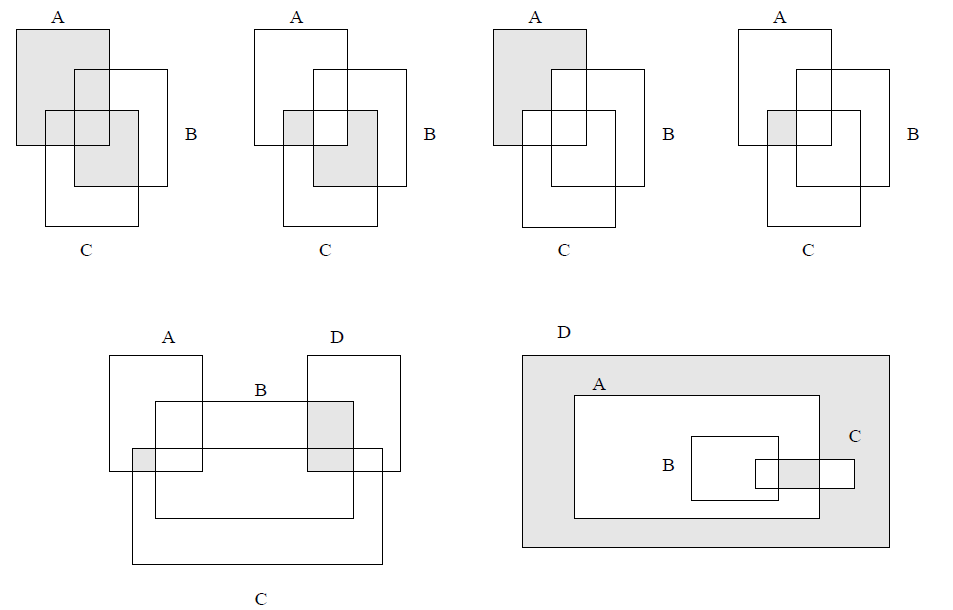
\includegraphics[width=0.9\textwidth]{fig_sets_12}
			\caption{Shaded areas used in exercise~\ref{oef_fig_sets_12}.}
			\label{fig_sets_12}
		\end{center}
	\end{figure}
\end{Exercise}

\begin{Answer}\phantom{}
    The numbering of the areas is done from left to right.
    	\begin{multicols}{2}
    
        	\Question $A \cup (B \cap C) $
        	\Question $((B \cap C) \backslash A) \cup  ((A \cap C) \backslash B) $
        	\Question $ A \backslash (B \cup C)$ of $ (A \backslash B) \cap (A \backslash C)$
        	\Question $(A \cap C) \backslash B$
        	\Question $((A \cap C) \backslash B) \cup (B \cap D) $
        	\Question $(D \backslash (A \cup C)) \cup ((C \cap A) \backslash B) $
        	\EndCurrentQuestion
    	\end{multicols}
\end{Answer}

%%%%%%%%%%%%%%
%Only bio-ir.
\ifanalysis

\begin{Exercise} Assume $W \subset \mathbb{R}$ and $b \in \mathbb{R}$. Give a correct expression with logical operators for the expressions below. 
		\Question[difficulty = 1] $b$ is an upper limit of set $W$.
		\Question[difficulty = 1] $b$ is not an upper limit of set $W$.
		\Question[difficulty = 2] $W$ is an upwardly bounded set.
		\Question[difficulty = 2] $W$ is not an upwardly bounded set.
\end{Exercise}

\begin{Answer}\phantom{}

    \Question $b$ is an upper bound of the set $W$: \quad $\forall w \in W: w \leq b$
    \Question $b$ is not an upper bound of the set $W$: \quad $\exists w \in W: b < w$
    \Question $W$  is a set bounded from above: \quad $\exists b \in \mathbb{R} | \forall w \in W: w \leq b$
    \Question $W$ is a set not bounded from above: \quad $\forall b \in \mathbb{R} : \exists w \in W: b < w$
\end{Answer}
		
\begin{Exercise} \\Determine the supremum and infimum of the following subsets of $\mathbb{R}$. 
    \begin{multicols}{3}
		%Ex. 1.10 pg 52 course calculus and analysis JB
		\Question[difficulty = 1] $\left\{ \dfrac{2^n}{2^n+1}, \, n \in \mathbb{N}  \right\}$
		\Question[difficulty = 1] $\left\{ \dfrac{2n-1}{n+2}, \, n \in \mathbb{N}_0  \right\}$
		\Question[difficulty = 1] $\left\{ \dfrac{n}{n+1}, \, n \in \mathbb{N}  \right\}$
		\EndCurrentQuestion
	\end{multicols}
\end{Exercise}

\begin{Answer}\phantom{}
    \begin{multicols}{2}

    \Question inf = $1/2$, sup = $1$
    \Question inf = $1/3$, sup = $2$
    \Question inf = $0$, sup = $1$
    \EndCurrentQuestion
    \end{multicols}
\end{Answer}
		
\subsection*{\nameref{intervals}}		
		
\begin{Exercise} Determine the infimum, supremum, minimum, maximum, boundary points, and interior points of $A$. 
    \begin{multicols}{2}
		\Question[difficulty = 1] $A = \{1\} \cup [2,5[ \; \cup \; ]5,7[$
		\Question[difficulty = 1] $A = \{-3\}\, \cup\; ]0,4] \; \cup \; [7,+\infty[$
		\Question[difficulty = 1] $A =\; ]-\infty,-2[ \; \cup \; ]-2,2[ \; \cup \; [3,4[ \; \cup \; ]5,9]$
		\EndCurrentQuestion
	\end{multicols}
\end{Exercise}

\begin{Answer}\phantom{}

    \Question inf $A=1$, sup $A=7$, min $A=1$, max $A$ does not exist, boundary points $A: 1, 2, 5, 7$, \\ internal points $A:\; ]2,5[ \;\cup\; ]5,7[$
    \Question inf $A=-3$, sup $A$ does not exist, min $A=-3$, max $A$ does not exist, \\ boundary points $A: -3, 0, 4, 7$, internal points $A: \; ]0,4[ \; \cup \; ]7,+\infty[$
    \Question inf $A$ does not exist, sup $A=9$, min $A$ does not exist, max $A=9$, \\ boundary points $A: -2, 2, 3, 4, 5, 9$, \\ internal points $A:\; ]-\infty,-2[\; \cup\; ]-2,2[\;\cup\; ]3,4[ \;\cup\; ]5,9[$
\end{Answer}
		
\fi
%%%%%%%%%%%%%%

\subsection*{\nameref{sec_real}}

\begin{Exercise}[difficulty = 1] Which of the numbers below are rational or irrational?
	\begin{multicols}{2}
			\Question $5.369$
			\Question $\dfrac{12}{7}$
			\Question $\sqrt{13}$
			\Question $1.232345456767\ldots$
			\Question $3.0236363636\ldots$
			%	\Question $\dfrac{\pi}{3}$
			%	\Question $-6.147258369\ldots$
			\Question $\sqrt{121}$
		    \EndCurrentQuestion
	\end{multicols}
\end{Exercise}

\begin{Answer}\phantom{}
    \begin{multicols}{3}
		
			\Question rational
			\Question rational
			\Question irrational
			\Question irrational
			\Question rational
			\Question rational
		\EndCurrentQuestion 
	\end{multicols}
\end{Answer}
	
\begin{Exercise} Rewrite the following expressions using a sum or multiplication sign.
    \begin{multicols}{2}
    	\Question[difficulty = 1] $x + x^2 + x^3 + x^4 + \ldots + x^{99}$ 
    	\Question[difficulty = 1] $\sqrt{3} + \sqrt{5} + \sqrt{7} + \sqrt{9} + \ldots + \sqrt{51} $ 
    	\Question[difficulty = 1] $ \dfrac{1}{a+1} \cdot \dfrac{4}{a+2} \cdot \dfrac{9}{a+3} \cdot \dfrac{16}{a+4}  \cdots  \dfrac{169}{a+13}$
    	\EndCurrentQuestion
    \end{multicols}
\end{Exercise}

\begin{Answer}\phantom{}
    \begin{multicols}{3}
		
		\Question $\dsum_{j=1}^{99} x^j$ 
		\Question $\dsum_{j=1}^{25} \sqrt{2j+1}$ 
		\Question $\displaystyle\prod_{j=1}^{13} \dfrac{j^2}{a+j}$ 
	    \EndCurrentQuestion
	\end{multicols}
\end{Answer}
	
\begin{Exercise} Calculate the following sums.
    \begin{multicols}{3}
    	\Question[difficulty = 1] $\dsum_{j=0}^{3} 2^j$
    	\Question[difficulty = 1] $\dsum_{j=0}^{3} j^2$
    	%\item $\dsum_{j=1}^{5} (2j-3)$
    	\Question[difficulty = 1] $\dsum_{j=0}^{4} \dfrac{24}{j!}$
    	\Question[difficulty = 1] $\dsum_{j=1}^{4} \dfrac{(-1)^j}{j}$
    	\Question[difficulty = 1] $\dsum_{j=1}^{5} (2j-1)^2$
    	\ifanalysis\Question[difficulty = 1]i\fi \ifcalculus\Question[difficulty = 2]\fi $\dsum_{j=1}^{100} -7j^2$
    	\ifanalysis\Question[difficulty = 1]\fi \ifcalculus\Question[difficulty = 2]\fi $\dsum_{j=1}^{90} \left(-2j^2+3j-5\right)$
    	\ifanalysis\Question[difficulty = 1]\fi \ifcalculus\Question[difficulty = 2]\fi $\dsum_{\stackrel{0<k<10}{k \text{ is oneven}}} k^2$
    	\EndCurrentQuestion
	\end{multicols}
\end{Exercise}

\begin{Answer}\phantom{}
    \begin{multicols}{3}
		
			\Question $15$ 
			\Question $14$ 
			\Question $65$ 
			\Question $- \dfrac{7}{12}$ 
			\Question $165$ 
			\Question $-2368450$
			\Question $-482295$  
		    \Question $165$ 
		\EndCurrentQuestion
	\end{multicols}
\end{Answer}
	
\begin{Exercise} Simplify each sum or product to an expression without sigma or pi notation. 
    \begin{multicols}{2}
    	\Question[difficulty = 1] $\dsum_{j=1}^{n} (3j-2)$
    	\Question[difficulty = 1] $\dsum_{j=1}^{n} \left( (3j-5)\,\dfrac{1}{n^2} \right)$		
    	\ifanalysis\Question[difficulty = 1]\fi \ifcalculus\Question[difficulty = 2]\fi $\dsum_{j=1}^{n} (3j-4)^2$
    	\ifanalysis\Question[difficulty = 1]\fi \ifcalculus\Question[difficulty = 2]\fi $\dsum_{j=1}^{n} \left( (j-2)^2\,\dfrac{1}{n^3} \right)$
    	\Question[difficulty = 2] $\displaystyle\prod_{j=1}^{n} j^3$
    	\Question[difficulty = 3] $\displaystyle\prod_{k=2}^{n} \left(1- \dfrac{1}{k^2} \right)$
    	\EndCurrentQuestion
    \end{multicols}
\end{Exercise}

\begin{Answer}\phantom{}
    \begin{multicols}{2}
		
			\Question $\dfrac{n(3n-1)}{2}$
			\Question $\dfrac{3n-7}{2n}$
			\Question $\dfrac{n}{2}(6n^2-15n+11)$	
			\Question $\dfrac{(n+1)(2n-11)+24}{6n^2}$
            \Question $\left(n!\right)^3$ 
		    \Question $\dfrac{n+1}{2n}$ 
		\EndCurrentQuestion
	\end{multicols}
\end{Answer}

\ifanalysis\pagebreak\fi

\begin{Exercise} Calculate or simplify the following algebraic forms.
    \begin{multicols}{2}
    	\Question[difficulty = 1] $\left(64\;a^{6m}b^{12n}c^{18p}\right)^{\frac{1}{6}}$
    	\Question[difficulty = 1] $\dfrac{1-x}{1-\sqrt{x}}$
    	\Question[difficulty = 1] $\left(1-\sqrt{2}-\sqrt{3}\right)^2$
    	\Question[difficulty = 1] $b\sqrt{\dfrac{4a}{b^4}}-\sqrt{\dfrac{9a}{b^2}}+\dfrac{1}{b}\sqrt{\dfrac{a}{4}}+2b\sqrt{\dfrac{25a}{b^4}}$
    	\ifanalysis\Question[difficulty = 1]\fi \ifcalculus\Question[difficulty = 2]\fi $\left(\sqrt{\dfrac{x+1}{x-1}}\right) \left( \sqrt[3]{\dfrac{x-1}{x+1}}\right)$
    	\ifanalysis\Question[difficulty = 1]\fi \ifcalculus\Question[difficulty = 2]\fi $\sqrt[3]{a^3+\dfrac{3}{2}a^2b+\dfrac{3}{4}ab^2+\dfrac{1}{8}b^3}$
    	\ifanalysis\Question[difficulty = 1]\fi \ifcalculus\Question[difficulty = 2]\fi $\dfrac{a^2+b^2}{\left(b-a\right)^2}\,\dfrac{\left(a-b\right)^3}{a+b}\,\dfrac{\left(-a-b\right)^2}{a^2-b^2}$
    	\ifanalysis\Question[difficulty = 1]\fi \ifcalculus\Question[difficulty = 2]\fi $\left(x^{\frac{1}{3}}-x^{-\frac{1}{3}}\right)^3+3\left(x^{\frac{1}{3}}-x^{-\frac{1}{3}}\right)$
    
    	\ifanalysis\Question[difficulty = 1]\fi \ifcalculus\Question[difficulty = 2]\fi $ \dfrac{\left(x^2 \right)^3 x^{-4} \sqrt[3]{x^5}}{\sqrt[3]{x^2} \sqrt[3]{\sqrt[4]{\left(x^2 \right)^3}}} $
    	\Question[difficulty = 2] $\left( \dfrac{16^{-2} a^{\frac{1}{2}}b^{-3}}{81^{-1} a^{-\frac{1}{2}}b^{3}} \right) \sqrt{ab^{\frac{9}{4}} \left( ab^{\frac{3}{2}} \right)^{\frac{1}{2}}}  $
    	\EndCurrentQuestion
	\end{multicols}
\end{Exercise}

\begin{Answer}\phantom{}
    \begin{multicols}{2}
	
		\Question $2 a^m b^{2n} c^{3p}$
		\Question $1+\sqrt{x}$
		\Question $6-2\sqrt{2}-2\sqrt{3}+2\sqrt{2}\sqrt{3}$
		\Question $\dfrac{19\sqrt{a}}{2b}$
		\Question $ \sqrt[6]{\dfrac{x+1}{x-1}}$
		\Question $a + \dfrac{b}{2}$
		\Question $a^2+b^2$
		\Question $\dfrac{x^2-1}{x}$
		\Question $x^{\frac{5}{2}} $ 
		\Question $\dfrac{81}{256} a^{\frac{7}{4}} b^{-\frac{9}{2}}$ 
	\EndCurrentQuestion
	\end{multicols}
\end{Answer}

\subsection*{\nameref{sec_complex}}

\begin{Exercise}[difficulty = 1] Determine and simplify
	\begin{multicols}{3}	
		\begin{itemize}[labelsep=5mm]	
			\item  $z+w$
			\item  $zw$
			\item  $z^2$	
			\item  $z^{-1}$
			\item  $\dfrac{z}{w}$
			\item  $\dfrac{w}{z}$
			\item  $\bar{z}$
			\item  $z\bar{z}$
			\item  $\left(\bar{z}\right)^2$
		\end{itemize}
	\end{multicols}
rewrite each pair of complex numbers in standard  form: $a+bi$.  
	\begin{multicols}{2}
			\Question  $z = 2+3i$, \quad $w = 4i$
			\Question  $z = 1+i$, \quad $w = -i$
			\Question  $z = 3-5i$, \quad $w = 2+7i$
			\Question  $z = \sqrt{2}-\sqrt{2}i$, \quad $w = \sqrt{2}+\sqrt{2}i$
			\Question  $z = 1-\sqrt{3}i$, \quad $w = -1-\sqrt{3}i$
			\Question  $z = -\dfrac{\sqrt{2}}{2} + \dfrac{\sqrt{2}}{2} i$, \quad $w =  -\dfrac{\sqrt{2}}{2} - \dfrac{\sqrt{2}}{2} i$
		\EndCurrentQuestion
	\end{multicols}
\end{Exercise}

\begin{Answer}\phantom{} \newline
    \vspace{-0.6cm} \begin{small} $\renewcommand{\arraystretch}{1.15}\begin{array}{|c|c|c|c|c|c|c|c|c|c|}			\hline
			&&&&&&\vspace{-0.5cm}\\
			& z+w & zw & z^2 & z^{-1} &\dfrac{z}{w} & \dfrac{w}{z} & \bar{z} & z\bar{z} & \left(\bar{z}\right)^2 \\
			&&&&&&\vspace{-0.5cm}\\
			\hline
			\hline
			&&&&&&\vspace{-0.5cm}\\
			\mbox{(a)}  & 2+7i & 8i  & -5+12i&  \dfrac{2-3i}{13} & \dfrac{3-2i}{4} & \dfrac{12+8i}{13}  & 2-3i & 13 & -5-12i \\[0.3cm]
			\hline 
			\mbox{(b)} & 1 & 1-i & 2i & \dfrac{1-i}{2}& -1+i & \dfrac{-1-i}{2} & 1-i & 2 &-2i \\[0.3cm]
			\hline
			\mbox{(c)} & 5+2i & 41+11i & -16-30i & \dfrac{3+5i}{34} & \dfrac{-29-31i}{53} & \dfrac{-29+31i}{34} & 3+5i & 34 & -16+30i \\[0.3cm]
			\hline
			\mbox{(d)} & 2\sqrt{2} & 4 &  -4i  & \dfrac{\sqrt{2}+\sqrt{2}i}{4} & -i & i & \sqrt{2}+\sqrt{2}i & 4 & 4i \\[0.3cm]
			\hline
			\mbox{(e)} & -2\sqrt{3}i & -4 &  -2-2\sqrt{3}i  & \dfrac{1+\sqrt{3}i}{4} & \dfrac{1+\sqrt{3}i}{2} & \dfrac{1-\sqrt{3}i}{2} & 1+\sqrt{3}i & 4 & -2+2\sqrt{3}i \\[0.3cm]
			\hline
			\mbox{(f)} & -\sqrt{2} & 1 &  -i  & \dfrac{-\sqrt{2}-\sqrt{2}i}{2} & -i & i & \dfrac{-\sqrt{2}-\sqrt{2}i}{2} & 1 & i \\[0.3cm]
			\hline
			\end{array}$
		\end{small}
\end{Answer}

%\ifcalculus\newpage\fi

\begin{Exercise} Write the following numbers in standard form: $a+bi$.
    \begin{multicols}{2}
    	\Question[difficulty = 1] $(4+8i)+(15-12i)$
    	\Question[difficulty = 1] $(2+4i)-(6-7i)$
    	\Question[difficulty = 1] $(2+3i)+(-5+i)$
    	\Question[difficulty = 1] $(2+i)^2$
    	\Question[difficulty = 1] $\overline{(5+6i)}(5+6i)$
    	\Question[difficulty = 1] $\dfrac{1}{5+2i}$
    	\Question[difficulty = 1] $\dfrac{1+i}{2+3i}$
    	\ifanalysis\Question[difficulty = 1]\fi \ifcalculus\Question[difficulty = 2]\fi $\dfrac{1+2i}{3-4i} + \dfrac{2-i}{5i}$	
    	\EndCurrentQuestion
	\end{multicols}
\end{Exercise}

\begin{Answer}\phantom{}
    \begin{multicols}{3}
	
		\Question $19-4i$
		\Question $-4+11i$
		\Question $-3+4i$
		\Question $3+4i$
		\Question $61$
		\Question $\dfrac{5-2i}{29}$
		\Question $\dfrac{5-i}{13}$
		\Question $\dfrac{-2}{5}$	
	\EndCurrentQuestion
	\end{multicols}
\end{Answer}

\fi 
%End of the exercises in the course


\begin{savequote}[75mm]
Mathematics knows no races or geographic boundaries; for mathematics, the cultural world is one country.
\qauthor{--- David Hilbert ---}
\end{savequote}

\chapter{Functions}
\label{chap_functions}
\graphicspath{{figures/Functions/}}
\section{The Cartesian coordinate plane}
\label{CartesianPlane}

\ifcourse
In order to visualize the pure excitement that is calculus, we need to unite algebra and geometry.  Simply put, we must find a way to draw algebraic things.  Let us start with possibly the greatest mathematical achievement of all time: the \index{Cartesian coordinate plane} \textbf{Cartesian coordinate plane} (\textit{Cartesisch co\"ordinatenstelsel})\index[aut]{Cartesisch co\"ordinatenstelsel}. So named in honour of Ren\'{e} Descartes. 
\fi
\ifvc
We must find a way to draw algebraic things.  Let us start with possibly the greatest mathematical achievement of all time: the \index{Cartesian coordinate plane} \textbf{Cartesian coordinate plane}  (\textit{Cartesisch co\"ordinatenstelsel}) \index[aut]{Cartesisch co\"ordinatenstelsel}. So named in honour of Ren\'{e} Descartes. 
\fi


Imagine two real number lines crossing at a right angle at $0$. The horizontal number line is usually called the \index{$x$-axis}\index[aut]{$x$-as}\textbf{\boldmath $x$-axis} (\textit{$x$-as}), while the vertical number line is usually called the \index{$y$-axis}\index[aut]{$y$-as}\textbf{\boldmath $y$-axis} (\textit{$y$-as}). For example, consider the point $P$ in Figure~\ref{fig_functions_1}.  To use the numbers on the axes to label this point, we project the point $P$ to the $x$- (respectively $y$-) axis.  We then describe the point $P$ using the \index{ordered pair} \textbf{ordered pair} (\textit{geordend koppel}) $(2,-4)$.\index[aut]{geordend koppel}  The first number in the ordered pair is called the\index{abscissa}\index[aut]{abscis} \textbf{abscissa} (\textit{abscis}) or \index{$x$-coordinate} \textbf{\boldmath $x$-coordinate} and the second is called the \index{ordinate} \textbf{ordinate} (\textit{ordinaat}) or \index{$y$-coordinate}\index[aut]{ordinaat}\textbf{\boldmath $y$-coordinate}. When we speak of the Cartesian coordinate plane, we mean the set of all possible ordered pairs $(x,y)$ as $x$ and $y$ take values from the real numbers.  The ordered pair $(2,-4)$ comprise the \index{Cartesian coordinates}\index[aut]{Cartesische co\"ordinaten}\textbf{Cartesian coordinates} (\textit{Cartesische co\"ordinaten}) of the point $P$. In practice, the distinction between a point and its coordinates is blurred.  We can think of $(2,-4)$ as instructions on how to reach $P$ from the \index{origin}\index[aut]{oorsprong}{\bf origin} (\textit{oorsprong}) $(0, 0)$. 


\begin{figure}
	\begin{center}
			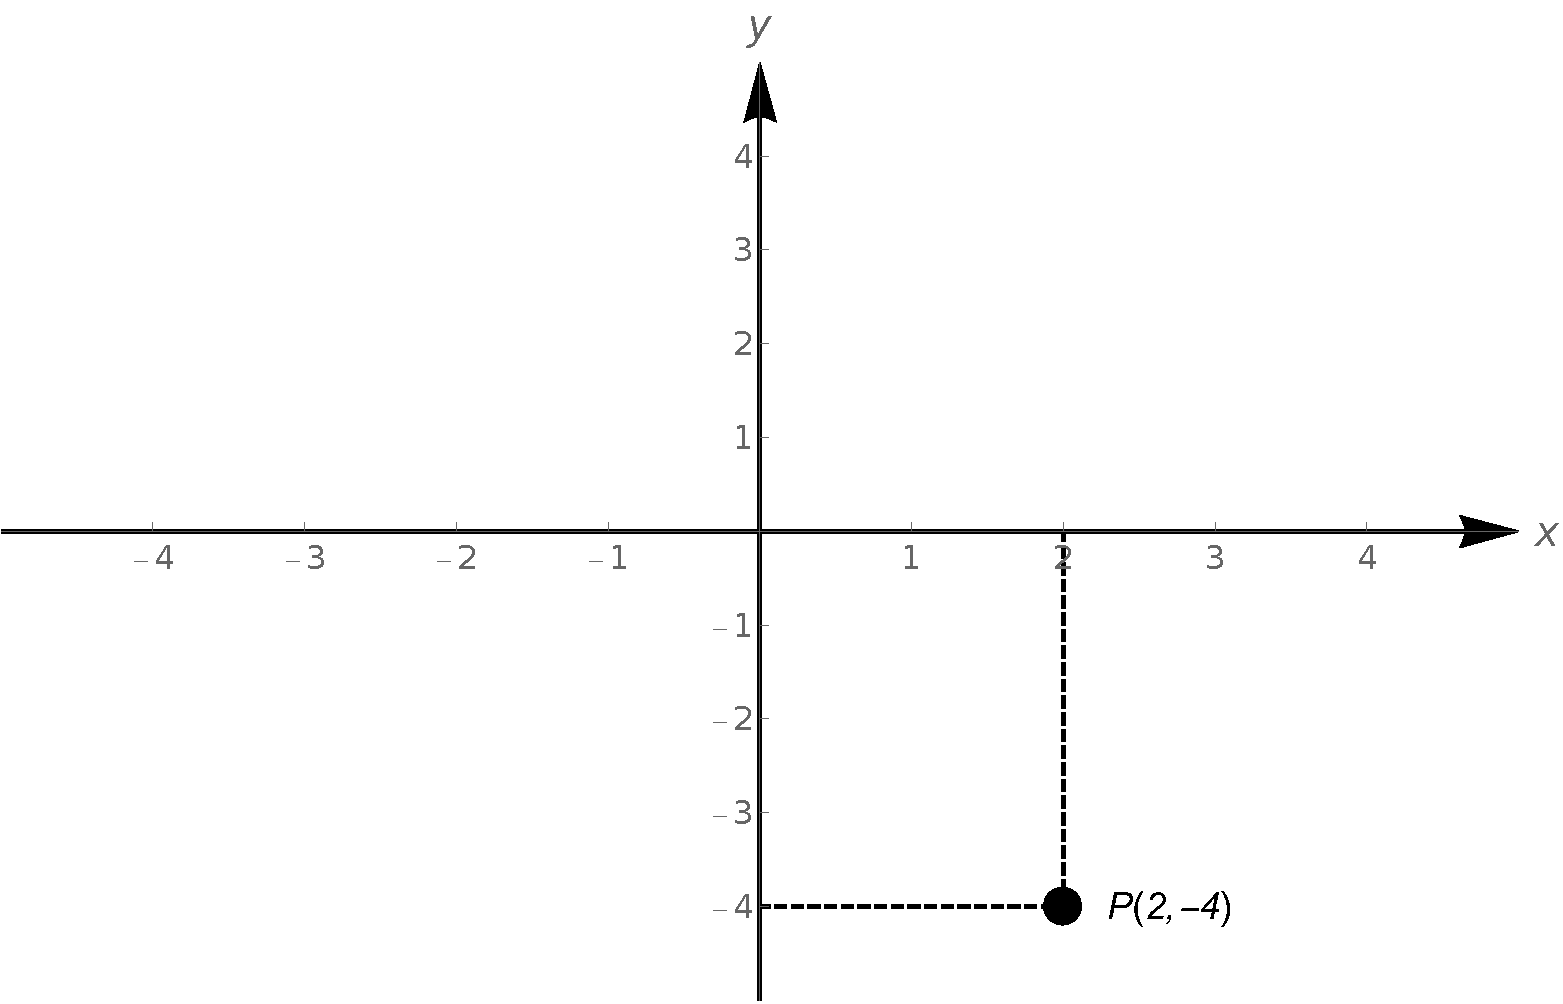
\includegraphics[width=0.5\textwidth]{fig_functions_1}
	\caption{The point $P$ located in the Cartesian coordinate plane.}
	\label{fig_functions_1}
	\end{center}
\end{figure}


\ifvc
 Moreover, we observe that
\begin{itemize}

\item $(a,b)$ and $(c,d)$ represent the same point in the plane if and only if $a = c$ and $b = d$.

\item  $(x,y)$ lies on the $x$-axis if and only if $y = 0$.

\item  $(x,y)$ lies on the $y$-axis if and only if $x=0$.

\end{itemize}
\fi



The axes divide the plane into four regions called \index{quadrants} \textbf{quadrants} (\textit{kwadrant})\index[aut]{kwadrant}.  They are labelled with Roman numerals and proceed counter-clockwise around the plane \ifvc (Figure~\ref{fig_functions_2})\fi. If a point other than the origin happens to lie on the axes, we typically refer to that point as lying on the positive or negative $x$-axis (if $y = 0$) or on the positive or negative $y$-axis (if $x = 0$).   Such points do not belong to any of the four quadrants.




Using Cartesian coordinates, we can introduce the three main types of \textbf{symmetry} (\textit{symmetrie}), namely symmetry about the $x$-axis, symmetry about the $y$-axis, and finally, symmetry about the origin. \index{symmetry}\index[aut]{symmetrie}


\ifvc
\begin{definition}[Symmetry of points]
Two points $(x_1,y_1)$ and $(x_2,y_2)$ in the plane are said to be
\vspace{-0.3cm}
\begin{itemize}
\item symmetric about the  $x$-axis if $x_1 = x_2$ and $y_1 = -y_2$;
\item symmetric about the $y$-axis if $x_1 = -x_2$ and $y_1 = y_2$;
\item symmetric about the origin if $x_1 = -x_2$ and $y_1 = -y_2$.
\end{itemize}
\end{definition}
The concept of symmetry is illustrated in Figure~\ref{fig_functions_3}. In that figure, $P$ and $S$ are symmetric about the $x$-axis, as are $Q$ and $R$;  $P$ and $Q$ are symmetric about the $y$-axis, as are $R$ and $S$;  and $P$ and $R$ are symmetric about the origin, as are $Q$ and $S$.

\begin{figure}[H]
	\begin{center}
			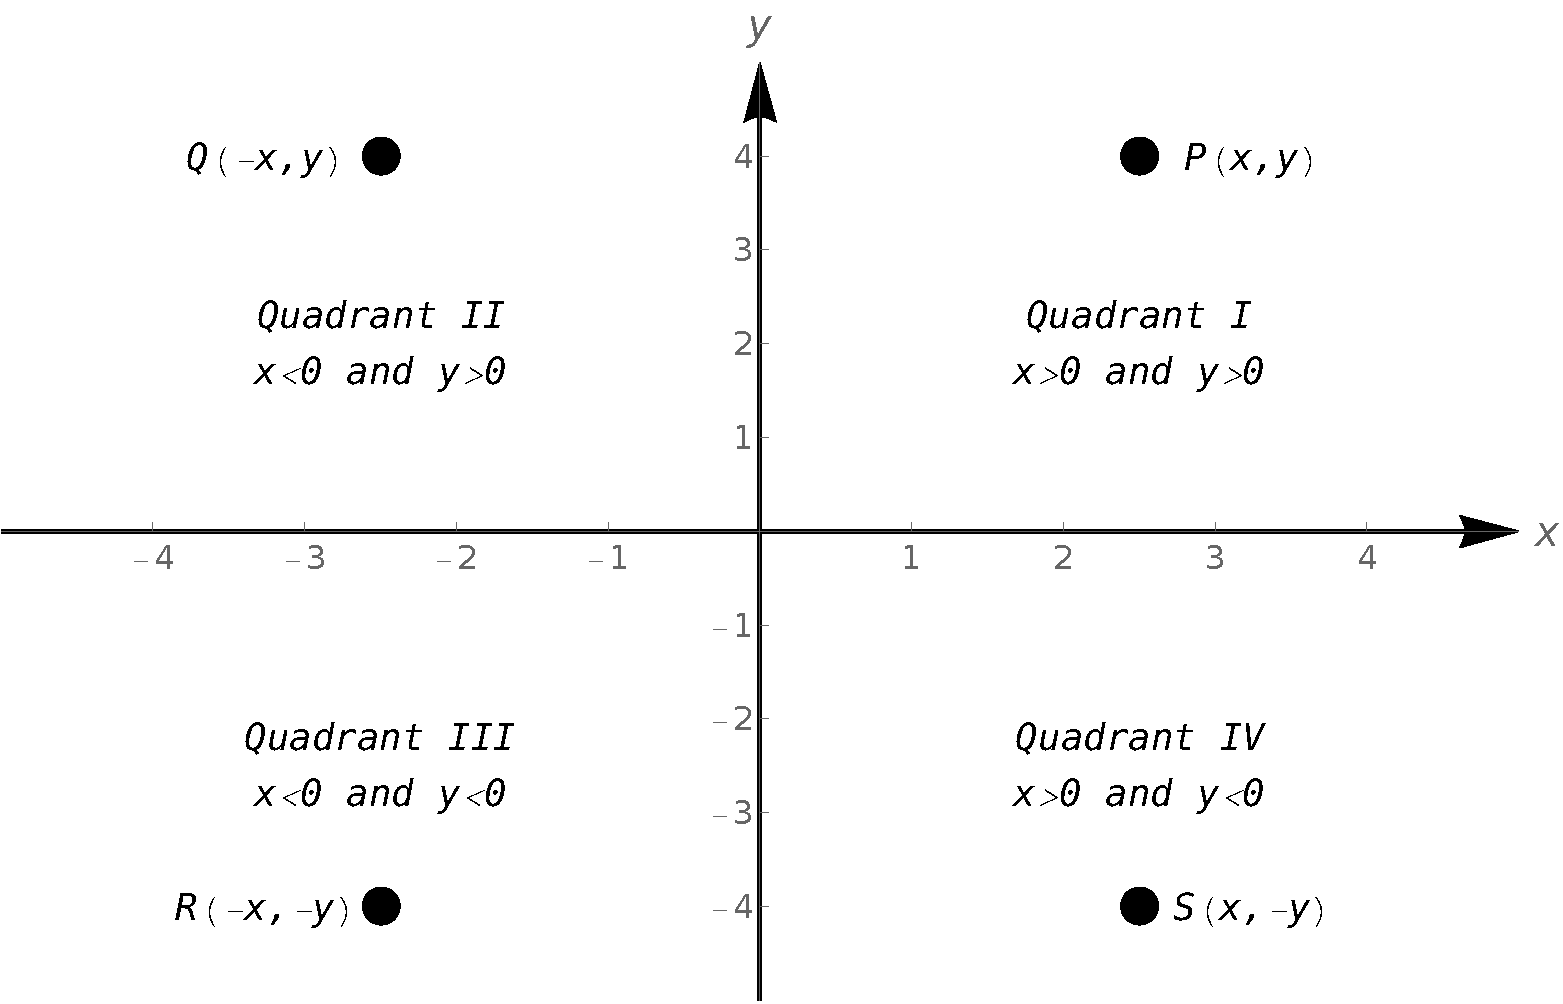
\includegraphics[width=0.5\textwidth]{fig_functions_2}
	\caption{The quadrants and symmetry of points in the Cartesian coordinate plane.}
	\label{fig_functions_2}
	\end{center}
\end{figure}

\ifvc\pagebreak\fi
\begin{example}
Let $P$ be the point $(-2,3)$.  Find the points that are symmetric to $P$ about the:

\begin{multicols}{3}

\begin{enumerate}

\item  $x$-axis,

\item  $y$-axis,

\item  origin.

\end{enumerate}

\end{multicols}

\xhrulefill{gray}{2.5pt}Solution \xhrulefill{gray}{2.5pt}


\begin{enumerate}

\item  To find the point symmetric about the $x$-axis, we replace the $y$-coordinate with its opposite to get  $(-2,-3)$. 

\item  To find the point symmetric about the $y$-axis, we replace the $x$-coordinate with its opposite to get $(2,3)$. 

\item  To find the point symmetric about the origin, we replace the $x$- and $y$-coordinates with their opposites to get $(2,-3)$. Here, we reflect across the $x$-axis and then across the $y$-axis. 

\end{enumerate}
\end{example}


\fi


\section{Functions}
\subsection{Relations}
\label{relaties}
\begin{definition}[Relation]
A \index{relation}\index[aut]{relatie} \textbf{relation} (\textit{relatie}) is a set of points in the plane. Hence,  a relation $R$ in $\mathbb{R}$ is a subset of the Cartesian product $\mathbb{R}^2$. 
\end{definition}


Since relations are sets, we can describe them using the techniques presented in Chapter~\ref{SetsChapter}.  That is, we can describe a relation verbally, using the roster method, or using set-builder notation. Most frequently, the latter kind of description is preferred and a relation is defined using a specific predicate that depends on $x$ and $y$, $P(x,y)$, i.e. \index{verbal method}\index{roster method}\index{set-builder notation}
$$
R=\left\{(x,y)\in\mathbb{R}^2\mid P(x,y) \right\}\,.
$$

The predicate  $P(x,y)$ is the rule that allows us to select the ordered pairs $(x,y)$ that make up the relation. Here, we call $x$ the \textbf{argument} (\textit{argument}) of the relation $R$ and $y$ its corresponding \textbf{image} (\textit{beeld}). Since the elements in a relation are points in the plane, we often try to describe the relation graphically as well.  Doing so produces the \textbf{graph} (\textit{grafiek}) of the relation $R$.
\index{image}\index[aut]{beeld}
\index{argument}\index[aut]{argument}
\index{graph}\index[aut]{grafiek}


\begin{example}
 Graph the following relations. \label{relationgraphingexample}



\begin{multicols}{2}
\begin{enumerate}
\ifvc
\item  $A = \{ (0,0), (-3,1), (4,2), (-3,2)\}$
\fi
\item  $B = \{ (x,3) \, | \, -2 \leq x \leq 4\}$
\item  $C = \{ (3,y) \, | \, \mbox{$y$ is a real number} \}$
\end{enumerate}
\end{multicols}

\ifvc\pagebreak\fi
\xhrulefill{gray}{2.5pt}Solution \xhrulefill{gray}{2.5pt}

\begin{enumerate}
\ifvc
\item  To graph $A$, we simply plot all of the points which belong to $A$, as shown in Figure~\ref{fig_functions_3a}.
\fi
\item  In words,  $\{ (x,3)\, | \, -2 \leq x \leq 4 \}$  reads `the set of points $(x,3)$ such that $-2 \leq x \leq 4$. Plotting several representative points should convince you that $B$ describes the horizontal line segment from the point $(-2,3)$ up to and including the point $(4,3)$ (Figure~\ref{fig_functions_3b}).
\item  The relation $C$ is  described as the set of points $(3,y)$ such that $y$ is a real number.  All of these points have an $x$-coordinate of $3$, but the $y$-coordinate is free to be whatever it wants to be, without restriction. Hence, all the points of $C$ lie on the vertical line  $x = 3$ (Figure~\ref{fig_functions_3c}).  

\end{enumerate}

\ifvc
\begin{figure}[H]
\centering
%\raisebox{0.5cm}{
\centerline{
\subfigure[Set $A = \{ (0,0), (-3,1), (4,2), (-3,2)\}$ \label{fig_functions_3a}]{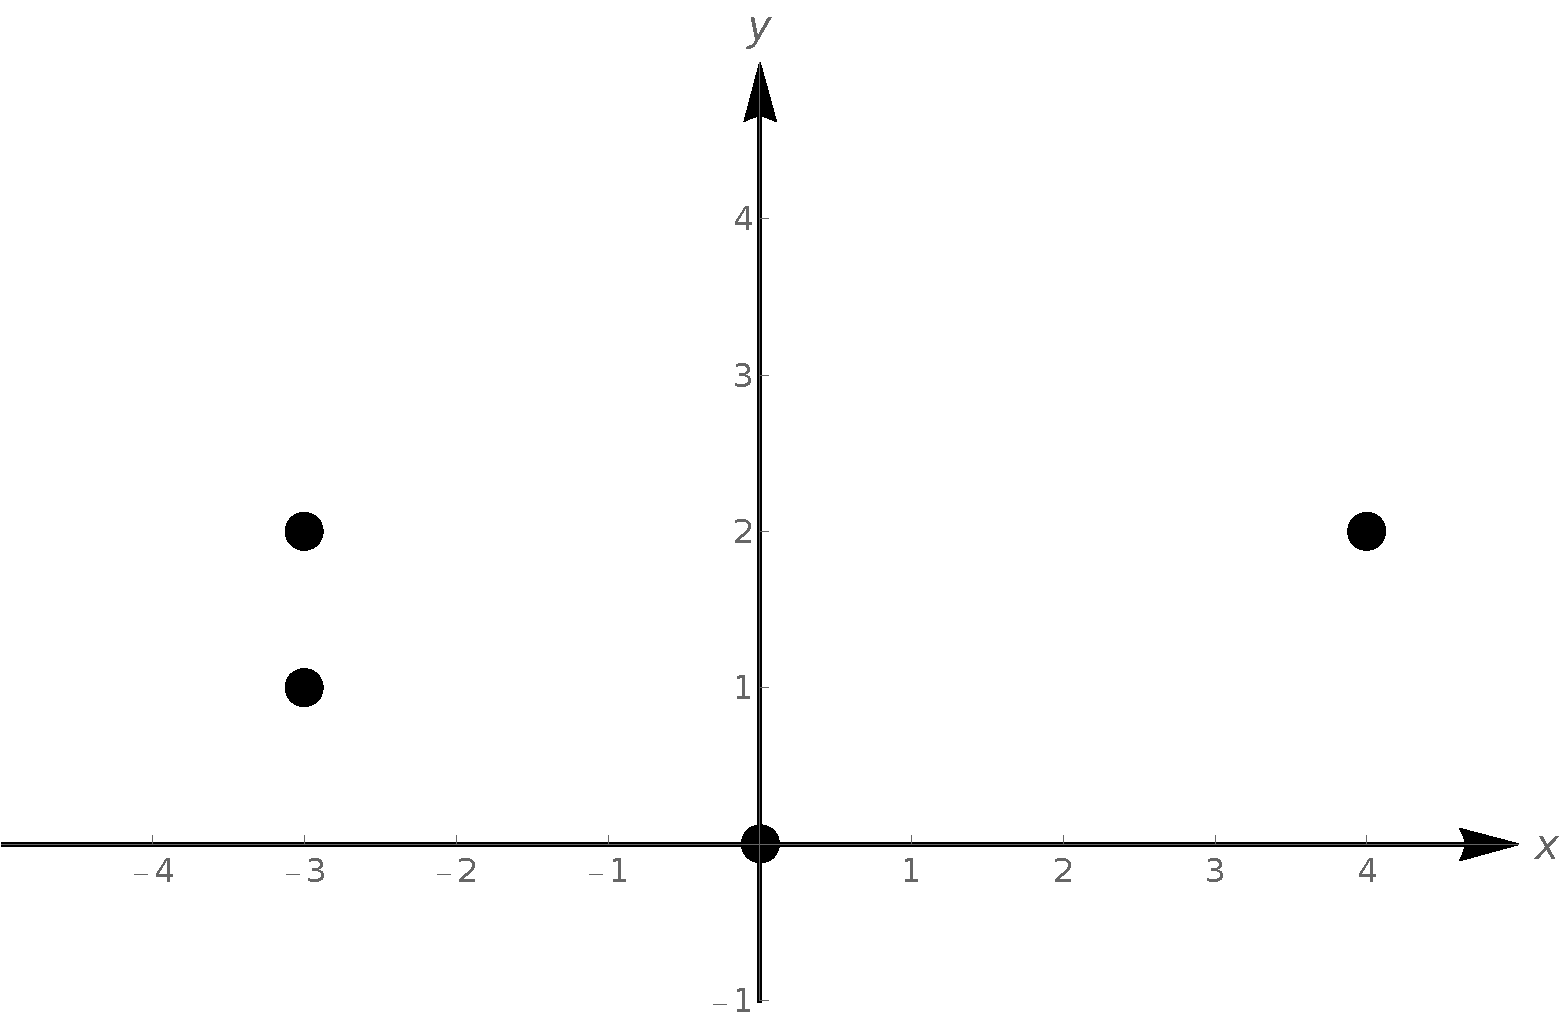
\includegraphics[width=0.4\textwidth]{fig_functions_3a}}
\hspace{0.1cm}
\subfigure[Set $B = \{ (x,3) \, | \, -2 \leq x \leq 4\}$ \label{fig_functions_3b}]{\includegraphics[width=0.4\textwidth]{fig_functions_3b}}
}
\centerline{
\subfigure[Set $C = \{ (3,y) \, | \, \mbox{$y$ is a real number} \}$ \label{fig_functions_3c}]{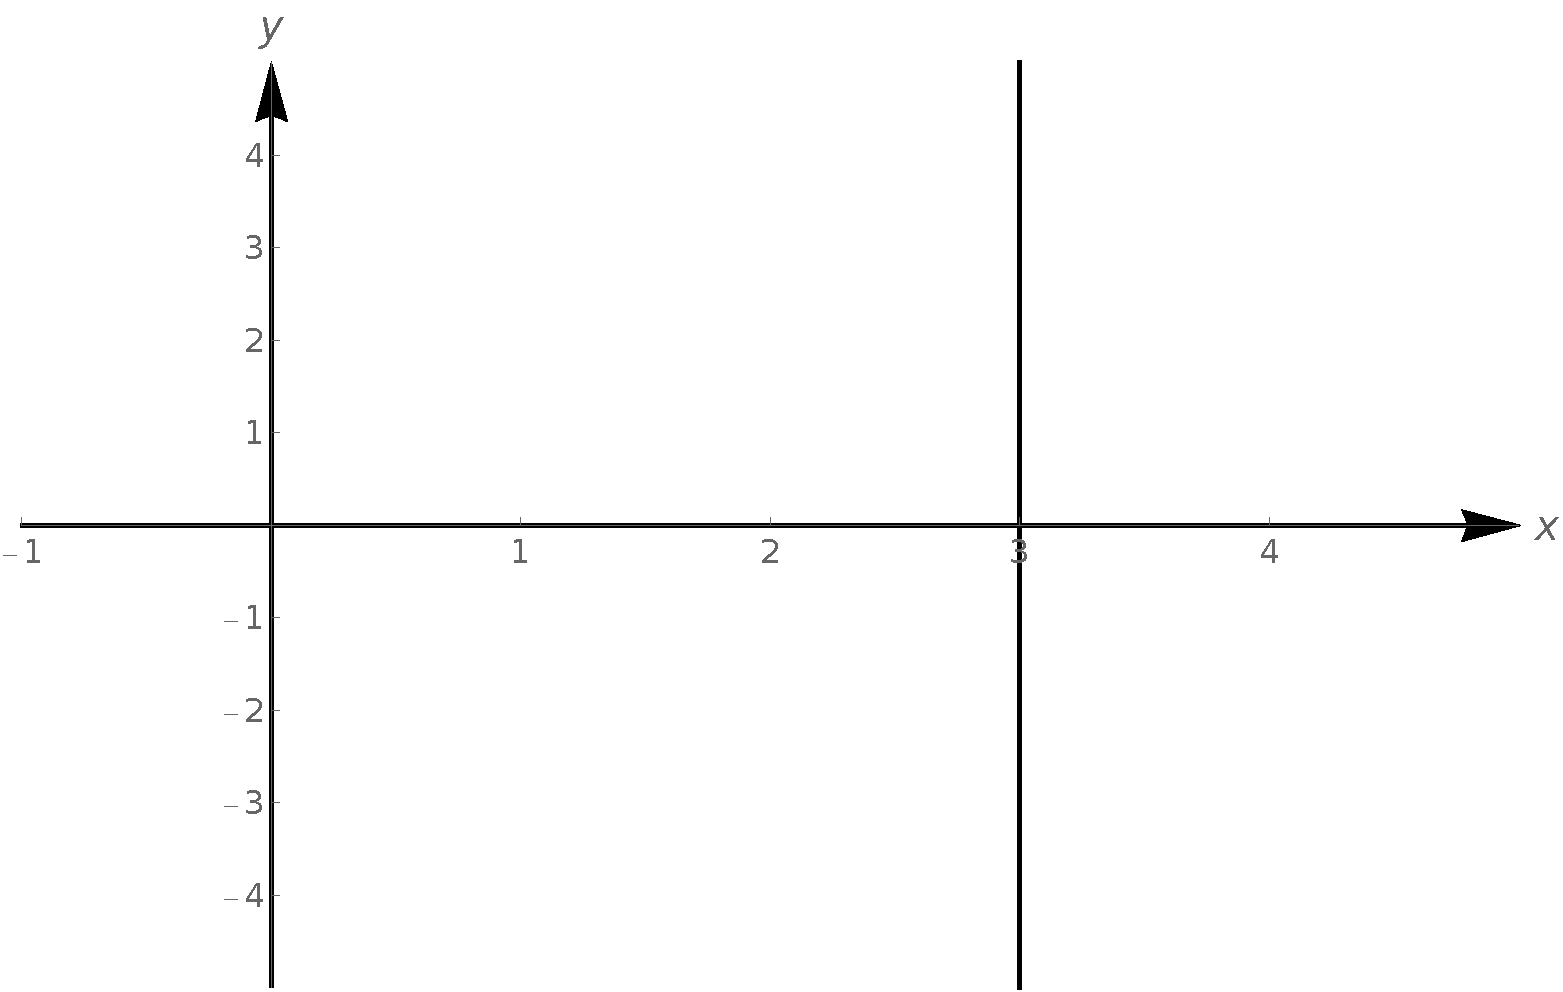
\includegraphics[width=0.4\textwidth]{fig_functions_3c}}
}
\caption{Graphs of different relations.} 
\end{figure}
\fi



\ifcourse
\begin{figure}[H]
\centering
%\raisebox{0.5cm}{
\centerline{
\subfigure[Set $B = \{ (x,3) \, | \, -2 \leq x \leq 4\}$ \label{fig_functions_3b}]{\includegraphics[width=0.4\textwidth]{figures/Functions/fig_functions_3b.pdf}}
\hspace{0.1cm}
\subfigure[Set $C = \{ (3,y) \, | \, \mbox{$y$ is a real number} \}$ \label{fig_functions_3c}]{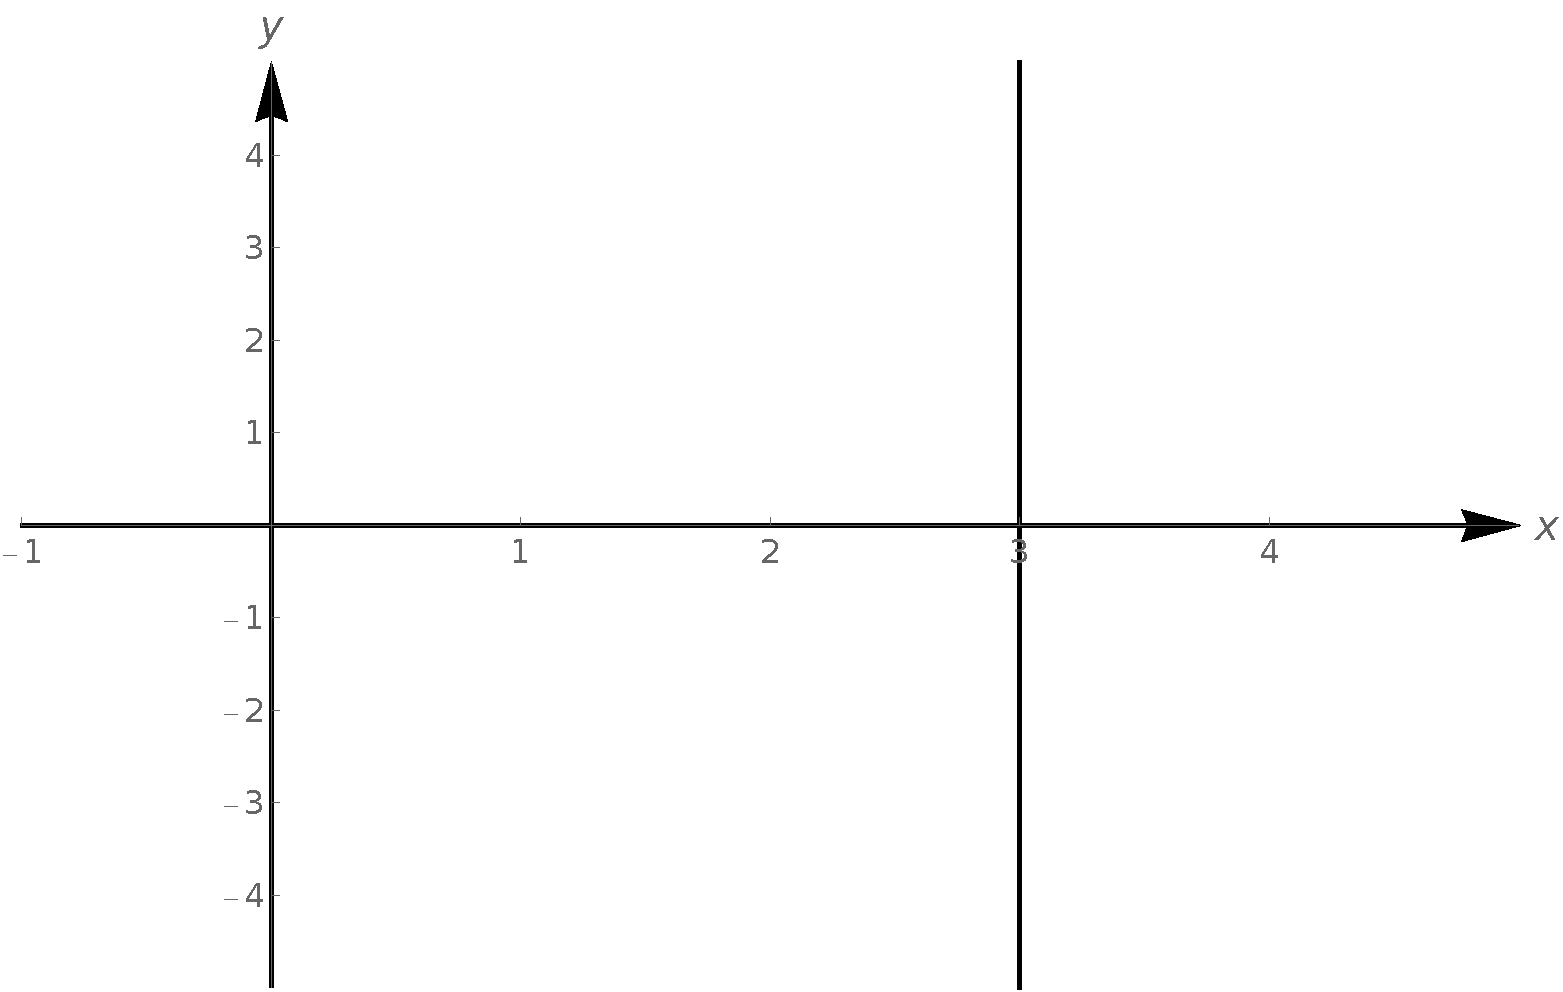
\includegraphics[width=0.4\textwidth]{fig_functions_3c}}
}
\caption{Graphs of different relations.} 
\end{figure}
\fi

\end{example}


The relation $C$ in the previous example lead us to our final way to describe relations: \textbf{algebraically} (\textit{algebra\"isch}). We can more succinctly describe the points in $C$ as those points which satisfy the equation $x = 3$.  Let us now study the graphs of equations in a more general setting. For that purpose, we rely on the so-called fundamental graphing principle.\index{fundamental graphing principle}
\index{algebraic notation}\index[aut]{algebra\"ische notatie}


\begin{definition}[Fundamental graphing principle]
The graph of an equation is the set of points which satisfy the equation.  %That is, a point $(x,y)$ is on the graph of an equation if and only if $x$ and $y$ satisfy the equation.
\end{definition}

It is at this point that we gain some insight into the word `relation'.  If the equation to be graphed contains both $x$ and $y$, then the equation itself is what is relating the two variables.  For instance, in the next example, we consider the  graph of the equation $x^2+y^3=1$ by graphing the relation $R = \{ (x,y) \, | \, x^2+y^3 = 1\}$.  \ifvc The points $(x,y)$ we graph belong to the relation $R$ and are related by the equation  $x^2+y^3 = 1$, since it is those pairs of $x$ and $y$ which make the equation true.\fi

\begin{example}
\label{examplerelation}
Graph the equation $x^2 + y^3 = 1$.

\xhrulefill{gray}{2.5pt}Solution \xhrulefill{gray}{2.5pt}

To  efficiently generate points on the graph of this equation, we first solve this equation for $y$:

\allowdisplaybreaks
\[ \begin{array}{rrclr} 
&    x^2 + y^3 & = & 1 & \\ 
\Leftrightarrow &          y^3 & = & 1 - x^2 & \\
\Leftrightarrow &\sqrt[3]{y^3} & = & \sqrt[3]{1 - x^2} & \\
\Leftrightarrow &            y & = & \sqrt[3]{1 - x^2}\,. & \\ 
            \end{array} \]

We now substitute a value in for $x$, determine the corresponding value $y$, and plot the resulting point $(x,y)$ in the Cartesian coordinate plane. We first generate a table of points which are on the graph of the equation.  These points are then plotted in the plane as shown below.

\begin{minipage}[c]{0.45\textwidth}
\begin{center}
\renewcommand{\arraystretch}{1.5}%
\begin{tabular}{c|c}  
	$x$&$y$ \\ \hline\hline
	$-3$&$ -2$ \\  
	$-2$&$-\sqrt[3]{3}$ \\  
	$ -1$&$ 0$ \\  
	$ 0 $&$ 1$ \\  
	$ 1$&$ 0$ \\  
	$2$&$-\sqrt[3]{3}$ \\  
	$3$&$ -2$ \\  
\end{tabular}
\end{center}
\end{minipage}
\begin{minipage}[c]{0.45\textwidth}
	\begin{center}
			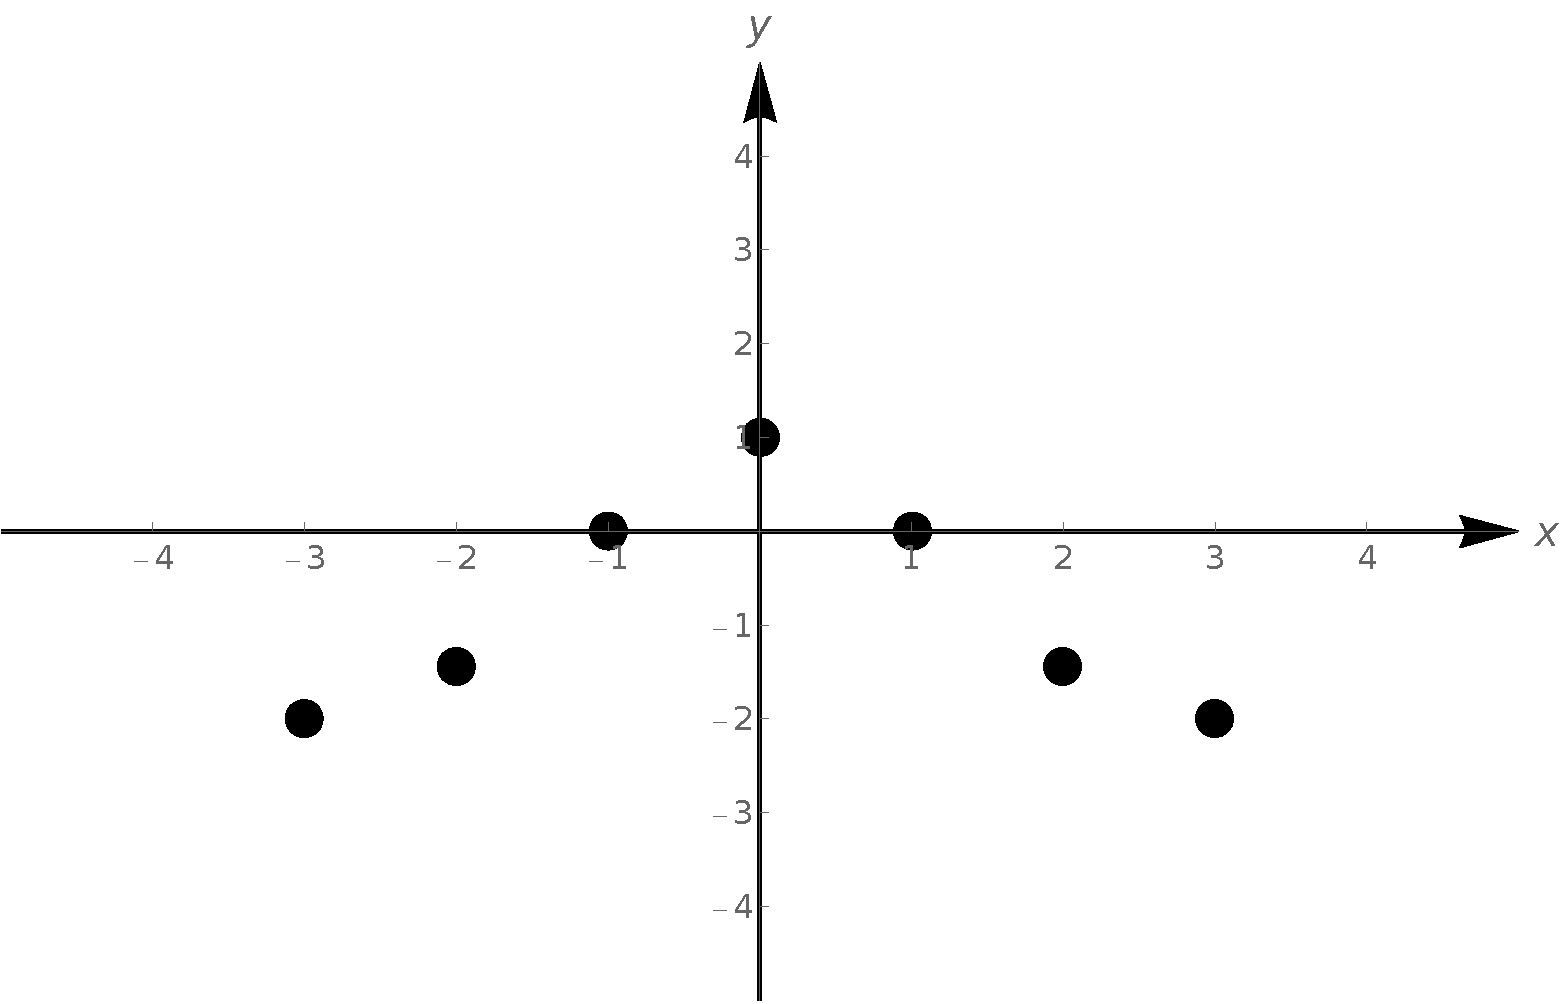
\includegraphics[width=0.95\textwidth]{fig_functions_4}
	\end{center}
\end{minipage}

  
\ifcourse
\ifmathematica
Alternatively, we can construct a graph of this equation in Mathematica using the built-in function \lstinline{ContourPlot}:
\begin{mdframed}[default,backgroundcolor=gray!40,roundcorner=8pt]
\begin{mmaCell}[morefunctionlocal={x, y}]{Input}
  ContourPlot[x^2+y^3==1,\{x,-5,5\},\{y,-5,5\}]

\end{mmaCell}


\begin{mmaCell}[moregraphics={moreig={scale=.4}}]{Output}
	 \mmaGraphics{fig_functions_5}
\end{mmaCell}
\end{mdframed}

Of course, we should add frame labels to this plot, which can be done as follows.
\begin{mdframed}[default,backgroundcolor=gray!40,roundcorner=8pt]
\begin{mmaCell}[morefunctionlocal={x, y}]{Input}
   ContourPlot[x^2+y^3==1,\{x,-5,5\},\{y,-5,5\}, FrameLabel \(\pmb{\to}\)\{"x","y"\}]

\end{mmaCell}


\begin{mmaCell}[moregraphics={moreig={scale=.4}}]{Output}
	 \mmaGraphics{fig_functions_6}
\end{mmaCell}
\end{mdframed}
\fi
\fi
\ifpython
Alternatively, we can construct a graph of this equation in Python using the built-in function \lstinline{plot}:
\begin{pyin}
from sympy import plot_implicit, symbols, Eq, And

x, y = symbols('x y')
p1 = plot(Eq(x**2 + y**3, 1))
\end{pyin}

\begin{pyout}
|\includegraphics[width=0.5\textwidth]{fig_functions_6_Python}|
\end{pyout}
\fi
\end{example}




The places where the graph of an equation crosses or touches the axes are called the \textbf{intercepts} (\textit{intercept}). \index{intercept}\index[aut]{intercept}  \ifvc The $x$-intercepts can be found by setting $y = 0$ in the equation, while $y$-intercepts are found by setting $x = 0$ in the equation.  In Example~\ref{examplerelation} the graph had two $x$-intercepts, $(-1,0)$ and $(1,0)$, and one $y$-intercept, $(0,1)$. \fi 

Another fact which you may have noticed about the graph in Example~\ref{examplerelation} is that it seems to be symmetric about the $y$-axis.  To actually prove this analytically, we assume $(x,y)$ is a generic point on the graph of the equation. That is, we assume  $x^2 + y^3 = 1$ is true. To show that the graph as a whole is symmetric about the $y$-axis, we need to show that $(-x,y)$ satisfies the equation $x^2 + y^3 = 1$, too.  Substituting $(-x,y)$ into the equation gives

\setlength{\extrarowheight}{2pt}

\[ \begin{array}{rrclr}   
&(-x)^2+(y)^3 & \stackrel{?}{=} & 1 & \\
\Leftrightarrow &  x^2 + y^3 & \stackrel{\checkmark}{=} & 1. & \\ 
   \end{array} \]
   
Since we are assuming that the original equation $x^2 + y^3 = 1$ is true, we have shown that $(-x, y)$ satisfies the equation and hence is on the graph.  In this way, we can check whether the graph of a given equation possesses any of the symmetries introduced in Section~\ref{CartesianPlane}.  



\begin{itemize}
	
	\item About the $y$-axis: substitute $(-x,y)$ into the equation and verify whether or not the result is equivalent to the original equation.
	
	\item About the $x$-axis: substitute $(x,-y)$ into the equation   and verify whether or not the result is equivalent to the original equation.
	
	\item About the origin: substitute $(-x,-y)$ into the equation and verify whether or not the result is equivalent to the original equation.
	
\end{itemize}


\ifcalculus
Intercepts and symmetry are two tools which can help us sketch the graph of an equation analytically, as demonstrated in the next example.


\begin{example}
	Find the $x$- and $y$-intercepts (if any) of the graph of $(x-2)^2 + y^2 = 1$. Test for symmetry.  Plot additional points as needed to complete the graph.
	
	\xhrulefill{gray}{2.5pt}Solution \xhrulefill{gray}{2.5pt}
	
	To look for $x$-intercepts, we set $y=0$ and solve
	
	\[ \begin{array}{rrclr}   
	
	&(x-2)^2 + 0^2 & = & 1 & \\ 
	\Leftrightarrow &\sqrt{(x-2)^2} & = & \sqrt{1} & \\
	\Leftrightarrow &x - 2 & = & \pm 1 & \\
	\Leftrightarrow &x  = 3 & \wedge & x  =  1. & \\
	
	\end{array} \]
	
	We get two answers for $x$ which correspond to two $x$-intercepts:  $(1,0)$ and $(3,0)$.    Turning our attention to $y$-intercepts, we set $x=0$ and solve
	
	\[ \begin{array}{rrclr}   
	
	&(0-2)^2 + y^2 & = & 1 & \\ 
	\Leftrightarrow&4 + y^2 & = & 1 & \\
	\Leftrightarrow&y^2 & = & -3. & \\
	
	\end{array} \]
	Consequently, the graph has no (real-valued!) $y$-intercepts.
	
	
	Moving along to symmetry, we can immediately dismiss the possibility that the graph is symmetric about the $y$-axis or the origin.  If the graph possessed either of these symmetries, then the fact that $(1,0)$ is on the graph would mean $(-1,0)$ would have to be on the graph. The only symmetry left to test is symmetry about the $x$-axis.   To that end, we substitute $(x,-y)$ into the equation and simplify
	
	\[ \begin{array}{rrclr}   
	&(x-2)^2 + (-y)^2 & = & 1 & \\ 
	\Leftrightarrow&(x-2)^2 + y^2 & = & 1 .& \\
	\end{array} \]
	
	Since we have obtained our original equation, the graph is symmetric about the $x$-axis. Proceeding as we did in the Example~\ref{examplerelation}, we obtain the graph shown in Figure~\ref{fig_functions_7}.
	
	
	\begin{figure}[H]
		\begin{center}
			\includegraphics[width=0.5\textwidth]{fig_functions_7}
			\caption{Graph of the equation $(x-2)^2 + y^2 = 1$.}
			\label{fig_functions_7}
		\end{center}
	\end{figure}
	
\end{example}
\fi


\ifvc
\begin{itemize}

\item About the $y$-axis: substitute $(-x,y)$ into the equation and verify whether or not the result is equivalent to the original equation.

\item About the $x$-axis: substitute $(x,-y)$ into the equation   and verify whether or not the result is equivalent to the original equation.

\item About the origin: substitute $(-x,-y)$ into the equation and verify whether or not the result is equivalent to the original equation.

\end{itemize}

Intercepts and symmetry are two tools which can help us sketch the graph of an equation analytically, as demonstrated in the next example.


\begin{example}
 Find the $x$- and $y$-intercepts (if any) of the graph of $(x-2)^2 + y^2 = 1$. Test for symmetry.  Plot additional points as needed to complete the graph.

\xhrulefill{gray}{2.5pt}Solution \xhrulefill{gray}{2.5pt}

To look for $x$-intercepts, we set $y=0$ and solve

\[ \begin{array}{rrclr}   

&(x-2)^2 + 0^2 & = & 1 & \\ 
\Leftrightarrow &\sqrt{(x-2)^2} & = & \sqrt{1} & \\
\Leftrightarrow &x - 2 & = & \pm 1 & \\
\Leftrightarrow &x  = 3 & \wedge & x  =  1. & \\

\end{array} \]

We get two answers for $x$ which correspond to two $x$-intercepts:  $(1,0)$ and $(3,0)$.    Turning our attention to $y$-intercepts, we set $x=0$ and solve

\[ \begin{array}{rrclr}   

&(0-2)^2 + y^2 & = & 1 & \\ 
\Leftrightarrow&4 + y^2 & = & 1 & \\
\Leftrightarrow&y^2 & = & -3. & \\

\end{array} \]
Consequently, the graph has no (real-valued!) $y$-intercepts.


Moving along to symmetry, we can immediately dismiss the possibility that the graph is symmetric about the $y$-axis or the origin.  If the graph possessed either of these symmetries, then the fact that $(1,0)$ is on the graph would mean $(-1,0)$ would have to be on the graph. The only symmetry left to test is symmetry about the $x$-axis.   To that end, we substitute $(x,-y)$ into the equation and simplify

\[ \begin{array}{rrclr}   
&(x-2)^2 + (-y)^2 & = & 1 & \\ 
\Leftrightarrow&(x-2)^2 + y^2 & = & 1 .& \\
\end{array} \]

Since we have obtained our original equation, the graph is symmetric about the $x$-axis. Proceeding as we did in the Example~\ref{examplerelation}, we obtain the graph shown in Figure~\ref{fig_functions_7}.


\begin{figure}[H]
	\begin{center}
			\includegraphics[width=0.5\textwidth]{fig_functions_7}
	\caption{Graph of the equation $(x-2)^2 + y^2 = 1$.}
	\label{fig_functions_7}
	\end{center}
\end{figure}

\end{example}
\fi

\subsection{Functions in $\mathbb{R}$}\label{functies_R}
\subsubsection{Definition}

\begin{definition}[Function]
\label{def_function}

A relation in which each $x$-coordinate in $\mathbb{R}$ is matched with at most only one $y$-coordinate is said to describe $y$ as a \textbf{function} (\textit{functie}) of $x$. A function $f$ that maps $x$ to $y$ is denoted as
$$
f: x\mapsto f(x)\,,
$$
with  $y = f ( x )$.
\end{definition}
\index{function}\index[aut]{functie}
The notation $y = f ( x )$ (read: $y$ equals $f$ of $x$) means that the pair $(x, y)$ belongs to the set of pairs defining the function $f$. $x$ is called the \textbf{argument} or \textbf{input} (\textit{input}) of the function $f$ and $f (x)$ is called the \textbf{value} taken by the function when evaluated at a point $x$, or its \textbf{output} (\textit{output}) or \textbf{image}. In the framework of applications, $x$ is often called the \textbf{independent variable} (\textit{onafhankelijke veranderlijke}), while $y$ is called the \textbf{dependent variable} (\textit{afhankelijke veranderlijke}). 
Loosely speaking, a function may be envisaged as a black box that returns for each input a corresponding output (Figure~\ref{fig_functions_8}). 
\index{argument}\index[aut]{argument}
\index{input}\index[aut]{input} 
\index{output}\index[aut]{output}
\index{image}\index[aut]{beeld}
\index{dependent variable}\index[aut]{afhankelijke veranderlijke}
\index{independent variable}\index[aut]{onafhankelijke veranderlijke}

\begin{figure}[H]
	\begin{center}
	\includegraphics[width=0.25\textwidth]{fig_functions_8}
	\caption{Describing a function as a black box.}
	\label{fig_functions_8}
	\end{center}
\end{figure}




To (graphically) determine whether or not a relation is function, we can use the following theorem, which is an immediate consequence of Definition~\ref{def_function}. 

\begin{theorem}[Vertical line test]
\label{VLT}
A set of points in the plane represents $y$ as a function of $x$ if and only if no two points lie on the same vertical line.
\end{theorem}
\ifanalysis
\begin{proof}
This is a direct consequence of Definition~\ref{def_function}
\end{proof}
\fi
\ifanalysis In other words, a relation $R$ constitutes a function if and only if every line parallel to the $y$-axis intersects the graph of $R$ in at most one point. \fi 


\begin{example}
Determine graphically which of the following relations actually represents a function.

\begin{figure}[H]
\centering
%\raisebox{0.5cm}{
\centerline{
\subfigure[Graph of relation $A$ \label{fig_functions_9a}]{\includegraphics[width=0.35\textwidth]{fig_functions_9a}}
\hspace{0.1cm}
\subfigure[Graph of relation $B$ \label{fig_functions_9b}]{\includegraphics[width=0.35\textwidth]{fig_functions_9b}}
}
\centerline{
\subfigure[Graph of relation $C$ \label{fig_functions_9c}]{\includegraphics[width=0.35\textwidth]{fig_functions_9c}}
\hspace{0.1cm}
\subfigure[Graph of relation $D$ \label{fig_functions_9d}]{\includegraphics[width=0.35\textwidth]{fig_functions_9d}}
}

\end{figure}

\xhrulefill{gray}{2.5pt}Solution \xhrulefill{gray}{2.5pt}

\begin{enumerate}
\item [(a)]   In the graph of $A$, every vertical line crosses the graph at most once, so $A$ does represent $y$ as a function of $x$.
\item [(b)] Looking at the graph of $B$, we can easily imagine a vertical line crossing the graph more than once.  Hence, $B$ does not represent $y$ as a function of $x$.  
\item [(c)]  In $C$, there is a point on the curve with $x$-coordinate 2 just below $(2,1)$, which means that both $(2,1)$ and this point on the curve lie on the vertical line $x=2$.  Hence, the graph of  $C$ fails the vertical line test, so $y$ is not a function of $x$ here. 
\item [(d)] In $D$ notice that the point with $x$-coordinate 2 on the curve has been omitted, leaving an open circle there.  Hence, the vertical line $x=2$ crosses the graph of $D$ only at the point $(2,1)$.  Indeed, any vertical line will cross the graph at most once, so we have that the graph of $D$ passes the vertical line test.  Thus it describes $y$ as a function of $x$.
\end{enumerate}
\end{example}

Finally, it is important to note that a function for which the dependent variable can be written explicitly in terms of the independent variable, i.e.\ as $y=f(x)$, is called an \textbf{explicit function} (\textit{expliciete functie}). On the other hand, if the function is defined by
$$
F(x,y)=0\,,
$$
which does not contain $y$ explicitly at one side of the equation, it is called an \textbf{implicit function} (\textit{impli\-ciete functie}). For instance, 
$$
x^2+y^2-4=0
$$
constitutes an implicit function, which defines two explicit functions, namely
$$
y=\sqrt{4-x^2},\qquad\mbox{and} \qquad y=-\sqrt{4-x^2}\,.
$$
\index{implicit function}\index[aut]{impliciete functie}\index{explicit function}\index[aut]{expliciete functie}\index{function ! implicit}\index[aut]{functie ! impliciet}\index{function ! explicit}\index[aut]{functie ! expliciet}

\subsubsection{Function graphs}
It is often useful to draw the graph\index{graph}\index[aut]{grafiek} of a function for getting a global view of its properties. Formally, we define the graph of a function as follows. 
\begin{definition}[Fundamental graphing principle for functions]
The graph $G$ of a function $f$ is the set of points which satisfy the equation $y=f(x)$. More formally, 
$$
G=\left\{(x,f(x))\mid x \in \mathbb{R} \wedge y=f(x)\right\}\,.
$$
\end{definition}
The $x$-coordinates of the $x$-intercepts of the graph of $y=f(x)$ can be found by solving $f(x) = 0$.  For this reason, they are called the \index{function ! zero}\index{functie ! nulpunt}\textbf{zeros} (\textit{nulpunt}) of $f$.


\subsubsection{Domain, codomain and range}
When defining a function $f$ as
$$
f: x\mapsto f(x)\,,
$$
\ifcourse
	\checkoddpage
\marginpar{\ifoddpage\hspace*{-1.5cm}\else\hspace*{0.25cm}\fi\includegraphics[width=0.075\textwidth]{youtube}\\
\ifoddpage\hspace*{-1.75cm}\else\hspace*{0.1cm}\fi
\qrcode[height=1.75cm]{https://youtu.be/BQMyeQOLvpg}
%\includegraphics[width=0.1\textwidth]{codomein}
}
\fi
we not only need to specify how $f$ maps an argument $x$ to its image $y$, but also the sets to which $x$ and $y=f(x)$ belong. In other words, we need to specify what are the possible in- and outputs of our black box (Figure~\ref{fig_functions_8}). We call the set of possible inputs the \textbf{domain} (\textit{domein}) of the function, denoted as $\dom{\;f}$. The set of possible outputs is called the \textbf{codomain} (\textit{codomein}). Suppose $X$ is the domain of a function $f$ and $Y$ is its codomain, then we can define this function using arrow notation to make explicit the domain and codomain:
\index{domain}\index[aut]{domein}
\index{codomain}\index[aut]{codomein}
$$
f:X\to Y\,,
$$
which should be read as $f$ maps domain $X$ to codomain $Y$. The set to which $f$ actually maps the domain, is called the \textbf{range} (\textit{bereik}) or \textbf{image} (\textit{beeld}) of $f$, denoted by $\im{\;f}$. The range is thus defined as
\index{range}\index[aut]{bereik}
$$
\im{\;f} = \left\{y=f(x)\mid x\in X \wedge y\in Y \right\}\,.
$$
These concepts are illustrated in Figure~\ref{fig_functions_10}. The difference between range and codomain may seem subtle, but can be very important, as will be shown in Example~\ref{example_domain_codomain_range}.

\begin{figure}[h!]
	\begin{center}
	\includegraphics[width=0.4\textwidth]{figures/Functions/fig_functions_10.png}
	\caption{The domain $X$, codomain $Y$ and range $\left\{f(x)\mid x\in X\right\}$ of a function $f$.}
	\label{fig_functions_10}
	\end{center}
\end{figure}

Throughout this course we will focus on so-called \textbf{real functions} (\textit{re\"ele functie}), which are real-valued functions of a real variable. Such functions can be written as \index{real function}\index[aut]{re\"ele functie}
$$
f:\mathbb{R}\to\mathbb{R}\quad:\quad x\mapsto f(x)\,.
$$


\ifvc
To determine the domain and range of a function, we need to determine which $x$ and $y$-values occur as coordinates of points on the given graph.  To find the domain graphically, it may be helpful to imagine collapsing the curve to the $x$-axis and determining the portion of the $x$-axis that gets covered. The resulting interval on the $x$-axis represents the domain of $f$. This is called \textbf{projecting} (\textit{projectie}) the curve to the $x$-axis. To determine the range of $f$, we project the curve to the $y$-axis. \index{projection}\index[aut]{projectie}

\begin{example}
Determine the domain and range of the function $f$ whose graph is given below.
	\begin{center}
			\includegraphics[width=0.5\textwidth]{fig_functions_11}
	\end{center}

\pagebreak 
\xhrulefill{gray}{2.5pt}Solution \xhrulefill{gray}{2.5pt}
	
   First note that the graph continues to curve upwards
   to the left forever more; and note the open circle at $(2,-1)$ that indicates that the point $(2,-1)$ is not on the graph, but all points on the curve leading up to that point are. We see  that if we project the graph of $f$ to the $x$-axis, we get all real numbers less than $2$.  Using interval notation, we write the domain of $f$ as $\left.\right]-\infty, 2\left.\right[$. Note that even though there is an open circle at $(2,-1)$, we still include the $y$-value of $-1$ in our range, since the point $(0,-1)$ is on the graph of $f$.  We see that the range of $f$ is all real numbers greater than or equal to $-2$, or, in interval notation,  $\left.\right]-2,+\infty]$.
\end{example}
\fi

In most cases, we can relatively easily determine the domain, codomain and range of a function $f$ by investigating the formula defining it.  Doing so, we sometimes run into functions whose domain consists of two ore more consecutive open intervals, such as for  $$f(x)=\frac{1}{x}\,,$$ for  which $\text{dom}\,f=\mathbb{R}\setminus\{0\}=]-\infty,0[\,\cup\, ]0,+\infty[$. The points at which a function in such a case is not defined are called the function's \textbf{singularities} (\textit{singulariteiten}). So, $f(x)=\frac{1}{x}$ has a singularity at $x=0$.
\index[aut]{singulariteit}
\index{singularity}


\begin{example}
\label{example_domain_codomain_range}
Determine the domain, codomain and range of the following functions
\begin{enumerate}
\item  $f:\mathbb{R}\to \mathbb{R}\quad:\quad x\mapsto x^2\,,$
\item  $g:\mathbb{R}\to \mathbb{R}^+\quad:\quad x\mapsto x^2\,,$
\item $h:\mathbb{R}^+\to \mathbb{R}^+\quad:\quad x \mapsto x^{\frac{1}{2}}\,.$
\end{enumerate}

\xhrulefill{gray}{2.5pt}Solution \xhrulefill{gray}{2.5pt}

\begin{enumerate}
\item  From the function definition of $f$, we infer that both the domain and codomain are $\mathbb{R}$. Yet, since $f$ does not map to any negative number, the range of $f$ is $\mathbb{R}^+$. Its graph is shown in Figure~\ref{fig_functions_12a}.
\item  From the function definition of $g$, we infer that the domain is $\mathbb{R}$, but its codomain is $\mathbb{R}^+$. Again, since $g$  does not map to any negative number, the range of $g$ is $\mathbb{R}^+$ and its graph is the same as the of $f$ shown in Figure~\ref{fig_functions_12b}.
\item  From the function definition of $h$, we infer that both the domain and codomain are $\mathbb{R}^+$. Since the mapping is done by the square root, this has important implications. Firstly, the square root of a negative number does not exist in $\mathbb{R}$, which sets a restriction on the domain. Secondly, the square root of $x \in \mathbb{R}^+$ maps $x$ to $\sqrt{x}$ and $-\sqrt{x}$. Hence, if the codomain would be defined as $\mathbb{R}$, $h$ would not be a function (see Definition~\ref{def_function})! From this we can also infer that the range of $h$ is $\mathbb{R}^+$. Its graph is shown in Figure~\ref{fig_functions_12b}.
\end{enumerate}


\begin{figure}[H]
\centering
%\raisebox{0.5cm}{
\centerline{
\subfigure[Graph of $f$ and $g$ \label{fig_functions_12a}]{\includegraphics[width=0.3\textwidth]{fig_functions_12a}}
\hspace{1cm}
\subfigure[Graph of $h$ \label{fig_functions_12b}]{\includegraphics[width=0.3\textwidth]{fig_functions_12b}}
}
\caption{Graphs of the functions $f$, $g$ and $h$ in Example~\ref{example_domain_codomain_range}. }
\label{fig_functions_12}
\end{figure}



\end{example}



\subsection{Function arithmetic}\label{rekenen_functies}
It seems natural that functions should have their own arithmetic which is consistent with the arithmetic of real numbers.  The following definitions allow us to add, subtract, multiply and divide functions using the arithmetic we already know for real numbers.
Suppose $f$ and $g$ are functions and $\dom\,f\cap\dom\,g\neq\emptyset$, then we can define the following operations on $\dom\,f\cap\dom\,g$:
\index{function ! sum}\index[aut]{functie ! som}
\index{function ! difference}\index[aut]{functie ! verschil}
\index{function ! product}\index[aut]{functie ! product}
\index{function ! quotient}\index[aut]{functie ! quoti\"ent}

\begin{itemize}

\item The \textbf{sum} (\textit{som}) of $f$ and $g$: 
 \[(f+g)(x) = f(x) + g(x).\]

\item  The \textbf{difference} (\textit{verschil}) of $f$ and $g$:  
 \[(f-g)(x) = f(x) - g(x).\]

\item  The \textbf{product} (\textit{product}) of $f$ and $g$:
 \[(fg)(x) = f(x)g(x).\]

\item  The \textbf{quotient} (\textit{quoti\"ent}) of $f$ and $g$:
\[\left(\dfrac{f}{g}\right)(x) = \dfrac{f(x)}{g(x)},\] provided $g(x) \neq 0$.

\end{itemize}
  Note that while the formula $(f+g)(x) = f(x) + g(x)$ looks suspiciously like some kind of distributive property, it is nothing of the sort;  the addition on the left hand side of the equation is function addition, and we are using this equation to define the output of the new function $f+g$ as the sum of the real number outputs from $f$ and $g$.

\begin{example}  
 Let $f(x) = 6x^2 - 2x$ and $g(x) = 3-\frac{1}{x}$.  


\begin{enumerate}
\ifvc
\item Find  $(f+g)(-1)$.

\item Find $(fg)(2)$.
\fi


\item  Find the domain of $g-f$. Then find and simplify a formula for  $(g-f)(x)$.

\item  \label{quotdomainex} Find the domain of $g/f$. Then find and simplify a formula for  $\left(\frac{g}{f}\right)(x)$.

\end{enumerate}

\ifanalysis\pagebreak\fi
\ifcalculus\pagebreak\fi
\xhrulefill{gray}{2.5pt}Solution \xhrulefill{gray}{2.5pt}

\begin{enumerate}
\ifvc
\item  To find $(f+g)(-1)$ we first find $f(-1) = 8$ and $g(-1) = 4$. So, we have that $(f+g)(-1) = f(-1) + g(-1) = 8+4 = 12$.

\item To find $(fg)(2)$, we first need $f(2)$ and $g(2)$. Since $f(2) = 20$ and $g(2) = \frac{5}{2}$, our formula yields $(fg)(2) = f(2) g(2) = (20)\left(\frac{5}{2}\right) = 50$.
\fi

\item To find the domain of $g-f$ we need to find the domain of $g$ and of $f$ separately, then find the intersection of these two sets.  Owing to the denominator in the expression $g(x) = 3 - \frac{1}{x}$, we get that the domain of $g$ is $\mathbb{R}_0$.  Since $f(x) = 6x^2-2x$ is valid for all real numbers, we have no further restrictions.  Thus the domain of $g-f$ matches the domain of $g$, namely, $\mathbb{R}_0$.

Moving along, we need to simplify a formula for $(g-f)(x)$.  In this case, we get common denominators and attempt to reduce the resulting fraction.  Doing so, we get

\[ \begin{array}{rclr}
(g-f)(x) & = & g(x) - f(x) & \\ [5pt]
         & = & \left(3-\dfrac{1}{x}\right) - \left(6x^2 - 2x\right) &\\  [10pt]
         & = & \dfrac{-6x^3+2x^2+3x-1}{x}. & \\   
\end{array}\] 

\item  First, we  find the domain of $g$ and $f$ separately, and find the intersection of these two sets.  In addition, since $\left(\frac{g}{f}\right)(x) = \frac{g(x)}{f(x)}$, we are introducing a new denominator, namely $f(x)$, so we need to guard against this being $0$ as well.  The domain of $g$ is $\mathbb{R}_0$ and the domain of $f$ is $\mathbb{R}$.  Setting $f(x) = 0$ gives $6x^2 - 2x = 0$ or $x = 0$ or $x=\frac{1}{3}$.  So, the domain of $g/f$ is $\mathbb{R}\setminus \{0,\tfrac{1}{3}\}$.

Next, we find and simplify a formula for $\left(\frac{g}{f}\right)(x)$.
\renewcommand{\arraystretch}{2.5}
 \allowdisplaybreaks
 \begin{align*}
\left( \dfrac{g}{f}\right)(x) & =  \dfrac{g(x)}{f(x)}\\
    & =  \dfrac{3-\dfrac{1}{x}\vphantom{\left(\dfrac{1}{x}\right)}}{6x^2 - 2x}=\dfrac{3x-1}{\left(6x^2 - 2x\right)x}  \\
	& =  \dfrac{3x-1}{2x^2(3x-1)} \qquad (\text{Assuming }x\neq\frac{1}{3}\; \text{ and } \; x \neq 0) \\
	& =  \dfrac{1}{2x^2}  
\end{align*}
\renewcommand{\arraystretch}{1}
\end{enumerate}
\end{example}

In addition to operations on functions, we can also compose functions. Function composition is defined below.
\begin{definition}[Composite function]
\label{functioncompositiondefn} Suppose $f$ and $g$ are two functions.  The \index{function ! composite}\index[aut]{functie ! samengestelde}\textbf{composite} (\textit{samenstelling}) of $g$ with $f$, denoted $g \circ f$, is defined by
 $$
(g \circ f) (x) = g(f(x))\,,
$$
provided $x\in\dom\,f$  and $f(x)\in\dom\, g$. 
\end{definition}
The quantity $g \circ f$ is also read $g$ composed with $f$ or, more simply $g$ of $f$. At its most basic level, Definition \ref{functioncompositiondefn} tells us to obtain the formula for $\left(g \circ f\right)(x)$, we replace every occurrence of $x$ in the formula for $g(x)$ with the formula we have for $f(x)$.  If we take a step back and look at this from a procedural, inputs and outputs perspective, Defintion \ref{functioncompositiondefn} tells us  the output from $g \circ f$ is found by taking the output from $f$, $f(x)$,  and then making that the input to $g$.  The result, $g(f(x))$, is the output from $g \circ f$. This is illustrated in Figure~\ref{fig_functions_13} for a setting where $f:x\mapsto x^2$ and $g:x\mapsto x+1$. 
\begin{figure}
	\begin{center}
	\includegraphics[width=0.3\textwidth]{fig_functions_13}
	\caption{Function composition $(g\circ f)(x)$, where $f:x\mapsto x^2$ and $g:x\mapsto x+1$.}
	\label{fig_functions_13}
	\end{center}
\end{figure}
Clearly, the notion of function composition can easily be generalised to an arbitrary number of functions. For instance,  suppose $f$, $g$ and $h$ are three functions, then we may consider 
$$\left(\left(h \circ g\right) \circ f\right)(x) = h\left(g\left(f\left(x\right)\right)\right).$$




In the expression $g(f(x))$, the function $f$ is often called the inside function while $g$ is often called the outside function.  There are two ways to go about evaluating composite functions - inside out and outside in - depending on which function we replace with its formula first.  Both ways are  demonstrated in the following example.  

\begin{example}
\label{fcexform}
 Let $f(x) = x^2-4x$, \;  $g(x) = 2-\sqrt{x+3}$\; and  $h(x) = \dfrac{2x}{x+1}.$ \\
 \\
 Find and simplify the indicated composite functions. State the domain of each.

\begin{enumerate}
\begin{multicols}{2}
\item  $(g \circ f)(x)$ \label{fcexformfirst}
\item  $\big(h \circ (g \circ f)\big)(x)$ 
\end{multicols}

\end{enumerate}

\xhrulefill{gray}{2.5pt}Solution \xhrulefill{gray}{2.5pt}

\begin{enumerate}
\item  By definition, $(g \circ f)(x) = g(f(x))$. We now illustrate two ways to approach this problem.

\begin{itemize}

\item  Inside out:  We insert the expression $f(x)$ into $g$ first to get  \[(g \circ f)(x) = g(f(x)) = g\left(x^2-4x\right) = 2 - \sqrt{\left(x^2-4x\right)+3} = 2 - \sqrt{x^2-4x+3}.\] 


\item  Outside in:  We use the formula for $g$ first to get  \[(g \circ f)(x) = g(f(x)) = 2 - \sqrt{f(x)+3}  = 2 - \sqrt{\left(x^2-4x\right)+3} = 2 - \sqrt{x^2-4x+3}.\]
 We get the same answer as before.

\end{itemize} 

To find the domain of $g \circ f$, we need to find the elements in the domain of $f$ whose outputs $f(x)$ are in the domain of $g$.  We accomplish this by determining the domain before we simplify the formula for the composite function.  To that end, we examine $(g \circ f)(x) = 2 - \sqrt{\left(x^2-4x\right)+3}$.  To ensure that the argument of the square root is positive, it should hold that $x^2-4x+3 \geq 0$. 
We find the zeros of $x^2-4x+3$ to be $x = 1$ and $x = 3$. Consequently,  the domain of $g \circ f$, is $\left.\right]-\infty, 1] \cup [3,+\infty\left[\right.$. Figure~\ref{fig_functions_14} shows the graph of  $f(x)$, $g(x)$ and  $(g \circ f)$. 
\begin{figure}[H]
\centering
\includegraphics[width=0.45\textwidth]{fig_functions_14}
\caption{Graph of  $f(x)$, $g(x)$ and  $(g \circ f)$ in Example~\ref{fcexform}. \label{fig_functions_14}}
\end{figure}


\item  The expression $\big(h \circ (g \circ f)\big)(x)$ indicates that we first find the composite, $g \circ f$ and compose the function $h$ with the result.  We know already that $(g \circ f)(x) =  2 - \sqrt{x^2-4x+3}$.  We now proceed as usual.

\begin{itemize}

\item  Inside out: We insert the expression $(g \circ f)(x)$ into $h$ first to get

\begin{tabular}{rclr} $\big(h \circ (g \circ f)\big)(x)$ & = & $h\big((g \circ f)(x)\big)=h\left(2 - \sqrt{x^2-4x+3}\right)$  & \\ [0.8cm]
 & = & $\dfrac{2 \left(2 - \sqrt{x^2-4x+3}\right)}{\left(2 - \sqrt{x^2-4x+3}\right)+1}=\dfrac{4 - 2\sqrt{x^2-4x+3}}{3 - \sqrt{x^2-4x+3}}$. & \\ 
 %& = & $\dfrac{4 - 2\sqrt{x^2-4x+3}}{3 - \sqrt{x^2-4x+3}}$. & \\
 \end{tabular}

\item  Outside in:  We use the formula for $h(x)$ first to get

\begin{tabular}{rclr} $\big(h \circ (g \circ f)\big)(x)$ & = & $h\big((g \circ f)(x)\big)=\dfrac{2 \left( (g \circ f)(x)\right)}{  \left( (g \circ f)(x)\right) + 1}$  & \\ [0.8cm]
& = & $\dfrac{2 \left(2 - \sqrt{x^2-4x+3}\right)}{\left(2 - \sqrt{x^2-4x+3}\right)+1}=\dfrac{4 - 2\sqrt{x^2-4x+3}}{3 - \sqrt{x^2-4x+3}}$. & \\ 
 \end{tabular}
 
 \end{itemize}
 
To find the domain of $(h \circ (g \circ f))$, we look at the step before we began to simplify, 
\[(h \circ (g \circ f))(x) = \frac{2 \left(2 - \sqrt{x^2-4x+3}\right)}{\left(2 - \sqrt{x^2-4x+3}\right)+1}.\] 
 For the square root, we need $x^2-4x+3 \geq 0$, which requires $\left.\right]-\infty, 1] \cup [3,+\infty\left[\right.$.  Next, we set the denominator to zero and solve:  $\left(2 - \sqrt{x^2-4x+3}\right)+1 = 0$.  We get $\sqrt{x^2-4x+3} = 3$, and, after squaring both sides, we have $x^2-4x+3 = 9$.  To solve $x^2-4x-6 = 0$, we use the quadratic formula and get $x = 2 \pm \sqrt{10}$.   Hence we must exclude these numbers from the domain of $h \circ (g \circ f)$.  Consequently our final domain for $h \circ (f \circ g)$ is $$\left]\,-\infty, 2 -\sqrt{10}\,\right[ \cup \left]\, 2 - \sqrt{10}, 1\,\right] \cup \left[\, 3, 2 + \sqrt{10}\, \right[ \cup \left]\,2+\sqrt{10}, \infty\,\right[\,.$$

.

\end{enumerate}
\end{example}




From this example, we learn that  function composition is not commutative, so $\left(g \circ f\right)(x)\neq \left(f \circ g\right)(x)$, though it is associative, i.e.\ it holds that
\index{commutativity}\index[aut]{commutativiteit}\index{associativity}\index[aut]{associativiteit}
$$
\left(\left(h \circ g\right) \circ f\right)(x)=\left(h \circ \left(g \circ f\right)\right)(x)\,.
$$
Also note the importance of finding the domain of the composite function before simplifying.


\ifvc

In practice, function composition is often used to relate two quantities which may not be directly related, but have a variable in common, as illustrated in our next example.

\begin{example}
  The surface area $S$ [L$^2$] of a sphere is a function of its radius $r$ [L] and is given by the formula $S(r) = 4 \pi r^2$.  Suppose the sphere is being inflated so that the radius of the sphere is increasing according to the formula $r(t) = 3t^2$, where $t$ [T] is measured in seconds, $t \geq 0$, and $r$ is measured in centimetres.  Find and interpret $(S \circ r)(t)$.

\xhrulefill{gray}{2.5pt}Solution \xhrulefill{gray}{2.5pt}

 Given a specific time, $t$, we could find the radius at that time, $r(t)$ and feed that into $S(r)$ to find the surface area at that time.  From this we see that the surface area $S$ is ultimately a function of time $t$ and we find 
$$(S \circ r)(t) = S(r(t)) = 4 \pi (r(t))^2 = 4 \pi \left(3t^2\right)^2 = 36 \pi t^{4}.$$  
This formula allows us to compute the surface area directly given the time. 

\end{example}

A useful skill in calculus is to be able to take a complicated function and break it down into a composition of easier functions which our last example illustrates.

\begin{example}
Write  the  function
$$
G(x) = \dfrac{2}{x^2+1}
$$
 as a composition of two or more functions.  Check your answer by performing the function composition.

\xhrulefill{gray}{2.5pt}Solution \xhrulefill{gray}{2.5pt}

We attack decomposing $G$ from an operational approach.  Given an input $x$, the first step is to square $x$, then add $1$, then divide $2$ by the result.  We will assign each of these steps a function so as to write $G$ as a composite of three functions: $f$, $g$ and $h$.  Our first function, $f$, is the function that squares its input, $f(x) = x^2$.  The next function is the function that adds $1$ to its input, $g(x) = x+1$.  Our last function takes its input and divides it into $2$, $h(x) = \frac{2}{x}$.  The claim is that $G = h \circ g \circ f$. We find  
\[(h \circ g \circ f)(x) = h(g(f(x))) = h(g\left(x^2\right)) = h\left(x^2+1\right)= \frac{2}{x^2+1} = G(x),\]
 so we are done.

\end{example}

\fi



\subsection{Function properties}\label{eig_functies}
When graphing functions, we will typically investigate whether or not there is some kind of symmetry to its graph, whether or not it is periodic, and so on. 

\subsubsection{Injections, surjections and bijections}
Injections, surjections and bijections are classes of functions distinguished by the manner in which arguments  and images are mapped to each other. 

\begin{definition}[Injective, surjective and bijective]\label{injsurjbij}
A function $ f:\;X\to Y$ is called 
\vspace{-0.3cm}
\begin{itemize}
\item \textbf{injective} (\textit{injectief}) (one-to-one) if each element of the codomain is mapped to by at most one element of the domain. Mathematically, we may write:
$$
\forall\,x_1,\,x_2\in\dom\,f:\,f(x_1)=f(x_2)\Rightarrow\,x_1=x_2\,.
$$
This implies that two different elements belonging to the function's domain cannot be mapped to the same element in its codomain, so every straight line parallel to the $x$-axis intersects the graph of $f$ in at most one point. An injective function is an \textbf{injection} (\textit{injectie});
\item \textbf{surjective} (\textit{surjectief}) (onto) if each element of the codomain is mapped to by at least one element of the domain. That is, the range and the codomain of the function are equal. This implies that every straight line parallel to the $x$-axis intersects the graph of $f$ in at least one point. A surjective function is a \textbf{surjection} (\textit{surjectie}); and
\item \textbf{bijective} (\textit{bijectief}) (one-to-one correspondence) if each element of the codomain is mapped to by exactly one element of the domain. So, the function is both injective and surjective. This implies that every straight line parallel to the $x$-axis intersects the graph of $f$ in at exactly one point. A bijective function is a \textbf{bijection} (\textit{bijectie}).
\end{itemize}
\end{definition}
The four possible combinations of injective and surjective features are illustrated in Table~\ref{tab_functions_1}.
An injective function does not need to be surjective  because not all elements of the codomain may be associated with arguments, and likewise a surjective function does not need to be injective as some images may be associated with more than one argument. \index{injection}\index[aut]{injectie}
\index{function ! injective}\index[aut]{functie ! injectief}
\index{surjection}\index[aut]{surjectie}
\index{function ! surjective}\index[aut]{functie ! surjectief}
\index{bijection}\index[aut]{bijectie}
\index{function ! bijective}\index[aut]{functie ! bijectief}

\begin{table}
\caption{The four possible combinations of injective and surjective features.}
	\label{tab_functions_1}
\begin{center}
	\begin{tabular}{m{0.15\textwidth} >{\centering\arraybackslash}m{0.25\textwidth} >{\centering\arraybackslash}m{0.25\textwidth}}
	&Surjective&Non-surjective\\
	Injective&\includegraphics[width=0.225\textwidth]{fig_functions_15a}&\includegraphics[width=0.225\textwidth]{fig_functions_15b}\\
	Non-injective&\includegraphics[width=0.225\textwidth]{fig_functions_15c}&\includegraphics[width=0.225\textwidth]{fig_functions_15d}\\
	\end{tabular}
\end{center}
\end{table}

\begin{example}
\label{exinjectief}
Determine whether the following real functions are injections, surjections and/or bijections.
\begin{multicols}{3}
\begin{enumerate}
\item $f:\mathbb{R}^+\to\mathbb{R}:\,x\mapsto \sqrt{x}$
\item $g:\mathbb{R}\to\mathbb{R}:\,x\mapsto x^2$
\item $h:\mathbb{R}\to\mathbb{R}:\,x\mapsto x^3$
\end{enumerate}
\end{multicols}
\vfill



\xhrulefill{gray}{2.5pt}Solution \xhrulefill{gray}{2.5pt}
\ifmathematica
Figure~\ref{fig_functions_16} depicts the graphs of the considered functions, which were generated in Mathematica.
\fi
\ifpython
Figure~\ref{fig_functions_16} depicts the graphs of the considered functions, which were generated in Python.
\fi
\begin{enumerate}
\item For any two elements $x_1$ and $x_2$ of this function's domain, it holds that if $\sqrt{x_1}=\sqrt{x_2}$, then $x_1=x_2$. This means that every straight line parallel to the $x$-axis intersects with the function's graph in at most one point (Figure~\ref{fig_functions_16a}), so the function $f$ is an injection. Since the range of this function is restricted to $\mathbb{R}^+$, whereas its codomain is $\mathbb{R}$, this function is non-surjective, and hence it cannot be a bijection. 
\item Since we have for any two elements $x_1$ and $x_2$ of this function's domain that if $x_1^2=x_2^2$ then $x_1=\pm x_2$, this function is non-injective. Besides, it is neither a surjection because its range is $\mathbb{R}^+$, whereas its codomain is $\mathbb{R}$. Consequently, it is not a bijection (Figure~\ref{fig_functions_16b}). 
\item For any two elements $x_1$ and $x_2$ of this function's domain, it holds that if $x_1^3=x_2^3$, then $x_1=x_2$. So the function $h$ is an injection. Moreover, it is also a surjection because its range is $\mathbb{R}$; that is every straight line parallel to the $x$-axis intersects with the function's graph in at least one point. Since  $h$ is both an injection and surjection, it is a bijection (Figure~\ref{fig_functions_16c}).
\end{enumerate}


\begin{figure}[H]
\centering
%\raisebox{0.5cm}{
\centerline{
\subfigure[Graph of $f$ \label{fig_functions_16a}]{\includegraphics[width=0.3\textwidth]{fig_functions_12b}}
\hspace{0.1cm}
\subfigure[Graph of $g$ \label{fig_functions_16b}]{\includegraphics[width=0.3\textwidth]{fig_functions_12a}}
\hspace{0.1cm}
\subfigure[Graph of $h$ \label{fig_functions_16c}]{\includegraphics[width=0.3\textwidth]{fig_functions_16c}}
}
\caption{Graphs of the functions $f$, $g$ and $h$ in Example~\ref{exinjectief}. }
\label{fig_functions_16}
\end{figure}



\end{example}


\subsubsection{Symmetry}
Of the three symmetries discussed in Section \ref{relaties}, only two are of significance to functions:  symmetry about the $y$-axis and symmetry about the origin. 
%Hence,  we need $f(-x) = f(x)$ for all $x$ in the function's domain, to guarantee that the graph of the function $f$ is symmetric about the $y$-axis to have a so-called $\textbf{even}$ (\textit{even}) function. \index{function ! even}\index{even function} \index[aut]{functie ! even}\index[aut]{even functie} In a similar fashion, we need $-f(-x) = f(x)$, or, equivalently, $f(-x) = -f(x)$ for all $x$ in the function's domain to have an \textbf{odd} (\textit{oneven}) function $f$. \index{function ! odd}\index{odd function} \index[aut]{functie ! oneven}\index[aut]{oneven functie}



\begin{definition}[Even/odd functions]\label{evenoddfun}
A function $f$ is
\vspace{-0.3cm}
\begin{itemize}
\item an $\textbf{even}$ (\textit{even}) function\index{function ! even}\index{even function}\index[aut]{functie ! even}\index[aut]{even functie} if and only if $f(-x) = f(x)$ for all $x\in\dom\,f$. The graph of $f$ is symmetric about the $y$-axis.
\item an \textbf{odd} (\textit{oneven}) function\index{function ! odd}\index{odd function}\index[aut]{functie ! oneven}\index[aut]{oneven functie} if and only if $-f(-x) = f(x)$, or, equivalently, $f(-x) = -f(x)$ for all $x\in\dom\,f$. The graph of $f$ is symmetric about the origin.
\end{itemize}
\end{definition}

\begin{example}
\ifmathematica
Determine analytically if the following functions are even, odd, or neither even nor odd.  \ifcourse Verify your result with Mathematica. \fi\fi

\ifpython
Determine analytically if the following functions are even, odd, or neither even nor odd.  \ifcourse Verify your result with Python. \fi\fi

\begin{enumerate}
\begin{multicols}{2}
\item  $f(x) = \dfrac{5}{2 - x^2}$ 
\item  $g(x) = \dfrac{5x}{2 - x^2}$  
\end{multicols}
\end{enumerate}


\xhrulefill{gray}{2.5pt}Solution \xhrulefill{gray}{2.5pt}

\begin{enumerate}
\item The first step  is to replace $x$ with $-x$ and simplify.
$$
f(-x)  =  \dfrac{5}{2 - (-x)^2}=\dfrac{5}{2 - x^2}=f(x) 
$$

Hence, $f$ is even. \ifmathematica\ifcourse This conclusion can be verified in Mathematica using the function \lstinline{Plot}.
\begin{mdframed}[default,backgroundcolor=gray!40,roundcorner=8pt]
\begin{mmaCell}[morefunctionlocal={x}, moredefined={Arrowheads}]{Input}
  Plot[\mmaFrac{5}{2-\mmaSup{x}{2}},\{x,-3,3\},AxesLabel\(\pmb{\to}\)\{"x","y"\},AxesStyle\(\pmb{\to}\)Arrowheads[\{0,0.05`\}]]

\end{mmaCell}


\begin{mmaCell}[moregraphics={moreig={scale=.4}}]{Output}
	 \mmaGraphics{fig_functions_17}
\end{mmaCell}
Here, the option \lstinline{AxesLabel} was used to label the axes, while using the option \lstinline{Arrowheads} we add arrowheads to these axes. 
\end{mdframed}
\fi
\fi

\ifpython\ifcourse This conclusion can be verified in Python using the function \lstinline{plot}.

Here, the option \lstinline{xlabel} and \lstinline{ylabel} were used to label the axes. 
\begin{pyin}
from sympy import symbols
from sympy.plotting import plot
x = symbols('x')
plot(5/(2-x**2), xlim=(-3, 3), ylim=(-15, 15), xlabel="x", ylabel="y", adaptive=False, nb_of_points=1000)
\end{pyin}
\begin{pyout}
|\includegraphics[width=0.5\textwidth]{fig_functions_17_Python}|
\end{pyout}
\fi
\fi

\item Again, we  replace $x$ with $-x$ and simplify.
$$
g(-x)  =  \dfrac{5(-x)}{2 - (-x)^2}  =  \dfrac{-5x}{2 - x^2} =-g(x) 
$$

Clearly, $g$ is odd. \ifvc This is confirmed by the graph of this function.  \fi \ifmathematica\ifcourse This is confirmed by the graph of this function generated in Mathematica: \fi
	\begin{center}
			\includegraphics[width=0.4\textwidth]{fig_functions_18}
	\end{center}
\fi

\ifcourse\ifpython This is confirmed by the graph of this function generated in Python: \fi
	\begin{center}
			\includegraphics[width=0.4\textwidth]{fig_functions_18}
	\end{center}
\fi

\end{enumerate}
\end{example}



\subsubsection{Periodicity}
\begin{definition}[Periodic function]\label{periodicfunction}
A function $f$ is said to be \textbf{periodic} (\textit{periodiek}) with \textbf{period} (\textit{periode}) $P$ ($P\in\mathbb{R}^+_0$), if 
$$
f(x+P)=f(x)\,,
$$
for all $x\in\dom\,f$. If there exists a least positive constant $P$ with this property, it is called the \textbf{fundamental period}. 
\end{definition}
A function with period $P$ will repeat on intervals of length $P$, and these intervals are referred to as \textbf{periods}.
\index{periodic function}\index[aut]{periodieke functie}
\index{fundamental period}
\index{function ! periodic}\index[aut]{functie ! periodiek}


\subsubsection{Function behaviour}
As you shall see in Chapters~\ref{chap_algebraic} and \ref{chap_trans}, each family of functions has its own unique attributes and we will study them all in great detail.  The purpose of this section is to lay the foundation for that further study by investigating aspects of function behaviour which apply to all functions.  To start, we will examine the concepts of {\bf increasing} (\textit{stijgend}), {\bf decreasing} (\textit{dalend}) and {\bf constant} (\textit{constant}).  Before defining the concepts algebraically, it is instructive to first look at them graphically. For that purpose, consider the graph of a function $f$ in Figure~\ref{fig_functions_19}. 
\index{function ! increasing}\index[aut]{functie ! stijgend}
\index{function ! decreasing}\index[aut]{functie ! dalend}
\index{function ! constant}\index[aut]{functie ! constant}
\index{injection}\index[aut]{injectie}
\index{function ! injective}\index[aut]{functie ! injectief}
\begin{figure}[h]
	\begin{center}
			\includegraphics[width=0.45\textwidth]{fig_functions_19}
	\caption{The graph of $y=f(x)$.}
	\label{fig_functions_19}
	\end{center}
\end{figure}


For the $x$ values between $-4$ and $-2$ (inclusive), the $y$-coordinates on the graph are increasing, as we move from left to right.  Hence the function $f$ is increasing on the interval $[-4,-2]$.  Analogously, we say that $f$ is decreasing on the interval $[-2,3]$, increasing once more on the interval $[3,4]$, constant on $[4,5]$, and finally increasing once again on $[5,6]$.  

Let us now introduce more formal algebraic definitions of what it means for a function to be increasing, decreasing or constant.

\ifcalculus
\begin{definition}[Function behaviour]

\label{incdeccnstdefn}

Suppose $f$ is a function defined on an interval $I\subset\dom\,f$.  We say $f$ is:

\vspace{-0.3cm}
\begin{itemize}
\item \textbf{increasing} on $I$ if and only if $f(x_1) \leq f(x_2)$ for all $x_1$, $x_2$ in $I$ with $x_1 < x_2$.

\item \textbf{decreasing} on $I$ if and only if $f(x_1) \geq f(x_2)$ for all  $x_1$, $x_2$ in $I$ with $x_1 < x_2$.

\item \textbf{constant} on $I$ if and only if $f(x_1) = f(x_2)$ for all  $x_1$, $x_2$ in $I$.

\end{itemize}
\end{definition}
\fi

\ifanalysis
\begin{definition}[Function behaviour]

\label{incdeccnstdefn}

Suppose $f$ is a function defined on an interval $I\subset\dom\,f$.  We say $f$ is:
\vspace{-0.3cm}
\begin{itemize}
\item \textbf{increasing} on $I$ if and only if 
$
\forall x_1,x_2\in\,I\mid x_1<x_2\Rightarrow f(x_1) \leq f(x_2)\,.
$

\item \textbf{decreasing} on $I$ if and only if 
$
\forall x_1,x_2\in\,I\mid x_1<x_2\Rightarrow f(x_1) \geq f(x_2)\,.
$

\item \textbf{constant} on $I$ if and only if
$
\forall x_1,x_2\in\,I\mid x_1<x_2\Rightarrow f(x_1) =f(x_2)\,.
$

\end{itemize}
\end{definition}
\fi

If the order $\leq$ in the definition of an increasing function is replaced by $<$,  we say that $f$ is \textbf{strictly increasing} (\textit{strikt stijgend}) on the interval $I$, and likewise for a \textbf{strictly decreasing} (\textit{strikt dalend}) function. Clearly, if $f$ is either strictly increasing or decreasing on an interval $I$, it must hold that $f$ is an injective function .  
\index{function ! strictly increasing}\index[aut]{functie ! strikt stijgend}
\index{function ! strictly decreasing}\index[aut]{functie ! strikt dalend}

We say that functions are \textbf{monotonically} (\textit{monotoon}) increasing or decreasing on the interval $I$ if they are entirely non-decreasing or entirely non-increasing, respectively. For instance, a function that increases monotonically does not exclusively have to increase, it simply must not decrease (Figure~\ref{fig_functions_20a}). On the other hand, a function is \textbf{strictly monotone} (\textit{strikt monotoon}) on the interval $I$ if it is either strictly increasing or decreasing on that interval. 
\index{function ! monotone} \index[aut]{functie ! monotoon}
\index{function ! strictly increasing}\index[aut]{functie ! strikt stijgend}
\index{function ! strictly decreasing}\index[aut]{functie ! strikt dalend}
\index{function ! strictly monotone} \index[aut]{functie ! strikt monotoon}
\begin{figure}
\centering
%\raisebox{0.5cm}{
\centerline{
\subfigure[\label{fig_functions_20a}]{\includegraphics[width=0.25\textwidth]{fig_functions_20a}}
\hspace{0.5cm}
\subfigure[ \label{fig_functions_20b}]{\includegraphics[width=0.25\textwidth]{fig_functions_20b}}
}
\caption{Graph of a monotonically increasing (a) and decreasing (b) function. }
\label{fig_functions_20}
\end{figure}



\ifcourse
\ifanalysis

Acknowledging that functions are just a special type of set, it is of course meaningful to discuss the boundedness of functions, just as we did in Section~\ref{sets} for sets. 
\ifcalculus
\begin{definition}[Boundedness of functions]
Let $f$ be a real function and  $A\subset\dom\, f$. We call $f$
\begin{enumerate}
\item[(i)]   \textbf{bounded above} on $A$ if the set $f(A)$ is a subset of $\mathbb{R}$ that is bounded above, i.e.\ if there exists a real number $b$ for which it holds that $f(x) \leq b$ for all  $x \in A$. 
\item[(ii)]    \textbf{bounded below} on $A$ if the set $f(A)$ is a subset of $\mathbb{R}$ that is bounded below, i.e.\ if there exists a real number $a$ for which it holds that $a \leq f(x)$ for all  $x \in A$. 
\item[(iii)] \textbf{bounded} on $A$ if $f$ is both bounded above and below on $A$, so there exists a real number $r$ for which it holds that $|f(x)| \leq r$ for all $x \in A$.
\end{enumerate} 
\end{definition} 
\fi
\ifanalysis
\begin{definition}[Boundedness of functions]
Let $f$ be a real function and  $A\subset\dom\, f$. We call $f$
\begin{enumerate}
\item[(i)]    \textbf{bounded above} on $A$ if $\exists b\in\mathbb{R}\mid \forall x \in A\mid f(x) \leq b$. 
\item[(ii)]    \textbf{bounded below} on $A$ if
$\exists a\in\mathbb{R}\mid \forall x \in A\mid a \leq f(x)$. 
\item[(iii)]  \textbf{bounded} on $A$ if
$\exists r\in\mathbb{R}\mid \forall x \in A\mid |f(x)| \leq r$. 
\end{enumerate} 
\end{definition} 
\fi
Intuitively, the graph of a bounded function stays within a horizontal band, while the graph of an unbounded function does not.

In conjunction with the supremum and infimum of ordered sets (Definition~\ref{sup_def}) this definition leads to the following  properties for two real-valued functions $f: A \to \mathbb{R}$ and $g: A \to \mathbb{R}$ that are bounded on $A$. 
\begin{enumerate}
\item[(i)]  If $f(x) \leq g(x)$ for  all $x \in A$, then $\sup_{x \in A} f(x) \leq \sup_{x \in A} g(x)$.
\item[(ii)] If $f(x) \leq g(y)$ for all $x \in A$ and all $y \in A$, then $\sup_{x \in A} f(x) \leq \inf_{y \in A} g(y)$.
\end{enumerate}

Besides, it can be shown that the following hold: 
\begin{enumerate}
\item[(i)]  $\sup\{f(x)+g(x)\mid ~x \in A\} \leq \sup\{f(x)\mid  ~x \in A\} + \sup\{g(x)\mid ~x \in A\}$; 
\item[(ii)] $\inf\{f(x)+g(x)\mid  ~x \in A\} \geq \inf\{f(x)\mid  ~x \in A\} + \inf\{g(x)\mid ~x \in A\}$.
\end{enumerate}


\fi
\fi







\ifcourse
	\checkoddpage
\marginpar{\ifoddpage\hspace*{-1.5cm}\else\hspace*{0.25cm}\fi\includegraphics[width=0.075\textwidth]{youtube}\\
\ifoddpage\hspace*{-1.75cm}\else\hspace*{0.1cm}\fi
\qrcode[height=1.75cm]{https://youtu.be/Hoyv3-BMAGc}
%\includegraphics[width=0.1\textwidth]{min_max}
}
 \fi

Now let us turn our attention to a few of the points on the graph in Figure~\ref{fig_functions_19}.  Clearly, the point $(-2, 4.5)$ does not have the largest $y$-value of all of the points on the graph of $f$ but $(-2, 4.5)$ is on the top of the hill between $x = -4$ and $x = 3$.  We say that the function $f$ has a \index{function ! local  maximum}\index[aut]{functie ! lokaal maximum}\textbf{local maximum} (\textit{lokaal maximum}) at the point $(-2,4.5)$, because the $y$-coordinate $4.5$ is the largest $y$-value (hence, function value) on the curve near $x=-2$.  Similarly, we say that the function $f$ has a \index{function ! local  minimum}\index[aut]{functie ! lokaal minimum}\textbf{local minimum} (\textit{lokaal minimum}) at the point $(3,-8)$, since the $y$-coordinate $-8$ is the smallest function value near $x=3$.

If we look at the entire graph, we see that the largest $y$-value (the largest function value) is $5.5$ at $x=6$.  In this case, we say the \index{function ! (absolute) maximum}\index[aut]{functie ! (absoluut) maximum}\textbf{maximum} (\textit{maximum}) of $f$ is $5.5$, sometimes also called the absolute or global maximum. Similarly, the \index{function ! (absolute) minimum}\index[aut]{functie ! (absoluut) minimum}\textbf{minimum} (\textit{minimum}) of $f$ is~$-8$.  This is also sometimes referred to as the absolute or global maximum.  

We formalize these concepts in the following definitions.
\ifcalculus
\begin{definition}[Local and global extrema]\label{defmaxmin}
Suppose $f$ is a function with $f(a) = b$.
\vspace{-0.3cm}
\begin{itemize}
		
	\item  We say $f$ has a \textbf{local maximum} at the point $(a,b)$ if and only if there is an open interval $I$ containing $a$ for which $f(a) \geq f(x)$ for all $x$ in $I$.  The value $f(a) = b$ is called a  local maximum value of $f$ in this case. 
		
	\item  We say $f$ has a \textbf{local minimum} at the point $(a,b)$ if and only if there is an open interval $I$ containing $a$ for which $f(a) \leq f(x)$ for all $x$ in $I$.  The value $f(a) = b$ is called a  local minimum value of $f$ in this case. 
		
	\item  The value $b$ is called the \textbf{(absolute or global) maximum} of $f$ if $b \geq f(x)$ for all $x$ in the domain of $f$. We may write
	$$
	b=\displaystyle\max_{}\,f.
	$$
		
	\item  The value $b$ is called the \textbf{(absolute or global) minimum} of $f$ if $b \leq f(x)$ for all $x$ in the domain of $f$. We may write
	$$
	b=\displaystyle\min_{}\,f.
	$$
\end{itemize}
\end{definition}
\fi

\ifanalysis
\begin{definition}[Local and global extrema]\label{defmaxmin}
Suppose $f$ is a function with $f(a) = b$.
\vspace{-0.3cm}
\begin{itemize}
		
	\item  We say $f$ has a \textbf{local maximum} at $a\in\dom\,f$ if and only if 
	$$\exists \delta\in\mathbb{R}^+_0:\forall\,x\in\,]a-\delta,a+\delta[\,\cap\,\dom\,f: f(x)\leq f(a).$$
	  The value $f(a) = b$ is called a  local maximum value of $f$ in this case. 
		
	\item  We say $f$ has a \textbf{local minimum} at $a\in\dom\,f$ if and only if 
	$$\exists \delta\in\mathbb{R}^+_0:\forall\,x\in\,]a-\delta,a+\delta[\,\cap\,\dom\,f: f(x)\geq f(a).$$ The value $f(a) = b$ is called a  local minimum value of $f$ in this case. 
		
	\item  The value $b$ is called the \textbf{(absolute or global) maximum} of $f$ if $\forall\,x\in\dom\,f:\,b \geq f(x)$. We may write
	$$
	b=\displaystyle\max_{}\,f.
	$$
		
	\item  The value $b$ is called the \textbf{(absolute or global) minimum} of $f$ if $\forall\,x\in\dom\,f:\,b \leq f(x)$. We may write
	$$
	b=\displaystyle\min_{}\,f.
	$$
\end{itemize}
\end{definition}
\fi

It is  important to note that not every function will have all of these features.  Indeed, it is possible to have a function with no local or absolute extrema at all! 


\ifvc
\begin{example}
	Given the graph of $y = f(x)$ below, answer all of the following questions.
	\begin{center}
		\includegraphics[width=0.3\textwidth]{fig_functions_21}
	\end{center}
	
	\begin{enumerate}
		
		\item  Find the domain of $f$.
		
		\item  Find the range of $f$.
		
		\item  Find the zeros of $f$.
		
		\item  Does $f$ appear to be even, odd, or neither?
		
		\item  List the intervals on which $f$ is increasing.
		
		\item  List the intervals on which $f$ is decreasing.
		
		\item  List the local maximums, if any exist.
		
		\item  List the local minimums, if any exist.
		
		
		\item  Find the maximum, if it exists.
		
		\item  Find the minimum, if it exists.
		
	\end{enumerate}
	
	
	\xhrulefill{gray}{2.5pt}Solution \xhrulefill{gray}{2.5pt}
	
	\begin{enumerate}
		
		\item  To find the domain of $f$, we proceed by projecting the graph to the $x$-axis, we see that the portion of the $x$-axis which corresponds to a point on the graph is everything from $-4$ to $4$, inclusive.  Hence,  $\dom\, f=[-4,4]$.
		
		\item  To find the range, we project the graph to the $y$-axis.  We see that the $y$-values from $-3$ to $3$, inclusive, constitute the range of $f$.  Hence, our answer is $[-3,3]$.
		
		\item  The zeros of $f$ are the $x$-coordinates of the $x$-intercepts of the graph of $y=f(x)$ which are $x=-2$ and $x=2$.
		
		\item The graph is symmetric about the $y$-axis, so $f$ is even.
		
		\item  As we move from left to right, the graph rises from $(-4,-3)$ to $(0,3)$. This means $f$ is increasing on the interval $[-4,0]$.  
		
		\item  As we move from left to right, the graph falls from $(0,3)$ to $(4,-3)$.  This means $f$ is decreasing on the interval $[0,4]$.  
		
		\item  The function has its only local maximum at $(0,3)$ so $f(0) = 3$ is the local maximal value.
		
		\item  There are no local minimums.  Why do $(-4, -3)$ and $(4, -3)$ not count?  Let us consider the point $(-4, -3)$ for a moment.  Recall that, in Definition~\ref{defmaxmin}, there needs to be an open interval $I$ which contains $x = -4$ such that $f(-4) < f(x)$ for all $x$ in $I$ different from $-4$.  But if we put an open interval around $x= -4$ a portion of that interval will lie outside of the domain of $f$.  Because we are unable to fullfill the requirements of the definition for a local minimum, we cannot claim that $f$ has one at $(-4, -3)$.  The point $(4, -3)$ fails for the same reason.
		
		\item  The maximum value of $f$ is the largest $y$-coordinate which is $3$.
		
		\item  The minimum value of $f$ is the smallest $y$-coordinate which is $-3$.
		
	\end{enumerate}
	
\end{example}
\fi




\subsection{Transformations}
\label{sec_transformations}

We may change or transform the graphs of functions by making certain modifications to their formulas. The transformations we will study fall into three broad categories:  shifts, reflections and scalings.  Suppose the graph in Figure~\ref{fig_functions_22} is the complete graph of a function $f$.

\begin{figure}[h!]
	\begin{center}
			\includegraphics[width=0.3\textwidth]{fig_functions_22}
	\caption{The graph of $y=f(x)$.}
	\label{fig_functions_22}
	\end{center}
\end{figure}


Suppose we wanted to graph the function defined by the formula $g_1(x) = f(x) + 2$.  In order to graph $g_1$, we need to graph the points $(x,g_1(x))$.  For example, using the points indicated on the graph of $f$, we can make the following table.

\[ \begin{array}{c|cc}  


x  & f(x) & g_1(x)=f(x)+2  \\ \hline\hline
0  & 1 & 3 \\  
2  & 3 &  5  \\  
4  & 3 &  5 \\  
5  & 5 &  7  \\  

\end{array} \] 

Hence, to obtain the graph of $g_1$, we just add $2$ to the $y$-coordinate of each point on the graph of $f$ (Figure~\ref{fig_functions_23a}).  Geometrically, we are `shifting the graph up $2$ units'.  It is important to note that the domain of $f$ and the domain of $g$ are the same, but that the range of $f$ is $[1,5]$ while the range of $g_1$ is $[3,7]$.  In general, \textbf{shifting a function vertically} (\textit{verticale verschuiving}) like this will leave the domain unchanged, but could very well affect the range.
\index{function ! vertical shift}\index[aut]{functie ! verticale verschuiving}
%\index{shift}\index[aut]{verschuiving}

You can easily imagine what would happen if we wanted to graph the function $j_1(x) = f(x) - 2$.  Geometrically, we would then shift the graph down $2$ units (Figure~\ref{fig_functions_23b}). 

\begin{figure}[H]
\centering
%\raisebox{0.5cm}{
\centerline{
\subfigure[$y=g_1(x)=f(x)+2$\label{fig_functions_23a}]{\includegraphics[width=0.4\textwidth]{fig_functions_23a}}
\hspace{0.1cm}
\subfigure[$y=j_1(x)=f(x)-2$ \label{fig_functions_23b}]{\includegraphics[width=0.4\textwidth]{fig_functions_23b}}
}
\caption{Vertical shifts of the graph of $y=f(x)$: two units up (a) and down (b). }
\end{figure}

Now, what happens if we add to or subtract from the input of the function?  For instance, suppose we wanted to graph $g_2(x) = f(x+2)$.  We know, for instance, $f(0) = 1$.  To determine the corresponding point on the graph of $g_2$, we need to figure out what value of $x$ we must substitute into $g_2(x) = f(x+2)$ so that the quantity $x+2$, works out to be $0$.  Solving $x+2=0$ gives $x=-2$,  so  $(-2,1)$ is on the graph of $g_2$.  Continuing in this fashion, we get the following table.

\[ \begin{array}{r|rcl}  
x & g_2(x)&=&f(x+2)  \\ \hline\hline
-2 & g_2(-2)&=&f(0) = 1   \\  
0  &  g_2(0)&=&f(2) = 3   \\  
2   & g_2(2)&=&f(4) = 3 \\  
3  & g_2(3)&=&f(5) = 5   \\  

\end{array} \] 

In summary, the points $(0,1)$, $(2,3)$, $(4,3)$ and $(5,5)$ on the graph of $y=f(x)$ give rise to the points  $(-2,1)$, $(0,3)$, $(2,3)$ and $(3,5)$ on the graph of $y=g_2(x)$, respectively.  In general, if $(a,b)$ is on the graph of $y=f(x)$, then $(a-2,b)$ is on the graph of $y=g_2(x)$. The point $(a-2,b)$ is exactly $2$ units to the left of the point $(a,b)$ so the graph of $y=g_2(x)=f(x+2)$ is obtained by shifting the graph $y=f(x)$ to the left $2$ units (Figure~\ref{fig_functions_24a}).

Note that while the ranges of $f$ and $g_2$ are the same, the domain of $g_2$ is $[-2,3]$ whereas the domain of $f$ is $[0,5]$.  In general, when we \textbf{shift the graph horizontally} (\textit{horizontale verschuiving}), the range will remain the same, but the domain could change.  Similarly, if we set out to graph $j_2(x) = f(x-2)$, we would  effect a shift to the right $2$ units (Figure~\ref{fig_functions_24b}).
\index{function ! horizontal shift}\index[aut]{functie ! horizontale verschuiving}

\begin{figure}[H]
\centering
%\raisebox{0.5cm}{
\centerline{
\subfigure[$y=g_2(x)=f(x+2)$\label{fig_functions_24a}]{\includegraphics[width=0.4\textwidth]{fig_functions_24a}}
\hspace{0.1cm}
\subfigure[$y=j_2(x)=f(x-2)$ \label{fig_functions_24b}]{\includegraphics[width=0.4\textwidth]{fig_functions_24b}}
}
\caption{Horizontal shifts of the graph of $y=f(x)$: two units to the left (a) and right (b). }
\end{figure}


We now turn our attention to \textbf{reflections} (\textit{spiegeling}). We know from Section \ref{CartesianPlane} that the graph of $y=-f(x)$ is the graph of $f$ reflected across the $x$-axis (Figure~\ref{fig_functions_25a}).  Similarly, the graph of $y=f(-x)$ is the graph of $f$ reflected across the $y$-axis (Figure~\ref{fig_functions_25b}).  
\index{function ! reflection}\index[aut]{functie ! spiegeling}


\begin{figure}[t]
\centering
%\raisebox{0.5cm}{
\centerline{
\subfigure[$y=g_3(x)=-f(x)$\label{fig_functions_25a}]{\includegraphics[width=0.4\textwidth]{fig_functions_25a}}
\hspace{0.1cm}
\subfigure[$y=j_3(x)=f(-x)$ \label{fig_functions_25b}]{\includegraphics[width=0.4\textwidth]{fig_functions_25b}}
}
\caption{Reflections of the graph of $y=f(x)$: across $x$-axis (a) and $y$-axis (b). }
\end{figure}

Finally, we turn our attention to our last class of transformations known as \textbf{scalings} (\textit{schaling}).  A thorough discussion of scalings can get complicated because they are not as straightforward as the previous transformations.  The transformations covered so far are known as \textbf{rigid transformations} (\textit{directe isometrie}) because they do not change the shape of the graph, only its position and orientation in the plane.  If, however, we wanted to make a new graph twice as tall as a given graph, we would be changing the shape of the graph. This type of transformation is called \textbf{non-rigid} (\textit{indirecte isometrie}).  Not only will it be important for us to differentiate between modifying inputs versus outputs, we must also pay close attention to the magnitude of the changes we make.
\index{function ! scaling}\index[aut]{functie ! schaling}
\index{function ! rigid transformation} \index[aut]{functie ! directe isometrie}
\index{function ! non-rigid transformation} \index [aut]{functie ! indirecte isometrie}

Suppose we wish to graph the function $g_4(x) =2 f(x)$. From its graph, we can build a table of values for $g_4$ as before.
\begin{center}
\begin{tabular}{c|cc}  
$x$  & $f(x)$ & $g_4(x)=2f(x)$  \\ \hline\hline
0  & 1 & 2 \\  
2  & 3 &  6  \\  
4  & 3 &  6 \\  
5  & 5 &  10  \\
\end{tabular} 
\end{center}

If $(a,b)$ is on the graph of $f$, then $(a,2b)$ is on the graph of $g_4$.  In other words, to obtain the graph of $g_4$, we multiply all of the $y$-coordinates of the points on the graph of $f$ by $2$.  This is known as a vertical scaling by a factor of $2$ (Figure~\ref{fig_functions_26a}). Likewise, if we wish to graph $y = \frac{1}{2} f(x)$, we multiply all of the $y$-coordinates of the points on the graph of $f$ by $\frac{1}{2}$.  This creates a vertical scaling by a factor of $\frac{1}{2}$ (Figure~\ref{fig_functions_26b}).

\begin{figure}
\centering
%\raisebox{0.5cm}{
\centerline{
\subfigure[$y=g_4(x)=2f(x)$\label{fig_functions_26a}]{\includegraphics[width=0.4\textwidth]{fig_functions_26a}}
\hspace{0.1cm}
\subfigure[$y=j_4(x)=\frac{1}{2}f(x)$ \label{fig_functions_26b}]{\includegraphics[width=0.4\textwidth]{fig_functions_26b}}
}
\caption{Vertical scalings of the graph of $y=f(x)$: stretching by a factor 2 (a);  shrinking by a factor 1/2 (b). }
\end{figure}

In general, suppose $f$ is a function and $a>0$, then to obtain the graph of $y=a f(x)$, we have to vertically scale the graph of $f$  by a factor of $a$. 

\begin{itemize}

\item If $a > 1$, we say the graph of $f$ has undergone a \textbf{vertical stretching (expansion, dilation)} by a factor of $a$. 

\item If $0 < a < 1$, we say the graph of $f$ has undergone a \textbf{vertical shrinking (compression, contraction)} by a factor of $\frac{1}{a}$.
\index{function ! vertical stretching (expansion, dilation)} 
\index{function ! vertical shrinking (compression, contraction)}
\end{itemize}

In terms of inputs and outputs,  multiplying the outputs from a function by positive number $a$ causes the graph to be vertically scaled by a factor of $a$.  It is natural to ask what would happen if we multiply the inputs of a function by a positive number.  This leads us to our last transformation.


Suppose we want to graph $g_5(x) = f(2x)$.   If we want to determine the point on $g_5$ which corresponds to the point $(2,3)$ on the graph of $f$,  we set $2x =2 $ so that $x=1$.  Substituting $x=1$ into $g_5(x)$, we obtain $g_5(1) = f(2 \cdot 1) = f(2) = 3$, so that $(1,3)$ is on the graph of $g_5$. Continuing in this fashion, we obtain the following table.   

\begin{center}
\begin{tabular}{r|rcl}  
$x$ & $g_5(x)$&=&$f(2x)$  \\ \hline\hline
0 & $g_5(0)$&=&$f(0) = 1$   \\  
1  &  $g_5(1)$&=&$f(2) = 3$   \\  
2   & $g_5(2)$&=&$f(4) = 3$ \\  
$\frac{5}{2}$  & $g_5(5/2)$&=&$f(5)$ = 5   
\end{tabular} 
\end{center}



In general, if $(a,b)$ is on the graph of $f$, then $\left(\frac{a}{2}, b\right)$ is on the graph of $g$.  This results in a horizontal scaling by a factor of $\frac{1}{2}$ (Figure~\ref{fig_functions_27a}). If, on the other hand, graphing $y = f\left( \frac{1}{2} x\right)$, results in a horizontal scaling by a factor of $2$ (Figure~\ref{fig_functions_27b}).







In general, suppose $f$ is a function and $b>0$, then to obtain the  graph of $y= f(bx)$, we have to horizontally scale the graph of $f$ by a factor of $\frac{1}{b}$. 

\begin{itemize}

\item If $0 < b < 1$, we say the graph of $f$ has undergone a \textbf{horizontal stretching (expansion, dilation)} by a factor of $\frac{1}{b}$. 
\item If $b>1$, we say the graph of $f$ has undergone a \textbf{horizontal shrinking (compression, contraction)} by a factor of $b$.
\end{itemize}

\begin{figure}[h]
\centering
%\raisebox{0.5cm}{
\centerline{
\subfigure[$y=g_5(x)=f(2x)$\label{fig_functions_27a}]{\includegraphics[width=0.4\textwidth]{fig_functions_27a}}
\hspace{0.1cm}
\subfigure[$y=j_5(x)=f(\frac{x}{2})$ \label{fig_functions_27b}]{\includegraphics[width=0.4\textwidth]{fig_functions_27b}}
}
\caption{Horizontal scalings of the graph of $y=f(x)$: shrinking by a factor 2 (a);  streching by a factor 1/2 (b). }
\end{figure}
\pagebreak


\begin{example}
 Below is the complete graph of $y = f(x)$.  Use it to graph 
 $$g(x) = \dfrac{4-3\,f(1-2x)}{2}.$$


	\begin{center}
			\includegraphics[width=0.3\textwidth]{fig_functions_28}
	\end{center}

\xhrulefill{gray}{2.5pt}Solution \xhrulefill{gray}{2.5pt}

We track the five key points $(-4,-3)$, $(-2,0)$, $(0,3)$, $(2,0)$ and $(4,-3)$ indicated on the graph of $f$ to their new locations.  We first rewrite $g(x)$ as
 $$g(x) = -\frac{3}{2}f(-2x+1) +2\,.$$
Let us first focus on $f(-2x+1)$. To get from $f(x)$ to $f(-2x+1)$, we need a horizontal shift with one unit, i.e.\ $f(x+1)$, followed by a horizontal shrinking by a factor of 2, i.e.\ $f(2x+1)$, followed on its turn by a reflection across the $y$-axis. So,  we set $-2x+1$ equal to the $x$-coordinates of the key points and solve.  For example, solving $-2x+1 = -4$, we get $x = \frac{5}{2}$.  We summarize the results in the table below. 

\renewcommand{\arraystretch}{1.5}
\[  \begin{array}{c|ccccc}  

a &-4&-2&0&2&4\\\hline
x = \frac{a-1}{2}&\frac{5}{2}&\frac{3}{2}&\frac{1}{2}&-\frac{1}{2}&-\frac{3}{2}
\end{array} \]
\renewcommand{\arraystretch}{1}


Next, we take each of the $x$ values and substitute them into $g(x) = -\frac{3}{2}f(-2x+1) +2$ to get the corresponding $y$-values.  Substituting  $x=\frac{5}{2}$, and using the fact that $f(-4)=-3$, we get \[g\left(\frac{5}{2}\right) = -\frac{3}{2}f\left(-2\left(\frac{5}{2}\right) +1\right) +2 = -\frac{3}{2} f(-4) + 2 = -\frac{3}{2}(-3) + 2 = \frac{9}{2} + 2 = \frac{13}{2}.\] 
We see that the output from $f$ is first multiplied by $-\tfrac{3}{2}$.  Thinking of this as a two step process, multiplying by $\tfrac{3}{2}$ and then by $-1$, we have  a vertical stretching by a factor of $\tfrac{3}{2}$ followed by a reflection across the $x$-axis.  Adding $2$ results in a vertical shift up $2$ units.  Continuing in this manner, we get the following table.

\renewcommand{\arraystretch}{1.5}
\[  \begin{array}{c|ccccc}  
 x &  \frac{5}{2}&\frac{3}{2}&\frac{1}{2}&-\frac{1}{2}&-\frac{3}{2}\\ \hline
 g(x)& \frac{13}{2}  & 2 & - \frac{5}{2}  & 2  & \frac{13}{2}  \\ 
\end{array} \]
\renewcommand{\arraystretch}{1}


To graph $g$, we plot each of the points in the table above and connect them in the same order and fashion as the points to which they correspond (Figure~\ref{fig_functions_29b}).  The reader is strongly encouraged to graph the series of functions which shows the gradual transformation of the graph of $f$ into the graph of $g$.  

\begin{figure}[H]
    \centering
    \centerline{
        \subfigure[$f(x)$]{\includegraphics[width=0.4\textwidth]{fig_functions_29a}}
        \hspace{0.1cm}
        \subfigure[$g(x) = \frac{4-3 f(1-2x)}{2}$\label{fig_functions_29b}]{\includegraphics[width=0.4\textwidth]{fig_functions_29b}}
    }
	\caption{The graph of the original function $f(x)$ (a), alongside the transformed function $g(x)$ (b).}
\end{figure}

\end{example}



\subsection{Piecewise-defined functions}\label{stuksgewijs_gedef_functies}
In many applications, one will encounter functions that are defined on a sequence of intervals. Such functions are referred to as \textbf{piecewise-defined functions}, or \textbf{piecewise functions} (\textit{stuksgewijze functie}) for short. For instance, 
\begin{equation}
\label{ex_piece}
f(x) = \left\{\begin{array}{rcl} 
(x+1)^2,  & \mbox{if} & x<-1,\\
-x, & \mbox{if} & -1\leq x<1,\\
\sqrt{x-1}, & \mbox{ if} & x\geq 1,
\end{array}\right. 
\end{equation}
is a piecewise function. Its graph is given in Figure~\ref{fig_functions_30}
\index{function ! piecewise}\index[aut]{functie ! stuksgewijs}


\begin{figure}[h!]
	\begin{center}
			\includegraphics[width=0.3\textwidth]{fig_functions_30}
	\caption{The graph of Equation~\eqref{ex_piece}.}
	\label{fig_functions_30}
	\end{center}
\end{figure}


\subsection{Function families}
Throughout the remainder of this course we will focus our attention on the so-called \textbf{elementary functions} (\textit{elementaire functie}), which are functions that are  compositions of a finite number of arithmetic operations, exponentials, logarithms, constants, and solutions of algebraic equations. Two important families can be distinguished among the elementary functions, namely the \textbf{algebraic} (\textit{algebra\"ische}) and \textbf{transcendental functions} (\textit{transcendente functie}).
\index{function ! elementary}\index[aut]{functie ! elementaire}
\index{function ! algebraic}\index[aut]{functie ! algebraïsche}
\index{function ! transcendental}\index[aut]{functie ! transcendente}

An algebraic function is a function that can be defined as the root of a polynomial equation. Quite often algebraic functions are algebraic expressions using a finite number of terms, involving only the algebraic operations addition, subtraction, multiplication, division, and raising to a fractional power. Examples of such functions are:
\begin{itemize}
\item power functions, e.g. $f(x)=2x^3$,
\item polynomial functions, e.g. $f(x)=1+x+x^3$,
\item rational functions, e.g.
$$
f(x)=\dfrac{1+x}{1+x+x^3}\,,
$$
\item irrational functions, e.g. $f(x)=\sqrt{1+x+x^3}$, 
\item and any compositions thereof, e.g.
$$
f(x)=\dfrac{1+x}{\sqrt{1+x+x^3}}\,.
$$
\end{itemize}

A transcendental function is a function that does not satisfy a polynomial equation, in contrast to an algebraic function. In other words, a transcendental function transcends algebra in that it cannot be expressed in terms of a finite sequence of the algebraic operations of addition, multiplication, and root extraction. Examples of transcendental functions include
\begin{itemize} 
\item exponential functions, e.g. $f(x)=2^x$,
\item logarithmic functions, e.g. $f(x)=\ln(x)$,
\item trigonometric functions, e.g. $f(x)=\sin(x)$,
\ifcourse 

 \item hyperbolic functions, e.g. $f(x)=\sinh(x)$,
 
 \fi
\item and most compositions thereof, e.g.
$$
f(x)=\dfrac{2^x}{\sin(x)}\,.
$$
\end{itemize}

Algebraic and transcendental functions are studied in detail in Chapter~\ref{chap_algebraic} and \ref{chap_trans}, respectively. 




\section{Absolute value functions}\label{abs_functies}
\subsection{Definition and properties}
Throughout this course we adopt the following definition of the absolute value.
\begin{definition}[Absolute value]

\label{absolutevalue}

The \index{absolute value}\index[aut]{absolute waarde} \textbf{absolute value} (\textit{absolute waarde}) of a real number $x$, denoted $|x|$, is given by
\ifcalculus\vspace*{-0.5cm}\fi
\[ |x| = \left\{ \begin{array}{rcl} -x, & \mbox{if} & x < 0,  \\ x, & \mbox{if} & x \geq 0. \\ \end{array} \right.\]
\ifcalculus\vspace*{-0.5cm}\fi
\end{definition}

In this definition, we define $|x|$ using a piecewise-defined function. Other ways to define the absolute value are that $|x|$ is the distance from the real number $x$ to $0$ on the number line, or by the equation $|x| = \sqrt{x^2}$. We first remind ourselves of the properties of the absolute value.

Let $a$, $b$ and $x$ be real numbers and let $n$ be an integer.  Then the following arithmetic properties hold.
\begin{itemize}

\item \textbf{Product rule:} $$|ab|= |a||b|,$$

\item \textbf{Power rule:} $$\left| a^{n} \right| = |a|^{n},$$ whenever $a^{n}$ is defined,

\item \textbf{Quotient rule:} $$\left| \dfrac{a}{b} \right| = \dfrac{|a|}{|b|},$$ provided $b \neq 0$.

\end{itemize}

Besides, we have that $|x| = 0$ if and only if $x = 0$, and 

\begin{itemize}

\item  for $c > 0$, $|x| = c$ if and only if $x = c$ or $-x = c$,

\item  for $c < 0$, $|x| = c$ has no solution.

\end{itemize}


\ifcourse
\ifanalysis

Finally, we have the following important theorem.

\begin{theorem} [The triangle inequality] \label{thmtype:1.1.1}
If $a$ and $b$ are any two real numbers$,$ then
\begin{equation} \label{eq:1.1.3}
|a+b|\le |a|+|b|.
\end{equation}
\end{theorem}

%  There are four possibilities:
% \begin{enumerate}
% \item % (a)
% If $a\ge0$ and $b\ge0$, then $a+b\ge0$, so
% $|a+b|=a+b=|a|+|b|$.
% \item % (b)
% If $a\le0$ and $b\le0$, then $a+b\le0$, so
% $|a+b|=-a+(-b)=|a|+|b|$.
% \item % (c)
%  If $a \ge 0$ and $b \le 0$, then $a+b=|a|-|b|$.
% \item % (d)
%  If $a \le 0$  and $b  \ge 0$, then $a+b=-|a|+|b|$.
% \end{enumerate}
% Equation~\eqref{eq:1.1.3} holds in   cases (3) and (4), since
% \begin{equation}
% |a+b|=
% \begin{cases}
% |a|-|b|,& \text{ if } |a| \ge |b|,\\
% |b|-|a|,& \text{ if } |b| \ge |a|.
% \end{cases}
% \end{equation}

The triangle inequality appears in various forms in many contexts.
It is  the most important inequality in mathematics. We will use it often.


\fi
\fi




\ifcalculus
\begin{example}
	Solve each of the following equations.
	
	\begin{enumerate}
		\begin{multicols}{3}
			\item  $|3x-1| = 6$
			\item  $|x| = x^2-6$
			\item  $|x-2| + 1 = x$
		\end{multicols}
	\end{enumerate}
	
	\xhrulefill{gray}{2.5pt}Solution \xhrulefill{gray}{2.5pt}
	
	\begin{enumerate}
		
		\item  The equation  $|3x-1| = 6$ is of the form $|x| = c$ for $c>0$, so $|3x-1| = 6$ is equivalent to $3x-1=6$ or $3x-1 = -6$.  Solving the former, we arrive at $x = \frac{7}{3}$, and solving the latter, we get $x = -\frac{5}{3}$.  
		
		\item 	For $x < 0$, we have that $|x| = -x$, so for $x < 0$, the equation $|x| = x^2-6$ is equivalent to $-x = x^2-6$.  Rearranging this gives us $x^2+x-6 = 0$, or $(x+3)(x-2) = 0$.  We get $x = -3$ or $x=2$.  Since only $x=-3$ satisfies $x<0$, this is the answer we keep.
		
		 For $x \geq 0$, we have that $|x| = x$, so the equation $|x| = x^2-6$ becomes $x = x^2-6$.  From this, we get $x^2-x-6 =0$ or $(x-3)(x+2) = 0$.  Our solutions are $x=3$ or $x = -2$, and since only $x=3$ satisfies $x \geq 0$, this is the one we keep.  All together, our two solutions to $|x| = x^2-6$ are $x=-3$ and $x=3$.
		
		\item  To solve $|x-2| + 1 = x$, we first isolate the absolute value and get 
		\begin{equation}
		|x-2| = x-1\,.
		\label{exabs}
		\end{equation}
		Since we see $x$ both inside and outside of the absolute value, we break the equation into cases:   \[ |x-2| = \left\{ \begin{array}{rcl} -(x-2), & \mbox{if} & (x-2) < 0,  \\ (x-2), & \mbox{if} & (x-2) \geq 0. \\ \end{array} \right.\]
		
		Simplifying yields 
		\[ |x-2| = \left\{ \begin{array}{rcl} -x+2, & \mbox{if} & x < 2, \\ x-2, & \mbox{if} & x \geq 2. \\ \end{array} \right.\]
		
		So, for $x<2$, we have that $|x-2| = -x+2$ and Equation~\eqref{exabs} becomes $-x+2 = x-1$, which gives $x = \frac{3}{2}$.  Since this solution satisfies $x < 2$, we keep it.  Next, for $x \geq 2$, it holds that $|x-2| = x-2$, so Equation~\eqref{exabs} becomes $x-2 = x-1$.  Here, the equation reduces to $-2 = -1$, which signifies we have no solutions here.  Hence, our only solution is $x = \frac{3}{2}$.  
	\end{enumerate}
\end{example}
\fi


\ifvc
\begin{example}
Solve each of the following equations.

\begin{enumerate}
\begin{multicols}{3}
\item  $|3x-1| = 6$
\item  $|x| = x^2-6$
\item  $|x-2| + 1 = x$
\end{multicols}
\end{enumerate}

\xhrulefill{gray}{2.5pt}Solution \xhrulefill{gray}{2.5pt}

\begin{enumerate}

\item  The equation  $|3x-1| = 6$ is of the form $|x| = c$ for $c>0$, so $|3x-1| = 6$ is equivalent to $3x-1=6$ or $3x-1 = -6$.  Solving the former, we arrive at $x = \frac{7}{3}$, and solving the latter, we get $x = -\frac{5}{3}$.  

\item  The equation  $|x| = x^2-6$ presents us with some difficulty, since $x$ appears both inside and outside of the absolute value. Moreover, there are values of $x$ for which $x^2-6$ is positive, negative and zero, so we cannot use the equality properties without the risk of introducing extraneous solutions, or worse, losing solutions.  For this reason, we break equations like this into cases  by rewriting the term in absolute values, $|x|$, using Definition \ref{absolutevalue}.  

For $x < 0$, we have that $|x| = -x$, so for $x < 0$, the equation $|x| = x^2-6$ is equivalent to $-x = x^2-6$.  Rearranging this gives us $x^2+x-6 = 0$, or $(x+3)(x-2) = 0$.  We get $x = -3$ or $x=2$.  Since only $x=-3$ satisfies $x<0$, this is the answer we keep. For $x \geq 0$, we have that $|x| = x$, so the equation $|x| = x^2-6$ becomes $x = x^2-6$.  From this, we get $x^2-x-6 =0$ or $(x-3)(x+2) = 0$.  Our solutions are $x=3$ or $x = -2$, and since only $x=3$ satisfies $x \geq 0$, this is the one we keep.  All together, our two solutions to $|x| = x^2-6$ are $x=-3$ and $x=3$.

\item  To solve $|x-2| + 1 = x$, we first isolate the absolute value and get 
\begin{equation}
|x-2| = x-1\,.
\label{exabs}
\end{equation}
  Since we see $x$ both inside and outside of the absolute value, we break the equation into cases:   \[ |x-2| = \left\{ \begin{array}{rcl} -(x-2), & \mbox{if} & (x-2) < 0,  \\ (x-2), & \mbox{if} & (x-2) \geq 0. \\ \end{array} \right.\]

Simplifying yields 
\[ |x-2| = \left\{ \begin{array}{rcl} -x+2, & \mbox{if} & x < 2, \\ x-2, & \mbox{if} & x \geq 2. \\ \end{array} \right.\]

So, for $x<2$, we have that $|x-2| = -x+2$ and Equation~\eqref{exabs} becomes $-x+2 = x-1$, which gives $x = \frac{3}{2}$.  Since this solution satisfies $x < 2$, we keep it.  Next, for $x \geq 2$, it holds that $|x-2| = x-2$, so Equation~\eqref{exabs} becomes $x-2 = x-1$.  Here, the equation reduces to $-2 = -1$, which signifies we have no solutions here.  Hence, our only solution is $x = \frac{3}{2}$.  
\end{enumerate}
\end{example}
\fi


\subsection{Absolute value functions}
Next, we turn our attention to graphing \textbf{absolute value functions} (\textit{absolute waarde functie}). Our strategy in the next example is to make liberal use of Definition \ref{absolutevalue}. 

\begin{example}
Graph each of the following functions.  
\begin{enumerate}
\begin{multicols}{2}
\item  $f(x) = |x|$
\ifvc \item  $g(x) = |x-3|$\fi
\ifcourse \item  $h(x) = \dfrac{|x|}{x}$ \fi
\end{multicols}
\end{enumerate}
Find the zeros of each function and the $x$- and $y$-intercepts of  each graph, if any exist.  From the graph, determine the domain and range of each function, list the intervals on which the function is increasing, decreasing  or constant, and find the relative and absolute extrema, if they exist.

\xhrulefill{gray}{2.5pt}Solution \xhrulefill{gray}{2.5pt}

\begin{enumerate}

\item  To find the zeros of $f$, we set $f(x)= 0$.  We get $|x|=0$, which gives us $x=0$.  So we get $(0,0)$ as our $x$-intercept.  To find the $y$-intercept, we set $x=0$, and find $y = f(0) = 0$, so that $(0,0)$ is our $y$-intercept as well. Using Definition~\ref{absolutevalue}, we get 
\[ f(x) = |x| =  \left\{ \begin{array}{rcl} -x, & \mbox{if} & x < 0,  \\ x, & \mbox{if} & x \geq 0. \\ \end{array} \right.\]  
Hence, for $x < 0$, we are graphing the line $y = -x$;  for $x \geq 0$, we have the line $y = x$.  In this way, we get the graph shown in Figure~\ref{fig_functions_31}.

By projecting the graph to the $x$-axis, we see that the domain is $\mathbb{R}$.  Projecting to the $y$-axis gives us the range $[0,+\infty\left[\right.$.  The function is increasing on $[0,+\infty\left[\right.$ and decreasing on $\left.\right]-\infty,0]$.  The relative minimum value of $f$ is the same as the absolute minimum, namely $0$ which occurs at $(0,0)$.  There is no relative maximum value of $f$.  There is also no absolute maximum value of $f$, since the $y$-values on the graph extend infinitely upwards.



\ifvc\item  To find the zeros of $g$, we set $g(x) = |x-3|=0$ to get $x-3=0$ so that $x=3$.  Hence, the $x$-intercept is $(3,0)$.  To find our $y$-intercept, we set $x=0$, so that $y = g(0) = |0-3| = 3$, which yields $(0,3)$ as our $y$-intercept.  To graph $g(x) = |x-3|$, we use Definition \ref{absolutevalue} to rewrite $g$ as

\[ g(x) = |x-3| =  \left\{ \begin{array}{rcl} -(x-3), & \mbox{if} & (x-3) < 0,  \\ (x-3), & \mbox{if} & (x -3) \geq 0. \\ \end{array} \right.\]

Simplifying, we get

\[ g(x) =\left\{ \begin{array}{rcl} -x+3, & \mbox{if} & x<3,  \\ x-3, & \mbox{if} & x \geq 3. \\ \end{array} \right.\]

The resulting graph is shown in Figure~\ref{fig_functions_32}. We determine the domain as $\mathbb{R}$ and the range as $[0,+\infty\left[\right.$.  The function $g$ is increasing on $[3,+\infty\left[\right.$ and decreasing on $\left.\right]-\infty,3]$.  The relative and absolute minimum value of $g$ is $0$ which occurs at $(3,0)$.  As before, there is no relative or absolute maximum value of $g$. Alternatively, we could write $g(x)$ as $f(x-3)$, where $f(x)=|x|$, and proceed with transformations. 
\fi
\ifcourse
\item  We first note that, due to the fraction in the formula of $h(x)$ it should hold that $x \neq 0$.  Thus the domain is $\mathbb{R}_0$.  To find the zeros of $h$, we set $h(x) = \frac{|x|}{x} = 0$.  This last equation implies $|x|=0$, which implies $x=0$.  However, $x=0$ is not in the domain of $h$, which means we have, in fact, no $x$-intercepts.  We have no $y$-intercepts either, since $h(0)$ is undefined.  Re-writing the absolute value in the function gives

\[ h(x) =\left\{ \begin{array}{rcl} \dfrac{-x}{x}, & \mbox{if} & x <0,  \\ [10pt] \dfrac{x}{x}, & \mbox{if} & x > 0, \\ \end{array} \right. = \left\{ \begin{array}{rcl} -1, & \mbox{if} & x < 0, \\ 1, & \mbox{if} & x >0. \\ \end{array} \right. \]

To graph this function, we graph two horizontal lines:  $y = -1$ for $x < 0$ and $y = 1$ for $x > 0$.  We have open circles at $(0,-1)$ and $(0,1)$ because the domain of $h$ excludes 0.   The range consists of just two $y$-values: $\{-1,1\}$.  The function $h$ is constant on $\left.\right]-\infty,0\left[\right.$ and $\left.\right]0,+\infty\left[\right.$.  The local minimum value of $h$ is the absolute minimum value of $h$, namely $-1$;  the local maximum and absolute maximum values for $h$ also coincide: they both are $1$.  Every point on the graph of $h$ is simultaneously a relative maximum and a relative minimum. %%%%%% ???
\fi

\end{enumerate}

\begin{figure}[H]
\centering
%\raisebox{0.5cm}{
\centerline{
\subfigure[\label{fig_functions_31}]{\includegraphics[width=0.3\textwidth]{fig_functions_31}}
\hspace{2cm}
\ifvc\subfigure[ \label{fig_functions_32}]{\includegraphics[width=0.31\textwidth]{fig_functions_32}}\fi
\ifcourse\subfigure[ \label{fig_functions_33}]{\includegraphics[width=0.3\textwidth]{fig_functions_33}}\fi
}
\ifvc
\caption{Graph of $f(x) = \left|x\right|$ (a), $g(x)=\left|x-3\right|$ (b) and $h(x) = \frac{\left|x\right|}{x}$ (c). }
\fi
\ifcourse
\caption{Graph of $f(x) = \left|x\right|$ (a) and $h(x) = \frac{\left|x\right|}{x}$ (b). }
\fi
\end{figure}


\end{example}


	\checkoddpage
\marginpar{\ifoddpage\hspace*{-1.5cm}\else\hspace*{0.25cm}\fi\includegraphics[width=0.075\textwidth]{youtube}\\
\ifoddpage\hspace*{-1.75cm}\else\hspace*{0.1cm}\fi
\qrcode[height=1.75cm]{https://youtu.be/sCr9t7N4yFg}
}
For what concerns inequalities involving the absolute value, we have the following properties, which follow easily from Definition~\ref{absolutevalue}.

\begin{itemize}

\item  If $c > 0$, then $|x| < c$ is equivalent to $-c<x<c$.

\item  If $c > 0$, then $|x| \leq c$ is equivalent to $-c \leq x \leq c$.

\item  If $c \leq 0$, then $|x| < c$ has no solution, while if $c < 0$, then $|x| \leq c$ has no solution.

\item  If $c \geq 0$, then $|x| > c$ is equivalent to $x<-c$ or $x>c$.

\item  If $c \geq 0$, then $|x| \geq c$ is equivalent to $x \leq -c$ or $x \geq c$.

\item  If $c < 0$, then $|x| > c$ and $|x| \geq c$ are true for all real numbers.

\end{itemize}

	\checkoddpage
\marginpar{\ifoddpage\hspace*{-1.5cm}\else\hspace*{0.25cm}\fi\includegraphics[width=0.075\textwidth]{youtube}\\
\ifoddpage\hspace*{-1.75cm}\else\hspace*{0.1cm}\fi
\qrcode[height=1.75cm]{https://youtu.be/C7NHDX1WmVc}
}





We can understand each of these statements graphically, so do not learn them by heart.  For instance, if $c > 0$, the graph of $y=c$ is a horizontal line which lies above the $x$-axis through $(0,c)$.  Essentially, to solve $|x| < c$, we are looking for the $x$ values where the graph of $y=|x|$ is below the graph of $y=c$. Both graphs are shown in Figure~\ref{fig_functions_34}. We know that the graphs intersect when $|x|=c$, which happens when $x=c$ or $x=-c$. We see that the graph of $y=|x|$ is below $y=c$ for $x$ between $-c$ and $c$, and hence we get $|x| < c$ is equivalent to $-c < x < c$.  The other properties can be shown similarly.

\begin{figure}[H]
	\begin{center}
			\includegraphics[width=0.5\textwidth]{fig_functions_34}
	\caption{The graphs of $y=c$ ($c>0$) and $y=|x|$.}
	\label{fig_functions_34}
	\end{center}
\end{figure}


\ifvc
\ifcalculus
\begin{example}

Solve the following inequalities analytically;  check your answers graphically.

\begin{enumerate}

\item  $|x-1| \geq 3$

\item  $2 < |x-1| \leq 5$


\end{enumerate}

\xhrulefill{gray}{2.5pt}Solution \xhrulefill{gray}{2.5pt}


\begin{enumerate}
\item  We know that $|x-1|\geq3$ is equivalent to $x-1 \leq -3$ or $x-1 \geq 3$. Solving, we get $x \leq -2$ or $x \geq 4$, which, in interval notation is  $\left.\right]-\infty,-2] \cup [4,+\infty\left[\right.$.  

\begin{figure}[h!]
	\begin{center}
			\includegraphics[width=0.5\textwidth]{fig_functions_35}
	\caption{The graphs of $y = |x-1|$ and $y = 3$ and the solution interval of $|x-1| \geq 3$.}
	\label{fig_functions_35}
	\end{center}
\end{figure}

In Figure~\ref{fig_functions_35}, we see that the graph of $y=|x-1|$  is above the horizontal line $y=3$ for $x < -2$ and $x > 4$ hence this is where $|x-1| > 3$.  The two graphs intersect when $x=-2$ and $x=4$, which confirms our analytic solution.

\item  Rewriting the compound inequality  $2 < |x-1| \leq 5$ as `$2 < |x-1|$ and $|x-1| \leq 5$' allows us to solve each piece separately.  The first inequality, $2 < |x-1|$ can be rewritten as $|x-1|>2$ so $x-1 < -2$ or $x-1 > 2$.  We get $x<-1$ or $x>3$.  Our solution to the first inequality is then $\left.\right]-\infty, -1\left[\right. \cup \left.\right]3, \infty\left[\right.$.  For $|x-1| \leq 5$, we  get $-5 \leq x-1 \leq 5$ so that $-4 \leq x \leq 6$, or $[-4,6]$.  Our solution to   $2 < |x-1| \leq 5$ is comprised of values of $x$ which satisfy both parts of the inequality, so we take the intersection of $\left.\right]-\infty, -1\left[\right. \cup \left.\right]3, \infty\left[\right.$ and $[-4,6]$ to get  $[-4,-1\left[\right. \cup \left.\right]3,6\left.\right]$.  Graphically, we see that the graph of $y=|x-1|$ is between the horizontal lines $y=2$ and $y=5$ for $x$ values between $-4$ and $-1$ as well as those between $3$ and $6$ (Figure~\ref{fig_functions_36}). Figure~\ref{fig_functions_36} also includes the $x$ values where $y=|x-1|$ and $y=5$ intersect.

\begin{figure}[H]
	\begin{center}
			\includegraphics[width=0.5\textwidth]{fig_functions_36}
	\caption{The graphs of $y = 2 $, $y = |x-1| $, and $y = 5$ and the solution interval of $2 < |x-1| \leq 5$.}
	\label{fig_functions_36}
	\end{center}
\end{figure}

	
\end{enumerate}
\end{example}

\fi
\fi



\section{Inverse functions}
\label{sec_inverse}

\ifvc
\subsection{Rationale}
Thinking of a function as a process (cfr.\ Figure~\ref{fig_functions_8}),  we now seek another function which might reverse that process.   We start by discussing a very basic function which is reversible, $f(x) = 3x+4$.  Thinking of $f$ as a process, we start with an input $x$ and apply two steps: 
\begin{enumerate}

\item multiply by $3$,
\item add $4$.

\end{enumerate}

To reverse this process, we seek a function $g$ which will undo each of these steps and take the output from $f$, $3x+4$, and return the input $x$.  This function $g$ should undo the second step of $f$ first.  That is, the function $g$ should

\begin{enumerate}

\item  subtract $4$, 

\item  divide by $3$.

\end{enumerate}

Following this procedure,   we get $g(x) = \frac{x-4}{3}$.  Let us check to see if the function $g$ does the job.  If $x=5$, then $f(5) = 3(5)+4 = 15+4 = 19$.  Taking the output $19$ from $f$, we substitute it into $g$ to get $g(19) = \frac{19-4}{3} = \frac{15}{3} = 5$, which is our original input to $f$. To check that $g$ does the job for all $x$ in the domain of $f$, we take the generic output from $f$, $f(x) = 3x+4$, and substitute that into $g$.  That is, $$g(f(x)) = g(3x+4) = \dfrac{(3x+4)-4}{3} = \dfrac{3x}{3} = x,$$
which is our original input to $f$.   Not only does $g$ undo $f$, but $f$ also undoes $g$.  That is, if we take the output from $g$, $g(x) = \frac{x-4}{3}$, and put that into $f$, we get 
$$f(g(x)) = f\left(\dfrac{x-4}{3}\right) = 3 \left(\dfrac{x-4}{3}\right) + 4 = (x-4) + 4 = x.$$
Obviously, the statements $g(f(x)) = x$ and $f(g(x)) = x$ may be written as $(g \circ f)(x) = x$ and $(f \circ g)(x) = x$, respectively.   

So, suppose that $f$ and $g$ are two functions such that

\begin{enumerate}

\item  $(g \circ f)(x) = x$ for all $x$ in the domain of $f$, and 

\item  $(f \circ g)(x) = x$ for all $x$ in the domain of $g$,

\end{enumerate}

then $f$ and $g$ are inverses of each other and the functions $f$ and $g$ are said to be \textbf{invertible} (\textit{inverteerbaar}). \index{invertible ! function} \index[aut]{functie ! inverteerbaar}

\fi


\subsection{Definition and properties}
We can define an \textbf{inverse function} (\textit{inverse functie}) as follows. 
\begin{definition}[Inverse function]\label{inversefunction}
Consider a function $f: X\to Y$, defined by
$$
f=\left\{(x,y)\mid x\in X \wedge y=f(x)\right\}\,.
$$
Then, the relation 
$$
f^{-1}=\left\{(y,x) \mid x\in X \wedge  y=f(x)\right\}
$$
is the inverse relation $f^{-1}$ of the function $f$ (Figure~\ref{fig_functions_37}).  If and only if this inverse relation is a function on the range $Y$, this inverse relation $f^{-1}$ is the \textbf{inverse of $f$} (\textit{inverse van $f$})  and the function $f$ is called \textbf{invertible} (\textit{inverteerbaar}). 
\end{definition}
At this point it is important to recall that a relation constitutes a function if and only if each $x$-coordinate is matched with at most one $y$-coordinate (Definition~\ref{def_function}). \ifcourse


\begin{figure}[H]
	\begin{center}
			\includegraphics[width=0.3\textwidth]{fig_functions_37}
	\caption{If $f$ maps $X$ to $Y$, then $f^{-1}$ maps $Y$ back to $X$.}
	\label{fig_functions_37}
	\end{center}
\end{figure}

\fi

Suppose now $f$ and $f^{-1}$ are inverse functions, then we obviously have the following properties.

\begin{itemize}

\item  The range of $f$ is the domain of $f^{-1}$ and the domain of $f$ is the range of $f^{-1}$, i.e.
$$
\im{\;f}=\dom{\;f^{-1}} \quad\text{ and }\quad \dom{\;f}=\im{\;f^{-1}}.
$$
\item $(f^{-1} \circ f)(x) = x$ for all $x$ in $\dom{\;f}$ and $(f \circ f ^{-1})(x) = x$ for all $x$ in $\dom{\;f^{-1}}$.

\item $\left(f^{-1}\right)^{-1}(x) = f(x)$ for all $x$ in $\dom{\;f}$.


\item  $f(a) = b$ if and only if $f^{-1}(b) = a$.

\item  $(a,b)$ is on the graph of $f$ if and only if $(b,a)$ is on the graph of $f^{-1}$.

\end{itemize}

The last property tells us that the graphs of inverse functions are reflections about the line $y=x$. \ifvc For example, we plot the inverse functions $f(x) = 3x+4$ and $g(x) =f^{-1}(x)= \frac{x-4}{3}$ in Figure~\ref{fig_functions_38}. \fi  \ifcalculus Using the properties of inverse functions, it can be shown that there exists exactly one inverse function $f^{-1}$ for an invertible function $f$.\fi

\ifcourse
\ifanalysis

The following theorem guarantees that there exists exactly one inverse function $f^{-1}$ for an invertible function $f$.
\begin{theorem}[Uniqueness of an inverse function]
Let $f: X \to Y$ be a function. Then, if $f$ has an inverse function, then that inverse function is unique. 
\end{theorem}
\begin{proof}
This theorem can be shown by starting from the assumption that we have two inverse functions of an invertible function $f: X\to Y$, namely $g_1: Y\to X$ and $g_2: Y\to X$. Then, from the definition of an inverse function, it must hold that 
\begin{eqnarray*}
g_1 \circ f&=& f \circ g_1 = Id\,,\\
g_2 \circ f&=& f \circ g_2 = Id\,,
\end{eqnarray*}
where $Id$ represents the \textbf{identity function} (\textit{identieke functie}) $Id(x)=x$ that assigns every real number $x$ to the same real number $x$. \\
Therefore,
$$
f \circ g_1= f \circ g_2
$$
which we may compose by the left side to get
$$
g_1 \circ (f \circ g_1)=g_1 \circ (f \circ g_2)\,,
$$
or by relying on the associativity of function composition as
$$
(g_1 \circ f) \circ g_1=(g_1 \circ f) \circ g_2\,.
$$
Since $g_1\circ f=Id$, it we have that $Id\circ g_1=Id\circ g_2$, which implies that $g_1=g_2$.
\end{proof}
\index{identity function}
\index[aut]{identieke functie}

\fi
\fi

\ifvc
\begin{figure}
	\begin{center}
			\includegraphics[width=0.3\textwidth]{fig_functions_38}
	\caption{The graph of $f(x) = 3x+4$ and its inverse $g(x)=f^{-1}(x)=\frac{x-4}{3}$.}
	\label{fig_functions_38}
	\end{center}
\end{figure}
\fi

Let us now turn our attention to the function $f(x) = x^2$.  Is $f$ invertible?  A likely candidate for the inverse is the function $g(x) = \sqrt{x}$.  Checking the composition yields $(g\circ f)(x) = g(f(x)) = \sqrt{x^2} = |x|$, which is not equal to $x$ for all $x$ in the domain $]-\infty, \infty[$.  For example, when $x=-2$,  $f(-2)= (-2)^2 = 4$, but $g(4) = \sqrt{4}=2$, which means $g$ failed to return the input $-2$ from its output $4$. Since a function matches a number with exactly one other number it is impossible to construct a function which takes $4$ back to both $x=2$ and $x=-2$  (Definition~\ref{def_function}).  Still, from a graphical standpoint, we know that if $y=f^{-1}(x)$ exists, its graph can be obtained by reflecting $y=x^2$ about the line $y=x$ (Figure~\ref{fig_functions_39}).

\begin{figure}[h]
%\centering
\centerline{
\subfigure[]{\includegraphics[width=0.4\textwidth]{fig_functions_39a}}
\hspace{0.1cm}
\subfigure[]{\includegraphics[width=0.4\textwidth]{fig_functions_39b}}
}
\caption{Graph of $y=f(x)=x^2$ (a) and the reflection of $y=x^2$ about the line $y=x$ (b). }
\label{fig_functions_39}
\end{figure}

We see that the graph of the supposed inverse function fails the vertical line test (Theorem~\ref{VLT}), and as such, does not represent $y$ as a function of $x$.  The vertical line $x=4$ on the graph on the right corresponds to the horizontal line $y=4$ on the graph of $y=f(x)$.  The fact that the horizontal line $y=4$ intersects the graph of $f$ twice means that two different inputs, namely $x=-2$ and $x=2$, are matched with the same output, $4$, which is the cause of all of the trouble.  Consequently,  a function $f$ is invertible if and only if $f$ is an injective function (one-to-one), and this makes that the corresponding inverse function $f^{-1}$ is an injection as well. 

\ifcourse
\ifanalysis

Moreover, for strictly monotone real functions, the existence of an inverse function is guaranteed through the following theorem.
\begin{theorem}[Inverse of strictly monotone functions]
Let $f$ be a real function defined on an open interval $I\subset\mathbb{R}$ and let $f$ be strictly monotone on $I$. Then, $f$ always has an inverse function $f^{-1}$ and $f^{-1}$ has the same behaviour as $f$. 
\end{theorem}

The last statement in this theorem implies that if $f$ is strictly increasing on $I$ then so is $f^{-1}$, and likewise if $f$ is strictly decreasing on $I$.

\begin{proof}
The proof of this theorem follows easily once one acknowledges that a monotone function $f$ must be a bijection because  its monotonicity guarantees that every element in its image is reached for exactly one element in its domain.  %Now,  since $f$ is strictly increasing on $I$, we have that 
%$$
%x < y \iff f \left({x}\right) < f \left({y}\right)\,.
%$$
Suppose $f$ is strictly increasing on $[a,b]$. Since $f$ is a bijection, its inverse $f^{-1}$ exists and it is also a bijection. Now, consider $u\,,v\in\im\,f$, let $u<v$ and put $a=f^{-1}(u)$ and $b=f^{-1}(v)$. Consequently, $f(a)=u$ and $f(b)=v$. If $b\leq a$, then $f(b)\leq f(a)$, or equivalently, $v\leq u$. This is a contradiction, so it must hold that $a<b$, which implies that $f^{-1}(u)<f^{-1}(v)$, from which we conclude that $f^{-1}$ is strictly increasing.

%
%% Now, in order to show that $f^{-1}$ is strictly increasing on $I$ if $f$ is strictly increasing on this interval as well, it must hold that
%%$$
%%x < y \iff f \left({x}\right) < f \left({y}\right)\,.
%% $$
%
%Hence,
%$$
%f^{-1} \left({x}\right) < f^{-1} \left({y}\right) \iff f^{-1} \left({f \left({x}\right)}\right) < f^{-1} \left({f \left({y}\right)}\right)\,,
%$$
%from which it immediately follows that
%$$
%f^{-1} \left({x}\right) < f^{-1} \left({y}\right) \iff x < y\,.
%$$
A similar reasoning shows that that $f^{-1}$ is strictly decreasing on $I$ if $f$ is strictly decreasing on this interval.
\end{proof}


\fi
\fi



To find the inverse of an invertible function, we may follow the following steps. 
\begin{enumerate}

\item  Write $y=f(x)$.

\item Interchange $x$ and $y$.

\item  Solve $x = f(y)$ for $y$ to obtain $y=f^{-1}(x)$.

\end{enumerate}


\subsection{Domain restriction}
Let us return to the function $f(x) = x^2$.  We know that $f$ is not one-to-one, and thus, is not invertible.  However, if we restrict the domain of $f$, we can produce a new function $g$ which is one-to-one.  If we define $g(x) = x^2$ for $x \geq 0$, we can investigate the graph of this function (Figure~\ref{fig_functions_40}). It is clear that $g$ is an injective function, so we can try find its inverse. We proceed as follows

\[ \begin{array}{rrclr}
1.&y & = & g(x) & \\
& & = & x^2, \, \, \, x \geq 0 & \\
2.&x & = & y^2, \, \, \, y \geq 0 & \qquad \mbox{(Switch $x$ and $y$.)}\\
3.&y & = & \pm \sqrt{x},\,y\geq0  & \\
\Rightarrow &y & = & \sqrt{x} &  \\
\end{array} \]

We get $g^{-1}(x) = \sqrt{x}$.  At first it looks like we will run into the same trouble as before, but when we check the composition, the domain restriction on $g$ saves the day.  We get  
$$\left(g^{-1} \circ g\right) (x) = g^{-1}(g(x)) = g^{-1}\left(x^2\right) = \sqrt{x^2} = |x| = x,$$
 since $x \geq 0$, and likewise 
 $$\left( g \circ g^{-1}\right)(x) = g\left(g^{-1}(x)\right) = g\left(\sqrt{x}\right) = \left(\sqrt{x}\right)^2 = x.$$
   Graphing $g$ and $g^{-1}$ on the same set of axes shows that they are reflections about the line $y=x$.


\begin{figure}[H]
	\begin{center}
			\includegraphics[width=0.4\textwidth]{fig_functions_40}
	\caption{The graph of $g(x) = x^2$ for $x \geq 0$ and its inverse $g^{-1}(x)=\sqrt{x}$.}
	\label{fig_functions_40}
	\end{center}
\end{figure}


\begin{example}
\label{inverserestrictionex}

Determine the inverse of the following function, if it exists, and check your answer graphically:
$$f(x) = x^2 - 2x + 4,$$
where $x \leq 1$.

\ifcalculus\pagebreak\fi
\xhrulefill{gray}{2.5pt}Solution \xhrulefill{gray}{2.5pt}

We can reformulate the function definition as
$$
f(x)=(x-1)^2+3\,,
$$
from which we infer that it represents the parabola displayed in Figure~\ref{fig_functions_39}, but shifted to the right by one unit and up three units. Moreover, since this function's domain is restricted to $x \leq 1$,  we are selecting only the left half of the parabola.  Consequently, $f$ is an injective function and thus it is invertible.


We now derive the formula for $f^{-1}(x)$.
\[ \begin{array}{rrclr}
1.&y & = & f(x) & \\
& & = & (x-1)^2+3, \, \, \, x \leq 1 \\
2.&x-3 & = & (y-1)^2, \, \, \, y \leq 1 &\quad \mbox{(Switch $x$ and $y$.)} \\
\Leftrightarrow&\pm\sqrt{x-3} & = & y-1  &  \\ 
\Rightarrow&y & = & 1 - \sqrt{x-3} & \quad\mbox{(Since $y \leq 1$.)} \\
\end{array}\]

We have $f^{-1}(x) = 1 - \sqrt{x-3}$. In order to check our answer graphically, we graph $y=f^{-1}(x)$ and $y=f(x)$ in Figure~\ref{fig_functions_41}. From this figure it is clear that we obtained the correct inverse function since its graph is the reflection of the graph of $f$ about the first bisector. 



% When we simplify $\left(f^{-1} \circ f\right)(x)$, we need to remember that  the domain of $f$ is $x \leq 1$.
%
%\[ \begin{array}{rclr}
%
%\left(f^{-1} \circ f \right)(x) & = & f^{-1}(f(x)) & \\ 
%
%& = & f^{-1}\left(x^2-2x+4\right) & \\
%& = & 1 - \sqrt{\left(x^2-2x+4\right)-3} & \\
%& = & 1 - \sqrt{x^2-2x+1} & \\
%& = & 1 - \sqrt{(x-1)^2} & \\
%& = & 1 - |x-1|& \\
%& = & 1 - (-(x-1)) &\quad \mbox{(Since $x \leq 1$.)}\\
%& = & x \, \, &\\
%\end{array}\]
%
%Checking $f \circ f^{-1}$, we get
%
%\[ \begin{array}{rclr}
%
%\left(f \circ f^{-1} \right)(x) & = & f\left(f^{-1}(x)\right) & \\ 
%
%& = & f\left(1 - \sqrt{x-3}\right) & \\
%& = & \left(1 - \sqrt{x-3}\right)^2-2\left(1 - \sqrt{x-3}\right)+4 & \\
%& = & 1 - 2\sqrt{x-3} + \left(\sqrt{x-3}\right)^2 -2 + 2\sqrt{x-3}+4 & \\
%& = & 3+ x-3 & \\
%& = &  x. \, \, &\\
%\end{array}\]



\begin{figure}[H]
	\begin{center}
			\includegraphics[width=0.35\textwidth]{fig_functions_41}
	\caption{The graph of $f(x) = x^2-2x+4$ for $x \leq 1$ and its inverse $f^{-1}(x)=1 -\sqrt{x-3}$.}
	\label{fig_functions_41}
	\end{center}
\end{figure}


\end{example}


	\begin{center}
			\includegraphics[width=0.75\textwidth]{figures/Functions/GreatMath_1.jpg}
	\end{center}



\ifcourse \pagebreak \fi

%%%%%%%%%%%%%%%%%%%%%%%%%%
%Oefeningen cursus
%%%%%%%%%%%%%%%%%%%%%%%%%%
\ifcourse %Start of exercises in the course
\newpage
\section{Exercises}


\renewcommand{\ExerciseListName}{Opgave}


\subsection*{\nameref{functies_R}} 

%%%%%%%%%%%%%%%%%
%Oefening 1
%%%%%%%%%%%%%%%%%
\begin{Exercise}[difficulty = 1, label = oef_relatie_functie] Which of the following graphs corresponds with a function? 
\begin{figure}[H]
\centerline{
\subfigure[]{\includegraphics[width=0.2\textwidth]{fig_functions_42a}}
\hspace{0.1cm}
\subfigure[]{\includegraphics[width=0.2\textwidth]{fig_functions_42b}}
\hspace{0.1cm}
\subfigure[]{\includegraphics[width=0.2\textwidth]{fig_functions_42c}}
\hspace{0.1cm}
\subfigure[]{\includegraphics[width=0.2\textwidth]{fig_functions_42d}}
}
\caption{The graphs from exercise \ref{oef_relatie_functie}.}
\label{fig_functions_42}
\end{figure}
\end{Exercise}

\setboolean{firstanswerofthechapter}{true}
\begin{Answer}\phantom{}
    \begin{multicols}{2}
	
		\Question no function
		\Question function
		\Question no function
		\Question no function
	\EndCurrentQuestion
    \end{multicols}
\end{Answer}
\setboolean{firstanswerofthechapter}{false}


\subsection*{\nameref{rekenen_functies}}

%%%%%%%%%%%%%%%%%
%Oefening 3
%%%%%%%%%%%%%%%%%
\begin{Exercise} Consider the functions below and determine an expression for and the domain of a) $(f+g)(x)$, b) $(f-g)(x)$, c) $(fg)(x)$ and d)  $\left( \frac{f}{g} \right)(x)$. 
    	\Question[difficulty = 1] $f(x) = x^3-1 $ \quad and \quad $g(x)=\dfrac{x+1}{x-1}$
    	\Question[difficulty = 1]$f(x) = \dfrac{x}{2}$ \quad en \quad $g(x) = \dfrac{2}{x}$ 
    	\Question[difficulty = 1] $f(x) = x$ \quad and \quad $g(x) = \sqrt{x+1}$
\end{Exercise}

\begin{Answer}\phantom{}
    
    	\Question $f(x) = x^3-1 $ \quad and \quad $g(x)=\dfrac{x+1}{x-1}$
        	\subQuestion $(f+g)(x) = \dfrac{x^4-x^3+2}{x-1}$\; with $\dom \, (f+g) = \mathbb{R}\setminus \{1\} $
        	\subQuestion $(f-g)(x) = \dfrac{x(x^3-x^2-2)}{x-1}$\; and $\dom \,  (f-g) = \mathbb{R}\setminus \{1\} $
        	\subQuestion $(fg)(x) = (x^2+x+1)(x+1)$\; with $\dom \,  (fg) = \mathbb{R}\setminus \{1\} $
        	\subQuestion $\left( \dfrac{f}{g} \right)(x) = \dfrac{(x^3-1)(x-1)}{(x+1)} $\; met $\dom \, \left(\dfrac{f}{g} \right)  = \mathbb{R}\setminus \{-1,1\} $
    	\Question $f(x) = \dfrac{x}{2}$ \quad and \quad $g(x) = \dfrac{2}{x}$
    	    \subQuestion $(f+g)(x) = \dfrac{x^2+4}{2x}$\; with $\dom \, (f+g) = \mathbb{R}_0$
        	\subQuestion $(f-g)(x) = \dfrac{x^2-4}{2x}$\; with $\dom \,  (f-g) = \mathbb{R}_0$
        	\subQuestion $(fg)(x) = 1$\; with $\dom \,  (fg) = \mathbb{R}_0 $
        	\subQuestion $\left( \dfrac{f}{g} \right)(x) = \dfrac{x^2}{4} $\; with $\dom \, \left(\dfrac{f}{g} \right)  = \mathbb{R}_0$
    	\Question $f(x) = x$ \quad and \quad $g(x) = \sqrt{x+1}$ 
    	    \subQuestion $(f+g)(x) = x+ \sqrt{x+1}$\; with $\dom \, (f+g) = [-1, + \infty[$
        	\subQuestion $(f-g)(x) = x - \sqrt{x+1}$\; met $\dom \,  (f-g) = [-1, + \infty[$
        	\subQuestion $(fg)(x) = x\sqrt{x+1}$\; with $\dom \,  (fg) = [-1, + \infty[$
        	\subQuestion $\left( \dfrac{f}{g} \right)(x) = \dfrac{x}{\sqrt{x+1}} $\; with $\dom \, \left(\dfrac{f}{g} \right)  = ]-1, + \infty[$
    	
\end{Answer}

%\pagebreak

%%%%%%%%%%%%%%%%%
%Oefening 4
%%%%%%%%%%%%%%%%%
\begin{Exercise} Determine the following for the functions $f(x) = x+5$ and $g(x) = x^2-3$: 
	\begin{multicols}{2}
		\Question[difficulty = 1] $(f \circ g) (0)$ 
		\Question[difficulty = 1] $g(f(0))$ 
		\Question[difficulty = 1] $(f \circ f) (-5)$
		\Question[difficulty = 1] $g(g(2))$ 
		\EndCurrentQuestion
	\end{multicols}

\end{Exercise}

\begin{Answer}\phantom{}
    \begin{multicols}{2}
		
			\Question $f \circ g (0) = 2$ 
			\Question $g(f(0)) = 22$ 
			\Question $f \circ f (-5) = 5$
			\Question $g(g(2)) = -2$ 
	\EndCurrentQuestion 
	\end{multicols}
\end{Answer}

%%%%%%%%%%%%%%%%%
%Oefening 5
%%%%%%%%%%%%%%%%%
\begin{Exercise} Determine $g\circ f$ and $f\circ g$. Check the domain of each composite function as well.  
	\begin{multicols}{2}
		\Question[difficulty = 1] $f(x)=5x$ \quad and \quad  $g(x)=\dfrac{1}{x-2}$
		\Question[difficulty = 1] $f(x)=x^2$ \quad and \quad $g(x)=\sqrt{x}$
		\Question[difficulty = 1] $f(x)=x^3$ \quad and \quad  $g(x)=\sqrt[3]{1-x}$
    	\Question[difficulty = 1] $f(x) = x^2-4$ \quad and \quad $g(x) = |x-1|$ 
    	\ifanalysis\Question[difficulty = 1]\fi \ifcalculus\Question[difficulty = 2]\fi $f(x) = |x|$ \quad and \quad $g(x) = \sqrt{4-x}$ 
        \EndCurrentQuestion
	\end{multicols}
\end{Exercise}

\begin{Answer}\phantom{}
    
    	\Question $(g\circ f)(x) = \dfrac{1}{5x-2}$\; with $\dom \,  (g\circ f) = \mathbb{R}\setminus \left\{\dfrac{2}{5}\right\} $ 
    	
    	 $(f\circ g)(x) = \dfrac{5}{x-2}$\; with $\dom \,  (f\circ g) = \mathbb{R}\setminus \{2\} $ 
    	\Question $(g\circ f)(x) = |x|$ \; with $\dom \,  (g\circ f) = \mathbb{R} $ 
    	
    	 $(f\circ g)(x) = x$ \; with $\dom \,  (f\circ g) = \mathbb{R}^+ $ 
    	\Question $(g\circ f)(x) = \sqrt[3]{1-x^3}$ \; with $\dom \,  (g\circ f) =  \mathbb{R}  $
    	
    	 $(f\circ g)(x) = 1-x$ \; with $\dom \,  (f\circ g) = \mathbb{R} $ 
    	\Question $(g\circ f)(x) = |x^2-5|$ \; with $\dom \,  (g\circ f) =  \mathbb{R}  $
    	
	     $(f\circ g)(x) = x^2-2x-3$ \; with $\dom \,  (f\circ g) = \mathbb{R} $
    	\Question $(g\circ f)(x) = \sqrt{4-|x|}$ \; with $\dom \,  (g\circ f) =  [-4,4] $
    	
	     $(f\circ g)(x) =\sqrt{4-x}$ \; with $\dom \,  (f\circ g) = ]-\infty, 4] $
	
\end{Answer}

%%%%%%%%%%%%%%%%%
%Oefening 6 Bio-irs
%%%%%%%%%%%%%%%%%
\ifanalysis\begin{Exercise}[difficulty = 1]\fi \ifcalculus\begin{Exercise}[difficulty = 2]\fi 
Consider the function 
	$$g(x)= \dfrac{1-x}{1+x}.$$

Calculate $(g\circ g) (x)$ and determine the domain. 
\ifanalysis\end{Exercise}\fi \ifcalculus\end{Exercise}\fi

\begin{Answer}\phantom{}
    $(g\circ g) (x) = x$ \; with $\dom \, (g\circ g) = \mathbb{R}\backslash\{ -1 \}$.
\end{Answer}


\ifanalysis\subsection*{\nameref{eig_functies}}\fi

%%%%%%%%%%%%%%%%%
%Oefening 7 Bio-irs
%%%%%%%%%%%%%%%%%
\ifanalysis
	\begin{Exercise} Assume $f$ to be even, $g$ to be odd and both to be defined over $\mathbb{R}$. Which of the following functions is even, odd or neither?
	\begin{multicols}{3}
		\Question[difficulty = 1] $f + g$ 
		\Question[difficulty = 1] $fg$ 
		\Question[difficulty = 1] $f/g$
		\Question[difficulty = 1] $g/f$
		\Question[difficulty = 1] $f^2$
		\Question[difficulty = 1] $g^2$
		\Question[difficulty = 1] $f \circ g$
		\Question[difficulty = 1] $g \circ f$
		\Question[difficulty = 1] $f \circ f$
		\Question[difficulty = 1] $g \circ g$
		\EndCurrentQuestion
	\end{multicols}
\end{Exercise}

	\begin{Answer}\phantom{}
	    \begin{multicols}{2}
		
    		\Question $f + g$: Neither odd, nor even  
    		\Question $fg$: odd 
    		\Question $f/g$: odd 
    		\Question $g/f$: odd 
    		\Question $f^2$: even
    		\Question $g^2$: even
    		\Question $f \circ g$: even
    		\Question $g \circ f$: even
    		\Question $f \circ f$: even
    		\Question $g \circ g$: odd 
	    \EndCurrentQuestion 
	    \end{multicols}
	\end{Answer}
\fi


%\subsection*{\nameref{sec_transformations}}

%%%%%%%%%%%%%%%%%
%Oefening 8 Bio-irs
%Oefening 7 Ings
%%%%%%%%%%%%%%%%%

\begin{Exercise} [label = oef_trans_functie] Consider the function $f(x)$ with domain $[0,2]$ and image $[0,1]$ (Figure \ref{fig_functions_43}).
		\begin{figure}[h!]
		\begin{center}
			\includegraphics[width=0.3\textwidth]{fig_functions_43}
			\caption{The graph from the function $y=f(x)$ from Exercise \ref{oef_trans_functie}.}
			\label{fig_functions_43}
		\end{center}
		\end{figure} \\
Sketch the graph of the transformations of $f(x)$ below and determine their domain and image.
		\begin{multicols}{3}
			\Question[difficulty = 1] $y=f(x)+2$
			\Question[difficulty = 1] $y=f(x)-1$
			\Question[difficulty = 1] $y=f(x+2)$
			\Question[difficulty = 1] $y=f(x-1)$
			\Question[difficulty = 1] $y=-f(x)$
			\Question[difficulty = 1] $y=f(-x)$
			\Question[difficulty = 1] $y=f(4-x)$
			\Question[difficulty = 1] $y=2f(x)$
			\Question[difficulty = 1] $y=-\dfrac{f(x)}{2}$
			\Question[difficulty = 1] $y=f(2x)$
			\Question[difficulty = 1] $y=f\left(\dfrac{x}{3}\right)$
			\Question[difficulty = 2] $y=1-f(1-x)$
			\Question[difficulty = 2] $y=1+f\left(-\dfrac{x}{2}\right)$
			\EndCurrentQuestion
		\end{multicols}
\end{Exercise}

\begin{Answer}\phantom{}
    Consider the graphs below. % Figuur \ref{fig_oef_trans_functie_opl_deel1_NL} en \ref{fig_oef_trans_functie_opl_deel2_NL}.
    
    \begin{figure}[H]
        \centering
        \centerline{
        \includegraphics[scale=0.3]{fig_functions_oef_8a}
        \hspace{0.1cm}
        \includegraphics[scale=0.3]{fig_functions_oef_8b}
        \hspace{0.1cm}
        \includegraphics[scale=0.3]{fig_functions_oef_8c}
        }
        \vspace{0.3cm}
        \centerline{
        \includegraphics[scale=0.3]{fig_functions_oef_8d}
        \hspace{0.1cm}
        \includegraphics[scale=0.3]{fig_functions_oef_8e}
        \hspace{0.1cm}
        \includegraphics[scale=0.3]{fig_functions_oef_8f}
        }
        \vspace{0.3cm}
        \centerline{
        \includegraphics[scale=0.3]{fig_functions_oef_8g}
        \hspace{0.1cm}
        \includegraphics[scale=0.3]{fig_functions_oef_8h}
        }
        \caption{Graphs from the transformations from Exercise ~\ref{oef_trans_functie} (part 1).}
        \label{fig_oef_trans_functie_opl_deel1_NL}
    \end{figure}
    
    \begin{figure}[H]
        \centerline{
        \includegraphics[scale=0.3]{fig_functions_oef_8i}
        \hspace{0.1cm}
        \includegraphics[scale=0.3]{fig_functions_oef_8j}
        \hspace{0.1cm}
        \includegraphics[scale=0.3]{fig_functions_oef_8k}
        }
        \vspace{0.3cm}
        \centerline{
        \includegraphics[scale=0.3]{fig_functions_oef_8l}
        \hspace{0.1cm}
        \includegraphics[scale=0.3]{fig_functions_oef_8m}
        }
        \caption{Graphs for the transformations in Exercise ~\ref{oef_trans_functie} (part 2).}
        \label{fig_oef_trans_functie_opl_deel2_NL}
    \end{figure}
\end{Answer}


\subsection*{\nameref{stuksgewijs_gedef_functies}}

%%%%%%%%%%%%%%%%%
%Oefening 9 Bio-irs
%Oefening 8 Ings
%%%%%%%%%%%%%%%%%	
 \begin{Exercise}[label = oef_stuksgewijs_grafiek_NL] Sketch the graphs of the piecewise functions below. 
	\begin{multicols}{2}
    	\Question[difficulty = 1] $f(x)= \left\{\begin{array}{rcl} x^2, & \mbox{als} & x\leq -2, \\ 3-x,  & \mbox{als} & -2 < x < 2, \\ 4,  & \mbox{als} & x \geq 2.  \end{array}\right.$
    	\Question[difficulty = 1] $f(x)= \left\{\begin{array}{rcl} x+5, & \mbox{als} & x\leq -3, \\ \sqrt{9-x^2},  & \mbox{als} & -3 < x\leq 3, \\ -x+5,  & \mbox{als} & x > 3.  \end{array}\right.$
    	\Question[difficulty = 1] $g(x)= \left\{\begin{array}{rcl} x^2, & \mbox{als} & x\leq -1, \\ \sqrt{1-x^2},   & \mbox{als} & -1 < x\leq 1, \\ x,  & \mbox{als} & x >1. \end{array}\right.$
    	\Question[difficulty = 1] $f(x)= \left\{\begin{array}{rcl} \dfrac{1}{x}, & \mbox{als} & -6 < x < -1, \\ x,  & \mbox{als} & -1 < x < 1, \\ \sqrt{x},  & \mbox{als} & 1 < x < 9.  \end{array}\right.$
    	\EndCurrentQuestion
	\end{multicols}
\end{Exercise}

\begin{Answer}\phantom{}
	Consider the graphs below. % Figuur \ref{fig_stuksgewijs_grafiek_opl_NL}.
    %Grafieken Oefening  9/8 (stuksgewijze functies)
\begin{figure}[H]
\centering
\centerline{
\subfigure[\label{fig_functions_oef_9a_NL}]{\includegraphics[width=0.3\textwidth]{fig_functions_oef_9a}}
\hspace{0.1cm}
\subfigure[\label{fig_functions_oef_9b_NL}]{\includegraphics[width=0.3\textwidth]{fig_functions_oef_9b}}
}
\centerline{
\subfigure[\label{fig_functions_oef_9c_NL}]{\includegraphics[width=0.3\textwidth]{fig_functions_oef_9c}}
\hspace{0.1cm}
\subfigure[\label{fig_functions_oef_9d_NL}]{\includegraphics[width=0.3\textwidth]{fig_functions_oef_9d}}
}
\caption{Graphs of the piecewise functions in Exercise~\ref{oef_stuksgewijs_grafiek_NL}.}
\label{fig_stuksgewijs_grafiek_opl_NL}
\end{figure}
\end{Answer}

%%%%%%%%%%%%%%%%%
%Oefening 10 Bio-irs
%Oefening 9 Ings
%%%%%%%%%%%%%%%%%	
\begin{Exercise}[difficulty = 1, label = oef_stuksgewijze_functie] Determine the function $f(x)$ depicted in Figure \ref{fig_functions_44_NL}.
\begin{figure}[H]
\begin{center}
	\includegraphics[width=0.4\textwidth]{fig_functions_44}
	\caption{The graph of the piecewise function $f(x)$ from Exercise \ref{oef_stuksgewijze_functie}}
	\label{fig_functions_44_NL}
\end{center}
\end{figure} 
\end{Exercise}

\begin{Answer}\phantom{}
    $f(x)= \left\{\begin{array}{rcl} |x+1| - 1, & \mbox{ if } & x < 2, \\ 2,  & \mbox{ if }&  x \geq 2. \end{array}\right.$ \qquad or: \quad $f(x)=\left\{ \begin{array}{rcl}
	 -(x+2), & \text{if } &  x<-1, \\
	 x, & \text{if} & -1 \leq x \leq 2, \\
	 2, & \text{if }& x>2.
	 \end{array}
	 \right. $
\end{Answer}


\subsection*{\nameref{abs_functies}}

%%%%%%%%%%%%%%
%Oefening 10 Ings
%%%%%%%%%%%%%%%%%
\ifcalculus
	\begin{Exercise}[difficulty = 2] If $|x-4|<2$, check which of the statements below are true or false. Demonstrate the correct statements and provide a counterexample for the incorrect statements. 
	\begin{multicols}{2}
			\Question $2 < x < 6$
			\Question $0 < x < 4$
			\Question $-1 < -\dfrac{x}{2} < 0$
			\Question $1 < \dfrac{6}{x} < 3$
			\Question $0 < x-2 < 4$
			\Question $0 < \dfrac{1}{x} < \dfrac{1}{6}$
			\Question $-6 < -x < 2$
			\Question $-6 < -x < -2$
			\EndCurrentQuestion
	\end{multicols}
	\end{Exercise}
	
	\begin{Answer}\phantom{}
    	\begin{multicols}{2}
    		
    			\Question true
    			\Question false, assume $x=1$
    			\Question false, assume $x=1$
    			\Question true
    			\Question true
    			\Question false, because $\dfrac{1}{x} > \dfrac{1}{6}$
    			\Question false, because (h) is true
    			\Question true
    		\EndCurrentQuestion
    	\end{multicols}
\end{Answer}
\fi

%\pagebreak

%%%%%%%%%%%%%%%%%
%Oefening 11
%%%%%%%%%%%%%%%%%
\begin{Exercise} Solve the equations below.  
	\begin{multicols}{2}
	    \Question[difficulty = 1] $\dfrac{2}{3}|5-2x|-\dfrac{1}{2} = 5$ 
		\Question[difficulty = 1] $|2-5x| = 5|x+1|$ 
		\Question[difficulty = 1] $|x+3| = |2x+1|$ 
		\Question[difficulty = 1] $4|2x-1| -2 = 10$ 
		\Question[difficulty = 1] $7|x-2| +7 = -2|x-2|+2$ 
		\Question[difficulty = 1] $|2x+3|+9 \leq 7$ 
		\Question[difficulty = 1] $|3x-7|<2$ 
		\Question[difficulty = 1] $\left|\dfrac{x}{2}-1\right| \leq 1$ 
		\ifanalysis\Question[difficulty = 1]\fi \ifcalculus\Question[difficulty = 2]\fi $|x-|x||=10$ %x= -5
		\ifanalysis\Question[difficulty = 1]\fi \ifcalculus\Question[difficulty = 2]\fi $-2 \left( |-9x| + |1-9x| \right)=-100$ 
		\ifanalysis\Question[difficulty = 1]\fi \ifcalculus\Question[difficulty = 2]\fi $|x|-|x-2|=2$ 
		\ifanalysis\Question[difficulty = 1]\fi \ifcalculus\Question[difficulty = 2]\fi $|x+1|> |x-3|$ 
		\ifanalysis\Question[difficulty = 1]\fi \ifcalculus\Question[difficulty = 2]\fi $|x-3| < 2|x|$ 
		\ifanalysis\Question[difficulty = 1]\fi \ifcalculus\Question[difficulty = 2]\fi $|x|-|2-x|<2$ 
		\Question[difficulty = 2] $\dfrac{|3-5x|}{x-2} > 6$ 
		\Question[difficulty = 2] $||x+2|-5| > 3$ 
		\Question[difficulty = 2] $\left| \dfrac{1-2x}{1-x} \right| > 2$ 
	    \Question[difficulty = 2] $\left|\dfrac{x}{2+x}\right| < 1 $ 
	    \Question[difficulty = 2] $||x|-|7-x||=21$ 
	    \Question[difficulty = 2] $|1-x| + |2x-1| - |x+1| |x-1| = x$ 
	    \Question[difficulty = 2] $-3|x-1|+|3x-1| \leq x-1$ 
	    \ifanalysis\Question[difficulty = 2]\fi \ifcalculus\Question[difficulty = 3]\fi $|5-x|+|3x-1| \geq x+2$ 
	    \ifanalysis\Question[difficulty = 2]\fi \ifcalculus\Question[difficulty = 3]\fi $|3-|2-x|| \leq 2x$ 
        \EndCurrentQuestion
	\end{multicols}
\end{Exercise}
	
\begin{Answer}\phantom{}
    \begin{multicols}{2}
		
		\Question $x = -\dfrac{13}{8}\, \vee \, x = \dfrac{53}{8} $
		\Question $x = -\dfrac{3}{10}$
		\Question $x=\dfrac{-4}{3} \, \vee \, x = 2$ 
		\Question $x = -1 \, \vee \,  x = 2$
		\Question No solution
		\Question No solution
		\Question $x \in \left]\dfrac{5}{3},3 \right[$ 
	    \Question $x \in \left[0,4 \right]$
		\Question $x= -5$
		\Question $x = -\dfrac{49}{18}\, \vee \, x = \dfrac{17}{6} $
		\Question $x \geq 2$
		\Question $x>1$ 
		\Question $x<-3 \, \vee \, x>1$ 
		\Question $x<2$
		\Question $2 < x < 9$
		\Question $x < -10 \, \vee \, -4 < x < 0 \, \vee \, x >6$
		\Question $\dfrac{3}{4} < x < 1 \, \vee \, x >1$
		\Question $x \in \left]-1, +\infty \right[ $
		\Question No solution
		\Question $x= 1 \, \vee \, x=2-\sqrt{3} \, \vee \, x=-2 -\sqrt{7}$
		\Question $-1 \leq x \leq \dfrac{3}{5} \, \vee \,x \geq 3$
		\Question $x \in \mathbb{R}$
		\Question $x \geq 1 $
		\EndCurrentQuestion 
	\end{multicols}
\end{Answer}

%%%%%%%%%%%%%%%%%
%Oefening 12
%%%%%%%%%%%%%%%%%	
\begin{Exercise} [label=oef_abs_waarde] Sketch the graphs of the functions below. 
	\begin{multicols}{2}
		\Question[difficulty = 1] $f(x)=|x-2|$
		\Question[difficulty = 1] $f(x)=1+|x-2|$
		\Question[difficulty = 1] $f(x)=\dfrac{x+|x|}{2}$ 
		\Question[difficulty = 1] $f(x)=\dfrac{x-|x|}{2}$ 
		\ifanalysis\Question[difficulty = 1]\fi \ifcalculus\Question[difficulty = 2]\fi $f(x)=|x+2| - |x-3|+1$  
		\ifanalysis\Question[difficulty = 1]\fi \ifcalculus\Question[difficulty = 2]\fi $f(x)=3|x+4|-4$ 
		\Question[difficulty = 2] $f(x)=||x|+3|$ 
		\Question[difficulty = 2] $f(x)=||x|-3|$ 
		\Question[difficulty = 2] $|x|+|y|=1$ %Oef 53 pg 23 Calculus
        \EndCurrentQuestion
    \end{multicols}
\end{Exercise}

\begin{Answer}\phantom{}
    Consider the graphs below.% Figuur \ref{fig_oef_abs_waarde_opl_NL}.
    \label{oef_abs_waarde}
        \begin{figure}[H]
        \centering
        \centerline{
        \subfigure[$f(x)=|x-2|$\label{fig_oef_abs_waarde_grafiek_a}]{\includegraphics[width=0.3\textwidth]{fig_functions_oef_12a}}
        \hspace{0.1cm}
        \subfigure[$f(x)=1+|x-2|$\label{fig_oef_abs_waarde_grafiek_b}]{\includegraphics[width=0.3\textwidth]{fig_functions_oef_12b}}
        \hspace{0.1cm}
        \subfigure[$f(x)=\dfrac{x+|x|}{2}$\label{fig_oef_abs_waarde_grafiek_c}]{\includegraphics[width=0.3\textwidth]{fig_functions_oef_12c}} 
        }
        \centerline{
        \subfigure[$f(x)=\dfrac{x-|x|}{2}$\label{fig_oef_abs_waarde_grafiek_d}]{\includegraphics[width=0.3\textwidth]{fig_functions_oef_12d}}
         \hspace{0.1cm}
         \subfigure[$f(x)=|x+2| - |x-3|+1$\label{fig_oef_abs_waarde_grafiek_e}]{\includegraphics[width=0.3\textwidth]{fig_functions_oef_12e}}
        \hspace{0.1cm}
         \subfigure[$f(x)=3|x+4|-4$\label{fig_oef_abs_waarde_grafiek_f}]{\includegraphics[width=0.3\textwidth]{fig_functions_oef_12f}}
        }
        \centerline{
        \subfigure[$f(x)=||x|+3|$\label{fig_oef_abs_waarde_grafiek_g}]{\includegraphics[width=0.3\textwidth]{fig_functions_oef_12g}}
        \hspace{0.1cm}
        \subfigure[$f(x)=||x|-3|$\label{fig_oef_abs_waarde_grafiek_h}]{\includegraphics[width=0.3\textwidth]{fig_functions_oef_12h}} 
        \hspace{0.1cm}
        \subfigure[$|x|+|y|=1$\label{fig_oef_abs_waarde_grafiek_i}]{\includegraphics[width=0.3\textwidth]{fig_functions_oef_12i}}
        }
        \caption{Graphs of the absolute value functions in Exercise~\ref{oef_abs_waarde}.}
        \label{fig_oef_abs_waarde_opl_NL}
        \end{figure}
\end{Answer}


\subsection*{\nameref{sec_inverse}}
    
%%%%%%%%%%%%%%%%%
%Oefening 13
%%%%%%%%%%%%%%%%%
%\ifcalculus\pagebreak\fi
\begin{Exercise} Determine the inverse $f^{-1}$ of $f$ if $f$ is defined as below. Is $f^{-1}$ a function? Verify this both algebraically and graphically.
	\begin{multicols}{2}
		\Question[difficulty = 1] $f(x)=2x+8$
		\Question[difficulty = 1] $f(x)=1-\dfrac{4+3x}{5}$ 
		\Question[difficulty = 1] $f(x)=\dfrac{x+6}{x+5}$
		\Question[difficulty = 1] $f(x)=x^3+1$
		\ifanalysis\Question[difficulty = 1]\fi \ifcalculus\Question[difficulty = 2]\fi $f(x)=x^2+x$ 
		\ifanalysis\Question[difficulty = 1]\fi \ifcalculus\Question[difficulty = 2]\fi $f(x)=\sqrt{1-x^2}$
		\ifanalysis\Question[difficulty = 1]\fi \ifcalculus\Question[difficulty = 2]\fi $f(x)=3 \sqrt{x-1}-4$ 
		\Question[difficulty = 2] $f(x)=x^2-6x+5$  
		\EndCurrentQuestion
   \end{multicols}
\end{Exercise}
  
\begin{Answer}\phantom{}
    
		\Question $f^{-1}(x) = \dfrac{x-8}{2}$\hfill\mbox{Function\hspace{2cm}}
		\Question $f^{-1}(x)=-\dfrac{5}{3}x +\dfrac{1}{3}$ \hfill\mbox{Function\hspace{2cm}}
		\Question $f^{-1}(x) = \dfrac{6-5x}{x-1}$\hfill\mbox{Function\hspace{2cm}}
		\Question $f^{-1}(x) = \sqrt[3]{x-1}$\hfill\mbox{Function\hspace{2cm}}
		\Question $f^{-1}(x) = - \dfrac{1}{2}\pm\sqrt{x + \dfrac{1}{4}} \quad\wedge\quad x \geq - \dfrac{1}{4} $\hfill\mbox{No Function\hspace{2cm}}
		\Question $f^{-1}(x) = \pm\sqrt{1-x^2}\quad\wedge\quad x\in [0,1]$\hfill\mbox{No Function\hspace{2cm}}
		\Question $f^{-1}(x)=\dfrac{1}{9} (x+4)^2+1\quad\wedge\quad x \geq -4 $ \hfill\mbox{Function\hspace{2cm}}
		\Question $f^{-1}(x)=3\pm\sqrt{x+4}\quad\wedge\quad x \geq -4 $ \hfill\mbox{No Function\hspace{2cm}} 
\end{Answer}

%\subsection*{Overkoepelende oefeningen}
\subsection*{Review exercises}

%%%%%%%%%%%%%%%%%
%Oefening 2
%%%%%%%%%%%%%%%%%
\begin{Exercise} For the following functions, determine the domain, codomain and image in each case. Then examine whether they are injective, surjective, and/or bijective. \ifanalysis Also examine whether the functions are periodic, even/odd, increasing/decreasing, and/or bounded. \fi \ifcalculus Also check whether the functions are periodic, even/odd and increasing/decreasing. \fi If possible, determine any maxima and/or minima.
	 \begin{multicols}{2}
			\Question[difficulty = 1] $f(x)=\sqrt{4-x^2}$
			\Question[difficulty = 1] $f(x)=\sqrt{4+x^2}$
			\Question[difficulty = 1] $f(x)=\dfrac{1}{1-x^2}$
			\Question[difficulty = 1] $f(x)=\dfrac{1}{1+x^2}$
			\Question[difficulty = 1] $f(x)=x^5+1$
			\Question[difficulty = 1] $f(x)=x^4+1$
			\Question[difficulty = 1] $f(x)=\sqrt{1-x}$
			\Question[difficulty = 1] $f(x)=|x|$
			\Question[difficulty = 1] $f(x)=\dfrac{x}{x+1}$
    	    \Question[difficulty = 1] $f(x) = -\dfrac{4}{x^3}$
        	\Question[difficulty = 1] $f(x) = 3-2\sqrt{x+2}$
        	\Question[difficulty = 2] $f(x)=\sqrt{x^2+4x+4}$
        	\EndCurrentQuestion
	\end{multicols}
\end{Exercise}

\begin{Answer}\phantom{}\newline
    %%%%%%%%%%%%%%%%%%%
    %Oplossing Oefening 2 Bio-ir (plus begrensd)
    %%%%%%%%%%%%%%%%%%%	
    \ifanalysis
    \vspace{-0.6cm} \begin{small} $\renewcommand{\arraystretch}{1.15}\begin{array}{|c|c|c|c|c|c|c|c|c|c|c|}
    			\hline
    			&&&&&&\vspace{-0.5cm}\\
    			& \dom\, f & \mbox{codom}\, f & \mbox{im}\, f & \mbox{inj} & \mbox{surj} & \mbox{bij} & \mbox{periodic} & \mbox{even/odd} & \mbox{mon.} & \mbox{bounded}  \\
    			&&&&&&\vspace{-0.5cm}\\
    			\hline
    			\hline
    			&&&&&&\vspace{-0.5cm}\\
    			\mbox{(a)}  & [-2,2] & \mathbb{R}^+  & [0,2] &  \mbox{no} & \mbox{no} & \mbox{no} & \mbox{no} & \mbox{even} & \mbox{no} & \mbox{upper/under} \\
    			\hline 
    			\mbox{(b)} & \mathbb{R} & \mathbb{R}^+ & [2,+\infty[ & \mbox{no} & \mbox{no} & \mbox{no} & \mbox{no} & \mbox{even} & \mbox{no} & \mbox{under} \\
    			\hline
    			\mbox{(c)} & \mathbb{R}\backslash \{-1,1\}& \mathbb{R} & \mathbb{R}\backslash [0,1[ & \mbox{no} & \mbox{no} & \mbox{no} & \mbox{no} & \mbox{even} & \mbox{no} & \mbox{no}\\
    			\hline
    			\mbox{(d)} & \mathbb{R} & \mathbb{R}^+ &  ]0,1]  & \mbox{no} & \mbox{no} & \mbox{no} & \mbox{no} & \mbox{even} & \mbox{no} & \mbox{upper/under}\\
    			\hline
    			\mbox{(e)} & \mathbb{R} &  \mathbb{R} & \mathbb{R} & \mbox{yes} & \mbox{yes} & \mbox{yes} & \mbox{no} & \mbox{no} & \mbox{yes} & \mbox{no}\\
    			\hline
    			\mbox{(f)} & \mathbb{R} & \mathbb{R}^+ & [1,+\infty[ & \mbox{no} & \mbox{no} & \mbox{no} & \mbox{no} & \mbox{even} & \mbox{no} & \mbox{under}\\
    			\hline
    			\mbox{(g)} & ]-\infty ,1]& \mathbb{R}^+ & \mathbb{R}^+ & \mbox{yes} & \mbox{yes} & \mbox{yes} & \mbox{no} & \mbox{no} & \mbox{yes} & \mbox{under} \\
    			\hline
    			\mbox{(h)} & \mathbb{R}& \mathbb{R}^+ & \mathbb{R}^+ & \mbox{no} & \mbox{yes} & \mbox{no} & \mbox{no} & \mbox{even} & \mbox{no} & \mbox{under}\\
    			\hline
    			\mbox{(i)} & \mathbb{R}\backslash \{-1\} & \mathbb{R}\backslash \{1\}& \mathbb{R}\backslash \{1\} & \mbox{yes} & \mbox{yes} & \mbox{yes} & \mbox{no} & \mbox{no} & \mbox{yes} & \mbox{no} \\
    			\hline
    			\mbox{(j)} & \mathbb{R}_0 & \mathbb{R}_0 & \mathbb{R}_0 & \mbox{yes} & \mbox{yes}  & \mbox{yes}  & \mbox{no} & \mbox{oneven}  & \mbox{no}  & \mbox{no}   \\
    			\hline
    			\mbox{(k)} & [-2, +\infty[  & \mathbb{R} & ]-\infty,3] & \mbox{yes}  &  \mbox{no}  &  \mbox{no}  &  \mbox{no} &  \mbox{no}  &  \mbox{yes}  &   \mbox{upper}   \\
    			\hline
    			\mbox{(l)} & \mathbb{R}& \mathbb{R}^+ & \mathbb{R}^+ & \mbox{no} & \mbox{yes} & \mbox{no} & \mbox{no} & \mbox{no} & \mbox{no} & \mbox{under}\\
    			\hline
    			\end{array}$
    		\end{small}\\[1cm]
    		
    		\begin{small} $\renewcommand{\arraystretch}{1.15}\begin{array}{|c|c|}
    			\hline
    			& \vspace{-0.5cm}\\
    			&  \mbox{lok. max/min}  \\
    			& \vspace{-0.5cm}\\
    			\hline
    			\hline
    			& \vspace{-0.5cm}\\
    			\mbox{(a)}  &  (0,2),(\pm 2,0) \\
    			\hline 
    			\mbox{(b)} &  (0,2)\\
    			\hline
    			\mbox{(c)} &  (0,1)\\
    			\hline
    			\mbox{(d)} &  (0,1)\\
    			\hline
    			\mbox{(e)} & \mbox{None}\\
    			\hline
    			\mbox{(f)} &  (0,1)\\
    			\hline
    			\mbox{(g)} &  (1,0) \\
    			\hline
    			\mbox{(h)} &  (0,0)\\
    			\hline
    			\mbox{(i)} & \mbox{None}\\
    			\hline
    			\mbox{(j)} & \mbox{None}\\
    			\hline
    			\mbox{(k)} &  (-2,3)\\
    			\hline
    			\mbox{(l)} &  (-2,0)\\
    			\hline
    			\end{array}$
    		\end{small}
    \fi		
    
    %%%%%%%%%%%%%%%%%%%
    %Oplossing Oefening 2 Ings
    %%%%%%%%%%%%%%%%%%%	
    \ifcalculus
    \vspace{-0.6cm} \begin{small} $\renewcommand{\arraystretch}{1.15}\begin{array}{|c|c|c|c|c|c|c|c|c|c|c|}
    			\hline
    			&&&&&&\vspace{-0.5cm}\\
    			& \dom\, f & \mbox{codom}\, f & \mbox{im}\, f & \mbox{inj} & \mbox{surj} & \mbox{bij} & \mbox{periodic} & \mbox{even/odd} & \mbox{mon.} & \mbox{lok. max/min}  \\
    			&&&&&&\vspace{-0.5cm}\\
    			\hline
    			\hline
    			&&&&&&\vspace{-0.5cm}\\
    			\mbox{(a)}  & [-2,2] & \mathbb{R}^+  & [0,2] &  \mbox{no} & \mbox{no} & \mbox{no} & \mbox{no} & \mbox{even} & \mbox{no} & (0,2),(\pm 2,0) \\
    			\hline 
    			\mbox{(b)} & \mathbb{R} & \mathbb{R}^+ & [2,+\infty[ & \mbox{no} & \mbox{no} & \mbox{no} & \mbox{no} & \mbox{even} & \mbox{no} & (0,2)\\
    			\hline
    			\mbox{(c)} & \mathbb{R}\backslash \{-1,1\}& \mathbb{R} & \mathbb{R}\backslash [0,1[ & \mbox{no} & \mbox{no} & \mbox{no} & \mbox{no} & \mbox{even} & \mbox{no} & (0,1)\\
    			\hline
    			\mbox{(d)} & \mathbb{R} & \mathbb{R}^+ &  ]0,1]  & \mbox{no} & \mbox{no} & \mbox{no} & \mbox{no} & \mbox{even} & \mbox{no} &  (0,1)\\
    			\hline
    			\mbox{(e)} & \mathbb{R} &  \mathbb{R} & \mathbb{R} & \mbox{yes} & \mbox{yes} & \mbox{yes} & \mbox{no} & \mbox{no} & \mbox{yes} &  (0,1)\\
    			\hline
    			\mbox{(f)} & \mathbb{R} & \mathbb{R}^+ & [1,+\infty[ & \mbox{no} & \mbox{no} & \mbox{no} & \mbox{no} & \mbox{even} & \mbox{no} &  (0,1)\\
    			\hline
    			\mbox{(g)} & ]-\infty ,1]& \mathbb{R} & \mathbb{R}^+ & \mbox{yes} & \mbox{no} & \mbox{no} & \mbox{no} & \mbox{no} & \mbox{yes} &  (1,0) \\
    			\hline
    			\mbox{(h)} & \mathbb{R}& \mathbb{R}^+ & \mathbb{R}^+ & \mbox{no} & \mbox{yes} & \mbox{no} & \mbox{no} & \mbox{even} & \mbox{no} &  (0,0)\\
    			\hline
    			\mbox{(i)} & \mathbb{R}\backslash \{-1\} & \mathbb{R}\backslash \{1\}& \mathbb{R}\backslash \{1\} & \mbox{yes} & \mbox{yes} & \mbox{yes} & \mbox{no} & \mbox{no} & \mbox{yes} & \mbox{none}\\
    			\hline
    			\mbox{(j)} & \mathbb{R}_0 & \mathbb{R}_0 & \mathbb{R}_0 & \mbox{yes} & \mbox{yes}  & \mbox{yes}  & \mbox{no} & \mbox{odd}  & \mbox{no}  &  \mbox{none}\\
    			\hline
    			\mbox{(k)} & [-2, +\infty[  & \mathbb{R} & ]-\infty,3] & \mbox{yes}  &  \mbox{no}  &  \mbox{no}  &  \mbox{no} &  \mbox{no}  &  \mbox{yes}   &  (-2,3)\\
    			\hline
    			\mbox{(l)} & \mathbb{R}& \mathbb{R}^+ & \mathbb{R}^+ & \mbox{no} & \mbox{yes} & \mbox{no} & \mbox{no} & \mbox{no} & \mbox{no} &  (-2,0)\\
    			\hline
    			\end{array}$
    		\end{small}

    \fi		
\end{Answer}


\fi %Einde oefeningen cursus


% %%%%%%%%%%%%%%%%%%%%%%%%%%%%%%%%%%
% %Oefeningen vakantiecursus
% %%%%%%%%%%%%%%%%%%%%%%%%%%%%%%%%%%

% \ifvc
% \section{Exercises}


% \begin{Exercise} Draw the given relation. 
% \begin{multicols}{2}
% 	\Question $\left\{ \left(n, 4 - n^2\right) \; | \; n = 0, \pm 1, \pm 2 \right\}$
% 	\Question $\left\{(x,-2) \; |\; x > -4 \right\}$
% 	\Question $\{ (-2, y) \; | \; -3 < y \leq 4\}$
% 	\Question  $\left\{ \left(x,y \right) \; | \; y < 4 \right\}$
% 	\Question  $\left\{ \left(x,y \right) \; | \; x \leq 3 \right\}$
% 	\Question  $\left\{ \left(x,y \right) \; | \; x \leq 3, \, y < 2 \right\}$
% \EndCurrentQuestion
% \end{multicols}
% \end{Exercise}	

% \setboolean{firstanswerofthechapter}{true}
% \begin{Answer}
% 	\Question $\left\{ \left(n, 4 - n^2\right) \; | \; n = 0, \pm 1, \pm 2 \right\}$\\
% 	$n=0$ $(0,4)$; $n=1$ $(1,3)$; $n=-1$ $(-1,3)$; $n=2$ $(2,0)$; $n=-2$ $(-2,0)$

% 	\begin{figure}[H]
% 		\begin{center}
% 		\includegraphics[width=5cm]{Functions_oef1_a.png}
% 		\caption{Figure of the relation from exercise 1 (a)}
% 	\end{center}
% 	\end{figure}

% 	\Question $\left\{(x,-2) \; |\; x > -4 \right\}$
	
% 	\begin{figure}[H]
% 		\begin{center}
% 		\includegraphics[width=5cm]{Functions_oef1_b.png}
% 		\caption{Figure of the relation from exercise 1 (b)}
% 	\end{center}
% 		\end{figure}
	
% 	\Question $\{ (-2, y) \; | \; -3 < y \leq 4\}$
	
% 		\begin{figure}[H]
% 			\begin{center}
% 			\includegraphics[width=5cm]{Functions_oef1_c.png}
% 			\caption{Figure of the relation from exercise 1 (c)}
% 		\end{center}
% 		\end{figure}
	
% 	\Question  $\left\{ \left(x,y \right) \; | \; y < 4 \right\}$

% 		\begin{figure}[H]
% 				\begin{center}
% 			\includegraphics[width=5cm]{Functions_oef1_d.png}
% 			\caption{Figure of the relation from exercise 1 (d)}
% 				\end{center}
% 		\end{figure}

% 	\Question  $\left\{ \left(x,y \right) \; | \; x \leq 3 \right\}$
% 	\begin{figure}[H]
% 		\begin{center}
% 			\includegraphics[width=5cm]{Functions_oef1_e_aangepast.png}
% 			\caption{Figure of the relation from exercise 1 (e)}
% 		\end{center}
% 	\end{figure}
% 	\Question  $\left\{ \left(x,y \right) \; | \; x \leq 3, \, y < 2 \right\}$
% 	\begin{figure}[H]
% 		\begin{center}
% 			\includegraphics[width=5cm]{Functions_oef1_f.png}
% 			\caption{Figure of the relation from exercise 1 (f)}
% 		\end{center}
% 	\end{figure}
% \end{Answer}
% \setboolean{firstanswerofthechapter}{false}

% \begin{Exercise} Write down the given relation as a collection of points. %Precalculus Relations 23, 28-30

% \begin{figure}[H]
% 	\centering
% 	%\raisebox{0.5cm}{
% 	\centerline{
% 		\subfigure[\label{fig_functions_45a}]{\includegraphics[scale=0.5]{fig_functions_45a}}
% 		\hspace{3.5cm}
% 		\subfigure[\label{fig_functions_45b}]{\includegraphics[scale=0.5]{fig_functions_45b}}
% 	}
% 	\centerline{
% 		\subfigure[\label{fig_functions_45c}]{\includegraphics[scale=0.5]{fig_functions_45c}}
% 		\hspace{3.5cm}
% 		\subfigure[\label{fig_functions_45d}]{\includegraphics[scale=0.5]{fig_functions_45d}}
% 	}
% 	%\caption{Graph of a monotonically increasing (a) and decreasing (b) function. }
% 	\label{fig_functions_45}
% \end{figure}
% \end{Exercise}

% \begin{Answer}
% 	\Question $\{(2,y)\mid y>-3\}$
% 	\Question $\{(x,y)\mid -3<x\leq 2\}$
% 	\Question $\{(x,y)\mid x\geq0 \wedge y \geq0\}$
% 	\Question $\{(x,y)\mid -4<x<5 \wedge -3<y<2\}$
% \end{Answer}
% \pagebreak

% \begin{Exercise} Which of the following graphs represents a function? %Precalculus Relations 16, 18, 20, 22
% \begin{figure}[H]
% 	\centering
% 	%\raisebox{0.5cm}{
% 	\centerline{
% 		\subfigure[\label{fig_functions_46a}]{\includegraphics[scale=0.6]{fig_functions_46a}}
% 		\hspace{3.5cm}
% 		\subfigure[\label{fig_functions_46b}]{\includegraphics[scale=0.6]{fig_functions_46b}}
% 	}
% 	\centerline{
% 		\subfigure[\label{fig_functions_46c}]{\includegraphics[scale=0.6]{fig_functions_46c}}
% 		\hspace{3.5cm}
% 		\subfigure[\label{fig_functions_46d}]{\includegraphics[scale=0.6]{fig_functions_46d}}
% 	}
% 	%\caption{Graph of a monotonically increasing (a) and decreasing (b) function. }
% 	\label{fig_functions_46}
% \end{figure}	
% \end{Exercise}

% \begin{Answer}
% 	\Question[(e)] No function
% 	\Question[(f)] Function
% 	\Question[(g)] Function
% 	\Question[(h)] No function
% \end{Answer}



% \begin{Exercise} Consider the graph of the function $f(x)$ in Figure \ref{fig_functions_47} and answer the questions below. %Graphs of functions 58-73
% \label{Oef_functie}

% \begin{figure}[H]
% 	\begin{center}
% 	\includegraphics[scale=0.6]{fig_functions_47}
% 	\caption{The graph of the function $y=f(x)$ in Exercise \ref{Oef_functie}.}
% 	\label{fig_functions_47}
% 	\end{center}
% \end{figure}

% 	\Question Determine the domain and range of $f$.
% 	\Question Determine $f(2)$.
% 	\Question Determine the solutions of $f(x) = -5$.
% 	\Question Determine the zeros of $f$.
% 	\Question Determine the solutions of $f(x) \leq 0$.
% 	\Question Determine the amount of solutions for $f(x) = 3$.
% 	\Question Is $f$ symmetrical? If so, what symmetry exists?
% 	\Question Give the intervals where $f$ inclines and where $f$ declines.
% 	\Question Determine the (local) maxima and/or (local) minima. 
% \end{Exercise}

% \begin{Answer}
% 	\Question
% 	$\mathrm{dom}\,f = [-4,4]$ $\mathrm{bereik}\, f =[-5,5[$
% 	\Question Determine $f(2)$.\\
% 	$f(2)=3$
% 	\Question 
% 	$f(x)=-5$ if $x=-2$
% 	\Question 
% 	$f(x)=0$ if $ x=-4 \vee x=0 \vee x=4$
% 	\Question 
% 	$f(x)\leq 0$ if $ x\in[-4,0]\cup \{4\}$
% 	\Question 
% 	3 solutions
% 	\Question 
% 	$f$ is not symmetrical
% 	\Question 
% 	$f$ inclines in $[-2,2[$ and declines in $[-4,-2]$ and $]2,4]$
% 	\Question 
% 	local minima: $-5$ (global minimum as well) and $3$\\
% 	no local maxima, no global maxima either
	
% \begin{figure}[H]
% 	\begin{center}
% 	\includegraphics[scale=0.6]{fig_functions_Oef_functie}
% 	\caption{The graph of the function $y=f(x)$ in Exercise \ref{Oef_functie}.}
% 	\label{fig_Oef_functie}
% 	\end{center}
% \end{figure}

% \end{Answer}
		

% \begin{Exercise} Of the following functions, determine the domain, code domain and image in each case. Then examine whether they are injective, surjective, and/or bijective. Also examine whether the functions are peaked, even/uneven, and ascending/descending. Finally, if possible, determine any maxima and/or minima.
% \begin{multicols}{2}
% 	\item $y=x^3-x$
% 	\item $y = \sqrt{x - 2}$
% 	\item $y = \dfrac{x}{x^{2} - 9}$
% 	\item $x = -6$
% 	\item $y = x^2 + 4$
% 	\item $y= x^2-x-6$
% 	\item $y= \sqrt{1-x^2}$
% 	\item $y= \sqrt[3]{x} $
% 	\EndCurrentQuestion
% \end{multicols}
% \end{Exercise}

% \begin{Answer}
% 	\Question $y=x^3-x$
% 	\begin{enumerate}
% 	\item $\mathrm{dom} f=\mathbb{R}$
% 	\item $\mathrm{codom} f=\mathbb{R}$
% 	\item $\mathrm{beeld} f=\mathbb{R}$
% 	\item injective? \\ $y=x^3-x=x(x^2-1)=x(x-1)(x+1)\Rightarrow f(x)=0 \Leftrightarrow x=0 \vee x=1 \vee x=1$ From which it follows that $f$ is not injective
% 	\item surjective? yes
% 	\item bijective? no
% 	\item periodic? For which $p$ is $f(x+p)=(x+p)^3-(x+p)=f(x)$?\\
% 	 $(x+p)(x+p-1)(x+p+1)=x(x-1)(x+1) \Leftrightarrow p=0$ From this we can conclude that $f$ is not periodic
% 	\item even/odd?\\ $f(-x)=(-x)^3-(-x)=(-x)^3+x=-(x^3)+x=-f(x)$ $f$ is an odd function
% 	\item sketch:\\
% 	\begin{tabular}{c|ccccccc}
% 		$x$&&-1&& 0& &1&\\
% 		\hline
% 		$x$&-&0&-&0&+&0&+\\
% 		$x-1$&-&0&-&0&-&0&+\\
% 		$x+1$&-&0&+&0&+&0&+\\
% 		\hline
% 		$x(x-1)(x+1)$&-&0&+&0&-&0&+\\
% 		\end{tabular}
% 	\begin{figure}[H]
% 		\begin{center}
% 			\includegraphics[width=5cm]{Functions_oef_5_a.png}
% 		\caption{Sketch of the graph from Exercise 5 (a)}	
% 	\end{center}
% 		\end{figure}
% 	\end{enumerate}
% 	\Question $y = \sqrt{x - 2}$
% 	\begin{enumerate}
% 		\item $\mathrm{dom} f= [2,+\infty[$
% 		\item $\mathrm{codom} f=\mathbb{R}^{+}$
% 		\item $\mathrm{beeld} f=\mathbb{R}^{+}$
% 		\item injective? $\sqrt{x_1-2}=\sqrt{x_2-2}\\ \Leftrightarrow x_1-2=x_2-2\\ \Leftrightarrow x_1=x_2$\\ yes
% 		\item surjective? yes
% 		\item bijective? yes
% 		\item periodic? For which $p$ is $f(x+p)=(x+p)^3-(x+p)=f(x)$?\\
% 		$\sqrt{x+p-2}=\sqrt{x-2} \Rightarrow x+p-2=x-2 \Leftrightarrow p=0$ From this we can conclude that $f$ is not periodic
% 		\item not even, not odd \\
% 		$f(-x)=\sqrt{-x-2} \neq -\sqrt{x-2} \neq \sqrt{x-2}$\\
% 		\item inclining
% 		\item sketch:
% 		\begin{tabular}{c|ccc}
% 			$x$&&2&\\
% 			\hline
% 			$f(x)$&\colorbox{black}{   }&0&+\\
% 		\end{tabular}
% 		\begin{figure}[H]
% 			\begin{center}
% 				\includegraphics[width=5cm]{Functions_oef_5_b.png}
% 				\caption{Sketch of the graph in Exercise 5 (b)}	
% 			\end{center}
% 		\end{figure}
% 	\end{enumerate}
% 	\Question $y = \dfrac{x}{x^{2} - 9}$
% 	\begin{enumerate}
% 		\item $\mathrm{dom} f$?\\ $x^2-9=0 \Leftrightarrow x^2=9 \Leftrightarrow x=3 \vee x=-3$\\
% 		$\mathrm{dom} f = \mathbb{R}\setminus \{-3,3\}$
% 		\item $\mathrm{codom} f=\mathbb{R}$
% 		\item $\mathrm{beeld} f=\mathbb{R}$
% 		\item injective? \\
% 		$f(x_1)=f(x_2) \Leftrightarrow \dfrac{x_1}{x_1^2-9}=\dfrac{x_2}{x_2^2-9}\\ \Leftrightarrow x_1(x_2^2-9)=x_2(x_2^2-9)\\ \Leftrightarrow x_1x_2^2-9x_1 -x_2x_1^2+9x_2=0\\ \Leftrightarrow x_2(9+x_1x_2)-x_1(9+x_1x_2)=0\\
% 		\Leftrightarrow (x_2-x_1)(9+x_1x_2)=0\\
% 		\Leftrightarrow x_1=x_2 \vee x_1x_2=-9$\\
% 		From which it follows that $f$ is not injective
% 		\item surjective? yes
% 		\item bijective? no
% 		\item periodic? For which $p$ is $f(x+p)=f(x)$?\\
% 		$f(x+p)=\dfrac{x+p}{(x+p)^2-9}=\dfrac{x}{x^2-9} \Leftrightarrow p=0$
% 		\item even/odd? \\
% 		$f(-x)=\dfrac{-x}{(-x)^2-9}=\dfrac{-x}{x^2-9}=-f(x)$ \\
% 		$f$ is an odd function
% 		\item sketch:
% 		\begin{tabular}{c|ccccccc}
% 			$x$&&-3&&0&&3&\\
% 			\hline
% 			$f(x)$&-&$\mid$&+&0&-&$\mid$+
% 			\end{tabular}
% 		\begin{figure}[H]
% 			\begin{center}
% 				\includegraphics[width=5cm]{Functions_oef_5_c.png}
% 				\caption{Sketch of the graph in Exercise 5 (c)}	
% 			\end{center}
% 		\end{figure}
% 	\end{enumerate}
% 	\Question $x = -6$
% 	\begin{enumerate}
% 		\item $\mathrm{dom} f = {-6}$\\
% 		\item $\mathrm{codom} f = \mathbb{R}$
% 		\item $\mathrm{beeld} f = \mathbb{R}$
% 		\item injective
% 		\item surjective
% 		\item bijective
% 		\item not periodic
% 		\item not even, not odd
% 		\item sketch:
% 		\begin{figure}[H]
% 			\begin{center}
% 				\includegraphics[width=5cm]{Functions_oef_5_d.png}
% 				\caption{Sketch of the graph in Exercise 5 (d)}	
% 			\end{center}
% 		\end{figure}
% 	\end{enumerate}
% 	\Question $y = x^2 + 4$
% 	\begin{enumerate}
% 		\item $\mathrm{dom} f=\mathbb{R}$
% 		\item $\mathrm{codom} f = [4, +\infty[$
% 		\item $\mathrm{beeld} f = [4, +\infty[$
% 		\item not injective\\
% 		$x_1^2+4=x_2^2+4 \\
% 		\Leftrightarrow x_1^2=x_2^2\\
% 		\Leftrightarrow x_1 = x_2 \vee x_1 = - x_2\\$
% 		\item surjective
% 		\item not bijective
% 		\item not periodic
% 		\item even\\
% 		$f(-x)=(-x)^2+4=x^2+4 = f(x)$
% 		\item sketch:
% 		\begin{figure}[H]
% 			\begin{center}
% 				\includegraphics[width=5cm]{Functions_oef_5_e.png}
% 				\caption{Sketch of the graph in Exercise 5 (e)}	
% 			\end{center}
% 		\end{figure}
% 	\end{enumerate}
% 	\Question $y= x^2-x-6$\\
% 	$\Leftrightarrow y = x^2-x+\dfrac{1}{4}-\dfrac{1}{4}-6=\left(x-\dfrac{1}{2}\right)^2-\dfrac{25}{4}$\\
% 		$\Leftrightarrow \left(x-\dfrac{1}{2}\right)^2=y+\dfrac{25}{4}$ De vergelijking van een parabool.\\
% 		$x^2-x-6=0 \Leftrightarrow x=\dfrac{1\pm \sqrt{1-4\cdot (-6)}}{2}\Leftrightarrow x=3 \vee x=2$
% 	\begin{itemize}
% 		\item $\mathrm{dom} f=\mathbb{R}$
% 		\item $\mathrm{codom} f =\mathbb{R}$
% 		\item $\mathrm{beeld} f = [\dfrac{-25}{4}, +\infty[$
% 		\item not injective
% 		\item not surjective
% 		\item not bijective
% 		\item not periodic:\\
% 		$x^2-x-6=(x-p)^2-(x+p)-6 \\
% 		= x^2+2xp+p^2-x-p-6\\
% 		\Leftrightarrow p=0$\\
% 		\item not even, not odd\\
% 		$f(-x)=(-x)^2-(-x)-6=x^2+x-6 \neq f(x) \neq -f(x)$
% 		\item sketch:
% 		\begin{tabular}{c|ccccc}
% 			$x$&&-2&&3\\
% 			\hline
% 			$f(x)$&+&0&-&0&+\\
% 		\end{tabular}
% 		\begin{figure}[H]
% 			\begin{center}
% 				\includegraphics[width=5cm]{Functions_oef_5_f.png}
% 				\caption{Sketch of the graph in Exercise 5 (f)}	
% 			\end{center}
% 		\end{figure}
% 	\end{itemize}
% 	\Question $y= \sqrt{1-x^2}$
% 	\begin{enumerate}
% 		\item $\mathrm{dom}\, f$? \\
% 		$1-x^2\geq 0 \Leftrightarrow x\geq x^2 \Leftrightarrow -1\leq x \leq 1$\\
% 		$\mathrm{dom}\, f=[-1,1]$
% 		\item $\mathrm{codomein}\, f=\mathbb{R}^{+}$
% 		\item $\mathrm{beeld}], f=[0,1]$
% 		\item injective?\\
% 		 $\sqrt{1-x_1^2}=\sqrt{1-x_2^2} \rightarrow (\mathrm{mits} -1\leq x \leq 1) 1-x_1^2=1-x_2^2 \Leftrightarrow x_1^2=x_2^2 \Leftrightarrow x_1=x_2 \vee x_1=-x_2$\\
% 		$f$ is not injective
% 		\item surjective? no
% 		\item periodic? For which $p$ is $f(x+p)=f(x)$? \\
% 		$f(x+p)=\sqrt{1-(x+p)^2}=\sqrt{1-x^2} \rightarrow (\mathrm{mits} -1\leq x \leq 1 \wedge -1 \leq x+p \leq 1) 1-(x+p)^2=1-x^2 \Leftrightarrow (x+p)^2=x^2 \Leftrightarrow p=0$
% 		\item even/odd?\\
% 		 $f(-x)=\sqrt{1-(-x)^2}=\sqrt{1-x^2}=f(x)$ \\
% 		$f$ is an even function
% 		\item sketch:
% 		\begin{tabular}{c|ccccc}
% 			$x$&&-1&&1&\\
% 			\hline
% 			$f(x)$&$\colorbox{black}{}$&0&+&0&$\colorbox{black}{}$\\
% 		\end{tabular}
% 	\begin{figure}[H]
% 		\begin{center}
% 			\includegraphics[width=5cm]{Functions_oef_5_g.png}
% 			\caption{Sketch of the graph in Exercise 5 (g)}	
% 		\end{center}
% 	\end{figure}
% 	\end{enumerate}
% 	\Question $y= \sqrt[3]{x} $
% 	\begin{enumerate}
% 		\item $\mathrm{dom}\, \mathbb{R}$
% 		\item $\mathrm{codom}\, f=\mathbb{R}$
% 		\item $\mathrm{beeld} f=\mathbb{R}$
% 		\item injective\\
% 		$\sqrt[3]{x_1}=\sqrt[3]{x_2}\\
% 		\Leftrightarrow x_1 = x_2$
% 		\item surjective
% 		\item bijective
% 		\item not periodic\\
% 		$\sqrt[3]{x+p}=\sqrt[3]{x}\\
% 		\Leftrightarrow x+p = x\\
% 		\Leftrightarrow p=0$
% 		\item odd\\
% 		$f(-x)=\sqrt[3]{-x}=-\sqrt[3]{x}=-f(x)$
% 		\item inclining/declining?\\
% 		$\sqrt[3]{x_1}<\sqrt[3]{x_2}\\
% 		\Leftrightarrow x_1 < x_2$
% 		\item sketch:
% 		\begin{tabular}{c|ccc}
% 			$x$&&0&\\
% 			\hline
% 			$f(x)$&-&0&+\\
% 		\end{tabular}
% 		\begin{figure}[H]
% 			\begin{center}
% 				\includegraphics[width=5cm]{Functions_oef_5_h.png}
% 				\caption{Sketch of the graph in Exercise 5 (h)}	
% 			\end{center}
% 		\end{figure}
% 	\end{enumerate}
% \end{Answer}


% \begin{Exercise} Consider the functions below and determine an expression for and the domain of $(f+g)(x)$, $(f-g)(x)$, $(fg)(x)$ and $\left( \frac{f}{g} \right)(x)$. %Precalculus Function Arithmetic 11, 13, 18
% 	\Question $f(x) = 2x+1$ \quad and \quad $g(x) = x-2$ 
% 	\Question $f(x) = x^2$ \quad and \quad $g(x) = 3x-1$
% 	\Question $f(x) =x-1$ \quad and \quad $g(x) = \dfrac{1}{x-1}$
% \end{Exercise}

% \begin{Answer}
% 	\Question $f(x) = 2x+1$ \quad and \quad $g(x) = x-2$ 
% 	\begin{enumerate}
% 		\item $\mathrm{dom}\, f(x)=\mathbb{R}$ \quad  $\mathrm{dom}\, g(x)=\mathbb{R}$
% 		\item $(f+g)(x)=2x+1+x-2=3x-1$ \quad $\mathrm{dom}\,(f+g)(x)=\mathbb{R}$
% 		\item $(f-g)(x)=2+1-x+2=x+3$ \quad $\mathrm{dom}\, (f-g)(x)=\mathbb{R}$
% 		\item $(fg)(x)=(2x+1)(x-2)=2x^2-4x+x-2=2x^2-3x-2$\quad  $\mathrm{dom}\, (fg)(x)=\mathbb{R}$
% 		\item $\left(\dfrac{f}{g}\right) (x)=\dfrac{2x+1}{x-2}$ \quad  $\mathrm{dom}\, \left(\dfrac{f}{g}\right) (x) = \mathbb{R}\setminus \{2\}$
% 	\end{enumerate}
% 	\Question $f(x) = x^2$ \quad and \quad $g(x) = 3x-1$
% 	\begin{enumerate}
% 		\item $\mathrm{dom}\, f(x)=\mathbb{R}$  \quad $\mathrm{dom}\, g(x)=\mathbb{R}$
% 		\item $(f+g)(x)=x^2+3x-1$ \quad $\mathrm{dom}\,(f+g)(x)=\mathbb{R}$
% 		\item $(f-g)(x)=x^2-3x+1$ \quad $\mathrm{dom}\, (f-g)(x)=\mathbb{R}$
% 		\item $(fg)(x)=x^2(3x-1)=3x^3-x^2$\quad  $\mathrm{dom}\, (fg)(x)=\mathbb{R}$
% 		\item $\left(\dfrac{f}{g}\right) (x)=\dfrac{x^2}{3x-1}$ \quad  $\mathrm{dom}\, \left(\dfrac{f}{g}\right) (x) = \mathbb{R}\setminus \{\dfrac{1}{3}\}$
% 		\end{enumerate}
% 	\Question $f(x) =x-1$ \quad en \quad $g(x) = \dfrac{1}{x-1}$
% 	\begin{enumerate}
% 		\item $\mathrm{dom}\, f(x)=\mathbb{R}$ \quad $\mathrm{dom}\, g(x)=\mathbb{R}\setminus \{1\}$
% 		\item $(f+g)(x)=x-1+\dfrac{1}{x-1}=\dfrac{(x-1)^2+1}{x-1}=\dfrac{x^2-2x+2}{x-1}$ \\ $\mathrm{dom}\,(f+g)(x)=\mathbb{R}\setminus \{1\}$
% 		\item $(f-g)(x)=x-1-\dfrac{1}{x-1}=\dfrac{(x-1)^2-1}{x-1}=\dfrac{x^2-2x+1-1}{x-1}=\dfrac{x^2-2x}{x-1}$\quad  $\mathrm{dom}\, (f-g)(x)=\mathbb{R}\setminus \{1\}$
% 		\item $(fg)(x)=(x-1)\dfrac{1}{x-1}=1$ mits  $x\neq1$ \quad $\mathrm{dom}\, (fg)(x)=\mathbb{R}\setminus \{1\}$
% 		\item $\left(\dfrac{f}{g}\right) (x)=(x-1)(x-1)=(x-1)^2=x^2-2x+1$ mits $x\neq1$ \quad  $\mathrm{dom}\, \left(\dfrac{f}{g}\right) (x) = \mathbb{R}\setminus \{1\}$
% 		\end{enumerate}
% \end{Answer}

% \begin{Exercise} Determine 
% \begin{multicols}{3}	
% \begin{itemize}	
% 	\item  $(g\circ f)(0)$
% 	\item  $(f\circ g)(-1)$
% 	\item  $(f \circ f)(2)$	
% 	\item  $(g\circ f)(-3)$
% 	\item  $(f\circ g)\left(\dfrac{1}{2}\right)$
% 	\item  $(f \circ f)(-2)$
% \end{itemize}
% \end{multicols}
% if they exist, for any given pair of functions.  
% \begin{multicols}{2}
% \begin{enumerate}
% 	\item  $f(x) = 4-3x$, \quad$g(x) = |x|$
% 	\item  $f(x) = 4x+5$, \quad $g(x) = \sqrt{x}$
% 	\item  $f(x) = \sqrt{3-x}$, \quad $g(x) = x^2+1$
% 	\item  $f(x) = \dfrac{3}{1-x}$, \quad $g(x) = \dfrac{4x}{x^2+1}$
% 	\end{enumerate}
% \end{multicols}
% \EndCurrentQuestion
% \end{Exercise}

% \begin{Answer}
% 	\Question  $f(x) = 4-3x$, \quad$g(x) = |x|$
% 	\begin{enumerate}
% 		\item $(g\circ f)(x)= |4-3x|$ $(g\circ f)(0)= 4$
% 		 \item  $(f\circ g)(x)=4-3|x|$ $(f\circ g)(-1)=1$
% 		 \item  $(f \circ f)(x)=4-3(4-3x)$ $(f \circ f)(2)=4-3(4-3\cdot 2)=10$	
% 		 \item  $(g\circ f)(-3)=|4+9|=13$
% 		 \item  $(f\circ g)\left(\dfrac{1}{2}\right)=4-3|\dfrac{1}{2}|=\dfrac{5}{2}$
% 		 \item  $(f \circ f)(-2)= 4-3(4-3\cdot(-2))=-26$
% 	\end{enumerate}
% 	\Question  $f(x) = 4x+5$, \quad $g(x) = \sqrt{x}$
% 	\begin{enumerate}
% 	\item $(g\circ f)(0)= \sqrt{5}$
% 	\item  $(f\circ g)(-1)=|$
% 	\item  $(f \circ f)(2)=57$	
% 	\item  $(g\circ f)(-3)=\mid$
% 	\item  $(f\circ g)\left(\dfrac{1}{2}\right)=4\dfrac{\sqrt{2}}{2}+5=2\sqrt{2}+5$
% 	\item  $(f \circ f)(-2)= -7$
% 	\end{enumerate}
% 	\Question  $f(x) = \sqrt{3-x}$, \quad $g(x) = x^2+1$
% 	\begin{enumerate}
% 		\item $(g\circ f)(x)=(\sqrt{3}-x)^2+1$ $(g\circ f)(0)= 4$
% 		\item  $(f\circ g)(x)=\sqrt{3-(x^2+1)}$ $(g\circ f)(-1)=1$
% 		\item  $(f \circ f)(x)=\sqrt{3-\sqrt{3-x}}$   $(f\circ f)(2)=\sqrt{2}$	
% 		\item  $(g\circ f)(-3)=7$
% 		\item  $(f\circ g)\left(\dfrac{1}{2}\right)=\sqrt{\dfrac{7}{4}}=\dfrac{\sqrt{28}}{4}$
% 		\item  $(f \circ f)(-2)= \sqrt{3-\sqrt{5}}$
% 	\end{enumerate}
% 	\Question  $f(x) = \dfrac{3}{1-x}$, \quad $g(x) = \dfrac{4x}{x^2+1}$
% 	\begin{enumerate}
% 	\item $(g\circ f)(x) = \dfrac{4\dfrac{3}{1-x}}{\left(\dfrac{3}{1-x}\right)^2+1} $      $(g\circ f)(0)= \dfrac{6}{5}$
% 	\item $(f\circ g)(x)= \dfrac{3}{1-\dfrac{4x}{x^2+1}}=\dfrac{3(x^2+1)}{x^2-4x+1}$ $(f\circ g)(-1)=1$
% 	\item $(f \circ f)(x)=\dfrac{3}{1-\dfrac{3}{1-x}}$   $(f \circ f)(2)=\dfrac{3}{4}$	
% 	\item  $(g\circ f)(-3)=\dfrac{48}{25}$
% 	\item  $(f\circ g)\left(\dfrac{1}{2}\right)=-5$
% 	\item  $(f \circ f)(-2)= \mid$
% 	\end{enumerate}
% \end{Answer}

% \begin{Exercise} Use the graphs of the functions $y=f(x)$ and $y=g(x)$ in Figure \ref{fig_functions_48} to determine the requested function values. 
% \label{Oef_functies_samenstellen}
% \begin{multicols}{3}
% \Question  $(g\circ f)(1)$
% \Question  $(f \circ g)(3)$
% \Question  $(g\circ f)(2)$
% \Question  $(f\circ g)(0)$  
% \Question  $(f\circ f)(1)$
% \Question  $(g \circ g)(1)$
% \EndCurrentQuestion
% \end{multicols}

% \begin{figure}[H]
% 	\begin{center}
% 		\includegraphics[scale=0.7]{fig_functions_48}
% 		\caption{The graphs of the functions $y=f(x)$ and $y=g(x)$ in Exercise \ref{Oef_functies_samenstellen}.}
% 		\label{fig_functions_48}
% 	\end{center}
% \end{figure}
% \end{Exercise}

% \begin{Answer}
% 		\Question  $(g\circ f)(1)=3$
% 		\Question  $(f \circ g)(3)=4$
% 		\Question  $(g\circ f)(2)=0$
% 		\Question  $(f\circ g)(0)=4$  
% 		\Question  $(f\circ f)(1)=3$
% 		\Question  $(g \circ g)(1)=0$
% \end{Answer}

% \begin{Exercise} Determine each time $g\circ f$, $f\circ g$ and $f\circ f$. Similarly, check the domain of each composite function. 
% \begin{multicols}{2}
% \Question  $f(x) = 3x-5$, \quad$g(x) = \sqrt{x}$ 
% \Question  $f(x) = |x+1|$,\quad $g(x) = \sqrt{x}$
% \Question  $f(x) = 3-x^2$,\quad $g(x) = \sqrt{x+1}$ 
% \Question  $f(x) = 3x-1$,\quad $g(x) = \dfrac{1}{x+3}$
% \Question  $f(x) = \dfrac{3x}{x-1}$,\quad $g(x) =\dfrac{x}{x-3}$
% \EndCurrentQuestion
% \end{multicols}
% \end{Exercise}

% \begin{Answer}
% \begin{multicols}{2}
% \Question  $f(x) = 3x-5$, \quad$g(x) = \sqrt{x}$ 
% \begin{enumerate}
% 	\item $\mathrm{dom}\, f = \mathbb{R}$ \quad $\mathrm{dom}\, g = \mathbb{R}^{+}$
% 	\item $(g\circ f)(x)=\sqrt{3x-5}$ \quad $\mathrm{dom}\, (g\circ f)=[\dfrac{5}{3},+\infty[$
% 	\item $(f\circ g)(x)=3\sqrt{x}-5$ \quad $\mathrm{dom}\, (f\circ g)=\mathbb{R}^{+}$
% 	\item $(f\circ f)(x)=3(3x-5)-5=9x-20$ \quad $\mathrm{dom}\, (f \circ f)=\mathbb{R}$
% \end{enumerate}
% \Question  $f(x) = |x+1|$,\quad $g(x) = \sqrt{x}$
% \begin{enumerate}
% 	\item $\mathrm{dom}\, f = \mathbb{R}$ \quad $\mathrm{dom}\, g = \mathbb{R}^{+}$
% 	\item $(g\circ f)(x)=\sqrt{|x+1|}$ \quad $\mathrm{dom}\, (g\circ f)=\mathbb{R}$
% 	\item $(f\circ g)(x)=|\sqrt{x}+1|=\sqrt{x}+1$ \quad $\mathrm{dom}\, (f\circ g)=\mathbb{R}^{+}$
% 	\item $(f\circ f)(x)=||x+1|+1|=|x+1|+1|$ \quad $\mathrm{dom}\, (f\circ f)=\mathbb{R}$
% \end{enumerate}
% \Question  $f(x) = 3-x^2$,\quad $g(x) = \sqrt{x+1}$ 
% \begin{enumerate}
% 	\item $\mathrm{dom}\, f = \mathbb{R}$ \quad $\mathrm{dom}\, g = [-1,+\infty[$
% 	\item $(g\circ f)(x)=\sqrt{3-x^2+1}=\sqrt{4-x^2}$ \quad $\mathrm{dom}\, (g\circ f)=[-2,2]$
% 	\item $(f\circ g)(x)=3-(\sqrt{x+1})^2=3-(x+1)=3-x-1=2-x$ \quad $\mathrm{dom}\, (f\circ g)= [-1,+\infty[$
% 	\item $(f\circ f)(x)=3-(3-x^2)^2=3-(9-6x+x^2)=x^2-6x-6$ \quad $\mathrm{dom}\, (f \circ f)=\mathbb{R}$
% \end{enumerate}
% \Question  $f(x) = 3x-1$,\quad $g(x) = \dfrac{1}{x+3}$
% \begin{enumerate}
% 	\item $\mathrm{dom}\, f=\mathbb{R}$ \quad $\mathrm{dom}\, g=\mathbb{R}\setminus \{-3\}$
% 	\item $(g\circ f)(x)=\dfrac{1}{3x-1+3}=\dfrac{1}{3x+2}$ \quad $\mathrm{dom}\, (g\circ f)=\mathbb{R} \setminus \{\dfrac{-2}{3}\}$
% 	\item $(f\circ g)(x)=3\dfrac{1}{x+3}-1=\dfrac{3-x-3}{x+3}=\dfrac{-x}{x+3}$ \\$\mathrm{dom}\, (f\circ g)=\mathbb{R}\setminus \{-3\}$
% 	\item $(f \circ f)(x)=3(3x-1)-1=9x-4$ \quad $\mathrm{dom}\, (f\circ f)=\mathbb{R}$
% \end{enumerate}
% \Question  $f(x) = \dfrac{3x}{x-1}$,\quad $g(x) =\dfrac{x}{x-3}$
% \begin{enumerate}
% 	\item $\mathrm{dom}\, f=\mathbb{R}\setminus\{1\}\}$ \quad $\mathrm{dom}\, g=\mathbb{R}\setminus \{3\}$
% 	\item $(g\circ f)(x)=\dfrac{\dfrac{3x}{x-1}}{\dfrac{3x}{x-1}-3}=\dfrac{\dfrac{3x}{\cancel{x-1}}}{\dfrac{\bcancel{3x}-\bcancel{3x}+3}{\cancel{x-1}}}=x$ \\ $\mathrm{dom}\, (g\circ f)=\mathbb{R} \setminus \{1\}$
% 	\item $(f\circ g)(x)=\dfrac{3\dfrac{x}{x-3}}{\dfrac{x}{x-3}-1}=\dfrac{\dfrac{3x}{\cancel{x-3}}}{\dfrac{\bcancel{x}-\bcancel{x}+3}{\cancel{x-3}}}=x$ \\$\mathrm{dom}\, (f\circ g)=\mathbb{R}\setminus \{3\}$
% 	\item $(f \circ f)(x)=\dfrac{3\dfrac{3x}{x-1}}{\dfrac{3x}{x-1}-1}=\dfrac{\dfrac{9x}{\cancel{x-1}}}{\dfrac{3x-x+1}{\cancel{x-1}}}=\dfrac{9x}{2x+1}$ \\ $\mathrm{dom}\, (f\circ f)=\mathbb{R}\setminus\{\dfrac{-1}{2},1\}$
% \end{enumerate}
% \EndCurrentQuestion
% \end{multicols}
% \end{Answer}

% \ifvc\pagebreak\fi
% \begin{Exercise} Consider the functions below.  
% \begin{multicols}{2}
% 	\begin{enumerate}
% 		\item $f(x)=3-4x$
% 		\item $f(x)=2-x^2$
% 		\item $f(x)=x^2-3x+2$
% 		\item $f(x)=\dfrac{x}{x-1}$
% 		\item $f(x)=\sqrt{2x+1}$
% 	\end{enumerate}
% \end{multicols}

% Bepaal en vereenvoudig. Geef steeds aan welke transformatie algebra\"isch wordt uitgevoerd.
% \begin{multicols}{3}
% 	\Question $f(4x)$
% 	\Question $4f(x)$
% 	\Question $f(-x)$
% 	\Question $f(x-4)$
% 	\Question $f(x)-4$
% 	\Question $f\left(\dfrac{x}{2}\right)$
% 	\Question $\dfrac{f(x)}{2}$
% \EndCurrentQuestion
% \end{multicols}
% \end{Exercise}

% \begin{Answer}
%     \begin{multicols}{3}
% 		\Question $f(x)=3-4x$
% 			\begin{enumerate}
% 			\item $f(4x)=3-16x$
% 			\item $4f(x)=12-16x$
% 			\item $f(-x)=3+4x$
% 			\item $f(x-4)=3-4(x-4)=3-4x+16=19-4x$
% 			\item $f(x)-4=3-4x-4=-1-4x$
% 		\end{enumerate}
% 		\Question $f(x)=2-x^2$
% 		\begin{enumerate}
% 			\item $f(4x)=2-16x^2$
% 			\item $4f(x)=8-4x^2$
% 			\item $f(-x)=2-(-x)^2=2-x^2$
% 			\item $f(x-4)=2-(x-4)^2=2-x^2+8x-16=-x^2+8x-14$
% 			\item $f(x)-4=2-x^2-4=-2-x^2$
% 		\end{enumerate}
% 		\Question $f(x)=x^2-3x+2$
% 		\begin{enumerate}
% 			\item $f(4x)=(4x)^2-3(4x)+2=16x^2-12x+2$
% 			\item $4f(x)=4(x^2-3x+2)=4x^2-12x+8$
% 			\item $f(-x)=(-x)^2-3(-x)+2=x^2+3x+2$
% 			\item $f(x-4)=(x-4)^2-3(x-4)+2=x^2-8x+16-3x+12+2=x^2-11x+30$
% 			\item $f(x)-4=x^2-3x+2-4=x^2-3x-2$
% 		\end{enumerate}
% 		\Question $f(x)=\dfrac{x}{x-1}$
% 		\begin{enumerate}
% 			\item $f(4x)=\dfrac{4x}{4x-1}$
% 			\item $4f(x)=\dfrac{4x}{x-1}$
% 			\item $f(-x)=\dfrac{-x}{(-x)-1}=\dfrac{x}{x+1}$
% 			\item $f(x-4)=\dfrac{x-4}{x-4-1}=\dfrac{x-4}{x-5}$
% 			\item $f(x)-4=\dfrac{x}{x-1}-4=\dfrac{x-4x+4}{x-1}=\dfrac{-3x+4}{x-1}$
% 		\end{enumerate}
% 		\Question $f(x)=\sqrt{2x+1}$
% 		\begin{enumerate}
% 			\item $f(4x)=\sqrt{2(4x)+1}=\sqrt{8x+1}$
% 			\item $4f(x)=4\sqrt{2x+1}$
% 			\item $f(-x)=\sqrt{2(-x)+1}=\sqrt{-2x+1}$
% 			\item $f(x-4)=\sqrt{2(x-4)+1}=\sqrt{2x-8+1}=\sqrt{2x-7}$
% 			\item $f(x)-4=\sqrt{2x+1}-4$
% 		\end{enumerate}
% 	\EndCurrentQuestion
% 	\end{multicols}
% \end{Answer}

% \begin{Exercise}  Beschouw de grafiek van de functie $y=f(x)$ in Figuur \ref{fig_functions_49}. Schets de grafiek van de functie $g(x) = \frac{1}{2}f(-x+1)+1$ vertrekkende van de grafiek van $f(x)$. Welke transformaties worden na elkaar uitgevoerd? 
% \label{Oef_functie_trans}
% \begin{figure}[h!]
% 	\begin{center}
% 		\includegraphics[scale=0.6]{fig_functions_49}
% 		\caption{De grafiek van de functie $y=f(x)$ in Oefening \ref{Oef_functie_trans}.}
% 		\label{fig_functions_49}
% 	\end{center}
% \end{figure}
% \end{Exercise}

% \begin{Answer}
% \begin{enumerate}
% 	\item Stap 1: verschuiving naar links $f(x+1)$
% 	\begin{figure}[H]
% 		\begin{center}
% 			\includegraphics[width=5cm]{fig_functies_oef11_a.png}
% 		\end{center}
% 	\end{figure}
% 	\item Stap 2: spiegeling t.o.v. de Y-as $f(-x+1)$
% 	\begin{figure}[H]
% 		\begin{center}
% 			\includegraphics[width=5cm]{fig_functies_oef11_b.png}
% 		\end{center}
% 	\end{figure}
% 	\item Stap 3: verticale versmalling factor 2 $\dfrac{1}{2}f(-x+1)$
% 	\begin{figure}[H]
% 		\begin{center}
% 			\includegraphics[width=5cm]{fig_functies_oef11_c.png}
% 		\end{center}
% 	\end{figure}
% 	\item Stap 4: verticale verschuiving naar boven  $\dfrac{1}{2}f(-x+1)+1$
% 	\begin{figure}[H]
% 		\begin{center}
% 			\includegraphics[width=5cm]{fig_functies_oef11_d.png}
% 		\end{center}
% 	\end{figure}
% \end{enumerate}
% \end{Answer}

% \newpage
% \begin{Exercise} Schets de grafieken van de onderstaande stuksgewijze functies. 
% \begin{multicols}{2}
% 		\Question $f(x)= \left\{\begin{array}{rcl} x, & \mbox{als} & 0\leq x\leq 1, \\ 2-x, & \mbox{als} & 1 < x\leq 2. \end{array}\right.$
% 		\Question $g(x)= \left\{\begin{array}{rcl} \sqrt{x}, & \mbox{als} & 0\leq x\leq 1, \\ x^2,  & \mbox{als} & 1 < x\leq 2. \end{array}\right.$
% 	\EndCurrentQuestion
% \end{multicols}
% \end{Exercise}

% \begin{Answer}
%     \begin{multicols}{2}
% 		\Question $f(x)= \left\{\begin{array}{lcl} x, & \mbox{als} & 0\leq x\leq 1, \\ 2-x, & \mbox{als} & 1 < x\leq 2. \end{array}\right.$
% 			\begin{figure}[H]
% 			\includegraphics[width=5cm]{Functions_oef12a.png}
% 			\caption{Schets van de grafiek uit oefening 12 (a)}
% 		\end{figure}
% 		\Question $g(x)= \left\{\begin{array}{lcl} \sqrt{x}, & \mbox{als} & 0\leq x\leq 1, \\ x^2,  & \mbox{als} & 1 < x\leq 2. \end{array}\right.$
% 			\begin{figure}[H]
% 			\includegraphics[width=5cm]{Functions_oef12b.png}
% 			\caption{Schets van de grafiek uit oefening 12 (b)}
% 		\end{figure}
% 	\end{multicols}	
% \end{Answer}

% \begin{Exercise} Los de onderstaande vergelijkingen op. 
% \begin{multicols}{3}
% 	\Question $2|5x+1| - 3 = 0$
% 	\Question $|7x-1| + 2 = 0$
% 	\Question $\dfrac{5 - |x|}{2} = 1$
% 	\Question $|x| = x^2$
% 	\Question $|x| = 12 - x^2$
% 	\Question $|x^2 - 1| = 3$ 
% 	\Question $|3x+1| = |4x|$
% 	\Question $|1-2x| = |x+1|$
% 	\Question  $|4-x| - |x+2| = 0$
% 	\Question $3|x-1| = 2|x+1|$ 
% 	\EndCurrentQuestion
% \end{multicols}	
% \end{Exercise}

% \begin{Answer}
% 	\Question $2|5x+1| - 3 = 0$
% 	\begin{enumerate}
% 		\item $5x+1<0 \Leftrightarrow x<\dfrac{-1}{5}$\\
% 		De vergelijking herleidt zich tot:\\
% 		$2(-(5x+1))-3=0 \Leftrightarrow -10x-5=0 \Leftrightarrow x=\dfrac{-1}{2}$
% 		\item $x\geq\dfrac{-1}{5}:\\
% 		2(5x+1)-3=0 \Leftrightarrow 10x+2-3=0 \Leftrightarrow 10x-1=0 \Leftrightarrow x=\dfrac{1}{10}$\\
% 		\item Andere oplossingsstrategie o.b.v. eigenschappen van abs. waarden:\\
% 		$|5x+1|=\dfrac{3}{2} \Leftrightarrow 5x+1 = \dfrac{3}{2} \vee 5x+1 = -\dfrac{3}{2}$
% 		\end{enumerate}
% 		 $V=\{\dfrac{-1}{2},\dfrac{1}{10}\}$
	
% 	\Question $|7x-1| + 2 = 0$\\
% 	$\Leftrightarrow |7x-1|=-2$ \quad Dit is een valse vergelijking (absolute waarde is altijd positief). Bijgevolg $V=\{ \}$
% 	\item $\dfrac{5 - |x|}{2} = 1$\\
% 	\begin{enumerate}
% 		\item $x\geq 0$:\\
% 		$\dfrac{5-x}{2}=1 \Leftrightarrow 5-x=2 \Leftrightarrow x=3$
% 		\item $x<0$:\\
% 		$\dfrac{5+x}{2}=1 \Leftrightarrow 5+x=2 \Leftrightarrow x=-3$
% 		\item Andere oplossingsstrategie o.b.v. eigenschappen van abs. waarden:\\
% 		$\dfrac{5 - |x|}{2} = 1 \Leftrightarrow |x|=3 \Leftrightarrow x = 3 \vee x = -3$
% 	\end{enumerate}
% 	$V=\{-3,3\}$
% 	\Question $|x| = x^2$
% 	\begin{enumerate}
% 		\item $x\geq 0$:
% 	$x=x^2 \Leftrightarrow x-x^2=0 \Leftrightarrow x(1-x^2)=0 \Leftrightarrow x=0 \vee x^2=1 \Leftrightarrow x=0 \vee x=1 \vee x=-1$.
% 	\item $x<0$ :
% 	$-x = x^2 \Leftrightarrow x^2+x=0 \Leftrightarrow x(x+1)=0 \Leftrightarrow x=0 \vee x=-1$
% \end{enumerate}
% 	$V=\{-1,0,1\}$
% 	\Question $|x| = 12 - x^2$
% 	\begin{enumerate}
% 		\item $x\geq 0$ dan herleidt de vergelijking zich tot:\\
% 		$x=12-x^2 \Leftrightarrow x^2+x-12=0 \Leftrightarrow x=\dfrac{-1\pm\sqrt{1-4(-12)}}{2} \Leftrightarrow x=-4 \vee x=3$. \quad Gezien de voorwaarde is enkel $x=3$ een mogelijke oplossing
% 		\item $x<0$ dan herleidt de vergelijking zich tot:\\
% 		$-x=12-x^2 \Leftrightarrow x^2-x-12=0 \Leftrightarrow x=\dfrac{1\pm\sqrt{1-4(-12)1}}{2}\Leftrightarrow x=4 \vee x=-3$. \quad  Gezien de voorwaarde is enkel $x=-3$ een mogelijke oplossing.
% 	\end{enumerate}
% 	$V=\{-3,3\}$
% 	\Question $|x^2 - 1| = 3$ 
% 	\begin{enumerate}
% 		\item $x^2-1< 0 \Leftrightarrow x^2 < 1 \Leftrightarrow -1 < x <1$ Dan herleidt de vergelijking zich tot:\\ $-(x^2-1)=3 \Leftrightarrow -x^2+1=3 \Leftrightarrow -x^2=2 \Leftrightarrow x^2=-2$\quad  Deze vergelijking heeft geen oplossing
% 		\item $x^2-1\geq0 \Leftrightarrow x^2 \geq 1 \Leftrightarrow x \leq -1 \vee x \geq 1$\quad  Dan herleidt de vergelijking zich tot:\\ $x^2-1=3 \Leftrightarrow x^2=4 \Leftrightarrow x=2 \vee x=-2$\quad  Beide oplossingen voldoen aan de voorwaarden.
% 		\item Andere oplossingsstrategie o.b.v. eigenschappen van abs. waarden:\\
% 		$x^2-1=3 \vee x^2-1=-3 \Leftrightarrow x=2 \vee \vee x= -2 \vee x = /$
% 	\end{enumerate}
% 	$V=\{-2,2\}$
% 	\Question $|3x+1| = |4x|$
% 	\begin{enumerate}
% 		\item $3x+1<0  \Leftrightarrow x<\dfrac{-1}{3}$:\\
% 		$-(3x+1)=-4x \Leftrightarrow -3x+4x=1 \Leftrightarrow x=1$ Voldoet niet aan de voorwaarde.
% 		\item $\dfrac{-1}{3}\leq x<0$:\\
% 		$3x+1=-4x\Leftrightarrow 3x_+4x =-1 \Leftrightarrow x=\dfrac{-1}{7}$
% 		\item $x\geq0$:\\
% 		$3x+1=4x \Leftrightarrow -x =-1 \Leftrightarrow x=1$
% 		\item Andere oplossingsstrategie o.b.v. eigenschappen (enkel voor gelijkheden):
% 		$|3x+1| = |4x| \Leftrightarrow 3x+1 = 4x \vee 3x+1 = -4x$\\
% 		$\Leftrightarrow x=1 \vee x = \dfrac{-1}{7}$\\
% 	\end{enumerate}
% 	$V=\{\dfrac{-1}{7},1\}$
% 	\Question $|1-2x| = |x+1|$
% 	\begin{enumerate}
% 		\item $x<-1$:
% 		$1-2x=-x-1\Leftrightarrow -x = -2$ Voldoet niet aan de voorwaarde.
% 		\item $-1\leq x < \dfrac{1}{2}$:\\
% 		$1-2x=x+1 \Leftrightarrow -3x =0 \Leftrightarrow x=0$
% 		\item $x \geq \dfrac{1}{2}$:\\
% 		$-1+2x=x+1 \Leftrightarrow x=2$
% 		\item Andere oplossingsstrategie o.b.v. eigenschappen (enkel voor gelijkheden):\\
% 		$|1-2x| = |x+1| \Leftrightarrow 1-2x = x+1 \vee 1-2x = -x -1 $\\
% 		$\Leftrightarrow x = 0 \vee x = 2$\\
% 	\end{enumerate}
% 	$V=\{0,2\}$
% 	\Question  $|4-x| - |x+2| = 0$
% 	\begin{enumerate}
% 		\item $x<-2$:\\
% 		$4-x+(x+2)=0 \Leftrightarrow 4+2=0$ Geen oplossing.
% 		\item $-2\leq x < 4$:\\
% 		$4-x-(x+2)=0 \Leftrightarrow 4-2x-2=0 \Leftrightarrow -2x = -2 \Leftrightarrow x=1$\\
% 		\item $x>4$:\\
% 		$-(4-x)-(x+2)=0 \Leftrightarrow -4+x-x-2=0$ Geen oplossing
% 		\item Andere oplossingsstrategie o.b.v. eigenschappen (enkel voor gelijkheden):\\
% 		$|4-x| - |x+2| = 0 \Leftrightarrow |4-x|=|x+2| \Leftrightarrow 4-x = x+2 \vee 4-x = -x-2 $\\
% 		$\Leftrightarrow x = 1 \vee x = /$\\ 
% 	\end{enumerate}
% $V=\{1\}$
% 	\Question $3|x-1| = 2|x+1|$ 
% 	\quad Breekpunten: $x=1$ en $x=-1$
% 	\begin{enumerate}
% 		\item $x < -1$ \quad Dan herleidt de vergelijking zich tot:\\
% 		$-3(x-1)=-2(x+1) \Leftrightarrow -3x+3=-2x-2 \Leftrightarrow -x=-5 \Leftrightarrow x=5$. \quad Deze oplossing voldoet niet aan de voorwaarde.
% 		\item $-1 \leq x \leq 1$ \quad Dan herleidt de vergelijking zich tot:\\
% 		$-3(x-1)=2(x+1) \Leftrightarrow -3x+3=2x+2 \Leftrightarrow -5x=-1 \Leftrightarrow x=\dfrac{1}{5}$ \quad  Gegeven de voorwaarde is dit een mogelijke oplossing.
% 		\item $x>1$ \quad  Dan herleidt de vergelijking zich tot:\\
% 		$3(x-1)=2(x+1) \Leftrightarrow 3x-3=2x+2 \Leftrightarrow x=5$. \quad Gegeven de voorwaarde is dit een mogelijke oplossing.
% 		\item Andere oplossingsstrategie o.b.v. eigenschappen (enkel voor gelijkheden):\\
% 		$3|x-1| = 2|x+1| \Leftrightarrow 3(x-1)=2(x+1) \vee 3(x-1)=-2(x-2)$\\
% 		$\Leftrightarrow x = 5 \vee x = \dfrac{1}{5}$
% 	\end{enumerate}
% 	$V=\{\dfrac{1}{5},5\}$
% \end{Answer}

% \begin{Exercise} Teken de grafiek van de onderstaande functies. 
% \begin{multicols}{3}
% 	\Question $f(x) = 3|x + 4| - 4$ 
% 	\Question $f(x) = \dfrac{1}{3}|2x - 1|$
% 	\Question $f(x) = \dfrac{|2 - x|}{2 - x}$
% 	\Question $f(x) = x + |x| - 3$ 
% 	\Question $f(x) = |x+2| - |x|$
% 	\EndCurrentQuestion
% \end{multicols}	
% \end{Exercise}

% \begin{Answer}
% 	\Question $f(x) = 3|x + 4| - 4$ \\
% 	Startend van $f(x)=|x|$. \\ Stap 1: versmalling met factor 1/3\\ Stap 2: horizontale verschuiving naar links (4 eenheden)\\ Stap 3: verschuiving naar beneden met 4 eenheden.
% 	\begin{figure}[H]
% 		\begin{center}
% 			\includegraphics[width=5cm]{Functions_oef_14_a.png}
		
% 	\caption{Grafiek van $f(x)$ uit oefening 14 (a)}
% \end{center}
% 	\end{figure}
% 	\Question $f(x) = \dfrac{1}{3}|2x - 1|$
% 	Startend van $f(x)=|x|$.\\ Stap 1: horizontale verschuiving naar rechts met 1 eenheid\\
% 	Stap 2: horizontale versmalling met factor 2\\
% 	Stap 3: verticale schaling (krimpen) met factor $\dfrac{1}{3}$
% 	\begin{figure}[H]
% 		\begin{center}
% 			\includegraphics[width=5cm]{Functies_oef14_b.png}
			
% 			\caption{Grafiek van $f(x)$ uit oefening 14 (b)}
% 		\end{center}
% 	\end{figure}
% 	\Question $f(x) = \dfrac{|2 - x|}{2 - x}$\\
% 	$\mathrm{dom}\, f = \mathbb{R}\setminus \{2\}$\\ Breekpunt voor de absolute waarde: $x=2$\\
% 	Als $x<2$ dan is $f(x)=\dfrac{2-x}{2-x}=1$. \\ Is $2<x$ dan is $f(x)=-\dfrac{2-x}{2-x}=-1$
% 	\begin{figure}[H]
% 		\begin{center}
% 			\includegraphics[width=5cm]{Functions_oef_14_c.png}
	
% 	\caption{Grafiek van $f(x)$ uit oefening 14 (c)}
% 		\end{center}
% 	\end{figure}
% 	\Question $f(x) = x + |x| - 3$ 
% 	Breekpunten: $x=0$.  \\
% 	Als $x>0$: dan is$f(x)=2x-3$
% 	Als $x\leq 0$ dan is $f(x)=-3$
% 	\begin{figure}[H]
% 		\begin{center}
% 			\includegraphics[width=5cm]{Functies_oef14_d.png}
			
% 			\caption{Grafiek van $f(x)$ uit oefening 14 (d)}
% 		\end{center}
% 	\end{figure}
% 	\Question $f(x) = |x+2| - |x|$\\
% 	Breekpunten: $x=-2$ \quad en \quad $x=0$\\
% 	Als $x\leq -2$ dan is $f(x)=-(x+2)-(-x)=-2$. \\
% 	 Is $-2<x<0$ dan is $f(x)=x+2-(-x)=2x+2$. \\ Is $x\geq 0$ dan is $f(x)=2$.
% 	\begin{figure}[H]
% 		\begin{center}
% 			\includegraphics[width=5cm]{Functions_oef_14_e.png}
		
% 	\caption{Grafiek van $f(x)$ uit oefening 14 (e)}
% \end{center}
% 	\end{figure}
% \end{Answer}

% \begin{Exercise} Bepaal de inverse $f^{-1}$ van $f$ als $f$ wordt gegeven door het onderstaand voorschrift. Is $f^{-1}$ een functie? Ga dit zowel algebra\"isch als grafisch na.
% \begin{multicols}{2}
% \Question $f(x) = \dfrac{x-2}{3} + 4$
% \Question $f(x) = \sqrt{3x-1}+5$
% \Question $f(x) = 1 - 2\sqrt{2x+5}$
% \Question $f(x) = 3-\sqrt[3]{x-2}$
% \Question $f(x) = 3(x + 4)^{2} - 5, \; x \leq -4$
% \Question $f(x) = \dfrac{2x-1}{3x+4}$
% \EndCurrentQuestion
% \end{multicols}
% \end{Exercise}

% \begin{Answer}
% \Question $f(x) = \dfrac{x-2}{3} + 4$\\
% $f^{-1}(x): x=\dfrac{y-2}{x}+4 \Leftrightarrow x-4 = \dfrac{y-2}{3} \Leftrightarrow 3x-12 = y-2 \Leftrightarrow y = 3x-10$\\
% Dit is de vergelijking van een rechte dus $f^{-1}$ is een functie.
% \Question $f(x) = \sqrt{3x-1}+5$\\
% $f^{-1}(x):\,\, x=\sqrt{3y-1}+5 \Leftrightarrow x-5=\sqrt{3y-1} \overset{\mbox{mits }x\geq 5}{\Rightarrow} (x-5)^2=3y-1 \Leftrightarrow \dfrac{(x-5)^2+1}{3}=y$ met $x\geq 5$\\
% Het functievoorschrift is een kwadratische vergelijking. $f^{-1}$ is een functie.
% $f^{-1}$ is een functie als $f$ injectief is:\\
%  $y_1=y_2 \Leftrightarrow \sqrt{3x_1-1}+5=\sqrt{3x_2-1}+5\Leftrightarrow \sqrt{3x_1-1}=\sqrt{3x_2-1} \Leftrightarrow 3x_1-1=3x_2=-1 \Leftrightarrow x_1=x_2$ \\
%   $f$ is dus injectief en $f^{-1}$ is een functie.
% \begin{figure}[H]
% 	\begin{center}
% 		\includegraphics[width=5cm]{Functions_oef_15_b.png}
% 		\caption{Grafiek van $f$ (zwart) en $f^{-1}$ (rood) uit oefening 15 (b)}
% 	\end{center}
% \end{figure}
% \Question $f(x) = 1 - 2\sqrt{2x+5}$\\
% $f^{-1}(x): x = 1-2\sqrt{2y+5} \Leftrightarrow \dfrac{1-x}{2}=\sqrt{2y+5}$ met $x<1$ en $y>\dfrac{-5}{2}$\\
% $\rightarrow (\dfrac{1-x^2}{2})^2=2y+5\\
% \Leftrightarrow y = \dfrac{(1-x)^2}{4}-\dfrac{5}{2}$ met $x<1$\\
% Het functievoorschrift is een kwadratische vergelijking. $f^{-1}(x)$ is een functie.\\

% \Question $f(x) = 3-\sqrt[3]{x-2}$
% $f^{-1}(x)=-x^3+9x^2-27x+29$\\
% $f^{-1}(x)$ is een functie.\\
% \Question $f(x) = 3(x + 4)^{2} - 5, \; x \leq -4$
% $f^{-1}(x)=-\sqrt{\dfrac{x+5}{3}}-4$\\
% $f^{-1}(x)$ is een functie.\\
% \Question $f(x) = \dfrac{2x-1}{3x+4}$ (een homografische functie)\\
% $f^{-1}(x)=\dfrac{4x+1}{2-3x}$ (een homografische functie, kan gevonden worden als transformatie van $e(x)=1/x$)\\
% Stap 1: Euclidische deling uitvoeren (wordt in volgend hoofdstuk gezien): $4(x+1)/(2-3x)$\\
% Stap 2: functievoorschrift herschrijven: $f^{-1}(x)=\dfrac{4x+1}{2-3x} = \dfrac{-4/3(2-3x)+11/3}{2-3x}=\dfrac{11}{3}\dfrac{1}{2-3x}-\dfrac{4}{3}$\\
% Transformatiestappen:\\
% \begin{enumerate}
% 	\item $e(x)=1/x$\\
% 	\item Verschuiving van $e(x)$ naar links met 2 eenheden: $g(x)=\dfrac{1}{x+2}$
% 	\item Horizontale schaling van $g(x)$ met factor 1/3: $h(x)=\dfrac{1}{3x+2}$
% 	\item Spiegeling van $h(x)$ rond de Y-as: $i(x)=\dfrac{1}{-3x+2}$
% 	\item Verticale uitrekking van $i(x)$ met factor $11/3$: $j(x)=\dfrac{11}{3}\dfrac{1}{-3x+2}$
% 	\item Verticale verschuiving naar beneden van $j(x)$ met $4/3$: $k(x)=f^{-1}(x)=\dfrac{11}{3}\dfrac{1}{-3x+2}-\dfrac{4}{3}$
% 	\end{enumerate}
% $f^{-1}(x)=\dfrac{4x+1}{2-3x}$ is een functie.
% \end{Answer}



% \fi %Einde oefeningen vakantiecursus


\begin{savequote}[75mm]
Obvious is the most dangerous word in mathematics
\qauthor{--- Eric Temple Bell ---}
\end{savequote}


\chapter{Algebraic functions}
\graphicspath{{figures/Algebraic/}}
\label{chap_algebraic}

\section{Polynomial functions}
\label{sec_pol}
\subsection{Constant and linear functions}
\label{Constant_lin_fun}
Many of the functions we already encountered in the preceding chapter were either constant or linear. Here, we first of all give a more formal definition of a linear function. 

\begin{definition}[Linear function]
\label{def_lin_fun}
 A \index{function ! linear}\index{linear function} \index[aut]{lineaire functie}\index[aut]{functie ! lineair}\textbf{linear function} (\textit{lineaire functie}) is a function of the form \[ f(x) = a\,x + b,\] where $a$ and $b$ are real numbers with $a \neq 0$.  The domain of a linear function is $\mathbb{R}$.%$\left.\right]-\infty, \infty\left[\right.$.
\end{definition}


For the case $a=0$, we get $f(x) = b$, which is referred to as a \textbf{constant function} (\textit{constante functie})\index{function ! constant}\index[aut]{functie ! constant}.



Recall that to graph a function $f$, we graph the equation $y=f(x)$. Hence, the graph of a linear function is a line with slope $a$ and $y$-intercept $(0,b)$; the graph of a constant function is a horizontal line (a line with slope $a = 0$) and an $y$-intercept of $(0,b)$. For that reason, Definition~\ref{def_lin_fun} is therefore often referred to as the slope-intercept definition of a line in the plane.   In general, given two points in the plane $(x_1,y_1)$ and $(x_2,y_2)$  the equation of straight line is given by
\begin{equation}
y-y_1=\dfrac{y_2-y_1}{x_2-x_1}\left(x-x_1\right)\,,
    \label{vglrechte}
\end{equation}
where 
$$\dfrac{y_2-y_1}{x_2-x_1}$$
is the slope of the line. 


\subsection{Quadratic functions}

\begin{definition}[Quadratic function] \label{quadraticfunction} 
A \index{function ! quadratic} \index[aut]{functie ! kwadratisch} \index{quadratic function}  \textbf{quadratic function} (\textit{kwadratische functie}) is a function of the form \[ f(x) = ax^2 + bx + c,\] where $a$, $b$ and $c$ are real numbers with $a \neq 0$.  The domain of a quadratic function is $\mathbb{R}$.%$\left.\right]-\infty, \infty\left[\right.$.

\end{definition}
The most basic quadratic function is $f(x) = x^2$, which is shown in Figure~\ref{fig_algebraic_1}.  Its shape is called a \index{parabola}\index[aut]{parabool}\textbf{parabola} (\textit{parabool}). The point $(0,0)$ is called the \index{parabola ! vertex}\index[aut]{parabool ! top}\textbf{vertex} (\textit{top}) of the parabola. 

\begin{figure}[H]
	\begin{center}
			\includegraphics[width=0.3\textwidth]{fig_algebraic_1}
	\caption{The graph of $y=x^2$.}
	\label{fig_algebraic_1}
	\end{center}
\end{figure}

Definition~\ref{quadraticfunction} uses the general form of a quadratic function, though a quadratic function $f$ may as well be defined using its so-called standard form, being
$$f(x) = a(x-h)^2 + k\,,$$ 
where $a$, $h$ and $k$ are real numbers with $a\neq 0$. The vertex of the graph of $y=f(x)$ is in this notation given by $(h,k)$.  Any quadratic function can be rewritten in standard form by completing the square.

% \[ \begin{array}{rclr} 
% f(x) & = & ax^2 + bx + c & \\[10pt]
% & = & a\left(x^2 + \dfrac{b}{a} x\right) + c & \text{(Factor out coefficient of $x^2$ from $x^2$ and $x$.)} \\[15pt]
% & = &  a\left(x^2 + \dfrac{b}{a} x + \dfrac{b^{2}}{4a^2} \right)  - a \left(\dfrac{b^{2}}{4a^2}\right) + c  & \text{(Form and group the perfect square.)} \\  [15pt]
% & = & a\left(x+\dfrac{b}{2a}\right)^2 + \dfrac{4ac - b^2}{4a} & \text{(Factor and get a common denominator.)} \\ \end{array}\]



The graph of $y = a(x-h)^2 + k$ is a parabola opening upwards if $a > 0$, and opening downwards if $a < 0$. Moreover, the symmetry enjoyed by the graph of $y = x^2$ about the $y$-axis is translated to a symmetry about the vertical line $x=h=-\frac{b}{2a}$ which is the vertical line through the vertex. This line is called the \index{axis of symmetry}\index[aut]{symmetrieas}\textbf{axis of symmetry} (\textit{symmetrieas}) of the parabola. 


\ifvc
\begin{example}
Convert the function
$$f(x) = -x^2-x+6$$
 from general form to standard form.  Find the vertex, axis of symmetry and any $x$- or $y$-intercepts.  Graph the function and determine its range.

\xhrulefill{gray}{2.5pt}Solution \xhrulefill{gray}{2.5pt}

To get started, we note that the coefficient of $x^2$ is $-1$.  This means our first step is to factor out the $-1$ from both the $x^2$ and $x$ terms.  We then complete the square. \[ \begin{array}{rclr}


f(x) & = & -x^2-x+6 &  \\
	   & = & (-1)\left(x^2 + x \right) + 6 & \text{(Factor the coefficient of $x^2$ from $x^2$ and $x$.)} \\ [5pt]
		 & = & (-1)\left(x^2 + x + \dfrac{1}{4}\right) + (-1)\left(-\dfrac{1}{4}\right) + 6 & \text{(Form and group the perfect square.)}\\ [5pt]
		  & = & -\left(x +\dfrac{1}{2}\right)^2 + \dfrac{25}{4} & \\
		 \end{array} \]

From $f(x) =  -\left(x +\frac{1}{2}\right)^2 + \frac{25}{4}$, we get the vertex to be $\left(-\frac{1}{2}, \frac{25}{4}\right)$ and the axis of symmetry to be $x = -\frac{1}{2}$.  To get the $x$-intercepts, we consider $f(x) = -x^2-x+6 = 0$.  Solving, we get $x = -3$ and $x=2$ , so the $x$-intercepts are $(-3,0)$ and $(2,0)$.  Setting $x=0$, we find $f(0) = 6$, so the $y$-intercept is $(0,6)$. Plotting these points gives us the graph in Figure~\ref{fig_algebraic_2}.  We see that the range of $g$ is $\left.\right]-\infty, \frac{25}{4}\left.\right]$.

\begin{figure}[H]
	\begin{center}
			\includegraphics[width=0.3\textwidth]{fig_algebraic_2}
	\caption{The graph of $y=-x^2-x+6$.}
	\label{fig_algebraic_2}
	\end{center}
\end{figure}
\end{example}

\fi


\ifcourse
Our next example is a classic application of quadratic functions.

\begin{example}
 \label{donniealpaca} 
Donnie inherits a large parcel of land near Tielt from one of his relatives.  The time is finally right for him to pursue his dream of farming some cannabis (\textit{Cannabis sativa}).  He wishes to build a rectangular pasture, and estimates that he has enough money for 200 linear metres of fencing material.  If he makes the pasture adjacent to a stream (so no fencing is required on that side), what are the dimensions of the pasture which maximize the area?  What is the maximum area?  If an average cannabis plant needs 2.5 square metres of grazing area, how many cannabis can Donnie keep in his pasture?  It is always helpful to sketch the problem situation (Figure~\ref{fig_algebraic_3}).


\begin{figure}[H]
	\begin{center}
			\includegraphics[width=0.3\textwidth]{fig_algebraic_3}
	\caption{Donnie's pasture.}
	\label{fig_algebraic_3}
	\end{center}
\end{figure}

\xhrulefill{gray}{2.5pt}Solution \xhrulefill{gray}{2.5pt}

We are tasked to find the dimensions of the pasture which would give a maximum area.  We let $w$ [L] denote the width of the pasture and we let $l$ [L] denote the length of the pasture.  Since the units given to us in the statement of the problem are metres, we assume $w$ and $l$ are measured in metre.  The area of the pasture, which we will call $A$, is related to $w$ and $l$ by the equation $A = wl$.  Since $w$ and $l$ are both measured in metre, $A$ [L$^2$] has units of square metre.  We are given the total amount of fencing available is $200$ metres, which means $w + l + w = 200$, or, $l+2w = 200$.  We now have two equations, 
$$
\left\{\begin{array}{rcl}
    A &=&wl\,,  \\
     l+2w&=&200\,.
\end{array}\right.
$$  In order to maximize $A$, we need to use the information given to write $A$ as a function of just one variable, either $w$ or $l$:
$$A = wl = w(200-2w) = 200w-2w^2.$$ 
We now have $A$ as a function of $w$:

$$A(w) = -2w^2+200w.$$


Before we go any further, we need to find the applied domain of $A$ so that we know what values of $w$ make sense in this problem situation. Since $w$ represents the width of the pasture, $w~>~0$.  Likewise, $l$ represents the length of the pasture, so $l = 200-2w~>~0$.  Solving this latter inequality, we find $w < 100$.  Hence, the function we wish to maximize is $A(w) = -2w^2 + 200w$ for $0~<~w~<~100$.  Since $A$ is a quadratic function of $w$, we know that the graph of $y = A(w)$ is a parabola.  Since the coefficient of $w^2$ is $-2$, we know that this parabola opens downwards.  This means that there is a maximum value to be found, and we know it occurs at the vertex.  Using the vertex formula, we find 
$$
\left\{\begin{array}{rcl}
    w &=& -\dfrac{200}{2(-2)} = 50\,,  \\[0.2cm]
     A(50)& =& -2(50)^2 + 200(50) = 5000\,.
\end{array}\right.
$$ 
  Since $w=50$ lies in the applied domain, $0~<~w~<~100$, we have that the area of the pasture is maximized when the width is $50$ metres.  To find the length, we use $l = 200-2w$ and find $l = 200-2(50) = 100$, so the length of the pasture is $100$ metres.  The maximum area is $A(50) = 5000$, or $5000$ m$^2$.  If an average cannabis plant requires 2.5 square metres of pasture, Donnie can raise $\frac{5000}{2.5} = 2000$ such plants. 

\end{example}
\fi

In practice, quadratic functions often pop up in inequalities, which we can solve graphically.


\ifvc
\begin{example}
 Solve the following inequalities graphically.

\begin{multicols}{2}
\begin{enumerate}

\item  $2x^2 \leq 3-x$

\item  $x^2 - 2x > 1$

\end{enumerate}
\end{multicols}
\xhrulefill{gray}{2.5pt}Solution \xhrulefill{gray}{2.5pt}

 
\begin{enumerate}

\item  To solve the inequality graphically, we let $g(x) = 2x^2$ and $h(x)=3-x$.  We are looking for the $x$-values where the graph of $g$ is below that of $h$ (the solution to $g(x) < h(x)$) as well as the points of intersection (the solutions to $g(x)=h(x)$). The latter can be found easily by solving the system
$$
\left\{\begin{array}{rcl}
y & = & 2x^2\\[.1cm]
y & = & 3-x\,,
\end{array}\right.
$$
which yields $(-3/2, 9/2)$ and $(1,2)$. The graphs of $g$ and $h$ and the resulting solution interval, $\left[-3/2,1\right]$ , are given in Figure~\ref{fig_algebraic_4}. 
\begin{figure}[H]
    \begin{center}
			\includegraphics[width=0.4\textwidth]{fig_algebraic_4}
	\caption{Graphs of $g(x) = 2x^2$ and $h(x)=3-x$ and solution interval of $2x^2 \leq 3-x$.}
	\label{fig_algebraic_4}
	\end{center}
\end{figure}

	
\item  To check the inequality $x^2 - 2x > 1$ graphically, we set $g(x) = x^2-2x$ and $h(x)=1$.  We are looking for the $x$ values where the graph of $g$ is above the graph of $h$. The points of intersection can be found by solving the system
$$
\left\{
\begin{array}{rcl}
y & = & x^2-2x\\[.1cm]
y & = & 1\,,
\end{array}\right.
$$
which yields $(1-\sqrt{2}, 1)$ and $(1+\sqrt{2},1)$.  The graphs of $g$ and $h$ and the resulting solution interval, $\left.\right]-\infty,1-\sqrt{2}\left[\right. \cup \left.\right]1+\sqrt{2},+\infty\left[\right.$, are given in Figure~\ref{fig_algebraic_5}.

\begin{figure}[H]
    \begin{center}
			\includegraphics[width=0.3\textwidth]{fig_algebraic_5}
	\caption{Graphs of $g(x) = x^2-2x$ and $h(x)=1$ and solution interval of $x^2 - 2x > 1$.}
	\label{fig_algebraic_5}
	\end{center}
\end{figure}


	
\end{enumerate}	
	
\end{example}
\fi

\ifcourse
One of the classic applications of inequalities is the notion of \textbf{tolerances}.  Recall that for real numbers $x$ and $c$, the quantity $|x-c|$ may be interpreted as the distance from $x$ to $c$.  Solving inequalities of the form $|x-c| \leq d$ for $d \geq 0$ can then be interpreted as finding all numbers $x$ which lie within $d$ units of $c$.  We can think of the number $d$ as a tolerance and our solutions $x$ as being within an accepted tolerance of $c$.  We use this principle in the next example.

\begin{example} 
The area $A$ ([L$^2$]) of a square piece of particle board which measures $x$ [L] centimetres on each side is $A(x) = x^2$.  Suppose a manufacturer needs to produce a $24$ centimetre by $24$ centimetre square piece of particle board as part of a home office desk kit. How close does the side of the piece of particle board need to be cut to $24$ centimetres to guarantee that the area of the piece is within a tolerance of $0.25$ square centimetres of the target area of $576$ square centimetres?  

\xhrulefill{gray}{2.5pt}Solution \xhrulefill{gray}{2.5pt}

 Mathematically, we express the desire for the area $A(x)$ to be within $0.25$ square centimetres of $576$ as $|A - 576| \leq 0.25$.  Since $A(x) = x^2$, we get $|x^2 - 576| \leq 0.25$, which is equivalent to $-0.25 \leq x^2 - 576 \leq 0.25$.  Recalling the increasing property of the square root; that is  if $0 \leq a \leq b$, then $\sqrt{a} \leq \sqrt{b}$, we proceed

\[ \begin{array}{rrclr}

&-0.25  \leq & x^2 - 576 & \leq 0.25 & \\
\Leftrightarrow&575.75 \leq & x^2 & \leq 576.25 & \quad\text{(Add $576$ across the inequalities.)} \\
\Leftrightarrow&\sqrt{575.75} \leq & \sqrt{x^2} & \leq \sqrt{576.25} & \quad\text{(Take square roots.)} \\
\Leftrightarrow&\sqrt{575.75} \leq & |x| & \leq \sqrt{576.25} & \quad\text{($\sqrt{x^2} = |x|$)} \\ \end{array} \]



Consequently, we find the solution to $\sqrt{575.75} \leq |x|$ to be $\big]-\infty, -\sqrt{575.75} \, \big] \cup \big[\sqrt{575.75}, +\infty \big[$ and the solution to $|x| \leq \sqrt{576.25}$ to be  $\big[-\sqrt{576.25}, \sqrt{576.25} \, \big]$. To solve $\sqrt{575.75} \leq  |x|  \leq \sqrt{576.25}$, we intersect these two sets to get $\big[-\sqrt{576.25}, -\sqrt{575.75}\big] \cup \big[\sqrt{575.75},\sqrt{576.25}\big]$.  Since $x$ represents a length, we discard the negative answers and get $\big[\sqrt{575.75},\sqrt{576.25}\big]$.  This means that the side of the piece of particle board must be cut between $\sqrt{575.75} \approx 23.995$ and $\sqrt{576.25} \approx 24.005$ centimetres, a tolerance of (approximately) $0.005$ centimetres of the target length of $24$ centimetres. 

\end{example}


Our last example in the section demonstrates how inequalities can be used to describe regions in the plane.

\begin{example}  
Sketch the following relations. 

\begin{multicols}{2}
\begin{enumerate}

\item $R = \{ (x,y) : y > |x| \}$

\item $S = \{ (x,y) :  y \leq 2-x^2 \}$


\end{enumerate}
\end{multicols}

\xhrulefill{gray}{2.5pt}Solution \xhrulefill{gray}{2.5pt}

\begin{enumerate}

\item  The relation $R$ consists of all points $(x,y)$ whose $y$-coordinate is greater than $|x|$.  If we graph $y=|x|$, then we want all of the points in the plane above the points on the graph.  Dotting the graph of $y=|x|$ to indicate that the points on the graph itself are not in the relation, we get the shaded region in Figure~\ref{fig_algebraic_6a}.


\item  For a point to be in $S$, its $y$-coordinate must be less than or equal to the $y$-coordinate on the parabola $y=2-x^2$.  This is the set of all points below or on the parabola $y=2-x^2$ (Figure~\ref{fig_algebraic_6b}).


\end{enumerate}

\begin{figure}[H]
\centering
%\raisebox{0.5cm}{
\centerline{
\subfigure[\label{fig_algebraic_6a}]{\includegraphics[width=0.4\textwidth]{fig_algebraic_6a}}
\hspace{0.1cm}
\subfigure[ \label{fig_algebraic_6b}]{\includegraphics[width=0.4\textwidth]{fig_algebraic_6b}}
}
\caption{Graph of the relation $R$ (a) and $S$ (b). }
\end{figure}

\end{example}
\fi


Many quadratic equations $ax^2 + bx + c = 0$ cannot be solved by factoring them. This is generally true when the roots are not rational numbers. An other method of solving quadratic equations involves the use of the quadratic formula: 
\begin{equation}
 x = \dfrac{-b \pm \sqrt{b^2-4ac}}{2a}\,,
 \label{quadraticf}
\end{equation}
 where $a \neq 0$.
In relation to quadratic equations, complex numbers come in when the value under the radical portion of the quadratic formula is negative. When this occurs, the equation has no roots in $\mathbb{R}$. The roots belong to $\mathbb{C}$, will be called \textbf{complex roots} (\textit{complexe wortels}) (or imaginary roots), and are expressible as  $a\pm bi$. When using the quadratic formula to solve a quadratic equation with real coefficients, there are three possibilities depending on the discriminant $D=b^2-4ac$:
\begin{enumerate}
\item Two different real roots if $D>0$.
\item One real root if $D=0$.
\item Two complex roots, complex conjugates, if $D<0$.
\end{enumerate}


\begin{example}
Solve the following quadratic equations.
\begin{multicols}{2}
\begin{enumerate}
\item $x^2+2x+2=0$
\item $x^2-4x+13=0$
\end{enumerate}
\end{multicols}


\xhrulefill{gray}{2.5pt}Solution \xhrulefill{gray}{2.5pt}


\begin{enumerate}
	\item Substituting in Equation~\eqref{quadraticf}, we get
	\[ x = \dfrac{-b \pm \sqrt{b^2-4ac}}{2a} =  \dfrac{-2 \pm \sqrt{-4}}{2}.   \]
	Since the discriminant $D=b^2-4ac$ is negative, this equation has no solution in $\mathbb{R}$.	But if you were to express the solution using imaginary numbers, the solutions would be 
	\[x = \dfrac{-2 \pm 2i}{2} = -1 \pm i.\]
	
	\item Notice that after substitution in Equation~\eqref{quadraticf}, we are left with a negative value under the square root radical.
	\[x = \dfrac{4 \pm \sqrt{-36}}{2}  \]
	There are two complex roots
	\[x = \dfrac{4 \pm 6i}{2} = 2 \pm 3i.\]
\end{enumerate}


\end{example}


\subsection{General polynomial functions}
\subsubsection{Definition}

Three of the families of functions studied thus far -- constant, linear and  quadratic -- belong to a much larger group of functions called polynomials.  We begin our formal study of general polynomials with a definition and some examples.
%
%\pagebreak
\begin{definition}[Polynomial function] \label{polynomialfunction} 
A \index{function ! polynomial}\index{polynomial function}\index[aut]{functie ! veelterm}\index[aut]{veeltermfunctie}\textbf{polynomial function} (\textit{veeltermfunctie}) is a function of the form \[ f(x) = a_{n} x^{n} + a_{n-1} x^{n-1} + \cdots + a_{2} x^{2} + a_{1} x + a_{0},\] where $a_{0}$, $a_{1}$, \ldots, $a_{n}$ are real numbers, $a_{n} \neq 0$ and $n \in \mathbb{N}$.  The domain of a polynomial function is $\mathbb{R}$.%$\left.\right]-\infty, \infty\left[\right.$.

\end{definition}



Given $f(x) = a_{n} x^{n} + a_{n-1} x^{n-1} + \cdots + a_{2} x^{2} + a_{1} x + a_{0}$ with $a_{n} \neq 0$, we say 

\begin{itemize}

\item  The natural number $n$ is called the \index{polynomial function ! degree}\index[aut]{veeltermfunctie ! graad}\textbf{degree} (\textit{graad}) of the polynomial $f$.

\item  $a_{n} x^{n}$ is called the \index{polynomial function ! leading term}\textbf{leading term} (\textit{hoogstegraadsterm}) of the polynomial $f$.

\item  The real number $a_{n}$ is called the \index{polynomial function ! leading coefficient}\textbf{leading coefficient} of the polynomial $f$.

\item  The real number $a_{0}$ is called the \index{polynomial function ! constant term} \index[aut]{veeltermfunctie ! constante term} \textbf{constant term} (\textit{constante term}) of the polynomial $f$.

\end{itemize}

Moreover, if $f(x) = a_0$, and $a_0 \neq 0$, we say $f$ has degree $0$, while if $f(x) = 0$, we say $f$ has no degree.

\ifvc
Our next example shows how polynomials of higher degree arise naturally in even the most basic geometric applications.

\begin{example}  
 A box with no top is to be fashioned from a $10$ centimetres by $12$ centimetres piece of cardboard by cutting out congruent squares from each corner of the cardboard and then folding the resulting tabs (Figure~\ref{fig_algebraic_7}).  Let $x$ denote the length of the side of the square which is removed from each corner.  Find the volume $V$ of the box as a function of $x$.  Include an appropriate applied domain.
 
 \begin{figure}[H]
\centering
%\raisebox{0.5cm}{
\centerline{
\subfigure[\label{fig_algebraic_7a}]{\includegraphics[width=0.4\textwidth]{fig_algebraic_7a}}
\hspace{0.5cm}
\subfigure[ \label{fig_algebraic_7b}]{\includegraphics[width=0.2\textwidth]{fig_algebraic_7b}}
}
\caption{Constructing a box with no top. }
\label{fig_algebraic_7}
\end{figure}


\xhrulefill{gray}{2.5pt}Solution \xhrulefill{gray}{2.5pt}

We know that $\mbox{Volume} = \mbox{width} \times \mbox{height} \times \mbox{depth}$.  The key is to find each of these quantities in terms of $x$.  From the figure, we see that the height of the box is $x$ itself.  The cardboard piece is initially $10$ centimetres wide.  Removing squares with a side length of $x$ centimetres from each corner leaves $10-2x$ centimetres for the width.  As for the depth, the cardboard is initially $12$ centimetres long, so after cutting out $x$ centimetres from each side, we would have $12-2x$ centimetres remaining.   As a function of $x$, the volume is \[V(x) = x(10-2x)(12-2x) = 4x^3-44x^2+120x.\] To find a suitable applied domain, we note that to make a box at all we need $x > 0$.  Also the shorter of the two dimensions of the cardboard is $10$ centimetres, and since we are removing $2x$ centimetres from this dimension, we also require $10 - 2x > 0$ or $x < 5$.  Hence, our applied domain is $0 < x < 5$.

\end{example} 
\fi

\ifcourse In Part~\ref{deel2}, we will introduce the tools that are needed to graph polynomial functions and understand their behaviour. Anyhow, we will often have to determine the zeros of a polynomial equation. For that reason, we recall the most important facts about the factorization of polynomials. 
\fi

\subsubsection{Factorization of polynomials}
Suppose we wish to find the zeros of $f(x) = x^3 + 4x^2-5x-14$.  Setting $f(x)=0$ results in the polynomial equation $x^3 + 4x^2-5x-14=0$.    It is easy to see that $f(2) = 0$, but possible other zeros seem less obvious. Now, if $x=2$ is a zero, there should be a factor of $(x-2)$ lurking around in the factorization of $f(x)$.  In other words, we should expect that $x^3 + 4x^2-5x-14=(x-2) \, q(x)$, where $q(x)$ is some second degree polynomial. We can find this polynomial through \textbf{polynomial division} (\textit{Euclidische deling}). Dividing $x^3 + 4x^2-5x-14$ by $x-2$ gives

\setlength\arraycolsep{0.1pt}
\setlength\extrarowheight{2pt}


\[ \begin{array}{rccccccccl}

&x^3&+&4x^2&-&5x&-&14\, \,&\vline&\, \,x-2\\
\cline{9-10}-&\left(x^3\right.&-&\left.2x^2\right)&&&&&\vline&\, \,x^2+6x+7\\
\cline{1-8}&&&6x^2&-&5x&&&\vline&\\
&&-&\left(6x^2\right.&-&\left.12x\right)&&&\vline&\\
\cline{1-8}&&&&&7x&-&14&\vline&\\
&&&&-&\left(7x\right.&-&\left.14\right)&\vline&\\
\cline{1-8}&&&&&&&0&\vline&
\end{array}\]


\setlength\arraycolsep{5pt}
\setlength\extrarowheight{0pt}

This means $x^3 + 4x^2-5x-14=(x-2)\left(x^2+6x+7\right)$, so to find the zeros of $f$, we now solve $(x-2)\left(x^2+6x+7\right)=0$.   We get $x-2=0$ (which gives us our known zero, $x=2$) as well as $x^2+6x+7=0$.   The latter leads to additional zeros, namely $x = -3 \pm \sqrt{2}$.  

First of all, we should remember what we may expect when dividing polynomials in general.
\begin{definition}[Polynomial division] \label{polydiv}
  Suppose $d(x)$ and $p(x)$ are nonzero polynomials where the degree of $p$ is greater than or equal to the degree of $d$.  There exist two unique polynomials, $q(x)$ and $r(x)$, such that $$p(x) = d(x) \, q(x) + r(x),\,$$ where either $r(x) = 0$ or the degree of $r$ is strictly less than the degree of $d$.
\end{definition}

As you may recall, all of the polynomials in Definition~\ref{polydiv} have special names.  The polynomial $p$ is called the \index{ dividend} \textbf{dividend} (\textit{deeltal}); $d$ is the \index{divisor} \textbf{divisor} (\textit{deler}); $q$ is the \index{quotient} \textbf{quotient} (\textit{quoti\"ent}); $r$ is the \index{remainder} \textbf{remainder} (\textit{rest}).  If $r(x)=0$ then $d$ is called a \index{factor} \textbf{factor} of $p$.  \index[aut]{deler}\index[aut]{rest}\index[aut]{quotiënt}\index[aut]{deeltal}


The additional finding that $x-2$ is a factor of $x^3 + 4x^2-5x-14$ as $x=2$ is a zero of $x^3 + 4x^2-5x-14=0$ can be generalized in the following theorem. 

\begin{theorem}[The factor theorem] \label{factorthm}
\index{Factor Theorem}  Suppose  $p(x)$ is a nonzero polynomial.  The real number $c$ is a zero of  $p(x)$ if and only if $x-c$ is a factor of $p(x)$.  
\end{theorem}

For completeness we also mention the related remainder theorem.
\begin{theorem}[The remainder theorem]
\label{remainderthm}\index{Remainder Theorem} Suppose $p$ is a polynomial of degree at least $1$ and $c$ is a real number.  When $p(x)$ is divided by $x-c$ the remainder is $p(c)$.  

\end{theorem}

Sometimes $x-c$ is not only a factor of a given polynomial $p(x)$, but as well of the quotient resulting from dividing $p(x)$ by $x-c$. In that case, we say that the \textbf{multiplicity} (\textit{multipliciteit}) of the factor $x-c$ is 2, and hence the multiplicity of $x=c$ as a zero of $p(x)$ is 2 as well. Clearly, the multiplicity of a factor $x-c$ can be at most equal to the degree of the polynomial $p(x)$. \index{multiplicity}\index[aut]{multipliciteit}

Clearly, a polynomial division can become quite tedious, but when dividing polynomials by quantities of the form $x-c$, we can rely on \textbf{Horner's approach} (\textit{methode van Horner}).\index[aut]{Horner}\index{Horner}  Essentially, this boils down to constructing a synthetic division tableau for the polynomial division problem.  Let us rework our division problem using this tableau to see how it greatly streamlines the division process.  To divide $x^3+4x^2-5x-14$ by $x-2$, we write $2$ in the place of the divisor and the coefficients of $x^3+4x^2-5x-14$ in for the dividend.  Then bring down the first coefficient of the dividend.

\bigskip

\begin{center}

\begin{tabular}{cc}

$ \begin{array}{rrrrr}


   \, \, \vline& 1 & 4 & -5  & -14 \\

2  \, \,  \vline&  &    &    &  \\ \hline
  \vline&   &     &   &    \\  
\end{array}$  \hspace{1in}
&


$ \begin{array}{rrrrr}


   \, \, \vline& 1 & 4 & -5  & -14 \\

 2  \, \, \vline& \downarrow &    &    &  \\ \hline
 \vline & 1  &     &   &    \\  
\end{array}$ \\

\end{tabular}

\end{center}

\bigskip

Next, take the $2$ from the divisor and multiply by the $1$ that was `brought down' to get $2$.  Write this underneath the $4$, then add to get $6$.

\bigskip

\begin{center}

\begin{tabular}{cc}

$ \begin{array}{rrrrr}


   \, \, \vline& 1 & 4 & -5  & -14 \\

   2  \, \, \vline& \downarrow  &  2  &    &  \\ \hline
  \vline& 1  &     &   &    \\  
\end{array}$ \hspace{1in}
&


$ \begin{array}{rrrrr}


   \, \, \vline& 1 & 4 & -5  & -14 \\

   2  \, \, \vline& \downarrow &  2  &    &  \\ \hline
  \vline& 1  &   6  &   &    \\  
\end{array}$ \\


\end{tabular}

\end{center}

\bigskip

Now take the $2$ from the divisor times the $6$ to get $12$, and add it to the $-5$ to get $7$.

\bigskip

\begin{center}

\begin{tabular}{cc}


$ \begin{array}{rrrrr}


   \, \, \vline& 1 & 4 & -5  & -14 \\

   2  \, \, \vline& \downarrow &  2  &  12  &  \\ \hline
  \vline& 1  &   6  &   &    \\  
\end{array}$ \hspace{1in}

&

$ \begin{array}{rrrrr}


   \, \, \vline& 1 & 4 & -5  & -14 \\

   2  \, \, \vline& \downarrow &  2  &  12  &  \\ \hline 
  \vline& 1  &   6  & 7  &    \\  
\end{array}$ \\


\end{tabular}

\end{center}


Finally, take the $2$ in the divisor times the $7$ to get $14$, and add it to the $-14$ to get $0$.

\bigskip

\begin{center}

\begin{tabular}{cc}

$ \begin{array}{rrrrr}


   \, \, \vline& 1 & 4 & -5  & -14 \\

    2  \, \,\vline& \downarrow &  2  &  12  & 14 \\ \hline
  \vline& 1  &   6  & 7  &    \\  
\end{array}$ \hspace{1in} 

&

$ \begin{array}{rrrrr}


   \, \, \vline& 1 & 4 & -5  & -14 \\

   2  \, \, \vline& \downarrow &  2  &  12  & 14 \\ \hline 
 \vline & 1  &   6  & 7  &  \fbox{$0$}  \\  
\end{array}$ \\



\end{tabular}

\end{center}

\ifvc
	\checkoddpage
\marginpar{\ifoddpage\hspace*{-1.5cm}\else\hspace*{0.25cm}\fi\includegraphics[width=0.075\textwidth]{youtube}\\
\ifoddpage\hspace*{-1.75cm}\else\hspace*{0.1cm}\fi
\qrcode[height=1.75cm]{https://youtu.be/xb708wok1qw}
}
\fi

The first three numbers in the last row of our tableau are the coefficients of the quotient polynomial.  Remember, we started with a third degree polynomial and divided by a first degree polynomial, so the quotient is a second degree polynomial.  Hence the quotient is $x^2+6x+7$.  The number in the box is the remainder.  Synthetic division is our tool of choice for dividing polynomials by divisors of the form $x-c$.  It is important to note that it works only for these kinds of divisors. Besides, when doing a synthetic division, do not forget to insert 0's in the division tableau to account for any missing powers of $x$. 

\ifcourse
\ifmathematica
In Mathematica, a polynomial can be factored over integers using the built-in function \lstinline{Factor} as follows. 

\begin{mdframed}[default,backgroundcolor=gray!40,roundcorner=8pt]
\begin{mmaCell}{Input}
  Factor[x^3 +4*x^2 -5*x -14]
\end{mmaCell}



\begin{mmaCell}{Output}
  (-2 +x) (7 +6x +\mmaSup{x}{2})
\end{mmaCell}
\end{mdframed}

Of course, if we allow for irrational numbers in our factorisation,  the last factor in $(-2+x)(7+6x+x^2)$ can be factored as $(x+3-\sqrt{2})(x+3+\sqrt{2})$. For that purpose, one can look for the roots of $7+6x+x^2=0$ in Mathematica using \lstinline{Solve}.
\fi
\ifpython
In Python, a polynomial can be factored over integers using the built-in function \lstinline{factor} as follows.

\begin{pyin}
from sympy import Symbol, factor
x = Symbol('x')
factor(x**3 + 4*x**2 - 5*x - 14)
\end{pyin}

\begin{pyout}
(x-2)(x^2+6x+7)
\end{pyout}
Of course, if we allow for irrational numbers in our factorisation,  the last factor in $(-2+x)(7+6x+x^2)$ can be factored as $(x+3-\sqrt{2})(x+3+\sqrt{2})$. For that purpose, one can look for the roots of $7+6x+x^2=0$ in Python using \lstinline{solve}.
\fi
\fi

\ifvc
\begin{example}
Find all zeros of the following polynomials of which one or more zeros are given. 

\begin{enumerate}

\item   $p(x) = 2x^3-5x+3$, given $x=1$ is a zero.

\item   $q(x) = 4x^4-4x^3-11x^2+12x-3$, given that $x=\frac{1}{2}$ is a zero of multiplicity $2$.

\end{enumerate}


\xhrulefill{gray}{2.5pt}Solution \xhrulefill{gray}{2.5pt}

\begin{enumerate}

\item  Theorem~\ref{factorthm} tells us that since $x=1$ is a zero of $p$, $x-1$ is a factor of $p(x)$.  To factor $p(x)$, we divide

\[\begin{array}{rrrrr}
  \, \, \vline& 2 & 0 & -5  & 3 \\

 1 \, \, \vline   & \downarrow &  2  &  2  & -3 \\ \hline
 \vline  & 2  &   2  & -3 &  \fbox{$0$}  \\  
\end{array}\]

We get a remainder of $0$ which verifies that, indeed, $p(1) = 0$.  Our quotient polynomial is a second degree polynomial with coefficients $2$, $2$, and $-3$. So $q(x) = 2x^2 + 2x - 3$.  Definition~\ref{polydiv} tells us $p(x) = (x-1)\left( 2x^2 + 2x - 3\right)$.  To find the remaining real zeros of $p$, we solve $2x^2 + 2x - 3=0$ for $x$ using the quadratic formula to find that the remaining zeros are $x = \frac{-1 \pm \sqrt{7}}{2}$. 

\item  Since we are told the multiplicity of $\frac{1}{2}$ is $2$, we continue our tableau and divide $\frac{1}{2}$ into the quotient polynomial

\[\begin{array}{rrrrrr}
\vline& 4 & -4 & -11  & 12 & -3 \\

  \frac{1}{2} \, \,  \vline  & \downarrow &  2  &  -1  & -6 & 3\\ \hline
   
 \vline&  4  &   -2  & -12 & 6 &  \fbox{$0$}  \\
    
    \frac{1}{2} \, \,    \vline & \downarrow &  2  &  0  & -6 &\\ \hline
      
       \vline & 4  &   0  & -12 & \fbox{0} &   \\  



\end{array}\]

From the first division, we get $$4x^4-4x^3-11x^2+12x-3=\left(x-\frac{1}{2}\right) \left(4x^3-2x^2-12x+6\right).$$
The second division tells us $$4x^3-2x^2-12x+6=\left(x-\frac{1}{2}\right)\left(4x^2-12\right).$$
Combining these results, we have  $4x^4-4x^3-11x^2+12x-3 = \left(x-\frac{1}{2}\right)^2\left(4x^2-12\right)$.  To find the remaining zeros of $q$, we set $4x^2-12=0$ and get $x = \pm \sqrt{3}$. This means that we can write  $q(x) = 4x^4-4x^3-11x^2+12x-3$ as:
$$
p(x) = 4\left(x-\frac{1}{2}\right)^2 \left(x-\sqrt{3}\right)\left(x - \left(-\sqrt{3}\right)\right)\,.
$$

\end{enumerate}
\end{example}


In the last example we have shown that $p$ is a product of its leading coefficient times linear factors of the form $(x-c)$ where $c$ are zeros of $p$. In theory, all polynomials can be reduced to this kind of factorization. \fi  


The following theorem gives us an upper bound on the number of real zeros. 

\begin{theorem}[Zeros and multiplicity]  \label{nzerosreal}
 Suppose $f$ is a polynomial of degree $n \geq 1$.  Then $f$ has at most $n$ real zeros, counting multiplicities.
\end{theorem}


\ifcourse
In many cases, however, the factorization of a polynomial $f$ will lead to quadratic terms with complex zeros. In that case it is important to note that complex roots of a polynomial $f$ occur as complex conjugate pairs, as indicated by the following theorem.

\begin{theorem} [Conjugate pairs theorem]\label{conjugatepairsthm}
If $f$ is a polynomial function with real number coefficients and $z$ is a zero of $f$, then so is $\overline{z}$. \index{Conjugate Pairs Theorem}

\end{theorem}


Even though a polynomial $f$ has complex roots, we can still write down a real factorization involving linear factors corresponding to the real zeros of $f$ and irreducible quadratic factors that give the complex zeros of $f$, as formalized in the following theorem. 

\begin{theorem}[Real factorization theorem]
\label{realfactorization}
Suppose $f$ is a polynomial function with real coefficients.  Then $f(x)$ can be factored into a product of linear factors corresponding to the real zeros of $f$ and irreducible quadratic factors which give the complex zeros of $f$. \index{Real Factorization Theorem}
\end{theorem}



The value of Theorem~\ref{realfactorization} is illustrated in the next example.
%
%\begin{example} 
%Let $f(x) = x^4+64$.  
%
%\begin{enumerate}
%
%\item  Use Horner's approach to show that $x=2+2i$ is a zero of $f$.
%\item  Find the remaining complex zeros of $f$.
%\item  Completely factor $f(x)$ over the complex numbers.
%\item  Completely factor $f(x)$ over the real numbers.
%\end{enumerate}
%
%
%\xhrulefill{gray}{2.5pt}Solution \xhrulefill{gray}{2.5pt}
%
%\begin{enumerate}
%
%\item  First of all, remember to insert the $0$'s in the synthetic division tableau we have
%
%\[ \begin{array}{rccccc}
% \, \, \vline& 1 & 0 & 0  & 0 & 64 \\
%
%  2+2i \, \, \vline & \downarrow     &  2+2i  &  8i & -16+16i & -64\\ \hline 
%  
%               \vline& 1 &  2+2i  & 8i & -16+16i &  \fbox{$0$}  \\ \end{array}\]
%
%
%
%\item  Since $f$ is a fourth degree polynomial, we need to make two successful divisions to get a quadratic quotient.  Since $2+2i$ is a zero, we know from Theorem \ref{conjugatepairsthm} that $2-2i$ is also a zero.  We continue our synthetic division tableau.
%
%\[ \begin{array}{rccccc}
% \, \, \vline& 1 & 0 & 0  & 0 & 64 \\
%
%   2+2i \, \, \vline& \downarrow     &  2+2i  &  8i & -16+16i & -64\\ \hline
%  
%\, \, \vline  & 1 &  2+2i  & 8i & -16+16i &  \fbox{$0$}  \\
%    
%               2-2i \, \, \vline & \downarrow &  2-2i  &  8-8i  & 16-16i &\\ \hline 
% 
%                & 1  &  4  & 8& \fbox{0} &   \\
%  
%
%
%\end{array}\]
%
%Our quotient polynomial is $x^2+4x+8$.  Using the quadratic formula, we obtain the remaining zeros $-2+2i$ and $-2-2i$.  
%
%\item  Having retrieved all zeros of $f$, we get $$f(x) = \bigl(x-(2-2i))(x-(2+2i))(x-(-2+2i))(x-(-2-2i)\bigr)\,.$$
%
%\item  We multiply the linear factors of $f(x)$ which correspond to complex conjugate pairs.  We find 
%\begin{eqnarray*}
%\bigl(x-(2-2i)\bigr)\bigl(x-(2+2i)\bigr) &=&\left((x-2)+2i\right)\left((x-2)-2i\right)\\
%&=&(x-2)^2-4i^2\\
%&=&x^2-4x+8
%\end{eqnarray*}
%and similarly $\bigl(x-(-2+2i)\bigr)\bigl(x-(-2-2i)\bigr) = x^2+4x+8$.  Our final answer is 
%$$f(x) =  \left(x^2-4x+8\right) \left(x^2+4x+8\right)\,.$$ 
%\end{enumerate}
%\end{example}

\fi

Once we determined the zeros of an equation, we will often have to determine on which intervals the corresponding function is positive and on which intervals it is negative. For that purpose, we will use a so-called sign chart. For instance, consider the quadratic function $f(x)=x^2-3x-4$. The zeros of $x^2-3x-4=0$ are $x=-1$ and $x=4$, and by choosing a few test values in the resulting intervals $]-\infty,-1]$, $[-1,4]$ and $[4,+\infty[$ we can determine the sign of the function value at those points. This leads to the following sign diagram:

$$\sgchart{-1, 4} {x^2-3x-4: +-+}$$

where the dots indicate that the zeros belong to the function's domain, otherwise circles are used. 

\ifcourse
\begin{remark}[Splines]
A spline is a function defined piecewise by polynomials and is used for addressing interpolating problems. The term spline comes from the flexible spline devices used by shipbuilders and draftsmen to draw smooth shapes.

Een spline of degree $n$ on the interval $[a,b]$ is a function $S$ on that interval consisting of a concatenation of $k$ polynomials  $S_{i}$ defined on the subinterval $[x_{i-1},x_{i}]$ in  $[a,b]$. Hence,
$$
\displaystyle S(x)={\begin{cases}S_{0}(x)&x\in [x_{0},x_{1}]\\S_{1}(x)&x\in [x_{1},x_{2}]\\\vdots &\vdots \\S_{k-1}(x)&x\in [x_{k-1},x_{k}],\end{cases}} 
$$
where $a=x_{0}<x_{1}<...<x_{k-1}<x_{k}=b$ and $S_i(x)$ is a polynomial of a degree not higher than $n$. 
\end{remark}
\fi


\section{Rational functions}
\label{rat_functies}
\subsection{Definition}
If we add, subtract or multiply polynomial functions according to the function arithmetic rules, we will produce another polynomial function. If, on the other hand, we divide two polynomial functions, the result may not be a polynomial.  Here we study we study \index{rational functions}\index[aut]{rationale functie}rational functions - functions which are ratios of polynomials.

\begin{definition}[Rational function]
  \label{rationalfunction} A \textbf{rational function} (\textit{rationale functie}) is a function which is the ratio of polynomial functions.  Said differently, $h$ is a rational function if it is of the form 

\[ h(x) = \dfrac{p(x)}{q(x)},\]

where $p$ and $q$ are polynomial functions.

\end{definition}

Note that according to this definition, all polynomial functions are also  rational functions. By taking $q(x) = 1$. Rational functions are used in numerical analysis for interpolation and approximation of functions. Approximations in terms of rational functions are well suited for computer algebra systems and other numerical software because they can be evaluated straightforwardly. They are also used to approximate or model more complex equations in science and engineering including fields and forces in physics, spectroscopy in analytical chemistry, enzyme kinetics in biochemistry, medicine concentrations in vivo, wave functions for atoms and molecules, and so on. 

Obviously, we have domain issues anytime the denominator of a fraction is zero.  In the example below, we review this concept as well as some of the arithmetic of rational expressions.

\begin{example} \label{ratfuncex} Find the domain of the following rational functions.  Write them in the form $\frac{p(x)}{q(x)}$ for polynomial functions $p$ and $q$ and simplify.

\begin{multicols}{2}
\begin{enumerate}

\item  $f(x) = \dfrac{2x-1}{x+1}$
\item  $g(x) = 2 - \dfrac{3}{x+1}$
\end{enumerate}
\end{multicols}

\ifcourse
\begin{multicols}{2}
\begin{enumerate}

\item[3.]  $h(x) = \dfrac{2x^2-1}{x^2-1} - \dfrac{3x-2}{x^2-1}$
\item[4.]  $r(x) = \dfrac{2x^2-1}{x^2-1} \div \dfrac{3x-2}{x^2-1}$

\end{enumerate}
\end{multicols}
\fi

\xhrulefill{gray}{2.5pt}Solution \xhrulefill{gray}{2.5pt}

\begin{enumerate}

\item To find the domain of $f$, we  find the zeros of the denominator and exclude them from the domain.  Setting $x+1=0$ results in  $x=-1$. Hence, our domain is  $\mathbb{R}$\textbackslash$\{-1\}$.  The expression $f(x)$ is already in the form requested and when we check for common factors among the numerator and denominator we find none, so we are done.


\item  Proceeding as before, we determine the domain of $g$ by solving $x+1=0$.  As before, we find the domain of $g$ is $\mathbb{R}$\textbackslash$\{-1\}$.  To write $g(x)$ in the form requested, we need to get a common denominator.


\[ \begin{array}{rclcl}

g(x) & = & 2 - \dfrac{3}{x+1}  & = & \dfrac{2(x+1)}{x+1} - \dfrac{3}{x+1} \\ [.15in]
     & = & \dfrac{(2x+2) - 3}{x+1} & = & \dfrac{2x-1}{x+1}  \\ \end{array} \]

This formula is now completely simplified.

\ifcourse

\item  The denominators in the formula for $h(x)$ are both $x^2-1$ whose zeros are  $x = \pm 1$.  As a result, the domain of $h$ is $\mathbb{R}$\textbackslash$\{-1,1\}$.  We now proceed to simplify $h(x)$: 

\[ \begin{array}{rclcl}

h(x) & = & \dfrac{2x^2-1}{x^2-1} - \dfrac{3x-2}{x^2-1} &  &  \\ [.15in]
     & = & \dfrac{2x^2-1 - 3x+2}{x^2-1} & = &  \dfrac{2x^2 - 3x+1}{x^2-1} \\[.15in]
     & = & \dfrac{(2x-1)(x-1)}{(x+1)(x-1)} & = & \dfrac{(2x-1)\cancel{(x-1)}}{(x+1)\cancel{(x-1)}} \\ [.15in]
     & = & \dfrac{2x-1}{x+1} & & \\
\end{array} \]

Note that it is important to find the domain of $h$ before simplifying the expression defining it. Otherwise, we would get that the domain of $h$ is $\mathbb{R}\setminus\{-1\}$ instead of the correct $\mathbb{R}\setminus\{-1,1\}$.

\item  To find the domain of $r$, it may help to temporarily rewrite $r(x)$ as

\[ r(x) = \dfrac{\dfrac{2x^2-1}{x^2-1} }{\dfrac{3x-2}{x^2-1}\vphantom{\left(\dfrac{X}{X}\right)}}\,.\]

We need to set all of the denominators equal to zero which means we need to solve not only  $x^2-1= 0$, but also $\frac{3x-2}{x^2-1}=0$.  We find $x = \pm 1$ for the former and $x= 2/3$ for the latter.  Our domain is $\mathbb{R}$\textbackslash$\{-1,2/3,1\}$.  We simplify $r(x)$:

\[ \begin{array}{rclcl}

r(x) & = & \dfrac{2x^2-1}{x^2-1} \div \dfrac{3x-2}{x^2-1} & = & \dfrac{2x^2-1}{x^2-1} \cdot \dfrac{x^2-1}{3x-2}  \\ [.15in]
     & = & \dfrac{\left(2x^2-1\right)\cancel{\left(x^2-1\right)}}{\cancel{\left(x^2-1\right)}(3x-2)} & = & \dfrac{2x^2-1}{3x-2}  \\ 
\end{array}\]
\fi

\end{enumerate}

\end{example}

\ifcourse
	\checkoddpage
\marginpar{\ifoddpage\hspace*{-1.5cm}\else\hspace*{0.25cm}\fi\includegraphics[width=0.075\textwidth]{youtube}\\
\ifoddpage\hspace*{-1.75cm}\else\hspace*{0.1cm}\fi
\qrcode[height=1.75cm]{https://youtu.be/hnpK58mEdSg}
}
A few remarks about Example \ref{ratfuncex} are in order. Note that the expressions for $f(x)$, $g(x)$ and $h(x)$ work out to be the same.  However, only two of these functions are actually equal.  Recall that functions are ultimately sets of ordered pairs (Definition~\ref{def_function}), so for two functions to be equal, they need, among other things, to have the same domain.  Since $f(x) = g(x)$ and $f$ and $g$ have the same domain, they are equal functions.  Even though the formula $h(x)$ is the same as $f(x)$, the domain of $h$ is different than the domain of $f$, and thus they are different functions. 

\fi

\ifvc
	\checkoddpage
\marginpar{\ifoddpage\hspace*{-1.5cm}\else\hspace*{0.25cm}\fi\includegraphics[width=0.075\textwidth]{youtube}\\
\ifoddpage\hspace*{-1.75cm}\else\hspace*{0.1cm}\fi
\qrcode[height=1.75cm]{https://youtu.be/hnpK58mEdSg}
}
A few remarks about Example \ref{ratfuncex} are in order. Note that the expressions for $f(x)$ and $g(x)$ work out to be the same.  Recall that functions are ultimately sets of ordered pairs (Definition~\ref{def_function}), so for two functions to be equal, they need, among other things, to have the same domain.  Since $f(x) = g(x)$ and $f$ and $g$ have the same domain, they are equal functions. 

\fi


\ifcourse

\subsection{Graphs of rational functions}
In Part~\ref{deel2} we will introduce the tools that are needed to graph rational functions and understand their behaviour. Still, here we already want to underline a few distinctive features of the graph of any rational function. For that purpose, consider the graph of the following rational function
\begin{equation}
\label{exratfun}
f(x)=\dfrac{2x-1}{x+1}\,,
\end{equation}
which is shown in Figure~\ref{fig_algebraic_8}.

\begin{figure}[H]
	\begin{center}
			\includegraphics[width=0.5\textwidth]{fig_algebraic_8}
	\caption{The graph of $f(x)=\frac{2x-1}{x+1}$.}
	\label{fig_algebraic_8}
	\end{center}
\end{figure}

First, note that the graph appears to break at $x=-1$. We know from Example~\ref{ratfuncex} that $x=-1$ is not in the domain of $f$ which means $f(-1)$ is undefined. We see that we can get near $x=-1$ from two directions.  

% We can choose values a little less than $-1$, for example $x=-1.1$, $x=-1.01$, $x=-1.001$, and so on.  These values are said to approach $-1$ from the left.  Similarly, the values $x=-0.9$, $x=-0.99$, $x=-0.999$, etc., are said to approach $-1$ from the right.  If we make two tables, we find that the numerical results confirm what we see graphically.

% \renewcommand{\arraystretch}{1.5}
% \begin{center}
% \begin{tabular}{cc}

% $\begin{array}{r|c}  

%   x & f(x) \\ \hline\hline
%  -1.1 & 32 \\  
%  -1.01 & 302 \\  
%  -1.001 & 3002  \\  
%   -1.0001 & 30002  \\  
%   \end{array} $ \hspace{.75in} & 

% $\begin{array}{r|c}  
%   x & f(x)  \\ \hline\hline
%   -0.9 & -28  \\  
%   -0.99 & -298 \\  
%   -0.999 & -2998 \\  
%   -0.9999 & -29998 \\  

% \end{array}$

% \end{tabular}

% \end{center}
% \renewcommand{\arraystretch}{1}

As the $x$-values approach $-1$ from the left, the function values become larger and larger positive numbers. We express this symbolically by writing $x \underset{<}{\rightarrow} -1$, $f(x) \rightarrow +\infty$, or alternatively  $x \to -1^-$, \\ $f(x) \rightarrow +\infty$. Similarly, using analogous notation, we conclude  that as $x \underset{>}{\rightarrow} -1$, $f(x) \rightarrow -\infty$, or equivalently $x \to -1^+$, $f(x) \rightarrow -\infty$.  Here the $>$ means approaching from above and $<$ means approaching from below. For this type of unbounded behavior, we say the graph of $y=f(x)$ has a \index{asymptote ! vertical}\index{vertical asymptote}\index[aut]{ asymptoot  ! verticale}\index[aut]{verticale  asymptoot }\textbf{vertical asymptote} (\textit{verticale asymptoot}) of $x = -1$. 

The other feature worthy of note about the graph of $y=f(x)$ is that it seems to level off on the left and right hand sides of the plot window.  
% As $x$ attains larger  and larger negative values without bound,\ we may write $x \rightarrow -\infty$, while as $x$ becomes large without bound, we write $x \rightarrow +\infty$.  Making tables of values, we find
% \renewcommand{\arraystretch}{1.5}
% \begin{center}
% \begin{tabular}{cc}
% $\begin{array}{r|c}  
%   x & f(x)  \\ \hline\hline
%  -10 & \approx 2.3333  \\  
%  -100 & \approx 2.0303  \\  
%  -1000 &  \approx 2.0030  \\  
%   -10000 &  \approx 2.0003  \\  
%   \end{array} $ \hspace{.75in} & 
% $\begin{array}{r|c}  
%   x & f(x)  \\ \hline\hline
%  10 & \approx 1.7273 \\  
%  100 & \approx 1.9703 \\  
%  1000 &  \approx 1.9970 \\  
%   10000 &  \approx 1.9997 \\  
%   \end{array} $  \\
% \end{tabular}
% \end{center}
% \renewcommand{\arraystretch}{1}
We see that as $x \rightarrow -\infty$, $f(x)$ approaches 2 coming from values larger than 2 (from above) and as $x \rightarrow +\infty$, $f(x)$ approaches 2 though coming from values smaller than 2 (from below).   In this case, we say the graph of $y=f(x)$ has a \textbf{horizontal asymptote} (\textit{horizontale asymptoot}) of $y=2$.    We formalize the concepts of vertical and horizontal asymptotes in Chapter~\ref{chap_limits}.  We then also introduce the notion of a slant asymptote. \index{asymptote ! horizontal}\index{horizontal asymptote}\index[aut]{ asymptoot  ! horizontale}\index[aut]{horizontale  asymptoot }

\begin{example}
  A mathematical model for the population $P$ [--], in thousands, of a certain species of bacteria, $t$ [+] days after it is introduced to an environment is given by 
	$$P(t) = \frac{100}{(5-t)^{2}}\,,$$
for $0 \leq t < 5$.

\begin{enumerate}

\item  Find and interpret $P(0)$.

\item  When will the population reach $100\,000$?

\item  Determine the behavior of $P$ as $t \underset{<}{\rightarrow}  5$.  Interpret this result graphically and within the context of the problem. 

\end{enumerate}


\xhrulefill{gray}{2.5pt}Solution \xhrulefill{gray}{2.5pt}

\begin{enumerate}

\item  Substituting $t=0$ gives $P(0) = \frac{100}{(5-0)^2} = 4$, which means $4000$ bacteria are initially introduced into the environment.

\item   We remember that $P(t)$ is measured in thousands, so, $100\,000$ bacteria corresponds to $P(t) = 100$.  Substituting for $P(t)$ gives $$\frac{100}{(5-t)^2} = 100\,,$$
whose solution is $t = 4$ or $t=6$.  Of these two solutions, only $t=4$ lies in our domain, so this is the solution we keep.  Hence, it takes $4$ days for the population of bacteria to reach $100\,000$.

\item To determine the behaviour of $P$ as $t\underset{<}{\rightarrow} 5$, we can make a table

\renewcommand{\arraystretch}{1.25}
\[\begin{array}{r|c}  

  t & P(t)  \\ \hline\hline
 4.9 & 10\,000  \\  
 4.99 & 1000\,000  \\  
 4.999 &  100\,000\,000  \\  
  4.9999 & 10\,000\,000\,000  \\  
  \end{array}\]
  \renewcommand{\arraystretch}{1}

In other words, as $t \underset{<}{\rightarrow}\ 5$, $P(t) \rightarrow +\infty$.  The line $t=5$ is a vertical asymptote of the graph of $y=P(t)$.  This means that the population of bacteria is increasing without bound as we near 5 days, which cannot actually happen.  For this reason, $t=5$ is called the doomsday for this population. There is no way any environment can support infinitely many bacteria, so shortly before $t = 5$ the environment would collapse. 

\ifmathematica
In Mathematica, we can verify the correctness of our reasoning above by plotting the studied function using the built-in function \lstinline{Plot} as follows. 
\begin{mdframed}[default,backgroundcolor=gray!40,roundcorner=8pt]
\begin{mmaCell}[morefunctionlocal={t}]{Input}
  Plot[(100)/(5-t)^2,\{t,0,10\}]
\end{mmaCell}



\begin{mmaCell}[moregraphics={moreig={scale=.4}}]{Output}
	 \mmaGraphics{fig_algebraic_9}
\end{mmaCell}
\end{mdframed}

This plot becomes, however, more informative upon adding the axis labels and directions as follows. 
\begin{mdframed}[default,backgroundcolor=gray!40,roundcorner=8pt]
\begin{mmaCell}[morefunctionlocal={t}]{Input}
  Plot[(100)/(5-t)^2,\{t,0,10\}, 	AxesLabel ->\{"t (days)","P (-)"\},
	 AxesStyle->Arrowheads[\{0,0.05\}]]
\end{mmaCell}



\begin{mmaCell}[moregraphics={moreig={scale=.4}}]{Output}
	 \mmaGraphics{fig_algebraic_10}
\end{mmaCell}
\end{mdframed}
\fi

\ifpython
In Python, we can verify the correctness of our reasoning above by plotting the studied function using the built-in function \lstinline{plot} as follows. 

\begin{pyin}
from sympy import symbols
from sympy.plotting import plot
t = symbols('t')
plot((100)/(5-t)**2, xlim=(0,10), ylim=(0,250), xlabel="t (days)", ylabel="P (-)",
     adaptive=False, nb_of_points=1000)
\end{pyin}

\begin{pyout}
|\includegraphics[width=0.5\textwidth]{fig_algebraic_10_Python.png}|
\end{pyout}
\fi
\end{enumerate}
\end{example}


\ifvc
We conclude this section with one example illustrating the practical use of rational functions. 




\begin{example}  \label{boxnotopfixedvolume} 
A box with a square base and no top is to be constructed so that it has a volume of $1000$ cubic centimetres.  Let $x$ [L] denote the width of the box, in centimetres as seen in Figure~\ref{fig_algebraic_11}.

\begin{figure}[H]
	\begin{center}
			\includegraphics[width=0.5\textwidth]{fig_algebraic_11}
	\caption{Open box of width $x$ and height $h$.}
	\label{fig_algebraic_11}
	\end{center}
\end{figure}


\begin{enumerate}

\item  Express the height $h$ [L] in centimetres as a function of the width $x$ and state the applied domain.

\item  Solve $h(x) \geq x$ and interpret.

\item  Find and interpret the behaviour of $h(x)$ as $x \underset{>}{\rightarrow} 0$ and as $x \rightarrow +\infty$.

\item  Express the surface area $S$ of the box as a function of $x$ and state the applied domain.


\end{enumerate}

\xhrulefill{gray}{2.5pt}Solution \xhrulefill{gray}{2.5pt}

\begin{enumerate}

\item  We know that $\mbox{volume} = \mbox{width} \times \mbox{height} \times \mbox{depth}$.  Given that the base of the box is a square, the width and the depth are both $x$ centimetres.  Using $h$ for the height, we have $1000 = x^2h$, so that $h = 1000/x^2$.  Using function notation, $h(x) = \frac1000/x^2$.  As for the applied domain, in order for there to be a box at all, $x > 0$, and since every such choice of $x$ will return a positive number for the height $h$ we have no other restrictions and  conclude our domain is $\mathbb{R}^+_0$.

\item  To solve $h(x) \geq x$, we first collect all nonzero terms on one side of the inequality.

\[ \begin{array}{rrcl}

&h(x) & \geq & x  \\ [10pt]

\Leftrightarrow&\dfrac{1000}{x^2} & \geq & x \\ [10pt]

\Leftrightarrow&\dfrac{1000}{x^2} - x & \geq & 0 \\ [10pt]

\Leftrightarrow&\dfrac{1000-x^3}{x^2} & \geq & 0  \\[10pt]

\end{array} \]

We consider the left-hand side of the inequality as our rational function $r(x)$.  We see $r$ is undefined at $x=0$, but, the applied domain of the problem is $x > 0$, so we are considering only the behaviour of $r$ on $\left.\right]0, +\infty\left[\right.$.  The sole zero of $r$ comes when $1000-x^3 = 0$, which is $x=10$.  Choosing test values in the intervals $\left.\right]0,10\left[\right.$ and $\left.\right]10, +\infty\left[\right.$ allows to conclude that  $r(x) > 0$ on $\left.\right]0,10\left[\right.$, and since $r(x) = 0$ at $x=10$, our solution is $\left.\right]0,10]$.   Solving $h(x) \geq x$ is tantamount to find the values of $x$ which result in a box where the height is at least as big as the width (and, in this case, depth).  Our answer tells us the width of the box can be at most $10$ centimetres for this to happen.

\item As $x \underset{>}{\rightarrow} 0$, $h(x) \rightarrow +\infty$.  This means that the smaller the width $x$, the larger the height $h$ has to be in order to maintain a volume of $1000$ cubic centimetres. As $x \rightarrow +\infty$, we find $h(x) \underset{>}{\rightarrow}0$, which means that in order to maintain a volume of $1000$ cubic centimetres, the width and depth must get bigger as the height becomes smaller.

\item  Since the box has no top, the surface area can be found by adding the area of each of the sides to the area of the base.  The base is a square of dimensions $x$ by $x$, and each side has dimensions $x$ by $h$.  We get the surface area, $S = x^2+4xh$.  To get $S$ as a function of $x$, we substitute $h = 1000/x^2$ to obtain
$$S(x) = x^2 + \frac{4000}{x}.$$
The domain of $S$ is the same as $h$, namely $\mathbb{R}^+_0$.

\end{enumerate}
\end{example}
\fi


\ifanalysis
We conclude this section with one example illustrating the practical use of rational functions. 



\begin{example}
\label{ex_druk}
The actual data relating the volume $V$ [L$^3$] of a gas and its pressure $P$ [M L$^{-1}$T$^{-2}$] used by Boyle and his assistant in 1662 to verify the gas law that bears his name is given below.

\[ \begin{array}{c||c|c|c|c|c|c|c|c|c|c|c|c}  

V & 48 & 46 & 44 & 42 & 40 & 38 & 36 & 34 & 32 & 30 & 28 & 26   \\ \hline

P & 29.13 & 30.56 & 31.94 & 33.5 & 35.31 & 37 & 39.31 & 41.63 & 44.19 & 47.06 & 50.31 & 54.31 $\,$   \end{array} \]


\[\begin{array}{c||c|c|c|c|c|c|c|c|c|c|c} 

V & 24&23 & 22 & 21 & 20 & 19 & 18 & 17 & 16 & 15 & 14   \\ \hline 

P &58.81& 61.31 & 64.06 & 67.06 & 70.69 & 74.13 & 77.88 & 82.75 & 87.88 & 93.06 & 100.44   \end{array} \]


\[\begin{array}{c||c|c} 

V &  13 & 12  \\ \hline 

P &107.81 & 117.56   \end{array} \]

\begin{enumerate}
\ifmathematica
\item  Use Mathematica to create a scatter plot for these data using $V$ as the independent variable and $P$ as the dependent variable.  Does it appear from the graph that $P$ is inversely proportional to $V$?  Explain.

\item  Assuming that $P$ and $V$ do vary inversely, use the data to approximate the constant of proportionality.
\fi
\ifpython
\item  Use Python to create a scatter plot for these data using $V$ as the independent variable and $P$ as the dependent variable.  Does it appear from the graph that $P$ is inversely proportional to $V$?  Explain.

\item  Assuming that $P$ and $V$ do vary inversely, use the data to approximate the constant of proportionality.
\fi

\end{enumerate}


\xhrulefill{gray}{2.5pt}Solution \xhrulefill{gray}{2.5pt}

\begin{enumerate}
\ifmathematica
\item If $P$ really does vary inversely with $V$, then $P = \frac{k}{V}$ for some constant $k$.  To verify this, we create a scatterplot in Mathematica with the built-in function \lstinline{ListPlot} as follows. 

\begin{mdframed}[default,backgroundcolor=gray!40,roundcorner=8pt]
\begin{mmaCell}[moredefined={data,Arrowheads}]{Input}
  data=\{\{48,29.125`\},\{46,30.5625`\},\{44,31.9375`\},\{42,33.5`\},\{40,35.3125`\},
		\{38,37\},\{36,39.3125`\},\{34,41.625`\},\{32,44.1875`\},\{30,47.0625`\},
		\{28,50.3125`\},\{26,54.3125`\},\{24,58.8125`\},\{23,61.3125`\},\{22,64.0625`\},
		\{21,67.0625`\},\{20,70.6875`\},\{19,74.125`\},\{18,77.875`\},\{17,82.75`\},
		\{16,87.875`\},\{15,93.0625`\},\{14,100.4375`\},\{13,107.8125`\},\{12,117.5625`\}\};
		ListPlot[data,AxesLabel->\{"V","P"\},AxesStyle->Arrowheads[\{0,0.05`\}]]
\end{mmaCell}


\begin{mmaCell}[moregraphics={moreig={scale=.4}}]{Output}
	 \mmaGraphics{fig_algebraic_12}
\end{mmaCell}
\end{mdframed}

From the resulting plot, the points do seem to lie along a curve like $P = \frac{k}{V}$.

\item  To determine the constant of proportionality, we note that from $P = \frac{k}{V}$, we get $k = PV$.  Multiplying each of the volume numbers times each of the pressure numbers, we produce a number which is always approximately $1400$.  We suspect that $P = \frac{1400}{V}$.  Graphing this function  along with the data gives us good reason to believe our hypotheses that $P$ and $V$ are, in fact, inversely related. Again, we can do this in Mathematica using the built-in function \lstinline{Show} to combine multiple plots in one window. 

\begin{mdframed}[default,backgroundcolor=gray!40,roundcorner=8pt]
\begin{mmaCell}[moredefined={data,Arrowheads},morefunctionlocal={V}]{Input}
  Show[ListPlot[data,AxesLabel->\{"V","P"\},AxesStyle->Arrowheads[\{0,0.05`\}]],
		Plot[1400/V,\{V,0,50\}]]
\end{mmaCell}


\begin{mmaCell}[moregraphics={moreig={scale=.4}}]{Output}
	 \mmaGraphics{fig_algebraic_13}
\end{mmaCell}
\end{mdframed}
\fi

\ifpython
\item If $P$ really does vary inversely with $V$, then $P = \frac{k}{V}$ for some constant $k$.  To verify this, we create a scatterplot in Python with the built-in function \lstinline{scatter} as follows.
\begin{pyin}
import matplotlib.pyplot as plt
V = [48, 46, 44, 42, 40, 38, 36, 34, 32, 30, 28, 26, 24, 23, 22, 21, 20, 19, 18, 17,
    16, 15, 14, 13, 12]
P = [29.125, 30.5625, 31.9375, 33.5, 35.3125, 37, 39.3125, 41.625, 44.1875, 47.0625,
    50.3125, 54.3125, 58.8125, 61.3125, 64.0625, 67.0625, 70.6875, 74.125, 77.875,
    82.75, 87.875, 93.0625, 100.4375, 107.8125, 117.5625]
plt.scatter(V,P)
plt.xlabel('V')
plt.ylabel('P')
\end{pyin}
\begin{pyout}
|\includegraphics[width=0.5\textwidth]{fig_algebraic_12_Python}|
\end{pyout}

From the resulting plot, the points do seem to lie along a curve like $P = \frac{k}{V}$.

\item  To determine the constant of proportionality, we note that from $P = \frac{k}{V}$, we get $k = PV$.  Multiplying each of the volume numbers times each of the pressure numbers, we produce a number which is always approximately $1400$.  We suspect that $P = \frac{1400}{V}$.  Graphing this function  along with the data gives us good reason to believe our hypotheses that $P$ and $V$ are, in fact, inversely related. Again, we can do this in Python using the built-in function \lstinline{plot} to combine multiple plots in one window.
\begin{pyin}
import numpy as np
plt.scatter(V,P)
V = np.linspace(10, 50, 100)
P = 1400/V
plt.plot(V, P)
plt.xlabel('V')
plt.ylabel('P')
\end{pyin}
\begin{pyout}
|\includegraphics[width=0.5\textwidth]{fig_algebraic_13_Python}|
\end{pyout}
\fi

\end{enumerate}

\end{example}
\fi

\fi

\section{Irrational functions}
\label{irrat_functies}
This section serves as a watershed for functions which are combinations of polynomial, and more generally, rational functions, with the operations of radicals, such as
$$f(x) = \sqrt{1 - x^{2}}\,,$$
$$g(x) = \sqrt[4]{\dfrac{16x}{x^{2} - 9}}\,,$$
and
$$h(x) = \sqrt[3]{x^{3} + 3x^{2} - 6x - 8}\,.$$
\ifcourse
It is business of Part~\ref{deel2} to introduce the tools to better understand the behaviour of such functions in all the detail. Here we restrict to the basics to help shore up the requisite skills needed for a good understanding of the subsequent parts of this course. \fi In literature, functions containing radicals are sometimes referred to as \textbf{irrational functions} (\textit{irrationale functie}). \index{irrational function}\index[aut]{irrationale functie}

It is worth remarking that, in the light of Section~\ref{sec_inverse}, we could define $f(x) = \sqrt[n]{x}$ functionally as the inverse of $g(x) = x^n$ with the stipulation that when $n$ is even, the domain of $g$ is restricted to $\mathbb{R}^+$. From what we know about $g(x) = x^n$ from Section~\ref{sec_pol}, we can produce the graphs of $f(x) = \sqrt[n]{x}$ by reflecting the graphs of $g(x) = x^n$ across the line $y=x$.  Figures~\ref{fig_algebraic_14a}-\ref{fig_algebraic_14c} show the graphs of $y=\sqrt{x}$, $y=\sqrt[4]{x}$ and $y=\sqrt[6]{x}$ obtained in this way from the graphs of $y=x^2$, $y=x^4$ and $y=x^6$, respectively.  We can see the vertical steepening near $x=0$ and the horizontal flattening as $x \rightarrow +\infty$. Likewise, Figures~\ref{fig_algebraic_14d}-\ref{fig_algebraic_14f} show the graphs of $y=\sqrt[3]{x}$, $y=\sqrt[5]{x}$ and $y=\sqrt[7]{x}$ obtained by reflecting the graphs of $y=x^3$, $y=x^5$ and $y=x^7$ about the axis $y=x$, respectively. These odd-indexed radical functions also follow a predictable trend - steepening near $x = 0$ and flattening as $x \rightarrow \pm \infty$.



\begin{figure}
\centering
%\raisebox{0.5cm}{
\centerline{
\subfigure[\label{fig_algebraic_14a}]{\includegraphics[width=0.3\textwidth]{fig_algebraic_14a}}
\hspace{0.1cm}
\subfigure[\label{fig_algebraic_14b}]{\includegraphics[width=0.3\textwidth]{fig_algebraic_14b}}
\hspace{0.1cm}
\subfigure[\label{fig_algebraic_14c}]{\includegraphics[width=0.3\textwidth]{fig_algebraic_14c}}
}
\centerline{
\subfigure[\label{fig_algebraic_14d}]{\includegraphics[width=0.3\textwidth]{fig_algebraic_14d}}
\hspace{0.1cm}
\subfigure[ \label{fig_algebraic_14e}]{\includegraphics[width=0.3\textwidth]{fig_algebraic_14e}}
\hspace{0.1cm}
\subfigure[ \label{fig_algebraic_14f}]{\includegraphics[width=0.3\textwidth]{fig_algebraic_14f}}
}
\caption{Graphs of  $y=\sqrt{x}$ (a), $y=\sqrt[4]{x}$ (b), $y=\sqrt[6]{x}$ (c), $y=\sqrt[3]{x}$ (d), $y=\sqrt[5]{x}$ (e) and $y=\sqrt[7]{x}$ (f). }
\end{figure}


\ifmathematica
\begin{example}  For the following functions, state their domains and determine their zero.  Check your answer graphically using Mathematica.

\begin{multicols}{2}
\begin{enumerate}

\item  $f(x) = 3x \sqrt[3]{2-x}$

\ifanalysis \item  $g(x) = \sqrt{2-\sqrt[4]{x+3}}$\fi


\ifvc\item  $h(x) = \sqrt[3]{\dfrac{8x}{x+1}}$\fi

\end{enumerate}
\end{multicols}

\xhrulefill{gray}{2.5pt}Solution \xhrulefill{gray}{2.5pt}



\begin{enumerate}

\item  As far as the domain is concerned, $f(x)$ has no denominators and no even roots, which means its domain is $\mathbb{R}$.  Its zeros can be found as follows.

\[ \begin{array}{rrclr}

&f(x) & = & 0 & \\

\Leftrightarrow&3x \sqrt[3]{2-x} & = & 0 \\

\Leftrightarrow&3x = 0 & \mbox{or} & \sqrt[3]{2-x} = 0 & \\

\Leftrightarrow&x = 0 & \mbox{or} & 2-x = 0 & \\

\Leftrightarrow&x = 0 & \mbox{or} & x=2 & \\

\end{array}\]


The zeros $0$ and $2$ divide the real number line into three intervals, where the function may have a different behaviour. The graph of this function is shown in Figure~\ref{fig_algebraic_15}.
\begin{figure}[H]
    \begin{center}
			\includegraphics[width=0.5\textwidth]{fig_algebraic_15}
	\end{center}
    \caption{Graph of $f(x) = 3x \sqrt[3]{2-x}$.}
    \label{fig_algebraic_15}
\end{figure}
  
  
\ifcourse 	
\ifanalysis
\item In $g(x) = \sqrt{2-\sqrt[4]{x+3}}$, we have two radicals both of which are even indexed.  To satisfy $\sqrt[4]{x+3}$, we require $x+3 \geq 0$ or $x \geq -3$.  To satisfy $ \sqrt{2-\sqrt[4]{x+3}}$, we need $2-\sqrt[4]{x+3} \geq 0$.  Hence, we solve $2-\sqrt[4]{x+3} \geq 0$.  If we let $r(x) = 2-\sqrt[4]{x+3}$, we know $x \geq -3$, so we  concern ourselves with only this portion of the number line.  To find the zeros of $r$ we set $r(x) =0$ and solve  $2-\sqrt[4]{x+3}=0$:
$$
2-\sqrt[4]{x+3}=0\quad\Leftrightarrow \quad\sqrt[4]{x+3}=2\,,
$$
which implies that $x+3=2^4=16$, so $x=13$.
  Since we raised both sides of an equation to an even power, we need to check to see if $x=13$ is an extraneous solution.  We find $x=13$ does check since $2-\sqrt[4]{x+3} = 2 - \sqrt[4]{13+3} = 2 - \sqrt[4]{16} = 2 - 2 = 0$. We find $2-\sqrt[4]{x+3} \geq 0$ on $[-3,13]$ so this is the domain of $g$. 
For what concerns $g$, we look for its zeros.  Setting $g(x) = 0$ is equivalent to $\sqrt{2-\sqrt[4]{x+3}}=0$.  After squaring both sides, we get $2-\sqrt[4]{x+3} = 0$, whose solution we have found to be $x=13$.   Since we squared both sides, we double check and find $g(13)$ is, in fact, $0$. The domain of $g$ is $[-3,13]$. This graph of this function is shown in Figure~\ref{fig_algebraic_16}.
\begin{figure}[H]
    \begin{center}
			\includegraphics[width=0.45\textwidth]{fig_algebraic_16}
	\end{center}
    \caption{Graph of $g(x) = \sqrt{2-\sqrt[4]{x+3}}$.}
    \label{fig_algebraic_16}
\end{figure}
\fi
\fi

\ifvc
\item  The radical in $h(x)$ is odd, so our only concern is the denominator.  Setting $x+1=0$ gives $x=-1$, so our domain is $\mathbb{R}\setminus\{-1\}$.  To find the zeros of $h$, we set $h(x) = 0$ and solve for $x$:
$$
\sqrt[3]{\frac{8x}{x+1}} = 0\quad\Leftrightarrow\quad\frac{8x}{x+1} = 0\,.
$$
  We get $x=0$. From the graph, depicted in Figure~\ref{fig_algebraic_17}, it appears as though $x=-1$ is a vertical asymptote.
\begin{figure}[H]
    \begin{center}
			\includegraphics[width=0.5\textwidth]{fig_algebraic_17}
	\end{center}
    \caption{Graph of $h(x) = \sqrt[3]{\frac{8x}{x+1}}$.}
    \label{fig_algebraic_17}
\end{figure}
\fi 

\end{enumerate}
\end{example}
\fi

\ifpython
\begin{example}  For the following functions, state their domains and determine their zero.  Check your answer graphically using Python.

\begin{multicols}{2}
\begin{enumerate}

\item  $f(x) = 3x \sqrt[3]{2-x}$

\ifanalysis \item  $g(x) = \sqrt{2-\sqrt[4]{x+3}}$\fi


\ifvc\item  $h(x) = \sqrt[3]{\dfrac{8x}{x+1}}$\fi

\end{enumerate}
\end{multicols}

\xhrulefill{gray}{2.5pt}Solution \xhrulefill{gray}{2.5pt}



\begin{enumerate}

\item  As far as the domain is concerned, $f(x)$ has no denominators and no even roots, which means its domain is $\mathbb{R}$.  Its zeros can be found as follows.

\[ \begin{array}{rrclr}

&f(x) & = & 0 & \\

\Leftrightarrow&3x \sqrt[3]{2-x} & = & 0 \\

\Leftrightarrow&3x = 0 & \mbox{or} & \sqrt[3]{2-x} = 0 & \\

\Leftrightarrow&x = 0 & \mbox{or} & 2-x = 0 & \\

\Leftrightarrow&x = 0 & \mbox{or} & x=2 & \\

\end{array}\]


The zeros $0$ and $2$ divide the real number line into three intervals, where the function may have a different behaviour. The graph of this function is shown in Figure~\ref{fig_algebraic_15}.
\begin{figure}[H]
    \begin{center}
			\includegraphics[width=0.5\textwidth]{fig_algebraic_15}
	\end{center}
    \caption{Graph of $f(x) = 3x \sqrt[3]{2-x}$.}
    \label{fig_algebraic_15}
\end{figure}
  
  
\ifcourse 	
\ifanalysis
\item In $g(x) = \sqrt{2-\sqrt[4]{x+3}}$, we have two radicals both of which are even indexed.  To satisfy $\sqrt[4]{x+3}$, we require $x+3 \geq 0$ or $x \geq -3$.  To satisfy $ \sqrt{2-\sqrt[4]{x+3}}$, we need $2-\sqrt[4]{x+3} \geq 0$.  Hence, we solve $2-\sqrt[4]{x+3} \geq 0$.  If we let $r(x) = 2-\sqrt[4]{x+3}$, we know $x \geq -3$, so we  concern ourselves with only this portion of the number line.  To find the zeros of $r$ we set $r(x) =0$ and solve  $2-\sqrt[4]{x+3}=0$:
$$
2-\sqrt[4]{x+3}=0\quad\Leftrightarrow \quad\sqrt[4]{x+3}=2\,,
$$
which implies that $x+3=2^4=16$, so $x=13$.
  Since we raised both sides of an equation to an even power, we need to check to see if $x=13$ is an extraneous solution.  We find $x=13$ does check since $2-\sqrt[4]{x+3} = 2 - \sqrt[4]{13+3} = 2 - \sqrt[4]{16} = 2 - 2 = 0$. We find $2-\sqrt[4]{x+3} \geq 0$ on $[-3,13]$ so this is the domain of $g$. 
For what concerns $g$, we look for its zeros.  Setting $g(x) = 0$ is equivalent to $\sqrt{2-\sqrt[4]{x+3}}=0$.  After squaring both sides, we get $2-\sqrt[4]{x+3} = 0$, whose solution we have found to be $x=13$.   Since we squared both sides, we double check and find $g(13)$ is, in fact, $0$. The domain of $g$ is $[-3,13]$. This graph of this function is shown in Figure~\ref{fig_algebraic_16}.
\begin{figure}[H]
    \begin{center}
			\includegraphics[width=0.45\textwidth]{fig_algebraic_16}
	\end{center}
    \caption{Graph of $g(x) = \sqrt{2-\sqrt[4]{x+3}}$.}
    \label{fig_algebraic_16}
\end{figure}
\fi
\fi

\ifvc
\item  The radical in $h(x)$ is odd, so our only concern is the denominator.  Setting $x+1=0$ gives $x=-1$, so our domain is $\mathbb{R}\setminus\{-1\}$.  To find the zeros of $h$, we set $h(x) = 0$ and solve for $x$:
$$
\sqrt[3]{\frac{8x}{x+1}} = 0\quad\Leftrightarrow\quad\frac{8x}{x+1} = 0\,.
$$
  We get $x=0$. From the graph, depicted in Figure~\ref{fig_algebraic_17}, it appears as though $x=-1$ is a vertical asymptote.
\begin{figure}[H]
    \begin{center}
			\includegraphics[width=0.5\textwidth]{fig_algebraic_17}
	\end{center}
    \caption{Graph of $h(x) = \sqrt[3]{\frac{8x}{x+1}}$.}
    \label{fig_algebraic_17}
\end{figure}
\fi 

\end{enumerate}
\end{example}
\fi



\ifcourse
We conclude this section with an application in which an irrational function pops up naturally. 

\begin{example}
 \label{SasquatchCable} Carl wishes to get high speed internet service installed in his remote bird observation post located $30$ metres from the E34. The nearest junction box is located $50$ metres downroad  (Figure~\ref{fig_algebraic_18}).  Suppose it costs $\text{\euro} 15$ per metre to run cable along the road and $\text{\euro} 20$ per metre to run cable off of the road.

Express the total cost $C$ of connecting the Junction Box to the Outpost as a function of $x$, the number of metres the cable is run along the E34 before heading off road directly towards the Outpost.  Determine a reasonable applied domain for the problem.

\begin{figure}[H]
    \begin{center}
			\includegraphics[width=0.4\textwidth]{fig_algebraic_18}
	\end{center}
    \caption{Map showing the observation post and junction box in Example~\ref{SasquatchCable}.}
    \label{fig_algebraic_18}
\end{figure}

\ifcalculus\pagebreak\fi
\xhrulefill{gray}{2.5pt}Solution \xhrulefill{gray}{2.5pt}

 The cost is broken into two parts:  the cost to run cable along the E34 at $\text{\euro} 15$ per metre, and the cost to run it off road at $\text{\euro} 20$ per metre.  Since $x$ represents the metres of cable run along the E34, the cost  for that portion is $15x$.  From Figure~\ref{fig_algebraic_18}, we see that the number of metres the cable is run off road is $z$, so the cost of that portion is $20z$.

 Hence, the total cost is $C = 15x + 20z$.  Our next goal is to determine $z$ as a function of $x$.  The diagram suggests we can use the Pythagorean theorem to get $y^2+30^2 = z^2$.  But we also see $x+y = 50$ so that $y=50-x$.  Hence, $z^2 = (50-x)^2+900$.  Solving for $z$, we obtain $z = \pm \sqrt{(50-x)^2+900}$.  Since $z$ represents a distance, we choose $z = \sqrt{(50-x)^2+900}$ so that our cost as a function of $x$ only is given by \[C(x) = 15x + 20\sqrt{(50-x)^2+900}\,.\] From the context of the problem, we have $0 \leq x \leq 50$.

\end{example}

\fi


\pagebreak
\section{Conic sections}
\label{sec_conic}
In this section, we will investigate the two-dimensional figures that are formed when a right circular cone is intersected by a plane.

\ifcourse
\begin{remark}[History of conic sections]
The Greek mathematician Menaechmus (c. 380-c. 320 BCE) is generally credited with discovering the shapes formed by the intersection of a plane and a right circular cone. Depending on how he tilted the plane when it intersected the cone, he formed different shapes at the intersection -- beautiful shapes with near-perfect symmetry. It was also said that Aristotle may have had an intuitive understanding of these shapes, as he observed the orbit of the planet to be circular. He presumed that the planets moved in circular orbits around Earth, and for nearly 2000 years this was the commonly held belief.

It was not until the Renaissance movement that Johannes Kepler noticed that the orbits of the planet were not circular in nature. His law of planetary motion in the 1600s changed our view of the solar system forever. He claimed that the sun was at one end of the orbits, and the planets revolved around the sun in an oval-shaped path.
\end{remark}
\fi


\subsection{Overview}

The name \textbf{conic section} (\textit{kegelsnede}) is used to refer to any of the shapes that can be formed by intersecting a double-napped right circular cone with a plane. There are indeed several ways to intersect such a cone by a plane. Let us first consider a plane that does not contain the cone's vertex. Then, we can slice its top nappe, for instance, with a horizontal plane. This produces a circle (Figure~\ref{fig_algebraic_19a}). Tilting this plane only slightly produces an ellipse (Figure~\ref{fig_algebraic_19b}), while tilting the plane even further leads to a parabola (Figure~\ref{fig_algebraic_19c}). If we continue increasing the tilting angle like this, the plane will at some point cut through both nappes, giving rise to a hyperbola (Figure~\ref{fig_algebraic_19d}). 


\index{conic section} \index[aut]{kegelsnede}

\begin{figure}[t]
\centering
%\raisebox{0.5cm}{
\centerline{
\subfigure[\label{fig_algebraic_19a}]{\includegraphics[width=0.4\textwidth]{fig_algebraic_19a}}
\hspace{0.1cm}
\subfigure[ \label{fig_algebraic_19b}]{\includegraphics[width=0.4\textwidth]{fig_algebraic_19b}}
}
\centerline{
\subfigure[\label{fig_algebraic_19c}]{\includegraphics[width=0.4\textwidth]{fig_algebraic_19c}}
\hspace{0.1cm}
\subfigure[ \label{fig_algebraic_19d}]{\includegraphics[width=0.4\textwidth]{fig_algebraic_19d}}
}
\caption{The intersection of a double-napped right circular cone with a plane with varying tilting angle: a circle (a), ellipse (b), parabola (c) and hyperbola (d). }
\end{figure}

If the slicing plane contains the vertex of the cone, we get the so-called degenerate conics, namely a point (Figure~\ref{fig_algebraic_20a}), a line (Figure~\ref{fig_algebraic_20b}) or two intersecting lines (Figure~\ref{fig_algebraic_20c}). 

\begin{figure}[h]
\centering
%\raisebox{0.5cm}{
\centerline{
\subfigure[\label{fig_algebraic_20a}]{\includegraphics[width=0.4\textwidth]{fig_algebraic_20a}}
\hspace{0.1cm}
\subfigure[ \label{fig_algebraic_20b}]{\includegraphics[width=0.4\textwidth]{fig_algebraic_20b}}
}
\centerline{
\subfigure[\label{fig_algebraic_20c}]{\includegraphics[width=0.4\textwidth]{fig_algebraic_20c}}
}
\caption{The intersection of a double-napped right circular cone with a plane containing the vertex of the cone and with varying tilting angle: a point (a), line (b) and two intersecting lines (c). }
\end{figure}

In the remainder of this section we will review the non-degenerate cases in detail. \ifcourse Then, in Chapter~\ref{chap_trans}  we will show how any quadratic equation of the form
$$
ax^2+bxy+cy^2+dx+ey+f=0
$$
corresponds to a conic section.  \fi


\subsection{Circles}
In geometry, a circle is defined as follows. \index{radius}\index{centre}\index[aut]{straal}\index[aut]{middelpunt}


\begin{definition}[Circle] \label{circledefn}
 A \textbf{circle} (\textit{cirkel}) with \textbf{centre} (\textit{middelpunt}) $(x_0,y_0)$ and \textbf{radius} (\textit{straal}) $r>0$ is the set of all points $(x, y)$ in the plane whose distance to $(x_0,y_0)$ is $r$.
 \index[aut]{cirkel} \index[aut]{middelpunt} \index[aut]{straal}
 \index{circle} \index{centre} \index{radius}
\end{definition} 

We  express this definition algebraically using the distance formula as 
\[r = \sqrt{(x - x_0)^2 + (y-y_0)^2}\,.\] 

By squaring both sides of this equation, we get an equivalent equation (since $r > 0$) which gives us the standard equation of a circle with centre $(x_0,y_0)$ and radius $r$:
\begin{equation}
\label{standardcircle}
(x-x_0)^2 + (y-y_0)^2 = r^2.
\end{equation}

%\begin{example}  
%Graph the circle 
%$$(x+2)^2+(y-1)^2 = 4, $$ 
%and find its centre and radius.

%\xhrulefill{gray}{2.5pt}Solution \xhrulefill{gray}{2.5pt}

% From the standard form of a circle, Equation \eqref{standardcircle}, we have that $x + 2$ is  $x-x_0$, so $x_0 = -2$ and $y - 1$ is $y - y_0$ so $y_0 = 1$.  This tells us that our centre is $(-2,1)$.  Furthermore, $r^2 = 4$, so $r = 2$. Thus we have a circle centred at $(-2,1)$ with a radius of $2$.  The resulting graph is presented in Figure~\ref{fig_algebraic_16}.
 %\begin{figure}[H]
  %   \begin{center}
%			\includegraphics[width=0.5\textwidth]{fig_algebraic_16}
%	\end{center}
 %    \caption{Graph of the circle $(x+2)^2+(y-1)^2 = 4$.}
  %   \label{fig_algebraic_16}
 %\end{figure}
  	
%\end{example}

%If we were to expand the equation in the previous example and gather up like terms, instead of the easily recognizable $(x+2)^2 + (y-1)^2 = 4$, we would be contending with $x^2 + 4x + y^2 - 2y  + 1 = 0.$  If we're given such an equation, we can complete the square in each of the variables to see if it fits the form given in Equation~\eqref{standardcircle}.

\ifvc
\begin{example}  Write the standard equation of the circle which has $(-1,3)$ and $(2,4)$ as the endpoints of a diameter.

\xhrulefill{gray}{2.5pt}Solution \xhrulefill{gray}{2.5pt}

 Since the given points are endpoints of a diameter, we know their midpoint $(x_0, y_0)$ is the centre of the circle.  Hence,

\[ \begin{array}{rcl} (x_0,y_0) &  = & \left( \dfrac{x_1 + x_2}{2},  \dfrac{y_1 + y_2}{2} \right) \\ [8pt]
&  = &  \left( \dfrac{-1+2}{2},  \dfrac{3+4}{2} \right) \\ [8pt]
& = &  \left( \dfrac{1}{2},  \dfrac{7}{2} \right)  \end{array} \]

The diameter of the circle is the distance between the given points, so we know that half of the distance is the radius.  Thus, 

\[ \begin{array}{rcl} r &  = & \dfrac{1}{2} \sqrt{\left(x_2 - x_1\right)^2+\left(y_2-y_1\right)^2}  \\ [8pt]
 &  = & \dfrac{1}{2} \sqrt{(2-(-1))^2+(4-3)^2} \\ [8pt]
 & = &\dfrac{\sqrt{10}}{2}. \end{array} \]

Finally, since $\left( \frac{\sqrt{10}}{2} \right)^2 = \frac{10}{4}$, our answer becomes 
$$\left(x - \dfrac{1}{2} \right)^2 + \left(y - \dfrac{7}{2} \right)^2 =\dfrac{10}{4}.$$ 

\end{example}
\fi

We close our introduction to circles with the most important circle in all of mathematics:  the unit circle.

\begin{definition}[Unit circle]

The \textbf{unit circle} (\textit{eenheidscirkel})\index{unit circle}\index[aut]{eenheidscirkel}\label{UnitCircle} is the circle centred at $(0,0)$ with a radius of $1$.  The standard equation of the unit circle is 
$$x^2 + y^2 = 1.$$

\end{definition}

\ifanalysis\pagebreak\fi
\subsection{Ellipses}
In the definition of a circle, (Definition~\ref{circledefn}), we fixed a point called the centre and considered all of the points which were at a fixed distance $r$ from that one point.  For the ellipse, we fix two distinct points and a distance $d$.  

 \begin{definition}[Ellipse] 
\label{ellipsedefn} 
Given two distinct points $F_1$ and $F_2$ in the plane and a fixed distance $d$, an \textbf{ellipse} (\textit{ellips}) is the set of all points $(x, y)$ in the plane such that the sum of each of the distances from $F_1$ and $F_2$ to $(x, y)$ is $d$.  The points $F_1$ and $F_2$   are called the \textbf{foci} (\textit{brandpunten}) of the ellipse. \index{ellipse ! focus}\index[aut]{ellips ! brandpunt}
\end{definition} 
We may imagine taking a length of string and anchoring it to two points on a piece of paper.  The curve traced out by taking a pencil and moving it so the string is always taut is an ellipse (Figure~\ref{fig_algebraic_21}). 

\begin{figure}[h]
	\begin{center}
			\includegraphics[width=0.4\textwidth]{fig_algebraic_21}
	\caption{$d_1 + d_2 = d$ for all $(x, y)$ on the ellipse.}
	\label{fig_algebraic_21}
	\end{center}
\end{figure}


The \index{ellipse ! centre} \index[aut]{ellips ! middelpunt} centre of the ellipse is the midpoint of the line connecting the two foci.  The \index{ellipse ! major axis}\index[aut]{ellips ! grote as}\textbf{major axis} (\textit{grote as}) of the ellipse is the line segment connecting two opposite ends of the ellipse which also contains the centre and foci.  The \index{ellipse ! minor axis}\index[aut]{ellips ! kleine as}\textbf{minor axis} (\textit{kleine as}) of the ellipse is the line segment connecting two opposite ends of the ellipse which contains the centre but is perpendicular to the major axis.  The \index{ellipse ! vertices} \index[aut]{ellipse ! top}  \textbf{vertices} (\textit{top}) of an ellipse are the points of the ellipse which lie on the major axis.  Notice that the centre is also the midpoint of the major axis (Figure~\ref{fig_algebraic_21}) and that the major axis is the longer of the two axes through the centre, and likewise, the minor axis is the shorter of the two. 

\begin{figure}
	\begin{center}
			\includegraphics[width=0.5\textwidth]{fig_algebraic_22}
	\caption{An ellipse with centre $C$ $(0,0)$, foci $F_1$ $(-c,0)$, $F_2$ $(c,0)$ and vertices $V_1$ $(-a,0)$ and $V_2$ $(a,0)$.}
	\label{fig_algebraic_22}
	\end{center}
\end{figure}


\ifcourse
In order to derive the standard equation of an ellipse, we assume that the ellipse has its centre at $(0,0)$, its major axis along the $x$-axis, and has foci $(c,0)$ and $(-c,0)$ and vertices $(-a,0)$ and $(a,0)$ (Figure~\ref{fig_algebraic_22}).  We will label the $y$-intercepts of the ellipse as $(0,b)$ and $(0,-b)$. Moreover, we assume $a$, $b$, and $c$ are all positive numbers.

\ifanalysis
	\checkoddpage
\marginpar{\ifoddpage\hspace*{-1.5cm}\else\hspace*{0.25cm}\fi\includegraphics[width=0.075\textwidth]{youtube}\\
\ifoddpage\hspace*{-1.75cm}\else\hspace*{0.1cm}\fi
\qrcode[height=1.75cm]{https://youtu.be/T5QTdGaCQes}
%\includegraphics[width=0.1\textwidth]{vergelijking_ellips}
}
 \fi
Note that since $(a,0)$ is on the ellipse, it must satisfy the conditions of Definition \ref{ellipsedefn}.  That is, the distance from $(-c,0)$ to $(a,0)$ plus the distance from  $(c,0)$ to $(a,0)$ must equal the fixed distance $d$.  Since all of these points lie on the $x$-axis, we get

\[ \begin{array}{rclr} 
 (a+c) + (a-c) & = & d & \\ \Leftrightarrow\quad 2a & = & d. \\ \end{array}\]


 We now use that fact $(0,b)$ is on the ellipse, along with the fact that $d=2a$ to get

\[ \begin{array}{rrcl} &\mbox{distance from  $(-c,0)$ to $(0,b)$} + \mbox{distance from $(c,0)$ to $(0,b)$} & = & 2a  \\ \Leftrightarrow&\sqrt{(0-(-c))^2+(b-0)^2} + \sqrt{(0-c)^2+(b-0)^2} & = & 2a   \\ 
\Leftrightarrow&2 \sqrt{b^2+c^2} & = & 2a \\ 
\Leftrightarrow&\sqrt{b^2+c^2} & = & a\,. \end{array}\]


From this, we get $a^2 = b^2 + c^2$, or $b^2 = a^2 - c^2$, which will prove useful later.  Now consider an arbitrary point $(x,y)$ on the ellipse.  Applying Definition~\ref{ellipsedefn}, we get


\[\allowdisplaybreaks \begin{array}{rrclr}  
&\sqrt{(x+c)^2+y^2}+\sqrt{(x-c)^2+y^2} & = & 2a  & \\ 
\Leftrightarrow&\sqrt{(x+c)^2+y^2} & = & 2a - \sqrt{(x-c)^2+y^2} & \\ 
%\left(\sqrt{(x+c)^2+y^2}\right)^2 & = & \left(2a - \sqrt{(x-c)^2+y^2}\right)^2 & \\ 
\Rightarrow&(x+c)^2+y^2 & = & 4a^2 - 4a\sqrt{(x-c)^2+y^2} + (x-c)^2+y^2 & \mbox{(Square both sides.)}\\ 
\Leftrightarrow&4a\sqrt{(x-c)^2+y^2} & = & 4a^2 + (x-c)^2 - (x+c)^2 & \\ 
\Leftrightarrow&4a\sqrt{(x-c)^2+y^2} & = & 4a^2 - 4cx & \\ 
\Leftrightarrow&a\sqrt{(x-c)^2+y^2} & = & a^2 - cx & \\ 
%\left(a\sqrt{(x-c)^2+y^2}\right)^2 & = & \left(a^2 - cx\right)^2 & \\ 
\Rightarrow&a^2\left((x-c)^2+y^2\right) & = & a^4 - 2a^2cx +c^2 x^2 & \mbox{(Square both sides.)}\\  
\Leftrightarrow&a^2x^2 - 2a^2cx + a^2c^2+a^2 y^2 & = & a^4 - 2a^2cx +c^2 x^2 & \\  
\Leftrightarrow&a^2x^2 - c^2 x^2 +a^2 y^2 & = & a^4  - a^2c^2 & \\ 
\Leftrightarrow&\left(a^2 - c^2\right) x^2 +a^2 y^2 & = & a^2 \left(a^2 - c^2\right)\,.  & \\ \end{array}\]

Recall now that $b^2 = a^2 - c^2$ so that

\[ \begin{array}{rrclr} 
&\left(a^2 - c^2\right)x^2 +a^2 y^2 & = & a^2\left(a^2 - c^2\right) & \\ 
\Leftrightarrow&b^2 x^2 +a^2 y^2 & = & a^2 b^2 & \\  
\Leftrightarrow&\dfrac{x^2}{a^2} + \dfrac{y^2}{b^2} & = & 1\,. &  \\ \end{array}\]

\medskip

This equation is for an ellipse centred at the origin. To get the formula for the ellipse centred at $(x_0,y_0)$, we could use the transformations from Section~\ref{sec_transformations} to obtain:
\begin{equation}
\dfrac{(x-x_0)^2}{a^2} + \dfrac{(y-y_0)^2}{b^2} = 1\,.
\label{standardellipse}
\end{equation}

\fi

\ifvc
We assume that the ellipse has its centre at $(0,0)$, its major axis along the $x$-axis, and has foci $(c,0)$ and $(-c,0)$ and vertices $(-a,0)$ and $(a,0)$ (Figure~\ref{fig_algebraic_22}).  We will label the $y$-intercepts of the ellipse as $(0,b)$ and $(0,-b)$. Moreover, we assume $a$, $b$, and $c$ are all positive numbers.
The standard equation for an ellipse centred at the origin is
\[ \dfrac{x^2}{a^2} + \dfrac{y^2}{b^2}  = 1\,.\]

\medskip

To get the formula for the ellipse centred at $(x_0,y_0)$, we could use the transformations from Section~\ref{sec_transformations} to obtain:
\begin{equation}
\dfrac{(x-x_0)^2}{a^2} + \dfrac{(y-y_0)^2}{b^2} = 1\,.
\label{standardellipse}
\end{equation}
\fi

Note that if $a > b$, then we have an ellipse whose major axis is horizontal, and hence, the foci lie to the left and right of the centre.   If $b > a$, the roles of the major and minor axes are reversed, and the foci lie above and below the centre.  Finally, it is worth mentioning that if $a=b$, we arrive at the standard equation of a circle. This indicates that it is fine to think of an ellipse as the deformation of a circle in which the circle is stretched farther in one direction than the other.


As with circles, an equation may be given which is an ellipse, but is not in the standard form of Equation~\eqref{standardellipse}.  In those cases,  we will need to massage the given equation into the standard form by taking the following steps:

\begin{enumerate}

\item  Group the same variables together on one side of the equation and position the constant on the other side.

\item  Complete the square in both variables as needed.

\item  Divide both sides by the constant term so that the constant on the other side of the equation becomes $1$.

\end{enumerate}



\begin{example} \label{ctsellipseex} 

Graph $x^2+4y^2-2x+24y+33 = 0$. Find the centre, the major and minor axes, the vertices, the endpoints of the minor axis, and the foci.


\xhrulefill{gray}{2.5pt}Solution \xhrulefill{gray}{2.5pt}


 Since we have a sum of squares and the squared terms have unequal coefficients, it is a good bet we have an ellipse on our hands.  We need to complete both squares, and then divide, if necessary, to get the right-hand side equal to $1$.
 \ifanalysis
 This ultimately leads to
 $$
 \dfrac{(x-1)^2}{4} + \dfrac{(y+3)^2}{1}  =  1\,.
 $$
\fi
\ifcalculus
\[ \begin{array}{rrclr} 
&x^2+4y^2-2x+24y+33 & = & 0 & \\
\Leftrightarrow&x^2-2x+4y^2+24y & = & -33 & \\
\Leftrightarrow&x^2 - 2x + 4\left(y^2+6y\right)  &  = & - 33 &  \\
\Leftrightarrow&\left(x^2 - 2x +1\right) + 4\left(y^2+6y+9\right)  &  = & - 33 + 1 + 4(9)& \\
\Leftrightarrow&(x-1)^2 + 4(y+3)^2  &  = & 4 & \\[5pt]  
\Leftrightarrow&\dfrac{(x-1)^2}{4} + \dfrac{(y+3)^2}{1} & = & 1& \\  \end{array} \]

\medskip
\fi

Now that this equation is in the standard form, we see that $x-x_0$ is $x-1$ so $x_0 = 1$, and $y-y_0$ is $y+3$ so $y_0 = -3$.  Hence, our ellipse is centred at $(1,-3)$.  We see that $a^2 = 4$ so $a=2$, and $b^2 = 1$ so $b=1$.  Consequently, the major axis will lie along the horizontal line $y=-3$, which means the minor axis lies along the vertical line $x = 1$. The vertices are the points on the ellipse which lie along the major axis so in this case, they are the points $(-1,-3)$ and $(3,-3)$, and the endpoints of the minor axis are $(1,-2)$ and $(1,-4)$. To find the foci, we find $c = \sqrt{4-1} = \sqrt{3}$, which means the foci lie $\sqrt{3}$ units from the centre. Since the major axis is horizontal, the foci lie $\sqrt{3}$ units to the left and right of the centre, at $(1-\sqrt{3},-3)$ and $(1+\sqrt{3},-3)$ (Figure~\ref{fig_algebraic_23}).  

\begin{figure}[H]
	\begin{center}
			\includegraphics[width=0.5\textwidth]{fig_algebraic_23}
	\caption{Graph of $x^2+4y^2-2x+24y+33 = 0$.}
	\label{fig_algebraic_23}
	\end{center}
\end{figure}
\vspace*{-0.5cm}
\end{example}

\ifcourse
Johannes Kepler discovered that the orbits along which the planets travel around the Sun are ellipses with the Sun approximately at one focus (Figure~\ref{fig_algebraic_24}). A key feature of such planetary orbits are their eccentricity, which is a measure of the roundness of an ellipse and can be 
 quantified as below.

\begin{definition}[Eccentricity]

The \label{ellipseeccentricity} \index{ellipse ! eccentricity}\index{eccentricity}\index[aut]{ellipse ! excentriciteit}\index[aut]{excentriciteit} \textbf{eccentricity} (\textit{excentriciteit}) of an ellipse, denoted $e$, is the following ratio:

\[  e = \dfrac{\mbox{distance from the centre to a focus}}{\mbox{distance from the centre to a vertex}}. \]

\end{definition}

\begin{figure}
	\begin{center}
			\includegraphics[width=0.5\textwidth]{fig_algebraic_24}
	\caption{An elliptical orbit of a planet.}
	\label{fig_algebraic_24}
	\end{center}
\end{figure}
From this definition, we infer that for a circle $e=0$, while we have for an ellipse that $e<1$.


Finally, it is important to underline that  ellipses have a  reflective property. If we imagine the dashed lines in Figure~\ref{fig_algebraic_21} representing sound waves, then the waves emanating from one focus reflect off the top of the ellipse and head towards the other focus.  Such geometry is exploited in the construction of so-called whispering galleries (Figure~\ref{fig_algebraic_25}). If a person whispers at one focus, a person standing at the other focus will hear the first person as if they were standing right next to them.  We explore this in our last example. 




\begin{example} \label{whisgalleryex}
Lisa and Jason want to exchange secrets from across a crowded whispering gallery. If the room is $40$ metres high at the centre and $100$ metres wide at the floor, how far from the outer wall should each of them stand so that they will be positioned at the foci of the ellipse? 

\xhrulefill{gray}{2.5pt}Solution \xhrulefill{gray}{2.5pt}

It is most convenient to imagine this ellipse centred at $(0,0)$.  Since the ellipse is $100$ units wide and $40$ units tall, we get $a=50$ and $b=40$.  Hence, our ellipse has the equation  
$$\frac{x^2}{50^2}+\frac{y^2}{40^2} = 1.$$
We are looking for the foci, and we get $c = \sqrt{50^2-40^2} = \sqrt{900} = 30$, so that the foci are $30$ units from the centre.  That means they are $50-30=20$ units from the vertices.  Hence, Jason and Lisa should stand $20$ metres from opposite ends of the gallery. 
\end{example}


\begin{figure}[h]
	\begin{center}
			\includegraphics[width=0.4\textwidth]{fig_algebraic_25}
	\caption{Whispering gallery at Grand Central station, New York, United states.}
	\label{fig_algebraic_25}
	\end{center}
\end{figure}
\fi


\subsection{Parabolas}

We have already learned in Section~\ref{sec_pol} that the graph of a quadratic function $f(x) = ax^2 + bx + c$ ($a \neq 0$) is called a parabola.  We may also define parabolas in terms of distance.

\begin{definition}[Parabola]

\label{paraboladefn}

Let $F$ be a point in the plane and $d$ be a line not containing $F$. A \textbf{parabola} (\textit{parabool})\index{parabola}\index[aut]{parabool} is the set of all points equidistant from $F$ and $d$.  The point $F$ is called the \textbf{focus} (\textit{brandpunt})\index{parabola ! focus}\index[aut]{parabool ! brandpunt} of the parabola and the line $d$ is called the \textbf{directrix} (\textit{richtlijn})\index{parabola ! directrix}\index[aut]{parabool ! richtlijn} of the parabola.
\end{definition}

Essentially, in Figure~\ref{fig_algebraic_26}, each dashed line from the point $F$ to a point on the curve has the same length as the dashed line from the point on the curve to the line $d$.  The point $V$ is the \textbf{vertex} (\textit{top}).  The \index{parabola ! vertex}\index[aut]{parabool ! top}  vertex is the point on the parabola closest to the focus.



\begin{figure}
	\begin{center}
			\includegraphics[width=0.5\textwidth]{fig_algebraic_26}
	\caption{Geometric construction a a parabola.}
	\label{fig_algebraic_26}
	\end{center}
\end{figure}

\ifcourse
We want to use only the distance definition of parabola to derive the equation of a parabola and we should get an expression much like those studied in Section \ref{sec_pol}.  Let $p$ denote the directed distance from the vertex to the focus, which by definition is the same as the distance from the vertex to the directrix.  For simplicity, assume that the vertex is $(0,0)$ and that the parabola opens upwards.  Hence, the focus is $(0,p)$ and the directrix is the line $y = -p$. All this is presented schematically in Figure~\ref{fig_algebraic_27}.
\fi

\ifvc
To get the standard equation of a parabola, let $p$ denote the directed distance from the vertex to the focus, which by definition is the same as the distance from the vertex to the directrix.  For simplicity, assume that the vertex is $(0,0)$ and that the parabola opens upwards.  Hence, the focus is $(0,p)$ and the directrix is the line $y = -p$. All this is presented schematically in Figure~\ref{fig_algebraic_27}.
\fi

\begin{figure}[h]
	\begin{center}
			\includegraphics[width=0.5\textwidth]{fig_algebraic_27}
	\caption{Parabola with vertex in $(0,0)$, directrix $d: y=-p$ and focus $F (0,p)$.}
	\label{fig_algebraic_27}
	\end{center}
\end{figure}

\ifcourse
\ifanalysis
	\checkoddpage
\marginpar{\ifoddpage\hspace*{-1.5cm}\else\hspace*{0.25cm}\fi\includegraphics[width=0.075\textwidth]{youtube}\\
\ifoddpage\hspace*{-1.75cm}\else\hspace*{0.1cm}\fi
\qrcode[height=1.75cm]{https://youtu.be/NDh57N7U2BU}
%\includegraphics[width=0.1\textwidth]{vergelijking_parabool}
}
 \fi
From the definition of parabola, we know that the distance from $(0,p)$ to $(x,y)$ is the same as the distance from $(x,-p)$ to $(x,y)$.  Using the distance formula, we get

\[ \begin{array}{rrclr} 
&\sqrt{(x -0)^2 + (y-p)^2} & = & \sqrt{(x-x)^2 + (y - (-p))^2} & \\
\Leftrightarrow&\sqrt{x^2 + (y-p)^2} & = & \sqrt{(y+p)^2} & \\
\Leftrightarrow&x^2 + (y-p)^2 & = & (y+p)^2 & \quad\mbox{(Square both sides.)} \\
\Leftrightarrow&x^2 + y^2 - 2py + p^2 & = & y^2 + 2py + p^2 & \quad\mbox{(Expand quantities.)} \\
\Leftrightarrow&x^2 & = & 4py. & \quad\mbox{(Gather like terms.)} \\ \end{array} \]
\fi

\ifvc
The standard equation is
\[ x^2  =  4py. \]
\fi

Solving for $y$ yields $y = \frac{x^2}{4p}$, which is a quadratic function of the form found in Definition~\ref{quadraticfunction} with $a = \frac{1}{4p}$ and vertex $(0, 0)$.


When $p < 0$, the parabola opens downwards.  In our formulation, we say that $p$ is a directed distance from the vertex to the focus:  if $p > 0$, the focus is above the vertex;  if $p < 0$, the focus is below the vertex.  If we choose to place the vertex at an arbitrary point $(x_0,y_0)$, we arrive at the standard equation of a vertical parabola  using the transformations from Section~\ref{sec_transformations}: 
\begin{equation}
 (x-x_0)^2 = 4p(y-y_0)\,.
\label{standardvparabola}
\end{equation}

Notice that in this standard equation, only one of the variables, $x$, is squared. This is a quick way to distinguish an equation of a parabola from that of a circle or ellipse because in the equation of a circle or ellipse, both variables are squared.

If we interchange the roles of $x$ and $y$, we can produce horizontal parabolas:  parabolas which open to the left or to the right.  The directrices of these would be vertical lines and the focus would either lie to the left or to the right of the vertex, as seen in Figure~\ref{fig_algebraic_28}. The standard equation of a horizontal parabola with vertex $(x_0,y_0)$  is
\begin{equation}
 (y-y_0)^2 = 4p(x-x_0)\,. 
\label{standardhparabola}
\end{equation}
If $p>0$, the parabola opens to the right;  if $p < 0$, it opens to the left.




As with circles and ellipses, not all parabolas will come to us in the forms in Equations \eqref{standardvparabola} or \eqref{standardhparabola}.  If we encounter an equation with two variables in which exactly one variable is squared, we can, however, put the equation into a standard form using the following steps.

\begin{enumerate}

\item  Group the variable which is squared on one side of the equation and position the non-squared variable and the constant on the other side.

\item  Complete the square if necessary and divide by the coefficient of the perfect square.

\item  Factor out the coefficient of the non-squared variable.

\end{enumerate}

\begin{figure}[h]
	\begin{center}
			\includegraphics[width=0.4\textwidth]{fig_algebraic_28}
	\caption{Horizontal parabola opening to the right.}
	\label{fig_algebraic_28}
	\end{center}
\end{figure}

\begin{example} \label{ctsparabolaex} 
Consider the equation $y^2 + 4y + 8x = 4$.  Put this equation into standard form and graph the parabola.  Find the vertex, focus, and directrix.   

\xhrulefill{gray}{2.5pt}Solution \xhrulefill{gray}{2.5pt}

 We need a perfect square on the left-hand side of the equation and factor out the coefficient of the non-squared variable ($x$) on the other.
 \ifanalysis
 We finally arrive at:
 $$
 (y+2)^2  =  -8(x-1)\,.
 $$
 \fi

\ifcalculus
\[ \begin{array}{rrclr} 
&y^2+4y+8x &  = & 4 & \\
\Leftrightarrow&y^2 + 4y &  = & -8x + 4 &  \\
\Leftrightarrow&y^2+4y+4 & = & -8x+4+4 & \qquad\mbox{(Complete the square in $y$ only.)} \\
\Leftrightarrow&(y+2)^2 & = &-8x+8 & \qquad\mbox{(Factor.)}  \\ 
\Leftrightarrow&(y+2)^2 & = & -8(x-1) &   \end{array} \]
\fi

Now that the equation is in the form given in Equation \eqref{standardhparabola}, we see that  $x-x_0$ is $x-1$ so $x_0 = 1$, and  $y-y_0$ is $y+2$ so $y_0 = -2$.  Hence, the vertex is $(1,-2)$.  We also see that $4p = -8$ so that $p = -2$.  Since $p < 0$, the focus will be the left of the vertex and the parabola will open to the left.  The distance from the vertex to the focus is $|p| = 2$, which means the focus is $2$ units to the left of $1$, so if we start at $(1,-2)$ and move left $2$ units, we arrive at the focus $(-1,-2)$. The directrix, then, is $2$ units to the right of the vertex, so if we move right $2$ units from $(1,-2)$, we would be on the vertical line $x=3$.  Moreover, the parabola is $8$ units wide at the focus.

\begin{figure}[H]
	\begin{center}
			\includegraphics[width=0.4\textwidth]{fig_algebraic_29}
	\caption{Graph of $y^2+4y+8x=4$.}
	\label{fig_algebraic_29}
	\end{center}
\end{figure}

\end{example}

\ifcourse
Parabolas are used to model physical phenomena such as the trajectories of projectiles.  Other applications of the parabola concern its reflective property. If we imagine the dashed lines in Figure~\ref{fig_algebraic_30a} as emanating from the focus, we see that the waves are reflected off the parabola in a coherent fashion as in the case in a flash light.  Here, the bulb is placed at the focus and the light rays are reflected off a parabolic mirror to give directional light. This reasoning also works the other way around if we imagine the dashed lines below as electromagnetic waves heading towards a parabolic dish.  It turns out that the waves reflect off the parabola and concentrate at the focus which then becomes the optimal place for the receiver (Figure~\ref{fig_algebraic_30b}). 



\begin{figure}[H]
\centering
%\raisebox{0.5cm}{
\centerline{
\subfigure[\label{fig_algebraic_30a}]{\includegraphics[width=0.3\textwidth]{fig_algebraic_30a}}
\hspace{2cm}
\subfigure[ \label{fig_algebraic_30b}]{\includegraphics[width=0.2\textwidth]{fig_algebraic_30b}}
}

\caption{Reflective property of parabola (a) and a parabolic antenna making use thereof (b).}
\end{figure}



\begin{example} 
A satellite dish is to be constructed in the shape of a paraboloid of revolution.  If the receiver placed at the focus is located $2$ metres above the vertex of the dish, and the dish is to be $12$ metres wide, how deep will the dish be?

\xhrulefill{gray}{2.5pt}Solution \xhrulefill{gray}{2.5pt}

  One way to approach this problem is to determine the equation of the parabola suggested to us by this data.  For simplicity, we will assume the vertex is $(0,0)$ and the parabola opens upwards.  Our standard form for such a parabola is $x^2 = 4py$.  Since the focus is $2$ units above the vertex, we know  $p=2$, so we have $x^2 = 8y$.  Since the parabola is $12$ metres wide, we know the edge is $6$ metres from a vertical line through the vertex.  To find the depth, we are looking for the $y$ value when $x=6$.  Substituting $x=6$ into the equation of the parabola yields $6^2 = 8y$ or $y = 36/8 = 4.5$.  Hence, the dish will be  $4.5$ metres deep.  

\end{example}

Examples of parabolas occurring in nature are also manifold. For instance, rainbows and many natural bridges have a parabolic shape. Moreover, the trajectory traversed by jumping fish or aquatic mammals also approaches a parabola (Figure~\ref{fig_algebraic_31}). 


\begin{figure}[h]
\centering
%\raisebox{0.5cm}{
\centerline{
\subfigure[\label{fig_algebraic_31a}]{\includegraphics[width=0.33\textwidth]{fig_algebraic_31a}}
\hspace{0.1cm}
\subfigure[ \label{fig_algebraic_31b}]{\includegraphics[width=0.3\textwidth]{fig_algebraic_31b}}
\hspace{0.1cm}
\subfigure[\label{fig_algebraic_31c}]{\includegraphics[width=0.33\textwidth]{fig_algebraic_31c}}
}
\caption{Parabolas in nature: rainbow (a), natural bridge (b) and trajectories of jumping dolphins. \label{fig_algebraic_31}}
\end{figure}
\fi



\subsection{Hyperbolas}
In the definition of an ellipse, Definition \ref{ellipsedefn}, we fixed two points called foci and looked at points whose distances to the foci always added to a constant distance $d$.  But what, if any, curve we would generate if we replaced added with subtracted.  The answer is a hyperbola.

\begin{definition}[Hyperbola] \label{hyperboladefn} 
Given two distinct points $F_1$ and $F_2$ in the plane and a fixed distance $d$, a \textbf{hyperbola} (\textit{hyperbool})
\index{hyperbola}\index[aut]{hyperbool} is the set of all points $(x, y)$ in the plane such that the absolute value of the difference of each of the distances from $F_1$ and $F_2$  to $(x, y)$ is $d$. The points $F_1$ and $F_2$ are called the \textbf{foci} (\textit{brandpunten}) \index{hyperbola ! foci}\index[aut]{hyperbool ! brandpunten} of the hyperbola.

\end{definition} 


Note that the hyperbola has two parts, called \index{hyperbola ! branch}\index[aut]{hyperbool ! tak} \textbf{branches} (\textit{tak}).  The \index{hyperbola ! centre}\index[aut]{hyperbool ! middelpunt}\textbf{centre} (\textit{middelpunt}) of the hyperbola is the midpoint of the line connecting the two foci.  The \index{hyperbola ! transverse axis}\index[aut]{hyperbool ! hoofdas}\textbf{transverse axis} (\textit{hoofdas}) of the hyperbola is the line segment connecting two opposite ends of the hyperbola which also contains the centre and foci.  The \index{hyperbola ! vertices}\index[aut]{hyperbool ! top}\textbf{vertices} (\textit{top}) of a hyperbola are the points of the hyperbola which lie on the transverse axis.  In addition, there are lines called \index{hyperbola ! asymptotes}\index[aut]{hyperbool ! asymptoot}\textbf{asymptotes} (\textit{asymptoot}) which the branches of the hyperbola approach for large $x$- and $y$-values (Figure~\ref{fig_algebraic_32}).  The \index{hyperbola ! conjugate axis}\index[aut]{hyperbool ! nevenas}\textbf{conjugate axis} (\textit{nevenas}) of a hyperbola is the line through the centre which is perpendicular to the transverse axis. It contains two \textbf{imaginary vertices} (\textit{imaginaire toppen}).
\index{hyperbola! imaginary vertices}\index[aut]{hyperbool ! imaginaire toppen}

\begin{figure}[H]
	\begin{center}
			\includegraphics[width=0.4\textwidth]{fig_algebraic_32}
	\caption{A hyperbola with centre $C$; foci $F_1$, $F_2$; and vertices $V_1$, $V_2$ and asymptotes (dashed)}
	\label{fig_algebraic_32}
	\end{center}
\end{figure}

\ifcourse
Suppose now we wish to derive the equation of a hyperbola.  For simplicity, we shall assume that the centre is $(0,0)$,  the vertices are $(a,0)$ and $(-a,0)$ and the foci are $(c,0)$ and $(-c,0)$.  We label the endpoints of the conjugate axis $(0,b)$ and $(0,-b)$. Although $b$ does not enter into our derivation, we will have to justify this choice as you shall see later. As before, we assume $a$, $b$, and $c$ are all positive numbers.  Schematically we get the picture shown in Figure~\ref{fig_algebraic_33}. 
\fi

\ifvc
To get the equation of a hyperbola centred at the origin, we shall assume that the centre is $(0,0)$,  the vertices are $(a,0)$ and $(-a,0)$ and the foci are $(c,0)$ and $(-c,0)$.  We label the endpoints of the conjugate axis $(0,b)$ and $(0,-b)$.  (Although $b$ does not enter into our derivation, we will have to justify this choice as you shall see later.)  As before, we assume $a$, $b$, and $c$ are all positive numbers.  Schematically we get the picture shown in Figure~\ref{fig_algebraic_33}. 
\fi

\begin{figure}[h]
	\begin{center}
			\includegraphics[width=0.5\textwidth]{fig_algebraic_33}
	\caption{A hyperbola with centre in $(0,0)$; foci $F_1 (-c,0)$, $F_2 (c,0)$; and vertices $V_1 (-a,0)$, $V_2 (a,0)$, imaginary vertices $(0,-b)$ and $(0,b)$, and asymptotes (dashed).}
	\label{fig_algebraic_33}
	\end{center}
\end{figure}


\ifcourse
Since $(a,0)$ is on the hyperbola, it must satisfy the conditions of Definition~\ref{hyperboladefn}.  That is, the distance from $(-c,0)$ to $(a,0)$ minus the distance from $(c,0)$ to $(a,0)$ must equal the fixed distance $d$.  Since all these points lie on the $x$-axis, we get

\[ \begin{array}{rrcl} &\mbox{distance from $(-c,0)$ to $(a,0)$} - \mbox{distance from $(c,0)$ to $(a,0)$} & = & d  \\
\Leftrightarrow&(a+c) - (c-a) & = & d  \\
\Leftrightarrow&2a & = & d. \\ \end{array}\]

\medskip

Hence, $d$ is the distance between the vertices $V_1$ and $V_2$.

Now consider a point $(x,y)$ on the hyperbola.  Applying Definition~\ref{hyperboladefn}, we get


\[ \begin{array}{rrclr} 
&\left|\mbox{distance from  $(-c,0)$ to $(x,y)$} - \mbox{distance from $(c,0)$ to $(x,y)$} \right|& = & 2a & \\ 
\Leftrightarrow&\left|\sqrt{(x-(-c))^2+(y-0)^2} - \sqrt{(x-c)^2+(y-0)^2} \right|& = & 2a & \\ 
\Leftrightarrow&\left|\sqrt{(x+c)^2+y^2} - \sqrt{(x-c)^2+y^2} \right|& = & 2a \,. \\ \end{array}\]

\medskip

Following the same procedure as when deriving the standard formula of an ellipse (Equation~\eqref{standardellipse}), we arrive at:

\[ \begin{array}{rclr} \left(a^2 - c^2\right) x^2 +a^2 y^2 & = & a^2 \left(a^2 - c^2\right)\,.  & \end{array}\]

What remains is to determine the relationship between $a$, $b$ and $c$.  To that end, we note that since $a$ and $c$ are both positive numbers with $a < c$, we get $a^2 < c^2$ so that $a^2 - c^2$ is a negative number.  Hence, $c^2 - a^2$ is a positive number. Let us rewrite the equation by solving for $y^2/x^2$ to get
 
\[ \begin{array}{rrclr} 
&\left(a^2 - c^2\right) x^2 +a^2 y^2 & = & a^2 \left(a^2 - c^2\right)  & \\
\Leftrightarrow&-\left(c^2 - a^2\right) x^2 +a^2 y^2 & = & -a^2 \left(c^2 - a^2\right)  & \\
\Leftrightarrow&a^2 y^2 & = &  \left(c^2 - a^2\right) x^2 -  a^2\left(c^2 - a^2\right)& \\
\Leftrightarrow&\dfrac{y^2}{x^2} & = &  \dfrac{\left(c^2 - a^2\right)}{a^2} -  \dfrac{\left(c^2 - a^2\right)}{x^2}\,.& \\ \end{array}\]

As $x$ and $y$ attain very large values, the quantity $\frac{\left(c^2 - a^2\right)}{x^2} \rightarrow 0$ so that $\frac{y^2}{x^2}  \rightarrow  \frac{\left(c^2 - a^2\right)}{a^2}$.  By setting \\ $b^{2} = c^{2} - a^{2}$ we get 
$\frac{y^2}{x^2}  \rightarrow  \frac{b^2}{a^2}$.  This shows that $y \rightarrow \pm \frac{b}{a} x$ as $|x|$ grows large.  Thus $y = \pm \frac{b}{a} x$ are the asymptotes to the graph. In our equation of the hyperbola we can substitute $a^2 - c^2 = -b^2$ which yields 

\[ \begin{array}{rrclr} 
&\left(a^2 - c^2\right) x^2 +a^2 y^2 & = & a^2 \left(a^2 - c^2\right)  &\\
\Leftrightarrow&-b^2 x^2 +a^2 y^2 & = & - a^2 b^2  & \\
\Leftrightarrow&\dfrac{x^2}{a^2} - \dfrac{y^2}{b^2} & = & 1\,. & \end{array} \]

The equation above is for a hyperbola whose centre is the origin and which opens to the left and right.  
\fi

\ifvc
The standard equation for an hyperbola whose centre is the origin and which opens to the left and right:
\[\dfrac{x^2}{a^2} - \dfrac{y^2}{b^2} =  1\,. \]  
\fi


If the hyperbola were centred at a point $(x_0, y_0)$, we would get the following: 
\begin{equation}
\dfrac{(x-x_0)^2}{a^2} - \dfrac{(y-y_0)^2}{b^2} = 1\,.
\label{standardhhyperbola}
\end{equation}

If the roles of $x$ and $y$ were interchanged, then the hyperbola's branches would open upwards and downwards and we would get a vertical hyperbola. Its standard equation is given by
\begin{equation}
\dfrac{(y-y_0)^2}{b^2} - \dfrac{(x-x_0)^2}{a^2} = 1\,.
\label{standardvhyperbola}
\end{equation}
By convention, $a$ always refers to the coefficient in the denominator of the term containing $x^2$, while $b$ refers to the coefficient appearing in the denominator of the term containing $y^2$. 

The distance from the centre to the foci, $c$, as seen in the derivation, can be found by the formula $c = \sqrt{a^2 + b^2}$.  Also note that we can quickly distinguish the equation of a hyperbola from that of a circle or ellipse because the hyperbola formula involves a difference of squares where the circle and ellipse formulas both involve the sum of squares.

 \ifvc 
As with the other conic sections, an equation whose graph is a hyperbola may not be given in either of the standard forms. To rectify that, we may follow the following steps.


 \begin{enumerate}

\item  Group the same variables together on one side of the equation and position the constant on the other side.

\item  Complete the square in both variables as needed.

\item  Divide both sides by the constant term so that the constant on the other side of the equation becomes $1$.

\end{enumerate}
\fi

\ifvc
\begin{example}
 \label{ctshyperbolaex} 
Consider the equation $9y^2-x^2-6x=10$.  Put this equation in to standard form and graph.  Find the center, the transverse and conjugate axes, the vertices, the foci, and the equations of the asymptotes.   

\xhrulefill{gray}{2.5pt}Solution \xhrulefill{gray}{2.5pt}


We need only complete the square on $x$ and rewrite the resulting equation in standard form:

\[ \begin{array}{rrclr} 
&9y^2-x^2-6x & = & 10 & \\[5pt]
\Leftrightarrow&9y^2-\left(x^2+6x\right) &  = & 10 &  \\[5pt]
\Leftrightarrow&9y^2-\left(x^2+6x + 9\right) &  = & 10 - 9 &  \\[5pt]
\Leftrightarrow&9y^2-(x+3)^2 &  = & 1 &  \\ [5pt]
\Leftrightarrow&\dfrac{y^2}{\frac{1}{9}} - \dfrac{(x+3)^2}{1} & = & 1\,.&  \end{array} \]


Now that this equation is in the standard form of Equation \ref{standardvhyperbola}, we see that $x-x_0$ is $x+3$ so $x_0 = -3$, and $y-y_0$ is $y$ so $y_0 = 0$.  Hence, our hyperbola is centred at $(-3, 0)$.  We find that $a^2 = 1$ so $a=1$, and $b^2 = 1/9$ so  $b=1/3$.  

Since the $x^2$ term is being subtracted from the $y^2$ term, we know the branches of the hyperbola open upwards and downwards.  This means the transverse axis lies along the vertical line $x=-3$ and the conjugate axis lies along the $x$-axis.  Since the vertices of the hyperbola are where the hyperbola intersects the transverse axis, we get that the vertices are $1/3$ of a unit above and below $(-3, 0)$ at $\left(-3, 1/3\right)$ and $\left(-3, -1/3\right)$.  To find the foci, we use 
$$
c = \sqrt{a^2 + b^2} = \sqrt{\frac{1}{9} + 1} = \frac{\sqrt{10}}{3}\,.
$$
Since the foci lie on the transverse axis, we arrive at $\left(-3, \sqrt{10}/3\right)$ and $\left(-3, -\sqrt{10}/3\right)$.  To determine the asymptotes, recall that the asymptotes have slopes of $\pm \frac{b}{a} = \pm \frac{1}{3}$.  So we get  $y = \frac{1}{3}x + 1$ and $y = -\frac{1}{3}x - 1$.  Putting it all together, we get the hyperbola shown in Figure~\ref{fig_algebraic_34}.


\begin{figure}[H]
	\begin{center}
			\includegraphics[width=0.4\textwidth]{fig_algebraic_34}
	\caption{Graph of $9y^2-x^2-6x=10$.}
	\label{fig_algebraic_34}
	\end{center}
\end{figure}


\end{example}
\fi

\ifcourse
Determining the location of a known event has many practical uses such as: locating the epicentre of an earthquake, an airplane crash site, the position of the person speaking in a large room, etc..  To determine the location of an earthquake's epicentre, seismologists use trilateration. A seismograph allows one to determine how far away the epicentre was; using three separate readings, the location of the epicentre can be approximated.


\begin{example}
Consider three microphones at positions $A$, $B$ and $C$ which all record a noise (a person's voice, an explosion, etc.) created at unknown location $D$. The microphone does not know when the sound was created, only when the sound was detected. How can the location be determined in such a situation?

\xhrulefill{gray}{2.5pt}Solution \xhrulefill{gray}{2.5pt}

If each location has a clock set to the same time, hyperbolas can be used to determine the location. Suppose the microphone at position $A$ records the sound at exactly 12:00, location $B$ records the time exactly 1 second later, and location $C$ records the noise exactly 2 seconds after that. We are interested in the difference of times. Since the speed of sound is approximately 340 m/s, we can conclude quickly that the sound was created 340 meters closer to position $A$ than position $B$. If $A$ and $B$ are a known distance apart (as shown in Figure \ref{fig_algebraic_35a}), then we can determine a hyperbola on which $D$ must lie. 

The difference of distances between $A$ and $B$ is $340$ metres; this is also the distance between vertices of the hyperbola. So we know $2a= 340$. Positions $A$ and $B$ lie on the foci, so $2c=1000$. From this we can find $b\approx 470$ and can sketch the hyperbola, with equation 
$$
\dfrac{x^2}{170^2}-\dfrac{y^2}{470^2}=1\,,
$$
whose graph is shown in Figure \ref{fig_algebraic_35b}. We only care about the side closest to $A$ because the sound was first heard at that location.

We can also find the hyperbola defined by positions $B$ and $C$. In this case, $2b = 680$ as the sound travelled an extra 2 seconds to get to $C$. We still have $2c=1000$, centring this hyperbola at $(-500,500)$. We find $a\approx 367$. This hyperbola has equation 
$$
\dfrac{(y-500)^2}{340^2}-\dfrac{(x+500)^2}{367^2}=1\,,
$$
and is sketched in Figure~\ref{fig_algebraic_35c}. The intersection point of the two graphs is the location of the sound, at approximately $(188,-222.5)$.


\begin{figure}[H]
\centering
%\raisebox{0.5cm}{
\centerline{
\subfigure[\label{fig_algebraic_35a}]{\includegraphics[width=0.33\textwidth]{fig_algebraic_35a}}
\hspace{0.1cm}
\subfigure[ \label{fig_algebraic_35b}]{\includegraphics[width=0.33\textwidth]{fig_algebraic_35b}}
\hspace{0.1cm}
\subfigure[\label{fig_algebraic_35c}]{\includegraphics[width=0.33\textwidth]{fig_algebraic_35c}}
}
\caption{An example of trilateration using hyperbolas. }
\end{figure}

\end{example}



	\begin{center}
 \vspace{2cm}
			\includegraphics[width=0.75\textwidth]{GreatMath_2.jpg}
	\end{center}
\fi


%%%%%%%%%%%%%%%%%%%%%%%%%%
%Oefeningen cursus
%%%%%%%%%%%%%%%%%%%%%%%%%%
\ifcourse %Begin oefeningen in de cursus 
\newpage
\section{Exercises}

\renewcommand{\ExerciseListName}{Opgave}

\subsection*{\nameref{sec_pol}}


%%%%%%%%%%%%%%%%%
%Oefening 1
%%%%%%%%%%%%%%%%%
\begin{Exercise} Draw and describe the following areas. 
	\begin{multicols}{2}
        \Question[difficulty = 1] $y \leq x-1$ 
        \ifanalysis\Question[difficulty = 1]\fi\ifcalculus\Question[difficulty = 2]\fi $|x|-4 < y < 2-x$ 
        \Question[difficulty = 1] $x^2 \leq y < x+2$
	    \Question[difficulty = 1] $x^2+2x+y^2 <8$ 
	    \ifanalysis\Question[difficulty = 1]\fi\ifcalculus\Question[difficulty = 2]\fi $x^2+y^2 < 2x, \quad x^2+y^2 < 2y$ 
	    \Question[difficulty = 2] $x^2+y^2-4x+2y >4, \quad x+y>1$  
	    \EndCurrentQuestion
    \end{multicols}

\end{Exercise}
\setboolean{firstanswerofthechapter}{true}
\begin{Answer}\phantom{}
    
	\Question All points located in the half plane under the line $y=x-1$, including the points on the line. 
	\Question All points located in the area between the lines $y=-x-4$, $y=x-4$ and $y=2-x$, which includes the origin. 
	\Question All points located in the region understood between the line $y=x+2$ and the parabola $y=x^2$, including points on the parabola. 
	\Question All points located within the circle with center $(-1,0)$ and radius 3.
	\Question All points located within the circle with center $(1,0)$ and radius 1 \' and within the circle with center $(0,1)$ and radius 1.
	\Question All points located outside the circle with center $(2,-1)$ and radius 3 \' and to the right of the line $x+y=1$.

\end{Answer}
\setboolean{firstanswerofthechapter}{false}


	


%%%%%%%%%%%%%%%%%
%Oefening 5
%%%%%%%%%%%%%%%%%
\begin{Exercise} Factorize the polynomials below into real factors. 
    \begin{multicols}{2}
        \ifanalysis\Question[difficulty = 1]\fi\ifcalculus\Question[difficulty = 2]\fi $2x^6-128$ 
        \Question[difficulty = 1] $8x^3+12x^2+6x+1$ 
        \ifanalysis\Question[difficulty = 1]\fi\ifcalculus\Question[difficulty = 2]\fi $2x^3+3x^2+2x+3$ 
        \Question[difficulty = 1] $x^4-7x^3+18x^2-20x+8$ 
        \Question[difficulty = 1] $x^4+x^3-2x^2-4x-8$
        \Question[difficulty = 1] $2x^3-3x^2-3x+2$
    	\ifanalysis\Question[difficulty = 1]\fi\ifcalculus\Question[difficulty = 2]\fi $8a^3-60a^2b+150ab^2-125b^3$
    	\Question[difficulty = 2] $a^2-2a+1-b^2-4bc-4c^2$
    	%\item $125x^3-8y^3+12y^2z-6yz^2+z^3$
    	\Question[difficulty = 3] $x^3-4x^2y+7xy^2-4y^3$
    	\Question[difficulty = 3] $2(x^2+6x+1)^2+5(x^2+6x+1)(x^2+1)+2(x^2+1)^2$
    	\EndCurrentQuestion
    \end{multicols}

\end{Exercise}

\begin{Answer}\phantom{}
    \begin{multicols}{2}
	
        \Question $2(x-2)\left(x^2+2x+4 \right)(x+2)\left(x^2-2x+4 \right)$ %OK
        \Question $(2x+1)^3$ %OK
        \Question $\left(x^2+1\right)\left(2x+3\right)$ %OK
        \Question $(x-2)^3(x-1)$ %OK
        \Question $(x-2)(x+2) \left(x^2+x+2 \right)$ %OK
        \Question $(2x-1)(x+1)(x-2)$ %OK
        \Question $(2a-5b)^3$ %OK
        \Question $(a-1-b-2c)(a-1+b+2c)$ %OK
        \Question $(x-y)(x^2-3xy+4y^2)$ %OK
        \Question $9(x+1)^2(x^2+4x+1)$ %OK
        %\Question $(x+2)\left(x^4-2x^3+4x^2-8x+16 \right) + 8 $ 
        %\Question $(a+1) \left(4a^3-4a^2+4a-7 \right)$ 
	\EndCurrentQuestion
	\end{multicols}
\end{Answer}

%%%%%%%%%%%%%%%%%
%Oefening 6
%%%%%%%%%%%%%%%%%
\begin{Exercise} Write each polynomial as a product of real factors. 
	 \begin{multicols}{2}
 		\Question[difficulty = 1] $16x^4-8x^2+1$
 		\Question[difficulty = 1] $x^4-1$
 		\Question[difficulty = 1] $x^5-x^4-16x+16$
 		\Question[difficulty = 2] $x^5+x^3+8x^2+8$
 		\Question[difficulty = 1] $x^4+6x^3+9x^2$
 		\ifanalysis\Question[difficulty = 1]\fi\ifcalculus\Question[difficulty = 2]\fi $x^6-3x^4+3x^2-1$
 		\ifanalysis\Question[difficulty = 1]\fi\ifcalculus\Question[difficulty = 2]\fi $x^9-4x^7-x^6+4x^4$
 		\EndCurrentQuestion
    \end{multicols}

\end{Exercise}

\begin{Answer}\phantom{}
    
	\Question $16x^4 - 8x^2 + 1 = (2x + 1)^2(2x - 1)^2 = (4x^2 - 1)^2$
	\Question $x^4 - 1 = (x^2 + 1)(x + 1)(x - 1)$
	\Question $x^5 - x^4 - 16x + 16 = (x - 2)(x + 2)(x^2 + 4)(x - 1)$
	\Question $x^5 + x^3 + 8x^2 + 8 = (x^2+1)(x+2)(x^2-2x+4)$
	\Question $x^4+6x^3+9x^2 = x^2 (x+3)^2$
	\Question $x^6-3x^4+3x^2-1 = (x-1)^3(x+1)^3$
	\Question $x^9-4x^7-x^6+4x^4 = x^4 (x-2) (x-1) (x+2) (x^2+x+1)$
\end{Answer}
 
%\pagebreak
%%%%%%%%%%%%%%%%%
%Oefening 7
%%%%%%%%%%%%%%%%%
\begin{Exercise} Solve the equations below in $\mathbb{C}$ and determine both the real and complex decomposition.
 	\begin{multicols}{2}
     	\Question[difficulty = 1] $ x^3-3x^2+20=0$	
     	\Question[difficulty = 1] $ 2x^3-4x^2-10x+12=0$	
     	\ifanalysis\Question[difficulty = 1]\fi\ifcalculus\Question[difficulty = 2]\fi $ x^6-16x^3+64=0$	
     	\ifanalysis\Question[difficulty = 1]\fi\ifcalculus\Question[difficulty = 2]\fi $8x^4-20x^3+18x^2-7x+1=0$ 	
     	\Question[difficulty = 1] $ x^3-16x^2+48x+72=0$
     	\Question[difficulty = 1] $4x^3-14x^2+8x+8 =0$
     	\Question[difficulty = 1] $x^5 + 6x^4 + x^3 - 26 x^2 - 32=0 $ 
     	\Question[difficulty = 1] $-2x^6-10x^5-16x^4-8x^3 =0$
     	\EndCurrentQuestion
 	\end{multicols}
 
\end{Exercise}

\begin{Answer}\phantom{}
    
    \Question $ x^3-3x^2+20 = (x+2)(x^2-5x+10) = (x+2) \left( x- \dfrac{5+\sqrt{15}i}{2}\right) \left( x- \dfrac{5-\sqrt{15}i}{2}\right)$ \\
    real zeros: $x=-2$, complex zeros: $x=\dfrac{5 \pm \sqrt{15}i}{2}$
 	\Question $ 2x^3-4x^2-10x+12 = 2(x-3)(x-1)(x+2)$ \\
 	real zeros: $x=3$, $x=1$ and $x=-2$
 	\Question $x^6-16x^3+64 = (x^3-8)^2 = (x-2)^2(x^2+2x+4)^2 =(x-2)^2 \left(x+1 -\sqrt{3}i\right)^2\left(x+1 +\sqrt{3}i\right)^2$\\
 	real zeros: $x=2$ (2x),  complex zeros: $x=-1 \pm \sqrt{3}i$ (2x)
 	\Question $8x^4-20x^3+18x^2-7x+1 = (x-1)(2x-1)^3$\\
 	real zeros: $x = \dfrac{1}{2}$ (3x) and $x = 1$
 	\Question $x^3-16x^2+48x+72=(x-6)\left(x-5-\sqrt{37} \right)\left(x-5+\sqrt{37} \right)$	\\ 
 	real zeros: $x=6$, $x=5+\sqrt{37}$ and $x=5-\sqrt{37}$
 	\Question $4x^3-14x^2+8x+8 = 4(x-2)^2 \left(x+\dfrac{1}{2}\right)$ \\ 
 	real zeros: $x=2$ (2x) and $x=-\dfrac{1}{2}$
 	\Question $x^5 + 6x^4 + x^3 - 26 x^2 - 32= (x^3 + 6x^2 - 32)(x^2+1) = (x-2)(x+4)^2 (x-i)(x+i)$ \\ 
 	real zeros: $x=2$ and $x=-4$ (2x), complex zeros: $x=\pm i$
 	\Question $-2x^6-10x^5-16x^4-8x^3=-2x^3(x+1)(x+2)^2$ \\ 
 	real zeros: $x=0$ (3x), $x=-1$ and $x=-2$ (2x)
\end{Answer}
 	
%%%%%%%%%%%%%%%%%
%Oefening 8 Bio-irs
%%%%%%%%%%%%%%%%%

\ifanalysis
\begin{Exercise}[difficulty = 2] Determine $a$ and $b$ such that
    	\Question $2x^3+ax^2+bx-3$ has $-1$ and $3$ as zeros.
    	\Question $ax^3+19x^2+bx+8$ is divisible by $x+2$ and $x+4$.

\end{Exercise}

\begin{Answer}\phantom{}
    
    \Question $a=-3, b=-8$
    \Question $a=3, b= 30 $
\end{Answer}

\fi

%%%%%%%%%%%%%%%%%
%Oefening 9 Bio-irs
%Oefening 8 Ings
%%%%%%%%%%%%%%%%%
\begin{Exercise} Solve the equation below in $\mathbb{R}$. Write the set of solutions as an interval.
	\begin{multicols}{2}
    	\Question[difficulty = 1] $-2x^3+19x^2-49x+20>0 $
        \ifanalysis\Question[difficulty = 1]\fi\ifcalculus\Question[difficulty = 2]\fi $x^4-9x^2 \leq 4x-12 $
        \ifanalysis\Question[difficulty = 1]\fi\ifcalculus\Question[difficulty = 2]\fi $3x^2+2x < x^4$
        \Question[difficulty = 1] $\dfrac{x^3+2x^2}{2} < x+2$
        \ifanalysis\Question[difficulty = 1]\fi\ifcalculus\Question[difficulty = 2]\fi $2x^4 > 5x^2+3$
    	\EndCurrentQuestion
	\end{multicols}

\end{Exercise}

\begin{Answer}\phantom{}
    \begin{multicols}{2}
    
    	\Question $\left]-\infty, \dfrac{1}{2}\right[ \cup \; ]4,5[$
        \Question $\{-2\} \cup [1,3]$
        \Question $]-\infty,-1[ \;\cup \;]-1,0[\; \cup\; ]2, +\infty[$
        \Question $]-\infty,-2[ \;\cup\; ]-\sqrt{2}, \sqrt{2}[$
        \Question $]-\infty,-\sqrt{3}[\; \cup \;]\sqrt{3}, + \infty[$
    \EndCurrentQuestion
    \end{multicols}
\end{Answer}

\subsection*{\nameref{rat_functies}}

%%%%%%%%%%%%%%%%%
%Oefening 10 Bio-irs
%Oefening 9 Ings
%%%%%%%%%%%%%%%%%
\begin{Exercise} Perform the divisions below.  
 	\begin{multicols}{2}
     	\Question[difficulty = 1] $\dfrac{1-5x^4+4x^5}{1-x}$
     	\Question[difficulty = 1] $\dfrac{x^3-1}{x^2-2}$ 
     	\Question[difficulty = 1] $\dfrac{x^2}{x^2+5x+3}$ 
     	\Question[difficulty = 1] $\dfrac{x^3}{x^2+2x+3}$ 
     	\Question[difficulty = 1] $\dfrac{2x^3 -3x^2+4x-5}{x^2-6x+7}$
     	\EndCurrentQuestion
 	\end{multicols}

\end{Exercise}

\begin{Answer}\phantom{}
    \begin{multicols}{2}
    
    	\Question $-4x^4+x^3+x^2+x+1$
    	\Question $x + \dfrac{2x-1}{x^2-2}$
    	\Question $1 - \dfrac{5x+3}{x^2+5x+1}$
    	\Question $x-2 + \dfrac{x+6}{x^2+2x+3}$
    	\Question $2x+9 + \dfrac{44x-68}{x^2-6x+7}$
    \EndCurrentQuestion
    \end{multicols}
\end{Answer}
 
%%%%%%%%%%%%%%%%%
%Oefening 11 Bio-irs
%Oefening 10 Ings
%%%%%%%%%%%%%%%%%
\begin{Exercise} Solve the following rational equations in $\mathbb{R}$. 
	\begin{multicols}{2}
    	\Question[difficulty = 1] $\dfrac{x^2-2x+1}{x^3+x^2-2x} = 1$
    	\Question[difficulty = 1] $\dfrac{x}{x^2 - 1} > 0$
    	\Question[difficulty = 1] $\dfrac{4x}{x^2 + 4} \geq 0$
    	\ifanalysis\Question[difficulty = 1]\fi\ifcalculus\Question[difficulty = 2]\fi  $\dfrac{3x^2-5x-2}{x^2-9} < 0$
    	\Question[difficulty = 2] $\dfrac{x^4-4x^{3} + x^2-2x-15}{x^3 -4x^2} \geq x$
    	\Question[difficulty = 2] $\dfrac{5x^{3} - 12x^2+9x+10}{x^2-1} \geq 3x-1$
    	\EndCurrentQuestion
	\end{multicols}

\end{Exercise}

\begin{Answer}\phantom{}
    \begin{multicols}{2}
	
	\Question $\emptyset$  
	\Question $]-1,0[\; \cup \;]1, + \infty[$ 
	\Question $[0, +\infty[$
	\Question $\left]-3, -\dfrac{1}{3}\right[\; \cup \; ]2,3[$ 
	\Question $\left[-3, 0\right[ \;\cup \; ]0,4[ \; \cup \; [5, +\infty[ $ 
	\Question $\left]-1, -\dfrac{1}{2}\right]\; \cup \; ]1,+\infty[$  
	\EndCurrentQuestion
	\end{multicols}
\end{Answer}


%%%%%%%%%%%%%%%%%
%Oefening 12 Bio-irs
%Oefening 11 Ings
%%%%%%%%%%%%%%%%%
\begin{Exercise} Determine the domain and intersections with the $x$-axis and $y$-axis of the rational functions below. Also determine any vertical and horizontal asymptotes.
	\begin{multicols}{2}
	\Question[difficulty = 1] $f(x)=\dfrac{3x+2}{x^2+2x+2}$
	\Question[difficulty = 1] $f(x)=\dfrac{x^2-9}{x^3-x}$
	\Question[difficulty = 1] $f(x)=\dfrac{4}{x^3+x^2}$
	\Question[difficulty = 1] $f(x)=\dfrac{x^3 + 3x^2+6}{x^2+x-1}$
	\ifanalysis\Question[difficulty = 1]\fi\ifcalculus\Question[difficulty = 2]\fi $f(x)=\dfrac{x^2-x-12}{x^2+x-6}$
	\Question[difficulty = 1] $f(x)=\dfrac{x^2-x-6}{x+1}$
	\EndCurrentQuestion
    \end{multicols}

\end{Exercise}

\begin{Answer}\phantom{}
    
    	\Question $\dom \, f$: $\mathbb{R}$,\quad VA: none, \quad  HA: $y = 0$
    	\Question $\dom \, f$: $\mathbb{R}\backslash \{-1,0,1\}$, \quad  VA: $x = -1$, $x = 0$, and $x = 1$, \quad  HA: $y = 0$
    	\Question $\dom \, f$: $\mathbb{R}\backslash \{-1,0\}$, \quad VA: $x = -1$ and $x = 0$, \quad HA: $y = 0$
    	\Question $\dom \, f$: $\mathbb{R}\backslash \left\{\dfrac{-1 \pm \sqrt{5}}{2} \right\}$, \quad VA: $x = \dfrac{-1 \pm \sqrt{5}}{2}$, \quad HA: none
    	\Question $\dom \, f$: $\mathbb{R}\backslash \left\{-3,2\right\}$,\quad VA: $x=2$, \quad  HA: $y = 1$ 
    	\Question $\dom \, f$: $\mathbb{R}\backslash \left\{-1\right\}$,\quad VA: $x=-1$, \quad  HA: none 
\end{Answer}
    
\ifanalysis\pagebreak\fi    
\subsection*{\nameref{irrat_functies}}

%%%%%%%%%%%%%%%%%
%Oefening 13 Bio-irs
%Oefening 12 Ings
%%%%%%%%%%%%%%%%% 
\begin{Exercise} Solve the following irrational equations in $\mathbb{R}$. 
   	\begin{multicols}{2}
   	\Question[difficulty = 1] $1 + \dfrac{x+1}{\sqrt{x^2+2x}} = 0$
   	\Question[difficulty = 2] $\sqrt{2x+1} - \sqrt{x-1} = 2 $
   	\Question[difficulty = 2] $\sqrt{x^2-3x+2} = |x|-2$
   	\ifanalysis\Question[difficulty = 1]\fi\ifcalculus\Question[difficulty = 2]\fi $\sqrt[3]{x} + \sqrt[3]{x^2} + x >0$
   	\Question[difficulty = 2] $\sqrt{3x+1} - \sqrt{x-4} = \sqrt{x+1} $
   	\Question[difficulty = 3] $\sqrt{-x^2-x} \leq 2x+1 $
   	\EndCurrentQuestion
   	\end{multicols}

\end{Exercise}

\begin{Answer}\phantom{}
    \begin{multicols}{2}
   	
   	    \Question No solution
   	    \Question $x=10+4\sqrt{5}$ 
   	    \Question $x=2$ 
   	    \Question $x>0$ 
   	    \Question $x=8$ 
   	    \Question $\dfrac{1}{10} \left( \sqrt{5}-5 \right) \leq x \leq 0$ 
   	\EndCurrentQuestion
   	\end{multicols}
\end{Answer}
   	
%%%%%%%%%%%%%%%%%
%Oefening 14 Bio-irs
%Oefening 13 Ings
%%%%%%%%%%%%%%%%% 
\begin{Exercise}[difficulty=2] In the theory of relativity, the mass $m$ [M] of an object is not a constant quantity, but a variable
 	quantity depending on the velocity $v$ [LT$^{-1}$] of the object according to
 	\[m(v) = m_0 \dfrac{c}{\sqrt{c^2-v^2}},  \]
 	with $c = 299 792. 458$ km/s (the speed of light) and $m_0$ [M] the mass of the object at rest. What speed must an object have in order for its mass to be twice its resting mass? 

\end{Exercise}

\begin{Answer}\phantom{}
    $v = \dfrac{\sqrt{3}c}{2}$
\end{Answer}
 	

%%%%%%%%%%%%%%%%%
%Oefening 15 Bio-irs
%Oefening 14 Ings
%%%%%%%%%%%%%%%%% 
\begin{Exercise} Determine the domain and intersections with the $x$-axis and $y$-axis of the irrational functions below. Also determine any vertical asymptotes. 
	\begin{multicols}{2}
    \Question[difficulty = 1] $f(x) = |5-\sqrt{8+2x}|$
    \Question[difficulty = 1] $f(x) = \sqrt[4]{\dfrac{16x}{x^2-9}}$
    \Question[difficulty = 1] $f(x) = \dfrac{5x}{\sqrt[3]{x^3+8}}$
    \Question[difficulty = 1] $f(x) = x^{\frac{2}{3}}(x-7)^{\frac{1}{3}}$
	\Question[difficulty = 1] $f(x)=\dfrac{1}{x\sqrt{x^2-4}}$
	\Question[difficulty = 3] $f(x)=\dfrac{\sqrt{x-3}}{\sqrt{2x+2}-\sqrt{x-1}-2}$
	\ifanalysis\Question[difficulty = 2]\fi\ifcalculus\Question[difficulty = 3]\fi $f(x)=\dfrac{\sqrt{2x^2-3x-2}}{\sqrt[3]{x^3+3x^2+7}-x-1}$
	\EndCurrentQuestion
    \end{multicols}

\end{Exercise}

\begin{Answer}\phantom{}
    
    \Question 
    \begin{itemize}
	    \item $\dom \, f= [-4, + \infty[$,
	    \item zero(s): $(17/2,0)$,
	    \item intersection(s) $x$-axis:   $(17/2,0)$, \; intersection(s) $y$-axis:  $(0,5-2\sqrt{2})$,
	    \item asymptotes: none.
	    \end{itemize} 
    \Question 
    \begin{itemize}
	    \item $\dom \, f= ]-3,0] \; \cup \; ]3, + \infty[$,
	    \item zero(s): $(0,0)$,
	    \item intersection(s) $x$-axis:   $(0,0)$, \; intersection(s) $y$-axis:  $(0,0)$,
	    \item asymptotes: $x=\pm 3$, $y=0$.
	    \end{itemize} 
    \Question 
    \begin{itemize}
	    \item $\dom \, f= \mathbb{R}\backslash \left\{-2\right\}$,
	    \item zero(s): $(0,0)$,
	    \item intersection(s) $x$-axis:   $(0,0)$, \; intersection(s) $y$-axis:  $(0,0)$,
	    \item asymptotes: $x=-2$, $y=5$.
	    \end{itemize} 
    \Question 
      \begin{itemize}
	    \item $\dom \, f= \mathbb{R}$,
	    \item zero(s): $(0,0)$, $(7,0)$
	    \item intersection(s) $x$-axis:   $(0,0)$, $(7,0)$, \; intersection(s) $y$-axis:  none,
	    \item asymptotes: none.
	    \end{itemize} 
    \Question 
	    \begin{itemize}
	    \item $\dom \, f= ]-\infty,-2[ \; \cup \; ]2, + \infty[$,
	    \item zero(s): none,
	    \item intersection(s) $x$-axis:  none, \; intersection(s) $y$-axis: none,
	    \item asymptotes: $x=\pm 2$, $y=0$.
	    \end{itemize}
	\Question 
	    \begin{itemize}
	    \item $\dom \, f= [3,17[ \; \cup \; ]17,+\infty[$,
	    \item zero(s): $(3,0)$,
	    \item intersection(s) $x$-axis:  $(3,0)$, \; intersection(s) $y$-axis: none,
	    \item asymptotes: $x=17$.
	    \end{itemize}
    \Question 
	    \begin{itemize}
	    \item $\dom \, f= ]-\infty,-1/2]\; \cup\; ]2,+\infty[$,
	    \item zero(s): $(-1/2,0)$,
	    \item intersection(s) $x$-axis: $(-1/2,0)$, \; intersection(s) $y$-axis: none,
	    \item asymptotes: $x=2$
	    \end{itemize}
\end{Answer}
 
% \newpage
 %%%%%%%%%%%%%%%%%
%Oefening 16 Bio-irs
%Oefening 15 Ings
%%%%%%%%%%%%%%%%% 
\begin{Exercise}[difficulty=1, label=oef_irrat_functies] Determine which function belongs to which graph in Figure ~\ref{fig_algebraic_37}.
 		\begin{multicols}{2}
 			\Question $f(x)=\sqrt{\dfrac{1}{9-x^2}}$
 			\Question $f(x)=\sqrt{-2x+6}$
 			\Question $f(x)=\sqrt{x^3-3x^2+2x}$
 			\Question $f(x)=\sqrt{3x^2-x+2}$
 			\EndCurrentQuestion
 		\end{multicols}
 	
 		\begin{figure}[H]
 		\centerline{
\subfigure[]{\includegraphics[width=0.45\textwidth]{fig_algebraic_37a}}
\hspace{0.1cm}
\subfigure[]{\includegraphics[width=0.45\textwidth]{fig_algebraic_37b}}
}
 		\centerline{
\subfigure[]{\includegraphics[width=0.45\textwidth]{fig_algebraic_37c}}
\hspace{0.1cm}
\subfigure[ ]{\includegraphics[width=0.45\textwidth]{fig_algebraic_37d}}
}

 			\caption{Graphs of the irrational functions in Exercise \ifanalysis 16\fi \ifcalculus15\fi.}
 			\label{fig_algebraic_37}

 	\end{figure}

\end{Exercise}

\begin{Answer}\phantom{}
    \begin{multicols}{2}
    
    	\Question Graph (c)
    	\Question Graph (a)
    	\Question Graph (b)
    	\Question Graph (d)
    \EndCurrentQuestion
    \end{multicols}
\end{Answer}
 
%%%%%%%%%%%%%%%%%
%Oefening 17 Bio-irs
%%%%%%%%%%%%%%%%% 
\ifanalysis
 \begin{Exercise}[difficulty=1] The function 
 \[ f_t(x) = \dfrac{4}{\sqrt{2tx-x^2}}\,, \]
 with $t \in \mathbb{R}_0^+$ represents a family of irrational functions.
     \Question Determine from $f_t$ the domain, zero points, and asymptotes. 
     \Question Sketch the graphs for $f_1$, $f_2$ and $f_3$.
     \Question Investigate whether two graphs for different values of $t$ have an intersection point.

\end{Exercise}

\begin{Answer}\phantom{}
    
         \Question $\dom \, f_t= ]0,2t[$, no zeros, asymptotes: $x=0$ en $x=2t$
         \Question This sketch is left as an exercise
         \Question Two graphs for different values of $t$ do not have an intersection point.
\end{Answer}

\fi

\subsection*{\nameref{sec_conic}}

%%%%%%%%%%%%%%%%%
%Oefening 3
%%%%%%%%%%%%%%%%%
\begin{Exercise} Determine the shape of the parabolas below. Find the top, the focal point, the axis of symmetry, the directrix, and the points of intersection with the $x$-axis and the $y$-axis. Draw the graph and determine the image. 
	\begin{multicols}{2}
	    \Question[difficulty = 1] $y=x^2-4x+3$ 
	    \Question[difficulty = 1] $y=x^2-2x$  
	    \Question[difficulty = 1] $y^2+2y+2x=0$ %
	    \Question[difficulty = 1] $x^2+x+y=0$ 
	    \ifanalysis\Question[difficulty = 1]\fi\ifcalculus\Question[difficulty = 2]\fi $y=-3x^2+5x+4$ 
	    \EndCurrentQuestion
	\end{multicols}

\end{Exercise}

\begin{Answer}\phantom{}
    
	\Question $(x-2)^2 = y+ 1$
	    \begin{itemize}
	    \item top $V$: $(2,-1)$,
	    \item focal point $F$: $(2,-3/4)$, 
	    \item axis of symmetry: $x=2$,
	    \item directrix $d$: $y=-5/4$,
	    \item intersection(s) $x$-axis: $(1,0)$ en $(3,0)$, \; intersection(s) $y$-axis: $(0,3)$.
	    \end{itemize}
	    
	\Question $(x-1)^2 = y+1$
	    \begin{itemize}
	    \item top $V$: $(1,-1)$,
	    \item focal point $F$: $(1,-3/4)$, 
	    \item axis of symmetry: $x=1$,
	    \item directrix $d$: $y=-5/4$,
	    \item intersection(s) $x$-axis: $(0,0)$ en $(2,0)$, \; intersection(s) $y$-axis: $(0,0)$.
	    \end{itemize}
	
	
	\Question $(y+1)^2 = -2(x - 1/2)$
	    \begin{itemize}
	    \Question top $V$: $(1/2,-1)$,
	    \item focal point $F$: $(0,-1)$, 
	    \item axis of symmetry: $y=-1$,
	    \item directrix $d$: $x=1$,
	    \item intersection(s) $x$-axis: $(0,0)$, \; intersection(s) $y$-axis: $(0,0)$ en $(0,-2)$.
	    \end{itemize}
	
	\Question $(x + 1/2)^2 = -(y - 1/4)  $
	    \begin{itemize}
	    \item top $V$: $(-1/2,1/4)$,
	    \item focal point $F$: $(-1/2,0)$, 
	    \item axis of symmetry: $x=-1/2$,
	    \item directrix $d$: $y=1/2$,
	    \item intersection(s) $x$-axis: $(0,0)$ en $(-1,0)$, \; intersection(s) $y$-axis: $(0,0)$.
	    \end{itemize}

	\Question $\left( x- \dfrac{5}{6} \right)^2 = -\dfrac{1}{3}\left( y -  \dfrac{73}{12} \right) $
	    \begin{itemize}
	    \item top $V$: $\left(\dfrac{5}{6}, \dfrac{73}{12} \right)$,
	    \item focal point $F$: $\left(\dfrac{5}{6}, 6 \right)$, 
	    \item axis of symmetry: $x=5/6$,
	    \item directrix $d$: $y=37/6$,
	    \item intersection(s) $x$-axis: $\left(\dfrac{5 \pm \sqrt{73}}{6},0 \right)$, \; intersection(s) $y$-axis: $(0,4)$.
	    \end{itemize}
\end{Answer}

%%%%%%%%%%%%%%%%%
%Oefening 4
%%%%%%%%%%%%%%%%%
%\pagebreak

\begin{Exercise}[difficulty = 1] Figure \ref{fig_algebraic_36} shows the graph of $y=x^2$ and four shifts. For each graph, write the equation of the function that is shown. 
		\begin{figure}[H]
		\begin{center}
			\includegraphics[width=0.5\textwidth]{fig_algebraic_36}
			\caption{The graph of $y=x^2$ and four shifts.}
			\label{fig_algebraic_36}
		\end{center}
		\end{figure}

\end{Exercise}

\begin{Answer}\phantom{}
    \begin{multicols}{2}
    
    	\Question $y = x^2 - 3$
    	\Question $y = (x - 4)^2$
    	\Question $y = (x - 3)^2 + 3$
    	\Question $y = (x - 4)^2 - 2$
    \EndCurrentQuestion
    \end{multicols}
\end{Answer}

%%%%%%%%%%%%%%%%%
%Oefening 18 Bio-irs
%Oefening 16 Ings
%%%%%%%%%%%%%%%%% 
\begin{Exercise} Identify and sketch the graph of the conic sections with the following standard equations. 
		\begin{multicols}{2}
    		\Question[difficulty = 1] $2x^2+3y^2-2=0$
    		\Question[difficulty = 1] $2y^2+3x=0$
    		\Question[difficulty = 1] $x^2-2y^2+3=0$
    		\Question[difficulty = 1] $3x^2-4y=0$
    		\Question[difficulty = 1] $-2x^2-4y^2+3=0$
    		\Question[difficulty = 1] $2x^2+3y=0$
    		\Question[difficulty = 1] $y^2-3x=0$
    		\Question[difficulty = 1] $x^2-y^2-3=0$
    		\Question[difficulty = 1] $-2x^2+3y^2+3=0$
    		\EndCurrentQuestion
		\end{multicols}

\end{Exercise}

\begin{Answer}\phantom{}
    \begin{multicols}{2}
    
    	\Question $x^2 + \dfrac{y^2}{2/3}=1$:   ellipse
    	\Question $y^2 = -\dfrac{3}{2}x$: parabola
    	\Question $-\dfrac{x^2}{3} + \dfrac{y^2}{3/2} = 1$: hyperbole
    	\Question $x^2 = \dfrac{4}{3}y$: parabola
    	\Question $\dfrac{x^2}{3/2} + \dfrac{y^2}{3/4}=1$:  ellipse
    	\Question $x^2 = -\dfrac{3}{2}y$: parabola
    	\Question $y^2 = 3x$: parabola
    	\Question $\dfrac{x^2}{3} - \dfrac{y^2}{3} = 1$: hyperbole
    	\Question $\dfrac{x^2}{3/2} - y^2 = 1$: hyperbole
    \EndCurrentQuestion
    \end{multicols}
\end{Answer}

\ifanalysis\pagebreak\fi
%%%%%%%%%%%%%%%%%
%Oefening 19 Bio-irs
%Oefening 17 Ings
%%%%%%%%%%%%%%%%% 
\begin{Exercise} Determine the equation of the given conic sections. 
	\Question[difficulty = 1] Ellipse with focal points in $(0, \pm 2)$ and length of half major axis equal to 3.
	\Question[difficulty = 2] Ellipse with focal points in $(0, 1)$ en $(4,1)$ and with a distance from the center to the top that is twice as great as the distance from the center to the focal point. 
	\Question[difficulty = 1] Ellipse with center in the origin, through $(3,1)$ and with vertical minor axis with length 4. 
	\Question[difficulty = 1] Parabola with focal point in $(2,3)$ and top in $(2,4)$.
	\Question[difficulty = 1] Parabola through the origin, with focal point in $(0,-1)$ and upper tangent $y=0$. 
	\Question[difficulty = 1] Parabola with focal point in $(-2,0)$ and directrix $x=2$. 
	\Question[difficulty = 1] Hyperbola with center in origin and through $(1,5)$ and $(2,7)$.
	\Question[difficulty = 1] Hyperbola with focal points in $(0, \pm 2)$ and tops in $(0, \pm 1)$.
	\Question[difficulty = 2] Hyperbola with focal points in $(\pm 5, 1)$ and asymptotes $x = \pm (y-1)$.

\end{Exercise}

\begin{Answer}\phantom{}
    \begin{multicols}{2}
    
    	\Question $\dfrac{x^2}{5} + \dfrac{y^2}{9} = 1$
    	\Question $\dfrac{(x-2)^2}{16} + \dfrac{(y-1)^2}{12} = 1$
    	\Question $\dfrac{x^2}{12} + \dfrac{y^2}{4} = 1$
    	\Question $(x-2)^2 = -4(y-4)$
    	\Question $x^2 = -4y$
    	\Question $y^2 = -8x$
    	\Question $-\dfrac{x^2}{17/8} + \dfrac{y^2}{17} = 1$
    	\Question $ -\dfrac{x^2}{3} + y^2 = 1$
    	\Question $\dfrac{x^2}{25/2} - \dfrac{(y-1)^2}{25/2} = 1$
    \EndCurrentQuestion
    \end{multicols}
\end{Answer}

%%%%%%%%%%%%%%%%%
%Oefening 20 Bio-irs
%Oefening 18 Ings
%%%%%%%%%%%%%%%%% 
\begin{Exercise} Identify and sketch the graph of the following conic sections.
    	\begin{multicols}{2}
    		%\Question $x^2+y^2+6x+2y-1=0$ 
    		\Question[difficulty = 1] $x^2+y^2+2x-3y=0$
    		\Question[difficulty = 2] $3x^2+3y^2+2x+7y=3$ 
    		\Question[difficulty = 2] $3x^2-2y^2+3x+4y=0$
    		\Question[difficulty = 1] $2x^2+3y^2-4x-12y+10=0$ 
    		\Question[difficulty = 1] $2y^2+3x-4y+2=0$  
    		\Question[difficulty = 1] $2x^2-x-y+7=0$  
    		\Question[difficulty = 1] $3x^2+7y^2-14y+5=0$ 
    		\Question[difficulty = 1] $2x^2-y^2-4x+3=0$ 
    		\Question[difficulty = 1] $4x^2-y^2-4y=0$
    		\Question[difficulty = 1] $9x^2+4y^2-18x+8y=23$
    		\EndCurrentQuestion
    	\end{multicols}

\end{Exercise}

\begin{Answer}\phantom{}
    \begin{multicols}{2}
    
    	\Question $(x+1)^2 + \left( y - \dfrac{3}{2} \right)^2 = \dfrac{13}{4} $: circle
    	\Question $3\left(x+ \dfrac{1}{3} \right)^2 + 3\left( y + \dfrac{7}{6} \right)^2 = \dfrac{89}{12}$: circle
    	\Question $-\dfrac{(x+1/2)^2}{5/12} + \dfrac{(y-1)^2}{5/8} = 1$: hyperbola
    	\Question $\dfrac{(x-1)^2}{2} + \dfrac{(y-2)^2}{4/3} = 1$: ellipse
    	\Question $(y-1)^2 = -\dfrac{3}{2}x$: parabola
    	\Question $\left(x- \dfrac{1}{4} \right)^2 = \dfrac{1}{2} \left( y - \dfrac{55}{8} \right)$: parabola
    	\Question $\dfrac{x^2}{2/3} + \dfrac{(y-1)^2}{2/7} = 1$: ellipse
    	\Question $- \dfrac{(x-1)^2}{1/2} + y^2 = 1$: hyperbola
    	\Question $- x^2 + \dfrac{(y+2)^2}{4} = 1$: hyperbola
    	\Question $\dfrac{(x-1)^2}{4} + \dfrac{(y+1)^2}{9} = 1$: ellipse
    \EndCurrentQuestion
    \end{multicols}
\end{Answer}

%%%%%%%%%%%%%%%%%
%Oefening 21 Bio-irs
%Oefening 19 Ings
%%%%%%%%%%%%%%%%% 
\begin{Exercise}[difficulty=2] A hyperbolic mirror is used in some telescopes. Such a mirror has the property that an incoming light beam directed to one focal point will be reflected back to the other focal point. Use Figure \ref{fig_algebraic_38} to construct the equation that models the hyperbolic mirror. %bestand: conic sections 
    	\begin{figure}[h]
    	\begin{center}
    		\includegraphics[width=0.4\textwidth]{fig_algebraic_38}
    		\caption{Reflection of an incoming light beam on a hyperbolic mirror.}
    		\label{fig_algebraic_38}
    	\end{center}
    	\end{figure}

\end{Exercise}

\begin{Answer}\phantom{}
    $\dfrac{x^2}{225} - \dfrac{7y^2}{3600} = 1$, with $x \geq 15$
\end{Answer}

%%%%%%%%%%%%%%%%%
%Oefening 22 Bio-irs
%Oefening 20 Ings
%%%%%%%%%%%%%%%%% 
\begin{Exercise}[difficulty=2] Long-range navigation (LORAN)is a radio navigation system developed during World War II. This system allows an aircraft to be controlled by maintaining a constant difference between the distance of the aircraft from two fixed points: a master station and a slave station. Determine an equation for the hyperbola in Figure \ref{fig_algebraic_39} that describes this fixed difference.
    	\begin{figure}[ht]
    	\begin{center}
    		\includegraphics[width=0.5\textwidth]{fig_algebraic_39}
    		\caption{LORAN navigation}
    		\label{fig_algebraic_39}
    	\end{center}
    	\end{figure}

\end{Exercise}

\begin{Answer}\phantom{}
    $\dfrac{x^2}{14400} - \dfrac{13y^2}{921600} = 1$, <ith $x \geq 120$
\end{Answer}
    
\pagebreak    
\subsection*{Review Exercises}
%%%%%%%%%%%%%%%%%
%Oefening 2
%%%%%%%%%%%%%%%%% 
\begin{Exercise} Solve the inequalities below algebraically and graphically.
	\begin{multicols}{2}
			\ifanalysis\Question[difficulty = 1]\fi\ifcalculus\Question[difficulty = 2]\fi $1\leq (2x-3)^2 \leq 4 $ 
			\Question[difficulty = 1] $3x^2+2x-8>0$ 
			\Question[difficulty = 1] $\dfrac{3}{4}x^2>4(x-2)$  
			\Question[difficulty = 1] $3(x-1)^2>4(x-1)$ 
			\Question[difficulty = 1] $5x+4 \leq 3x^2$ 
			\ifanalysis\Question[difficulty = 2]\fi\ifcalculus\Question[difficulty = 3]\fi $ 2 \leq |x^2-9| < 9$
			\Question[difficulty = 2] $ x^2 \leq |4x-3|$ 
			\Question[difficulty = 2] $ x|x+5| \geq -6$ 
			\Question[difficulty = 2] $ x|x-3| < 2$ 
			\Question[difficulty = 3] $\dfrac{x^2}{x|x|+1} < \dfrac{1}{2}x $
			\EndCurrentQuestion
	\end{multicols}

\end{Exercise}

\begin{Answer}\phantom{}
    \begin{multicols}{2}
    
    	\Question $x \in \left[\dfrac{1}{2}, 1 \right] \, \cup \, \left[2,\dfrac{5}{2} \right] $
    	\Question $x \in \left]-\infty, -2\right[ \, \cup \, \left]\dfrac{4}{3}, +\infty \right[$ 
    	\Question $x \in \mathbb{R}$
    	\Question $x \in \left]-\infty, 1\right[ \, \cup \, \left]\dfrac{7}{3}, +\infty \right[$
        \Question $x \in \left]-\infty, \dfrac{5-\sqrt{73}}{6}\right] \, \cup \, \left[\dfrac{5+\sqrt{73}}{6}, +\infty \right[$ 
    	\Question $x \in \left]-3\sqrt{2},-\sqrt{11} \right] \, \cup \, \left[-\sqrt{7},0 \right[ \, \cup \, \left]0, \sqrt{7}\right] \, \cup\, \left[ \sqrt{11}, 3\sqrt{2}\right[$  
    	\Question $x \in \left[-2-\sqrt{7}, \sqrt{7}-2 \right] \, \cup \, \left[1,3 \right] $ 
    	\Question $x \in \left[-6, -3 \right] \, \cup \, \left[-2,+\infty \right[ $ 
    	\Question $x \in \left]-\infty,1 \right[ \, \cup \, \left]2, \dfrac{3+\sqrt{17}}{2} \right[ $ 
    	\Question $x \in \left]-1-\sqrt{2},-1 \right[ \, \cup \, \left]0,1 \right[ \, \cup \, \left]1, +\infty \right[$  
    \EndCurrentQuestion
    \end{multicols}
\end{Answer}

\fi %Einde oefeningen cursus



   
\begin{savequote}[75mm]
Mathematics is a game played according to certain simple rules with meaningless marks on paper.
\qauthor{--- David Hilbert ---}
\end{savequote}

\chapter{Transcendental functions}
\label{chap_trans}
\graphicspath{{figures/Trans/}}

\section{Definition}
A transcendental function is a function that does not satisfy a polynomial equation, in contrast to an algebraic function. In other words, a \textbf{transcendental function} (\textit{transcendente functie}) transcends algebra in that it cannot be expressed in terms of a finite sequence of the algebraic operations of addition, multiplication, and root extraction. A function that is not transcendental is algebraic.
\index{transcendental function} \index[aut]{transcendente functie}

The most familiar transcendental functions are the logarithmic, exponential (with any non-trivial base), trigonometric, and hyperbolic functions, and the inverses of all of these. \ifcourse Less familiar are the special functions, such as the gamma, elliptic, and zeta functions. Besides, the generalized hypergeometric and Bessel functions are transcendental in general, but algebraic for some special parameter values. \fi




\section{Exponential and logarithmic functions}
\label{sec_exponential}
\subsection{Definitions}
\subsubsection{Exponential functions}
 Up to this point, we have dealt with functions that involve terms of the form  $x^{p}$ where the base of the term, $x$, varies but the exponent of each term, $p$, remains constant.  Here, we study functions of the form $f(x) = b^{x}$ where the base $b$ is a constant and the exponent $x$ is the variable.  We start our exploration of these functions with $f(x) = 2^{x}$, whose graph is shown in Figure~\ref{fig_trans_1a}.

%\renewcommand{\arraystretch}{1.5}
%\[ \begin{array}{r|ccccccc}  
%
% x &-3&-2&-1&0&1&2&3  \\[0.2cm] \hline
%f(x)& \dfrac{1}{8}&\dfrac{1}{4}& \dfrac{1}{2}&1&2&4&8\\
%\end{array} \] 
%\renewcommand{\arraystretch}{1}

\begin{figure}
\centering
%\raisebox{0.5cm}{
\centerline{
\subfigure[	\label{fig_trans_1a}]{\includegraphics[width=0.4\textwidth]{fig_trans_1a}}
\hspace{1cm}
\subfigure[	\label{fig_trans_1b}]{\includegraphics[width=0.4\textwidth]{fig_trans_1b}}
}	
\caption{The graph of $y=f(x)=2^x$ (a) and $y=g(x)=\left(\frac{1}{2}\right)^{x} = 2^{-x}$ (b).}
\end{figure}


A few remarks about the graph of $f(x) = 2^{x}$  are in order.  As $x \rightarrow -\infty$, the function $f(x) = 2^{x}$ takes on values that are increasingly closer to 0.  In other words, as $x \rightarrow -\infty$, $f(x) \rightarrow 0^+$ and the $x$-axis is a horizontal asymptote.  On the flip side, as $x \rightarrow +\infty$, we find $f(x) \rightarrow +\infty$. As a result, our graph suggests the range of $f$ is $\mathbb{R}^+_0$.  Besides, it is clear that $f$ is injective and hence invertible, while $\dom\,f=\mathbb{R}$. 


Here, we wish to study the family of functions $f(x) = b^{x}$, but which bases $b$ make sense to study?  We find that we run into difficulty if $b < 0$.  For example, if $b = -2$, then the function $f(x) = (-2)^{x}$ has trouble, because, for instance, at $x = \frac{1}{2}, f(x) = \sqrt{-2}$ is not a real number. So we must restrict our attention to bases $b \geq 0$.  What about $b = 0$?  The function $f(x) = 0^{x}$ is undefined for $x \leq 0$ because we cannot divide by $0$ and $0^{0}$ is an indeterminate form.  For $x > 0$, $0^{x} = 0$ so the function  $f(x) = 0^{x}$ is the same as the function $f(x) = 0$ for $x > 0$.  We know everything we can possibly know about this function, so we exclude it from our investigations.  The only other base we exclude is $b=1$, since the function $f(x) = 1^{x} = 1$ is, once again, a function we have already studied (see Chapter~\ref{chap_algebraic}). Bearing this in mind, we are now ready to give a more formal definition of exponential functions.

\begin{definition} [Exponential function]
\label{expfcndefn}  A function of the form 
$$f(x) = b^{x}\,$$ 
where $b$ is a strictly positive fixed real number ($b > 0$) and  $b \neq 1$ is called a \index{function ! exponential}\index[aut]{functie ! exponentieel}\textbf{base $b$ exponential function} (\textit{exponenti\"ele functie met grondtal $b$}). \index{base} \index[aut]{grondtal)} Moreover, such a function is called exponentially increasing if $b>1$ and exponentially decreasing if $0<b<1$. 
\end{definition}
\index{base}
\index[aut]{grondtal}



Now, we could wonder what the graph of an exponential function with  $0 < b < 1$ looks like. For instance, consider $g(x) = \left(\frac{1}{2}\right)^{x}$.  Naively, we could certainly build a table of values and connect the points, but more wisely we could take a step back and note that $g(x) = \left(\frac{1}{2}\right)^{x} = \left(2^{-1}\right)^{x} = 2^{-x} = f(-x)$, where $f(x) = 2^{x}$.  Thinking back to Section~\ref{sec_transformations}, the graph of $f(-x)$ is obtained from the graph of $f(x)$ by reflecting it across the $y$-axis (Figure~\ref{fig_trans_1b}).  We see that the domain and range of $g$ match that of $f$, namely $\mathbb{R}$ and $\mathbb{R}^+_0$, respectively. Like $f$, $g$ is also injective.  Whereas $f$ is always increasing, $g$ is always decreasing.  As a result, as $x \rightarrow -\infty$, $g(x) \rightarrow +\infty$, and on the flip side, as $x \rightarrow +\infty$, $g(x) \rightarrow 0^{+}$.  


In literature, one very often comes across the wording \textbf{exponential growth} (\textit{exponenti\"ele groei}),\index{exponential growth}\index[aut]{exponenti\"ele groei} but what exactly does it mean? Let us contrast exponential growth with linear growth in the following table. 

\renewcommand{\arraystretch}{1.5}
\[ \begin{array}{r|r|r}  
 x & f(x)=2^x & h(x)=2x \\ \hline\hline
0  &  1 & 0 \\  
1  &  2 & 2 \\  
2  & 4 & 4 \\  
3  &  8 & 6 \\  
4  & 16 & 8 \\  
5  &  32 & 10 \\  
\end{array} \]
\renewcommand{\arraystretch}{1}

From this table we can infer that for these two functions, exponential growth dwarfs linear growth. More specifically, the former implies that original value from the range increases by the same percentage over equal increments found in the domain, whereas the latter refers to the original value from the range that increases by the same amount over equal increments found in the domain.
For exponential growth, over equal increments, the constant multiplicative rate of change resulted in doubling the output whenever the input increased by one. For linear growth, the constant additive rate of change over equal increments resulted in adding 2 to the output whenever the input was increased by one.

Of all of the bases for exponential functions, two occur the most often in scientific circles.  The first, base $10$, is often called the \index{common base}\index[aut]{tiendelige basis}\textbf{common base} (\textit{tiendelige basis}).  The second base is an irrational number, $e \approx 2.718$, called the \index{natural base}\index[aut]{natuurlijke basis}\textbf{natural base}.  The following examples give us an idea how these functions are used in the wild.

\begin{example}  \label{cardepreciationex} The value of a tractor can be modelled by $V(x) = 25\left(\frac{4}{5}\right)^{x}$, where $x \geq 0$ is age of the vehicle in years and $V(x)$ is the value in thousands of euros. 

\begin{enumerate}

\item  Find and interpret $V(0)$.

\item  Sketch the graph of $y=V(x)$ using transformations.

\item  Find and interpret the horizontal asymptote of the graph of $y=V(x)$.

\end{enumerate}

\xhrulefill{gray}{2.5pt}Solution \xhrulefill{gray}{2.5pt}

\begin{enumerate}

\item  To find $V(0)$, we replace $x$ with $0$ to obtain $V(0) = 25\left(\frac{4}{5}\right)^{0} = 25$.  Since $x$ represents the age of the tractor in years, $x=0$ corresponds to the tractor being brand new.  Since $V(x)$ is measured in thousands of euros, $V(0)=25$ corresponds to a value of \euro $ 25,000$.  Putting it all together, we interpret $V(0)=25$ to mean the purchase price of the tractor was \euro $25\,000$.


\item  To graph $y=25\left(\frac{4}{5}\right)^{x}$,  we start with the basic exponential function $f(x)=\left(\frac{4}{5}\right)^{x}$.  Since the base $b = 4/5$ is between $0$ and $1$, the graph of $y=f(x)$ is decreasing.  We plot the $y$-intercept $(0,1)$ and two other points, $\left(-1, 5/4\right)$ and $\left(1, 4/5\right)$, and notice the horizontal asymptote $y=0$ (Figure~\ref{fig_trans_2a}).  To obtain $V(x) = 25\left(\frac{4}{5}\right)^{x}$, we multiply the output from $f$ by $25$, which results in a vertical stretch by a factor of $25$.  We multiply all of the $y$-values in the graph by $25$ and obtain the points $\left(-1,125/4\right)$, $(0,25)$ and $(1,20)$. The horizontal asymptote remains 0. Finally, we restrict the domain to $\mathbb{R}^+$  to fit with the applied domain given to us (Figure~\ref{fig_trans_2b}).


\item  We see from the graph of $V$ that its horizontal asymptote is $y=0$. This means as the tractor gets older, its value diminishes to $0$. 
 
\end{enumerate}

\begin{figure}[H]
\centering
%\raisebox{0.5cm}{
\centerline{
\subfigure[	\label{fig_trans_2a}]{\includegraphics[width=0.4\textwidth]{fig_trans_2a}}
\hspace{1cm}
\subfigure[	\label{fig_trans_2b}]{\includegraphics[width=0.4\textwidth]{fig_trans_2b}}
}	
\caption{The graph of $y=f(x)=\left(\frac{4}{5}\right)^{x}$ (a) and $y=V(x)=25\left(\frac{4}{5}\right)^{x}$ (b) in Example~\ref{cardepreciationex}.}
\end{figure}


\end{example}

\ifcourse

The function in the previous example is often called a \index{decay curve}\index[aut]{vervalkromme}\textbf{decay curve}.  In contrast, increasing exponential functions are used to model growth curves and we shall see several different examples of those later. We present another common decay curve in the following example.  Although it may look more complicated than the previous example, it is actually just a basic exponential function which has been modified by a few transformations from Section \ref{sec_transformations}.

\begin{example} 
 \label{exptempex} According to Newton's Law of cooling the temperature of coffee $T$ [$\Theta$] in degrees Celsius $t$ [T] minutes after it is served can be modelled by 
 $$T(t) = 21 + 50 e^{-0.1 t}.$$
 \index{Newton's Law of Cooling}\index[aut]{Koelingswet van Newton}

\begin{enumerate}

\item  Find and interpret $T(0)$.

\item  Sketch the graph of $y = T(t)$ using transformations.

\item  Find and interpret the horizontal asymptote of the graph.

\end{enumerate}


\xhrulefill{gray}{2.5pt}Solution \xhrulefill{gray}{2.5pt}

\begin{enumerate}

\item  To find $T(0)$, we replace every occurrence of the independent variable $t$ with $0$ to obtain  $T(0) =21 + 50 e^{-0.1 (0)} = 71$.  This means that the coffee was served at $71^{\circ}\mbox{C}$.

\item  To graph $y = T(t)$ using transformations, we start with the basic function, $f(t)=e^{t}$.  Since $e \approx~2.718~>~1$, the graph of $f$ is an increasing exponential with $y$-intercept $(0,1)$ and horizontal asymptote $y = 0$.  The points $\left(-1, e^{-1}\right) \approx (-1,0.37)$ and $(1,e) \approx (1,2.72)$ are also on the graph (Figure~\ref{fig_trans_3a}).  To use this information on $f(t)=e^{t}$, we rewrite $T(t)$ as 
 \[T(t) = 21+50 f(-0.1t)\,.\]  


Multiplication of the input to $f$, $t$, by $-0.1$ results in a horizontal expansion by a factor of $10$ as well as a reflection about the $y$-axis.  We divide each of the $x$-values of our points by $-0.1$  to obtain $\left(10,e^{-1}\right)$, $(0,1)$, and $\left(-10, e\right)$.  Since none of these changes affected the $y$-values, the horizontal asymptote remains $y = 0$.  Next, we see that the output from $f$ is being multiplied by $50$.  This results in a vertical stretch by a factor of $50$.  We multiply the $y$-coordinates by $50$ to obtain $\left(10,50e^{-1}\right)$, $(0,50)$, and $\left(-10, 50e\right)$. Obviously,  the horizontal asymptote remains $y=0$.  Finally, we add $21$ to all of the $y$-coordinates, which shifts the graph upwards to obtain $\left(10,50e^{-1} + 21\right) \approx (10, 39.39)$, $(0,71)$, and $\left(-10, 50e+ 21\right) \approx (-10,156.91)$.  Adding $21$ to the horizontal asymptote shifts it upwards as well to $y=21$.  We connect these three points and, last but not least, we restrict the domain to match the applied domain $\mathbb{R}^+$ (Figure~\ref{fig_trans_3b}).  



\item  From the graph, we see that the horizontal asymptote is $y = 21$.  As $t \rightarrow +\infty$, the term $50 e^{-0.1t}$ becomes very small.  Hence, the graph of $T$ is approaching the horizontal line $y=21$ from above.  This means that as time goes by, the temperature of the coffee is cooling to $21^{\circ}\mbox{C}$, presumably room temperature.  

\end{enumerate}


\begin{figure}[H]
\centering
%\raisebox{0.5cm}{
\centerline{
\subfigure[	\label{fig_trans_3a}]{\includegraphics[width=0.4\textwidth]{fig_trans_3a}}
\hspace{1cm}
\subfigure[	\label{fig_trans_3b}]{\includegraphics[width=0.4\textwidth]{fig_trans_3b}}
}	
\caption{The graph of $y=f(t)=e^{t}$ (a) and $y=T(t)=21 + 50 e^{-0.1 t}$ (b).}
\end{figure}


\end{example}

\fi 

\subsubsection{Logarithmic functions}

As we have already remarked, the function $f(x) = b^{x}$  is injective, and hence invertible.   We now turn our attention to these inverses, the logarithmic functions.


\begin{definition}[Logarithmic function]
 \label{logfcndefn} The inverse of the exponential function $f(x) = b^{x}$ is called the \index{function ! logarithmic} \textbf{base  $b$ logarithm function} (\textit{logaritmische functie met grondtal $b$}), and is denoted  
$$f^{-1}(x) = \log_{b}(x)\,.$$
We read $\log_{b}(x)$ as log base $b$ of $x$. \index{logarithm}\index[aut]{logaritme}\index{base}\index[aut]{grondtal}
\end{definition}

The \index{logarithm ! common} \textbf{common logarithm} (\textit{tiendelige logaritme, Briggse logaritme)} of a real number $x$ is $\log_{10}(x)$ and is usually written $\log(x)$.   The \index{logarithm ! natural} \textbf{natural logarithm} (\textit{natuurlijke logaritme, Neperiaanse logaritme} of a real number $x$ is $\log_{e}(x)$ and is usually written $\ln(x)$. \index{common logarithm} \index{natural logarithm}\index[aut]{logaritme ! natuurlijk}\index[aut]{logaritm ! tiendelig}


Since logarithmic functions are defined as the inverses of exponential functions, we can use the findings of Section~\ref{sec_inverse} to tell us something about logarithmic functions.  For example, we know that the domain of a logarithmic function is the range of an exponential function, namely $\mathbb{R}^+_0$, and that the range of a logarithmic function is the domain of an exponential function, namely $\mathbb{R}$.   Since we know the basic shapes of $y = f(x) = b^{x}$ for the different cases of $b$, we can obtain the graph of $y = f^{-1}(x) = \log_{b}(x)$ by reflecting the graph of $f$ across the line $y=x$ as shown below.  The $y$-intercept $(0,1)$ on the graph of $f$  corresponds to an $x$-intercept of $(1,0)$ on the graph of $f^{-1}$.  The horizontal asymptotes $y=0$ on the graphs of the exponential functions become vertical asymptotes $x=0$ on the graphs of the logarithmic functions. All this is illustrated in Figure~\ref{fig_trans_4} for the functions $f_1(x)=e^x$, $f_2(x)=2^x$, $f_3(x)=\left(\frac{1}{e}\right)^x$ and $f_4(x)=\left(\frac{1}{2}\right)^x$ and their corresponding inverses $f_1^{-1}(x)=\ln(x)$, $f_2^{-1}(x)=\log_2(x)$, $f_3^{-1}(x)=\log_{\frac{1}{e}}(x)$ and $f_4^{-1}(x)=\log_{\frac{1}{2}}(x)$, respectively.  

\begin{figure}[h]
\centering
%\raisebox{0.5cm}{
\centerline{
\subfigure[]{\includegraphics[width=0.4\textwidth]{fig_trans_4a}}
\hspace{1cm}
\subfigure[]{\includegraphics[width=0.4\textwidth]{fig_trans_4b}}
}	
\caption{The graph of $f_1(x)=e^x$ (a), $f_2(x)=2^x$ (a), $f_3(x)=\left(\frac{1}{e}\right)^x$ (b) and $f_4(x)=\left(\frac{1}{2}\right)^x$  (b) and their corresponding inverses $f_1^{-1}(x)=\ln(x)$ (a), $f_2^{-1}(x)=\log_2(x)$ (a), $f_3^{-1}(x)=\log_{\frac{1}{e}}(x)$ (b) and $f_4^{-1}(x)=\log_{\frac{1}{2}}(x)$ (b), respectively.}
\label{fig_trans_4}
\end{figure}

\ifcourse
\begin{remark}[Logarithms and the human psyche]
Logarithms occur in several laws describing human perception. For instance,  Hick's law proposes a logarithmic relation between the time individuals take to choose an alternative and the number of choices they have, while Fitts's law predicts that the time required to rapidly move to a target area is a logarithmic function of the distance to and the size of the target.

Interestingly, psychological studies found that individuals with little mathematics education tend to estimate quantities logarithmically, that is, they position a number on an unmarked line according to its logarithm, so that 10 is positioned as close to 100 as 100 is to 1000. Increasing education shifts this to a linear estimate that involves positioning 1000 10 times as far away.
\end{remark}

\fi




Up until this point, restrictions on the domains of functions came from avoiding division by zero and keeping negative numbers from beneath even radicals.  With the introduction of logarithmic functions, we now have another restriction.  Since the domain of $f(x) = \log_{b}(x)$ is $\mathbb{R}_0^+$, the argument  of the logarithmic function must be strictly positive.  

\ifcalculus
\begin{example}  Find the domain of the following functions.
\ifcourse 
\ifmathematica
Check your answers graphically using Mathematica.
\fi
\ifpython
Check your answers graphically using Python.
\fi
\fi

\begin{multicols}{2}
\begin{enumerate}

\item  $f(x) = 2\log(3-x)-1$

\item  $g(x) = \ln \smash{\left(\dfrac{x}{x-1}\right)}$ %\smash : compiler ignores the height of the fraction, so both items are on the same line

\end{enumerate}
\end{multicols}

\xhrulefill{gray}{2.5pt}Solution \xhrulefill{gray}{2.5pt}

\begin{enumerate}

\item  We have to make sure that the argument of the involved logarithm is strictly positive, so we set $3-x > 0$ to obtain  $\left.\right]-\infty, 3\left[\right.$.  The graph shown in Figure~\ref{fig_trans_5a} confirms this.  


\item  To find the domain of $g$, we need to solve the inequality $\frac{x}{x-1} > 0$. First, we define $r(x) = \frac{x}{x-1}$, and find that $r$ is undefined at $x=1$ and $r(x) = 0$ when $x=0$.  Choosing some test values, we easily find that $ \frac{x}{x-1} > 0$ on $\left.\right]-\infty, 0\left[\right. \cup \left.\right]1, +\infty\left[\right.$ to get the domain of $g$.  The graph of $y=g(x)$ confirms this (Figure~\ref{fig_trans_5b}). 

\end{enumerate}
\begin{figure}[H]
\centering
%\raisebox{0.5cm}{
\centerline{
\subfigure[\label{fig_trans_5a}]{\includegraphics[width=0.4\textwidth]{fig_trans_5a}}
\hspace{1cm}
\subfigure[\label{fig_trans_5b}]{\includegraphics[width=0.4\textwidth]{fig_trans_5b}}
}	
\caption{The graph of $f(x) = 2\log(3-x)-1$ (a) and $g(x) = \ln \left(\frac{x}{x-1}\right)$ (b).}

\end{figure}


\end{example}
\fi


\subsection{Properties}
 As we shall see shortly, exponential functions inherit analogs of all of the properties of exponents you encountered in Chapter~\ref{SetsChapter}. First, we look at the consequence of  exponential and logarithmic functions to be injective.

Let $f(x) = b^{x}$ and $g(x) = \log_{b}(x)$ where $b>0$, $b\neq 1$.  Then $f$ and $g$ are injective functions and  
\begin{itemize}

\item  $b^{u} = b^{w}$ if and only if $u=w$ for all real numbers $u$ and $w$.

\item  $\log_{b}(u) = \log_{b}(w)$ if and only if $u=w$ for all real numbers $u > 0$, $w > 0$.

\end{itemize}

We now state the algebraic properties of exponential functions which will serve as a basis for the properties of logarithms.  While these properties may look identical to the ones you learned in  Chapter~\ref{SetsChapter}, they apply to real number exponents, not just rational exponents.  


\begin{theorem}[Algebraic properties of exponential functions]  \label{algpropexpfcns}  
Let $b > 0$, $b\neq 1$ and let $u$ and $w$ be real numbers, then 

\begin{itemize}

\item  \textbf{Product rule}:   $b^{u+w} = b^{u}\,b^{w}$

\item  \textbf{Quotient rule}:  $b^{u-w} = \dfrac{b^{u}}{b^{w}}$

\item  \textbf{Power rule}:   $\left(b^{u}\right)^{w} = b^{u\,w}$

\end{itemize}

\end{theorem}


To each of these properties of exponential functions corresponds an analogous property of logarithmic functions.  We list these below in our next theorem.



\begin{theorem}[Algebraic properties of logarithmic functions]  \label{algproplogfcns} 
 Let $b > 0$, $b\neq 1$ and let $u>0$ and $w>0$ be real numbers. 

\begin{itemize}

\item  \textbf{Product rule}:  $\log_{b}(u\,w) = \log_{b}(u) + \log_{b}(w)$

\item  \textbf{Quotient rule}:  $\log_{b} \left( \dfrac{u}{w} \right) = \log_{b}(u) - \log_{b}(w)$

\item  \textbf{Power rule}:  $\log_{b}\left(u^{w}\right) = w \log_{b}(u)$

\end{itemize}

\end{theorem}

From a purely functional approach, we can see the properties in Theorem \ref{algproplogfcns} as an example of how inverse functions interchange the roles of inputs in outputs.  For instance, the product rule for exponential functions given in Theorem  \ref{algpropexpfcns}, $f(u+w) = f(u)\,f(w)$, says that adding inputs results in multiplying outputs.  Hence, whatever $f^{-1}$ is, it must take the products of outputs from $f$ and return them to the sum of their respective inputs.  Since the outputs from $f$ are the inputs to $f^{-1}$ and vice-versa, we have that $f^{-1}$ must take products of its inputs to the sum of their respective outputs. This is precisely what the product rule for logarithmic functions states in Theorem \ref{algproplogfcns}.

\ifvc
\begin{example}  \label{expandlogex} Expand the following expressions using the properties of logarithms and simplify.  Assume when necessary that all quantities represent positive real numbers.

\begin{multicols}{2}
\begin{enumerate}

\item $\log_{2}\left(\dfrac{8}{x}\right)$ \vphantom{$\ln \left(\dfrac{3}{ex}\right)^2$}


\item  $\ln \left(\dfrac{3}{ex}\right)^2$

\item  $\log \sqrt[3]{\dfrac{100 x^2}{yz^5}}$

\item  $\vphantom{\log \sqrt[3]{\dfrac{100 x^2}{yz^5}}} \log_{117}\left(x^2 - 4\right)$


\end{enumerate}
\end{multicols}

\xhrulefill{gray}{2.5pt}Solution \xhrulefill{gray}{2.5pt}

\begin{enumerate}


\item  To expand $\log_{2}\left(\frac{8}{x}\right)$, we use the quotient rule identifying and simplify.

\setlength{\extrarowheight}{6pt}
\[ \begin{array}{rclr}

\log_{2}\left(\dfrac{8}{x}\right) & = &  \log_{2}(8) - \log_{2}(x) & \quad\mbox{(Quotient rule.)} \\

& = &  3 - \log_{2}(x) & \quad\mbox{(Since $2^{3} = 8$.)} \\

\end{array}\]

\setlength{\extrarowheight}{2pt}

\item  We have 

\setlength{\extrarowheight}{6pt}
\[ \begin{array}{rclr}

\ln \left(\frac{3}{ex}\right)^2 & = & 2 \ln \left(\dfrac{3}{ex}\right) & \quad\mbox{(Power rule.)} \\
                                 & = & 2 \left[ \ln(3) - \ln(ex) \right] & \quad\mbox{(Quotient rule.)} \\
                                 & = & 2 \ln(3) - 2\ln(ex) & \\
                                 & = & 2 \ln(3) - 2\left[\ln(e) + \ln(x)\right] & \quad\mbox{(Product rule.)} \\
                                 & = & 2\ln(3) - 2 - 2 \ln(x) & \quad\mbox{(Since $e^{1} = e$.)} \\
\end{array}\]
\setlength{\extrarowheight}{2pt}
                        

\item In Theorem \ref{algproplogfcns}, there is no mention of how to deal with radicals.  However, we can rewrite the cube root as a $\frac{1}{3}$ exponent.  We begin by using the Power Rule and we keep in mind that the common log is log base $10$. 
\setlength{\extrarowheight}{6pt}
\[ \begin{array}{rclr}

\log \sqrt[3]{\dfrac{100 x^2}{yz^5}} & = & \log \left(\dfrac{100 x^2}{yz^5}\right)^{1/3} & \\ [10pt]
																		& = & \frac{1}{3} \log\left(\dfrac{100 x^2}{yz^5}\right) & \quad\mbox{(Power rule.)} \\ [5pt]
																		& = & \frac{1}{3} \left[ \log\left(100x^2\right) - \log\left(yz^5\right) \right] & \quad\mbox{(Quotient rule.)} \\ 
																		& = & \frac{1}{3}\log\left(100x^2\right) - \frac{1}{3}\log\left(yz^5\right) & \\
																		& = & \frac{1}{3}\left[ \log(100) + \log\left(x^2\right)\right] - \frac{1}{3} \left[ \log(y) + \log\left(z^5\right) \right] & \quad\mbox{(Product rule.)} \\
																		& = & \frac{1}{3} \log(100) + \frac{1}{3} \log\left(x^2\right) - \frac{1}{3} \log(y) - \frac{1}{3} \log\left(z^5\right) \\
																		& = & \frac{1}{3} \log(100) + \frac{2}{3} \log(x) - \frac{1}{3} \log(y) - \frac{5}{3} \log(z) & \quad\mbox{(Power rule.)} \\
																		& = & \frac{2}{3} + \frac{2}{3} \log(x) - \frac{1}{3} \log(y) - \frac{5}{3} \log(z) &  \\

\end{array} \]
\setlength{\extrarowheight}{2pt}

\item  At first it seems as if we have no means of simplifying $\log_{117}\left(x^2-4\right)$, since none of the properties of logs addresses the issue of expanding a difference inside the logarithm.  However, we may factor $x^2 - 4 = (x+2)(x-2)$ thereby introducing a product which gives us license to use the product rule.

\setlength{\extrarowheight}{4pt}
\[ \begin{array}{rclr}

\log_{117}\left(x^2-4\right) & = & \log_{117} \left[(x+2)(x-2)\right] & \quad\mbox{(Factor.)} \\
														 & = & \log_{117}(x+2) + \log_{117}(x-2) & \quad\mbox{(Product rule.)} \\
\end{array}\]
\setlength{\extrarowheight}{2pt}

Note that the functions $f(x) = \log_{117}\left(x^2-4\right)$ and $g(x) = \log_{117}(x+2) + \log_{117}(x-2)$ have different domains, and, hence, they are different functions. We leave it to the reader to verify the domain of $f$ is $\left.\right]-\infty, -2\left[\right. \cup \left.\right]2,+\infty\left[\right.$ whereas the domain of $g$ is $\left.\right]2,+\infty\left[\right.$.
\end{enumerate}

\end{example}



Of course, the algebraic properties of exponentials and logarithms may also be used to combine logarithms. 
\fi

\begin{example}  \label{contractlogex} Use the properties of logarithms to write the following as a single logarithm.

\begin{multicols}{2}
\begin{enumerate}

\item  $\log_{3}(x-1) - \log_{3}(x+1)$

\item  $\log(x) + 2\log(y) - \log(z)$

\end{enumerate}
\end{multicols}

\xhrulefill{gray}{2.5pt}Solution \xhrulefill{gray}{2.5pt}

\ifvc Whereas in Example \ref{expandlogex} we read the properties in Theorem \ref{algproplogfcns} from left to right to expand logarithms, in this example we read them from right to left. \fi

\begin{enumerate}

\item The difference of logarithms requires the quotient rule: 
$$\log_{3}(x-1) - \log_{3}(x+1) = \log_{3}\left(\frac{x-1}{x+1}\right)\,.$$

\item  We first apply the power rule, and then the product/quotient rule to get the following.
\setlength{\extrarowheight}{6pt}
\[ \begin{array}{rclr}

\log(x) + 2\log(y) - \log(z) & = & \log(x) + \log\left(y^2\right) - \log(z) & \quad\mbox{(Power rule.)} \\ [6pt]
                             & = & \log\left(xy^2\right) - \log(z) & \quad\mbox{(Product rule.)} \\ [10pt]
                             & = & \log\left( \dfrac{xy^2}{z}\right) & \quad\mbox{(Quotient rule.)} \\
                             
                            
\end{array}\]
\setlength{\extrarowheight}{2pt}

\end{enumerate}
\end{example}


We observe that using log properties to reassemble logarithms can increase the domain of the expression.  For example, we leave it to the reader to verify the domain of $f(x) = \log_{3}(x-1) - \log_{3}(x+1)$ is $\left.\right]1,+\infty\left[\right.$ but the domain of $g(x) = \log_{3}\left(\frac{x-1}{x+1}\right)$ is $\left.\right]-\infty, -1\left[\right. \cup \left.\right]1, +\infty\left[\right.$.  We will need to keep this in mind when we solve equations involving logarithms 

In many cases it is convenient to change the base of the governing exponential or logarithmic functions. For that purpose, we may rely on the following theorem. 

\begin{theorem}[Change of base formulas] \label{changeofbase}  
Let $a,b >0$, and $a,b \neq 1$. Then, we have \index{change of base formulas} \index{exponential function ! change of base formula} 

\begin{itemize}

\item  $a^{x} = b^{x \log_{b}(a)}$, for all real numbers $x$;

\item  $\log_{a}(x) = \dfrac{\log_{b}(x)}{\log_{b}(a)}$, for all real numbers $x > 0$.

\end{itemize}

\end{theorem}

\ifanalysis

\begin{proof}
The proof of Theorem~\ref{changeofbase} is a result of the properties studied earlier.  For instance, if we start with $b^{x \log_{b}(a)}$ and use the power rule in the exponent to rewrite $x \log_{b}(a)$ as $\log_{b}\left(a^{x}\right)$ and then apply one of the inverse properties, we get \[ b^{x \log_{b}(a)} = b^{\log_{b}\left(a^{x}\right)} = a^{x},\] as required. 

To verify the logarithmic form of the property, we also use the power rule and an inverse property. We note that \[\log_{a}(x) \, \log_{b}(a) =  \log_{b} \left(a^{\log_{a}(x)}\right) = \log_{b}(x),\] and we get the result by dividing through by $\log_{b}(a)$.  Note the inverse relationship between these two change of base formulas.  To change the base of an exponential expression, we multiply the input by the factor $\log_{b}(a)$.  To change the base of a logarithmic expression, we divide the output by the factor $\log_{b}(a)$.  
\end{proof}

\fi

\subsection{Exponential and logarithmic equations and inequalities}
In this section we will briefly recall techniques for solving equations involving exponential or logarithmic functions.  We first summarize below the two common ways to solve exponential equations.

\begin{enumerate}

\item  Isolate the exponential function.

\item  \begin{enumerate}

\item  If convenient, express both sides with a common base and equate the exponents.

\item  Otherwise, take the natural log of both sides of the equation and use the power rule.


\end{enumerate}
\end{enumerate}
 
Likewise, the steps for solving an equation involving logarithmic functions are:

\begin{enumerate}

\item  Isolate the logarithmic function.

\item  \begin{enumerate}

\item  If convenient, express both sides as logs with the same base and equate the arguments of the log functions.

\item  Otherwise, rewrite the log equation as an exponential equation.


\end{enumerate}
\end{enumerate}




\ifcourse
\begin{remark}[Dual meaning of $\log(x)$]
Throughout this text we adopted the notation $\ln(x)$ and $\log(x)$ to refer to the natural algorithm and common logarithm of $x$, respectively. In literature and on the Internet, however, one often finds that $\log(x)$ is used to refer to the natural logarithm of $x$, so beware when consulting other sources of information! 
\end{remark}
\fi



\begin{example}  \label{expeqnsex1} Solve the following exponential and logarithmic equations.  

\begin{multicols}{2}
\begin{enumerate}

\item  $2^{3x} = 16^{1-x}$

\item  $9 \cdot 3^{x} = 7^{2x}$

\item  $75 = \dfrac{100}{1 + 3e^{-2t}}$

 \item $\log_{117}(1-3x) = \log_{117}\left(x^2-3\right)$

\item  $\log_{7}(1-2x) = 1 - \log_{7}(3-x)$

\item  $1 + 2 \log_{4}(x+1) = 2 \log_{2}(x)$

\end{enumerate}
\end{multicols}

\xhrulefill{gray}{2.5pt}Solution \xhrulefill{gray}{2.5pt}
\begin{enumerate}

\item  Since $16$ is a power of $2$, we can rewrite the equation as $2^{3x} = \left(2^4\right)^{1-x}$.  Using properties of exponents, we get $2^{3x} = 2^{4(1-x)}$.  Given the one-to-one property of exponential functions, we get $3x = 4(1-x)$, which gives $x=4/7$.


\item  We first note that we can rewrite the equation as $3^2 \cdot 3^x = 7^{2x}$ to obtain $3^{x+2} = 7^{2x}$.  Since it is not convenient to express both sides as a power of $3$ (or $7$ for that matter) we use the natural log:  $\ln\left(3^{x+2}\right) = \ln\left(7^{2x}\right)$.  The power rule gives $(x+2) \ln(3) = 2x \ln(7)$. This equation  is linear and can be solved for $x$:

\[ \begin{array}{rrclr}
&(x+2) \ln(3) & = & 2x \ln(7) & \\

\Leftrightarrow&x \ln(3) + 2 \ln(3) & = & 2x \ln(7) & \\
\Leftrightarrow&2 \ln(3) & = & 2x \ln(7) - x \ln(3) & \\
\Leftrightarrow&2 \ln(3) & = & x (2 \ln(7) - \ln(3)) &\\
\Leftrightarrow&x & = & \dfrac{2 \ln(3)}{2\ln(7) - \ln(3)} & \\ [4pt]
\end{array}\]


\item  First, we isolate the exponential:
$$
\begin{array}{rcl}
75=\dfrac{100}{1+3e^{-2t}}&\Leftrightarrow&75\left(1 + 3e^{-2t}\right) = 100\\[0.2cm]
&\Leftrightarrow&e^{-2t} = \frac{1}{9}\,.
\end{array}
$$
Taking the natural log of both sides gives 
$$\ln\left(e^{-2t}\right) = \ln\left( \frac{1}{9} \right)\quad\Leftrightarrow\quad t=\ln(3)\,.$$ 

\item  Since we have the same base on both sides of this equation , we equate what is inside the logs to get $1-3x = x^2-3$.  Solving $x^2+3x-4 = 0$ gives $x=-4$ and $x=1$.   To check whether none of these is an extraneous solution, we substitute, for instance $x=1$, into our original equation to obtain  $\log_{117}(-2) =  \log_{117}(-2)$.  While these expressions look identical, neither is a real number, which means $x=1$ is not in the domain of the original equation, and is not a solution. Similarly, we can verify that $x=-4$ is indeed a solution in the domain of the original equation. 

\item We first collect the logarithms on the same side and then use the product rule to get 
$$\log_{7}[(1-2x)(3-x)]=1\quad \Leftrightarrow\quad 7^{1} = (1-2x)(3-x)\,,$$ 
 which leads to  $2x^2-7x-4=0$ whose solution is  $x = -1/2$ or $x=4$.  However, checking $x=4$ in the original equation produces $\log_{7}(-7) = 1 - \log_{7}(-1)$, which is a clear domain violation.

\item We gather the logs to one side to get $1 = 2 \log_{2}(x) - 2 \log_{4}(x+1)$.  Before we can combine the logarithms, however, we need a common base.  Since $4$ is a power of $2$, we change the base \[\log_{4}(x+1) = \frac{\log_{2}(x+1)}{\log_{2}(4)} = \dfrac{1}{2} \log_{2}(x+1)\,.\] Hence, our original equation becomes  

\[ \begin{array}{rrclr}

&1 & = & 2 \log_{2}(x) - 2 \left(\frac{1}{2} \log_{2}(x+1)\right) & \\ [2pt]
\Leftrightarrow&1 &= & 2\log_{2}(x) - \log_{2}(x+1) & \\ [2pt]
\Leftrightarrow&1 & = & \log_{2}\left(x^2\right) - \log_{2}(x+1) & \quad\text{(Power rule.)} \\ [6pt]
\Leftrightarrow&1 & = & \log_{2}\left( \dfrac{x^{2}}{x+1}\right) & \quad\text{(Quotient rule.)} \\ \end{array}\]

Rewriting this in exponential form, we get $ \frac{x^{2}}{x+1} = 2$ or $x^2 -2x-2 = 0$.  Using the quadratic formula, we get $x = 1 \pm \sqrt{3}$. Yet, for what concerns the solution $x = 1 - \sqrt{3}$, it holds that is negative so if substituted into the original equation, the term $2 \log_{2}\left(1 - \sqrt{3}\right)$ is undefined, and hence we should discard it as solution.

\end{enumerate}


\end{example}


This example demonstrates the importance of checking for extraneous solutions when solving equations involving logarithms.  These are easy to spot - any supposed solution which causes a negative number inside a logarithm needs to be discarded.  


Just as we encountered for algebraic functions, we can also run into inequalities involving exponential or logarithmic functions.

\begin{example}  Solve the following inequalities. 
\label{expineq}
\begin{multicols}{2}

\begin{enumerate}
\item  $\dfrac{e^{x}}{e^{x}-4} \leq 3$

\item  $2^{x^2-3x} - 16 \geq 0$


\item  $\dfrac{1}{\ln(x)+1} \leq 1$

\item  $x \log(x+1) \geq x$

\end{enumerate}

\end{multicols}

\xhrulefill{gray}{2.5pt}Solution \xhrulefill{gray}{2.5pt}

\begin{enumerate}


\item The first step we need to take to solve  $\frac{e^{x}}{e^{x}-4} \leq 3$ is to get $0$ on one side of the inequality. To that end, we subtract $3$ from both sides and get .


\setlength{\extrarowheight}{12pt}
\[ \begin{array}{rclr}


&\dfrac{e^{x}}{e^{x}-4} - 3 & \leq & 0 \\

\Leftrightarrow&\dfrac{e^{x}}{e^{x}-4} - \dfrac{3 \left(e^{x}-4\right)}{e^{x}-4} & \leq & 0  \\

\Leftrightarrow&\dfrac{12 - 2e^{x}}{e^{x}-4} & \leq & 0  \\

\end{array}\]
\setlength{\extrarowheight}{2pt}

We set $r(x) = \frac{12 - 2e^{x}}{e^{x}-4}$ and we note that $r$ is undefined when its denominator $e^{x}-4=0$, or when $e^{x} = 4$.  Solving this gives $x = \ln(4)$, so the domain of $r$ is $\mathbb{R}\setminus\{\ln(4)\}$. To find the zeros of $r$, we solve $r(x) = 0$ and obtain $12 - 2e^{x} = 0$.  Solving for $e^{x}$, we find $e^{x} = 6$, or $x = \ln(6)$.  When we build our sign diagram, finding test values may be a little tricky since we need to check values around $\ln(4)$ and $\ln(6)$.  Recall that the function $\ln(x)$ is increasing which means $\ln(3) < \ln(4) < \ln(5) < \ln(6) < \ln(7)$.  While the prospect of determining the sign of $r\left(\ln(3)\right)$ may be very unsettling, remember that $e^{\ln(3)} = 3$, so \[r\left(\ln(3)\right) = \frac{12 - 2e^{\ln(3)}}{e^{\ln(3)}-4} = \frac{12-2(3)}{3-4} = -6\]  We determine the signs of $r\left(\ln(5)\right)$ and $r\left(\ln(7)\right)$ similarly and obtain the following sign diagram.

$$
\sgchart{~\ln(4) ,  \ln(6)} {\dfrac{12 - 2e^{x}}{e^{x}-4}: -+-}
$$
 From this sign diagram, we find our answer to be $\left.\right]-\infty,\ln(4)\left[\right. \cup [\ln(6), +\infty\left[\right.$. 

\item  Since we already have $0$ on one side of the inequality, we set $r(x) = 2^{x^2-3x} - 16$.  The domain of $r$ is all real numbers, so in order to construct our sign diagram, we need to find the zeros of $r$.  Setting $r(x) = 0$ gives 
$$2^{x^2-3x} = 16\quad \Leftrightarrow\quad 2^{x^2-3x} = 2^{4}\,.$$
So, $x^2 -3x = 4$ and the solutions of this equation are $x=4$ and $x=-1$.  From the sign diagram, 

$$\sgchart{-1, 4} {x^2-3x-4: +-+}$$


we see $r(x) \geq 0$ on $\left.\right]-\infty, -1] \cup [4, +\infty\left[\right.$ because $2^x$ is increasing everywhere and $x^2-3x+4$ is positive there.



\item  We start solving this inequality by getting $0$ on one side.   Getting a common denominator yields 
$$\dfrac{1}{\ln(x)+1}  - \dfrac{\ln(x)+1}{\ln(x)+1} \leq 0\quad\Leftrightarrow\quad  \frac{\ln(x)}{\ln(x)+1} \geq 0.$$  We define $r(x) = \frac{\ln(x)}{\ln(x)+1}$ and set about finding the domain and the zeros of $r$.  Due to the appearance of the term $\ln(x)$, we require  $x > 0$.  In order to keep the denominator away from zero, we solve $\ln(x)+1 = 0$ so $\ln(x) = -1$, so $x = e^{-1}$.  Hence, the domain of $r$ is $\left.\right]0, e^{-1}\left[\right. \cup \left.\right]e^{-1}, +\infty\left[\right.$.  To find the zeros of $r$, we set $r(x) = 0$ so that $\ln(x) = 0$, and we find $x = e^{0} = 1$.  In order to determine test values for $r$, we need to find numbers between $0$, $e^{-1}$, and $1$ which have a base of $e$.  Since $e \approx 2.718 > 1$, $0 < e^{-2} < e^{-1} < e^{-1/2} < 1 < e$.  To determine the sign of $r\left( e^{-2} \right)$, we use the fact that $\ln\left(e^{-2}\right)  = -2$, and find $r\left( e^{-2}\right) = \frac{-2}{-2+1} = 2$, which is positive.  The rest of the test values are determined similarly. 

$$
\sgchart{~e^{-1}, 1} {\dfrac{\ln(x)}{\ln(x)+1}: +-+}
$$
  From our sign diagram, we find the solution to be $\left.\right]0, e^{-1}\left[\right. \cup [1, +\infty\left[\right.$. 

\item  We begin by subtracting $x$ from both sides to get $x \log(x+1)  - x \geq 0$.  We define $r(x) = x \log(x+1)  - x $ and due to the presence of the logarithm, we require $x+1 > 0$, or $x > -1$.  To find the zeros of $r$, we solve $r(x)=0$ for $x$:
$$
x \log(x+1)  - x = 0\quad\Leftrightarrow\quad x \left(\log(x+1) - 1\right) = 0\,.$$
 This gives $x=0$ or $\log(x+1) - 1=0$, where the latter means that  $x = 9$.  We select test values $x$ so that $x+1$ is a power of $10$, and we obtain $-1 < -0.9 < 0 < \sqrt{10} -1 < 9 < 99$:

$$
\sgchart{0,9} {x \log(x+1)  - x: +-+}
$$
 Our sign diagram gives the solution to be $\left.\right]-1,0] \cup [9, +\infty\left[\right.$. 


\end{enumerate}


\end{example}

%\ifcourse
%
%We conclude this section with an example that could come straight from your chemistry course.
%
%\begin{example}
%The pH [--] of a solution is a measure of its acidity or alkalinity.  Specifically, we have
% $$\mbox{pH} = -\log[\mbox{H}^{+}]\,,$$ 
%where $[\mbox{H}^{+}]$ is the hydrogen ion concentration in moles per litre.  A solution with a pH less than 7 is an acid, one with a pH greater than 7 is a base (alkaline) and a pH of 7 is regarded as neutral. 
%
%Now, consider an experimental setting involving the breeding of water fleas (\textit{Daphnia sp.}). In order to successfully breed this organism the pH of a freshwater tank must be at least 7.8 but can be no more than 8.5.  Determine the corresponding range of hydrogen ion concentration.
%
%\xhrulefill{gray}{2.5pt}Solution \xhrulefill{gray}{2.5pt}
%
% We require $7.8 \leq -\log[\mbox{H}^{+}] \leq 8.5$ or $-7.8 \geq \log[\mbox{H}^{+}] \geq -8.5$.  To solve this compound inequality we solve $-7.8 \geq \log[\mbox{H}^{+}]$ and $ \log[\mbox{H}^{+}] \geq -8.5$ and take the intersection of the solution sets.  The former inequality yields $0 < [\mbox{H}^{+}] \leq 10^{-7.8}$ and the latter yields $[\mbox{H}^{+}] \geq 10^{-8.5}$.  Taking the intersection gives us our final answer $10^{-8.5} \leq [\mbox{H}^{+}] \leq 10^{-7.8}$.  
%\end{example}
%\fi



\ifcourse

\ifanalysis\pagebreak\fi
\subsection{Applications}
Exponential and logarithmic functions are used to model a wide variety of behaviours in the real world. 

\subsubsection{Growth models}
The law of uninhibited - Malthusian - growth states as its premise that the instantaneous rate at which a population increases at any time is directly proportional to the population at that time.  In other words, the more organisms there are at a given moment, the faster they reproduce.  Formulating the law as stated results in a so-called differential equation, which is the logic of Mathematics III. Anyhow, solving this differential equation leads to the following model equation for the number of organisms $N$ [-] at time $t$ [$T$]:
\begin{equation}
N(t) = N_{0}e^{kt},
\label{lawofuninhibitedgrowth}
\end{equation}
where $N(0) = N_0$ [--] is the initial number of organisms and $k>0$ is the constant of proportionality, and represents the Malthusian growth rate [$T^{-1}$]. 


\begin{example}
  In order to perform atherosclerosis research, epithelial cells are harvested from discarded umbilical tissue and grown in the laboratory.  A technician observes that a culture of $12\,000$ cells grows to $5\,000\,000$ cells in one week.  Assuming that the cells follow the law of uninhibited growth, find a formula for the number of cells, $N$, in thousands, after $t$ days.


\xhrulefill{gray}{2.5pt}Solution \xhrulefill{gray}{2.5pt}

   Since $N$ is to give the number of cells in thousands, we have $N_{0} = 12$, so $N(t) = 12e^{kt}$.  In order to complete the formula, we need to determine the growth rate $k$.  We know that after one week, the number of cells has grown to five million.  Since $t$ measures days and the units of $N$ are in thousands, this translates mathematically to $N(7) = 5000$.  We get the equation $12e^{7k} = 5000$ which gives $k = \frac{1}{7} \ln\left(\frac{1250}{3}\right)$.  Hence, we get $$N(t) = 12e^{ \frac{t}{7} \ln\left(\frac{1250}{3}\right)}.$$
  Of course, in practice, we would approximate $k$ to some desired accuracy, say $k \approx 0.8618$, which we can interpret as an $86.18 \%$ daily growth rate for the cells. 

\end{example}

Obviously, the law of uninhibited growth will in most practical settings not hold because the availability of resources in the environment that are needed for organisms to grow and persist is limited. This effect can, however, be incorporated in a logistic - Verhulst - growth model, which incorporates that the rate of growth of a population varies jointly with the population itself as well as the room the population has to grow.  More specifically,  if a population behaves according to the assumptions of \textbf{logistic growth} (\textit{logistische groei}), the number of organisms $N$ [-] at time $t$ [$T$] is given by 
\begin{equation}
N(t) =\dfrac{L}{1 + Ce^{-kLt}},
\label{logisticgrowth}
\end{equation}
where $N(0) = N_0$ is the initial population,  $L$ [--] is the limiting population, $C$ [--] is a measure of how much room there is to grow given by 
\[C = \dfrac{L}{N_{\mbox{\tiny$0$}}} - 1.\]
 and $k > 0$ is the constant of proportionality [T$^{-1}$]. 

The logistic function is used not only to model the growth of organisms, but is also to model the spread of disease and rumours.

\index{logistic growth} \index[aut]{logistische groei}

\begin{example} The number of people $N$, in hundreds, at a local community college who have heard the rumour `Carl is afraid of Virginia Woolf' can be modelled using the logistic equation

\[N(t) = \dfrac{84}{1+2799e^{-t}},\]

where $t\geq 0$ is the number of days after April 1, 2009.


\begin{enumerate}

\item  Find and interpret $N(0)$.

\item  Find and interpret the end behaviour of $N(t)$. 

\item  How long until $4200$ people have heard the rumour?


\end{enumerate}

\xhrulefill{gray}{2.5pt}Solution \xhrulefill{gray}{2.5pt}

\begin{enumerate}

\item  We find $N(0) = \frac{84}{1+2799e^{0}} = \frac{84}{2800} = \frac{3}{100}$.  Since $N(t)$ measures the number of people who have heard the rumour in hundreds, $N(0)$ corresponds to $3$ people.  Since $t=0$ corresponds to April 1, 2009, we may conclude that on that day, $3$ people have heard the rumour.

\item  We could simply note that $N(t)$ is written in the form of Equation~\eqref{logisticgrowth}, and identify $L = 84$.  However, to see why the answer is $84$, we proceed analytically.  Since the domain of $N$ is restricted to $t \geq 0$, the only end behaviour of significance is $t \rightarrow +\infty$. As we have seen before, as $t \rightarrow +\infty$, we have $2799 e^{-t} \rightarrow 0^{+}$ and so $N(t) \approx 84$.  Hence, as $t \rightarrow +\infty$, $N(t) \rightarrow 84$.   This means that as time goes by, the number of people who will have heard the rumour approaches $8400$. 

\item  To find how long it takes until $4200$ people have heard the rumour, we set $N(t) = 42$.  Solving $\frac{84}{1+2799e^{-t}} = 42$ gives $t =  \ln(2799) \approx 7.937$. Consequently, it takes around $8$ days until $4200$ people have heard the rumour.
\end{enumerate}

\end{example}

\subsubsection{Newton's law of cooling}
 We first encountered Newton's Law of cooling in Example~\ref{exptempex}. In that example we had a cup of coffee cooling from $71^{\circ}\mbox{C}$ to room temperature $21^{\circ}\mbox{C}$ according to the formula $T(t) = 21 + 50 e^{-0.1 t}$, where $t$ was measured in minutes.  In this situation, we know the physical limit of the temperature of the coffee is room temperature and the differential equation which gives rise to our formula for $T(t)$ takes this into account.  Newton's Law of Cooling states that the rate of cooling of the coffee at a given time $t$ is directly proportional to how much of a temperature gap exists between the coffee at time $t$ and room temperature, not the temperature of the coffee itself.  Of course, if we take an item from the refrigerator and let it sit out in the kitchen, the object's temperature will rise to room temperature, and since the physics behind warming and cooling is the same, we combine both cases in the equation below.

The temperature $T$ [$\Theta$] of an object  at time $t$ [T] is given by the formula 
\begin{equation}
T(t) = T_{a} + \left(T_0 - T_{a}\right) e^{-kt},
\end{equation}
 where $T(0) = T_0$ [T$^{-1}$] is the initial temperature of the object, $T_{a}$ [$\Theta$] is the ambient temperature and $k>0$ is the constant of proportionality.

\begin{example}
  Recall from Example \ref{exptempex} that the temperature of coffee $T$ (in degrees Celcius) $t$ minutes after it is served can be modelled by $T(t) = 21 + 50 e^{-0.1 t}$.  How long will the coffee be warmer than $50^{\circ}\mbox{C}$?

\xhrulefill{gray}{2.5pt}Solution \xhrulefill{gray}{2.5pt}

 We need to find when $T(t) > 50$:
 $$21~+~50e^{-0.1 t}>50\quad\Leftrightarrow\quad50 e^{-0.1 t} - 29 > 0\,.$$ 
 Hence we set $r(t)=50e^{-0.1 t} - 29$.  The domain of $r$ is artificially restricted due to the context of the problem to   $\mathbb{R}^+$.  Solving r(t)=0 results in $e^{-0.1t} = \frac{29}{50}$ so that $t = -10\ln\left(\frac{29}{50}\right)$, or equivalently $t = 10\ln\left(\frac{50}{29}\right)$. Now, we construct the sign diagram:

$$
\sgchart{10\ln\left(\frac{50}{29}\right)} {50 e^{-0.1 t} - 29: +-}
$$
This means it takes approximately $5.5$ minutes for the coffee to cool to $50^{\circ}\mbox{C}$.  Until then, the coffee is warmer than that.
\end{example}

\subsubsection{Radioactive decay}
 Another real-world phenomenon that can be described by means of an exponential function is radioactive decay.  There are elements which are unstable and emit energy spontaneously.  In doing so, the amount of the element itself diminishes.  The assumption behind the underlying model is that the rate of decay of an element at a particular time is directly proportional to the amount of the element present at that time.  In other words, the more of the element there is, the faster the element decays.  This is precisely the same kind of hypothesis which drives the law of uninhibited growth, and as such, the equation governing radioactive decay is similar to Equation \eqref{lawofuninhibitedgrowth} with the exception that the rate constant $k$ is negative.

More precisely, the amount of a radioactive element $A$ [$M$] at time $t$ [$T$] is given by the formula  
\begin{equation}
A(t) = A_{0}e^{kt},
\label{radioactivedecay}
\end{equation}
where $A(0) = A_0$ is the initial amount of the element and  $k<0$ is the constant of proportionality, also referred to as the decay rate [$T^{-1}$]. In this context, one often uses the so-called \textbf{half-life} (\textit{halfwaardetijd}), which is the time required for the amount of a radioactive element to reduce to half of its initial amount.

\begin{example}
Iodine-131 is a commonly used radioactive isotope used to help detect how well the thyroid is functioning.  Suppose the decay of Iodine-131 follows the model given in Equation \eqref{radioactivedecay}, and that the  half-life of Iodine-131 is approximately $8$ days.  If $5$ grams of Iodine-131 is present initially, find a function which gives the amount of Iodine-131, $A$, in grams, $t$ days later.

\xhrulefill{gray}{2.5pt}Solution \xhrulefill{gray}{2.5pt}

 Since we start with $5$ grams initially, Equation \eqref{radioactivedecay} gives $A(t) = 5e^{kt}$.  Since the half-life is $8$ days, it takes $8$ days for half of the Iodine-131 to decay, leaving half of it behind.  Hence, $A(8) = 2.5$ which means $5e^{8k} = 2.5$.  Solving, we get $k = \frac{1}{8} \ln\left(1/2\right) = -\ln(2)/8 \approx -0.08664$, which we can interpret as a loss of material at a rate of $8.664 \%$ daily.  Hence, $A(t) = 5 e^{-\frac{t\ln(2)}{8}} \approx 5 e^{-0.08664t}$. 

\end{example}

\fi




\section{Trigonometric functions}


\label{sec_trigo}
\subsection{Foundations of trigonometry}
When two half-lines share a common initial point they form an \index{angle}\index[aut]{hoek}\textbf{angle} (\textit{hoek}) and the common initial point is called the \index{angle ! vertex}\index{vertex ! of an angle}\index[aut]{hoekpunt}\index[aut]{hoek ! hoekpunt}\textbf{vertex} (\textit{hoekpunt}) of the angle (Figure~\ref{fig_trans_6}).



One commonly used system to measure angles is \index{angle ! degree}\index[aut]{hoek ! graden}\index{degree measure}\textbf{degree measure} (\textit{graden}).  Quantities measured in degrees are denoted by the familiar `$^{\circ}$' symbol.  One complete revolution is $360^{\circ}$, and parts of a revolution are measured proportionately.  Thus half of a revolution (a \textbf{straight angle}) (\textit{gestrekte hoek}) measures $\frac{1}{2} \left(360^{\circ}\right) = 180^{\circ}$, a quarter of a revolution (a \index{right angle}\index{angle ! right}\index[aut]{ hoek ! recht}\textbf{right angle}) (\textit{rechte hoek}) measures $\frac{1}{4} \left(360^{\circ}\right) = 90^{\circ}$ and so on. Recall that if an angle measures strictly between $0^{\circ}$ and $90^{\circ}$ it is called an \index{acute angle}\index{angle ! acute}\index[aut]{hoek ! scherp}\textbf{acute angle} (\textit{scherpe hoek}) (Figure~\ref{fig_trans_6a}) and if it measures strictly between $90^{\circ}$ and $180^{\circ}$ it is called an \index[aut]{hoek ! stomp}\index{obtuse angle}\index{angle ! obtuse}\textbf{obtuse angle} (\textit{stompe hoek}) (Figure~\ref{fig_trans_6b}). In practice, the distinction between the angle itself and its measure is blurred so that the sentence $\alpha$ is an angle measuring $42^{\circ}$ is often abbreviated as $\alpha = 42^{\circ}$.

\begin{figure}[h]
\centering
%\raisebox{0.5cm}{
\centerline{
\subfigure[\label{fig_trans_6a}]{\includegraphics[width=0.33\textwidth]{fig_trans_6a}}
\hspace{1cm}
\subfigure[\label{fig_trans_6b}]{\includegraphics[width=0.33\textwidth]{fig_trans_6b}}
}
\caption{An acute angle with vertex $Q$ (a) and obtuse angle with vertrex $P$ (b). }
\label{fig_trans_6}
\end{figure}


Using our definition of the degree measure, we have that $1^{\circ}$ represents the measure of an angle which constitutes $\frac{1}{360}$ of a revolution.  Now, there are two ways to further subdivide degrees.  The first, and most familiar, is \index{decimal degrees}\index[aut]{decimale graden}\index{angle ! decimal degrees}\index[aut]{hoek ! decimale graden}\textbf{decimal degrees} (\textit{decimale graden}).  \ifvc For example, an angle with a measure of $30.5^{\circ}$ would represent a rotation halfway between $30^{\circ}$ and $31^{\circ}$, or equivalently, $\frac{30.5}{360} = \frac{61}{720}$ of a full rotation. \fi The second way to divide degrees is the \index{angle ! DMS}\index{DMS}\textbf{Degree - Minute - Second} (\textbf{DMS}) system.  In this system, one degree is divided equally into sixty minutes, and in turn, each minute is divided equally into sixty seconds.  \ifvc In symbols, we write $1^{\circ} = 60'$ and $1' = 60''$, from which it follows that  $1^{\circ} = 3600''$.  To convert a measure of $42.125^{\circ}$ to the DMS system, we start by noting that $42.125^{\circ} = 42^{\circ} + 0.125^{\circ}$. Converting the partial amount of degrees to minutes, we find $0.125^{\circ} \left( \frac{60'}{1^{\circ}} \right) = 7.5' = 7' + 0.5'$. Converting the partial amount of minutes to seconds gives  $0.5' \left(\frac{60''}{1'} \right) = 30''$.  Putting it all together yields 

\[ \begin{array}{rcl}

42.125^{\circ} & = &  42^{\circ} + 0.125^{\circ} \\
               & = & 42^{\circ} + 7.5' \\
               & = & 42^{\circ} + 7' + 0.5' \\
               & = & 42^{\circ} + 7' + 30'' \\
               & = & 42^{\circ} 7' 30''\,. \\ \end{array} \]
      
On the other hand, to convert $117^{\circ}15'45''$ to decimal degrees, we first compute $15' \left(\frac{1^{\circ}}{60'}\right) = \frac{1}{4}^{\circ}$ and $45'' \left(\frac{1^{\circ}}{3600''}\right) = \frac{1}{80}^{\circ}$. Then we find

\[ \begin{array}{rcl}

 117^{\circ}15'45'' & = & 117^{\circ} + 15' + 45'' \\ [5pt]
                    & = & 117^{\circ} + \frac{1}{4}^{\circ} + \frac{1}{80}^{\circ} \\ [5pt]
                    & = & \dfrac{9381}{80}^{\circ} \\ [5pt]
                    & = &  117.2625^{\circ}\,. \\ \end{array} \]
																				
\fi
Recall that two acute angles are called \index{complementary angles}\index{angle ! complementary}\index[aut]{hoek ! complementair}\textbf{complementary angles} (\textit{complementaire hoeken}) if their measures add to $90^{\circ}$.  Two angles, either a pair of right angles or one acute angle and one obtuse angle, are called \index{supplementary angles}\index{angle ! supplementary}\index[aut]{hoek ! supplementair}\textbf{supplementary angles} (\textit{supplementaire hoeken}) if their measures add to $180^{\circ}$. In Figure~\ref{fig_trans_7},  the angles $\alpha$ and $\beta$ are supplementary angles while the pair $\gamma$ and $\delta$ are complementary angles.



When the direction of rotation matters, we will typically use an \index{angle ! oriented}\index{oriented angle}\index[aut]{hoek ! gericht}\textbf{oriented angle} (gerichte hoek).  We imagine the angle being swept out starting from an \index{angle ! initial side}\index{initial side of an angle}\textbf{initial side} and ending at a \index{angle ! terminal side}\index{terminal side of an angle}\textbf{terminal side}. When the rotation is counter-clockwise, we say that the angle is \index{angle ! positive}\index{positive angle}\textbf{positive} (\textit{positief}); when the rotation is clockwise, we say that the angle is \index{angle ! negative}\index{negative angle}\textbf{negative} (\textit{negatief}).\index[aut]{hoek ! positief}\index[aut]{hoek ! negatief}

\begin{figure}[H]
\centering
%\raisebox{0.5cm}{
\centerline{
\subfigure[]{\includegraphics[width=0.5\textwidth]{fig_trans_7a}}
\hspace{1cm}
\subfigure[]{\includegraphics[width=0.25\textwidth]{fig_trans_7b}}
}
\caption{Supplementary (a) and complementary angles (b). }
\label{fig_trans_7}
\end{figure}


An angle is said to be in \index{angle ! standard position}\index{standard position of an angle}\textbf{standard position} if its vertex is the origin and its initial side coincides with the positive $x$-axis. Furthermore, two angles in standard position are called \index{angle ! coterminal}\index{coterminal angle}\textbf{coterminal} if they share the same terminal side. Such angles always differ by a multiple of $360^{\circ}$ and since there are infinitely many integers, any given angle has infinitely many coterminal angles.

Remember that the real number $\pi$ is defined to be the ratio of a circle's circumference $C$ to its diameter $d$. It is a mathematical constant. In terms of the radius, we equivalently have $2 \pi = \frac{C}{r}$. This tells us that for any circle, the ratio of its circumference to its radius is also always constant; in this case the constant is $2\pi$.  Suppose now we take a portion of the circle, so instead of comparing the entire circumference $C$ to the radius, we compare some \textbf{arc} (\textit{boog}) measuring $s$ units in length to the radius (Figure~\ref{fig_trans_8}).  Let $\theta$ be the angle whose vertex is the centre of the circle and whose determining rays pass through the endpoints of the arc.  Using proportionality arguments, it stands to reason that the ratio $\frac{s}{r}$ should also be a constant among all circles, and it is this ratio which defines the \index{angle ! radian measure}\index{radian measure}\index[aut]{hoek ! radialen}\textbf{radian measure} (\textit{radialen}) of an angle. \index{arc}  \index[aut]{boog}



\begin{figure}
	\begin{center}			\includegraphics[width=0.4\textwidth]{fig_trans_8}
	\caption{The radian measure of $\theta$ is $\frac{s}{r}$. }
	\label{fig_trans_8}
	\end{center}
\end{figure}


We note that an angle with radian measure $1$ means the corresponding arc length $s$ equals the radius of the circle $r$, hence $s = r$.  When the radian measure is $2$, we have $s = 2r$; when the radian measure is $3$, $s = 3r$, and so forth.  Thus the radian measure of an angle $\theta$ tells us how many `radius lengths' we need to sweep out along the circle to subtend the angle $\theta$.  Since one revolution sweeps out the entire circumference $2\pi r$, one revolution has radian measure $\frac{2 \pi r}{r} = 2 \pi$.   Note that, by definition, the radian measure of an angle is a length divided by another length so that these measurements are actually dimensionless and are considered dimensionless numbers. 


Since one revolution counter-clockwise measures $360^{\circ}$ and the same angle measures $2 \pi$ radians, we can use the proportion $\frac{2 \pi \, \text{radians}}{360^{\circ}}$, or equivalently, $\frac{\pi \, \text{radians}}{180^{\circ}}$, as the conversion factor between degrees and radians.  For example, to convert $60^{\circ}$ to radians we find $ \frac{\pi}{3} \, \text{radians}$.  

The merit of the radian measure lies in how easily angles in this measure can be identified with real numbers.   Consider the unit circle,  the angle $\theta$ in standard position, and the corresponding arc measuring $s$ units in length.  By definition, and the fact that the unit circle has radius 1, the radian measure of $\theta$ is $\frac{s}{r}=\frac{s}{1} = s$ so that we have $\theta = s$.  In order to identify real numbers with oriented angles, we make good use of this fact by essentially  wrapping  the real number line around the unit circle and associating to each real number $t$ an oriented arc on the unit circle with initial point $(1,0)$.

\ifvc
\begin{example}
 Sketch the oriented arc on the unit circle corresponding to each of the following real numbers.  

\begin{multicols}{2}
\begin{enumerate}

\item $t=\dfrac{3 \pi}{4}$

\item $t =  - 2 \pi$

\end{enumerate}
\end{multicols}

\xhrulefill{gray}{2.5pt}Solution \xhrulefill{gray}{2.5pt}

\begin{enumerate}

\item  The arc associated with $t = \frac{3 \pi}{4}$ is the arc on the unit circle which subtends the angle $\frac{3 \pi}{4}$ in radian measure.  Since $\frac{3 \pi}{4}$ is $\frac{3}{8}$ of a revolution, we have an arc which begins at the point $(1,0)$ proceeds counter-clockwise up to midway through Quadrant II (Figure~\ref{fig_trans_9a}).

\item Since one revolution is $2\pi$ radians, and $t=-2\pi$ is negative, we graph  the arc which begins at $(1,0)$ and proceeds clockwise for one full revolution (Figure~\ref{fig_trans_9b}).

\end{enumerate}
\begin{figure}[H]
\centering
%\raisebox{0.5cm}{
\centerline{
\subfigure[\label{fig_trans_9a}]{\includegraphics[width=0.43\textwidth]{fig_trans_9a}}
\hspace{0.1cm}
\subfigure[\label{fig_trans_9b}]{\includegraphics[width=0.43\textwidth]{fig_trans_9b}}
}
\caption{Oriented arc on the unit circle corresponding with $3\pi/4$ (a) and $-2\pi$ (b). }

\end{figure}


\end{example}
\fi
\ifcourse
\subsection{Circular motion}
Suppose an object is moving as along a circular path of radius $r$ from the point $P$ to the point $Q$ in an amount of time $t$ [T] (Figure~\ref{fig_trans_10}).  




 
Here $s$ represents a \textbf{displacement} \index{displacement} (\textit{verplaatsing}) \index[aut]{verplaatsing} so that  $s > 0$ means the object is traveling in a counter-clockwise direction and $s<0$ indicates movement in a clockwise direction. The average velocity of the object, denoted $\overline{v}$ [$T^{-1}$], is defined as the average rate of change of the position of the object with respect to time. As a result, we have $\overline{v} = \frac{s}{t}$.  The quantity $\overline{v}$ [$LT^{-1}$]  conveys two ideas: the direction in which the object is moving and how fast the position of the object is changing.  The contribution of direction in the quantity $\overline{v}$ is either to make it positive (in the case of counter-clockwise motion) or negative (in the case of clockwise motion), so that the quantity $\left| \overline{v} \right|$ quantifies how fast the object is moving - it is the speed of the object. Measuring $\theta$ in radians we have $\theta = \frac{s}{r}$ thus $s = r \theta$ and 
 \[ \overline{v} = \frac{s}{t} = \frac{r \theta}{t} = r \,\frac{\theta}{t} \,.\] 
The quantity $\frac{\theta}{t}$ is called the \index{velocity ! average angular}\index{average angular velocity}\textbf{average angular velocity} (\textit{gemiddelde hoeksnelheid}) \index[aut]{gemiddelde hoeksnelheid} of the object, denoted by $\overline{\omega}$.  The quantity $\overline{\omega}$  is the average rate of change of the angle $\theta$ with respect to time. If $\overline{\omega}$ is constant throughout the duration of the motion, then it can be shown that the average  velocities are the same as their instantaneous counterparts, $v$ and $\omega$, respectively.  In this case, $v$ is simply called the velocity of the object and is the instantaneous rate of change of the position of the object with respect to time and likewise for  $\omega$. 

If the path of the object were uncurled from a circle to form a line segment, then the velocity of the object on that line segment would be the same as the velocity on the circle.  For this reason, the quantity $v$ is often called the linear velocity of the object in order to distinguish it from the angular velocity, $\omega$. Consequently, for an object moving on a circular path of radius $r$ with constant angular velocity $\omega$, the (linear) velocity of the object is given by $v = r \omega$.  

\begin{figure}[h]
	\begin{center}
			\includegraphics[width=0.4\textwidth]{fig_trans_10}
	\caption{An object  moving along a circular path of radius $r$ from $P$ to $Q$. }
	\label{fig_trans_10}
	\end{center}
\end{figure}


\begin{example}  \label{EarthRotationEx}

Assuming that the surface of the Earth is a sphere, any point on the Earth can be thought of as an object travelling on a circle which completes one revolution in (approximately) 24 hours. The path traced out by the point during this 24 hour period is the Latitude of that point.   Campus Coupure of Ghent University is at $51.05325^{\circ}$ north latitude, and the radius of the earth at this Latitude is approximately $6365$~km.  Find the linear velocity of the campus as the world turns.

\xhrulefill{gray}{2.5pt}Solution \xhrulefill{gray}{2.5pt}

 To use the formula $v = r \omega$, we first need to compute the angular velocity $\omega$.  The earth makes one revolution in 24 hours, and one revolution is $2 \pi$ radians, so $\omega = \frac{2 \pi \, \text{radians}}{24 \, \text{hours}} = \frac{\pi}{12 \, \text{hours}}$. We are also assuming that we are viewing the rotation of the earth as counter-clockwise so $\omega > 0$.  Hence, the linear velocity is \[ v = 6365 \, \text{km} \cdot \frac{\pi}{12 \, \text{h}} \approx 1666 \, \frac{\text{km}}{\text{h}}\,.\]  
\end{example}

\fi

\subsection{The six trigonometric functions}
\subsubsection{Cosine and sine on the unit circle}
The sine and cosine of an acute angle are defined in the context of a right triangle. Consider for that purpose the generic right triangle  with corresponding acute angle $\theta$ (Figure~\ref{fig_trans_11}). The side with length $a$ is called the \textbf{side of the triangle adjacent to  $\theta$} (\textit{aanliggende rechthoekzijde}); the side with length $b$ is called the \textbf{side of the triangle opposite $\theta$} (\textit{overstaande rechthoekzijde}); and the remaining side of length $c$ (the side opposite the right angle) is called the \textbf{hypotenuse} (\textit{hypothenusa})\index{hypotenuse}\index[aut]{hypothenusa}. We now imagine drawing this triangle in Quadrant I  so that the angle $\theta$ is in standard position with the adjacent side to $\theta$ lying along the positive $x$-axis (Figure~\ref{fig_trans_12}). 


\begin{figure}[H]
\centering
%\raisebox{0.5cm}{
\centerline{
\includegraphics[width=0.3\textwidth]{fig_trans_11}}
	\caption{A right triangle with acute angle $\theta$. }
	\label{fig_trans_11}
\end{figure}

\begin{figure}[h]
	\begin{center}
			\includegraphics[width=0.5\textwidth]{fig_trans_12}
	\caption{Position of a point $P$ on the unit circle expressed in terms of $\cos(\theta)$ and $\sin(\theta)$. }
	\label{fig_trans_12}
	\end{center}
\end{figure}


Then the \index{cosine}\index[aut]{cosinus}\index[aut]{hoek ! cosinus}\textbf{cosine} (\textit{cosinus}) and \index{sine}\index[aut]{sinus}\index[aut]{hoek ! sinus}\textbf{sine} (\textit{sinus}) of $\theta$ are defined as
\begin{equation}
\cos(\theta) = \dfrac{a}{c}
\label{cosrechthoek}
\end{equation}
 and 
\begin{equation}
\sin(\theta) = \dfrac{b}{c}\,,
\label{sinrechthoek}
\end{equation}
so we have determined the cosine and sine of $\theta$ in terms of the lengths of the sides of the right triangle. 




We now imagine drawing this right triangle in Quadrant I  so that the angle $\theta$ is in standard position with the adjacent side to $\theta$ lying along the positive $x$-axis and the point $P$ lies on the unit circle (Figure~\ref{fig_trans_12}). Given Equations~\eqref{cosrechthoek} and \eqref{sinrechthoek}, we  see that the $x$-coordinate of the point $P$   is the cosine of $\theta$, while the $y$-coordinate of $P$ is the  sine of $\theta$ (Figure~\ref{fig_trans_12}).  Since, for each angle $\theta$, there is only one associated value of $\cos(\theta)$ and only one associated value of $\sin(\theta)$, both the sine and cosine may be interpreted as functions. It can be verified easily  that the gray area in Figure~\ref{fig_trans_12} equals $\theta/2$; that is halve the circular angle $\theta$. Besides, given how we defined angles, it is easy to see that $\cos(\theta)=\cos(\theta+2\,\pi)$ for all $\theta\in[0,2\pi]$, from which it follows that the cosine function is periodic with period $2\pi$. Similarly, we find that also the sine function is periodic with period $2\pi$.





Having introduced the sine and cosine, we should recall one of the most important identities in trigonometry.


\begin{theorem}[The Pythagorean identity] \label{cosinesinepythid}
For any angle $\theta$, it holds that
\begin{equation}
\cos^{2}(\theta) + \sin^{2}(\theta) = 1\,.
\label{pyth}
\end{equation}

\end{theorem}

We summarize the cosine and sine values for certain common angles in Table~\ref{tab_trans_1}. 


\begin{table}[h]
\caption{Cosine and sine value of common angles}
\label{tab_trans_1}
\renewcommand{\arraystretch}{1.75}%
\begin{tabular}{cc|cc} 
 $\theta$ (degrees) &  $\theta$ (radians) & $\cos(\theta)$ & $\sin(\theta)$ \\ \hline\hline
$0^{\circ}$ & 0 & 1 & 0 \\
$30^{\circ}$ & $\dfrac{\pi}{6}$ & $\dfrac{\sqrt{3}}{2}$ & $\dfrac{1}{2}$ \\[0.2cm] 
$45^{\circ}$ & $\dfrac{\pi}{4}$ & $\dfrac{\sqrt{2}}{2}$ & $\dfrac{\sqrt{2}}{2}$ \\[0.2cm] 
$60^{\circ}$ & $\dfrac{\pi}{3}$ & $\dfrac{1}{2}$ & $\dfrac{\sqrt{3}}{2}$ \\[0.2cm] 
$90^{\circ}$ & $\dfrac{\pi}{2}$ & 0 & 1 \\ [2pt] 
\renewcommand{\arraystretch}{1}%
\end{tabular}
\end{table}


To determine the cosines and sines of angles not given in Table~\ref{tab_trans_1} we may exploit the symmetry inherent in the unit circle.  Suppose, for instance, we wish to know the cosine and sine of  $\theta = 5 \pi/6$. We plot $\theta$ in standard position below and, as usual, let $P(x,y)$ denote the point on the terminal side of $\theta$ which lies on the unit circle.  Note that the terminal side of $\theta$ lies $\pi/6$ radians short of one half revolution (Figure~\ref{fig_trans_13b}).  Knowing from Table~\ref{tab_trans_1} that $\cos\left(\frac{\pi}{6}\right) = \frac{\sqrt{3}}{2}$ and $\sin\left( \frac{\pi}{6} \right) = \frac{1}{2}$.   This means that the point on the terminal side of the angle $\frac{\pi}{6}$, when plotted in standard position, is $\left(\frac{\sqrt{3}}{2}, \frac{1}{2}\right)$.  From Figure~\ref{fig_trans_13b}, it is clear that the point $P(x,y)$ we seek can be obtained by reflecting that point about the $y$-axis.  Hence,  $\cos\left(\frac{5\pi}{6}\right) = -\frac{\sqrt{3}}{2}$ and $\sin\left( \frac{5\pi}{6} \right) = \frac{1}{2}$. 


\begin{figure}[h]
\centering
%\raisebox{0.5cm}{
\centerline{
\subfigure[\label{fig_trans_13a}]{\includegraphics[width=0.45\textwidth]{fig_trans_13a}}
\hspace{0.1cm}
\subfigure[\label{fig_trans_13b}]{\includegraphics[width=0.45\textwidth]{fig_trans_13b}}
}
\caption{Determining the $\cos\left(\frac{5\pi}{6}\right)$ and  $\sin\left(\frac{5\pi}{6}\right)$. }

\end{figure}

\ifvc

\begin{example}
 Find the cosine and sine of the following angles, provided $\alpha\in]0,\frac{\pi}{2}[$.

\begin{multicols}{2}

\begin{enumerate}

\item  $\theta = \dfrac{11 \pi}{6}$

\item  $\theta = -\dfrac{5 \pi}{4}$

\item  $\theta = \pi+\alpha$

\item $\theta=2\pi-\alpha$

\end{enumerate}

\end{multicols}
\pagebreak
\xhrulefill{gray}{2.5pt}Solution \xhrulefill{gray}{2.5pt}

\begin{enumerate}

\item The terminal side of  $\theta = \frac{11\pi}{6}$, when plotted in standard position, lies in Quadrant IV, just $\frac{\pi}{6}$ radians short of the positive $x$-axis.  Since we know from Table~\ref{tab_trans_1} that $\cos\left(\frac{\pi}{6}\right)=\frac{\sqrt{3}}{2}$ and $\sin\left(\frac{\pi}{6}\right) =  \frac{1}{2}$, we easily find using the symmetry inherent in the unit circle that $\cos\left(\frac{11 \pi}{6} \right) = \cos\left(\frac{\pi}{6} \right) = \frac{\sqrt{3}}{2}$ and $\sin\left(\frac{11\pi}{6}\right) = -\sin\left(\frac{\pi}{6}\right) =  -\frac{1}{2}$ (Figure~\ref{fig_trans_14a}).

\item  To plot $\theta = -\frac{5\pi}{4}$, we rotate clockwise an angle of $\frac{5 \pi}{4}$ from the positive $x$-axis.  The terminal side of $\theta$, therefore, lies in Quadrant~II making an angle of $\alpha = \frac{5 \pi}{4} - \pi = \frac{\pi}{4}$ radians with respect to the negative $x$-axis.   Since  we know from Table~\ref{tab_trans_1} that $\cos\left(\frac{\pi}{4}\right) = \frac{\sqrt{2}}{2}$ and $\sin\left(\frac{\pi}{4}\right) = \frac{\sqrt{2}}{2}$, we easily find using the symmetry inherent in the unit circle that   $\cos\left(-\frac{5 \pi}{4}\right) = -\cos\left(\frac{\pi}{4}\right) = -\frac{\sqrt{2}}{2}$ and $\sin\left(-\frac{5 \pi}{4}\right) = \sin\left(\frac{\pi}{4}\right) = \frac{\sqrt{2}}{2}$ (Figure~\ref{fig_trans_14b}).

\item  To find the cosine and sine of $\theta = \pi + \alpha$, we first plot $\theta$ in standard position. We can imagine the sum of the angles $\pi + \alpha$ as a sequence of two rotations: a rotation of $\pi$ radians followed by a rotation of  $\alpha$ radians. Since $\alpha$ is an acute angle, the terminal side of $\theta$ lies in Quadrant III, so we get through the symmetry inherent in the unit circle that $\cos(\theta) = - \cos(\alpha)$ and $\sin(\theta) = -\sin(\alpha)$ (Figure~\ref{fig_trans_14c}).


\item  Rewriting $\theta = 2\pi - \alpha$ as $\theta = 2\pi + (-\alpha)$, we can  plot $\theta$ by visualizing one complete revolution counter-clockwise followed by a clockwise  revolution  of $\alpha$ radians.  Since $\alpha$ is an acute angle, the terminal side of $\theta$ lies in Quadrant II, so we get through the symmetry inherent in the unit circle that  $\cos(\theta) =  \cos(\alpha)$ and $\sin(\theta) = -\sin(\alpha)$ (Figure~\ref{fig_trans_14d}).



\end{enumerate}

\begin{figure}[H]
\centering
%\raisebox{0.5cm}{
\centerline{
\subfigure[\label{fig_trans_14a}]{\includegraphics[width=0.43\textwidth]{fig_trans_14a}}
\hspace{0.1cm}
\subfigure[\label{fig_trans_14b}]{\includegraphics[width=0.43\textwidth]{fig_trans_14b}}
}
\centerline{
\subfigure[\label{fig_trans_14c}]{\includegraphics[width=0.43\textwidth]{fig_trans_14c}}
\hspace{0.1cm}
\subfigure[\label{fig_trans_14d}]{\includegraphics[width=0.43\textwidth]{fig_trans_14d}}
}
\caption{Finding the cosine and sine of $\frac{11\pi}{6}$ (a), $-\frac{5\pi}{4}$ (b),  $\pi+\alpha$ (c) and $2\pi-\alpha$ (d). }

\end{figure}
\end{example}

\fi

\subsubsection{Beyond the unit circle}
In defining the cosine and sine functions, we assigned to each angle a position on the unit circle.  Here, we broaden our scope to include circles of radius $r$ centred at the origin.  Consider for the moment the acute angle $\theta$ drawn in Figure~\ref{fig_trans_15} in standard position. Let $Q(x,y)$ be the point on the terminal side of $\theta$ which lies on the circle $x^2+y^2 = r^2$, and let $P(\widetilde{x},\widetilde{y})$ be the point on the terminal side of $\theta$ which lies on the unit circle.   Now consider dropping perpendiculars from $P$ and $Q$ to create two right triangles, $\Delta OPA$ and $\Delta OQB$. These triangles are \textbf{similar} (\textit{gelijkvormig}) \index{similar} \index[aut]{gelijkvormig}, thus it follows that $\frac{x}{\widetilde{x}} = \frac{r}{1} = r$, so $x = r \widetilde{x}$ and, similarly, we find $y = r \widetilde{y}$.  Since, by definition, $\widetilde{x} = \cos(\theta)$ and $\widetilde{y} = \sin(\theta)$,  we get the coordinates of $Q$ to be $x = r \cos(\theta)$ and $y = r \sin(\theta)$.  By reflecting these points through the $x$-axis, $y$-axis and origin, we obtain the result for all other angles $\theta$.

\begin{figure}
	\begin{center}
			\includegraphics[width=0.45\textwidth]{fig_trans_15}
	\caption{Relation between the coordinates of a point $P$ on the unit circle and a point $Q$ on the circle $x^2+y^2 = r^2$, where both $P$ and $Q$ lie on the terminal side of $\theta$. }
	\label{fig_trans_15}
	\end{center}
\end{figure}

\pagebreak
The result is summarized in the following theorem.

\begin{theorem}[Sine and cosine in the unit circle]  \label{cosinesinecircle} 
If $Q(x,y)$ is the point on the terminal side of an angle $\theta$, plotted in standard position, which lies on the circle $x^2+y^2 = r^2$ then $x = r \cos(\theta)$ and $y = r \sin(\theta)$.  Moreover, \index{cosine} \index{sine}\index[aut]{cosinus} \index[aut]{sinus}

\[\begin{array}{ccc} \cos(\theta)= \dfrac{x}{r}  = \dfrac{x}{\sqrt{x^2+y^2}} & \text{and} &  \sin(\theta) = \dfrac{y}{r} = \dfrac{y}{\sqrt{x^2+y^2}}\,. \\ \end{array} \]

\end{theorem}
\ifanalysis
\begin{proof}
See above.
\end{proof}
\fi


Theorem \ref{cosinesinecircle} also gives us what we need to describe the position of an object travelling in a circular path of radius $r$ with constant angular velocity $\omega$.  Suppose that at time $t$, the object has swept out an angle measuring $\theta$ radians.  If we assume that the object is at the point $(r,0)$ when $t=0$, the angle $\theta$ is in standard position.  By definition, $\omega = \frac{\theta}{t}$ which we rewrite as  $\theta = \omega t$.  According to Theorem \ref{cosinesinecircle}, the location of the object $Q(x,y)$ on the circle is found using the equations  $x = r \cos(\theta) = r \cos(\omega t)$ and $y = r \sin(\theta) = r \sin(\omega t)$.  Hence, at time $t$, the object is at the point $(r \cos(\omega t), r \sin(\omega t))$, where  $\omega > 0$ indicates a counter-clockwise direction and $\omega < 0$ indicates a clockwise direction.

\ifcourse
\begin{example}
 Suppose we are in the situation of Example \ref{EarthRotationEx}.  Find the equations of motion of Campus Coupure as the earth rotates.
\label{Lakelandrotates}

\xhrulefill{gray}{2.5pt}Solution \xhrulefill{gray}{2.5pt}

  From Example \ref{EarthRotationEx}, we take $r = 6365$ km and and $\omega = \frac{\pi}{12 \, \text{hours}}$.  Hence, the equations of motion are $x =  r \cos(\omega t) = 6365 \cos\left(\frac{\pi}{12} t\right)$ and  $y =  r \sin(\omega t) = 6365 \sin\left(\frac{\pi}{12} t\right)$, where $x$ and $y$ are measured in km and $t$ is measured in hours. 
\end{example}

\fi


\subsubsection{The other trigonometric functions}
Starting from the sine and cosine functions we introduced earlier,
we may define four more trigonometric functions, being the \index{secant}\index[aut]{secans}\textbf{secant} (\textit{secans}) of $x$:
$$\sec(x) = \dfrac{1}{\cos(x)}\,,\qquad \text{provided} \cos(x) \neq 0\,, $$
the \index{cosecant}\index[aut]{cosecans}\textbf{cosecant} (\textit{cosecans}) of $x$:
$$\csc(x) = \dfrac{1}{\sin(x)}\,,\qquad \text{provided}  \sin(x) \neq 0\,,$$
the \index{tangent}\index[aut]{tangens}\textbf{tangent} (\textit{tangens}) of $x$:
$$\tan(x) = \dfrac{\sin(x)}{\cos(x)}\,,\qquad \text{provided} \cos(x) \neq 0 \,,$$
  and finally  the \index{cotangent}\index[aut]{cotangens}\textbf{cotangent} (\textit{cotangens}) of $x$:
$$\cot(x) = \dfrac{\cos(x)}{\sin(x)}\,,\qquad \text{provided} \sin(x) \neq 0\,.$$


Note that of the six trigonometric functions, only cosine and sine are defined for all angles. Table~\ref{tab_trans_2} lists the tangent and cotangent for certain common angles. 

\begin{table}[H]
\caption{Tangent and cotangent of common angles}
\label{tab_trans_2}
\renewcommand{\arraystretch}{1.75}%
\begin{tabular}{cc|cc} 
 $x$ (degrees) &  $x$ (radians) & $\tan(x)$ & $\cot(x)$ \\ \hline\hline
$0^{\circ}$ & 0 & 0 & undefined \\ 
$30^{\circ}$ & $\dfrac{\pi}{6}$ & $\dfrac{\sqrt{3}}{3}$ & $\sqrt{3}$ \\ [2pt] 
$45^{\circ}$ & $\dfrac{\pi}{4}$ & 1 & 1\\ [2pt] 
$60^{\circ}$ & $\dfrac{\pi}{3}$ & $\sqrt{3}$& $\dfrac{\sqrt{3}}{3}$ \\ [2pt] 
$90^{\circ}$ & $\dfrac{\pi}{2}$ & undefined & 0 \\ [2pt] 
\end{tabular}
\renewcommand{\arraystretch}{1}%
\end{table}


\ifvc
\begin{example}  \label{solveforangle2}  

Find all angles which satisfy the given equation.   

\begin{multicols}{3}

\begin{enumerate}

\item  $\sec(x) =2$

\item  $\tan(x) = \sqrt{3}$

\item  \label{cotangentisnegativeone} $\cot(x) = -1$.

\end{enumerate}

\end{multicols}


\xhrulefill{gray}{2.5pt}Solution \xhrulefill{gray}{2.5pt}

\begin{enumerate}

\item  We first convert to cosines and get $\frac{1}{\cos(x)} = 2$ or $\cos(x) = \frac{1}{2}$. If $\cos(x) = \frac{1}{2}$, then the terminal side of $x$, when plotted in standard position, intersects the unit circle at $x=\frac{1}{2}$. A first obvious angle $x$ for which this holds is $\frac{\pi}{3}$, so when accounting for the periodicity of the cosine we find $x=\frac{\pi}{3}+2\pi\,k$ for $k\in\mathbb{Z}$. A second angle $x$ for which the studied equation holds is $\frac{5\pi}{3}$, such that  $x = \frac{5\pi}{3} + 2\pi k$ for integers $k$ are also solutions (Figure~\ref{fig_trans_16}).


\begin{figure}[H]
	\begin{center}
			\includegraphics[width=0.4\textwidth]{fig_trans_16}
	\caption{Solving $\sec(x)=2$. }
	\label{fig_trans_16}
	\end{center}
\end{figure}


\item From Table~\ref{tab_trans_2}, we see  $\tan\left(\frac{\pi}{3}\right) = \sqrt{3}$. Hence, we  know  that the solutions to $\tan(x) = \sqrt{3}$ must, therefore, have a reference angle of $\frac{\pi}{3}$. Since the tangent is positive when $\sin(x)$ and $\cos(x)$ have the same sign, which happens in Quadrants I and III.  In Quadrant I, we get the solutions: $x = \frac{\pi}{3} + 2\pi k$ for integers $k$, and for Quadrant III, we get $x = \frac{4\pi}{3} + 2\pi k$ for integers $k$. These descriptions can be combined as $x = \frac{\pi}{3} + \pi k$ for integers $k$. 
  

\item  From Table~\ref{tab_trans_2}, we see that $\frac{\pi}{4}$ has a cotangent of $1$, which means the solutions to $\cot(x) = -1$ have a reference angle of $\frac{\pi}{4}$. If $\cot(x)$ is negative, then $\cos(x)$ and $\sin(x)$ must have different signs, so our solutions lie in Quadrants II and IV.  Our Quadrant II solution is $x = \frac{3\pi}{4} + 2\pi k$, and for Quadrant IV, we get $x = \frac{7\pi}{4} + 2\pi k$ for integers $k$.  These lists can be combined as  $x = \frac{3\pi}{4} + \pi k$ for integers $k$.
\end{enumerate}



\end{example}
\fi


 By combining Equations~\eqref{cosrechthoek} and \eqref{sinrechthoek} with the definition of the four other trigonometric functions, we can also express these in terms of the sides of a right triangle
$$
\begin{array}{llll}  \sec(\theta) = \dfrac{c}{a}\,, \;\;\;\;\;\; & \csc(\theta) = \dfrac{c}{b}\,, \;\;\;\;\;\; & \tan(\theta) = \dfrac{b}{a}\,, \;\;\;\;\;\; & \cot(\theta) = \dfrac{a}{b}\,,  \end{array}
$$
where $a$, $b$ and $c$ are defined as in Figure~\ref{fig_trans_11}. 

\ifcourse
\begin{example}
\label{exmaple}
In order to determine the height of the maple tree (\textit{Acer pseudoplatanus}) in the inner yard of Campus Coupure, two sightings from the ground, one 20 metres directly behind the other, are made.  If the angles of inclination were $45^{\circ}$ and $30^{\circ}$, respectively, how tall is the tree to the nearest foot?

\xhrulefill{gray}{2.5pt}Solution \xhrulefill{gray}{2.5pt}

Sketching the problem situation in Figure~\ref{fig_trans_17}, we find ourselves with two unknowns: the height $h$ of the tree and the distance $x$ from the base of the tree to the first observation point. 

\begin{figure}[H]
	\begin{center}
			\includegraphics[width=0.4\textwidth]{fig_trans_17}
	\caption{Determining the height of a maple tree. }
	\label{fig_trans_17}
	\end{center}
\end{figure}

Using the definition of the tangent function in terms of the sides of a right triangle, we get a pair of equations:  $\tan\left(45^{\circ}\right) = \frac{h}{x}$ and $\tan\left(30^{\circ}\right) = \frac{h}{x+20}$.  Since $\tan\left(45^{\circ}\right) = 1$, the first equation gives $\frac{h}{x} = 1$, or $x = h$.  Substituting this into the second equation gives $\frac{h}{h+20} = \tan\left(30^{\circ}\right) = \frac{\sqrt{3}}{3}$.  Clearing fractions,  we get $3h = (h+20) \sqrt{3}$.  The result is a linear equation for $h$, so we proceed to expand the right hand side and gather all the terms involving $h$ to one side.

\[ \begin{array}{rrcl}

&3h & = & (h+20)\sqrt{3} \\ [5pt]
%3h & = & h \sqrt{3} + 20 \sqrt{3} \\ [5pt]
%3h - h \sqrt{3} & = & 20 \sqrt{3} \\ [5pt]
\Leftrightarrow&(3-\sqrt{3}) h & = & 20 \sqrt{3} \\ [5pt]
\Leftrightarrow&h & = & \dfrac{20\sqrt{3}}{3-\sqrt{3}} \approx 27.32 \\ \end{array} \] 


Hence, the tree is approximately $27$ metres tall.

\end{example} 

\fi








\subsection{Trigonometric identities}
Here, we recall several collections of identities which have uses in this course and beyond.\index[aut]{Pythagora\"sche identiteiten}\index{Pythagorean identities}
\subsubsection{Pythagorean identities} 
Given the four newly defined trigonometric functions, it makes sense to combine their definitions with the Pythagorean identity (Theorem \ref{cosinesinepythid}) to derive new Pythagorean-like identities for the remaining four trigonometric functions.   Assuming $\cos(x) \neq 0$, we may start with $\cos^{2}(x) + \sin^{2}(x) = 1$ and divide both sides by $\cos^{2}(x)$ to obtain $1 + \frac{\sin^{2}(x)}{\cos^{2}(x)} = \frac{1}{\cos^{2}(x)}$.  This reduces to 
\begin{equation}
1 + \tan^{2}(x) = \sec^{2}(x)\,.
\label{pythtan}
\end{equation}  
If $\sin(x) \neq 0$, we can divide both sides of the identity $\cos^{2}(x) + \sin^{2}(x) = 1$ by $\sin^{2}(x)$ to obtain 
\begin{equation}
\cot^{2}(x) + 1 = \csc^{2}(x)\,.
\label{pythcot}
\end{equation}


These identities play an important role in not just trigonometry, but in calculus as well.  We will use them later find the values of the trigonometric functions of an angle and solve equations and inequalities.  In calculus, they are needed to simplify otherwise complicated expressions. 



\begin{example}
\label{idornotex1} Verify the following identities. Assume that all quantities are defined.

\begin{multicols}{2}


\begin{enumerate}

\item  $\Big(\sec(\theta) - \tan(\theta)\big)\,\big(\sec(\theta) + \tan(\theta)\Big) = 1$ \vphantom{$\dfrac{\sec(\theta)}{1 - \tan(\theta)}$}

\item  $\dfrac{\sec(\theta)}{1 - \tan(\theta)} = \dfrac{1}{\cos(\theta) - \sin(\theta)}$


\item  $6\sec(\theta) \tan(\theta) = \dfrac{3}{1-\sin(\theta)} - \dfrac{3}{1 + \sin(\theta)}$

\item  \label{pythconjex} $\dfrac{\sin(\theta)}{1 - \cos(\theta)} = \dfrac{1 + \cos(\theta)}{\sin(\theta)}$

\end{enumerate}

\end{multicols}


\xhrulefill{gray}{2.5pt}Solution \xhrulefill{gray}{2.5pt}

  In verifying identities, we typically start with the more complicated side of the equation and use known identities to transform it into the other side of the equation. 

\begin{enumerate} 

\item Expanding the left hand side of the equation gives:  
$$
\left(\sec(\theta) - \tan(\theta)\right) \left(\sec(\theta) + \tan(\theta)\right) = \sec^{2}(\theta) - \tan^{2}(\theta)\,,$$ which equals $1$ according to Equation~\eqref{pythtan}.


\item  While both sides of our last identity contain fractions, the left side affords us more opportunities to use our identities. Substituting $\sec(\theta) = \frac{1}{\cos(\theta)}$ and $\tan(\theta) = \frac{\sin(\theta)}{\cos(\theta)}$, we get:


\[ \begin{array}{rcl} 
\dfrac{\sec(\theta)}{1 - \tan(\theta)} & = & \dfrac{ \dfrac{1}{\cos(\theta)}}{1 - \dfrac{\sin(\theta)}{\cos(\theta)}}=\quad \dfrac{\left( \dfrac{1}{\cos(\theta)} \right) \cos(\theta)}{\left(1 - \dfrac{\sin(\theta)}{\cos(\theta)}\right)\cos(\theta)}\\ [.4in] %= \dfrac{ \dfrac{1}{\cos(\theta)}}{1 - \dfrac{\sin(\theta)}{\cos(\theta)}} \cdot \dfrac{\cos(\theta)}{\cos(\theta)} \\ [.4in]

% & = & \dfrac{1}{\cos(\theta) - \left(\dfrac{\sin(\theta)}{\cos(\theta)}\right)\cos(\theta)} \\ [.4in]
                                                           & = & \dfrac{1}{\cos(\theta) - \sin(\theta)}\,, \end{array} \]
which is exactly what we had set out to show.  

\item  The right hand side of the equation seems to hold more promise.  We get common denominators and add:

\[ \begin{array}{rcl}

\dfrac{3}{1-\sin(\theta)} - \dfrac{3}{1 + \sin(\theta)} & = & \dfrac{3(1 + \sin(\theta)) - 3(1-\sin(\theta))}{(1 + \sin(\theta))(1-\sin(\theta))} \\ [.25in]
                                                        %& = & \dfrac{3 + 3\sin(\theta)}{1 - \sin^{2}(\theta)} - \dfrac{3 - 3\sin(\theta)}{1 - \sin^{2}(\theta)} \\ [.25in]
                                                        & = & \dfrac{(3 + 3\sin(\theta)) - (3 - 3\sin(\theta))}{1 - \sin^{2}(\theta)} \\ [.25in]                                                        																																	& = & \dfrac{6 \sin(\theta)}{1 - \sin^{2}(\theta)}\,. \end{array} \]

Since we wish to transform this expression into $6\sec(\theta) \tan(\theta)$,  
we use a reciprocal and quotient identity and find $$
6\sec(\theta) \tan(\theta) = 6 \left(\frac{1}{\cos(\theta)}\right) \left(\frac{\sin(\theta)}{\cos(\theta)}\right)\,.$$
In other words, we need to get cosines in our denominator. From Equation~\eqref{pyth} we have $1 -  \sin^{2}(\theta) = \cos^{2}(\theta)$ so we get:

\[ \begin{array}{rcl}

\dfrac{3}{1-\sin(\theta)} - \dfrac{3}{1 + \sin(\theta)} & = & \dfrac{6 \sin(\theta)}{1 - \sin^{2}(\theta)}= \dfrac{6 \sin(\theta)}{\cos^{2}(\theta)} \\ [.25in]
& = &  6 \left(\dfrac{1}{\cos(\theta)}\right)\left( \dfrac{\sin(\theta)}{\cos(\theta)}\right) = 6 \sec(\theta) \tan(\theta) \,.\\ \end{array} \]

\item  It is debatable which side of the identity is more complicated.  One thing which stands out is that the denominator on the left hand side is $1-\cos(\theta)$, while the numerator of the right hand side is $1+\cos(\theta)$.  This suggests the strategy of starting with the left hand side and multiplying the numerator and denominator by the quantity $1+\cos(\theta)$:

\[ \begin{array}{rcl}


\dfrac{\sin(\theta)}{1 - \cos(\theta)} & = & \dfrac{\sin(\theta)}{(1 - \cos(\theta))} \cdot \dfrac{(1 + \cos(\theta))}{(1 + \cos(\theta))} \\ [.25in]%= \dfrac{\sin(\theta)(1 + \cos(\theta))}{(1 - \cos(\theta))(1 + \cos(\theta))} \\ [.25in]
& = & \dfrac{\sin(\theta)(1 + \cos(\theta))}{1 - \cos^{2}(\theta)} = \dfrac{\sin(\theta)(1 + \cos(\theta))}{\sin^{2}(\theta)} \\ [.25in]
& = & \dfrac{\cancel{\sin(\theta)}(1 + \cos(\theta))}{\cancel{\sin(\theta)}\sin(\theta)} = \dfrac{1 + \cos(\theta)}{\sin(\theta)}\,. \end{array} \]

\vspace{-.1in} 

\end{enumerate}

\end{example}


\subsubsection{Even/odd,  cofunction and difference and sum identities}
Our first set of identities is even/odd identities, which are summarized in the following theorem.


\begin{theorem}[Even/Odd identities] \label{evenodd}  
For all applicable angles $\theta$, it holds that \index{Even/Odd Identities} 
\vspace{-0.5cm}
\begin{multicols}{3}
\begin{itemize}
\item  $\cos(-\theta) = \cos(\theta)$

\item  $\sec(-\theta) = \sec(\theta)$

\item  $\sin(-\theta) = -\sin(\theta)$

\item  $\csc(-\theta) = -\csc(\theta)$

\item  $\tan(-\theta) = -\tan(\theta)$

\item  $\cot(-\theta) = -\cot(\theta)$
\end{itemize}
\end{multicols}

\vspace{0.1cm}
\end{theorem}

\begin{proof}
To proof these identities it suffices to show $\cos(-\theta) = \cos(\theta)$ and $\sin(-\theta) = -\sin(\theta)$.  For that purpose, consider angles $\theta$  and $-\theta$ plotted in standard position, where $0\leq\theta\leq 2\pi$ (Figure~\ref{fig_trans_18}). Let $P$ and $Q$ denote the points on the terminal sides of $\theta$ and $-\theta$, respectively, which lie on the unit circle. Hence, the coordinates of $P$ are $(\cos(\theta),\sin(\theta))$ and the coordinates of $Q$ are $(\cos(-\theta),\sin(-\theta))$. It follows that the points $P$ and $Q$ are symmetric about the $x$-axis, such that $\cos(-\theta) = \cos(\theta)$ and $\sin(-\theta) = -\sin(\theta)$. 
\end{proof}

\begin{figure}[h]
	\begin{center}
			\includegraphics[width=0.5\textwidth]{fig_trans_18}
	\caption{Even/Odd identity for cosine and sine. }
	\label{fig_trans_18}
	\end{center}
\end{figure}


\ifvc\pagebreak\fi
The even/odd identities can be used to derive the sum and difference identities for cosine.

\begin{theorem}[Sum and difference identities for cosine] \label{cosinesumdifference}  
 For all angles $\alpha$ and $\beta$, it holds that
\begin{eqnarray}
\cos(\alpha + \beta) &=& \cos(\alpha) \cos(\beta) - \sin(\alpha) \sin(\beta)\,,\\[0.2cm]
\cos(\alpha - \beta) &=& \cos(\alpha) \cos(\beta) + \sin(\alpha) \sin(\beta)\,.
\end{eqnarray}
\index{cosine ! difference identity}\index{cosine ! sum identity}\index[aut]{cosinus ! somformule}\index[aut]{cosinus ! verschilformule}
\vspace{-0.5cm}
\end{theorem}
% We first prove the result for differences.  Consider the case in Figure~\ref{fig_trans_19} where $\alpha \geq \beta$.  Since the angles $\angle POQ$ and $\angle AOB$ are equal, the distance between $P$ and $Q$ is equal to the distance between $A$ and $B$; that is  

% \begin{figure}[t]
% 			\centering
% %\raisebox{0.5cm}{
% \centerline{
% \subfigure[]{\includegraphics[width=0.5\textwidth]{fig_trans_19a}}
% \hspace{0.1cm}
% \subfigure[]{\includegraphics[width=0.5\textwidth]{fig_trans_19b}}
% }
% 	\caption{Difference identity for cosine. }
% 	\label{fig_trans_19}
% \end{figure}

% \[ \begin{array}{rcl}

% \sqrt{(\cos(\alpha) - \cos(\beta))^2 + (\sin(\alpha) - \sin(\beta))^2 } & = & \sqrt{(\cos(\alpha - \beta) - 1)^2 + (\sin(\alpha - \beta) - 0)^2}\,. \\ \end{array} \]

% Squaring both sides, we expand the left hand side of this equation as

% \[ \begin{array}{rcl}
% (\cos(\alpha) - \cos(\beta))^2 + (\sin(\alpha) - \sin(\beta))^2 
% & = &  
% \cos^2(\alpha) - 2\cos(\alpha)\cos(\beta) + \cos^2(\beta) \\  
% & & + \sin^2(\alpha) - 2\sin(\alpha)\sin(\beta)  +  \sin^2(\beta) \\ [6pt]
% & = & \cos^2(\alpha) + \sin^2(\alpha) + \cos^2(\beta) + \sin^2(\beta) \\
% & & -  2\cos(\alpha)\cos(\beta) - 2\sin(\alpha)\sin(\beta)\,. \end{array}\]

% From the Pythagorean identities, $\cos^2(\alpha) + \sin^2(\alpha) = 1$ and $\cos^2(\beta) + \sin^2(\beta) = 1$, so

% \[ \begin{array}{rcl}
% (\cos(\alpha) - \cos(\beta))^2 + (\sin(\alpha) - \sin(\beta))^2 
% & = & 2  - 2\cos(\alpha)\cos(\beta) - 2\sin(\alpha)\sin(\beta)\,. \end{array}\]

% Turning our attention to the right hand side of our equation, we find

% \[ \begin{array}{rcl}
% (\cos(\alpha - \beta) - 1)^2 + (\sin(\alpha - \beta) - 0)^2 & = & \cos^2(\alpha - \beta) - 2\cos(\alpha - \beta) + 1 + \sin^2(\alpha - \beta) \\ 
% & = & 1 +  \cos^2(\alpha - \beta) + \sin^2(\alpha - \beta) - 2\cos(\alpha - \beta)\,. \\
% \end{array} \]

% Once again, we simplify $\cos^2(\alpha - \beta) + \sin^2(\alpha - \beta)= 1$, so that

% \[ \begin{array}{rcl}
% (\cos(\alpha - \beta) - 1)^2 + (\sin(\alpha - \beta) - 0)^2 & = & 2  - 2\cos(\alpha - \beta)\,. \\ \end{array} \]

% Putting it all together, we get 
% \[ \begin{array}{rrcl}
% &2  - 2\cos(\alpha - \beta)   &=&2 - 2\cos(\alpha)\cos(\beta) - 2\sin(\alpha)\sin(\beta)\\ 
% \Leftrightarrow&\cos(\alpha - \beta) &=& \cos(\alpha)\cos(\beta) + \sin(\alpha)\sin(\beta)\,. \\\end{array} \]

% For the case where $\alpha \leq \beta$, we can apply the above argument to the angle $\beta - \alpha$ to obtain the identity  $\cos(\beta - \alpha) = \cos(\beta)\cos(\alpha) + \sin(\beta)\sin(\alpha)$.  Applying the even identity of cosine, we get $\cos(\beta - \alpha) = \cos( - (\alpha - \beta)) = \cos(\alpha - \beta)$, and we get the identity in this case, too.   


%To get the sum identity for cosine, we use the difference formula along with the even/odd identities:


%\[ \cos(\alpha + \beta) = \cos(\alpha - (-\beta)) = \cos(\alpha) \cos(-\beta) + \sin(\alpha) \sin(-\beta) = \cos(\alpha) \cos(\beta) - \sin(\alpha) \sin(\beta)\,.\]



We can  use the sum and difference identities for cosine to derive the so-called cofunction identities. The results are summarized in the following theorem.


\ifvc\pagebreak\fi
\begin{theorem}[Cofunction identities] \label{cofunctionidentities}  
For all applicable angles $\theta$, it holds that \index{Cofunction Identities}
\begin{multicols}{3}
\begin{itemize}
\item  $\cos\left(\dfrac{\pi}{2} - \theta \right) = \sin(\theta)$

\item  $\sin\left(\dfrac{\pi}{2} - \theta \right) = \cos(\theta)$

\item  $\sec\left(\dfrac{\pi}{2} - \theta \right) = \csc(\theta)$

\item  $\csc\left(\dfrac{\pi}{2} - \theta \right) = \sec(\theta)$

\item  $\tan\left(\dfrac{\pi}{2} - \theta \right) = \cot(\theta)$

\item  $\cot\left(\dfrac{\pi}{2} - \theta \right) = \tan(\theta)$
\end{itemize}
\end{multicols}

\vspace{0.1cm}
\end{theorem}
\begin{proof}
Consider for instance $\cos\left(\frac{\pi}{2} - \theta\right)$. Straightforward application of the difference identity for cosine yields:

\[ \begin{array}{rcl}

\cos\left(\dfrac{\pi}{2} - \theta\right) & = & \cos\left(\dfrac{\pi}{2}\right)\cos\left(\theta\right) + \sin\left(\dfrac{\pi}{2}\right)\sin\left(\theta \right) \\ [10pt]
                            & = & \left( 0 \right)\left( \cos(\theta) \right)  +  \left( 1 \right)\left( \sin(\theta) \right) \\ [4pt]
														& = & \sin(\theta) \,.   \\
\end{array} \]

Moreover, from this result we immediately get that 

 \[ \sin\left(\dfrac{\pi}{2} - \theta\right) = \cos\left(\dfrac{\pi}{2} -\left[\dfrac{\pi}{2} - \theta\right]\right) = \cos(\theta),\]

which says, in words, that the cosine of an angle is the sine of its complement.  Now that these identities have been established for cosine and sine, the remaining trigonometric functions follow suit.
\end{proof}

With the cofunction identities in place, we are now in the position to derive the sum and difference formulas for sine.  To achieve this, we convert to cosines using a cofunction identity, then expand using the difference formula for cosine

\[ \begin{array}{rcl}

\sin(\alpha + \beta) & = & \cos\left( \dfrac{\pi}{2} - (\alpha + \beta) \right) \\ [10pt]
                     & = & \cos\left( \left[\dfrac{\pi}{2} - \alpha \right] - \beta \right) \\ [10pt]
                     & = & \cos\left(\dfrac{\pi}{2} - \alpha \right) \cos(\beta) + \sin\left(\dfrac{\pi}{2} - \alpha \right)\sin(\beta) \\ [10pt]
                     & = & \sin(\alpha) \cos(\beta) + \cos(\alpha) \sin(\beta)\,. \\ \end{array} \]


We can derive the difference formula for sine by rewriting  $\sin(\alpha - \beta)$ as $\sin(\alpha + (-\beta))$ and using the sum formula and the even / odd identities. 


\begin{theorem}[Sum and difference identities for sine] \label{sinesumdifference} For all angles $\alpha$ and $\beta$, it holds that \index{sine ! difference identity} \index{sine ! sum identity}\index[aut]{sinus ! somformule}\index[aut]{sinus ! verschilformule}
\begin{eqnarray}
\sin(\alpha + \beta) &=& \sin(\alpha) \cos(\beta) + \cos(\alpha) \sin(\beta)\,,\\[0.2cm]
\sin(\alpha - \beta) &=& \sin(\alpha) \cos(\beta) - \cos(\alpha) \sin(\beta)\,.
\end{eqnarray}


\end{theorem}
\ifanalysis
\begin{proof}
See above.
\end{proof}
\fi

Also for the tangent function, one may derive sum and difference identities.

\begin{example}
\label{exampletangent}

 Derive a formula for $\tan(\alpha + \beta)$ in terms of $\tan(\alpha)$ and $\tan(\beta)$.

\xhrulefill{gray}{2.5pt}Solution \xhrulefill{gray}{2.5pt}

We can start expanding $\tan(\alpha + \beta)$ using a quotient identity and our sum formulas

\vspace{-.1in}

\[ \begin{array}{rcl}

\tan(\alpha + \beta) & = & \dfrac{\sin(\alpha + \beta)}{\cos(\alpha + \beta)} \\ [10pt]
                     & = & \dfrac{\sin(\alpha) \cos(\beta) + \cos(\alpha) \sin(\beta)}{\cos(\alpha) \cos(\beta) - \sin(\alpha) \sin(\beta)}\,. \\ \end{array} \]
			

Since  $\tan(\alpha) = \frac{\sin(\alpha)}{\cos(\alpha)}$ and $\tan(\beta) = \frac{\sin(\beta)}{\cos(\beta)}$, it looks as though if we divide both numerator and denominator by $\cos(\alpha) \cos(\beta)$ we will have what we want

\vspace{-.1in}
\allowdisplaybreaks
\[ \begin{array}{rcl}

\tan(\alpha + \beta) & = & \dfrac{\sin(\alpha) \cos(\beta) + \cos(\alpha) \sin(\beta)}{\cos(\alpha) \cos(\beta) - \sin(\alpha) \sin(\beta)} \cdot\dfrac{\dfrac{1}{\cos(\alpha) \cos(\beta)}}{\dfrac{1}{\cos(\alpha) \cos(\beta)}}\\
                    %&   & \\
 										%& = & \dfrac{\dfrac{\sin(\alpha) \cos(\beta)}{\cos(\alpha) \cos(\beta)} + \dfrac{\cos(\alpha) \sin(\beta)}{\cos(\alpha) \cos(\beta)}}{\dfrac{\cos(\alpha) \cos(\beta)}{\cos(\alpha) \cos(\beta)} - \dfrac{\sin(\alpha) \sin(\beta)}{\cos(\alpha) \cos(\beta)}}\\
                    &   & \\
										& = & \dfrac{\dfrac{\sin(\alpha) \cancel{\cos(\beta)}}{\cos(\alpha) \cancel{\cos(\beta)}} + \dfrac{\cancel{\cos(\alpha)} \sin(\beta)}{\cancel{\cos(\alpha)} \cos(\beta)}}{\dfrac{\cancel{\cos(\alpha)} \cancel{\cos(\beta)}}{\cancel{\cos(\alpha)} \cancel{\cos(\beta)}} - \dfrac{\sin(\alpha) \sin(\beta)}{\cos(\alpha) \cos(\beta)}}\\
                    &   & \\
										& = & \dfrac{\tan(\alpha) + \tan(\beta)}{1 -\tan(\alpha) \tan(\beta)}\,.\\
\end{array} \]

Naturally, this formula is limited to those cases where all of the tangents are defined.
\end{example}


\begin{theorem}[Sum and difference identities for tangent] \label{tangentsumdifference} For all applicable angles $\alpha$ and $\beta$, it holds that \index{tangent ! difference identity} \index{tangent ! sum identity}\index[aut]{tangens ! somformule}\index[aut]{tangens ! verschilformule}
\begin{eqnarray}
\tan(\alpha + \beta) &=& \dfrac{\tan(\alpha) + \tan(\beta)}{1 -\tan(\alpha) \tan(\beta)}\,,\\[0.2cm]
\tan(\alpha - \beta) &=&\dfrac{\tan(\alpha) - \tan(\beta)}{1 +\tan(\alpha) \tan(\beta)}\,.
\end{eqnarray}


\end{theorem}
\ifanalysis\begin{proof}
See above for sum identity. To find a formula for $\tan(\alpha - \beta)$, we can simply rewrite the difference as a sum: $\tan(\alpha + (-\beta))$.
\end{proof}
\fi




\subsubsection{Double angle identities and power reduction formulas}



\begin{theorem}[Double angle identities] \label{doubleangle}   For all applicable angles $\theta$, it holds that
\begin{eqnarray}
\cos(2\theta) &=& \cos^{2}(\theta) - \sin^{2}(\theta)\,,\\[0.2cm]
\sin(2\theta) &=& 2\sin(\theta)\cos(\theta)\,,\\[0.2cm]
\tan(2\theta) &=& \dfrac{2\tan(\theta)}{1 - \tan^{2}(\theta)}\,.
\end{eqnarray}
\index{double angle identities}\index[aut]{dubbele hoek formules}
\vspace{-0.4cm}
\end{theorem}
\begin{proof}
Specialize the sum formulas for cosine (Theorem~\ref{cosinesumdifference}), sine (Theorem~\ref{sinesumdifference}) and tangent (Theorem~\ref{tangentsumdifference}) to the case where $\alpha = \beta$.
\end{proof}
Note that the Pythagorean identity (Theorem \ref{cosinesinepythid}) allows to express $\cos(2\theta)$ alternatively as
\begin{equation}
\cos(2\theta)= 2\cos^{2}(\theta) - 1\,,
\label{doubleanglecos}
\end{equation}
and 
\begin{equation}
\cos(2\theta) = 1-2\sin^{2}(\theta)\,.
\label{doubleanglesin}
\end{equation}

In calculus, we will often be confronted with situations where it is useful to reduce the power of cosine and sine. Solving Equation~\eqref{doubleanglecos} for $\cos^{2}(\theta)$  and the Equation~\eqref{doubleanglesin} for $\sin^{2}(\theta)$ results in the aptly-named power reduction formulas below.  These are also known as \textbf{Carnot's formulas} (\textit{formules van Carnot}). 
\index{Carnot's formulas} \index[aut]{formules van Carnot}

\begin{theorem}[Power reduction formulas] \label{powerreduction} 
For all angles $\theta$, it holds that
\begin{eqnarray}
\cos^{2}(\theta) &=& \dfrac{1 + \cos(2\theta)}{2}\,,\\
\sin^{2}(\theta) &=& \dfrac{1 - \cos(2\theta)}{2}\,.
\end{eqnarray}
\index{power reduction formulas}\index[aut]{machtsreductieformules}
\vspace{-0.4cm}
\end{theorem}
\ifanalysis
\begin{proof}
See above.
\end{proof}
\fi

Not only can these formulas be used to reduce the power of cosine, they can as well be used to derive expressions for the cosine, sine and tangent of half angle. To start, we apply the power reduction formula to $\cos^{2}\left(\frac{\theta}{2}\right)$

\[ \cos^{2}\left(\dfrac{\theta}{2}\right) = \dfrac{1 + \cos\left(2 \left(\frac{\theta}{2}\right)\right)}{2} = \dfrac{1 + \cos(\theta)}{2}\,.\]

%We can obtain a formula for $\cos\left(\frac{\theta}{2}\right)$ by extracting square roots.  In a similar fashion, we obtain a half angle formula for sine, and by  using a quotient formula, obtain a half angle formula for tangent.  We summarize these formulas below.

%\ifcourse \pagebreak \fi

%\begin{theorem}[Half angle formulas] \label{halfangle}  For all applicable angles $\theta$, it holds that \index{half-angle formulas}\index[aut]{halvehoekformules}
%\begin{eqnarray}
%\cos\left(\dfrac{\theta}{2}\right) &=& \pm \sqrt{\dfrac{1 + \cos(\theta)}{2}}\,,\\[0.2cm]
%\sin\left(\dfrac{\theta}{2}\right) &=& \pm \sqrt{\dfrac{1 - \cos(\theta)}{2}}\,,\\[0.2cm]
%\tan\left(\dfrac{\theta}{2}\right) &=& \pm \sqrt{\dfrac{1 - \cos(\theta)}{1+\cos(\theta)}}\,,
%\end{eqnarray}

%\vspace{-.1in}

%where the choice of $\pm$ depends on the quadrant in which the terminal side of $\frac{\theta}{2}$ lies.

%\end{theorem}


\ifvc
\begin{example}
Verify the following identity:  
\begin{equation}
\sin(2\theta) = \dfrac{2\tan(\theta)}{1 + \tan^{2}(\theta)}\,,
\label{exdouble1}
\end{equation}
and then use it to derive the identity
\begin{equation}
\tan\left(\dfrac{\theta}{2}\right) = \dfrac{\sin(\theta)}{1+\cos(\theta)}\,.
\label{exdouble2}
\end{equation}

\xhrulefill{gray}{2.5pt}Solution \xhrulefill{gray}{2.5pt}

 We start with the right hand side of Equation~\eqref{exdouble1} and note that $1 + \tan^{2}(\theta) = \sec^{2}(\theta)$.  Then, we rewrite $\tan(\theta)$ and $\sec(\theta)$ in terms of $\cos(\theta)$ and $\sin(\theta)$:

\vspace{-.15in}

\[ \begin{array}{rcl}

\dfrac{2\tan(\theta)}{1 + \tan^{2}(\theta)} & = & \dfrac{2\tan(\theta)}{\sec^{2}(\theta)}= \dfrac{2 \left( \dfrac{\sin(\theta)}{\cos(\theta)}\right)}{\dfrac{1}{\cos^{2}(\theta)}}= 2\left( \dfrac{\sin(\theta)}{\cos(\theta)}\right) \cos^{2}(\theta) \\ [15pt]
																						& = & 2\left( \dfrac{\sin(\theta)}{\cancel{\cos(\theta)}}\right) \cancel{\cos(\theta)} \cos(\theta) = 2\sin(\theta) \cos(\theta) = \sin(2\theta)\,. \\ 

\end{array} \]


To derive Equation~\eqref{exdouble2}, we will start with the identity given by Equation~\eqref{exdouble1}  and manipulate it into the identity we are asked to prove.  It seems reasonable to proceed by replacing each occurrence of $\theta$ in Equation~\eqref{exdouble2} with $\frac{\theta}{2}$:

\vspace{-.1in}

\[ \begin{array}{rrcl} 

&\sin\left(2 \left(\dfrac{\theta}{2}\right)\right) & = &  \dfrac{2\tan\left(\dfrac{\theta}{2}\right)}{1 + \tan^{2}\left(\dfrac{\theta}{2}\right)} \\ [15pt]
\Leftrightarrow&\sin(\theta) & = & \dfrac{2\tan\left(\dfrac{\theta}{2}\right)}{1 + \tan^{2}\left(\dfrac{\theta}{2}\right)}\,. \\ \end{array} \]

We now have the $\sin(\theta)$ we need, but we somehow need to get a factor of $1+\cos(\theta)$ involved.  To get cosines involved, recall that $1 + \tan^{2}\left(\frac{\theta}{2}\right) = \sec^{2}\left(\frac{\theta}{2}\right)$.  We continue to manipulate our given identity by converting secants to cosines and using a power reduction formula

\[ \begin{array}{rrcl} 

&\sin(\theta) & = &  \dfrac{2\tan\left(\dfrac{\theta}{2}\right)}{1 + \tan^{2}\left(\dfrac{\theta}{2}\right)} \\ [15pt]
& & = & \dfrac{2\tan\left(\dfrac{\theta}{2}\right)}{\sec^{2}\left(\dfrac{\theta}{2}\right)} \\ [15pt]
& & = & 2 \tan\left(\dfrac{\theta}{2}\right) \cos^{2}\left(\dfrac{\theta}{2}\right) \\ [5pt]
& & = & 2 \tan\left(\dfrac{\theta}{2}\right) \left(\dfrac{1 + \cos\left(2 \left(\dfrac{\theta}{2}\right)\right)}{2}\right) \\ [15pt]
& & = &  \tan\left(\dfrac{\theta}{2}\right) \left(1+\cos(\theta) \right) \\ [5pt]
\Leftrightarrow&\tan\left(\dfrac{\theta}{2}\right) & = & \dfrac{\sin(\theta)}{1+\cos(\theta)}\,. \\ 
\end{array}  \]


\end{example}
\fi

\subsubsection{Product to sum formulas and vice versa}
The product to sum formulas, are easily verified by expanding each of the right hand sides in accordance with Theorems~\ref{cosinesumdifference} and \ref{sinesumdifference}.  They are of particular use in calculus, and we list them here for reference. These are also known as \textbf{Simpson's formulas} (\textit{formules van Simpson}). \index[aut]{formules van Simpson} \index{Simpson's formulas}


\begin{theorem}[Product to sum formulas] \label{producttosum}  
For all angles $\alpha$ and $\beta$, it holds that \index{product to sum formulas}\index[aut]{som-naar-product-identiteiten}\index{Simpson's formulas} \index[aut]{formules van Simpson}
\begin{eqnarray}
\cos(\alpha)\cos(\beta) &=& \frac{1}{2} \left( \cos(\alpha - \beta) + \cos(\alpha + \beta)\right)\,,\\[0.2cm]
\sin(\alpha)\sin(\beta) &=& \frac{1}{2} \left( \cos(\alpha - \beta) - \cos(\alpha + \beta)\right)\,,\\[0.2cm]
\sin(\alpha)\cos(\beta) &=& \frac{1}{2} \left( \sin(\alpha - \beta) + \sin(\alpha + \beta)\right)\,.
\end{eqnarray}

\end{theorem}
\ifanalysis
\begin{proof}
Prove as an exercise.
\end{proof}
\fi

Related to the product to sum formulas are the sum to product formulas.  These are easily verified using the product to sum formulas, and as such, their proofs are left as exercises.

\begin{theorem}[Sum to product formulas] \label{sumtoproduct}  For all angles $\alpha$ and $\beta$, it holds that 
\begin{eqnarray}
\cos(\alpha) + \cos(\beta) &=& 2 \cos\left( \dfrac{\alpha + \beta}{2}\right)\cos\left( \dfrac{\alpha - \beta}{2}\right)\,,\\[0.2cm]
\cos(\alpha) -  \cos(\beta) &=& - 2 \sin\left( \dfrac{\alpha + \beta}{2}\right)\sin\left( \dfrac{\alpha - \beta}{2}\right)\,,\\[0.2cm]
\sin(\alpha) \pm \sin(\beta) &=& 2 \sin\left( \dfrac{\alpha \pm \beta}{2}\right)\cos\left( \dfrac{\alpha \mp \beta}{2}\right)\,.
\end{eqnarray}
\index{sum to product formulas}\index[aut]{product-naar-som-identiteiten}\index{Simpson's formulas} \index[aut]{forumles van Simpson}
\end{theorem}
\ifanalysis
\begin{proof}
Prove as an exercise.
\end{proof}
\fi


\ifvc
\subsubsection{Laws of sines and cosines}
For completeness we state the laws of sines and cosines, which can be used to solve triangles -- that is, find the length of each side of a triangle and the measure of each of its angles.

For that purpose, we introduce the convention that a lower case Greek letter denotes an angle, as well as the measure of said angle,  and the corresponding lowercase English letter represents the side,  as well as the length of said side opposite that angle (Figure~\ref{fig_trans_19}).   Taken together, the pairs $(\alpha, a)$, $(\beta, b)$ and $(\gamma, c)$ are called angle side opposite pairs.  Besides, the vertex where two rays meet at an angle $\alpha$ will be denoted by the corresponding uppercase English letter, namely $A$. The Pythagorean theorem along with Equations~\eqref{cosrechthoek} and \eqref{sinrechthoek} allows us to easily handle any given right triangle problem, but what if the triangle is not a right triangle? In certain cases, we can use the \textbf{law of sines} (\textit{sinusregel}) to help. \index[aut]{sinusregel} \index{law of sines}




\begin{theorem}[The law of sines]  \label{lawofsines} \index{law of sines}\index[aut]{sinusregel}  Given a triangle with angle-side opposite pairs $(\alpha, a)$, $(\beta, b)$ and $(\gamma, c)$, the following ratios hold

\[ \frac{\sin(\alpha)}{a} = \frac{\sin(\beta)}{b} = \frac{\sin(\gamma)}{c},\]

or, equivalently,

\[ \frac{a}{\sin(\alpha)} = \frac{b}{\sin(\beta)}  = \frac{c}{\sin(\gamma)}\,. \]

\end{theorem}

This theorem enables us to solve triangles when, for instance, the given side is adjacent to both angles, the so-called Angle-Side-Angle (ASA) case, or if we are given the measure of just one of the angles in the triangle along with the length of two sides, only one of which is adjacent to the given angle (Angle-Side-Side (ASS)). Besides, it can be used to solve the Angle-Angle-Side (AAS) case. 

\begin{figure}[h]
	\begin{center}
			\includegraphics[width=0.5\textwidth]{fig_trans_19}
	\caption{Naming convention for angles, sides and vertices of triangles. }
	\label{fig_trans_19}
	\end{center}
\end{figure}

Now, we recall the \textbf{law of cosines} (\textit{cosinusregel}) which handles solving triangles in the  Side-Angle-Side (SAS) and Side-Side-Side (SSS) cases.
\index{law of cosinus} \index[aut]{cosinusregel}

\begin{theorem}[Law of cosines] \label{lawofcosines} \index{law of cosines} \index[aut]{cosinusregel}  
Given a triangle with angle-side opposite pairs $(\alpha, a)$, $(\beta, b)$ and $(\gamma, c)$, the following equations hold
\[ a^2 = b^2 + c^2 - 2bc \cos(\alpha)\,, \qquad  b^2 = a^2 + c^2 - 2ac \cos(\beta)\,,  \qquad   c^2 = a^2 + b^2 - 2ab \cos(\gamma)\,,  \]

or, solving for the cosine in each equation, we have
 
\[ \cos(\alpha) = \dfrac{b^2+c^2 - a^2}{2bc}\,, \qquad \cos(\beta) = \dfrac{a^2+c^2 - b^2}{2ac}\,, \qquad \cos(\gamma) = \dfrac{a^2+b^2 - c^2}{2ab}\,. \]

\end{theorem}


We illustrate the use of Theorems~\ref{lawofsines} and \ref{lawofcosines} in the following example.

\begin{example}
\label{losex} Solve the following triangles. 
\begin{multicols}{2}

\begin{enumerate}

\item   $\alpha = 120^{\circ}$, $a = 7$, $\beta = 45^{\circ}$
\item  $\alpha = 30^{\circ}$, $a=4$, $c = 4$
\item   $\beta = 50^{\circ}$, $a = 7$, $c=2$ 

\end{enumerate}

\end{multicols}

\xhrulefill{gray}{2.5pt}Solution \xhrulefill{gray}{2.5pt}

\begin{enumerate}

\item Knowing an angle-side opposite pair, namely $\alpha$ and $a$, we may proceed in using the law of sines.  Since $\beta = 45^{\circ}$, we use $\frac{b}{\sin\left(45^{\circ}\right)} = \frac{7}{\sin\left(120^{\circ}\right)}$ so $b = \frac{7\sin\left(45^{\circ}\right)}{\sin\left(120^{\circ}\right)} = 7\frac{\sqrt{2}}{\cancel{2}}\frac{\cancel{2}}{\sqrt{3}}= \frac{7\sqrt{6}}{3} \approx 5.72$.  Now that we have two angle-side pairs, it is time to find the third.  To find $\gamma$, we use the fact that the sum of the measures of the angles in a triangle is $180^{\circ}$. Hence, $\gamma = 180^{\circ} - 120^{\circ} - 45^{\circ} = 15^{\circ}$.  To find $c$, we use $\gamma = 15^{\circ}$ and use the given angle-side opposite pair $(\alpha, a)$. The law of sines gives us  $\frac{c}{\sin\left(15^{\circ}\right)} = \frac{7}{\sin\left(120^{\circ}\right)}$ so that $c = \frac{7\sin\left(15^{\circ}\right)}{\sin\left(120^{\circ}\right)} \approx 2.09$.


\item  We use  the  law of sines  to find that $\frac{\sin(\gamma)}{4} = \frac{\sin\left(30^{\circ}\right)}{4}$ so that $\sin(\gamma) = \frac{1}{2}$.  Since $\gamma$ must inhabit a triangle with $\alpha = 30^{\circ}$, we must have $0^{\circ} < \gamma < 150^{\circ}$.   Since the  measure of $\gamma$ must be strictly less than $150^{\circ}$, there is just one angle what satisfies both required conditions, namely $\gamma = 30^{\circ}$.  So $\beta = 180^{\circ} - 30^{\circ} - 30^{\circ} = 120^{\circ}$ and, using the law of sines one last time, $b = \frac{4\sin\left(120^{\circ}\right)}{\sin\left(30^{\circ}\right)} =\frac{4\sin\left(60^{\circ}\right)}{\sin\left(30^{\circ}\right)} = 4\sqrt{3} \approx 6.93$.

\item  We are given the lengths of two sides, $a=7$ and $c = 2$, and the measure of the included angle, $\beta = 50^{\circ}$.  With no angle-side opposite pair to use, we apply  the law of cosines.  We get  $b^2 = 7^2 + 2^2 - 2(7)(2)\cos\left(50^{\circ}\right)$ which yields $b = \sqrt{53-28\cos\left(50^{\circ}\right)} \approx 5.92$ units.  In order to determine the measures of the remaining angles $\alpha$ and $\gamma$, we are forced to used the derived value for $b$. There are two ways to proceed at this point.  We could use the law of cosines again, or, since  we have the angle-side opposite pair $(\beta, b)$ we could use the law of sines. The advantage to using the former over the latter in cases like this is that unlike the sine function, the cosine function distinguishes between acute and obtuse angles. Indeed, the cosine of an acute is positive, whereas the cosine of an obtuse angle is negative.  We proceed with the law of cosines.  When using this method, it is always best to find the measure of the largest unknown angle first, since this will give us the obtuse angle of the triangle if there is one.  Since the largest angle is opposite the longest side, we choose to find $\alpha$ first. To that end, we use the formula $\cos(\alpha) = \frac{b^2+c^2-a^2}{2bc}$ and substitute $a = 7$, $b =  \sqrt{53-28\cos\left(50^{\circ}\right)}$ and $c = 2$. We get after simplifying \[\cos(\alpha) = \frac{2-7\cos\left(50^{\circ}\right)}{\sqrt{53-28\cos\left(50^{\circ}\right)}}\,.\]  Since $\alpha$ is an angle in a triangle, we know the radian measure of $\alpha$ must lie between $0^{\circ}$ and $180^{\circ}$.  This matches the range of the arccosine function (see Section~\ref{sec_inverse_trig}), so we have \[\alpha = \arccos\left(\frac{2-7\cos\left(50^{\circ}\right)}{\sqrt{53-28\cos\left(50^{\circ} \right)}}\right) \, \approx  114.99^{\circ}\,.\] At this point, we could find $\gamma$ using $\gamma = 180^{\circ} - \alpha - \beta \approx 180^{\circ} - 114.99^{\circ} - 50^{\circ} = 15.01^{\circ}$, that is if we trust our approximation for $\alpha$.


\end{enumerate}

\end{example}


The laws of sines and cosines are especially useful in applications, as illustrated in the following example. 

\begin{example} \label{losapplication}

Schiermonnikoog lies off the Dutch coast.  Two sightings, taken 5 kilometres apart, are made to the island.  The angle between the shore and the island at the first observation point is $30^{\circ}$ and at the second point the angle is $45^{\circ}$.  Assuming a straight coastline, find the distance from the second observation point to the island.  What point on the shore is closest to the island? How far is the island from this point?  

\xhrulefill{gray}{2.5pt}Solution \xhrulefill{gray}{2.5pt}


 We sketch the problem  with the first observation point labelled as $P$ and the second as $Q$ (Figure~\ref{fig_trans_20}). In order to use the law of sines to find the distance $d$ from $Q$ to the island, we first need to find the measure of $\beta$ which is the angle opposite the side of length $5$ kilometres.  To that end, we note that the angles $\gamma$ and $45^{\circ}$ are supplemental, so that $\gamma = 180^{\circ} - 45^{\circ} = 135^{\circ}$.  We can now find $\beta_1 = 180^{\circ} - 30^{\circ} - \gamma =  180^{\circ} - 30^{\circ} - 135^{\circ} = 15^{\circ}$. By the law of sines, we have $\frac{d}{\sin\left(30^{\circ}\right)} = \frac{5}{\sin\left(15^{\circ}\right)}$ which gives $d = \frac{5\sin\left(30^{\circ}\right)}{\sin\left(15^{\circ}\right)} \approx 9.66$ kilometres.  Next, to find the point on the coast closest to the island, which we have labelled as $C$, we need to find the perpendicular distance from the island to the coast. Let $x$ denote the distance from the second observation point $Q$ to the point $C$  and let $y$ denote the distance from $C$ to the island.  Using Equation~\eqref{cosrechthoek}, we get $\sin\left(45^{\circ}\right) = \frac{y}{d}$.  After some rearranging, we find $y = d \sin\left(45^{\circ}\right) \approx 9.66 \left(\frac{\sqrt{2}}{2}\right) \approx 6.83$ kilometres.  Hence, the island is approximately $6.83$ kilometres from the coast. To find the distance from $Q$ to $C$, we note that $\beta_2 = 180^{\circ} - 90^{\circ} - 45^{\circ} = 45^{\circ}$ so by symmetry, we get $x = y \approx 6.83$ kilometres.  Hence, the point on the shore closest to the island is approximately $6.83$ kilometres down the coast from the second observation point.

\begin{figure}[H]
	\begin{center}
			\includegraphics[width=0.4\textwidth]{fig_trans_20}
	\caption{Finding the closest distance from the Dutch coast to Schiermonnikoog. }
	\label{fig_trans_20}
	\end{center}
\end{figure}

This problem can as well be solved like we proceeded in Example~\ref{exmaple} using right triangles. 

\end{example}	
\fi





\subsection{Graphs of cosine and sine functions}
\subsubsection{Domain and range}
In the same way we studied polynomial, rational, exponential, and logarithmic functions, we will study the trigonometric functions $f(x) = \cos(x)$ and $g(x) = \sin(x)$.  The first order of business is to find the domains and ranges of these functions.  Whether we think of identifying the real number $x$ with the angle $\theta = x$ radians, or think of wrapping an oriented arc around the unit circle to find coordinates on the unit circle, it should be clear that both the cosine and sine functions are defined for all real numbers $x$.  So $\dom\,\cos(x)=\dom\, \sin(x)=\mathbb{R}$, and likewise $\im\, \cos(x)=\im\,\sin(x)=[-1,1]$.   

\subsubsection{Graphs}
The even/odd identities in Theorem~\ref{evenodd} tell us $\cos(-x) = \cos(x)$ for all real numbers $x$ and $\sin(-x) = -\sin(x)$ for all real numbers $x$.  This means $f(x) = \cos(x)$ is an even function, while $g(x) = \sin(x)$ is an odd function (see Chapter~\ref{chap_functions}). Another important property of these  functions is that  $\cos(x + 2\pi k) = \cos(x)$ and $\sin(x + 2\pi k) = \sin(x)$, for all real numbers $x$ and any integer $k$; that is the sine and cosine functions are periodic with period $2\pi$. One last property of the functions $f(x) = \cos(x)$ and $g(x) = \sin(x)$ is worth pointing out:   the graphs of both of these functions have no jumps, gaps, holes in the graph,  asymptotes, corners or cusps.  

To graph $y = \cos(x)$, we make a table using some of the common values of $x$ in the interval $[0,2\pi]$ (Table~\ref{tab_trans_2bis}). This generates a portion of the cosine graph, which we call the \index{fundamental cycle}\index[aut]{fundamentele cyclus}\textbf{fundamental cycle} (\textit{fundamentele cyclus}) of $y = \cos(x)$ (Figure~\ref{fig_trans_21a}). \index{cosine ! graph }\index[aut]{cosinus ! grafiek}




\begin{table}[H]
\caption{Cosine and sine of some common angles.}
\label{tab_trans_2bis}
\renewcommand{\arraystretch}{2.5}
\[ \begin{array}{r||rrrrrrrrr}  
 x & 0 & \dfrac{\pi}{4}& \dfrac{\pi}{2}  & \dfrac{3\pi}{4}  &\pi &\dfrac{5\pi}{4}  &\dfrac{3\pi}{2}  &\dfrac{7\pi}{4}  &2\pi\\ \hline
\cos(x) & 1 
  & \dfrac{\sqrt{2}}{2} & 0 &-\dfrac{\sqrt{2}}{2} &-1 &-\dfrac{\sqrt{2}}{2}&0& \dfrac{\sqrt{2}}{2}  & 1\\[0.2cm]
  \sin(x)&0&\dfrac{\sqrt{2}}{2}&1&\dfrac{\sqrt{2}}{2}&0&-\dfrac{\sqrt{2}}{2}&-1&-\dfrac{\sqrt{2}}{2}&0\\
\end{array} \] 
\renewcommand{\arraystretch}{1}
\end{table}

To get the graph of the cosine function for intervals stretching beyond the fundamental cycle, we way imagine copying and pasting this graph end to end infinitely in both directions (left and right) on the $x$-axis (Figure~\ref{fig_trans_21c}).

\begin{figure}
\centering
%\raisebox{0.5cm}{
\centerline{
\subfigure[\label{fig_trans_21a}]{\includegraphics[width=0.4\textwidth]{fig_trans_21a}}
\hspace{1cm}
\subfigure[\label{fig_trans_21b}]{\includegraphics[width=0.4\textwidth]{fig_trans_21b}}
}
\centering\subfigure[\label{fig_trans_21c}]{\includegraphics[width=0.6\textwidth]{fig_trans_21c}}\\
\centering\subfigure[\label{fig_trans_21d}]{\includegraphics[width=0.6\textwidth]{fig_trans_21d}}
	\caption{Graphs of the fundamental cycle (a,b) and four such cycles (c,d) of $y=\cos(x)$ (a,c) and $y=\sin(x)$ (b,d).}
\end{figure}

We can plot the fundamental cycle of the graph of $y = \sin(x)$ similarly, with similar results (Figures~\ref{fig_trans_21b} and~\ref{fig_trans_21d})\index{sine ! graph}\index[aut]{sinus ! grafiek}. It is of course no accident that the graphs of $y = \cos(x)$ and $y = \sin(x)$ are so similar.  Using a cofunction identity (Theorem~\ref{cofunctionidentities}) along with the even property of cosine, we have
\[ \sin(x) = \cos\left(\frac{\pi}{2} - x\right) = \cos\left(-\left(x - \frac{\pi}{2}\right)\right) = \cos\left(x - \frac{\pi}{2}\right)\]





Recalling Section~\ref{sec_transformations}, we see from this formula that the graph of $y=\sin(x)$ is the result of shifting the graph of $y = \cos(x)$ to the right $\frac{\pi}{2}$ units.




Now that we know the basic shapes of the graphs of $y = \cos(x)$ and $y = \sin(x)$, we can rely on the tools from Section~\ref{sec_transformations} to graph more complicated curves.  To do so, we need to keep track of the movement of some key points on the original graphs, such as  $x = 0$, $\frac{\pi}{2}$, $\pi$, $\frac{3\pi}{2}$ and $2\pi$.

\ifcalculus
\begin{example}  \label{cosinesinegraphex1} 
Graph one cycle of the following functions. State the period of each.

\begin{multicols}{2}

\begin{enumerate}

\item  $f(x) = 3 \cos\left(\dfrac{\pi x - \pi}{2}\right) + 1$

\item  $g(x) = \dfrac{1}{2} \sin(\pi - 2x) + \dfrac{3}{2}$

\end{enumerate}

\end{multicols}

\xhrulefill{gray}{2.5pt}Solution \xhrulefill{gray}{2.5pt}

\begin{enumerate}

\item  We set the argument of the cosine, $\frac{\pi x - \pi}{2}$, equal to each of the values:  $0$, $\frac{\pi}{2}$, $\pi$, $\frac{3\pi}{2}$, $2\pi$ and solve for $x$. This leads to $x$-values 1, 2, 3, 4 and 5. Next, we substitute each of these $x$-values into $f(x)$ to determine the corresponding $y$-values and connect the dots in a pleasing wavelike fashion (Figure~\ref{fig_trans_22a}). One cycle is graphed on $[1,5]$ so the period is the length of that interval which is $4$.
\renewcommand{\arraystretch}{1.5}
\[ \begin{array}{r||rrrrr}  
x                                      &1 &2 &3  &4 &5\\ \hline
& & & & & \\[-0.6cm]
\cos\left(\dfrac{\pi x - \pi}{2}\right)&1 &0 &-1 &0 &1\\
f(x)                                   &4 &1 &-2 &1 &4
\end{array} \]
\renewcommand{\arraystretch}{1}
%Gekanteld:
%\renewcommand{\arraystretch}{1.5}
%\[ \begin{array}{r|cc}  
% x &\cos\left(\dfrac{\pi x - \pi}{2}\right) & f(x) \\ \hline\hline
%1 &\hphantom{-}1& \hphantom{-}4 \\ 
%2 &\hphantom{-}0& \hphantom{-}1 \\ 
%3 &-1& -2 \\ 
%4 &\hphantom{-}0& \hphantom{-}1 \\ 
%5 &-1& \hphantom{-}4  \\ 
%\end{array} \]
%\renewcommand{\arraystretch}{1}


\item  Again, we set the argument of the sine, $\pi - 2x$, equal to each of our quarter marks, being  $0$, $\frac{\pi}{2}$, $\pi$, $\frac{3\pi}{2}$, $2\pi$ and  solve for $x$, which leads to $x$-values $\frac{\pi}{2}$, $\frac{\pi}{4}$, 0, $-\frac{\pi}{4}$ and $-\frac{\pi}{2}$. We now find the corresponding $y$-values on the graph by substituting each of these $x$-values into  $g(x) = \frac{1}{2} \sin(\pi - 2x) + \frac{3}{2}$.  


%\renewcommand{\arraystretch}{1.5}
%\[ \begin{array}{r||rrrrr}  
%x                                      &1 &2 &3  &4 &5\\ \hline
%& & & & & \\[-0.6cm]
%\cos\left(\dfrac{\pi x - \pi}{2}\right)&1 &0 &-1 &0 &1\\
%f(x)                                   &4 &1 &-2 &1 &4
%\end{array} \]
%\renewcommand{\arraystretch}{1}

\renewcommand{\arraystretch}{2}
\[ \begin{array}{r||rrrrr}  
x &\hphantom{-}\dfrac{\pi}{2} & \hphantom{-}\dfrac{\pi}{4} & \hphantom{-}0 & \hphantom{-}-\dfrac{\pi}{4} & \hphantom{-}-\dfrac{\pi}{2} \\[0.1cm] \hline
\sin\left(\pi - 2x\right) & 0 & 1 & 0 & -1 & 0 \\ 
f(x) & \dfrac{3}{2} & 2 & \dfrac{3}{2} & 1 & \dfrac{3}{2} \\ 
\end{array} \]


Once again, we connect the dots in a wavelike fashion (Figure~\ref{fig_trans_22b}). One cycle was graphed on the interval $\left[ -\frac{\pi}{2}, \frac{\pi}{2}\right]$ so the period is $\frac{\pi}{2} - \left(-\frac{\pi}{2}\right) = \pi$. 
\end{enumerate}
\begin{figure}[H]
			\centering
%\raisebox{0.5cm}{
\centerline{
\subfigure[\label{fig_trans_22a}]{\includegraphics[width=0.45\textwidth]{fig_trans_22a}}
\hspace{0.1cm}
\subfigure[\label{fig_trans_22b}]{\includegraphics[width=0.45\textwidth]{fig_trans_22b}}
}
	\caption{The of $f(x) = 3 \cos\left(\frac{\pi x - \pi}{2}\right) + 1$ (a) and $g(x) = \frac{1}{2} \sin(\pi - 2x) + \frac{3}{2}$ (b).}
\end{figure}

\end{example}
\fi

\ifcourse
\ifcalculus
The functions in Example~\ref{cosinesinegraphex1} are examples of \textbf{sinusoids} (\textit{sinuso\"ide}) \index{sinusoid}\index[aut]{sinuso\"ide}. Roughly speaking, a sinusoid is the result of taking the basic graph of $f(x) = \cos(x)$ or $g(x) = \sin(x)$ and performing any of the transformations mentioned in Section~\ref{sec_transformations}.
\fi 
\ifanalysis
By performing any of the transformations mentioned in Section~\ref{sec_transformations} to the the basic graph of $f(x) = \cos(x)$ or $g(x) = \sin(x)$, we arrive at so-called \textbf{sinusoids} (\textit{sinuso\"ide}) \index{sinusoid}\index[aut]{sinuso\"ide}.
\fi
Sinusoids can be characterized by four properties:  period, amplitude, phase shift and vertical shift. More specifically, for the functions

\[y = A \cos(\omega x + \phi) + B \quad \text{and} \quad y= A \sin(\omega x + \phi) + B ,\]
or equivalently,
\[y = A \cos\left[\omega \left(x + \frac{\phi}{\omega}\right)\right] + B \quad \text{and} \quad y= A \sin\left[\omega \left(x + \frac{\phi}{\omega}\right)\right] + B ,\]
we have:
\begin{itemize}

\item   period $\dfrac{2\pi}{\omega}$

\item   amplitude $|A|$

\item   phase shift $-\dfrac{\phi}{\omega}$

\item   vertical shift $B$

\end{itemize}
for $\omega>0$. Here, $\phi$ is called the \textbf{phase} (\textit{fase}) of the sinusoid, while $\omega$ is nothing but the angular velocity.  It is the number of cycles the sinusoid completes over a $2\pi$ interval. \index{phase}\index[aut]{fase}\index{angular velocity}\index[aut]{hoeksnelheid}

\fi


\subsection{Graphs of the other trigonometric functions}

Before constructing the graphs of the other trigonometric functions, we first determine their domains and ranges. 

\subsubsection{Domain and range}
Starting from the domain and range of the cosine and sine functions, we can now determine the domains and ranges of the other trigonometric functions. 

For what concerns the function $f(x) = \sec(x) = \frac{1}{\cos(x)}$.  We know that it is undefined whenever \\ $\cos(x) = 0$.  Since we know $\cos(x) = 0$ whenever $x = \frac{\pi}{2} + \pi k$ for integers $k$, the domain of this function, in set builder notation is  
$$\dom\,\sec(x)=\left\{ x : x \neq  \frac{\pi}{2} + \pi k, \forall k \in\mathbb{Z} \right\}\,.$$

Using interval notation to describe this set, we get  
\[\dom\,
\sec(x) = \ldots \cup \left] -\frac{5\pi}{2}, -\frac{3\pi}{2}\right[ \cup \left] -\frac{3\pi}{2}, -\frac{\pi}{2}\right[ \cup  \left]-\frac{\pi}{2}, \frac{\pi}{2}\right[ \cup \left]\frac{\pi}{2}, \frac{3\pi}{2}\right[ \cup  \left]\frac{3\pi}{2}, \frac{5\pi}{2}\right[ \cup \ldots \]

This is, however,  a very cumbersome notation.   In order to write this in a more compact way, we note that from the set-builder description of the domain, the $k$th point excluded from the domain, which we will call $x_k$, and which is given by  $x_k = \frac{(2k+1)\pi}{2}$. Hence, the domain of $f(x) = \sec(x)$ consists of the intervals determined by successive points 
$x_k$:   
$$\left]x_k, x_{k+1}\right[ = \left] \frac{(2k+1)\pi}{2},  \frac{(2k+3)\pi}{2}\right[\,,$$
where $k = 0$, $\pm 1$, $\pm 2$, \ldots.  The union of infinitely many such intervals can be written as

\[\dom\,
\sec(x) =  \bigcup_{k = -\infty}^{+\infty} \left] \frac{(2k+1)\pi}{2}, \frac{(2k+3) \pi}{2} \right[\,. \]

To determine the range of  $f(x) = \sec(x)$, we appeal to the definition $\sec(x) = \frac{1}{\cos(x)}$ and recall that the range of $f(x) = \cos(x)$ is $[-1,1]$. Since $f(x) = \sec(x)$ is  undefined when $\cos(x) = 0$, we split our discussion into two cases: when $0 < \cos(x) \leq 1$ and when $-1 \leq \cos(x) < 0$.  If the former case we can divide the inequality $\cos(x) \leq 1$ by  $\cos(x)$ to obtain  $\sec(x) = \frac{1}{\cos(x)} \geq 1$. Moreover,  we have that as  $\cos(x) \rightarrow  0^+$, $\sec(x) \rightarrow +\infty$. If, on the other hand, if $-1 \leq \cos(x) < 0$, then dividing by $\cos(x)$ causes a reversal of the inequality so that $\sec(x) = \frac{1}{\cos(x)} \leq -1$.  In this case, as $\cos(x) \rightarrow  0^-$, we get $\sec(x) \rightarrow -\infty$. Since $f(x) = \cos(x)$ admits all of the values in $[-1,1]$, the function $f(x) = \sec(x)$ admits all of the values in $\left.\right]-\infty, -1] \cup [1,+\infty\left[\right.$.  Using set-builder notation, the range of $f(x) = \sec(x)$ can be written as $$\im\,\sec(x)=\{ u : u \leq -1 \vee u \geq 1 \}=\{ u :|u| \geq 1 \}.$$ 

 Similar arguments can be used to determine the domains and ranges of the remaining three circular functions: $\csc(x)$, $\tan(x)$ and $\cot(x)$.  The reader is encouraged to do so. The results are summarized in Table~\ref{tab_trans_3}.

\renewcommand{\arraystretch}{3}%
\begin{table}[h!]
\caption{Domains and ranges of the trigonometric functions.}
\label{tab_trans_3}
\begin{tabular}{c|c|c}
Function & Domain & Range \\ \hline\hline
$f(x)=\sin(x)$& $\mathbb{R}$ &$[-1,1]$ \\ [5pt] \hline
$f(x)=\cos(x)$ & $\mathbb{R}$ & $[-1,1]$ \\ [5pt] \hline
$f(x)=\sec(x)$ &$ \displaystyle{\bigcup_{k = -\infty}^{\infty} \left] \frac{(2k+1)\pi}{2}, \frac{(2k+3) \pi}{2} \right[}$  & $\{ u : |u| \geq 1 \} = \, ]-\infty, -1] \cup [1, +\infty[ $ \\[10pt] \hline
$f(x)=\csc(x)$ & $\displaystyle{\bigcup_{k = -\infty}^{\infty} \left]k \pi ,(k+1) \pi \right[}$ & $\{ u : |u| \geq 1 \} = \, ]-\infty, -1] \cup [1, +\infty[ $  \\ [10pt] \hline
$f(x)=\tan(x)$&$ \displaystyle{\bigcup_{k = -\infty}^{\infty} \left] \frac{(2k+1)\pi}{2}, \frac{(2k+3) \pi}{2} \right[}$  & $\mathbb{R}$ \\ [10pt]  \hline
$f(x)=\cot(x)$&$\displaystyle{\bigcup_{k = -\infty}^{\infty} \left]k \pi ,(k+1) \pi \right[}$ &$\mathbb{R}$\\ [10pt]
\end{tabular}
\end{table}
\renewcommand{\arraystretch}{1}%

\ifanalysis
\subsubsection{Graphs of secant and cosecant functions}
  Since $\sec(x) = \frac{1}{\cos(x)}$, we can use our table of values for the graph of $y = \cos(x)$ and take reciprocals. We already know from Table~\ref{tab_trans_3} that the domain of $f(x) = \sec(x)$ excludes all odd multiples of $\frac{\pi}{2}$. As $x \underset{<}{\rightarrow} \frac{\pi}{2}$, $\cos(x) \rightarrow  0^+$, so $\sec(x) \rightarrow +\infty$. Similarly, we find that  as $x \underset{>}{\rightarrow}  \frac{\pi}{2}$, $\sec(x) \rightarrow -\infty$;  as $x \underset{<}{\rightarrow}\frac{3\pi}{2}$, $\sec(x) \rightarrow -\infty$; and as $x \underset{>}{\rightarrow}  \frac{3\pi}{2}$, $\sec(x) \rightarrow +\infty$.  This means we have a pair of vertical asymptotes to the graph of $y = \sec(x)$, $x = \frac{\pi}{2}$ and $x = \frac{3\pi}{2}$.  Since $\cos(x)$ is periodic with period $2\pi$, it follows that $\sec(x)$ is also.  In Figure~\ref{fig_trans_23a} we graph a fundamental cycle of $y = \sec(x)$, while Figure~\ref{fig_trans_23c} shows four cycles.  \index{secant ! graph}\index[aut]{secans ! grafiek}.

As one would expect, to graph $y = \csc(x)$ we begin with $y = \sin(x)$ and take reciprocals of the corresponding $y$-values.  Here, we encounter issues at $x = 0$, $x = \pi$ and $x = 2\pi$.  We graph the fundamental cycle of $y = \csc(x)$ in Figure~\ref{fig_trans_23b} along with the dotted graph of $y=\sin(x)$ for reference.  Since $y = \sin(x)$ and $y = \cos(x)$ are merely phase shifts of each other, so too are $y = \csc(x)$ and $y = \sec(x)$. This can be seen easily in Figure~\ref{fig_trans_23d} showing four cycles. \index{cosecant ! graph}\index[aut]{cosecans ! grafiek}

\begin{figure}
			\centering
%\raisebox{0.5cm}{
\centerline{
\subfigure[\label{fig_trans_23a}]{\includegraphics[width=0.45\textwidth]{fig_trans_23a}}
\hspace{0.1cm}
\subfigure[\label{fig_trans_23b}]{\includegraphics[width=0.45\textwidth]{fig_trans_23b}}
}
\centering\subfigure[\label{fig_trans_23c}]{\includegraphics[width=0.65\textwidth]{fig_trans_23c}}\\
\centering\subfigure[\label{fig_trans_23d}]{\includegraphics[width=0.65\textwidth]{fig_trans_23d}}\\
	\caption{The fundamental cycle (a,b) and four cycles (c,d) of $y=\sec(x)$ (a,c) and $y=\csc(x)$ (b,d), superimposed on the graph of $y=\cos(x)$ and $y=\sin(x)$, respectively.}
\end{figure}
\fi

\subsubsection{Graphs of tangent and cotangent functions}
Finally, we turn our attention to the graphs of the tangent and cotangent functions.  When constructing a table of values for the tangent function, we see that $y = \tan(x)$ is undefined at $x  = \frac{\pi}{2}$ and $x = \frac{3\pi}{2}$.  As $x \underset{<}{\rightarrow} \frac{\pi}{2}$, $\sin(x) \rightarrow 1^{-}$ and $\cos(x) \rightarrow 0^{+}$, so that $\tan(x)  = \frac{\sin(x)}{\cos(x)}\rightarrow +\infty$ producing a vertical asymptote at $x = \frac{\pi}{2}$.  Using a similar analysis, we get that as $x \underset{>}{\rightarrow} \frac{\pi}{2}$, $\tan(x) \rightarrow -\infty$; as $x \underset{<}{\rightarrow} \frac{3\pi}{2}$, $\tan(x) \rightarrow +\infty$; and as $x \underset{>}{\rightarrow} \frac{3\pi}{2}$, $\tan(x) \rightarrow -\infty$.  Plotting this information yields the graph in Figures~\ref{fig_trans_24a} and \ref{fig_trans_24c}. \index{tangent ! graph}\index[aut]{tangens ! grafiek}


\begin{figure}
			\centering
%\raisebox{0.5cm}{
\centerline{
\subfigure[\label{fig_trans_24a}]{\includegraphics[width=0.45\textwidth]{fig_trans_24a}}
\hspace{0.1cm}
\subfigure[\label{fig_trans_24b}]{\includegraphics[width=0.45\textwidth]{fig_trans_24b}}
}
\centering\subfigure[\label{fig_trans_24c}]{\includegraphics[width=0.65\textwidth]{fig_trans_24c}}\\
\centering\subfigure[\label{fig_trans_24d}]{\includegraphics[width=0.65\textwidth]{fig_trans_24d}}\\
	\caption{The fundamental cycle (a,b) and eight cycles (c,d) of $y=\tan(x)$ (a,c) and $y=\cot(x)$ (b,d).}
\end{figure}


From this graph, it appears as if the tangent function is periodic with period $\pi$.  To prove that this is the case, we appeal to the sum formula for tangents.  We have: 

\[ \tan(x+\pi) = \dfrac{\tan(x) + \tan(\pi)}{1 - \tan(x) \tan(\pi)} = \dfrac{\tan(x) + 0}{1 - (\tan(x) )(0)} = \tan(x),\]

which tells us the period of $\tan(x)$ is at most $\pi$.  To show that it is exactly $\pi$, suppose $p$ is a positive real number so that $\tan(x+p) = \tan(x)$ for all real numbers $x$.  For $x=0$, we have $\tan(p) = \tan(0+p) = \tan(0) = 0$, which means $p$ is a multiple of $\pi$.  The smallest positive multiple of $\pi$ is $\pi$ itself, so we have established the result. We take as our fundamental cycle for $y=\tan(x)$ the interval $\left[-\frac{\pi}{2}, \frac{\pi}{2}\right]$.

It should be no surprise that $y = \cot(x)$ behaves similarly to $y = \tan(x)$.  \index{cotangent ! graph}\index[aut]{cotangens ! grafiek} It clearly appears from Figures~\ref{fig_trans_24b} and~\ref{fig_trans_24d} as if the period of $\cot(x)$ is $\pi$, and we leave it to the reader to prove this.  We take as one fundamental cycle the interval $[0,\pi]$.





\begin{example}
 \label{seccscgraphex} Graph one cycle of the following functions.  State the period of each.

\begin{multicols}{2}

\begin{enumerate}

\item  $f(x) = 1 - 2 \sec(2x)$

\item  $g(x) = 2\cot\left(\dfrac{\pi}{2} x + \pi\right) + 1$

\end{enumerate}

\end{multicols}

\xhrulefill{gray}{2.5pt}Solution \xhrulefill{gray}{2.5pt}

\begin{enumerate}

\item  To graph $f(x) = 1 - 2 \sec(2x)$, we first set the argument of secant, $2x$, equal to $0$, $\frac{\pi}{2}$, $\pi$, $\frac{3\pi}{2}$ and $2\pi$ and solve for $x$, to get 0, $\frac{\pi}{4}$, $\frac{\pi}{2}$, $\frac{3\pi}{4}$, $\pi$. Next, we substitute these $x$-values into $f(x)$.  If $f(x)$ exists, we have a point on the graph in Figure~\ref{fig_trans_25a};  otherwise, we have found a vertical asymptote.  In addition to these points and asymptotes, we have graphed the associated cosine curve (dashed curve), being $y = 1 - 2 \cos(2x)$.  Since one cycle is graphed over the interval $[0,\pi]$, the period is $\pi - 0 = \pi$.

\renewcommand{\arraystretch}{2}
\[ \begin{array}{r||ccccc}  
x         & \hphantom{-}0  & \hphantom{-}\dfrac{\pi}{4} & \hphantom{-}\dfrac{\pi}{2}  &  \hphantom{-}\dfrac{3\pi}{4} & \hphantom{-}\pi   \\[0.1cm] \hline 
\sec(2x)  &  \hphantom{-}1  & \hphantom{-}\text{undefined}  & -1  &  \hphantom{-}\text{undefined} & 1 \\
 f(x)   & \hphantom{-}-1  & \hphantom{-}\text{undefined}  & 3  &  \hphantom{-}\text{undefined} & -1 \\
\end{array} \]
\renewcommand{\arraystretch}{1}
%
%Gekanteld:
%\renewcommand{\arraystretch}{2}
%\[ \begin{array}{r|cc}  
%x               &\sec(2x)      & f(x) \\ \hline\hline
%0               &\hphantom{-}1      & -1 \\
%\dfrac{\pi}{4}  &\hphantom{-}\text{undefined}   &\hphantom{-}\text{undefined} \\
%\dfrac{\pi}{2} &-1  &\hphantom{-}3\\
%-\dfrac{3\pi}{4} &\text{undefined}             &\hphantom{-}\text{undefined} \\
%\pi &\hphantom{-}1  & -1\\
%\end{array} \]
%\renewcommand{\arraystretch}{1}

\item We take $0$, $\frac{\pi}{4}$, $\frac{\pi}{2}$, $\frac{3\pi}{4}$ and $\pi$ as quarter marks for constructing the fundamental cycle of the cotangent curve.  To graph this function, we begin by setting $\frac{\pi}{2} x + \pi$ equal to each such mark and solve for $x$, to arrive at $-2$, $\frac{-3}{2}$, $-1$, $\frac{-1}{2}$ and $0$. We now use these $x$-values to generate our graph (Figure~\ref{fig_trans_25b}). We find the period to be $0 - (-2) = 2$. 

\renewcommand{\arraystretch}{2}
\[ \begin{array}{r||ccccc}  
x         & \hphantom{-}-2  & \hphantom{-}-\dfrac{3}{2}  & \hphantom{-}-1  &  \hphantom{-}-\dfrac{1}{2} & 0  \\[0.1cm] \hline 
\cot\left(\dfrac{\pi}{2}x+\pi\right)  &  \hphantom{-}\text{undefined}  & \hphantom{-}1 & 0  &  \hphantom{-}-1 & \hphantom{-}\text{undefined} \\
g(x)  &  \hphantom{-}\text{undefined}  & \hphantom{-}3 & 1  &  \hphantom{-}-1 & \hphantom{-}\text{undefined} \\
\end{array} \]
\renewcommand{\arraystretch}{1}

%Gekanteld:
%\renewcommand{\arraystretch}{2}
%\[ \begin{array}{r|cc}  
%x               &\cot\left(\dfrac{\pi}{2}x+\pi\right)      & g(x) \\ \hline\hline
%-2          &\hphantom{-}\text{undefined}   &\hphantom{-}\text{undefined} \\
%-\dfrac{3}{2}     &\hphantom{-}1   &\hphantom{-}3 \\
%-1          &\hphantom{-}0   &\hphantom{-}1 \\
%-\dfrac{1}{2}     &-1              &-1 \\
%0          &\hphantom{-}\text{undefined}   &\hphantom{-}\text{undefined} \\ 
%\end{array} \]
%\renewcommand{\arraystretch}{1}


\end{enumerate}

\begin{figure}[H]
			\centering
%\raisebox{0.5cm}{
\centerline{
\subfigure[\label{fig_trans_25a}]{\includegraphics[width=0.45\textwidth]{fig_trans_25a}}
\hspace{0.1cm}
\subfigure[\label{fig_trans_25b}]{\includegraphics[width=0.45\textwidth]{fig_trans_25b}}
}
	\caption{One cycle of $y=1-2\sec(2x)$ (a) and $y=2\cot(\frac{\pi}{2}x+\pi)+1$ (b) over $[0,2\pi]$.}
\end{figure}


\end{example}


\ifcourse
\subsubsection{Applications}
Trigonometric functions are often used to solve problems that involve periodic behaviour, such as

\begin{itemize}
\item problems that involve circular movement on a repetitive nature;
\item problems involving repetitive motion, such as spring motion (Figure~\ref{fig_trans_26a}), oscillating waves and tides (Figure~\ref{fig_trans_26b});
\item problems involving environmental fluctuations (Figure~\ref{fig_trans_26c}). 
\end{itemize}


\begin{figure}
			\centering
%\raisebox{0.5cm}{
\centerline{
\subfigure[Motion of an object attached to a spring. \label{fig_trans_26a}]{\includegraphics[width=0.45\textwidth]{fig_trans_26a}}
\hspace{0.1cm}
\subfigure[Water height above sea level of the river Scheldt at the monitoring station Prosperpolder. \label{fig_trans_26b}]{\includegraphics[width=0.45\textwidth]{fig_trans_26b}}
}
\centerline{
\subfigure[Variation in annual cycle of river temperature at the Struma River in Bulgaria at the site of Boboshevo. \label{fig_trans_26c}]{\includegraphics[width=0.45\textwidth]{fig_trans_26c}}
}
	\caption{Applications of trigonometric functions illustrated.}
\end{figure}


\begin{example}
 According to the U.S. Naval Observatory website, the number of hours $H$ of daylight that Fairbanks, Alaska received on the 21st day of the $n$th month of 2009 is given below.  Here  $t = 1$ represents January 21, 2009, $t = 2$ represents February 21, 2009, and so on.  

\begin{center}
\noindent \begin{tabular}{p{1.5cm}|rrrrrrrrrrrr} \hline\hline
Month & 1 & 2 & 3 & 4 & 5 & 6 & 7 & 8 & 9 & 10 & 11 & 12\\ 
\hline 
Hours of Daylight & 5.8 & 9.3 & 12.4 & 15.9 & 19.4 & 21.8 & 19.4 & 15.6 & 12.4 & 9.1 & 5.6 & 3.3 \\ \hline\hline
\end{tabular}
\end{center}


\ifmathematica
Find a sinusoid that models these data and use Mathematica to graph your answer along with the data. 
\fi
\ifpython
Find a sinusoid that models these data and use Python to graph your answer along with the data. 
\fi

\xhrulefill{gray}{2.5pt}Solution \xhrulefill{gray}{2.5pt}
\ifmathematica
 To get a feel for the data, we first plot it using the Mathematica built-in function \lstinline{ListPlot}.
 The result is plotted in Figure~\ref{fig_trans_27}.
 \fi
 \ifpython
  To get a feel for the data, we first plot it using the Python built-in function \lstinline{scatter}.
 The result is plotted in Figure~\ref{fig_trans_27}.\fi

\begin{figure}[H]
	\begin{center}
			\includegraphics[width=0.5\textwidth]{fig_trans_27}
	\caption{Hours of daylight on the 21st day of the month of 2009 in Fairbanks, Alaska}
	\label{fig_trans_27}
	\end{center}
\end{figure}




We do our best to find the constants $A$, $\omega$, $\phi$ and $B$ so that  $H(t) = A\sin(\omega t + \phi) + B$ closely matches the data.  We first go after the vertical shift $B$ whose value determines the baseline.  In a typical sinusoid, the value of $B$ is the average of the maximum and minimum values.  So here we take $B = \frac{3.3+21.8}{2} = 12.55$.  Next is the amplitude $A$ which is the displacement from the baseline to the maximum (and minimum) values.  We find $A = 21.8 - 12.55 = 12.55 - 3.3 = 9.25$.  At this point, we have $H(t) = 9.25\sin(\omega t + \phi) + 12.55$.  Next, we go after the angular frequency $\omega$.  Since the data collected is over the span of a year (12 months), we take the period $T = 12$ months.  This means $\omega = \frac{2\pi}{T} = \frac{2\pi}{12} = \frac{\pi}{6}$.  The last quantity to find is the phase $\phi$. It is easy to find the phase shift $-\frac{\phi}{\omega}$.  Since we picked $A > 0$, the phase shift corresponds to the first value of $t$ with $H(t) = 12.55$ (the baseline value).  Here, we choose $t = 3$, since its corresponding $H$ value of $12.4$ is closer to  $12.55$ than the next value, $15.9$, which corresponds to $t=4$.  Hence, $-\frac{\phi}{\omega} = 3$, so $\phi = -3 \omega = -3 \left(\frac{\pi}{6}\right) = -\frac{\pi}{2}$.  We have 
$$H(t) = 9.25 \sin\left(\frac{\pi}{6} t - \frac{\pi}{2}\right) + 12.55,$$
whose graph is shown together with the data in Figure~\ref{fig_trans_28}. 

\begin{figure}[H]
	\begin{center}
			\includegraphics[width=0.5\textwidth]{fig_trans_28}
	\caption{Hours of daylight on the 21st day of the month of 2009 in Fairbanks, Alaska}
	\label{fig_trans_28}
	\end{center}
\end{figure}


\end{example}


\begin{remark}[Forgotten trigonometric functions]
In addition to the trigonometric functions we encountered in this chapter, there are a few functions that were common historically, but are nowadays sometimes forgotten, such as the chord, given by 
$$
\text{crd}(\theta) = 2\sin\left(\frac{\theta}{2}\right),
$$
the versine 
$$\text{versin}(\theta) = 1 - cos(\theta),
$$
and  the haversine 
$$
\text{haversin}(\theta) = \dfrac{1}{2}\text{versin}(\theta).
$$
Still these functions are used in several fields. For instance, one period  of a versine or haversine is commonly used in signal processing and control theory as the shape of a pulse.
\end{remark}

\fi

\ifcourse

\section{Inverse trigonometric functions}
\label{sec_inverse_trig}
In this section we concern ourselves with finding inverses of the trigonometric functions, which are also referred to as \textbf{arcus}, \textbf{antitrigonometric} or \textbf{cyclometric functions} (\textit{cyclometrische functies}).  Our immediate problem is that, owing to their periodic nature, none of the six trigoniometric functions is  injective. To remedy this, we restrict the domains of the circular functions in the same way we restricted the domain of the quadratic function in Example~\ref{inverserestrictionex} to obtain an injective function. 

\subsection{Inverse cosine and sine functions}
We first consider $f(x) = \cos(x)$. Choosing the interval $[0,\pi]$ allows us to keep the range as $[-1,1]$ as well as the properties of being smooth and continuous. Recall from Section~\ref{sec_inverse} that the inverse of a function $f$ is typically denoted $f^{-1}$.  For this reason, some textbooks use the notation $f^{-1}(x) = \cos^{-1}(x)$ for the inverse of $f(x) = \cos(x)$.  The obvious pitfall here is our convention of writing $(\cos(x))^2$ as $\cos^{2}(x)$, $(\cos(x))^3$ as $\cos^{3}(x)$ and so on.  It is far too easy to confuse $\cos^{-1}(x)$ with  $\frac{1}{\cos(x)} = \sec(x)$, so we will not use this notation.  Instead, we use the notation $f^{-1}(x) = \arccos(x)$, read \textbf{arccosine} (\textit{boogcosinus}) of $x$.  As a consequence of the imposed domain restriction, we have that
$$\cos(\arccos(x)) = x\,,$$
provided $-1 \leq x \leq 1$, and $$\arccos(\cos(x)) = x\,,$$
provided $0 \leq x \leq \pi$, which is important to keep in mind when solving equations involving (inverse) trigonometric functions. 



To understand the arc in arccosine, recall that an inverse function, by definition, reverses the process of the original function. The function $f(x) = \cos(x)$ takes a real number input $x$, associates it with the angle $\theta = x$ radians, and returns the value $\cos(\theta)$.  Digging deeper, we have that $\cos(\theta) = \cos(x)$ is the $x$-coordinate of the terminal point on the unit circle of an oriented arc of length $|x|$ whose initial point is $(1, 0)$.  Hence, we may view the inputs to $f(x) = \cos(x)$ as oriented arcs and the outputs as $x$-coordinates on the unit circle.  The function $f^{-1}$, then, would take $x$-coordinates on the unit circle and return oriented arcs, hence the arc in arccosine. In Figure~\ref{fig_trans_29} are the graphs of $f(x) = \cos(x)$ and $f^{-1}(x) = \arccos(x)$, where we obtain the latter from the former by reflecting it across the line $y=x$, in accordance with what we learned in Section~\ref{sec_inverse}. \index{arccosine ! graph}\index[aut]{arccosinus ! grafiek}\index[aut]{boogcosinus ! grafiek}

\begin{figure}[H]
	\centering
	%\raisebox{0.5cm}{
	\centerline{
		\includegraphics[width=0.4\textwidth]{fig_trans_29}
	}
	\caption{The graph of $y=\cos(x)$ for $x\in[0, \pi]$ (dashed) and $y=\arccos(x)$ for $x\in[-1, 1]$ (solid).}
	\label{fig_trans_29}
\end{figure}


We restrict $g(x) = \sin(x)$ in a similar manner, although the interval of choice is $\left[ -\frac{\pi}{2}, \frac{\pi}{2}\right]$ (Figure~\ref{fig_trans_30}). It should be no surprise that we call $g^{-1}(x) = \arcsin(x)$, which is read \textbf{arcsine} (\textit{boogsinus}) of $x$. From Figure~\ref{fig_trans_30}, we may infer that the arcsine is an odd function. Besides, due to the domain restriction, we have that $$\sin(\arcsin(x)) = x\,,$$
provided $-1 \leq x \leq 1$ and  $$\arcsin(\sin(x)) = x\,,$$
provided $-\frac{\pi}{2} \leq x \leq \frac{\pi}{2}$.   \index{arcsine ! graph} \index[aut]{arcsinus ! grafiek}\index[aut]{boogsinus ! grafiek}


\begin{figure}[H]
	\centering
	%\raisebox{0.5cm}{
	\centerline{
		\includegraphics[width=0.4\textwidth]{fig_trans_30}
	}
	\caption{The graph of $y=\sin(x)$ for $x\in\left[-\frac{\pi}{2}, \frac{\pi}{2}\right]$ (dashed) and $y=\arcsin(x)$ for $x\in[-1, 1]$ (solid).}
	\label{fig_trans_30}
\end{figure}


\begin{example}  \label{arccosinesineex} 
	Find the exact values of the following.
	
	\begin{multicols}{2}
		
		\begin{enumerate}
			
			\item $\arccos\left(\dfrac{1}{2}\right)$
			\item  $\arccos\left(-\dfrac{\sqrt{2}}{2}\right)$
			\item  $\arcsin\left(-\dfrac{1}{2}\right)$
			\item  $\arccos\left( \cos\left(\dfrac{\pi}{6}\right)\right)$
			\item  $\arccos\left( \cos\left(\dfrac{11\pi}{6}\right)\right)$
			\item  $\sin\left(\arccos\left(-\dfrac{3}{5}\right)\right)$
		\end{enumerate}
		
	\end{multicols}
	
	\xhrulefill{gray}{2.5pt}Solution \xhrulefill{gray}{2.5pt}
	
	\begin{enumerate}
		
		\item  To find $\arccos\left(\frac{1}{2}\right)$, we need to find the real number $x$ that lies between $0$ and $\pi$ for which it holds that $\cos(x) = \frac{1}{2}$. We know $x = \frac{\pi}{3}$ meets these criteria, so $\arccos\left(\frac{1}{2}\right)= \frac{\pi}{3}$.
		
		\item  The number $x = \arccos\left(-\frac{\sqrt{2}}{2}\right)$ lies in the interval $[0,\pi]$ with $\cos(x) = -\frac{\sqrt{2}}{2}$.  Our answer is $\arccos\left(-\frac{\sqrt{2}}{2}\right) = \frac{3\pi}{4}$.
		
		\item  To find  $\arcsin\left(-\frac{1}{2}\right)$, we seek the number $x$ in the interval $\left[-\frac{\pi}{2}, \frac{\pi}{2}\right]$ with $\sin(x) = -\frac{1}{2}$.  The answer is $x = -\frac{\pi}{6}$ so that $\arcsin\left(-\frac{1}{2}\right) = -\frac{\pi}{6}$.
		
		\item  Since $0 \leq \frac{\pi}{6} \leq \pi$, we simply have that $\arccos\left( \cos\left(\frac{\pi}{6}\right)\right) = \frac{\pi}{6}$.  However, in order to make sure we understand why this is the case, we can use the definition of arccosine.  Working from the inside out,  $\arccos\left( \cos\left(\frac{\pi}{6}\right)\right) = \arccos\left( \frac{\sqrt{3}}{2}\right)$.  Now, $\arccos\left( \frac{\sqrt{3}}{2}\right)$ is the real number $x$ with $0 \leq x \leq \pi$ and $\cos(x) = \frac{\sqrt{3}}{2}$.  We find $x = \frac{\pi}{6}$, so that  $\arccos\left( \cos\left(\frac{\pi}{6}\right)\right) = \frac{\pi}{6}$.
		
		\item Since $\frac{11\pi}{6}$ does not fall between $0$ and $\pi$, we are forced to work from the inside out starting with  $\arccos\left( \cos\left(\frac{11\pi}{6}\right)\right) = \arccos\left(\frac{\sqrt{3}}{2}\right)$.  From the previous problem, we know \\ $\arccos\left(\frac{\sqrt{3}}{2}\right) = \frac{\pi}{6}$.  Hence,  $\arccos\left( \cos\left(\frac{11\pi}{6}\right)\right) = \frac{\pi}{6}$.
		
		\item  We let $x = \arccos\left(-\frac{3}{5}\right)$ so that  $\cos(x) = -\frac{3}{5}$ for some $x$ where  $0 \leq x \leq \pi$.  Since $\cos(x) < 0$, we can narrow this down a bit and conclude that $\frac{\pi}{2} < x < \pi$, so that $x$ corresponds to an angle in Quadrant II. In terms of $x$, then, we need to find $\sin\left(\arccos\left(-\frac{3}{5}\right)\right) = \sin(x)$.  Using the Pythagorean identity, we get $\left(-\frac{3}{5}\right)^2 + \sin^{2}(x) = 1$ or $\sin(x) = \pm \frac{4}{5}$.  Since $x$ corresponds to a Quadrants II angle, we choose  $\sin(x) = \frac{4}{5}$.  Hence,  $\sin\left(\arccos\left(-\frac{3}{5}\right)\right) = \frac{4}{5}$.
		
	\end{enumerate}
\end{example}

Most of the common errors encountered in dealing with the inverse trigonometric functions come from the need to restrict the domains of the original functions so that they are injective.  One instance of this phenomenon is the fact that $\arccos\left( \cos\left(\frac{11\pi}{6}\right)\right) = \frac{\pi}{6}$ as opposed to $\frac{11\pi}{6}$. This is the exact same phenomenon discussed in Section~\ref{sec_inverse} when we saw  $\sqrt{(-2)^2} = 2$ as opposed to $-2$.   

\subsection{Inverse tangent and cotangent functions}
\ifcourse
	\checkoddpage
\marginpar{\ifoddpage\hspace*{-1.5cm}\else\hspace*{0.25cm}\fi\includegraphics[width=0.075\textwidth]{youtube}\\
\ifoddpage\hspace*{-1.75cm}\else\hspace*{0.1cm}\fi
\qrcode[height=1.75cm]{https://youtu.be/Idxeo49szW0}
%\includegraphics[width=0.1\textwidth]{arctan}
}
 \fi
The next pair of functions we  discuss are the inverses of tangent and cotangent, which are named \textbf{arctangent} (\textit{boogtangens}) and \textbf{arccotangent} (\textit{boogcotangens}), respectively.  First, we restrict \\ $f(x) = \tan(x)$ to its fundamental cycle on $\left.\right]-\frac{\pi}{2}, \frac{\pi}{2}\left[\right.$ to obtain $f^{-1}(x) = \arctan(x)$. Among other things, note that the vertical asymptotes $x = -\frac{\pi}{2}$ and $x = \frac{\pi}{2}$ of the graph of $f(x) = \tan(x)$ become the horizontal asymptotes $y = -\frac{\pi}{2}$ and $y = \frac{\pi}{2}$ of the graph of $f^{-1}(x) = \arctan(x)$ (Figure~\ref{fig_trans_31}).  \index{arctangent ! graph} \index[aut]{arctangens ! grafiek}\index[aut]{boogtangens ! grafiek}Observe that the arctangent is an odd function and due to the domain restrition that  $$\tan\left(\arctan(x)\right) = x\,,$$
for all real numbers $x$, whereas $$\arctan(\tan(x)) = x\,,$$ $-\frac{\pi}{2} < x < \frac{\pi}{2}$ only. 

\begin{figure}[h]
	\centering
	%\raisebox{0.5cm}{
	\centerline{
		\subfigure[]{\includegraphics[width=0.4\textwidth]{fig_trans_31a}}
		\hspace{0.1cm}
		\subfigure[]{\includegraphics[width=0.4\textwidth]{fig_trans_31b}}
	}
	\caption{One cycle of $y=\tan(x)$ (a) and $y=\arctan(x)$ (b).}
	\label{fig_trans_31}
\end{figure}


Next, we restrict $g(x) = \cot(x)$ to its fundamental cycle on $\left.\right]0,\pi\left[\right.$ to obtain $g^{-1}(x) = \mbox{arccot}(x)$.  Once again, the vertical asymptotes $x=0$ and $x=\pi$ of the graph of $g(x) = \cot(x)$ become the horizontal asymptotes $y = 0$ and $y = \pi$ of the graph of $g^{-1}(x) = \mbox{arccot}(x)$ (Figure~\ref{fig_trans_32}). Moreover, as a consequence of the imposed domain restriction, we have $$\cot\left(\mbox{arccot}(x)\right) = x\,,$$ for all real numbers $x$ and $$\mbox{arccot}(\cot(x)) = x\,,$$ provided $0 < x < \pi$ only. Finally, we also have that
$$
\arctan(x) = \mbox{arccot}\left(\frac{1}{x}\right)\,,
$$
for $x > 0$ and likewise
$$
\mbox{arccot}(x) =\arctan\left(\frac{1}{x}\right)\,,
$$
for $x > 0$.
\index{arccotangent ! graph} \index[aut]{arccotangens ! grafiek}\index[aut]{boogcotangens ! grafiek}

\begin{figure}[h]
	\centering
	%\raisebox{0.5cm}{
	\centerline{
		\subfigure[]{\includegraphics[width=0.4\textwidth]{fig_trans_32a}}
		\hspace{0.1cm}
		\subfigure[]{\includegraphics[width=0.4\textwidth]{fig_trans_32b}}
	}
	\caption{One cycle of $y=\cot(x)$ (a) and $y=\mbox{arccot}(x)$ (b).}
	\label{fig_trans_32}
\end{figure}

\begin{example}
	Rewrite the following as algebraic expressions of $x$ and state the domain on which the equivalence is valid.
	
	\begin{multicols}{2}
		
		\begin{enumerate}
			
			\item  $\tan(2 \arctan(x))$
			
			\item  $\cos(\mbox{arccot}(2x))$ 
			
		\end{enumerate}
		
	\end{multicols}
	
	\xhrulefill{gray}{2.5pt}Solution \xhrulefill{gray}{2.5pt}
	
	\begin{enumerate}
		
		\item If we let $t = \arctan(x)$, then $-\frac{\pi}{2} < t < \frac{\pi}{2}$ and $\tan(t) = x$.   We look for a way to express $\tan(2 \arctan(x)) = \tan(2t)$ in terms of $x$.  Before we get started using identities, we note that $\tan(2t)$ is undefined when $2t = \frac{\pi}{2} + \pi k$ for integers $k$.  Dividing both sides of this equation by $2$ tells us we need to exclude values of $t$ where $t = \frac{\pi}{4} + \frac{\pi}{2} k$, where $k$ is an integer.  The only members of this family which lie in $\left.\right]-\frac{\pi}{2}, \frac{\pi}{2}\left[\right.$ are $t = \pm \frac{\pi}{4}$, which means the values of $t$ under consideration are $\left.\right]-\frac{\pi}{2}, -\frac{\pi}{4}\left[\right. \cup \left.\right]-\frac{\pi}{4}, \frac{\pi}{4}\left[\right. \cup \left.\right]\frac{\pi}{4}, \frac{\pi}{2}\left[\right.$.  Returning to $\tan(2t)$, we note the double angle identity $\tan(2t) = \frac{2 \tan(t)}{1 - \tan^{2}(t)}$, is valid for all the values of $t$ under consideration, hence we get 
		$$
		\tan(2 \arctan(x)) = \tan(2t) = \frac{2 \tan(t)}{1 - \tan^{2}(t)}= \frac{2x}{1-x^2}\,.
		$$
		To find where this equivalence is valid we check back with our substitution $t = \arctan(x)$. Since the domain of $\arctan(x)$ is all real numbers, the only exclusions come from the values of $t$ we discarded earlier, $t = \pm \frac{\pi}{4}$.   Since $x =\tan(t)$, this means we exclude $x = \tan\left(\pm \frac{\pi}{4}\right) = \pm 1$.  Hence, the equivalence  $\tan(2 \arctan(x)) =  \frac{2x}{1-x^2}$ holds for all $x$ in $\mathbb{R}\setminus\{-1,1\}$.
		
		\item  To get started, we let $t = \mbox{arccot}(2x)$ so that  $\cot(t) = 2x$ where $0 < t < \pi$.  In terms of $t$, $\cos(\mbox{arccot}(2x)) = \cos(t)$, and our goal is to express the latter in terms of $x$.   Since $\cos(t)$ is always defined, there are no additional restrictions on $t$, so we can begin using identities to relate $\cot(t)$ to $\cos(t)$.  The identity $\cot(t) = \frac{\cos(t)}{\sin(t)}$ is valid for $t$ in $]0,\pi[$, so our strategy is to obtain $\sin(t)$ in terms of $x$, then write $\cos(t) = \cot(t) \sin(t)$.   The identity $1 + \cot^{2}(t) = \csc^{2}(t)$ holds for all $t$ in $]0,\pi[$ and relates $\cot(t)$ and $\csc(t) = \frac{1}{\sin(t)}$.  Substituting $\cot(t) =2x$, we get  $1 + (2x)^2 = \csc^{2}(t)$, or $\csc(t) =  \pm \sqrt{4x^2+1}$. Since $t$ is between $0$ and $\pi$, $\csc(t) > 0$, so $\csc(t) =\sqrt{4x^2+1}$ which gives $\sin(t) = \left(4x^2+1\right)^{-1/2}$. Hence, 
		$$
		\cos(\mbox{arccot}(2x)) = \cos(t) = \cot(t) \sin(t) = \frac{2x}{\sqrt{4x^2+1}}\,.
		$$
		Since $\mbox{arccot}(2x)$ is defined for all real numbers $x$ and we encountered no additional restrictions on $t$, we have  $\cos\left(\mbox{arccot}(2x)\right) = \frac{2x}{\sqrt{4x^2+1}}$ for all real numbers $x$. 
		
	\end{enumerate}
\end{example}
\fi


\ifvc

\section{Inverse trigonometric functions}
\label{sec_inverse_trig}
In this section we concern ourselves with finding inverses of the trigonometric functions, which are also referred to as \textbf{arcus}, \textbf{antitrigonometric} or \textbf{cyclometric functions} (\textit{cyclometrische functies}).  Our immediate problem is that, owing to their periodic nature, none of the six trigoniometric functions is  injective. To remedy this, we restrict the domains of the circular functions in the same way we restricted the domain of the quadratic function in Example~\ref{inverserestrictionex} to obtain an injective function. 

\subsection{Inverse cosine and sine functions}
We first consider $f(x) = \cos(x)$. Choosing the interval $[0,\pi]$ allows us to keep the range as $[-1,1]$ as well as the properties of being smooth and continuous. Recall from Section~\ref{sec_inverse} that the inverse of a function $f$ is typically denoted $f^{-1}$.  For this reason, some textbooks use the notation $f^{-1}(x) = \cos^{-1}(x)$ for the inverse of $f(x) = \cos(x)$.  The obvious pitfall here is our convention of writing $(\cos(x))^2$ as $\cos^{2}(x)$, $(\cos(x))^3$ as $\cos^{3}(x)$ and so on.  It is far too easy to confuse $\cos^{-1}(x)$ with  $\frac{1}{\cos(x)} = \sec(x)$, so we will not use this notation.  Instead, we use the notation $f^{-1}(x) = \arccos(x)$, read \textbf{arccosine} (\textit{boogcosinus}) of $x$.  As a consequence of the imposed domain restriction, we have that
 $\cos(\arccos(x)) = x$,  provided $-1 \leq x \leq 1$, and $\arccos(\cos(x)) = x$, provided $0 \leq x \leq \pi$, which is important to keep in mind when solving equations involving (inverse) trigonometric functions. 
 


To understand the arc in arccosine, recall that an inverse function, by definition, reverses the process of the original function. The function $f(x) = \cos(x)$ takes a real number input $x$, associates it with the angle $\theta = x$ radians, and returns the value $\cos(\theta)$.  Digging deeper, we have that $\cos(\theta) = \cos(x)$ is the $x$-coordinate of the terminal point on the unit circle of an oriented arc of length $|x|$ whose initial point is $(1, 0)$.  Hence, we may view the inputs to $f(x) = \cos(x)$ as oriented arcs and the outputs as $x$-coordinates on the unit circle.  The function $f^{-1}$, then, would take $x$-coordinates on the unit circle and return oriented arcs, hence the arc in arccosine. In Figure~\ref{fig_trans_33} are the graphs of $f(x) = \cos(x)$ and $f^{-1}(x) = \arccos(x)$, where we obtain the latter from the former by reflecting it across the line $y=x$, in accordance with what we learned in Section~\ref{sec_inverse}. \index{arccosine ! graph}\index[aut]{arccosinus ! grafiek}\index[aut]{boogcosinus ! grafiek}

\begin{figure}[H]
			\centering
%\raisebox{0.5cm}{
\centerline{
\includegraphics[width=0.4\textwidth]{fig_trans_33}
}
	\caption{The graph of $y=\cos(x)$ for $x\in[0, \pi]$ (grey) and $y=\arccos(x)$ for $x\in[-1, 1]$ (black).}
\label{fig_trans_33}
\end{figure}


We restrict $g(x) = \sin(x)$ in a similar manner, although the interval of choice is $\left[ -\frac{\pi}{2}, \frac{\pi}{2}\right]$ (Figure~\ref{fig_trans_34}). It should be no surprise that we call $g^{-1}(x) = \arcsin(x)$, which is read \textbf{arcsine} (\textit{boogsinus}) of $x$. From Figure~\ref{fig_trans_34}, we may infer that the arcsine is an odd function. Besides, due to the domain restriction, we have that $\sin(\arcsin(x)) = x$,  provided $-1 \leq x \leq 1$ and  $\arcsin(\sin(x)) = x$, provided $-\frac{\pi}{2} \leq x \leq \frac{\pi}{2}$.   \index{arcsine ! graph} \index[aut]{arcsinus ! grafiek}\index[aut]{boogsinus ! grafiek}


\begin{figure}[H]
			\centering
%\raisebox{0.5cm}{
\centerline{
\includegraphics[width=0.4\textwidth]{fig_trans_34}
}
	\caption{The graph of $y=\sin(x)$ for $x\in\left[-\frac{\pi}{2}, \frac{\pi}{2}\right]$ (grey) and $y=\arcsin(x)$ for $x\in[-1, 1]$ (black).}
\label{fig_trans_34}
\end{figure}


\begin{example}  \label{arccosinesineex} 
 Find the exact values of the following.

\begin{multicols}{2}

\begin{enumerate}

\item $\arccos\left(\frac{1}{2}\right)$
\item  $\arccos\left(-\frac{\sqrt{2}}{2}\right)$
\item  $\arcsin\left(-\frac{1}{2}\right)$
\item  $\arccos\left( \cos\left(\frac{\pi}{6}\right)\right)$
\item  $\arccos\left( \cos\left(\frac{11\pi}{6}\right)\right)$
\item  $\sin\left(\arccos\left(-\frac{3}{5}\right)\right)$
\end{enumerate}

\end{multicols}

\xhrulefill{gray}{2.5pt}Solution \xhrulefill{gray}{2.5pt}

\begin{enumerate}

\item  To find $\arccos\left(\frac{1}{2}\right)$, we need to find the real number $x$ that lies between $0$ and $\pi$ for which it holds that $\cos(x) = \frac{1}{2}$. We know $x = \frac{\pi}{3}$ meets these criteria, so $\arccos\left(\frac{1}{2}\right)= \frac{\pi}{3}$.

\item  The number $x = \arccos\left(-\frac{\sqrt{2}}{2}\right)$ lies in the interval $[0,\pi]$ with $\cos(x) = -\frac{\sqrt{2}}{2}$.  Our answer is $\arccos\left(-\frac{\sqrt{2}}{2}\right) = \frac{3\pi}{4}$.

\item  To find  $\arcsin\left(-\frac{1}{2}\right)$, we seek the number $x$ in the interval $\left[-\frac{\pi}{2}, \frac{\pi}{2}\right]$ with $\sin(x) = -\frac{1}{2}$.  The answer is $x = -\frac{\pi}{6}$ so that $\arcsin\left(-\frac{1}{2}\right) = -\frac{\pi}{6}$.

\item  Since $0 \leq \frac{\pi}{6} \leq \pi$, we simply have that $\arccos\left( \cos\left(\frac{\pi}{6}\right)\right) = \frac{\pi}{6}$.  However, in order to make sure we understand why this is the case, we can use the definition of arccosine.  Working from the inside out,  $\arccos\left( \cos\left(\frac{\pi}{6}\right)\right) = \arccos\left( \frac{\sqrt{3}}{2}\right)$.  Now, $\arccos\left( \frac{\sqrt{3}}{2}\right)$ is the real number $x$ with $0 \leq x \leq \pi$ and $\cos(x) = \frac{\sqrt{3}}{2}$.  We find $x = \frac{\pi}{6}$, so that  $\arccos\left( \cos\left(\frac{\pi}{6}\right)\right) = \frac{\pi}{6}$.

\item Since $\frac{11\pi}{6}$ does not fall between $0$ and $\pi$, we are forced to work from the inside out starting with  $\arccos\left( \cos\left(\frac{11\pi}{6}\right)\right) = \arccos\left(\frac{\sqrt{3}}{2}\right)$.  From the previous problem, we know \\ $\arccos\left(\frac{\sqrt{3}}{2}\right) = \frac{\pi}{6}$.  Hence,  $\arccos\left( \cos\left(\frac{11\pi}{6}\right)\right) = \frac{\pi}{6}$.

\item  We let $x = \arccos\left(-\frac{3}{5}\right)$ so that  $\cos(x) = -\frac{3}{5}$ for some $x$ where  $0 \leq x \leq \pi$.  Since $\cos(x) < 0$, we can narrow this down a bit and conclude that $\frac{\pi}{2} < x < \pi$, so that $x$ corresponds to an angle in Quadrant II. In terms of $x$, then, we need to find $\sin\left(\arccos\left(-\frac{3}{5}\right)\right) = \sin(x)$.  Using the Pythagorean identity, we get $\left(-\frac{3}{5}\right)^2 + \sin^{2}(x) = 1$ or $\sin(x) = \pm \frac{4}{5}$.  Since $x$ corresponds to a Quadrants II angle, we choose  $\sin(x) = \frac{4}{5}$.  Hence,  $\sin\left(\arccos\left(-\frac{3}{5}\right)\right) = \frac{4}{5}$.

\end{enumerate}
\end{example}

 Most of the common errors encountered in dealing with the inverse trigonometric functions come from the need to restrict the domains of the original functions so that they are injective.  One instance of this phenomenon is the fact that $\arccos\left( \cos\left(\frac{11\pi}{6}\right)\right) = \frac{\pi}{6}$ as opposed to $\frac{11\pi}{6}$. This is the exact same phenomenon discussed in Section~\ref{sec_inverse} when we saw  $\sqrt{(-2)^2} = 2$ as opposed to $-2$.   

\subsection{Inverse tangent and cotangent functions}
The next pair of functions we  discuss are the inverses of tangent and cotangent, which are named \textbf{arctangent} (\textit{boogtangens}) and \textbf{arccotangent} (\textit{boogcotangens}), respectively.  First, we restrict \\ $f(x) = \tan(x)$ to its fundamental cycle on $\left.\right]-\frac{\pi}{2}, \frac{\pi}{2}\left[\right.$ to obtain $f^{-1}(x) = \arctan(x)$. Among other things, note that the vertical asymptotes $x = -\frac{\pi}{2}$ and $x = \frac{\pi}{2}$ of the graph of $f(x) = \tan(x)$ become the horizontal asymptotes $y = -\frac{\pi}{2}$ and $y = \frac{\pi}{2}$ of the graph of $f^{-1}(x) = \arctan(x)$ (Figure~\ref{fig_trans_35}).  \index{arctangent ! graph} \index[aut]{arctangens ! grafiek}\index[aut]{boogtangens ! grafiek}Observe that the arctangent is an odd function and due to the domain restrition that  $\tan\left(\arctan(x)\right) = x$, for all real numbers $x$, whereas $\arctan(\tan(x)) = x$, provided $-\frac{\pi}{2} < x < \frac{\pi}{2}$ only. 

\begin{figure}[h]
			\centering
%\raisebox{0.5cm}{
\centerline{
\subfigure[]{\includegraphics[width=0.4\textwidth]{fig_trans_35a}}
\hspace{0.1cm}
\subfigure[]{\includegraphics[width=0.4\textwidth]{fig_trans_35b}}
}
	\caption{One cycle of $y=\tan(x)$ (a) and $y=\arctan(x)$ (b).}
	\label{fig_trans_35}
\end{figure}


Next, we restrict $g(x) = \cot(x)$ to its fundamental cycle on $\left.\right]0,\pi\left[\right.$ to obtain $g^{-1}(x) = \mbox{arccot}(x)$.  Once again, the vertical asymptotes $x=0$ and $x=\pi$ of the graph of $g(x) = \cot(x)$ become the horizontal asymptotes $y = 0$ and $y = \pi$ of the graph of $g^{-1}(x) = \mbox{arccot}(x)$ (Figure~\ref{fig_trans_36}). Moreover, as a consequence of the imposed domain restriction, we have $\cot\left(\mbox{arccot}(x)\right) = x$, for all real numbers $x$ and $\mbox{arccot}(\cot(x)) = x$, provided $0 < x < \pi$ only. Finally, we also have that
$$
\arctan(x) = \mbox{arccot}\left(\frac{1}{x}\right)\,,
$$
 for $x > 0$ and likewise
$$
\mbox{arccot}(x) =\arctan\left(\frac{1}{x}\right)\,,
$$
for $x > 0$.
 \index{arccotangent ! graph} \index[aut]{arccotangens ! grafiek}\index[aut]{boogcotangens ! grafiek}

\begin{figure}[h]
			\centering
%\raisebox{0.5cm}{
\centerline{
\subfigure[]{\includegraphics[width=0.4\textwidth]{fig_trans_36a}}
\hspace{0.1cm}
\subfigure[]{\includegraphics[width=0.4\textwidth]{fig_trans_36b}}
}
	\caption{One cycle of $y=\cot(x)$ (a) and $y=\mbox{arccot}(x)$ (b).}
	\label{fig_trans_36}
\end{figure}

\begin{example}
 Rewrite the following as algebraic expressions of $x$ and state the domain on which the equivalence is valid.

\begin{multicols}{2}

\begin{enumerate}

\item  $\tan(2 \arctan(x))$

\item  $\cos(\mbox{arccot}(2x))$ 

\end{enumerate}

\end{multicols}

\xhrulefill{gray}{2.5pt}Solution \xhrulefill{gray}{2.5pt}

\begin{enumerate}

\item If we let $t = \arctan(x)$, then $-\frac{\pi}{2} < t < \frac{\pi}{2}$ and $\tan(t) = x$.   We look for a way to express $\tan(2 \arctan(x)) = \tan(2t)$ in terms of $x$.  Before we get started using identities, we note that $\tan(2t)$ is undefined when $2t = \frac{\pi}{2} + \pi k$ for integers $k$.  Dividing both sides of this equation by $2$ tells us we need to exclude values of $t$ where $t = \frac{\pi}{4} + \frac{\pi}{2} k$, where $k$ is an integer.  The only members of this family which lie in $\left.\right]-\frac{\pi}{2}, \frac{\pi}{2}\left[\right.$ are $t = \pm \frac{\pi}{4}$, which means the values of $t$ under consideration are $\left.\right]-\frac{\pi}{2}, -\frac{\pi}{4}\left[\right. \cup \left.\right]-\frac{\pi}{4}, \frac{\pi}{4}\left[\right. \cup \left.\right]\frac{\pi}{4}, \frac{\pi}{2}\left[\right.$.  Returning to $\arctan(2t)$, we note the double angle identity $\tan(2t) = \frac{2 \tan(t)}{1 - \tan^{2}(t)}$, is valid for all the values of $t$ under consideration, hence we get 
$$
\tan(2 \arctan(x)) = \tan(2t) = \frac{2 \tan(t)}{1 - \tan^{2}(t)}= \frac{2x}{1-x^2}\,.
$$
To find where this equivalence is valid we check back with our substitution $t = \arctan(x)$. Since the domain of $\arctan(x)$ is all real numbers, the only exclusions come from the values of $t$ we discarded earlier, $t = \pm \frac{\pi}{4}$.   Since $x =\tan(t)$, this means we exclude $x = \tan\left(\pm \frac{\pi}{4}\right) = \pm 1$.  Hence, the equivalence  $\tan(2 \arctan(x)) =  \frac{2x}{1-x^2}$ holds for all $x$ in $\mathbb{R}\setminus\{-1,1\}$.

\item  To get started, we let $t = \mbox{arccot}(2x)$ so that  $\cot(t) = 2x$ where $0 < t < \pi$.  In terms of $t$, $\cos(\mbox{arccot}(2x)) = \cos(t)$, and our goal is to express the latter in terms of $x$.   Since $\cos(t)$ is always defined, there are no additional restrictions on $t$, so we can begin using identities to relate $\cot(t)$ to $\cos(t)$.  The identity $\cot(t) = \frac{\cos(t)}{\sin(t)}$ is valid for $t$ in $]0,\pi[$, so our strategy is to obtain $\sin(t)$ in terms of $x$, then write $\cos(t) = \cot(t) \sin(t)$.   The identity $1 + \cot^{2}(t) = \csc^{2}(t)$ holds for all $t$ in $]0,\pi[$ and relates $\cot(t)$ and $\csc(t) = \frac{1}{\sin(t)}$.  Substituting $\cot(t) =2x$, we get  $1 + (2x)^2 = \csc^{2}(t)$, or $\csc(t) =  \pm \sqrt{4x^2+1}$. Since $t$ is between $0$ and $\pi$, $\csc(t) > 0$, so $\csc(t) =\sqrt{4x^2+1}$ which gives $\sin(t) = \frac{1}{\sqrt{4x^2+1}}$. Hence, 
$$
\cos(\mbox{arccot}(2x)) = \cos(t) = \cot(t) \sin(t) = \frac{2x}{\sqrt{4x^2+1}}\,.
$$
Since $\mbox{arccot}(2x)$ is defined for all real numbers $x$ and we encountered no additional restrictions on $t$, we have  $\cos\left(\mbox{arccot}(2x)\right) = \frac{2x}{\sqrt{4x^2+1}}$ for all real numbers $x$. 

\end{enumerate}
\end{example}
\fi


\ifcourse
\ifcalculus
For comprehensiveness, Table~\ref{tab_res_tri} lists the domain restrictions and corresponding range of the trigonometric and inverse trigonometric functions that will be used throughout the remainder of this course.


\begin{table}[h]
\begin{tabular}{c|cc}
Function & Domain & Range \\ \hline\hline
\rule{0pt}{12pt} $\sin (x)$ & $[-\pi/2, \pi/2]$ & $[-1,1]$\\
\rule{0pt}{12pt}$\cos (x)$ & $[0,\pi]$ & $[-1,1]$ \\
\rule{0pt}{12pt}$\tan (x)$ & $\left.\right]-\pi/2,\pi/2\left.\right[$ & $\left.\right]-\infty,+\infty\left.\right[$	\\
\rule{0pt}{12pt}$\cot (x)$ & $\left.\right]0,\pi\left.\right[$ & $\left.\right]-\infty,+\infty\left.\right[$\\[0.1cm] \hline
$\arcsin (x)$ & $[-1,1]$ & $[-\pi/2, \pi/2]$ \\[0.1cm]
$\arccos (x) $ & $[-1,1]$ & $[0,\pi]$\\[0.1cm]
$\arctan (x) $ & $\left.\right]-\infty,+\infty\left.\right[$ & $\left.\right]-\pi/2,\pi/2\left.\right[$\\[0.1cm]
$\arccot (x) $ &  $ \left.\right]-\infty,+\infty\left.\right[$ & $\left.\right]0,\pi\left.\right[$	\\[0.1cm]\hline\hline
\end{tabular}
\caption{Domains and ranges of the trigonometric and inverse trigonometric functions.}\label{tab_res_tri}
\end{table}
\fi 
\fi


\ifvc
For comprehensiveness, Table~\ref{tab_res_tri} lists the domain restrictions and corresponding range of the trigonometric and inverse trigonometric functions that will be used throughout the remainder of this course.


\begin{table}[h]
	\begin{tabular}{c|cc}
		Function & Domain & Range \\ \hline\hline
		\rule{0pt}{12pt} $\sin (x)$ & $[-\pi/2, \pi/2]$ & $[-1,1]$\\
		\rule{0pt}{12pt}$\cos (x)$ & $[0,\pi]$ & $[-1,1]$ \\
		\rule{0pt}{12pt}$\tan (x)$ & $\left.\right]-\pi/2,\pi/2\left.\right[$ & $\left.\right]-\infty,+\infty\left.\right[$	\\
		\rule{0pt}{12pt}$\cot (x)$ & $\left.\right]0,\pi\left.\right[$ & $\left.\right]-\infty,+\infty\left.\right[$\\[0.1cm] \hline
		$\arcsin (x)$ & $[-1,1]$ & $[-\pi/2, \pi/2]$ \\[0.1cm]
		$\arccos (x) $ & $[-1,1]$ & $[0,\pi]$\\[0.1cm]
		$\arctan (x) $ & $\left.\right]-\infty,+\infty\left.\right[$ & $\left.\right]-\pi/2,\pi/2\left.\right[$\\[0.1cm]
		$\arccot (x) $ &  $ \left.\right]-\infty,+\infty\left.\right[$ & $\left.\right]0,\pi\left.\right[$	\\[0.1cm]\hline\hline
	\end{tabular}
	\caption{Domains and ranges of the trigonometric and inverse trigonometric functions.}\label{tab_res_tri}
\end{table} 
\fi


\ifcourse
\ifanalysis
%\subsection{Inverse secant and cosecant functions}
%
%%The last two functions to invert are secant and cosecant.  A portion of each of their graphs is shown in Figure~\ref{fig_trans_23c} and \ref{fig_trans_23d}, respectively with the fundamental cycles highlighted. It is clear from the graph of secant that we cannot find one single continuous piece of its graph which covers its entire range of $\left.\right]-\infty, -1] \cup [1, +\infty\left[\right.$ and restricts the domain of the function so that it is one-to-one.  The same is true for cosecant.  Thus in order to define the \textbf{arcsecant} (\textit{boogsecans}) and \textbf{arccosecant} (\textit{boogcosecans}) functions, we must settle for a piecewise approach wherein we choose one piece to cover the top of the range, namely  $[1, +\infty\left[\right.$, and another piece to cover the bottom, namely $\left.\right]-\infty, -1]$.  There are two generally accepted ways make these choices which restrict the domains of these functions so that they are one-to-one.  One approach simplifies the trigonometry associated with the inverse functions, but complicates the calculus;  the other makes the calculus easier, but the trigonometry less so.
%%\index{arcsecant} \index{arccosecant}
%%\index[aut]{boogsecans} \index[aut]{boogcosecans}
%
%
%
%
%%\subsubsection{Trigonometry friendly approach}
%%In this subsection, we restrict the secant and cosecant functions to coincide with the restrictions on cosine and sine, respectively.  For $f(x) = \sec(x)$, we restrict the domain to $\left[\right.0, \frac{\pi}{2}\left[\right. \cup \left.\right] \frac{\pi}{2}, \pi\left.\right]$ and we restrict $g(x) = \csc(x)$ to $\left[\right.-\frac{\pi}{2}, 0\left[\right. \cup \left.\right]0,  \frac{\pi}{2}\left.\right]$ (Figure~\ref{fig_trans_30}). Note that for both arcsecant and arccosecant, the domain is $\left.\right]-\infty, -1] \cup [1, +\infty\left[\right.$, or equivalently $\left\{ x : |x| \geq 1\right\}$.
%%\index{arccosecant ! graph} \index{arcsecant ! graph} \index[aut]{arcsecans ! grafiek}\index[aut]{boogsecans ! grafiek} \index[aut]{arccosecans ! grafiek}\index[aut]{boogcosecans ! grafiek}
%
%
%%\begin{figure}
%%			\centering
%%\raisebox{0.5cm}{
%%\centerline{
%%\subfigure[]{\includegraphics[width=0.45\textwidth]{fig_trans_30a}}
%%\hspace{0.1cm}
%%\subfigure[]{\includegraphics[width=0.45\textwidth]{fig_trans_30b}}
%%}
%%\centerline{
%%\subfigure[]{\includegraphics[width=0.45\textwidth]{fig_trans_30c}}
%%\hspace{0.1cm}
%%\subfigure[]{\includegraphics[width=0.45\textwidth]{fig_trans_30d}}
%%}
%%	\caption{The graph of $y=\sec(x)$ (a),  $y=\mbox{arcsec}(x)$ (b), $y=\csc(x)$ (c) and  $y=\mbox{arccsc}(x)$ (d) in the trigonometry-friendly approach.}
%%	\label{fig_trans_30}
%%\end{figure}
%
%
%%Under this choice of domain restriction, we find
%%\begin{itemize}
%%\item $\sec\left(\mbox{arcsec}(x)\right) = x$, provided $|x| \geq 1$,
%
%%\item  $\mbox{arcsec}(\sec(x)) = x$, provided $0 \leq x < \dfrac{\pi}{2}$ or $\dfrac{\pi}{2} < x \leq \pi$,
%
%%\item $\csc\left(\mbox{arccsc}(x)\right) = x$, provided $|x| \geq 1$,
%
%%\item  $\mbox{arccsc}(\csc(x)) = x$, provided $-\dfrac{\pi}{2} \leq x < 0$ or $0 < x \leq \dfrac{\pi}{2}$.
%%\end{itemize}
%%Besides, the arccosecant is odd, and it holds that
%%\begin{equation}
% %\mbox{arcsec}(x) = \arccos\left(\frac{1}{x}\right)\,,
%%\label{arcseccos1}
%%\end{equation}
% %provided $|x| \geq 1$ and
%%\begin{equation}
%%\mbox{arccsc}(x) = \arcsin\left(\frac{1}{x}\right)\,.
%%\label{arccsccos1}
%%\end{equation}
%
%
%
%
%
%%\subsubsection{Calculus friendly approach}
%%Here we adopt an alternative domain restriction for the secant and cosecant functions, which, however is advantageous from a calculus point of view. More precisely, we restrict $f(x) = \sec(x)$ to $\left[\right.0, \frac{\pi}{2}\left[\right. \cup \left[\right.\pi, \frac{3\pi}{2}\left[\right.$ and we restrict $g(x) = \csc(x)$ to $\left.\right]0, \frac{\pi}{2}\left.\right] \cup \left.\right] \pi, \frac{3\pi}{2}\left.\right]$ (Figure~\ref{fig_trans_31}).  \index{arccosecant ! graph} \index[aut]{arcsecans ! grafiek}\index[aut]{boogsecans ! grafiek} \index[aut]{arccosecans ! grafiek}\index[aut]{boogcosecans ! grafiek}
%%\index{arcsecant ! graph}
%
%%Under this choice of domain restriction, we find
%%\begin{itemize}
%%\item  $\sec\left(\mbox{arcsec}(x)\right) = x$, provided $|x| \geq 1$,
%
%%\item  $\mbox{arcsec}(\sec(x)) = x$, provided $0 \leq x < \frac{\pi}{2}$ or $ \pi \leq  x < \frac{3\pi}{2}$,
%
%
%%\item  $\csc\left(\mbox{arccsc}(x)\right) = x$, provided $|x| \geq 1$,
%
%%\item  $\mbox{arccsc}(\csc(x)) = x$, provided $0 < x \leq \frac{\pi}{2}$ or $\pi < x \leq \frac{3\pi}{2}$.
%%\end{itemize}
%%Besides, it holds that
%%\begin{equation}
%%\mbox{arcsec}(x) = \arccos\left(\frac{1}{x}\right)\,,
%%\label{arcseccos2}
%%\end{equation}
%%for $x \geq 1$, and
%%\begin{equation}
%%\mbox{arccsc}(x) = \arcsin\left(\frac{1}{x}\right)\,.
%%\label{arccsccos2}
%%\end{equation}
%%for $x \geq 1$ only.
%
%%\begin{figure}
%%			\centering
%%\raisebox{0.5cm}{
%%\centerline{
%%\subfigure[]{\includegraphics[width=0.45\textwidth]{fig_trans_31a}}
%%\hspace{0.1cm}
%%\subfigure[]{\includegraphics[width=0.45\textwidth]{fig_trans_31b}}
%%}
%%\centerline{
%%\subfigure[]{\includegraphics[width=0.45\textwidth]{fig_trans_31c}}
%%\hspace{0.1cm}
%%\subfigure[]{\includegraphics[width=0.45\textwidth]{fig_trans_31d}}
%%}
%%	\caption{The graph of $y=\sec(x)$ (a),  $y=\mbox{arcsec}(x)$ (b), $y=\csc(x)$ (c) and  $y=\mbox{arccsc}(x)$ (d) in the calculus-friendly approach.}
%	%\label{fig_trans_31}
%%\end{figure}
%
%%\begin{example}
%%Adopting the definitions of the arcsecant and arccosecant according to the trigonometry (A) and calculus-friendly (B) approach, find the exact values of
%
%%\begin{multicols}{2}
%
%%\begin{enumerate}
%
%%\item $\mbox{arcsec}(2),$
%
%%\item  $\mbox{arccsc}(-2),$
%
%%\item  $\mbox{arcsec}\left( \sec\left( \dfrac{5\pi}{4} \right) \right),$
%
%%\item  $\cot\left(\mbox{arccsc}\left(-3\right)\right).$
%
%%\end{enumerate}
%
%%\end{multicols}
%
%
%%\xhrulefill{gray}{2.5pt}Solution \xhrulefill{gray}{2.5pt}
%
%%\begin{enumerate}
%
%%\item[(A)]
%
%%\begin{enumerate}
%
%%\item[1.] Using Equation~\eqref{arcseccos1}, we have $\mbox{arcsec}(2) = \arccos\left(\frac{1}{2}\right) = \frac{\pi}{3}$.
%
%%\item[2.]  Now Equation~\eqref{arccsccos1} comes to our aid giving $\mbox{arccsc}(-2) = \arcsin\left(-\frac{1}{2}\right) = -\frac{\pi}{6}$.
%
%
%%\item[3.]  Since $\frac{5\pi}{4}$ does not fall between $0$ and $\frac{\pi}{2}$ or $\frac{\pi}{2}$ and $\pi$, we have to work inside out which yields  $$\mbox{arcsec}\left( \sec\left( \frac{5\pi}{4} \right) \right) = \mbox{arcsec}(-\sqrt{2}) = \arccos\left(-\frac{\sqrt{2}}{2}\right) = \frac{3\pi}{4}.$$
%
%%\item[4.]   One way to begin to simplify $\cot\left(\mbox{arccsc}\left(-3\right)\right)$ is to let $t = \mbox{arccsc}(-3)$.  Then,  $\csc(t) = -3$ and, since this is negative, we have that $t$ lies in the interval  $\left[\right. -\frac{\pi}{2},0\left[\right.$.  We are after $\cot\left(\mbox{arccsc}\left(-3\right)\right) = \cot(t)$, so we use the Pythagorean identity $1 + \cot^{2}(t) = \csc^{2}(t)$.  Substituting, we have $1 + \cot^{2}(t) = (-3)^2$, or $\cot(t) = \pm \sqrt{8} = \pm 2 \sqrt{2}$.  Since $-\frac{\pi}{2} \leq t < 0$, $\cot(t) < 0$, so we get  $\cot\left(\mbox{arccsc}\left(-3\right)\right) = -2\sqrt{2}$.
%
%%\end{enumerate}
%
%%\item[(B)] 
%
%%\begin{enumerate}
%
%%\item[1.]  Since $2 \geq 1$, we may invoke Equation~\eqref{arcseccos2}  to get $\mbox{arcsec}(2) = \arccos\left(\frac{1}{2}\right) = \frac{\pi}{3}$.
%
%%\item[2.]  Unfortunately, $-2$ is not greater to or equal to $1$, so we cannot use Equation~\eqref{arccsccos2} and convert this into an arcsine problem.  Instead, we appeal to the definition.  The real number $t = \mbox{arccsc}(-2)$ lies in $\left.\right]0,\frac{\pi}{2} \left.\right] \cup \left.\right]\pi, \frac{3\pi}{2}\left.\right]$ and satisfies $\csc(t) = -2$.  The $t$ we are after is $t = \frac{7\pi}{6}$, so $\mbox{arccsc}(-2) = \frac{7\pi}{6}$.
%
%%\item[3.]  Since $\frac{5\pi}{4}$ lies between $\pi$ and $\frac{3\pi}{2}$, we may simplify this to $\mbox{arcsec}\left( \sec\left( \frac{5\pi}{4} \right) \right) = \frac{5\pi}{4}$.  
%
%%\item[4.]  To simplify $\cot\left(\mbox{arccsc}\left(-3\right)\right)$ we let $t = \mbox{arccsc}\left(-3\right)$ so that  $\cot\left(\mbox{arccsc}\left(-3\right)\right) = \cot(t)$.  We know $\csc(t) = -3$, and since this is negative,  $t$ lies in $\left.\right] \pi, \frac{3\pi}{2}\left.\right]$.  Using the identity $1 + \cot^{2}(t) = \csc^{2}(t)$, we find $1 + \cot^{2}(t) = (-3)^2$ so that $\cot(t) = \pm \sqrt{8} = \pm 2 \sqrt{2}$.  Since $t$ is in the interval $\left.\right]\pi, \frac{3\pi}{2}\left.\right]$, we know $\cot(t) > 0$.  Our answer is $\cot\left(\mbox{arccsc}\left(-3\right)\right) = 2 \sqrt{2}$.
%
%%\end{enumerate}
%%\end{enumerate}
%%\end{example}




For comprehensiveness, Table~\ref{tab_res_tri} lists the domain restrictions and corresponding range of the trigonometric and inverse trigonometric functions that will be used throughout the remainder of this course.

\begin{table}
\begin{tabular}{c|cc}
Function & Domain & Range \\ \hline\hline
\rule{0pt}{12pt} $\sin (x)$ & $\mathbb{R}$ & $[-1,1]$\\
\rule{0pt}{12pt}$\cos (x)$ & $\mathbb{R}$ & $[-1,1]$ \\
\rule{0pt}{12pt}$\tan (x)$ & $\left.\right]-\frac{\pi}{2},\frac{\pi}{2}\left.\right[+k\pi$ & $\left.\right]-\infty,+\infty\left.\right[$	\\
\rule{0pt}{12pt}$\cot (x)$ & $\left.\right]0,\pi\left.\right[+k\pi$ & $\left.\right]-\infty,+\infty\left.\right[$\\
\rule{0pt}{12pt} $\csc (x)$ & $[-\frac{\pi}{2},0\left.\right[\cup \left.\right]0, \frac{\pi}{2}]+k\pi$ & $\left.\right]-\infty,-1]\cup [1,+\infty\left.\right[$\\
\rule{0pt}{12pt}$\sec (x)$ & $[0,\frac{\pi}{2}\left.\right[\cup \left.\right]\frac{\pi}{2},\pi]+k\pi$ & $\left.\right]-\infty,-1]\cup [1,+\infty\left.\right[$ \\[0.25cm] \hline
$\arcsin (x)$ & $[-1,1]$ & $[-\frac{\pi}{2}, \frac{\pi}{2}]$ \\[0.1cm]
$\arccos (x) $ & $[-1,1]$ & $[0,\pi]$\\[0.1cm]
$\arctan (x) $ & $\left.\right]-\infty,+\infty\left.\right[$ & $\left.\right]-\frac{\pi}{2},\frac{\pi}{2}\left.\right[$\\[0.1cm]
$\arccot (x) $ &  $ \left.\right]-\infty,+\infty\left.\right[$ & $\left.\right]0,\pi\left.\right[$	\\[0.1cm]
 $\arccsc (x)$ & $\left.\right]-\infty,-1]\cup [1,+\infty\left.\right]$ & $[-\frac{\pi}{2},0[\cup \left.\right]0, \frac{\pi}{2}]$  \\[0.1cm]
$\arcsec (x)$ & $\left.\right]-\infty,-1]\cup [1,+\infty\left.\right]$ & $[0,\frac{\pi}{2}\left.\right[\cup \left.\right]\frac{\pi}{2},\pi]$\\[0.1cm]
\hline\hline
\end{tabular}
\caption{Domains and ranges of the trigonometric and inverse trigonometric functions.}\label{tab_res_tri}
\end{table}


\fi
\fi



\ifvc
\subsection{Solving equations involving trigonometric functions}
We have already seen how to solve equations like $\tan(x) = -1$ for real numbers $x$ by appealing to the unit circle and relying on the fact that the answers corresponded to a set of common angles listed in Tables~\ref{tab_trans_1} and \ref{tab_trans_2}.  If, on the other hand, we had been asked to solve $\tan(x) = -2$ , we would have been hard-pressed to do so.  With the introduction of the inverse trigonometric functions, however, we are now in a position to solve these equations.  we will illustrate this functionality in the following example.

\begin{example}  \label{basicinverseeqns}  Solve the following equations.

\begin{multicols}{2}

\begin{enumerate}

\item  $\sin(x) = \dfrac{1}{3}$

\item $\tan(x) = -2$
\end{enumerate}
\end{multicols}


\xhrulefill{gray}{2.5pt}Solution \xhrulefill{gray}{2.5pt}

\begin{enumerate}

\item  If $\sin(x) = \frac{1}{3}$, then the terminal side of the angle corresponding to $x$, when plotted in standard position, intersects the unit circle at $y = \frac{1}{3}$.  Geometrically, we see that this happens at two places:  in Quadrant I and Quadrant II (Figure~\ref{fig_trans_37a}). Since $\frac{1}{3}$ is not the sine of any of the common angles in Table~\ref{tab_trans_1}, we use the arcsine functions to express our answers:
$$
\sin(x)=\dfrac{1}{3}\quad\Leftrightarrow\quad
\left\{\begin{array}{rcl}
     x&=&\arcsin\left(\frac{1}{3}\right)+2k\pi\,\text{, of}  \\[0.2cm]
     x&=&\pi-\arcsin\left(\frac{1}{3}\right)+2k\pi 
\end{array}\right.
$$
for integers $k$.
The real number $t = \arcsin\left(\frac{1}{3}\right)$ is defined so it satisfies $0 < t < \frac{\pi}{2}$ with $\sin(t) = \frac{1}{3}$.  Hence,  the solutions in Quadrant I are $x = t + 2\pi k  = \arcsin\left(\frac{1}{3}\right) + 2\pi k$ for integers $k$.  Turning our attention to Quadrant II, we get one solution to be $\pi - \alpha$.  Hence, the Quadrant II solutions are  $x = \pi - t + 2\pi k = \pi - \arcsin\left(\frac{1}{3}\right) + 2\pi k$, for integers $k$.

\item We may visualize the solutions to $\tan(x)=-2$ as angles.  Since tangent is negative only in Quadrants II and IV, we focus our efforts there. Since $-2$ is not the tangent of any of the common angles listed in Table~\ref{tab_trans_2}, we need to use the arctangent function to express our answers.  The real number $t = \arctan(-2)$ satisfies $\tan(t)=-2$  and $-\frac{\pi}{2} < t < 0$, so we see that all solutions are of the form $x = t + \pi k = \arctan(-2) + \pi k$ for integers $k$. 

\end{enumerate}

\begin{figure}[H]
			\centering
%\raisebox{0.5cm}{
\centerline{
\subfigure[	\label{fig_trans_37a}]{\includegraphics[width=0.45\textwidth]{fig_trans_37a}}
\hspace{0.1cm}
\subfigure[	\label{fig_trans_37b}]{\includegraphics[width=0.45\textwidth]{fig_trans_37b}}
}
	\caption{Solving $\sin(x) = \frac{1}{3}$ (a) and  $\tan(x)=-2$ (b).}
\end{figure}


\end{example}

\ifcourse \pagebreak \fi

In Example~\ref{basicinverseeqns} we solved some basic equations involving the trigonometric functions. With our comprehension of the unit circle and hence our understanding between the output of a trigonometric function and its input, we may infer the following strategies for solving such basic equations.

\begin{itemize}

\item To solve $\cos(x) = c$ or $\sin(x) = c$ for $-1 \leq c \leq 1$, first solve for $x$ in the interval $[0,2\pi\left[\right.$ and add integer multiples of the period $2\pi$.  If $c < -1$ or of $c > 1$, there are no real solutions.

\item To solve $\sec(x) = c$ or $\csc(x) = c$ for $c \leq -1$ or $c \geq 1$,  convert to cosine or sine, respectively, and solve as above.  If $-1 < c < 1$, there are no real solutions.

\item To solve  $\tan(x) = c$ for any real number $c$,  first solve for $x$ in the interval $\left]-\frac{\pi}{2}, \frac{\pi}{2}\right[$ and add integer multiples of the period $\pi$.

\item  To solve  $\cot(x) = c$ for $c \neq 0$, convert to tangent and solve as above.  If $c = 0$, the solution to $\cot(x) = 0$ is $x = \frac{\pi}{2} + \pi k$ for integers $k$.

\end{itemize}


The question remains, however, how do we solve something like $\sin(3x) = \frac{1}{2}$?  Since this equation has the form $\sin(u) = \frac{1}{2}$, we know the solutions take the form  $u= \frac{\pi}{6} + 2\pi k$ or $u = \frac{5\pi}{6} + 2\pi k$ for integers $k$. Since the argument of sine here is $3x$, we have $3x= \frac{\pi}{6} + 2\pi k$ or $3x = \frac{5\pi}{6} + 2\pi k$ for integers $k$. To solve for $x$, we divide both sides of these equations by $3$, and obtain $x = \frac{\pi}{18} + \frac{2\pi}{3} k$ or $x = \frac{5\pi}{18} + \frac{2\pi}{3}k$ for integers $k$.  For what concerns equations involving two different trigonometric functions or  equations containing the same trigonometric functions but with different arguments, we will need to use the identities we introduced in Section~\ref{sec_trigo} identities and some algebra to manipulate the equation up to a point that we reach a solvable one.



\begin{example}  \label{TrigEqnEx1} Solve the following equations and inequalities and list the solutions which lie in the interval $[0,2\pi\left[\right.$.


\begin{multicols}{2}
\begin{enumerate}
\item  $\cos(2x) = -\dfrac{\sqrt{3}}{2}$

\item  $\sec^{2}(x) = 4$
\item  $3\sin^{3}(x) = \sin^{2}(x)$

\item  $\csc\left(\dfrac{1}{3}x-\pi \right) = \sqrt{2}$

\item  $\cos(2x) = 3\cos(x) - 2$
\item  $\sin(2x) > \cos(x)$
\end{enumerate}
\end{multicols}

\xhrulefill{gray}{2.5pt}Solution \xhrulefill{gray}{2.5pt}

\begin{enumerate}

\item  The solutions to $\cos(u) =-\frac{\sqrt{3}}{2}$ are $u = \frac{5\pi}{6} + 2\pi k$ or $u = \frac{7\pi}{6} + 2\pi k$ for integers $k$.  Since the argument of cosine here is $2x$, this means $2x = \frac{5\pi}{6} + 2\pi k$ or $2x = \frac{7\pi}{6} + 2\pi k$ for integers $k$.  Solving for $x$ gives $x = \frac{5\pi}{12} + \pi k$ or $x = \frac{7\pi}{12} + \pi k$ for integers $k$.  
The solutions lie in $[0,2\pi\left[\right.$ are  $x = \frac{5\pi}{12}$,  $\frac{7\pi}{12}$, $\frac{17\pi}{12}$ and $\frac{19\pi}{12}$.  



\item The complication here is that the secant is being squared.  Hence, we start by extracting square roots to get $\sec(x) = \pm 2$. Converting to cosines, we have  $\cos(x) = \pm \frac{1}{2}$.  For $\cos(x) = \frac{1}{2}$, we get $x = \frac{\pi}{3} + 2\pi k$ or $x = \frac{5\pi}{3} + 2\pi k$ for integers $k$.  For $\cos(x) = -\frac{1}{2}$, we get $x = \frac{2\pi}{3} + 2\pi k$ or $x = \frac{4\pi}{3} + 2\pi k$ for integers $k$.  These solutions can be combined as $x = \frac{\pi}{3} + \pi k$ and $x = \frac{2\pi}{3} + \pi k$ for integers $k$.   The solutions that lie in $[0,2\pi\left[\right.$ are $x = \frac{\pi}{3}$, $\frac{2\pi}{3}$, $\frac{4\pi}{3}$ and $\frac{5\pi}{3}$.  


\item We may not divide both sides of $3\sin^{3}(x) = \sin^{2}(x)$ by $\sin^{2}(x)$. Instead we gather all of the terms to one side of the equation and factor.

\[ \begin{array}{rrclr}

&3\sin^{3}(x) & = &  \sin^{2}(x) & \\
\Leftrightarrow&3\sin^{3}(x) -  \sin^{2}(x) & = & 0 &  \\
\Leftrightarrow&\sin^{2}(x) (3 \sin(x) - 1) & = & 0 & \\ \end{array} \]

We get $\sin^{2}(x) = 0$ or $3\sin(x) - 1 = 0$. Solving for $\sin(x)$, we find  $\sin(x) = 0$ or $\sin(x) = \frac{1}{3}$.  The solution to the first equation is $x = \pi k$, with $x = 0$ and $x = \pi$ being the two solutions which lie in $[0,2\pi\left[\right.$.  To solve $\sin(x) = \frac{1}{3}$, we use the arcsine function to get $x = \arcsin\left(\frac{1}{3}\right) + 2\pi k$ or $x = \pi - \arcsin\left(\frac{1}{3}\right) + 2\pi k$ for integers $k$. We find the two solutions here which lie in $[0,2\pi\left[\right.$, manely $x = \arcsin\left(\frac{1}{3}\right)$ and $x = \pi - \arcsin\left(\frac{1}{3}\right)$.  

\item  Since this equation has the form $\csc(u) = \sqrt{2}$, we rewrite this as $\sin(u) = \frac{\sqrt{2}}{2}$ and we directly find $u = \frac{\pi}{4} + 2\pi k$ or $u = \frac{3\pi}{4} + 2\pi  k$ for integers $k$.  Since the argument of cosecant here is $\left(\frac{1}{3}x-\pi \right)$, we have


\[ \frac{1}{3}x-\pi = \frac{\pi}{4} + 2\pi k \qquad \text{or} \qquad  \frac{1}{3}x-\pi = \frac{3\pi}{4} + 2\pi k\]


Then we solve $\frac{1}{3}x-\pi = \frac{\pi}{4} + 2\pi k$ for $x$, to obtain 

\[ x = 3 \left( \frac{5\pi}{4} + 2\pi k \right) = \frac{15 \pi}{4} + 6\pi k \,.\]

Note that we may not treat the $2\pi k$ and $\pi$ terms as like terms and try to combine them.

Solving the other equation, $\frac{1}{3}x-\pi = \frac{3\pi}{4} + 2\pi k$ produces $x = \frac{21\pi}{4} + 6 \pi k$ for integers $k$. None of them, however,  lie in $[0,2\pi\left[\right.$. 

\item We have cosine on both sides, but the arguments differ.  Using the identity $\cos(2x) = 2\cos^{2}(x) - 1$, we obtain a quadratic in disguise, which can be solved:

\[ \begin{array}{rrclr}

&\cos(2x) & = & 3\cos(x) - 2 & \\
\Leftrightarrow&2\cos^{2}(x) -1 & = & 3\cos(x) -2 & \\%\quad\text{(Since $\cos(2x) = 2\cos^{2}(x) -1$.)} \\
\Leftrightarrow&2\cos^{2}(x) - 3\cos(x) +1 & = & 0 & \\
\Leftrightarrow&2 u^2 - 3 u + 1 & = & 0 & \text{(Let $u = \cos(x)$.)}\\
\Leftrightarrow&(2u - 1)(u - 1) & = & 0\,. & \\ \end{array} \]

This gives $u = \frac{1}{2}$ or $u = 1$.  Since $u = \cos(x)$, we get $\cos(x) = \frac{1}{2}$ or $\cos(x) = 1$.  Solving  $\cos(x) = \frac{1}{2}$, we get $x = \frac{\pi}{3} + 2\pi k$ or $x = \frac{5\pi}{3} + 2\pi k$ for integers $k$.  From $\cos(x) = 1$, we get $x = 2\pi k$ for integers $k$.  The answers which lie in $[0,2\pi\left[\right.$ are $x =0$,  $\frac{\pi}{3}$, and $\frac{5\pi}{3}$.  



\item  We first rewrite  $\sin(2x) > \cos(x)$   as $\sin(2x) - \cos(x) > 0$ and let $f(x) = \sin(2x) - \cos(x)$.  Our original inequality is thus equivalent to $f(x) > 0$. The domain of $f$ is all real numbers, so we can advance to finding the zeros of $f$.  Setting $f(x) = 0$ yields $\sin(2x) - \cos(x) = 0$, which, by way of the double angle identity for sine (Theorem~\ref{doubleangle}), can be written as $2\sin(x)\cos(x) - \cos(x) = 0$ or $\cos(x) (2\sin(x) - 1) = 0$. 
From $\cos(x) = 0$, we get $x = \frac{\pi}{2} + \pi k$ for integers $k$ of which only $x = \frac{\pi}{2}$ and $x = \frac{3\pi}{2}$ lie in $[0,2\pi\left[\right.$.  For $2\sin(x) - 1 = 0$, we get $\sin(x) = \frac{1}{2}$ which gives $x = \frac{\pi}{6} + 2\pi k$ or $x = \frac{5\pi}{6} + 2\pi k$ for integers $k$.  Of those, only $x = \frac{\pi}{6}$ and $x = \frac{5\pi}{6}$ lie in $[0,2\pi\left[\right.$.  Next, we choose our test values.  For $x =0$ we find $f(0) = -1$; when $x = \frac{\pi}{4}$ we get $f\left(\frac{\pi}{4}\right) =1 - \frac{\sqrt{2}}{2} = \frac{2 - \sqrt{2}}{2}$;  for $x = \frac{3\pi}{4}$ we get $f\left(\frac{3\pi}{4}\right) =-1 + \frac{\sqrt{2}}{2} =  \frac{\sqrt{2} - 2}{2}$;  when $x=\pi$ we have $f(\pi) = 1$, and lastly, for $x = \frac{7\pi}{4}$ we get $f\left(\frac{7\pi}{4}\right) = -1 - \frac{\sqrt{2}}{2} =  \frac{-2 - \sqrt{2}}{2}$. The leads to the following sign diagram:

$$
\sgchart{\frac{\pi}{6},\frac{\pi}{2},\frac{5\pi}{6},\frac{3\pi}{2}} {\sin(2x) - \cos(x): -+-+-}
$$

 We see $f(x) > 0$ on $\left.\right]\frac{\pi}{6}, \frac{\pi}{2}\left[\right. \cup \left.\right]\frac{5\pi}{6}, \frac{3\pi}{2}\left[\right.$, so this is our answer. 


\end{enumerate}

\end{example}

Our next example puts solving equations and inequalities to good use, namely for finding domains of functions.


\begin{example}  \label{TrigDomainEx1} Express the domain of the following functions using extended interval notation.
\begin{multicols}{2}
\begin{enumerate}

\item  $f(x) = \csc\left(2x + \dfrac{\pi}{3}\right)$
\item  $g(x) = \sqrt{1 - \cot(x)}$

\end{enumerate}

\end{multicols}

\ifvc\pagebreak\fi
\xhrulefill{gray}{2.5pt}Solution \xhrulefill{gray}{2.5pt}

\begin{enumerate}

\item  We rewrite $f$ in terms of sine as $f(x) = \frac{1}{\sin\left(2x + \frac{\pi}{3}\right)}$.  Since the sine function is defined everywhere, our only concern comes from zeros in the denominator.  Solving $\sin\left(2x + \frac{\pi}{3}\right) = 0$, we get for integers $k$:
\renewcommand{\arraystretch}{1}%
\[ \begin{array}{rrcl}
&2x +\dfrac{\pi}{3} &=& k\pi  \\
\Leftrightarrow&x &=& -\dfrac{\pi}{6} + \dfrac{\pi}{2} k \,. \\ \end{array} \]

In set-builder notation, our domain is  $\left\{ x : x \neq  -\frac{\pi}{6} + \frac{\pi}{2} k \,, \forall k\in\mathbb{Z} \right\}$. If we now  let $x_k$ denote the $k$th number excluded from the domain, we have  $x_k = -\frac{\pi}{6} + \frac{\pi}{2} k = \frac{(3k-1)\pi}{6}$ for integers $k$.  The intervals which comprise the domain are of the form $\left]x_k, x_{k+1}  \right[ = \left]\frac{(3k-1)\pi}{6}, \frac{(3k+2)\pi}{6} \right[$ as $k$ runs through the integers.  Using extended interval notation, we have that the domain is

\[ \bigcup_{k = -\infty}^{\infty}  \left]\dfrac{(3k-1)\pi}{6}, \dfrac{(3k+2)\pi}{6} \right[\,.\]

\item   We first note that, due to the presence of the $\cot(x)$ term, $x \neq \pi k$ for integers $k$.  Next, we recall that for the square root to be defined, we need $1 - \cot(x) \geq 0$.  Our strategy is to solve this inequality over $\left.\right]0,\pi\left[\right.$, i.e. interval which generates a fundamental cycle of cotangent, and then add integer multiples of the period, in this case, $\pi$.  We let $r(x) = 1 - \cot(x)$ and set about making a sign diagram for $r$ over the interval $\left.\right]0,\pi\left[\right.$ to find where $r(x) \geq 0$.  We note that $r$ is undefined for $x = \pi k$ for integers $k$, in particular, at the endpoints of our interval $x = 0$ and $x = \pi$. Next, we look for the zeros of $r$.  Solving $r(x) = 0$, we get $\cot(x) = 1$ or $x = \frac{\pi}{4} + \pi k$ for integers $k$ and only one of these, $x = \frac{\pi}{4}$, lies in $\left.\right]0,\pi\left[\right.$.   Choosing the test values $x = \frac{\pi}{6}$ and $x = \frac{\pi}{2}$, we get $r\left(\frac{\pi}{6}\right) = 1 - \sqrt{3}$, and $r\left(\frac{\pi}{2}\right) = 1$, and the following sign diagram.

$$
\sgchart{~0, \frac{\pi}{4},~\pi} {1 - \cot(x): +-+-}
$$

We find $g(x) \geq 0$ on $\left[\frac{\pi}{4}, \pi\, \right[$.  Adding multiples of the period we get our solution to consist of the intervals  $$\left[\frac{\pi}{4} + \pi k, \pi + \pi k  \right[ = \left[\frac{(4k+1)\pi}{4}, (k+1)\pi\, \right[,$$
or more briefly using extended interval notation:

\[\bigcup_{k = -\infty}^{\infty} \left[\dfrac{(4k+1)\pi}{4}, (k+1)\pi \,\right[\,.\]

\end{enumerate}
\end{example}
\fi


\ifvc
We close this section with an example that demonstrates how to solve equations and inequalities involving inverse trigonometric functions.

\begin{example}  Solve the following equations and inequalities analytically. 

\begin{enumerate}

\item  $\arcsin(2x) = \dfrac{\pi}{3}$

\item  $4\arctan^2(x)-3\pi \arctan(x)-\pi^2 = 0$


\item  $\pi^2-4\arccos^{2}(x) < 0$

\end{enumerate}

\xhrulefill{gray}{2.5pt}Solution \xhrulefill{gray}{2.5pt}

\begin{enumerate}

\item  We first note that $\frac{\pi}{3}$ is in the range of the arcsine function,  so a solution exists! Next, we exploit the inverse property of sine and arcsine
\renewcommand{\arraystretch}{2}%
\[ \begin{array}{rrclr}

&\arcsin(2x) & = & \dfrac{\pi}{3} & \\
\Rightarrow&\sin\left(\arcsin(2x)\right) & = & \sin\left(\dfrac{\pi}{3}\right) & \\ [2pt]
\Leftrightarrow&2x & = & \dfrac{\sqrt{3}}{2} & \quad\text{(Since $\sin(\arcsin(u)) = u$.)} \\ [2pt]
\Leftrightarrow&x & = & \dfrac{\sqrt{3}}{4}\,. & \\ \end{array} \]
\renewcommand{\arraystretch}{1}%

\item  With the presence of both $\arctan^{2}(x)$ ( $= (\arctan(x))^2$) and $\arctan(x)$, we substitute $u = \arctan(x)$.  The equation becomes 
$$
\begin{array}{rcl}
	4u^2 -3\pi u - \pi^2 = 0&\Leftrightarrow& (4u+\pi)(u - \pi) = 0\\[0.2cm]
	&\Leftrightarrow& u = \arctan(x) = -\dfrac{\pi}{4}\quad\vee\quad u = \arctan(x) = \pi\,.
	\end{array}$$ 
 Since $-\frac{\pi}{4}$ is in the range of arctangent, but $\pi$ is not, we only get solutions from the first equation.  To solve for $x$, we may write
\renewcommand{\arraystretch}{1.5}%
\[ \begin{array}{rrclr}

&\arctan(x) & = & -\dfrac{\pi}{4} & \\ [5pt]
\Rightarrow&\tan(\arctan(x)) & = & \tan\left(-\dfrac{\pi}{4}\right) & \\ [5pt]
\Leftrightarrow&x & = & -1\,. & \text{(Since $\tan(\arctan(u)) = u$.)} \\ \end{array}\]
\renewcommand{\arraystretch}{1}%
\item Since the inverse trigonometric functions are continuous on their domains, we can solve inequalities featuring these functions using sign diagrams. Since all of the nonzero terms of  $\pi^2-4\arccos^{2}(x) < 0$ are on one side of the inequality, we let $f(x) = \pi^2-4\arccos^{2}(x)$ and note that the domain of $f$ is limited by the $\arccos(x)$ to $[-1,1]$.  Next, we find the zeros of $f$ by setting $f(x) = \pi^2-4\arccos^{2}(x) = 0$.  We get $\arccos(x) = \pm \frac{\pi}{2}$, and since the range of arccosine is $[0,\pi]$, we focus our attention on $\arccos(x) = \frac{\pi}{2}$.  Consequently, we get $x = \cos\left(\frac{\pi}{2}\right) = 0$ as our only zero.  Hence, we have two test intervals, $[-1,0\left[\right.$ and $\left.\right]0,1]$.  Choosing test values $x = \pm 1$, we get $f(-1) = -3\pi^2 < 0$ and $f(1) = \pi^2 > 0$, which leads to the following sign diagram:
$$
\sgchart{0} {\pi^2-4\arccos^{2}(x): -+}
$$
 Since we are looking for where $f(x) = \pi^2-4\arccos^{2}(x) < 0$, our answer is $[-1,0\left[\right.$.  


\end{enumerate}
\end{example}
\fi





\ifcourse
\subsection{Solving equations involving trigonometric functions}
We have already seen how to solve equations like $\tan(x) = -1$ for real numbers $x$ by appealing to the unit circle and relying on the fact that the answers corresponded to a set of common angles listed in Tables~\ref{tab_trans_1} and \ref{tab_trans_2}.  If, on the other hand, we had been asked to solve $\tan(x) = -2$ , we would have been hard-pressed to do so.  With the introduction of the inverse trigonometric functions, however, we are now in a position to solve these equations.  
\ifcalculus We will illustrate this functionality in the following example.

\begin{example}  \label{basicinverseeqns}  Solve the following equations.
	
	\begin{multicols}{2}
		
		\begin{enumerate}
			
			\item  $\sin(x) = \dfrac{1}{3}$
			
			\item $\tan(x) = -2$
		\end{enumerate}
	\end{multicols}
	
	
	\xhrulefill{gray}{2.5pt}Solution \xhrulefill{gray}{2.5pt}
	
	\begin{enumerate}
		
		\item  If $\sin(x) = \frac{1}{3}$, then the terminal side of the angle corresponding to $x$, when plotted in standard position, intersects the unit circle at $y = \frac{1}{3}$.  Geometrically, we see that this happens at two places:  in Quadrant I and Quadrant II (Figure~\ref{fig_trans_37a}). Since $\frac{1}{3}$ is not the sine of any of the common angles in Table~\ref{tab_trans_1}, we use the arcsine functions to express our answers:
		$$
\sin(x)=\dfrac{1}{3}\quad\Leftrightarrow\quad \left\{\begin{array}{rcl}
     x&=&\arcsin\left(\frac{1}{3}\right)+2k\pi\,\text{, of}  \\[0.2cm]
     x&=&\pi-\arcsin\left(\frac{1}{3}\right)+2k\pi 
\end{array}\right.
$$
for integers $k$.
		
		\item We may visualize the solutions to $\tan(x)=-2$ as angles.  Since tangent is negative only in Quadrants II and IV, we focus our efforts there. Since $-2$ is not the tangent of any of the common angles listed in Table~\ref{tab_trans_2}, we need to use the arctangent function to express our answers.  The real number $t = \arctan(-2)$ satisfies $\tan(t)=-2$  and $-\frac{\pi}{2} < t < 0$, so we see that all solutions are of the form $x = t + \pi k = \arctan(-2) + \pi k$ for integers $k$. 
		
	\end{enumerate}
	
	\begin{figure}[H]
		\centering
		%\raisebox{0.5cm}{
		\centerline{
			\subfigure[	\label{fig_trans_37a}]{\includegraphics[width=0.45\textwidth]{fig_trans_37a}}
			\hspace{0.1cm}
			\subfigure[	\label{fig_trans_37b}]{\includegraphics[width=0.45\textwidth]{fig_trans_37b}}
		}
		\caption{Solving $\sin(x) = \frac{1}{3}$ (a) and  $\tan(x)=-2$ (b).}
	\end{figure}
	
	
\end{example}


In Example~\ref{basicinverseeqns} we solved some basic equations involving the trigonometric functions.
\fi With our comprehension of the unit circle and hence our understanding between the output of a trigonometric function and its input, we may infer the following strategies for solving  basic trigonometric equations.

\begin{itemize}
	
	\item To solve $\cos(x) = c$ or $\sin(x) = c$ for $-1 \leq c \leq 1$, first solve for $x$ in the interval $[0,2\pi\left[\right.$, thereby not forgetting that opposite and supplementary angles are also solutions  of $\cos(x)=c$ and $\sin(x)=c$, respectively. Finally, add integer multiples of the period $2\pi$.  If $c < -1$ or of $c > 1$, there are no real solutions.
	
	\item To solve $\sec(x) = c$ or $\csc(x) = c$ for $c \leq -1$ or $c \geq 1$,  convert to cosine or sine, respectively, and solve as above.  If $-1 < c < 1$, there are no real solutions.
	
	\item To solve  $\tan(x) = c$ for any real number $c$,  first solve for $x$ in the interval $\left]-\frac{\pi}{2}, \frac{\pi}{2}\right[$ and add integer multiples of the period $\pi$.
	
	\item  To solve  $\cot(x) = c$ for $c \neq 0$, convert to tangent and solve as above.  If $c = 0$, the solution to $\cot(x) = 0$ is $x = \frac{\pi}{2} + \pi k$ for integers $k$.
	
\end{itemize}


The question remains, however, how do we solve something like $\sin(3x) = \frac{1}{2}$?  Since this equation has the form $\sin(u) = \frac{1}{2}$, we know the solutions take the form  $u= \frac{\pi}{6} + 2\pi k$ or $u = \frac{5\pi}{6} + 2\pi k$ for integers $k$. Since the argument of sine here is $3x$, we have $3x= \frac{\pi}{6} + 2\pi k$ or $3x = \frac{5\pi}{6} + 2\pi k$ for integers $k$. To solve for $x$, we divide both sides of these equations by $3$, and obtain $x = \frac{\pi}{18} + \frac{2\pi}{3} k$ or $x = \frac{5\pi}{18} + \frac{2\pi}{3}k$ for integers $k$.  For what concerns equations involving two different trigonometric functions or  equations containing the same trigonometric functions but with different arguments, we will need to use the identities we introduced in Section~\ref{sec_trigo} identities and some algebra to manipulate the equation up to a point that we reach a solvable one.

\pagebreak
\begin{example}  \label{TrigEqnEx1} Solve the following equations and inequalities and list the solutions which lie in the interval $[0,2\pi\left[\right.$.
	
	
	\begin{multicols}{2}
		
		\begin{enumerate}
			
			\item  $\cos(2x) = -\dfrac{\sqrt{3}}{2}$
			\item  $\csc\left(\dfrac{1}{3}x-\pi \right) = \sqrt{2}$
			\item  $\sec^{2}(x) = 4$
			\item  $3\sin^{3}(x) = \sin^{2}(x)$
			\item   $\cos(2x) = 3\cos(x) - 2$
			\item  $\sin(2x) > \cos(x)$
		\end{enumerate}
		
	\end{multicols}
	
	\xhrulefill{gray}{2.5pt}Solution \xhrulefill{gray}{2.5pt}
	
	\begin{enumerate}
		
		\item  From $\cos(2x) =-\frac{\sqrt{3}}{2}$, we immediately infer that the solutions are given by 
		$$
		\begin{array}{rrcl}
		     &2x = \frac{5\pi}{6} + 2\pi k&\vee&2x = \frac{7\pi}{6} + 2\pi k \\
		    \Leftrightarrow&x = \frac{5\pi}{12} + \pi k &\vee&x = \frac{7\pi}{12} + \pi k
		\end{array}
		$$
		for integers $k$.  The solutions that lie in $[0,2\pi\left[\right.$ are  $x = \frac{5\pi}{12}$,  $\frac{7\pi}{12}$, $\frac{17\pi}{12}$ and $\frac{19\pi}{12}$.  
		
		\item  Since this equation has the form $\csc(u) = \sqrt{2}$, we rewrite this as $\sin(u) = \frac{\sqrt{2}}{2}$ and we directly find $u = \frac{\pi}{4} + 2\pi k$ or $u = \frac{3\pi}{4} + 2\pi  k$ for integers $k$.  Since the argument of cosecant here is $\left(\frac{1}{3}x-\pi \right)$, we have
			$$
		\begin{array}{rrcl}
		     &\frac{1}{3}x-\pi = \dfrac{\pi}{4} + 2\pi k&\vee&\dfrac{1}{3}x-\pi = \dfrac{3\pi}{4} + 2\pi k \\[0.2cm]
		    \Leftrightarrow&x = \frac{3\pi}{4}+6\pi\,k+3\pi =\dfrac{15\pi}{4}+6\pi\,k&\vee&x = \frac{9\pi}{4} + 6\pi k+3\pi=\dfrac{21\pi}{4}+6\pi\,k
		\end{array}
		$$
		
		None of the solutions  lie in $[0,2\pi\left[\right.$. 
		
		\item We start by extracting square roots to get $\sec(x) = \pm 2$. Converting to cosines, we have  $\cos(x) = \pm \frac{1}{2}$.  For $\cos(x) = \frac{1}{2}$, we get $x = \frac{\pi}{3} + 2\pi k$ or $x = -\frac{\pi}{3} + 2\pi k$ for integers $k$.  For $\cos(x) = -\frac{1}{2}$, we get $x = \frac{2\pi}{3} + 2\pi k$ or $x = -\frac{2\pi}{3} + 2\pi k$ for integers $k$.  These solutions can be combined as $x = \frac{\pi}{3} + \pi k$ and $x = \frac{2\pi}{3} + \pi k$ for integers $k$.   The solutions that lie in $[0,2\pi\left[\right.$ are $x = \frac{\pi}{3}$, $\frac{2\pi}{3}$, $\frac{4\pi}{3}$ and $\frac{5\pi}{3}$.  
		
		
		\item We may not divide both sides of $3\sin^{3}(x) = \sin^{2}(x)$ by $\sin^{2}(x)$. Instead we gather all of the terms to one side of the equation and factor.
		
		\[ \begin{array}{rrclr}
		
		&3\sin^{3}(x) & = &  \sin^{2}(x) & \\
		\Leftrightarrow&3\sin^{3}(x) -  \sin^{2}(x) & = & 0 &  \\
		\Leftrightarrow&\sin^{2}(x) (3 \sin(x) - 1) & = & 0 & \\
\end{array} \]
		
		So, we get $\sin^{2}(x) = 0$ or $3\sin(x) - 1 = 0$, from which we deduce that  $\sin(x) = 0$ or $\sin(x) = \frac{1}{3}$.  The solution to the first equation is $x = \pi k$, with $x = 0$ and $x = \pi$ being the two solutions which lie in $[0,2\pi\left[\right.$.  To solve $\sin(x) = \frac{1}{3}$, we use the arcsine function to get $x = \arcsin\left(\frac{1}{3}\right) + 2\pi k$ or $x = \pi - \arcsin\left(\frac{1}{3}\right) + 2\pi k$ for integers $k$. We find the two solutions here which lie in $[0,2\pi\left[\right.$, manely $x = \arcsin\left(\frac{1}{3}\right)$ and $x = \pi - \arcsin\left(\frac{1}{3}\right)$.  
		
		\item We have  cosine on both sides, but the arguments differ.  Using the identity $\cos(2x) = 2\cos^{2}(x) - 1$, we obtain a quadratic in disguise, which can be solved:
		
		\[ \begin{array}{rrclr}
		
		&\cos(2x) & = & 3\cos(x) - 2 & \\
		\Leftrightarrow&2\cos^{2}(x) -1 & = & 3\cos(x) -2 & \\%\quad\text{(Since $\cos(2x) = 2\cos^{2}(x) -1$.)} \\
		\Leftrightarrow&2\cos^{2}(x) - 3\cos(x) +1 & = & 0 & \\
		\Leftrightarrow&2 u^2 - 3 u + 1 & = & 0 & \text{(Let $u = \cos(x)$.)}\\
		\Leftrightarrow&(2u - 1)(u - 1) & = & 0\,. & \\ \end{array} \]
		
		This gives $u = \frac{1}{2}$ or $u = 1$.  Since $u = \cos(x)$, we get $\cos(x) = \frac{1}{2}$ or $\cos(x) = 1$.  Solving  $\cos(x) = \frac{1}{2}$, we get $x = \frac{\pi}{3} + 2\pi k$ or $x = -\frac{\pi}{3} + 2\pi k$ for integers $k$.  From $\cos(x) = 1$, we get $x = 2\pi k$ for integers $k$.  The answers which lie in $[0,2\pi\left[\right.$ are $x =0$,  $\frac{\pi}{3}$, and $\frac{5\pi}{3}$.  
		
		
		
		\item  We first rewrite  $\sin(2x) > \cos(x)$   as $\sin(2x) - \cos(x) > 0$ and let $f(x) = \sin(2x) - \cos(x)$.  Our original inequality is thus equivalent to $f(x) > 0$. The domain of $f$ is all real numbers, so we can advance to finding the zeros of $f$.  Setting $f(x) = 0$ yields 
		$$\sin(2x) - \cos(x) = 0\quad\Leftrightarrow\quad2\sin(x)\cos(x) - \cos(x) = 0\quad\Leftrightarrow\quad\cos(x) (2\sin(x) - 1) = 0\,.$$ 
		From $\cos(x) = 0$, we get $x = \frac{\pi}{2} + \pi k$ for integers $k$ of which only $x = \frac{\pi}{2}$ and $x = \frac{3\pi}{2}$ lie in $[0,2\pi\left[\right.$.  For  $\sin(x) = \frac{1}{2}$ we get $x = \frac{\pi}{6} + 2\pi k$ or $x = \frac{5\pi}{6} + 2\pi k$ for integers $k$.  Of those, only $x = \frac{\pi}{6}$ and $x = \frac{5\pi}{6}$ lie in $[0,2\pi\left[\right.$.  Next, we choose our test values.  For $x =0$ we find $f(0) = -1$; when $x = \frac{\pi}{4}$ we get $f\left(\frac{\pi}{4}\right) =1 - \frac{\sqrt{2}}{2} = \frac{2 - \sqrt{2}}{2}$;  for $x = \frac{3\pi}{4}$ we get $f\left(\frac{3\pi}{4}\right) =-1 + \frac{\sqrt{2}}{2} =  \frac{\sqrt{2} - 2}{2}$;  when $x=\pi$ we have $f(\pi) = 1$, and lastly, for $x = \frac{7\pi}{4}$ we get $f\left(\frac{7\pi}{4}\right) = -1 - \frac{\sqrt{2}}{2} =  \frac{-2 - \sqrt{2}}{2}$. The leads to the following sign diagram:
		
		$$
		\sgchart{\frac{\pi}{6},\frac{\pi}{2},\frac{5\pi}{6},\frac{3\pi}{2}} {\sin(2x) - \cos(x): -+-+-}
		$$
		
		We see $f(x) > 0$ on $\left.\right]\frac{\pi}{6}, \frac{\pi}{2}\left[\right. \cup \left.\right]\frac{5\pi}{6}, \frac{3\pi}{2}\left[\right.$, so this is our answer. 
		
		
	\end{enumerate}
	
\end{example}

Our next example puts solving equations and inequalities to good use, namely for finding domains of functions.


\begin{example}  \label{TrigDomainEx1} Express the domain of the following functions using extended interval notation.
	\begin{multicols}{2}
		\begin{enumerate}
			
			\item  $f(x) = \csc\left(2x + \dfrac{\pi}{3}\right)$
			\item  $g(x) = \sqrt{1 - \cot(x)}$
			
		\end{enumerate}
		
	\end{multicols}
	
	\xhrulefill{gray}{2.5pt}Solution \xhrulefill{gray}{2.5pt}
	
	\begin{enumerate}
		
		\item  We rewrite $f$ in terms of sine as $f(x) = \frac{1}{\sin\left(2x + \frac{\pi}{3}\right)}$.  Since the sine function is defined everywhere, our only concern comes from zeros in the denominator.  Solving $\sin\left(2x + \frac{\pi}{3}\right) = 0$, we get for integers $k$:
		\renewcommand{\arraystretch}{1}%
		\[ \begin{array}{rrcl}
		&2x +\dfrac{\pi}{3} &=& k\pi  \\
		\Leftrightarrow&x &=& -\dfrac{\pi}{6} + \dfrac{\pi}{2} k \,. \\ \end{array} \]
		
		In set-builder notation, our domain is  $\left\{ x : x \neq  -\frac{\pi}{6} + \frac{\pi}{2} k \,, \forall k\in\mathbb{Z} \right\}$. If we now  let $x_k$ denote the $k$th number excluded from the domain, we have  $x_k = -\frac{\pi}{6} + \frac{\pi}{2} k = \frac{(3k-1)\pi}{6}$ for integers $k$.  The intervals which comprise the domain are of the form $\left]x_k, x_{k+1}  \right[ = \left]\frac{(3k-1)\pi}{6}, \frac{(3k+2)\pi}{6} \right[$ as $k$ runs through the integers.  Using extended interval notation, we have that the domain is
		
		\[ \bigcup_{k = -\infty}^{+\infty}  \left]\dfrac{(3k-1)\pi}{6}, \dfrac{(3k+2)\pi}{6} \right[\,.\]
		
		\item   We first note that, due to the presence of the $\cot(x)$ term, $x \neq \pi k$ for integers $k$.  Next, we recall that for the square root to be defined, we need $1 - \cot(x) \geq 0$.  Our strategy is to solve this inequality over $\left.\right]0,\pi\left[\right.$, i.e. interval which generates a fundamental cycle of cotangent, and then add integer multiples of the period, in this case, $\pi$.  We let $r(x) = 1 - \cot(x)$ and set about making a sign diagram for $r$ over the interval $\left.\right]0,\pi\left[\right.$ to find where $r(x) \geq 0$.  We note that $r$ is undefined for $x = \pi k$ for integers $k$, in particular, at the endpoints of our interval $x = 0$ and $x = \pi$. Next, we look for the zeros of $r$.  Solving $r(x) = 0$, we get $\cot(x) = 1$ or $x = \frac{\pi}{4} + \pi k$ for integers $k$ and only one of these, $x = \frac{\pi}{4}$, lies in $\left.\right]0,\pi\left[\right.$.   Choosing the test values $x = \frac{\pi}{6}$ and $x = \frac{\pi}{2}$, we get $r\left(\frac{\pi}{6}\right) = 1 - \sqrt{3}$, and $r\left(\frac{\pi}{2}\right) = 1$, and the following sign diagram.
		
		$$
		\sgchart{~0, \frac{\pi}{4},~\pi} {1 - \cot(x): +-+-}
		$$
		
		We find $g(x) \geq 0$ on $\left[\frac{\pi}{4}, \pi\, \right[$.  Adding multiples of the period we get our solution to consist of the intervals  $$\left[\frac{\pi}{4} + \pi k, \pi + \pi k  \right[ = \left[\frac{(4k+1)\pi}{4}, (k+1)\pi\, \right[,$$
		or more briefly using extended interval notation:
		
		\[\bigcup_{k = -\infty}^{\infty} \left[\dfrac{(4k+1)\pi}{4}, (k+1)\pi \,\right[\,.\]
		
	\end{enumerate}
	
\end{example}


We close this section with an example that demonstrates how to solve equations and inequalities involving inverse trigonometric functions.

\begin{example}  Solve the following equations and inequalities analytically. 
	
	
	\begin{enumerate}
		
		\item  $\arcsin(2x) = \dfrac{\pi}{3}$
		
		\item  $4\arctan^2(x)-3\pi \arctan(x)-\pi^2 = 0$
		
		
		\item  $\pi^2-4\arccos^{2}(x) < 0$
		
	\end{enumerate}
	
	\xhrulefill{gray}{2.5pt}Solution \xhrulefill{gray}{2.5pt}
	
	\begin{enumerate}
		
		\item  We first note that $\frac{\pi}{3}$ is in the range of the arcsine function,  so a solution exists! Next, we exploit the inverse property of sine and arcsine
		\renewcommand{\arraystretch}{2}%
		\[ \begin{array}{rrclr}
		
		&\arcsin(2x) & = & \dfrac{\pi}{3} & \\
		\Rightarrow&\sin\left(\arcsin(2x)\right) & = & \sin\left(\dfrac{\pi}{3}\right) & \\ [2pt]
		\Leftrightarrow&2x & = & \dfrac{\sqrt{3}}{2} & \quad\text{(Since $\sin(\arcsin(u)) = u$.)} \\ [2pt]
		\Leftrightarrow&x & = & \dfrac{\sqrt{3}}{4}\,. & \\ \end{array} \]
		\renewcommand{\arraystretch}{1}%
		
		\item  With the presence of both $\arctan^{2}(x)$ ( $= (\arctan(x))^2$) and $\arctan(x)$, we substitute $u = \arctan(x)$.  The equation becomes $$
		\begin{array}{rcl}
	4u^2 -3\pi u - \pi^2 = 0&\Leftrightarrow& (4u+\pi)(u - \pi) = 0\\[0.2cm]
	&\Leftrightarrow& u = \arctan(x) = -\dfrac{\pi}{4}\quad\vee\quad u = \arctan(x) = \pi\,.
	\end{array}$$  
		Since $-\frac{\pi}{4}$ is in the range of arctangent, but $\pi$ is not, we only get solutions from the first equation.  To solve for $x$, we may write
		\renewcommand{\arraystretch}{1.5}%
		\[ \begin{array}{rrclr}
		
		&\arctan(x) & = & -\dfrac{\pi}{4} & \\ [5pt]
		\Rightarrow&\tan(\arctan(x)) & = & \tan\left(-\dfrac{\pi}{4}\right) & \\ [5pt]
		\Leftrightarrow&x & = & -1\,. & \text{(Since $\tan(\arctan(u)) = u$.)} \\ \end{array}\]
		\renewcommand{\arraystretch}{1}%
		\item Since the inverse trigonometric functions are continuous on their domains, we can solve inequalities featuring these functions using sign diagrams. Since all of the nonzero terms of  $\pi^2-4\arccos^{2}(x) < 0$ are on one side of the inequality, we let $f(x) = \pi^2-4\arccos^{2}(x)$ and note that the domain of $f$ is limited by the $\arccos(x)$ to $[-1,1]$.  Next, we find the zeros of $f$ by setting $f(x) = \pi^2-4\arccos^{2}(x) = 0$.  We get $\arccos(x) = \pm \frac{\pi}{2}$, and since the range of arccosine is $[0,\pi]$, we focus our attention on $\arccos(x) = \frac{\pi}{2}$.  Consequently, we get $x = \cos\left(\frac{\pi}{2}\right) = 0$ as our only zero.  Hence, we have two test intervals, $[-1,0\left[\right.$ and $\left.\right]0,1]$.  Choosing test values $x = \pm 1$, we get $f(-1) = -3\pi^2 < 0$ and $f(1) = \pi^2 > 0$, which leads us to conclude that $f(x)<0$ on $[-1,0[$ and $f(x)>0$ on $]0,1]$. So, our answer is $[-1,0\left[\right.$.  
		
		
	\end{enumerate}
\end{example}
\fi



\ifcourse
\ifanalysis


\section{Hyperbolic functions}\label{hyp_functies}
\subsection{Hyperbolic cosine and sine}
\ifcourse
	\checkoddpage
\marginpar{\ifoddpage\hspace*{-1.5cm}\else\hspace*{0.25cm}\fi\includegraphics[width=0.075\textwidth]{youtube}\\
\ifoddpage\hspace*{-1.75cm}\else\hspace*{0.1cm}\fi
\qrcode[height=1.75cm]{https://youtu.be/Wfpb-fniSSk}
%\includegraphics[width=0.1\textwidth]{hyperbolic_functions}
}
 \fi

The \textbf{hyperbolic functions} (\textit{hyperbolische functies}) are a set of functions that have many applications to mathematics, physics, and engineering. Among many other applications, they are used to describe the formation of satellite rings around planets, to describe the shape of a rope hanging from two points, and they are used in the theory of special relativity. These functions are sometimes referred to as the hyperbolic trigonometric functions as there are many, many connections between them and the standard trigonometric functions. Figure \ref{fig_trans_38} demonstrates one such connection. Just as cosine and sine are used to define points on the circle defined by $x^2+y^2=1$, the functions hyperbolic cosine and hyperbolic sine are used to define points on the hyperbola $x^2-y^2=1$. More specifically, for a given $\theta$, the area of region enclosed by the $x$-axis, the latter hyperbola and the ray connecting the origin and the point $P$ on this hyperbola is nothing else than $\theta/2$. 
\index{hyperbolic function} \index[aut]{hyperbolische functie}


\begin{figure}[h]
			\centering
%\raisebox{0.5cm}{
\centerline{
\subfigure[	\label{fig_trans_38a}]{\includegraphics[width=0.45\textwidth]{fig_trans_38a}}
\hspace{0.1cm}
\subfigure[	\label{fig_trans_38b}]{\includegraphics[width=0.45\textwidth]{fig_trans_38b}}
}
	\caption{Using trigonometric functions to define points on a circle (a) and hyperbolic functions to define points on a hyperbola (b).}
	\label{fig_trans_38}
\end{figure}

We start with a formal definition of the hyperbolic cosine and sine. 

\begin{definition}[Hyperbolic cosine and sine]
For all real values $x$, \textbf{the hyperbolic cosine} (\textit{cosinus hyperbolicus}) and \textbf{sine} (\textit{sinus hyperbolicus}) are given by
\begin{equation}
 \cosh (x) = \dfrac{e^x+e^{-x}}{2}\,,
\label{cosh}
\end{equation}
and
\begin{equation}
 \sinh (x) = \dfrac{e^x-e^{-x}}{2}\,,
\label{sinh}
\end{equation}
respectively.
\end{definition}
\index{sine ! hyperbolic}\index[aut]{sinus ! hyperbolicus}
\index{cosine ! hyperbolic}\index[aut]{cosinus ! hyperbolicus}

We can use our knowledge of the graphs of $e^x$ and $e^{-x}$ to sketch the graph of $\cosh(x)$. First, let us calculate the value of $\cosh(0)$. When $x=0$, we have $e^x=1$ and $e^{-x}=1$, so $\cosh(0)=1$.  As $x$ gets larger, $e^x$ increases quickly, but $e^{-x}$ decreases. Consequently, the term  $\frac{e^{-x}}{2}$ in Equation~\eqref{cosh} gets very small . Therefore, as $x$ gets larger, $\cosh(x)$ gets closer to $\frac{e^x}{2}$. Yet the graph of $\cosh(x)$ will always stay above the graph of $\frac{e^x}{2}$ because even though $\frac{e^{-x}}{2}$ gets very small, it is always greater than zero.  Now, consider negative $x$. In that case, as $x$ becomes more negative $e^{-x}$ increases quickly, but $e^x$ decreases quickly, so $\cosh(x)$ gets closer and closer to $\frac{e^{-x}}{2}$. Yet again the graph of $\cosh(x)$ will always stay above the one of $\frac{e^{-x}}{2}$. We sketch the resulting graph of $\cosh(x)$ in Figure~\ref{fig_trans_39a} together with the graphs of  $\frac{e^{x}}{2}$ and $\frac{e^{-x}}{2}$. 

Notice that the graph of $\cosh(x)$ is symmetric about the $y$-axis because $\cosh(x)=\cosh(-x)$, so $\cosh(x)$ is an even function. Besides, given the properties of the involved exponentials, the domain of this function is $\mathbb{R}$, whereas its range is $\left[\right.1,+\infty\left[\right.$. A similar reasoning can be followed to arrive at the graph of $\sinh(x)$ (Figure~\ref{fig_trans_39b}). Notice that the graph of this hyperbolic function is symmetric with respect to the origin, so the function $\sinh(x)$ is an odd function. Besides, both the domain and the range of this function are $\mathbb{R}$.


\begin{figure}[H]
			\centering
%\raisebox{0.5cm}{
\centerline{
\subfigure[	\label{fig_trans_39a}]{\includegraphics[width=0.39\textwidth]{fig_trans_39a}}
\hspace{0.5cm}
\subfigure[	\label{fig_trans_39b}]{\includegraphics[width=0.39\textwidth]{fig_trans_39b}}
}
	\caption{The graph of the hyperbolic cosine together with the graphs of $y=\frac{e^{x}}{2}$ and $\frac{e^{-x}}{2}$ (a) and the graph of the hyperbolic sine together with the graphs of $y=\frac{e^{x}}{2}$ and $-\frac{e^{-x}}{2}$ (b).}
		\label{fig_trans_39}
\end{figure}

\begin{example}
Use the definition of the hyperbolic cosine and sine to rewrite the following expressions.
\begin{multicols}{2}
\begin{enumerate}
\item		$\cosh^2 (x)-\sinh^2(x)$
\item		$2\cosh (x)\sinh (x)$
\end{enumerate}

\end{multicols}

\xhrulefill{gray}{2.5pt}Solution \xhrulefill{gray}{2.5pt}

\begin{enumerate}
\item		Direct application of Equations~\eqref{cosh} and \eqref{sinh} yields

\begin{eqnarray*}
 \cosh^2(x)-\sinh^2(x) &=& \left(\frac{e^x+e^{-x}}2\right)^2 -\left(\frac{e^x-e^{-x}}2\right)^2\\
 						&=& \frac{e^{2x}+2e^xe^{-x} + e^{-2x}}4 - \frac{e^{2x}-2e^xe^{-x} + e^{-2x}}4\\
 						&=& \frac44=1.
\end{eqnarray*}

So, 

\begin{equation*}
    \cosh^2 (x)-\sinh^2(x)=1\,.
\end{equation*}

\item Using Equations~\eqref{cosh} and \eqref{sinh}, we immediately find

\allowdisplaybreaks
\begin{eqnarray*}
	2\cosh (x)\sinh (x) &=& 2\left(\frac{e^x+e^{-x}}2\right)\left(\frac{e^x-e^{-x}}2\right) \\
					&=& 2 \cdot\frac{e^{2x} - e^{-2x}}4\\
					&=& \frac{e^{2x} - e^{-2x}}2 = \sinh (2x).\\
			\end{eqnarray*}
			
Thus, $2\cosh (x)\sinh (x) = \sinh (2x)$.


\end{enumerate}
\end{example}

The previous example indicated the remarkable resemblance between the properties of the hyperbolic cosine and sine and their trigonometric counterparts. This resemblance is echoed by \textbf{Osborne's rule} (\textit{Regel van Osborne}), which states that $\cos(x)$ appearing in a trigonometric identity should be replaced by $\cosh(x)$, while every $\sin(x)$ should be replaced by $i\sinh(x)$, where $i$ is the imaginary unit. In that way, we arrive at the hyperbolic counterparts of the sum and difference identities for cosine and sine (Theorems~\ref{cosinesumdifference} and \ref{sinesumdifference}): \index{hyperbolic cosine ! difference identity} \index{hyperbolic cosine ! sum identity}\index[aut]{cosinus hyperbolicus! somformule}\index[aut]{cosinus hyperbolicus! verschilformule} \index{hyperbolic sine ! difference identity} \index{hyperbolic sine ! sum identity}\index[aut]{sinus hyperbolicus! somformule}\index[aut]{sinus hyperbolicus! verschilformule}
\begin{eqnarray} 
\cosh(x \pm y) &=& \cosh(x) \cosh(y) \pm \sinh(x) \sinh(y)\,, \label{coshsumdifference}\\[0.2cm]
\sinh(x \pm y) &=& \sinh(x) \cosh(y) \pm \cosh(x) \sinh(y)\,. \label{sinhsumdifference}
\end{eqnarray}

Likewise, we find as hyperbolic counterpart for the double-angle identities (Theorem~\ref{doubleangle}):
\begin{eqnarray}
\cosh(2x) &=& \cosh^{2}(x) + \sinh^{2}(x)\,,\\[0.2cm]
\sinh(2x) &=&2\sinh(x)\cosh(x)\,,
\end{eqnarray}
and for the power-reduction formulas (Theorem~\ref{powerreduction}): \index{power reduction formulas}\index[aut]{machtsreductieformules}
\begin{eqnarray}
\cosh^{2}(x) &=& \dfrac{1 + \cosh(2x)}{2}\,,\\[0.2cm]
\sinh^{2}(x) &=& \dfrac{-1 + \cosh(2x)}{2}\,.
\end{eqnarray}

Of course, there are also hyperbolic product to sum formulas (Theorem~\ref{producttosum}), and vice versa (Theorem~\ref{sumtoproduct}): \index{product to sum formulas}\index[aut]{som-naar-product-identiteiten}

\begin{eqnarray}
\cosh(x)\cosh(y) &=& \frac{1}{2} \left[ \cosh(x - y) + \cosh(x + y)\right]\,,\\[0.2cm]
\sinh(x)\sinh(y) &=& \frac{1}{2} \left[ \cosh(x + y) - \cosh(x - y)\right]\,,\\[0.2cm]
\sinh(x)\cosh(y) &=& \frac{1}{2} \left[ \sinh(x - y) + \sinh(x + y)\right]\,,
\end{eqnarray}

\index{sum to product formulas}\index[aut]{product-naar-som-identiteiten}

\begin{eqnarray}
\cosh(x) + \cosh(y) &=& 2 \cosh\left( \dfrac{x + y}{2}\right)\cosh\left( \dfrac{x - y}{2}\right)\,,\\[0.2cm]
\cosh(x) -  \cosh(y) &=&  2 \sinh\left( \dfrac{x + y}{2}\right)\sinh\left( \dfrac{x - y}{2}\right)\,,\\[0.2cm]
\sinh(x) \pm \sinh(y) &=& 2 \sinh\left( \dfrac{x \pm y}{2}\right)\cosh\left( \dfrac{x \mp y}{2}\right)\,.
\end{eqnarray}

\subsection{The other hyperbolic functions}
Just as the cosine and sine functions can be combined to obtain four more trigonometric functions, the hyperbolic cosine and sine can be combined to obtain the \textbf{hyperbolic tangent, cotangent, secant and cosecant} (\textit{tangens, cotangens, secans en cosecans hypberbolicus}):
\index{tangent ! hypberbolic}\index[aut]{tangens ! hyperbolicus}
\index{secant ! hypberbolic}\index[aut]{secans ! hyperbolicus}
\index{cotangent ! hypberbolic}\index[aut]{cotangens ! hyperbolicus}
\index{cosecant ! hypberbolic}\index[aut]{cosecans ! hyperbolicus}

\begin{equation}
\tanh(x) = \dfrac{\sinh(x)}{\cosh(x)}\,,
\label{tanh}
\end{equation}
\begin{equation}
\coth(x) = \dfrac{\cosh(x)}{\sinh(x)}\,,
\label{coth}
\end{equation}
\begin{equation}
\sech(x) = \dfrac{1}{\cosh(x)}\,,
\label{sech}
\end{equation}
\begin{equation}
\csch(x) = \dfrac{1}{\sinh(x)}\,.
\label{csch}
\end{equation}

The graphs of those four additional hyperbolic functions are given in Figure~\ref{fig_trans_40}. Notice the domains of $\tanh(x)$ and $\sech(x)$ are $\mathbb{R}$, whereas both $\coth(x)$ and $\csch(x)$ have vertical asymptotes at $x=0$. Also note the ranges of these functions, especially $\tanh(x)$: as $x\to+\infty$, both $\sinh(x)$ and $\cosh(x)$ approach $e^{x}/2$, hence $\tanh(x)$ approaches $1$. Table~\ref{tab_trans_4} summarizes the domains, ranges and symmetries of the six hyperbolic functions. 


\begin{table}[h]
\caption{Domains, ranges and symmetries of the six hyperbolic functions.}
\label{tab_trans_4}
\begin{tabular}{c|ccc}
Function & Domain & Range&Symmetry\\ \hline\hline
$\cosh x$ & $\mathbb{R}$ & $\left[\right.1,+\infty\left[\right.$&even\\
$\sinh x$ & $\mathbb{R}$ & $\mathbb{R}$&odd\\
$\tanh x$ & $\mathbb{R}$ & $\left.\right]-1,1\left[\right.$&odd\\
$\coth x$ & $\mathbb{R}_0$ & $\left.\right]-\infty,-1\left[\right.\cup \left.\right]1,+\infty\left[\right.$&odd\\
$\sech x$ & $\mathbb{R}$ & $\left.\right]0,1]$&even \\
$\csch x$ & $\mathbb{R}_0$ & $\mathbb{R}_0$&odd\\\hline\hline
\end{tabular}
\end{table}


\begin{figure}[t]
			\centering
%\raisebox{0.5cm}{
\centerline{
\subfigure[	]{\includegraphics[width=0.45\textwidth]{fig_trans_40a}}
\hspace{0.1cm}
\subfigure[]{\includegraphics[width=0.45\textwidth]{fig_trans_40b}}
}
\centerline{
\subfigure[	]{\includegraphics[width=0.45\textwidth]{fig_trans_40c}}
\hspace{0.1cm}
\subfigure[]{\includegraphics[width=0.45\textwidth]{fig_trans_40d}}
}
	\caption{The graph of $y=\tanh(x)$ (a), $y=\coth(x)$ (b), $y=\sech(x)$ (c) and $y=\csch(x)$ (d).}
	\label{fig_trans_40}
\end{figure}



Once more relying on Osborne's rule, we can formulate the hyperbolic counterparts of the Pythagorean identities given by (Equations~\eqref{pythtan} and \eqref{pythcot})
\begin{equation}
\tanh^{2}(x)+\sech^{2}(x) =1 \,,
\label{pythtanh}
\end{equation}  
and
\begin{equation}
\coth^{2}(x) - \csch^{2}(x) = 1\,.
\label{pythcoth}
\end{equation}

Likewise, we can find hyperbolic counterparts to the sum, difference and double-angle identities for tangent:
\begin{eqnarray}
\tanh(x\pm y)&=&\dfrac{\tanh(x)\pm \tanh(y)}{1\pm \tanh(x)\tanh(y)}\,,\\[0.2cm]
\tanh(2x)&=&\dfrac{2\tanh(x)}{1+\tanh^2(x)}\,.
\end{eqnarray}

Hyperbolic functions are especially useful to describe, for instance, the shape of the curve a hanging chain or cable assumes under its own weight when supported only at its ends (Figure~\ref{fig_trans_41a}). This curve is known in engineering as the \textbf{catenary} (\textit{kettinglijn}), but catenaries can as well be found in nature. For instance, the silk on a spider's web forms multiple catenaries (Figure~\ref{fig_trans_41b}). Any catenary can be described by the equation
$$
y=a\cosh\left(\dfrac{x}{a}\right)\,,
$$
where $a$ is a problem-specific parameter that effectuates a uniform scaling of the curve. 

\begin{figure}
			\centering
%\raisebox{0.5cm}{
\centerline{
\subfigure[\label{fig_trans_41a}]{\includegraphics[width=0.45\textwidth]{fig_trans_41a}}
\hspace{0.1cm}
\subfigure[\label{fig_trans_41b}]{\includegraphics[width=0.45\textwidth]{fig_trans_41b}}
}
	\caption{Curves from the real world described by a hyperbolic cosine function: suspension bridge (a) and silk threads on a spider's web(b).}
\end{figure}




\subsection{Inverse hyperbolic functions}
From Figures~\ref{fig_trans_39} and~\ref{fig_trans_40}  it is clear that both the hyperbolic cosine and secant function are non-injective on their domains. As such, we proceed in line with the approach we followed to find the inverse of the non-injective trigonometric functions by restricting the domain of the hyperbolic cosine and secant functions. Table~\ref{tab_trans_5} shows the resulting  domains and ranges of the inverse hyperbolic functions. Since for a given value of a hyperbolic function, the corresponding inverse hyperbolic function provides the corresponding hyperbolic angle whose size equals twice the area of the corresponding sector of the unit hyperbola $x^2 - y^2 = 1$, the prefix `-ar' is typically used to denote the inverse hyperbolic functions, e.g.\ $\arcosh(x)$, $\arsinh(x)$,\ldots 


\begin{table}[h]
\caption{Domains and ranges of the four inverse hyperbolic functions.}
\label{tab_trans_5}
\begin{tabular}{c|cc}
Function & Domain & Range\\ \hline\hline
$\arcosh(x)$ & $\left[\right.1,+\infty\left[\right.$& $\left[\right.0,+\infty\left[\right.$ \\
$\arsinh(x)$ &  $\mathbb{R}$& $\mathbb{R}$ \\
$\artanh(x)$ & $\left.\right]-1,1\left[\right.$ & $\mathbb{R}$ \\
$\arcoth(x)$ & $\left.\right]-\infty,-1\left[\right.\cup \left.\right]1,+\infty\left[\right.$& $\mathbb{R}_0$ \\
%$\arsech(x)$ & $\left.\right]0,1]$& $\left[\right.0,+\infty\left[\right.$  \\
%$\arcsch(x)$ & $\mathbb{R}_0$& $\mathbb{R}_0$ \\
\hline\hline
\end{tabular}
\end{table}


The graphs of four inverse hyperbolic functions are shown in Figure~\ref{fig_trans_42}.\index{inverse hyperbolic function}

\begin{figure}[t]
			\centering
%\raisebox{0.5cm}{
\centerline{
\subfigure[	$y=\cosh(x)$ and $y=\arcosh(x)$]{\includegraphics[width=0.33\textwidth]{fig_trans_42a}}
\hspace{0.1cm}
\subfigure[$y=\sinh(x)$ and $y=\arsinh(x)$]{\includegraphics[width=0.33\textwidth]{fig_trans_42b}}
}
\centerline{
\subfigure[$y=\tanh(x)$ and $y=\artanh(x)$]{\includegraphics[width=0.33\textwidth]{fig_trans_42c}}
\hspace{0.1cm}
\subfigure[$y=\coth(x)$ and $y=\arcoth(x)$]{\includegraphics[width=0.33\textwidth]{fig_trans_42d}}
\hspace{0.1cm}
%\subfigure[$y=\sech(x)$ and $y=\arsech(x)$]{\includegraphics[width=0.33\textwidth]{fig_trans_36e}}
%\hspace{0.1cm}
%\subfigure[$y=\csch(x)$ and $y=\arcsch(x)$]{\includegraphics[width=0.33\textwidth]{fig_trans_36f}}
}
	\caption{The graph of the hyperbolic functions (dashed) and their inverses (solid).}
	\label{fig_trans_42}
\end{figure}



Because the hyperbolic functions are defined in terms of exponential functions, their inverses can be expressed in terms of logarithms. For instance, let us try to express the $\arcosh(x)$ in terms of logarithms. So, starting with
$$
y=\dfrac{e^x+e^{-x}}{2}\,,
$$
for $x\geq0$, we first of all swap $x$ and $y$ to get the equation
$$
x=\dfrac{e^y+e^{-y}}{2}\,,
$$
which we now should try to solve for $y\geq0$. Multiplying both sides of this equation by 
$2e^y$ yields
\renewcommand{\arraystretch}{1.5}%
\[ \begin{array}{rrcl}
&2e^{y}x&=&e^{2y}+1\\
\Leftrightarrow&\left(e^y\right)^2-2e^{y}x+1&=&0\,.\\ \end{array}\]
\renewcommand{\arraystretch}{1}%

If we solve the underlying quadratic equation in $e^y$, we obtain
$$
e^y=\dfrac{2x\pm\sqrt{(2x)^2-4}}{2}=x\pm\sqrt{x^2-1}\,.
$$
The solution $x-\sqrt{x^2-1}$ is, however, extraneous because it is less than 1, whereas $e^y$ is greater than 1 for all $y\geq0$. Hence, we arrive at
$$
y=\ln\left(x+\sqrt{x^2-1}\right)=\arcosh(x)\,.
$$
Similar arguments apply to each of the inverse hyperbolic functions, so that we get:
\begin{eqnarray}
\arcosh(x)&=&\ln\big(x+\sqrt{x^2-1}\big),\quad\ x\geq1\,,\\ [0.2cm]
\arsinh(x) &=& \ln\big(x+\sqrt{x^2+1}\big)\,,\\[0.2cm]
\artanh(x) &=& \dfrac{1}{2}\ln\left(\dfrac{1+x}{1-x}\right),\quad\ |x|<1\,,\\[0.2cm]
\arcoth(x) &=& \dfrac{1}{2}\ln\left(\dfrac{x+1}{x-1}\right),\quad\ |x|>1\,,\\[0.2cm]
%\arsech(x) &=& \ln\left(\frac{1+\sqrt{1-x^2}}x\right),\quad\ 0<x\leq1\,,\\[0.2cm]
%\arcsch(x) &=& \ln\left(\dfrac{1}{x}+\frac{\sqrt{1+x^2}}{|x|}\right),\quad\ x\neq0\,.
\end{eqnarray}




\begin{remark}[Earth's albedo]
The surface albedo $\alpha$ [--] of planet Earth is defined as the ratio of irradiance reflected to the irradiance received by a surface. The former is not only determined by properties of the surface itself, but also by the spectral and angular distribution of solar radiation reaching the Earth's surface. The higher the albedo, the more irradiance is reflected, which tempers the surface heating. For instance, a typical abedo of icy surfaces is 0.8-0.9. Since temperature affects the area of the Earth's surface covered by ice, it has a direct impact on the Earth's albedo. This effect can be described functionally using the following equation
$$
\alpha=0.5-0.2\tanh\left(\dfrac{T-265}{10}\right)\,,
$$
where $T$ is the temperature in degrees Kelvin. This illustrates the value of the hyperbolic tangent function in describing environmental relationships. 
\end{remark}
\fi
\fi

\ifcourse
\section{Conic sections continued}\label{reductie_kegelsneden}
\subsection{Translation of axes}
\ifcourse
	\checkoddpage
\marginpar{\ifoddpage\hspace*{-1.5cm}\else\hspace*{0.25cm}\fi\includegraphics[width=0.075\textwidth]{youtube}\\
\ifoddpage\hspace*{-1.75cm}\else\hspace*{0.1cm}\fi
\qrcode[height=1.75cm]{https://youtu.be/KImDnYYLxns}
%\includegraphics[width=0.1\textwidth]{axis_translation}
}
 \fi
In Section~\ref{sec_conic}, we introduced the standard equations of conic sections. The careful reader might have noticed that, for instance, the standard equation of a circle $R$ with radius $r$ and centre in $(x_0,y_0)$ (Equation~\eqref{standardcircle}) dictates a shift of the circle
$$
x^2 + y^2 = r^2
$$
with centre in (0,0) $x_0$ units to the right along the $x$-axis and $y_0$ units up along the $y$-axis. In other words, the studied circle $R$ is just a translated version of a circle with the same radius $r$ but centred at the origin. Besides, upon expanding Equation~\eqref{standardcircle}, i.e.
$$
x^2-2x_0x+x_0^2+y^2-2yy_0+y_0^2=r^2
$$
we see that linear terms in $x$ and $y$ appear in the left-hand side of the equation. 

These two facts hint that we might in general be able to get rid of the linear terms in the quadratic equation
\begin{equation}
ax^2+cy^2+dx+ey+f=0
\label{reduc1}
\end{equation}
by introducing a  change of variables; that is by letting
$$
\left\{\begin{array}{rcl}
\widetilde{x} & = & x-x_0\\[.2cm]
\widetilde{y} & = & y-y_0\,, 
\end{array}\right.
$$
where $x_0$ and $y_0$ should be determined in such a way that the squares in Equation~\eqref{reduc1} can be completed, and hence the linear terms vanish. Basically, this change of variables is equivalent to a shift  of the original $xy$-Cartesian coordinate system to an $\widetilde{x}\widetilde{y}$-Cartesian coordinate system in which the $\widetilde{x}$-axis is parallel to the $x$-axis and $x_0$ units away, and the $\widetilde{y}$- axis is parallel to the $y$-axis and $y_0$ units away. This means that the origin $\widetilde{o}$ of the new coordinate system has coordinates $(x_0, y_0)$ in the original system (Figure~\ref{fig_trans_43}). 




In order to find a suitable change of variables for Equation~\eqref{reduc1}, let us first rewrite this equation as
$$
a\left(x^2+\dfrac{d}{a}x\right)+c\left(y^2+\dfrac{e}{c}y\right)+f=0\,,
$$
so that the squares can be completed
$$
a\left(\left(x+\dfrac{d}{2a}\right)^2-\dfrac{d^2}{4a^2}\right)+c\left(\left(y+\dfrac{e}{2c}\right)^2-\dfrac{e^2}{4c^2}\right)+f=0\,.
$$
Working out the outer parentheses gives
$$
a\left(x+\dfrac{d}{2a}\right)^2+c\left(y+\dfrac{e}{2c}\right)^2-\dfrac{d^2}{4a}-\dfrac{e^2}{4c}+f=0\,, 
$$
which, by dividing it by $ac$ and introducing the following change of variables 
$$
\left\{\begin{array}{rcl}
\widetilde{x} & = & x+\dfrac{d}{2a}\\[.2cm]
\widetilde{y} & = & y+\dfrac{e}{2c}\,, 
\end{array}\right. 
$$
can be recast in the standard form of a conic section:
\begin{equation}
\dfrac{\widetilde{x}^2}{c}+\dfrac{\widetilde{y}^2}{a}=\dfrac{d^2}{4a^2c}+\dfrac{e^2}{4c^2a}-\dfrac{f}{ac}\,. 
\label{standardconic}
\end{equation}

\begin{figure}[h]
	\begin{center}
			\includegraphics[width=0.4\textwidth]{fig_trans_43}
	\caption{Shift of the $xy$- Cartesian coordinate system to a system $\widetilde{x}\widetilde{y}$ with origin $\widetilde{o}$ with coordinates $(x_0,y_0)$ in the $xy$-system.}
	\label{fig_trans_43}
	\end{center}
\end{figure} 


\begin{example}
Rewrite the following quadratic equation  in standard form by eliminating the linear terms in $x$ and $y$.
\[ 3x^2 -7y^2 + 12\sqrt{2}x - 28 \sqrt{2}y - 30=0 \]
Then, draw the corresponding conic section. 

\ifanalysis\pagebreak\fi
\xhrulefill{gray}{2.5pt}Solution \xhrulefill{gray}{2.5pt}


The linear terms can be eliminated by completing the squares in $x$ and $y$ as follows.
\begin{eqnarray*}
&&3x^2 -7y^2 + 12\sqrt{2}x - 28 \sqrt{2}y - 30=0 \\
&\Leftrightarrow& 3(x^2 + 4\sqrt{2} x ) -7(y^2 + 4 \sqrt{2}y ) - 30=0 \\
&\Leftrightarrow& 3(x^2 + 4\sqrt{2} x + 8) -7 (y^2 + 4 \sqrt{2}y + 8) = 30+24-56 \\
&\Leftrightarrow& 3(x + 2\sqrt{2})^2 -7 (y + 2 \sqrt{2})^2 = -2 
\end{eqnarray*}
Now, let 
\[\left\{ \begin{array}{r}
\widetilde{x} = x + 2\sqrt{2}\\
\widetilde{y} = y + 2\sqrt{2}
 \end{array} \right.
\]
then we get 
\[
3\widetilde{x}^2 - 7\widetilde{y}^2 = -2\,,
\]
or equivalently 
$$
-\dfrac{3\widetilde{x}^2}{2}+\dfrac{7\widetilde{y}^2}{2}=1\,.
$$
This is the standard equation of a vertical hyperbola  centred in $(-2\sqrt{2}, -2\sqrt{2})$.


\begin{figure}[H]
	\begin{center}
			\includegraphics[width=0.4\textwidth]{fig_trans_44}
	\caption{Graph of $3x^2 -7y^2 + 12\sqrt{2}x - 28 \sqrt{2}y - 30=0$, together with the original and translated coordinate axes. }
	\label{fig_trans_44}
	\end{center}
\end{figure}


\end{example}

\subsection{Rotation of axes}
\ifcourse
	\checkoddpage
\marginpar{\ifoddpage\hspace*{-1.5cm}\else\hspace*{0.25cm}\fi\includegraphics[width=0.075\textwidth]{youtube}\\
\ifoddpage\hspace*{-1.75cm}\else\hspace*{0.1cm}\fi
\qrcode[height=1.75cm]{https://youtu.be/5syTF-l_sa4}
%\includegraphics[width=0.1\textwidth]{axis_rotation}
}
 \fi
We have just seen that a translation of axes can be used to eliminate linear terms in $x$ and/or $y$ in quadratic, but what about the term in $xy$ that might appear in the general quadratic equation
\begin{equation}
ax^2+bxy+cy^2+dx+ey+f=0\,?
\label{rot1}
\end{equation}
We shall see that the term $bxy$ can be eliminated by rotating the coordinate axes. For that purpose, we need the trigonometric fuctions that were introduced in Section~\ref{sec_trigo}. 

In Figure~\ref{fig_trans_45a} the  $x$-  and $y$-axes have been rotated about the origin through an acute angle $\theta$ to produce the $\widetilde{x}$- and $\widetilde{y}$-axes. Thus, a given point $P$  has coordinates $(x,y)$ in the first coordinate system and $(\widetilde{x},\widetilde{y})$ in the new coordinate system. To see how  $\widetilde{x}$   and $\widetilde{y}$ are related to $x$ and $y$ we observe from Figure~\ref{fig_trans_45b} that
$$
\left\{ 
\begin{array}{rcl}
\widetilde{x} & = & r\,\cos(\phi)\\[.2cm]
x & = & r\,\cos(\theta+\phi)\,, 
\end{array}\right.
$$
and likewise
$$
\left\{ 
\begin{array}{rcl}
\widetilde{y} & = & r\,\sin(\phi)\\[.2cm]
y & = & r\,\sin(\theta+\phi)\,, 
\end{array}\right.
$$


\begin{figure}
\centering
%\raisebox{0.5cm}{
\centerline{
\subfigure[\label{fig_trans_45a}]{\includegraphics[width=0.43\textwidth]{fig_trans_45a}}
\hspace{0.1cm}
\subfigure[ \label{fig_trans_45b}]{\includegraphics[width=0.43\textwidth]{fig_trans_45b}}
}
\caption{Rotation of axes. }
\end{figure}

The addition formula for the cosine then gives
$$
\begin{array}{rcl}
x & = & r\,\cos(\theta+\phi)=r\,\left(\cos(\theta)\,\cos(\phi)-\sin(\theta)\,\sin(\phi)\right)\\[.2cm]
 & = & \left(r\,\cos(\phi)\right)\cos(\theta)-\left(r\,\sin(\phi)\right)\sin(\theta)\\[.2cm]
&=&\widetilde{x}\,\cos(\theta)-\widetilde{y}\,\sin(\theta)\,. 
\end{array}
$$
A similar computation gives $y$ in terms of $\widetilde{x}$ and $\widetilde{y}$, so that we arrive at the following formulas relating $x$ and $y$ and $\widetilde{x}$ and $\widetilde{y}$:
\begin{equation}
\left\{ 
\begin{array}{rcl}
x & = & \widetilde{x}\cos(\theta)-\widetilde{y}\sin(\theta)\\[.2cm]
y & = & \widetilde{x}\sin(\theta)+\widetilde{y}\cos(\theta)\,. 
\end{array}\right.
\label{rot2}
\end{equation}
\ifanalysis
Alternatively, these transformation formulas can be written in matrix notation as
$$
\begin{bmatrix}
x\\
y
\end{bmatrix}=\begin{bmatrix}
\cos(\theta)&-\sin(\theta)\\
\sin(\theta)&\cos(\theta)
\end{bmatrix}\begin{bmatrix}
\widetilde{x}\\
\widetilde{y}
\end{bmatrix}\,.
$$
\fi

By solving these equations for $\widetilde{x}$ and $\widetilde{y}$, we obtain formulas to determine the coordinates $\widetilde{x}$ and $\widetilde{y}$ of a point $P$ that has coordinates $x$ and $y$ in the original Cartesian coordinate system:
\begin{equation}
\left\{ 
\begin{array}{rcl}
\widetilde{x} & = & x\cos(\theta)+y\,\sin(\theta)\\[.2cm]
\widetilde{y} & = & -x\sin(\theta)+y\cos(\theta)\,. 
\end{array}\right.
\end{equation}

Now let us try to determine an angle $\theta$ such that the term $bxy$ in Equation~\eqref{rot1} disappears when the axes are rotated through the angle $\theta$. If we substitute the expressions from Equation~\eqref{rot2} in Equation~\eqref{rot1}, we get
\begin{multline}
a\left(\widetilde{x}\cos(\theta)-\widetilde{y}\sin(\theta)\right)^2+b\left(\widetilde{x}\cos(\theta)-\widetilde{y}\sin(\theta)\right)\left(\widetilde{x}\sin(\theta)+\widetilde{y}\cos(\theta)\right)+c\left(\widetilde{x}\sin(\theta)+\widetilde{y}\cos(\theta)\right)^2\\[0.2cm]
+d\left(\widetilde{x}\cos(\theta)-\widetilde{y}\sin(\theta)\right)+e\left(\widetilde{x}\sin(\theta)+\widetilde{y}\cos(\theta)\right)+f=0
\end{multline}
Expanding and collecting terms, we obtain an equation of the form
$$
\widetilde{a}\widetilde{x}^2+\widetilde{b}\widetilde{x}\widetilde{y}+\widetilde{c}\widetilde{y}^2+\widetilde{d}\widetilde{x}+\widetilde{e}\widetilde{y}+f=0\,,
$$
where the coefficient $\widetilde{b}$ of $\widetilde{x}\widetilde{y}$ is
\begin{eqnarray*}
\widetilde{b}&=&2\left(c-a\right)\sin(\theta)\cos(\theta)+b\left(\cos^2(\theta)-\sin^2(\theta)\right)\\[0.2cm]
&=&\left(c-a\right)\sin(2\theta)+b\cos(2\theta)\,.
\end{eqnarray*}

To eliminate the term $\widetilde{x}\widetilde{y}$ we choose $\theta$ in such a way that $\widetilde{b}=0$, i.e.
$$
\left(a-c\right)\sin(2\theta)=b\cos(2\theta)\,,
$$
or
\begin{equation}
\cot(2\theta)=\dfrac{a-c}{b}\,.
\label{rotstandardconic}
\end{equation}
Note that, after choosing $\theta$ in this way, we end up with an ellipse if $\widetilde{a}$ and $\widetilde{b}$  have the same sign, whereas we obtain a hyperbola if these coefficients have a different sign. Besides, when one of them is zero, we have a parabola.


\begin{example}
Identify and sketch the graph of 
\begin{equation}
73x^2+72xy+52y^2+30x-40y-75=0\,.
\label{exrot}
\end{equation}

\xhrulefill{gray}{2.5pt}Solution \xhrulefill{gray}{2.5pt}

This equation is in the form of Equation~\eqref{rot1} with $a=73$, $b=72$ and $c=52$. Consequently, by choosing 
$$
\cot(2\theta)=\dfrac{a-c}{b}=\dfrac{73-52}{72}=\dfrac{7}{24}
$$
we can eliminate the term $\widetilde{x}\widetilde{y}$ in the rotated counterpart of Equation~\eqref{exrot}. Using the Pythagorean theorem (Figure~\ref{fig_trans_46}), we observe that

\begin{figure}[H]
	\begin{center}
			\includegraphics[width=0.3\textwidth]{fig_trans_46}
	\caption{Using the Pythagorean theorem to compute $2\theta$.}
	\label{fig_trans_46}
	\end{center}
\end{figure}

$$
\cos(2\theta)=\dfrac{7}{25}\,.
$$
This observation allow us to compute $\cos(\theta)$ and $\sin(\theta)$ using the half-angle formulas:
$$
\begin{array}{rcl}
\cos(\theta) & = & \sqrt{\dfrac{1+\cos(2\theta)}{2}}=\sqrt{\dfrac{1+\frac{7}{25}}{2}}=\dfrac{4}{5}\\[.2cm]
\sin(\theta) & = & \sqrt{\dfrac{1-\cos(2\theta)}{2}}=\sqrt{\dfrac{1-\frac{7}{25}}{2}}=\dfrac{3}{5}\,. 
\end{array}
$$
Consequently, the rotation equations become
$$
\left\{ 
\begin{array}{rcl}
x & = & \dfrac{4}{5}\widetilde{x}-\dfrac{3}{5}\widetilde{y}\\[.2cm]
y & = & \dfrac{3}{5}\widetilde{x}+\dfrac{4}{5}\widetilde{y}\,,
\end{array}\right.
$$
and substituting these in Equation~\eqref{exrot}, yields
\begin{multline*}
73\left(\dfrac{4}{5}\widetilde{x}-\dfrac{3}{5}\widetilde{y}\right)^2+72\left(\dfrac{4}{5}\widetilde{x}-\dfrac{3}{5}\widetilde{y}\right)\left(\dfrac{3}{5}\widetilde{x}+\dfrac{4}{5}\widetilde{y}\right)+52\left(\dfrac{3}{5}\widetilde{x}+\dfrac{4}{5}\widetilde{y}\right)^2\\[0.2cm]
+30\left(\dfrac{4}{5}\widetilde{x}-\dfrac{3}{5}\widetilde{y}\right)-40\left(\dfrac{3}{5}\widetilde{x}+\dfrac{4}{5}\widetilde{y}\right)-75=0\,.
\end{multline*}
This simplifies to
$$
4\widetilde{x}^2+\widetilde{y}^2-2\widetilde{y}=3\,.
$$

Completing the square in $\widetilde{y}$ leads to:
$$
\widetilde{x}^2+\dfrac{\left(\widetilde{y}-1\right)^2}{4}=1\,,
$$
and we recognize this as being an ellipse with centre in $(0,1)$ with respect to the rotated coordinate axes $\widetilde{x}$ and $\widetilde{y}$ (Figure~\ref{fig_trans_47}).

\begin{figure}[H]
	\begin{center}
			\includegraphics[width=0.5\textwidth]{fig_trans_47}
	\caption{Graph of $73x^2+72xy+52y^2+30x-40y-75=0$, together with the original and rotated coordinate axes. }
	\label{fig_trans_47}
	\end{center}
\end{figure}



\end{example}


Actually, we even do not have to translate and/or rotate the coordinate axes when we are merely interested in which conic section a given quadratic equations represents by relying on the following theorem.


\begin{theorem}[Classification of conic sections]\label{conicclassification} 

Suppose the equation $ax^2 + bxy + cy^2 + dx + ey + f = 0$ describes a non-degenerate conic section.

\begin{itemize}

\item If $b^2 - 4ac > 0$ then the graph of the equation is a hyperbola.

\item If $b^2 - 4ac =0$ then the graph of the equation is a parabola.

\item If $b^2 - 4ac < 0$ then the graph of the equation is an ellipse or circle.

\end{itemize}

\end{theorem}
As you may expect, the quantity $b^2 - 4ac$ mentioned in Theorem \ref{conicclassification} is called the \textbf{discriminant} (\textit{discriminant}) \index{discriminant}\index[aut]{discriminant}



%\begin{example} \label{conicdiscex}  classify the graphs of the following non-degenerate conics.

%\begin{enumerate}

%\item   $21x^2+10xy\sqrt{3}+31y^2=144$  

%\item   $5x^2+26xy+5y^2-16x\sqrt{2}+16y\sqrt{2}-104 = 0$  

%\item   $16x^2+24xy+9y^2 +15x-20y = 0$  

%\end{enumerate}

%\xhrulefill{gray}{2.5pt}Solution \xhrulefill{gray}{2.5pt}

%This is a straightforward application of Theorem \ref{conicclassification}.

 %\begin{enumerate}
 
%\item  We have $a = 21$, $b = 10\sqrt{3}$ and $c = 31$ so $b^2 - 4ac = (10\sqrt{3})^2 - 4(21)(31) = -2304 < 0$.  So, according to Theorem \ref{conicclassification} the graph is an ellipse.
 
%\item  Here,  $a = 5$, $b = 26$ and $c = 5$, so $b^2 - 4ac = 26^2 - 4(5)(5) = 576 > 0$. Following theorem \ref{conicclassification} the graph, is a hyperbola. 

%\item  Finally,  we have $a = 16$, $b = 24$ and $c = 9$ which gives $24^2 - 4(16)(9) = 0$. Theorem \ref{conicclassification} tells us that the graph is a parabola.

%\end{enumerate}

%\end{example}

\fi


%%%%%%%%%%%%%%%%%%%%%
% Oefeningen cursus
%%%%%%%%%%%%%%%%%%%%%
\ifcourse

\newpage

\section{Exercises}

\renewcommand{\ExerciseListName}{Assignement}

\subsection*{\nameref{sec_exponential}}

%%%%%%%%%%%%%%%%%
%Oefening 1
%%%%%%%%%%%%%%%%% 
\begin{Exercise} Simplify the expressions below.
\begin{multicols}{2}
	\Question[difficulty = 1] $\log_{4} \left( \dfrac{1}{8} \right)$ 
	\Question[difficulty = 1] $\log_{a^2} \left(a^3\right)$
	\Question[difficulty = 1] $e^{(3 \ln (9))/2}$ 
	\Question[difficulty = 1] $\log_{\frac{1}{3}} \left(3^{2x}\right)$ 
	\ifanalysis\Question[difficulty = 1]\fi\ifcalculus\Question[difficulty = 2]\fi $\log_{x} \left( x \left(\log_y \left(y^2\right) \right) \right)$ 
	\Question[difficulty = 1] $\log_{15} \left(75\right) + \log_{15}\left( 3\right)$ 
	\Question[difficulty = 1] $2\log_{3} \left(12\right) - 4\log_{3} \left(6\right)$ 
	\Question[difficulty = 1] $2 \ln(x) + 5 \ln (x-2) $ 
    \EndCurrentQuestion
\end{multicols}

\end{Exercise}

\setboolean{firstanswerofthechapter}{true}
\begin{Answer}\phantom{}
    \begin{multicols}{2}

    	\Question $\dfrac{-3}{2}$ 
    	\Question $\dfrac{3}{2}$ 
    	\Question $27$  
    	\Question $-2x$ 
    	\Question $1+\log_x\left(2\right)$ 
    	\Question $2$ 
    	\Question $-2$ 
    	\Question $\ln \left(x^2 (x-2)^5 \right)$ 
    \EndCurrentQuestion
    \end{multicols}
\end{Answer}
\setboolean{firstanswerofthechapter}{false}

%\ifanalysis\pagebreak\fi

%%%%%%%%%%%%%%%%%
%Oefening 2
%%%%%%%%%%%%%%%%% 
\begin{Exercise} Prove the equalities below. 
\begin{multicols}{2}
	\Question[difficulty = 1] $\log_a (b)\cdot\log_b (c)\cdot\log_c (a)=1$
	\Question[difficulty = 1] $\log_b (a)\cdot\log_c (b)=\log_c (a)$
	\ifanalysis\Question[difficulty = 1]\fi\ifcalculus\Question[difficulty = 2]\fi $\dfrac{1}{\log_a(x)}+\dfrac{1}{\log_b(x)}=\dfrac{1}{\log_{ab}(x)}$
	\ifanalysis
	\Question[difficulty = 2] $\log_{a^n}(b^n) \cdot \log_{b^m}(a^m) = 1$
	\ifanalysis\Question[difficulty = 1]\fi\ifcalculus\Question[difficulty = 2]\fi $\log_{b^n}(a^m) = \dfrac{m}{n} \log_b (a) $ 
	\fi
	\EndCurrentQuestion
\end{multicols}
\end{Exercise}

\begin{Answer}\phantom{}
   Self demonstration.
\end{Answer}

%%%%%%%%%%%%%%%%%
%Oefening 3
%%%%%%%%%%%%%%%%% 
\begin{Exercise} Solve the equations below
\begin{multicols}{2}
    \Question[difficulty = 1] $3^{2x+1} = \sqrt[3]{3}$ 
    \Question[difficulty = 1] $4^{\frac{1}{x}} \cdot 16^{\frac{1}{x+2}} = 64^{\frac{1}{x+1}} $
	\Question[difficulty = 1] $\log_4(x+4) - 2\log_4(x+1) = \dfrac{1}{2}$ 
	\Question[difficulty = 1] $2\log_{3} \left(x\right) + \log_{9} \left(x\right) = 10$ %oef 30 pg 174 Calculus
	\Question[difficulty = 1] $\dfrac{1}{2^x} = \dfrac{5}{8^{x+3}}$ 
	\Question[difficulty = 1] $(\ln x)^2+\ln (x^2)=\ln \left(x\right)$
	\Question[difficulty = 1] $4^{x-2}\cdot 8^{3x-1}=\sqrt{2}$ 
	\ifanalysis\Question[difficulty = 1]\fi\ifcalculus\Question[difficulty = 2]\fi $5^{2x-1}-3 \cdot 5^{x+2}+6250=0$ 
	\Question[difficulty = 1] $\ln (x)-5 \ln (2)=\ln(3x+84)+\ln (12)$
    \ifanalysis\Question[difficulty = 1]\fi\ifcalculus\Question[difficulty = 2]\fi $8^{x} + 4^{x}= 5\cdot 2^{x-4}$ 
    \ifanalysis\Question[difficulty = 1]\fi\ifcalculus\Question[difficulty = 2]\fi $5^{2x}+5^{3}=5^{x+2}+5^{x+1}$
	\ifanalysis\Question[difficulty = 1]\fi\ifcalculus\Question[difficulty = 2]\fi $4\cdot8^{x-1}+1=4^{x}+2^{x-1}$
	\Question[difficulty = 2] $\dfrac{\log_{4} (x)}{\log_{4} (3)}\cdot\log_{3} \left( \dfrac{x}{9} \right) = 3\cdot27^{\log_3(2)}$  
	\Question[difficulty = 1] $\log_{3}(x+4) + \log_{3}(x-2) = 2 \log_{3} (x)$ 
	\Question[difficulty = 1] $\log_2 (3) \cdot \log_3 (5)\cdot \log_5(7)\cdot\log_7 (x) = 4$ 

	\ifanalysis
	\Question[difficulty = 2] $25 \sqrt{0.1^x} = \dfrac{1}{2}10^{x+1} \sqrt{2.5}$ 
	\Question[difficulty = 1] $2 (3^x + 2^{x-1}) = 3(2^x-3^{x-1})$ 
	%\Question $12.2^{2x-1}-4^{x+1}=4$ 
	\Question[difficulty = 1] $2^{2x+1}-9\cdot2^{x-1}+1=0$ 
	\Question[difficulty = 1] $4^{x-1}+2^{x-3}=2^{2x-3}+7$
	\Question[difficulty = 2] \begin{small} $\dfrac{1}{\log_{x-1} (5x-7)}+ \dfrac{1}{\log_{x+1} (5x-7)} = \dfrac{1}{\log_{x} (x)}$ \end{small}
	\Question[difficulty = 2] \begin{small}$2 \log_4(x)+\dfrac{1}{\log_{x-4} (2)}=2+\dfrac{1}{2\log_{x-3} (\sqrt{2})}$ \end{small}
	\fi
    \EndCurrentQuestion	
\end{multicols}

\end{Exercise}

\begin{Answer}\phantom{}
    \begin{multicols}{2}

        \Question $x= -\dfrac{1}{3}$ 
    	\Question $x=2$ 
    	\Question $x = \dfrac{1}{2}$ 
    	\Question $x = 81$ 
    	\Question $x = - \log_4\left(\dfrac{512}{5} \right)$ 
    	\Question $x = 1$ of $x = \frac{1}{e}$
    	\Question $x = \dfrac{15}{22}$ 
    	\Question $x = 3$ of $x = 3 + \dfrac{\ln (2)}{\ln (5)}$ 
        \Question $\emptyset$  
        \Question $x=-2$ 
        \Question $x= 1 \; \vee \; x=2$ 
        \Question $x=0 \; \vee \; x = 1$ 
        \Question $x=\dfrac{1}{81} \; \vee \; x=729$ 
        \Question $x=4$ 
    	\Question $x=16$
    	\ifanalysis
    	\Question $x= \dfrac{1}{3}$ 
    	\Question $x=-1$ 
    	\Question $x = -2 \; \vee \; x = 1$
    	\Question $x = \log_2 (7)$ 
    	\Question $x=3$ 
    	\Question $x=6$  
    	\fi
    \EndCurrentQuestion	
    \end{multicols}
\end{Answer}

\ifanalysis\pagebreak\fi
%%%%%%%%%%%%%%%%%
%Oefening 4
%%%%%%%%%%%%%%%%% 	
\begin{Exercise} Solve the inequalities below.
\begin{multicols}{2}
	\Question[difficulty = 2] $\ln (x^2-2) \leq \ln (x)$ 
	\Question[difficulty = 2] $9^{-x} < \dfrac{2+3^{x+1}}{3^x}$
	\ifanalysis\Question[difficulty = 1]\fi\ifcalculus\Question[difficulty = 2]\fi $ \log \left( \dfrac{x(10-x)}{16} \right) <0 $
	\Question[difficulty = 2] $ \log_{\frac{1}{3}} (4x) < \log_{\frac{1}{3}} (x-1) -2$
	\Question[difficulty = 1] $x \ln(x) - x >0 $
	\Question[difficulty = 1] $2^{3x-x^2} > \left( \dfrac{1}{8} \right)^{1-x}$ 
    \EndCurrentQuestion
\end{multicols}	

\end{Exercise}

\begin{Answer}\phantom{}
    \begin{multicols}{2} 
    
    	\Question $\sqrt{2} < x \leq 2$ 
    	\Question $x>-1$
    	\Question $0<x<2 \; \vee \; 8 < x <10$
    	\Question $ 1 < x < \dfrac{9}{5}$
    	\Question $x>e$
    	\Question $-\sqrt{3} < x < \sqrt{3}$
    \EndCurrentQuestion
    \end{multicols}	
\end{Answer}

%%%%%%%%%%%%%%%%%
%Oefening 5 Bio-irs
%%%%%%%%%%%%%%%%% 
\ifanalysis
\begin{Exercise} Solve the following systems of equations in $\mathbb{R}^2$.
\begin{multicols}{2}
	\Question[difficulty = 1] $\left\{ \begin{array}{l} 9^x.3^y = 81 \\
	\dfrac{2^x}{8^y} = \dfrac{1}{32} \end{array} \right.$
	\Question[difficulty = 2] $\left\{ \begin{array}{l} 5^x = 4y \\
	2^{2x} = 5y \end{array} \right.$
	\Question[difficulty = 2] $\left\{ \begin{array}{l} \log_{10}(x) + 3 \log_{10^3}(y) = 2 \\
	y^2-300=4x^2 \end{array} \right.$
    \EndCurrentQuestion
\end{multicols}	

\end{Exercise}

\begin{Answer}\phantom{}
    \begin{multicols}{2}
    
    \Question $x=1, y=2$
    \Question $x=-1, y=1/20$
    \Question $x=5,y=20$
    \EndCurrentQuestion
    \end{multicols}
\end{Answer}

\fi

\ifcalculus\pagebreak\fi

%%%%%%%%%%%%%%%%%
%Oefening 6 Bio-irs
%Oefening 5 Ings 
%%%%%%%%%%%%%%%%% 
\begin{Exercise} Determine the domain and intersections with the $x$- and $y$-axis of the (logarithmic) functions below. 
\begin{multicols}{2}
    \Question[difficulty = 1] $f(x) = \log \left( \dfrac{x+2}{x^2-1} \right)$
    \Question[difficulty = 1] $f(x) = \ln (4x-20) + \ln \left( x^2+9x+18\right)$
    \Question[difficulty = 1] $f(x) = \ln \left( \sqrt{x-4} - 3\right)$
    \Question[difficulty = 1] $f(x) = \dfrac{\sqrt{-1-x}}{\log_{\frac{1}{2}} (x)}$
    \Question[difficulty = 1] $f(x)=\log_2 \left(\dfrac{1-x}{1+x} \right)$
    \Question[difficulty = 2] $f(x) = \log_6 \left(\log_{\frac{1}{5}} (x) \right)$
    \EndCurrentQuestion
\end{multicols}

\end{Exercise}

\begin{Answer}\phantom{}
    \begin{multicols}{2}
    
        \Question \begin{itemize}
    	    \item $\dom \, f= ]-2,-1[ \; \cup \; ]1, + \infty[$,
    	    \item intersections(s) $x$-axis:  $x=\dfrac{1 \pm \sqrt{13}}{2}$,
    	    \item intersections(s) $y$-axis: none.
    	    \end{itemize}
    	    
    	    \Question \begin{itemize}
    	    \item $\dom \, f= ]5, + \infty[$,
    	    \item intersections(s) $x$-axis:  $x\approx 5$,
    	    \item intersections(s) $y$-axis: none.
    	    \end{itemize}
    	    
            \Question \begin{itemize}
    	    \item $\dom \, f= ]13, + \infty[$,
    	    \item intersections(s) $x$-axis:  $x=20$,
    	    \item intersections(s) $y$-axis: none.
    	    \end{itemize}
    	    
            \Question \begin{itemize}
    	    \item $\dom \, f= \emptyset$,
    	    \item intersections(s) $x$-axis: none,
    	    \item intersections(s) $y$-axis: none.
    	    \end{itemize}
    	 \ifcalculus \newpage \fi
    	    \Question \begin{itemize}
    	    \item $\dom \, f= ]-1, 1[$,
    	    \item intersections(s) $x$-axis: $x=0$,
    	    \item intersections(s) $y$-axis: $y=0$.
    	    \end{itemize}
    	    
    	    \Question \begin{itemize}
    	    \item $\dom \, f= ]0, 1[$,
    	    \item intersections(s) $x$-axis: $x=0.2$,
    	    \item intersections(s)) $y$-axis: none.
    	    \end{itemize}
    \EndCurrentQuestion
    \end{multicols}
\end{Answer}


%%%%%%%%%%%%%%%%%
%Extra oefening Ings 
%%%%%%%%%%%%%%%%% 
\ifcalculus
\begin{Exercise}[difficulty=1] The pressure $p$ of a gas with molar mass $M$ at height $h$ is
\[ p = p_0\,e^{-Mgh/RT}, \]
where $p_0$ is the pressure at sea level and $g$ and $R$ are constants. Write $h$ as a function of the other variables.

\end{Exercise}

\begin{Answer}\phantom{}
    $h = -\dfrac{RT}{Mg}\ln\left(\dfrac{p}{p_0}\right)=\dfrac{RT}{Mg}\ln\left(\dfrac{p_0}{p}\right)$
\end{Answer}

\fi

%%%%%%%%%%%%%%%%%
%Oefening 7 Bio-irs
%Oefening 6 Ings 
%%%%%%%%%%%%%%%%% 
\begin{Exercise}[difficulty=1] A  bacterial culture grows at a rate proportional to the number of cells present. Suppose the culture initially contains 500 cells, while 800 cells are  present still after 24 hours. How many more cells will there be another 12 hours later? 

\end{Exercise}

\begin{Answer}\phantom{}
    The culture will contain 1012 cells after another 12 hours.
\end{Answer}

%%%%%%%%%%%%%%%%%
%Oefening 8 Bio-irs
%Oefening 7 Ings 
%%%%%%%%%%%%%%%%% 
\begin{Exercise}[difficulty=2] A radioactive material has a half-life of 1200 years. What percentage of the initial radioactivity is left after 10 years? How many years does it take to decrease the level of radioactivity by $10 \%$? 

\end{Exercise}

\begin{Answer}\phantom{}
    It takes 182 years to reduce radioactivity by $10\%$.
\end{Answer}

%%%%%%%%%%%%%%%%%
%Oefening 9 Bio-irs
%Oefening 8 Ings 
%%%%%%%%%%%%%%%%% 
\begin{Exercise}[difficulty=1] A scientist inoculates a bacterial culture with 20 bacteria. The number of bacteria increases by a constant factor every hour such that after 1 day the number of bacteria equals 220. 
\Question Determine how many bacteria there will be after 1 week.  %\npar
%Stel dat $a$ de groeifactor per dag is:
%\[ 20a = 220 \quad  \Leftrightarrow \quad  a = 11 \]
%Het aantal bacteri\"en na 1 week is:
%\[ 20.a^7 = 20.11^7=389 743 420 \approx 390 \text{ miljoen } . \]
\Question How long does it take to reach 5 million bacteria? %\npar
%Groeifactor per dag: $a=11$ \quad $\Rightarrow$ \quad groeifactor per uur: $a^*=11^{1/24}$
%\begin{eqnarray*}
%	\Rightarrow \; 20.a^* = 5.10^6 &\Leftrightarrow& 20(11^{1/24})^n = 5.10^6 \; \Leftrightarrow \; (11^{1/24})^n = \dfrac{10^6}{4} \\
%	&\Leftrightarrow& \log (11^{1/24})^n = \log \left(\dfrac{10^6}{4} \right) \\
%	&\Leftrightarrow& n = \dfrac{\log (0,25 . 10^6)}{\log (11^{1/24})} = 124,4012581 
%\end{eqnarray*}
%Na 125 uur zijn er 5 miljoen bacteri\"en.
%\end{enumerate}	

\end{Exercise}

\begin{Answer}\phantom{}
    
    \Question After one week there will be approximately $390$ million bacteria. %\npar
    \Question After 125 hours there will be 5 million bacteria.
    \EndCurrentQuestion	
\end{Answer}

%%%%%%%%%%%%%%%%%
%Oefening 10 Bio-irs
%Oefening 9 Ings 
%%%%%%%%%%%%%%%%% 
\begin{Exercise}[difficulty=1] A thermometer is removed from an oven at  $72^{\circ} C$ and placed in a room at $20^{\circ} C$ . After 1 minute, the thermometer gives $48^{\circ} C$. What temperature will the thermometer indicate after 5 minutes? 

\end{Exercise}

\begin{Answer}\phantom{}
    After 5 minutes the thermometer will indicate $22.35^{\circ} C$.
\end{Answer}

%%%%%%%%%%%%%%%%%
%Oefening 11 Bio-irs
%Oefening 10 Ings 
%%%%%%%%%%%%%%%%% 
\begin{Exercise}[difficulty=2] An object is placed in a freezer of $-5^{\circ} C$. In 40 minutes, the object cools from $45^{\circ} C$ to $20^{\circ} C$. How much longer is needed for the object to cool to $0^{\circ} C$?
%Oef 26 pg. 190 Calculus

\end{Exercise}

\begin{Answer}\phantom{}
    It takes 92.88 minutes for the object to cool to $0^{\circ} C$.
\end{Answer}

%%%%%%%%%%%%%%%%%
%Oefening 12 Bio-irs
%%%%%%%%%%%%%%%%% 
\ifanalysis
\begin{Exercise}[difficulty=1] Consider the function 
\[ f(x) = \dfrac{\log (x)}{1- \log (x)}. \]
    \Question Show that the inverse function of $f(x)$ equals $f^{-1}(x) = 10^{\frac{x}{x+1}}$.
    \Question For which  $x\in\mathbb{R}$ does $\left(f^{-1} \circ f \right) (x) = x$? For which $x\in\mathbb{R}$ does $\left(f \circ f^{-1}  \right) (x) = x$? 
    \Question Define the image of $f$ by determining the domain of $f^{-1}$.
    \Question Assume $g(x)=\dfrac{x}{1-x}$ and $h(x)=\log (x)$. Prove that $f=g \circ h$ and that $\left( g \circ h \right)^{-1} =h^{-1} \circ g^{-1}$. 

\end{Exercise}

\begin{Answer}\phantom{}
    
    \Question Prove  yourself.
     \Question $\left(f^{-1} \circ f \right) (x) = x \quad \Leftrightarrow \quad  x \in \dom \, f \quad \Rightarrow \quad x \in \mathbb{R}^+_0 \backslash \left\{10 \right\}$ \\[0.2cm]
     $\left(f \circ f^{-1}  \right) (x) = x  \quad \Leftrightarrow \quad  x \in \dom \, f^{-1} \quad \Rightarrow \quad x \in \mathbb{R}\backslash \left\{-1 \right\}$
    \Question $\im \, f = \dom \, f^{-1} \quad \Rightarrow \quad \im \, f = \mathbb{R}\backslash \left\{-1 \right\}$
    \Question Prove  yourself.
    \EndCurrentQuestion
\end{Answer}

\fi

\ifcalculus\pagebreak\fi


\subsection*{\nameref{sec_trigo}}

%%%%%%%%%%%%%%%%%
%Oefening 13 Bio-irs
%Oefening 11 Ings 
%%%%%%%%%%%%%%%%% 
\begin{Exercise} Determine the trigonometric numbers below.
	\begin{multicols}{3}
	\Question[difficulty = 1] $\cos\left(\dfrac{3\pi}{4}\right)$
	\Question[difficulty = 1] $\tan\left(-\dfrac{3\pi}{4}\right)$
	\Question[difficulty = 1] $\sin\left(\dfrac{2\pi}{3}\right)$
	\Question[difficulty = 2] $\sin\left(\dfrac{7\pi}{12}\right)$
	\Question[difficulty = 2] $\cos\left(\dfrac{5\pi}{12}\right)$
	\Question[difficulty = 2] $\sin\left(\dfrac{11\pi}{12}\right)$
    \Question[difficulty = 2] $\cot \left(\dfrac{13\pi}{12}\right)$ 
    \Question[difficulty = 2] $\sec\left(-\dfrac{\pi}{12}\right)$ 
    \Question[difficulty = 1] $\csc\left(-\dfrac{\pi}{3}\right)$ 
    \Question[difficulty = 1] $\cot\left(\dfrac{7\pi}{6}\right)$ 
	\EndCurrentQuestion
	\end{multicols}
	
\end{Exercise}

\begin{Answer}\phantom{}
    \begin{multicols}{2}
	
	\Question $-\dfrac{\sqrt{2}}{2}$
	\Question $1$
	\Question $\dfrac{\sqrt{3}}{2}$
	\Question $\dfrac{\sqrt{2}}{2} \left(\dfrac{\sqrt{3}}{2} + \dfrac{1}{2} \right) $
	\Question $\dfrac{\sqrt{2}}{2} \left(\dfrac{\sqrt{3}}{2} - \dfrac{1}{2} \right)$
	\Question $\dfrac{\sqrt{2}}{2} \left(\dfrac{\sqrt{3}}{2} - \dfrac{1}{2} \right)$
	\Question $2 + \sqrt{3} $
	\Question $-\sqrt{2}\left( 1- \sqrt{3} \right) $ 
	\Question $\dfrac{-2\sqrt{3}}{3}$
	\Question $\sqrt{3}$
	\EndCurrentQuestion
	\end{multicols}
\end{Answer}



%%%%%%%%%%%%%%%%%
%Oefening 14 Bio-irs
%Oefening 12 Ings 
%%%%%%%%%%%%%%%%% 
\begin{Exercise} Below, a list of trigonometric numbers corresponding to an angle $\theta$ is given. Determine the other trigonometric numbers. %VC Elien hfdstk 11 oef 6
	\begin{multicols}{2}
	\Question[difficulty = 1] $\sin (\theta) = \dfrac{3}{5}$\quad\;\hspace{0.05cm} with\;\; $\theta\in \left[\dfrac{\pi}{2},\pi\right]$
	\Question[difficulty = 1] $\tan (\theta) = 2$\quad\;\hspace{0.04cm} with\;\; $\theta\in \left[0,\dfrac{\pi}{2}\right[$
	\Question[difficulty = 1] $\sec (\theta)= 3$\quad\; with\;\; $\theta\in \left]-\dfrac{\pi}{2},0\right]$
	\Question[difficulty = 1] $\cos (\theta) = -\dfrac{5}{13}$\quad\; with\;\; $\theta\in \left[\dfrac{\pi}{2},\pi\right]$
	\Question[difficulty = 1] $\csc (\theta) = -2$\quad\;\hspace{0.246cm}  with\;\; $\theta\in \left]\pi,\dfrac{3\pi}{2}\right]$
	\Question[difficulty = 1] $\tan (\theta) = \dfrac{1}{2}$\quad\;\hspace{0.486cm}  with\;\; $\theta\in \left[\pi,\dfrac{3\pi}{2}\right[$
	\EndCurrentQuestion
	\end{multicols}

\end{Exercise}

\begin{Answer}\phantom{}
    
	\Question $\cos (\theta) = -\dfrac{4}{5}$, \quad $\csc(\theta) = \dfrac{5}{3}$, \quad $\sec(\theta) = -\dfrac{5}{4}$, \quad $\tan (\theta) =- \dfrac{3}{4}$, \quad $\cot (\theta) = -\dfrac{4}{3}$
	\Question $\cos (\theta) = \dfrac{\sqrt{5}}{5}$, \quad $\sin (\theta) =  \dfrac{2\sqrt{5}}{5}$, \quad $\csc(\theta) = \dfrac{\sqrt{5}}{2}$, \quad $\sec(\theta) = \sqrt{5}$, \quad $\cot (\theta) = \dfrac{1}{2}$
	\Question $\cos (\theta) = \dfrac{1}{3}$,\quad $\sin (\theta) = -\dfrac{2\sqrt{2}}{3}$, \quad $\csc(\theta) = -\dfrac{3 \sqrt{2}}{4}$, \quad $\tan (\theta) = -2\sqrt{2}$, \quad $\cot(\theta) = -\dfrac{\sqrt{2}}{4}$
	\Question  $\sin (\theta) = \dfrac{12}{13}$, \quad $\csc(\theta) = \dfrac{13}{12}$, \quad $\sec(\theta) = -\dfrac{13}{5}$, \quad $\tan (\theta) = -\dfrac{12}{5}$, \quad $\cot (\theta) = -\dfrac{5}{12}$
	\Question $\cos (\theta) = -\dfrac{\sqrt{3}}{2}$, \quad $\sin (\theta) = -\dfrac{1}{2}$, \quad $\sec(\theta) = -\dfrac{2\sqrt{3}}{3}$, \quad $\tan (\theta) = \dfrac{\sqrt{3}}{3}$, \quad $\cot (\theta) = \sqrt{3}$
	\Question $\cos (\theta) = -\dfrac{2\sqrt{5}}{5}$, \quad $\sin (\theta) =-  \dfrac{\sqrt{5}}{5}$, \quad $\csc(\theta) = -\sqrt{5}$, \quad $\sec(\theta) = - \dfrac{\sqrt{5}}{2}$, \quad $\cot (\theta) = 2$
\end{Answer}
	


%%%%%%%%%%%%%%%%%
%Oefening 15 Bio-irs
%Oefening 13 Ings 
%%%%%%%%%%%%%%%%% 
\begin{Exercise} Prove the identities below.
    %\begin{multicols}{2}
    \Question[difficulty = 1] $\cos^4 (x) - \sin^4 (x) = \cos (2x)$
    \Question[difficulty = 1] $\dfrac{1-\cos (x)}{\sin(x)} = \dfrac{\sin (x)}{1+\cos (x)} = \tan\left(\dfrac{x}{2}\right)$
    \Question[difficulty = 1] $\dfrac{1-\cos (x)}{1+\cos (x)} = \tan^2\left(\dfrac{x}{2}\right)$
    \Question[difficulty = 2] $\dfrac{\cos (x)-\sin (x)}{\cos (x)+\sin (x)} = \sec (2x)-\tan (2x)$
    \Question[difficulty = 2] $\dfrac{\tan^2 (x) -\sin^2 (x) }{1-\sin^2 (x) }=\tan^4 (x) $
    %\Question $(\tan x +\cot x )\sin x \cos x =1$
    \Question[difficulty = 1] $\sin( x + y )\sin( x - y )=\cos^2 (y) -\cos^2 (x) $
    \Question[difficulty = 1] $\cos( x + y )\cos (x) +\sin( x + y )\sin (x) =\cos (y) $
    \ifanalysis\Question[difficulty = 1]\fi\ifcalculus\Question[difficulty = 2]\fi $\dfrac{\sin( x + y )}{\sin( x - y )}=\dfrac{\tan (x) +\tan (y) }{\tan (x) -\tan (y) }$
    \ifanalysis\Question[difficulty = 1]\fi\ifcalculus\Question[difficulty = 2]\fi $\sin^2 (2x) -\sin^2 (x) =\sin (3x) \sin (x) $
    \EndCurrentQuestion
    %\end{multicols}

\end{Exercise}

\begin{Answer}\phantom{}
    Prove  yourself.
\end{Answer}

\ifcalculus\pagebreak\fi

%%%%%%%%%%%%%%%%%
%Oefening 16 Bio-irs
%Oefening 14 Ings 
%%%%%%%%%%%%%%%%% 
\begin{Exercise} Consider the general sinusoids below. Determine for each of them the amplitude, period, phase shift, vertical shift, domain, image, and zeros.
    \begin{multicols}{2}
    	\Question[difficulty = 1] $f(x)= 3 \sin \left( \dfrac{x}{2 \pi} \right) $
    	\Question[difficulty = 1] $f(x)= \dfrac{2}{3} \sin \left(\dfrac{2}{3} \left( x-\dfrac{\pi}{4}  \right)\right) -11$
    	\Question[difficulty = 1] $f(x)= \sin \left(10 \pi \left( x+\dfrac{1}{2}  \right)\right)+3$
    	\ifanalysis\Question[difficulty = 1]\fi\ifcalculus\Question[difficulty = 2]\fi $f(x)= 2 \sin \left( 3x-2 \right)+1 $
    \EndCurrentQuestion
    \end{multicols}

\end{Exercise}

\begin{Answer}\phantom{}
    \ifanalysis \begin{multicols}{2} \fi
    
    	\Question $f(x)= 3 \sin \left( \dfrac{x}{2 \pi} \right) $
    	\begin{itemize}
    	    \item Period: $4\pi^2$
    	    \item Amplitude: $3$
    	    \item Phase shift: none
    	    \item Vertical shift: none
    	    \item $\dom \, f = \mathbb{R}$
    	    \item $\im\,f = [-3,3]$
    	    \item zeros: $x=2 \pi^2k, \; k \in \mathbb{Z}$
    	\end{itemize}
    
    \ifcalculus \newpage \fi 
    	\Question $f(x)= \dfrac{2}{3} \sin \left(\dfrac{2}{3} \left( x-\dfrac{\pi}{4}  \right)\right) -11$
    	\begin{itemize}
    	    \item Period: $3\pi$
    	    \item Amplitude: $\dfrac{2}{3}$
    	    \item Phase shift: $\dfrac{\pi}{4}$
    	    \item Vertical shift: $-11$
    	    \item $\dom \, f = \mathbb{R}$
    	    \item $\im\,f = \left[-\dfrac{35}{3},-\dfrac{31}{3}\right]$
    	    \item zeros: none
    	\end{itemize}
    
    	\Question $f(x)= \sin \left(10 \pi \left( x+\dfrac{1}{2}  \right)\right)+3$
    	\begin{itemize}
    	    \item Period: $\dfrac{1}{5}$
    	    \item Amplitude: $1$
    	    \item Phase shift: -$\dfrac{1}{2}$
    	    \item Vertical shift: $3$
    	    \item $\dom \, f = \mathbb{R}$
    	    \item $\im\,f = [2,4]$
    	    \item zeros: none
    	\end{itemize}
    	
    	\Question $f(x)= 2 \sin \left( 3x-2 \right)+1 $
    	\begin{itemize}
    	    \item Period: $\dfrac{2\pi}{3}$
    	    \item Amplitude: $2$
    	    \item Phase shift: $\dfrac{2}{3}$
    	    \item Vertical shift: $1$
    	    \item $\dom \, f = \mathbb{R}$
    	    \item $\im\,f = [-1,3]$
    	    \item zeros: $x=\dfrac{2}{3} - \dfrac{\pi}{18}(12k+5), \; k \in \mathbb{Z}$, \quad  $x=\dfrac{2}{3} - \dfrac{\pi}{18}(12k+1), \; k \in \mathbb{Z}$
    	\end{itemize}
    \EndCurrentQuestion
    \ifanalysis \end{multicols} \fi
\end{Answer}

%%%%%%%%%%%%%%%%%
%Oefening 17 Bio-irs
%Oefening 15 Ings 
%%%%%%%%%%%%%%%%% 
\begin{Exercise} Solve the trigonometric equations below.
\begin{multicols}{2}
	\Question[difficulty = 1] $\cos (3x)=\sin (7x)$ 
	\ifanalysis\Question[difficulty = 1]\fi\ifcalculus\Question[difficulty = 2]\fi $\sin (x)-\sin^3(x)=-\cos^2(x)$
	\ifanalysis\Question[difficulty = 1]\fi\ifcalculus\Question[difficulty = 2]\fi $\sin^2(x)+3\sin (x) \cos (x)=1$ 
	\Question[difficulty = 1] $\dfrac{1+\sin (x)}{1-\sin (x)}=2$
	\ifanalysis\Question[difficulty = 1]\fi\ifcalculus\Question[difficulty = 2]\fi $\sin (x) (\tan (x)+\cot (x))=2$
	\ifanalysis\Question[difficulty = 1]\fi\ifcalculus\Question[difficulty = 2]\fi $\tan (2x)=5\tan (x)$ 
	\ifanalysis\Question[difficulty = 3]\fi\ifcalculus\Question[difficulty = 3]\fi $\cos (3x)=\cos (2x) - \cos (x)$
	\ifanalysis\Question[difficulty = 1]\fi\ifcalculus\Question[difficulty = 2]\fi $2 \tan^2(x)+6 = 5 \sec^2 (x) $
	\Question[difficulty = 3] $2 \cos (x) \cos(3x) = -1 $ 
	\Question[difficulty = 3] $\sin^3 (x) + \cos^3 (x)$ \\$ = \sin (x) \cos (x) (\sin (x) + \cos (x)) $
    \EndCurrentQuestion
\end{multicols}

\end{Exercise}

\begin{Answer}\phantom{}
    
    	\Question $x=\dfrac{\pi}{8} + \dfrac{k\pi}{2} \quad \vee \quad  x=\dfrac{\pi}{20} + \dfrac{k\pi}{5} \qquad (k\in \mathbb{Z})$
    	\Question $x=-\dfrac{\pi}{2} + k\pi  \quad  \vee \quad  x=\dfrac{3\pi}{2} + k2\pi \qquad (k\in \mathbb{Z})$
    	\Question $x=\dfrac{\pi}{2} + k\pi \quad  \vee \quad   x=\arctan \left( \dfrac{1}{3}\right) + k\pi \qquad (k\in \mathbb{Z})$
    	\Question $x=\arcsin \left( \dfrac{1}{3}\right)+ k 2\pi$
    	$\quad  \vee \quad   x= \pi - \arcsin \left( \dfrac{1}{3}\right) + k 2\pi\qquad (k\in \mathbb{Z})$
    	\Question $x=-\dfrac{\pi}{3} + k2\pi  \quad  \vee \quad   x=\dfrac{\pi}{3} + k2\pi\qquad (k\in \mathbb{Z})$
    	\Question $x=k\pi \quad  \vee \quad   x=\arctan \left( \pm \sqrt{\dfrac{3}{5}}\right) + k\pi \qquad (k\in \mathbb{Z})$ 
    	\Question $x=\pm \dfrac{\pi}{4} + k\pi  \quad  \vee \quad   x= \pm \dfrac{\pi}{3} + k2\pi\qquad (k\in \mathbb{Z})$
    	\Question $x=-\dfrac{5\pi}{6} + k\pi  \quad  \vee \quad   x=-\dfrac{\pi}{6} + k\pi \qquad (k\in \mathbb{Z})$
    	\Question $x= \pm \dfrac{\pi}{4} + k\pi \quad  \vee \quad   x=\pm \dfrac{4\pi}{3} + k\pi \qquad (k\in \mathbb{Z})$
    	\Question $x= \dfrac{3\pi}{4} + k\pi \quad  \vee \quad   x= \dfrac{\pi}{4} + k\pi \qquad (k\in \mathbb{Z})$
    
\end{Answer}

%%%%%%%%%%%%%%%%%
%Oefening 18 Bio-irs
%Oefening 16 Ings 
%%%%%%%%%%%%%%%%% 
\begin{Exercise} Solve the trigonometric equations below.
\begin{multicols}{2}
	\Question[difficulty = 1] $\tan(2x) < \dfrac{1}{3}$	
	\Question[difficulty = 1] $2\sin \left(2x - \dfrac{\pi}{3} \right) + 1 < 0$	
	\Question[difficulty = 1] $4\cos \left(3  \left(x + \dfrac{\pi}{5} \right)\right) + 2 > 4 $	 
	\Question[difficulty = 1] $\tan \left(2x + \dfrac{\pi}{6} \right)  < \sqrt{3}$	 
	\Question[difficulty = 2] $2 \cos^2 (2x) + (\sqrt{3} + 2) \cos(2x) + \sqrt{3} < 0 $ 
	\Question[difficulty = 3] $\dfrac{\sin(x)}{2\sin(x) - 1} > \dfrac{1-\sin(x)}{4\sin^2(x) - 1}$
    \EndCurrentQuestion
\end{multicols}

\end{Exercise}

\begin{Answer}\phantom{}

    	\Question $-\dfrac{\pi}{4} + k \dfrac{\pi}{2} < x < 0,1608\ldots +k\dfrac{\pi}{2} \qquad (k\in \mathbb{Z})$	 
    	\Question $\dfrac{3\pi}{4} + k\pi < x < \dfrac{13\pi}{12} + k\pi \qquad (k\in \mathbb{Z})$	 
    	\Question $-\dfrac{14\pi}{45} + k\dfrac{2\pi}{3} < x < - \dfrac{4\pi}{45} + k \dfrac{2\pi}{3} \qquad (k\in \mathbb{Z})$
    	\Question $\dfrac{\pi}{6} + k \dfrac{\pi}{2} < x < \dfrac{7\pi}{12} + k\dfrac{\pi}{2} \qquad (k \in \mathbb{Z})$
    	\Question $\dfrac{5\pi}{12} + k\pi < x < \dfrac{\pi}{2} + k\pi  \quad  \vee \quad \dfrac{\pi}{2} + k\pi < x < \dfrac{7\pi}{12} + k \pi \qquad(k \in \mathbb{Z})$ 
    	\Question $-\dfrac{\pi}{6} + 2k\pi < x < \arcsin \left( \dfrac{-1+\sqrt{3}}{2}\right) + 2k \pi $ \\[0.2cm]  
    	$ \vee \quad \pi - \arcsin \left( \dfrac{-1+\sqrt{3}}{2}\right)  + 2k\pi < x < \dfrac{7\pi}{6} + 2k\pi $ \\[0.2cm]
    	$\vee \quad \dfrac{\pi}{6} + 2k\pi < x < \dfrac{5\pi}{6} + 2k \pi  \qquad (k\in \mathbb{Z})$
 
\end{Answer}

\ifanalysis\pagebreak\fi
\subsection*{\nameref{sec_inverse_trig}}

%%%%%%%%%%%%%%%%%
%Oefening 19 Bio-irs
%Oefening 17 Ings 
%%%%%%%%%%%%%%%%% 
\begin{Exercise} Determine the domain of the functions below. 
\begin{multicols}{2}
	\Question[difficulty = 1] $\arctan(x^3+1)$	 
	\Question[difficulty = 1] $\arcsin \left(\dfrac{1}{x} \right)$	 
	\Question[difficulty = 1] $\arccos(x^2-3)$	 
	\Question[difficulty = 2] $\arccos \left(\dfrac{6}{\pi} \arcsin (x) \right)$	
	\Question[difficulty = 2] $\arcsin \left(\dfrac{4}{\pi} \arccos (2x) \right)$	
	\EndCurrentQuestion
\end{multicols}

\end{Exercise}

\begin{Answer}\phantom{}
    \begin{multicols}{2}
    	
    		\Question $\mathbb{R}$	 
    		\Question $\left]-\infty,-1\right]\; \cup \; \left[1,+\infty\right[$	 
    		\Question $\left[-2,-\sqrt{2}\right] \; \cup \; \left[\sqrt{2},2\right]$	 
    		\Question $\left[-\dfrac{1}{2},\dfrac{1}{2}\right]$	 
    		\Question $\left[\dfrac{\sqrt{2}}{4},\dfrac{1}{2}\right]$	 
    	\EndCurrentQuestion
    \end{multicols}
\end{Answer}

\ifcalculus\pagebreak\fi

%%%%%%%%%%%%%%%%%
%Oefening 20 Bio-irs
%Oefening 18 Ings 
%%%%%%%%%%%%%%%%% 
\begin{Exercise} Calculate the values below. 
\begin{multicols}{2}
	\Question[difficulty = 1] $\arcsin\left(-\dfrac{\sqrt{2}}{2}\right)$
	\Question[difficulty = 1] $\arctan \left(\dfrac{\sqrt{3}}{3}\right)$
	\Question[difficulty = 1] $\arccot \left(\sqrt{3}\right)$
	%\Question $\arccos \left( \sin  \dfrac{5\pi}{6}\right)$ 
	\Question[difficulty = 1] $\sin \left( \arccos  \left( \dfrac{\sqrt{3}}{2}\right) \right)$
	\Question[difficulty = 1] $\cot \left(\arctan  (-1)\right)$
	\ifanalysis\Question[difficulty = 1]\fi\ifcalculus\Question[difficulty = 2]\fi $\sin \left(2 \arctan   \left(\dfrac{1}{\sqrt{5}}\right)\right)$
	\ifanalysis\Question[difficulty = 1]\fi\ifcalculus\Question[difficulty = 2]\fi $\cos \left(2 \arccot    \left(\sqrt{7}\right)\right)$
	\Question[difficulty = 2] $\tan \left(4 \arcsin   \left(\dfrac{1}{3}\right)\right)$
	\Question[difficulty = 2] $\cot \left(3 \arccos   \left(-\dfrac{1}{\sqrt{2}}\right)\right)$
	\Question[difficulty = 1] $\cos\left(\arcsin \left(\dfrac{\sqrt{2}}{2}\right)\right)$
	\Question[difficulty = 1] $\tan \left(\arccos \left(-\dfrac{\sqrt{2}}{2}\right)\right)$
    \ifanalysis\Question[difficulty = 1]\fi\ifcalculus\Question[difficulty = 2]\fi $\cos \left(2 \arcsin \left( \dfrac{2}{5} \right) \right)$ %KDN Precal goniom 2 hfdstk 5 oef 2(f)
    \Question[difficulty = 2] $\arccos \left(\sin \left(  \arctan (-1) \right) \right)$ 
	\EndCurrentQuestion
\end{multicols}

\end{Exercise}

\begin{Answer}\phantom{}
    \begin{multicols}{3}
    	
    		\Question $-\dfrac{\pi}{4}$
    		\Question $\dfrac{\pi}{6}$
    		\Question $\dfrac{\pi}{6}$
    		\Question $\dfrac{1}{2}$
    		\Question $-1$
    		\Question $\dfrac{\sqrt{5}}{3}$
    		\Question $\dfrac{3}{4}$
    		\Question $\dfrac{56\sqrt{2}}{17}$
    		\Question $1$
    		\Question $\dfrac{\sqrt{2}}{2}$
    		\Question $-1$
    		\Question $\dfrac{17}{25}$
    		\Question $\dfrac{3\pi}{4}$
    	\EndCurrentQuestion
    \end{multicols}
\end{Answer}

%%%%%%%%%%%%%%%%%
%Oefening 21
%%%%%%%%%%%%%%%%% 
\ifanalysis
\begin{Exercise} Rewrite the expressions below as a function of $x$ and give in each case the domain for which these equivalences hold true.
\begin{multicols}{2}
    \Question[difficulty = 1] $\tan \left(\arccos (x) \right)$
    \Question[difficulty = 1] $\cot \left(\arcsin (x) \right)$
    \Question[difficulty = 2] $\sin\left(2 \arctan (x) \right)$
    \Question[difficulty = 2] $\cos \left(2 \arccot (x) \right)$
    \Question[difficulty = 1] $\cos \left(2 \arcsin (x) \right)$
    \EndCurrentQuestion
\end{multicols}

\end{Exercise}

\begin{Answer}\phantom{}
    
    \Question $\tan \left(\arccos x \right)=\dfrac{\sqrt{1-x^2}}{x}$,\quad with domain = $[-1,0[\cup]0,1]$
    \Question $\cot \left(\arcsin x \right)=\dfrac{\sqrt{1-x^2}}{x}$,\quad with domain = $[-1,0[\cup]0,1]$
    \Question $\sin\left(2 \arctan x \right)=\dfrac{2x}{x^2+1}$,\quad with domain = $\mathbb{R}$
    \Question $\cos \left(2 \arccot x \right)=\dfrac{x^2-1}{x^2+1}$,\quad with domain = $\mathbb{R}$
    \Question $\cos \left(2 \arcsin x \right)=1-2x^2$,\quad with domain = $[-1,1]$
\end{Answer}

%%%%%%%%%%%%%%%%%
%Oefening 22
%%%%%%%%%%%%%%%%% 
\begin{Exercise} Prove the identities below.
\begin{multicols}{2}
    \Question[difficulty = 1] $\arcsin (x) + \arcsin (-x) = 0$
    \Question[difficulty = 1] $\arccos (x) + \arccos (-x) = \pi$
    \Question[difficulty = 1] $\arctan (x) + \arctan (-x) = 0$
    \Question[difficulty = 1] $\arccot (x) + \arccot (-x) = 0$
    \EndCurrentQuestion
\end{multicols}
%Uitdrukkingen met goniometrische en cylcometrische functies bewijzen. 

\end{Exercise}

\begin{Answer}\phantom{}
    Prove yourself
\end{Answer}

%%%%%%%%%%%%%%%%%
%Oefening 23
%%%%%%%%%%%%%%%%% 
\begin{Exercise} Prove the expressions below. 
	\Question[difficulty = 1] $\sin \left(2\,\arcsin (x)\right)=2x\,  \sqrt{1-x^2}$
	\Question[difficulty = 1] $\cos \left(3\,\arcsin (x)\right)=\left(1-4x^2\right) \sqrt{1-x^2}$
	\Question[difficulty = 1] $\arctan \left(\dfrac{1}{2}\right) + \arctan \left(\dfrac{1}{3}\right) = \dfrac{\pi}{4}$
	\Question[difficulty = 2] $\forall\, x\in\, ]-3,1[\, : \quad \arcsin \left(\dfrac{x+1}{2}\right) = \arctan\left(\dfrac{x+1}{\sqrt{3-2x-x^2}}\right)$
	
\end{Exercise}

\begin{Answer}\phantom{}
    Prove  yourself
\end{Answer}

%%%%%%%%%%%%%%%%%
%Oefening 24
%%%%%%%%%%%%%%%%% 
\begin{Exercise}[difficulty = 1] Prove that $\arcsin \left( \frac{3}{5} \right) + \arcsin \left( \frac{4}{5} \right) = \frac{\pi}{2}$.

\end{Exercise}

\begin{Answer}\phantom{}
    Prove  yourself
\end{Answer}

\subsection*{\nameref{hyp_functies}}

%%%%%%%%%%%%%%%%%
%Oefening 25
%%%%%%%%%%%%%%%%% 
\begin{Exercise}[difficulty = 1] Prove Equations~(\ref{coshsumdifference}) and (\ref{sinhsumdifference}).

\end{Exercise}

\begin{Answer}\phantom{}
    Use the definition of the hyperbolic cosine (\ref{cosh}) and the hyperbolic sine (\ref{sinh}).
\end{Answer}

%%%%%%%%%%%%%%%%%
%Oefening 26
%%%%%%%%%%%%%%%%% 
\begin{Exercise}[difficulty = 1] Simplify
\[ \dfrac{\cosh \left(\ln(x) \right) + \sinh \left(\ln(x) \right)}{\cosh \left(\ln(x) \right) - \sinh \left(\ln(x) \right)}.\]

\end{Exercise}

\begin{Answer}\phantom{}
    $ \dfrac{\cosh \left(\ln(x) \right) + \sinh \left(\ln(x) \right)}{\cosh \left(\ln(x) \right) - \sinh \left(\ln(x) \right)} = x^2$
\end{Answer}

%%%%%%%%%%%%%%%%%
%Oefening 27
%%%%%%%%%%%%%%%%% 
\begin{Exercise} Prove that for every $x \in \mathbb{R}$ the following holds.
    \Question[difficulty = 1] $\dfrac{1}{\cosh^2(x)}=1-\tanh^2(x)$
    \Question[difficulty = 1] $\dfrac{1}{\sinh^2(x)}=\coth^2(x)-1$
    \Question[difficulty = 1] $\sinh (x)=\dfrac{\tanh (x)}{\sqrt{1-\tanh^2(x)}}$
    \Question[difficulty = 2] $\cosh (x)=\dfrac{1}{\sqrt{1-\tanh^2(x)}}$
    \Question[difficulty = 2] $\sinh (x)=\dfrac{2\tanh \left(\dfrac{x}{2} \right)}{1-\tanh^2 \left(\dfrac{x}{2}\right)}$
    \Question[difficulty = 1] $\cosh (x)=\dfrac{1+\tanh^2\left(\dfrac{x}{2} \right)}{1-\tanh ^2\left(\dfrac{x}{2} \right)}$
    \Question[difficulty = 1] $\sinh (3x)=3\sinh (x)+4\sinh^3(x)$
    \Question[difficulty = 1] $\cosh (3x)=4\cosh^3(x)-3\cosh (x)$
    \Question[difficulty = 1] $\cosh (x)+\cosh (y)=2\cosh \left(\dfrac{x+y}{2} \right) \cosh \left(\dfrac{x-y}{2} \right)$
    \Question[difficulty = 1] $\cosh (x)-\cosh (y)=2\sinh \left(\dfrac{x+y}{2} \right) \sinh \left(\dfrac{x-y}{2} \right)$
    \Question[difficulty = 1] $\cosh \left(\arsinh (x) \right)=\sqrt{x^2+1}$
    \Question[difficulty = 2] $\cosh \left[\ln\left(ax+\sqrt{(ax)^2+1}\right)\right]=\sqrt{(ax)^2+1}$
    \Question[difficulty = 2] $\tanh \left[\ln\left(ax+\sqrt{(ax)^2+1}\right)\right]=\dfrac{ax}{\sqrt{(ax)^2+1}}$ 

\end{Exercise}

\begin{Answer}\phantom{}
 Prove yourself
\end{Answer}


%%%%%%%%%%%%%%%%%
%Oefening 28
%%%%%%%%%%%%%%%%% 
\begin{Exercise} Prove that for every $x \in \mathbb{R}^+_0$ the following holds:
\begin{multicols}{2}
    \Question[difficulty = 1] $\sinh (\ln (x))=\dfrac{x^2-1}{2x}$
    \Question[difficulty = 1] $\cosh (\ln (x))=\dfrac{x^2+1}{2x}$
    \Question[difficulty = 2] $\sinh \left(2\arsinh \left(\dfrac{x-1}{2\sqrt{x}} \right)\right) = \dfrac{x^2-1}{2x}$
    \EndCurrentQuestion
\end{multicols}

\end{Exercise}

\begin{Answer}\phantom{}
   Prove  yourself
\end{Answer}

%%%%%%%%%%%%%%%%%
%Oefening 29
%%%%%%%%%%%%%%%%% 
\begin{Exercise}[difficulty = 1] A cord whose ends are attached to two points on a horizontal line, hangs according to the catenary with equation
\[ y=80 \cosh \left(\dfrac{x}{80}\right). \]

If the center of this cord is 20 meter below the horizontal line  connecting the suspension points, what is the distance between these suspension points?

\end{Exercise}

\begin{Answer}\phantom{}
    The distance between the suspension points is $ 160 \ln(2)$ m.
\end{Answer}

\fi

\subsection*{\nameref{reductie_kegelsneden}}

%%%%%%%%%%%%%%%%%
%Oefening 30 Bio-irs
%Oefening 19 Ings
%%%%%%%%%%%%%%%%% 
\begin{Exercise} Investigate the nature of the following conic sections and reduce the equation to a standard form.
\begin{multicols}{2} 
	\Question[difficulty = 1] $9y^2+12y+4=0$ 
	\Question[difficulty = 1] $3x^2-y^2-12x-2y+6=0$
%	\Question[difficulty = 2] $x^2+4xy+4y^2+x+2y+1=0$ 
%	\Question[difficulty = 2] $x^2+4xy+y^2-6x-2y=0$ 
%	\Question[difficulty = 2] $2x^2-4xy+2y^2-x+y-1=0$ 
%	\Question[difficulty = 2] $10x^2-11xy+4y^2-10x-5y=0$ 
%	\Question[difficulty = 2] $9y^2+6xy-x^2-6y+6x-9=0$ 
%	\Question[difficulty = 2] $xy+px-py=0$ 
 %   \Question[difficulty = 2] $x^2-5xy+y^2+8x-20y+15=0$
    \EndCurrentQuestion
\end{multicols}

\end{Exercise}

\begin{Answer}\phantom{}

    	\Question $a=0, \; b=0, \; c = 9 \quad \Rightarrow b^2-4ac= 0 \quad \Rightarrow$ parabole
    	
    	 $ 9\left(y + \dfrac{2}{3} \right)^2  = 0$ \quad (falls apart into 2 parallel lines after square root).
    	\Question $a=3, \; b=0, \; c = -1 \quad \Rightarrow b^2-4ac=12 > 0 \quad \Rightarrow$ hyperbole.
    	
    	 $\dfrac{\left(x - 2 \right)^2}{5/3} - \dfrac{\left(y+1 \right)^2}{5} = 1 $
 %   	\Question $a=1, \; b=4, \; c = 4 \quad \Rightarrow b^2-4ac= 0 \quad \Rightarrow$ parabool
    	
  %  	 $5 \left(\widetilde{x} + \dfrac{1}{2 \sqrt{5}} \right)^2  = - \dfrac{3}{4}$ \quad (valt uit elkaar in 2 evenwijdige imaginaire rechten na worteltrekking)
   %     \Question $a=1, \; b=4, \; c = 1 \quad \Rightarrow b^2-4ac=12 > 0 \quad \Rightarrow$ hyperbool
    	
    %	 $\dfrac{\left(\widetilde{x} - \frac{2 \sqrt{2}}{3} \right)^2}{2/9} - \dfrac{\left(\widetilde{y} - \sqrt{2} \right)^2}{2/3} = 1 $ 
     %   \Question $a=2, \; b=-4, \; c = 2 \quad \Rightarrow b^2-4ac= 0 \quad \Rightarrow$ parabool
    	
    %	$4 \left(\widetilde{x} - \dfrac{1}{4 \sqrt{2}} \right)^2  = \dfrac{9}{8}$ \quad (valt uit elkaar in 2 evenwijdige  rechten na worteltrekking)
    %	\Question $a=10, \; b=-11, \; c = 4 \quad \Rightarrow b^2-4ac= -39 <0 \quad \Rightarrow$ ellips
    %	\Question $a=-1, \; b=6, \; c = 9 \quad \Rightarrow b^2-4ac= 0 \quad \Rightarrow$ parabool
    	
    %	 $10 \left(\widetilde{x} - \dfrac{3}{5 \sqrt{2}} \right)^2  =  \dfrac{24}{\sqrt{10}} \widetilde{y} + \dfrac{54}{5} $
    %	\Question $a=0, \; b=1, \; c = 0 \quad \Rightarrow b^2-4ac=1 >0 \quad \Rightarrow$ hyperbool
    	
    %	 $(\widetilde{x} - p \sqrt{2})^2 - \widetilde{y}^2=2p^2$
     %  \Question $a=1, \; b=-5, \; c = 1 \quad \Rightarrow b^2-4ac=21 >0 \quad \Rightarrow$ hyperbool
        
      %   $-\dfrac{\left(\widetilde{x} + 2 \sqrt{2}\right)^2}{2/3} + \dfrac{\left(\widetilde{y} - 2\sqrt{2} \right)^2}{2/7} = 1 $ 
\end{Answer}


\fi %Einde oefeningen cursus

\begin{savequote}[75mm]
Q: What do you get when you cross a mosquito with a mountain climber?

A: Nothing. You can't cross a vector and a scalar.
%\qauthor{--- Queen Elizabeth II ---}
\end{savequote}

\chapter{Vector math}
\label{chap_vector}
\graphicspath{{figures/Vector/}}

For many applications, real numbers suffice, but are other times, these do not suffice.  Perhaps it is important to know, for instance, how close the nearest cuckoo's nest is as well as the direction in which it lies.  To answer questions like these which involve both a quantitative answer, or magnitude, along with a direction, we use the mathematical objects called \index{vector}\index[aut]{vector}\index{magnitude}\index[aut]{grootte}\index{direction}\index[aut]{richting}\textbf{vectors} (\textit{vector}).  


\section{Definition and representation}
\label{sec_vect_repre}
 A vector is represented geometrically as a directed line segment where the magnitude of the vector is taken to be the length of the line segment and the direction is made clear with the use of an arrow at one endpoint of the segment.  When referring to vectors in this text, we shall adopt the bold-faced arrow notation, so the symbol  $\vec{v}$ is read as the vector $v$.


In Figure~\ref{fig_vector_1a} is a typical vector $\vec{v}$ with endpoints $P\left(1, 2\right)$ and $Q\left(4, 6\right)$. The point $P$  is called the \index{vector ! initial point}\index[aut]{vector ! aangrijpingspunt}\textbf{initial point} or \index{vector ! tail}\textbf{head} (\textit{aangrijpingspunt}) of  $\vec{v}$ and the point $Q$ is called the \index{vector ! terminal point}\textbf{terminal point} or \index{vector ! head}\textbf{tail} of  $\vec{v}$.   Since we can reconstruct $\vec{v}$ completely from $P$ and $Q$, we write $\vec{v} = \overrightarrow{PQ}$, where the order of points $P$ (initial point) and $Q$ (terminal point) is important.

%\begin{figure}
%	\begin{center}
%		\includegraphics[width=0.35\textwidth]{fig_vector_1}
%		\caption{The vector $\vec{v} = \protect\overrightarrow{PQ}$. }
%		\label{fig_vector_1}
%	\end{center}
%\end{figure}

While it is true that $P$ and $Q$ completely determine $\vec{v}$, it is important to note that since vectors are defined in terms of their two characteristics,  \index{vector ! magnitude}\index[aut]{vector ! grootte}\textbf{magnitude} (\textit{grootte}) and \index{vector ! direction}\index[aut]{vector ! richting}\textbf{direction} (\textit{richting}), any directed line segment with the same length and direction as $\vec{v}$ is considered to be the same vector as $\vec{v}$, regardless of its initial point. In the case of our vector $\vec{v}$ above, any vector which moves three units to the right and four up from its initial point to arrive at its terminal point is considered the same vector as $\vec{v}$.  The notation we use to capture this idea is the \index{vector ! component form}\textbf{component form} of the vector, $\vec{v} = \left(3,4\right)$, where the first number, $3$, is called the \textbf{$\boldsymbol{x}$-component} (\textit{$x$-component}) of $\vec{v}$ and the second number, $4$, is called the \index{vector ! component form}\textbf{$\boldsymbol{y}$-component} (\textit{$y$-component}) of $\vec{v}$.  If we wanted to reconstruct $\vec{v} = \left(3,4\right)$ with initial point $\widetilde{P}(-2,3)$, then we would find the terminal point of $\vec{v}$ by adding $3$ to the $x$-coordinate and adding $4$ to the $y$-coordinate to obtain the terminal point $\widetilde{Q}(1,7)$ (Figure~\ref{fig_vector_2}).

%\begin{figure}
%	\begin{center}
%		\includegraphics[width=0.35\textwidth]{fig_vector_2}
%		\caption{$\vec{v} = \left(3,4\right)$ with initial point $\widetilde{P}(-2,3)$. }
%		\label{fig_vector_2}
%	\end{center}
%\end{figure}

\begin{figure}[H]
\centerline{
\subfigure[\label{fig_vector_1a}]{\includegraphics[width=0.35\textwidth]{fig_vector_1a}}
\hspace{0.1cm}
\subfigure[\label{fig_vector_1b}]{\includegraphics[width=0.35\textwidth]{fig_vector_1b}}
}
\caption{ $\vec{v} = \left(3,4\right)$ with initial point $P(1,2)$ (a) and $\widetilde{P}(-2,3)$ (b).}
\end{figure}

This idea is formalized in the following definition. 

\begin{definition}[Component form of a vector] \label{componentformvector}  Suppose $\vec{v}$ is represented by a directed line segment with initial point $P\left(x_0, y_0\right)$ and terminal point $Q\left(x_1, y_1\right)$.  The component form of $\vec{v}$ is given by 

\[ \vec{v} = \overrightarrow{PQ} = \left( x_1 - x_0, y_1 - y_0 \right). \]


\end{definition}

Using the language of components, we have that two vectors are equal if and only if their corresponding components are equal.  That is, $\left(v_1, v_2\right) = \left(\widetilde{v}_1, \widetilde{v}_2\right)$ if and only if $v_1 = \widetilde{v}_1$ and $v_2 = \widetilde{v}_2$. 


\section{Vector arithmetic}
\label{sec_vector_arith}
\subsection{Addition}
We are now set to define operations on vectors.  Suppose we are given two vectors $\vec{v}$ and $\vec{w}$.  The sum $\vec{v} + \vec{w}$ is obtained as illustrated in Figure~\ref{fig_vector_2}.  First, plot $\vec{v}$.  Next, plot $\vec{w}$ so that its initial point is the terminal point of $\vec{v}$.  To plot the vector $\vec{v} + \vec{w}$ we begin at the initial point of $\vec{v}$ and end at the terminal point of $\vec{w}$.  It is helpful to think of the vector $\vec{v} + \vec{w}$ as the net result of moving along $\vec{v}$ then moving along $\vec{w}$. 

\begin{figure}
	\begin{center}
			\includegraphics[width=0.25\textwidth]{fig_vector_2}
	\caption{The vectors $\vec{v}$ and $\vec{w}$ and their sum $\vec{v}+\vec{w}$. }
	\label{fig_vector_2}
	\end{center}
\end{figure}

\begin{example} \label{vectorbearingex}  
A plane leaves an airport with an airspeed  of 175 kilometres per hour at a  bearing of  N$40^{\circ}$E.  A 35 kilometres per hour wind is blowing at a bearing of S$60^{\circ}$E.  Find the speed and  bearing of the plane.

\xhrulefill{gray}{2.5pt}Solution \xhrulefill{gray}{2.5pt}

For both the plane and the wind, we are given their speeds and their directions.  Coupling speed (as a magnitude) with direction is the concept of velocity. We let $\vec{v}$ denote the plane's velocity and $\vec{w}$ denote the wind's velocity in the diagram below.   The true speed and bearing is found by analysing the vector $\vec{v} + \vec{w}$ (Figure~\ref{fig_vector_3a}).  From the vector diagram, we get a triangle, the lengths of whose sides are the magnitude of $\vec{v}$, which is 175, the magnitude of $\vec{w}$, which is 35, and the magnitude of $\vec{v} + \vec{w}$, which we call $c$ (Figure~\ref{fig_vector_3b}). From the given bearing information, we go through the usual geometry to determine that the angle between the sides of length 35 and 175 measures $100^{\circ}$. 

From the law of cosines, we determine $c = \sqrt{31850 - 12250\cos(100^{\circ})} \approx 184$, which means the true speed of the plane is (approximately) $184$ kilometres per hour.  To determine the true bearing of the plane, we need to determine the angle $\alpha$.  Using the law of cosines once more, we find $\cos(\alpha) = \frac{c^2+29400}{350c}$ so that $\alpha \approx 11^{\circ}$.  Given the geometry of the situation, we add $\alpha$ to the given $40^{\circ}$ and find the true bearing of the plane to be (approximately) N$51^{\circ}$E. 

\begin{figure}[H]
\centering
%\right)isebox{0.5cm}{
\centerline{
\subfigure[\label{fig_vector_3a}]{\includegraphics[width=0.4\textwidth]{fig_vector_3a}}
\hspace{0.1cm}
\subfigure[\label{fig_vector_3b}]{\includegraphics[width=0.4\textwidth]{fig_vector_3b}}
}
\caption{Finding the speed and bearing of a plane travelling at 175 kilometres per hour at a  bearing of  N$40^{\circ}$E under a 35 kilometre per hour wind is blowing at a bearing of S$60^{\circ}$E. }

\end{figure}


\end{example}

Having now a geometric understanding of the addition of vectors, we are ready to give its algebraic counterpart.

\begin{definition}[Vector addition] \label{vectoradd} 
 Suppose $\vec{v} = \left(v_1,v_2\right)$ and $\vec{w} = \left(w_1,w_2\right)$.  The vector $\vec{v} + \vec{w}$ is defined by \index{vector ! addition}\index[aut]{vector ! som}

\[ \vec{v} + \vec{w}  = \left( v_1 + w_1, v_2 + w_2 \right). \]


\end{definition}


In order for vector addition to enjoy the same kinds of properties as real number addition, it is necessary to extend our definition of vectors to include a \textbf{zero vector} (\textit{nulvector}) \index{zero vector)} \index[aut]{nulvector}, $\vec{0} = \left(0, 0\right)$.  Geometrically,  $\vec{0}$ represents a point, which we can think of as a directed line segment with the same initial and terminal points. The direction of $\vec{0}$ is in fact undefined. Having introduced the vector counterpart of the real number 0, we can go ahead and list the properties of vector addition, which are completely in line with those for real numbers. Essentially, for all vectors $\vec{v} \text{ and } \vec{w}$ we have

\index{commutativity}\index[aut]{commutativiteit}\index{associativity}\index[aut]{associativiteit}\index{neutral element}\index[aut]{neutraal element}\index{inverse element}\index[aut]{invers element}

\begin{itemize}

\item  \textbf{Commutative property:}  
$$\vec{v} + \vec{w} = \vec{w} + \vec{v}\,,$$

\item  \textbf{Associative property:}  
$$\left(\vec{u} + \vec{v}\right) + \vec{w} = \vec{u} + \left(\vec{v} + \vec{w}\right)\,,$$

\item  \textbf{Identity property:} 
 \[\vec{v} + \vec{0} = \vec{0} + \vec{v} = \vec{v}\,,\] 

\item  \textbf{Inverse property:} for every vector $\vec{v}$, there is a vector $-\vec{v}$ so that \[\vec{v} + (-\vec{v}) = (-\vec{v}) + \vec{v} = \vec{0}.\] 

\end{itemize}

\ifanalysis
\begin{proof}
These properties are easily verified using the definition of vector addition. For instance, for the commutative property, we note that if $\vec{v} = \left(v_1,v_2\right)$ and $\vec{w} = \left(w_1,w_2\right)$ then

\[ \begin{array}{rcl} \vec{v} + \vec{w}  & = &  \left( v_1, v_2 \right) +  \left(  w_1, w_2 \right) \\
& = & \left( v_1 + w_1, v_2 + w_2 \right) \\
& = &  \left( w_1 + v_1, w_2 + v_2 \right) \\
& = & \vec{w} + \vec{v}. \end{array} \]


Geometrically, we can see the commutative property by realizing that the sums $\vec{v}+\vec{w}$ and $\vec{w} + \vec{v}$ are the same directed diagonal determined by the parallelogram in Figure~\ref{fig_vector_4}. The proofs of the associative and identity properties proceed similarly. 
\end{proof}
\fi

\begin{figure}
	\begin{center}
			\includegraphics[width=0.25\textwidth]{fig_vector_4}
	\caption{Proving the commutative property of vector addition. }
	\label{fig_vector_4}
	\end{center}
\end{figure}

For what concerns the additive inverse $-\vec{v} = \left(-v_1, -v_2\right)$  of a vector $\vec{v} = \left(v_1, v_2\right)$, it is clear that both vectors have the same length, but opposite directions.  As a result, when adding the vectors geometrically, the sum $\vec{v} + (-\vec{v})$ results in starting at the initial point of $\vec{v}$ and ending back at the initial point of $\vec{v}$, or in other words, the net result of moving $\vec{v}$ then $-\vec{v}$ is not moving at all.  Using the additive inverse of a vector, we can define the difference of two vectors, $\vec{v} - \vec{w} = \vec{v} + (-\vec{w})$.   If $\vec{v} = \left(v_1,v_2\right)$ and $\vec{w} = \left(w_1,w_2\right)$ then  

\[\begin{array}{rcl} \vec{v} - \vec{w} & = & \vec{v} + (-\vec{w}) \\
&  = & \left(v_1,v_2\right) + \left(-w_1,-w_2\right) \\
& = &  \left(v_1 + \left(-w_1\right),v_2 + \left(-w_2\right) \right)\\
& = &  \left(v_1 -w_1,v_2 - w_2\right). \\ \end{array} \]

In other words, like vector addition, vector subtraction works component-wise.   From the diagram in Figure~\ref{fig_vector_5}, we see that  $\vec{v}-\vec{w}$ may be interpreted as the vector whose initial point is the terminal point of $\vec{w}$ and whose terminal point is the terminal point of $\vec{v}$ as depicted below.  It is also worth mentioning that in the parallelogram determined by the vectors $\vec{v}$ and $\vec{w}$, the vector $\vec{v}-\vec{w}$ is one of the diagonals -- the other being $\vec{v} + \vec{w}$.

\begin{figure}[h]
	\begin{center}
			\includegraphics[width=0.25\textwidth]{fig_vector_5}
	\caption{The vectors $\vec{v}$ and $\vec{w}$ and their difference $\vec{v}-\vec{w}$. }
	\label{fig_vector_5}
	\end{center}
\end{figure}

\ifcalculus
\begin{example}  \label{vectoraddex} 
 Let  $\vec{v} = \left(3,4\right)$ and suppose  $\vec{w} = \overrightarrow{PQ}$ where $P(-3,7)$ and $Q(-2,5)$.  Find $\vec{v} + \vec{w}$ and interpret this sum geometrically.


\xhrulefill{gray}{2.5pt}Solution \xhrulefill{gray}{2.5pt}


First, we need to write  $\vec{w}$ in component form, which yields $\vec{w} = \left(-2-(-3),5-7\right) = \left(1,-2\right)$.  Thus $\vec{v} + \vec{w}  =   \left(3,4\right) + \left(1,-2\right)=\left( 3 + 1, 4 + (-2) \right)=\left(4, 2\right).$


                                        
To visualize this sum in Figure~\ref{fig_vector_6}, we draw $\vec{v}$ with its initial point at $(0,0)$ for convenience so that its terminal point is $(3,4)$.  Next, we graph $\vec{w}$ with its initial point at $(3,4)$.  Moving one to the right and two down, we find the terminal point of $\vec{w}$ to be $(4,2)$.  We see that the vector $\vec{v} + \vec{w}$ has initial point $(0,0)$ and terminal point $(4,2)$ so its component form  is $\left(4,2\right)$, as required.

\begin{figure}[H]
	\begin{center}
			\includegraphics[width=0.35\textwidth]{fig_vector_6}
	\caption{The vectors $\vec{v} = \left(3,4\right)$  and $\vec{w}=\left(1,-2\right)$ and their sum. }
	\label{fig_vector_6}
	\end{center}
\end{figure}


\end{example}
\fi

\subsection{Scalar multiplication}

Next, we discuss \textbf{scalar multiplication} (\textit{scalaire vermenigvuldiging}) -- that is, taking a real number times a vector.  


\begin{definition}[Scalar multiplication] \label{scalarmultvector} \index{vector ! scalar multiplication} \index{scalar multiplication}\index[aut]{vector ! scalaire vermenigvuldiging} \index[aut]{scalaire vermenigvuldiging} If $k$ is a real number and $\vec{v} = \left(v_1,v_2\right)$, we define $k\vec{v}$ by 
\[k\vec{v} = k\left(v_1,v_2\right) =\left(k v_1,k v_2\right). \]

\end{definition}

Scalar multiplication by $k$ in vectors can be understood geometrically as scaling the vector (if $k > 0$) or scaling the vector and reversing its direction (if $k < 0$) as demonstrated in Figure~\ref{fig_vector_7}.

\begin{figure}
	\begin{center}
			\includegraphics[width=0.35\textwidth]{fig_vector_7}
	\caption{The scalar multiplication of a vector $\vec{v}$. }
	\label{fig_vector_7}
	\end{center}
\end{figure}

 The properties of scalar multiplication are summarized below for vectors $\vec{v}$ and $\vec{w}$ and scalars  $k$ and $r$.

\index{distributivity}\index[aut]{distributiviteit}\index{associativity}\index[aut]{associativiteit}\index{neutral element}\index[aut]{neutraal element}\index{inverse element}\index[aut]{invers element}


\begin{itemize}

\item  \textbf{Associative property:} 
$$(kr)\vec{v} = k(r\vec{v})\,,$$

\item  \textbf{Identity property:} 
 $$1\vec{v} = \vec{v}\,,$$

\item  \textbf{Additive inverse property:} 
$$-\vec{v} = (-1)\vec{v}\,,$$

\item  \textbf{Distributive property of scalar multiplication over scalar addition:} 
 \[(k+r)\vec{v} = k\vec{v} + r\vec{v}\,,\]

\item  \textbf{Distributive property of scalar multiplication over vector addition:} 
 \[k(\vec{v}+\vec{w}) = k\vec{v} + k\vec{w}\,,\] 

\item  \textbf{Zero product property:}  

\[k\vec{v} = \vec{0} \quad \Leftrightarrow\quad k=0 \quad \vee \quad \vec{v} =\vec{0}\,.\]


\end{itemize}

\ifcourse
\ifanalysis
\begin{proof}
The proof of these properties, ultimately boils down to the definition of scalar multiplication and properties of real numbers. 
For example, to prove the associative property, we let $\vec{v} = \left(v_1,v_{\mbox{\tiny $2$}}\right)$.  If $k$ and $r$ are scalars then 

\[\begin{array}{rcll}

(kr) \vec{v} & = & (kr) \left(v_{\mbox{\tiny $1$}},v_2\right) & \\ [3pt]
						 & = &  \left((kr) v_{\mbox{\tiny $1$}}, (kr) v_2\right) & \quad\text{(Definition of scalar multiplication.)} \\ [3pt]
						 & = &   \left(k (r v_1),  k (r v_2)\right) & \quad\text{(Associative property of real number multiplication.)} \\ [3pt]
						 & = &   k\left(r v_1,  r v_2\right) & \quad\text{(Definition of scalar multiplication.)} \\ [3pt]	
 						 & = &   k\left(r\left(v_1, v_2\right)\right) & \quad\text{(Definition of scalar multiplication.)} \\ [3pt]
						 & = & k(r\vec{v}). & \\ \end{array} \]
\end{proof}
\fi

Our next example demonstrates how Definition~\ref{scalarmultvector} allows us to do the same kind of algebraic manipulations with vectors as we do with variables -- multiplication and division of vectors notwithstanding.  If the pedantry seems familiar, it should.  
We spell out the solution of the following example in excruciating detail to encourage the reader to think carefully about why each step is justified.
\fi


\begin{example} \label{vectoreqnex}  Solve $5\vec{v} - 2\left(\vec{v} + \left(1,-2\right)\right) = \vec{0}$ for $\vec{v}$.

\pagebreak
\xhrulefill{gray}{2.5pt}Solution \xhrulefill{gray}{2.5pt}

\[ \begin{array}{rcl}

5\vec{v} - 2\left(\vec{v} +\ \left(1,-2\right)\right) & = &  \vec{0} \\
5\vec{v} - 2\vec{v} - 2\left(1,-2\right) & = &  \vec{0} \\
(5 - 2)\vec{v} +\left((-2)1,(-2)(-2)\right) & = &  \vec{0} \\
3\vec{v} +\left(-2,4\right) & = &  \vec{0} \\
3\vec{v} & = &  \vec{0}-\left(-2,4\right) \\
\vec{v} & = &  \dfrac{1}{3}\left(2,-4\right) \\[3pt]
\vec{v} & = &  \left(\dfrac{2}{3},\dfrac{-4}{3}\right) \\
\end{array} \]


\end{example}


\subsection{Magnitude and direction}
A vector whose initial point is $(0,0)$ is said to be in\index{vector ! standard position} \index[aut]{vector ! standaardpositie} \textbf{standard position} (\textit{standaardvoorstelling}).  If $\vec{v} = \left(v_1,v_2\right)$ is plotted in standard position, then its terminal point is necessarily $\left(v_1,v_2\right)$ (Figure~\ref{fig_vector_8}).

\begin{figure}[H]
	\begin{center}
			\includegraphics[width=0.35\textwidth]{fig_vector_8}
	\caption{The $\vec{v}= \left(v_1,v_2\right)$ in standard position. }
	\label{fig_vector_8}
	\end{center}
\end{figure}

\ifvc
Plotting a vector in standard position enables us to more easily quantify the concepts of magnitude and direction of the vector. The magnitude of $\vec{v}$, which we said earlier was the length of the directed line segment, is $r = \sqrt{v_1^2 + v_2^2}$ and is denoted by $\| \vec{v} \|$. It holds that $v_1 = r \cos(\theta) = \| \vec{v} \| \cos(\theta)$ and $v_2  = r \sin(\theta) = \| \vec{v} \| \sin(\theta)$. From the definition of scalar multiplication and vector equality, we get

\[ \begin{array}{rcl} \vec{v} & = & \left( v_1 , v_2  \right) \\ [3pt]
& = & \left( \| \vec{v} \| \cos(\theta), \| \vec{v} \| \sin(\theta) \right) \\ [3pt]
& = &  \| \vec{v} \| \left( \cos(\theta),\sin(\theta) \right). \\ \end{array} \]
This motivates the following definition.

\index{magnitude}\index[aut]{grootte}\index{direction}\index[aut]{richting}
\begin{definition}[Magnitude and direction of a vector] \label{polarformvector} 
	Suppose $\vec{v}$ is a vector with component form $\vec{v} =\left( v_1 , v_2  \right)$. 
	\begin{itemize}
		
		\item  The \textbf{magnitude} (\textit{grootte}) \index{magnitude} \index[aut]{grootte} of $\vec{v}$, denoted $\| \vec{v} \|$, is given by 
		$$\| \vec{v} \| = r =   \sqrt{v_1^2 + v_2^2}\,.$$
		
		\item If $\vec{v} \neq \vec{0}$,  the \textbf{(vector) direction} (\textit{richting}) \index{direction} \index[aut]{richting} of $\vec{v}$, denoted $\hat{v}$ is given by  
		$$\hat{v} = \left( \cos(\theta), \sin(\theta) \right)\,.$$
		
	\end{itemize}
	
\end{definition}

\fi

\ifcourse
Plotting a vector in standard position enables us to more easily quantify the concepts of magnitude and direction of the vector. We can convert the point $\left(v_1,v_2\right)$ in rectangular coordinates to a pair $(r,\theta)$ in polar coordinates where $r \geq 0$.  The magnitude of $\vec{v}$, which we said earlier was the length of the directed line segment, is $r = \sqrt{v_1^2 + v_2^2}$ and is denoted by $\| \vec{v} \|$.  From Theorem~\ref{cosinesinecircle}, we know $v_1 = r \cos(\theta) = \| \vec{v} \| \cos(\theta)$ and $v_2  = r \sin(\theta) = \| \vec{v} \| \sin(\theta)$. From the definition of scalar multiplication and vector equality, we get

\[ \begin{array}{rcl} \vec{v} & = & \left( v_1 , v_2  \right) \\ [3pt]
															& = & \left( \| \vec{v} \| \cos(\theta), \| \vec{v} \| \sin(\theta) \right) \\ [3pt]
													    & = &  \| \vec{v} \| \left( \cos(\theta),\sin(\theta) \right). \\ \end{array} \]
This motivates the following definition.

\index{magnitude}\index[aut]{grootte}\index{direction}\index[aut]{richting}
\begin{definition}[Magnitude and direction of a vector] \label{polarformvector} 
 Suppose $\vec{v}$ is a vector with component form $\vec{v} =\left( v_1 , v_2  \right)$.  Let $(r,\theta)$ be a polar representation of the point with rectangular coordinates $\left(v_1 ,v_2  \right)$ with $r \geq 0$.
\begin{itemize}

\item  The \textbf{magnitude} (\textit{grootte}) \index{magnitude} \index[aut]{grootte} of $\vec{v}$, denoted $\| \vec{v} \|$, is given by 
$$\| \vec{v} \| = r =   \sqrt{v_1^2 + v_2^2}\,.$$

\item If $\vec{v} \neq \vec{0}$,  the \textbf{(vector) direction} (\textit{richting}) \index{direction} \index[aut]{richting} of $\vec{v}$, denoted $\hat{v}$ is given by  
$$\hat{v} = \left( \cos(\theta), \sin(\theta) \right)\,.$$

\end{itemize}

\end{definition}

\fi

Both magnitude and direction of a vector come along with a few important properties.


\begin{itemize}

\item It holds  that $\| \vec{v} \| \geq 0$ and $\| \vec{v} \| = 0$ if and only if $\vec{v} = \vec{0}$.

\item  For all scalars $k$, it holds that 
$$
\| k \, \vec{v} \| = |k| \, \| \vec{v} \|\,.
$$

\item  If $\vec{v} \neq \vec{0}$ then $\vec{v} = \| \vec{v} \|\, \hat{v}$, so that 
\begin{equation}
\hat{v} = \left(\frac{1}{\|\vec{v}\|}\right) \vec{v}\,.
\label{propdir3}
\end{equation}
\end{itemize}

% \ifcourse
% \ifanalysis
% 
% The proof of the first property is a direct consequence of the definition of $\| \vec{v} \|$.  If $\vec{v}  = \left( v_1 ,v_2\right)$, then $\| \vec{v} \| = \sqrt{v_1^2 + v_2^2},$ which is by definition greater than or equal to $0$.  Moreover, $\sqrt{v_1^2 + v_2^2} = 0$ if and only of $v_1^2 + v_2^2 = 0$ if and only if $v_1 = v_2 = 0$.  Hence, $\| \vec{v} \| = 0$ if and only if $\vec{v} = \left(0,0\right) =  \vec{0}$, as required.

% \smallskip

% The second property is a result of the definition of magnitude and scalar multiplication along with a property of radicals. If $\vec{v} = \left( v_1 ,v_2\right)$ and $k$ is a scalar then 

% \[ \begin{array}{rcll}

% \| k \, \vec{v} \| & = & \| k \left( v_1, v_2\right) \| & \\ [3pt]
% 									 & = & \| \left(kv_1,kv_2\right)\| & \quad\text{(Definition of scalar multiplication.)} \\ [3pt]
% 									 & = & \sqrt{\left(kv_1\right)^2 + \left(kv_2\right)^2} & \quad\text{(Definition of magnitude.)} \\ [3pt]
% 									 & = & \sqrt{k^2v_1^2 + k^2v_2^2} & \\[3pt]
% 									 & = & \sqrt{k^2(v_1^2+v_2^2)} & \\ [3pt]
% 									 & = & \sqrt{k^2} \sqrt{v_1^2+v_2^2} & \quad\text{(Product rule for radicals.)} \\ [3pt]
% 									 & = & |k| \sqrt{v_1^2+v_2^2} & \quad\text{(Since $\sqrt{k^2} = |k|$.)} \\
% 									 & = & |k| \| \vec{v} \| & \\
% \end{array} \]

% \smallskip

% Finally, the equation $\vec{v} = \| \vec{v} \| \hat{v}$  is a consequence of the definitions of $\| \vec{v} \|$ and $\hat{v}$.  This equation says that any given vector is the product of its magnitude and its direction. Equation~\eqref{propdir3} is a result of solving $\vec{v} = \| \vec{v} \| \hat{v}$  for $\hat{v}$ by multiplying both sides of the equation by $\| \vec{v} \|^{-1}$ and using the properties of scalar multiplication of vectors.


% 
% \fi
% \fi

\begin{example} \label{polarformvecex} 
\ifcourse
\begin{enumerate}
\item  Find the polar representation of the vector $\vec{v} = \left(3, -3\sqrt{3}\right)$, assuming that $0 \leq \theta < 2\pi$.

\item For the vectors $\vec{v} = \left(3,4\right)$ and $\vec{w} = \left(1, -2\right)$, find the following.

\begin{multicols}{4}

\begin{enumerate}

\item  $\hat{v}$

\item  $\| \vec{v} \| -2 \|\vec{w}\|$

\item  $\| \vec{v} -2\vec{w}\|$

\item  $\| \hat{w} \|$ \label{preludetounitvector}

\end{enumerate}

\end{multicols}
\end{enumerate}
\fi

\ifvc
For the vectors $\vec{v} = \left(3,4\right)$ and $\vec{w} = \left(1, -2\right)$, find the following.
	\begin{multicols}{4}	
		\begin{enumerate}
			
			\item  $\hat{v}$
			
			\item  $\| \vec{v} \| -2 \|\vec{w}\|$
			
			\item  $\| \vec{v} -2\vec{w}\|$
			
			\item  $\| \hat{w} \|$ \label{preludetounitvector}
			
		\end{enumerate}	
	\end{multicols}

\fi

\pagebreak
\xhrulefill{gray}{2.5pt}Solution \xhrulefill{gray}{2.5pt}

\ifcourse
\begin{enumerate}

\item  For $\vec{v} =  \left(3, -3\sqrt{3}\right)$, we get $\| \vec{v} \| = \sqrt{(3)^2+(-3\sqrt{3})^2} = 6$.  We can find the $\theta$ we are after by converting the point with rectangular coordinates $(3, -3\sqrt{3})$ to polar form $(r,\theta)$ where $r = \|\vec{v}\| >0$.  This leads to $\tan(\theta) = -3\sqrt{3}/3 = -\sqrt{3}$. Since  $(3, -3\sqrt{3})$ is a point in Quadrant IV, $\theta$ is a Quadrant IV angle.  Hence, we pick $\theta = \frac{5\pi}{3}$.  

\item  \begin{enumerate} \item  Since we are given the component form of $\vec{v}$, we will use Equation~\eqref{propdir3}.  For $\vec{v} = \left(3,4\right)$, we have $\| \vec{v} \| = \sqrt{3^2+4^2} = \sqrt{25} = 5$.  Hence, $\hat{v} = \frac{1}{5} \left( 3, 4 \right) = \left(\frac{3}{5}, \frac{4}{5}\right)$.


\item  We already know that $\| \vec{v} \| = 5$, so to find  $\| \vec{v} \| -2 \|\vec{w}\|$, we need only find $\| \vec{w} \|$.  Since $\vec{w} = \left(1, -2\right)$, we get $\| \vec{w} \| = \sqrt{1^2+(-2)^2} = \sqrt{5}$.  Hence, $\| \vec{v} \| -2 \|\vec{w}\| = 5 - 2\sqrt{5}$.

\item  Our first step is to find the component form of the vector $\vec{v} - 2\vec{w}$.  As such, we get $\vec{v} - 2 \vec{w} = \left(3,4\right) - 2\left(1,-2\right) = \left(1, 8\right)$.  Hence,  $\| \vec{v} -2\vec{w}\| =  \| \left(1, 8\right)\| = \sqrt{1^2+8^2} = \sqrt{65}$.


\item  To find $\| \hat{w} \|$, we first need $\hat{w}$.  Using Equation~\eqref{propdir3} along with $\| \vec{w} \| = \sqrt{5}$,  we get  
$$\hat{w} = \frac{1}{\sqrt{5}} \left(1, -2\right) = \left( \frac{1}{\sqrt{5}}, -\frac{2}{\sqrt{5}}\right)  = \left( \frac{\sqrt{5}}{5}, -\frac{2\sqrt{5}}{5}\right)\,.$$
 Hence, 
$$\| \hat{w} \| = \sqrt{\left( \frac{\sqrt{5}}{5}\right)^2 + \left(-\frac{2\sqrt{5}}{5}\right)^2} = \sqrt{\frac{5}{25} + \frac{20}{25}} = \sqrt{1} = 1\,.$$ 


\end{enumerate}

\end{enumerate}
\fi

\ifvc
\begin{enumerate} \item  Since we are given the component form of $\vec{v}$, we will use Equation~\eqref{propdir3}.  For $\vec{v} = \left(3,4\right)$, we have $\| \vec{v} \| = \sqrt{3^2+4^2} = \sqrt{25} = 5$.  Hence, $\hat{v} = \frac{1}{5} \left( 3, 4 \right) = \left(\frac{3}{5}, \frac{4}{5}\right)$.
	
	
	\item  We already know that $\| \vec{v} \| = 5$, so to find  $\| \vec{v} \| -2 \|\vec{w}\|$, we need only find $\| \vec{w} \|$.  Since $\vec{w} = \left(1, -2\right)$, we get $\| \vec{w} \| = \sqrt{1^2+(-2)^2} = \sqrt{5}$.  Hence, $\| \vec{v} \| -2 \|\vec{w}\| = 5 - 2\sqrt{5}$.
	
	\item  Our first step is to find the component form of the vector $\vec{v} - 2\vec{w}$.  As such, we get $\vec{v} - 2 \vec{w} = \left(3,4\right) - 2\left(1,-2\right) = \left(1, 8\right)$.  Hence,  $\| \vec{v} -2\vec{w}\| =  \| \left(1, 8\right)\| = \sqrt{1^2+8^2} = \sqrt{65}$.
	
	
	\item  To find $\| \hat{w} \|$, we first need $\hat{w}$.  Using Equation~\eqref{propdir3} along with $\| \vec{w} \| = \sqrt{5}$,  we get  
	$$\hat{w} = \frac{1}{\sqrt{5}} \left(1, -2\right) = \left( \frac{1}{\sqrt{5}}, -\frac{2}{\sqrt{5}}\right)  = \left( \frac{\sqrt{5}}{5}, -\frac{2\sqrt{5}}{5}\right)\,.$$
	Hence, 
	$$\| \hat{w} \| = \sqrt{\left( \frac{\sqrt{5}}{5}\right)^2 + \left(-\frac{2\sqrt{5}}{5}\right)^2} = \sqrt{\frac{5}{25} + \frac{20}{25}} = \sqrt{1} = 1\,.$$ 
	
	
\end{enumerate}
\fi

\end{example}

The process exemplified in Example \ref{polarformvecex} by which we take information about the magnitude and direction of a vector and find the component form of a vector is called \textbf{resolving} a vector into its components. 


\section{Unit vectors}
\label{sec_eenheidsvect}
 Vectors with length 1 are called unit vectors and are very important in algebra. 



\begin{definition}[Unit vector] \label{unitvectordefn} \index{vector ! unit vector} \index{unit vector} \index[aut]{vector ! eenheidsvector} \index[aut]{eenheidsvector} 
Let $\vec{v}$ be a vector. If $\| \vec{v} \| = 1$, we say that $\vec{v}$ is a \textbf{unit vector} (\textit{eenheidsvector}).

\end{definition}

If $\vec{v}$ is a unit vector, then necessarily,  
$$
\vec{v} = \| \vec{v} \| \hat{v} = 1 \cdot \hat{v} = \hat{v}.
$$
 Conversely, it can be shown that 
$$\hat{v} = \left( \frac{1}{\| \vec{v} \|} \right) \vec{v}$$
 is a unit vector for any nonzero vector $\vec{v}$.   The process of multiplying a nonzero vector by the factor $\| \vec{v} \|^{-1}$ to produce a unit vector is called \index{vector ! normalization} \index[aut]{vector ! normeren}\textbf{normalizing} (\textit{normeren}) the vector and the resulting vector $\hat{v}$ is called the `unit vector in the direction of $\vec{v}$'.  The terminal points of unit vectors, when plotted in standard position, lie on the unit circle.  As a result, we may visualize normalizing a nonzero vector $\vec{v}$ as shrinking its terminal point, when plotted in standard position, back to the unit circle.  In practice, if $\vec{v}$ is a unit vector we write it as $\hat{v}$ (Figure~\ref{fig_vector_9}). 

\begin{figure}[H]
	\begin{center}
			\includegraphics[width=0.35\textwidth]{fig_vector_9}
	\caption{Vector normalisation $\hat{v} = \left( \frac{1}{\| \vec{v} \|} \right) \vec{v}$. }
	\label{fig_vector_9}
	\end{center}
\end{figure}


Of all of the unit vectors, the so-called  \index{vector ! principal unit vectors}\index[aut]{basisvector}\textbf{principal unit vectors} (\textit{basis eenheidsvector}) deserve special attention. In two dimensions, they are given by

\begin{itemize}

\item The vector $\hat{\imath} = \left(1,0\right),$

\item The vector $\hat{\jmath} = \left(0,1\right).$

\end{itemize}


We may think of the vector $\hat{\imath}$ as representing the positive $x$-direction, while $\hat{\jmath}$ represents the positive $y$-direction.  Consequently, the coordinate axes $x$ and $y$ are the axes in the direction of $\hat{\imath}$ and $\hat{\jmath}$, respectively. Together, $\hat{\imath}$ and $\hat{\jmath}$ make up the so-called \index{standard basis}\index[aut]{standaardbasis}\textbf{standard basis} (\textit{standaardbasis}) for the Euclidean plane. Having introduced principal unit vectors, we are now ready to get up to the following decomposition theorem.


\begin{theorem}[Principal vector decomposition theorem] \label{ijdecomp}  

 Let $\vec{v}$ be a vector with component form  $\vec{v} = \left( v_1 ,v_2\right)$. Then $\vec{v} = v_1 \hat{\imath} + v_2 \hat{\jmath}$. \index{vector ! decomposition theorem}


\end{theorem}

\ifcourse
\ifanalysis

\begin{proof}
The proof of this theorem is straightforward. Since $\hat{\imath} = \left(1,0\right)$ and $\hat{\jmath} = \left( 0,1\right)$, we have from the definition of scalar multiplication and vector addition that  

\[v_1 \hat{\imath} + v_2 \hat{\jmath} = v_1\left(1,0\right) + v_2\left(0,1\right) = \left(v_1,0\right) + \left(0,v_2\right) = \left(v_1,v_2\right) = \vec{v}\]

Geometrically, the situation looks like the diagram in Figure~\ref{fig_vector_10}.
\end{proof}

\begin{figure}
	\begin{center}
			\includegraphics[width=0.4\textwidth]{fig_vector_10}
	\caption{$\vec{v} = \left(v_1,v_2\right) = v_1\hat{\imath} + v_2 \hat{\jmath}$. }
	\label{fig_vector_10}
	\end{center}
\end{figure}


We conclude this section with a classic example that demonstrates how vectors are used to model forces.  A force is defined as a push or a pull.   The intensity of the push or pull is the magnitude of the force, and is  measured in Newton (N).

\begin{example} \label{forceex}
  A  speaker exerting a fore by gravity of 50 Newton is  suspended from the ceiling by two support braces.   If one of them makes a $60^{\circ}$ angle with the ceiling and the other makes a $30^{\circ}$ angle with the ceiling, what are the tensions on each of the supports?


\xhrulefill{gray}{2.5pt}Solution \xhrulefill{gray}{2.5pt}

The problem is sketched schematically in Figure~\ref{fig_vector_11a} and  the corresponding vector diagram is given in Figure~\ref{fig_vector_11b}. 

\begin{figure}[H]
\centering
%\right)isebox{0.5cm}{
\centerline{
\subfigure[\label{fig_vector_11a}]{\includegraphics[width=0.43\textwidth]{fig_vector_11a}}
\hspace{0.1cm}
\subfigure[\label{fig_vector_11b}]{\includegraphics[width=0.43\textwidth]{fig_vector_11b}}
}
\caption{Schematic representation and corresponding vector diagram for the problem in Example~\ref{forceex}. }

\end{figure}

We have three forces acting on the speaker:  the weight of the speaker, which we will call  $\vec{w}$, pulling the speaker directly downward, and the forces on the support rods, which we will call $\overrightarrow{\mathbf{T_1}}$ and $\overrightarrow{\mathbf{T_2}}$ (for tensions) acting upward at angles $60^{\circ}$ and $30^{\circ}$, respectively.  We are looking for the tensions on the support, which are the magnitudes  $\| \overrightarrow{\mathbf{T_1}} \|$  and  $\| \overrightarrow{\mathbf{T_2}}\|$.   In order for the speaker to remain stationary, we require  $\vec{w} + \overrightarrow{\mathbf{T_1}} + \overrightarrow{\mathbf{T_2}} = \vec{0}$.  Viewing the common initial point of these vectors as the origin and the dashed line as the $x$-axis, we get the component representations for the three vectors involved. We can model the weight of the speaker as a vector pointing directly downwards with a magnitude of $50$ Newton.  That is,  $\| \vec{w} \| = 50$ and $\hat{w} = -\hat{\jmath} = \left(0,-1\right)$.  Hence, $\vec{w} = 50\left(0,-1\right) = \left(0,-50\right)$.  For the force in the first support, we get
 
\[ \begin{array}{rcl}

\overrightarrow{\mathbf{T_1}} &  = &  \| \overrightarrow{\mathbf{T_1}} \|\left(\cos\left(60^{\circ}\right), \sin\left(60^{\circ}\right)\right) \\ [8pt]
                            & =  & \left( \dfrac{\| \overrightarrow{\mathbf{T_1}} \|}{2} , \dfrac{\| \overrightarrow{\mathbf{T_1}} \|\sqrt{3}}{2}\right). \\ \end{array} \]
                            
For the second support, we note that the angle $30^{\circ}$ is measured from the negative $x$-axis, so the angle needed to write $\overrightarrow{\mathbf{T_2}}$ in component form is $150^{\circ}$.  Hence

\[ \begin{array}{rcl}

\overrightarrow{\mathbf{T_2}} & = & \| \overrightarrow{\mathbf{T_2}} \|\left(\cos\left(150^{\circ}\right), \sin\left(150^{\circ}\right)\right)\\ [8pt]
                           & =  & \left(-\dfrac{\| \overrightarrow{\mathbf{T_2}} \|\sqrt{3}}{2}, \dfrac{\| \overrightarrow{\mathbf{T_2}} \|}{2} \right). \\ \end{array} \]
                           
The requirement $\vec{w} + \overrightarrow{\mathbf{T_1}} + \overrightarrow{\mathbf{T_2}} = \vec{0}$ gives us the following  vector equation.
 
 \[ \begin{array}{rcl}
 
\vec{w} + \overrightarrow{\mathbf{T_1}} + \overrightarrow{\mathbf{T_2}} &  = &  \vec{0}  \\ [8pt]

\left(0,-50\right) + \left( \dfrac{\| \overrightarrow{\mathbf{T_1}}  \|}{2} , \dfrac{\| \overrightarrow{\mathbf{T_1}}  \|\sqrt{3}}{2}\right) +  \left(-\dfrac{\| \overrightarrow{\mathbf{T_2}} \|\sqrt{3}}{2}, \dfrac{\| \overrightarrow{\mathbf{T_2}} \|}{2} \right) & = & \left(0, 0\right) \\ [8pt]

\left( \dfrac{\| \overrightarrow{\mathbf{T_1}}  \|}{2} -\dfrac{\| \overrightarrow{\mathbf{T_2}} \|\sqrt{3}}{2}, \dfrac{\| \overrightarrow{\mathbf{T_1}}  \|\sqrt{3}}{2} +  \dfrac{\| \overrightarrow{\mathbf{T_2}} \|}{2} -50  \right) & = & \left(0, 0\right)  \\ 
\end{array} \]

Equating the corresponding components of the vectors on each side,  we get a system of linear equations in the variables $\| \overrightarrow{\mathbf{T_1}} \| $ and   $\| \overrightarrow{\mathbf{T_2}} \|$.


\begin{eqnarray}
  \dfrac{\| \overrightarrow{\mathbf{T_1}}  \|}{2} -\dfrac{\| \overrightarrow{\mathbf{T_2}} \|\sqrt{3}}{2} & = & 0 \label{forceexeq1}\\ [8pt]  
	 \dfrac{\| \overrightarrow{\mathbf{T_1}}  \|\sqrt{3}}{2} +  \dfrac{\| \overrightarrow{\mathbf{T_2}}  \|}{2} -50 & = & 0 \label{forceexeq2}
	\end{eqnarray}

From Equation~\eqref{forceexeq1}, we get $\| \overrightarrow{\mathbf{T_1}}  \| = \| \overrightarrow{\mathbf{T_2}} \| \sqrt{3}$.  Substituting that into Equation~\eqref{forceexeq2} gives 
$$\frac{(\| \overrightarrow{\mathbf{T_2}}  \| \sqrt{3})\sqrt{3}}{2} +  \frac{\| \overrightarrow{\mathbf{T_2}}  \|}{2} - 50 = 0$$
which yields $2\| \overrightarrow{\mathbf{T_2}} \| - 50 =0.$
Hence, $\| \overrightarrow{\mathbf{T_2}} \| = 25$ Newton and  $\| \overrightarrow{\mathbf{T_1}} \| = \| \overrightarrow{\mathbf{T_2}}  \| \sqrt{3} = 25 \sqrt{3}$ Newton.

\end{example}


\fi
\fi


\section{The dot product}
\label{sec_scalair_product}
In Section~\ref{sec_vector_arith}, we learned how add and subtract vectors and how to multiply vectors by scalars.  Here, we will see how to multiply vectors.  We begin with the following definition.


\begin{definition}[Dot product] \label{dotproductdefn}    
Suppose $\vec{v}$ and $\vec{w}$ are vectors whose component forms are $\vec{v} = \left(v_1,v_2\right)$ and $\vec{w} = \left(w_1,w_2\right)$.  The \textbf{dot product}\ (\textit{scalair product})\index{vector ! dot product}\index{vector ! scalar product}\index{dot product}\index[aut]{scalair product}\index[aut]{inproduct} \index[aut]{vector ! scalair product}\index[aut]{vector ! inproduct} of $\vec{v}$ and $\vec{w}$ is given by

\[ \vec{v} \cdot \vec{w} = \left(v_1,v_2\right) \cdot \left(w_1,w_2\right) = v_1w_1 + v_2w_2. \].

\end{definition}


For example, let $\vec{v} = \left(3,4\right)$ and $\vec{w} = \left(1,-2\right)$.  Then $\vec{v} \cdot \vec{w} = \left(3,4\right) \cdot \left(1,-2\right) =  (3)(1) + (4)(-2) = -5$. Note that the dot product takes two vectors and produces a scalar. The dot product enjoys the following properties for all vectors $\vec{u}$, $\vec{v}$ and $\vec{w}$ and scalar $k$.

\begin{itemize}

\item  \textbf{Commutative property:}  
 $$\vec{v} \cdot \vec{w} = \vec{w} \cdot \vec{v}\,,$$

\item  \textbf{Distributive property:}  
 $$\vec{u} \cdot \left(\vec{v} + \vec{w}\right) = \vec{u} \cdot \vec{v} + \vec{u} \cdot \vec{w}\,,$$

\item  \textbf{Scalar property:}  
 $$ (k \vec{v}) \cdot \vec{w} = k(\vec{v} \cdot \vec{w}) = \vec{v} \cdot (k \vec{w})\,,$$

\item  \textbf{Relation to magnitude:}  
 $$\vec{v} \cdot \vec{v} = \| \vec{v} \|^2\,.$$ 

\end{itemize}
\index{distributivity}\index[aut]{distributiviteit}\index{associativity}\index[aut]{associativiteit}


\ifcourse
Like most of the theorems involving vectors, the proof of these properties amounts to using the definition of the dot product and properties of real number arithmetic.  
\ifanalysis

\begin{proof}
To show the commutative property for instance, let $\vec{v} = \left(v_1,v_2\right)$ and $\vec{w} = \left(w_1,w_2\right)$.  Then

\[ \begin{array}{rcll}

\vec{v} \cdot \vec{w} & = & \left(v_1,v_2\right)  \cdot \left(w_1,w_2\right)  & \\ [3pt]
										 & = & v_1w_1 + v_2w_2 & \quad\text{(Definition of dot product.)} \\ [3pt]
										 & = & w_1v_1 + w_2v_2 & \quad\text{(Commutativity of real number multiplication.)} \\ [3pt]
										 & = & \left(w_1,w_2\right)  \cdot  \left(v_1,v_2\right)  & \quad\text{(Definition of dot product.)} \\ [3pt]
										 & = & \vec{w} \cdot \vec{v} & \\ \end{array} \]

The distributive property is proved similarly.

\smallskip

For the scalar property, assume that $\vec{v} = \left(v_1,v_2\right)$ and $\vec{w} = \left(w_1,w_2\right)$ and $k$ is a scalar.  Then

\[ \begin{array}{rcll}

(k\vec{v}) \cdot \vec{w} & = & \left(k \left(v_1,v_2\right) \right) \cdot \left(w_1,w_2\right) & \\ [3pt]
												 & = &  \left(kv_1,kv_2\right)  \cdot \left(w_1,w_2\right) & \quad\text{(Definition of scalar multiplication.)} \\ [3pt]
												 & = & (kv_1)(w_1) + (kv_2)(w_2) & \quad\text{(Definition of dot product.)} \\ [3pt]
												 & = & k(v_1w_1) + k(v_2w_2) & \quad\text{(Associativity of real number multiplication.)} \\ [3pt]
												 & = & k(v_1w_1 + v_2w_2) & \quad\text{(Distributive law of real numbers.)} \\ [3pt]
												 & = & k \left(v_1,v_2\right)  \cdot \left(w_1,w_2\right) & \quad\text{(Definition of dot product.)} \\ [3pt]
												 & = & k (\vec{v} \cdot \vec{w}) & \\ \end{array} \]
\enlargethispage{.25in} The property $k(\vec{v} \cdot \vec{w}) = \vec{v} \cdot (k \vec{w})$ can be proved similarly

For the last property, we note that if  $\vec{v} = \left(v_1,v_2\right)$, then $\vec{v} \cdot \vec{v} = \left(v_1,v_2\right) \cdot \left(v_1,v_2\right) = v_1^2 + v_2^2 = \|\vec{v}\|^2$ (Definition~\ref{polarformvector}).
\end{proof}

\fi
\fi

% \ifcourse
% \ifanalysis
% The following example puts these properties to good use. 

% \begin{example}  \label{dotprodpropex} 
%  Prove the identity:  $\| \vec{v} - \vec{w} \|^2 =  \|\vec{v}\|^2  -2 (\vec{v}\cdot\vec{w}) + \|\vec{w}\|^2$.

% \xhrulefill{gray}{2.5pt}Solution \xhrulefill{gray}{2.5pt}

%  We begin by rewriting  $\| \vec{v} - \vec{w} \|^2$ in terms of the dot product.

% \[ \begin{array}{rcl}

% \| \vec{v} - \vec{w} \|^2 & = & (\vec{v} - \vec{w}) \cdot (\vec{v} - \vec{w})  \\ [3pt]
% % 													& = & (\vec{v} + [-\vec{w}]) \cdot (\vec{v} + [-\vec{w}]) \\ [3pt]										
% 													& = & \vec{v} \cdot (\vec{v} + [-\vec{w}])  + [-\vec{w}] \cdot (\vec{v} + [-\vec{w}]) \\ [3pt]
% 													& = & \vec{v} \cdot \vec{v} + \vec{v} \cdot [-\vec{w}] + [-\vec{w}]\cdot \vec{v} + [-\vec{w}]\cdot[-\vec{w}] \\ [3pt]
% 													& = & \vec{v} \cdot \vec{v} + \vec{v} \cdot [(-1)\vec{w}] + [(-1)\vec{w}]\cdot \vec{v} + [(-1)\vec{w}]\cdot[(-1)\vec{w}] \\ [3pt]	
% 													& = & \vec{v} \cdot \vec{v} + (-1)(\vec{v} \cdot \vec{w}) + (-1)(\vec{w} \cdot \vec{v}) + [(-1)(-1)](\vec{w}\cdot\vec{w}) \\ [3pt]	
% 													& = & \vec{v} \cdot \vec{v} + (-1)(\vec{v} \cdot \vec{w}) + (-1)(\vec{v} \cdot \vec{w}) + \vec{w}\cdot\vec{w} \\ [3pt]
% 												  & = & \vec{v} \cdot \vec{v} -2(\vec{v} \cdot \vec{w}) + \vec{w}\cdot\vec{w} \\ [3pt]
% 													& = & \|\vec{v}\|^2-2(\vec{v} \cdot \vec{w}) +\|\vec{w}\|^2
													
% \end{array}\]
%Hence,  $\| \vec{v} - \vec{w} \|^2 =  \|\vec{v}\|^2  -2 (\vec{v}\cdot\vec{w}) + \|\vec{w}\|^2$ as required.  

% \end{example} 


% The identity verified in this example plays a large role in the development of the geometric properties of the dot product, which we now explore. 
% \fi
% \fi

 We now explore the geometric properties of the dot product. Suppose for that purpose  $\vec{v}$ and $\vec{w}$ are two nonzero vectors. If we draw $\vec{v}$ and $\vec{w}$ with the same initial point, we define the angle between $\vec{v}$ and $\vec{w}$ to be the angle $\theta$ determined by the rays containing the vectors $\vec{v}$ and $\vec{w}$, as illustrated in Figure~\ref{fig_vector_12}.  We require $0 \leq \theta \leq \pi$. 

\begin{figure}[H]
\centering
%\right)isebox{0.5cm}{
\centerline{
\subfigure[$\theta=0$\label{fig_vector_12a}]{\includegraphics[width=0.3\textwidth]{fig_vector_12a}}
\hspace{0.1cm}
\subfigure[$0<\theta<\pi$\label{fig_vector_12b}]{\includegraphics[width=0.3\textwidth]{fig_vector_12b}}
\hspace{0.1cm}
\subfigure[$\theta=\pi$\label{fig_vector_12c}]{\includegraphics[width=0.3\textwidth]{fig_vector_12c}}
}
\caption{Two vectors $\vec{v}$ and $\vec{w}$ with the same initial point and the angle $\theta$ between them. }
\label{fig_vector_12}
\end{figure}

The following theorem gives us some insight into the geometric role the dot product plays.


\begin{theorem}[Geometric interpretation of dot product] \label{dotproductgeo} 
  If $\vec{v}$ and $\vec{w}$ are nonzero vectors then 
	\begin{equation}
	\vec{v} \cdot \vec{w} = \|\vec{v}\| \|\vec{w}\| \cos(\theta),
	\label{dotproductgeoeq}
	\end{equation}
where $\theta$ is the angle between $\vec{v}$ and $\vec{w}$.  


\end{theorem}
 This theorem states that taking a dot product of two vectors boils down to projecting one vector onto the direction of the second vector and subsequently scaling it with the magnitude of the latter.

% \ifcourse
% \ifanalysis
% 
% We prove this theorem in cases. 
% \begin{itemize}
% \item If $\theta = 0$ (Figure~\ref{fig_vector_13a}), then $\vec{v}$ and $\vec{w}$ have the same direction. It follows that there is a real number $k > 0$ so that $\vec{w} = k \vec{v}$.  Hence, 
% $$\vec{v} \cdot \vec{w} = \vec{v} \cdot (k \vec{v}) = k (\vec{v} \cdot \vec{v}) = k \|\vec{v} \|^2 = k \| \vec{v} \| \|\vec{v}\|.$$
% Since $k > 0$,  $k = |k|$, so $k \|\vec{v}\| = |k| \|\vec{v}\| = \| k \vec{v} \|$.  Hence, 
% $$k \| \vec{v} \| \|\vec{v}\| = \| \vec{v} \| (k\|\vec{v}\|) = \|\vec{v}\| \|k\vec{v}\| = \|\vec{v}\| \|\vec{w}\|.$$
% Since $\cos(0) = 1$, we get  $\vec{v} \cdot \vec{w} = k \| \vec{v}\| \| \vec{v} \| = \|\vec{v} \| \|\vec{w}\|  =  \|\vec{v} \| \|\vec{w}\| \cos(0)$, proving that the formula holds for $\theta = 0$.  

% \item If $\theta = \pi$,  we repeat the argument with the difference being $\vec{w} = k \vec{v}$ where $k < 0$.  In this case, $|k| = -k$, so $k\|\vec{v}\| = -|k| \| \vec{v}\| = -\|k\vec{v}\| = -\| \vec{w}\|$.  Since $\cos(\pi) = -1$, we get 
% $$\vec{v} \cdot \vec{w} = -\|\vec{v}\| \|\vec{w} \| = \|\vec{v}\| \|\vec{w}\| \cos(\pi),$$
% as required. 

% \item Next, if $0 < \theta < \pi$ (Figure~\ref{fig_vector_13b}), the  vectors $\vec{v}$, $\vec{w}$ and $\vec{v} - \vec{w}$ determine a triangle with side lengths $\| \vec{v} \|$, $\| \vec{w} \|$ and $\| \vec{v} - \vec{w} \|$, respectively, as seen below. The law of cosines yields 
% $$\| \vec{v} - \vec{w} \|^2 = \|\vec{v}\|^2 + \|\vec{w}\|^2 - 2\|\vec{v}\| \|\vec{w}\| \cos(\theta).$$
% From Example~\ref{dotprodpropex}, we know $\|\vec{v} - \vec{w}\|^2 = \|\vec{v}\|^2  -2 (\vec{v} \cdot \vec{w}) + \|\vec{w}\|^2$.  Equating these two expressions for $\| \vec{v} - \vec{w} \|^2$ gives 
% $$\|\vec{v}\|^2 + \|\vec{w}\|^2 - 2\|\vec{v}\| \|\vec{w}\| \cos(\theta)  =  \|\vec{v}\|^2  -2 (\vec{v} \cdot \vec{w}) + \|\vec{w}\|^2,$$
% which reduces to 
% $$- 2\|\vec{v}\| \|\vec{w}\| \cos(\theta) =   -2 (\vec{v} \cdot \vec{w}),$$
% or 
% $$\vec{v} \cdot \vec{w} = \|\vec{v}\| \|\vec{w}\| \cos(\theta),$$
% as required. 
% \end{itemize}

% 
% \fi
% \fi


An immediate consequence of Theorem \ref{dotproductgeo} is the following.


\begin{theorem}[Angle between vectors]\label{anglebetweenvectorthm} 
Let $\vec{v}$ and $\vec{w}$ be nonzero vectors and let $\theta$ the angle between $\vec{v}$ and $\vec{w}$.  Then 

\begin{equation}
\theta = \arccos\left( \dfrac{\vec{v} \cdot \vec{w}}{\| \vec{v} \| \|\vec{w} \|}\right) = \arccos(\hat{v} \cdot \hat{w}). 
\label{anglebetweenvectorthmeq}
\end{equation}
\end{theorem}

\begin{proof}
We arrive at Equation~\eqref{anglebetweenvectorthmeq} by solving Equation~\eqref{dotproductgeoeq} for $\theta$.  Since $\vec{v}$ and $\vec{w}$ are nonzero, so are $\| \vec{v} \|$ and $\|\vec{w}\|$.  Hence, we may divide both sides of $\vec{v} \cdot \vec{w} = \| \vec{v} \| \|\vec{w} \| \cos(\theta)$ by $\| \vec{v} \| \|\vec{w} \|$.  Since $0 \leq \theta \leq \pi$ by definition, the values of $\theta$ exactly match the range of the arccosine function, so we get Equation~\eqref{anglebetweenvectorthmeq}.   We can rewrite the argument of the arccosine function as
$$ \frac{\vec{v} \cdot \vec{w}}{\| \vec{v} \| \|\vec{w} \|} = \left(\frac{1}{\|\vec{v}\|} \vec{v}\right) \cdot \left(\frac{1}{\|\vec{w}\|} \vec{w}\right) = \hat{v} \cdot \hat{w},$$
giving us the alternative formula $\theta = \arccos(\hat{v} \cdot \hat{w})$.  
\end{proof}

\begin{example} \label{anglebetweenvectorex}  Find the angle between the following pairs of vectors.
\begin{multicols}{2}
\begin{enumerate}

\item  $\vec{v} = \left( 3, -3\sqrt{3} \right)$ and $\vec{w} = \left(-\sqrt{3}, 1 \right)$

\item  $\vec{v} = \left( 2, 2 \right)$ and $\vec{w} = \left(5, -5\right)$

\end{enumerate}
\end{multicols}

\xhrulefill{gray}{2.5pt}Solution \xhrulefill{gray}{2.5pt}

We use Equation~\eqref{anglebetweenvectorthmeq} in each case below.

\begin{enumerate}

\item  We have $\vec{v} \cdot \vec{w} = \left( 3, -3\sqrt{3} \right) \cdot \left(-\sqrt{3}, 1 \right) = -3\sqrt{3} - 3\sqrt{3} = -6\sqrt{3}$.  As $\| \vec{v} \| = \sqrt{3^2+(-3\sqrt{3})^2}  =6$ and $\| \vec{w}\| = \sqrt{(-\sqrt{3})^2+1^2} = \sqrt{4} =2$,  we find that 
$$
\theta = \arccos\left(\frac{-6\sqrt{3}}{12}\right) = \arccos\left(-\frac{\sqrt{3}}{2}\right) = \frac{5\pi}{6}\,.
$$

\item  For $\vec{v} = \left( 2, 2 \right)$  and $\vec{w} = \left(5, -5\right)$, we find $\vec{v} \cdot \vec{w} = \left( 2, 2 \right) \cdot \left(5, -5\right) = 10-10 = 0$.  Hence, it does not matter what $\| \vec{v} \|$ and $\| \vec{w} \|$ are, and 
$$
\theta = \arccos\left( \frac{\vec{v} \cdot \vec{w}}{\| \vec{v} \| \|\vec{w} \|}\right) = \arccos(0) = \frac{\pi}{2}\,.
$$

\end{enumerate}
\end{example}

Note that the vectors $\vec{v} = \left( 2, 2 \right)$, and $\vec{w} = \left(5, -5\right)$ in Example \ref{anglebetweenvectorex} are called \textbf{orthogonal} (\textit{orthogonaal})\index{vector ! orthogonal vectors}\index{orthogonal vectors}\index[aut]{vector ! orthogonaal} and we write $\vec{v} \perp \vec{w}$, because the angle between them is $\frac{\pi}{2} \mbox{ radians} = 90^{\circ}$.  Geometrically this means that when orthogonal vectors are sketched with the same initial point, the lines containing the vectors are perpendicular.  We state the relationship between orthogonal vectors and their dot product in the following theorem.

\begin{theorem}[Orthogonality of vectors] \label{dotprodorththm} 
  Let $\vec{v}$ and $\vec{w}$ be nonzero vectors.  Then $\vec{v} \perp \vec{w}$ if and only if $\vec{v} \cdot \vec{w} = 0$. \index{ orthogonality} \index[aut]{orthogonaliteit} 

\end{theorem}

\ifcourse
\ifanalysis

\begin{proof}
To prove this theorem, we first assume $\vec{v}$ and $\vec{w}$ are nonzero vectors with  $\vec{v} \perp \vec{w}$.  By definition, the angle between $\vec{v}$ and $\vec{w}$ is $\frac{\pi}{2}$.  By Theorem \ref{dotproductgeo}, it holds that $\vec{v} \cdot \vec{w} = \| \vec{v} \| \| \vec{w} \| \cos\left(\frac{\pi}{2}\right) = 0$. Conversely, if $\vec{v}$ and $\vec{w}$ are nonzero vectors and $\vec{v} \cdot \vec{w} = 0$,  then Theorem \ref{anglebetweenvectorthm} gives 
$$\theta = \arccos\left( \frac{\vec{v} \cdot \vec{w}}{\| \vec{v} \| \|\vec{w} \|}\right) = \arccos\left( \frac{0}{\| \vec{v} \| \|\vec{w} \|}\right) = \arccos(0) = \frac{\pi}{2}\,,$$
so $\vec{v} \perp \vec{w}\,.$  
\end{proof}

\fi
\fi


%\ifcourse
%An important construction is illustrated in Figure~\ref{fig_vector_14}, where vectors $\vec u$ and $\vec v$ are sketched. In Figure~\ref{fig_vector_14a}, a dashed line is drawn from the tip of $\vec u$ to the line containing $\vec v$, where the dashed line is orthogonal to $\vec v$. In Figure~\ref{fig_vector_14b}, the dashed line is replaced with the vector $\vec z$ and  $\vec w$ is formed, parallel to $\vec v$. It is clear by the diagram that $\vec u = \vec w+\vec z$. What is important about this construction is this: $\vec u$ is decomposed as the sum of two vectors, one of which is parallel to $\vec v$ and one that is perpendicular to $\vec v$. 
%
%\begin{figure}
%\centering
%%\right)isebox{0.5cm}{
%\centerline{
%\subfigure[\label{fig_vector_14a}]{\includegraphics[width=0.3\textwidth]{fig_vector_14a}}
%\hspace{0.1cm}
%\subfigure[\label{fig_vector_14b}]{\includegraphics[width=0.3\textwidth]{fig_vector_14b}}
%}
%\caption{Developing the construction of the orthogonal projection. }
%\label{fig_vector_14}
%\end{figure}
%
%The vectors $\vec w$, $\vec z$ and $\vec u$ as shown in Figure \ref{fig_vector_14b} form a right triangle, where the angle between $\vec v$ and $\vec u$ is labelled $\theta$. We can find $\vec w$ in terms of $\vec v$ and $\vec u$.
%
%Using trigonometry, we can state that 
%\begin{equation}
%\norm{\vec w} = \norm{\vec u}\cos(\theta). \label{eq:proj1}
%\end{equation}
%
%
%We also know that $\vec w$ is parallel to to $\vec v$\,; that is, the direction of $\vec w$ is the direction of $\vec v$, described by the unit vector $\vec v/\norm{\vec v}$. The vector $\vec w$ is the vector in the direction $\vec v/\norm{\vec v}$ with magnitude $\norm{\vec u}\cos \theta$:
%
%%\begin{align*}
%%	\vec w &= \Big(\norm{\vec u}\cos(\theta) \Big)\frac{1}{\norm{\vec v}}\vec v.
%%	\intertext{Replace $\cos(\theta)$ using Theorem \ref{dotproductgeo}:}
%%	&= \left(\norm{\vec u}\frac{\vec u \cdot\vec v}{\norm{\vec u}\norm{\vec v}}\right)\frac{1}{\norm{\vec v}} \vec v\\ 
%%	&= \frac{\vec u\cdot \vec v}{\norm{\vec v}^2}\vec v.
%%	\intertext{Now use the properties of the dot product.}
%%	&= \frac{\vec u\cdot\vec v}{\vec v \cdot \vec v}\vec v.
%%\end{align*}
%
%\renewcommand{\arraystretch}{2.5}%
%\[ \begin{array}{rcll}
%\vec w &=& \left(\,\norm{\vec u}\cos(\theta) \right)\dfrac{1}{\norm{\vec v}}\vec v&\\
%			&=& \left(\norm{\vec u}\dfrac{\vec u \cdot\vec v}{\norm{\vec u}\norm{\vec v}}\right)\dfrac{1}{\norm{\vec v}} \vec v&\quad\text{(Replace $\cos(\theta)$ using Theorem \ref{dotproductgeo}.)}\\
%			&=& \dfrac{\vec u\cdot \vec v}{\norm{\vec v}^2}\vec v&\\
%			&=& \dfrac{\vec u\cdot\vec v}{\vec v \cdot \vec v}\vec v.&\quad\text{(Properties of the dot product.)}
%\end{array} \]
%
%
%Since this construction is so important, it is given a special name.
%
%\begin{definition}[Orthogonal projection]\label{def:orthogonal_projection}
%Let nonzero vectors $\vec u$ and $\vec v$ be given. The \textbf{orthogonal projection} (\textit{loodrechte projectie}) of $\vec u$ onto $\vec v$, denoted \textbf{$\proj uv$}, is 
%\index{orthogonal projection}\index{vector ! orthogonal projection}\index[aut]{loodrechte projectie} \index[aut]{vector ! loodrechte projectie}
%$$\proj uv = \frac{\dotp uv}{\dotp vv}\vec v.$$
%
%\end{definition}
%
%\begin{example}\label{ex_dotp4}
%Let $\vec u= \left( -2,1\right)$ and $\vec v=\left( 3,1\right)$. Find $\proj uv$, and sketch all three vectors with initial points at the origin.
%
%\xhrulefill{gray}{2.5pt}Solution \xhrulefill{gray}{2.5pt}
%
%Applying Definition~\ref{def:orthogonal_projection}, we have
%	\begin{align*}
%	\proj uv &= \frac{\dotp uv}{\dotp vv}\vec v \\
%					&= \frac{-5}{10}\left( 3,1\right)\\
%					&= \left( -\frac32,-\frac12\right).
%	\end{align*}
%	Vectors $\vec u$, $\vec v$ and $\proj uv$ are sketched in Figure~\ref{fig_vector_15}. Note how the projection is parallel to $\vec v$; that is, it lies on the same line through the origin as $\vec v$, although it points in the opposite direction. That is because the angle between $\vec u$ and $\vec v$ is obtuse (i.e., greater than $90^\circ$).
%	
%	\begin{figure}[H]
%	\begin{center}
%			\includegraphics[width=0.45\textwidth]{fig_vector_15}
%	\caption{Graphing the vectors used in Example~\ref{ex_dotp4}. }
%	\label{fig_vector_15}
%	\end{center}
%\end{figure}
%
%\end{example}
%
%
%We can use the properties of the dot product to rearrange the formula found in Definition \ref{def:orthogonal_projection}:
%\begin{align*}
%\proj uv &= \frac{\dotp uv}{\dotp vv}\vec v\\
%		&= \frac{\dotp uv}{\norm{\vec v}^2}\vec v\\
%		&= \left(\vec u \cdot \frac{\vec v}{\norm{\vec v}}\right) \frac{\vec v}{\norm{\vec v}}.
%\end{align*}
%
%The above formula shows that the orthogonal projection of $\vec u$ onto $\vec v$ is only concerned with the direction of $\vec v$, as both instances of $\vec v$ in the formula come in the form $\vec v/\norm{\vec v}$, the unit vector in the direction of $\vec v$.
%
%A special case of orthogonal projection occurs when $\vec v$ is a unit vector. In this situation, the formula for the orthogonal projection of a vector $\vec u$ onto $\vec v$ reduces to just $\proj uv = (\vec u\cdot\vec v)\vec v$, as $\vec v\cdot\vec v = 1$.
%
%This gives us a new understanding of the dot product. When $\vec v$ is a unit vector, essentially providing only direction information, the dot product of $\vec u$ and $\vec v$ gives how much of $\vec u$ is in the direction of $\vec v$. Moreover, when $\vec v$ and $\vec w$ are non-unit vectors, taking a dot product of the two vectors boils down to projecting one vector onto the direction of the second and subsequently scaling it with the magnitude of the latter.
%
%
%\fi



\ifcourse

\ifcalculus
\section{Vectors in three-dimensional space and beyond}
\label{sec_vec_drie_dim}
\fi
\ifanalysis
\section{Vectors in $n$-dimensional space}
\label{sec_vec_n_dim}
\fi
Vectors are of course not limited to the plane as most processes involving forces happen in three-dimensional space. For that reason, we will move our mathematics out of the plane and into space. That is, we begin to think mathematically not only in two dimensions, but in three, and even more. With this foundation, we can explore vectors  in space. 


\subsection{Cartesian coordinates and distance in space}
Up to this point  we have considered mathematics in a two--dimensional world. We have plotted graphs on the $xy$-plane using rectangular and polar coordinates and found the area of regions in the plane. Here, we introduce Cartesian coordinates in space.

Each point $P$ in space can be represented with an ordered triple, $P=(x,y,z)$, where $x$, $y$ and $z$ represent the relative position of $P$ along the $x$-, $y$- and $z$-axes, respectively. Each axis is perpendicular to the other two. For plotting shapes in space a first convention is that the axes must conform to the \textbf{right hand rule} (\textit{rechterhandregel}). This rule states that when the index finger of the right hand is extended in the direction of the positive $x$-axis, and the middle finger (bent inward so it is perpendicular to the palm) points along the positive $y$-axis, then the extended thumb will point in the direction of the positive $z$-axis (Figure~\ref{fig_vector_13}). \index{right hand rule}\index[aut]{rechterhandregel}

	\begin{figure}[h]
	\begin{center}
			\includegraphics[width=0.35\textwidth]{fig_vector_13}
	\caption{Plotting the point $P=(2,1,3)$ in space. }
	\label{fig_vector_13}
	\end{center}
\end{figure}

As long as the coordinate axes are positioned so that they follow this rule, it does not matter how the axes are drawn on paper. Throughout this text we will adhere to the convention with $xy$-plane as being a horizontal plane, where the positive $z$-axis is pointing up. This point of view is preferred by most mathematicians. Just as the $x$- and $y$-axes divide the plane into four quadrants, the $x$-, $y$-, and $z$-coordinate planes divide space into eight \textbf{octants} (\textit{octant}).  The octant in which $x$, $y$, and $z$ are positive is called the first octant.  The Euclidean distance between two points $P\left(x, y,z\right)$ and  $Q\left(\widetilde{x}, \widetilde{y},\widetilde{z}\right)$ in such a three-dimensional space is given by 
\begin{equation}
d(P,Q)=\sqrt{\left(x-\widetilde{x}\right)^2+\left(y-\widetilde{y}\right)^2+\left(z-\widetilde{z}\right)^2}\,.
\label{def:space_distance}
\end{equation}



\index{octant}\index[aut]{octant}



\ifanalysis

Even though it becomes more difficult to present graphically, it is mathematically of course possible to extend the notion of space to $n$ dimensions. Essentially, a point $P$ in $n$-dimensional space can then be represented in rectangular coordinates by the $n$-tuple $(x_1,x_2,\ldots,x_n)$ using $n$ mutually perpendicular axes. The Euclidean distance between two points $P\left(x_{1}, x_{2},\ldots, x_{n}\right)$ and $Q\left(\widetilde{x}_{1}, \widetilde{x}_{2},\ldots, \widetilde{x}_{n}\right)$ in $n$-dimensional space is given by 
\begin{equation}
d(P,Q)=\sqrt{\left(x_1-\widetilde{x}_1\right)^2+\left(x_2-\widetilde{x}_2\right)^2+\ldots+\left(x_n-\widetilde{x}_n\right)^2}\,.\label{def:space_distancend}
\end{equation}

\fi

\begin{remark}[Higher-dimensional mathematics in art]
The concept of four-dimensional space and the difficulties involved in trying to visualize it helped inspire many modern artists in the first half of the twentieth century, such as Picasso and Weber. The former got introduced to the topic through Poincar\'e's \textit{Elementary Treatise on the Geometry of Four Dimensions}. He incorporated some aspects of four-dimensional mathematics in his painting \textit{Portrait of Daniel-Henry Kahnweiler} (Figure~\ref{fig_vector_14}). 

	\begin{figure}[H]
	\begin{center}
			\includegraphics[width=0.3\textwidth]{fig_vector_14}
	\caption{Picasso's portrait of Daniel-Henry Kahnweiler.}
	\label{fig_vector_14}
	\end{center}
\end{figure}

\end{remark}
\subsection{Vector representation and operations in space}
Essentially, all of the definitions and vector operations we introduced in Sections~\ref{sec_vect_repre} and \ref{sec_vector_arith} may be generalized intuitively to three or more dimensions.

\ifcalculus
For instance, in three dimensions the component form of a vector is defined as follows. 
\begin{definition}[Component form of a vector in three dimensions] \label{componentformvector3d}  Suppose $\vec{v}$ is represented by a directed line segment with initial point $P\left(x_0, y_0,z_0\right)$ and terminal point $Q\left(x_1, y_1,z_1\right)$.  The component form of $\vec{v}$ is given by 
\[ \vec{v} = \overrightarrow{PQ} = \left( x_1 - x_0, y_1 - y_0, z_1-z_0 \right). \]


\end{definition}

Likewise, vector addition, scalar multiplication and the dot product, as well as their corresponding properties, generalize naturally to three dimensions.

\begin{definition}[Vector addition in three dimensions] \label{vectoradd3d} 
 Suppose $\vec{v} = \left(v_1,v_2,v_3\right)$ and $\vec{w} = \left(w_1,w_2,w_3\right)$.  The vector $\vec{v} + \vec{w}$ is defined by \index{vector ! addition}\index[aut]{vector ! som}
\[ \vec{v} + \vec{w}  = \left( v_1 + w_1, v_2 + w_2, v_3+ w_3\right). \]


\end{definition}

\pagebreak

\begin{definition}[Scalar multiplication in three dimensions] \label{scalarmultvector3d} \index{vector ! scalar multiplication} \index{scalar multiplication}\index[aut]{vector ! scalaire vermenigvuldiging} \index[aut]{scalaire vermenigvuldiging} If $k$ is a real number and $\vec{v} = \left(v_1,v_2,v_3\right)$, we define $k\vec{v}$ by 
\[k\vec{v} = k\left(v_1,v_2,v_3\right) =\left(k v_1,k v_2, k v_3\right). \]

\end{definition}


\begin{definition}[Dot product in three dimensions] \label{dotproductdefnnd}    
Suppose $\vec{v}$ and $\vec{w}$ are vectors whose component forms are $\vec{v} = \left(v_1,v_2,v_3\right)$ and $\vec{w} = \left(w_1,w_2,w_3\right)$.  The dot product\index{vector ! dot product}\index{vector ! scalar product}\index{dot product}\index[aut]{scalair product}\index[aut]{inproduct} \index[aut]{vector ! scalair product}\index[aut]{vector ! inproduct}  of $\vec{v}$ and $\vec{w}$ is given by
\[ \vec{v} \cdot \vec{w} = \left(v_1,v_2,v_3\right) \cdot \left(w_1,w_2,w_3\right) = v_1w_1 + v_2w_2 + v_3w_3. \]

\end{definition}


Besides, in three dimensions, we can define three principal unit vectors, which make up a standard basis. 
\index{vector ! principal unit vectors} \index[aut]{basisvector}

\begin{itemize}

\item The vector $\hat{\imath} = \left(1,0,0\right)$

\item The vector $\hat{\jmath} = \left(0,1,0\right)$

\item The vector $\hat{k} = \left(0,0,1\right)$

\end{itemize}


\fi 


\ifanalysis

In $n$ dimensions the component form of a vector is defined as follosws. 
\begin{definition}[Component form of a vector in $n$ dimensions] \label{componentformvectornd}  Suppose $\vec{v}$ is represented by a directed line segment with initial point $P\left(x_{1}, x_{2},\ldots, x_{n}\right)$ and terminal point $Q\left(\widetilde{x}_{1}, \widetilde{x}_{2},\ldots, \widetilde{x}_{n}\right)$.  The component form of $\vec{v}$ is given by 

\[ \vec{v} = \overrightarrow{PQ} = \left(\widetilde{x}_1- x_1 , \widetilde{x}_2-x_2, \ldots, \widetilde{x}_n-x_n \right). \]


\end{definition}

Likewise, vector addition, scalar multiplication and the dot product, as well as their corresponding properties, generalize naturally to $n$ dimensions.

\begin{definition}[Vector addition in $n$ dimensions] \label{vectoraddnd} 
 Suppose $\vec{v} = \left(v_1,v_2,\ldots,v_n\right)$ and $\vec{w} = \left(w_1,w_2,\ldots,w_n\right)$.  The vector $\vec{v} + \vec{w}$ is defined by \index{vector ! addition}\index[aut]{vector ! som}

\[ \vec{v} + \vec{w}  = \left( v_1 + w_1, v_2 + w_2, \ldots, v_n+ w_n\right). \]


\end{definition}


\begin{definition}[Scalar multiplication in $n$ dimensions] \label{scalarmultvectornd} \index{vector ! scalar multiplication} \index{scalar multiplication}\index[aut]{vector ! scalaire vermenigvuldiging} \index[aut]{scalaire vermenigvuldiging} If $k$ is a real number and $\vec{v} = \left(v_1,v_2,\ldots,v_n\right)$, we define $k\vec{v}$ by 
\[k\vec{v} = k\left(v_1,v_2,\ldots,v_n\right) =\left(k v_1,k v_2, \ldots, k v_n\right). \]

\end{definition}


\begin{definition}[Dot product in $n$ dimensions] \label{dotproductdefnnd}    
Suppose $\vec{v}$ and $\vec{w}$ are vectors whose component forms are $\vec{v} = \left(v_1,v_2,\ldots, v_n\right)$ and\\  $\vec{w} = \left(w_1,w_2,\ldots,w_n\right)$.  The dot product\index{vector ! dot product}\index{vector ! scalar product}\index{dot product}\index[aut]{scalair product}\index[aut]{inproduct} \index[aut]{vector ! scalair product}\index[aut]{vector ! inproduct}  of $\vec{v}$ and $\vec{w}$ is given by

\[ \vec{v} \cdot \vec{w} = \left(v_1,v_2,\ldots,v_n\right) \cdot \left(w_1,w_2,\ldots,w_n\right) = v_1w_1 + v_2w_2 +\cdots+ v_nw_n. \]

\end{definition}


Besides, in $n$ dimensions, we can define $n$ principal unit vectors $\hat{e}_1$, $\hat{e}_2$, \ldots, $\hat{e}_n$, which make up a standard basis. All components of the $i$-th such principal unit vector are zero, expect the $i$-th component, which is 1. For instance, $\hat{e}_2 = \left(0,1,0,\ldots,0\right)$ or $\hat{e}_n = \left(0,0,0,\ldots,1\right)$.


\index{vector ! principal unit vectors} \index[aut]{basisvector}


\fi 

\begin{example}
Given $\vec{v} = \left(1,2,2\right)$ and $\vec{w} = \left(-1,0,3\right)$, find
\begin{enumerate}
\item The unit vector in the direction of $\vec{v}$.
\item $\vec{v}\cdot\vec{w}$.
\end{enumerate}

\xhrulefill{gray}{2.5pt}Solution \xhrulefill{gray}{2.5pt}

\begin{enumerate}
	\item		We find $\norm{\vec v} = 3$, so the unit vector $\vec z$ in the direction of $\vec v$ is
	$$\hat{z} = \frac13\vec v = \left( \frac13,\frac23,\frac23\right).$$
	\item Using Definition~\ref{dotproductdefnnd} we immediately find
	$$
	\vec{v}\cdot\vec{w}=1(-1)+2(0)+2(3)=5.
	$$
	\end{enumerate}
\end{example}


\begin{example}
Let $\vec u = \left( 1,1,1\right)$, $\vec v = \left( -1,3,-2\right)$ and $\vec w = \left( -5,1,4\right)$. Find the angle between each pair of vectors.


\xhrulefill{gray}{2.5pt}Solution \xhrulefill{gray}{2.5pt}


For this purpose, we use Equation~\eqref{anglebetweenvectorthmeq}. 
\begin{enumerate}
	\item Between $\vec u$ and $\vec v$:
	\begin{align*}
	\theta &= \arccos\left(\frac{\dotp uv}{\norm{\vec u} \, \norm{\vec v}}\right)\\
					&= \arccos\left(\frac{0}{\sqrt{3}\sqrt{14}}\right)\\
					&= \frac{\pi}2.
	\end{align*}
	\item	Between $\vec u$ and $\vec w$:
	\begin{align*}
	\theta &= \arccos\left(\frac{\dotp uw}{\norm{\vec u} \, \norm{\vec w}}\right)\\
					&= \arccos\left(\frac{0}{\sqrt{3}\sqrt{42}}\right)\\
					&= \frac{\pi}2.
	\end{align*}
	\item	Between $\vec v$ and $\vec w$:
	\begin{align*}
	\theta &= \arccos\left(\frac{\dotp vw}{\norm{\vec v} \, \norm{\vec w}}\right)\\
					&= \arccos\left(\frac{0}{\sqrt{14}\sqrt{42}}\right)\\
					&= \frac{\pi}2.
	\end{align*}
\end{enumerate}
\end{example}

\ifanalysis

%http://math.wikia.com/wiki/Proof_of_the_Cauchy-Schwarz_inequality
For $n$-dimensional vectors we have the following important theorem. 
\begin{theorem}[Cauchy-Schwartz inequality]\label{theo:cuachy}
If $\vec{u}$ and $\vec{v}$ are vectors in $\mathbb{R}^n$, then
$$|\vec{u}\cdot\vec{v}|\le\|\vec{u}\| \, \|\vec{v}\|$$
\end{theorem}
% This can be proofed by resorting to our insight into the solutions of quadratic equations.

% If either $\vec{u}$ or $\vec{v}$ are the zero vector, the statement holds trivially, so assume that both vectors are non-zero. Let $r$ be a scalar and $\vec{w}=r\vec{u}+\vec{v}$. Since, for any non-zero vector $\vec{u}$, it holds that $\vec{u}\cdot\vec{u}=\vec{u}^2\geq0$, we have that 
% \begin{align} 
% 0&\le(r\vec{u}+\vec{v})\cdot(r\vec{u}+\vec{v})\\ 0&\le r^2(\vec{u}\cdot\vec{u})+2r(\vec{u}\cdot\vec{v})+(\vec{v}\cdot\vec{v})\\ 0&\le ar^2+2br+c \,,
% \end{align}
% where $a=\vec{u}\cdot\vec{u}$, $b=\vec{u}\cdot\vec{v}$ and $c=\vec{v}\cdot\vec{v}$. It can be seen clearly that $p(r)=ar^2+2br+c$ is a quadratic polynomial that is non-negative for any $r$. Consequently, the polynomial has two complex roots, or has a single distinct real root. More precisely, since its roots are given by
% $$
% \frac{-2b\pm\sqrt{4b^2-4ac}}{2a}=-b\pm\sqrt{b^2-ac}
% $$
% the term $b^2-ac$ must either be negative, yielding two complex roots, or 0, yielding a single real root. Thus 
% \begin{align}
% &b^2-ac\le0\\
% &b^2\le ac\\
% &b\le\sqrt{ac}
% \end{align}
% Substituting the values of $a$, $b$, $c$ into the last of these inequalities, it can be seen that 
% \begin{align} 
% \sqrt{(\vec{u}\cdot\vec{v})^2}&\le\sqrt{\vec{u}\cdot\vec{u}}\,\sqrt{\vec{v}\cdot\vec{v}}\\ |\vec{u}\cdot\vec{v}|&\le\|\vec{u}\| \, \|\vec{v}\| 
% \end{align}

We conclude this section with an example. 

\begin{example}
For any  $x$, $y$ $z\in\mathbb{R}^+$ prove that
$$
\sqrt{x(3x+y)}+\sqrt{y(3y+z)}+\sqrt{z(3z+x)}\leq2(x+y+z)\,.
$$

\xhrulefill{gray}{2.5pt}Solution \xhrulefill{gray}{2.5pt}

By Cauchy-Schwartz we have that
\begin{eqnarray*}
&&\sqrt{x(3x+y)}+\sqrt{y(3y+z)}+\sqrt{z(3z+x)}\\[0.2cm]
&\leq&\sqrt{\left((\sqrt{x})^2+(\sqrt{y})^2+(\sqrt{z})^2\right)\left((\sqrt{3x+y})^2+(\sqrt{3y+z})^2+(\sqrt{3z+x})^2\right)}\\[0.2cm]
&=&\sqrt{4(x+y+z)^2}\\
&=&2(x+y+z)
\end{eqnarray*}
\end{example}

\fi
\fi

\ifcourse


\section{The cross product}
\label{sec:cross_product}
\ifanalysis\subsection{Definition and properties}\fi
Orthogonality is immensely important. A quick scan of your current environment will undoubtedly reveal numerous surfaces and edges that are perpendicular to each other. The dot product provides a quick test for orthogonality:  vectors $\vec u$ and $\vec v$ are perpendicular if and only if, $\dotp uv=0$.




Given two non--parallel, nonzero vectors $\vec u$ and $\vec v$ in space, it is very useful to find a vector $\vec w$ that is perpendicular to both $\vec u$ and $\vec v$. There is a operation, called the cross product, that creates such a vector.

\begin{definition}[Cross product]\label{def:cross_product}
Let $\vec u =\left( u_1,u_2,u_3\right)$ and $\vec v = \left( v_1,v_2,v_3\right)$ be vectors in $\mathbb{R}^3$. The \textbf{cross product} (\textit{kruisproduct of vectorieel product}) of $\vec u$ and $\vec v$, denoted $\crossp uv$, is the vector
\index{vector ! cross product}\index{cross product}\index[aut]{vector ! kruisproduct}\index[aut]{kruisproduct}
$$
\crossp uv = \left( u_2v_3-u_3v_2,-(u_1v_3-u_3v_1),u_1v_2-u_2v_1\right).
$$
\end{definition}

\ifanalysis

The cross product can also be expressed as the formal determinant:
\renewcommand{\arraystretch}{1}
$$
\crossp uv  ={\begin{vmatrix}\hat {i} &\hat {j} &\hat {k} \\u_{1}&u_{2}&u_{3}\\v_{1}&v_{2}&v_{3}\\\end{vmatrix}}\,,
$$
which makes it easier to remember. Using cofactor expansion along the first row, it expands to
$$
{\displaystyle {\begin{aligned}\crossp uv  &={\begin{vmatrix}u_{2}&u_{3}\\v_{2}&v_{3}\end{vmatrix}}\hat {i} -{\begin{vmatrix}u_{1}&u_{3}\\v_{1}&v_{3}\end{vmatrix}}\hat {j} +{\begin{vmatrix}u_{1}&u_{2}\\v_{1}&v_{2}\end{vmatrix}}\hat {k} \\&=(u_{2}v_{3}-u_{3}v_{2})\hat {i} -(u_{1}v_{3}-u_{3}v_{1})\hat {j} +(u_{1}v_{2}-u_{2}v_{1})\hat {k} ,\end{aligned}}}
$$
which gives the components of the resulting vector directly. 


\fi
\begin{example}\label{ex_crossp1}
Let $\vec u = \left( 2,-1,4\right)$ and $\vec v = \left( 3,2,5\right)$. Find $\crossp uv$, and verify that it is orthogonal to both $\vec u$ and $\vec v$.

\pagebreak
\xhrulefill{gray}{2.5pt}Solution \xhrulefill{gray}{2.5pt}

Using Definition~\ref{def:cross_product}, we have
\ifcalculus
$$\crossp uv = \left( (-1)5-(4)2,-\big((2)5-(4)3\big), (2)2-(-1)3\right)= \left( -13,2,7\right).$$ 
\fi
\ifanalysis
\renewcommand{\arraystretch}{1}
$$
{\displaystyle {\begin{aligned}\crossp uv  &=\begin{vmatrix}\hat {i} &\hat {j} &\hat {k} \\2&-1&4\\3&2&5\\\end{vmatrix}\\
&=\left( \big((-1)5-(4)2\big)\hat i,-\big((2)5-(4)3\big)\hat j, \big((2)2-(-1)3\big)\hat k\right)\\
&= \left( -13\hat i,2\hat j,7\hat k\right)\end{aligned}}}
$$
\fi

\enlargethispage{2\baselineskip}
We now test whether or not $\crossp uv$ is orthogonal to $\vec u$ and $\vec v$ using the dot product:
$$\big(\crossp uv\big) \cdot \vec u = \left( -13,2,7\right)\cdot \left( 2,-1,4\right)= 0,$$
$$\big(\crossp uv\big) \cdot \vec v = \left( -13,2,7\right)\cdot \left( 3,2,5 \right)= 0.$$
Since both dot products are zero, $\crossp uv$ is indeed orthogonal to both $\vec u$ and $\vec v$.
\end{example}



Given the vectors  $\vecu$, $\vecv$ and $\vecw$ in $\mathbb{R}^3$ and the scalar $c$, the following  properties hold for the cross product, each of which can be verified by referring to the definition.

\begin{itemize}
	\item   \textbf{Anticommutative property:}
	$$\crossp uv = -(\crossp vu),$$ 
	
	\item      \textbf{Distributive properties:}
	\begin{eqnarray*}
		 (\vec u+\vec v)\times \vecw &=& \crossp uw+\crossp vw,\\[0.2cm]
		\vec u \times (\vec v+\vec w) &=& \crossp uv+\crossp uw,
	\end{eqnarray*}
	
	\item		\textbf{Compatibility with scalar multiplication:}
	$$c(\crossp uv) = (c\vecu) \times \vec v = \vecu \times (c\vecv),$$
	
	\item       \textbf{Orthogonality properties:}
	\begin{eqnarray*}
		(\crossp uv)\cdot \vecu &=& 0,\\ 
		(\crossp uv)\cdot \vecv &=& 0,
	\end{eqnarray*}
	
	\item \textbf{Zero cross product:}
	$$\crossp u0 = \vec 0,$$
	    
	\item \textbf{Self cross product:}
	$$\crossp uu = \vec 0,$$
	
	\item		\textbf{Triple Scalar Product}:
	$$\vecu \cdot (\vecv\times\vecw) = (\crossp uv)\cdot \vecw \,.$$
\end{itemize}


Another wonderful property of the cross product, as defined, is that it follows the right hand rule. Given $\vec u$ and $\vec v$ in $\mathbb{R}^3$ with the same initial point, point the index finger of your right hand in the direction of $\vecu$ and let your middle finger point in the direction of $\vecv$. Your thumb will naturally extend in the direction of $\crossp uv$. If you switch, and point the index finger in the direction of $\vecv$ and the middle finger in the direction of $\vecu$, your thumb will now point in the opposite direction, allowing you to visualize the anticommutative property of the cross product.

The property $\crossp uu = \vec 0$ reveals something more interesting than the cross product of a vector with itself is $\vec 0$. Let $\vec u$ and $\vec v$ be parallel vectors; that is, let there be a scalar $c$ such that $\vecv = c\vecu$. Consider their cross product:
\begin{align*}
\crossp uv &= \vecu \times (c\vec u) \\
					&=	\parbox{50pt}{$c(\crossp uu)$}\\
					&= \parbox{50pt}{$\vec 0$.}
\end{align*}

This hints at something deeper. Theorem~\ref{dotproductgeo} related the angle between two vectors and their dot product; there is a similar relationship relating the cross product of two vectors and the angle between them, given by the following theorem.

\begin{theorem}[The cross product and angles]\label{thm:cross_product}
Let $\vec u$ and $\vec v$ be nonzero vectors in $\mathbb{R}^3$. Then
$$\norm{\crossp uv} = \vnorm u\, \vnorm v \sin (\theta),$$
where $\theta$, $0\leq \theta \leq \pi$, is the angle between $\vecu$ and $\vecv$.
\end{theorem}

Note that this theorem makes a statement about the magnitude of the cross product. When the angle between $\vecu$ and $\vecv$ is 0 or $\pi$ (i.e., the vectors are parallel), the magnitude of the cross product is 0. The only vector with a magnitude of 0 is $\vec 0$, hence the cross product of  parallel vectors is $\vec 0$.

We demonstrate the truth of this theorem in the following example.

\begin{example}\label{ex_crossp3}
Let $\vec u = \left( 1,3,6\right)$ and $\vec v = \left( -1,2,1\right)$. Find the angle between $\vecu$ and $\vecv$, and the magnitude of $\crossp uv$.

\ifanalysis\pagebreak\fi
\xhrulefill{gray}{2.5pt}Solution \xhrulefill{gray}{2.5pt}


We use Theorem \ref{dotproductgeo} to find the angle between $\vecu$ and $\vecv$: 
\begin{align*}
\theta &= \arccos\left(\frac{\dotp uv}{\vnorm u\, \vnorm v}\right) \\
			&= \arccos\left(\frac{11}{\sqrt{46}\sqrt{6}}\right)\\
			&\approx 0.8471 = 48.54^\circ.
\end{align*}

Since $\crossp uv = \left( -9,-7,5\right)$ we have $\norm{\crossp uv} = \sqrt{155}.$ The question now is whether or not \\ $\norm{\crossp uv} = \vnorm u\, \vnorm v\sin(\theta)$? Using numerical approximations, we find:
\begin{align*}
\norm{\crossp uv} &=\sqrt{155}  & \vnorm u\,\vnorm v \sin(\theta) & = \sqrt{46}\sqrt{6}\sin (0.8471)\\
									&\approx 12.45, & &\approx 12.45.
\end{align*}
Numerically, they seem equal. Using a right triangle, one can show that 
$$\sin\left(\arccos\left(\frac{11}{\sqrt{46}\sqrt{6}}\right)\right) = \frac{\sqrt{155}}{\sqrt{46}\sqrt{6}},$$ which allows us to verify Theorem~\ref{thm:cross_product} exactly.
\end{example}




\ifanalysis


It is a standard geometry fact that the area of a parallelogram is $A = bh$, where $b$ is the length of the base and $h$ is the height of the parallelogram. As shown when defining vector addition (Figure~\ref{fig_vector_2}), two vectors $\vecu$ and $\vecv$ define a parallelogram when drawn from the same initial point, as illustrated in Figure \ref{fig_vector_15}. Trigonometry tells us that $h = \vnorm u \sin (\theta)$, hence the area of the parallelogram is 

\begin{equation}
A = \vnorm u\,\vnorm v\sin(\theta) = \norm{\crossp uv},\label{eq:crossp1}
\end{equation}
where the second equality comes from Theorem \ref{thm:cross_product}. We illustrate using Equation~\eqref{eq:crossp1} in the following examples.

	\begin{figure}[h]
	\begin{center}
			\includegraphics[width=0.35\textwidth]{fig_vector_15}
	\caption{Using the cross product to find the area of a parallelogram.}
	\label{fig_vector_15}
	\end{center}
\end{figure}

\begin{example}\label{ex_crossp4}
\begin{enumerate}
	\item Find the area of the parallelogram defined by the vectors $\vecu = \left( 2,1\right)$ and $\vecv = \left( 1,3\right)$.
	\item	Find the area of the triangle with vertices $A=(1,2)$, $B=(2,3)$ and $C=(3,1)$.
\end{enumerate}

\ifanalysis\pagebreak\fi
\xhrulefill{gray}{2.5pt}Solution \xhrulefill{gray}{2.5pt}


\begin{enumerate}
	\item  We have a slight problem in that our vectors exist in $\mathbb{R}^2$, not $\mathbb{R}^3$, and the cross product is only defined on vectors in $\mathbb{R}^3$. We skirt this issue by viewing $\vec u$ and $\vecv$ as vectors in the $xy$-plane of $\mathbb{R}^3$, and rewrite them as $\vec u = \left( 2,1,0\right)$ and $\vecv =\left( 1,3,0\right)$. We can now compute the cross product. 
	It is easy to show that $\crossp uv = \left( 0,0,5\right)$; therefore the area of the parallelogram is $A = \norm{\crossp uv} = 5$.
	
	\item We can choose any two sides of the triangle to use to form vectors; we choose $\vv{AB} = \left( 1,1\right)$ and $\vv{AC}=\left( 2,-1\right)$. As in the previous example, we will rewrite these vectors with a third component of 0 so that we can apply the cross product. The area of the triangle is
$$\frac12\norm{\vv{AB}\times\vv{AC}} = \frac12\norm{\left( 1,1,0\right)\times \left( 2,-1,0\right)} = \frac12\norm{\left( 0,0,-3\right)} = \frac32.$$

	\end{enumerate}
\end{example}


%The cross product also has many applications in engineering, but here we will focus on its use for computing \textbf{torque} (\textit{moment}). This is a measure of the turning force applied to an object. A classic scenario involving torque is the application of a wrench to a bolt. When we represent the force and wrench with vectors $\vec F$ and $\vec \ell$, we see that the bolt moves (because of the threads) in a  direction orthogonal to $\vec F$ and $\vec \ell$. Torque is usually represented by the Greek letter $\tau$, or tau, and has units of N$\cdot$m, a Newton--meter.\index[aut]{moment}\index{torque}
%
%When a force $\vec F$ is applied to a lever arm $\vec \ell$, the resulting torque is 
%\begin{equation}\vec \tau = \crossp \ell F.\label{eq:crossp3}\end{equation}
%
%
%
%\begin{example}\label{ex_crossp7}
%A lever of length 2 metres makes an angle with the horizontal of $45^\circ$ (Figure~\ref{fig_vector_18}). Find the resulting torque when a force of 10 N is applied to the end of the level where:
%\begin{enumerate}
%	\item the force is perpendicular to the lever, and
%	\item	the force makes an angle of $60^\circ$ with the lever.
%\end{enumerate}
%
%
%	\begin{figure}[H]
%	\begin{center}
%			\includegraphics[width=0.35\textwidth]{fig_vector_18}
%	\caption{Showing a force being applied to a lever in Example \ref{ex_crossp7}.}
%	\label{fig_vector_18}
%	\end{center}
%\end{figure}
%
%
%\xhrulefill{gray}{2.5pt}Solution \xhrulefill{gray}{2.5pt}
%
%\begin{enumerate}
%	\item We start by determining vectors for the force and lever arm. Since the lever arm makes a $45^\circ$ angle with the horizontal and is 2 metres long, we have $\vec \ell = 2\left( \cos 45^\circ,\sin 45^\circ\right)= \left( \sqrt2,\sqrt2\right).$
%	Since the force vector is perpendicular to the lever arm (as seen in the left hand side of Figure \ref{fig_vector_18}),  we can conclude it is making an angle of $-45^\circ$ with the horizontal. As it has a magnitude of 10 N, we can state $\vec F = 10\left( \cos (-45^\circ), \sin(-45^\circ)\right)= \left( 5\sqrt2,-5\sqrt2\right).$
%	
%	Using Equation~\eqref{eq:crossp3} to find the torque requires a cross product. We again let the third component of each vector be 0  and compute the cross product:
%	\begin{align*}
%	\vec\tau &= \crossp \ell F \\
%				&= \left( \sqrt2,\sqrt2,0\right)\times \left( 5\sqrt2,-5\sqrt2,0\right)\\
%				&= \left( 0,0,-20\right).
%	\end{align*}
%	This clearly has a magnitude of 20 Nm.
%	
%	We can view the force and lever arm vectors as lying on the page; our computation of $\vec\tau$ shows that the torque goes into the page. This follows the Right Hand Rule of the cross product, and it also matches well with the example of the wrench turning the bolt. Turning a bolt clockwise moves it in.
%	
%	\item		Our lever arm can still be represented by $\vec \ell = \left( \sqrt2,\sqrt2\right)$. As our force vector makes a $60^\circ$ angle with $\vec \ell$, we can see that $\vec F$ makes a $-15^\circ$ angle with the horizontal. Thus 
%	\begin{align*}
%	\vec F = 10\left( \cos\left(-15^\circ\right),\sin\left(-15^\circ\right)\right)&= \left( \frac{5(1+\sqrt3)}{\sqrt2},\frac{5(-1+\sqrt3)}{\sqrt2}\right)\\
%	&\approx \left( 9.659,-2.588\right).\end{align*}
%	
%	We again make the third component 0 and take the cross product to find the torque:
%	\begin{align*}
%	\vec\tau &= \crossp \ell F\\
%					&= \left( \sqrt2,\sqrt2,0\right)\times  \left( \frac{5(1+\sqrt3)}{\sqrt2},\frac{5(-1+\sqrt3)}{\sqrt2},0\right)\\
%					&= \left( 0,0,-10\sqrt3\right)\\
%					&\approx \left( 0,0,-17.321\right).
%	\end{align*}
%	As one might expect, when the force and lever arm vectors are orthogonal, the magnitude of force is greater than when the vectors are not orthogonal.
%\end{enumerate}
%\end{example}


\fi

\begin{remark}[Computational geometry]
In computational geometry of the plane, the cross product is used to determine the sign of the acute angle defined by three points $\displaystyle P_{1}=(x_{1},y_{1}),P_{2}=(x_{2},y_{2})$,  and  $P_{3}=(x_{3},y_{3})$. It corresponds to the direction (upward or downward) of the cross product of the two vectors defined by the two pairs of points $(P_{1},P_{2})$  and $(P_{1},P_{3})$. The sign of the acute angle is the sign of the expression
$$
{\displaystyle (x_{2}-x_{1})(y_{3}-y_{1})-(y_{2}-y_{1})(x_{3}-x_{1}),} 
$$
which is the signed length of the cross product of the two vectors. If the result is 0, the points are collinear; if it is positive, the three points constitute a positive angle of rotation around  $P_{1}$ from $P_{2}$ to $P_{3}$, otherwise a negative angle.
\end{remark}

\fi


%%%%%%%%%%%%%%%%%%%%%
% Oefeningen cursus
%%%%%%%%%%%%%%%%%%%%%
\ifcourse
\newpage

\section{Exercises}

\renewcommand{\ExerciseListName}{Opgave}
\subsection*{\nameref{sec_vector_arith}}

%%%%%%%%%%%%%%%%%
%Oefening 3
%%%%%%%%%%%%%%%%% 
\begin{Exercise}[difficulty = 1] Draw the vectors 
	\[\vec{a}=(3,-2),\quad \vec{b}=\left(-\dfrac{4}{3},0\right),\quad \vec{c}=(0,2)\quad \text{ en } \quad \vec{d}=(1,-1), \]
	and determine their size and direction.
\end{Exercise}

\setboolean{firstanswerofthechapter}{true}
\begin{Answer}\phantom{}
	    \Question  $\vec{a}=(3,-2) \quad \Rightarrow \quad \norm{\vec a} = \sqrt{13}$ \quad and \quad $ \theta = \arctan\left( - \dfrac{2}{3} \right)$
	    \Question  $\vec{b}=\left(\pi, -\dfrac{4}{3}\right) \quad \Rightarrow \quad \norm{\vec b} = \dfrac{4}{3}$ \quad and \quad $ \theta = \pi$
	    \Question  $\vec{c}=(0,2) \quad \Rightarrow \quad \norm{\vec c} = 2$ \quad and \quad $ \theta = \dfrac{\pi}{2}$
	    \Question  $\vec{d}=(1,-1) \quad \Rightarrow \quad \norm{\vec d} = \sqrt{2}$ \quad and \quad $ \theta = - \dfrac{\pi}{4}$
\end{Answer}
\setboolean{firstanswerofthechapter}{false}

%%%%%%%%%%%%%%%%%
%Oefening 2
%%%%%%%%%%%%%%%%% 
\begin{Exercise} Solve the equations below to $\vec{x}$. What are the coordinates for $\vec{x}$ if $A=(3,2)$ and $B=(1,4)$? 
	\begin{multicols}{2}
	\Question[difficulty = 1] $\vec{a}+\vec{x}+\vec{b}=\vec{0}$
	\Question[difficulty = 1] $\vec{a}-\vec{b}=2\vec{b}+\vec{x}-\vec{a}$ 
	\Question[difficulty = 1] $3\left(\vec{x}-\vec{a}\right)=\vec{x}-\vec{b}$
	\Question[difficulty = 1] $2\left(\vec{x}-\vec{a}\right)=3\bigl(\vec{x}-\vec{b}\bigr)$
	\EndCurrentQuestion
	\end{multicols}

\end{Exercise}

\begin{Answer}\phantom{}
    
	\Question $\vec{a}+\vec{x}+\vec{b}=\vec{o} \quad \Leftrightarrow \quad \vec{x} = -\vec{a}-\vec{b} \quad \Rightarrow \quad \vec{x} = (-4,-6)$  
	\Question $\vec{a}-\vec{b}=2\vec{b}+\vec{x}-\vec{a} \quad \Leftrightarrow \quad \vec{x} = 2\vec{a} - 3 \vec{b} \quad \Rightarrow \quad \vec{x} = (3,-8) $ 
	\Question $3\left(\vec{x}-\vec{a}\right)=\vec{x}-\vec{b} \quad \Leftrightarrow \quad \vec{x} = \dfrac{3 \vec{a} - \vec{b}}{2} \quad \Rightarrow \quad \vec{x} = (4,1)$
	\Question $2\left(\vec{x}-\vec{a}\right)=3\bigl(\vec{x}-\vec{b}\bigr) \quad \Leftrightarrow \quad \vec{x} =  -2\vec{a}+3\vec{b} \quad \Rightarrow \quad \vec{x} = (-3,8) $
\end{Answer}


%%%%%%%%%%%%%%%%%
%Oefening 10 Bio-irs
%%%%%%%%%%%%%%%%% 	
\ifanalysis
\begin{Exercise} Consider $M$ as the center of $[AB]$. Prove that for any point $X$ in the plane, the following holds. %VC Elien, oef 14, hfdstk 2
	\Question[difficulty = 2] $\left(\overrightarrow{AX}\right)^2+\left(\overrightarrow{BX}\right)^2=2\left(\overrightarrow{MX}\right)^2+2\left(\overrightarrow{MB}\right)^2$
	\Question[difficulty = 2] $\left(\overrightarrow{AX}\right)^2-\left(\overrightarrow{BX}\right)^2=2\,\overrightarrow{AB}\, \overrightarrow{MX}$

\end{Exercise}

\begin{Answer}\phantom{}
    Write \ $\overrightarrow{AX}$ \ as \ $\overrightarrow{AM} + \overrightarrow{MX}$ \ and \ $\overrightarrow{BX}$ \ als \ $\overrightarrow{BM} + \overrightarrow{MX}$. \\
    $M$ at the middle of $[AB]: \quad \overrightarrow{AM} = \overrightarrow{MB} = -\overrightarrow{BM} $ \; and \;  $\left(\overrightarrow{AM}\right)^2 = \left(\overrightarrow{BM}\right)^2$
    
	    \Question $\left(\overrightarrow{AX}\right)^2+\left(\overrightarrow{BX}\right)^2 = \left(\overrightarrow{AM}\right)^2 + 2\, \overrightarrow{AM} \cdot \overrightarrow{MX} + \left(\overrightarrow{MX}\right)^2 + \left(\overrightarrow{BM}\right)^2 + 2\, \overrightarrow{BM} \cdot \overrightarrow{MX} + \left(\overrightarrow{MX}\right)^2 $ \\
	    $= 2\, \left(\overrightarrow{BM}\right)^2 + 2\, \left(\overrightarrow{MX}\right)^2 + 2 \, \overrightarrow{BM} \cdot \overrightarrow{MX} - 2\, \overrightarrow{BM} \cdot \overrightarrow{MX} 
	    =2\left(\overrightarrow{MX}\right)^2+2\left(\overrightarrow{MB}\right)^2$
		\Question $\left(\overrightarrow{AX}\right)^2-\left(\overrightarrow{BX}\right)^2 = \left(\overrightarrow{AM}\right)^2 + 2\, \overrightarrow{AM} \cdot \overrightarrow{MX} + \left(\overrightarrow{MX}\right)^2 + \left(\overrightarrow{BM}\right)^2 + 2\, \overrightarrow{BM} \cdot \overrightarrow{MX} + \left(\overrightarrow{MX}\right)^2 $ \\
		$= 2 \left(\overrightarrow{AM} - \overrightarrow{BM} \right) \cdot \overrightarrow{MX} = 2 \left(\overrightarrow{AM} + \overrightarrow{MB} \right) \cdot \overrightarrow{MX}=2\,\overrightarrow{AB}\cdot \overrightarrow{MX}$
    
\end{Answer}
	
%%%%%%%%%%%%%%%%%
%Oefening 11 Bio-irs
%%%%%%%%%%%%%%%%% 
\begin{Exercise}[difficulty = 1] Show that the triangle with vertices $A=(2,1)$, $B=(6,4)$ and $C=(5,-3)$ is isosceles.

\end{Exercise}

\begin{Answer}\phantom{}
    $d(A,B) = d(A,C) = 5$
\end{Answer}
	
%%%%%%%%%%%%%%%%%
%Oefening 12 Bio-irs
%%%%%%%%%%%%%%%%% 
\begin{Exercise}[difficulty = 1] Show that the triangle with vertices  $A=(0,0)$, $B=\left(1,\sqrt{3}\right)$ and $C=(2,0)$ is equilateral.

\end{Exercise}

\begin{Answer}\phantom{}
    $d(A,B) = d(A,C) = d(B,C) = 2$
\end{Answer}
\fi

%%%%%%%%%%%%%%%%%
%Oefening 14 Bio-irs
%%%%%%%%%%%%%%%%% 
\ifanalysis
\begin{Exercise}[difficulty=2] A wind vane mounted on top of a car traveling north at $50$ km/h indicates that the wind is coming from the west. If the car is traveling twice as fast, the wind vane indicates that the wind is coming from the northwest. From which direction is the wind coming and what is its speed? 

\end{Exercise}

\begin{Answer}\phantom{}
    The wind is coming from the southwest and its speed is $50{2}$ km/hr.
\end{Answer}
\fi


\subsection*{\nameref{sec_eenheidsvect}}
%%%%%%%%%%%%%%%%%
%Oefening 1
%%%%%%%%%%%%%%%%% 
\begin{Exercise} Consider the following points: $A=(-1,2),\ B=(2,0),\ C=(1,-3)$ and $D=(0,4)$. Express the vectors below using the basis vectors $\hat{\imath}$ and $\hat{\jmath}$. 
	\begin{multicols}{3}
		\Question[difficulty = 1] $\overrightarrow{AB}$
		\Question[difficulty = 1] $\overrightarrow{BA}$
		\Question[difficulty = 1] $\overrightarrow{AC}$
		\Question[difficulty = 1] $\overrightarrow{AB} - \overrightarrow{BC} $
		\Question[difficulty = 1] $\overrightarrow{AC} - 2 \overrightarrow{AB} + 3 \overrightarrow{CD} $
		\Question[difficulty = 1] $\dfrac{\overrightarrow{AB} + \overrightarrow{AC} + \overrightarrow{AD}}{3}$
        \EndCurrentQuestion
	\end{multicols}
\end{Exercise}

%\setboolean{firstanswerofthechapter}{true}
\begin{Answer}\phantom{}
    \begin{multicols}{2}
	
		\Question $\overrightarrow{AB} = 3\hat{\imath} - 2 \hat{\jmath}$
		\Question $\overrightarrow{BA} = -3\hat{\imath} + 2 \hat{\jmath}$
		\Question $\overrightarrow{AC} = 2\hat{\imath} - 5 \hat{\jmath}$
		\Question $\overrightarrow{AB} - \overrightarrow{BC} = 4 \hat{\imath} +\hat{\jmath} $
		\Question $\overrightarrow{AC} - 2 \overrightarrow{AB} + 3 \overrightarrow{CD} = -7 \hat{\imath} + 20\hat{\jmath}$
		\Question $\dfrac{\overrightarrow{AB} + \overrightarrow{AC} + \overrightarrow{AD}}{3} = 2 \hat{\imath} - \dfrac{5}{3}\hat{\jmath}$
	\EndCurrentQuestion
	\end{multicols}
\end{Answer}
%\setboolean{firstanswerofthechapter}{false}


\subsection*{\nameref{sec_scalair_product}}


%%%%%%%%%%%%%%%%%
%Oefening 4
%%%%%%%%%%%%%%%%% 
\begin{Exercise}[difficulty = 1] Consider the vectors: $\vec{a}=(3,2)$ and $\vec{b}=(x,2-x)$. Determine $x$ such that $\vec{a} \perp \vec{b}$.

\end{Exercise}

\begin{Answer}\phantom{}
    $x=-4$
\end{Answer}
	
%%%%%%%%%%%%%%%%%
%Oefening 5
%%%%%%%%%%%%%%%%% 
\begin{Exercise}[difficulty = 1] Determine the dot product and the angle between the vectors $\vec{a}=(2,1)$ and $\vec{b}=(1,2)$. 

\end{Exercise}

\begin{Answer}\phantom{}
    $\vec a \cdot \vec b = 4$ \quad and \quad $\cos \left(\vec{a},\vec{b} \right) = \dfrac{4}{5}$
\end{Answer}	

%%%%%%%%%%%%%%%%%
%Oefening 6
%%%%%%%%%%%%%%%%% 
\begin{Exercise}[difficulty = 1] Consider the vectors $\vec{a}=(a_1,a_2)$, $\vec{b}=(b_1,b_2)$ and $\vec{c}=(c_1,c_2)$. Calculate the coordinates of $\bigl(\vec{a}\cdot\vec{b}\,\bigr)\ \vec{c}$ \,and\, $\vec{a}\ \bigl(\vec{b}\cdot\vec{c}\,\bigr)$.  

\end{Exercise}

\begin{Answer}\phantom{}
    $\bigl(\vec{a}\cdot\vec{b}\,\bigr)\ \vec{c} = (a_1 b_1 c_1 + a_2 b_2 c_1, a_1 b_1 c_2+a_2 b_2 c_2)$ \\
	$\vec{a}\ \bigl(\vec{b}\cdot\vec{c}\,\bigr) = (a_1 b_1 c_1 + a_1 b_2 c_2, a_2 b_1 c_1+a_2 b_2 c_2)$
\end{Answer}

%%%%%%%%%%%%%%%%%
%Oefening 7 Bio-irs
%%%%%%%%%%%%%%%%% 
\ifanalysis
	\begin{Exercise}[difficulty = 1, label=Bewijsoef] Verify that
	\[ \left(\vec{x}+\vec{y}\right)^2=\|\vec{x}\|^2 + \| \vec{y} \|^2 + 2\| \vec{x}\| \| \vec{y}\| \cos(\vec{x},\vec{y}).\] 
	
\end{Exercise}

\begin{Answer}\phantom{}
    Write out the left-hand member using the properties/definitions below. 
	\begin{itemize}
	    \item $(\vec{x}+\vec{y})^2 = \|\vec{x}+\vec{y}\|^2 = (\vec{x}+\vec{y}) \cdot (\vec{x}+\vec{y})$
	    \item $\vec x \cdot \vec y = \vec y \cdot \vec x = \|\vec x  \| \| \vec y \| \cos(\vec x, \vec y)$
	\end{itemize}
\end{Answer}

%%%%%%%%%%%%%%%%%
%Oefening 8 Bio-irs
%%%%%%%%%%%%%%%%% 
\begin{Exercise}[difficulty = 2] Prove the following.
	
		\Question $\forall\,\vec{x},\vec{y} \neq \vec{0}; \; r,s\in\mathbb{R}_0: \quad \cos(r\vec{x},s\vec{y})=\cos (\vec{x},\vec{y})\neq 0\quad\Leftrightarrow\quad rs >0$
		\Question $\forall\,\vec{x},\vec{y} \neq \vec{0}; \; r,s\in\mathbb{R}_0: \quad \cos(r\vec{x},s\vec{y})=-\cos (\vec{x},\vec{y})\neq 0\quad\Leftrightarrow\quad rs <0$

\end{Exercise}

\begin{Answer}\phantom{}
    Use the definition of the dot product: $\ \vec x \cdot \vec y = \vec y \cdot \vec x = \|\vec x  \| \| \vec y \| \cos(\vec x, \vec y)$.
\end{Answer}	

%%%%%%%%%%%%%%%%%
%Oefening 9 Bio-irs
%%%%%%%%%%%%%%%%% 
\begin{Exercise}[difficulty = 1] Verify that
	\[\forall\,  \vec{x},\vec{y}: \quad \| \vec{x}+\vec{y}\| = \| \vec{x}-\vec{y} \|
	\quad\Leftrightarrow\quad \vec{x} \perp \vec{y}.\]

\end{Exercise}

\begin{Answer}\phantom{}
    Assume equality for equivalence, square both members, and apply the same properties as in Exercise \ref{Bewijsoef}.
\end{Answer}
	
\fi
	
%%%%%%%%%%%%%%%%%
%Oefening 13 Bio-irs
%Oefening 7 Ings
%%%%%%%%%%%%%%%%% 
\begin{Exercise}[difficulty = 2] Prove that the points $A=(2,-1)$, $B=(1,3)$ and $C=(-3,2)$ are the vertices of a square and determine the fourth vertex.

\end{Exercise}

\begin{Answer}\phantom{}
    Vertices of a square:
	\begin{itemize}
	\item $\overrightarrow{AB} \perp \overrightarrow{BC} \quad \Leftrightarrow \quad \overrightarrow{AB} \cdot \overrightarrow{BC} = 0$
	\item $d(A,B) = d(B,C) = \sqrt{17}$
	\end{itemize}
	The fourth vertex is $(-2,-2)$.
\end{Answer}


\ifanalysis \subsection*{\nameref{sec_vec_n_dim}} \fi
\ifcalculus \subsection*{\nameref{sec_vec_drie_dim}} \fi
%%%%%%%%%%%%%%%%%
%Oefening 15 Bio-irs
%Oefening 8 Ings
%%%%%%%%%%%%%%%%% 	
\begin{Exercise} Determine the parameter $h$ such that the given vectors are orthogonal. 
	\begin{multicols}{2}
		\Question[difficulty = 1] $ \vec{v}=(-1, 2, 3)$ \quad en \quad $  \vec{w}=(1,2, h) $
		\Question[difficulty = 1] $  \vec{a}=(\sqrt{3}, h, 8) $\quad en \quad $\vec{b}=(h,-4,2)  $
		\EndCurrentQuestion
	\end{multicols}
	
\end{Exercise}

\begin{Answer}\phantom{}
    
		\Question $ \vec{v}(-1, 2, 3) \perp \vec{w}(1,2, h) \ \Leftrightarrow \ h=-1$
		\Question  $  \vec{a}(\sqrt{3}, h, 8) \perp \vec{b}(h,-4,2) \ \Leftrightarrow \ h=\dfrac{-16}{\sqrt{3}-4} $
	
\end{Answer}


	
%%%%%%%%%%%%%%%%%
%Oefening 17 Bio-irs
%%%%%%%%%%%%%%%%% 
\ifanalysis
    \begin{Exercise} Consider the vectors 
    \[ \vec{u}=\dfrac{3}{5} \hat{\imath} + \dfrac{4}{5} \hat{\jmath}, \quad \vec{v}=\dfrac{4}{5} \hat{\imath} - \dfrac{3}{5} \hat{\jmath} \quad \text{ en } \quad \vec{w}=\hat{k}. \]
	\Question[difficulty = 1] Prove that $\|\vec{u}\| = \|\vec{v}\| = \|\vec{w}\| = 1 $ and that $\vec{u} \cdot \vec{v} = \vec{u} \cdot \vec{w}  = \vec{v} \cdot \vec{w} = 0$.
	\Question[difficulty = 1] Consider $\vec{r}= x \hat{\imath} + y \hat{\jmath}  + z \hat{k}$. Prove that
	\[ \vec{r} = (\vec{r} \cdot \vec{u}) \vec{u} + (\vec{r} \cdot \vec{v}) \vec{v} + (\vec{r} \cdot \vec{w}) \vec{w}. \]

\end{Exercise}

\begin{Answer}\phantom{}
    \begin{multicols}{2}
	
	\Question Prove  yourself
	\Question Prove  yourself
	\EndCurrentQuestion
	\end{multicols}
\end{Answer}

%%%%%%%%%%%%%%%%%
%Oefening 18 Bio-irs
%%%%%%%%%%%%%%%%% 

\begin{Exercise}[difficulty=1]  Prove the so-called  parallelogram rule
\[ \| \vec{u} + \vec{v} \|^2 + \| \vec{u} - \vec{v} \|^2 = 2\| \vec{u} \|^2 + 2 \| \vec{v} \|^2  \]
for vectors $\vec{u}$ and $\vec{v}$ in $\mathbb{R}^n$.

\end{Exercise}

\begin{Answer}\phantom{}
    Use the following properties/definitions.
	\begin{itemize}
	    \item $(\vec{x}+\vec{y})^2 = \|\vec{x}+\vec{y}\|^2 = (\vec{x}+\vec{y}) \cdot (\vec{x}+\vec{y})$
	    \item $\vec x \cdot \vec y = \vec y \cdot \vec x = \|\vec x  \| \| \vec y \| \cos(\vec x, \vec y)$
	\end{itemize}
\end{Answer}

\fi


\subsection*{\nameref{sec:cross_product}}
%%%%%%%%%%%%%%%%%
%Oefening 19 Bio-irs
%Oefening 9 Ings
%%%%%%%%%%%%%%%%% 
\begin{Exercise} Determine $\vec{u} \times \vec{v} $ with 
	\Question[difficulty = 1] $\vec{u} = \hat{\imath}-2\hat{\jmath}+3\hat{k}$ \quad and \quad $\vec{v} = 3\hat{\imath}+\hat{\jmath}-4\hat{k}$,
	\Question[difficulty = 1] $\vec{u} = \hat{\jmath}+2\hat{k}$ \quad and \quad $\vec{v} = -\hat{\imath}-\hat{\jmath}+\hat{k}$.

\end{Exercise}

\begin{Answer}\phantom{}
    \begin{multicols}{2}
	
	\Question $\vec{u} \times \vec{v} = (5,13,7)$
	\Question $\vec{u} \times \vec{v} = (3,-2,1)$
	\EndCurrentQuestion
	\end{multicols}
\end{Answer}

%%%%%%%%%%%%%%%%%
%Oefening 20 Bio-irs
%Oefening 10 Ings
%%%%%%%%%%%%%%%%% 
\begin{Exercise}[difficulty=2] Determine $\vec{u} \times (\vec{v} \times \vec{w})$ and $(\vec{u} \times \vec{v}) \times \vec{w} $ with $\vec{u} = \hat{\imath}+2\hat{\jmath}+3\hat{k}$, $\vec{v} = 2\hat{\imath}-3\hat{\jmath}$ and $\vec{w} = \hat{\jmath}-\hat{k}$. Give an explanation as to why both results are not equal to each other.

\end{Exercise}

\begin{Answer}\phantom{}
    $\vec{u} \times (\vec{v} \times \vec{w}) = \vec{u} \times (3\hat{\imath} + 2\hat{\jmath} + 2 \hat{k}) = -2\hat{\imath}  + 7\hat{\jmath}  -4 \hat{k} $ \\[0.2cm]
    $ \rightarrow \vec{u} \times (\vec{v} \times \vec{w})$ lies in the plane of $\vec{v} $ and $\vec{w} $ \\[0.2cm]  
    $(\vec{u} \times \vec{v}) \times \vec{w}  = (9\hat{\imath} + 6\hat{\jmath} + -7 \hat{k}) \times \vec{w}   = \hat{\imath} + 9\hat{\jmath} +9 \hat{k} $\\[0.2cm]  
    $ \rightarrow (\vec{u} \times \vec{v}) \times \vec{w}$ lies in the plane of $\vec{u} $ and $\vec{v} $
\end{Answer}

%%%%%%%%%%%%%%%%%
%Oefening 21 Bio-irs
%%%%%%%%%%%%%%%%% 
\ifanalysis
\begin{Exercise}[difficulty=3] Prove that $\vec{u}\times\vec{v} = \vec{v}\times\vec{w} = \vec{w}\times\vec{u}$ if it is true that $\vec{u}+\vec{v}+\vec{w}=\vec{0}$.

\end{Exercise}

\begin{Answer}\phantom{}
    Calculate the cross product of $\vec{u}+\vec{v}+\vec{w}=\vec{0}$ with $\vec{u}$ and  $\vec{v}$.
\end{Answer}
\fi

\subsection*{Review exercises}
%%%%%%%%%%%%%%%%%
%Oefening 16 Bio-irs
%Oefening 8 Ings
%%%%%%%%%%%%%%%%% 
\begin{Exercise} Consider the vectors $\vec{u}$ and $\vec{v}$: 
			\Question $\vec{u} = \hat{\imath} - \hat{\jmath}$ \quad and \quad $\vec{v} = \hat{\jmath} + 2\hat{k}$, 
			\Question $\vec{u} = 3\hat{\imath} + 4\hat{\jmath} - 5\hat{k}$ \quad and \quad $\vec{v} = 3\hat{\imath} - 4\hat{\jmath} - 5\hat{k}$. 
			\EndCurrentQuestion
	Determine the following for the given vectors $\vec{u}$ and $\vec{v}$.
	\begin{multicols}{2}	
		\Question[difficulty = 1] $\vec{u} +  \vec{v}, \quad \vec{u} -  \vec{v}, \quad 2\vec{u} - 3\vec{v} $
		\Question[difficulty = 1] $\| \vec{u} \| $ and $\| \vec{v} \| $
		\Question[difficulty = 1] $\hat{u} $ and $\hat{v} $
		\Question[difficulty = 1]$ \vec{u} \cdot \vec{v}$
		\Question[difficulty = 1] the angle between $\vec{u}$ and $\vec{v}$
		\EndCurrentQuestion
	\end{multicols}

\end{Exercise}

\begin{Answer}\phantom{}
    
    \Question $\vec{u} = \hat{\imath} - \hat{\jmath}$ \quad en \quad $\vec{v} = \hat{\jmath} + 2\hat{k}$ 
    	\subQuestion $\vec{u} +  \vec{v} = \hat{\imath} + 2 \hat{k},\quad \vec{u} -  \vec{v} = \hat{\imath} - 2\hat{\jmath}-2\hat{k}, \quad 2\vec{u} - 3\vec{v} = 2\hat{\imath} - 5\hat{\jmath}-6\hat{k} $
    		\subQuestion $\| \vec{u} \| = \sqrt{2}, \quad \| \vec{v} \| = \sqrt{5} $ 
    		\subQuestion $\hat{u} =  \dfrac{1}{\sqrt{2}} \left( \hat{\imath} - \hat{\jmath} \right), \quad \hat{v} =  \dfrac{1}{\sqrt{5}} \left( \hat{\jmath} + 2\hat{k} \right)$
    		\subQuestion $ \vec{u} \cdot \vec{v}= -1$
    		\subQuestion $ \theta = \arccos \left( \dfrac{-1}{\sqrt{10}} \right) $
 
    	
    \Question $\vec{u} = 3\hat{\imath} + 4\hat{\jmath} - 5\hat{k}$ \quad en \quad $\vec{v} = 3\hat{\imath} - 4\hat{\jmath} - 5\hat{k}$
    	\subQuestion $\vec{u} +  \vec{v} = 6\hat{\imath} -10 \hat{k},\quad \vec{u} -  \vec{v} = 8\hat{\jmath}, \quad 2\vec{u} - 3\vec{v} = -3\hat{\imath} +20\hat{\jmath}+5\hat{k} $
    		\subQuestion $\| \vec{u} \| = 5\sqrt{2}, \quad \| \vec{v} \| = 5\sqrt{2} $ 
    		\subQuestion $\hat{u} =  \dfrac{1}{5\sqrt{2}} \left( 3\hat{\imath} + 4\hat{\jmath} - 5\hat{k} \right), \quad \hat{v} = \dfrac{1}{5\sqrt{2}} \left( 3\hat{\imath} - 4\hat{\jmath} - 5\hat{k} \right)$
    		\subQuestion $ \vec{u} \cdot \vec{v}= 18$
    		\subQuestion $ \theta = \arccos \left( \dfrac{9}{25} \right) $
 
\end{Answer}


\fi %Einde oefeningen cursus


\begin{savequote}[75mm]
Q: Why did the chicken cross the road?

A: The answer is trivial and is left as an exercise for the reader.
%\qauthor{--- Queen Elizabeth II ---}
\end{savequote}

\chapter{Three-dimensional analytical geometry}
\label{chap_ana_geo}
\graphicspath{{figures/Ana_Geo/}}

In Chapter~\ref{chap_vector} we already introduced Cartesian coordinates in space when discussing vectors in space. Of course, we can make use of that framework to extend also analytical geometry to three dimensions. We start our brief discussion with lines and planes, after which we turn to more involved objects such as quadratic surfaces. 

\section{Lines}\label{sec:lines}
\subsection{Definition}
\ifcourse
	\checkoddpage
\marginpar{\ifoddpage\hspace*{-1.5cm}\else\hspace*{0.25cm}\fi\includegraphics[width=0.075\textwidth]{youtube}\\
\ifoddpage\hspace*{-1.75cm}\else\hspace*{0.1cm}\fi
\qrcode[height=1.75cm]{https://www.brightstorm.com/math/precalculus/vectors-and-parametric-equations/lines-in-3d/}
%\includegraphics[width=0.1\textwidth]{lines_3d}
}
 \fi
To find the equation of \textbf{a line} (\textit{rechte}) in the $xy$-plane, we need a point on the line and the direction of the line. This also holds true for lines in space. Let $P$ be a point in space, let $\vec p$ be the vector with initial point at the origin and terminal point at $P$ (i.e., $\vec p$ points to $P$), and let $\vec d$ be a vector. Consider the points on the line through $P$ in the direction of $\vec d$. Clearly one point on the line is $P$; we can say that the vector $\vec p$ lies at this point on the line. To find another point on the line, we can start at $\vec p$ and move in a  direction parallel to $\vec d$. For instance, starting at $\vec p$ and travelling one length of $\vec d$ places one at another point on the line. Consider Figure \ref{fig_ana_geo_1} where certain points along the line are indicated. The figure illustrates how every point on the line can be obtained by starting with $\vec p$ and moving a certain distance in the direction of $\vec d$. That is, we can define the line as a function of $t$ using a \textbf{vector equation} (\textit{vectorvergelijking van een rechte}):
\index[aut]{vectorvergelijking van een rechte} \index{vector equation}
\begin{equation}\vec\ell(t) = \vec p + t\ \vec d.\label{eq:lines1}\end{equation}


\begin{figure}
	\begin{center}
			\includegraphics[width=0.5\textwidth]{fig_ana_geo_1}
	\caption{Defining a line in space.}
	\label{fig_ana_geo_1}
	\end{center}
\end{figure}

In many ways, this is not a new concept. Compare Equation \eqref{eq:lines1} to the familiar $y=mx+b$ equation of a line:
\usetikzlibrary{calc}
\begin{center}
\begin{tikzpicture}[>=stealth]
	\draw (0,0) node (L) {\large $y\ =\ b\ +\ m\,x$};
	\draw (5,0) node (R) {\large $\vec \ell(t)\ =\ \vec p\ +\ t\,\vec d$};
\node (A) at (1,1.5) [align=center,] {Starting\\ Point};
\node (B) at (4.5,1.5) [align=center] {Direction};
\node (C) at (2.5,-1.5) [align=center] {How Far To\\  Go In That \\Direction};
\draw [->,thick] (A) -- ($(R)+(-1pt,8pt)$);	
\draw [->,thick] (A) -- ($(L)+(-1pt,7pt)$);
\draw [->,thick] (B) -- ($(L)+(27pt,7pt)$);%(.9,.2);
\draw [->,thick] (B) -- ($(R)+(37pt,10pt)$);
\draw [->,thick] (C) -- ($(L)+(37pt,-7pt)$);%(1.3,-.15);
\draw [->,thick] (C) -- ($(R)+(30pt,-7pt)$);
\end{tikzpicture}
\captionsetup{type=figure}%
\caption{Understanding the vector equation of a line.}
\label{fig:lines_eq}
\end{center}

The equations exhibit the same structure: they give a starting point, define a direction, and state how far in that direction to travel.

Equation~\eqref{eq:lines1} is an example of a \textbf{vector--valued function} (\textit{vectorfunctie}); the input of the function is a real number and the output is a vector. We will cover vector--valued functions extensively in Chapter~\ref{chap_vector_fun}.
\index[aut]{vectorfunctie} \index{vector--valued function}

There are other ways to represent a line. Let $\vec p = ( x_0,y_0,z_0)$ and let $\vec d = ( a,b,c)$. Then the equation of the line through $\vec p$ in the direction of $\vec d$ is:
\begin{align*}
\vec\ell(t) &= \vec p + t\,\vec d \\
						&= ( x_0,y_0,z_0) + t( a,b,c) \\
						&= ( x_0 + at, y_0+bt, z_0+ct).
\end{align*}

The last line states that the $x$-values of the line are given by $x=x_0+at$, the $y$-values are given by $y = y_0+bt$, and the $z$-values are given by $z = z_0 + ct$. These three equations, taken together, are the \textbf{parametric equations of the line} (\textit{parametervoorstelling van een rechte}) through $\vec p$ in the direction of $\vec d$.
\index{parametric equations of the line} \index[aut]{parametervoorstelling van een rechte}

Finally, each of the equations for $x$, $y$ and $z$ above contain the variable $t$:
$$
\left\{
\begin{array}{lcl}
x &=& x_0+at,\\
y&=&y_0+bt, \\
z &=& z_0+ct.\\
\end{array}
\right.
$$

We can solve for $t$ in each equation to obtain:
\renewcommand{\arraystretch}{2}
$$
\left\{
\begin{array}{lcl}
 t&=&\dfrac{x-x_0}{a},\\
 t &=& \dfrac{y-y_0}{b},\\
 t &=& \dfrac{z-z_0}{c}.\\
\end{array}
\right.
$$
\renewcommand{\arraystretch}{1}

assuming $a,b,c\neq 0$.
Since $t$ is equal to each expression on the right, we can set these equal to each other, forming the \textbf{Cartesian equations of the line} (\textit{cartesische vergelijkingen van een rechte}) through $\vec p$ in the direction of $\vec d$:
$$\frac{x-x_0}{a} = \frac{y-y_0}{b}=\frac{z-z_0}{c}.$$
Each representation has its own advantages, depending on the context. We summarize these three forms in the following definition, then give examples of their use.
\index{symmetric equations of the line} \index[aut]{cartesische vergelijkingen van een rechte}

\begin{definition}[Equations of lines in space]\label{def:lines}
Consider the line in space that passes through $\vec p = (x_0,y_0,z_0)$ in the direction of $\vec d = ( a,b,c).$
\begin{enumerate}[align=left]
	\item The \textbf{vector equation} of the line is $$\vec \ell(t) = \vec p+t\vec d.$$
	\item The \textbf{parametric equations} of the line are
	$$
\left\{
\begin{array}{lcl}
x &=& x_0+at,\\
y&=&y_0+bt, \\
z &=& z_0+ct.\\
\end{array}
\right.
$$

	\item The \textbf{symmetric equations} of the line are
	$$\frac{x-x_0}{a} = \frac{y-y_0}{b}=\frac{z-z_0}{c}.$$
\end{enumerate}
\end{definition}

\begin{example}\label{ex_lines1}
Give all three equations, as given in Definition \ref{def:lines}, of the line through $P = (2,3,1)$ in the direction of $\vec d = ( -1,1,2)$.

\xhrulefill{gray}{2.5pt}Solution \xhrulefill{gray}{2.5pt}

We identify the point $P=(2,3,1)$ with the vector $\vec p =( 2,3,1)$. Following the definition, we have
\begin{itemize}
	\item the vector equation of the line is $\vec\ell(t) = ( 2,3,1) + t( -1,1,2)$;
	\item	the parametric equations of the line are
		$$
\left\{
\begin{array}{lcl}
x &=& 2-t,\\
y&=&3+t, \\
z &=& 1+2t;\\
\end{array}
\right.
$$
and
	\item	the symmetric equations of the line are
	$$\frac{x-2}{-1}=\frac{y-3}{1} = \frac{z-1}{2}.$$
\end{itemize}

The resulting line is graphed in Figure~\ref{fig_ana_geo_2}.

\begin{figure}[H]
	\begin{center}
			\includegraphics[width=0.4\textwidth]{fig_ana_geo_2}
	\caption{Graphing the line from Example \ref{ex_lines1}.}
	\label{fig_ana_geo_2}
	\end{center}
\end{figure}


The first two equations of the line are useful when a $t$ value is given: one can immediately find the corresponding point on the line. These forms are good when calculating with a computer; most software programs easily handle equations in these formats. 
\end{example}

\subsection{Relative position of lines}

In the plane, two distinct lines can either be parallel or they will intersect at exactly one point. In space, given the equations of two lines, it can sometimes be difficult to tell whether the lines are distinct or not (i.e., the same line can be represented in different ways). Given lines $\vec\ell_1(t) = \vec p_1 + t\vec d_1$ and $\vec \ell_2(t) = \vec p_2+t\vec d_2$, we have four possibilities: $\vec \ell_1$ and $\vec \ell_2$ are
\index{lines!skew}\index{lines!parallel}\index{lines!intersecting}

\renewcommand{\arraystretch}{1.5}
\begin{center}
\begin{tabular}{p{200pt}p{150pt}}
the \textbf{same line} (\textit{samenvallend}) & they share all points; \\
\textbf{intersecting} (\textit{snijdend}) lines & share only 1 point;\\
\textbf{parallel} (\textit{evenwijdig}) lines & $\vec d_1\parallel \vec d_2$, no points in common; \\
\textbf{skew} (\textit{kruisend}) lines & $\vec d_1 \not\parallel \vec d_2$, no points in common. 
\index[aut]{samenvallend} \index[aut]{snijdend} \index[aut]{evenwijdig} \index{same line} \index{intersecting} \index {parallel}
\end{tabular}
\end{center}
\renewcommand{\arraystretch}{1}


\pagebreak
\begin{example}\label{ex_lines2}
Consider lines $\ell_1$ and $\ell_2$, given in parametric equation form

$$\ell_1: \left\{\begin{array}{ccl} x&=&1+3t \\ y&=&2-t\\z&=&t\end{array}\right.\qquad\text{and}\qquad \ell_2: \left\{\begin{array}{ccl} x&=&-2+4s\\y&=&3+s\\z&=&5+2s\,.\end{array}\right.
$$

%\ell_1:\; \begin{cases} x&=1+3t \\ y&=2-t\\z&=t\end{cases}\qquad\qquad\qquad
%\ell_2:\; \begin{cases} x&=-2+4s\\y&=3+s\\z&=5+2s\,.\end{cases}
%$$


Determine whether $\ell_1$ and $\ell_2$ are the same line, intersect, are parallel, or skew.

\xhrulefill{gray}{2.5pt}Solution \xhrulefill{gray}{2.5pt}

We start by looking at the directions of each line. Line $\ell_1$ has the direction given by $\vec d_1=( 3,-1,1)$ and line $\ell_2$ has the direction given by $\vec d_2 = ( 4,1,2)$. It should be clear that $\vec d_1$ and $\vec d_2$ are not parallel, hence $\ell_1$ and $\ell_2$ are not the same line, nor are they parallel. Figure \ref{fig_ana_geo_3} verifies this fact. It shows the points and directions indicated by the equations of each line are identified.


\begin{figure}[H]
	\begin{center}
			\includegraphics[width=0.35\textwidth]{fig_ana_geo_3}
	\caption{Sketching the lines from Example \ref{ex_lines2}.}
	\label{fig_ana_geo_3}
	\end{center}
\end{figure}


We next check to see if they intersect (if they do not, they are skew lines). To find if they intersect, we look for $t$ and $s$ values such that the respective $x$, $y$ and $z$ values are the same. That is, we want $s$ and $t$ such that:
$$\left\{
\begin{array}{rcl}
1+3t &=&-2+4s\\
2-t&=&3+s\\
t&=&5+2s\,.\end{array}
\right.$$
This is a relatively simple system of linear equations. Since the last equation is already solved for $t$, we substitute that value of $t$ into the equation above it:
$$2-(5+2s) = 3+s \quad \Rightarrow \quad s=-2,\quad t=1\,.$$
A key to remember is that we have three equations; we need to check if $s=-2,\, t=1$ satisfies the first equation as well:
$$1+3(1) \neq -2+4(-2).$$
It does not. Therefore, we conclude that the lines $\ell_1$ and $\ell_2$ are skew.
\end{example}

%\subsection{Distances to lines}
%
%Given a point $Q$ and a line $\vec\ell(t) = \vec p+t\vec d$ in space, it is often useful to know the distance from the point to the line.  Identifying $\vec p$ with the point $P$, Figure~\ref{fig_ana_geo_4a} will help establish a general method of computing this distance $h$.
%
%
%\begin{figure}[H]
%\centering
%%)isebox{0.5cm}{
%\centerline{
%\subfigure[\label{fig_ana_geo_4a}]{\includegraphics[width=0.35\textwidth]{fig_ana_geo_4a}}
%\hspace{0.1cm}
%\subfigure[\label{fig_ana_geo_4b}]{\includegraphics[width=0.35\textwidth]{fig_ana_geo_4b}}
%}
%\caption{Establishing the distance from a point to a line (a) and between lines (b). }
%\end{figure}
%
%
%From trigonometry, we know $h = \norm{\vv{PQ}}\sin(\theta)$. We have a similar identity involving the cross product: $\norm{\vv{PQ}\times \vec d} = \norm{\vv{PQ}}\, \vnorm{d}\sin(\theta).$ Dividing both sides of the latter equation by $\vnorm{d}$ yields $h$:
%\begin{equation}
%h = \frac{\norm{\vv{PQ}\times \vec d}}{\vnorm{d}}.
%\label{eq:lines2}
%\end{equation}
%
%
%
%
%It is also useful to determine the distance between lines, which we define as the length of the shortest line segment that connects the two lines. Let lines $\vec\ell_1(t) = \vec p_1 + t\vec d_1$ and $\vec\ell_2(t) = \vec p_2 + t\vec d_2$ be given, as shown in Figure \ref{fig_ana_geo_4b}. To find the direction orthogonal to both $\vec d_1$ and $\vec d_2$, we take the cross product: $\vec c = \vec d_1\times \vec d_2$. The magnitude of the orthogonal projection of $\vv{P_1P_2}$ onto $\vec c$ is the distance $h$ we seek:
%
%\begin{eqnarray}
%h&=&		\snorm{\text{proj}\,_{\vec c}\,\vv{P_1P_2}}\nonumber\\
%	&=& \snorm{\frac{\vv{P_1P_2}\cdot\vec c}{\dotp cc}\vec c}\nonumber\\
%	&=&\frac{|\vv{P_1P_2}\cdot \vec c|}{\vnorm c^2}\vnorm c\nonumber\\
%	&=&\frac{|\vv{P_1P_2}\cdot \vec c|}{\vnorm c} \label{eq:lines3}.
%\end{eqnarray}
% Note the use of the triple scalar product: $\vv{P_1P_2}\cdot \vec c = \vv{P_1P_2}\cdot (\vec d_1\times \vec d_2).$
%
%\begin{example}\label{ex_lines4}
%Find the distance from the point $Q=(1,1,3)$ to the line $\vec\ell(t) = ( 1,-1,1)+t( 2,3,1).$
%
%\xhrulefill{gray}{2.5pt}Solution \xhrulefill{gray}{2.5pt}
%
%The equation of the line gives us the point $P=(1,-1,1)$ that lies on the line, hence $\vv{PQ} = ( 0,2,2)$. The equation also gives $\vec d= ( 2,3,1)$. Following Equation~\eqref{eq:lines2}, we have the distance as 
%\begin{align*}
%h &= \frac{\norm{\vv{PQ}\times \vec d}}{\vnorm{d}}\\
%	&= \frac{\norm{( -4,4,-4)}}{\sqrt{14}}\\
%	&=\frac{4\sqrt{3}}{\sqrt{14}} \approx 1.852.
%\end{align*}
%The point $Q$ is approximately $1.852$ units from the line $\vec\ell(t)$.
%\end{example}
%
%\begin{example}\label{ex_lines5}
%Find the distance between the lines 
%$$\ell_1: \left\{\begin{array}{ccl} x&=&1+3t \\ y&=&2-t\\z&=&t\end{array}\right.\qquad\text{and}\qquad \ell_2:\left\{\begin{array}{ccl} x&=&-2+4s\\y&=&3+s\\z&=&5+2s.\end{array}\right.$$
%
%\xhrulefill{gray}{2.5pt}Solution \xhrulefill{gray}{2.5pt}
%
%These are the same lines as given in Example \ref{ex_lines2}, where we showed them to be skew. The equations allow us to identify the following points and vectors:
%$$P_1 = (1,2,0)\quad P_2 = (-2,3,5) \quad \Rightarrow \quad \vv{P_1P_2} = ( -3,1,5).$$
%$$\vec d_1 = ( 3,-1,1) \quad \vec d_2 = ( 4,1,2) \quad \Rightarrow \quad \vec c = \vec d_1\times \vec d_2 = ( -3,-2,7).$$
%From Equation~\eqref{eq:lines3} we have that the distance $h$ between the two lines is
%\begin{align*}
%h &= \frac{|\vv{P_1P_2}\cdot \vec c|}{\vnorm c}\\
%&=\frac{42}{\sqrt{62}} \approx 5.334.
%\end{align*}
%The lines are approximately 5.334 units apart.
%\end{example}

One of the key points to understand from this section is this: to describe a line, we need a point and a direction. Lines are one of two fundamental objects of study in space. The other fundamental object is the plane, which we study in detail in the next section. Many complex three dimensional objects are studied by approximating their surfaces with lines and planes.


\section{Planes}\label{sec:planes}
\subsection{Definition}
\ifcourse
	\checkoddpage
\marginpar{\ifoddpage\hspace*{-1.5cm}\else\hspace*{0.25cm}\fi\includegraphics[width=0.075\textwidth]{youtube}\\
\ifoddpage\hspace*{-1.75cm}\else\hspace*{0.1cm}\fi
\qrcode[height=1.75cm]{https://www.brightstorm.com/math/precalculus/vectors-and-parametric-equations/vectors-and-planes/}
%\includegraphics[width=0.1\textwidth]{planes_3d}
}
 \fi
Any flat surface, such as a wall, table top or stiff piece of cardboard can be thought of as representing part of a \textbf{plane} (\textit{vlak}). Consider a piece of cardboard with a point $P$ marked on it. One can take a nail and stick it into the cardboard at $P$ such that the nail is perpendicular to the cardboard. This nail provides a handle for the cardboard. Moving the cardboard around moves $P$ to different locations in space. Tilting the nail but keeping $P$ fixed tilts the cardboard. Both moving and tilting the cardboard defines a different plane in space. In fact, we can define a plane by: 1) the location of $P$ in space, and 2) the direction of the nail.
\index{plane} \index[aut]{vlak}

The previous section showed that one can define a line given a point on the line and the direction of the line. One can make a similar statement about planes: we can define a plane in space given a point on the plane and the direction the plane faces. Once again, the direction information will be supplied by a vector, called a \textbf{normal vector} (\textit{normaalvector}), that is orthogonal to the plane.
\index{vectors!normal vector}\index{normal vector}\index{planes!normal vector}\index[aut]{normaal}\index[aut]{vlak ! normaal}

What exactly does orthogonal to the plane mean? Choose any two points $P$ and $Q$ in the plane, and consider the vector $\vv{PQ}$. We say a vector $\vec n$ is orthogonal to the plane if $\vec n$ is perpendicular to $\vv{PQ}$ for all choices of $P$ and $Q$; that is, if $\vec n\cdot \vv{PQ}=0$ for all $P$ and $Q$. This gives us way of writing an equation describing the plane. Let $P=(x_0,y_0,z_0)$ be a point in the plane and let $\vec n = ( a,b,c) $ be a normal vector to the plane. A point $Q = (x,y,z)$ lies in the plane defined by $P$ and $\vec n$ if and only if, $\vv{PQ}$ is orthogonal to $\vec n$. Knowing $\vv{PQ} = ( x-x_0,y-y_0,z-z_0)$, consider:
\begin{align}
\vv{PQ}\cdot\vec n &= 0 \notag\\
				\Leftrightarrow\quad\;\;\, ( x-x_0,y-y_0,z-z_0)\cdot ( a,b,c) &=0\notag\\
				\Leftrightarrow\quad a(x-x_0)+b(y-y_0)+c(z-z_0) &=0. \label{eq:planes1}
\intertext{Equation \eqref{eq:planes1} defines an implicit function describing the plane. More algebra produces:}
ax+by+cz &= ax_0+by_0+cz_0. \notag
\intertext{The right hand side is just a number, so we replace it with $d$:}
ax+by+cz &= d\label{eq:planes2}.
\end{align}
As long as $c\neq 0$, we can solve for $z$:
\begin{equation}
z = \frac1c(d-ax-by).\label{eq:planes3}
\end{equation}
 Equation \eqref{eq:planes3} is especially useful as many computer programs can graph functions in this form. Equations \eqref{eq:planes1} and \eqref{eq:planes2} have specific names, given next.

\begin{definition}[Equations of a plane]\label{def:planes}
The \textbf{plane} passing through the point $P=(x_0,y_0,z_0)$ with normal vector $\vec n=( a,b,c)$ can be described by an \textbf{equation with standard form} $$a(x-x_0)+b(y-y_0)+c(z-z_0) =0;$$
the equation's general form is 
\index{planes!equations of}
$$ax+by+cz = d.$$
\end{definition}

Clearly, the coordinate axes naturally define three planes (shown in Figure \ref{fig_ana_geo_4}), the \textbf{coordinate planes} (\textit{co\"ordinaatvlak}): the $xy$-plane, the $yz$-plane and the $xz$-plane. The $xy$-plane is characterized as the set of all points in space where the $z$-value is 0. %(Likewise, the $xz$-plane is all points where the $y$-value is 0.) 
\index{planes!coordinate plane}\index[aut]{co\"ordinaatvlak}
This, in fact, gives us an equation that describes this plane: $z=0$. Likewise, the $xz$-plane is all points where the $y$-value is 0, characterized by $y=0$. Furthermore, the equation $x=2$ describes all points in space where the $x$-value is 2.




A key to remember throughout this section is this: to find the equation of a plane, we need a point and a normal vector. We will give several examples of finding the equation of a plane, and in each one different types of information are given. In each case, we need to use the given information to find a point on the plane and a normal vector.

\begin{figure}[H]
\centering
%)isebox{0.5cm}{
\centerline{
\subfigure[The $xy$-plane. \label{fig_ana_geo_4a}]{\includegraphics[width=0.3\textwidth]{fig_ana_geo_4a}}
\hspace{0.1cm}
\subfigure[The $yz$-plane. \label{fig_ana_geo_4b}]{\includegraphics[width=0.3\textwidth]{fig_ana_geo_4b}}
\hspace{0.1cm}
\subfigure[The $xz$-plane. \label{fig_ana_geo_4c}]{\includegraphics[width=0.3\textwidth]{fig_ana_geo_4c}}
}
\caption{The coordinate planes. }
\label{fig_ana_geo_4}
\end{figure}


\begin{example}\label{ex_planes1}
Write the equation of the plane that passes through the points $P=(1,1,0)$, $Q = (1,2,-1)$ and $R = (0,1,2)$ in standard form.

\xhrulefill{gray}{2.5pt}Solution \xhrulefill{gray}{2.5pt}

We need a vector $\vec n$ that is orthogonal to the plane. Since $P$, $Q$ and $R$ are in the plane, so are the vectors $\vv{PQ}$ and $\vv{PR}$; $\vv{PQ}\times\vv{PR}$ is orthogonal to $\vv{PQ}$ and $\vv{PR}$ and hence the plane itself.

It is straightforward to compute $\vec n = \vv{PQ}\times\vv{PR} = ( 2,1,1)$. We can use any point we wish in the plane (any of $P$, $Q$ or $R$ will do) and we arbitrarily choose $P$. Following Definition \ref{def:planes}, the equation of the plane in standard form is 
$$2(x-1) + (y-1)+z = 0.$$
The plane is sketched in Figure \ref{fig_ana_geo_5}.


\begin{figure}[H]
	\begin{center}
			\includegraphics[width=0.3\textwidth]{fig_ana_geo_5}
	\caption{Sketching the plane in Example \ref{ex_planes1}.}
	\label{fig_ana_geo_5}
	\end{center}
\end{figure}

\end{example}

We have just demonstrated the fact that any three non-collinear points define a plane. This is why a three-legged stool does not rock; its three feet always lie in a plane. A four-legged stool will rock unless all four feet lie in the same plane.


\begin{example}\label{ex_planes2}
Verify that lines $\ell_1$ and $\ell_2$, whose parametric equations are given below, intersect, then give the equation of the  plane that contains these two lines in general form.
$$ \ell_1: \left\{\begin{array}{lcl} x&=&-5+2s \\ y&=&1+s \\ z&=&-4+2s\end{array}\right. \qquad\qquad\qquad
				\ell_2: \left\{\begin{array}{lcl} x &=& 2+3t\\ y&=&1-2t \\ z&=&1+t\end{array}\right.$$

\xhrulefill{gray}{2.5pt}Solution \xhrulefill{gray}{2.5pt}


The lines clearly are not parallel. If they do not intersect, they are skew, meaning there is not a plane that contains them both. If they do intersect, there is such a plane. 

To find their point of intersection, we set the $x$, $y$ and $z$ equations equal to each other and solve for $s$ and $t$:
$$\left\{\begin{array}{lcl}
-5+2s &=&2+3t \\ 1+s &=& 1-2t \\ -4+2s &=& 1+t \end{array}\right.\quad  \Rightarrow  \quad s=2,\quad t=-1.$$

When $s=2$ and $t=-1$, the lines intersect at the point $P= (-1,3,0)$. 

Let $\vec d_1 = ( 2,1,2)$ and $\vec d_2=( 3,-2,1)$ be the directions of lines $\ell_1$ and $\ell_2$, respectively. A normal vector to the plane containing these the two lines will also be orthogonal to $\vec d_1$ and $\vec d_2$. Thus we find a normal vector $\vec n$ by computing $\vec n = \vec d_1 \times \vec d_2= ( 5,4-7)$.

We can pick any point in the plane with which to write our equation; each line gives us infinite choices of points. We choose $P$, the point of intersection. We follow Definition \ref{def:planes} to write the plane's equation in general form:
$$
\begin{array}{rrcl}
&5(x+1) +4(y-3) -7z &=&0 \\
\Leftrightarrow&5x + 5 + 4y-12 -7z &=&0\\
\Leftrightarrow&5x+4y-7z &=&7.
\end{array}
$$
The plane is $5x+4y-7z=7$; it is sketched in Figure \ref{fig_ana_geo_6}.

\begin{figure}[H]
	\begin{center}
			\includegraphics[width=0.35\textwidth]{fig_ana_geo_6}
	\caption{Sketching the plane in Example \ref{ex_planes2}.}
	\label{fig_ana_geo_6}
	\end{center}
\end{figure}

\end{example}


Having now defined lines and planes in space, it makes of course sense to look for the intersection between planes or between a plane and a line. 


\begin{example}\label{ex_planes4}
Give the parametric equations of the line that is the intersection of the following planes:
\begin{align*}
p_1&:\quad x-(y-2)+(z-1) =0, \\
p_2&:\quad -2(x-2)+(y+1)+(z-3)=0.
\end{align*}

\xhrulefill{gray}{2.5pt}Solution \xhrulefill{gray}{2.5pt}

To find an equation of a line, we need a point on the line and the direction of the line. We can find a point on the line by solving each equation of the planes for $z$:
\begin{align*}
p_1&:\quad z = -x+y-1 \\
p_2&:\quad z = 2x-y-2.
\end{align*}
We can now set these two equations equal to each other to find values of $x$ and $y$ where the planes have the same $z$ value:
$$
\begin{array}{rrcl}
&-x+y-1 &=& 2x-y-2 \\
\Leftrightarrow&2y &=& 3x-1\\
\Leftrightarrow&y &=& \dfrac12(3x-1).
\end{array}
$$
We can choose any value for $x$; we choose $x=1$. This determines that $y=1$. We can now use the equations of either plane to find $z$: when $x=1$ and $y=1$, $z=-1$ on both planes. We have found a point $P$  on the line: $P= (1,1,-1)$. 

We now need the direction of the line. Since the line lies in each plane, its direction is orthogonal to a normal vector for each plane. Considering the equations for $p_1$ and $p_2$, we can quickly determine their normal vectors. For $p_1$, $\vec n_1 = ( 1,-1,1)$ and for $p_2$, $\vec n_2 = ( -2,1,1).$ A direction orthogonal to both of these directions is their cross product: $\vec d = \vec n_1\times \vec n_2 = ( -2,-3,-1).$

The parametric equations of the line through $P=(1,1,-1)$ in the direction of $d=( -2,-3,-1)$ is:
$$\ell: \left\{\begin{array}{lcl} x &=& 1-2t\\ y&=&1-3t \\ z&=&-1-t.\end{array}\right.
$$
The planes and line are graphed in Figure \ref{fig_ana_geo_7}.


\begin{figure}[H]
	\begin{center}
			\includegraphics[width=0.35\textwidth]{fig_ana_geo_7}
	\caption{Graphing the planes and their line of intersection in Example \ref{ex_planes4}.}
	\label{fig_ana_geo_7}
	\end{center}
\end{figure}

\end{example}

\ifanalysis
\begin{example}\label{ex_planes5}
Find the point of intersection, if any, of the line $\ell(t) = ( 3,-3,-1) +t(-1,2,1)$ and the plane with equation in general form $2x+y+z=4$.

\xhrulefill{gray}{2.5pt}Solution \xhrulefill{gray}{2.5pt}


The equation of the plane shows that the vector $\vec n = ( 2,1,1)$ is a normal vector to the plane, and the equation of the line shows that the line moves parallel to $\vec d = ( -1,2,1)$. Since these are not orthogonal, we know there is a point of intersection. 

To find the point of intersection, we need to find a $t$-value such that $\ell(t)$ satisfies the equation of the plane. Rewriting the equation of the line with parametric equations will help:
$$\ell(t) : \left\{\begin{aligned} x&= 3-t\\ y&=-3+2t\\ z&= -1+t. \end{aligned}\right.$$
Replacing $x$, $y$ and $z$ in the equation of the plane with the expressions containing $t$ found in the equation of the line allows us to determine a $t$ value that indicates the point of intersection:

$$
\begin{array}{rrcl}
&2x+y+z &=& 4 \\
\Leftrightarrow&2(3-t) + (-3+2t) + (-1+t) &=& 4\\
\Leftrightarrow&t&=&2\,.
\end{array}
$$
When $t=2$, the point on the line satisfies the equation of the plane; that point is $\ell(2) = ( 1,1,1)$. Thus the point $(1,1,1)$ is the point of intersection between the plane and the line, illustrated in Figure \ref{fig_ana_geo_8}.


\begin{figure}[H]
	\begin{center}
			\includegraphics[width=0.35\textwidth]{fig_ana_geo_8}
	\caption{Illustrating the intersection of a line and a plane in Example \ref{ex_planes5}.}
	\label{fig_ana_geo_8}
	\end{center}
\end{figure}

\end{example}
\fi

%\subsection{Distance from a point to a plane}

%Just as it was useful to find distances between points and lines, it is also often necessary to find the distance from a point to a plane. 

%Consider Figure \ref{fig_ana_geo_9}, where a plane with normal vector $\vec n$ is sketched containing a point $P$ and a point $Q$, not on the plane, is given. We measure the distance from $Q$ to the plane by measuring the length of the projection of $\vv{PQ}$ onto $\vec n$. That is, we want:
%\begin{equation}\snorm{\text{proj}_{\,\vec n}\,{\vv{PQ}}} = \snorm{\frac{\vv{PQ} \cdot \vec n}{\vnorm n^2}\vec n} = \frac{|\vv{PQ} \cdot \vec n|}{\vnorm n}.\label{eq:plane_dist}
%\end{equation}
%Equation \eqref{eq:plane_dist} is important as it does more than just give the distance between a point and a plane. It allows us to find several other distances as well: the distance between parallel planes and the distance from a line and a plane. 

%\begin{figure}
%	\begin{center}
%			\includegraphics[width=0.35\textwidth]{fig_ana_geo_9}
%	\caption{Illustrating finding the distance from a point to a plane.}
%	\label{fig_ana_geo_9}
%	\end{center}
%\end{figure}


%Given two parallel planes, we can find the distance between these planes by letting $P$ be a point on one plane and $Q$ a point on the other. If $\ell$ is a line parallel to a plane, we can use this equation to find the distance between them as well: again, let $P$ be a point in the plane and let $Q$ be any point on the line. 

%Complex shapes can be modelled (or, approximated) using planes. For instance, part of the exterior of an aircraft may have a complex, yet smooth, shape, and engineers will want to know how air flows across this piece as well as how heat might build up due to air friction. Many equations that help determine air flow and heat dissipation are difficult to apply to arbitrary surfaces, but simple to apply to planes. By approximating a surface with millions of small planes one can more readily model the needed behaviour.

\begin{remark}[Finite element method]
One of the most popular  numerical method for solving problems of engineering that relies on an approximation of surfaces by means of small planes is the finite element method. It proceeds by  dividing the domain of the problem into a collection of subdomains (i.e.\ small planes), with each subdomain represented by a set of element equations to the original problem. For instance, the stresses on the surface of a human knee joint can be assessed by means of this method.

\begin{figure}[H]
	\begin{center}
			\includegraphics[width=0.25\textwidth]{fig_ana_geo_9}
	\caption{Illustrating finding the distance from a point to a plane.}
	\label{fig_ana_geo_9}
	\end{center}
\end{figure}


\end{remark}

In the final section of this chapter we will investigate more complex three-dimensional objects.

\section{Three-dimensional objects}
\label{sec_lichamen}
\subsection{Spheres and cylinders}
\index{sphere}\index[aut]{bol}
Just as a circle is the set of all points in the plane equidistant from its centre, a sphere is the set of all points in space that are equidistant from a given point. Equation~\eqref{def:space_distance} allows us to write an equation of the sphere.

We start with a point $C = (a,b,c)$ which is to be the centre of a sphere with radius $r$. If a point $P=(x,y,z)$ lies on the sphere, then $P$ is $r$ units from $C$; that is, 
$$||\vv{PC}|| = \sqrt{(x-a)^2+(y-b)^2+(z-c)^2} = r.$$
Squaring both sides, we get the standard equation of a sphere in space with center at $C=(a,b,c)$ with radius $r$, as given in the following definition.

\begin{definition}[Standard equation of a sphere]\label{idea:sphere}
The standard equation of the \textbf{ sphere} (\textit{bol}) with radius $r$, centred at $C=(a,b,c)$, is
$$(x-a)^2+(y-b)^2+(z-c)^2=r^2.$$
\end{definition}

The equation of a sphere is an example of an implicit function defining a surface in space. In the case of a sphere, the variables $x$, $y$ and $z$ are all used. We now consider a situation where surfaces are defined where one or two of these variables are absent, in addition to the coordinate planes that we encountered before.


The equation $x=1$ obviously lacks the $y$ and $z$ variables, meaning it defines points where the $y$ and $z$ coordinates can take on any value. Now consider the equation $x^2+y^2=1$ in space. In the plane, this equation describes a circle of radius 1, centred at the origin. In space, the $z$ coordinate is not specified, meaning it can take on any value. In Figure \ref{fig_ana_geo_10a}, we show part of the graph of the equation $x^2+y^2=1$ by sketching 3 circles: the bottom one has a constant $z$-value of $-1.5$, the middle one has a $z$-value of 0 and the top circle has a $z$-value of 1. By plotting all possible $z$-values, we get the  surface shown in Figure \ref{fig_ana_geo_10b}. 
This surface is a cylinder.\index{cylinder}\index[aut]{cilinder}



\begin{definition}[Cylinder]\label{def:cylinder}
Let $C$ be a curve in a plane and let $L$ be a line not parallel to $C$. A \textbf{cylinder} (\textit{cilinder}) is the set of all lines parallel to $L$ that pass through $C$. The curve $C$ is the \textbf{directrix} (\textit{richtkromme}) of the cylinder, and the lines are the \textbf{rulings} (\textit{beschrijvenden}).\index{cylinder}\index{directrix}\index[aut]{cilinder}\index[aut]{richtkromme} \index{rulings} \index[aut]{beschrijvende}
\end{definition}


\begin{figure}[H]
\centering
%)isebox{0.5cm}{
\centerline{
\subfigure[\label{fig_ana_geo_10a}]{\includegraphics[width=0.43\textwidth]{fig_ana_geo_10a}}
\hspace{0.1cm}
\subfigure[\label{fig_ana_geo_10b}]{\includegraphics[width=0.43\textwidth]{fig_ana_geo_10b}}
}
\caption{Sketching $x^2+y^2=1$. }
\end{figure}


In this text, we consider curves $C$ that lie in planes parallel to one of the coordinate planes, and lines $L$ that are perpendicular to these planes, forming \textbf{right cylinders} (\textit{rechte cilinder}).\index{cylinder  ! right}\index[aut]{cilinder ! recht} Thus the directrix can be defined using equations involving 2 variables, and the rulings will be parallel to the axis of the third variable.

In the example preceding the definition, the curve $x^2+y^2=1$ in the $xy$-plane is the directrix and the rulings are lines parallel to the $z$-axis. Actually, any circle shown in Figure \ref{fig_ana_geo_10a} can be considered a directrix; we simply choose the one where $z=0$. 


\begin{example}\label{ex_space4}
Graph the following cylinders. 
\begin{multicols}{2}
\begin{enumerate}[align=left]
\item $z=y^2$ 
\item $x=\sin(z)$ 
\end{enumerate}
\end{multicols}
	%\begin{enumerate}
		%\item $z=y^2$
		%\item	$x=\sin(z)$
	%\end{enumerate}

\xhrulefill{gray}{2.5pt}Solution \xhrulefill{gray}{2.5pt}

\begin{enumerate}[align=left]
	\item We can view the equation $z=y^2$ as a parabola in the $yz$-plane, as illustrated in Figure \ref{fig_ana_geo_11a}. As $x$ does not appear in the equation, the rulings are lines through this parabola parallel to the $x$-axis, shown in Figure~\ref{fig_ana_geo_11b}. These rulings give an idea as to what the surface looks like, drawn in Figure~\ref{fig_ana_geo_11c}.

\begin{figure}[H]
\centering
%)isebox{0.5cm}{
\centerline{
\subfigure[\label{fig_ana_geo_11a}]{\includegraphics[width=0.3\textwidth]{fig_ana_geo_11a}}
\hspace{0.1cm}
\subfigure[ \label{fig_ana_geo_11b}]{\includegraphics[width=0.3\textwidth]{fig_ana_geo_11b}}
\hspace{0.1cm}
\subfigure[\label{fig_ana_geo_11c}]{\includegraphics[width=0.3\textwidth]{fig_ana_geo_11c}}
}
\caption{Sketching the parabolic cylinder defined by $z=y^2$.}
\end{figure}

	
	\item		We can view the equation $x=\sin(z)$ as a sine curve that exists in the $xz$-plane, as shown in Figure \ref{fig_ana_geo_12a}. The rules are parallel to the $y$-axis as the variable $y$ does not appear in the equation $x=\sin(z)$; some of these are shown in Figure~\ref{fig_ana_geo_12b}. The surface is shown in Figure~\ref{fig_ana_geo_12c}. 

\begin{figure}[H]
\centering
%)isebox{0.5cm}{
\centerline{
\subfigure[\label{fig_ana_geo_12a}]{\includegraphics[width=0.3\textwidth]{fig_ana_geo_12a}}
\hspace{0.1cm}
\subfigure[\label{fig_ana_geo_12b}]{\includegraphics[width=0.3\textwidth]{fig_ana_geo_12b}}
\hspace{0.1cm}
\subfigure[\label{fig_ana_geo_12c}]{\includegraphics[width=0.3\textwidth]{fig_ana_geo_12c}}
}
\caption{Sketching the cylinder defined by $x=\sin(z)$.}
\end{figure}


\end{enumerate}
\end{example}

\ifanalysis
\subsection{Surface of revolution}
For the sake of later chapters, we now consider how to find the equation of the surface of a solid  formed by revolving a curve about a horizontal or vertical axis. These surfaces are called \textbf{surfaces of revoluting} (\textit{omwentelingslichaam}). \index[aut]{omwentelingslichaam} \index{surfaces of revoluting}

Consider the surface formed by revolving $y=\sqrt{x}$ about the $x$-axis. Cross--sections of this surface parallel to the $yz$-plane are circles, as shown in Figure \ref{fig_ana_geo_13a}. Each circle has equation of the form $y^2+z^2=r^2$ for some radius $r$. The radius is a function of $x$; in fact, it is $r(x) = \sqrt{x}$. Thus the equation of the surface shown in Figure \ref{fig_ana_geo_13b} is $y^2+z^2=(\sqrt{x})^2.$

\begin{figure}[H]
\centering
%)isebox{0.5cm}{
\centerline{
\subfigure[\label{fig_ana_geo_13a}]{\includegraphics[width=0.43\textwidth]{fig_ana_geo_13a}}
\hspace{0.1cm}
\subfigure[\label{fig_ana_geo_13b}]{\includegraphics[width=0.43\textwidth]{fig_ana_geo_13b}}
}
\caption{Introducing surfaces of revolution.}
\end{figure}


We generalize the above principles to give the equations of surfaces formed by revolving curves about the coordinate axes.

\begin{definition}[Surfaces of revolution, Part 1]\label{idea:surf_of_revol}
Let $r$ be a radius function. \index{surface of revolution}
\begin{enumerate}[align=left]
	\item The equation of the surface formed by revolving $y=r(x)$ or $z=r(x)$ about the $x$-axis is $y^2+z^2=r(x)^2$.
	\item The equation of the surface formed by revolving $x=r(y)$ or $z=r(y)$ about the $y$-axis is $x^2+z^2=r(y)^2$.
	\item The equation of the surface formed by revolving $x=r(z)$ or $y=r(z)$ about the $z$-axis is $x^2+y^2=r(z)^2$.
\end{enumerate}
\end{definition}

\begin{example}\label{ex_surfrev1}
Let $y=\sin(z)$ on $[0,\pi]$. Find the equation of the surface of revolution formed by revolving $y=\sin(z)$ about the $z$-axis.

\xhrulefill{gray}{2.5pt}Solution \xhrulefill{gray}{2.5pt}

Using Definition~\ref{idea:surf_of_revol}, we find the surface has equation $x^2+y^2=\sin^2(z)$. The curve is sketched in Figure \ref{fig_ana_geo_14a} and the surface is drawn in Figure \ref{fig_ana_geo_15b}.

Note how the surface and hence the resulting equation is the same if we began with the curve $x=\sin(z)$, which is also drawn in Figure \ref{fig_ana_geo_14a}.


\begin{figure}[H]
\centering
%)isebox{0.5cm}{
\centerline{
\subfigure[\label{fig_ana_geo_14a}]{\includegraphics[width=0.43\textwidth]{fig_ana_geo_14a}}
\hspace{0.1cm}
\subfigure[\label{fig_ana_geo_14b}]{\includegraphics[width=0.43\textwidth]{fig_ana_geo_14b}}
}
\caption{Revolving $y=\sin(z)$ about the $z$-axis in Example \ref{ex_surfrev1}.}
\end{figure}


\end{example}


This particular method of creating surfaces of revolution is limited. Our current method of forming surfaces can only rotate, for instance, $y=\sin(x)$ about the $x$-axis. Trying to rewrite $y=\sin(x)$ as a function of $y$ is not trivial, as simply writing $x=\arcsin(y)$ only gives part of the region we desire. What we desire is a way of writing the surface of revolution formed by rotating $y=f(x)$ about the $y$-axis. We start by first recognizing this surface is the same as revolving $z=f(x)$ about the $z$-axis. This will give us a more natural way of viewing the surface. 

A value of $x$ is a measurement of distance from the $z$-axis. At the distance $r$, we plot a $z$-height of $f(r)$. When rotating $f(x)$ about the $z$-axis, we want all points a distance of $r$ from the $z$-axis in the $xy$-plane to have a $z$-height of $f(r)$. All such points satisfy the equation $r^2=x^2+y^2$; hence $r=\sqrt{x^2+y^2}$. Replacing $r$ with $\sqrt{x^2+y^2}$ in $f(r)$ gives $z=f(\sqrt{x^2+y^2})$. This is the equation of the surface, and is clearly stated in the following definition. 

\begin{definition}[Surfaces of revolution, Part 2]\label{idea:surf_of_revol2}
Let $z=f(x)$, $x\geq 0$, be a curve in the $xz$-plane. The surface formed by revolving this curve about the $z$-axis has equation $$z=f\big(\sqrt{x^2+y^2}\big).$$
\index{surface of revolution}\index[aut]{omwentelingslichaam}
\end{definition}


\begin{example}\label{ex_surfrev2}
Find the equation of the surface found by revolving $z=\sin(x)$ about the $z$-axis.

\xhrulefill{gray}{2.5pt}Solution \xhrulefill{gray}{2.5pt}

Using Definition~\ref{idea:surf_of_revol2}, the surface has equation $z=\sin\big(\sqrt{x^2+y^2}\big)$. The curve and surface are graphed in Figure \ref{fig_ana_geo_15b}.

\begin{figure}[H]
\centering
%)isebox{0.5cm}{
\centerline{
\subfigure[\label{fig_ana_geo_15a}]{\includegraphics[width=0.43\textwidth]{fig_ana_geo_15a}}
\hspace{0.1cm}
\subfigure[\label{fig_ana_geo_15b}]{\includegraphics[width=0.43\textwidth]{fig_ana_geo_15b}}
}
\caption{Revolving $z=\sin(x)$ about the $z$-axis in Example \ref{ex_surfrev2}.}
\end{figure}


\end{example}


\fi
\subsection{Quadratic surfaces}
Spheres, planes and cylinders are important surfaces to understand. We now consider one last type of surface, a quadric surface. Essentially, they are the three-dimensional extension of the conic sections we discussed in Section~\ref{sec_conic}. Their definition is given below.

\begin{definition}[Quadric surface]\label{def:quadric}
A \textbf{quadric surface} (\textit{kwadratisch oppervlak}) is the graph of the general second--degree equation in three variables:
\index{quadric surface}\index[aut]{kwadratisch oppervlak}
$$ax^2+by^2+cz^2+dxy+exz+fyz+gx+hy+iz+j=0.$$
\end{definition}

When the coefficients $d$, $e$ or $f$ are not zero, the basic shapes of the quadric surfaces are rotated in space. We will focus on quadric surfaces where these coefficients are 0; we will not consider rotations. There are six basic quadric surfaces: the elliptic paraboloid, elliptic cone, ellipsoid, hyperboloid of one sheet, hyperboloid of two sheets, and the hyperbolic paraboloid.

We study each shape by considering \textbf{traces}, \index{trace}%
that is, intersections of each surface with a plane parallel to a coordinate plane. For instance, consider the elliptic paraboloid $z= x^2/4+y^2$, shown in Figure \ref{fig_ana_geo_16}. If we intersect this shape with the plane $z=d$\ \  (i.e., replace $z$ with $d$), we have the equation:
\begin{align*}
d &= \frac{x^2}4+y^2.
\intertext{Divide both sides by $d$:}
1 &= \frac{x^2}{4d} + \frac{y^2}{d}.
\end{align*}
This describes an ellipse -- so cross sections parallel to the $x$-$y$ coordinate plane are ellipses. This ellipse is drawn in the figure. Now consider cross sections parallel to the $xz$-plane. For instance, letting $y=0$ gives the equation $z=x^2/4$, clearly a parabola. Intersecting with the plane $x=0$ gives a cross section defined by $z=y^2$, another parabola. These parabolas are also sketched in the figure. 

Thus we see where the elliptic paraboloid gets its name: some cross sections are ellipses, and others are parabolas. 

\begin{figure}[h!]
	\begin{center}
			\includegraphics[width=0.5\textwidth]{fig_ana_geo_16}
	\caption{The elliptic paraboloid $z=x^2/4+y^2$.}
	\label{fig_ana_geo_16}
	\end{center}
\end{figure}

Such an analysis can be made with each of the quadric surfaces. We give a sample equation of each, provide a sketch with representative traces, and describe these traces.

\ifcalculus\pagebreak\fi
\textbf{Elliptic paraboloid} (\textit{elliptische parabolo\"ide}): \quad$\ds z=\frac{x^2}{a^2}+\frac{y^2}{b^2}$\\



\begin{minipage}[c]{.3\linewidth}
\vskip0pt
\includegraphics[width=0.95\textwidth]{fig_ana_geo_17a}
\end{minipage}
\begin{minipage}[c]{.25\linewidth}
\vskip0pt\hskip 10pt
\begin{tabular}[]{ccc}
\textbf{Plane}  & & \textbf{Trace} \\ \hline
$x=d$ & & Parabola \\
$y=d$ & & Parabola\\
$z=d$ & & Ellipse
\end{tabular}
\end{minipage}%
\begin{minipage}[c]{.45\linewidth}
\includegraphics[width=0.7\textwidth]{fig_ana_geo_17b}
\end{minipage}
One variable in the equation of the elliptic paraboloid will be raised to the first power; above, this is the $z$ variable. The paraboloid will open in the direction of this variable's axis. Thus $x= y^2/a^2+z^2/b^2$ is an elliptic paraboloid that opens along the $x$-axis.

Multiplying the right hand side by $(-1)$ defines an elliptic paraboloid that opens in the opposite direction.\index{elliptic paraboloid}\index[aut]{elliptische parabolo\"ide}

\ifanalysis\pagebreak\fi
\textbf{Elliptic cone} (\textit{elliptische kegel}): \quad$\ds z^2=\frac{x^2}{a^2}+\frac{y^2}{b^2}$

\index{elliptic paraboloid} \index[aut]{elliptische parabolo\"ide)} \index[aut]{elliptische kegel} \index{elliptic cone)}

\begin{minipage}[c]{.3\linewidth}
\vskip0pt
\includegraphics[width=0.95\textwidth]{fig_ana_geo_18a}
\end{minipage}
\begin{minipage}[c]{.45\linewidth}
\vskip0pt\hskip 10pt
\begin{tabular}[]{ccc}
\textbf{Plane}  & & \textbf{Trace} \\ \hline
$x=0$ & & Crossed Lines \\
$y=0$ & & Crossed Lines\\
\\
$x=d$ & & Hyperbola\\
$y=d$ & & Hyperbola\\
$z=d$ & & Ellipse
\end{tabular}
\end{minipage}%

\begin{center}
\includegraphics[width=0.3\textwidth]{fig_ana_geo_18b}\hspace*{1cm}
\includegraphics[width=0.3\textwidth]{fig_ana_geo_18c}
\end{center}

One can rewrite the governing equation as 
$$z^2-\dfrac{x^2}{a^2}-\dfrac{y^2}{b^2} = 0.$$
The one variable with a positive coefficient corresponds to the axis that the cones open along. \index{elliptic cone}\index[aut]{elliptische kegel}

\textbf{Ellipsoid} (\textit{ellipso\"ide}): \quad$\ds \frac{x^2}{a^2}+\frac{y^2}{b^2}+\frac{z^2}{c^2}=1$

\begin{minipage}[c]{.3\linewidth}
\vskip0pt
\includegraphics[width=0.95\textwidth]{fig_ana_geo_19a}
\end{minipage}
\begin{minipage}[c]{.25\linewidth}
\vskip0pt\hskip 10pt
\begin{tabular}[]{ccc}
\textbf{Plane}  & & \textbf{Trace} \\ \hline
$x=d$ & & Ellipse \\
$y=d$ & & Ellipse\\
$z=d$ & & Ellipse
\end{tabular}
\end{minipage}%
\begin{minipage}[c]{.45\linewidth}
\includegraphics[width=0.85\textwidth]{fig_ana_geo_19b}
\end{minipage}

If $a=b=c\neq0$, the ellipsoid is a sphere with radius $a$.\index{ellipsoid}\index[aut]{ellipso\"ide}

\begin{remark}[Earth ellipsoid]
An Earth ellipsoid is a mathematical figure approximating the Earth's form, used as a reference frame for computations in the geosciences. Various different ellipsoids have been used as approximations. It is an ellipsoid of revolution whose minor axis, which connects the geographical North Pole and South Pole, is approximately aligned with the Earth's axis of rotation. 

Many methods exist for determination of the axes of an Earth ellipsoid, but several ellipsoids are of special importance, such as the Bessel ellipsoid of 1841 and (for GPS positioning) the WGS84 ellipsoid. In the latter, the semi major axis measures 6 378 137.0 m, while its semi minor axis measures approximately 6 356 752.314 245 m.
\end{remark}


\textbf{Hyperboloid of one sheet} (\textit{eenbladige hyperbolo\"ide}): \quad$\ds \frac{x^2}{a^2}+\frac{y^2}{b^2}-\frac{z^2}{c^2}=1$

\begin{minipage}[c]{.3\linewidth}
\vskip0pt
\includegraphics[width=0.95\textwidth]{fig_ana_geo_20a}
\end{minipage}
\begin{minipage}[c]{.25\linewidth}
\vskip0pt\hskip 10pt
\begin{tabular}[]{ccc}
\textbf{Plane}  & & \textbf{Trace} \\ \hline
$x=d$ & & Hyperbola \\
$y=d$ & & Hyperbola\\
$z=d$ & & Ellipse
\end{tabular}
\end{minipage}%
\begin{minipage}[c]{.45\linewidth}
\includegraphics[width=0.65\textwidth]{fig_ana_geo_20b}
\end{minipage}
The one variable with a negative coefficient corresponds to the axis that the hyperboloid opens along.\index{hyperboloid}\index[aut]{hyperbolo\"ide}

\ifcalculus\pagebreak\fi
\textbf{Hyperboloid of two sheets} (\textit{tweebladige hyperbolo\"ide}): \quad$\ds \frac{z^2}{c^2}-\frac{x^2}{a^2}-\frac{y^2}{b^2}=1$

\begin{minipage}[c]{.3\linewidth}
\vskip0pt
\includegraphics[width=0.95\textwidth]{fig_ana_geo_21a}
\end{minipage}
\begin{minipage}[c]{.25\linewidth}
\vskip0pt\hskip 10pt
\begin{tabular}[]{ccc}
\textbf{Plane}  & & \textbf{Trace} \\ \hline
$x=d$ & & Hyperbola \\
$y=d$ & & Hyperbola\\
$z=d$ & & Ellipse
\end{tabular}
\end{minipage}%
\begin{minipage}[c]{.45\linewidth}
\includegraphics[width=0.7\textwidth]{fig_ana_geo_21b}
\end{minipage}

The one variable with a positive coefficient corresponds to the axis that the hyperboloid opens along. In the case illustrated, when $|d|<|c|$, there is no trace.\index{hyperboloid}\index[aut]{hyperbolo\"ide}

\ifanalysis\pagebreak\fi
\textbf{Hyperbolic Paraboloid} (\textit{hyperbolische parabolo\"ide}): \quad$\ds z=\frac{x^2}{a^2}-\frac{y^2}{b^2}$

\begin{minipage}[c]{.3\linewidth}
\vskip0pt
\includegraphics[width=0.95\textwidth]{fig_ana_geo_22a}
\end{minipage}
\begin{minipage}[c]{.45\linewidth}
\vskip0pt\hskip 10pt
\begin{tabular}[]{ccc}
\textbf{Plane}  & & \textbf{Trace} \\ \hline
$x=d$ & & Parabola\\
$y=d$ & & Parabola\\
$z=d$ & & Hyperbola
\end{tabular}
\end{minipage}%

\begin{center}
\includegraphics[width=0.3\textwidth]{fig_ana_geo_22b}\hspace*{1cm}
\includegraphics[width=0.3\textwidth]{fig_ana_geo_22c}
\end{center}

The parabolic traces will open along the axis of the one variable that is raised to the first power.
\index{hyperbolic paraboloid}\index[aut]{zadeloppervlak}\index[aut]{hyperbolische parabolo\"ide}

\ifcalculus\pagebreak\fi
\begin{example}\label{ex_space5}
Sketch the quadratic surface defined by the given equation.\\[5pt]
\begin{multicols}{3}
\begin{enumerate}[align=left]
    \item $\ds y=\frac{x^2}{4}+\frac{z^2}{16}$ \item $\ds x^2+\frac{y^2}{9}+\frac{z^2}{4}=1$ 
    \item $\ds z=y^2-x^2\,.$
    \end{enumerate}
\end{multicols}

\xhrulefill{gray}{2.5pt}Solution \xhrulefill{gray}{2.5pt}

\begin{enumerate}[align=left]
	\item 	We first identify the quadratic by pattern--matching with the equations given previously. Only two surfaces have equations where one variable is raised to the first power, the elliptic paraboloid and the hyperbolic paraboloid. In the latter case, the other variables have different signs, so we conclude that this describes an elliptic paraboloid. As the variable with the first power is $y$, we note the paraboloid opens along the $y$-axis. 
	
	To make a decent sketch by hand, we need only draw a few traces. In this case, the traces $x=0$ and $z=0$ form parabolas that outline the shape.
	
	$x=0$:	The trace is the parabola $y=z^2/16\,.$
	
	$z=0$: 	The trace is the parabola $y=x^2/4\,.$
	
	Graphing each trace in the respective plane creates a sketch as shown in Figure \ref{fig_ana_geo_23a}. This is enough to give an idea of what the paraboloid looks like. The surface is filled in Figure~\ref{fig_ana_geo_23b}.
	
	\begin{figure}[H]
\centering
%)isebox{0.5cm}{
\centerline{
\subfigure[\label{fig_ana_geo_23a}]{\includegraphics[width=0.43\textwidth]{fig_ana_geo_23a}}
\hspace{0.1cm}
\subfigure[\label{fig_ana_geo_23b}]{\includegraphics[width=0.43\textwidth]{fig_ana_geo_23b}}
}
\caption{Sketching the elliptic paraboloid from Example~\ref{ex_space5}.1.}
\end{figure}

	
	\item		This is an ellipsoid. We can get a good idea of its shape by drawing the traces in the coordinate planes.
	
	$x=0$: 	The trace is the ellipse $y^2/9+z^2/4=1$. The major axis is along the $y$--axis with length 6 the minor axis is along the $z$-axis with length 4.
	
	$y=0$:	The trace is the ellipse $ x^2+z^2/4=1.$ The major axis is along the $z$-axis, and the minor axis has length 2 along the $x$-axis.
	
	$z=0$:	The trace is the ellipse $ x^2+y^2/9=1,$ with major axis along the $y$-axis. 
	
	Graphing each trace in the respective plane creates a sketch as shown in Figure \ref{fig_ana_geo_24a}. Filling in the surface gives Figure \ref{fig_ana_geo_24b}.
	
		\begin{figure}[H]
\centering
%)isebox{0.5cm}{
\centerline{
\subfigure[\label{fig_ana_geo_24a}]{\includegraphics[width=0.43\textwidth]{fig_ana_geo_24a}}
\hspace{0.1cm}
\subfigure[\label{fig_ana_geo_24b}]{\includegraphics[width=0.43\textwidth]{fig_ana_geo_24b}}
}
\caption{Sketching the ellipsoid from Example~\ref{ex_space5}.2.}
\end{figure}

\ifanalysis	\pagebreak\fi
	\item		This defines a hyperbolic paraboloid. Consider the traces in the $yz$- and $xz$-planes:
	
	$x=0$: 	The trace is $z=y^2$, a parabola opening up in the $yz$-plane.
	
	$y=0$: 	The trace is $z=-x^2$, a parabola opening down in the $xz$-plane. 
	
	Sketching these two parabolas gives a sketch like that in Figure \ref{fig_ana_geo_25a}, and filling in the surface gives a sketch like in Figure~\ref{fig_ana_geo_25b}.
	
			\begin{figure}[H]
\centering
%)isebox{0.5cm}{
\centerline{
\subfigure[\label{fig_ana_geo_25a}]{\includegraphics[width=0.43\textwidth]{fig_ana_geo_25a}}
\hspace{0.1cm}
\subfigure[\label{fig_ana_geo_25b}]{\includegraphics[width=0.43\textwidth]{fig_ana_geo_25b}}
}
\caption{Sketching the hyperbolic paraboloid from Example~\ref{ex_space5}.3.}
\end{figure}

\end{enumerate}
\end{example}

%%%%%%%%%%%%%%%%%%%%%%%%%%%%%%%%%%%%%%%%%%%%%%%%%%%
\section{Exercises}

\renewcommand{\ExerciseListName}{Opgave}
\subsection*{\nameref{sec:lines}}
%%%%%%%%%%%%%
%Oefening 1
%%%%%%%%%%%%%
\begin{Exercise}[difficulty = 1] Prove that the points $A=(1,2,3)$, $B=(2,3,4)$ and $C=(3,4,5)$ are on the same line.
\end{Exercise}

\setboolean{firstanswerofthechapter}{true}
\begin{Answer}\phantom{}
    Line $\ell$ through $A$ and $B$:\quad $\dfrac{x-1}{1} = \dfrac{y-2}{1} = \dfrac{z-3}{1}$. \\[0.2cm]
	$C(3,4,5) \in \ell: \quad 3-1 = 4-2 = 5-3 \quad \rightarrow $ ok
\end{Answer}
\setboolean{firstanswerofthechapter}{false}

%%%%%%%%%%%%%
%Oefening 2
%%%%%%%%%%%%%	
\ifanalysis\begin{Exercise}[difficulty = 1]\fi\ifcalculus\begin{Exercise}[difficulty = 2]\fi Determine the parametric representation of the line that is the intersection of the following planes:
	\begin{align*}
	p_1&:\quad x-2y+3z=0,  \\
	p_2&:\quad 2x+3y-4z=4. 
	\end{align*}

\ifanalysis\end{Exercise}\fi\ifcalculus\end{Exercise}\fi

\begin{Answer}\phantom{}
    $\ell: \left\{\begin{array}{l}
	x=8/7 -t \\
	y=4/7 + 10t \\
	z=7t\end{array}\right.$ 
\end{Answer}

%%%%%%%%%%%%%
%Oefening 3
%%%%%%%%%%%%%
\begin{Exercise} Determine the cartesian equations, parameter equations, and vector equation of the line  $\ell_1$ in each of the following cases.
		\Question[difficulty = 1] through $O=(0,0,0)$ and in the direction of vector $\vec{d}=(1,2,3)$
		\Question[difficulty = 1] through $A=(3,4,1)$ and $B=(1,4,0)$
		\Question[difficulty = 1] through $A=(1,2,0)$ and parallel to  $$\ell_2: \dfrac{2x+2}{3}=\dfrac{y-1}{2}=\dfrac{2z+3}{1}$$  
		\Question[difficulty = 1] through $A=(1,2,3)$ and parallel to $\vec{d}=(2,-3,-4)$ 
		\Question[difficulty = 1] through $A=(-1,0,1)$ and perpendicular to  $p: 2x-y+7z=12$ 
		\Question[difficulty = 2] through $O=(0,0,0)$ and parallel to the intersection of $p_1: x+2y-z=2$ and $p_2: 2x-y+4z=5$ 
		\Question[difficulty = 2] through $A=(2,-1,-1)$ and parallel with  $p_1: x+y=0$ and $p_2: x-y+2z=0$. 

\end{Exercise}

\begin{Answer}\phantom{}
     
		\Question 
		    \begin{itemize}
            \item Cartesian equation: $\dfrac{x}{1} = \dfrac{y}{2} = \dfrac{z}{3} $ \\[0.1cm]
            \item Vector equation: $\vec l(t) = (0,0,0) + t (1,2,3)$ \\[0.1cm]
            \item Parameter equations: $\ell: \left\{ \begin{array}{l} x = t \\ y = 2t \\ z = 3t \end{array} \right.$\\[0.1cm]
            \end{itemize}
		\Question 
		 \begin{itemize}
            \item Cartesian equation: $\left\{ \begin{array}{l} \dfrac{x-3}{-2} = \dfrac{z-1}{-1} \\
            y=4 \end{array} \right.$ \\[0.1cm]
            \item Vector equation: $\vec l(t) = (3,4,1) + t (-2,0,-1)$ \\[0.1cm]
            \item Parameter equations: $\ell: \left\{ \begin{array}{l} x = 3-2t \\ y = 4 \\ z = 1-t \end{array} \right.$\\[0.1cm]
            \end{itemize}
		\Question 
		\begin{itemize}
            \item Cartesian equation: $\dfrac{x-1}{3/2} = \dfrac{y-2}{2} = \dfrac{z}{1/2}$ \\[0.1cm]
            \item Vector equation: $\vec l(t) = (1,2,0) + t (3/2,2,1/2)$ \\[0.1cm]
            \item Parameter equations: $\ell: \left\{ \begin{array}{l} x = 1+3/2t \\ y = 2+2t \\ z = 1/2t \end{array} \right.$\\[0.1cm]
            \end{itemize}
		\Question 
		\begin{itemize}
            \item Cartesian equation: $ \dfrac{x-1}{2} = \dfrac{y-2}{-3} = \dfrac{z-3}{-4}$ \\[0.1cm]
            \item Vector equation: $\vec l(t) = (1,2,3) + t (2,-3,-4)$ \\[0.1cm]
            \item Parameter equations: $\ell: \left\{ \begin{array}{l} x = 1+2t \\ y = 2-3t \\ z = 3-4t \end{array} \right.$\\[0.1cm]
            \end{itemize}
		\Question 
		\begin{itemize}
            \item Cartesian equation: $ \dfrac{x+1}{2} = \dfrac{y}{-1} = \dfrac{z-1}{7}$ \\[0.1cm]
            \item Vector equation: $\vec l(t) = (-1,0,1) + t (2,-1,7)$ \\[0.1cm]
            \item Parameter equations: $\ell: \left\{ \begin{array}{l} x = -1+2t \\ y = -t \\ z = 1+7t \end{array} \right.$\\[0.1cm]
            \end{itemize}
		\Question 
		\begin{itemize}
		    \item Cartesian equation: $\dfrac{x}{7} = \dfrac{y}{-6} = \dfrac{z}{-5} $ \\[0.2cm]  
            \item Vector equation: $\vec l(t) = (0,0,0) + t (7,-6,-5)$ \\[0.2cm] 
            \item Parameter equations: $\left\{ \begin{array}{l} x = 7t \\ y = -6t \\ z = -5t \end{array} \right.$
		\end{itemize}
		\Question 
		\begin{itemize}
		    \item Cartesian equation: $\dfrac{x-2}{1} = \dfrac{y+1}{-1} = \dfrac{z+1}{-1} $ \\[0.2cm]  
            \item Vector equation: $\vec l(t) = (2,-1,-1) + t (1,-1,-1)$ \\[0.2cm]
            \item Parameter equations: $\left\{ \begin{array}{l} x = 2+t \\ y = -1-t \\ z = -1-t \end{array} \right.$
		\end{itemize}

\end{Answer}

%%%%%%%%%%%%%
%Oefening 4
%%%%%%%%%%%%%	
\begin{Exercise} Determine for all cases below if the lines $\ell_1$ and $\ell_2$ are parallel, (perpendicular) intersecting or skew. If they are intersecting, determine the coordinates of their intersection.
         \Question[difficulty = 1] $\ell_1: \dfrac{x-2}{3}=\dfrac{y-2}{4}=\dfrac{z}{2}$ \qquad and  \qquad $\ell_2: \dfrac{x}{6}=\dfrac{3y+2}{24}=\dfrac{3z+4}{12}$
   
         \Question[difficulty = 2] $\ell_1: \left\{\begin{array}{l}
         2x-3y+z=0\\x+y+z=0
         \end{array}\right.$\qquad and \qquad
         $\ell_2:\left\{\begin{array}{l}
         2x-y=1\\x+2y-z=0
         \end{array}\right.$
        
         \Question[difficulty = 2] 
         $\ell_1: \left\{\begin{array}{l}
         2x+3y-z=4\\x-y+3z=1
         \end{array}\right.$ \qquad and \qquad
         $\ell_2:
         \dfrac{x-2}{8}=\dfrac{y-1}{-7}=\dfrac{-z+5}{5}
         $
        
         \Question[difficulty = 2] 
         $\ell_1: \left\{\begin{array}{l}
         x+y+z=1\\x+2z=0
         \end{array}\right.$\qquad and \qquad
         $\ell_2:\left\{\begin{array}{l}
         x+y=4\\z=0
         \end{array}\right.$

\end{Exercise}

\begin{Answer}\phantom{}
   
     \Question $\vec d_1 = (3,4,2), \, \vec d_2 = (6,8,4) \quad \Rightarrow \quad  \vec d_2 = 2 \vec d_1\quad \Rightarrow \quad \ell_1 \parallel \ell_2$
     \Question $\ell_1$ and $\ell_2$ are skew.
     \Question $\vec d_1 = (8,-7,-5), \, \vec d_2 = (8,-7,-5) \quad \Rightarrow \quad  \vec d_1 =  \vec d_2\quad \Rightarrow \quad \ell_1 \parallel \ell_2$ are coincident.
     \Question $\ell_1$ and $\ell_2$ are skew.
\end{Answer}


\subsection*{\nameref{sec:planes}}
%%%%%%%%%%%%%
%Oefening 5
%%%%%%%%%%%%%
\begin{Exercise} Determine the cartesian equation of the plane $p$ in each of the following cases.
		\Question[difficulty = 1] through $P=(1,4,2)$ and with normal vector $\vec{n}=(3,1,-4)$
		\Question[difficulty = 1] through $P_1=(1,-2,1)$, $P_2=(2,0,3)$ and $P_3=(0,1,-1)$
		\Question[difficulty = 1] through $P=(1,2,-3)$ and perpendicular to $$\ell: \left\{\begin{array}{l}
		x=t\\y=-2-2t\\z=1+3t 
		\end{array}\right.\,,$$  with parameter $t \in \mathbb{R}$.
		\Question[difficulty = 1] through $P=(0,0,1)$ and perpendicular to
		$$ \ell: \dfrac{2x+2}{1}=\dfrac{y-1}{3}=\dfrac{z+1}{-2}$$
		\Question[difficulty = 2] through the lines $$\ell_1:
		\dfrac{x+1}{2}=\dfrac{y-2}{3}=\dfrac{z-1}{1}  \qquad \text{and} \qquad \ell_2:\dfrac{x+1}{1}=\dfrac{y-2}{-1}=\dfrac{z-1}{2}$$
		\Question[difficulty = 2] through $P_1=(1,1,1)$ and $ P_2=(2,0,3)$ and perpendicular to  $p: x+2y-3z=0$ 
		\Question[difficulty = 2] through the cross-section of  $p_1: 2x+3y-z=0$ and $p_2: x-4y+2z=-5$ and through $P=(-2,0,-1)$

\end{Exercise}

\begin{Answer}\phantom{}
    \begin{multicols}{2}
		\Question $3x+y-4z+1=0$
		\Question $-2x+z+1=0$
		\Question $x-2y+3z+12=0$
		\Question $x+6y-4z+4=0$
		\Question $7x-3y-5z+18=0$
		\Question $x-5y-3z+7=0$
		\Question $5x-9y+5z+15=0$
	\EndCurrentQuestion
	\end{multicols}
\end{Answer}
	


%%%%%%%%%%%%%
%Oefening 7
%%%%%%%%%%%%%
\ifanalysis\begin{Exercise}[difficulty = 1]\fi\ifcalculus\begin{Exercise}[difficulty = 2]\fi We consider the planes $p_1: 3x+2y-z+3=0$,  $p_2: -x+2y+z-3=0$ and \\ $p_3: 6x+4y-2z-3=0$.
		\Question Show that  $p_1$ en $p_2$ are perpendicular.
		\Question Show that  $p_1$ en $p_3$ are parallel.
		\Question What can you  conclude about the location of $p_2$ and $p_3$ relative to each other? Solve this question without doing any math.

\ifanalysis\end{Exercise}\fi\ifcalculus\end{Exercise}\fi

\begin{Answer}\phantom{}
   
		\Question The planes $p_1$ and $p_2$ are perpendicular if and only if $\vec n_{p_1} \cdot \vec n_{p_2} = 0$.
		\Question The planes $p_1$ and $p_3$ are parallel if and only if $\vec n_{p_1} $ and $\vec n_{p_3}$ are parallel.
		\Question The planes $p_2$ and $p_3$ are perpendicular to each other.
\end{Answer}
	
%%%%%%%%%%%%%
%Oefening 8
%%%%%%%%%%%%%
\ifanalysis\begin{Exercise}[difficulty = 1]\fi\ifcalculus\begin{Exercise}[difficulty = 2]\fi 
Determine the angle between  $p_1 : 3x-2y+z-4=0$ and $p_2: x+4y-3z-2=0$.

\ifanalysis\end{Exercise}\fi\ifcalculus\end{Exercise}\fi

\begin{Answer}\phantom{}
    The angle between the planes $p_1$ and $p_2$ is $\arccos \left( \dfrac{-4}{\sqrt{91}} \right)$.
\end{Answer}	

\pagebreak

\subsection*{\nameref{sec_lichamen}}

%%%%%%%%%%%%%
%Oefening 10 Bio-irs
%%%%%%%%%%%%%
\ifanalysis
	\begin{Exercise} Determine an equation for the following surfaces of revolution created by: 
		\Question[difficulty = 1] revolving the curve $4x^2 + 9y^2 = 36$ around the $y$-axis.
		\Question[difficulty = 1] revolving the curve $x=2z^2$ around the $x$-axis.
		\Question[difficulty = 2] revolving the curve $(y-z)^2 + z^2 = 1$ around the $z$-axis.
	
	\end{Exercise}
	
	\begin{Answer}\phantom{}
	    \begin{multicols}{2}
    		\Question 
    		$4x^2 + 9y^2 +4z^2 = 36$
    		\Question 
    		$x=4(y^2+z^2)$
    		\Question 
    		$x^2 + y^2 \pm 2z \sqrt{x^2+y^2} + 2z^2 = 1$
    	\EndCurrentQuestion
    	\end{multicols}
	\end{Answer}
\fi	

%%%%%%%%%%%%%
%Oefening 11 Bio-irs
%Oefening 9 Ings
%%%%%%%%%%%%%	
\begin{Exercise}[difficulty = 1] Name and draw the surfaces below.
	\begin{multicols}{2}
		\Question $3x^2-2y^2+z^2+3=0$ 
		\Question $-4x^2+2z^2-3=0$ 
		\Question $3x^2-y^2=z^2$ 
		\Question $(x-1)^2+(y-2)^2=(z-4)^2$ 
		\Question $2x^2+3z^2=1$ 
		\Question $y^2 + 2 z^2 = x$  
		\Question $x^2 + 4y^2 + 9z^2 = 36$ 
		\Question $\dfrac{25}{9}x^2 - 25 y^2 + z^2 = 25$ 
		
		\ifcalculus
		\Question $y=4z^2-x^2$
		\Question $x^2+y^2+4z^2+2x=0$
		\Question $9x^2+y^2-4z^2+2y=0$
		\Question $x-2z^2=0$
		\fi
	    \EndCurrentQuestion
	\end{multicols}

\end{Exercise}

\begin{Answer}\phantom{}
   
		\Question $3x^2-2y^2+z^2+3=0$: \quad  2-leaf hyperboloid.
		\Question $-4x^2+2z^2-3=0$: \quad  hyperbolic cylinder parallel to the $y$-axis.
		\Question $3x^2-y^2=z^2$: \quad  cone with top in the origin and located around the $x$-axis.
		\Question $(x-1)^2+(y-2)^2=(z-4)^2$: \quad cone with top in $(1,2,4)$ .
		\Question $2x^2+3z^2=1$: \quad elliptical cylinder parallel to the $y$-axis.
		\Question $y^2 + 2 z^2 = x$: \quad  elliptical paraboloid.
		\Question $x^2 + 4y^2 + 9z^2 = 36$: \quad ellipsoid.
		\Question $\dfrac{25}{9}x^2 - 25 y^2 + z^2 = 25$: \quad 1-leaf hyperboloid. 
		\ifcalculus
		\Question $y=4z^2-x^2$:\quad hyperbolic paraboloid.
		\Question $x^2+y^2+4z^2+2x=0$:\quad ellipsoid with center in $(-1,0,0)$.
		\Question $9x^2+y^2-4z^2+2y=0$:\quad 1-leaf hyperboloid with center in $(0,-1,0)$.
		\Question $x-2z^2=0$:\quad parabolic cylinder parallel to the $y$-axis.
		\fi
\end{Answer}


\subsection*{Review exercises}
%%%%%%%%%%%%%
%Oefening 6
%%%%%%%%%%%%%
\begin{Exercise}[difficulty = 1]
Determine the equation of the line through  $P=(2,-1,5)$ and perpendicular to $p: 3x+2y-2z-7=0$.

\end{Exercise}

\begin{Answer}\phantom{}
   $ \dfrac{x-2}{3}=\dfrac{y+1}{2}=\dfrac{z-5}{-2}$
\end{Answer}


%%%%%%%%%%%%%
%Oefening 9 Bio-irs
%%%%%%%%%%%%%
\ifanalysis
	\begin{Exercise} Determine the positions of the lines and the planes below relative to each other. If they intersect, determine whether this is perpendicularly. 
	\Question[difficulty = 1] $\ell: 1-x=y=z$ \qquad and \qquad  $p: 3x+2y+z-3=0$  
	\Question[difficulty = 1] $\ell: \dfrac{x-5}{2}=\dfrac{y-2}{3}=\dfrac{z-3}{8}$ \qquad and \qquad $p: x+2y-z-2=0$
	\Question[difficulty = 2] $\ell: \left\{\begin{array}{l}
	2x+y+z=1 \\
	3x+y-z=4 \end{array}\right.$ \qquad and \qquad  $p:  5x+2y+2z=8$ 
    \Question[difficulty = 1]$\ell: x=y=z\qquad\mbox{and}\qquad p:  x+y+z=3$
    \Question[difficulty = 2]$\ell: \left\{\begin{array}{l}
     3x+2y=8 \\x+3z=4
     \end{array}\right.\qquad\mbox{and}\qquad p:   x+2y-6z=2$
    \Question[difficulty = 2] $\ell: \left\{\begin{array}{l}
     2x+y+z=1\\x-y+3z=0
     \end{array}\right.\qquad\mbox{and}\qquad p:  x+2y-2z=1$
    \Question[difficulty = 2] $\ell: \dfrac{x-1}{2}=\dfrac{y+1}{3}=\dfrac{z-1}{-2}\qquad\mbox{and}\qquad p:   3x-y+2z-5=0$

\end{Exercise}

\begin{Answer}\phantom{}
   
	\Question The line \ifcalculus $\ell_1$ \fi \ifanalysis $\ell$ \fi lies in the plane $p_1$.
	\Question The line \ifcalculus  $\ell_2$ \fi \ifanalysis $\ell$ \fi is parallel to the plane $p_2$.
	\Question The line \ifcalculus $\ell_3$ \fi \ifanalysis $\ell$ \fi intersects the plane $p_3$, but not perpendicularly in $(6, -25/2, 3/2)$.
    \Question The line $\ell$ intersects the plane $p$ perpendicularly in $(1,1,1)$.
    \Question The line $\ell$ is parallel to the plane $p$.
    \Question The line $\ell$ lies in the plane $p$.
    \Question The line $\ell$ intersects with the plane $p$, but not perpendicularly in $(3,2,-1)$.
\end{Answer}

\fi

\ifanalysis\pagebreak\fi
\ifcalculus
\newpage\phantom{}
\fi


\fi



\ifcourse
\epigraphhead[500]{\hspace*{-13cm}\includegraphics[width=3.5\textwidth]{Cartoon_2}} 
\graphicspath{{figures/}}
\part{Single variable calculus}
\label{deel2}
\fi

\begin{savequote}[75mm]
Mathematics as an expression of the human mind reflects the active will, the contemplative reason, and the desire for aesthetic perfection. Its basic elements are logic and intuition, analysis and construction, generality and individuality.

\qauthor{--- Richard Courant ---}
\end{savequote}

%\setcounter{chapter}{6}

\chapter{Limits and continuity}
\label{chap_limits}
\graphicspath{{figures/Lim/}}

\ifcourse
Calculus means a method of calculation or reasoning.  When one computes the sales tax on a purchase, one employs a simple calculus.  Proving a theorem in geometry employs another calculus. Despite the wonderful advances in mathematics that had taken place into the first half of the $17^\text{th}$ century, mathematicians and scientists were keenly aware of what they could not do. In particular, two important concepts eluded mastery by the great thinkers of that time: area and rates of change. 

Area seems innocuous enough; areas of circles, rectangles, parallelograms, etc., are standard topics of study for students today just as they were then. However, the areas of arbitrary shapes could not be computed, even if the boundary of the shape could be described exactly. Rates of change were also important. When an object moves at a constant rate of change, then distance = rate $\times $ time. But what if the rate is not constant -- can distance still be computed? 

It turns out that these two concepts were related. Two mathematicians, Sir Isaac Newton and Gottfried Leibniz, are credited with independently formulating a system of computing that solved the above problems and showed how they were connected. Their system of reasoning was ``a'' calculus. However, as the power and importance of their discovery took hold, it became known to many as ``the'' calculus. Today, we generally shorten this to discuss calculus.
\fi
The foundation of the calculus is the \textbf{limit} (\textit{limiet}). It is a tool to describe a particular behaviour of a function. This chapter begins our study of the limit by approximating its value graphically and numerically. After a formal definition of the limit, properties are established that make finding limits tractable. Once the limit is understood, then the problems of area and rates of change can be approached.

\ifcourse
\begin{remark}[Leibniz versus Newton]
As stated today, both Newton and Leibniz are credited for developing calculus independently. Yet, the question ``Who was the first?'' was a major intellectual controversy back in the beginning of the Eighteenth century. It is known as the Leibniz--Newton calculus controversy and divided the mathematical community into two bickering groups for years after.
\end{remark}
\fi

\section{An intuitive introduction}
\label{sec:limit_intro}
\subsection{Limits and their approximation}
Consider the function 
\begin{equation}
y = \frac{\sin (x)}{x}\,.
\label{sinxopx}
\end{equation}
We could ask ourselves the question: When $x$ is near the value 1, what value (if any) is $y$ near?%

While our question is not precisely formed (what constitutes ``near the value 1''?), the answer does not seem difficult to find. One might think first to look at a graph of this function to approximate the appropriate $y$ values. Consider Figure~\ref{fig_lim_1a}, where this function is graphed. For values of $x$ near 1, it seems that $y$ takes on values near $0.85$. In fact, when $x=1$, then $y=\sin (1)/1 \approx 0.84$, so it makes sense that when $x$ is near 1, $y$ will be near $0.84$.

Consider this again at a different value for $x$. When $x$ is near 0, what value (if any) is $y$ near? By considering Figure~\ref{fig_lim_1b}, one can see that it seems that $y$ takes on values near $1$. But what happens when $x=0$? We have 
$$ y \rightarrow \frac{\sin (0)}{0} \rightarrow \dfrac{0}{0}.
$$ 
The expression $0/0$ has no value; it is \textbf{indeterminate} (\textit{onbepaald}).\index{limit ! indeterminate form}\index[aut]{limiet ! onbepaalde vorm}\index{indeterminate form}\index[aut]{onbepaalde vorm} Such an expression gives no information about what is going on with the function nearby. We cannot find out how $y$ behaves near $x=0$ for this function simply by letting $x=0$. 


\begin{figure}[H]
\centering
%\raisebox{0.5cm}{
\subfigure[\label{fig_lim_1a}]{\includegraphics[width=0.4\textwidth]{fig_lim_1a}}
\qquad
\subfigure[\label{fig_lim_1b}]{\includegraphics[width=0.4\textwidth]{fig_lim_1b} }
\caption{The graph of $y=\frac{\sin(x)}{x}$ near $x=1$ (a) and $x=0$ (b). }
\end{figure}



Finding a limit entails understanding how a function behaves near a particular value of $x$. Before continuing, it will be useful to establish some notation. Let $y=f(x)$; that is, let $y$ be a function of $x$ for some function $f$. The expression ``the limit of $y$ as $x$ approaches 1" describes a number, often referred to as $L$, that $y$ nears as $x$ nears 1. We write all this as 
$$\lim_{x\to 1} y = \lim_{x\to 1} f(x) = L.$$
 This is not a formal definition, but an intuitive one to settle the mind. It allows us to approximate limits both graphically and numerically.

For what concerns the function defined by Equation~\eqref{sinxopx}, we approximated graphically that 
$$\lim_{x\to 1} \frac{\sin (x)}{x} \approx 0.84 \quad \text{ and } \quad \lim_{x\to 0}\frac{\sin (x)}{x} \approx 1.
$$ 



\ifvc
\begin{example}\label{ex_limit2}
Graphically and numerically approximate the limit of $f(x)$ as $x$ approaches 0, where 
$$f(x) = \left\{\begin{array}{lcl} x+1, & \mbox{if} & x< 0, \\ -x^2+1, &\mbox{if} & x > 0. \end{array}\right.$$

\xhrulefill{gray}{2.5pt}Solution \xhrulefill{gray}{2.5pt}


We graph $f(x)$ and create a table of its values near $x=0$ to approximate the limit. Note that this is a piecewise defined function, so it behaves differently on either side of 0. Figure \ref{fig_lim_2a} shows a graph of $f(x)$, and on either side of 0 it seems the $y$ values approach 1. Note that $f(0)$ is not actually defined, as indicated in the graph with the open circle. Table~\ref{fig_lim_2b} shows values of $f(x)$ for values of $x$ near 0. It is clear that as $x$ takes on values very near 0, $f(x)$ takes on values very near 1. It turns out that if we let $x=0$ for either piece of $f(x)$, 1 is returned; this is significant and we will return to this idea later.

The graph and table allow us to say that $\lim_{x\to 0}f(x) \approx 1$; in fact, we are probably very sure it equals 1.

\begin{figure}[H]
  \centering
  \subfigure[\label{fig_lim_2a}]{\includegraphics[width=0.43\textwidth]{fig_lim_2a}}%
  \qquad
  \subfigure[\label{fig_lim_2b}]{
  \renewcommand{\arraystretch}{1.5}
\begin{tabular}[b]{c|c}
$x$ & $f(x)$ \\ \hline\hline
-0.1 & 0.9 \\
 -0.01 & 0.99 \\
 -0.001 & 0.999 \\
 0.001 & 0.999999 \\
 0.01 & 0.9999 \\
 0.1 & 0.99
 \end{tabular}
 \renewcommand{\arraystretch}{1.}
  }
\caption{Graphically (a) and numerically (b) approximating a limit in Example \ref{ex_limit2}.}
\end{figure}

\end{example}
\fi



\subsection{Existence of limits}
A function may not have a limit for all values of $x$. That is, we cannot say $\lim\limits_{x\to c}f(x)=L$ for some numbers $L$ for all values of $c$, for there may not be a number that $f(x)$ is approaching. There are three common ways in which a limit may fail to exist. 
\begin{enumerate}
\item		The function $f(x)$ may approach different values on either side of $c$.
\item		The function may grow without upper or lower bound as $x$ approaches $c$.
\item		The function may oscillate as $x$ approaches $c$ without approaching a specific value.
\end{enumerate}

Each of these cases is illustrated in the following examples

\begin{example}
Let us consider the function
\begin{equation}
f(x) = \left\{\begin{array}{lcl} x^2-2x+3, &\mbox{if} & x\leq 1, \\ x, &\mbox{if} & x>1, \end{array}\right.
\label{eq_lim_1}
\end{equation}
and try to determine $\ds\lim_{x\to 1} f(x)$.



A graph of $f(x)$ around $x=1$ and a corresponding table are given in Figure \ref{fig_lim_3a} and \ref{fig_lim_3b}, respectively. It is clear that as $x$ approaches 1, $f(x)$ does not seem to approach a single number. Instead, it seems as though $f(x)$ approaches two different numbers. When considering values of $x$ less than 1, so approaching 1 from the left, it seems that $f(x)$ is approaching 2; when considering values of $x$ greater than 1 ,so approaching 1 from the right, it seems that $f(x)$ is approaching 1. Consequently, the limit does not exist since $f(x)$ is not approaching one value as $x$ approaches 1.



\begin{figure}[H]
  \centering
  \subfigure[\label{fig_lim_3a}]{\includegraphics[width=0.43\textwidth]{fig_lim_3a}}%
  \qquad
  \subfigure[ \label{fig_lim_3b}]{
  \renewcommand{\arraystretch}{1.5}\begin{tabular}[b]{c|c}
$x$ & $f(x)$ \\ \hline\hline
 0.9 & 2.01 \\
 0.99 & 2.0001 \\
 0.999 & 2.000001 \\
 1.001 & 1.001 \\
 1.01 & 1.01 \\
 1.1 & 1.1
\end{tabular}
\renewcommand{\arraystretch}{1.}
  }
\caption{Graphically (a) and numerically (b) approximating $\ds\lim_{x\to 1} f(x)$ for $f$ given by Equation~\eqref{eq_lim_1}.}
\end{figure}

\end{example}


\begin{example}
\label{ex_no_limit2}
Let us now have a closer look at 
$$\ds\lim_{x\to 1} \dfrac{1}{(x-1)^2}\,.$$%


A graph and table of $f(x) = 1/(x-1)^2$ are given in Figure~\ref{fig_lim_4a} and \ref{fig_lim_4b}, respectively. Both show that as $x$ approaches 1, $f(x)$ grows larger and larger. Indeed, if $x$ is near 1, then $(x-1)^2$ is very small, and: 
$$\frac{1}{\text{very small number}} = \text{very large number}.$$
Since $f(x)$ is not approaching a single number, we conclude that $$\lim_{x\to 1}\frac{1}{(x-1)^2}$$ does not exist.

\begin{figure}[H]
  \centering
  \subfigure[\label{fig_lim_4a}]{\includegraphics[width=0.43\textwidth]{fig_lim_4a}}%
  \qquad
  \subtable[\label{fig_lim_4b}]{\renewcommand{\arraystretch}{1.5}
  \begin{tabular}[b]{c|c}
$x$ & $f(x)$ \\ \hline\hline
 0.9 & 100. \\
 0.99 & 10000. \\
 0.999 & $1.\times 10^6$ \\
 1.001 & $1.\times 10^6$ \\
 1.01 & 10000. \\
 1.1 & 100.\\
\end{tabular}
\renewcommand{\arraystretch}{1.}}
\caption{Graphically (a) and numerically (b) approximating $\ds\lim_{x\to 1} \frac{1}{(x-1)^2}$.}
\end{figure}


\end{example}


\begin{example}
Let us finally explore why 
$$\ds\lim_{x\to 0}\sin\left(\dfrac{1}{x}\right)$$
does not exist.


For that purpose, Figure~\ref{fig_lim_5a} shows $f(x)$ on the interval $[-0.1,0.1]$; notice how $f(x)$ clearly seems to oscillate near $x=0$.   This is confirmed in Table~\ref{fig_lim_5b}, where we see $\sin(1/x)$ evaluated for values of $x$ near 0. As $x$ approaches 0, $f(x)$ does not appear to approach any value. It can be shown that in reality, as $x$ approaches 0, $\sin(1/x)$ takes on all values between $-1$ and 1 infinitely many times. Because of this oscillation, so the considered limit does not exist.





\begin{figure}[H]
  \centering
  \subfigure[\label{fig_lim_5a}]{\includegraphics[width=0.43\textwidth]{fig_lim_5a}}
  \qquad
  \subtable[\label{fig_lim_5b}]{\renewcommand{\arraystretch}{1.5}\begin{tabular}[b]{c|c}
 $x$ & $\sin(1/x)$ \\ \hline\hline
0.1 & $-0.544021$ \\ 
0.01 & $-0.506366$ \\ 
0.001 & 0.82688 \\ 
0.0001 & $-0.305614$ \\ 
$1.\times 10^{-5}$ & 0.0357488 \\
 $1.\times 10^{-6}$ & $-0.349994$ \\ 
$1.\times 10^{-7}$ & 0.420548 
\end{tabular}\renewcommand{\arraystretch}{1.}}
\caption{Graphically (a) and numerically (b) approximating $\ds\lim_{x\to 0} \sin\left(\frac{1}{x}\right)$.}
\end{figure}

\end{example}

\ifcourse
\subsection{Limits of difference quotients}

Let $f(x)$ represent the position function, in metres, of some particle that is moving in a straight line, where $x$ is measured in seconds. Let us say that when $x=1$, the particle is at position 10 m, and when $x=5$, the particle is at 20 m. Another way of expressing this is to say 
$$f(1)=10 \quad \text{ and } \quad f(5) = 20.$$
Since the particle travelled 10 metres in 4 seconds, we can say the particle's average velocity was 2.5 m/s. We write this using a quotient of differences, or, a \textbf{difference quotient} (\textit{differentiequoti\"ent}): \index{difference quotient}\index[aut]{differentiequoti\"ent}
 $$\frac{f(5) - f(1)}{5-1} = \frac{10}4 = 2.5 \text{m/s}.$$
In fact, we are finding in this way the slope of the \textbf{secant line} (\textit{snijlijn})\index[aut]{snijlijn}\index{secant line} through those two points.

Now consider finding the average speed on another time interval. We again start at $x=1$, but consider the position of the particle $h$ seconds later. That is, consider the positions of the particle when $x=1$ and when $x=1+h$. The difference quotient is now 
\begin{equation}
\frac{f(1+h)-f(1)}{(1+h)-1} = \frac{f(1+h)-f(1)}h.
\label{eq_lim_2}
\end{equation}

Let now 
$$f(x) = -1.5x^2+11.5x;$$
for which it holds that $f(1)=10$ and $f(5) = 20$. We can compute this difference quotient for all values of $h$ except $h=0$, for then we get 0/0, an indeterminate form. For all values $h\neq 0$, the difference quotient computes the average velocity of the particle over an interval of time of length $h$ starting at $x=1$.  For small values of $h$, i.e., values of $h$ close to 0, we get average velocities over very short time periods and compute secant lines over small intervals (Figure \ref{fig_lim_6}). This leads us to wonder what the limit of the difference quotient is as $h$ approaches 0. That is, 
$$\lim_{h\to 0} \frac{f(1+h)-f(1)}{h} = \text{ ? }.$$





\begin{figure}
\centering
%\raisebox{0.5cm}{
\centerline{
\subfigure[]{\includegraphics[width=0.3\textwidth]{fig_lim_6a}}
\qquad
\subfigure[]{\includegraphics[width=0.3\textwidth]{fig_lim_6b} }
\qquad
\subfigure[]{\includegraphics[width=0.3\textwidth]{fig_lim_6c} }
}
\caption{Secant lines of $f(x)$ at $x=1$ and $x=1+h$, for shrinking values of $h$. }
\label{fig_lim_6}
\end{figure}


As we do not yet have a true definition of a limit nor an exact method for computing it, we settle for approximating the value in Table~\ref{tab_lim_2}. This table gives us reason to assume the value of the limit is about 8.5. 

\begin{table}[H]
\caption{The difference quotient given by Equation~\eqref{eq_lim_2} evaluated at values of $h$ near 0.}
\label{tab_lim_2}
\centerline{
\renewcommand{\arraystretch}{1.5}
\begin{tabular}{c|c}
$h$ & $\dfrac{f(1+h)-f(1)}{h}$\vspace{1pt} \\ \hline\hline 
$-0.5$ & 9.25 \\
 $-0.1$ & 8.65 \\
 $-0.01$ & 8.515 \\
 0.01 & 8.485 \\ 
0.1 & 8.35 \\ 
0.5 & 7.75 \end{tabular}
\renewcommand{\arraystretch}{1}
}
\end{table}


Proper understanding of limits is key to understanding calculus. With limits, we can accomplish seemingly impossible mathematical things, like adding up an infinite number of numbers (and not get infinity) and finding the slope of a line between two points, where the two points are actually the same point. These are not just mathematical curiosities; they allow us to link position, velocity and acceleration together, connect cross-sectional areas to volume, find the work done by a variable force, and much more. 

In the next section we give the formal definition of the limit and begin our study of finding limits analytically.

\fi




\section{Epsilon-delta definition of a limit}\label{sec:limit_def}
This section introduces the formal definition of a limit, typically called the \textbf{epsilon-delta definition} (\textit{epsilon-delta definitie}), referring to the letters $\varepsilon$ and $\delta$ of the Greek alphabet.

\ifcalculus
Given a function $y=f(x)$ and an $x$-value, $c$, an informal way of describing a limit based on our findings in Section~\ref{sec:limit_intro} could be: 
\begin{quote}
The limit of the function $f$, as $x$ approaches $c$, is a value~$L$ if $y$ is near $L$  whenever $x$ is near $c$.
\end{quote}
Or formulated in a more quantitative way:

\begin{quote}
If $x$ is within a certain tolerance level of $c$, then the corresponding value $y=f(x)$ is within a certain tolerance level of $L$.
\end{quote}

Since the traditional notation for the $x$-tolerance is the lowercase Greek letter delta ($\delta$), and the $y$-tolerance is denoted by lowercase epsilon, ($\varepsilon$) we may reformulate our definition as:

\begin{quote}
If $x$ is within $\delta$ units of $c$, then the corresponding value of $y$ is within $\varepsilon$ units of $L$.
\end{quote}

Using the absolute value to express the tolerance `$x$ is within $\delta$ units of $c$' mathematically, i.e. as 
$$|x-c| < \delta\,, $$
we arrive at following formal statement to define a limit
$$
|x - c| < \delta \longrightarrow  |y - L| < \varepsilon\,.
$$
Note that $\delta$ and $\varepsilon$, being tolerances, can be any positive (but typically small) values. The full formal definition of a limit we arrive at in this way is given below. 

\fi

\ifvc
Given a function $y=f(x)$ and an $x$-value, $c$, an informal way of describing a limit based on our findings in Section~\ref{sec:limit_intro} could be: 
\begin{quote}
The limit of the function $f$, as $x$ approaches $c$, is a value~$L$ if $y$ is near $L$  whenever $x$ is near $c$.
\end{quote}
Or formulated in a more quantitative way:

\begin{quote}
If $x$ is within a certain tolerance level of $c$, then the corresponding value $y=f(x)$ is within a certain tolerance level of $L$.
\end{quote}

Since the traditional notation for the $x$-tolerance is the lowercase Greek letter delta ($\delta$), and the $y$-tolerance is denoted by lowercase epsilon, ($\varepsilon$) we may reformulate our definition as:

\begin{quote}
If $x$ is within $\delta$ units of $c$, then the corresponding value of $y$ is within $\varepsilon$ units of $L$.
\end{quote}

Using the absolute value to express the tolerance `$x$ is within $\delta$ units of $c$' mathematically, i.e. as 
$$|x-c| < \delta\,, $$
we arrive at following formal statement to define a limit
$$
|x - c| < \delta \longrightarrow  |y - L| < \varepsilon\,.
$$
Note that $\delta$ and $\varepsilon$, being tolerances, can be any positive (but typically small) values. The full formal definition of a limit we arrive at in this way is given below. 

\fi


\begin{definition}[The limit of a function $f$]\label{def:limit}
Let $I$ be an open interval containing $c$, and let $f$ be a function defined on $I$, except possibly at $c$. The limit of $f(x)$, as $x$ approaches $c$, is $L$, denoted by  
$$\displaystyle \lim_{x\rightarrow c} f(x) = L,$$
and means that given any $\varepsilon > 0$, there exists $\delta > 0$ such that for all $x$ in $I$, where $x\neq c$,  
if  $|x - c| < \delta$, then $|f(x) - L| < \varepsilon$.
\index{limit ! definition}\index[aut]{limiet ! definitie}
\end{definition}  



Note the order in which $\varepsilon$ and $\delta$ are given.  In the definition, the $y$-tolerance $\varepsilon$ is given first and then the limit will exist  if we can find an $x$-tolerance $\delta$ that works. \ifanalysis Note also that Definition~\ref{def:limit} basically requires that the point $c$ is a limit point (see Definition~\ref{def:open1D}). \fi \ifcourse The $(\varepsilon,\delta)$ definition is illustrated in Figure~\ref{fig_lim_7}.\fi

\ifvc
\begin{figure}[H]
	\begin{center}
			\includegraphics[width=0.5\textwidth]{fig_lim_7}
	\caption{Illustrating the $(\varepsilon,\delta)$ definition. }
	\label{fig_lim_7}
	\end{center}
\end{figure}
\fi

\ifcourse
\begin{figure}[H]
	\begin{center}
			\includegraphics[width=0.5\textwidth]{fig_lim_7}
	\caption{Illustrating the $(\varepsilon,\delta)$ definition. }
	\label{fig_lim_7}
	\end{center}
\end{figure}
\fi



\ifcourse
\ifanalysis

Using logic operators only, Definition~\ref{def:limit} becomes
$$\displaystyle \lim_{x\rightarrow c} f(x) = L \quad \Leftrightarrow \quad \forall\,\varepsilon > 0, \exists \, \delta(\varepsilon) > 0  : \; \left(\forall x\in I\setminus\{c\}\,:\,
0<|x - c| < \delta \; \Rightarrow \; |f(x) - L| < \varepsilon\right)\,.$$

With the epsilon-delta definition of a limit in mind, we can easily show that there can be at most one limit of a function, as $x$ approaches $c$.

\begin{theorem}
Let $I$ be an open interval containing $c$, and let $f$ be a function defined on $I$, except possibly at $c$, then $f$ has at most one limit in $c$.
\end{theorem}

\begin{proof}
To prove this theorem, let us assume that $f$ has two limits in $c$; that is
$$
\lim_{x \rightarrow c} f(x) = L_1\text{ and } ~\lim_{x \rightarrow c} f(x) = L_2.
$$
Take $\varepsilon > 0$. Then, there exist $\delta_{1}(\varepsilon)$ and  $\delta_{2}(\varepsilon)$ for which it holds that
$$
\left|f(x)-L_1\right| < \varepsilon_1 \ \mbox{en} \ \left|f(x)-L_2\right| < \varepsilon_2
$$
for $x \in I$ if $ ~0 < \left|x-c\right| < \delta_1(\varepsilon)$ and  $0 < \left|x-c\right| < \delta_2(\varepsilon)$. Hence, for every such $x$ the following holds:
\begin{eqnarray*}
\left|L_1-L_2\right| & = & \left|L_1-f(x) + f(x)-L_2\right| \\
                     & \leq & \left|L_1-f(x)\right| + \left|f(x)-L_2\right| < \varepsilon_1+\varepsilon_2=\varepsilon.   
\end{eqnarray*}
Consequently, since $\varepsilon > 0$ was chosen arbitrarily, it follows that $L_1-L_2 = 0$.
\end{proof}


\fi
\fi
 
\ifanalysis
	\ifcourse
		\checkoddpage
\marginpar{\ifoddpage\hspace*{-1.5cm}\else\hspace*{0.25cm}\fi\includegraphics[width=0.075\textwidth]{youtube}\\
\ifoddpage\hspace*{-1.75cm}\else\hspace*{0.1cm}\fi
\qrcode[height=1.75cm]{https://youtu.be/LZ9C-JQVtQc}
%\includegraphics[width=0.1\textwidth]{figures/Lim/epsilon_delta.png}
}
 \fi
 


An example will help us understand this definition.

\begin{example}\label {ex_compute_lim1}
Show that $\displaystyle \lim_{x\rightarrow 4} \sqrt{x} = 2 $.

\pagebreak
\xhrulefill{gray}{2.5pt}Solution \xhrulefill{gray}{2.5pt}

\ifcalculus 
Let us first try some numerical tolerances.  What if the $y$ tolerance is 0.5, or $\varepsilon =0.5$?  How close to 4 does $x$ have to be so that $y$ is within 0.5 units of 2?  In this case, we can proceed as follows:

 \[ \begin{array}{rrcccl}
&&&|y-2|& < & 0.5\\
\Leftrightarrow&-0.5 &<& y-2 &<& 0.5 \\
\Leftrightarrow&1.5 &<& y &<& 2.5 \\
\Leftrightarrow&1.5 &<& \sqrt{x} &<& 2.5 \\
\Leftrightarrow&1.5^2 &<& x &<& 2.5^2 \\
\Leftrightarrow&2.25 &<& x &<& 6.25 \\\end{array}\]

So, what is the desired $x$ tolerance?  Remember, we want to find a symmetric interval of $x$ values, namely
$4 - \delta < x < 4 + \delta$.  The lower bound of $2.25$ is $1.75$ units from 4; the upper bound of 6.25 is 2.25 units from 4. We need the smaller of these two distances; we must have $\delta < 1.75$ (Figure~\ref{fig_lim_8}). Consequently, given the $y$ tolerance $\varepsilon =0.5$, we have found an $x$ tolerance, $\delta < 1.75$, such that whenever $x$ is within $\delta$ units of 4, then $y$ is within $\varepsilon$ units of 2.  

\begin{figure}[H]
\centering
%\raisebox{0.5cm}{
\centerline{
\subfigure[]{\includegraphics[width=0.4\textwidth]{fig_lim_8a}}
\qquad
\subfigure[]{\includegraphics[width=0.4\textwidth]{fig_lim_8b} }
}
\caption{Illustrating the $(\varepsilon,\delta)$-process. }
\label{fig_lim_8}
\end{figure}


Let us now switch to general $\varepsilon$ and try to determine $\delta$ symbolically. \fi 
We start by assuming $y=\sqrt{x}$ is within $\varepsilon$ units of 2:
$$
\begin{array}{rrcccll}
&&&|y - 2| &<& \varepsilon \\
\Leftrightarrow&-\varepsilon &<& y - 2 &<& \varepsilon & \textrm{(Definition of absolute value.)}\\
\Leftrightarrow&-\varepsilon &<& \sqrt{x} - 2 &<& \varepsilon  & (y=\sqrt{x}.)\\
\Leftrightarrow&2 - \varepsilon &<& \sqrt{x}& <& 2+ \varepsilon & \textrm{ (Add 2.)}\\
\Leftrightarrow&(2 - \varepsilon)^2 &<& x &<& (2+ \varepsilon) ^2 &\textrm{ (Square all.)}\\
\Leftrightarrow&4 - 4\varepsilon + \varepsilon^2 &<& x &<& 4 + 4\varepsilon + \varepsilon^2 & \textrm{ (Expand.)}\\
\Leftrightarrow&4 - (4\varepsilon - \varepsilon^2) &<& x &<& 4 + (4\varepsilon + \varepsilon^2). & \textrm{ (Rewrite in the desired form.)}
\end{array}
$$


The desired form in the last step is ``$4-something < x < 4 +something$.''
Since we want this last interval to describe an $x$ tolerance around 4, we have that either $\delta < 4\varepsilon - \varepsilon^2$ or $\delta < 4\varepsilon + \varepsilon^2$, whichever is smaller: $$\delta < \min\{4\varepsilon - \varepsilon^2, 4\varepsilon + \varepsilon^2\}.$$  Since $\varepsilon > 0$, the minimum is $\delta < 4\varepsilon - \varepsilon^2$.  So, given an $\varepsilon$, we must set $\delta < 4\varepsilon-\varepsilon^2$. 



So given any $\varepsilon >0$, set $\delta < 4\varepsilon - \varepsilon^2$. Then if $|x-4|<\delta$ (and $x\neq 4$), it holds that $|f(x) - 2| < \varepsilon$, clearly satisfying the definition of the limit.  We have shown formally that $\displaystyle \lim_{x\rightarrow 4} \sqrt{x} = 2 $. We can check this for $\varepsilon=0.5$. In that case, the formula gives $\delta < 4(0.5) - (0.5)^2 = 1.75$. 
\end{example}


% \begin{example}\label{ex_compute_lim2}
% Show that $\displaystyle \lim_{x\rightarrow 2} x^2 = 4$.

% \pagebreak
% \xhrulefill{gray}{2.5pt}Solution \xhrulefill{gray}{2.5pt}

% \ifcalculus Let us do this example symbolically from the start. \fi Let $\varepsilon > 0$ be given; we want $|y-4| < \varepsilon$, i.e.,  $|x^2-4| < \varepsilon$.  How do we find $\delta$ such that when $|x-2| < \delta$, we are guaranteed that $|x^2-4|<\varepsilon$?% for some $\delta$ (in terms of $\varepsilon$)?

% This is a bit trickier than Example~\ref{ex_compute_lim1}, but let us start by noticing that 
% $|x^2-4| = |x-2|\,|x+2|$.  Consider:\\
% \begin{equation} |x^2-4| < \varepsilon \Longrightarrow |x-2|\,|x+2| < \varepsilon \Longrightarrow |x-2|< \dfrac{\varepsilon}{|x+2|}  .\label{eq:limit1}\end{equation} 
% Could we not just set 
% $$\displaystyle \delta = \frac{\varepsilon}{|x+2|}?$$  

% Yet, $\delta$ must be a constant value.  Still, remember that $\varepsilon$ is supposed to be a small number, which implies that $\delta$ will also be a small value.  In particular, we can (probably) assume that $\delta < 1$.  If this is true, then $|x-2| < \delta$ would imply that $|x-2| < 1$, giving $1 < x < 3$.  

% Now, back to the fraction $ \varepsilon/|x+2|$.  If $1<x<3$, then $3<x+2<5$.  Taking reciprocals, we have 
% $$
% \frac15 < \frac1{|x+2|} < \frac 13\,,
% $$
% which implies 
% $$
% \frac15 < \frac1{|x+2|}
% $$
% which on its turn implies after multiplying both sides with $\varepsilon>0$:
% \begin{equation}
% \frac\epsilon5<\frac{\varepsilon}{|x+2|}\,.\label{eq:limit2}
% \end{equation}


% This suggests that we set $\delta < \varepsilon/5$. To see why, let consider what follows when we assume $|x-2|<\delta$:


% $$
% \begin{array}{rrcll}
% &|x - 2| &<& \delta &\\
% \Leftrightarrow&|x - 2| &<& \dfrac{\varepsilon}{5}&  \text{(Our choice of $\delta$.)}\\
% \Leftrightarrow&|x - 2|\,|x + 2| &<& |x + 2|\,\frac{\varepsilon}{5}&  \text{(Multiply by $|x+2|$.)}\\
% \Leftrightarrow&|x^2 - 4|&<& |x + 2|\,\dfrac{\varepsilon}{5}&  \text{(Combine left side.)}\\
% \Leftrightarrow&|x^2 - 4|&<& |x + 2|\,\dfrac{\varepsilon}{5}< |x + 2|\,\dfrac{\varepsilon}{|x+2|}=\varepsilon &  
% \text{(Using (\ref{eq:limit2}) as long as $\delta <1$.)}
% \end{array}
% $$
% \normalsize

% We have arrived at $|x^2 - 4|<\varepsilon$ as desired.  Note again, in order to make this happen we needed $\delta$ to first be less than 1.  That is a safe assumption; we want $\varepsilon$ to be arbitrarily small, forcing $\delta$ to also be small. 

% We have also picked $\delta$ to be smaller than necessary. We could get by with a slightly larger $\delta$, as shown in Figure \ref{fig_lim_8}. The dashed outer lines show the boundaries defined by our choice of $\varepsilon$. The dotted inner lines show the boundaries defined by setting $\delta =  \varepsilon/5$. Note how these dotted lines are within the dashed lines. That is perfectly fine; by choosing $x$ within the dotted lines we are guaranteed that $f(x)$ will be within $\varepsilon$ of 4.%If the value we eventually used for $\delta$, namely $\varepsilon/5$, is not less than 1, this proof won't work.  For the final fix, we instead set $\delta$ to be the minimum of 1 and $\varepsilon/5$. This way all calculations above work.  



% In summary, given $\varepsilon > 0$, set $\delta=\varepsilon/5$.  Then $|x - 2| < \delta$ implies 
% $|x^2 - 4|< \varepsilon$ as desired.  This shows that $\displaystyle \lim_{x\rightarrow 2} x^2 = 4 $. Figure \ref{fig_lim_8} gives a visualization of this; by restricting $x$ to values within $\delta =  \varepsilon/5$ of 2, we see that $f(x)$ is within $\varepsilon$ of $4$.

% \begin{figure}[H]
% 	\begin{center}
% 			\includegraphics[width=0.5\textwidth]{fig_lim_8}
% 	\caption{Choosing $\delta =  \varepsilon/5$ in Example \ref{ex_compute_lim2}. }
% 	\label{fig_lim_8}
% 	\end{center}
% \end{figure}



% \end{example}

Make note of the general pattern exhibited in the last example. In some sense, each starts out backwards. That is, while we want to
\begin{enumerate}
	\item start with $|x-c|<\delta$ and conclude that
	\item $|f(x)-L|<\varepsilon$,
\end{enumerate}
we actually start by assuming 
\begin{enumerate}
	\item $|f(x)-L|<\varepsilon$, then perform some algebraic manipulations to give an inequality of the form
	\item $|x-c|<$ something.
\end{enumerate} 
%then perform some algebraic manipulations to transform that inequality into an inequality where the ``less than'' side is $|x-c|$. 
When we have properly done this, the something on the greater than side of the last inequality becomes our $\delta$ we are looking for. Once we have such a $\delta$, we can formally start with $|x-c|<\delta$ and use algebraic manipulations to conclude that $|f(x)-L|<\varepsilon$. This is once more illustrated in an example. 

% \begin{example}\label{ex_compute_lim4}
% Prove that $\ds \lim_{x\rightarrow 1}(x^3-2x) = -1$.


% \xhrulefill{gray}{2.5pt}Solution \xhrulefill{gray}{2.5pt}


% We start by considering $|f(x) - (-1)| < \varepsilon$:
% $$
% \begin{array}{rrcll}
% &|f(x)-(-1)| &<& \varepsilon&\\
% \Leftrightarrow&|x^3-2x + 1|&<& \varepsilon & \text{(Factor.)}\\
% \Leftrightarrow&|(x-1)(x^2+x-1)|&<& \varepsilon &\\
% \Leftrightarrow&|x-1| &<&\frac{\varepsilon}{|x^2+x-1|}.&\label{eq:lim4}
% \end{array}
% $$
% We are at the phase of saying that $|x-1|<$ something, where something $=\varepsilon/|x^2+x-1|$. We want to turn that something into $\delta$.

% Since $x$ is approaching 1, we are safe to assume that $x$ is between 0 and 2. Mathematically, this means that the following holds:
% $$
% \begin{array}{rrcccl}
% &0&<&x&<&2  \\
% \Rightarrow&0&<&x^2&<&4.\qquad\text{(Square each term.)}
% \end{array}
% $$
% Since $0<x<2$, we can add $0$, $x$ and $2$, respectively, to each part of the inequality and maintain the inequality.
% $$
% \begin{array}{rrcccl}
% &0&<& x^2+x&<6 &\\
% \Leftrightarrow&-1&<& x^2+x-1&<5&
% \end{array}
% $$

% In Equation \eqref{eq:lim4}, we wanted $|x-1|<\varepsilon/|x^2+x-1|$. The above shows that given any $x$ in $[0,2]$, we know that 
% $$
% x^2+x-1 < 5
% $$
% from which, upon rearranging terms, we infer
% $$
% \frac15 < \frac{1}{x^2+x-1}\,,
% $$
% which implies
% \begin{equation}
% \frac{\varepsilon}5 < \frac{\varepsilon}{x^2+x-1}\,.\label{eq:lim4b}
% \end{equation}
% So we choose $\delta < \varepsilon/5$ and can then start the formal proof.

% Given $\varepsilon$, let $\delta < \varepsilon/5$. We want to show that when $|x-1|<\delta$, then $|(x^3-2x)-(-1)|<\varepsilon$. We start with $|x-1|<\delta$:
% $$
% \begin{array}{rrcll}
% &|x-1| &<& \delta& \\
% \Leftrightarrow&|x-1| &<& \dfrac{\varepsilon}5&\\
% \Leftrightarrow&|x-1| &<& \dfrac\epsilon5 < \dfrac{\varepsilon}{|x^2+x-1|} & \text{(For $x$ near 1, from Equation \eqref{eq:lim4b})}\\
% \Leftrightarrow&|x-1|\cdot |x^2+x-1| &<& \varepsilon&\\
% \Leftrightarrow&|x^3-2x+1| &<& \varepsilon&\\
% \Leftrightarrow&|(x^3-2x)-(-1)| &<&\varepsilon&,
% \end{array}
% $$
% which is what we wanted to show. Thus $\ds \lim_{x\to 1}(x^3-2x) = -1$.
% \end{example}




\begin{example}
Prove that $\displaystyle \lim_{x\rightarrow 0} e^x = 1 $.

\xhrulefill{gray}{2.5pt}Solution \xhrulefill{gray}{2.5pt}


Symbolically, we want to take the equation $|e^x - 1| < \varepsilon$ and unravel it to the form $|x-0| < \delta$.  Hence:
$$
\begin{array}{rrcccll}
&&&|e^x - 1| &<& \varepsilon&\\
\Leftrightarrow&-\varepsilon &<& e^x - 1 &<& \varepsilon&\\
\Leftrightarrow&1-\varepsilon &<& e^x &<& 1+\varepsilon & \qquad \textrm{(Add 1.)}\\
\Leftrightarrow&\ln(1-\varepsilon) &<& x &<& \ln(1+\varepsilon) & \qquad \textrm{(Take natural logs.)}\\
\end{array}
$$
There is a caveat here.  If it happens that $\varepsilon \ge 1$, then $\ln(1-\varepsilon)$ would be undefined!  The way to work around this is to simply define a new epsilon, denoted $\epsilon_1$, that is guaranteed to be smaller than the original epsilon and less than 1, e.g.\ $\epsilon_1 = \min\{\varepsilon, 1/2\}$. Anyhow, let us continue now under the assumption that $\varepsilon<1$, so that $\ln (1-\varepsilon)$ is defined. 

Moreover, since $\ln (1-\varepsilon) <0$, we consider its absolute value, and consequently, we can then set $\delta$ to be the minimum of $|\ln(1-\varepsilon)|$ and $\ln(1+\varepsilon)$; i.e.,  
$$\delta = \min\{|\ln(1-\varepsilon)|, \ln(1+\varepsilon)\} = \ln(1+\varepsilon).$$  


Now, we work through the actual the proof:
$$
\begin{array}{rrcccl}
&&&|x - 0|&<&\delta\\
\Leftrightarrow&-\delta &<& x &<& \delta   \\
\Leftrightarrow&-\ln(1+\varepsilon) &<& x &<& \ln(1+\varepsilon). \\  
\Leftrightarrow&\ln(1-\varepsilon) &<& x &<& \ln(1+\varepsilon).  \qquad\text{(Since $\ln(1-\varepsilon) < -\ln(1+\varepsilon)$).}
\end{array}
$$

The above line is true by our choice of $\delta$ and by the fact that since $|\ln(1-\varepsilon)|>\ln(1+\varepsilon)$ and $\ln(1-\varepsilon)<0$, we know $\ln(1-\varepsilon) < -\ln(1+\varepsilon )$. That is; $\ln(1-\varepsilon)$ decreases much more rapidly to $-\infty$ for $0<\varepsilon<1$ than $\ln(1+\varepsilon)$ increases to $+\infty$ (see Section~\ref{sec_exponential}).

$$
\begin{array}{rrcccll}
&1-\varepsilon &<& e^x &<& 1+\varepsilon &  \textrm{(Exponentiate.)}\\
\Leftrightarrow&-\varepsilon &<& e^x - 1 &<& \varepsilon &  \textrm{(Subtract 1.)}\\
%-\varepsilon &<& e^x - 1 &<& \varepsilon & \qquad \textrm{(Since}\; \epsilon_1 \le \varepsilon)\\
\end{array}
$$

In summary, given $\varepsilon > 0$, let $\delta = \ln(1+\varepsilon)$. Then $|x - 0| < \delta$ implies $|e^x - 1|< \varepsilon$ as desired.  We have shown that $\displaystyle \lim_{x\rightarrow 0} e^x = 1 $.
\end{example}


We may as well use the epsilon-delta definition to show that a limit does not exist. 

\begin{example}
Prove that 
$$ \dlim_{x\rightarrow 0} \cos\left(\dfrac{1}{x}\right) $$ 
does not exist.


\xhrulefill{gray}{2.5pt}Solution \xhrulefill{gray}{2.5pt}

Suppose that $\dlim_{x\rightarrow 0} \cos\left(x^{-1}\right)=L$ and choose $\varepsilon=1/2$. Then, according to the epsilon-delta definition there exists a number $\delta > 0$ such that 
\[
\quad 0<|x|<\delta \quad \Rightarrow  \quad \left|\cos\left(\dfrac{1}{x}\right)-L\right|<\dfrac{1}{2}\cdot
\]
for all $x \in \mathbb{R}_0$. Now, consider  $n\in \mathbb{N}$ such that $\frac{1}{2n\pi}<\delta$. Substituting $x=\frac{1}{2n\pi}$ in the last inequality yields
\[ |\cos (2n\pi)-L|=|1-L|<\dfrac{1}{2} \quad \Rightarrow \quad \dfrac{1}{2}<L<\dfrac{3}{2}\,,\]

whereas choosing $x=\frac{1}{(2n+1)\pi}$, we arrive at 
\[ |\cos\left((2n+1)\pi\right)-L|=|-1-L|<\dfrac{1}{2} \quad \Rightarrow \quad -\dfrac{3}{2}<L<-\dfrac{1}{2}\, .\]

This last two inequalities are contradicting each other, so conclude that the limit does not exist. 
\end{example}




In the light of the examples we examined, it should be clear that $(\varepsilon,\delta)$-proofs are long and difficult to do. Luckily, in the next section we will learn some theorems that allow us to evaluate limits analytically, that is, without using the $(\varepsilon,\delta)$-definition explicitly.



\fi



\section{Finding limits analytically}
\label{sec:berekenen_lim}
\ifcourse Recognizing that $(\varepsilon,\delta)$-proofs are cumbersome, this section gives a series of theorems which allow us to find limits much more quickly and intuitively. \fi
\ifvc This section gives a series of theorems which allow us to find limits quickly and intuitively. \fi
%\vskip \baselineskip
\subsection{Properties of limits}
 The following properties of limits indicate that already established limits do behave nicely. For that purpose, let $b$, $c$, $L_1$ and $L_2$ be real numbers, let $n$ be a positive integer, and let $f$ and $g$ be functions defined on an open interval $I$ containing $c$ with the following limits: \index{limit!properties}
$$\lim_{x\to c}f(x) = L_1 \qquad \text{\ and\ }\qquad \lim_{x\to c} g(x) = L_2.$$


Then, the following limits hold.
\begin{enumerate}
\item \parbox{120pt}{\textbf{Constants}:} $\displaystyle \lim_{x\to c} b = b$
\item	\parbox{120pt}{\textbf{Identity}:}						$\displaystyle \lim_{x\to c} x = c$
\item	\parbox{120pt}{\textbf{Sums/Differences}:} $\displaystyle \lim_{x\to c}(f(x)\pm g(x)) = L_1\pm L_2$
\item	\parbox{120pt}{\textbf{Scalar multiples}:}	$\displaystyle \lim_{x\to c} b\, f(x) = bL_1$
\item	\parbox{120pt}{\textbf{Products}:}	$\displaystyle \lim_{x\to c} f(x) g(x) = L_1L_2$
\item	\parbox{120pt}{\textbf{Quotients}:} $\displaystyle \lim_{x\to c} \frac{f(x)}{g(x)} = \frac{L_1}{L_2}$, ($L_2\neq 0)$
\item	\parbox{120pt}{\textbf{Powers}:} 	$\displaystyle \lim_{x\to c} f(x)^n = L_1^n$
\item	\parbox{120pt}{\textbf{Roots}:}		$\displaystyle \lim_{x\to c} \sqrt[n]{f(x)} = \sqrt[n]{L_1}$, where $f(x)\geq 0$ on $I$ if $n$ is even.
\end{enumerate}

For what concerns function composition, we get
 $$\ds \lim_{x\to c}g(f(x)) = N\,,$$
provided
$$\lim_{x\to c}f(x) = M,\qquad\ \lim_{x\to M} g(x) = N\qquad \text{\ and\ }\qquad g(M)=N .$$

\ifcourse
\ifanalysis

By relying on the epsilon-delta definition of a limit (Definition~\ref{def:limit}), these properties can be shown rather easily. We illustrate this for
$$
\displaystyle \lim_{x\to c}(f(x)+ g(x)) = L_1+ L_2.
$$
Let us assume that 
\[ \dlim_{x\rightarrow x_0}f(x)=L_1 \qquad \mbox{and} \qquad \dlim_{x\rightarrow x_0}g(x)=L_2 .\]

From the epsilon-delta definition of a limit, we then have that
\[  \forall \, \varepsilon >0 , \; \exists \, \delta_1(\varepsilon)>0 : \quad 0<|x-x_0|<\delta_1 \quad \Rightarrow \quad |f(x)-L_1|<\varepsilon \]
\[ \forall \, \varepsilon >0 , \; \exists \, \delta_2(\varepsilon)>0 : \quad 0<|x-x_0|<\delta_2 \quad \Rightarrow \quad |g(x)-L_2|<\varepsilon .\]

Moreover, it holds that
\[ |f(x)+g(x)-(L_1+L_2)|\leq|f(x)-L_1|+|g(x)-L_2|<2\varepsilon .\]

Let $\varepsilon'=2\varepsilon$ and $\delta'(\varepsilon)=\mbox{min}\{\delta_1(\varepsilon),\delta_2(\varepsilon)\}$, then it holds that
\[\forall \, \varepsilon'>0, \; \exists \, \delta'(\varepsilon')>0: \quad 0<|x-x_0|<\delta' \quad \Rightarrow \quad |f(x)+g(x)-(L_1+L_2)|<\varepsilon' ,\]
from which
\[ \dlim_{x\rightarrow x_0} [f(x)+g(x)]=L_1+L_2=\dlim_{x\rightarrow x_0}f(x) +\dlim_{x\rightarrow x_0}g(x) \, .\]

\fi
\fi

We use these properties in the following example.

\begin{example}\label{ex_basic_limit_1}
Let $$\lim_{x\to 2} f(x)=2,\quad\lim_{x\to 2} g(x) = 3\quad \text{\ and \ }\quad p(x) = 3x^2-5x+7.$$ Find the following limits:

\noindent\begin{minipage}[t]{.5\textwidth}
\begin{enumerate}
\item		$\ds \lim_{x\to 2} \big(f(x) + g(x)\big)$
\item		$\ds \lim_{x\to 2} \big(5f(x) + g(x)^2\big)$
\end{enumerate}
\end{minipage}
\begin{minipage}[t]{.5\textwidth}
\begin{enumerate}\addtocounter{enumi}{2}
\item		$\ds \lim_{x\to 2} p(x).$
\end{enumerate}
\end{minipage}

\xhrulefill{gray}{2.5pt}Solution \xhrulefill{gray}{2.5pt}

\begin{enumerate}
\item		Using the sum/difference rule, we know that 
$$\ds \lim_{x\to 2} \big(f(x) + g(x)\big) = 2+3 =5.$$
\item		Using the scalar multiple and sum/difference rules, we find that 
$$\ds \lim_{x\to 2} \big(5f(x) + g(x)^2\big) = 5\cdot 2 + 3^2 = 19.$$
\item		Here we combine the power, scalar multiple, sum/difference and constant rules:
\allowdisplaybreaks
				\begin{align*}
				\lim_{x\to 2} p(x) &= \lim_{x\to 2} (3x^2-5x+7) \\
				&= \lim_{x\to 2} 3x^2-\lim_{x\to 2} 5x+\lim_{x\to 2}7 \\
				 &= 3\cdot 2^2 - 5\cdot 2+7 \\
				 &= 9.
				\end{align*}
\ifmathematica
\ifcourse
We can also verify this result with Mathematica, using the built-in command \lstinline{Limit} as follows.
	\begin{mdframed}[default,backgroundcolor=gray!40,roundcorner=8pt]
\begin{mmaCell}[morefunctionlocal={x}]{Input}
  Limit[3*x^2-5*x+7,x->2]
\end{mmaCell}

\begin{mmaCell}{Output}
  9
\end{mmaCell}
\end{mdframed}
\fi
\fi

\ifpython
We can also verify this result with Python, using the built-in command \lstinline{limit} as follows.
\begin{pyin}
from sympy import limit, symbols
x = symbols('x')
limit(3*x**2-5*x+7, x, 2)
\end{pyin}
\begin{pyout}
9
\end{pyout}
\fi
\end{enumerate}
\end{example}

Part 3 of Example~\ref{ex_basic_limit_1} demonstrates how the limit of a quadratic polynomial can be determined using the properties of limits. Not only that, recognize that $$\lim_{x\to 2} p(x) = 9 = p(2);$$ i.e., the limit at 2 was found just by plugging 2 into the function. This holds true for all polynomials, and also for rational functions , as stated in the following theorem.

\begin{theorem}[Limits of polynomials and rational functions]\label{thm:poly_rat}
Let $p(x)$ and $q(x)$ be polynomials and $c$ a real number. Then:
\begin{enumerate}
\item	$\ds \lim_{x\to c} p(x) = p(c)$
\item	$\ds \lim_{x\to c} \frac{p(x)}{q(x)} = \frac{p(c)}{q(c)}$, where $q(c) \neq 0$.
\end{enumerate}

\end{theorem}

Likewise, for what concerns irrational functions we have the following theorem. 

\begin{theorem}[Limits of irrational functions]\label{thm:poly_irrat}
Let $f$ be an irrational function and $c$ a real number. Then:
$$
\ds \lim_{x\to c} f(x) = f(c),
$$
provided $c\in\dom\,f$. 
\end{theorem}

\ifvc
\begin{example}\label{ex_limit_rat}
Find $$\lim_{x\to -1} \frac{3x^2-5x+1}{x^4-x^2+3}.$$

\xhrulefill{gray}{2.5pt}Solution \xhrulefill{gray}{2.5pt}

Using Theorem \ref{thm:poly_rat}, we can quickly state that 
	\begin{align*} \lim_{x\to -1}\frac{3x^2-5x+1}{x^4-x^2+3} &= \frac{3(-1)^2-5(-1)+1}{(-1)^4-(-1)^2+3}=\frac{9}{3} =3. 
	\end{align*}
\end{example}
\fi

\ifcourse
It was likely frustrating in Section \ref{sec:limit_def} to do a lot of work to prove that $$\lim_{x\to 2} x^2 = 4,$$ as this seemed fairly obvious. Theorem~\ref{thm:poly_rat} shows, however, that polynomial and rational functions behave in an obvious fashion. \fi

\ifcalculus
Polynomial and rational functions are not the only functions to behave in such a predictable way. The same holds true for the power, exponential, logarithmic and  trigonometric functions we studied in Chapters~\ref{chap_algebraic} and~\ref{chap_trans}.
\fi

\ifanalysis
Polynomial and rational functions are not the only functions to behave in such a predictable way. The same holds true for the power, exponential, logarithmic, trigonometric and hyperbolic functions we studied in Chapters~\ref{chap_algebraic} and~\ref{chap_trans}.
\fi

\ifvc
Polynomial and rational functions are not the only functions to behave in such a predictable way. The same holds true for the power, exponential, logarithmic and  trigonometric functions we studied in Chapters~\ref{chap_algebraic} and~\ref{chap_trans}.
\fi

\ifcalculus
\begin{example}\label{ex_limit_1}
Evaluate the following limits. 

\noindent\begin{minipage}[t]{.5\textwidth}
\begin{enumerate}
\item		$\ds \lim_{x\to \pi} \cos (x)$
\item		$\ds \lim_{x\to 3} \left(\sec^2(x) - \tan^2 (x)\right)$
\end{enumerate}
\end{minipage}
\begin{minipage}[t]{.5\textwidth}
\begin{enumerate}\addtocounter{enumi}{2}
\item		$\ds \lim_{x\to 1} e^{\ln (x)}$
\item		$\ds \lim_{x\to 0} \frac{\sin (x)}{x}$
\end{enumerate}
\end{minipage}

\xhrulefill{gray}{2.5pt}Solution \xhrulefill{gray}{2.5pt}


\begin{enumerate}
\item		We easily see
 $$\ds \lim_{x\to \pi} \cos(x) = \cos(\pi) = -1.$$
\item		We immediately have:
				$$\lim_{x\to 3} \left(\sec^2(x) - \tan^2 (x)\right) = \sec^2(3)-\tan^2(3).$$ Using the Pythagorean identity given by Equation~\eqref{pythtan}, this last expression is 1; therefore $$\lim_{x\to 3} \left(\sec^2 (x) - \tan^2 (x)\right) = 1.$$
	

\item		We use the exponential/logarithmic identity that $e^{\ln (x)} = x$ and evaluate 
$$\ds \lim_{x\to 1} e^{\ln (x)} = \lim_{x\to 1} x = 1.$$ 

\item		We encountered this limit in Section \ref{sec:limit_intro}. Applying our theorems, we attempt to find the limit as $$\lim_{x\to 0}\frac{\sin(x)}{x}\rightarrow \frac{\sin(0)}{0} \rightarrow \frac{0}{0}.$$ This, of course, violates the condition of quotient property, as the limit of the denominator is not allowed to be 0. Therefore, we are still unable to evaluate this limit with tools we currently have at hand.
\end{enumerate}
\end{example}
\fi

\ifcourse
\ifanalysis

If the limit of a function $f$ exists in a point $c$, and hence is a finite number, it is intuitively clear that this function should be bounded in a neighbourhood containing $c$. This insight is formalized in the following theorem. 

\begin{theorem}[Limit and boundedness of a function]
\label{thm_lim_bound}
Let $I$ be an open interval containing $c$, let $f$ be a function defined on $I$, except possibly at $c$, and let $\lim\limits_{x \rightarrow c} f(x) = L$, then $f$ is bounded in the neighbourhood of $c$.  
\end{theorem}

\begin{proof}
In order to prove this theorem, let us take  $\varepsilon = 1$, so that there exists $\delta > 0$ for which it holds that $\left|f(x)-L\right| < 1$ for $x \in I$ if $0 < \left|x-c\right| < \delta$. Then, for every such $x$ we have
$$
\left|f(x)\right| - \left|L\right| \leq \left|f(x)-L\right| < 1
$$
and consequently
$$
\left|f(x)\right| \leq 1 + \left|L\right|.
$$
Let us now consider the case that $c \notin I$. Then we can take $M = 1 + |L|$. On the other hand, if $c \in I$, we take $M =$ maximum ($\left|f(c)\right|, ~1 + |L|$). So, for every $x$ satisfying $x \in I$ and $0 < |x-c| < \delta$, it holds that $\left|f(x)\right| \leq M$. This implies that $f$ is bounded on the $\delta$ neighbourhood of $c$.
\end{proof}

\fi


\subsection{The squeeze theorem}
By knowing certain limits of functions, we can find limits involving sums, products, powers, etc., of these functions. We further the development of such comparative tools with the squeeze theorem, a clever and intuitive way to find the value of some limits. 

Before stating this theorem formally, suppose we have functions $f$, $g$ and $h$ where $g$ always takes on values between $f$ and $h$; that is, for all $x$ in an interval, $$f(x) \leq g(x) \leq h(x).$$ If $f$ and $h$ have the same limit at $c$, and $g$  is always squeezed between them, then $g$ must have the same limit as well. That is essentially what the \textbf{squeeze theorem} (\textit{insluitstelling}) states.


\begin{theorem}[Squeeze theorem]\label{thm:sqz}
Let $f$, $g$ and $h$ be functions on an open interval $I$ containing $c$ such that for all $x$ in $I$, 
$$f(x)\leq g(x) \leq h(x).$$ 
If 
$$\lim_{x\to c} f(x) = L = \lim_{x\to c} h(x),$$
 then $$\lim_{x\to c} g(x) = L.$$ 
\index{limit ! squeeze theorem}\index{squeeze theorem}\index[aut]{limiet ! insluitstelling}\index[aut]{insluitstelling}
\end{theorem}



\ifanalysis

\begin{proof}
In order to prove the squeeze theorem, we resort to the $(\varepsilon, \delta)$-definition of a limit. More precisely, 
$$
\displaystyle \lim _{x\to c}f(x)=L
$$
means that
\begin{equation}
\displaystyle \forall \varepsilon >0,\exists \ \delta _{1}>0:\;\left(\forall x\in I\setminus\{c\}\,:\, 0<|x-c|<\delta _{1}\ \Rightarrow \ |f(x)-L|<\varepsilon \right).
\label{insluiteq1}
\end{equation}
and
$$
\displaystyle \lim _{x\to c}h(x)=L
$$
means that
\begin{equation}
\displaystyle \forall \varepsilon >0,\exists \ \delta _{2}>0:\;\left(\forall x\ \in I\setminus\{c\}\,:\,0<|x-c|<\delta _{2}\ \Rightarrow \ |h(x)-L|<\varepsilon \right)\,.
\label{insluiteq2}
\end{equation}
Moreover, 
$$
\displaystyle f(x)\leq g(x)\leq h(x)
$$
implies 
$$
\displaystyle f(x)-L\leq g(x)-L\leq h(x)-L\,.
$$
Now, let us choose $\delta$ to be the minimum of $\delta_1$ and $\delta_2$. Then, if $\displaystyle |x-c|<\delta$, combining Statements~\eqref{insluiteq1} and \eqref{insluiteq2}, we have
$$
 -\varepsilon <f(x)-L\leq g(x)-L\leq h(x)-L\ <\varepsilon\,.
$$\phantom{}
\end{proof}

\fi

It can take some work to figure out appropriate functions by which to squeeze a given function. However, that is generally the only place where work is necessary; the theorem makes the evaluating the limit part very simple. We use this theorem in the following example.


\begin{example}\label{ex_limit_sinx_prove}
Show that $$\ds \lim_{x\to 0} \frac{\sin (x)}{x} = 1.$$

\xhrulefill{gray}{2.5pt}Solution \xhrulefill{gray}{2.5pt}



We begin by considering the unit circle (Section~\ref{sec_trigo}). Remember that each point on the unit circle has coordinates $(\cos (\theta),\sin (\theta))$ for some angle $\theta$ (Figure \ref{fig_lim_9}). Using similar triangles, we can extend the line from the origin through the point to the point $(1,\tan (\theta))$, as shown. Here we are assuming that $0\leq \theta \leq \pi/2$. Later we will show that we can also consider $\theta \leq 0$. 


\begin{figure}[H]
	\begin{center}
			\includegraphics[width=0.5\textwidth]{fig_lim_9}
	\caption{The unit circle and related triangles. }
	\label{fig_lim_9}
	\end{center}
\end{figure}



Figure~\ref{fig_lim_9} shows three regions have been constructed in the first quadrant, two triangles and a sector of a circle, which are also drawn below. The area of the large triangle is $\tan(\theta)/2$; the area of the sector is $\theta/2$; the area of the triangle contained inside the sector is $\sin(\theta)/2$ (Figure~\ref{fig_trans_12}). It is then clear from the diagram that 

\begin{center}
\begin{tabular}{ccccc}
\includegraphics[width=0.3\textwidth]{fig_lim_10a} & & \includegraphics[width=0.3\textwidth]{fig_lim_10b}  & & \includegraphics[width=0.3\textwidth]{fig_lim_10c} \\
$\ds \frac{\tan (\theta)}{2}$\rule{0pt}{25pt} & $\geq$ & $\ds \frac{ \theta}{2}$ & $\geq$ & $\ds \frac{\sin  (\theta)}{2}$
\end{tabular}
\end{center}

%$$\frac{\tan(\theta)}{2} \geq \frac{\theta}{2} \geq \frac{\sin (\theta)}{2}.$$

Multiplying all terms in this inequality by $2\sin^{-1} (\theta)$, yields
 $$\frac{1}{\cos(\theta)} \geq \frac{\theta}{\sin (\theta)} \geq 1.$$

Taking reciprocals reverses the inequalities, giving $$ \cos (\theta) \leq \frac{\sin (\theta)}{\theta} \leq 1.$$ Not that these inequalities hold for all values of $\theta$ near 0, even negative values, since \\ $\cos (-\theta) = \cos (\theta)$ and $\sin (-\theta) = -\sin (\theta)$.

Now take limits for $\theta\to 0$.

$$
\begin{array}{rcccl}
\ds\lim_{\theta\to 0} \cos (\theta) &\leq&\ds \lim_{\theta\to 0} \dfrac{\sin(\theta)}{\theta} &\leq&\ds \lim_{\theta\to 0}  1 \\[0.2cm]
\cos (0) &\leq& \ds\lim_{\theta\to 0} \dfrac{\sin(\theta)}{\theta} &\leq&  1 \\[0.2cm]
1&\leq&\ds \lim_{\theta\to 0} \dfrac{\sin(\theta)}{\theta} &\leq&  1
\end{array}
$$

Clearly, Theorem~\ref{thm:sqz} guarantees that 
$$\ds \lim_{\theta\to 0} \frac{\sin(\theta)}{\theta}=1.$$

\end{example}

Actually, this limit tells us more than just that as $x$ approaches 0, $\sin(x)/x$ approaches 1. Both $x$ and $\sin (x)$ are approaching 0, but the ratio of $x$ and $\sin (x)$ approaches 1, meaning that they are approaching 0 in essentially the same way. So for small $x$, the functions $y=x$ and $y=\sin (x)$ are essentially indistinguishable.

We include this special limit, along with three others, which can be determined in a similar way using Theorem~\ref{thm:sqz}, in the following theorem.


\begin{theorem}[Special limits]\label{thm:special_limits}
\noindent\begin{minipage}[t]{.5\textwidth}
\begin{enumerate}
	\item		$\ds \lim_{x\to 0} \frac{\sin (x)}{x} = 1$
	\item		$\ds \lim_{x\to 0} \frac{\cos( x)-1}{x} = 0$
\end{enumerate}
\end{minipage}
\begin{minipage}[t]{.5\textwidth}
\begin{enumerate}\addtocounter{enumi}{2}
	\item		$\ds \lim_{x\to 0} (1+x)^\frac1x = e$
	\item		$\ds \lim_{x\to 0} \frac{e^x-1}{x} = 1$
\end{enumerate}
\end{minipage}
\end{theorem}

A short word on how to interpret the latter three limits in Theorem~\ref{thm:special_limits}. We know that as $x$ goes to 0, $\cos (x)$ goes to 1. So, in the second limit, both the numerator and denominator are approaching 0. However, since the limit is 0, we can interpret this as saying that $\cos (x)$ is approaching 1 faster than $x$ is approaching 0.

In the third limit in Theorem~\ref{thm:special_limits}, inside the parentheses we have an expression that is approaching 1 (though never equalling 1), and we know that 1 raised to any power is still 1. At the same time, the power is growing toward infinity. What happens to a number near 1 raised to a very large power? In this particular case, the result approaches \textbf{Euler's number} (\textit{Eulergetal}), $e$, approximately $2.718.$ Upon an appropriate change of variables, we can also write this as
$$e=\displaystyle\lim_{x\rightarrow \pm\infty} \left( 1+\dfrac{1}{x}\right)^x \,.$$
\index[aut]{Eulergetal} \index{Euler's number}

In the fourth limit in Theorem~\ref{thm:special_limits}, we see that as $x\to 0$, $e^x$ approaches 1 just as fast as $x\to 0$, resulting in a limit of 1.\\

\begin{remark}[Euler's number and interests]
Although the symbol $e$ was introduced by Leonhard Euler around 1727, it was
Jacob Bernoulli who already discovered this constant in 1683 through the third limit in Theorem~\ref{thm:special_limits}. He came across this special limit while studying a question about compound interest:

\textit{A bank account starts with $\$1.00$ and pays 100 percent interest per year. If the interest is credited once, at the end of the year, the value of the account at year-end will be $\$2.00$. What happens if the interest is computed and credited more frequently during the year?}

If there are $n$ compounding intervals, the interest for each interval will be $100\%/n$ and the value at the end of the year will be $\$1.00\,(1 + 1/n)^n$.
\end{remark}
\fi



\subsection{Limits of functions equal at all but one point}
Consider the following limit: 
$$\lim_{x\to 1}\frac{x^2-1}{x-1}.$$

We begin by attempting to apply Theorem \ref{thm:poly_rat} and substituting 1 for $x$ in the quotient. This, however, gives:
		$$\lim_{x\to 1}\frac{x^2-1}{x-1} = \frac{1^2-1}{1-1} = \frac{0}{0},$$ 
an indeterminate form. We cannot apply the theorem.

\begin{figure}
	\begin{center}
			\includegraphics[width=0.4\textwidth]{fig_lim_11}
	\caption{The graph of $y=\frac{x^2-1}{x-1}$. }
	\label{fig_lim_11}
	\end{center}
\end{figure}



By graphing the function $y=\frac{x^2-1}{x-1}$ (Figure~\ref{fig_lim_11}), we see that the function seems to be linear, implying that the limit should be easy to evaluate. Recognize that the numerator of our quotient can be factored:
$$\frac{x^2-1}{x-1} = \frac{(x-1)(x+1)}{x-1}.$$
The function is not defined when $x=1$, but for all other $x$, $$\frac{x^2-1}{x-1} = \frac{(x-1)(x+1)}{x-1} = \frac{\hbox{\sout{$(x-1)$}}(x+1)}{\hbox{\sout{$x-1$}}}= x+1.$$
Clearly $\ds \lim_{x\to 1}(x+1) = 2$. Recall that when considering limits, we are not concerned with the value of the function at 1, only the value the function approaches as $x$ approaches 1. Since $(x^2-1)/(x-1)$ and $x+1$ are the same at all points except $x=1$, they both approach the same value as $x$ approaches 1. Therefore we may conclude that 
$$\lim_{x\to 1}\frac{x^2-1}{x-1}=2.$$


This finding is formalized in the following theorem

\begin{theorem}[Equality of functions and limits]\label{thm:limit_allbut1}
Let $g(x) = f(x)$ for all $x$ in an open interval, except possibly at $c$, and let $\ds \lim_{x\to c} g(x) = L$ for some real number $L$. Then $$\lim_{x\to c}f(x) = L.$$
\end{theorem}

So, when dealing with a rational function of the form $g(x)/f(x)$ and directly evaluating the limit 
$$\ds \lim_{x\to c} \frac{g(x)}{f(x)}$$ 
returns 0/0, the fundamental theorem of algebra tells us that $(x-c)$ is a factor of both $g(x)$ and $f(x)$. One can then use algebra to factor this term out, cancel, and then apply Theorem \ref{thm:limit_allbut1}. 


\ifcourse 
We end this section by revisiting a limit first seen in Section~\ref{sec:limit_intro}, a limit of a difference quotient. Let $f(x) = -1.5x^2+11.5x$; we approximated the limit 
$$\ds \lim_{h\to 0}\frac{f(1+h)-f(1)}{h}\approx 8.5.$$ 

We now formally evaluate this limit in the following example.

\ifanalysis\pagebreak\fi
\begin{example}\label{ex_limit_diffquot}
Let $f(x) = -1.5x^2+11.5x$, then find 
$$\ds \lim_{h\to 0}\frac{f(1+h)-f(1)}{h}.$$

\xhrulefill{gray}{2.5pt}Solution \xhrulefill{gray}{2.5pt}

Since $f$ is a polynomial, our first attempt should be to employ Theorem \ref{thm:poly_rat} and substitute 0 for $h$. However, we see that this gives us $0/0$.

 Knowing that we have a rational function hints that some algebra will help. Consider the following:
		\begin{align*}
		\lim_{h\to 0}\frac{f(1+h)-f(1)}{h} 	&= 	\lim_{h\to 0}\frac{-1.5(1+h)^2 + 11.5(1+h) - \left(-1.5(1)^2+11.5(1)\right)}{h} \\
																				&=	\lim_{h\to 0}\frac{-1.5(1+2h+h^2) + 11.5+11.5h - 10}{h}\\
																				&=	\lim_{h\to 0}\frac{-1.5h^2 +8.5h}{h}\\
																				&= 	\lim_{h\to 0}\frac{h(-1.5h+8.5)}h\\
																				%&=	\lim_{h\to 0}(-1.5h+8.5) \quad \\
																				&= 	8.5. \quad \\
		\end{align*}					
This matches our previous approximation (see Table~\ref{tab_lim_2}).
\end{example}

\fi

This section contains several valuable tools for evaluating limits. One of the main results is that many functions behave in a very nice, predictable way. In Section~\ref{sec:continuity} we give a name to this nice behaviour; we label such functions as continuous. Defining that term will require us to look again at what a limit is and what causes limits to not exist.


For the sake of comprehensiveness, We list below the steps that should be taken when evaluating the limit $\dlim_{x\to a} f(x)$:

\begin{enumerate}
\item Compute $f(a)$.  
\item You arrive at one of the following cases:
\begin{itemize}
\item $ f(a) \in\mathbb{R}$: the limit is computed.  
\item $f(a) = \left(\frac{0}{0}\right)$:  try to get $x-a$ as a common factor in the nominator and denominator, possibly after multiplying with its conjugate binomial, then simplify and return to Step 1.
\item $f(a) = \left(\frac{c}{0}\right) = \pm\infty \, (c \neq 0):\, x=a$ is a vertical asymptote  of the function $f$. 
\end{itemize}
\end{enumerate}


\section{One-sided limits}\label{sec:limit_continuity}

Remember from Section~\ref{sec:limit_intro} that one of the ways in which limits of functions fail to exist is when the function approaches different values from the left and right. To explore in depth the concepts underlying this we introduce in this section  the \textbf{one-sided limit} (\textit{eenzijdige limiet}). We begin with formal definitions that are very similar to Definition~\ref{def:limit}, but the notation is slightly different and $x\neq c$ is replaced with either $x<c$ or $x>c$.

\begin{definition}[One-sided limits]\label{def:onesidedlimit}

\textbf{Left-hand Limit} (\textit{linkerlimiet}) \index{limit ! one sided}\index{limit ! right handed}\index{limit ! left handed}\index[aut]{limiet ! eenzijdig}\index[aut]{limiet ! rechter}\index[aut]{limiet ! linker}\index[aut]{rechterlimiet}\index[aut]{linkerlimiet}

Let $f$ be a function defined on $]a,c[$ for some $a<c$ and let $L$ be a real number. 

The limit of $f(x)$, as $x$ approaches $c$ from the left, is $L$, or, the left-hand limit of $f$ at $c$ is $L$, denoted by  
$$
\displaystyle \lim_{x\underset{<}{\rightarrow}c} f(x) = L,
$$
means  given any $\varepsilon > 0$, there exists $\delta > 0$ such that for all $a<x<c$,  if  $|x - c| < \delta$, then $|f(x) - L| < \varepsilon$.\\



\textbf{Right-hand Limit} (\textit{rechterlimiet})

Let $f$ be a function defined on $]c,b[$ for some $b>c$ and let $L$ be a real number. 

The limit of $f(x)$, as $x$ approaches $c$ from the right, is $L$, or, the right-hand limit of $f$ at $c$ is $L$, denoted by  
$$
\displaystyle \lim_{x\underset{>}{\rightarrow}c} f(x) = L,
$$
means  given any $\varepsilon > 0$, there exists $\delta > 0$ such that for all $c<x<b$,  
if  $|x - c| < \delta$, then $|f(x) - L| < \varepsilon$.
\end{definition}

Practically speaking, when evaluating a left-hand limit, we consider only values of $x$ to the left of $c$, i.e., where $x<c$. The  notation $x\underset{<}{\rightarrow}c$ is used to imply that we look at values of $x$ to the left of $c$.  A similar statement holds for evaluating right-hand limits; there we consider only values of $x$ to the right of $c$, i.e., $x>c$. We can use the theorems from previous sections to help us evaluate these limits; we just restrict our view to one side of $c$.

We practice evaluating left- and right-hand limits through a series of examples.


\begin{example}\label{ex_onesidea}
Let the function $f_1$ be defined by
$$\ds f_1(x) = \left\{\begin{array}{lcl} x, & \mbox{if} & 0\leq x\leq 1, \\ 3-x, & \mbox{if} & 1<x<2.\end{array}\right.$$
Its graph is shown in Figure \ref{fig_lim_12}. Find each of the following: 

\begin{multicols}{4}
	\begin{enumerate}
		\item		$\ds \lim_{x\underset{<}{\rightarrow}1} f_1(x)$
		\item		$\ds \lim_{x\underset{>}{\rightarrow}1} f_1(x)$
		\item		$\ds \lim_{x\to 1} f_1(x)$
		\item		$\ds f_1(1)$
		\item		$\ds \lim_{x\underset{>}{\rightarrow}0} f_1(x)$
		\item		$f_1(0)$
		\item		$\ds \lim_{x\underset{<}{\rightarrow}2} f_1(x)$
		\item		$f_1(2)$
	\end{enumerate}
\end{multicols}

%\noindent\begin{minipage}[t]{.5\textwidth}
%\begin{enumerate}
%\item		$\ds \lim_{x\underset{<}{\rightarrow}1} f_1(x)$
%\item		$\ds \lim_{x\underset{>}{\rightarrow}1} f_1(x)$
%\item		$\ds \lim_{x\to 1} f_1(x)$
%\item		$\ds f_1(1)$
%\end{enumerate}
%\end{minipage}
%\begin{minipage}[t]{.5\textwidth}
%\begin{enumerate}\addtocounter{enumi}{4}
%\item		$\ds \lim_{x\underset{>}{\rightarrow}0} f_1(x)$
%\item		$f_1(0)$
%\item		$\ds \lim_{x\underset{<}{\rightarrow}2} f_1(x)$
%\item		$f_1(2)$
%\end{enumerate}
%\end{minipage}


\begin{figure}[H]
	\begin{center}
			\includegraphics[width=0.3\textwidth]{fig_lim_12}
	\caption{The graph of $f_1$ in Example \ref{ex_onesidea}. }
	\label{fig_lim_12}
	\end{center}
\end{figure}


\xhrulefill{gray}{2.5pt}Solution \xhrulefill{gray}{2.5pt}

For these problems, the visual aid of the graph is likely more effective in evaluating the limits than using $f_1$ itself. 
			\begin{enumerate}
			\item		As $x$ goes to 1 from the left, we see that $f_1(x)$ is approaching the value of 1. Therefore $\ds \lim_{x\underset{<}{\rightarrow}1} f_1(x) =1.$
			\item		As $x$ goes to 1 from the right, we see that $f_1(x)$ is approaching the value of 2. Recall that it does not matter that there is an open circle there; we are evaluating a limit, not the value of the function. Therefore $\ds \lim_{x\underset{>}{\rightarrow}1} f_1(x)=2$.
			\item		The limit of $f_1$ as $x$ approaches 1 does not exist. The function does not approach one particular value, but two different values from the left and the right.
			\item		Using the definition and by looking at the graph we see that $f_1(1) = 1$.
			\item		As $x$ goes to 0 from the right, we see that $f_1(x)$ is also approaching 0. Therefore $\ds \lim_{x\underset{>}{\rightarrow}0} f_1(x)=0$. Note we cannot consider a left-hand limit at 0 as $f_1$ is not defined for values of $x<0$.
			\item		Using the definition and the graph, $f_1(0) = 0$.
			\item\label{lim_onesided_math}		As $x$ goes to 2 from the left, we see that $f_1(x)$ is approaching the value of 1. Therefore $\ds \lim_{x\underset{<}{\rightarrow}2} f_1(x)=1.$
			\item		The graph and the definition of the function show that $f_1(2)$ is not defined.
			\end{enumerate}
\ifmathematica
\ifcourse
Alternatively, we could again make use of Mathematica to determine the one-sided limits. The option \lstinline{Direction} specifies which one-sided limit should be computed ("FromBelow" and "FromAbove" for left-hand and right-hand limits, respectively). For example, we can compute the limit in~\ref{lim_onesided_math} as follows:
\begin{mdframed}[default,backgroundcolor=gray!40,roundcorner=8pt]
\begin{mmaCell}[morefunctionlocal={x},moredefined={Direction}]{Input}
  Limit[Piecewise[\{\{x, 0<=x<=1\}, \{3-x, 1<x<2\}\}], x -> 2, Direction -> "FromBelow"]
\end{mmaCell}

\begin{mmaCell}{Output}
  1
\end{mmaCell}
\end{mdframed}
\fi
\fi

\ifpython
\ifcourse
Alternatively, we could again make use of Python to determine the one-sided limits. The optional fourth argument of  \lstinline{limit} specifies which one-sided limit should be computed ('-' and '+' for left-hand and right-hand limits, respectively). For example, we can compute the limit in~\ref{lim_onesided_math} as follows:
\begin{pyin}
from sympy import limit, symbols
x = symbols('x')
limit(3-x, x, 2, '-')
\end{pyin}
\begin{pyout}
1
\end{pyout}
\fi
\fi
\end{example}

Note how the left and right-hand limits in the previous examples were different at $x=1$. This, of course, causes the limit to not exist. The following theorem states what is fairly intuitive: the limit exists precisely when the left and right-hand limits are equal.

\begin{theorem}[Limits and one sided limits]\label{thm:leftrightlimits}
{Let $f$ be a function defined on an open interval $I$ containing $c$. \index{limit!does not exist} Then $$\lim_{x\to c}f(x) = L$$ if and only if, $$\lim_{x\underset{<}{\rightarrow}c}f(x) = L \quad \text{and} \quad \lim_{x\underset{>}{\rightarrow}c}f(x) = L.$$}
\end{theorem}


Throughout these examples pay attention to the fact that the value of the function may/may not be equal to the value(s) of its left/right-hand limits, even when these limits agree.

\begin{example}\label{ex_onesideb}
Let $$f_2(x) = \left\{\begin{array}{lcl} 2-x, & \mbox{if} &  0<x<1, \\ (x-2)^2, & \mbox{if} &  1<x<2. \end{array}\right.$$ A graph of this function is shown in Figure~\ref{fig_lim_13}. Evaluate the following. 
\begin{multicols}{4}
		\begin{enumerate}
			\item		$\ds \lim_{x\underset{<}{\rightarrow}1} f_2(x)$
			\item		$\ds \lim_{x\underset{>}{\rightarrow}1} f_2(x)$
			\item		$\ds \lim_{x\to 1} f_2(x)$
			\item		$\ds f_2(1)$
			\item		$\ds \lim_{x\underset{>}{\rightarrow}0} f_2(x)$
			\item		$f_2(0)$
			\item		$\ds \lim_{x\underset{<}{\rightarrow}2} f_2(x)$
			\item		$f_2(2)$
		\end{enumerate}	
	\end{multicols}
%\noindent\begin{minipage}[t]{.5\textwidth}
%		\begin{enumerate}
%		\item		$\ds \lim_{x\underset{<}{\rightarrow}1} f_2(x)$
%		\item		$\ds \lim_{x\underset{>}{\rightarrow}1} f_2(x)$
%		\item		$\ds \lim_{x\to 1} f_2(x)$
%		\item		$\ds f_2(1)$
%		\end{enumerate}
%		\end{minipage}
%		\begin{minipage}[t]{.5\textwidth}
%		\begin{enumerate}\addtocounter{enumi}{4}
%		\item		$\ds \lim_{x\underset{>}{\rightarrow}0} f_2(x)$
%		\item		$f_2(0)$
%		\item		$\ds \lim_{x\underset{<}{\rightarrow}2} f_2(x)$
%		\item		$f_2(2)$
%		\end{enumerate}	
%		\end{minipage}
		

\begin{figure}[H]
	\begin{center}
			\includegraphics[width=0.3\textwidth]{fig_lim_13}
	\caption{A graph of $f_2$ in Example \ref{ex_onesideb}. }
	\label{fig_lim_13}
	\end{center}
\end{figure}

\xhrulefill{gray}{2.5pt}Solution \xhrulefill{gray}{2.5pt}


We will evaluate each using both the definition of $f_2$ and its graph.
		\begin{enumerate}
		\item		As $x$ approaches 1 from the left, we see that $f_2(x)$ approaches 1. Therefore $\ds \lim_{x\underset{<}{\rightarrow}1} f_2(x)=1.$
		\item		As $x$ approaches 1 from the right, we see that  $f_2(x)$ approaches 1. Therefore $\ds \lim_{x\underset{>}{\rightarrow}1} f_2(x)=1$.
		\item		The limit of $f_2$ as $x$ approaches 1 exists and is 1, as $f_2$ approaches 1 from both the right and left. Therefore $\ds \lim_{x\to 1} f_2(x)=1$.
		\item		$f_2(1)$ is not defined. Note that 1 is not in the domain of $f_2$ as defined by the problem, which is indicated on the graph by an open circle when $x=1$.
		\item		As $x$ goes to 0 from the right, $f_2(x)$ approaches 2. So $\ds \lim_{x\underset{>}{\rightarrow}0} f_2(x)=2$.
		\item		$f_2(0)$  is not defined as $0$ is not in the domain of $f_2$.
		\item		As $x$ goes to 2 from the left, $f_2(x)$ approaches 0. So $\ds \lim_{x\underset{<}{\rightarrow}2} f_2(x)=0$.
		\item		$f_2(2)$  is not defined as 2 is not in the domain of $f_2$.
		\end{enumerate}
\end{example}

\begin{example}
\label{ex_onesidec}
Consider the following piecewise-defined functions:
\begin{multicols}{2}
\begin{enumerate}
\item
$$
f_3(x) = \left\{\begin{array}{lcl} (x-1)^2, & \mbox{if} &  0\leq x\leq 2, x\neq 1, \\ 1, & \mbox{if} &  x=1,\end{array}\right.
$$
\item
$$
f_4(x) = \left\{\begin{array}{lcl} x^2, & \mbox{if} &  0\leq x\leq 1, \\ 2-x, & \mbox{if} &  1<x\leq 2. \end{array}\right.
$$
\end{enumerate}
\end{multicols}
Their graphs are shown  in Figure~\ref{fig_lim_14a} and \ref{fig_lim_14b}, respectively. Evaluate for both functions $\ds \lim_{x\underset{<}{\rightarrow}1} f_i(x)$, $\ds \lim_{x\underset{>}{\rightarrow}1} f_i(x)$, $\ds \lim_{x\to 1} f_i(x)$ and $f_i(1)$.


\begin{figure}[H]
%\raisebox{0.5cm}{
\centerline{
\subfigure[\label{fig_lim_14a}]{\includegraphics[width=0.3\textwidth]{fig_lim_14a}}
\qquad
\subfigure[\label{fig_lim_14b}]{\includegraphics[width=0.3\textwidth]{fig_lim_14b} }
}
\caption{A graph of $f_3$ (a) and $f_4$ (b) in Example \ref{ex_onesidec}. }
\end{figure}



\xhrulefill{gray}{2.5pt}Solution \xhrulefill{gray}{2.5pt}

\begin{enumerate}
\item It is clear by looking at the graph that both the left and right-hand limits of $f_3$, as $x$ approaches 1, are 0. Thus it is also clear that the limit is 0; i.e., $\ds \lim_{x\to 1} f_3(x) = 0$. It is also clearly stated that $f_3(1) = 1$. 
\item It is clear from the definition of the function and its graph that all of the following are equal:
$$ \lim_{x\underset{<}{\rightarrow}1} f_4(x) = \lim_{x\underset{>}{\rightarrow}1} f_4(x) =\lim_{x\to 1} f_4(x) =f_4(1) = 1.$$
\end{enumerate}
\end{example}


In Examples \ref{ex_onesidea} -- \ref{ex_onesidec} we were asked to find both $\ds \lim_{x\to 1}f_i(x)$ and $f_i(1)$. Consider the following table:
\begin{center}
\renewcommand{\arraystretch}{1.5}
\begin{tabular}{c|c|c} & $\ds \lim_{x\to 1}f_i(x)$ & $f_i(1)$ \vspace{2pt}\\ \hline\hline
Example \ref{ex_onesidea} & does not exist & 1 \\
Example \ref{ex_onesideb} & 1 & not defined \\
Example \ref{ex_onesidec}.1 & 0 & 1 \\
Example \ref{ex_onesidec}.2 & 1 & 1 \\
\end{tabular}
\renewcommand{\arraystretch}{1}
\end{center}

Only in Example~\ref{ex_onesidec}.2 do both the function and the limit exist and agree. This seems nice; in fact, it seems normal. This is in fact an important situation which we explore in the next section and refers to a function being continuous. In short, a continuous function is one in which when a function approaches a value as $x\rightarrow c$ (i.e., when $\ds \lim_{x\to c} f(x) = L$), it actually attains that value at $c$. Such functions behave nicely as they are very predictable.



\section{Continuity}\label{sec:continuity}
\subsection{Definition}
As we have studied limits, we have gained the intuition that limits measure where a function is heading. That is, if $\ds \lim_{x\to 1} f(x) = 3$, then as $x$ is close to 1, $f(x)$ is close to 3. We have seen, though, that this is not necessarily a good indicator of what $f(1)$ actually is. This can be problematic; functions can tend to one value but attain another. This section focuses on functions that do not exhibit such behaviour.

\begin{definition}[Continuous function]\label{def:continuous}
Let $f$ be a function defined on an open interval $I$ containing $c$. \index{continuous function} \index[aut]{continue functie}
	\begin{enumerate}
	\item		$f$ is \textbf{continuous} (\textit{continu}) at $c$ if $\ds \lim_{x\to c}f(x) = f(c)$.
	\item		$f$ is continuous on $I$ if $f$ is continuous at $c$ for all values of $c$ in $I$. If $f$ is continuous on $\mathbb{R}$, we say $f$ is continuous everywhere.
	\end{enumerate}
\end{definition}
Note that this definition of continuity (currently) only applies to open intervals.

To establish whether or not a function $f$ is continuous at $c$ one should verify:
		\begin{enumerate}
		\item		$\ds \lim_{x\to c} f(x)$ exists,
		\item		$f(c)$ is defined, and 
		\item		$\ds \lim_{x\to c} f(x) = f(c)$.
		\end{enumerate}
		
		



\begin{example}\label{ex_contint1}
Let $f$ (a) and $g$ (b) be defined as shown in Figures~\ref{fig_lim_15a} and \ref{fig_lim_15b}, respectively. Give the interval(s) on which these functions are continuous.


\begin{figure}[H]
%\raisebox{0.5cm}{
\centerline{
\subfigure[\label{fig_lim_15a}]{\includegraphics[width=0.3\textwidth]{fig_lim_15a}}
\qquad
\subfigure[\label{fig_lim_15b}]{\includegraphics[width=0.3\textwidth]{fig_lim_15b} }
}
\caption{The graph of $f$ (a) and $g$ (b) in Example \ref{ex_contint1}. }
\end{figure}




\xhrulefill{gray}{2.5pt}Solution \xhrulefill{gray}{2.5pt}

\begin{enumerate}
\item [a.] We proceed by examining the three criteria for continuity.
	\begin{enumerate}
	\item		The limits $\ds \lim_{x\to c} f(x)$ exists for all $c$ between 0 and 3.
	\item		$f(c)$ is defined for all $c$ between 0 and 3, except for $c=1$. We know immediately that $f$ cannot be continuous at $x=1$.
	\item		The limit $\ds \lim_{x\to c} f(x) = f(c)$ for all $c$ between 0 and 3, except, of course, for $c=1$. 
	\end{enumerate}

We conclude that $f$ is continuous at every point of $]0,3[$ except at $x=1$. Therefore $f$ is continuous on $\left.\right]0,1\left[\right.$ and $\left.\right]1,3\left[\right.$.
\item [b.] We examine the three criteria for continuity.
		\begin{enumerate}
		\item		The limits $\lim\limits_{x\to c} g(x)$ do not exist at the jumps from one step to the next, which occur at all integer values of $c$. Therefore the limits exist for all $c$ except when $c$ is an integer.
		\item		The function is defined for all values of $c$.
		\item		The limit $\ds \lim_{x\to c} g(x) = g(c)$ for all values of $c$ where the limit exist, since each step consists of just a line. 
		\end{enumerate}
		We conclude that $g$ is continuous everywhere except at integer values of $c$. So the intervals on which $g$ is continuous are $$\ldots, ]-2,-1[, ]-1,0[, ]0,1[, ]1,2[, \ldots\,.$$
		\end{enumerate}
\end{example}

Our definition of continuity on an interval specifies the interval is an open interval. We can extend the definition of continuity to closed intervals by considering the appropriate one-sided limits at the endpoints.

\begin{definition}[Continuity on closed intervals]\label{def:closed_continuity}
Let $f$ be defined on the closed interval $[a,b]$ for some real numbers $a<b$. $f$ is continuous on $[a,b]$ if:
		\begin{enumerate}
		\item		$f$ is continuous on $\left.\right]a,b\left[\right.$,
		\item		$\ds \lim_{x\underset{>}{\rightarrow}a} f(x) = f(a)$ and 
		\item		$\ds \lim_{x\underset{<}{\rightarrow}b} f(x) = f(b)$.
		\end{enumerate}
\end{definition}	
		
We can of course make the appropriate adjustments to talk about continuity on half--open intervals such as $[a,b\left[\right.$ or $\left.\right]a,b]$ if necessary. Also note that we call the function $f$ \textbf{right-continuous} (\textit{rechtscontinu}) at $a$ if
$$\ds \lim_{x\underset{>}{\rightarrow}a} f(x) = f(a)\,,$$
and \textbf{left-continuous} (\textit{linkscontinu}) at $b$ if
$$\ds \lim_{x\underset{<}{\rightarrow}b} f(x) = f(b)\,,$$
where we of course assumed that the respective one-sided limits exist. 
\index{right-continuous}\index{left-continuous}\index[aut]{rechtscontinu}\index[aut]{linkscontinu}

Using this new definition, we can adjust our answer in Example \ref{ex_contint1} by stating that $f$ is continuous on $[0,1\left[\right.$ and $\left.\right]1,3]$. Likewise, the function $g$ in Example \ref{ex_contint1}  is continuous on the following half--open intervals 
$$\ldots, [-2,-1\left[\right., [-1,0\left[\right., [0,1\left[\right., [1,2\left[\right., \ldots.$$

\ifcourse
\ifanalysis

Moreover, bearing in mind Theorem~\ref{thm_lim_bound}, which guarantees that a function is bounded in a $\delta$ neighbourhood of $c$ if the limit at $c$ exists, the next theorem should not come as a surprise. 

\begin{theorem}[Continuity and boundedness of a function]
Let $f$ be continuous on the closed interval $[a,b]$, then $f$ is bounded on $[a,b]$. 
\label{thm_lim_fun_bound}
\end{theorem}

\fi
\fi


Most of the functions you have likely seen in the past are continuous on their domains. This is demonstrated in the following example where we examine the intervals of continuity of a variety of common functions.


\begin{example}\label{ex_cont_funct1}
For each of the following functions, give the domain of the function and the interval(s) on which it is continuous.

\noindent%
\noindent\begin{minipage}[t]{.5\textwidth}
			\begin{enumerate}
				\item		$f(x) = \dfrac{1}{x}$
				\item		$f(x) = \sqrt{x}$
			\end{enumerate}
			\end{minipage}
\begin{minipage}[t]{.5\textwidth}
			\begin{enumerate}\addtocounter{enumi}{2}
				\item		$f(x) = \sqrt{1-x^2}$
				\ifcourse \item		$f(x) = |x|$     \fi
			\end{enumerate}
\end{minipage}

\xhrulefill{gray}{2.5pt}Solution \xhrulefill{gray}{2.5pt}

We examine each in turn.	
		\begin{enumerate}
			\item		The domain of $f(x) = 1/x$ is $\mathbb{R}_0$. As it is a rational function, we apply Theorem \ref{thm:poly_rat} together with Definition~\ref{def:continuous} to recognize that $f$ is continuous on all of its domain.
			\item		The domain of $f(x) = \sqrt{x}$ is $\mathbb{R}^+$. It follows that $f(x) = \sqrt{x}$ is continuous on its domain of $\mathbb{R}^+$.
			\item		The domain of $f(x) = \sqrt{1-x^2}$ is $[-1,1]$. Using properties of limits shows that $f$ is continuous on all of its domain, $[-1,1]$.
			\ifcourse \item		The domain of $f(x) = |x|$ is $\mathbb{R}$. We can define the absolute value function as $$\ds f(x) = \left\{\begin{array}{rcl} -x, & \mbox{if} &  x<0, \\ x, & \mbox{if} &  x\geq 0. \end{array}\right.$$ 
			Each piece of this piecewise defined function is continuous on all of its domain, giving that $f$ is continuous on $\left.\right]-\infty,0\left[\right.$ and $[0,+\infty\left[\right.$. We cannot assume this implies that $f$ is continuous on $\mathbb{R}$; we need to check that $\ds \lim_{x\to 0}f(x) = f(0)$, as $x=0$ is the point where $f$ transitions from one piece of its definition to the other. It is easy to verify that this is indeed true, hence we conclude that $f(x) = |x|$ is continuous everywhere.\fi
		\end{enumerate}
		\end{example}
		
\ifcourse		
\ifanalysis

The continuity of the function $f(x)=|x|$ demonstrated in the previous example is nothing but an illustration of the following theorem.

\begin{theorem}[Continuity of absolute value functions]
Let $f$ be continuous on an interval $I$, then also the function $|f|$, defined as $y= \left|f(x)\right|$, where $x \in I$, is continuous on $I$.
\end{theorem}

\fi
\fi
		
Continuous functions can be combined to form other continuous functions, which is an immediate consequence of the properties of limits. 
So, if we let $f$ and $g$ be continuous functions on an interval $I$,  $c$ be a real number and  $n$ be a positive integer, then the  following functions are continuous on $I$.
		\begin{enumerate}
		\item		\parbox{120pt}{\textbf{Sums/Differences}:}	$f\pm g$
		\item		\parbox{120pt}{\textbf{Constant Multiples}:}	$c\cdot f$
		\item		\parbox{120pt}{\textbf{Products}:}	$f\cdot g$
		\item		\parbox{120pt}{\textbf{Quotients}:}	$f/g$ \qquad {(As long as $g\neq 0$ on $I$.)}
		\item		\parbox{120pt}{\textbf{Powers}:}	$f\,^n$
		\item		\parbox{120pt}{\textbf{Roots}:}	$\sqrt[n]{f}$ \qquad \parbox[t]{200pt}{(If $n$ is even then require $f(x)\geq 0$ on $I$.)}%; if $n$ is odd, then true for all values of $f$ on $I$.)}
		\end{enumerate}
For what concerns function compositions, we consider a function $f$ which is continuous on $I$,  whose range on $I$ is $J$, and a function $g$ which is continuous on $J$. Then $g\circ f$, i.e., $g(f(x))$, is continuous on $I$.


A function $f$ that is not continuous at $c$ is called \textbf{discontinuous} (\textit{discontinu}) at $c$, i.e.\ there is a \textbf{discontinuity} (\textit{discontinu\"iteit}) at $c$.  \index{discontinuous}\index[aut]{discontinu}
\index{discontinuity} \index[aut]{discointinu\"iteit}

\ifcourse
\ifanalysis

There exist several types of discontinuities.  For a so-called \textbf{removable discontinuity} (\textit{ophefbare discontinu\"iteit}), it holds that 
$$
L^{-}=\lim _{x\underset{<}{\rightarrow}c}f(x)
$$
and 
$$
 L^{+}=\lim _{x\underset{>}{\rightarrow}c}f(x) 
$$
at $c$ both exist, are finite, and are equal, i.e.\ $L = L^- = L^+$, but at the same time that the actual value of $f(c)$ is not equal to $L$. This discontinuity can be removed to make $f$ continuous at $c$, or more precisely, the function
$$
 g(x)=\begin{cases}f(x),&x\neq c\\L,&x=c\end{cases}
$$
is continuous at $x = c$. \index{removable discontinuity}\index[aut]{dicontinu\"iteit ! ophefbaar}\index{discontinuity}\index[aut]{dicontinu\"teit}

In the case a single limit does not exist because the one-sided limits, $L^-$ and $L^+$, exist and are finite, but are not equal, $c$ is called a \textbf{jump discontinuity} (\textit{sprong-discontinu\"iteit}). For this type of discontinuity, the function $f$ may have any value at $c$. Finally, there exists also a so-called \textbf{essential discontinuity} (\textit{essenti\"ele discontinu\"iteit}), for which it holds that only one of the two one-sided limits exists or is  infinite.

\index{jump discontinuity}\index[aut]{dicontinuïteit ! sprong}
\index{essential  discontinuity}\index[aut]{dicontinuïteit ! essentieel}

\begin{example}

Identify and classify the discontinuity occurring for each of the following functions.
\begin{multicols}{2}
\begin{enumerate}
\item $f(x)=\left\{\begin{array}{lcl} x^2-2x+3, & \mbox{if} &  x\leq 1, \\ x, & \mbox{if} &  x>1. \end{array}\right.$
\item $f(x) = \left\{\begin{array}{lcl} (x-1)^2, & \mbox{if} &  0\leq x\leq 2, x\neq 1,\\ 1, & \mbox{if} &  x=1.\end{array}\right.$
\item $f(x)=\left\{\begin{array}{lcl} \dfrac{1}{x}, &  \mbox{if} & x\neq 0, \\ 1, & \mbox{if} &  x=0. \end{array}\right.$
\end{enumerate}
\end{multicols}

\xhrulefill{gray}{2.5pt}Solution \xhrulefill{gray}{2.5pt}


\begin{enumerate}
\item A graph of this function is shown in Figure~\ref{fig_lim_3a}. Using the tools we have introduced in the preceding sections, we infer that  $\lim\limits _{x\underset{<}{\rightarrow}1}f(x)=2$ and $\lim\limits _{x\underset{>}{\rightarrow}1}f(x)=1$. Clearly, the left and right-hand limits of $f$ as $x$ approaches 1 exist, but they are different, so the point $x=1$ has a jump discontinuity for this function. 
\item This is the piecewise-defined function that we already encountered in Example~\ref{ex_onesidec} (Figure~\ref{fig_lim_14a}). From our analysis in that example we have that the discontinuity occurs at $x=1$ and that both the left and right-hand limits of $f$, as $x$ approaches 1, are 0. Thus it is also clear that the limit is 0; i.e., $\ds \lim_{x\to 1} f(x) = 0$. At the same time, it holds  that $f$ has the value $1$ in $x=1$. Consequently, the point $x=1$ is a removable discontinuity, which can be removed by defining
$$
g(x)=\begin{cases}f(x),&x\neq 1\\0,&x=1\end{cases}\,.
$$
\item For this function, we can see that at 0 we have some problem of continuity, so we look at what happens with the continuity of the function at this point. We infer that  $\lim\limits _{x\underset{<}{\rightarrow}0}f(x)=-\infty$ and $\lim\limits_{x\underset{>}{\rightarrow}0}f(x)=\infty$, while $f(0)=1$. Hence, we see ourselves confronted with an essential discontinuity. Note that the function $f(x)=1/x$ does not present an essential discontinuity since the function is continuous. We would have the discontinuity at the point $x=0$, but it does not belong to the domain of the function, so it is not possible to define the discontinuity. 
\end{enumerate}

\end{example}

\fi



\subsection{Intermediate value theorem}\label{subsec:IVT}

A common way of thinking of a continuous function is that its graph can be sketched without lifting your pencil. That is, its graph forms a continuous curve, without holes, breaks or jumps. This pseudo--definition glosses, however, over some of the finer points of continuity. Very strange functions are continuous that one would be hard pressed to actually sketch by hand, an example of this being for instance the Weierstrass function (Figure~\ref{fig_lim_16}). 
\begin{figure}[H]
	\begin{center}
			\includegraphics[width=0.45\textwidth]{fig_lim_16}
	\caption{The Weierstrass function.}
	\label{fig_lim_16}
	\end{center}
\end{figure}

	\ifcourse
		\checkoddpage
\marginpar{\ifoddpage\hspace*{-1.5cm}\else\hspace*{0.25cm}\fi\includegraphics[width=0.075\textwidth]{youtube}\\
\ifoddpage\hspace*{-1.75cm}\else\hspace*{0.1cm}\fi
\qrcode[height=1.75cm]{https://youtu.be/9xgO-EJ3sr0}
%\includegraphics[width=0.1\textwidth]{tussenwaardestelling}
}
 \fi
This intuitive notion of continuity does nonetheless help us understand another important concept as follows. Suppose $f$ is defined on $[1,2]$ and $f(1) = -10$ and $f(2) = 5$. If $f$ is continuous on $[1,2]$ (i.e., its graph can be sketched as a continuous curve from $(1,-10)$ to $(2,5)$) then we know intuitively that somewhere on $[1,2]$ $f$ must be equal to $-9$, and $-8$, and $-7,\ -6,\ \ldots,\ 0,\ 1/2,$ etc. In short, $f$ takes on all intermediate values between $-10$ and $5$. It may take on more values; $f$ may actually equal 6 at some time, for instance, but we are guaranteed all values between $-10$ and 5 will be covered. 

This notion seems intuitive and its importance will turn out to be profound. Therefore the concept is stated in the form of a theorem, the so-called \textbf{intermediate value theorem} (\textit{tussenwaardestelling}).

\begin{theorem}[Intermediate value theorem]\label{thm:IVT}
Let $f$ be a continuous function on $[a,b]$ and, without loss of generality, let $f(a) < f(b)$. Then for every value $u$, where $f(a) < u < f(b)$, there is at least one value $c$ in $\left.\right]a,b\left[\right.$ such that $f(c) = u$. \index{Intermediate value theorem}\index[aut]{Tussenwaardestelling}
\end{theorem}

\ifcalculus
%The intermediate value theorem is illustrated in Figure~\ref{fig_lim_ivt}.


%\begin{figure}
%	\begin{center}
%			\includegraphics[width=0.3\textwidth]{fig_lim_ivta}
%	\caption{Illustration of the intermediate value theorem. }
%	\label{fig_lim_ivt}
%	\end{center}
%\end{figure}


\fi

\ifanalysis

There are several ways to prove the intermediate value theorem, but one way proceeds as follows.

\begin{proof}
Let $S$  be the set of all $ x\in [a,b]$ such that $f (x) \leq u$. Then $S$ is non-empty since $a$ must be an element of $S$. Moreover, $S$ is bounded above by $b$. Hence, by completeness, the supremum $ c=\sup S$ exists. That is, $c$ is the lowest number that is greater than or equal to every member of $S$. We now claim that $f(c) = u$.

Fix some $\varepsilon >0$. Since $f$ is continuous, we have according to Definition~\ref{def:limit} that there is a $\delta >0$ such that $\Big |f(x)-f(c)\Big |<\varepsilon $ whenever $|x-c |< \delta$. This means that
$$
f(x)-\varepsilon<f(c)<f(x)+\varepsilon
$$
on all $ x\in \left.\right]c-\delta ,c+\delta \left[\right.$ (Figure~\ref{fig_lim_17a}). By the properties of the supremum, there exist a  $a^{*}\in \left.\right]c-\delta ,c]$ that is contained in $S$ (Figure~\ref{fig_lim_17b}), so that for that $a^{*}$
$$
f(c)<f(a^{*})+\varepsilon \leq u+\varepsilon\,.
$$
Choose now a $a^{**}\in [c,c+\delta \left[\right.$ that will obviously not be contained in $S$ (Figure~\ref{fig_lim_17c}), so we have
$$
f(c)>f(a^{**})-\varepsilon \geq u-\varepsilon.
$$
Both inequalities
$$
 u-\varepsilon <f(c)<u+\varepsilon
 $$
are valid for all $\varepsilon >0$, from which we deduce $f(c)=u$ as the only possible value, as stated.
\end{proof}

\begin{figure}[h]
%\raisebox{0.5cm}{
\centerline{
\subfigure[\label{fig_lim_17a}]{\includegraphics[width=0.3\textwidth]{fig_lim_17a}}
\qquad
\subfigure[\label{fig_lim_17b}]{\includegraphics[width=0.3\textwidth]{fig_lim_17b} }
\qquad
\subfigure[\label{fig_lim_17c}]{\includegraphics[width=0.3\textwidth]{fig_lim_17c} }
}
\caption{Proving the intermediate value theorem. }
\end{figure}




\fi

One important application of the intermediate value theorem is root finding. Given a function $f$, we are often interested in finding values of $x$ where $f(x) = 0$. These roots may be very difficult to find exactly. Good approximations can be found through successive applications of this theorem. Suppose through direct computation we find that $f(a) <0 $ and $f(b)>0$, where $a<b$. The intermediate value theorem states that there is at least one $c$ in $\left.\right]a,b\left[\right.$ such that $f(c) = 0$. The theorem does not give us any clue as to where to find such a value in the interval $\left.\right]a,b\left[\right.$, just that at least one such value exists. 

There is a technique that produces a good approximation of $c$. Let $d$ be the midpoint of the interval $[a,b]$ and consider $f(d)$. There are three possibilities:
	\begin{enumerate} 
	\item		$f(d) = 0$: We got lucky and stumbled on the actual value. We stop as we found a root.
	\item		$f(d) <0$: Then we know there is a root of $f$ on the interval $[d,b]$ -- we have halved the size of our interval, hence are closer to a good approximation of the root.
	\item		$f(d) >0$: Then we know there is a root of $f$ on the interval $[a,d]$ -- again,we have halved the size of our interval, hence are closer to a good approximation of the root.
	\end{enumerate}

Successively applying this technique is called the \textbf{bisection method} (\textit{halveringsmethode})\index{bisection method}\index[aut]{halveringsmethode} of root finding. We continue until the interval is sufficiently small. We demonstrate this in the following example.

\begin{example}\label{ex_bisect_method}
Approximate the root of $f(x) = x-\cos (x)$, accurate to three places after the decimal.

\xhrulefill{gray}{2.5pt}Solution \xhrulefill{gray}{2.5pt}


Consider the graph of $f(x) = x-\cos (x)$, shown in Figure~\ref{fig_lim_18a}. It is clear that the graph crosses the $x$-axis somewhere near $x=0.8$. To start the bisection method, pick an interval that contains $0.8$. We choose $[0.7,0.9]$. Note that all we care about are signs of $f(x)$, not their actual value, so this is all we display.


		\begin{description}
		\item [Iteration 1:] $f(0.7) < 0$, $f(0.9) > 0$, and $f(0.8) >0$. So replace $0.9$ with $0.8$ and repeat.
		\item	[Iteration 2:]	$f(0.7)<0$, $f(0.8) > 0$, and at the midpoint, $0.75$, we have $f(0.75) >0 $. So replace $0.8$ with $0.75$ and repeat. Note that we do not need to continue to check the endpoints, just the midpoint. Thus we put the rest of the iterations in Table~\ref{fig_lim_18b}.
		\end{description}
		


			
Notice that in the 12$^\text{th}$ iteration we have the endpoints of the interval each starting with $0.739$. Thus we have narrowed the zero down to an accuracy of the first three places after the decimal. Using a computer, we have 
$$ f(0.7390) = -0.00014, \quad f(0.7391) = 0.000024.$$ Either endpoint of the interval gives a good approximation of where $f$ is 0. The intermediate value theorem states that the actual zero is still within this interval. While we do not know its exact value, we know it starts with $0.739$. 

This type of exercise is rarely done by hand. Rather, it is simple to program a computer to run such an algorithm and stop when the endpoints differ by a preset small amount. 
\end{example}

\begin{figure}\ifcalculus[h]\fi
%\raisebox{0.5cm}{
\centerline{
\subfigure[Graph of $f(x) = x-\cos x$ near a root. \label{fig_lim_18a}]{\includegraphics[width=0.45\textwidth]{fig_lim_18a}}
\qquad
\subfigure[\label{fig_lim_18b}]{\renewcommand{\arraystretch}{1.25}\begin{tabular}[b]{c|cc}
			Iteration \# & Interval & Midpoint Sign \\ \hline\hline
			1		& $[0.7,0.9]$ & $f(0.8) >0$ \\
			2 & $[0.7,0.8] $ & $f(0.75) >0$ \\
			3 & $[0.7,0.75]$ & $f(0.725)<0$\\
			4 & $[0.725,0.75]$ & $f(0.7375)<0$\\
			5 & $[0.7375,0.75]$ & $f(0.7438)>0$\\
			6 & $[0.7375,0.7438]$ & $f(0.7407)>0$\\
			7 & $[0.7375,0.7407]$ & $f(0.7391)>0$\\
			8 & $[0.7375,0.7391]$ & $f(0.7383)<0$\\
			9 & $[0.7383,0.7391]$ & $f(0.7387)<0$\\
			10 & $[0.7387,0.7391]$ & $f(0.7389)<0$\\
			11 & $[0.7389,0.7391]$ & $f(0.7390)<0$\\
			12 & $[0.7390,0.7391]$ &   \\
			\end{tabular}
			\renewcommand{\arraystretch}{1}
}}
\caption{Finding a root of $f(x) = x-\cos x$. }
\end{figure}



It is a simple matter to extend the bisection method.  For instance, we can find $x$, where $f(x) = 1$. %This may seem obvious, but to many it is not. 
It actually works very well to define a new function $g$ where $g(x) = f(x) - 1$. Then use the bisection method to solve $g(x)=0$.  Similarly, given two functions $f$ and $g$, we can use this method to solve $f(x) = g(x)$. Once again, create a new function $h$ where $h(x) = f(x)-g(x)$ and solve $h(x) = 0$. 

\fi



\section{Limits involving infinity}\label{sec:limits_infty}

In Definition~\ref{def:limit} we stated that in the equation $\lim\limits_{x\to c}f(x) = L$, both $c$ and $L$ were real numbers. In this section we relax that definition a bit by considering situations when it makes sense to let $c$ and/or $L$ be infinity. Essentially, we allow $c$ and/or $L$ to be in the set of extended real number $\overline{\mathbb{R}}$ (Section~\ref{sec_real}). 

As a motivating example, consider $f(x) = \frac{1}{x^2}$, as shown in Figure~\ref{fig_lim_19}. Note how, as $x$ approaches 0, $f(x)$ grows very, very large -- in fact, it grows without bound. It seems appropriate, and descriptive, to state that $$\lim_{x\rightarrow 0} x^{-2}=+\infty.$$ Also note that as $x$ gets very large, $f(x)$ gets very, very small. We could represent this concept with notation such as $$\lim_{x\rightarrow +\infty} \frac1{x^2}=0.$$


We explore both types of use of infinity in turn.

\begin{figure}[H]
	\begin{center}
			\includegraphics[width=0.4\textwidth]{fig_lim_19}
	\caption{Graphing $f(x) = \frac{1}{x^2}$ for values of $x$ near 0. }
	\label{fig_lim_19}
	\end{center}
\end{figure}


\subsection{Limits of infinity and vertical asymptotes}



\begin{definition}[Limit of infinity]\label{def:limit_of_infinity}
Let $I$ be an open interval containing $c$, and let $f$ be a function defined on $I$, except possibly at $c$. 
\begin{itemize}
\item The limit of $f(x)$, as $x$ approaches $c$, is positive infinity, denoted by  
$$\displaystyle \lim_{x\rightarrow c} f(x) = +\infty,$$
means that given any $N > 0$, there exists $\delta > 0$ such that for all $x$ in $I$, where $x\neq c$,  
if  $|x - c| < \delta$, then $f(x) >N$.

\item The limit of $f(x)$, as $x$ approaches $c$, is negative infinity, denoted by  
$$\displaystyle \lim_{x\rightarrow c} f(x) = -\infty,$$
means that given any $N < 0$, there exists $\delta > 0$ such that for all $x$ in $I$, where $x\neq c$,  
if  $|x - c| < \delta$, then $f(x)  < N$.

\end{itemize}%
\index{limit ! of infinity}
\index[aut]{limiet ! oneigenlijk}
\index[aut]{oneigenlijke limiet}
\end{definition}


\ifcourse

The first definition is similar to the $(\varepsilon,\delta)$-definition  (Definition~\ref{def:limit}).  In that definition, given any (small) value $\varepsilon$, if we let $x$ get close enough to $c$ (within $\delta$ units of $c$) then $f(x)$ is guaranteed to be within $\varepsilon$ of $L$.  Here, given any (large) value $N$, if we let $x$ get close enough to $c$ (within $\delta$ units of $c$), then $f(x)$ will be at least as large as $N$.  In other words, if we get close enough to $c$, then we can make $f(x)$ as large as we want.

\ifanalysis

Of course, we may easily extend the squeeze theorem to limits of infinity, as shown in the following theorem. 

\begin{theorem}[Squeeze theorem involving limits of infinity]
Let $f$ and $g$ be functions on an open interval $I$ containing $c$ such that for all $x$ in $I$
 $$f(x) \leq g(x).$$

Then, the following hold: 
\begin{enumerate}
\item  if $\lim\limits_{x \rightarrow c}f(x) = +\infty$ then $\lim\limits_{x \rightarrow c}g(x) = +\infty$; 
\item if $\lim\limits_{x \rightarrow c}g(x) = -\infty$ then $\lim\limits_{x \rightarrow c}f(x) = -\infty$. 
\end{enumerate}
\end{theorem}



\fi

\fi


We define one-sided limits that approach infinity in a similar way.

\begin{definition}[One-sided limits of infinity]\label{def:onesided_limit_of_infinity}
\begin{itemize}
\item \indent Let $f$ be a function defined on $\left.\right]a,c\left[\right.$ for some $a<c$. 

The limit of $f(x)$, as $x$ approaches $c$ from the left, is infinity, or, the left-hand limit of $f$ at $c$ is positive infinity, denoted by  
$$\displaystyle \lim_{x\underset{<}{\rightarrow}c} f(x) = +\infty,$$
means  given any $N > 0$, there exists $\delta > 0$ such that for all 
$a<x<c$,  
if  $|x - c| < \delta$, then $f(x) >N$.

\item \indent Let $f$ be a function defined on $\left.\right]c,b\left[\right.$ for some $b>c$. 

The limit of $f(x)$, as $x$ approaches $c$ from the right, is positive infinity, or, the right-hand limit of $f$ at $c$ is infinity
, denoted by  
$$\displaystyle \lim_{x\underset{>}{\rightarrow}c} f(x) = +\infty,$$
means  given any $N > 0$, there exists $\delta > 0$ such that for all 
$c<x<b$,  
if  $|x - c| < \delta$, then $f(x) >N$.

\item	The left- (or, right-) hand limit of $f$ at c is negative infinity is defined as in Definition \ref{def:limit_of_infinity}.
\end{itemize}
\end{definition}

\begin{example}
Find 
\begin{multicols}{2}
\begin{enumerate}
\item $\displaystyle \lim_{x\rightarrow 1}\frac1{(x-1)^2}$\,,
\item $\displaystyle\lim_{x\rightarrow 0}\frac1x$\,,
\item $\ds\lim_{x\underset{>}{\rightarrow}-2}\dfrac{x-1}{\sqrt{x+2}}$\,,
\item $\ds\lim_{x\rightarrow 1}\dfrac{\sqrt{x^2+3}-2x}{x-1}$\,.
\end{enumerate}
\end{multicols}

\xhrulefill{gray}{2.5pt}Solution \xhrulefill{gray}{2.5pt}

\begin{enumerate}
\item In Example \ref{ex_no_limit2}, by inspecting values of $x$ close to 1 we concluded that this limit does not exist.  That is, it cannot equal any real number.  But the limit could be infinite.  And in fact, we see that the function does appear to be growing larger and larger, as $f(0.99)=10^4$, $f(0.999)=10^6$, $f(0.9999)=10^8$.  A similar thing happens on the other side of 1.  In general, let a large value $N$ be given. Let $\delta=1/\sqrt{N}$. If $x$ is within $\delta$ of 1, i.e., if $|x-1|<1/\sqrt{N}$, then:
$$
\begin{array}{rrcl}
	&|x-1| &<& \dfrac{1}{\sqrt{N}} \\
	\Leftrightarrow&(x-1)^2 &<& \dfrac{1}{N}\\
	\Leftrightarrow&\dfrac{1}{(x-1)^2} &>& N,
	\end{array}
$$
	which is what we wanted to show.  So we may say 
	$$\ds\lim_{x\rightarrow 1}\dfrac{1}{(x-1)^2}=+\infty.$$
	
\item  It is easy to see that the function grows without bound near 0, but it does so in different ways on different sides of 0.  Since its behaviour is not consistent, we cannot say that 
$$\ds \lim_{x\to 0}\frac{1}{x}=\infty.$$
 However, we can make a statement about one--sided limits. We can state that 
$$\ds \lim_{x\underset{>}{\rightarrow}0}\frac1x=+\infty\,,\qquad \text{and, }\qquad \ds \lim_{x\underset{<}{\rightarrow}0}\frac1x=-\infty.$$  
\item Here, we are confronted with the composition of an rational and irrational function. The point $x=-2$ does not belong to the corresponding function's domain, as it is a zero of the denominator only, so we expect to find positive or minus infinity. Indeed, we easily find
\[ \ds\lim_{x\underset{>}{\rightarrow}-2}\dfrac{x-1}{\sqrt{x+2}}=\dfrac{-3}{0} = -\infty.\] 
\item In this case $x=1$ is a zero of both the numerator and denominator, but we can simplify the expression as follows.
\begin{eqnarray*}
\ds\lim_{x\rightarrow 1}\dfrac{\sqrt{x^2+3}-2x}{x-1} &=&\ds\lim_{x\rightarrow 1}\dfrac{x^2+3-4x^2}{(x-1)\left(\sqrt{x^2+3}+2x\right)} \\
&=&\ds\lim_{x\rightarrow 1}\dfrac{-3(x^2-1)}{(x-1)\left(\sqrt{x^2+3}+2x\right)}\\
&=&\ds\lim_{x\rightarrow 1}\dfrac{-3(x+1)(x-1)}{(x-1)\left(\sqrt{x^2+3}+2x\right)} = -\dfrac{3}{2}
\end{eqnarray*}
\end{enumerate}

\ifmathematica
\ifcourse
In Mathematica, these limits are computed as any other (one-sided) limit. For example, to compute 
$$\ds \lim_{x\underset{>}{\rightarrow}0}\frac1x,$$
 we write the following.
\begin{mdframed}[default,backgroundcolor=gray!40,roundcorner=8pt]
\begin{mmaCell}[morefunctionlocal={x},moredefined={Direction}]{Input}
  Limit[1/x, x -> 0, Direction -> "FromAbove"]
\end{mmaCell}

\begin{mmaCell}{Output}
  \(\infty\)
\end{mmaCell}
\end{mdframed}
\fi
\fi

\ifpython
\ifcourse
In Python, these limits are computed as any other (one-sided) limit. For example, to compute 
$$\ds \lim_{x\underset{>}{\rightarrow}0}\frac1x,$$
 we write the following.
\begin{pyin}
from sympy import limit, symbols
x = symbols('x')
limit(1/x, x, 0, '-')
\end{pyin}
\begin{pyout}
-\infty
\end{pyout}
\fi
\fi

\end{example}



If a function $f$ has a limit (or, left- or right-hand limit) of infinity at $x=c$, then the graph of $f$ looks similar to a vertical line near $x=c$.  This observation leads to a definition.

\begin{definition}[Vertical asymptote]\label{def:vertical_asymptote}
Let $I$ be an interval that either contains $c$ or has $c$ as an endpoint, and let $f$ be a function defined on $I$, except possibly at $c$.

If the limit of $f(x)$ as $x$ approaches $c$ from either the left or right (or both) is $+\infty$ or $-\infty$, then the line $x=c$ is a \textbf{vertical asymptote} (\textit{verticale asymptoot}) of $f$. \index{asymptote ! vertical}\index{vertical asymptote}\index[aut]{ asymptoot  ! verticale}\index[aut]{verticale  asymptoot }
\end{definition}

\begin{example}\label{ex_vertasy1}
Find the vertical asymptotes of 
$$f(x)=\dfrac{3x}{x^2-4}.$$

\xhrulefill{gray}{2.5pt}Solution \xhrulefill{gray}{2.5pt}


Vertical asymptotes occur where the function grows without bound; this can occur at values of $c$ where the denominator is 0. When $x$ is near $c$, the denominator is small, which in turn can make the function take on large values.  In the case of the given function, the denominator is 0 at $x=\pm 2$.  Substituting in values of $x$ close to $2$ and $-2$ seems to indicate that the function tends toward $\infty$ or $-\infty$ at those points.  We can graphically confirm this by looking at Figure \ref{fig_lim_20}. Thus the vertical asymptotes are at $x=\pm2$.

\begin{figure}[H]
	\begin{center}
			\includegraphics[width=0.4\textwidth]{fig_lim_20}
	\caption{Graphing $f(x) = \frac{3x}{x^2-4}$. }
	\label{fig_lim_20}
	\end{center}
\end{figure}


\end{example}

%When a rational function has a vertical asymptote at $x=c$, we can conclude that the denominator is 0 at $x=c$. However, just because the denominator is 0 at a certain point does not imply there is a vertical asymptote there.  For instance, the function 
%$$f(x)=\dfrac{x^2-1}{x-1}$$
% does not have a vertical asymptote at $x=1$, as shown in Figure~\ref{fig_lim_19}.  While the denominator does get small near $x=1$, the numerator gets small too, matching the denominator step for step. In fact, factoring the numerator, we get
%$$f(x)=\frac{(x-1)(x+1)}{x-1}.$$
%Cancelling the common term, we get that $f(x)=x+1$ for $x\not=1$.   So there is clearly no asymptote; rather, a hole exists in the graph at $x=1$.
%
%\begin{figure}
%	\begin{center}
%			\includegraphics[width=0.4\textwidth]{fig_lim_19}
%	\caption{Graphing $f(x)=\dfrac{x^2-1}{x-1}$. }
%	\label{fig_lim_19}
%	\end{center}
%\end{figure}
%
%The above example may seem a little contrived.  Another example demonstrating this important concept is $f(x)= (\sin x)/x$. for which we found that $ \lim_{x\to0}\frac{\sin x}{x}=1$; i.e., there is no vertical asymptote. No simple algebraic cancellation makes this fact obvious though. 

If the denominator of a rational function is 0 at a certain point but the numerator is not, then there will usually be a vertical asymptote at that point.  On the other hand,  if the numerator and denominator are both zero at that point, then there may or may not be a vertical asymptote at that point.  This case where the numerator and denominator are both zero returns us to an important topic.


\ifcourse
\subsection{Indeterminate forms}
We have seen how the limits 
$$\lim_{x\rightarrow 0}\frac{\sin (x)}{x}\quad \text{and}\quad \lim_{x\to1}\frac{x^2-1}{x-1}$$ each return the indeterminate form $0/0$ when we blindly plug in $x=0$ and $x=1$, respectively. However, $0/0$ is not a valid arithmetical expression.  With a little cleverness, one can come up with $0/0$ expressions which have a limit of $\infty$, 0, or any other real number.  That is why this expression is called \textbf{indeterminate} (\textit{onbepaald}). \index[aut]{limiet ! onbepaald}\index{limit ! indeterminate}

A key concept to understand is that such limits do not really return $0/0$. Rather, keep in mind that we are taking limits. What is really happening is that the numerator is shrinking to 0 while the denominator is also shrinking to 0. The respective rates at which they do this are very important and determine the actual value of the limit.

An indeterminate form indicates that one needs to do more work in order to compute the limit. That work may be algebraic (such as factoring and cancelling) or it may require a tool such as the squeeze theorem. In Chapter~\ref{chap_diff} we will learn a technique called l'H\^opital's Rule that provides another way to handle indeterminate forms.  
 
Some other common indeterminate forms are $+\infty-\infty$, $\infty\cdot 0$, $\infty/\infty$, $0^0$, $\infty^0$ and $1^{\infty}$. Again, keep in mind that the expression $\infty-\infty$ does not really mean subtract infinity from infinity. Rather, it means one quantity is subtracted from the other, but both are growing without bound. What is the result? It is possible to get every value between $-\infty$ and $+\infty$.

\fi

\subsection{Limits at infinity and horizontal asymptotes}

In Figure~\ref{fig_lim_19} we briefly considered what happens to $f(x) = x^{-2}$ as $x$ grew very large. Graphically, it concerns the behaviour of the function to the far right of the graph. We make this notion more explicit in the following definition.


\begin{definition}[Limits at infinity and horizontal asymptotes]\label{def:limit_at_infinity}
Let $L$ be a real number.
\begin{enumerate}
\item Let $f$ be a function defined on $]a,+\infty[$ for some number $a$. The limit of $f$ at infinity is $L$, or $\ds\lim_{x\rightarrow+\infty} f(x)=L$, means for every $\varepsilon>0$ there exists $M>a$ such that if $x > M$, then $|f(x)-L|<\varepsilon$.

\item Let $f$ be a function defined on $]-\infty,b[$ for some number $b$. The limit of $f$ at negative infinity is $L$, or $\ds\lim_{x\rightarrow-\infty} f(x)=L$, means for every $\varepsilon>0$ there exists $M<b$ such that if $x < M$, then $|f(x)-L|<\varepsilon$. \\

 \item  If $\ds\lim_{x\rightarrow+\infty} f(x)=L$ or $\ds\lim_{x\rightarrow-\infty} f(x)=L$, we say the line $y=L$ is a \textbf{horizontal asymptote} (\textit{horizontale asymptoot}) of $f$.
\end{enumerate}

\index{asymptote ! horizontal}\index{horizontal asymptote}\index[aut]{ asymptoot  ! horizontale}\index[aut]{horizontale  asymptoot }
\end{definition}

Horizontal asymptotes can take on a variety of forms. Figure~\ref{fig_lim_21a} shows that $f(x) = x/(x^2+1)$ has a horizontal asymptote of $y=0$, where 0 is approached from both above and below. On the other hand, Figure \ref{fig_lim_21b} shows that $f(x) =x/\sqrt{x^2+1}$ has two horizontal asymptotes; one at $y=1$ and the other at $y=-1$. Figure \ref{fig_lim_21c} shows that $f(x) = (\sin (x))/x$ has even more interesting behaviour than at just $x=0$; as $x$ approaches $\pm\infty$, $f(x)$ approaches 0, but oscillates as it does this.\\% 

\begin{figure}
%\raisebox{0.5cm}{
\centerline{
\subfigure[\label{fig_lim_21a}]{\includegraphics[width=0.3\textwidth]{fig_lim_21a}}
\qquad
\subfigure[\label{fig_lim_21b}]{\includegraphics[width=0.3\textwidth]{fig_lim_21b} }
\qquad
\subfigure[\label{fig_lim_21c}]{\includegraphics[width=0.3\textwidth]{fig_lim_21c} }
}
\caption{A graph of $f(x) = x/(x^2+1)$ (a), $f(x) =x/\sqrt{x^2+1}$ (b) and $f(x) = (\sin (x))/x$. }
\end{figure}


We can analytically evaluate limits at infinity for rational functions once we understand $\ds\lim_{x\rightarrow+\infty} 1/x$.  As $x$ gets larger and larger,   $1/x$ gets smaller and smaller, approaching 0.  We can, in fact, make $1/x$ as small as we want by choosing a large enough value of $x$.  Given $\varepsilon$, we can make $1/x<\varepsilon$  by choosing $x>1/\varepsilon$.  Thus we have $\ds\lim_{x\rightarrow+\infty} 1/x=0$.  It is now not much of a jump to conclude the following:
$$\lim_{x\rightarrow+\infty}\frac1{x^n}=0\quad \text{and}\quad \lim_{x\rightarrow-\infty}\frac1{x^n}=0.$$

Now suppose we need to compute the following limit:
$$\lim_{x\rightarrow+\infty}\frac{x^3+2x+1}{4x^3-2x^2+9}.$$
A good way of approaching this is to divide through the numerator and denominator by $x^3$, which is the largest power of $x$ to appear in the function.  Doing this, we get
$$
\lim_{x\rightarrow+\infty}\frac{x^3+2x+1}{4x^3-2x^2+9} = \lim_{x\rightarrow+\infty}\frac{x^3\left(1+2/x^2+1/x^3\right)}{x^3\left(4-2/x+9/x^3\right)}.
$$
Then using the rules for limits (which also hold for limits at infinity), as well as the fact about limits of $x^{-n}$, we see that the limit becomes
$$\frac{1+0+0}{4-0+0}=\frac14.$$

This procedure works for any rational function.  In fact, it gives us the following theorem.

\begin{theorem}[Limits of rational functions at infinity]\label{thm:lim_rational_fn_at_infty}
Let $f(x)$ be a rational function of the following form:
$$f(x)=\frac{a_nx^n + a_{n-1}x^{n-1}+\dots + a_1x + a_0}{b_mx^m + b_{m-1}x^{m-1} + \dots + b_1x + b_0},$$
where any of the coefficients may be 0 except for $a_n$ and $b_m$.
\begin{enumerate}
\item If $n=m$, then $\ds\lim_{x\rightarrow+\infty} f(x) = \lim_{x\rightarrow-\infty} f(x) = \frac{a_n}{b_m}$.
\item If $n<m$, then $\ds\lim_{x\rightarrow+\infty} f(x) = \lim_{x\rightarrow-\infty} f(x) = 0$.
\item If $n>m$, then $\ds\lim_{x\rightarrow+\infty} f(x)$ and $\ds\lim_{x\rightarrow-\infty} f(x)$ are both infinite.
\end{enumerate}
\end{theorem}
Intuitively, as $x$ gets very large, all the terms in the numerator are small in comparison to $a_nx^n$, and likewise all the terms in the denominator are small compared to $b_nx^m$.  If $n=m$, looking only at these two important terms, we have $(a_nx^n)/(b_nx^m)$.  This reduces to $a_n/b_m$.  If $n<m$, the function behaves like $a_n/(b_mx^{m-n})$, which tends toward 0.  If $n>m$, the function behaves like $a_nx^{n-m}/b_m$, which will tend to either $+\infty$ or $-\infty$ depending on the values of $n$, $m$, $a_n$, $b_m$ and whether you are looking for $\lim\limits_{x\rightarrow+\infty} f(x)$ or $\lim\limits_{x\rightarrow-\infty} f(x)$.

With care, we can quickly evaluate limits at infinity for a large number of functions by considering the largest powers of $x$. This is, for instance, the case for irrational functions.  As an example, consider again 
$$\ds\lim_{x\to\pm\infty}\frac{x}{\sqrt{x^2+1}},$$
graphed in Figure~\ref{fig_lim_21b}. When $x$ is very large, $x^2+1 \approx x^2$. Thus 
$$\sqrt{x^2+1}\approx \sqrt{x^2} = |x|,\quad \text{and}\quad \frac{x}{\sqrt{x^2+1}} \approx \frac{x}{|x|}.$$
 This expression is 1 when $x$ is positive and $-1$ when $x$ is negative. Hence we get asymptotes of $y=1$ and $y=-1$, respectively. In general, when evaluation limits at infinity involving irrational functions we should bear in mind that 
\[ 
\begin{array}{rcll}
\sqrt{x^2}&=&x, \quad & \forall\, x\in\mathbb{R}^+,\\  
\sqrt[3]{x^3}&=&x, \quad& \forall \, x\in\mathbb{R},\\
\sqrt{x^2}&=&-x, \quad & \forall\, x\in\mathbb{R}^-,\\
\sqrt[3]{(-x)^3}&=&-x, \quad& \forall \, x\in\mathbb{R}.
\end{array}
\] 

\begin{example}\label{ex_hzasy3}
Evaluate each of the following limits.

\begin{multicols}{2}
\begin{enumerate}
\item		$\displaystyle\lim_{x\rightarrow-\infty}\frac{x^2+2x-1}{x^3+1}$
\item		$\displaystyle\lim_{x\rightarrow+\infty}\frac{x^2-1}{3-x}$
\item $\ds\lim_{x\rightarrow -\infty}\dfrac{\sqrt{x^2+5}+7x}{2x-3}$
\item $\ds\lim_{x\rightarrow -\infty}\left( \sqrt{x^2+8x}+x\right)$
\ifcourse \ifanalysis \item $\ds\lim_{x\rightarrow +\infty}\left( \cosh(x)-\sinh(x)\right)$\fi \fi
\end{enumerate}
\end{multicols}

\xhrulefill{gray}{2.5pt}Solution \xhrulefill{gray}{2.5pt}

	\begin{enumerate}
	\item		The highest power of $x$ is in the denominator.  Therefore, the limit is 0.	
	\item		We see that
	\begin{eqnarray*}
	\displaystyle\lim_{x\rightarrow+\infty}\frac{x^2-1}{3-x}&=&\displaystyle\lim_{x\rightarrow+\infty}\frac{x^2\left(1-1/x^2\right)}{x\left(3/x-1\right)}\\
	&=&\displaystyle\lim_{x\rightarrow+\infty}\frac{x\left(1-1/x^2\right)}{3/x-1}=-\infty\,.\\
	\end{eqnarray*}
	\item We first should realize that the highest power of $x$ in both the numerator and denominator is the same.  Hence, we proceed as follows:
	
	\begin{eqnarray*}
	\ds\lim_{x\rightarrow -\infty}\dfrac{\sqrt{x^2+5}+7x}{2x-3}&=&
	\ds\lim_{x\rightarrow -\infty}\dfrac{  |x| \sqrt{1+\dfrac{5}{x^2}}+7x }{x\left(2-\dfrac{3}{x}\right)}\\
&=&\ds\lim_{x\rightarrow -\infty}\dfrac{  x \; \left(- \sqrt{1+\dfrac{5}{x^2}}+7\right) }{x\left(2-\dfrac{3}{x}\right)}\\
&=&\dfrac{-1+7}{2}=3.
\end{eqnarray*}

\item At first sight, we would say that this limit leads to the indeterminate form $\infty-\infty$, but this can be overcome by multiplying both numerator and denominator by the conjugate expression. 
\begin{eqnarray*}
\ds\lim_{x\rightarrow -\infty}\left( \sqrt{x^2+8x}+x\right) & =& \ds\lim_{x\rightarrow -\infty} \dfrac{x^2+8x-x^2}{\sqrt{x^2+8x}-x} \\
&=& \ds\lim_{x\rightarrow -\infty} \dfrac{8x}{-x\left(\sqrt{1+\dfrac{8}{x}}+1\right)} = \dfrac{8}{-2} = -4
\end{eqnarray*}
\ifcourse
\ifanalysis \item At first sight, this limit returns the indeterminate form $\infty-\infty$, but we can try to work around it by multiplying the nominator and denominator with the conjugate binomial \\ $\cosh(x)+\sinh(x)$. This leads to 
\begin{eqnarray}
\ds\lim_{x\rightarrow +\infty}\left( \cosh(x)-\sinh(x)\right)&=&\ds\lim_{x\rightarrow +\infty}\dfrac{ \cosh^2(x)-\sinh^2(x)}{\cosh(x)+\sinh(x)}\\
&=&\ds\lim_{x\rightarrow +\infty}\dfrac{1}{\cosh(x)+\sinh(x)}\\
&=&0\,.
\end{eqnarray}

 \fi
 \fi
\end{enumerate}

\ifmathematica
\ifcourse
In Mathematica, these limits are again computed as any other limit. To specify that the limit is at (minus) infinity, we simply write \lstinline{(-)Infinity}. For example, 
$$\displaystyle\lim_{x\rightarrow-\infty}\frac{x^2+2x-1}{x^3+1},$$
is computed as follows.
\begin{mdframed}[default,backgroundcolor=gray!40,roundcorner=8pt]
\begin{mmaCell}[morefunctionlocal={x},moredefined={Direction}]{Input}
  Limit[(x^2 + 2 x - 1) (x^3 + 1), x -> -Infinity]
\end{mmaCell}

\begin{mmaCell}{Output}
  \(0\)
\end{mmaCell}
\end{mdframed}
\fi
\fi

\ifpython
\ifcourse
In Python, these limits are again computed as any other limit. To specify that the limit is at (minus) infinity, we simply write \lstinline{(-)Infinity}. For example, 
$$\displaystyle\lim_{x\rightarrow-\infty}\frac{x^2+2x-1}{x^3+1},$$
is computed as follows.
\begin{pyin}
from sympy import limit, symbols, oo
x = symbols('x')
limit((x**2 + 2*x - 1)/(x**3 + 1), x, -oo)
\end{pyin}
\begin{pyout}
0
\end{pyout}
\fi
\fi
\end{example}

For the sake of comprehensiveness, we list below the steps that should be taken when evaluating the limit $\dlim_{x\to \pm \infty} f(x)$:

\begin{enumerate}
\item Compute $f(\pm \infty)$.  
\item You arrive at one of the following cases:
\begin{itemize}
\item $f(\pm \infty) = \pm \infty$: the function values approaches $\infty$ as $x\to \pm \infty$
\item $ f(\pm \infty) = b \in\mathbb{R}$: $y=b$ is a horizontal asymptote of the function $f$.  
\item  $f(\pm \infty) = \left(\frac{\infty}{\infty}\right)$: factor out the highest-degree term in both the nominator and denominator, then simplify and return to Step 1. 
\item $f(\pm \infty) = (\infty - \infty)$: multiply with the conjugate binomial, then factor out the highest-degree term and return to Step 1.
\end{itemize}
\end{enumerate}



\ifcourse
\subsection{Slant asymptotes}
In addition to vertical and horizontal asymptotes, we can also define \textbf{slant or oblique asymptotes} (\textit{schuine asymptoot}). These are diagonal lines such that the difference between the curve and the line approaches 0 as $x$ tends to $+\infty$ or $-\infty$. 
\index{asymptote ! slant}\index{slant asymptote}\index{asymptote ! oblique}\index{oblique asymptote}\index[aut]{ asymptoot  ! schuine}\index[aut]{schuine  asymptoot }

\begin{definition}[Slant asymptotes]\label{def:slant}
The line $y=ax+b$ is a \textbf{slant asymptote} for the function $f$ if and only if
 $$\ds\lim_{x\rightarrow+\infty} \left[f(x)-\left(ax+b\right)\right]=0,$$ 
or/and
$$\ds\lim_{x\rightarrow-\infty} \left[f(x)-\left(ax+b\right)\right]=0\,.$$

\index{asymptote ! horizontal}\index{horizontal asymptote}\index[aut]{ asymptoot  ! horizontale}\index[aut]{horizontale  asymptoot }
\end{definition}
From this definition, it follows that 
\[ \ds\lim_{x\rightarrow\pm\infty}\left[ \dfrac{f(x)}{x} -\left( a+\dfrac{b}{x}\right)\right]=0, \]
so
\[ a=\ds\lim_{x\rightarrow\pm\infty}\dfrac{f(x)}{x} \qquad \text{ and } \qquad b=\ds\lim_{x\rightarrow\pm\infty}(f(x)-ax) \, . \]


\begin{example}
Determine the asymptotes, if any, of the following functions.
\begin{multicols}{2}
\begin{enumerate}
\item $f(x)=\dfrac{x^3+2}{x^2-9}$
\item $f(x)=\sqrt{x^2-4x+3}$
\end{enumerate}
\end{multicols}

\xhrulefill{gray}{2.5pt}Solution \xhrulefill{gray}{2.5pt}

\begin{enumerate}
\item 
\begin{enumerate}
\item Vertical asymptotes\\

Since $f(x)$ tends to infinity as $x$ approaches 3 or $-3$, the vertical asymptotes are $x=-3$ and $x=3$. More precisely, we find that 
\[
\begin{array}{ll}
\ds\lim_{x\underset{<}{\rightarrow}-3} f(x) = - \infty  &\quad \quad \quad \ds\lim_{x\underset{<}{\rightarrow}3} f(x) = - \infty \\
\ds\lim_{x\underset{>}{\rightarrow}-3} f(x) = + \infty  &\quad \quad  \quad \ds\lim_{x\underset{>}{\rightarrow}3} f(x) = + \infty
\end{array}
\]
This allows us to conclude that $f(x)$ tends towards $-\infty$ as $x$ is approaching $-3$ from the left, whereas $f(x)$ tends towards $\infty$ when approaching $-3$ from the right, and likewise for what concerns the vertical asymptote at $x=3$. 
\item Horizontal asymptotes\\

There are none because
\[ \ds\lim_{x \rightarrow \pm \infty} \dfrac{x^3+2}{x^2-9} = \pm \infty. \]

\item Slant asymptotes\\

We verify that 
\[a = \ds\lim_{x \rightarrow \pm \infty} \dfrac{f(x)}{x} = \ds\lim_{x \rightarrow \pm \infty} \dfrac{x^3+2}{x^3-9x} = 1, \]
\[b = \ds\lim_{x \rightarrow \pm \infty} \left(f(x) - ax \right) = \ds\lim_{x \rightarrow \pm \infty} \left( \dfrac{x^3+2}{x^2-9} - x  \right) = \ds\lim_{x \rightarrow \pm \infty} \left( \dfrac{2+9x}{x^2-9}\right) = 0.  \]

Consequently, the function has slant asymptote $y=x$ for $x \rightarrow \pm \infty$. The position of this asymptote with respect to the graph of the function $f$ can be found be determining the sign of 
\[
g(x) = f(x) - (ax+b)  = \dfrac{x^3+2}{x^2-9} - x =  \dfrac{9x+2}{x^2-9} .
\]


The sign diagram of the function $g$ is:
\[
\begin{array}{c||ccccccc}
			x &  & -3& & -\frac{2}{9}& & 3 &   \\
			\hline
			g(x) & - & | & + & 0 & - & | & + 
			\end{array}
\]

Consequently, we may conclude that the graph of $f$ lies above the slant asymptote for $x \rightarrow +\infty$ because then $g(x) > 0$, whereas the graph of $f$ lies below the slant asymptote for $x \rightarrow -\infty$ because then $g(x) < 0$. This is confirmed by the graph of the function $f$ shown in Figure~\ref{fig_lim_22a}.
\end{enumerate}
\item $f(x)=\sqrt{x^2-4x+3}$
\begin{enumerate}
\item Vertical asymptotes\\

The function $f(x)$ only tends to infinity if $x$ does so, so there are no vertical asymptotes. 
\item Horizontal asymptotes\\

There are none because
\[ \ds\lim_{x \rightarrow \pm \infty} \sqrt{x^2-4x+3} = +\infty. \]

\item Slant asymptotes\\

We verify that
\begin{itemize}
\item $x\rightarrow +\infty$
\[a\; =\; \ds\lim_{x \rightarrow + \infty} \dfrac{f(x)}{x}\; =\; \ds\lim_{x \rightarrow + \infty} \dfrac{\sqrt{x^2-4x+3}}{x}\; =\; 1, \]
\begin{eqnarray*}
b & = & \ds\lim_{x \rightarrow + \infty} \left(f(x) - ax \right)\; =\; \ds\lim_{x \rightarrow + \infty} \left( \sqrt{x^2-4x+3} - x  \right)\\
& = & \ds\lim_{x \rightarrow + \infty} \left( \dfrac{-4x+3}{\sqrt{x^2-4x+3} + x}\right)\; =\; -2.
\end{eqnarray*}

\item $x\rightarrow -\infty$
\[a\; =\; \ds\lim_{x \rightarrow - \infty} \dfrac{f(x)}{x}\; =\; \ds\lim_{x \rightarrow - \infty} \dfrac{\sqrt{x^2-4x+3}}{x}\; =\; -1, \]
\begin{eqnarray*}
b & = & \ds\lim_{x \rightarrow - \infty} \left(f(x) - ax \right)\; =\; \ds\lim_{x \rightarrow - \infty} \left( \sqrt{x^2-4x+3} + x  \right)\\
& = & \ds\lim_{x \rightarrow - \infty} \left( \dfrac{-4x+3}{\sqrt{x^2-4x+3} - x}\right)\; =\; 2.
\end{eqnarray*}
\end{itemize}

Hence,  $y=x-2$ is a slant asymptote of $f$ for $x \rightarrow + \infty$, while $y=-x+2$ is a slant asymptote of $f$  for $x \rightarrow -\infty$. Again, the position of the slant asymptote with respect to the graph of $f$ can be determined by verifying the sign of 
\[
g(x) = \sqrt{x^2-4x+3}  - (x-2) %=  \dfrac{-1}{\sqrt{x^2-4x+3} + (x-2)} 
%\]
\qquad\mbox{and}\qquad% van
%\[
h(x) = \sqrt{x^2-4x+3} - (-x+2) %=  \dfrac{-1}{\sqrt{x^2-4x+3} + (-x+2)} 
.\]
It follows that as $x \rightarrow +\infty$, then we have that  $g(x) < 0$, so the graph of $f$ lies below the slant asymptote $y=x-2$. Similarly, as  $x \rightarrow -\infty$, then we have that $h(x) < 0$, so the graph of $f$ lies below the slant asymptote $y=-x+2$. This is confirmed by the graph of the function $f$ shown in Figure~\ref{fig_lim_22b}.

\end{enumerate}

\end{enumerate}

\begin{figure}[H]
%\raisebox{0.5cm}{
\centerline{
\subfigure[\label{fig_lim_22a}]{\includegraphics[width=0.4\textwidth]{fig_lim_22a}}
\qquad
\subfigure[\label{fig_lim_22b}]{\includegraphics[width=0.4\textwidth]{fig_lim_22b} }
}
\caption{A graph of $f(x)=\frac{x^3+2}{x^2-9}$ (a) and $f(x)=\sqrt{x^2-4x+3}$ (b). }
\end{figure}
\end{example}

\fi


%%%%%%%%%%%%%%%%%%%%%
% Oefeningen cursus
%%%%%%%%%%%%%%%%%%%%%

\ifcourse
\newpage
\section{Exercises}

\renewcommand{\ExerciseListName}{Assignement}


\ifanalysis

\subsection*{\nameref{sec:limit_def}}
%%%%%%%%%%%%%%%%%%%%
%Oefening 1 Bio-irs
%%%%%%%%%%%%%%%%%%%
\begin{Exercise}[difficulty = 2] Consider
    \[ f(x)=\sqrt{2x+3}, \quad c=3, \quad L=3, \quad \varepsilon=0,01. \]
   Find a $\delta > 0$ such that $|x-c| < \delta $, $|f(x) - L|$ is smaller than the given $\varepsilon$.  

\end{Exercise}

\setboolean{firstanswerofthechapter}{true}
\begin{Answer}\phantom{}
    Prove with the $(\varepsilon,\,\delta)$-definition.
\end{Answer}
\setboolean{firstanswerofthechapter}{false}
    
%%%%%%%%%%%%%%%%%%%%
%Oefening 2 Bio-irs
%%%%%%%%%%%%%%%%%%%
\begin{Exercise} Prove the given limit by using the $(\varepsilon,\,\delta)$-definition (Definition~\ref{def:limit}).
    \begin{multicols}{3}
        \Question[difficulty = 1] $\dlim_{x\rightarrow 5} (3-x) = -2 $
        \Question[difficulty = 2] $\dlim_{x\rightarrow 4} \left(x^2+x-5\right) = 15 $
        \Question[difficulty = 1] $\dlim_{x\rightarrow 0} \sin (x) = 0 $
        \EndCurrentQuestion
    \end{multicols}

\end{Exercise}

\begin{Answer}\phantom{}
    \begin{multicols}{3}
    
        \Question Choose $\delta = \varepsilon$.
        \Question Choose $\delta = \dfrac{\varepsilon}{10}$.
        \Question Choose $\delta = \varepsilon$.
    \EndCurrentQuestion
    \end{multicols}
\end{Answer}
    
\subsection*{\nameref{sec:berekenen_lim}}

%%%%%%%%%%%%%%%%%%%%
%Oefening 3 Bio-irs
%%%%%%%%%%%%%%%%%%%
\begin{Exercise}[difficulty = 2] Prove the product rule for limits. If
    \[\dlim_{x\rightarrow c} f(x) = L _1 \quad  \text{ and } \quad  \dlim_{x\rightarrow c} g(x) = L_2, \]
    than
    \[\dlim_{x\rightarrow c} f(x)g(x) = L_1L_2 \] or:
    \[\dlim_{x\rightarrow c} f(x)g(x) = \dlim_{x\rightarrow c} f(x) \dlim_{x\rightarrow c} g(x). \]

\end{Exercise}

\begin{Answer}\phantom{}
    Prove similar to sum. \\
    Hint: 
    \begin{eqnarray*}
    |f(x)g(x) - L_1 L_2| &=& |f(x)g(x) - L_1 g(x) + L_1 g(x) - L_1 L_2| \\
    &=& |(f(x) - L_1)g(x) + L_1(g(x) - L_2)| \\
    &\leq& |(f(x) - L_1)g(x)| + |L_1(g(x) - L_2)| \\
    &=& |g(x)||f(x) - L_1| + |L_1||g(x) - L_2|
    \end{eqnarray*}
    Make each term in the last line smaller than $\varepsilon/2$ by choosing $x$ close enough to $c$. 
    %Gebruik hierbij het resultaat uit oefening 32, namelijk %\[ 0<|x-a|<\delta \quad\Rightarrow\quad |g(x)|<1+|M|. \]
\end{Answer}
    
\fi


%%%%%%%%%%%%%%%%%%%%
%Oefening 4 Bio-irs
%Oefening 1 Ings
%%%%%%%%%%%%%%%%%%%
\begin{Exercise} Calculate the following limits. 
 \begin{multicols}{2} 
        \ifcalculus
        \Question[difficulty = 1] $\dlim_{x\rightarrow -1} \left(4x^2-5x+3\right)$
        \Question[difficulty = 1] $\dlim_{x\underset{>}{\rightarrow}0} x^2\ln(x)$
        \Question[difficulty = 1] $\dlim_{x\rightarrow 1} \dfrac{x^2-1}{x^3-1} $
        \Question[difficulty = 1] $\dlim_{x\rightarrow 2} \dfrac{\sqrt{x+2}-2}{x-2}$
        \fi
		\Question[difficulty = 1] $\dlim_{x\underset{>}{\rightarrow}1} \dfrac{\sqrt{(x-1)^2}}{x-1}$
		\Question[difficulty = 1] $\dlim_{x\underset{>}{\rightarrow}-4}\dfrac{2x+8}{|x+4|}$
		\Question[difficulty = 1] $\dlim_{x\rightarrow 1}\dfrac{(x-1)^3}{x^2-4x+3}$
		\Question[difficulty = 1] $\dlim_{x\rightarrow -1}\dfrac{x^3+2x^2+x}{x^8-2x^4+1}$
		\ifanalysis\Question[difficulty = 1]\fi\ifcalculus\Question[difficulty = 2]\fi $\dlim_{x\rightarrow 1}\dfrac{x-\sqrt{x}}{2-\sqrt{x+3}}$
		\ifanalysis\Question[difficulty = 1]\fi\ifcalculus\Question[difficulty = 2]\fi $\dlim_{x\rightarrow 5}\dfrac{\sqrt{x+4}+x-8}{x^2-8x+15}$
		\Question[difficulty = 3] $\dlim_{x\rightarrow 1}\dfrac{\sqrt{8x+1}+\sqrt{2x-1}-4}{x-1}$
		\Question[difficulty = 1] $\dlim_{x\rightarrow 0} \dfrac{|3x-1| - |3x+1|}{x}$
		\Question[difficulty = 1] $\dlim_{x\rightarrow 3} \dfrac{x^2-6x+9}{x^2-9}$
		\Question[difficulty = 1] $\dlim_{h\rightarrow 0} \dfrac{\sqrt{4+h}-2}{h}$ 
    	\Question[difficulty = 1] $\dlim_{x\rightarrow 1} \dfrac{x^2-1}{\sqrt{x+3}-2}$
        \Question[difficulty = 1] $\dlim_{x\rightarrow 2} \dfrac{x^4-16}{x^3-8}$
        \ifanalysis
        	\Question[difficulty = 1] $\dlim_{x\rightarrow 8} \dfrac{x^{2/3}-4}{x^{1/3}-2}$ 
        	\Question[difficulty = 1] $\dlim_{x\rightarrow 2} \left(\dfrac{1}{x-2} - \dfrac{1}{x^2-4} \right)$
            \Question[difficulty = 2] $\dlim_{x\rightarrow 64} \dfrac{x^{1/3}-4}{x^{1/2}-8}$
            \Question[difficulty = 2] $\dlim_{x\rightarrow 1} \dfrac{\sqrt{3+x} - 2}{\sqrt[3]{7+x} - 2}$
        \fi
        \EndCurrentQuestion
\end{multicols}

\end{Exercise}

\begin{Answer}\phantom{}
    \begin{multicols}{3} 
		
		    \ifcalculus
		    \Question $12$
		    \Question $0$
		    \Question $\dfrac{2}{3}$
		    \Question $\dfrac{1}{4}$
		    \fi
			\Question $1$
			\Question $2$
			\Question $0$
			\Question $-\dfrac{1}{16}$
			\Question $-2$ 
			\Question $\dfrac{7}{12}$
			\Question $\dfrac{7}{3}$
			\Question $-6$ 
		    \Question $0$ 
            \Question $\dfrac{1}{4}$ 
            \Question $8$ 
    	   	\Question $\dfrac{8}{3}$ 
         \ifanalysis
            \Question $4$ 
            \Question $x\underset{>}{\rightarrow}2: +\infty \; \wedge\; x\underset{<}{\rightarrow}2: - \infty$ 
            \Question $\dfrac{1}{3}$ 
            \Question $3$
         \fi
		\EndCurrentQuestion	
	\end{multicols}
\end{Answer}


%%%%%%%%%%%%%%%%%%%%
%Oefening 5 Bio-irs
%Oefening 2 Ings
%%%%%%%%%%%%%%%%%%%
\begin{Exercise}[difficulty = 1] Determine $\dlim_{x\rightarrow 0} \left( x^2 \sin \left( \dfrac{1}{x} \right) \right) $ by using the squeeze theorem.

\end{Exercise}

\begin{Answer}\phantom{}
    $\dlim_{x\rightarrow 0} \left( x^2 \sin \left( \dfrac{1}{x} \right) \right) = 0$ \\[0.2cm]
Use the fact that $-1 \leq \sin \left( \dfrac{1}{x} \right) \leq 1$, multiply both parts with $x^2$ and take the limit for $x \rightarrow 0$.
\end{Answer}

%%%%%%%%%%%%%%%%%%%%
%Oefening 6 Bio-irs
%%%%%%%%%%%%%%%%%%%
\ifanalysis
\begin{Exercise}[difficulty = 1] Assume $|f(x)| \leq g(x)$ for all $x$. What can be concluded for $\dlim_{x\rightarrow c} f(x)$ if (a) $\dlim_{x\rightarrow c} g(x)=0$ and (b) $\dlim_{x\rightarrow c} g(x)=3$?  

\end{Exercise}

\begin{Answer}\phantom{}
    \begin{multicols}{2}
    
    \Question  $\dlim_{x\rightarrow a} f(x) = 0$
    \Question  $-3 \leq \dlim_{x\rightarrow a} f(x) \leq 3$
    \EndCurrentQuestion
    \end{multicols}
\end{Answer}
\fi

\subsection*{\nameref{sec:limit_continuity}}



%%%%%%%%%%%%%%%%%%%%
%Oefening 7 Bio-irs
%Oefening 3 Ings
%%%%%%%%%%%%%%%%%%%
\begin{Exercise}[difficulty = 1, label = oef_grafiek_lim] Consider the function $y=f(x)$ as given in Figure \ref{fig_lim_23} and calculate the limits.

\begin{multicols}{3}
\Question $\dlim_{x\underset{>}{\rightarrow}  0} f(x)$ 
\Question $\dlim_{x\rightarrow 1} f(x)$
\Question $ \dlim_{x\underset{>}{\rightarrow}  2} f(x) $
\Question $ \dlim_{x\underset{<}{\rightarrow} 2} f(x)$
\Question $\dlim_{x\underset{<}{\rightarrow} 3} f(x)$
\Question $\dlim_{x\underset{>}{\rightarrow} 3} f(x) $
\Question $ \dlim_{x\underset{>}{\rightarrow} 4} f(x)$ 
\Question $\dlim_{x\underset{<}{\rightarrow}4} f(x) $
\Question $ \dlim_{x\underset{<}{\rightarrow} 5} f(x) $
\Question $ \dlim_{x\underset{>}{\rightarrow} 5} f(x)$ 
\Question $\dlim_{x\rightarrow +\infty} f(x) $
\EndCurrentQuestion 
\end{multicols}

\begin{figure}[H]
	\begin{center}
		\includegraphics[scale=0.6]{fig_lim_23}
	\end{center}
	\caption{The function $y=f(x)$ from Exercise \ref{oef_grafiek_lim} \ifanalysis and \ref{oef_grafiek_cont}\fi.}
	\label{fig_lim_23}
\end{figure}

\end{Exercise}

\begin{Answer}\phantom{}
    
	\begin{multicols}{3}
		\Question $1$ 
		\Question $+ \infty$
		\Question $ 1$
		\Question $ 2$
		\Question $- \infty$
		\Question $+ \infty$
		\Question $ 2$ 
		\Question $0 $
		\Question $-1 $
		\Question $ 0$ 
		\Question $1 $
	\EndCurrentQuestion
	\end{multicols}
\end{Answer}



%%%%%%%%%%%%%%%%%%%%
%Oefening 8 Bio-irs
%Oefening 4 Ings
%%%%%%%%%%%%%%%%%%%
\begin{Exercise}[difficulty = 1] Consider the function
\[
f(x)=\left\{\begin{array}{lcl}
x-1,  & \mbox{if} & x \leq -1, \\[0.1cm]
x^2+1,  & \mbox{if} & -1 < x \leq 0, \\[0.1cm]
(x + \pi)^2,  & \mbox{if} &  x > 0 .
\end{array}\right.
\]

Compute the following limits
\begin{multicols}{2}
	\Question  $\dlim_{x\underset{<}{\rightarrow}-1} f(x)$ 
	\Question  $\dlim_{x\underset{>}{\rightarrow}-1} f(x)$ 
	\Question  $\dlim_{x\underset{>}{\rightarrow} 0} f(x)$ 
	\Question  $\dlim_{x\underset{<}{\rightarrow} 0} f(x)$ 
\EndCurrentQuestion 
\end{multicols}

\end{Exercise}

\begin{Answer}\phantom{}
    \begin{multicols}{2}
		
		\Question  $-2$ 
		\Question  $2$ 
		\Question  $\pi^2$ 
		\Question  $1$ 
		\EndCurrentQuestion
	\end{multicols}
\end{Answer}



%%%%%%%%%%%%%%%%%%%%
%Oefening 9 Bio-irs
%%%%%%%%%%%%%%%%%%%
\ifanalysis
\begin{Exercise}[difficulty = 2] If $\dlim_{x\underset{>}{\rightarrow}0} f(x) = A$ and $\dlim_{x\underset{<}{\rightarrow}0} f(x)=B$, determine
\begin{multicols}{2}
    \Question $\dlim_{x\underset{<}{\rightarrow}0} f\left(x^2-x^4\right)$,
    \Question $\dlim_{x\underset{>}{\rightarrow}0} f\left(x^2-x^4\right)$.
    \EndCurrentQuestion
\end{multicols}

\end{Exercise}

\begin{Answer}\phantom{}
    \begin{multicols}{2}
    
        \Question $\dlim_{x\underset{<}{\rightarrow}0} f(x^2-x^4)= A$  
        \Question $\dlim_{x\underset{>}{\rightarrow}0} f(x^2-x^4)= A$
    \EndCurrentQuestion
    \end{multicols}
\end{Answer}
\fi

\subsection*{\nameref{sec:continuity}}


\ifanalysis
%%%%%%%%%%%%%%%%%%%%
%Oefening 10 Bio-irs
%%%%%%%%%%%%%%%%%%%
\begin{Exercise}[difficulty = 1, label = oef_grafiek_cont] Consider Figure \ref{fig_lim_23} once more. In which points is $f(x)$ discontinuous? In which points is $f(x)$ left or right continuous? Can the function $f(x)$ be defined in $x=1$ such that $f(x)$ becomes continuous in this point? 

\end{Exercise}

\begin{Answer}\phantom{}
    $f(x)$ is discontinuous in $x=1, x=2, x=3, x=4$ and $x=5$. $f$ is left continuous in $x=4$ and right continuous in $x=2$ and $x=5$.
    $f(x)$ can not be redefined in $x=1$ such that the function becomes continuous because $\dlim_{x \rightarrow 1} f(x) = + \infty$ does not exist ($+\infty \notin \mathbb{R})$.
\end{Answer}
\fi


\ifanalysis
%%%%%%%%%%%%%%%%%%%%
%Oefening 11 Bio-irs
%%%%%%%%%%%%%%%%%%%
\pagebreak
\begin{Exercise} Determine the value of $a$ and/or $b$ such that the functions below are continuous for all $x$.
\begin{multicols}{2}
    \Question[difficulty = 1] $f(x)=\left\{\begin{array}{lcl}
    x-a,  & \mbox{if} & x < 3, \\[0.2cm]
    1-ax,  & \mbox{if} & x \geq 3, 
    \end{array}\right.$
    
    \Question[difficulty = 1] $f(x)=\left\{\begin{array}{lcl}
    \dfrac{a}{x-2},  & \mbox{if} &x \leq 0, \\[0.2cm]
    2x-b,  & \mbox{if} & 0 < x < 2, \\[0.2cm]
    6,  & \mbox{if} & x \geq 2,
    \end{array}\right.$
    
    \Question[difficulty = 2] $f(x)=\left\{\begin{array}{lcl}
    x^2,  & \mbox{if} & 1 \leq x \leq 2, \\[0.2cm]
    ax+b,  & \mbox{if} & 2 < x, \\[0.2cm]
    ax-b,  & \mbox{if} & x < 1,
    \end{array}\right.$
    
    \Question[difficulty = 1] $f(x)=\left\{\begin{array}{lcl}
    x^3,  & \mbox{if} & x \leq 2, \\[0.2cm]
    ax^2,  & \mbox{if} & x > 2.
    \end{array}\right.$
    
    \EndCurrentQuestion
\end{multicols}

\end{Exercise}

\begin{Answer}\phantom{}
    \begin{multicols}{2}
    
        \Question $a=-1$
        \ifanalysis
        \Question $a=-4, \quad b=-2$
        \Question $a=\dfrac{5}{3}, \quad b=\dfrac{2}{3}$
        \fi
        \Question $a=2$
    \EndCurrentQuestion
    \end{multicols}
\end{Answer}

%%%%%%%%%%%%%%%%%%%%
%Oefening 12 Bio-irs
%%%%%%%%%%%%%%%%%%%
\begin{Exercise} Identify and classify the discontinuities of the functions below. 
\begin{multicols}{2}
    \Question[difficulty = 2] $f(x) = \dfrac{x}{(x+3)^3}$
    \Question[difficulty = 1] $f(x) = \dfrac{x^2 + 5x + 6}{x+2}$
    \EndCurrentQuestion
\end{multicols}

\end{Exercise}

\begin{Answer}\phantom{}
    
    \Question There is a problem with continuity  in $x=-3$. We determine that $\dlim_{x\underset{<}{\rightarrow}-3} f(x) = +\infty$ and $\dlim_{x\underset{>}{\rightarrow}-3} f(x) = -\infty$. Therefore we consider an essential discontinuity in $x=-3$. However, $f(-3)$ is not defined, so it can't be an essential discontinuity, we can talk about a continuity in $\mathbb{R} \setminus \{-3\}$. The discontinuity arrives at $x=-3$, but this point is not a part of the domain. 
    \Question There is a problem with continuity in $x=-2$. We determine that \\ $\dlim_{x\underset{<}{\rightarrow}-2} f(x) = \dlim_{x\underset{>}{\rightarrow}-2} f(x) = 1 \neq f(-2)$. $f(-2)$ is not defined. This is a removable discontinuity.
\end{Answer}
\fi

%%%%%%%%%%%%%%%%%%%%
%Oefening 13 Bio-irs
%Oefening 5 Ings
%%%%%%%%%%%%%%%%%%%
\begin{Exercise} Investigate whether the given functions in the given interval $I$ contains at least one zero. If so, determine the zero(s) using the bissection method. 
    \begin{multicols}{2}
    	\Question[difficulty = 1] $f(x)=x^5-5x+1$,\qquad $I=[0,1]$
    	\Question[difficulty = 1] $f(x)=x^3+8x^2-3$,\qquad $I=[-10,-1]$
    	\Question[difficulty = 1] $f(x)=\dfrac{|x|}{x}$,\qquad$I=[-1,1]$
    	\Question[difficulty = 1] $f(x)=1-x+\sin (x)$,\qquad $I=[0,\pi]$
    	\Question[difficulty = 1] $f(x) = x^3 - 15x + 1$,\qquad $I=[-4,4]$
    	\EndCurrentQuestion
    \end{multicols}

\end{Exercise}

\begin{Answer}\phantom{}
    
			\Question yes,\ between $0,2$ en $0,25$ 
			\Question yes,\ slightely smaller than $-8$
			\Question no
			\Question yes,\ between $\dfrac{\pi}{2}$ and $\dfrac{3\pi}{4}$
			\Question yes, \ one between $-4$ en $-3$, one between $-3$ and $1$ and one between $1$ and $4$
\end{Answer}

\ifanalysis
%%%%%%%%%%%%%%%%%%%%
%Oefening 14 Bio-irs
%%%%%%%%%%%%%%%%%%%
\begin{Exercise}[difficulty = 2] Prove that $\cos (x) = x$ has at least one solution.

\end{Exercise}

\begin{Answer}\phantom{}
    Use the consequence of the intermediate value theorem: if $f$ is continuous in $[a,b]$ and $f(a)f(b)<0$, then there exists at least one point $c$ in $]a,b[$ such that $f(c)=0$. 
\end{Answer}

%%%%%%%%%%%%%%%%%%%%
%Oefening 15 Bio-irs
%%%%%%%%%%%%%%%%%%%
\begin{Exercise}[difficulty = 2] Consider the function $f(x) = \dfrac{x^2 + x}{x-1}$ with $x \in \left[5/2,4 \right]$. Assume $c$ such that $f(c)=6$. Verify that the intermediate value theorem is applicable and find a value of $c$ that satisfies the stated condition.     

\end{Exercise}

\begin{Answer}\phantom{}
    $c=3$
\end{Answer}
\fi

\subsection*{\nameref{sec:limits_infty}}

%%%%%%%%%%%%%%%%%%%%
%Oefening 16 Bio-irs
%Oefening 6 Ings
%%%%%%%%%%%%%%%%%%%

\begin{Exercise} Determine the following limits:
\begin{multicols}{2}
        \ifcalculus
        \Question[difficulty = 1] $\dlim_{x\rightarrow -\infty} \left(x^5-x^4+x^3\right)$
        \Question[difficulty = 1] $\dlim_{x\rightarrow \pm\infty} \dfrac{x^2-1}{x+1}$
        \Question[difficulty = 1] $\dlim_{x\rightarrow \pm\infty} \dfrac{\sqrt{x^2+5}+2x}{3x}$
        \fi
        \Question[difficulty = 1] $\dlim_{x\rightarrow\pm\infty}\dfrac{6x^3+4x^2-x-1}{x^4+5}$
		\Question[difficulty = 1] $\dlim_{x\rightarrow\pm\infty}\dfrac{\sqrt{x^2-1}+2x}{x+7}$
		\Question[difficulty = 1] $\dlim_{x\rightarrow+\infty}\dfrac{2x-3}{\sqrt{x^2+4}-\sqrt{2x}}$
		\Question[difficulty = 1] $\dlim_{x\rightarrow\pm\infty}\dfrac{\sqrt{x^4+x^3+8}}{1-x^2}$
		\ifanalysis\Question[difficulty = 1]\fi\ifcalculus\Question[difficulty = 2]\fi $\dlim_{x\rightarrow\pm\infty}\left( \sqrt{4x^2+3}-2x\right)$
		%\Question $\dlim_{x\rightarrow\pm\infty}\left(\sqrt{x^2+x+1}+x+3\right)$
		\Question[difficulty = 2] $\dlim_{x\rightarrow\pm\infty}\left(2x-1-\sqrt{4x^2+x}\right)$
    	\Question[difficulty = 1]  $\dlim_{x\rightarrow +\infty} \dfrac{3x^3-5x^2+7}{8+2x-5x^3}$ 
    	\Question[difficulty = 1]  $\dlim_{x\rightarrow \pm \infty} \dfrac{2x-1}{\sqrt{3x^2+x+1}}$ 
        \Question[difficulty = 1] $\dlim_{x\rightarrow -\infty} \dfrac{2x-5}{|3x+2|}$ 
        \ifanalysis\Question[difficulty = 1]\fi\ifcalculus\Question[difficulty = 2]\fi $\dlim_{x\rightarrow  \pm \infty} \left(x + \sqrt{x^2-4x+1}\right)$ 
        \ifanalysis
        	\Question[difficulty = 2]  $\dlim_{x\rightarrow +\infty} \dfrac{x \sqrt{x+1}\left(1-\sqrt{2x+3} \right)}{7-6x+4x^2}$ 
            \Question[difficulty = 1]  $\dlim_{x\rightarrow \pm \infty} \dfrac{1}{\sqrt{x^2-2x}-x}$ 
        \fi
        \EndCurrentQuestion
\end{multicols}

\end{Exercise}

\begin{Answer}\phantom{}
    \begin{multicols}{2} 
		
		    \ifcalculus
			\Question $-\infty$
			\Question $+\infty : +\infty\quad\wedge\quad -\infty : -\infty $
			\Question $+\infty : 1\quad\wedge\quad -\infty : \dfrac{1}{3} $
			\fi
		    \Question $+\infty : 0\quad\wedge\quad -\infty : 0 $
			\Question $+\infty : 3\quad\wedge\quad -\infty : 1 $
			\Question $2$
			\Question $+\infty : -1\quad\wedge\quad -\infty : -1$
			\Question $+\infty : 0\quad\wedge\quad -\infty : +\infty $
			\Question $+\infty : -\dfrac{5}{4}\quad\wedge\quad -\infty : -\infty $
    	    \Question $-\dfrac{3}{5}$ 
            \Question $+\infty: \dfrac{2}{\sqrt{3}}\quad\wedge\quad -\infty: -\dfrac{2}{\sqrt{3}}$
            \Question  $-\dfrac{2}{3}$
            \Question $+\infty: + \infty \quad\wedge\quad  -\infty: 2$	
           \ifanalysis
    	    \Question $-\dfrac{\sqrt{2}}{4}$
            \Question $ +\infty: -1 \quad\wedge\quad   -\infty: 0$
           \fi
		\EndCurrentQuestion
	\end{multicols}	
\end{Answer}



%%%%%%%%%%%%%%%%%%%%
%Oefening 17 Bio-irs
%Oefening 7 Ings
%%%%%%%%%%%%%%%%%%%
\ifcalculus\pagebreak\fi
\begin{Exercise} Determine the asymptotes of the graph of the functions below. Also, determine how these graphs approach the asymptotes. 
\begin{multicols}{2}
		%\Question $f(x)=\dfrac{5}{2x+8}$
		\Question[difficulty = 1] $f(x)=\dfrac{1-x}{2x-1}$
		\Question[difficulty = 1] $f(x)=\dfrac{x^2-x-2}{x-3}$
		\Question[difficulty = 1] $f(x)=\dfrac{3x^2-5}{x^2+7}$
		\Question[difficulty = 1] $f(x)=\dfrac{2x^3+x}{x^2+1}$
		\Question[difficulty = 1] $f(x)=x-\dfrac{7}{x}$
		\Question[difficulty = 1] $f(x)=\dfrac{x^4-1}{3x^3-12x}$
		\Question[difficulty = 2] $f(x)=\sqrt{x^2-4}-3$
		\ifanalysis\Question[difficulty = 1]\fi\ifcalculus\Question[difficulty = 2]\fi $f(x)=\sqrt{x^2+2x-3}$ 
		\Question[difficulty = 2] $f(x)=x-\sqrt{x^2-4}$
		\Question[difficulty = 3] $f(x)=\dfrac{x^2+x-6}{\sqrt{x^2-x-6}}$
		\EndCurrentQuestion
\end{multicols}

\end{Exercise}

\begin{Answer}\phantom{}\newline
    $\renewcommand{\arraystretch}{1.5} \begin{array}{|c||c|c|c|}
	&&&\vspace{-0.77cm}\\
	\hline
	&&&\vspace{-0.75cm}\\
	& \mbox{VA} & \mbox{HA} & \mbox{SA}\\
	&&&\vspace{-0.75cm} \\
	\hline
	\hline
	&&&\vspace{-0.75cm} \\
	\mbox{(a)} & x=\dfrac{1}{2} & y=-\dfrac{1}{2} & \mbox{none}\\[0.25cm]
	\hline
	\mbox{(b)} & x=3 & \mbox{none} & y=x+2\\
	\hline
	\mbox{(c)} & \mbox{none} & y=3 & \mbox{none}\\
	\hline
	\mbox{(d)} & \mbox{none} & \mbox{none} & y=2x\\
	\hline
	\mbox{(e)} & x=0 & \mbox{none} & y=x\\
	\hline
	\mbox{(f)} & \begin{array}{c} x=-2 \\[-0.2cm] x=0 \\[-0.2cm] x=2 \end{array} & \mbox{none} & y=\dfrac{1}{3} x\\
	&&&\vspace{-0.75cm} \\
	\hline
	\mbox{(g)} & \mbox{none} & \mbox{none} & \begin{array}{c} y=x-3\ (+\infty) \\[-0.2cm] y=-x-3\ (-\infty) \end{array} \\
	\hline
	\mbox{(h)} & \mbox{none} & \mbox{none} & \begin{array}{c} y=x+1\ (+\infty) \\[-0.2cm] y=-x-1\ (-\infty) \end{array} \\
	\hline
	\mbox{(i)} & \mbox{none} & y=0\ (+\infty) & y=2x\ (-\infty)  \\
	\hline
	&&&\vspace{-0.55cm} \\
	\mbox{(j)} & \begin{array}{c} x=-2 \\[-0.2cm] x=3 \end{array} & \mbox{none} & \begin{array}{c} y=x+\dfrac{3}{2}\ (+\infty) \\[0.3cm] y=-x-\dfrac{3}{2}\ (-\infty) \end{array}  \\[0.75cm]
	&&&\vspace{-0.07cm}\\
	\hline
	\end{array}$
\end{Answer}

\subsection*{Review Exercises}
%%%%%%%%%%%%%%%%%%%%
%Oefening 18 Bio-irs
%Oefening 8 Ings
%%%%%%%%%%%%%%%%%%%
\begin{Exercise} Calculate the following limits.
 \begin{multicols}{2}
		\Question[difficulty = 1] $\dlim_{x\rightarrow+\infty}\dfrac{\sin (x)}{x}$
		\Question[difficulty = 1] $\dlim_{x\rightarrow-\infty}(x+\cos (x))$
		\Question[difficulty = 1] $\dlim_{x\rightarrow+\infty}\dfrac{1+\cos (x)}{x^2}$
		\Question[difficulty = 1] $\dlim_{x\rightarrow 0}\dfrac{\sin (3x)}{x}$
		\ifanalysis\Question[difficulty = 1]\fi\ifcalculus\Question[difficulty = 2]\fi $\dlim_{x\rightarrow 0}\dfrac{\tan (x)}{x}$
		\Question[difficulty = 2] $\dlim_{x\rightarrow 0}\dfrac{\sin (2x)}{\tan (5x)}$
		\Question[difficulty = 2] $\dlim_{x\rightarrow 0}\dfrac{\sin^2 (x)}{x.\tan (2x)}$
		\Question[difficulty = 2] $\dlim_{x\rightarrow 0}\dfrac{\sin^2 (7x)}{\tan^2 (2x)}$
		\ifanalysis\Question[difficulty = 1]\fi\ifcalculus\Question[difficulty = 2]\fi $\dlim_{x\rightarrow 0}\dfrac{1-\cos (4x)}{x^2}$
		\Question[difficulty = 2] $\dlim_{x\rightarrow 0}\dfrac{1-\sqrt{1-\sin (x)}}{x}$
        \EndCurrentQuestion
\end{multicols}

\end{Exercise}

\begin{Answer}\phantom{}
    	\begin{multicols}{3}
    		
    		\Question $0$
    		\Question $-\infty$
    		\Question $0$
    		\Question $3$
    		\Question $1$
    		\Question $\dfrac{2}{5}$
    		\Question $\dfrac{1}{2}$	
    		\Question $\dfrac{49}{4}$
    		\Question $8$
    		\Question $\dfrac{1}{2}$
    		\EndCurrentQuestion
	    \end{multicols}
\end{Answer}

%%%%%%%%%%%%%%%%%%%%
%Oefening 19 Bio-irs
%Oefening 9 Ings
%%%%%%%%%%%%%%%%%%%
\begin{Exercise} Calculate the following limits.
\begin{multicols}{2}
		\Question[difficulty = 1] $\dlim_{x\rightarrow +\infty}\left( \dfrac{2x+1}{2x}\right)^x$
		\Question[difficulty = 1] $\dlim_{x\rightarrow 0} \; \left(1+3x\right)^{1/x}$
		\Question[difficulty = 1] $\dlim_{x\rightarrow 0} \; \dfrac{e^{-x}-1}{x}$
		\Question[difficulty = 1] $\dlim_{x\rightarrow 0} \; \dfrac{e^{ax}-1}{x}$
        \ifanalysis
        \Question[difficulty = 2] $\dlim_{x\rightarrow a} \; \dfrac{e^{x}-e^{a}}{x-a}$
    	\Question[difficulty = 2] $\dlim_{m\rightarrow +\infty} \; \left( \dfrac{m^2-1}{m^2+1}\right)^{m^2}$
    	\Question[difficulty = 1]$\dlim_{m\rightarrow +\infty} \left( 1-\dfrac{1}{m}\right)^m$
        \fi
        \EndCurrentQuestion 
\end{multicols}

\end{Exercise}

\begin{Answer}\phantom{}
    \begin{multicols}{3}
		
		\Question $\sqrt{e}$
		\Question $e^3$
		\Question $-1$
		\Question $a$
		\ifanalysis
		\Question $e^{a}$ 
		\Question $e^{-2}$ 
		\Question $e^{-1}$  
		\fi
		\EndCurrentQuestion 
	\end{multicols}
\end{Answer}



%%%%%%%%%%%%%%%%%%%%
%Oefening 20 Bio-irs
%Oefening 10 Ings
%%%%%%%%%%%%%%%%%%%
\begin{Exercise} Investigate the continuity of the following functions within their domain. 
 \begin{multicols}{2}
	\Question[difficulty = 1] $f(x)=\sin (4x)$
	\Question[difficulty = 1] $f(x)=\dfrac{x+2}{x^2-9}$
	\Question[difficulty = 1] $f(x)=\sqrt{x^2+5}$
	\Question[difficulty = 1] $f(x)=\sqrt{x^2-1}$
	\Question[difficulty = 1] $f(x)=\left\{
	\begin{array}{lcl}
	x^2, & \mbox{als} & x\in \mathbb{R}^+, \\
	-x,  & \mbox{als} & x\in \mathbb{R}^-,
	\end{array}\right.$
	\Question[difficulty = 1] $f(x)=\dfrac{|x|}{x}$
    \ifanalysis
        \Question[difficulty = 1] $f(x)=\left\{
    	\begin{array}{lcl}
    	\dfrac{|4-x^2|}{2-x},  & \mbox{als} & x\neq 2, \\
    	4,  & \mbox{als} & x = 2,
    	\end{array}\right.$
    
        \Question[difficulty = 1] $f(x)=\left\{
    	\begin{array}{lcl}
    	x + \dfrac{\sqrt{x^2}}{x},  & \mbox{als} & x\neq 0 \\
    	1,  & \mbox{als} & x = 0.
    	\end{array}\right.$
    \fi
    \EndCurrentQuestion
\end{multicols}

\end{Exercise}

\begin{Answer}\phantom{}
    
		\Question $f(x)$ is continuous over $\mathbb{R}$.
		\Question $f(x)$ is continuous over $]-\infty , -3[$, in $]-3,3[$ and in $]3,+\infty[$.
		\Question $f(x)$ is continuous over $\mathbb{R}$.
		\Question $f(x)$ is continuous over $]-\infty , -1]$ and in $[1,+\infty[$. 
		\Question $f(x)$ is continuous over $\mathbb{R}$.
		\Question $f(x)$ is continuous over $\mathbb{R}_0^-$ and in $\mathbb{R}_0^+$.
		\ifanalysis
        \Question $f(x)$ is continuous for $|x| > 2$ and for $|x| < 2$ and in $x=-2$. $f(x)$ is left continuously in $x=2$, but not right continuously. 
        \Question $f(x)$ is continuous in $\mathbb{R}_0$. $f(x)$ is right continuous in $x=0$. 
        \fi
\end{Answer}



\ifcalculus
%%%%%%%%%%%%%%%%%%%%
%Oefening 11 Ings
%%%%%%%%%%%%%%%%%%%
\begin{Exercise}[difficulty = 1, label = oef_grafiek_cont] Consider fiure \ref{fig_lim_23} again. In which point is $f(x)$ discontinuous? In which point is $f(x)$ left/right continuous

\end{Exercise}

\begin{Answer}\phantom{}
    $f(x)$ is discontinuous in $x=1, x=2, x=3, x=4$ and $x=5$. $f$ is left continuous in $x=4$ en right continuous in $x=2$ and $x=5$.
\end{Answer}

%%%%%%%%%%%%%%%%%%%%
%Oefening 12 ings
%%%%%%%%%%%%%%%%%%%
\begin{Exercise} Determine the value of $a$ such that the functions below are continuous for all $x$.
\begin{multicols}{2}
    \Question[difficulty = 1] $f(x)=\left\{\begin{array}{lcl}
    x-a,  & \mbox{als} & x < 3, \\[0.2cm]
    1-ax,  & \mbox{als} & x \geq 3, 
    \end{array}\right.$
    
    \Question[difficulty = 1] $f(x)=\left\{\begin{array}{lcl}
    x^3,  & \quad \mbox{als } x \leq 2, \\[0.2cm]
    ax^2, & \quad  \mbox{als } x > 2.
    \end{array}\right.$
    
    \EndCurrentQuestion
\end{multicols}

\end{Exercise}

\begin{Answer}\phantom{}
    \begin{multicols}{2}
    
        \Question $a=-1$
        \ifanalysis
        \Question $a=-4, \quad b=-2$
        \Question $a=\dfrac{5}{3}, \quad b=\dfrac{2}{3}$
        \fi
        \Question $a=2$
    \EndCurrentQuestion
    \end{multicols}
\end{Answer}
\fi




%%%%%%%%%%%%%%%%%%%%
%Oefening 21 Bio-irs
%Oefening 13 Ings
%%%%%%%%%%%%%%%%%%%
\begin{Exercise} Determine whether the graphs of the rational functions below have one or more vertical asymptotes and/or perforations. %zie eigen notities oef
\begin{multicols}{2}
	\Question[difficulty = 1] $f(x) = \dfrac{x^2+5x+6}{x+3} $ 
	\Question[difficulty = 1] $f(x) = \dfrac{x^2+3x-4}{x^2 +x-6} $ 
	\Question[difficulty = 1] $f(x) = \dfrac{x^2-9}{x^2 -2x-3} $ 
    \EndCurrentQuestion
\end{multicols}

\end{Exercise}

\begin{Answer}\phantom{}
    
		\Question perforation in $x=-3$
		\Question 2 vertical asymptotes in $x=-3$ and $x=2$
		\Question 1 vertical asymptote in $x=-1$ and 1 perforation in $x=3$ 

\end{Answer}




\fi %End of the exercises in the course


\begin{savequote}[75mm]
Q: What is the first derivative of a cow? 

A: Prime Rib!
\qauthor{--- Queen Elizabeth II ---}
\end{savequote}

%\setcounter{chapter}{7}

\chapter{Derivatives and their applications}
\label{chap_diff}
\graphicspath{{figures/Diff/}}

The previous chapter introduced the most fundamental of calculus topics: the limit. This chapter introduces the second most fundamental of calculus topics: the derivative. Limits describe where a function is going; derivatives describe how fast the function is going.


\section{Definition}
\label{sec:derivative}
\ifcourse
\subsection{Intuitive introduction}
A common amusement park ride lifts riders to a height then allows them to freefall a certain distance before safely stopping them. Suppose such a ride drops riders from a height of 150 metres. From physics we know that the height (in metres) of the riders, $t$ seconds after freefall (and ignoring air resistance, etc.) can be accurately modelled by $f(t) = -16t^2+150$. It allows us to verify that, without intervention, the riders will hit the ground at $t=2.5\sqrt{1.5} \approx 3.06$ seconds, but how fast will the riders be travelling after two seconds?

We have been given a position function, but what we want to compute is a velocity at a specific point in time, i.e., we want an instantaneous velocity. We do not currently know how to calculate this. However, we do know how to calculate an average velocity using the difference quotient introduced in  Section~\ref{sec:limit_intro}. More specifically, we have 
	$$
	\frac{\text{change in distance}}{\text{change in time}} = \frac{\text{rise}}{\text{run}} = \text{average velocity}.
	$$
	
We can approximate the instantaneous velocity at $t=2$ by considering the average velocity over some time period containing $t=2$. If we make the time interval small, we will get a good approximation. For instance, consider the interval from $t=2$ to $t=3$. On that interval, the average velocity is 
		$$
		\frac{f(3)-f(2)}{3-2} = \frac{f(3)-f(2)}{1} =-80\ \text{m/s},
		$$
where the minus sign indicates that the riders are moving down. By narrowing the considered interval, we get a better approximation of the instantaneous velocity. On $[2,2.5]$ we have 
	$$
	\frac{f(2.5)-f(2)}{2.5-2} = \frac{f(2.5)-f(2)}{0.5} =-72\ \text{m/s}.
	$$

We can do this for smaller and smaller intervals of time. For instance, over a time span of 1/10$^\text{th}$ of a second, i.e., on $[2,2.1]$, we have 
$$
\frac{f(2.1)-f(2)}{2.1-2} = \frac{f(2.1)-f(2)}{0.1} =-65.6\ \text{m/s}.
$$

Likewise, over a time span of 1/100$^\text{th}$ of a second, on $[2,2.01]$, the average velocity is
$$\frac{f(2.01)-f(2)}{2.01-2} = \frac{f(2.01)-f(2)}{0.01} =-64.16\ \text{m/s}.$$

Essentially,  we are computing the average velocity on the interval $[2,2+h]$ for small values of $h$. That is, we are computing 
$$
\dfrac{f(2+h) - f(2)}{h}\,,
$$ 
where $h$ is small. Still, we really want to use $h=0$, but this, of course, returns  the indeterminate form  $0/0$. Computing this limit directly gives
		\begin{align*}\lim_{h\to 0} \frac{f(2+h)-f(2)}{h} &= \lim_{h\to 0}\frac{-16(2+h)^2+150 - (-16(2)^2+150)}{h} \\
																											&=	\lim_{h\to 0}\frac{-64h-16h^2}{h} \\
																											&= \lim_{h\to 0}(-64 -16h) \\
																											&=-64.
		\end{align*}
Graphically, we can view the average velocities we computed numerically as the slopes of secant lines on the graph of $f$ going through the points $(2,f(2))$ and $(2+h,f(2+h))$. In Figure \ref{fig_diff_1a}, the secant line corresponding to $h=1$ is shown. Notice how well it approximates $f$ between those two points -- it is a common practice to approximate functions with straight lines. 
As $h\to 0$, these secant lines approach the \textbf{tangent line} (\textit{raaklijn}), a line that goes through the point $(2,f(2))$ with the special slope of $-64$ (Figure~\ref{fig_diff_1b}). It is clear that this tangent line approximates the function $f$ even better than the secant line. \index{tangent line}\index[aut]{raaklijn}


\begin{figure}
\centering
\subfigure[\label{fig_diff_1a}]{\includegraphics[width=0.38\textwidth]{fig_diff_1a}}
\qquad
\subfigure[\label{fig_diff_1b}]{\includegraphics[width=0.38\textwidth]{fig_diff_1b} }
\caption{The secant line to $f(x)$ with $h=1$ (a) and the tangent line to $f$ at $x=2$. }
\end{figure}
\pagebreak
\fi


\subsection{Formalism}
\ifcourse Having introduced the derivative in an intuitive way, let us now turn to its formal definition. \fi
\ifvc Let us first of all introduce the formal definition of a derivative. \fi

\begin{definition}[Derivative at a point]\label{def:derivative_at_a_point}
Let $f$ be a continuous function on an open interval $I$ and let $c$ be in $I$. The \textbf{derivative} (\textit{afgeleide}) \index{derivative ! at a point}\index[aut]{afgeleide ! in  een punt} of $f$ at $c$, denoted $\fp(c)$, is 
$$\lim_{h\to 0}\frac{f(c+h)-f(c)}{h},$$
 provided the limit exists. If the limit exists, we say that $f$ is differentiable at $c$; if the limit does not exist, then $f$ is not differentiable at $c$. If $f$ is \textbf{differentiable} (\textit{afleidbaar}) at every point in $I$, then $f$ is differentiable on $I$. Furthermore, we call  $f$ continuously differentiable over $I$ if $f'$ is continuous over $I$. 
\index{differentiable}\index[aut]{afleidbaar}
\index[aut]{continu afleidbaar}\index{continuously differentiable}
\end{definition}

Using this definition, we can also formally define a tangent line to the graph of a function $f$.

\begin{definition}[Tangent line]\label{def:tangent_line}
Let $f$ be continuous on an open interval $I$ and differentiable at $c$, for some $c$ in $I$. The line with equation $y=\ell(x)$
$$
y = \fp(c)(x-c)+f(c)\,,
$$ 
is the \textbf{tangent line} (\textit{raaklijn}) to the graph of $f$ at $c$; that is, it is the line through $(c,f(c))$ whose slope is the derivative of $f$ at $c$.
\end{definition}
\index{tangent line}
 When $\fp(c)=0$, the tangent line is the horizontal line through $\big(c,f(c)\big)$; that is, $y=f(c)$. Moreover, the larger $\fp(c)$ the more the tangent lines becomes oriented vertically. 





\ifcourse
\ifanalysis

Given the notion of differentiability introduced through Definition~\ref{def:derivative_at_a_point}  and our understanding of a tangent line (Definition~\ref{def:tangent_line}), we can give an alternative formulation of a function  that is differentiable at a point $c$. This is accomplished by the next theorem, which is also know as Carath\'{e}odory's theorem.

\begin{theorem}[Differentiability at a point]
\label{Caratheodory}
Let $f$ be a function on an open interval $I$. Then,  $f$ is differentiable at $c$ if and only if there exists a function $g$ on $I$ that is continuous at $c$ and satisfies the following :
\begin{enumerate}
\item $\forall x \in I: f \left({x}\right) - f \left({c}\right) = g \left({x}\right) \left({x - c}\right)$
\item $g\left({c}\right) = \fp(c)$
\end{enumerate}
\end{theorem}

\begin{proof}
Let us first prove that the conditions above are necessary. For that purpose, suppose $f$ is differentiable at $c$. Then by Definition~\ref{def:derivative_at_a_point}, $f'(c)$ exists. So we can define the function $g$ by: 
$$
g(x) = \begin{cases}
\dfrac {f(x) - f(c)} {x - c}, &  x \ne c, x \in I \\
\fp(c), &  x = c\,.
\end{cases}
$$
Since we have that $\ds\lim_{x \rightarrow c}g(x) = f'(c) = g(c)$, it follows that  $g$ is continuous at $c$. Moreover, for  $x \neq c$ we obtain
$$
g(x)(x-c) = f(x) - f(c)\,,
$$
whereas for $x = c$ both sides of the equation in the first condition are zero.

As a second step, we prove that the conditions in Theorem~\ref{Caratheodory} are sufficient. For that purpose, suppose a function $g$ as mentioned in the theorem statement exists. Then for $x\neq c$, we have that 
$$
g(x) = \frac{f(x)-f(c)}{x-c}.
$$
Moreover, since $g$ is continuous at $c$ it follows that 
$$
\displaystyle g(x) = \lim_{x \to c} g(x) = \lim_{x \to c} \frac {f (x) - f (c)} {x - c}\,,
$$
which implies that $f$ is differentiable at $c$ with  derivative $f'(c) = g(c)$.
\end{proof}


\fi
\fi


Clearly, from the derivative we can also construct the normal line. It is perpendicular to the tangent line, hence its slope is the opposite--reciprocal of the tangent line's slope.

\begin{definition}[Normal line]\label{def:normal_line}
Let $f$ be continuous on an open interval $I$ and differentiable at $c$, for some $c$ in $I$. The \textbf{normal line} (\textit{normaal}) to the graph of $f$ at $c$ is the line with equation
$$
n(x) =\frac{-1}{\fp(c)}(x-c)+f(c),
$$ where $\fp(c)\neq 0$. 
\end{definition}
\index{normal line}\index[aut]{normaal}
When $\fp(c)=0$, the normal line is the vertical line through $\big(c,f(c)\big)$; that is, $x=c$.



Some examples will help us understand these definitions.

\begin{example}
\label{ex_derv_point1}
Let $f(x) = 3x^2+5x-7$. Find: 

	\begin{enumerate}
	\item		$\fp(1)$.
	\item		The equation of the tangent line to the graph of $f$ at $x=1$.
	\item   The equation of the normal line to the graph of $f$ at $x=1$.
	\end{enumerate}

\xhrulefill{gray}{2.5pt}Solution \xhrulefill{gray}{2.5pt}


\begin{enumerate}
	\item We compute this directly using Definition~\ref{def:derivative_at_a_point}.
					\begin{align*}
					\fp(1) &=\lim_{h\to 0} \frac{f(1+h)-f(1)}{h} \\[0.2cm]
							&=	\lim_{h\to 0} \frac{3(1+h)^2+5(1+h)-7 - (3(1)^2+5(1)-7)}{h}\\[0.2cm]
							&=\lim_{h\to 0} \frac{3h^2+11h}{h}\\[0.2cm]
							&= \lim_{h\to 0}(3h+11)= 11		
					\end{align*}

	\item		The tangent line at $x=1$ has slope $\fp(1)$ and goes through the point $(1,f(1)) = (1,1)$. Thus the tangent line has equation, in point-slope form, $y = 11(x-1) + 1$. In slope-intercept form, we have $y = 11x-10$.
	\item  Since $\fp(1)=11$. Hence at $x=1$, the normal line will have slope $-1/11$. An equation for the normal line is 
	$$n(x) = \frac{-1}{11}(x-1)+1.$$
		\end{enumerate}

A graph of $f$ is given in Figure~\ref{fig_diff_2} along with its tangent and normal lines at $x=1$. Note that in this figure these lines do not seem to perpendicular to one another, but this is a mere consequence of the chose aspect ration of the plot window.

\begin{figure}[H]
	\begin{center}
			\includegraphics[width=0.5\textwidth]{fig_diff_2}
	\caption{A graph of $f(x) = 3x^2+5x-7$ and its tangent (dashed) and normal (dotted) lines at $x=1$.}
	\label{fig_diff_2}
	\end{center}
\end{figure}


\end{example}

Linear functions are easy to work with; many functions that arise in the course of solving real problems, however, are not easy to work with. A common practice in mathematical problem solving is to approximate difficult functions with not--so--difficult functions. Lines are a common choice. It turns out that at any given point on the graph of a differentiable function $f$, the best linear approximation to $f$ is its tangent line. That is one reason we will spend considerable time finding tangent lines to functions.

From Example~\ref{ex_derv_point1}, it is clear that we would have to evaluate a limit for every point $c$ at which we want to find the derivative of $f$. Yet, instead of doing this repeatedly for different values of $c$, let us do it just once for the variable $x$. We then take a limit just once. The process now looks like:
		\begin{center}
		\begin{tikzpicture}[>=latex]
		\draw (-2,0) node (n1) [text width=80pt,align=center] {\small \centering input variable $x$ } 
					(3,0) node (n2) [draw,text width=80pt,align=center] {\small  \centering do something to $f$ and $x$}
					(8,0) node (n3) [text width=100pt,align=center] {\small \centering return function  $\fp(x)$};
		\draw [->] (n1) -- (n2);
		\draw [->] (n2) -- (n3);
		\end{tikzpicture}
		\end{center}
The output is the derivative function, $\fp(x)$. The $\fp(x)$ function will take a number $c$ as input and return the derivative of $f$ at $c$. This gives rise to the following definition.




\begin{definition}[Derivative function]\label{def:the_derivative}
Let $f$ be a differentiable function on an open interval $I$. The function 
$$\fp(x) = \lim_{h\to 0} \frac{f(x+h)-f(x)}{h}$$ 
is the derivative of $f$.\index{derivative ! as a function}\index[aut]{afgeleide ! van een functie}
\end{definition}



Note that the following notations all represent the derivative of a function $f$, if defined as $y = f(x)$:
$$\fp(x)\ =\ y'\ =\ \frac{dy}{dx}\ =\ \frac{df}{dx}\ =\ \frac{d}{dx}(f)\ =\ \frac{d}{dx}(y). $$


\begin{example}\label{ex_deriv1}
Find the derivative of the following functions:
\begin{multicols}{2}
\begin{enumerate}
\item  $f(x) = 3x^2+5x-7$
\item $f(x) = \sin(x)$
\end{enumerate}
\end{multicols}

\xhrulefill{gray}{2.5pt}Solution \xhrulefill{gray}{2.5pt}

\begin{enumerate}
\item We apply Definition \ref{def:the_derivative}.
	\begin{align*}
	\fp(x) &= \lim_{h\to 0} \dfrac{f(x+h)-f(x)}{h} \\[0.2cm]
					&=	\lim_{h\to 0} \dfrac{3(x+h)^2+5(x+h)-7-(3x^2+5x-7)}{h}\\[0.2cm]
					&=	\lim_{h\to 0} \dfrac{3h^2 +6xh+5h}{h}\\[0.2cm]
					&= \lim_{h\to 0} (3h+6x+5)\\
					&= 6x+5
	\end{align*}
	So $\fp(x) = 6x+5$. Recall earlier we found that $\fp(1) = 11$, which is affirmed by our new computation of $\fp(x)$. 
	\ifmathematica
	\ifcourse Moreover, we can verify the correctness of our computation using Mathematica. More precisely, we can compute derivatives in Mathematica using the built-in command \lstinline{D} as follows.
	\begin{mdframed}[default,backgroundcolor=gray!40,roundcorner=8pt]
\begin{mmaCell}[morefunctionlocal={x}]{Input}
  D[3*x^2+5*x-7,x]
\end{mmaCell}

\begin{mmaCell}{Output}
  5+6x
\end{mmaCell}
\end{mdframed}
The second argument of the command \lstinline{D} indicates the variable with respect to which the derivative is computed. 
\index{\lstinline{D}}\index[aut]{\lstinline{D}}
\fi
\fi

\ifpython
\ifcourse Moreover, we can verify the correctness of our computation using Python. More precisely, we can compute derivatives in Python using the built-in command \lstinline{diff} as follows.
\begin{pyin}
from sympy import symbols, diff
x = symbols('x')
diff(3*x**2 + 5*x - 7, x)
\end{pyin}
\begin{pyout}
6x+5
\end{pyout}
The second argument of the command \lstinline{D} indicates the variable with respect to which the derivative is computed.
\index{\lstinline{diff}}\index[aut]{\lstinline{diff}} \fi
\fi

\item We again apply Definition \ref{def:the_derivative},
$$
		\begin{array}{rcll}
		\fp(x) &=& \lim_{h\to 0} \dfrac{\sin(x+h)-\sin(x)}{h} & \\
		&&\left(\text{\scriptsize \parbox{110pt}{\centering Use trig identity $\sin(x+h) = \sin(x)\cos(h)+\cos(x)\sin(h)$}}\right)& \\[0.2cm]
						&=& \ds\lim_{h\to 0} \dfrac{\sin (x)\cos (h)+\cos (x)\sin (h)-\sin (x)}{h} &  \quad\text{(Sine of sum.)}\\[0.2cm]
						&=& \ds\lim_{h\to 0} \dfrac{\sin (x)(\cos (h)-1) + \cos (x)\sin (h)}{h} &  \quad\text{(Regroup.)}\\[0.2cm]
						&=& \lim_{h\to 0} \left(\dfrac{\sin (x)(\cos (h)-1)}{h} + \dfrac{\cos (x)\sin (h)}{h}\right)  &\quad\text{(Split into two fractions.)}\\[0.2cm]
						&&\left(\scriptsize\parbox{130pt}{use $\ds \lim_{h\to 0} \dfrac{\cos (h)-1}{h} = 0$ and $\ds \lim_{h\to 0} \dfrac{\sin (h)}{h} = 1$}\right)\\[0.2cm]
						&=&	\sin (x)\cdot 0 + \cos (x) \cdot 1 & \quad\text{(Special limits.)} \\
						&=& \cos (x)&
		\end{array}
$$
We have found that when $f(x) = \sin (x)$, $\fp(x) = \cos (x)$. This is not entirely surprising. The sine function is periodic -- it repeats itself on regular intervals. Therefore its rate of change also repeats itself on the same regular intervals.
\end{enumerate}
\end{example}


The next example illustrates that the derivative of a function may not always exist. 

\begin{example}\label{ex_not_diff}
Find the derivative of the absolute value function:
$$f(x) = |x| = \left\{\begin{array}{rcl} -x, & \mbox{if} & x<0, \\ x,  & \mbox{if} & x\geq 0. \end{array}\right.%\qquad \text{See Figure \ref{fig:absolutevalue}.}
$$
Its graph is shown in Figures~ \ref{fig_diff_3a}.

\xhrulefill{gray}{2.5pt}Solution \xhrulefill{gray}{2.5pt}

We need to evaluate $\ds \lim_{h\to0}\tfrac{f(x+h)-f(x)}{h}.$ As $f$ is piecewise--defined, we need to consider separately the limits when $x<0$,  $x>0$ and $x=0$. 

\begin{enumerate}
    \item When $x<0$ :
    \allowdisplaybreaks
	\begin{align*}
	\frac{d}{dx}\big(-x\big) 	&= \lim_{h\to 0}\frac{-(x+h) - (-x)}{h} \\[0.2cm]
														&=	\lim_{h\to 0}\frac{-h}{h}\\[0.2cm]
														&=	\lim_{h\to 0}(-1)=-1 \,.
	\end{align*}
 \item When $x>0$, a similar computation shows that $\ds \frac{d}{dx}\big(x\big) = 1$. 

 \item We need to also find the derivative at $x=0$. By the definition of the derivative at a point, we have $$\fp(0) = \lim_{h\to0}\frac{f(0+h)-f(0)}{h}\,.$$ Since $x=0$ is the point where our function's definition switches from one piece to the other, we need to consider left- and right-hand limits. Consider the following, where we compute the left- and right-hand limits side by side.

\noindent\begin{minipage}[b]{.5\linewidth}
\begin{align*}
&\lim_{h\underset{<}{\rightarrow}0}\frac{f(0+h)-f(0)}{h}\\
&=\quad\lim_{h\underset{<}{\rightarrow}0}\frac{-h-0}{h}  \\
&=\quad\lim_{h\underset{<}{\rightarrow}0}-1\;=\;-1
\end{align*}
\end{minipage}\rule{.5pt}{70pt}
\begin{minipage}[b]{.5\linewidth}
\begin{align*}
&\lim_{h\underset{>}{\rightarrow}0}\frac{f(0+h)-f(0)}{h} \\
&=\quad\lim_{h\underset{>}{\rightarrow}0}\frac{h-0}{h}  \\
&=\quad\lim_{h\underset{>}{\rightarrow}0}1\;=\;1
\end{align*}
\end{minipage}
		
Clearly, the left- and right-hand limits are not equal. Therefore the limit does not exist at 0, and $f$ is not differentiable at 0.
\end{enumerate}
Summarising, we have $$\fp(x) = \left\{\begin{array}{rcl} -1, & \mbox{if} & x<0, \\ 1, & \mbox{if} & x>0. \end{array}\right.$$ 
\ifcourse
\ifanalysis At $x=0$, $\fp(x)$ does not exist; there is a so-called jump discontinuity at 0 (Figure \ref{fig_diff_3b}). So $f(x) = |x|$ is differentiable everywhere except at 0. 
\fi
\ifcalculus At $x=0$, $\fp(x)$ does not exist; there is a  discontinuity at 0 (Figure \ref{fig_diff_3b}). So $f(x) = |x|$ is differentiable everywhere except at 0. 
\fi
\fi

\ifvc At $x=0$, $\fp(x)$ does not exist; there is a  discontinuity at 0 (Figure \ref{fig_diff_3b}). So $f(x) = |x|$ is differentiable everywhere except at 0. 
\fi

\begin{figure}[H]
\centering
%\raisebox{0.5cm}{
\subfigure[\label{fig_diff_3a}]{\includegraphics[width=0.4\textwidth]{fig_diff_3a}}
\qquad
\subfigure[\label{fig_diff_3b}]{\includegraphics[width=0.4\textwidth]{fig_diff_3b}}
\caption{The graph of $f(x)=\left|x\right|$ (a) and its derivative (b). }
\end{figure}


\end{example}

The point of non-differentiability came where the piecewise defined function switched from one piece to the other.



\ifcourse
Our next example shows that this does, however, not always cause trouble.
\ifanalysis\pagebreak\fi

\begin{example}\label{ex_diff_piecewise}
Find the derivative of $f(x)$, given by 
$$\ds f(x) = \left\{\begin{array}{cc} \sin(x), & x\leq \frac{\pi}{2} \\[0.2cm] 1, & x>\frac{\pi}{2}. \end{array}\right.$$
Its graph is shown in Figure \ref{fig_diff_4a}.

\xhrulefill{gray}{2.5pt}Solution \xhrulefill{gray}{2.5pt}

From Example \ref{ex_deriv1}, we know that when $x<\pi/2$, $\fp(x) = \cos (x)$. It is easy to verify that when $x>\pi/2$, $\fp(x) = 0$; consider:
			$$\lim_{h\to0}\frac{f(x+h) - f(x)}{h} = \lim_{h\to0}\frac{1-1}{h} = \lim_{h\to0}0 =0.$$

			
So far, we have $$\fp(x) = \left\{\begin{array}{cc} \cos(x) & x<\frac{\pi}{2}\\[0.2cm] 0 & x>\frac{\pi}{2}.\end{array}\right.$$ We still need to find $\fp(\pi/2)$. Notice at $x=\pi/2$ that both pieces of $\fp$ are 0, meaning we can state that $\fp(\pi/2)=0$. 

Being more rigorous, we can again evaluate the difference quotient limit at $x=\pi/2$, utilizing again left- and right--hand limits:\\


\noindent\begin{minipage}{.6\linewidth}
\begin{align*}
&\lim_{h\underset{<}{\rightarrow}0}\frac{f\left(\frac{\pi}{2}+h\right)-f\left(\frac{\pi}{2}\right)}{h} \\
&=\quad\lim_{h\underset{<}{\rightarrow}0}\frac{\sin\left(\frac{\pi}{2}+h\right)-\sin\left(\frac{\pi}{2}\right)}{h}\\
&=\quad\lim_{h\underset{<}{\rightarrow}0}{ \frac{\sin\left(\frac{\pi}{2}\right)\cos(h)+\sin(h)\cos\left(\frac{\pi}{2}\right)-\sin\left(\frac{\pi}{2}\right)}{h}}\\
&=\quad\lim_{h\underset{<}{\rightarrow}0}\frac{1\cdot\cos(h)+\sin(h)\cdot 0-1}{h} \\
&=\quad0\,.
\end{align*}
\end{minipage}
\begin{minipage}{1pt}
 \rule{.5pt}{100pt}
\end{minipage}
\begin{minipage}{.4\linewidth}
\begin{align*}
&\lim_{h\underset{>}{\rightarrow}0}\frac{f\left(\frac{\pi}{2}+h\right)-f\left(\frac{\pi}{2}\right)}{h}\\
&=\quad\lim_{h\underset{>}{\rightarrow}0}\frac{1-1}{h}\\
&=\quad\lim_{h\underset{>}{\rightarrow}0}\frac{0}{h}\\
&=\quad0\,.&\\
\phantom{0}\\
\phantom{0}
\end{align*}
\end{minipage}
\normalsize

Since both are 0 at $x=\pi/2$, the limit exists and $\fp(\pi/2)$ exists (and is 0). Therefore we can fully write $\fp$ as 
$$\fp(x) = \left\{\begin{array}{cc} \cos(x), & x\leq\frac{\pi}{2}\\[0.2cm] 0, & x>\frac{\pi}{2}.\end{array}\right.$$ 
See Figure \ref{fig_diff_4b} for a graph of this function.
\end{example}


%\ifanalysis\begin{figure}\fi
\begin{figure}[h]
\centering
\subfigure[\label{fig_diff_4a}]{\includegraphics[width=0.43\textwidth]{fig_diff_4a}}
\qquad
\subfigure[\label{fig_diff_4b}]{\includegraphics[width=0.43\textwidth]{fig_diff_4b}}
\caption{The graph of $f(x)$ as defined in Example \ref{ex_diff_piecewise} (a) and its derivative (b). }
\end{figure}

Loosely speaking, we defined a continuous function in Chapter~\ref{chap_limits} as one in which we could sketch its graph without lifting our pencil. Likewise, it can be understood that a function is differentiable if it is a continuous function that does not have any sharp corners. One such sharp corner is shown in Figure \ref{fig_diff_3a}. On the other hand, even though the function $f$ in Example \ref{ex_diff_piecewise} is piecewise--defined, the transition is smooth hence it is differentiable.


\ifanalysis

In general, we are guaranteed that a differentiable function is continuous through the following theorem. Be aware, however, that continuity does not imply differentiability. 

\begin{theorem}[Differentiable functions are continuous]
Let $f$ be differentiable in $c\in]a,b[$, then is $f$ continuous in $c$.
\end{theorem}

\begin{proof}
From Theorem~\ref{Caratheodory}, we know that for all  $x \in ]a,b[$ with $x \neq c$ it holds that:
$$
f(x) - f(c) = \frac{f(x) - f(c)}{x - c}(x - c).
$$
The limits for $x \longrightarrow c$ of both factors in the right-hand side of this exist, so 
$$
\lim_{x \rightarrow c} \left(f(x) - f(c)\right) = f'(c).0 = 0.
$$
This allows us to conclude that
$$
\lim_{x \rightarrow c} f(x) = f(c)\,,
$$
which on its turn implies that $f$ is continuous in $c$.
\end{proof}


\fi

\fi


\subsection{Differentiability on closed intervals}
When we defined the derivative at a point in Definition~\ref{def:derivative_at_a_point}, we specified that the interval $I$ over which a function $f$ was defined needed to be an open interval. Open intervals are required so that we can take a limit at any point $c$ in $I$, meaning we want to approach $c$ from both the left and right.

Recall we also required open intervals in Definition~\ref{def:continuous} when we defined what it meant for a function to be continuous. Later, we used one-sided limits to extend continuity to closed intervals. We now extend differentiability to closed intervals by again considering one-sided limits.

Our motivation for doing this is three-fold. First, we consider common sense. In Example \ref{ex_deriv1} we found that when $f(x) =  3x^2+5x-7$, $\fp(x) = 6x+5$, and this derivative is defined for all real numbers, hence $f$ is differentiable everywhere. It seems appropriate to also conclude that $f$ is differentiable on closed intervals, like $[0,1]$, as well. After all, $\fp(x)$ is defined at both $x=0$ and $x=1$. Secondly, consider $f(x) = \sqrt{x}$. The domain of $f$ is $\mathbb{R}^+$. It is natural to ask ourselves whether $f$ is differentiable on its domain -- specifically, is $f$ differentiable at $0$? Thirdly, having the derivative defined on closed intervals will prove  useful throughout the remainder of this chapter. 

Below we give a formal definition of differentiability on a closed interval.

\begin{definition}[Differentiability on a closed interval]\label{def:diff_closed}
Let $f$ be continuous on $[a,b]$ and differentiable on $]a,b[$, and let the one-sided limits 
$$\lim_{h\underset{>}{\rightarrow}0}\frac{f(a+h)-f(a)}{h}\quad\text{and}\quad\lim_{h\underset{<}{\rightarrow}0}\frac{f(b+h)-f(b)}{h}$$
 exist. Then we say $f$ is \textbf{differentiable} on $[a,b]$.
\end{definition}
\index{differentiable}\index[aut]{afleidbaar}\index{differentiability}\index[aut]{afleidbaarheid}
\index{left differentiable}\index[aut]{links afleidbaar}\index{right differentiable}\index[aut]{rechts afleidbaar}
\index{left derivative}\index[aut]{linkerafgeleide}\index{right derivative}\index[aut]{rechterafgeleide}


Given the notation of Definition~\ref{def:diff_closed} and in line with the terminology introduced for one-sided limits, we say that the function $f$ is \textbf{right differentiable} (\textit{rechts afleidbaar}) in $a$ and  \textbf{left differentiable} (\textit{links afleidbaar}) in $b$. Moreover, the one-sided limit\index{right differentiable}\index[aut]{rechts afleidbaar}\index{left differentiable}\index[aut]{links afleidbaar} 
$$\lim_{h\underset{>}{\rightarrow}0}\frac{f(a+h)-f(a)}{h}$$
is called the \textbf{right-derivative} (\textit{rechter afgeleide}) \index{right-derivative}\index[aut]{rechter afgeleide} of $f$ in $a$, while the one-sided limit
$$\lim_{h\underset{<}{\rightarrow}0}\frac{f(b+h)-f(b)}{h}$$
is referred to as the \textbf{left derivative} (\textit{linker afgeleide}) \index{left-derivative}\index[aut]{linker afgeleide} of $f$ in $b$.
 Using this terminology, we may say that a function $f$ is differentiable in $a$ if and only if it is left and right differentiable in $a$ and if its left and right derivatives in $a$ are equal.  

\begin{example}\label{ex_diff_closed1}
Consider the functions $f(x) = \sqrt{x}$ and $g(x) = \sqrt{x^3}$. The domain of these functions is $\mathbb{R}^+$ and it is easy to see that they are differentiable on $\mathbb{R}^+_0$. Determine the differentiability of each at $x=0$.

\xhrulefill{gray}{2.5pt}Solution \xhrulefill{gray}{2.5pt}

We start by considering $f$ and take the right-hand limit of the difference quotient:
\begin{align*}
\lim_{h\underset{>}{\rightarrow}0}\frac{f(a+h)-f(a)}{h} &= \lim_{h\underset{>}{\rightarrow}0}\frac{\sqrt{0+h}-\sqrt{0}}h \\
 &= \lim_{h\underset{>}{\rightarrow}0}\frac{\sqrt{h}}h\\
 &= \lim_{h\underset{>}{\rightarrow}0}\frac{1}{\sqrt{h}} = +\infty.
\end{align*}
The one-sided limit of the difference quotient does not exist at $x=0$ for $f$; therefore $f$ is differentiable on $\mathbb{R}^+_0$ and not differentiable on $\mathbb{R}^+$.

Now consider $g$:
\begin{align*}
\lim_{h\underset{>}{\rightarrow}0}\frac{g(a+h)-g(a)}{h} &= \lim_{h\underset{>}{\rightarrow}0}\frac{\sqrt{(0+h)^3}-\sqrt{0}}h \\
 &= \lim_{h\underset{>}{\rightarrow}0}\frac{h^{3/2}}h\\
 &= \lim_{h\underset{>}{\rightarrow}0}h^{1/2} = 0.
\end{align*}
As the one-sided limit exists at $x=0$, we conclude $g$ is differentiable on its domain of $\mathbb{R}^+$.

The two functions are graphed in Figure \ref{fig_diff_5}. Note how $f(x) = \sqrt{x}$ seems to go vertical as $x$ approaches 0, implying the slopes of its tangent lines are growing toward infinity.
Also note how the slopes of the tangent lines to $g(x)= \sqrt{x^3}$ approach 0 as $x$ approaches 0.


\begin{figure}[H]
	\begin{center}
			\includegraphics[width=0.5\textwidth]{fig_diff_5}
	\caption{A graph of $y=x^{1/2}$ and $y=x^{3/2}$.}
	\label{fig_diff_5}
	\end{center}
\end{figure}
\end{example}

\ifcourse

\subsection{Interpretations of the derivative}\label{sec:interp_deriv}
We offer two interconnected interpretations of the derivative, hopefully explaining why we care about it and why it is worthy of study.

\subsubsection{Instantaneous rate of change}
If $f$ is a function of $x$, then $\fp(x)$ measures the instantaneous rate of change of $f$ with respect to $x$. It is useful to recognize the units of the derivative function. If $y$ is a function of $x$, i.e., $y=f(x)$ for some function $f$, and $y$ is measured in metres and $x$ in seconds, then the units of $y' = \fp$ are metres per second. In general, if $y$ is measured in units $P$ and $x$ is measured in units $Q$, then $y'$ will be measured in units $P$ per $Q$.


Referring back to the falling amusement--park ride, knowing that at $t=2$ the velocity was $-64$ m/s, we could reasonably assume that 1 second later the riders' height would have dropped by about 64 metres. Knowing that the riders were accelerating as they fell would inform us that this is an under--approximation. If all we knew was that $f(2) = 86$ and $\fp(2) = -64$, we'd know that we'd have to stop the riders quickly otherwise they would hit the ground.




\begin{example}\label{ex_der_meaning1}
Let $P(t)$ represent the world population $t$ minutes after 12:00 a.m., January 1, 2012. It is fairly accurate to say that $P(0) = 7 028 734 178$ (\texttt{www.prb.org}). It is also fairly accurate to state that $P'(0) = 156$; that is, at midnight on January 1, 2012, the population of the world was growing by about 156 people per minute. Twenty days later (or, 28,800 minutes later) we could reasonably assume the population grew by about $28 800\cdot156 = 4 492 800$ people.
\end{example}

In this example we made use of the important approximation the rate of change was constant. Notationally, we would say that 
	$$f(c+h) \approx f(c) + \fp(c)\cdot h.$$ This approximation is best when $h$ is  small. Small is a relative term; when dealing with the world population, $h=$ 22 days = 28,800 minutes is small in comparison to years.
	
One of the most fundamental applications of the derivative is the study of motion. Let $s(t)$ be a position function, where $t$ is time and $s(t)$ is  distance. For instance, $s$ could measure the height of a projectile or the distance an object has travelled. Then $s'(t)$ has units metres per second, it measures the instantaneous rate of distance change -- it measures \textbf{velocity} (\textit{snelheid}).\index{velocity} \index[aut]{snelheid}

Now consider $v(t)$, a velocity function. That is, at time $t$, $v(t)$ gives the velocity of an object. The derivative of $v$, $v'(t)$, gives the instantaneous rate of velocity change -- \textbf{acceleration} (\textit{versnelling}).  If velocity is measured in metres per second, and time is measured in seconds, then the units of acceleration  are metres per second per second, or $($m/s$)$/s. We often shorten this to metres per second squared,  but this tends to obscure the meaning of the units.\index{acceleration}\index[aut]{versnelling}




\subsubsection{The slope of the tangent line}

Given a function $y=f(x)$, the difference quotient 
$$\ds \frac{f(c+h)-f(c)}{h}$$
 gives a change in $y$-values divided by a change in $x$-values; i.e., it is a measure of the slope of the line that goes through two points on the graph of $f$: $\big(c, f(c)\big)$ and $\big(c+h,f(c+h)\big)$. As $h$ shrinks to 0, these two points come close together; in the limit we find $\fp(c)$, the slope of a special line called the tangent line that intersects $f$ only once near $x=c$. Lines have a constant rate of change, their slope. Nonlinear functions do not have a constant rate of change, but we can measure their instantaneous rate of change at a given $x$ value $c$ by computing $\fp(c)$. We can get an idea of how $f$ is behaving by looking at the slopes of its tangent lines. 

% \begin{example}\label{ex_der_meaning3}
% Consider the function $f(x) = x^2$. At $x=3$ this function is growing faster than at $x=1$, as it is steeper at $x=3$. How much faster is it growing?

% \xhrulefill{gray}{2.5pt}Solution \xhrulefill{gray}{2.5pt}


% Here, we will answer this graphically, by considering the slopes of the respective tangent lines. One can sketch tangent lines to a curve at a particular point. In Figure \ref{fig_diff_6}, we have sketched the tangent lines to $f$ at $x=1$ and $x=3$, along with a grid to help us measure the slopes of these lines. At $x=1$, the slope is 2; at $x=3$, the slope is 6. Thus we can say not only is $f$ growing faster at $x=3$ than at $x=1$, it is growing three times as fast.

% \begin{figure}[H]
% 	\begin{center}
% 			\includegraphics[width=0.4\textwidth]{fig_diff_6}
% 	\caption{A graph of $f(x)=x^2$ and tangent lines at $x=1$ and $x=3$.}
% 	\label{fig_diff_6}
% 	\end{center}
% \end{figure}


% \end{example}

If we know $f(c)$ and $\fp(c)$ for some value $x=c$, then computing the tangent line at $(c,f(c))$ is easy: 
$$y=\ell(x) = \fp(c)(x-c)+f(c)\,.$$
It can then be used to approximate a value of $f$. More specifically, Let us use the tangent line at $x=c$ to approximate a value of $f$ near $x=c$; i.e., compute $\ell(c+h)$ to approximate $f(c+h)$, assuming again that $h$ is small. We get
$$y=\ell(c+h) = \fp(c)\big((c+h)-c\big)+f(c) = \fp(c)h + f(c).$$ 

\fi

\subsection{Higher-order derivatives}
The derivative of a function $f$ is itself a function, therefore we can take its derivative. The following definition gives a name to this concept and introduces its notation.

\begin{definition}[Higher-order derivatives]\label{def:Higher_Deriv}
Let $y=f(x)$ be a differentiable function on $I$. The following are defined, provided the corresponding limits exist. \index{derivative!higher order}\index{derivative!second}\index{derivative!third}\index{afgeleide! hogere orde}\index{afgeleide! tweede} \index{afgeleide! derde}
		\begin{enumerate}
		\item		The \textbf{second derivative} (\textit{tweede afgeleide}) of $f$ is: 
						$$ \fp'(x) = \frac{d}{dx}\Big(\fp(x)\Big) = \frac{d}{dx}\left(\frac{dy}{dx}\right) = \frac{d^2y}{dx^2}=y''.$$
				\item		The \textbf{third derivative} (\textit{derde afgeleide}) of $f$ is: 
						$$ \fp''(x) = \frac{d}{dx}\Big(\fp'(x)\Big) = \frac{d}{dx}\left(\frac{d^2y}{dx^2}\right) = \frac{d^3y}{dx^3}=y'''.$$
				\item		The \textbf{n$^{\text{th}}$ derivative} (\textit{$n$-de afgeleide}) of $f$ is:
						$$ f\,^{(n)}(x) = \frac{d}{dx}\left(f\,^{(n-1)}(x)\right) = \frac{d}{dx}\left(\frac{d^{n-1}y}{dx^{n-1}}\right) = \frac{d^ny}{dx^n}=y^{(n)}.$$
		\end{enumerate}
\end{definition}

In general, when finding the fourth derivative and so on, we resort to the $f\,^{(4)}(x)$ notation, not $\fp'''(x)$; because after a while, too many ticks is  confusing. Moreover, the second derivative notation could be written as 
$$\frac{d^2y}{dx^2}=\frac{d^2y}{(dx)^2}=\frac{d^2}{(dx)^2}\big(y\big).$$ 
That is, we take the derivative of $y$ twice (hence $d^2$), both times with respect to $x$ (hence $(dx)^2=dx^2$).
\ifmathematica
\ifcourse Also higher-order derivatives can be computed in Mathematica using the built-in command \lstinline{D}. For instance, the second derivative of $y=x^2$ can be computed as follows. 
	\begin{mdframed}[default,backgroundcolor=gray!40,roundcorner=8pt]
\begin{mmaCell}[morefunctionlocal={x}]{Input}
  D[x^2,\{x,2\}]
\end{mmaCell}

\begin{mmaCell}{Output}
  2
\end{mmaCell}
\end{mdframed}
The second argument of the function \lstinline{D} is now a list containing the focal variable and the order of the derivative. \index{\lstinline{D}}\index[aut]{\lstinline{D}}
\fi
\fi

\ifpython
\ifcourse Also higher-order derivatives can be computed in Python using the built-in command \lstinline{diff}. For instance, the second derivative of $y=x^2$ can be computed as follows. 
\begin{pyin}
from sympy import symbols, diff
x = symbols('x')
diff(x**2, x, 2)
\end{pyin}
\begin{pyout}
2
\end{pyout}
The second argument of the function \lstinline{diff} is now a list containing the focal variable and the order of the derivative.
\fi
\fi

But what do higher order derivatives mean? What is the practical interpretation?
Our first answer is
	\begin{quote}
	The second derivative of a function $f$ is the rate of change of the rate of change of $f$.
	\end{quote}

One way to grasp this concept is to let $f$ describe a position function. Then, $\fp$ describes the rate of position change: velocity. We now consider $\fp'$, which describes the rate of velocity change. Its derivative describes the  rate of change of the rate of position change, which we know as acceleration. It can, however, be difficult to consider the meaning of the third, and higher order, derivatives. The third derivative is the rate of change of the rate of change of the rate of change of $f$. That is essentially meaningless to the uninitiated. \ifcourse In the context of our position/velocity/acceleration example, the third derivative is the rate of change of acceleration, commonly referred to as jerk.

Make no mistake: higher-order derivatives have great importance even if their practical interpretations are hard to understand. The mathematical topic of series makes extensive use of higher-order derivatives \ifanalysis(Chapter~\ref{chap_series})\fi\ifcalculus(Section~\ref{sec:taylor_poly})\fi.\fi



\ifcourse
\subsection{Smoothness}
Some of the graphs  we encountered so far have sharp corners, or \textbf{cusps}, where the corresponding functions are not differentiable. This leads us to a definition.

\begin{definition}[Smoothness]\label{def:smooth}
A \textbf{smooth function} (\textit{gladde functie}) is a function that has continuous derivatives up to some desired order over some domain. A function can therefore be said to be smooth over a restricted interval $I$. Moreover, a function $f$ is \textbf{piecewise smooth} (\textit{stuksgewijs gladde functie}) on $I$ if $I$ can be partitioned into subintervals where $f$ is smooth on each subinterval.
\index{smooth!function}\index{cusp}\index[aut]{functie ! glad}\index{function ! smooth}\index{smoothness}
\end{definition}
	\checkoddpage
\marginpar{\ifoddpage\hspace*{-1.5cm}\else\hspace*{0.25cm}\fi\includegraphics[width=0.075\textwidth]{youtube}\\
\ifoddpage\hspace*{-1.75cm}\else\hspace*{0.1cm}\fi
\qrcode[height=1.75cm]{https://youtu.be/JR_6I9bvEIs}
%\includegraphics[width=0.1\textwidth]{smooth}
}
The number of continuous derivatives necessary for a function to be considered smooth depends on the problem at hand, and may vary from two to infinity. 

\ifanalysis

The function $f$ is said to be of (differentiability) \textbf{class $C^k$} (\textit{differentieerbaarheidsklasse}) if the derivatives $f'$, $f''$, \ldots, $f^{(k)}$ exist and are continuous. Note that the continuity is implied by differentiability for all the derivatives except for $f^{(k)}$. The function $f$ is said to be of class $C^{\infty}$, or \textbf{smooth} (\textit{glad}), if it has derivatives of all orders. Such a function is also called a \textbf{$C^{\infty}$-function}. To put it differently, the class $C^0$ consists of all continuous functions. The class $C^1$ consists of all differentiable functions whose derivative is continuous; such functions are called continuously differentiable. Thus, a $C^1$-function is exactly a function whose derivative exists and is of class $C^0$. 

For instance, the function
$$
\displaystyle f(x)={\begin{cases}x,&{\mbox{if }}x\geq 0,\\0,&{\text{if }}x<0\end{cases}}
$$
is continuous, but not differentiable at $x = 0$, so it is of class $C^0$ but not of class $C^1$.

The function
$$
\displaystyle g(x)={\begin{cases}x^{2}\sin {\left({\dfrac {1}{x}}\right)},&{\text{if }}x\neq 0,\\0,&{\text{if }}x=0\end{cases}}
$$
is differentiable, with derivative
$$
\displaystyle g'(x)={\begin{cases}-{\mathord {\cos\left({\dfrac {1}{x}}\right)}}+2x\sin\left({\dfrac {1}{x}}\right),&{\text{if }}x\neq 0,\\0,&{\text{if }}x=0.\end{cases}}
$$
Still, because $\cos \left(x^{-1}\right)$ oscillates as $x\to 0$, $g'(x)$ is not continuous at zero. Therefore, $g(x)$ is differentiable but not of class $C^1$.


\fi

\begin{example}
Determine whether or not the following functions are smooth.
\begin{multicols}{2}
\begin{enumerate}
\item $y=x^3$
\item $y= x\left|x\right|$
\end{enumerate}
\end{multicols}

\xhrulefill{gray}{2.5pt}Solution \xhrulefill{gray}{2.5pt}

\begin{enumerate}
\item We observe that the first derivative is given by $y'=3x^2$, the second derivative by $y''=6x$, the third derivative by $6$, while the fourth and higher-derivatives are all 0. Clearly, all these derivatives are continuous, so $y=x^3$ is a smooth function. 
\item For the sake of understanding, let us rewrite the equation as
$$
\displaystyle y={\begin{cases}x^2,&{\mbox{if }}x\geq 0,\\-x^2,&{\text{if }}x<0\,.\end{cases}}
$$
Its first derivative is given by
$$
\displaystyle y'={\begin{cases}2x,&{\mbox{if }}x\geq 0,\\-2x,&{\text{if }}x<0\,,\end{cases}}
$$
and is continuous everywhere. Yet, its second derivative,
$$
\displaystyle y''={\begin{cases}2,&{\mbox{if }}x\geq 0,\\-2,&{\text{if }}x<0\,\end{cases}}
$$
is not continuous everywhere, as there is a discontinuity at $x=0$. Consequently, this function is not smooth. \ifanalysis 
More specifically, it is a $C^1$-function because this functions derivatives exist and are continuous up to order 1. Hence, the first derivative of this function is a $C^0$-function. 
 \fi
\end{enumerate}
\end{example}




\fi



\section{Basic differentiation rules}\label{sec:basic_diff_rules}
The derivative is a powerful tool but is admittedly awkward given its reliance on limits. Fortunately, one thing mathematicians are good at is abstraction.

\subsection{Derivatives of algebraic and transcendental functions}
Let us consider a linear function, $y=mx+b$. What is $y'$? Without limits, recognize that linear function are characterized by being functions with a constant rate of change (the slope). The derivative, $y'$, gives the instantaneous rate of change; with a linear function, this is constant, $m$. Thus $y'=m$. 

Let us abstract once more. Let us find the derivative of the general quadratic function, $$f(x) = ax^2+bx+c\,.$$ Using the definition of the derivative, we have:
		\begin{align*}
		\fp(x) 	&=	\lim_{h\to 0}\frac{a(x+h)^2+b(x+h)+c-(ax^2+bx+c)}{h} \\[0.2cm]
						&=	\lim_{h\to 0} \frac{ah^2+2ahx+bh}{h} \\[0.2cm]
						&=	\lim_{h\to 0}(ah+2ax+b)\\[0.2cm]
						&= 2ax+b.
		\end{align*}
		
So if $y = 6x^2+11x-13$, we can immediately compute $y' = 12x+11$. 

In a similar way, using Definition~\ref{def:the_derivative} we can easily find the derivatives of the algebraic and transcendental functions we studied in Chapter~\ref{chap_algebraic} and \ref{chap_trans}, respectively. We find, for the constant function $f(x)=c$
$$
\ds \frac{d}{dx}\big( c\big) = 0\,,
$$
where $c\in\mathbb{R}$. This indicates the logical fact that constant functions have no rate of change. For the other algebraic functions we encountered we have 
\begin{itemize}
\item $\dfrac{d}{dx}\big(x^n\big) = nx^{n-1}\mbox{, where } n\in \mathbb{Z}$,
\item $\dfrac{d}{dx}\big(x^a\big) = ax^{a-1}\mbox{, where } a\in \mathbb{R}_0\mbox{ and } x>0$.
\end{itemize}
Hence, we immediately get 
$$
\dfrac{d}{dx}\big(\sqrt{x}\big) = \dfrac{1}{2\sqrt{x}},
$$
where $x>0$.

For what concerns the exponential and logarithmic functions, we get the following derivative functions:
\begin{multicols}{2}
\begin{itemize}
\item	$\dfrac{d}{dx}\left(e^x\right) = e^x$,	
\item	$\dfrac{d}{dx}\left(a^x\right) = a^x \ln(a), \text{ where } a>0 $,	
\item	$\dfrac{d}{dx}\left(\ln (x)\right) = \dfrac{1}{x}$,
\item	$\dfrac{d}{dx}\left(\log_a (x)\right) = \dfrac{1}{x \ln (a)}, \text{ where } a>0,  a \neq 1$,
\end{itemize}
\end{multicols}

\ifcourse
\ifanalysis 


while for the trigonometric and hyperbolic functions we get:

\begin{minipage}[t]{.49\linewidth}
\begin{itemize}
\item $\dfrac{d}{dx}\left(\sin(x)\right) = \cos(x),$ 
\item $\dfrac{d}{dx}\left(\cos(x)\right) = -\sin(x),$ 
\item $\dfrac{d}{dx}\left(\tan(x)\right) = \dfrac{1}{\cos^2(x)}=\sec^2(x),$ 
\item $\dfrac{d}{dx}\left(\cot(x)\right) = \dfrac{-1}{\sin^2(x)}=-\csc^2(x),$
%\item $\dfrac{d}{dx}\left(\sec(x)\right) = \dfrac{\sin(x)}{\cos^2(x)},$ 
%\item $\dfrac{d}{dx}\left(\csc(x)\right) = -\dfrac{\cos(x)}{\sin^2(x)},$
\end{itemize}
\end{minipage}
\begin{minipage}[t]{.49\linewidth}
\begin{itemize}
\item $\dfrac{d}{dx}\left(\sinh(x)\right) = \cosh(x),$ 
\item $\dfrac{d}{dx}\left(\cosh(x)\right) = \sinh(x),$ 
\item $\dfrac{d}{dx}\left(\tanh(x)\right) = \dfrac{1}{\cosh^2(x)},$ 
\item $\dfrac{d}{dx}\left(\coth(x)\right) = \dfrac{-1}{\sinh^2(x)}.$
\end{itemize}
\end{minipage}

\fi
\fi


\ifcalculus
while for the trigonometric functions we get:

\begin{minipage}[t]{.49\linewidth}
\begin{itemize}
\item $\dfrac{d}{dx}\left(\sin(x)\right) = \cos(x),$ 
\item $\dfrac{d}{dx}\left(\cos(x)\right) = -\sin(x),$ 
\end{itemize}
\end{minipage}
\begin{minipage}[t]{.49\linewidth}
\begin{itemize}
\item $\dfrac{d}{dx}\left(\tan(x)\right) = \dfrac{1}{\cos^2(x)}=\sec^2(x),$ 
\item $\dfrac{d}{dx}\left(\cot(x)\right) = \dfrac{-1}{\sin^2(x)}=-\csc^2(x).$
%\item $\dfrac{d}{dx}\left(\sec(x)\right) = \dfrac{\sin(x)}{\cos^2(x)},$ 
%\item $\dfrac{d}{dx}\left(\csc(x)\right) = -\dfrac{\cos(x)}{\sin^2(x)}.$
\end{itemize}
\end{minipage}
\fi

\ifvc
while for the trigonometric functions we get:

\begin{minipage}[t]{.49\linewidth}
	\begin{itemize}
		\item $\dfrac{d}{dx}\left(\sin(x)\right) = \cos(x),$ 
		\item $\dfrac{d}{dx}\left(\cos(x)\right) = -\sin(x),$ 
		\item $\dfrac{d}{dx}\left(\tan(x)\right) = \dfrac{1}{\cos^2(x)},$ 
	\end{itemize}
\end{minipage}
\begin{minipage}[t]{.49\linewidth}
	\begin{itemize}
		\item $\dfrac{d}{dx}\left(\cot(x)\right) = \dfrac{-1}{\sin^2(x)},$
		\item $\dfrac{d}{dx}\left(\sec(x)\right) = \dfrac{\sin(x)}{\cos^2(x)},$ 
		\item $\dfrac{d}{dx}\left(\csc(x)\right) = -\dfrac{\cos(x)}{\sin^2(x)}.$
	\end{itemize}
\end{minipage}
\fi

\ifcalculus
\begin{example}\label{ex_deriv_rule1}
Let $f(x)=x^3$. 
		\begin{enumerate}
		\item		Find $\fp(x)$.
		\item		Find the equation of the line tangent to the graph of $f$ at $x=-1$. 
		\item		Use the tangent line to approximate $(-1.1)^3$.
		\item		Sketch $f$, $\fp$ and the found tangent line at $x=-1$ on the same axis.
		\end{enumerate}

\ifcalculus\pagebreak\fi
\xhrulefill{gray}{2.5pt}Solution \xhrulefill{gray}{2.5pt}

\begin{enumerate}

		\item		Using the rule for differentiating a power function, we directly get $\fp(x) = 3x^2$. 

		\item		To find the equation of the line tangent to the graph of $f$ at $x=-1$, we need a point and the slope. The point is $(-1,f(-1)) = (-1, -1)$. The slope is $\fp(-1)= 3$. Thus the tangent line has equation $y = 3(x-(-1))+(-1) = 3x+2$. 
		
		\item		We can use the tangent line to approximate $(-1.1)^3$ as $-1.1$ is close to $-1$. We have $$(-1.1)^3 \approx 3(-1.1)+2 = -1.3.$$
			We can easily find the actual answer; $(-1.1)^3 = -1.331$. 
		
		\item		See Figure \ref{fig_diff_6}.
		\end{enumerate}
		
		\begin{figure}[H]
	\begin{center}
			\includegraphics[width=0.4\textwidth]{fig_diff_6}
	\caption{A graph of $f(x) = x^3$, along with its derivative $\fp(x) = 3x^2$ (gray) and its tangent line at $x=-1$ (dashed).}
	\label{fig_diff_6}
	\end{center}
\end{figure}


\end{example}
\fi

\subsection{Properties of the derivative}
Using the derivatives of the basic algebraic and transcendental functions, we can easily find the derivative of $y=x^3$, but we cannot compute the derivative of $y=2x^3$, $y=x^3+\sin (x)$ nor $y=x^3\sin (x)$. The following theorem helps with the first two of these examples.

\begin{theorem}[Properties of the derivative]\label{thm:deriv_prop}
Let $f$ and $g$ be differentiable on an open interval $I$ and let $c$ be a real number. Then the following properties hold:
	\begin{enumerate}
%	\item		\parbox{75pt}{\textbf{Sum/Difference Rule:}}\parbox[t]{176pt}{$\ds \frac{d}{dx}\Big(f(x) \pm g(x)\Big) = \frac{d}{dx}\Big(f(x)\Big) \pm \frac{d}{dx}\Big(g(x)\Big)$ $= \rule{0pt}{15pt}\fp(x)\pm g\primeskip'(x)$}
	\item	\textbf{Sum/Difference rule}:
	\begin{equation}
	\ds \frac{d}{dx}\Big(f(x) \pm g(x)\Big) = \frac{d}{dx}\Big(f(x)\Big) \pm \frac{d}{dx}\Big(g(x)\Big)=\fp(x)\pm g'(x).
	\label{afgeleidsom}
	\end{equation}
	\index{derivative ! sum/difference rule}\index[aut]{ afgeleide ! som/verschilregel}
	\item		\textbf{Constant multiple rule}:
	\begin{equation}
	\ds \frac{d}{dx}\Big(c\cdot f(x)\Big) = c\cdot\frac{d}{dx}\Big(f(x)\Big) = c\cdot\fp(x).
		\label{afgeleidcte}
	\end{equation}
	\end{enumerate}
\end{theorem}

\ifcourse
\ifanalysis

\begin{proof}
The sum rule, for instance, can be proved as follows. Let $f$ and $g$ be two functions that are differentiable in $a$, and  for which $\dom \,f \cap \dom\,g \neq \varnothing$. Then, for all  $h \neq 0$ and $a+h \in \dom\, f+g:$
$$ \begin{array}{lcl}
(f(a)+g(a))' &= &\ds\lim_{h\rightarrow 0}\dfrac{(f(a+h)+g(a+h))-(f(a)+g(a))}{h} \\
             &  & \\
             &= &\ds\lim_{h\rightarrow 0}\dfrac{f(a+h)-f(a)}{h}+\ds\lim_{h\rightarrow 0}
                 \dfrac{g(a+h)-g(a)}{h} \\
             &  &  \\
             &= &f'(a)+g'(a).
\end{array}$$
Consequently, for all $x \in \dom\, f+g$ Equation~\eqref{afgeleidsom} holds. 
\end{proof}

Intuitively, it is clear that the sum rule can be extended to $n$ functions $f_i(x)$; that is:
$$
\dfrac{d}{d x}\ds\left(\sum_{i=1}^nf_i(x)\right)=\ds\left(\sum_{i=1}^nf_i(x)\right)'=\ds\sum_{i=1}^nf'_i(x)\,.
$$


\fi
\fi

Theorem \ref{thm:deriv_prop} allows us to find the derivatives of a wide variety of functions. It can be used in conjunction with the power rule to find the derivatives of any polynomial. Recall in Example~\ref{ex_deriv1} that we found, using the limit definition, the derivative of $f(x) = 3x^2+5x-7$. We can now find its derivative without expressly using limits:
		\begin{align*}
		\frac{d}{dx}\Big(3x^2+5x+7\Big) &= 3\frac{d}{dx}\Big(x^2\Big) + 5\frac{d}{dx}\Big(x\Big) + \frac{d}{dx}\Big(7\Big) \\[0.2cm]
																		&= 3\cdot 2x+5\cdot 1+ 0\\
																		&= 6x+5.
		\end{align*}


\ifcalculus
\begin{example}\label{ex_high_order}
Find the first four derivatives of the following functions:
	
	
	\noindent\begin{minipage}[t]{.5\textwidth}
	\begin{enumerate}
	\item		$f(x) = 4x^2$
	\item		$g(x) = \sin (x)$
	\end{enumerate}
	\end{minipage}
	\noindent\begin{minipage}[t]{.5\textwidth}
	\begin{enumerate}\addtocounter{enumi}{2}
	\item		$h(x) = 5e^x$
	\end{enumerate}
	\end{minipage}

\xhrulefill{gray}{2.5pt}Solution \xhrulefill{gray}{2.5pt}

\begin{enumerate}
	\item		Using Theorem~\ref{thm:deriv_prop}, we have: $\fp(x) = 8x$. Continuing on, we have 
	$$\fp'(x) = \frac{d}{dx}\big(8x\big) = 8;\qquad \fp''(x) = 0;\qquad f\,^{(4)}(x) = 0.$$ Notice how all successive derivatives will also be 0.
	\item		Resorting repeatedly to the list of derivatives of elementary functions, we get the following:.
	$$g(x) = \cos x;\qquad g'(x) = -\sin x;\qquad g''(x) = -\cos x;\qquad g\,^{(4)}(x) = \sin x.$$ Note how we have come right back to $g(x)$ again. 
	\item		Again resorting  to the list of derivatives of elementary functions, we can see that $$h(x) = h'(x) = h''(x) = h\,^{(4)}(x) = 5e^x.$$
	\end{enumerate}
\end{example}

\fi 
When having to compute the derivative a product of functions, we may turn to the product rule. 


\begin{theorem}[Product rule]\label{thm:ProductRule}
Let $f$ and $g$ be differentiable functions on an open interval $I$.\index{product rule ! differentiation}\index{derivative ! product rule}\index[aut]{afgeleide ! productregel} Then $fg$ is a differentiable function on $I$, and
 $$\frac{d}{dx}\Big(f(x)g(x)\Big) = f(x)g'(x) + \fp(x)g(x).$$
\end{theorem}

\ifcourse
\ifanalysis

\begin{proof}
To prove Theorem \ref{thm:ProductRule}, we use the definition of the derivative. More specifically, by the limit definition, we have 
		$$\frac{d}{dx}\Big(f(x)g(x)\Big) =\lim_{h\to0} \frac{f(x+h)g(x+h)-f(x)g(x)}{h}.$$ 
	We now do something a bit unexpected; add 0 to the numerator (so that nothing is changed) in the form of $-f(x+h)g(x)+f(x+h)g(x)$, then do some regrouping as shown.
		\begin{align*}
		\frac{d}{dx}\Big(f(x)g(x)\Big) &=\lim_{h\to0} \frac{f(x+h)g(x+h)-f(x)g(x)}{h}\\[0.2cm]
																	&=	\lim_{h\to0} \frac{f(x+h)g(x+h)-f(x+h)g(x)+f(x+h)g(x)-f(x)g(x)}{h} \\[0.2cm]
																	&=	\lim_{h\to0} \frac{\Big(f(x+h)g(x+h)-f(x+h)g(x)\Big)+\Big(f(x+h)g(x)-f(x)g(x)\Big)}{h}\\[0.2cm]
																	&=	\lim_{h\to0} \frac{f(x+h)g(x+h)-f(x+h)g(x)}{h}+\lim_{h\to0}\frac{f(x+h)g(x)-f(x)g(x)}{h}\\[0.2cm]
																	&=\lim_{h\to0} f(x+h)\frac{g(x+h)-g(x)}{h}+\lim_{h\to0}\frac{f(x+h)-f(x)}{h}g(x)\\[0.2cm]
																	&=f(x)g'(x) + \fp(x)g(x).
		\end{align*}
\end{proof}


Just as with the sum rule, the product rule can be generalized to $n$ functions $f_i(x)$: 
\allowdisplaybreaks
\begin{align*}
\displaystyle {\frac {d}{dx}}\left[\prod _{i=1}^{n}f_{i}(x)\right]&=\sum _{i=1}^{n}\left({\frac {d}{dx}} (f_{i}(x))\prod _{j\neq i}f_{j}(x)\right)\\
&=\left(\prod _{i=1}^{n}f_{i}(x)\right)\left(\sum _{i=1}^{n}{\frac {f'_{i}(x)}{f_{i}(x)}}\right)\\
&= f'_1(x)f_2(x)f_3(x)\cdots f_n(x)+f_1(x)f'_2(x)f_3(x)\cdots f_n(x)+\cdots+f_1(x)f_2(x)f_3(x)\cdots f'_n(x)\,.
\end{align*}


\fi
\fi


\begin{example}\label{ex_prod1}
Find the derivatives of the following:
\begin{multicols}{3}
\begin{enumerate}
\item $y=5x^2\sin(x)$
\item $y = x^3\ln(x)\cos(x)$
\ifcourse
\ifanalysis \item $y=\cosh(x)e^x$\fi \fi
\end{enumerate}
\end{multicols}

\xhrulefill{gray}{2.5pt}Solution \xhrulefill{gray}{2.5pt}

\begin{enumerate}
\item To make our use of the product rule explicit, let us set $f(x) = 5x^2$ and $g(x) = \sin (x)$. We easily compute/recall that $\fp(x) = 10x$ and $g'(x) = \cos (x)$. Employing the product rule, we have 
$$\frac{d}{dx}\Big(5x^2\sin (x)\Big) = 5x^2\cos (x) + 10x\sin (x).$$
\item We have a product of three functions, so, we get
$$
y' = 3x^2\ln(x)\cos(x)  + x^3\frac{1}{x}\cos(x)+ x^3\ln(x)(-\sin(x))\,.
$$
\ifcourse
\ifanalysis \item Here we again have a product of two functions, so we immediately get
 $$y'=\sinh(x)e^x+\cosh(x)e^x\,.$$
 \fi \fi
\end{enumerate}
\end{example}

We have learned how to compute the derivatives of sums, differences, and products of functions. We now learn how to find the derivative of a quotient of functions.

\begin{theorem}[Quotient rule]\label{thm:QuotientRule}
Let $f$ and $g$ be differentiable functions defined on an open interval $I$, where $g(x) \neq 0$ on $I$.\index{derivative ! quotient rule}\index{quotient rule} Then $f/g$ is differentiable on $I$, and 
$$\frac{d}{dx}\left(\frac{f(x)}{g(x)}\right) = \frac{\fp(x)g(x) - f(x)g'(x)}{g(x)^2}.$$
\end{theorem}
\ifcourse
\ifanalysis 
\begin{proof}
The proof of the quotient rule follows easily using the properties introduced earlier. 
\end{proof}
\fi \fi

\begin{example}
Find the derivatives of the following:
\begin{multicols}{2}
\begin{enumerate}
\item $y = \dfrac{5x^2}{\sin(x)}$
\item $y = \tan(x)$
\end{enumerate}
\end{multicols}

\ifanalysis\pagebreak\fi
\xhrulefill{gray}{2.5pt}Solution \xhrulefill{gray}{2.5pt}

\begin{enumerate}
\item Directly applying the quotient rule gives:
	\begin{align*}
	y' &= \frac{10x\,\sin(x) - 5x^2\, \cos(x)}{\sin^2(x)}.
	\end{align*}
\item Though we could resort to the list of derivatives of elementary functions, we can proceed as well by recalling that $\tan (x) = \sin(x)/\cos(x)$, so we can apply the quotient rule.
\ifcalculus\allowdisplaybreaks\fi
		\begin{align*}
		\frac{d}{dx}\Big(\tan (x)\Big) &= \frac{d}{dx}\left(\frac{\sin (x)}{\cos (x)}\right) \\
																	&=	\frac{\cos (x) \cos (x) - \sin (x) (-\sin (x))}{\cos^2 (x)} \\[0.2cm]
																	&= \frac{\cos^2(x)+\sin^2(x)}{\cos^2(x)}\\[0.2cm]
																	&= \frac{1}{\cos^2(x)} \\[0.2cm]
																	&= \sec ^2 (x).
		\end{align*}
\end{enumerate}
\end{example}

The derivatives of the cotangent, cosecant and secant functions can all be computed  using the known derivatives of the cosine and sine function together with the quotient rule, so there is no need to learn those by heart.

Taking the derivative of many functions is relatively straightforward. It is clear  what rules apply and in what order they should be applied. Other functions present multiple paths; different rules may be applied depending on how the function is treated. One of the beautiful things about calculus is that there is not the right way; each path, when applied correctly, leads to the same result, the derivative.

\ifvc 
We demonstrate this concept in an example.

\begin{example}\label{ex_multiple_deriv}
Let 
$$\ds f(x) = \frac{x^2-3x+1}{x}.$$ Find $\fp(x)$ in each of the following ways:
		\begin{enumerate}
		\item		By applying the quotient rule,
		\item		by viewing $f$ as $f(x) = \big(x^2-3x+1\big)\, x^{-1}$ and applying the product and power rules, and
		\item		by simplifying first through division.
		\end{enumerate}

\xhrulefill{gray}{2.5pt}Solution \xhrulefill{gray}{2.5pt}

\begin{enumerate}
	\item		Applying the quotient rule gives: $$ \fp(x) = \frac{x\cdot\big(2x-3\big)-\big(x^2-3x+1\big)\, 1}{x^2} = \frac{x^2-1}{x^2} = 1-\frac{1}{x^2}.$$
	\item		By rewriting $f$, we can apply the product and power rules as follows:
			\begin{align*}
			\fp(x) &=		\big(x^2-3x+1\big)\cdot (-1)x^{-2} + \big(2x-3\big)\, x^{-1} \\[0.2cm]
							&=	-\frac{x^2-3x+1}{x^2}+\frac{2x-3}{x} \\[0.2cm]
							&= -\frac{x^2-3x+1}{x^2}+\frac{2x^2-3x}{x^2}\\[0.2cm]
							&= \frac{x^2-1}{x^2} = 1-\frac{1}{x^2},
			\end{align*}
			the same result as above.
	\item		As $x\neq 0$, we can divide through by $x$ first, giving $ f(x) = x-3+\frac{1}x$. Now apply the power rule. $$\fp(x) = 1-\frac{1}{x^2},$$  the same result as before.
	\end{enumerate}
\end{example}
\fi

\section{The chain rule}\label{sec:chainrule}

We have covered almost all of the derivative rules that deal with combinations of two (or more) functions.  The operations of addition, subtraction, multiplication (including by a constant) and division led to the sum,  difference, constant multiple, power rule, product and quotient rules. To complete the list of differentiation rules, we look at the last way two (or more) functions can be combined: the process of composition.

One example of a composition of functions is $f(x) = \cos(x^2)$. We currently do not know how to compute this derivative. If forced to guess, one would likely guess $\fp(x) = -\sin(2x)$, where we recognize $-\sin(x)$ as the derivative of $\cos(x)$ and $2x$ as the derivative of $x^2$. However, this is not the case; $\fp(x)\neq -\sin(2x)$.

Before we define this new rule, recall the notation for composition of functions. We write $(f \circ g)(x)$ or $f(g(x))$, read as $f$ of $g$ of $x$, to denote composing $f$ with $g$.  In shorthand, we simply write $f \circ g$ or $f(g)$ and read it as $f$ of $g$. When composing functions, we need to make sure that the new function is actually defined. For instance, consider $f(x) = \sqrt{x}$ and $g(x) = -x^2-1$. The domain of $f$ excludes all negative numbers, but the range of $g$ is only negative numbers. Therefore the composition $f\big(g(x)\big) = \sqrt{-x^2-1}$ is not defined for any $x$, and hence is not differentiable.

The following theorem of the \textbf{chain rule} (\textit{kettingregel}) takes care to ensure this problem does not arise. We'll focus more on the derivative result than on the domain/range conditions.

\begin{theorem}[The chain rule]\label{thm:chain_rule}
Let $g$ be a differentiable function on an interval $I$, let the range of $g$ be a subset of the interval $J$, and let $f$ be a differentiable function on $J$.
\index{derivative ! chain rule}\index{chain rule} Then $y=f(g(x))$ is a differentiable function on $I$, and 
$$y' = \fp(g(x))\, g'(x).$$%
\index[aut]{kettingregel}\index[aut]{afgeleide ! kettingregel}
\end{theorem} 

\ifcourse
\ifanalysis

\begin{proof}
This theorem can be proved by resorting to Theorem~\ref{Caratheodory} that provides us with an alternative viewpoint on differentiability.

First of all, putting $z_0=g(c)$, let us define an auxiliary function $q$ as follows:
$$
q:\dom\,f\to\mathbb{R}:z\mapsto\,q(z)=\left\{\begin{array}{rcl}
\dfrac{f(z)-f(z_0)}{z-z_0}&,&\text{ if }z\neq\,z_0\,,\\[0.2cm]
f'(z_0)&,&\text{ if }z=z_0\,.
\end{array}
\right.
$$ The function $q$ is continuous at $z_0$ since it holds that
$$
\ds\lim_{z\to\,z_0}q(z)=f'(z_0)=q(z_0)\,.
$$

Now, we may consider the composition $q\circ g$ for which $\dom(q\circ g)=\dom(f\circ g)$ because $\dom\,q=\dom\,f$. Given the definition of the function $q$, we have for this composition that 
$$
(q\circ g)(x)
=\left\{\begin{array}{rcl}
\dfrac{f(g(x))-f(g(c))}{g(x)-g(c)}&,&\text{ if }x\neq\,c\,,\\[0.2cm]
f'\left(g(c)\right)&,&\text{ if }x=c\,.
\end{array}\right.
$$

Finally, for all $x\neq c$ we may write
\begin{eqnarray*}
\dfrac{f(g(x))-f(g(c))}{x-c}&=&\dfrac{f(g(x))-f(g(c))}{g(x)-g(c)}\dfrac{g(x)-g(c)}{x-c}\\
&=&(q\circ g)(x)\dfrac{g(x)-g(c)}{x-c}\,.
\end{eqnarray*}

As we are looking for an expression for $(f\circ g)'(c)$, we consider the limit of both sides of the last expression for $x\to c$, which yields:
$$
(f\circ g)'(c)=\fp(g(c))\, g'(c)\,.
$$
\end{proof}
%Given the assumptions of the chain rule and the fact that differentiable functions and compositions of continuous functions are continuous, we have that there exist functions $q$, continuous at $g(c)$ and $r$, continuous at $c$, such that
%$$
%f\left(g(x)\right)-f\left(g(c)\right)=q\left(g(x)\right)\left(g(x)-g(c)\right)
%$$
%and
%$$
%g(x)-g(c)=r(x)(x-c)\,.
%$$
%Therefore,
%$$
%f\left(g(x)\right)-f\left(g(c)\right)=q\left(g(x)\right)r(x)(x-c)\,.$$
%
%Since the function $h(x)=q\left(g(x)\right)r(x)$ is continuous at $c$, we have at $c$ that
%$$
%f\left(g(c)\right)'=q\left(g(c)\right)r(c)=f'\left(g(c)\right)g'(c)\,.
%$$
% https://en.wikipedia.org/wiki/Chain_rule

\fi
\fi

\ifvc
\begin{example}\label{ex_chain2}
Find the derivatives of 
\begin{multicols}{2}
\begin{enumerate}
\item $y=(1-x)^2$
\item $g=(1-x)^3$
\end{enumerate}
\end{multicols}

\xhrulefill{gray}{2.5pt}Solution \xhrulefill{gray}{2.5pt}

\begin{enumerate}
\item We have that $y=(1-x)^2 = f(g(x))$,  where $f(x) = x^2$ and $g(x) = 1-x$. To find $y'$, we apply the chain rule. We need $\fp(x)=2x$ and $g'(x)=-1.$ Besides, part of the chain rule uses $\fp(g(x))$. This means substitute $g(x)$ for $x$ in the equation for $\fp(x)$. That is, $\fp(x) = 2(1-x)$.  Finishing out the chain rule we have $$y' = \fp(g(x))\ g'(x) = 2(1-x)\ (-1) = -2(1-x)= 2x-2.$$

\item Now, $y = (1-x)^3 = f(g(x))$, where $f(x) = x^3$ and $g(x) = (1-x)$. We have $\fp(x) = 3x^2$, so $\fp(g(x)) = 3(1-x)^2$. The chain rule then states $$y' = \fp(g(x))\ g'(x) = 3(1-x)^2(-1) = -3(1-x)^2.$$
\end{enumerate}

\end{example}

This example reveals that when $f(x)=x^n$, then $y' =n\ (g(x))^{n-1}\ g'(x)$. This  is called the generalized power rule and it follows from the chain rule.
\fi

\ifcourse
Acknowledging the chain rule, we can immediately state the so-called generalized power rule. 
\fi

\begin{theorem}[Generalized power rule]\label{thm:gen_power_rule}
Let $g(x)$ be a differentiable function and let $n\neq 0$ be an integer.\index{derivative ! power rule}\index{power rule}\index[aut]{productregel}\index[aut]{afgeleide ! productregel} Then $$\frac{d}{dx}\Big(g(x)^n\Big) = n \big(g(x)\big)^{n-1} g'(x).$$
\end{theorem}


It is instructive to understand what the  chain rule looks like using $\frac{dy}{dx}$ notation instead of $y'$ notation.  Suppose that $y=f(u)$ is a function of $u$, where $u=g(x)$ is a function of $x$, as stated in Theorem~\ref{thm:chain_rule}.  Then, through the composition $f \circ g$, we can think of $y$ as a function of $x$, as $y=f(g(x))$. Thus the derivative of $y$ with respect to $x$ makes sense; we can talk about $\frac{dy}{dx}.$  This leads to an interesting progression of notation:

\begin{align*}
y' &= \fp(g(x)) g'(x) \\
\frac{dy}{dx} &= \parbox{70pt}{$\ds y'(u)  u'(x)$} &\mbox{ (Since $y=f(u)$ and $u=g(x)$.)}\\
\frac{dy}{dx} &= \parbox{70pt}{$\ds \frac{dy}{du}  \frac{du}{dx}$ } &\mbox{ (Using fractional notation for the derivative.)}
\end{align*}

It might seem as though the $du$ terms cancel out, but it is important to realize that we are not cancelling these terms; the derivative notation of $\frac{dy}{du}$ is one symbol. It is equally important to realize that this notation was chosen precisely because of this behaviour. It makes applying the chain rule easy with multiple variables and/or with multiple functions. For instance, if we consider three functions  $y=f(u)$, $u=h(v)$ en $v=g(x)$, then we may consider the function composition $y=f(h(g(x)))$. The derivative of $y$ with respect to $x$ is then given by
 
$$\dfrac{dy}{dx}=\dfrac{dy}{du}\dfrac{du}{dv}\dfrac{dv}{dx}$$
or equivalently
$$\dfrac{dy}{dx}=\dfrac{df(u)}{du}\dfrac{dh(v)}{dv}\dfrac{dg(x)}{dx}\,.$$


We now consider some examples that employ the chain rule.

\ifcalculus
\begin{example}\label{ex_chain3}
Find the derivatives of the following functions:

		\begin{multicols}{3}
			\begin{enumerate}
			\item		$y = \sin{(2x)}$
			\item 	$y= \ln (4x^3-2x^2)$
   	\item	$y = e^{-x^2}$
	\end{enumerate}
	\end{multicols}


\xhrulefill{gray}{2.5pt}Solution \xhrulefill{gray}{2.5pt}
\begin{enumerate}
		\item		Consider $y = \sin(2x)$. Recognize that this is a composition of functions, where $f(u) = \sin(u)$ and $u=g(x) = 2x$. Thus $$y' = y'(u) u'(x) = \cos (u) 2 = 2\cos(2x).$$
		
		\item		Recognize that $y = \ln (4x^3-2x^2)$ is the composition of $f(u) = \ln(u)$ and $u=g(x) = 4x^3-2x^2$. This leads us to:
		$$y' = \frac{1}{4x^3-2x^2}  (12x^2-4x) = \frac{12x^2-4x}{4x^3-2x^2}= \frac{4x(3x-1)}{2x(2x^2-x)} = \frac{2(3x-1)}{2x^2-x}.$$
		
		\item		Recognize  that $y = e^{-x^2}$ is the composition of $f(u) = e^u$ and $u=g(x) = -x^2$. Remembering that $\fp(x) = e^x$, we have $$y' = e^{-x^2}(-2x) = (-2x)e^{-x^2}.$$
	\end{enumerate}
\end{example}

Of course, the chain rule can be applied in conjunction with any of the other rules we have already learned.
\fi

\begin{example}\label{ex_chain4}
Find the derivatives of the following: 
\begin{multicols}{2}
\begin{enumerate}
\item $y = x^5 \sin{(2x^3)}$
\item $y = \tan^5(6x^3-7x)$ 
\item $y = \dfrac{x\cos(x^{-2})-\sin^2(e^{4x})}{\ln(x^2+5x^4)}.$
\ifcourse
\ifanalysis\item $y=\tanh\left(\sinh(x)\right)$ \fi \fi
\end{enumerate}
\end{multicols}

\xhrulefill{gray}{2.5pt}Solution \xhrulefill{gray}{2.5pt}

\begin{enumerate}
\item		We must use the product and chain rules and proceed step--by--step.
		$$y' = x^5\big(6x^2\cos (2x^3)\big) + 5x^4\big(\sin (2x^3)\big)= 6x^7\cos(2x^3)+5x^4\sin(2x^3)\,.$$
\item Recognize that we have the $g(x)=\tan(6x^3-7x)$ function inside the $f(x)=x^5$ function. We begin using the generalized power rule; in this first step, we do not fully compute the derivative. Rather, we are approaching this step--by--step.
$$y' = 5\tan^4(6x^3-7x) g'(x).$$
We now find $g'(x)$. We again need the chain rule; $$g'(x) = \sec^2(6x^3-7x)(18x^2-7).$$ Combine this with what we found above to give
\begin{align*}
y' &= 5\tan^4(6x^3-7x)\sec^2(6x^3-7x)(18x^2-7)\\ 
&= (90x^2-35)\sec^2(6x^3-7x)\tan^4(6x^3-7x).
\end{align*}
\item Using the quotient, product and chain rules we get the following answer without simplification:
\begin{multline*}
y'=\frac{\ln(x^2+5x^4)\cdot\Big[\big(x(-\sin(x^{-2}))(-2x^{-3})+1 \cos(x^{-2})\big)-2\sin(e^{4x})\cos(e^{4x})(4e^{4x})\Big]}{\big(\ln(x^2+5x^4)\big)^2}\\[0.2cm]
-\frac{\Big(x\cos(x^{-2})-\sin^2(e^{4x})\Big)\cdot\frac{2x+20x^3}{x^2+5x^4}}{\big(\ln(x^2+5x^4)\big)^2}
\end{multline*}
\ifcourse
\ifanalysis\item Direct application of the chain rule with $g(x)=\sinh(x)$ inside the function $f(x)=\tanh(x)$ yields
$$ y=\dfrac{\cosh(x)}{\cosh^2\left(\sinh(x)\right)}\,.
$$
\fi \fi

\end{enumerate}
\end{example}

This example demonstrates that derivatives can be computed systematically, no matter how arbitrarily complicated the function is. A key to correctly working the considered problems is to break the problem down into smaller, more manageable pieces. For instance, when using the product and chain rules together, consider the first part of the product rule at first: $f(x)g'(x)$. Just rewrite $f(x)$, then find $g'(x)$. Then move on to the $\fp(x)g(x)$ part. Do not attempt to figure out both parts at once. Likewise, using the quotient rule, approach the numerator in two steps and handle the denominator after completing that. Only simplify afterwards.

The chain rule also has theoretic value. That is, it can be used to find the derivatives of certain functions.

\begin{example}\label{ex_chain8}
Use the chain rule to find the derivative of $y= 2^x$.

\xhrulefill{gray}{2.5pt}Solution \xhrulefill{gray}{2.5pt}

We only know how to find the derivative of one exponential function, $y = e^x$. %; this problem is asking us to find the derivative of functions such as $y = 2^x$. 
 We can accomplish our goal by rewriting $2$ in terms of $e$. Recalling that $e^x$ and $\ln x$ are inverse functions, so we can write
$$2=e^{\ln(2)} \quad \text{and so }\quad y=2^x = \big(e^{\ln(2)}\big)^x = e^{x(\ln(2))}.$$


The function is now the composition $y=f(g(x))$, with $f(u) = e^u$ and $g(x) = x(\ln(2))$.  Since $\fp(u) = e^u$ and $g'(x) = \ln(2)$, the chain rule  gives 

$$
y' = e^{x (\ln(2))}  \ln(2).
$$
Recall that the $e^{x(\ln(2))}$ term on the right hand side is just $2^x$, our original function. Thus, the derivative contains the original function itself. We have
$$
y' = y  \ln(2) = 2^x \ln(2).
$$
We can extend this process to use any base $a$, where $a>0$ and $a\neq 1$. All we need to do is replace each ``2'' in our work with ``$a$.'' In this way, the chain rule, coupled with the derivative rule of $e^x$, allows us to find the derivatives of all exponential functions.
\end{example}

The comment at the end of previous example is important. Let $f(x)=a^x$, for $a>0, a\neq 1$. Then $f$ is differentiable everywhere and 
$$\fp(x) = \ln (a) a^x\,.$$

Likewise, it can be shown that 
$$\frac{d}{dx}\big(\log_a (x)\big) = \frac{1}{\ln(a)}\frac{1}{x}\,.$$


\ifcourse

In the next section, we use the chain rule to justify another differentiation technique. There are many curves that we can draw in the plane that fail the vertical line test. See for instance Section~\ref{sec_conic}, where we studied amongst other things the equation $x^2+y^2=1$, which describes the unit circle. We may still be interested in finding slopes of tangent lines to the circle at various points. The next section shows how we can find $\frac{dy}{dx}$ without first solving for $y$.  While we can in this instance, in many other instances solving for $y$ is impossible. In these situations, implicit differentiation is indispensable. 
\fi



\ifcourse
\section{Implicit differentiation}\label{sec:imp_deriv}

\subsection{First derivative}
	\checkoddpage
\marginpar{\ifoddpage\hspace*{-1.5cm}\else\hspace*{0.25cm}\fi\includegraphics[width=0.075\textwidth]{youtube}\\
\ifoddpage\hspace*{-1.75cm}\else\hspace*{0.1cm}\fi
\qrcode[height=1.75cm]{https://youtu.be/qb40J4N1fa4}
%\includegraphics[width=0.1\textwidth]{implicit}
}

In the previous sections we learned to find the derivative when $y$ is given explicitly as a function of $x$. That is, if we know $y=f(x)$ for some function $f$, we can find $y'$. Sometimes the relationship between $y$ and $x$ is not explicit; rather, it is implicit. For instance, we might know that $x^2-y=4$.  Can we still find $y'$?  In this case, sure; we  solve for $y$ to get $y=x^2-4$  and then differentiate to get $y'=2x$. Sometimes, however, the implicit relationship between $x$ and $y$ is complicated.  Suppose we are given $\sin(y)+y^3=6-x^3$.  In this case there is absolutely no way to solve for $y$ in terms of elementary functions.  The surprising thing is, however, that we can still find $y'$ via implicit differentiation.\index{implicit differentiation}\index{derivative!implicit}\index{afleiden ! impliciet}

Implicit differentiation is a technique based on the chain rule that is used to find a derivative when the relationship between the variables is given implicitly rather than explicitly.

Let $f$ and $g$ be functions of $x$. Then we have according to the chain rule
 $$\frac{d}{dx}\Big(f(g(x))\Big) = \fp(g(x))\, g'(x).$$ 
Suppose now that $y=g(x)$. We can rewrite the above as 
\begin{equation}\frac{d}{dx}\Big(f(y)\Big) = \fp(y) y', \quad \text{or}\quad \frac{d}{dx}\Big(f(y)\Big)= \fp(y) \frac{dy}{dx} .\label{eq:implicit1}\end{equation} These equations look strange; the key concept to learn here is that we can find $y'$ even if we do not exactly know how $y$ and $x$ relate.

\begin{example}\label{ex_implicit1}
Given that 
$$\sin(y) + y^3=6-x^3\,,$$
find $y'$ and the equation of the tangent line at the point $(\sqrt[3]6,0)$.

\xhrulefill{gray}{2.5pt}Solution \xhrulefill{gray}{2.5pt}

We start by taking the derivative of both sides, which maintains the equality. We have :
$$ \frac{d}{dx}\Big(\sin(y) + y^3\Big)=\frac{d}{dx}\Big(6-x^3\Big).$$
The right-hand side is easy; it returns $-3x^2$. 

The left-hand side requires more consideration. We take the derivative term--by--term.  Using Equation~\eqref{eq:implicit1}, we can see that 
$$\frac{d}{dx}\Big(\sin(y)\Big) = \cos(y) \, y'.$$

We apply the same process to the $y^3$ term. 
$$\frac{d}{dx}\Big(y^3\Big) = \frac{d}{dx}\Big((y)^3\Big) = 3(y)^2\, y'.$$
Similarly, the derivative of $y^3$ is $3y^2y'$.  
Putting all this together with the right hand side, we have
$$\cos(y)y'+3y^2y' = -3x^2.$$
Now solve for $y'$.
		\begin{align*}
		\cos(y)y'+3y^2y' 	&= -3x^2\\
		\Leftrightarrow \quad \big(\cos (y)+3y^2\big)y' &=	-3x^2\\[0.2cm]
		\Leftrightarrow \hspace{2.9cm} y'&=	\frac{-3x^2}{\cos (y)+3y^2}
		\end{align*}


We can now find the slope of the tangent line at the point  $(\sqrt[3]6,0)$ by substituting $\sqrt[3]6$ for $x$ and $0$ for $y$. Thus at the point $(\sqrt[3]6,0)$, we have the slope as 
$$y' = \frac{-3(\sqrt[3]{6})^2}{\cos (0) + 3\cdot0^2} = \frac{-3\sqrt[3]{36}}{1} \approx -9.91.$$

Therefore the equation of the tangent line to the implicitly defined function $\sin y + y^3=6-x^3$ at the point $(\sqrt[3]{6},0)$ is $$y = -3\sqrt[3]{36}(x-\sqrt[3]{6})+0 \approx -9.91x+18.$$ The curve and this tangent line are shown in Figure~\ref{fig_diff_7}.

\begin{figure}[H]
	\begin{center}
			\includegraphics[width=0.4\textwidth]{fig_diff_7}
	\caption{The function $\sin y+y^3 = 6-x^3$ and its tangent line (dashed) at the point $(\sqrt[3]{6},0)$.}
	\label{fig_diff_7}
	\end{center}
\end{figure}

\end{example}

This example suggests a general method for implicit differentiation.  For the steps below assume $y$ is a function of $x$.
\begin{enumerate}
\item Take the derivative of each term in the equation.  Treat the $x$ terms like normal.  When taking the derivatives of $y$ terms, the usual rules apply except that, because of the chain rule, we need to multiply each term by $y'$.
\item Get all the $y'$ terms on one side of the equal sign and put the remaining terms on the other side.
\item Factor out $y'$;  solve for $y'$ by dividing.
\end{enumerate}


\begin{example}\label{ex_implicit5}
Given the implicitly defined function 
$$\sin(x^2y^2)+y^3=x+y,$$
find $y'$.

\ifanalysis\pagebreak\fi
\xhrulefill{gray}{2.5pt}Solution \xhrulefill{gray}{2.5pt}

Differentiating term by term, we find the most difficulty in the first term.  It requires both the chain and product rules.
		\begin{align*}
		\frac{d}{dx}\Big(\sin(x^2y^2)\Big) &= \cos(x^2y^2)\,\frac{d}{dx}\Big(x^2y^2\Big) \\
																				&= \cos(x^2y^2)\,\big(x^2(2yy')+2xy^2\big)\\
																				&= 2(x^2yy'+xy^2)\cos(x^2y^2).
		\end{align*}  

We leave the derivatives of the other terms to the reader. After taking the derivatives of both sides, we have
$$2(x^2yy'+xy^2)\cos(x^2y^2) + 3y^2y' = 1 + y'.$$

We now have to be careful to properly solve for $y'$, particularly because of the product on the left.  It is best to multiply out the product.  Doing this, we get
$$2x^2y\cos(x^2y^2)y' + 2xy^2\cos(x^2y^2) + 3y^2y' = 1 + y'.$$
From here we can safely move around terms to get the following:
$$2x^2y\cos(x^2y^2)y' + 3y^2y' - y' = 1 - 2xy^2\cos(x^2y^2).$$
Then we can solve for $y'$ to get
$$y' = \frac{1 - 2xy^2\cos(x^2y^2)}{2x^2y\cos(x^2y^2)+3y^2-1}.$$

A graph of this implicit function is given in Figure \ref{fig_diff_8}. It is easy to verify that the points $(0,1)$ and $(0,-1)$ all lie on the graph. We can find the slopes of the tangent lines at each of these points using our formula for $y'$: 
\begin{itemize}
\item at $(0,1)$, the slope is $1/2$;
\item at $(0,-1)$, the slope is also $1/2$.
\end{itemize}
The tangent lines have been added to the graph of the function in Figure \ref{fig_diff_8}.

\begin{figure}[H]
	\begin{center}
			\includegraphics[width=0.35\textwidth]{fig_diff_8}
	\caption{A graph of the implicitly defined function $\sin(x^2y^2)+y^3=x+y$ and tangent lines at  $(0,1)$ and $(0,-1)$.}
	\label{fig_diff_8}
	\end{center}
\end{figure}

\ifmathematica
We may also use Mathematica to check our answer for what concerns $y'$. We just have to be careful to explicitly mention the dependence of $y$ on $x$. 
	\begin{mdframed}[default,backgroundcolor=gray!40,roundcorner=8pt]
\begin{mmaCell}[morefunctionlocal={x}]{Input}
  D[Sin[x^2 y[x]^2] + y[x]^3 == x + y[x],x]
\end{mmaCell}

\begin{mmaCell}{Output}
  3 \mmaSup{y[x]}{2} \mmaSup{y}{\(\prime\)}[x]+Cos[\mmaSup{x}{2} \mmaSup{y[x]}{2}] (2 x \mmaSup{y[x]}{2}+2 \mmaSup{x}{2} y[x] \mmaSup{y}{\(\prime\)}[x])==1+\mmaSup{y}{\(\prime\)}[x]
\end{mmaCell}
\end{mdframed}
\index{\lstinline{D}}\index[aut]{\lstinline{D}}
\fi

\ifpython
We may also use Python to check our answer for what concerns $y'$. We just have to be careful to explicitly mention the dependence of $y$ on $x$.

\begin{pyin}
from sympy import symbols, function, diff
x = symbols('x')
y = Function('y')(x)
diff(sin(x**2 * y**2) + y**3 - x - y, x)
\end{pyin}
\begin{pyout}
\left(2x^2y(x)\frac{d}{dx}y(x) + 2xy^2(x)\right) \cos(x^2y^2(x)) + 3y^2(x)\frac{d}{dx}y(x) - \frac{d}{dx}y(x) - 1
\end{pyout}
\fi



\end{example}

Implicit functions are generally harder to deal with than explicit functions. With an explicit function, given an $x$ value, we have an explicit formula for computing the corresponding $y$ value. With an implicit function, one often has to find $x$ and $y$ values at the same time that satisfy the equation. It is much easier to demonstrate that a given point satisfies the equation than to actually find such a point.

\subsection{Higher-order derivatives}

We can use implicit differentiation to find higher-order derivatives as well. In theory, this is simple: first find $\frac{dy}{dx}$, then take its derivative with respect to $x$. In practice, it is not hard, but it often requires a bit of algebra. We demonstrate this in an example.


\begin{example}\label{ex_implicit9}
Given $x^2+y^2=1$, find $ y''$. 

\xhrulefill{gray}{2.5pt}Solution \xhrulefill{gray}{2.5pt}

Taking derivatives, we get $2x+2yy'=0$.  Solving for $y'$  gives: $$\ds y' = \frac{-x}{y}.$$ To find $y''$, we apply implicit differentiation to $y'$.
\ifcalculus\allowdisplaybreaks\fi
\begin{align*}
y'' &= \frac{d}{dx}\big(y'\big) \\
		&= \frac{d}{dx}\left(-\frac xy\right)\qquad\qquad\qquad\text{(Use the quotient rule.)} \\
		&= -\frac{y\cdot1 - x(y')}{y^2} \\
\intertext{replace $y'$ with $-x/y$:}
		&= -\frac{y-x(-x/y)}{y^2}\\
		&= -\frac{y+x^2/y}{y^2}\,.
\end{align*}
While this is not a particularly simple expression, it is usable. For instance, we can see that $y''>0$ when $y<0$ and $y''<0$ when $y>0$. In Section~\ref{sec:concavity}, we will see how this relates to the shape of the graph.
\end{example}

\subsection{Logarithmic differentiation}


Consider the function $y=x^x$; it is graphed in Figure \ref{fig_diff_9}. It is well defined for $x>0$ and we might be interested in finding equations of lines tangent and normal to its graph. How do we take its derivative?\index{logarithmic differentiation}\index{derivative!logarithmic differentiation}\index[aut]{logarithmisch afleiden}


\begin{figure}[h]
	\begin{center}
			\includegraphics[width=0.4\textwidth]{fig_diff_9}
	\caption{A plot of $y=x^x$.}
	\label{fig_diff_9}
	\end{center}
\end{figure}


The function is not a power function: it has a power of $x$, not a constant. It is not an exponential function: it has a base of $x$, not a constant.  A differentiation technique known as \textbf{logarithmic differentiation} (\textit{logaritmisch afleiden}) becomes useful here. The basic principle is this: take the natural log of both sides of an equation $y=f(x)$, then use implicit differentiation to find $y'$. We demonstrate this in the following example.


\begin{example}\label{ex_implicit10}
Given $y=x^x$, use logarithmic differentiation to find $y'$.

\pagebreak
\xhrulefill{gray}{2.5pt}Solution \xhrulefill{gray}{2.5pt}

We start by taking the natural log of both sides then applying implicit differentiation.
$$
\begin{array}{rrcll}
&y &=& x^x \\
\Leftrightarrow&\ln (y) &=& \ln (x^x)&\quad\text{(Apply logarithm rule.)}\\
\Leftrightarrow&\ln (y) &=& x\ln (x)& \quad\text{(Use implicit differentiation.)}\\ 
\Leftrightarrow&\dfrac{d}{dx}\Big(\ln (y)\Big) &=& \dfrac{d}{dx}\Big(x\ln (x)\Big) &\\[0.2cm]
\Leftrightarrow&\dfrac{y'}{y} &=& \ln (x) + x\,\dfrac1x&\\[0.2cm]
\Leftrightarrow&\dfrac{y'}{y} &=& \ln (x) + 1&\\
\Leftrightarrow&y' &=& y\big(\ln (x)+1\big)& \quad(y=x^x\,.)\\
\Leftrightarrow&y' &=& x^x\big(\ln (x)+1\big).
\end{array}
$$

\end{example}

\ifanalysis
The attentive reader might wonder at this point, whether logarithmic differentiation still works if $f(x)<=$ because we may not take the logarithm then. It turns out that it does because yo can consider $\ln|f(x)|$, which works for negative and positive values of any function $f(x)$. Where f(x)<0, we have that 
$
\ln|f(x)|=\ln(-f(x))
$
and the derivative
$$
\dfrac{d}{dx}\left(\ln(-f(x))\right)=\dfrac{1}{-f(x)}(-f'(x))=\dfrac{f'(x)}{f(x)}\,,
$$
which is the same as the derivative of $\ln(f(x))$, but just also works for negative values of $f(x)$. 
\fi

\fi



\section{Derivatives of inverse functions}\label{sec:deriv_inverse_function}

Recall that a function $y=f(x)$ is said to be injective if it passes the horizontal line test; that is, for two different $x$ values $x_1$ and $x_2$, we do not have $f(x_1)=f(x_2)$. In some cases the domain of $f$ must be restricted so that it is injective. For instance, consider $f(x)=x^2$. Clearly, $f(-1)= f(1)$, so $f$ is not one to one on its regular domain, but by restricting $f$ to $\mathbb{R}^+_0$, $f$ is one to one.\index{derivative ! inverse function}\index[aut]{afgeleide ! inverse functie}

Now recall that injective functions have inverses. That is, if $f$ is one to one, it has an inverse function, denoted by $f^{-1}$, such that if $f(a)=b$, then $f^{-1}(b) = a$. The domain of $f^{-1}$ is the range of $f$, and vice-versa. For ease of notation, we set $g=f^{-1}$ and treat $g$ as a function of $x$.

When the point $(a,b)$ lies on the graph of $f$, the point $(b,a)$ lies on the graph of $g$. This made us to discover in Section~\ref{sec_inverse} that the graph of $g$ is the reflection of $f$ across the line $y=x$. Because of this relationship, whatever we know about $f$ can quickly be transferred into knowledge about $g$.

For example, consider Figure~\ref{fig_diff_10} where the tangent line to $f$ at the point $(a,b)$ is drawn. That line has slope $\fp(a)$. Through reflection across $y=x$, we can see that the tangent line to $g$ at the point $(b,a)$ should have slope $\frac{1}{\fp(a)}$. This then tells us that $ g'(b) = \frac{1}{\fp(a)}.$


\begin{figure}
	\begin{center}
			\includegraphics[width=0.5\textwidth]{fig_diff_10}
	\caption{Corresponding tangent lines drawn to $f$ and $f^{-1}$.}
	\label{fig_diff_10}
	\end{center}
\end{figure}

We have discovered a relationship between $\fp$ and $g'$ in a mostly graphical way. We can realize this relationship analytically as well. Let $y = g(x)$, where again $g = f^{-1}$. We want to find $\ds y'$. Since $y = g(x)$, we know that $f(y) = x$. Using the chain rule and implicit differentiation, take the derivative of both sides of this last equality:
		$$
		\begin{array}{rrcl} 
			&\dfrac{d}{dx}\Big(f(y)\Big) &=& \dfrac{d}{dx}\Big(x\Big) \\[0.3cm]
			\Leftrightarrow& \fp(y)\, y' &=& 1\\
			\Leftrightarrow& y' &=& \dfrac{1}{\fp(y)}\\
			\Leftrightarrow& y' &=& \dfrac{1}{\fp(g(x))}.
		\end{array}
		$$
\ifcalculus\pagebreak\fi
This leads us to the following theorem.

\begin{theorem}[Derivatives of inverse functions]\label{thm:deriv_inverse_functions}
Let $f$ be differentiable and injective on an open interval $I$, where $\fp(x) \neq 0$ for all $x$ in $I$, let $J$ be the range of $f$ on $I$, let $g$ be the inverse function of $f$, and let $f(a) = b$ for some $a$ in $I$. Then $g$ is a differentiable function on $J$, and in particular,
	
\begin{center}
\hskip-7pt	\begin{tabular}{ccc}
	1. $\ds \left(f^{-1}\right)'(b)=g'(b) = \frac{1}{\fp(a)}$ &\hskip 4pt and \hskip 4pt&  2. $\ds \left(f^{-1}\right)'(x)=g'(x) = \frac{1}{\fp(g(x))}$
	\end{tabular}
\end{center}
\end{theorem}


The results of Theorem~\ref{thm:deriv_inverse_functions} are not trivial; the notation may seem confusing at first. Careful consideration, along with examples, should earn understanding.

In the next example we apply Theorem~\ref{thm:deriv_inverse_functions} to the arcsine function.

\begin{example}\label{ex_deriv_arcsin}
Let $y = \arcsin(x)$. Find $y'$.


\xhrulefill{gray}{2.5pt}Solution \xhrulefill{gray}{2.5pt}

Adopting our previously defined notation, let $g(x) = \arcsin(x)$ and $f(x) = \sin(x)$. Consequently, $\fp(x) = \cos(x)$. Applying the theorem, we have 
\begin{align*}
			g'(x) &= \frac{1}{\fp(g(x))} \\
						&= \frac{1}{\cos(\arcsin (x))} \,.
\end{align*}
			
This last expression is not immediately illuminating. Drawing a figure while assuming that $x>$ will help, as shown in Figure~\ref{fig_diff_11}. 

\begin{figure}[H]
	\begin{center}
			\includegraphics[width=0.5\textwidth]{fig_diff_11}
	\caption{A right triangle defined by $y=\arcsin(x/1)$ with the length of the third leg found using the Pythagorean theorem.}
	\label{fig_diff_11}
	\end{center}
\end{figure}

Recall that the sine function can be viewed as taking in an angle and returning a ratio of sides of a right triangle, specifically, the ratio opposite over hypotenuse. This means that the arcsine function takes as input a ratio of sides and returns an angle. The equation $y=\arcsin (x)$ can be rewritten as $y=\arcsin (x/1)$; that is, consider a right triangle where the hypotenuse has length 1 and the side opposite of the angle with measure $y$ has length $x$. This means the final side has length $\sqrt{1-x^2}$, using the Pythagorean theorem.


Therefore 
$$\cos (\arcsin(x)) = \cos(y) = \dfrac{\sqrt{1-x^2}}{1} = \sqrt{1-x^2},$$
resulting in $$\frac{d}{dx}\big(\arcsin(x)\big) = g'(x) = \frac{1}{\sqrt{1-x^2}}.$$

Remember that the input $x$ of the arcsine function is a ratio of a side of a right triangle to its hypotenuse; the absolute value of this ratio will never be greater than 1. Therefore the inside of the square root will never be negative.



\end{example}

Using similar techniques as in Example~\ref{ex_deriv_arcsin}, we can find the derivatives of all the inverse trigonometric \ifcourse \ifanalysis  and hyperbolic functions.  \fi \fi

The inverse trigonometric functions are differentiable on all open sets contained in their domains (as listed in Table~\ref{tab_res_tri}) and their derivatives are as follows:

	\begin{minipage}{.5\textwidth}
	\begin{itemize}
	\item		$\ds \frac{d}{dx}\big(\arcsin (x) \big) = \frac{1}{\sqrt{1-x^2}},$ 
	\item		$\ds \frac{d}{dx}\big(\arccos (x) \big) = -\frac{1}{\sqrt{1-x^2}},$ 
	\end{itemize}
	\end{minipage}
	\begin{minipage}{.5\textwidth}
	\begin{itemize}
	\item		$\ds \frac{d}{dx}\big(\arctan (x) \big) = \frac{1}{1+x^2}.$
	\item		$\ds \frac{d}{dx}\big(\arccot (x) \big) = -\frac{1}{1+x^2},$
	%\item		$\ds \frac{d}{dx}\big(\arcsec (x) \big) = \frac{1}{|x|\sqrt{x^2-1}},$
	%\item		$\ds \frac{d}{dx}\big(\arccsc (x) \big) = -\frac{1}{|x|\sqrt{x^2-1}}.$
	\end{itemize}
	\normalsize
	\end{minipage}

\ifcourse	
\ifanalysis

The derivatives of the inverse hyperbolic functions are as follows:

\begin{minipage}{.5\textwidth}
\begin{itemize}
\item $\ds \frac{d}{dx}\big(\arsinh(x)\big)=\frac {1}{\sqrt {x^{2}+1}}$,
\item $\ds \frac{d}{dx}\big(\arcosh(x)\big)=\frac {1}{\sqrt {x^{2}-1}}$, for all $x>1$,
\end{itemize}
\end{minipage}
\begin{minipage}{.5\textwidth}
\begin{itemize}
\item $\ds \frac{d}{dx}\big(\artanh(x)\big)=\frac {1}{1-x^{2}}$,  for all $|x|<1$,
\item $\ds \frac{d}{dx}\big(\arcoth(x)\big)=\frac {1}{1-x^{2}}$,  for all $|x|>1$.
%\item $\ds \frac{d}{dx}\big(\arsech(x)\big)=\frac {-1}{x{\sqrt {1-x^{2}}}}$, for all $ x\in \left.\right]0,1\left[\right.$,
%\item $\ds \frac{d}{dx}\big(\arcsch(x)\big)=\frac {-1}{|x|{\sqrt {1+x^{2}}}}$ , for all $x\neq0$.
\end{itemize}
\end{minipage}

\fi
\fi

In Section \ref{sec:basic_diff_rules}, we stated without proof or explanation that $\frac{d}{dx}\left(\ln (x)\right) = \frac{1}{x}$. We can justify that now using Theorem \ref{thm:deriv_inverse_functions}, as shown in the following example.

\begin{example}\label{ex_deriv_lnx}
Use Theorem \ref{thm:deriv_inverse_functions} to compute 
$$\dfrac{d}{dx}\left(\ln (x)\right).$$

\xhrulefill{gray}{2.5pt}Solution \xhrulefill{gray}{2.5pt}

View $y= \ln (x)$ as the inverse of $y = e^x$. Therefore, using our standard notation, let $f(x) = e^x$ and $g(x) = \ln (x)$. We wish to find $g'(x)$. Theorem \ref{thm:deriv_inverse_functions} gives:
		\begin{align*}
		g'(x) &= \frac{1}{\fp(g(x))} \\[0.2cm]
					&=	\frac{1}{e^{\ln (x)}}\rule{0pt}{15pt} \\[0.2cm]
					&= \frac{1}{x}.\rule{0pt}{17pt}
		\end{align*}
\end{example}


\ifcourse
\section{L'H\^opital's rule}\label{sec:lhopitals_rule}

Our treatment of limits in Chapter~\ref{chap_limits} exposed us to the notion of 0/0, an indeterminate form. If $\ds \lim_{x\to c}f(x)=0$ and $\ds \lim_{x\to c} g(x) =~0$, we do not conclude that $\ds \lim_{x\to c} f(x)/g(x)$ is $0/0$; rather, we use $0/0$ as notation to describe the fact that both the numerator and denominator approach 0. The expression 0/0 has no numeric value; other work must be done to evaluate the limit.

Other indeterminate forms exist; they are: %Limits may seeming evaluate to
 $\infty/\infty$, $0\cdot\infty$, $\infty-\infty$, $0^0$, $1^\infty$ and $\infty^0$. %, expressions which have no inherent value. 
 Just as 0/0 does not mean divide 0 by 0, the expression $\infty/\infty$ does not mean divide infinity by infinity. Instead, it means a quantity is growing without bound and is being divided by another quantity that is growing without bound. We cannot determine from such a statement what value, if any, results in the limit. 


\subsection{Indeterminate forms 0/0 and $\infty/\infty$}
Here, we introduce l'H\^opital's rule, a method of resolving limits that produce the indeterminate forms 0/0 and $\infty/\infty$. We will also show how algebraic manipulation can be used to convert other indeterminate expressions into one of these two forms so that our new rule can be applied.

\begin{theorem}[L'H\^opital's rule for 0/0]\label{thm:LHR}
Let $\ds \lim_{x\to c}f(x) = 0$ and $\ds \lim_{x\to c}g(x)=0$, where $f$ and $g$ are differentiable functions on an open interval $I$ containing $c$, and $g'(x)\neq 0$ on $I$ except possibly at $c$. Then \index{limit!L'H\^opital's Rule}\index{L'H\^opital's Rule}\index[aut]{L'H\^opital} \index[aut]{limiet ! L'H\^opital}
$$ \lim_{x\to c} \frac{f(x)}{g(x)} = \lim_{x\to c} \frac{\fp(x)}{g'(x)}.$$
\end{theorem}

\ifanalysis

\begin{proof}
In order to prove this theorem, suppose that $f$ and $g$ are continuously differentiable at a real number $c$, that $f(c)=g(c)=0$, and that $g'(c)\neq 0$. Then
$$
\displaystyle \lim _{x\to c}{\dfrac {f(x)}{g(x)}}=\lim _{x\to c}{\dfrac {f(x)-0}{g(x)-0}}\,,
$$
and since $f(c)=g(c)=0$, the latter expression equals
$$
\lim _{x\to c}{\dfrac {f(x)-f(c)}{g(x)-g(c)}}\\[6pt].
$$
Dividing both numerator and denominator of this expression by $x-c$ yields
$$
\lim _{x\to c}{\dfrac {\left({\dfrac {f(x)-f(c)}{x-c}}\right)}{\left({\dfrac {g(x)-g(c)}{x-c}}\right)}}={\dfrac {\lim \limits _{x\to c}\left({\dfrac {f(x)-f(c)}{x-c}}\right)}{\lim \limits _{x\to c}\left({\dfrac {g(x)-g(c)}{x-c}}\right)}}\,,
$$
or by relying on the difference quotient definition of the derivative and acknowledging continuity of the derivatives at $c$, we get 
$$
{\frac {f'(c)}{g'(c)}}=\lim _{x\to c}{\dfrac {f'(x)}{g'(x)}}.
$$
 The limit in the conclusion is not indeterminate because $g'(c)\neq 0$. 
\end{proof}

\fi





We demonstrate the use of l'H\^opital's rule (LHR) in the following examples.

\begin{example}\label{ex_lhr1}
Evaluate the following limits.

\noindent%
\begin{minipage}[t]{.5\textwidth}
\begin{enumerate}
\item		$\ds \lim_{x\to0}\frac{\sin (x)}x$
\item		$\ds \lim_{x\to 1}\frac{\sqrt{x+3}-2}{1-x}$
\end{enumerate}
\end{minipage}
\begin{minipage}[t]{.5\textwidth}
\begin{enumerate}\addtocounter{enumi}{2}
\item		$\ds \lim_{x\to0}\frac{x^2}{1-\cos (x)}$
\end{enumerate}
\end{minipage}

\ifcalculus\pagebreak\fi
\xhrulefill{gray}{2.5pt}Solution \xhrulefill{gray}{2.5pt}

\begin{enumerate}
\item		We proved this limit is 1 in Example \ref{ex_limit_sinx_prove} using the squeeze theorem. Here we use l'H\^opital's rule to show its power.
$$\lim_{x\to0}\frac{\sin (x)}x \stackrel{\ \text{ by LHR \rule[-5pt]{0pt}{3pt}} \ }{=} \lim_{x\to0} \frac{\cos (x)}{1}=1.$$

\item	\hfill $\ds \lim_{x\to 1}\frac{\sqrt{x+3}-2}{1-x} 	 \stackrel{\ \text{ by LHR \rule[-5pt]{0pt}{3pt}} \ }{=} \lim_{x \to 1} \frac{\frac12(x+3)^{-1/2}}{-1} =-\frac 14.$\hfill\null 

\item		\hfill $\ds \lim_{x\to 0}\frac{x^2}{1-\cos (x)}  \stackrel{\ \text{ by LHR \rule[-5pt]{0pt}{3pt}} \ }{=}  \lim_{x\to 0} \frac{2x}{\sin (x)}.$ \hfill\null

This latter limit also evaluates to the 0/0 indeterminate form. To evaluate it, we apply l'H\^opital's rule again.

\hfill $\ds  \lim_{x\to 0} \frac{2x}{\sin (x)}  \stackrel{\ \text{ by LHR \rule[-5pt]{0pt}{3pt}} \ }{=} \lim_{x\to0}\frac{2}{\cos (x)} = 2 .$ \hfill\null

Thus $\ds \lim_{x\to0}\frac{x^2}{1-\cos (x)}=2.$

\end{enumerate}
\end{example}

Note that at each step where l'H\^opital's rule was applied, it was needed: the initial limit returned the indeterminate form of $0/0$. If the initial limit returns, for example, 1/2, then l'H\^opital's rule does not apply.



The following theorem extends our initial version of l'H\^opital's rule in two ways. It allows the technique to be applied to the indeterminate form $\infty/\infty$ and to limits where $x$ approaches $\pm\infty$.

\begin{theorem}[L'H\^opital's rule for $\infty/\infty$]\label{thm:LHR2}

\begin{enumerate}
\item		Let $\ds\lim_{x\to a}f(x) = \pm\infty$ and $\ds\lim_{x\to a}g(x)=\pm \infty$, where $f$ and $g$ are differentiable on an open interval $I$ containing $a$. Then \index{limit!L'H\^opital's Rule}\index{L'H\^opital's Rule} \index[aut]{L'H\^opital} \index[aut]{limiet ! L'H\^opital}
$$\lim_{x\to a} \frac{f(x)}{g(x)} = \lim_{x\to a}\frac{\fp(x)}{g'(x)}.$$

\item		Let $f$ and $g$ be differentiable functions on the open interval $]a,+\infty[$ for some value $a$, where $g'(x)\neq 0$ on $]a,+\infty[$ and $\ds\lim_{x\to+\infty} f(x)/g(x)$ returns either ``0/0'' or ``$\infty/\infty$''. Then
$$\lim_{x\to+\infty} \frac{f(x)}{g(x)} = \lim_{x\to +\infty}\frac{\fp(x)}{g'(x)}.$$
A similar statement can be made for limits where $x$ approaches $-\infty$.
\end{enumerate}
\end{theorem}

\begin{example}\label{ex_LHR2}
Evaluate the following limits.

\begin{multicols}{2}
\begin{enumerate}
\item $\ds \lim_{x\to+\infty} \frac{3x^2-100x+2}{4x^2+5x-1000}$
\item $\ds\lim_{x\to+\infty}\frac{e^x}{x^3}$
\end{enumerate}
\end{multicols}

\xhrulefill{gray}{2.5pt}Solution \xhrulefill{gray}{2.5pt}

\begin{enumerate}
\item		We can evaluate this limit already using Theorem \ref{thm:lim_rational_fn_at_infty}; the answer is 3/4. We apply l'H\^opital's rule to demonstrate its applicability.
$$\lim_{x\to+\infty} \frac{3x^2-100x+2}{4x^2+5x-1000}\stackrel{\ \text{ by LHR \rule[-5pt]{0pt}{3pt}} \ }{=} \lim_{x\to+\infty} \frac{6x-100}{8x+5} \stackrel{\ \text{ by LHR \rule[-5pt]{0pt}{3pt}} \ }{=} \lim_{x\to+\infty} \frac68 = \frac34.$$

\item We directly find that
$$\ds \lim_{x\to+\infty}\frac{e^x}{x^3} \stackrel{\ \text{ by LHR \rule[-5pt]{0pt}{3pt}} \ }{=} \lim_{x\to+\infty} \frac{e^x}{3x^2} \stackrel{\ \text{ by LHR \rule[-5pt]{0pt}{3pt}} \ }{=} \lim_{x\to+\infty} \frac{e^x}{6x} \stackrel{\ \text{ by LHR \rule[-5pt]{0pt}{3pt}} \ }{=} \lim_{x\to+\infty} \frac{e^x}{6} =+\infty.$$

Recall that this means that the limit does not exist; as $x$ approaches $+\infty$, the expression $e^x/x^3$ grows without bound. We can infer from this that $e^x$ grows faster than $x^3$; as $x$ gets large, $e^x$ is far larger than $x^3$.
\end{enumerate}
\end{example}


\subsection{Indeterminate forms $0\cdot\infty$ and $\infty-\infty$}


L'H\^opital's rule can only be applied to ratios of functions. When faced with an indeterminate form such as $0\cdot\infty$ or $\infty-\infty$, we can sometimes apply algebra to rewrite the limit so that l'H\^opital's rule can be applied. We demonstrate the general idea in the next example.


\begin{example}\label{ex_LHR3}
Evaluate the following limits.

\noindent
\begin{minipage}[t]{.5\textwidth}
\begin{enumerate}
\item		$\ds \lim_{x\underset{>}{\rightarrow}0} \left(x\, e^{1/x}\right)$
\item		$\ds \lim_{x\underset{<}{\rightarrow}0} \left(x\, e^{1/x}\right)$
\end{enumerate}
\end{minipage}
\begin{minipage}[t]{.5\textwidth}
\begin{enumerate}\addtocounter{enumi}{2}
\item		$\ds \lim_{x\to+\infty}\left( \ln(x+1)-\ln (x)\right)$
\ifanalysis\item $\ds \lim_{x\to0}\left( \dfrac{1}{\tanh(x)}-\dfrac{1}{x}\right)$\fi
\end{enumerate}
\end{minipage}

\xhrulefill{gray}{2.5pt}Solution \xhrulefill{gray}{2.5pt}

\begin{enumerate}
\item		As $x\underset{>}{\rightarrow}0$, $x\rightarrow 0$ and $e^{1/x}\rightarrow e^{+\infty}\rightarrow+\infty$. Thus we have the indeterminate form $0\cdot\infty$. We rewrite the expression $x\cdot e^{1/x}$ as $$\ds\frac{e^{1/x}}{1/x};$$
now, as $x\underset{>}{\rightarrow}0$, we get the indeterminate form $\infty/\infty$ to which l'H\^opital's rule can be applied. 
$$ \lim_{x\underset{>}{\rightarrow}0} \left(x\, e^{1/x}\right) = \lim_{x\underset{>}{\rightarrow}0} \frac{e^{1/x}}{1/x} \stackrel{\ \text{ by LHR \rule[-5pt]{0pt}{3pt}} \ }{=} \lim_{x\underset{>}{\rightarrow}0}\frac{(-1/x^2)e^{1/x}}{-1/x^2} =\lim_{x\underset{>}{\rightarrow}0}e^{1/x} =+\infty.$$

So, we may conclude that $e^{1/x}$ grows faster than $x$ shrinks to zero, meaning their product grows without bound.

\item		As $x\underset{<}{\rightarrow}0$, $x\rightarrow 0$ and $e^{1/x}\rightarrow e^{-\infty}\rightarrow 0$. The the limit evaluates to $0\cdot 0$ which is not an indeterminate form. We conclude then that $$\lim_{x\underset{<}{\rightarrow}0}\left(x\, e^{1/x}\right) = 0.$$

\item		This limit initially evaluates to the indeterminate form $\infty-\infty$. By applying a logarithmic rule, we can rewrite the limit as 
$$ \lim_{x\to+\infty}\left( \ln(x+1)-\ln (x) \right)= \lim_{x\to+\infty} \ln \left(\frac{x+1}x\right).$$

As $x\rightarrow+\infty$, the argument of the $\ln$ term approaches $\infty/\infty$, but
$$\lim_{x\to+\infty} \frac{x+1}x=\lim_{x\to+\infty} \frac{x(1+1/x)}x =1.$$

Since $x\rightarrow +\infty \Rightarrow \frac{x+1}x\rightarrow 1$, it follows that $x\rightarrow +\infty$ implies
$$ \ln\left(\frac{x+1}x\right)\rightarrow \ln 1=0.$$

Thus $$ \lim_{x\to+\infty}\left( \ln(x+1)-\ln (x)\right) = \lim_{x\to +\infty} \ln \left(\frac{x+1}x\right)=0.$$
Since this limit evaluates to 0, it means that for large $x$, there is essentially no difference between $\ln (x+1)$ and $\ln (x)$; their difference is essentially 0.
\ifanalysis\item It is straightforward to see that this limit gives rise to the indeterminate form $\infty-\infty$, though by choosing $x\tanh(x)$ as common denominator and reformulate the expression as
$$
\ds \lim_{x\to0} \dfrac{x-\tanh(x)}{x\tanh(x)},
$$
we get the indeterminate form $0/0$. Consequently, we proceed as follows
\begin{eqnarray*}
\ds \lim_{x\to0} \dfrac{x-\tanh(x)}{x\tanh(x)}&\stackrel{\ \text{ by LHR \rule[-5pt]{0pt}{3pt}} \ }{=}&\ds \lim_{x\to0}\dfrac{1-\cosh^{-2}(x)}{\tanh(x)+x\cosh^{-2}(x)}\\
&\stackrel{\ \text{ by LHR \rule[-5pt]{0pt}{3pt}} \ }{=}&\ds \lim_{x\to0}\dfrac{2\cosh^{-3}(x)\sinh(x)}{\cosh^{-2}(x)+\cosh^{-2}(x)-2x\cosh^{-3}(x)\sinh(x)}\\
&=&0
\end{eqnarray*}
\fi
\end{enumerate}
\end{example}



\subsection{Indeterminate forms $0^0$, $1^\infty$ and $\infty^0$}

When faced with an indeterminate form that involves a power, it often helps to employ the natural logarithmic function. More precisely, we rely on the fact that if $\ds \lim_{x\to c} \ln\big(f(x)\big) = L$, then 
$$\ds \lim_{x\to c} f(x) = \lim_{x\to c} e^{\ln(f(x))} = e\,^L.$$ 



\begin{example}\label{ex_LHR4}
Evaluate the following limits.

\begin{multicols}{2}
\begin{enumerate}
    \item $\ds \lim_{x\to+\infty} \left(1+\frac1x\right)^x $
\item $\ds  \lim_{x\underset{>}{\rightarrow}0} x^x.$
\end{enumerate}
\end{multicols}

\xhrulefill{gray}{2.5pt}Solution \xhrulefill{gray}{2.5pt}

\begin{enumerate}
\item		This is equivalent to a special limit given in Theorem \ref{thm:special_limits}. Note that the exponent approaches $+\infty$ while the base approaches 1, leading to the indeterminate form $1^{+\infty}$. Let $f(x) = (1+1/x)^x$; the problem asks to evaluate $\ds\lim_{x\to+\infty}f(x)$. Let us first evaluate $\ds \lim_{x\to+\infty}\ln\big(f(x)\big)$.
\ifcalculus\allowdisplaybreaks\fi
\begin{align*}
\lim_{x\to+\infty}\ln\big(f(x)\big) & = \lim_{x\to+\infty} \ln \left(1+\frac1x\right)^x \\[0.2cm]
			&= \lim_{x\to+\infty} x\ln\left(1+\frac1x\right)\\[0.2cm]
			&=  \lim_{x\to+\infty} \frac{\ln\left(1+\frac1x\right)}{1/x}\\[0.2cm]
			\intertext{This produces the indeterminate form 0/0, so we apply l'H\^opital's rule.}
			&=	\lim_{x\to+\infty} \frac{\frac{1}{1+1/x}\cdot(-1/x^2)}{(-1/x^2)} \\[0.2cm]
			&= \lim_{x\to+\infty}\frac{1}{1+1/x}\\[0.2cm]
			&= 1.
\end{align*}
Thus $\ds\lim_{x\to+\infty} \ln \big(f(x)\big) = 1.$ We finally return to the original limit:

$$\lim_{x\to+\infty}\left(1+\frac1x\right)^x = \lim_{x\to+\infty} f(x) =  \lim_{x\to+\infty}e^{\ln (f(x))} = e^1 = e.$$


\item		This limit leads to the indeterminate form $0^0$. Let $f(x) = x^x$ and consider first $\ds\lim_{x\underset{>}{\rightarrow}0} \ln\big(f(x)\big)$. 
\allowdisplaybreaks
\begin{align*}
\lim_{x\underset{>}{\rightarrow}0} \ln\big(f(x)\big) &= \lim_{x\underset{>}{\rightarrow}0} \ln\left(x^x\right) \\[0.2cm]
			&= \lim_{x\underset{>}{\rightarrow}0} x\ln (x) \\[0.2cm]
			&= \lim_{x\underset{>}{\rightarrow}0} \frac{\ln (x)}{1/x}.\\
			\intertext{This produces the indeterminate form $\frac{\infty}{\infty}$ so we apply l'H\^opital's rule.}
			&=	\lim_{x\underset{>}{\rightarrow}0} \frac{1/x}{-1/x^2} \\[0.2cm]
			&= \lim_{x\underset{>}{\rightarrow}0} -x \\[0.2cm]
			&= 0.
\end{align*}
Thus $\ds\lim_{x\underset{>}{\rightarrow}0} \ln\big(f(x)\big) =0$. We finally return to the original limit:
$$\lim_{x\underset{>}{\rightarrow}0} x^x = \lim_{x\underset{>}{\rightarrow}0} f(x) = \lim_{x\underset{>}{\rightarrow}0} e^{\ln(f(x))} = e^0 = 1.$$
This result is supported by the graph of $f(x)=x^x$ given in Figure \ref{fig_diff_9}.
\end{enumerate}
\end{example}

\fi

\ifcourse
\section{Applications of the derivative}\label{sec:applications}
\subsection{Newton's method}\label{sec:newton} 
Solving equations is one of the most important things we do in mathematics, yet we are surprisingly limited in what we can solve analytically.  For instance, equations as simple as $x^5+x+1=0$ or $\cos x =x $ cannot be solved by algebraic methods in terms of familiar functions.  Fortunately, there are methods that can give us approximate solutions to equations like these.  These methods can usually give an approximation correct to as many decimal places as we like. In Section~\ref{sec:continuity} we learned about the bisection method.  Here, we focus on another technique (which generally works faster), called \textbf{Newton's method} (\textit{methode van Newton}) \index{Newton's method}\index[aut]{Methode van Newton-Raphson}.

Newton's method is built around tangent lines.  The main idea is that if $x$ is sufficiently close to a root of $f(x)$, then the  tangent line to the graph at $(x,f(x))$ will cross the $x$-axis at a point closer to the root than $x$.  

We start Newton's method with an initial guess about roughly where the root is.  Call this $x_0$ (Figure~\ref{fig_diff_13a}).  Draw the tangent line to the graph at $(x_0,f(x_0))$ and see where it meets the $x$-axis. Call this point $x_1$.  Then repeat the process -- draw the tangent line to the graph at $(x_1, f(x_1))$ and see where it meets the $x$-axis (Figure \ref{fig_diff_13b}). Call this point $x_2$.  Repeat the process again to get $x_3$, $x_4$, etc.  This sequence of points will often converge rather quickly to a root of $f$ (Figure \ref{fig_diff_13c}).  


%\ifanalysis\begin{figure}\fi
%\ifcalculus
\begin{figure}[h]
%\fi
\centering
\subfigure[\label{fig_diff_13a}]{\includegraphics[width=0.3\textwidth]{fig_diff_13a}}
\qquad
\subfigure[\label{fig_diff_13b}]{\includegraphics[width=0.3\textwidth]{fig_diff_13b} }
\qquad
\subfigure[\label{fig_diff_13c}]{\includegraphics[width=0.3\textwidth]{fig_diff_13c} }
\caption{The geometric concept behind Newton's method. Note how $x_3$ is very close to a solution to $f(x) = 0$. }
\end{figure}


We can use this geometric process to create an algebraic process.  Let us look at how we found $x_1$.  We started with the tangent line to the graph at $(x_0,f(x_0))$.  The slope of this tangent line is $\fp(x_0)$ and the equation of the line is
$$y=\fp(x_0)(x-x_0)+f(x_0).$$
This line crosses the $x$-axis when $y=0$, and the $x$--value where it crosses is what we called $x_1$. So let $y=0$ and replace $x$ with $x_1$, giving the equation: 
$$ 0 = \fp(x_0)(x_1-x_0)+f(x_0).$$ 
Now solve for $x_1$:
$$x_1=x_0-\frac{f(x_0)}{\fp(x_0)}.$$
Since we repeat the same geometric process to find $x_2$ from $x_1$, we have
$$x_2=x_1-\frac{f(x_1)}{\fp(x_1)}.$$
In general, given an approximation $x_n$, we can find the next approximation, $x_{n+1}$ as follows:
$$x_{n+1} = x_{n} - \frac{f(x_{n})}{\fp(x_{n})}.$$

We summarize this process as follows for a function $f$ that is differentiable on an interval $I$ with a root in $I$. To approximate the value of the root, accurate to $d$ decimal places:\index{Newton's Method}\index[aut]{methode van Newton}
	\begin{enumerate}
	\item		Choose a value $x_0$ as an initial approximation of the root. This is often done by just looking at a graph of $f$.
	\item		Create successive approximations iteratively; given an approximation $x_n$, compute the next approximation $x_{n+1}$ as $$x_{n+1} = x_n - \frac{f(x_n)}{\fp(x_n)}.$$
	\item		Stop the iterations when successive approximations do not differ in the first $d$ places after the decimal point.
		\end{enumerate}
Newton's method is not infallible. The sequence of approximate values may not converge, or it may converge so slowly that one is tricked into thinking a certain approximation is better than it actually is. Even though it is not (directly) a method for solving equations like $f(x) = g(x)$, this is not a problem; since we can rewrite the latter equation as $f(x) - g(x)=0$ and then use Newton's method. 

We can of course automate this process on a computer, but for now, let us see how Newton's method works using a concrete example on paper.

\begin{example}\label{ex_newt2}
Approximate the real root of $x^3-x^2-1=0$,  accurate to the first 3 places after the decimal, using Newton's method and an initial approximation of $x_0=1$.

\ifanalysis\pagebreak\fi
\xhrulefill{gray}{2.5pt}Solution \xhrulefill{gray}{2.5pt}

To begin, we compute $\fp(x)=3x^2-2x$.  Then we apply the Newton's method algorithm. 
\ifcalculus\allowdisplaybreaks\fi
\begin{align*}
x_1&=1-\frac{f(1)}{\fp(1)}=1-\frac{1^3-1^2-1}{3\cdot 1^2-2\cdot 1}=2,\\[0.2cm]
x_2&=2-\frac{f(2)}{\fp(2)}=2-\frac{2^3-2^2-1}{3\cdot 2^2-2\cdot 2}=1.625,\\[0.2cm]
x_3&=1.625-\frac{f(1.625)}{\fp(1.625)} = 1.625-\frac{1.625^3-1.625^2-1}{3\cdot 1.625^2-2\cdot 1.625}\approx 1.48579. \\[0.2cm]
x_4 &= 1.48579 - \frac{f(1.48579)}{\fp(1.48579)} \approx  1.46596\\[0.2cm]
x_5 &= 1.46596 - \frac{f(1.46596)}{\fp(1.46596)} \approx 1.46557
\end{align*}
We performed 5 iterations of Newton's method to find a root accurate to the first 3 places after the decimal; our final approximation is $1.465.$ The exact value of the root, to six decimal places, is $1.465571$;  It turns out that our $x_5$ is accurate to more than just 3 decimal places.

A graph of $f(x)$ is given in Figure~\ref{fig_diff_13}. We can see from the graph that our initial approximation of $x_0=1$ was not particularly accurate; a closer guess would have been $x_0=1.5$. Our choice was based on ease of initial calculation, and shows that Newton's method can be robust enough that we do not have to make a very accurate initial approximation.


\begin{figure}[H]
	\begin{center}
			\includegraphics[width=0.5\textwidth]{fig_diff_13}
	\caption{A graph of $f(x) = x^3-x^2-1$ in Example \ref{ex_newt2}.}
	\label{fig_diff_13}
	\end{center}
\end{figure}

\end{example}



\ifanalysis

What should one use for the initial guess, $x_0$?  Generally, the closer to the actual root the initial guess is, the better.  However, some initial guesses should be avoided.  For instance, consider Example~\ref{ex_newt2} where we sought the root to $f(x) = x^3-x^2-1$.  Choosing  $x_0=0$ would have been a particularly poor choice. Consider Figure \ref{fig_diff_14}, where $f(x)$ is graphed along with its tangent line at $x=0$. Since $\fp(0)=0$, the tangent line is horizontal and does not intersect the $x$--axis. Graphically, we see that Newton's method fails. 

We can also see analytically that it fails. Since $$x_1 = 0 -\frac{f(0)}{\fp(0)}$$ and $\fp(0)=0$, we see that $x_1$ is not well defined.  This problem can also occur if, for instance, it turns out that $\fp(x_5)=0$. Adjusting the initial approximation $x_0$ by a very small amount will likely fix the problem.


\begin{figure}[h]
	\begin{center}
			\includegraphics[width=0.5\textwidth]{fig_diff_14}
	\caption{A graph of $f(x) = x^3-x^2-1$, showing why an initial approximation of $x_0=0$ with Newton's method fails}
	\label{fig_diff_14}
	\end{center}
\end{figure}



It is also possible for Newton's method to not converge while each successive approximation is well defined. Consider $f(x) = x^{1/3}$, as shown in Figure~\ref{fig_diff_15}. It is clear that the root is $x=0$, but let us approximate this with $x_0=0.1\,.$ Figure~\ref{fig_diff_15a} shows graphically the calculation of $x_1$; notice how it is farther from the root than $x_0$. Figures~\ref{fig_diff_15b} and \ref{fig_diff_15c} show the calculation of $x_2$ and $x_3$, which are even farther away; our successive approximations are getting worse. There is no fix to this problem; Newton's method simply will not work and another method must be used.

\begin{figure}[h]
\centering
\subfigure[\label{fig_diff_15a}]{\includegraphics[width=0.3\textwidth]{fig_diff_15a}}
\qquad
\subfigure[\label{fig_diff_15b}]{\includegraphics[width=0.3\textwidth]{fig_diff_15b} }
\qquad
\subfigure[\label{fig_diff_15c}]{\includegraphics[width=0.3\textwidth]{fig_diff_15c} }
\caption{Newton's method fails to find a root of $f(x) = x^{1/3}$, regardless of the choice of $x_0$.\label{fig_diff_15}}
\end{figure}


\fi

While Newton's method does not always work, it does work most of the time, and it is generally very fast. Once the approximations get close to the root, Newton's method can as much as double the number of correct decimal places with each successive approximation. 


\ifanalysis

\subsection{Related rates}\label{sec:related_rates}
When two quantities are related by an equation, knowing the value of one quantity can determine the value of the other. For instance, the circumference and radius of a circle are related by $C=2\pi r$; knowing that $C = 6\pi$ centimetres determines the radius must be 3 centimetres.

The topic of related rates takes this one step further: knowing the rate at which one quantity is changing can determine the rate at which another changes. Often, studying related rates will give rise to so-called \textbf{differential equations} (\textit{differentiaalvergelijking}). \index{related rates}\index{differential equation}\index[aut]{differentiaalvergelijking}

We demonstrate the concepts of related rates through a few examples.

\begin{example}\label{ex_rr1}
The radius of a circle is growing at a rate of 5cm/hr. At what rate is the circumference growing?

\xhrulefill{gray}{2.5pt}Solution \xhrulefill{gray}{2.5pt}

The circumference and radius of a circle are related by $C = 2\pi r$. We are given information about how the length of $r$ changes with respect to time; that is, we are told $\frac{dr}{dt} = 5$cm/hr. We want to know how the length of $C$ changes with respect to time, i.e., we want to know $\frac{dC}{dt}$. 

Implicitly differentiate both sides of $C = 2\pi r$ with respect to $t$:
\begin{align*}
C 	&= 2\pi r\\
\frac{d}{dt}\big(C\big) &= \frac{d}{dt}\big(2\pi r\big) \\[0.2cm]
\frac{dC}{dt} 	&=	2\pi \frac{dr}{dt}.
\end{align*}
As we know $\frac{dr}{dt} = 5$cm/hr, we know $$\frac{dC}{dt} = 2\pi 5 = 10\pi \approx 31.4\text{cm/hr.}$$ 
\end{example}

The last equation in Example~\ref{ex_rr1} is a typical example of a differential equation, which is an equation involving the derivative of the quantity under study. 


Consider another, similar example.

\begin{example}\label{ex_rr3}
Radar guns measure the rate of distance change between the gun and the object it is measuring. For instance, a reading of 55 km/hr means the object is moving away from the gun at a rate of 55 kilometres per hour, whereas a measurement of $-25$ km/hr would mean that the object is approaching the gun at a rate of 25 kilometres per hour.

If the radar gun is moving (say, attached to a police car) then radar readouts are only immediately understandable if the gun and the object are moving along the same line. If a police officer is travelling 60 km/hr and gets a readout of 15 km/hr, he knows that the car ahead of him is moving away at a rate of 15 kilometres an hour, meaning the car is travelling 75 km/hr. This straight--line principle is one reason officers park on the side of the highway and try to shoot straight back down the road. It gives the most accurate reading.

Suppose an officer is driving due north at 30 km/hr and sees a car moving due east, as shown in Figure \ref{fig_diff_16}. Using his radar gun, he measures a reading of 20 km/hr. By using landmarks, he believes both he and the other car are about 1/2 kilometres from the intersection of their two roads. 

\begin{figure}[H]
	\begin{center}
			\includegraphics[width=0.5\textwidth]{fig_diff_16}
	\caption{A sketch of a police car (at bottom) attempting to measure the speed of a car (at right) in Example \ref{ex_rr3}.}
	\label{fig_diff_16}
	\end{center}
\end{figure}


If the speed limit on the other road is 55 km/hr, is the other driver speeding?

\xhrulefill{gray}{2.5pt}Solution \xhrulefill{gray}{2.5pt}

Using the diagram in Figure \ref{fig_diff_16}, let us label what we know about the situation. As both the police officer and other driver are 1/2 kilometres from the intersection, we have $A = 1/2$, $B = 1/2$, and through the Pythagorean theorem, $C = 1/\sqrt{2}\approx 0.707$. 

We know the police officer is travelling at 30 km/hr; that is, $\frac{dA}{dt} = -30$. The reason this rate of change is negative is that $A$ is getting smaller; the distance between the officer and the intersection is shrinking. The radar measurement is $\frac{dC}{dt} = 20$. We want to find $\frac{dB}{dt}$. 

We need an equation that relates $B$ to $A$ and/or $C$. The Pythagorean theorem is a good choice: $A^2+B^2 = C^2$. Differentiate both sides with respect to $t$:
\begin{align*}
		A^2 + B^2 &= C^2 \\
		\Rightarrow\frac{d}{dt}\left(A^2+B^2\right) &= \frac{d}{dt}\left(C^2\right) \\[0.2cm]
		\Leftrightarrow 2A\frac{dA}{dt} + 2B\frac{dB}{dt} &= 2C\frac{dC}{dt}
\end{align*}

We have values for everything except $\frac{dB}{dt}$. Solving for this we have 
		$$\frac{dB}{dt} = \frac{C\dfrac{dC}{dt}- A\dfrac{dA}{dt}}{B} \approx 58.28\text{km/hr}.$$
		
The other driver appears to be speeding slightly.		
\end{example}

The principles presented in the last example are important since many automated vehicles make judgements about other moving objects based on perceived distances, radar--like measurements and the concepts of related rates.

\begin{remark}[The Verhulst model]
One of the most famous models in mathematical biology is the so-called Verhulst model, which was first proposed by Pierre-Fran\c{c}ois Verhulst to describe the change in population size of a certain species. 

Letting $N$ [--] represent population size and $t$ [T] represent time, this model is formalized by the following differential equation:
$$
\displaystyle {\frac {dP}{dt}}=r\,P \left(1-{\frac {P}{K}}\right),
$$
where the constant $r$ [T$^{-1}$] defines the growth rate and $K$ [--] is the carrying capacity, which is the number of individuals that can be supported by the resources available. This model is also known also the logistic growth model. 

The solution to the governing equation is
$$
\displaystyle P(t)={\frac {KP_{0}e^{rt}}{K+P_{0}\left(e^{rt}-1\right)}},
$$

where $P_0$ is the population size at $t=0$. It can be verified easily that 
$\displaystyle \lim _{t\to \infty }P(t)=K$, which means that $K$ is the limiting value of P: the highest value that the population can reach given infinite time.
\end{remark}

\fi
\fi

\ifcourse
\subsection{Differentials}\label{sec:differentials}
Recall that the derivative of a function $f$ can be used to find the slopes of lines tangent to the graph of $f$. At $x=c$, the tangent line to the graph of $f$ has equation $$y = \fp(c)(x-c)+f(c).$$
The tangent line can be used to find good approximations of $f(x)$ for values of $x$ near $c$. 

We now generalize this concept. Given $f(x)$ and an $x$ value $c$,  the tangent line is $$y=\ell(x) = \fp(c)(x-c)+f(c)\,.$$ Clearly, $f(c) = \ell(c)$. Let $\dx$ be a small number, representing a small change in $x$ value. We assert that:
$$f(c+\dx) \approx \ell(c+\dx),$$ since the tangent line to a function approximates well the values of that function near $x=c$. 

As the $x$-value changes from $c$ to $c+\dx$, the $y$-value of $f$ changes from $f(c)$ to $f(c+\dx)$. We call this change of $y$-value \dy. That is:
$$\dy = f(c+\dx)-f(c).$$
Replacing $f(c+\dx)$ with its tangent line approximation, we have 
\begin{align} \dy &\approx \ell(c+\dx) - f(c) \nonumber\\
								&= \fp(c)\big((c+\dx)-c\big)+f(c) - f(c)\nonumber \\
								&=\fp(c)\dx\,.	\label{eq:differential}
\end{align}

This final equation is important; it becomes the basis of the upcoming definition. In short, it says that when the $x$-value changes from $c$ to $c+\Delta x$, the $y$ value of a function $f$ changes by about $\fp(c)\Delta x$.

We now introduce two new variables, $dx$ and $dy$ in the context of a formal definition.

\begin{definition}[Differentials of $x$ and $y$]\label{def:differential}
Let $y=f(x)$ be differentiable. The \textbf{differential} (\textit{differentiaal}) of $x$, denoted $dx$, is any nonzero real number (usually taken to be a small number).\index{differential}\index{derivative ! differential} The differential of $y$, denoted $dy$, is $$dy = \fp(x)dx.$$
\end{definition}
\index[aut]{differentiaal}\index{afgeleide ! differentiaal}


We can solve for $\fp(x)$ in the above equation: $\fp(x) = dy/dx$. This states that the derivative of $f$ with respect to $x$ is the differential of $y$ divided by the differential of $x$; this is not the alternate notation for the derivative, $dy/dx$. This latter notation was chosen because of the fraction--like qualities of the derivative, but again, it is one symbol and not a fraction.

In general, if $y = f(x)$ is a differentiable function, we have the following. 
\begin{enumerate}
	\item Let $\dx$ represent a small, nonzero change in $x$-value.
	\item	Let $dx$ represent a small, nonzero change in $x$-value (i.e., $\dx = dx$).
	\item	Let $\dy$ be the change in $y$ value as $x$ changes by $\dx$; hence $$\dy = f(x+\dx)-f(x).$$
	\item		Let $dy = \fp(x)dx$ which, by Equation (\ref{eq:differential}), is an approximation of the change in $y$-value as $x$ changes by $\dx$; $dy \approx \dy$.
\end{enumerate}

Differentials provide both practical and theoretical benefits. We explore both here.


\begin{example}\label{ex_diffal1}
Consider $f(x) = x^2$. Knowing $f(3) = 9$, approximate $f(3.1)$.

\xhrulefill{gray}{2.5pt}Solution \xhrulefill{gray}{2.5pt}

The $x$-value is changing from $x=3$ to $x=3.1$; therefore, we see that $dx=0.1$. If we know how much the $y$ value changes from $f(3)$ to $f(3.1)$ (i.e., if we know $\dy$), we will know exactly what $f(3.1)$ is since we already know $f(3)$. We can approximate \dy\ with $dy$.
\begin{align*} \dy &\approx dy \\
								  &= \fp(3)dx \\
								  &= 2\cdot 3\cdot 0.1 = 0.6.
\end{align*}

We expect the $y$ value to change by about $0.6$, so we approximate $f(3.1) \approx 9.6.$

\end{example}

Of course, it is easy to compute the actual answer: $3.1^2 = 9.61.$ So why bother? In most real life situations, we do not know the function that describes a particular behaviour. Instead, we can only take measurements of how things change -- measurements of the derivative.

Imagine water flowing down a winding channel. It is easy to measure the speed and direction (i.e., the velocity) of water at any location. It is very hard to create a function that describes the overall flow, hence it is hard to predict where a floating object placed at the beginning of the channel will end up. However, we can approximate the path of an object using differentials. Over small intervals, the path taken by a floating object is essentially linear. Differentials allow us to approximate the true path by piecing together lots of short, linear paths. This technique is called \textbf{Euler's method} (\textit{methode van Euler}).

We use differentials once more to approximate the value of a function. Even though calculators are very accessible, it is neat to see how these techniques can sometimes be used to easily compute something that looks rather hard.

Differentials will  turn out to be important when we discuss integration (Chapter~\ref{chap_int}) and proper handling of integrals comes with proper handling of differentials. In light of that, we practice finding differentials in general.

\begin{example}\label{ex_diffal3}
In each of the following, find the differential $dy$.

\begin{multicols}{3}
\begin{enumerate}
 \item $y = \sin (x)$ 
 \item $y = e^x(x^2+2)$ 
 \item$y = \sqrt{x^2+3x-1}$
\end{enumerate}
\end{multicols}

\xhrulefill{gray}{2.5pt}Solution \xhrulefill{gray}{2.5pt}

\begin{enumerate}
\item		As $f(x) = \sin (x)$, $\fp(x) = \cos (x)$. Thus $$dy = \cos (x)dx.$$

\item		Let $f(x) = e^x(x^2+2)$. We need $\fp(x)$, requiring the product rule. We have 
$$\fp(x) = e^x(x^2+2) + 2xe^x,$$
so $$dy = \big(e^x(x^2+2) + 2xe^x\big)dx.$$

\item		Let $f(x) = \sqrt{x^2+3x-1}$; we need $\fp(x)$, requiring the chain rule. We have 
$$\ds \fp(x) = \frac{1}{2}(x^2+3x-1)^{-\frac12}(2x+3) = \frac{2x+3}{2\sqrt{x^2+3x-1}}.$$
Thus 
$$ dy = \frac{(2x+3)dx}{2\sqrt{x^2+3x-1}}.$$
\end{enumerate}
\end{example}

Finding the differential $dy$ of $y=f(x)$ is really no harder than finding the derivative of $f$; we just multiply $\fp(x)$ by $dx$. It is important to remember that we are not simply adding the symbol ``$dx$'' at the end.

We have seen a practical use of differentials as they offer a good method of making certain approximations. Another use is \textbf{error propagation} (\textit{foutenpropagatie}). Suppose a length is measured to be $x$, although the actual value is $x+\dx$ (where \dx\ is the error, which we hope  is small). This measurement of $x$ may be used to compute some other value; we can think of this latter value as $f(x)$ for some function $f$. As the true length is $x+\dx$, one really should have computed $f(x+\dx)$. The difference between $f(x)$ and $f(x+\dx)$ is the propagated error. How close are $f(x)$ and $f(x+\dx)$? This is a difference in y-values: 
$$f(x+\dx)-f(x) = \dy \approx dy.$$ 
We can approximate the propagated error using differentials.

\begin{example}\label{ex_diffal4}
A steel ball bearing is to be manufactured with a diameter of 2cm. The manufacturing process has a tolerance of $\pm 0.1$mm in the diameter. Given that the density of steel is about 7.85g/cm$^3$, estimate the propagated error in the mass of the ball bearing.

\xhrulefill{gray}{2.5pt}Solution \xhrulefill{gray}{2.5pt}

The mass of a ball bearing is found using the equation mass = volume $\times$ density. In this situation the mass function is a product of the radius of the ball bearing, hence it is $m = 7.85\frac43\pi r^3$. The differential of the mass is $$dm = 31.4\pi r^2 dr.$$ The radius is to be 1cm; the manufacturing tolerance in the radius is $\pm 0.05$mm, or $\pm 0.005$cm. The propagated error is approximately:
\begin{align*}
\Delta m & \approx dm \\
				&= 31.4\pi (1)^2 (\pm 0.005) \\
				&= \pm 0.493\text{g}
\end{align*}
Is this error significant? It certainly depends on the application, but we can get an idea by computing the \textbf{relative error} (\textit{relatieve fout}). The ratio between amount of error to the total mass is
\begin{align*}
\frac{dm}{m} &= \pm \frac{0.493}{7.85\frac43\pi} \\[0.2cm]
							&=\pm \frac{0.493}{32.88}\\[0.2cm]
							&=\pm 0.015,
\end{align*}
or $\pm 1.5$\%. 


If the diameter of the ball was supposed to be 10cm, the same manufacturing tolerance would give a propagated error in mass of $\pm12.33$g, which corresponds to a percent error of $\pm0.188$\%. While the amount of error is much greater ($12.33 > 0.493$), the percent error is much lower.
\end{example}

	\begin{center}
			\includegraphics[width=0.65\textwidth]{GreatMath_3.jpg}
	\end{center}
\fi

\ifcourse
\ifcalculus
We conclude this chapter with one more very important engineering application of the derivative. 

\section{Taylor series}
\subsection{Taylor polynomials}
\label{sec:taylor_poly}
Consider a function $y=f(x)$ and a point $\big(c,f(c)\big)$. The derivative, $\fp(c)$, gives the instantaneous rate of change of $f$ at $x=c$. Of all lines that pass through the point $\big(c,f(c)\big)$, the line that best approximates $f$ at this point is the tangent line; that is, the line whose slope (rate of change) is $\fp(c)$.

In Figure \ref{fig_diff_17a}, we see a function $y=f(x)$ graphed, while its derivatives at $x=0$ are given in table \ref{tab_series_0}:
\begin{table}[H]
\caption{Derivatives of a function $f(x)$ evaluated at $x=0$.}
\label{tab_series_0}
%\vspace{2.5mm}
%\begin{center}
\begin{tabular}{|lll|}\hline
$f(0) = 2$ & &$\fp''(0) = -1$\\%\hline
$\fp(0) = 1$ &&	$f\,^{(4)}(0)=-12$ \\%\hline
$\fpp(0) = 2$ && $f\,^{(5)}(0)=-19$\\\hline
\end{tabular}
%\end{center}
\end{table}
%\vspace{2.5mm}

 This table shows that $f(0)=2$ and $\fp(0) = 1$; therefore, the tangent line to $f$ at $x=0$ is\linebreak $p_1(x) = 1(x-0)+2 = x+2$. The tangent line is also given in the figure. Note that near $x=0$, $p_1(x) \approx f(x)$; that is, the tangent line approximates $f$ well. One shortcoming of this approximation is that the tangent line only matches the slope of $f$; it does not, for instance, match the concavity of $f$. We can find a polynomial, $p_2(x)$, that does match the concavity without much difficulty, though. The table of derivatives gives the following information:
$$f(0) = 2 \qquad \fp(0) = 1\qquad \fp'(0) = 2.$$
Therefore, we want our polynomial $p_2(x)$ to have these same properties. That is, we need $$p_2(0) = 2 \qquad p_2'(0) = 1 \qquad p_2''(0) = 2.$$

We can solve this as follows. To keep $p_2(x)$ as simple as possible, we will assume that not only  $p_2''(0)=2$, but that $p_2''(x)=2$. That is, the second derivative of $p_2$ is  constant. If $p_2''(x) = 2$, then $p_2'(x) = 2x+C$ for some constant $C$. Since we have determined that $p_2'(0) = 1$, we find that $C=1$ and so $p_2'(x) = 2x+1$. Finally, we can compute $p_2(x) = x^2+x+C$. Using our initial values, we know $p_2(0) = 2$ so $C=2.$ We conclude that $p_2(x) = x^2+x+2.$ This function is plotted with $f$ in Figure \ref{fig_diff_17b}.

\begin{figure}[t]
\centering
%\raisebox{0.5cm}{
\subfigure[\label{fig_diff_17a}]{\includegraphics[width=0.45\textwidth]{fig_diff_17a}}
\qquad
\subfigure[\label{fig_diff_17b}]{\includegraphics[width=0.45\textwidth]{fig_diff_17b} }
\qquad
\subfigure[\label{fig_diff_17c}]{\includegraphics[width=0.45\textwidth]{fig_diff_17c} }
\caption{Plotting $f$ and the tangent line at $x=0$ (a) , $f$, $p_2$ and $p_4$ (b), and $f$ and $p_{13}$ (c).}
\end{figure}

We can repeat this approximation process by creating polynomials of higher degree that match more of the derivatives of $f$ at $x=0$. In general, a polynomial of degree $n$ can be created to match the first $n$ derivatives of $f$. Figure \ref{fig_diff_17b} also shows $p_4(x)= -x^4/2-x^3/6+x^2+x+2$, whose first four derivatives at 0 match those of $f$. 

\ifmathematica
As we use more and more derivatives, our polynomial approximation to $f$ gets better and better. In this example, the interval on which the approximation is good gets bigger and bigger. Figure \ref{fig_diff_17c} shows $p_{13}(x)$; we can visually affirm that this polynomial approximates $f$ very well on $[-2,3]$. Note, however, that the polynomial $p_{13}(x)$ is not particularly nice and that we determined the coefficients of the higher order terms with Mathematica. It is \begin{multline*}
p_{13}(x)= \frac{16901x^{13}}{6227020800}+\frac{13x^{12}}{1209600}-\frac{1321x^{11}}{39916800}-\frac{779x^{10}}{1814400}-\frac{359x^9}{362880}+\\
\frac{x^8}{240}+\frac{139x^7}{5040}+\frac{11 x^6}{360}-\frac{19x^5}{120}-\frac{x^4}{2}-\frac{x^3}{6}+x^2+x+2.
\end{multline*}
\fi
\ifpython
As we use more and more derivatives, our polynomial approximation to $f$ gets better and better. In this example, the interval on which the approximation is good gets bigger and bigger. Figure \ref{fig_diff_17c} shows $p_{13}(x)$; we can visually affirm that this polynomial approximates $f$ very well on $[-2,3]$. Note, however, that the polynomial $p_{13}(x)$ is not particularly nice and that we determined the coefficients of the higher order terms with Python. It is \begin{multline*}
p_{13}(x)= \frac{16901x^{13}}{6227020800}+\frac{13x^{12}}{1209600}-\frac{1321x^{11}}{39916800}-\frac{779x^{10}}{1814400}-\frac{359x^9}{362880}+\\
\frac{x^8}{240}+\frac{139x^7}{5040}+\frac{11 x^6}{360}-\frac{19x^5}{120}-\frac{x^4}{2}-\frac{x^3}{6}+x^2+x+2.
\end{multline*}
\fi
The polynomials we have created are examples of \textbf{Taylor polynomials} (\textit{Taylor-veelterm}), named after the British mathematician Brook Taylor who made important discoveries about such functions. It can be shown that Taylor polynomials follow a general pattern that make their formation much more direct. This is described in the following definition.

\begin{definition}[Taylor and MacLaurin polynomials]\label{def:taypoly}
Let $f$ be a function whose first $n$ derivatives exist at $x=x_0$.
\index{Taylor polynomial}\index{Maclaurin polynomial} \index[aut]{Taylor polynoom}\index[aut]{MacLaurin polynoom}
\begin{enumerate}
\item		The \textbf{Taylor polynomial of degree $n$ of $f$ at $x=x_0$} is 
				{$$p_n(x) = f(x_0) + \fp(x_0)(x-x_0) + \frac{\fpp(x_0)}{2!}(x-x_0)^2+\frac{\fp''(x_0)}{3!}(x-x_0)^3+\cdots+\frac{f\,^{(n)}(x_0)}{n!}(x-x_0)^n.$$}
\item		A special case of the Taylor polynomial is the Maclaurin polynomial, where $x_0=0$. That is, the \textbf{Maclaurin polynomial of degree $n$ of $f$} is 
{$$p_n(x) = f(0) + \fp(0)x + \frac{\fpp(0)}{2!}x^2+\frac{\fp''(0)}{3!}x^3+\cdots+\frac{f\,^{(n)}(0)}{n!}x^n.$$}
\end{enumerate}
\end{definition}


\subsection{Taylor's theorem}

Taylor polynomials are used to approximate functions $f(x)$ in mainly two situations:
	\begin{enumerate}
	\item		When $f(x)$ is known, but perhaps hard to compute directly. For instance, we can define $y=\cos (x)$ as either the ratio of sides of a right triangle or with the unit circle. However, neither of these provides a convenient way of computing $\cos (2)$. A Taylor polynomial of sufficiently high degree can provide a reasonable method of computing such values using only operations usually hard--wired into a computer ($+$, $-$, $\times$ and $\div$).
	
	\item		When $f(x)$ is not known, but information about its derivatives is known. This occurs more often than one might think, especially in the study of differential equations.
	\end{enumerate}
	
In both situations, it is crucial to know how good the approximation is. If we use a Taylor polynomial to compute $\cos (2)$, how do we know how accurate the approximation is? 

 The following theorem provides this kind of information for Taylor (and hence Maclaurin) polynomials.

\begin{theorem}[Taylor's theorem]\label{thm:taylorthm}
\begin{enumerate}
\item	Let $f$ be a function whose $(n+1)^\text{th}$ derivative exists on an interval $I$ and let $x_0$ be in $I$. Then, for each $x$ in $I$, there exists $\theta_x$ between $x$ and $x_0$ such that
\begin{eqnarray*}
f(x) &=&\sum_{i=0}^n\dfrac{f^{(i)}(x_0)}{i!}(x-x_0)^i+\dfrac{f^{(n+1)}(\theta_x)}{(n+1)!}(x-x_0)^{n+1}\\
&=& f(x_0) + \fp(x_0)(x-x_0) + \frac{\fpp(x_0)}{2!}(x-x_0)^2+ \cdots +\frac{f\,^{(n)}(x_0)}{n!}(x-x_0)^n+R_n(x),
\end{eqnarray*}
where $\ds R_n(x) = \frac{f\,^{(n+1)}(\theta_x)}{(n+1)!}(x-x_0)^{(n+1)}$ is the remainder term.
\index{Taylor Polynomial!Taylor's Theorem}\index{Taylor's Theorem}

\item		$\ds \big|R_n(x)\big| \leq \frac{\max\left|\,f\,^{(n+1)}(\theta)\right|}{(n+1)!}\big|(x-x_0)^{(n+1)}\big|$, $ \quad$ where $\theta$ is in $I$.
\end{enumerate}
\end{theorem}

Basically, the first part of Taylor's theorem states that $f(x) = p_n(x) + R_n(x)$, where $p_n(x)$ is the $n^\text{th}$ order Taylor polynomial and $R_n(x)$ is the remainder, or error, in the Taylor approximation. The second part gives bounds on how big that error can be. If the $(n+1)^\text{th}$ derivative is large on $I$, the error may be large; if $x$ is far from $x_0$, the error may also be large. However, the $(n+1)!$ term in the denominator tends to ensure that the error gets smaller as $n$ increases. 

We may also use Taylor's theorem to find $n$ that guarantees our approximation is within a certain amount.

\begin{example}\label{ex_taypoly4}
Find $n$ such that the $n^\text{th}$ Taylor polynomial of $f(x)=\cos(x)$ at $x=0$ approximates $\cos(2)$ to within $0.001$ of the actual answer. What is $p_n(2)$?

\xhrulefill{gray}{2.5pt}Solution \xhrulefill{gray}{2.5pt}

Following Taylor's theorem, we need bounds on the size of the derivatives of $f(x)=\cos(x)$. In the case of this trigonometric function, this is easy. All derivatives of cosine are $\pm \sin(x)$ or $\pm \cos(x)$. In all cases, these functions are never greater than 1 in absolute value. We want the error to be less than $0.001$. To find the appropriate $n$, consider the following inequalities:
\begin{align*}
\frac{\max\big|f\,^{(n+1)}(\theta)\big|}{(n+1)!}\big|(2-0)^{(n+1)}\big| &\leq 0.001 \\
\frac1{(n+1)!}\cdot2^{(n+1)} &\leq 0.001
\end{align*}
We find an $n$ that satisfies this last inequality with trial--and--error. When $n=8$, we have $\ds \frac{2^{8+1}}{(8+1)!} \approx 0.0014$; when $n=9$, we have $\ds \frac{2^{9+1}}{(9+1)!} \approx 0.000282 <0.001$. Thus we want to approximate $\cos(2)$ with $p_9(2)$.\\

We now set out to compute $p_9(x)$. We again need a table of the derivatives of $f(x)=\cos(x)$ evaluated at $x=0$ (Table~\ref{tab_series_2}).

\begin{table}[H]
\caption{The derivatives of $f(x)=\cos(x)$ evaluated at $x=0$.}
\label{tab_series_2}
\renewcommand{\arraystretch}{1.5}
\begin{tabular}{c|c}
Derivative function&derivative at $x=0$\\\hline
$f(x) = \cos (x) $&$f(0) = 1$\\
$\fp(x) = -\sin (x) $&$\fp(0) = 0$\\
$\fp'(x) = -\cos (x) $&$\fp'(0) = -1$\\
$\fp''(x) = \sin (x) $&$\fp''(0) = 0$\\
$f\,^{(4)}(x) = \cos (x) $&$f\,^{(4)}(0) = 1$\\
$f\,^{(5)}(x) = -\sin (x) $&$f\,^{(5)}(0) = 0$\\
$f\,^{(6)}(x) = -\cos (x) $&$f\,^{(6)}(0) = -1$\\
$f\,^{(7)}(x) = \sin (x) $&$f\,^{(7)}(0) = 0$\\
$f\,^{(8)}(x) = \cos (x) $&$f\,^{(8)}(0) = 1$\\
$f\,^{(9)}(x) = -\sin (x) $&$f\,^{(9)}(0) = 0$\\
\end{tabular}
\renewcommand{\arraystretch}{1}
\end{table}


Notice how the derivatives, evaluated at $x=0$, follow a certain pattern. All the odd powers of $x$ in the Taylor polynomial will disappear as their coefficient is 0. While our error bounds state that we need $p_9(x)$, our work shows that this will be the same as $p_8(x)$. 

Since we are forming our polynomial at $x=0$, we are creating a Maclaurin polynomial, and:
\begin{align*}
p_8(x) &= f(0) + \fp(0)x + \frac{\fpp(0)}{2!}x^2 + \frac{\fp''(0)}{3!}x^3 + \cdots +\frac{f\,^{(8)}(0)}{8!}x^8\\
		&=  1-\frac{1}{2!}x^2+\frac{1}{4!}x^4-\frac{1}{6!}x^6+\frac{1}{8!}x^8
\end{align*}

We finally approximate $\cos(2)$:
$$\cos(2) \approx p_8(2) = -\frac{131}{315} \approx -0.41587.$$ Our error bound guarantee that this approximation is within $0.001$ of the correct answer. Technology shows us that our approximation is actually within about $0.0003$ of the correct answer.
Figure \ref{fig_diff_18} shows a graph of $y=p_8(x)$ and $y=\cos(x)$. Note how well the two functions agree on about $\left.\right]-\pi,\pi\left[\right.$.


\begin{figure}[H]
	\begin{center}
			\includegraphics[width=0.5\textwidth]{fig_diff_18}
	\caption{A graph of $f(x)= \cos(x)$ (black) and its degree 8 Maclaurin polynomial (gray).}
	\label{fig_diff_18}
	\end{center}
\end{figure}

\end{example}

\subsection{Taylor series}\label{sec:taylor_series}

In Section \ref{sec:taylor_poly}, we showed how we can approximate functions with polynomials, given that enough derivative information is available. In this section we combine these concepts: if a function $f(x)$ is infinitely differentiable, we show how to represent it with a power series function.

\begin{definition}[Taylor and Maclaurin series]\label{def:taylor_series}
Let $f(x)$ have derivatives of all orders at $x=x_0$.
\index{Taylor series}\index{Maclaurin series}\index[aut]{Maclaurin reeks}\index[aut]{Taylor reeks}\index{series!Taylor}\index{series!Maclaurin}\index[aut]{reeks ! Taylor}\index[aut]{reeks ! Maclaurin}
\begin{enumerate}
	\item The \textbf{Taylor series of $f(x)$} (\textit{Taylor-reeks}), centred at $x_0$ is
	$$\sum_{n=0}^{+\infty} \frac{f\,^{(n)}(x_0)}{n!}(x-x_0)^n.$$
	\item	Setting $x_0=0$ gives the \textbf{Maclaurin series of $f(x)$} (\textit{Maclaurin-reeks}):
	$$\sum_{n=0}^{+\infty} \frac{f\,^{(n)}(0)}{n!}x^n.$$
\end{enumerate}
\end{definition}

Note that the order of a Taylor series is determined by the highest-order derivative that appears in it. So the third-order Taylor series expansion of a function $f$ contains terms up to those containing $x^3$.  If $p_n(x)$ is the $n^\text{th}$ degree Taylor polynomial for $f(x)$ centred at $x=x_0$, we saw how $f(x)$ is approximately equal to $p_n(x)$ near $x=x_0$. We also saw how increasing the degree of the polynomial generally reduced the error. We are now considering series, where we sum an infinite set of terms. Our ultimate hope is to see the error vanish and claim a function is equal to its Taylor series. The attentive reader now probably wonders whether the sums in Definition~\ref{def:taylor_series} will not always give rise to  $\pm\infty$, because one intuitively would expect this. It can, however, be shown that the result will be a real number for the functions that we consider throughout this course.  \index{order}\index[aut]{orde} 

When creating the Taylor polynomial of degree $n$ for a function $f(x)$ at $x=x_0$, we needed to evaluate $f$, and the first $n$ derivatives of $f$, at $x=x_0$. When creating the Taylor series of $f$, it helps to find a pattern that describes the $n^\text{th}$ derivative of $f$ at $x=x_0$. We demonstrate this in the next example.

\begin{example}\label{ex_ts2}
Find the Taylor series of $f(x) = \ln(x)$ centred at $x=1$.

\xhrulefill{gray}{2.5pt}Solution \xhrulefill{gray}{2.5pt}

Table \ref{tab_series_5} shows the $n^\text{th}$ derivative of $\ln(x)$ evaluated at $x=1$ for $n=0,\ldots,5$, along with an expression for the $n^\text{th}$ term: $$f\,^{(n)}(1) = (-1)^{n+1}(n-1)!\quad \text{for $n\geq 1$.}$$ Remember that this is what distinguishes Taylor series from Taylor polynomials; we are very interested in finding a pattern for the $n^\text{th}$ term, not just finding a finite set of coefficients for a polynomial.

\begin{table}[H]
\caption{The derivatives of $\ln(x)$ evaluated at $x=1$.}
\label{tab_series_5}
\renewcommand{\arraystretch}{1.5}
\begin{tabular}{c|c}
Derivative function&derivative at $x=1$\\\hline
$f(x) = \ln(x) $&$f(1) = 0$\\
$\fp(x) = 1/x $&$\fp(1) = 1$\\
$\fp'(x) = -1/x^2 $&$\fp'(1) = -1$\\
$\fp''(x) = 2/x^3 $&$\fp''(1) = 2$\\
$f\,^{(4)}(x) = -6/x^4 $&$f\,^{(4)}(1) = -6$\\
$f\,^{(5)}(x) = 24/x^5 $&$f\,^{(5)}(1) = 24$\\
$\ \vdots $& $\ \vdots$\\
$f\,^{(n)}(x) =\dfrac{(-1)^{n+1}(n-1)!}{x^n} $ & $f\,^{(n)}(1) = (-1)^{n+1}(n-1)!$\\
\end{tabular}
\renewcommand{\arraystretch}{1}
\end{table}


Since $f(1) = \ln(1) = 0$, we skip the first term and start the summation with $n=1$, giving the Taylor series for $\ln(x)$, centred at $x=1$, as 
$$\sum_{n=1}^{+\infty} (-1)^{n+1}(n-1)!\frac{1}{n!}(x-1)^n = \sum_{n=1}^{+\infty} (-1)^{n+1}\frac{(x-1)^n}{n}. $$

Note that we cannot (yet) say that $\ln (x)$ is equal to this Taylor series on $\left.\right]0,2]$.
\end{example}

\ifmathematica
Also in Mathematica it is possible to determine the \textbf{series expansion} (\textit{reeks-ontwikkeling}) of a function. For instance, to get the Taylor series of $f(x) = \ln(x)$ centred at $x=1$, we can proceed as follows with the command \lstinline{Series}. 
	\begin{mdframed}[default,backgroundcolor=gray!40,roundcorner=8pt]
\begin{mmaCell}[morefunctionlocal={x}]{Input}
  Series[Log[x],\{x,1,5\}]
\end{mmaCell}

\begin{mmaCell}{Output}
  (x-1)-\mmaFrac{1}{2} \mmaSup{(x-1)}{2}+\mmaFrac{1}{3} \mmaSup{(x-1)}{3}-\mmaFrac{1}{4} \mmaSup{(x-1)}{4}+\mmaFrac{1}{5} \mmaSup{(x-1)}{5}+\mmaSup{O[x-1]}{6}
\end{mmaCell}
\end{mdframed}
The general syntax of this command is 
\begin{mmaCell}[morefunctionlocal={x}]{Input}
  Series[f[x],\{x,x0,n\},]
\end{mmaCell}
where \lstinline{f[x]} is the function at stake, \lstinline{x} the variable, \lstinline{x0} the point at which the series is centred and \lstinline{n} the order. 
\fi

\ifpython
Also in Python it is possible to determine the \textbf{series expansion} (\textit{reeks-ontwikkeling}) of a function. For instance, to get the Taylor series of $f(x) = \ln(x)$ centred at $x=1$, we can proceed as follows with the command \lstinline{series}.
\begin{pyin}
from sympy import symbols, series, ln
x = symbols('x')
series(ln(x), x, 1, 6)
\end{pyin}
\begin{pyout}
-1 - \frac{(x-1)^2}{2} + \frac{(x-1)^3}{3} - \frac{(x-1)^4}{4} + \frac{(x-1)^5}{5} + x + \mathcal{O}((x-1)^6 ; x \rightarrow 1)
\end{pyout}
The general syntax of this command is 
\begin{pyin}
series(f(x), x, x0, n)
\end{pyin}
where \lstinline{f[x]} is the function at stake, \lstinline{x} the variable, \lstinline{x0} the point at which the series is centred and \lstinline{n} the order. 
\fi

It is important to note that Definition \ref{def:taylor_series} defines a Taylor series given a function $f(x)$, but makes no claim about their equality.  We will find that most of the time they are equal, but we need to consider the conditions that allow us to conclude this.

Theorem \ref{thm:taylorthm} states that the error between a function $f(x)$ and its $n^\text{th}$--degree Taylor polynomial $p_n(x)$ is $R_n(x)$, where
$$ \big|R_n(x)\big| \leq \frac{\max\left|\,f\,^{(n+1)}(\theta)\right|}{(n+1)!}\big|(x-x_0)^{(n+1)}\big|.$$

If $R_n(x)$ goes to 0 for each $x$ in an interval $I$ as $n$ approaches infinity, we conclude that the function is equal to its Taylor series expansion. This formalized in the following theorem. 

\begin{theorem}[Function and Taylor series equality]\label{thm:function_series_equality}
Let $f(x)$ have derivatives of all orders at $x=x_0$ i.e. $f(x)$ is a smooth function, let $R_n(x)$ be as stated in Theorem \ref{thm:taylorthm}, and let $I$ be an interval. 
If $\ds\lim_{n\to+\infty} R_n(x) = 0$ for all $x$ in $I$, then 
$$f(x) = \sum_{n=0}^{+\infty} \frac{f\,^{(n)}(x_0)}{n!}(x-x_0)^n\;  \text{on $I$}. $$
\end{theorem}

It is natural to assume that a function is equal to its Taylor series, but this is not always the case. In order to properly establish equality, one must use Theorem \ref{thm:function_series_equality}. This is a bit disappointing, as proving that $R_n(x)\to 0$ can be difficult. For instance, it is not a simple task to show that $\ln (x)$ equals  its Taylor series on $\left.\right]0,2]$ as found in Example \ref{ex_ts2}.
%cumbersome as it deals with high order derivatives of the function. (In the Exercises, proof of equality is sometimes limited

\begin{remark}[Fourier series]
A Fourier series is another kind of series that is used to represent a function as the sum of simple sine waves. Essentially, it decomposes any periodic function  into the sum of a (possibly infinite) set of simple oscillating functions, namely sines and cosines. The Fourier series has many  applications in electrical engineering, vibration analysis, acoustics, optics, signal processing, image processing, quantum mechanics, econometrics, and so on. Figure~\ref{fig_series_19} shows the Fourier series approximation of a square wave using 5 and 15 terms. 

\begin{figure}[H]
	\begin{center}
			\includegraphics[width=0.5\textwidth]{fig_diff_19}
	\caption{ Fourier series approximation of a square wave using 5 and 15 terms.}
	\label{fig_series_19}
	\end{center}
\end{figure}


\end{remark}

A function $f(x)$ that is equal to its Taylor series, centered at any point of the domain of $f(x)$, is said to be an \textbf{analytic function} (\textit{analytische functie}),\index{analytic function}\index[aut]{functie ! analytisch}\index[aut]{analytische functie} and most functions that we will encounter are analytic functions. Generally speaking, any function that one creates with elementary functions (polynomials, exponentials, trigonometric functions, etc.) that is not piecewise defined is probably analytic. For most functions, we may assume the function is equal to its Taylor series and only use Theorem \ref{thm:function_series_equality} when we suspect something may not work as expected.

We develop the Taylor series for one more important function, then give a table of the Taylor series for a number of common functions.\index{binomial series}\index{series!binomial}\index[aut]{reeks ! binomiaal}

\begin{example}\label{ex_ts4}
Find the Maclaurin series of $f(x) = (1+x)^k$ with $k\neq 0$.

\xhrulefill{gray}{2.5pt}Solution \xhrulefill{gray}{2.5pt}

When $k$ is a positive integer, the Maclaurin series is finite. For instance, when $k=4$, we have 
$$f(x) = (1+x)^4 = 1+4x+6x^2+4x^3+x^4.$$
The coefficients of $x$ when $k$ is a positive integer are known as the binomial coefficients, giving the series we are developing its name.
When $k=1/2$, we have $f(x) = \sqrt{1+x}$. Knowing a series representation of this function would give a useful way of approximating $\sqrt{1.3}$, for instance.
To develop the Maclaurin series for $f(x) = (1+x)^k$ for any value of $k\neq0$, we consider the derivatives of $f$ evaluated at $x=0$ as in Table \ref{tab_series_3}

%\noindent\hskip-30pt\begin{minipage}{1.3\linewidth}
%\begin{align*}
\begin{table}[H]
\caption{The derivatives of $f(x) = (1+x)^k$ evaluated at $x=0$.}
\label{tab_series_3}
\renewcommand{\arraystretch}{1.5}
\begin{tabular}{c|c}
Derivative function&derivative at $x=0$\\\hline
$f(x) = (1+x)^k$ & $f(0) = 1$\\
$\fp(x) = k(1+x)^{k-1} $&$ \fp(0) =k$\\
$\fp'(x) = k(k-1)(1+x)^{k-2}$ & $\fp'(0) =k(k-1)$\\
$\fp''(x) = k(k-1)(k-2)(1+x)^{k-3}$ & $\fp''(0) =k(k-1)(k-2)$\\
$\vdots$ & $\vdots$\\
$f\,^{(n)}(x) = k(k-1)\cdots\big(k-(n-1)\big)(1+x)^{k-n}$ & $f\,^{(n)}(0) =k(k-1)\cdots\big(k-(n-1)\big)$\\\hline
\end{tabular}
\renewcommand{\arraystretch}{1}
\end{table}
%\end{align*}
%\end{minipage}

Thus the Maclaurin series for $f(x) = (1+x)^k$ is
$$1+ kx + \frac{k(k-1)}{2!}x^2 + \frac{k(k-1)(k-2)}{3!}x^3 + \ldots + \frac{k(k-1)\cdots\big(k-(n-1)\big)}{n!}x^n+\ldots\,.$$

\end{example}


We learned that Taylor polynomials offer a way of approximating a difficult to compute function with a polynomial. Taylor series offer a way of exactly representing a function with a series. One probably can see the use of a good approximation; is there any use of representing a function exactly as a series? Yes, amongst other things they provide a valuable tool for solving a variety of problems, including problems relating to integration and differential equations. 

In Table~\ref{idea:common_taylor} we give  the Taylor series of a number of common functions. 

\begin{table}
\caption{Important Taylor series expansions.}
\label{idea:common_taylor}
\begin{tabular}{l|l}
Function and Series & First few terms  \\\hline
\rule{0pt}{25pt}$\ds e^x = \sum_{n=0}^{+\infty} \frac{x^n}{n!}$ & $\ds 1+ x+\frac{x^2}{2!} + \frac{x^3}{3!}+\cdots$ \\
\rule{0pt}{25pt}$\ds \sin(x) = \sum_{n=0}^{+\infty} (-1)^n\frac{x^{2n+1}}{(2n+1)!}$ & $\ds x-\frac{x^3}{3!}+\frac{x^5}{5!} - \frac{x^7}{7!}+\cdots$ \\
\rule{0pt}{25pt}$\ds \cos(x) = \sum_{n=0}^{+\infty} (-1)^n\frac{x^{2n}}{(2n)!}$ & $\ds 1-\frac{x^2}{2!}+\frac{x^4}{4!} - \frac{x^6}{6!} +\cdots$ \\
\rule{0pt}{25pt}$\ds \ln(x) = \sum_{n=1}^{+\infty}(-1)^{n+1}\frac{(x-1)^n}{n}$ & $\ds (x-1)- \frac{(x-1)^2}{2} +\frac{(x-1)^3}{3}-\cdots$\\
\rule{0pt}{25pt}$\ds \frac{1}{1-x} = \sum_{n=0}^{+\infty} x^n$ &$\ds 1+x+x^2+x^3+\cdots$\\
\rule{0pt}{25pt}$\ds (1+x)^k=\sum_{n=0}^{+\infty} \frac{k(k-1)\cdots\big(k-(n-1)\big)}{n!}x^n$ & $\ds 1+kx+\frac{k(k-1)}{2!}x^2 + \cdots$\\
\rule{0pt}{25pt}$\ds \arctan(x) = \sum_{n=0}^{+\infty} (-1)^n\frac{x^{2n+1}}{2n+1}$ & $\ds x-\frac{x^3}{3}+\frac{x^5}{5}-\frac{x^7}{7}+\cdots$ \\
\end{tabular}
\end{table}

We also give a theorem about the algebra of power series, that is, how we can combine power series to create power series of new functions. This allows us to find the Taylor series of functions like $f(x) = e^x\cos (x)$ by knowing the Taylor series of $e^x$ and $\cos (x)$.

\begin{theorem}[Algebra of power series]\label{thm:series_alg}
{\footnotesize $\,$\\}
Let $\ds f(x) = \sum_{n=0}^{+\infty} a_nx^n$ and $\ds g(x) = \sum_{n=0}^{+\infty} b_nx^n$, and let $h(x)$ be continuous.

\begin{enumerate}
	\item $\ds f(x)\pm g(x) = \sum_{n=0}^{+\infty} (a_n\pm b_n)x^n$.
	\item	$\ds 	f(x)g(x) = \left(\sum_{n=0}^{+\infty} a_nx^n\right)\left(\sum_{n=0}^{+\infty} b_nx^n\right) = \sum_{n=0}^{+\infty}\big(a_0b_n+a_1b_{n-1}+\ldots a_nb_0\big)x^n$.
	%\item	$\begin{aligned}[t]
	%f(x)g(x) &= \left(\sum_{n=0}^{+\infty} a_nx^n\right)\left(\sum_{n=0}^{+\infty} b_nx^n\right)\\
	      %&= \sum_{n=0}^\infty\big(a_0b_n+a_1b_{n-1}+\ldots +a_nb_0\big)x^n
		%\end{aligned}$ for $|x|<R$.\hfill
	
	\item $\ds f\big(h(x)\big) = \sum_{n=0}^{+\infty} a_n\big(h(x)\big)^n$.

\end{enumerate}
\end{theorem}

One can also apply calculus techniques to Taylor series; in particular, we can find derivatives and antiderivatives. 


\begin{theorem}[Derivatives and indefinite integrals of Taylor series]\label{thm:calc_power_series}
{\footnotesize $\,$}\vspace*{-0.75cm}

Let $\ds f(x) = \sum_{n=0}^{+\infty} a_n(x-x_0)^n$ be a function defined by a power series. Then the following hold: 
	\begin{enumerate}
		\item	$\ds \fp(x) = \sum_{n=1}^{+\infty} a_n\cdot n\cdot (x-x_0)^{n-1}$.
		\item	$\ds \int f(x)\ dx = x_0+\sum_{n=0}^{+\infty} a_n\frac{(x-x_0)^{n+1}}{n+1}$.
		\index{integration!power series}\index{derivative!power series}\index{power series!derivatives and integrals}
		\index[aut]{machtreeks ! afleiden}
		\index[aut]{machtreeks ! integreren}
	\end{enumerate}
\end{theorem}

Note that differentiation and integration are simply calculated term--by--term using the power rules.


	\begin{center}
			\includegraphics[width=0.65\textwidth]{GreatMath_3.jpg}
	\end{center}
 
\fi
\fi




%%%%%%%%%%%%%%%%%%%%%%%%%
% Course exercises
%%%%%%%%%%%%%%%%%%%%%%%%%
\ifcourse
\newpage
\section{Exercises}

\subsection{Analytical exercises}

\renewcommand{\ExerciseListName}{Opgave}

\subsection*{\nameref{sec:derivative}}
%%%%%%%%%%%%%%%%%%
%Oefening 1
%%%%%%%%%%%%%%%%%%
\begin{Exercise} Draw the graph of the function $f$ and determine the continuity and differentiability of $f$ in the given point. 
	\begin{multicols}{2}
		\Question[difficulty = 1] $f(x)=|x|, \qquad x=0$
		\Question[difficulty = 1] $f(x)=|x^2-1|, \qquad x=1$
		\Question[difficulty = 1] $f(x)=|\sin (x)|, \qquad x=0$
		\Question[difficulty = 1] $f(x)=\sqrt{x}, \qquad x=0$
		\Question[difficulty = 1] $f(x)=\sqrt{1-x^2}, \qquad x=-1$
	    \EndCurrentQuestion
	\end{multicols}

\end{Exercise}

\setboolean{firstanswerofthechapter}{true}
\begin{Answer}\phantom{}
    
			\Question $f(x)=|x|$ is continuous in $x=0$, but not differentiable because the left and right derivative are not equal. 
			\Question $f(x)=|x^2-1|$ is continuous in $x=1$,  but not differentiable because the left and right derivative are not equal. 
			\Question $f(x)=|\sin (x)|$  is continuous in $x=0$,  but not differentiable because the left and right derivative are not equal. 
			\Question $f(x)=\sqrt{x}$ is right-continuous in $x=0$, but not differentiable because the derivative does not exist at $x=0$. The function is differentiable over $\mathbb{R}_0^+$. 
			\Question $f(x)=\sqrt{1-x^2}$ is right-continuous in $x=-1$, but not differentiable because the derivative does not exist at $x=-1$.
		
    %sqrt(x) niet rechtsafleidbaar in x=0, want afgeleide bestaat daar niet? Spreekt voorbeeld 9.5 op pagina 285 tegen.
\end{Answer}
\setboolean{firstanswerofthechapter}{false}

%%%%%%%%%%%%%%%%%%
%Oefening 2 Bio-irs
%%%%%%%%%%%%%%%%%%
\ifanalysis
\begin{Exercise}[difficulty = 2] Consider the function
	\[ f(x) = \left\{  \begin{array}{rcl} |x|, & \text{ als } & x \leq 1, \\
	2x^2-1, &\text{ als } & x >1. \end{array} \right.
	\]
	Describe the differentiability of $f$ over $[-1,0], [-1,1], [-1,2], [0,1]$ and $[1,2]$.

\end{Exercise}

\begin{Answer}\phantom{}
    $f$ is differentiable over the intervals $[-1,0], [0,1]$ and $[1,2]$ but it is not differentiable over $[-1,1]$ and $[-1,2]$.
\end{Answer}
\fi

%\ifcalculus\pagebreak\fi

%%%%%%%%%%%%%%%%%%
%Oefening 3 Bio-irs
%Oefening 2 Ings
%%%%%%%%%%%%%%%%%%
\begin{Exercise} Determine the equation of the tangent and normal to graphs of the functions below at the given point. 
	\begin{multicols}{2}
    	\Question[difficulty = 1] $f(x)=x^3-3x^2+2, \qquad x=0$
    	\Question[difficulty = 1] $f(x)=\dfrac{x}{2+x} , \qquad  x=-1$ 
    	\Question[difficulty = 1] $f(x)=\sin (x), \qquad x=\dfrac{\pi}{4}$
    	\Question[difficulty = 1] $f(x)=\tan (x), \qquad x=\dfrac{\pi}{4}$
    	\Question[difficulty = 1] $f(x)= e^x \left( x^2+2 \right), \qquad x=0$
    	\Question[difficulty = 1] $f(x)= \dfrac{x^2}{x-1}, \qquad x=2$
    	\EndCurrentQuestion
	\end{multicols}

\end{Exercise}

\begin{Answer}\phantom{}
    
		\Question tangent: $y=2$, \quad normal: $x=0$
		\Question tangent: $y=2x+1$, \quad normal: $y=-\dfrac{1}{2} x-\dfrac{3}{2}$
		\Question tangent: $y=\dfrac{\sqrt{2}}{2}x+\dfrac{\sqrt{2}}{2}\left(1-\dfrac{\pi}{4}\right)$, \quad  normal: $y=-\sqrt{2}\ x+\dfrac{\sqrt{2}}{2}\left(1+\dfrac{\pi}{2}\right)$
		\Question tangent: $y=2x+1-\dfrac{\pi}{2}$, \quad  normal: $y=-\dfrac{1}{2} x+1+\dfrac{\pi}{8}$
    	\Question tangent: $y=2x+2$, \quad normal: $y=-\dfrac{1}{2}x+2$
    	\Question tangent: $y=4$, \quad normal: $x=2$
	
\end{Answer}

%%%%%%%%%%%%%%%%%%
%Oefening 4 Bio-irs
%Oefening 3 Ings
%%%%%%%%%%%%%%%%%%	
\begin{Exercise} Determine the equation(s) of the tangent line(s) at the point with abscissa $x=0$ to the graph of
	\begin{multicols}{2}
		\ifanalysis\Question[difficulty = 1]\fi\ifcalculus\Question[difficulty = 2]\fi $f(x)=|\sin(x)|$
		\Question[difficulty = 1] $f(x)=x^{2/3}$
		\Question[difficulty = 1] $f(x)=x^{4/3}$
		\Question[difficulty = 1] $f(x)=x^3$
		%\Question $f(x)=|x|$.
	    \EndCurrentQuestion
	\end{multicols}

\end{Exercise}

\begin{Answer}\phantom{}
    \begin{multicols}{2}
	
	\Question $0^+ :\; y=x\qquad\wedge\qquad 0^- :\; y=-x$
	\Question $0^+ :\; x=0 \qquad\wedge\qquad 0^- :\; x=0 $
	\Question $y=0$
	\Question $y=0$
	\EndCurrentQuestion
	\end{multicols}
\end{Answer}

%%%%%%%%%%%%%%%%%%
%Oefening 5 Bio-irs
%Oefening 4 Ings
%%%%%%%%%%%%%%%%%%
\begin{Exercise}[difficulty = 2] There exist two non-coinciding, intersecting lines that go through $(1,-3)$ and are tangent to $y=x^2$. Determine their equations.

\end{Exercise}

\begin{Answer}\phantom{}
	$y = 6x-9$ \;  and  \; $y = -2x-1$
\end{Answer}

\ifanalysis\pagebreak\fi

\ifanalysis
%%%%%%%%%%%%%%%%%%
%Oefening 11 Bio-irs
%%%%%%%%%%%%%%%%%%	

\begin{Exercise}[difficulty = 1] Suppose that a colony of bacteria reproduces such that at time $t$ the size of the population is $N(t)=N(0)\,2^t$, where $N(0)$ is the size of the population at time $t=0$. Determine the rate at which the population increases. Show that this rate is directly proportional to the size of the population.

\end{Exercise}

\begin{Answer}\phantom{}
    $N'(t) = N(t)\,\ln(2) = N(0)\,2^t\,\ln(2)$
\end{Answer}

%%%%%%%%%%%%%%%%%%
%Oefening 12 Bio-irs
%%%%%%%%%%%%%%%%%%	
\begin{Exercise} Give the formula for $f^{(n)} (x)$ given that
\begin{multicols}{2}
	\Question[difficulty = 1] $f(x)=\dfrac{1}{x}$
	%\Question $f(x)=\disfrac{1}{1-x}$
	\Question[difficulty = 1] $f(x)=\dfrac{1-x}{1+x}$
	\Question[difficulty = 2] $f(x)=\dfrac{1}{\sqrt{x}}$
	\Question[difficulty = 1] $f(x) = xe^{ax}$
	\EndCurrentQuestion
\end{multicols}

\end{Exercise}

\begin{Answer}\phantom{}
    \begin{multicols}{2}
    	
    	\Question $f^{(n)} (x)= \dfrac{(-1)^{n}\, n!}{x^{n+1}}$
        \Question $f^{(n)} (x) = \dfrac{2\,(-1)^{n}\, n!}{(1+x)^{n+1}}$
        \Question $f^{(n)} (x) = \dfrac{(-1)^{n}\, (2n)!}{n!\, 2^{2n}\, x^{n+\frac{1}{2}}}$
    	\Question $f^{(n)} (x) = na^{n-1}e^{ax} + x a^n e^{ax}$
    	\EndCurrentQuestion
	\end{multicols}
\end{Answer}
\fi


\subsection*{\nameref{sec:chainrule}}

%%%%%%%%%%%%%%%%%%
%Oefening 6 Bio-irs
%Oefening 5 Ings
%%%%%%%%%%%%%%%%%%	
\begin{Exercise} Find the first derivative of the functions below.
	\begin{multicols}{2}
	\ifcalculus
	\Question[difficulty = 1] $f(x)=2x^2+3x+4$
	\Question[difficulty = 1] $f(x)=\dfrac{2}{x^2}$
	\Question[difficulty = 1] $f(x)=\dfrac{2x^2-x}{3x+1}$
	\fi
	\Question[difficulty = 1] $f(x)=x^5-4x^4+3x^2-6x+1$
	\Question[difficulty = 1] $f(x)=x\sqrt{x^2-1} $
	\Question[difficulty = 1] $f(x)=\dfrac{3x+2}{2x-1}$
	\ifanalysis\Question[difficulty = 1]\fi\ifcalculus\Question[difficulty = 2]\fi $f(x)=\sqrt{\dfrac{x-1}{x+1}}   $
	\Question[difficulty = 1] $f(x)=\dfrac{1}{(7x^2+3x-6)^2} $
	\Question[difficulty = 1] $f(x)=\sqrt[3]{(2x+3)^2} $
	\Question[difficulty = 1] $f(x)=x\sqrt[3]{x+1} $
	
	\Question[difficulty = 2] $f(x) = \dfrac{x}{2x+ \dfrac{1}{3x+1}} $ %Calculus oef 31 pg 115
	\ifanalysis\Question[difficulty = 1]\fi\ifcalculus\Question[difficulty = 2]\fi $f(x) = \left(1 + \sqrt{\dfrac{x-2}{3}} \right)^4$ 

	\EndCurrentQuestion
	\end{multicols}

\end{Exercise}

\begin{Answer}\phantom{}
    \begin{multicols}{2}
		
			\ifcalculus
	        \Question $f'(x)=4x+3$
	        \Question $f'(x)=-\dfrac{4}{x^3}$
	        \Question $f'(x)=\dfrac{6x^2+4x-1}{(3x+1)^2}$
	        \fi
			\Question $f'(x) = 5x^4-16x^3+6x-6$
			\Question $f'(x) =\sqrt{x^2-1}+\dfrac{x^2}{\sqrt{x^2-1}}$
			\Question $f'(x) =-\dfrac{7}{(2x-1)^2}$
			\Question $f'(x) =\dfrac{1}{(x+1)^2}\sqrt{\dfrac{x+1}{x-1}}$
			\Question $f'(x) =-\dfrac{2(14x+3)}{(7x^2+3x-6)^3}$
			\Question $f'(x) =\dfrac{4}{3\sqrt[3]{2x+3}}$
			\Question $f'(x) =\dfrac{4x+3}{3\sqrt[3]{(x+1)^2}}$
			\Question $f'(x) =\dfrac{1 + 6x}{(1 + 2 x + 6 x^2)^2} $ 
			\Question $f'(x) =\dfrac{2 (\sqrt{x-2} + \sqrt{3})^3}{9 \sqrt{x-2} }$ 
		\EndCurrentQuestion
	\end{multicols}
\end{Answer}	

%%%%%%%%%%%%%%%%%%
%Oefening 7 transcendent Bio-irs
%Oefening 5bis transcendent Ings
%%%%%%%%%%%%%%%%%%
	
\begin{Exercise} Find the first derivative of the functions below. 
	\begin{multicols}{2}
	\ifcalculus\Question[difficulty = 1] $f(x)=\cos(5x)$
	\Question[difficulty = 1] $f(x)=\dfrac{\cos(x)}{\sin(x)}$\fi
	\Question[difficulty = 1] $ f(x)=x\sin^2(x) $
	\Question[difficulty = 1] $f(x)=x^3 \cos (x) $
	\ifcalculus\Question[difficulty = 1] $f(x)=e^{-x}$\fi
	\Question[difficulty = 1] $f(x)= x^5 \left( \sec(x) + e^x \right)$
	\Question[difficulty = 1] $f(x)=\dfrac{e^{-2x}}{x^2}$
    \Question[difficulty = 2] $f(x)=\ln \left( \dfrac{e^{x}+1}{e^x-1} \right)^{1/2}$
	\Question[difficulty = 1] $f(x) = e^{- \arcsin (x)}$
	\Question[difficulty = 1] $f(x) = \tan (e^x)$
	\ifcalculus \Question[difficulty = 2] $f(x) = \ln \left( \sin(2x) + \sin^2(x) \right)$ \fi
	%Oef 5.17 pg 221 course calculus and analysis JB
	\ifanalysis\Question[difficulty = 1]\fi\ifcalculus\Question[difficulty = 2]\fi $f(x) = \log_{10} \left(\sqrt{9-x^2}\right)$
	\ifanalysis\Question[difficulty = 1]\fi\ifcalculus\Question[difficulty = 2]\fi $f(x) = \log_{2} \left( (x^2+x+2)^4 \right)$
	\Question[difficulty = 2] $f(x) = \log_{3}\left(\sqrt{\dfrac{2x-1}{2x+1}}\right)$
	\ifcalculus \Question[difficulty = 1] $f(x) = \arctan\left(x^3\right)$ 
	\Question[difficulty = 2] $f(x) = \arccos\left(\dfrac{1-x}{1+x}\right)$\fi
	\ifanalysis\Question[difficulty = 1]\fi\ifcalculus\Question[difficulty = 2]\fi $f(x)=\arcsin \left( \dfrac{x}{x-1}\right) $
		\ifanalysis\Question[difficulty = 1]\fi\ifcalculus\Question[difficulty = 2]\fi $f(x) = \dfrac{\sin\left( \sqrt{x}\right)}{1 + \cos \left(\sqrt{x}\right)}$ 
	\Question[difficulty = 1] $f(x) = \arccos\left(\dfrac{x-b}{a}\right)$ 
	\ifanalysis\Question[difficulty = 1]\fi\ifcalculus\Question[difficulty = 2]\fi $f(x) = \left( \arcsin (x^2) \right)^{1/2}$ 
	\Question[difficulty = 1] $f(x) = \sqrt{a^2-x^2} +a\arcsin\left(\dfrac{x}{a}\right)$ 
	\EndCurrentQuestion
	\end{multicols}

\end{Exercise}

\begin{Answer}\phantom{}
    \begin{multicols}{2}
	
			\ifcalculus\Question $f'(x) = -5\sin(5x)$
			\Question $f'(x) = -\dfrac{1}{\sin^2(x)}$\fi
			\Question $f'(x) =\sin^2 (x) + x\sin (2x) $
			\Question $f'(x) =x^2(3 \cos(x) - x \sin(x)) $
			\ifcalculus \Question $f'(x) = -e^{-x}$ \fi
	        \Question $f'(x)= x^4 \left(e^x \left(x+5 \right) + \left( x \tan(x) + 5 \right) \sec(x)  \right) $
        	\Question $f'(x)=\dfrac{-2e^{-2x}}{x^3}(x+1)$
            \Question $f'(x)=\dfrac{-e^{x}}{e^{2x}-1} $
        	\Question $f'(x) = -\dfrac{e^{- \arcsin (x)}}{\sqrt{1-x^2}}$
        	\Question $f'(x) = \sec^2 (e^x)e^x$
        	\ifcalculus \Question $f'(x) = \dfrac{2\cos(2x)+\sin(2x)}{\sin(2x) + \sin^2(x)}$ \fi
        	\Question $f'(x) = \dfrac{x}{\ln (10) \left(x^2-9\right)}$
        	\Question $f'(x) = \dfrac{4(2x+1)}{\ln (2) \left(x^2+x+2\right)}$
        	\Question $f'(x) = \dfrac{2}{\ln (3) \left(4x^2-1\right)}$
        	\ifcalculus \Question $f'(x) = \dfrac{3x^2}{1+x^6}$ 
	        \Question $f'(x) = \dfrac{1}{(1+x)\sqrt{x}}$\fi
			\Question $f'(x) =\dfrac{\pm 1}{(x-1)\sqrt{1-2x}}$
        	\Question $f'(x) = \dfrac{1}{2 \sqrt{x} \left( 1 + \cos \left(\sqrt{x}\right) \right)}$ 
	        \Question $f'(x) = -\dfrac{1}{\sqrt{a^2 - (x-b)^2}}$ 
        	\Question $f'(x) = \dfrac{x}{\sqrt{1 - x^4} \sqrt{\arcsin(x^2)}}$
        	\Question $f'(x) =\sqrt{\dfrac{a-x}{a+x}}$ 
	\EndCurrentQuestion
	\end{multicols}
\end{Answer}	
	
%%%%%%%%%%%%%%%%%%
%Oefening 8 Bio-irs
%Oefening 5bis Ings
%%%%%%%%%%%%%%%%%%	
\begin{Exercise} Find the first derivative of the functions below, then simplify the result. 
	\Question[difficulty = 1] $f(x)=\ln \left| \dfrac{1}{\cos(x)} + \tan(x) \right|$ 
	\Question[difficulty = 1] $f(x)= \dfrac{1}{2} \dfrac{\tan(x)}{\cos(x)} + \dfrac{1}{2}  \ln \left| \dfrac{1}{\cos(x)} + \tan(x) \right|$ 
	\ifanalysis \Question[difficulty = 1] \fi \ifcalculus \Question[difficulty = 2] \fi $f(x)=- \dfrac{\sqrt{x^2-a^2}}{x} + \ln \left|x+ \sqrt{x^2-a^2} \right|  $	
	\Question[difficulty = 1] $f(x)= \dfrac{x}{8} \left(5-2x^2 \right) \sqrt{1-x^2} + \dfrac{3}{8} \arcsin (x) $
	\Question[difficulty = 2] $f(x)= \ln \left| \dfrac{\sqrt{x+1}-1}{\sqrt{x+1}+1} \right|  $	
	\Question[difficulty = 1] $f(x)= \dfrac{1}{a^2} \left( \ln \left| ax+b \right| + \dfrac{b}{ax+b} \right) $
	\Question[difficulty = 1]  $f(x)= x \left( 2x^2 - a^2 \right) \sqrt{a^2 - x^2} + a^4 \arcsin \left( \dfrac{x}{a} \right)$
	\Question[difficulty = 2]  $f(x)= \dfrac{(x+1) \left( 9- 2x - x^2\right)}{4} \sqrt{3- 2x - x^2} + 6 \arcsin \left( \dfrac{x+1}{2} \right)$

\end{Exercise}

\begin{Answer}\phantom{}
    \begin{multicols}{2}
	 
	\Question $f'(x)= \dfrac{1}{\cos(x)}$ 
	\Question $f'(x)= \dfrac{1}{\cos^3(x)}$ 
	\Question $f'(x)= \dfrac{\sqrt{x^2-a^2}}{x^2} $	
	\Question $f'(x)= \left( 1-x^2 \right)^{\frac{3}{2}} $
	\Question $f'(x)= \dfrac{1}{x\sqrt{x+1}}$	
	\Question $f'(x)= \dfrac{x}{(ax+b)^2} $
	\Question $f'(x)= 8 x^2 \sqrt{a^2 - x^2}$
	\Question $f'(x)= \left(3- 2x - x^2 \right)^{\frac{3}{2}}$
	\EndCurrentQuestion
	\end{multicols}
\end{Answer}
	
\ifanalysis
%%%%%%%%%%%%%%%%%%
%Oefening 9 Bio-irs
%%%%%%%%%%%%%%%%%%		
\begin{Exercise} Find the first derivative of the functions below.
	\begin{multicols}{2}
        \Question[difficulty = 1] $f(x)=x-\tanh (x)$
        \Question[difficulty = 1] $f(x)=x \tanh  (x)$ 
        \Question[difficulty = 1] $f(x)=3^{\cosh (x)}$
        \Question[difficulty = 1] $f(x)=\ln(\cosh (x))-\ln(\sinh (x))$
        \Question[difficulty = 1] $f(x)=\ln(\cosh (x) + \sinh (x))$ 
        \Question[difficulty = 1] $f(x)=\dfrac{x\sinh (x) - \cosh (x)}{x\cosh (x) - \sinh (x)}$
        \Question[difficulty = 1] $f(x)=\dfrac{\sinh(\cosh (x))}{x^2}$
        \Question[difficulty = 1] $f(x)=\arcosh \left(\dfrac{1}{x}\right)$
        \Question[difficulty = 1] $f(x)=x e^{\artanh (x)}$ 
        \Question[difficulty = 1] $f(x)=\arcosh (\sqrt{x^4+1})$
        \Question[difficulty = 2] $f(x)=\artanh \left(\dfrac{x}{\sqrt{x^2+1}}\right)$ 
        \Question[difficulty = 1] $f(x)=\arsinh \left(\dfrac{1-x}{1+x}\right)$
	    \EndCurrentQuestion
	\end{multicols}

\end{Exercise}

\begin{Answer}\phantom{}
    
	\Question $f'(x) = \tanh^2 (x)$
    \Question $f'(x) = \tanh (x) + x\left(1-\tanh^2 (x)\right)$
    \Question $f'(x) = 3^{\cosh (x)}\sinh(x) \ln 3 $
    \Question $f'(x) = \tanh(x) - \coth(x)$
    \Question $f'(x) = 1$
    \Question $f'(x) = \dfrac{x^2}{(x\cosh(x) - \sinh(x))^2}$
    \Question $f'(x) = \dfrac{x\cosh(\cosh(x))\sinh(x)- 2\sinh(\cosh(x))}{x^3}$
    \Question $f'(x) = -\dfrac{1}{x\sqrt{1-x^2}}$
    \Question $f'(x) = \left(\dfrac{x}{1-x^2}+1\right)e^{\artanh (x)}$
    \Question $f'(x) = \dfrac{2x}{\sqrt{x^4+1}}$
    \Question $f'(x) = \dfrac{1}{\sqrt{1+x^2}}$
    \Question $f'(x) = -\dfrac{\sqrt{2}}{|1+x|\sqrt{1+x^2}}$
	
\end{Answer}
	
%%%%%%%%%%%%%%%%%%
%Oefening 10 Bio-irs
%%%%%%%%%%%%%%%%%%	
\begin{Exercise} Express the derivative of the given function in terms of the derivative $f'$ of the differentiable function $f$. 
\begin{multicols}{2}
    \Question[difficulty = 2] $\left(f\left(\dfrac{2}{x}\right)\right)^3$
    \Question[difficulty = 2] $f\left(2f(3f(x))\right)$
    \EndCurrentQuestion
\end{multicols}

\end{Exercise}

\begin{Answer}\phantom{}
    
    \Question $\dfrac{d}{dx}\left(f\left(\dfrac{2}{x}\right)\right)^3=  \dfrac{-6}{x^2}\, f'\left(\dfrac{2}{x}\right) \left( f \left(\dfrac{2}{x}\right)\right)^2$
    \Question $\dfrac{d}{dx} \ f\left(2f(3f(x))\right)= 6\, f'\left(2f(3f(x))\right)f'(3f(x))f'(x)$
    
\end{Answer}

\fi

\ifanalysis \pagebreak \fi
\subsection*{\nameref{sec:imp_deriv}}
%%%%%%%%%%%%%%%%%%
%Oefening 13 Bio-irs
%Oefening 6 Ings
%%%%%%%%%%%%%%%%%%		
\begin{Exercise} Consider the implicitly defined functions below. Define $y'$ as a function of $x$ and $y$. 
	\begin{multicols}{2}
	\Question[difficulty = 1] $ x^2 e^2 + 2^y=5$
	\Question[difficulty = 1] $ \left(3x^2+2y^3 \right)^4 = 2$
	\Question[difficulty = 1] $xy - x + 2y = 1$
	\Question[difficulty = 1] $x^3y+xy^5 = 2$
	\Question[difficulty = 1] $x^2 + 4(y-1)^2=4$
	\Question[difficulty = 2] $\dfrac{x-y}{x+y} = \dfrac{x^2}{y} +1$
	\Question[difficulty = 2] $ \dfrac{\sin(x)+y}{\cos(y) + x} = 1$
	\ifanalysis\Question[difficulty = 1]\fi\ifcalculus\Question[difficulty = 2]\fi $ \ln \left( x^2+xy+y^2 \right) = 1$
	\EndCurrentQuestion
	\end{multicols}
	
\end{Exercise}

\begin{Answer}\phantom{}
    \begin{multicols}{2}
		
    	\Question $y' = - \dfrac{2e^2x}{2^y \ln(2)} $
    	\Question $y' = - \dfrac{x}{y^2} $ 
		\Question $y' = \dfrac{1-y}{2 + x}$
		\Question $y' = \dfrac{-3x^2y - y^5}{x^3 + 5xy^4}$
		\Question $y' = \dfrac{x}{4(1-y)}$
		\Question $y' = -\dfrac{3x^2 +2xy }{x^2 + 4y}$
    	\Question $y' = \dfrac{1-\cos(x)}{1+\sin(y)}$ 
    	\Question $y' = - \dfrac{2x+y}{2y+x} $
		\EndCurrentQuestion
	\end{multicols}
\end{Answer}

%%%%%%%%%%%%%%%%%%
%Oefening 14 Bio-irs
%Oefening 7 Ings
%%%%%%%%%%%%%%%%%%		

\begin{Exercise} Determine an equation of the tangent to the given curve at the given point. 
	\begin{multicols}{2}
	\ifanalysis\Question[difficulty = 1]\fi\ifcalculus\Question[difficulty = 2]\fi $\dfrac{x}{y} + \left( \dfrac{y}{x} \right)^3 = 2, \qquad (-1, -1)$
	\ifanalysis\Question[difficulty = 1]\fi\ifcalculus\Question[difficulty = 2]\fi $x \sin (xy-y^2) = x^2 - 1, \qquad (1,1)$
	\Question[difficulty = 1] $ \left(x^2+y^2+x \right)^2 = x^2 + y^2, \qquad (0,1)$
	\ifanalysis
	\Question[difficulty = 2] $e^{xy} \ln \left( \dfrac{x}{y} \right) = x + \dfrac{1}{y}, \qquad \left(e,\dfrac{1}{e} \right)$
	\fi
	\EndCurrentQuestion
	\end{multicols}

\end{Exercise}

\begin{Answer}\phantom{}
    \begin{multicols}{2}
	
	\Question $y=x$
	\Question $y=-x+2$
	\Question $ y=-x+1$ 
	\ifanalysis
	\Question $y=-x/e^2+2/e$
	\fi
	\EndCurrentQuestion
	\end{multicols}
\end{Answer}
	
%%%%%%%%%%%%%%%%%%
%Oefening 15 Bio-irs
%Oefening 8 Ings
%%%%%%%%%%%%%%%%%%		
\begin{Exercise}[difficulty = 1] We consider $x^2 + 4y^2 = 4$. Determine $y''$ as a function of $x$ and $y$. 

\end{Exercise}

\begin{Answer}\phantom{}
    $y' = \dfrac{-x}{4y}, \quad y''= -\dfrac{1}{4y^3}$ 
\end{Answer}

%%%%%%%%%%%%%%%%%%
%Oefening 16 Bio-irs
%Oefening 9 Ings
%%%%%%%%%%%%%%%%%%	
\begin{Exercise} Determine $y'$ for the functions below.
	\begin{multicols}{2}
    	\Question[difficulty = 1] $ y = \dfrac{x^x}{x+1}$
    	\Question[difficulty = 1] $ y = x^{\sin(x)+2}$
    	\Question[difficulty = 1] $y = \left( \sin (x) \right)^{\ln (x)}$ \quad with $x \in ]0,\pi[$
    	\Question[difficulty = 1] $y = \left(\dfrac{1}{x}\right)^{\ln (x)}$
    	\Question[difficulty = 2] $y = (\cos (x))^x - x^{\cos (x)}$ 
    	\Question[difficulty = 2] $y = \dfrac{x^{\ln (x)}(\sin (x))^x}{x^x \ln (x)}$ 
    	\ifanalysis
		\Question[difficulty = 2] $y = (x^x)^x$
        \Question[difficulty = 2] $y = x^{(x^x)}$
        \fi
    	\EndCurrentQuestion
	\end{multicols}
	
\end{Exercise}

\begin{Answer}\phantom{}
    
        \Question $ y' = \dfrac{x^x\left( x + (x+1) \ln(x) \right)}{(x+1)^2}$
        \Question $y' = x^{\sin(x) + 2} \left( \cos(x) \ln(x) + \dfrac{\sin(x) + 2}{x} \right) $
		\Question $y' = (\sin (x))^{\ln (x)}\left( \dfrac{\ln (\sin (x)) }{x} + \ln (x) \cot(x)\right)$  
		\Question $y' = -\dfrac{2 \ln (x)}{x}   \left(\dfrac{1}{x}\right)^{\ln (x)}$ 
		\Question $y' = (\cos x)^x ( \ln (\cos (x)) -x \tan (x))- x^{\cos (x)} \left(- \sin (x) \ln (x) + \dfrac{1}{x} \cos (x)  \right)$
		\Question $y' = \dfrac{x^{\ln (x)}(\sin (x))^x}{x^x \ln (x)} \left(\dfrac{2 \ln (x)}{x} + \ln (\sin (x)) + x \cot (x) - \ln (x) - 1 - \dfrac{1}{x \ln (x)}  \right)$ 
		\ifanalysis
		\Question $y'=x^{x^2+1} \left( 2 \ln (x) + 1 \right)$
		\Question $y'=x^{x^x+x} \left(\ln^2 (x) + \ln (x) + \dfrac{1}{x} \right)$
		\fi
	
\end{Answer}
	
	
\subsection*{\nameref{sec:deriv_inverse_function}}
%%%%%%%%%%%%%%%%%%
%Oefening 17 Bio-irs
%Oefening 10 Ings
%%%%%%%%%%%%%%%%%%	
\begin{Exercise}[difficulty = 1] We consider an injective function $f(x)$ for which it holds that $f'(x)=\dfrac{1}{1+x}$. Determine $(f^{-1})'(x)$. 

\end{Exercise}

\begin{Answer}\phantom{}
    $(f^{-1})'(x) = 1 + f^{-1}(x)$
\end{Answer}

%%%%%%%%%%%%%%%%%%
%Oefening 18 Bio-irs
%Oefening 11 Ings
%%%%%%%%%%%%%%%%%%		
\begin{Exercise} Consider the functions below and find the required derivative.
	\begin{multicols}{2}
	\Question[difficulty = 1] $f(x) = 1 + 2x^3, \qquad (f^{-1})'(x)$
	\Question[difficulty = 2] $f(x) = x\sqrt{3 + x^2},  \qquad (f^{-1})'(-2)$
	\ifanalysis\Question[difficulty = 1]\fi\ifcalculus\Question[difficulty = 2]\fi $ f(x) = \dfrac{4x^3}{x^2+1},  \qquad  (f^{-1})'(2)$ 
	\Question[difficulty = 1] $f(x) = x^3+x,  \qquad  (f^{-1})'(10)$ 
	\Question[difficulty = 1] $f(x) = \sin (2x), \qquad (f^{-1})'(\sqrt{3}/2)$ 
	\Question[difficulty = 1] $f(x) = 6e^{3x}, \qquad (f^{-1})'(6)$ 
	\EndCurrentQuestion
	\end{multicols}
	
\end{Exercise}

\begin{Answer}\phantom{}
    \begin{multicols}{2}
		 
		\Question $(f^{-1})'(x) = \dfrac{1}{6y^2} = \dfrac{1}{6 (f^{-1}(x))^2 }$
		\Question $(f^{-1})'(-2) =  \dfrac{1}{f'(-1)} = \dfrac{2}{5}$
    	\Question $ (f^{-1})'(2)= \dfrac{1}{f'(1)} = \dfrac{1}{4}$  
    	\Question $(f^{-1})'(10)= \dfrac{1}{f'(2)} = \dfrac{1}{13}$ 
    	\Question $(f^{-1})'(\sqrt{3}/2) = \dfrac{1}{f'(\pi/6)} = 1 $
    	\Question $(f^{-1})'(6) = \dfrac{1}{f'(0)} = \dfrac{1}{18}$ 
		\EndCurrentQuestion
	\end{multicols}
\end{Answer}

\ifanalysis \pagebreak \fi


\subsection*{\nameref{sec:lhopitals_rule}}
%%%%%%%%%%%%%%%%%%
%Oefening 19 Bio-irs
%Oefening 12 Ings
%%%%%%%%%%%%%%%%%%	
\begin{Exercise} Find the limits below.
	\begin{multicols}{2}
		\Question[difficulty = 1] $\dlim_{x\rightarrow 0}\dfrac{2x-\sin(x)}{x^3}$ 
		\Question[difficulty = 1] $\dlim_{x\rightarrow 1} \dfrac{3\ln(x)}{x^5-1}$ 
		\Question[difficulty = 2] $\dlim_{x\rightarrow +\infty}\dfrac{x^n}{e^x}$ 
		\ifanalysis\Question[difficulty = 1]\fi\ifcalculus\Question[difficulty = 2]\fi $\dlim_{x\rightarrow 0}\dfrac{\tan(x)-\sin(x)}{x^3}$ 
		\Question[difficulty = 1] $\dlim_{x\rightarrow +\infty}\left(x\tan\left(\dfrac{1}{x}\right)\right)$  
		\Question[difficulty = 1] $\dlim_{x\rightarrow 0}\left(\dfrac{1}{x}-\dfrac{1}{\sin (x)}\right) $
		\Question[difficulty = 1] $\dlim_{x\rightarrow 1}\left(\dfrac{1}{\ln (x)}-\dfrac{x}{x-1}\right) $ 
		\ifcalculus
		\Question[difficulty = 3] $\dlim_{x\rightarrow 0}\dfrac{\arctan (2x) - 2 \arcsin (x)}{x^2 \sin(x)}$  
		\fi
		\Question[difficulty = 2] $\dlim_{x\underset{<}{\rightarrow}  \frac{\pi}{2}} (\cos (x))^{\frac{\pi}{2}-x}$ 
		\Question[difficulty = 1] $\dlim_{x\underset{>}{\rightarrow}  0} x^{\frac{3}{x+\ln (x)}} $ 
		\ifanalysis\Question[difficulty = 1]\fi\ifcalculus\Question[difficulty = 2]\fi $\dlim_{x\underset{<}{\rightarrow}  \frac{\pi}{2}} (\tan (x))^{\cos (x)} $
		\ifanalysis\Question[difficulty = 1]\fi\ifcalculus\Question[difficulty = 2]\fi $\dlim_{x\underset{>}{\rightarrow}  0} (\csc (x))^{\sin^2 (x)} $ 
		\Question[difficulty = 2] $\dlim_{x\rightarrow +\infty} \left(\cos \left(\sqrt{\dfrac{3}{x}}\right) \right)^x$	
		\ifanalysis\Question[difficulty = 1]\fi\ifcalculus\Question[difficulty = 2]\fi $\dlim_{x\rightarrow 0} \; (\cos   (x))^{1/x^2}$
		\Question[difficulty = 1] $\dlim_{x\rightarrow 0} x \cot (x)$ 
		\ifanalysis
        \Question[difficulty = 1] $\dlim_{x\rightarrow 1} \dfrac{\ln (e x) - 1}{\sin (\pi x)}$ 
        \Question[difficulty = 1] $\dlim_{x\underset{>}{\rightarrow}  0} x^{\sqrt{x}}$ 
        \Question[difficulty = 2] $\dlim_{t\rightarrow 0} \left(\cos (2t)\right)^{1/t^2}$
	    \Question[difficulty = 1] $\dlim_{x\rightarrow 0}\dfrac{\sinh (x)}{x}$
        \Question[difficulty = 2] $\dlim_{x\rightarrow 0}\left(\dfrac{1}{x}-\dfrac{1}{\tanh (x)}\right)$
        \Question[difficulty = 1] $\dlim_{x\rightarrow 0}(\cosh  (x))^{\frac{1}{\sinh  (x)}}$
        \Question[difficulty = 1] $\dlim_{x\rightarrow +\infty}\left( x\, \arsinh \left(\dfrac{3}{x}\right)\right)$
        \Question[difficulty = 1] $\dlim_{x\rightarrow -\infty}\dfrac{\cosh (x) -1}{\sinh  (x)}$
        \Question[difficulty = 1] $\dlim_{x\rightarrow 0} \dfrac{\arsinh (5x)}{\ln (1-x)}$
        \Question[difficulty = 2] $\dlim_{x\rightarrow +\infty} \left[ x^2\left(1-\cosh \left(\dfrac{4}{x} \right) \right)\right]$
        \Question[difficulty = 2] $\dlim_{x\rightarrow +\infty} \left(\arcosh (x) - \arsinh (x) \right)$
        \Question[difficulty = 2] $\dlim_{x\rightarrow 2} \left[3\sinh (x-2)+1\right]^{\frac{1}{x-2}}$
        \fi
        \EndCurrentQuestion
    \end{multicols} 

\end{Exercise}

\begin{Answer}\phantom{}
    \begin{multicols}{4}
		
		\Question $+\infty$ 
		\Question $\dfrac{3}{5}$  
		\Question $0$
		\Question $\dfrac{1}{2}$
		\Question $1$ 
		\Question $0$ 
		\Question $-\dfrac{1}{2}$  
		\ifcalculus
		\Question $-3$  %Uit Bocher H3, oef 5
		\fi
		\Question $1$ 
		\Question $e^3$ 
		\Question $1 $ 
		\Question $1 $ 
		\Question $e^{-\dfrac{3}{2}}$  
		\Question $\dfrac{1}{\sqrt{e}}$ 
		\Question $1$ 
		\ifanalysis
        \Question $-\dfrac{1}{\pi}$ 
        \Question $1$ 
        \Question $\dfrac{1}{e^2}$
        \Question $1$
        \Question $0$
        \Question $1$
        \Question $3$
        \Question $-1$
        \Question $-5$
        \Question $-8$
        \Question $0$
        \Question $e^3$
        \fi
		\EndCurrentQuestion
    \end{multicols}
\end{Answer}



\subsection*{\nameref{sec:applications}}
%%%%%%%%%%%%%%%%%%
%Oefening 20 Bio-irs
%Oefening 13 Ings
%%%%%%%%%%%%%%%%%%	

\begin{Exercise}[difficulty = 2] A cube has ribs of length $20\, \mathrm{cm}$. By how much must the length of the ribs decrease so that the volume of the cube decreases with $12\, \mathrm{cm^3}$? 

\end{Exercise}

\begin{Answer}\phantom{}
    $0.01\, \mathrm{cm}$
\end{Answer}

%%%%%%%%%%%%%%%%%%
%Oefening 21 Bio-irs
%Oefening 14 Ings
%%%%%%%%%%%%%%%%%%	
\begin{Exercise}[difficulty = 2] A spherical balloon is inflated causing the radius to increase in one minute from $20\, \mathrm{cm}$ tot $20.2\, \mathrm{cm}$. By how much is the volume going to increase in one minute?

\end{Exercise}

\begin{Answer}\phantom{}
    $1005\, \mathrm{cm}^3$
\end{Answer}



\ifcalculus

%%%%%%%%%%%%%%%%%%%%%%
%Reeksen: enkel Ings!
%%%%%%%%%%%%%%%%%%%%%	

\subsection*{\nameref{sec:taylor_poly}}


%%%%%%%%%%%%%%%%%%%%%%
%Oefening 15 Ings
%%%%%%%%%%%%%%%%%%%%%
\begin{Exercise}
Determine the requested series expansion for the functions below. 
\begin{multicols}{2}
    \Question[difficulty = 2] $f(x)=\dfrac{x^3}{1-2x^2}$\qquad in powers of $x$
    \Question[difficulty = 2] $f(x) = \dfrac{1-x}{1+x} $\qquad in powers of $x$
    \Question[difficulty = 3] $f(x)=\dfrac{1}{(2-x)^2} $\qquad in powers of $x$
    \Question[difficulty = 3] $f(x)=\ln (2-x)$\qquad in powers of $x$
    \Question[difficulty = 3] $f(x)=\ln (x)$\qquad in powers of $x-4$
    \EndCurrentQuestion
\end{multicols}

\end{Exercise}

\begin{Answer}\phantom{}
    \begin{multicols}{2}
        
        \Question $\dfrac{x^3}{1-2x^2} = \dsum_{n=0}^{+\infty} 2^n x^{2n+3}$
        \Question $\dfrac{1-x}{1+x} = 1 + 2 \dsum_{n=1}^{+\infty}  (-x)^n $ 
        \Question $\dfrac{1}{(2-x)^2} = \dsum_{n=0}^{+\infty} \dfrac{(n+1)x^n}{2^{n+2}}$     
        \Question $\ln (2-x) = \ln (2) -  \dsum_{n=1}^{+\infty} \dfrac{x^{n}}{n\,2^{n}}$ 
        \Question $\ln (x) = \ln (4) - \dsum_{n=1}^{+\infty} \dfrac{(-1)^n (x-4)^n}{n\,4^n}$ 
        \EndCurrentQuestion 
    \end{multicols}
\end{Answer}

%%%%%%%%%%%%%%%%%%%%%%
%Oefening 16 Ings
%%%%%%%%%%%%%%%%%%%%%
\begin{Exercise} Determine the MacLaurin series expansion for the functions below.
\begin{multicols}{2}
    \Question[difficulty = 1] $f(x) = x^2 \sin \left(\dfrac{x}{3} \right) $
    \Question[difficulty = 2] $f(x) = \cos^2\left(\dfrac{x}{2} \right) $
    \Question[difficulty = 2] $f(x)=\dfrac{e^{2x^2}-1}{x^2} $
    \Question[difficulty = 2] $f(x) = (1+x)^{\frac{1}{2}} \cos (x) $
    \EndCurrentQuestion
\end{multicols}
\end{Exercise}

\begin{Answer}\phantom{}
    
    \Question $ x^2 \sin \left(\dfrac{x}{3} \right) = \dsum_{n=0}^{+\infty} \dfrac{(-1)^n x^{2n+3}}{3^{2n+1} (2n+1)!} $
    \Question $\cos^2\left(\dfrac{x}{2} \right) = 1 + \dfrac{1}{2} \dsum_{n=1}^{+\infty} (-1)^n \dfrac{x^{2n}}{(2n)!}$
    \Question $\dfrac{e^{2x^2}-1}{x^2} = \dsum_{n=0}^{+\infty} \dfrac{2^{n+1}}{(n+1)!} x^{2n} $
    \Question $(1+x)^{\frac{1}{2}} \cos (x) = 1 + \dfrac{x}{2} - \dfrac{5 x^2}{8} - \dfrac{3 x^3}{16} + \dfrac{25x^4}{384} + \dfrac{13 x^5}{768} + \ldots$
    
\end{Answer}


%%%%%%%%%%%%%%%%%%%%%%
%Oefening 17 Ings
%%%%%%%%%%%%%%%%%%%%%
\begin{Exercise} Determine the Taylor series expansion for the functions below.
\begin{multicols}{2}
    \Question[difficulty = 2] $f(x) = \dfrac{1}{x}$  at $x=1$
    \Question[difficulty = 2] $f(x) = \dfrac{1}{x^2}$  using powers of $x+2$ 
    \Question[difficulty = 2] $f(x) = \sin (x) - \cos (x) $ at $x=\dfrac{\pi}{4}$
    \Question[difficulty = 2] $f(x)= x \ln (x)$ using powers of $x-1$
    \Question[difficulty = 2] $f(x) = x e^x$ using powers of $x+2$
    \Question[difficulty = 3] $f(x) = \ln(2+x)$  using powers of $x-2$
    \Question[difficulty = 3] $f(x) =  \cos^2 (x) $ at $x=\dfrac{\pi}{8}$
    \EndCurrentQuestion
\end{multicols}

\end{Exercise}

\begin{Answer}\phantom{}
    
    \Question $\dfrac{1}{x} = \dsum_{n=1}^{+\infty} (-1)^{n-1} (x-1)^{n-1} $
    \Question $\dfrac{1}{x^2} = \dfrac{1}{4}\dsum_{n=1}^{+\infty} \dfrac{n(x+2)^{n-1}}{2^{n-1}} $
    \Question $\sin (x) - \cos (x) = \sqrt{2}\, \dsum_{n=0}^{+\infty} \dfrac{(-1)^n}{(2n+1)!}\left(x - \dfrac{\pi}{4} \right)^{2n+1}  $
    \Question $x \ln (x) = (x-1) + \dsum_{n=2}^{+\infty} \dfrac{(-1)^n}{n(n-1)}\left(x - 1\right)^n $
    \Question $x e^x = -\dfrac{2}{e^2}+ \dfrac{1}{e^2}\dsum_{n=1}^{+\infty} \dfrac{n-2}{n!} \left(x +2\right)^n  $
    \Question $\ln(2+x) =  \ln 4 + \dsum_{n=1}^{+\infty} (-1)^{n-1} \dfrac{(x-2)^{n}}{n 4^{n}}  $
    \Question $\cos^2 (x) = \dfrac{1}{2} + \dfrac{1}{2\sqrt{2}} + \dfrac{1}{2\sqrt{2}}  \dsum_{n=1}^{+\infty} (-1)^{n} \left( \dfrac{2^{2n-1}}{(2n-1)!}  \left(x - \dfrac{\pi}{8} \right)^{2n-1} + \dfrac{2^{2n}}{(2n)!}  \left(x - \dfrac{\pi}{8} \right)^{2n} \right) $
    
\end{Answer}
\fi

\fi % Einde oefeningen cursus

\ifcourse


\marginnote{\hspace*{-2.5cm}\includegraphics[width=0.07\textwidth]{Python_logo}}

\subsection{Root finding algorithms}\label{pc:nulpuntsbepaling}
Two methods for finding roots numerically were discussed: the \textbf{bissection method} (\textit{halveringsmethode}) (Section~\ref{subsec:IVT}) and \textbf{Newton's method} (\textit{methode van Newton}) (Section~\ref{sec:newton}).

Here, we will implement both methods in Python. For those who have little or no programming experience, a Python Tutorial is provided in Appendix~\ref{PythonTutorial}. Both the code below and the Python Tutorial are available as Jupyter Notebooks.

\subsubsection{Bissection method}\label{pc_halvering}
Below is an implementation of the bissection method in Python. First, see how this method translates to executable Python code, then answer the questions below.


\begin{lstlisting}
def bissection(f, interval, eps=10**-6, max_it=100):
	'''
	Bissection method for approximating the root
	of the function f on a given interval [a,b], 
	where f(a) and f(b) have a different sign
	Inputs: 
	- f: function whose roots should be found
	- interval: interval [a,b]
	- eps: maximum approximation error (default: 10^-6)
	- max_it: maximum number of iterations
	
	Output:
	- root: approximated root
	'''
	print("Bissection method")
	print("-----------------")
	# extract the values of a and b from the interval and calculate the corresponding
    function values
	a = interval[0]
	b = interval[1]
	f_a = f(a)
	f_b = f(b)
	
	# display error message if the sign of a and b does not differ
	if np.sign(f_a)==np.sign(f_b):
		print("The sign of f(a) and f(b) does not differ!\n")
		return None
	
	# determine the midpoint of the interval
	m = (a+b)/2
	f_m = f(m)
	
	# initialize the iterator
	it = 0
	
	while abs(f_m)>=eps:
		# evaluate sign of m
		if np.sign(f_a)==np.sign(f_m):
			a=m
			f_a=f_m
		else:
			b=m
			f_b = f_m
			m = (a+b)/2
			f_m = f(m)
		
		# update the iterator
		it=it+1
		#stop when the maximum number of iterations is reached
		if it==max_it:
			print("Maximum number of iterations reached!")
			break
	root = m
	print("Approximated root {}\nwas reached after {} iterations\n".format(root,it))
	print("==================================================")
	return root
\end{lstlisting}


\paragraph{Question 1.a}
How does the method in the implementation above differ from that of Example~\ref{ex_bisect_method}?

\paragraph{Question 1.b}
Use the function \textbf{\lstinline|bissection|} to approximate the root(s) of the following functions with a maximum approximation error of $\epsilon = 10^{-6}$.
\begin{itemize}
	\item $g_1(x) = \sin(x)$ on the interval $\left[\frac{3\pi}{4},\frac{3\pi}{2}\right]$
	\item $g_2(x) = 2x^2-2$ on the interval $\left[-\frac{3}{2},0\right]$
	\item $g_3(x) = 2x^2+2$ on the interval $\left[-5,5\right]$
	\item $g_4(x) = \frac{x^5}{2}-3x^4 + 5 x^3 + 6 x^2 - 9 x - 5$ on the interval $\left[-1,1\right]$
\end{itemize}

These functions are available in the file \lstinline|teachingtools|, from which they can be imported as follows.
\begin{lstlisting}
from teachingtools import g_1, g_2, g_3
\end{lstlisting}

This way, for $g_1$ we obtain:

\begin{lstlisting}
>>> bissection(g_1, [3*np.pi/4, 3*np.pi/2], eps=10**-6, max_it=100);
	Bissection method
	-----------------
	Approximated root 3.1415919045757357
	was reached after 19 iterations
	
	==================================================
\end{lstlisting}


\subsubsection{Newton's method}\label{pc_NR}
A faster alternative to the bissection method is Newton's method, which was discussed in Section~\ref{sec:newton}.

\paragraph{Question 2.a}
Implement Newton's method by completing the code below where you find "...". You can find all functions and techniques necessary for this implementation in the Python Tutorial.


\begin{lstlisting}
def Newton(f, df, x0, eps= 10**-6, max_it=100):
    '''
    Newton's method for the approximation of the root
   of the function f, starting from an initial estimate x0 
    Inputs: 
    - f: function whose root should be found
    - df: derivative of function whose root should be found
    - x0: initial approximation of the root
    - eps: maximum approximation error (default: 10^-6)
    - maxI: maximum number of iterations (default: 100)
    
    Output:
    - root: approximated root
    '''
    print("Newton's method")
    print("--------------------------")
    it = 0
    x = x0
    
    while ...: # to be completed
          ...
          ...
    
         if ...:  #stop when maximum number of iterations is reached
                  # to be completed
        
            print("Maximum number of iterations reached before convergence criterion
             was satisfied!")
            print("Verify if there is a root.")
            return None
    root = x
    print("Approximated root {}\nwas reached after {} iterations\n".format(root,it))
    print("==================================================")
    return root
\end{lstlisting}


\paragraph{Question 2.b}
\ifmathematica
Find the derivative of the functions from Question~1 and implement them as the functions $dg_i$ (for $i$ going from 1 to 4).
\fi
\ifpython
Determine the derivative of the functions from Question~1 by hand or with Python and implement them as the functions $dg_i$ (for $i$ ranging from 1 to 4).
\fi
\begin{lstlisting}
def dg_1(x):
	return ...
def dg_2(x):
	return ...
def dg_3(x):
	return ...
\end{lstlisting}



\paragraph{Question 2.c}
Use the function \textbf{\lstinline|Newton|} to find the root of the functions $g_1$ through $g_4$ from Question~1 (with a maximum approximation error of $\epsilon = 10^{-6}$). Choose a value at the border of the specified intervals as starting point $x0$ and compare your result with that of the bissection method. What stands out?


\paragraph{Question 3.a}
Consider the functions
 $$
 k(x) = -\dfrac{5(-1+2x-5x^2+2x^5)}{3(4-3x^2+5x^3+x^4)} \quad\text{and}\quad l(x) = 2-\dfrac{e^x}{20}\,.
 $$

These functions are available in the file \lstinline|teachingtools|, from where they can be imported.

\paragraph{QUestion 3.b}
Find the intersection point(s) of the graphs of $k(x)$ and $l(x)$ for $x \in [-0.8,8]$, if any exist. To that end, first find the derivatives of $k(x)$ and $l(x)$ and implement them as $dk(x)$ and $dl(x)$.

\fi



\begin{savequote}[75mm]
Nothing takes place in the world whose meaning is not that of some maximum or minimum.
\qauthor{--- Leonhard Euler ---}
\end{savequote}

\chapter{The graphical behaviour of functions}
\label{chap_behaviour}
\graphicspath{{figures/Behaviour/}}



Our study of limits led to continuous functions,  a certain class of functions that behave in a particularly nice way. Limits then gave us an even nicer class of functions, functions that are differentiable.

This chapter explores many of the ways we can take advantage of the information that continuous and differentiable functions  provide.

\section{Extreme values}\label{sec:extreme_values}

Given any quantity described by a function, we are often interested in the largest and/or smallest values that quantity attains. For instance, if a function describes the speed of an object, it seems reasonable to want to know the fastest/slowest the object traveled. If a function describes the value of a stock, we might want to know  the highest/lowest values the stock attained over the past year. We call such values \textbf{extreme values} (\textit{extrema}). 

\ifcalculus
\begin{definition}[Extreme values]\label{def:extreme_values}
Let $f$ be defined on an interval $I$ containing $c$.
	\begin{enumerate}[align=left]
	\item		$f(c)$ is the \textbf{minimum} (also, absolute minimum) of $f$ on $I$ if $f(c) \leq f(x)$ for all $x$ in $I$.
	\item		$f(c)$ is the \textbf{maximum} (also, absolute maximum) of $f$ on $I$ if $f(c) \geq f(x)$ for all $x$ in $I$.
	\end{enumerate}
	The maximum and minimum values are the extreme values, or extrema, of $f$ on $I$.\index{extrema!absolute}
\end{definition}
\fi


\ifanalysis
\begin{definition}[Extreme values]\label{def:extreme_values}
Let $f$ be defined on an interval $I$ containing $c$.
	\begin{enumerate}[align=left]
	\item		$f(c)$ is the \textbf{minimum} (also, absolute minimum) of $f$ on $I$ if 	$\forall\,x\in\,I:\,f(c) \leq f(x)$.
	\item		$f(c)$ is the \textbf{maximum} (also, absolute maximum) of $f$ on $I$ if $\forall\,x\in\,I:\,f(c) \geq f(x)$.
	\end{enumerate}
	The maximum and minimum values are the extreme values, or extrema, of $f$ on $I$.\index{extrema!absolute}
\end{definition}
\fi




\index{function ! (absolute) maximum}\index[aut]{functie ! (absoluut) maximum}
\index{function ! (absolute) minimum}\index[aut]{functie ! (absoluut) minimum}
\index{extreme values}\index[aut]{extreme waarden}
\index{absolute maximum}\index[aut]{absoluut maximum}
\index{absolute minimum}\index[aut]{absoluut minimum}
\index{maximum}\index[aut]{maximum}
\index{minimum}\index[aut]{minimum}
\index{extrema}\index[aut]{extrema}


We can also define relative minima and maxima, which may be understood as the smallest and largest $y$-value nearby, respectively. We can make this intuitive understanding more formal as follows. 


\begin{definition}[Relative minimum and relative maximum]\label{def:rel_ext}
Let $f$ be defined on an interval $I$ containing $c$. 
		\begin{enumerate}[align=left]
		\item	If there is a $\delta>0$ such that $f(c) \leq f(x)$ for all $x$ in $I$ where $|x-c|<\delta$, then $f(c)$ is a \textbf{relative minimum} (\textit{lokaal minimum}) of $f$. We also say that $f$ has a relative minimum at $(c,f(c))$. \index{minimum!relative/local}\index{extrema!relative}
		
		\item	If there is a $\delta>0$ such that $f(c) \geq f(x)$ for all $x$ in $I$ where $|x-c|<\delta$, then $f(c)$ is a \textbf{relative maximum} (\textit{lokaal maximum}) of $f$. We also say that $f$ has a relative maximum at $(c,f(c))$. \index{maximum!relative/local}\index{extrema!relative}
		\end{enumerate}
		
The relative maximum and minimum values comprise the \textbf{relative extrema} (\textit{lokaal extremum}) of $f$.
\end{definition}







\index{function ! (relative) maximum}\index[aut]{functie ! (relatief) maximum}
\index{function ! (relative) minimum}\index[aut]{functie ! (relatief) minimum}
\index{relative maximum}\index[aut]{relatief maximum}
\index{relative minimum}\index[aut]{relatief minimum}
\index{local maximum}\index[aut]{lokaal maximum}
\index{local minimum}\index[aut]{lokaal minimum}
\index{relative extrema}\index[aut]{relatieve extrema}

The function displayed in Figure~\ref{fig_behaviour_1a} has a maximum, but no minimum, as the interval over which the function is defined is open. In Figure~\ref{fig_behaviour_1b}, the function has a minimum, but no maximum; there is a discontinuity in the natural place for the maximum to occur. Finally, the function shown in Figure~\ref{fig_behaviour_1c} has both a maximum and a minimum; note that the function is continuous and the interval on which it is defined is closed. 

\begin{figure}[H]
\centering
%\raisebox{0.5cm}{
\subfigure[\label{fig_behaviour_1a}]{\includegraphics[width=0.35\textwidth]{fig_behaviour_1a}}
\qquad
\subfigure[\label{fig_behaviour_1b}]{\includegraphics[width=0.35\textwidth]{fig_behaviour_1b} }
\qquad
\subfigure[\label{fig_behaviour_1c}]{\includegraphics[width=0.35\textwidth]{fig_behaviour_1c} }
\caption{Graphs of functions with and without extreme values. }
\end{figure}

\pagebreak 
It is possible for discontinuous functions defined on an open interval to have both a maximum and minimum value, but we have just seen examples where they did not. On the other hand, continuous functions on a closed interval always have a maximum and minimum value. This is formalized in the following theorem. 

\begin{theorem}[The extreme value theorem]\label{thm:extreme_val}%
Let $f$ be a continuous function defined on a closed interval $I$. Then $f$ has both a maximum and minimum value on $I$.
\index{extreme value theorem}
\end{theorem}

\ifanalysis


\begin{proof}
The set $\{y\in\mathbb{R} : y = f(x), x \in [a,b]\}$ is a bounded set. Hence, its least upper bound exists by the least upper bound property of the real numbers. Let $M$ be this supremum, i.e.\ $M = sup(f(x))$ on $[a, b]$. If there is no point $x$ on $[a, b]$ so that $f(x) = M$, then $f(x) < M$ on $[a, b]$. Therefore, 
$$
\dfrac{1}{M-f(x)}
$$
 is continuous on $[a, b]$.

However, to every positive number $\epsilon$, there is always some $x$ in $[a, b]$ such that $M - f(x) < \epsilon$ because $M$ is the least upper bound. Hence, 
$$
\dfrac{1}{M - f(x)} > \dfrac{1}{\epsilon}\,,$$
which means that $1/(M - f(x))$ is not bounded. Since every continuous function on an interval $[a, b]$ is bounded (Theorem~\ref{thm_lim_fun_bound}), this contradicts the conclusion that $1/(M - f(x))$ was continuous on $[a, b]$. Therefore, there must be a point $x$ in $[a, b]$ such that $f(x) = M$. Consequently, the function $f$ attains its maximum value at some point in the interval $[a, b]$.

A similar reasoning is possible for what concerns the minimum. 
\end{proof}

\fi

This theorem states that $f$ has extreme values, but it does not offer any advice about how/where to find these values. The process can seem to be fairly easy, as the next example illustrates. After the example, we will draw on lessons learned to form a more general and powerful method for finding extreme values.



\begin{example}\label{ex_extval2}
Consider the functions
\begin{multicols}{2}
\begin{enumerate}
\item $f(x) = \dfrac{3x^4-4x^3-12x^2+5}{5}$, 
\item $g(x) = (x-1)^{2/3}+2$,
\end{enumerate}
\end{multicols}
as shown in Figure \ref{fig_behaviour_2a} and \ref{fig_behaviour_2b}, respectively. Approximate the relative extrema of these functions. At each of these points, evaluate the corresponding first derivative.

\begin{figure}[H]
\centering
%\raisebox{0.5cm}{
\subfigure[\label{fig_behaviour_2a}]{\includegraphics[width=0.4\textwidth]{fig_behaviour_2a}}
\qquad
\subfigure[\label{fig_behaviour_2b}]{\includegraphics[width=0.4\textwidth]{fig_behaviour_2b}}
\caption{A graph of $f(x) = (3x^4-4x^3-12x^2+5)/5$ (a) and $g(x) = (x-1)^{2/3}+2$ (b). }
\end{figure}

\xhrulefill{gray}{2.5pt}Solution \xhrulefill{gray}{2.5pt}

We do not yet have the tools to exactly find the relative extrema, but the graphs do allow us to make reasonable approximations. 
\begin{enumerate}
\item It seems $f$ has relative minima at $x=-1$ and $x=2$, with values of $f(-1)=0$ and $f(2) = -5.4$. It also seems that $f$ has a relative maximum at the point $(0,1)$.  We approximate the relative minima to be $0$ and $-5.4$; we approximate the relative maximum to be $1$. It is straightforward to evaluate $\fp(x) =(12x^3-12x^2-24x)/5$ at $x=0, 1$ and $2$. In each case, $\fp(x) = 0$. 
\item Figure~\ref{fig_behaviour_2b} implies that $g$ does not have any relative maxima, but has a relative minimum at $(1,2)$. The graph suggests that not only is this point a relative minimum, $y=g(1)=2$ is the absolute minimum value of the function. We compute $g'(x) = 2/3(x-1)^{-1/3}$ note that when $x=1$, $g'$ is undefined.
\end{enumerate}
\end{example}

What can we learn from the previous two examples? We were able to visually approximate relative extrema, and at each such point, the derivative was either 0 or it was not defined. This observation holds for all functions, leading to a definition and a theorem.

\begin{definition}[Critical numbers and critical points]\label{def:criticalnum}%
Let $f$ be defined at $c$. The value $c$ is a \textbf{critical number} (or \textbf{critical value} (\textit{kritische waarde})) of $f$ if $\fp(c)=0$.\index{critical number}\index[aut]{kritieke waarde}\\
If $c$ is a critical number of $f$, then the point $(c,f(c))$ is a \textbf{critical point} (\textit{kritisch punt}) of $f$.\index[aut]{kritisch punt}\index{critical point}
\end{definition}


\begin{definition}[Singularities and singular points]\label{def:singularnum}%
Let $f$ be defined at $c$. The function has a \textbf{singularity} (\textit{singulariteit}) at $x=c$ if $f'(c)$ is not defined. The point $(c,f(c))$ is called the \textbf{singular point} (\textit{singulier punt}).\index{singular point}\index[aut]{singulier punt}
\end{definition}


\ifanalysis\pagebreak\fi
\begin{theorem}[Relative extrema and critical points]\label{thm:criticalpts}
Let a function $f$ be defined on an open interval $I$ containing $c$, and let $f$ have a relative extremum at the point $(c,f(c))$. Then $(c,f(c))$ is a critical or singular point of $f$.
\end{theorem}

In case the function $f$ is also differentiable on an open interval $I$ containing $c$, we restate Theorem~\ref{thm:criticalpts} as follows. 

\begin{theorem}[Fermat's theorem]\label{fermat}
Let a function $f$ be defined and differentiable on an open interval $I$ containing $c$, and let $f$ have a relative extremum at the point $(c,f(c))$. Then $f'(c)=0$.
\end{theorem}

\ifanalysis

\begin{proof}
We can prove Fermat's theorem by assuming that $x_{0}$ is a local maximum, and then prove that the derivative is 0 (a similar proof applies if $x_{0}$ is a local minimum). Then there exists a $\delta >0$ such that $]x_{0}-\delta ,x_{0}+\delta[\subset I$ and such that we have $f(x_{0})\geq f(x)$ for all $x$ with $ |x-x_{0}|<\delta$. Hence for any $h\in ]0,\delta[$ we notice that the following holds
$$
\displaystyle {\frac {f(x_{0}+h)-f(x_{0})}{h}}\leq 0\,.
$$

Since the limit of this ratio as $h$ gets close to 0 from above exists and is equal to $f'(x_{0})$  we conclude that $f'(x_{0})\leq 0$. On the other hand for $ h\in ]-\delta ,0[$ we notice that
$$
{\displaystyle {\frac {f(x_{0}+h)-f(x_{0})}{h}}\geq 0\,,}
$$
but again the limit as $h$ gets close to 0 from below exists and is equal to $f'(x_{0})$ so we also have $f'(x_{0})\geq 0$.

Hence we conclude that $f'(x_{0})=0$.
\end{proof}

\fi

Be careful to understand that Theorem~\ref{thm:criticalpts} states that relative extrema on open intervals occur at critical or singular points. It does not say that all such points produce relative extrema. For instance, consider the function $f(x) = x^3$. Since $\fp(x) = 3x^2$, it is straightforward to determine that $x=0$ is a critical number of $f$. However, $f$ has no relative extrema, as illustrated in Figure \ref{fig_behaviour_3}. 

\begin{figure}
	\begin{center}
			\includegraphics[width=0.35\textwidth]{fig_behaviour_3}
	\caption{A graph of $f(x)=x^3$ which has a critical value of $x=0$, but no relative extrema.}
	\label{fig_behaviour_3}
	\end{center}
\end{figure}


Theorem \ref{thm:extreme_val} states that a continuous function on a closed interval will have both an absolute maximum and an absolute minimum. Common sense tells us extrema occur either at the endpoints or somewhere in between. It is easy to check for extrema at endpoints, but there are infinitely many points to check that are in between. Our theory tells us we need only to check at the critical and singular points that are in between the endpoints. We combine these concepts to offer a strategy for finding extrema of a continuous function $f$ defined on a closed interval $[a,b]$. 
	\begin{enumerate}
	\item		Evaluate $f$ at the endpoints $a$ and $b$ of the interval.
	\item		Find the critical numbers and singularities of $f$ in $[a,b]$.
	\item		Evaluate $f$ at each critical number and singularity.
	\item		The absolute maximum of $f$ is the largest of these values, and the absolute minimum of $f$ is the least of these values.
	\end{enumerate}


We practice these ideas in the next examples.

\begin{example}\label{ex_extval6}
Find the extrema of the following functions
\begin{multicols}{2}
\begin{enumerate}
\item  $f(x) = \cos (x^2)$ on $[-2,2]$,
\item $g(x) = \sqrt{1-x^2}$,
\end{enumerate}
\end{multicols}
which are graphed in Figure~\ref{fig_behaviour_4a} and \ref{fig_behaviour_4b}, respectively.

\begin{figure}[H]
\centering
%\raisebox{0.5cm}{
\subfigure[\label{fig_behaviour_4a}]{\includegraphics[width=0.35\textwidth]{fig_behaviour_4a}}
\qquad
\subfigure[\label{fig_behaviour_4b}]{\includegraphics[width=0.35\textwidth]{fig_behaviour_4b}}
\caption{A graph of $f(x) = \cos (x^2)$ on $[-2,2]$ (a) and $g(x) = \sqrt{1-x^2}$ (b). }
\end{figure}

\xhrulefill{gray}{2.5pt}Solution \xhrulefill{gray}{2.5pt}

\begin{enumerate}
\item Evaluating $f$ at the endpoints of the interval gives: $f(-2) = f(2) = \cos (4) \approx -0.6536.$ We now find the critical values of $f$. Applying the chain rule, we find $\fp(x) = -2x\sin (x^2)$. Set $\fp(x) = 0$ and solve for $x$ to find the critical values of $f$. We do not have to bother about singularities because $f'$ is defined everywhere. 

We have $\fp(x) = 0$ when $x = 0$ and when $\sin (x^2) = 0$. In general, 
$$
\sin(t) = 0 \quad\Leftrightarrow\quad t = \ldots -2\pi, -\pi, 0, \pi, \ldots\,.
$$
Thus $\sin (x^2) = 0$ when $x^2 = 0, \pi, 2\pi, \ldots$ ($x^2$ is always positive so we ignore $-\pi$, etc.) So $\sin (x^2)=0$ when $x= 0, \pm \sqrt{\pi}, \pm\sqrt{2\pi},$ etc. The only values to fall in the given interval of $[-2,2]$ are $0$ and $\pm\sqrt{\pi}$, where $\sqrt{\pi} \approx 1.77$. We construct a table for the 5 important values: $x= 0, \pm 2, \pm\sqrt{\pi}$: 
\begin{center}
\begin{tabular}{c||ccccc} 
$x$ &$-2$&$-\sqrt{\pi}$&$0$&$\sqrt{\pi}$&$2$\\\hline
$f(x)$&$-0.65$ &$-1$&$1$&$-1$&$-0.65$
\end{tabular}
\end{center}


From this table it is clear that the maximum value of $f$ on $[-2,2]$ is 1 and occurs at $x=0$; the minimum value is $-1$ and occurs at $x=\pm\sqrt{\pi}$. The graph of $f$ in Figure~\ref{fig_behaviour_4a} confirms our results.
%\mfigure{.67}{A graph of $f(x)=\cos(x^2)$ on $[-2,2]$ as in Example \ref{ex_extval6}.}{fig:extval6}{figures/figextval6}

\item A closed interval is not given, so we find the extreme values of $g$ on its domain. $g$ is defined whenever $1-x^2\geq 0$; thus the domain of $g$ is $[-1,1]$. Evaluating $g$ at either endpoint returns 0. Using the chain rule, we find 
$$\ds g'(x) = \frac{-x}{\sqrt{1-x^2}}.$$
The critical points of $g$ are found when $g'(x) = 0$, and its singularities when $g'$ is undefined. It is straightforward to find that $g'(x) = 0$ when $x=0$, and $g'$ is undefined when $x=\pm 1$, the endpoints of the interval. We get the following table of important values:
\begin{center}
\begin{tabular}{c||ccc} 
$x$ &$-1$&$0$&$1$\\\hline
$g(x)$&$0$ &$1$&$0$
\end{tabular}
\end{center}

The maximum value is 1 and occurs at $x=0$. The minimum value is 0 and occurs at $x=\pm1$. 
\end{enumerate}
\end{example}

We can also find extrema of piecewise-defined functions as illustrated in the following example. 


\begin{example}\label{ex_extval5}
Find the maximum and minimum values of $f$ on $[-4,2]$, where $$f(x) = \left\{\begin{array}{cc} (x-1)^2, & x\leq 0 \\ x+1, & x>0. \end{array}\right. $$

\xhrulefill{gray}{2.5pt}Solution \xhrulefill{gray}{2.5pt}

Here $f$ is piecewise--defined, but we can still apply the same approach as before  since it is continuous on $[-4,2]$, i.e.\ $\ds\lim_{x\to0}f(x) =f(0)$. Evaluating $f$ at the endpoints gives: 
$$ f(-4) = 25 \quad \text{and} \quad f(2) = 3.$$

We now find the critical numbers and/or singularities of $f$. We have to define $\fp$ in a piecewise manner; it is 
$$\fp(x) =\left\{\begin{array}{cc} 2(x-1), & x < 0 \\ 1. & x>0. \end{array}\right. $$
 Note that while $f$ is defined for all of $[-4,2]$, $\fp$ is not, as the derivative of $f$ does not exist when $x=0$. From the left, the derivative approaches $-2$; from the right the derivative is 1. Thus $f$ has a singularity  at $x=0$.

We now set $\fp(x) = 0$. When $x >0$, $\fp(x)$ is never 0.  When $x<0$, $\fp(x)$ is also never 0, so we find no critical values from setting $\fp(x)=0$. So we have three important $x$ values to consider: $x= -4, 2$ and $0$. Evaluating $f$ at each gives, respectively, $25$, $3$ and $1$, shown in Table~\ref{fig_behaviour_5b}. Thus the absolute minimum of $f$ is 1, the absolute maximum of $f$ is $25$, confirmed by the graph of $f$ in Figure~\ref{fig_behaviour_5a}.

\begin{figure}[H]
  \centering
  \subfigure[\label{fig_behaviour_5a}]{\includegraphics[width=0.35\textwidth]{fig_behaviour_5a}}%
  \qquad
  \subfigure[\label{fig_behaviour_5b}]{
\begin{tabular}[b]{c|c} $x$ & $f(x)$ \\ \hline\hline \rule{0pt}{10pt} $-4$ & 25 \\ 0 & 1 \\ 2 & 3\end{tabular}
  }
\caption{A graph of $f(x)$ on $[-4,2]$ as in Example \ref{ex_extval5} (a) and finding the extrema of $f$ (b).}
\end{figure}

\end{example}


In the next section, we further our study of the information we can glean from nice functions with the mean value theorem. On a closed interval, we can find the average rate of change of a function. We will see that differentiable functions always have a point at which their instantaneous rate of change is same as the average rate of change. This is surprisingly useful, as we will see.


\section{The mean value theorem}\label{sec:mvt}
\subsection{Introduction}
We motivate this section with the following question: Suppose you leave your house and drive to your friend's house in a city 100 kilometres away, completing the trip in two hours.  At any point during the trip do you necessarily have to be going 50 kilomteres per hour?

In answering this question, it is clear that the average speed for the entire trip is 50 km/hr, but the question is whether or not your instantaneous speed is ever exactly 50 km/hr.  The answer, under some very reasonable assumptions, is yes.

Let us now see why this situation is in a calculus text by translating it into mathematical symbols.\\

First assume that the function $y = f(t)$ gives the distance (in kilometres) travelled from your home at time $t$ (in hours) where $0\le t\le 2$.  In particular, this gives $f(0)=0$ and $f(2)=100$.  The slope of the secant line connecting the starting and ending points $(0,f(0))$ and $(2,f(2))$ is therefore 
$$
\frac{\Delta f}{\Delta t} = \frac{f(2)-f(0)}{2-0} = \frac{100-0}{2} = 50 \, \text{km/hr}.
$$

The slope at any point on the graph itself is given by the derivative $\fp(t)$.  So, since the answer to the question above is yes, this means that at some time during the trip, the derivative takes on the value of 50 km/hr.  Symbolically, 
$$
\fp(c) = \frac{f(2)-f(0)}{2-0} = 50
$$
for some time $0\le c \le 2.$\\

How about more generally?  Given any function $y=f(x)$ and a range $a\le x\le b$ does the value of the derivative at some point between $a$ and $b$ have to match the slope of the secant line connecting the points $(a,f(a))$ and $(b,f(b))$?  Or equivalently, does the equation 
$$\fp(c) = \frac{f(b)-f(a)}{b-a}$$
have to hold for some $a < c < b$?


Consider, for instance, the functions $$f_1(x)=\frac{1}{x^2}\quad \text{and} \quad f_2(x) = |x|$$ with $a=-1$ and $b=1$ as shown in Figure~\ref{fig_behaviour_6} (a) and (b), respectively.  Both functions have a value of 1 at $a$ and $b$.  Therefore the slope of the secant line connecting the end points is $0$ in each case.  But if you look at the plots of each, you can see that there are no points on either graph where the tangent lines have slope zero. Therefore we have found that there is no $c$ in $[-1,1]$ such that $$\fp(c) = \frac{f(1)-f(-1)}{1-(-1)} = 0.$$

\begin{figure}[H]
\centering
%\raisebox{0.5cm}{
\subfigure[\label{fig_behaviour_6a}]{\includegraphics[width=0.3\textwidth]{fig_behaviour_6a}}
\qquad
\subfigure[\label{fig_behaviour_6b}]{\includegraphics[width=0.3\textwidth]{fig_behaviour_6b}}
\caption{A graph of $f_1(x) = 1/x^2$ (a) and $f_2(x) = |x|$ (b). }
\label{fig_behaviour_6}
\end{figure}

\subsection{The theorems}
So what went wrong?  It may not be surprising to find that the discontinuity of $f_1$ and the corner of $f_2$ play a role.  If our functions had been continuous and differentiable, would we have been able to find that special value $c$? This is our motivation for the following theorem, which is sometimes also referred to as Lagrange's theorem. 

\begin{theorem}[The mean value theorem of differentiation]\label{thm:mvt}
Let $y=f(x)$ be a continuous function on the closed interval $[a,b]$ and differentiable on the open interval $]a,b[$. There exists a value $c$, with $a < c < b$, such that \index{mean value theorem}\index[aut]{middelwaardestelling}
$$
\fp(c) = \frac{f(b)-f(a)}{b-a}.
$$
That is, there is a value $c$ in $]a,b[$ where the instantaneous rate of change of $f$ at $c$ is equal to the average rate of change of $f$ on $[a,b]$.
\end{theorem}

Note that the reasons that the functions graphed in Figures~\ref{fig_behaviour_6a} and \ref{fig_behaviour_6b} fail are indeed that $f_1$ has a discontinuity on the interval $[-1,1]$ and $f_2$ is not differentiable at the origin.\\

\ifanalysis We will give a proof of the mean value theorem below. To do so, we use a fact, called Rolle's theorem, stated here.\fi
\ifcalculus The proof of the mean value theorem relies on the Rolle's theorem, which we also include to increase the understanding of the mean value theorem. \fi

\begin{theorem}[Rolle's theorem]\label{thm:rolles}
Let $f$ be continuous on $[a,b]$ and differentiable on $]a,b[$, where $f(a) = f(b)$. There is some $c$ in $]a,b[$ such that $\fp(c) = 0.$\index{Rolle's Theorem}\index[aut]{Rolle ! stelling van}
\end{theorem}

Consider Figure \ref{fig_behaviour_7} where the graph of a function $f$ is given, where $f(a) = f(b)$. It should make intuitive sense that if $f$ is differentiable (and hence, continuous) that there would be a value $c$ in $]a,b[$ where $\fp(c)=0$; that is, there would be a relative maximum or minimum of $f$ in $]a,b[$. Rolle's theorem guarantees at least one; there may be more. 

\begin{figure}[h]
	\begin{center}
			\includegraphics[width=0.5\textwidth]{fig_behaviour_7}
	\caption{A graph of $f(x) = x^3-5x^2+3x+5$, where $f(a) = f(b)$. Note the existence of $c$, where $a<c<b$, where $\fp(c)=0$.}
	\label{fig_behaviour_7}
	\end{center}
\end{figure}


Rolle's theorem is really just a special case of the mean value theorem. If $f(a) = f(b)$, then the average rate of change on $]a,b[$ is $0$, and the theorem guarantees some $c$ where $\fp(c)=0$. \ifanalysis We will prove Rolle's theorem, then use it to prove the mean value theorem.


\noindent\textbf{Proof of Rolle's theorem}
\begin{proof}
Let $f$ be differentiable on $]a,b[$ where $f(a)=f(b)$. We consider two cases. 

\noindent\textbf{Case 1:} Consider the case when $f$ is constant on $[a,b]$; that is, $f(x) = f(a) = f(b)$ for all $x$ in $[a,b]$. Then $\fp(x) = 0$ for all $x$ in $[a,b]$, showing there is at least one value $c$ in $]a,b[$ where $\fp(c)=0$.

\noindent\textbf{Case 2:} Now assume that $f$ is not constant on $[a,b]$. The extreme value theorem guarantees that $f$ has a maximal and minimal value on $[a,b]$, found either at the endpoints or at a critical value in $]a,b[$. Since $f(a)=f(b)$ and $f$ is not constant, it is clear that the maximum and minimum cannot both be found at the endpoints. Assume, without loss of generality, that the maximum of $f$ is not found at the endpoints. Therefore there is a $c$ in $]a,b[$ such that $f(c)$ is the maximum value of $f$. By Theorem~\ref{thm:criticalpts}, $c$ must be a critical number of $f$; since $f$ is differentiable, we have that $\fp(c) = 0$, completing the proof of the theorem. \\
\end{proof}
We can now prove the mean value theorem.\\

\noindent\textbf{Proof of the mean value theorem}
\begin{proof}
Define the function $$g(x) = f(x) - \frac{f(b)-f(a)}{b-a}x.$$  We know $g$ is differentiable on $]a,b[$ and  continuous on $[a,b]$ since $f$ is. We can show $g(a)=g(b)$, though it is actually easier to show $g(b)-g(a)=0$, which suffices. We can then apply Rolle's theorem to guarantee the existence of $c$ in %\in 
$]a,b[$ such that $g'(c) = 0$.  But note that $$0= g'(c) = \fp(c) - \frac{f(b)-f(a)}{b-a}$$ hence $$\fp(c) = \frac{f(b)-f(a)}{b-a},$$ which is what we sought to prove.
\end{proof}

\fi

	\checkoddpage
\marginpar{\ifoddpage\hspace*{-1.5cm}\else\hspace*{0.25cm}\fi\includegraphics[width=0.075\textwidth]{youtube}\\
\ifoddpage\hspace*{-1.75cm}\else\hspace*{0.1cm}\fi
\qrcode[height=1.75cm]{https://youtu.be/6hri9k_2R8o}
%\includegraphics[width=0.1\textwidth]{mvt}
}

Going back to the very beginning of the section, we see that the only assumption we would need about our distance function $f(t)$ is that it be continuous and differentiable for $t$ from 0 to 2 hours (both reasonable assumptions).  By the mean value theorem, we are guaranteed a time during the trip where our instantaneous speed is 50 km/hr. This fact is used in practice. Some law enforcement agencies monitor traffic speeds while in aircraft. They do not measure speed with radar, but rather by timing individual cars as they pass over lines painted on the highway whose distances apart are known. The officer is able to measure the average speed of a car between the painted lines; if that average speed is greater than the posted speed limit, the officer is assured that the driver exceeded the speed limit at some time.

Finally, note that the man value theorem is an \textbf{existence theorem} (\textit{existentiestelling}). It states that a special value $c$ exists, but it does not give any indication about how to find it. It turns out that when we need the mean value theorem, existence is all we need.

\begin{example}\label{ex_mvt2}

Consider $f(x) = x^3+5x+5$ on $[-3,3]$. Find $c$ in $[-3,3]$ that satisfies the mean value theorem.

\xhrulefill{gray}{2.5pt}Solution \xhrulefill{gray}{2.5pt}

The average rate of change of $f$ on $[-3,3]$ is:
		$$\frac{f(3)-f(-3)}{3-(-3)} = \frac{84}{6} = 14.$$
		
We want to find $c$ such that $\fp(c) = 14$. We find $\fp(x) = 3x^2+5$. We set this equal to 14 and solve for $x$. 
\[ \begin{array}{rrcl}
		& \fp(x) &=& 14 \\
		\Rightarrow \quad & 3x^2 +5 &= & 14\\
		\Leftrightarrow & x^2  &=& 3\\
		\Leftrightarrow & x &=& \pm \sqrt{3} \approx \pm 1.732
\end{array}\] 
	
We have found 2 values $c$ in $[-3,3]$ where the instantaneous rate of change is equal to the average rate of change; the mean value theorem guaranteed at least one. In Figure \ref{fig_behaviour_8}, $f$ is graphed with a dashed line representing the average rate of change; the lines tangent to $f$ at $x=\pm \sqrt{3}$ are also given. Note how these lines are parallel (i.e., have the same slope) with the dashed line.
\begin{figure}[H]
	\begin{center}
			\includegraphics[width=0.4\textwidth]{fig_behaviour_8}
	\caption{Demonstrating the mean value theorem in Example \ref{ex_mvt2}.}
	\label{fig_behaviour_8}
	\end{center}
\end{figure}

\end{example}

While the mean value theorem has practical use, such as the speed monitoring application mentioned before, it is mostly used to advance other theory. We will use it in the next section to relate  the shape of a graph to its derivative.


\section{Increasing and decreasing functions}\label{sec:incr_decr}

Our study of nice functions $f$ in this chapter has so far focused on individual points: points where $f$ is maximal/minimal, points where $\fp(x) = 0$ or $\fp$ does not exist, and points $c$ where $\fp(c)$ is the average rate of change of $f$ on some interval. 

In this section we begin to study how functions behave between special points; we begin studying in more detail the shape of their graphs by recalling the following definition from Chapter~\ref{chap_functions}.

\ifcalculus
\begin{definition}[Increasing and decreasing functions]\label{def:incr_decr}
Let $f$ be a function defined on an interval $I$.\index{function ! increasing}\index{function ! decreasing}%\index{increasing function!strictly}\index{decreasing function!strictly}
\begin{enumerate}
\item		$f$ is \textbf{increasing} (\textit{stijgend}) on $I$ if for every $a<b$ in $I$, $f(a) \leq f(b)$.
\item		$f$ is \textbf{decreasing} (\textit{dalend}) on $I$ if for every $a<b$ in $I$, $f(a) \geq f(b)$.
\item		$f$ is \textbf{constant} (\textit{constant}) on $I$ if for every $a<b$ in $I$, $f(a) = f(b)$.
\end{enumerate}
\end{definition}
\fi
\ifanalysis
\begin{definition}[Increasing and decreasing functions]\label{def:incr_decr}
Let $f$ be a function defined on an interval $I$.\index{function ! increasing}\index{function ! decreasing}%\index{increasing function!strictly}\index{decreasing function!strictly}
\begin{enumerate}
\item		$f$ is \textbf{increasing} (\textit{stijgend}) on $I$ if $\left(\forall a,b\in\,I\mid\,a<b\Rightarrow f(a)\leq f(b)\right)$.
\item		$f$ is \textbf{decreasing} (\textit{dalend}) on $I$ if $\left(\forall a,b\in\,I\mid\,a<b\Rightarrow f(a)\geq f(b)\right)$.
\item $f$ is \textbf{constant} (\textit{constant}) on $I$ if $\left(\forall a,b\in\,I\mid\,a<b\Rightarrow f(a)= f(b)\right)$.
\end{enumerate}
\end{definition}
\fi
\index[aut]{functie ! dalend}\index[aut]{functie ! stijgend}

Informally, a function is increasing if as $x$ gets larger (i.e., looking left to right) $f(x)$ gets larger, i.e.\ it does not decrease. Also recall that if the order $\leq$ in the definition of an increasing function is replaced by $<$,  we say that $f$ is \textbf{strictly increasing} (\textit{strikt stijgend}) on the interval $I$, and likewise for a \textbf{strictly decreasing} (\textit{strikt dalend}) function.

Our interest lies in finding intervals in the domain of $f$ on which $f$ is either increasing or decreasing. Such information should seem useful. For instance, if $f$ describes the speed of an object, we might want to know when the speed was increasing or decreasing (i.e., when the object was accelerating vs. decelerating). If $f$ describes the population of a city, we should be interested in when the population is growing or declining.

To find such intervals, we again consider secant lines. Let $f$ be a strictly increasing, differentiable function on an open interval $I$, such as the one shown in Figure \ref{fig_behaviour_9}, and let $a<b$ be given in $I$. The secant line on the graph of $f$ from $x=a$ to $x=b$ is drawn; it has a slope of $(f(b)-f(a))/(b-a)$. But note:
$$
\frac{f(b)-f(a)}{b-a} \qquad\Rightarrow\qquad \frac{\text{numerator }>0}{\text{denominator } >0} \qquad\Rightarrow\quad \parbox{70pt}{\centering slope of the secant line $>0$}
\quad\Rightarrow\quad \parbox{70pt}{\centering Average rate of change of $f$ on $[a,b]$ is $>0$.}$$


\begin{figure}[h]
	\begin{center}
			\includegraphics[width=0.35\textwidth]{fig_behaviour_9}
	\caption{Examining the secant line of an increasing function.}
	\label{fig_behaviour_9}
	\end{center}
\end{figure}


We have shown mathematically what may have already been obvious: when $f$ is strictly increasing, its secant lines will have a positive slope. Now recall the mean value theorem guarantees that there is a number $c$, where $a<c<b$, such that $$\fp(c) = \frac{f(b)-f(a)}{b-a}>0.$$ By considering all such secant lines in $I$, we strongly imply that $\fp(x) > 0$ on $I$. A similar statement can be made for strictly decreasing functions.

Our above logic can be summarized as If $f$ is strictly  increasing, then $\fp$ is probably  positive. Theorem~\ref{thm:incr_decr} turns this around by stating If $\fp$ is positive, then $f$ is strictly increasing. This leads us to a method for finding when functions are strictly increasing and decreasing.

\begin{theorem}[Test for increasing/decreasing functions]\label{thm:incr_decr}%
Let $f$ be a continuous function on $[a,b]$ and differentiable on $\left.\right]a,b\left[\right.$.
\begin{enumerate}
\item		If $\fp(c) > 0$ for all $c$ in $]a,b[$, then $f$ is strictly increasing on $[a,b]$.
\item		If $\fp(c) <0$ for all $c$ in $]a,b[$, then $f$ is strictly decreasing on $[a,b]$.
\item		If $\fp(c) =0$ for all $c$ in $]a,b[$, then $f$ is constant on $[a,b]$.
\end{enumerate}
\end{theorem}


\ifanalysis

\begin{proof}
The proof of this fact uses the mean value theorem we introduced in the preceding section. 

Let us start with the first statement in the theorem, namely that if $\fp(c) > 0$ for all $c$ in $]a,b[$, then $f$ is strictly increasing on $[a,b]$.

Let $x_1$ and $x_2$ be in $[a,b]$ and suppose that $x_1<x_2$. Now, using the mean value theorem on $[x_1,x_2]$ means there is a number $c$ such that $x_1<c<x_2$ and,
$$
f\left( {{x_2}} \right) - f\left( {{x_1}} \right) = f'\left( c \right)\left( {{x_2} - {x_1}} \right)\,.
$$
Because $x_1<c<x_2$ we know that $c$ must also be in $[a,b]$ and so we know that $f'(c)>0$. We also know that $x_2-x_1>0$. So, this means that we have,
$$
f\left( {{x_2}} \right) - f\left( {{x_1}} \right) > 0\,.
$$
Rewriting this gives
$$
f\left( {{x_2}} \right) > f\left( {{x_1}} \right)\,,
$$
and so, by definition, since $x_1$ and $x_2$ were two arbitrary numbers in $[a,b]$, $f(x)$ must be strictly increasing on this interval.

This proof for the two other statements in Theorem~\ref{thm:incr_decr} is nearly identical. 
%http://tutorial.math.lamar.edu/Classes/CalcI/DerivativeAppsProofs.aspx
\end{proof}

\fi

Let $f$ be differentiable on an interval $I$ and let $a$ and $b$ be in $I$ where $\fp(a)>0$ and $\fp(b)<0$. If $\fp$ is continuous on $[a,b]$, it follows from the intermediate value theorem (Theorem~\ref{thm:IVT}) that there must be some value $c$ between $a$ and $b$ where $\fp(c) = 0$. It turns out that this is still true even if $\fp$ is not continuous on $[a,b]$. This leads us to the following method for finding intervals on which a function is strictly increasing or decreasing.


Let $f$ be a differentiable function on an interval $I$. To find intervals on which $f$ is increasing and decreasing:
\begin{enumerate}
\item	Find the critical values and singular points of $f$. That is, find all $c$ in $I$ where $\fp(c) = 0$ or $\fp$ is not defined.
\item		Use the critical values and singular points to divide $I$ into subintervals.
\item		Pick any point $p$ in each subinterval, and find the sign of $\fp(p)$. 
		\begin{enumerate}
		\item		If $\fp(p)>0$, then $f$ is strictly increasing on that subinterval.
		\item		If $\fp(p)<0$, then $f$ is strictly decreasing on that subinterval.
		\end{enumerate}
\end{enumerate}


Note that parts 1 \& 2 of Theorem~\ref{thm:incr_decr} also hold if $\fp(c) = 0$ for a finite number of values of $c$ in $I$.  Hence, acknowledging the difference between increasing and strictly increasing functions, we may say that
\begin{enumerate}
\item if $f'(p)\geq0$, then $f$ is increasing.
\item if $f'(p)\leq0$, then $f$ is decreasing.
\end{enumerate}



We demonstrate using this process in the following example.

\begin{example}\label{ex_incr1}
Let $f(x) = x^3+x^2-x+1$. Find intervals on which $f$ is strictly increasing or decreasing.

\xhrulefill{gray}{2.5pt}Solution \xhrulefill{gray}{2.5pt}

Following the method outlined above, we first find the critical values of $f$. Hence, we have \\ $\fp(x) = 3x^2+2x-1 = (3x-1)(x+1)$, so $\fp(x) = 0$ when $x=-1$ and when $x=1/3$. $\fp$ is never undefined.

Since an interval was not specified for us to consider, we consider the entire domain of $f$ which is $\mathbb{R}$. We thus break the whole real line into three intervals based on the two critical values we just found: $\left.\right]-\infty,-1\left[\right.$, $\left.\right]-1,1/3\left[\right.$ and $\left.\right]1/3,+\infty\left[\right.$.


We now pick a value $p$ in each interval and find the sign of $\fp(p)$. All we care about is the sign, so we do not actually have to fully compute $\fp(p)$; pick nice values that make this simple.
\begin{description}
\item \textbf{Interval 1: $\left.\right]-\infty,-1\left[\right.$}

We (arbitrarily) pick $p=-2$. We can compute $\fp(-2)$ directly: $$\fp(-2) = 3(-2)^2+2(-2)-1=7>0.$$ We conclude that $f$ is increasing on $\left.\right]-\infty,-1\left[\right.$.

Note we can arrive at the same conclusion without computation. For instance, we could choose $p=-100$. The first term in $\fp(-100)$, i.e., $3(-100)^2$ is clearly positive and very large. The other terms are small in comparison, so we know $\fp(-100)>0$. All we need is the sign.

\item \textbf{Interval 2: $\left.\right]-1,1/3\left[\right.$}

We pick $p=0$ since that value seems easy to deal with. $\fp(0) = -1<0$. We conclude $f$ is decreasing on $\left.\right]-1,1/3\left[\right.$.

\item\textbf{Interval 3: $\left.\right]1/3,+\infty\left[\right.$}

Pick an arbitrarily large value for $p>1/3$ and note that $\fp(p) =3p^2+2p-1 >0$. We conclude that $f$ is increasing on $\left.\right]1/3,\infty\left[\right.$.

\end{description}
In summary, we find: 
	\begin{center}
			\includegraphics[width=0.65\textwidth]{fig_behaviour_10}
	\end{center}
	
We can verify our calculations by considering Figure \ref{fig_behaviour_11}, where $f$ is graphed. The graph also presents $\fp$; note how $\fp>0$ when $f$ is strictly increasing and $\fp<0$ when $f$ is strictly decreasing.

\begin{figure}[H]
	\begin{center}
			\includegraphics[width=0.45\textwidth]{fig_behaviour_11}
	\caption{A graph of $f(x)$ (black)  and $f'(x)$ (gray) in Example \ref{ex_incr1}, showing where $f$ is increasing and decreasing.}
	\label{fig_behaviour_11}
	\end{center}
\end{figure}

\end{example}

In Section~\ref{sec:extreme_values} we learned the definition of relative maxima and minima and found that they occur at critical points. We are now learning from Example~\ref{ex_incr1} that functions can switch from increasing to decreasing (and vice--versa) at critical points. This new understanding of increasing and decreasing creates a great method of determining whether a critical  point corresponds to a maximum, minimum, or neither. Imagine a function increasing until a critical point at $x=c$, after which it decreases. A quick sketch helps confirm that $f(c)$ must be a relative maximum. A similar statement can be made for relative minimums. We formalize this concept in a theorem.

%\small
%\setboxwidth{100pt}
\begin{theorem}[First derivative test]\label{thm:first_der}
Let $f$ be differentiable on an interval $I$ and let $c$ be a critical number in $I$.\index{First Derivative Test}
\begin{enumerate}
\item		If the sign of \fp\ switches from positive to negative at $c$, then $f(c)$ is a relative maximum of $f$.
\item		If the sign of \fp\ switches from negative to positive at $c$, then $f(c)$ is a relative minimum of $f$.
%\item		If the sign of \fp\ does not change at $c$, then $f(c)$ is not a relative extrema of $f$.
\item		If \fp\ is positive (or, negative) before and after $c$, then $f(c)$ is not a relative extremum of $f$.
\end{enumerate}
\end{theorem}

\ifanalysis

\begin{proof}
We only prove the first statement in this theorem because the proofs of the other statements are similar. 

In this case, we have that $f'$ is positive on $]a,c[$ and negative on $]c,b[$. Let $x$ be an arbitrary point in $]a,c[$. Since $f$ is differentiable on $]a,c[$ and continuous at $c$, it is continuous on $[x,c]$ and differentiable on $]x,c[$. So, by the mean value theorem, there is a $x_0$ in $]x,c[$ such that
$$
\dfrac{f(c)-f(x)}{c-x}=f'(x_0)\,.
$$
Because $x_0$ is in $]x,c[$ too, it holds that $f'(x_0)>0$. And since we also have that $c-x>0$, it immediately follows that $f(c)-f(x)>0$, or $f(x)<f(c)$. A similar argument shows that for all $x$ in $]c,b[$, we have that $f(x)<f(c)$. Let $h=\min(c-a,b-c)$. Consequently, for all $x$ in $]c-h,c[\cup]c,c+h[$ it holds that $f(x)<f(c)$. Hence, for all $x$ in $]c-h,c+h[$, we have that $f(x)\leq f(c)$, which implies that $f$ has a local maximum at $c$.
\end{proof}

% http://www.phengkimving.com/calc_of_one_real_var/05_app_of_the_der_part_1/05_03_the_first_der_test.htm

\fi

\begin{example}
\label{ex_incr2}
Find the intervals on which $f$ is increasing and decreasing, and determine the relative extrema of $f$,  where 
$$f(x) = \frac{x^2+3}{x-1}.$$

\xhrulefill{gray}{2.5pt}Solution \xhrulefill{gray}{2.5pt}

We start by noting the domain of $f$: $]-\infty,1[ \, \cup \, ]1,+\infty[$. Since the domain of $f$ in this example is the union of two intervals, we apply Theorem~\ref{thm:first_der} to both intervals of the domain of $f$. 

Since $f$ is not defined at $x=1$, the increasing/decreasing nature of $f$ could switch at this value. At this point $f$ manifests a singularity, so we should keep track of it. 

Using the quotient rule, we find
$$\fp(x) = \frac{x^2-2x-3}{(x-1)^2}.$$
We can now find the critical values and possible further singular points of $f$; we want to know when $\fp(x)=0$ and when $\fp$ is not defined. That latter is straightforward: when the denominator of $\fp(x)$ is 0, $\fp$ is undefined. That occurs when $x=1$, which we have already recognized as an important value.


$\fp(x)=0$ when the numerator of $\fp(x)$ is 0. That occurs when $x^2-2x-3 = (x-3)(x+1) = 0$; i.e., when $x=-1,3$. 

We have found that $f$ has two critical numbers, $x=-1,3$, and at $x=1$ something important might also happen. These three numbers divide the real number line into 4 subintervals: 
$$]-\infty,-1[, \quad ]-1, 1[, \quad ]1,3[ \quad \text{and} \quad ]3,+\infty[.$$ Pick a number $p$ from each subinterval and test the sign of \fp\ at $p$ to determine whether $f$ is increasing or decreasing on that interval. Again, we do well to avoid complicated computations; notice that the denominator of $\fp$ is always positive so we can ignore it during our work.

\begin{description}
\item \textbf{Interval 1:} $]-\infty,-1[$

Choosing a very small number (i.e., a negative number with a large magnitude) $p$ returns $p^2-2p-3$ in the numerator of $\fp$; that will be positive. Hence $f$ is increasing on $]-\infty,-1[$.

\item \textbf{Interval 2:} $]-1,1[$

Choosing 0 seems simple: $\fp(0)=-3<0$. We conclude $f$ is decreasing on $]-1,1[$.

\item\textbf{Interval 3:} $]1,3[$

Choosing 2 seems simple: $\fp(2) = -3<0$. Again, $f$ is decreasing.

\item \textbf{Interval 4:} $]3,+\infty[$

Choosing an very large number $p$ from this subinterval will give a positive numerator and (of course) a positive denominator. So $f$ is increasing on $]3,+\infty[$.

\end{description}


In summary, $f$ is increasing on the intervals $]-\infty,-1[$ and $]3,+\infty[$ and is decreasing on the intervals $]-1,1[$ and $]1,3[$. Since at $x=-1$, the sign of \fp\ switched from positive to negative, Theorem \ref{thm:first_der} states that $f(-1)$ is a relative maximum of $f$. At $x=3$, the sign of \fp\ switched from negative to positive, meaning $f(3)$ is a relative minimum. At $x=1$, $f$ is not defined, so there is no relative extremum at $x=1$.


This is summarized in the number line below. Also, Figure \ref{fig_behaviour_13} shows a graph of $f$, confirming our calculations. This figure also shows $\fp$, again demonstrating that $f$ is increasing when $\fp>0$ and decreasing when $\fp<0$.

	\begin{center}
			\includegraphics[width=0.9\textwidth]{fig_behaviour_12}
	\end{center}

\begin{figure}[H]
	\begin{center}
			\includegraphics[width=0.5\textwidth]{fig_behaviour_13}
	\caption{A graph of $f(x)$  and $f'(x)$ in Example \ref{ex_incr2}, showing where $f$ is increasing and decreasing.}
	\label{fig_behaviour_13}
	\end{center}
\end{figure}

\end{example}

We examine one example. 
\begin{example}\label{ex_incr3}
Find the intervals on which $f(x) = x^{8/3}-4x^{2/3}$ is increasing and decreasing and identify the relative extrema.

\xhrulefill{gray}{2.5pt}Solution \xhrulefill{gray}{2.5pt}

We start with taking a derivative. Since we know we want to solve $\fp(x) = 0$, we will do some algebra after taking the derivative.

\allowdisplaybreaks
\begin{align*}
f(x) &= x^{\frac{8}{3}}-4x^{\frac{2}{3}} \\
\Rightarrow\quad\fp(x) &= \frac{8}{3} x^{\frac{5}{3}} - \frac{8}{3}x^{-\frac{1}{3}}\\[0.2cm]
	&= \frac{8}{3}x^{-\frac{1}{3}}\left(x^{\frac{6}{3}}-1\right)\\[0.2cm]
	&=\frac{8}{3}x^{-\frac{1}{3}}(x^2-1)\\[0.2cm]
	&=\frac{8}{3}x^{-\frac{1}{3}}(x-1)(x+1).
\end{align*}

This derivation of $\fp$ shows that $\fp(x) = 0$ when $x=\pm 1$ and \fp\ is not defined when $x=0$. Thus we have 2 critical values and one singular point, breaking the number line into 4 subintervals.  

	

\begin{description}
\item \textbf{Interval 1: $\left.\right]-\infty,-1\left[\right.$}

We choose $p=-2$; we can easily verify that $\fp(-2)<0$. So $f$ is decreasing on $\left.\right]-\infty,-1\left[\right.$.

\item \textbf{Interval 2:  $\left.\right]-1,0\left[\right.$}

 Choose $p=-1/2$. We can once more find the sign of $\fp(p)$ without computing an actual value. We have $\fp(p) = (8/3)p^{-1/3}(p-1)(p+1)$; find the sign of each of the three terms. 
		$$\fp(p) = \frac{8}{3} \cdot \underbrace{p^{-\frac13}}_{<0}\cdot \underbrace{(p-1)}_{<0}\underbrace{(p+1)}_{>0}.$$
		Consequently,  $f$ is increasing on $\left.\right]-1,0\left[\right.$.
		
\item\textbf{Interval 3: $\left.\right]0,1\left[\right.$}

We do a similar sign analysis as before, using $p$ in $\left.\right]0,1\left[\right.$.
		$$\fp(p) = \frac{8}{3} \cdot \underbrace{p^{-\frac13}}_{>0}\cdot \underbrace{(p-1)}_{<0}\underbrace{(p+1)}_{>0}.$$
		We have 2 positive factors and one negative factor; $\fp(p)<0$ and so $f$ is decreasing on $\left.\right]0,1\left[\right.$.
		
\item \textbf{Interval 4:  $\left.\right]1,+\infty\left[\right.$} Similar work to that done for the other three intervals shows that $\fp(x)>0$ on $\left.\right]1,+\infty\left[\right.$, so $f$ is increasing on this interval.
\end{description}
Finally, we have:
\begin{center}
			\includegraphics[width=0.9\textwidth]{fig_behaviour_14}
	\end{center}
	
Consequently, we conclude by stating that $f$ is increasing on the intervals $\left.\right]-1,0\left[\right.$ and $\left.\right]1,+\infty\left[\right.$ and decreasing on the intervals $\left.\right]-\infty,-1\left[\right.$ and $\left.\right]0,1\left[\right.$. The sign of \fp\ changes from negative to positive around $x=-1$ and $x=1$, meaning by Theorem \ref{thm:first_der} that $f(-1)$ and $f(1)$ are relative minima of $f$. As the sign of \fp\ changes from positive to negative at $x=0$, we have a relative maximum at $f(0)$. Figure \ref{fig_behaviour_15} shows a graph of $f$, confirming our result. We also graph $\fp$, highlighting once more that $f$ is increasing when $\fp>0$ and is decreasing when $\fp<0$.

\begin{figure}[H]
	\begin{center}
			\includegraphics[width=0.5\textwidth]{fig_behaviour_15}
	\caption{A graph of $f(x)$ (black)  and $f'(x)$ (gray) in Example \ref{ex_incr3}, showing where $f$ is increasing and decreasing.}
	\label{fig_behaviour_15}
	\end{center}
\end{figure}

\end{example}

We have seen how the first derivative of a function helps determine when the function is going up or down. In the next section, we will see how the second derivative helps determine how the graph of a function curves.

\section{Concavity and the second derivative}\label{sec:concavity}

Our study of nice functions continues. The previous section showed how the first derivative of a function, \fp, can relay important information about $f$. We now apply the same technique to \fp\ itself, and learn what this tells us about $f$.

The key to studying $\fp$ is to consider its derivative, namely  $\fp'$, which is the second derivative of $f$.  When $\fp'\geq0$, $\fp$ is increasing. When $\fp'\leq0$, \fp\ is decreasing.  $\fp$ has relative maxima and minima where $\fp'=0$ or is undefined.

This section explores how knowing information about \fpp\ gives information about $f$.

\subsection{Concavity}

We begin with a definition, then explore its meaning.

\begin{definition}[Concave up and concave down]\label{def:concavity}
Let $f$ be differentiable on an interval $I$. 
\begin{enumerate}
    \item The graph of $f$ is \textbf{concave up} (\textit{convex}) on $I$ if $\fp$ is increasing. 
    \item The graph of $f$ is \textbf{concave down} (\textit{concaaf}) on $I$ if $\fp$ is decreasing. 
    \item If $\fp$ is constant then the graph of $f$ is said to have no \textbf{concavity} (\textit{concaviteit}).
    \end{enumerate}
\end{definition}
\index{concavity}\index{concave up}\index{concave down}
\index[aut]{convexiteit}\index[aut]{concaviteit}

Note that we often state that $f$ is concave up instead of the graph of $f$ is concave up for simplicity. Besides, in agreement with the terminology used for increasing and decreasing functions (Definition~\ref{def:incr_decr}), we call a function $f$ strictly concave up or down if $f'$ is strictly increasing or decreasing, respectively. 

The graph of a function $f$ is concave up when \fp\ is increasing. That means as one looks at a concave up graph from left to right, the slopes of the tangent lines will be increasing. Consider Figure \ref{fig_behaviour_16a}, where a concave up graph is shown along with some tangent lines. Notice how the tangent line on the left is  steep, downward, corresponding to a  small value of \fp. On the right, the tangent line is steep, upward, corresponding to a large value of \fp. If a function is decreasing and concave up, then its rate of decrease is slowing; it is levelling off.  If the  function is increasing and concave up, then the rate of increase is increasing. 

Now consider a function which is concave down. We essentially repeat the above paragraphs with slight variation. The graph of a function $f$ is concave down  when \fp\ is decreasing. That means as one looks at a concave down graph from left to right, the slopes of the tangent lines will be decreasing. Consider Figure \ref{fig_behaviour_16b}, where a concave down graph is shown along with some tangent lines. Notice how the tangent line on the left is  steep, upward, corresponding to a large value of \fp. On the right, the tangent line is steep, downward, corresponding to a small value of \fp. If a function is increasing and concave down, then its rate of increase is slowing; it is levelling off.  If the function is decreasing and concave down, then the {rate} of decrease is decreasing.  The function is decreasing at a faster and faster rate. Geometrically speaking it is clear that a function is concave up if its graph lies above its tangent lines. A function is concave down if its graph lies below its tangent lines.

\begin{figure}[H]
\centering
%\raisebox{0.5cm}{
\subfigure[\label{fig_behaviour_16a}]{\includegraphics[width=0.35\textwidth]{fig_behaviour_16a}}
\qquad
\subfigure[\label{fig_behaviour_16b}]{\includegraphics[width=0.35\textwidth]{fig_behaviour_16b}}
\caption{A function $f$ with a concave up (a) and concave down (b) graph together with some tangent lines (dashed). }
\end{figure}


Our definition of concave up and concave down is given in terms of when the first derivative is increasing or decreasing. We can apply the results of Section~\ref{sec:incr_decr} to find intervals on which a graph is concave up or down. That is, we recognize that $\fp$ is increasing when $\fpp\geq0$, etc. 

\pagebreak
\begin{theorem}[Test for concavity]\label{thm:concavity}
Let $f$ be twice differentiable on an interval $I$. The graph of $f$ is concave up if $\fpp\geq0$ on $I$, and is concave down if $\fpp\leq0$ on $I$. \index{concavity ! test}
\end{theorem}

\ifanalysis

\begin{proof}
We will only prove the concave up part of the theorem as the proof of the concave down part is nearly identical.

Let a be any number in the interval $I$. The tangent line to $f(x)$ at $x=a$ is,
$$
y =\ell(x)= f\left( a \right) + f'\left( a \right)\left( {x - a} \right)\,.
$$
To show that $f(x)$ is concave up on $I$ then we need to show that for any $x$, $x\neq a$, in $I$ that,
$$
f\left( x \right) > f\left( a \right) + f'\left( a \right)\left( {x - a} \right)\,,
$$
or in other words, the tangent line is always below the graph of $f(x)$ on $I$. Note that we require $x\neq a$ because at that point we know that $f(x)=f(a)$ since we are talking about the tangent line.  

Let us start the proof off by first assuming that $x>a$. Using the mean value theorem on $[a,x]$ means there is a number $c$ such that $a<c<x$ and,
$$
f\left( x \right) - f\left( a \right) = f'\left( c \right)\left( {x - a} \right)\,,
$$
or equivalently
\begin{equation}
f\left( x \right) = f\left( a \right) + f'\left( c \right)\left( {x - a} \right)\,. \label{eq:eq2}
\end{equation}
Next, let us use the fact that $f''(x)>0$ for every $x$ on $I$. This means that the first derivative, $f'(x)$, must be increasing. Now, we know from the mean value theorem that $a<c$ and so because $f'(x)$
is increasing we must have, 
\begin{equation}
f'\left( a \right) < f'\left( c \right)\,. \label{eq:eq3} 
\end{equation}


Recall as well that we are assuming x>a and so $x-a>0$. If we now multiply Inequality~\eqref{eq:eq3} by $x-a$ (which is positive and so the inequality stays the same) we get,
$$
f'\left( a \right)\left( {x - a} \right) < f'\left( c \right)\left( {x - a} \right)\,.
$$
However, by Equation~\eqref{eq:eq2}, the right side of this is nothing more than $f(x)-f(a)$ and so we have,
$$
f\left( a \right) + f'\left( a \right)\left( {x - a} \right) < f\left( x \right)\,,
$$
but this is exactly what we wanted to show. So, provided $x>a$ the tangent line is in fact below the graph of $f(x)$. 

We now need to assume $x<a$. Using the mean value theorem on $[x,a]$ means there is a number $c$ such that $x<c<a$ and
$$
f\left( a \right) - f\left( x \right) = f'\left( c \right)\left( {a - x} \right)\,.
$$
If we multiply both sides of this by $-1$ and then adding $f(a)$ to both sides and we again arrive at Equation~\eqref{eq:eq2}.

Now, from the mean value theorem we know that $c<a$
and because $f''(x)>0$ for every $x$ on $I$ we know that the derivative is still increasing and so we have, $f'(c)<f'(a)$. Let us now multiply this by $x-a$, which is now a negative number since $x<a$. This gives
$$
f'\left( c \right)\left( {x - a} \right) > f'\left( a \right)\left( {x - a} \right)\,.
$$
Notice that we had to switch the direction of the inequality since we were multiplying by a negative number. If we now add $f(a)$ to both sides of this and then substitute Equation~\eqref{eq:eq2} into the results we arrive at,
\begin{align*}
f\left( a \right) + f'\left( c \right)\left( {x - a} \right) & > f\left( a \right) + f'\left( a \right)\left( {x - a} \right)\\ 
 \Leftrightarrow \qquad  \quad f\left( x \right) &> f\left( a \right) + f'\left( a \right)\left( {x - a} \right)
\end{align*}

So, again we have shown that the tangent line is always below the graph of $f(x)$. We have now shown that if $x$ is any number in $I$, with $x\neq a$ the tangent lines are always below the graph of $f(x)$ on $I$ and so $f(x)$ is concave up on $I$.

% http://tutorial.math.lamar.edu/Classes/CalcI/DerivativeAppsProofs.aspx#Extras_DerAppPf_SDT
\phantom{}
\end{proof}

\fi

Figure~\ref{fig_behaviour_17} demonstrates the four ways that concavity interacts with increasing/decreasing, along with the relationships with the first and second derivatives.

\begin{figure}[h]
	\begin{center}
			\includegraphics[width=0.5\textwidth]{fig_behaviour_17}
	\caption{Demonstrating the 4 ways that concavity interacts with increasing/decreasing, along with the relationships with the first and second derivatives.}
	\label{fig_behaviour_17}
	\end{center}
\end{figure}


If knowing where a graph is concave up/down is important, it makes sense that the places where the graph changes from one to the other is also important. This leads us to a definition.

\begin{definition}[Point of inflection]\label{def:infl}
A \textbf{point of inflection} (\textit{buigpunt}) is a point on the graph of $f$ at which the concavity of $f$ changes.\index{point of inflection}
\end{definition}
\index{inflection point}\index[aut]{buigpunt}

If the concavity of $f$ changes at a point $(c,f(c))$, then \fp\ is changing from increasing to decreasing (or, decreasing to increasing) at $x=c$. That means that the sign of \fpp\ is changing from positive to negative (or, negative to positive) at $x=c$.  This leads to the following theorem.

\begin{theorem}[Points of inflection]\label{thm:inflection}
If $(c,f(c))$ is a point of inflection on the graph of $f$, then either $\fpp(c)=0$ or $\fpp$ is not defined at $c$.
\end{theorem}

We have identified the concepts of concavity and points of inflection. It is now time to practice using these concepts; given a function, we should be able to find its points of inflection and identify intervals on which it is concave up or down. We do so in the following example.

\begin{example}\label{ex_conc2}
Let 
$$f(x)=\dfrac{x}{x^2-1}.$$
Find the inflection points of $f$ and the intervals on which it is concave up/down.


\xhrulefill{gray}{2.5pt}Solution \xhrulefill{gray}{2.5pt}

We need to find \fp\ and \fpp. Using the quotient rule and simplifying, we find
$$\fp(x)=\frac{-(1+x^2)}{(x^2-1)^2} \quad \text{and}\quad \fpp(x) = \frac{2x(x^2+3)}{(x^2-1)^3}.$$

To find the possible points of inflection, we seek to find where $\fpp(x)=0$ and where $\fpp$ is not defined. Solving $\fpp(x)=0$ reduces to solving $2x(x^2+3)=0$; we find $x=0$.  We find that \fpp\ is not defined when $x=\pm 1$, for then the denominator of \fpp\ is 0. We also note that $f$ itself is not defined at $x=\pm1$, having a domain of $\left.\right]-\infty,-1\left[\right.\cup\left.\right]-1,1\left[\right.\cup\left.\right]1,+\infty\left[\right.$. Since the domain of $f$ is the union of three intervals, it makes sense that the concavity of $f$ could switch across intervals. We technically cannot say that $f$ has a point of inflection at $x=\pm1$ as they are not part of the domain, but we must still consider these $x$-values to be important and will include them in our number line.

The important $x$-values at which concavity might switch are $x=-1$, $x=0$ and $x=1$, which  split the number line into four intervals.



 We determine the concavity on each. Keep in mind that all we are concerned with is the sign of \fpp\ on the interval.

\begin{description}
\item \textbf{Interval 1: $\left.\right]-\infty,-1\left[\right.$}

Select a number $c$ in this interval with a large magnitude (for instance, $c=-100$). The denominator of $\fp'(x)$ will be positive. In the numerator, the $(c^2+3)$ will be positive and the $2c$ term will be negative. Thus the numerator is negative and $\fpp(c)$ is negative. We conclude $f$ is concave down on $\left.\right]-\infty,-1\left[\right.$.

\item \textbf{Interval 2: $\left.\right]-1,0\left[\right.$} 

 For any number $c$ in this interval, the term $2c$ in the numerator will be negative, the term $(c^2+3)$ in the numerator will be positive, and the term $(c^2-1)^3$ in the denominator will be negative. Thus $\fpp(c)>0$ and $f$ is concave up on this interval.

\item\textbf{Interval 3: $\left.\right]0,1\left[\right.$} 

Any number $c$ in this interval will be positive and small. Thus the numerator is positive while the denominator is negative. Thus $\fpp(c)<0$ and $f$ is concave down on this interval.

\item\textbf{Interval 4: $\left.\right]1,+\infty\left[\right.$} 

Choose a large value for $c$. It is evident that $\fpp(c)>0$, so we conclude that $f$ is concave up on $\left.\right]1,+\infty\left[\right.$.

\end{description}
Since, we get
	\begin{center}
			\includegraphics[width=0.8\textwidth]{fig_behaviour_18}
	\end{center}
	
we conclude that $f$ is concave up on $\left.\right]-1,0\left[\right.$ and $\left.\right]1,+\infty\left[\right.$ and concave down on $\left.\right]-\infty,-1\left[\right.$ and $\left.\right]0,1\left[\right.$. There is only one point of inflection, $\left.\right]0,0\left[\right.$, as $f$ is not defined at $x=\pm 1$. Our work is confirmed by the graph of $f$ in Figure~\ref{fig_behaviour_19}. 


\begin{figure}[H]
	\begin{center}
			\includegraphics[width=0.5\textwidth]{fig_behaviour_19}
	\caption{A graph of $f(x)$ (black) and $\fpp(x)$ (gray) in Example \ref{ex_conc2}.}
	\label{fig_behaviour_19}
	\end{center}
\end{figure}


\end{example}

Recall that relative maxima and minima of $f$ are found at critical points of $f$; that is, they are found when $\fp(x)=0$ or when $\fp$ is undefined. Likewise, the relative maxima and minima of \fp\ are found when $\fpp(x)=0$ or when \fpp\ is undefined; note that these are the inflection points of $f$. 

What does a relative maximum of \fp\  mean? The derivative measures the rate of change of $f$; maximizing \fp\ means finding  where $f$ is increasing the most -- where $f$ has the steepest tangent line. A similar statement can be made for minimizing \fp; it corresponds to where $f$ has the steepest negatively--sloped tangent line.

We utilize this concept in the next example.

\begin{example}\label{ex_conc3}
The sales of a certain product over a three-year span are modelled by $S(t)= t^4-8t^2+20$, where $t$ is the time in years.  Over the first two years, sales are decreasing.  Find the point at which sales are decreasing at their greatest rate.

\xhrulefill{gray}{2.5pt}Solution \xhrulefill{gray}{2.5pt}


We want to maximize the rate of decrease, which is to say, we want to find where $S'$ has a minimum.  To do this, we find where $S''$ is 0.  We find $S'(t)=4t^3-16t$ and $S''(t)=12t^2-16$.  Setting $S''(t)=0$ and solving, we get $t=\sqrt{4/3}\approx 1.16$. Note that we ignore the negative value of $t$ since it does not lie in the domain of our function $S$.

This is both the inflection point and the point of maximum decrease.  This is the point at which things first start looking up for the company.  After the inflection point, it will still take some time before sales start to increase, but at least sales are not decreasing quite as quickly as they had been.

A graph of $S(t)$ and $S'(t)$ is given in Figure~\ref{fig_behaviour_20}. When $S'(t)<0$, sales are decreasing; note how at $t\approx 1.16$, $S'(t)$ is minimized. That is, sales are decreasing at the fastest rate at $t\approx 1.16$.  On the interval of $(1.16,2)$, $S$ is decreasing but concave up, so the decline in sales is levelling off.

\begin{figure}[H]
	\begin{center}
			\includegraphics[width=0.5\textwidth]{fig_behaviour_20}
	\caption{A graph of $S(t)$ (black) in Example \ref{ex_conc3} along with $S'(t)$ (gray).}
	\label{fig_behaviour_20}
	\end{center}
\end{figure}

\end{example}

Not every critical point corresponds to a relative extrema; $f(x)=x^3$ has a critical point at $(0,0)$ but no relative maximum or minimum (Figure~\ref{fig_behaviour_3}). Likewise, just because $\fpp(x)=0$ we cannot conclude concavity changes at that point. We were careful before to use terminology possible point of inflection since we needed to check to see if the concavity changed. The canonical example of $\fpp(x)=0$ without concavity changing is $f(x)=x^4$. At $x=0$, $\fpp(x)=0$ but $f$ is always concave up, as shown in Figure \ref{fig_behaviour_21}.

\begin{figure}[H]
	\begin{center}
			\includegraphics[width=0.5\textwidth]{fig_behaviour_21}
	\caption{A graph of $f(x) = x^4$.}
	\label{fig_behaviour_21}
	\end{center}
\end{figure}

\subsection{The second derivative test}


The first derivative of a function gave us a test to find if a critical value corresponded to a relative maximum, minimum, or neither. The second derivative gives us another way to test if a critical point is a local maximum or minimum. The following theorem states something that is intuitive: if a critical value occurs in a region where a function $f$ is concave up, then that critical value must correspond to a relative minimum of $f$, etc (Figure~\ref{fig_behaviour_22}).

\begin{figure}[h]
	\begin{center}
			\includegraphics[width=0.5\textwidth]{fig_behaviour_22}
	\caption{Demonstrating the second derivative test.}
	\label{fig_behaviour_22}
	\end{center}
\end{figure}

\begin{theorem}[The second derivative test]\label{thm:second_der}%
 Let $c$ be a critical value of $f$ where  $\fpp(c)$ is defined. \index{second derivative test}
\begin{enumerate}
\item If $\fpp(c)<0$, then $f$ has a local maximum at $(c,f(c))$.
\item If $\fpp(c)>0$, then $f$ has a local minimum at $(c,f(c))$.
\item If $f''(c)=0$ then $x=c$ can be a local maximum, relative minimum or neither.
\end{enumerate}
\end{theorem}

\ifanalysis

\begin{proof}
First let us assume that $f''(x)$ is continuous in a region around $x=c$, so that we can assume that in fact $f''(c)<0$ is also true in some open region, say $]a,b[$ around $x=c$, i.e. $a<c<b$.

Now let $x$ be any number such that $a<x<c$, we are going to use the mean value theorem on $[x,c]$. However, instead of using it on the function itself we are going to use it on the first derivative. So, the mean value theorem tells us that there is a number $d$ for which $x<d<c$ such that,
$$
f'\left( c \right) - f'\left( x \right) = f''\left( d \right)\left( {c - x} \right)\,.
$$
Now, because $a<x<d<c$ we know that $f''(d)<0$ and we also know that $c-x>0$, so we then get that 
$f'(c)-f'(x)<0$. However, we also assumed that $f'(c)=0$ and so we have that $f'(x)>0$. Or, in other words to the left of $x=c$ the function is increasing.

Let us now turn things around and let $x$
be any number such that  $c<x<b$ and use the mean value theorem on $[c,x]$ and the first derivative. The mean value theorem tells us that there is a number $c<d<x$ such that,
$$
f'\left( x \right) - f'\left( c \right) = f''\left( d \right)\left( {x - c} \right)\,.
$$

Now, because $c<d<x<b$ we know that $f''(d)<0$ and we also know that $x-c>0$ so we then get that 
$f'(x)-f'(c)<0$.  Again, use the fact that we also assumed that $f'(c)=0$ to get $f'(x)<0$. Consequently, we now know that to the right of $x=c$
the function is decreasing.

So, to the left of $x=c$ the function is increasing and to the right of $x=c$ the function is decreasing so by the first derivative test this means that $x=c$ must be a relative maximum.
\end{proof}

\fi

The second derivative test relates to the first derivative test in the following way. If $\fpp(c)>0$, then the graph is concave up at a critical point $c$ and $\fp$ itself is growing.  Since $\fp(c)=0$ and $\fp$ is growing at $c$, then it must go from negative to positive at $c$.  This means the function goes from decreasing to increasing, indicating a local minimum at $c$.
%\clearpage

\begin{example}\label{ex_conc4}
Let 
$$f(x)=\dfrac{100}{x} + x.$$
Find the critical points of $f$ and label them as relative maxima or minima.

\xhrulefill{gray}{2.5pt}Solution \xhrulefill{gray}{2.5pt}

We find 
$$\fp(x)=-\dfrac{100}{x^2}+1$$
and 
$$\fpp(x) = \dfrac{200}{x^3}.$$  We set $\fp(x)=0$ and solve for $x$ to find the critical values. Note that \fp\ is not defined at $x=0$, but neither is $f$ so this is not a critical value. We find  the critical values are $x=\pm 10$.  Evaluating \fpp\ at $x=10$ gives $0.2>0$, so there is a local minimum at $x=10$.  Evaluating $\fpp(-10)=-0.2<0$, determining a relative maximum at  $x=-10$. These results are confirmed in Figure \ref{fig_behaviour_23}.

\begin{figure}[H]
	\begin{center}
			\includegraphics[width=0.5\textwidth]{fig_behaviour_23}
	\caption{A graph of $f(x)=100/x + x$ in Example~\ref{ex_conc4}.}
	\label{fig_behaviour_23}
	\end{center}
\end{figure}

\end{example}

We have been learning how the first and second derivatives of a function relate information about the graph of that function. We have found intervals of increasing and decreasing, intervals where the graph is concave up and down, along with the locations of relative extrema and inflection points. In Chapter~\ref{chap_limits} we saw how limits explained asymptotic behaviour. In the next section we combine all of this information to produce accurate sketches of functions.



\section{Curve sketching}\label{sec:sketch}


We have been learning how we can understand the behaviour of a function based on its first and second derivatives. While we have been treating the properties of a function separately, we combine them here to produce an accurate graph of the function without plotting lots of extraneous points.
\ifmathematica
Why bother? Graphing utilities are very accessible, whether on a computer, a hand--held calculator, or a smartphone. These resources are usually very fast and accurate. For instance, remember that we can plot an explicitly defined function in Mathematica using the built-in command \lstinline{Plot}, while \lstinline{ContourPlot} may be used to plot implicitly defined functions (see Chapter~\ref{chap_functions}).   We will see that our method is not particularly fast -- it will require time. 
\fi
\ifpython
Why bother? Graphing utilities are very accessible, whether on a computer, a hand--held calculator, or a smartphone. These resources are usually very fast and accurate. For instance, remember that we can plot an explicitly defined function in Python using the built-in command \lstinline{Plot}, while \lstinline{ContourPlot} may be used to plot implicitly defined functions (see Chapter~\ref{chap_functions}).   We will see that our method is not particularly fast -- it will require time. 
\fi
We are attempting to understand the behavior of a function $f$ based on the information given by its derivatives. While all of a function's derivatives relay information about it, it turns out that most of the behaviour we care about is explained by \fp\ and \fpp. Understanding the interactions between the graph of $f$ and \fp\ and \fpp\ is important. To gain this understanding, one might argue that all that is needed is to look at lots of graphs. This is true to a point, but is somewhat similar to stating that one understands how an engine works after looking only at pictures. It is true that the basic ideas will be conveyed, but hands--on access increases understanding.

To produce an accurate sketch of a given function $f$, take  the following steps.\index{curve sketching}\index[aut]{functie-onderzoek}

\begin{enumerate}
\item		Find the domain of $f$. Generally, we assume that the domain is the entire real line then find restrictions, such as where a denominator is 0 or where negatives appear under the radical.
\item Find symmetries and intercepts.
\item		Find the location of any asymptotes of $f$:
\begin{enumerate}
\item vertical
\item horizontal 
\item slant asymptotes
\end{enumerate}
\item		Find the critical and singular points of $f$.
\item		Find the possible points of inflection of $f$.
\item		Create a number line that includes all critical points, possible points of inflection, and locations of vertical asymptotes. For each interval created, determine whether $f$ is increasing or decreasing, concave up or down.
\item		Evaluate $f$ at each critical point and possible point of inflection. Plot these points on a set of axes. Connect these points with curves exhibiting the proper concavity. Sketch asymptotes and $x$- and $y$-intercepts where applicable.
\end{enumerate}

\begin{example}\label{ex_sketch1}
Sketch $f(x) = 3x^3-10x^2+7x+5$.

\xhrulefill{gray}{2.5pt}Solution \xhrulefill{gray}{2.5pt}

We follow the steps outlined above.
\begin{enumerate}
\item		The domain of $f$ is the entire real line; there are no values $x$ for which $f(x)$ is not defined.
\item It can be verified easily that the function is neither even nor odd. Besides, the $x$-intercept is about $x=-0.424$ while the $y$-intercept is $y=5$.
\item \begin{enumerate}
\item		There are no vertical asymptotes.
\item		We determine the end behaviour using limits as $x$ approaches $\pm \infty$.				
			$$\lim_{x\to -\infty} f(x) = -\infty \qquad \text{and} \qquad \lim_{x\to +\infty}f(x) = +\infty$$
			So, we do not have any horizontal asymptotes.
\item There is no slant asymptote since
$$
a=\lim_{x\to \pm\infty} \dfrac{f(x)}{x}=\lim_{x\to \pm\infty}\left(3x^2-10x+7+\frac{5}{x}\right)=+\infty.
$$
\end{enumerate}
\item		Find the critical values of $f$. We compute $\fp(x) = 9x^2-20x+7$. Use the quadratic formula to find the roots of $\fp$:
				$$x = \frac{20\pm \sqrt{(-20)^2-4(9)(7)}}{2(9)} = \frac19\left(10\pm\sqrt{37}\right),$$
so we have $x\approx 0.435$ or $x\approx 1.787.$
\item		Find the possible points of inflection of $f$. Compute $\fpp(x) = 18x-20$. We have $$\fpp(x) = 0 \quad\Rightarrow\quad x= \dfrac{10}{9}\approx 1.111.$$

\item		We place the values $x=(10\pm\sqrt{37})/9$ and $x=10/9$ on a number line and we mark each interval as increasing or decreasing, concave up or down:

	\begin{center}
			\includegraphics[width=0.8\textwidth]{fig_behaviour_24}
	\end{center}
	
\item		We now plot the appropriate points  and connect the points in such a way that the proper concavity is demonstrated. Our curve crosses the $y$-axis at $y=5$ and crosses the $x$-axis near $x=-0.424$ (Figure~\ref{fig_behaviour_25}). 
\end{enumerate}

\begin{figure}[H]
	\begin{center}
			\includegraphics[width=0.5\textwidth]{fig_behaviour_25}
	\caption{A sketch of $f(x)= 3x^3-10x^2+7x+5$ in Example~\ref{ex_sketch1}.}
	\label{fig_behaviour_25}
	\end{center}
\end{figure}

\end{example}

\begin{example}\label{ex_sketch2}
Sketch 
$$\ds f(x) = \frac{x^2-x-2}{x^2-x-6}.$$

\xhrulefill{gray}{2.5pt}Solution \xhrulefill{gray}{2.5pt}

We again follow the steps outlined above.

\begin{enumerate}
		\item	In determining the domain, we assume it is all real numbers and look for restrictions. We find that at $x=-2$ and $x=3$, $f(x)$ is not defined because the denominator of $f(x)$ is 0 at those points. So, 
		$$\dom\,f = \{\text{real numbers } x\ | \ x\neq -2,3\}\,.$$
\item It can be verified easily that the function is neither even nor odd. Besides, the $x$-intercepts are $x=-1$ and $x=2$ while the $y$-intercept is $y=1/3$.

\item \begin{enumerate}
\item			The vertical asymptotes of $f$ are at $x=-2$ and $x=3$, the places where $f$ is undefined and the numerator of $f(x)$ is not zero.
		
		\item		There is a horizontal asymptote of $y=1$, as $\ds \lim_{x\to -\infty}f(x) = 1$ and $\ds\lim_{x\to+\infty}f(x) =1$.
		\item There are no slant asymptotes because there are already horizontal ones. 
\end{enumerate}
		\item		To find the critical values of $f$, we first find $\fp(x)$. Using the quotient rule, we find $$\fp(x) = \frac{-8x+4}{(x^2+x-6)^2} = \frac{-8x+4}{(x-3)^2(x+2)^2}.$$
		
		$\fp(x) = 0$ when $x = 1/2$, and $\fp$ is undefined when $x=-2$ or $x=3$. Since \fp\ is undefined only when $f$ is, these are not singular values. The only critical value is $x=1/2$.
		
		\item		To find the possible points of inflection, we find $\fpp(x)$, again employing the Quotient Rule: $$\fpp(x) = \frac{24x^2-24x+56}{(x-3)^3(x+2)^3}.$$
		
		We find that $\fpp(x)$ is never 0 (setting the numerator equal to 0 and solving for $x$, we find the only roots to this quadratic are complex) and \fpp\ is undefined when $x=-2$ or $x=3$. Thus concavity will possibly only change at $x=-2$ and $x=3$.
		

		\item		We place the values $x=1/2$, $x=-2$ and $x=3$ on a number line and we mark in each interval whether $f$ is increasing or decreasing, concave up or down:
		
	\begin{center}
			\includegraphics[width=0.8\textwidth]{fig_behaviour_26}
	\end{center}
	
	
		We see that $f$ has a relative maximum at $x=1/2$; concavity changes only at the vertical asymptotes.
		
		\item		In Figure \ref{fig_behaviour_27}, we plot the points from the number line on a set of axes and connect them in such a way that we get the appropriate concavity. We also show $f$ crossing the $x$-axis at $x=-1$ and $x=2$.
\end{enumerate}

\begin{figure}[H]
	\begin{center}
			\includegraphics[width=0.45\textwidth]{fig_behaviour_27}
	\caption{A sketch of $f(x) = \frac{x^2-x-2}{x^2-x-6}$ in Example~\ref{ex_sketch2}.}
	\label{fig_behaviour_27}
	\end{center}
\end{figure}

\end{example}


%\begin{example}\label{ex_sketch3}
%Sketch 
%$$\ds f(x) = \frac{5(x-2)(x+1)}{x^2+2x+4}.$$

%\xhrulefill{gray}{2.5pt}Solution \xhrulefill{gray}{2.5pt}


%We again follow the same steps as before.
%	\begin{enumerate}
%	\item		We assume that the domain of $f$ is all real numbers and consider restrictions. The only restrictions come when the denominator is 0, but this never occurs. Therefore the domain of $f$ is all real numbers, $\mathbb{R}$.
%	\item It can be verified easily that the function is neither even nor odd. Besides, the $x$-intercept are $x=-1$ and $x=2$ while the $y$-intercept is $y=-5/2$.
%		\item\begin{enumerate}		
%	\item		There are no vertical asymptotes.
%	\item		We have a horizontal asymptote of $y=5$, as $\ds \lim_{x\to-\infty}f(x) = \lim_{x\to+\infty}f(x) = 5$.
%	\item There are no slant asymptotes because there are already horizontal ones. 
%	\end{enumerate}
%	\item		We find the critical values of $f$ by setting $\fp(x)=0$ and solving for $x$. We find 
%				$$\fp(x) = \frac{15x(x+4)}{(x^2+2x+4)^2}. $$
%	Consequently, we find $\fp(x) = 0$ when  $x=-4$ or $x=0$.			
%	\item		We find the possible points of inflection by solving $\fpp(x) = 0$ for $x$. We find
%			$$\fpp(x) = -\frac{30x^3+180x^2-240}{(x^2+2x+4)^3} .$$ The cubic in the numerator does not factor very nicely. We instead approximate the roots at $x= -5.759$, $x=-1.305$ and $x=1.064$.

%	\item		We place the critical points and possible points on a number line and mark each interval as increasing/decreasing, concave up/down appropriately:
	
			
%	\begin{center}
%			\includegraphics[width=0.95\textwidth]{fig_behaviour_21a}
%	\end{center}
	
%	\item		In Figure \ref{fig_behaviour_21b} we plot the significant points from the number line as well as the two roots of $f$, $x=-1$ and $x=2$, and connect the points with the proper concavity. 
%	\end{enumerate}

%\begin{figure}[H]
%	\begin{center}
%			\includegraphics[width=0.5\textwidth]{fig_behaviour_21b}
%	\caption{A sketch of $f(x) =  \frac{5(x-2)(x+1)}{x^2+2x+4}$ in Example~\ref{ex_sketch3}.}
%	\label{fig_behaviour_21b}
%	\end{center}
%\end{figure}

%\end{example}
\ifmathematica
Now why are computer graphics so good at curve sketching? It is not because computers are smarter than we are. Rather, it is largely because computers are much faster at computing than we are. In general, computers graph functions plot equally spaced points, then connect the dots using lines. By using lots of points, the connecting lines are short and the graph looks smooth. This does a fine job of graphing in most cases. However, in regions where the graph is very curvy, this can generate noticeable sharp edges on the graph unless a large number of points are used. High quality computer algebra systems, such as Mathematica, use special algorithms to plot lots of points only where the graph is curvy.

In Figure \ref{fig_behaviour_28}, a graph of $y=\sin(x)$ is given, generated by Mathematica using the Mathematica-function \lstinline{Plot}. The small points represent each of the places Mathematica sampled the function. Notice how at the bends of $\sin (x)$, lots of points are used; where $\sin(x)$ is relatively straight, fewer points are used. Moreover, many points are also used at the endpoints to ensure the end behavior is accurate. 

\begin{figure}
	\begin{center}
			\includegraphics[width=0.5\textwidth]{fig_behaviour_28}
	\caption{A graph of $y=\sin(x)$ generated by Mathematica.}
	\label{fig_behaviour_28}
	\end{center}
\end{figure}

How does Mathematica know where the graph is curvy? Calculus. When we study curvature in a later chapter, we will see how the first and second derivatives of a function work together to provide a measurement of curviness. Mathematica employs algorithms to determine regions of high curvature and plots extra points there.
\fi
\ifpython
Now why are computer graphics so good at curve sketching? It is not because computers are smarter than we are. Rather, it is largely because computers are much faster at computing than we are. In general, computers graph functions plot equally spaced points, then connect the dots using lines. By using lots of points, the connecting lines are short and the graph looks smooth. This does a fine job of graphing in most cases. However, in regions where the graph is very curvy, this can generate noticeable sharp edges on the graph unless a large number of points are used. High quality computer algebra systems, such as Python, use special algorithms to plot lots of points only where the graph is curvy.

In Figure \ref{fig_behaviour_28}, a graph of $y=\sin(x)$ is given, generated by Python using the Python-function \lstinline{Plot}. The small points represent each of the places Python sampled the function. Notice how at the bends of $\sin (x)$, lots of points are used; where $\sin(x)$ is relatively straight, fewer points are used. Moreover, many points are also used at the endpoints to ensure the end behavior is accurate. 
\begin{figure}
	\begin{center}
			\includegraphics[width=0.5\textwidth]{fig_behaviour_28}
	\caption{A graph of $y=\sin(x)$ generated by Python.}
	\label{fig_behaviour_28}
	\end{center}
\end{figure}
How does Python know where the graph is curvy? Calculus. When we study curvature in a later chapter, we will see how the first and second derivatives of a function work together to provide a measurement of curviness. Python employs algorithms to determine regions of high curvature and plots extra points there.
\fi
Again, the goal of this section is to understand that the shape of the graph of a function is largely determined by understanding the behaviour of the function at a few key places. For instance, in Example \ref{ex_sketch2}, we were able to accurately sketch a complicated graph using only a few points and knowledge of asymptotes!

\begin{remark}[Computer algebra systems]
 A computer algebra system is any mathematical software with the ability to manipulate mathematical expressions in a way similar to the traditional manual computations of mathematicians and scientists. The development of such  systems started in the second half of the previous century. 
 
 The first popular computer algebra systems were muMATH, Reduce, Derive, and Macsyma. Today, the most popular commercial systems are Mathematica and Maple, which are commonly used by research mathematicians, scientists, and engineers. Freely available alternatives include SageMath\footnote{http://www.sagemath.org/} and SymPy. 
\end{remark}

\ifcalculus
\section{Optimization}\label{sec:optimization}

In Section \ref{sec:extreme_values} we learned about extreme values -- the largest and smallest values a function attains on an interval. We motivated our interest in such values by discussing how it made sense to want to know the highest/lowest values of a stock, or the fastest/slowest an object was moving. Here, we apply the concepts of extreme values to solve  problems stated in terms of situations that require us to create the appropriate mathematical framework in which to solve the problem.


We start with a classic example which is followed by a discussion of the topic of optimization.

\begin{example}
\label{ex_opt1}
A man has 100 meters of fencing, a large yard, and a small dog. He wants to create a rectangular enclosure for his dog with the fencing that provides the maximal area. What dimensions provide the maximal area?

\xhrulefill{gray}{2.5pt}Solution \xhrulefill{gray}{2.5pt}

Drawing a rectangle forces us to realize that we need to know the dimensions of this rectangle so we can create an area function -- after all, we are trying to maximize the area. We let $x$ and $y$ denote the lengths of the sides of the rectangle. Clearly, $\text{Area}=xy.$

 We know more about the situation: the man has 100 metres of fencing. By knowing the perimeter of the rectangle must be 100, we can create another equation: $$\text{Perimeter} = 100 = 2x+2y.$$

We now have 2 equations and 2 unknowns. In the latter equation, we solve for $y$:
$$y = 50-x.$$ Now substitute this expression for $y$ in the area equation:
$$ \text{Area} = A(x) = x(50-x).$$ Note we now have an equation of one variable; we can truly call the Area a function of $x$. 

This function only makes sense when $0\leq x \leq 50$, otherwise we get negative values of area. So we find the extreme values of $A(x)$ on the interval $[0,50]$. 

To find the critical points, we take the derivative of $A(x)$ and set it equal to 0, then solve for $x$.
\begin{align*}
A(x) &= x(50-x) \\
			&= 50x-x^2 \\
A'(x) 	&= 50-2x
\end{align*}
We solve $50-2x=0$ to find $x=25$; this is the only critical point. We evaluate $A(x)$ at the endpoints of our interval and at this critical point to find the extreme values; in this case, all we care about is the maximum.

Clearly $A(0)=0$ and $A(50)=0$, whereas $A(25) = 625 \text{m}^2$. This is the maximum. Since we earlier found $y = 50-x$, we find that $y$ is also $25$. Thus the dimensions of the rectangular enclosure with perimeter of 100 m. with maximum area is a square, with sides of length 25 m.
\end{example}

This example is very simplistic and a bit contrived. (After all, most people create a design then buy fencing to meet their needs, and not buy fencing and plan later.) But it models well the necessary process: create equations that describe a situation, reduce an equation to a single variable, then find the needed extreme value.

``In real life,'' problems are much more complex. The equations are often \textit{not} reducible to a single variable (hence multi--variable calculus is needed) and the equations themselves may be difficult to form. Understanding the principles here will provide a good foundation for the mathematics you will likely encounter later.

We outline here the basic process of solving these optimization problems.
\begin{enumerate}
		\item		Understand the problem. Clearly identify what quantity is to be maximized or minimized. Make a sketch if helpful.
		\item		Create equations relevant to the context of the problem, using the information given. 
		\item		If the fundamental equation defines the quantity to be optimized as a function of more than one variable, reduce it to a single variable function using substitutions derived from the other equations.
		\item		Identify the domain of this function, keeping in mind the context of the problem.
		\item		Find the extreme values of this function on the determined domain.
		\item		Identify the values of all relevant quantities of the problem.
		\end{enumerate}


We will now follow these steps in the next example.

\begin{example}
\label{ex_opt2}
Here is another classic calculus problem: A woman has a 100 m of fencing, a small dog, and a large yard that contains a stream (that is mostly straight). She wants to create a rectangular enclosure with maximal area that uses the stream as one side.  What dimensions provide the maximal area?

\xhrulefill{gray}{2.5pt}Solution \xhrulefill{gray}{2.5pt}


We will follow the steps outlined earlier. 
	\begin{enumerate}
	\item		We are maximizing \textit{area}. A sketch of the region will help; Figure \ref{fig_behaviour_29} gives two sketches of the proposed enclosed area. A key feature of the sketches is to acknowledge that one side is not fenced. 

\begin{figure}[H]
	\begin{center}
			\includegraphics[width=0.5\textwidth]{fig_behaviour_29}
	\caption{A sketch of the enclosure in Example \ref{ex_opt2}.}
	\label{fig_behaviour_29}
	\end{center}
\end{figure}



	
	\item		We want to maximize the area. As in Example~\ref{ex_opt1}, we need another equation to  reduce it to one variable. 
	
	We again appeal to the perimeter; here the perimeter is $$\text{Perimeter} = 100 = x+2y.$$ Note how this is different than in our previous example.
	\item		We now reduce the fundamental equation to a single variable. In the perimeter equation, solve for $y$: $y = 50 - x/2$. We can now write Area as $$\text{Area} = A(x) = x(50-x/2) = 50x - \frac12x^2.$$ Area is now defined as a function of one variable.
	\item		We want the area to be nonnegative. Since $A(x) = x(50-x/2)$, we want $x\geq 0$ and $50-x/2\geq 0$. The latter inequality implies that $x\leq100$, so $0\leq x\leq 100$. 
	\item		We now find the extreme values. At the endpoints, the minimum is found, giving an area of 0. 
	
	Find the critical points. We have $A'(x) = 50-x$; setting this equal to 0 and solving for $x$ returns $x=50$. This gives an area of $$A(50) = 50(25) = 1250.$$
	\item		We earlier set $y = 50-x/2$; thus $y = 25$. Thus our rectangle will have two sides of length 25 and one side of length 50, with a total area of 1250 m$^2$.
	\end{enumerate}
\end{example}

Keep in mind as we do these problems that we are practicing a process; that is, we are learning to turn a situation into a system of equations. These equations allow us to write a certain quantity as a function of one variable, which we then optimize.


Example \ref{ex_opt3} is another classic calculus example, where we focus on minimizing costs.  

\begin{example}
\label{ex_opt3}
A power line needs to be run from a power station located on the beach to an offshore facility. Figure \ref{fig_behaviour_30} shows the distances between the power station to the facility.

It costs \euro50/m. to run a power line along the land, and \euro130/m. to run a power line under water. How much of the power line should be run along the land to minimize the overall cost? What is the minimal cost?

\begin{figure}[H]
	\begin{center}
			\includegraphics[width=0.5\textwidth]{fig_behaviour_30}
	\caption{Running a power line from the power station to an offshore facility with minimal cost in Example \ref{ex_opt3}.}
	\label{fig_behaviour_30}
	\end{center}
\end{figure}

\xhrulefill{gray}{2.5pt}Solution \xhrulefill{gray}{2.5pt}


There are two immediate solutions that we could consider, each of which we will reject through common sense. First, we could minimize the distance by directly connecting the two locations with a straight line. However, this requires that all the wire be laid underwater, the most costly option. Second, we could minimize the underwater length by running a wire all 5000 m. along the beach, directly across from the offshore facility. This has the undesired effect of having the longest distance of all, probably ensuring a non--minimal cost.

The optimal solution likely has the line being run along the ground for a while, then underwater, as the figure implies. We need to label our unknown distances -- the distance run along the ground and the distance run underwater. Recognizing that the underwater distance can be measured as the hypotenuse of a right triangle, we choose to label the distance run along the ground as $5000-x$, so that the hypotenuse of the right triangle becomes $\sqrt{x^2+1000^2}$. We now create the cost function. 

$$
\begin{array}{ccccc}
\text{Cost} &=&  \text{land cost} &+ & \text{water cost} \\
						&	& \text{\euro50}\times \text{land distance} &+& \text{\euro130}\times \text{water distance} \\
						&	& 50(5000-x) &+& 130\sqrt{x^2+1000^2}.\\
\end{array}
$$

So we have $c(x) = 50(5000-x)+ 130\sqrt{x^2+1000^2}$. This function only makes sense on the interval $[0,5000]$. While we are fairly certain the endpoints will not give a minimal cost, we still evaluate $c(x)$ at each to verify.
$$c(0) = 380,000 \quad\quad c(5000) \approx 662,873.$$

We now find the critical values of $c(x)$. We compute $c'(x)$ as 
$$c'(x) = -50+\frac{130x}{\sqrt{x^2+1000^2}}.$$

Recognize that this is never undefined. Setting $c'(x)=0$ and solving for $x$, we ultimate find that $x=1250/3\approx 416.67$.
Evaluating $c(x)$ at $x=416.67$ gives a cost of about \euro370,000. The distance the power line is laid along land is $5000-416.67 = 4583.33$ m., and the underwater distance is $\sqrt{416.67^2+1000^2} \approx 1083$ m.
\end{example}

In the exercises you will see a variety of situations that require you to combine problem--solving skills with calculus. Focus on  learning how to form equations from situations that can be manipulated into what you need. Eschew memorizing how to do this kind of problem as opposed to that kind of problem. Learning a process will benefit one far longer than memorizing a specific technique.

\fi

In the next chapters, we will consider the reverse problem to computing the derivative: given a function $f$, can we find a function whose derivative is $f$? Being able to do so opens up an incredible world of mathematics and applications.

%%%%%%%%%%%%%%%%%%%%%%%%%%%%%%%%%%%%%%%%%%%%%%%%%%%

\newpage
\section{Exercises}

\renewcommand{\ExerciseListName}{Assignement}

\subsection*{\nameref{sec:extreme_values}}

%%%%%%%%%%%%%%%%%
%Oefening 6 
%%%%%%%%%%%%%%%
\begin{Exercise}[difficulty = 2] Find the extremum of the function $y = x^{(x^2)}$. Prove that it is a minimum.

\end{Exercise}
\setboolean{firstanswerofthechapter}{true}
\begin{Answer}\phantom{}
    $f'(x) = x^{(x^2)} x(2 \ln(x) + 1) = 0 \quad \Leftrightarrow \quad x = e^{-1/2}$ \\[0.2cm]
	$f''(x) = x^{(x^2)} x^2 (2 \ln(x) + 1)^2 + x^{(x^2)} (2 \ln(x) + 3) \quad \Rightarrow \; f''\left( e^{-1/2} \right) = 2 \left( e^{-1/2} \right)^{e^{-1}} >0 $ \\[0.2cm]
	$\Rightarrow \; x = e^{-1/2}$ is a minimum
\end{Answer}
\setboolean{firstanswerofthechapter}{false}
%%%%%%%%%%%%%%%%%
%Oefening 10 Bio-irs
%oefening 12 ings
%%%%%%%%%%%%%%%
\begin{Exercise}[difficulty = 2] The Maxwell-Bolzmann distribution describes the distribution of velocities of gas molecules in an ideal gas. The probability that a molecule with mass $m$ in a gas at temperature $T$, has velocity $v$ is
\[ f(v) = 4\pi\left(\dfrac{m}{2\pi kT}\right)^{3/2}\,v^2\,e^{-\frac{mv^2}{2kT}}, \]
with $k$ a constant. Determine the velocity $v$ for which $f(v)$ is maximal.

\end{Exercise}

\begin{Answer}\phantom{}
$f'(v) = \dfrac{\sqrt{2/\pi}\ m^{3/2}\ v \ e^{-mv^2/(2kT)} \left(2kT-mv^2\right)}{\left(kT\right)^{5/2}}$. \  $f(v)$ is at a maximum if $v=\sqrt{\dfrac{2kT}{m}}$.
\end{Answer}

\subsection*{\nameref{sec:mvt}}
%%%%%%%%%%%%%%%%%
%Oefening 3
%%%%%%%%%%%%%%%
\begin{Exercise} For the functions listed below, verify whether the mean value theorem (theorem~\ref{thm:mvt}) can be applied to the given interval. Determine, if possible, a $c \in [a,b]$ that is guaranteed by the theorem. 
    \Question[difficulty = 2] $f(x) = x^2+3x-1, \qquad [-2,2] $
    \Question[difficulty = 2] $f(x) = \sqrt{9-x^2}, \qquad [0,3] $ 
    \Question[difficulty = 2] $f(x) = \dfrac{x^2-9}{x^2-1}, \qquad [0,2] $ 
    
\end{Exercise}

\begin{Answer}\phantom{}
    \Question $c=0$ 
    \Question $c=3/\sqrt{2}$ 
    \Question The mean value theorem is not applicable.
   
\end{Answer}

%%%%%%%%%%%%%%%%%
%Oefening 4
%%%%%%%%%%%%%%%
\begin{Exercise} For the functions listed below, verify that Rolle's theorem (stelling~\ref{thm:rolles}) can be applied to the given interval. Determine, if possible, a $c \in [a,b]$ such that $f'(c)=0$. 
    \ifanalysis\Question[difficulty = 1]\fi \ifcalculus\Question[difficulty = 2]\fi $f(x) = x^2+x-6, \qquad [-3,2] $
    \ifanalysis\Question[difficulty = 1]\fi\ifcalculus\Question[difficulty = 2]\fi $f(x) = x^2+x, \qquad [-2,2] $ 
    \ifanalysis\Question[difficulty = 1]\fi\ifcalculus\Question[difficulty = 2]\fi $f(x) = \cos (x), \qquad [0,\pi] $ 

\end{Exercise}

\begin{Answer}\phantom{}
        \Question $c=-1/2$ 
        \Question Rolle's theorem is not applicable.
        \Question Rolle's theorem is not applicable.
\end{Answer}


\subsection*{\nameref{sec:sketch}}


\ifanalysis
%%%%%%%%%%%%%%%%%
%Oefening 8 Bio-irs
%%%%%%%%%%%%%%%

\begin{Exercise}[difficulty = 2] %Oude examenvraag Bio-ir
\
    \Question Examine the graph of the function $y=x e^{-kx^2}$, with $k \in \mathbb{R}$. To do this, determine its domain, zeros, symmetries, asymptotes, extrema and inflection points. When determining the asymptotes, discuss the different values of $k$ ($k<0$, $k=0$, $k>0$).
    
    \Question Determine the value of the parameter $k$ such that a maximum occurs at $x=1$.
    
    \Question Make a sign table of the function and a sketch of the graph for the value of $k$.

\end{Exercise}

\begin{Answer}\phantom{}
    
        \Question The function with parameter $k>0$ has a horizontal asymptote $y=0$ for $x \rightarrow \pm \infty$. \\
        Derivatives: $\quad f'(x)=e^{-kx^2} \left( 1 - 2x^2k \right)\qquad\mbox{en}\qquad f''(x)=-2kxe^{-kx^2} \left( 3 - 2x^2k \right)$
        
        \Question $k=\dfrac{1}{2}$
        
        \Question 
       Summary for: $f(x) = x e^{-\frac{x^2}{2}}$
        \[ \begin{array}{r|ccccccccccccc}
    		x & -\infty & & - \sqrt{3} &  & -1 &  & 0 &  & 1 & &\sqrt{3} &  &+\infty \\
    		\hline
    		f'(x)   & - & - & - & - & 0 & + & + & + & 0 & - & - & - & - \\
    		f''(x)  & - & - & 0 & + & + & + & 0 & - & - & - & 0 & + & + \\
    		\hline
    		&&&&&&&&&\vspace{-0.3cm}\\
    		f(x)    & (0) & \searrow  & f(-\sqrt{3}) &  \searrow & f(-1) & \nearrow & 0 & \nearrow & f(1) & \searrow & f(\sqrt{3}) & \searrow & (0)\\
    		&&&&&&&&&\vspace{-0.3cm}\\                                                                              
    		& \mbox{H.A.} & \cap & \mbox{inf.p.} & \cup & \mbox{min.} & \cup & \mbox{inf.p.} & \cap &  \mbox{max.} & \cap & \mbox{inf.p.} & \cup & \mbox{H.A.} \\
    		\end{array}\]
   
\end{Answer}
\fi

%%%%%%%%%%%%%%%%%
%Oefening 9 Bio-irs
%Oefening 7 Ings
%%%%%%%%%%%%%%%



\begin{Exercise} Sketch the graph of the following functions.
\begin{multicols}{2}
    \ifcalculus \Question[difficulty = 1] $f(x)=\sqrt{x^2-1}$ \fi
	\Question[difficulty = 1] $f(x)=\sqrt{x^2-4x+3}$ 
	\ifcalculus \Question[difficulty = 1] $f(x) = \dfrac{x^3}{3-x^2}$ \fi %uit Van Hecke H7, vb 7.4
	\ifanalysis\Question[difficulty = 1]\fi\ifcalculus\Question[difficulty = 2]\fi $f(x)=\dfrac{x+7}{\sqrt{x^2-3}}$ 
	\Question[difficulty = 1] $f(x)=e^{-\frac{x^2}{2}}$
	\ifcalculus \Question[difficulty = 2] $f(x)=x^3\,e^{-x}$ \fi
	\ifanalysis\Question[difficulty = 1]\fi\ifcalculus\Question[difficulty = 2]\fi $f(x)=\dfrac{e^{-x}}{x^3}$  
	\Question[difficulty = 1] $f(x)=\ln (2^x-1)$
	\ifanalysis\Question[difficulty = 1]\fi\ifcalculus\Question[difficulty = 2]\fi $f(x)=\dfrac{\ln (x)}{x^2}$ 
	\Question[difficulty = 2] $f(x)=\ln\left(\sqrt{e^x+e^{-x}}\right)$
	\ifanalysis\Question[difficulty = 1]\fi\ifcalculus\Question[difficulty = 2]\fi $f(x)=\dfrac{2\ln (x)}{1- \ln (x)}$
	\Question[difficulty = 1] $f(x)=\ln\left( \cos (x)\right)$ 
	\Question[difficulty = 2] $f(x)=\arctan(\ln (x))$ 
	\Question[difficulty = 1] $f(x)=\arctan \left(\dfrac{1}{x}\right)$ 
	\Question[difficulty = 2] $f(x)=x^x$ 
	\Question[difficulty = 2] $f(x)=(x^2)^x$  
	%\Question [] Tip: $f''(x)=(x^2)^x\left(\left(\ln (x^2)+2\right)^2+\dfrac{2}{x}\right)$
	\Question[difficulty = 1] $f(x) = x - 2\sin(x)$ 
	\Question[difficulty = 2] $f(x) = e^{-x} \sin(x), \quad (x \geq 0)$ 
	\Question[difficulty = 1] $f(x) = x + \sin(x)$ 
	\ifanalysis\Question[difficulty = 1]\fi\ifcalculus\Question[difficulty = 2]\fi $f(x)= \dfrac{|1+x|-1}{x}$ 
	\ifanalysis\Question[difficulty = 1]\fi\ifcalculus\Question[difficulty = 2]\fi $f(x) = \left|  2- \sqrt{2x+4} \right|$ 
	\ifanalysis\Question[difficulty = 1]\fi\ifcalculus\Question[difficulty = 2]\fi $f(x) = \dfrac{x^2}{x|x| + 1}$
	\ifanalysis\Question[difficulty = 1]\fi\ifcalculus\Question[difficulty = 2]\fi $f(x) = \left| (x-2)^2-4 \right| $
	\ifanalysis
	 \Question[difficulty = 1] $f(x)=\sinh (x)-x$
     \Question[difficulty = 1] $f(x)=e^x \sinh (x)$
     \Question[difficulty = 1] $f(x)=\coth (x) + x$
     \Question[difficulty = 2] $f(x)=\arcosh (\sqrt{x-2})$
     \Question[difficulty = 1] $f(x)=\artanh \left( \dfrac{4}{x} \right)$
	\fi
    \EndCurrentQuestion
\end{multicols}

\end{Exercise}

\begin{Answer}\phantom{}
    
	    \ifcalculus 	
    	\Question Asymptotes: $\quad y=x \quad$ and $\quad y=-x$\par
    		Derivatives: $\quad f'(x)=\dfrac{x}{\sqrt{x^2-1}}\qquad\mbox{en}\qquad f''(x)=-\dfrac{1}{(x^2-1)^\frac{3}{2}}$
    		\[ \begin{array}{r|ccccccc}
    		x & -\infty  &  & -1 &  & 1 & &+\infty \\
    		\hline
    		f'(x)   & - & - & | & /// & | & + & + \\
    		f''(x)  & - & - & | & /// & | & - & - \\
    		\hline
    		&&&&&&&\vspace{-0.3cm}\\
    		f(x)    & (+\infty) & \searrow & 0 & ///& 0 & \nearrow & (+\infty)\\
    		&&&&&&&\vspace{-0.3cm}\\                                                                              
    		& & \cap & & &  & \cap &  \\
    		\end{array}\]
    	\fi
    
    	\Question Asymptotes: $\quad y=x-2\quad$ and $\quad y=-x+2$\par
    		Derivatives: $\quad f'(x)=\dfrac{x-2}{\sqrt{x^2-4x+3}}\qquad\mbox{and}\qquad f''(x)=-\dfrac{1}{(x^2-4x+3)^\frac{3}{2}}$
    		\[ \begin{array}{r|ccccccc}
    		x & -\infty  &  & 1 &  & 3 & &+\infty \\
    		\hline
    		f'(x)   & - & - & | & /// & | & + & + \\
    		f''(x)  & - & - & | & /// & | & - & - \\
    		\hline
    		&&&&&&&\vspace{-0.3cm}\\
    		f(x)    & (+\infty) & \searrow & 0 & ///& 0 & \nearrow & (+\infty)\\
    		&&&&&&&\vspace{-0.3cm}\\                                                                              
    		& \mbox{S.A.} & \cap & & &  & \cap & \mbox{S.A.} \\
    		\end{array}\]
    		
    	\ifcalculus 
    	\Question Asymptotes: $\quad x=-\sqrt{3},\quad x=\sqrt{3},\quad y=-x$\par
    		Derivatives: $\quad f'(x)=\dfrac{x^2(9-x^2)}{(3-x^2)^2}\qquad\mbox{and}\qquad f''(x)=\dfrac{6x(9+x^2)}{(3-x^2)^3}$
    		\[ \begin{array}{r|ccccccccccccc}
    		x & -\infty  &  & -3 &  & -\sqrt{3}  & &  0 & &  \sqrt{3} & & 3 & & +\infty \\
    		\hline
    		f'(x)   & - & - & 0 & + & | & + & 0 & + & | & + & 0 & - & -  \\
    		f''(x)  & + & + &  & + & | & - & 0 & + & | & -  &  & - & -  \\
    		\hline
    		&&&&&&&&&&&&&\vspace{-0.3cm}\\
    		f(x)  &  (+\infty) & \searrow & 9/2 & \nearrow & | & \nearrow & 0 & \nearrow   & | & \nearrow & -9/2 & \searrow &  (-\infty) \\
    		&&&&&&&&&&&&&
    		\vspace{-0.3cm}\\                             
    		& \mbox{S.A.} & \cup   &   & \cup & \mbox{V.A.} & \cap & &\cup & \mbox{V.A.} & \cap & & \cap & \mbox{S.A.} \\
    		\end{array}\]
    	\fi	
    	
    	\Question Asymptotes: $\quad x=-\sqrt{3},\quad x=\sqrt{3},\quad y=-1\quad$ and $\quad y=1$\par
    		Derivatives: $\quad f'(x)=-\dfrac{7x+3}{(x^2-3)^{\frac{3}{2}}}\qquad\mbox{and}\qquad f''(x)=\dfrac{14x^2+9x+21}{(x^2-3)^{\frac{5}{2}}}$
    		\[ \begin{array}{r|ccccccccc}
    		x & -\infty  &  & -7 &  & -\sqrt{3} & & \sqrt{3} & &+\infty \\
    		\hline
    		f'(x)   & + & + & + & + & | & /// & | & - & -\\
    		f''(x)  & + & + & + & + & | & /// & | & + & +\\
    		\hline
    		&&&&&&&&&\vspace{-0.3cm}\\
    		f(x)    & (-1) & \nearrow & 0 & \nearrow & | & /// & | & \searrow & (1)\\
    		&&&&&&&&&\vspace{-0.3cm}\\                                                                              
    		& \mbox{H.A.} & \cup   & \cup & \cup & \mbox{V.A.} &  & \mbox{V.A.} & \cup & \mbox{H.A.} \\
    		\end{array}\]
    		
    	
    	\Question Asymptotes: $\quad y=0$\par
    		Derivatives: $\quad f'(x)=-x e^{-\frac{x^2}{2}}\qquad\mbox{and}\qquad f''(x)=\left(x^2-1\right)e^{-\frac{x^2}{2}}$
    		\[ \begin{array}{r|ccccccccc}
    		x & -\infty & & -1 &  & 0 &  & 1 & &+\infty \\
    		\hline
    		f'(x)   & + & + & + & + & 0 & - & - & - & - \\
    		f''(x)  & + & + & 0 & - & - & - & 0 & + & + \\
    		\hline
    		&&&&&&&&&\vspace{-0.3cm}\\
    		f(x)    & (0) & \nearrow & \nearrow & \nearrow & 1 & \searrow & \searrow & \searrow & (0)\\
    		&&&&&&&&&\vspace{-0.3cm}\\                                                                              
    		& \mbox{H.A.} & \cup & \mbox{inf.p.} & \cap & \mbox{max.} & \cap & \mbox{inf.p.} & \cup & \mbox{H.A.} \\
    		\end{array}\]
    		
    		\ifcalculus 
    		\Question Asymptotes: $\quad y=0$\par
    		Derivatives: $\quad f'(x)=e^{-x}\left(-x^3+3x^2\right)\qquad\mbox{and}\qquad f''(x)=e^{-x}\left(x^3-6x^2+6x\right)$
    		\[ \begin{array}{r|ccccccccccc}
    		x & -\infty & & 0 & & 3-\sqrt{3} &  & 3 & & 3+\sqrt{3} &  &+\infty \\
    		\hline
    		f'(x) & +  & + & 0 & + & + & + & 0 & - & - & - & - \\
    		f''(x) & -  & - & 0 & + & 0 & - & - & - & 0 & + & + \\
    		\hline
    		&&&&&&&&&&&\vspace{-0.3cm}\\
    		f(x)    & (-\infty) & \nearrow & 0 & \nearrow & (3-\sqrt{3})e^{-3+\sqrt{3}} & \nearrow & 27e^{-3} & \searrow & (3+\sqrt{3})e^{-3-\sqrt{3}} & \searrow & (0)\\
    		&&&&&&&&&&&\vspace{-0.3cm}\\                                                                              
    		&  & \cap & \mbox{inf.p.} & \cup & \mbox{inf.p.} & \cap  & \mbox{max.} & \cap &  \mbox{inf.p.} & \cup & \mbox{H.A.} \\
    		\end{array}\]
    		\fi
    		
    
    	\Question Asymptotes: $\quad x=0\quad\mbox{and}\quad y=0$\par
    		Derivatives: $\quad f'(x)=-\dfrac{e^{-x}(x+3)}{x^4}\qquad\mbox{and}\qquad f''(x)=\dfrac{e^{-x}\left(x^2+6x+12\right)}{x^5}$
    		\[ \begin{array}{r|ccccccc}
    		x & -\infty & & -3 &  & 0 &  &+\infty \\
    		\hline
    		f'(x)   & + & + & 0 & - & | & - & - \\
    		f''(x)  & - & - & - & - & | & + & + \\
    		\hline
    		&&&&&&&\vspace{-0.3cm}\\
    		f(x)    & (-\infty) & \nearrow & -\dfrac{e^3}{27} & \searrow & | & \searrow & (0)\\
    		&&&&&&&\vspace{-0.3cm}\\                                                                              
    		&  & \cap & \mbox{max.} & \cap & \mbox{V.A.} & \cup & \mbox{H.A.} \\
    		\end{array}\]
    		
    	\Question Asymptotes: \quad $x=0\quad\mbox{and}\quad y=\ln (2) x$\par
    		Derivatives: $\quad f'(x)=\dfrac{2^x\ln (2)}{2^x-1}\qquad\mbox{and}\qquad f''(x)=-\dfrac{2^x\ln^2(2)}{(2^x-1)^2}$
    		\[ \begin{array}{r|cccccc}
    		x &  & 0 &  & 1 & &+\infty \\
    		\hline
    		f'(x)   & /// & | & + & + & + & + \\
    		f''(x)  & /// & | & - & - & - & - \\
    		\hline
    		&&&&&&\vspace{-0.3cm}\\
    		f(x)    & /// & | & \nearrow & 0 & \nearrow & (+\infty)\\
    		&&&&&&\vspace{-0.3cm}\\                                                                              
    		& & \mbox{V.A.} & \cap & \cap & \cap & \mbox{S.A.} \\
    		\end{array}\]
    		
    	\Question Asymptotes: \quad $x=0\quad\mbox{and}\quad y=0$\par
    		Derivatives: $\quad f'(x)=\dfrac{1-2\ln (x)}{x^3}\qquad\mbox{and}\qquad f''(x)=\dfrac{6\ln (x)-5}{x^4}$
    		\[ \begin{array}{r|cccccccccc}
    		x &  & 0 & & 1 &  & \sqrt{e} &  & e^\frac{5}{6} & & +\infty \\
    		\hline
    		f'(x)   & /// & | & + & + & + & 0 &  - & - & - & - \\
    		f''(x)  & /// & | & - & - & - & - & - & 0 & + & + \\
    		\hline
    		&&&&&&&&&&\vspace{-0.3cm}\\
    		f(x)    & /// & | & \nearrow & \nearrow & \nearrow & \dfrac{1}{2e} & \searrow & \searrow & \searrow & (0)\\
    		&&&&&&&&\vspace{-0.3cm}\\                                                                              
    		& & \mbox{V.A.} & \cap & \cap & \cap & \mbox{max.} & \cap & \mbox{inf.p.} & \cup & \mbox{H.A.} \\
    		\end{array}\]
    		
    
    	\Question Asymptotes: \quad $y=\dfrac{x}{2}\quad\mbox{and}\quad y=-\dfrac{x}{2}$\par
    		Derivatives: $\quad f'(x)=\dfrac{e^{x}-e^{-x}}{2(e^{x}+e^{-x})}\qquad\mbox{and}\qquad f''(x)=\dfrac{2}{(e^{x}+e^{-x})^2}$
    		\[ \begin{array}{r|ccccc}
    		x &  -\infty &  & 0 & &+\infty \\
    		\hline
    		f'(x)   &  - & - & 0 & + & + \\
    		f''(x)  &  + & + & + & + & + \\
    		\hline
    		&&&&&\vspace{-0.3cm}\\
    		f(x)    &  (+\infty) & \searrow & \dfrac{\ln (2)}{2} & \nearrow & (+\infty)\\
    		&&&&&\vspace{-0.3cm}\\                                                                              
    		& \mbox{S.A.} & \cup & \mbox{min.} & \cup & \mbox{S.A.} \\
    		\end{array}\]
    		
    
    	\Question Asymptotes: \quad $x=e\quad\mbox{and}\quad y=-2$\par
    		Derivatives: $\quad f'(x)=\dfrac{2}{(\ln (x)-1)^2\, x}\qquad\mbox{and}\qquad f''(x)=-\dfrac{2(\ln (x)+1)}{(\ln (x)-1)^3\, x^2}$
    		\[ \begin{array}{r|cccccccc}
    		x &  & 0 &  & e^{-1} &  & e & &+\infty \\
    		\hline
    		f'(x)   & /// & | & + & + & + & | & + & + \\
    		f''(x)  & /// & | & - & 0 & + & | & - & - \\
    		\hline
    		&&&&&&&&\vspace{-0.3cm}\\
    		f(x)    & /// & (-2) & \nearrow & \nearrow & \nearrow & | & \nearrow & (-2)\\
    		&&&&&&&&\vspace{-0.3cm}\\                                                                              
    		& & & \cap & \mbox{inf.p.} & \cup & \mbox{V.A.} & \cap & \mbox{H.A.}  \\
    		\end{array}\]
    		
    
    	\Question Asymptotes: \quad $x=\dfrac{\pi}{2}+k\pi,\, k\in\mathbb{Z}$\par
    		Derivatives: $\quad f'(x)=-\tan (x)\qquad\mbox{and}\qquad f''(x)=-\dfrac{1}{\cos^2 (x)}$
    		\begin{footnotesize}\[ \begin{array}{r|ccccccccccccccc}
    			x  & \cdots & & -\dfrac{\pi}{2} &  & 0 &  & \dfrac{\pi}{2} & & \dfrac{3\pi}{2} & & 2\pi & & \dfrac{5\pi}{2} & & \cdots  \\[0.2cm]
    			\hline
    			f'(x)    & \cdots & /// & | & + & 0 & - & | & /// & | & + & 0 & - & | & /// & \cdots  \\
    			f''(x)   & \cdots & /// & | & - & - & - & | & /// & | & - & - & - & | & /// & \cdots  \\
    			\hline
    			&&&&&&&&&&&&&&\vspace{-0.3cm}\\
    			f(x)     & \cdots & /// & | & \nearrow & \mbox{max.} & \searrow & | & /// & | & \nearrow & \mbox{max.} & \searrow & | & /// & \cdots \\
    			&&&&&&&&&&&&&&\vspace{-0.3cm}\\                                                                              
    			&  &  & \mbox{V.A.}  & \cap & \cap & \cap & \mbox{V.A.} &  & \mbox{V.A.} & \cap & \cap & \cap & \mbox{V.A.}  &  &    \\
    			\end{array}\]\end{footnotesize}
    		There are an infinite number of maxima at $x=2k\pi$, with $k\in\mathbb{Z}$.
    		
    
    	\Question Asymptotes: \quad $y=\dfrac{\pi}{2}$\par
    		Derivatives: $\quad f'(x)=\dfrac{1}{x(1+\ln^2(x))}\qquad\mbox{and}\qquad f''(x)=-\dfrac{(1+\ln (x))^2}{x^2(1+\ln^2(x))^2}$
    		\[ \begin{array}{r|cccccccc}
    		x &  & 0 &  & e^{-1} &  & 1 & &+\infty \\
    		\hline
    		f'(x)   & /// & | & + & + & + & + & + & + \\
    		f''(x)  & /// & | & - & 0 & - & - & - & - \\
    		\hline
    		&&&&&&&&\vspace{-0.3cm}\\
    		f(x)    & /// & \left(-\dfrac{\pi}{2}\right) & \nearrow & \nearrow & \nearrow & 0 & \nearrow & \left(\dfrac{\pi}{2}\right)\\
    		&&&&&&&&\vspace{-0.3cm}\\                                                                              
    		& &  & \cap & \cap & \cap & \cap & \cap & \mbox{H.A.} \\
    		\end{array}\]
    		
    
    	\Question Asymptotes: \quad $y=0$\par
    		Derivatives: $\quad f'(x)=-\dfrac{1}{1+x^{2}}\qquad\mbox{and}\qquad f''(x)=\dfrac{2x}{\left(1+x^{2}\right)^2}$
    		\[ \begin{array}{r|ccccc}
    		x &  -\infty &  & 0 & &+\infty \\
    		\hline
    		f'(x)   &  - & - & | & - & - \\
    		f''(x)  &  - & - & | & + & + \\
    		\hline
    		&&&&&\vspace{-0.3cm}\\
    		f(x)    &  (0) & \searrow & \left(-\frac{\pi}{2}\left|\,\frac{\pi}{2} \right.\right) & \searrow & (0)\\
    		&&&&&\vspace{-0.3cm}\\                                                                              
    		& \mbox{H.A.} & \cap & \mbox{V.A.} & \cup & \mbox{H.A.} \\
    		\end{array}\]
    		
    	\Question Asymptotes: \quad none\par
    		Derivatives: $\quad f'(x)=x^x(\ln (x)+1)\qquad\mbox{and}\qquad f''(x)=x^x\left((\ln (x) +1)^2+\dfrac{1}{x}\right)$
    		\[ \begin{array}{r|cccccc}
    		x &  & 0 &  & e^{-1} & &+\infty \\
    		\hline
    		f'(x)   & /// & | & - & 0 & + & + \\
    		f''(x)  & /// & | & + & + & + & + \\
    		\hline
    		&&&&&&\vspace{-0.3cm}\\
    		f(x)    & /// & (1) & \searrow & e^{-e^{-1}} & \nearrow & (+\infty)\\
    		&&&&&&\vspace{-0.3cm}\\                                                                              
    		& &  & \cup & \mbox{min.} & \cup &  \\
    		\end{array}\]
    		
    
    	\Question Asymptotes: \quad $y=0$\par
    		Derivatives: $\quad f'(x)=(x^2)^x(\ln (x^2) + 2)\qquad\mbox{and}\qquad f''(x)=(x^2)^x\left(\left(\ln (x^2)+2\right)^2+\dfrac{2}{x}\right)$
    		\[ \begin{array}{r|ccccccccccc}
    		x & -\infty & & -0,8 &  & -\dfrac{1}{e} & & 0 & & \dfrac{1}{e} & &+\infty \\[0.2cm]
    		\hline
    		f'(x)   & + & + & + & + & 0 & - & | & - & 0 & + & +\\
    		f''(x)  & + & + & 0 & - & - & - & | & + & + & + & +\\
    		\hline
    		&&&&&&&&&&&\vspace{-0.3cm}\\
    		f(x)    & (0) & \nearrow & \nearrow & \nearrow & e^{2e^{-1}} & \searrow & (1) & \searrow & e^{-2e^{-1}} & \nearrow & (+\infty)\\
    		&&&&&&&&&&&\vspace{-0.3cm}\\                                                                              
    		& \mbox{H.A.} & \cup & \mbox{inf.p.} & \cap & \mbox{max.} & \cap & & \cup & \mbox{min.} & \cup & \cup \\
    		\end{array}\]
    		
    	\Question Asymptotes: \quad none\par
                Derivatives: $\quad f'(x)=1-2\cos (x) \qquad\mbox{and}\qquad f''(x)=2\sin (x)$
                   \begin{footnotesize}
                \[ \begin{array}{r|ccccccccccccccc}
                x & \cdots &0 & & \dfrac{\pi}{3} & & \pi & & \dfrac{5\pi}{3} & & 2\pi & & \dfrac{7\pi}{3} & &  3 \pi& \cdots \\[0.2cm]
                \hline
                f'(x) & \cdots  & - & - & 0 & + & + & + & 0 & - & - & - & 0 & + & + & \cdots \\
                f''(x) & \cdots& 0 & + & + & + & 0 & - & - & - & 0 & + & + & + & 0 & \cdots\\
                \hline
                &&&&&\vspace{-0.3cm}\\
                f(x) & (-\infty) & 0 & \searrow & f\left(\dfrac{\pi}{3}\right) & \nearrow & f(\pi) & \nearrow & f\left(\dfrac{5\pi}{3}\right) & \searrow & f(2\pi) & \searrow & f\left(\dfrac{7\pi}{3}\right)& \nearrow &  f(3\pi) & (+\infty)  \\
                &&&&&\vspace{-0.3cm}\\                                                                      
                    & \cdots  & \mbox{inf.p.}& \cup& \mbox{min.} & \cup & \mbox{inf.p.} & \cap & \mbox{max.}& \cap & \mbox{inf.p.}  &\cup& \mbox{min.} & \cup & \mbox{inf.p.} &  \cdots \\
                \end{array}\]
                   \end{footnotesize}
                
        \Question Asymptotes: \quad y=0\par
                  Derivatives: $\quad f'(x)= e^{-x}(- \sin (x) + \cos (x)) \qquad\mbox{and}\qquad f''(x) = -2 e^{-x} \cos (x)$
                   \begin{footnotesize} \[ %\setlength{\arraycolsep}{2pt}
                \begin{array}{r|cccccccccccccccccc}
                x &  0 & & \dfrac{\pi}{4} & & \dfrac{\pi}{2} &  & \pi & & \dfrac{5\pi}{4} & & \dfrac{3\pi}{2} & & 2\pi & & \dfrac{9\pi}{4} & & \dfrac{5\pi}{2}  & \cdots \\[0.2cm]
                \hline
                f'(x) &   + & + & 0 & -&- & -& - &- & 0 & +& + & + & + & + & 0 & -&- & \cdots     \\
                f''(x) & -& - & - & - & 0 &+ & + & +& + & +  & 0 &- & - & - & - & - & 0 & \cdots  \\
                \hline 
                &&&&\vspace{-0.3cm}\\
                f(x) &  0 & \nearrow & f\left(\dfrac{\pi}{4}\right)  & \searrow & f\left(\dfrac{\pi}{2}\right) & \searrow &  0 & \searrow & f\left(\dfrac{5\pi}{4}\right)  & \nearrow & f\left(\dfrac{3\pi}{2}\right) &  \nearrow & 0 &  \nearrow &f\left(\dfrac{9\pi}{4}\right)& \searrow & f\left(\dfrac{5\pi}{2}\right)  & (0)  \\
                
                & & \cap & \mbox{max.} & \cap & \mbox{inf.p.}  & \cup & & \cup & \mbox{min.}  & \cup & \mbox{inf.p.} & \cap & & \cap &   \mbox{max.}   & \cap &  \mbox{inf.p.} & \cdots
                \end{array} \] \end{footnotesize}
    
    
        \Question Asymptotes: \quad none\par
                Derivatives: $\quad f'(x)=1+\cos (x) \qquad\mbox{and}\qquad f''(x)=-\sin (x)$
                \[ \begin{array}{r|ccccccccccccccc}
                x & \cdots & \cdots & -2\pi & & -\pi &  & 0 & & \pi & & 2\pi & & 3\pi &  \cdots & \cdots \\[0.2cm]
                \hline
                f'(x) & \cdots & \cdots & + & +& 0 & + & + & + & 0 & + & + & + & 0 &  \cdots &  \cdots \\
                f''(x) &\cdots & + & 0 & - & 0 & + & 0 & - & 0 & + & 0 & - & 0 &+ &\cdots\\
                \hline
                &&&&&\vspace{-0.3cm}\\
                f(x) & (-\infty) & \nearrow   & f(-2\pi) & \nearrow & f(-\pi) & \nearrow & f(0) & \nearrow & f\left(\pi\right) & \nearrow & f(2\pi) & \nearrow & f\left(3\pi\right)& \nearrow   & (+\infty)  \\
                &&&&&\vspace{-0.3cm}\\                                                                      
                   & \cdots & \cup  & \mbox{inf.p.}  & \cap & \mbox{inf.p.} & \cup & \mbox{inf.p.} & \cap & \mbox{inf.p.}  & \cup & \mbox{inf.p.}  &\cap& \mbox{inf.p.}  & \cup & \cdots  \\
                \end{array}\]
                
        \Question $f(x) = \dfrac{|1+x|-1}{x} = \left\{ \begin{array}{ll} 1, & \quad \text{ if } x \geq -1, \\
    		-\dfrac{x+2}{x} = -1 -\dfrac{2}{x}, & \quad \text{ if } x < -1. \end{array} \right.$ \\[0.2cm]
    		    Asymptotes: $\quad y=-1$ \quad (for $x\rightarrow -\infty$) \\[0.2cm]
    		    Derivatives: $\quad f'(x) = \left\{ \begin{array}{ll} 0, & \quad \text{ if } x \geq -1, \\
    		\dfrac{2}{x^2}, & \quad \text{ if } x < -1. \end{array} \right. \qquad\mbox{and}\qquad \quad f''(x) = \left\{ \begin{array}{ll} 0, & \quad \text{ if } x \geq -1, \\
    		\dfrac{-4}{x^3}, & \quad \text{ if } x < -1. \end{array} \right.$ \\
    		
    		
    		\[ \begin{array}{r|ccccccccc}
            x & -\infty & & -2 & & -1 & & 0 & & +\infty \\[0.1cm]
            \hline
            f'(x)   & + & + & + & + & 2 & 0 & 0 & 0 & 0\\
            f''(x)  & + & + & + & + & 4 & 0 & 0 & 0 & 0\\
            \hline
            &&&&&&&&&\vspace{-0.3cm}\\
            f(x)    & (-1) & \nearrow & 0 & \nearrow & 1 & 1 & (1) & 1 & 1\\
            &&&&&&&&&\vspace{-0.3cm}\\                  
            & \mbox{H.A.} & \cup &  & \cup &  & - &  & - &  \\
            \end{array}\]
    		
    		
    	\Question $f(x) = \left|  2- \sqrt{2x+4} \right| \qquad \Rightarrow \quad \dom\,f(x)=[-2, + \infty[, \qquad f(x)=0 \quad \Leftrightarrow \quad x=0$ \\[0.2cm]
    		$\Rightarrow \; f(x)= \left\{ \begin{array}{ll} 2-\sqrt{2x+4}, & \quad \text{ if } -2 \leq x <0, \\
    		-2+\sqrt{2x+4}, & \quad \text{ if } x > 0. \end{array} \right.$ \\[0.2cm]
    		
    		\begin{itemize}
    		    \item $f(x) = 2-\sqrt{2x+4}$ \quad with $-2 \leq x <0$
    		    \item [] Asymptotes: \quad none \par
                         Derivatives: $\quad f'(x)=-\dfrac{1}{\sqrt{2x+4}} \qquad\mbox{and}\qquad f''(x)=\dfrac{1}{\sqrt{(2x+4)^3}}$
    		    
    		    \item $f(x) = -2+\sqrt{2x+4}$ \quad with $x > 0$
    		    \item [] Asymptotes: \quad none\par
                         Derivatives: $\quad f'(x)=\dfrac{1}{\sqrt{2x+4}} \qquad\mbox{and}\qquad f''(x)=-\dfrac{1}{\sqrt{(2x+4)^3}}$
    		\end{itemize}
    		
    		
    		 \[ \begin{array}{r|ccccccc}
                x &  & -2 &  & 0 & &  & +\infty \\
                \hline
                f'(x)   &  & | &  - &  \left(-\frac{1}{2}\left|\,\frac{1}{2} \right.\right) & + & + & +  \\
                f''(x)  &  & | &  + & \left(\frac{1}{8}\left|\,-\frac{1}{8}\right.\right)  & - & - & - \\
                \hline
                &&&&&\vspace{-0.3cm}\\
                f(x)    &  & 2  & \searrow & 0 & \nearrow & \nearrow & (+\infty) \\
                &&&&&\vspace{-0.3cm}\\                                                                              
                       & & & \cup  & \mbox{inf.p.} & \cap & \cap & \cap \\
                \end{array}\]
    		
    
    	\Question $f(x) = \dfrac{x^2}{x|x| + 1}
    		\qquad \Rightarrow \quad  f(x)=0 \quad \Leftrightarrow \quad x=0$ \\[0.2cm]
    		$\Rightarrow \; f(x)= \left\{ \begin{array}{ll} \dfrac{x^2}{-x^2 + 1}, & \quad \text{ if }  x <0, \\
    		\dfrac{x^2}{x^2 + 1}, & \quad \text{ if } x > 0. \end{array} \right.$ \\[0.2cm]
    		
    		\begin{itemize}
    		    \item $f(x) = \dfrac{x^2}{-x^2 + 1}$ \quad with $x <0$
    		    \item [] Asymptotes: \quad $x=-1$ \quad and \quad $y=-1 $ \par
                         Derivatives: $\quad f'(x)=\dfrac{2x}{(-x^2+1)^2} \quad (x \neq -1) \qquad\mbox{and}\qquad f''(x)=\dfrac{2(3x^2+1)}{(-x^2+1)^3} \quad (x \neq -1) $
    		    \item $f(x) = \dfrac{x^2}{x^2 + 1}$ \quad with $x > 0$
    		     \item [] Asymptotes: \quad $y=1 $ \par
                         Derivatives: $\quad f'(x)=\dfrac{2x}{(x^2+1)^2}  \qquad\mbox{and}\qquad f''(x)=\dfrac{2(-3x^2+1)}{(x^2+1)^3} $
    		\end{itemize}
    		
    		 \[ \begin{array}{r|ccccccccc}
                x & -\infty & & -1 & & 0 & & \dfrac{\sqrt{3}}{3} &  & +\infty \\
                \hline
                f'(x)   & - & - & | & - & 0 & + & + & + & + \\
                f''(x)  & - & - & | & + & + & + & 0 & - & -\\
                \hline
                &&&&&\vspace{-0.3cm}\\
                f(x)    & (-1) & \searrow & | & \searrow & 0 & \nearrow & f\left(\dfrac{\sqrt{3}}{3} \right) & \nearrow & (1)\\
                &&&&&\vspace{-0.3cm}\\                                                                              
                        & & \cap  & \mbox{V.A} & \cup & \mbox{min.} & \cup & \mbox{inf.p.} & \cap \\
                \end{array}\]
    		
    	\Question $f(x) = \left| (x-2)^2-4 \right| 
    		\qquad \Rightarrow \quad  f(x)=0 \quad \Leftrightarrow \quad x=0 \quad \vee \quad x=4$ \\[0.2cm]
    		$\Rightarrow \; f(x)= \left\{ \begin{array}{ll} (x-2)^2-4, & \quad \text{ if }  x <0, \\
    		-(x-2)^2+4, & \quad \text{ if } 0 < x < 4,\\
    		(x-2)^2-4, & \quad \text{ if }  x > 4. \end{array} \right.$ \\[0.2cm]
    		\item [] Asymptotes: \quad none\par
    		Derivatives: \quad $f'(x) = 2(x-2)\qquad\mbox{and}\qquad f''(x)=2 \qquad $ if \;  $x<0$\quad or \quad $x>4$ \par
    		\hspace{2.35cm} $f'(x) = -2(x-2)\qquad\mbox{and}\qquad f''(x)=-2 \qquad $ if \;  $0<x<4$
    		
    		
    			 \[ \begin{array}{r|ccccccccc}
                x & -\infty &  & 0 &  & 2 & & 4 & & +\infty \\
                \hline
                f'(x)   & - & - & \left(-4\left|\,4 \right.\right) & + & 0 & - & \left(-4\left|\,4 \right.\right) & + & +  \\
                f''(x)  & + & + &  + & -  & - & - & + & + & + \\
                \hline
                &&&&&\vspace{-0.3cm}\\
                f(x)    & (+\infty) &  \searrow & 0 & \nearrow & 4 & \searrow & 0 & \nearrow & (+\infty) \\
                &&&&&\vspace{-0.3cm}\\                                                                              
                       & & \cup  & \mbox{inf.p.} & \cap & \mbox{max.} & \cap & \mbox{inf.p.}& \cup &  \\
                \end{array}\]
    		
    	\ifanalysis
    	 \Question Asymptotes: \quad none \par
            Derivatives: $\quad f'(x)=\cosh (x) - 1\qquad\mbox{and}\qquad f''(x)=\sinh (x)$
                \[ \begin{array}{r|ccccc}
                x & -\infty & & 0 & &+\infty \\
                \hline
                f'(x)   & + & + & 0 & + & +\\
                f''(x)  & - & - & 0 & + & +\\
                \hline
                &&&&&\vspace{-0.3cm}\\
                f(x)    & (-\infty) & \nearrow & 0 & \nearrow & (+\infty)\\
                &&&&&\vspace{-0.3cm}\\                                                                              
                        & & \cap & \mbox{inf.p.} & \cup \\
                \end{array}\]
    
    
        \Question Asymptotes: \quad $y=-\dfrac{1}{2}$\par
            Derivatives: $\quad f'(x)=e^{2x}\qquad\mbox{and}\qquad f''(x)=2e^{2x}$
            \[ \begin{array}{r|ccccc}
            x & -\infty & & 0 & &+\infty \\
            \hline
            f'(x)   & + & + & + & + & +\\
            f''(x)  & + & + & + & + & +\\
            \hline
            &&&&&\vspace{-0.3cm}\\
            f(x)    & \left(-\dfrac{1}{2}\right) & \nearrow & 0 & \nearrow & (+\infty)\\
            &&&&&\vspace{-0.3cm}\\                                                                              
                    & & \cup & \cup & \cup \\
            \end{array}\]
    
    
        \Question Asymptotes: \quad $x=0,\quad y=x+1\quad\mbox{and}\quad y=x-1$\par
            Derivatives: $\quad f'(x)=1-\dfrac{1}{\sinh^2 (x)}\qquad\mbox{and}\qquad f''(x)=\dfrac{2\cosh (x)}{\sinh^3(x)}$
            \begin{footnotesize}\[ \begin{array}{r|ccccccccc}
            x & -\infty & & -\ln \left(1+\sqrt{2}\right) &  & 0 & & \ln \left(1+\sqrt{2}\right) & &+\infty \\[0.1cm]
            \hline
            f'(x)   & + & + & 0 & - & | & - & 0 & + & +\\
            f''(x)  & - & - & - & - & | & + & + & + & +\\
            \hline
            &&&&&&&&&\vspace{-0.3cm}\\
            f(x)    & (-\infty) & \nearrow & -\ln\left(1+\sqrt{2}\right) - \sqrt{2} & \searrow & | & \searrow & \ln\left(1+\sqrt{2}\right) + \sqrt{2} & \nearrow & (+\infty)\\
            &&&&&&&&&\vspace{-0.3cm}\\                                                                              
                    & \mbox{S.A.} & \cap & \mbox{max.} & \cap & \mbox{V.A.} & \cup & \mbox{min.} & \cup & \mbox{S.A.} \\
            \end{array}\]\end{footnotesize}
    
    
        \Question Asymptotes: \quad none \par
            Derivatives: $\quad f'(x)=\dfrac{1}{2\sqrt{x-2}\sqrt{x-3}}\qquad\mbox{and}\qquad f''(x)=\dfrac{5-2x}{4(x-2)^\frac{3}{2}(x-3)^\frac{3}{2}}$
            \[ \begin{array}{r|cccc}
            x &  & 3 & &+\infty \\
            \hline
            f'(x)   & /// & | & + & + \\
            f''(x)  & /// & | & - & - \\
            \hline
            &&&&\vspace{-0.3cm}\\
            f(x)    & /// & 0 & \nearrow & (+\infty)\\
            &&&&\vspace{-0.3cm}\\                                                                              
                    & &  & \cap & \\
            \end{array}\]
    
    
        \Question Asymptotes: \quad $x=-4,\quad x=4\quad\mbox{and}\quad y=0$\par
            Derivatives: $\quad f'(x)=-\dfrac{4}{x^2-16}\qquad\mbox{and}\qquad f''(x)=\dfrac{8x}{(x^2-16)^2}$
            \[ \begin{array}{r|ccccccc}
            x & -\infty  &  & -4 &  & 4 & &+\infty \\
            \hline
            f'(x)   & - & - & | & /// & | & - & - \\
            f''(x)  & - & - & | & /// & | & + & + \\
            \hline
            &&&&&&&\vspace{-0.3cm}\\
            f(x)    & (0) & \searrow & | & ///& | & \searrow & (0)\\
            &&&&&&&\vspace{-0.3cm}\\                                                                              
                    & \mbox{H.A.} & \cap & \mbox{V.A.} & & \mbox{V.A.} & \cup & \mbox{H.A.} \\
            \end{array}\]
        \fi
   
\end{Answer}


\ifcalculus
\subsection*{\nameref{sec:optimization}}
%%%%%%%%%%%%%%%%%
%Oefening 8 Ings
%%%%%%%%%%%%%%%
\begin{Exercise}[difficulty = 1, label = oef_pijpleiding] The town must construct a pipeline between point $A$ and point $B$ on both banks of a river (Figure~\ref{fig_behaviour_33}). However, the cost of laying the pipeline underwater is three times that of laying it on land. Determine the point $C$ where the pipeline must arrive at the opposite shore for the cost to be minimal.  
\begin{figure}[H]
\centerline{
\includegraphics[width=0.45\textwidth]{figures/Behaviour/fig_behaviour_33}}
\caption{Schematic representation of the pipeline from Exercise~\ref{oef_pijpleiding}.}
\label{fig_behaviour_33}

\end{figure}

\end{Exercise}

\begin{Answer}\phantom{}
    The minimum cost is achieved for a distance of 83.32 m between the point $B$ and the point $C$.
\end{Answer}

%%%%%%%%%%%%%%%%%
%Oefening 9 Ings
%%%%%%%%%%%%%%%

\begin{Exercise}[difficulty = 2, label = oef_lodenbuis] A lead pipe is transported horizontally through a corridor that is 3 m wide (Figure~\ref{fig_behaviour_34}). At the end of the corridor, there is a 90-degree turn and the corridor narrows to 2 m. What is the length of the largest tube that can be carried horizontally around the corner?

%Uit: Bocher H3 
\begin{figure}[H]
\centerline{
\includegraphics[width=0.35\textwidth]{figures/Behaviour/fig_behaviour_34}}
\caption{Schematic representation of the lead pipe from Exercise~\ref{oef_lodenbuis}.}
\label{fig_behaviour_34}
\end{figure}

\end{Exercise}

\begin{Answer}\phantom{}
    The length of the largest tube that can be carried horizontally around the corner is 7.02 m.
\end{Answer}

%%%%%%%%%%%%%%%%%
%Oefening 10 Ings
%%%%%%%%%%%%%%%
%Uit: Bocher H3 
\begin{Exercise}[difficulty = 2, label = oef_melkdoos] A cardboard box of capacity 0.5 l is formed from a piece of plasticized cardboard as shown in Figure~\ref{fig_behaviour_35}. The base is a square with side $B$, the dotted lines indicate the fold lines and the gray strips are for gluing. Determine the height $H$ and the base $B$ to obtain 0.5 l as a volume with a minimum amount of cardboard. 

\begin{figure}[H]
\centerline{
\includegraphics[width=0.75\textwidth]{figures/Behaviour/fig_behaviour_35}}
\caption{Schematic representation of the milk box from Exercise~\ref{oef_melkdoos}.}
\label{fig_behaviour_35}
\end{figure}

\end{Exercise}

\begin{Answer}\phantom{}
    A minimal amount of cardboard is consumed if $B=6.2$ cm and $H=13$ cm.
\end{Answer}

%%%%%%%%%%%%%%%%%
%Oefening 11 Ings
%%%%%%%%%%%%%%%
%Uit: Bocher H3 
\begin{Exercise}[difficulty = 3] A conical solid of revolution lies completely inside a sphere of radius $R$ cm. The top of the cone lies on the sphere and its axis is a diameter of the sphere. The volume of a cone is given by
$$
V=\dfrac{\pi r^2h}{3}\,,
$$
where $r$ is the radius of the base and $h$ is the height of the cone.

Calculate $r$ and $h$ such that the volume of the cone is maximal. 

\end{Exercise}

\begin{Answer}\phantom{}
    The volume of the cone is maximal for $h=4/3R$ and $r=2\sqrt{2}/3R$.
\end{Answer}
\fi


\subsection*{Review exercises}
%%%%%%%%%%%%%%%%%
%Oefening 1
%%%%%%%%%%%%%%%%%
\begin{Exercise}[difficulty = 2, label = oef_functie_afgeleiden] Figure \ref{fig_behaviour_31} shows the graph of a function $f$, its derivative functions $f'$ and $f''$ and a function $g$. Which graph corresponds to which function? 
\begin{figure}[H]
\centerline{
\subfigure[]{\includegraphics[width=0.25\textwidth]{fig_behaviour_31a}}
\hspace{0.1cm}
\subfigure[]{\includegraphics[width=0.25\textwidth]{fig_behaviour_31b}}}
\centerline{
\subfigure[]{\includegraphics[width=0.25\textwidth]{fig_behaviour_31c}}
\hspace{0.1cm}
\subfigure[]{\includegraphics[width=0.25\textwidth]{fig_behaviour_31d}}
}
\caption{Figure belonging to Exercise~\ref{oef_functie_afgeleiden}}
\label{fig_behaviour_31}
\end{figure}
\end{Exercise}

%\setboolean{firstanswerofthechapter}{true}
\begin{Answer}\phantom{}
    Graph (c) is the graph of $f$, (d) is the graph of $f'$, (b) is the graph of $f''$ and (a) is that of the function $g$.
\end{Answer}
%\setboolean{firstanswerofthechapter}{false}

%%%%%%%%%%%%%%%%%
%Oefening 2
%%%%%%%%%%%%%%%
\ifanalysis\begin{Exercise}[difficulty = 1, label = oef_functieverloop]\fi \ifcalculus\begin{Exercise}[difficulty = 2, label = oef_functieverloop]\fi 
Figure \ref{fig_behaviour_32} shows the graphs of four functions:
\[ f(x) = \dfrac{x}{1-x^2}, \qquad g(x) = \dfrac{x^3}{1-x^4}, \qquad h(x) = \dfrac{x^3 - x}{\sqrt{x^6+1}} \qquad \text{ and } \qquad k(x) = \dfrac{x^3}{\sqrt{|x^4-1|}}.\]

Which graph corresponds to which function?
\begin{figure}[H]
\centerline{
\subfigure[]{\includegraphics[width=0.25\textwidth]{figures/Behaviour/fig_behaviour_32a}}
\hspace{0.1cm}
\subfigure[]{\includegraphics[width=0.25\textwidth]{figures/Behaviour/fig_behaviour_32b}}}
\centerline{
\subfigure[]{\includegraphics[width=0.25\textwidth]{figures/Behaviour/fig_behaviour_32c}}
\hspace{0.1cm}
\subfigure[]{\includegraphics[width=0.25\textwidth]{figures/Behaviour/fig_behaviour_32d}}
}
\caption{Figure corresponding to exercise~\ref{oef_functieverloop}.}
\label{fig_behaviour_32}

\end{figure}

\ifanalysis\end{Exercise}\fi\ifcalculus\end{Exercise}\fi

\begin{Answer}\phantom{}
    Graph (c) is the graph of $f(x) = \dfrac{x}{1-x^2}$, graph (b) is the graph of $g(x) = \dfrac{x^3}{1-x^4}$, graph (d) is the graph of $h(x) = \dfrac{x^3 - x}{\sqrt{1+x^6}}$ graph (a) is the graph of $k(x) = \dfrac{x^3}{\sqrt{|x^4-1|}}$.
\end{Answer}


%%%%%%%%%%%%%%%%%
%Oefening 5
%%%%%%%%%%%%%%%
\begin{Exercise} For the functions below, if possible, determine the local maxima and/or minima and any inflection points. Also determine the intervals where the function is convex or concave.
\begin{multicols}{2}
    \Question[difficulty = 1] $f(x) = 2x^3-3x^2+9x+5 $
    \ifcalculus\Question[difficulty = 1] $f(x) = (x-1)^2(x+2) $\fi
    \ifanalysis\Question[difficulty = 1]\fi\ifcalculus\Question[difficulty = 2]\fi $f(x) = \dfrac{1}{x^2+1}$
    \Question[difficulty = 1] $f(x) = \sin (x) + \cos (x), \qquad x \in ]-\pi,\pi[$ 
    \Question[difficulty = 1] $f(x) = x^2 \ln (x) $ 
    \EndCurrentQuestion
\end{multicols}

\end{Exercise}

\begin{Answer}\phantom{}
    
        \Question 
            \begin{itemize}
                \item local maxima/minima: none,
                \item infliction points: $x=1/2$,
                \item concave over $]-\infty, 1/2[$, convex over $] 1/2, +\infty[$.
             \end{itemize}
             \ifcalculus
        \Question 
            \begin{itemize}
                \item local maxima/minima: local max. in $(-1,4)$, local min. in $(1,0)$,
                \item infliction points: $x=0$,
                \item concave over $]-\infty, 0[$, convex over $] 0, +\infty[$.
             \end{itemize}
             \fi
        \Question 
           \begin{itemize}
                \item local maxima/minima: global max. in $(0,1)$,
                \item infliction points: $x=\pm \sqrt{3}/3$,
                \item concave over $]-\sqrt{3}/3, \sqrt{3}/3[$, convex over $]-\infty, -\sqrt{3}/3[ \cup ]\sqrt{3}/3, +\infty[$.
             \end{itemize}
             
        \Question 
            \begin{itemize}
                \item local maxima/minima: global max. in $(\pi/4,\sqrt{2})$, global min. in $(-3\pi/4,-\sqrt{2})$,
                \item infliction points: $x=- \pi/4, 3\pi/4$,
                \item concave over $]- \pi/4, 3\pi/4[$, convex over $]-\pi, -\pi/4[ \cup ]3\pi/4, \pi[$.
            \end{itemize}
            
        \Question 
            \begin{itemize}
                \item local maxima/minima: global min. in $(e^{-1/2},-e/2)$,
                \item infliction points: $x=1/e^{3/2}$,
                \item concave over $]0, 1/e^{3/2}[$, convex over $]1/e^{3/2}, + \infty[$.
            \end{itemize}
   
\end{Answer}


\ifanalysis
%%%%%%%%%%%%%%%%%
%Oefening 7 Bio-irs
%%%%%%%%%%%%%%%
\begin{Exercise} Describe the critical points and possible inflection points of the function $f$ as a function of $a$ and $b$. 
\begin{multicols}{2}
	\Question[difficulty = 1] $f(x) = \dfrac{a}{x^2+b^2}$
	\Question[difficulty = 2] $f(x) = \sin (ax+b)$
    \EndCurrentQuestion
\end{multicols}

\end{Exercise}

\begin{Answer}\phantom{}
    
	\Question 
	Critical points: $x=0$  \\
	Infliction points: $x=\pm \sqrt{\dfrac{b^2}{3}}$
	\Question 
	Critical points: $x=\dfrac{n \pi/2-b}{a},$ with $n \in \mathbb{Z}$ odd \\
	Infliction points: $x=\dfrac{n \pi-b}{a},$ with $n \in \mathbb{Z}$
   
\end{Answer}

\fi 
\begin{savequote}[75mm]
At its heart, engineering is about using science to find creative, practical solutions. It is a noble profession.
\qauthor{--- Queen Elizabeth II ---}
\end{savequote}

\chapter{Polar coordinates and parametric equations}
\label{chap_parametric}
\graphicspath{{figures/Parametric/}}


\section{Polar coordinates}
\label{sec_polar}
\subsection{Definition}
In Section~\ref{CartesianPlane}, we introduced the Cartesian coordinates of a point in the plane as a means of assigning ordered pairs of numbers to points in the plane.  We defined the Cartesian coordinate plane using two number lines -- one horizontal and one vertical -- which intersect at right angles at a point we called the origin. For this reason, the Cartesian coordinates of a point are often called \index{rectangular coordinates}\index{coordinates ! rectangular}\textbf{rectangular coordinates} (\textit{rechthoekige co\"ordinaten}) \index[aut]{rechthoekige co\"ordinaten}. In this section, we introduce a new system for assigning coordinates to points in the plane --  \index{polar coordinates}\index[aut]{poolco\"ordinaten}\textbf{polar coordinates} (\textit{poolco\"ordinaten}).  We start with an origin point, called the \index{polar coordinates ! pole}\index[aut]{poolco\"ordinaten ! pool}\textbf{pole} (\textit{pool}), and a ray called the \index{polar coordinates ! polar axis}\index[aut]{poolco\"ordinaten ! poolas}\textbf{polar axis} (\textit{poolas}). We then locate a point $P$ using two coordinates, $(r,\theta)$, where $r$ represents a directed distance from the pole and $\theta$ is a measure of rotation from the polar axis (Figure~\ref{fig_parametric_1}).  Roughly speaking,  the polar coordinates $(r,\theta)$ of a point measure how far out the point is from the pole (that is $r$), and how far to rotate from the polar axis, (that is $\theta$).


\begin{figure}
	\begin{center}
			\includegraphics[width=0.5\textwidth]{fig_parametric_1}
	\caption{Polar coordinate system. }
	\label{fig_parametric_1}
	\end{center}
\end{figure}

For example, if we wish to plot the point $P$ with polar coordinates $\left(4, \frac{5\pi}{6}\right)$, we would start at the pole, move out along the polar axis $4$ units, then rotate $\frac{5\pi}{6}$ radians counter-clockwise. We may also consider this process by thinking of the rotation first. To plot $P\left(4,\frac{5\pi}{6}\right)$ this way,  we rotate  $\frac{5\pi}{6}$ counter-clockwise from the polar axis, then move outwards from the pole $4$ units.  

If $r < 0$, we begin by moving in the opposite direction on the polar axis from the pole and as you may have guessed, $\theta < 0$ means the rotation away from the polar axis is clockwise instead of counter-clockwise. Furthermore, it should come as no surprise that any given point expressed in polar coordinates has infinitely many other representations in polar coordinates.  More formally, suppose $\left(r, \theta\right)$ and $\left(\widetilde{r}, \widetilde{\theta}\right)$ are polar coordinates where $r \neq 0$, $\widetilde{r} \neq 0$ and the angles are measured in radians.  Then $\left(r, \theta\right)$ and $\left(\widetilde{r}, \widetilde{\theta}\right)$  determine the same point $P$ if and only if one of the following is true:
 
 \begin{itemize}
 
 \item  $\widetilde{r} = r$ and $\widetilde{\theta} =  \theta + 2\pi k$ for some integer $k$,
 
 \item  $\widetilde{r} = -r$ and $\widetilde{\theta} =  \theta + (2k + 1) \pi$ for some integer $k$.
 
 \end{itemize}

Moreover, all polar coordinates of the form $(0, \theta)$ represent the pole regardless of the value of $\theta$.

\begin{remark}[Polar coordinates in aviation]
Aircraft use a slightly modified version of the polar coordinates for navigation. In this system, the one generally used for any sort of navigation, the zero-degree ray is generally called heading 360, and the angles continue in a clockwise direction, rather than counterclockwise, as in the mathematical system. Heading 360 corresponds to magnetic north, while headings 90, 180, and 270 correspond to magnetic east, south, and west, respectively. Thus, an aircraft traveling 5 nautical miles due east will be traveling 5 units at heading 90.
\end{remark}


\subsection{Linking polar and rectangular coordinates}
To marry the polar coordinate system with the Cartesian (rectangular) coordinate system we identify the pole and polar axis in the polar system with the origin and positive $x$-axis, respectively, in the rectangular system.  We get the following result.



\begin{theorem}[Conversion between rectangular and polar coordinates] \label{polarrectangularconversion} 
Suppose a point $P$ is represented in rectangular coordinates as $(x,y)$ and in polar coordinates as $(r,\theta)$.  Then

\begin{itemize}

\item $x = r \cos(\theta)$ and $y = r\sin(\theta)\,;$ 

\item $x^2+y^2 = r^2$ and $\tan(\theta) = \dfrac{y}{x}$ (provided $x \neq 0$)\,. 

\end{itemize}

\end{theorem}


In the case $r > 0$, Theorem~\ref{polarrectangularconversion} is an immediate consequence of Theorem~\ref{cosinesinecircle} along with the definition of the tangent. If $r < 0$, then we know an alternate representation for $(r,\theta)$ is $(-r, \theta + \pi)$. Since we have that  $\cos(\theta+\pi) = -\cos(\theta)$ and $\sin(\theta + \pi) = -\sin(\theta)$, applying the theorem to $(-r,\theta+\pi)$ gives 
$$
\left\{\begin{array}{rcl}
x &=& (-r) \cos(\theta + \pi) = (-r)(-\cos(\theta)) = r\cos(\theta)\\[0.2cm]
y& =& (-r) \sin(\theta + \pi) = (-r)(-\sin(\theta)) = r\sin(\theta).
\end{array}
\right.
$$
Moreover, $x^2 + y^2 = (-r)^2 = r^2$, and $\frac{y}{x} = \tan(\theta + \pi) = \tan(\theta)$, so the theorem is true in this case, too.  The remaining case is $r = 0$, in which case $(r,\theta) = (0,\theta)$ is the pole.  Since the pole is identified with the origin $(0,0)$ in rectangular coordinates, the theorem in this case amounts to checking $0=0$.  The following example puts Theorem~\ref{polarrectangularconversion} to good use.

\begin{example}  \label{pointconversionex}  
 Convert each point in rectangular coordinates given below into polar coordinates with $r \geq 0$ and $0 \leq \theta < 2\pi$. 

\begin{multicols}{2}

\begin{enumerate}

\item  $P\left(2,-2\sqrt{3}\right)$


\item  $R(0,-3)$


\end{enumerate}

\end{multicols}

\xhrulefill{gray}{2.5pt}Solution \xhrulefill{gray}{2.5pt}


\begin{enumerate}

\item  The point $P\left(2,-2\sqrt{3}\right)$ lies in Quadrant IV.  With $x = 2$ and $y = -2\sqrt{3}$, we get 
$$r^2 = x^2 + y^2 = (2)^2 + \left(-2\sqrt{3}\right)^2 = 4+12 = 16\,,$$ 
so $r = \pm 4$.  Since we are asked for $r \geq 0$, we choose $r = 4$.  To find $\theta$, we have that 
$$\tan(\theta) = \frac{y}{x} = \frac{-2\sqrt{3}}{2} = -\sqrt{3}\,.$$
This tells us $\theta$ has a reference angle of $-\frac{\pi}{3}$, and  since $P$ lies in Quadrant IV, we know $\theta$ is a Quadrant IV angle.   We are asked to have $0 \leq \theta < 2\pi$, so we choose $\theta = \frac{5\pi}{3}$.  Hence, our answer is  $\left(4, \frac{5\pi}{3}\right)$ (Figure~\ref{fig_parametric_2a}). 

\item The point $Q(0,-3)$ lies along the negative $y$-axis.  While we could go through the usual computations to find the polar form of $R$, in this case we can find the polar coordinates of $Q$ using the definition. Since the pole is identified with the origin, we can easily tell the point $Q$ is $3$ units from the pole, which means in the polar representation $(r, \theta)$ of $Q$ we know $r = \pm 3$.  Since we require $r \geq 0$, we choose $r = 3$.  Concerning $\theta$, the angle $\theta = \frac{3\pi}{2}$ satisfies $0 \leq \theta < 2\pi$ with its terminal side along the negative $y$-axis, so our answer is $\left(3, \frac{3\pi}{2}\right)$ (Figure~\ref{fig_parametric_2b}).  

\end{enumerate}


\end{example}

\begin{figure}
\centering
%\raisebox{0.5cm}{
\centerline{
\subfigure[\label{fig_parametric_2a}]{\includegraphics[width=0.33\textwidth]{fig_parametric_2a}}
\hspace{1cm}
\subfigure[\label{fig_parametric_2b}]{\includegraphics[width=0.33\textwidth]{fig_parametric_2b}}
}
\caption{The location of the point $P$ with rectangular coordinates $\left(2,-2\sqrt{3}\right)$ and polar coordinates $\left(4,\frac{5\pi}{3}\right)$ (a) and the point $Q$ with rectangular coordinates $\left(0,-3\right)$ and polar coordinates $\left(3\sqrt{2},\frac{5\pi}{4}\right)$ (b). }

\end{figure}


From the previous example, it is clear that it is important to know in which quadrant the point under investigation lies in order to infer the corresponding $\theta$. Instead of using the $\arctan$-function for that purpose and then figure out the correct angle, it is often more useful to use the $\atan2$-function (2-argument tangent). The $\atan2$ is defined as the angle in the Euclidean plane, given in radians, between the positive $x$-axis and the ray to the point $(x,y)\neq(0,0)$. The angles are signed, with counter-clockwise angles being positive, and clockwise ones being negative. In other words, $\atan2(y,x)$ is in the interval $[0,\pi]$ when $y>0$ and in $\left.\right]-\pi, 0\left[\right.$ when $y<0$.  \index{$\atan2$} \index[aut]{$\atan2$} The function is defined as:
\begin{equation}
\atan2(y,x)=\left\{
\begin{array}{lcl}
\arctan\left(\dfrac{y}{x}\right)&,&\text{ if }x>0\\[0.2cm]
\arctan\left(\dfrac{y}{x}\right)+\pi&,&\text{ if }x<0\wedge y\geq0\\[0.2cm]
\arctan\left(\dfrac{y}{x}\right)-\pi&,&\text{ if }x<0\wedge y<0\\[0.2cm]
\dfrac{\pi}{2}&,&\text{ if }x=0\wedge y>0\\[0.2cm]
-\dfrac{\pi}{2}&,&\text{ if }x=0\wedge y<0\\[0.2cm]
\text{undefined}&,&\text{ if }x=0\wedge y=0\\[0.2cm]
\end{array}
\right.
\end{equation}


Of course, we do not have to restrict to points when converting from the rectangular to the polar coordinate system. We can do the same with equations  using Theorem~\ref{polarrectangularconversion}.  In polar coordinates, we will end up with equations in the variables $r$ and $\theta$. The obvious strategy to convert an equation from rectangular to polar coordinates is to replace every occurrence of $x$ with $r\cos(\theta)$ and every occurrence of $y$ with $r\sin(\theta)$ and use identities to simplify. On the other hand,  converting equations from polar to rectangular coordinates is not as straightforward.  We could solve $r^2 = x^2 + y^2$ for $r$ to get $r = \pm \sqrt{x^2+y^2}$ and solving $\tan(\theta) = \frac{y}{x}$ requires the arctangent function to get  $\theta = \arctan\left(\frac{y}{x}\right) + \pi k$ for integers $k$.  Still, since neither of these expressions for $r$ and $\theta$ are especially user-friendly, we might resort to a second strategy involving the rearrangement of the given polar equation so that the expressions $r^2 = x^2+y^2$, $r\cos(\theta)=x$,  $r\sin(\theta)=y$ and/or $\tan(\theta) = \frac{y}{x}$ present themselves.


\begin{example}
\label{eqnconversionex}
\begin{enumerate}

\item \label{recteqntopolar} Convert each equation in rectangular coordinates into an equation in polar coordinates.

\begin{enumerate}

\item  \label{ris6costheta} $(x-3)^2 + y^2 = 9$

\item  \label{yisnegx} $y = -x$

\end{enumerate}

\item \label{polareqntorect} Convert each equation in polar coordinates into an equation in rectangular coordinates.


\begin{enumerate}

\item  \label{risneg3} $r = -3$

\item \label{cardioidtorect} $r = 1 - \cos(\theta)$

\end{enumerate}
\end{enumerate}

\xhrulefill{gray}{2.5pt}Solution \xhrulefill{gray}{2.5pt}

\begin{enumerate}

\item 

\begin{enumerate}

\item We start by substituting  $x = r\cos(\theta)$ and $y = r\sin(\theta)$ into $(x-3)^2 + y^2 = 9$ and then simplify.  With no real direction in which to proceed, we follow our mathematical instincts and see where they take us.
\[ \begin{array}{rrclr}

&(r\cos(\theta) - 3)^2+ (r\sin(\theta))^2 & = & 9& \\[3pt]
\Leftrightarrow&r^2\cos^2(\theta) - 6 r\cos(\theta) + 9 + r^2 \sin^{2}(\theta) & = &  9 \\[3pt]
\Leftrightarrow&r^2\left(\cos^2(\theta) + \sin^{2}(\theta)\right) - 6 r\cos(\theta) & = & 0 & \quad\text{(Subtract $9$ from both sides.)}\\[3pt]
\Leftrightarrow&r^2 - 6 r\cos(\theta) & = & 0 & \quad\text{(Since $\cos^2(\theta) + \sin^2(\theta) = 1$.)} \\[3pt]
\Leftrightarrow&r(r - 6 \cos(\theta)) & = & 0 &  \quad\text{(Factor.)} \\ \end{array} \]

We get $r = 0$ or $r = 6\cos(\theta)$.  From Section~\ref{sec_conic} we know that the equation $(x-3)^2 + y^2 = 9$ describes a circle, and since $r=0$ describes just a point (namely the pole/origin), we choose $r = 6\cos(\theta)$ for our final answer.

\item  Substituting $x = r\cos(\theta)$ and $y = r\sin(\theta)$ into $y=-x$ gives $r\sin(\theta)= -r\cos(\theta)$. Rearranging, we get  $r\cos(\theta) + r\sin(\theta) = 0$ or $r(\cos(\theta) + \sin(\theta)) = 0$.  This gives $r=0$ or $\cos(\theta) + \sin(\theta) = 0$.  Solving the latter equation for $\theta$, we get $\theta = -\frac{\pi}{4} + \pi k$ for integers $k$. We know $y=-x$ describes a line through the origin.  As before, $r=0$ describes the origin, but nothing else.  Consider the equation $\theta = -\frac{\pi}{4}$.  In this equation, the variable $r$ is free, meaning it can assume any and all values including $r=0$. If we imagine plotting points $(r, -\frac{\pi}{4})$  for all conceivable values of $r$ (positive, negative and zero), we are essentially drawing the line containing the terminal side of $\theta = -\frac{\pi}{4}$ which is none other than $y = -x$.  Hence, we can take as our final answer   $\theta = -\frac{\pi}{4}$ here.

\end{enumerate}

\item 

\begin{enumerate}

\item Starting with $r = -3$, we can square both sides to get  $r^2 = (-3)^2$ or $r^2 = 9$.  We may now substitute $r^2 = x^2+y^2$ to get the equation $x^2+y^2 = 9$.  As we have seen, squaring an equation does not, in general, produce an equivalent equation.  The concern here is that the equation $r^2 = 9$ might be satisfied by more points than $r = -3$.  On the surface, this appears to be the case since $r^2 = 9$ is equivalent to $r = \pm 3$, and not just $r=-3$.  However, any point with polar coordinates $(3,\theta)$ can be represented as $(-3,\theta + \pi)$, which means any point $(r,\theta)$ whose polar coordinates satisfy the relation $r = \pm 3$ has an equivalent representation -- meaning that they represent the same point in the plane -- which satisfies $r=-3$.


\item  Once again, we need to manipulate   $r = 1 - \cos(\theta)$ a bit before using the conversion formulas given in Theorem~\ref{polarrectangularconversion}.  We could square both sides of this equation to obtain an $r^2$ on the left hand side, but that does not result in something helpful for the right hand side.  Instead, we multiply both sides by $r$ to obtain  $r^{2} = r - r\cos(\theta)$.  We now have an $r^2$ and an $r\cos(\theta)$ in the equation, which we can easily handle, but we also have another $r$ to deal with.  Rewriting the equation as $r = r^{2} + r\cos(\theta)$ and squaring both sides yields $r^2 = \left(r^2 + r\cos(\theta)\right)^2$.  Substituting $r^2 = x^2 + y^2$ and $r\cos(\theta) = x$ gives   $x^2 + y^2 = \left(x^2 + y^2 + x\right)^2$.  Once again, we have performed some algebraic manoeuvres which may have altered the set of points described by the original equation.  First, we multiplied both sides by $r$.  This means that now $r=0$ is a viable solution to the equation.  In the original equation, $r = 1 - \cos(\theta)$, we see that $\theta = 0$ gives $r=0$, so the multiplication by $r$ does not introduce any new points.\\ The squaring of both sides of this equation is also a reason to pause.  Are there points with coordinates $(r,\theta)$ which satisfy $r^2 = \left(r^2 + r\cos(\theta)\right)^2$ but do not satisfy $r = r^2 + r\cos(\theta)$?  Suppose $\left(r',\theta'\right)$ satisfies $r^2 = \left(r^2 + r\cos(\theta)\right)^2$.  Then $r' = \pm \left((r')^2 + r'\cos(\theta')\right)$.  If we have that $r' = (r')^2 + r'\cos(\theta')$, we are done.  What if $r' = -\left((r')^2 + r'\cos(\theta')\right) = -(r')^{2} - r'\cos(\theta')$?  We claim that the coordinates $(-r', \theta' + \pi)$, which determine the same point as $(r',\theta')$, satisfy $r = r^2 + r\cos(\theta)$. We substitute $r =  -r'$ and $\theta = \theta' + \pi$ into $r = r^2 + r\cos(\theta)$ to see if we get a true statement.

\[ \begin{array}{rrclr}

&-r' & \stackrel{\text{?}}{=}  & \left(-r'\right)^2 + \left(-r' \cos(\theta' + \pi)\right) & \\ [5pt]

\Leftrightarrow&-\left(-(r')^2 - r'\cos(\theta') \right)   & \stackrel{\text{?}}{=}  & (r')^2 - r' \cos(\theta' + \pi) & \quad\text{(Since $r' = -(r')^{2} - r'\cos(\theta')$.)} \\[5pt]

\Leftrightarrow&(r')^2 + r'\cos(\theta') & \stackrel{\text{?}}{=}  & (r')^2 - r' (- \cos(\theta')) & \quad\text{(Since $\cos(\theta' + \pi) = -\cos(\theta')$.)} \\[5pt]

\Leftrightarrow&(r')^2 + r'\cos(\theta') & \stackrel{\text{\checkmark}}{=}  & (r')^2 + r' \cos(\theta') & \\

\end{array} \]

Since both sides worked out to be equal, $(-r', \theta' + \pi)$ satisfies $r = r^2 + r\cos(\theta)$, which means that any point $(r,\theta)$ that satisfies $r^2 = \left(r^2 + r\cos(\theta)\right)^2$ has a representation which satisfies  $r = r^2 + r\cos(\theta)$, and we are done.


\end{enumerate}

\end{enumerate}
\end{example}

In practice, much of the pedantic verification of the equivalence of equations in Example \ref{eqnconversionex} is left unsaid.  Indeed, in most textbooks, squaring equations like $r=-3$ to arrive at $r^2=9$ happens without a second thought. If you take anything away from Example \ref{eqnconversionex}, it should be that relatively nice things in rectangular coordinates, such as $y = x^2$, can turn ugly in polar coordinates, and vice-versa.


\subsection{Graphs of polar equations}

Having introduced polar coordinates and equations expressed therein, we now discuss how to graph equations in polar coordinates on the rectangular coordinate plane.  Since any given point in the plane has infinitely many different representations in polar coordinates, we have the following fundamental graphing principle.

\begin{definition}[The fundamental graphing principle for polar equations]
\label{fgpp}

The graph of an equation in polar coordinates is the set of points that satisfy the equation.  That is, a point $P(r,\theta)$ is on the graph of an equation if and only if there is a representation of $P$, say $\left(\widetilde{r},\widetilde{\theta}\right)$, such that $\widetilde{r}$ and $\widetilde{\theta}$ satisfy the equation.

\end{definition}

Our first example focuses on some of the more structurally simple polar equations.

\begin{example} \label{rthetaconstant} Graph the following polar equations.

\begin{multicols}{2}
\begin{enumerate}

\item  $r = 4$

\item  $\theta = -\dfrac{3\pi}{2}$

\end{enumerate}
\end{multicols}
\xhrulefill{gray}{2.5pt}Solution \xhrulefill{gray}{2.5pt}

\begin{enumerate}

\item  In the r equation, $\theta$ is free.  Its graph is, therefore,  all points which have a polar coordinate representation $(4,\theta)$, for any choice of $\theta$ (Figure~\ref{fig_parametric_3a}).  Graphically this translates into tracing out all of the points $4$ units away from the origin.  This is exactly the definition of circle, centred at the origin, with a radius of $4$ (Figure~\ref{fig_parametric_3b}).



\begin{figure}[H]
\centering
%\raisebox{0.5cm}{
\centerline{\subfigure[In $r=4$, $\theta$ is free.\label{fig_parametric_3a}]{\includegraphics[width=0.43\textwidth]{fig_parametric_3a}}
\hspace{0.1cm}
\subfigure[The graph of $r=4$. \label{fig_parametric_3b}]{\includegraphics[width=0.43\textwidth]{fig_parametric_3b}}}
\caption{Constructing the graph of $r=4$.}
\end{figure}


\item  Here, the variable $r$ is free (Figure~\ref{fig_parametric_4a}).  Plotting $\left(r, -\frac{3\pi}{2}\right)$ for various values of $r$ shows us that we are tracing out the $y$-axis (Figure~\ref{fig_parametric_4b}).

\begin{figure}[H]
\centering
%\raisebox{0.5cm}{
\centerline{
\subfigure[In $\theta  = -\frac{3\pi}{2}$, $r$ is free.\label{fig_parametric_4a}]{\includegraphics[width=0.43\textwidth]{fig_parametric_4a}}
\hspace{0.1cm}
\subfigure[The graph of $\theta  = -\frac{3\pi}{2}$. \label{fig_parametric_4b}]{\includegraphics[width=0.43\textwidth]{fig_parametric_4b}}
}
\caption{Constructing the graph of $\theta  = -\frac{3\pi}{2}$. }

\end{figure}

\end{enumerate}
\end{example}

Our experience in Example~\ref{rthetaconstant} makes the following clear.
\begin{itemize}

\item The graph of the polar equation $r = a$ on the Cartesian plane is a circle centred at the origin of radius $|a|$.

\item The graph of the polar equation $\theta = \alpha$ on the Cartesian plane is the line containing the terminal side of $\alpha$ when plotted in standard position.


\end{itemize}
\ifmathematica
Since it gets way more involved to construct the graphs of generic polar equations, we will resort to Mathematica for that purpose. This programme also allows us to check analytically, for instance,  intersection of the graphs of multiple polar equations. More specifically, we can rely on the built-in function \lstinline{PolarPlot} to construct the graph of polar equations.
\fi
\ifpython
Since it gets way more involved to construct the graphs of generic polar equations, we will resort to Python for that purpose. This programme also allows us to check analytically, for instance,  intersection of the graphs of multiple polar equations.
\fi

\begin{example} \label{polargraphex}  Graph the following polar equations.

\begin{multicols}{2}
\begin{enumerate}

\item  \label{limacon01} $r = 4 - 2\sin(\theta)$ 

\item  \label{lemniscate} $r^2 = 16 \cos(2\theta)$

\end{enumerate}
\end{multicols}

\xhrulefill{gray}{2.5pt}Solution \xhrulefill{gray}{2.5pt}

\begin{enumerate}
\ifmathematica
\item We proceed in Mathematica using the following instruction, where we chose to indicate the axis labels and directions. 
\begin{mdframed}[default,backgroundcolor=gray!40,roundcorner=8pt]
\begin{mmaCell}[morefunctionlocal={theta},moredefined={PolarPlot,Arrowheads}]{Input}
  PolarPlot[4-2 Sin[theta],\{theta,0,2*Pi\}, AxesLabel->\{"x","y"\},
	 AxesStyle->Arrowheads[\{0,0.05\}]]
\end{mmaCell}



\begin{mmaCell}[moregraphics={moreig={scale=.4}}]{Output}
	 \mmaGraphics{fig_parametric_5}
\end{mmaCell}
\end{mdframed}
\fi

\ifpython
\item We proceed in Python using the following instruction, where we chose to indicate the axis labels.
\begin{pyin}
from sympy import symbols, diff, symbols, sin
from sympy.plotting import plot_parametric
theta = symbols('theta')
r = 4-2*sin(theta)
plot_parametric((r*cos(theta), r*sin(theta)), (theta, 0, 2*pi), xlabel="x", ylabel="y")
\end{pyin}
\begin{pyout}
|\includegraphics{figures/Parametric/fig_parametric_5_Python.pdf}|
\end{pyout}
\fi

Note that we chose $\theta$ to vary between 0 and $2\pi$ because the period of the concerned polar equation is $2\pi$. 
\item  Graphing $r^2 = 16 \cos(2\theta)$ is complicated by the $r^2$, so we solve to get $$r = \pm \sqrt{16 \cos(2\theta)} = \pm 4 \sqrt{\cos(2\theta)}.$$
Since the period of the involved cosine is $\pi$, we plot both functions together using \lstinline{PolarPlot} for $\theta\in[0,\pi]$.

\begin{mdframed}[default,backgroundcolor=gray!40,roundcorner=8pt]
\begin{mmaCell}[morefunctionlocal={theta},moredefined={PolarPlot,Arrowheads}]{Input}
  PolarPlot[\{Sqrt[16 Cos[2* theta]],- Sqrt[16 Cos[2*theta]]\},\{theta,0,Pi\},
	 AxesLabel->\{"x","y"\},AxesStyle->Arrowheads[\{0,0.05\}]]
\end{mmaCell}



\begin{mmaCell}[moregraphics={moreig={scale=.4}}]{Output}
	 \mmaGraphics{fig_parametric_6}
\end{mmaCell}
\end{mdframed}
Also note that we may plot values of  $\theta$ outside of the interval $[0,\pi]$, but then we will  find ourselves retracing parts of the curve we already had obtained. 
\end{enumerate}

\end{example}

The previous example makes us appreciate the symmetry that is a common occurrence when graphing polar equations.  Indeed, it can be verified easily that $r=f(\theta)$ is symmetric about the $x$-axis if $f$ is even because then we have that $f(\theta)=f(-\theta)$ (e.g. Example~\ref{polargraphex}.2), symmetric about the $y$-axis if $f(\pi-\theta)=f(\theta)$ (e.g. Example~\ref{polargraphex}.1 and 2) and symmetric about the origin if $f$ is odd because then we have that $f(-\theta)=-f(\theta)$ (e.g. Example~\ref{polargraphex}.2).  In addition these usual kinds of symmetry, it is possible to talk about rotational symmetry. More specifically, if $f(\theta - \alpha) = f(\theta)$ it will be rotationally symmetric by $\alpha$ clockwise and counter-clockwise about the pole. 


\index{function ! odd}\index{odd function} \index[aut]{functie ! oneven}\index[aut]{oneven functie}
\index{function ! even}\index{even function} \index[aut]{functie ! even}\index[aut]{even functie}

 In our next example, we are given the task of finding the intersection points of polar curves.


\begin{example}  \label{polargraphintex} Find the points of intersection of the graphs of the following polar equations.

\begin{multicols}{2}
\begin{enumerate}

\item  \label{circcardint} $r =2\sin(\theta)$ and $r = 2 - 2\sin(\theta)$

\item \label{circroseint} $r=3$ and  $r = 6\cos(2\theta)$

\end{enumerate}
\end{multicols}

\xhrulefill{gray}{2.5pt}Solution \xhrulefill{gray}{2.5pt}

\begin{enumerate}
\item  We first try to see if we can find any points which have a single representation $P(r,\theta)$ that satisfies both equations.  Assuming such a pair $(r,\theta)$ exists, then equating the expressions for $r$ gives \begin{eqnarray*}
2\sin(\theta) = 2-2\sin(\theta)&\Leftrightarrow&\sin(\theta) = \frac{1}{2}\\
&\Leftrightarrow&\theta = \frac{\pi}{6} + 2\pi k \text{ or }\theta = \frac{5\pi}{6} + 2\pi k
\end{eqnarray*}
for integers $k$.  Plugging $\theta = \frac{\pi}{6}$ into $r = 2\sin(\theta)$, we get $r = 2\sin\left(\frac{\pi}{6}\right) = 2\left(\frac{1}{2}\right) = 1$, which is also the value we obtain when we substitute it into $r = 2-2\sin(\theta)$.  Hence, $\left(1, \frac{\pi}{6}\right)$ is one representation for the point of intersection in quadrant I. For the point of intersection in Quadrant II, we try $\theta = \frac{5\pi}{6}$. Both equations give us the point $\left(1, \frac{5\pi}{6}\right)$, so this is our answer here. Now, let us check graphically whether we indeed found all intersection points of the graphs of the involved polar equations.  (Figure~\ref{fig_parametric_7a}). 

From this graph it appears that there are three intersection points:  one in Quadrant I, one in Quadrant II, and the origin. So, how to find the latter algebraically? We know that the pole may be represented as $(0,\theta)$ for any angle $\theta$. On the graph of $r = 2\sin(\theta)$, we start at the origin when $\theta =0$ and return to it at $\theta = \pi$. Actually, we are at the origin exactly when $\theta = \pi k$ for integers $k$. On the curve $r = 2 - 2\sin(\theta)$, however, we reach the origin when $\theta = \frac{\pi}{2}$, and more generally, when $\theta = \frac{\pi}{2} + 2\pi k$ for integers $k$.  There is no integer value of $k$ for which $\pi k = \frac{\pi}{2} + 2\pi k$, which means while the origin is on both graphs, the point is never reached simultaneously.  In any case, we have determined the three points of intersection to be $\left(1, \frac{\pi}{6}\right)$, $\left(1,\frac{5\pi}{6}\right)$ and the origin. 
\begin{figure}[H]
\centering
%\raisebox{0.5cm}{
\centerline{
\subfigure[$r =2\sin(\theta)$ (solid) and $r = 2 - 2\sin(\theta)$ (dashed).\label{fig_parametric_7a}]{\includegraphics[width=0.3\textwidth]{fig_parametric_7a}}
\hspace{0.1cm}
\subfigure[$r=3$ (solid) and  $r = 6\cos(2\theta)$ (dashed). \label{fig_parametric_7b}]{\includegraphics[width=0.33\textwidth]{fig_parametric_7b}}
}
\caption{Points of intersection of the graphs of two polar equations. }

\end{figure}


\item  Let us graph the equations  to get an idea of how many intersection points to expect and where they lie.  The graph of $r=3$ is a circle centred at the origin with a radius of $3$ and the graph of $r = 6\cos(2\theta)$ is 
a four-leafed rose (Figure~\ref{fig_parametric_7b}).

It appears as if there are eight points of intersection - two in each quadrant. We first look to see if there any points $P(r,\theta)$ with a representation that satisfies both equations.  For these points,  
\begin{eqnarray*}
6\cos(2\theta) = 3&\Leftrightarrow&\cos(2\theta) = \frac{1}{2}\\
&\Leftrightarrow&\theta = \frac{\pi}{6} + \pi k \text{ or } \theta = \frac{5\pi}{6} + \pi k
\end{eqnarray*}
for integers $k$.  Out of all of these solutions, we obtain just four distinct points represented by  $\left(3, \frac{\pi}{6}\right)$, $\left(3, \frac{5\pi}{6} \right)$, $\left(3, \frac{7\pi}{6}\right)$ and $\left(3, \frac{11\pi}{6} \right)$.  To determine the coordinates of the remaining four points, we have to consider how the representations of the points of intersection can differ.  We know from the beginning of this section that if $(r,\theta)$ and $(r', \theta')$ represent the same point and $r \neq 0$, then either $r = r'$ or $r = -r'$.  If $r = r'$, then $\theta' = \theta + 2\pi k$, so one possibility is that an intersection point $P$ has a representation $(r,\theta)$ which satisfies $r=3$  and another representation $(r, \theta + 2\pi k)$ for some integer $k$, which satisfies $r = 6\cos(2\theta)$.  At this point, if we replace every occurrence of $\theta$ in the equation $r=6\cos(2\theta)$ with $(\theta + 2\pi k)$ and then see if, by equating the resulting expressions for $r$, we get any more solutions for $\theta$. Since $\cos(2(\theta + 2\pi k)) = \cos(2\theta + 4\pi k) = \cos(2\theta)$ for every integer $k$, however, the equation $r = 6\cos(2(\theta + 2\pi k))$ reduces to the same equation we had before, $r = 6\cos(2\theta)$,  which means we get no additional solutions.\\     Moving on to the case where $r = -r'$, we have that $\theta' = \theta + (2k+1)\pi$ for integers $k$.  We look to see if we can find points $P$ which have a representation $(r,\theta)$ that satisfies $r=3$  and another, $(-r, \theta + (2k+1)\pi)$, that satisfies  $r = 6\cos(2\theta)$.  To do this, we substitute   $(-r)$ for $r$ and  $(\theta + (2k+1)\pi)$ for $\theta$ in the equation $r = 6\cos(2\theta)$ and get $-r = 6\cos(2(\theta + (2k+1)\pi))$.  Since $\cos(2(\theta + (2k+1)\pi)) = \cos(2\theta + (2k+1)(2\pi)) = \cos(2\theta)$ for all integers $k$, the equation $-r = 6\cos(2(\theta + (2k+1)\pi))$ reduces to $-r = 6\cos(2\theta)$, or $r = -6\cos(2\theta)$.   Coupling this equation with  $r=3$ gives
\begin{eqnarray*}
-6\cos(2\theta) = 3&\Leftrightarrow&\cos(2\theta) = -\frac{1}{2}\\
&\Leftrightarrow&\theta = \frac{\pi}{3} + \pi k\text{ or }\theta = \frac{2\pi}{3} + \pi k
\end{eqnarray*}
From these solutions, we obtain the remaining four intersection points with representations $\left(-3, \frac{\pi}{3}\right)$,  $\left(-3, \frac{2\pi}{3}\right)$,  $\left(-3, \frac{4\pi}{3}\right)$ and  $\left(-3, \frac{5\pi}{3}\right)$
\end{enumerate}





\end{example}

There are a number of basic and classic polar curves, famous for their beauty and/or applicability in science. For that reason, this section ends with a small gallery of some of these graphs.

\newlength{\gallerywidth}
\setlength{\gallerywidth}{(0pt+\marginparwidth+\textwidth)/4}
\rule{25pt+\marginparwidth+\textwidth}{1pt}\\


\textbf{\large Lines}\\


\begin{tabular}{cccc}
\textbf{Through the origin:} & \textbf{Horizontal line:} & \textbf{Vertical line:} & \textbf{Not through origin:} \\[5pt]
$\theta = \alpha$ & $r=a\csc(\theta)$ & $r=a\sec(\theta)$ & $\ds r=\frac{b}{\sin(\theta)-m\cos(\theta)}$ \\[10pt]
\includegraphics[width=.22\textwidth]{fig_parametric_8a} & \includegraphics[width=.22\textwidth]{fig_parametric_8b} & \includegraphics[width=.22\textwidth]{fig_parametric_8c} & \includegraphics[width=.22\textwidth]{fig_parametric_8d}
\end{tabular}

\noindent\parbox{3\gallerywidth+37pt}{\textbf{\large Circles}}\textbf{\large Spiral}\\


\begin{tabular}{cccc}
\textbf{Centred on $x$-axis:} & \textbf{Centred on $y$-axis:} & \textbf{Centred on origin:} &\textbf{Archimedean spiral}\\
$r=a\cos (\theta)$ & $r=a\sin(\theta)$ & $r=a$ & $r=\theta$\\
\includegraphics[width=.22\textwidth]{fig_parametric_9a}&\includegraphics[width=.22\textwidth]{fig_parametric_9b}&\includegraphics[width=.22\textwidth]{fig_parametric_9c}&\includegraphics[width=.22\textwidth]{fig_parametric_9d}
\end{tabular}

\pagebreak
\noindent\textbf{\large Lima\c cons}\\

\parbox{4\gallerywidth}{Symmetric about $x$-axis: $r=a\pm b\cos(\theta)$; \quad Symmetric about $y$-axis:  $r=a\pm b\sin (\theta)$; \quad $a,b>0$}\\


\begin{tabular}{cccc}
\textbf{With inner loop:} & \textbf{Cardioid:} & \textbf{Dimpled:} & \textbf{Convex:} \\[5pt]
$\ds \frac ab < 1$ & $\ds \frac ab=1$ & $\ds 1<\frac ab <2$ & $\ds \frac ab>2$ \\[10pt]
\includegraphics[width=.22\textwidth]{fig_parametric_10a} & \includegraphics[width=.22\textwidth]{fig_parametric_10b} & \includegraphics[width=.22\textwidth]{fig_parametric_10c} & \includegraphics[width=.22\textwidth]{figures/Parametric/fig_parametric_10d.pdf}
\end{tabular}


\noindent\textbf{\large Rose Curves}\\
\label{Rose_curves}
\parbox{4\gallerywidth}{Symmetric about $x$-axis: $r=a \cos(n\theta)$; \quad Symmetric about $y$-axis:  $r=a\sin(n\theta)$}\\
\parbox{4\gallerywidth}{Curve contains $2n$ petals when $n$ is even and $n$ petals when $n$ is odd.}\\

\begin{tabular}{cccc}
%\textbf{With inner loop:} & \textbf{Cardioid:} & \textbf{Dimpled:} & \textbf{Convex:} \\[5pt]
$r=a\cos (2\theta)$ & $r=a\sin(2\theta)$ & $r=a\cos (3\theta)$ & $r=a\sin (3\theta)$ \\[10pt]
\includegraphics[width=.22\textwidth]{fig_parametric_11a} & \includegraphics[width=.22\textwidth]{fig_parametric_11b} & \includegraphics[width=.22\textwidth]{fig_parametric_11c} & \includegraphics[width=.22\textwidth]{fig_parametric_11d}
\end{tabular}

\textbf{\large Special Curves}\\


\begin{tabular}{cccc}
\textbf{Rose curves} &  & \textbf{Lemniscate:} & \textbf{Eight Curve:} \\[5pt]
$r=a\sin (\theta/5)$ & $r=a\sin(2\theta/5)$ & $r^2=a^2\cos (2\theta)$ & $r^2=a^2\sec^4(\theta)\cos (2\theta)$ \\[10pt]
\includegraphics[width=.22\textwidth]{fig_parametric_12a} & \includegraphics[width=.22\textwidth]{fig_parametric_12b} & \includegraphics[width=.22\textwidth]{fig_parametric_12c} & \includegraphics[width=.22\textwidth]{fig_parametric_12d}
\end{tabular}


\section{Parametric equations}
\label{sec:parameter_eq}
\subsection{Definition}
As we have seen in Section~\ref{sec_polar} there are interesting curves which, when plotted in the $xy$-plane, neither represent $y$ as a function of $x$ nor $x$ as a function of $y$.  Here, we present a new concept which allows us to use functions to study these kinds of curves.  To motivate the idea, we imagine a bug crawling across a table top starting at the point $O$ and tracing out a curve $C$ in the plane, as shown in Figure~\ref{fig_parametric_13}.

\begin{figure}
	\begin{center}
			\includegraphics[width=0.4\textwidth]{fig_parametric_13}
	\caption{A bug crawling tracing out a curve $C$ in the plane. }
	\label{fig_parametric_13}
	\end{center}
\end{figure}


The curve $C$ does not represent $y$ as a function of $x$ because it fails the vertical line test and it does not represent $x$ as a function of $y$ because it fails the horizontal line test.  However, since the bug can be in only one place $P(x,y)$ at any given time $t$, we can define the $x$-coordinate of $P$ as a function of $t$ and the $y$-coordinate of $P$ as a different function of $t$.  The independent variable $t$ in this case is called a \index{parameter}\index[aut]{parameter}\textbf{parameter} (\textit{parameter}) and the system of equations 
\[ \left\{\begin{array}{rcl} x & = & f(t) \\ y & = & g(t) \\ \end{array} \right. \] 
is called a \index{parametric equations}\index[aut]{parametervergelijking}\textbf{system of parametric equations} (\textit{stelsel parametervergelijkingen}) or a \index{parametrization}\index[aut]{parametervoorstelling}\textbf{parametrization} (\textit{parametervoorstelling}) of the curve $C$.

  The parametrization of $C$ endows it with an \index{curve ! orientated} \index[aut]{zin}\index[aut]{curve ! zin}\index{orientation}\textbf{orientation} (\textit{zin}) and the arrows on $C$ indicate motion in the direction of increasing values of $t$. In this case, our bug starts at the point $O$, travels upwards to the left, then loops back around to cross its path at the point $Q$ and finally heads off into the first quadrant.   It is important to note that the curve itself is a set of points and as such is devoid of any orientation.  It is the parametrization that determines the orientation and as we shall see, different parametrizations can determine different orientations. Actually, the system of equations 
	
	\[ \left\{\begin{array}{rcl} x & = & \cos(t)\\[0.2cm] y & = & \sin(t)\\ \end{array}\right. \] 
	
	parametrizes the unit circle, giving it a counter-clockwise orientation.  More generally, the equations of circular motion (Theorem~\ref{cosinesinecircle}) 
		
	\[\left\{ \begin{array}{rcl} x & = & r\cos(\omega\,t)\\[0.2cm]
	y & = & r\sin(\omega\,t)\\ \end{array}\right. \] 
			
are parametric equations that trace out a circle of radius $r$ centred at the origin.  If $\omega > 0$, the orientation is counter-clockwise;  if $\omega < 0$, the orientation is clockwise.  The angular frequency $\omega$ determines how fast the object moves around the circle. 

\subsection{Graphing parametric equations}
Graphing parametric equations is pretty straightforward in the sense that we just choose some friendly values of $t$,  plot the corresponding points and connect the results in a pleasing fashion. For instance, consider the following system of parametric equations:

\begin{equation}
\displaystyle \left\{\begin{array}{rcl} x & =  & t^2 - 3 \\[0.2cm] y & = & 2t-1 \\ \end{array}\right.
\label{exparametric}
\end{equation}
for $t \geq -2$. 

Since we are told $t \geq -2$, we start there and evaluate $x(t)$ and $y(t)$, yielding the following values: 

\begin{center}
\renewcommand{\arraystretch}{1.5}
$\begin{array}{r|cc}  

 t & x(t) & y(t) \\ \hline\hline
-2  & 1 & -5  \\  
-1  & -2 &  -3  \\  
0 & -3 & -1  \\  
1  & -2 & 1  \\  
2 & 1 & 3  \\  
3  & 6 & 5 \\  
\end{array} $ 

\renewcommand{\arraystretch}{1}
\end{center}

Then we plot the successive points in Figure~\ref{fig_parametric_14} and we draw an arrow to indicate the direction of the path for increasing values of $t$. The curve looks like a parabola.  To verify this we may eliminate the parameter $t$ from Equation~\eqref{exparametric}.  To do so, we choose to solve the equation $y = 2t-1$ for $t$ to get $t = \frac{y+1}{2}$.  Substituting this into the equation $x = t^2 -3$ yields 
$$x = \left(\frac{y+1}{2}\right)^2 - 3$$
 or, after some rearrangement, 
\begin{equation}
(y+1)^2 = 4(x+3)\,.
\label{exparametric2}
\end{equation} 
The graph of this equation is a parabola with vertex $(-3,-1)$ which opens to the right. Technically speaking, Equation~\eqref{exparametric2} describes the entire parabola, while the parametric equations (Equation~\eqref{exparametric}) for $t \geq -2$ describe only a portion of the parabola.  In this case, we can remedy this situation by restricting the bounds on $y$.  Since the portion of the parabola we want is exactly the part where $y \geq -5$, Equation~\eqref{exparametric2} coupled with the restriction $y \geq -5$ describes the same curve as the given parametric equations.  The one piece of information we can never recover after eliminating the parameter is the orientation of the curve.


\begin{figure}[h]
	\begin{center}
			\includegraphics[width=0.4\textwidth]{fig_parametric_14}
	\caption{The curve described by Equation~\eqref{exparametric}. }
	\label{fig_parametric_14}
	\end{center}
\end{figure}

\ifmathematica
In Mathematica, we can use the built-in function \lstinline{ParametricPlot} to construct the graph of a parametric equation. For instance, for Equation~\eqref{exparametric} this can be achieved as follows. 
\begin{mdframed}[default,backgroundcolor=gray!40,roundcorner=8pt]
\begin{mmaCell}[morefunctionlocal={t},moredefined={Arrowheads}]{Input}
  ParametricPlot[\{t^2-3,2* t-1\},\{t,-2,3.2\},AxesLabel->\{"x","y"\},
	 AxesStyle->Arrowheads[\{0,0.05\}]]
\end{mmaCell}
\end{mdframed}
\fi

\ifpython
In Python, we can use the built-in function \lstinline{plot\_parametric} to construct the graph of a parametric equation. For instance, for Equation~\eqref{exparametric} this can be achieved as follows. 
\begin{pyin}
from sympy import symbols
from sympy.plotting import plot_parametric
t = symbols('t')
x = t**2 - 3
y = 2*t - 1
plot_parametric((x, y), (t, -2, 3.2), xlabel="x", ylabel="y")
\end{pyin}
\begin{pyout}
  |\includegraphics{figures/Parametric/fig_parametric_27_Python.pdf}|
\end{pyout}
\fi


\begin{example} \label{parametrictorect}  Sketch the curves described by the following parametric equations.  

\begin{multicols}{2}
\begin{enumerate}

\item For $-1 \leq t \leq 1$ 

$\left\{\begin{array}{rcl} x & = & t^3 \\[0.2cm] y & = & 2t^2, \end{array}\right. $


\item  \label{parametricellipse} For $0 \leq t \leq \dfrac{3\pi}{2}$
 
$ \left\{\begin{array}{rcl} x & = & 1 + 3\cos(t) \\[0.2cm] y & = & 2\sin(t), \end{array}\right. $


\end{enumerate}
\end{multicols}
\xhrulefill{gray}{2.5pt}Solution \xhrulefill{gray}{2.5pt}
\begin{enumerate}
\item  We first sketch the graphs of $x = t^3$ and $y =  2t^2$ over the interval $[-1,1]$ (Figures~\ref{fig_parametric_15a} and \ref{fig_parametric_15b}). We note that as $t$ takes on values in $[-1,1]$, $x = t^3$ ranges between $-1$ and $1$, and $y =  2t^2$ ranges between $0$ and $2$.    This means that all of the action is happening on a portion of the plane, namely $\left\{ (x,y) \, | \, -1 \leq x \leq 1, \; 0 \leq y \leq 2 \right\}$.  Next, we plot a few points.  Certainly, $t=-1$ and $t=1$ are good values to pick since these are the extreme values of $t$.  We also choose $t=0$ as this is a relative minimum on the graph of $y = 2t^2$.   Plugging in $t = -1$ gives the point $(-1,2)$, $t = 0$ gives $(0,0)$ and $t=1$ gives $(1,2)$. More generally, we see that $x = t^3$ is increasing over the entire interval $[-1,1]$ whereas $y = 2t^2$  is decreasing over the interval $[-1,0]$ and then increasing over $[0,1]$.  Geometrically, we start at $(-1,2)$ (where $t=-1$), then move to the right (since $x$ is increasing) and down (since $y$ is decreasing) to $(0,0)$ (where $t = 0$).  We continue to move to the right (since $x$ is still increasing) but now move upwards (since $y$ is now increasing) until we reach $(1,2)$ (where $t=1$).   Finally,  we eliminate the parameter.  Solving $x = t^3$ for $t$, we get $t = \sqrt[3]{x}$. Substituting this into $y = 2t^2$ gives $y = 2(\sqrt[3]{x})^2 =  2x^{2/3}$. The final graph is shown in Figure~\ref{fig_parametric_15c}.

\begin{figure}[H]
\centering
%\raisebox{0.5cm}{
\centerline{
\subfigure[\label{fig_parametric_15a}]{\includegraphics[width=0.33\textwidth]{fig_parametric_15a}}
\hspace{0.1cm}
\subfigure[\label{fig_parametric_15b}]{\includegraphics[width=0.33\textwidth]{fig_parametric_15b}}
\hspace{0.1cm}
\subfigure[ \label{fig_parametric_15c}]{\includegraphics[width=0.33\textwidth]{fig_parametric_15c}}
}
\caption{The graph of $x=t^3$ (a), $y=2t^2$ (b) and $x=t^3$, $y=2t^2$ (c) for $-1\leq t\leq1$. }

\end{figure}

\item  Proceeding as above, we set about graphing this system by first graphing $x = 1 + 3\cos(t)$ and $y = 2\sin(t)$ on the interval $\left[0, \frac{3\pi}{2}\right]$ (Figures~\ref{fig_parametric_16a} and \ref{fig_parametric_16b}).  We see that $x$ ranges from $-2$ to $4$ and $y$ ranges from $-2$ to $2$.  Plugging in $t = 0$, $\frac{\pi}{2}$, $\pi$ and $\frac{3\pi}{2}$ gives the points $(4,0)$, $(1,2)$, $(-2,0)$ and $(1,-2)$, respectively.  As $t$ ranges from $0$ to $\frac{\pi}{2}$, $x = 1 + 3\cos(t)$ is decreasing, while $y = 2\sin(t)$ is increasing.  This means that we start tracing out our answer at $(4,0)$ and continue moving to the left and upwards towards $(1,2)$.  For $\frac{\pi}{2} \leq t \leq \pi$, $x$ is decreasing, as is $y$, so the motion is still right to left, but now is downwards from $(1,2)$ to $(-2,0)$.  On the interval $\left[\pi, \frac{3\pi}{2}\right]$, $x$ begins to increase, while $y$ continues to decrease.  Hence, the motion becomes left to right but continues downwards, connecting $(-2,0)$ to $(1,-2)$.  To eliminate the parameter here, we  use the Pythagorean identity.  Hence, we solve $x = 1+3\cos(t)$ for $\cos(t)$ to get $\cos(t) = \frac{x-1}{3}$, and we solve $y = 2\sin(t)$ for $\sin(t)$ to get $\sin(t) = \frac{y}{2}$.  Substituting these expressions into $\cos^{2}(t) + \sin^{2}(t) = 1$ gives $$\left(\frac{x-1}{3}\right)^2 + \left(\frac{y}{2}\right)^2 = 1,$$
or 
$$\frac{(x-1)^2}{9} + \frac{y^2}{4} = 1.$$
The graph of this equation is an ellipse centred at $(1,0)$ with vertices at $(-2,0)$ and $(4,0)$.  Our parametric equations here are tracing out three-quarters of this ellipse, in a  counter-clockwise direction (Figure~\ref{fig_parametric_16c}).

\begin{figure}[H]
\centering
%\raisebox{0.5cm}{
\centerline{
\subfigure[\label{fig_parametric_16a}]{\includegraphics[width=0.33\textwidth]{fig_parametric_16a}}
\hspace{0.1cm}
\subfigure[\label{fig_parametric_16b}]{\includegraphics[width=0.33\textwidth]{fig_parametric_16b}}
\hspace{0.1cm}
\subfigure[ \label{fig_parametric_16c}]{\includegraphics[width=0.33\textwidth]{fig_parametric_16c}}
}
\caption{The graph of $x=1+3\cos(t)$ (a), $y=2\sin(t)$ (b) and $x=1+3\cos(t)$, $y=2\sin(t)$ (c) for $0\leq t\leq\frac{3\pi}{2}$. }

\end{figure}

\end{enumerate}

\end{example}



\subsection{Parametrising curves}
\ifcourse
	\checkoddpage
\marginpar{\ifoddpage\hspace*{-1.5cm}\else\hspace*{0.25cm}\fi\includegraphics[width=0.075\textwidth]{youtube}\\
\ifoddpage\hspace*{-1.75cm}\else\hspace*{0.1cm}\fi
\qrcode[height=1.75cm]{https://youtu.be/SUqm50iMOpA}
%\includegraphics[width=0.1\textwidth]{parametrising_curves}
}
 \fi
Now that we have had some good practice sketching the graphs of parametric equations, we turn to the problem of finding parametric representations of curves.  For that purpose, we have the following guidelines. 

\begin{itemize}

\item  To parametrize $y=f(x)$ as $x$ runs through some interval $I$, let $x=t$ and $y=f(t)$ and let $t$ run through $I$.

\item  To parametrize $x=g(y)$ as $y$ runs through some interval $I$, let  $y=t$ and $x=g(t)$ and  let $t$ run through $I$.

\item  To parametrize a directed line segment with initial point $(x_0, y_0)$ and terminal point $(x_1, y_1)$, let $x = x_0 + (x_1- x_0) t$ and $y = y_0 + (y_1 - y_0) t$ for $0 \leq t \leq 1$.

\item  To parametrize  $\frac{(x-x_0)^2}{a^2} + \frac{(y-y_0)^2}{b^2} = 1$ where $a,b > 0$, let $x = x_0+a\cos(t)$ and $y=y_0+b\sin(t)$ for $0 \leq t < 2\pi$.  This will impart a counter-clockwise orientation.

\end{itemize}


\begin{example} \label{recttoparametric}  Find a parametrization for each of the following curves.

\begin{enumerate}

\item $y = x^2$ from $x = -3$ to $x = 2$.

\item  The line segment which starts at $(2,-3)$ and ends at $(1,5)$.

\item  The circle $x^2 + 2x + y^2 - 4y = 4$.

\item  The left half of the ellipse 
$$\frac{x^2}{4} + \frac{y^2}{9} = 1.$$

\end{enumerate}

\xhrulefill{gray}{2.5pt}Solution \xhrulefill{gray}{2.5pt}

\begin{enumerate}

\item  Since $y = x^2$ is written in the form $y = f(x)$, we let $x = t$ and $y = f(t) = t^2$.  Since $x=t$, the bounds on $t$ match precisely the bounds on $x$ so we get 
$$
\left\{\begin{array}{rcl} x & = & t \\[0.2cm] y & = & t^2, \end{array}\right.
$$
for $-3 \leq t \leq 2$.

\item   To find the equation for $x$, we have that the line segment starts at $x= 2$ and ends at $x = 1$.  This means the displacement in the $x$-direction is $(1-2) = -1$.  Hence, the equation for $x$ is $x = 2 + (-1)t = 2-t$.  For $y$, we note that the line segment starts at $y=-3$ and ends at $y=5$.  Hence, the displacement in the $y$-direction is $(5-(-3)) = 8$, so we get $y = -3+8t$.  Our final answer is
$$
\left\{\begin{array}{rcl} x & = & 2-t \\[0.2cm] y & = & -3+8t, \end{array}\right.
$$
for $0 \leq t \leq 1$.

\item In order to use the formulas above to parametrize the circle $x^2 + 2x + y^2 - 4y = 4$, we first need to put it into the correct form.  We complete the square and get $(x+1)^2+(y-2)^2 = 9$, or 
$$\frac{(x+1)^2}{9} + \frac{(y-2)^2}{9} = 1.$$
In this equation, we identify $\cos(t) = \frac{x+1}{3}$ and $\sin(t) = \frac{y-2}{3}$.  Rearranging these last two equations, we get $x = -1+3 \cos(t)$ and $y = 2 +3 \sin(t)$.   In order to complete one revolution around the circle, we let $t$ range through the interval $[0,2\pi\left[\right.$.  We get as our final answer
$$  
\left\{\begin{array}{rcl} x & = & -1+3 \cos(t)\\[0.2cm] y & = & 2 +3 \sin(t), \end{array}\right.
$$
for $0 \leq t < 2\pi$.

\item  We immediately get  $x = 2\cos(t)$ and $y = 3\sin(t)$.  The normal range on the parameter in this case is $0 \leq t < 2\pi$, but since we are interested in only the left half of the ellipse, we restrict $t$ to the values which correspond to Quadrant II and Quadrant III angles, namely  $\frac{\pi}{2} \leq t \leq \frac{3\pi}{2}$.   Our final answer is 
$$
\left\{\begin{array}{rcl} x & = & 2 \cos(t)\\ y & = & 3 \sin(t), \end{array}\right.
$$ 

for $\frac{\pi}{2} \leq t \leq \frac{3\pi}{2}$. 
\end{enumerate}
\end{example}


We note that the parametrisation approach offers only one of literally infinitely many ways to parametrize the concerning curves. Essentially, there are two easy ways to alter parametrizations.

\begin{itemize}

\item  \textbf{Reversing Orientation:}  Replacing every occurrence of $t$ with $-t$ in a parametric description for a curve reverses the orientation of the curve.  

\item  \textbf{Shift of Parameter:}  Replacing every occurrence of $t$ with $(t-c)$ in a parametric description for a curve shifts the start of the parameter $t$ ahead by $c$ units.

\end{itemize}

These techniques are illustrated in the following example.

\begin{example} \label{adjustparametricex}  
Find a parametrization for the unit circle, oriented clockwise, with $t=0$ corresponding to $(0,-1)$.


\xhrulefill{gray}{2.5pt}Solution \xhrulefill{gray}{2.5pt}

We know that 
$$
\left\{\begin{array}{rcl} x & = & \cos(t)\\[0.2cm] y & = & \sin(t), \end{array}\right.
$$
for $0 \leq t < 2\pi$ gives a counter-clockwise parametrization of the unit circle with $t = 0$ corresponding to $(1,0)$, so the first order of business is to reverse the orientation.  Replacing $t$ with $-t$ gives 
$$
\left\{\begin{array}{rcl} x & = & \cos(-t)\\[0.2cm] y & = & \sin(-t), \end{array}\right.\,
$$
for $0 \leq t < 2\pi$
which simplifies to
$$
\left\{\begin{array}{rcl} x & = & \cos(t)\\[0.2cm] y & = & -\sin(t), \end{array}\right.\,
$$
for $0 \leq t < 2\pi$. 

 This parametrization gives a clockwise orientation, but $t=0$ still corresponds to the point $(1,0)$; the point $(0, -1)$ is reached when $t = -\frac{3\pi}{2}$.  Our strategy is to first get the parametrization to start at the point $(0,-1)$ and then shift the parameter accordingly so the start coincides with $t = 0$.  We know that any interval of length $2\pi$ will parametrize the entire circle, so we start the parameter $t$ at $-\frac{3\pi}{2}$, and find the upper bound by adding $2\pi$ so $-\frac{3\pi}{2} \leq t < \frac{\pi}{2}$.   We now shift the parameter by introducing a time delay of $\frac{3\pi}{2}$ units by replacing every occurrence of $t$ with $\left(t - \frac{3\pi}{2}\right)$, i.e.
$$
\left\{\begin{array}{rcl} x & = & \cos\left(t - \frac{3\pi}{2}\right)\\[0.2cm] y & = & -\sin\left(t - \frac{3\pi}{2}\right), \end{array}\right.\,
$$
 for  $-\frac{3\pi}{2} \leq t - \frac{3\pi}{2} < \frac{\pi}{2}$.  This simplifies to 
\begin{equation}
\left\{\begin{array}{rcl} x & = & -\sin(t)\\ y & = & -\cos(t), \end{array}\right.\,
\label{cycloide1}
\end{equation}
 for $ 0 \leq t  < 2\pi$, as required.


\end{example}

\ifanalysis

We can now use our answer to Example~\ref{adjustparametricex} to derive the equation of a \index{cycloid}\index[aut]{cyclo\"ide}\textbf{cycloid} (\textit{cyclo\"ide}).  Suppose a circle of radius $r$ rolls along the positive $x$-axis at a constant velocity $v$ as pictured in Figure~\ref{fig_parametric_17}.  Let $\theta$ be the angle in radians which measures the amount of clockwise rotation experienced by the radius highlighted in the figure.  

Our goal is to find parametric equations for the coordinates of the point $P(x,y)$ in terms of $\theta$.  From  Example \ref{adjustparametricex}, we know that clockwise motion along the unit circle starting at the point $(0,-1)$ can be modelled by Equation~\eqref{cycloide1} . To model this motion on a circle of radius $r$, all we need to do is multiply both $x$ and $y$ by the factor $r$ which yields 
$$
\left\{\begin{array}{rcl} x & = & -r\sin(\theta)\\[0.2cm] y & = & -r\cos(\theta). \end{array}\right.\,
$$  
We now need to adjust for the fact that the circle is not stationary with centre $(0,0)$, but rather, is rolling along the positive $x$-axis.  Since the velocity $v$ is constant, we know that at time $t$, the centre of the circle has travelled a distance $vt$ down the positive $x$-axis.  Furthermore, since the radius of the circle is $r$ and the circle is not  moving vertically, we know that the centre of the circle is always $r$ units above the $x$-axis.  Putting these two facts together, we have that at time $t$, the centre of the circle is at the point $(vt,r)$. We know from Chapter~\ref{chap_trans} that $v = \frac{r \theta}{t}$, or $vt = r\theta$.  Hence, the centre of the circle, in terms of the parameter $\theta$, is $(r\theta,r)$. As a result, we need to modify the governing equations by shifting the $x$-coordinate to the right $r\theta$ units and the $y$-coordinate up $r$ units.  In this way, we get 
$$
\left\{\begin{array}{rcl} x & = &  -r\sin(\theta)+ r\theta\\[0.2cm] y & = & -r\cos(\theta) + r, \end{array}\right.\,
$$
which can be written as 
$$
\left\{\begin{array}{rcl} x & = &  r(\theta -\sin(\theta))\\[0.2cm] y & = & r(1-\cos(\theta)). \end{array}\right.\,
$$
 Since the motion starts at $\theta = 0$ and proceeds indefinitely, we set  $\theta \geq 0$.  


\begin{figure}
	\begin{center}
			\includegraphics[width=0.75\textwidth]{fig_parametric_17}
	\caption{Constructing a cycloid from a rolling circle with radius $r$. }
	\label{fig_parametric_17}
	\end{center}
\end{figure}



\fi

Figure~\ref{fig_parametric_18} gives a small gallery of interesting and famous curves along with the parametric equations that produce them. 


\begin{figure}[t]
	\begin{center}
\begin{tabular}{cc}
\includegraphics[width=0.45\textwidth]{fig_parametric_18a} &  \includegraphics[width=0.45\textwidth]{fig_parametric_18b}\\


\parbox{150pt}{\centering Astroid\\ $x=\cos^3 (t)$\\ $y=\sin^3(t)$} & \parbox{150pt}{\centering Rose Curve\\ $x=\cos(t)\sin(4t)$\\ $y=\sin(t)\sin(4t)$}\\ 
\ifanalysis
\includegraphics[width=0.45\textwidth]{fig_parametric_18c} & \includegraphics[width=0.45\textwidth]{fig_parametric_18d}\\
\parbox{150pt}{\centering Hypotrochoid\\ $x=2\cos(t)+5\cos(2t/3)$\\$y=2\sin(t)-5\sin(2t/3)$} & \parbox{150pt}{\centering Epicycloid\\ $x=4\cos(t)-\cos(4t)$\\$y=4\sin(t)-\sin(4t)$}
\fi
\end{tabular}		
	\caption{A gallery of interesting planar curves. }
	\label{fig_parametric_18}
	\end{center}
\end{figure}

\subsection{Conic sections continued even further}
For completeness, we conclude this chapter by listing the parametric representations of the conic sections we introduced in Section~\ref{sec_conic}. 

The parametric representation of a circle with centre at the origin and radius $r$ is given by
\begin{equation}
 \left\{\begin{array}{l}
x = r \cos(t) \\ [0.2cm]
y = r \sin(t), 
 \end{array} \right.\,
\end{equation}
for $0 \leq t \leq 2 \pi$. Likewise, the parametric representation of an ellipse centred at the origin and with semi-major and conjugate axis of $a$ and $b$ respectively ($a>b$), is given by
\begin{equation}
\left\{\begin{array}{l}
x = a \cos(t) \\ [0.2cm]
y = b \sin(t),
\end{array} \right.\,
\end{equation}
for $0 \leq t \leq 2 \pi$. 

% For what concerns a horizontal hyperbola centred at the origin with semi-major and conjugate axis of $a$ and $b$ respectively, we have the following parametric equation
% \begin{equation}
% \left\{	\begin{array}{l}
% x = a \sec (t) \\ [0.2cm]
% y = \pm b \tan(t), 
% \end{array} \right.\,
% \end{equation}
% for $0 \leq t \leq 2 \pi$, but $t\neq\frac{\pi}{2}$ and $t\neq\frac{3\pi}{2}$.


% \ifanalysis
% 
% An alternative parametric representation of such a hyperbola uses hyperbolic functions:
% \begin{equation}
% 	\left\{\begin{array}{l}
% x = \pm a \cosh (t) \\ [0.2cm]
% y = b \sinh(t),
% \end{array} \right.\,
% \end{equation}
% for $t\in\mathbb{R}$.
% 
% \fi



\section{Derivatives and parametric and polar equations}
\label{sec:deriv_par_polar_eq}
\subsection{Parametric equations}

 \ifcourse
 	\checkoddpage
\marginpar{\ifoddpage\hspace*{-1.5cm}\else\hspace*{0.25cm}\fi\includegraphics[width=0.075\textwidth]{youtube}\\
\ifoddpage\hspace*{-1.75cm}\else\hspace*{0.1cm}\fi
\qrcode[height=1.75cm]{https://youtu.be/AXasQLqazWU}
%\includegraphics[width=0.1\textwidth]{diff_para_vgln}
}
 \fi
Here we will exemplify the techniques of calculus to study curves given by a set of parametric equations. Amongst other things, we are interested in lines tangent to points on such a curve. They describe how the $y$-values are changing with respect to the $x$-values, they are useful in making approximations, and they indicate instantaneous direction of travel.

The slope of the tangent line is still $\frac{dy}{dx}$, and the chain rule allows us to calculate this in the context of parametric equations. If $x=f(t)$ and $y=g(t)$, the chain rule states that $$\frac{dy}{dt} = \frac{dy}{dx}\,\frac{dx}{dt}\,.$$
Solving for $\frac{dy}{dx}$, we get 
\begin{equation}
\frac{dy}{dx} = \dfrac{\quad\dfrac{dy}{dt}\quad}{\dfrac{dx}{dt}} = \frac{g'(t)}{\fp(t)},
\label{idea:dydxpar}
\end{equation}
provided that $\fp(t)\neq 0$, and we also assume that $f$ and $g$ are differentiable on some open interval $I$. 

These pieces of information allow us to define the tangent and normal lines to a curve $C$.

\begin{definition}[Tangent and normal lines]\label{def:tangent_par}
Let a curve $C$ be parametrized by $x=f(t)$ and $y=g(t)$, where $f$ and $g$ are differentiable functions on some interval $I$ containing $t=t_0$. The \textbf{tangent line} to $C$ at $t=t_0$ is the line through $\big(f(t_0),g(t_0)\big)$ with slope $$m=\dfrac{g'(t_0)}{\fp(t_0)},$$
provided $\fp(t_0)\neq 0$.\\

The \textbf{normal line} to $C$ at $t=t_0$ is the line through $\big(f(t_0),g(t_0)\big)$ with slope $m=-\fp(t_0)/g'(t_0)$, provided $g'(t_0)\neq 0$.\index{tangent line}\index{normal line}\index[aut]{raaklijn}\index[aut]{normaal}
\end{definition}

This definition leaves two special cases to consider. When the tangent line is horizontal, the normal line is undefined by the above definition as $g'(t_0)=0$. Likewise, when the normal line is horizontal, the tangent line is undefined. It seems reasonable that these lines be defined, so we add the following to the above definition.

	
\begin{enumerate}
	\item If the tangent line at $t=t_0$ has a slope of 0, the normal line to $C$ at $t=t_0$ is the line $x=f(t_0)$.
	\item		If the normal line at $t=t_0$ has a slope of 0, the tangent line to $C$ at $t=t_0$ is the line $x=f(t_0)$.
	\end{enumerate}

\begin{example}\label{ex_parcalc1}
Let $x=5t^2-6t+4$ and $y=t^2+6t-1$, and let $C$ be the curve defined by these equations.
\begin{enumerate}
	\item Find the equations of the tangent and normal lines to $C$ at $t=3$.
	\item	Find where $C$ has vertical and horizontal tangent lines.
\end{enumerate}

\xhrulefill{gray}{2.5pt}Solution \xhrulefill{gray}{2.5pt}

\begin{enumerate}
		\item We start by computing $\fp(t) = 10t-6$ and $g'(t) =2t+6$. Thus $$\frac{dy}{dx} = \frac{2t+6}{10t-6}.$$
		Make note of something that might seem unusual: $\frac{dy}{dx}$ is a function of $t$, not $x$. Just as points on the curve are found in terms of $t$, so are the slopes of the tangent lines.
		
		The point on $C$ at $t=3$ is $(31,26)$. The slope of the tangent line is $m=1/2$ and the slope of the normal line is $m=-2$. Thus,
		\begin{itemize}
			\item the equation of the tangent line is $y=\frac12(x-31)+26$, and
			\item	the equation of the normal line is $\ds y=-2(x-31)+26$.
		\end{itemize}
		This is illustrated in Figure \ref{fig_parametric_19}.
		
				\begin{figure}[H]
	\begin{center}
			\includegraphics[width=0.5\textwidth]{fig_parametric_19}
	\caption{Graphing tangent and normal lines in Example \ref{ex_parcalc1}.}
	\label{fig_parametric_19}
	\end{center}
\end{figure}
		
		\item		To find where $C$ has a horizontal tangent line, we set $\frac{dy}{dx}=0$ and solve for $t$. In this case, this amounts to setting $g'(t)=0$ and solving for $t$ (and making sure that $\fp(t)\neq 0$): 
		$$g'(t)=0 \quad \Rightarrow \quad 2t+6=0 \quad \Leftrightarrow \quad t=-3.$$
		The point on $C$ corresponding to $t=-3$ is $(67,-10)$; the tangent line at that point is horizontal (hence with equation $y=-10$).
		
		To find where $C$ has a vertical tangent line, we find where it has a horizontal normal line, and set $-\frac{\fp(t)}{g'(t)}=0$. This amounts to setting $\fp(t)=0$ and solving for $t$ and making sure that $g'(t)\neq 0$. 
		$$\fp(t)=0 \quad \Rightarrow \quad 10t-6=0 \quad \Leftrightarrow \quad t=0.6.$$
		The point on $C$ corresponding to $t=0.6$ is $(2.2,2.96)$. The tangent line at that point is $x=2.2$.
	
		\end{enumerate}
		


\end{example}

\begin{example}\label{ex_parcalc3}
Find the equation of the tangent line to the astroid $x=\cos^3 (t)$, $y=\sin^3(t)$ at $t=0$ shown in Figure~\ref{fig_parametric_18}.

\xhrulefill{gray}{2.5pt}Solution \xhrulefill{gray}{2.5pt}

We start by finding $x'(t)$ and $y'(t)$:
$$ x'(t) = -3\sin (t)\cos^2(t),\qquad \text{ and }\qquad y'(t) = 3\cos (t)\sin^2(t).$$
Note that both of these are 0 at $t=0$; the curve is not smooth at $t=0$ forming a cusp on the graph. Evaluating $\frac{dy}{dx}$ at this point returns the indeterminate form of 0/0. 
$\frac{dy}{dx}$:
$$\frac{dy}{dx} = \frac{3\cos (t)\sin^2(t)}{-3\sin (t)\cos^2(t)} = -\frac{\sin (t)}{\cos (t)},$$ as long as $\cos (t)\neq 0$ and $\sin (t)\neq 0$. When $t=0$, it is tempting to declare that $$\frac{dy}{dx} = -\frac{\sin (0)}{\cos (0)} = 0,$$ but this overlooks the fact that we cancelled earlier with the stipulation that $\sin (t)\neq 0$. In fact, the graph of the curve has a cusp at $t=0$, as both $x'=0$ and $y'=0$. 

We can, however, examine the slopes of tangent lines near $t=0$, and take the limit as $t\to 0$. 
\begin{align*}
\lim_{t\to0} \frac{y'(t)}{x'(t)} &=\lim_{t\to0} \frac{3\cos (t)\sin^2(t)}{-3\sin (t)\cos^2(t)} \qquad\qquad\qquad \text{ (We can cancel as $t\neq 0$.)}\\[0.2cm]
					&= \lim_{t\to0} \left(-\frac{\sin (t)}{\cos (t)}\right)\\[0.2cm]
					&= 0\,.
\end{align*}
We have accomplished something significant. When the derivative $\frac{dy}{dx}$ returns an indeterminate form at $t=t_0$, we can define its value by setting it to be $\ds \lim_{t\to t_0} $$\frac{dy}{dx}$, if that limit exists. This allows us to find slopes of tangent lines at cusps, which can be very beneficial. 

We found the slope of the tangent line at $t=0$ to be 0; therefore the tangent line is $y=0$, the $x$-axis.
\end{example}



\subsection{Polar equations}
A basis for much of what is done in this section is the ability to turn a polar function $r=f(\theta)$ into a set of parametric equations. Using the identities $x=r\cos (\theta)$ and $y=r\sin (\theta)$, we can create the parametric equations $x=f(\theta)\cos(\theta)$, $y=f(\theta)\sin(\theta)$ and continue our work with those. 

For instance, if we are asked to construct the tangent line to a curve described by $r=f(\theta)$, we will use $x=f(\theta)\cos(\theta)$, $y=f(\theta)\sin(\theta)$ to compute $\frac{dy}{dx}$. Using Equation~\eqref{idea:dydxpar} we have 
$$
\frac{dy}{dx} = \frac{\quad\dfrac{dy}{d\theta}\quad}{\dfrac{dx}{d\theta}}\,.
$$
Each of the two derivatives on the right hand side of the equality requires the use of the product rule to arrive at

\begin{equation}
\frac{dy}{dx} = \frac{\fp(\theta)\sin(\theta)+f(\theta)\cos(\theta)}{\fp(\theta)\cos(\theta)-f(\theta)\sin(\theta)}.
\label{idea:dydxpol}
\end{equation}

\begin{example}\label{ex_polcalc1}
Consider the lima\c con $r=1+2\sin(\theta)$ on $[0,2\pi]$. Find the equations of the tangent and normal lines to the graph at $\theta=\pi/4$.

\ifcalculus\pagebreak\fi
\xhrulefill{gray}{2.5pt}Solution \xhrulefill{gray}{2.5pt}

We start by computing $\frac{dy}{dx}$. With $\fp(\theta) = 2\cos(\theta)$, we have
	\begin{align*}
	\frac{dy}{dx} &= \frac{2\cos(\theta)\sin(\theta) + \cos(\theta)(1+2\sin(\theta))}{2\cos^2(\theta)-\sin(\theta)(1+2\sin(\theta))}\\[0.2cm]
	&= \frac{\cos(\theta)(4\sin(\theta)+1)}{2(\cos^2(\theta)-\sin^2(\theta))-\sin(\theta)}\,.
	\end{align*}
	When $\theta=\pi/4$, $\frac{dy}{dx}=-2\sqrt{2}-1$. In rectangular coordinates, the point on the graph at $\theta=\pi/4$ is $(1+\sqrt{2}/2,1+\sqrt{2}/2)$. Thus the rectangular equation of the line tangent to the lima\c con at $\theta=\pi/4$ is 
	$$y=(-2\sqrt{2}-1)\left(x-\left(1+\dfrac{\sqrt{2}}{2}\right)\right)+1+\dfrac{\sqrt{2}}{2} \approx  -3.83 x+8.24\,.$$ The lima\c con and the tangent line are graphed in Figure \ref{fig_parametric_20}. 
	
	The normal line has the opposite--reciprocal slope as the tangent line, so its equation is 
	$$y \approx \frac{1}{3.83}x+1.26.$$
	
			\begin{figure}[H]
	\begin{center}
			\includegraphics[width=0.5\textwidth]{fig_parametric_20}
	\caption{The lima\c con in Example \ref{ex_polcalc1} with its tangent line at $\theta=\pi/4$ and points of vertical and horizontal tangency.}
	\label{fig_parametric_20}
	\end{center}
\end{figure}


\end{example}


\subsection{Smoothness}
For what concerns the smoothness of parametric curves, we have the following -- stricter -- definition in order to arrive at curves without corners. 

\begin{definition}[Smoothness of a parametric curve]\label{def:smooth2}
A curve $C$ defined by $x=f(t)$, $y=g(t)$ is \textbf{smooth} (\textit{glad}) on an interval $I$ if $\fp$ and $g'$ are continuous on $I$ and not simultaneously 0 (except possibly at the endpoints of $I$). A curve is \textbf{piecewise smooth} (\textit{stuksgewijs glad}) on $I$ if $I$ can be partitioned into subintervals where $C$ is smooth on each subinterval.
\end{definition}
\index{smooth!function}\index{cusp}\index[aut]{functie ! glad}\index{function ! smooth}\index{smoothness}

The continuity condition is in agreement with Definition~\ref{def:smooth} and relates to parameterizations that could fail to be differentiable at a point. The second condition, however, relates to parameterizations that could slow to a stop, and then start up again in a completely different direction.  Indeed, if a curve is not smooth at $t=t_0$, it means that $x'(t_0)=y'(t_0)=0$ as defined. This, in turn, means that rate of change of $x$ (and $y$) is 0; that is, at that instant, neither $x$ nor $y$ is changing. If the parametric equations describe the path of some object, this means the object is at rest at $t_0$. An object at rest can make a sharp change in direction, whereas moving objects tend to change direction in a smooth fashion.


Consider the astroid, given by $x=\cos^3(t)$, $y=\sin^3(t)$ (Figure~\ref{fig_parametric_18}). Taking derivatives, we have:
$$x' = -3\cos^2(t)\sin (t)\quad \text{and}\quad y' = 3\sin^2(t)\cos (t).$$
It is clear that each is 0 when $t=0,\ \pi/2,\ \pi,\ldots\,.$ Thus the astroid is not smooth at these points, corresponding to the cusps seen in Figure~\ref{fig_parametric_18}.

\begin{example}\label{ex_pareq9}
Let a curve $C$ be defined by the parametric equations $x=t^3-12t+17$ and $y=t^2-4t+8$. Determine the points, if any, where it is not smooth.

\xhrulefill{gray}{2.5pt}Solution \xhrulefill{gray}{2.5pt}

We begin by taking derivatives. 
$$x' = 3t^2-12,\text{ and } y' = 2t-4.$$
We set each equal to 0. It follows that 
$$
x' = 0 \quad\Leftrightarrow\quad 3t^2-12=0 \quad\Leftrightarrow\quad t=\pm 2,
$$
and
$$
  y'=0 \quad\Leftrightarrow\quad 2t-4 = 0 \quad\Leftrightarrow\quad t=2.
	$$
We see that at $t=2$ both $x'$ and $y'$ are 0; thus $C$ is not smooth at $t=2$, corresponding to the point $(1,4)$. The curve is graphed in Figure \ref{fig_parametric_21}, illustrating the cusp at $(1,4)$.


\begin{figure}[H]
	\begin{center}
			\includegraphics[width=0.5\textwidth]{fig_parametric_21}
	\caption{Graphing the curve in Example \ref{ex_pareq9}; note it is not smooth at $(1,4)$.}
	\label{fig_parametric_21}
	\end{center}
\end{figure}


\end{example}

One should be careful to note that a sharp corner does not have to occur when a curve is not smooth. For instance, one can verify that $x=t^3$ and $y=t^6$ produce the familiar $y=x^2$ parabola. However, in this parametrization, the curve is not smooth. A particle travelling along the parabola according to the given parametric equations comes to rest at $t=0$, though no sharp point is created.

\subsection{Concavity}
 \ifcourse
 	\checkoddpage
\marginpar{\ifoddpage\hspace*{-1.5cm}\else\hspace*{0.25cm}\fi\includegraphics[width=0.075\textwidth]{youtube}\\
\ifoddpage\hspace*{-1.75cm}\else\hspace*{0.1cm}\fi
\qrcode[height=1.75cm]{https://youtu.be/AXasQLqazWU}
%\includegraphics[width=0.1\textwidth]{diff2_para_vgln}
}
 \fi
For what concerns curves in the plane described by means of parametric equations, we may also  consider their concavity; that is, we are interested in $\frac{d^2y}{dx^2}$. To find this, we need to find the derivative of $\frac{dy}{dx}$ with respect to $x$; that is,  $$\frac{d^2y}{dx^2}=\frac{d}{dx}\left[\frac{dy}{dx}\right],$$ but recall that $\frac{dy}{dx}$ is a function of $t$, not $x$, making this computation not straightforward. \index{concavity}\index[aut]{concaviteit}

Let now $h(t) = \frac{dy}{dx}$. We want $\frac{d}{dx}[h(t)]$, which follows from the chain rule. Indeed, we have
$$\frac{dh}{dt} = \frac{dh}{dx}\cdot\frac{dx}{dt} \quad \Rightarrow \quad \frac{dh}{dx} = \frac{\quad\dfrac{dh}{dt}\quad}{\dfrac{dx}{dt}}\,.$$

Hence, this leads to
\begin{equation}
\frac{d^2y}{dx^2}\quad = \quad\frac{\quad\dfrac{d}{dt}\left[\dfrac{dy}{dx}\right]\quad}{\dfrac{dx}{dt}} \quad=\quad\frac{\quad\dfrac{d}{dt}\left[\dfrac{dy}{dx}\right]\quad}{\fp(t)}\,.
\label{idea:second_der_par}
\end{equation}


An example will help us understand this.

\begin{example}\label{ex_parcalc4}
Let $x=5t^2-6t+4$ and $y=t^2+6t-1$ as in Example \ref{ex_parcalc1}. Determine the $t$-intervals on which the graph is concave up/down.

\xhrulefill{gray}{2.5pt}Solution \xhrulefill{gray}{2.5pt}

Concavity is determined by the second derivative of $y$ with respect to $x$, $\frac{d^2y}{dx^2}$, so we compute that here following Equation~\eqref{idea:second_der_par}.

In Example \ref{ex_parcalc1}, we found $\frac{dy}{dx} = \frac{2t+6}{10t-6}$ and $\fp(t) = 10t-6$. So:
\begin{align*}
\frac{d^2y}{dx^2} &=\frac{\quad\dfrac{d}{dt}\left[\dfrac{2t+6}{10t-6}\right]\quad}{10t-6}  \\[0.2cm]
				&= -\frac{\quad\dfrac{72}{(10t-6)^2}\quad}{10t-6}\\[0.2cm]
				&= -\frac{72}{(10t-6)^3} \\[0.2cm] &= -\frac{9}{(5t-3)^3}.
\end{align*}

The graph of the parametric functions is concave up when $\frac{d^2y}{dx^2} > 0$ and concave down when $\frac{d^2y}{dx^2} <0$. We determine the intervals when the second derivative is greater/less than 0 by first finding when it is 0 or undefined.

As the numerator of $ -\frac{9}{(5t-3)^3}$ is never 0, $\frac{d^2y}{dx^2} \neq 0$ for all $t$. It is undefined when $5t-3=0$; that is, when $t= 3/5$. Following the work established in Section~\ref{sec:concavity}, we look at values of $t$ greater/less than $3/5$ on a number line:

\begin{center}\begin{tikzpicture}[>=latex]
		\draw [<->, thick] (-2.5,0) -- (2.5,0);
		\foreach \x / \y  in %
					{0/{$3/5$}}
		{\draw (\x,-.3) node[below] {\scriptsize \parbox{40pt}{\centering \y}} -- (\x,.3);}
		\draw (-1,.75) node {\scriptsize \parbox{50pt}{\centering $\ds \frac{d^2y}{dx^2}>0$ \\[5pt] c. up }};
		\draw (1,.75) node {\scriptsize \parbox{50pt}{\centering $\ds\frac{d^2y}{dx^2}<0$ \\[5pt] c. down }};
\end{tikzpicture}\end{center}

Reviewing Example \ref{ex_parcalc1}, we see that when $t=3/5=0.6$, the graph of the parametric equations has a vertical tangent line. This point is also a point of inflection for the graph, illustrated in Figure \ref{fig_parametric_22}.

		\begin{figure}[H]
	\begin{center}
			\includegraphics[width=0.4\textwidth]{fig_parametric_22}
	\caption{Graphing the parametric equations in Example \ref{ex_parcalc4} to demonstrate concavity.}
	\label{fig_parametric_22}
	\end{center}
\end{figure}


\end{example}




\newpage
\section{Exercises}

\renewcommand{\ExerciseListName}{Assignement}

\subsection*{\nameref{sec_polar}}
%%%%%%%%%%%%%%%%%%
%Oefening 1
%%%%%%%%%%%%%%%%%%	
\begin{Exercise}[difficulty = 1] Which of the following pairs of polar coordinates represents the same point? 
		%\begin{multicols}{3}
			\Question $(3,0) = (-3,\pi)$
			\Question $(-3,0) = (-3,2\pi)$
			\Question $\left(2, \dfrac{2 \pi}{3} \right) = \left(-2, -\dfrac{\pi}{3} \right)$
			\Question $\left(2, \dfrac{7 \pi}{3} \right)=\left(2, \dfrac{\pi}{3} \right)=\left(2, \dfrac{13\pi}{3} \right)$
			\EndCurrentQuestion
		%\end{multicols}

\end{Exercise}

\setboolean{firstanswerofthechapter}{true}
\begin{Answer}\phantom{}
		\begin{multicols}{2}
			\Question $(3,0)$
			\Question $(-3,0)$
			\Question $\left(2, \dfrac{2 \pi}{3} \right)$
			\Question  $\left(2, \dfrac{7 \pi}{3} \right)$
			\Question  $(-3, \pi)$
			\Question  $\left(2, \dfrac{\pi}{3}\right)$
			\Question  $(-3, 2\pi)$ 
			\Question  $\left(-2, -\dfrac{\pi}{3} 			\right)$
			\Question  $\left(2, \dfrac{13\pi}{3} \right)$
			\EndCurrentQuestion
		\end{multicols}
\end{Answer}
\setboolean{firstanswerofthechapter}{false}

%%%%%%%%%%%%%%%%%%%%%
%Oefening 2
%%%%%%%%%%%%%%%%%%%%%	
\begin{Exercise}[difficulty = 1] Determine the Cartesian coordinates for the following points given in polar coordinates. 
		\begin{multicols}{3}
			\Question $\left( \sqrt{2}, \dfrac{\pi}{4} \right)$
			\Question $\left(1,0 \right)$
			\Question $(0, \pi)$
			\Question $\left( -\sqrt{2}, \dfrac{\pi}{4} \right)$
		%	\Question $\left(5, \arctan \dfrac{4}{3} \right)$
			\Question $\left(2 \sqrt{3}, \dfrac{2\pi}{3} \right)$
			\EndCurrentQuestion
		\end{multicols}

\end{Exercise}

\begin{Answer}\phantom{}
    
		\begin{multicols}{3}
			\Question $\left( 1,1\right)$
			\Question $\left(1,0 \right)$
			\Question $(0, 0)$
			\Question $\left( -1, -1 \right)$
			\Question $\left(- \sqrt{3}, 3 \right)$
			\EndCurrentQuestion
		\end{multicols}
\end{Answer}

%%%%%%%%%%%%%%%%%%%%%
%Oefening 3
%%%%%%%%%%%%%%%%%%%%%
\begin{Exercise} Convert the given polar equation into a Cartesian equation and name the curve. 
		\begin{multicols}{2}
			\Question[difficulty = 1] $\theta = \dfrac{\pi}{4}$
			\Question[difficulty = 1] $r = \dfrac{7}{5 \sin (\theta) - 2\cos (\theta)}$ 
			\Question[difficulty = 1] $r=2\cos(\theta)$ 
			\Question[difficulty = 1] $r = -4 \sin(\theta)$ 				
			\Question[difficulty = 1] $r = \sin (\theta) + \cos (\theta)$
			\ifanalysis\Question[difficulty = 1]\fi\ifcalculus\Question[difficulty = 2]\fi $r = \dfrac{2}{\sqrt{\cos^2 (\theta) + 4 \sin^2 (\theta)}}$
			\Question[difficulty = 2] $r = \dfrac{1}{1- \cos (\theta)}$
			\Question[difficulty = 2] $r = \dfrac{1}{1- 2\sin (\theta)}$
	        \EndCurrentQuestion
		\end{multicols}

\end{Exercise}

\begin{Answer}\phantom{}
    
	\begin{multicols}{2}
	  \Question $y=x$ \qquad $\rightarrow $ line
    	\Question $y = \dfrac{2}{5} x +  \dfrac{7}{5}$ \qquad $\rightarrow $ line  
    	\Question $(x-1)^2+ y^2=1$ \qquad $\rightarrow $ circle
    	\Question $x^2 + (y+2)^2 = 4$ \qquad $\rightarrow $ circle 
		\Question $\left(x-\dfrac{1}{2}\right)^2 + \left(y-\dfrac{1}{2}\right)^2= \dfrac{1}{2}$\qquad $\rightarrow $ circle
		\Question $x^2+4y^2=4$\qquad $\rightarrow $ ellipse
		\Question $y^2 = 1+2x$\qquad $\rightarrow $ parabola
		\Question $-3 x^2 + 9 \left( y + \dfrac{2}{3} \right)^2 = 1$\qquad $\rightarrow $ hyperbola
		\EndCurrentQuestion
	\end{multicols}
\end{Answer}
	
	
\ifanalysis \pagebreak \fi		
%%%%%%%%%%%%%%%%%%%%%
%Oefening 4
%%%%%%%%%%%%%%%%%%%%%
\begin{Exercise}[label = oef_poolkrommes_tekenen] Sketch the graph of the curves below.
    \begin{multicols}{2}
	    \Question[difficulty = 1] $r=2\qquad \left( 0 \leq \theta \leq \dfrac{\pi}{2} \right)$
	    \Question[difficulty = 1] $r = 2 - \sin (\theta)$
		\Question[difficulty = 1] $r = \dfrac{3}{2 \cos (\theta) - \sin (\theta)} $ 
		\Question[difficulty = 1] $r = 2 + 4 \cos(\theta)$ 
		\Question[difficulty = 1] $r = 5\sin(2\theta)$ 
		\Question[difficulty = 1] $r = 2\sin (2\theta)$ 
		\Question[difficulty = 1] $r=\cos \left( \dfrac{2\theta}{3} \right) \qquad \left( 0 \leq \theta \leq 6\pi \right)$ 
		\Question[difficulty = 1] $r=3\sin \left( \theta\right) \qquad \left( 0 \leq \theta \leq \pi \right)$
		\Question[difficulty = 1] $r=3\csc \left( \theta\right) \qquad \left( 0 <\theta < \pi \right)$
		\Question[difficulty = 2] $r^2 = 4 \sin (2\theta)$ 
		\Question[difficulty = 2] $r^2 = 4 \cos (3\theta)$  
		\Question[difficulty = 2] $r^2 = \sin (3\theta)$ 
		\ifanalysis
		\Question[difficulty = 2] $r = a \sqrt{\cos (2 \theta)}\qquad (a > 0)$
		\Question[difficulty = 2] $r = a \cos (n \theta) \qquad (a > 0, n \in \mathbb{Z})$
		\Question[difficulty = 2] $r = \dfrac{a}{\theta}\qquad (a > 0)$
		\fi
	    \EndCurrentQuestion
	\end{multicols}

\end{Exercise}

\begin{Answer}\phantom{}
    Consider the graphs below.% Figuur \ref{fig_poolkrommes} en \ref{fig_poolkrommes_deel2}.  
    
      \begin{figure}[H]
            \centering
            \centerline{
            \subfigure[$r=2, 0 \leq \theta \leq  \dfrac{\pi}{2}$ \label{fig_oef_poolkromme_a} ]{\includegraphics[width=0.3\textwidth]{fig_parametric_oef_4a}} 
            \hspace{0.1cm}
            \subfigure[$r = 2 - \sin (\theta)$\label{fig_oef_poolkromme_b}]{\includegraphics[width=0.3\textwidth]{fig_parametric_oef_4b}} %}  
            \hspace{0.1cm}
            \subfigure[$r = \dfrac{3}{2 \cos (\theta) - \sin (\theta)}$\label{fig_oef_poolkromme_c}]{\includegraphics[width=0.3\textwidth]{fig_parametric_oef_4c}}  
            }
            \centerline{
            \subfigure[$r=2+4\cos(\theta)$\label{fig_oef_poolkromme_d}]{\includegraphics[width=0.3\textwidth]{fig_parametric_oef_4d}} 
            \hspace{0.1cm}
            \subfigure[$r = 5\sin(2\theta)$\label{fig_oef_poolkromme_e}]{\includegraphics[width=0.3\textwidth]{fig_parametric_oef_4e}} 
            \hspace{0.1cm}
            \subfigure[$r = 2\sin (2\theta)$ \label{fig_oef_poolkromme_f}]{\includegraphics[width=0.3\textwidth]{fig_parametric_oef_4f}}  
            }
             \centerline{
             \subfigure[$r = \cos (2\theta/3), 0 \leq \theta \leq 6\pi$ \label{fig_oef_poolkromme_g}]{\includegraphics[width=0.3\textwidth]{fig_parametric_oef_4g}} 
            \hspace{0.1cm}
            \subfigure[$r = 3 \sin(\theta), 0 \leq \theta \leq \pi $\label{fig_oef_poolkromme_h}]{\includegraphics[width=0.3\textwidth]{fig_parametric_oef_4h}} 
            \hspace{0.1cm}
            \subfigure[$r = 3\csc (\theta), 0 < \theta < \pi$ \label{fig_oef_poolkromme_i}]{\includegraphics[width=0.3\textwidth]{fig_parametric_oef_4i}} % 
            }
            \caption{Graphs of the polar curves in Ex.~\ref{oef_poolkrommes_tekenen} (deel 1).}
            \label{fig_poolkrommes}
            \end{figure}
            
		    \begin{figure}[H]
            \centering
            \centerline{
            \addtocounter{subfigure}{9}
            \subfigure[$r^2 = 4 \sin (2\theta)$ \label{fig_oef_poolkromme_j}]{\includegraphics[width=0.3\textwidth]{fig_parametric_oef_4j}} 
            \hspace{0.1cm}
            \subfigure[$r^2 = 4 \cos(3\theta)$\label{fig_oef_poolkromme_k}]{\includegraphics[width=0.3\textwidth]{fig_parametric_oef_4k}} 
            \hspace{0.1cm}
            \subfigure[$r^2 = \sin (3\theta)$ \label{fig_oef_poolkromme_l}]{\includegraphics[width=0.3\textwidth]{fig_parametric_oef_4l}} % 
            }
            \centerline{
            \subfigure[$r = a \sqrt{\cos (2 \theta)}, \quad a > 0$. Links $a=1$, \quad  right $a=2$\label{fig_oef_poolkromme_m} ]{\includegraphics[width=0.3\textwidth]{fig_parametric_oef_4ma} \qquad
		    \includegraphics[width=0.3\textwidth]{fig_parametric_oef_4mb}} 
            }
            \centerline{
            \subfigure[$r = a \cos (n \theta), \quad a > 0$. If $n$ is odd, the curve has $n$ 'leaves'. If $n$ is even, the curve has $2n$ 'leaves'. The curve was plotted for $n=3$ (left) and $n=4$ (right).\label{fig_oef_poolkromme_k} ]{\includegraphics[width=0.3\textwidth]{fig_parametric_oef_4na} \qquad
		    \includegraphics[width=0.3\textwidth]{fig_parametric_oef_4nb}} 
            }
            \centerline{
            \subfigure[$r = a/\theta$. The curve was plotted for $a=2$ with two different intervals for $\theta$. Left: $0 \leq \theta \leq 2\pi$, \quad right: $0 \leq \theta \leq 4\pi$.  \label{fig_oef_poolkromme_l} ]{\includegraphics[width=0.3\textwidth]{fig_parametric_oef_4oa} \qquad
		    \includegraphics[width=0.3\textwidth]{fig_parametric_oef_4ob}} 
            }
            \caption{Graphs of the polar curves in Exercise~\ref{oef_poolkrommes_tekenen} (part 2).}
            \label{fig_poolkrommes_deel2}
        \end{figure}
\end{Answer}

%%%%%%%%%%%%%%%%%%%%%
%Oefening 5
%%%%%%%%%%%%%%%%%%%%%
\begin{Exercise} Determine the intersection(s) of the graphs represented by the polar equations below.
\begin{multicols}{2}
	\Question[difficulty = 1] $r = 3 \cos (\theta), \quad r = 1 + \cos (\theta)$ 
	\ifanalysis\Question[difficulty = 1]\fi\ifcalculus\Question[difficulty = 2]\fi $r = \sec^2 \left(\dfrac{\theta}{2} \right), \quad r = 3\csc^2 \left(\dfrac{\theta}{2} \right)$ 
	\Question[difficulty = 1] $r=\sin (\theta), \quad r = 1 - \sin (\theta)$ 
	\Question[difficulty = 1] $r= \sqrt{3} \cos (\theta), \quad r = \sin (\theta)$
	\Question[difficulty = 1] $r^2=2 \cos (2\theta), \quad r = 1$
	\Question[difficulty = 1] $r= \sin (3\theta), \quad r = \cos (3\theta), \quad [0, \pi]$
	\Question[difficulty = 1] $r= 1-\cos (\theta), \quad r = 1+\sin (\theta), \  [0, 2\pi]$ 
    \EndCurrentQuestion
\end{multicols}

\end{Exercise}

\begin{Answer}\phantom{}
    
			\Question The origin \, and \, $\left(\dfrac{3}{2}, \pm \dfrac{\pi}{3}\right)$
			\Question $\left(4, \pm \dfrac{2\pi}{3}\right)$
			\Question The origin, \, $\left(\dfrac{1}{2}, \dfrac{\pi}{6}\right)$ \, and \, $\left(\dfrac{1}{2}, \dfrac{5\pi}{6}\right)$
			\Question The origin \, and \, $\left(\dfrac{\sqrt{3}}{2}, \dfrac{\pi}{3}\right)$  
			\Question $\left(1, \pm \dfrac{\pi}{6}\right)$ \, and \, $\left(1, \pm \dfrac{5\pi}{6}\right)$  
            \Question The origin, \, $\left(\dfrac{\sqrt{2}}{2}, \dfrac{\pi}{12}\right)$\, and \, $\left(-\dfrac{\sqrt{2}}{2}, \dfrac{5\pi}{12}\right)$  
            \Question The origin, \, $\left(1+\dfrac{\sqrt{2}}{2}, \dfrac{3\pi}{4}\right)$\, and \,$\left(1-\dfrac{\sqrt{2}}{2}, \dfrac{7\pi}{4}\right)$
		
\end{Answer}

\subsection*{\nameref{sec:parameter_eq}}

%%%%%%%%%%%%%%%%%%%%%
%Oefening 6
%%%%%%%%%%%%%%%%%%%%%	
\begin{Exercise}[label=oef_parameterkrommes_tekenen] Determine the Cartesian equation of the given parameter representation  and draw the corresponding curve. 
	\begin{multicols}{2}
		\Question[difficulty = 1] $\left\{\begin{array}{l} x = 2-t \\[0.5cm] y = t+1 \end{array}\right.\qquad (0 < t < + \infty) $ 
		\Question[difficulty = 1] $\left\{\begin{array}{l} x = \dfrac{1}{t} \\[0.5cm] y = t-1 \end{array}\right.\qquad (0 < t < 4) $	
		\Question[difficulty = 2] $\left\{\begin{array}{l} x = \dfrac{1}{1+t^2} \\[0.5cm] y = \dfrac{t}{1+t^2} \end{array}\right.\qquad (t \in \mathbb{R})$
		\ifanalysis\Question[difficulty = 1]\fi\ifcalculus\Question[difficulty = 2]\fi $\left\{\begin{array}{l} x = 3 \sin (2t) \\ y = 3 \cos (2t) \end{array}\right.\qquad \left(0 \leq t \leq \dfrac{\pi}{3} \right) $ 
		\Question[difficulty = 2] $\left\{\begin{array}{l} x = 1-\sqrt{4-t^2} \\ y = 2+t \end{array}\right.\qquad (-2 \leq t \leq 2) $  
		\Question[difficulty = 2] $\left\{\begin{array}{l} x = \sec(t) \\ y = \tan(t) \end{array}\right.\qquad (t \in \mathbb{R}) $
		\Question[difficulty = 1] $\left\{\begin{array}{l} x = e^t \\ y = e^{3t} - 3 \end{array}\right.\qquad (t \in \mathbb{R})$ 
		\ifanalysis
		\Question[difficulty = 2] $\left\{\begin{array}{l} x = \cos (\sin (s)) \\ y = \sin (\sin (s)) \end{array}\right.\qquad (s \in \mathbb{R})$	
		\Question[difficulty = 1] $\left\{\begin{array}{l} x = \cosh(t) \\ y = \sinh(t) \end{array}\right.\qquad (t \in \mathbb{R}) $ 
		\fi
		\EndCurrentQuestion
	\end{multicols}
	
\end{Exercise}

\begin{Answer}\phantom{}
    Consider the graphs below. % Figuur~\ref{fig_parameterkrommes}. 
    
    	   \begin{figure}[H]
            \centering
            \centerline{
            \subfigure[$y=3-x \qquad (-\infty< x < 2 )$\label{fig_oef_parameterkromme_a}]{\includegraphics[width=0.3\textwidth]{fig_parametric_oef_6a}}  
            \hspace{0.1cm}
            \subfigure[$y= \dfrac{1}{x} - 1 \qquad \left( x > \dfrac{1}{4} \right)$\label{fig_oef_parameterkromme_b}]{\includegraphics[width=0.3\textwidth]{fig_parametric_oef_6b}} 
            \hspace{0.1cm}
            \subfigure[$\left(x-\dfrac{1}{2}\right)^2 + y^2= \dfrac{1}{4}$\label{fig_oef_parameterkromme_c}]{\includegraphics[width=0.3\textwidth]{fig_parametric_oef_6c}} 
            }
            \centerline{
            \subfigure[$x^2 + y^2 = 9$ \quad (part of the circle indicated on the figure) \label{fig_oef_parameterkromme_d}]{\includegraphics[width=0.3\textwidth]{fig_parametric_oef_6d}}  
            \hspace{0.5cm}
            \subfigure[$(x-1)^2 + (y-2)^2= 4 \qquad (x\leq 1) $ \label{fig_oef_parameterkromme_e}]{\includegraphics[width=0.3\textwidth]{fig_parametric_oef_6e}} 
            \hspace{0.5cm}
            \subfigure[$x^2 - y^2= 1$ \label{fig_oef_parameterkromme_f}]{\includegraphics[width=0.3\textwidth]{fig_parametric_oef_6f}} 
            }
            \centerline{
            \subfigure[$y=x^3-3$ \label{fig_oef_parameterkromme_g}]{\includegraphics[width=0.3\textwidth]{fig_parametric_oef_6g}}  
            \hspace{0.5cm}
            \ifanalysis
            \hspace{0.5cm}
            \subfigure[$x^2 + y^2 = 1$. 
            \label{fig_oef_parameterkromme_h}]{\includegraphics[width=0.3\textwidth]{fig_parametric_oef_6h}} 
            \hspace{0.5cm}
            \subfigure[$x^2-y^2=1  \qquad (x \geq 1) $ \label{fig_oef_parameterkromme_i}]{\includegraphics[width=0.2\textwidth]{fig_parametric_oef_6i}} 
            \fi
            }
            \caption{Graphs of the parametric curves in Exercise~\ref{oef_parameterkrommes_tekenen}.}
            \label{fig_parameterkrommes}
        \end{figure}
\end{Answer}
	
%%%%%%%%%%%%%%%%%%%%%
%Oefening 7
%%%%%%%%%%%%%%%%%%%%%
\begin{Exercise} Determine a parametrization of the curves below. 
	\Question[difficulty = 1] The lower half of the parabola $y^2 = x-1$.
	\Question[difficulty = 2] $x^{2/3} + y^{2/3} = 6^{2/3}$

\end{Exercise}

\begin{Answer}\phantom{}
    \begin{multicols}{2}
	
		\Question $\left\{\begin{array}{l} x = t \\[0.5cm] y = - \sqrt{t-1} \end{array}\right.\qquad (t>1) $
		\Question $\left\{\begin{array}{l} x = 6 \cos^3(t) \\[0.5cm] y =  6 \sin^3(t) \end{array}\right.\qquad (0<t<2 \pi) $
\EndCurrentQuestion
	\end{multicols}
\end{Answer}

%%%%%%%%%%%%%%%%%%%%%
%Oefening 8
%%%%%%%%%%%%%%%%%%%%%
\begin{Exercise}[difficulty = 1] Use $t=y$ to paramterize the intersection of the planes $y=2x-4$ and $z=3x+1$ between $(2,0,7)$ and $(3,2,10)$. 

\end{Exercise}

\begin{Answer}\phantom{}
    $\vec r (t) = \left( \dfrac{t+4}{2}, t , \left(\dfrac{3}{2}t+7 \right) \right)$\quad with $\ 0 \leq t \leq 2 $
\end{Answer}

%%%%%%%%%%%%%%%%%%%%%
%Oefening 9
%%%%%%%%%%%%%%%%%%%%%
\begin{Exercise}[difficulty = 1] The curve of intersection of the plane $x+y=1$ with the paraboloid $z = x^2 + y^2$ is a parabola. Parameterize this  parabola  using $t=x$ as a parameter. Can you use $t=y$ as well? What about $t=z$?  %vb 2 pg. 637 

\end{Exercise}

\begin{Answer}\phantom{}\\
    parameter $t=x$: \quad $\vec r (t) = \left( t, 1-t, 1-2t+2t^2 \right) $\quad with $\  - \infty < t < + \infty$\\
    parameter $t=y$: \quad $\vec r (t) = \left(1-t, t, 1-2t+2t^2 \right) $\quad with $\ - \infty < t < + \infty$\\
    parameter $t=z$: We have to solve the system of equations  $\left\{\begin{array}{l} x+y=1 \\ x^2+y^2=t \end{array}  \right.$ for $x$ and $y$. There are two possible solutions each corresponding to one half of the parabola starting at the lowest point $(1/2,1/2,1/2) $ because there are two points on the parabola at every  $z>1/2$. The entire parabola can not be parameterized by using $z$ as a parameter.
\end{Answer}
    
%%%%%%%%%%%%%%%%%%%%%
%Oefening 10
%%%%%%%%%%%%%%%%%%%%% 
\begin{Exercise} Parameterize the curve that defines  the intersection between the given curves. %oef 7,8,9 par 11.3 pg 643
     \begin{multicols}{2}
         \Question[difficulty = 1] $x^2+y^2 = 9$ \quad and \quad $z=x+y$
         \Question[difficulty = 1] $z=\sqrt{1-x^2-y^2}$ \quad and \quad $x+y=1$
         \Question[difficulty = 2] $z = x^2+y^2$\quad and \quad $2x-4y-z-1=0$
        \EndCurrentQuestion
	 \end{multicols}
	
\end{Exercise}

\begin{Answer}\phantom{}
    
         \Question $x^2+y^2 = 9$ \quad and \quad $z=x+y$ 
         
          A possible parameterization is $\ \vec r(t) = (3 \cos (t), 3 \sin (t), 3(\cos(t) + \sin(t)))$.
         \Question $z=\sqrt{1-x^2-y^2}$ \quad and \quad $x+y=1$ 
         
          A possible parameterization is $\ \vec r(t) = \left(t, 1-t, \sqrt{2(t-t^2)}\right)$.
         \Question $z = x^2+y^2$\quad and \quad $2x-4y-z-1=0$ 
         
          A possible parameterization is $\ \vec r(t) = (1+2\cos(t),-2(1- \sin(t)), 9+4 \cos(t)-8\sin(t))$.
     
\end{Answer}

\ifcalculus\pagebreak\fi
%%%%%%%%%%%%%%%%%%%%%
%Oefening 11
%%%%%%%%%%%%%%%%%%%%%	
\begin{Exercise}[label = oef_parameterkrommes_tekenen2] Sketch the graph of the curves given by the parameter representations below. 
	\begin{multicols}{2}
		\Question[difficulty = 1] $\left\{\begin{array}{l} x = t^2 \\ y = 2 \end{array}\right. \qquad (-2  \leq t \leq 2) $
		\Question[difficulty = 1] $\left\{\begin{array}{l} x = t-1 \\ y = 2t+3 \end{array}\right. \qquad (- \infty < t < + \infty) $
		\Question[difficulty = 1] $\left\{\begin{array}{l} x = t^2 \\ y = t-3 \end{array}\right. \qquad (- \infty < t < + \infty) $
		\ifanalysis\Question[difficulty = 1]\fi\ifcalculus\Question[difficulty = 2]\fi $\left\{\begin{array}{l} x = \sin (t) \\ y = \cos^2 (t) \end{array}\right. \qquad \left(0 \leq t \leq \dfrac{3\pi}{2} \right) $
		\Question[difficulty = 2] $\left\{\begin{array}{l} x = -2\sin (t) \\ y = 3\cos (t) \end{array}\right. \qquad \left(0 \leq t \leq 3\pi \right) $
		\Question[difficulty = 1] $\left\{\begin{array}{l} x = 2t \\ y = t^3+4 \end{array}\right. \qquad (-2  \leq t \leq 2) $
	    \EndCurrentQuestion
	\end{multicols}

\end{Exercise}

\begin{Answer}\phantom{}
    Consider the graphs below.% Figuur~\ref{fig_parameterkrommes2}.
    \begin{figure}[H]
            \centering
            \centerline{
            \subfigure[\label{fig_oef_parameterkromme_11a}]{\includegraphics[width=0.3\textwidth]{fig_parametric_oef_11a}}
            \hspace{0.5cm}
            \subfigure[\label{fig_oef_parameterkromme_11b}]{\includegraphics[width=0.3\textwidth]{fig_parametric_oef_11b}}
            \hspace{0.5cm}
            \subfigure[\label{fig_oef_parameterkromme_11c}]{\includegraphics[width=0.3\textwidth]{fig_parametric_oef_11c}}
            }
            \centerline{
            \hspace{0.7cm}
            \subfigure[\label{fig_oef_parameterkromme_11d}]{\includegraphics[width=0.3\textwidth]{fig_parametric_oef_11d}}
            \hspace{0.7cm}
            \subfigure[\label{fig_oef_parameterkromme_11e}]{\includegraphics[width=0.2\textwidth]{fig_parametric_oef_11e}}
            \hspace{0.7cm}
            \subfigure[\label{fig_oef_parameterkromme_11f}]{\includegraphics[width=0.2\textwidth]{fig_parametric_oef_11f}}
            }
            \caption{Grafieken van de parameterkrommen in Oefening~\ref{oef_parameterkrommes_tekenen2}.}
            \label{fig_parameterkrommes2}
        \end{figure}
\end{Answer}

%%%%%%%%%%%%%%%%%%%%%
%Oefening 12 Bio-irs
%%%%%%%%%%%%%%%%%%%%%
\ifanalysis
\begin{Exercise}[difficulty = 2] Describe the similarities and differences between the graphs belonging to the parametric equations below.  %Apex: oef 9.2.19
    \Question $x = \cos(t), \quad y=\sin(t) \qquad \left(0 \leq t \leq 2\pi \right)$
    \Question $x = \cos \left(t^2\right), \quad y=\sin \left(t^2\right) \qquad \left(0 \leq t \leq 2\pi \right)$
    \Question $x = \cos \left(1/t\right), \quad y=\sin \left(1/t\right) \qquad \left(0 < t <1 \right)$
    \Question $x = \cos \left(\cos(t) \right), \quad y=\sin \left(\cos(t) \right) \qquad \left(0 \leq t \leq 2\pi \right)$

\end{Exercise}

\begin{Answer}\phantom{}
     
        \Question Circle with radius 1, counterclockwise, 1 loop.  
        \Question Circle with radius 1, counterclockwise, 6 loops.  
        \Question Circle of radius 1, clockwise,  infinite number of loops. 
        \Question Arc of a circle of radius 1, from angle $-1$ radians to $1$ radians, 2 loops. 
    
\end{Answer}
\fi

%%%%%%%%%%%%%%%%%%%%%
%Oefening 13 Bio-irs
%Oefening 12 Ings
%%%%%%%%%%%%%%%%%%%%%

\begin{Exercise}[difficulty = 2, label = oef_match_graphs_par_eq_curves_opl] Determine which graphs of $x=f(t)$ and $y=f(t)$ in Figure~\ref{fig_parametric_23} belong to the graphs of the parametric curves in Figure~\ref{fig_parametric_24}. \label{oef_match_graphs_par_eq_curves}
    \begin{figure}[H]
    \centerline{
    \subfigure[\label{fig_parametric_23a}]{\includegraphics[width=0.4\textwidth]{fig_parametric_23a}}
    \hspace{1cm}
    \subfigure[\label{fig_parametric_23b}]{\includegraphics[width=0.4\textwidth]{fig_parametric_23b} }
    }
    \centerline{
    \subfigure[\label{fig_parametric_23c}]{\includegraphics[width=0.4\textwidth]{fig_parametric_23c} }
    \hspace{1cm}
    \subfigure[\label{fig_parametric_23d}]{\includegraphics[width=0.4\textwidth]{fig_parametric_23d} }
    }
    \caption{Graphs of the parametric equations from Exercise~\ifanalysis 13\fi \ifcalculus 12\fi. }
    \label{fig_parametric_23}
    \end{figure}
    
    \begin{figure}[H]
    \centerline{
    \subfigure[\label{fig_parametric_24a}]{\includegraphics[width=0.2\textwidth]{fig_parametric_24a}}
    \hspace{1cm}
    \subfigure[\label{fig_parametric_24b}]{\includegraphics[width=0.2\textwidth]{fig_parametric_24b} }
    }
    \centerline{
    \subfigure[\label{fig_parametric_24c}]{\includegraphics[width=0.2\textwidth]{fig_parametric_24c} }
    \hspace{1cm}
    \subfigure[\label{fig_parametric_24d}]{\includegraphics[width=0.2\textwidth]{fig_parametric_24d} }
    }
    \caption{Graphs of the parameter curves from Exercise~\ifanalysis 13\fi \ifcalculus 12\fi. }
    \label{fig_parametric_24}
    \end{figure}

%a-III, b-I, c-IV, d-II

\end{Exercise}

\begin{Answer}\phantom{}
    Consider the figure below %Figuur~\ref{fig_par_eqs_graphs} 
    for the graphs of the parametric equations.
    
    \begin{figure}[H]
    \centerline{
    \includegraphics[width=0.4\textwidth]{fig_match_graphs_par_eq_a}
    \hspace{1cm}
    \includegraphics[width=0.2\textwidth]{fig_match_graphs_par_curve_III}
     }
    \centerline{
   \includegraphics[width=0.4\textwidth]{fig_match_graphs_par_eq_b}
    \hspace{1cm} 
   \includegraphics[width=0.2\textwidth]{fig_match_graphs_par_curve_I}
    }
    \centerline{
    \includegraphics[width=0.4\textwidth]{fig_match_graphs_par_eq_c}
    \hspace{1cm} 
    \includegraphics[width=0.2\textwidth]{fig_match_graphs_par_curve_IV}
    }
    \centerline{
    \includegraphics[width=0.4\textwidth]{fig_match_graphs_par_eq_d}
    \hspace{1cm} 
    \includegraphics[width=0.2\textwidth]{fig_match_graphs_par_curve_II}
    }
    \caption{Graphs of the parametric equations from Exercise~\ref{oef_match_graphs_par_eq_curves_opl}.}
    \label{fig_par_eqs_graphs}
    \end{figure}
\end{Answer}


\ifanalysis
%%%%%%%%%%%%%%%%%%%%%
%Oefening 14 Bio-irs
%%%%%%%%%%%%%%%%%%%%%
\begin{Exercise}[difficulty = 3, label=Oef_hypocycloide] A hypocycloid is the curve that describes how a points moves on a circle that rolls without slipping in a larger circle. Suppose that the smallest circle has radius $b$ and the largest circle has radius $a>b$, while the center of the latter is at the origin. The curve starts in $(a,0)$. \\ 
	Show that a hypocycloid is given by
    \[\left\{\begin{array}{l} x = (a-b)\cos (t) + b \cos \left( \dfrac{a-b}{b} t  \right) \\ y=(a-b)\sin (t)  - b \sin \left( \dfrac{a-b}{b} t  \right) \end{array}\right.\]
    where $t$ is the angle between the positive $x$-axis and the line through the origin and the point where the rolling circle touches the largest circle (see Figure~\ref{fig_parametric_25}).  These parametric equations are expressions for the coordinates of the point $P_t$. Make use of this figure and determine the following to arrive at the parametric equations.
        \Question Determine the coordinates of the point $C_t$ as a function of $a$, $b$ and $t$. 
        \Question Derive an expression for the $x$-coordinate of the point $P_t$ as a function of $a$, $b$, $t$ and $\theta_t$. To this end, write $x$ as the difference between two distances, being: $d(x_{C_t}, x_0)$ en $d(x_{P_t}, x_{C_t})$, where $x_{C_t}$ represents the $x$-coordinate of the point $C_t$. 
        \Question Derive in the same manner an expression for the $y$-coordinate of the point $P_t$ as a function of $a$, $b$, $t$ and $\theta_t$. 
        \Question Write $\theta_t$ as a function of $a$, $b$ and $t$ by using the arc length of $\stackrel{\frown}{AT_t}$ en $\stackrel{\frown}{T_tP_t}$. From this, the requested parametric equations follow.
    
    \begin{figure}[H]
    \centerline{
   \includegraphics[scale=0.8]{fig_parametric_25}
    }
    \caption{Figure from Exercise ~\ref{Oef_hypocycloide}.}
    \label{fig_parametric_25}
    \end{figure}
    
Prove that if $a=2$ and $b=1$ the hypocycloid becomes a line and if $a=4$ and $b=1$ the hypocycloid becomes an asteroid. 

\end{Exercise}

\begin{Answer}\phantom{}
    
        \Question $C_t=\left( (a-b) \cos(t), (a-b) \sin(t) \right)$  
        \Question $x=(a-b) \cos(t) + b \cos(\theta_t-t)$   
        \Question $y=(a-b) \sin(t) - b \sin(\theta_t-t)$ 
        \Question $\theta_t = \dfrac{at}{b}$ 
    
\end{Answer}

\fi	

\ifanalysis \pagebreak \fi
\subsection*{\nameref{sec:deriv_par_polar_eq}}


\ifcalculus
%%%%%%%%%%%%%%%%%%%%%
%Oefening 13 intro Ings
%Uit Bocher H4 Oef 1
%%%%%%%%%%%%%%%%%%%%%
\begin{Exercise}[difficulty = 1] Determine $y'$ and $y''$ Of the following curves.
\begin{multicols}{2}
    \Question $\left\{\begin{array}{l} x = t^2 - 1 \\ y = \dfrac{2}{t} \end{array}\right. $	
	\Question $\left\{\begin{array}{l} x = t^2 - 2t \\ y = t^2 + 2t \end{array}\right. $	
	\Question $\left\{\begin{array}{l} x = 3 \sin(t) \\ y = 4 \cos(t) \end{array}\right. $
	
	\Question $\left\{\begin{array}{l} x = \dfrac{3}{\cos(t)} \\ y = 4 \tan(t) \end{array}\right. $
	\EndCurrentQuestion
	\end{multicols}

\end{Exercise}

\begin{Answer}\phantom{}
    \begin{multicols}{2}
    	
        \Question $y' = -\dfrac{1}{t^3}, \quad y''=  \dfrac{3}{2t^5} $	
    	\Question $y' = 1 + \dfrac{2}{t-1}, \quad y''=  -\dfrac{1}{(t-1)^3} $	
    	\Question $y' = - \dfrac{4}{3} \tan(t), \quad y'' = - \dfrac{4}{9 \cos^3(t)}$
    	\Question $y' =  \dfrac{4}{3 \sin(t)} , \quad y'' = - \dfrac{4}{9 \cot^3(t)}$
    	\EndCurrentQuestion
	\end{multicols}
\end{Answer}
\fi	


%%%%%%%%%%%%%%%%%%%%%
%Oefening 15 Bio-irs
%Oefening 13 Ings
%%%%%%%%%%%%%%%%%%%%%
\begin{Exercise} Determine the slope of the tangent to the given curve at the given point.
    \begin{multicols}{2}
    	\ifanalysis\Question[difficulty = 1]\fi\ifcalculus\Question[difficulty = 2]\fi $r=1-3 \cos(\theta) $ \quad in $\theta = \dfrac{3 \pi}{4}$ %Apex oef 9.5.6
    	\ifanalysis\Question[difficulty = 1]\fi\ifcalculus\Question[difficulty = 2]\fi $r=\sin(4\theta) $ \quad in $\theta = \dfrac{\pi}{3}$ 
		\Question[difficulty = 1] $x = t^3+t, \quad y=1-t^3$ \quad in $t=1$ 
		\Question[difficulty = 1] $x =e^{2t}, \quad y=te^{2t}$\quad  in $t=-2$ 
		\EndCurrentQuestion
	\end{multicols}
	
\end{Exercise}

\begin{Answer}\phantom{}
    \begin{multicols}{2}
		
    	\Question $y'= \dfrac{\sqrt{2}}{6+\sqrt{2}}$ 
    	\Question $y'= 5 \sqrt{3}$ 
		\Question $y'= -\dfrac{3}{4}$ 
		\Question $y'= -\dfrac{3}{2}$ 
		\EndCurrentQuestion
	\end{multicols}
\end{Answer}	
	
%%%%%%%%%%%%%%%%%%%%%

%Oefening 16 Bio-irs
%Oefening 14 Ings
%%%%%%%%%%%%%%%%%%%%%
\begin{Exercise} Determine an equation of the tangent and normal at the given point to the given curve. 
    \ifanalysis\Question[difficulty = 1]\fi\ifcalculus\Question[difficulty = 2]\fi $r=1+\sin(\theta) $ \quad in $\theta = \dfrac{ \pi}{6}$
    \ifanalysis\Question[difficulty = 1]\fi\ifcalculus\Question[difficulty = 2]\fi $r=\dfrac{1}{\sin(\theta)-\cos(\theta)} $ \quad in $\theta = \pi$ 
    \Question[difficulty = 1] $x = t^2-t, \quad y=t^2+t$ \quad in $t=1$ 
    \Question[difficulty = 1] $x = \cos(t), \quad y=\sin \left( 2t \right) \quad \left(t \in [0,2\pi] \right)$ \quad in $t=\pi/4$
     \Question[difficulty = 1] $x = e^{t/10}\cos(t), \quad y=e^{t/10} \sin \left(t \right) $ \quad in $t=\pi/2$ 
     
\end{Exercise}

\begin{Answer}\phantom{}
    
           \Question Tangent: $x=\dfrac{3\sqrt{3}}{4}$, \quad normal: $y=\dfrac{3}{4}$ 
           \Question Tangent: $y=x+1$, \quad normal: $y=-x-1$ 
           \Question Tangent: $y=3x+2$, \quad normal: $y=-\dfrac{1}{3}x+2$ 
           \Question Tangent: $y=1$, \quad normal: $x= \dfrac{\sqrt{2}}{2}$ 
           \Question Tangent: $y=-\dfrac{x}{10} + e^{\pi/20}$, \quad normal: $y=10x + e^{\pi/20}$
        
\end{Answer}


%%%%%%%%%%%%%%%%%%%%%
%Oefening 17 Bio-irs
%Oefening 15 Ings
%%%%%%%%%%%%%%%%%%%%%
\begin{Exercise} Determine the coordinates of the points where the given curve has (a) a horizontal  and (b) a vertical tangent.
	\begin{multicols}{2}
		\Question[difficulty = 1] $x = t^3-3t, \quad y=2t^3+3t^2$ 
		\Question[difficulty = 1] $x = \sin (t), \quad y=\sin (t) - t \cos (t) $
		\Question[difficulty = 1] $x = \dfrac{3t}{1+t^3}, \quad y = \dfrac{3t^2}{1+t^3}$ 
		\Question[difficulty = 1] $x = \sec (t), \quad y=\tan(t) \quad \left(-\dfrac{\pi}{2} < t < \dfrac{\pi}{2} \right)$
		\Question[difficulty = 2] $x = \cos (t)\sin \left( 2t \right) , \quad y=\sin(t)\sin \left( 2t \right)$ 
		\Question[difficulty = 2] $r = 1 + \cos (\theta)$ 
		\Question[difficulty = 2] $r^2 = \cos (2 \theta)$
		\Question[difficulty = 2] $r = 2(1-\sin (\theta))$ 
		\EndCurrentQuestion
	\end{multicols}
	
\end{Exercise}

\begin{Answer}\phantom{}
    
		\Question Horizontal tangent at $t = 0$, this is in $(0,0)$. Vertical tangent at $t = 1$,  in $(-2, 5)$. 
		\Question Horizontal tangent at $t = n \pi$, this is in $(0,-(-1)^n n \pi) (n \in \mathbb{Z})$. Vertical tangent at $t = \left(n + \dfrac{1}{2} \right) \pi$, this is in $(1, 1)$ and $(-1,-1)$. 
		\Question Horizontal tangents at $t = 0$ and $t = 2^{1/3}$, this is in $(0, 0)$ en $(2^{1/3}, 2^{2/3})$. Vertical tangent at $t = 2^{-1/3}$, this is in $(2^{2/3}, 2^{1/3})$. The curve approximates $(0, 0)$ vertically if $t \rightarrow \pm \infty$. 
		\Question There are no horizontal tangents. Vertical tangent at $t = 0$, this is in $(1,0)$.
		\Question Horizontal tangents at $t = k\pi$ and $t = \pm \arctan \left( \sqrt{2} \right) + k\pi$. Vertical tangents at $t=\dfrac{\pi}{2} + k \pi$ and $t = \pm \arctan \left( \dfrac{\sqrt{2}}{2} \right) + k\pi$.
		\Question Horizontal tangent at $\left(\dfrac{3}{2}, \pm \dfrac{\pi}{3} \right)$. 
		Vertical tangents at $(2, 0)$ and $\left(\dfrac{1}{2}, \pm \dfrac{2\pi}{3} \right)$.
		\Question Horizontal tangents at $\left(\dfrac{1}{\sqrt{2}}, \pm \dfrac{\pi}{6} \right)$ and $\left(\dfrac{1}{\sqrt{2}}, \pm \dfrac{5\pi}{6} \right)$. Vertical tangents in $(1, 0)$ and $(1, \pi)$.
		\Question Horizontal tangents at $\left(4,-\dfrac{\pi}{2}\right)$, $\left(1,\dfrac{\pi}{6}\right)$ and $\left(1,\dfrac{5\pi}{6}\right)$. Vertical tangents at $\left(3,-\dfrac{\pi}{6}\right)$ and $\left(3,-\dfrac{5\pi}{6}\right)$.
	
\end{Answer}

\ifcalculus
%%%%%%%%%%%%%%%%%%%%%
%Oefening 15bis Ings
%%%%%%%%%%%%%%%%%%%%%
\begin{Exercise}[difficulty = 2,label = oef_trochoide] The curve with the parametric equations 
\[ \left\{\begin{array}{l} x = t - 2 \sin(t) \\ y = 1 - 2 \cos(t) \end{array}\right.  \]
with $t\in [0,2\pi]$ is named a \textit{trochoid}. This is the red curve in Figure~\ref{fig_parametric_26}. \label{oef_parametric_trochoide}
\begin{figure}[H]
    \centerline{
   \includegraphics[scale=0.8]{fig_parametric_26}
    }
    \caption{Figure from Exercise~\ref{oef_trochoide}.}
    \label{fig_parametric_26}
    \end{figure}
     \Question Determine $y'$ and $y''$.
     \Question Determine the points in which the given curve has a horizontal or a vertical tangent.
     \Question Determine the points in which the direction co-efficient of the tangent line is $1$ or $-1$ is.
  \end{Exercise}
 
 \begin{Answer}\phantom{}
            \Question $y' = \dfrac{2 \sin(t)}{1-2 \cos(t)}, \quad y'' = \dfrac{2 \cos(t) - 4  \cos^2(t) - 4\sin^2(t)}{(1-2 \cos(t))^3} $
            \Question Horizontal tangents in $t = k \pi$ $(k \in \mathbb{Z})$, this is in $(k \pi, -1)$ for even values of $k$ and in $(k \pi, 3)$ for odd values of $k$. Vertical tangents in $t = \dfrac{\pi}{3} + 2k \pi$ $(k \in \mathbb{Z})$ and in $t = \dfrac{5\pi}{3} + 2k \pi$ $(k \in \mathbb{Z})$, this is in $\left(\dfrac{\pi}{3} + 2k \pi - \sqrt{3}, 0\right)$ and in $\left(\dfrac{5\pi}{3} + 2k \pi + \sqrt{3}, 0\right)$.
            \Question $y' = 1 \quad  \Leftrightarrow \quad  t = - \dfrac{\pi}{4} + \arcsin \left(\dfrac{\sqrt{2}}{4} \right) + 2k\pi \; (k \in \mathbb{Z}) \; \vee \; t = \dfrac{3\pi}{4} - \arcsin \left(\dfrac{\sqrt{2}}{4} \right) + 2k\pi \; (k \in \mathbb{Z}) $
            
             $y' = -1 \quad  \Leftrightarrow \quad  t = - \dfrac{\pi}{4} + \arccos \left(\dfrac{\sqrt{2}}{4} \right) + 2k\pi \; (k \in \mathbb{Z}) \; \vee \;  t = - \dfrac{\pi}{4} - \arccos \left(\dfrac{\sqrt{2}}{4} \right) + 2k\pi \; (k \in \mathbb{Z}) $
   
\end{Answer}   
\fi


%%%%%%%%%%%%%%%%%%%%%
%Oefening 18 Bio-irs
%Oefening 16 Ings
%%%%%%%%%%%%%%%%%%%%%
\begin{Exercise} Determine the values of $t$ for which the given curve is not smooth.
%\begin{multicols}{2}
    \Question[difficulty = 1] $x =t^2-4t, \quad y=t^3-2t^2-4t$ 
    \Question[difficulty = 1] $x =t \sin (t), \quad y=t^3$ 
    \ifanalysis\Question[difficulty = 1]\fi\ifcalculus\Question[difficulty = 2]\fi $x =2\cos(t) - \cos \left(2t \right), \quad y=2\sin(t) - \sin \left(2t \right)$  
    \Question[difficulty = 1] $x = \dfrac{1}{t^2+1}, \quad y = t^3 $
    \Question[difficulty = 1] $x = t^3-3t^2+3t-1, \quad y = t^2-2t+1 $
    \Question[difficulty = 1] $x = \cos^2 (t), \quad y=1-\sin^2(t)$ 
%\end{multicols}

\end{Exercise}

\begin{Answer}\phantom{}
    \begin{multicols}{2}
        
            \Question $t=2$ 
            \Question $t=0$ 
            \Question $t=2k\pi, \quad k \in \mathbb{Z}$ 
            \Question $t=0$ 
            \Question $t=1$ 
            \Question $t=k \pi$ \quad or \quad $t=\dfrac{\pi}{2} + k \pi, \quad k \in \mathbb{Z}$  
        \EndCurrentQuestion
    \end{multicols}
\end{Answer}

%%%%%%%%%%%%%%%%%%%%%
%Oefening 19 Bio-irs
%Oefening 17 Ings
%%%%%%%%%%%%%%%%%%%%%
\begin{Exercise}[label = oef_parameterkrommes_tekenen_afgeleiden] Sketch the graph of the given curve based on the first and second  derivatives.
%\begin{multicols}{2}
\Question[difficulty = 1] $x = t^2-2t, \quad y = t^2-4t $ 
\ifanalysis\Question[difficulty = 1]\fi\ifcalculus\Question[difficulty = 2]\fi $x = t^3-3t, \quad y = \dfrac{2}{1+t^2} $
\Question[difficulty = 2] $x = \cos (t) + t\sin (t), \quad y = \sin (t) - t \cos(t) \qquad (t\geq 0)$ 
%De onderstaande opgave was Oef 11(h) in 19-20
\Question[difficulty = 1] $ x = t^2+t, \quad y = 1-t^2  \qquad (-3  \leq t \leq 3) $
%\end{multicols}
\end{Exercise}

\begin{Answer}\phantom{}
    See the graphs below.% Figuur~\ref{fig_parameterkrommes_afgeleiden}.
    \begin{figure}[H]
            \centering
            \centerline{
            \subfigure[\label{fig_oef_19a}]{\includegraphics[width=0.3\textwidth]{fig_parametric_oef_17-19a}}  
            \hspace{1cm}
            \subfigure[\label{fig_oef_19b}]{\includegraphics[width=0.3\textwidth]{fig_parametric_oef_17-19b}}  
            }
            \centerline{
            \subfigure[\label{fig_oef_19c}]{\includegraphics[width=0.3\textwidth]{fig_parametric_oef_17-19c}} 
            \hspace{1cm}
            \subfigure[\label{fig_oef_19c}]{\includegraphics[width=0.3\textwidth]{fig_parametric_oef_17-19d}}
            }
            \caption{Graphs of the curves in Exercise~\ref{oef_parameterkrommes_tekenen_afgeleiden}.}
            \label{fig_parameterkrommes_afgeleiden}
        \end{figure}
\end{Answer}


\begin{savequote}[75mm]
Nature laughs at the difficulties of integration.
\qauthor{--- Pierre-Simon Laplace ---}
\end{savequote}


\chapter{Integration}
\label{chap_int}
\graphicspath{{figures/Int/}}

We have spent considerable time considering the derivatives of a function and their applications. In the following chapters, we are going to starting thinking in the other direction. That is, given a function $f(x)$, we are going to consider functions $F(x)$ such that $F'(x) = f(x)$. These functions will help us compute area, volume, mass, force, pressure, work, and much more.



\section{Antiderivatives and (in)definite integration}\label{sec:antider}
\subsection{Antiderivatives and indefinite integration}
Given a function $y=f(x)$, a \textbf{differential equation} (\textit{differentiaalvergelijking}) \index{differential equation}\index[aut]{differentiaalvergelijking} is one that incorporates $y$, $x$, and the derivatives of $y$. For instance, a simple differential equation is: $$y' = 2x.$$
Solving a differential equation amounts to finding a function $y$ that satisfies the given equation. Take a moment and consider that equation; can you find a function $y$ such that $y' = 2x$?

Hopefully one was able to come up with at least one solution: $y = x^2$. Finding another may have seemed impossible until one realizes that a function like $y=x^2+1$ also has a derivative of $2x$. Once that discovery is made, finding yet another is not difficult; the function $y = x^2 + 123\,456\,789$ also has a derivative of $2x$. The differential equation $y' = 2x$ has many solutions. This leads us to some definitions.
%\enlargethispage{3\baselineskip}

\begin{definition}[Antiderivatives and indefinite integrals]\label{def:antider}
Let a function $f(x)$ be given. An \textbf{antiderivative} (\textit{primitieve functie}) of $f(x)$ is a function $F(x)$ such that $\Fp(x) = f(x)$.\index{antiderivative}\index[aut]{primitieve functie}\index[aut]{functie ! primitieve}\index{indefinite integral}\index[aut]{onbepaalde integraal}\index{integration!indefinite}\index[aut]{integraal ! onbepaalde}\\

The set of all antiderivatives of $f(x)$ is the \textbf{indefinite integral} (\textit{onbepaalde integraal}) of $f$, denoted by $$\ds\int f(x) \ dx.$$
\end{definition}

Note that we refer to an antiderivative of $f$, as opposed to the antiderivative of $f$, since there is always an infinite number of them. We often use upper-case letters to denote antiderivatives. Besides, knowing one antiderivative of $f$ allows us to find infinitely more, simply by adding a constant. Not only does this give us more antiderivatives, it gives us all of them.

\begin{theorem}[Antiderivative forms]\label{thm:antideriv_const}
Let $F(x)$ and $G(x)$ be antiderivatives of $f(x)$ on an interval $I$. Then there exists a constant $C$ such that, on $I$,  $$G(x) = F(x) + C.$$
\end{theorem}

Given a function $f$ defined on an interval $I$ and one of its antiderivatives $F$, we know all antiderivatives of $f$ on $I$ have the form $F(x) + C$ for some constant $C$. Using Definition~\ref{def:antider}, we can say that 
$$\int f(x) \ dx = F(x) + C.$$

The integration symbol\index{integration symbol}\index[aut]{integraalteken}, $\int$, is in reality an elongated S, representing summing. We will later see how sums and antiderivatives are related. The function we want to find an antiderivative of is called the \textbf{integrand} (\textit{integrand}). It contains the differential of the variable we are integrating with respect to. \index{integrand}\index[aut]{integrand}

Let us now use our notice to evaluate
$$\displaystyle \int \sin (x)\ dx.$$

Essentially, this means that we should find all functions $F(x)$ such that $\Fp(x) = \sin (x)$. Of course, some thought leads us to one solution: $F(x) = -\cos (x)$, because $\frac{d}{dx}(-\cos (x)) = \sin (x)$. The indefinite integral of $\sin (x)$ is thus $-\cos (x)$, plus a constant of integration $C$. So:
$$\int \sin (x) \ dx = -\cos (x) + C.$$

To fully understand what is happening, it is important to realise that the process of antidifferentiation is really solving a differential question. The integral $$\int \sin (x)\ dx$$ presents us with a differential, $dy = \sin (x)\ dx$. It is asking: What is $y$? We found lots of solutions, all of the form $y = -\cos (x)+C$.

%We can view integration in the following way. 
Letting $dy = \sin (x)\ dx$,  rewrite 
$$\int \sin (x) \ dx \quad \text{as}\quad \int  dy.$$
This is asking: ``What functions have a differential of the form $dy$?'' The answer is ``Functions of the form $y+C$, where $C$ is a constant.'' What is $y$? We have lots of choices, all differing by a constant; the simplest choice is $y = -\cos (x)$.

\ifmathematica
In Mathematica, we can use the command \lstinline{Integrate} to evaluate an indefinite integral. For instance, 
$$\ds \int (3x^2 + 4x+5)\ dx.$$
can be evaluated as follows. 
	\begin{mdframed}[default,backgroundcolor=gray!40,roundcorner=8pt]
\begin{mmaCell}[morefunctionlocal={x}]{Input}
  Integrate[3*x^2+4*x+5, x]
\end{mmaCell}

\begin{mmaCell}{Output}
   5x +2\mmaSup{x}{2} +\mmaSup{x}{3}
\end{mmaCell}
\end{mdframed}


\index{\lstinline{Integrate}}\index[aut]{\lstinline{Integrate}}
\fi
\ifpython
In Python, we can use the command \lstinline{integrate} to evaluate an indefinite integral. For instance, 
$$\ds \int (3x^2 + 4x+5)\ dx.$$
can be evaluated as follows. 
\begin{pyin}
from sympy import symbols, integrate
x = symbols('x')
integrate(3*x**2 + 4*x + 5, x)
\end{pyin}
\begin{pyout}
x^3 + 2x^2 + 5x
\end{pyout}
\fi

We can also see that taking the derivative of our answer returns the function in the integrand. Thus we can say that: $$\frac{d}{dx}\left(\int f(x)\ dx\right) = f(x).$$
Differentiation undoes the work done by antidifferentiation. 

Taking into account the lists of derivatives of algebraic and transcendental functions presented in Chapter~\ref{chap_diff},  we may now state some important antiderivatives. We easily see that
$$
\int 0\ dx = C\,,
$$
and 
$$
\int 1\ dx = \int dx = x+C\,,
$$ 
from which we can infer the following more general integral rule:
$$
\int x^n\ dx =\frac{1}{n+1}x^{n+1}+ C,
$$
for $n\neq -1$.



For what concerns the exponential and logarithmic functions, we get the following derivative functions:
\begin{itemize}
\item $\ds\int e^x\ dx = e^x+C$,
\item $\ds\int a^x\ dx = \frac{1}{\ln(a)} a^x+C$,
\item $\ds\int \frac{1}x\ dx = \ln |x|+C$,
\end{itemize}
\ifanalysis
while for the trigonometric and hyperbolic functions we get:

\begin{multicols}{2}
\begin{itemize}
\item $\ds\int \sin (x)\ dx = -\cos (x)+C$
\item $\ds\int \cos (x)\ dx = \sin (x)+C$
\item $\ds\int \sec^2 (x)\ dx = \tan (x)+C$
\item $\ds\int \csc^2 (x)\ dx = -\cot (x)+C$
%\item $\ds\int \sec (x)\tan (x)\ dx = \sec (x)+C$
%\item $\ds\int \csc (x)\cot  (x)\ dx = -\csc (x)+C$
\item $\ds\int \sinh (x)\ dx = \cosh (x)+C$
\item $\ds\int \cosh (x)\ dx = \sinh (x)+C$
\item $\ds\int \dfrac{1}{\cosh^2(x)}\ dx= \tanh(x) + C$ 
\item $\ds\int \dfrac{1}{\sinh^2(x)}\ dx =- \coth(x) + C $
\end{itemize}
\end{multicols}
\fi

\ifcalculus
while for the trigonometric functions we get:


\begin{itemize}
\item $\ds\int \sin (x)\ dx = -\cos (x)+C$
\item $\ds\int \cos (x)\ dx = \sin (x)+C$
\item $\ds\int \sec^2 (x)\ dx = \tan (x)+C$
\item $\ds\int \csc^2 (x)\ dx = -\cot (x)+C$
\end{itemize}
%\begin{itemize}
%\item $\ds\int \sec (x)\tan (x)\ dx = \sec (x)+C$
%\item $\ds\int \csc (x)\cot  (x)\ dx = -\csc (x)+C$
%\end{itemize}

\fi


Besides, we have the following properties, which are completely in line with those for derivatives (Theorem~\ref{thm:deriv_prop})
\begin{theorem}[Properties of the antiderivative]\label{thm:antideriv_prop}
Let $f$ and $g$ be differentiable on an open interval $I$ and let $k$ be a real number. Then:
	\begin{enumerate}
	%\item		\parbox{75pt}{\textbf{Sum/Difference Rule:}}\parbox[t]{176pt}{$\ds \frac{d}{dx}\Big(f(x) \pm g(x)\Big) = \frac{d}{dx}\Big(f(x)\Big) \pm \frac{d}{dx}\Big(g(x)\Big)$ $= \rule{0pt}{15pt}\fp(x)\pm g\primeskip'(x)$}
	\item	Sum/Difference rule:
	\begin{equation}
	\int \big(f(x)\pm g(x)\big)\ dx = \int f(x)\ dx\pm \int g(x)\ dx\,.
	\label{primitievesom}
	\end{equation}
	\index{antiderivative ! sum/difference rule}\index[aut]{ primitieve functie ! som/verschilregel}
	\item		Constant multiple rule:
	\begin{equation}
\int k\, f(x)\ dx = k\, \int f(x)\ dx\,.
	\label{primitievesom2}
	\end{equation}
	\end{enumerate}
\end{theorem}

\ifanalysis

\begin{proof}
For the sake of illustration, We will prove the sum rule. The proofs of the other properties proceed in a similar way.  

Suppose that $F(x)$ is an anti-derivative of $f(x)$ and that $G(x)$ is an anti-derivative of $g(x)$. So we have that $F'(x)=f(x)$ and $G'(x)=g(x)$. Basic properties of derivatives also tell us that
$$
{\left( {F\left( x \right) + G\left( x \right)} \right)^\prime } = \,F'\left( x \right) + G'\left( x \right) = f\left( x \right) + g\left( x \right),
$$
and so $F(x)+G(x)$ is an anti-derivative of $f(x)+g(x)$. In other words,
$$
\int{{f\left( x \right) +g\left( x \right)\,dx}} = F\left( x \right) + G\left( x \right) + C = \int{{f\left( x \right)\,dx}} + \int{{g\left( x \right)\,dx}}\,.
$$
\phantom{}
\end{proof}


\fi


In Section \ref{sec:interp_deriv} we saw that the derivative of a position function gave a velocity function, and the derivative of a velocity function describes  acceleration. We can now go the other way: the antiderivative of an acceleration function gives a velocity function, etc. While there is just one derivative of a given function, there are infinitely many antiderivatives. Therefore we cannot ask ``What is the velocity of an object whose acceleration is $-32$m/s$^2$?'', since there is more than one answer. 

We can find the answer if we provide more information with the question, as done in the following example. Often the additional information comes in the form of an initial value, a value of the function that one knows beforehand.

\begin{example}\label{ex_anti4}
The acceleration due to gravity of a falling object is $-9$ m/s$^2$. At time $t=3$, a falling object had a velocity of $-10$ m/s. Find the equation of the object's velocity.

\xhrulefill{gray}{2.5pt}Solution \xhrulefill{gray}{2.5pt}

We want to know a velocity function, $v(t)$. We know two things:
	\begin{itemize}
		\item		The acceleration, i.e., $v'(t)= -9$, and
		\item		the velocity at a specific time, i.e., $v(3) = -10$.
	\end{itemize}
Using the first piece of information, we know that $v(t)$ is an antiderivative of $v'(t)=-9$. So we begin by finding the indefinite integral of $-9$:
		$$\int v'(t)\ dt=\int (-9)\ dt = -9t+C=v(t).$$
Now we use the fact that $v(3)=-10$ by plugging in this point in the equation we just got for $v(t)$: 
$$-9\cdot(3)+C = -10\,,$$
for which it directly follows that  $C = 17$. 

Thus $v(t)= -9t+17$. We can use this equation to understand the motion of the object: when $t=0$, the object had a velocity of $v(0) = 17$ m/s. Since the velocity is positive, the object was moving upward.
\end{example}

In the remainder of this section, we will see how position and velocity are unexpectedly related by the areas of certain regions on a graph of the velocity function.



\subsection{The definite integral}\label{sec:def_int}
We start with an easy problem. An object travels in a straight line at a constant velocity of 5m/s for 10 seconds. How far away from its starting point is the object?

Since, we have that Distance $=$ Rate $\times$ Time, it follows that this distance is 50 metres. This solution can be represented graphically. Consider Figure~\ref{fig_int_1a}, where the constant velocity of 5m/s is graphed on the axes. Shading the area under the line from $t=0$ to $t=10$ gives a rectangle with an area of 50 square units; when one considers the units of the axes, we can say this area represents 50 m.



\ifanalysis\begin{figure}
\centering
%\raisebox{0.5cm}{
\subfigure[\label{fig_int_1a}]{\includegraphics[width=0.43\textwidth]{fig_int_1a}}
\qquad
\subfigure[\label{fig_int_1b}]{\includegraphics[width=0.43\textwidth]{fig_int_1b} }
\caption{The total displacement of an object travelling in a straight line at a constant velocity of 5m/s for 10 seconds (a) and an object  travelling a straight line with a constant velocity of 5m/s for 10 seconds, and then instantly reversing course at a rate of 2m/s for 4 seconds (b). }
\end{figure}\fi

\ifcalculus\begin{figure}[h]
\centering
%\raisebox{0.5cm}{
\subfigure[\label{fig_int_1a}]{\includegraphics[width=0.43\textwidth]{fig_int_1a}}
\qquad
\subfigure[\label{fig_int_1b}]{\includegraphics[width=0.43\textwidth]{fig_int_1b} }
\caption{The total displacement of an object travelling in a straight line at a constant velocity of 5m/s for 10 seconds (a) and an object  travelling a straight line with a constant velocity of 5m/s for 10 seconds, and then instantly reversing course at a rate of 2m/s for 4 seconds (b). }
\end{figure}
\fi

Now consider a slightly harder situation (and not particularly realistic): an object travels in a straight line with a constant velocity of 5m/s for 10 seconds, then instantly reverses course at a rate of 2m/s for 4 seconds.  How far away from the starting point is the object -- what is its displacement?

Here, we get:
	$$\text{Distance } \ = 5\cdot10 + (-2)\cdot 4 = 42\text{ m.}$$ 
Hence the object is 42 metres from its starting location.

\ifanalysis\pagebreak\fi
We can again depict this situation graphically. In Figure \ref{fig_int_1b} we have the velocities graphed as straight lines on $[0,10]$ and $[10,14]$, respectively. The displacement of the object is given by  
		\begin{center}Area above the $t$--axis \quad $-$\quad Area below the $t$--axis,
		\end{center}
which is easy to calculate as $50-8=42$ metres.

These examples do not prove a relationship between area under a velocity function and displacement, but it does imply a relationship exists. Section~\ref{sec:FTC} will fully establish fact that the area under a velocity function is displacement.


Anyhow, given a graph of a function $y=f(x)$, we will find that there is great use in computing the area between the curve $y=f(x)$ and the $x$-axis. Because of this, we need to define some terms.

\begin{definition}[The definite integral, total signed area]\label{def:def_int}
Let $y=f(x)$ be defined on a closed interval $[a,b]$. The total signed area from $x=a$ to $x=b$ between $f$ and the $x$-axis  is:\index{integration!definite}\index{definite integral}\index{signed area}\index{total signed area}\index{integration!area}

\centering (area  under $f$ and above the $x$--axis on $[a,b]$) $-$ (area above $f$ and under the $x$--axis on $[a,b]$).\\
\vspace{0.25cm}
\raggedright
The \textbf{definite integral} (\textit{bepaalde integraal}) of $f$ on $[a,b]$ is the total signed area of $f$ on $[a,b]$, denoted $$\ds\int\limits_a^b f(x)\ dx,$$
where $a$ and $b$ are the bounds of integration.
\end{definition}
\index[aut]{integraal ! bepaalde}\index[aut]{integratiegrenzen}

By our definition, the definite integral gives the signed area under $f$. We usually drop the word signed when talking about the definite integral, and simply say the definite integral gives the area under $f$\, or, more commonly, the area under the curve. The indefinite integral and definite integral are very much related, as we will see in Section \ref{sec:FTC}. 

Let us now practice this definition. 

\begin{example}\label{ex_defint4}
Consider the function $f$ given in Figure \ref{fig_int_2}.

\begin{figure}[H]
	\begin{center}
			\includegraphics[width=0.5\textwidth]{fig_int_2}
	\caption{A graph of $f(x)$ in Example \ref{ex_defint4}.}
	\label{fig_int_2}
	\end{center}
\end{figure}

\ifanalysis\pagebreak\fi
 Find:

\begin{multicols}{3}
\begin{enumerate}
		\item		$\ds \int\limits_0^3 f(x)\ dx$
		\item		$\ds \int\limits_3^5 f(x)\ dx$
		\item		$\ds \int\limits_0^5 f(x)\ dx$
		\item		$\ds \int\limits_0^3 5f(x)\ dx$
		\item		$\ds \int\limits_1^1 f(x) \ dx$
\end{enumerate}
\end{multicols}


\xhrulefill{gray}{2.5pt}Solution \xhrulefill{gray}{2.5pt}

\begin{enumerate}
		\item	This definite integral is the area under $f$ on the interval $[0,3]$. This region is a triangle, so the area is 
		$$\ds \int\limits_0^3 f(x)\ dx=\frac12(3)(1) = 1.5.$$ 
		\item		This definite integral  represents the area of the triangle found under the $x$--axis on $[3,5]$. The area is $1/2(2)(1) = 1$; since it is found under the $x$--axis, this is negative area. So, 
		$$ \ds \int\limits_3^5 f(x)\ dx = -1.$$
		\item		This definite integral  is the total signed area under $f$ on $[0,5]$. This is $1.5 + (-1) = 0.5$.
		\item		This definite integral is the area under $5f$ on $[0,3]$. Again, the region is a triangle, with height 5 times that of the height of the original triangle. Thus the area is $$\ds \int\limits_0^35f(x)\ dx = \frac12(15)(1) = 7.5.$$
		
		\item		This definite integral  is the area under $f$ on the interval $[1,1]$. This describes a line segment, not a region; it has no width. Therefore the area is 0.
\end{enumerate}
\end{example}

This example illustrates some of the properties of the definite integral, listed in the following theorem.

\begin{theorem}[Properties of the definite integral]\label{thm:defintprop}
Let $f$ and $g$ be defined on a closed interval $I$ that contains the values $a$, $b$ and $c$, and let $k$ be a constant. The following hold:
		\begin{enumerate}
		\item		$\ds \int\limits_a^a f(x)\ dx = 0,$
		\item		$\ds \int\limits_a^b f(x)\ dx + \int\limits_b^c f(x)\ dx = \int\limits_a^cf(x)\ dx,$
		\item		$\ds \int\limits_a^bf(x)\ dx = -\int\limits_b^a f(x)\ dx,$
		\item		$\ds \int\limits_a^b\big(f(x)\pm g(x)\big)\ dx = \int\limits_a^bf(x)\ dx \pm \int\limits_a^bg(x)\ dx,$
		\item		$\ds \int\limits_a^bk\, f(x)\ dx = k\cdot\int\limits_a^bf(x)\ dx.$
		\end{enumerate}
\end{theorem}

\ifanalysis

The proofs of these properties will be provided at the end of the next section once we have a better understanding of definite integrals through the conceptualisation of Riemann sums.

\fi
The area definition of the definite integral allows us to use geometry to compute the definite integral of some simple functions.\\

\begin{example}\label{ex_defint8}
Evaluate the following definite integrals:
\begin{multicols}{2}
\begin{enumerate}
    \item $\ds\int\limits_{-2}^5 (2x-4)\ dx $
    \item $ \ds\int\limits_{-3}^3 \sqrt{9-x^2}\ dx.$
\end{enumerate}
\end{multicols}



\xhrulefill{gray}{2.5pt}Solution \xhrulefill{gray}{2.5pt}

\begin{enumerate}
		\item		It is useful to sketch the function in the integrand, as shown in Figure \ref{fig_int_3a}. We see we need to compute the areas of two regions, which we have labelled $R_1$ and $R_2$. Both are triangles, so the area computation is straightforward:
			$$R_1:\; \frac12(4)(8) = 16 \qquad \qquad R_2:\; \frac12(3)6 = 9.$$ 
Region $R_1$ lies under the $x$--axis, hence it is counted as negative area, so $$\int\limits_{-2}^5(2x-4)\ dx = -16+9 = -7.$$
\ifmathematica
We may check this answer in Mathematica as follows
	\begin{mdframed}[default,backgroundcolor=gray!40,roundcorner=8pt]
\begin{mmaCell}[morefunctionlocal={x}]{Input}
  Integrate[2*x-4, {x,-2,5}]
\end{mmaCell}

\begin{mmaCell}{Output}
   -7
\end{mmaCell}
\end{mdframed}
\index{\lstinline{Integrate}}\index[aut]{\lstinline{Integrate}}
\fi
\ifpython
We may check this answer in Mathematica as follows
\begin{pyin}
from sympy import symbols, integrate
x = symbols('x')
integrate(2*x - 4, (x, -2, 5))
\end{pyin}
\begin{pyout}
-7
\end{pyout}
\fi

\begin{figure}[H]
\centering
%\raisebox{0.5cm}{
\subfigure[\label{fig_int_3a}]{\includegraphics[width=0.43\textwidth]{fig_int_3a}}
\qquad
\subfigure[\label{fig_int_3b}]{\includegraphics[width=0.43\textwidth]{fig_int_3b} }
\caption{A graph of $f(x) = 2x-4$ in (a) and $f(x) = \sqrt{9-x^2}$ in (b), from Example \ref{ex_defint8}.}
\end{figure}

		\item		Recognize that the integrand of this definite integral describes a half circle, as sketched in Figure \ref{fig_int_3b}, with radius 3. Thus the area is:
		$$\int\limits_{-3}^3 \sqrt{9-x^2}\ dx = \frac12\pi r^2 = \frac 92\pi.$$




\end{enumerate}
\end{example}



\section{Riemann sums}\label{sec:riemann}

In our previous examples, we have either found the areas of regions that have nice geometric shapes  or the areas were given to us. But what is, for instance, the area of a region below $y=x^2$? The function $y=x^2$ is relatively simple, yet the shape it defines has an area that is not simple to find geometrically. In this section we will explore how to find the areas of such regions.

\index{Riemann Sum}\index[aut]{Riemann som}

\subsection{Approximating areas}\label{subsec:Approximating_areas}

Consider the region given in Figure \ref{fig_int_4}, which is the area under $y=4x-x^2$ on $[0,4]$. What is the signed area of this region -- i.e., what is $\int_0^4(4x-x^2)\ dx$? We start by approximating. We can surround the region with a rectangle with height and width of 4 and find the area is approximately 16 square units. This is obviously an over--approximation; we are including area in the rectangle that is not under the parabola. 

\begin{figure}[h]
	\begin{center}
			\includegraphics[width=0.4\textwidth]{fig_int_4}
	\caption{A graph of $f(x) = 4x-x^2$ and approximating $\int_0^4(4x-x^2)\ dx$ using rectangles.}
	\label{fig_int_4}
	\end{center}
\end{figure}

We have an approximation of the area, using one rectangle. How can we refine our approximation to make it better? The key to this section is this answer: use more rectangles. Let us use 4 rectangles with an equal width of 1. This partitions the interval $[0,4]$ into 4 subintervals, $[0,1]$, $[1,2]$, $[2,3]$ and $[3,4]$. On each subinterval we will draw a rectangle.

There are three common ways to determine the height of these rectangles: the \textbf{left hand rule} (\textit{linkerhand regel}), the \textbf{right hand rule} (\textit{rechterhand regel}), and the \textbf{midpoint rule} (\textit{midpoint regel}). The left hand rule says to evaluate the function at the left--hand endpoint of the subinterval and make the rectangle that height. In Figure \ref{fig_int_4}, the rectangle drawn on the interval $[2,3]$ has height determined by the left hand rule (LHR); it has a height of $f(2)$. \index{left hand rule}\index{right hand rule}\index{midpoint rule}\index[aut]{midpoint ! regel van intervalmiddens}

The right hand rule (RHR) says the opposite: on each subinterval, evaluate the function at the right endpoint and make the rectangle that height. In  Figure \ref{fig_int_4}, the rectangle drawn on $[0,1]$ is drawn using $f(1)$ as its height. The midpoint rule (MPR) says to evaluate the function at the midpoint of each subinterval, and to make the rectangle that height. The rectangle drawn on $[1,2]$ was made using the midpoint rule, with a height of $f(1.5)$. 

These are the three most common rules for determining the heights of approximating rectangles, but one is not forced to use one of these three methods. The rectangle on $[3,4]$ has a height of approximately $f(3.53)$, very close to the midpoint rule. It was chosen so that the area of the rectangle is exactly the area of the region under $f$ on $[3,4]$.

% The following example will put these rules into practice.%approximate the value of $\ds \int_0^4 (4x-x^2)\ dx$ using these rules.

% \begin{example}\label{ex_rie2}
% Approximate the value of 
% $$\ds \int\limits_{0}^4 (4x-x^2)\ dx$$
% using the left hand rule, the right hand rule, and the midpoint rule, using 4 equally spaced subintervals.

% \xhrulefill{gray}{2.5pt}Solution \xhrulefill{gray}{2.5pt}

% We break the interval $[0,4]$ into four subintervals as before. In Figure \ref{fig_int_5a} we see 4 rectangles drawn on $f(x) = 4x-x^2$ using the left hand rule. The areas of the rectangles are given in each figure.

% %\noindent 
% Note how in the first subinterval, $[0,1]$, the rectangle has height $f(0)=0$. We add up the areas of each rectangle (height$\times$width) for our left hand rule approximation:
% $$f(0)\cdot 1 + f(1)\cdot 1+ f(2)\cdot 1+f(3)\cdot 1 =	0+3+4+3 = 10\,.
% $$
% %	\begin{align*} f(0)\cdot 1 + f(1)\cdot 1+ f(2)\cdot 1+f(3)\cdot 1 &=\\
% %	0+3+4+3&= 10.
% %	\end{align*}
	
% Figure \ref{fig_int_5b} shows 4 rectangles drawn under $f$ using the right hand rule; note how the $[3,4]$ subinterval has a rectangle of height 0. 

% In this example, these rectangles seem to be the mirror image of those found in Figure~\ref{fig_int_5a}. This is because of the symmetry of our shaded region. Our approximation gives the same answer as before, though calculated a different way:
% $$f(1)\cdot 1 + f(2)\cdot 1+ f(3)\cdot 1+f(4)\cdot 1 =
% 	3+4+3+0 = 10\,.$$
% %	\begin{align*} f(1)\cdot 1 + f(2)\cdot 1+ f(3)\cdot 1+f(4)\cdot 1 &=\\
% %	3+4+3+0&= 10.
% %	\end{align*}

% Figure \ref{fig_int_5c} shows 4 rectangles drawn under $f$ using the midpoint rule. This gives :
% $$f(0.5)\cdot 1 + f(1.5)\cdot 1+ f(2.5)\cdot 1+f(3.5)\cdot 1 =
% 	1.75+3.75+3.75+1.75 = 11\,.$$
% %\begin{align*} f(0.5)\cdot 1 + f(1.5)\cdot 1+ f(2.5)\cdot 1+f(3.5)\cdot 1 &=\\
% %	1.75+3.75+3.75+1.75&= 11.
% %	\end{align*}
% Our three methods provide two approximations, namely 10 and 11.

% \begin{figure}[H]
% \centering
% %\raisebox{0.5cm}{
% \subfigure[\label{fig_int_5a}]{\includegraphics[width=0.3\textwidth]{fig_int_5a}}
% \qquad
% \subfigure[\label{fig_int_5b}]{\includegraphics[width=0.3\textwidth]{fig_int_5b} }
% \qquad
% \subfigure[\label{fig_int_5c}]{\includegraphics[width=0.3\textwidth]{fig_int_5c} }
% \caption{Approximating $\int_0^4(4x-x^2)\ dx$ in Example \ref{ex_rie2} using  the left hand rule (a), the right hand rule (b) and the midpoint rule (c).}
% \end{figure}



% \end{example}


It is hard to tell at this moment which is a better approximation. We can continue to refine our approximation by using more rectangles.

\subsection{Riemann sums}
Consider again $\int_0^4(4x-x^2)\ dx$. 
%We will now approximate this definite integral using 16 equally spaced subintervals and the right hand rule in Example \ref{ex_rie7}.
We divide or partition the number line of $[0,4]$ into 16 equally spaced subintervals. We denote $0$ as $x_1$
%; we have marked the values of $x_5$, $x_9$, $x_{13}$ and $x_{17}$. So, 
, so in general, we have
$$x_i = x_1 + (i-1)\Delta x\,,$$
where $i=1,2,\ldots,16$ For the sake of simplicity, we will often write $\Delta x=\Delta x_i$, where $\Delta x_i$ is the width of the $i^\text{ th}$ subinterval, whenever the width of the subintervals is the same. 

Given any subdivision of $[0,4]$, the first subinterval is $[x_1,x_2]$; the second is $[x_2,x_3]$; the $i^\text{ th}$ subinterval is $[x_i,x_{i+1}]$. Hence, when using the left hand rule, the height of the $i^\text{ th}$ rectangle will be $f(x_i)$. When using the right hand rule, the height of the $i^\text{ th}$ rectangle will be $f(x_{i+1})$, and finally, when using the midpoint rule, the height of the $i^\text{ th}$ rectangle will be 
$$\ds f\left(\frac{x_i+x_{i+1}}2\right).$$ 


We illustrate this in the next example.

\begin{example}\label{ex_rie7}
Approximate 
$$\ds\int\limits_0^4(4x-x^2)\ dx$$
 using the right hand rule with 16 and 1000 equally spaced intervals.

\xhrulefill{gray}{2.5pt}Solution \xhrulefill{gray}{2.5pt}

Using 16 equally spaced intervals and the right hand rule, we can approximate the definite integral as $$\sum_{i=1}^{16}f(x_{i+1})\Delta x,$$
where we have $\Delta x = 4/16 = 0.25$. Moreover, since $x_1=0$, we have 
\begin{align*}
x_{i+1} &= 0 + \big((i+1)-1\big)\Delta x \\
				&=	i\Delta x\,.
\end{align*}
%In our examples using the right hand rule is simpler notationally as $f(x_{i+1}) = f(i\Delta x)$. 

Using summation formulas, we may now consider:
\allowdisplaybreaks
\begin{align}
\ds\int\limits_0^4 (4x-x^2)\ dx &\approx \sum_{i=1}^{16} f(x_{i+1})\Delta x = \sum_{i=1}^{16} f(i\Delta x) \Delta x \notag\\[0.2cm]
                                    &= \sum_{i=1}^{16} \big(4i\Delta x - (i\Delta x)^2\big)\Delta x = \sum_{i=1}^{16} (4i\Delta x^2 - i^2\Delta x^3)\notag\\[0.2cm] 
									&= (4\Delta x^2)\sum_{i=1}^{16} i - \Delta x^3 \sum_{i=1}^{16} i^2 \label{eq:rie7}\\[0.2cm]
									&= (4\Delta x^2)\frac{16\cdot 17}{2} - \Delta x^3 \frac{16(17)(33)}6=10.625 &\quad \text{ $(\Delta x = 0.25)$}\notag\\[0.2cm]
									%&=	4\cdot 0.25^2\cdot 136-0.25^3\cdot 1496\notag\\
									%&=10.625\,.\notag
\end{align}
We were able to sum up the areas of 16 rectangles with very little computation. In Figure \ref{fig_int_5} the function and the 16 rectangles are graphed. While some rectangles over--approximate the area, other under--approximate the area by about the same amount. Thus our approximate area of 10.625 is likely a fairly good approximation.


For what concerns the approximation based on 1000 equally spaced, we can just use Equation \eqref{eq:rie7}; after replacing the 16's to 1000's and appropriately changing the value of $\Delta x$.
%\drawexampleline

%\enlargethispage{\baselineskip}
We do so here, skipping from the original summand to the equivalent of Equation \eqref{eq:rie7} to save space. Note that $\Delta x = 4/1000 = 0.004$.

\begin{align}
\ds\int\limits_0^4 (4x-x^2)\ dx &\approx \sum_{i=1}^{1000} f(x_{i+1})\Delta x \notag\\
									&= (4\Delta x^2)\sum_{i=1}^{1000} i - \Delta x^3 \sum_{i=1}^{1000} i^2 \notag\\
									&= (4\Delta x^2)\frac{1000\cdot 1001}{2} - \Delta x^3 \frac{1000(1001)(2001)}6 \notag\\
									%&=	4\cdot 0.004^2\cdot 500500-0.004^3\cdot 333,833,500\notag\\
									&=10.666656 \notag
\end{align}


\begin{figure}[H]
	\begin{center}
			\includegraphics[width=0.4\textwidth]{fig_int_5}
	\caption{Approximating $\int_0^4(4x-x^2)\ dx$ with the right hand rule and 16 evenly spaced subintervals.}
	\label{fig_int_5}
	\end{center}
\end{figure}


Using many, many rectangles, we have a likely good approximation of 

$\int_0^4 (4x-x^2)\dx$. That is, $$\int_0^4(4x-x^2)\ dx \approx 10.666656.$$
\end{example}

Instead of approximating a definite integral using rectangles of the same width and height determined by evaluating $f$ at a particular point in each consecutive subinterval, we could partition an interval $[a,b]$ with subintervals that do not have the same size. We refer to the length of the $i^\text{ th}$ subinterval as $\Delta x_i$. Also, one could determine each rectangle's height by evaluating $f$ at any point $c_i$ in the $i^\text{ th}$ subinterval. Thus the height of the $i^\text{ th}$ subinterval would be $f(c_i)$, and the area of the $i^\text{ th}$ rectangle would then be $f(c_i)\Delta x_i$.

These ideas are formally defined below.
%\enlargethispage{4\baselineskip}

\begin{definition}[Partition]\label{def:partition}
A \textbf{partition} (\textit{partitie}) of a closed interval $[a,b]$ is a set of numbers $x_1$, $x_2$, $\ldots$ $x_{n+1}$ where 
$$a=x_1 < x_2 < \ldots < x_n < x_{n+1}=b.$$
The length of the $i^\text{ th}$ subinterval, $[x_i,x_{i+1}]$, is $\Delta x_i = x_{i+1}-x_i$. If $[a,b]$ is partitioned into subintervals of equal length, we let $\Delta x_i$ represent the length of each subinterval.\\

The size of the partition, denoted $\mathcal{L}$, is the length of the largest subinterval of the partition, i.e. $\mathcal{L}=\max\limits_i\left(\Delta x_i\right)$.\index{partition}\index{partition ! size of}\index[aut]{partitie}
\end{definition}

Summations of rectangles with area $f(c_i)\Delta x_i$ are named after mathematician Georg Friedrich Bernhard Riemann, as given in the following definition.

\begin{definition}[Riemann sum]\label{def:rie_sum}
Let $f$ be defined on a closed interval $[a,b]$, let $\{x_1,\,x_2,\ldots,x_{n+1}\}$ be a partition of $[a,b]$ \index{Riemann Sum}\index[aut]{Riemann som}

and let $c_i$ denote any value in the $i^\text{ th}$ subinterval.

The sum $$\sum_{i=1}^n f(c_i)\Delta x_i$$  is a \textbf{Riemann sum} (\textit{Riemann som}) of $f$ on $[a,b]$.
\end{definition}



Usually Riemann sums are calculated using one of the three methods we have introduced. The uniformity of construction  makes computations easier. So 
$$\ds\int\limits_a^b f(x) \ dx$$
is typically approximated by means of the following Riemann sum
$$
\sum_{i=1}^n f(c_i)\Delta x_i\,,
$$
for which we take the following steps. 
\begin{enumerate}
\item	Divide the interval $[a,b]$ in $n$ subintervals have equal length, such that
$$\ds \Delta x_i = \Delta x = \frac{b-a}n$$
and the $i^\text{ th}$ term of the equally spaced partition is 
$$x_i = a + (i-1)\Delta x\,.$$ Thus $x_1=a$ and  $x_{n+1} = b\,.$

\item Evaluate one of the following summations:
\begin{enumerate}
\item		using the left hand rule we get the so-called \textbf{left Riemann sum} (\textit{linker Riemann som}):
$$\ds \sum_{i=1}^n f(x_i)\Delta x,$$
\item		using the right hand rule we get the so-called \textbf{right Riemann sum} (\textit{rechter Riemann som}): 
$$\ds \sum_{i=1}^n f(x_{i+1})\Delta x,$$
\item		and using the midpoint rule we get the \textbf{middle Riemann sum} (\textit{midden Riemann som}):
$$\ds \sum_{i=1}^n f\left(\frac{x_i+x_{i+1}}{2}\right)\Delta x\,.$$
\end{enumerate}
\end{enumerate}

% \begin{example}\label{ex_rie8}
% Approximate $$\ds\int\limits_{-2}^3 (5x+2)\ dx$$ using the midpoint rule and 10 equally spaced intervals.


% \xhrulefill{gray}{2.5pt}Solution \xhrulefill{gray}{2.5pt}


% We have $\Delta x = 1/2$ and  $x_i = (-2) + (1/2)(i-1) = i/2-5/2$ for $i=1,2,\ldots,10$.  	As we are using the midpoint rule, we will also need $x_{i+1}$ and $ \frac{x_i+x_{i+1}}2$: 
% 	$$\frac{x_i+x_{i+1}}2 = \frac{(i/2-5/2) + \left((i+1)/2-5/2\right)}{2} = \frac{i-9/2}{2} = \dfrac{i}{2} - \dfrac{9}{4}.$$
% 	We now construct the Riemann sum and compute its value.
% 	\allowdisplaybreaks
% \begin{align*}
% \ds\int\limits_{-2}^3 (5x+2)\ dx 	&\approx \sum_{i=1}^{10} f\left(\frac{x_i+x_{i+1}}{2}\right)\Delta x \\[0.2cm]
% 												&=	\sum_{i=1}^{10} f\left(\dfrac{i}{2} - \dfrac{9}{4}\right)\Delta x \\[0.2cm]
% 												&=	\sum_{i=1}^{10} \left(5\left(\dfrac{i}{2} - \dfrac{9}{4}\right) + 2\right)\Delta x\\[0.2cm]
% 												&=	\Delta x\sum_{i=1}^{10}\left[\left(\frac{5}{2}\right)i - \frac{37}{4}\right]\\[0.2cm]
% 												&=	\Delta x\left(\frac{5}2\sum_{i=1}^{10} (i) - \sum_{i=1}^{10}\left(\frac{37}{4}\right)\right) \\[0.2cm]
% 												&= \frac12\left(\frac52\cdot\frac{10(11)}{2} - 10\cdot\frac{37}4\right)  \\[0.2cm]
% 												&= \frac{45}2 = 22.5
% \end{align*}


% Note the graph of $f(x) = 5x+2$ in Figure \ref{fig_int_7}. The regions whose area is computed by the definite integral are triangles, meaning we can find the exact answer without summation techniques. We find that the exact answer is indeed 22.5. One of the strengths of the midpoint rule is that often each rectangle includes area that should not be counted, but misses other area that should. When the partition size is small, these two amounts are about equal and these errors almost cancel each other out. In this example, since our function is a line, these errors are exactly equal and they do cancel each other out, giving us the exact answer.

% Note too that when the function is negative, the rectangles have a negative height. When we compute the area of the rectangle, we use $f(c_i)\Delta x$; when $f$ is negative, the area is counted as negative.

% \begin{figure}[H]
% 	\begin{center}
% 			\includegraphics[width=0.5\textwidth]{fig_int_7}
% 	\caption{Approximating $ \int_{-2}^3 (5x+2)\ dx$ using the midpoint rule and 10 evenly spaced subintervals in Example \ref{ex_rie8}.}
% 	\label{fig_int_7}
% 	\end{center}
% \end{figure}


% \end{example}

% Notice in the previous example that while we used 10 equally spaced intervals, this number did not play a big role in the calculations until the very end. Mathematicians love to abstract ideas; let us approximate the area of another region using $n$ subintervals, where we do not specify a value of $n$ until the very end.

\ifanalysis
\begin{example}\label{ex_rie9}

Revisit $$\ds\int\limits_0^4(4x-x^2)\ dx$$ yet again. Approximate this definite integral using the right hand rule with $n$ equally spaced subintervals.

\xhrulefill{gray}{2.5pt}Solution \xhrulefill{gray}{2.5pt}

We know $\Delta x = (4-0)/n = 4/n$. We also find $x_i = 0 + \Delta x(i-1) = 4(i-1)/n$. The right hand rule uses $x_{i+1}$, which is $x_{i+1} = 4i/n$.

We construct the right Riemann sum as follows.
\allowdisplaybreaks
\begin{align*}
		\ds\int\limits_0^4(4x-x^2)\ dx &\approx \sum_{i=1}^n f(x_{i+1})\Delta x \\[0.2cm]
											&= \sum_{i=1}^n f\left(\frac{4i}{n}\right) \Delta x \\[0.2cm]
											&=	\sum_{i=1}^n \left[4\frac{4i}n-\left(\frac{4i}n\right)^2\right]\Delta x\\[0.2cm]
											&=	\sum_{i=1}^n \left(\frac{16\Delta x}{n}\right)i - \sum_{i=1}^n \left(\frac{16\Delta x}{n^2}\right)i^2 \\[0.2cm]
											&=	\left(\frac{16\Delta x}{n}\right)\sum_{i=1}^n i - \left(\frac{16\Delta x}{n^2}\right)\sum_{i=1}^n i^2  \\[0.2cm]
											&= \left(\frac{16\Delta x}{n}\right)\cdot \frac{n(n+1)}{2} - \left(\frac{16\Delta x}{n^2}\right)\frac{n(n+1)(2n+1)}{6} \quad \\[0.2cm]
											&=\frac{32(n+1)}{n} - \frac{32(n+1)(2n+1)}{3n^2} \quad  \\[0.2cm]
											&= \frac{32}{3}\left(1-\frac{1}{n^2}\right)
\end{align*}
%\drawexampleline

The result is an amazing, easy to use formula. To approximate the definite integral with 10 equally spaced subintervals and the right hand rule, set $n=10$ and compute $$\ds\int\limits_0^4 (4x-x^2)\ dx \approx \frac{32}{3}\left(1-\frac{1}{10^2}\right) = 10.56.$$
Recall how earlier we approximated the definite integral with 4 subintervals; with $n=4$, the formula gives 10, our answer as before.

We now take an important leap. More precisely, for any finite $n$, we know that 
$$\ds\int\limits_0^4 (4x-x^2)\ dx \approx \frac{32}{3}\left(1-\frac{1}{n^2}\right)\,.$$ 
Both common sense and high--level mathematics tell us that as $n$ gets large, the approximation gets better. In fact, if we take the limit as $n\rightarrow +\infty$, we get the exact are we are looking for, that is: 
\allowdisplaybreaks
\begin{align*}
\ds\int\limits_0^4 (4x-x^2)\ dx &= \lim_{n\rightarrow +\infty} \frac{32}{3}\left(1-\frac{1}{n^2}\right) \\[0.2cm]
									&= \frac{32}{3}\left(1-0\right)\\[0.2cm]
									&= \frac{32}{3}\,.
\end{align*}
This is a fantastic result. By considering $n$ equally--spaced subintervals, we obtained a formula for an approximation of the definite integral that involved our variable $n$. As $n$ grows large -- without bound -- the error shrinks to zero and we obtain the exact area.
\end{example}

In addition to the left, right and middle Riemann sums, also \textbf{upper and lower Riemann sums} (\textit{boven en onder Riemann som}) can be defined. For that purpose, we consider a partition as before, and note that $f$ has both a minimum and maximum on $[x_i,x_{i+1}]$, so there are numbers $l_i$ and $u_i$ in $[x_i,x_{i+1}]$ such that
$$
f(l_i)\leq f(x)\leq f(u_i)
$$
for all $x$ in $[x_i,x_{i+1}]$. If $f(x)\geq0$, $f(l_i)\Delta x_i$ and $f(u_i)\Delta x_i$ represent the areas of rectangles having the interval $[x_i,x_{i+1}]$ as basis and having tops passing through the lowest and highest points on the graph of $f$ on that interval (Figure~\ref{fig_int_6}). Clearly, if $A_i$ is the area under the graph of $f$ and above the horizontal axis, enclosed between the straight lines $x=x_i$ and $x+x_{i+1}$, then it holds that 
$$
f(l_i)\Delta x_i\leq A_i\leq f(u_i)\Delta x_i.
$$
If $f$ is not restricted to the positive half plan, then either one or both $f(l_i)\Delta x_i$ and $f(u_i)\Delta x_i$ can be negative and will then represent the area of a rectangle lying below the $x$-axis. Anyhow, it will always hold that $f(l_i)\Delta x_i\leq f(u_i)\Delta x_i$.

\begin{figure}
	\begin{center}
			\includegraphics[width=0.5\textwidth]{fig_int_6}
	\caption{$f$ has both a minimum and maximum on $[x_i,x_{i+1}]$.}
	\label{fig_int_6}
	\end{center}
\end{figure}

With this notation in place we can define the lower Riemann sum as
$$\ds S_l(n) = \sum_{i=1}^n f(l_i)\Delta x\,,$$
and the upper Riemann sum as
$$\ds S_u(n) = \sum_{i=1}^n f(u_i)\Delta x\,.$$

To illustrate the subtle difference between the left and lower Riemann sums, on the one hand, and the lower Riemann sum, for instance, on the other hand, consider Figure~\ref{fig_int_7}, where the area under the sine curve between $x=0$ and $x=\pi$ is approximated using the latter. From this figure, it should be clear that lower Riemann sum agrees with the left Riemann sum where the sine is increasing, whereas it corresponds with the right Riemann sum on the interval where the sine curve is decreasing. 

\begin{figure}[h]
	\begin{center}
			\includegraphics[width=0.5\textwidth]{fig_int_7}
	\caption{Distinction between the left and right Riemann sums and the lower Riemann sum.}
	\label{fig_int_7}
	\end{center}
\end{figure}
\fi

\subsection{Limits of Riemann sums}
We have used limits to evaluate given definite integrals. Will this always work? We will show, given not--very--restrictive conditions, that yes, it will always work.

The previous example has shown us how we can think of a summation as a function of $n$. More precisely, given a definite integral $\int_a^b f(x)\ dx$, we let:
	\begin{itemize}
	\item	$\ds S_L(n) = \sum_{i=1}^n f(x_i)\Delta x$, be the left Riemann sum,
	\item	$\ds S_R(n) = \sum_{i=1}^n f(x_{i+1})\Delta x$, be the right Riemann sum,
	\item	$\ds S_M(n) = \sum_{i=1}^n f\left(\frac{x_i+x_{i+1}}{2}\right)\Delta x$, be the sum of equally spaced rectangles formed using the midpoint rule,
	\end{itemize}
	
and likewise for the lower and upper Riemann sums. Now, recall that the definition of the limit	$\ds\lim_{n\to+\infty}S_L(n) = K$ implies that given any $\epsilon>0$, there exists $N>0$ such that 
		$$\left|S_L(n)-K\right| < \epsilon,$$
when $n\geq N$.

The following theorem states that we can use any of our three rules to find the exact value of a definite integral.

\begin{theorem}[Definite integrals and the limit of Riemann sums]\label{thm:riemann_sum}
Let $f$ be continuous on the closed interval $[a,b]$  and let $S_L(n)$, $S_R(n)$, $S_M(n)$, $\Delta x$, $\Delta x_i$ and $c_i$ be defined as before. Then:\index{Riemann sum}\index[aut]{Riemann som}
\begin{enumerate}
	\item		$\ds \lim_{n\to+\infty} S_L(n) = \lim_{n\to+\infty} S_R(n) = \lim_{n\to+\infty} S_M(n) = \lim_{n\to+\infty}\sum_{i=1}^n f(c_i)\Delta x$, 
	
	\item		$\ds \lim_{n\to+\infty}\sum_{i=1}^n f(c_i)\Delta x = \ds\int\limits_a^b f(x)\ dx$, and %$\ds \lim_{n\to+\infty} S_L(n) = \int_a^b f(x)\ dx$.
	\item		$\ds \lim_{\mathcal{L}\to 0} \sum_{i=1}^n f(c_i)\Delta x_i = \ds\int\limits_a^b f(x)\ dx$.%, where the latter sum is any Riemann sum of $f$ on $[a,b]$, and
\end{enumerate}
\end{theorem}

This theorem also goes two steps further. It states that the height of each rectangle does not have to be determined following a specific rule, but could be $f(c_i)$, where $c_i$ is any point in the $i^\text{ th}$ subinterval. Furthermore, it goes on to state that the rectangles do not need to be of the same width. 

Let $\mathcal{L}$ represent the length of the largest subinterval in the partition: that is, $\mathcal{L}$ is the largest of all the $\Delta x_i$'s. If $\mathcal{L}$ is small, then $[a,b]$ must be partitioned into many subintervals, since all subintervals must have small lengths. Taking the limit as $\mathcal{L}$ goes to zero implies that the number $n$ of subintervals in the partition is growing to infinity, as the largest subinterval length is becoming arbitrarily small. We then interpret the expression 
$$\lim_{\mathcal{L}\to 0}\sum_{i=1}^nf(c_i)\Delta x_i$$
as the limit of the sum of the areas of rectangles, where the width of each rectangle can be different but getting small, and the height of each rectangle is not necessarily determined by a particular rule. The theorem states that this Riemann sum also gives the value of the definite integral of $f$ over $[a,b]$.



\ifanalysis

Having  a better understanding of the definite integral in terms of Riemann sums, we are now ready to prove the properties listed in Theorem~\ref{thm:defintprop}.

\begin{proof}[of Theorem~\ref{thm:defintprop}]
We prove the fourth statement in this theorem, namely that
$$
\displaystyle\int\limits_{{\,a}}^{{\,b}}{{\left(f\left( x \right) \pm g\left( x \right) \right)\,dx}} = \int\limits_{{\,a}}^{{\,b}}{{f\left( x \right)\,dx}} \pm \int\limits_{{\,a}}^{{\,b}}{{g\left( x \right)\,dx}}\,.
$$
The proofs of the other properties proceed in a similar way. 

First we will prove the sum rule. From the definition of the definite integral we have,
\allowdisplaybreaks
\begin{align*}
\int\limits_{{\,a}}^{{\,b}}{{\left(f\left( x \right) + g\left( x \right)\right)\,dx}} & = \mathop {\lim }\limits_{n \to +\infty } \sum\limits_{i = 1}^n {\left( {f\left( {x_i^*} \right) + \,g\left( {x_i^*} \right)} \right)\Delta x} \\ &  = \mathop {\lim }\limits_{n \to +\infty } \left( {\sum\limits_{i = 1}^n {f\left( {x_i^*} \right)\Delta x}  + \sum\limits_{i = 1}^n {g\left( {x_i^*} \right)\Delta x} } \right)\\ &  = \mathop {\lim }\limits_{n \to +\infty } \sum\limits_{i = 1}^n {f\left( {x_i^*} \right)\Delta x}  + \mathop {\lim }\limits_{n \to +\infty } \sum\limits_{i = 1}^n {g\left( {x_i^*} \right)\Delta x} \\ &  = \int\limits_{{\,a}}^{{\,b}}{{f\left( x \right)\,dx}} + \int\limits_{{\,a}}^{{\,b}}{{g\left( x \right)\,dx}}
\end{align*}

To prove the difference formula we can either redo the above work with a minus sign instead of a plus sign or we can use the fact that we now know this is true with a plus and using the properties proved above as follows.
\begin{align*}
\int\limits_{{\,a}}^{{\,b}}{{\left(f\left( x \right) - g\left( x \right)\right)\,dx}} & = \int\limits_{{\,a}}^{{\,b}}{{f\left( x \right) + \left( { - g\left( x \right)} \right)\,dx}}\\ &  = \int\limits_{{\,a}}^{{\,b}}{{f\left( x \right)\,dx}} + \int\limits_{{\,a}}^{{\,b}}{{\left( { - g\left( x \right)} \right)\,dx}}\\ &  = \int\limits_{{\,a}}^{{\,b}}{{f\left( x \right)\,dx}} - \int\limits_{{\,a}}^{{\,b}}{{g\left( x \right)\,dx}}\end{align*}
\end{proof}

By resorting to Riemann sums we can also prove some properties related to the magnitude of a definite integral. These are listed in the following theorem.

\begin{theorem}[Properties of the magnitude of a definite integral]
Let $f$ and $g$ be defined on a closed interval $I$ that contains the values $a$ and $b$, and let $m$ and $M$ be constants. The following hold:
\begin{enumerate}
    \item If $f(x)\geq0$ for $a\leq x\leq b$, then
    $$
    \displaystyle \int\limits_{{\,a}}^{{\,b}}{{f\left( x \right)\,dx}} \ge 0.
    $$
    \item If $f(x)\geq g(x)$ for $a\leq x\leq b$ then
    $$
    \displaystyle \int\limits_{{\,a}}^{{\,b}}{{f\left( x \right)\,dx}} \ge \int\limits_{{\,a}}^{{\,b}}{{g\left( x \right)\,dx}}.
    $$
    \item If $m\leq f(x)\leq M$ for $a\leq x\leq b$ then 
    $$
    m\left( {b - a} \right) \le \ds\int\limits_{{\,a}}^{{\,b}}{{f\left( x \right)\,dx}} \le M\left( {b - a} \right).
    $$
    \item 
    $$
    \left| {\ds\int\limits_{{\,a}}^{{\,b}}{{f\left( x \right)\,dx}}} \right| \le \int\limits_{{\,a}}^{{\,b}}{{\left| {f\left( x \right)\,} \right|dx}}.
    $$
\end{enumerate}
\end{theorem}

\begin{proof}
We will prove the first property in this theorem. From the definition of the definite integral we have
$$
\ds\int\limits_{{\,a}}^{{\,b}}{{f\left( x \right)\,dx}} = \lim_{n \to +\infty } \sum\limits_{i = 1}^n {f\left( {x_i^*} \right)\Delta x}\,,
$$
where $\Delta x = \frac{{b - a}}{n}$. Now, by assumption $f(x)\geq0$ and we also have $\Delta x>0$ and so we know that
$$
\sum\limits_{i = 1}^n {f\left( {x_i^*} \right)\Delta x}  \ge 0\,.
$$
So, from the basic properties of limits we then have
$$
\mathop {\lim }\limits_{n \to +\infty } \sum\limits_{i = 1}^n {f\left( {x_i^*} \right)\Delta x}  \ge \mathop {\lim }\limits_{n \to +\infty } 0 = 0\,.
$$
But the left side is exactly the definition of the integral and so we have
$$
\ds\int\limits_{{\,a}}^{{\,b}}{{f\left( x \right)\,dx}} = \mathop {\lim }\limits_{n \to +\infty } \sum\limits_{i = 1}^n {f\left( {x_i^*} \right)\Delta x}  \ge 0\,.
$$
\end{proof}

\fi

We now know of a way to evaluate a definite integral using limits; in the next section we will see how the fundamental theorem of calculus makes the process simpler. The key feature of this theorem is its connection between the indefinite integral and the definite integral.

\ifanalysis
\begin{remark}[Lebesgue integration]
The integral we study within the framework of this course, the so-called Riemann integral, is just one kind of integral that has been proposed. While the Riemann integral considers the area under a curve as made out of vertical rectangles, the Lebesgue definition considers horizontal slabs that are not necessarily just rectangles, and so it is more flexible. For this reason, the Lebesgue definition makes it possible to calculate integrals for a broader class of functions. How the Lebesgue integral differs from the Riemann integral is illustrated in Figure~\ref{fig_int_8} for a function $f$. Essentially, to compute the latter, one partitions the domain of $f$ into subintervals, while for the latter one partitions the range of $f$.  


\begin{figure}[H]
	\begin{center}
			\includegraphics[width=0.5\textwidth]{fig_int_8}
	\caption{Riemann (top) versus Lebesgue integration (bottom).}
	\label{fig_int_8}
	\end{center}
\end{figure}


\end{remark}
\fi

\section{The fundamental theorem of calculus}\label{sec:FTC}

\subsection{Mean value theorem for definite integrals}
\ifcourse
	\checkoddpage
\marginpar{\ifoddpage\hspace*{-1.5cm}\else\hspace*{0.25cm}\fi\includegraphics[width=0.075\textwidth]{youtube}\\
\ifoddpage\hspace*{-1.75cm}\else\hspace*{0.1cm}\fi
\qrcode[height=1.75cm]{https://youtu.be/59UeshgSuEE}
%\includegraphics[width=0.1\textwidth]{mvt_int}
}
 \fi
Consider the graph of a function $f$ in Figure \ref{fig_int_9a} and the area defined by $\int_1^4 f(x)\ dx$. In Figure~\ref{fig_int_9b}, the height of the rectangle is greater than $f$ on $[1,4]$, hence the area of this rectangle is greater than $\int_1^4 f(x)\ dx$. In Figure~\ref{fig_int_9c}, the height of the rectangle is smaller than $f$ on $[1,4]$, hence the area of this rectangle is less than $\int_1^4 f(x)\ dx$. Finally, in Figure~\ref{fig_int_9d} the height of the rectangle is such that the area of the rectangle is exactly that of $\int_1^4 f(x)\ dx$. Since rectangles that are too big, as in Figure~\ref{fig_int_9b}, and rectangles that are too little, as in Figure~\ref{fig_int_9c}, give areas greater/lesser than $\int_1^4 f(x)\ dx$, it makes sense that there is a rectangle, whose top intersects $f(x)$ somewhere on $[1,4]$, whose area is exactly that of the definite integral.


\begin{figure}[h]
\centering
%\raisebox{0.5cm}{
\subfigure[\label{fig_int_9a}]{\includegraphics[width=0.3\textwidth]{fig_int_9a}}
\qquad
\subfigure[\label{fig_int_9b}]{\includegraphics[width=0.3\textwidth]{fig_int_9b} }\\
\subfigure[\label{fig_int_9c}]{\includegraphics[width=0.3\textwidth]{fig_int_9c} }
\qquad
\subfigure[\label{fig_int_9d}]{\includegraphics[width=0.3\textwidth]{fig_int_9d} }
\caption{The graph of a function $f$ (a) and differently sized rectangles give upper and lower bounds on $\int_1^4 f(x)\ dx$ (b-c).}
\end{figure} 


We state this idea formally in a theorem.

\begin{theorem}[The mean value theorem of integration]\label{thm:mvt2}
Let $f$ be continuous on $[a,b]$.\index{mean value theorem of integration}\index{integration! mean value theorem} There exists a value $c$ in $]a,b[$ such that $$\ds \int\limits_a^bf(x)\ dx = f(c)(b-a).$$
\end{theorem}
\index[aut]{middelwaardestelling}

This is an existential statement; $c$ exists, but we do not provide a method of finding it. Theorem \ref{thm:mvt2} is directly connected to the mean value theorem of differentiation (Theorem \ref{thm:mvt}).

\ifanalysis

\begin{proof}
Let us prove this theorem by considering a more general formulation. Namely, if  $f : [a, b] \to\mathbb{R}$ is continuous and $g$ is an integrable function that does not change sign on $[a, b]$, then there exists $c$ in $\left.\right]a, b\left[\right.$ such that
\begin{equation}
\ds \int\limits _{a}^{b}f(x)g(x)\,dx=f(c)\ds \int\limits _{a}^{b}g(x)\,dx.
\label{mvt_gen}
\end{equation}
Clearly, we obtain the expression used in Theorem~\ref{thm:mvt2} by letting $g(x)=1$. 

Now to prove Equation~\eqref{mvt_gen}. Let us assume that $f : [a, b] \to\mathbb{R}$ is continuous and $g$ is a nonnegative integrable function on $[a, b]$. By the extreme value theorem (Theorem~\ref{thm:extreme_val}), there exists $m$ and $M$ such that for each $x$ in $[a, b]$, it holds that $m\leq f(x)\leq M $ and $\displaystyle f[a,b]=[m,M]$. Since $g$ is nonnegative, we may write that
$$
\displaystyle m\ds \int\limits _{a}^{b}g(x)\,dx\leqslant \ds \int\limits _{a}^{b}f(x)g(x)\,dx\leqslant M\ds \int\limits _{a}^{b}g(x)\,dx.
$$

Now let
$$
\displaystyle I=\ds \int\limits _{a}^{b}g(x)\,dx.
$$

Obviously, if $I=0$, we are done since
$$
\displaystyle 0\leqslant \ds \int\limits _{a}^{b}f(x)g(x)\,dx\leqslant 0
$$
means
$$
\displaystyle \ds \int\limits _{a}^{b}f(x)g(x)\,dx=0,
$$

so for any $c$ in $\left.\right]a, b\left[\right.$,
$$
\ds \int\limits _{a}^{b}f(x)g(x)\,dx=f(c)I=0.
$$
If $I \neq 0$, then
$$
\displaystyle m\leqslant {\frac {1}{I}}\ds \int\limits _{a}^{b}f(x)g(x)\,dx\leqslant M.
$$
By the intermediate value theorem, $f$ attains every value of the interval $[m, M]$, so for some  $c$ in $\left.\right]a, b\left[\right.$ we have
$$
\displaystyle f(c)={\frac {1}{I}}\ds \int\limits _{a}^{b}f(x)g(x)\,dx,
$$
that is,
$$
\displaystyle \ds \int\limits _{a}^{b}f(x)g(x)\,dx=f(c)\ds \int\limits _{a}^{b}g(x)\,dx.
$$

Finally, if $g$ is negative on $[a, b]$, then
$$
\displaystyle M\ds \int\limits _{a}^{b}g(x)\,dx\leqslant \ds \int\limits _{a}^{b}f(x)g(x)\,dx\leqslant m\ds \int\limits _{a}^{b}g(x)\,dx,
$$
and we still get the same result as above. 
\end{proof}

\fi
\subsection{Main theorems}
Let $f(t)$ be a continuous function defined on $[a,b]$. The definite integral $\int_a^b f(x)\ dx$ is the area under $f\ $ on $[a,b]$. We can turn this concept into a function by letting the upper (or lower) bound vary.

Let $F(x) = \int_a^x f(t)\ dt$. It computes the area under $f$ on $[a,x]$ as illustrated in Figure \ref{fig_int_10}. We can study this function using our knowledge of the definite integral.  %If $f(t)>0$, then $F(x)>0$ when $x>a$ (consider the figure for a visual understanding). If $f$ is defined for values less than $a

\begin{figure}[h]
	\begin{center}
			\includegraphics[width=0.5\textwidth]{fig_int_10}
	\caption{The area of the shaded region is $F(x) = \int_a^x f(t)\ dt$.}
	\label{fig_int_10}
	\end{center}
\end{figure}


We can also apply calculus ideas to $F(x)$; in particular, we can compute its derivative. While this may seem like an innocuous thing to do, it has far--reaching implications, as demonstrated by the fact that the result is given as an important theorem.




\pagebreak
\begin{theorem}[The fundamental theorem of calculus, Part 1]\label{thm:FTC1}
Let $f$ be continuous on $[a,b]$ and let $F(x) =  \int_a^x f(t)\ dt$. Then $F$ is a differentiable function on $]a,b[$, and\index{Fundamental Theorem of Calculus}\index{integration!Fun. Thm. of Calc.} $$\Fp(x)=f(x).$$
\end{theorem}
\index[aut]{Hoofdstelling van de integraalrekening}

\ifanalysis

\begin{proof}
For a given $f(t)$, let us define the function $F(x)$ as
$$
\displaystyle F(x)=\ds \int\limits_{a}^{x}f(t)\,dt.
$$
For any two numbers $x_1$ and $x_1 + \Delta x$ in $[a, b]$, we have
$$
\displaystyle F(x_{1})=\ds \int\limits _{a}^{x_{1}}f(t)\,dt
$$
and likewise
$$
\displaystyle F(x_{1}+\Delta x)=\ds \int\limits _{a}^{x_{1}+\Delta x}f(t)\,dt.
$$
Subtracting these two equalities yields
\begin{equation}
\displaystyle F(x_{1}+\Delta x)-F(x_{1})=\ds \int\limits_{a}^{x_{1}+\Delta x}f(t)\,dt-\ds \int\limits _{a}^{x_{1}}f(t)\,dt.
\label{hoofd_int_1}
\end{equation}
Using Theorem~\ref{thm:defintprop} we can rewrite the right hand side of Equation~\eqref{hoofd_int_1} as
$$
\ds \int\limits _{a}^{x_{1}+\Delta x}f(t)\,dt-\ds \int\limits _{a}^{x_{1}}f(t)\,dt=\int\limits _{a}^{x_{1}+\Delta x}f(t)\,dt+\ds \int\limits _{x_1}^{a}f(t)\,dt=\ds \int\limits _{x_{1}}^{x_{1}+\Delta x}f(t)\,dt.
$$
Hence, Equation~\eqref{hoofd_int_1} becomes
\begin{equation}
\displaystyle F(x_{1}+\Delta x)-F(x_{1})=\ds \int\limits _{x_{1}}^{x_{1}+\Delta x}f(t)\,dt.
\label{hoofd_int_2}
\end{equation}
According to the mean value theorem for integration (Theorem~\ref{thm:mvt2}), there exists a real number $\displaystyle c\in [x_{1},x_{1}+\Delta x]$ such that
$$
\ds \int\limits _{x_{1}}^{x_{1}+\Delta x}f(t)\,dt=f(c)\cdot \Delta x.
$$
This expression allows us to rewrite Equation~\eqref{hoofd_int_2} as 
\begin{equation}
\displaystyle F(x_{1}+\Delta x)-F(x_{1})=f(c)\cdot \Delta x.
\label{hoofd_int_3}
\end{equation}
Note that we just write $c$ in order not to overload the notation, but one should keep in mind that, for a given function $f$,  the value of $c$ depends on $x_1$  and on $\Delta x$, though it is always confined to the interval $\,[x_{1},x_{1}+\Delta x]$.

Now, dividing both sides of Equation~\eqref{hoofd_int_3} by $\Delta x$ gives
$$
\displaystyle {\frac {F(x_{1}+\Delta x)-F(x_{1})}{\Delta x}}=f(c),
$$
whose left side is the difference quotient for $F$ at $x_1$. So, let us take the limit as $\displaystyle \Delta x\to0$  on both sides of the equation. This yields: 
\begin{equation}
\displaystyle \lim _{\Delta x\to 0}{\frac {F(x_{1}+\Delta x)-F(x_{1})}{\Delta x}}=\lim _{\Delta x\to 0}f(c).
\label{hoofd_int_4}
\end{equation}
Clearly, the expression on the left side of the resulting equation is the definition of the derivative of $F$ at $x_1$, so we may rewrite Equation~\eqref{hoofd_int_4} as
\begin{equation}
\displaystyle F'(x_{1})=\lim _{\Delta x\to 0}f(c).
\label{hoofd_int_5}
\end{equation}

To find the limit on the right side of Equation~\eqref{hoofd_int_5}, we resort to the squeeze theorem (Theorem~\ref{thm:sqz}). The number $c$ is in the interval $[x_1, x_1 + \Delta x]$, so $x_1 \leq c \leq x_1 + \Delta x$. Besides, it holds that 
$$
\displaystyle \lim _{\Delta x\to 0}x_{1}=x_{1}
$$
and 
$$
\displaystyle \lim _{\Delta x\to 0}\left(x_{1}+\Delta x\right)=x_{1}.
$$
Therefore, according to the squeeze theorem, it must hold that
$$
\displaystyle \lim _{\Delta x\to 0}c=x_{1}.
$$
Consequently, we may rewrite  Equation~\eqref{hoofd_int_5} as
$$
\displaystyle F'(x_{1})=\lim _{c\to x_{1}}f(c).
$$

The function $f$ is continuous at $c$, so the limit can be taken inside the function. In this way, we get
$$
\displaystyle F'(x_{1})=f(x_{1}),
$$
which completes the proof.
\end{proof}

\fi

To illustrate this theorem, let us consider
$$\ds F(x) = \ds \int\limits_{-5}^x (t^2+\sin (t))\ dt$$
and try to find $\Fp(x)$. 

Using Theorem~\ref{thm:FTC1}, we immediately have $\Fp(x) = x^2+\sin (x)$.  This simple example reveals that $F(x)$ is an antiderivative of $x^2+\sin (x)$! Therefore, $F(x) = x^3/3-\cos (x)+C$ for some value of $C$.  We have done more, however, than found a complicated way of computing an antiderivative. Consider a function $f$ defined on an open interval containing $a$, $b$ and $c$. Suppose we want to compute $\int_a^b f(t)\ dt$. First, let 
$$F(x) = \int_c^x f(t)\ dt.$$
Using the properties of the definite integral (Theorem \ref{thm:defintprop}), we know 
		\begin{align*}\ds \int\limits_a^b f(t)\ dt &= \ds \int\limits_a^c f(t)\ dt + \ds \int\limits_c^b f(t)\ dt \\[0.2cm]
											&= -\ds \int\limits_c^a f(t)\ dt + \ds \int\limits_c^b f(t)\ dt \\[0.2cm]
											&=-F(a) + F(b)\\[0.2cm]
											&= F(b) - F(a).
		\end{align*}
We now see how indefinite integrals and definite integrals are related: we can evaluate a definite integral using antiderivatives.  This is the second part of the fundamental theorem of calculus.

\begin{theorem}[The fundamental theorem of calculus, Part 2]\label{thm:FTC2}
Let $f$ be continuous on $[a,b]$ and let $F$ be \textit{any} antiderivative of $f$. Then\index{dundamental theorem of calculus}$$\ds \int\limits_a^b f(x)\ dx = F(b) - F(a).$$
\end{theorem}
\index[aut]{Hoofdstelling van de integraalrekening}

\ifanalysis

\begin{proof}
We will rely on Riemann sums to prove this theorem in a more rigorous way. For that purpose, let $f$ be integrable on the interval $[a, b]$, and let $f$ admit an antiderivative $F$ on $[a, b]$. Consider the quantity $F(b) - F(a)$ and let there be a partition of size $\mathcal{L}$ with numbers $x_1, x_2, \ldots, x_{n+1}$ such that
$$
\displaystyle a=x_{1}<x_{2}<\cdots <x_{n}<x_{n+1}=b.
$$
Clearly, 
$$
\displaystyle F(b)-F(a)=F(x_{n+1})-F(x_{1}).
$$
Now, for $i=2,\ldots, n$ we add each $F(x_i)$ along with its additive inverse, so that the resulting quantity is equal:
$$
\displaystyle {\begin{aligned}F(b)-F(a)&=F(x_{n+1})+[-F(x_{n})+F(x_{n})]+\cdots +[-F(x_{2})+F(x_{2})]-F(x_{1})\\&=[F(x_{n+1})-F(x_{n})]+[F(x_{n})-F(x_{n-1})]+\cdots +[F(x_{3})-F(x_{2})]+[F(x_{2})-F(x_{1})].\end{aligned}}
$$
Or shorter: 
\begin{equation}
\displaystyle F(b)-F(a)=\sum _{i=1}^{n}\,[F(x_{i+1})-F(x_{i})].
\label{hoofd_int_6}
\end{equation}
Inspecting the right hand side of this equation reminds us to the mean value theorem of differentiation (Theorem~\ref{thm:mvt}). Indeed, it tells us that 
$$
\displaystyle F'(c)={\frac {F(b)-F(a)}{b-a}},
$$
where $c\in[a,b]$, or equivalently
$$
\displaystyle F(b)-F(a)=F'(c)(b-a).
$$
Hence, since the function $F$ is differentiable on the interval $[a, b]$ and hence differentiable and continuous on each interval $[x_{i-1}, x_i]$, we can rewrite the terms appearing in right hand side of Equation~\eqref{hoofd_int_6} as
$$
\displaystyle F(x_{i+1})-F(x_{i})=F'(c_{i})(x_{i+1}-x_{i})\,,
$$
where $c_i\in[x_{i+1},x_i]$. 
This allows us to rewrite Equation~\eqref{hoofd_int_6} as
$$
\displaystyle F(b)-F(a)=\sum _{i=1}^{n}\,[F'(c_{i})(x_{i+1}-x_{i})].
$$
Moreover, our assumption that $F$ is an antiderivative of $f$ implies  that $F'(c_{i})=f(c_{i})$. Hence, letting $x_{i+1}-x_{i}= \Delta x_i$, we get 
\begin{equation}
\displaystyle F(b)-F(a)=\sum _{i=1}^{n}\,[f(c_{i})(\Delta x_{i})].
\label{hoofd_int_7}
\end{equation}
Essentially, we are describing with this expression the area of a rectangle, with the width times the height, and we are adding the areas together. By taking the limit of the expression as the norm of the partitions approaches zero, we arrive at the Riemann integral. We know that this limit exists because $f$ was assumed to be integrable. So, we take the limit on both sides of Equation~\eqref{hoofd_int_7}, to obtain
$$
\displaystyle \lim _{\mathcal{L}\to 0}\left(F(b)-F(a)\right)=\lim _{\mathcal{L}\to 0}\sum _{i=1}^{n}\,[f(c_{i})(\Delta x_{i})].
$$
Neither $F(b)$ nor $F(a)$ is dependent on $\displaystyle \mathcal{L}$, so the limit on the left side remains $F(b) - F(a)$. Furthermore, the expression on the right side of the equation defines the integral over $f$ from $a$ to $b$ (Theorem~\ref{thm:riemann_sum}). Therefore, we obtain
$$
\displaystyle F(b)-F(a)=\ds \int\limits _{a}^{b}f(x)\,dx,
$$
which completes the proof.
\end{proof}

\fi


\begin{example}\label{ex_ftc3}
We spent a great deal of time in the previous section studying $\int_0^4(4x-x^2)\ dx$. Using the fundamental theorem of calculus, evaluate this definite integral. 


\xhrulefill{gray}{2.5pt}Solution \xhrulefill{gray}{2.5pt}

We need an antiderivative of $f(x)=4x-x^2$. All antiderivatives of $f$ have the form $$F(x) = 2x^2-\frac13x^3+C\,;$$ for simplicity, choose $C=0$.

The fundamental theorem of calculus states 
		$$\ds \int\limits_0^4(4x-x^2)\ dx = F(4)-F(0) = \left(2(4)^2-\frac134^3-\big(0-0\big)\right) = 32-\frac{64}3 = \dfrac{32}{3}.$$
This is the same answer we obtained using limits in the previous section, just with much less work.
\end{example}

A special notation is often used in the process of evaluating definite integrals using the fundamental theorem of calculus. Instead of explicitly writing $F(b)-F(a)$, the notation $F(x)\Big|_a^b$ is used. Also note that  any antiderivative $F(x)$ can be chosen when using the fundamental theorem of calculus to evaluate a definite integral, meaning any value of $C$ can be picked. The constant always cancels out of the expression when evaluating $F(b)-F(a)$, so it does not matter what value is picked. This being the case, we might as well let $C=0$.

\begin{example}\label{ex_ftc4}
Evaluate the following definite integrals.
\begin{multicols}{5}
\begin{enumerate}
\item	$\ds \int\limits_{-2}^2 x^3\ dx $
\item	$\ds \int\limits_0^\pi \sin (x)\ dx $ 
\item	$\ds \int\limits_0^5e^t\ dt$
\item	$\ds \int\limits_4^9 \sqrt{u}\ du $
\item	$\ds \int\limits_1^5 2\ dx $ 
\end{enumerate}
\end{multicols}



\xhrulefill{gray}{2.5pt}Solution \xhrulefill{gray}{2.5pt}

\begin{enumerate}
\item	$\ds \int\limits_{-2}^2 x^3\ dx = \left.\frac14x^4\right|_{-2}^2 = \left(\frac142^4\right) - \left(\frac14(-2)^4\right) = 0.$
\item		$\ds \int\limits_0^\pi \sin (x)\ dx = -\cos (x)\Big|_0^\pi = -\cos (\pi)- \big(-\cos 0\big) = 1+1=2.$ So, the area under one hump of a sine curve is 2.
\item	 $\ds \int\limits_0^5e^t\ dt = e^t\Big|_0^5 = e^5 - e^0 = e^5-1 \approx 147.41.$
\item		$\ds \int\limits_4^9 \sqrt{u}\ du = \int_4^9 u^\frac12\ du = \left.\frac23u^\frac32\right|_4^9 = \frac23\left(9^\frac32-4^\frac32\right) = \frac23\big(27-8\big) =\frac{38}3.$
\item		$\ds \int\limits_1^5 2\ dx = 2x\Big|_1^5 = 2(5)-2=2(5-1)=8.$ 

\end{enumerate}
\end{example}
This last integral in Example~\ref{ex_ftc4} is interesting; the integrand is a constant function, hence we are finding the area of a rectangle with width $(5-1)=4$ and height 2. Notice how the evaluation of the definite integral led to $2(4)=8$. 

In general, if $c$ is a constant, then 
$$\ds \int\limits_a^b c\ dx = c(b-a).$$

\subsection{Motion and the fundamental theorem of calculus}

We established, starting in Section \ref{sec:interp_deriv}, that the derivative of a position function is a velocity function, and the derivative of a velocity function is an acceleration function. Now consider definite integrals of velocity and acceleration functions. Specifically, if $v(t)$ is a velocity function, what does $ \int_a^b v(t)\ dt$ mean?\index{integration ! displacement}\index{displacement}

The fundamental theorem of calculus states that
$$\ds \int\limits_a^b v(t)\ dt = V(b) - V(a),$$ 
where $V(t)$ is any antiderivative of $v(t)$. Since $v(t)$ is a velocity function, $V(t)$ must be a position function, and $V(b) - V(a)$ measures a change in position, or \textbf{displacement} (\textit{verplaatsing}).

\begin{example}\label{ex_ftcmotion1}
A ball is thrown straight up with velocity given by $v(t) = -32t+20$m/s, where $t$ is measured in seconds. Find, and interpret, $\int_0^1 v(t)\ dt.$

\ifanalysis\pagebreak\fi
\xhrulefill{gray}{2.5pt}Solution \xhrulefill{gray}{2.5pt}

Using the fundamental theorem of calculus, we have 
\allowdisplaybreaks
\begin{align*}
\ds \int\limits_0^1 v(t)\ dt &= \ds \int\limits_0^1 (-32t+20)\ dt \\[0.2cm]
			&= -16t^2 + 20t\Big|_0^1 \\[0.2cm]
			&= 4.
\end{align*}
Thus if a ball is thrown straight up into the air with velocity $v(t) = -32t+20$, the height of the ball, 1 second later, will be 4 metres above the initial height. 
\end{example}


Integrating a rate of change function gives total change. Velocity is the rate of position change; integrating velocity gives the total change of position, i.e., displacement.

Integrating a speed function gives a similar, though different, result. Speed is also the rate of position change, but does not account for direction. So integrating a speed function gives total change of position, without the possibility of negative position change. Hence the integral of a speed function gives \textbf{distance travelled} (\textit{afgelegde afstand}).

\subsection{The fundamental theorem of calculus and the chain rule}
Using other notation, we may write Part 1 of the fundamental theorem of calculus as
$$\ds \frac{d}{dx}\big(F(x)\big) = f(x).$$
While we have just practised evaluating definite integrals, sometimes finding antiderivatives is impossible and we need to rely on other techniques to approximate the value of a definite integral. Functions written as 
$$F(x) = \ds \int\limits_a^x f(t)\ dt$$
 are useful in such situations.

It may be of further use to compose such a function with another. As an example, we may compose $F(x)$ with $g(x)$ to get $$F\big(g(x)\big) = \ds \int\limits_a^{g(x)} f(t)\ dt.$$ What is the derivative of such a function? 
The chain rule can be employed to find $$\frac{d}{dx}\Big(F\big(g(x)\big)\Big) = \Fp\big(g(x)\big)g'(x) = f\big(g(x)\big)g'(x).$$

An example will help us understand this.


\begin{example}\label{ex_ftc11}
Find the derivative of 
\begin{multicols}{2}
\begin{enumerate}
    \item $\ds F(x) = \ds \int\limits_2^{x^2} \ln (t)\ dt$
    \item $\ds F(x) = \ds \int\limits_{\cos (x)}^5 t^3\ dt.$
\end{enumerate}
\end{multicols}

\ifcalculus\pagebreak\fi
\xhrulefill{gray}{2.5pt}Solution \xhrulefill{gray}{2.5pt}

\begin{enumerate}
\item We can view $F(x)$ as being the function $ G(x) = \int_2^x \ln(t)\ dt$ composed with $h(x) = x^2$; that is, $F(x) = G\big(h(x)\big)$. The fundamental theorem of calculus states that $G'(x) = \ln (x)$. The chain rule gives us 
\begin{align*}
F'(x) &= G'\big(h(x)\big) h'(x) \\
 			&= \ln (h(x)) h'(x) \\
 			&= \ln (x^2) 2x \\
 			&=2x\ln (x^2).
\end{align*}
Normally, of course, the steps defining $G(x)$ and $h(x)$ are skipped.
\item Note that $ F(x) = -\int_5^{\cos (x)} t^3\ dt$. Viewed this way, the derivative of $F$ is straightforward:
$$F'(x) = \sin (x) \cos^3 (x).$$
\end{enumerate}
\end{example}
%
%\subsection{Area between curves}
%Consider continuous functions $f(x)$ and $g(x)$ defined on $[a,b]$, where $f(x) \geq g(x)$ for all $x$ in $[a,b]$, as demonstrated in Figure \ref{fig_int_9}. What is the area of the shaded region bounded by the two curves over $[a,b]$?
%
%
%The area can be found by recognizing that this area is the area under $f$ minus the area under $g$. Using mathematical notation, the area is 
%$$\ds \int\limits_a^b f(x)\ dx - \ds \int\limits_a^b g(x)\ dx.$$ Properties of the definite integral allow us to simplify this expression to $$ \ds \int\limits_a^b\big(f(x) - g(x)\big)\ dx.$$
%
%\begin{figure}[h]
%	\begin{center}
%			\includegraphics[width=0.5\textwidth]{fig_int_9}
%	\caption{Finding the area bounded by two functions on an interval.}
%	\label{fig_int_9}
%	\end{center}
%\end{figure}
%
%\begin{example}\label{ex_ftc6}
%Find the area of the region enclosed by $y=x^2+x-5$ and $y=3x-2$.
%
%\xhrulefill{gray}{2.5pt}Solution \xhrulefill{gray}{2.5pt}
%
%It will help to sketch these two functions, as done in Figure \ref{fig_int_10}. The region whose area we seek is completely bounded by these two functions; they seem to intersect at $x=-1$ and $x=3$. To check, set $x^2+x-5=3x-2$ and solve for $x$:
%\[ 
%\begin{array}{rrclr}
%&x^2+x-5 & = & 3x-2 & \\
%\Leftrightarrow&(x^2+x-5) - (3x-2) & = &  0 \\
%\Leftrightarrow&x^2-2x-3 & = & 0 &\\
%\Leftrightarrow&(x-3)(x+1) & = & 0 &\\
%\Leftrightarrow& x = -1 & \vee &x=3\,.&\\
%\end{array} \]
%
%Consequently, the area we are seeking is 
%	\begin{align*}\ds \int\limits_{-1}^3\big(3x-2 -(x^2+x-5)\big)\ dx &= \ds \int\limits_{-1}^3 (-x^2+2x+3)\ dx \\[0.2cm]
%							&=\left.\left(-\frac13x^3+x^2+3x\right)\right|_{-1}^3 \\[0.2cm]
%							&=-\frac13(27)+9+9-\left(\frac13+1-3\right)= 9+\frac{5}{3}\\[0.2cm]
%							& = \frac{32}{3} \approx 10.67.
%	\end{align*}
%	\begin{figure}[H]
%	\begin{center}
%			\includegraphics[width=0.46\textwidth]{fig_int_10}
%	\caption{Sketching the region enclosed by $y=x^2+x-5$ and $y=3x-2$ in Example \ref{ex_ftc6}.}
%	\label{fig_int_10}
%	\end{center}
%\end{figure}
%\vspace*{-1cm}
%\end{example}

\subsection{Average value}
\ifcourse
	\checkoddpage
\marginpar{\ifoddpage\hspace*{-1.5cm}\else\hspace*{0.25cm}\fi\includegraphics[width=0.075\textwidth]{youtube}\\
\ifoddpage\hspace*{-1.75cm}\else\hspace*{0.1cm}\fi
\qrcode[height=1.75cm]{https://youtu.be/NCF4m8BDs7w}
%\includegraphics[width=0.1\textwidth]{mean_function_value}
}
 \fi
Recognize that the mean value theorem can be rewritten as 
$$f(c) = \frac{1}{b-a}\ds \int\limits_a^b f(x)\ dx,$$
 for some value of $c$ in $[a,b]$. Next, partition the interval $[a,b]$ into $n$ equally spaced subintervals, $a=x_1 < x_2 < \ldots < x_{n+1}=b$ and choose any $c_i$ in $[x_i,x_{i+1}]$. The average of the numbers $f(c_1)$, $f(c_2)$, \ldots, $f(c_n)$ is:
	$$\dfrac{1}{n}\Big(f(c_1) + f(c_2) + \ldots + f(c_n)\Big) = \dfrac{1}{n}\sum_{i=1}^n f(c_i).$$ Multiply this last expression by 1 in the form of $\frac{(b-a)}{(b-a)}$:
	\begin{align*}
	\dfrac{1}{n}\sum_{i=1}^n f(c_i) &= \sum_{i=1}^n f(c_i)\dfrac{1}{n} \frac{(b-a)}{(b-a)} \\[0.2cm]
									&= \frac{1}{b-a} \sum_{i=1}^n f(c_i)\frac{b-a}n  \\[0.2cm]
									&=\frac{1}{b-a} \sum_{i=1}^n f(c_i)\Delta x\quad  % \\[0.2cm]
	\end{align*}
where $\Delta x = (b-a)/n$. Now take the limit as $n\to+\infty$:
		$$\lim_{n\to+\infty} \frac{1}{b-a} \ds\sum_{i=1}^n f(c_i)\Delta x =  \frac{1}{b-a} \ds \int\limits_a^b f(x)\ dx =   f(c).$$
This tells us this: when we evaluate $f$ at $n$ (somewhat) equally spaced points in $[a,b]$, the average value of these samples is $f(c)$ as $n\to+\infty$.

This leads us to a definition.

\begin{definition}[The average value of \textit{f} on \textit{[a,b]}] \label{def:av_val}
Let $f$ be continuous on $[a,b]$. The \textbf{average value of $f$} (\textit{gemiddelde functiewaarde}) on $[a,b]$ is $f(c)$, where $c$ is a value in $[a,b]$ guaranteed by the mean value theorem.\index{integration!average value}\index{average value of function}\index[aut]{integratie!gemiddelde}\index{functie!gemiddelde} I.e., 
$$\text{Average Value of $f$ on $[a,b]$} = \frac{1}{b-a}\int\limits_a^bf(x)\ dx.$$

\end{definition}

An application of this definition is given in the following example.\\

\enlargethispage{2\baselineskip}

\begin{example}\label{ex_ftc10}
An object moves back and forth along a straight line with a velocity given by $v(t) = (t-1)^2$ on $[0,3]$, where $t$ is measured in seconds and $v(t)$ is measured in m/s. 

\begin{enumerate}
\item What is the average velocity of the object?
\item What was the displacement of the object?
\end{enumerate}

\xhrulefill{gray}{2.5pt}Solution \xhrulefill{gray}{2.5pt}

\begin{enumerate}
\item By Definition~\ref{def:av_val}, the average velocity is:
	$$\frac{1}{3-0}\ds \int\limits_0^3 (t-1)^2\ dt =\frac13 \ds \int\limits_0^3 \big(t^2-2t+1\big)\ dt = \left.\frac13\left(\frac13t^3-t^2+t\right)\right|_0^3 = 1\text{ m/s}.$$
\item We calculate this by integrating its velocity function: $\int_0^3 (t-1)^2\ dt = 3$ m. Its final position was 3 meter from its initial position after 3 seconds: its average velocity was 1 m/s.
\end{enumerate}
\end{example}

This section has laid the groundwork for a lot of great mathematics to follow. The most important lesson is this: definite integrals can be evaluated using antiderivatives. Since the previous section established that definite integrals are the limit of Riemann sums, we can later create Riemann sums to approximate values other than area under the curve, convert the sums to definite integrals, then evaluate these using the fundamental theorem of calculus. This will allow us to compute the work done by a variable force, the volume of certain solids, the arc length of curves, and more.

The downside is this: generally speaking, computing antiderivatives is much more difficult than computing derivatives. For that reason, we will see in Section~\ref{pc:integratie}  how to approximate the value of definite integrals beyond using the left hand, right hand and midpoint rules. These techniques are invaluable when antiderivatives cannot be computed, or when the actual function $f$ is unknown and all we know is the value of $f$ at certain $x$-values. But first, we will study techniques of finding antiderivatives analytically so that a wide variety of definite integrals can be evaluated. 


%\section{Numerical Integration}\label{sec:numerical_integration}

\section{Techniques of antidifferentiation}\label{sec:techniques_of_antidifferentiation}
This chapter is devoted to exploring techniques of antidifferentiation. While not every function has an antiderivative in terms of elementary functions like polynomial, exponential or trigonometric functions, we can still find antiderivatives of a wide variety of functions. Nowadays there are also several websites that allow you to calculate integrals with steps\footnote{https://www.integral-calculator.com/}. 

\subsection{Substitution}\label{sec:substitution}
\subsubsection{Rationale}
\ifcourse
	\checkoddpage
\marginpar{\ifoddpage\hspace*{-1.5cm}\else\hspace*{0.25cm}\fi\includegraphics[width=0.075\textwidth]{youtube}\\
\ifoddpage\hspace*{-1.75cm}\else\hspace*{0.1cm}\fi
\qrcode[height=1.75cm]{https://youtu.be/NCF4m8BDs7w}
%\includegraphics[width=0.1\textwidth]{substitutie}
}
\fi
Essentially, integration by \textbf{substitution} (\textit{substitutie}) allows us to undo the chain rule. Its underlying principle is to rewrite a complicated integral of the form $\int f(x)\ dx$ as a not--so--complicated integral $\int h(u)\ du$. 

For instance, consider
$$\int (20x+30)(x^2+3x-5)^9\ dx.$$
Arguably the most complicated part of the integrand is $(x^2+3x-5)^9$. We wish to make this simpler; we do so through a substitution. Let $u=x^2+3x-5$. Thus 
$$(x^2+3x-5)^9 = u^9.$$
We have established $u$ as a function of $x$, so now consider the differential of $u$: 
$$du = (2x+3)dx.$$ 

Let us return now to the original integral and do some substitutions through algebra:
\allowdisplaybreaks
\begin{align*}
	\int (20x+30)(x^2+3x-5)^9\ dx 	&=	\int 10(2x+3)(x^2+3x-5)^9\ dx \\
									&=\int 10(\underbrace{x^2+3x-5}_u)^9\underbrace{(2x+3)\ dx}_{du} \\
									&=\int 10u^9\ du \\
									&= u^{10} + C \quad\quad \text{ (Replace $u$ with $x^2+3x-5$.)}\\
									&= (x^2+3x-5)^{10} +C
\end{align*}

In general, let $F(x)$ and $g(x)$ be differentiable functions and consider the derivative of their composition: 
	$$\frac{d}{dx}\Big(F\big(g(x)\big)\Big) = \Fp(g(x))g'(x).$$ Thus 
	$$\int \Fp(g(x))g'(x)\ dx = F(g(x)) + C.$$
Integration by substitution works by recognizing the inside function $g(x)$ and replacing it with a variable. By setting $u=g(x)$, we can rewrite the derivative as
	$$\frac{d}{dx}\Big(F\big(u\big)\Big) = \Fp(u)u'.$$
Since $du = g'(x)dx$, we can rewrite the above integral as
	$$\int \Fp(g(x))g'(x)\ dx = \int \Fp(u) du = F(u)+C = F(g(x))+ C.$$


The point of substitution is to make the integration step easy. Indeed, the step $\int \Fp(u)\ du = F(u) + C$ looks easy, as the antiderivative of the derivative of $F$ is just $F$, plus a constant. The work involved is making the proper substitution. There is not a step--by--step process that one can memorize; rather, experience will be one's guide. To gain experience, we now embark on some examples.

\begin{example}
Evaluate the following indefinite integrals:
\begin{multicols}{3}
\begin{enumerate}
\item $\ds \int \frac{7}{-3x+1}\ dx$,
\item $\ds \int x\sin(x^2+5)\ dx$,
\item $\ds\int x\sqrt{x+3}\ dx$.
\end{enumerate}
\end{multicols}

\xhrulefill{gray}{2.5pt}Solution \xhrulefill{gray}{2.5pt}

\begin{enumerate}
\item View the integrand as the composition of functions $f(g(x))$, where $f(x) = 7/x$ and $g(x) = -3x+1$. Then, we let $u = -3x+1$, the inside function. Thus $du = -3dx$. The integrand lacks a $-3$; hence divide the previous equation by $-3$ to obtain $-du/3 = dx$. We can now evaluate the integral through substitution.
\begin{align*}
	\int \frac{7}{-3x+1}\ dx &=	\int \frac{7}{u}\frac{du}{(-3)} \\[0.2cm]
												&= \frac{-7}3\int \frac{du}{u} \\[0.2cm]
												&=	\frac{-7}3\ln |u| + C\\[0.2cm]
												&=-\frac73\ln|-3x+1| + C.
\end{align*}
\item  We choose to let $u$ be the inside function of $\sin(x^2+5)$. So, let $u = x^2+5$, hence $du = 2x\,dx$. The integrand has an $x\,dx$ term, but not a $2x\,dx$ term.  We can divide both sides of the $du$ expression by 2:
	$$du = 2x\,dx \quad \Rightarrow \quad \frac12du = x\,dx.$$ We can now substitute.
	\allowdisplaybreaks
	\begin{align*}\int x\sin(x^2+5)\ dx &= \int \sin(\underbrace{x^2+5}_u) \underbrace{x\ dx}_{\frac12du}\\[0.2cm]
						 &= \int \frac12\sin(u)\ du\\
			\phantom{\int x\sin(x^2+5)\ dx} &= -\frac12\cos(u) + C \quad\quad \text{(Now replace $u$ with $x^2+5$.)}\\
						 &=-\frac12\cos(x^2+5) + C.
	\end{align*}
Thus 
$$\int x\sin(x^2+5)\ dx = -\frac12\cos(x^2+5)+C.$$
\item Recognizing the composition of functions, set $u = x+3$. Then $du = dx$, giving what seems initially to be a simple substitution. But at this stage, we have:
	$$\int x\sqrt{x+3}\ dx = \int x\sqrt{u}\ du.$$
We cannot evaluate an integral that has both an $x$ and an $u$ in it. We need to convert the $x$ to an expression involving just $u$.

Since we set $u = x+3$, we can also state that $u-3 = x$. Thus we can replace $x$ in the integrand with $u-3$. It will also be helpful to rewrite $\sqrt{u}$ as $u^\frac12$.
\allowdisplaybreaks

\begin{align*}
		\int x\sqrt{x+3} \ dx &= \int (u-3)u^\frac12\ du \\[0.2cm]
    &= \int \big(u^\frac32 - 3u^\frac12\big) \ du \\[0.2cm]
											&= \frac25u^\frac52 - 2u^\frac32 + C \\[0.2cm]
											&= \frac25(x+3)^\frac52 - 2(x+3)^\frac32 + C
\end{align*}
\end{enumerate}

\end{example}


\subsubsection{Integrals involving trigonometric functions}


Integration by substitution can also be used to unveil the antiderivatives of the tangent, cotangent, secant and cosecant. For instance, consider the following example concerning the former function. 


\begin{example}\label{ex_sub6}
Evaluate $$\ds \int \tan(x)\ dx.$$

\xhrulefill{gray}{2.5pt}Solution \xhrulefill{gray}{2.5pt}

Rewrite $\tan(x)$ as $\sin(x)/\cos(x)$. While the presence of a composition of functions may not be immediately obvious, recognize that $\cos(x)$ is inside the $1/x$ function. Therefore, we see if setting $u = \cos(x)$ returns usable results. We have that $du = -\sin(x)\ dx$, hence $-du = \sin(x)\ dx$. We can integrate:
\allowdisplaybreaks
\begin{align*}
		\int \tan (x) \ dx &= \int \frac{\sin(x)}{\cos(x)}\ dx \\[0.2cm]
							&= \int \frac1{\underbrace{\cos(x)}_{1/u}}\underbrace{\sin(x)\ dx}_{-du} \\[0.2cm]
							&= \int \frac {-1}u \ du\\[0.2cm]
							&= -\ln |u| + C \\
							&= -\ln |\cos(x)| + C.
\end{align*}
This can be simplified even further by bringing the $-1$ inside the logarithm as a power of $\cos(x)$, as in:
\begin{align*}
-\ln |\cos(x)| + C &= \ln |(\cos(x))^{-1}| + C\\
			&= \ln \left| \frac{1}{\cos(x)}\right| + C\\
			&= \ln |\sec(x)| + C.
\end{align*}
Thus the result they give is $\int \tan(x) \ dx = \ln|\sec(x)| + C$. 
\end{example}

We can use similar techniques in Example \ref{ex_sub6} to find antiderivatives of the other trigonometric functions. In this way, one finds: 
	\begin{enumerate}
		\item	$\ds \int \tan(x)\ dx = -\ln|\cos(x)|+C$
	\item		$\ds \int \cot(x)\ dx = \ln|\sin(x)|+C$
		\item		$\ds\int \sec(x)\ dx = \ln|\sec(x)+\tan(x)| + C$
	\item		$\ds \int \csc(x) \ dx = -\ln|\csc(x)+\cot(x)| +C$
\end{enumerate}

\ifanalysis

Likewise, we can find antiderivatives of hyperbolic functions:
\begin{enumerate}
\item $\ds\int \tanh(x)\ dx = \ln(\cosh(x)) +C$
\item $\ds\int \coth(x)\ dx = \ln|\sinh(x)\,|+C$
%\item $\ds\int\sech(x)\ dx =\arctan(\sinh(x))+C$
%\item $\ds\int\csch(x)\ dx = \ln \left(\tanh\left({\frac {x}{2}}\right)\right)+C=\ln \left|\csch (x)-\coth(x)\right|+C$
\end{enumerate}

\fi


		
		
Using the power-reducing formulas we have seen in Chapter~\ref{chap_trans} (Theorem~\ref{powerreduction}), we can also tackle integrals involving powers of trigonometric \ifanalysis and hyperbolic \fi functions. 

\begin{example}\label{ex_sub8}
Evaluate $$\ds \int \cos^2(x)\ dx.$$

\xhrulefill{gray}{2.5pt}Solution \xhrulefill{gray}{2.5pt}

We have a composition of functions as $\cos^2(x) = \big(\cos(x)\big)^2$. 
%with $\cos x$ inside the $x^2$ function. 
However, setting $u = \cos(x)$ means $du = -\sin (x)\ dx$, which we do not have in the integral. So, let us use Theorem~\ref{powerreduction}, which states 
	$$\cos^2(x) = \frac{1+\cos(2x)}{2}.$$
	The right hand side of this equation is not difficult to integrate. We have:
\begin{align*}
	\int \cos^2(x)\ dx &= \int \frac{1+\cos(2x)}2\ dx \\[0.2cm]
									&=	\int \left( \frac12 + \frac12\cos(2x)\right)\ dx. \\
\intertext{So, we easily find:}
									&= \frac12x + \frac12\frac{\sin(2x)}{2} + C \rule[-10pt]{0pt}{5pt}\\[0.2cm]
									&= \frac12x + \frac{\sin(2x)}4 + C.
\end{align*}
We will make significant use of this power--reducing technique in future sections.
\end{example}

\subsubsection{Integrals leading to inverse trigonometric \ifanalysis and hyperbolic \fi functions}
When studying derivatives of inverse functions, we learned that
$$\frac{d}{dx}\big(\arctan(x)\big) = \frac{1}{1+x^2}.$$
Applying the chain rule to this is not difficult. For instance, in general, we have
$$\frac{d}{dx}\big(\arctan(ax)\big) = \frac{a}{1+a^2x^2}.$$
This result can be used to evaluate

$$\ds \int \frac{1}{a^2+x^2}\ dx$$.

For that purpose, we rewrite this integral as 
$$
\frac{1}{a^2}\int \frac{1}{1+\left(\frac{x}{a}\right)^2}\ dx.$$

This can now be integrated using substitution. Set $u = x/a$, hence $du = dx/a$ or $dx=adu$. Thus
\begin{align*}
\int\frac{1}{a^2+x^2}\ dx &= \frac{1}{a}\int \frac{1}{1+u^2}\ du \\
										&= \frac{1}{a}\arctan(u) + C \\
										&= \frac{1}{a}\arctan\left(\frac{x}{a}\right)+C
\end{align*}


This demonstrates a general technique that can be applied to other integrands that result in inverse trigonometric functions. More specifically, for $a>0$, we have
%\noindent\begin{minipage}[t]{.5\linewidth}
	\begin{equation}\ds \int \frac{1}{a^2+x^2}\ dx = \frac1a\arctan\left(\frac{x}{a}\right) + C\label{arctan_direct}\end{equation}
%\addtocounter{enumi}{1}
		\begin{equation}\ds \int \frac{1}{\sqrt{a^2-x^2}}\ dx = \arcsin\left(\frac{x}{a}\right)+C\label{arcsin_direct}\end{equation}
%\end{enumerate}
%\end{minipage}
%\begin{minipage}[t]{.5\linewidth}
%\begin{enumerate}\addtocounter{enumi}{1}
		%\begin{equation}\ds \int \frac{1}{x\sqrt{x^2-a^2}}\ dx = \frac{1}{a}\arcsec\left(\frac{|x|}{a}\right)+C\label{arcsec_direct}\end{equation}


\ifanalysis

Of course, given the link between trigonometric and hyperbolic functions, similar integrands result in inverse hyperbolic functions: 

\begin{equation}\ds\int \frac{1}{\sqrt{x^2-a^2}}\ dx=  \arcosh\left(\frac xa\right)+C= \ds\ln\Big|x+\sqrt{x^2-a^2}\Big|+C, \qquad\text{for $0<a<x$,}
\label{arcosh_direct}\end{equation}
  

\begin{equation}\ds\int \frac{1}{\sqrt{x^2+a^2}}\ dx = \arsinh\left(\frac xa\right)+C=\ln\Big|x+\sqrt{x^2+a^2}\Big|+C, \qquad\text{for $a>0$,}
\label{arsinh_direct}\end{equation}
 

\begin{eqnarray}\ds\int \frac{1}{a^2-x^2}\ dx&=&\left\{\begin{array}{ccc} \dfrac{1}{a}\artanh\left(\dfrac xa\right)+C\,, & & x^2<a^2, \\ \\
\dfrac{1}{a}\arcoth\left(\dfrac xa\right)+C\,, & & a^2<x^2 \end{array}\right.\\[0.2cm]
&=&\frac1{2a}\ln\left|\frac{a+x}{a-x}\right|+C\,,
\label{arcoth_direct}\end{eqnarray}


%\begin{equation}\ds\int \frac{1}{x\sqrt{a^2-x^2}}\ dx = -\frac1a\arsech\left(\frac xa\right)+C= \frac1a \ln\left(\frac{x}{a+\sqrt{a^2-x^2}}\right)+C,  \qquad\text{for $0<x<a$,}
%\label{arsech_direct}\end{equation}
 

%\begin{equation}\ds\int \frac{1}{x\sqrt{x^2+a^2}}\ dx = -\frac1a\arcsch\left|\frac xa\right| + C = \frac1a \ln\left|\frac{x}{a+\sqrt{a^2+x^2}}\right|+C, \qquad\text{for $x\neq 0,\ a>0$.} 
%\label{arcsch_direct}\end{equation}
 




\fi

\ifanalysis\pagebreak\fi
\begin{example}
Evaluate the following indefinite integrals:
\begin{multicols}{2}
\begin{enumerate}
\item $\ds \int\frac{1}{x^2-4x+13}\ dx$,
\item $\ds \int \frac{4-x}{\sqrt{16-x^2}}\ dx$,
\ifanalysis \item $\ds \int\frac{1}{x^2-1}\ dx$,
\item $\ds \int \frac{1}{\sqrt{9x^2+10}}\ dx$. \fi
\end{enumerate}
\end{multicols}

\ifcalculus\pagebreak\fi
\xhrulefill{gray}{2.5pt}Solution \xhrulefill{gray}{2.5pt}

\begin{enumerate}
\item We start by completing the square in the denominator, i.e. 
\begin{align*}
\frac{1}{x^2-4x+13} &=\frac{1}{(x-2)^2 + 9}
\end{align*}
We can now integrate, to arrive at 
$$ \int \frac{1}{x^2-4x+13}\ dx = \int \frac{1}{(x-2)^2+9}\ dx = \frac13\arctan\left(\frac{x-2}{3}\right)+C.$$
\item This integral requires two different methods to evaluate it. We get to those methods by splitting up the integral: 
$$ \int \frac{4-x}{\sqrt{16-x^2}}\ dx = \int \frac{4}{\sqrt{16-x^2}}\ dx - \int \frac{x}{\sqrt{16-x^2}}\ dx.$$
The first integral is easy to handle; the second integral is handled by substitution, with $u = 16-x^2$. We handle each separately.

$\ds \int \frac{4}{\sqrt{16-x^2}}\ dx = 4\arcsin\left(\frac{x}{4}\right) + C$.
\vskip 10pt

$\ds \int\frac{x}{\sqrt{16-x^2}}\ dx$: $\qquad$ Set $u = 16-x^2$, so $du = -2xdx$ and $xdx = -du/2$. We have 
\begin{align*}
\int\frac{x}{\sqrt{16-x^2}}\ dx &= \int\frac{-du/2}{\sqrt{u}}\\[0.2cm]
				&= -\frac12\int \frac{1}{\sqrt{u}}\ du \\[0.2cm]
				&= - \sqrt{u} + C\\[0.2cm]
				&= -\sqrt{16-x^2} + C.
\end{align*}
Combining these together, we have 
$$ \int \frac{4-x}{\sqrt{16-x^2}}\ dx = 4\arcsin \left(\frac x4 \right) + \sqrt{16-x^2}+C.$$
\ifanalysis
\item 		Multiplying the numerator and denominator by $(-1)$ gives: 
$$\ds \int \frac{1}{x^2-1}\ dx = \int \frac{-1}{1-x^2}\ dx.$$
The second integral can be solved directly using Equation~\eqref{arcoth_direct}, with $a=1$. Thus
\begin{align}
\int \frac{1}{x^2-1}\ dx &= -\int \frac{1}{1-x^2}\ dx \notag \\
		&= \left\{\begin{array}{ccc} -\artanh\left(x\right)+C & & x^2<1 \\ \\
-\arcosh\left(x\right)+C & & 1<x^2 \end{array}\right. \notag\\
     &=-\frac12\ln\left|\frac{x+1}{x-1}\right|+C\notag\\
     &=\frac12\ln\left|\frac{x-1}{x+1}\right|+C.\label{eq:hf3}
     \end{align}
\item		This requires a substitution, then Equation~\eqref{arsinh_direct} can be used.

Let $u = 3x$, hence $du = 3dx$. We have 
$$
\int \frac{1}{\sqrt{9x^2+10}}\ dx = \frac13\int\frac{1}{\sqrt{u^2+10}}\ du. 
$$
Note $a^2=10$, hence $a = \sqrt{10}.$ We immediately obtain 
$$
\int \frac{1}{\sqrt{9x^2+10}}\ dx =\frac13 \arsinh\left(\frac{3x}{\sqrt{10}}\right) + C=\frac13 \ln \Big|3x+\sqrt{9x^2+10}\Big|+C
$$

\fi
\end{enumerate}
\end{example}


\subsubsection{Substitution and definite integration}
Definite integrals that require substitution can be calculated using the following workflow:
\begin{enumerate}
\item		Start with a definite integral $ \int_a^b f(x)\ dx$ that requires substitution.
\item		Ignore the bounds; use substitution to evaluate $\int f(x)\ dx$ and find an antiderivative $F(x)$.
\item		Evaluate $F(x)$ at the bounds; that is, evaluate $F(x)\Big|_a^b = F(b) - F(a)$.
\end{enumerate}
This workflow works fine, but substitution offers an alternative that is powerful and time saving. Since substitution converts integrals of the form $\int \Fp(g(x))g'(x)\,dx$ into an integral of the form $\int \Fp(u)\,du$ with the substitution of $u = g(x)$, we just have to appropriately change the bounds of a definite integral, i.e. 

$$\ds\int\limits_a^b \Fp\big(g(x)\big)g'(x)\ dx = \ds\int\limits_{g(a)}^{g(b)} \Fp(u)\ du.$$

This indicates that once you convert to integrating with respect to $u$, you do not need to switch back to evaluating with respect to $x$. 

\begin{example}\label{ex_subst13}
Evaluate
$$ \ds\int\limits_0^{\pi/2} \sin(x) \cos(x)\ dx.$$

\xhrulefill{gray}{2.5pt}Solution \xhrulefill{gray}{2.5pt}

Let $u = g(x) = \cos(x)$, giving $du = -\sin(x)\ dx$ and hence $\sin(x)\ dx = -du$. The new upper bound is $g(\pi/2) = 0$; the new lower bound is $g(0) = 1$. Note how the lower bound is actually larger than the upper bound now. We have
\begin{align*}
\ds\int\limits_0^{\pi/2} \sin(x)\cos(x)\ dx &= \ds\int\limits_1^0 -u\ du \\[0.2cm] %&= \int_1^0u\ (-1)du\\
											%&= \int_1^0 -u\ du \quad \text{\scriptsize (switch bounds \& change sign)}\\
											&=	\ds\int\limits_0^1 u\ du\\[0.2cm]
											&= \frac12u^2\Big|_0^1= \dfrac{1}{2}.%\\
											%&= 1/2.
\end{align*}
In Figure \ref{fig_int_11} we have graphed the two regions defined by our definite integrals. They bear no resemblance to each other, but they have the same area.


\begin{figure}[H]
\centering
%\raisebox{0.5cm}{
\subfigure[]{\includegraphics[width=0.4\textwidth]{fig_int_11a}}
\qquad
\subfigure[]{\includegraphics[width=0.4\textwidth]{fig_int_11b} }
\caption{Graphing the areas defined by the definite integrals of Example \ref{ex_subst13}.}
\label{fig_int_11}
\end{figure} 

\end{example}



\ifanalysis


\subsubsection{Tangent half-angle substitution}
The  tangent half-angle substitution, also known as the Weierstrass substitution after Karl Weierstrass, is a substitution used for finding antiderivatives of rational functions of trigonometric functions.

For this substitution we let $t = \tan\left(\frac{x}{2}\right)$. By the double-angle formula for the sine function, we get 
\allowdisplaybreaks
\begin{align*}
\sin (x)&=2\sin {\left(\dfrac {x}{2}\right)}\cos {\left(\dfrac {x}{2}\right)}\\[6pt]&=2t\cos ^{2}{\left(\dfrac {x}{2}\right)}\\[6pt]&={\dfrac {2t}{\sec ^{2}{\left(\dfrac {x}{2}\right)}}}\\[6pt]&={\dfrac {2t}{1+t^{2}}}.\end{align*} 

Similarly, by the double-angle formula for the cosine function, we easily find
\allowdisplaybreaks
\begin{align*}
\cos (x)&=1-2\sin ^{2}{\left(\dfrac {x}{2}\right)}\\[6pt]&=1-2t^{2}\cos ^{2}{\left(\dfrac {x}{2}\right)}\\[6pt]&=1-{\dfrac {2t^{2}}{\sec ^{2}{\left(\dfrac {x}{2}\right)}}}\\[6pt]&=1-{\dfrac {2t^{2}}{1+t^{2}}}\\[6pt]&={\dfrac {1-t^{2}}{1+t^{2}}}.
\end{align*}

Moreover, since 
$$
\begin{aligned}{\dfrac {dt}{dx}}&={\dfrac {1}{2}}\sec ^{2}{\left(\dfrac {x}{2}\right)}\\[6pt]&={\dfrac {1+t^{2}}{2}},
\end{aligned}
$$
we get the following expression for $dx$:
$$
\displaystyle dx={\frac {2}{1+t^{2}}}\,dt\,.
$$


\begin{example}
Evaluate the following indefinite integrals:
\begin{multicols}{2}
\begin{enumerate}
    \item $\displaystyle {\int\frac {1}{1+\sin(x)}}\,dx $
\item $\ds \int \frac{\sin(x)}{2+\cos^2(x)}\ dx$
\end{enumerate}
\end{multicols}

\pagebreak
\xhrulefill{gray}{2.5pt}Solution \xhrulefill{gray}{2.5pt}


\begin{enumerate}
\item  Using the Weierstrass substitution, we easily find
$$
\displaystyle \int{\frac {dx}{1+\sin(x)}}=\ds\int {\dfrac {1}{1+\left({\frac {2t}{1+t^{2}}}\right)}}\,\dfrac {2}{1+t^{2}}\,dt=\int{\dfrac {2}{(t+1)^{2}}}\,dt\,,
$$
where the last integral can be evaluated by a change a variables. Indeed, letting $u=t+1$, we find 
$$
\int{\dfrac {2}{(t+1)^{2}}}\,dt=\dfrac{-2}{1+t}+C\,,
$$
or in terms of the original variable $x$ where we started from:
$$
\displaystyle \int{\frac {dx}{1+\sin(x)}}=\dfrac{-2}{1+\tan\left(\frac{x}{2}\right)}+C\,.
$$
\item Again, it is clear that the Weierstrass substitution will help us out:
$$
{\displaystyle {\begin{aligned}\ds \int \frac{\sin(x)}{2+\cos^2(x)}\ dx&=\int {\frac {\left({\frac {2t}{1+t^{2}}}\right)}{2+\left({\frac {1-t^2}{1+t^{2}}}\right)^2}}\left({\frac {2}{1+t^{2}}}\,dt\right)\\
&=\int {\frac {4t}{3t^4+2t^2+3}}\,dt\,.&&\end{aligned}}}
$$
It should be clear that we can recast the last integral in order to arrive an arctangent function. This can be done, by letting $v=t^2$, to get 
$$
\ds\int {\frac {2}{3v^2+2v+3}}\,dv\,,
$$
which can be rewritten, after some algebra, as
$$
\dfrac{3}{4}\ds\int {\dfrac {1}{\left(\frac{3v+1}{2\sqrt{2}}\right)^2+1}}\,dv\,.
$$
Using the substitution $w=\frac{3v+1}{2\sqrt{2}}$, the latter integral on its turn becomes
$$
\dfrac{\sqrt{2}}{2}\ds\int\dfrac{1}{w^2+1}\,dw\,,
$$
which in terms of $v$ evaluates to
$$
\dfrac{\sqrt{2}}{2}\arctan\left(\dfrac{3v+1}{2\sqrt{2}}\right)\,.
$$
Consequently, in terms of the original variable $x$, we arrive at 
$$
\ds \int \frac{\sin(x)}{2+\cos^2(x)}\ dx=\dfrac{\sqrt{2}}{2}\arctan\left(\dfrac{3\left(\tan(\frac{x}{2})\right)^2+1}{2\sqrt{2}}\right)\,.
$$

\end{enumerate}
\end{example}


\fi



\subsection{Integration by parts}\label{sec:IBP}
\ifcourse
	\checkoddpage
\marginpar{\ifoddpage\hspace*{-1.5cm}\else\hspace*{0.25cm}\fi\includegraphics[width=0.075\textwidth]{youtube}\\
\ifoddpage\hspace*{-1.75cm}\else\hspace*{0.1cm}\fi
\qrcode[height=1.75cm]{https://youtu.be/dh__n9FVKA0}
%\includegraphics[width=0.1\textwidth]{integration_parts}
}
\fi

Here is a simple integral that we can not yet evaluate:
$$\int x\cos(x) \,dx.$$
It's a simple matter to take the derivative of the integrand using the product rule, but there is no such rule for integrals.  However, this section introduces \textbf{integration by parts} (\textit{parti\"ele integratie}), a method of integration that is based on the product rule for derivatives. It will enable us to evaluate this integral.

The product rule says that if $u$ and $v$ are functions of $x$, then  $(uv)' = u'v + uv'$.  For simplicity, we have written $u$ for $u(x)$ and $v$ for $v(x)$.  Suppose we integrate both sides with respect to $x$.  This gives
$$\int (uv)'\,dx = \int (u'v+uv')\,dx.$$
By the fundamental theorem of calculus, the left side integrates to $uv$.  The right side can be broken up into two integrals, and we have
$$uv = \int u'v\,dx + \int uv'\,dx.$$
Solving for the second integral we have 
$$\int uv'\,dx = uv - \int u'v\,dx.$$
Using differential notation, we can write $du = u'(x)dx$ and $dv=v'(x)dx$ and the expression above can be written as follows:
\begin{equation}
\int u\,dv = uv - \int v\,du.
\label{thm:IBP}
\end{equation}
If our problem concerns a definite integral, we likewise arrive at 
$$\ds\int\limits_{x=a}^{x=b} u\ dv = uv\Big|_a^b - \ds\int\limits_{x=a}^{x=b}v\ du.$$

Typically, we try to identify $u$ and $dv$ in the integral we are given, and the key is that we usually want to choose $u$ and $dv$ so that $du$ is simpler than $u$ and $v$ is hopefully not too much more complicated than $dv$.  This will mean that the integral on the right side of the integration by parts formula, $\int v\,du$ will be simpler to integrate than the original integral $\int u\,dv$.

\begin{example}
Evaluate the following indefinite integrals:
\begin{multicols}{2}
\begin{enumerate}
\item $\displaystyle \int x^2\cos(x) \,dx$
\item  $\displaystyle \int e^x\cos(x) \,dx$
\item $\displaystyle \int \arctan(x)  \,dx$
\item $\ds \int \cos(\ln(x))\ dx$
\end{enumerate}
\end{multicols}

\pagebreak
\xhrulefill{gray}{2.5pt}Solution \xhrulefill{gray}{2.5pt}

\begin{enumerate}
\item  Let $u=x^2$ so that $dv=\cos(x)\,dx$.  Then, it follows that $du=2x\,dx$ and $v=\sin(x)$. Equation~\eqref{thm:IBP} leads to 
$$\int x^2\cos(x)\,dx = x^2\sin(x) - \int 2x\sin(x)\,dx.$$
At this point, the integral on the right is indeed simpler than the one we started with, but to evaluate it, we need to do integration by parts again. Here we choose $u=2x$ and $dv=\sin x$, so that $du=2dx$ and $v=-\cos(x)$. Through Equation~\eqref{thm:IBP} this yields:

%%%%%%.  Then $du=2\,dx$ and $v=-\cos x$.  We then get
$$\int x^2\cos(x)\,dx = x^2\sin(x) - \left(-2x\cos(x) - \int -2\cos(x)\,dx\right).$$
The integral all the way on the right is now something we can evaluate.  It evaluates to $-2\sin{x}$.  Then going through and simplifying, being careful to keep all the signs straight, our answer is
$$\int x^2\cos(x)\ dx = x^2\sin(x)  + 2x\cos(x) - 2\sin(x) + C.$$
\item This is a classic problem.  In this particular example, one can let $u$ be either $\cos(x)$ or $e^x$; we choose $u=e^x$ and hence $dv = \cos(x)\,dx$.  Then $du=e^x\,dx$ and $v=\sin(x)$ as shown below. Using Equation~\eqref{thm:IBP} yields
$$\int e^x\cos(x)\ dx = e^x\sin(x) - \int e^x\sin(x)\,dx.$$
The integral on the right is not much different than the one we started with, so it seems like we have gotten nowhere. Let us nonetheless  keep working and apply integration by parts to the new integral, using $u=e^x$ and $dv = \sin(x)\,dx$. Then we get $du=e^x\,dx$ and $v=-\cos(x)$ and this leads us to the following:
\begin{align*}
\int e^x\cos(x)\,dx &= e^x\sin(x) - \left(-e^x\cos(x) - \int -e^x\cos(x)\,dx\right)\\[0.2cm]
					&= e^x\sin(x)+ e^x\cos(x) - \int e^x\cos(x)\ dx.
\end{align*}
It seems we are back right where we started, as the right hand side contains $\int e^x\cos(x)\,dx$.  But this is actually a good thing.  

Add $\int e^x\cos(x)\ dx$ to both sides. This gives 
\begin{align*}
2\int e^x\cos(x)\ dx & = e^x\sin(x) + e^x\cos(x) \\
\intertext{Now divide both sides by 2:}
\int e^x\cos(x)\ dx & = \frac{1}{2}\big(e^x\sin(x) + e^x\cos(x)\big).
\end{align*}

Simplifying a little and adding the constant of integration, our answer is thus
$$\int e^x\cos(x)\ dx = \frac12e^x\left(\sin(x) + \cos(x)\right)+C.$$
\item  Let $u=\arctan(x)$ and $dv=dx$.  Then $du=1/(1+x^2)\,dx$ and $v=x$.  Using Equation~\eqref{thm:IBP} yields
$$\int \arctan(x) \,dx = x\arctan(x) - \int \frac x{1+x^2}\,dx.$$
The integral on the right can be solved by substitution.  Taking $u=1+x^2$, we get $du=2x\,dx$.  The integral then becomes
$$\int \arctan(x) \,dx = x\arctan(x) - \frac12\int \frac 1{u}\,du.$$
The integral on the right evaluates to $\ln|u|+C$, which becomes $\ln(1+x^2)+C$, as we may drop the absolute values as $1+x^2$ is always positive.  Therefore, the answer is
$$\int \arctan(x)\ dx = x\arctan(x) - \frac12\ln(1+x^2) + C.$$
\item The integrand contains a composition of functions, leading us to think integration by parts would be beneficial. Letting $u=\cos\left(\ln(x)\right)$, we have $du = -\sin\left(\ln(x)\right)/x\ dx$, and consequently $dv=dx$ and $v=x$. We then have
\begin{align*}
\int \cos(\ln(x))\ dx &= x\cos(\ln(x))+\int \sin(\ln(x))\ dx \\[0.2cm]
				&= x\cos(\ln(x))+x\sin(\ln(x))-\int \cos(\ln(x))\ dx\,.
				\end{align*}
So, we see that 
$$
\int \cos(\ln(x))\ dx=\frac{1}{2}x \big(\sin(\ln(x)) + \cos (\ln(x))\big)+C.
$$
\end{enumerate}
\end{example}

In general, integration by parts is useful for integrating certain products of functions, like $\int x e^x\,dx$ or $\int x^3\sin(x)\,dx$.   It is also useful for integrals involving logarithms and inverse trigonometric functions.  

As stated before, integration is generally more difficult than differentiation. We are developing tools for handling a large array of integrals, and experience will tell us when one tool is preferable/necessary over another. For instance, consider the three similar--looking integrals 
$$\int xe^x\,dx, \qquad  \int x e^{x^2}\,dx \qquad \text{and} \qquad \int xe^{x^3}\,dx.$$

While the first is calculated easily with integration by parts, the second is best approached with substitution.  Taking things one step further, the third integral has no answer in terms of elementary functions, so none of the methods we learn in calculus will get us the exact answer.

\subsection{Trigonometric integrals}\label{sec:trigint}
%\thispagestyle{empty}
Functions involving trigonometric functions are useful as they are good at describing periodic behavior. % Learning techniques to integrate such functions helps solve problems involving periodic behavior and also helps build general problem solving skills.
Here, we describe several techniques for finding antiderivatives of certain combinations of trigonometric functions.

\subsubsection{Integrals of the form $\ds \int \sin^m (x)\cos^n (x)\ dx$}
We consider integrals of the form 
$$\int \sin^m(x)\cos^n(x)\ dx,$$ 
where $m,n$ are nonnegative integers. Our strategy for evaluating these integrals is to use the identity $\cos^2(x)+\sin^2(x)=1$ to convert high powers of one trigonometric function into the other, leaving a single sine or cosine term in the integrand. This is summarized below. 
\begin{enumerate}
	\item		If $m$ is odd, then $m=2k+1$ for some integer $k$. Rewrite 
			$$ \sin^m(x) = \sin^{2k+1}(x) = \sin^{2k}(x)\sin(x) = (\sin^2(x))^k\sin(x) = (1-\cos^2(x))^k\sin(x).$$
			Then 
			$$\int \sin^m(x)\cos^n(x)\ dx = \int (1-\cos^2(x))^k\sin(x)\cos^n(x)\ dx = -\int (1-u^2)^ku^n\ du,$$
			where $u = \cos(x)$ and $du = -\sin(x)\ dx$. 
	\item		If $n$ is odd, then using substitutions similar to that outlined above we have
			$$ \int \sin^m(x)\cos^n(x)\ dx = \int u^m(1-u^2)^k\ du,$$ 
			where $u = \sin(x)$ and $du = \cos(x)\ dx$.
	\item		If both $m$ and $n$ are even, use Theorem~\ref{powerreduction} 	to reduce the degree of the integrand. Expand the result and apply (1)-(3) again.
	\end{enumerate}

Let us check out how this all works in the following examples.

\begin{example}\label{ex_trigint2}
Evaluate $$\ds \int\sin^5(x)\cos^9(x)\ dx.$$

\xhrulefill{gray}{2.5pt}Solution \xhrulefill{gray}{2.5pt}

The powers of both the sine and cosine terms are odd, therefore we can apply the techniques above to either power. We choose to work with the power of the cosine term.

We rewrite $\cos^9(x)$ as
\begin{align*} \cos^9(x) &= \cos^8(x)\cos(x) \\
				&= (\cos^2(x))^4\cos(x) \\
				&= (1-\sin^2(x))^4\cos(x) \\
				&= (1-4\sin^2(x)+6\sin^4(x)-4\sin^6(x)+\sin^8(x))\cos x.
\end{align*}

We rewrite the integral as 
$$\int\sin^5(x)\cos^9(x)\ dx = \int\sin^5(x)\big(1-4\sin^2(x)+6\sin^4(x)-4\sin^6(x)+\sin^8(x)\big)\cos(x)\ dx.$$

Now substitute using $u = \sin(x) $ and $du = \cos(x)\ dx$ to arrive at the following integral
$$  \int u^5(1-4u^2+6u^4-4u^6+u^8)\ du\,,$$
which can then be integrated:
\begin{align*} 
 \int u^5(1-4u^2+6u^4-4u^6+u^8)\ du &= \int\big(u^5-4u^7+6u^9-4u^{11}+u^{13}\big)\ du \\
				&= \frac16u^6-\frac12u^8+\frac35u^{10}-\frac13u^{12}+\frac{1}{14}u^{14}+C\\
				&= \frac16\sin^6(x)-\frac12\sin^8(x)+\frac35\sin^{10}(x)+\ldots\\
				&\phantom{=} \qquad -\frac13\sin^{12}(x)+\frac{1}{14}\sin^{14}(x)+C.
\end{align*}
\vspace{-0.5cm}
\end{example}

The work we are doing here can be a bit tedious, but the skills developed (problem solving, algebraic manipulation, etc.) are important. Nowadays problems of this sort are often solved using a computer algebra system. 
\ifmathematica
Mathematica, for instance, integrates $\int \sin^5(x)\cos^9(x)\ dx$ as 
\begin{multline*}
g(x)=-\frac{45 \cos (2 x)}{16384}-\frac{5 \cos (4 x)}{8192}+\frac{19 \cos (6
   x)}{49152}+\frac{\cos (8 x)}{4096}-\frac{\cos (10 x)}{81920}-\frac{\cos (12
   x)}{24576}-\frac{\cos (14 x)}{114688},
	\end{multline*}
\fi
\ifpython
Python, bijvoorbeeld, integreert $\int \sin^5(x)\cos^9(x)\ dx$ als 
\begin{multline*}
g(x)=-\frac{\cos^14(x)}{14} + \frac{\cos^12(x)}{6} - \frac{cos^10(x)}{10}
	\end{multline*}
\fi
which clearly has a different form than our answer in Example \ref{ex_trigint2}, which we now refer to as $f(x)$. Figure \ref{fig_int_12} shows a graph of $f$ and $g$; they are clearly not equal, but they differ only by a constant. That is $g(x) = f(x) + C$ for some constant $C$. So we have two different antiderivatives of the same function, meaning both answers are correct. 


\begin{figure}[h]
	\begin{center}
			\includegraphics[width=0.5\textwidth]{fig_int_12}
	\caption{A plot of $f(x)$ and $g(x)$ from Example \ref{ex_trigint2}.}
	\label{fig_int_12}
	\end{center}
\end{figure}

\pagebreak
\begin{example}\label{ex_trigint3}
Evaluate $$\ds\int\cos^4(x)\sin^2(x)\ dx.$$

\xhrulefill{gray}{2.5pt}Solution \xhrulefill{gray}{2.5pt}

The powers of sine and cosine are both even, so we employ the power--reducing formulas and algebra as follows.
\begin{align*}
\int \cos^4(x)\sin^2(x)\ dx &= \int\left(\frac{1+\cos(2x)}{2}\right)^2\left(\frac{1-\cos(2x)}2\right)\ dx \\[0.2cm]
				&= \int\frac{1+2\cos(2x)+\cos^2(2x)}4\cdot\frac{1-\cos(2x)}2\ dx\\[0.2cm]
				&=	\int \frac18\big(1+\cos(2x)-\cos^2(2x)-\cos^3(2x)\big)\ dx
\end{align*}
The $\cos(2x)$ term is easy to integrate. The $\cos^2(2x)$ term is another trigonometric integral with an even power, requiring the power--reducing formula again. The $\cos^3(2x)$ term is a cosine function with an odd power, requiring a substitution as done before. We integrate each in turn below.

$$\int\cos(2x)\ dx = \frac12\sin(2x)+C.$$

$$\int\cos^2(2x)\ dx = \int \frac{1+\cos(4x)}2\ dx = \frac12\Big( x+\frac14\sin(4x)\Big)+C.$$

Finally, we rewrite $\cos^3(2x)$ as $$\cos^3(2x) = \cos^2(2x)\cos(2x) = \big(1-\sin^2(2x)\big)\cos(2x).$$
Letting $u=\sin(2x)$, we have $du = 2\cos(2x)\ dx$, hence
\begin{align*}
\int \cos^3(2x)\ dx &= \int\big(1-\sin^2(2x)\big)\cos(2x)\ dx\\[0.2cm]
							&= \int \frac12(1-u^2)\ du\\[0.2cm]
							&= \frac12\Big(u-\frac13u^3\Big)+C\\[0.2cm]
							&=	\frac12\Big(\sin(2x)-\frac13\sin^3(2x)\Big)+C\,.
\end{align*}

Putting all the pieces together, we have
\begin{align*}
\int \cos^4(x)\sin^2(x)\ dx &=\int \frac18\big(1+\cos(2x)-\cos^2(2x)-\cos^3(2x)\big)\ dx \\[0.2cm]
					&= \frac18\Big[x+\frac12\sin(2x)-\frac12\Big(x+\frac14\sin(4x)\Big)-\frac12\Big(\sin(2x)-\frac13\sin^3(2x)\Big)\Big]+C \\[0.2cm]
					&=\frac18\Big[\frac12x-\frac18\sin(4x)+\frac16\sin^3(2x)\Big]+C.
\end{align*}
\end{example}

\subsubsection{Integrals of products of sines and cosines of differing period}
Integrals of the form 
$$\int\sin(mx)\sin(nx)\ dx,\quad \int \cos(mx)\cos(nx)\ dx \quad \text{and}\quad\int \sin(mx)\cos(nx)\ dx$$
are best approached by first applying the product to sum formulas (Theorem~\ref{producttosum}).

\begin{example}\label{ex_trigint4}
Evaluate $$\ds\int\sin(5x)\cos(2x)\ dx.$$

\pagebreak
\xhrulefill{gray}{2.5pt}Solution \xhrulefill{gray}{2.5pt}

The application of the appropriate Simpson formula and subsequent integration are straightforward:
\begin{align*}
\int\sin(5x)\cos(2x)\ dx &= \int \frac12\Big[\sin(3x)+\sin(7x)\Big]\ dx \\[0.2cm]
												&= -\frac16\cos(3x) - \frac1{14}\cos(7x) + C
\end{align*}
\end{example}

\subsubsection{Integrals of the form $\int\tan^m(x)\sec^n(x)\ dx$.}
When evaluating integrals of the form $\int \sin^m(x)\cos^n(x)\ dx$, the Pythagorean theorem allowed us to convert even powers of sine into even powers of cosine, and vise--versa. The same basic strategy applies to integrals of the form $\int \tan^m(x)\sec^n(x)\ dx$, albeit a bit more nuanced.

Basically, if the integrand can be manipulated to separate a $\sec^2(x)$ term with the remaining secant power even, or if a $\sec (x)\tan (x)$ term can be separated with the remaining $\tan (x)$ power even, the Pythagorean theorem can be employed, leading to a simple substitution. This strategy is outlined below.


\begin{enumerate}
\item		If $n$ is even, then $n=2k$ for some integer $k$. Rewrite $\sec^nx$ as 
$$\sec^n(x) = \sec^{2k}(x) = \sec^{2k-2}(x)\sec^2(x) = (1+\tan^2(x))^{k-1}\sec^2(x).$$
Then
$$\int\tan^m(x)\sec^n(x)\ dx=\int\tan^m(x)(1+\tan^2(x))^{k-1}\sec^2(x)\ dx = \int u^m(1+u^2)^{k-1}\ du,$$
where $u = \tan (x)$ and $du = \sec^2(x)\ dx$.

\item		If $m$ is odd, then $m=2k+1$ for some integer $k$. Rewrite $\tan^m(x)\sec^n(x)$ as
\begin{eqnarray*}
\tan^m(x)\sec^n(x) &=& \tan^{2k+1}(x)\sec^n(x) = \tan^{2k}(x)\sec^{n-1}(x)\sec (x)\tan (x)\\[0.2cm]
&=& (\sec^2(x)-1)^k\sec^{n-1}(x)\sec (x)\tan (x).
\end{eqnarray*}
Then
$$\int\tan^m(x)\sec^n(x)\ dx=\int(\sec^2(x)-1)^k\sec^{n-1}(x)\sec (x)\tan (x)\ dx = \int(u^2-1)^ku^{n-1}\ du,$$
where $u = \sec (x)$ and $du = \sec (x)\tan (x)\ dx$.

\item If $n$ is odd and $m$ is even, then $m=2k$ for some integer $k$. Convert $\tan^m(x) $ to $(\sec^2(x)-1)^k$. Expand the new integrand and use Integration By Parts, with $dv = \sec^2(x)\ dx$.

\item		If $m$ is even and $n=0$, rewrite $\tan^m(x)$ as
$$\tan^m(x) = \tan^{m-2}(x)\tan^2(x) = \tan^{m-2}(x)(\sec^2(x)-1) = \tan^{m-2}(x)\sec^2(x)-\tan^{m-2}(x).$$
So
$$\int\tan^m(x)\ dx = \underbrace{\int\tan^{m-2}(x)\sec^2(x)\ dx}_{\text{\small apply rule \#1}}\quad - \underbrace{\int\tan^{m-2}(x)\ dx}_{\text{\small apply rule \#4 again}}.$$

\end{enumerate}

\begin{example}
Evaluate the following indefinite integrals:
\begin{multicols}{2}
\begin{enumerate}
\item  $\ds\int \tan^2(x)\sec^6(x)\ dx$,
\item   $\ds\int\tan^6(x)\ dx$.
\end{enumerate}
\end{multicols}

\xhrulefill{gray}{2.5pt}Solution \xhrulefill{gray}{2.5pt}

\begin{enumerate}
\item Since the power of secant is even, we use rule \#1 above  and pull out a $\sec^2(x)$ in the integrand. We convert the remaining powers of secant into powers of tangent.
\begin{align*}
\int \tan^2(x)\sec^6(x)\ dx &= \int\tan^2(x)\sec^4(x)\sec^2(x)\ dx \\[0.2cm]
		&= \int \tan^2(x)\big(1+\tan^2(x)\big)^2\sec^2(x)\ dx \\
\intertext{Now substitute, with $u=\tan(x)$, with $du = \sec^2(x)\ dx$:}
		&=\int u^2\big(1+u^2\big)^2\ du.\\
\intertext{We leave the integration and subsequent substitution to the reader. The final answer is}
		&=\frac13\tan^3(x)+\frac25\tan^5(x)+\frac17\tan^7(x)+C.
\end{align*}
\item We employ rule \#4 of the workflow outlined above. 
\begin{align*}
\int \tan^6(x)\ dx &= \int \tan^4(x)\tan^2(x)\ dx \\[0.2cm]
			&= \int\tan^4(x)\big(\sec^2(x)-1\big)\ dx\\[0.2cm]
			&= \int\tan^4(x)\sec^2(x)\ dx - \int\tan^4(x)\ dx \\
\intertext{Integrate the first integral with substitution, $u=\tan (x)$; integrate the second by employing rule \#4 again.}
			&=	\frac15\tan^5(x)-\int\tan^2(x)\tan^2(x)\ dx\\[0.2cm]
			&=	\frac15\tan^5(x)-\int\tan^2(x)\big(\sec^2(x)-1\big)\ dx \\[0.2cm]
			&= \frac15\tan^5(x) -\int\tan^2(x)\sec^2(x)\ dx + \int\tan^2(x)\ dx\\[0.2cm]
\intertext{Again, use substitution for the first integral and rule \#4 for the second.}
			&= \frac15\tan^5(x)-\frac13\tan^3(x)+\int\big(\sec^2(x)-1\big)\ dx \\[0.2cm]
			&=	 \frac15\tan^5(x)-\frac13\tan^3(x)+\tan(x) - x+C
\end{align*}
\end{enumerate}
\end{example}

These latter examples were admittedly long, with repeated applications of the same rule. Try to not be overwhelmed by the length of the problem, but rather admire how robust this solution method is. A trigonometric function of a high power can be systematically reduced to trigonometric functions of lower powers until all antiderivatives can be computed. 

\subsection{Trigonometric substitution}\label{sec:trig_sub}

\ifcourse
	\checkoddpage
\marginpar{\ifoddpage\hspace*{-1.5cm}\else\hspace*{0.25cm}\fi\includegraphics[width=0.075\textwidth]{youtube}\\
\ifoddpage\hspace*{-1.75cm}\else\hspace*{0.1cm}\fi
\qrcode[height=1.75cm]{https://youtu.be/EV5dhv0A2wU}
%\includegraphics[width=0.1\textwidth]{substitutie_gonio}
}
 \fi
We have since learned a number of integration techniques, yet we are still unable to evaluate an integral like
\begin{equation}
\ds\int\limits_{-3}^3\sqrt{9-x^2}\ dx.
\label{vb_trig_sub}
\end{equation}
 without resorting to a geometric interpretation. This section introduces \textbf{trigonometric substitution} (\textit{goniometrische substitutie}), a method of integration that fills this gap in our integration skill. This technique works on the same principle as substitution, by setting set $x=f(\theta)$, where $f$ is a trigonometric function, and then replacing $x$ with $f(\theta)$.
 \index{ trigonometric substitution} \index[aut]{geniometrische substitutie}

For what concerns the integral given by Equation~\eqref{vb_trig_sub}, we begin by noting that $9\sin^2(\theta) + 9\cos^2(\theta) = 9$, and hence $9\cos^2(\theta) = 9-9\sin^2(\theta)$. If we let $x=3\sin(\theta)$, then $9-x^2 = 9-9\sin^2(\theta) = 9\cos^2(\theta)$. 

Setting $x=3\sin(\theta)$ gives  $dx = 3\cos(\theta)\ d\theta$. We are almost ready to substitute. We also wish to change our bounds of integration. The bound $x=-3$ corresponds to $\theta = -\pi/2$. Likewise, the bound of $x=3$ is replaced by the bound $\theta = \pi/2$. Thus

\allowdisplaybreaks
\begin{align*}
\ds\int\limits_{-3}^3\sqrt{9-x^2}\ dx &= \ds\int\limits_{-\pi/2}^{\pi/2} \sqrt{9-9\sin^2(\theta)} (3\cos(\theta))\ d\theta \\[0.2cm]
		&= \ds\int\limits_{-\pi/2}^{\pi/2} 3\sqrt{9\cos^2(\theta)} \cos(\theta)\ d\theta \\[0.2cm]
		&=\ds\int\limits_{-\pi/2}^{\pi/2} 3\left|3\cos(\theta)\right| \cos(\theta)\ d\theta.
		\intertext{}
\end{align*}
On $[-\pi/2,\pi/2]$, $\cos \theta$ is always positive, so we can drop the absolute value bars, then employ a power--reducing formula:
\begin{align*}
			&= \ds\int\limits_{-\pi/2}^{\pi/2} 9\cos^2(\theta)\ d\theta\\[0.2cm]
			&= \ds\int\limits_{-\pi/2}^{\pi/2} \frac{9}{2}\big(1+\cos(2\theta)\big)\ d\theta\\[0.2cm]
			& = \frac92 \Big(\theta +\frac12\sin(2\theta)\Big)\Bigg|_{-\pi/2}^{\pi/2}= \frac92\pi.
\end{align*}
This matches our answer in Example~\ref{ex_defint8}. 

Trigonometric substitution excels when dealing with integrands that contain $\sqrt{a^2-x^2}$, $\sqrt{x^2-a^2}$ and $\sqrt{x^2+a^2}$. The following outlines the procedure for each case. Each right triangle acts as a reference to help us understand the relationships between $x$ and $\theta$.


\begin{enumerate}
	\item[(a)] \noindent%
		\begin{minipage}[t]{.6\linewidth}%
		For integrands containing $\sqrt{a^2-x^2}$:\\[5pt]
		Let $x=a\sin(\theta)$, then $dx = a\cos(\theta)\ d\theta$.\\[5pt]	
	Thus $\theta = \arcsin(x/a)$, for $-\pi/2\leq \theta\leq \pi/2$. \\[5pt]
	On this interval, $\cos(\theta)\geq 0$, so 	$\sqrt{a^2-x^2} = a\cos(\theta).$
		\end{minipage}\qquad
	\begin{minipage}[t]{.4\linewidth}\vskip 0pt
		\includegraphics[width=.95\linewidth]{fig_int_13a}
		\end{minipage}
		
	\item[(b)] \noindent
	\begin{minipage}[t]{.6\linewidth}
		For integrands containing $\sqrt{x^2+a^2}$:\\[5pt]
		Let $x=a\tan(\theta)$, then $dx = a\sec^2(\theta)\ d\theta$.\\[5pt]	
	Thus $\theta = \arctan(x/a)$, for $-\pi/2 < \theta < \pi/2$. \\[5pt]	
	On this interval, $\sec(\theta)> 0$, so $\sqrt{x^2+a^2} = a\sec(\theta).$
		\end{minipage}\qquad
	\begin{minipage}[t]{.4\linewidth}\vskip 0pt
		\includegraphics[width=.95\linewidth]{fig_int_13b}
		\end{minipage}
		
	\item[(c)] \noindent
	\begin{minipage}[t]{.6\linewidth}
		For integrands containing $\sqrt{x^2-a^2}$:\\[5pt]
		Let $x=a\sec(\theta)$, then $dx = a\sec(\theta)\tan(\theta)\ d\theta$.\\[5pt]	
	Thus $\theta = \arcsec(x/a)$. If $x/a\geq 1$, then $0\leq\theta<\pi/2$; if $x/a \leq -1$, then $\pi/2<\theta\leq \pi$.\\[5pt]	
	We restrict our work to where $x\geq a$, so $x/a\geq 1$, and \\ $0\leq\theta<\pi/2$. On this interval, $\tan\theta\geq 0$, so \\
	$\sqrt{x^2-a^2} = a\tan(\theta).$
		\end{minipage}\qquad
	\begin{minipage}[t]{.4\linewidth}\vskip 0pt
		\includegraphics[width=.95\linewidth]{fig_int_13c}
		\end{minipage}	
\end{enumerate}

\begin{example}\label{ex_trigsub2}
Evaluate $$\ds \int \sqrt{4x^2-1}\ dx.$$

\xhrulefill{gray}{2.5pt}Solution \xhrulefill{gray}{2.5pt}

We start by rewriting the integrand so that it looks like $\sqrt{x^2-a^2}$ for some value of $a$:
\begin{align*}
\sqrt{4x^2-1} &= \sqrt{4\left(x^2-\frac14\right)}\\[0.2cm]
		&= 2\sqrt{x^2-\left(\frac12\right)^2}.
\end{align*}
So we have $a=1/2$, and following rule (c) from the above workflow, we set $x= \sec(\theta)/2$, and hence $dx = \sec(\theta)\tan(\theta)/2\ d\theta$. %The Key Idea also shows that $\sqrt{x^2-1/2^2} = \frac12\tan\theta$. 
We now rewrite the integral with these substitutions:
\begin{align*}
\int \sqrt{4x^2-1}\ dx &= \int 2\sqrt{x^2-\left(\frac12\right)^2}\ dx\\[0.2cm]
			&= \int 2\sqrt{\frac14\sec^2(\theta) - \frac14}\left(\frac12\sec(\theta)\tan(\theta)\right)\ d\theta\\[0.2cm]
			&=\int \sqrt{\frac14(\sec^2(\theta)-1)}\Big(\sec(\theta)\tan(\theta)\Big)\ d\theta\\[0.2cm]
			&=\int\sqrt{\frac14\tan^2(\theta)}\,\Big(\sec\theta\tan(\theta)\Big)\ d\theta\\[0.2cm]
			&=\int \frac12\tan^2(\theta)\sec(\theta)\ d\theta\\[0.2cm]
			&=\frac12\int \Big(\sec^2(\theta)-1\Big)\sec(\theta)\ d\theta\\
			&=\frac12\int \big(\sec^3(\theta) - \sec(\theta)\big)\ d\theta.
\end{align*}
We can now integrate $\sec^3(\theta)$ using integration by parts with $dv=\sec^2(\theta)$ and $u=\sec(\theta)$, finding its antiderivatives to be
$$\int \sec^3(\theta)\ d\theta = \frac12\Big(\sec(\theta)\tan(\theta) + \ln\left|\sec(\theta)+\tan(\theta)\right|\Big)+C.$$

Thus
\begin{align*}
\int \sqrt{4x^2-1}\ dx &=\frac12\int \big(\sec^3(\theta) - \sec(\theta)\big)\ d\theta\\[0.2cm]
			&= \frac12\left(\frac12\Big(\sec(\theta)\tan(\theta) + \ln\left|\sec(\theta)+\tan(\theta)\right|\Big) -\ln\left|\sec(\theta) + \tan(\theta)\right|\right) + C\\[0.2cm]
			%\end{align*}
			%\begin{align*}
			&= \frac14\left(\sec(\theta)\tan(\theta) -\ln\left|\sec(\theta)+\tan(\theta)\right|\right)+C.
\end{align*}
We are not yet done. Our original integral is given in terms of $x$, whereas our final answer, as given, is in terms of $\theta$. We need to rewrite our answer in terms of $x$. With $a=1/2$, and $x=\sec(\theta)/2$, the reference triangle in rule (c) of the above workflow shows that 
$$\tan \theta = \sqrt{x^2-\frac14}\Big/\frac12 = 2\sqrt{x^2-\frac14}\quad \text{and}\quad \sec(\theta) = 2x.$$
Thus
$$
\frac14\Big(\sec(\theta)\tan(\theta) -\ln\big|\sec(\theta)+\tan(\theta)\big|\Big)+C
$$ 
becomes
$$
				\frac14\Big(2x\, 2\sqrt{x^2-\frac14} - \ln\left|2x + 2\sqrt{x^2-\frac14}\right|\Big)+C.
$$
%or after some simplification:
%$$
%\frac14\Big(4x\sqrt{x^2-\frac14} - \ln\big|2x + 2\sqrt{x^2-\frac14}\big|\Big)+C.
%$$
The final answer hence is:
$$
\int \sqrt{4x^2-1}\ dx = \frac14\Big(4x\sqrt{x^2-\frac14} - \ln\left|2x + 2\sqrt{x^2-\frac14}\right|\Big)+C.
$$
\end{example}

It is important to realize that trigonometric substitution can be applied in many situations, even those not of the form $\sqrt{a^2-x^2}$, $\sqrt{x^2-a^2}$ or $\sqrt{x^2+a^2}$. This is illustrated in the following example. 

\begin{example}\label{ex_trigsub7}
Evaluate $$\ds\int\frac1{(x^2+6x+10)^2}\ dx.$$

\xhrulefill{gray}{2.5pt}Solution \xhrulefill{gray}{2.5pt}

We start by completing the square, then make the substitution $u=x+3$, followed by the trigonometric substitution of $u=\tan(\theta)$:
\begin{align}
\int \frac1{(x^2+6x+10)^2}\ dx =\int \frac1{\big((x+3)^2+1\big)^2}\ dx&= \int \frac1{(u^2+1)^2}\ du. \notag
\intertext{Now make the substitution $u=\tan(\theta)$, $du=\sec^2(\theta)\ d\theta$:}
 \int \frac1{(u^2+1)^2}\ du  &=	\int \frac1{(\tan^2(\theta)+1)^2}\sec^2(\theta)\ d\theta\notag\\[0.2cm]
	&= \int\frac 1{(\sec^2(\theta))^2}\sec^2(\theta)\ d\theta\notag\\[0.2cm]
	&= \int \cos^2(\theta)\ d\theta.\notag
	\intertext{Applying a power reducing formula, we have}
\int \cos^2(\theta)\ d\theta  & = \int \left(\frac12 +\frac12\cos(2\theta)\right)\ d\theta \notag\\[0.2cm]
	&= \frac12\theta + \frac14\sin(2\theta) + C.\label{eq:extrigsub7}
\end{align}
We need to return to the variable $x$. As $u=\tan(\theta)$, $\theta = \arctan(u)$. Using the identity \linebreak $\sin(2\theta) = 2\sin(\theta)\cos(\theta)$ and using the reference triangle found in rule (b) of the workflow above, we have 
$$\frac14\sin(2\theta) = \frac12\frac u{\sqrt{u^2+1}}\,\frac 1{\sqrt{u^2+1}} = \frac12\frac u{u^2+1}.$$
Finally, we return to $x$ with the substitution $u=x+3$. We start with the expression in Equation~ \eqref{eq:extrigsub7}:
\begin{align*}
\frac12\theta + \frac14\sin(2\theta) + C &= \frac12\arctan(u) + \frac12\frac{u}{u^2+1}+C\\
				&= \frac12\arctan(x+3) + \frac{x+3}{2(x^2+6x+10)}+C.
\end{align*}
Stating our final result in one line:
$$\int\frac1{(x^2+6x+10)^2}\ dx=\frac12\arctan(x+3) + \frac{x+3}{2(x^2+6x+10)}+C.$$
\end{example}


Finally, it should be mentioned that given a definite integral that can be evaluated using trigonometric substitution, we could first evaluate the corresponding indefinite integral and then evaluate using the original bounds. It is much more straightforward, though, to change the bounds as we substitute.

\subsection{Partial fraction decomposition}\label{sec:partial_fraction}


\ifcourse
	\checkoddpage
\marginpar{\ifoddpage\hspace*{-1.5cm}\else\hspace*{0.25cm}\fi\includegraphics[width=0.075\textwidth]{youtube}\\
\ifoddpage\hspace*{-1.75cm}\else\hspace*{0.1cm}\fi
\qrcode[height=1.75cm]{https://youtu.be/Mt92Ozs7aJg}
%\includegraphics[width=0.1\textwidth]{figures/Int/partial_fractions.png}
}
 \fi
Here we investigate the antiderivatives of rational functions. Recall that rational functions are functions of the form $f(x)= \frac{p(x)}{q(x)}$, where $p(x)$ and $q(x)$ are polynomials and $q(x)\neq 0$. 

Consider the integral 
$$\ds\int \frac{1}{x^2-1}\ dx.$$
 We do not have a simple formula for this. It can be evaluated using trigonometric substitution, but note how the integral is easy to evaluate once we realize:
$$\frac{1}{x^2-1} = \frac{1/2}{x-1} - \frac{1/2}{x+1}.$$
Thus 
\begin{align*}
\int\frac{1}{x^2-1}\ dx &= \int\frac{1/2}{x-1}\ dx - \int\frac{1/2}{x+1}\ dx \\
			&= \frac12\ln|x-1| - \frac12\ln|x+1| + C.
\end{align*}
Here, we will learn how to decompose fractions like  $$\frac{1}{x^2-1}.$$

We start with a rational function 
$$f(x)=\frac{p(x)}{q(x)},$$
where $p$ and $q$ do not have any common factors and the degree of $p$ is less than the degree of $q$. It can be shown that any polynomial, and hence $q$, can be factored into a product of real linear and irreducible quadratic terms. The following workflow states how to \textbf{decompose a rational function into partial fractions} (\textit{splitsing in partieelbreuken}) as a sum of rational functions whose denominators are all of lower degree than $q$.
%\clearpage

\begin{enumerate}
	\item	\textbf{Linear Terms:} Let $(x-a)$ divide $q(x)$, where $(x-a)^n$ is the highest power of $(x-a)$ that divides $q(x)$. Then the decomposition of $f(x)$ will contain the sum
	$$\frac{A_1}{(x-a)} + \frac{A_2}{(x-a)^2} + \cdots +\frac{A_n}{(x-a)^n}.$$
	\item		\textbf{Quadratic Terms:} Let ($x^2+bx+c$) divide $q(x)$, where $(x^2+bx+c)^n$ is the highest power of ($x^2+bx+c$) that divides $q(x)$. Then the decomposition of $f(x)$ will contain the sum 
	$$\frac{B_1x+C_1}{x^2+bx+c}+\frac{B_2x+C_2}{(x^2+bx+c)^2}+\cdots+\frac{B_nx+C_n}{(x^2+bx+c)^n}.$$
	\end{enumerate}
	To find the coefficients $A_i$, $B_i$ and $C_i$:
	\begin{enumerate}
	\item	Multiply all fractions by $q(x)$, clearing the denominators. Collect like terms.
	\item		Equate the resulting coefficients of the powers of $x$ and solve the resulting system of linear equations.
	\end{enumerate}

\begin{example}\label{ex_pf2}
Perform the partial fraction decomposition of
$$\ds \frac{1}{x^2-1}.$$

\xhrulefill{gray}{2.5pt}Solution \xhrulefill{gray}{2.5pt}

The denominator factors into two linear terms: $x^2-1 = (x-1)(x+1)$. Thus 
$$\frac{1}{x^2-1} = \frac{A}{x-1} + \frac{B}{x+1}.$$
To solve for $A$ and $B$, first multiply through by $x^2-1 = (x-1)(x+1)$:
\begin{align*}
1 &= \frac{A(x-1)(x+1)}{x-1}+\frac{B(x-1)(x+1)}{x+1} \\[0.2cm]
	&= A(x+1) + B(x-1)\\[0.2cm]
	&= Ax+A + Bx-B \\[0.2cm]
	&= (A+B)x + (A-B).
\end{align*}
The next step is key. Note the equality we have:
$$1 = (A+B)x+(A-B).$$
For clarity's sake, rewrite the left hand side as
$$0x+1 = (A+B)x+(A-B).$$
On the left, the coefficient of the $x$ term is 0; on the right, it is $(A+B)$. Since both sides are equal, we must have that $0=A+B$. 

Likewise, on the left, we have a constant term of 1; on the right, the constant term is $(A-B)$. Therefore we have $1=A-B$.

We have two linear equations with two unknowns. This one is easy to solve by hand, leading to 
$$\begin{cases} A+B = 0 \\ A-B = 1 \end{cases} \quad\Rightarrow\quad \begin{cases} A=1/2 \\ B = -1/2.\end{cases}$$
Thus $$\frac{1}{x^2-1} = \frac{1/2}{x-1}-\frac{1/2}{x+1}.$$
\end{example}
\ifmathematica
Clearly, it can become rather tedious to do a a partial fraction decomposition by hand if one is confronted with a more complex rational fraction. Luckily, we can resort in such cases to Mathematica, which can accomplish this with the command \lstinline{Apart}. For instance, for what concerns the rational function in Example~\eqref{ex_pf2}, we should proceed as follows. 
	\begin{mdframed}[default,backgroundcolor=gray!40,roundcorner=8pt]
\begin{mmaCell}[morefunctionlocal={x}]{Input}
  Apart[1/(x^2 - 1), x]
\end{mmaCell}
The second argument of the command \lstinline{Apart} is nothing but the variable at stake. 
\begin{mmaCell}{Output}
  \mmaFrac{1}{2 (-1+x)}-\mmaFrac{1}{2 (1+x)}
\end{mmaCell}
\end{mdframed}
\index{\lstinline{Apart}}\index[aut]{\lstinline{Apart}}
\fi
\ifpython
Clearly, it can become rather tedious to do a a partial fraction decomposition by hand if one is confronted with a more complex rational fraction. Luckily, we can resort in such cases to Python, which can accomplish this with the command \lstinline{Apart}. For instance, for what concerns the rational function in Example~\eqref{ex_pf2}, we should proceed as follows. 
\begin{pyin}
from sympy import symbols, apart
x = symbols('x')
apart(1/(x**2 - 1), x)
\end{pyin}
Het tweede argument van het commando \lstinline{apart} is niets anders dan de veranderlijke. 
\begin{pyout}
-\frac{1}{2(x+1)} + \frac{1}{2(x-1)}
\end{pyout}
\fi
\begin{example}
Evaluate the following indefinite integrals:
\begin{multicols}{2}
\begin{enumerate}
\item  $\ds\int\frac{1}{(x-1)(x+2)^2}\ dx$,
\item  $\ds \int \frac{x^3}{(x-5)(x+3)}\ dx$\ifcalculus .\fi\ifanalysis,\fi
\ifanalysis \item $\ds \int \frac{2+\sin(x)}{3+\cos(x)}\ dx$. \fi
\end{enumerate}
\end{multicols}

\ifcalculus\pagebreak\fi
\xhrulefill{gray}{2.5pt}Solution \xhrulefill{gray}{2.5pt}

\begin{enumerate}
\item  We decompose the integrand as follows:
$$\frac{1}{(x-1)(x+2)^2} = \frac{A}{x-1} + \frac{B}{x+2} + \frac{C}{(x+2)^2}.$$
To solve for $A$, $B$ and $C$, we multiply both sides by $(x-1)(x+2)^2$ and collect like terms:
\begin{align}
1 &= A(x+2)^2 + B(x-1)(x+2) + C(x-1)\label{eq:pf3}\\
	&= Ax^2+4Ax+4A + Bx^2 + Bx-2B + Cx-C \notag \\
	&= (A+B)x^2 + (4A+B+C)x + (4A-2B-C).\notag
\end{align}

We have $$0x^2+0x+ 1 = (A+B)x^2 + (4A+B+C)x + (4A-2B-C)\,,$$
leading to the equations 
$$
\left\{\begin{array}{rcl}
A+B &=& 0\\
4A+B+C &=& 0\\
4A-2B-C &=& 1
\end{array}
\right.\qquad\Leftrightarrow\qquad
\left\{\begin{array}{rcl}
A &=& \dfrac{1}{9}\\[0.2cm]
B&=& -\dfrac{1}{9}\\[0.2cm]
C &=& -\dfrac{1}{3}
\end{array}
\right.
$$
Thus 
$$\int\frac{1}{(x-1)(x+2)^2}\ dx = \int \frac{1/9}{x-1}\ dx + \int \frac{-1/9}{x+2}\ dx + \int \frac{-1/3}{(x+2)^2}\ dx.$$

Each can be integrated with a simple substitution with $u=x-1$ or $u=x+2$. The end result is
$$\int\frac{1}{(x-1)(x+2)^2}\ dx = \frac19\ln|x-1| -\frac19\ln|x+2| +\frac1{3(x+2)}+C.$$
\item  Since the degree of the numerator is now higher than the one of the denominator, we begin by using polynomial division to reduce the degree of the numerator (see Section~\ref{sec_pol}). Doing so, we arrive at
$$\frac{x^3}{(x-5)(x+3)} = x+2+\frac{19x+30}{(x-5)(x+3)}.$$
Consequently, we can rewrite the new rational function as:
$$\frac{19x+30}{(x-5)(x+3)} = \frac{A}{x-5} + \frac{B}{x+3},$$ for appropriate values of $A$ and $B$. Clearing denominators, we have 
\begin{align*}
19x+30 &= A(x+3) + B(x-5)\\
			&= (A+B)x + (3A-5B).
\end{align*}

This implies that:
$$
\begin{cases}
19= A+B \\
30= 3A-5B.
\end{cases}
\qquad\Leftrightarrow\qquad
\begin{cases}
A=\dfrac{125}{8}\\[0.2cm]
B=\dfrac{27}{8}.
\end{cases}
$$

We can now integrate:
\begin{align*}
\int \frac{x^3}{(x-5)(x+3)}\ dx &= \int\left(x+2+\frac{125/8}{x-5}+\frac{27/8}{x+3}\right)\ dx \\[0.2cm]
					&= \frac{x^2}2 + 2x + \frac{125}{8}\ln|x-5| + \frac{27}8\ln|x+3| + C.
\end{align*}

\item We observe that we are confronted with a rational function of trigonometric functions, so we first of all resort to the Weierstrass substitution. This leads to the following integral
$$
2\ds \int \frac{t^2+t+1}{(t^2+2)(t^2+1)}\ dt\,,
$$
which can be finished off using partial fraction decomposition. In this way, we get
$$
2\ds \int \frac{t^2+t+1}{(t^2+2)(t^2+1)}\ dt=2\ds \int \frac{1-t}{t^2+2}\ dt+\int \frac{t}{t^2+1}\,dt\,.
$$
Hence, we arrive at
$$
2\ds \int \frac{t^2+t+1}{(t^2+2)(t^2+1)}\ dt=\dfrac{1}{\sqrt{2}}\arctan\left(\dfrac{t}{\sqrt{2}}\right)-\dfrac{1}{2}\ln\left(t^2+2\right)+\dfrac{1}{2}\ln\left(t^2+1\right)+C\,,
$$
where $t=\tan(x/2)$.

\end{enumerate}
\end{example}

We conclude our discussion of partial fraction decomposition with a final example that combines several of the techniques we encountered earlier in this section. 

\begin{example}\label{ex_pf5}
Evaluate $$\ds \int\frac{7x^2+31x+54}{(x+1)(x^2+6x+11)}\ dx.$$

\xhrulefill{gray}{2.5pt}Solution \xhrulefill{gray}{2.5pt}

The degree of the numerator is less than the degree of the denominator, so we have:
\begin{align*}
\frac{7x^2+31x+54}{(x+1)(x^2+6x+11)} &= \frac{A}{x+1} + \frac{Bx+C}{x^2+6x+11}. \\
\intertext{Now clear the denominators.}
7x^2+31x+54 &= A(x^2+6x+11) + (Bx+C)(x+1)\\
					&= (A+B)x^2 + (6A+B+C)x + (11A+C).
\end{align*}
This implies that:
$$
\begin{cases*}
				7=A+B\\
				31 = 6A+B+C\\
				54 = 11A+C.
\end{cases*}
\qquad\Leftrightarrow\qquad
\begin{cases*}
				A=5\\
				B= 2\\
				C = -1.
\end{cases*}
$$
Thus
$$\int\frac{7x^2+31x+54}{(x+1)(x^2+6x+11)}\ dx = \int\left(\frac{5}{x+1} + \frac{2x-1}{x^2+6x+11}\right)\ dx.$$

The first term of this new integrand is easy to evaluate; it leads to a $5\ln|x+1|$ term. The second term is not hard, but takes several steps and uses substitution techniques.

The integrand $\ds \frac{2x-1}{x^2+6x+11}$ has a quadratic in the denominator and a linear term in the numerator. This leads us to try substitution. Let $u = x^2+6x+11$, so $du = (2x+6)\ dx$. The numerator is $2x-1$, not $2x+6$, but we can get a $2x+6$ term in the numerator by adding 0 in the form of ``$7-7$.''
\begin{align*}
\frac{2x-1}{x^2+6x+11} &= \frac{2x-1+7-7}{x^2+6x+11} \\[0.2cm]
					&= \frac{2x+6}{x^2+6x+11} - \frac{7}{x^2+6x+11}.
\end{align*}
We can now integrate the first term with substitution, leading to a $\ln|x^2+6x+11|$ term. The final term can be integrated using arctangent. First, complete the square in the denominator:
$$\frac{7}{x^2+6x+11} = \frac{7}{(x+3)^2+2}.$$
An antiderivative of the latter term can be found using Equation~\eqref{arctan_direct} and substitution:
$$\int \frac{7}{x^2+6x+11}\ dx = \frac{7}{\sqrt{2}}\arctan\left(\frac{x+3}{\sqrt{2}}\right)+C.$$

Let's start at the beginning and put all of the steps together.
\begin{align*}
\int\frac{7x^2+31x+54}{(x+1)(x^2+6x+11)}\ dx &= \int\left(\frac{5}{x+1} + \frac{2x-1}{x^2+6x+11}\right)\ dx\\[0.2cm] 
			&= \int\frac{5}{x+1}\ dx  + \int\frac{2x+6}{x^2+6x+11}\ dx -\int\frac{7}{x^2+6x+11}\ dx \\[0.2cm]
			&= 5\ln|x+1|+ \ln\left|x^2+6x+11\right| -\frac{7}{\sqrt{2}}\arctan\left(\frac{x+3}{\sqrt{2}}\right)+C
\end{align*}%\normalsize
It is important to remember that one is not expected to see the final answer immediately after seeing the problem. Rather, given the initial problem, we break it down into smaller problems that are easier to solve. The final answer is a combination of the answers of the smaller problems.
\end{example}


Partial fraction decomposition is an important tool when dealing with rational functions. Note that at its heart, it is a technique of algebra, not calculus, as we are rewriting a fraction in a new form. Still, it is very useful in the realm of calculus as it lets us evaluate a certain set of complicated integrals.

\begin{remark}[Integral equations]
In Chapter~\ref{chap_diff}, we encountered differential equations, which are equations  that relate some function with its derivatives. Likewise, we can formulate integral equations, which are equations in which an unknown function appears under an integral sign. Consider, for instance, the following integral equation:
$$
f(x)=e^{-x}-\dfrac{1}{2}+\dfrac{1}{2}e^{-x-1}+\dfrac{1}{2}\ds\int\limits_0^1(x+1)e^{-xy}f(y)\,dy.
$$
Its solution is $f(x)=e^{-x}$, which can verified easily. 

Just are the differential equations, integral equations are omnipresent in physics and engineering. For instance, Maxwell's equations of electromagnetism can be formulated in integral form. 


\end{remark}


\section{Improper Integration}\label{sec:improper_integration}

Consider the following definite integrals:
\begin{multicols}{3}
\begin{itemize}
\item	$\ds \int\limits_0^{100}\frac1{1+x^2}\ dx \approx 1.5608,$
\item	$\ds \int\limits_0^{1000}\frac1{1+x^2}\ dx \approx 1.5698,$
\item	$\ds \int\limits_0^{10,000}\frac1{1+x^2}\ dx \approx 1.5707.$
\end{itemize}
\end{multicols}


Notice how the integrand is $1/(1+x^2)$ in each integral. It is sketched in Figure~\ref{fig_int_14}. As the upper bound gets larger, one would expect the area under the curve would also grow. While the definite integrals do increase in value as the upper bound grows, they are not  increasing by much. In fact, consider:
$$\ds \int\limits_0^b \frac{1}{1+x^2}\ dx = \arctan(x)\Big|_0^b = \arctan(b)-\arctan(0) = \arctan(b).$$
As $b\rightarrow +\infty$, $\arctan(b) \rightarrow \pi/2.$ Therefore it seems that as the upper bound $b$ grows, the value of the concerned definite integral  approaches $\pi/2\approx 1.5708$. This should strike the reader as being a bit amazing: even though the curve extends to infinity, it has a finite amount of area underneath it.





When we defined the definite integral $\int_a^b f(x)\ dx$ in Definition~\ref{def:def_int}, we made two stipulations:
	\begin{enumerate}
	\item		The interval over which we integrated, $[a,b]$, was a finite interval, and
	\item		The function $f(x)$ was continuous on $[a,b]$ (ensuring that the range of $f$ was finite).
	\end{enumerate}
	
In this section we consider integrals where one or both of the above conditions do not hold. Such integrals are called \textbf{improper integrals} (\textit{oneigenlijke integraal})


\begin{figure}[h]
	\begin{center}
			\includegraphics[width=0.4\textwidth]{fig_int_14}
	\caption{Graphing $\ds f(x)=\frac{1}{1+x^2}$.}
	\label{fig_int_14}
	\end{center}
\end{figure}

\subsection{Improper integrals with infinite bounds}
We start with a definition of Improper integrals with infinite bounds. 

\begin{definition}[Improper integrals with infinite bounds]\label{def:imp_int1}
\begin{enumerate}
\item		Let $f$ be a continuous function on $[a,+\infty\left[\right.$. Define \index{integration!improper}\index{improper integration}\index[aut]{integraal ! oneigenlijk}\index[aut]{oneigenlijke integraal} %\small
$$\ds \int\limits_a^{+\infty} f(x)\ dx \quad \text{to be}\quad \lim_{b\to+\infty}\ds \int\limits_a^b f(x)\ dx.$$

\item		Let $f$ be a continuous function on $\left.\right]-\infty,b]$. Define %\small
$$\ds \int\limits_{-\infty}^b f(x)\ dx \quad \text{to be}\quad \lim_{a\to-\infty}\ds \int\limits_a^b f(x)\ dx.$$

\item		Let $f$ be a continuous function on $\mathbb{R}$. Let $c$ be any real number; define %\small
$$\ds \int\limits_{-\infty}^{+\infty} f(x)\ dx \quad \text{to be}\quad \lim_{a\to-\infty}\ds \int\limits_a^c f(x)\ dx\ +\ \lim_{b\to+\infty}\ds \int\limits_c^b f(x)\ dx.$$
\end{enumerate}
An improper integral is said to converge if its corresponding limit exists (is finite); otherwise, it diverges. The improper integral in part 3 converges if and only if both of its limits exist.
\end{definition}

\begin{example}\label{ex_impint1}
Evaluate the following improper integrals:

%\begin{minipage}[t]{.5\textwidth}
\begin{multicols}{3}
\begin{enumerate}
\item		$\ds \int\limits_1^{+\infty} \frac1{x^2}\ dx$,
\item		$\ds \int\limits_1^{+\infty} \frac1x\ dx$,
\item		$\ds \int\limits_{-\infty}^{+\infty} \frac1{1+x^2}\ dx$.
\end{enumerate}
\end{multicols}
%\end{minipage}
%\begin{minipage}[t]{.5\textwidth}
%\begin{enumerate}\addtocounter{enumi}{2}
%\item		$\ds\int_{-\infty}^\infty \frac1{1+x^2}\ dx$
%\end{enumerate}
%\end{minipage}


\xhrulefill{gray}{2.5pt}Solution \xhrulefill{gray}{2.5pt}


\begin{enumerate}
\item		\hfill\allowdisplaybreaks\begin{align}[t] \ds \int\limits_1^{+\infty} \frac{1}{x^2}\ dx\  =\ \lim_{b\to+\infty} \ds \int\limits_1^b\frac1{x^2}\ dx\  &=\ \lim_{b\to+\infty} \frac{-1}{x}\Big|_1^b \\[0.2cm]
 %&= \lim_{b\to+\infty} \frac{-1}{x}\Big|_1^b \\
 &= \lim_{b\to+\infty} \frac{-1}{b} + 1=1.\end{align}\hfill\null

A graph of the area defined by this integral is given in Figure \ref{fig_int_15a}. 
\ifmathematica
In Mathematica, this result can be checked as follows: 
	\begin{mdframed}[default,backgroundcolor=gray!40,roundcorner=8pt]
\begin{mmaCell}[morefunctionlocal={x}]{Input}
  Integrate[1/x^2, {x, 1, +Infinity}]
\end{mmaCell}
\begin{mmaCell}{Output}
  1
\end{mmaCell}
\end{mdframed}
 \index{\lstinline{Integrate}}\index[aut]{\lstinline{Integrate}}
 \fi
 
\ifpython
In Python, this result can be checked as follows: 
\begin{pyin}
from sympy import symbols, integrate, oo
x = symbols('x')
integrate(1/x**2, (x, 1, oo))
\end{pyin}
\begin{pyout}
1
\end{pyout}
\fi
 
\item		\hfill$\begin{aligned}[t]%
			\ds \int\limits_1^\infty \frac1x\ dx & = \lim_{b\to+\infty}\ds \int\limits_1^b\frac1x\ dx \\[0.2cm]
						&= \lim_{b\to+\infty} \ln |x|\Big|_1^b \\[0.2cm]
						&= \lim_{b\to+\infty} \ln (b)\\
						&= +\infty.
	\end{aligned}$\hfill\null
	
The limit does not exist, hence the concerned improper integral  diverges. Compare the graphs in Figures \ref{fig_int_15a} and \ref{fig_int_15b}; notice how the graph of $f(x) = 1/x$ is noticeably larger. This difference is enough to cause the improper integral to diverge.

\begin{figure}[H]
\centering
%\raisebox{0.5cm}{
\subfigure[\label{fig_int_15a}]{\includegraphics[width=0.3\textwidth]{fig_int_15a}}
\qquad
\subfigure[\label{fig_int_15b}]{\includegraphics[width=0.3\textwidth]{fig_int_15b} }
\qquad
\subfigure[\label{fig_int_15c}]{\includegraphics[width=0.3\textwidth]{fig_int_15c} }
\caption{A graph of  $f(x) = \frac{1}{x^2}$ (a),  $f(x) = \frac{1}{x}$ (b) and $f(x) = \frac{1}{1+x^2}$ (c) in Example \ref{ex_impint1}.}
\end{figure} 

\item		We will need to break this into two improper integrals and choose a value of $c$ as in part 3 of Definition \ref{def:imp_int1}. Any value of $c$ is fine; we choose $c=0$.

\begin{align*}%
		\ds \int\limits_{-\infty}^{+\infty} \frac1{1+x^2}\ dx &= \lim_{a\to-\infty} \ds \int\limits_a^0\frac{1}{1+x^2}\ dx + \lim_{b\to+\infty} \ds \int\limits_0^b\frac{1}{1+x^2}\ dx \\[0.2cm]
						&= \lim_{a\to-\infty} \arctan(x)\Big|_a^0 + \lim_{b\to+\infty} \arctan(x)\Big|_0^b\\[0.2cm]
						&= \lim_{a\to-\infty} \left(\arctan(0)-\arctan(a)\right) + \lim_{b\to+\infty} \left(\arctan(b)-\arctan(0)\right)\\[0.2cm]		
						&= \left(0-\frac{-\pi}2\right) + \left(\frac{\pi}2-0\right)\\
						\intertext{Each	limit exists, hence the original integral converges and has value:}
		\ds \int\limits_{-\infty}^{+\infty} \frac1{1+x^2}\ dx &= \pi.
\end{align*}
%\enlargethispage{2\baselineskip}
A graph of the area defined by this integral is given in Figure \ref{fig_int_15c}.



\end{enumerate}
\end{example}

Note that it is not uncommon for the limits resulting from improper integrals to need l'H\^opital's rule.

\subsection{Improper integrals with infinite range}

We have just considered definite integrals where the interval of integration was infinite. We now consider another type of improper integration, where the range of the integrand is infinite.


\begin{definition}[Improper integrals with infinite range]\label{def:imp_int2}
Let $f(x)$ be a continuous function on $[a,b]$ except at $c$, $a\leq c\leq b$, where $x=c$ is a vertical asymptote of $f$. Define\index{integration!improper}\index{improper integration}
$$\ds \int\limits_a^b f(x)\ dx = \lim_{t\underset{<}{\rightarrow}c}\ds \int\limits_a^t f(x)\ dx + \lim_{t\underset{>}{\rightarrow}c}\ds \int\limits_t^b f(x)\ dx.$$
%The integral converges if both limits exist and diverges otherwise.
\end{definition}
\index[aut]{integraal ! oneigenlijk}\index[aut]{oneigenlijke integraal}



\begin{example}\label{ex_impint3}
Evaluate the following improper integrals:
\begin{multicols}{2}
\begin{enumerate}
    \item $\ds \int\limits_0^1\frac1{\sqrt{x}}\ dx, $
    \item $\ds \int\limits_{-1}^1\frac{1}{x^2}\ dx. $
\end{enumerate}
\end{multicols}


\xhrulefill{gray}{2.5pt}Solution \xhrulefill{gray}{2.5pt}


\begin{enumerate}
\item		A graph of $f(x) = 1/\sqrt{x}$ is given in Figure \ref{fig_int_16a}. Notice that $f$ has a vertical asymptote at $x=0$; in some sense, we are trying to compute the area of a region that has no top. Could this have a finite value? 
\begin{align*} \ds \int\limits_0^1 \frac{1}{\sqrt{x}}\ dx &= \lim_{a\underset{>}{\rightarrow}0}\ds \int\limits_a^1 \frac1{\sqrt{x}}\ dx \\[0.2cm]
			&=	\lim_{a\underset{>}{\rightarrow}0} 2\sqrt{x}\Big|_a^1 \\[0.2cm]
			&= \lim_{a\underset{>}{\rightarrow}0} 2\left(\sqrt{1}-\sqrt{a}\right)\\[0.2cm]
			&=	2
\end{align*}
It turns out that the region does have a finite area even though it has no upper bound.


\item		The function $f(x) = 1/x^2$ has a vertical asymptote at $x=0$, as shown in Figure \ref{fig_int_16b}, so this integral is an improper integral. Let's eschew using limits for a moment and proceed without recognizing the improper nature of the integral. This leads to:
\begin{align*}
\ds \int\limits_{-1}^1\frac1{x^2}\ dx &= -\frac1x\Big|_{-1}^1\\[0.2cm]
			&= -1 - (1)\\[0.2cm]
			&=-2. \ (!)
\end{align*}

Clearly the area in question is above the $x$-axis, yet the area is supposedly negative! Why does our answer not match our intuition? To answer this, evaluate the integral using Definition \ref{def:imp_int2}.
\begin{align*}
\ds \int\limits_{-1}^1\frac1{x^2}\ dx &= \lim_{t\underset{<}{\rightarrow}0}\ds \int\limits_{-1}^t \frac1{x^2}\ dx + \lim_{t\underset{>}{\rightarrow}0}\ds \int\limits_t^1\frac1{x^2}\ dx \\[0.2cm]
			&= \lim_{t\underset{<}{\rightarrow}0}\Big(-\frac1x\Big)\Big|_{-1}^t + \lim_{t\underset{>}{\rightarrow}0}\Big(-\frac1x\Big)\Big|_t^1\\[0.2cm]
			&= \lim_{t\underset{<}{\rightarrow}0}\Big(-\frac1t-1\Big) + \lim_{t\underset{>}{\rightarrow}0} \Big(-1+\frac1t\Big)\\[0.2cm]
			&= \Big(+\infty-1\Big)\ + \ \Big(- 1+\infty\Big)
\end{align*}
Neither limit converges hence the original improper integral diverges. The nonsensical answer we obtained by ignoring the improper nature of the integral is just that: nonsensical.

\end{enumerate}
\begin{figure}[H]
\centering
%\raisebox{0.5cm}{
\subfigure[\label{fig_int_16a}]{\includegraphics[width=0.3\textwidth]{fig_int_16a}}
\qquad
\subfigure[\label{fig_int_16b}]{\includegraphics[width=0.3\textwidth]{fig_int_16b} }
\caption{A graph of $f(x)=\frac{1}{\sqrt{x}}$ (a) and $f(x)=\frac{1}{x^2}$ (b)  in Example \ref{ex_impint3}.}
\end{figure} 

\end{example}

\ifanalysis
\subsection{Convergence and divergence}

Oftentimes we are interested in knowing simply whether or not an improper integral converges, and not necessarily the value of a convergent integral. We provide here several tools that help determine the \textbf{convergence} (\textit{convergentie}) or \textbf{divergence} (\textit{divergentie}) of improper integrals without integrating.
\index{convergence} \index{divergence}
\index[aut]{divergentie} \index[aut]{convergentie}

For instance, let us try to determine the values of $p$ for which 
$$\ds \int\limits_1^{+\infty} \frac1{x\hskip1pt ^p}\ dx$$
 converges.

We begin by integrating and then evaluating the limit:
\allowdisplaybreaks
\begin{align*}
\ds \int\limits_1^{+\infty} \frac1{x\hskip1pt ^p}\ dx &=	\lim_{b\to+\infty}\ds \int\limits_1^b\frac1{x\hskip1pt ^p}\ dx\\[0.2cm]
		&=	\lim_{b\to+\infty}\ds \int\limits_1^b x^{-p}\ dx \qquad \text{\small (assume $p\neq 1$)}\\[0.2cm]
		&= \lim_{b\to+\infty} \frac{1}{-p+1}x^{-p+1}\Big|_1^b\\[0.2cm]
		&= \lim_{b\to+\infty} \frac{1}{1-p}\big(b\hskip1pt^{1-p}-1^{1-p}\big).\\[0.2cm]
\end{align*}
When does this limit converge -- i.e., when is this limit not $\infty$? This limit converges precisely when the power of $b$ is less than 0: when $1-p<0 \Rightarrow 1<p$. 


So, if $p>1$, then $\int_1^\infty \frac1{x\hskip1pt ^p}\ dx $ converges. When $p<1$ the improper integral diverges; we showed in Example \ref{ex_impint1} that when $p=1$ the integral also diverges.  Figure \ref{fig_int_17} graphs $y=1/x$ with a dashed line, along with graphs of $y=1/x^p$, $p<1$, and $y=1/x^q$, $q>1$. Somehow the dashed line forms a dividing line between convergence and divergence. 

\begin{figure}
	\begin{center}
			\includegraphics[width=0.5\textwidth]{fig_int_17}
	\caption{Plotting functions of the form $1/x\,^p$.}
	\label{fig_int_17}
	\end{center}
\end{figure}

A similar result is proved in the exercises about improper integrals of the form 
$$\ds \int\limits_0^1\frac1{x\hskip1pt ^p}\ dx,$$
i.e.\ this improper integral  converges when $p<1$ and diverges when $p\geq 1.$


Note that we used the upper and lower bound of 1 just for convenience. It can be replaced by any $a$ where $a>0$. 

A basic technique in determining convergence of improper integrals is to compare an integrand whose convergence is unknown to an integrand whose convergence is known. We often use integrands of the form $1/x\hskip1pt ^p$ to compare to as their convergence on certain intervals is known. This is described in the following theorem.




\begin{theorem}[Direct comparison test for improper integrals]\label{thm:impint_comparison}
%\begin{itemize}
%\item		
Let $f$ and $g$ be continuous on $[a,+\infty\left[\right.$ where $0\leq f(x)\leq g(x)$ for all $x$ in $[a,+\infty\left[\right.$. 
	\begin{enumerate}
	\item		If $\ds \int\limits_a^{+\infty} g(x)\ dx$ converges, then $\ds \ds \int\limits_a^{+\infty} f(x)\ dx$ converges.
	\index{integration!improper}\index{convergence!Direct Comparison Test!for integration}\index{divergence!Direct Comparison Test!for integration}\index{Direct Comparison Test!for integration}\index{convergence!of improper int.}\index{divergence!of improper int.}
	\item		If $\ds \int\limits_a^{+\infty} f(x)\ dx$ diverges, then $\ds \int\limits_a^{+\infty} g(x)\ dx$ diverges.
	\end{enumerate}
	\end{theorem}
	
\ifanalysis

\pagebreak
To prove Theorem~\ref{thm:impint_comparison}, let us first of all prove the following theorem, which will need later on. 
\begin{theorem}[Limit of an increasing function bounded from above]\label{lemma1}
Let $F(t)$ be an increasing function on an interval $\left.\right]a,+\infty\left[\right.$. Assume there exists $M>0$ such that $F(t)\leq M$ for all $t\in \left.\right]a,+\infty\left[\right.$. Then the following limit exists:
$$L=\lim_{t\to+\infty}F(t),$$
and $L\leq M$. 
\end{theorem}

\begin{proof}
Let $S$ be the set of values of $F(t)$ on  $\left.\right]a,+\infty\left[\right.$:
$$
S=\left\{y\mid y=F(t), \; \forall t> a\right\}.
$$
By assumption, $S$ is bounded by $M$ , that is, $y\leq M$ for all $y\in S$, so $S$ has a least upper bound (supremum). Let
$L=\sup(S)$. Then for all $\epsilon>0$, $L-\epsilon$ is not an upper bound for $S$, so there exists some $y_0>a$ such that $F(y_0)>L- \epsilon$. Since $F(t)$ is an increasing function, it follows that
$$
L-\epsilon\leq F(y_0)\leq F(t)\leq L
$$
for $t>y_0$. Therefore, $\left|L-F(t)\right|<\epsilon$ for $t>y_0$. Since $\epsilon$ is an arbitrary positive number, this is
precisely what is needed to conclude that
$$L=\lim_{t\to+\infty}F(t).$$
\phantom{}
\end{proof}

\begin{proof}[of Theorem~\ref{thm:impint_comparison}]
Now to prove the first part of Theorem~\ref{thm:impint_comparison}, consider the functions
$$
G(t)=\ds \int\limits_a^t g(x)\ dx\qquad\text{and}\qquad F(t)=\ds \int\limits_a^t f(x)\ dx
$$
They are defined for $t>a$. Since $f(x)\geq 0$  and $g(x)\geq0$, both $F(t)$ and $G(t)$ are increasing. Furthermore, $f(x)\leq g(x)$ for all $x\geq a$ and therefore,
\begin{equation}
F(t)\leq G(t)
\label{compar_test1}
\end{equation}
for all $t\geq a$.
%Bron: http://bcs.whfreeman.com/webpub/Ektron/rogawskiapet2e/Additional%20Proofs/Proof%20of%20Comparison%20Test%20for%20Improper%20Integrals.pdf


Our assumption now is that the following improper integral converges:
$$
M= \ds \int\limits_a^{+\infty} g(x)\ dx\,.
$$
By definition, we have that $M=\displaystyle\lim_{t\to+\infty}G(t)$. Since $G(t)$ is increasing, it holds that
$$
G(t)\leq M
$$
for all $t\geq a$, and it subsequently follows from Inequality~\eqref{compar_test1} that
$$
F(t)\leq M
$$
for all $t\geq a$.

Since we have shown that $F(t)$ is increasing and bounded by $M$, we can  conclude that $\displaystyle\lim_{t\to+\infty}F(t)$ exists. Since this limit is equal to the desired improper integral
$$
\lim_{t\to+\infty}F(t)=\ds \int\limits_a^{+\infty} f(x)\ dx\,,
$$
this concludes our proof of the first part. Moreover, the second part follows immediately. Indeed,  assume that the
first part is known to be true and that
$$
\ds \int\limits_a^{+\infty} f(x)\ dx
$$
diverges. Then 
$$
\ds \int\limits_a^{+\infty} g(x)\ dx
$$
must diverge as well, for if it converged, the first part would imply that
$$
\ds \int\limits_a^{+\infty} f(x)\ dx
$$
converges. Similarly, the second part implies the first.
\end{proof}

There is also a counterpart of Theorem~\ref{thm:impint_comparison} for improper integrals with infinite range. 

\begin{theorem}[Direct comparison test for improper integrals with infinite range]\label{thm:impint_comparison2}
%\begin{itemize}
%\item		
Let $f$ and $g$ be continuous on $[a,x_0\left[\right.$ where $0\leq f(x)\leq g(x)$ for all $x$ in $[a,x_0\left[\right.$. 
	\begin{enumerate}
	\item		If $\ds \int\limits_a^{x_0} g(x)\ dx$ converges, then $\ds \int\limits_a^{x_0} f(x)\ dx$ converges.
	\index{integration!improper}\index{convergence!Direct Comparison Test!for integration}\index{divergence!Direct Comparison Test!for integration}\index{Direct Comparison Test!for integration}\index{convergence!of improper int.}\index{divergence!of improper int.}
	\item		If $\ds \int\limits_a^{x_0} f(x)\ dx$ diverges, then $\ds \int\limits_a^{x_0} g(x)\ dx$ diverges.
	\end{enumerate}
	\end{theorem}
	

\fi


\begin{example}\label{ex_impint5}
Determine the convergence of the following improper integrals.

%\noindent%
%\begin{minipage}[t]{.5\textwidth}
\begin{multicols}{2}
\begin{enumerate}
\item $ \ds \int\limits_1^{+\infty} e^{-x^2}\ dx$
\item $\ds \int\limits_3^{+\infty} \frac{1}{\sqrt{x^2-x}}\ dx$
\end{enumerate}
\end{multicols}
%\end{minipage}
%\begin{minipage}[t]{.5\textwidth}
%\begin{enumerate}\addtocounter{enumi}{2}
%\item		$\ds \int_0^2\frac{1}{(x+5)^{1/3}}\ dx$
%\end{enumerate}
%\end{minipage}

\xhrulefill{gray}{2.5pt}Solution \xhrulefill{gray}{2.5pt}

\begin{enumerate}
\item		The function $f(x) = e^{-x^2}$ does not have an antiderivative expressible in terms of elementary functions, so we cannot integrate directly. It is comparable to $g(x)=1/x^2$, and as demonstrated in Figure \ref{fig_int_18a}, $e^{-x^2} < 1/x^2$ on $[1,+\infty\left[\right.$. We know that $ \int_1^{+\infty} x^{-2}\ dx$ converges, hence  also the improper integral under consideration converges.

\item		Note that for large values of $x$, we have
$$\ds \frac{1}{\sqrt{x^2-x}} \approx \frac{1}{\sqrt{x^2}} =\frac{1}{x}.$$
We know that  $ \int_3^{+\infty} x^{-1}\ dx$ diverges, so we seek to compare the original integrand to $1/x$. It is easy to see that when $x>0$, we have  $$x = \sqrt{x^2} > \sqrt{x^2-x}\quad\Leftrightarrow\quad\frac1x < \frac1{\sqrt{x^2-x}}.$$

Using Theorem \ref{thm:impint_comparison}, we conclude that since $\int_3^{+\infty}x^{-1}\ dx$ diverges, the concerned improper integral diverges as well. Figure \ref{fig_int_18b} illustrates this.


\end{enumerate}
\begin{figure}[H]
\centering
%\raisebox{0.5cm}{
\subfigure[\label{fig_int_18a}]{\includegraphics[width=0.45\textwidth]{fig_int_18a}}
\qquad
\subfigure[\label{fig_int_18b}]{\includegraphics[width=0.45\textwidth]{fig_int_18b} }
\caption{Graphs of $f(x) = e^{-x^2}$ and $f(x)= 1/x^2$ (a) and of $f(x) = 1/\sqrt{x^2-x}$ and $f(x)= 1/x$ (b) in Example \ref{ex_impint5}.}
\end{figure} 
\end{example}


Being able to compare unknown integrals to known integrals is very useful in determining convergence. However, some of our examples were a little too nice. For instance, it was convenient that \linebreak $\frac{1}x < \frac{1}{\sqrt{x^2-x}}$, but what if the $-x$ were replaced with a $+2x+5$? That is, what can we say about the convergence of
$$\ds \int\limits_3^{+\infty}\frac{1}{\sqrt{x^2+2x+5}}\ dx?$$
We have 
$$\ds \frac{1}{x} > \frac1{\sqrt{x^2+2x+5}},$$
so we cannot use Theorem \ref{thm:impint_comparison}.

In cases like this (and many more) it is useful to employ the following theorem.


\begin{theorem}[Limit comparison test for improper integrals]\label{thm:impint_limit}

%\begin{itemize}
		Let $f$ and $g$ be continuous functions on $[a,+\infty\left[\right.$ where $f(x)>0$ and $g(x)>0$ for all $x$. If $$\lim_{x\to+\infty} \frac{f(x)}{g(x)} = L,\qquad 0<L<+\infty,$$
	then 
	$$\ds \int\limits_a^{+\infty} f(x)\ dx \text{ is convergent } \quad \Leftrightarrow \quad  \ds \int\limits_a^{+\infty} g(x)\ dx \text{ is convergent }\,, $$ 
	and equivalently,
	$$\ds \int\limits_a^{+\infty} f(x)\ dx \text{ is divergent } \quad \Leftrightarrow \quad  \ds \int\limits_a^{+\infty} g(x)\ dx \text{ is divergent }\,. $$ 
	%
\index{convergence!limit comparison test }\index{divergence!limit comparison test}\index{limit comparison test}\index{convergence}\index{divergence}
%	\item		Let $f$ and $g$ be continuous functions on $[a,b]$ except at $x=c$, where each has a vertical asymptote, and $f(x)>0$ and $g(x)>0$ for all $x$ in $[a,b]$, $x\neq c$. If
%	$$\lim_{x\to c^-} \frac{f(x)}{g(x)} = L_1 \quad \text{and} \quad \lim_{x\to c^+}\frac{f(x)}{g(x)} = L_2,\qquad 0<L_1,L_2<\infty,$$
%	then $$\int_a^b f(x)\ dx \quad \text{and} \quad \int_a^b g(x)\ dx$$ either both converge or both diverge.
%\end{itemize}
\end{theorem}

\ifanalysis

\begin{proof}
We assume that $L$ exists and is a positive finite number, and that the limit from $a$ to $+\infty$ of $g$ converges; we will show that the limit from $a$ to $+\infty$ of $f$ converges as well. 

The definition of the limit tells us that, given the number $\epsilon=L/2$, there exists some $M$ such that
$$
\frac{L}{2}=L-\epsilon< \frac{f(x)}{g(x)}<L+\epsilon=\frac{3L}{2}
$$
whenever $x>M$. So, for those values of $x$, we have that 

\begin{equation}
\frac{L}{2}g(x)<f(x)<\frac{3L}{2}g(x)\,.
\label{compar_test2}
\end{equation}
Let us now break the following integral in question into two pieces:
$$
\ds \int\limits_a^{+\infty} f(x)\ dx=\ds \int\limits_a^{M} f(x)\ dx+\ds \int\limits_{M}^{+\infty} f(x)\ dx.
$$
The first integral is of a continuous function on a closed, bounded interval, so we know that is finite. The convergence of the second integral is concluded by the following, which we can do because of Inequality~\eqref{compar_test2}:
$$
\ds \int\limits_{M}^{+\infty} f(x)\ dx<\frac{3L}{2}\ds \int\limits_{M}^{+\infty} g(x)\ dx.
$$
the last integral in this equation is given to converge (our assumption); therefore, by Theorem~\ref{thm:impint_comparison}, the integral on the left converges as well. Hence, we conclude, as desired, that the integral of $f$ converges. 

Proving the other direction can be done similarly, or simply by observing that if $\lim\limits_{x \to +\infty}\frac{f(x)}{g(x)}=k$ exists and is positive, then
$\lim\limits_{x \to +\infty}\frac{g(x)}{f(x)}=\frac{1}{k}$ must also exist and be positive.
\end{proof}

%Bron: https://www.math.toronto.edu/mat137/files/137_LCT2.pdf

The limit comparison test can as well be given for unproper integrals with an infinite range.


\pagebreak
\begin{theorem}[Limit comparison test for improper integrals with infinite range]\label{thm:impint_limit2}

%\begin{itemize}
		Let $f$ and $g$ be continuous functions on $[a,{x_0}\left[\right.$ where $f(x)>0$ and $g(x)>0$ for all $x$. If $$\lim_{x\to x_0} \frac{f(x)}{g(x)} = L,\qquad 0<L<\infty,$$
	then 
	$$\ds \int\limits_a^{x_0} f(x)\ dx \text{ is convergent }\Leftrightarrow  \ds \int\limits_a^{x_0} g(x)\ dx \text{ is convergent,} $$ 
	and equivalently,
	$$\ds \int\limits_a^{x_0} f(x)\ dx \text{ is divergent }\Leftrightarrow  \ds \int\limits_a^{x_0} g(x)\ dx \text{ is divergent.} $$ 
	%Bron: http://www-personal.umich.edu/~tghyde/LimitComparison.pdf
\index{convergence!limit comparison test }\index{divergence!limit comparison test}\index{limit comparison test}\index{convergence}\index{divergence}
%	\item		Let $f$ and $g$ be continuous functions on $[a,b]$ except at $x=c$, where each has a vertical asymptote, and $f(x)>0$ and $g(x)>0$ for all $x$ in $[a,b]$, $x\neq c$. If
%	$$\lim_{x\to c^-} \frac{f(x)}{g(x)} = L_1 \quad \text{and} \quad \lim_{x\to c^+}\frac{f(x)}{g(x)} = L_2,\qquad 0<L_1,L_2<\infty,$$
%	then $$\int_a^b f(x)\ dx \quad \text{and} \quad \int_a^b g(x)\ dx$$ either both converge or both diverge.
%\end{itemize}
\end{theorem}

\fi


\begin{example}\label{ex_impint6}
Determine the convergence of 
$$\ds \int\limits_3^{+\infty} \frac{1}{\sqrt{x^2+2x+5}}\ dx.$$

\xhrulefill{gray}{2.5pt}Solution \xhrulefill{gray}{2.5pt}

As $x$ gets large, the denominator of the integrand will begin to behave much like $y=x$. So we compare 
$$\ds\frac{1}{\sqrt{x^2+2x+5}}$$ to $1/x$ using Theorem~\ref{thm:impint_limit}:

$$
\lim_{x\to+\infty} \frac{1/\sqrt{x^2+2x+5}}{1/x} = \lim_{x\to+\infty}\frac{x}{\sqrt{x^2+2x+5}}.$$

The immediate evaluation of this limit returns $\infty/\infty$, an indeterminate form. Using l'H\^opital's rule seems appropriate, but in this situation, it does not lead to useful results. 

The trouble is the square root function. To get rid of it, we employ the following fact: If $\ds \lim_{x\to c} f(x) = L$, then $\ds\lim_{x\to c} f(x)^2 = L^2.$  So we consider now the limit
$$\lim_{x\to+\infty} \frac{x^2}{x^2+2x+5}.$$ This converges to 1, meaning the original limit also converged to 1. As $x$ gets very large, the function 
\small$\ds\frac{1}{\sqrt{x^2+2x+5}}$\normalsize\ looks very much like \small$\ds\frac1x.$\normalsize\ 
Since we know that 
$$\ds \int\limits_3^{+\infty} \frac1x\ dx$$\normalsize\ diverges, by Theorem~\ref{thm:impint_limit} we know that 
$$\ds \int\limits_3^{+\infty}\frac{1}{\sqrt{x^2+2x+5}}\ dx$$
\normalsize also diverges. Figure \ref{fig_int_19} graphs $f(x)=1/\sqrt{x^2+2x+5}$ and $f(x)=1/x$, illustrating that as $x$ gets large, the functions become indistinguishable.

\begin{figure}[H]
	\begin{center}
			\includegraphics[width=0.45\textwidth]{fig_int_19}
	\caption{Graphing $f(x)=\frac{1}{\sqrt{x^2+2x+5}}$ and $f(x)=\frac1x$ in Example \ref{ex_impint6}.}
	\label{fig_int_19}
	\end{center}
\end{figure}


\end{example}

%\enlargethispage{3\baselineskip}

\fi

\ifmathematica
This chapter has explored many integration techniques.  All of them effectively have one goal in common: rewrite the integrand in a new way so that the integration step is easier to see and implement. As stated before, integration is, in general, hard. It is easy to write a function whose antiderivative is impossible to write in terms of elementary functions, and even when a function does have an antiderivative expressible by elementary functions, it may be really hard to discover what it is. Mathematica, for instance, has approximately 1,000 pages of code dedicated to integration. Do not let this difficulty discourage you. There is great value in learning integration techniques, as they allow one to manipulate an integral in ways that can illuminate a concept for greater understanding. There is also great value in understanding the need for good numerical techniques.
\fi
\ifpython
This chapter has explored many integration techniques.  All of them effectively have one goal in common: rewrite the integrand in a new way so that the integration step is easier to see and implement. As stated before, integration is, in general, hard. It is easy to write a function whose antiderivative is impossible to write in terms of elementary functions, and even when a function does have an antiderivative expressible by elementary functions, it may be really hard to discover what it is. Python, for instance, has approximately 1,000 pages of code dedicated to integration. Do not let this difficulty discourage you. There is great value in learning integration techniques, as they allow one to manipulate an integral in ways that can illuminate a concept for greater understanding. There is also great value in understanding the need for good numerical techniques.
\fi
The next chapter stresses the uses of integration. We generally do not find antiderivatives for antiderivative's sake, but rather because they provide the solution to some type of problem. The following chapter introduces us to a number of different problems whose solution is provided by integration.


 
\newpage
\section{Exercises}
\subsection{Analytical exercises}

\renewcommand{\ExerciseListName}{Assignements}

\subsection*{\nameref{sec:antider}}
%%%%%%%%%%%%%%%%%%%
%Oefening 4 Bio-irs
%Oefening 1 Ings
%%%%%%%%%%%%%%%%%%%
\ifanalysis\begin{Exercise}[difficulty = 1]\fi\ifcalculus\begin{Exercise}[difficulty = 2]\fi
Determine the area between the $x$-axis and the graph of the function:
\[
f(x) = \left\{\begin{array}{lcl}
x,  & \text{ als  } & 0<x\leq1\,,\\[0.1cm]
-2x+3,  & \text{ als  } & 1<x\leq2\,,\\[0.1cm]
-1,   & \text{ als  } &  2<x\leq3\,,\\[0.1cm]
0,   & \text{ als  } &  x \leq 0 \,  \vee \, x > 3\,.
\end{array}\right.
\]

\ifanalysis\end{Exercise}\fi\ifcalculus\end{Exercise}\fi
\setboolean{firstanswerofthechapter}{true}
\begin{Answer}\phantom{}
    The area is $2$.
\end{Answer}
\setboolean{firstanswerofthechapter}{false}


\ifanalysis
\subsection*{\nameref{sec:riemann}}
%%%%%%%%%%%%%%%%%%%
%Oefening 1 Bio-irs
%%%%%%%%%%%%%%%%%%%

\begin{Exercise}
Consider a partition of the interval $[a,b]$ in $n$ subintervals of equal width $\Delta x_i = (b-a)/n$. Determine the upper and lower Riemann sum for the given functions and $n$.
\begin{multicols}{2}
	\Question[difficulty = 1] $f(x)=x$, \quad $[0,2]$, \quad $n=8$
	\Question[difficulty = 1] $f(x)=\ln (x)$, \quad $[1,2]$, \quad $n=5$
	\Question[difficulty = 1] $f(x)=\sin (x)$, \quad $[0,\pi]$, \quad $n=6$
	\ifanalysis\Question[difficulty = 1]\fi\ifcalculus\Question[difficulty = 2]\fi $f(x)=\cos (x)$, \quad $[0,2\pi]$, \quad $n=4$
	\Question[difficulty = 1] $f(x)=x^2$, \quad $[-3,3]$, \quad $n=6$ 
	\ifanalysis\Question[difficulty = 1]\fi\ifcalculus\Question[difficulty = 2]\fi $f(x)=\dfrac{1}{x}$, \quad $[1,9]$, \quad $n=4$ 
	\EndCurrentQuestion
\end{multicols}
\end{Exercise}
%\setboolean{firstanswerofthechapter}{true}
\begin{Answer} \phantom{}
    
    \Question $S_l(8) = \dfrac{7}{4}; \quad S_u(8) = \dfrac{9}{4}$ 
    \Question $S_l(5) = 0,3153168; \quad S_u(5) = 0,4539462$ 
    \Question $S_l(6) = 1,43; \quad S_u(6) = 2,48$ 
    \Question $S_l(4) = -\pi; \quad S_u(4)  = \pi$ 
    \Question $S_l(6) = 10; \quad S_u(6)  = 28$ 
    \Question $S_l(4) = \dfrac{496}{315}; \quad S_u(4)  = \dfrac{4352}{105}$
 
\end{Answer}
%\setboolean{firstanswerofthechapter}{false}

%%%%%%%%%%%%%%%%%%%
%Oefening 2 Bio-irs
%%%%%%%%%%%%%%%%%%%
\begin{Exercise}
Express the given limit as a definite integral.
%\begin{multicols}{2}
	\Question[difficulty = 2]  $\dlim_{n \rightarrow +\infty} \,\sum_{i=1}^n \dfrac{1}{n} \sqrt{\frac{i}{n}}$
	\Question[difficulty = 2]  $\dlim_{n \rightarrow +\infty} \, \sum_{i=1}^n \dfrac{1}{n} \sqrt{\frac{i-1}{n}}$
	\Question[difficulty = 2]  $\dlim_{n \rightarrow +\infty} \, \sum_{i=1}^n \dfrac{2}{n} \ln\left(1+{\frac{2i}{n}}\right)$
%\end{multicols}
\end{Exercise}

\begin{Answer}
    \begin{multicols}{3}
    
    \Question $\ds \int\limits_0^1 \sqrt{x}\, dx$
    \Question $\ds \int\limits_0^1 \sqrt{x}\, dx$
    \Question $\ds \int\limits_0^2 \ln(1+x)\, dx$
   \EndCurrentQuestion
    \end{multicols}
\end{Answer}

\fi


\subsection*{\nameref{sec:FTC}}
\ifanalysis
%%%%%%%%%%%%%%%%%%%
%Oefening 3 Bio-irs
%%%%%%%%%%%%%%%%%%%
\ifanalysis\begin{Exercise}[difficulty = 1]\fi\ifcalculus\begin{Exercise}[difficulty = 2]\fi
If $a<b$ and $f$ is continuous over $[a,b]$, prove that
\[ \ds \int\limits_a^b \left(f(x)- \bar{f} \right) dx=0,  \] 
with $\bar{f}$ being the mean of $f$.

\ifanalysis\end{Exercise}\fi\ifcalculus\end{Exercise}\fi

\begin{Answer}
    $\bar{f}$ is the mean  of $f$. %Use definition 12.5 to prove equivalence.
\end{Answer}
\fi


%%%%%%%%%%%%%%%%%%%
%Oefening 7 Bio-irs
%Oefening 2 Ings
%%%%%%%%%%%%%%%%%%%
\begin{Exercise}
Find the derivative of the functions below. 	\begin{multicols}{2}
		\Question[difficulty = 1] $F(x) = \ds \int\limits_2^{x^3+x} \dfrac{1}{t}\, dt$ 
		\Question[difficulty = 1] $F(x) = \ds \int\limits_{x^3}^0 t^3\, dt$ %Apex oef 5.4.54
		\Question[difficulty = 1] $F(t) = \ds \int\limits_{-\pi}^t\dfrac{\cos (y)}{1+y^2}\, dy$
		\Question[difficulty = 1] $F(t) = \ds \int\limits_t^3\dfrac{\sin (x)}{x}\, dx$
		\ifanalysis\Question[difficulty = 1]\fi\ifcalculus\Question[difficulty = 2]\fi $F(x) = x^2 \ds \int\limits_0^{x^2}\dfrac{\sin (u)}{u}\, du $
		\Question[difficulty = 1] $F(\theta) = \ds \int\limits_{\sin (\theta)}^{\cos (\theta)}\dfrac{dx}{1-x^2}$
		\ifanalysis\Question[difficulty = 1]\fi\ifcalculus\Question[difficulty = 2]\fi $F(x) = 3x \ds \int\limits_4^{x^2} e^{-\sqrt{t}}\, dt $
		\Question[difficulty = 1] $F(x) = \ds \int\limits_{x}^{x^2} (t+2)\, dt$ 
		\Question[difficulty = 1] $F(x) = \ds \int\limits_{\ln(x)}^{e^x} \sin(t)\, dt$
		\EndCurrentQuestion
	\end{multicols}
\end{Exercise}

\begin{Answer}
   
    \begin{multicols}{2}
    	\Question $F'(x)= \dfrac{3x^2+1}{x^3+x}$ 
    	\Question $F'(x)= -3x^{11}$ 
    	\Question $F'(t)=\dfrac{\cos (t)}{1+t^2}$
    	\Question $F'(t)=-\dfrac{\sin (t)}{t}$
    	\Question $F'(x)=2x \ds \int\limits_0^{x^2}\dfrac{\sin (u)}{u}\, du + 2x \sin (x^2)$
    	\Question $F'(\theta)=-\dfrac{1}{\sin(\theta)} - \dfrac{1}{\cos(\theta)}$
    	\Question $F'(x)=3 \ds \int\limits_4^{x^2} e^{-\sqrt{t}}\, dt  + 6x^2e^{-|x|}$
    	\Question $F'(x) = 2x^3+3x-2$ 
    	\Question $F'(x) =  e^x\sin\left(e^x\right) - \dfrac{\sin \left( \ln (x) \right)}{x}$ 
    	 \EndCurrentQuestion
    \end{multicols}
\end{Answer}

\ifcalculus \pagebreak \fi
\subsection*{\nameref{sec:techniques_of_antidifferentiation}}
%%%%%%%%%%%%%%%%%%%
%Oefening 4 Ings
%%%%%%%%%%%%%%%%%%%	
\ifcalculus
\begin{Exercise} Determine the integrals below 
	\begin{multicols}{2}
	\Question[difficulty = 1] $\ds \int (1-x)\,\sqrt{x}\; dx$
	\Question[difficulty = 1] $\ds \int \left(4x^3-7x+5\right) dx$
	\Question[difficulty = 1] $\ds \int \left(3x^3+2\sin(x)\right) dx$
	\Question[difficulty = 1] $\ds \int \left(2x^3+3x-1\right)^{1/3}\left(2x^2+1\right) dx$
	\Question[difficulty = 1] $\ds \int \sin(x)\cos(3x)\; dx$
	\Question[difficulty = 1] $\ds \int \sin(6x)\sin(4x)\; dx$
	\Question[difficulty = 1] $\ds \int 2x \ln(x+1) \; dx $ %Uit Van Hecke H10, vb 10.5
	\Question[difficulty = 1] $\ds \int\dfrac{1}{x^2(x+1)}\; dx $
	\Question[difficulty = 1] $\ds \int\dfrac{dx}{\sqrt{-x^2+2x+3}} $ %Uit Van Hecke H10, vb 10.6
	\Question[difficulty = 1] $\ds \int\dfrac{2x+1}{-x^2+3x+2}\; dx $ %Uit Van Hecke H10, vb 10.7
	\Question[difficulty = 1] $\ds \int \dfrac{\sin(x)}{1-\cos(x)}\; dx$
	\Question[difficulty = 1] $\ds \int \dfrac{dx}{4+x^2}$
	\Question[difficulty = 1] $\ds \int x\sin(x)\; dx$
	\Question[difficulty = 1] $\ds \int (x+1)^2\cos(2x)\; dx$
	\Question[difficulty = 1] $\ds \int e^{-x}\sin(2x)\; dx$
	\Question[difficulty = 1] $\ds \int x^n\ln(x)\; dx$
	\Question[difficulty = 2] $\ds \int \dfrac{x}{x^2+4x+5}\; dx$
    \EndCurrentQuestion
	\end{multicols}
\end{Exercise}

\begin{Answer}

    \Question $I = \dfrac{2}{3}x^{3/2} - \dfrac{2}{5}x^{5/2} + C$
    
     Can be integrated directly after rewriting $\sqrt{x}$ as $x^{1/2}$ and splitting the integral into the difference of two integrals. 
    \Question $I = x^4-\dfrac{7}{2}x^2+5x+C$
    \Question $I = 3\dfrac{x^4}{4}-2\cos(x)+C$
    \Question $I = \dfrac{1}{4}\left(2x^3+3x-1\right)^{4/3} + C$
    
     Perform the substitution $u=2x^3+3x-1$.
    \Question $I = -\dfrac{1}{8}\cos(4x) + \dfrac{1}{4}\cos(2x) + C$
    
     The integrand can be rewritten as $\sin(x)\cos(3x) = \dfrac{1}{2} (\sin(4x)-\sin(2x))$.
    \Question $I = \dfrac{1}{4}\sin(2x) - \dfrac{1}{20}\sin(10x) + C$ 
    
     The integrand can be rewritten as $\sin(6x)\sin(4x) = \dfrac{1}{2} (\cos(2x)-\cos(10x))$.
    
    \Question  $I =x^2 \ln(x+1) - \dfrac{1}{2}x^2 + x - \ln|x+1| + C$
   
    Perform integration by parts. You obtain an integral of a rational function. Perform Euclidean division and obtain two basic integrals.
    
    \Question $I=-\ln|x|-\dfrac{1}{x}+\ln|x+1|+C$ 
    
     Split the integrand into partial fractions to obtain three basic integrals.
    
    
    \Question $I=\arcsin \left(\dfrac{x-1}{2}\right) + C$
    
     Write the argument of the square root as a perfect square and then set $x-1$ equal to $t$.
    
    
    \Question $I= -\ln |x^2 - 3x - 2| - \dfrac{4}{\sqrt{17}} \ln \left| \dfrac{2x-3 - \sqrt{17}}{2x-3 + \sqrt{17}} \right|  + C$
    
     Rewrite the numerator as the derivative of the denominator. After this you obtain a basic integral and an integral of a rational function. Rewrite the denominator as a perfect square and again obtain a basic integral.
    
    \Question $I = \ln(1-\cos(x)) + C$
    
     Perform the substitution $u=1-\cos(x)$.
    \Question $I = \dfrac{1}{2}\arctan\left(\dfrac{x}{2}\right)$
    
     Perform the substitution $x=2\tan(t)$ or rewrite the denominator as $4(1+(x/2)^2)$. 
    \Question $I = -x\cos(x) + \sin(x) + C$
    
     TUse integration by parts with $u(x)=x$ and $dv(x) = \sin(x)\,dx$.
    \Question $I = \dfrac{1}{2}(x+1)^2\sin(2x) + \dfrac{1}{2}(x+1)\cos(2x) - \dfrac{1}{4}\sin(2x) + C$
    
     Use integration by parts twice, with respectively $u(x)=(x+1)^2$ and $u(x)=x+1$ and with respectively $dv(x)=\cos(2x)\,dx$ and $dv(x)=\sin(2x)\,dx$. 
    \Question $I = -\dfrac{1}{5}e^{-x}\sin(2x) -\dfrac{2}{5}e^{-x}\cos(2x) + C$
    
    Use integration by parts twice with $u(x)=e^(-x)$ and form the equality to determine the integral.
    \Question $I=\dfrac{x^{n+1}\ln(x)}{n+1} - \dfrac{x^{n+1}}{(n+1)^2} + C$
    
     Perform integration by parts with $u(x)=\ln(x)$ and $dv(x)=x^n\,dx$.
    \Question $I = \dfrac{1}{2}\ln\left|x^2+4x+5\right| - 2\arctan(x+2) + C$
   
    Rewrite the statement as follows:
    \[ \ds \int \dfrac{x}{x^2+4x+5}\; dx = \ds \int \dfrac{x+2}{x^2+4x+5}\; dx - 2 \ds \int \dfrac{1}{x^2+4x+5}\; dx.\]
    For the first integral, use the substitution $u=x^2+4x+5$ and rewrite the denominator as $x^2+4x+5=(x+2)^2+1$ in the second integral.

\end{Answer}
\fi	
%%%%%%%%%%%%%%%%%%%
%Oefening 9 Bio-irs
%Oefening 5 Ings
%%%%%%%%%%%%%%%%%%%	

\begin{Exercise} Find the following indefinite integrals.
	\begin{multicols}{2}
		\Question[difficulty = 1] $\ds \int \dfrac{e^x \sqrt{1-x^2}-1}{\sqrt{1-x^2}}\; dx $
		\Question[difficulty = 1] $\ds \int\dfrac{2x+1}{4x^2+4x+3}\; dx $
		\Question[difficulty = 1] $\ds \int\dfrac{\sin (x)}{\cos^6 (x)} \; dx $
		%\Question $\dint\tan^{-1} x\; dx$
		%\Question $\dint e^{2x}\sin 4x\; dx $
		\ifanalysis\Question[difficulty = 1]\fi\ifcalculus\Question[difficulty = 2]\fi$\ds \int \cos^5 (x)\; dx$
		\Question[difficulty = 1] $\ds \int \dfrac{\sin (x) - \cos (x)}{\sin (x) + \cos (x)}\; dx$
		%\Question $\dint\cos\left(\ln x\right)\; dx$
		\Question[difficulty = 1] $\ds \int \dfrac{dx}{\cos^2 (x)\ \sqrt{1-4\tan^2 (x)}}$
		%\Question $\dint \sin^4 x\cos ^2 x\; dx$
		\Question[difficulty = 2] $\ds \int\dfrac{dx}{\left(\cos (x)+\sin (x)\right)^2}$
		\Question[difficulty = 1] $\ds \int\ln\left(x+\sqrt{x^2+5}\right)\;dx$
		%\Question $\dint x^3\sin x\; dx$
		\Question[difficulty = 1] $\ds \int \dfrac{2x-1}{x^2+x-6}\; dx$ 
		\Question[difficulty = 2] $\ds \int \left(\dfrac{x-1}{x^2-5x+6}\right)^2\; dx$ 
		\Question[difficulty = 1] $\ds \int \dfrac{x^2+1}{x^2+2x+2}\; dx$
		\ifanalysis\Question[difficulty = 1]\fi\ifcalculus\Question[difficulty = 2]\fi $\ds \int\dfrac{x+1}{\left(x^2+1\right)^{3/2}}\;dx$
		\Question[difficulty = 2] $\ds \int\dfrac{dx}{\sqrt{4x-x^2}}$
		\ifanalysis\Question[difficulty = 1]\fi\ifcalculus\Question[difficulty = 2]\fi $\ds \int e^{2x} \sin (4x) \; dx$
		\Question[difficulty = 2] $\ds \int \sin^4(x) \cos^2(x)  \; dx$ %vb 12.21 cos^4(x) sin^2(x)
		\Question[difficulty = 2] $\ds \int \dfrac{\cos(x)}{2\cos^2(x) + \sin(x) -1}\ dx$
		\Question[difficulty = 2] $\ds \int \dfrac{dx}{\sin^2(x) \cos^4(x)}$
    	\ifanalysis
    		\Question[difficulty = 2] $\ds \int \dfrac{dx}{\sinh(x)}$
    		\Question[difficulty = 2] $\ds \int \tanh^3 (x) \; dx$
    	\fi
    	\EndCurrentQuestion
		\end{multicols}
\end{Exercise}

\begin{Answer}

    	\Question $I=e^x-\arcsin (x) + C$
    	
    	 Split the integral to obtain two basic integrals.
    	\Question $I=\dfrac{1}{4} \ln \left(4x^2+4x+3\right) + C$
    	
    	 Substitute $4x^2+4x+3$ by $t$.
    	\Question $I=\dfrac{1}{5\cos^5 (x)} + C$
    	
    	 Substitute $\cos(x)$ by $t$.
        %\Question $I=x\tan^{-1} x - \dfrac{1}{2}\ln\left(1+x^2\right) + C$
        %\Question $I=-\dfrac{e^{2x}\cos 4x}{5} + \dfrac{e^{2x}\sin 4x}{10} + C$
    	\Question $ I = \sin (x)- \dfrac{2}{3}\sin^3 (x) + \dfrac{1}{5}\sin^5 (x) + C$
    	
    	 Rewrite the integrand as $\left(\cos^2 (x)\right)^2\cos (x)$ and then use the Pythagorean identity $\cos^2 (x) = 1 - \sin^2 (x)$. Assume $t=\sin (x)$, expand the product and split the integral.
    	\Question $I = -\ln |\sin (x) + \cos (x)| + C $
    	
    	 Use $t=\sin (x)+\cos (x)$.
    		\Question $I = \dfrac{1}{2}\arcsin\left(2\tan (x) \right) + C$
    	
    	 Use $t=2\tan (x)$.
    		
    	\Question $ I = -\dfrac{1}{1+\tan (x)} + C$
    	
    	 Rewrite the denominator by using $(\cos (x) + \sin (x))^2  = \cos^2 (x) \left(1+\tan (x)\right)^2$ and then use $t=1+\tan (x)$.
    	\Question $I = x\ln \left(x+\sqrt{x^2+5}\right) - \sqrt{x^2+5} + C$
    	
    	 Use integration by parts with $u(x) = \ln\left(x+\sqrt{x^2+5}\right)$ and $dv(x)=dx$. Then, use $t^2=x^2+5$.
        
    	\Question $I = \dfrac{3}{5} \ln |x-2| + \dfrac{7}{5} \ln |x+3| + C$ 
    	
    	 Split the integrand into partial fractions.
    	\Question $I = 4\ln |x-2| - \dfrac{1}{x-2} - 4\ln |x-3| - \dfrac{4}{x-3} + C$ 
    	
    	 There are two ways to start. Either you first take the square of the integrand (square of the numerator over square of the denominator) and split the expression into partial fractions, or you first split the  $\dfrac{x-1}{x^2 -5x +6} $ into partial fractions and then square the result. 
    	
    	\Question $I = x - \ln (x^2+2x+2) + \arctan (x+1) + C$
    	
    	 First, perform Euclidean division. Rewrite the numerator of the integral as $2x + 2 - 1$ and split it into two integrals. One integral can be found using $x^2 + 2x + 2=t$. The denominator of the second integral should be written as a perfect square to obtain $\dfrac{1}{1+u^2}$ as integrand. 
    
    	\Question $I = \dfrac{x-1}{\sqrt{1+x^2}} + C$
    
     The denominator contains the square root of the sum of two squares, therefore use \\ $x = \tan (t)$\ifanalysis or $x=\sinh(t)$\fi.
    	
    	\Question $I = \arcsin \left(\dfrac{x-2}{2}\right) + C$
    	
    	 Write the denominator as the square root of the difference of two squares by completing to a perfect square. Then work toward the  integral with integrand $\dfrac{1}{\sqrt{1-u^2}}$ or use $x-2 = 2 \sin (t)$.
    	
    	\Question $I = -\dfrac{e^{2x} \cos (4x)}{5} +  \dfrac{e^{2x} \sin (4x)}{10} + C$
    	
    	 By applying integration by parts twice with $u(x) = e^{2x}$ (choice) you arrive at the original integral $I$. Solve the resulting integral equation for $I$. 
    	
    	\Question $I= \dfrac{1}{16}\left( x - \dfrac{\sin (4x)}{4} - \dfrac{\sin^3 (2x)}{3} \right) + C $ 
        
        Use the angle doubling formula for $\cos (2x)$:
        \[ \sin^2 (x) = \dfrac{1-\cos (2x)}{2}\hspace{1cm}\mbox{en}\hspace{1cm} \cos^2 (x) = \dfrac{1+\cos (2x)}{2}.\]
        Then expand the powers in the integrand. For integrands with an even power of $\cos (x)$ the doubling formula can be used again for $\cos (2x)$ . For integrands with  odd powers of $\cos (x)$ you can use the Pythagorean identity.\\
        Remark:
        If you use a different trigonometric formula, you will arrive at a different formula for $I$.
    		
    	\Question $I=\dfrac{1}{3}  \ln \left|   \dfrac{2 \sin (x) + 1}{\sin (x) - 1}  \right| + C$ 
    	
    	 Rewrite $\cos^2 (x)$ by using the Pythagorean identity $1 - \sin^2 (x)$ and perform the substitution $\sin (x) = t$. Afterwards, split the integrand in partial fractions.
    	
    	\Question $I=\dfrac{1}{3} \tan^3 (x) - \cot (x) + 2 \tan (x) + C $ 
    	
    	 Write $\sin (x)$ as $\tan(x) \cos (x)$ and perform the substitution $\tan(x) = u$ together with the trigonometric formula $1 + \tan^2(x) = \sec^2(x)$.
    		
    	\ifanalysis
    	\Question $I = \ln \left| \dfrac{e^x - 1}{e^x + 1} \right| + C$ 
    	
    	 Use the definition $\sinh(x) = \dfrac{e^{x} - e^{-x}}{2}$ and multiply numerator and denominator of the integrand by $e^{x}$. Use $e^x=t$ and split in partial fractions. 
    	\Question $I = \dfrac{\sech^2(x)}{2} + \ln \left( \cosh(x) \right) + C$
    	
    	 Rewrite $\tanh^3(x)$ as $\sinh^3(x)/\cosh^3(x)$ and then $\sinh^3(x)$ as $(\cosh^2(x)-1)\sinh(x)$. Afterwards use $\cosh(x)=t$.
    	\fi
\end{Answer}



%%%%%%%%%%%%%%%%%%%
%Oefening 10 Bio-irs
%Oefening 6 Ings
%%%%%%%%%%%%%%%%%%%	

\ifcalculus\pagebreak\fi
\begin{Exercise} Find the following indefinite integrals.
	\begin{multicols}{2}
		\ifanalysis
			\Question[difficulty = 1] $\ds \int \sin (x)\;\sinh (x)\;dx$
		\fi
		\Question[difficulty = 1] $\ds \int \dfrac{3x^2-4}{x^2+1}\; dx$
		\Question[difficulty = 2] $\ds \int \dfrac{x^4}{x^3-8}\; dx$
		\Question[difficulty = 2] $\ds \int\dfrac{dx}{x^4\sqrt{x^2-1}}$
		\ifanalysis\Question[difficulty = 1]\fi\ifcalculus\Question[difficulty = 2]\fi $\ds \int\dfrac{3-4x}{\left(1-2\sqrt{x}\right)^2}\;dx$
		\ifanalysis\Question[difficulty = 1]\fi\ifcalculus\Question[difficulty = 2]\fi $\ds \int\dfrac{dx}{\left(\tan (x)+1\right)\sin^2 (x)}$
		\Question[difficulty = 1] $\ds \int x\,e^{2x}\;dx$
		\ifanalysis\Question[difficulty = 1]\fi\ifcalculus\Question[difficulty = 2]\fi $\ds \int\dfrac{5x}{\sqrt{x^4+1}}\;dx$
		\ifanalysis\Question[difficulty = 1]\fi\ifcalculus\Question[difficulty = 2]\fi $\ds \int \sin\left(\dfrac{\pi}{4}-x\right)\sin\left(\dfrac{\pi}{4}+x\right) dx$
		\ifanalysis\Question[difficulty = 1]\fi\ifcalculus\Question[difficulty = 2]\fi $\ds \int\dfrac{dx}{\sqrt[4]{5-x}+\sqrt{5-x}}$
		\EndCurrentQuestion
	\end{multicols}
\end{Exercise}

\begin{Answer}
        \ifanalysis
    	\Question $I = \dfrac{1}{2} \left(\sin (x) \, \cosh (x) - \sinh (x) \, \cos (x) \right) + C $
    	
    	 Use integration by parts twice respectively with $u(x)=\sin (x)$ or $\cos (x)$ and $dv(x)= \sinh (x)\, dx$ or $\cosh (x)\,dx$. We obtain an equation in $I$ that can be solved for $I$.
        \fi	
        
        \Question $I = 3x-7 \arctan(x) + C$
        
        Rewrite the numerator as $3\left(x^2+1\right)-7$ and split the integral into two integrals or perform Euclidean division. We then obtain two basic integrals.
    		
    	\Question $I = \dfrac{x^2}{2} + \dfrac{4}{3} \ln |x-2| - \dfrac{2}{3} \ln |x^2 + 2x+ 4| + \dfrac{4\sqrt{3}}{3}\arctan \left(\dfrac{x+1}{\sqrt{3}} \right)  + C$
    	
    	 Perform a Euclidean division and split $ \dfrac{8x}{x^3-8}$ in partial fractions. Then, the integral $\ds \int  \dfrac{x-2}{x^2+2x+4}\; dx$ has to be found. Rewrite the numerator as $x+1-3$ and split the integral into two  integrals. To find integral $\ds \int  \dfrac{1}{x^2+2x+4}\; dx$ rewrite the denominator as a perfect square.
    	\Question $I = \dfrac{\sqrt{x^2-1}\left(2x^2+1\right)}{3x^3} + C$
    	
    	let $x=\sec (t)$ and then rewrite $\dfrac{1}{\cos^2 (t)} -1$ as $\tan^2 (t)$. Next, write $\cos^3(t)$ as \\ $(1-\sin^2(t)) \cos(t)$  and perform the substitution $u=\sin (t)$.
    		
    	\Question $I = -x-2\,\sqrt{x}+\dfrac{1}{1-2\,\sqrt{x}} + C$
    
         Let $t^2 = x$ and then perform a Euclidean division.
    		
    	\Question $I = -\cot (x) + \ln\left|1 + \cot (x) \right| + C$
    	 
    	Let $t = \cot (x)$.
    		
    	\Question $I = \dfrac{x\,e^{2x}}{2}-\dfrac{e^{2x}}{4} + C$
    	
    	Use integration by parts with $u(x)=x$ and $dv(x)= e^{2x}\, dx$. 
    		
    	\Question $I =\dfrac{5}{2} \ln \left|x^2 + \sqrt{x^4+1}\right| + C$
    
        Let $x^2=\tan (t)$ or let $x^2=t$.
    		
    	\Question $I = \dfrac{\sin (2x)}{4} + C$
    	
    	Use Simpsons formula $2 \sin (\alpha) \sin (\beta) = \cos (\alpha - \beta) - \cos (\alpha + \beta)$.
    		
    	\Question $I = -2\,\sqrt{5-x} + 4\sqrt[4]{5-x} - 4\ln|\sqrt[4]{5-x}+1| + C$
    	
    	Let $t^4 = 5-x$ and then perform a Euclidean division.

\end{Answer}

%%%%%%%%%%%%%%%%%%%
%Oefening 11 Bio-irs
%Oefening 7 Ings
%%%%%%%%%%%%%%%%%%%	

\begin{Exercise} Find the following indefinite integrals.
	\begin{multicols}{2}
		\Question[difficulty = 2] $\ds \int x^2\ln\left(\sqrt{1-x}\right)dx$
		\Question[difficulty = 1] $\ds \int\dfrac{2x-1}{2x+3}\;dx$
		\Question[difficulty = 1] $\ds \int \sin(2x)\cos(2x)\;dx$
		\Question[difficulty = 2] $\ds \int\dfrac{dx}{e^x+1}$
		\Question[difficulty = 1] $\ds \int\dfrac{dx}{x^2+x+1}$
		\Question[difficulty = 2] $\ds \int\dfrac{2x+3}{\left(x^2+x+1\right)^2}\;dx$
		\Question[difficulty = 3] $\ds \int\sqrt{\dfrac{a+x}{a-x}}\;dx$
		\Question[difficulty = 2] $\ds \int\dfrac{x-2\sqrt{x-1}}{1+\sqrt[4]{x-1}}\;dx$
		\ifanalysis\Question[difficulty = 1]\fi\ifcalculus\Question[difficulty = 2]\fi $\ds \int \arctan (\sqrt{x}) \;dx$
		\ifanalysis\Question[difficulty = 1]\fi\ifcalculus\Question[difficulty = 2]\fi $\ds \int x^5\left(1+x^3\right)^{1/2}\;dx$
		\ifanalysis\Question[difficulty = 2]\fi\ifcalculus\Question[difficulty = 3]\fi $\ds \int\dfrac{dx}{\sin^3 (x)\;\cos^5 (x)}$
		\Question[difficulty = 2] $\ds \int\dfrac{dx}{\sin^6 (x)}$
		\Question[difficulty = 1] $\ds \int\dfrac{dx}{\sqrt{1+e^x}}$
		
		\ifanalysis
		\Question[difficulty = 1] $\ds \int 2^x\,\cosh (x)\;dx$
		\fi
 
		\Question[difficulty = 2] $\ds \int \sin^4 (x) \ dx $
		\Question[difficulty = 3] $\ds \int \dfrac{dx}{1 + \cos(x) + \sin(x)}$
		\EndCurrentQuestion
	\end{multicols}
\end{Exercise}

\begin{Answer}

    	\Question $I = \dfrac{x^3 \ln\left(\sqrt{1-x}\right)}{3}-\dfrac{x^3}{18}-\dfrac{x^2}{12}-\dfrac{x}{6}-\dfrac{\ln|1-x|}{6}+C $
    	
    	Use integration by parts with $u(x)=\ln(\sqrt{1-x})$ and $dv(x)= x^2\, dx$ and then perform a Euclidean division.
    		
    	\Question $I = x - 2 \ln |2x+3| + C$
    	
    	Rewrite the numerator as $2x+3-4$ ans split the integral in two basic integrals.
    		
    	\Question $I = \dfrac{\sin^2 (2x)}{4} + C$
    
        Use $t = \sin (2x)$.
    		
    	\Question $I = - \ln(1+e^{x})+ x + C$
    	
    	Use $t = e^x + 1$ and split the integrand in partial fractions.
    		
    	\Question $I = \dfrac{2\sqrt{3}}{3} \arctan \left(\dfrac{2x+1}{\sqrt{3}}\right) + C$
    	
    	Rewrite the denominator as $1+t^2$ with $t = \dfrac{2x+1}{\sqrt{3}}$. 
    		
    	\Question $I = -\dfrac{1}{x^2+x+1}+\dfrac{2}{3} \dfrac{2x+1}{x^2+x+1} + \dfrac{8\sqrt{3}}{9} \arctan \left(\dfrac{2x+1}{\sqrt{3}}\right)+C$
    
        Rewrite the numerator as $2x + 1 + 2$ and split the integrals in two  integrals. The first integral $\ds \int\dfrac{2x+1}{(x^2+x+1)^2}\;dx$ can be found using $t = x^2+x+1$. In the second integral $2 \ds \int\dfrac{dx}{(x^2+x+1)^2}$ the denominator should be rewritten as a perfect square. Then let $u = \dfrac{2x+1}{\sqrt{3}}$. This integral can be calculated using $u = \tan (\theta)$.
    		
    	\Question $I = 2a\arctan \left(\sqrt{\dfrac{a+x}{a-x}}\right) - (a-x) \sqrt{\dfrac{a+x}{a-x}} + C$
    	
    	Let $t^2= {\dfrac{a+x}{a-x}}$. Rewrite the obtained numerator as $t^2+1-1$ and split the integral in two integrals, then use $t = \tan (\theta)$.
    		
    	\Question $I =  \dfrac{4}{7} (x-1)^{7/4}-\dfrac{2}{3} (x-1)^{3/2} - \dfrac{4}{5} (x-1)^{5/4}+x-1+C$
    	
    	Use $t^4 = x-1$.
    		
    	\Question $I = x \arctan (\sqrt{x}) -\sqrt{x} + \arctan (\sqrt{x}) +C$
    	
    	Use integration by parts with $u(x)=\arctan (\sqrt{x})$ and $dv(x)= dx$. Then, let  $t^2={x}$ and rewrite the numerator of the  integrand as $t^2+1-1$. 
    		
    	\Question $I = \dfrac{2}{15} (1+x^3)^{5/2} - \dfrac{2}{9} (1+x^3)^{3/2} + C$
    	 
    	 Let $1+x^3 = t^2$ and rewrite $x^5$ as $x^3.x^2$.
    		
    	\Question $I = \dfrac{\tan^4 (x)}{4}+\dfrac{3}{2}\tan^2 (x) + 3\ln|\tan (x)|-\dfrac{1}{2\tan^2 (x)}+C$
    	
    	Use $t=\tan (x)$ and write $\sin (x)$ and $\cos (x)$ as a function of $t$.
    		
    	\Question $I = -\dfrac{1}{5\tan^5 (x)}-\dfrac{2}{3\tan^3 (x)}-\dfrac{1}{\tan (x)} + C = -\dfrac{\cot^5 (x)}{5}-\dfrac{2\cot^3 (x)}{3}-\cot (x) + C$
    	
    	Use $t=\tan (x)$ or $t=\cot (x)$.
    		
    	\Question $I = \ln\left(\sqrt{1+e^x}-1\right) - \ln\left(\sqrt{1+e^x}+1\right) + C$
    	
    	Let $t^2 = 1 + e^x$.
        \ifanalysis
    	\Question $I = \dfrac{2^x\left(\sinh (x) -\ln 2 \cosh (x)\right)}{1-\ln^2 (2)}+C$
    	
    	Use integration by parts twice, respectively with $u(x)=2^x$ and $dv(x)= \cosh (x)\, dx$ or $\sinh (x)\, dx $. We then obtain an equation in $I$.
        \fi
    	\Question $I= \dfrac{1}{32} (12x - 8 \sin (2x) + \sin (4x)) + C $
    	
    	Use the formula $\sin^2(x) = \dfrac{1-\cos(2x)}{2}$, then $\cos^2(2x) = \dfrac{1+\cos(4x)}{2}$.
    	
    	\Question $ I=\ln \left| 1 + \tan \left( \frac{x}{2} \right) \right| + C $
    	
    	Rewrite the denominator first by using  $\cos(x)= 1-2\sin^2 \left(\frac{x}{2} \right)$ en \\ $\sin (x)= 2 \sin \left(\frac{x}{2} \right) \cos \left(\frac{x}{2} \right)$. Then, multiply both numerator and denominator with $\sec^2 \left(\frac{x}{2} \right)$ and perform the substitution $u = \tan \left(\frac{x}{2} \right) + 1$.
\end{Answer}


\ifcalculus \pagebreak \fi
\subsection*{\nameref{sec:improper_integration}}
%%%%%%%%%%%%%%%%%%%
%Oefening 12 Bio-irs
%Oefening 7 Ings
%%%%%%%%%%%%%%%%%%%	
\begin{Exercise} 
\ifanalysis Investigate the convergence of the following improper integrals. Also give an explanation. \fi 
\ifcalculus Calculate the following improper integrals. \fi
    \begin{multicols}{2} 
		\Question[difficulty = 1] $\ds \int\limits_0^{\frac{\pi}{2}} \sec (x)\ dx$
		\Question[difficulty = 1] $\ds \int\limits_0^{+\infty}  e^{-x} \sin (x)\ dx$
		
		\ifcalculus
		\Question[difficulty = 1] $\ds \int\limits_0^{+\infty} \dfrac{dx}{x^2+1}$ %Uit Van Hecke, vb 11.3
		\Question[difficulty = 1] $\ds \int\limits_{-1}^{1} \dfrac{dx}{x^2}$ %Uit Van Hecke, vb 11.4
		\fi
		
		\Question[difficulty = 1] $\ds \int\limits_{-1}^{8}  x^{-\frac{2}{3}}\ dx$
		\Question[difficulty = 1] $\ds \int\limits_{-2}^{1}  \dfrac{1}{\sqrt{|x|}}\ dx$
		\Question[difficulty = 1] $\ds \int\limits_{0}^{+\infty}  x e^{x^2}\ dx$
		\Question[difficulty = 2] $\ds \int\limits_{-1}^{1}  \dfrac{1}{x^4}\ dx$
		\Question[difficulty = 1] $\ds \int\limits_{0}^{e^2}  \left( 1 + \ln(x) \right) \ dx$
		\ifanalysis
		\Question[difficulty = 2] $\ds \int\limits_0^{+\infty} \dfrac{x^2}{x^5+1} \ dx$
		\Question[difficulty = 2] $\ds \int\limits_0^{+\infty}  \dfrac{dx}{1+\sqrt{x}}$
		\Question[difficulty = 2] $\ds \int\limits_0^{+\infty}  \dfrac{dx}{\sqrt{x}+x^2}$
		\Question[difficulty = 2] $\ds \int\limits_{-1}^{1} \dfrac{e^x}{x+1} \ dx$  
		\Question[difficulty = 2] $\ds \int\limits_2^{+\infty}  \dfrac{x\sqrt{x}}{x^2-1}\ dx$
		\Question[difficulty = 2] $\ds \int\limits_0^{\frac{\pi}{2}} \dfrac{\cos (x)}{\sqrt{x}} \; dx$
		\Question[difficulty = 2] $\ds \int\limits_1^{+\infty} \dfrac{\sin (x)}{x^2} \; dx $
	    \fi
	    \EndCurrentQuestion
	 \end{multicols} 
\end{Exercise}

\begin{Answer}
    
    	\Question $I=+ \infty \quad \Rightarrow  \quad I$ is divergent.
    	\Question $I=\dfrac{1}{2}\quad \Rightarrow  \quad I$ is convergent.
    	
    	\ifcalculus
    	\Question $I=\dfrac{\pi}{2}\quad \Rightarrow  \quad I$ is convergent. %$\ds \int\limits_0^{\+\infty} \dfrac{dx}{x^2+1}$ %Uit Van Hecke, vb 11.3
    	\Question $I=+ \infty \quad \Rightarrow  \quad I$ is divergent. %$\ds \int\limits_{-1}^{1} \dfrac{dx}{x^2}$ %Uit Van Hecke, vb 11.4
    	\fi
    	
    	\Question $I=9 \quad \Rightarrow  \quad I$ is convergent.
    	\Question $I= 2 \left( 1 + \sqrt{2} \right)  \quad \Rightarrow  \quad I$ is convergent.
    	\Question $I=+ \infty \quad \Rightarrow  \quad I$ is divergent.
    	\Question $I=+ \infty \quad \Rightarrow  \quad I$ is divergent.
    	\Question $I= 2 e^{2} \quad \Rightarrow  \quad I$ is convergent.
    	
    	\ifanalysis
    	 \Question We write the integral as a sum:
            \[ I = \underbrace{\ds \int\limits_0^{1} \dfrac{x^2}{x^5+1} \ dx}_{I_1} + \underbrace{\ds \int\limits_1^{+\infty} \dfrac{x^2}{x^5+1} \ dx}_{I_2}. \]
            We conclude that $I_1$ converges, since this is a proper integral. The integral $\ds \int\limits_1^{+\infty} x^{-3} \ dx$ is a convergent upper limit $I_2$, thus $I_2$ converges as well. We conclude that $I$ is the sum of convergent integrals and thus converges.
    
        \Question We write the integral as a sum:
            \[ I = \underbrace{\ds \int\limits_0^{1}  \dfrac{dx}{1+\sqrt{x}}}_{I_1} + \underbrace{\ds \int\limits_1^{+\infty}  \dfrac{dx}{1+\sqrt{x}}}_{I_2}.\]
            We conclude that $I_1$ converges, since this is a proper integral. The integral $\ds \int\limits_1^{+\infty}  \dfrac{dx}{2\sqrt{x}}$ is a divergent lower bound of $I_2$, Consequently, $I_2$ diverges as well. We conclude that $I$ is a sum of a convergent and a divergent integral and therefore diverges.
    
        \Question We write the integral as a sum:
            \[ I = \underbrace{\ds \int\limits_0^{1}  \dfrac{dx}{\sqrt{x}+x^2}}_{I_1} + \underbrace{\ds \int\limits_1^{+\infty}  \dfrac{dx}{\sqrt{x}+x^2}}_{I_2}.\]
            Both integrals are improper. The integral $\ds \int\limits_0^{1}  \dfrac{dx}{\sqrt{x}}$ is a convergent upper bound of $I_1$, therefore $I_1$ converges as well. $I_2$ will converge as well, because $ \ds \int\limits_1^{+\infty}  \dfrac{dx}{x^2}$ is a convergent upper bound of $I_2$. We conclude that $I$ is a sum of convergent integrals and thus converges.
    
        \Question The integral diverges as the integral $\ds \int\limits_{-1}^{1} \dfrac{e^{-1}}{x+1} \ dx$ is a divergent lower bound of $I$.
        	
        \Question The integral diverges as the integral $\ds \int \limits_{2}^{+\infty} \dfrac{dx}{\sqrt{x}}$ is a divergent lower bound of $I$.
    	
        \Question The integral converges as the integral $\ds \int\limits_0^{\frac{\pi}{2}} \dfrac{1}{\sqrt{x}} \; dx$ is a convergent upper bound of $I$.
     
    	\Question The integral converges as the integral $\ds \int\limits_1^{+\infty} \dfrac{1}{x^2} \; dx $ is a convergent upper bound of $I$.
    	
    	\fi	
\end{Answer}


%%%%%%%%%%%%%%%%%%%
%Oefening 15 Bio-irs
%Oefening ?? ings
%%%%%%%%%%%%%%%%%%%	
\begin{Exercise}[difficulty = 3] The shape of the spectral lines in magnetic resonance spectroscopy is often described by the Lorentz function 
\[g(\omega) = \dfrac{1}{\pi}\cdot\dfrac{T}{1+T^2(\omega-\omega_0)^2},\]
with $T$ and $\omega_0$ constants. Evaluate $$\ds \int_{\omega_0}^{+\infty} g(\omega)\, d\omega\,.$$
\end{Exercise}

\begin{Answer}
    $\ds \int_{\omega_0}^{+\infty} g(\omega)\, d\omega = \lim_{b\to +\infty}\int_{\omega_0}^b g(\omega)\, d\omega = \lim_{b\to +\infty} \dfrac{1}{\pi}\arctan[T(\omega-\omega_0)]\biggl|_{\omega_0}^b = \dfrac{1}{2}$
\end{Answer}





\subsection*{Review exercises}

%%%%%%%%%%%%%%%%%%%
%Oefening 5 Bio-irs
%%%%%%%%%%%%%%%%%%%
\ifanalysis
\begin{Exercise}[difficulty = 2]
Prove 
\[ I_{n} = \ds \int\limits_0^{\frac{\pi}{2}} \sin^n (x) \; dx = \left(\dfrac{n-1}{n} \right) I_{n-2}, \quad n \in \mathbb{N} \backslash \{0,1 \}.\]
Evaluate $\ds \int\limits_{0}^{\frac{\pi}{2}} \sin^9 (x) \; dx$. \label{oef_recursieformule}
\end{Exercise}

\begin{Answer}
    The recursion formula can be proved by partitial integration where $u(x)=\sin^{n-1} (x)$ en $dv(x)=\sin (x)\, dx$. \\
$\ds \int\limits_0^\frac{\pi}{2} \sin^9 (x)\, dx = \dfrac{128}{315}.$
\end{Answer}

\fi

%%%%%%%%%%%%%%%%%%%
%Oefening 6 Bio-irs
%%%%%%%%%%%%%%%%%%%
\ifanalysis
\begin{Exercise}[difficulty = 2]
Assume $n \in \mathbb{N}\backslash \{0,1 \}$. Set up a formula for the definite integrals below. 
\begin{multicols}{2}
    \Question $I_{n} = \ds \int\limits_0^{\pi} \sin^n (x) \; dx $
     \Question $I_{n} = \ds \int\limits_0^{\pi} \cos^n (x) \; dx $
    \Question $I_{n} = \ds \int\limits_0^{2\pi} \sin^n (x) \; dx $
    \Question $I_{n} = \ds \int\limits_0^{2\pi} \cos^n (x) \; dx $
    \EndCurrentQuestion
\end{multicols}
\end{Exercise}

\begin{Answer}
    For the indefinite integrals, we obtain the following expressions
    \begin{eqnarray*}
     \ds \int \sin^n (x) \; dx &=& \dfrac{1}{n} \cos(x) \sin^{n-1}(x) + \dfrac{n-1}{n}  \ds \int\sin^{n-2} (x) \; dx \\
     \ds \int \cos^n (x) \; dx &=& \dfrac{1}{n} \cos^{n-1}(x) \sin(x)  + \dfrac{n-1}{n}  \ds \int\cos^{n-2} (x) \; dx 
    \end{eqnarray*}
    
        \Question $I_{n} = \ds \int\limits_0^{\pi} \sin^n (x) \; dx = \dfrac{n-1}{n} \, I_{n-2} $
         \Question $I_{n} = \ds \int\limits_0^{\pi} \cos^n (x) \; dx =  \dfrac{n-1}{n}\, I_{n-2} $
        \Question $I_{n} = \ds \int\limits_0^{2\pi} \sin^n (x) \; dx = \left\{ \begin{array}{cl}
        \dfrac{n-1}{n} \, I_{n-2}, & n \text{ even}, \\
        0, & n \text{ odd}
        \end{array} \right.$
        \Question $I_{n} = \ds \int\limits_0^{2\pi} \cos^n (x) \; dx = \left\{ \begin{array}{cl}
        \dfrac{n-1}{n}\, I_{n-2}, & n \text{ even}, \\
        0, & n \text{ odd}
        \end{array} \right.$
    
\end{Answer}
\fi





%%%%%%%%%%%%%%%%%%%
%Oefening 8 Bio-irs
%Oefening 4 Ings
%%%%%%%%%%%%%%%%%%%	
\begin{Exercise} 
Evaluate the definite integrals below. 
	\begin{multicols}{2}
	\ifcalculus
	\Question[difficulty = 1] $\ds \int\limits_2^5 \left(x^2+\dfrac{1}{x^2}\right) dx$
	\Question[difficulty = 1] $\ds \int\limits_{-2}^2 \dfrac{x}{\sqrt{x^2+5}}\, dx$
	\Question[difficulty = 1] $\ds \int\limits_0^{\frac{\pi}{2}} \cos^2(3x)\; dx$
	\Question[difficulty = 1] $\ds \int\limits_{-1}^1 x^2\cos(\pi x)\; dx$
	\fi
	\ifanalysis\Question[difficulty = 1]\fi\ifcalculus\Question[difficulty = 2]\fi  $\ds \int\limits_4^9  \dfrac{1-\sqrt{x}}{1+\sqrt{x}}\ dx$
	\Question[difficulty = 2]  $\ds \int\limits_0^2  \sqrt{4-x^2} \ \dfrac{|x-1|}{x-1}\ dx$
	\EndCurrentQuestion
	\end{multicols}
\end{Exercise}

\begin{Answer}
    
    \begin{multicols}{2}
    \Question $I= \dfrac{393}{10}$
    \Question $I= 0$
    \Question $I= \dfrac{\pi}{4}$
    \Question $I= -\dfrac{4}{\pi^2}$
    \Question $I=-1+4 \ln \dfrac{3}{4}$
    \Question $I=\dfrac{\pi}{3} - \sqrt{3}$
    \EndCurrentQuestion
    \end{multicols}
\end{Answer}




\ifcalculus \pagebreak \fi
%%%%%%%%%%%%%%%%%%%
%Oefening 13
%%%%%%%%%%%%%%%%%%%	

\begin{Exercise} Find the MacLaurin series of the functions below. 
\begin{multicols}{2}
    \Question[difficulty = 2] $\ds \int\limits_0^{\sqrt{\pi}} \sin \left(x^2\right)\ dx$
    \Question[difficulty = 2] $\ds \int\limits_0^{\pi^2/4} \cos \left(\sqrt{x}\right)\ dx$
    \EndCurrentQuestion
\end{multicols}
\end{Exercise}

\begin{Answer}
    
         \Question $\ds \int\limits_0^{\sqrt{\pi}} \sin \left(x^2\right)\ dx = \ds \int\limits_0^{\sqrt{\pi}} \left( x^2 - \dfrac{x^6}{3!} + \dfrac{x^{10}}{5!} - \dfrac{x^{14}}{7!} + \ldots  \right)\ dx  =  \dfrac{\pi^{3/2}}{3} - \dfrac{\pi^{7/2}}{7.3!} +\dfrac{\pi^{11/2}}{11.5!} - \dfrac{\pi^{15/2}}{15.7!} + \ldots $ 
        \Question $\ds \int\limits_0^{\pi^2/4} \cos \left(\sqrt{x}\right)\ dx = \ds \int\limits_0^{\pi^2/4} \left(1 - \dfrac{x}{2!} + \dfrac{x^2}{4!} - \dfrac{x^3}{6!} + \ldots \right)\ dx =  \dfrac{\pi^{2}}{4} - \dfrac{\pi^{4}}{4^2.2.2!} +\dfrac{\pi^{6}}{4^3.3.4!} - \dfrac{\pi^{8}}{4^4.4.6!} + \ldots $ 
    
\end{Answer}


%%%%%%%%%%%%%%%%%%%
%Oefening 14 Bio-irs
%%%%%%%%%%%%%%%%%%%	
\ifanalysis
\begin{Exercise}[difficulty = 3]
The gamma function $\Gamma(x)$ can be defined by the improper integral:
\[ \Gamma(x) = \int_0^{+\infty} t^{x-1}\, e^{-t}\ dt. \]
	\Question Prove that the integral converges for $x>0$.
	\Question Prove by using integration by parts that $\Gamma(x+1) = x\Gamma(x)$ for $x>0$.
	\Question Prove $\Gamma(n+1)=n!$ for $n=0,1,2,\ldots$
	\Question Assume
	\[ \int_0^{+\infty} e^{-x^2}\ dx = \dfrac{\sqrt{\pi}}{2}. \]
	Prove
	\[ \Gamma\left(\dfrac{1}{2}\right) = \sqrt{\pi}\qquad \text{ en }\qquad \Gamma\left(\dfrac{3}{2}\right) = \dfrac{\sqrt{\pi}}{2}. \]
\end{Exercise}

\begin{Answer}
    
    \Question We write the given integral as a sum of two integrals:
    \[ \Gamma(x) = \int_0^{+\infty} t^{x-1}\, e^{-t}\ dt = \underbrace{\int_0^{a} t^{x-1}\, e^{-t}\ dt}_{I_1} + \underbrace{\int_a^{+\infty} t^{x-1}\, e^{-t}\ dt}_{I_2} . \]
    
     We know that $t^{x-1}\, e^{-t} \leq t^{x-1},\; \forall\, t\in [0,+\infty[$. By using paragraph 12.5.3 we conclude that $\ds \int \limits_0^{a} t^{x-1}\ dt$ converges if $x>0$, with $0<a<+\infty$.
    
    From this it follows that $\ds \int \limits_0^{a} t^{x-1}\ dt$ is a convergent integral larger than $I_1$. Thus $I_1$ converges as well.
    \par
    We then seek an upper bound for $I_2$. The integral $\ds \int \limits_a^{+\infty} e^{-t}\ dt = e^{-a}$ converges. It would be interesting should the following apply:
    \[ t^{x-1}\, e^{-t} \stackrel{?}{\leq} e^{-t}\quad \Leftrightarrow\quad t^{x-1}\stackrel{?}{\leq} 1.\]
    However, this is not always true. In general, we can say that $\ds\int \limits_a^{+\infty} e^{-ct}\ dt$ converges if $c>0$. It is easy to verify that
    \[ \dlim_{t\to +\infty} t^{x-1}\, e^{-kt} = 0,\qquad\mbox{met}\quad k>0.\]  
    Thus, there exists an $a$ for which it holds  that:
    \[ t^{x-1}\, e^{-kt} \leq 1,\qquad \forall\, t\in [a,+\infty[.\]
    From this it follows that
    \[t^{x-1}\, e^{-kt}\, e^{-ct} \leq e^{-ct},\qquad \forall\, t\in [a,+\infty[.\]
    We  choose $k+c=1$, such that we may say
    \[\ds \int\limits_a^{+\infty} t^{x-1}\, e^{-t}\ dt \leq \ds \int\limits_a^{+\infty} e^{-ct}\ dt. \]
    For the integral $I_2$ there thus exists a convergent integral that is larger, by which $I_2$ converges as well. $\Gamma(x)$ is a sum of convergent integrals and will consequently converge.
    \Question  Perform integration by parts on $\Gamma(x+1)$ with $u(x)=t^x$ en $dv(x)=e^{-t}\, dt$.
    \Question This can be shown by means of induction. 
    \begin{itemize}
    \Question Basic step: ($n=0$):\quad $\Gamma(1) = \ds \int \limits_0^{+\infty} t^{0}\, e^{-t}\ dt =1 =1!$
    \Question Induction hypothesis ($n=k-1$):\quad $\Gamma(k)=(k-1)!$
    \Question Prove the property for $n=k$ using the induction hypothesis: 
    $$\Gamma(k+1) = k\Gamma(k) \stackrel{I.H.}{=} k (k-1)! = k!$$
    \end{itemize}
    
    \Question \begin{itemize}
    \item $\Gamma\left(\dfrac{1}{2}\right) = \ds \int \limits_0^{+\infty} t^{-1/2}\, e^{-t}\ dt \stackrel{t=x^2}{=} \ds \int \limits_0^{+\infty} x^{-1} e^{-x^2}2x\ dx = \sqrt{\pi}$
    \item $\Gamma\left(\dfrac{3}{2}\right) = \dfrac{1}{2}\Gamma\left(\dfrac{1}{2}\right) = \dfrac{\sqrt{\pi}}{2}$
    \end{itemize}
    
\end{Answer}
\fi


\ifanalysis
%%%%%%%%%%%%%%%%%%%
%EOefening 16 Bio-irs
%%%%%%%%%%%%%%%%%%%	
\begin{Exercise}[difficulty = 3] The probability that a molecule with mass $m$ in a gas at temperature $T$, has velocity $v$ is given by the Maxwell-Boltzmann distribution
\[f(v) = 4\pi\left(\dfrac{m}{2\pi kT}\right)^{3/2}v^2e^{-\frac{mv^2}{2kT}},\]
with $k$ a constant. \\
Show that the average speed $\overline{v}$, given by $\ds \overline{v} = \int_0^{+\infty} v\,f(v)\, dv$, equals $\overline{v} = \sqrt{ \dfrac{8kT}{\pi m} }$. \\
Use the reduction formula.
\[ I_n = \dfrac{n-1}{2a}\, I_{n-2}\qquad\mbox{met}\quad I_n = \int_0^{+\infty} e^{-ax^2}x^n\, dx. \]
\end{Exercise}

\begin{Answer}
    %De kans dat een molecule met massa $m$ in een gas met temperatuur $T$, snelheid $v$ heeft, is gegeven door de Maxwell-Boltzmann-verdeling
    %\[f(v) = 4\pi\left(\dfrac{m}{2\pi kT}\right)^{3/2}v^2e^{-\frac{mv^2}{2kT}},\]
    %met $k$ een constante. Bepaal de gemiddelde snelheid $\ds \overline{v} = \int_0^{+\infty} v\,f(v)\, dv$. Steun hierbij op de reductieformule
    %\[ I_n = \dfrac{n-1}{2a}\, I_{n-2}\qquad\mbox{met}\quad I_n = \int_0^{+\infty} e^{-ax^2}x^n\, dx. \]
    Choose $\ds c=4\pi\left(\dfrac{m}{2\pi kT}\right)^{3/2}$ and $a=\dfrac{m}{2kT}$, then
    \[\overline{v} = c\int_0^{+\infty} v^3\,e^{-av^2}\, dv = \dfrac{c}{a}\int_0^{+\infty} v\,e^{-av^2}\, dv = \sqrt{\dfrac{8kT}{\pi m}}.\]
\end{Answer}
\fi

\ifanalysis\pagebreak\fi



\marginnote{\hspace*{-2.5cm}\includegraphics[width=0.07\textwidth]{Python_logo}}
\subsection{Numerical integration}\label{pc:integratie}
Finding an antiderivative is far from obvious. Although Sections~\ref{sec:techniques_of_antidifferentiation} and~\ref{sec:improper_integration} provided many integration techniques, still, in many cases these techniques are not useful.
Because, for example, the antiderivative cannot be expressed in terms of elementary function(s).
It becomes even more difficult if we do not have a closed-form function in the integrand, something that occurs constantly in practice. What do we do in these cases? We approximate the (definite) integral as a sum of computable areas (Section~\ref{subsec:Approximating_areas}).
This method is conceptually very simple, but it is tedious if we want to obtain an approximation with an acceptable accuracy. Therefore, here we will implement and study some numerical integration methods in Python.
\subsubsection{The midpoint method}\label{pc:integratie_MM}
We can approximate a definite integral by summing the areas of a series of rectangles. For the definite integral $$S = \ds \int\limits_a^b f(x)\ dx\,,$$ we obtain these $n$ rectangles as follows:
%%%%%
% Voorbeeld~\ref{ex_rie2} is geschrapt.
%%%%%
%In Voorbeeld~\ref{ex_rie2} hebben we een bepaalde integraal benaderd door de oppervlaktes van een reeks rechthoeken te sommeren. Voor de bepaalde integraal $$S = \ds \int\limits_a^b f(x)\ dx\,,$$ bekwamen we deze reeks van $n$ rechthoeken als volgt:
\begin{itemize}
	\item Subdivide the integration interval $[a,b]$ into a partition $ \{x_1, x_2, \ldots, x_n, x_{n+1}\}$, where $$a=x_1 < x_2 < \cdots < x_n < x_{n+1}=b\,;$$
	\item the length of the $i$-th subinterval $[x_i,x_{i+1}]$, denoted by $\Delta x$, is the base of the $i$-th rectangle;
	\item the height of the $i$-th rectangle is determined by the left, right, or midpoint rule.
\end{itemize}
If $\Delta x$ is positive and we apply the midpoint rule, we call the resulting method the \textbf{midpoint method}. The approximation $\hat{S}$ of an integral $S$ then follows from

\begin{eqnarray}
S = \ds \int\limits^b_a{f(x)}\,dx &\approx& \Delta x\,f\left(\dfrac{x_1+x_2}{2}\right) + \Delta x\,f\left(\dfrac{x_2+x_3}{2}\right) +\cdots+ \Delta x\,f\left(\dfrac{x_n+x_{n+1}}{2}\right)\notag\\[0.2cm]
&\approx& \Delta x \sum \limits^{n}_{i=1} f\left(\dfrac{x_i+x_{i+1}}{2}\right) = \hat{S}\label{eq:midpoint0}\, .
\end{eqnarray} 

If we rewrite Equation~\eqref{eq:midpoint0} as
\begin{equation*}\label{eq:midpoint2}
\hat{S} = \Delta x \sum \limits^{n}_{i=1} f\left(m_i\right) = \Delta\,x \sum \limits^{n}_{i=1} f\left(a+\frac{\Delta x}{2}+(i-1)\,\Delta x\right) \, ,
\end{equation*}
where $m_i=\frac{x_i+x_{i+1}}{2}$ is the midpoint of interval $[x_i,x_{i+1}]$, we can translate the midpoint method to executable Python code as follows.

\begin{lstlisting}
def midpoint(f, interval, n=20, plotf = False):
	'''
	Midpoint method for the approximation of the integral
	of f on a given interval [a,b]
	Inputs: 
		- f: integrand
		- interval: integration interval [a,b], given as a list
		- n: number of subintervals (default: 20)
		- plotf (optional): indicates whether the integrand should be plotted
 (default: False)
	
	Output(s):
		- S_h: the approximated integral on [a,b] using the midpoint method
		* m_list: list with the midpoints of the n subintervals
		* fm_list: list with the function values of the midpoints of the n subintervals
		* deltax: width of the subintervals
	[*] these outputs are only returned if the function is plotted (plotf=True)
	'''
    # check if n is a strictly positive integer. If not, display an error message.
	if not (isinstance(n, int) and n>0):
	print('Error: n must be a strictly positive integer')
	return None
	
	# extract the values of a and b from the interval
	a = interval[0]
	b = interval[1]
	
	# calculate the width of the subintervals
	deltax = (b-a)/n
	
	# make a list with the midpoints of the n subintervals [m_1,...,m_n]
	# and a list with the function values [f(m_1),...,f(m_n)]
	m_list =  [a+deltax*i-deltax/2 for i in range(1,n+1)]
	fm_list = [f(m_i) for m_i in m_list]
	
	# calculate the approximated integral
	S_h = deltax*sum(fm_list)
	
	if plotf:
		return S_h, m_list, fm_list, deltax
	else:
		return S_h
\end{lstlisting}


The function \textbf{\lstinline|plot_numerical_integration(method, f, interval, n=[1,100],interactive=True)|}  makes a static or interactive plot of $f$ 
and the approximation of the integral on the interval $[a,b]$
with a specified numerical integration method. 
In the interactive plot, the number of subintervals can be determined by means of a slider. The inputs of this function are defined as follows:
\begin{itemize}
	\item method: numerical integration method (\lstinline|'midpoint'| or \lstinline|'trapezium'|)
	\item f: integrand
	\item interval: integration interval $[a,b]$
	\item n: number of subintervals
	\begin{itemize}
		\item \lstinline|interactive = True |: range of values $[n_{min},n_{max}]$
		(default = $[1,100]$)
		\item \lstinline|interactive = False|:  one value for n
	\end{itemize}
\end{itemize}


\paragraph{Question 1.a}
Test the function \textbf{\lstinline|midpoint|} for the definite integral from Example~\ref{ex_rie7}. 
$$S_1=\ds\int\limits^{b_1}_{a_1}{f_1(x)}\,dx = \ds\int\limits_0^4 (4x-x^2)\,dx.$$ 
\begin{lstlisting}
def f_1(x):
    return 4*x-x**2
    
    # call to the function midpoint
    ...
\end{lstlisting}


\paragraph{Question 1.b}
Use the function \textbf{\lstinline|plot_numerical_integration|} to plot $f_1(x)$ and the approximation of the corresponding integral on the interval $[0.4]$ with $n = 10$.

Now make an interactive plot of $f_1(x)$ and the approximation of the corresponding integral over the interval $[0,4]$ with $n \in [1, 20]$.


\paragraph{Question 1.c}
Using the instruction(s) below, check the computing time for $n = 100, 10^4, 10^6, \ldots$. What is the influence of $n$?

\begin{lstlisting}
%timeit midpoint(f=f_1, interval=[0,4], n=100)
\end{lstlisting}


\subsubsection{Approximation error}\label{pc:integratie_eps}
To quantitatively check the accuracy of the numerical integration method, we can use the relative approximation error $\epsilon$:
$$
\epsilon = \dfrac{|S-\hat{S}|}{|S|}\,.
$$

To investigate the effect of the number of subintervals $n$ on $\epsilon$, we use the  function \\ \textbf{\lstinline|plot_error(S, method, f, interval, n_range)|}. It
plots the relative approximation error $\epsilon$ of a specified numerical integration method as a function of the number of subintervals $n$. The inputs of this function are defined as follows:
\begin{itemize}
	\item \lstinline|S|:  exact value of the integral
	\item method: numerical integration method (\lstinline|'midpoint'| or \lstinline|'trapezium'|)
	\item \lstinline|f|:  integrand
	\item \lstinline|interval|:  integration interval $[a,b]$
	\item \lstinline|n\_range|: range of values for n $[n_{min},n_{max}] \left(default = [1,20] \right)$
\end{itemize}


\begin{lstlisting}
from teachingtools import plot_error
\end{lstlisting}


\paragraph{Question 2.a}
\ifmathematica
We want to test the function \textbf{\lstinline|plot_error|} for the approximation of $S_1$ for $n$ ranging from $1$ to $20$. For this, we need $S_1$. First calculate the exact value of $S_1$ and enter it below.
%Test de functie \ifcalculus\lstinline|plot_error| \fi \ifanalysis\lstinline|plotError| \fi voor de benadering van $S_1$ voor $n$ gaande van $1$ tot $20$.
\fi
\ifpython
We want to test the function \textbf{\lstinline|plot_error|} for the approximation of $S_1$ for $n$ ranging from $1$ to $20$. For this we need $S_1$. First calculate the exact value of $S_1$ (by hand or with Python) and enter it below.
%Test de functie \ifcalculus\lstinline|plot_error| \fi \ifanalysis\lstinline|plotError| \fi voor de benadering van $S_1$ voor $n$ gaande van $1$ tot $20$.
\fi
\begin{lstlisting}
S_1 = ... # to be completed
\end{lstlisting}


\paragraph{Question 2.b}
Now plot with the function \lstinline|plot_error| the relative approximation error ($\epsilon$) of the integral of $f_1(x)$ for $n$ ranging from $1$ to $20$.


\begin{lstlisting}
# to be completed with call to the function plot_error
...
\end{lstlisting}


\paragraph{Question 2.c}
Implement the integrand of the following definite integrals and calculate their exact value (if possible):

\begin{itemize}
	\item  $S_2=\ds\int\limits^{b_2}_{a_2}{f_2(x)}\,dx = \ds\int\limits_0^2 \sin(2x)\cos(2x)\,dx\,,$
	\item  $S_3=\ds\int\limits^{b_3}_{a_3}{f_3(x)}\,dx = \ds\int\limits_{-\frac{\pi}{4}}^{\frac{\pi}{2}} \sin\left(x^3\right)\,dx\,.$ 
\end{itemize}

What do you notice?


\begin{lstlisting}
def f_2(x):
	return ... # to be completed
S_2 = ... # to be completed with the exact value of the integral of f2 on [0,2]


def f_3(x):
	return ... # to be completed
S_3 = ... # to be completed with the exact value of the integral of f3 on [-pi/4,pi/2]
\end{lstlisting}


\paragraph{Question 2.d}
For the integral of $f_2(x)$ and $f_3(x)$, calculate the approximation with the midpoint method, and plot the relative approximation error as a function of $n$ (for $n$ ranging from $1$ to $20$ ) with \textbf{\lstinline|plot_error|}.


\begin{lstlisting}
# numerical approximations for f_2 (no plot)

# errors for f_2

# numerical approximations for f_3 (no plot)

# errors for f_3 (if possible)
\end{lstlisting}


\subsubsection{The trapezium method}\label{pc:integratie_TM}
The midpoint method approximates a definite integral as a sum of rectangular areas.
The integrand in each subinterval $]x_i,x_{i+1}[$ is approximated by a constant function $f(m_i)$. However, this approximation is not accurate in subintervals where the function value changes significantly. This can be clearly seen in the plot of $f_3$.

An alternative to the midpoint method is the \textbf{trapezium method}, where the areas in the subintervals are approximated by - surprise - trapezia.
This method approximates the integrand over the subinterval $[x_i,x_{i+1}]$ as a straight line going from $\left(x_i,f(x_i)\right)$ to $\left(x_{i+1} ,f(x_{i+1})\right)$. The definite integral is then approximated as follows:

\begin{equation}\label{eq:trapezium1}
S = \ds\int\limits^b_a{f(x)}\,dx \quad\approx\quad \Delta\,x \sum \limits^{n}_{i=1} \dfrac{f(x_i)+f(x_{i+1})}{2} = \hat{S}\, .
\end{equation} 



\paragraph{Question 3.a}
Implement the trapezium method by completing the function below where you find "...".


\begin{lstlisting}
def trapezium(f, interval, n = 20, plotf = False):
    '''
    Trapezium method for the approximation of the integral 
    of the function f on a given interval [a,b]
    Inputs: 
        - f: integrand
        - interval: integration interval [a,b], given as a list
        - n: number of subintervals (default: 20)
        - plotf (optional): indicates whether the function
                              should be plotted (default: False)
        
    Output:
        - S_h: the approximated integral on [a,b] using the trapezium method
        * x_list: list with the boundaries of the n subintervals [x_1,...,x_n+1]
        * f_list: list with the function values of the boundaries of
                  the n subintervals [f(x_1),...,f(x_n+1)]
        * deltax: width of the subintervals
        * these outputs are only returned if the function
         is plotted (plotf = True)
    '''
    # Check if n is a strictly positive integer.
    # If not, display an error message.
    if not (isinstance(n, int) and n > 0):
        print('Error: n must be a strictly positive integer')
        return None
    
    # 1) Extract the values of a and b from the interval
    ...
    ...
    
    # 2) Calculate the width of the subintervals
    ...
    ...
    
    # 3) Create a vector with the (n+1) values of x [x_0, ..., x_n]
     # in the interval [a,b]
    ...
    
    # 4) Create a vector with the n+1 values of f [f(x_0), ..., f(x_n)]
     # of the n+1 x values in the interval [a, b]
    ...
    
    # 5) Calculate the approximated integral
    ...
    
    if plotf == True:
        return S_h, x_list, f_list, deltax
    else:
        return S_h
\end{lstlisting}


\paragraph{Question 3.b}
Compare the results of the midpoint and trapezium methods for $f_1$, $f_2$ and $f_3$. Do you notice any differences? Which method do you prefer and why?


\begin{lstlisting}
% % approximation for f1(x) with midpoint

% % approximation for f1(x) with trapezium

% % approximation for f2(x) with midpoint

% % approximation for f2(x) with trapezium

% % approximation for f3(x) with midpoint

% % approximation for f3(x) with trapezium

\end{lstlisting}


\paragraph{Question 3.c}
Consider the following definite integral:

 $$S_{tot} = \ds\int\limits^{b}_{a}{f_{t}(x)} \,dx= \ds\int\limits^{b}_{a}{\left(f_{s}(x) + f_{r}(x) \right)} \,dx.$$

The integrand $f_{t}(x)$ here is a sum of two functions, i.e.\ a signal function $f_{s}(x)$ and noise function $f_{r}(x)$, of which we do not know the mathematical form. We constantly encounter this in practice, for example when we use a measuring device on which dirt is deposited (after a while). In this case, $x$ is the time, $f_{s}(x)$ is the quantity to be measured as a function of time and $f_{r}(x)$ is the disturbance of the signal due to dirt deposition as a function of time.

Import the functions $f_s$, $f_r$ and $f_t$ and check for both numerical methods the effect of the noise on the approximated integral of $f_{t}(x)$ on the interval $[0.20]$. Would you prefer one method over another?

\subsubsection{Simpson's rule}\label{pc:integratie_SIMP}
The trapezium rule locally replaces the function with a straight line so that the areas in the subintervals can be approximated by trapezia. Intuitively, you expect the approximation to get better if the function is locally approximated by a nonlinear function that is still easy to integrate.\\

\textbf{Simpson's method}, also called Simpson's 1/3 method, approximates the integrand $f(x)$ by means of a quadratic curve or parabola
\begin{equation}
    f(x) \mapsto P_2(x) = a_0 + a_1 x + a_2 x^2.
    \label{simpsonparabool}
\end{equation}

On the one hand, we now need three conditions to determine the three coefficients $a_0, a_1$ and $a_2$ in Eq.~\eqref{simpsonparabool}. On the other hand, we do not immediately know the formula for the area under a parabola. However, we can easily find it. To do this, we consider three points at a distance $\Delta x$ from each other: $(0, y_i)$, $\left(\Delta x, y_{i+1}\right)$ and $\left(2\Delta x, y_{i+2}\right)$. The parabola $P_2(x)$ can then be identified by requiring that these three points should lie on it:
\begin{eqnarray*}
x = 0 &\rightarrow& P_2(0) = a_0  \; \stackrel{\text{require}}{=}  \; y_i, \\
x = \Delta x &\rightarrow& P_2(\Delta x) = a_0 + a_1 \Delta x + a_2 \Delta x^2 \; \stackrel{\text{require}}{=} \; y_{i+1}, \\
x = 2\Delta x &\rightarrow& P_2(2\Delta x) = a_0 + 2 a_1 \Delta x + 4 a_2 \Delta x^2  \; \stackrel{\text{require}}{=}  \; y_{i+2}. 
\end{eqnarray*}

%\begin{figure}[h]
%	\begin{center}
%	\includegraphics[scale=0.9]{fig_int_22}
%	\caption{Parabool $P_2(x)$.}
%	\label{fig_int_22}
%	\end{center}
%\end{figure}


If we substitute $a_0 = y_i$ in the second and third equation, we obtain a linear $2 \times 2$ system:
\begin{eqnarray*}
\Delta x a_1 + \Delta x^2 a_2 & = & y_{i+1} - y_i, \\
2 \Delta x a_1 + 4 \Delta x^2 a_2  & = & y_{i+2} - y_i,
\end{eqnarray*}
with solution
\begin{eqnarray*}
a_1 &=& - \dfrac{1}{2\Delta x}\left(3 y_i - 4 y_{i+1} + y_{i+2}  \right), \\
a_2 &=&  \dfrac{1}{2\Delta x^2}\left(y_i - 2 y_{i+1} + y_{i+2}  \right).
\end{eqnarray*}
This allows us to unambiguously determine the coefficients in Eq.~\eqref{simpsonparabool}.

\paragraph{Question 4.a}
Show analytically that the area under the parabola passing through the three considered points is given by
\[S_i = \ds\int\limits_{0}^{2 h}{P_{2}(x)} \,dx = \dfrac{\Delta x}{3} \left( y_i + 4 y_{i+1} + y_{i+2} \right). \]
Note that the area $S_i$ only depends on the heights $y_i$, $y_{i+1}$ and $y_{i+2}$ and on $\Delta x$.


Simpson's method divides the integration interval in $n$ subintervals of equal width $\Delta x=(b-a)/n$. We require that $n$ is even and define $x_1 = a$ and $x_{i+1} = x_{i}+ \Delta x$ for $i = 1, \ldots, n$, so that $x_{n+1} = b$. \\
The integral of the function $f(x)$ on the interval $[a,b]$ can now be approximated by\
\begin{eqnarray*}
S =  \ds\int\limits_{a}^{b} f(x) \,dx  &\approx& \sum \limits_{i=0}^{\frac{n}{2}-1} \left(
\ds\int\limits_{x_{2i}}^{x_{2i+2}}{P_{2}(x)} \,dx \right) \\
&=& \sum \limits_{i=0}^{\frac{n}{2}-1} S_{2i} \\
&=&   \sum \limits_{i=0}^{\frac{n}{2}-1} \dfrac{\Delta x}{3} \left( y_i + 4 y_{i+1} + y_{i+2} \right) = \hat{S}
\end{eqnarray*}

The expanded form of the latter is easier to remember:
\begin{equation*}
\hat{S} = \dfrac{\Delta x}{3}\,\left( f(x_0) +   4\sum_{\substack{i=1\\i\text{ odd}}}^{n-1}{f(x_{i})} +  2\sum_{\substack{i=2\\\,\;i \text{ even}\;\,}}^{n-2}{f(x_{i})}  +  f(x_n) \right)\,.
\end{equation*}
For example, if $n=8$, the approximation is given by:
\begin{equation*}
\hat{S} = \dfrac{\Delta x}{3}\,\left(f(x_0) + 4\,\left(f(x_1) + f(x_3) + f(x_5) + f(x_7)\right) +  2\,\left(f(x_2) + f(x_4) + f(x_6)\right) + f(x_8)\right)\,.
\end{equation*}


%\begin{figure}[h]
%	\begin{center}
%	\includegraphics[scale=1]{fig_int_23}
%	\caption{De methode van Simpson.}
%	\label{fig_int_23}
%	\end{center}
%\end{figure}



\paragraph{Question 4.b}
Implement Simpson's method by completing the function below where you find "...".

\begin{lstlisting}
def simpson(f, interval, n):
    """Simpson's method for approximating the integral of f on an interval [a,b]
    Inputs:
    - f: integrand (function handle)
    - interval: integration interval [a, b] given as a 1x2 row vector
    - n: the number of subintervals
    Outputs:
    - Sh: the approximation of the integral on [a,b] using Simpson's method
    - If the value of n is odd, there will be an error message
    
      'The value of n should be even!' and the function will stop"""
    
    if n%2 != 0:
        raise ValueError("...")
    # Extract the start and end value a and b from the interval
    ...
    ...

    # Get the interval width h
    ...

    # calculate the approximated integral Sh based on the start and end value of the interval
    Sh = ..

    # calculate the approximation of the integral Sh using all start and end values from the 
      partial intervals

    for i in range(...):
        if n%2 == 0:
            Sh += ...
        else:
            Sh += ...
    return Sh
\end{lstlisting}

%Correct implementation
%def simpson(f, interval, n):
%    if n%2 != 0:
%        raise ValueError("The value of n should be even!")
%    a = interval[0]
%    b = interval[1]
%    h = (b-a)/n
%    approximation = h/3 * (f(a)+f(b))
%    for i in range(1, n-1):
%        if n%2 == 0:
%            approximation += 2*h/3*f(a + i*h)
%        else:
%            approximation += 4*h/3*f(a + i*h)
%    return approximation


\paragraph{Question 4.c} Use the function \textbf{\lstinline|simpson|} to approximate
\[ \ds\int\limits_{\frac{\pi}{10}}^{\frac{\pi}{2}} \dfrac{\sin(x)}{x}\,dx\]
using $10$ subintervals. Give your result up to 5 digits after the decimal point.


\begin{savequote}[75mm]
Engineering is achieving function while avoiding failure. 
\qauthor{--- Henry Petroski ---}
\end{savequote}

\chapter{Applications of integration}
\label{chap_int_app}
\graphicspath{{figures/Int_App/}}


This chapter employs the following technique to a variety of applications. Suppose the value $Q$ of a quantity is to be calculated. We first approximate the value of $Q$ using a Riemann sum, then find the exact value via a definite integral. This goes as follows.


\begin{enumerate}
\item		Divide the quantity into $n$ smaller subquantities of value $Q_i$.
\item		Identify a variable $x$ and function $f(x)$ such that each subquantity can be approximated with the product $f(c_i)\dx$, where $\dx$ represents a small change in $x$. Thus $Q_i \approx f(c_i)\dx$. A sample approximation $f(c_i)\dx$ of $Q_i$ is called a \textbf{differential element}.
\item		Recognize that $$\ds Q= \sum_{i=1}^n Q_i \approx \sum_{i=1}^n f(c_i)\dx,$$ which is a Riemann Sum.
\item		Taking the appropriate limit gives $Q = \int_a^b f(x)\ dx.$
\end{enumerate}

\section{Area between curves}\label{sec:ABC}
\subsection{Rectangular coordinates}
Let $Q$ be the area of a region bounded by continuous functions $f$ and $g$. If we break the region into many subregions, we have an obvious equation:

\hfill Total area = sum of the areas of the subregions. \hfill \null

The issue to address next is how to systematically break a region into subregions. Consider Figure \ref{fig_int_app_1a}  where a region between two curves is shaded. While there are many ways to break this into subregions, one particularly efficient way is to slice it vertically, as shown in Figure \ref{fig_int_app_1b}, into $n$ equally spaced slices. 

\begin{figure}[H]
\centering
%\raisebox{0.5cm}{
\subfigure[\label{fig_int_app_1a}]{\includegraphics[width=0.4\textwidth]{fig_int_app_1a}}
\qquad
\subfigure[\label{fig_int_app_1b}]{\includegraphics[width=0.4\textwidth]{fig_int_app_1b} }
\qquad
\subfigure[\label{fig_int_app_1c}]{\includegraphics[width=0.4\textwidth]{fig_int_app_1c} }
\caption{Subdividing a region into vertical slices and approximating the areas with rectangles.}
\end{figure}


We now approximate the area of a slice. Again, we have many options, but using a rectangle seems simplest. Picking any $x$-value $c_i$ in the $i^\text{ th}$ slice, we set the height of the rectangle to be $f(c_i)-g(c_i)$, the difference of the corresponding $y$-values. The width of the rectangle is a small difference in $x$-values, which we represent with $\dx$. Figure \ref{fig_int_app_1c}  shows sample points $c_i$ chosen in each subinterval and appropriate rectangles drawn. Each of these rectangles represents a differential element. Each slice has an area approximately equal to $\big(f(c_i)-g(c_i)\big)\dx$; hence, the total area is approximately the Riemann sum
$$Q = \sum_{i=1}^n \big(f(c_i)-g(c_i)\big)\dx.$$
Taking the limit as $n\to +\infty$ gives the exact area $A$ as 
\begin{equation}
\ds\int\limits_a^b \big(f(x)-g(x)\big)\ dx.
\label{eq_area}
\end{equation}

\begin{example}\label{ex_abc2}
Find the total area of the region enclosed by the functions $f(x) = -2x+5$ and \\ $g(x) = x^3-7x^2+12x-3$ as shown in Figure \ref{fig_int_app_2}.


\begin{figure}[H]
	\begin{center}
			\includegraphics[width=0.4\textwidth]{fig_int_app_2}
	\caption{Graphing a region enclosed by two functions in Example \ref{ex_abc2}.}
	\label{fig_int_app_2}
	\end{center}
\end{figure}

\xhrulefill{gray}{2.5pt}Solution \xhrulefill{gray}{2.5pt}

A quick calculation shows that $f=g$ at $x=1, 2$ and 4. One can proceed thoughtlessly by computing $ \int_1^4\big(f(x)-g(x)\big)\ dx$, but this ignores the fact that on $[1,2]$, $g(x)>f(x)$.  Thus we compute the total area by breaking the interval $[1,4]$ into two subintervals, $[1,2]$ and $[2,4]$ and using the proper integrand in each.
\begin{align*}
\text{Total Area} &= \ds\int\limits_1^2 \big(g(x)-f(x)\big)\ dx + \ds\int\limits_2^4\big(f(x)-g(x)\big)\ dx\\[0.2cm]
			&= \ds\int\limits_1^2 \big(x^3-7x^2+14x-8\big) \ dx + \ds\int\limits_2^4\big(-x^3+7x^2-14x+8\big)\ dx\\[0.2cm]
			&= \dfrac{5}{12} + \dfrac{8}{3} \\
			&= \dfrac{37}{12} = 3.083\ \text{units}^2.
\end{align*}		
\end{example}

The previous example makes note that we are expecting area to be positive. When first learning about the definite integral, we interpreted it as signed area under the curve, allowing for negative area. That does not apply here; area is to be positive.

The previous example also demonstrates that we often have to break a given region into subregions. The following example shows another situation where this is applicable.

\begin{example}\label{ex_abc3}
Find the area of the region enclosed by the functions $y=\sqrt{x}+2$, $y=-(x-1)^2+3$ and $y=2$, as shown in Figure \ref{fig_int_app_3a}.


\pagebreak

\xhrulefill{gray}{2.5pt}Solution \xhrulefill{gray}{2.5pt}

We give two approaches to this problem. In the first approach, we notice that the region's top is defined by two different curves. On $[0,1]$, the top function is $y=\sqrt{x}+2$; on $[1,2]$, the top function is $y=-(x-1)^2+3$. 

Thus we compute the area as the sum of two integrals:
\begin{align*}
\text{A} &= \ds\int\limits_0^1 \Big(\big(\sqrt{x}+2\big)-2\Big)\ dx + \ds\int\limits_1^2 \Big(\big(-(x-1)^2+3\big)-2\Big)\ dx \\
									&= \dfrac{2}{3}+\dfrac{2}{3}\\
									&=\dfrac{4}{3}.
\end{align*}


\begin{figure}[H]
\centering
%\raisebox{0.5cm}{
\subfigure[\label{fig_int_app_3a}]{\includegraphics[width=0.45\textwidth]{fig_int_app_3a}}
\qquad
\subfigure[\label{fig_int_app_3b}]{\includegraphics[width=0.45\textwidth]{fig_int_app_3b} }
\caption{Graphing a region for Example \ref{ex_abc3} (a) and the region with boundaries relabelled as functions of $y$ (b).}
\end{figure}


The second approach is clever and very useful in certain situations. We are used to viewing curves as functions of $x$; we input an $x$-value and a $y$-value is returned. Some curves can also be described as functions of $y$: input a $y$-value and an $x$-value is returned. We can rewrite the equations describing the boundary by solving for $x$:
	$$y=\sqrt{x}+2 \quad \Rightarrow\quad x=(y-2)^2$$
	$$y=-(x-1)^2+3 \quad \Rightarrow \quad x=\sqrt{3-y}+1.$$


Figure \ref{fig_int_app_3b} shows the region with the boundaries relabelled. A differential element, a horizontal rectangle, is also pictured.	The width of the rectangle is a small change in $y$: $\Delta y$. The height of the rectangle is a difference in $x$-values. The top $x$-value is the largest value, i.e., the rightmost. The bottom $x$-value is the smaller, i.e., the leftmost. Therefore the height of the rectangle is $$\big(\sqrt{3-y}+1\big) - (y-2)^2.$$

The area is found by integrating the above function with respect to $y$ with the appropriate bounds. We determine these by considering the $y$-values the region occupies. It is bounded below by $y=2$, and bounded above by $y=3$. That is, both the top and bottom functions exist on the $y$ interval $[2,3]$. Thus
\begin{align*}
\text{A} &= \ds\int\limits_2^3 \Big(\sqrt{3-y}+1 - (y-2)^2\Big)\ dy \\[0.2cm]
			&= \Big(-\frac23(3-y)^{3/2}+y-\frac13(y-2)^3\Big)\Big|_2^3 \\[0.2cm]
			&= \dfrac{4}{3}.
\end{align*}



\end{example}

While we have focused on producing exact answers, we are also able to make approximations. The integrand in Equation~\eqref{eq_area} is a distance (top minus bottom); integrating this distance function gives an area. By taking discrete measurements of distance, we can approximate an area using numerical integration techniques developed in Chapter~\ref{chap_int}.


% The following example demonstrates this.
%
%\begin{example}\label{ex_abc5}
%To approximate the area of a lake, shown in Figure \ref{fig_int_app_4a},  the length of the lake is measured at 200-meters increments as shown in Figure \ref{fig_int_app_4b}, where the lengths are given in hundreds of metres. Approximate the area of the lake.
%
%\xhrulefill{gray}{2.5pt}Solution \xhrulefill{gray}{2.5pt}
%
%The measurements of length can be viewed as measuring top minus bottom of two functions. The exact answer is found by integrating $ \int_0^{12} \big(f(x)-g(x)\big)\ dx$, but of course we do not know the functions $f$ and $g$. Our discrete measurements instead allow us to approximate.
%
%We have the following data points:
%$$(0,0),\ (2,2.25),\ (4,5.08),\ (6,6.35),\ (8,5.21),\ (10,2.76),\ (12,0).$$
%We also have that $\dx=\frac{b-a}{n} = 2$, so Simpson's rule gives
%\begin{align*}
%\text{Area}&\approx \frac{2}{3}\Big(1\cdot0+4\cdot2.25+2\cdot5.08+4\cdot6.35+2\cdot5.21+4\cdot2.76+1\cdot0\Big)\\
%			&= 44.01\overline{3} \ \text{units}^2.
%\end{align*}
%
%Since the measurements are in hundreds of metres, units$^2 = (100\ \text{m})^2 = 10,000\ \text{m}^2$, giving a total area of $440,133\ \text{m}^2$. 
%
%\begin{figure}[H]
%\centering
%%\raisebox{0.5cm}{
%\subfigure[\label{fig_int_app_4a}]{\includegraphics[width=0.45\textwidth]{fig_int_app_4a}}
%\qquad
%\subfigure[\label{fig_int_app_4b}]{\includegraphics[width=0.45\textwidth]{fig_int_app_4b} }
%\caption{A sketch of a lake (a) , and  the lake with length measurements (b).}
%\end{figure}
%
%\end{example}

In the next section we apply our applications--of--integration techniques to finding the volumes of certain solids.

\subsection{Polar coordinates}
\checkoddpage
\marginpar{\ifoddpage\hspace*{-1.5cm}\else\hspace*{0.25cm}\fi\includegraphics[width=0.075\textwidth]{youtube}\\
\ifoddpage\hspace*{-1.75cm}\else\hspace*{0.1cm}\fi
\qrcode[height=1.75cm]{https://youtu.be/qVn_Lfec-Ac}
%\includegraphics[width=0.1\textwidth]{polar_cor_int}
}
When using polar coordinates, the equations $\theta=\alpha$ form lines through the origin and $r=c$ form circles centred at the origin, respectively, and combinations of these curves form sectors of circles. It is then somewhat natural to calculate the area of regions defined by polar functions by first approximating with sectors of circles. 

Consider Figure \ref{fig_int_app_4a}  where a region defined by $r=f(\theta)$ on $[\alpha,\beta]$ is given. Note how the sides of the region are the lines $\theta=\alpha$ and $\theta=\beta$, whereas in rectangular coordinates the sides of regions were often the vertical lines $x=a$ and $x=b$. 

Partition the interval $[\alpha,\beta]$ into $n$ equally spaced subintervals as $\alpha = \theta_1 < \theta_2 <\cdots <\theta_{n+1}=\beta$. The length of each subinterval is $\Delta\theta = (\beta-\alpha)/n$, representing a small change in angle. The area of the region defined by the $i\,^\text{th}$ subinterval $[\theta_i,\theta_{i+1}]$ can be approximated with a sector of a circle with radius $f(c_i)$, for some $c_i$ in $[\theta_i,\theta_{i+1}]$. The area of this sector is $\frac12f(c_i)^2\Delta\theta$. This is shown in Figure~\ref{fig_int_app_4b}, where $[\alpha,\beta]$ has been divided into 4 subintervals. We approximate the area of the whole region by summing the areas of all sectors:
$$\text{Area} \approx \sum_{i=1}^n \frac12f(c_i)^2\Delta\theta.$$
This is a Riemann sum. By taking the limit of the sum as $n\to +\infty$, we find the exact area of the region in the form of a definite integral:
\begin{equation}
A \ =\  \frac12\int\limits_\alpha^\beta f(\theta)^2 \ d\theta\  =\  \frac12\int\limits_\alpha^\beta r^{\,2} \ d\theta.
\label{thm:polar_area}
\end{equation}

By having $0\leq \beta-\alpha\leq 2\pi$, we ensure that the region does not overlap itself, which would give a result that does not correspond directly to the area.

\begin{figure}[h]
\centering
%\raisebox{0.5cm}{
\subfigure[\label{fig_int_app_4a}]{\includegraphics[width=0.45\textwidth]{fig_int_app_4a}}
\qquad
\subfigure[\label{fig_int_app_4b}]{\includegraphics[width=0.45\textwidth]{fig_int_app_4b} }
\caption{Computing the area of a polar region.}
\end{figure}

\begin{example}\label{ex_polcalc4}
Find the area of the cardioid $r=1+\cos(\theta)$ bound between $\theta=\pi/6$ and $\theta=\pi/3$, as shown in Figure \ref{fig_int_app_5}.

\begin{figure}[H]
	\begin{center}
			\includegraphics[width=0.4\textwidth]{fig_int_app_5}
	\caption{Finding the area of the shaded region of a cardioid in Example \ref{ex_polcalc4}.}
	\label{fig_int_app_5}
	\end{center}
\end{figure}

\xhrulefill{gray}{2.5pt}Solution \xhrulefill{gray}{2.5pt}

This is a direct application of Equation~\eqref{thm:polar_area}. 
\allowdisplaybreaks
\begin{align*}
\text{Area} &= \frac12\int\limits_{\pi/6}^{\pi/3} (1+\cos(\theta))^2\ d\theta\\[0.2cm]
				&= \frac12\int\limits_{\pi/6}^{\pi/3} (1+2\cos(\theta)+\cos^2(\theta))\ d\theta\\[0.2cm]
				&= \frac12\left(\theta+2\sin(\theta)+\frac12\theta+\frac14\sin(2\theta)\right)\Bigg|_{\pi/6}^{\pi/3} \\[0.2cm]
				&= \frac18\big(\pi+4\sqrt{3}-4\big) \approx 0.7587
				\end{align*}
				



\end{example}


We may of course also determine the region enclosed between two polar curves. Consider for that purpose the shaded region shown in Figure \ref{fig_int_app_6}. We can find the area of this region by computing the area bounded by $r_2=f_2(\theta)$ and subtracting the area bounded by $r_1=f_1(\theta)$ on $[\alpha,\beta]$. Thus
\begin{equation}
\text{Area}\ = \ \frac12\int\limits_\alpha^\beta r_2^{\,2}\ d\theta - \frac12\int\limits_\alpha^\beta r_1^{\,2}\ d\theta = \frac12\int\limits_\alpha^\beta \big(r_2^{\,2}-r_1^{\,2}\big)\ d\theta.
\label{idea:area_between_polar}
\end{equation}

\begin{figure}[H]
	\begin{center}
			\includegraphics[width=0.5\textwidth]{fig_int_app_6}
	\caption{Illustrating area bound between two polar curves.}
	\label{fig_int_app_6}
	\end{center}
\end{figure}

\begin{example}\label{ex_polcalc6}
Find the area bounded between the polar curves $r=1$ and $r=2\cos(2\theta)$, as shown in Figure \ref{fig_int_app_7a}.



\xhrulefill{gray}{2.5pt}Solution \xhrulefill{gray}{2.5pt}

We need to find the point of intersection between the two curves. Setting the two functions equal to each other, we have
$$2\cos(2\theta) = 1 \quad \Leftrightarrow \quad \cos(2\theta) = \frac12 \quad \Rightarrow \quad 2\theta = \dfrac{\pi}{3}\quad \Rightarrow \quad \theta=\dfrac{\pi}{6}.$$

In Figure~\ref{fig_int_app_7b}, we zoom in on the region and note that it is not really bounded between two polar curves, but rather by two polar curves, along with $\theta=0$. The dashed line breaks the region into its component parts. Below the dashed line, the region is defined by $r=1$, $\theta=0$ and $\theta = \pi/6$. Above the dashed line the region is bounded by $r=2\cos(2\theta)$ and $\theta =\pi/6$. Since we have two separate regions, we find the area using two separate integrals.

Call the area below the dashed line $A_1$ and the area above the dashed line $A_2$. They are determined by the following integrals:
$$A_1 = \frac12\int\limits_0^{\pi/6} (1)^2\ d\theta \qquad \text{and} \qquad A_2 = \frac12\int\limits_{\pi/6}^{\pi/4} \big(2\cos(2\theta)\big)^2\ d\theta.$$
The upper bound of the integral for $A_2$ is $\pi/4$ as $r=2\cos(2\theta)$ is at the pole when $\theta=\pi/4$.
We omit the integration details and let the reader verify that $A_1 = \pi/12$ and $A_2 = \pi/12-\sqrt{3}/8$; the total area is $A = \pi/6-\sqrt{3}/8$.

\begin{figure}[H]
\centering
%\raisebox{0.5cm}{
\subfigure[\label{fig_int_app_7a}]{\includegraphics[width=0.45\textwidth]{fig_int_app_7a}}
\qquad
\subfigure[\label{fig_int_app_7b}]{\includegraphics[width=0.45\textwidth]{fig_int_app_7b} }
\caption{Graphing the region bounded by the functions in Example \ref{ex_polcalc6}.}
\end{figure}


\end{example}

\begin{remark}[The error function]
The error function is an example of a non-elementary function that contains an integral in its definition.  More precisely,  it is defined as:
$$
\displaystyle {\begin{aligned}\operatorname {erf} (x)&={\frac {1}{\sqrt {\pi }}}\int\limits _{-x}^{x}e^{-t^{2}}\,dt={\frac {2}{\sqrt {\pi }}}\int\limits _{0}^{x}e^{-t^{2}}\,dt.\end{aligned}}
$$
It is of sigmoid shape and  occurs in probability and statistic (Figure~\ref{fig_int_app_8}). There, for nonnegative values of $x$, it has the following interpretation: for a random variable Y that is normally distributed with mean 0 and variance 1/2, $\text{erf}(x)$ describes the probability of $Y$ falling in the range $[-x, x]$. 

\begin{figure}[H]
	\begin{center}
			\includegraphics[width=0.25\textwidth]{fig_int_app_8}
	\caption{A graph of the error function.}
	\label{fig_int_app_8}
	\end{center}
\end{figure}


\end{remark}

\section{Volume by cross-sectional area}\label{sec:disk}

\subsection{Volumes by slicing}
The volume of a general right cylinder, as shown in Figure \ref{fig_int_app_9}, is 

\hfill Area of the base $\times$ height. \hfill\null

We can use this fact as the building block in finding volumes of a variety of shapes.


\begin{figure}[h]
	\begin{center}
			\includegraphics[width=0.4\textwidth]{fig_int_app_9.png}
	\caption{The volume of a general right cylinder.}
	\label{fig_int_app_9}
	\end{center}
\end{figure}

Given an arbitrary solid, we can approximate its volume by cutting it into $n$  thin slices. When the slices are thin, each slice can be approximated well by a general right cylinder. Thus the volume of each slice is approximately its cross-sectional area $\times$ thickness. These slices are the differential elements.

By orienting a solid along the $x$-axis, we can let $A(x_i)$ represent the cross-sectional area
of the $i\,^\text{th}$ slice, and let $\dx_i$ represent the thickness of this slice. The total volume of the solid is approximately:
	\begin{align*} \text{Volume} &\approx \sum_{i=1}^n \Big[\text{Area}\ \times\ \text{thickness}\Big] \\
			&= \sum_{i=1}^n A(x_i)\dx_i.
	\end{align*}
	
Recognize that this is a Riemann sum. By taking a limit as the thickness of the slices goes to 0 we can find the volume exactly. 

\pagebreak
\begin{theorem}[Volume by cross-sectional area]\label{thm:volume_by_cross_section}
The volume $V$ of a solid, oriented along the $x$-axis with cross-sectional area $A(x)$ from $x=a$ to $x=b$, is 
$$V = \int\limits_a^b A(x)\ dx.$$
\end{theorem}




\begin{example}\label{ex_disk0}
Find the volume of a pyramid with a square base of side length 10 cm and a height of 5 cm.

\xhrulefill{gray}{2.5pt}Solution \xhrulefill{gray}{2.5pt}

There are many ways to orient the pyramid along the $x$-axis; Figure \ref{fig_int_app_10a} gives one such way, with the pointed top of the pyramid at the origin and the $x$-axis going through the centre of the base.


Each cross section of the pyramid is a square; this is a sample differential element. To determine its area $A(x)$, we need to determine the side lengths of the square.
When $x=5$, the square has side length 10; when $x=0$, the square has side length 0. Since the edges of the pyramid are lines, it is easy to figure that each cross-sectional square has side length $2x$, giving $A(x) = (2x)^2=4x^2$. % 

If one were to cut a slice out of the pyramid at $x=3$, as shown in Figure \ref{fig_int_app_10b}, one would have a shape with square bottom and top with sloped sides. If the slice were thin, both the bottom and top squares would have sides lengths of about 6, and thus the cross--sectional area of the bottom and top would be about 36cm$^2$. Letting $\Delta x_i$ represent the thickness of the slice, the volume of this slice would then be about $36\Delta x_i$ cm$^3$. 

Cutting the pyramid into $n$ slices divides the total volume into $n$ equally--spaced smaller pieces, each with volume $(2x_i)^2\Delta x$, where $x_i$ is the approximate location of the slice along the $x$-axis and $\Delta x$ represents the thickness of each slice. One can approximate the total volume of the pyramid by summing up the volumes of these slices:
$$\text{Approximate volume } = \sum_{i=1}^n (2x_i)^2\Delta x.$$
Taking the limit as $n\to+\infty$ gives the actual volume of the pyramid; recognizing this sum as a Riemann sum allows us to find the exact answer using a definite integral, matching the definite integral given by Theorem \ref{thm:volume_by_cross_section}.

We have 
\allowdisplaybreaks
\begin{align*} V &= \lim_{n\to+\infty} \sum_{i=1}^n (2x_i)^2\Delta x\\[0.2cm]
							&= \int\limits_0^5 4x^2\ dx\\[0.2cm]
				&= \frac43x^3\Big|_0^5 \\[0.2cm]
				&=\frac{500}{3}\ \text{in}^3 \approx 166.67\ \text{cm}^3.
\end{align*}
\begin{figure}[H]
\centering
%\raisebox{0.5cm}{
\subfigure[\label{fig_int_app_10a}]{\includegraphics[width=0.45\textwidth]{fig_int_app_10a}}
\qquad
\subfigure[\label{fig_int_app_10b}]{\includegraphics[width=0.45\textwidth]{fig_int_app_10b} }
\caption{Orienting a pyramid along the $x$-axis (a) and cutting a slice in it at $x=3$ (b) in Example \ref{ex_disk0}.}
\end{figure}

\end{example}

\subsection{Solids of revolution}
\ifcalculus
\checkoddpage
\marginpar{\ifoddpage\hspace*{-1.5cm}\else\hspace*{0.25cm}\fi\includegraphics[width=0.075\textwidth]{youtube}\\
\ifoddpage\hspace*{-1.75cm}\else\hspace*{0.1cm}\fi
\qrcode[height=1.75cm]{https://youtu.be/Thvc2s9aUP4}
%\includegraphics[width=0.1\textwidth]{snede_ing}
}
\fi
\ifanalysis
\checkoddpage
\marginpar{\ifoddpage\hspace*{-1.5cm}\else\hspace*{0.25cm}\fi\includegraphics[width=0.075\textwidth]{youtube}\\
\ifoddpage\hspace*{-1.75cm}\else\hspace*{0.1cm}\fi
\qrcode[height=1.75cm]{https://youtu.be/OFNGpKGg9IQ}
%\includegraphics[width=0.1\textwidth]{snede_ir}
}
\fi
An important special case of Theorem \ref{thm:volume_by_cross_section} is when the solid is a \textbf{solid of revolution} (\textit{omwente\-lingslichaam}), that is, when the solid is formed by rotating a shape about an axis. \index{solid of revolution}\index[aut]{omwentelingslichaam}

Start with a function $y=f(x)$ from $x=a$ to $x=b$. Revolving this curve about a horizontal axis creates a three-dimensional solid whose cross sections are disks (thin circles). Let $R(x)$ represent the radius of the cross-sectional disk at $x$; the area of this disk is $\pi R(x)^2$. Applying Theorem \ref{thm:volume_by_cross_section} gives the disk method.



More precisely, let a solid be formed by revolving the curve $y=f(x)$ from $x=a$ to $x=b$ about a horizontal axis, and let $R(x)$ be the radius of the cross-sectional disk at $x$. The volume of the resulting solid is
\index{integration!disk method}\index{disk method}
\begin{equation}
V = \pi \int\limits_a^b R(x)^2\ dx.
\label{idea:disk_method}
\end{equation}

\begin{example}\label{ex_disk1}
Find the volume of the solid formed by revolving the curve $y=1/x$, from $x=1$ to $x=2$, about the $x$-axis.

\xhrulefill{gray}{2.5pt}Solution \xhrulefill{gray}{2.5pt}

A sketch can help us understand this problem. In Figure \ref{fig_int_app_11a} the curve $y=1/x$ is sketched along with the differential element -- a disk -- at $x$ with radius $R(x)=1/x$. In Figure \ref{fig_int_app_11b} the whole solid is pictured, along with the differential element. 

\begin{figure}[H]
\centering
%\raisebox{0.5cm}{
\subfigure[\label{fig_int_app_11a}]{\includegraphics[width=0.45\textwidth]{fig_int_app_11a}}
\qquad
\subfigure[\label{fig_int_app_11b}]{\includegraphics[width=0.45\textwidth]{fig_int_app_11b} }
\caption{Sketching a solid in Example \ref{ex_disk1}.}
\end{figure}

The volume of the differential element shown in part (a) of the figure is approximately $\pi R(x_i)^2\Delta x$, where $R(x_i)$ is the radius of the disk shown and $\Delta x$ is the thickness of that slice. The radius $R(x_i)$ is the distance from the $x$-axis to the curve, hence $R(x_i) = 1/x_i$.



Slicing the solid into $n$ equally--spaced slices, we can approximate the total volume by adding up the approximate volume of each slice:
$$\text{Approximate volume } = \sum_{i=1}^n \pi \left(\frac1{x_i}\right)^2\Delta x.$$

Taking the limit of the above sum as $n\to+\infty$ gives the actual volume; recognizing this sum as a Riemann sum allows us to evaluate the limit with a definite integral, which matches Equation~\eqref{idea:disk_method}:

%Using Key Idea \ref{idea:disk_method}, we have 
\allowdisplaybreaks
\begin{align*}
	V &= \lim_{n\to+\infty}\sum_{i=1}^n \pi \left(\frac1{x_i}\right)^2\Delta x\\[0.2cm]
		&= \pi\int\limits_1^2 \left(\frac1x\right)^2\ dx \\[0.2cm]
		&= \pi\int\limits_1^2 \frac1{x^2}\ dx\\[0.2cm]
		&= \pi\left[-\frac1x\right]\Bigg|_1^2 \\
		&= \pi \left[-\frac12 - \left(-1\right)\right] \\
		&= \frac{\pi}{2}\ \text{units}^3.
\end{align*}





\end{example}


While Equation~\eqref{idea:disk_method} is given in terms of functions of $x$, the principle involved can be as well applied to functions of $y$ when the axis of rotation is vertical, not horizontal. We demonstrate this in the next example.

\begin{example}\label{ex_disk2}
Find the volume of the solid formed by revolving the curve $y=1/x$, from $x=1$ to $x=2$, about the $y$-axis.

\xhrulefill{gray}{2.5pt}Solution \xhrulefill{gray}{2.5pt}

Since the axis of rotation is vertical, we need to convert the function into a function of $y$ and convert the $x$-bounds to $y$-bounds. Since $y=1/x$ defines the curve, we rewrite it as $x=1/y$. The bound $x=1$ corresponds to the $y$-bound $y=1$, and the bound $x=2$ corresponds to the $y$-bound $y=1/2$. 
Thus we are rotating the curve $x=1/y$, from $y=1/2$ to $y=1$ about the $y$-axis to form a solid. The curve and sample differential element are sketched in Figure \ref{fig_int_app_12a}, with a full sketch of the solid in Figure \ref{fig_int_app_12b}.


\begin{figure}[H]
\centering
%\raisebox{0.5cm}{
\subfigure[\label{fig_int_app_12a}]{\includegraphics[width=0.45\textwidth]{fig_int_app_12a}}
\qquad
\subfigure[\label{fig_int_app_12b}]{\includegraphics[width=0.45\textwidth]{fig_int_app_12b} }
\caption{Sketching a solid in Example \ref{ex_disk2}.}
\end{figure}



We integrate to find the volume:
\begin{align*}
V &= \pi\int\limits_{1/2}^1 \frac{1}{y^2}\ dy \\[0.2cm]
	&= -\frac{\pi}y\Big|_{1/2}^1 \\[0.2cm]
	&= \pi\ \text{units}^3.
\end{align*}



\end{example}


We can also compute the volume of solids of revolution that have a hole in the centre. The general principle is simple: compute the volume of the solid irrespective of the hole, then subtract the volume of the hole. If the outside radius of the solid is $R(x)$ and the inside radius (defining the hole) is $r(x)$, then the volume is 
$$V = \pi\int\limits_a^b R(x)^2 \ dx - \pi\int\limits_a^b r(x)^2\ dx = \pi\int\limits_a^b \left(R(x)^2-r(x)^2\right)\ dx.$$


One can generate a solid of revolution with a hole in the middle by revolving a region about an axis. Consider Figure \ref{fig_int_app_13a}, where a region is sketched along with a dashed, horizontal axis of rotation. By rotating the region about the axis, a solid is formed as sketched in Figure \ref{fig_int_app_13b}. The outside of the solid has radius $R(x)$, whereas the inside has radius $r(x)$. Each cross section of this solid will be a washer (a disk with a hole in the center) as sketched in Figure \ref{fig_int_app_13c}.	This leads us to the washer method.


\begin{figure}[h]
\centering
%\raisebox{0.5cm}{
\subfigure[\label{fig_int_app_13a}]{\includegraphics[width=0.35\textwidth]{fig_int_app_13a}}
\qquad
\subfigure[\label{fig_int_app_13b}]{\includegraphics[width=0.35\textwidth]{fig_int_app_13b} }
\qquad
\subfigure[\label{fig_int_app_13c}]{\includegraphics[width=0.35\textwidth]{fig_int_app_13c} }
\caption{Establishing the washer method.}
\end{figure}


Let a region bounded by $y=f(x)$, $y=g(x)$, $x=a$ and $x=b$ be rotated about a horizontal axis that does not intersect the region, forming a solid. Each cross section at $x$ will be a washer with outside radius $R(x)$ and inside radius $r(x)$. The volume of the solid is
\index{integration!washer method}\index{washer method}
\begin{equation}
V = \pi\int\limits_a^b \Big(R(x)^2-r(x)^2\Big)\ dx.
\label{idea:washermethod}
\end{equation}

Obviously, the disk method is just a special case of the washer method with an inside radius of $r(x)=0$.	


\begin{example}\label{ex_wash1}
Find the volume of the solid formed by rotating the region bounded by $y=x^2-2x+2$ and \linebreak $y=2x-1$ about the $x$-axis.

\xhrulefill{gray}{2.5pt}Solution \xhrulefill{gray}{2.5pt}

A sketch of the region will help, as given in Figure \ref{fig_int_app_10a}. Rotating about the $x$-axis will produce cross sections in the shape of washers, as shown in Figure \ref{fig_int_app_14b}; the complete solid is shown in Figure~\ref{fig_int_app_14c}. The outside radius of this washer is $R(x) = 2x-1$; the inside radius is $r(x) = x^2-2x+2$. As the region is bounded from $x=1$ to $x=3$, we integrate as follows to compute the volume.
\begin{align*}
V &= \pi\int\limits_1^3 \Big((2x-1)^2-(x^2-2x+2)^2\Big)\ dx \\[0.2cm]
		&= \pi\int\limits_1^3 \big(-x^4+4x^3-4x^2+4x-3\big)\ dx \\[0.2cm]
		&= \pi\Big[-\frac{1}{5}x^5+x^4-\frac43x^3+2x^2-3x\Big]\Big|_1^3 \\[0.2cm]
		&=\frac{104}{15}\pi\text{ units}^3 \approx 21.78\ \text{units}^3.
\end{align*}	



\end{example}

\begin{figure}[t]
\centering
%\raisebox{0.5cm}{
\subfigure[\label{fig_int_app_14a}]{\includegraphics[width=0.35\textwidth]{fig_int_app_14a}}
\qquad
\subfigure[\label{fig_int_app_14b}]{\includegraphics[width=0.35\textwidth]{fig_int_app_14b} }
\qquad
\subfigure[\label{fig_int_app_14c}]{\includegraphics[width=0.35\textwidth]{fig_int_app_14c} }
\caption{Sketching the differential element and solid in Example \ref{ex_wash1}.}
\end{figure}


When rotating about a vertical axis, the outside and inside radius functions must be functions of $y$.\\

\begin{example}\label{ex_wash2}
Find the volume of the solid formed by rotating the triangular region with vertices at $(1,1)$, $(2,1)$ and $(2,3)$ about the $y$-axis.

\xhrulefill{gray}{2.5pt}Solution \xhrulefill{gray}{2.5pt}

The triangular region is sketched in Figure \ref{fig_int_app_15a}; the differential element is sketched in  Figure \ref{fig_int_app_15b} and the full solid is drawn in  Figure \ref{fig_int_app_15c}. They help us establish the outside and inside radii. Since the axis of rotation is vertical, each radius is a function of $y$. 

The outside radius $R(y)$ is formed by the line connecting $(2,1)$ and $(2,3)$; it is a constant function, because $R(y)=2$. The inside radius is formed by the line connecting $(1,1)$ and $(2,3)$. The equation of this line is $y=2x-1$, but we need to refer to it as a function of $y$. Solving for $x$ gives $r(y) = \frac12(y+1)$. 

We integrate over the $y$-bounds of $y=1$ to $y=3$. Thus the volume is

\allowdisplaybreaks
\begin{align*}
V 	&=	\pi\int\limits_1^3\left(2^2 - \left(\frac12(y+1)\right)^2\right)\ dy \\[0.2cm]
		&=	\pi\int\limits_1^3\Big(-\frac14y^2-\frac12y+\frac{15}4\Big)\ dy \\[0.2cm]
		&= 	\pi\Big[-\frac1{12}y^3-\frac14y^2+\frac{15}4y\Big]\Big|_1^3\\[0.2cm]
		&= \frac{10}3\pi\text{units}^3 \approx 10.47\ \text{units}^3.
\end{align*}




\end{example}
\begin{figure}[t]
\centering
%\raisebox{0.5cm}{
\subfigure[\label{fig_int_app_15a}]{\includegraphics[width=0.35\textwidth]{fig_int_app_15a}}
\qquad
\subfigure[\label{fig_int_app_15b}]{\includegraphics[width=0.35\textwidth]{fig_int_app_15b} }
\qquad
\subfigure[\label{fig_int_app_15c}]{\includegraphics[width=0.35\textwidth]{fig_int_app_15c} }
\caption{Sketching the differential element and solid in Example \ref{ex_wash2}.}
\end{figure}

The ultimate goal of this section is not to compute volumes of solids. That can be useful, but what is more useful is the understanding of this basic principle of integral calculus: to find the exact value of some quantity, 
\begin{itemize}
	\item we start with an approximation (in this section, slice the solid and approximate the volume of each slice), 
	\item then make the approximation better by refining our original approximation (i.e., use more slices), 
	\item	then use limits to establish a definite integral which gives the exact value.
\end{itemize}

We practice this principle in the next section where we find volumes by slicing solids in a different way.

\section{The shell method}\label{sec:shell_method}
This section develops another method of computing volume, the \textbf{shell method.} Instead of slicing the solid perpendicular to the axis of rotation creating cross-sections, we now slice it parallel to the axis of rotation, creating shells.

\checkoddpage
\marginpar{\ifoddpage\hspace*{-1.5cm}\else\hspace*{0.25cm}\fi\includegraphics[width=0.075\textwidth]{youtube}\\
\ifoddpage\hspace*{-1.75cm}\else\hspace*{0.1cm}\fi
\qrcode[height=1.75cm]{https://youtu.be/Thvc2s9aUP4}
%\includegraphics[width=0.1\textwidth]{schil}
}
Consider Figure \ref{fig_int_app_16a}, where the region is rotated about the $y$-axis forming the solid shown in  Figure \ref{fig_int_app_16b}. A small slice of the region is drawn in  Figure \ref{fig_int_app_16a}, parallel to the axis of rotation. When the region is rotated, this thin slice forms a cylindrical shell, as pictured in Figure \ref{fig_int_app_16c}. The previous section approximated a solid with lots of thin disks (or washers); we now approximate a solid with many thin cylindrical shells. 

\begin{figure}[h]
\centering
%\raisebox{0.5cm}{
\subfigure[\label{fig_int_app_16a}]{\includegraphics[width=0.35\textwidth]{fig_int_app_16a}}
\qquad
\subfigure[\label{fig_int_app_16b}]{\includegraphics[width=0.35\textwidth]{fig_int_app_16b} }
\qquad
\subfigure[\label{fig_int_app_16c}]{\includegraphics[width=0.35\textwidth]{fig_int_app_16c} }
\caption{The shell method.}
\end{figure}

To compute the volume of one shell, first consider the paper label on a soup can with radius $r$ and height $h$. What is the area of this label? A simple way of determining this is to cut the label and lay it out flat, forming a rectangle with height $h$ and length $2\pi r$. Thus the area is $A = 2\pi rh$; see Figure \ref{fig_int_app_17a}.
Do a similar process with a cylindrical shell, with height $h$, thickness $\Delta x$, and approximate radius $r$. Cutting the shell and laying it flat forms a rectangular solid with length $2\pi r$, height $h$ and depth $\dx$. Thus the volume is $V \approx 2\pi rh\dx$; see Figure \ref{fig_int_app_17b}. We say approximately since our radius was an approximation.


\begin{figure}[h]
\centering
%\raisebox{0.5cm}{
\subfigure[\label{fig_int_app_17a}]{\includegraphics[width=0.45\textwidth]{fig_int_app_17a}}
\qquad
\subfigure[\label{fig_int_app_17b}]{\includegraphics[width=0.45\textwidth]{fig_int_app_17b} }
\caption{Determining the volume of a thin cylindrical shell.}
\end{figure}



%\enlargethispage{2\baselineskip}
By breaking the solid into $n$ cylindrical shells, we can approximate the volume of the solid as
$$V \approx \sum_{i=1}^n 2\pi r_ih_i\dx_i,$$ where $r_i$, $h_i$ and $\dx_i$ are the radius, height and thickness of the $i\,^\text{th}$ shell, respectively. 
This is a Riemann sum. Taking a limit as the thickness of the shells approaches 0 leads to a definite integral.  So we arrive at the following. 

Let a solid be formed by revolving a region $R$, bounded by $x=a$ and $x=b$, about a vertical axis. Let $r(x)$ represent the distance from the axis of rotation to $x$ (i.e., the radius of a sample shell) and let $h(x)$ represent the height of the solid at $x$ (i.e., the height of the shell). The volume of the solid is 
\index{integration!Shell Method}\index{Shell Method}
\begin{equation}
V = 2\pi\int\limits_a^b r(x)h(x)\ dx.
\end{equation}

There are two special cases:
	\begin{enumerate}
	\item		When the region $R$ is bounded above by $y=f(x)$ and below by $y=g(x)$, then $h(x) = f(x)-g(x)$.
	\item		When the axis of rotation is the $y$-axis (i.e., $x=0$) then $r(x) = x$.
	\end{enumerate}
	
Let us practice using this method.

\begin{example}\label{ex_shell1}
Find the volume of the solid formed by rotating the region bounded by $y=0$, $y=1/(1+x^2)$, $x=0$ and $x=1$ about the $y$-axis.

\xhrulefill{gray}{2.5pt}Solution \xhrulefill{gray}{2.5pt}

This is the region used to introduce the shell method in Figure \ref{fig_int_app_16a}, but is sketched again in Figure \ref{fig_int_app_18} for closer reference. A line is drawn in the region parallel to the axis of rotation representing a shell that will be carved out as the region is rotated about the $y$-axis. This is the differential element.

\begin{figure}[H]
	\begin{center}
			\includegraphics[width=0.5\textwidth]{fig_int_app_18}
	\caption{Graphing a region in Example \ref{ex_shell1}.}
	\label{fig_int_app_18}
	\end{center}
\end{figure}

The distance this line is from the axis of rotation determines $r(x)$; as the distance from $x$ to the $y$-axis is $x$, we have $r(x)=x$. The height of this line determines $h(x)$; the top of the line is at $y=1/(1+x^2)$, whereas the bottom of the line is at $y=0$. Thus $h(x) = 1/(1+x^2)-0 = 1/(1+x^2)$. The region is bounded from $x=0$ to $x=1$, so the volume is 
\begin{align*}
V 	&= 2\pi\int\limits_0^1 \frac{x}{1+x^2}\ dx.
%\end{align*}
\intertext{This requires substitution. Let $u=1+x^2$, so $du = 2x\ dx$. We also change the bounds: $u(0) = 1$ and $u(1) = 2$. Thus we have:}
%\begin{align*}
		&= \pi\int\limits_1^2 \frac{1}{u}\ du \\[0.2cm]
		&= \pi\ln(u)\Big|_1^2\\[0.2cm]
		&= \pi\ln(2) \approx 2.178 \ \text{units}^3.
\end{align*}
Note that in order to find this volume using the disk method, two integrals would be needed to account for the regions above and below $y=1/2$.
\end{example}


With the shell method, nothing special needs to be accounted for to compute the volume of a solid that has a hole in the middle, as demonstrated next.\\

\begin{example}\label{ex_shell2}
Find the volume of the solid formed by rotating the triangular region determined by the points $(0,1)$, $(1,1)$ and $(1,3)$ about the line $x=3$.

\xhrulefill{gray}{2.5pt}Solution \xhrulefill{gray}{2.5pt}

The region is sketched in Figure \ref{fig_int_app_19a} along with the differential element, a line within the region parallel to the axis of rotation. In  Figure \ref{fig_int_app_19b}, we see the shell traced out by the differential element, and in  Figure \ref{fig_int_app_19c} the whole solid is shown.

\begin{figure}[H]
\centering
%\raisebox{0.5cm}{
\subfigure[\label{fig_int_app_19a}]{\includegraphics[width=0.35\textwidth]{fig_int_app_19a}}
\qquad
\subfigure[\label{fig_int_app_19b}]{\includegraphics[width=0.35\textwidth]{fig_int_app_19b} }
\qquad
\subfigure[\label{fig_int_app_19c}]{\includegraphics[width=0.35\textwidth]{fig_int_app_19c} }
\caption{Graphing a region in Example \ref{ex_shell2}.}
\end{figure}


The height of the differential element is the distance from $y=1$ to $y=2x+1$, the line that connects the points $(0,1)$ and $(1,3)$. Thus $h(x) = 2x+1-1 = 2x$. The radius of the shell formed by the differential element is the distance from $x$ to $x=3$; that is, it is $r(x)=3-x$. The $x$-bounds of the region are $x=0$ to $x=1$, giving
\allowdisplaybreaks
\begin{align*}
V &=	2\pi\int\limits_0^1 (3-x)(2x)\ dx \\[0.2cm]
	&= 2\pi\int\limits_0^1 \big(6x-2x^2\big)\ dx \\[0.2cm]
	&= 2\pi \Big[3x^2-\frac23x^3 \Big]\Big|_0^1\\
	&= \frac{14}{3}\pi \text{ units}^3\approx 14.66\ \text{units}^3.
\end{align*}




\end{example}

When revolving a region about a horizontal axis, we must consider the radius and height functions in terms of $y$, not $x$.\\

\begin{example}\label{ex_shell3}

Find the volume of the solid formed by rotating the region given in Example \ref{ex_shell2} about the $x$-axis.

\xhrulefill{gray}{2.5pt}Solution \xhrulefill{gray}{2.5pt}

The region is sketched in Figure \ref{fig_int_app_20a} with a sample differential element. In Figure \ref{fig_int_app_20b} the shell formed by the differential element is drawn, and the solid is sketched in Figure \ref{fig_int_app_20c}. 


\begin{figure}[H]
\centering
%\raisebox{0.5cm}{
\subfigure[\label{fig_int_app_20a}]{\includegraphics[width=0.35\textwidth]{fig_int_app_20a}}
\qquad
\subfigure[\label{fig_int_app_20b}]{\includegraphics[width=0.35\textwidth]{fig_int_app_20b} }
\qquad
\subfigure[\label{fig_int_app_20c}]{\includegraphics[width=0.35\textwidth]{fig_int_app_20c} }
\caption{Graphing a region in Example \ref{ex_shell3}.}
\end{figure}


The height of the differential element is an $x$-distance, between $x=y/2-1/2$ and $x=1$. Thus $$h(y) = 1-\left(\frac12y-\frac12\right) = -\frac12y+\frac32.$$ The radius is the distance from $y$ to the $x$-axis, so $r(y) =y$. The $y$ bounds of the region are $y=1$ and $y=3$, leading to the integral

\allowdisplaybreaks
\begin{align*}
V &= 2\pi\int\limits_1^3\left[y\left(-\frac12y+\frac32\right)\right]\ dy \\[0.2cm]
	&= 2\pi\int\limits_1^3\left[-\frac12y^2+\frac32y\right]\ dy \\[0.2cm]
  &= 2\pi\Big[-\frac16y^3+\frac34y^2\Big]\Bigg|_1^3 \\[0.2cm]
	&= 2\pi\left[\frac94-\frac7{12}\right]\\[0.2cm]
	&=	\frac{10}{3}\pi  \text{ units}^3 \approx 10.472\, \text{units}^3.
\end{align*}




\end{example}


We end this section with a table summarizing the usage of the washer and shell Methods.
\begin{center}
\begin{tabular}{c|c|c}
 		& Washer method & Shell method\\\hline\hline\\
 Horizontal axis  & $\ds \pi\int\limits_a^b \big(R(x)^2-r(x)^2\big)\ dx$ & $\ds 2\pi\int\limits_c^d r(y)h(y)\ dy$ \\\hline\\
 Vertical axis &  $\ds\pi \int\limits_c^d\big(R(y)^2-r(y)^2\big)\ dy$ & $\ds 2\pi\int\limits_a^b r(x)h(x)\ dx$
 \end{tabular}
\end{center}

In this section, we approximate the volume of a solid by cutting it into thin cylindrical shells. By summing up the volumes of each shell, we get an approximation of the volume. By taking a limit as the number of equally spaced shells goes to infinity, our summation can be evaluated as a definite integral, giving the exact value.

We use this same principle again in the next section, where we find the length of curves in the plane.



\section{Arc length}
\label{sec:arc_length}
\subsection{Rectangular coordinates}
In this section, we address the question: Given a curve, what is its length? This is often referred to as \textbf{arc length} (\textit{booglengte}). \index[aut]{booglengte}\index{arc length}

Consider the graph of $y=\sin(x)$ on $[0,\pi]$ given in Figure \ref{fig_int_app_21a}. How long is this curve? That is, if we were to use a piece of string to exactly match the shape of this curve, how long would the string be?

As we have done in the past, we start by approximating; later, we will refine our answer using limits to get an exact solution.

The length of straight--line segments is easy to compute using the distance formula. We can approximate the length of the given curve by approximating the curve with straight lines and measuring their lengths. 

\begin{figure}
\centering
%\raisebox{0.5cm}{
\subfigure[\label{fig_int_app_21a}]{\includegraphics[width=0.35\textwidth]{fig_int_app_21a}}
\qquad
\subfigure[\label{fig_int_app_21b}]{\includegraphics[width=0.35\textwidth]{fig_int_app_21b} }
\caption{Graphing $y=\sin(x)$ on $[0,\pi]$ (a) and approximating the curve with line segments (b).}
\end{figure}

In Figure \ref{fig_int_app_21b}, the curve $y=\sin(x)$ has been approximated with 4 line segments, i.e.\ the interval $[0,\pi]$ has been divided into 4 equally--lengthed subintervals. It is clear that these four line segments approximate $y=\sin(x)$ very well on the first and last subinterval, though not so well in the middle. Regardless, the sum of the lengths of the line segments is $3.79$, so we approximate the arc length of $y=\sin(x)$ on $[0,\pi]$ to be $3.79$. 


In general,  we can approximate the arc length of $y=f(x)$ on $[a,b]$ in the following manner. Let $a=x_1 < x_2 < \ldots < x_n< x_{n+1}=b$ be a partition of $[a,b]$ into $n$ subintervals. Let $\dx_i$ represent the length of the $i\,^\text{th}$ subinterval $[x_i,x_{i+1}]$. Figure \ref{fig_int_app_22} zooms in on the $i\,^\text{th}$ subinterval where $y=f(x)$ is approximated by a straight line segment. The dashed lines show that we can view this line segment as the hypotenuse of a right triangle whose sides have length $\dx_i$ and $\dy_i$. Using the Pythagorean theorem, the length of this line segment is
$\ds \sqrt{\dx_i^2 + \Delta y_i^2}.$ Summing over all subintervals gives an arc length approximation
$$L \approx \sum_{i=1}^n \sqrt{\dx_i^2 + \Delta y_i^2}.$$


\begin{figure}
	\begin{center}
			\includegraphics[width=0.5\textwidth]{fig_int_app_22}
	\caption{Zooming in on the $i\,^\text{th}$ subinterval $[x_i,x_{i+1}$] of a partition of $[a,b]$.}
	\label{fig_int_app_22}
	\end{center}
\end{figure}


As shown here, this is not a Riemann sum. While we could conclude that taking a limit as the subinterval length goes to zero gives the exact arc length, we would not be able to compute the answer with a definite integral. We need first to do a little algebra.

In the above expression factor out a $\dx_i^2$ term:
\begin{align*}
\sum_{i=1}^n \sqrt{\dx_i^2 + \Delta y_i^2} &= \sum_{i=1}^n \sqrt{\dx_i^2\left(1 + \frac{\Delta y_i^2}{\dx_i^2}\right)}.\\
\intertext{Now pull the $\dx_i^2$ term out of the square root:}%\\
		\sum_{i=1}^n \sqrt{\dx_i^2 + \Delta y_i^2} &= \sum_{i=1}^n\sqrt{1 + \frac{\Delta y_i^2}{\dx_i^2}}\ \dx_i.\\
\intertext{This is nearly a Riemann sum. Consider the $\Delta y_i^2/\dx_i^2$ term. The expression $\Delta y_i/\dx_i$ measures the (change in $y$)/(change in $x$) of $f$ on the $i\,^\text{th}$ subinterval. The mean value theorem of differentiation (Theorem \ref{thm:mvt}) states that there is a $c_i$ in the $i\,^\text{th}$ subinterval where $\fp(c_i) = \Delta y_i/\dx_i$. Thus we can rewrite our above expression as:} 
			\sum_{i=1}^n \sqrt{\dx_i^2 + \Delta y_i^2} &= \sum_{i=1}^n\sqrt{1+\fp(c_i)^2}\ \dx_i.\\
\intertext{This is a Riemann sum. As long as \fp\ is continuous, we can invoke Theorem \ref{thm:riemann_sum} and conclude }%\\
		L &= \int\limits_a^b\sqrt{1+\fp(x)^2}\ dx.
\end{align*}




This result is summarized in the following theorem. 

\begin{theorem}[Arc length]\label{thm:arclength}
Let $f$ be differentiable on $[a,b]$, where $\fp$ is also continuous on $[a,b]$. Then the arc length of $f$ from $x=a$ to $x=b$ is
\index{integration!arc length}\index{arc length}\index[aut]{booglengte}\index[aut]{integratie ! booglengte}
\begin{equation}
L = \int\limits_a^b \sqrt{1+\fp(x)^2}\ dx.
\label{eq_arclength}
\end{equation}
\end{theorem}

The theorem also requires that $\fp$ is continuous on $[a,b]$; while examples are arcane, it is possible for $f$ to be differentiable yet $\fp$ is not continuous.

As the integrand contains a square root, it is often difficult to use Equation~\eqref{eq_arclength} to find the length exactly. When exact answers are difficult to come by, we resort to using numerical methods. 


\begin{example}\label{ex_arc1}
Find the arc length of $f(x) = x^{3/2}$ from $x=0$ to $x=4$. 

\xhrulefill{gray}{2.5pt}Solution \xhrulefill{gray}{2.5pt}

We find $\fp(x)= 3x^{1/2}/2$; note that on $[0,4]$, $f$ is differentiable  and $\fp$ is also continuous. Using Equation~\eqref{eq_arclength}, we find the arc length $L$ as
\allowdisplaybreaks
\begin{align*}
	L &=	\int\limits_0^4 \sqrt{1+\left(\frac32x^{1/2}\right)^2}\ dx \\[0.2cm]
		&=	\int\limits_0^4 \sqrt{1+\frac94x} \ dx \\[0.2cm]
		&=  \frac23\cdot\frac49\cdot\left(1+\frac94x\right)^{3/2}\Big|_0^4 \\[0.2cm]
		&=\frac{8}{27}\left(10^{3/2}-1\right) \approx 9.07 \text{units}.
\end{align*}

	A graph of $f$ is given in Figure \ref{fig_int_app_23}.
	
	
	\begin{figure}[H]
	\begin{center}
			\includegraphics[width=0.4\textwidth]{fig_int_app_23}
	\caption{A graph of $f(x) = x^{3/2}$ from Example \ref{ex_arc1}.}
	\label{fig_int_app_23}
	\end{center}
\end{figure}

\end{example}


We conclude with one example where it is not possible to find an exact answer. 

\begin{example}\label{ex_arc3}
Find the length of the sine curve from $x=0$ to $x=\pi$.

\xhrulefill{gray}{2.5pt}Solution \xhrulefill{gray}{2.5pt}


The setup is straightforward: $f(x) = \sin(x)$ and $\fp(x) = \cos(x)$. Thus 
$$L = \int\limits_0^\pi \sqrt{1+\cos^2(x)}\ dx.$$
This integral cannot be evaluated in terms of elementary functions so we have to approximate it with one of the methods studied in Chapter~\ref{chap_int}. Doing this leads us to  $L\approx 3.8202$.  
\end{example}

\subsection{Parametric and polar equations}

When we are faced with a curve described by parametric equations, we can convert Equation~\eqref{eq_arclength} to such a context.  Letting $x=f(t)$ and $y=g(t)$, we know that $dy/dx = g'(t)/\fp(t)$. It will also be useful to calculate the differential of $x$: 
$$dx = \fp(t)dt \qquad \Rightarrow \qquad dt = \frac{1}{\fp(t)}\,dx.$$
Starting with the arc length formula given by equation~\eqref{eq_arclength}, consider:
\begin{align}
L &= \int\limits_a^b\sqrt{1+\left(\frac{dy}{dx}\right)^2}\ dx\nonumber\\[0.2cm]
		&= \int\limits_a^b \sqrt{1+\frac{g'(t)^2}{\fp(t)^2}}\ dx\nonumber. \\
		&= \int\limits_a^b \sqrt{\fp(t)^2+g'(t)^2}\underbrace{\frac1{\fp(t)}\ dx}_{=dt}\nonumber\\
		&= \int\limits_{t_1}^{t_2} \sqrt{\fp(t)^2+g'(t)^2}\ dt.\nonumber\label{thm:arc_length_parametric}\\
\end{align}
Note the new bounds. They are found by solving $a= f(t)$ and $b=f(t)$ for $t$, and subsequently choosing $t_1$ such that $t_1=\min(t_a,t_b)$, where $t_a$ and $t_b$ are the solutions of  $a= f(t)$ and $b=f(t)$, respectively. Likewise, $t_2$ should be chosen such that $t_2=\max(t_a,t_b)$.

\begin{example}\label{ex_parcalc6}
Find the arc length of the circle parametrized by $x=3\cos(t)$, $y=3\sin(t)$ on $[0,3\pi/2]$. 

\xhrulefill{gray}{2.5pt}Solution \xhrulefill{gray}{2.5pt}

By direct application of Equation~\eqref{thm:arc_length_parametric}, we have
\begin{align*}
L &= \ds\int\limits_0^{3\pi/2} \sqrt{(-3\sin(t))^2 +(3\cos(t))^2} \ dt.\\
\intertext{Then apply the Pythagorean theorem:}
	&= \ds\int\limits_0^{3\pi/2} 3 \ dt= \dfrac{9\pi}{2}\,.
	\end{align*}
	
This should make sense; we know from geometry that the circumference of a circle with radius 3 is $6\pi$; since we are finding the arc length of $3/4$ of a circle, the arc length is $3/4\cdot 6\pi = 9\pi/2$.
\end{example}

As mentioned above, care should be taken when setting the limits of integration for curves defined by means of parametric equations.

\begin{example}\label{ex_parcalc6b}
Find the arc length of the astroid parametrized by $x=c\cos^3(t)$, $y=c\sin^3(t)$ (Figure~\ref{fig_int_app_24}). 


	\begin{figure}[H]
	\begin{center}
			\includegraphics[width=0.4\textwidth]{fig_int_app_24}
	\caption{A graph of the astroid from Example \ref{ex_parcalc6b}.}
	\label{fig_int_app_24}
	\end{center}
\end{figure}

\pagebreak
\xhrulefill{gray}{2.5pt}Solution \xhrulefill{gray}{2.5pt}

By direct application of Equation~\eqref{thm:arc_length_parametric}, we have
\begin{align*}
L &= \ds\int\limits_{t_1}^{t_2} \sqrt{\left(-3c\cos^2(t)\sin(t)\right)^2 +\left(3c\sin^2(t)\cos(t)\right)^2} \ dt\\[0.2cm]
&=\ds\int\limits_{t_1}^{t_2} 3c\sqrt{\sin^2(t)\cos^2(t)\left(\sin^2(t)+\cos^2(t)\right)}\ dt\\[0.2cm]
&=\ds\int\limits_{t_1}^{t_2} \left|3c\sin(t)\cos(t)\right|\ dt\\[0.2cm]
&=\ds\int\limits_{t_1}^{t_2}  \dfrac{3c}{2}\left|\sin(2t)\right|.
	\end{align*}
To find the limits of integration, we note that the arc length we are looking for is four times the length of one arc of the astroid. For what concerns the arc in the first quadrant, we would, when working with cartesian coordinates, vary $x$ from $a=0$ to $b=c$,  where $t$ is $\pi/2$ and $0$, respectively. So, when integrating with respect to $t$ the lower limit of integration should become $t_1=0$ and the upper limit $t_2=\pi/2$. Taking into account these details, we get the following
$$
L =\ds4\int\limits_{0}^{\pi/2}  \dfrac{3c}{2}\sin(2t)=6c.
$$
	
\end{example}


As we have already considered the arc length of curves defined by rectangular and parametric equations, we now consider it as well in the context of polar equations. Recall that the arc length $L$ of the graph defined by the parametric equations $x=f(t)$, $y=g(t)$ on $[a,b]$ is
\index{arc length}
\begin{equation}L = \ds\int\limits_a^b \sqrt{\fp(t)^2 + g'(t)^2}\ dt = \ds\int\limits_a^b \sqrt{x'(t)^2+y'(t)^2}\ dt.\label{eq:polar_arclength}\end{equation}

Now consider the polar function $r=f(\theta)$. We again use the identities $x=f(\theta)\cos(\theta)$ and $y=f(\theta)\sin(\theta)$ to create parametric equations based on the polar function. We compute $x'(\theta)$ and $y'(\theta)$ as done before when computing $\frac{dy}{dx}$, then apply Equation \eqref{eq:polar_arclength}.

The expression $x'(\theta)^2+y'(\theta)^2$ can be simplified a great deal; we leave this as an exercise and state that $$x'(\theta)^2+y'(\theta)^2 = \fp(\theta)^2+f(\theta)^2.$$ This leads us to the  arc length formula.

So, let  $r=f(\theta)$ be a polar function with $\fp$ continuous on $[\alpha,\beta]$, on which the graph traces itself only once. The arc length $L$ of the graph on $[\alpha,\beta]$ is
\begin{equation}
L = \ds\int\limits_\alpha^\beta \sqrt{\fp(\theta)^2+f(\theta)^2}\ d\theta = \ds\int\limits_\alpha^\beta\sqrt{(r\,')^2+ r^2}\ d\theta.
\label{thm:polar_arclength}
\end{equation}

Again, care should be taken when setting the limits of integration for curves defined by means of polar equations.


\section{Surface area}
\label{sec:mantelopp}
\subsection{Rectangular coordinates}
\checkoddpage
\marginpar{\ifoddpage\hspace*{-1.5cm}\else\hspace*{0.25cm}\fi\includegraphics[width=0.075\textwidth]{youtube}\\
\ifoddpage\hspace*{-1.75cm}\else\hspace*{0.1cm}\fi
\qrcode[height=1.75cm]{https://youtu.be/99amc1aaP0E}
%\includegraphics[width=0.1\textwidth]{surface_area}
}
We have already seen how a curve $y=f(x)$ on $[a,b]$ can be revolved about an axis to form a solid. Instead of computing its volume, we now consider its surface area.

We begin as we have in the previous sections: we partition the interval $[a,b]$ with $n$ subintervals, where the $i\,^{\text{th}}$ subinterval is $[x_i,x_{i+1}]$. On each subinterval, we can approximate the curve $y=f(x)$ with a straight line that connects $f(x_i)$ and $f(x_{i+1})$ as shown in Figure \ref{fig_int_app_25a}. Revolving this line segment about the $x$-axis creates part of a cone (called a frustum of a cone) as shown in Figure \ref{fig_int_app_25b}. The surface area of a frustum of a cone is 
$$2\pi\cdot\text{ length }\cdot\text{average of the two radii $R$ and $r$}.$$


\begin{figure}
\centering
%\raisebox{0.5cm}{
\subfigure[\label{fig_int_app_25a}]{\includegraphics[width=0.3\textwidth]{fig_int_app_25a}}
\qquad
\subfigure[\label{fig_int_app_25b}]{\includegraphics[width=0.3\textwidth]{fig_int_app_25b} }
\caption{Establishing the formula for surface area.}
\end{figure}

The length is given by $L_i$. More precisely, we use the material just covered by arc length to state that $$L\approx \sqrt{1+\fp(c_i)^2}\dx_i$$ for some $c_i$ in the $i\,^\text{th}$ subinterval. The radii are just the function evaluated at the endpoints of the interval. That is, $$R_i = f(x_{i+1})\quad \text{and}\quad r_i = f(x_i).$$

Thus the surface area of this sample frustum of the cone is approximately 
$$2\pi\frac{f(x_i)+f(x_{i+1})}2\sqrt{1+\fp(c_i)^2}\dx_i.$$

Since $f$ is a continuous function, the intermediate value theorem states there is some $d_i$ in $[x_i,x_{i+1}]$ such that $ f(d_i) = \frac{f(x_i)+f(x_{i+1})}2$; we can use this to rewrite the above equation as
$$2\pi f(d_i)\sqrt{1+\fp(c_i)^2}\dx_i.$$
Summing over all the subintervals we get the total surface area to be approximately 
$$SA\approx \sum_{i=1}^n 2\pi f(d_i)\sqrt{1+\fp(c_i)^2}\dx_i,$$
which is a Riemann sum. Taking the limit as the subinterval lengths go to zero gives us the exact surface area, given in the following theorem.

\begin{theorem}[Surface area of a solid of revolution using rectangular coordinates]\label{thm:surface_area}
Let $f$ be differentiable on  $[a,b]$, where $\fp$ is also continuous on $[a,b]$. \index{integration!surface area}\index{surface area}\index[aut]{manteloppervlakte}\index[aut]{integratie ! manteloppervlakte}
	\begin{enumerate}
	\item	The surface area of the solid formed by revolving the graph of $y=f(x)$, where $f(x)\geq0$, about the $x$-axis is
	$$SA = 2\pi\int\limits_a^b f(x)\sqrt{1+\fp(x)^2}\ dx.$$
	\item	The surface area of the solid formed by revolving the graph of $y=f(x)$ about the $y$-axis, where $a,b\geq0$, is
	$$SA = 2\pi\int\limits_a^b x\sqrt{1+\fp(x)^2}\ dx.$$
	\end{enumerate}
\end{theorem}

When revolving $y=f(x)$ about the $y$-axis, the radii of the resulting frustum are $x_i$ and $x_{i+1}$; their average value is simply the midpoint of the interval. In the limit, this midpoint is just $x$. This gives the second part of Theorem \ref{thm:surface_area}.

\ifanalysis

\begin{example}\label{ex_sa1}
Find the surface area of the solid formed by revolving $y=\sin(x)$ on $[0,\pi]$ about the $x$-axis, as shown in Figure \ref{fig_int_app_26}.

	\begin{figure}[H]
	\begin{center}
			\includegraphics[width=0.5\textwidth]{fig_int_app_26}
	\caption{Revolving $y=\sin (x)$ on $[0,\pi]$ about the $x$-axis.}
	\label{fig_int_app_26}
	\end{center}
\end{figure}


\xhrulefill{gray}{2.5pt}Solution \xhrulefill{gray}{2.5pt}

The setup is relatively straightforward. Using Theorem \ref{thm:surface_area}, we have the surface area $SA$ is:
\begin{align*}
SA  &=	2\pi\int\limits_0^\pi \sin(x)\sqrt{1+\cos^2(x)}\ dx \\
		&=	-2\pi\frac12\left.\left(\arsinh(\cos(x))+\cos(x)\sqrt{1+\cos^2(x)}\right)\right|_0^\pi \\
		&= 2\pi\left(\sqrt{2}+\arsinh(1)\right) \approx 14.42\ \text{units}^2.%\\
		%&\approx 14.42\ \text{units}^2.
\end{align*}
The integration step above is nontrivial uses trigonometric substitution. 

It is interesting to see that the surface area of a solid, whose shape is defined by a trigonometric function, involves both a square root and an inverse hyperbolic trigonometric function.
\end{example}


\begin{example}\label{ex_sa2}
Find the surface area of the solid formed by revolving the curve $y=x^2$ on $[0,1]$ about the $x$-axis and the $y$-axis.
		%\begin{enumerate}
		%\item		the $x$-axis
		%\item		the $y$-axis.
		%\end{enumerate}
		
\xhrulefill{gray}{2.5pt}Solution \xhrulefill{gray}{2.5pt}
		
%\begin{enumerate}
	%\item		
	About the $x$-axis: the integral is straightforward to setup:
	\allowdisplaybreaks
	\begin{align*}
	SA &= 2\pi\int_0^1 x^2\sqrt{1+(2x)^2}\ dx.
	\intertext{Like the integral in Example \ref{ex_sa1}, this requires trigonometric substitution.}
		&= \left.\frac{\pi}{32}\left(2(8x^3+x)\sqrt{1+4x^2}-\arsinh(2x)\right)\right|_0^1\\
		&=\frac{\pi}{32}\left(18\sqrt{5}-\arsinh(2)\right)\\
		&\approx 3.81\ \text{units}^2.
	\end{align*}
	The solid formed by revolving $y=x^2$ about the $x$-axis is graphed in Figure \ref{fig_int_app_27a}.

	%\item	 
	About the $y$-axis: since we are revolving about the $y$-axis, the radius of the solid is not $f(x)$ but rather $x$. Thus the integral to compute the surface area is:
	\begin{align*}
	SA &= 2\pi\int_0^1x\sqrt{1+(2x)^2}\ dx.
		\intertext{This integral can be solved using substitution. Set $u=1+4x^2$; the new bounds are $u=1$ to $u=5$. We then have }
		&=	\frac{\pi}4\int_1^5 \sqrt{u}\ du \\
		&= \frac{\pi}6\left(5\sqrt{5}-1\right)\\
		&\approx 5.33\ \text{units}^2.
	\end{align*}
 The solid formed by revolving $y=x^2$ about the $y$-axis is graphed in Figure \ref{fig_int_app_27b}.	

\begin{figure}[H]
\centering
%\raisebox{0.5cm}{
\subfigure[\label{fig_int_app_27a}]{\includegraphics[width=0.45\textwidth]{fig_int_app_27a}}
\qquad
\subfigure[\label{fig_int_app_27b}]{\includegraphics[width=0.45\textwidth]{fig_int_app_27b} }
\caption{The solids used in Example \ref{ex_sa2}.}
\end{figure}


\end{example}


\fi


We conclude this section with a famous mathematical paradox.
%\clearpage

\begin{example}\label{ex_gabriel}
Consider the solid formed by revolving $y=1/x$ about the $x$-axis on $[1,+\infty[$. Find the volume and surface area of this solid. This shape, as graphed in Figure \ref{fig_int_app_28}, is known as ``Gabriel's Horn'' since it looks like a very long horn that only a supernatural person, such as an angel, could play.


\xhrulefill{gray}{2.5pt}Solution \xhrulefill{gray}{2.5pt}

To compute the volume it is natural to use the disk method. We have:

\allowdisplaybreaks
\begin{align*}
V &= \pi\int\limits_1^{+\infty} \frac{1}{x^2}\ dx \\[0.2cm]
	&= \lim_{b\to+\infty}\pi\int\limits_1^b\frac{1}{x^2}\ dx \\[0.2cm]
	&= \lim_{b\to+\infty} \pi\left(1-\frac1b\right) \\
	&= \pi \ \text{units}^3.
\end{align*}
Gabriel's Horn has a finite volume of $\pi$ cubic units. Since we have already seen that regions with infinite length can have a finite area, this is not too difficult to accept.

	\begin{figure}[H]
	\begin{center}
			\includegraphics[width=0.5\textwidth]{fig_int_app_28}
	\caption{A graph of Gabriel's Horn.}
	\label{fig_int_app_28}
	\end{center}
\end{figure}

\ifanalysis
We now consider its surface area. The integral is straightforward to setup:
\begin{align*}
SA &= 2\pi\int\limits_1^{+\infty} \frac{1}{x}\sqrt{1+\dfrac{1}{x^4}}\ dx.
\intertext{Integrating this expression is not trivial. We can, however, compare it to other improper integrals. Since $1< \sqrt{1+1/x^4} $ on $[1,+\infty[$, we can state that}
2\pi\int\limits_1^{+\infty} \frac{1}{x}\ dx &<2\pi\int\limits_1^{+\infty} \frac{1}{x}\sqrt{1+\dfrac{1}{x^4}}\ dx .
\end{align*}
The improper integral on the left diverges. Since the integral on the right is larger, we conclude it also diverges, meaning Gabriel's Horn has infinite surface area.
\fi 

\ifcalculus
We now consider its surface area. The integral is straightforward to setup:
$$
SA = 2\pi\int\limits_1^{+\infty} \frac{1}{x}\sqrt{1+\dfrac{1}{x^4}}\ dx.
$$
Integrating this expression is not trivial, but it can be shown that this improper integral  diverges, meaning Gabriel's Horn has infinite surface area.
\fi
Hence the paradox: we can fill Gabriel's Horn with a finite amount of paint, but since it has infinite surface area, we can never paint it.
\enlargethispage{3\baselineskip}

\end{example}

\subsection{Parametric and polar equations}
When dealing with a plane curve described by parametric equations, we can adapt the formula found in Theorem \ref{thm:surface_area} in a similar way as done to produce the formula for arc length done before.

%\setboxwidth{100pt}

\begin{theorem}[Surface area of a solid of revolution using parametric equations]\label{thm:surface_area_parametric}
Consider the graph of the parametric equations $x=f(t)$ and $y=g(t)$, where $\fp$ and $g'$ are continuous on an open interval $I$ containing $t_1$ and $t_2$ on which the graph does not cross itself.\index{surface area!solid of revolution}\index{integration!surface area}\index{parametric equations!surface area}
\begin{enumerate}
	\item	The surface area of the solid formed by revolving the graph about the $x$-axis is (where $g(t)\geq 0$ on $[t_1,t_2]$):
	$$SA = 2\pi\int\limits_{t_1}^{t_2} g(t)\sqrt{\fp(t)^2+g'(t)^2}\ dt.$$
	
	\item	The surface area of the solid formed by revolving the graph about the $y$-axis is (where $f(t)\geq 0$ on $[t_1,t_2]$):
	$$SA = 2\pi\int\limits_{t_1}^{t_2} f(t)\sqrt{\fp(t)^2+g'(t)^2}\ dt.$$
	\end{enumerate}
\end{theorem}
	
\begin{example}\label{ex_parcalc8}
Consider the teardrop shape formed by the parametric equations $x=t(t^2-1)$, $y=t^2-1$. Find the surface area if this shape is rotated about the $x$-axis, as shown in Figure \ref{fig_int_app_29}.

	\begin{figure}[H]
	\begin{center}
			\includegraphics[width=0.5\textwidth]{fig_int_app_29}
	\caption{Rotating a teardrop shape about the $x$-axis in Example \ref{ex_parcalc8}.}
	\label{fig_int_app_29}
	\end{center}
\end{figure}

\xhrulefill{gray}{2.5pt}Solution \xhrulefill{gray}{2.5pt}

The teardrop shape is formed between $t=-1$ and $t=1$. Using Theorem \ref{thm:surface_area_parametric}, we see we need for $g(t)\geq 0$ on $[-1,1]$, and this is not the case. To fix this, we simplify replace $g(t)$ with $-g(t)$, which flips the whole graph about the $x$-axis. The surface area is: 
\begin{align*}
SA &= 2\pi\int\limits_{-1}^1 (1-t^2)\sqrt{(3t^2-1)^2+(2t)^2}\ dt\\[0.2cm]
		&=	2\pi\int\limits_{-1}^1 (1-t^2)\sqrt{9t^4-2t^2+1} \ dt.
		\end{align*}
Once again we arrive at an integral that we cannot compute in terms of elementary functions. Using the midpoint rule with $n=20$, we find the area to be approximately $S=9.44$. 
\end{example}

When dealing with polar equations, we may resort to the following theorem to find surface areas of solids of revolution. 

\begin{theorem}[Surface area of a solid of revolution using polar equations]\label{thm:surface_area_polar}
Consider the graph of the polar equation $r=f(\theta)$, where $\fp$ is continuous on  $[\alpha,\beta]$, on which the graph does not cross itself.
\index{integration!surface area}\index[aut]{manteloppervlakte}
	\begin{enumerate}
		\item The surface area of the solid formed by revolving the graph about the initial ray ($\theta=0$) is:
		$$SA = 2\pi\int\limits_\alpha^\beta f(\theta)\sin(\theta)\sqrt{\fp(\theta)^2+f(\theta)^2}\ d\theta.$$
		\item The surface area of the solid formed by revolving the graph about the line $\theta=\pi/2$ is:
		$$SA = 2\pi\int\limits_\alpha^\beta f(\theta)\cos(\theta)\sqrt{\fp(\theta)^2+f(\theta)^2}\ d\theta.$$
	\end{enumerate}
\end{theorem}

\begin{example}\label{ex_polcalc8}
Find the surface area formed by revolving one petal of the rose curve $r=\cos(2\theta)$ about its central axis (see Figure \ref{fig_int_app_30a}).



\xhrulefill{gray}{2.5pt}Solution \xhrulefill{gray}{2.5pt}

We choose, as implied by the figure, to revolve the portion of the curve that lies on $[0,\pi/4]$ about the initial ray. Using Theorem \ref{thm:surface_area_polar} and the fact that $\fp(\theta) = -2\sin(2\theta)$, we have
\begin{align*}
SA &= 2\pi\int\limits_0^{\pi/4} \cos(2\theta)\sin(\theta)\sqrt{\big(-2\sin(2\theta)\big)^2+\big(\cos(2\theta)\big)^2}\ d\theta \\
&\approx 1.36707.
\end{align*}
The integral is another that cannot be evaluated in terms of elementary functions. The midpoint's rule, with $n=4$, approximates the value at $1.37$.


\begin{figure}[H]
\centering
%\raisebox{0.5cm}{
\subfigure[\label{fig_int_app_30a}]{\includegraphics[width=0.45\textwidth]{fig_int_app_30a}}
\qquad
\subfigure[\label{fig_int_app_30b}]{\includegraphics[width=0.45\textwidth]{fig_int_app_30b} }
\caption{Finding the surface area of a rose--curve petal that is revolved about its central axis.}
\end{figure}

\end{example}

\ifanalysis



\section{Work}\label{sec:work}


Work is the scientific term used to describe the action of a force which moves an object. When a constant force $F$ is applied to move an object a distance $d$, the amount of work performed is $W=F\cdot d$. The SI unit of force is the Newton, (kg$\cdot$m/s$^2$), and the SI unit of distance is a meter (m). The fundamental unit of work is one Newton--meter, or a joule (J). That is, applying a force of one Newton for one meter performs one joule of work.

When force is constant, the measurement of work is straightforward. For instance, lifting an object with of force of 200 N for 5 m gives rise $200\cdot 5 = 1000$ J of work. What if the force applied is variable? For instance, imagine a climber pulling a 200 m rope up a vertical face. The rope becomes lighter as more is pulled in, requiring less force and hence the climber performs less work.

In general, let $F(x)$ be a force function on an interval $[a,b]$. We want to measure the amount of work done applying the force $F$ from $x=a$ to $x=b$. We can approximate the amount of work being done by partitioning $[a,b]$ into subintervals $a=x_1<x_2 <\cdots <x_{n+1}=b$ and assuming that $F$ is constant on each subinterval. Let $c_i$ be a value in the $i\,^{\text{th}}$ subinterval $[x_i,x_{i+1}]$. Then the work done on this interval is approximately $W_i\approx F(c_i)(x_{i+1}-x_i) = F(c_i)\dx_i$, a constant force $\times$ the distance over which it is applied. The total work is 
$$ W = \sum_{i=1}^n W_i \approx \sum_{i=1}^n F(c_i)\dx_i.$$
This, of course, is a Riemann sum. Taking a limit as the subinterval lengths go to zero gives an exact value of work which can be evaluated through a definite integral. 


So, if we let $F(x)$ be a continuous function on $[a,b]$ describing the amount of force being applied to an object in the direction of travel from distance $x=a$ to distance $x=b$, then the total work $W$ done on $[a,b]$ is
\index{integration!work}\index{work}\index[aut]{arbeid}
\begin{equation}
W = \int\limits_a^b F(x)\ dx.
\label{idea:work}
\end{equation}

\begin{example}\label{ex_work1}
A 60m climbing rope is hanging over the side of a tall cliff. 

\begin{enumerate}
\item How much work is performed in pulling the rope up to the top, where the rope has a mass of 66g/m? 
\item At what point is exactly half the work performed?
\end{enumerate}
%How much work is performed pulling a 60 m climbing rope up a cliff face, where the rope has a mass of 66 g/m?

\xhrulefill{gray}{2.5pt}Solution \xhrulefill{gray}{2.5pt}

\begin{enumerate}
\item We need to create a force function $F(x)$ on the interval $[0,60]$. To do so, we must first decide what $x$ is measuring: it is the length of the rope still hanging or is it the amount of rope pulled in? As long as we are consistent, either approach is fine. We adopt for this example the convention that $x$ is the amount of rope pulled in. This seems to match intuition better; pulling up the first 10 meters of rope involves $x=0$ to $x=10$ instead of $x=60$ to $x=50$. 

As $x$ is the amount of rope pulled in, the amount of rope still hanging is $60-x$. This length of rope has a mass of 66 g/m, or $0.066$ kg/m. The mass of the rope still hanging is $0.066(60-x)$ kg; multiplying this mass by the acceleration of gravity, 9.8 m/s$^2$, gives our variable force function $$F(x) = (9.8)(0.066)(60-x) = 0.6468(60-x).$$

Thus the total work performed in pulling up the rope is 
$$W = \int\limits_0^{60} 0.6468(60-x)\ dx = 1164.24\ \text{J}.$$

By comparison, consider the work done in lifting the entire rope 60 meters. The rope weighs $60\times 0.066 \times 9.8 = 38.808$ N, so the work applying this force for 60 meters is $60\times 38.808 = 2328.48$ J. This is exactly twice the work calculated before.

\item we know the total work performed is $1164.24$ J. We want to find a height $h$ such that the work in pulling the rope from a height of $x=0$ to a height of $x=h$ is 582.12, half the total work. Thus we want to solve the equation
%\enlargethispage{\baselineskip}
$$\int\limits_0^h 0.6468(60-x)\ dx = 582.12$$ 
for $h$. 
$$
\begin{array}{rrcl}
&\int\limits_0^h 0.6468(60-x)\ dx &=& 582.12 \\[0.2cm]
\Leftrightarrow&\quad\left(38.808x-0.3234x^2\right)\Big|_0^h &=&582.12 \\[0.2cm]
\Leftrightarrow&\quad38.808h-0.3234h^2 &=&582.12 \\[0.2cm]
\Leftrightarrow&\quad-0.3234h^2+38.808h-582.12 &=&0
\end{array}
$$

Apply the quadratic formula:
\[h =17.57 \quad \text{ and } \quad h= 102.43\,. \]
As the rope is only 60m long, the only sensible answer is $h=17.57$. Thus about half the work is done pulling up the first 17.5m the other half of the work is done pulling up the remaining 42.43m. 
\end{enumerate}
\end{example}

	\begin{center}
			\includegraphics[width=0.65\textwidth]{GreatMath_4.jpg}
	\end{center}

 
% Another useful example of the application of integration to compute work comes in the pumping of fluids, often illustrated in the context of emptying a storage tank by pumping the fluid out the top. This situation is different than our previous examples for the forces involved are constant. After all, the force required to move one cubic metre of water  is the same regardless of its location in the tank. What is variable is the distance that cubic foot of water has to travel; water closer to the top travels less distance than water at the bottom, producing less work.


% \begin{example}\label{ex_pump1}
% A cylindrical storage tank with a radius of 10 m and a height of 30 m is filled with a fluid, which weighs approximately 62.4 kg/m$^3$. Compute the amount of work performed by pumping the water up to a point 5 metres above the top of the tank.  Figure \ref{fig_int_app_31} which illustrates the  aspects of this problem.

% 	\begin{figure}[H]
% 	\begin{center}
% 			\includegraphics[width=0.5\textwidth]{fig_int_app_31}
% 	\caption{Illustrating a water tank in order to compute the work required to empty it in Example \ref{ex_pump1}.}
% 	\label{fig_int_app_31}
% 	\end{center}
% \end{figure}

% \xhrulefill{gray}{2.5pt}Solution \xhrulefill{gray}{2.5pt}


% We start as we often do: we partition an interval into subintervals. We orient our tank vertically since this makes intuitive sense with the base of the tank at $y=0$. Hence the top of the water is at $y=30$, meaning we are interested in subdividing the $y$-interval $[0,30]$ into $n$ subintervals as 
% $$0 = y_1 < y_2 < \cdots < y_{n+1} = 30.$$
% Consider the work $W_i$ of pumping only the water residing in the $i\,^\text{th}$ subinterval, illustrated in Figure \ref{fig_int_app_31}. The force required to move this water is equal to its weight which we calculate as volume $\times $ density. The volume of water in this subinterval is 
% $V_i = 10^2\pi \Delta y_i$; its density is $62.4$ kg/m$^3$. Thus the required force is $6240\pi\Delta y_i$ N.

% We approximate the distance the force is applied by using any $y$-value contained in the $i\,^\text{th}$ subinterval; for simplicity, we arbitrarily use $y_i$ for now (it will not matter later on). The water will be pumped to a point 5 metres above the top of the tank, that is, to the height of $y=35$ m. Thus the distance the water at height $y_i$ travels is $35-y_i$ m. 

% In all, the approximate work $W_i$ peformed in moving the water in the $i\,^\text{th}$ subinterval to a point 5 metres above the tank is 
% $$W_i \approx 6240\pi\Delta y_i(35-y_i).$$
% To approximate the total work performed in pumping out all the water from the tank, we sum all the work $W_i$ performed in pumping the water from each of the $n$ subintervals of $[0,30]$:
% $$W \approx \sum_{i=1}^n W_i = \sum_{i=1}^n 6240\pi\Delta y_i(35-y_i).$$
% This is a Riemann sum. Taking the limit as the subinterval length goes to 0 gives 
% \begin{align*}
% W 	&=	\int\limits_0^{30} 6240\pi(35-y)\ dy \\[0.2cm]
% 		&=  6240\pi\left(35y-1/2y^2\right)\Big|_0^{30} \\[0.2cm]
% 		&= 	11,762,123 \ \text{Nm}\\[0.2cm]
% 		&\approx  1.176 \times 10^7 \ \text{Nm}.
% \end{align*}
% \end{example}

\fi

\newpage
\section{Exercises}

\renewcommand{\ExerciseListName}{Assignement}

\subsection*{\nameref{sec:ABC}}
%%%%%%%%%%%%%%%%%%%
%Oefening 1
%%%%%%%%%%%%%%%%%%%
\begin{Exercise} Sketch the regions below and find their area.

\Question[difficulty = 1] the area bounded by $y^2=4x$ and $y=2x-4$

\Question[difficulty = 1] the area bounded by $x=4-y^2$ and the $y$-axis

\Question[difficulty = 1] the smallest part within $x^2 + y^2=25$, cut off by $x=3$

\ifcalculus \Question[difficulty = 2] \fi  \ifanalysis \Question[difficulty = 1] \fi the region enclosed between $y=4x-x^2$, $y=4-x$ and the $y$-axis
\ifcalculus \Question[difficulty = 2] \fi \ifanalysis \Question[difficulty = 1] \fi the region enclosed between $y=6x-x^2$ and $y=x^2-2x$

\ifanalysis\Question[difficulty = 1]\fi \ifcalculus\Question[difficulty = 2]\fi the region enclosed between $x^2 + y^2=12$ and $y^2=x$

\ifanalysis\Question[difficulty = 1]\fi \ifcalculus\Question[difficulty = 2]\fi the region enclosed between $y=0$ and $y= \cos^2(x)$ for $x \in [0,2\pi]$

\ifanalysis \Question[difficulty = 1] \fi \ifcalculus\Question[difficulty = 2]\fi the region enclosed between $y=\ln (2x)$ and $y= \ln(x)$ for $x \in [1,e]$ 
\ifanalysis
\Question[difficulty = 1] the region enclosed between $y=\cosh (x)$ and $y= \sinh (x)$ for $x \in [0,1]$  
\fi
\ifanalysis\Question[difficulty = 2]\fi \ifcalculus\Question[difficulty = 3]\fi the region enclosed between $y = \sin (x)$, $x+y+\dfrac{\pi}{2} + 1 = 0$ and the $x$-axis

\end{Exercise}

\setboolean{firstanswerofthechapter}{true}
\begin{Answer}

\Question $A=\ds \int\limits_{-2}^{4} \left( \dfrac{y}{2} + 2 - \dfrac{y^2}{4}  \right)\, dy = 9$ \quad or \quad $A=4 \ds \int\limits_{0}^{1} \sqrt{x} \, dx + \ds \int\limits_{1}^{4} \left( 2\sqrt{x}-2x+4 \right) \, dx=9$

\Question $A =  2 \ds \int\limits_{0}^{2}(4-y^2) \, dy =  \dfrac{32}{3}$ \quad or \quad $A = 2 \ds \int\limits_{0}^{4} \sqrt{4-x} \, dx =  \dfrac{32}{3}$

\Question $A=2 \ds \int\limits_{3}^{5} \sqrt{25-x^2} \, dx = -12 + \dfrac{25 \pi}{2}-25 \arcsin \left( \dfrac{3}{5}  \right) = 25 \arccos \left( \dfrac{3}{5}  \right) -12 $ 

 or \quad $A=2 \ds \int\limits_{0}^{4} \left( \sqrt{25-y^2} -3  \right)\, dy = 25 \arccos \left( \dfrac{3}{5}  \right) -12 $

%\ifcalculus 
\Question $A= \ds \int\limits_{0}^{1}\left(\left(4-x\right) - \left(4x-x^2\right)  \right) \, dx + \ds \int\limits_{1}^{4} \left( \left(4x-x^2 \right) - \left(4-x \right) \right) \, dx= \dfrac{19}{3}$

 This exercise is not suited to use $y$ as variable of integration. 
%\fi 

%\ifcalculus 
\Question $A =\ds \int\limits_{0}^{4}\left(6x-x^2 - \left( x^2-2x \right) \right) \, dx = \ds \int\limits_{0}^{4}\left(8x-2x^2 \right) \, dx = \dfrac{64}{3}$ 

 This exercise is not suited to use $y$ as variable of integration.  
%\fi

\Question $A=2 \ds \int\limits_{0}^{3} \sqrt{x} \, dx + 2 \ds \int\limits_{3}^{2 \sqrt{3}} \sqrt{12-x^2} \, dx = 2 \left( \dfrac{\sqrt{3}}{2} + \pi\right) $

 or \quad $A=2 \ds \int\limits_{0}^{\sqrt{3}} \left( \sqrt{12-y^2} - y^2 \right)\, dy = 2 \left( \dfrac{\sqrt{3}}{2} + \pi\right)$
 
\Question $A=2 \ds \int\limits_{\pi/2}^{3\pi/2} \cos^2(x) \ dx= \pi $ \quad of \quad $A=4 \ds \int\limits_{0}^{1} \arccos \left( \sqrt{y} \right)\ dy= \pi$
	
\Question $A= \ds \int\limits_{1}^{e} \left( \ln(2x) - \ln(x) \right) \ dx = (e-1) \ln(2)$

 or \quad $A= \ds \int\limits_{0}^{\ln(2)} \left( e^{y} - 1 \right)\ dy + \ds \int\limits_{\ln(2)}^{1} \left( e^{y} - \dfrac{e^y}{2} \right) \ dy + \ds \int\limits_{1}^{\ln(2e)} \left( e - \dfrac{e^y}{2} \right)\ dy= (e-1) \ln(2)$

\ifanalysis

\Question $A= \ds \int\limits_{0}^{1} \left( \cosh(x) - \sinh(x) \right) \ dx = 1-\dfrac{1}{e}$

 or \quad $A= \ds \int\limits_{0}^{1} \arsinh(y)\ dy + \ds \int\limits_{1}^{\sinh(1)} \left( \arsinh(y)- \arcosh(y) \right) \ dy + \ds \int\limits_{\sinh(1)}^{\cosh(1)} \left( 1 - \arcosh(y)\right)\ dy= 1-\dfrac{1}{e}$

\fi

\Question $A= \ds \int\limits_{-\pi/2-1}^{-\pi/2} \left( x + \dfrac{\pi}{2} + 1 \right) \, dx + \ds \int\limits_{-\pi/2}^{0} \left(- \sin(x) \right) \, dx = \dfrac{3}{2}$

 or \quad $ A=\ds \int\limits_{-1}^{0} \left( 1+y+  \dfrac{\pi}{2} + \arcsin(y) \right)\, dy= \dfrac{3}{2}$

\end{Answer}
\setboolean{firstanswerofthechapter}{false}

%%%%%%%%%%%%%%%%%%%
%Oefening 2
%%%%%%%%%%%%%%%%%%%
\begin{Exercise} Find the areas of the regions below.
\ifcalculus
\Question[difficulty = 1] a sector of a circle of radius $R$ about an angle $\alpha$
\Question[difficulty = 1] the region enclosed between the parabola $y^2=4a(a-x)$, with $a>0$, and the $y$-axis
\Question[difficulty = 1] the region enclosed between $y=\dfrac{x^2}{2}$, $y = \sqrt{2x}$ and $y = \sqrt{2} x$
\fi
\ifanalysis\Question[difficulty = 1]\fi\ifcalculus\Question[difficulty = 2]\fi the area inside the loop of the curve $\left\{ \begin{array}{l} x = t^2 \\ y = t- \dfrac{t^3}{9}   \end{array}  \right.$

\ifcalculus
\Question[difficulty = 2] The  region enclosed by  the cardioid $r(\theta) = a(1+ \cos(\theta))$
\Question[difficulty = 2] The  region enclosed by one loop of the curve $r(\theta) = 4 \cos(2 \theta) $
\Question[difficulty = 2] the area  region enclosed by  the astroid
\[ \left \{\begin{array}{l}
x = c \cos^3 (t)\\
y = c \sin^3 (t) .
\end{array}\right. \] 
\ifanalysis\Question[difficulty = 2]\fi\ifcalculus\Question[difficulty = 3]\fi The area  region enclosed by  the curve $\left\{\begin{array}{l} x = 3 + \cos(\theta) \\ y = 4 \sin(\theta)   \end{array} \right.$ 
\ifanalysis\Question[difficulty = 2]\fi\ifcalculus\Question[difficulty = 3]\fi the area  region enclosed by  the curve $\left\{ \begin{array}{l} x = 3 \sin(2t) \\ y = 2 \cos(t)  \end{array}  \right.$ 

\Question[difficulty = 2] The region outside the circle $r=2$ and  enclosed by  the cardioid $r = 2 \left( \cos(\theta) + 1 \right)$

\Question[difficulty = 2] The  region enclosed by  the circle $r=2$ and within the cardioid $r = 2 \left( \cos(\theta) - 1 \right)$

\Question[difficulty = 3] the region outside of the curve $r=a$ and   enclosed by  $r(\theta)=2a \sin(3 \theta)$
\Question[difficulty = 3] the common region enclosed by the curves $\sqrt{3} r(\theta)= 1+\sin(\theta)$ en $ r(\theta) = \cos(\theta)$
\fi


\ifanalysis
\ifanalysis\Question[difficulty = 2]\fi\ifcalculus\Question[difficulty = 3]\fi the region enclosed by the curve $\left\{\begin{array}{l} x = 3 + \cos(\theta) \\ y = 4 \sin(\theta)   \end{array} \right.$ 
\ifanalysis\Question[difficulty = 2]\fi\ifcalculus\Question[difficulty = 3]\fi the region enclosed by the curve $\left\{ \begin{array}{l} x = 3 \sin(2t) \\ y = 2 \cos(t)  \end{array}  \right.$ 
\Question[difficulty = 2] The region enclosed by the cardioid $r(\theta) = a(1+ \cos(\theta))$
\Question[difficulty = 2] The region enclosed by  one loop of the curve $r(\theta) = 4 \cos(2 \theta) $
\Question[difficulty = 2] The   region enclosed by  the astroid
\[ \left \{\begin{array}{l}
x = c \cos^3 (t)\\
y = c \sin^3 (t) .
\end{array}\right. \] 
\Question[difficulty = 2] The region located between the first and second loops of Archimedes' spiral with polar equation $ r(\theta) = a \theta$.  
\Question[difficulty = 3] The region located outside the curve $r=a$ and inside $r(\theta)=2a \sin(3 \theta)$
\Question[difficulty = 3] The common region enclosed by the curves $\sqrt{3} r(\theta)= 1+\sin(\theta)$ and $ r(\theta) = \cos(\theta)$
\Question[difficulty = 3] The region enclosed by the curve $( x^2 + y^2 )^2 = a y ( 3 x^2 - y^2)$. \\
Show that this curve is given by the polar equation $r=a\sin(3\theta)$ (see Figure~\ref{Rose_curves}).
\fi

\Question[difficulty = 3] the  region enclosed by the first loop of the logarithmic spiral $r(\theta) = 3 e^{2 \theta}$. 

\end{Exercise}

\begin{Answer}
    
    \ifcalculus
    \Question $A=\ds\dfrac{1}{2}\int_0^{\alpha} R^2\, d\theta = \dfrac{\alpha R^2}{2}$ 
    \Question $A=2\ds\int_0^{2a} \dfrac{4a^2-y^2}{4a}\, dy = 2\int_0^a \sqrt{4a(a-x)}\, dx = \dfrac{8}{3}a^2$ 
    \Question $A = \ds \int\limits_{0}^{1} \left( \sqrt{2}x - \dfrac{x^2}{2} \right) \, dx + \ds \int\limits_{1}^{2} \left(\sqrt{2x} - \dfrac{x^2}{2} \right) \, dx = \dfrac{4}{3}- \dfrac{\sqrt{2}}{6}$ 
    
     or \quad  $A = \ds \int\limits_{0}^{\sqrt{2}} \left( \sqrt{2y} - \dfrac{y}{\sqrt{2}} \right) \, dy + \ds \int\limits_{\sqrt{2}}^{2} \left(\sqrt{2y} - \dfrac{y^2}{2} \right) \, dy = \dfrac{4}{3}- \dfrac{\sqrt{2}}{6}$ 
    \fi
    
    \Question $ A = 2 \ds \int\limits_{0}^{3} \left(t - \dfrac{t^3}{9}  \right)2t \, dt   = 4 \ds \int\limits_{0}^{3} \left(t^2 - \dfrac{t^4}{9}  \right)\, dt = \dfrac{72}{5} $
    
    \ifcalculus
    \Question $A=  \ds \int\limits_{0}^{\pi} \left(a(1+\cos (\theta))\right)^2 \, d\theta = a^2\ds \int\limits_{0}^{\pi} \left(1+2\cos (\theta) + \cos^2 (\theta) \right) \, d\theta  = \dfrac{3 \pi a^2}{2} $ 
    \Question $A= \ds \int\limits_{0}^{\pi/4} \left(4\cos (2\theta)\right)^2 \, d\theta = 16\ds \int\limits_{0}^{\pi/4} \cos^2 (2\theta) \, d\theta = 2 \pi $ 
    
    \Question $A= 4 \ds \int\limits_{\pi/2}^{0} c \sin^3(t)\,3c \cos^2(t)\left(-\sin(t) \right)\, dt = 12 c^2 \ds \int\limits_{0}^{\pi/2} \sin^4(t) \cos^2(t)\, dt =\dfrac{3 c^2 \pi}{8}$
    
    \Question $A = 4 \ds \int\limits_{\pi/2}^{0} |4\sin (\theta)| \left(-\sin(\theta)\right)\, d\theta = 16 \ds \int\limits_{0}^{\pi/2} \sin^2 (\theta)\, d\theta = 4 \pi $ 
    \Question $ A= 4 \ds \int\limits_{\pi/2}^{0} |3\sin (2t)| \, 2 \left(-\sin (t)\right) \, dt  =48 \ds \int\limits_{0}^{\pi/2} \sin^2 (t)\cos (t) \, dt = 16 $  
    \fi
    
    \ifanalysis
    \Question $A = 4 \ds \int\limits_{\pi/2}^{0} |4\sin (\theta)| \left(-\sin(\theta)\right)\, d\theta = 16 \ds \int\limits_{0}^{\pi/2} \sin^2 (\theta)\, d\theta = 4 \pi $ 
    \Question $ A= 4 \ds \int\limits_{\pi/2}^{0} |3\sin (2t)| \, 2 \left(-\sin (t)\right) \, dt  =48 \ds \int\limits_{0}^{\pi/2} \sin^2 (t)\cos (t) \, dt = 16 $
    \Question $A=  \ds \int\limits_{0}^{\pi} \left(a(1+\cos (\theta))\right)^2 \, d\theta = a^2\ds \int\limits_{0}^{\pi} \left(1+2\cos (\theta) + \cos^2 (\theta) \right) \, d\theta  = \dfrac{3 \pi a^2}{2} $ 
    \Question $A= \ds \int\limits_{0}^{\pi/4} \left(4\cos (2\theta)\right)^2 \, d\theta = 16\ds \int\limits_{0}^{\pi/4} \cos^2 (2\theta) \, d\theta = 2 \pi $ 
    \Question $A= 4 \ds \int\limits_{\pi/2}^{0} c \sin^3(t)\,3c \cos^2(t)\left(-\sin(t) \right)\, dt = 12 c^2 \ds \int\limits_{0}^{\pi/2} \sin^4(t) \cos^2(t)\, dt =\dfrac{3 c^2 \pi}{8}$
    \Question $A = \dfrac{1}{2} \ds \int\limits_{2\pi}^{4\pi} a^2 \theta^2 \, d\theta - \dfrac{1}{2} \ds \int\limits_{0}^{2\pi} a^2 \theta^2  \, d\theta = 8 a^2 \pi^3 $
    \fi
     
    \ifcalculus 
    \Question $A = \ds \int\limits_{0}^{\pi/2} \left(2 \left(\cos (\theta)+1\right)\right)^2 \, d\theta - \ds \int\limits_{0}^{\pi/2} 4  \, d\theta = \pi + 8$ 
    
    \Question $A = \ds \int\limits_{0}^{\pi/2} 4 \, d\theta + \ds \int\limits_{\pi/2}^{\pi} \left(2 \left(\cos (\theta)-1\right)\right)^2  \, d\theta   = 5\pi + 8$ % $5\pi - 8$ in oorspronkelijke opl??
    \fi
    
    \Question $A = \dfrac{3}{2} \ds \int\limits_{\pi/18}^{5\pi/18} \left(\left(2a\sin (3\theta)\right)^2-a^2\right) \, d\theta  = 3a^2 \ds \int\limits_{\pi/18}^{5\pi/18} (4\sin^2 (3\theta)-1) \, d\theta = \dfrac{(3\sqrt{3}+2\pi)a^2}{6}$ 
    \Question $A = \dfrac{1}{2} \ds \int\limits_{-\pi/2}^{\pi/6} \left(\dfrac{1+\sin (\theta)}{\sqrt{3}}\right)^2 \, d\theta + \dfrac{1}{2} \ds \int\limits_{\pi/6}^{\pi/2} \cos^2 (\theta) \, d\theta $ \\
    $= \dfrac{1}{6} \ds \int\limits_{-\pi/2}^{\pi/6} \left(1+2 \sin (\theta) + \sin^2 (\theta)\right) \, d\theta + \dfrac{1}{2} \ds \int\limits_{\pi/6}^{\pi/2} \cos^2 (\theta) \, d\theta= \dfrac{\pi - \sqrt{3}}{4}$ 
    
    \ifanalysis
    \Question $A = \dfrac{1}{2} \ds \int\limits_{0}^{\pi/3} 3 a^2 \sin^2 \left(3 \theta \right)\, d \theta = \dfrac{a^2 \pi}{4}$
    \fi
    
    \Question $ A = \dfrac{1}{2} \ds \int\limits_{0}^{2\pi} \left( 3 e^{2\theta} \right)^2 \, d\theta = \dfrac{9}{2} \ds \int\limits_{0}^{2\pi}  e^{4\theta} \, d\theta = \dfrac{9}{8} \left( e^{8 \pi} - 1 \right)$
    

\end{Answer}

\subsection*{\nameref{sec:disk} and \nameref{sec:shell_method}}
%%%%%%%%%%%%%%%%%%%
%Oefening 3
%%%%%%%%%%%%%%%%%%%
\begin{Exercise} Using the most efficient method to find the volume of the body of revolution obtained by rotating the given  region  about the given axis.

\Question[difficulty = 1] the region in the first quadrant bounded by $y^2=8x$ en $x=2$ about the $x$-axis
\Question[difficulty = 1] the region bounded by $y^2=8x$ and $x=2$ about the $y$-axis
\ifanalysis\Question[difficulty = 1]\fi\ifcalculus\Question[difficulty = 2]\fi the region bounded by $y=x^2$, $y=\sqrt{x}$, $x=0$ and $x=1$ about the $x$-axis
\Question[difficulty = 2] the region bounded by $y^2=8x$ and $x=2$ about the line $x=2$
\ifanalysis\Question[difficulty = 2]\fi\ifcalculus\Question[difficulty = 3]\fi the region bounded by $y=x$ and $x= 4y-y^2$ about (a) the $x$-axis and (b) the $y$-axis
\Question[difficulty = 3] the region inside $y=4x-x^2$, cut off by the $x$-axis about $y=6$

\end{Exercise}

\begin{Answer}
    
    \Question disk method: $V =  \pi \ds \int\limits_{0}^{2} 8 x \, dx = 16\pi $ \quad (most efficient) \\
    shell method: $V = 2 \pi \ds \int\limits_{0}^{4} \left(2- \dfrac{y^2}{8} \right)y \, dy = 16\pi$
    
    \Question disk method: $V =2 \pi \ds \int\limits_{0}^{4} 2^2 \, dy - 2 \pi \ds \int\limits_{0}^{4} \left(\dfrac{y^2}{8} \right)^2 \, dy= 32 \pi- \dfrac{\pi}{32} \ds \int\limits_{0}^{4} y^4 \, dy = \dfrac{128 \pi}{5}$ \\
    shell method: $V = 4 \pi \ds \int\limits_{0}^{2} x\sqrt{8x} \, dx =  8 \sqrt{2} \pi \ds \int\limits_{0}^{2} x\sqrt{x} \, dx = \dfrac{128 \pi}{5} $ \quad (most efficient)
    
    \Question 
    disk method: $V = \pi \ds \int\limits_{0}^{1} \left( \left(\sqrt{x} \right)^2 - \left(x^2\right)^2 \right) \, dx = \pi \ds \int\limits_{0}^{1} \left( x - x^4 \right) \, dx  = \dfrac{3 \pi}{10} $  
    \\
    shell method: $V = 2 \pi \ds \int\limits_{0}^{1} y \left(\sqrt{y}- y^2 \right)\, dy = \dfrac{3 \pi}{10}$ \quad (most efficient) 
    
    \Question disk method: $V = 2 \pi \ds \int\limits_{0}^{4} \left(\dfrac{y^2}{8} -2 \right)^2 \, dy = 2 \pi \ds \int\limits_{0}^{4} \left( \dfrac{y^4}{64}- \dfrac{y^2}{2} +4 \right) \, dy = \dfrac{256 \pi}{15}$ \\
    shell method: $V = 4 \pi \ds \int\limits_{0}^{2} (2-x)\sqrt{8x} \, dx = 8\sqrt{2} \pi \ds \int\limits_{0}^{2} (2-x)\sqrt{x} \, dx = \dfrac{256 \pi}{15}$ \quad (most efficient)
    
     \Question \subQuestion disk method: $V = \pi \ds \int\limits _{0}^{3} \left(x^2 -  \left(2- \sqrt{-x+4}\right)^2 \right) \, dx + \pi \ds \int\limits _{3}^{4} \left( \left(2+ \sqrt{-x+4}\right)^2 - \left(2- \sqrt{-x+4}\right)^2 \right) \, dx  $
    
    \par
    \hspace{0.5cm} shell method: $V = 2 \pi  \ds \int\limits_{0}^{3} y(4y-y^2-y) \, dy = 2 \pi  \ds \int\limits_{0}^{3} y(3y-y^2) \, dy  = \dfrac{27 \pi}{2}$ \quad (most efficient)  
    \subQuestion  disk method: $V = \pi  \ds \int\limits_{0}^{3} \left(\left( 4y-y^2 \right)^2-y^2 \right) \, dy= \pi  \ds \int\limits_{0}^{3} \left(y^4 - 8y^3 +15y^2 \right) \, dy = \dfrac{108 \pi}{5}$ \par
     \hfill (most efficient) \par
    \hspace{0.5cm} shell method: $V = 2 \pi  \ds \int\limits_{0}^{3} x\left(x-2+\sqrt{-x+4}\right) \, dx +  2\pi \ds \int\limits _{3}^{4} x \left(2\sqrt{-x+4}\right)\, dx $
    
    \Question disk method: $V = \pi \ds \int\limits_{0}^{4} 6^2 \, dx - \pi \ds \int\limits_{0}^{4} \left(6-(4x-x^2)\right)^2 \, dx = 144 \pi- \pi \ds \int\limits_{0}^{4} \left(6-4x+x^2\right)^2 \, dx = \dfrac{1408 \pi}{15}$ \\
    shell method: $V = 4\pi \ds \int\limits_{0}^{4} \sqrt{4-y}(6-y) \, dy = \dfrac{1408 \pi}{15}$ \quad (most efficient)
    

\end{Answer}

%%%%%%%%%%%%%%%%%%%
%oefening 4
%%%%%%%%%%%%%%%%%%%
\begin{Exercise}[label=oef_int_app_cissoide] Find the volume of the  body of revolution obtained by rotating the given region about the given axis. 
\Question[difficulty = 1] $ y = 2x $ about $ x = 3 $ for $ y \in [0,6] $ 

\ifcalculus
\Question[difficulty = 1] the region bounded by $x^2 = 6-y$ and the $x$-axis about the $y$axis
\Question[difficulty = 1] the region enclosed by  $y^2 = x^2\sqrt{1-x^2}$ about the $x$-axis
\fi

\ifanalysis\Question[difficulty = 1]\fi\ifcalculus\Question[difficulty = 2]\fi the region enclosed by $y^2 = x^2(1-x^2)$ about (a) the $x$-axis and (b) the $y$-axis

\ifcalculus
\Question[difficulty = 2] the area above $x - 2y + 5 = 0$ and within $x^2 + y^2 = 25$ about the $x$-axis  %
\fi 

\ifanalysis\Question[difficulty = 2]\fi\ifcalculus\Question[difficulty = 3]\fi the area between the first loop of the cycloid $\left\{ \begin{array}{l} x = \theta - \sin(\theta) \\ y = 1- \cos(\theta) \end{array}   \right.$ and the $x$-as about (a) the $y$-axis and (b) the line $y=2$ 

\ifcalculus
\Question[difficulty = 3] the region enclosed by $r(\theta) = 4 \cos^2(\theta)$ about the polar axis ($\theta = 0$)
\ifanalysis\Question[difficulty = 2]\fi\ifcalculus\Question[difficulty = 3]\fi the region for which $0 \leq y \leq 1-x^2$ about the line $y=1$ 
\Question[difficulty = 3] a circular disk about one of the tangents 
\fi    

\ifanalysis
\ifanalysis\Question[difficulty = 2]\fi\ifcalculus\Question[difficulty = 3]\fi the region for which $0 \leq y \leq 1-x^2$ about the line $y=1$ 	
\Question[difficulty = 2] the region above $x - 2y + 5 = 0$ and inside $x^2 + y^2 = 25$ about the $x$-axis 
\Question[difficulty = 2] the upper half of the astroid $\left \{\begin{array}{l}
    x = c \cos^3 (t)\\
    y = c \sin^3 (t) 
    \end{array}\right. $
    about the $x$-axis 
\Question[difficulty = 3] the region enclosed by $r(\theta) = 4 \cos^2(\theta)$ about the polar axis ($\theta = 0$)    
\Question[difficulty = 3] a circular disk about one of the tangents  
\Question[difficulty = 3] the cissoid $ y^2 = \dfrac{x^3}{2a - x}$ about the asymptote $ x = 2a $. the graph of the cissoid with $a=3$ is given in Figure~\ref{fig_int_app_32_cissoide}. 
\Question[difficulty = 3] the cardioid $ r(\theta) = a (1 + \cos  (\theta))$ with $\theta \in [0,2\pi]$ about the polar axis
\begin{figure}[H]
	\begin{center}
			\includegraphics[width=0.4\textwidth]{fig_int_app_32}
	\caption{The graph of the cissoid with $a=3$ from Exercise~\ref{oef_int_app_cissoide}.}
	\label{fig_int_app_32_cissoide}
	\end{center}
\end{figure}
\fi


\end{Exercise}

\begin{Answer}
    
    \Question $V = 2\pi \ds \int\limits_{0}^{3}(3-x)(2x) \, dx = 18 \pi $ 
    
    \ifcalculus
    \Question $V = \pi \ds \int\limits_{0}^{6} \left(6-y\right) \, dy = 18 \pi$
    \Question $V= \pi \ds \int\limits_{-1}^{1} x^2 \sqrt{1-x^2} \, dx = \dfrac{\pi^2}{8}$
    \fi
    
    \Question \subQuestion about the $x$-axis: $V = 2 \pi \ds \int\limits_{0}^{1} x^2\left(1-x^2 \right) \, dx = \dfrac{4\pi}{15} $
    \subQuestion about the $y$-axis: $V = 4 \pi \ds \int\limits_{0}^{1} x^2\sqrt{1-x^2} \, dx = \dfrac{\pi^2}{4} $  
    
    \ifcalculus
    \Question $V = \pi \ds \int\limits_{-5}^{3}\left(\sqrt{25-x^2}\right)^2 \, dx - \pi \ds \int\limits_{-5}^{3} \left(\dfrac{x+5}{2} \right)^2 \, dx =  \pi \ds \int\limits_{-5}^{3}\left(\dfrac{75}{4} - \dfrac{5x^2}{4} - \dfrac{5x}{2} \right) \, dx = \dfrac{320 \pi}{3}  $
    
    \Question \subQuestion about the $y$-axis: $V = 2 \pi \ds \int\limits_{0}^{2\pi} (\theta - \sin(\theta))(1-\cos(\theta))(1-\cos(\theta))  \, d\theta  = 6\pi^3$
    \subQuestion about $y=2$: $V = \pi \ds \int\limits_{0}^{2\pi} 2^2 \, d\theta-  \pi \ds \int\limits_{0}^{2\pi} \left( 2 - \left(1-\cos(\theta)\right) \right)^2\left(1-\cos(\theta)\right)  \, d\theta $ \par
    \hspace{3cm} $= 8 \pi^2 - 2 \pi \ds \int\limits_{0}^{\pi} \sin^2(\theta)\left(1+\cos(\theta)\right)  \, d\theta = 7 \pi^2$
    \Question $V = 
    \pi \ds \int\limits_{\pi}^{0} 16 \cos^4(\theta)\sin^2(\theta) \left( -8 \cos^2(\theta)\sin(\theta) -4 \cos^2(\theta)\sin(\theta) \right) \, d\theta$ \par
    \hspace{0.3cm} $=192 \pi \ds \int\limits_{0}^{\pi} \cos^6(\theta)\sin^3(\theta) \, d\theta = \dfrac{256 \pi}{21}$ \\[0.2cm]
    Remarks: \\
    If a curve $K$ is given by $y=f(x)$, the volume when rotated about the $x$-axis is given by
    \[ V = \pi \ds \int\limits_{x_a}^{x_b} \left( y(x) \right)^2 \, dx. \]
    This expression can for a polar curve $r=r(\theta)$ be transformed by changing to a parameter representation, being:
    \[ \left\{ \begin{array}{l} x = r(\theta) \cos(\theta) \\ y = r(\theta) \sin(\theta). \end{array} \right. \]
    The volume when rotated about the $x$-axis is given by
    \[  V = \pi \ds \int\limits_{\alpha}^{\beta} r^2 \sin^2(\theta)\left( r' \cos(\theta) - r \sin(\theta) \right) \, d\theta.   \]
    \Question $V = \pi \ds \int\limits_{-1}^{1} 1 \, dx - \pi \ds \int\limits_{-1}^{1} x^4 \, dx = \dfrac{8 \pi}{5}$ 
    \Question We consider for simplicity a circle with center $(a,0)$ on the $x$-axis and radius $a$. We rotate this circle about the $y$-axis (a tangent). 
   
    disk method:	$V = 2\pi \ds \int\limits_{0}^{a} \left(a + \sqrt{a^2 - y^2}  \right)^2 \, dy - 2\pi \ds \int\limits_{0}^{a} \left(a - \sqrt{a^2 - y^2}  \right)^2 \, dy = 2\pi \ds \int\limits_{0}^{a} 4a \sqrt{a^2 - y^2}  \, dy =  2 \pi^2 a^3$
    
     shell method:	$V = 2\pi \ds \int\limits_{0}^{2a} 2x \sqrt{a^2 - (x-a)^2} \, dx = 2 \pi^2 a^3$
    \fi
    
    \ifanalysis
    \Question \subQuestion about the $y$-axis: $V = 2 \pi \ds \int\limits_{0}^{2\pi} (\theta - \sin(\theta))(1-\cos(\theta))(1-\cos(\theta))  \, d\theta  = 6\pi^3$
    \subQuestion  about $y=2$: $V = \pi \ds \int\limits_{0}^{2\pi} 2^2 \, d\theta-  \pi \ds \int\limits_{0}^{2\pi} \left( 2 - \left(1-\cos(\theta)\right) \right)^2\left(1-\cos(\theta)\right)  \, d\theta $ \par
    \hspace{3cm} $= 8 \pi^2 - 2 \pi \ds \int\limits_{0}^{\pi} \sin^2(\theta)\left(1+\cos(\theta)\right)  \, d\theta = 7 \pi^2$
    \Question $V = \pi \ds \int\limits_{-1}^{1} 1 \, dx - \pi \ds \int\limits_{-1}^{1} x^4 \, dx = \dfrac{8 \pi}{5}$ 
    \Question $V = \pi \ds \int\limits_{-5}^{3}\left(\sqrt{25-x^2}\right)^2 \, dx - \pi \ds \int\limits_{-5}^{3} \left(\dfrac{x+5}{2} \right)^2 \, dx =  \pi \ds \int\limits_{-5}^{3}\left(\dfrac{75}{4} - \dfrac{5x^2}{4} - \dfrac{5x}{2} \right) \, dx = \dfrac{320 \pi}{3}  $
    
    \Question $V = 2 \pi \ds \int\limits_{\pi/2}^{0} \left( c \sin^3(t) \right)^2 \left(-3c \cos^2(t) \sin(t) \right) \, dt = 2 \pi \ds \int\limits_{0}^{\pi/2} 3 c^3 \sin^7(t) \cos^2(t) \, dt = \dfrac{32}{105}c^3 \pi $
     
    \Question $V = 
    \pi \ds \int\limits_{\pi}^{0} 16 \cos^4(\theta)\sin^2(\theta) \left( -8 \cos^2(\theta)\sin(\theta) -4 \cos^2(\theta)\sin(\theta) \right) \, d\theta$ \par
    \hspace{0.3cm} $=192 \pi \ds \int\limits_{0}^{\pi} \cos^6(\theta)\sin^3(\theta) \, d\theta = \dfrac{256 \pi}{21}$ \\[0.2cm]
    Remark: \\
    If a curve $K$ is given by $y=f(x)$, the volume when rotated about the $x$-axis is given by
    \[ V = \pi \ds \int\limits_{x_a}^{x_b} \left( y(x) \right)^2 \, dx. \]
    This expression can be transformed to polar coordinates by using
    \[ \left\{ \begin{array}{l} x = r(\theta) \cos(\theta) \\ y = r(\theta) \sin(\theta). \end{array} \right. \]
    The resulting volume when rotated about the $x$-axis is given by
    \[  V = \pi \ds \int\limits_{\alpha}^{\beta} r^2 \sin^2(\theta)\left( r' \cos(\theta) - r \sin(\theta) \right) \, d\theta.   \]
    \Question For simplicity, we consider a circle with center $(a,0)$ on the $x$-axis and radius $a$. We rotate this circle about the $y$-axis (a tangent). 
    
    disk method:	$V = 2\pi \ds \int\limits_{0}^{a} \left(a + \sqrt{a^2 - y^2}  \right)^2 \, dy - 2\pi \ds \int\limits_{0}^{a} \left(a - \sqrt{a^2 - y^2}  \right)^2 \, dy = 2\pi \ds \int\limits_{0}^{a} 4a \sqrt{a^2 - y^2}  \, dy =  2 \pi^2 a^3$
    
    shell method:	$V = 2\pi \ds \int\limits_{0}^{2a} 2x \sqrt{a^2 - (x-a)^2} \, dx = 2 \pi^2 a^3$
     h   \Question $V = 2\pi \ds \int\limits_{0}^{+\infty} \left( 2a-x \right)^2 \, dy = 2\pi \ds \int\limits_{0}^{2a} \left( 2a-x \right)^2 \underbrace{\dfrac{(3a-x)x^{1/2}}{(2a-x)^{3/2}} \, dx}_{dy} =  2\pi^2a^3$
    
        
    \Question  $V = \pi \ds \int\limits_{\pi/2}^{0} y^2 \, dx + \pi \ds \int\limits_{2\pi/3}^{\pi/2} y^2 \, dx - \pi \ds \int\limits_{2\pi/3}^{\pi} y^2 \, dx $ \\[0.2cm]
        $=\pi \ds \int\limits_{\pi}^{0} a^2\left( 1 + \cos(\theta) \right)^2 \sin^2(\theta)\left(-a \sin(\theta) \left(1+2\cos(\theta) \right)\right) \, d\theta = \dfrac{8}{3}a^3 \pi$ \\[0.2cm]
        See remarks exercise 4(c).
    \fi

\end{Answer}
\ifcalculus \pagebreak \fi
\subsection*{\nameref{sec:arc_length}}
%%%%%%%%%%%%%%%%%%%
%Oefening 5
%%%%%%%%%%%%%%%%%%%
\begin{Exercise} Find the arc length of (the part of) the given curve.

\ifcalculus
\Question[difficulty = 1] an arc of a circle of radius $R$ about an angle $\alpha$
\Question[difficulty = 1] the curve $y=\ln\left(1-x^2\right)$ from $x=-\dfrac{1}{2}$ to $x=\dfrac{1}{2}$
\fi
\Question[difficulty = 1] the astroid $x^{2/3} + y^{2/3} = a^{2/3} $

\ifanalysis \Question[difficulty = 1] the circle $r = 2 \sin \left( \theta \right) + 4 \cos \left( \theta \right) $
\fi

\Question[difficulty = 1] the cardioid $r(\theta) = a (1 + \cos (\theta))$ with $0 \leq \theta \leq 2\pi$ 
\ifanalysis\Question[difficulty = 1]\fi\ifcalculus\Question[difficulty = 2]\fi the part of $x = \ln \left(\dfrac{1}{\cos(y)}\right)$ between $y=0$ and $y=\dfrac{\pi}{3}$
\Question[difficulty = 2] the curve $r(\theta) = \dfrac{1}{\theta}$ with $\theta \in \left[ \dfrac{1}{2},2 \right]$ 
 
\ifanalysis
\Question[difficulty = 2] the curve $r(\theta) = \dfrac{a}{\cos^2\left(\frac{\theta}{2} \right)}$ \; with \; $-\dfrac{\pi}{2}\leq\theta\leq \dfrac{\pi}{2}$
\fi

\Question[difficulty = 2] the curve $\left\{ \begin{array}{l} x = 2 \cos(t) - \cos(2t) \\ y = 2 \sin(t) - \sin(2t)  \end{array}  \right.$
\ifanalysis\Question[difficulty = 2]\fi\ifcalculus\Question[difficulty = 3]\fi the part of $y^2 = x^3$ between the origin and the point with abscissa $4$
\ifanalysis\Question[difficulty = 2]\fi\ifcalculus\Question[difficulty = 3]\fi the closed part of $9 y^2 = x(x-3)^2$

\ifanalysis
\Question[difficulty = 3] the arc given by $\theta(r) = \dfrac{1}{2}\left( r + \dfrac{1}{r}\right)$ with $r \in [ 1,3 ]$
\fi

\end{Exercise}

\begin{Answer}
    
    \ifcalculus
    \Question $L = \ds\int_0^{\alpha}R\,d\theta = \alpha R$ 
    \Question $L = \ds 2\int_0^{1/2} \dfrac{1+x^2}{1-x^2}\, dx = 2\ln(3)-1$ 
    \fi
    
    \Question $L= 4 \ds \int\limits_{0}^{a} \sqrt{1+ \dfrac{a^{2/3}-x^{2/3}}{x^{2/3}}} \, dx = 4a^{1/3} \ds \int\limits_{0}^{a} x^{-1/3} \, dx   = 6a$
    
    \ifanalysis 
    \Question $L = 2 \ds \int\limits_{0}^{\pi/2} \sqrt{20}\, d \theta = 2 \sqrt{5} \pi$ 
    \fi
    
    \Question $L = \ds \int\limits_{0}^{2\pi} \sqrt{a^2 \sin^2 (\theta) + a^2 \left( 1+\cos(\theta) \right)^2}\, d \theta  = \sqrt{2} a \ds \int\limits_{0}^{2 \pi} \sqrt{1+\cos(\theta)}\, d \theta= 8a $
    
    \Question  $L=\ds \int\limits_{0}^{\pi/3} \dfrac{1}{\cos (y)} \, dy = \ln (\sqrt{3}+2)$
    \Question $L = \ds \int \limits_{1/2}^2\sqrt{\dfrac{1}{\theta^2} + \left(-\dfrac{1}{\theta^2} \right)^2} \, d\theta  = \ds \int \limits_{1/2}^2 \dfrac{\sqrt{1+\theta^2 }}{\theta^2}\, d\theta = \dfrac{\sqrt{5}}{2} + \ln  \left (\dfrac{3 + \sqrt{5}}{2} \right )$
    
    \ifanalysis
    \Question $L = \ds \int\limits_{-\pi/2}^{\pi/2} \sqrt{a^2\sin^2\left(\frac{\theta}{2} \right) \cos^{-6}\left(\frac{\theta}{2} \right) + a^2 \cos^{-4}\left(\frac{\theta}{2} \right)}\, d \theta  = 2a \ds \int\limits_{0}^{\pi/2} \dfrac{1}{\cos^3\left(\frac{\theta}{2} \right)}\, d \theta = 2 a \left(\sqrt{2} + \ln  \left(1 + \sqrt{2}\right)\right)  $
    \fi
    
    \Question $L= 2 \ds \int\limits_{0}^{\pi} \sqrt{4 \left( \sin(2t)-\sin(t) \right)^2 + 4 \left( \cos(t)-\cos(2t) \right)^2} \, dt  = 4 \sqrt{2}\ds \int\limits_{0}^{\pi} \sqrt{1-\cos (t)} \, dt = 16$
    
    \Question $L= 2 \ds \int\limits_{0}^{4} \sqrt{1+\left( \dfrac{3\sqrt{x}}{2} \right)^2} \, dx  = \ds \int\limits_{0}^{4} \sqrt{4+9x} \, dx = \dfrac{16}{27} \left(10 \sqrt{10}-1\right)$
    \Question $L= 2 \ds \int\limits_{0}^{3} \sqrt{1+ \dfrac{1}{4}\left( \dfrac{x-1}{\sqrt{x}}\right)^2 } \, dx  = \ds \int\limits_{0}^{3} \left(\sqrt{x} + \dfrac{1}{\sqrt{x}} \right) \, dx = 4\sqrt{3}$
    
    \ifanalysis
    
    \Question $L = \ds \int \limits_{1}^{3} \sqrt{r'^2 + r^2}\  \underbrace{ \dfrac{1}{2}\left( 1 - \dfrac{1}{r^2} \right)\, dr}_{d\theta} $ \quad  met $r'(\theta) = \dfrac{dr}{d\theta} = \dfrac{2}{1 - \dfrac{1}{r^2}}$ \\[0.2cm]
    $\Rightarrow \; L= \dfrac{1}{2} \ds \int \limits_{1}^{3} \dfrac{\sqrt{r^4 + 2r^2 + 1}}{r}\, dr =2+\dfrac{\ln(3) }{2}$
    
    \fi

\end{Answer}
	
%\newpage

\subsection*{\nameref{sec:mantelopp}}
%%%%%%%%%%%%%%%%%%%
%Oefening 6
%%%%%%%%%%%%%%%%%%%
\begin{Exercise} Find the surface area of the body of revolution obtained by rotating the given region about the given axis. 
\Question[difficulty = 1] the area   under $y = \sin  (x) $ about the $x$-axis for $x \in [0,\pi]$
\Question[difficulty = 1] the ellipsoid $ \dfrac{x^2}{16} + \dfrac{y^2}{4} = 1$ about the $x$-axis	
\Question[difficulty = 2] the line $ y = 2x$ about the line $ x = 3 $ for $ x \in \mathbb{R}^+$. 
\Question[difficulty = 2] the region between $x=y^3$, $y=0$ and $y=1$ about (a) the $y$-axis and (b) the line $x=1$ (do not evaluate the integral)
\Question[difficulty = 3] one loop of $8y^2 = x^2 - x^4 $ about the $x$-axis
\Question[difficulty = 3] the region enclosed by the astroid $\left\{ \begin{array}{l} x = \cos^3(t) \\ y = \sin^3(t) \end{array}  \right.$ and the $x$-axis about (a) the $x$-axis and (b) the line $y=-1$ 
\Question[difficulty = 3] $r^2 = a^2 \cos(2\theta) $ about the polar axis
\Question[difficulty = 3] the first loop of the cycloid $\left \{\begin{array}{l}
    x = a ( \theta - \sin  (\theta) )\\
    y = a ( 1 - \cos  (\theta) )  
    \end{array}\right. $
    about (a) the $x$-axis and (b) the line $x = a \pi$
\ifanalysis
\Question[difficulty = 3] the cardioid $r(\theta) = a (1 + \cos  (\theta))$ about the polar axis 
\fi
\end{Exercise}

\begin{Answer}
    
    \Question $SA =2 \pi \ds \int \limits_{0}^{\pi} \sin(x) \sqrt{1+\cos^2(x)} \, dx = 2 \pi \left( \sqrt{2} - \ln  \left(\sqrt{2} - 1\right)\right) $
     
    \Question $SA =  4 \pi \ds \int\limits_{0}^{4}  \sqrt{\dfrac{16-x^2}{4}}  \sqrt{1+ \dfrac{x^2}{4(16-x^2)}} \, dx = \pi \ds \int\limits_{0}^{4} \sqrt{64 - 3x^2} \, dx = \dfrac{8 \pi}{9}\left(9+4\sqrt{3} \pi\right) $	
    \Question $SA=2 \pi \ds \int \limits_{0}^{6} \left(3-\dfrac{y}{2}\right) \sqrt{1+\dfrac{1}{4}} \, dy 
    = 9 \pi \sqrt{5} $
      
    \Question \subQuestion about the $y$-axis: $SA = 2 \pi \ds \int\limits_{0}^{1} y^3 \sqrt{1 + 9y^4} \, dy = \dfrac{1}{27}(10 \sqrt{10} - 1) \pi$ 
    \subQuestion the line $x=1$: $SA = 2 \pi \ds \int\limits_{0}^{1} (1-y^3) \sqrt{1 + 9y^4} \, dy$  
    \Question $SA =  2 \pi \ds \int\limits_{0}^{1}  \sqrt{\dfrac{x^2-x^4}{8}}  \sqrt{1+ \dfrac{\left(1-2x^2\right)^2}{8(1-x^2)}} \, dx   = \dfrac{\pi}{4} \ds \int\limits_{0}^{1} (3x-2x^3) \, dx = \dfrac{\pi}{4} $
    \Question \subQuestion about the $x$-axis: \\[0.2cm]
    $SA = 4 \pi \ds \int\limits_{0}^{\pi/2} \sin^3 (t)3 \cos(t) \sin(t) \, dt =12 \pi \ds \int\limits_{0}^{\pi/2} \sin^4 (t) \cos(t) \, dt = \dfrac{12 \pi}{5}$ 
    \subQuestion  about the line $y=-1$: \\[0.2cm]
    $SA =4 \pi \ds \int\limits_{0}^{\pi/2} \left(1+ |\sin^3 (t)| \right) 3\cos(t) \sin(t) \, dt +  4 \pi \ds \int\limits_{-\pi/2}^{0} \left(1-|\sin^3 (t)| \right)  3\cos(t) \sin(t) \, dt$ \par 
    \hspace{0.6cm}$ = 12 \pi \ds \int\limits_{-\pi/2}^{\pi/2} \left(1+ \sin^3 (t) \right) |\sin(t)| \cos(t) \, dt = 12 \pi$  
    
    \Question $SA = 4 \pi \ds \int\limits_{0}^{\pi/4} a \sqrt{\cos(2\theta)} \sin(\theta)  \sqrt{a^2 \cos(2\theta) + \dfrac{a^2 \sin^2(2 \theta)}{\cos(2 \theta)}} \, d\theta
    =  4 a^2 \pi \ds \int\limits_{0}^{\pi/4}  \sin(\theta)\, d\theta$ \par 
    \hspace{0.6cm}$ = 2(2-\sqrt{2})\pi a^2 $ 
    
    
    \Question \subQuestion about the $x$-axis: \\[0.2cm]
    $SA = 2\pi \ds \int \limits_0^{2\pi}  a\left(1- \cos \left(\theta\right)\right) \sqrt{2}\, a\sqrt{1-\cos \left(\theta\right)}\,d\theta  =  2\sqrt{2} \pi \, a^2 \ds \int \limits_0^{2\pi}  \left(1- \cos \left(\theta\right)\right)^{3/2} \,d\theta   = \dfrac{64\pi a^2}{3}$ 
    \subQuestion about the line $x=a\pi$: \\[0.2cm]
    $SA = 2\pi \ds \int \limits_0^{\pi}   \left(a\pi- a\left(\theta - \sin \left(\theta\right)\right) \right) \sqrt{2}\, a\sqrt{1-\cos \left(\theta\right)}\,d\theta $ \par
    \hspace{0.4cm} $=
     2\sqrt{2} \pi \, a^2 \ds \int \limits_0^{\pi}   \left(\pi- \left(\theta - \sin \left(\theta\right)\right) \right) \sqrt{1-\cos \left(\theta\right)}\,d\theta=
    8\pi a^2\left(\pi-\dfrac{4}{3}\right)$
    
    \ifanalysis
    \Question $SA=2 \pi \ds \int \limits_{0}^{\pi} a(1+\cos(\theta))\sin(\theta) \ \underbrace{\sqrt{2}a\sqrt{1+\cos(\theta)} \, d\theta}_{\text{Oef 5(f)}} = 2\sqrt{2} a^2 \pi \ds \int \limits_{0}^{\pi} (1+\cos(\theta))^{3/2}\sin(\theta) \, d\theta$ \par
    \hspace{0.4cm} $ = \dfrac{32\pi a^2}{5}  $
    \fi

\end{Answer}

\subsection*{Review exercises}
%%%%%%%%%%%%%%%%%%%
%Oefening 7
%%%%%%%%%%%%%%%%%%%
\begin{Exercise}[difficulty = 3] A cherry floats in a cocktail glass. The glass has the shape of a sphere with diameter $8$ cm. The idealized cherry is spherical and has a diameter of $2$ cm. The glass is filled to $3/2$ cm from its border with Kir and the top of the cherry is located $1$ cm from the rim of the glass.

\Question How much Kir does the glass contain? \emph{Tip}: the glass is created by rotating $x=f(y)$ about the $y$-axis. You can model the cherry by rotating $x=g(y)$  about the $y$-axis.
\Question Find the area of the part of the cherry that extends above the liquid surface.

\end{Exercise}

\begin{Answer}
    
        \Question $V_{kir} = \pi \ds \int \limits_0^{5/2} \left( 16-(y-4)^2 \right) dy - \pi \ds \int \limits_1^{5/2} \left( 1-(y-2)^2 \right) dy = \dfrac{56}{3}\pi$
        \Question $SA = 2\pi \ds \int \limits_{5/2}^3 \sqrt{1-(y-2)^2} \, \dfrac{dy}{\sqrt{1-(y-2)^2}} = 2\pi \ds \int \limits_{5/2}^3 dy = \pi$

\end{Answer}





\ifanalysis
\begin{savequote}[75mm]
Mathematics is about giving the same name to different things.
\qauthor{--- Henri Poincar\'e ---}
\end{savequote}

\chapter{Sequences and series}
\label{chap_series}
\graphicspath{{figures/Series/}}

This chapter introduces sequences and series, important mathematical constructions that are useful when solving a large variety of mathematical problems. The content of this chapter is considerably different from the content of the chapters before it. While the material we learn here definitely falls under the scope of calculus, we will make very little use of derivatives or integrals. Limits are extremely important, though, especially limits that involve infinity. 

One of the problems addressed by this chapter is this: suppose we know information about a function and its derivatives at a point, such as  $f(1) = 3$, $\fp(1) = 1$, $\fp'(1) = -2$, $\fp''(1) = 7$, and so on. What can I say about $f(x)$ itself? Is there any reasonable approximation of the value of $f(2)$? The topic of Taylor Series addresses this problem, and allows us to make excellent approximations of functions when limited knowledge of the function is available.

\section{Sequences}\label{sec:sequences}
\subsection{Definition}
In mathematics, we use the word \textbf{sequence} (\textit{rij})  to refer to an ordered set of numbers, i.e., a set of numbers that occur one after the other.

For instance, the numbers 2, 4, 6, 8, \ldots, form a sequence. The \textbf{order} (\textit{ordening}) is important; the first number is 2, the second is 4, etc. It seems natural to seek a formula that describes a given sequence, and often this can be done. For instance, the sequence above could be described by the function $a(n) = 2n$, for the values of $n = 1, 2, \ldots$ To find the 10$^\text{th}$ term in the sequence, we would compute $a(10)$. This leads us to the following, formal definition of a sequence.

\begin{definition}[Sequence]\label{def:sequence}
A \textbf{sequence} (\textit{rij}) is a function $a(n)$ such that $\text{dom}\, a=\mathbb{N}_0$. The range of a sequence is the set of all distinct values of $a(n)$.\\
The terms of a sequence are the values $a(1)$, $a(2)$, \ldots, or equivalently, $a_1$, $a_2$, \ldots, where the subscript $i$ refers to the \textbf{index} or \textbf{rank} of $a_i$.\\
A sequence $a(n)$ is often denoted as $\{a_n\}$.
\end{definition}
\index[aut]{rij}
\index{index}
\index[aut]{rangnummer}
\index[aut]{index}
\index{rank}


\begin{example}\label{ex_seq2}
Find the $n^\text{th}$ term of the following sequences, i.e., find a function that describes each of the given sequences.

\begin{multicols}{2}
\begin{enumerate}[align=left]
\item		2, 5, 8, 11, 14, $\ldots$
\item		2, $-5$, 10, $-17$, 26, $-37$, $\ldots$
\end{enumerate}
\end{multicols}


\xhrulefill{gray}{2.5pt}Solution \xhrulefill{gray}{2.5pt}

We should first note that there is never exactly one function that describes a finite set of numbers as a sequence. There are many sequences that start with 2, then 5, as our first example does. We are looking for a simple formula that describes the terms given, knowing there is possibly more than one answer.
\begin{enumerate}[align=left]
\item		Note how each term is 3 more than the previous one. This implies a linear function would be appropriate: $a(n) = a_n = 3n + b$ for some appropriate value of $b$. As we want $a_1=2$, we set $b=-1$. Thus $a_n = 3n-1$.

\item		First notice how the sign changes from term to term. This is most commonly accomplished by multiplying the terms by either $(-1)^n$ or $(-1)^{n+1}$. Using $(-1)^n$ multiplies the odd terms by $(-1)$; using $(-1)^{n+1}$ multiplies the even terms by $(-1)$. As this sequence has negative even terms, we will multiply by $(-1)^{n+1}$. 

After this, we might feel a bit stuck as to how to proceed. At this point, we are just looking for a pattern of some sort: what do the numbers 2, 5, 10, 17, etc., have in common? There are many correct answers, but the one that we will use here is that each is one more than a perfect square. That is, $2=1^2+1$, $5=2^2+1$, $10=3^2+1$, etc. Thus our formula is $$a_n= (-1)^{n+1}(n^2+1).$$
\end{enumerate}
\end{example}

\subsection{Limits of sequences}
\subsubsection{Definition}
A common mathematical endeavour is to create a new mathematical object, such as a sequence, and then apply previously known mathematics to the new object. We do so here. The fundamental concept of calculus is the limit, so we will investigate what it means to find the limit of a sequence.

\pagebreak

%\setboxwidth{80pt}
\begin{definition}[Limit of a sequence]\label{def:seq_limit}
Let $\{a_n\}$ be a sequence and let $L$ be a real number. Given any $\varepsilon>0$, if an $m$ can be found such that $|a_n-L|<\varepsilon$ for all $n>m$, then we say the \textbf{limit of} $\{a_n\}$, as $n$ approaches infinity, is $L$, denoted $$\lim_{n\to+\infty}a_n = L.$$

If $\ds\lim_{n\to+\infty} a_n$ exists, we say the sequence converges; otherwise, the sequence diverges.\index{limit!of sequence}\index{sequence!limit}\index{convergence!sequence}\index{divergence!sequence}\index{sequence!convergent}\index{sequence!divergent}
\index[aut]{rij ! divergent}\index[aut]{rij ! convergent}
\end{definition}


This definition states, informally, that if the limit of a sequence is $L$, then if you go far enough out along the sequence, all subsequent terms will be really close to $L$. This definition is reminiscent of the $\varepsilon$--$\delta$ definitions of Chapter \ref{chap_limits}. In that chapter we developed other tools to evaluate limits apart from the formal definition; we do so here as well.
%\clearpage


\begin{theorem}[Limit of a sequence]\label{thm:seq_limit}
Let $\{a_n\}$ be a sequence and let $f(x)$ be a function whose domain contains the strictly positive real numbers where $f(n) = a_n$ for all $n$ in $\mathbb{N}_0$. \\

If
$$\ds \lim_{x\to+\infty} f(x) = L\,$$
then 
$$\ds\lim_{n\to+\infty} a_n = L.$$
%\begin{enumerate}
%\item		If $\ds \lim_{x\to\infty} f(x) = L$, then $\ds\lim_{n\to\infty} a_n = L$.
%\item		If $\ds \lim_{x\to\infty} f(x)$ does not exist, then $\{a_n\}$ diverges.
%\end{enumerate}
\end{theorem}

Theorem \ref{thm:seq_limit} allows us, in certain cases, to apply the tools developed in Chapter \ref{chap_limits} to limits of sequences. Note two things not stated by the theorem:
	\begin{enumerate}
		\item If $\ds \lim_{x\to+\infty}f(x)$ does not exist, we cannot conclude that $\ds\lim_{n\to+\infty} a_n$ does not exist. It may, or may not, exist. For instance, we can define a sequence $\{a_n\} = \{\cos(2\pi n)\}$. Let $f(x) = \cos (2\pi x)$. Since the cosine function oscillates over the real numbers, the limit $\ds \lim_{x\to+\infty}f(x)$ does not exist. However, for every positive integer $n$, $\cos(2\pi n) = 1$, so $\ds \lim_{n\to+\infty} a_n = 1$.

		\item	If we cannot find a function $f(x)$ whose domain contains the positive real numbers where $f(n) = a_n$ for all $n$ in $\mathbb{N}_1$, we cannot conclude $\ds\lim_{n\to+\infty} a_n$ does not exist. It may, or may not, exist.
	\end{enumerate}

\ifanalysis


Given the link between the limit of a sequence and the limit of its associated function as pointed out by Theorem~\ref{thm:seq_limit}, it is intuitive to understand that there must be also a squeeze theorem for sequences, just as we have a squeeze theorem for limits (Theorem~\ref{thm:sqz}). This is confirmed by the following theorem. 


\begin{theorem}[Squeeze theorem for sequences]
If $a_n\leq c_n\leq b_n$ for all $n>N$ for some $N$ and it holds that $\ds\lim_{n\to+\infty}a_n=\ds\lim_{n\to+\infty}b_n=L$, then $\ds\lim_{n\to+\infty}c_n=L$.
\end{theorem}

\fi

\begin{example}\label{ex_seq4}
Determine the convergence or divergence of the following sequences.


\begin{multicols}{3}
\begin{enumerate}
    \item  $\ds\{a_n\} = \left\{\frac{3n^2-2n+1}{n^2-1000}\right\}$ \columnbreak
    \vspace*{0.01cm}
    \item $\{a_n\} = \{\cos(n) \}$  \vspace*{0.2cm}
   \columnbreak
 \item  $\ds\{a_n\} = \left\{\frac{(-1)^n}{n}\right\}$
 \end{enumerate}
 \end{multicols}

\pagebreak
\xhrulefill{gray}{2.5pt}Solution \xhrulefill{gray}{2.5pt}

\begin{enumerate}
\item		By factoring out the highest power of $x$, we can state that $$\ds\lim_{x\to+\infty} \frac{3x^2-2x+1}{x^2-1000} = 3.$$
Thus the sequence $\{a_n\}$ converges, and its limit is 3. A scatter plot of every 5 values of $a_n$ is given in Figure \ref{fig_series_1a}. The values of $a_n$ vary widely near $n=30$, ranging from about $-73$ to $125$, but as $n$ grows, the values approach 3.


\item		The limit $\ds\lim_{x\to+\infty}\cos(x)$ does not exist as $\cos(x)$ oscillates. Thus we cannot apply Theorem \ref{thm:seq_limit}.
The fact that the cosine function oscillates strongly hints that $\cos(n)$, when $n$ is restricted to $\mathbb{N}$, will also oscillate. Figure \ref{fig_series_1b}, where the sequence is plotted, implies that this is true. Because only discrete values of cosine are plotted, it does not bear strong resemblance to the familiar cosine wave.

\item		We cannot actually apply Theorem \ref{thm:seq_limit} here, as the function $f(x) = (-1)^x/x$ is not well defined. What does $(-1)^{\sqrt{2}}$ mean? In fact, there is an answer, but it involves complex analysis, beyond the scope of this text. Instead, we invoke the definition of the limit of a sequence. By looking at the plot in Figure \ref{fig_series_1c}, we would like to conclude that the sequence converges to $L=0$. Let $\varepsilon>0$ be given. We can find a natural number $m$ such that $1/m < \varepsilon$. Let $n>m$, and consider $|a_n - L|$:
\begin{align*}
|a_n - L| &= \left|\frac{(-1)^n}{n} - 0\right| \\[0.2cm]
					&= \frac1n\\[0.2cm]
					&< \frac1m\quad \text{(since $n>m$)}\\[0.2cm]
					&< \varepsilon.
\end{align*}
\enlargethispage{2\baselineskip}
We have shown that by picking $m$ large enough, we can ensure that $a_n$ is arbitrarily close to our limit, $L=0$, hence by the definition of the limit of a sequence, we can say $\ds \lim_{n\to+\infty}a_n = 0$.
%So for now we say that we cannot determine the limit. (But we will be able to very soon.) By looking at the plot in Figure \ref{fig:seq4} (c), we would like to conclude that the sequence converges to 0. That is true, but at this point we are unable to decisively say so.
\end{enumerate}


\end{example}

\begin{figure}
\centering
%\raisebox{0.5cm}{
\subfigure[\label{fig_series_1a}]{\includegraphics[width=0.45\textwidth]{fig_series_1a}}
\qquad
\subfigure[\label{fig_series_1b}]{\includegraphics[width=0.45\textwidth]{fig_series_1b} }
\qquad
\subfigure[\label{fig_series_1c}]{\includegraphics[width=0.45\textwidth]{fig_series_1c} }
\caption{Scatter plots of the sequences in Example \ref{ex_seq4}.}
\end{figure}

In the previous example we used the definition of the limit of a sequence to determine the convergence of a sequence as we could not apply Theorem \ref{thm:seq_limit}. In general, we like to avoid invoking the definition of a limit, and the following theorem gives us tool that we could use in that example instead.


\begin{theorem}[Absolute value theorem]\label{thm:abs_val_seq}
Let $\{a_n\}$ be a sequence. If $\ds \lim_{n\to+\infty} |a_n| = 0$, then $\ds \lim_{n\to+\infty} a_n = 0.$\index{absolute value theorem}\index{limit!absolute value theorem}\index{sequence!absolute value theorem}
\end{theorem}
\ifanalysis

\begin{proof}
The main thing to this proof is to note that
$$
- \left| {{a_n}} \right| \le {a_n} \le \left| {{a_n}} \right|
$$
and
$$
 \ds\lim \limits_{n \to +\infty } \left( { - \left| {{a_n}} \right|} \right) =  -  \lim \limits_{n \to +\infty } \left| {{a_n}} \right| = 0\,.
$$
We then have  $\ds\lim\limits_{n \to +\infty }(-|a_n|)=\lim\limits_{n \to +\infty }(|a_n|)=0$ and so by the squeeze theorem for sequences we must also have that $\ds\lim \limits_{n \to +\infty } {a_n} = 0$.
\end{proof}

\fi
\begin{example}\label{ex_seq5}
Determine the convergence or divergence of the following sequences.
\begin{multicols}{2}
\begin{enumerate}
\item $\ds \{a_n\} = \left\{\frac{(-1)^n}{n}\right\}$ 
\item $\ds \{a_n\} = \left\{\frac{(-1)^n(n+1)}{n}\right\}$ 
\end{enumerate}
\end{multicols}

\xhrulefill{gray}{2.5pt}Solution \xhrulefill{gray}{2.5pt}

\begin{enumerate}
\item		This appeared in Example \ref{ex_seq4}. We want to apply Theorem \ref{thm:abs_val_seq}, so consider the limit of $\{|a_n|\}$:
\begin{align*}
\lim_{n\to+\infty} |a_n| &= \lim_{n\to+\infty} \left|\frac{(-1)^n}{n}\right| \\[0.2cm]
					&= \lim_{n\to+\infty} \frac{1}{n} \\
					&= 0.
\end{align*}
Since this limit is 0, we can apply Theorem \ref{thm:abs_val_seq} and state that $\ds\lim_{n\to+\infty} a_n=0$.

\item Because of the alternating nature of this sequence, we cannot simply look at the limit 
$$\ds \lim_{x\to+\infty} \frac{(-1)^x(x+1)}{x}.$$
We can try to apply the techniques of Theorem \ref{thm:abs_val_seq}:
\begin{align*}
\lim_{n\to+\infty} |a_n| &= \lim_{n\to+\infty} \left|\frac{(-1)^n(n+1)}{n}\right| \\[0.2cm]
							&= \lim_{n\to+\infty} \frac{n+1}{n}=1\,.
							\end{align*}
We have concluded that when we ignore the alternating sign, the sequence approaches 1. This means we cannot apply Theorem \ref{thm:abs_val_seq}; it states the the limit must be 0 in order to conclude anything.

Since we know that the signs of the terms alternate and we know that the limit of $|a_n|$ is 1, we know that as $n$ approaches infinity, the terms will alternate between values close to 1 and $-1$, meaning the sequence diverges. A plot of this sequence is given in Figure \ref{fig_series_2}.
\end{enumerate}

\begin{figure}[H]
	\begin{center}
			\includegraphics[width=0.5\textwidth]{fig_series_2}
	\caption{A plot of a sequence in Example \ref{ex_seq5}, part 2.}
	\label{fig_series_2}
	\end{center}
\end{figure}


\end{example}

\subsubsection{Properties}
We continue our study of the limits of sequences by considering some of the properties of these limits. These follow easily from the properties of limits of functions discussed in Chapter~\ref{chap_limits}.


Let $\{a_n\}$ and $\{b_n\}$ be sequences such that $\ds \lim_{n\to+\infty} a_n = L$, $\ds \lim_{n\to+\infty} b_n = K$, and let $c$ be a real number. The following properties hold


\begin{enumerate}
\item		$\ds \lim_{n\to+\infty} (a_n\pm b_n) = L\pm K$
\index{sequences!limit properties}
\item		$\ds \lim_{n\to+\infty} (a_n\cdot b_n) = L\cdot K$
\item		$\ds \lim_{n\to+\infty} \left(\dfrac{a_n}{b_n}\right) = \dfrac{L}{K}$, $K\neq 0$
\item		$\ds \lim_{n\to+\infty} c\cdot a_n = c\cdot L$
\end{enumerate}

For instance, let
	$$\ds \{a_n\} = \left\{\frac{n+1}{n^2}\right\},$$
	and
	$$\ds \{b_n\} = \left\{\left(1+\frac1n\right)^{n}\right\},$$
with $\ds \lim_{n\to+\infty} a_n = 0$ and $\ds \lim_{n\to+\infty} b_n = e$, respectively.  Then, $\ds \lim_{n\to+\infty} (a_n+b_n)=e$. Similarly, \\ $\ds \lim_{n\to+\infty} 1000a_n =1000\cdot 0 = 0$. 

\subsubsection{Behaviour}
Let us start with some definitions describing properties of the range of a sequence.

\begin{definition}[Bounded and unbounded sequences]\label{def:bounded}
A sequence $\{a_n\}$ is said to be \textbf{bounded} (\textit{begrensd}) if there exist real numbers $m$ and $M$ such that $m \leq a_n \leq M$ for all $n$ in $\mathbb{N}_0$.\\
A sequence $\{a_n\}$ is said to be \textbf{unbounded} (\textit{onbegrensd}) if it is not bounded.\\
A sequence $\{a_n\}$ is said to be \textbf{bounded above} (\textit{naar boven begrensd}) if there exists an $M$ such that $a_n \leq  M$ for all $n$ in $\mathbb{N}_0$; it is \textbf{bounded below} (\textit{naar beneden begrensd}) if there exists an $m$ such that $m\leq a_n$ for all $n$ in $\mathbb{N}_0$.
\index{sequence!boundedness}\index{bounded sequence}\index{unbounded sequence}\index[aut]{rij ! begrensd}\index[aut]{rij ! onbegrensd}\index[aut]{rij ! naar boven begrends}\index[aut]{rij ! naar beneden begrensd}
\end{definition}

%\enlargethispage{2\baselineskip}
It follows from this definition that an unbounded sequence may be bounded above or bounded below; a sequence that is both bounded above and below is simply a bounded sequence. Alternatively, using absolute values, one may also say that a sequence $\{a_n\}$ is bounded if there exists $M\geq0$ such that $\left|a_n\right|\leq M$ for all $n\in\mathbb{N}_0$. 


\begin{example}\label{ex_seq3}
Determine the boundedness of the following sequences.
\begin{multicols}{2}
\begin{enumerate}
\item $\ds\{a_n\}  = \left\{\frac1n\right\}$ 
\columnbreak
\vspace*{0.01cm}
\item $\{a_n\} = \{2^n\}$ 
\vspace*{0.2cm}
 \end{enumerate}
 \end{multicols}
 
 
\xhrulefill{gray}{2.5pt}Solution \xhrulefill{gray}{2.5pt}

\begin{enumerate}
\item		The terms of this sequence are always positive but are decreasing, so we have $0<a_n<2$ for all $n$. Thus this sequence is bounded. Figure \ref{fig_series_3a} illustrates this.

\item		The terms of this sequence obviously grow without bound. However, it is also true that these terms are all positive, meaning $0<a_n$. Thus we can say the sequence is unbounded, but also bounded below. Figure \ref{fig_series_3b} illustrates this.

\end{enumerate}
\begin{figure}[H]
\centering
%\raisebox{0.5cm}{
\subfigure[\label{fig_series_3a}]{\includegraphics[width=0.45\textwidth]{fig_series_3a}}
\qquad
\subfigure[\label{fig_series_3b}]{\includegraphics[width=0.45\textwidth]{fig_series_3b} }
\caption{A plot of $\{a_n\} = \{1/n\}$ and $\{a_n\} = \{2^n\}$ from Example \ref{ex_seq3}.}
\end{figure}

\end{example}

The previous example produces some interesting concepts. First, we can recognize that the sequence $\ds\left\{1/n\right\}$ converges to 0. This says, informally, that most of the terms of the sequence are really close to 0. This implies that the sequence is bounded, using the following logic. First, most terms are near 0, so we could find some sort of bound on these terms (using Definition \ref{def:seq_limit}, the bound is $\varepsilon$). That leaves a few terms that are not near 0 (i.e., a finite number of terms). A finite list of numbers is always bounded. 

This logic implies that if a sequence converges, it must be bounded. This is indeed true, as stated by the following theorem.

\begin{theorem}[Convergent sequences are bounded]\label{thm:converge_bounded}
Let $\ds \left\{a_n\right\}$ be a convergent sequence. Then $\{a_n\}$ is bounded.
\index{convergence! sequence}\index{sequence !convergent}\index[aut]{rij ! convergent}
\end{theorem}

Note that this theorem does not say that bounded sequences must converge, nor does it say that if a sequence does not converge, it is not bounded.

\ifanalysis

\begin{proof}
To prove this theorem, let $\left\{a_n\right\}$ be a convergent sequence and let $L=\lim_{n\to+\infty}a_n$. From Definition~\ref{def:seq_limit} with $\varepsilon=1$, there exists an $N\in\mathbb{N}$ such that $\left|a_n-L\right|<1$ whenever $n>N$. Thus for $n>N$ the triangle equality implies that $\left|a_n\right|<1+\left|L\right|$. Now, let $M=\max\left\{\left|a_1\right|,\left|a_2\right|,\ldots,\left|a_N\right|,\left|L\right|+1\right\}$. Then, we have $\left|s_n\right|\leq M$ for all $n\in\mathbb{N}_0$. Consequently, $\left\{a_n\right\}$ is bounded. 
\end{proof}

\fi

We saw already  the sequence $\ds \{b_n\} = \left\{\left(1+1/n\right)^{n}\right\}$, for it was stated that $\ds \lim_{n\to+\infty} b_n = e$. Even though it may be difficult to intuitively grasp the behaviour of this sequence, we now know immediately that it is bounded.

Another interesting concept to come out of Example \ref{ex_seq3} involves the sequence $\{1/n\}$. The terms of the sequence are decreasing. That is, that $a_{n+1} < a_n$ for all $n$. This is easy to show as follows. Clearly $n < n+1$. Taking reciprocals flips the inequality: $1/n > 1/(n+1)$. This is the same as $a_n > a_{n+1}$. Sequences that either steadily increase or decrease are important, so we give this property a name.

\begin{definition}[Monotonic sequence]\label{def:monotonic}
\begin{enumerate}
\item		A sequence $\{a_n\}$ is \textbf{monotonically increasing} (\textit{monotoon stijgend}) if $a_n \leq a_{n+1}$ for all $n$, i.e.,
 $$a_1 \leq a_2 \leq a_3 \leq \cdots\leq a_n \leq a_{n+1} \cdots$$
 \item	A sequence $\{a_n\}$ is \textbf{monotonically decreasing} (\textit{monotoon dalend}) if $a_n \geq a_{n+1}$ for all $n$, i.e.,
 $$a_1 \geq a_2 \geq a_3 \geq \cdots \geq a_n \geq a_{n+1} \cdots$$
 \item	A sequence is \textbf{monotonic} (\textit{monotoon}) if it is monotonically increasing or monotonically decreasing.
\index{sequences!monotonic}\index{monotonic sequence}\index[aut]{rij ! monotoon}\index[aut]{rij ! monotoon dalend}\index[aut]{rij ! monotoon stijgend}
 \end{enumerate}
\end{definition}


It is sometimes useful to call a monotonically increasing sequence strictly increasing if $a_n < a_{n+1}$ for all $n$. A similar statement holds for strictly decreasing.


\begin{example}\label{ex_seq7}
Determine the monotonicity of the following sequences.
\begin{multicols}{2}
\begin{enumerate}
\item $\ds \{a_n\} = \left\{\frac{n+1}n\right\}$
%\item $\ds \{a_n\} = \left\{\frac{n^2-9}{n^2-10n+26}\right\}$
\item $\ds \{a_n\} = \left\{\frac{n^2}{n!}\right\}$	
\end{enumerate}
\end{multicols}
\xhrulefill{gray}{2.5pt}Solution \xhrulefill{gray}{2.5pt}

In each of the following, we will examine $a_{n+1}-a_n$. If $a_{n+1}-a_n \geq 0$, we conclude that $a_n\leq a_{n+1}$ and hence the sequence is increasing. If $a_{n+1}-a_n\leq 0$, we conclude that $a_n\geq a_{n+1}$ and the sequence is decreasing.

\begin{enumerate}
\item	\hfill	$\ds\begin{aligned}[t] a_{n+1}-a_n &= \frac{n+2}{n+1} - \frac{n+1}{n} \\[0.2cm]		
					&= \frac{(n+2)(n)-(n+1)^2}{(n+1)n} \\
					&=	\frac{-1}{n(n+1)}  < 0 \quad\text{ for all $n$.}
				\end{aligned}$ \hfill\null
				
Since $a_{n+1}-a_n<0$ for all $n$, we conclude that the sequence is strictly  decreasing. A scatter plot of this sequence is shown in Figure~\ref{fig_series_4a}. 


%\item		We can clearly see in Figure \ref{fig_series_4b},  that this sequence is not monotonic. However, it does seem that after the first 4 terms it is decreasing. To understand why, consider:

						%\hfill $\ds \begin{aligned}[t]	
						%a_{n+1}-a_n &= \frac{(n+1)^2-9}{(n+1)^2-10(n+1)+26} - \frac{n^2-9}{n^2-10n+26} \\[0.2cm]		
						%		&= \frac{n^2+2n-8}{n^2-8n+17}-\frac{n^2-9}{n^2-10n+26}\\[0.2cm]
						%		&= \frac{(n^2+2n-8)(n^2-10n+26)-(n^2-9)(n^2-8n+17)}{(n^2-8n+17)(n^2-10n+26)}\\[0.2cm]
						%		&= \frac{-10n^2+60n-55}{(n^2-8n+17)(n^2-10n+26)}.\\[0.2cm]
						%		\end{aligned}$\hfill \null		

%We want to know when this is greater than, or less than, 0. The denominator is always positive, therefore we are only concerned with the numerator. For small values of $n$, the numerator is positive. As $n$ grows large, the numerator is dominated by $-10n^2$, meaning the entire fraction will be negative; i.e., for large enough $n$, $a_{n+1}-a_n < 0$. Using the quadratic formula we can determine that the numerator is  negative for $n\geq 5$. In short, the sequence is simply not monotonic, though it is useful to note that for $n\geq 5$, the sequence is monotonically decreasing. 

\item		The plot in Figure \ref{fig_series_4b} shows that the sequence is not monotonic, but it suggests that it is monotonically decreasing after the first term. We perform the usual analysis to confirm this.

					\hfill $\ds \begin{aligned}[t]	
						a_{n+1}-a_n &= \frac{(n+1)^2}{(n+1)!} - \frac{n^2}{n!} \\
								&= \frac{(n+1)^2-n^2(n+1)}{(n+1)!} \\
								&=	\frac{-n^3+2n+1}{(n+1)!}
					\end{aligned}$\hfill \null
					
When $n=1$, the above expression is greater than zero; for $n\geq 2$, the above expression is lower than zero. Thus this sequence is not monotonic, but it is strictly decreasing after the first term.
\end{enumerate}

\begin{figure}[H]
\centering
%\raisebox{0.5cm}{
\subfigure[\label{fig_series_4a}]{\includegraphics[width=0.45\textwidth]{fig_series_4a}}
\qquad
%\subfigure[\label{fig_series_4b}]{\includegraphics[width=0.45\textwidth]{fig_series_4b} }
%\qquad
\subfigure[\label{fig_series_4b}]{\includegraphics[width=0.45\textwidth]{fig_series_4b} }
\caption{Plots of sequences in Example \ref{ex_seq7}.}
\end{figure}
\end{example}



Knowing that a sequence is monotonic can be useful. Consider, for example, a sequence that is monotonically decreasing and is bounded below. We know the sequence is always getting smaller, but that there is a bound to how small it can become. This is enough to prove that the sequence will converge, as stated in the following theorem.
%\enlargethispage{4\baselineskip}

\begin{theorem}[Monotone convergence theorem]\label{thm:monotonic_converge}
A monotone sequence of real numbers $\left\{a_n\right\}$ converges if and only if it is bounded.
\index{Monotone convergence theorem}
\end{theorem}

\ifanalysis

	\checkoddpage
\marginpar{\ifoddpage\hspace*{-1.5cm}\else\hspace*{0.25cm}\fi\includegraphics[width=0.075\textwidth]{youtube}\\
\ifoddpage\hspace*{-1.75cm}\else\hspace*{0.1cm}\fi
\qrcode[height=1.75cm]{https://youtu.be/stfRT1If3Ro}
%\includegraphics[width=0.1\textwidth]{monotone_convergentie}
}
\begin{proof}
We already know that a convergent sequence is bounded. Hence we just need to show that a monotone and bounded sequence of real numbers is convergent. Let $\{a_{n}\}$  be such an increasing sequence bounded above. By assumption, $\displaystyle \{a_{n}\}$ is non-empty and bounded above. By the least-upper-bound property of real numbers, the supremum $c=\sup _{n}\{a_{n}\}$ exists and is finite. Now, for every $\varepsilon >0$, $c-\varepsilon$ is not an upper bound. Thus there exists an integer $N$ such that $a_{N}>c-\varepsilon$, 
since otherwise $c-\varepsilon$ is an upper bound of $\{a_{n}\}$, which contradicts to the definition of $c$. Then since $\{a_{n}\}$ is increasing, and $c$ is its upper bound, we have 
$$c-\varepsilon<a_N\leq a_n\leq c<c+\varepsilon $$
or equivalently
$$
\left|a_n-c\right|<\varepsilon
$$
for all $n\geq N$.
Hence, by definition, the limit of $\{a_{n}\}$ is $ \sup _{n}\{a_{n}\}$. 

In the case when the sequence is decreasing, let $c=\inf _{n}\{a_{n}\}$ and proceed in a similar manner.
\end{proof}

\fi

Consider once again the sequence $\{a_n\} = \{1/n\}$. It is easy to show it is monotonically decreasing and that it is always positive (i.e., bounded below by 0). Therefore we can conclude by Theorem \ref{thm:monotonic_converge} that the sequence converges.

Sequences are a great source of mathematical inquiry. The On-Line Encyclopedia of Integer Sequences (OEIS) contains thousands of sequences and their formulae. Perusing this database quickly demonstrates that a single sequence can represent several different real life phenomena. 

Interesting as this is, our interest actually lies elsewhere. We are more interested in the sum of a sequence. That is, given a sequence $\{a_n\}$, we are very interested in $a_1+a_2+a_3+\cdots$. Of course, one might immediately think that thus adds up to infinity?". Many times, yes, but there are many important cases where the answer is no. This is the topic of series, which we begin to investigate in the next section.

\begin{remark}[Fibonacci numbers]
The Fibonacci numbers make up an integer sequence, called the Fibonacci sequence, which is characterized by the fact that every number after the first two is the sum of the two preceding ones:
$$
{\displaystyle 1,\;1,\;2,\;3,\;5,\;8,\;13,\;21,\;34,\;55,\;89,\;144,\;\ldots }
$$
Fibonacci sequences appear in biological settings, such as branching in trees, arrangement of leaves on a stem, the fruitlets of a pineapple, the flowering of artichoke, an uncurling fern and the arrangement of a pine cone, but there are also numerous poorly substantiated claims of Fibonacci numbers, relating to the breeding of rabbits, the seeds on a sunflower, the spirals of shells, and the curve of waves.
\end{remark}

\section{Infinite series}\label{sec:series}
\subsection{Definition}
Given the sequence $\{a_n\} = \{1/2^n\} = 1/2,\ 1/4,\ 1/8,\ \ldots$, consider the following sums:

$$\begin{array}{ccccc}
a_1				&=& 1/2					 &=& 1/2\\
a_1+a_2		&=& 1/2+1/4			 &=& 3/4\\
a_1+a_2+a_3 &=& 1/2+1/4+1/8  &=& 7/8\\
a_1+a_2+a_3+a_4 &=& 1/2+1/4+1/8+1/16 & =& 15/16
\end{array}$$
In general, we can show that $$a_1+a_2+a_3+\cdots +a_n = \frac{2^n-1}{2^n} = 1-\frac{1}{2^n}.$$
Let $S_n$ be the sum of the first $n$ terms of the sequence $\{1/2^n\}$. From the above, we see that $S_1=1/2$, $S_2 = 3/4$, etc. Our formula at the end shows that $S_n = 1-1/2^n$. 

Now consider the following limit: $\ds \lim_{n\to+\infty}S_n = \lim_{n\to+\infty}\big(1-1/2^n\big) = 1$. This limit can be interpreted as saying something amazing: the sum of all the terms of the sequence $\{1/2^n\}$ is 1. This example illustrates some interesting concepts that we explore in this section. We begin this exploration with some definitions.

%\setboxwidth{50pt}
\begin{definition}[Infinite series and partial sums]\label{def:series}
Let $\{a_n\}$ be a sequence.
\begin{enumerate}
\item		The sum $\ds \sum_{n=1}^{+\infty} a_n$ is an \textbf{infinite series} (\textit{oneindige reeks}) (or, simply series).
\item		Let $\ds S_n = \sum_{i=1}^n a_i$\,; the sequence $\{S_n\}$ is the \textbf{sequence of $n^\text{th}$ partial sums of $\{a_n\}$} (\textit{partieelsom}).
\item		If the sequence $\{S_n\}$ converges to $L$, we say the series $\ds \sum_{n=1}^{+\infty} a_n$ \textbf{converges} (\textit{convergeert}) to $L$, and we write $\ds \sum_{n=1}^{+\infty} a_n = L$.
\item		If the sequence $\{S_n\}$ \textbf{diverges} (\textit{divergeert}), the series $\ds \sum_{n=1}^{+\infty} a_n$ diverges.
\index{series!definition}\index{series!partial sums}\index{series!convergent}\index{series!divergent}\index[aut]{reeks ! convergent}
\index[aut]{reeks ! divergent}\index[aut]{reeks ! partieelsom}
\end{enumerate}
\end{definition}



We will explore a variety of series in this section. We start with two series that diverge, showing how we might discern divergence.

\begin{example}\label{ex_series1}
\begin{enumerate}
\item		Let $\{a_n\} = \{n^2\}$. Show $\ds \sum_{n=1}^{+\infty} a_n$ diverges.
\item		Let $\{b_n\} = \{(-1)^{n+1}\}$. Show $\ds \sum_{n=1}^{+\infty} b_n$ diverges.
\end{enumerate}

\xhrulefill{gray}{2.5pt}Solution \xhrulefill{gray}{2.5pt}


\begin{enumerate}
\item	Consider $S_n$, the $n^\text{th}$ partial sum.
\begin{align*} S_n &= a_1+a_2+a_3+\cdots+a_n \\		
						&= 1^2+2^2+3^2\cdots + n^2.
\intertext{By Theorem \ref{thm:summation}, this is}
					S_n &= \frac{n(n+1)(2n+1)}{6}.
\end{align*}
Since $\ds \lim_{n\to+\infty}S_n = +\infty$, we conclude that the series $\ds \sum_{n=1}^{+\infty} n^2$ diverges. It is instructive to write $$\ds \sum_{n=1}^{+\infty} n^2=+\infty$$ for this tells us how the series diverges: it grows without bound. A scatter plot of the sequences $\{a_n\}$ and $\{S_n\}$ is given in Figure \ref{fig_series_5a}. The terms of $\{a_n\}$ are growing, so the terms of the partial sums $\{S_n\}$ are growing even faster, illustrating that the series diverges.

%\mfigure{.5}{Scatter plots relating to the series of Example \ref{ex_series1} part 1.}{fig:series1a}{figures/figseries1a}

\item		The sequence $\{b_n\}$ starts with 1, $-1$, 1, $-1$, $\ldots$. Consider some of the partial sums $S_n$ of $\{b_n\}$:
\begin{align*}
S_1 &= 1\\
S_2 &= 0\\
S_3 &= 1\\
S_4 &= 0
\end{align*}
This pattern repeats; we find that $S_n = 1$ if $n$ is odd and $S_n=0$ if $n$ is even. As $\{S_n\}$ oscillates, repeating 1, 0, 1, 0, $\ldots$, we conclude that $\ds\lim_{n\to+\infty}S_n$ does not exist, hence the series under study diverges.	A scatter plot of the sequence $\{b_n\}$ and the partial sums $\{S_n\}$ is given in Figure \ref{fig_series_5b}. When $n$ is odd, $b_n = S_n$ so the marks for $b_n$ are drawn oversized to show they coincide.	
																			
\end{enumerate}

\begin{figure}[H]
\centering
%\raisebox{0.5cm}{
\subfigure[\label{fig_series_5a}]{\includegraphics[width=0.45\textwidth]{fig_series_5a}}
\qquad
\subfigure[\label{fig_series_5b}]{\includegraphics[width=0.45\textwidth]{fig_series_5b} }
\caption{Scatter plots of $a_n$ (black) and $S_n$ (grey) relating to Example \ref{ex_series1}.}
\end{figure}

\end{example}

While it is important to recognize when a series diverges, we are generally more interested in series that  converge. In this section we will only demonstrate a few general techniques for determining convergence; later sections will delve deeper into this topic. 


\subsection{Geometric and $p$-series}
One important type of series is a geometric series.

\begin{definition}[Geometric series]\label{def:geom_series}
A \textbf{geometric series} (\textit{meetkundige reeks}) is a series of the form 
$$\sum_{n=0}^{+\infty} r^n = 1+r+r^2+r^3+\cdots+r^n+\cdots$$
Note that the index starts at $n=0$, not $n=1$.%
\index{series!geometric}\index{geometric series}\index[aut]{reeks ! meetkundige}\index[aut]{meetkundige reeeks}
\end{definition}

 One reason geometric series are important is that they have nice convergence properties, as stated in the following theorem

\begin{theorem}[Geometric series test]\label{thm:geom_series}
Consider the geometric series $$\ds \sum_{n=0}^{+\infty} r^n.$$
\begin{enumerate}
\item		The $n^\text{th}$ partial sum is: $\ds S_n = \frac{1-r\,^{n}}{1-r}$, $r\neq 1$.
\item		The series converges if and only if $|r| < 1$. When $|r|<1$, 
\index{series!geometric}\index{geometric series}\index{convergence!of geometric series}\index{divergence!of geometric series}
$$\sum_{n=0}^{+\infty} r^n = \frac{1}{1-r}.$$
\end{enumerate}
\end{theorem}

\ifanalysis

\begin{proof}
Let us first of all construct the formula for the $n$-th partial sum. For $r\neq 1$, the sum of the first $n$ terms of a geometric series is 
$$
\displaystyle{\begin{array}{rrcl}
& S_n & =& 1+r+r^{2}+r^{3}+\cdots+r^{n-1},\\
\Rightarrow & rS_n & = & r+r^{2}+r^{3}+r^{4}+\cdots +r^{n},\\
\Rightarrow & S_n-rS_n & = & 1-r^{n},\\
\Rightarrow &  S_n(1-r)& = &1-r^{n},\end{array} }
$$
so,
$$
\displaystyle S_n=\frac {1-r^{n}}{1-r}
$$
if $r\neq 1$.

Clearly, as $n$ goes to infinity, the absolute value of $r$ must be less than one for the series to converge. The sum then becomes
$$
1+r+r^{2}+r^{3}+r^{4}+\cdots =\sum _{n=0}^{+\infty }r^{n}={\frac {a}{1-r}}\,,
$$
for $\left|r\right|<1$	because $\lim\limits_{n\to+\infty} r^n=0$ for $\left|r\right|<1$. 
\end{proof}

\fi

According to Theorem \ref{thm:geom_series}, the series of the introductory example, i.e.
$$\ds\sum_{n=0}^{+\infty} \frac{1}{2^n} =\sum_{n=0}^{+\infty} \left(\frac 12\right)^n= 1+\frac12+\frac14+\cdots$$ converges as $r=1/2$, and $$\ds \sum_{n=0}^{+\infty} \frac{1}{2^n} = \frac{1}{1-1/2} = 2.$$ This concurs with our findings in the introductory example; while there we got a sum of 1, we skipped the first term of 1.

\begin{example}\label{ex_series2}
Check the convergence of 
$$\ds \sum_{n=2}^{+\infty} \left(\frac34\right)^n\,.$$
 If it converges, find its sum.


\xhrulefill{gray}{2.5pt}Solution \xhrulefill{gray}{2.5pt}


Since $r=3/4<1$, this series converges. By Theorem \ref{thm:geom_series}, we have that
$$\sum_{n=0}^{+\infty} \left(\frac34\right)^n = \frac{1}{1-3/4} = 4.$$ However, note the subscript of the summation in the given series: we are to start with $n=2$. Therefore we subtract the first two terms, giving:
$$\sum_{n=2}^{+\infty} \left(\frac34\right)^n = 4 - 1 - \frac34 = \frac94.$$
This is illustrated in Figure \ref{fig_series_6}.


\begin{figure}[H]
	\begin{center}
			\includegraphics[width=0.5\textwidth]{fig_series_6}
	\caption{Scatter plots of $a_n$ (black) and $S_n$ (gray) relating to the series in Example \ref{ex_series2}.}
	\label{fig_series_6}
	\end{center}
\end{figure}
\end{example}

Another important type of series is the p-series.

\begin{definition}[$p$-series]\label{def:pseries}
\begin{enumerate}
\item	A \textbf{$p$--series} (\textit{$p$-reeks}) is a series of the form $$\sum_{n=1}^{+\infty} \frac{1}{n^p},$$\\
\qquad \text{where $p>0$.}

\item	A \textbf{general $p$--series} is a series of the form 
\index{series!p@$p$-series}\index{p@$p$-series}
$$\sum_{n=1}^{+\infty} \frac{1}{(an+b)^p},$$\\
\qquad \text{where $p>0$ and $a$, $b$ are real numbers.}
\end{enumerate}
\end{definition}
\index{$p$--series}\index[aut]{reeks ! harmonische}\index[aut]{harmonische reeks}

Like geometric series, one of the nice things about $p$--series is that they have easy to determine convergence properties.



\begin{theorem}[$p$--series test]\label{thm:pseries}
A general $p$--series 
$$\ds\sum_{n=1}^{+\infty} \frac{1}{(an+b)^p}$$
 will converge if, and only if, $p>1$.
\end{theorem}
Note that Theorem \ref{thm:pseries} assumes that $an+b\neq 0$ for all $n$. If $an+b=0$ for some $n$, then of course the series does not converge regardless of $p$ as not all of the terms of the sequence are defined. This can be proofed using the integral test (Theorem~\ref{thm:integral_test}), which we will introduce in the next section. 


\begin{example}\label{ex_series6}
Determine the convergence of the following series.\\
\begin{multicols}{4}
\begin{enumerate}
\item		$\ds\sum_{n=1}^{+\infty} \frac{1}{n}$
\item		$\ds\sum_{n=1}^{+\infty} \frac{1}{n^2}$
\item		$\ds\sum_{n=1}^{+\infty} \frac{1}{\sqrt{n}}$
\item		$\ds\sum_{n=1}^{+\infty} \frac{(-1)^n}{n}$
\end{enumerate}
\end{multicols}

\xhrulefill{gray}{2.5pt}Solution \xhrulefill{gray}{2.5pt}


\begin{enumerate}
\item		This is a $p$--series with $p=1$. By Theorem \ref{thm:pseries}, this series diverges. 

This series is a famous series, called the \textbf{harmonic series} (\textit{harmonische reeks}), so named because of its relationship to harmonics in the study of music and sound. \index{harmonic series} \index[aut]{reeks ! harmonische}\index[aut]{harmonische reeks}

\item		This is a $p$--series with $p=2$. By Theorem \ref{thm:pseries}, it converges. Note that the theorem does not give a formula by which we can determine what the series converges to; we just know it converges. A famous, unexpected result is that this series converges to $\ds{\pi^2}/{6}$.

\item		This is a $p$--series with $p=1/2$; the theorem states that it diverges.

\item		This is not a $p$--series, it is a so-called \textbf{alternating harmonic series} (\textit{alternerende harmonische reeks}); the definition does not allow for alternating signs. Therefore we cannot apply Theorem \ref{thm:pseries}. Another famous result states that it  converges to $\ln(2)$. \index{alternating harmonic series} \index[aut]{reeks ! alternerende harmonische}\index[aut]{alternerende harmonische reeks}

\end{enumerate}
\end{example}

\ifanalysis

Later sections will provide tests by which we can determine whether or not a given series converges. This, in general, is much easier than determining what a given series converges to. There are many cases, though, where the sum can be determined. 


\begin{example}\label{ex_series3}
Evaluate the sum

$$
\ds \sum_{n=1}^{+\infty} \left(\frac1n-\frac1{n+1}\right).$$

\index{series!telescoping}\index{telescoping series}


It will help to write down some of the first few partial sums of this series.
\begin{align*}
S_1 &=	\frac11-\frac12 & & = 1-\frac12\\
S_2 &=	\left(\frac11-\frac12\right) + \left(\frac12-\frac13\right) & & = 1-\frac13\\
S_3 &=	\left(\frac11-\frac12\right) + \left(\frac12-\frac13\right)+\left(\frac13-\frac14\right) & &= 1-\frac14\\
S_4 &=	\left(\frac11-\frac12\right) + \left(\frac12-\frac13\right)+\left(\frac13-\frac14\right) +\left(\frac14-\frac15\right)& &= 1-\frac15
\end{align*}
Note how most of the terms in each partial sum are cancelled out! In general, we see that $\ds S_n = 1-\frac{1}{n+1}$. The sequence $\{S_n\}$ converges,  as $\ds \lim_{n\to+\infty}S_n = \lim_{n\to+\infty}\left(1-\frac1{n+1}\right) = 1$, and so we conclude that $$\ds \sum_{n=1}^{+\infty} \left(\frac1n-\frac1{n+1}\right) = 1.$$ Partial sums of the series are plotted in Figure \ref{fig_series_7}.

\begin{figure}[H]
	\begin{center}
			\includegraphics[width=0.5\textwidth]{fig_series_7}
	\caption{Scatter plots of $a_n$ (black) and $S_n$ (gray) relating to the series of Example \ref{ex_series3}.}
	\label{fig_series_7}
	\end{center}
\end{figure}


\end{example}

The series in Example \ref{ex_series3} is an example of a telescoping series. Informally, a telescoping series is one in which most terms cancel with preceding or following terms, reducing the number of terms in each partial sum. The partial sum $S_n$ did not contain $n$ terms, but rather just two: 1 and $1/(n+1)$.\index{series!telescoping}\index{telescoping series}

When possible, seek a way to write an explicit formula for the $n^\text{th}$ partial sum $S_n$. This makes evaluating the limit $\ds\lim_{n\to+\infty} S_n$ much more approachable. We do so in the next example.


\fi


\ifcalculus
Later sections will provide tests by which we can determine whether or not a given series converges. This, in general, is much easier than determining what a given series converges to. There are many cases, though, where the sum can be determined. When possible, seek a way to write an explicit formula for the $n^\text{th}$ partial sum $S_n$. This makes evaluating the limit $\ds\lim_{n\to+\infty} S_n$ much more approachable. We do so in the next example.
\fi



\begin{example}\label{ex_series4}
Evaluate each of the following infinite series.
\begin{multicols}{2}
\begin{enumerate}
\item$\ds \sum_{n=1}^{+\infty}\frac{2}{n^2+2n}$ 
\item $\ds \sum_{n=1}^{+\infty} \ln\left(\frac{n+1}{n}\right)$
\end{enumerate}
\end{multicols}

\xhrulefill{gray}{2.5pt}Solution \xhrulefill{gray}{2.5pt}

\begin{enumerate}
\item		We can decompose the general term as $$\frac2{n^2+2n} = \frac1n-\frac1{n+2}.$$ (See Section \ref{sec:partial_fraction})

Expressing the terms of $\{S_n\}$ is now more instructive.
\begin{align*}
S_1 &= 1-\frac13 &= 1-\frac13\\
S_2 &= \left(1-\frac13\right) + \left(\frac12-\frac14\right) &= 1+\frac12-\frac13-\frac14\\
S_3 &= \left(1-\frac13\right) + \left(\frac12-\frac14\right)+\left(\frac13-\frac15\right) &= 1+\frac12-\frac14-\frac15\\
S_4 &= \left(1-\frac13\right) + \left(\frac12-\frac14\right)+\left(\frac13-\frac15\right)+\left(\frac14-\frac16\right) &= 1+\frac12-\frac15-\frac16\\
\end{align*}
\normalsize


\ifanalysis We again have a telescoping series. \fi In each partial sum, most of the terms cancel and we obtain the formula
$$\ds S_n = 1+\frac12-\frac1{n+1}-\frac1{n+2}.$$
Taking limits allows us to determine the convergence of the series:
$$\lim_{n\to+\infty}S_n = \lim_{n\to+\infty} \left(1+\frac12-\frac1{n+1}-\frac1{n+2}\right) = \frac32,$$
so
$$
\sum_{n=1}^{+\infty} \frac1{n^2+2n} = \frac32.$$

This is illustrated in Figure \ref{fig_series_8a}.

\item		We begin by writing the first few partial sums of the series.

\begin{align*}
S_1 &= \ln\left(2\right) \\
S_2 &= \ln\left(2\right)+\ln\left(\frac32\right) \\
S_3 &= \ln\left(2\right)+\ln\left(\frac32\right)+\ln\left(\frac43\right) \\
S_4 &= \ln\left(2\right)+\ln\left(\frac32\right)+\ln\left(\frac43\right)+\ln\left(\frac54\right) 
\end{align*}
At first, this does not seem helpful, but recall the logarithmic identity: $\ln (x)+\ln (y) = \ln (xy).$ Applying this to $S_4$ gives:
$$S_4 = \ln\left(2\right)+\ln\left(\frac32\right)+\ln\left(\frac43\right)+\ln\left(\frac54\right) = \ln\left(\frac21\cdot\frac32\cdot\frac43\cdot\frac54\right) = \ln\left(5\right).$$

We can conclude that $\{S_n\} = \big\{\ln (n+1)\big\}$. This sequence  does not converge, as \\ $\ds \lim_{n\to+\infty}S_n=+\infty$. Therefore, we have that  
$$\ds\sum_{n=1}^{+\infty}  \ln\left(\frac{n+1}{n}\right)=+\infty,$$ which indicates that
 the series diverges. Note in Figure \ref{fig_series_8b} how the sequence of partial sums grows slowly; after 100 terms, it is not yet over 5. Graphically we may be fooled into thinking the series converges, but our analysis above shows that it does not.
%\mfigure{.35}{Scatter plots relating to the series of Example \ref{ex_series4} part 2.}{fig:series4b}{figures/figseries4b}
\end{enumerate}
\begin{figure}[H]
\centering
%\raisebox{0.5cm}{
\subfigure[\label{fig_series_8a}]{\includegraphics[width=0.45\textwidth]{fig_series_8a}}
\qquad
\subfigure[\label{fig_series_8b}]{\includegraphics[width=0.45\textwidth]{fig_series_8b} }
\caption{Scatter plots of $a_n$ and $S_n$ relating to Example \ref{ex_series4}.}
\end{figure}

\end{example}

In addition to the geometric, $p$-, harmonic and alternating harmonic series, there are a few more famous series that we will encounter from time to time later on. They are listed below for comprehenseveness.
\begin{equation}
    \ds\sum_{n=0}^{+\infty} \frac1{n!} = e\end{equation}
\begin{equation}\ds\sum_{n=1}^{+\infty} \frac1{n^2} = \frac{\pi^2}{6}\end{equation}
\begin{equation}\ds\sum_{n=1}^{+\infty} \frac{(-1)^{n+1}}{n^2} = \frac{\pi^2}{12}\end{equation}
\begin{equation}\ds\sum_{n=0}^{+\infty} \frac{(-1)^{n}}{2n+1} = \frac{\pi}{4}\end{equation}



\subsection{Properties}

Let \quad$\ds \sum_{n=1}^{+\infty} a_n = L$,\quad  $\ds\sum_{n=1}^{+\infty} b_n = K$, and let $c$ be a constant. Then, the following properties follow easily after some algebra. 
\begin{enumerate}
\item  Constant multiple rule: 
$$\ds\sum_{n=1}^{+\infty} c\cdot a_n = c\cdot\sum_{n=1}^{+\infty} a_n = c\cdot L.$$
\item		Sum/difference rule: 
$$\ds\sum_{n=1}^{+\infty} \big(a_n\pm b_n\big) = \sum_{n=1}^{+\infty} a_n \pm \sum_{n=1}^{+\infty} b_n = L \pm K.$$
\end{enumerate} 

\begin{example}\label{ex_series5}
Evaluate the given series.
\begin{multicols}{2}
\begin{enumerate}
\item $\ds\sum_{n=1}^{+\infty} \frac{(-1)^{n+1}\big(n^2-n\big)}{n^3}$
\item $\ds\sum_{n=1}^{+\infty} \frac{1000}{n!}$
\end{enumerate}
\end{multicols}

\xhrulefill{gray}{2.5pt}Solution \xhrulefill{gray}{2.5pt}

\begin{enumerate}
\item	We start by using algebra to break the series apart:
\begin{align*}
\sum_{n=1}^{+\infty} \frac{(-1)^{n+1}\big(n^2-n\big)}{n^3} &= \sum_{n=1}^{+\infty}\left(\frac{(-1)^{n+1}n^2}{n^3}-\frac{(-1)^{n+1}n}{n^3}\right) \\[0.2cm]
						&= \sum_{n=1}^{+\infty}\frac{(-1)^{n+1}}{n}-\sum_{n=1}^{+\infty}\frac{(-1)^{n+1}}{n^2} \\[0.2cm]
						&= \ln(2) - \frac{\pi^2}{12}	\approx	-0.1293.\\[0.2cm]
\end{align*}
This is illustrated in Figure \ref{fig_series_9a}.
%\mfigure{.75}{Scatter plots relating to the series of Example \ref{ex_series5} part 1.}{fig:series5a}{figures/figseries5a}

\item		This looks very similar to the series that involves $e$ in the list above. Note, however, that the series given in this example starts with $n=1$ and not $n=0$. The first term of the series in the list above is $1/0! = 1$, so we will subtract this from our result below:
\begin{align*}
		\sum_{n=1}^{+\infty} \frac{1000}{n!} &= 1000\cdot\sum_{n=1}^{+\infty} \frac{1}{n!} \\
							&= 1000\cdot (e-1) \approx  1718.28.
\end{align*}
This is illustrated in Figure \ref{fig_series_9b}. The graph shows how this particular series converges very rapidly.
%\mfigure{.45}{Scatter plots relating to the series of Example \ref{ex_series5} part 2.}{fig:series5b}{figures/figseries5b}

\end{enumerate}
\begin{figure}[H]
\centering
%\raisebox{0.5cm}{
\subfigure[\label{fig_series_9a}]{\includegraphics[width=0.45\textwidth]{fig_series_9a}}
\qquad
\subfigure[\label{fig_series_9b}]{\includegraphics[width=0.45\textwidth]{fig_series_9b} }
\caption{Scatter plots of $a_n$ (black) and $S_n$ (gray) relating to Example \ref{ex_series5}.}
\end{figure}
\end{example}

\subsection{Divergence test}
As one contemplates the behavior of series, a few facts become clear. 
\begin{enumerate}
\item		In order to add an infinite list of nonzero numbers and get a finite result, most of those numbers must be very near 0. 
\item		If a series diverges, it means that the sum of an infinite list of numbers is not finite (it may approach $\pm \infty$ or it may oscillate), and:
		\begin{enumerate}
		\item		The series will still diverge if the first term is removed.
		\item		The series will still diverge if the first 10 terms are removed.
		\item		The series will still diverge if the first $1000000$ terms are removed.
		\item		The series will still diverge if any finite number of terms from anywhere in the series are removed.
		\end{enumerate}
\end{enumerate}

These concepts are very important and lie at the heart of the next two theorems.

\begin{theorem}[$n^\text{th}$--term test for divergence]\label{thm:series_nth_term}
Consider the series $$\ds\sum_{n=1}^{+\infty} a_n.$$ If $\ds \lim_{n\to+\infty}a_n \neq 0$ or if the limit does not exist, then this series diverges.
\index{series!nth@$n^\text{th}$--term test}
%\begin{enumerate}
%\item		If $\ds\sum_{n=1}^{+\infty} a_n$ converges, then $\ds \lim_{n\to\infty}a_n =0$.
%\item		If $\ds \lim_{n\to+\infty}a_n \neq 0$, then $\ds\sum_{n=1}^\infty a_n$ diverges.
%\end{enumerate}
\end{theorem}

\ifanalysis

	\checkoddpage
\marginpar{\ifoddpage\hspace*{-1.5cm}\else\hspace*{0.25cm}\fi\includegraphics[width=0.075\textwidth]{youtube}\\
\ifoddpage\hspace*{-1.75cm}\else\hspace*{0.1cm}\fi
\qrcode[height=1.75cm]{https://youtu.be/1yInzfzDDKY}
%\includegraphics[width=0.1\textwidth]{divergentiestelling}
}
\begin{proof}
The theorem is typically proved in contrapositive form:
$$
\displaystyle \sum _{n=1}^{+\infty}a_{n}
$$
 converges, then $\ds \lim _{n\to+\infty }a_{n}=0.$

If $S_n$ are the partial sums of the series, then the assumption that the series converges means that
$$
\displaystyle \lim _{n\to+\infty }S_{n}=L
$$
for some number S. Then
$$
\displaystyle \lim _{n\to+\infty }a_{n}=\lim _{n\to+\infty }(S_{n}-S_{n-1})=\lim _{n\to+\infty }S_{n}-\lim _{n\to+\infty }S_{n-1}=L-L=0.
$$


\end{proof}



\fi

It is important to underline that this theorem does not state that if $\ds \lim_{n\to+\infty} a_n = 0$ then the corresponding series converges. The standard example of this is the harmonic series. The harmonic sequence, $\{1/n\}$, converges to 0, whereas the harmonic series, $\ds \sum_{n=1}^{+\infty} \frac1n$, diverges.

%Note that the two statements in Theorem \ref{thm:series_nth_term} are really the same. In order to converge, the limit of the terms of the sequence must approach 0; if they do not, the series will not converge. 

Looking back, we can apply this theorem to the series in Example \ref{ex_series1}. In that example, the $n^\text{th}$ terms of both sequences do not converge to 0, therefore we can quickly conclude that each series diverges.

The following theorem tells us something about what we may expect for what concerns the impact on a series' convergence or divergence when adding finite number of terms or subtracting a finite number of terms. 

\begin{theorem}[Infinite nature of series]\label{thm:series_behavior}
The convergence or divergence of an infinite series remains unchanged by the addition or subtraction of any finite number of terms. That is:
	\begin{enumerate}
	\item		A divergent series will remain divergent with the addition or subtraction of any finite number of terms.
	\item		A convergent series will remain convergent with the addition or subtraction of any finite number of terms.
	\end{enumerate}
\end{theorem}


Consider once more the harmonic series that diverges; that is, the sequence of partial sums $\{S_n\}$ grows (very, very slowly) without bound. One might think that by removing the large terms of the sequence that perhaps the series will converge. This is simply not the case. For instance, the sum of the first 10 million terms of the harmonic series is about 16.7. Removing the first 10 million terms from the harmonic series changes the $n^\text{th}$ partial sums,  effectively subtracting 16.7 from the sum. However, a sequence that is growing without bound will still grow without bound when 16.7 is subtracted from it. 

The equations below illustrate this. The first line shows the infinite sum of the harmonic series split into the sum of the first 10 million terms plus the sum of everything else. The next equation shows us subtracting these first 10 million terms from both sides. The final equation indicates that this still leaves one in the end with infinity.
\begin{align*}
 \parbox{50pt}{\centering$\ds\sum_{n=1}^{+\infty} \frac1n$} &= \parbox{50pt}{\centering$\ds\sum_{n=1}^{10000000}\frac1n$}\quad + \parbox{50pt}{\centering$\ds\sum_{n=10000001}^{+\infty} \frac1n$} \rule[-20pt]{0pt}{1pt} \\[0.2cm]
 \parbox{50pt}{\centering$\ds\sum_{n=1}^{+\infty} \frac1n$} - \parbox{55pt}{\centering$\ds\sum_{n=1}^{10000000}\frac1n \,\,$}&= \parbox{50pt}{\centering$\ds\sum_{n=10000001}^{+\infty} \frac1n$} \rule[-20pt]{0pt}{1pt}\\
\parbox{50pt}{\centering	$+\infty$} - \parbox{50pt}{\centering $16.7$} &=  \parbox{50pt}{\centering$+\infty.$}
\end{align*}				

This section introduced us to series and defined a few special types of series whose convergence properties are well known: we know when a $p$-series or a geometric series converges or diverges. Most series that we encounter are not one of these types, but we are still interested in knowing whether or not they converge. The next sections introduce tests that help us determine whether or not a given series converges. 

\section{Convergence tests}\label{sec:series_conv}




\subsection{Integral and comparison tests}\label{sec:int_comp_tests}

Knowing whether or not a series converges is very important, especially when we discuss power series in Section \ref{sec:power_series}. Theorems \ref{thm:geom_series} and \ref{thm:pseries} give criteria for when geometric and $p$-series converge, and Theorem \ref{thm:series_nth_term} gives a quick test to determine if a series diverges. There are many important series whose convergence cannot be determined by these theorems, though, so we introduce a set of tests that allow us to handle a broad range of series. We start with the direct comparison test.


\subsubsection{Direct comparison test}
First n that a sequence $\{a_n\}$ is a positive sequence if $a_n>0$ for all $n$.
\begin{theorem}[Direct comparison test]\label{thm:series_direct_compare}
Let $\{a_n\}$ and $\{b_n\}$ be positive sequences where $a_n\leq b_n$ for all $n\geq N$, for some $N\geq 1$. 
\index{series!direct comparison test}\index{convergence!direct comparison test}\index{divergence!direct comparison test}
	\begin{enumerate}
		\item If $\ds \sum_{n=1}^{+\infty} b_n$ converges, then $\ds \sum_{n=1}^{+\infty} a_n$ converges.
		\item	If $\ds \sum_{n=1}^{+\infty} a_n$ diverges, then $\ds \sum_{n=1}^{+\infty} b_n$ diverges.
	\end{enumerate}
\end{theorem}

 Besides, because of Theorem \ref{thm:series_behavior}, any theorem that relies on a positive sequence still holds true when $a_n>0$ for all but a finite number of values of $n$.

\ifanalysis

\begin{proof}
We will start off with the partial sums of each series, being
$$
S_n=\ds \sum_{i=1}^n a_i \qquad\text{ and }\qquad T_n=\ds \sum_{i=1}^n b_i\,.
$$
Since $a_n,b_n\geq0$ we know that $S_{n+1}\geq S_n$ and $T_{n+1}\geq T_n$. So, both partial sums are increasing sequences. Also, because $a_n\leq b_n$, we know that $S_n\leq T_n$ for all $n$. 

Let us now assume that
$$\ds \sum_{n=1}^{+\infty} b_n$$
converges. Since $b_n\geq0$, we know that
$$
T_n=\ds \sum_{i=1}^n b_i\leq\ds \sum_{i=1}^{+\infty} b_i\,.
$$
Yet, we also established that $s_n\leq t_n$ for all $n$, so we have
$$
S_n\leq\ds \sum_{i=1}^n b_i\,.
$$
Finally since $\ds \sum_{n=1}^{+\infty} b_n$ is a convergent series it must have a finite value and so the partial sums $S_n$, are bounded above. We know that a monotonic and bounded sequence is also convergent (Theorem~\ref{thm:monotonic_converge}), so the sequence  $\left\{S_n\right\}_{n=1}^{+\infty}$ is a convergent sequence  and hence $\ds \sum_{n=1}^{+\infty} a_n$ must converge. 

The proof of the other statement in Theorem~\ref{thm:series_direct_compare} is similar.
\end{proof}

\fi


\begin{example}\label{ex_dct1}
Determine the convergence of 
\begin{multicols}{2}
\begin{enumerate}
\item $\ds\sum_{n=1}^{+\infty} \frac1{3^n+n^2}$,
\item $\ds\sum_{n=1}^{+\infty} \frac{1}{n-\ln(n)}$.
\end{enumerate}
\end{multicols}

\xhrulefill{gray}{2.5pt}Solution \xhrulefill{gray}{2.5pt}

\begin{enumerate}
\item This series is neither a geometric or $p$-series, but seems related. We predict it will converge, so we look for a series with larger terms that converges.\\Since $3^n < 3^n+n^2$, it holds that 
$$\ds \frac1{3^n}> \frac1{3^n+n^2},$$
for all $n\geq1$. The series $\ds\sum_{n=1}^{+\infty} \frac{1}{3^n}$ is a convergent geometric series; by Theorem \ref{thm:series_direct_compare}, the considered series converges.
\item We know the harmonic series diverges, and it seems that the given series is closely related to it, hence we predict it will diverge. Since $n\geq n-\ln (n)$ for all \newline $n\geq 1$, 
$$\ds \frac1n \leq \frac1{n-\ln(n)},$$ 
for all $n\geq 1$. 

The harmonic series diverges, so we conclude that the studied series diverges as well.

\end{enumerate}
\end{example}

The concept of direct comparison is powerful and often relatively easy to apply. Practice helps one develop the necessary intuition to quickly pick a proper series with which to compare. However, it is easy to construct a series for which it is difficult to apply the direct comparison test. 

For instance, consider $$\ds\sum_{n=1}^{+\infty} \frac1{n+\ln(n)}.$$ It is very similar to the divergent series given in Example \ref{ex_dct1}. We suspect that it also diverges, as $\ds\frac 1n \approx \frac1{n+\ln(n)}$ for large $n$. However, the inequality that we naturally want to use goes the wrong way: since $n\leq n+\ln(n)$ for all $n\geq 1$, we have that 
$$\ds\frac1n \geq \frac{1}{n+\ln(n)},$$
for all $n\geq 1$. The given series has terms less than the terms of a divergent series, and we cannot conclude anything from this.

Fortunately, we can apply other tests to such problematic series to determine its convergence.


\subsubsection{Integral test}
We stated in Section \ref{sec:sequences} that a sequence $\{a_n\}$ is a function $a(n)$ whose domain is $\mathbb{N}_0$. If we can extend $a(n)$ to $\mathbb{R}$, the real numbers, and it is both positive and decreasing on $[1,+\infty\left[\right.$, then the convergence of 
$$\ds \sum_{n=1}^{+\infty} a_n$$
 is the same as 
$$\displaystyle\int\limits_1^{+\infty} a(x)\ dx.$$ 

\begin{theorem}[Integral test]\label{thm:integral_test}
Let a sequence $\{a_n\}$ be defined by $a_n=a(n)$, where $a(n)$ is continuous, positive and decreasing on $[1,+\infty[$. Then $\ds \sum_{n=1}^{+\infty} a_n$ converges if and only if $\ds\int_1^{+\infty} a(x)\ dx$ converges.
\index{series!integral test}\index{integral test}\index{convergence!integral test}\index{divergence!integral test}
\end{theorem}

Note that Theorem \ref{thm:integral_test} does not state that the integral and the summation have the same value. Moreover, Theorem \ref{thm:series_behavior} allows us to extend this theorem to series where $a(n)$ is positive and decreasing on $[b,+\infty\left[\right.$ for some $b>1$.

\ifanalysis

\begin{proof}
Let's start off the proof of this theorem and estimate the area under the curve on the interval  using the right-hand rule with rectangles of width 1 (Figure~\ref{fig_series_10a}). So, we have $f(2)=a_2$, $f(3)=a_3$, and so on. Clearly,  we will underestimate the area defined by $$\ds\int\limits_1^{+\infty} a(x)\ dx.$$

\begin{figure}
	\begin{center}
			\includegraphics[width=0.5\textwidth]{fig_series_10b}
	\caption{Proving the integral test.}
	\label{fig_series_10a}
	\end{center}
\end{figure}

Consequently, it holds for the approximate area that
$$\ds \sum_{i=2}^n a_i<\ds\int\limits_1^n a(x)\ dx.$$
Now, let us suppose that
$$
\ds\int\limits_1^{+\infty} a(x)\ dx
$$
is convergent, so it must have a finite value. Also, because $a(x)$ is positive we know that
$$
\ds\int_1^n a(x)\ dx<\ds\int\limits_1^{+\infty} a(x)\ dx\,,
$$
from which we infer that
$$
\ds \sum_{i=2}^n a_i<\ds\int\limits_1^n a(x)\ dx<\ds\int\limits_1^{+\infty} a(x)\ dx.
$$
Our series of interest, however, starts at $n=1$, so we manipulate the last result to get
$$
\ds \sum_{i=1}^n a_i=a_1+\ds \sum_{i=2}^n a_i<a_1+\ds\int\limits_1^{+\infty} a(x)\ dx=M\,.
$$
This tells us that the sequence of partial sums $\ds \sum_{i=1}^n a_n$ is bounded above by $M$. Moreover, as the terms are positive we also know that,
$$
S_n\leq S_{n+1},
$$
i.e. the sequence $\left\{S_n\right\}_{n=1}^{+\infty}$ is also increasing and bounded above. Consequently, from Theorem~\ref{thm:monotonic_converge} this sequence of partial sums $\left\{S_n\right\}_{n=1}^{+\infty}$ is convergent, and hence is the considered series.
\end{proof}
%Bron: http://tutorial.math.lamar.edu/Classes/CalcII/IntegralTest.aspx#Series_IntTest_Proof


\fi

\ifcalculus
We can demonstrate the truth of this theorem with two simple graphs. In Figure \ref{fig_series_10a}, the height of each rectangle is $a(n)=a_n$ for $n=1,2,\ldots$, and clearly the rectangles enclose more area than the area under $y=a(x)$. Therefore we can conclude that \
\begin{equation}
\ds\int\limits_1^{+\infty} a(x)\ dx < \sum_{n=1}^{+\infty} a_n.
\label{eq:integral_testa}
\end{equation}


\begin{figure}
\centering
%\raisebox{0.5cm}{
\subfigure[\label{fig_series_10a}]{\includegraphics[width=0.45\textwidth]{fig_series_10a}}
\qquad
\subfigure[\label{fig_series_10b}]{\includegraphics[width=0.45\textwidth]{fig_series_10b} }
\caption{Illustrating the truth of the integral test.}
\end{figure}


In Figure \ref{fig_series_10b}, we draw rectangles under $y=a(x)$ with the right-hand rule, starting with $n=2$. This time, the area of the rectangles is less than the area under $y=a(x)$, so
$$\ds\sum_{n=2}^{+\infty} a_n < \int\limits_1^{+\infty} a(x)\ dx.$$ Note how this summation starts with $n=2$; adding $a_1$ to both sides lets us rewrite the summation starting with $n=1$:
\begin{equation}\sum_{n=1}^{+\infty} a_n < a_1 +\int\limits_1^{+\infty} a(x)\ dx.\label{eq:integral_testb}
\end{equation} 

Combining Equations \eqref{eq:integral_testa} and \eqref{eq:integral_testb}, we have
\begin{equation}\sum_{n=1}^{+\infty} a_n< a_1 +\int\limits_1^{+\infty} a(x)\ dx < a_1 + \sum_{n=1}^{+\infty} a_n.\label{eq:integral_testc}\end{equation}
From Equation \eqref{eq:integral_testc} we can make the following two statements:
\begin{enumerate}
	\item If $\ds \sum_{n=1}^{+\infty} a_n$ diverges, so does $\ds\int\limits_1^{+\infty} a(x)\ dx$ because 
	$$\ds \sum_{n=1}^{+\infty} a_n < a_1 +\int\limits_1^{+\infty} a(x)\ dx.$$
	\item	If $\ds \sum_{n=1}^{+\infty} a_n$ converges, so does $\ds\int\limits_1^{+\infty} a(x)\ dx$ because 
	$$\ds \ds \int\limits_1^{+\infty} a(x)\ dx < \sum_{n=1}^{+\infty} a_n.$$
\end{enumerate}
\fi

\begin{example}\label{ex_itest1}
Determine the convergence of 
$$\ds\sum_{n=1}^{+\infty} \frac{\ln(n)}{n^2}.$$
The terms of the sequence $\{a_n\} = \{\ln(n)/n^2\}$ and the n$^{\text{th}}$ partial sums are given in Figure \ref{fig_series_11}.

\begin{figure}[H]
	\begin{center}
			\includegraphics[width=0.5\textwidth]{fig_series_11}
	\caption{Plotting the terms (black) and partial series (gray) in Example \ref{ex_itest1}.}
	\label{fig_series_11}
	\end{center}
\end{figure}


\xhrulefill{gray}{2.5pt}Solution \xhrulefill{gray}{2.5pt}

Figure \ref{fig_series_11} implies that $a(n) = \ln(n)/n^2$ is positive and decreasing on $[2,+\infty\left[\right.$. We can determine this analytically, too. We know $a(n)$ is positive as both $\ln (n)$ and $n^2$ are positive on $[2,+\infty\left[\right.$. To determine that $a(n)$ is decreasing, consider the derivative of $a(n)$, i.e.\ $a'(n) = (1-2\ln(n))/n^3$, which is negative for $n\geq 2$. Since $a'(n)$ is negative, $a(n)$ is decreasing.


Applying the integral test, we test the convergence of $$\ds \int\limits_1^{+\infty} \frac{\ln(x)}{x^2}\ dx.$$ Integrating this improper integral requires the use of integration by parts, with $u = \ln(x)$ and $dv = 1/x^2\ dx$. 
\allowdisplaybreaks
\begin{align*}
\int\limits_1^{+\infty} \frac{\ln(x)}{x^2}\ dx &= \lim_{b\to+\infty} \int\limits_1^b \frac{\ln(x)}{x^2}\ dx\\[0.2cm]
				&= \lim_{b\to+\infty} \left[ -\frac1x\ln(x)\Bigg|_1^b + \int\limits_1^b\frac1{x^2}\ dx \right] \\[0.2cm]
%\end{align*}
%\begin{align*}
				&= \lim_{b\to+\infty} \left[-\frac1x\ln(x) -\frac 1x \right]\Bigg|_1^b\\[0.2cm]
				&= \lim_{b\to+\infty}\left[1-\frac1b-\frac{\ln(b)}{b}\right]\qquad \text{(Apply L'H\^opital's rule.)}\\
				&= 1.
\end{align*}
Since this improper integral converges, so does the studied series.
\end{example}

\ifanalysis

Theorem \ref{thm:pseries} was given without justification, stating that the general $p$-series 
$$\ds \sum_{n=1}^{+\infty} \frac 1{(an+b)^p}$$
converges if, and only if, $p>1$. Using the integral test, we can now prove this. 

\begin{proof}[of Theorem~\ref{thm:pseries}]
For that purpose, consider the following integral; assuming $p\neq 1$,
\begin{align*}
\int\limits_1^{+\infty} \frac1{(ax+b)^p}\ dx &= \lim_{c\to+\infty} \int\limits_1^c \frac1{(ax+b)^p}\ dx \\
		&= \lim_{c\to+\infty} \frac{1}{a(1-p)}(ax+b)^{1-p}\Big|_1^c\\
		&= \lim_{c\to+\infty} \frac{1}{a(1-p)}\big((ac+b)^{1-p}-(a+b)^{1-p}\big).
\end{align*}
This limit converges if, and only if, $p>1$. It is easy to show that the integral also diverges in the case of $p=1$. 

Therefore the general $p$-series converges if, and only if, $p>1$.
\end{proof}

\fi

\subsubsection{Limit comparison test}
We study one more convergence test, the so called limit comparison test. 

\begin{theorem}[Limit comparison test]\label{thm:series_limit_compare}
Let $\{a_n\}$ and $\{b_n\}$ be positive sequences. Then, the following holds.
\index{series!limit comparison test}\index{series!limit comparison test}\index{series!limit comparison test}
	\begin{enumerate}
		\item If $\ds\lim_{n\to+\infty} \frac{a_n}{b_n} = L$, where $L\in\mathbb{R}_0^+$, then $\ds \sum_{n=1}^{+\infty} a_n$ and $\ds \sum_{n=1}^{+\infty} b_n$ either both converge or both diverge.
		\item	If $\ds\lim_{n\to+\infty} \frac{a_n}{b_n} = 0$, then if $\ds \sum_{n=1}^{+\infty} b_n$ converges,  so does $\ds \sum_{n=1}^{+\infty} a_n$.
		\item	If $\ds\lim_{n\to+\infty} \frac{a_n}{b_n} = +\infty$, then if $\ds \sum_{n=1}^{+\infty} b_n$ diverges,  so does $\ds \sum_{n=1}^{+\infty} a_n$.
	\end{enumerate}
	\end{theorem}
	
	\checkoddpage
\marginpar{\ifoddpage\hspace*{-1.5cm}\else\hspace*{0.25cm}\fi\includegraphics[width=0.075\textwidth]{youtube}\\
\ifoddpage\hspace*{-1.75cm}\else\hspace*{0.1cm}\fi
\qrcode[height=1.75cm]{https://youtu.be/AtbZZiSLemQ}
%\includegraphics[width=0.1\textwidth]{limit_comparison}
}

Theorem \ref{thm:series_limit_compare} is most useful when the convergence of the series from $\{b_n\}$ is known and we are trying to determine the convergence of the series from $\{a_n\}$. 

\ifanalysis

\begin{proof}
We prove the first statement of Theorem \ref{thm:series_limit_compare}.

Because $ \lim\limits _{n\to+\infty }{\frac {a_{n}}{b_{n}}}=L$  we know that for all $\varepsilon >0$ there is a positive integer $n_{0}$ such that for all $n\geq n_{0}$ we have that $\left|{\frac {a_{n}}{b_{n}}}-L\right|<\varepsilon$, or equivalently
$$
\displaystyle -\varepsilon <{\frac {a_{n}}{b_{n}}}-L<\varepsilon\,.
$$
From this, we infer that
$$
\displaystyle L-\varepsilon <{\frac {a_{n}}{b_{n}}}<L+\varepsilon \,,
$$
or
$$
\displaystyle (L-\varepsilon )b_{n}<a_{n}<(L+\varepsilon )b_{n}\,.
$$
As $L>0$ we can choose $\varepsilon$ to be sufficiently small such that $L-\varepsilon$  is positive. So $ b_{n}<{\frac {1}{L-\varepsilon }}a_{n}$ and by the direct comparison test, if $\ds \sum _{n}a_{n}$ converges then so does $\ds \sum _{n}b_{n}$. Similarly $a_{n}<(L+\varepsilon )b_{n}$, so if $\ds \sum _{n}b_{n}$ converges, again by the direct comparison test, so does $\ds \sum _{n}a_{n}$.

That is both series converge or both series diverge. 
\end{proof}

\fi

\begin{example}\label{ex_lct1}
Determine the convergence of
\begin{multicols}{2}
\begin{enumerate}
\item $\ds\sum_{n=1}^{+\infty} \frac1{n+\ln(n)}$
\item $\ds\sum_{n=1}^{+\infty} \frac{\sqrt{n}+3}{n^2-n+1}$
\end{enumerate}
\end{multicols}

\xhrulefill{gray}{2.5pt}Solution \xhrulefill{gray}{2.5pt}

\begin{enumerate}
\item We compare the terms of the studied series to the terms of the harmonic sequence:
\begin{align*}
\lim_{n\to+\infty}\frac{1/(n+\ln(n))}{1/n} &= \lim_{n\to+\infty} \frac{n}{n+\ln(n)} \\[0.2cm]
			&= 1\qquad \text{(after applying L'H\^opital's rule)}.
\end{align*}
Since the harmonic series diverges, we conclude that the investigated series diverges as well.
\item  We note that the dominant term in the expression of the series is $1/n^2$. Knowing that $\ds \sum_{n=1}^{+\infty} \frac1{n^2}$ converges, we attempt to apply the limit comparison test:
\begin{align*}
\lim_{n\to+\infty}\frac{(\sqrt{n}+3)/(n^2-n+1)}{1/n^2} &= \lim_{n\to+\infty}\frac{n^2(\sqrt n+3)}{n^2-n+1}\\[0.2cm]
		&= +\infty \qquad \text{(Apply L'H\^opital's rule)}.
\end{align*}

Theorem \ref{thm:series_limit_compare} part (3) only applies when $\ds\sum_{n=1}^{+\infty} b_n$ diverges; in our case, it converges. Ultimately, our test has not revealed anything about the convergence of our series.

The problem is that we chose a poor series with which to compare. Since the numerator and denominator of the terms of the series are both algebraic functions, we should have compared our series  to the dominant term of the numerator divided by the dominant term of the denominator. The dominant term of the numerator is $n^{1/2}$ and the dominant term of the denominator is $n^2$. Thus we should compare the terms of the given series to $n^{1/2}/n^2 = 1/n^{3/2}$:
\begin{align*}
\lim_{n\to+\infty}\frac{(\sqrt{n}+3)/(n^2-n+1)}{1/n^{3/2}} &= \lim_{n\to+\infty} \frac{n^{3/2}(\sqrt n+3)}{n^2-n+1} \\[0.2cm]
		&= 1\qquad \text{(Apply L'H\^opital's rule)}.
\end{align*}
Since the  $p$-series $\ds\sum_{n=1}^{+\infty} \frac1{n^{3/2}}$ converges, we conclude that the investigated series converges as well.
\end{enumerate}
\end{example}

The integral test does not work well with series containing factorial terms. The next section introduces the ratio test, which does handle such series well. We also introduce the root test, which is good for series where each term is raised to a power.

\subsection{Ratio and root tests}\label{sec:ratio_root_tests}


 This section introduces the ratio and root tests, which determine convergence by analysing the terms of a series to see if they approach 0 fast enough.

\subsubsection{Ratio test}

\begin{theorem}[Ratio test]\label{thm:ratio_test}
Let $\{a_n\}$ be a positive sequence where $\ds \lim_{n\to+\infty}\frac{a_{n+1}}{a_n} = L$.
\index{series!ratio comparison test}\index{convergence!ratio comparison test}\index{divergence!ratio comparison test}
		\begin{enumerate}
			\item If $L<1$, then $\ds\sum_{n=1}^{+\infty} a_n$ converges.
			\item	If $L>1$ or $L=+\infty$, then $\ds\sum_{n=1}^{+\infty} a_n$ diverges.
			\item If $L=1$, the ratio test is inconclusive.
		\end{enumerate}
\end{theorem}

Recall that Theorem \ref{thm:series_behavior} allows us to apply the ratio test to series where $\{a_n\}$ is positive for all but a finite number of terms. The principle of the ratio test is this: if  $L<1$, then for large $n$, each term of $\{a_n\}$ is significantly smaller than its previous term which is enough to ensure convergence.

\ifanalysis

\begin{proof}
Suppose first that 
$$\displaystyle L=\lim _{n\to+\infty }{\frac {a_{n+1}}{a_{n}}}<1.$$ Consider $r$ such that $L<r<1$ and it consequently for sufficiently large $n$ (say $N$) holds that 
$$
\dfrac{a_{n+1}}{a_n}\leq r\,.
$$
Equivalently, for $n\geq N$, we have that 
$$
a_{n+1}\leq r\,a_n\,.
$$
This implies that
$$ 
\begin{array}{rrcl}
&a_{N+1}&\leq&r\,a_N\\
\Leftrightarrow&a_{N+2}&\leq& r\,a_{N+1}\leq r^2\,a_N\\
\Leftrightarrow&a_{N+3}&\leq& r\,a_{N+2}\leq r^3\,a_N\\
&&\vdots&\\
\Leftrightarrow&a_{N+k}&\leq&r^k\,a_N
\end{array}
$$
for $k=0,1,2,\ldots$. Now, we can consider the sum of the terms in the left-hand sides of the above inequalities and hence compare 
$$
\sum\limits_{n=N}^{+\infty}a_n
$$
with the geometric series
$$
\sum\limits_{k=0}^{+\infty}r^k
$$
having $r<1$, it is clear that the former series must be convergent as the latter is and it constitutes an upper bound on the former. Finally, this leads us to conclude that the series under study
$$
\sum\limits_{n=1}^{+\infty}a_n=\sum\limits_{n=1}^{N-1}a_n+\sum\limits_{n=N}^{+\infty}a_n
$$
is convergent as well. 

Suppose now that 
$$\displaystyle L=\lim _{n\to+\infty }{\frac {a_{n+1}}{a_{n}}}>1.$$ Consider $r$ such that $1<r<L$ and it consequently for sufficiently large $n$ (say $N$) holds that 
$$
\dfrac{a_{n+1}}{a_n}\geq r\,.
$$
Is $N$ chosen such that $a_N>0$, then
$$
a_{N+k}\geq r^ka_N
$$
for $k=0,1,2,\ldots$. Since $r>1$, it is immediately clear that $\lim\limits_{n\to+\infty}a_n=+\infty$, from which we may conclude that the series under study is divergent. 

Suppose finally that $L=1$, then we can easily find an example that demonstrates the inconclusiveness of the ratio test for those cases. For instance, the harmonic series is known to be divergent, whereas a $p$-series with $p=2$ is convergent (Theorem~\ref{thm:pseries}).
\end{proof}

%Suppose that 
%$$\displaystyle L=\lim _{n\to+\infty }{\frac {a_{n+1}}{a_{n}}}<1.$$ We can then show that the series converges by showing that its terms will eventually become less than those of a certain convergent geometric series. 
%
%To do this, let $r={\frac {L+1}{2}}$. Then $r$ is strictly between $L$ and 1, and $\displaystyle a_{n+1}<ra_{n}$ for sufficiently large $n$ (say, $n$ greater than $N$). Hence $a_{n+i}<r^{i}a_{n}$ for each $n > N$ and $i > 0$, and so 
%$$
%{\displaystyle \sum _{i=N+1}^{+\infty }a_{i}=\sum _{i=1}^{+\infty }a_{N+i}<\sum _{i=1}^{+\infty }r^{i}a_{N+1}=a_{N+1}\sum _{i=1}^{+\infty }r^{i}=a_{N+1}{\frac {r}{1-r}}<+\infty .} $$
%That is, the series converges.
%
%On the other hand, if $L > 1$, then $\displaystyle a_{n+1}>a_{n}$ for sufficiently large n, so that the limit of the summands is non-zero because the terms are getting larger and guaranteed to not be negative. Hence the series diverges. 


\fi


\begin{example}\label{ex_ratio1}
Determine the convergence of the following series:
\begin{multicols}{3}
\begin{enumerate}
    \item $\ds 1.\ \sum_{n=1}^{+\infty} \frac{2^n}{n!}$
    \item $\ds\sum_{n=1}^{+\infty} \frac{3^n}{n^3} $
    \item $\ds\sum_{n=1}^{+\infty} \frac{1}{n^2+1}.$
    \end{enumerate}
\end{multicols}


\xhrulefill{gray}{2.5pt}Solution \xhrulefill{gray}{2.5pt}

\begin{enumerate}
	\item $\ds \sum_{n=1}^{+\infty} \frac{2^n}{n!}$
	\begin{align*}
	\lim_{n\to+\infty}\frac{2^{n+1}/(n+1)!}{2^n/n!} &= \lim_{n\to+\infty} \frac{2^{n+1}n!}{2^n(n+1)!}\\
				&= \lim_{n\to+\infty} \frac{2}{n+1}\\
				&=0.
	\end{align*}
	Since the limit is $0<1$, by the ratio test the considered series converges.
	
	\item	$\ds\sum_{n=1}^{+\infty} \frac{3^n}{n^3}$
	\begin{align*}
	\lim_{n\to+\infty} \frac{3^{n+1}/(n+1)^3}{3^n/n^3} &= \lim_{n\to+\infty}\frac{3^{n+1}n^3}{3^n(n+1)^3}\\
				&= \lim_{n\to+\infty} \frac{3n^3}{(n+1)^3}\\
				&= 3.
	\end{align*}
	Since the limit is $3>1$, by the ratio test the considered series diverges.
	
	\item  $\ds\sum_{n=1}^{+\infty} \frac{1}{n^2+1}$
	\begin{align*}
	\lim_{n\to+\infty} \frac{1/\big((n+1)^2+1\big)}{1/(n^2+1)} &= \lim_{n\to+\infty} \frac{n^2+1}{(n+1)^2+1}\\
				&= 1.
	\end{align*}
	Since the limit is 1, the ratio test is inconclusive. We can easily show this series converges using the direct or limit comparison tests, with each comparing to the series $$\ds \sum_{n=1}^{+\infty} \frac{1}{n^2}.$$
\end{enumerate}
\end{example}

The ratio test is not effective when the terms of a series only contain algebraic functions (e.g.\, polynomials). It is most effective when the terms contain some factorials or exponentials. The previous example also reinforces our developing intuition: factorials dominate exponentials, which dominate algebraic functions, which dominate logarithmic functions. In Part 1 of the example, the factorial in the denominator dominated the exponential in the numerator, causing the series to converge. In Part 2, the exponential in the numerator dominated the algebraic function in the denominator, causing the series to diverge.

\subsubsection{Root test}
The final test we introduce is the root test, which works particularly well on series where each term is raised to a power, and does not work well with terms containing factorials. %(but not those that include factorials). 

\begin{theorem}[Root test]\label{thm:root_test}
Let $\{a_n\}$ be a positive sequence, %such that there is an $N\geq 1$ where for all $n\geq N$, $a_n\geq 0$, 
and let $\ds \lim_{n\to+\infty} a_n^{1/n}= \lim_{n\to+\infty} \sqrt[n]{a_n} = L$.
\index{series!root comparison test}\index{convergence!root comparison test}\index{divergence!root comparison test}
		\begin{enumerate}
			\item If $L<1$, then $\ds\sum_{n=1}^{+\infty} a_n$ converges.
			\item	If $L>1$ or $L=+\infty$, then $\ds\sum_{n=1}^{+\infty} a_n$ diverges.
			\item If $L=1$, the root test is inconclusive.
		\end{enumerate}
\end{theorem}

\ifanalysis

\begin{proof}
This proof of the convergence is an application of the comparison test. If for all $n \geq N$ ($N$ some fixed natural number) we have $\displaystyle {\sqrt[{n}]{a_{n}}}\leq k<1$, then $a_{n}\leq k^{n}<1$. Since the geometric series $$\displaystyle \sum _{n=N}^{+\infty }k^{n}$$
converges so does 
$$\displaystyle \sum _{n=N}^{+\infty} a_{n}$$
by the comparison test.
\end{proof}


\fi

\begin{example}\label{ex_root1}
Determine the convergence of the following series:\\

\begin{multicols}{2}
\begin{enumerate}
    \item $\ds\sum_{n=1}^{+\infty} \left(\frac{3n+1}{5n-2}\right)^n$
    \item $\ds\sum_{n=1}^{+\infty} \frac{2^n}{n^2}.$
\end{enumerate}
\end{multicols}

\pagebreak
\xhrulefill{gray}{2.5pt}Solution \xhrulefill{gray}{2.5pt}

\begin{enumerate}
	\item We have that 
	$$\ds\lim_{n\to+\infty} \left(\left(\frac{3n+1}{5n-2}\right)^n\right)^{1/n} = \lim_{n\to+\infty} \frac{3n+1}{5n-2} = \frac 35.$$ 
	
	Since the limit is less than 1, we conclude the series converges. 
	
	
	\item	We see that
	$$\ds \lim_{n\to+\infty} \left(\frac{2^n}{n^2}\right)^{1/n} = \lim_{n\to+\infty} \frac{2}{\big(n^{1/n}\big)^2} = 2.$$ 
	
	Since this is greater than 1, we conclude the series diverges.
\end{enumerate}
\end{example}

 The next section considers alternating series, where the underlying sequence has terms that alternate between being positive and negative.


\section{Alternating series}\label{sec:alt_series}


All of the series convergence tests we have used require that the underlying sequence $\{a_n\}$ is a positive sequence. We can relax this with Theorem \ref{thm:series_behavior} and state that there must be an $N>0$ such that $a_n>0$ for all $n>N$; that is, $\{a_n\}$ is positive for all but a finite number of values of $n$. Here, we explore series whose summation includes negative terms. We start with a very specific form of series, where the terms of the summation alternate between being positive and negative.

\begin{definition}[Alternating series]\label{def:alt_series}
Let $\{a_n\}$ be a positive sequence. An \textbf{alternating series} (\textit{alternerende reeks}) is a series of either the form
\index{series!alternating}\index[aut]{reeks ! alternerend}
$$\sum_{n=1}^{+\infty} (-1)^na_n\qquad \text{or}\qquad \sum_{n=1}^{+\infty} (-1)^{n+1}a_n.$$
\end{definition}

Recall the terms of harmonic series come from the harmonic sequence $\{a_n\} = \{1/n\}$. An important alternating series is the alternating harmonic series:
$$\sum_{n=1}^{+\infty} (-1)^{n+1}\frac1n = 1-\frac12+\frac13-\frac14+\frac15-\frac16+\cdots\,.$$
\index{alternating harmonic series}\index[aut]{reeks ! alternerende harmonische}
\index{series ! alternating harmonic}

Geometric series can also be alternating series when $r<0$. For instance, if $r=-1/2$, the geometric series is
$$\sum_{n=0}^{+\infty} \left(\frac{-1}{2}\right)^n = 1-\frac12+\frac14-\frac18+\frac1{16}-\frac1{32}+\cdots\,.$$ 

Here, we have $r=-1/2$, so from Theorem \ref{thm:geom_series} we get
$$\sum_{n=0}^{+\infty} \left(\frac{-1}{2}\right)^n = \frac1{1-(-1/2)} = \frac 1{3/2} = \frac23.$$

A powerful convergence theorem exists for other alternating series that meet a few conditions.

\begin{theorem}[Alternating series test]\label{thm:alt_series_test}
Let $\{a_n\}$ be a monotonically decreasing, positive sequence with $a_n$ where $\ds \lim_{n\to+\infty}a_n=0$. Then
\index{series!Alternating Series Test}\index{alternating series test}\index{convergence!alternating series test}\index{divergence!alternating series test}
$$\sum_{n=1}^{+\infty} (-1)^{n}a_n \qquad \text{and}\qquad \sum_{n=1}^{+\infty} (-1)^{n+1}a_n$$ converge.
\end{theorem}

\ifanalysis

\begin{proof}
Suppose we are given a series of the form $\displaystyle \sum _{n=1}^{+\infty }(-1)^{n+1}a_{n}$, where $\displaystyle \lim _{n\rightarrow+\infty }a_{n}=0$ and $a_{n}\geq a_{n+1}$ for all natural numbers $n$. 

We will prove that both the partial sums 
$$
\displaystyle S_{2m+1}=\sum _{n=1}^{2m+1}(-1)^{n-1}a_{n}
$$
 with odd number of terms, and 
$$
\displaystyle S_{2m}=\sum _{n=1}^{2m}(-1)^{n-1}a_{n}
$$
 with even number of terms, converge to the same number $L$. Thus the usual partial sum 
$$
\displaystyle S_{k}=\sum _{n=1}^{k}(-1)^{n-1}a_{n}
$$
 also converges to $L$. 

We observe that the odd partial sums decrease monotonically:
$$
\displaystyle S_{2(m+1)+1}=S_{2m+1}-a_{2m+2}+a_{2m+3}\leq S_{2m+1}\,,
$$
 while the even partial sums increase monotonically:
$$
\displaystyle S_{2(m+1)}=S_{2m}+a_{2m+1}-a_{2m+2}\geq S_{2m}\,,
$$
because $a_{n}\geq a_{n+1}$.
Moreover, since $a_n$ are positive, $\displaystyle S_{2m+1}-S_{2m}=a_{2m+1}\geq 0$. Thus we can collect these facts to form the following inequality: 
$$
\displaystyle a_{1}-a_{2}=S_{2}\leq S_{2m}<S_{2m+1}\leq S_{1}=a_{1}.
$$
Now, note that $a_1 - a_2$ is a lower bound of the monotonically decreasing sequence $\left\{S_{2m+1}\right\}_{m=1}^{+\infty}$, the monotone convergence theorem (Theorem~\ref{thm:monotonic_converge}) then implies that this sequence converges as $m$ approaches infinity. Similarly, the sequence of even partial sum converges too. 

Finally, they must converge to the same number because
$$
\displaystyle \lim _{m\to+\infty }(S_{2m+1}-S_{2m})=\lim _{m\to+\infty }a_{2m+1}=0.
$$
This is illustrated in Figure~\ref{fig_series_12}. Since $\left\{S_{2m+1}\right\}_{m=1}^{+\infty}$ and $\left\{S_{2m}\right\}_{m=1}^{+\infty}$ converge, also $\left\{S_{m}\right\}_{m=1}^{+\infty}$ converges, and hence the studied alternating sequence also must converge. 
\end{proof}

\begin{figure}[h]
	\begin{center}
			\includegraphics[width=0.5\textwidth]{fig_series_12}
	\caption{Illustrating convergence with the alternating series test.}
	\label{fig_series_12}
	\end{center}
\end{figure}




\fi

\ifcalculus
The basic idea behind Theorem \ref{thm:alt_series_test} is illustrated in Figure \ref{fig_series_12}. A positive, decreasing sequence $\{a_n\}$ is shown along with the partial sums
$$S_n = \sum_{i=1}^n(-1)^{i+1}a_i =a_1-a_2+a_3-a_4+\cdots+(-1)^{n+1}a_n.$$ 
Because $\{a_n\}$ is decreasing, the amount by which $S_n$ bounces up/down decreases. Moreover, the odd terms of $S_n$ form a decreasing, bounded sequence, while the even terms of $S_n$ form an increasing, bounded sequence. Since bounded, monotonic sequences converge (see Theorem \ref{thm:monotonic_converge}) and the terms of $\{a_n\}$ approach 0, one can show the odd and even terms of $S_n$ converge to the same common limit $L$, the sum of the series.


\begin{figure}
	\begin{center}
			\includegraphics[width=0.5\textwidth]{fig_series_12}
	\caption{Illustrating convergence with the alternating series test.}
	\label{fig_series_12}
	\end{center}
\end{figure}


\fi

\begin{example}\label{ex_alt1}
Determine if the alternating series test applies to each of the following series.
\begin{multicols}{3}
\begin{enumerate}
    \item $\ds \sum_{n=1}^{+\infty} (-1)^{n+1}\frac1n$
    \item $\ds\sum_{n=1}^{+\infty} (-1)^n\frac{\ln(n)}{n}$ 
    \item $\ds\sum_{n=1}^{+\infty} (-1)^{n+1}\frac{|\sin(n)|}{n^2}$
\end{enumerate}
\end{multicols}


\xhrulefill{gray}{2.5pt}Solution \xhrulefill{gray}{2.5pt}

\begin{enumerate}
	\item This is the alternating harmonic series. The underlying sequence is $\{a_n\} = \{1/n\}$, which is positive, decreasing, and approaches 0 as $n\to+\infty$. Therefore we can apply the alternating series test and conclude this series converges. 
	
	
	\item		The underlying sequence is $\{a_n\} = \{\ln(n)/n\}$. This is positive and approaches 0 as $n\to+\infty$ (use L'H\^opital's rule). However, the sequence is not decreasing for all $n$. It is straightforward to compute $a_1=0$, $a_2\approx0.347$, $a_3\approx 0.366$, and $a_4\approx 0.347$: the sequence is increasing for at least the first 3 terms. 
	
	We do not immediately conclude that we cannot apply the alternating series test. Rather, consider the long--term behaviour of $\{a_n\}$. Treating $a_n=a(n)$ as a continuous function of $n$ defined on $[1,+\infty\left[\right.$, we can take its derivative:
	$$a'(n) = \frac{1-\ln(n)}{n^2}.$$
	The derivative is negative for all $n\geq 3$ (actually, for all $n\geq e$), meaning $a(n)=a_n$ is decreasing on $[3,+\infty[$. We can apply the alternating series test to the series when we start with $n=3$ and conclude that the investigated series converges; adding the terms with $n=1$ and $n=2$ do not change the convergence (i.e., we apply Theorem \ref{thm:series_behavior}). The important lesson here is that as before, if a series fails to meet the criteria of the alternating series test on only a finite number of terms, we can still apply the test.
	
	\item  The underlying sequence is $\{a_n\} = |\sin(n)|/n^2$. This sequence is positive and approaches $0$ as $n\to+\infty$. However, it is not a decreasing sequence; the value of $|\sin(n)|$ oscillates between $0$ and $1$ as $n\to+\infty$. We cannot remove a finite number of terms to make $\{a_n\}$ decreasing, therefore we cannot apply the alternating series test. Keep in mind that this does not mean we conclude the series diverges; in fact, it does converge. We are just unable to conclude this based on Theorem \ref{thm:alt_series_test}.
\end{enumerate}
\end{example}


While there are many factors involved when studying rates of convergence, the alternating structure of an alternating series gives us a powerful tool when approximating the sum of a convergent series. 

\begin{theorem}[The alternating series approximation theorem]\label{thm:alt_series_approx}
Let $\{a_n\}$ be a sequence that satisfies the hypotheses of the alternating series test, and let $S_n$ and $L$ be the $n^\text{th}$ partial sums and sum, respectively, of either $\ds \sum_{n=1}^{+\infty} (-1)^{n}a_n$ or $\ds \sum_{n=1}^{+\infty} (-1)^{n+1}a_n$. Then
\begin{enumerate}
	\item $|S_n-L| < a_{n+1}$, and
	\item	$L$ is between $S_n$ and $S_{n+1}$.
\end{enumerate}
\end{theorem}

\ifanalysis

\begin{proof}
Essentially, the limit of the converging sequences $\left\{S_{2m+1}\right\}_{m=1}^{+\infty}$ and $\left\{S_{2m}\right\}_{m=1}^{+\infty}$  in the proof of Theorem~\ref{thm:alt_series_test} is the sum $L$. So, the monotone convergence theorem also tells us that
\begin{equation}
\displaystyle S_{2m}\leq L\leq S_{2m+1}
\label{alteq}
\end{equation}
for any $m$. This means the partial sums of an alternating series also alternates above and below the final limit. More precisely, when there are odd (even) number of terms, i.e. the last term is a plus (minus) term, then the partial sum is above (below) the final limit. 

Now, we would like to show $\displaystyle \left|S_{n}-L\right|\leq a_{n+1}$ by splitting into two cases.

When $n = 2m+1$, i.e. odd, then 
$$
\displaystyle \left|S_{2m+1}-L\right|=S_{2m+1}-L\leq S_{2m+1}-S_{2m+2}=a_{(2m+1)+1}
$$

When $n = 2m$, i.e. even, then
$$
\displaystyle \left|S_{2m}-L\right|=L-S_{2m}\leq S_{2m+1}-S_{2m}=a_{2m+1}
$$
as desired. Both statements from Inequality~\eqref{alteq}. 
\end{proof}

\fi

Part 1 of Theorem \ref{thm:alt_series_approx} states that the $n^\text{th}$ partial sum of a convergent alternating series will be within $a_{n+1}$ of its total sum. Consider the alternating series 
$$\ds \sum_{n=1}^{+\infty} \frac{(-1)^{n+1}}{n^2}.$$
 Since $a_{14} = 1/14^2 \approx 0.0051$, we know that $S_{13}$ is within $0.0051$ of the total sum. %That is, we know $S_{13}$ is accurate to at least 1 place after the decimal. (The ``5'' in the third place after the decimal could cause a carry meaning $S_{13}$ isn't accurate to two places after the decimal; in this particular case, that doesn't happen.) 

Moreover, Part 2 of the theorem states that since $S_{13} \approx 0.8252$ and $S_{14}\approx 0.8201$, we know the sum $L$ lies between $0.8201$ and $0.8252$. One use of this is the knowledge that $S_{14}$ is accurate to two places after the decimal.

Some alternating series converge slowly. In Example \ref{ex_alt1} we determined that  series $$\ds\sum_{n=1}^{+\infty} (-1)^{n+1}\frac{\ln(n)}{n}$$ converged. With $n=1001$, we find $\ln(n)/n \approx 0.0069$, meaning that $S_{1000} \approx 0.1633$ is accurate to one, maybe two, places after the decimal. Since $S_{1001} \approx 0.1564$, we know the sum $L$ is $0.1564\leq L\leq0.1633$.


Sometimes, the signs of the terms in a series can have a significant impact on the convergence of a series. This leads us to the following definitions. 

\begin{definition}[Absolute and conditional convergence] \label{def:abs_converge}
{\footnotesize $\,$}\\
\vspace*{-1.25cm}
\begin{enumerate}
	\item  A series $\ds \sum_{n=1}^{+\infty} a_n$ converges \textbf{absolutely} (\textit{absoluut}) if $\ds \sum_{n=1}^{+\infty} |a_n|$ converges.
	\index{convergence!absolute}\index{convergence!conditional}\index{series!absolute convergence}\index{series!conditional convergence}
	\item A series $\ds \sum_{n=1}^{+\infty} a_n$ converges \textbf{conditionally} (\textit{voorwaardelijk}) if $\ds \sum_{n=1}^{+\infty} a_n$ converges but $\ds \sum_{n=1}^{+\infty} |a_n|$ diverges.\index[aut]{reeks ! absolute convergentie}\index[aut]{reeks ! voorwaardelijke convergentie}
\end{enumerate}
\end{definition}

\begin{example}\label{ex_alt_series2}
Determine if the following series converge absolutely, conditionally, or diverge.
\begin{multicols}{2}
\begin{enumerate}
    \item  $\ds  \sum_{n=1}^{+\infty} (-1)^n\frac{n+3}{n^2+2n+5}$
    \item $\ds \sum_{n=1}^{+\infty} (-1)^n\frac{n^2+2n+5}{2^n}$
\end{enumerate}
\end{multicols}


\xhrulefill{gray}{2.5pt}Solution \xhrulefill{gray}{2.5pt}

\begin{enumerate}
	\item We can show the series $$\ds \sum_{n=1}^{+\infty} \left|(-1)^n\frac{n+3}{n^2+2n+5}\right|= \sum_{n=1}^{+\infty} \frac{n+3}{n^2+2n+5}$$ diverges using the limit comparison test, comparing with $1/n$. 
	
	The investigated series  converges using the alternating series test; we conclude it converges conditionally.
	
	\item	We can show the series $$\ds \sum_{n=1}^{+\infty} \left|(-1)^n\frac{n^2+2n+5}{2^n}\right|=\sum_{n=1}^{+\infty} \frac{n^2+2n+5}{2^n}$$  converges using the ratio test. 
	
	Therefore we conclude that the studied series converges absolutely.
	
\end{enumerate}
\end{example}

Knowing that a series converges absolutely allows us to make two important statements, given in the following theorem.


	\checkoddpage
\marginpar{\ifoddpage\hspace*{-1.5cm}\else\hspace*{0.25cm}\fi\includegraphics[width=0.075\textwidth]{youtube}\\
\ifoddpage\hspace*{-1.75cm}\else\hspace*{0.1cm}\fi
\qrcode[height=1.75cm]{https://youtu.be/ORTI4kk1okM}
%\includegraphics[width=0.1\textwidth]{abs_conv}
}


\begin{theorem}[Absolute convergence theorem]\label{thm:abs_convergence}
{\footnotesize $\,$}\vspace*{-0.75cm}

Let $\ds \sum_{n=1}^{+\infty} a_n$ be a series that converges absolutely.
\index{convergence!absolute}\index{absolute convergence theorem}\index{series!absolute convergence theorem}\index{rearrangements of series}\index{series!rearrangements}
\begin{enumerate}
	\item $\ds \sum_{n=1}^{+\infty} a_n$ converges.
	
	\item	Let $\{b_n\}$ be any rearrangement of the sequence $\{a_n\}$. Then 
	$$ \sum_{n=1}^{+\infty} b_n = \sum_{n=1}^{+\infty} a_n.$$
\end{enumerate}
\end{theorem}

\ifanalysis

\begin{proof}
To prove the first statement of this theorem, first notice that $\left|a_n\right|$ is either $a_n$ or it is $-a_n$ depending on its sign.  This means that we can then say,
$$
0\leq a_n+\left|a_n\right|\leq 2\left|a_n\right|\,.
$$
Now, since we are assuming that $\ds \sum_{n=1}^{+\infty} \left|a_n\right|$ is convergent also $\ds \sum_{n=1}^{+\infty} 2\left|a_n\right|$ is convergent since we can just factor the 2 out of the series and 2 times a finite value will still be finite.  This however allows us to use the comparison test to say that
$$
\ds \sum_{n=1}^{+\infty} \left(a_n+\left|a_n\right| \right)
$$
is also a convergent series. Finally, we can write
$$
\ds \sum_{n=1}^{+\infty} a_n=\ds \sum_{n=1}^{+\infty} \left(a_n+\left|a_n\right|\right)-\ds \sum_{n=1}^{+\infty} \left|a_n\right|\,,
$$
so $\ds \sum_{n=1}^{+\infty} a_n$ is the difference of two convergent series and hence is also convergent.
\end{proof}

\fi

The first statement of Theorem~\ref{thm:abs_convergence} tells us  that absolute convergence is  stronger than regular convergence. That is, just because {\small$\ds \sum_{n=1}^{+\infty} a_n$} converges, we cannot conclude that {\small$\ds \sum_{n=1}^{+\infty} |a_n|$} will converge, but knowing a series converges absolutely tells us that {\small$\ds \sum_{n=1}^{+\infty} a_n$} will converge. For instance, in Example \ref{ex_alt_series2}, we determined the series in Part 2 converges absolutely. Theorem \ref{thm:abs_convergence} tells us the series converges

One reason this is important is that our convergence tests all require that the underlying sequence of terms be positive. By taking the absolute value of the terms of a series where not all terms are positive, we are often able to apply an appropriate test and determine absolute convergence. This, in turn, determines that the series we are given also converges.

The second statement relates to \textbf{rearrangements}\index{rearrangements of series}\index{series!rearrangements} of series. When dealing with a finite set of numbers, the sum of the numbers does not depend on the order which they are added. (So $1+2+3 = 3+1+2$.) One may be surprised to find out that when dealing with an infinite set of numbers, the same statement does not always hold true: some infinite lists of numbers may be rearranged in different orders to achieve different sums. The theorem states that the terms of an absolutely convergent series can be rearranged in any way without affecting the sum.

This implies that perhaps the sum of a conditionally convergent series can change based on the arrangement of terms. Indeed, it can. The so-called Riemann rearrangement theorem  states that any conditionally convergent series can have its terms rearranged so that the sum is any desired value, including $+\infty$.

As an example, consider the alternating harmonic series once more. We have stated that 
$$\sum_{n=1}^{+\infty} (-1)^{n+1}\frac1n = 1-\frac12+\frac13-\frac14+\frac15-\frac16+\frac17\cdots = \ln (2).$$

Consider the rearrangement where every positive term is followed by two negative terms:
$$
1-\frac12-\frac14+\frac13-\frac16-\frac18+\frac15-\frac1{10}-\frac1{12}\cdots .
$$
Now group some terms and simplify:
\begin{align*}
\left(1-\frac12\right)-\frac14+\left(\frac13-\frac16\right)-\frac18+\left(\frac15-\frac1{10}\right)-\frac1{12}+\cdots & \\
=\frac12-\frac14+\frac16-\frac18+\frac1{10}-\frac{1}{12}+\cdots & \\
=\frac12\left(1-\frac12+\frac13-\frac14+\frac15-\frac16+\cdots\right) & = \frac12\ln (2).
\end{align*}

By rearranging the terms of the series, we have arrived at a different sum! \ifanalysis One could try to argue that the Alternating Harmonic Series does not actually converge to $\ln (2)$, because rearranging the terms of the series should not change the sum. However, the Alternating Series Test proves this series converges to $L$, for some number $L$, and if the rearrangement does not change the sum, then $L = L/2$, implying $L=0$. But the alternating series approximation theorem quickly shows that $L>0$. The only conclusion is that the rearrangement did change the sum. \fi This is an incredible result.

While series are worthy of study in and of themselves, our ultimate goal within calculus is the study of power series, which we will consider in the next section. We will use power series to create functions where the output is the result of an infinite summation.

\section{Power series}\label{sec:power_series}

So far, our study of series has examined the question of ``Is the sum of these infinite terms finite?,'' i.e., ``Does the series converge?'' We now approach series from a different perspective: as a function. Given a value of $x$, we evaluate $f(x)$ by finding the sum of a particular series that depends on $x$ (assuming the series converges). We start this new approach to series with a definition.

\pagebreak

\begin{definition}[Power series]\label{def:power_series}
Let $\{a_n\}$ be a sequence, let $x$ be a variable, and let $x_0$ be a real number.
\index{power series}\index{series!power}\index[aut]{machtreeks}
	\begin{enumerate}
		\item The \textbf{power series} (\textit{machtreeks}) in $x$ is the series
		$$\sum_{n=0}^{+\infty} a_nx^n = a_0+a_1x+a_2x^2+a_3x^3+\ldots$$
		
		\item The power series in $x$ centred at $x_0$ is the series
		$$\sum_{n=0}^{+\infty} a_n(x-x_0)^n = a_0+a_1(x-x_0)+a_2(x-x_0)^2+a_3(x-x_0)^3+\ldots$$
	\end{enumerate}
\end{definition}

For instance, 
$$
\sum_{n=1}^{+\infty} (-1)^{n+1}\frac{(x+1)^n}{n}
$$
is a power series centred at $x_0=-1$.  Note how this series starts with $n=1$. We could, however, rewrite it starting at $n=0$ with the understanding that $a_0=0$, and hence the first term is $0$. Anyhow, its first five terms are given by:
	$$\sum_{n=1}^{+\infty} (-1)^{n+1}\frac{(x+1)^n}n = (x+1) - \frac{(x+1)^2}{2} + \frac{(x+1)^3}{3} - \frac{(x+1)^4}{4}+\frac{(x+1)^5}{5}\ldots$$
	
Of course, not every series converges. This makes us wonder for what values of $x$ will a given power series converge? Which  leads us to a theorem and definition.


\begin{theorem}[Convergence of power series]\label{thm:radius_converge}
{\footnotesize $\,$}\\
\vspace*{-1.25cm}

Let a power series $\ds \sum_{n=0}^{+\infty} a_n(x-x_0)^n$ be given. Then one of the following is true:
\index{power series!convergence}\index[aut]{machtreeks ! convergentie}
\begin{enumerate}
	\item The series converges only at $x=x_0$.
	\item	There is an $R>0$ such that the series converges for all $x$ in $\left.\right]x_0-R,x_0+R\left[\right.$ and diverges for all $x<x_0-R$ and $x>x_0+R$.
	\item	The series converges for all $x$.
\end{enumerate}
\end{theorem}

Note that part 2 of this theorem  makes a statement about the interval $\left.\right]x_0-R,x_0+R\left[\right.$, but not the endpoints of that interval. A series may/may not converge at these endpoints. The value of $R$ is important when understanding a power series, hence it is given a name in the following definition.


\begin{definition}[Radius and interval of convergence]\label{def:radius_converge}
 \begin{enumerate}
		\item The number $R$ given in Theorem \ref{thm:radius_converge} is the \textbf{radius of convergence} (\textit{convergentiestraal}) of a given series. When a series converges for only $x=x_0$, we say the radius of convergence is 0, i.e.,  $R=0$. When a series converges for all $x$, we say the series has an infinite radius of convergence, i.e., $R=+\infty$.
			\item	The \textbf{interval of convergence} (\textit{convergentie-interval}) is the set of all values of $x$ for which the series converges.
			\index{convergence!radius of}\index{convergence!interval of}\index{radius of convergence}\index{interval of convergence}\index{series!radius of convergence}\index{series!interval of convergence}\index[aut]{machtreeks ! convergentiestraal}\index[aut]{machtreeks ! convergentiegebied}
	\end{enumerate}
\end{definition}

\ifanalysis

The radius of convergence can be found using the following theorem.

\begin{theorem}[Cauchy-Hadamard theorem]\label{thm:cauchy}
The radius of convergence $R$ of the power series
$$\ds \sum_{n=0}^{+\infty} a_n(x-x_0)^n$$
is given by
$$
\displaystyle R={\frac {1}{\ds \limsup _{n\rightarrow +\infty }{\sqrt[{n}]{|a_{n}|}}}}\,,
$$
where $R= 0$ if the lim sup diverges to $+\infty$, and $R=+\infty$ if the lim sup is 0.
\end{theorem}

	\checkoddpage
\marginpar{\ifoddpage\hspace*{-1.5cm}\else\hspace*{0.25cm}\fi\includegraphics[width=0.075\textwidth]{youtube}\\
\ifoddpage\hspace*{-1.75cm}\else\hspace*{0.1cm}\fi
\qrcode[height=1.75cm]{https://youtu.be/ADVZOhMDmQI}
%\includegraphics[width=0.1\textwidth]{figures/Series/limsup.png}
}

\begin{proof}
This theorem can be proved by considering the number used in the root test:
$$
\displaystyle C=\limsup _{n\rightarrow +\infty }{\sqrt[{n}]{|a_{n}(x-x_0)^{n}|}}=\limsup _{n\rightarrow +\infty }{\sqrt[{n}]{|a_{n}|}}|x-x_0|.
$$
The root test states that the series converges if $C < 1$ and diverges if $C > 1$. It follows immediately that the power series converges if the distance from $x$ to the centre $x_0$ is less than
$$
\displaystyle R={\frac {1}{\ds \limsup _{n\rightarrow +\infty }{\sqrt[{n}]{|a_{n}|}}}}
$$
and diverges if the distance exceeds that number.
\end{proof}

\fi

In practice, however, to find the values of $x$ for which a given series converges, we will use the convergence tests we studied previously. However, the tests all required that the terms of a series be positive. The following theorem gives us a work--around to this problem.

\begin{theorem}[The radius of convergence of a series and absolute convergence]\label{thm:abs_power}
{\footnotesize $\,$}\vspace*{-0.75cm}

	The series $\ds \sum_{n=0}^{+\infty} a_n(x-x_0)^n$ and $\ds \sum_{n=0}^{+\infty} \big|a_n(x-x_0)^n\big|$ have the same radius of convergence $R$.
%\end{itemize}
\end{theorem}
\ifanalysis

\begin{proof}
This theorem is an immediate consequence of the proof of the Cauchy-Hadamard theorem. 
\end{proof}

\fi

Theorem \ref{thm:abs_power} allows us to find the radius of convergence $R$ of a series by applying the ratio test (or any applicable test) to the absolute value of the terms of the series. We practice this in the following example.


\begin{example}\label{ex_ps2}
Find the radius and interval of convergence for each of the following series:
\begin{multicols}{3}
\begin{enumerate}
\item $\ds \sum_{n=1}^{+\infty} (-1)^{n+1}\frac{x^n}{n}$
\item $\ds \sum_{n=0}^{+\infty} 2^n(x-3)^n$
\item $\ds \sum_{n=0}^{+\infty} n!x^n$
\end{enumerate}
\end{multicols}

\pagebreak
\xhrulefill{gray}{2.5pt}Solution \xhrulefill{gray}{2.5pt}

\begin{enumerate}
		
	\item		We apply the ratio test to the series $$\ds \sum_{n=1}^{+\infty} \left|(-1)^{n+1}\frac{x^n}{n}\right| = \sum_{n=1}^{+\infty} \left|\frac{x^n}{n}\right|.$$ We have
	\begin{align*}
	\lim_{n\to+\infty} \frac{\big|x^{n+1}/(n+1)\big|}{\big|x^n/n\big|} &= \lim_{n\to+\infty} \left|\frac{x^{n+1}}{x^n}\cdot \frac{n}{n+1}\right| \\
			&= \lim_{n\to+\infty} |x|\frac{n}{n+1}\\
			&= |x|.
	\end{align*}
	The ratio test states a series converges if the limit of $|a_{n+1}/a_n| = L<1$. We found the limit above to be $|x|$; therefore, the studied power series converges when $|x| <1$, or when $x$ is in $\left.\right]-1,1\left[\right.$. Thus the radius of convergence is $R=1$.

	
	To determine the interval of convergence, we need to check the endpoints of $\left.\right]-1,1\left[\right.$. When $x=-1$, we have the opposite of the harmonic series:
	$$
	\sum_{n=1}^{+\infty} (-1)^{n+1}\frac{(-1)^n}{n} = \sum_{n=1}^{+\infty} \frac{-1}{n}= -\infty.$$

	This series diverges when $x=-1$.
	
	When $x=1$, we have the series $$\ds \sum_{n=1}^{+\infty} (-1)^{n+1}\frac{(1)^n}{n},$$
	which is the alternating harmonic series, which converges conditionally. Therefore the interval of convergence is $\left.\right]-1,1]$.
	
	\item		We apply the ratio test to the series $$\ds\sum_{n=0}^{+\infty} \big|2^n(x-3)^n\big|.$$
	We have
	\begin{align*}
	\lim_{n\to+\infty} \frac{\big| 2^{n+1}(x-3)^{n+1}\big|}{\big|2^n(x-3)^n\big|} &= \lim_{n\to+\infty} \left|\frac{2^{n+1}}{2^n}\cdot\frac{(x-3)^{n+1}}{(x-3)^n}\right|\\
			&=\lim_{n\to+\infty} \big|2(x-3)\big|.
	\end{align*}
	
According to the ratio test, the series converges when $\big|2(x-3)\big|<1$ so when $\big|x-3\big| < 1/2$. The series is centred at 3, and $x$ must be within $1/2$ of 3 in order for the series to converge. Therefore the radius of convergence is $R=1/2$, and we know that the series converges absolutely for all $x$ in $\left.\right]3-1/2,3+1/2\left[\right. = \left.\right]2.5, 3.5\left[\right.$.

We check for convergence at the endpoints to find the interval of convergence. When $x=2.5$, we have:
\begin{align*}
\sum_{n=0}^{+\infty} 2^n(2.5-3)^n &= \sum_{n=0}^{+\infty} 2^n\left(-\dfrac{1}{2}\right)^n \\
			&=\sum_{n=0}^{+\infty} (-1)^n,
\end{align*}
which diverges. A similar process shows that the series also diverges at $x=3.5$. Therefore the interval of convergence is $\left.\right]2.5, 3.5\left[\right.$.

\item	We apply the ratio test to $\ds \sum_{n=0}^{+\infty} \big|n!x^n\big|$. \\
We have
\begin{align*}
\lim_{n\to+\infty} \frac{\big| (n+1)!x^{n+1}\big|}{\big|n!x^n\big|} &= \lim_{n\to+\infty} \big|(n+1)x\big|\\
		&= +\infty
\end{align*}
for all $x$, except $x=0$.


The ratio test shows that the series diverges for all $x$ except $x=0$. Therefore the radius of convergence is $R=0$.
\end{enumerate}
\end{example}


We can use a power series to define a function:
$$f(x) = \sum_{n=0}^{+\infty} a_nx^n,$$
where the domain of $f$ is a subset of the interval of convergence of the power series. One can apply calculus techniques to such functions; in particular, we can find derivatives and antiderivatives. 


	\checkoddpage
\marginpar{\ifoddpage\hspace*{-1.5cm}\else\hspace*{0.25cm}\fi\includegraphics[width=0.075\textwidth]{youtube}\\
\ifoddpage\hspace*{-1.75cm}\else\hspace*{0.1cm}\fi
\qrcode[height=1.75cm]{https://youtu.be/5ygANwfTCHc}
%\includegraphics[width=0.1\textwidth]{reeksen_afleiden}
}

\begin{theorem}[Derivatives and indefinite integrals of power series]\label{thm:calc_power_series}
{\footnotesize $\,$}\vspace*{-0.75cm}

Let $\ds f(x) = \sum_{n=0}^{+\infty} a_n(x-x_0)^n$ be a function defined by a power series, with radius of convergence $R$. Then the following hold: 
	\begin{enumerate}
		\item $f(x)$ is continuous and differentiable on $[x_0-R,x_0+R]$.
		\item	$\ds \fp(x) = \sum_{n=1}^{+\infty} a_n\cdot n\cdot (x-x_0)^{n-1}$, with radius of convergence $R$.
		\item	$\ds \int f(x)\ dx = x_0+\sum_{n=0}^{+\infty} a_n\frac{(x-x_0)^{n+1}}{n+1}$, with radius of convergence $R$.
		\index{integration!power series}\index{derivative!power series}\index{power series!derivatives and integrals}
		\index[aut]{machtreeks ! afleiden}
		\index[aut]{machtreeks ! integreren}
	\end{enumerate}
\end{theorem}

Note that this theorem states that differentiation and integration do not change the radius of convergence. It does not state anything about the interval of convergence. They are not always the same. Moreover, differentiation and integration are simply calculated term--by--term using the power rules.

\ifanalysis

\begin{proof}
We omit the proof of this theorem due to its technicality, but still its statements are relatively easy to understand by applying differentiation and integration termwise. 
\end{proof}

\fi

We can learn a great deal from taking derivatives and indefinite integrals of power series functions.  For instance, consider 
$$\ds f(x) = \sum_{n=0}^{+\infty} x^n,$$
which is a geometric series. According to Theorem \ref{thm:geom_series}, this series converges to $1/(1-x)$ when $|x|<1$. Thus we can say
$$	f(x) = \sum_{n=0}^{+\infty} x^n = \frac 1{1-x},\quad \text{ on }\quad \left.\right]-1,1\left[\right..$$

Integrating the power series, we find
\begin{equation} F(x)  = C_1+\sum_{n=0}^{+\infty} \frac{x^{n+1}}{n+1},\label{eq:ps3a}\end{equation}
while integrating the function $f(x) = 1/(1-x)$ gives
\begin{equation} F(x)  = -\ln|1-x| + C_2.\label{eq:ps3b}\end{equation}

Equating Equations \eqref{eq:ps3a} and \eqref{eq:ps3b}, we have 
$$F(x) = C_1+\sum_{n=0}^{+\infty} \frac{x^{n+1}}{n+1} = -\ln|1-x| + C_2.$$
Letting $x=0$, we have $F(0) = C_1 = C_2$. This implies that we can drop the constants and conclude
\begin{equation}
\sum_{n=0}^{+\infty} \frac{x^{n+1}}{n+1} = -\ln|1-x|.
\label{eq:ps3c}\end{equation}
At $x=-1$, we have
$$F(-1) = -1+\frac12-\frac13+\frac14-\frac15+\cdots$$
Notice that this series is an alternating series whose terms converge to 0. By the alternating series test, this series converges. In fact, we can recognize that its terms are the opposite of the alternating harmonic series. We can thus say that $F(-1) = -\ln(2)$.

Since,  the series on the left of Equation~\eqref{eq:ps3c} converges at $x=-1$; substituting $x=-1$ on both sides of the above equality gives
$$-1+\frac12-\frac13+\frac14-\frac15+\cdots = -\ln(2).$$
 We conclude that 
$$1-\frac12+\frac13-\frac14+\cdots = \ln(2).$$
This shows that the alternating harmonic series converges to $\ln (2)$. \index{alternating harmonic series}\index[aut]{alternerende harmonische reeks}


\begin{example}\label{ex_ps4}
{\footnotesize $\,$\\}
Let $\ds f(x) = \sum_{n=0}^{+\infty} \frac{x^n}{n!}$. Find $\ds \fp(x)$ and $\ds \int f(x)\ dx$, and use these to analyze the behavior of $f(x)$.

\xhrulefill{gray}{2.5pt}Solution \xhrulefill{gray}{2.5pt}

It can be verified easily that the interval of convergence of this power series is $\mathbb{R}$. Besides we will find it useful later to have a  few terms of the series written out:
\begin{equation}\sum_{n=0}^{+\infty} \frac{x^n}{n!} = 1 + x + \frac{x^2}2+\frac{x^3}{6} + \frac{x^4}{24} +\cdots\label{eq:ps4}\end{equation}

We now find the derivative:
\begin{align*}
\fp(x) &= \sum_{n=1}^{+\infty} n\frac{x^{n-1}}{n!} \\[0.2cm]
&=\sum_{n=1}^{+\infty} \frac{x^{n-1}}{(n-1)!} = 1+x+\frac{x^2}{2!}+\cdots. 
\intertext{Since the series starts at $n=1$ and each term refers to $(n-1)$, we can re-index the series starting with $n=0$:}
	\fp(x)	&= \sum_{n=0}^{+\infty} \frac{x^{n}}{n!}\\
		&= f(x).
\end{align*}
We found the derivative of $f(x)$ is $f(x)$. The only functions for which this is true are of the form $y=Ce^x$ for some constant $C$. As $f(0) = 1$ (see Equation \eqref{eq:ps4}), $C$ must be 1. Therefore we conclude that 
$$f(x) = \sum_{n=0}^{+\infty} \frac{x^n}{n!} = e^x$$% \quad\text{for all $x$}.$$
for all $x$.

We can also find $\ds \int f(x)\ dx$:
\begin{align*}
\int f(x)\ dx &= C+\sum_{n=0}^{+\infty} \frac{x^{n+1}}{n!(n+1)} \\[0.2cm]
				&= C+ \sum_{n=0}^{+\infty} \frac{x^{n+1}}{(n+1)!}.
\end{align*}
We write out a few terms of this last series:
$$C+ \sum_{n=0}^{+\infty} \frac{x^{n+1}}{(n+1)!} = C+ x+ \frac{x^2}2+\frac{x^3}{6}+\frac{x^4}{24}+\cdots\,.$$
The integral of $f(x)$ differs from $f(x)$ only by a constant, again indicating that $f(x) = e^x$.
\end{example}


This example established relationships between a power series function and regular functions that we have dealt with in the past. In general, given a power series function, it is difficult (if not impossible) to express the function in terms of elementary functions. We chose examples where things worked out nicely.

In general , it is far easier to start with a known function, expressed in terms of elementary functions, and represent it as a power series function. One may wonder why we would bother doing so, as the latter function probably seems more complicated. In the next two sections, we show both how to do this and  why such a process can be beneficial. 


\section{Taylor polynomials}\label{sec:taylor_poly}
\subsection{Definition}
Consider a function $y=f(x)$ and a point $\big(c,f(c)\big)$. The derivative, $\fp(c)$, gives the instantaneous rate of change of $f$ at $x=c$. Of all lines that pass through the point $\big(c,f(c)\big)$, the line that best approximates $f$ at this point is the tangent line; that is, the line whose slope (rate of change) is $\fp(c)$.

In Figure \ref{fig_series_13a}, we see a function $y=f(x)$ graphed, while its derivatives at $x=0$ are given in table \ref{tab_series_0}:
\begin{table}[H]
\caption{Derivatives of a function $f(x)$ evaluated at $x=0$.}
\label{tab_series_0}
%\vspace{2.5mm}
%\begin{center}
\begin{tabular}{|lll|}\hline
$f(0) = 2$ & &$\fp''(0) = -1$\\%\hline
$\fp(0) = 1$ &&	$f\,^{(4)}(0)=-12$ \\%\hline
$\fpp(0) = 2$ && $f\,^{(5)}(0)=-19$\\\hline
\end{tabular}
%\end{center}
\end{table}
%\vspace{2.5mm}

 This table shows that $f(0)=2$ and $\fp(0) = 1$; therefore, the tangent line to $f$ at $x=0$ is\linebreak $p_1(x) = 1(x-0)+2 = x+2$. The tangent line is also given in the figure. Note that near $x=0$, $p_1(x) \approx f(x)$; that is, the tangent line approximates $f$ well. One shortcoming of this approximation is that the tangent line only matches the slope of $f$; it does not, for instance, match the concavity of $f$. We can find a polynomial, $p_2(x)$, that does match the concavity without much difficulty, though. The table of derivatives gives the following information:
$$f(0) = 2 \qquad \fp(0) = 1\qquad \fp'(0) = 2.$$
Therefore, we want our polynomial $p_2(x)$ to have these same properties. That is, we need $$p_2(0) = 2 \qquad p_2'(0) = 1 \qquad p_2''(0) = 2.$$

We can solve this as follows. To keep $p_2(x)$ as simple as possible, we will assume that not only  $p_2''(0)=2$, but that $p_2''(x)=2$. That is, the second derivative of $p_2$ is  constant. If $p_2''(x) = 2$, then $p_2'(x) = 2x+C$ for some constant $C$. Since we have determined that $p_2'(0) = 1$, we find that $C=1$ and so $p_2'(x) = 2x+1$. Finally, we can compute $p_2(x) = x^2+x+C$. Using our initial values, we know $p_2(0) = 2$ so $C=2.$ We conclude that $p_2(x) = x^2+x+2.$ This function is plotted with $f$ in Figure \ref{fig_series_13b}.

\begin{figure}[t]
\centering
%\raisebox{0.5cm}{
\subfigure[\label{fig_series_13a}]{\includegraphics[width=0.45\textwidth]{fig_series_13a}}
\qquad
\subfigure[\label{fig_series_13b}]{\includegraphics[width=0.45\textwidth]{fig_series_13b} }
\qquad
\subfigure[\label{fig_series_13c}]{\includegraphics[width=0.45\textwidth]{fig_series_13c} }
\caption{Plotting $f$ and the tangent line at $x=0$ (a) , $f$, $p_2$ and $p_4$ (b), and $f$ and $p_{13}$ (c).}
\end{figure}

We can repeat this approximation process by creating polynomials of higher degree that match more of the derivatives of $f$ at $x=0$. In general, a polynomial of degree $n$ can be created to match the first $n$ derivatives of $f$. Figure \ref{fig_series_13b} also shows $p_4(x)= -x^4/2-x^3/6+x^2+x+2$, whose first four derivatives at 0 match those of $f$. 

As we use more and more derivatives, our polynomial approximation to $f$ gets better and better. In this example, the interval on which the approximation is good gets bigger and bigger. Figure \ref{fig_series_13c} shows $p_{13}(x)$; we can visually affirm that this polynomial approximates $f$ very well on $[-2,3]$. Note, however, that the polynomial $p_{13}(x)$ is not particularly nice. It is \begin{multline*}
p_{13}(x)= \frac{16901x^{13}}{6227020800}+\frac{13x^{12}}{1209600}-\frac{1321x^{11}}{39916800}-\frac{779x^{10}}{1814400}-\frac{359x^9}{362880}+\\
\frac{x^8}{240}+\frac{139x^7}{5040}+\frac{11 x^6}{360}-\frac{19x^5}{120}-\frac{x^4}{2}-\frac{x^3}{6}+x^2+x+2.
\end{multline*}

The polynomials we have created are examples of \textbf{Taylor polynomials} (\textit{Taylor-veelterm}), named after the British mathematician Brook Taylor who made important discoveries about such functions. It can be shown that Taylor polynomials follow a general pattern that make their formation much more direct. This is described in the following definition.

\begin{definition}[Taylor and MacLaurin polynomials]\label{def:taypoly}
Let $f$ be a function whose first $n$ derivatives exist at $x=x_0$.
\index{Taylor polynomial}\index{Maclaurin polynomial} \index[aut]{Taylor polynoom}\index[aut]{MacLaurin polynoom}
\begin{enumerate}
\item		The \textbf{Taylor polynomial of degree $n$ of $f$ at $x=x_0$} is 
				{$$p_n(x) = f(x_0) + \fp(x_0)(x-x_0) + \frac{\fpp(x_0)}{2!}(x-x_0)^2+\frac{\fp''(x_0)}{3!}(x-x_0)^3+\cdots+\frac{f\,^{(n)}(x_0)}{n!}(x-x_0)^n.$$}
\item		A special case of the Taylor polynomial is the Maclaurin polynomial, where $x_0=0$. That is, the \textbf{Maclaurin polynomial of degree $n$ of $f$} is 
{$$p_n(x) = f(0) + \fp(0)x + \frac{\fpp(0)}{2!}x^2+\frac{\fp''(0)}{3!}x^3+\cdots+\frac{f\,^{(n)}(0)}{n!}x^n.$$}
\end{enumerate}
\end{definition}

We will practice creating such polynomials in the following example.

\begin{example}\label{ex_taypoly2}
\begin{enumerate}
\item		Find the $n^\text{th}$ Taylor polynomial of $y=\ln(x)$ at $x=1$.
\item		Use $p_6(x)$ to approximate the value of $\ln(1.5)$.
\item		Use $p_6(x)$ to approximate the value of $\ln(2)$. 
\end{enumerate}

\xhrulefill{gray}{2.5pt}Solution \xhrulefill{gray}{2.5pt}

\begin{enumerate}
\item		We begin by creating a table of derivatives of $\ln (x)$ evaluated at $x=1$. While this is not as straightforward as it was in the previous example, a pattern does emerge, as shown in Table~\ref{tab_series_1}.





Using Definition \ref{def:taypoly}, we have 
\begin{align*}
	p_n(x) &=	f(x_0) + \fp(x_0)(x-x_0) + \frac{\fpp(x_0)}{2!}(x-x_0)^2+\frac{\fp''(x_0)}{3!}(x-x_0)^3+\cdots+\frac{f\,^{(n)}(x_0)}{n!}(x-x_0)^n\\[0.2cm]
					&= 0+(x-1)-\frac12(x-1)^2+\frac13(x-1)^3-\frac14(x-1)^4+\cdots+\frac{(-1)^{n+1}}{n}(x-1)^n.
\end{align*}
\normalsize
Note how the coefficients of the $(x-1)$ terms turn out to be nice.

\begin{table}[H]
\caption{Derivatives of $\ln(x)$ evaluated at $x=1$.}
\label{tab_series_1}
\renewcommand{\arraystretch}{1.5}
\begin{tabular}{c|c}
Derivative function&derivative at $x=1$\\\hline
$f(x) = \ln(x) $&$f(1) = 0$\\%\hline
$\fp(x) = 1/x $&$\fp(1) = 1$\\%\hline
$\fp'(x) = -1/x^2 $&$\fp'(1) = -1$\\%\hline
$\fp''(x) = 2/x^3 $&$\fp''(1) = 2$\\%\hline
$f\,^{(4)}(x) = -6/x^4 $&$f\,^{(4)}(1) = -6$\\%\hline
$\ \vdots $& $\ \vdots$\\%\hline
$f\,^{(n)}(x) = \dfrac{(-1)^{n+1}(n-1)!}{x^n}$ & $f\,^{(n)}(1) = (-1)^{n+1}(n-1)!$\\
%$\ds \rule{0pt}{15pt}\frac{(-1)^{n+1}(n-1)!}{x^n} $ & & $(-1)^{n+1}(n-1)!$\\\hline
\end{tabular}
\renewcommand{\arraystretch}{1}
\end{table}


\item		We can compute $p_6(x)$ using our work above:
$$p_6(x) = (x-1)-\frac12(x-1)^2+\frac13(x-1)^3-\frac14(x-1)^4+\frac15(x-1)^5-\frac16(x-1)^6.$$
Since $p_6(x)$ approximates $\ln(x)$ well near $x=1$, we approximate $\ln(1.5) \approx p_6(1.5)$:

\vspace{-0.5cm}

\begin{align*}
p_6(1.5) &= (1.5-1)-\frac12(1.5-1)^2+\frac13(1.5-1)^3-\frac14(1.5-1)^4+\cdots \\
			&\cdots +\frac15(1.5-1)^5-\frac16(1.5-1)^6\\[0.2cm]
	&=\frac{259}{640}\\[0.2cm]
	&\approx 0.404688.
\end{align*}
\normalsize
This is a good approximation as a calculator shows that $\ln(1.5) \approx 0.4055.$ Figure \ref{fig_series_14a} plots $y=\ln(x)$ with $y=p_6(x)$. We can see that $\ln(1.5)\approx p_6(1.5)$.

\item	
We approximate $\ln(2)$ with $ p_6(2)$:
\begin{align*}
p_6(2) &= (2-1)-\frac12(2-1)^2+\frac13(2-1)^3-\frac14(2-1)^4+\cdots \\
			&\cdots +\frac15(2-1)^5-\frac16(2-1)^6\\
			&=	1-\frac12+\frac13-\frac14+\frac15-\frac16 \\
			&= \frac{37}{60}\\ 
			&\approx 0.616667.
\end{align*}
This approximation is not terribly impressive: a hand held calculator shows that $\ln(2) \approx 0.693147.$ The graph in Figure \ref{fig_series_14a} shows that $p_6(x)$ provides less accurate approximations of $\ln(x)$ as $x$ gets close to 0 or 2. 

Surprisingly enough, even the 20$^\text{th}$ degree Taylor polynomial fails to approximate $\ln(x)$ for $x>2$, as shown in Figure \ref{fig_series_14b}. We will soon discuss why this is.

\end{enumerate}

\begin{figure}[H]
\centering
%\raisebox{0.5cm}{
\subfigure[\label{fig_series_14a}]{\includegraphics[width=0.45\textwidth]{fig_series_14a}}
\qquad
\subfigure[\label{fig_series_14b}]{\includegraphics[width=0.45\textwidth]{fig_series_14b} }
\caption{A plot of $y=\ln(x)$ and its 6$^\text{th}$ (a) and  20$^\text{th}$ (b) degree Taylor polynomial at $x=1$.}
\end{figure}


\end{example}


\subsection{Taylor's theorem}

Taylor polynomials are used to approximate functions $f(x)$ in mainly two situations:
	\begin{enumerate}
	\item		When $f(x)$ is known, but perhaps hard to compute directly. For instance, we can define $y=\cos (x)$ as either the ratio of sides of a right triangle or with the unit circle. However, neither of these provides a convenient way of computing $\cos (2)$. A Taylor polynomial of sufficiently high degree can provide a reasonable method of computing such values using only operations usually hard--wired into a computer ($+$, $-$, $\times$ and $\div$).
	
	\item		When $f(x)$ is not known, but information about its derivatives is known. This occurs more often than one might think, especially in the study of differential equations.
	\end{enumerate}
	
In both situations, it is crucial to know how good the approximation is. If we use a Taylor polynomial to compute $\cos (2)$, how do we know how accurate the approximation is? 

 The following theorem provides this kind of information for Taylor (and hence Maclaurin) polynomials.

\begin{theorem}[Taylor's theorem]\label{thm:taylorthm}
\begin{enumerate}
\item	Let $f$ be a function whose $(n+1)^\text{th}$ derivative exists on an interval $I$ and let $x_0$ be in $I$. Then, for each $x$ in $I$, there exists $\theta_x$ between $x$ and $x_0$ such that
\begin{eqnarray*}
f(x) &=&\sum_{i=0}^n\dfrac{f^{(i)}(x_0)}{i!}(x-x_0)^i+\dfrac{f^{(n+1)}(\theta_x)}{(n+1)!}(x-x_0)^{n+1}\\
&=& f(x_0) + \fp(x_0)(x-x_0) + \frac{\fpp(x_0)}{2!}(x-x_0)^2+ \cdots +\frac{f\,^{(n)}(x_0)}{n!}(x-x_0)^n+R_n(x),
\end{eqnarray*}
where $\ds R_n(x) = \frac{f\,^{(n+1)}(\theta_x)}{(n+1)!}(x-x_0)^{(n+1)}$ is the remainder term.
\index{Taylor Polynomial!Taylor's Theorem}\index{Taylor's Theorem}

\item		$\ds \big|R_n(x)\big| \leq \frac{\max\left|\,f\,^{(n+1)}(\theta)\right|}{(n+1)!}\big|(x-x_0)^{(n+1)}\big|$, $ \quad$ where $\theta$ is in $I$.
\end{enumerate}
\end{theorem}

\ifanalysis

\begin{proof}
The proof of the first part of theorem requires some cleverness to set up, but then the details are
quite elementary. We want to define a function $F(t)$. 
Start with the equation
$$F(t)=\sum_{i=0}^n{f^{(i)}(t)\over i!}\,(x-t)^i + B(x-t)^{n+1}.$$
Here we have replaced $x_0$ by $t$ in the first $n+1$ terms of the
Taylor series, and added a carefully chosen term on the end, with $B$
to be determined. Note that
we are temporarily keeping $x$ fixed, so the only variable in this
equation is $t$, and we will be interested
only in $t$ between $x_0$ and $x$. Now substitute $t=x_0$:
$$F(x_0)=\sum_{i=0}^n{f^{(i)}(x_0)\over i!}\,(x-x_0)^i + B(x-x_0)^{n+1}.$$
Set this equal to $f(x)$:
$$f(x)=\sum_{i=0}^n{f^{(i)}(x_0)\over i!}\,(x-x_0)^i + B(x-x_0)^{n+1}.$$
Since $x\not=x_0$, we can solve this for $B$, which is a
``constant''---it depends on $x$ and $x_0$ but those are temporarily 
fixed.  Now we
have defined a function $F(t)$ with the property that
$F(x_0)=f(x)$. Consider also $F(x)$: all terms with a positive power of
$(x-t)$ become zero when we substitute $x$ for $t$, so we are left
with $\ds F(x)=f^{(0)}(x)/0!=f(x)$. So $F(t)$ is a function with the same
value on the endpoints of the interval $[x_0,x]$. 
By Rolle's theorem (\ref{thm:rolles}), we
know that there is a value $z\in(x_0,x)$ such that $F'(z)=0$. Let's look
at $F'(t)$. Each term in $F(t)$, except the first term and the extra
term involving $B$, is a product, so to take the derivative we use the
product rule on each of these terms. It will help to write out the
first few terms of the definition:
$$
  F(t)=f(t)+{f^{(1)}(t)\over 1!}(x-t)^1+{f^{(2)}(t)\over 2!}(x-t)^2+
  {f^{(3)}(t)\over 3!}(x-t)^3+\cdots
  +{f^{(n)}(t)\over n!}(x-t)^n+
  B(x-t)^{n+1}.
$$
Now take the derivative:
\allowdisplaybreaks
\begin{multline*}
  F'(t) = f'(t) + 
  \left({f^{(1)}(t)\over 1!}(x-t)^0(-1)+{f^{(2)}(t)\over
    1!}(x-t)^1\right)\\
  +\left({f^{(2)}(t)\over 1!}(x-t)^1(-1)+{f^{(3)}(t)\over
    2!}(x-t)^2\right)\\
  +\left({f^{(3)}(t)\over 2!}(x-t)^2(-1)+{f^{(4)}(t)\over
    3!}(x-t)^3\right)+\dots+\\
  +\left({f^{(n)}(t)\over (n-1)!}(x-t)^{n-1}(-1)+{f^{(n+1)}(t)\over
    n!}(x-t)^n\right)  +B(n+1)(x-t)^n(-1).
\end{multline*}
Now most of the terms in this expression cancel out,
leaving just
$$F'(t) = {f^{(n+1)}(t)\over n!}(x-t)^n+B(n+1)(x-t)^n(-1).$$
At some $\theta_x$, $F'(z_x)=0$ so
$$
  0={f^{(n+1)}(\theta_x)\over n!}(x-\theta_x)^n+B(n+1)(x-\theta_x)^n(-1)
$$
from which
$$
  B(n+1)(x-\theta_x)^n={f^{(n+1)}(\theta_x)\over n!}(x-\theta_x)^n
$$
and finally
$$
  B={f^{(n+1)}(\theta_x)\over (n+1)!}.
$$

Now we can write 
$$
  F(t)=\sum_{i=0}^n{f^{(i)}(t)\over i!}\,(x-t)^i + 
  {f^{(n+1)}(\theta_x)\over (n+1)!}(x-t)^{n+1}.
$$
Recalling that $F(x_0)=f(x)$ we get
$$
  f(x)=\sum_{i=0}^n{f^{(i)}(x_0)\over i!}\,(x-x_0)^i + 
  {f^{(n+1)}(\theta_x)\over (n+1)!}(x-x_0)^{n+1},
$$
which is what we wanted to show.

For what concerns the second part, it is clear that if you find an upper bound $M$  on the absolute value of the $(n+1)$-st derivative of $f$ between $x_0$ and $x$, then the error can be at most
$$
\ds \big|R_n(x)\big| \leq \frac{M}{(n+1)!}\big|(x-x_0)^{(n+1)}\big|
$$
\end{proof}

\fi

Basically, the first part of Taylor's theorem states that $f(x) = p_n(x) + R_n(x)$, where $p_n(x)$ is the $n^\text{th}$ order Taylor polynomial and $R_n(x)$ is the remainder, or error, in the Taylor approximation. The second part gives bounds on how big that error can be. If the $(n+1)^\text{th}$ derivative is large on $I$, the error may be large; if $x$ is far from $x_0$, the error may also be large. However, the $(n+1)!$ term in the denominator tends to ensure that the error gets smaller as $n$ increases.




%\ifanalysis
%
%Andere vormen resttermen Taylor: Bron zie code
%http://www.stewartcalculus.com/data/CALCULUS%20Early%20Transcendentals/upfiles/Formulas4RemainderTaylorSeries5ET.pdf
%VRAAG: nemen we die op of niet? 
%
%\fi

The following example computes error estimates for the approximations of $\ln(1.5)$ and $\ln(2)$ made in Example \ref{ex_taypoly2}.

\begin{example}\label{ex_taypoly3}
Find error bounds when approximating 1) $\ln(1.5)$ and 2) $\ln(2)$ with $p_6(x)$, the Taylor polynomial of degree 6 of $f(x)=\ln(x)$ at $x=1$, as calculated in Example \ref{ex_taypoly2}. 

\pagebreak
\xhrulefill{gray}{2.5pt}Solution \xhrulefill{gray}{2.5pt}

\begin{enumerate}
\item	We start with the approximation of $\ln(1.5)$ with $p_6(1.5)$. The theorem references an open interval $I$ that contains both $x$ and $x_0$. The smaller the interval we use the better; it will give us a more accurate (and smaller!) approximation of the error. We let $I = \left.\right]0.9,1.6\left[\right.$, as this interval contains both $c=1$ and $x=1.5$. 

The theorem references $\max\big|f\,^{(n+1)}(\theta)\big|$. In our situation, this is asking the question how big can the $7^\text{th}$ derivative of $y=\ln(x)$ be on the interval $]0.9,1.6[$. The seventh derivative is $y = -6!/x^7$. The largest value it attains on $I$ is about 1506. Thus we can bound the error as:
\begin{align*}
\big|R_6(1.5)\big| &\leq \frac{\max\big|f\,^{(7)}(\theta)\big|}{7!}\big|(1.5-1)^7\big|\\
					&\leq \frac{1506}{5040}\cdot\frac1{2^7}\\
					&\approx 0.0023.
\end{align*}
\noindent%\drawexampleline
We computed $p_6(1.5) = 0.404688$; using a calculator, we find $\ln(1.5) \approx 0.405465$, so the actual error is about $0.000778$, which is less than our bound of $0.0023$. This affirms Taylor's theorem.

\item		We again find an interval $I$ that contains both $c=1$ and $x=2$; we choose $I = \left.\right]0.9,2.1\left[\right.$. The maximum value of the seventh derivative of $f$ on this interval is again about 1506 (as the largest values come near $x=0.9$). Thus 
\begin{align*}
\big| R_6(2)\big| &\leq \frac{\max\big|f\,^{(7)}(\theta)\big|}{7!}\big|(2-1)^7\big|\\
					&\leq \frac{1506}{5040}\cdot1^7\\
					&\approx 0.30.
\end{align*}
This bound is not as nearly as good as before. Using the degree 6 Taylor polynomial at $x =1$ will bring us within 0.3 of the correct answer. As $p_6(2)\approx 0.61667$, our error estimate guarantees that the actual value of $\ln(2)$ is somewhere between $0.31667$ and $0.91667$. These bounds are not particularly useful.

In reality, our approximation was only off by about 0.07. However, we are approximating ostensibly because we do not know the real answer. In order to be assured that we have a good approximation, we would have to resort to using a polynomial of higher degree.
\end{enumerate}
\end{example}

We may also use Taylor's theorem to find $n$ that guarantees our approximation is within a certain amount.

\begin{example}\label{ex_taypoly4}
Find $n$ such that the $n^\text{th}$ Taylor polynomial of $f(x)=\cos(x)$ at $x=0$ approximates $\cos(2)$ to within $0.001$ of the actual answer. What is $p_n(2)$?

\xhrulefill{gray}{2.5pt}Solution \xhrulefill{gray}{2.5pt}

Following Taylor's theorem, we need bounds on the size of the derivatives of $f(x)=\cos(x)$. In the case of this trigonometric function, this is easy. All derivatives of cosine are $\pm \sin(x)$ or $\pm \cos(x)$. In all cases, these functions are never greater than 1 in absolute value. We want the error to be less than $0.001$. To find the appropriate $n$, consider the following inequalities:
\begin{align*}
\frac{\max\big|f\,^{(n+1)}(\theta)\big|}{(n+1)!}\big|(2-0)^{(n+1)}\big| &\leq 0.001 \\
\Leftrightarrow\quad\frac1{(n+1)!}\cdot2^{(n+1)} &\leq 0.001
\end{align*}
We find an $n$ that satisfies this last inequality with trial--and--error. When $n=8$, we have $\ds \frac{2^{8+1}}{(8+1)!} \approx 0.0014$; when $n=9$, we have $\ds \frac{2^{9+1}}{(9+1)!} \approx 0.000282 <0.001$. Thus we want to approximate $\cos(2)$ with $p_9(2)$.\\

We now set out to compute $p_9(x)$. We again need a table of the derivatives of $f(x)=\cos(x)$ evaluated at $x=0$ (Table~\ref{tab_series_2}).

\begin{table}[H]
\caption{The derivatives of $f(x)=\cos(x)$ evaluated at $x=0$.}
\label{tab_series_2}
\renewcommand{\arraystretch}{1.5}
\begin{tabular}{c|c}
Derivative function&derivative at $x=0$\\\hline
$f(x) = \cos (x) $&$f(0) = 1$\\
$\fp(x) = -\sin (x) $&$\fp(0) = 0$\\
$\fp'(x) = -\cos (x) $&$\fp'(0) = -1$\\
$\fp''(x) = \sin (x) $&$\fp''(0) = 0$\\
$f\,^{(4)}(x) = \cos (x) $&$f\,^{(4)}(0) = 1$\\
$f\,^{(5)}(x) = -\sin (x) $&$f\,^{(5)}(0) = 0$\\
$f\,^{(6)}(x) = -\cos (x) $&$f\,^{(6)}(0) = -1$\\
$f\,^{(7)}(x) = \sin (x) $&$f\,^{(7)}(0) = 0$\\
$f\,^{(8)}(x) = \cos (x) $&$f\,^{(8)}(0) = 1$\\
$f\,^{(9)}(x) = -\sin (x) $&$f\,^{(9)}(0) = 0$\\
\end{tabular}
\renewcommand{\arraystretch}{1}
\end{table}


Notice how the derivatives, evaluated at $x=0$, follow a certain pattern. All the odd powers of $x$ in the Taylor polynomial will disappear as their coefficient is 0. While our error bounds state that we need $p_9(x)$, our work shows that this will be the same as $p_8(x)$. 

Since we are forming our polynomial at $x=0$, we are creating a Maclaurin polynomial, and:
\begin{align*}
p_8(x) &= f(0) + \fp(0)x + \frac{\fpp(0)}{2!}x^2 + \frac{\fp''(0)}{3!}x^3 + \cdots +\frac{f\,^{(8)}(0)}{8!}x^8\\
		&=  1-\frac{1}{2!}x^2+\frac{1}{4!}x^4-\frac{1}{6!}x^6+\frac{1}{8!}x^8
\end{align*}

We finally approximate $\cos(2)$:
$$\cos(2) \approx p_8(2) = -\frac{131}{315} \approx -0.41587.$$ Our error bound guarantee that this approximation is within $0.001$ of the correct answer. Technology shows us that our approximation is actually within about $0.0003$ of the correct answer.
Figure \ref{fig_series_15} shows a graph of $y=p_8(x)$ and $y=\cos(x)$. Note how well the two functions agree on about $\left.\right]-\pi,\pi\left[\right.$.


\begin{figure}[H]
	\begin{center}
			\includegraphics[width=0.5\textwidth]{fig_series_15}
	\caption{A graph of $f(x)= \cos(x)$ (black) and its degree 8 Maclaurin polynomial (gray).}
	\label{fig_series_15}
	\end{center}
\end{figure}

\end{example}


Most of this chapter has been devoted to the study of infinite series. This section has taken a step back from this study, focusing instead on finite summation of terms. In the next section, we explore Taylor series, where we represent a function with an infinite series.

\section{Taylor series}\label{sec:taylor_series}

In Section \ref{sec:power_series}, we showed how certain functions can be represented by a power series function. In Section \ref{sec:taylor_poly}, we showed how we can approximate functions with polynomials, given that enough derivative information is available. In this section we combine these concepts: if a function $f(x)$ is infinitely differentiable, we show how to represent it with a power series function.

\begin{definition}[Taylor and Maclaurin series]\label{def:taylor_series}
Let $f(x)$ have derivatives of all orders at $x=x_0$.
\index{Taylor series}\index{Maclaurin series}\index[aut]{Maclaurin reeks}\index[aut]{Taylor reeks}\index{series!Taylor}\index{series!Maclaurin}\index[aut]{reeks ! Taylor}\index[aut]{reeks ! Maclaurin}
\begin{enumerate}
	\item The \textbf{Taylor series of $f(x)$} (\textit{Taylor-reeks}), centred at $x_0$ is
	$$\sum_{n=0}^{+\infty} \frac{f\,^{(n)}(x_0)}{n!}(x-x_0)^n.$$
	\item	Setting $x_0=0$ gives the \textbf{Maclaurin series of $f(x)$} (\textit{Maclaurin-reeks}):
	$$\sum_{n=0}^{+\infty} \frac{f\,^{(n)}(0)}{n!}x^n.$$
\end{enumerate}
\end{definition}

Note that the order of a Taylor series is determined by the highest-order derivative that appears in it. So the third-order Taylor series expansion of a function $f$ contains terms up to those containing $x^3$.  If $p_n(x)$ is the $n^\text{th}$ degree Taylor polynomial for $f(x)$ centred at $x=x_0$, we saw how $f(x)$ is approximately equal to $p_n(x)$ near $x=x_0$. We also saw how increasing the degree of the polynomial generally reduced the error. We are now considering series, where we sum an infinite set of terms. Our ultimate hope is to see the error vanish and claim a function is equal to its Taylor series.\index{order}\index[aut]{orde}


When creating the Taylor polynomial of degree $n$ for a function $f(x)$ at $x=x_0$, we needed to evaluate $f$, and the first $n$ derivatives of $f$, at $x=x_0$. When creating the Taylor series of $f$, it helps to find a pattern that describes the $n^\text{th}$ derivative of $f$ at $x=x_0$. We demonstrate this in the next example.

\begin{example}\label{ex_ts2}
Find the Taylor series of $f(x) = \ln(x)$ centred at $x=1$.

\xhrulefill{gray}{2.5pt}Solution \xhrulefill{gray}{2.5pt}

Table \ref{tab_series_4} shows the $n^\text{th}$ derivative of $\ln(x)$ evaluated at $x=1$ for $n=0,\ldots,5$, along with an expression for the $n^\text{th}$ term: $$f\,^{(n)}(1) = (-1)^{n+1}(n-1)!\quad \text{for $n\geq 1$.}$$ Remember that this is what distinguishes Taylor series from Taylor polynomials; we are very interested in finding a pattern for the $n^\text{th}$ term, not just finding a finite set of coefficients for a polynomial.

\begin{table}[H]
\caption{The derivatives of $\ln(x)$ evaluated at $x=1$.}
\label{tab_series_4}
\renewcommand{\arraystretch}{1.5}
\begin{tabular}{c|c}
Derivative function&derivative at $x=1$\\\hline
$f(x) = \ln(x) $&$f(1) = 0$\\
$\fp(x) = 1/x $&$\fp(1) = 1$\\
$\fp'(x) = -1/x^2 $&$\fp'(1) = -1$\\
$\fp''(x) = 2/x^3 $&$\fp''(1) = 2$\\
$f\,^{(4)}(x) = -6/x^4 $&$f\,^{(4)}(1) = -6$\\
$f\,^{(5)}(x) = 24/x^5 $&$f\,^{(5)}(1) = 24$\\
$\ \vdots $& $\ \vdots$\\
$f\,^{(n)}(x) = \frac{(-1)^{n+1}(n-1)!}{x^n}$ & $f\,^{(n)}(1) = (-1)^{n+1}(n-1)!$\\
\end{tabular}
\renewcommand{\arraystretch}{1}
\end{table}


Since $f(1) = \ln(1) = 0$, we skip the first term and start the summation with $n=1$, giving the Taylor series for $\ln(x)$, centred at $x=1$, as 
$$\sum_{n=1}^{+\infty} (-1)^{n+1}(n-1)!\frac{1}{n!}(x-1)^n = \sum_{n=1}^{+\infty} (-1)^{n+1}\frac{(x-1)^n}{n}. $$
We now determine the interval of convergence, using the ratio test.
\begin{align*}
\lim_{n\to+\infty} \left|(-1)^{n+2}\frac{(x-1)^{n+1}}{n+1}\right|\Bigg/\left|(-1)^{n+1}\frac{(x-1)^n}{n}\right| &= \lim_{n\to+\infty} \left|\frac{(x-1)^{n+1}}{(x-1)^n}\right|\frac{n}{n+1}\\[0.2cm]
&= \big|(x-1)\big|.
\end{align*}
By the ratio test, we have convergence when $\big|(x-1)\big| <1$: the radius of convergence is 1, and we have convergence on $\left.\right]0,2\left[\right.$. We now check the endpoints.

At $x=0$, the series is 
$$\sum_{n=1}^{+\infty} (-1)^{n+1}\frac{(-1)^n}{n} = -\sum_{n=1}^{+\infty} \frac1n,$$
which diverges as it is the harmonic series times $(-1)$.

At $x=2$, the series is
$$\sum_{n=1}^{+\infty} (-1)^{n+1}\frac{(1)^n}{n} = \sum_{n=1}^{+\infty} (-1)^{n+1}\frac{1}{n},$$
the alternating harmonic series, which converges conditionally.


We have found the Taylor series of $\ln (x)$ centred at $x=1$, and have determined the series converges on $\left.\right]0,2]$. We cannot (yet) say that $\ln (x)$ is equal to this Taylor series on $\left.\right]0,2]$.
\end{example}

\ifmathematica
Also in Mathematica it is possible to determine the \textbf{series expansion} (\textit{reeks-ontwikkeling}) of a function. For instance, to get the Taylor series of $f(x) = \ln(x)$ centred at $x=1$, we can proceed as follows with the command \lstinline{Series}. 
	\begin{mdframed}[default,backgroundcolor=gray!40,roundcorner=8pt]
\begin{mmaCell}[morefunctionlocal={x}]{Input}
  Series[Log[x],\{x,1,5\}]
\end{mmaCell}

\begin{mmaCell}{Output}
  (x-1)-\mmaFrac{1}{2} \mmaSup{(x-1)}{2}+\mmaFrac{1}{3} \mmaSup{(x-1)}{3}-\mmaFrac{1}{4} \mmaSup{(x-1)}{4}+\mmaFrac{1}{5} \mmaSup{(x-1)}{5}+\mmaSup{O[x-1]}{6}
\end{mmaCell}
\end{mdframed}
The general syntax of this command is 
\begin{mmaCell}[morefunctionlocal={x}]{Input}
  Series[f[x],\{x,x0,n\},]
\end{mmaCell}
where \lstinline{f[x]} is the function at stake, \lstinline{x} the variable, \lstinline{x0} the point at which the series is centred and \lstinline{n} the order. 
\fi

\ifpython
Also in Python it is possible to determine the \textbf{series expansion} (\textit{reeks-ontwikkeling}) of a function. For instance, to get the Taylor series of $f(x) = \ln(x)$ centred at $x=1$, we can proceed as follows with the command \lstinline{series}. 
\begin{pyin}
from sympy import symbols, series, ln
x = symbols('x')
series(ln(x),x,1,6)
\end{pyin}
\begin{pyout}
-1 - \frac{(x-1)^2}{2} + \frac{(x-1)^3}{3} - \frac{(x-1)^4}{4} + \frac{(x-1)^5}{5} + x + \mathcal{O}((x-1)^6; x\rightarrow 1)
\end{pyout}
The general syntax of this command is 
\begin{pyin}
series(f(x),x,x0,n)
\end{pyin}
where \lstinline{f[x]} is the function at stake, \lstinline{x} the variable, \lstinline{x0} the point at which the series is centred and \lstinline{n} the order.
\fi

It is important to note that Definition \ref{def:taylor_series} defines a Taylor series given a function $f(x)$, but makes no claim about their equality.  We will find that most of the time they are equal, but we need to consider the conditions that allow us to conclude this.

Theorem \ref{thm:taylorthm} states that the error between a function $f(x)$ and its $n^\text{th}$--degree Taylor polynomial $p_n(x)$ is $R_n(x)$, where
$$ \big|R_n(x)\big| \leq \frac{\max\left|\,f\,^{(n+1)}(\theta)\right|}{(n+1)!}\big|(x-x_0)^{(n+1)}\big|.$$

If $R_n(x)$ goes to 0 for each $x$ in an interval $I$ as $n$ approaches infinity, we conclude that the function is equal to its Taylor series expansion. This formalized in the following theorem. 

\begin{theorem}[Function and Taylor series equality]\label{thm:function_series_equality}
Let $f(x)$ have derivatives of all orders at $x=x_0$ i.e. $f(x)$ is a smooth function, let $R_n(x)$ be as stated in Theorem \ref{thm:taylorthm}, and let $I$ be an interval on which the Taylor series of $f(x)$ converges. 
If $\ds\lim_{n\to+\infty} R_n(x) = 0$ for all $x$ in $I$, then 
$$f(x) = \sum_{n=0}^{+\infty} \frac{f\,^{(n)}(x_0)}{n!}(x-x_0)^n\;  \text{on $I$}. $$
\end{theorem}

\ifanalysis

\begin{proof}
This theorem is an immediate consequence of Theorem~\ref{thm:taylorthm}. 
\end{proof}
We demonstrate the use of this theorem in an example.\\

\begin{example}\label{ex_ts3}
Show that $f(x) = \cos(x)$ is equal to its Maclaurin series, given by
$$
\sum_{n=0}^{+\infty} (-1)^{n}\frac{x^{2n}}{(2n)!},
$$
for all $x$. 

\xhrulefill{gray}{2.5pt}Solution \xhrulefill{gray}{2.5pt}

Given a value $x$, the magnitude of the error term $R_n(x)$ is bounded by
$$ \big|R_n(x)\big| \leq \frac{\max\left|\,f\,^{(n+1)}(\theta)\right|}{(n+1)!}\big|x^{n+1}\big|.$$
Since all derivatives of $\cos x$ are $\pm \sin x$ or $\pm\cos x$, whose magnitudes are bounded by $1$, we can state
$$ \big|R_n(x)\big| \leq \frac{1}{(n+1)!}\big|x^{n+1}\big|$$
which implies
\begin{equation}
 -\frac{|x^{n+1}|}{(n+1)!} \leq R_n(x) \leq\frac{|x^{n+1}|}{(n+1)!}.\label{eq:coseqtaylor}
\end{equation}
For any $x$, $\ds\lim_{n\to+\infty} \frac{x^{n+1}}{(n+1)!} = 0$. Applying the squeeze theorem to Equation \eqref{eq:coseqtaylor}, we conclude that $\ds \lim_{n\to+\infty} R_n(x) = 0$ for all $x$, and hence
$$\cos (x) = \sum_{n=0}^{+\infty} (-1)^{n}\frac{x^{2n}}{(2n)!}\quad \text{for all $x$}.$$
\end{example}

\fi

It is natural to assume that a function is equal to its Taylor series on the series' interval of convergence, but this is not always the case. In order to properly establish equality, one must use Theorem \ref{thm:function_series_equality}. This is a bit disappointing, as we developed beautiful techniques for determining the interval of convergence of a power series, and proving that $R_n(x)\to 0$ can be difficult. For instance, it is not a simple task to show that $\ln (x)$ equals  its Taylor series on $\left.\right]0,2]$ as found in Example \ref{ex_ts2}.
%cumbersome as it deals with high order derivatives of the function. (In the Exercises, proof of equality is sometimes limited

\begin{remark}[Fourier series]
A Fourier series is another kind of series that is used to represent a function as the sum of simple sine waves. Essentially, it decomposes any periodic function  into the sum of a (possibly infinite) set of simple oscillating functions, namely sines and cosines. The Fourier series has many  applications in electrical engineering, vibration analysis, acoustics, optics, signal processing, image processing, quantum mechanics, econometrics, and so on. Figure~\ref{fig_series_16} shows the Fourier series approximation of a square wave using 5 and 15 terms. 

\begin{figure}[H]
	\begin{center}
			\includegraphics[width=0.5\textwidth]{fig_series_16}
	\caption{ Fourier series approximation of a square wave using 5 and 15 terms.}
	\label{fig_series_16}
	\end{center}
\end{figure}


\end{remark}

A function $f(x)$ that is equal to its Taylor series, centered at any point of the domain of $f(x)$, is said to be an \textbf{analytic function} (\textit{analytische functie}),\index{analytic function}\index[aut]{functie ! analytisch}\index[aut]{analytische functie} and most functions that we will encounter are analytic functions. Generally speaking, any function that one creates with elementary functions (polynomials, exponentials, trigonometric functions, etc.) that is not piecewise defined is probably analytic. For most functions, we may assume the function is equal to its Taylor series on the series' interval of convergence and only use Theorem \ref{thm:function_series_equality} when we suspect something may not work as expected.

We develop the Taylor series for one more important function, then give a table of the Taylor series for a number of common functions.\index{binomial series}\index{series!binomial}\index[aut]{reeks ! binomiaal}

\begin{example}\label{ex_ts4}
Find the Maclaurin series of $f(x) = (1+x)^k$ with $k\neq 0$.

\xhrulefill{gray}{2.5pt}Solution \xhrulefill{gray}{2.5pt}

When $k$ is a positive integer, the Maclaurin series is finite. For instance, when $k=4$, we have 
$$f(x) = (1+x)^4 = 1+4x+6x^2+4x^3+x^4.$$
The coefficients of $x$ when $k$ is a positive integer are known as the binomial coefficients, giving the series we are developing its name.
When $k=1/2$, we have $f(x) = \sqrt{1+x}$. Knowing a series representation of this function would give a useful way of approximating $\sqrt{1.3}$, for instance.
To develop the Maclaurin series for $f(x) = (1+x)^k$ for any value of $k\neq0$, we consider the derivatives of $f$ evaluated at $x=0$ as in Table \ref{tab_series_3}

%\noindent\hskip-30pt\begin{minipage}{1.3\linewidth}
%\begin{align*}
\begin{table}[H]
\caption{The derivatives of $f(x) = (1+x)^k$ evaluated at $x=0$.}
\label{tab_series_3}
\renewcommand{\arraystretch}{1.5}
\begin{tabular}{c|c}
Derivative function&derivative at $x=0$\\\hline
$f(x) = (1+x)^k$ & $f(0) = 1$\\
$\fp(x) = k(1+x)^{k-1} $&$ \fp(0) =k$\\
$\fp'(x) = k(k-1)(1+x)^{k-2}$ & $\fp'(0) =k(k-1)$\\
$\fp''(x) = k(k-1)(k-2)(1+x)^{k-3}$ & $\fp''(0) =k(k-1)(k-2)$\\
$\vdots$ & $\vdots$\\
$f\,^{(n)}(x) = k(k-1)\cdots\big(k-(n-1)\big)(1+x)^{k-n}$ & $f\,^{(n)}(0) =k(k-1)\cdots\big(k-(n-1)\big)$\\\hline
\end{tabular}
\renewcommand{\arraystretch}{1}
\end{table}
%\end{align*}
%\end{minipage}

Thus the Maclaurin series for $f(x) = (1+x)^k$ is
$$1+ kx + \frac{k(k-1)}{2!}x^2 + \frac{k(k-1)(k-2)}{3!}x^3 + \ldots + \frac{k(k-1)\cdots\big(k-(n-1)\big)}{n!}x^n+\ldots\,.$$

It is important to determine the interval of convergence of this series. With 
$$a_n = \frac{k(k-1)\cdots\big(k-(n-1)\big)}{n!}x^n,$$
we apply the ratio test:
\begin{align*}
\lim_{n\to+\infty}\frac{|a_{n+1}|}{|a_n|}&=\lim_{n\to+\infty} \left|\frac{k(k-1)\cdots(k-n)}{(n+1)!}x^{n+1}\right|\Bigg/\left|\frac{k(k-1)\cdots\big(k-(n-1)\big)}{n!}x^n\right|\\
		&=\lim_{n\to+\infty} \left|\frac{k-n}{n+1}x\right|\\
		&= |x|.
\end{align*}

The series converges absolutely when the limit of the ratio test is less than 1; therefore, we have absolute convergence when $|x|<1$. 

It can be verified that the interval of convergence depends on the value of $k$. When $k>0$, the interval of convergence is $[-1,1]$. When $-1<k<0$, the interval of convergence is $]-1,1]$. If $k\leq -1$, the interval of convergence is $\left.\right]-1,1\left[\right.$.

\end{example}

We learned that Taylor polynomials offer a way of approximating a difficult to compute function with a polynomial. Taylor series offer a way of exactly representing a function with a series. One probably can see the use of a good approximation; is there any use of representing a function exactly as a series? Yes, amongst other things they provide a valuable tool for solving a variety of problems, including problems relating to integration and differential equations. 

In Table~\ref{idea:common_taylor} we give  the Taylor series of a number of common functions. 

\begin{table}
\caption{Important Taylor series expansions.}
\label{idea:common_taylor}
\begin{tabular}{l|l|c}
Function and Series & First few terms & \parbox{50pt}{\centering Interval of\\convergence} \\\hline
\rule{0pt}{25pt}$\ds e^x = \sum_{n=0}^{+\infty} \frac{x^n}{n!}$ & $\ds 1+ x+\frac{x^2}{2!} + \frac{x^3}{3!}+\cdots$ & $\mathbb{R} $\\
\rule{0pt}{25pt}$\ds \sin(x) = \sum_{n=0}^{+\infty} (-1)^n\frac{x^{2n+1}}{(2n+1)!}$ & $\ds x-\frac{x^3}{3!}+\frac{x^5}{5!} - \frac{x^7}{7!}+\cdots$ & $\mathbb{R}$\\
\rule{0pt}{25pt}$\ds \cos(x) = \sum_{n=0}^{+\infty} (-1)^n\frac{x^{2n}}{(2n)!}$ & $\ds 1-\frac{x^2}{2!}+\frac{x^4}{4!} - \frac{x^6}{6!} +\cdots$ & $\mathbb{R}$\\
\rule{0pt}{25pt}$\ds \ln(x) = \sum_{n=1}^{+\infty}(-1)^{n+1}\frac{(x-1)^n}{n}$ & $\ds (x-1)- \frac{(x-1)^2}{2} +\frac{(x-1)^3}{3}-\cdots$& $]0,2]$\\
\rule{0pt}{25pt}$\ds \frac{1}{1-x} = \sum_{n=0}^{+\infty} x^n$ &$\ds 1+x+x^2+x^3+\cdots$& $[-1,1[$\\
\rule{0pt}{25pt}$\ds (1+x)^k=\sum_{n=0}^{+\infty} \frac{k(k-1)\cdots\big(k-(n-1)\big)}{n!}x^n$ & $\ds 1+kx+\frac{k(k-1)}{2!}x^2 + \cdots$ & $]-1,1[$\footnote{Convergence at $x=\pm1$ depends on the value of $k$.}\\
\rule{0pt}{25pt}$\ds \arctan(x) = \sum_{n=0}^{+\infty} (-1)^n\frac{x^{2n+1}}{2n+1}$ & $\ds x-\frac{x^3}{3}+\frac{x^5}{5}-\frac{x^7}{7}+\cdots$ & $[-1,1]$\\
\end{tabular}
\end{table}

We also give a theorem about the algebra of power series, that is, how we can combine power series to create power series of new functions. This allows us to find the Taylor series of functions like $f(x) = e^x\cos (x)$ by knowing the Taylor series of $e^x$ and $\cos (x)$.


	\checkoddpage
\marginpar{\ifoddpage\hspace*{-1.5cm}\else\hspace*{0.25cm}\fi\includegraphics[width=0.075\textwidth]{youtube}\\
\ifoddpage\hspace*{-1.75cm}\else\hspace*{0.1cm}\fi
\qrcode[height=1.75cm]{https://youtu.be/zbl8C8gxtBQ}
%\includegraphics[width=0.1\textwidth]{reeksen_algebra}
}

\begin{theorem}[Algebra of power series]\label{thm:series_alg}
{\footnotesize $\,$\\}
Let $\ds f(x) = \sum_{n=0}^{+\infty} a_nx^n$ and $\ds g(x) = \sum_{n=0}^{+\infty} b_nx^n$ converge absolutely for $|x|<R$, and let $h(x)$ be continuous.

\begin{enumerate}
	\item $\ds f(x)\pm g(x) = \sum_{n=0}^{+\infty} (a_n\pm b_n)x^n$ \quad for $|x|<R$.
	\item	$\ds 	f(x)g(x) = \left(\sum_{n=0}^{+\infty} a_nx^n\right)\left(\sum_{n=0}^{+\infty} b_nx^n\right) = \sum_{n=0}^{+\infty}\big(a_0b_n+a_1b_{n-1}+\ldots a_nb_0\big)x^n \quad$ for $|x|<R$.
	%\item	$\begin{aligned}[t]
	%f(x)g(x) &= \left(\sum_{n=0}^{+\infty} a_nx^n\right)\left(\sum_{n=0}^{+\infty} b_nx^n\right)\\
	      %&= \sum_{n=0}^\infty\big(a_0b_n+a_1b_{n-1}+\ldots +a_nb_0\big)x^n
		%\end{aligned}$ for $|x|<R$.\hfill
	
	\item $\ds f\big(h(x)\big) = \sum_{n=0}^{+\infty} a_n\big(h(x)\big)^n$ \quad for $|h(x)|<R$.

\end{enumerate}
\end{theorem}

\ifanalysis

\begin{proof}
We again omit the proof of this theorem because it is rather technical and tedious. Still  it is clear that the first two statements follow from the termwise summation and multiplication, while the third statement is logic consequence upon introducing an auxiliary variable $u=h(x)$.
\end{proof}

\fi

\ifcalculus

\begin{example}\label{ex_ts5}
Write out the first 3 terms of the Taylor Series for $f(x) = e^x\cos(x)$.

\xhrulefill{gray}{2.5pt}Solution \xhrulefill{gray}{2.5pt}

Table~\ref{idea:common_taylor} informs us that 
$$e^x = 1+x+\frac{x^2}{2!}+\frac{x^3}{3!}+\cdots\quad \text{and}\quad \cos(x) = 1-\frac{x^2}{2!}+\frac{x^4}{4!}+\cdots.$$
Applying Theorem \ref{thm:series_alg}, we find that 
\begin{align*}
e^x\cos(x) &= \left(1+x+\frac{x^2}{2!}+\frac{x^3}{3!}+\cdots\right)\left(1-\frac{x^2}{2!}+\frac{x^4}{4!}+\cdots\right).
\intertext{Distribute the right hand expression across the left:}
e^x\cos(x)	&= 1\left(1-\frac{x^2}{2!}+\frac{x^4}{4!}+\cdots\right)+x\left(1-\frac{x^2}{2!}+\frac{x^4}{4!}+\cdots\right)+\frac{x^2}{2!}\left(1-\frac{x^2}{2!}+\frac{x^4}{4!}+\cdots\right)\\
	&\phantom{=}+\frac{x^3}{3!}\left(1-\frac{x^2}{2!}+\frac{x^4}{4!}+\cdots\right) + \frac{x^4}{4!}\left(1-\frac{x^2}{2!}+\frac{x^4}{4!}+\cdots\right)+\cdots
	\intertext{Distribute again and collect like terms.}
e^x\cos(x)	&= 1 + x -\frac{x^3}{3}-\frac{x^4}{6} - \frac{x^5}{30}+\frac{x^7}{630}+\cdots
	\end{align*}
While this process is a bit tedious, it is much faster than evaluating all the necessary derivatives of $e^x\cos(x)$ and computing the Taylor series directly.

Because the series for $e^x$ and $\cos(x)$ both converge on $\left.\right]-\infty,+\infty\left[\right.$, so does the series expansion for $e^x\cos(x)$. 
\end{example}
\fi

\begin{example}\label{ex_ts6}
Create a series expansion for $y=\sin(x^2)$ and $y=\ln (\sqrt{x})$. 

\xhrulefill{gray}{2.5pt}Solution \xhrulefill{gray}{2.5pt}

Given that 
$$\sin(x) = \sum_{n=0}^{+\infty} (-1)^n\frac{x^{2n+1}}{(2n+1)!} = x-\frac{x^3}{3!}+\frac{x^5}{5!} -\frac{x^7}{7!}+\cdots,$$
we simply substitute $x^2$ for $x$ in the series, giving
$$\sin (x^2) = \sum_{n=0}^{+\infty} (-1)^n\frac{(x^2)^{2n+1}}{(2n+1)!} = x^2-\frac{x^6}{3!}+\frac{x^{10}}{5!} -\frac{x^{14}}{7!}+\cdots.$$
Since the Taylor series for $\sin(x)$ has an infinite radius of convergence, so does the Taylor series for $\sin(x^2)$.\\

The Taylor expansion for $\ln(x)$ given in Table~\ref{idea:common_taylor} is centred at $x=1$, so we will centre the series for $\ln (\sqrt{x})$ at $x=1$ as well.
With 
$$\ln(x) = \sum_{n=1}^{+\infty}(-1)^{n+1}\frac{(x-1)^n}{n} = (x-1)- \frac{(x-1)^2}{2} +\frac{(x-1)^3}{3}-\cdots,$$
we substitute $\sqrt{x}$ for $x$ to obtain
$$\ln (\sqrt{x}) = \sum_{n=1}^{+\infty}(-1)^{n+1}\frac{(\sqrt{x}-1)^n}{n} = (\sqrt{x}-1)- \frac{(\sqrt{x}-1)^2}{2} +\frac{(\sqrt{x}-1)^3}{3}-\cdots.$$
While this is not strictly a power series, it is a series that allows us to study the function $\ln(\sqrt{x})$. Since the interval of convergence of $\ln(x)$ is $\left.\right]0,2]$, and the range of $\sqrt{x}$ on $\left.\right]0,4]$ is $\left.\right]0,2]$, the interval of convergence of this series expansion of $\ln(\sqrt{x})$ is $\left.\right]0,4]$.
\end{example}

\ifanalysis

Taylor series can as well be used to evaluate limits and definite integrals, as illustrated in the following example

\begin{example}\label{ex_ts7}
Use the Taylor series of $e^{-x^2}$ to evaluate $\ds \int_0^1e^{-x^2}\ dx$.

\xhrulefill{gray}{2.5pt}Solution \xhrulefill{gray}{2.5pt}

It can be verified that $e^{-x^2}$ does not have an antiderivative expressible in terms of elementary functions. This means any definite integral of this function must have its value approximated, and not computed exactly.

We can quickly write out the Taylor series for $e^{-x^2}$ using the Taylor series of $e^x$:
\begin{align*}
e^x &= \sum_{n=0}^{+\infty} \frac{x^n}{n!} = 1+x+\frac{x^2}{2!}+\frac{x^3}{3!}+\cdots
\intertext{and so}
e^{-x^2} &= \sum_{n=0}^{+\infty} \frac{(-x^2)^n}{n!} \\
				&= \sum_{n=0}^{+\infty} (-1)^n\frac{x^{2n}}{n!}\\
				&= 1-x^2+\frac{x^4}{2!}-\frac{x^6}{3!}+\cdots.
\end{align*}
We use Theorem \ref{thm:calc_power_series} to integrate:
$$\int e^{-x^2}\ dx = C + x - \frac{x^3}{3}+\frac{x^5}{5\cdot2!}-\frac{x^7}{7\cdot3!}+\cdots +(-1)^n\frac{x^{2n+1}}{(2n+1)n!}+\cdots$$
This is the antiderivative of $e^{-x^2}$; while we can write it out as a series, we cannot write it out in terms of elementary functions. We can evaluate the definite integral at stake using this antiderivative; substituting 1 and 0 for $x$ and subtracting gives
$$\int\limits_0^1e^{-x^2}\ dx = 1-\frac{1}{3}+\frac{1}{5\cdot 2!}-\frac{1}{7\cdot3!} + \frac{1}{9\cdot4!}\cdots.$$
Summing the 5 terms shown above give the approximation of $0.74749.$ Since this is an alternating series, we can use the alternating series approximation theorem, (Theorem \ref{thm:alt_series_approx}), to determine how accurate this approximation is. The next term of the series is $ 1/(11\cdot5!) \approx 0.00075758$. Thus we know our approximation is within $0.00075758$ of the actual value of the integral. This is arguably much less work than using Simpson's Rule to approximate the value of the integral.
\end{example}


\fi


This chapter introduced sequences, which are ordered lists of numbers, followed by series, wherein we add up the terms of a sequence. We quickly saw that such sums do not always add up to infinity, but rather converge. We studied tests for convergence, then ended the chapter with a formal way of defining functions based on series. Such series--defined functions are a valuable tool in solving a number of different problems throughout science and engineering. 



\newpage
\section{Exercices}
\renewcommand{\ExerciseListName}{Assignment}


%%%%%%%%%
%Rijen
%%%%%%%%%
\subsection*{\nameref{sec:sequences}}

%%%%%%%%%%%%%%%%
%Oefening 1: bounded sequences, pos/neg, inclining/declining, conv/div
%%%%%%%%%%%%%%%%
\begin{Exercise} Examine whether the given sequences are (a) bounded (above or below), (b) positive or negative, (c) increasing, decreasing or alternating, (d) convergent or divergent.
\begin{multicols}{2}
    \Question[difficulty = 1] $\left\{ \dfrac{2n^2}{n^2+1}\right\}$ 
    \Question[difficulty = 2] $\left\{ \dfrac{(-1)^n \ n}{e^n}\right\}$ 
    \Question[difficulty = 2] $\left\{ \dfrac{e^n}{\pi^{n/2}}\right\}$  
    \Question[difficulty = 2] $\left\{ n \cos \left(\dfrac{n \pi}{2} \right) \right\}$
    \Question[difficulty = 3] $\left\{ \dfrac{(n!)^2}{(2n)!}\right\}$ 
    \EndCurrentQuestion
\end{multicols}
\end{Exercise}

\setboolean{firstanswerofthechapter}{true}
\begin{Answer}

    \Question $\left\{ \dfrac{2n^2}{n^2+1}\right\} = \left\{2- \dfrac{2}{n^2+1}\right\}$ is bounded, positive, increasing and converges to 2. 
    \Question $\left\{ \dfrac{(-1)^n \ n}{e^n}\right\}$ is bounded, alternating, and converges to 0.
    \Question $\left\{ \dfrac{e^n}{\pi^{n/2}}\right\}$ is bounded from below, positive, increasing and diverging to $+\infty$.
    \Question $\left\{ n \cos \left(\dfrac{n \pi}{2} \right) \right\} = \left\{ 0, -2, 0, 4,0,-6, \ldots \right\}$ is divergent. 
    \Question $\left\{ \dfrac{(n!)^2}{(2n)!}\right\}$ is bounded, positive, decreasing and converges to 0.
    
\end{Answer}
\setboolean{firstanswerofthechapter}{false}

%%%%%%%%%%%%%%%%
%Oefening 2: lim van an
%%%%%%%%%%%%%%%%
\begin{Exercise} Find the limit of the sequence $\left\{a_n\right\}$ and investigate its convergence. 
\begin{multicols}{2}
    \Question[difficulty = 2] $a_n = \dfrac{e^n - e^{-n}}{e^n + e^{-n}}$ 
    \Question[difficulty = 2] $a_n = \left(\dfrac{n-3}{n}\right)^n$  
    \Question[difficulty = 3] $a_n = \left(\dfrac{n-1}{n+1}\right)^n$ 
    \Question[difficulty = 1] $a_n = \dfrac{n}{\ln(n+1)}$ 
    \Question[difficulty = 2] $a_n = n - \sqrt{n^2-4n}$ 
    \Question[difficulty = 3] $a_n = \dfrac{\pi^n}{1+2^{2n}}$
    \EndCurrentQuestion
\end{multicols}
\end{Exercise}

\begin{Answer}

    \Question $\dlim_{n \to +\infty} \dfrac{e^n - e^{-n}}{e^n + e^{-n}} = \dlim_{n \to +\infty} \dfrac{1 - e^{-2n}}{1+ e^{-2n}} = 1$ 
    \Question $\dlim_{n \to +\infty} \left(\dfrac{n-3}{n}\right)^n = \dlim_{n \to +\infty} \left(1+\dfrac{-3}{n}\right)^n = e^{-3}$  
    \Question $\dlim_{n \to +\infty}\left(\dfrac{n-1}{n+1}\right)^n = \dlim_{n \to +\infty} \left(\dfrac{n-1}{n}\right)^n \left(\dfrac{n}{n+1}\right)^n = \dlim_{n \to +\infty} \left(\dfrac{n-1}{n}\right)^n \left(\dfrac{n+1}{n}\right)^{-n} = e^{-2}$ 
    \Question $\dlim_{n \to +\infty} \dfrac{n}{\ln(n+1)} = + \infty$
    \Question $\dlim_{n \to +\infty}  \left(n - \sqrt{n^2-4n} \right) = 2$ 
    \Question $\dlim_{n \to +\infty} \dfrac{\pi^n}{1+2^{2n}} = 0$ \qquad $0<a_n<(\pi/4)^n, \quad \pi/4 < 1 \; \Rightarrow \; (\pi/4)^n \rightarrow 0$ als $n \rightarrow + \infty$
    
\end{Answer}

%%%%%%%%%%%%%%%%
%Oefening 3
%%%%%%%%%%%%%%%%
\begin{Exercise} Examine the convergence of the sequences below. 
\Question[difficulty = 2] $\arctan \left(1\right), \arctan \left(\dfrac{4}{3}\right), \ldots, \arctan \left(\dfrac{2n}{n+1}\right), \ldots$
\Question[difficulty = 1] $\sin\left(\dfrac{\pi}{3} \right), \sin\left(\dfrac{2\pi}{3}\right), \ldots, \sin\left(\dfrac{n\pi}{3}\right), \ldots$
\Question[difficulty = 2] $2, 2, \dfrac{4}{3}, \ldots, \dfrac{2^n}{n!}, \ldots$ 
\end{Exercise}

\begin{Answer}

    \Question $\dlim_{n \to +\infty} \arctan \left(\dfrac{2n}{n+1}\right)= \arctan (2)$\quad  $\Rightarrow$ convergence to $\arctan (2)$
    \Question The sine function is periodic, so it is divergent 
    \Question $\dlim_{n \to +\infty} \dfrac{2^n}{n!} = 0$  \quad  $\Rightarrow$ convergence to 0
    
\end{Answer}


%%%%%%%%%%%%%%%%
%Oefening 4
%%%%%%%%%%%%%%%%
\begin{Exercise}[difficulty = 3] Consider the following recursively defined sequences. Show that the sequences are increasing and bounded from above. Examine their convergence and find their limit (in case of convergence).
    \Question $ a_1=1\qquad \mbox{and}\qquad a_{n+1}=\sqrt{1+2a_{n}},\quad n=1,2,3,\ldots$ \\[0.2cm]
     Hint: Prove that $3$ is an upper bound.
    \Question $a_1=3\qquad \mbox{and}\qquad a_{n+1}=\sqrt{15+2a_{n}},\quad n=1,2,3,\ldots$ \\[0.2cm]
     Hint: Prove that $5$ is an upper bound. 
\end{Exercise}

\begin{Answer}

    \Question The increasing nature and boundedness from above can be proved by induction. An increasing  sequence that is bounded from above is convergent. \\[0.2cm]
    $a = \dlim_{n \to +\infty} a_{n+1}=\dlim_{n \to +\infty} \sqrt{1+2a_{n}} = \sqrt{1+2a} \quad \Rightarrow \quad a=\sqrt{1+2a} \quad \Rightarrow \quad a = 1 + \sqrt{2}$
    
    \Question The increasing nature and boundedness from above can be proved by induction. An increasing  sequence that is bounded from above is convergent.  \\[0.2cm]
    $a = \dlim_{n \to +\infty} a_{n+1}=\dlim_{n \to +\infty} \sqrt{15+2a_{n}} = \sqrt{15+2a} \quad \Rightarrow \quad a=\sqrt{15+2a} \quad \Rightarrow \quad a = 5$
    
\end{Answer}

\pagebreak
%Convergentietesten voor positieve reeksen 
\subsection*{\nameref{sec:series} and \nameref{sec:series_conv}}
%%%%%%%%%%%%%%%%
%Oefening 5
%%%%%%%%%%%%%%%%
\begin{Exercise} Examine the convergence of the series below.
\begin{multicols}{2}
    \Question[difficulty = 2] $\dsum_{n=1}^{+\infty} n \sin \left( \dfrac{\alpha}{n}\right)$
    \Question[difficulty = 1] $\dsum_{n=1}^{+\infty} \dfrac{1}{\sqrt{n+1} - \sqrt{n}}$
    \Question[difficulty = 2] $\dsum_{n=1}^{+\infty} \dfrac{1}{n^2} \sin \left(\dfrac {\pi}{n} \right)$
    \Question[difficulty = 2] $\dsum_{n=1}^{+\infty} \dfrac{n^4}{4^n}$
    \Question[difficulty = 2] $\dsum_{n=2}^{+\infty} \dfrac{\ln (n)}{n}$
    \Question[difficulty = 3] $\dsum_{n=1}^{+\infty} \dfrac{3^n}{n^2 2^{n+1}}$ 
    \Question[difficulty = 3] $ \dsum_{n=2}^{+\infty} \dfrac{1}{n \ln^2 (n)} $
    \Question[difficulty = 2] $\dsum_{n=0}^{+\infty}  \dfrac{1}{(2n+1) 2^{2n+1}} $
    \Question[difficulty = 3] $\dsum_{n=1}^{+\infty} \left| \sin \left(\dfrac{1}{n^2} \right) \right| $
    \Question[difficulty = 3] $ \dsum_{n=2}^{+\infty} \dfrac{1}{\ln^3 (n)}$
    \Question[difficulty = 2] $\dsum_{n=1}^{+\infty} \dfrac{n!}{n^2 e^n}$
    \Question[difficulty = 2] $\dsum_{n=1}^{+\infty} \dfrac{(2n)!}{(n!)^3}$
    \Question[difficulty = 3] $\dsum_{n=1}^{+\infty}\left(  \dfrac{n^2-n}{n^2+n}  \right)^n$ 
    \Question[difficulty = 3]  $\displaystyle\sum_{n=1}^{+\infty} \dfrac{\sqrt{n}}{n^2+n+1}$  
    \Question[difficulty = 3]  $\displaystyle\sum_{n=3}^{+\infty} \dfrac{1}{n \ln (n) \sqrt{\ln (\ln (n))}}$ 
    \Question[difficulty = 2] $\displaystyle\sum_{n=2}^{+\infty} \dfrac{\sqrt{n}}{3^n \ln (n)}$  
    \Question[difficulty = 3] $\displaystyle\sum_{n=1}^{+\infty} \dfrac{\ln(10+n)}{n}$
    \Question[difficulty = 3] $\displaystyle\sum_{n=1}^{+\infty} \left( \dfrac{n}{n+1} \right)^{n^2}$
    \Question[difficulty = 2] $\dsum_{n=1}^{+\infty} \dfrac{n}{\sqrt{n^2+4n+1}} $
    \EndCurrentQuestion
\end{multicols}
\end{Exercise}

\begin{Answer}

    \Question  If $\alpha \neq 0$, the series is divergent. If $\alpha = 0$, the series converges to 0.
    \Question  The series is divergent. $\dlim_{n \to +\infty} a_n = +\infty \neq 0$.
    \Question The series is convergent. Compare to the $p$-series with $p=2$.
    \Question The sequence is convergent. Apply ratio test ($L=1/4$).
    \Question The series is divergent. Compare with harmonic series or apply integral test.
    \Question The series is divergent. Apply ratio test.
    \Question The sequence is convergent. Apply integral test.
    \Question The sequence is convergent. Apply ratio test ($L=1/4$).
    \Question The sequence is convergent. Compare with $p$-series with $p=2$.
    \Question The series is divergent. Compare with harmonic series.
    \Question The series is divergent. Apply ratio test ($L=+\infty$).
    \Question The sequence is convergent. Apply ratio test ($L=0$).
    \Question The series is divergent. $\dlim_{n \to +\infty} a_n = e^{-2} \neq 0$. 
    \Question The series is convergent. Limit equation test with $p$-series with $p=3/2$.
    \Question The sequence is divergent. Apply integral test.
    \Question The sequence is convergent. Apply ratio test ($L=1/3$).
    \Question The series is divergent. Compare with harmonic series.
    \Question The sequence is convergent. Apply root test
    \Question The series is divergent. $\dlim_{n \to +\infty} a_n = 1 \neq 0$ or apply limit comparison test. 
    
\end{Answer}

%Alternerende reeksen
\subsection*{\nameref{sec:alt_series}}
%%%%%%%%%%%%%%%%
%Oefening 6
%%%%%%%%%%%%%%%%
\begin{Exercise} Examine the convergence of the alternating series below.
\begin{multicols}{2}
    \Question[difficulty = 2] $\displaystyle\sum_{n=1}^{+\infty} \dfrac{(-1)^n}{n^2 + \ln (n)}$ 
    \Question[difficulty = 3] $\displaystyle\sum_{n=1}^{+\infty} \dfrac{\cos(n\pi)}{(n+1) \ln(n+1)}$ 
    \Question[difficulty = 1] $\displaystyle\sum_{n=1}^{+\infty} \dfrac{(-1)^{2n}}{2^n}$ 
    \Question[difficulty = 2] $\displaystyle\sum_{n=1}^{+\infty} \dfrac{(-2)^{n}}{n!}$ 
    \Question[difficulty = 1] $\displaystyle\sum_{n=0}^{+\infty} \dfrac{-n}{n^2+1}$ 
    \Question[difficulty = 3] $\displaystyle\sum_{n=10}^{+\infty} \dfrac{\sin\left((n+1/2)\pi\right)}{\ln \left( \ln(n) \right)}$
    \EndCurrentQuestion
\end{multicols}
\end{Exercise}

\begin{Answer}
    \begin{multicols}{2}

    \Question Absolute convergence. 
    \Question Conditional convergence. 
    \Question Absolute convergence. 
    \Question Absolute convergence. 
    \Question Divergent. 
    \Question Conditional convergence. 
    \EndCurrentQuestion
    \end{multicols}
\end{Answer}


\pagebreak
% Machtreeksen
\subsection*{\nameref{sec:power_series}}
%%%%%%%%%%%%%%%%
%Oefening 7
%%%%%%%%%%%%%%%%
\begin{Exercise} Determine the  region of convergence of the following power series.
\begin{multicols}{2}
%oef monitoraat
    \Question[difficulty = 1] $\dsum_{n=0}^{+\infty} \dfrac{x^{2n+1}}{5^n} $
    \Question[difficulty = 2] $\dsum_{n=1}^{+\infty} \dfrac{n!}{x^n} $ 
    \Question[difficulty = 2] $\dsum_{n=1}^{+\infty} \dfrac{e^n x^n}{n!} $ 
    \Question[difficulty = 2] $\dsum_{n=1}^{+\infty} \dfrac{(x-1)^n}{n^2 2^n} $
    \Question[difficulty = 2] $ \dsum_{n=1}^{+\infty} \dfrac{1}{n} \left( \frac{x+2}{2} \right)^n$
    \Question[difficulty = 2] $\dsum_{n=1}^{+\infty} \dfrac{(x-2)^{n}}{2 n^2\, 2^n}$
    \Question[difficulty = 3] $\dsum_{n=2}^{+\infty} \dfrac{\ln (n+1) }{3n} (x+1)^{n}$
    \Question[difficulty = 3] $\dsum_{n=1}^{+\infty} \dfrac{\arctan (n)}{(n+1)^2}(x-3)^n $ 
    \Question[difficulty = 3] $\dsum_{n=2}^{+\infty} \dfrac{(x-2)^n}{\sqrt[3]{n^2-1} \   5^{n-2}} $ 
    \EndCurrentQuestion
\end{multicols}
\end{Exercise}

\begin{Answer}

    \Question Absolute convergence: $\ -\sqrt{5} < x < \sqrt{5} $. \quad  Divergence: $\ x < -\sqrt{5} \ $ of $\ x >\sqrt{5} $.
    
     End points: $x = \sqrt{5} \ \rightarrow \ $ divergence \quad $x = -\sqrt{5} \  \rightarrow \ $ div.
    \Question The convergence radius is equal to 0. The power series is divergent for all values of $x$.
    \Question The convergence interval is equal to $+\infty$. The power sequence is absolute convergent for all $x$.
    \Question Absolute convergence: $\ -1 < x < 3 $. \quad Divergence: $\ x < -1 \ $ of $\ x > 3 $.
    
     End points: $x = 3  \rightarrow$ convergence, \quad $x = -1  \rightarrow$ Absolute convergence
    \Question Absolute convergence: $\ -4 < x < 0$. \quad Divergence: $\ x < -4\ $ or $\ x >0$.
    
    End points: $ x = 0 \rightarrow$ divergence, \quad $x = -4 \rightarrow$ conditional convergence
    \Question  Absolute convergence: $\ 0 < x < 4$. \quad Divergence: $\ x < 0\ $ or $\  x > 4$.
    
     End points: $x=4 \rightarrow$ convergence, \quad $x=0 \rightarrow$ Absolute convergence
    \Question Absolute convergence: $\ -2 < x < 0$. \quad Divergence: $\ x < -2\ $ or $\  x > 0$.
    
     Bounday points: $x=0 \rightarrow$ divergence, \quad $x=-2 \rightarrow$ conditional convergence
    \Question Absolute convergence: $\ 2 < x < 4$. \quad Divergence: $\ x<2\ $ or $\ x>4$. 
    
    End points: $x=4 \rightarrow$ convergence, \quad $x=2 \rightarrow$ Absolute convergence
    \Question Absolute convergence: $\ -3 < x < 7$. \quad Divergence: $\ x<-3\ $ or $\ x>7$. 
    
    End points: $x=7 \rightarrow$ divergence, \quad $x=-3 \rightarrow$ conditional convergence
    
\end{Answer}

%Taylor- en MacLaurinreeksen 
\subsection*{\nameref{sec:taylor_poly} and \nameref{sec:taylor_series}}
%%%%%%%%%%%%%%%%
%Oefening 8
%%%%%%%%%%%%%%%%
\begin{Exercise} Determine an appropriate power series  for the functions below and give the corresponding interval of convergence.
    \begin{multicols}{2}
    \Question[difficulty = 2] $f(x)=\dfrac{1}{(2-x)^2} $\qquad in powers of $x$
    \Question[difficulty = 2] $f(x)=\ln (2-x)$\qquad in powers of $x$
    \Question[difficulty = 2] $f(x)=\dfrac{x^3}{1-2x^2}$\qquad in powers of $x$
    \Question[difficulty = 3] $f(x)=\ln (x)$\qquad in powers of $x-4$
    \Question[difficulty = 2] $f(x) = \dfrac{1-x}{1+x} $\qquad in powers of $x$
    \EndCurrentQuestion
    \end{multicols}
\end{Exercise}

\begin{Answer}

    \Question $\dfrac{1}{(2-x)^2} = \dsum_{n=0}^{+\infty} \dfrac{(n+1)x^n}{2^{n+2}}  = \dfrac{1}{4} + \dfrac{2x}{2^3} + \dfrac{3x^2}{2^4}  + \dfrac{4x^3}{2^5} + \dfrac{5x^4}{2^6} + \ldots \qquad (-2 < x < 2)$
    \Question $\ln (2-x) = \ln (2) -  \dsum_{n=1}^{+\infty} \dfrac{x^{n}}{n\,2^{n}} = \ln(2) - \left( \dfrac{x}{2} + \dfrac{x^2}{2.2^2} + \dfrac{x^3}{3.2^3} + \dfrac{x^4}{4.2^4} + \ldots \right) \qquad (-2 \leq x < 2)$
    \Question $\dfrac{x^3}{1-2x^2} = \dsum_{n=0}^{+\infty} 2^n x^{2n+3} = x^3 \left( 1+2x^2+4x^4+8x^6 + \ldots \right) \qquad \left(-\dfrac{\sqrt{2}}{2} < x < \dfrac{\sqrt{2}}{2} \right)$
    \Question $\ln (x) = \ln (4) - \dsum_{n=1}^{+\infty} \dfrac{(-1)^n (x-4)^n}{n\,4^n} $
    
     $= \ln(4) - \left( - \dfrac{x-4}{4} + \dfrac{(x-4)^2}{2.4^2} - \dfrac{(x-4)^3}{3.4^3} + \dfrac{(x-4)^4}{4.4^4} - \dfrac{(x-4)^5}{5.4^5} + \ldots \right) \qquad (0 < x \leq 8)$
    \Question $\dfrac{1-x}{1+x} = 1 + 2 \dsum_{n=1}^{+\infty}  (-x)^n = 1 + 2 \left( -x+x^2-x^3+x^4-x^5 + \ldots \right) \qquad (-1 < x < 1)$
    
\end{Answer}

%%%%%%%%%%%%%%%%
%Oefening 9
%%%%%%%%%%%%%%%%
\begin{Exercise} Find the MacLaurin series of the functions below. Also, give the interval of convergence.
\begin{multicols}{2}
    \Question[difficulty = 2] $f(x) = \cos^2\left(\dfrac{x}{2} \right) $
    \Question[difficulty = 2] $f(x)=\dfrac{e^{2x^2}-1}{x^2} $
    \Question[difficulty = 3] $f(x)=\sinh (x) - \sin (x)$
    \Question[difficulty = 3] $f(x)=\cosh (x) - \cos (x)$
    \Question[difficulty = 1] $f(x) = x^2 \sin \left(\dfrac{x}{3} \right) $
    \Question[difficulty = 2] $f(x) = (1+x)^{\frac{1}{2}} \cos (x) $ 
    \EndCurrentQuestion
\end{multicols}
\end{Exercise}

\begin{Answer}

    \Question $\cos^2\left(\dfrac{x}{2} \right) = 1 + \dfrac{1}{2} \dsum_{n=1}^{+\infty} (-1)^n \dfrac{x^{2n}}{(2n)!}  \qquad (x\in\mathbb{R})$
    \Question $\dfrac{e^{2x^2}-1}{x^2} = \dsum_{n=0}^{+\infty} \dfrac{2^{n+1}}{(n+1)!} x^{2n}  \qquad (x\in\mathbb{R}\backslash\{0\})$
    \Question $\sinh (x) - \sin (x) = \dsum_{n=0}^{+\infty} \dfrac{x^{2n+1}}{(2n+1)!} -  \dsum_{n=0}^{+\infty} (-1)^n \dfrac{x^{2n+1}}{(2n+1)!} = 2 \, \dsum_{n=0}^{+\infty} \dfrac{x^{4n+3}}{(4n+3)!} \qquad (x\in\mathbb{R})$
    \Question $\cosh (x)- \cos (x) = \dsum_{n=0}^{+\infty} \dfrac{x^{2n}}{(2n)!} -  \dsum_{n=0}^{+\infty} (-1)^n \dfrac{x^{2n}}{(2n)!} = 2 \, \dsum_{n=0}^{+\infty} \dfrac{x^{4n+2}}{(4n+2)!} \qquad (x\in\mathbb{R})$
    \Question $ x^2 \sin \left(\dfrac{x}{3} \right) = x^2 \dsum_{n=0}^{+\infty} \dfrac{(-1)^n x^{2n+1}}{3^{2n+1} (2n+1)!} = \dsum_{n=0}^{+\infty} \dfrac{(-1)^n x^{2n+3}}{3^{2n+1} (2n+1)!}   \qquad (x\in\mathbb{R})$
    \Question $(1+x)^{\frac{1}{2}} \cos (x) =1 + \dfrac{x}{2} - \dfrac{5x^2}{8} - \dfrac{3x^3}{16} +\dfrac{25x^4}{384} + \dfrac{13x^5}{768}  + \ldots  \qquad (-1\leq < x \leq 1)$
    
\end{Answer}

%%%%%%%%%%%%%%%%
%Oefening 10
%%%%%%%%%%%%%%%%
\begin{Exercise} Find the Taylor series of the functions below. Also, give the interval of convergence.
\begin{multicols}{2}
    \Question[difficulty = 1] $f(x) = \sin (x) - \cos (x) $ around $\dfrac{\pi}{4}$
    \Question[difficulty = 2] $f(x)= x \ln (x)$ in powers of $x-1$
    \Question[difficulty = 2] $f(x) = x e^x$ in powers of $x+2$
    \Question[difficulty = 3] $f(x) = \ln(2+x)$  in powers of $x-2$
    \Question[difficulty = 3] $f(x) =  \cos^2 (x) $ at $\dfrac{\pi}{8}$
    \Question[difficulty = 2] $f(x) = \dfrac{1}{x^2}$  in powers of $x+2$  
    \Question[difficulty = 1] $f(x) = \dfrac{1}{x}$  at $1$ 
    \EndCurrentQuestion
\end{multicols}
\end{Exercise}

\begin{Answer}

    \Question $\sin (x) - \cos (x) = \sqrt{2}\, \dsum_{n=0}^{+\infty} \dfrac{(-1)^n}{(2n+1)!}\left(x - \dfrac{\pi}{4} \right)^{2n+1}     \qquad (x\in\mathbb{R})$
    \Question $x \ln (x) = (x-1) + \dsum_{n=2}^{+\infty} \dfrac{(-1)^n}{n(n-1)}\left(x - 1\right)^n \qquad (0 < x \leq 2)$
    \Question $x e^x = -\dfrac{2}{e^2}+ \dfrac{1}{e^2}\dsum_{n=1}^{+\infty} \dfrac{n-2}{n!} \left(x +2\right)^n \qquad (x\in\mathbb{R})$
    \Question $\ln(2+x) =  \ln 4 + \dsum_{n=1}^{+\infty} (-1)^{n-1} \dfrac{(x-2)^{n}}{n 4^{n}} \qquad (-2 < x \leq 6)$
    \Question $\cos^2 (x) = \dfrac{1}{2} + \dfrac{1}{2\sqrt{2}} + \dfrac{1}{2\sqrt{2}}  \dsum_{n=1}^{+\infty} (-1)^{n} \left( \dfrac{2^{2n-1}}{(2n-1)!}  \left(x - \dfrac{\pi}{8} \right)^{2n-1} + \dfrac{2^{2n}}{(2n)!}  \left(x - \dfrac{\pi}{8} \right)^{2n} \right)  \qquad (x\in\mathbb{R})$
    \Question $\dfrac{1}{x^2} = \dfrac{1}{4} \dsum_{n=0}^{+\infty} \dfrac{(n+1)(x+2)^n}{2^n}\qquad (-4 < x < 0)$  
    \Question $ \dfrac{1}{x}= \dsum_{n=1}^{+\infty}(-1)^{n+1} (x-1)^{n-1}\qquad (0 < x \leq 2)$ 
    
\end{Answer}

\pagebreak
%%%%%%%%%%%%%%%%
%Oefening 11
%%%%%%%%%%%%%%%%
\begin{Exercise}[difficulty = 3] 
    \Question  Find a MacLaurin series in powers of $x$ for the function $\ln(1+x)$. 
    \Question Find $\ln (2)$ using the established series from (a) and observe that there is slow convergence. 
    \Question Find a MacLaurin series for $\ln \left( \dfrac{1+x}{1-x} \right) $.
    \Question Find $\ln (2)$ using the established series for $ x = \dfrac{1}{3}$ and observe that this one converges much faster.
\end{Exercise}

\begin{Answer}

    \Question  $ \ln(1+x)  = \dsum_{n=0}^{+\infty}(-1)^n \dfrac{x^{n+1}}{n+1} = x - \dfrac{x^2}{2} + \dfrac{x^3}{3} -\dfrac{x^4}{4} + \cdots $ \\[0.2cm]
   
    \Question $\ln (2) = \dsum_{n=0}^{+\infty} \dfrac{(-1)^n}{n+1} = 1 - \dfrac{1}{2} + \dfrac{1}{3} -\dfrac{1}{4} + \cdots  $\\[0.2cm]
   
    \Question  $\ln \left( \dfrac{1+x}{1-x} \right)= \dsum_{n=0}^{+\infty} \dfrac{2x^{2n+1}}{2n+1} = 2x + \dfrac{2x^3}{3} + \dfrac{2x^5}{5} + \cdots $\\[0.2cm]
   
    \Question  $\ln (2)  = \dsum_{n=0}^{+\infty} \dfrac{2(1/3)^{2n+1}}{2n+1}=  \dfrac{2}{3} +  \dfrac{2}{3} . \dfrac{1}{27} +  \dfrac{2}{5}. \dfrac{1}{243} + \cdots $ \\[0.2cm]
    $\dfrac{2}{3} +  \dfrac{2}{3} . \dfrac{1}{27} = \dfrac{56}{81} > \dfrac{1}{2}   \quad \Rightarrow \quad $ faster convergence.
    
    
\end{Answer}

%%%%%%%%%%%%%%%%
%Oefening 12
%%%%%%%%%%%%%%%%
\begin{Exercise}[difficulty = 3]  Find the MacLaurin series of the functions below. 
\begin{multicols}{2}
    \Question $\ds \int\limits_0^{\sqrt{\pi}} \sin \left(x^2\right)\ dx$ 
    \Question $\ds \int\limits_0^{\pi^2/4} \cos \left(\sqrt{x}\right)\ dx$ 
    \EndCurrentQuestion
\end{multicols}
\end{Exercise}

\begin{Answer}

    \Question $\ds \int\limits_0^{\sqrt{\pi}} \sin \left(x^2\right)\ dx = \ds \int\limits_0^{\sqrt{\pi}} \left( x^2 - \dfrac{x^6}{3!} + \dfrac{x^{10}}{5!} - \dfrac{x^{14}}{7!} + \ldots  \right)\ dx  =  \dfrac{\pi^{3/2}}{3} - \dfrac{\pi^{7/2}}{7.3!} +\dfrac{\pi^{11/2}}{11.5!} - \dfrac{\pi^{15/2}}{15.7!} + \ldots $ 
    \Question $\ds \int\limits_0^{\pi^2/4} \cos \left(\sqrt{x}\right)\ dx = \ds \int\limits_0^{\pi^2/4} \left(1 - \dfrac{x}{2!} + \dfrac{x^2}{4!} - \dfrac{x^3}{6!} + \ldots \right)\ dx =  \dfrac{\pi^{2}}{4} - \dfrac{\pi^{4}}{4^2.2.2!} +\dfrac{\pi^{6}}{4^3.3.4!} - \dfrac{\pi^{8}}{4^4.4.6!} + \ldots $ 
    
\end{Answer}



%%%%%%%%%%%%%%%%
%Oefening 13
%%%%%%%%%%%%%%%%

\begin{Exercise}[difficulty = 2]  The so-called error function is used, amongst other things, to describe groundwater flow and is given by
\[f(x)=\ds \int\limits_0^x e^{-u^2}\ du\,. \]
Yet, the integral cannot be evaluated analytically and numerical integration is not evident here either. The function can be approximated using a MacLaurin series. Determine the MacLaurin series of this function up to fourth order terms. 
\end{Exercise}

\begin{Answer}
    $f(x)=\ds \int\limits_0^x e^{-u^2}\ du = \ds \int\limits_0^{x} \left(1 - u^2 + \dfrac{u^4}{2!} - \dfrac{u^6}{3!} + \ldots \right)\ du = x- \dfrac{x^3}{3!} + \dfrac{x^5}{5.2!} -\dfrac{x^7}{7.3!}  + \ldots $
\end{Answer}

\fi
\begin{savequote}[75mm]
Mathematics is the queen of science
\qauthor{--- Carl Friedrich Gauss ---}
\end{savequote}

\chapter{Vector--valued functions}
\label{chap_vector_fun}
\graphicspath{{figures/Vector_Fun/}}

In Chapter~\ref{chap_vector}, we learned about vectors and we were introduced to the power of vectors within mathematics. In this chapter, we will build on this foundation to define functions whose input is a real number and whose output is a vector. 

\section{Vector--valued functions}\label{sec:vvf}
\subsection{Definition}

We are very familiar with real--valued functions, that is, functions whose output is a real number. This section introduces vector--valued functions -- functions whose output is a vector. 

\ifcalculus
\begin{definition}[Vector--valued function]\label{def:vvf} 
A \textbf{vector--valued function} (\textit{vectorfunctie}) is a function of the form 
$$\vec r(t) = \left(f(t),g(t)\,\right) \quad \text{or}\quad \vec r(t) = \left( \,f(t),g(t),h(t)\,\right),$$
where $f$, $g$ and $h$ are real--valued functions, and are called the \textbf{component functions}.\\

The domain of $\vec r$ is the set of all values of $t$ for which $\vec r(t)$ is defined. The range of $\vec r$ is the set of all possible output vectors $\vec r(t)$.
\index{vector--valued function}\index{function!vector--valued}\index[aut]{vector functie}\index[aut]{functie ! vector}
\end{definition}
\fi

\ifanalysis

\begin{definition}[Vector--valued functions]\label{def:vvf}
A $n$-dimensional \textbf{vector--valued function} (\textit{vectorfunctie}) is a function of the form 
$$\vec r(t) = \left( f_1(t),f_2(t),\ldots,f_n(t)\,\right),$$
where  the $f_i$ are real-valued functions, and are called the \textbf{component functions}.\\

The domain of $\vec r$ is the set of all values of $t$ for which $\vec r(t)$ is defined. The range of $\vec r$ is the set of all possible output vectors $\vec r(t)$.
\index{vector--valued function}\index{function!vector--valued}\index[aut]{vector functie}\index[aut]{functie ! vector}\index[aut]{domein}\index{domain}\index{range}
\end{definition}

\fi

Evaluating a vector--valued function at a specific value of $t$ is straightforward; simply evaluate each component function at that value of $t$. For instance, if $\vec r(t) = \left( t^2,t^2+t-1\right)$, then $\vec r(-2) = \left( 4,1\right)$. We can sketch this vector, as is done in Figure \ref{fig_vector_fun_1a}. Plotting lots of vectors is cumbersome, though, so generally we do not sketch the whole vector but just the terminal point. The graph of a vector--valued function is the set of all terminal points of $\vec r(t)$, where the initial point of each vector is always the origin. In Figure \ref{fig_vector_fun_1b} we sketch the graph of $\vec r$\,; we can indicate individual points on the graph with their respective vector, as shown.

\begin{figure}[H]
\centering
%\right)isebox{0.5cm}{
\centerline{
\subfigure[\label{fig_vector_fun_1a}]{\includegraphics[width=0.43\textwidth]{fig_vector_fun_1a}}
\hspace{0.1cm}
\subfigure[\label{fig_vector_fun_1b}]{\includegraphics[width=0.35\textwidth]{fig_vector_fun_1b}}
}
\caption{Sketching the graph of a vector--valued function. }
\end{figure}

Vector--valued functions are closely related to parametric equations of graphs. While in both methods we plot points $\big(x(t), y(t)\big)$ or $\big(x(t),y(t),z(t)\big)$ to produce a graph, in the context of vector--valued functions each such point represents a vector. The implications of this will be more fully realized in the next section as we apply calculus ideas to these functions.

\begin{example}\label{ex_vvf2}
Graph $\vec r(t) = \left( \cos (t),\sin (t),t\right)$ for $0\leq t\leq 4\pi$.

\xhrulefill{gray}{2.5pt}Solution \xhrulefill{gray}{2.5pt}

We can plot points, but careful consideration of this function is very revealing. Momentarily ignoring the third component, we see that the $x$- and $y$- components trace out a circle of radius 1 centred at the origin. Noticing that the $z$ component is $t$, we see that as the graph winds around the $z$-axis, it is also increasing at a constant rate in the positive $z$ direction, forming a spiral. This is graphed in Figure \ref{fig_vector_fun_2}. In the graph, $\vec r(7\pi/4)\approx (0.707,-0.707,5.498) $ is highlighted to help us understand the graph.




\end{example}

\begin{figure}
	\begin{center}
			\includegraphics[width=0.4\textwidth]{fig_vector_fun_2}
	\caption{The graph of $\vec r(t)$ in Example \ref{ex_vvf2}.}
	\label{fig_vector_fun_2}
	\end{center}
\end{figure}

\subsection{Algebra of vector--valued functions}\label{subsec:alg_vect}
\ifanalysis
Let $\vec r_1(t)=\left( f_1(t),f_2(t),\ldots,f_n(t)\right)$ and $\vec r_2(t)=\left( g_1(t),g_2(t),\ldots,g_n(t)\right)$ be vector--valued functions in $\mathbb{R}^n$ and let $c$ be a scalar. Then:
\begin{enumerate}[align=left]
	\item $\vec r_1(t) \pm \vec r_2(t) = \left( f_1(t)\pm g_1(t),f_2(t)\pm g_2(t),\ldots,f_n(t)\pm g_n(t)\right)$,
	\item	$c\vec r_1(t) = \left( cf_1(t),cf_2(t),\ldots,cf_n(t)\right)$.
\end{enumerate}
\fi

\ifcalculus
Let $\vec r_1(t)=\left( f_1(t),g_1(t)\right)$ and $\vec r_2(t)=\left( f_2(t),g_2(t)\right)$ be vector--valued functions in $\mathbb{R}^2$ and let $c$ be a scalar. Then:
\begin{enumerate}[align=left]
	\item $\vec r_1(t) \pm \vec r_2(t) = \left( f_1(t)\pm f_2(t),g_1(t)\pm g_2(t)\right)$,
	\item	$c\vec r_1(t) = \left( cf_1(t),cg_1(t)\right)$.
\end{enumerate}
A similar definition holds for vector--valued functions in $\mathbb{R}^3$.
\fi

This shows that we add, subtract and scale vector-valued functions component--wise. Combining vector--valued functions in this way can be very useful.

\begin{example}\label{ex_vvf3}
Let $\vec r_1(t) = \left(0.2t,0.3t\,\right)$, $\vec r_2(t) = \left(\cos (t),\sin (t)\,\right)$ and $\vec r(t) = \vec r_1(t)+\vec r_2(t)$. Graph $\vec r_1(t)$, $\vec r_2(t)$, $\vec r(t)$ and $5\vec r(t)$ for $-10\leq t\leq10$.

\xhrulefill{gray}{2.5pt}Solution \xhrulefill{gray}{2.5pt}

We can graph $\vec r_1$ and $\vec r_2$ easily by plotting points. Let us think about each for a moment to better understand how vector--valued functions work.

We can rewrite $\vec r_1(t) = \left( 0.2t,0.3t\,\right)$ as $ \vec r_1(t) = t\left( 0.2,0.3\right)$. That is, the function $\vec r_1$ scales the vector $\left( 0.2,0.3\right)$ by $t$. This scaling of a vector produces a line in the direction of $\left( 0.2,0.3\right)$. We are familiar with $\vec r_2(t) = \left( \cos (t),\sin (t)\,\right)$; it traces out a circle, centered at the origin, of radius 1. Figure \ref{fig_vector_fun_3a} graphs $\vec r_1(t)$ and $\vec r_2(t)$.

Adding $\vec r_1(t)$ to $\vec r_2(t)$ produces $\vec r(t) = \left(\cos (t) + 0.2t,\sin (t)+0.3t\,\right)$, graphed in Figure \ref{fig_vector_fun_3b}. The linear movement of the line combines with the circle to create loops that move in the direction of $\left( 0.2,0.3\right)$.  



\begin{figure}[H]
\centering
%\right)isebox{0.5cm}{
\centerline{
\subfigure[\label{fig_vector_fun_3a}]{\includegraphics[width=0.3\textwidth]{fig_vector_fun_3a}}
\hspace{0.1cm}
\subfigure[\label{fig_vector_fun_3b}]{\includegraphics[width=0.3\textwidth]{fig_vector_fun_3b}}
\hspace{0.1cm}
\subfigure[\label{fig_vector_fun_3c}]{\includegraphics[width=0.3\textwidth]{fig_vector_fun_3c}}
}
\caption{Graphing the functions in Example \ref{ex_vvf3}.}
\end{figure}


Multiplying $\vec r(t)$ by 5 scales the function by 5, producing $5\vec r(t) =  \left( 5\cos (t)+1,5\sin (t)+1.5\right)$, which is graphed in Figure \ref{fig_vector_fun_3c} along with $\vec r(t)$. The new function is 5 times bigger than $\vec r(t)$. Note how the graph of $5\vec r(t)$ in (c) looks identical to the graph of $\vec r(t)$ in $(b)$. This is due to the fact that the $x$- and $y$- bounds of the plot in $(c)$ are exactly 5 times larger than the bounds in (b).
\end{example}


A vector--valued function $\vec r(t)$ is often used to describe the position of a moving object at time $t$. At $t=t_0$, the object is at $\vec r(t_0)$; at $t=t_1$, the object is at $\vec r(t_1)$. Knowing the locations $\vec r(t_0)$ and $\vec r(t_1)$ gives no indication of the path taken between them, but often we only care about the difference of the locations, $\vec r(t_1)-\vec r(t_0)$, the \textbf{displacement} (\textit{verplaatsing}).\index{displacement}

\begin{definition}[Displacement]\label{def:displacement}
Let $\vec r(t)$ be a vector--valued function and let $t_0<t_1$ be values in the domain. The \textbf{displacement} $\vec d$ of $\vec r$, from $t=t_0$ to $t=t_1$, is $$\vec d=\vec r(t_1)-\vec r(t_0).$$
\end{definition}

When the displacement vector is drawn with initial point at $\vec r(t_0)$, its terminal point is $\vec r(t_1)$. We think of it as the vector which points from a starting position to an ending position.

\begin{example}\label{ex_vvf5}
Let $\vec r(t) = \left( \cos \big(\frac{\pi}{2}t\big),\sin \big(\frac{\pi}2 t\big)\right)$. Graph $\vec r(t)$ on $-1\leq t\leq 1$, and find the displacement of $\vec r(t)$ on this interval.

\xhrulefill{gray}{2.5pt}Solution \xhrulefill{gray}{2.5pt}

The function $\vec r(t)$ traces out the unit circle, though at a different rate than the usual $\left( \cos (t),\sin (t)\right)$ parametrization. At $t_0=-1$, we have $\vec r(t_0) = \left( 0,-1\right)$; at $t_1=1$, we have $\vec r(t_1) = \left( 0,1\right)$. The displacement of $\vec r(t)$ on $[-1,1]$ is thus $\vec d = \left( 0,1\right) - \left( 0,-1\right) = \left( 0,2\right).$ A graph of $\vec r(t)$ on $[-1,1]$ is given in Figure \ref{fig_vector_fun_4}, along with the displacement vector $\vec d$ on this interval.

\begin{figure}[H]
	\begin{center}
			\includegraphics[width=0.35\textwidth]{fig_vector_fun_4}
	\caption{Graphing the displacement of a position function in Example \ref{ex_vvf5}.}
	\label{fig_vector_fun_4}
	\end{center}
\end{figure}


\end{example}

Measuring displacement makes us contemplate related, yet very different, concepts. Considering the semi--circular path the object in Example \ref{ex_vvf5} took, we can quickly verify that the object ended up a distance of 2 units from its initial location. That is, we can compute $\vnorm{d} = 2$. However, measuring distance from the starting point is different from measuring distance travelled. Being a semi--circle, we can measure the distance traveled by this object as $\pi\approx 3.14$ units. Knowing distance from the starting point allows us to compute average rate of change.

\begin{definition}[Average rate of change]\label{def:av_rate_of_change_vect}
Let $\vec r(t)$ be a vector--valued function, where each of its component functions is continuous on its domain, and let $t_0<t_1$. The \textbf{average rate of change of} $\vec r(t)$ on $[t_0,t_1]$ is
\index{average rate of change}
$$\text{average rate of change} = \frac{\vec r(t_1) - \vec r(t_0)}{t_1-t_0}.$$
\end{definition}

\begin{example}\label{ex_vvf6}
Let $\vec r(t) = \left( \cos\big(\frac{\pi}2t\big),\sin\big(\frac{\pi}2t\big)\right)$ as in Example \ref{ex_vvf5}. Find the average rate of change of $\vec r(t)$ on $[-1,1]$ and on $[-1,5]$.

\xhrulefill{gray}{2.5pt}Solution \xhrulefill{gray}{2.5pt}

We computed in Example \ref{ex_vvf5} that the displacement of $\vec r(t)$ on $[-1,1]$ was $\vec d = \left( 0,2\right)$. Thus the average rate of change of $\vec r(t)$ on $[-1,1]$ is:
$$\frac{\vec r(1) -\vec r(-1)}{1-(-1)} = \frac{\left( 0,2\right)}{2} = \left( 0,1\right).$$
We interpret this as follows: the object followed a semi--circular path, meaning it moved towards the right then moved back to the left, while climbing slowly, then quickly, then slowly again. On average, however, it progressed straight up at a constant rate of $\left( 0,1\right)$ per unit of time.
\end{example}

We considered average rates of change in Sections \ref{sec:limit_intro} and \ref{sec:derivative} as we studied limits and derivatives. The same is true here; in the following section we apply calculus concepts to vector--valued functions as we find limits, derivatives, and integrals. Understanding the average rate of change will give us an understanding of the derivative; displacement gives us one application of integration.

\section{Calculus and vector--valued functions}\label{sec:vvf_calc}

The previous section introduced us to a new mathematical object, the vector--valued function. We now apply calculus concepts to these functions. We start with the limit, then work our way through derivatives to integrals.

\subsection{Limits of vector-valued functions}

The initial definition of the limit of a vector--valued function is a bit intimidating, as was the definition of the limit in Definition \ref{def:limit}. The theorem following the definition shows that in practice, taking limits of vector--valued functions is no more difficult than taking limits of real--valued functions. Of course,  we can define one-sided limits in a manner very similar to Definition \ref{def:vvf_limit}.

\begin{definition}[Limits of vector--valued functions]\label{def:vvf_limit}
Let $I$ be an open interval containing $c$, and let $\vec r(t)$ be a vector--valued function defined on $I$, except possibly at $c$. %Let a vector--valued function $\vec r(t)$ be given, defined on an open interval $I$ containing $c$. 
The \textbf{limit of $\vec r(t)$} (\textit{limiet}), as $t$ approaches $c$, is $\vec L$, expressed as 
$$\lim_{t\to c} \vec r(t) = \vec L,$$ means that given any $\varepsilon>0$, there exists a $\delta>0$ such that for all $t\neq c$, if $|t-c| <\delta$, we have $\norm{\vec r(t) - \vec L} < \varepsilon.$
\index{vector--valued function!limits}\index{limit!of vector--valued functions}
\end{definition}

Note how the measurement of distance between real numbers is the absolute value of their difference; the measure of distance between vectors is the vector norm, or magnitude, of their difference.

The following theorem affirms that we can compute limits of vector--valued functions component--wise.

\ifcalculus
\begin{theorem}[Limits of vector-valued functions]\label{thm:vvf_limit}
\begin{enumerate}
	\item Let $\vec r(t) = \left( \,f(t),g(t)\,\right)$ be a vector--valued function in $\mathbb{R}^2$ defined on an open interval $I$ containing $c$, except possibly at $c$. Then
	\index{vector--valued function!limits}\index{limit!of vector--valued functions}\index[aut]{vectorfunctie ! limiet}
	$$\lim_{t\to c} \vec r(t) = \left( \lim_{t\to c}f(t)\, , \,\lim_{t\to c} g(t)\right).$$
	\item Let $\vec r(t) = \left( \,f(t),g(t),h(t)\,\right)$ be a vector--valued function in $\mathbb{R}^3$ defined on an open interval $I$ containing $c$, except possibly at $c$. Then 
	$$\lim_{t\to c} \vec r(t) = \left( \lim_{t\to c}f(t)\, , \,\lim_{t\to c} g(t)\,, \,\lim_{t\to c} h(t)\right).$$
\end{enumerate}
\end{theorem}
\fi


\ifanalysis
\begin{theorem}[Limits of vector-valued functions]\label{thm:vvf_limit}
Let $\vec r(t) = \left( \,f_1(t),f_2(t),\ldots,f_n(t)\,\right)$ be a $n$-dimensional vector--valued function in $\mathbb{R}^n$ defined on an open interval $I$ containing $c$, except possibly at $c$. Then
	$$\lim_{t\to c} \vec r(t) = \left( \lim_{t\to c}f_1(t)\,,\lim_{t\to c}f_2(t) ,\ldots, \,\lim_{t\to c} f_n(t)\right).$$
\end{theorem}
\fi

So, for instance, if 
\begin{equation}
\ds\vec r(t) = \left( \frac{\sin(t)}{t},\, t^2-3t+3,\,\cos(t)\right).
\label{vb_funvector}
\end{equation}
Then, $\ds \lim_{t\to 0}\vec r(t)$ is given by:
$$
\lim_{t\to0} \vec r(t) = \left( \lim_{t\to 0}\frac{\sin(t)}{t}\, , \, \lim_{t\to 0} (t^2-3t+3)\, , \, \lim_{t\to 0} \cos(t)\right)=\left( 1,3,1\right).
$$

\subsection{Continuity}
Having defined limits of vector--valued functions, it makes sense to explore the continuity of such functions. 


\begin{definition}[Continuity of vector--valued functions]\label{def:vvf_continuity}
Let $\vec r(t)$ be a vector--valued function defined on an open interval $I$ containing $c$.
\index{vector--valued function!continuity}
\begin{enumerate}
	\item $\vec r(t)$ is \textbf{continuous} at $c$ if $\ds \lim_{t\to c} \vec r(t) = \vec r(c)$.
	\item	If $\vec r(t)$ is continuous at all $c$ in $I$, then $\vec r(t)$ is continuous on $I$.
\end{enumerate}
\end{definition}

 Using one-sided limits, we can of course also define continuity on closed intervals as done before. Moreover, we again have a theorem that lets us evaluate continuity component--wise.

\begin{theorem}[Continuity of vector--valued functions]\label{thm:vvf_continuity}
Let $\vec r(t)$ be a vector--valued function defined on an open interval $I$ containing $c$. Then $\vec r(t)$ is continuous at $c$ if, and only if, each of its component functions is continuous at $c$.
\index{vector--valued function!continuity}\index[aut]{vectorfunctie ! continu\"iteit}
\end{theorem}

In the case of the vector--valued function defined by Equation~\eqref{vb_funvector}, for instance, $\vec r(t)$ is continuous at $t=1$ because each of the component functions is continuous at $t=1$. On the other hand, at $t=0$, the second and third components of $\vec r(t)$ are defined, but the first component, $(\sin (t))/t$, is not. Since the first component is not even defined at $t=0$, $\vec r(t)$ is not defined at $t=0$, and hence it is not continuous at $t=0$.

\subsection{Derivatives}
\subsubsection{Definition and properties}
Consider a vector--valued function $\vec r$ defined on an open interval $I$ containing $t_0$ and $t_1$. We can compute the displacement of $\vec r$ on $[t_0,t_1]$, as shown in Figure \ref{fig_vector_fun_5a}. Recall that dividing the displacement vector by $t_1-t_0$ gives the average rate of change on $[t_0,t_1]$, as shown in Figure~\ref{fig_vector_fun_5b}. 

\begin{figure}[h]
\centering
%\right)isebox{0.5cm}{
\centerline{
\subfigure[\label{fig_vector_fun_5a}]{\includegraphics[width=0.43\textwidth]{fig_vector_fun_5a}}
\hspace{0.1cm}
\subfigure[\label{fig_vector_fun_5b}]{\includegraphics[width=0.43\textwidth]{fig_vector_fun_5b}}
}
\caption{Illustrating displacement, leading to an understanding of the derivative of vector--valued functions.}
\end{figure}

The \textbf{derivative} (\textit{afgeleide}) of a vector--valued function is a measure of the instantaneous rate of change, measured by taking the limit as the length of $[t_0,t_1]$ goes to 0. Instead of thinking of an interval as $[t_0,t_1]$, we think of it as $[c,c+h]$ for some value of $h$ (hence the interval has length $h$).  The average rate of change is 
$$\frac{\vec r(c+h)-\vec r(c)}{h}$$ for any value of $h\neq0$. We take the limit as $h\to0$ to measure the instantaneous rate of change; this is the derivative of $\vec r$.

%We begin with a definition of the derivative that is very similar to Definition \ref{def:the_derivative}.

\begin{definition}[Derivative of a vector--valued function]\label{def:vvf_derivative}
Let $\vec r(t)$ be continuous on an open interval $I$ containing $c$.
\index{vector--valued function!derivative}\index{derivative!vector--valued functions}\index[aut]{vectorfunctie ! afgeleide}
\begin{enumerate}
	\item The \textbf{derivative of $\vec r$ at $t=c$} is
	$$ \vrp (c) = \lim_{h\to 0} \frac{\vec r(c+h) - \vec r(c)}{h}.$$
	\item	The \textbf{derivative of $\vec r$} is
	$$ \vrp (t) = \lim_{h\to 0} \frac{\vec r(t+h) - \vec r(t)}{h}.$$
\end{enumerate}
\end{definition}

Alternate notations for the derivative of $\vec r$ include: $$\vrp(t) = \frac{d}{dt}\big(\,\vec r(t)\,\big) = \frac{d\vec r}{dt}.$$




If a vector--valued function  has a derivative for all $c$ in an open interval $I$, we say that $\vec r(t)$ is \textbf{differentiable} (\textit{afleidbaar}) on $I$. Again, of course,  using one-sided limits, we can define differentiability on closed intervals. We might view Definition~\ref{def:vvf_derivative} as intimidating, but recall that we can evaluate limits component--wise. The following theorem verifies that this means we can compute derivatives component--wise as well, making the task not too difficult.

\ifcalculus
\begin{theorem}[Derivative of a vector--valued function]\label{thm:vvf_deriv}
\begin{enumerate}
	\item Let $\vec r(t) = \left( \, f(t), g(t)\,\right)$. Then 
	$$\vrp(t) = \left( \fp(t), g'(t)\, \right).$$
	\item Let $\vec r(t) = \left( \, f(t), g(t), h(t)\,\right)$. Then
	\index{vector--valued function!derivatives}\index{derivative!vector--valued functions}\index[aut]{vectorfunctie ! afgeleide}
	$$\vrp(t) = \left( \fp(t), g'(t), h'(t)\, \right).$$
\end{enumerate}
\end{theorem}
\fi

\ifanalysis

\begin{theorem}[Derivative of a vector--valued function]\label{thm:vvf_deriv}
Let $\vec r(t) = \left( \, f_1(t),f_2(t),\ldots, f_n(t)\,\right)$. Then 
	$$\vrp(t) = \left( f_1'(t),f_2'(t),\ldots, f_n'(t)\, \right).$$
	\index{vector--valued function!derivatives}\index{derivative!vector--valued functions}\index[aut]{vectorfunctie ! afgeleide}
\end{theorem}


\begin{proof}

This theorem follows easily by combining Definition~\ref{thm:vvf_deriv} and vector arithmetic (Section~\ref{sec_vector_arith}). For instance, for a three-dimensional vector-valued function $\vec r(t) = \left( \, f(t), g(t), h(t)\,\right)$, we get: 
\begin{eqnarray*}
  {\vec r}'(t)&=&\lim_{\Delta t\to0}{{\vec r}(t+\Delta t)-{\vec r}(t)\over
  \Delta t}\\[0.2cm]
  &=&\lim_{\Delta t\to0}{\left( f(t+\Delta t)-f(t),g(t+\Delta t)-g(t),
  h(t+\Delta t)-h(t)\right)\over \Delta t}\\[0.2cm]
  &=&\lim_{\Delta t\to0}\left(  {f(t+\Delta t)-f(t)\over\Delta t},
  {g(t+\Delta t)-g(t)\over\Delta t},
  {h(t+\Delta t)-h(t)\over \Delta t}\right)\\[0.2cm]
  &=&\left(  f'(t),g'(t),h'(t)\right)
\end{eqnarray*}


\end{proof}

\fi


\begin{example}\label{ex_vvflimit3}
Let $\vec r(t) = \left( t^2,t\right)$. 
\begin{enumerate}
	\item Sketch $\vec r(t)$ and $\vrp(t)$ on the same axes.
	\item	Compute $\vrp(1)$ and sketch this vector with its initial point at the origin and at $\vec r(1)$.
\end{enumerate}

\xhrulefill{gray}{2.5pt}Solution \xhrulefill{gray}{2.5pt}


\begin{enumerate}
\item	Theorem \ref{thm:vvf_deriv} allows us to compute derivatives component--wise, so
$$\vrp(t) = \left( 2t, 1\right).$$ $\vec r(t)$ and $\vrp(t)$ are graphed together in Figure \ref{fig_vector_fun_6a}. Note how plotting the two of these together, in this way, is not very illuminating. When dealing with real--valued functions, plotting $f(x)$ with $\fp(x)$ gave us useful information as we were able to compare $f$ and $\fp$ at the same $x$-values. When dealing with vector--valued functions, it is hard to tell which points on the graph of $\vrp$ correspond to which points on the graph of $\vec r$.

\item	We easily compute $\vrp(1) = \left( 2,1\right)$, which is drawn in Figure \ref{fig_vector_fun_6b} with its initial point at the origin, as well as at $\vec r(1) = \left( 1,1\right).$ These are sketched in Figure \ref{fig_vector_fun_6b}.


\begin{figure}[H]
\centering
%\right)isebox{0.5cm}{
\centerline{
\subfigure[\label{fig_vector_fun_6a}]{\includegraphics[width=0.43\textwidth]{fig_vector_fun_6a}}
\hspace{0.1cm}
\subfigure[\label{fig_vector_fun_6b}]{\includegraphics[width=0.35\textwidth]{fig_vector_fun_6b}}
}
\caption{Graphing the derivative of a vector--valued function in Example \ref{ex_vvflimit3}.}
\end{figure}


\end{enumerate}
\end{example}

Having established derivatives of vector--valued functions, we now explore the relationships between the derivative and other vector operations. The following properties show how the derivative interacts with vector addition and the various vector products. For that purpose, let $\vec r$ and $\vec s$ be differentiable vector--valued functions, let $f$ be a differentiable real--valued function, and let $c$ be a real number. Then the following properties hold. 

\begin{multicols}{2}
\begin{itemize}
	\item $\ds \frac{d}{dt}\Big(\vec r(t) \pm \vec s(t)\Big) = \vrp(t) \pm \vec s\,'(t)$
	\item $\ds \frac{d}{dt}\Big(c\vec r(t)\Big) = c\vrp(t)$
	\item $\ds \frac{d}{dt}\Big(f(t)\vec r(t)\Big) = \fp(t)\vec r(t) + f(t)\vrp(t)$
	\item $\ds \frac{d}{dt}\Big(\vec r(t)\cdot \vec s(t) \Big) = \vrp(t)\cdot \vec s(t) + \vec r(t)\cdot \vec s\,'(t)$
	\item $\ds \frac{d}{dt}\Big(\vec r(t)\times \vec s(t) \Big) = \vrp(t)\times \vec s(t) + \vec r(t)\times \vec s\,'(t)$
	\item $\ds \frac{d}{dt}\Big(\vec r\big(f(t)\big)\Big) = \vrp\big(f(t)\big)\fp(t)$
	\end{itemize}
\end{multicols}	
	
\begin{example}\label{ex_vvfderiv2}
Let $\vec r(t) = \left( t, t^2-1\right)$ and let $\vec u(t)$ be the unit vector that points in the direction of $\vec r(t)$.
\begin{enumerate}
	\item Graph $\vec r(t)$ and $\vec u(t)$ on the same axes, on $[-2,2]$.
	\item	Find $\vec u\,'(t)$ and sketch $\vec u\,'(-2)$, $\vec u\,'(-1)$ and $\vec u\,'(0)$. Sketch each with initial point the corresponding point on the graph of $\vec u$.
\end{enumerate}

\xhrulefill{gray}{2.5pt}Solution \xhrulefill{gray}{2.5pt}


\begin{enumerate}
	\item To form the unit vector that points in the direction of $\vec r$, we need to divide $\vec r(t)$ by its magnitude. 
	$$\norm{\vec r(t)} = \sqrt{t^2+(t^2-1)^2} \quad \Rightarrow \quad \vec u(t) = \frac{1}{\sqrt{t^2+(t^2-1)^2}}\vec r(t)$$
	
	$\vec r(t)$ and $\vec u(t)$ are graphed in Figure \ref{fig_vector_fun_7a}. Note how the graph of $\vec u(t)$ forms part of a circle; this must be the case, as the length of $\vec u(t)$ is 1 for all $t$.

	%\drawexampleline
	
	\item To compute $\vec u\,'(t)$, we rely on the above properties and write $$\vec u(t) = f(t)\vec r(t),\quad  \text{where}\quad f(t) = \frac{1}{\sqrt{t^2+(t^2-1)^2}}=\big(t^2+(t^2-1)^2\big)^{-1/2}.$$ 
	
We find $\fp(t)$ using the chain rule:
\begin{align*}
\fp(t) &= -\frac12\big(t^2+(t^2-1)^2\big)^{-3/2}\big(2t+2(t^2-1)(2t)\big)\\[0.2cm]
			&= -\frac{2t(2t^2-1)}{2\big(\sqrt{t^2+(t^2-1)^2}\,\big)^3}.
\end{align*}
We now find $\vec u\,'(t)$:
\begin{align*}
\vec u\,'(t) &=  \fp(t)\vec u(t) + f(t)\vec u\,'(t) \\[0.2cm]
				&=  -\frac{2t(2t^2-1)}{2\big(\sqrt{t^2+(t^2-1)^2}\,\big)^3}\left( t,t^2-1\right) + \frac{1}{\sqrt{t^2+(t^2-1)^2}}\left( 1,2t\right).
\end{align*}
 We can use this formula to compute $\vec u\,'(-2)$, $\vec u\,'(-1)$ and $\vec u\,'(0)$:
\begin{align*}
\vec u\,'(-2) &= \left(-\frac{15}{13 \sqrt{13}},-\frac{10}{13
   \sqrt{13}}\right) \approx \left( -0.320,-0.213\right),\\[0.2cm]
\vec u\,'(-1) &= \left( 0,-2\right),\\
\vec u\,'(0) &= \left( 1,0\right).
\end{align*}

Each of these is sketched in Figure \ref{fig_vector_fun_7b}. Note how the length of the vector gives an indication of how quickly the circle is being traced at that point. When $t=-2$, the circle is being drawn relatively slow; when $t=-1$, the circle is being traced much more quickly.
\end{enumerate}

\begin{figure}[H]
\centering
%\right)isebox{0.5cm}{
\centerline{
\subfigure[\label{fig_vector_fun_7a}]{\includegraphics[width=0.43\textwidth]{fig_vector_fun_7a}}
\hspace{0.1cm}
\subfigure[\label{fig_vector_fun_7b}]{\includegraphics[width=0.43\textwidth]{fig_vector_fun_7b}}
}
\caption{Graphing $\vec r(t)$ and $\vec u(t)$ (a) and some of the derivatives of $\vec u(t)$ (b) in Example \ref{ex_vvfderiv2}.}
\end{figure}

\end{example}


\subsubsection{Tangent vector and lines}
In Example \ref{ex_vvflimit3}, sketching a particular derivative with its initial point at the origin did not seem to reveal anything significant. However, when we sketched the vector with its initial point on the corresponding point on the graph, we did see something significant: the vector appeared to be tangent to the graph. We have not yet defined what tangent means in terms of curves in space; in fact, we use the derivative to define this term.


\begin{definition}[Tangent vector and line]\label{def:vector_tangent}
Let $\vec r(t)$ be a differentiable vector--valued function on an open interval $I$ containing $c$, where \linebreak $\vrp(c)\neq \vec 0$.
\index{tangent line}\index{vector--valued function!tangent line}\index[aut]{vectorfunctie ! raaklijn}
\begin{enumerate}
	\item A vector $\vec v$ is \textbf{tangent} (\textit{rakend}) to the graph of $\vec r(t)$ at $t=c$ if $\vec v$ is parallel to $\vrp(c)$.
	\item	The tangent line  to the graph of $\vec r(t)$ at $t=c$ is the line through $\vec r(c)$ with direction parallel to $\vrp(c)$. An equation of the \textbf{tangent line} (\textit{raaklijn}) is 
	$$\vec y=\vec \ell(t) = \vec r(c) + t\,\vrp(c).$$
\end{enumerate}
\end{definition}


\begin{example}\label{ex_vvfderiv3}
Find the equations of the lines tangent to $\vec r(t) = \left( t^3,t^2\right)$ at $t=-1$ and $t=0$.

\ifcalculus\pagebreak\fi
\xhrulefill{gray}{2.5pt}Solution \xhrulefill{gray}{2.5pt}

We find that $\vrp(t) = \left( 3t^2,2t\right)$. At $t=-1$, we have
$$\vec r(-1) = \left( -1,1\right)\quad \text{and}\quad \vrp(-1) = \left( 3,-2\right),$$
so the equation of the line tangent to the graph of $\vec r(t)$ at $t=-1$ is
$$\vec \ell(t) = \left( -1,1\right) + t\left( 3,-2\right).$$ This line is graphed with $\vec r(t)$ in Figure \ref{fig_vector_fun_8}.

At $t=0$, we have $\vrp(0) = \left( 0,0\right)=\vec 0$! This implies that the tangent line has no direction. We cannot apply Definition \ref{def:vector_tangent}, hence cannot find the equation of the tangent line.



\begin{figure}[H]\
	\begin{center}
			\includegraphics[width=0.35\textwidth]{fig_vector_fun_8}
	\caption{Graphing $\vec r(t)$ and its tangent line in Example \ref{ex_vvfderiv3}.}
	\label{fig_vector_fun_8}
	\end{center}
\end{figure}


\end{example}

\subsubsection{Smoothness}

We were unable to compute the equation of the tangent line to $\vec r(t)= \left( t^3,t^2\right)$ at $t=0$ because \\ $\vrp(0) = \vec 0$. The graph in Figure \ref{fig_vector_fun_8} shows that there is a cusp at this point. This leads us to another definition of \textbf{smooth} (\textit{glad}), previously defined by Definition \ref{def:smooth}.

\begin{definition}[Smooth vector--valued function]\label{def:vector_smooth}
Let $\vec r(t)$ be a differentiable vector--valued function on an open interval $I$ where $\vrp(t)$ is continuous on $I$. $\vec r(t)$ is \textbf{smooth} on $I$ if $\vrp(t)\neq \vec 0$ on $I$.
\index{smooth}\index{vector--valued function!smooth}\index[aut]{vectorfunctie ! glad}
\end{definition}


It is a basic geometric fact that a line tangent to a circle at a point $P$ is perpendicular to the line passing through the center of the circle and $P$. This is illustrated in Figure \ref{fig_vector_fun_7b}; each tangent vector is perpendicular to the line that passes through its initial point and the centre of the circle. Since the centre of the circle is the origin, we can state this another way: $\vec u\,'(t)$ is orthogonal to $\vec u(t)$.

Recall that the dot product serves as a test for orthogonality: if $\vec u\cdot \vec v = 0$, then $\vec u$ is orthogonal to $\vec v$. Thus in the above example, $\vec u(t)\cdot \vec u\,'(t)=0$. This is true for any vector--valued function that has a constant length, that is, that traces out part of a circle. It has important implications later on, so we state it as a theorem.

\begin{theorem}[Vector--valued functions of constant length]\label{thm:vects_of_constant_length}
Let $\vec r(t)$ be a  vector--valued function of constant length that is differentiable on an open interval $I$. That is, $\norm{\vec r(t)} = c$ for all $t$ in $I$. Then $\vec r(t)\cdot\vrp(t) = 0$ for all $t$ in $I$.
\end{theorem}

\subsection{Integration}
Before formally defining integrals of vector--valued functions, consider the following equation that our calculus experience tells us should be true:
$$\int\limits_a^b \vrp(t)\ dt = \vec r(b) - \vec r(a).$$
That is, the integral of a rate of change function should give total change. In the context of vector--valued functions, this total change is displacement. The above equation is true; we now develop the theory to show why.

We can define antiderivatives and the indefinite integral of vector--valued functions in the same manner we defined indefinite integrals in Definition~\ref{def:antider}. However, we cannot define the definite integral of a vector--valued function as we did in Definition \ref{def:def_int}. That definition was based on the signed area between a function $y=f(x)$ and the $x$-axis. An area--based definition will not be useful in the context of vector--valued functions.
Instead, we define the definite integral of a vector--valued function in a manner similar to that of Theorem \ref{thm:riemann_sum}, utilizing Riemann sums. 

\begin{definition}[Antiderivatives, integrals of vector--valued functions]\label{def:vvf_integral}
Let $\vec r(t)$ be a continuous vector--valued function on $[a,b]$. An \textbf{antiderivative of $\vec r(t)$} (\textit{primitieve functie}) is a function $\vec R(t)$ such that $\vec R'(t) = \vec r(t)$.\\

The set of all antiderivatives of $\vec r(t)$ is the \textbf{indefinite integral of $\vec r(t)$} (\textit{onbepaalde integraal}), denoted by 
$$\int \vec r(t)\ dt.$$

The \textbf{definite integral  of $\vec r(t)$} (\textit{bepaalde integraal}) on $[a,b]$ is 
$$\int\limits_a^b \vec r(t)\ dt =\lim_{\mathcal{T}\to 0} \sum_{i=1}^n\vec r(c_i)\Delta t_i,$$ where $\Delta t_i$ is the length of the $i^{\,\text{th}}$ subinterval of a partition of $[a,b]$, $\mathcal{T}$ is the length of the largest subinterval in the partition, and $c_i$ is any value in the $i^{\,\text{th}}$ subinterval of the partition.%
\index{antiderivative!of vector--valued function}\index[aut]{vectorfunctie ! primitieve}
\index{definite integral!of vector--valued function}\index[aut]{vectorfunctie ! bepaalde integraal}
\index{indefinite integral!of vector--valued function}\index[aut]{vectorfunctie ! onbepaalde integraal}
\index{integration!of vector--valued function}\index[aut]{vectorfunctie ! integratie}
\end{definition}

It is probably difficult to infer meaning from the definition of the definite integral. The important thing to realize from the definition is that it is built upon limits, which we can evaluate component--wise.  The following theorem simplifies the computation of definite integrals.

\ifcalculus
\pagebreak
\begin{theorem}[Indefinite and definite integrals of vector--valued functions]\label{thm:vvf_integration}
Let $\vec r(t) = \left( f(t),g(t)\right)$ be a vector--valued function in $\mathbb{R}^2$ that are continuous on $[a,b]$.
\begin{enumerate}
	\item $\ds \int \vec r(t)\ dt = \left( \int f(t)\ dt, \int g(t)\ dt\right)$
	\item	$\ds \int\limits_a^b \vec r(t)\ dt = \left( \int\limits_a^b f(t)\ dt, \int\limits_a^b g(t)\ dt\right)$
\end{enumerate}
A similar statement holds for vector--valued functions in $\mathbb{R}^3$.
\index{vector--valued function!integration}\index{integration!of vector--valued functions}
\end{theorem}
\fi

\ifanalysis
\begin{theorem}[Indefinite and definite integrals of vector--valued functions]\label{thm:vvf_integration}
Let $\vec r(t) = \left( f_1(t),f_2(t),\ldots,f_n(t)\right)$ be a vector--valued function in $\mathbb{R}^n$ that is continuous on $[a,b]$.
\begin{enumerate}
	\item $\ds \int \vec r(t)\ dt = \left( \int f_1(t)\ dt,\int f_2(t)\ dt,\ldots, \int f_n(t)\ dt\right)$
	\item	$\ds \int\limits_a^b \vec r(t)\ dt = \left( \int\limits_a^b f_1(t)\ dt,\int\limits_a^b f_2(t)\ dt,\ldots, \int\limits_a^b f_n(t)\ dt\right)$
\end{enumerate}
\index{vector--valued function!integration}\index{integration!of vector--valued functions}
\end{theorem}
\fi



\ifanalysis

\begin{proof}
This theorem is an immediate consequence of our understanding of the derivative of a vector function through Theorem~\ref{thm:vvf_deriv}.
\end{proof}

\fi




\begin{example}\label{ex_vvfint1}
Let $\vec r(t) = \left( e^{2t},\sin(t)\right)$. Evaluate $$\ds \int\limits_0^1 \vec r(t) \ dt.$$


\xhrulefill{gray}{2.5pt}Solution \xhrulefill{gray}{2.5pt}

We follow Theorem \ref{thm:vvf_integration}.
\allowdisplaybreaks
\begin{align*}
\int\limits_0^1 \vec r(t) \ dt &= \int\limits_0^1 \left( e^{2t},\sin(t)\right) \ dt \\[0.2cm]
				&= \left( \int\limits_0^1 e^{2t}\ dt\ , \int\limits_0^1 \sin(t) \ dt \right) \\[0.2cm]
				&= \left( \frac12e^{2t}\Big|_0^1\ , (-\cos(t)) \Big|_0^1\right) \\[0.2cm]
				&= \left( \frac12(e^2-1)\ , -\cos(1)+1\right)\\[0.2cm]
				&\approx \left( 3.19,0.460\right)
\end{align*}
\end{example}

What does the integration of a vector--valued function mean? There are many applications, but none as direct as the area under the curve that we used in understanding the integral of a real--valued function. A key understanding for us comes from considering the integral of a derivative: 
$$\int\limits_a^b \vrp(t)\ dt = \vec r(t)\Big|_a^b = \vec r(b)-\vec r(a).$$ This indicates integrating a rate of change function gives displacement.\index{displacement}

Noting that vector--valued functions are closely related to parametric equations, we can describe the arc length of the graph of a vector--valued function as an integral. Given parametric equations $x=f(t)$, $y=g(t)$, the arc length on $[a,b]$ of the graph is
$$L = \int\limits_a^b\sqrt{\fp(t)^2+g'(t)^2}\ dt,$$
as stated in Theorem \ref{thm:arc_length_parametric}. %in Section \ref{sec:par_calc}. 
If $\vrt = \left( f(t), g(t)\right)$, note that $\sqrt{\fp(t)^2+g'(t)^2} = \norm{\vrp(t)}$. Therefore we can express the arc length of the graph of a vector--valued function as an integral of the magnitude of its derivative.

\begin{theorem}[Arc length of a vector--valued function]\label{thm:vvf_arc_length}
Let \vrt\ be a vector--valued function where $\vrp(t)$ is continuous on $[a,b]$. The \textbf{arc length} (\textit{booglengte}) $L$ of the graph of \vrt\ is 
\index{vector--valued function!arc length}\index{arc length}\index[aut]{vectorfunctie ! booglengte}
$$L = \int\limits_a^b \norm{\vrp(t)}\ dt.$$
\end{theorem}

Note that we are actually integrating a scalar function here, not a vector--valued function.

The remainder of this section takes what we have established thus far and applies it to objects in motion. 

\subsection{The calculus of motion}\label{sec:vvf_motion}

A common use of vector--valued functions is to describe the motion of an object in the plane or in space. A position function $\vec r(t)$ gives the position of an object at time $t$. This section explores how derivatives and integrals are used to study the motion described by such a function.

\begin{definition}[Velocity, speed and acceleration]\label{def:vvf_motion}
Let $\vec r(t)$ be a position function in $\mathbb{R}^2$ or $\mathbb{R}^3$.
\begin{enumerate}
	\item \textbf{Velocity}, denoted $\vec v(t)$, is the instantaneous rate of position change; that is, $\vec v(t) = \vrp(t)$.
	\item	\textbf{Speed} is the magnitude of velocity, $\norm{\vec v(t)}$.
	\item	\textbf{Acceleration}, denoted $\vec a(t)$, is the instantaneous rate of velocity change; that is, \linebreak$\vec a(t) = \vec v\,'(t) = \vrp'(t)$.
	\index{velocity}\index{speed}\index{acceleration}\index[aut]{snelheid}\index[aut]{versnelling}
\end{enumerate}
\end{definition}

\begin{example}\label{ex_motion1}
An object is moving with position function $\vec r(t) = \left( t^2-t,t^2+t\right)$, $-3\leq t\leq 3$, where distances are measured in metres and time is measured in seconds.
\begin{enumerate}
	\item Find \vvt\  and \vat.
	\item	Sketch \vrt; plot $\vec v(-1)$, $\vec a(-1)$, $\vec v(1)$ and $\vec a(1)$, each with their initial point at their corresponding point on the graph of $\vrt$.
	\item	When is the object's speed minimized?
\end{enumerate}

\ifcalculus\pagebreak\fi
\xhrulefill{gray}{2.5pt}Solution \xhrulefill{gray}{2.5pt}

\begin{enumerate}
	\item Taking derivatives, we find
	$$\vvt = \vrp(t) =\left( 2t-1,2t+1\right) \quad \text{and} \quad \vat = \vrp'(t) = \left( 2,2\right).$$
	Note that the acceleration is constant.
	
	\item		$\vec v(-1) = \left( -3,-1\right)$,\ \ $\vec a(-1) = \left( 2,2\right)$; \quad $\vec v(1) = \left( 1,3\right)$,\ \ $\vec a(1) = \left( 2,2\right)$. These are plotted with \vrt\ in Figure \ref{fig_vector_fun_9a}.
	
	We can think of acceleration as pulling the velocity vector in a certain direction. At $t=-1$, the velocity vector points down and to the left; at $t=1$, the velocity vector has been pulled in the $\left( 2,2\right)$ direction and is now pointing up and to the right. In Figure \ref{fig_vector_fun_9b} we plot more velocity/acceleration vectors, making more clear the effect acceleration has on velocity.
	
	Since $\vat$ is constant in this example, as $t$ grows large \vvt\ becomes almost parallel to \vat. For instance, when $t=10$, $\vec v(10) = \left( 19,21\right)$, which is nearly parallel to $\left( 2,2\right)$.
	
	\item		The object's speed is given by 
	$$\norm{\vvt} = \sqrt{(2t-1)^2+(2t+1)^2} =\sqrt{8t^2+2}.$$ To find the minimal speed, we could apply calculus techniques (such as set the derivative equal to 0 and solve for $t$, etc.) but we can find it by inspection. Inside the square root we have a quadratic which is minimized when $t=0$. Thus the speed is minimized at $t=0$, with a speed of $\sqrt{2}$ m/s.
	
	The graph in Figure \ref{fig_vector_fun_9b} also implies speed is minimized here. The filled dots on the graph are located at integer values of $t$ between $-3$ and 3. Dots that are far apart imply the object travelled a far distance in 1 second, indicating high speed; dots that are close together imply the object did not travel far in 1 second, indicating a low speed. The dots are closest together near $t=0$, implying the speed is minimized near that value.
\end{enumerate}

\begin{figure}[H]
\centering
%\right)isebox{0.5cm}{
\centerline{
\subfigure[\label{fig_vector_fun_9a}]{\includegraphics[width=0.43\textwidth]{fig_vector_fun_9a}}
\hspace{0.1cm}
\subfigure[\label{fig_vector_fun_9b}]{\includegraphics[width=0.43\textwidth]{fig_vector_fun_9b}}
}
\caption{Graphing the position (curve), velocity (gray) and acceleration (black) of an object in Example \ref{ex_motion1}.}
\end{figure}


\end{example}

If an object travels at a constant speed, we have $\norm{\vvt} = c$ for some constant $c$. Recall Theorem \ref{thm:vects_of_constant_length}, which states that if a vector--valued function \vrt\ has constant length, then \vrt\ is perpendicular to its derivative: $\vrt\cdot\vrp(t) = 0$. So, the corresponding velocity function has constant length, therefore we can conclude that the velocity is perpendicular to the acceleration: $\vvt\cdot\vat = 0$. 


An important application of vector--valued position functions is projectile motion: the motion of objects under only the influence of gravity. We will measure time in seconds, and distances will either be in meters or feet. We will show that we can completely describe the path of such an object knowing its initial position and initial velocity.

Suppose an object has initial position $\vec r(0) = \left( x_0,y_0\right)$ and initial velocity $\vec v(0) = \left( v_x,v_y\right)$. It is customary to rewrite $\vec v(0)$ in terms of its speed $v_0$ and direction $\vec u$, where $\vec u$ is a unit vector. Recall all unit vectors in $\mathbb{R}^2$ can be written as $\left( \cos (\theta),\sin (\theta)\right)$, where $\theta$ is an angle measure counter--clockwise from the $x$-axis. We refer to $\theta$ as the angle of elevation. Thus $\vec v(0) = v_0\left( \cos (\theta),\sin (\theta)\right).$ 

Since the acceleration of the object is known, namely $\vat = \left( 0,-g\right)$, where $g$ is the gravitational constant, we can find $\vrt$ knowing our two initial conditions. We first find $\vvt$:
\begin{align*}
\vec v(t) &= \int \vat \ dt\\
\Rightarrow \;  \vvt &= \int \left( 0,-g\right) \ dt\\
\Leftrightarrow \; \vvt &= \left( 0,-gt\right) + \vec C.
\end{align*}
Knowing $\vec v(0) = v_0\left( \cos(\theta),\sin(\theta)\right)$, we have $\vec C = v_0\left( \cos(\theta),\sin(\theta)\right)$ and so
$$\vec v(t) = \left(\rule{0pt}{9pt} v_0\cos(\theta), -gt+v_0\sin(\theta)\right).$$
We integrate once more to find $\vrt$:
\allowdisplaybreaks
\begin{align*}
\vrt &= \int \vvt\ dt \\
\vrt &= \int \left( \rule{0pt}{9pt} v_0\cos(\theta), -gt+v_0\sin(\theta)\right)\ dt\\
\vrt &= \left(  \big(v_0\cos(\theta)\big)t, -\frac12gt^2+\big(v_0\sin(\theta)\big)t\right) + \vec C.
\intertext{Knowing $\vec r(0) = \left( x_0,y_0\right)$, we conclude $\vec C = \left( x_0,y_0\right)$ and }
\vrt &= \left( \big(v_0\cos(\theta)\big)t+x_0\ , -\frac12gt^2+\big(v_0\sin(\theta)\big)t+y_0\ \right). %\\
%\vrt &= \left( 0,-\frac12g\right) t^2 + v_0\left( \cos\theta,\sin \theta\right) t + \left( x_0,y_0\right).
\end{align*}
This is the position function of a projectile propelled from an initial position of $\vec r_0=\left( x_0,y_0\right)$, with initial speed $v_0$, with angle of elevation $\theta$ and neglecting all accelerations but gravity.

We can also rely on vector--valued functions to compute the distance travelled. For instance, consider a driver who sets her cruise--control to 60 km/h, and travels at this speed for an hour. We can ask:
\begin{enumerate}
	\item How far did the driver travel?
	\item	How far from her starting position is the driver?
\end{enumerate} 
The first is easy to answer: she travelled 60 kilometres. The second is impossible to answer with the given information. We do not know if she travelled in a straight line, on an oval racetrack, or along a slowly--winding highway.

This highlights an important fact: to compute distance travelled, we need only to know the speed, given by $\norm{\vvt}$.

\begin{definition}[Distance travelled]\label{thm:distance_traveled}
Let $\vvt$ be a velocity function for a moving object. The \textbf{distance travelled} (\textit{afgelegde afstand}) by the object on $[a,b]$ is:
\index{distance!traveled}\index[aut]{afgelegde afstand}
$$\text{distance travelled} = \int\limits_a^b \norm{\vvt}\ dt.$$
\end{definition}
Note that this is just a restatement of Theorem \ref{thm:vvf_arc_length}: arc length is the same as distance travelled, just viewed in a different context.


\begin{example}\label{ex_motion6}
A particle moves in space with position function $\vrt = \left( t,t^2,\sin (\pi t)\right)$ on $[-2,2]$, where $t$ is measured in seconds and distances are in meters. Find:
\begin{enumerate}
	\item The distance travelled by the particle on $[-2,2]$.
	\item	The displacement of the particle on $[-2,2]$.
	\item	The particle's average speed.
\end{enumerate}

\xhrulefill{gray}{2.5pt}Solution \xhrulefill{gray}{2.5pt}

\begin{enumerate}
	\item We use Definition~\ref{thm:distance_traveled} to establish the integral:
	\begin{align*}
	\text{distance travelled} &= \int\limits_{-2}^2 \norm{\vvt}\ dt \\
							&= \int\limits_{-2}^2 \sqrt{1+(2t)^2+ \pi^2\cos^2(\pi t)}\ dt.
	\end{align*}
	This cannot be solved in terms of elementary functions so we turn to numerical integration, finding the distance to be 12.88m.
	
	\item		The displacement is the vector $$\vec r(2)-\vec r(-2) = \left( 2,4,0\right) - \left( -2,4,0\right) = \left( 4,0,0\right).$$ That is, the particle ends with an $x$-value increased by 4 and with $y$- and $z$-values the same.
	
	\item		We found above that the particle travelled 12.88m over 4 seconds. We can compute average speed by dividing: 12.88/4 = 3.22 m/s.
	We should also consider Definition \ref{def:av_val} to compute the average value of the speed as
	$$\text{average speed} = \frac{1}{2-(-2)}\int\limits_{-2}^2 \norm{\vvt}\ dt \approx \frac14 12.88 = 3.22\text{m/s}.$$

\end{enumerate}
\begin{figure}[H]
\centering
%\right)isebox{0.5cm}{
\centerline{
\subfigure[\label{fig_vector_fun_10a}]{\includegraphics[width=0.3\textwidth]{fig_vector_fun_10a}}
\hspace{1cm}
\subfigure[\label{fig_vector_fun_10b}]{\includegraphics[width=0.44\textwidth]{fig_vector_fun_10b}}
}
\caption{The path of the particle, from two perspectives, in Example \ref{ex_motion6}.}
\end{figure}
\vspace*{-0.5cm}
\end{example}

Note how in Example \ref{ex_motion6} we computed the average speed as the average value of $\norm{\vvt}$ on $[-2,2]$.

Likewise, given the position function $\vrt$, the average velocity on $[a,b]$ is
$$\frac{\text{displacement}}{\text{travel time}} = \frac1{b-a}\int\limits_a^b \vec{r}\,'(t)\ dt = \frac{\vec r(b)-\vec r(a)}{b-a},$$
that is, it is the average value of $\vec r\,'(t)$, or $\vvt$, on $[a,b]$.\\

\section{Unit tangent and normal vectors}\label{sec:tan_norm}

Given a smooth vector--valued function \vrt, we defined in Definition \ref{def:vector_tangent} that any vector parallel to $\vrp(t_0)$ is tangent to the graph of \vrt\ at $t=t_0$. It is often useful to consider just the direction of $\vrp(t)$ and not its magnitude. Therefore we are interested in the unit vector in the direction of $\vrp(t)$. This leads to a definition.

\begin{definition}[Unit tangent vector]\label{def:unit_tangent}
Let \vrt\ be a smooth function on an open interval $I$. The \textbf{unit tangent vector $\widehat T(t)$} (\textit{eenheids\-raakvector}) is
\index{unit tangent vector!definition} \index{unit vector!unit tangent vector}
$$\widehat T(t) = \frac{1}{\rule{0pt}{9pt}\norm{\vrp(t)}}\vrp(t).$$
\end{definition}

Just as knowing the direction tangent to a path is important, knowing a direction orthogonal to a path is important. When dealing with real-valued functions, we defined the normal line at a point to be the line through the point that was perpendicular to the tangent line at that point. We can do a similar thing with vector--valued functions. Given \vrt\ in $\mathbb{R}^2$, we have 2 directions perpendicular to the tangent vector, as shown in Figure \ref{fig_vector_fun_11}. 


\begin{figure}[H]
	\begin{center}
			\includegraphics[width=0.4\textwidth]{fig_vector_fun_11}
	\caption{Given a direction in the plane, there are always two directions orthogonal to it.}
	\label{fig_vector_fun_11}
	\end{center}
\end{figure}


Given \vrt\ in $\mathbb{R}^3$,  there are infinitely many vectors orthogonal to the tangent vector at a given point. We might wonder whether one of these infinite choices preferable over the others.

The answer in both $\mathbb{R}^2$ and $\mathbb{R}^3$ is ``Yes, there is one vector that is not only preferable, it is the right one to choose. Recall that if \vrt\ has constant length, then \vrt\ is orthogonal to $\vrp(t)$ for all $t$. We know $\widehat T(t)$, the unit tangent vector, has constant length. Therefore $\widehat T(t)$ is orthogonal to $\widehat T\,'(t)$.

We will see that $\widehat T\,'(t)$ is more than just a convenient choice of vector that is orthogonal to $\vrp(t)$; rather, it is the right choice. Since all we care about is the direction, we define this newly found vector to be a unit vector. Note that if $\widehat T(t)$ is a unit vector, this does not imply that $\widehat T\,'(t)$ is also a unit vector.


\begin{definition}[Unit normal vector]\label{def:unit_normal}
Let \vrt\ be a vector--valued function where the unit tangent vector, $\widehat T(t)$, is smooth on an open interval $I$. The \textbf{unit normal vector $\widehat N(t)$} (\textit{eenheidsnormaalvector}) is
\index{unit normal vector!definition}\index{unit vector!unit normal vector}
$$\widehat N(t) = \frac1{\norm{\widehat T\,'(t)}}\widehat T\,'(t).$$
\end{definition}



\begin{example}\label{ex_tannorm2}
Let $$\vrt=\left( t^2-t,t^2+t\right).$$
\begin{enumerate}
\item Find $\widehat T(t)$ and compute $\widehat T(0)$ and $\widehat T(1)$.
\item Find $\widehat N(t)$ and sketch $\vrt$ with the unit tangent and normal vectors at $t=-1,0$ and 1.
\end{enumerate}

\xhrulefill{gray}{2.5pt}Solution \xhrulefill{gray}{2.5pt}

\begin{enumerate}
\item We find $\vrp(t) = \left( 2t-1,2t+1\right)$, and $$\norm{\vrp(t)} = \sqrt{(2t-1)^2+(2t+1)^2} = \sqrt{8t^2+2}.$$
Therefore $$\widehat T(t) =\frac{1}{\rule{0pt}{9pt}\norm{\vrp(t)}}\vrp(t)= \frac{1}{\sqrt{8t^2+2}}\left( 2t-1,2t+1\right) = \left( \frac{2t-1}{\sqrt{8t^2+2}},\frac{2t+1}{\sqrt{8t^2+2}}\right).$$
When $t=0$, we have $\widehat T(0) = \left( -1/\sqrt{2},1/\sqrt{2}\right)$; when $t=1$, we have $\widehat T(1) = \left( 1/\sqrt{10}, 3/\sqrt{10}\right).$ We leave it to the reader to verify each of these is a unit vector. 
\item Given $\widehat T(t)$, finding $\widehat T\,'(t)$ requires two applications of the quotient rule:

\begin{align*}
T\,'(t) &= \left( \frac{\sqrt{8t^2+2}(2)-(2t-1)\left(\frac12(8t^2+2)^{-1/2}(16t)\right)}{8t^2+2},\right.\\
		&\phantom{xxxxxxxxx} \left.\frac{\sqrt{8t^2+2}(2)-(2t+1)\left(\frac12(8t^2+2)^{-1/2}(16t)\right)}{8t^2+2} \right) \\[0.2cm]
				&= \left( \frac{4 (2 t+1)}{\left(8 t^2+2\right)^{3/2}},\frac{4
   (1-2 t)}{\left(8 t^2+2\right)^{3/2}}\right).
\end{align*}

This is not a unit vector; to find $\widehat N(t)$, we need to divide $\widehat T\,'(t)$ by its magnitude:
\allowdisplaybreaks
\begin{align*}
\norm{\widehat T\,'(t)} &= \sqrt{\frac{16(2t+1)^2}{(8t^2+2)^3}+\frac{16(1-2t)^2}{(8t^2+2)^3}}\\[0.2cm]
					&= \sqrt{\frac{16(8t^2+2)}{(8t^2+2)^3}}\\[0.2cm]
					&= \frac{4}{8t^2+2}.
\end{align*}
Finally, 
\begin{align*}
\widehat N(t) =\frac{1}{\rule{0pt}{9pt}\norm{\widehat T'(t)}}\widehat T'(t)&= \frac1{4/(8t^2+2)}\left( \frac{4 (2 t+1)}{\left(8 t^2+2\right)^{3/2}},\frac{4
   (1-2 t)}{\left(8 t^2+2\right)^{3/2}}\right)\\[0.2cm]
	&= \left( \frac{2t+1}{\sqrt{8t^2+2}},-\frac{2t-1}{\sqrt{8t^2+2}}\right).
\end{align*}

Using this formula for $\widehat N(t)$, we compute the unit tangent and normal vectors for $t=-1,0$ and 1 and sketch them in Figure \ref{fig_vector_fun_12}.

\end{enumerate}

\begin{figure}[H]
	\begin{center}
			\includegraphics[width=0.45\textwidth]{fig_vector_fun_12}
	\caption{Unit tangent and normal vectors from Example \ref{ex_tannorm2}.}
	\label{fig_vector_fun_12}
	\end{center}
\end{figure}


\end{example}

The final 	result for $\widehat N(t)$ in Example \ref{ex_tannorm2} is suspiciously similar to $\widehat T(t)$. There is a clear reason for this. If $\vec u = \left( u_1,u_2\right) $ is a unit vector in $\mathbb{R}^2$, then the only unit vectors orthogonal to $\vec u$ are $\left( -u_2,u_1\right) $ and $\left( u_2,-u_1\right)$. Given $\widehat T(t)$, we can quickly determine $\widehat N(t)$ if we know which term to multiply by $(-1)$.
Consider again Figure \ref{fig_vector_fun_12}, where we have plotted some unit tangent and normal vectors. Note how $\widehat N(t)$ always points inside the curve, or to the concave side of the curve. This is not a coincidence; this is true in general. Knowing the direction that $\vec r(t)$ turns allows us to quickly find $\widehat N(t)$.


\begin{theorem}[Unit normal vectors in $\mathbb{R}^2$]\label{thm:concave}
Let $\vec r(t)$ be a vector--valued function in $\mathbb{R}^2$ where $\widehat T\,'(t)$ is smooth on an open interval $I$. Let $t_0$ be in $I$ and $\widehat T(t_0) = \left( t_1,t_2\right)$ Then $\widehat N(t_0)$ is either
$$\widehat N(t_0) = \left( -t_2,t_1\right) \quad \text{or}\quad \widehat N(t_0) = \left( t_2,-t_1\right),$$ whichever is the vector that points to the concave side of the graph of $\vec r$.
\end{theorem}


\section{Arc length and curvature}\label{sec:curvature}
\subsection{Arc length}
Currently, our vector--valued functions have defined points with a parameter $t$, which we often take to represent time. Consider Figure \ref{fig_vector_fun_13a}, where $\vrt = \left( t^2-t,t^2+t\right)$ is graphed and the points corresponding to $t=0,\ 1$ and $2$ are shown. Note how the arc length between $t=0$ and $t=1$ is smaller than the arc length between $t=1$ and $t=2$; if the parameter $t$ is time and $\vec r$ is position, we can say that the particle travelled faster on $[1,2]$ than on $[0,1]$. 

Now consider Figure \ref{fig_vector_fun_13b}, where the same graph is parametrized by a different variable $s$.  Points corresponding to $s=0$ through $s=6$ are plotted. The arc length of the graph between each adjacent pair of points is 1. We can view this parameter $s$ as distance; that is, the arc length of the graph from $s=0$ to $s=3$ is 3, the arc length from $s=2$ to $s=6$ is 4, etc. If one wants to find the point 2.5 units from an initial location (i.e., $s=0$), one would compute $\vec r(2.5)$. This parameter $s$ is very useful, and is called the \textbf{arc length parameter}.\index{arc length parameter}\index{arc length}\index[aut]{booglengte}


\begin{figure}[H]
\centering
%\right)isebox{0.5cm}{
\centerline{
\subfigure[\label{fig_vector_fun_13a}]{\includegraphics[width=0.43\textwidth]{fig_vector_fun_13a}}
\hspace{0.1cm}
\subfigure[\label{fig_vector_fun_13b}]{\includegraphics[width=0.43\textwidth]{fig_vector_fun_13b}}
}
\caption{Introducing the arc length parameter.}
\end{figure}


How do we find the arc length parameter? 


Start with any parametrization of $\vec r$. We can compute the arc length of the graph of $\vec r$ on the interval $[0,t]$ with 
$$\text{arc length } = \int\limits_0^t\norm{\vec r\,'(u)}\ du.$$
 We can turn this into a function: as $t$ varies, we find the arc length $s$ from $0$ to $t$. This function is
\begin{equation}
s(t) = \int\limits_0^t \norm{\vec r\,'(u)}\ du.\label{eq:vvfarc}
\end{equation}

This establishes a relationship between $s$ and $t$. Knowing this relationship explicitly, we can rewrite $\vec r(t)$ as a function of $s$: $\vec r(s)$. We demonstrate this in an example.




\begin{example}\label{ex_vvfarc1}
Let $\vec r(t) = \left( 3t-1,4t+2\right)$. Parametrize $\vec r$ with the arc length parameter $s$.

\xhrulefill{gray}{2.5pt}Solution \xhrulefill{gray}{2.5pt}

Using Equation \eqref{eq:vvfarc}, we write
$$s(t) = \int\limits_0^t \norm{\vec r\,'(u)}\ du.$$
We can integrate this, explicitly finding a relationship between $s$ and $t$:
\allowdisplaybreaks
\begin{align*}
s(t) &= \int\limits_0^t \norm{\vec r\,'(u)}\ du \\[0.2cm]
			&= \int\limits_0^t \sqrt{3^2+4^2}\ du\\[0.2cm]
			&= \int\limits_0^t 5\ du\\[0.2cm]
			&= 5t.
\end{align*}
Since $s=5t$, we can write $t=s/5$ and replace $t$ in $\vec r(t)$ with $s/5$:
$$\vec r(s) = \left( 3\left(\dfrac{s}{5}\right)-1, 4\left(\dfrac{s}{5}\right)+2\right) = \left( \frac35s-1,\frac45s+2\right).$$
Clearly, as shown in Figure \ref{fig_vector_fun_14}, the graph of $\vec r$ is a line, where $t=0$ corresponds to the point $(-1,2)$. What point on the line is 2 units away from this initial point? We find it with \\ $\vec r(2) = \left( 1/5, 18/5\right)$. 


Is the point $(1/5,18/5)$ really 2 units away from $(-1,2)$? We use the distance formula to check:
$$d = \sqrt{\left(\frac15-(-1)\right)^2+ \left(\frac{18}5-2\right)^2} = \sqrt{\frac{36}{25}+\frac{64}{25}} = \sqrt{4}=2.$$
Yes, $\vec r(2)$ is indeed 2 units away, in the direction of travel, from the initial point.

\begin{figure}[H]
	\begin{center}
			\includegraphics[width=0.4\textwidth]{fig_vector_fun_14}
	\caption{Graphing $\vec r$ in Example \ref{ex_vvfarc1} with parameters $t$ and $s$.}
	\label{fig_vector_fun_14}
	\end{center}
\end{figure}

\end{example}


Things worked out very nicely in Example \ref{ex_vvfarc1}; we were able to establish directly that $s=5t$. Usually, the arc length parameter is much more difficult to describe in terms of $t$, a result of integrating a square--root. There are a number of things that we can learn about the arc length parameter from Equation \eqref{eq:vvfarc}, though, that are useful.

First, %consider Equation \eqref{eq:vvfarc} and 
take the derivative of $s$ with respect to $t$. The fundamental theorem of calculus (see Theorem \ref{thm:FTC1}) states that
\begin{equation}
\frac{ds}{dt}=s\,'(t) = \norm{\vrp(t)}.\label{eq:vvfarc3}
\end{equation}
Letting $t$ represent time and $\vec r(t)$ represent position, we see that the rate of change of $s$ with respect to $t$ is speed; that is, the rate of change of distance travelled is speed, which should match our intuition.

The chain rule states that 
\begin{align*}
\frac{d\vec r}{dt} &= \frac{d\vec r}{ds}\frac{ds}{dt}\\
\vrp(t) &= \vrp(s) \norm{\vrp(t)}.
\end{align*}
Solving for $\vrp(s)$, we have 
\begin{equation}
\vrp(s) = \frac{\vrp(t)}{\norm{\vrp(t)}} = \widehat T(t),\label{eq:vvfarc2}
\end{equation}
where $\widehat T(t)$ is the unit tangent vector. Equation \eqref{eq:vvfarc2} is often misinterpreted, as one is tempted to think it states $\vrp(t) = \widehat T(t)$, but there is a big difference between $\vrp(s)$ and $\vrp(t)$. The key to take from it is that $\vrp(s)$ is a unit vector. In fact, the following definition states that this characterizes the arc length parameter.
	\checkoddpage
\marginpar{\ifoddpage\hspace*{-1.5cm}\else\hspace*{0.25cm}\fi\includegraphics[width=0.075\textwidth]{youtube}\\
\ifoddpage\hspace*{-1.75cm}\else\hspace*{0.1cm}\fi
\qrcode[height=1.75cm]{https://youtu.be/S_WZdwglDWI}
%\includegraphics[width=0.1\textwidth]{arc_length_parameter}
}

\begin{definition}[Arc length parameter]\label{thm:arclengthparam}
Let $\vec r(s)$ be a vector--valued function. The parameter $s$ is the \textbf{arc length parameter} if, and only if, $\norm{\vrp(s)} = 1.$\index{arc length parameter}
\end{definition}

\subsection{Curvature}
Consider points $A$ and $B$ on the curve graphed in Figure \ref{fig_vector_fun_15a}. One can readily argue that the curve curves more sharply at $A$ than at $B$. It is useful to use a number to describe how sharply the curve bends; that number is the \textbf{curvature} (\textit{kromming}) of the curve.

\begin{figure}[H]
\centering
%\right)isebox{0.5cm}{
\centerline{
\subfigure[\label{fig_vector_fun_15a}]{\includegraphics[width=0.4\textwidth]{fig_vector_fun_15a}}
\hspace{0.1cm}
\subfigure[\label{fig_vector_fun_15b}]{\includegraphics[width=0.4\textwidth]{fig_vector_fun_15b}}
}
\label{fig_vector_fun_15bis}
\caption{Establishing the concept of curvature.}
\end{figure}


We derive this number in the following way. Consider Figure \ref{fig_vector_fun_15b}, where  unit tangent vectors are graphed around points $A$ and $B$. Notice how the direction of the unit tangent vector changes quite a bit near $A$, whereas it does not change as much around $B$. This leads to an important concept: measuring the rate of change of the unit tangent vector with respect to arc length gives us a measurement of curvature.





\begin{definition}[Curvature]\label{def:curvature}
Let $\vec r(s)$ be a vector--valued function where $s$ is the arc length parameter. The \textbf{curvature $\kappa$} of the graph of $\vec r(s)$ is
\index{curvature}\index[aut]{kromming}
$$\kappa(t) = \snorm{\frac{d\widehat T}{ds}} = \snorm{\widehat T\,'(s)}.$$
\end{definition}



	\checkoddpage
\marginpar{\ifoddpage\hspace*{-1.5cm}\else\hspace*{0.25cm}\fi\includegraphics[width=0.075\textwidth]{youtube}\\
\ifoddpage\hspace*{-1.75cm}\else\hspace*{0.1cm}\fi
\qrcode[height=1.75cm]{https://youtu.be/gspjhwSNMWs}
%\includegraphics[width=0.1\textwidth]{curvature}
}
If $\vec r(s)$ is parametrized by the arc length parameter, then 
$$\widehat T(s) = \frac{\vrp(s)}{\norm{\vrp(s)}} \quad \text{and}\quad \widehat N(s) = \frac{\widehat T\,'(s)}{\norm{\widehat T\,'(s)}}.$$
Having defined $\norm{\widehat T\,'(s)} =\kappa$, we can rewrite the second equation as
\begin{equation}\widehat T\,'(s) = \kappa\widehat N(s).\label{eq:curvature}
\end{equation}
We already knew that $\widehat T\,'(s)$ is in the same direction as $\widehat N(s)$; that is, we can think of $\widehat T(s)$ as being pulled in the direction of $\widehat N(s)$. How hard is it being pulled? By a factor of $\kappa$. When the curvature is large, $\widehat T(s)$ is being pulled hard and the direction of $\widehat T(s)$ changes rapidly. When $\kappa$ is small, $T(s)$ is not being pulled hard and hence its direction is not changing rapidly. 



\begin{example}\label{ex_curvature1}
Find the curvature of $\vrt = \left( 3t-1,4t+2\right)$.

\xhrulefill{gray}{2.5pt}Solution \xhrulefill{gray}{2.5pt}


In Example \ref{ex_vvfarc1}, we found that the arc length parameter was defined by $s=5t$, so \linebreak $\vec r(s) =\left( 3s/5-1, 4s/5+2\right)$ parametrized $\vec r$ with the arc length parameter. To find $\kappa$, we need to find $\widehat T\,'(s)$. 
\begin{align*}
\widehat T(s) &= \vrp(s)\qquad \text{(recall this is a unit vector)}\\
				&= \left( \dfrac{3}{5},\dfrac{4}{5}\right).
\intertext{Therefore}
\widehat T\,'(s) &= \left( 0,0\right)
\intertext{and}
\kappa&=\snorm{\widehat T\,'(s)} = 0.
\end{align*}
It probably comes as no surprise that the curvature of a line is 0.
\end{example}


While the definition of curvature is a beautiful mathematical concept, it is nearly impossible to use most of the time; writing $\vec r$ in terms of the arc length parameter is generally very hard. Fortunately, there are other methods of calculating this value that are much easier. \ifcalculus There is a trade-off: the definition is easy to understand though hard to compute, whereas these other formulas are easy to compute though it may be hard to understand why they work.\fi

\ifanalysis\pagebreak\fi
\begin{theorem}[Formulas for curvature]\label{thm:curvature_formulas}
Let $C$ be a smooth curve  in the plane or in space.
\index{curvature!equations for}
\begin{enumerate}
	\item If $C$ is defined in space by a vector--valued function $\vec r(t)$, then
$$\kappa(t) = \frac{\norm{\widehat T\,'(t)}}{\norm{\vrp(t)}} = \frac{\norm{\vrp(t)\times\vrp'(t)}}{\norm{\vrp(t)}^3} = \frac{\vec a(t)\cdot \widehat N(t)}{\norm{\vec v(t)}^2}.$$
	\item If $C$ is defined by $y=f(x)$, then 
	$$\kappa = \frac{|\fp'(x)|}{\Big(1+\big(\fp(x)\big)^2\Big)^{3/2}}.$$
	\item	If $C$ is defined as a vector--valued function in the plane, $\vec r(t) = \left( x(t), y(t)\right)$, then
	$$\kappa = \frac{|x'y''-x''y'|}{\big((x')^2+(y')^2\big)^{3/2}}.$$
\end{enumerate}
\end{theorem}

\ifanalysis

\begin{proof}


To show the first statement in this theorem, we resort to the chain rule, i.e.
$$
\frac{d\widehat T}{dt} = \frac{d\widehat T}{ds}\frac{ds}{dt}= \frac{d\widehat T}{ds}\norm{\vrp(t)}\,,
$$
or after rearranging
$$
\frac{d\widehat T}{ds}=\dfrac{\frac{d\widehat T}{dt}}{\norm{\vrp(t)}}=\frac{\widehat T'(t)}{\norm{\vrp(t)}}\,.
$$
Consequently, we find that
$$
\kappa(t)=\norm{\dfrac{d\widehat{T}}{ds}}=\frac{\norm{\widehat T'(t)}}{\norm{\vrp(t)}}\,.
$$
Subsequently, we can show that
$$
\kappa(t) = \frac{\norm{\vrp(t)\times\vrp'(t)}}{\norm{\vrp(t)}^3} 
$$
by expressing $\vrp(t)$ and $\vrp'(t)$ in terms of $\widehat{T}$ and $\widehat{T}'$ and subsequently compute their cross product. For what concerns $\vrp(t)$, we recall that $\frac{ds}{dt}=\norm{\vrp(t)}$ and $ \widehat T(t) \frac{\vrp(t)}{\norm{\vrp(t)}}$, so we infer

$$\vrp(t)=\frac{ds}{dt}\widehat{T}\,.$$
Computing the derivative of this expression with respect to $t$ yields
$$
\vrp'(t)=\frac{d^2s}{dt^2}\widehat{T}+\frac{ds}{dt}\widehat{T}'\, 
$$
so that the cross product $\vrp(t)\times\vrp'(t)$ becomes
$$
\vrp(t)\times\vrp'(t)=\frac{ds}{dt}\frac{d^2s}{dt^2}\left(\widehat{T}\times\widehat{T}\right)+\left(\frac{ds}{dt}\right)^2\left(\widehat{T}\times\widehat{T}'\right)\,.
$$
Since the cross product of a vector by itself is always the zero vector,we see that
\begin{eqnarray*}
\norm{\vrp(t)\times\vrp'(t)}&=&\left(\frac{ds}{dt}\right)^2\left\|\widehat{T}\times\widehat{T}'\right\|\\[0.2cm]
&=&\left(\frac{ds}{dt}\right)^2\norm{\widehat{T}}\norm{\widehat{T}'}\sin(\theta)\,,
\end{eqnarray*}
where $\theta$ is the angle between $\widehat{T}$ and $\widehat{T}'$. Since $\norm{\widehat{T}}=1$ as a consequence of Equation~\eqref{eq:vvfarc2} and Definition~\ref{thm:arclengthparam}, and $\widehat{T}$ and $\widehat{T}'$ are perpendicular, we get that 
$$
\norm{\vrp(t)\times\vrp'(t)}=\left(\frac{ds}{dt}\right)^2\norm{\widehat{T}'}=\norm{\vec{r}'(t)}^2\norm{\widehat{T}'}\,.
$$
Therefore,
$$
\norm{\widehat{T}'}=\dfrac{\norm{\vrp(t)\times\vrp'(t)}}{\norm{\vec{r}'(t)}^2}\,
$$
and
\begin{equation}
\kappa(t)=\frac{\norm{\widehat T'}}{\norm{\vrp(t)}}=\dfrac{\norm{\vrp(t)\times\vrp'(t)}}{\norm{\vec{r}'(t)}^3}\,.
\label{kappa3}
\end{equation}
The proof of the second statement in the theorem follows easily from Equation~\eqref{kappa3} after acknowledging that it is easy to parameterise the curve given by $y=f(x)$ as a 3D parametric curve. Indeed, 
we can simply use $x=x$, $y=f(x)$ and $z=0$, where $x$ is considered a parameter. 

Starting from Equation~\eqref{kappa3} and letting $\vec r(t) = \left( x(t), y(t)\right)$ we easily get the third statement in the theorem. 
%link met verandering hoek raaklijn: http://web.cs.iastate.edu/~cs577/handouts/curvature.pdf
%afleiden 1 en 3: http://ksuweb.kennesaw.edu/~plaval/math2203/curvature.pdf
%afleiden 2: http://www-users.math.umn.edu/~mille003/1372curvature.pdf
%Of OpenStax: https://cnx.org/contents/oxzXkyFi@3.1:9fEOYsBF@8/Arc-Length-and-Curvature
\end{proof}

\fi

\begin{example}\label{ex_curvature2}
Find the curvature of a circle with radius $r$, defined by $\vec c(t) = \left( r\cos(t),r\sin(t)\right)$.

\xhrulefill{gray}{2.5pt}Solution \xhrulefill{gray}{2.5pt}

Before we start, we should expect the curvature of a circle to be constant, and not dependent on $t$. 

We compute $\kappa$ using the second part of Theorem \ref{thm:curvature_formulas}:
\begin{align*}
\kappa &= \frac{\Big|\big(-r\sin(t)\big)\big(-r\sin(t)\big) - \big(-r\cos(t)\big)\big(r\cos(t)\big)\Big|}{\Big( \big(-r\sin (t))^2+(r\cos(t)\big)^2\Big)^{3/2}} \\[0.2cm]
			&= \rule{0pt}{20pt}\frac{r^2\big(\sin^2(t)+\cos^2(t)\big)}{\Big(r^2\big(\sin^2(t)+\cos^2(t)\big)\Big)^{3/2}}\\[0.2cm]
			&= \rule{0pt}{20pt}\frac{r^2}{r^3} = \frac1r.
\end{align*}
We have found that a circle with radius $r$ has curvature $\kappa = 1/r$.
\end{example}

Example \ref{ex_curvature2} gives a great result. Before this example, if we were told ``The curve has a curvature of 5 at point $A$,'' we would have no idea what this really meant. Is 5 big -- does is correspond to a really sharp turn, or a not-so-sharp turn? Now we can think of 5 in terms of a circle with radius 1/5. Knowing the units  allows us to determine how sharply the curve is curving.


Let a point $P$ on a smooth curve $C$  be given, and let $\kappa$ be the curvature of the curve at $P$. A circle that:
	\begin{itemize}
		\item passes through $P$,
		\item	lies on the concave side of $C$,
		\item	has a common tangent line as $C$ at $P$, and
		\item	has radius $r=1/\kappa$ (hence has curvature $\kappa$)
	\end{itemize}
	
is the \textbf{osculating circle} (\textit{osculatiecirkel}), or \textbf{circle of curvature}, to $C$ at $P$, and $r$ is the \textbf{radius of curvature} (\textit{kromtestraal}). \index[aut]{kromtestraal}\index{osculating circle}\index{circle of curvature}\index{radius of curvature}\index[aut]{osculatiecirkel}%
Figure \ref{fig_vector_fun_16} shows the graph of the curve seen earlier in Figure \ref{fig_vector_fun_15a} and its osculating circles at $A$ and $B$. A sharp turn corresponds to a circle with a small radius; a gradual turn corresponds to a circle with a large radius. Being able to think of curvature in terms of the radius of a circle is very useful. The word osculating comes from a Latin word related to kissing; an osculating circle kisses the graph at a particular point. Many beautiful ideas in mathematics have come from studying the osculating circles to a curve. 


\begin{figure}[h]
	\begin{center}
			\includegraphics[width=0.45\textwidth]{fig_vector_fun_16}
	\caption{Illustrating the osculating circles for the curve seen in Figure \ref{fig_vector_fun_15a}.}
	\label{fig_vector_fun_16}
	\end{center}
\end{figure}

\begin{example}\label{ex_curvature4}
Find where the curvature of $\vec r(t) = \left( t, t^2, 2t^3\right) $ is maximized.

\xhrulefill{gray}{2.5pt}Solution \xhrulefill{gray}{2.5pt}

We use the third formula in Theorem \ref{thm:curvature_formulas} as $\vrt$ is defined in space. We leave it to the reader to verify that 
$$\vrp(t) =\left( 1,2t,6t^2\right),\quad \vrp'(t) = \left( 0,2,12t\right),\quad \text{and}\quad \vrp(t)\times \vrp'(t) = \left( 12t^2,-12t,2\right).$$

Thus 
\allowdisplaybreaks
\begin{align*}
\kappa(t) &= \frac{\norm{\vrp(t)\times\vrp'(t)}}{\norm{\vrp(t)}^3} \\[0.2cm]
				&= \rule{0pt}{20pt}\frac{\norm{\left( 12t^2,-12t,2\right)}}{\norm{\left( 1,2t,6t^2\right)}^3} \\[0.2cm]
				&= \rule{0pt}{20pt}\frac{\sqrt{\rule{0pt}{8.5pt}144t^4+144t^2+4}}{\left(\sqrt{\rule{0pt}{8.5pt}1+4t^2+36t^4\ }\right)^3}.\\[0.2cm]
\end{align*}
While this is not a particularly nice formula, it does explicitly tell us what the curvature is at a given $t$ value. To maximize $\kappa(t)$, we should solve $\kappa'(t)=0$ for $t$. This is doable, but  time consuming. Instead, consider the graph of $\kappa(t)$ as given in Figure \ref{fig_vector_fun_17a}. We see that $\kappa$ is maximized at two $t$ values; using a numerical solver, we find these values are $t\approx\pm 0.189$. In Figure~\ref{fig_vector_fun_17b} we graph $\vrt$ and indicate the points where curvature is maximized.

\begin{figure}[H]
\centering
%\right)isebox{0.5cm}{
\centerline{
\subfigure[\label{fig_vector_fun_17a}]{\includegraphics[width=0.43\textwidth]{fig_vector_fun_17a}}
\hspace{0.1cm}
\subfigure[\label{fig_vector_fun_17b}]{\includegraphics[width=0.33\textwidth]{fig_vector_fun_17b}}
}
\caption{Understanding the curvature of a curve in space.}
\end{figure}

\end{example}


We started this chapter with vector--valued functions, which may have seemed at the time to be just another way of writing parametric equations. However, we have seen that the vector perspective has given us great insight into the behaviour of functions and the study of motion. Vector--valued position functions convey displacement, distance travelled, speed, velocity, acceleration and curvature information, each of which has great importance in science and engineering.


\newpage
\section{Exercices}
\renewcommand{\ExerciseListName}{Assignement}

\subsection*{\nameref{subsec:alg_vect}}
%%%%%%%%%%%%%%%%
%Oefening 5 Bio-irs
%Oefening 4 Ings
%%%%%%%%%%%%%%%%  
\ifanalysis\begin{Exercise}[difficulty = 1]\fi\ifcalculus\begin{Exercise}[difficulty = 2]\fi Show that the vector functions below all represent the same curve. Which curve is being described here? 
\begin{itemize}
        \item [] $\vec r_1(t) = \left(\sin (t), \cos (t)\right)$ \qquad with \quad $-\dfrac{\pi}{2} \leq t \leq \dfrac{\pi}{2} $
        \item [] $\vec r_2(t) = \left( t-1, \sqrt{2t - t^2} \right) $ \qquad with \quad $0 \leq t \leq 2 $
        \item [] $\vec r_3(t) = \left( t\sqrt{2 - t^2}, 1-t^2 \right) $ \qquad with \quad $-1 \leq t \leq 1 $
\end{itemize}

\ifanalysis\end{Exercise}\fi\ifcalculus\end{Exercise}\fi
\setboolean{firstanswerofthechapter}{true}
\begin{Answer}
    The three functions $\vec r_i (t)$ are on the $x$-axis $(y\geq 0)$. The points on the 3 curves are at distance 1 from the origin. Calculate the norm of the vector functions to verify this. The vector functions $\vec r_i (t)$ correspond to the semicircle $y = \sqrt{1-x^2}$, travelled from left to right. To do this, calculate the values at start and end points.
\end{Answer}

\subsection*{\nameref{sec:vvf_calc}}
%%%%%%%%%%%%%%%%
%Oefening 6 Bio-irs
%Oefening 5 Ings
%%%%%%%%%%%%%%%%  
\begin{Exercise}Find the limits below. 
     %\begin{multicols}{2}
         \Question[difficulty = 1] $\dlim_{t\to 5} \left(2t+1,3t^2-1, \sin (t) \right)  $
         \Question[difficulty = 1] $\dlim_{t\to 3} \left(e^t,\dfrac{t^2-9}{t+3} \right)  $
         \ifanalysis\Question[difficulty = 1]\fi\ifcalculus\Question[difficulty = 2]\fi $\dlim_{t\to 0} \left(\dfrac{t}{\sin(t)}, (1+t)^{\frac{1}{t}} \right)  $
         \ifanalysis\Question[difficulty = 2]\fi\ifcalculus\Question[difficulty = 3]\fi $\dlim_{h\to 0} \dfrac{\vec r\left(t+h \right) - \vec r\left(t \right) }{h}  $ \qquad with \quad $ \vec r(t) = \left(t^2, t, 1 \right) $
 	%\end{multicols}
\end{Exercise}

\begin{Answer}
    \begin{multicols}{2}
     
         \Question $\left(11,74, \sin (5) \right)  $
         \Question $\left(e^3,0\right)  $
         \Question $\left(1, e \right)  $
         \Question $\left(2t, 1, 0 \right) $
\EndCurrentQuestion
 	\end{multicols}
\end{Answer}

%\ifcalculus\pagebreak\fi
%%%%%%%%%%%%%%%%
%Oefening 7 Bio-irs
%Oefening 6 Ings
%%%%%%%%%%%%%%%%  
\begin{Exercise} Find the derivative of the vector functions below. 
     %\begin{multicols}{2}
         \Question[difficulty = 1] $\vec r(t) = \left(\dfrac{1}{t}, \dfrac{2t-1}{3t+1}, \tan(t)  \right)  $
        \Question[difficulty = 1]  $\vec r(t) = \left( t^2 \right) \left(\sin (t), 2t+5  \right)  $
        \ifanalysis\Question[difficulty = 1]\fi\ifcalculus\Question[difficulty = 2]\fi  $\vec r(t) = \left( t^2+1,t-1 \right) \cdot \left(\sin (t), 2t+5  \right)  $
         \ifanalysis\Question[difficulty = 2]\fi\ifcalculus\Question[difficulty = 3]\fi  $\vec r(t) = \left( t^2+1,t-1,1 \right) \times \left(\sin (t), 2t+5,1  \right)  $ 
        \EndCurrentQuestion
  %\end{multicols}

\end{Exercise}

\begin{Answer}
    
        \Question $\left(-\dfrac{1}{t^2}, \dfrac{5}{(3t+1)^2}, \dfrac{1}{\cos^2(t)}  \right)  $
        \Question  $\left(2t\sin (t) + t^2 \cos(t), 6t^2+10t  \right)  $
        \Question  $2 t \sin (t) +  \left(t^2+1 \right) \cos(t)+ 4t+3   $
        \Question $\left(-1,-2t + \cos(t), 6t^2+10t+2-(t-1)\cos(t)-\sin(t) \right)  $ 
      
\end{Answer}

%%%%%%%%%%%%%%%%
%Oefening 8 Bio-irs
%Oefening 7 Ings
%%%%%%%%%%%%%%%%  
\begin{Exercise} Determine the values of $t$ at which $\vec r(t)$ is not smooth. %Apex 11.2.23-26
        \Question[difficulty=1] $\vec r(t) = \left(\cos (t), \sin(t) - t \right)  $
        \Question[difficulty=1] $\vec r(t) = \left(t^2-2t+1, t^3+t^2-5t+3 \right)  $
        \Question[difficulty=2] $\vec r(t) = \left(\cos (t) - \sin(t), \sin(t) - \cos(t), \cos \left(4t\right) \right)  $
        \Question[difficulty=2] $\vec r(t) = \left(t^3-3t+2, - \cos \left(\pi t \right), \sin^2 \left(\pi t \right) \right)  $
\end{Exercise}

\begin{Answer}
    \begin{multicols}{2}
        
        \Question $t=2k\pi, \quad k \in \mathbb{Z} $
        \Question $t=1$
        \Question $t=\dfrac{3 \pi}{4} + k\pi, \quad k \in \mathbb{Z}$
        \Question $t=\pm1$ 
        \EndCurrentQuestion
    \end{multicols}
\end{Answer}


%%%%%%%%%%%%%%%%
%Oefening 9 Bio-irs
%Oefening 8 Ings
%%%%%%%%%%%%%%%% 
\begin{Exercise} Evaluate the integrals below.
        \Question[difficulty=1] $\ds \int\limits  \left(t^3, \cos(t), te^t  \right) \ dt$ %Apex 11.2.30
        \Question[difficulty=1] $\ds \int\limits  \left(\dfrac{1}{1+t^2}, \sec^2(t)\right) \ dt$  
        \Question[difficulty=2] $\ds \int \left(\cos (t) e^{\sin(t)}, t \sin^2(t), -1 \right)\ dt$ 
        \Question[difficulty=2] $\ds \int\limits_0^{\pi} \left(\sin^2(t) \cos (t), \cos^2(t) \sin(t)\right) \ dt$ 
        \Question[difficulty=1] $\ds \int\limits_0^{1} \left(\dfrac{1}{2} e^{-\frac{t}{2}}, \dfrac{1}{2} e^{\frac{t}{2}}, e^t\right) \ dt$ 
\end{Exercise}

\begin{Answer}
        
             \Question $\left(\dfrac{t^4}{4}, \sin(t), e^t(t-1)  \right) + \vec c$ 
             \Question $\left(\arctan(t), \tan(t)\right)+ \vec c $ 
             \Question $\left(e^{\sin(t)}, \dfrac{t^2}{4} - \dfrac{t \sin(2t)}{4} - \dfrac{\cos(2t)}{8}, -t \right) + \vec c$ 
             \Question $\left( 0, \dfrac{2}{3} \right)$
             \Question $\left(1-\dfrac{1}{\sqrt{e}}, \sqrt{e} - 1, e - 1\right)$ 
         
\end{Answer}


\subsection*{\nameref{sec:vvf_motion}}
%%%%%%%%%%%%%%%%
%Oefening 10 Bio-irs
%Oefening 9 Ings
%%%%%%%%%%%%%%%%  
\ifcalculus
 \begin{Exercise}[difficulty = 2] Determine the location vector of an object if the acceleration and initial velocity and position are given. 
 		\Question $\vec a(t) = (2,3), \quad \vec v(1) = (1,2), \quad \vec r(1) = (5, -2)$
 		\Question $\vec a(t) = \left(\cos(t), -\sin(t)\right) \quad \vec v(0) = (0,1), \quad \vec r(0) = (0,0)$
 	    \Question $\vec a(t) = (0,-32), \quad \vec v(0) = (10,50), \quad \vec r(0) = (0, 0)$	 
\end{Exercise}

\begin{Answer}
    
 		\Question $\vec r(t) = \left(t^2-t + 5,\dfrac{3}{2}t^2-t - \dfrac{5}{2} \right) $
 		 \Question $\vec r(t) = \left(1-\cos(t), \sin(t) \right)$
 		\Question $\vec r(t) = \left(10t,-16t^2+50t\right)$ 
 	 
\end{Answer}
\fi
 	 	
\ifanalysis
\begin{Exercise} Determine the location vector of an object if its acceleration,  initial velocity and position are given. 
 		\Question[difficulty=1] $\vec a(t) = (2,3), \quad \vec v(1) = (1,2), \quad \vec r(1) = (5, -2)$
 		\Question[difficulty=2] $\vec a(t) = \left(\cos(t), -\sin(t)\right) \quad \vec v(0) = (0,1), \quad \vec r(0) = (0,0)$
 	    \Question[difficulty=2] $\vec a(t) = (0,-32), \quad \vec v(0) = (10,50), \quad \vec r(0) = (0, 0)$	 
\end{Exercise}

\begin{Answer}
    
 		\Question $\vec r(t) = \left(t^2-t + 5,\dfrac{3}{2}t^2-t - \dfrac{5}{2} \right) $
 		 \Question $\vec r(t) = \left(1-\cos(t), \sin(t) \right)$
 		\Question $\vec r(t) = \left(10t,-16t^2+50t\right)$ 
 	 
\end{Answer}
\fi
 		 

%%%%%%%%%%%%%%%%
%Oefening 1
%%%%%%%%%%%%%%%%
\begin{Exercise} Determine the velocity vector $\vec v(t)$, the velocity $\norm{\vec v(t)}$ and the acceleration $\vec a(t)$ at time $t$ of the object with position function $\vec r(t) $. Also describe the path followed by the object. 
    \begin{multicols}{2}
        \Question[difficulty = 1] $\vec r(t) = \left(1, t \right)$
        \Question[difficulty = 1] $\vec r(t) = \left(0, t^2, t \right)$
        \Question[difficulty = 2] $\vec r(t) = \left(1, t, t \right)$
        \Question[difficulty = 2] $\vec r(t) = \left(t^2, -t^2, 1 \right)$
        \Question[difficulty = 3] $\vec r(t) = \left(3 \cos (t), 4 \cos (t), 5\sin (t)\right)$
        \Question[difficulty = 3] $\vec r(t) = \left(3 \cos (t), 4 \sin (t), t\right)$
        \EndCurrentQuestion
    \end{multicols}
\end{Exercise}


\begin{Answer}
    
        \Question $\vec r(t) = \left(1, t \right), \quad \vec v(t) = \left(0, 1 \right), \quad \|\vec v(t) \| = 1,  \quad \vec a(t) = \left(0, 0\right)$
        
         path: $x=1$ in the $xy$-plane
        \Question $\vec r(t) = \left(0, t^2, t \right), \quad \vec v(t) = \left(0, 2t,1 \right), \quad \|\vec v(t) \| = \sqrt{4t^2 + 1},  \quad \vec a(t) = \left(0, 2, 0\right)$
        
         path: $y=z^2$ in the plane $x=0$
        \Question $\vec r(t) = \left(1, t, t \right), \quad \vec v(t) = \left(0, 1,1 \right), \quad \|\vec v(t) \| = \sqrt{2},  \quad \vec a(t) = \left(0, 0, 0\right)$
        
         path: the intersection of the planes $x=1$ and $y=z$
        \Question $\vec r(t) = \left(t^2, -t^2, 1 \right), \quad \vec v(t) = \left(2t, -2t, 0 \right), \quad \|\vec v(t) \| = 2\sqrt{2}t,  \quad \vec a(t) = \left(2, -2, 0\right)$
        
         path: the ray $\left\{ \begin{array}{l} x=-y \geq 0 \\ z=1 \end{array} \right.$
        \Question $\vec r(t) = \left(3 \cos (t), 4 \cos (t), 5\sin (t)\right), \quad \vec v(t) = \left(-3 \sin (t), -4 \sin (t), 5\cos (t) \right), \quad \|\vec v(t) \| = 5, $ 
       
        $\vec a(t) = \left(-3 \cos (t), -4 \cos (t), -5\sin (t)\right)$
        
         path: circle that is the cross section of the sphere $x^2+y^2+z^2=25$ and the plane $4x=3y$
        \Question $\vec r(t) = \left(3 \cos (t), 4 \sin (t), t\right), \quad \vec v(t) = \left(-3 \sin (t), 4 \cos (t), 1 \right), \quad \|\vec v(t) \| = \sqrt{10 + 7 \cos^2 (t)},$
        
         $\vec a(t) = \left(-3 \cos (t), -4 \sin (t), 0 \right)$
         
         path: a spiral around the elliptical cylinder $\dfrac{x^2}{9} + \dfrac{y^2}{16} = 1$

\end{Answer}
\setboolean{firstanswerofthechapter}{false}

%%%%%%%%%%%%%%%%
%Oefening 2
%%%%%%%%%%%%%%%%
\begin{Exercise}[difficulty = 3] An object moves at a constant speed of 5 to the right along the parabola $y=x^2$. Determine the velocity vector $\vec v(t)$ and the acceleration $\vec a(t)$ of the object at $(1,1)$. 

\end{Exercise}

\begin{Answer}
   
        \Question Parameterization $C$: $\vec r(t)  = \left( x(t), x^2(t) \right) = x(t)  \hat{\imath} + x^2(t) \hat{\jmath} $ 
        \Question $\vec v (t) = \dfrac{d x (t)}{dt} \left( \hat{\imath} + 2x \hat{\jmath} \right)$
        \Question $\vec a (t) = \dfrac{d^2 x(t)}{dt^2} \left( \hat{\imath} + 2x \hat{\jmath}\right) + 2 \left( \dfrac{dx}{dt}\right)^2 \hat{\jmath} $
        \Question $\norm{\vec v (t)} = \left\vert \dfrac{dx}{dt} \right\vert \sqrt{1+4x^2}  = 5 \  \Rightarrow \  \dfrac{dx}{dt} = \dfrac{5}{\sqrt{1+4x^2}}\  \stackrel{x=1}{\Rightarrow} \  \dfrac{dx}{dt}  = \sqrt{5} $
        \Question  $\dfrac{d^2 x(t)}{dt^2} = - \dfrac{100 x}{(1+4x^2)^2}\ \  \stackrel{x=1}{\Rightarrow} \  \dfrac{d^2 x(t)}{dt^2} = -4 $
        \Question $\vec v (t)\stackrel{x=1}{=} \sqrt{5} \hat{\imath}+ 2 \sqrt{5} \hat{\jmath} = \left( \sqrt{5}, 2 \sqrt{5}\right)$
         \Question $\vec a (t)\stackrel{x=1}{=} -4 \hat{\imath}+ 2 \hat{\jmath}= \left( -4, 2\right)$

\end{Answer}


%%%%%%%%%%%%%%%%
%Oefening 3 Bio-irs
%%%%%%%%%%%%%%%%
\ifanalysis
\begin{Exercise}[difficulty = 3] Show that the velocity of a moving object remains constant over a time interval if and only if its acceleration is perpendicular to the velocity.  

\end{Exercise}

\begin{Answer}
    Prove yourself
\end{Answer}

\fi
  

\ifcalculus\pagebreak\fi
\subsection*{\nameref{sec:tan_norm}}     
%%%%%%%%%%%%%%%%
%Oefening 11 Bio-irs
%Oefening 10 Ings
%%%%%%%%%%%%%%%%      
\begin{Exercise} Find the unit tangent vector $\widehat T(t)$ of the curves below.
     \begin{multicols}{2}
         \Question[difficulty=1] $\vec r(t) = \left(2t^2, t^2-t \right) $ 
         \Question[difficulty=1] $\vec r(t) = \left(t, -2t^2, 3t^3 \right)$ 
         \Question[difficulty=1] $\vec r(t) = \left(t, \dfrac{t^2}{2}, \dfrac{t^3}{3} \right)$ 
         \Question[difficulty=2] $\vec r(t) = \left(\cos(t) \sin (t), \sin^2 (t), \cos(t)\right)$
         \ifanalysis\Question[difficulty=2]\fi\ifcalculus\Question[difficulty=3]\fi  $\vec r(t) = \left(\dfrac{\cos^3(t)}{3}, \dfrac{\sin^3(t)}{3}\right)$ \quad in \; $t=\dfrac{\pi}{6}$
        \EndCurrentQuestion
     \end{multicols}
\end{Exercise}

\begin{Answer}
    
         \Question $\widehat T(t) = \dfrac{1}{\sqrt{20t^2-4t+1}} \left(4t, 2t-1\right)$ 
         \Question $\widehat T(t) = \dfrac{1}{\sqrt{1+16t^2+81t^4}}\left(1, -4t, 9t^2 \right)$  
         \Question $\widehat T(t) = \dfrac{1}{\sqrt{1+t^2+t^4}}\left(1, t, t^2 \right)$ 
         \Question $\widehat T(t) = \dfrac{1}{\sqrt{1+\sin^2 (t)}}\left(\cos (2t), \sin (2t), -\sin (t) \right)$ 
        \Question $\widehat T(t)  =\left(-\cos(t), \sin(t) \right) \quad \Rightarrow \quad \widehat T\left(\dfrac{\pi}{6} \right)= \left(-\dfrac{\sqrt{3}}{2}, \dfrac{1}{2} \right)$
     
\end{Answer}
     
%%%%%%%%%%%%%%%%
%Oefening 12 Bio-irs
%Oefening 11 Ings
%%%%%%%%%%%%%%%%  
\begin{Exercise} Find the unite normal vector $\widehat N(t)$ of the curves below. 
     \begin{multicols}{2}
       \Question[difficulty=1] $\vec r(t) = \left(\dfrac{t^3}{3} - t, t^2 \right)$ \qquad in \quad $t=3$ 
       \Question[difficulty=1] $\vec r(t) = \left(3 \cos(t), 3 \sin(t) \right)$ 
       \ifanalysis\Question[difficulty=2]\fi\ifcalculus\Question[difficulty=3]\fi  $\vec r(t) = \left(e^t, e^{-t} \right)$ 
       \Question[difficulty=2] $\vec r(t) = \left(4t, 2 \sin(t), 2 \cos(t) \right)$ 
       \ifanalysis\Question[difficulty=2]\fi\ifcalculus\Question[difficulty=3]\fi  $\vec r(t) = \left(\dfrac{\cos^3(t)}{3}, \dfrac{\sin^3(t)}{3}\right)$ \quad in \; $t=\dfrac{\pi}{6}$ 
       \ifanalysis
       \Question[difficulty=2] $\vec r(t) = \left(a \cos(t), a \sin(t), bt \right)$ , \quad $a>0$ 
       \fi
       \EndCurrentQuestion
   \end{multicols}
\end{Exercise}

\begin{Answer}
    
        \Question $\widehat N(t) = \left(\dfrac{3}{5}, -\dfrac{4}{5}\right)$
        \Question $\widehat N(t) = \left(- \cos(t), - \sin(t) \right)$
        \Question $\widehat N(t) = \left(\dfrac{e^{-t}}{\left(e^{2t} +e^{-2t}\right)^2 } , \dfrac{e^{t}}{\left(e^{2t} +e^{-2t}\right)^2 }\right)$
        %$\vec r(t) = \left(e^t, e^{-t} \right)$ %Apex 11.4.16
        \Question $\widehat N(t) = \left(0, -\sin(t), - \cos(t) \right)$
        \Question $\widehat N(t) = \left(\sin(t), \cos(t) \right) \quad \Rightarrow \quad \widehat N\left(\dfrac{\pi}{6} \right)=  \left(\dfrac{1}{2} , \dfrac{\sqrt{3}}{2} \right) $
        \ifanalysis
        \Question $\widehat N(t) = (-\cos(t),-\sin(t),0)$
        \fi
    
\end{Answer}

\subsection*{\nameref{sec:curvature}}     
%%%%%%%%%%%%%%%%
%Oefening 13 Bio-irs
%Oefening 12 Ings
%%%%%%%%%%%%%%%%        
\begin{Exercise} Determine the arc length of the curves below between the indicated points.
         \Question[difficulty=1] $\vec r(t) = \left(t^2, t^2, t^3 \right)$ \qquad  between \quad $t=0$ and $t=1$
         \Question[difficulty=3] $\vec r(t) = \left(e^t \cos(t), e^t \sin(t), t \right)$ \qquad  between \quad $t=0$ and $t=2\pi$
         \Question[difficulty=2] $\vec r(t) = \left(t^3, t^2 \right)$ \qquad between \quad $t=-1$ and $t=2$
\end{Exercise}

\begin{Answer}
    
         \Question 
         $L =\ds \int\limits_0^1 t \sqrt{8+9t^2}\ dt = \dfrac{17 \sqrt{17} - 16 \sqrt{2}}{27}$ \qquad (assume $8+9t^2 = u^2$)
         \Question
          $L = \ds \int\limits_0^{2\pi}  \sqrt{2e^{2t}+1}\ dt = \sqrt{2e^{4 \pi}+1}-\sqrt{3}+\ln \left(\sqrt{2e^{4 \pi}+1} -1 \right) - 2 \pi - \ln \left( \sqrt{3}-1 \right)$ 
          
           (assume $2e^{2t}+1 = u^2$)
          \Question 
          $L = \ds \int\limits_{-1}^0 (-t) \sqrt{9t^2+4}\ dt + \int\limits_{0}^2 t \sqrt{9t^2+4}\ dt = \dfrac{1}{27} \left( 13^{3/2} + 40^{3/2} - 16\right)$ \qquad (stel $9t^2 + 4 = u^2$)
     
\end{Answer}

%%%%%%%%%%%%%%%%
%Oefening 14 Bio-irs
%Oefening 13 Ings
%%%%%%%%%%%%%%%% 
\begin{Exercise}  Parameterize the vector functions below with the arc length parameter $s$ starting from the point where $t=0$.
     \begin{multicols}{2}
     	\Question[difficulty=1] $\vec r(t) = \left(2t, t, -2t \right)$ 
     	\Question[difficulty=1] $\vec r(t) = \left(7 \cos(t), 7 \sin(t) \right)$ 
     	\Question[difficulty=2] $\vec r(t) = \left(3 \cos(t), 3 \sin(t), 2t \right)$ 
     	\Question[difficulty=3] $\vec r(t)= \left(e^t, \sqrt{2}t, -e^{-t} \right)$  
        \EndCurrentQuestion
	 \end{multicols}
\end{Exercise}

\begin{Answer}
    
     	\Question $\vec r(s)= \left(\dfrac{2s}{3}, \dfrac{s}{3}, -\dfrac{2s}{3} \right) $
     	\Question $\vec r(s) = \left(7 \cos \left(\dfrac{s}{7}\right), 7 \sin \left(\dfrac{s}{7}\right) \right)$  
     	\Question $\vec r(s)= \left(3\cos\left( \dfrac{s}{\sqrt{13}}\right), 3\sin\left( \dfrac{s}{\sqrt{13}}\right), \dfrac{2s}{\sqrt{13}}\right) $
     \Question $\vec r(s)= \left( \dfrac{s + \sqrt{s^2+4}}{2}, \sqrt{2} \ln \left(\dfrac{s + \sqrt{s^2+4}}{2} \right), \dfrac{-2}{s + \sqrt{s^2+4}}  \right)$ \quad met $\ s(t) =  e^t-e^{-t}$
    
\end{Answer}

    
%%%%%%%%%%%%%%%%
%Oefening 15 Bio-irs
%%%%%%%%%%%%%%%% 
\ifanalysis
     \begin{Exercise}[difficulty = 3] Parameterize the first arc of the cycloid $\vec r(\theta)= \left(a(\theta-\sin (\theta)), a(1-\cos (\theta)) \right)$ ($0 \leq \theta \leq 2\pi $) with the arc length parameter $s$.
     \end{Exercise}

    \begin{Answer}
        $\vec r(s)= \left(a\left( 4 \arcsin \left(\sqrt{\dfrac{s}{8a}}\right) - \sin \left( 4 \arcsin \left(\sqrt{\dfrac{s}{8a}} \right) \right) \right) ,a\left(1-\cos \left( 4 \arcsin \left(\sqrt{\dfrac{s}{8a}} \right) \right) \right) \right)$ \\[0.2cm] 
     met $\ s(\theta) = 8a\sin^2 \left(\dfrac{\theta}{4} \right)$
    \end{Answer}
\fi

%%%%%%%%%%%%%%%%
%Oefening 16 Bio-irs
%Oefening 14 Ings
%%%%%%%%%%%%%%%%  
\begin{Exercise} Determine the radius of curvature $r$ of the curves below at the indicated points. \begin{multicols}{2}
         \Question[difficulty=1] $y=x^2$ \qquad at \quad $x=0$ and $x=\sqrt{2}$
         \Question[difficulty=1] $y=\cos(x)$ \qquad at \quad $x=0$ en $x=\pi/2$
         \Question[difficulty=1] $y = \tan(x) $ \qquad at \quad $x=\pi/4$ 
         \Question[difficulty=2] $\vec r(t) = \left(2t, \dfrac{1}{t}, -2t \right)$ \qquad at \quad $(2,1,-2)$
         \Question[difficulty=2] $\vec r(t) = \left(t^3, t^2, t \right)$ \qquad at \quad $t=1$
         \Question[difficulty=3] $16y^2=4x^4-x^6$  \qquad at \quad $x=2$ 
        \Question[difficulty=2] $ \vec r(t) = \left(3t^2, 3t-t^3\right)$ \qquad at \quad $t=1$  
        \Question[difficulty=2] $\vec r(t) =  \left(\cos(t),\sin(3t)\right) $ \qquad at \quad $t=0$ 
        \EndCurrentQuestion
\end{multicols}

\end{Exercise}

\begin{Answer}
    
         \Question 
         $\kappa (x) = \dfrac{2}{(1+4x^2)^{3/2}}$ \quad $\Rightarrow \ \kappa (0) = 2$ \quad and \quad $\kappa (\sqrt{2}) = 2/27$ \\[0.2cm]
         The radii of curvature at $x=0$ and $x=\sqrt{2}$ are $1/2$ and $27/2$.
         \Question 
         $\kappa (x) = \dfrac{|\cos(x)|}{(1+\sin^2 (x))^{3/2}}$ \quad $\Rightarrow \kappa (0) = 1$ \quad and \quad $\kappa (\pi/2) = 0$ \\[0.2cm]
         The radii of curvature at $x=0$ and $x=\pi/2$ are $1$ and infinite.
         \Question $\kappa (x) = \dfrac{\left|2\dfrac{\tan(x)}{\cos^2(x)}\right|}{(1+\cos^{-4} (x))^{3/2}}$ \quad $\Rightarrow \kappa (\pi/4) = 4/5\sqrt{5}$ \\[0.2cm]
         The radius of curvature at $x=\pi/4$ is $5\sqrt{5}/4$.
         \Question 
         $\kappa (t) = \dfrac{\norm{\left( \dfrac{4}{t^3} , 0, \dfrac{4}{t^3} \right)}}{\norm{\left( 2 , -\dfrac{1}{t^2}, -2 \right) }^3} = \dfrac{4\sqrt{2}t^3}{\left(8t^4 + 1\right)^{3/2}}$. \ 
         In $(2,1,-2)$ is $t=1. \quad  \Rightarrow \kappa(1)= \dfrac{4 \sqrt{2}}{27}$ \\[0.2cm] The radius of curvature at $t=1$ is $\dfrac{27}{4 \sqrt{2}}$.
         
         \Question 
         $\kappa (t) = \dfrac{\norm{(-2,6t,-6t^2)}}{\norm{(3t^2,2t,1)}^3} = \dfrac{\sqrt{4 + 36 t^2 + 36 t^4}}{(9t^4+4t^2+1)^{3/2}}\quad \Rightarrow \kappa (1) = \dfrac{2 \sqrt{19}}{14^{3/2}}$ \\[0.2cm]
         The radius of curvature at $t=1$ is $\dfrac{14^{3/2}}{2 \sqrt{19}}$.
         
        \Question 
        The given curve has a vertical tangent ($y'=+\infty$) in $(\pm 2,0)$, which makes  $\kappa (x) = 0$. The radius of curvature at $x=2$ equals the distance between the origin and $(2,0)$, being 2.
        
        \Question 
         $\kappa (t) = \dfrac{|-18(t^2+1)|}{(3t^2+3)^3} \quad \Rightarrow \kappa (1) = 1/6$ \\[0.2cm]
         The radius of curvature at $t=1$ is $6$.

        \Question $\kappa (t) = \dfrac{\left|9\sin(t)\sin(3t) + 3 \cos(t)\cos(3t)\right|}{\left(\sin^2(t)+9 \cos^2(t) \right)^{3/2}} \quad \Rightarrow \kappa (0) = 1/9$ \\[0.2cm]
        The radius of curvature at $t=0$ is 9.
     
     
\end{Answer}
  
%%%%%%%%%%%%%%%%
%Oefening 17 Bio-irs
%Oefening 15 Ings
%%%%%%%%%%%%%%%%     
\begin{Exercise} Determine thecurvature $\kappa$ and the radius of curvature $r$ at a generic point on the given curve.
     	\Question[difficulty=1] $y = \dfrac{1}{x^2+1}$ 
     	\Question[difficulty=1] $y = \sqrt{1-x^2}$ 
        \Question[difficulty=2] $x(t) = 2 + \sqrt{2} \cos(t),\quad  y(t) = 1 - \sin (t), \quad z(t) = 3 + \sin (t)$ 
        \Question[difficulty=1] $y=e^x$ 
        \Question[difficulty=2] $r(\theta) = a(1- \cos(\theta))$ 
        \Question[difficulty=1] $\vec r(t) = \left(2 \cos(t), \sin(t) \right)$  
        \Question[difficulty=1] $\vec r(t) = \left(t, \ln(\sin(t)) \right)$ \qquad with \quad $0<t<\pi$  
\end{Exercise}

\begin{Answer}
    
     	\Question 
     	$\kappa(x) = \dfrac{ \left| 2(x^2+1)^4\left(4x^2(x^2+1)^{-1}-1 \right)\right|}{\left((x^2+1)^4+4x^2 \right)^{3/2}}$. 
      
      The radius of curvature is $\dfrac{\left((x^2+1)^4+4x^2 \right)^{3/2}}{\left| 2(x^2+1)^4\left(4x^2(x^2+1)^{-1}-1 \right)\right|}$.
     	\Question 
        $\kappa(x) = 1$. The radius of curvature is 1.
         \Question 
         $\kappa(t) = \dfrac{\norm{\left( -\cos (t), \dfrac{ \sin (t)}{\sqrt{2}}, \dfrac{-\sin (t)}{\sqrt{2}} \right)}}{\norm{\left(-\sqrt{2} \sin (t), - \cos (t), \cos (t)\right)}} = \dfrac{\sqrt{2}}{2}$. The radius of curvature is $\sqrt{2}$.
         \Question 
         $\kappa (x) = \dfrac{e^x}{(1+e^{2x})^{3/2}}.$ The radius of curvature is $\dfrac{(1+e^{2x})^{3/2}}{e^x}$.
         \Question 
         $\kappa (\theta) = \dfrac{3a^2 (1- \cos (\theta))}{\left(2a^2 (1 - \cos (\theta)  \right)^{3/2}} = \dfrac{3}{2 \sqrt{2ar}}$. The radius of curvature is $\dfrac{2 \sqrt{2ar}}{3}$.
         \Question 
         $\kappa (t) = \dfrac{2}{\left(3 \sin^2 (t) +1 \right)^{3/2}}$. 
         
        The radius of curvature is $\dfrac{\left(3 \sin^2 (t) +1 \right)^{3/2}}{2}$.
         \Question 
         $\kappa (t) = \dfrac{\left|-\frac{1}{\sin^2(t)}\right|}{(1+\cot^{2}(t))^{3/2}} = \sin(t).$ The radius of curvature is $\csc(t)$.
     
\end{Answer}

\ifanalysis 
%%%%%%%%%%%%%%%%
%Oefening 18 Bio-irs
%%%%%%%%%%%%%%%% 
\begin{Exercise}[difficulty=2] Show that for the catenary $y = a \cosh\left( \frac{x}{a} \right)$ the radius of curvature $r$ is given by $y^2/a$.
\end{Exercise}

\begin{Answer}
      Prove yourself
\end{Answer}


%%%%%%%%%%%%%%%%
%Oefening 19 Bio-irs
%%%%%%%%%%%%%%%% 
\begin{Exercise}[difficulty=2] Determine the radius of curvature  of the cycloid.
    $$\left \{\begin{array}{l}
    x(\theta) = r ( \theta - \sin  (\theta) )\\
    y(\theta) = r ( 1 - \cos  (\theta) )  
    \end{array}\right. $$
     at $\theta=\dfrac{\pi}{2}$. 
\end{Exercise}

\begin{Answer}
    $\kappa (\theta) = \dfrac{\left|r^2 \cos(\theta)-1  \right|}{\left(2r^2(1 - \cos (\theta))  \right)^{3/2}} = \dfrac{1}{r 2^{3/2}(1 - \cos (\theta))^{1/2}} \quad \Rightarrow \kappa (\pi/2) = \dfrac{1}{2 \sqrt{2}r}$ \\[0.2cm]
The radius of curvature at $\theta=\dfrac{\pi}{2}$ is $2 \sqrt{2}r$.
\end{Answer}

\fi

\subsection*{Review exercises}
%%%%%%%%%%%%%%%%
%Oefening 4 Bio-irs
%Oefening 3 Ings
%%%%%%%%%%%%%%%%  
\begin{Exercise} Determine the requested parametrization of the circle $x^2 + y^2 = a^2$ in the first quadrant. 

    \Question[difficulty = 1] in terms of the $y$-coordinate,  counterclockwise orientation
    \Question[difficulty = 3] in terms of the angle between the tangent at a point $(x,y)$ and the positive $x$-axis,  counterclockwise orientation
    \Question[difficulty = 3] in terms of the arc length measured from $(0,a)$, clockwise orientation

\end{Exercise}

\begin{Answer}
    
        \Question $\vec r (y) = \left(\sqrt{a^2 - y^2},y \right)$\quad with $\ 0 \leq y \leq a$ 
        \Question
          $ \vec r (\phi)= \left(a \sin (\phi), -a \cos (\phi) \right)$\quad with $\  \dfrac{\pi}{2} \leq \phi \leq \pi $ 
        \Question $ \vec r (s) = \left(a \sin \left(\dfrac{s}{a} \right), a \cos \left(\dfrac{s}{a} \right) \right)$\quad with $\  0 \leq s \leq \dfrac{a \pi}{2} $
     
\end{Answer}


	\begin{center}
			\includegraphics[width=0.65\textwidth]{GreatMath_5.jpg}
	\end{center}

 
%\thispagestyle{empty}
%\newpage\phantom{}




\ifvc
\chapter{Matrix algebra and determinants}
\label{chap_matrices_det}
\graphicspath{{figures/Matrix_det/}}



\section{Matrix arithmetic}
In this section, we study matrices as mathematical objects.  To do so conveniently requires some more notation. 
If $A$ is an $m \times n$ matrix, that is, a matrix with $m$ rows and $n$ columns, then the scalar entry in the $i$th row and $j$th column of $A$ is denoted by $a_{ij}$. Schematically, we have
\[ \begin{array}{ccccc} 
&  &  \text{\begin{tabular}{c} \scriptsize {$j$} counts columns \\ \scriptsize from left to right \end{tabular}} &  & \\  &  & \xrightarrow{\hspace{1.25in}} & & \\
A & = & \left. \left[ \begin{array}{rrrr} a_{\mbox{\tiny$1$} \mbox{\tiny$1$}} & a_{\mbox{\tiny$1$} \mbox{\tiny$2$}} & \cdots & a_{\mbox{\tiny$1$} \mbox{\tiny$n$}} \\ a_{\mbox{\tiny$2$} \mbox{\tiny$1$}} & a_{\mbox{\tiny$2$} \mbox{\tiny$2$}} & \cdots & a_{\mbox{\tiny$2$} n} \\ \vdots & \vdots  & & \vdots \\ a_{m \mbox{\tiny$1$}} & a_{m \mbox{\tiny$2$}} & \cdots & a_{m n} \end{array}  \right] \right\downarrow & \text{\begin{tabular}{c} \scriptsize {$i$} counts rows \\ \scriptsize from top to bottom \end{tabular}} \end{array} \] 

\label{maindiagonal} The diagonal entries in an $m \times n$ matrix $A=[a_{ij}]$ are $a_{\mbox{\tiny$11$}} , a_{\mbox{\tiny$22$}} , a_{\mbox{\tiny$33$}} , \ldots$ and comprise what is called the\index{matrix ! main diagonal}\index{main diagonal} \textbf{main diagonal} (\textit{hoofddiagonaal}) of the matrix.  A \textbf{diagonal matrix} (\textit{diagonaalmatrix}) is a square $n \times n$ matrix whose nondiagonal entries are zero. A\index{matrix ! square matrix}\index{square matrix} \textbf{square matrix} (\textit{vierkante matrix}) has the same number of rows as columns.  An $m \times n$ matrix whose entries are all zero is a zero matrix and is written as 0. \\


With this new notation we can define what it means for two matrices to be equal.

\smallskip


	
\begin{definition}[Matrix equality] \label{matrixequality} 
Two matrices $A$ and $B$ are said to be \index{matrix ! equality} \textbf{equal} (\textit{gelijk}) if they are of the same size and their corresponding entries are equal.  More specifically, if $A=\left[a_{ij}\right]$ is an $m \times n$ matrix and $B =\left[b_{ij}\right]$ an $p \times r$ matrix, we write $A=B$ provided 
		
\begin{enumerate}	
\item  $m=p$ and $n=r$
\item  $a_{ij} = b_{ij}$ for all $1 \leq i \leq m$ and all $1 \leq j \leq n$.		
\end{enumerate}
\end{definition}
	

\smallskip

Essentially, two matrices are equal if they are of the same size and they have the same numbers in the same spots. For example, the two $2 \times 3$ matrices below are, despite appearances, equal.

\[ \left[ \begin{array}{rrr} 0 & -2 & 9 \\ 25 & 117 & -3 \\ \end{array} \right] =  \left[ \begin{array}{rrr} \ln(1) & \sqrt[3]{-8} & e^{2\ln(3)} \\ 125^{2/3} &  3^{2} \cdot 13 & \log(0.001)  \end{array} \right]\]

Now that we have an agreed upon understanding of what it means for two matrices to equal each other, we may begin defining arithmetic operations on matrices.  Our first operation is addition.
\smallskip


\begin{definition}[Matrix addition] \label{matrixaddition} \index{matrix ! addition ! definition of} 
Given two $m \times n$ matrices $A$ and $B$, the matrix obtained by adding the corresponding entries of the two matrices is called the \index{matrix ! sum} \textbf{sum} of the two matrices. More specifically,  if $A =\left[a_{ij}\right]$ and $B =\left[b_{ij}\right]$, we define the $m \times n$ matrix \[A + B = \left[a_{ij}\right]+ \left[b_{ij}\right] = \left[ a_{ij} + b_{ij} \right].\]		
\end{definition}
	
\smallskip

%\begin{example} 
Consider the sum below.

\[ \left[ \begin{array}{rr}2 & 3 \\ 4 & -1 \\ 0 & -7 \\ \end{array} \right] + \left[ \begin{array}{rr} -1 & 4 \\ -5 & -3 \\ 8 & 1 \\ \end{array} \right] = \left[ \begin{array}{rr} 2 + (-1) & 3+4 \\ 4+(-5) & (-1)+(-3) \\ 0+8 & (-7)+ 1 \\ \end{array} \right]  = \left[ \begin{array}{rr} 1 & 7 \\ -1 & -4 \\ 8 & -6 \\ \end{array} \right] \]

%\xhrulefill{gray}{2.5pt}Solution \xhrulefill{gray}{2.5pt}


It is worth the reader's time to think what would have happened had we reversed the order of the summands above.  As we would expect, we arrive at the same answer.  In general, $A+B = B+A$ for matrices $A$ and $B$, provided they are the same size so that the sum is defined in the first place.  This is the \index{matrix ! addition ! commutative property} \index{commutative property ! matrix ! addition} commutative property of matrix addition.  To see why this is true in general, we appeal to the definition of matrix addition.  Given an $m\times n$ matrix $A =\left[a_{ij}\right]$ and an $m\times n$ matrix $B =\left[b_{ij}\right]$, \[A + B = \left[a_{ij}\right] + \left[b_{ij}\right] = \left[ a_{ij} + b_{ij} \right] = \left[ b_{ij} + a_{ij} \right] = \left[b_{ij}\right] + \left[a_{ij}\right] =B+A,\] where the second equality is the definition of $A+B$, the third equality holds by the commutative law of real number addition, and the fourth equality is the definition of $B+A$.  In other words, matrix addition is commutative because real number addition is.  A similar argument shows the \index{matrix ! addition ! associative property} \index{associative property ! matrix ! addition} associative property of matrix addition also holds, inherited in turn from the associative law of real number addition.  Specifically, for matrices $A$, $B$, and $C$ of the same size:
\[(A+B)+C = A+(B+C). \]  
This means that we can write $A+B+C$ without parentheses and there is no ambiguity as to what this means.
%These properties and more are summarized in the following theorem.
%\end{example}

\smallskip

\begin{theorem}[Properties of matrix addition] \label{matrixadditionprops}\index{matrix ! addition ! properties of}
\begin{itemize}
	\item  \textbf{Commutative property} (\textit{Commutatieve eigenschap}):  For all $m \times n$ matrices, it holds that 
	\[A + B = B + A.\]
	\item  \textbf{Associative property}  (\textit{Associatieve eigenschap}):  For all $m \times n$ matrices, it holds that 
	\[(A + B) + C = A + (B + C). \]
	\item  \textbf{Identity property}  (\textit{Neutraal element})\index{identity ! matrix, additive}: If $0$ is the $m \times n$ matrix whose entries are all $0$, then $0$ is called the\index{matrix ! additive identity} \textbf{\boldmath $m \times n$ additive identity} and for all $m \times n$ matrices $A$, it holds that
	\[A + 0 = 0 + A = A.\] 
	\item  \textbf{Inverse property} (\textit{Invers element})\index{inverse ! matrix, additive}: For every given $m \times n$ matrix $A$, there is a unique matrix, denoted $-A$, called the \index{matrix ! additive inverse} \textbf{additive inverse of \boldmath $A$} such that \[A + (-A) = (-A) + A = 0.\]
\end{itemize}
\end{theorem}


\smallskip

The identity property is easily verified by resorting to the definition of matrix addition;  just as the number $0$ is the additive identity for real numbers, the matrix comprised of all $0$'s does the same job for matrices.  To establish the inverse property, given an $m\times n$ matrix $A=\left[a_{ij}\right]$, we are looking for an $m\times n$ matrix $B = \left[b_{ij}\right]$ so that $A + B = 0$.  By the definition of matrix addition, we must have that $a_{ij} + b_{ij} = 0$ for all $i$ and $j$.  Solving,  we get $b_{ij} = -a_{ij}$.   Hence, given a matrix $A$, its additive inverse, which we call $-A$, does exist and is unique and, moreover, is given by the formula:  $-A = \left[ - a_{ij}\right]$. 
With the concept of additive inverse well in hand, we may now discuss what is meant by subtracting matrices. For two matrices $A$ and $B$ of the same size, we define $A-B = A + (-B)$.  At the level of entries, this amounts to

\[A-B = A + (-B) = \left[a_{ij}\right]+ \left[-b_{ij}\right] = \left[a_{ij} + \left(-b_{ij}\right) \right]= \left[a_{ij} - b_{ij} \right].\]

Thus to subtract two matrices of equal size, we subtract their corresponding entries.


\smallskip
Our next task is to define what it means to multiply a matrix by a real number. This leads us to the following definition.  

\smallskip


	
\begin{definition}[Scalar multiplication] \label{scalarmultmatrix} \index{scalar multiplication ! matrix ! definition of} \index{matrix ! scalar multiplication ! definition of}
We define the product of a real number and a matrix to be the matrix obtained by multiplying each of its entries by said real number.  More specifically, if $k$ is a real number and $A=\left[a_{ij}\right]$ an $m\times n$ matrix, we define an $m\times n$ matrix \[kA = k\left[a_{ij}\right] = \left[ka_{ij}\right].\]
\end{definition}
	
The word `scalar' here refers to real numbers.  `Scalar multiplication' in this context means we are multiplying a matrix by a real number (a scalar).

\smallskip

As did matrix addition, scalar multiplication inherits many properties from real number arithmetic.  Below we summarize these properties.

\smallskip

\begin{theorem}[Properties of scalar multiplication]  \label{matrixscalarmultprops}\index{matrix ! scalar multiplication ! properties of} \index{scalar multiplication ! matrix ! properties of}
		
\begin{itemize}	
\item  \textbf{Associative property}: \index{matrix ! scalar multiplication ! associative property of} \index{associative property ! matrix ! scalar multiplication} \index{scalar multiplication ! matrix ! associative property of} For every  $m \times n$ matrix $A$ and scalars  $k$ and $r$, it holds that
\[ (kr)A = k(rA). \]
			
\item  \textbf{Identity property}:\index{matrix ! scalar multiplication ! identity for} For all $m \times n$ matrices $A$, it holds that 
\[1A = A. \]
			
\item  \textbf{Additive Inverse property}:\index{inverse ! matrix, additive} \index{inverse ! matrix, additive} For all $m \times n$ matrices $A$, it holds that
\[-A = (-1)A. \] 
			
\item  \textbf{Distributive property of scalar multiplication over scalar addition}: \index{matrix ! scalar multiplication ! distributive properties} \index{distributive property ! matrix ! scalar multiplication} \index{scalar multiplication ! matrix ! distributive properties of} For every  $m \times n$ matrix $A$ and scalars $k$ and $r$, it holds that
\[(k+r)A = kA + rA.\]
			
\item  \textbf{Distributive property of scalar multiplication over matrix addition}: For all $m \times n$ matrices $A$ and $B$ scalars $k$, it holds that
\[k(A+B) = kA + kB.\] 
			
\item  \textbf{Zero product property}:  \index{matrix ! scalar multiplication ! zero product property} If $A$ is an $m \times n$ matrix and $k$ is a scalar, then 
\[kA = 0 \quad \text{if and only if} \quad k=0 \quad \text{or} \quad A = 0.\]
			
\end{itemize}

\end{theorem}		


\smallskip

%As with the other results in this section, Theorem \ref{matrixscalarmultprops} can be proved using the definitions of scalar multiplication and matrix addition.  For example, to prove that $k(A+B) = kA + kB$ for a scalar $k$ and $m \times n$ matrices $A$ and $B$, we start by adding $A$ and $B$, then multiplying by $k$ and seeing how that compares with the sum of $kA$ and $kB$. \[ k(A+B) = k \left(\left[a_{ij}\right]_{m \times n} + \left[b_{ij}\right]_{m \times n}\right) = k \left[a_{ij} + b_{ij} \right]_{m \times n} = \left[k \left(a_{ij}+b_{ij}\right)\right]_{m \times n} = \left[ka_{ij} + kb_{ij}\right]_{m \times n}\]
%
%As for $kA + kB$, we have
%
%\[ kA + kB = k\left[a_{ij}\right]_{m \times n}+k\left[b_{ij}\right]_{m \times n} =  \left[ka_{ij}\right]_{m \times n}+\left[kb_{ij}\right]_{m \times n} = \left[ka_{ij} + kb_{ij}\right]_{m \times n} \, \, \checkmark \]
%
%which establishes the property.  The remaining properties are left to the reader.  
The properties in Theorems \ref{matrixadditionprops} and \ref{matrixscalarmultprops} establish an algebraic system that lets us treat matrices and scalars more or less as we would real numbers and variables, as the next example illustrates.


\begin{example} \label{matrixaddscalarex} 
Solve for the matrix $A$:  
\[3A - \left(\left[ \begin{array}{rr} 2 & -1 \\ 3 & 5 \\ \end{array}\right] + 5A\right) = \left[ \begin{array}{rr} -4 & 2 \\ 6 & -2 \\ \end{array}\right] + \dfrac{1}{3} \left[ \begin{array}{rr} 9 & 12 \\ -3 & 39 \\ \end{array}\right]\] 
using the definitions and properties of matrix arithmetic.
	
		
\xhrulefill{gray}{2.5pt}Solution \xhrulefill{gray}{2.5pt}
	


 $$\begin{array}{rrcl}
	& 3A - \left(\left[ \begin{array}{rr} 2 & -1 \\ 3 & 5 \\ \end{array}\right] + 5A\right) & = & \left[ \begin{array}{rr} -4 & 2 \\ 6 & -2 \\ \end{array}\right] + \dfrac{1}{3} \left[ \begin{array}{rr} 9 & 12 \\ -3 & 39 \\ \end{array}\right]  \\ [13pt]
	
	
	
	\Leftrightarrow & 3A - \left(\left[ \begin{array}{rr} 2 & -1 \\ 3 & 5 \\ \end{array}\right] + 5A\right) & = & \left[ \begin{array}{rr} -4 & 2 \\ 6 & -2 \\ \end{array}\right] +  \left[ \begin{array}{rr} \left(\frac{1}{3}\right)(9) & \left(\frac{1}{3}\right)(12) \\[2pt] \left(\frac{1}{3}\right)(-3) & \left(\frac{1}{3}\right)(39) \\ \end{array}\right]  \\ [13pt]
	
	
	
	\Leftrightarrow & 3A - \left(\left[ \begin{array}{rr} 2 & -1 \\ 3 & 5 \\ \end{array}\right] + 5A\right)  & = & \left[ \begin{array}{rr} -4 & 2 \\ 6 & -2 \\ \end{array}\right] + \left[ \begin{array}{rr} 3 & 4 \\ -1 & 13 \\ \end{array}\right] \\ [13pt]
	
		
	
	\Leftrightarrow & 3A - \left(\left[ \begin{array}{rr} 2 & -1 \\ 3 & 5 \\ \end{array}\right] + 5A\right)  & = & \left[ \begin{array}{rr} -1 & 6 \\ 5 & 11 \\ \end{array}\right]  \\ [13pt]
	
	
		
	\Leftrightarrow &	3A + \left[ \begin{array}{rr} -2 & 1 \\ -3 & -5 \\ \end{array}\right] + (-5)A & = & \left[ \begin{array}{rr} -1 & 6 \\ 5 & 11 \\ \end{array}\right]  \\ [13pt]
	\end{array}
	$$
	
	$$
	\begin{array}{rrcl}


	

	
	
	\Leftrightarrow &	3A + (-5)A+ \left[ \begin{array}{rr} -2 & 1 \\ -3 & -5 \\ \end{array}\right]& = & \left[ \begin{array}{rr} -1 & 6 \\ 5 & 11 \\ \end{array}\right] \\ [13pt]
	
	
	
	\Leftrightarrow &	(3+ (-5))A+ \left[ \begin{array}{rr} -2 & 1 \\ -3 & -5 \\ \end{array}\right] + \left(-\left[ \begin{array}{rr} -2 & 1 \\ -3 & -5 \\ \end{array}\right] \right)& = & \left[ \begin{array}{rr} -1 & 6 \\ 5 & 11 \\ \end{array}\right] + \left(-\left[ \begin{array}{rr} -2 & 1 \\ -3 & -5 \\ \end{array}\right] \right) \\ [13pt]
	
	
	
	\Leftrightarrow &	(-2)A+ 0_{2 \times 2} & = & \left[ \begin{array}{rr} -1 & 6 \\ 5 & 11 \\ \end{array}\right] -\left[ \begin{array}{rr} -2 & 1 \\ -3 & -5 \\ \end{array}\right] \\ [13pt]
	
	
	\Leftrightarrow & (-2)A & = & \left[ \begin{array}{rr} 1 & 5 \\ 8 & 16 \\ \end{array}\right] \\ [13pt]
	
	
	\Leftrightarrow &	A & =  &  \left[ \begin{array}{rr} -\frac{1}{2} & -\frac{5}{2} \\[2pt] -4 & -8 \\ \end{array}\right] \\ [13pt]
	
	\end{array} $$

\end{example}


\smallskip

We now turn our attention to \textbf{matrix multiplication} (\textit{matrixvermenigvuldiging}), that is, multiplying a matrix by another matrix.  You may expect that in order to multiply two matrices, they must be of the same size and you find the product by multiplying the corresponding entries.  While this kind of product is used in other areas of mathematics, we define matrix multiplication to serve us in solving systems of linear equations.  To that end, we begin by defining the product of a row and a column.  We motivate the general definition with an example.  Consider the two matrices $A$ and $B$ below.
\[ A = \left[\begin{array}{rrr} 2 & \hphantom{-}0 & -1 \\ -10 & 3 & 5 \\ \end{array} \right] \qquad \qquad B = \left[\begin{array}{rrrr} 3 & \hphantom{-}1 & 2 & -8 \\ 4 & 8 & -5 & 9  \\ 5 & 0 & -2 & -12 \\  \end{array} \right]\]

Let $R_1$ denote the first row of $A$ and $C_1$ denote the first column of $B$.  To find the product of $R_1$ with $C_1$, denoted $R_1 \cdot C_1$, we first find the product of the first entry in $R_1$ and the first entry in $C_1$.  Next, we add to that the product of the second entry in $R_1$ and the second entry in $C_1$.  Finally, we take that sum and we add to that the product of the last entry in $R_1$ and the last entry in $C_1$.  Using entry notation, $R_1 \cdot C_1 = a_{\mbox{\tiny$11$}}b_{\mbox{\tiny$11$}} + a_{\mbox{\tiny$12$}}b_{\mbox{\tiny$21$}}+a_{\mbox{\tiny$13$}}b_{\mbox{\tiny$31$}} = (2)(3) + (0)(4) + (-1)(5) = 6 + 0 + (-5) = 1$.  We can visualize this schematically as follows

\[ \left[\begin{array}{rrr} \rowcolor[gray]{0.9} 2 &  0 & -1 \\ -10 & 3 & 5 \\ \end{array} \right] \left[\begin{array}{>{\columncolor[gray]{0.9}}rrrr}  3 & 1 & 2 & -8 \\ 4 & 8 & -5 & 9  \\ 5 & 0 & -2 & -12 \\  \end{array} \right] \]


\[ \begin{array}{ccccc}

\underbrace{\begin{array}{rl} \stackrel{\xrightarrow{\hspace{.75in}}}{\begin{array}{ccc} \fbox{2} &  \hphantom{-}0 & -1 \end{array}} & \left. \begin{array}{c} \fbox{3}  \\ 4   \\ 5  \\ \end{array} \right\downarrow \\ \end{array}}

&

&

\underbrace{\begin{array}{rl} \stackrel{\xrightarrow{\hspace{.75in}}}{\begin{array}{ccc} 2 & \hphantom{-}\fbox{0} & -1 \end{array}} &  \left.  \begin{array}{c} 3 \\ \fbox{4}    \\ 5  \\ \end{array} \right\downarrow \\\end{array}}

& 


&


\underbrace{\begin{array}{rl} \stackrel{\xrightarrow{\hspace{.75in}}}{\begin{array}{ccc} 2 & \hphantom{-}0 & \fbox{$-1$} \end{array}} &  \left. \begin{array}{c} 3 \\ 4 \\ \fbox{5}   \\ \end{array} \right\downarrow \\ \end{array}}  \\

a_{\mbox{\tiny$11$}}b_{\mbox{\tiny$11$}} & + & a_{\mbox{\tiny$12$}}b_{\mbox{\tiny$21$}} & + & a_{\mbox{\tiny$13$}}b_{\mbox{\tiny$31$}}  \\

(2)(3) & + &(0)(4)& + & (-1)(5)  \\

\end{array}\]



To find $R_2 \cdot C_3$ where $R_2$ denotes the second row of $A$ and $C_3$ denotes the third column of $B$, we proceed similarly. We start with finding the product of the first entry of $R_2$ with the first entry in $C_3$ then add to it the product of the second entry in $R_2$ with the second entry in $C_3$, and so forth.  Using entry notation, we have $R_2 \cdot C_3 = a_{\mbox{\tiny$21$}}b_{\mbox{\tiny$13$}} + a_{\mbox{\tiny$22$}}b_{\mbox{\tiny$23$}} + a_{\mbox{\tiny$23$}}b_{\mbox{\tiny$33$}} = (-10)(2) + (3)(-5) + (5)(-2) = -45$.  Schematically, 

\[ \left[\begin{array}{rrr} 2 & 0 & -1 \\ \rowcolor[gray]{0.9} -10 & \hphantom{-}3 & 5 \\ \end{array} \right] \left[\begin{array}{rr>{\columncolor[gray]{0.9}}rr}  3 & \hphantom{-}1 & 2 & -8 \\ 4 & 8 & -5 & 9  \\ 5 & 0 & -2 & -12 \\  \end{array} \right] \]


\[ \begin{array}{ccccc}

\underbrace{\begin{array}{rl} \stackrel{\xrightarrow{\hspace{.75in}}}{\begin{array}{ccc} \fbox{$-10$} &  3 & 5 \end{array}} & \left. \begin{array}{c} \fbox{\hphantom{$-$}2}  \\ -5   \\ -2  \\ \end{array} \right\downarrow \\ \end{array}}

&

&

\underbrace{\begin{array}{rl} \stackrel{\xrightarrow{\hspace{.75in}}}{\begin{array}{ccc} -10 & \fbox{3} & 5 \end{array}} &  \left.  \begin{array}{c} \hphantom{-}2 \\ \fbox{$-5$}    \\ -2  \\ \end{array} \right\downarrow \\\end{array}}

& 


&


\underbrace{\begin{array}{rl} \stackrel{\xrightarrow{\hspace{.75in}}}{\begin{array}{ccc} -10 & 3 & \fbox{$5$} \end{array}} &  \left. \begin{array}{c} \hphantom{-}2 \\ -5 \\ \fbox{$-2$}   \\ \end{array} \right\downarrow \\ \end{array}}   \\

a_{\mbox{\tiny$21$}}b_{\mbox{\tiny$13$}}= (-10)(2) = -20 & + & a_{\mbox{\tiny$22$}}b_{\mbox{\tiny$23$}} = (3)(-5)  = -15 & + & a_{\mbox{\tiny$23$}}b_{\mbox{\tiny$33$}} = (5)(-2)  = -10 \\

\end{array}\]

Generalizing this process, we have the following definition.

\smallskip

\begin{definition}[Product of a row and a column] \label{rowcolumnproduct}   
Suppose an $m\times n$ matrix $A = [a_{ij}]$ and an $n\times r$ matrix $B = [b_{ij}]$.  Let $R_i$ denote the $i$th row of $A$ and let $C_j$ denote the $j$th column of $B$.  The \index{matrix ! product of row and column} product of $R_{i}$ and $C_{j}$, denoted $R_{i} \cdot C_{j}$, is the real number defined by
\[ R_i \cdot C_j = a_{i\mbox{\tiny$1$}}b_{\mbox{\tiny$1$}j} + a_{i\mbox{\tiny$2$}}b_{\mbox{\tiny$2$}j} + \ldots a_{in}b_{nj}.\]
		
\end{definition}
	


\smallskip

Note that in order to multiply a row by a column, the number of entries in the row must match the number of entries in the column.  We are now in the position to define matrix multiplication.  

\smallskip


	
\begin{definition}[Matrix multiplication] \label{matrixproduct}  
Suppose an $m\times n$ matrix $A = [a_{ij}]$ and an $n\times r$ matrix $B = [b_{ij}]$.   Let $R_i$ denote the $i$th row of $A$ and let $C_j$ denote the $j$th column of $B$.  The \index{matrix ! matrix multiplication ! definition of} \textbf{product of \boldmath $A$ and \boldmath $B$} (\textit{product van $A$ en $B$}), denoted $AB$, is the $m \times r$ matrix defined by
\[AB = \left[ R_i \cdot C_j \right] \]
		
that is
\[
AB = \left[
		\begin{array}{cccc} 
		R_1 \cdot C_1 & R_1 \cdot C_2 & \ldots & R_1 \cdot C_r \\  
		R_2 \cdot C_1 & R_2 \cdot C_2 & \ldots & R_2 \cdot C_r \\
		\vdots  & \vdots & & \vdots \\
		R_m \cdot C_1 & R_m \cdot C_2 & \ldots & R_m \cdot Cr \\  \end{array} \right] .
\]
		
\end{definition}

\smallskip

There are a number of subtleties in Definition \ref{matrixproduct} which warrant closer inspection. First and foremost, Definition \ref{matrixproduct} tells us that the $ij$-entry of a matrix product $AB$ is the $i$th row of $A$ times the $j$th column of $B$.  In order for this to be defined, the number of entries in the rows of $A$ must match the number of entries in the columns of $B$. This means that the number of columns of $A$ must match the number of rows of $B$.  In other words, to multiply $A$ times $B$, the second dimension of $A$ must match the first dimension of $B$, which is why in Definition \ref{matrixproduct}, an $m \times \underline{n}$ matrix $A$ is being multiplied by an $\underline{n} \times r$ matrix $B$.  Furthermore, the product matrix $AB$ has as many rows as $A$ and as many columns of $B$. As a result, when multiplying an $\underline{m} \times n$ matrix $A$ by an $n \times \underline{r}$ matrix $B$, the result is the $\underline{m} \times \underline{r}$ matrix $AB$. Returning to our example matrices below, we see that $A$ is a $2 \times \underline{3}$ matrix and $B$ is a $\underline{3} \times 4$ matrix.  This means that the product matrix $AB$ is defined and will be a $2 \times 4$ matrix.

\[A = \left[\begin{array}{rrr} 2 & \hphantom{-}0 & -1 \\ -10 & 3 & 5 \\ \end{array} \right] \qquad  \qquad
B = \left[\begin{array}{rrrr} 3 & \hphantom{-}1 & 2 & -8 \\ 4 & 8 & -5 & 9  \\ 5 & 0 & -2 & -12 \\  \end{array} \right]
\]


Using $R_i$ to denote the $i$th row of $A$ and $C_j$ to denote the $j$th column of $B$, we form $AB$ according to Definition \ref{matrixproduct}.

\[ \begin{array}{rclcl}

AB & = & \left[\begin{array}{rrrr} R_1 \cdot C_1 &   R_1 \cdot C_2 & R_1 \cdot C_3 & R_1 \cdot C_4 \\ R_2 \cdot C_1 &   R_2 \cdot C_2 & R_2 \cdot C_3 & R_2 \cdot C_4 \\  \end{array} \right] & = & \left[\begin{array}{rrrr} 1 &  \hphantom{-}2 & 6 & -4 \\ 7 &  14 & -45 & 47 \\  \end{array} \right] \\ \end{array} \]

Note that the product $BA$ is not defined, since $B$ is a $3 \times \underline{4}$ matrix while $A$ is a $\underline{2} \times 3$ matrix;  $B$ has more columns than $A$ has rows, and so it is not possible to multiply a row of $B$ by a column of $A$.  Even when the dimensions of $A$ and $B$ are compatible such that $AB$ and $BA$ are both defined, the product $AB$ and $BA$ aren't necessarily equal and may not even have the same dimensions.  For example, if $A$ is a $2 \times 3$ matrix and $B$ is a $3 \times 2$ matrix, then $AB$ is defined and is a $2 \times 2$ matrix while $BA$ is also defined, but is a $3 \times 3$ matrix. In other words, $AB$ may not equal $BA$. Although there is no commutative property of matrix multiplication in general, several other real number properties are inherited by matrix multiplication, as illustrated in our next theorem.

\smallskip

\begin{theorem}[Properties of matrix multiplication]
\label{matrixmultprops}\textbf{} \index{matrix ! matrix multiplication ! properties of} 
Let $A$, $B$ and $C$ be matrices such that all of the matrix products below are defined and let $k$ be a real number.
		
\begin{itemize}
			
	\item  \textbf{Associative property of matrix multiplication}:\index{matrix ! matrix multiplication ! associative property of} 
	\[(AB)C = A(BC). \] 
			
	\item  \textbf{Associative property with scalar multiplication}:
	\[k(AB) = (kA)B = A(kB). \]
			
	\item  \textbf{Identity property}:\index{matrix ! matrix multiplication ! identity for} For a natural number $k$, the \textbf{\boldmath $k \times k$ identity matrix}, denoted $I_{k}$, is defined by $I_{k} = \left[d_{ij} \right]_{k \times k}$ where
	\[ d_{ij} = \left\{ \begin{array}{rcl} 1, & \text{ if } & i=j, \\ 0, & \text{ if } & i \neq j. \\ \end{array} \right.\]
	For all $m \times n$ matrices $A$, it holds that
	\[ I_{m}A = AI_{n} = A.\] \index{identity ! matrix, multiplicative}
			
	\item  \textbf{Distributive property of matrix multiplication over matrix addition}: \index{matrix ! matrix multiplication ! distributive property} \index{distributive property ! matrix ! matrix multiplication} \[A(B \pm C) = AB \pm AC \quad \mbox{ and } \quad (A \pm B)C = AC \pm BC.\]
			
	\end{itemize}

\end{theorem}

\smallskip

The one property in Theorem \ref{matrixmultprops} which begs further investigation is, without doubt, the multiplicative identity. The identity matrix has $1$'s along its main diagonal and $0$'s everywhere else.  A few examples of the matrix $I_{k}$ mentioned in Theorem \ref{matrixmultprops} are given below.  

\[ \begin{array}{ccccc}

[1]&  \qquad \left[ \begin{array}{rr} 1 & 0 \\ 0 & 1 \\ \end{array} \right] &  \qquad  \left[ \begin{array}{rrr} 1 & 0 & 0 \\ 0 & 1 & 0 \\ 0 & 0 & 1 \\ \end{array} \right] &  \qquad \left[ \begin{array}{rrrr} 1 & 0 & 0 & 0 \\ 0 & 1 & 0 & 0 \\ 0 & 0 & 1 & 0 \\  0 & 0 & 0 & 1 \\  \end{array} \right] \\
I_{\mbox{\tiny$1$}} &  \qquad  I_{\mbox{\tiny$2$}} &  \qquad I_{\mbox{\tiny$3$}} & \qquad  I_{\mbox{\tiny$4$}} \\

\end{array} \]

Note that to in order to verify that the identity matrix acts as a multiplicative identity, some care must be taken depending on the order of the multiplication.  For example, take the matrix $2 \times 3$ matrix $A$ from earlier

\[A = \left[\begin{array}{rrr} 2 & \hphantom{-}0 & -1 \\ -10 & 3 & 5 \\ \end{array} \right].\]

In order for the product $I_{k}A$ to be defined, $k = 2$;  similarly, for $AI_{k}$ to be defined, $k = 3$.  We leave it to the reader to show $I_{\mbox{\tiny$2$}}A = A$ and $AI_{\mbox{\tiny$3$}} = A$.  In other words,


\[\begin{array}{rcl}
\left[ \begin{array}{rr} 1 & 0 \\ 0 & 1 \\ \end{array} \right] \left[\begin{array}{rrr} 2 & \hphantom{-}0 & -1 \\ -10 & 3 & 5 \\ \end{array} \right] & = & \left[\begin{array}{rrr} 2 & \hphantom{-}0 & -1 \\ -10 & 3 & 5 \\ \end{array} \right] \\ \end{array}\]

and
\[\begin{array}{rcl}
\left[\begin{array}{rrr} 2 & \hphantom{-}0 & -1 \\ -10 & 3 & 5 \\ \end{array} \right]\left[ \begin{array}{rrr} 1 & 0 & 0 \\ 0 & 1 & 0 \\ 0 & 0 & 1 \\ \end{array} \right] & = & \left[\begin{array}{rrr} 2 & \hphantom{-}0 & -1 \\ -10 & 3 & 5 \\ \end{array} \right]. \\ \end{array}\]

\smallskip


As a special case of matrix multiplication we can multiply a matrix $A$ by itself. More in general we can compute $A^k$, with $k$ a positive integer. 

\begin{definition}[Power of a matrix]\label{matrixpower}
If $A$ is an $n \times n$ matrix and if $k$ is a positive integer, then $A^k$ denotes the product of $k$ copies of $A$:
\[ A^k = \underbrace{A \ldots A}_{k} . \]
\end{definition}
The power $A^0$ is interpreted as the identity matrix.


\begin{example} \label{matrixmultex} 
		
\begin{enumerate}
	\item  Find $AB$ for $A = \left[ \begin{array}{rrr} -23 & -1 & 17 \\ 46 & 2 & -34 \\ \end{array} \right]$ and $B = \left[ \begin{array}{rr} -3 & 2 \\ 1 & 5 \\ -4 & 3 \\ \end{array} \right].$
		
	\item  Find $C^2 -5C + 10I_{\mbox{\tiny$2$}}$ for $C = \left[ \begin{array}{rr} 1 & -2 \\ 3 & 4 \\ \end{array} \right].$
		
	\item  Suppose $M$ is a $4 \times 4$ matrix. Expand $\left(M - 2I_{\mbox{\tiny$4$}}\right)\left(M + 3I_{\mbox{\tiny$4$}}\right)$.
		
\end{enumerate}


	
\xhrulefill{gray}{2.5pt}Solution \xhrulefill{gray}{2.5pt}


	
	\begin{enumerate}
		
		\item  We have $AB = \left[ \begin{array}{rrr} -23 & -1 & 17 \\ 46 & 2 & -34  \end{array} \right] \left[ \begin{array}{rr} -3 & 2 \\ 1 & 5 \\ -4 & 3  \end{array} \right] =  \left[ \begin{array}{rr} 0 & 0 \\ 0 & 0  \end{array} \right] $.
		
		
		\item Just as $x^2$ means $x$ times itself, $C^2$ denotes the matrix $C$ times itself.  We get
		
		\[ \begin{array}{rcl}
		
		C^2 -5C + 10I_{\mbox{\tiny$2$}} & = & \left[ \begin{array}{rr} 1 & -2 \\ 3 & 4 \\ \end{array} \right]^2 - 5 \left[ \begin{array}{rr} 1 & -2 \\ 3 & 4 \\ \end{array} \right] + 10 \left[ \begin{array}{rr} 1 & 0 \\ 0 & 1 \\ \end{array} \right] \\ [13pt]
		
		& = & \left[ \begin{array}{rr} 1 & -2 \\ 3 & 4 \\ \end{array} \right]\left[ \begin{array}{rr} 1 & -2 \\ 3 & 4 \\ \end{array} \right] + \left[ \begin{array}{rr} -5 & 10 \\ -15 & -20 \\ \end{array} \right] + \left[ \begin{array}{rr} 10 & 0 \\ 0 & 10 \\ \end{array} \right] \\ [13pt]
		
		& = & \left[ \begin{array}{rr} -5 & -10 \\ 15 & 10 \\ \end{array} \right] + \left[ \begin{array}{rr} 5 & 10 \\ -15 & -10 \\ \end{array} \right]  \\ [13pt]
		
		& = &  \left[ \begin{array}{rr} 0 & 0 \\ 0 & 0 \\ \end{array} \right]. \\
		
		
		\end{array} \]
		
		\item  We expand $\left(M - 2I_{\mbox{\tiny$4$}}\right)\left(M + 3I_{\mbox{\tiny$4$}}\right)$ with the same pedantic zeal we showed in Example \ref{matrixaddscalarex}. The reader is encouraged to determine which property of matrix arithmetic is used as we proceed from one step to the next.
		
		\[\begin{array}{rcl}
		
		\left(M - 2I_{\mbox{\tiny$4$}}\right)\left(M + 3I_{\mbox{\tiny$4$}}\right) & = & \left(M - 2I_{\mbox{\tiny$4$}}\right) M + \left(M - 2I_{\mbox{\tiny$4$}}\right)\left( 3I_{\mbox{\tiny$4$}}\right) \\
		& = & MM - \left(2I_{\mbox{\tiny$4$}}\right)M + M\left( 3I_{\mbox{\tiny$4$}}\right) - \left( 2I_{\mbox{\tiny$4$}}\right)\left( 3I_{\mbox{\tiny$4$}}\right) \\
		& = & M^2 -2 \left(I_{\mbox{\tiny$4$}}M\right) +3\left( M I_{\mbox{\tiny$4$}}\right) - 2\left( I_{\mbox{\tiny$4$}}\left( 3I_{\mbox{\tiny$4$}}\right)\right) \\
		& = & M^2 - 2M  + 3M - 2\left(3\left( I_{\mbox{\tiny$4$}}I_{\mbox{\tiny$4$}}\right)\right) \\
		& = & M^2 +M  - 6I_{\mbox{\tiny$4$}}  \\
		
		\end{array}\]
		
	
	\end{enumerate}
	
\end{example}

Example \ref{matrixmultex} illustrates some interesting features of matrix multiplication.  First note that in part 1, neither $A$ nor $B$ is the zero matrix, yet the product $AB$ is the zero matrix.  Hence, the the zero product property enjoyed by real numbers and scalar multiplication does not hold for matrix multiplication. Parts 2 and 3 introduce us to polynomials involving matrices.  The reader is encouraged to step back and compare our expansion of the matrix product $\left(M - 2I_{\mbox{\tiny$4$}}\right)\left(M + 3I_{\mbox{\tiny$4$}}\right)$ in part 3 with the product $(x-2)(x+3)$ from real number algebra.  


\smallskip
We have another operation on matrices, transpose.

\begin{definition}[The transpose of a matrix] \label{transpose}
Given an $m \times n$ matrix $A$, the \textbf{transpose} of $A$ (\textit{getransponeerde van $A$}) is the $n \times m$ matrix, denoted by $A^T$, whose columns are formed from the corresponding rows of $A$.
\end{definition}


\begin{example}
Determine the transpose of the matrices below.
\[ A = \left[ \begin{array}{rr} a & b  \\ c & d  \end{array} \right], \quad B = \left[ \begin{array}{rr} -5 & 2  \\ 1 & -3 \\ 0 & 4  \end{array} \right], \quad \text{and} \quad C = \left[ \begin{array}{rrrr} 1 & 1 & 1 & 1  \\ -3 & 5 & -2 & 7  \end{array} \right] \]



\xhrulefill{gray}{2.5pt}Solution \xhrulefill{gray}{2.5pt}


We have
\[ A^T = \left[ \begin{array}{rr} a & c  \\ b & d  \end{array} \right], \quad B^T = \left[ \begin{array}{rrr} -5 & 1 & 0  \\ 2 & -3 & 4  \end{array} \right], \quad \text{and} \quad C^T = \left[ \begin{array}{rr} 1 & -3  \\ 1 & 5 \\ 1 & -2 \\ 1 & 7  \end{array} \right]. \]

\end{example}


\smallskip

Also this operation has some important properties listed below.

\begin{theorem}[Properties of the transpose of a matrix]
Let $A$ and $B$ denote matrices whose sizes are appropriate for the following sums
and products.
\begin{enumerate}
\item $(A^T)^T = A$
\item $(A + B)^T = A^T + B^T$
\item For any scalar $r$, $(rA)^T = r A^T$
\item $(AB)^T$ = $B^T A^T$
\end{enumerate}

\end{theorem}

\smallskip

When we started this chapter, we mentioned that we would temporarily consider matrices as their own entities, but that the algebra developed here would ultimately allow us to solve systems of linear equations.  To that end, consider the system

\[\left\{ \begin{array}{rcl} 3x  - y  + z & = & 8 \\ x +  2y  -  z & = & 4 \\  2x+ 3y - 4z & = & 10. \\  \end{array} \right.\]

We can encode this system into the \textbf{augmented matrix} (\textit{uitgebreide matrix})


\[\left[ \begin{array}{rrr|r} 3 & -1 & 1 & 8 \\ 1 & 2 & -1 & 4 \\ 2 & 3 & -4 & 10 \\ \end{array} \right].\]

%\phantomsection

%\label{systemasmatrixeqn}

Recall that the entries to the left of the vertical line come from the coefficients of the variables in the system, while those on the right comprise the associated constants.  For that reason, we may form the \index{system of equations ! coefficient matrix} \textbf{coefficient matrix} $A$ (\textit{co\"effici\"entenmatrix}), the \index{system of equations ! unknowns matrix} \textbf{unknowns matrix} $X$  and the \index{system of equations ! constant matrix} \textbf{constant matrix} $B$ as below

\[ A = \left[ \begin{array}{rrr} 3 & -1 & 1  \\ 1 & 2 & -1  \\ 2 & 3 & -4  \\ \end{array} \right],
\quad
X = \left[ \begin{array}{r}  x \\  y \\  z \\ \end{array} \right],\quad \text{ and } \quad
B = \left[ \begin{array}{r}  8 \\  4 \\  10 \\ \end{array} \right].
\]

We now consider the matrix equation $AX = B$.

\[ \begin{array}{rrcl}

 & AX & = & B \\ [13pt]
\Leftrightarrow & \left[ \begin{array}{rrr} 3 & -1 & 1  \\ 1 & 2 & -1  \\ 2 & 3 & -4  \\ \end{array} \right] \left[ \begin{array}{r}  x \\  y \\  z \\ \end{array} \right] & = & \left[ \begin{array}{r}  8 \\  4 \\  10 \\ \end{array} \right] \\ [13pt]
\Leftrightarrow & \left[ \begin{array}{rrr} 3x -y +z  \\ x + 2y  -z  \\ 2x + 3y  -4 z \\ \end{array} \right] & = & \left[ \begin{array}{r}  8 \\  4 \\  10 \\ \end{array} \right] \\ [13pt]
\end{array}\]

We see that finding a solution $(x,y,z)$ to the original system corresponds to finding a solution $X$ for the matrix equation $AX = B$.  
% If we think about solving the real number equation $ax = b$, we would simply `divide' both sides by $a$. Is it possible to `divide' both sides of the matrix equation $AX = B$ by the matrix $A$?    This is the central topic of Section \ref{MatMethods}. 





\section{Determinants}

%\subsection{Definition and properties of the determinant}
In this section we assign to each square matrix $A$ a real number, called the \textbf{determinant} (\textit{determinant}) of $A$. The determinant is defined recursively, that is, we define it for $1 \times 1$ matrices and give a rule by which we can reduce determinants of $n \times n$ matrices to a sum of determinants of $(n-1) \times (n-1)$ matrices. This means we will be able to evaluate the determinant of a $2 \times 2$ matrix as a sum of the determinants of $1 \times 1$ matrices;  the determinant of a $3 \times 3$ matrix as a sum of the determinants of $2 \times 2$ matrices, and so forth.  To explain how we will take an $n \times n$ matrix and distill from it an $(n-1) \times (n-1)$, we use the following notation.

\smallskip


\begin{definition}[Matrix $A_{ij}$] \label{Aijdefn} 
Given an $n \times n$ matrix $A$ where $n>1$, the matrix $A_{ij}$ is the $(n-1) \times (n-1)$ matrix formed by deleting the $i$th row of $A$ and the $j$th column of $A$. 
\end{definition}


\smallskip

For example, using the matrix $A$ below, we find the matrix $A_{\mbox{\tiny$23$}}$ by deleting the second row and third column of $A$.

\[ A = \left[ \begin{array}{rrr} 3 &  1 & 2 \\ 0 & -1 & 5 \\ 2 & 1 & 4 \\ \end{array} \right] \quad \xrightarrow{\text{Delete $R_2$ and $C_3$}} \quad
A_{23} = \left[ \begin{array}{rr} 3 & 1 \\ 2 & 1 \\ \end{array} \right] 
\]

We are now in the position to define the determinant of a matrix.

\smallskip

\begin{definition}[Determinant of a matrix] \label{determinantdefn} \index{matrix ! determinant ! definition of} \index{determinant of a matrix ! definition of} 
Given an $n \times n$ matrix $A$ the \textbf{determinant of \boldmath $A$} (\textit{determinant van $A$}), denoted $\det(A)$, is defined as follows
		
\begin{itemize}	
	\item  If $n=1$, then $A = \left[ a_{\mbox{\tiny$11$}} \right]$ and $\det(A) = \det\left( \left[ a_{\mbox{\tiny$11$}} \right] \right) = a_{\mbox{\tiny$11$}}$.
			
	\item  If $n>1$, then $A = \left[ a_{ij} \right]$ and \[ \det(A) = \det\left( \left[ a_{ij} \right] \right) =  a_{\mbox{\tiny$11$}} \det\left(A_{\mbox{\tiny$11$}}\right)- a_{\mbox{\tiny$12$}} \det\left(A_{\mbox{\tiny$12$}}\right) +  \ldots  + (-1)^{1+n} a_{\mbox{\tiny$1$}n} \det\left(A_{\mbox{\tiny$1$}n}\right).\]
			
\end{itemize}
		
\end{definition}


\smallskip

There are two commonly used notations for the determinant of a matrix $A$: $\det(A)$ and $|A|$.
In the expansion $a_{\mbox{\tiny$11$}} \det\left(A_{\mbox{\tiny$11$}}\right)- a_{\mbox{\tiny$12$}} \det\left(A_{\mbox{\tiny$12$}}\right) +  \ldots  + (-1)^{1+n} a_{\mbox{\tiny$1$}n} \det\left(A_{\mbox{\tiny$1$}n}\right)$, the notation '$+  \ldots  + (-1)^{1+n} a_{\mbox{\tiny$1$}n}$' means that the signs alternate and the final sign is dictated by the sign of the quantity $(-1)^{1+n}$. Since the entries $a_{\mbox{\tiny$11$}}$, $a_{\mbox{\tiny$12$}}$ and so forth up through $a_{\mbox{\tiny$1$}n}$ comprise the first row of $A$, we say we are finding the determinant of $A$  by `expanding along the first row'. Later in the section, we will develop a formula for $\det(A)$ which allows us to find it by expanding along any row.

\smallskip

For a generic $2 \times 2$ matrix $A = \left[ \begin{array}{cc} a & b \\ c & d \\ \end{array} \right]$ we get

\[ \begin{array}{rcl} 

\det(A) & = & \det \left( \left[ \begin{array}{cc}  a & b \\ c & d \\ \end{array} \right] \right)\\[13pt]
& = &  a \det\left(A_{\mbox{\tiny$11$}}\right) - b \det\left(A_{\mbox{\tiny$12$}}\right) \\
& = &  a \det\left(\left[ d \right]\right) - b \det\left(\left[c \right]\right) \\
& = & ad-bc. \end{array}\]

This formula is worth remembering.

\smallskip

Applying Definition \ref{determinantdefn} to the $3 \times 3$ matrix $A =  \left[ \begin{array}{rrr} 3 & 1 & \hphantom{-}2 \\ 0 & -1 & 5 \\ 2 & 1 & 4 \\ \end{array} \right]$ we obtain

\[ \begin{array}{rcl} 

\det(A) & = & \det \left( \left[ \begin{array}{rrr} 3 & 1 & \hphantom{-}2 \\ 0 & -1 & 5 \\ 2 & 1 & 4 \\ \end{array} \right] \right)\\[13pt]
& = & 3\det\left(A_{\mbox{\tiny$11$}}\right) - 1\det\left(A_{\mbox{\tiny$12$}}\right) + 2\det\left(A_{\mbox{\tiny$13$}}\right) \\[13pt]
& = & 3\det \left( \left[ \begin{array}{rr} -1 & 5 \\ 1 & 4 \\ \end{array} \right] \right) - \det \left( \left[ \begin{array}{rr} 0 & 5 \\ 2 & 4 \\ \end{array} \right] \right) + 2 \det \left( \left[ \begin{array}{rr} 0 & -1 \\ 2 & 1 \\ \end{array} \right] \right) \\[13pt]
& = & 3((-1)(4) - (5)(1)) - ((0)(4)-(5)(2))+2((0)(1)-(-1)(2)) \\
& = & 3(-9)-(-10)+2(2) \\
& = & -13. \\ \end{array}  \]

To evaluate the determinant of a $4 \times 4$ matrix, we would have to evaluate the determinants of four $3 \times 3$ matrices, each of which involves the finding the determinants of three $2 \times 2$ matrices. As you can see, our method of evaluating determinants quickly gets out of hand and many of you may be reaching for the calculator.  There is some mathematical machinery which can assist us in calculating determinants and we present that here.  Before we state the theorem, we need some more terminology.

\smallskip

\begin{definition}[Minor - Cofactor]  \label{minorcofactordefn} Let $A$ be an $n \times n$ matrix and $A_{ij}$ be defined as in Definition \ref{Aijdefn}.  The\index{matrix ! minor}\index{minor} \textbf{\boldmath $ij$ minor} (\textit{minor}) of $A$, denoted $M_{ij}$ is defined by $M_{ij} = \det\left(A_{ij}\right)$. The\index{matrix ! cofactor}\index{cofactor} \textbf{\boldmath $ij$ cofactor} (\textit{cofactor}) of $A$, denoted $\mathcal{C}_{ij}$ is defined by $\mathcal{C}_{ij} = (-1)^{i+j}M_{ij} = (-1)^{i+j}\det\left(A_{ij}\right)$. 
\end{definition}

\smallskip

We note that in Definition \ref{determinantdefn}, the sum 

\[a_{\mbox{\tiny$11$}} \det\left(A_{\mbox{\tiny$11$}}\right)- a_{\mbox{\tiny$12$}} \det\left(A_{\mbox{\tiny$12$}}\right) +  \ldots  + (-1)^{1+n} a_{\mbox{\tiny$1$}n} \det\left(A_{\mbox{\tiny$1$}n}\right)\]

can be rewritten as

\[a_{\mbox{\tiny$11$}} (-1)^{1+1} \det\left(A_{\mbox{\tiny$11$}}\right) + a_{\mbox{\tiny$12$}} (-1)^{1+2} \det\left(A_{\mbox{\tiny$12$}}\right) + \ldots  + a_{\mbox{\tiny$1$}n} (-1)^{1+n} \det\left(A_{\mbox{\tiny$1$}n}\right)\]

which, in the language of cofactors, is

\[a_{\mbox{\tiny$11$}} \mathcal{C}_{\mbox{\tiny$11$}} + a_{\mbox{\tiny$12$}}\mathcal{C}_{\mbox{\tiny$12$}} + \ldots  + a_{\mbox{\tiny$1$}n}\mathcal{C}_{\mbox{\tiny$1$}n}. \]

We are now ready to state our main theorem concerning determinants.

\smallskip

\begin{theorem}[Properties of the determinant] \label{determinantprops} 
Suppose an $n \times n$ matrix $A = \left[a_{ij}\right]$. \index{determinant of a matrix ! properties of} \index{matrix ! determinant ! properties of}
		
\begin{itemize}
			
\item  We may find the determinant by expanding along any row.  That is, for any $1 \leq k \leq n$, 
			
\[\det(A) = a_{k\mbox{\tiny$1$}}\mathcal{C}_{k\mbox{\tiny$1$}} +  a_{k\mbox{\tiny$2$}}\mathcal{C}_{k\mbox{\tiny$2$}} + \ldots + a_{kn} \mathcal{C}_{kn}\]
			
\item  If $A'$ is the matrix obtained from $A$ by:
			
\begin{itemize}
				
		\item interchanging any two rows, then $\det(A')=-\det(A)$.
				
		\item  replacing a row with a nonzero multiple (say $c$) of itself, then $\det(A')=c\det(A)$.
				
		\item  replacing a row with itself plus a multiple of another row, then $\det(A')=\det(A)$.
				
\end{itemize}
			
			\item  If $A$ has two identical rows, or a row consisting of all $0$'s, then $\det(A) = 0$.
			
			%\item  If $A$ is upper or lower triangular, then $\det(A)$ is the product of the entries on the main diagonal.
			
			\item  If $B$ is an $n \times n$ matrix, then $\det(AB) = \det(A) \det(B)$.
			
			\item  $\det\left(A^{n}\right) = \det(A)^{n}$ for all $n \in \mathbb{R}_0$.
			
			%\item  $A$ is invertible if and only if $\det(A) \neq 0$.  In this case, $\det\left(A^{-1}\right) = \dfrac{1}{\det(A)}$.
			
		\end{itemize}
		
\end{theorem}
	

\smallskip

Let us demonstrate some of the properties listed in Theorem \ref{determinantprops} on the matrix $A$ below.

\[A =  \left[ \begin{array}{rrr} 3 & 1 & \hphantom{-}2 \\ 0 & -1 & 5 \\ 2 & 1 & 4 \\ \end{array} \right] \]

We found $\det(A) = -13$ by expanding along the first row.  To take advantage of the $0$ in the second row, we use Theorem \ref{determinantprops}to find $\det(A) = -13$ by expanding along that row.

\[ \begin{array}{rcl} 

\det \left( \left[ \begin{array}{rrr} 3 & 1 & \hphantom{-}2 \\ 0 & -1 & 5 \\ 2 & 1 & 4 \\ \end{array} \right] \right)& = & 0\mathcal{C}_{\mbox{\tiny$21$}} + (-1)\mathcal{C}_{\mbox{\tiny$22$}}+5\mathcal{C}_{\mbox{\tiny$23$}} \\

& = &  (-1) (-1)^{2+2} \det\left(A_{\mbox{\tiny$22$}}\right) + 5 (-1)^{2+3}\det\left(A_{\mbox{\tiny$23$}}\right) \\[13pt]

& = & - \det \left( \left[ \begin{array}{rr} 3 & 2 \\ 2 & 4 \\ \end{array} \right] \right) -5 \det \left( \left[ \begin{array}{rr} 3 & 1 \\ 2 & 1 \\ \end{array} \right] \right) \\[13pt]
& = & -((3)(4)-(2)(2)) - 5((3)(1)-(2)(1)) \\
& = & -8-5 \\
& = & -13. \\ \end{array}  \]

In general, the sign of $(-1)^{i+j}$ in front of the minor in the expansion of the determinant follows an alternating pattern. Below is the pattern for $2 \times 2$, $3 \times 3$ and $4 \times 4$ matrices, and it extends naturally to higher dimensions.  

\[ \begin{array}{ccc}

\left[ \begin{array}{cc} + & - \\ - & + \\ \end{array} \right] 

&
\qquad 

\left[ \begin{array}{ccc} + & - & + \\ - & + & - \\ + & - & +  \end{array} \right] 


&

\qquad

\left[ \begin{array}{cccc} + & - & + & - \\ - & + & - & +\\ + & - & + & - \\ - & + & - & + \end{array} \right] 

\end{array} \]

The reader is cautioned, however, against reading too much into these sign patterns.  In the example above, we expanded the $3 \times 3$ matrix $A$ by its second row and the term which corresponds to the second entry ended up being negative even though the sign attached to the minor is $(+)$.  These signs represent only the signs of the $(-1)^{i+j}$ in the formula;  the sign of the corresponding entry as well as the minor itself determine the ultimate sign of the term in the expansion of the determinant.

\smallskip

To illustrate some of the other properties in  Theorem \ref{determinantprops}, we use row operations to transform our $3 \times 3$ matrix $A$ into an upper triangular matrix, keeping track of the row operations, and labeling each successive matrix.


\[ \begin{array}{ccccc}

\left[ \begin{array}{rrr} 
3 &  1 & \hphantom{-}2 \\ 
0 & -1 & 5 \\ 
2 & 1 & 4 \\ 
\end{array} \right]

&
\xrightarrow[\text{with $-\frac{2}{3}R_1+R_3$}]{\text{Replace $R_3$}}
&

\left[ \begin{array}{rrr} 
3 &  1 & \hphantom{-}2 \\ 
0 & -1 & 5 \\
0 & \frac{1}{3} & \frac{8}{3} \\ 
\end{array} \right]
&
\xrightarrow[\text{$\frac{1}{3}R_2+R_3$}]{\text{Replace $R_3$ with}}
&

\left[ \begin{array}{rrr} 
3 &  1 & 2 \\ 
0 & -1 & 5 \\
0 & 0 & \frac{13}{3} \\ 
\end{array} \right] \\

A & & B & & C \\

\end{array}\]

Theorem \ref{determinantprops} guarantees us that $\det(A) = \det(B) = \det(C)$ since we are replacing a row with itself plus a multiple of another row moving from one matrix to the next.  Furthermore, since $C$ is upper triangular, $\det(C)$ is the product of the entries on the main diagonal, in this case  $\det(C) = (3)(-1)\left(\frac{13}{3}\right) = -13$.  This demonstrates the utility of using row operations to assist in calculating determinants.  





\section{Exercises}
\begin{enumerate}

\item Bepaal,
	\begin{multicols}{3}
		\begin{itemize}
			\item $3A$
			\item $A-2B$
			\item $-B$
			\item $AB$
			\item $BA$
			\item $A^2$
		\end{itemize}
	\end{multicols}	
	indien mogelijk, voor elk gegeven paar matrices $A$ en $B$. %Precalculus matrix arithmetic  Oef 1, 3, 5, 6
	\begin{multicols}{2}
		\begin{enumerate}
			\item $A =\begin{bmatrix} 2 & -3 \\1 & 4  \end{bmatrix}, \quad B=\begin{bmatrix} 5 & -2 \\ 4 & 8  \end{bmatrix} $ 
			\item $A =\begin{bmatrix} -1 & 3 \\5 & 2  \end{bmatrix}, \quad B=\begin{bmatrix} 7 & 0 & 8 \\ -3 & 1 & 4  \end{bmatrix} $ 
			\item $A =\begin{bmatrix} 7 \\ 8 \\ 9  \end{bmatrix}, \quad B=\begin{bmatrix} 1 & 2 & 3 \end{bmatrix} $ 
			\item $A =\begin{bmatrix} 1 & -2 \\ -3 & 4 \\ 5 & -6  \end{bmatrix}, \quad B=\begin{bmatrix} -5 & 1 & 8  \end{bmatrix} $ 	
		\end{enumerate}
	\end{multicols}
	
\item Gebruik de gegeven matrices 
\[ A =\begin{bmatrix} 1 & 2 \\ 3 & 4  \end{bmatrix}, \quad B=\begin{bmatrix} 0 & -3 \\ -5 & 2  \end{bmatrix}, \quad C= \begin{bmatrix} 10 & -\dfrac{11}{2} & 0 \\ \dfrac{3}{5} & 5 & 9  \end{bmatrix},\quad  D =\begin{bmatrix} 7 & -13 \\ -\dfrac{4}{3} & 0 \\ 6 & 8  \end{bmatrix} \quad \text{ en } \quad E=\begin{bmatrix} 1 & 2 & 3 \\ 0 & 4 & -9 \\ 0& 0 & -5  \end{bmatrix}\]
om, indien mogelijk, het onderstaande te bepalen.%Precalculus matrix arithmetic  Oef 11-15, 19
\begin{multicols}{3}
	\begin{itemize}
		\item $E+D$
		\item $ED$
		\item $CD+2I_2A$
		\item $A-4I_2$
		\item $A^2-B^2$
		\item $EDC$
	\end{itemize}
\end{multicols}	
    
    	
\item Bepaal de onbekenden $a$, $b$ en $c$ in de onderstaande gelijkheden.
 \begin{enumerate}
 \item $\begin{bmatrix}
 2      &a \\
 c      &0
 \end{bmatrix} + \begin{bmatrix}
 3      &-b \\
 0      &\sqrt{3}
 \end{bmatrix} = \begin{bmatrix}
 a+b    &-3 \\
 2c     &\sqrt{3}
 \end{bmatrix}$
 \item []
 \item $\begin{bmatrix} a+b & a-b  & -3\end{bmatrix} + c \begin{bmatrix} 0&0&1\end{bmatrix} = c \begin{bmatrix} 3&-1&0\end{bmatrix}$
 
 \item []
 
 \item $\begin{bmatrix}
 \frac{1}{2}      & \sqrt{5} \\
 -3a     & b \\
 5    & -2
 \end{bmatrix} + \begin{bmatrix}
\frac{1}{3}      & \sqrt{5} \\
-b     & 1 \\
2    & 2
 \end{bmatrix} = \begin{bmatrix}
 c     & 2\sqrt{5} \\
-\frac{1}{2}    & 3b \\
7    & 0
 \end{bmatrix}$
 
 
 \end{enumerate}


\item Los de onderstaande matrixvergelijkingen op.

\begin{enumerate}
	\item $X - \begin{bmatrix}	2  & 3 \\ 0  &1 \end{bmatrix} = \begin{bmatrix}	3  & 5 \\ 1  & 2 \end{bmatrix} + \begin{bmatrix}	6  & -3 \\ 1  & 4 \end{bmatrix} $ \\[0.2cm] 
	\item $\begin{bmatrix}	-2  & -1 & 1 \\  5 & 0 & 1 \end{bmatrix} - 3X = \begin{bmatrix}	4  & 8 & 2 \\ 2  & 6 & 0 \end{bmatrix}  $\\[0.2cm] 
	\item $3 \begin{bmatrix} 1 & -1 & 1 & 1 \\  2 & 0 & 0 & 1  \\ 4 & 2 & 0 & 2\end{bmatrix} + \dfrac{1}{2}X = 5\begin{bmatrix} 6 & 0 & 2 & 6 \\  1 & 0 & 3 & 10  \\ 0 & 1 & 4 & 1\end{bmatrix} $ 
	
\end{enumerate}

	
\item Verifieer de associatieve eigenschap en de distributieve eigenschap voor de vermenigvuldiging over de optelling met de drie onderstaande matrices
\[A=\begin{bmatrix}
1       &0      &-1 \\
2       &3      &a
\end{bmatrix},\qquad B=\begin{bmatrix}
b       &1      &0 \\
-1      &-2     &3
\end{bmatrix}\qquad \text{ en } \qquad C=\begin{bmatrix}
0       &-1 \\
1       &3  \\
2       &-1
\end{bmatrix}.\]


\item $A$ en $B$ zijn matrices over $\mathbb{R}$. Wanneer is het volgende geldig?
\begin{align*}
&(A \pm B)^2=A^2\pm 2A.B+B^2\\
&(A-B)(A+B)=A^2-B^2
\end{align*}

\item Bewijs dat $A^3-2A^2-9A=0$ voor de matrix
\[A=\begin{bmatrix}
2       &1      &3 \\
1       &-1     &2 \\
1       &2      &1
\end{bmatrix}.\]

\item Bereken $(AB)^T$ als
\[A=\begin{bmatrix}
2       &1      &4 \\
1       &1      &1 \\
2       &1      &3 \\
1       &4      &9
\end{bmatrix}\qquad\mbox{en}\qquad B=\begin{bmatrix}
2       &8      &3 \\
0       &1      &2 \\
2       &1      &5
\end{bmatrix}.\]


\item Beschouw de volgende definities. Een vierkante matrix is een \textbf{bovendriehoeksmatrix} als alle elementen onder de hoofddiagonaal nul zijn. Een vierkante matrix wordt daarentegen een \textbf{benedendriehoeksmatrix} genoemd als alle elementen boven de hoofddiagonaal nul zijn. Beantwoord de volgende vragen.
\begin{enumerate}
	\item Geef een voorbeeld van een matrix die noch een boven- noch een benedendriehoeksmatrix is. 
	\item Is het product van twee $n \times n$ bovendriehoeksmatrices altijd een bovendriehoeksmatrix?
	\item Is het product van twee $n \times n$ benedendriehoeksmatrices altijd een benedendriehoeksmatrix?
\end{enumerate}

%
%\begin{enumerate}
%	\setcounter{enumi}{\value{HW}}
%	
%	\item Give an example of a matrix which is neither upper triangular nor lower triangular. \label{triangexfirst} 
%	\item Is the product of two $n \times n$ upper triangular matrices always upper triangular?
%	\item Is the product of two $n \times n$ lower triangular matrices always lower triangular?

%\item Een vierkante matrix $A$ wordt {\bf nulpotent} genoemd als er een $p\in \IN_0$ bestaat waarvoor geldt dat $A^p=0$. Is $p$ het kleinste element in $\IN_0$ waarvoor dit geldt, dan noemen we deze matrix {\bf nulpotent met index $\boldm{p}$}. Bewijs dat 
%\[ A=\begin{bmatrix}
%1       &1      &3 \\
%5       &2      &6 \\
%-2      &-1     &-3
%\end{bmatrix}\] 
%nulpotent is met index $4$.
%
\item
%\begin{enumerate}
% \item 
Een vierkante matrix $A$ wordt {\bf periodiek} genoemd als er een $p\in\mathbb{N}_0$ bestaat waarvoor geldt dat $A^{p+1}=A$. Is $p$ het kleinste element in $\mathbb{N}_0$ waarvoor dit geldt, dan wordt $p$ de {\bf periode} van de matrix genoemd. 
Bewijs dat 
\[A=\begin{bmatrix}
 1      &-2     &-6 \\
 -3     &2      &9 \\
 2      &0      &-3
 \end{bmatrix}\]
periodiek is met periode $2$.
 
%\item
%\begin{enumerate}
%\item Een vierkante matrix $A$ waarvoor $A^2=A$ noemen we {\bf idempotent}. 
% Bewijs dat 
%\[A=\begin{bmatrix}
% 2      &-3     &-5 \\
% -1     &4      &5 \\
% 1      &-3     &-4
% \end{bmatrix}\]
%idempotent is. 
%\item Bewijs dat matrices $A,B \in K^{n,n}$ waarvoor geldt dat $AB=A$ en $BA=B$ idempotent zijn.
% 
%\item Is $A\in K^{n,n}$ idempotent, bewijs dan dat $B=I_n-A$ ook idempotent is en dat $AB=BA=0$.
%\end{enumerate}

\item Een vierkante matrix $A$ waarvoor %$A^{-1}=A$ of 
$A^2=I_n$ wordt {\bf involutorisch} genoemd. 
Bewijs dat 
\[ A=\begin{bmatrix}
0       &1      &-1 \\
4       &-3     &4 \\
3       &-3     &4
\end{bmatrix}\]
een involutorische matrix is.



\item Toon aan dat voor de matrices
\[ A=\begin{bmatrix}
1       &2 \\
2       &4
\end{bmatrix}, \qquad B=\begin{bmatrix}
1       &2      &-1 \\
1       &1      &0
\end{bmatrix}  \qquad\mbox{en}\qquad C=\begin{bmatrix}
-1      &0      &0 \\
2       &2      &-1/2
\end{bmatrix}\]
$AB=AC$ hoewel $B\neq C$.


\item Toon aan dat $AB=0$ en $BA\neq 0$ voor de matrices
\[ A=\begin{bmatrix}
1       &2 \\
2       &4
\end{bmatrix}\qquad \mbox{en}\qquad B=\begin{bmatrix}
2       &4 \\
-1      &-2
\end{bmatrix}.\]





\item Bereken de determinant van de gegeven matrices.
\begin{multicols}{3}
\begin{enumerate}
\item $A = \begin{bmatrix}
12 & -7 \\ -5 & 3
\end{bmatrix}$	%Precalculus Determinants oef 1

\item $B = \begin{bmatrix}
6 & 15 \\ 14 & 35
\end{bmatrix}$	%Precalculus Determinants oef 2

\item $C = \begin{bmatrix}
x & x^2 \\ 1 & 2x
\end{bmatrix}$	%Precalculus Determinants oef 3
	
\item $D = \begin{bmatrix}
4       &3 & 2 \\
3       &5 & 2 \\
2       &2 & 1
\end{bmatrix}$

\item $E = \begin{bmatrix}
1       &2 & 3 \\
2       &3 & 4 \\
3       &4 & 7
\end{bmatrix}$

\item $F = \begin{bmatrix}
4 & 6 & -3 \\ 3 & 4 & -3 \\1 & 2 & 6
\end{bmatrix}$	%Precalculus Determinants oef 5

\item $G = \begin{bmatrix}
1       &2 & 3 &4 \\
5      &6 & 7 & 8 \\
9       &0 & 1 & 2
\end{bmatrix}$
\item $H = \begin{bmatrix}
2       &1 & -4 &4 \\
1      &3 & 2 & 1 \\
6       &2 & 3 & 4 \\
-1       &-7 & 2 & 8 
\end{bmatrix}$

\end{enumerate}
\end{multicols}

\item Beschouw de matrices
\[ R=\begin{bmatrix}
-7 & 3 \\ 11 & 2
\end{bmatrix}, \quad S=\begin{bmatrix}
1 & -5 \\ 6 & 9
\end{bmatrix}, \quad T = \begin{bmatrix}
11 & 2 \\ -7 & 3
\end{bmatrix}, \quad \text{en} \quad U = \begin{bmatrix}
-3 & 15 \\ 6 & 9
\end{bmatrix}.  \]
Toon aan dat 
\begin{enumerate}
	\item det$(RS) = $det$(R)$ det$(S)$,
	\item det$(T) = $-det$(R)$,
	\item det$(U) = -3$ det$(S)$.
\end{enumerate}

\item Leg uit waarom de determinant van de matrices $M$, $N$ en $P$ gelijk is aan nul.
\[M=\begin{bmatrix}
1 & 2 & 3 \\ 0 & 0 & 0 \\ 7 & 8 & 9
\end{bmatrix}, \quad N=\begin{bmatrix}
1 & 2 & 3 \\ 1 & 2 & 3 \\ 4 &5 & 6
\end{bmatrix} \quad \text{ en } \quad P = \begin{bmatrix}
1 & 2 & 3 \\ -2 & -4 & -6\\ 7 & 8 & 9
\end{bmatrix}  \]


\item Toon de volgende gelijkheden aan.
\begin{enumerate}
 %\item $\left|\begin{array}{ccc}
 %2u_1u_2        &u_1v_2+u_2v_1  &u_1w_2+u_2w_1 \\
 %u_1v_2+u_2v_1  &2v_1v_2        &v_1w_2+v_2w_1 \\
 %u_1w_2+u_2w_1  &v_1w_2+v_2w_1  &2w_1w_2
 %\end{array}\right|=0$
 %\item $\left|\begin{array}{ccccc}
 %-4     &1      &1      &1      &1 \\
 %1      &-4     &1      &1      &1 \\
 %1      &1      &-4     &1      &1 \\
 %1      &1      &1      &-4     &1 \\
 %1      &1      &1      &1      &-4
% \end{array}\right|=0$
\item $\left|\begin{array}{ccc}
 1      &a      &b+c \\
 1      &b      &a+c \\
 1      &c      &a+b
 \end{array}\right|=0$
 %\item $\left|\begin{array}{cccc}
 %a      &b      &c      &d  \\
 %-b     &a      &-d     &c  \\
 %-c     &d      &a      &-b \\
 %-d     &-c     &b      &a
 %\end{array}\right| =(a^2+b^2+c^2+d^2)^2$
 \item $\left|\begin{array}{cccc}
 x      &a      &b      &c \\
 a      &x      &b      &c \\
 a      &b      &x      &c \\
 a      &b      &c      &x
 \end{array}\right|=(x+a+b+c)(x-a)(x-b)(x-c)$
 %\item $\left|\begin{array}{cccc}
 %x      &a      &b      &c \\
 %c      &x      &a      &b \\
 %b      &c      &x      &a \\
 %a      &b      &c      &x
 %\end{array}\right|=(x+a+b+c)(x+b-a-c)[(x-b)^2+(a-c)^2]$
 \item $\left|\begin{array}{cccc}
 a      &a      &a      &a \\
 a      &b      &b      &b \\
 a      &b      &c      &c \\
 a      &b      &c      &d
 \end{array}\right|=a(b-a)(c-b)(d-c)$
 %\item $\left|\begin{array}{cccc}
 %0      &a      &b      &c \\
 %a      &0      &c      &b \\
 %b      &c      &0      &a \\
 %c      &b      &a      &0
 %\end{array}\right| =(a+b+c)(a-c-b)(c-b-a)(b-a-c)$
 %\item $\left|\begin{array}{cccc}
 %a      &x      &x      &b \\
 %x      &a      &b      &x \\
 %x      &b      &a      &x \\
 %b      &x      &x      &a
 %\end{array}\right|=(a-b)^2[(a+b)^2-4x^2]$
 %\item $\left|\begin{array}{ccc}
 %a+b    &c      &c \\
 %a      &b+c    &a \\
 %b      &b      &c+a
 %\end{array}\right|=4\;abc$
 %\item $\left|\begin{array}{cccc}
 %1      &a      &a^2    &a^3 \\
 %0      &1      &2a     &3a^2 \\
 %1      &b      &b^2    &b^3 \\
 %0      &1      &2b     &3b^2
 %\end{array}\right|=(b-a)^4$
 \end{enumerate}
%%
%%\item Bewijs dat een anti-symmetrische matrix van oneven orde singulier is.
%%
%%\item Toon aan dat
%%\[|\mbox{adj}(A) |=|A|^{n-1}.\]
%%
%%\item Toon aan dat
%%\[\mbox{adj}(\mbox{adj}(A) )=|A|^{n-2} A.\]

\end{enumerate}
 
\chapter{Systems of linear equations and inequalities}
\label{chap_systems_lin_eq}
\mfpicnumber{1}
\opengraphsfile{LinSystems}
\graphicspath{{figures/Systems_lin_eq/}}

\setlength{\extrarowheight}{0pt}


\section{Systems of linear equations} \label{syst_lin_eq}

Up until now, when we concerned ourselves with solving different types of equations there was only one equation to solve at a time.  Given an equation $f(x) = g(x)$, we could check our solutions geometrically by finding where the graphs of $y=f(x)$ and $y=g(x)$ intersect. The $x$-coordinates of these intersection points correspond to the solutions to the equation $f(x) = g(x)$, and the $y$-coordinates were largely ignored.  If we modify the problem and ask for the intersection points of the graphs of $y=f(x)$ and $y=g(x)$, where both the solution to $x$ and $y$ are of interest, we have what is known as a \index{system of equations ! definition} \textbf{system of equations} (\textit{stelsel van vergelijkingen}), usually written as
 \[ \left\{ \begin{array}{rcl} y & = & f(x) \\ y & = & g(x). \\ \end{array} \right.\]  
The 'curly bracket' notation means we are  to find all pairs of points $(x,y)$ which satisfy both equations.  We begin our study of systems of equations by reviewing some basic notions from intermediate algebra.

\smallskip


\begin{definition}[Linear equation in two variables]
	\label{lineareqntwovariables}  A \index{equation ! linear of two variables} \index{linear equation ! two variables} \textbf{linear equation in two variables} (\textit{lineaire vergelijking in twee veranderlijken}), $x$ and $y$ is an equation of the form $a x + b y = c$ where $a$, $b$ and $c$ are real numbers and at least one of $a$ and $b$ is nonzero.
\end{definition}

\smallskip

For example, $3x - \frac{y}{2} = 0.1$ is a linear equation in two variables with $a = 3$, $b = -\frac{1}{2}$ and $c = 0.1$.  We can also consider $x = 5$ to be a linear equation in two variables by identifying $a = 1$, $b = 0$, and $c = 5$.  If $a$ and $b$ are both $0$, then depending on $c$, we get either an equation which is always true, called an\index{equation ! identity}\index{identity ! statement which is always true} \textbf{identity} (\textit{identiteit}), or an equation which is never true, called a\index{equation ! contradiction}\index{contradiction} \textbf{contradiction} (\textit{tegenstelling}). If $c = 0$, then we get $0 = 0$, which is always true.  If $c \neq 0$, then we would have  $0 = c$, which is never true. The key to identifying linear equations is to note that the variables involved are to the first power and that the coefficients of the variables are numbers.  Some examples of equations which are non-linear are $x^2 + y = 1$, $xy = 5$ and $e^{2x} + \ln(y) = 1$.  We leave it to the reader to explain why these do not satisfy Definition \ref{lineareqntwovariables}.  From what we know from Section \ref{sec_pol}, the graphs of linear equations are \textbf{lines} (\textit{rechten}).  If we couple two or more linear equations together, in effect to find the points of intersection of two or more lines, we obtain a \textbf{system of linear equations in two variables}. \index{system of equations ! linear ! two variables} 

\smallskip

We now define what is meant by a linear equation in $n$ variables.

\smallskip

\begin{definition}[linear equation in \textit{n} variables]
\label{lineareqnnvariables}  
A \index{equation ! linear of $n$ variables}\index{linear equation ! $n$ variables} \textbf{linear equation in $n$ variables} (\textit{lineaire vergelijking in $n$ veranderlijken}), $x_1$, $x_2$, \ldots, $x_{n}$ is an equation of the form $a_1 x_1 + a_2 x_2 + \ldots + a_{n} x_{n} = c$ where $a_1$, $a_2$, \dots, $a_{n}$  and $c$ are real numbers and at least one of $a_1$, $a_2$, \dots, $a_{n}$ is nonzero.
	
\end{definition}

\smallskip

Instead of using more familiar variables like $x$, $y$, and even $z$ and/or $w$ in Definition \ref{lineareqnnvariables}, we use subscripts to distinguish the different variables.  We have no idea how many variables may be involved, so we use numbers to distinguish them instead of letters. As an example, the linear equation $3x_1 - x_2 = 4$ represents the same relationship between the variables $x_1$ and $x_2$  as the equation $3x-y=4$ does between the variables $x$ and $y$. In addition, just as we cannot combine the terms in the expression $3x-y$, we cannot combine the terms in the expression $3x_1 - x_2$.  Coupling more than one linear equation in $n$ variables results in a \textbf{system of linear equations in $n$ variables} (\textit{stelsel lineaire vergelijkingen in $n$ veranderlijken}). \index{system of equations ! linear ! $n$ variables} When solving these systems, it becomes increasingly important to keep track of what operations are performed to which equations and to develop a strategy based on the kind of manipulations we have already employed.  


We first remind ourselves of the maneuvers which can be applied to a system of linear equations that result in an equivalent system.

\begin{definition}[Equivalent system]
	A system is \textbf{equivalent} (\textit{gelijkwaardig})\index{equivalent system} to another system if they both have the same solution set.
\end{definition}

\smallskip


Given a system of equations, the following moves will result in an equivalent system of equations.
\begin{itemize}
	\item  Interchange the position of any two equations.
	\item  Replace an equation with a nonzero multiple of itself. That is, an equation which results from multiplying both sides of the equation by the same nonzero number.
	\item  Replace an equation with itself plus a nonzero multiple of another equation.
\end{itemize}
	




\subsection{Solving systems of linear equations by graphing}
\label{graphing_syst_lin_eq}

We have learned how to graph a line given its equation. In this section, we will learn what a system of two linear equations is, and how to use graphing to solve such a system.

\begin{example}\label{graphing_syst_lin_eq_ex1}
Fabiana and David are running at constant speeds in parallel lanes on a track. David starts
out ahead of Fabiana, but Fabiana is running faster. We want to determine when Fabiana will
catch up with David. Let us start by looking at the graph of each runner's distance over time, in Figure \ref{fig_Systems_lin_eq_1}.\\

\begin{figure}[H]
	\centering
	\includegraphics[scale=0.5]{fig_Systems_lin_eq_1}
	\caption{David and Fabiana's distances.}
	\label{fig_Systems_lin_eq_1}
\end{figure}


Each of the two lines has an equation. The line representing David appears to have $y$-intercept $(0,4)$ and slope $\frac{4}{3}$, so its equation is $y = \frac{4}{3}t+4$. The line representing Fabiana appears to have $y$-intercept $(0,0)$ and
slope $2$, so its equation is $y=2t$.	
We have the system of linear equations
\[\left\{ \begin{array}{l} y = \dfrac{4}{3}t+4 \\[0.2cm] y=2t.  \end{array} \right.  \]	

As we can see in Figure \ref{fig_Systems_lin_eq_1}, the graphs of the two equations cross at the point $(6,12)$. We refer to the point $(6,12)$ as the solution to this system of linear equations. To denote the solution set, we write	$\{(6,12)\}$. But it is much more valuable to interpret these numbers in context whenever possible: it took $6$ seconds for the two runners to meet up, and when they met they were $12$ meters up the track.
	
\end{example}

In Example \ref{graphing_syst_lin_eq_ex1}, we stated that the solution was the point  $(6,12)$. It makes sense to write this as an ordered pair when we are given a graph. In some cases when we have no graph, particularly when our variables are not $x$ and $y$, it might not be clear which variable comes first and we will not be able to write an ordered pair. Nevertheless, given the context we can write meaningful summary statements.	



\begin{example}\label{graphing_syst_lin_eq_ex2}
Solve the following system of equations by graphing.
\[\left\{ \begin{array}{rcl} x-3y & =& -12 \\ 2x+3y& =& 3  \end{array} \right.  \]	


\xhrulefill{gray}{2.5pt}Solution \xhrulefill{gray}{2.5pt}

Since both line equations are given in standard form, we will graph each one by finding the
intercepts. Recall that to find the $x$-intercept of each equation, replace $y$ with $0$ and solve for $x$. Similarly, to find the $y$-intercept of each equation, replace $x$ with $0$ and solve for $y$. For the first linear equation, we have:
\[ x = -12 \quad \text{ and } \quad y=4, \]
for the second linear equation:
\[ x = \dfrac{3}{2} \quad \text{ and } \quad y=1. \]
	
	
\begin{figure}[H]
	\centering
	\includegraphics[scale=0.6]{fig_Systems_lin_eq_2}
	\caption{Graphs of $x-3y=-12$ and $2x+3y=3$.}
	\label{fig_Systems_lin_eq_2}
\end{figure}
	
It appears that the solution of the system of equations is the point of intersection of those two lines, which is $(-3,3)$. It is important to check if this is correct, because when making a hand-drawn graph, it would be easy to be off by a little bit. To check, we can substitute the values of $x$ and $y$ from the point $(-3,3)$ into each equation: 

\[ -3-9 \stackrel{\checkmark}{=} -12 \quad \text{ and } \quad  -6+9 \stackrel{\checkmark}{=} 3.  \]


We write the solution set as $\{(-3,3)\}$.

\end{example}


When we solve linear equations in one variable, we have two special cases. In one special case there is no solution and in the other case, there are infinitely many solutions. When solving systems of equations in two variables, we have two similar special cases.


%\begin{example}\label{graphing_syst_lin_eq_ex3}
Let us look at the graphs of two lines with the same slope, $y=2x-4$ and $y=2x+1$.
	
\begin{figure}[H]
	\centering
	\includegraphics[scale=0.6]{fig_Systems_lin_eq_3}
	\caption{Graphs of $y=2x-4$ and $y=2x+1$.}
	\label{fig_Systems_lin_eq_3}
\end{figure}	

For this system of equations, what is the solution? Since the two lines have the same slope they are parallel lines and will never intersect. This means that there is no solution to this system of equations. We write the solution set as $\emptyset$ or $\{ \}$.	
	
%\end{example}



%\begin{example}\label{graphing_syst_lin_eq_ex4}
Next we will look at the other special case. We start with this system
of equations:
\[\left\{ \begin{array}{rcl} y & = & 2x-4 \\6x-3y  & = &  12. \end{array} \right.  \]	

To solve this system of equations, we want to graph each line. The first equation is in slope-intercept form and can be graphed easily using its slope of $2$ and its $y$-intercept of $(0,-4)$. The second equation, $6x-3y = 12$, can either be graphed by solving for $y$ and using the slope-intercept form or by finding the intercepts. If we use the intercept method, we find that this line has an $x$-intercept of $(2,0)$ and an $y$-intercept of $(0,-4)$. When we graph both lines we get Figure \ref{fig_Systems_lin_eq_4}.

\begin{figure}[h!]
	\centering
	\includegraphics[scale=0.6]{fig_Systems_lin_eq_4}
	\caption{Graphs of $y=2x-4$ and $6x-3y = 12$.}
	\label{fig_Systems_lin_eq_4}
\end{figure}	

Now we can see these are actually the same line, or coinciding lines. To determine the solution to this system, we will note that they overlap everywhere. This means that we have an infinite number of solutions: all points that fall on the
line. It may be enough to report that there are infinitely many solutions. In order to be more specific, all we can do is say that any ordered pair $(x,y)$ satisfying the line equation is a solution. In set-builder notation (See Section \ref{sets}), we would write \\
$\{(x,y) \in \mathbb{R}^2 \, | \, y=2x-4  \}$.
	
%\end{example}


To summarize, there are three types of systems of two linear equations and their solution sets:
\begin{enumerate}
	\item If two linear equations have different slopes, the system has one solution.
	\item If two linear equations have the same slope with different $y$-intercepts, the system has no solution.
	\item If two linear equations have the same slope and the same $y$-intercept, the system has infinitely many solutions.
	This solution set consists of all ordered pairs on that line.
\end{enumerate}




\subsection{Solving systems of linear equations algebraically}  

\subsubsection{Substitution}  \label{syst_lin_eq_substitution}
In Section \ref{graphing_syst_lin_eq}, we focused on solving systems of equations by graphing. In addition to being time consuming, graphing can be an awkward method to determine the exact solution when it has large numbers or fractions. There are two symbolic methods for solving systems of linear equations, namely substitution and elimination. First, we will introduce one of them: \textbf{substitution} (\textit{substitutie})\index{substitution}.


%\subsubsection{Solving systems of equations using substitution}

\begin{example}\label{syst_lin_eq_substitution_ex1}
Solve the following systems of equations using substitution.
\begin{multicols}{2}
\begin{enumerate}
\item $\left\{ \begin{array}{rcl} x+2y &=& 8 \\[0.1cm] 3x - 2y &=& 8  \end{array} \right. $
\item $\left\{ \begin{array}{rcl} \dfrac{x}{3}-\dfrac{y}{2} &=& \dfrac{5}{6} \\[0.4cm] \dfrac{y}{2} + 1  &=& \dfrac{x}{4}  \end{array} \right. $
\end{enumerate}
\end{multicols}

\xhrulefill{gray}{2.5pt}Solution \xhrulefill{gray}{2.5pt}

\begin{enumerate}
\item The idea is to use one equation to find an expression that is equal to $x$ but, cleverly, does not use the variable $x$. Then substitute this for $x$ into the other equation. This leaves you with one equation that only has one variable. Looking at both equations, it will be easiest to solve for $x$ in the first equation:
\[x=8-2y. \]
Next, we replace $x$ by this expression in the second equation, giving us a linear equation in only one variable, $y$, that we may solve:
\begin{eqnarray*}
3x - 2y = 8 &\Rightarrow & 3(8-2y)-2y=8 \\ 
&\Leftrightarrow & 24-8y=8 \\ 
&\Leftrightarrow & y=2. 
\end{eqnarray*}

Now that we have the value for $y$, we need to find the value for $x$. We have already solved the first equation for $x$, so that is the easiest equation to use.
\[	x=8-2y \quad \Rightarrow \quad x = 8-2(2) = 4 \]

\item When a system of equations has fraction coefficients, it can be helpful to take steps that replace the fractions with whole numbers. With each equation, we may multiply each side by the least common multiple of all the denominators. In the first equation, the least common multiple of the denominators is 6, in the second equation this is 4, so
\[ \left\{ \begin{array}{rcl} \dfrac{x}{3}-\dfrac{y}{2} &=& \dfrac{5}{6} \\[0.4cm] \dfrac{y}{2} + 1  &=& \dfrac{x}{4}   \end{array} \right. \quad  \Leftrightarrow \quad \left\{ \begin{array}{rcl} 2x-3y & = & 5 \\[0.2cm] 2y+4 & = & x.  \end{array} \right.  \]
Now we have this system that is equivalent to the original system of equations, but there are no fraction coefficients. \\
The second equation is already solved for $x$, so we will substitute $x$ in the first equation with $2y+4$, and we have:
\begin{eqnarray*}
	2x-3y=5 &\Rightarrow & 2(2y+4)-3y=5  \\ 
	&\Leftrightarrow & y=-3. 
\end{eqnarray*}

And we have solved for $y$. To find $x$, we know $x=2y+4$, so we have $x=-2$.
\end{enumerate}
\end{example}


Let us see what happens when we use the substitution method when there are no or infinitely many solutions.

\begin{example} \label{syst_lin_eq_substitution_ex2}
Solve the following systems of equations using substitution.
\begin{multicols}{2}
\begin{enumerate}
\item $\left\{ \begin{array}{rcl} 2x-1&=&y \\ 4x-2y&=&3  \end{array} \right. $
\item $\left\{ \begin{array}{rcl} 2x-1&=&y  \\ 4x-2y&=&2  \end{array} \right. $
\end{enumerate}
\end{multicols}


\xhrulefill{gray}{2.5pt}Solution \xhrulefill{gray}{2.5pt}

\begin{enumerate}
\item Since the first equation is already solved for $y$, we will substitute $ 2x-1$ for $y$ in the second equation, and we have:

\begin{eqnarray*}
	4x-2y=3 &\Rightarrow & 4x - 2(2x-1) = 3  \\ 
	&\Leftrightarrow & 2=3. 
\end{eqnarray*}

Even though we were only intending to substitute away $y$, we ended up with an equation where there are no variables at all. This will happen whenever the lines have the same slope. This tells us the system represents either parallel or coinciding lines. Since $2=3$ is false no matter what values $x$ and $y$ might be, there can be no solution to the system. So the lines are parallel and distinct.

\item We substitute $2x-1$ for $y$ in the second equation and we have:
\begin{eqnarray*}
	4x-2y=2 &\Rightarrow & 4x - 2(2x-1) = 2  \\ 
	&\Leftrightarrow & 2=2. 
\end{eqnarray*}

Even though we were only intending to substitute away $y$, we ended up with an equation where there are no variables at all. This will happen whenever the lines have the same slope. This tells us the system represents either parallel or coinciding lines. Since $2=2$ is true no matter what values $x$ and $y$ might be, the system equations are true no matter what $x$ is, as long as $y=2x-1$. So the lines coincide. This means that these two different linear equations are, in fact, equivalent.  
One way to describe the solution set to this system is to use the set-builder method and write $\{(x,y) \in \mathbb{R}^2 \, | \, 4x-2y = 2\}$.  \\
While this is correct, we take this opportunity to introduce the notion of a \index{parametric solution} \index{system of equations ! parametric solution}\textbf{parametric solution to a system} (\textit{parametrische oplossing van een stelsel}).  Our first step is to solve one of the two equations for one of the variables, say $y = 2x-1$.  For each value of $x$, the formula $y = 2x-1$ determines the corresponding $y$-value of a solution.  Since we have no restriction on $x$, it is called a \index{system of equations ! free variable} \index{free variable} \textbf{free variable} (\textit{vrije variabele}).  We let $x=t$, a so-called 'parameter', and get $y = 2t-1$. Our set of solutions can then be described as $\left\{ \left(t, 2t-1\right) \, | \, t \in \mathbb{R}\right\}$. Note that we could have just as easily chosen to solve $y=2x-1$ for $x$.  There is no one correct way to parameterize the solution set, which is why it is always best to check your answer. For that purpose, we claim that for any real number $t$, the pair $\left(t, 2 t - 1\right)$ satisfies both equations.  Substituting $x = t$ and $y =  2 t - 1$ into $4x-2y=2$ gives $4t - 2\left(2t-1\right) = 2$.  Simplifying, we get $4t - 4t + 2 = 2$, which is always true.  

Geometrically, $y=2x-1$ and $4x-2y=2$ are the same line, which means that they intersect at every point on their graphs. Every point on the line is a solution to the system, so the system has infinitely many solutions. The reader is encouraged to think about how our parametric solution says exactly that.


\end{enumerate}

\end{example}

It is clear that some systems of equations have solutions, and some do not. Those which have solutions are called \index{consistent system} \index{system of equations ! consistent} \textbf{consistent} (\textit{oplosbaar}), those with no solution are called \index{inconsistent system} \index{system of equations ! inconsistent} \textbf{inconsistent} (\textit{niet oplosbaar}). We also distinguish the two different types of behavior among consistent systems. Those which admit free variables are called \index{system of equations ! dependent} \index{dependent system} \textbf{dependent} (\textit{afhankelijk});  those with no free variables are called \index{system of equations ! independent} \index{independent system} \textbf{independent} (\textit{onafhankelijk}). In the case of systems of linear equations, regardless of the number of equations or variables, consistent independent systems have exactly one solution.  



\subsubsection{Elimination}\label{syst_lin_eq_elimination}
In this section, we will learn a second symbolic method for solving systems of linear equations.


\begin{example}\label{syst_lin_eq_elimination_ex1}
Solve the following system of equations.

\[ \left\{ \begin{array}{l} 5x+4y=-7 \\ 5x+2y=-1  \end{array} \right.  \]


\xhrulefill{gray}{2.5pt}Solution \xhrulefill{gray}{2.5pt}

We could also solve this system by substitution, but there is an easier method. If
we subtract the left sides from the two equations, it should equal the difference of the right sides. So we have
\[ 2y=-6.  \]

Note that the variable $x$ is eliminated. This happened because $5x$ and $-5x$ were perfectly in shape to cancel each other out. With only one variable left, it does not take much to finish: $y=-3$. To finish solving this system of equations, we need the value of $x$. For now, an easy way to find $x$ is to substitute our value of $y$ into one of the original equations:
\[ 5x + 2y = -1 \quad \Rightarrow  \quad 5x + 2(-3) = -1  \quad \Leftrightarrow  \quad x = 1. \]
The solution to the system is $(1,-3)$.

\end{example}



This method for solving the system of equations in Example \ref{syst_lin_eq_elimination_ex1} worked because $5x$ and $5x$ substract to zero.
Once the $x$-terms were eliminated we were able to solve for $y$. This method is called the \textbf{elimination method} (\textit{eliminatiemethode}). Some textbooks call it the \textbf{addition method} (\textit{combinatiemethode}). \\


If neither variable can be immediately eliminated, we can still use this method but it will require that we first adjust one or both of the equations. Let us look at an example where we need to adjust one of the equations.




\begin{example}\label{syst_lin_eq_elimination_ex2}
Solve the following system of equations.
	
\[ \left\{ \begin{array}{rcl} 3x - 4y &=& 2 \\[0.1cm] 5x + 8y &= &18  \end{array} \right.  \]
	
	
\xhrulefill{gray}{2.5pt}Solution \xhrulefill{gray}{2.5pt}
	
To start, we want to see whether it will be easier to eliminate $x$ or $y$. We see that the
coefficients of $x$ in each equation are $3$ and $5$, and the coefficients of $y$ are $-4$ and $8$. Because $8$ is a multiple of $4$ and the coefficients already have opposite signs, the variable $y$ will be easier to eliminate. To eliminate the $y$-terms, we will multiply each side of the first equation by $2$ so that we will have $-8y$.
We can call this process scaling the first equation by $2$. \\
We now have an equivalent system of equations where the $y$-terms can be eliminated:
\[ \left\{ \begin{array}{rcl} 6x-8y&=&4 \\[0.1cm] 5x+8y&=&18.  \end{array} \right. \] 
We add the two equations, which give
\[ x=2. \]
To solve for $y$, we will substitute $2$ for $x$ into either of the original equations or the new one. We will use the original first equation, $3x-4y=2$, so we have:
\[ 6-4y=2 \quad \Leftrightarrow \quad y=1. \]	
The solution to this system is  $(2,1)$ and the solution set is $\{(2,1)\}$.	
	
\end{example}

Sometimes a system of equations has no solutions at all, and sometimes the solution set is infinite with all of the points on one line satisfying the equations. Let us again see what happens when we use the elimination method on each of the special cases.



\begin{example} \label{syst_lin_eq_elimination_ex3}
Solve the following systems of equations using substitution.
\begin{multicols}{2}
\begin{enumerate}
	\item $\left\{ \begin{array}{rcl} 3x+4y&=&5 \\[0.1cm] 6x+8y&=&10  \end{array} \right. $
	\item $\left\{ \begin{array}{rcl}10x+6y&=&9 \\[0.1cm] 25x+15y&=&4  \end{array} \right. $
\end{enumerate}
\end{multicols}
	
	
\xhrulefill{gray}{2.5pt}Solution \xhrulefill{gray}{2.5pt}
	
\begin{enumerate}
\item To eliminate the $x$-terms, we multiply each term in the first equation by $-2$, and we have:
\[ \left\{ \begin{array}{rcl} -6x-8y&=&-10 \\[0.1cm] 6x+8y&=&10.  \end{array} \right. \]
We might notice that the equations look very similar. Adding the respective sides of the equation, we have:
\[ 0=0. \]
Both of the variables have been eliminated. Since the statement $0=0$ is true no matter what $x$ and $y$ are, the solution set is infinite. Specifically, you just need any $(x,y)$ satisfying one of the two equations, since the two equations represent the same line. We can write the solution set as $\{ (x,y) \in \mathbb{R}^2 \, | \, 3x+4y=5 \}$.		
		
	
\item To eliminate the $x$-terms, we will scale the first equation by $-5$ and the second by $2$:
\[ \left\{ \begin{array}{rcl} -50x-30y&=&-45 \\ 50x+30y&=&8.  \end{array} \right. \]
Adding the respective sides of the equation, we have:
\[ 0=-37. \]
Both of the variables have been eliminated. In this case, the statement $0=-37$ is just false, no matter what $x$ and $y$ are. This tells us that it is impossible to find a pair $(x,y)$ which satisfies both equations; in other words, the system has no solution. 		
		
\end{enumerate}
	
\end{example}

In every example so far from this section, both equations were in standard form, $ax + by=c$. And all of the coefficients were integers. If none of the coefficients are equal to $1$ then it is usually easier to use the elimination method, because otherwise you will probably have some fraction arithmetic to do in the middle of the substitution method. If there is a coefficient of $1$, then it is a matter of preference.



\begin{example} \label{syst_lin_eq_elimination_ex4} 
Solve the following system of equations.

\[\left\{ \begin{array}{rcl} x - y &=& 0 \\ x + y &=& 2 \\ -2x + y &=& -2 \end{array} \right. \]


\xhrulefill{gray}{2.5pt}Solution \xhrulefill{gray}{2.5pt}

We can begin to solve this system by adding the first two equations:  

\setlength{\extrarowheight}{2pt}
\[ \begin{array}{lrcr} & x - y & = & 0  \\ + & (x + y & = & 2 ) \\ \hline  & 2x & = & 2 \end{array}\]  
\setlength{\extrarowheight}{0pt}

which gives $x = 1$.  Substituting this into the first equation gives $1 - y = 0$ so that $y = 1$.  We seem to have determined a solution to our system, $(1,1)$.  While this checks in the first two equations, when we substitute $x=1$ and $y=1$ into the third equation, we get $-2(1) + (1) = -2$ which simplifies to the contradiction $-1 = -2$.  Graphing the lines $x-y=0$, $x+y = 2$, and $-2x+y=-2$, we see that the first two lines do, in fact, intersect at $(1,1)$, however, all three lines never intersect at the same point simultaneously, which is what is required if a solution to the system is to be found.

\begin{figure}[H]
	\centering
	\includegraphics[scale=0.6]{fig_Systems_lin_eq_5}
	\caption{Graphs of $x-y=0$, $x+y=2$ and $-2x+y = -2$.}
	\label{fig_Systems_lin_eq_5}
\end{figure}


\end{example}


The system in Example \ref{syst_lin_eq_elimination_ex4} is called \index{system of equations ! overdetermined} \index{overdetermined system} \textbf{overdetermined} (\textit{overbepaald}), since we have more equations than variables. Not surprisingly, a system with more variables than equations is called \index{system of equations ! underdetermined} \index{underdetermined system} \textbf{underdetermined} (\textit{onderbepaald}).  While the system in Example \ref{syst_lin_eq_elimination_ex4} is overdetermined and inconsistent, there exist overdetermined consistent systems (both dependent and independent) and we leave it to the reader to think about what is happening algebraically and geometrically in these cases.  Likewise, there are both consistent and inconsistent underdetermined systems. But a consistent underdetermined system of linear equations is necessarily dependent.

\smallskip



%We have seen plenty of instances of the second and third moves in Theorem \ref{equationmoves} when we solved the systems Example \ref{reviewsubelim}. The first move, while it obviously admits an equivalent system, seems silly.  Our perception will change as we consider more equations and more variables in this, and later sections.
%
%\smallskip

In the last example, we consider a system of linear equations in three variables.


\begin{example} \label{syst_lin_eq_elimination_ex5} 
Solve the system of equations 
\[ \left\{ \begin{array}{rcl} x-\dfrac{1}{3}y+\dfrac{1}{2}z &=& 1 \\[0.4cm]
y - \dfrac{1}{2} z &=& 4 \\[0.4cm]
z &=& -1. \\ \end{array} \right.\]  

\xhrulefill{gray}{2.5pt}Solution \xhrulefill{gray}{2.5pt}
	

Clearly $z = -1$, and we substitute this into the second equation $y - \frac{1}{2} (-1) = 4$ to obtain $y = \frac{7}{2}$.  Finally, we substitute $y = \frac{7}{2}$ and $z=-1$ into the first equation to get $x - \frac{1}{3}\left(\frac{7}{2}\right) + \frac{1}{2}(-1) = 1$, so that $x = \frac{8}{3}$.  The reader can verify that these values of $x$, $y$ and $z$ satisfy all three original equations.  It is tempting for us to write the solution to this system by extending the usual $(x,y)$ notation to $(x,y,z)$ and list our solution as $\left(\frac{8}{3},\frac{7}{2},-1\right)$.  The question quickly becomes what does an `ordered triple' like $\left(\frac{8}{3},\frac{7}{2},-1\right)$ represent?  Just as ordered pairs are used to locate points on the two-dimensional plane, ordered triples can be used to locate points in space. Moreover, just as equations involving the variables $x$ and $y$ describe graphs of one-dimensional lines and curves in the two-dimensional plane, equations involving variables $x$, $y$, and $z$ describe objects called \textbf{surfaces} (\textit{oppervlakken}) in three-dimensional space.  Each of the equations in the above system can be visualized as a plane situated in three-dimensional space.  Geometrically, the system is trying to find the intersection, or common point, of all three planes. It turns out that any two of these planes intersect in a line, so our intersection point is where all three of these lines meet. In fact, these lines are described by the parametric solutions to the systems formed by taking any two of these equations by themselves.

%\centerline{\includegraphics[width=3in]{./MatricesGraphics/3planes01.jpg}}

We note the reason it was so easy to solve is that the third equation is solved for $z$, the second equation involves only $y$ and $z$, and since the coefficient of $y$ is $1$, it makes it easy to solve for $y$ using our known value for $z$.  Lastly, the coefficient of  $x$ in the first equation is $1$ making it easy to substitute the known values of $y$ and $z$ and then solve for $x$.  


\end{example}








\section{Systems of linear inequalities}\label{syst_lin_ineq}
%https://www.universalclass.com/articles/math/algebra/solving-systems-of-linear-inequalities.htm \\
%
%
%https://www.mathplanet.com/education/algebra-1/systems-of-linear-equations-and-inequalities/systems-of-linear-inequalities

\textbf{A system of linear inequalities in two variables} (\textit{stelsel van lineaire ongelijkheden in twee veranderlijken}) consists of at least two linear inequalities in the same variables. The solution of a linear inequality is the ordered pair that is a solution to all inequalities in the system and the graph of the linear inequality is the graph of all solutions of the system. \\



\subsection{Graphing systems of linear inequalities} \label{graphing_syst_lin_ineq}
One linear inequality in two variables divides the plane into two half-planes. To graph the inequality, graph the equation of the boundary. To graph a linear inequality in two variables $x$ and $y$, first get $y$ alone on one side. Then consider the related equation obtained by changing the inequality sign to an equality sign. The graph of this equation is a line.\\

If the inequality is strict ($<$ or $>$), graph a dashed line to indicate that the boundary is not part of the solution. If the inequality is not strict ($\leq$ or $\geq$ ), a solid line is used because the boundary is included in the solution. Finally, pick one point that is not on either line ($(0,0)$ is usually the easiest) and decide whether these coordinates satisfy the inequality or not. If they do, shade the half-plane containing that point. If they don't, shade the other half-plane. Unless you are graphing a vertical line the sign of the inequality will let you know which half-plane to shade.  If the symbol $\geq$ or $>$ is used, shade above the line. If the symbol $\leq$ or $<$ is used shade below the line. For a vertical line, larger solutions are to the right and smaller solutions are to the left. A system of two or more linear inequalities can divide the plane into more complex shapes. \\

Graph each of the inequalities in the system in a similar way. The solution of the system of inequalities is the intersection region of all the solutions in the system.

\begin{example}\label{graphing_syst_lin_ineq_ex1}
Solve the following systems of inequalities by graphing.
\begin{multicols}{2}
\begin{enumerate}
\item $\left\{ \begin{array}{rcl} y &\leq& x-2 \\ y &>& -3x+5  \end{array} \right. $
\item $\left\{ \begin{array}{rcl} 2x+3y &\geq& 12 \\ 8x-4y &>& 1 \\ x &<& 4  \end{array} \right. $
\end{enumerate}
\end{multicols}

%https://www.varsitytutors.com/hotmath/hotmath_help/topics/graphing-systems-of-linear-inequalities -> OK

\xhrulefill{gray}{2.5pt}Solution \xhrulefill{gray}{2.5pt}

\begin{enumerate}
\item First, we graph the inequality  $y \leq x-2$. The related equation is $y=x-2$. Since the inequality is not a strict one, the border line is solid. We consider the point $(0,0)$ that is not on the line, and substitute this in the inequality $y \leq x-2$: $0 \leq 0-2 $. This is false. So, the solution does not contain the point $(0,0)$. We shade the lower half of the line. Similarly, we draw a dashed line for the related equation of the second inequality $y > -3x+5$ which has a strict inequality. The point $(0,0)$ does not satisfy the inequality, so we shade the half that does not contain the point $(0,0)$. 
The solution of the system of inequalities is the intersection region of the solutions of the two inequalities (Figure \ref{fig_Systems_lin_eq_6}).
\begin{figure}[H]
	\centering
	\includegraphics[scale=0.4]{fig_Systems_lin_eq_6}
	\caption{Solution of the system of inequalities is the intersection region of the solutions of the two inequalities $y \leq x-2$ and $y > -3x+5$.}
	\label{fig_Systems_lin_eq_6}
\end{figure}

\item Rewrite the first two inequalities with $y$ alone on one side.
\[\left\{ \begin{array}{rcl} 2x+3y &\geq& 12 \\ 8x-4y &>& 1 \\ x &<& 4  \end{array} \right. \quad \Leftrightarrow \quad \left\{ \begin{array}{rcl} y &\geq& -\dfrac{2}{3}x+4 \\ y&<&2x -\dfrac{1}{4} \\ x &<& 4  \end{array} \right. \]
Now, we graph $y =-\frac{2}{3}x+4$ and $y=2x -\frac{1}{4}$. The point $(0,0)$ does not satisfy the inequalities, so we shade the half that does not contain the point $(0,0)$. 
Similarly, we draw a dashed vertical line $x=4$ which is the related equation of the third inequality $x<4$ and shade the half that contains $(0,0)$.
The solution of the system of inequalities is again the intersection region of the solutions of the three inequalities (Figure \ref{fig_Systems_lin_eq_7}).
\begin{figure}[H]
	\centering
	\includegraphics[scale=0.4]{fig_Systems_lin_eq_7}
	\caption{Solution of the system of inequalities is the intersection region of the solutions of the three inequalities $2x+3y\geq 12$, $8x-4y> 1$ and $x < 4$.}
	\label{fig_Systems_lin_eq_7}
\end{figure}


\end{enumerate}

\end{example}


\subsection{Solving systems of linear inequalities algebraically}\label{syst_lin_ineq_alg}
The techniques for solving systems of linear inequalities differ from those for linear equations because the inequality signs do not allow us to perform substitution as we do with equations. Nevertheless, we can still solve these problems. When solving systems of linear inequalities, we solve each inequality separately and find the common values between the two (or more) inequalities. 

\begin{example}
Solve the following systems of inequalities algebraically.	
	
\begin{enumerate}
	\item $ \left\{\begin{array}{rcl}
	2(4x+1) & \geq &5x+8 \\
	2(3x+2) & >         &5(3x-10)
	\end{array}\right. $	
	
	\item $\left\{\begin{array}{rcl}
		\dfrac{x-1}{x+2}  & <	&\dfrac{x+1}{x+4} \qquad  (x\neq -2 \text{ and } x\neq -4) \\[0.1cm]
		5x-2		  &\geq &2x+1
	\end{array}\right.	$
\end{enumerate}	

\ifvc\pagebreak\fi
\xhrulefill{gray}{2.5pt}Solution \xhrulefill{gray}{2.5pt}	
	
	
\begin{enumerate}
\item
 
We first solve the first inequality and rewrite these with $x$ alone on one side.
\[\begin{array}{rcrcl}
	2(4x+1) \geq 5x+8 	&\Leftrightarrow& 8x+2 & \geq &  5x+8 \\
	&\Leftrightarrow& 3x & \geq & 6 \\
	&\Leftrightarrow& x & \geq & 2
\end{array}
\]

Similarly, we solve the second inequality.
\[\begin{array}{rcrcl}
	2(3x+2) >   5(3x-10)	&\Leftrightarrow& 6x+4 & > &15x-50 \\
	&\Leftrightarrow& -9x & > & -54\\
	&\Leftrightarrow& x & < &6
\end{array}
\]


The solution set exists of the common values between the two inequalities:
\[ \{x\in\mathbb{R} \, | \, x\geq 2\} \cap \{x\in \mathbb{R} \, | \,  x<6\}=\{x\in \mathbb{R}\,  | \,  2\leq x<6\}.\]

\item To solve the first, rational, inequality, we first put both fractions on the left-hand side and make the denomenators the same. 
\[\begin{array}{rcrcl}
	\dfrac{x-1}{x+2}-\dfrac{x+1}{x+4} < 0	& \Leftrightarrow& \dfrac{(x-1)(x+4)-(x+1)(x+2)}{(x+2)(x+4)} & < &0 \\[0.4cm]
	& \Leftrightarrow& \dfrac{-6}{(x+2)(x+4)} & < &0  \\[0.4cm]
	& \Leftrightarrow& \dfrac{6}{(x+2)(x+4)} & > & 0 \\[0.4cm]
	& \Leftrightarrow& (x+2)(x+4) & > & 0
\end{array}
\]
We define the zeros from the polynomial $(x+2)(x+4)$ and use these points to divide the number line into intervals. Then we determine the sign of the polynomial on each interval.
\[ \begin{array}{c|ccccc}
x     &      &-4     &	    &-2      & \\
\hline
x+2   &-     &	     &-     &0	     &+ \\
x+4   &-     &0      &+     &	     &+ \\
\hline
(x+2)(x+4) &+  &|    &-     &|	     &+
\end{array}\] 

The solution set is
\[\{x \in \mathbb{R}\, | \, x<-4  \, \vee \, x>-2\}. \]


We rewrite the second inequality with $x$ alone on one side.
\[ 5x-2 \geq 2x+1 \quad \Leftrightarrow \quad 3x \geq 3  \quad \Leftrightarrow \quad x\geq 1 \]
The solution set is
\[\{x\in \mathbb{R}\, |\, x \geq 1\}. \]


The solution set exists again of the common values between the two inequalities:
\[ \{ x\in \mathbb{R}\, |\, x<-4 \, \vee \, x>-2\} \cap \{x \in \mathbb{R}\, | \, x\geq 1\} =\{x\in \mathbb{R} \, | \, x\geq 1\}. \]


\end{enumerate}	

\end{example}



\section{Exercises}
\begin{enumerate}

\item Bepaal algebra\"isch en grafisch de oplossingsverzameling van de onderstaande stelsels.
\begin{multicols}{2}
\begin{enumerate}
\item $\left\{\begin{array}{l}
2x - 5y = 19 \\
x - 6y = 20
\end{array} \right. $
\item []
\item $\left\{\begin{array}{l}
x + 2y = 23 \\
13x - 11y = 3
\end{array} \right. $
\item []
\item $\left\{\begin{array}{l}
8x + y = 25 \\
12x = 32 + 4y
\end{array} \right. $
\item []
\item $\left\{\begin{array}{l}
8(x + 1) = 7(y - 1) - 80 \\
14x = 26y - 180
\end{array} \right. $
\item []
\item $\left\{\begin{array}{l}
2x + 3y = 13 \\
-3x + 4y = 23
\end{array} \right. $
\item []
\item $\left\{\begin{array}{l}
-x + 2y = -1 \\
3x -6y = 3
\end{array} \right. $
\item []
\item $\left\{\begin{array}{l}
4x + y = 10 \\
5x -3y = 21
\end{array} \right. $


\item []
\item $\left\{\begin{array}{l}
3x - y = 4 \\
x -11y = -16 \\
x+5y = 10 \\
3x-17y=-22
\end{array} \right. $

\end{enumerate}
\end{multicols}


\item Bepaal algebra\"isch de oplossingsverzameling van de onderstaande stelsels.
\begin{multicols}{2}
\begin{enumerate}
\item $\left\{\begin{array}{l}
x + y - 3z = 5 \\
3x + 2y - 9z = 10
\end{array} \right. $
\item []
\item $\left\{\begin{array}{l}
x + 2y + 3z = 0 \\
3x + 2y + z = 0
\end{array} \right. $
\item []
\item $\left\{\begin{array}{l}
2x + y - z = 9 \\
x + 3y + z = 6 \\
5x - y + 2z = -6
\end{array} \right. $
\item []
\item $\left\{\begin{array}{l}
x + y + z = 7 \\
2x - 3y + 5z = 8 \\
x - 4y + 4z = 2
\end{array} \right. $
\item []
\item $\left\{\begin{array}{l}
x - 4y + 6z = 14 \\
5x + 2y + 3z = 23 \\
2x + 6y - 6z = -3
\end{array} \right. $
\item []
\item $\left\{\begin{array}{l}
x + y - 5z = 11 \\
x - y + z = -7 \\
2x + y = 6 \\
y - z = 7
\end{array} \right. $

\item []
\item $\left\{\begin{array}{l}
x + y + z = 6 \\
-3x +2 y + z = -1 \\
x - 4y + 2z = 4
\end{array} \right. $

\item []
\item $\left\{\begin{array}{l}
x -2y + 3z = 0 \\
2x + y + z = 0 \\
4x +7y -3z = 0
\end{array} \right. $

\item []
\item $\left\{\begin{array}{l}
x +y+z = 4 \\
x-y+2z=0 
\end{array} \right. $


\end{enumerate}
\end{multicols}

\item Bepaal grafisch de oplossingsverzameling van de onderstaande stelsels ongelijkheden.
\begin{multicols}{2}
\ben
\item $\left\{\begin{array}{rcl}
 x+3y &<&7 \\ -2x+4y &\geq& 2
\end{array}\right. $ 

\item $\left\{\begin{array}{rcl}
 x+2y &\leq& 2 \\2x+4y &\geq& 8
 \end{array}\right.$

\item $\left\{\begin{array}{rcl}
 x-y &>& 2 \\ 2x-2y &<& 6
 \end{array}\right.$

\item $\left\{\begin{array}{rcl}
 x+y &>&2 \\ 4x+4y &>& 16
 \end{array}\right.$

\item $\left\{\begin{array}{rcl}
 x+2y &\leq& 2 \\ -x+2y &<& 2 \\ 2y &<& 1
 \end{array}\right. $
\item []

\item $\left\{\begin{array}{rcl}
 x+3y &<&3 \\ 2x+4y & <& 2 \\ x-y &<& 0
 \end{array}\right. $
\item []

\item $\left\{\begin{array}{rcl}
 x-y &\geq& 0 \\y+3 &>& 0 \\x-2 &<&0
 \end{array}\right.$
\een
\end{multicols}

\item Een motorijder rijdt $40\, \mathrm{km}$ per uur op de vlakke gedeelten van een weg,
$60 \, \mathrm{km}$ op de dalende en $28 \, \mathrm{km}$ op de stijgende.  Hij reed in $8\, \mathrm{u} \,03 \,\mathrm{min}$ van
$A$ naar $B$, en in $8\, \mathrm{u} \,27 \,\mathrm{min}$ van $B$ naar $A$. Hoeveel kilometers vlak,
stijgend en dalend terrein zijn er van $A$ naar $B$ als de afstand
$AB$ $321\, \mathrm{km}$ is ?

\item Water vloeit van reservoir $A$ naar reservoir $B$ met een snelheid van 2 liter per minuut. Toen de kraan
opengezet werd, bevatten beide reservoirs 15 liter. Na hoeveel tijd zal de inhoud van $B$ het kwadraat zijn van die van $A$?


\item Een leraar laat 16 vraagstukken in zijn klas oplossen. Hij zal 5 punten geven voor elke goede oplossing en 3 punten aftrekken voor een foute oplossing. Hoeveel goede oplossingen had een leerling die noch wint, noch verliest?

\item Een zeker bedrag wordt tussen twee personen verdeeld. Als de eerste persoon 60 euro en nog 3/7 van het overschot neemt, dan heeft hij de helft meer dan de tweede. Hoe groot was het te verdelen bedrag?

\item Van drie kapitalen is het tweede het dubbel van het eerste en het derde het
drievoud van het tweede. De kapitalen stonden respectievelijk 4 jaar tegen $5\%$, 3 jaar 9
maand tegen $4\%$ en 2 jaar 8 maand tegen $3\%$ uit. Ze brachten samen 2646 euro intrest op. Bepaal ieders kapitaal en zijn intrest.

\item Twee vrienden vertrekken om 8 uur 's morgens, de ene uit Gent, de andere uit Antwerpen, en fietsen elkaar tegemoet. De eerste legt $18\, \mathrm{km}$ per uur af, de tweede $15\, \mathrm{km}$ per uur. De afstand Gent-Antwerpen is 55 km. Waar en wanneer zullen ze elkaar ontmoeten?

%\item Hoe laat is het tussen 5 en 6 uur als de wijzers van een klok:
%\ben
%\item elkaar bedekken,
%\item in elkaars verlengde staan,
%\item loodrecht op elkaar staan?
%\een

\item Drie werkmannen verdienen samen 500 euro per dag voor een werk dat ze alleen in respectievelijk 27, 30, 45 dagen kunnen afmaken. Bepaal ieders dagloon.

\item Als twee personen samenwerken voltooien ze een werk in 6 uren. Deden ze na elkaar de helft van het werk, dan was de totale tijd $12\, \mathrm{u}\, 30 \, \mathrm{min}$. In hoeveel tijd kan elke persoon alleen het werk afmaken?

\item Een erfenis van 60 000 euro moet in gelijke delen onder een aantal personen verdeeld worden. Twee erfgenamen worden uitgesloten en zo krijgt elke overblijvende erfgenaam 5000 euro meer. Hoeveel erfgenamen waren er oorspronkelijk?


\item Een kapitaal van 5000 euro wordt gedurende twee jaar tegen een zeker intrestpercentage uitgezet.
Achteraf wordt dit kapitaal vermeerderd met de verworven intrest opnieuw uitgezet tegen een percentage dat $1\%$ hoger is. De jaarlijkse intrest is nu 270 euro. Bepaal het eerste intrestpercentage.


\end{enumerate}


\fi

\epigraphhead[500]{\hspace*{-13cm}\includegraphics[width=3.5\textwidth]{Cartoon_4}} 
\graphicspath{{figures/}}
\part{Multivariable calculus}
\label{deel3}

\begin{savequote}[75mm]
As you will find in multivariable calculus, there is often a number of solutions for any given problem.
\qauthor{--- John Nash ---}
\end{savequote}

\chapter{Functions of several variables}
\label{chap_multi_var}
\graphicspath{{figures/Multi_Var/}}
A function of the form $y=f(x)$ is a function of a single variable; given a value of $x$, we can find a value $y$. Even the vector--valued functions of Chapter \ref{chap_vector_fun} are single--variable functions; the input is a single variable though the output is a vector.

There are many situations where a desired quantity is a function of two or more variables. For instance, wind chill is measured by knowing the temperature and wind speed; the volume of a gas can be computed knowing the pressure and temperature of the gas; to compute a baseball player's batting average, one needs to know the number of hits and the number of at--bats. 

This chapter studies multivariable functions, that is, functions with more than one input.

\section{Introduction to multivariable functions}\label{sec:multi_intro}
\subsection{Functions of two variables}
We start with  a definition of a function of two variables. 

\begin{definition}[Function of two variables]\label{def:multi2}
Let $D$ be a subset of $\mathbb{R}^2$. A \textbf{function $f$ of two variables} (\textit{functie van twee veranderlijken}) is a rule that assigns each pair $(x,y)$ in $D$ a value $z=f(x,y)$ in $\mathbb{R}$. $D$ is the domain of $f$; the set of all outputs of $f$ is the range.
\index{multivariable function} \index{domain}\index{range}\index{function!of two variables}\index[aut]{domain}\index[aut]{bereik}
\end{definition}

\begin{example}\label{ex_multi2}
Let $$f(x,y) = \sqrt{1-\frac{x^2}9-\frac{y^2}4}.$$ Find the domain and range of $f$.

\xhrulefill{gray}{2.5pt}Solution \xhrulefill{gray}{2.5pt}

The domain is all pairs $(x,y)$ allowable as input in $f$. Because of the square root, we need $(x,y)$ such that:
\begin{align*}
 1-\frac{x^2}9-\frac{y^2}4 & \geq 0\\
\Leftrightarrow \qquad\qquad \frac{x^2}9+\frac{y^2}4 & \leq 1
\end{align*}
The above equation describes an ellipse and its interior. We can represent the domain $D$ in set notation as 
$$D = \bigg\{(x,y)\,\, \bigg| \,\, \frac{x^2}9+\frac{y^2}4 \leq 1\bigg\}.$$

The range is the set of all possible output values. The square root ensures that all output is positive. Since the $x$ and $y$ terms are squared, then subtracted, inside the square root, the largest output value comes at $x=0$, $y=0$: $f(0,0) = 1$. Thus the range $R$ is the interval $[0,1]$.
\end{example}

\begin{definition}[Graph of a function of two variables]
The \textbf{graph} of a function $f$ of two variables is the set of all points $\big(x,y,f(x,y)\big)$ where $(x,y)$ is in the domain of $f$. This creates a \textbf{surface} (\textit{oppervlak}) in space. \index{function ! graph}\index[aut]{functie  ! grafiek}
\end{definition}


One can begin sketching a graph by plotting points, but this has limitations. Consider Figure \ref{fig_multi_var_1a} where 25 points have been plotted of 
$$\ds f(x,y) = \frac1{x^2+y^2+1}.$$
 More points have been plotted than one would reasonably want to do by hand, yet it is not clear at all what the graph of the function looks like. Technology allows us to plot lots of points, connect adjacent points with lines and add shading to create a graph like Figure \ref{fig_multi_var_1b} which does a far better job of illustrating the behaviour of $f$.
 \ifmathematica
 More specifically, in Mathematica, a function of two variables can be plotted using the command \lstinline{Plot3D} as follows
	\begin{mdframed}[default,backgroundcolor=gray!40,roundcorner=8pt]
\begin{mmaCell}[morefunctionlocal={x,y}]{Input}
  Plot3D[\{1/(x^2 + y^2 + 1)\}, \{x, -2, 2\}, \{y, -2, 2\},  AxesLabel -> \{"x", "y", "z"\}]
\end{mmaCell}

\begin{mmaCell}[moregraphics={moreig={scale=.4}}]{Output}
	 \mmaGraphics{fig_multi_var_2}
\end{mmaCell}
\end{mdframed}
\fi

\ifpython
\ifpython
 More specifically, in Python, a function of two variables can be plotted using the command \lstinline{plot3d} as follows \begin{pyin}
from sympy import symbols
from sympy.plotting import plot3d
x, y = symbols('x y')
plot3d(1/(x**2 + y**2 + 1), (x, -2, 2), (y, -2, 2))
\end{pyin}
\begin{pyout}
|\includegraphics{fig_multi_var_2_Python}|
\end{pyout}
\fi
\fi
Of course, many options are available to format such graphs according to one's preference. These can be checked in the Documentation Center. 

\begin{figure}
\centering
%\raisebox{0.5cm}{
\subfigure[\label{fig_multi_var_1a}]{\includegraphics[width=0.43\textwidth]{fig_multi_var_1a}}
\qquad
\subfigure[\label{fig_multi_var_1b}]{\includegraphics[width=0.43\textwidth]{fig_multi_var_1b} }
\caption{Graphing a function of two variables. }
\end{figure}


While technology is readily available to help us graph functions of two variables, there is still a paper--and--pencil approach that is useful to understand and master as it, combined with high--quality graphics, gives one great insight into the behaviour of a function. This technique is known as sketching \textbf{level curves} (\textit{ niveaukromme}).\index{level curve}\index[aut]{niveaukromme}\index[aut]{contourlijn}

It may be surprising to find that the problem of representing a three dimensional surface on paper is familiar to most people.\index{contour lines} Topographical maps, like the one of Dinant shown in Figure \ref{fig_multi_var_3}, represent the surface of Earth by indicating points with the same elevation with \textbf{contour lines} (\textit{countourlijn}). The elevations marked are equally spaced; in this example, each thin line indicates an elevation change in 10m increments and each thick line indicates a change of 50m. When lines are drawn close together, elevation changes rapidly. When lines are far apart,  elevation changes more gradually as one has to walk farther to rise 10m.

\begin{figure}
	\begin{center}
			\includegraphics[width=0.5\textwidth]{fig_multi_var_3}
	\caption{The topographical map of Dinant displays elevation by drawing contour lines, along which the elevation is constant.}
	\label{fig_multi_var_3}
	\end{center}
\end{figure}

Given a function $z=f(x,y)$, we can draw a topographical map of $f$ by drawing \textbf{level curves} (or, contour lines). A level curve at $z=c$ is a curve in the $xy$-plane such that for all points $(x,y)$ on the curve, $f(x,y) = c$.  When drawing level curves, it is important that the $c$-values are spaced equally apart as that gives the best insight to how quickly the elevation is changing. 

\begin{example}\label{ex_levelcurves2}
Let $$\ds f(x,y) = \frac{x+y}{x^2+y^2+1}.$$ 
Find level curves.

\xhrulefill{gray}{2.5pt}Solution \xhrulefill{gray}{2.5pt}

We begin by setting $f(x,y)=c$ for an arbitrary $c$ and seeing if algebraic manipulation of the equation reveals anything significant.
\begin{equation*}
\frac{x+y}{x^2+y^2+1}  = c \qquad\qquad \Leftrightarrow \qquad\qquad x^2-\dfrac{1}{c}x+y^2-\dfrac{1}{c}y = -1.
\end{equation*}
We recognize this as a circle, though the centre and radius are not yet clear. By completing the square, we obtain:
$$
\left(x-\frac{1}{2c}\right)^2+\left(y-\frac1{2c}\right)^2=\frac{1}{2c^2}-1$$
a circle centred at $\big(1/(2c),1/(2c)\big)$ with radius $\sqrt{1/(2c^2)-1}$, where $|c|<1/\sqrt{2}$. The level curves for $c=\pm 0.2,\ \pm 0.4$ and $\pm0.6$ are sketched in Figure \ref{fig_multi_var_4a}. To help illustrate  elevation, we use dashed lines where $c<0$. There is one special level curve, when $c=0$. The level curve in this situation is $x+y=0$, the line $y=-x$.

In Figure \ref{fig_multi_var_4b} we see a graph of the surface. Note how the $y$-axis is pointing away from the viewer to more closely resemble the orientation of the level curves in Figure~\ref{fig_multi_var_4a}. Seeing the level curves helps us understand the graph. For instance, the graph does not make it clear that one can walk along the line $y=-x$ without elevation change, though the level curve does.

\begin{figure}[H]
\centering
%\raisebox{0.5cm}{
\subfigure[\label{fig_multi_var_4a}]{\includegraphics[width=0.43\textwidth]{fig_multi_var_4a}}
\qquad
\subfigure[\label{fig_multi_var_4b}]{\includegraphics[width=0.43\textwidth]{fig_multi_var_4b} }
\caption{Graphing the level curves in Example \ref{ex_levelcurves2}. }
\end{figure}
\end{example}

%%%%% Vertalen naar het ENG

The contour lines are established as intersection between the surface defined by $z=f(x,y)$ with the horizontal plane $z=c$. However, there are two more special types of planes with which we can intersect the surface and which improve our understanding of functions of two variables, namely $x=x_0$ and $y=y_0$. These are planes perpendicular to the $x$- or $y$-axis. The  curves of intersection that we thus obtain  are  nothing more than the graphs of the so-called partial functions to $y$ or $x$.

\begin{definition}[Partial functions]
Let $f:\mathbb{R}^2\to\mathbb{R}$ be a function of two variables, then 
\begin{itemize}
    \item the partial function of $f$ with regard to $x$, or the first partial function is given by:
    $$
    f_1:\mathbb{R}\to\mathbb{R}: x\to z=f_1(x)=f(x,y_0)\,,
    $$
    with $y_0$ constant;
    \item the partial function of $f$ with regard to $y$,  or the second partial function is given by:
    $$
    f_2:\mathbb{R}\to\mathbb{R}: x\to z=f_2(y)=f(x_0,y)\,,
    $$
    with $x_0$ constant.    
\end{itemize}
\end{definition}

%%%%%

\ifcalculus
\subsection{Functions of three variables}

We extend our study of multivariable functions to functions of three variables. One can make a function of as many variables as one likes; we limit our study to three variables.

\begin{definition}[Function of three variables]\label{def:multi3}
Let $D$ be a subset of $\mathbb{R}^3$. A \textbf{function $f$ of three variables} (\textit{functie van drie veranderlijken}) is a rule that assigns each triple $(x,y,z)$ in $D$ a value $w=f(x,y,z)$ in $\mathbb{R}$. $D$ is the domain of $f$; the set of all outputs of $f$ is the range.
\index{multivariable function}\index{domain}\index{range}\index{function!of three variables}\index[aut]{domain}\index[aut]{bereik}
\end{definition}

It is very difficult to produce a meaningful graph of a function of three variables. A function of one variable is a curve drawn in 2 dimensions; a function of two variables is a surface drawn in 3 dimensions; a function of three variables is a \textbf{hypersurface} (\textit{hyperoppervlak}) drawn in 4 dimensions.\index{hypersurface}\index[aut]{hyperoppervlak}
\fi

\ifanalysis
\pagebreak
\subsection{Functions of $n$ variables}

We extend our study of multivariable functions to functions of $n$ variables. 

\begin{definition}[Function of $n$ variables]\label{def:multi3}
Let $D$ be a subset of $\mathbb{R}^n$. A \textbf{function $f$ of $n$ variables} is a rule that assigns each $\mathbf{x}=(x_1,x_2,\ldots,x_n)$ in $D$ a value $w=f(x_1,x_2,\ldots,x_n)=f(\mathbf{x})$ in $\mathbb{R}$. $D$ is the domain of $f$; the set of all outputs of $f$ is the range.
\index{multivariable function}\index{domain}\index{range}\index{function!of $n$ variables}\index[aut]{domain}\index[aut]{bereik}
\end{definition}

Note that in this definition, we are using the notation $\mathbf{x}$ to abbreviate the $n$-tuple $(x_1,x_2,\ldots,x_n)$. 
It is very difficult to produce a meaningful graph of a function of three variables. A function of one variable is a curve drawn in 2 dimensions; a function of two variables is a surface drawn in 3 dimensions; a function of $n$ variables is a \textbf{hypersurface} (\textit{hyperoppervlak}) drawn in $n+1$ dimensions.\index{hypersurface}\index[aut]{hyperoppervlak}

\fi


There are a few techniques one can employ to try to picture a graph of three variables. One is an analogue of level curves: \textbf{level surfaces} (\textit{ niveau-oppervlak}). Given $w=f(x,y,z)$, the level surface at $w=c$ is the surface in space formed by all points $(x,y,z)$ where $f(x,y,z)=c$. \index{level surface}\index[aut]{niveau-oppervlak}\index[aut]{contourlijn}

\begin{example}\label{ex_multi4}
If a point source $S$ is radiating energy, the intensity $I$ at a given point $P$ in space is inversely proportional to the square of the distance between $S$ and $P$. That is, when $S=(0,0,0)$,  
$$\ds I(x,y,z) = \frac{k}{x^2+y^2+z^2}$$
 for some constant $k$.

Let $k=1$; find the level surfaces of $I$.

\xhrulefill{gray}{2.5pt}Solution \xhrulefill{gray}{2.5pt}

We can  answer this question using common sense. If energy is emanating from the origin, its intensity will be the same at all points equidistant from the origin. That is, at any point on the surface of a sphere centred at the origin, the intensity should be the same. Therefore, the level surfaces are spheres.
We now find this mathematically. The level surface at $I=c$ for $c>0$ is defined by 
\begin{align*}
c &= \frac{1}{x^2+y^2+z^2}.
\intertext{A small amount of algebra reveals}
x^2+y^2+z^2 &= \frac1c.
\end{align*}
Given an intensity $c$, the level surface $I=c$ is a sphere of radius $1/\sqrt{c}$, centred at the origin. Table \ref{tab_multi_var_1} gives the radii of the spheres for given $c$-values. Normally one would use equally spaced $c$-values, but these values have been chosen purposefully. At a distance of 0.25 from the point source, the intensity is 16; to move to a point of half that intensity, one just moves out 0.1 to 0.35 -- not much at all. To again halve the intensity, one moves 0.15, a little more than before.

\begin{table}[H]
\caption{A table of $c$-values and corresponding radius $r$ of the spheres of constant value in Example \ref{ex_multi4}.}
\label{tab_multi_var_1}
\renewcommand{\arraystretch}{1.5}
\begin{tabular}{c|ccccccccc}
$c$ &16.&8.&4.&2.&1.&0.5&0.25&0.125&0.0625\\ \hline
$r$&0.25&0.35&0.5&0.71&1&1.41&2&2.83&4\\ 
\end{tabular}
\renewcommand{\arraystretch}{1}
\end{table}

Note how each time the intensity is halved, the distance required to move away grows. We conclude that the closer one is to the source, the more rapidly the intensity changes.
\end{example}

\ifanalysis
Finally, we note that the notion of partial functions can be extended to functions of $n$ variables. Let $f:\mathbb{R}^n\to\mathbb{R}$ a function of $n$ variables, than we call:
    $$
    f_i:\mathbb{R}\to\mathbb{R}: x_i\to z=f_i(x_i)=f(c_1,c_2,\ldots,c_{i-1},x_i,c_{i+1},\ldots,c_n)\,,
    $$
    with $c_j$ constant for $i=1,\ldots,n\, (j\neq i)$, the $i$-th partial function of $f$.
\fi

\section{Limits and continuity of multivariable functions}\label{sec:multi_limit}
This section investigates what it means for multivariable functions to be continuous.
\subsection{Introductory concepts and definitions}





\ifcalculus
We begin with a series of definitions. We are used to open  and closed intervals. We need analogous definitions for open and closed sets in the $xy$-plane.

\begin{definition}[Points and sets]\label{def:open}
An \textbf{open disk} (\textit{open schijf}) $B$ in $\mathbb{R}^2$ centred at $(x_0,y_0)$ with radius $r$ is the set of all points $(x,y)$ such that $\ds\sqrt{(x-x_0)^2+(y-y_0)^2} < r$. \\

Let $S$ be a set of points in $\mathbb{R}^2$. A point $P$ in $\mathbb{R}^2$ is a \textbf{boundary point} (\textit{randpunt}) of $S$  if all open disks centred at $P$ contain both points in $S$ and points not in $S$.\\

A point $P$ in $S$ is an \textbf{interior point} (\textit{inwendig punt}) of $S$ if there is an open disk centred at $P$ that contains only points in $S$. \\

A set $S$ is \textbf{open} (\textit{open}) if every point in $S$ is an interior point.\\

A set $S$ is \textbf{closed} (\textit{gesloten}) if it contains all of its boundary points.\\

A set $S$ is \textbf{bounded} (\textit{begrensd}) if there is an $M>0$ such that the open disk, centred at the origin with radius $M$, contains $S$. A set that is not bounded is unbounded.\\

A set $S$ is \textbf{convex} (\textit{convex}) if, given any two points, it contains the whole line segment that joins. A set that is not convex is called non-convex.


\index{open}\index{closed}\index{open disk}\index{closed disk}\index{boundary point}\index{interior point}\index{bounded set}\index{unbounded set}\index{convex set}
\index[aut]{inwendig punt}\index[aut]{open bol}\index[aut]{gesloten bol}\index[aut]{open verzameling}\index[aut]{gesloten verzameling}\index[aut]{begrensde verzameling}\index[aut]{onbegrensde verzameling}\index[aut]{randpunt}\index[aut]{convexe verzameling}
\end{definition}
\fi


\ifanalysis
We begin with a series of definitions. We are used to open  and closed intervals. We need analogous definitions for open and closed sets in the $n$-dimensional space.

\begin{definition}[Points and sets]\label{def:open}
An \textbf{open ball} (\textit{open bal}) $B$ in $\mathbb{R}^n$ centred at $\mathbf{x}_0$ with radius $r$ is the set of all points $\mathbf{x}$ such that $d(\mathbf{x},\mathbf{x}_0) < r$. \\[0.2cm]
Let $S$ be a set of points in $\mathbb{R}^n$. A point $P$ in $\mathbb{R}^n$ is a \textbf{boundary point} (\textit{randpunt}) of $S$  if all open disks centred at $P$ contain both points in $S$ and points not in $S$.\\[0.2cm]
A point $P$ in $S$ is an \textbf{interior point} (\textit{inwendig punt}) of $S$ if there is an open disk centred at $P$ that contains only points in $S$. \\[0.2cm]
A set $S$ is \textbf{open} (\textit{open}) if every point in $S$ is an interior point.\\[0.2cm]
A set $S$ is \textbf{closed} (\textit{gesloten}) if it contains all of its boundary points.\\[0.2cm]
A set $S$ is \textbf{bounded} (\textit{begrensd}) if there is an $M>0$ such that the open disk, centred at the origin with radius $M$, contains $S$. A set that is not bounded is unbounded.\\
A set $S$ is \textbf{convex} (\textit{convex}) if, given any two points, it contains the whole line segment that joins. A set that is not convex is called non-convex.


\index{open}\index{closed}\index{open disk}\index{closed disk}\index{boundary point}\index{interior point}\index{bounded set}\index{unbounded set}\index{convex set}
\index[aut]{inwendig punt}\index[aut]{open bol}\index[aut]{gesloten bol}\index[aut]{open verzameling}\index[aut]{gesloten verzameling}\index[aut]{begrensde verzameling}\index[aut]{onbegrensde verzameling}\index[aut]{randpunt}\index[aut]{convexe verzameling}
\end{definition}
\fi



Figure \ref{fig_multi_var_5} shows several sets in the $xy$-plane. In each set, point $P_1$ lies on the boundary of the set as all open disks centred there contain both points in, and not in, the set. In contrast, point $P_2$ is an interior point for there is an open disk centred there that lies entirely within the set. The set depicted in Figure \ref{fig_multi_var_5a} is a closed set as it contains all of its boundary points. The set in Figure~\ref{fig_multi_var_5b} is open, for all of its points are interior points (or, equivalently, it does not contain any of its boundary points). The set in Figure~\ref{fig_multi_var_5c} is neither open nor closed as it contains  some of its boundary points. Finally, it should be clear that all sets shown in Figure \ref{fig_multi_var_5} are non-convex because we can easily find pairs of points that can only be connected by a straight line that is not completely contained in the considered sets. 

\begin{figure}
\centering
%\raisebox{0.5cm}{
\subfigure[\label{fig_multi_var_5a}]{\includegraphics[width=0.33\textwidth]{fig_multi_var_5a}}
\qquad
\subfigure[\label{fig_multi_var_5b}]{\includegraphics[width=0.33\textwidth]{fig_multi_var_5b} }
\qquad
\subfigure[\label{fig_multi_var_5c}]{\includegraphics[width=0.33\textwidth]{fig_multi_var_5c} }
\caption{Illustrating open and closed sets in the $xy$-plane.}
\label{fig_multi_var_5}
\end{figure}

\ifanalysis\pagebreak\fi
\begin{example}\label{ex_multilimit1}
Determine if the domain of the functions 
\begin{multicols}{2}
\begin{enumerate}
\item $f(x,y)=\sqrt{1-\dfrac{x^2}9-\dfrac{y^2}4}$
\item  $g(x,y) = \dfrac{1}{x-y}$
\end{enumerate}
\end{multicols}
 is open, closed, or neither, and if it is bounded.

\xhrulefill{gray}{2.5pt}Solution \xhrulefill{gray}{2.5pt}

\begin{enumerate}
\item The domain of this function was found in Example \ref{ex_multi2} to be 
$$D = \bigg\{(x,y)\,\, \bigg| \,\, \frac{x^2}9+\frac{y^2}4\leq 1\bigg\},$$ the region bounded by the ellipse $\frac{x^2}{9}+\frac{y^2}{4}=1$. Since the region includes the boundary, the set contains all of its boundary points and hence is closed. The region is bounded as a disk of radius 4, centred at the origin, contains $D$.
\item As we cannot divide by 0, we find the domain to be $D = \big\{(x,y) \,\, \big|\,\, x-y\neq 0\big\}$. In other words, the domain is the set of all points $(x,y)$ not on the line $y=x$. 
The domain is sketched in Figure \ref{fig_multi_var_6}. Note how we can draw an open disk around any point in the domain that lies entirely inside the domain, and also note how the only boundary points of the domain are the points on the line $y=x$. We conclude the domain is an open set. The set is unbounded.
\end{enumerate}
\begin{figure}[H]
	\begin{center}
			\includegraphics[width=0.5\textwidth]{fig_multi_var_6}
	\caption{Sketching the domain of the function in Example \ref{ex_multilimit1}.2.}
	\label{fig_multi_var_6}
	\end{center}
\end{figure}
\end{example}

\subsection{Limits}
\ifcalculus
We will say that 


\begin{center}
$\ds \lim_{(x,y)\to (x_0,y_0)} f(x,y) = L$ \end{center}
means if the point $(x,y)$ is really close to the point $(x_0,y_0)$, then $f(x,y)$ is really close to $L$. The formal definition is given below.



%\setboxwidth{40pt}

\begin{definition}[Limit of a function of two variables]\label{def:multilimita}
Let $S$ be a set containing $P=(x_0,y_0)$ where every open disk centred at $P$ contains points in $S$ other than $P$, i.e.\ $P$ is a limit point, let $f$ be a function of two variables defined on $S$, except possibly at $P$, and let $L$ be a real number. 
%Let $f(x,y)$ be a function of two variables and let $(x_0,y_0)$ be a point in the domain of $f$. 
The \textbf{limit of $f(x,y)$ as $(x,y)$ approaches $(x_0,y_0)$} is $L$, denoted $$\ds \lim_{(x,y)\to (x_0,y_0)} f(x,y) = L,$$
means that given any $\varepsilon>0$, there exists $\delta>0$ such that for all  $(x,y)$ in $S$, where $(x,y)\neq (x_0,y_0)$, if $(x,y)$ is in the open disk centred at $(x_0,y_0)$ with radius $\delta$, then $|f(x,y) - L|<\varepsilon.$
\index{limit!of multivariable function}\index{multivariable function!limit}\index[aut]{limiet}
\end{definition}
\fi


\ifanalysis
We will say that 


\begin{center}
$\ds \lim_{(x,y)\to (x_0,y_0)} f(x,y) = L$ \end{center}
means if the point $(x,y)$ is really close to the point $(x_0,y_0)$, then $f(x,y)$ is really close to $L$. The formal definition for a function of $n$ variables is given below.



%\setboxwidth{40pt}

\begin{definition}[Limit of a function of $n$ variables]\label{def:multilimita}
Let $S$ be a set containing $P=\mathbf{x}_0$ where every open disk centred at $P$ contains points in $S$ other than $P$, i.e.\ $P$ is a limit point, let $f$ be a function of two variables defined on $S$, except possibly at $P$, and let $L$ be a real number. 
%Let $f(x,y)$ be a function of two variables and let $(x_0,y_0)$ be a point in the domain of $f$. 
The \textbf{limit of $f(\mathbf{x})$ as $\mathbf{x}$ approaches $\mathbf{x}_0$} is $L$, denoted $$\ds \lim_{\mathbf{x}\to \mathbf{x}_0} f(\mathbf{x}) = L,$$
means that given any $\varepsilon>0$, there exists $\delta>0$ such that for all  $\mathbf{x}$ in $S$, where $\mathbf{x}\neq \mathbf{x}_0$, if $\mathbf{x}$ is in the open ball centred at $\mathbf{x}_0$ with radius $\delta$, then $|f(\mathbf{x}) - L|<\varepsilon.$
\index{limit!of multivariable function}\index{multivariable function!limit}\index[aut]{limiet}
\end{definition}
\fi


Note that we now define limits over a set $S$ in the plane (where $S$ does not have to be open). As planar sets can be far more complicated than intervals, our definition adds the restriction ``$\ldots$ where every open disk centred at $P$ contains points in $S$ other than $P$.'' This means that $P$ should be a so-called \textbf{limit point} (\textit{ophopingspunt}) of the set $S$. This in contrast to a so-called \textbf{isolated point} (\textit{g\"eisoleerd punt}) $Q$ of $S$ for which there exists a neighbourhood of $Q$ which does not contain any other points of $S$.\index{limit point}\index[aut]{ophopingspunt}\index[aut]{limietpunt}\index{isolated point}\index[aut]{ge\"eisoleerd punt}


The concept behind Definition~\ref{def:multilimita} is sketched in Figure \ref{fig_multi_var_7}. Given $\varepsilon>0$, find $\delta>0$ such that if $(x,y)$ is any point in the open disk centred at $(x_0,y_0)$ in the $xy$-plane with radius $\delta$, then $f(x,y)$ should be within $\varepsilon$ of $L$. 

\begin{figure}[H]
	\begin{center}
			\includegraphics[width=0.5\textwidth]{fig_multi_var_7}
	\caption{Illustrating the definition of a limit of a function of two variables.}
	\label{fig_multi_var_7}
	\end{center}
\end{figure}

\ifcalculus
Computing limits using this definition is rather cumbersome. The following properties allow us to evaluate limits much more easily. For that purpose, let $b$, $x_0$, $y_0$, $L$ and $K$ be real numbers,  let $n$ be a positive integer, and let $f$ and $g$ be functions with the following limits:
$$\lim_{(x,y)\to (x_0,y_0)}f(x,y) = L \quad \text{\ and\ } \lim_{(x,y)\to (x_0,y_0)} g(x,y) = K.$$
The following limits hold.

\begin{itemize}
\item \textbf{Constants:} $$\displaystyle \lim_{(x,y)\to (x_0,y_0)} b = b$$
\item	\textbf{Identity }	$$\displaystyle \lim_{(x,y)\to (x_0,y_0)} x = x_0;\qquad \displaystyle \lim_{(x,y)\to (x_0,y_0)} y = y_0$$
\item	\textbf{Sums/Differences:} $$\displaystyle \lim_{(x,y)\to (x_0,y_0)}\big(f(x,y)\pm g(x,y)\big) = L\pm K$$
\item	\textbf{Scalar Multiples:}	$$\displaystyle \lim_{(x,y)\to (x_0,y_0)} b\cdot f(x,y) = bL$$
\item	\textbf{Products:}	$$\displaystyle \lim_{(x,y)\to (x_0,y_0)} f(x,y)\cdot g(x,y) = LK$$
\item	\textbf{Quotients:} $$\displaystyle \lim_{(x,y)\to (x_0,y_0)} f(x,y)/g(x,y) = L/K,\qquad (K\neq 0)$$
\item	\textbf{Powers:} 	$$\displaystyle \lim_{(x,y)\to (x_0,y_0)} \big[f(x,y)\big]^n = L^n$$
%\item	\parbox{80pt}{Roots:}		\parbox[t]{185pt}{$\displaystyle \lim_{(x,y)\to (x_0,y_0)} \sqrt[n]{f(x,y)} = \sqrt[n]{L}$}% \qquad \small (if $n$ is even then $L$ must be greater than 0; when $n$ is odd, it is true for all $L$.)}

\end{itemize}
\fi



\ifanalysis
Computing limits using this definition is rather cumbersome. The following properties allow us to evaluate limits much more easily. For that purpose, let $\mathbf{x}=(x_1,x_2,\ldots,x_n)$, let $\mathbf{x}_0$ have real components $(x_{0})_i$ and let $b$, $L$ and $K$ be real numbers,  let $n$ be a positive integer, and let $f$ and $g$ be functions with the following limits:
$$\lim_{\mathbf{x}\to \mathbf{x}_0}f(\mathbf{x}) = L \quad \text{\ and\ } \lim_{\mathbf{x}\to \mathbf{x}_0} g(\mathbf{x}) = K.$$
The following limits hold.

\begin{itemize}
\item \textbf{Constants:} $$\displaystyle \lim_{\mathbf{x}\to \mathbf{x}_0} b = b$$
\item	\textbf{Identity }	$$\displaystyle \lim_{\mathbf{x}\to \mathbf{x}_0} x_i = (x_{0})_i$$
\item	\textbf{Sums/Differences:} $$\displaystyle \lim_{\mathbf{x}\to \mathbf{x}_0}\big(f(\mathbf{x})\pm g(\mathbf{x})\big) = L\pm K$$
\item	\textbf{Scalar Multiples:}	$$\displaystyle \lim_{\mathbf{x}\to \mathbf{x}_0} b\cdot f(\mathbf{x}) = bL$$
\item	\textbf{Products:}	$$\displaystyle \lim_{\mathbf{x}\to \mathbf{x}_0} f(\mathbf{x})\cdot g(\mathbf{x}) = LK$$
\item	\textbf{Quotients:} $$\displaystyle \lim_{\mathbf{x}\to \mathbf{x}_0} \dfrac{f(\mathbf{x})}{g(\mathbf{x}} = \dfrac{L}{K},\qquad (K\neq 0)$$
\item	\textbf{Powers:} 	$$\displaystyle \lim_{\mathbf{x}\to \mathbf{x}_0} \big[f(\mathbf{x})\big]^n = L^n$$
%\item	\parbox{80pt}{Roots:}		\parbox[t]{185pt}{$\displaystyle \lim_{(x,y)\to (x_0,y_0)} \sqrt[n]{f(x,y)} = \sqrt[n]{L}$}% \qquad \small (if $n$ is even then $L$ must be greater than 0; when $n$ is odd, it is true for all $L$.)}

\end{itemize}
\fi


These properties, combined with the ones we introduced in Chapter~\ref{chap_limits}, allow us to evaluate many limits. For instance, we can easily evaluate
$$
	\lim_{(x,y)\to (1,\pi)} \left(\frac yx + \cos(xy)\right)  = \frac\pi{1}+\cos (\pi) = \pi -1.
$$
\ifmathematica
This limit may as well be evaluated in Mathematica with a nested application of the command \lstinline{Limit}.\index{\lstinline{Limit}}\index[aut]{\lstinline{Limit}}
	\begin{mdframed}[default,backgroundcolor=gray!40,roundcorner=8pt]
\begin{mmaCell}[morefunctionlocal={x,y}]{Input}
  Limit[Limit[y/x + Cos[x*y], x -> 1], y -> Pi]
\end{mmaCell}

\begin{mmaCell}{Output}
  -1+\(\pi\)
\end{mmaCell}
\end{mdframed}
\fi

\ifpython
This limit may as well be evaluated in Mathematica with a nested application of the command \lstinline{limit}.
\begin{pyin}
from sympy import symbols, limit, pi, cos
x, y = symbols('x y')
limit(limit(y/x + cos(x*y), x, 1), y, pi)
\end{pyin}
\begin{pyout}
-1+\pi
\end{pyout}
\fi


When dealing with functions of a single variable we also considered one--sided limits and stated
$$\lim_{x\to c}f(x) = L$$
if, and only if
$$
\lim_{x\underset{>}{\rightarrow}c}f(x) =L \quad \mbox{and}\quad \lim_{x\underset{<}{\rightarrow}c}f(x) =L.
$$
That is, the limit is $L$ if and only if $f(x)$ approaches $L$ when $x$ approaches $c$ from either direction, the left or the right.

In the plane, there are infinitely many directions from which $(x,y)$ might approach $(x_0,y_0)$. In fact, we do not have to restrict ourselves to approaching $(x_0,y_0)$ from a particular direction, but rather we can approach that point along a path that is not a straight line. It is possible to arrive at different limiting values by approaching $(x_0,y_0)$ along different paths. If this happens, we say that $\ds \lim_{(x,y)\to(x_0,y_0) } f(x,y)$ does not exist. This is analogous to the left and right hand limits of single variable functions not being equal.

Our theorems tell us that we can evaluate most limits quite simply, without worrying about  paths. When indeterminate forms arise, the limit may or may not exist. If it does exist, it can be difficult to prove this as we need to show the same limiting value is obtained regardless of the path chosen. The case where the limit does not exist is often easier to deal with, for we can often pick two paths along which the limit is different.

\begin{example}\label{ex_multilimit4}
\begin{enumerate}
	\item Show $$\ds \lim_{(x,y)\to (0,0)} \frac{3xy}{x^2+y^2}$$ does not exist by finding the limits along the lines $y=mx$.
	\item	Show $$\ds \lim_{(x,y)\to (0,0)} \frac{\sin(xy)}{x+y}$$ does not exist by finding the limit along the path $y=-\sin (x)$. 	
\end{enumerate}

\pagebreak
\xhrulefill{gray}{2.5pt}Solution \xhrulefill{gray}{2.5pt}

\begin{enumerate}
	\item Evaluating this limit along the lines $y=mx$ means replace all $y$'s with $mx$ and evaluating the resulting limit:
	\begin{align*}
	\lim_{(x,mx)\to (0,0)} \frac{3x(mx)}{x^2+(mx)^2} &=\lim_{x\to 0} \frac{3mx^2}{x^2(m^2+1)}\\[0.2cm]
				&= \lim_{x\to 0} \frac{3m}{m^2+1}\\[0.2cm]
				&= \frac{3m}{m^2+1}.
	\end{align*}
	While the limit exists for each choice of $m$, we get a different limit for each choice of $m$. That is, along different lines we get differing limiting values, meaning the limit does not exist.
	
	\item We are to show that $\ds \lim_{(x,y)\to (0,0)} f(x,y)$ does not exist by finding the limit along the path $y=-\sin (x)$. First, however, consider the limits found along the lines $y=mx$ as done above.
	\begin{align*}
	\lim_{(x,mx)\to (0,0)} \frac{\sin\big(x(mx)\big)}{x+mx} &= \lim_{x\to 0} \frac{\sin (mx^2)}{x(m+1)} \\[0.2cm]
	&= \lim_{x\to 0} \frac{\sin(mx^2)}{x}\cdot\frac1{m+1}.
	\end{align*}
	By applying L'H\^opital's rule, we can show this limit is 0 except when $m=-1$, that is, along the line $y=-x$. This line is not in the domain of $f$, so we have found the following fact: along every line $y=mx$ in the domain of $f$, $$\ds \lim_{(x,y)\to(0,0)} f(x,y)=0.$$ %Along this line, $f(x,y)$ is not defined, so it stands to reason that a limit along this line does not exist.
	
	Now consider the limit along the path $y=-\sin (x)$:
	\begin{align*}
	\lim_{(x,-\sin (x))\to (0,0)} \frac{\sin\big(-x\sin x\big)}{x-\sin (x)} &= \lim_{x\to0} \frac{\sin\big(-x\sin x\big)}{x-\sin (x)}\,.
	\end{align*}
	Now apply L'H\^opital's rule twice:
	\begin{align*}
	 \quad &= \lim_{x\to 0}\frac{\cos\big(-x\sin (x)\big)(-\sin (x)-x\cos (x))}{1-\cos (x)} \quad \left(= \dfrac{0}{0}\right)\\[0.2cm]
	&= \lim_{x\to 0}\frac{-\sin\big(-x\sin (x)\big)(-\sin (x)-x\cos (x))^2+\cos\big(-x\sin (x)\big)(-2\cos (x)+x\sin (x))}{\sin (x)}\\[0.2cm]
	&= \text{$\dfrac{-2}{0}$}.  
	\end{align*}
	It follows that the limit does not exist.
Step back and consider what we have just discovered. Along any line $y=mx$ in the domain of the $f(x,y)$, the limit is 0. However, along the path $y=-\sin (x)$, which lies in the domain of  $f(x,y)$ for all $x\neq 0$, the limit does not exist. Since the limit is not the same along every path to $(0,0)$, we say that the studied limit does not exist.
\end{enumerate}
\end{example}

\ifanalysis
\begin{example}\label{ex_multilimit5}

Let 
$$\ds f(x,y) = \frac{5x^2y^2}{x^2+y^2}.$$
Find $\ds\lim_{(x,y)\to (0,0)}  f(x,y) .$

\xhrulefill{gray}{2.5pt}Solution \xhrulefill{gray}{2.5pt}

It is relatively easy to show that along any line $y=mx$, the limit is 0. This is not enough to prove that the limit exists, as demonstrated in the previous example, but it tells us that if the limit does exist then it must be 0.

To prove the limit is 0, we apply Definition \ref{def:multilimita}. Let $\varepsilon >0$ be given. We want to find $\delta >0$ such that if $\sqrt{(x-0)^2+(y-0)^2} <\delta$, then $|f(x,y)-0| <\varepsilon$.

Set $\delta < \sqrt{\varepsilon/5}$. Note that $\ds \left|\frac{5y^2}{x^2+y^2}\right| <5$ for all $(x,y)\neq (0,0)$, and that if $\sqrt{x^2+y^2} <\delta$, then $x^2<\delta^2$.

Let $\sqrt{(x-0)^2+(y-0)^2} = \sqrt{x^2+y^2}<\delta$. Consider $|f(x,y)-0|$:
\begin{align*}
|f(x,y)-0| &= \left|\frac{5x^2y^2}{x^2+y^2}-0\right| \\
				&= \left|x^2\cdot\frac{5y^2}{x^2+y^2}\right|\\
				&< \delta^2\cdot 5 \\
				&< \frac{\varepsilon}{5}\cdot 5 \\
				&= \varepsilon.
\end{align*}
Thus if $\sqrt{(x-0)^2+(y-0)^2}<\delta$ then $|f(x,y)-0|<\varepsilon$, which is what we wanted to show. Thus $$\ds \lim_{(x,y)\to(0,0)} \frac{5x^2y^2}{x^2+y^2} = 0\,.$$

\end{example}
\fi

\subsection{Continuity}
Definition \ref{def:continuous} defines what it means for a function of one variable to be continuous. In brief, it meant that the graph of the function did not have breaks, holes, jumps, etc. We define continuity for functions of two variables in a similar way as we did for functions of one variable.

\ifcalculus
\begin{definition}[Continuity]\label{def:multi_continuous}
Let a function $f(x,y)$ be defined on a set $S$ containing the point $(x_0,y_0)$. 

\begin{enumerate}
	\item $f$ is continuous at $(x_0,y_0)$ if $\ds\lim_{(x,y)\to(x_0,y_0)} f(x,y) = f(x_0,y_0)$.
	\index{continuous function}\index{multivariable function!continuity}\index[aut]{functie ! continue}
	\item	$f$ is \textbf{continuous on $S$} (\textit{continu over}) if $f$ is continuous at all points in $S$. If $f$ is continuous at all points in $\mathbb{R}^2$, we say that $f$ is continuous everywhere.
\end{enumerate}
\end{definition}
\fi

\ifanalysis
\begin{definition}[Continuity]\label{def:multi_continuous}
Let a function $f(\mathbf{x})$ be defined on a set $S$ containing the point $\mathbf{x}_0$. 

\begin{enumerate}
	\item $f$ is continuous at $\mathbf{x}_0$ if $\ds\lim_{\mathbf{x}\to\mathbf{x}_0} f(\mathbf{x}) = f(\mathbf{x}_0)$.
	\index{continuous function}\index{multivariable function!continuity}\index[aut]{functie ! continue}
	\item	$f$ is \textbf{continuous on $S$} (\textit{continu over}) if $f$ is continuous at all points in $S$. If $f$ is continuous at all points in $\mathbb{R}^n$, we say that $f$ is continuous everywhere.
\end{enumerate}
\end{definition}
\fi

\begin{example}\label{ex_multicont1}
Let $$\ds f(x,y) = \left\{ \begin{array}{ll} \dfrac{\cos (y)\sin(x)}{x}, & \quad x\neq 0 \\
																						\cos(y), & \quad x=0.
													\end{array} \right.$$ Is $f$ continuous at $(0,0)$? Is $f$ continuous everywhere?

\xhrulefill{gray}{2.5pt}Solution \xhrulefill{gray}{2.5pt}

To determine if $f$ is continuous at $(0,0)$, we need to compare $\ds\lim_{(x,y)\to (0,0)} f(x,y)$ to $f(0,0)$. 
Applying the definition of $f$, we see that $f(0,0) = \cos(0) = 1$. 

We now consider the limit $\ds \lim_{(x,y)\to (0,0)} f(x,y)$. Substituting $0$ for $x$ and $y$ in $f(x,y)$ returns the indeterminate form ``0/0'', so we need to do more work to evaluate this limit.

Consider two related limits: 
$$\ds \lim_{(x,y)\to (0,0)} \cos(y)\qquad\text{and}\qquad \ds \lim_{(x,y)\to(0,0)} \frac{\sin(x)}x.$$ The first limit does not contain $x$, and since $\cos(y)$ is continuous, $$\ds \lim_{(x,y)\to (0,0)} \cos(y) =\lim_{y\to 0} \cos(y) = \cos(0) = 1.$$

The second limit does not contain $y$. By Theorem \ref{thm:special_limits} we can say
$$\lim_{(x,y)\to (0,0)} \frac{\sin(x)}{x} = \lim_{x\to 0} \frac{\sin(x)}{x} = 1.$$
Finally, following the properties of limits we can combine these two limits as follows:
\allowdisplaybreaks
\begin{align*}
\lim_{(x,y)\to (0,0)} \frac{\cos(y)\sin(x)}{x} &= \lim_{(x,y)\to (0,0)} \left(\cos(y)\left(\frac{\sin(x)}{x}\right)\right) \\ 
 & =\left(\lim_{(x,y)\to (0,0)} \cos(y)\right)\left(\lim_{(x,y)\to (0,0)} \frac{\sin(x)}{x}\right) \\
  & = (1)(1)=1.
\end{align*}

We have found that $$\ds \lim_{(x,y)\to (0,0)} \frac{\cos(y)\sin(x)}{x} = f(0,0),$$ so $f$ is continuous at $(0,0)$.

A similar analysis shows that $f$ is continuous at all points in $\mathbb{R}^2$. As long as $x\neq0$, we can evaluate the limit directly; when $x=0$, a similar analysis shows that the limit is $\cos(y)$. Thus we can say that $f$ is continuous everywhere. A graph of $f$ is given in Figure \ref{fig_multi_var_8}. Notice how it has no breaks, jumps, etc.

\begin{figure}[H]
	\begin{center}
			\includegraphics[width=0.5\textwidth]{fig_multi_var_8}
	\caption{A graph of $f(x,y)$ in Example \ref{ex_multicont1}.}
	\label{fig_multi_var_8}
	\end{center}
\end{figure}


\end{example}

Of course, as with functions of one variable, we may combine continuous functions to create other continuous functions. More specifically, let $f$ and $g$ be continuous on a set $S$, let $c$ be a real number, and let $n$ be a positive integer. Then, the following functions are continuous on $S$.
		\begin{itemize}
		\item		\textbf{Sums/Differences:}	$f\pm g$
		\item		\textbf{Constant multiples:}	$c\cdot f$
		\item		\textbf{Products:}	$f\cdot g$
		\item		\textbf{Quotients:}	$f/g$ \qquad  (if $g\neq 0$ on $S$)
		\item		\textbf{Powers:}	$f\,^n$
\end{itemize}
For roots of a continuous function, we have that $\sqrt[n]{f}$ is continuous provided that $f\geq 0$ on $S$ if $n$ is even, whereas, if $n$ is odd, this is true for all values of $f$ on $S$. For what concerns function compositions, we let $f$ be continuous on $S$, where the range of $f$ on $S$ is $J$, and let $g$ be a single variable function that is continuous on $J$. Then $g\circ f$, i.e., $g(f(x,y))$, is continuous on $S$.

\ifcalculus
\subsection{Functions of three variables}

The definitions and theorems given in this section can be extended in a natural way to definitions and theorems about functions of three variables. We cover the key concepts here; some terms from Definitions \ref{def:open} and \ref{def:multi_continuous} are not redefined but their analogous meanings should be clear to the reader.


\begin{definition}[Open balls, limit and continuity]\label{def:multi3defs}
\begin{enumerate}
\item An \textbf{open ball} (\textit{open bal}) in $\mathbb{R}^3$ centred at $(x_0,y_0,z_0)$ with radius $r$ is the set of all points $(x,y,z)$ such that $\sqrt{(x-x_0)^2+(y-y_0)^2+(z-z_0)^2} = r$.
\index{multivariable function!limit}\index{limit!of multivariable function}\index{multivariable function!continuity}\index{open ball}\index[aut]{open bal}\index[aut]{functie ! limiet}

\item Let $D$ be a set in $\mathbb{R}^3$ containing $(x_0,y_0,z_0)$ where every open ball centred at $(x_0,y_0,z_0)$ contains points of $D$ other than $(x_0,y_0,z_0)$, and let $f(x,y,z)$ be a function of three variables defined on $D$, except possibly at  $(x_0,y_0,z_0)$. The \textbf{limit of $f(x,y,z)$ as $(x,y,z)$ approaches $(x_0,y_0,z_0)$} is $L$, denoted 
$$\lim_{(x,y,z)\to (x_0,y_0,z_0)} f(x,y,z) = L,$$
means that given any $\varepsilon >0$, there is a $\delta >0$ such that for all  $(x,y,z)$ in $D$, $(x,y,z)\neq(x_0,y_0,z_0)$, if $(x,y,z)$ is in the open ball centred at $(x_0,y_0,z_0)$ with radius $\delta$, then $|f(x,y,z) - L|< \varepsilon$.\\

\item Let $f(x,y,z)$ be defined on a set $D$ containing $(x_0,y_0,z_0)$. $f$ is \textbf{continuous at $(x_0,y_0,z_0)$} if $$\ds \lim_{(x,y,z)\to (x_0,y_0,z_0)} f(x,y,z) = f(x_0,y_0,z_0)$$; if $f$ is continuous at all points in $D$, we say $f$ is continuous on $D$.
\end{enumerate}
\end{definition}

\fi

%\ifanalysis
%\subsection{Functions of $n$ variables}
%
%The definitions and theorems given in this section can be extended in a natural way to definitions and theorems about functions of $n$ variables. We cover the key concepts here; some terms from Definitions \ref{def:open} and \ref{def:multi_continuous} are not redefined but their analogous meanings should be clear to the reader.
%

%\begin{definition}[Open balls, limit and continuity]\label{def:multi3defs}
%
%\begin{enumerate}
%\item An open ball in $\mathbb{R}^n$ centred at $\mathbf{c}$ with radius $r$ is the set of all points $\mathbf{x}$ such that $d(\mathbf{c},\mathbf{x}) = r$.
%\index{multivariable function!limit}\index{limit!of multivariable function}\index{multivariable function!continuity}\index{open ball}\index[aut]{open bal}\index[aut]{functie ! limiet}

%\item Let $D$ be a set in $\mathbb{R}^n$ containing the limit point $\mathbf{c}$, and let $f(\mathbf{x})$ be a function of $n$ variables defined on $D$, except possibly at  $\mathbf{c}$. The limit of $f(\mathbf{x})$ as $\mathbf{x}$ approaches $\mathbf{c}$ is $L$, denoted 
%$$\lim_{\mathbf{x}\to \mathbf{c}} f(\mathbf{x}) = L,$$
%means that given any $\varepsilon >0$, there is a $\delta >0$ such that for all  $\mathbf{x}$ in $D$, $\mathbf{x}\neq\mathbf{c}$, if $\mathbf{x}$ is in the open ball centred at $\mathbf{c}$ with radius $\delta$, then $|f(\mathbf{x}) - L|< \varepsilon$.\\

%\item Let $f(\mathbf{x})$ be defined on a set $D$ containing $(\mathbf{c})$. $f$ is continuous at $\mathbf{c}$ if $\ds \lim_{\mathbf{x}\to \mathbf{c}} f(\mathbf{x}) = f(\mathbf{c})$; if $f$ is continuous at all points in $D$, we say $f$ is continuous on $D$.
%\end{enumerate}
%
%\end{definition}


%Theorem \ref{thm:multi_continuous_prop} also applies to function of three or more variables, allowing us to say that the function $$\ds f(x,y,z) = \frac{e^{x^2+y}\sqrt{y^2+z^2+3}}{\sin (xyz)+5}$$ is continuous everywhere.


%\fi


\ifanalysis

Having introduced the notion of continuity for functions of $n$ variables, the multivariable counterpart of the indermediate value theorem follows intuitively. 

\begin{theorem}[Intermediate value theorem for functions of $n$ variables]\label{thm:IVTmulti}
Let $f$ be a continuous function on $D$ and, without loss of generality, let $f(\mathbf{a}) < f(\mathbf{b})$. Then for every value $u$, where $f(\mathbf{a}) < u < f(\mathbf{b})$, there is at least one interior point $\mathbf{c}$ in $D$ such that $f(\mathbf{c}) = u$. \index{Intermediate value theorem}\index[aut]{Tussenwaardestelling}
\end{theorem}



\fi

When considering single variable functions, we studied limits, then continuity, then the derivative. In our current study of multivariable functions, we have studied limits and continuity. In the next section we study derivation, which takes on a slight twist as we are in a multivarible context.

\section{Partial derivatives}\label{sec:partial_derivatives}
\subsection{First partial derivatives}

	\checkoddpage
\marginpar{\ifoddpage\hspace*{-1.5cm}\else\hspace*{0.25cm}\fi\includegraphics[width=0.075\textwidth]{youtube}\\
\ifoddpage\hspace*{-1.75cm}\else\hspace*{0.1cm}\fi
\qrcode[height=1.75cm]{https://youtu.be/dfvnCHqzK54}
%\includegraphics[width=0.1\textwidth]{partial}
}

Let $y$ be a function of $x$. We have studied in great detail the derivative of $y$ with respect to $x$, that is, which measures the rate at which $y$ changes with respect to $x$. Consider now $z=f(x,y)$. It makes sense to want to know how $z$ changes with respect to $x$ and/or $y$. This section begins our investigation into these rates of change.

Consider the function $z=f(x,y) = x^2+2y^2$, as graphed in Figure \ref{fig_multi_var_9a}. By fixing $y=2$, we focus our attention to all points on the surface where the $y$-value is 2, shown in Figures~\ref{fig_multi_var_9a} and \ref{fig_multi_var_9b}. These points form a curve in space: $z = f(x,2) = x^2+8$ which is a function of just one variable. We can take the derivative of $z$ with respect to $x$ along this curve and find equations of tangent lines, etc. 


\begin{figure}[h]
\centering
%\raisebox{0.5cm}{
\subfigure[\label{fig_multi_var_9a}]{\includegraphics[width=0.43\textwidth]{fig_multi_var_9a}}
\qquad
\subfigure[\label{fig_multi_var_9b}]{\includegraphics[width=0.43\textwidth]{fig_multi_var_9b} }
\caption{By fixing $y=2$, the surface $f(x,y) = x^2+2y^2$ is a curve in space.}
\end{figure}

The key notion to extract from this example is: by treating $y$ as  constant (it does not vary) we can consider how $z$ changes with respect to $x$. In a similar fashion, we can hold $x$ constant and consider how $z$ changes with respect to $y$. This is the underlying principle of \textbf{partial derivatives} (\textit{parti\"ele afgeleide}). We state the formal, limit--based definition first, then show how to compute these partial derivatives without directly taking limits.

\ifcalculus\pagebreak\fi
\begin{definition}[Partial derivative]\label{def:partial_derivative}
Let $z=f(x,y)$ be a continuous function on a set $S$ in $\mathbb{R}^2$.
\begin{enumerate}
	\item The \textbf{partial derivative of $f$ with respect to $x$} is:
	$$f_x(x,y) = \lim_{h\to 0} \frac{f(x+h,y) - f(x,y)}h.$$
	%Alternate notations for $\frac{\partial z}{\partial x}$ include: $\ds\frac{\partial}{\partial x}f(x,y),\ f_x(x,y),\ \text{and}\ z_x.$
	\item The \textbf{partial derivative of $f$ with respect to $y$} is:
	$$f_y(x,y) = \lim_{h\to 0} \frac{f(x,y+h) - f(x,y)}h.$$
	
	%\item		If $f_x$ and $f_y$ are continuous on $S$, then $f$ is \textbf{differentiable} on $S$.\footnote{This definition of differentiability is mathematically ``weak'' but easy to understand; see Section \ref{sec:total_differential} for a stronger definition that is less intuitive.}
	\end{enumerate}
	\index{partial derivative}\index{derivative!partial}\index[aut]{afgeleide ! partieel}\index[aut]{parti\"ele afgeleide}
\end{definition}

Alternate notations for $f_x(x,y)$ include: $$\frac{\partial}{\partial x}f(x,y),\ \ \frac{\pf}{\px},\ \ \frac{\pz}{\px},\ \ \text{and}\ z_x,$$ with similar notations for $f_y(x,y).$ For ease of notation, $f_x(x,y)$ is often abbreviated as $f_x$.

\ifanalysis
\begin{example}\label{ex_partial1}

Let $f(x,y) = x^2y + 2x+y^3$. Find $f_x(x,y)$ using the limit definition.

\xhrulefill{gray}{2.5pt}Solution \xhrulefill{gray}{2.5pt}

Using Definition \ref{def:partial_derivative}, we have:
\begin{align*}
f_x(x,y) &= \lim_{h\to 0} \frac{f(x+h,y) - f(x,y)}{h} \\
				&= \lim_{h\to 0} \frac{(x+h)^2y+2(x+h)+y^3 - (x^2y+2x+y^3)}{h}\\
				&= \lim_{h\to 0} \frac{x^2y+2xhy+h^2y+2x+2h+y^3-(x^2y+2x+y^3)}{h}\\
				&= \lim_{h\to 0} \frac{2xhy+h^2y+2h}{h}\\
				&=\lim_{h\to 0} \left(2xy+hy+2 \right)\\
				&= 2xy+2.
\end{align*}
We have found $f_x(x,y) = 2xy+2$.

\end{example}
\fi

Using limits to compute partial derivatives is not necessary, as we can rely on our previous knowledge of derivatives to compute partial derivatives easily. When computing $f_x(x,y)$, we hold $y$ fixed -- it does not vary. Therefore we can compute the derivative with respect to $x$ by treating $y$ as a constant or coefficient. 

\ifcalculus\pagebreak\fi
\begin{example}\label{ex_partial2}
Find $f_x(x,y)$ and $f_y(x,y)$ for each of the following functions.
\begin{multicols}{2}
\begin{enumerate}
	\item	$f(x,y) = \cos(xy^2)+\sin(x)$
	\item	$f(x,y) = e^{x^2y^3}\sqrt{x^2+1}$
\end{enumerate} 
\end{multicols}

\xhrulefill{gray}{2.5pt}Solution \xhrulefill{gray}{2.5pt}

\begin{enumerate}	
	\item Begin with $f_x(x,y)$. We need to apply the chain rule with the cosine term; $y^2$ is the coefficient of the $x$-term inside the cosine function.
	$$f_x(x,y) = -\sin(xy^2)(y^2)+\cos(x) = -y^2\sin(xy^2)+\cos(x).$$
	To find $f_y(x,y)$, note that $x$ is the coefficient of the $y^2$-term inside of the cosine term; also note that since $x$ is fixed, $\sin(x)$ is also fixed, and we treat it as a constant.
	$$f_y(x,y) = -\sin(xy^2)(2xy) = -2xy\sin(xy^2).$$
\ifmathematica
	We may check our answer for what concerns $f_x$ in Mathematica as follows:  \index{\lstinline{D}}\index[aut]{\lstinline{D}}
	\begin{mdframed}[default,backgroundcolor=gray!40,roundcorner=8pt]
\begin{mmaCell}[morefunctionlocal={x}]{Input}
  D[Cos[x*y^2] + Sin[x], x]
\end{mmaCell}

\begin{mmaCell}{Output}
  Cos[x]-\mmaSup{y}{2} Sin[x \mmaSup{y}{2}]
\end{mmaCell}
\end{mdframed}
And likewise for what concerns $f_y$:
	\begin{mdframed}[default,backgroundcolor=gray!40,roundcorner=8pt]
\begin{mmaCell}[morefunctionlocal={x}]{Input}
  D[Cos[x*y^2] + Sin[x], y]
\end{mmaCell}

\begin{mmaCell}{Output}
  -2 x y Sin[x \mmaSup{y}{2}]
\end{mmaCell}
\end{mdframed}
\fi

\ifpython
We may check our answer for what concerns $f_x$ in Python as follows:
\begin{pyin}
from sympy import symbols, cos, sin, diff
x, y = symbols('x y')
diff(cos(x*y**2)+sin(x), x)
\end{pyin}
\begin{pyout}
-y^2 \sin(xy^2) + \cos(x)
\end{pyout}
And likewise for what concerns $f_y$:
\begin{pyin}
from sympy import symbols, cos, sin, diff
x, y = symbols('x y')
diff(cos(x*y**2)+sin(x), y)
\end{pyin}
\begin{pyout}
-2xy \sin(xy^2)
\end{pyout}
\fi
	\item		Beginning with $f_x(x,y)$, note how we need to apply the product rule. 
	\begin{align*}
	f_x(x,y) &= e^{x^2y^3}(2xy^3)\sqrt{x^2+1} + e^{x^2y^3}\frac12\big(x^2+1\big)^{-1/2}(2x) \\[0.2cm]
					&= 2xy^3e^{x^2y^3}\sqrt{x^2+1}+\frac{xe^{x^2y^3}}{\sqrt{x^2+1}}.
	\end{align*}
	Note that when finding $f_y(x,y)$ we do not have to apply the product rule; since $\sqrt{x^2+1}$ does not contain $y$, we treat it as fixed and hence becomes a coefficient of the $e^{x^2y^3}$-term.
	$$f_y(x,y) = e^{x^2y^3}(3x^2y^2)\sqrt{x^2+1} = 3x^2y^2e^{x^2y^3}\sqrt{x^2+1}.$$
\end{enumerate}
\end{example}

We have shown how to compute a partial derivative, but it may still not be clear what a partial derivative means. Given $z=f(x,y)$, $f_x(x,y)$ measures the rate at which $z$ changes as only $x$ varies: $y$ is held constant. 

Imagine standing in a rolling meadow, then beginning to walk due east. Depending on your location, you might walk up, sharply down, or perhaps not change elevation at all. This is similar to measuring $z_x$: you are moving only east (in the $x$-direction) and not north/south at all. Going back to your original location, imagine now walking due north (in the $y$-direction). Perhaps walking due north does not change your elevation at all. This is analogous to $z_y=0$: $z$ does not change with respect to $y$. We can see that $z_x$ and $z_y$ do not have to be the same, or even similar, as it is easy to imagine circumstances where walking east means you walk downhill, though walking north makes you walk uphill. 

\subsection{Second partial derivatives}
Let $z=f(x,y)$. We have learned to find the partial derivatives $f_x(x,y)$ and $f_y(x,y)$, which are each functions of $x$ and $y$. Therefore we can take partial derivatives of them, each with respect to $x$ and $y$. We define these second partials along with the notation, give examples, then discuss their meaning.

\ifanalysis\pagebreak\fi
\begin{definition}[Second and mixed partial derivative]\label{def:second_partial}
Let $z=f(x,y)$ be continuous on a set $S$.
\begin{enumerate}
	\item The \textbf{second partial derivative of $f$ with respect to $x$ then $x$} (\textit{tweede parti\"ele afgeleide van $f$ naar $x$}) is $$\frac{\partial}{\partial x}\left(\frac{\partial f}{\px}\right) = \frac{\partial^2 f}{\px^2} = \big(\,f_x\,\big)_x = f_{xx}.$$

\item The \textbf{second partial derivative of $f$ with respect to $x$ then $y$ is} (\textit{tweede parti\"ele afgeleide van $f$ naar $x$ en $y$})  is $$\frac{\partial}{\partial y}\left(\frac{\partial f}{\px}\right) = \frac{\partial^2f}{\py\px} = \big(\,f_x\,\big)_y = f_{xy}.$$
\end{enumerate}
Similar definitions hold for $\ds \frac{\partial^2f}{\py^2} = f_{yy}$ and $\ds \frac{\partial^2f}{\px\py} = f_{yx}$. 
The second partial derivatives $f_{xy}$ and $f_{yx}$ are \textbf{mixed partial derivatives} (\textit{gemengde parti\"ele afgeleide}).
\index{partial derivative!mixed}\index{partial derivative!second derivative}\index{derivative!mixed partial}\index[aut]{parti\"ele afgeleide ! gemengd}\index[aut]{parti\"ele afgeleide ! tweede}
\end{definition}

The terms in Definition \ref{def:second_partial} all depend on limits, so each definition comes with the caveat where the limit exists.

\begin{example}\label{ex_partial6}
For each of the following functions, find all 6 first and second partial derivatives. That is, find 
$$f_x,\quad f_y,\quad f_{xx},\quad f_{yy},\quad f_{xy}\quad \text{and}\quad f_{yx}\,.$$
\begin{multicols}{2}
\begin{enumerate}
	\item	$\ds f(x,y) = \frac{x^3}{y^2}$
	\item	$f(x,y)=e^{x}\sin(x^2y)$
\end{enumerate}
\end{multicols}
\xhrulefill{gray}{2.5pt}Solution \xhrulefill{gray}{2.5pt}

In each, we give $f_x$ and $f_y$ immediately and then spend time deriving the second partial derivatives.

\begin{enumerate}	
	\item		$\ds f(x,y) = \frac{x^3}{y^2} = x^3y^{-2}$
\begin{multicols}{2}
	$\ds f_x(x,y) = \frac{3x^2}{y^2}$\\
	$\ds f_y(x,y) = -\frac{2x^3}{y^3}$\\
	$\ds f_{xx}(x,y) = \frac{\partial}{\px}\left(f_x\right) = \frac{\partial}{\px}\left(\frac{3x^2}{y^2}\right) = \frac{6x}{y^2}$\\		
$\ds f_{yy}(x,y) = \frac{\partial}{\py}\left(f_y\right) = \frac{\partial}{\py}\left(-\frac{2x^3}{y^3}\right) = \frac{6x^3}{y^4}$\\	
$\ds f_{xy}(x,y) = \frac{\partial}{\py}\left(f_x\right) = \frac{\partial}{\py}\left(\frac{3x^2}{y^2}\right) = -\frac{6x^2}{y^3}$\\
$\ds f_{yx}(x,y) = \frac{\partial}{\px}\left(f_y\right) = \frac{\partial}{\px}\left(-\frac{2x^3}{y^3}\right) = 
-\frac{6x^2}{y^3}$	
\end{multicols}
\item	$\ds f(x,y) = e^x\sin(x^2y)$

  Because the following partial derivatives get rather long, we omit the extra notation and just give the results. In several cases, multiple applications of the product and chain rules will be necessary, followed by some basic combination of like terms.


$\ds f_x(x,y) = e^x\sin(x^2y) + 2xye^x\cos(x^2y)$
	
	$\ds f_y(x,y) = x^2e^x\cos(x^2y)$
	
	$\ds f_{xx}(x,y) = e^x\sin(x^2y)+4xye^x\cos(x^2y)+2ye^x\cos(x^2y)-4x^2y^2e^x\sin(x^2y)$ 
	
	
		$\ds f_{yy}(x,y) =  -x^4e^x\sin(x^2y)$
		
		$\ds f_{xy}(x,y) = x^2e^x\cos(x^2y)+2xe^x\cos(x^2y)-2x^3ye^x\sin(x^2y)$
		
		$\ds f_{yx}(x,y) = x^2e^x\cos(x^2y)+2xe^x\cos(x^2y)-2x^3ye^x\sin(x^2y)$

\end{enumerate}
\end{example}

\ifmathematica
Higher-order partial derivatives can also be computed in Mathematica. For instance, given $ f(x,y) = x^3/y^2$ from Example~\ref{ex_partial6}, we can find $f_{xy}$ as follows:
	\begin{mdframed}[default,backgroundcolor=gray!40,roundcorner=8pt]
\begin{mmaCell}[morefunctionlocal={x,y}]{Input}
  D[x^3/y^2, x, y]
\end{mmaCell}

\begin{mmaCell}{Output}
  -\mmaFrac{6 \mmaSup{x}{2}}{\mmaSup{y}{3}}
\end{mmaCell}
\end{mdframed}
\fi

\ifpython
Higher-order partial derivatives can also be computed in Python. For instance, given $ f(x,y) = x^3/y^2$ from Example~\ref{ex_partial6}, we can find $f_{xy}$ as follows:
\begin{pyin}
from sympy import symbols, diff
x, y = symbols('x y')
diff(x**3/y**2, x, y)
\end{pyin}
\begin{pyout}
-\frac{6x^2}{y^3}
\end{pyout}
\fi

Notice how for each of the two functions in Example \ref{ex_partial6}, $f_{xy} = f_{yx}$. Due to the complexity of the examples, this likely is not a coincidence. The following theorem states that it is not. It is also known as \textbf{Schwarz's theorem}, \textbf{Clairaut's theorem}, or \textbf{Young's theorem}.

\begin{theorem}[Symmetry of second derivatives]\label{thm:mixed_partial}
Let $f$ be defined such that $f_{xy}$ and $f_{yx}$ are continuous on a set $S$. Then for each point $(x,y)$ in $S$, $f_{xy}(x,y) = f_{yx}(x,y)$.
\end{theorem}



Now that we know how to find second partials, we investigate what they tell us. 

Again we refer back to a function $y=f(x)$ of a single variable. The second derivative of $f$ is ``the derivative of the derivative,'' or ``the rate of change of the rate of change.'' The second derivative measures how much the derivative is changing. If $\fp'(x)<0$, then the derivative is getting smaller (so the graph of $f$ is concave down); if $\fp'(x)>0$, then the derivative is growing, making the graph of $f$ concave up. 

Now consider $z=f(x,y)$. Similar statements can be made about $f_{xx}$ and $f_{yy}$ as could be made about $\fp'(x)$ above. When taking derivatives with respect to $x$ twice, we measure how much $f_x$ changes with respect to $x$. If $f_{xx}(x,y)<0$, it means that as $x$ increases, $f_x$ decreases, and the graph of $f$ will be concave down in the $x$-direction. Using the analogy of standing in the rolling meadow used earlier in this section, $f_{xx}$ measures whether one's path is concave up/down when walking due east.
Similarly, $f_{yy}$ measures the concavity in the $y$-direction. If $f_{yy}(x,y)>0$, then $f_y$ is increasing with respect to $y$ and the graph of $f$ will be concave up in the $y$-direction. Appealing to the rolling meadow analogy again, $f_{yy}$ measures whether one's path is concave up/down when walking due north.

We now consider the mixed partials $f_{xy}$ and $f_{yx}$. The mixed partial $f_{xy}$ measures how much $f_x$ changes with respect to $y$. Once again using the rolling meadow analogy, $f_{x}$ measures the slope if one walks due east. Looking east, begin walking north (side--stepping). Is the path towards the east getting steeper? If so, $f_{xy}>0$. Is the path towards the east not changing in steepness? If so, then $f_{xy}=0$. A similar thing can be said about $f_{yx}$: consider the steepness of paths heading north while side--stepping to the east.

The following example examines these ideas with concrete numbers and graphs.

\begin{example}\label{ex_partial7}
Let $z=x^2-y^2+xy$. Evaluate the 6 first and second partial derivatives at $(-1/2,1/2)$ and interpret what each of these numbers mean.

\ifanalysis\pagebreak\fi
\xhrulefill{gray}{2.5pt}Solution \xhrulefill{gray}{2.5pt}

We find that:

$f_x(x,y) = 2x+y$,\quad  $f_y(x,y) = -2y+x$,\quad $f_{xx}(x,y) = 2$, \quad $f_{yy}(x,y) = -2$ and $f_{xy}(x,y) = f_{yx}(x,y) = 1$. Thus at $(-1/2,1/2)$ we have 
$$f_x\left(-\dfrac{1}{2},\dfrac{1}{2}\right) = -\dfrac{1}{2},\qquad f_y\left(-\dfrac{1}{2},\dfrac{1}{2}\right) = -\dfrac{3}{2}.$$
The slope of the tangent line at $(-1/2, 1/2, -1/4)$ in the direction of $x$ is $-1/2$: if one moves from that point parallel to the $x$-axis, the instantaneous rate of change will be $-1/2$. The slope of the tangent line
 at this point in the direction of $y$ is $-3/2$: if one moves from this point parallel to the $y$-axis, the instantaneous rate of change will be $-3/2$. These tangents lines are graphed in Figure \ref{fig_multi_var_10a} and \ref{fig_multi_var_10b}, together with the curve where $x=-1/2$ and $y=1/2$, respectively, where the tangent lines are drawn in a solid line. 

\begin{figure}[H]
\centering
%\raisebox{0.5cm}{
\subfigure[\label{fig_multi_var_10a}]{\includegraphics[width=0.43\textwidth]{fig_multi_var_10a}}
\qquad
\subfigure[\label{fig_multi_var_10b}]{\includegraphics[width=0.43\textwidth]{fig_multi_var_10b} }
\caption{Understanding the second partial derivatives in Example \ref{ex_partial7}.}
\end{figure}


Now consider only Figure \ref{fig_multi_var_10a}. Three directed tangent lines are drawn (two are dashed), each in the direction of $x$; that is, each has a slope determined by $f_x$. Note how as $y$ increases, the slope of these lines get closer to $0$. Since the slopes are all negative, getting closer to 0 means the slopes are increasing. The slopes given by $f_x$ are increasing as $y$ increases, meaning $f_{xy}$ must be positive. 

Since $f_{xy}=f_{yx}$, we also expect $f_y$ to increase as $x$ increases. Consider Figure \ref{fig_multi_var_10b} where again three directed tangent lines are drawn, this time each in the direction of $y$ with slopes determined by $f_y$. As $x$ increases, the slopes become less steep (closer to 0). Since these are negative slopes, this means the slopes are increasing.

Thus far we have a visual understanding of $f_x$, $f_y$, and $f_{xy}=f_{yx}$. We now interpret $f_{xx}$ and $f_{yy}$. In Figure \ref{fig_multi_var_10a}, we see a curve drawn where $x$ is held constant at $x=-1/2$: only $y$ varies. This curve is clearly concave down, corresponding to the fact that $f_{yy}<0$. In Figure~\ref{fig_multi_var_10b}, we see a similar curve where $y$ is constant and only $x$ varies. This curve is concave up, corresponding to the fact that $f_{xx}>0$.
\end{example}

\subsection{Higher-order partial derivatives}
Essentially, we can continue taking partial derivatives of partial derivatives of partial derivatives of \ldots; we do not have to stop with second partial derivatives. These higher order partial derivatives do not have a tidy graphical interpretation; nevertheless they are not hard to compute and worthy of some practice. 
\index{partial derivative!high order}

We do not formally define each higher order derivative, but rather give just a few examples of the notation. For instance, 
$$f_{xyx}(x,y)  =\frac{\partial}{\px}\left(\frac{\partial}{\py}\left(\frac{\pf}{\px}\right)\right) \quad \text{ and }\quad
f_{xxz}(x,y)  =\frac{\partial}{\partial z}\left(\frac{\partial}{\px}\left(\frac{\pf}{\px}\right)\right)  .$$

\begin{example}\label{ex_partial9}
Let $$f(x,y) = x^2y^2+\sin(xy).$$
 Find $f_{xxy}$ and $f_{yxx}$. 

\xhrulefill{gray}{2.5pt}Solution \xhrulefill{gray}{2.5pt}

 To find $f_{xxy}$, we first find $f_x$, then $f_{xx}$, then $f_{xxy}$:
\begin{multicols}{2}
	$f_x = 2xy^2+y\cos(xy)$\\
	$f_{xx} = 2y^2-y^2\sin(xy)$\\
	$f_{xxy} = 4y-2y\sin(xy) - xy^2\cos(xy).$
	\end{multicols}
	To find $f_{yxx}$, we first find $f_y$, then $f_{yx}$, then $f_{yxx}$:
	\allowdisplaybreaks
	\begin{align*}
	f_y &= 2x^2y+x\cos(xy)\\
	f_{yx} &= 4xy + \cos(xy) - xy\sin(xy)\\
	f_{yxx} &= 4y-y\sin(xy) - \big(y\sin(xy) + xy^2\cos(xy)\big)\\ &= 4y-2y\sin(xy)-xy^2\cos(xy).
	\end{align*}
	
	Note how $f_{xxy} = f_{yxx}$.
	
\end{example}

In the previous example we saw that $f_{xxy} = f_{yxx}$; this is not a coincidence. While we do not state this as a formal theorem, as long as each partial derivative is continuous, it does not matter the order in which the partial derivatives are taken. For instance, $f_{xxy} = f_{xyx} = f_{yxx}$. 

With $z=f(x,y)$, the partial derivatives $f_x$ and $f_y$ measure the instantaneous rate of change of $z$ when moving parallel to the $x$- and $y$-axes, respectively. How do we measure the rate of change at a point when we do not move parallel to one of these axes? What if we move in the direction given by the vector $\left( 2,1\right)$? Can we measure that rate of change? The answer is, of course, yes, we can. This is the topic of Section \ref{sec:directional_derivative}. First, we need to define what it means for a function of two variables to be differentiable.

\ifcalculus
\subsection{Functions of three variables}

The concepts underlying partial derivatives can be easily extend to more than two variables. We give some definitions and examples in the case of three variables.

\begin{definition}[Partial derivative with three variables]\label{def:partial_multiple}
Let $w=f(x,y,z)$ be a continuous function on a set $D$ in $\mathbb{R}^3$. 

The \textbf{partial derivative of $f$ with respect to $x$} is:
	$$f_x(x,y,z) = \lim_{h\to 0} \frac{f(x+h,y,z)-f(x,y,z)}{h}.$$
	
	Similar definitions hold for $f_y(x,y,z)$ and $f_z(x,y,z)$.
	%\item The \textbf{second partial derivative of $f$ }
%\end{itemize}
\index{derivative!partial}\index{partial derivative}
\end{definition}

By taking partial derivatives of partial derivatives, we can find second partial derivatives of $f$ with respect to $z$ then $y$, for instance, just as before.

\fi


\ifanalysis
\subsection{Functions of $n$ variables}

The concepts underlying partial derivatives can be easily extend to $n$ variables.

\begin{definition}[Partial derivative with $n$ variables]\label{def:partial_multiple}

Let $w=f(\mathbf{x})$ be a continuous function on a set $D$ in $\mathbb{R}^n$. 

The \textbf{partial derivative of $f$ with respect to $x_i$} is:
	$$f_{x_i}(\mathbf{x}) = \lim_{h\to 0} \frac{f(x_1,x_2,\ldots,x_i+h,\ldots,x_n)-f(x_1,x_2,\ldots,x_i,\ldots,x_n)}{h}.$$
	
	%\item The \textbf{second partial derivative of $f$ }
%\end{itemize}
\index{derivative!partial}\index{partial derivative}

\end{definition}


By taking partial derivatives of partial derivatives, we can find second partial derivatives of $f$ with respect to $z$ then $y$, for instance, just as before.

\fi

\begin{example}\label{ex_partial8}
For each of the following functions, find $f_x$,\ \ $f_y$,\ \ $f_z$,\ \  $f_{xz}$,\ \  $f_{yz}$, and $f_{zz}$.
\begin{multicols}{2}
\begin{enumerate}
	\item $f(x,y,z) = x^2y^3z^4+x^2y^2+x^3z^3+y^4z^4$
	\item	$f(x,y,z) = x\sin (yz)$
\end{enumerate}
\end{multicols}

\xhrulefill{gray}{2.5pt}Solution \xhrulefill{gray}{2.5pt}

\begin{enumerate}
	\item \begin{multicols}{2}
 $f_x = 2xy^3z^4+2xy^2+3x^2z^3$\\
	$f_y = 3x^2y^2z^4+2x^2y+4y^3z^4$\\
	$f_z = 4x^2y^3z^3+3x^3z^2+4y^4z^3$\\
	$f_{xz} = 8xy^3z^3+9x^2z^2$\\
	$f_{yz} = 12x^2y^2z^3+16y^3z^3$\\
	$f_{zz} = 12x^2y^3z^2+6x^3z+12y^4z^2$
	\end{multicols}
	\item	\begin{multicols}{3} 
	$f_x = \sin(yz)$\\
	 $f_y = xz\cos(yz)$\\
	  $f_z = xy\cos(yz)$\\
	   $f_{xz} = y\cos(yz)$\\
	    $f_{yz} = x\cos(yz) - xyz\sin(yz)$\\
	     $f_{zz} = -xy^2\sin(xy)$\end{multicols}
	\end{enumerate}
	\end{example}
	
	% Bewijs MVT: http://steiner.math.nthu.edu.tw/disk3/cal01/chain.pdf
	
	
	\section{Total differential and differentiability}\label{sec:total_differential}
\subsection{Total differential}
	\checkoddpage
\marginpar{\ifoddpage\hspace*{-1.5cm}\else\hspace*{0.25cm}\fi\includegraphics[width=0.075\textwidth]{youtube}\\
\ifoddpage\hspace*{-1.75cm}\else\hspace*{0.1cm}\fi

\qrcode[height=1.75cm]{https://youtu.be/KjwF0_y97XA}
%\includegraphics[width=0.1\textwidth]{differential}
}

We studied  differentials in Section \ref{sec:differentials}, where Definition \ref{def:differential}  states that if $y=f(x)$ and $f$ is differentiable, then $dy=\fp(x)dx$. One important use of this differential is in integration by substitution. Another important application is approximation. Let $\dx = dx$ represent a change in $x$. When $dx$ is small, $dy\approx \dy$, the change in $y$ resulting from the change in $x$. So, as $dx$ goes to 0, the error in approximating $\dy$ with $dy$ goes to 0.

We extend this idea to functions of two variables. Let $z=f(x,y)$, and let $\dx = dx$ and $\dy=dy$ represent changes in $x$ and $y$, respectively (Figure~\ref{fig_multi_var_11}). Let $\ddz = f(x+dx,y+dy) - f(x,y)$ be the change in $z$ over the change in $x$ and $y$. Recalling that $f_x$ and $f_y$ give the instantaneous rates of $z$-change in the $x$- and $y$-directions, respectively, we can approximate $\ddz$ with $dz = f_xdx+f_ydy$; in words, the total change in $z$ is approximately the change caused by changing $x$ plus the change caused by changing $y$. In a moment we give an indication of whether or not this approximation is any good. First we give a name to $dz$.



\begin{figure}
	\begin{center}
			\includegraphics[width=0.5\textwidth]{fig_multi_var_11}
	\caption{Understanding the total differential of a function of two variables.}
	\label{fig_multi_var_11}
	\end{center}
\end{figure}

\ifanalysis\pagebreak\fi
\begin{definition}[Total differential]\label{def:total_differential}
Let $z=f(x,y)$ be continuous on a set $S$. Let $dx$ and $dy$ represent changes in $x$ and $y$, respectively. Where the partial derivatives $f_x$ and $f_y$ exist, the \textbf{total differential of $z$} (\textit{totale differentiaal van $z$}) is \index{total differential}\index{partial derivative!total differential}\index[aut]{totale differentiaal}\index[aut]{differentiaal ! totale}
$$dz = f_x(x,y)dx + f_y(x,y)dy.$$
\end{definition}

Note that from  Definition \ref{def:total_differential}, we can as well use vector notation: $$dz = \left(\, f_x,f_y\right)\cdot\left( dx,dy\right).$$

\subsection{Differentiability}
\subsubsection{Definition}
We can approximate $\ddz$ with $dz$, but as with all approximations, there is error involved. A good approximation is one in which the error is small. At a given point $(x_0,y_0)$, let $E_x$ and $E_y$ be functions of $dx$ and $dy$ such that $E_xdx+E_ydy$ describes this error. Then
\begin{align*}
\ddz &= dz + E_xdx+ E_ydy \\
		&= f_x(x_0,y_0)dx+f_y(x_0,y_0)dy + E_xdx+E_ydy.
\end{align*}
If the approximation of $\ddz$ by $dz$ is good, then as $dx$ and $dy$ get small,  so does $E_xdx+E_ydy$. The approximation of $\ddz$ by $dz$ is even better if, as $dx$ and $dy$ go to 0, so do $E_x$ and $E_y$. This leads us to our definition of differentiability.

\begin{definition}[Multivariable differentiability]\label{def:multi_differentiability}
Let $z=f(x,y)$ be defined on a set $S$ containing $(x_0,y_0)$ where $f_x(x_0,y_0)$ and $f_y(x_0,y_0)$ exist. Let $dz$ be the total differential of $z$ at $(x_0,y_0)$, let $\ddz = f(x_0+dx,y_0+dy) - f(x_0,y_0)$, and let $E_x$ and $E_y$ be functions of $dx$ and $dy$  such that 
$$\ddz = dz + E_xdx + E_ydy.$$
\begin{enumerate}
	\item We say \textbf{$f$ is differentiable at $(x_0,y_0)$} (\textit{afleidbaar}) if, given $\varepsilon >0$, there is a $\delta >0$ such that if $||\left(dx,dy\right)|| < \delta$, then $||\left(E_x,E_y\right)|| < \varepsilon$. That is, as $dx$ and $dy$ go to 0, so do $E_x$ and $E_y$.
	\item	We say \textbf{$f$ is differentiable on $S$} (\textit{afleidbaar over $S$}) if $f$ is differentiable at every point in $S$. If $f$ is differentiable on $\mathbb{R}^2$, we say that $f$ is differentiable everywhere.
	\index{differentiability}\index[aut]{afleidbaarheid}\index{multivariable function!differentiability}
\end{enumerate}
\end{definition}


\begin{example}\label{ex_totaldiff1}
Show $f(x,y) = xy+3y^2$ is differentiable.

\xhrulefill{gray}{2.5pt}Solution \xhrulefill{gray}{2.5pt}

We begin by finding $f(x+dx,y+dy)$, $\ddz$, $f_x$ and $f_y$.
\begin{align*}
f(x+dx,y+dy) &= (x+dx)(y+dy) + 3(y+dy)^2 \\
						&= xy + xdy+ydx+dxdy + 3y^2+6ydy+3dy^2.
\end{align*}
$\ddz = f(x+dx,y+dy) - f(x,y)$, so
$$\ddz = xdy + ydx + dxdy + 6ydy+3dy^2.$$
It is straightforward to compute $f_x = y$ and $f_y = x+6y$. Consider once more $\ddz$:
\begin{align*}
\ddz &= xdy + ydx + dxdy + 6ydy+3dy^2 \qquad \text{ (Now reorder.)}\\
		&= ydx + xdy+6ydy+ dxdy + 3dy^2\\
		&= \underbrace{(y)}_{f_x}dx + \underbrace{(x+6y)}_{f_y}dy + \underbrace{(dy)}_{E_x}dx+\underbrace{(3dy)}_{E_y}dy\\
		&= f_xdx + f_ydy + E_xdx+E_ydy.
\end{align*}
With $E_x = dy$ and $E_y = 3dy$, it is clear that as $dx$ and $ dy$ go to 0, $E_x$ and $E_y$ also go to 0. Since this did not depend on a specific point $(x_0,y_0)$, we can say that $f(x,y)$ is differentiable for all pairs $(x,y)$ in $\mathbb{R}^2$, or, equivalently, that $f$ is differentiable everywhere. 
\end{example}

Our intuitive understanding of differentiability of functions $y=f(x)$ of one variable was that the graph of $f$ was \textbf{smooth} (\textit{glad}). A similar intuitive understanding of functions $z=f(x,y)$ of two variables is that the surface defined by $f$ is also smooth, not containing cusps, edges, breaks,  etc. The following theorem states that differentiable functions are continuous, followed by another theorem that   provides a
more tangible way of determining whether a great number of functions are differentiable or not.

\begin{theorem}[Continuity and differentiability of multivariable functions]\label{thm:diff_cont_multi}
Let $z=f(x,y)$ be defined on a set $S$ containing $(x_0,y_0)$. 
If $f$ is differentiable at $(x_0,y_0)$, then $f$ is continuous at $(x_0,y_0)$.
\index{multivariable function!differentiability}\index{multivariable function!continuity}\index[aut]{continu\"iteit}
\end{theorem}

\begin{theorem}[Differentiability of multivariable functions]\label{thm:differentiable}
Let $z=f(x,y)$ be defined on a set $S$. 
If $f_x$ and $f_y$ are both continuous on $S$, then $f$ is differentiable on $S$.
\index{multivariable function!differentiability}\index[aut]{afleidbaarheid}
\end{theorem}

%\ifanalysis
%
%Bewijs toevoegen
%
%\fi
These theorems assure us that  essentially all functions that we see in the course of our studies here are differentiable (and hence continuous) on their natural domains. There is a difference between Definition \ref{def:multi_differentiability} and Theorem \ref{thm:differentiable}, though: it is possible for a function $f$ to be differentiable yet $f_x$ and/or $f_y$ is not continuous. 
So when $f_x$ and $f_y$  exist at a point but are not continuous at that point, we need to use other methods to determine whether or not $f$ is differentiable at that point.

For instance, consider the function 
$$f(x,y) = \left\{\begin{array}{ll} \dfrac{xy}{x^2+y^2}, & \quad  (x,y)\neq (0,0), \\
0, & \quad (x,y) = (0,0),\end{array}\right.$$
We can find $f_x(0,0)$ and $f_y(0,0)$ using Definition 	\ref{def:partial_derivative}:
\begin{align*}
f_x(0,0) &= \lim_{h\to 0} \frac{f(0+h,0) - f(0,0)}{h} \\[0.2cm]
				&= \lim_{h\to 0} \frac{0}{h^2} = 0;\\[0.2cm]
f_y(0,0) &= \lim_{h\to 0} \frac{f(0,0+h) - f(0,0)}{h} \\[0.2cm]
				&= \lim_{h\to 0} \frac{0}{h^2} = 0.
\end{align*}
Both $f_x$ and $f_y$ exist at $(0,0)$, but they are not continuous at $(0,0)$, as 
$$f_x(x,y) = \frac{y(y^2-x^2)}{(x^2+y^2)^2} \qquad \text{and}\qquad f_y(x,y) = \frac{x(x^2-y^2)}{(x^2+y^2)^2} $$ are not continuous at $(0,0)$. Take the limit of $f_x$ as $(x,y)\to(0,0)$ along the $x$- and $y$-axes; they give different results. So even though $f_x$ and $f_y$ exist at every point in the $xy$-plane, they are not continuous. Therefore it is possible, by Theorem \ref{thm:differentiable}, for $f$ to not be differentiable.

 Indeed, it is not. One can show that $f$ is not continuous at $(0,0)$ (see Example \ref{ex_multilimit4}), and by Theorem \ref{thm:diff_cont_multi}, this means $f$ is not differentiable at $(0,0)$.\\
														
\subsubsection{Approximating with differentials}

By the definition, when $f$ is differentiable $dz$ is a good approximation for $\ddz$ when $dx$ and $dy$ are small. We give a simple example of how this is used here.  We can use this to approximate error propagation; that is, if the input is a little off from what it should be, how far from correct will the output be? We demonstrate this in an example.

\begin{example}\label{ex_totaldiff4}
A cylindrical steel storage tank is to be built that is 10m tall and 4m across in diameter. It is known that the steel will expand/contract with temperature changes; is the overall volume of the tank more sensitive to changes in the diameter or in the height of the tank?

\xhrulefill{gray}{2.5pt}Solution \xhrulefill{gray}{2.5pt}

A cylindrical solid with height $h$ and radius $r$ has volume $V = \pi r^2h$. We can view $V$ as a function of two variables, $r$ and $h$. We can compute partial derivatives of $V$:
$$\frac{\partial V}{\partial r} = V_r(r,h) = 2\pi rh \qquad \text{and}\qquad \frac{\partial V}{\partial h} = V_h(r,h) = \pi r^2.$$
The total differential is $dV = (2\pi rh)dr + (\pi r^2)dh.$ When $h = 10$ and $r = 2$, we have \\ $dV = 40\pi dr + 4\pi dh$.
Note that the coefficient of $dr$ is $40\pi\approx 125.7$; the coefficient of $dh$ is a tenth of that, approximately $12.57$. A small change in radius will be multiplied by 125.7, whereas a small change in height will be multiplied by 12.57. Thus the volume of the tank is more sensitive to changes in radius than in height.
\end{example}


The previous example showed that the volume of a particular tank was more sensitive to changes in radius than in height. Keep in mind that this analysis only applies to a tank of those dimensions. A tank with a height of 0.3 m and radius of 5 m would be more sensitive to changes in height than in radius. One could make a chart of small changes in radius and height and find exact changes in volume given specific changes. %While this provides exact numbers, it does not give as much insight as the error analysis using the total differential.

\ifcalculus
\subsection{Functions of three variables}


The definition of differentiability for functions of three variables is very similar to that of functions of two variables. We again start with the total differential.

\begin{definition}[Total differential]\label{def:total_differential3}
Let $w=f(x,y,z)$ be continuous on a set $D$. Let $dx$, $dy$ and $dz$ represent changes in $x$, $y$ and  $z$, respectively. Where the partial derivatives $f_x$, $f_y$ and $f_z$ exist, the \textbf{total differential of $w$} is
\index{total differential}\index{partial derivative!total differential}\index[aut]{totale differentiaal}\index[aut]{differentiaal ! totale}
$$dw = f_x(x,y,z)dx + f_y(x,y,z)dy+f_z(x,y,z)dz.$$
\end{definition}

This differential can be a good approximation of the change in $w$ when $w = f(x,y,z)$ is differentiable.

\begin{definition}[Multivariable differentiability]\label{def:multi_differentiability3}
Let $w=f(x,y,z)$ be defined on a set $D$ containing $(x_0,y_0,z_0)$ where $f_x(x_0,y_0,z_0)$, $f_y(x_0,y_0,z_0)$ and $f_z(x_0,y_0,z_0)$ exist. Let $dw$ be the total differential of $w$ at $(x_0,y_0,z_0)$, let $\Delta w = f(x_0+dx,y_0+dy,z_0+dz) - f(x_0,y_0,z_0)$, and let $E_x$, $E_y$ and $E_z$ be functions of $dx$, $dy$ and $dz$  such that
\index{differentiable}\index{derivative!multivariable differentiability}\index{multivariable function!differentiability}\index[aut]{afleidbaarheid}
$$\Delta w = dw + E_xdx + E_ydy + E_zdz.$$
\begin{enumerate}
	\item We say $f$ is differentiable at $(x_0,y_0,z_0)$ if, given $\varepsilon >0$, there is a $\delta >0$ such that if $||\left(dx,dy,dz\right)|| < \delta$, then $||\left(E_x,E_y,E_z\right)|| < \varepsilon$. 
	\item	We say $f$ is differentiable on $B$ if $f$ is differentiable at every point in $B$. If $f$ is differentiable on $\mathbb{R}^3$, we say that $f$ is differentiable everywhere.
\end{enumerate}
\end{definition}

Just as before, this definition gives a rigorous statement about what it means to be differentiable that is not very intuitive. We follow it with a theorem similar to Theorem \ref{thm:differentiable}.

\ifcalculus\pagebreak\fi
\begin{theorem}[Continuity and differentiability of functions of three variables]\label{thm:differentiable3}
Let $w=f(x,y,z)$ be defined on a set $D$ containing $(x_0,y_0,z_0)$. 
\begin{enumerate}
\item	If $f$ is differentiable at $(x_0,y_0,z_0)$, then $f$ is continuous at $(x_0,y_0,z_0)$.
\item If $f_x$, $f_y$  and $f_z$ are continuous on $D$, then $f$ is differentiable on $D$.
\index{multivariable function!differentiability}\index{multivariable function!continuity}\index[aut]{afleidbaarheid}\index[aut]{continu\"iteit}
\end{enumerate}
\end{theorem}
\fi


\ifanalysis
\subsection{Functions of $n$ variables}


The definition of differentiability for functions of $n$ variables is very similar to that of functions of two variables. We again start with the total differential.

\begin{definition}[Total differential]\label{def:total_differential3}
Let $w=f(\mathbf{x})$ be continuous on a set $D$. Let $dx_i$ represent change in $x_i$. Where the partial derivatives $f_i$, $i=1,\ldots,n$, exist, \textbf{the total differential of $w$} is
\index{total differential}\index{partial derivative!total differential}\index[aut]{totale differentiaal}\index[aut]{differentiaal ! totale}
$$dw = \ds\sum\limits_{i=1}^nf_{x_i}(\mathbf{x})dx_i.$$
\end{definition}

Of course, assuming that we stick to the same increments $dx_i$, it is relatively straightforward to see that we can extend this definition to higher-order differentials.


\begin{definition}[The $n$-th order total differential]\label{def:total_differential4}
Let $w=f(\mathbf{x})$ be continuous on a set $D$. Let $dx_i$ represent change in $x_i$. Where the partial derivatives $f_i$, $i=1,\ldots,n$, exist, \textbf{the $n$-th order total differential of $w$} is
\index{total differential}\index{partial derivative!total differential}\index[aut]{totale differentiaal}\index[aut]{differentiaal ! totale}
$$d^n w =\left( \ds\sum\limits_{i=1}^nf_{x_i}(\mathbf{x})dx_i\right)^n.$$
\end{definition}

To understand this definition correctly, it is important to realize that $\frac{\partial^n}{\partial x_i^n}$ represents the $n$-th power of $\frac{\partial}{\partial x_i}$ when expanding the power $n$ according to the binomial theorem. 

The first-order total differential given in Definition~\ref{def:total_differential3} can be a good approximation of the change in $w$ when $w = f(\mathbf{x})$ is differentiable.

\begin{definition}[Multivariable differentiability]\label{def:multi_differentiability3}
Let $w=f(\mathbf{x})$ be defined on a set $D$ containing $\mathbf{c}$ where $f_{x_i}(\mathbf{c})$, $i=1,\ldots,n$ exist. Let $dw$ be the total differential of $w$ at $\mathbf{c}$, let $\Delta w = f(c_1+dx_1,c_2+dx_2,\ldots,c_n+dx_n) - f(c_1,c_2, \ldots, c_n)$ \\$=f(\mathbf{c}+\mathbf{dx}) - f(\mathbf{c})$, and let $E_{x_i}$ be functions of $dx_i$ for $i=1,\ldots,n$  such that
\index{differentiable}\index{derivative!multivariable differentiability}\index{multivariable function!differentiability}\index[aut]{afleidbaarheid}
$$\Delta w = dw + \ds\sum\limits_{i=1}^nE_{x_i}dx_i.$$
\begin{enumerate}
	\item We say \textbf{$f$ is differentiable at $\mathbf{c}$} if, given $\varepsilon >0$, there is a $\delta >0$ such that if $||\mathbf{dx}|| < \delta$, then $||\mathbf{E_x}|| < \varepsilon$. 
	\item	We say $f$ is differentiable on $B$ if $f$ is differentiable at every point in $B$. If $f$ is differentiable on $\mathbb{R}^n$, we say that $f$ is differentiable everywhere.
\end{enumerate}
\end{definition}

Just as before, this definition gives a rigorous statement about what it means to be differentiable that is not very intuitive. We follow it with a theorem similar to Theorem \ref{thm:differentiable}.

\begin{theorem}[Continuity and differentiability of functions of three variables]\label{thm:differentiable3}
Let $w=f(\mathbf{x})$ be defined on a set $D$ containing $\mathbf{c}$. 
\begin{enumerate}
\item	If $f$ is differentiable at $\mathbf{c}$, then $f$ is continuous at $\mathbf{c}$.
\item If the $f_{x_i}$, $i=1,\ldots,n$ are continuous on $B$, then $f$ is differentiable on $B$.
\index{multivariable function!differentiability}\index{multivariable function!continuity}\index[aut]{afleidbaarheid}\index[aut]{continu\"iteit}
\end{enumerate}
\end{theorem}






\fi

\ifcalculus\section{The multivariable chain rule}\label{sec:multi_chain}\fi
\ifanalysis\section{The multivariable chain rule and  implicit function theorem}\label{sec:multi_chain}\fi
\subsection{Rationale}
Consider driving an off-road vehicle along a dirt road. As you drive, your elevation likely changes. What factors determine how quickly your elevation rises and falls? 
After some thought, generally one recognizes that one's velocity (speed and direction) and the terrain influence your rise and fall. 

One can represent the terrain as the surface defined by a multivariable function $z=f(x,y)$; one can represent the path of the off-road vehicle, as seen from above, with a vector--valued function \linebreak $\vec r(t) = \left( x(t), y(t)\right)$; the velocity of the vehicle is thus $\vrp(t) = \left( x'(t),y'(t)\right)$.

Consider Figure \ref{fig_multi_var_12} in which a surface $z=f(x,y)$ is drawn, along with a dashed curve in the $xy$-plane. Restricting $f$ to just the points on this circle gives the curve shown on the surface (i.e., the path of the vehicle.) The derivative $\frac{df}{dt}$ gives the instantaneous rate of change of $f$ with respect to $t$. If we consider an object travelling along this path, $\frac{df}{dt}=\frac{dz}{dt}$ gives the rate at which the object rises/falls. Conceptually, the multivariable chain rule combines terrain and velocity information properly to compute this rate of elevation change. 



\begin{figure}
	\begin{center}
			\includegraphics[width=0.5\textwidth]{fig_multi_var_12}
	\caption{Understanding the application of the multivariable chain rule.}
	\label{fig_multi_var_12}
	\end{center}
\end{figure}


Abstractly, let $z$ be a function of $x$ and $y$; that is, $z=f(x,y)$ for some function $f$, and let $x$ and $y$ each be functions of $t$. By choosing a $t$-value, $x$- and $y$-values are determined, which in turn determine $z$: this defines $z$ as a function of $t$. The multivariable chain rule gives a method of computing $ \frac{dz}{dt}$.


\begin{theorem}[Multivariable chain rule, Part I]\label{thm:multi_chain}
Let $z=f(x,y)$, $x=g(t)$ and $y=h(t)$, where $f$, $g$ and $h$ are differentiable functions. Then \linebreak $z = f(x,y) = f\big(g(t),h(t)\big)$ is a function of $t$, and 
\index{derivative!chain rule}\index{chain rule}\index[aut]{kettingregel}\index[aut]{afgeleide ! kettingregel}
\begin{align}
\frac{dz}{dt} = \frac{df}{dt} &= f_x(x,y)\frac{dx}{dt}+f_y(x,y)\frac{dy}{dt}\nonumber\\[5pt]
		&= \frac{\partial f}{\partial x}\frac{dx}{dt}+\frac{\partial f}{\partial y}\frac{dy}{dt}\label{ketting1}\\[0.2cm]
		&= \left( f_x,f_y\right) \cdot \left( x',y'\right).\nonumber
\end{align}
\end{theorem}

\ifanalysis

Although this theorem should be clear if one has a good understanding of the chain rule, which forces you to work from outer function to the inner one, it can be shown more formally, for instance, by resorting to Definition~\ref{def:total_differential}, which allows us to write that
$$dz = f_x(x,y)\,dx+f_y(x,y)\,dy\,.$$
Dividing both sides by $dt$ and recalling that $x=g(t)$ and $y=h(t)$ are differentiable functions, we get
$$
\dfrac{dz}{dt}=\frac{\partial f}{\partial x}\frac{dx}{dt}+\frac{\partial f}{\partial y}\frac{dy}{dt}\,.
$$

\fi
Notice, the third line of equations in Theorem \ref{thm:multi_chain}. The vector $\left(f_x,f_y\right)$ contains information about the surface (terrain); the vector $\left( x',y'\right)$ can represent velocity. In the context measuring the rate of elevation change of the off-road vehicle, the multivariable chain rule states it can be found through a product of terrain and velocity information.


We now practice applying the multivariable chain rule.


\begin{example}\label{ex_mchain1}
Let $z=f(x,y)=x^2y+x$, where $x=\sin(t)$ and $y=e^{5t}$. Find $ \frac{dz}{dt}$ using the chain rule.

\xhrulefill{gray}{2.5pt}Solution \xhrulefill{gray}{2.5pt}

Following Theorem \ref{thm:multi_chain}, we first find
$$f_x(x,y) = 2xy+1,\qquad f_y(x,y) = x^2,\qquad \frac{dx}{dt} = \cos(t),\qquad \frac{dy}{dt}= 5e^{5t}.$$
Applying the theorem, we have
$$\frac{dz}{dt} = (2xy+1)\cos(t) + 5x^2e^{5t}.$$
This may look odd, as it seems that $\frac{dz}{dt}$ is a function of $x$, $y$ and $t$. Since $x$ and $y$ are functions of $t$, $\frac{dz}{dt}$ is really just a function of $t$, and we can replace $x$ with $\sin(t)$ and $y$ with $e^{5t}$ to arrive of:
$$\frac{dz}{dt} = (2\sin (t)e^{5t}+1)\cos(t) + 5e^{5t}\sin^2(t).$$
\end{example}

The previous example can make us wonder: if we substituted for $x$ and $y$ at the end to show that $\frac{dz}{dt}$ is really just a function of $t$, why not substitute before differentiating, showing clearly that $z$ is a function of $t$?

That is, $z = x^2y+x = \sin^2(t)e^{5t}+\sin(t).$ Applying the chain and product rules, we have 
$$\frac{dz}{dt} = 2\sin(t)\cos(t)\, e^{5t}+ 5\sin^2(t)\,e^{5t}+\cos(t),$$ which matches the result from the example.

This may now make one wonder ``What's the point? If we could already find the derivative, why learn another way of finding it?'' In some cases, applying this rule makes deriving simpler, but this is hardly the power of the chain rule. Rather, in the case where $z=f(x,y)$, $x=g(t)$ and $y=h(t)$, the chain rule is extremely powerful when we do not know what $f$, $g$ and/or $h$ are. We demonstrate this in the next example.

\begin{example}\label{ex_mchain100}
An object travels along a path on a surface. The exact path and surface are not known, but at time $t=t_0$ it is known that :
$$\frac{\partial z}{\partial x} = 5,\qquad \frac{\partial z}{\partial y}=-2,\qquad \frac{dx}{dt}=3\qquad \text{and}\qquad \frac{dy}{dt}=7.$$
Find $\frac{dz}{dt}$ at time $t_0$.

\xhrulefill{gray}{2.5pt}Solution \xhrulefill{gray}{2.5pt}

The multivariable chain rule states that 
\begin{align*}
\frac{dz}{dt} &= \frac{\partial z}{\partial x}\frac{dx}{dt} + \frac{\partial z}{\partial y}\frac{dy}{dt} \\
				&= 5(3)+(-2)(7) \\
				&=1.
\end{align*}
By knowing certain rates--of--change information about the surface and about the path of the particle in the $xy$-plane, we can determine how quickly the object is rising/falling. 
\end{example}

\ifanalysis
Of course, we might as well be interested in the second derivative of $z=f(x,y)$. To compute that derivative, it is important to realize that one again gets a function of $t$ upon substituting $x=g(t)$ and $y=h(t)$ in the right-hand side of Equation~\eqref{ketting1}. So we may compute
$$
\frac{d^2z}{dt^2}=\frac{d}{dt}\left(\frac{\partial f}{\partial x}\frac{dx}{dt}+\frac{\partial f}{\partial y}\frac{dy}{dt}\right)\,.
$$
Applying the product rule, we get
$$
\frac{d^2z}{dt^2}=\frac{d}{dt}\left(\frac{\partial f}{\partial x}\right)\frac{dx}{dt}+\frac{\partial f}{\partial x}\frac{d^2x}{dt^2}+\frac{d}{dt}\left(\frac{\partial f}{\partial y}\right)\frac{dy}{dt}+\frac{\partial f}{\partial y}\frac{d^2y}{dt^2}\,, 
$$
and after expanding the derivatives in the first and third term:
$$
\frac{d^2z}{dt^2}=\left(\frac{\partial^2 f}{\partial x^2}\frac{dx}{dt}+\frac{\partial^2 f}{\partial y\partial x}\frac{dy}{dt}\right)\frac{dx}{dt}+\frac{\partial f}{\partial x}\frac{d^2x}{dt^2}+\left(\frac{\partial^2 f}{\partial x\partial y}\frac{dx}{dt}+\frac{\partial^2 f}{\partial y^2}\frac{dy}{dt}\right)\frac{dy}{dt}+\frac{\partial f}{\partial y}\frac{d^2y}{dt^2}.
$$
After simplification, we arrive at
$$
\frac{d^2z}{dt^2}=\frac{\partial^2 f}{\partial x^2}\left(\frac{dx}{dt}\right)^2+2\frac{\partial^2 f}{\partial x\partial y}\frac{dx}{dt}\frac{dy}{dt}+\frac{\partial^2 f}{\partial y^2}\left(\frac{dy}{dt}\right)^2+\frac{\partial f}{\partial x}\frac{d^2x}{dt^2}+\frac{\partial f}{\partial y}\frac{d^2y}{dt^2}\,,
$$
which we can write as
$$
\frac{d^2z}{dt^2}=\left(\frac{\partial }{\partial x}\frac{dx}{dt}+\frac{\partial }{\partial y}\frac{dy}{dt}\right)^2f+\frac{\partial f}{\partial x}\frac{d^2x}{dt^2}+\frac{\partial f}{\partial y}\frac{d^2y}{dt^2}\,.
$$

A similar reasoning is possible for higher-order derivatives. Note that, again, just as in Definition~\ref{def:total_differential4},  $\left(\frac{\partial}{\partial x}\right)^2$ is to be understood as $\frac{\partial^2}{\partial x^2}$.

\fi 
We can also extend the chain rule to include the situation where $z$ is a function of more than one variable, and each of these variables is also a function of more than one variable. The basic case of this is where $z=f(x,y)$, and $x$ and $y$ are functions of two variables, say $s$ and $t$. \\

\ifcalculus
\begin{theorem}[Multivariable chain rule, Part II]\label{thm:multi_chain2}
\begin{enumerate}
	\item Let $z=f(x,y)$, $x=g(s,t)$ and $y=h(s,t)$, where $f$, $g$ and $h$ are differentiable functions. Then $z$ is a function of $s$ and $t$, and
		\begin{multicols}{2}
			$\ds \frac{\partial z}{\partial s} = \frac{\partial f}{\partial x}\frac{\partial x}{\partial s} + \frac{\partial f}{\partial y}\frac{\partial y}{\partial s}$\\
			$\ds \frac{\partial z}{\partial t} = \frac{\partial f}{\partial x}\frac{\partial x}{\partial t} + \frac{\partial f}{\partial y}\frac{\partial y}{\partial t}$
			\end{multicols}
			\index{derivative!Chain Rule}\index{Chain Rule!multivariable}

		
		\item		Let $w = f(x,y,z)$ be a differentiable function of three variables, where $x, y$ and $z$ are differentiable functions of the variables $t_1,t_2,\ldots,t_n$. Then $w$ is a function of the $t_i$, and 
		$$\frac{\partial z}{\partial t_i} = \frac{\partial f}{\partial x}\frac{\partial x}{\partial t_i} + \frac{\partial f}{\partial y}\frac{\partial y}{\partial t_i} +  \frac{\partial f}{\partial z}\frac{\partial z}{\partial t_i}.$$
\end{enumerate}
\end{theorem}
\fi


\ifanalysis
\begin{theorem}[Multivariable chain rule, Part II]\label{thm:multi_chain2}

\begin{enumerate}
	\item Let $z=f(x,y)$, $x=g(s,t)$ and $y=h(s,t)$, where $f$, $g$ and $h$ are differentiable functions. Then $z$ is a function of $s$ and $t$, and
		\begin{multicols}{2}
			$\ds \frac{\partial z}{\partial s} = \frac{\partial f}{\partial x}\frac{\partial x}{\partial s} + \frac{\partial f}{\partial y}\frac{\partial y}{\partial s}$\\
			$\ds \frac{\partial z}{\partial t} = \frac{\partial f}{\partial x}\frac{\partial x}{\partial t} + \frac{\partial f}{\partial y}\frac{\partial y}{\partial t}.$
			\end{multicols}
			\index{derivative!Chain Rule}\index{Chain Rule!multivariable}
		%\end{itemize}
		
		\item		Let $z = f(\mathbf{x})$ be a differentiable function of $n$ variables, where each of the $x_i$ is a differentiable function of the variables $t_1,t_2,\ldots,t_n$. Then $z$ is a function of the $t_j$, and 
		$$\frac{\partial z}{\partial t_j} = \sum\limits_{i=1}^n\frac{\partial f}{\partial x_i}\frac{\partial x_i}{\partial t_j}.$$
\end{enumerate}

\end{theorem}
\fi

\begin{example}\label{ex_mchain3}
Let $z=f(x,y)=x^2y+x$, $x=s^2+3t$ and $y=2s-t$. Find $\frac{\partial z}{\partial s}$ and $\frac{\partial z}{\partial t}$, and evaluate each when $s=1$ and $t=2$.

\ifcalculus\pagebreak\fi
\xhrulefill{gray}{2.5pt}Solution \xhrulefill{gray}{2.5pt}

Following Theorem \ref{thm:multi_chain2}, we compute the following partial derivatives:
$$\frac{\partial f}{\partial x} = 2xy+1\qquad\qquad \frac{\partial f}{\partial y} = x^2,$$
$$\frac{\partial x}{\partial s} = 2s \qquad\qquad \frac{\partial x}{\partial t} = 3\qquad\qquad \frac{\partial y}{\partial s} = 2 \qquad\qquad \frac{\partial y}{\partial t} = -1.$$
Thus 
$$\ds \frac{\partial z}{\partial s}=\frac{\partial f}{\partial x}\frac{\partial x}{\partial s} +\frac{\partial f}{\partial y}\frac{\partial y}{\partial s}= (2xy+1)(2s) + (x^2)(2) = 4xys+2s + 2x^2,$$
and
$$\ds \frac{\partial z}{\partial t}=\frac{\partial f}{\partial x}\frac{\partial x}{\partial t} +\frac{\partial f}{\partial y}\frac{\partial y}{\partial t} = (2xy+1)(3) + (x^2)(-1) = 6xy-x^2+3.$$
When $s=1$ and $t=2$, $x= 7$ and $y= 0$, so 
$$\frac{\partial z}{\partial s} = 100\qquad \text{and}\qquad \frac{\partial z}{\partial t} = -46.$$
\end{example}

\begin{example}\label{ex_mchain4}
Let $w = xy+z^2$, where $x= t^2e^s$, $y= t\cos(s)$, and $z=s\sin(t)$. Find $\frac{\partial w}{\partial t}$ when $s=0$ and $t=\pi$.

\xhrulefill{gray}{2.5pt}Solution \xhrulefill{gray}{2.5pt}

Following Theorem \ref{thm:multi_chain2}, we compute the following partial derivatives:
$$\frac{\partial f}{\partial x} = y\qquad\qquad \frac{\partial f}{\partial y} = x\qquad\qquad \frac{\partial f}{\partial z} = 2z,$$
$$\frac{\partial x}{\partial t} = 2te^s\qquad\qquad \frac{\partial y}{\partial t} = \cos (s)\qquad\qquad \frac{\partial z}{\partial t} = s\cos (t).$$
Thus $$\ds \frac{\partial w}{\partial t} = y(2te^s) + x(\cos(s)) + 2z(s\cos(t)).$$ 
When $s=0$ and $t=\pi$, we have $x=\pi^2$, $y=\pi$ and $z=0$. Thus
$$\frac{\partial w}{\partial t} = \pi(2\pi) + \pi^2 = 3\pi^2.$$
\end{example}


\ifanalysis

As indicated before, the real strength of the multivariable chain rule lies in the fact that one can compute derivatives and differentials of multivariable functions even not knowing the underlying function definitions. This is illustrated in the following example.

\begin{example}

In each of the following cases, determine $dz$ and $d^2z$
\begin{multicols}{2}
\begin{enumerate}
\item $z=f(u)$ and $u=g(x,y)$
\item  $z=f(u,v)$, $u=g(x,y)$ and $v=h(x,y)$
\end{enumerate}
\end{multicols}

\xhrulefill{gray}{2.5pt}Solution \xhrulefill{gray}{2.5pt}

\begin{enumerate}
\item \begin{enumerate}
\item \begin{tabbing}
$dz \;\; $\= $ = \;\; \ds\frac{\partial z}{\partial x} \; dx + \ds\frac{\partial z}{\partial y} \; dy $\\[0.2cm]
\> $ = \;\;\ds\frac{d f}{d u}\;\ds\frac{\partial u}{\partial x} \; dx+\ds\frac{df}{du}\ds\frac{\partial u}{\partial y}\; dy$\\[0.2cm]
\>$ = \;\;\ds\frac{d f}{d u}\; \left [\ds\frac{\partial u}{\partial x} \; dx + \ds\frac{\partial u}{\partial y} \; dy \right ]$\\[0.2cm]
\>$ = \;\ds\frac{d f}{d u}\; du$
\end{tabbing}
\item[]
\item \begin{tabbing}
$d^2 z \;\; $\= $ = \;\; \ds\frac{\partial^2 z}{\partial x^2} \; dx^2 + 2 \ds\frac{\partial^2 z}{\partial x \partial y}\;   dx \; dy + \ds\frac{\partial^2 z}{\partial y^2} \; dy^2$\\[0.2cm]
\>$ = \;\; \left [ \ds\frac{d^2 f}{d u^2} \; \left(\ds\frac{\partial u}{\partial x} \right)^2  + \ds\frac{d f}{d u}\; \ds\frac{\partial^2 u}{\partial x^2} \right] \; dx^2 +  2 \left[ \ds\frac{d^2 f}{d u^2} \; \ds\frac{\partial u}{\partial x} \;\ds\frac{\partial u}{\partial y} + \ds\frac{d f}{d u}\;\ds\frac{\partial^2 u}{\partial x \partial y} \; \right ] dx \; dy
$\\[0.2cm]
\> \hspace{7.5cm} $ + \left[\ds\frac{d^2 f}{d u^2} \; \left(\ds\frac{\partial u}{\partial y} \right)^2  + \ds\frac{d f}{d u}\; \ds\frac{\partial^2 u}{\partial y^2} \right] \; dy^2$\\[0.2cm]
\>$ = \;\; \ds\frac{d^2 f}{du^2} \; \left[\ds\frac{\partial u}{\partial x} \; dx +  \ds\frac{\partial u}{\partial y} \; dy \right]^2+ \ds\frac{d f}{du} \; \left[\ds\frac{\partial }{\partial x} \; dx +  \ds\frac{\partial }{\partial y} \; dy \right]^2 \; u $\\[0.2cm]
\> $ = \;\;  \ds\frac{d^2 f}{d u^2}\; du^2 +  \ds\frac{d f}{d u}\; d^2 u$
\end{tabbing}
\end{enumerate}
\item 
\begin{enumerate}
\item \begin{tabbing}
$dz \;\; $\= $ = \;\; \ds\frac{\partial z}{\partial x} \; dx + \ds\frac{\partial z}{\partial y} \; dy $\\[0.18cm]
\> $ = \;\;  \left( \ds\frac{\partial f}{\partial u}  \; \ds\frac{\partial u}{\partial x} + \ds\frac{\partial f}{\partial v}  \; \ds\frac{\partial v}{\partial x}\right) \; dx + \left(\ds\frac{\partial f}{\partial u}  \; \ds\frac{\partial u}{\partial y} +\ds\frac{\partial f}{\partial v}  \; \ds\frac{\partial v}{\partial y}\right) \; dy$\\[0.18cm]
\> $ = \;\; \ds\frac{\partial f}{\partial u}  \; \left(\ds\frac{\partial u}{\partial x} \; dx + \ds\frac{\partial u}{\partial y} \; dy \right ) + \ds\frac{\partial f}{\partial v}  \; \left( \ds\frac{\partial v}{\partial x} \;  dx
+  \ds\frac{\partial v}{\partial y} \; dy \right)$\\[0.18cm]
\> $ = \;\; \ds\frac{\partial f}{\partial u}  \; du + \ds\frac{\partial f}{\partial v} \; dv $
\end{tabbing}
\item[]
\item \begin{tabbing}
$d^2 z \;\; $\= $ = \;\; \ds\frac{\partial^2 z}{\partial x^2} \; dx^2 + 2 \; \ds\frac{\partial^2 z}{\partial x \partial y}  \; dx \; dy + \ds\frac{\partial^2 z}{\partial y^2} \; dy^2$\\[0.18cm]
\>$ = \;\; \left[\ds\frac{\partial^2 f}{\partial u^2} \left(\ds\frac{\partial u}{\partial x} \right)^2 + 2\; \ds\frac{\partial^2 f}{\partial u \partial v}\ds\frac{\partial u}{\partial x}\ds\frac{\partial v}{\partial x}+
\ds\frac{\partial^2 f}{\partial v^2} \; \left(\ds\frac{\partial v}{\partial x} \right )^2+\ds\frac{\partial f}{\partial u}
\ds\frac{\partial^2 u}{\partial x^2} +\ds\frac{\partial f}{\partial v}\ds\frac{\partial^2 v}{\partial x^2}\right]\; dx^2
$\\[0.18cm]
\> $ \hspace{0.7cm} +\; 2 \left[\ds\frac{\partial^2 f}{\partial u^2}\;\ds\frac{\partial u}{\partial x} \;\ds\frac{\partial u}{\partial y}+\ds\frac{\partial^2 f}{\partial u \partial v} \;\ds\frac{\partial u}{\partial x} \;\ds\frac{\partial v}{\partial y}+ \ds\frac{\partial^2 f}{\partial u \partial v}\;\ds\frac{\partial u}{\partial y}\;\ds\frac{\partial v}{\partial x}\right.$\\[0.18cm]
\>$ \left. \hspace{5.3cm} +\;
%\ds\frac{\partial^2 f}{\partial u^2} \;
%\ds\frac{\partial u}{\partial y}\;
%\ds\frac{\partial v}{\partial x}
\ds\frac{\partial^2 f}{\partial v^2}\;\ds\frac{\partial v}{\partial x} \;\ds\frac{\partial v}{\partial y}\;+
\ds\frac{\partial f}{\partial u}\ds\frac{\partial^2 u}{\partial x \partial y}+\ds\frac{\partial f}{\partial v}\ds\frac{\partial^2 v}{\partial x \partial y}\right] \; dx dy $\\[0.18cm]
\> $ \hspace{0.7cm} + \left[\ds\frac{\partial^2 f}{\partial u^2} \left(\ds\frac{\partial u}{\partial y} \right)^2+ 2 \ds\frac{\partial^2 f}{\partial u \partial v}\ds\frac{\partial u}{\partial y} \ds\frac{\partial v}{\partial y} +
\ds\frac{\partial^2 f}{\partial v^2} \left(\ds\frac{\partial v}{\partial y} \right)^2+\ds\frac{\partial f}{\partial u}
\ds\frac{\partial^2 u}{\partial y^2} +\ds\frac{\partial f}{\partial v} \ds\frac{\partial^2 v}{\partial y^2} \right]  dy^2$\\[0.18cm]
\> $ = \;\;  \ds\frac{\partial^2 f}{\partial u^2} \left[\left(\ds\frac{\partial u}{\partial x} \right )^2 dx^2+ 2 \;
\ds\frac{\partial u}{\partial x} \;\ds\frac{\partial u}{\partial y} \; dx \; dy +\left(\ds\frac{\partial u}{\partial y} \right)^2  dy^2\right ] $\\[0.18cm]
\> $ \hspace{0.7cm} + \; 2 \; \ds\frac{\partial^2 f}{\partial u \partial v} \left[\ds\frac{\partial u}{\partial x} \;
\ds\frac{\partial v}{\partial x} \; dx^2+\ds\frac{\partial u}{\partial x} \;\ds\frac{\partial v}{\partial y} \; dx \; dy
+\ds\frac{\partial u}{\partial y} \;\ds\frac{\partial v}{\partial x} \; dx \; dy+\ds\frac{\partial u}{\partial y}\ds\frac{\partial v}{\partial y} \; dy^2\right] $\\[0.18cm] 
\> $ \hspace{0.7cm} +\;\ds\frac{\partial^2 f}{\partial v^2} \left[ \left(\ds\frac{\partial v}{\partial x} \right )^2  dx^2
+ \; 2 \;\ds\frac{\partial v}{\partial x} \;\ds\frac{\partial v}{\partial y} \;dx \; dy +\left(\ds\frac{\partial v}{\partial y} \right )^2 dy^2\right ]$\\[0.18cm]
\>$ \hspace{0.7cm} + \; \ds\frac{\partial f}{\partial u} \left[\ds\frac{\partial^2 u}{\partial x^2} \; dx^2+ 2 \; \ds\frac{\partial^2 u}{\partial x \partial y} \; dx \; dy +\ds\frac{\partial^2 u}{\partial y^2} \; dy^2\right ] $\\[0.18cm] 
\>$ \hspace{0.7cm} + \;\ds\frac{\partial f}{\partial v} \left[\ds\frac{\partial^2 v}{\partial x^2} \; dx^2
+ 2 \; \ds\frac{\partial^2 v}{\partial x \partial y} \; dx \; dy +\ds\frac{\partial^2 v}{\partial y^2} \; dy^2
\right ]$\\[0.18cm]
\>$ = \;\; \ds\frac{\partial f^2}{\partial u^2} \; du^2 + 2 \ds\frac{\partial^2 f}{\partial u \partial v}  \;   du \; dv + \ds\frac{\partial^2 f}{\partial v^2} \; dv^2 +  \ds\frac{\partial f}{\partial u} \; d^2 u +\ds\frac{\partial f}{\partial v}  \; d^2 v$\\[0.18cm]
\>$ = \;\; \left[\ds\frac{\partial }{\partial u } \; du +  \ds\frac{\partial }{\partial v} \; dv \right]^2 f
+  \ds\frac{\partial f}{\partial u} \; d^2 u +\ds\frac{\partial f}{\partial v}  \; d^2 v$
\end{tabbing}
\end{enumerate}
\end{enumerate}

\end{example}



\fi

\ifcalculus\subsection{Implicit functions}\fi
\ifanalysis\subsection{The implicit function theorem}\fi
	\checkoddpage
\marginpar{\ifoddpage\hspace*{-1.5cm}\else\hspace*{0.25cm}\fi\includegraphics[width=0.075\textwidth]{youtube}\\
\ifoddpage\hspace*{-1.75cm}\else\hspace*{0.1cm}\fi
\qrcode[height=1.75cm]{https://youtu.be/bk9IKHS5KbY}
%\includegraphics[width=0.1\textwidth]{IFT}
}
We studied finding $\frac{dy}{dx}$ when $y$ is given as an implicit function of $x$ in detail in Section \ref{sec:imp_deriv}. We find here that the multivariable chain rule gives a simpler method of finding $\frac{dy}{dx}$.

For instance, consider the implicit function $x^2y-xy^3=3.$ We learned to use the following steps to find $\frac{dy}{dx}$:
\begin{align}
\frac{d}{dx}\Big(x^2y-xy^3\big) &= \frac{d}{dx}\Big(3\Big) \notag\\
\Rightarrow \quad  2xy + x^2\frac{dy}{dx}-y^3-3xy^2\frac{dy}{dx} &= 0\notag \\
\Leftrightarrow \quad \frac{dy}{dx} = -\frac{2xy-y^3}{x^2-3xy^2}.\label{eq:mchain2}
\end{align}

Instead of using this method, consider $z=x^2y-xy^3$. The implicit function above describes the level curve $z=3$. Considering $x$ and $y$ as functions of $x$, the multivariable chain rule states that
\begin{equation}\frac{dz}{dx} = \frac{\partial z}{\partial x}\frac{dx}{dx}+\frac{\partial z}{\partial y}\frac{dy}{dx}.\label{eq:mchain1}\end{equation}
Since $z$ is constant (in our example, $z=3$) it holds that, $\frac{dz}{dx} = 0$. We also know $\frac{dx}{dx} = 1$. Consequently, equation \eqref{eq:mchain1} becomes
\begin{align}
0 &= \frac{\partial z}{\partial x}(1) + \frac{\partial z}{\partial y}\frac{dy}{dx}. \quad \nonumber\\[5pt]
\intertext{Consequently,}
\frac{dy}{dx} &= -\frac{\partial z}{\partial x}\Big/\frac{\partial z}{\partial y} = -\frac{\,f_x\,}{f_y}\label{eq:implicit_deriv_chain}
\end{align}

Note how our solution for $\frac{dy}{dx}$ in Equation \eqref{eq:mchain2} is just the partial derivative of $z$ with respect to $x$, divided by the partial derivative of $z$ with respect to $y$, all multiplied by $(-1)$.

\ifcalculus
Actually, Equation~\eqref{eq:implicit_deriv_chain} is a consequence of the powerful implicit function theorem, which is, however, beyond the scope of this course. 
\fi

\ifanalysis

Actually, Equation~\eqref{eq:implicit_deriv_chain} is a consequence of the powerful implicit function theorem (\textit{impliciete functiestelling}), which can be formulated as follows for implicit functions of two variables $F(x,y)=0$. 

\pagebreak
\begin{theorem}[The implicit function theorem]
\label{thm:implicit1}
Let $F$ be a continuously differentiable implicit function of two variables $x$ and $y$, i.e.\ it is of differentiability  class $C^1$,  let $(x_0,y_0)$ be a point for which $F(x_0,y_0)=0$ and let 
$$
\dfrac{\partial F}{\partial y}(x_0,y_0)\neq0\,.
$$
Then there exists an open interval $I$ containing $x_0$ and a unique $C^1$ function $f:I\mapsto\mathbb{R}$ such that
$f(x_0)=y_0$ and $F(x,f(x))=0$ for all $x\in\,I$.
\end{theorem}

Essentially, the implicit function theorem allows relations 
$$\left\{(x,y)\in\mathbb{R}^2\mid F(x,y)=0\right\}$$
 to be converted to functions of a real variable. It does so by representing the relation as the graph of a function. There may, however, not be a single function whose graph can represent the entire relation, but there may be such a function on a restriction of the domain of the relation. The implicit function theorem gives a sufficient condition to ensure that there is such a function. 

\begin{example}
Let us consider  $\displaystyle F(x,y)=x^{2}+y^{2}-1=0$. We know that the equation $x^{2}+y^{2}-1=0$  cuts out the unit circle. There is no way to represent the unit circle as the graph of a function of one variable $y = f(x)$ because for each choice of $x\in[-1,1]$, there are two choices of $y$, namely $y= \pm {\sqrt {1-x^{2}}}$. It even works in situations where we do not have a formula for $F(x, y)$. 

Still, as long as $y_0\neq 0$, the conditions of Theorem~\ref{thm:implicit1} are fulfilled and we are guaranteed that there exists a unique function $f$ of one variable $x$ on $]-1,1[$ for which $f(x_0)=y_0$.   More specifically, for $-1 < x_0 < 1$ and $y_0>0$,  we let $f_{1}(x)={\sqrt {1-x^{2}}}$  and the graph of $y=f_{1}(x)$ provides the upper half of the circle. Similarly, for $-1 < x_0 < 1$ and $y_0<0$, we let $f_{2}(x)=-{\sqrt {1-x^{2}}}$ and the graph of $y=f_{2}(x)$ gives the lower half of the circle. So, it is possible to represent part of the circle as the graph of a function of one variable.

At the intersections  of the unit circle with $x$-axis, i.e.\ where $y=0$, however, we observe that 
$$
\dfrac{\partial F}{\partial y}=0\,,
$$
which implies that the conditions in Theorem~\ref{thm:implicit1} are not met and we hence may not use it. We observe that these points of intersection lie on the graphs of both $f_1$ and $f_2$ when these are extended to the closed interval $[-1,1]$.

The purpose of the implicit function theorem is to tell us the existence of functions like $f_1(x)$ and $f_2(x)$, even in situations where we cannot write them down with explicit formulas. The theorem guarantees that $f_1(x)$ and $f_2(x)$ are differentiable. For instance, for what concerns the implicit function at stake, we may take advantage of the fact that $F(x,f_i(x))=0$ as long as $y_0\neq0$ to write
\begin{eqnarray}
\dfrac{\partial F}{\partial x}+\dfrac{\partial F}{\partial y}\dfrac{df_i}{dx}&=&0\,,\label{vbimpliciet}\\[0.2cm]
\Leftrightarrow\quad2x+2y\dfrac{df_i}{dx}&=&0\,,\nonumber
\end{eqnarray}
from which we conclude that
$$
\dfrac{df_i}{dx}=-\dfrac{x}{y}\,.
$$
Consequently, we find that
$$
\dfrac{df_1}{dx}=-\dfrac{x}{\sqrt{1-x^2}}
$$
or
$$
\dfrac{df_2}{dx}=\dfrac{x}{\sqrt{1-x^2}}\,.
$$
Of course, the second-order derivatives can computed by applying the chain rule once more to Equation~\eqref{vbimpliciet} to arrive at
$$
\dfrac{\partial^2 F}{\partial x^2}+2\dfrac{\partial^2 F}{\partial x\partial y}\dfrac{df_i}{dx}+\dfrac{\partial F}{\partial y}\dfrac{d^2f_i}{dx^2}+\dfrac{\partial^2 F}{\partial y^2}\left(\dfrac{df_i}{dx}\right)^2=0\,.
$$
From this expression, it is easy to compute $\frac{d^2f_i}{dx^2}$.
\end{example}

Having introduced the implicit function theorem for functions of two variables, we now extend it to implicit functions of $n+1$ variables $F(\mathbf{x},y)$.

\begin{theorem}[The general implicit function theorem]
\label{thm:implicit2}
Let $F$ be a continuously differentiable implicit function of $n+1$ variables $\mathbf{x}=(x_1,x_2,\ldots,x_n)$ and $y$, i.e.\ it is of differentiability  class $C^1$,  let $(\mathbf{x}_0,y_0)$ be a point for which $F(\mathbf{x}_0,y_0)=0$ and let 
$$
\dfrac{\partial F}{\partial y}(\mathbf{x}_0,y_0)\neq0\,.
$$
Then there exists an open $n-$dimensional ball $B$ containing $\mathbf{x}_0$ and a unique $C^1$ function $f:B\mapsto\mathbb{R}$ such that
$f(\mathbf{x}_0)=y_0$ and $F(\mathbf{x},f(\mathbf{x}))=0$ for all $\mathbf{x}\in\,B$.
\end{theorem}

To settle the mind, let us consider one more example. 

\begin{example}
Consider the following implicit function of three variables $$
F(x,y,z)=ze^z-x-3y=0\,.
$$

Clearly, near the point $(e,0,1)$ the conditions of Theorem~\ref{thm:implicit2} are fulfilled since $F(e,0,1)=0$ and 
$$
\dfrac{\partial F}{\partial z}(e,0,1)=2e\,.
$$
So, there exists a function $z=f(x,y)$, and we may proceed by computing its first-order derivatives as follows
\begin{equation}
\begin{array}{rcl}
\dfrac{\partial F}{\partial x}+\dfrac{\partial F}{\partial z}\dfrac{\partial f}{\partial x}=-1+(z+1)e^z\dfrac{\partial f}{\partial x}&=&0,\\[0.4cm]
\dfrac{\partial F}{\partial y}+\dfrac{\partial F}{\partial z}\dfrac{\partial f}{\partial y}=-3+(z+1)e^z\dfrac{\partial f}{\partial y}&=&0,
\end{array}
\label{vbimpliciet2}
\end{equation}
from which we obtain
$$
\dfrac{\partial f}{\partial x}=\dfrac{e^{-z}}{z+1}\qquad \text{ and } \qquad
\dfrac{\partial f}{\partial y}=\dfrac{3e^{-z}}{z+1}.
$$

Taking the derivatives of the expressions in Equation~\eqref{vbimpliciet2} yields 
\begin{equation*}
\begin{array}{rcl}
(z+2)e^z\left(\dfrac{\partial f}{\partial x}\right)^2+(z+1)e^z\dfrac{\partial^2 f}{\partial x^2}&=&0,\\[0.4cm]
(z+2)e^z\dfrac{\partial f}{\partial x}\dfrac{\partial f}{\partial y}+(z+1)e^z\dfrac{\partial^2 f}{\partial x\partial y}&=&0,\\[0.4cm]
(z+2)e^z\left(\dfrac{\partial f}{\partial y}\right)^2+(z+1)e^z\dfrac{\partial^2 f}{\partial y^2}&=&0,
\end{array}
\end{equation*}
such that
$$
\dfrac{\partial^2 f}{\partial x^2}=-\dfrac{(z+2)e^z}{(z+1)e^z}\left(\dfrac{\partial f}{\partial x}\right)^2=-\dfrac{(z+2)e^{-2z}}{(z+1)^3}\,.
$$
\end{example}


\fi

\ifcalculus
We illustrate this approach for a problem from Section \ref{sec:imp_deriv}.\\

\begin{example}\label{ex_mchain5}
Given the implicitly defined function $\sin(x^2y^2)+y^3=x+y$, find $y'$. Note that this is the same problem as given in Example \ref{ex_implicit5} of Section \ref{sec:imp_deriv}, where the solution took about a full page to find.

\xhrulefill{gray}{2.5pt}Solution \xhrulefill{gray}{2.5pt}

Let $f(x,y) = \sin(x^2y^2)+y^3-x-y$; the implicitly defined function above is equivalent to \\$f(x,y)=0$. We find $\frac{dy}{dx}$ by applying Theorem \ref{eq:implicit_deriv_chain}. We find 
$$f_x(x,y) = 2xy^2\cos(x^2y^2)-1\qquad \text{and}\qquad f_y(x,y) = 2x^2y\cos(x^2y^2)+3y^2-1,$$
so 
$$\frac{dy}{dx} = -\frac{2xy^2\cos(x^2y^2)-1}{2x^2y\cos(x^2y^2)+3y^2-1},$$
which matches our solution from Example \ref{ex_implicit5}.
\end{example}
\fi

In Section \ref{sec:partial_derivatives} we learned how partial derivatives give certain instantaneous rate of change information about a function $z=f(x,y)$. In that section, we measured the rate of change of $f$ by holding one variable constant and letting the other vary. We can visualize this change by considering the surface defined by $f$ at a point and moving parallel to the $x$-axis.

What if we want to move in a direction that is not parallel to a coordinate axis? Can we still measure instantaneous rates of change? Yes; we find out how in the next section. In doing so, we will see how the multivariable chain rule informs our understanding of these directional derivatives.

\section{Directional derivatives}\label{sec:directional_derivative}
\subsection{Definition}
	\checkoddpage
\marginpar{\ifoddpage\hspace*{-1.5cm}\else\hspace*{0.25cm}\fi\includegraphics[width=0.075\textwidth]{youtube}\\
\ifoddpage\hspace*{-1.75cm}\else\hspace*{0.1cm}\fi
\qrcode[height=1.75cm]{https://youtu.be/4tdyIGIEtNU}
%\includegraphics[width=0.1\textwidth]{directional}
}
Partial derivatives give us an understanding of how a surface changes when we move in the $x$- and $y$- directions. We made the comparison to standing in a rolling meadow and heading due east: the amount of rise/fall in doing so is comparable to $f_x$. Likewise, the rise/fall in  moving due north is comparable to $f_y$. The steeper the slope, the greater in magnitude $f_y$.

But what if we did not move due north or east? What if we needed to move northeast and wanted to measure the amount of rise/fall? Partial derivatives alone cannot measure this. This section investigates \textbf{directional derivatives} (\textit{richtingsafgeleide}), which do measure this rate of change. 

We begin with a definition.

\begin{definition}[Directional derivative]\label{def:direct_deriv}
Let $z=f(x,y)$ be continuous on a set $S$ and let $\hat u = \left(u_1,u_2\right)$ be a unit vector. For all points $(x,y)$, the \textbf{directional derivative of $f$ at $(x,y)$ in the direction of $\hat u$} is
\index{derivative!directional}\index{directional derivative}\index[aut]{richtingsafgeleide}\index[aut]{afgeleide ! richting}
$$D_{\hat u\,}f(x,y) = \lim_{h\to 0} \frac{f(x+hu_1,y+hu_2) - f(x,y)}h.$$
\end{definition}

The partial derivatives $f_x$ and $f_y$ are defined with similar limits, but only $x$ or $y$ varies with $h$, not both. Here both $x$ and $y$ vary with a weighted $h$, determined by a particular unit vector $\hat u$. In practice it can be a very difficult limit to evaluate, so we need an easier way of taking directional derivatives. 

For that purpose, let us define a new function of a single variable,
$$
g(z)=f(x_0+az,y_0+bz),
$$
where $x_0$, $y_0$, $a$, and $b$ are some fixed numbers. Then, by the definition of the derivative for functions of a single variable we have,
$$
g'(z)=\ds\lim_{h\to0}\dfrac{g(z+h)-g(z)}{h},
$$
while the derivative at $z=0$ is given by,
$$
g'(0)=\ds\lim_{h\to0}\dfrac{g(h)-g(0)}{h}.
$$
If we now substitute our expression for $g(z)$ we get,
\begin{equation}
g'(0)=\ds\lim_{h\to0}\dfrac{g(h)-g(0)}{h}=\ds\lim_{h\to0}\dfrac{f(x_0+ah,y_0+bh)-f(x_0,y_0)}{h}=D_{\hat u\,}f(x_0,y_0).
\label{richting1}
\end{equation}
Now, let us look at this from another perspective and rewrite $g(z)$ as follows,
$$
g(z)=f(x,y),
$$
where $x=x_0+az$ and $y=y_0+bz$. We can now use the chain rule to compute,
\begin{equation}
g'(z)=\dfrac{dg}{dz}=\dfrac{\partial f}{\partial x}\dfrac{dx}{dz}+\dfrac{\partial f}{\partial y}\dfrac{dy}{dz}=f_x(x,y)a+f_y(x,y)b.
\label{richting2}
\end{equation}
If we now take $z=0$ we will get that $x=x_0$ and $y=y_0$ and plug these into Equation~\eqref{richting2} we get
\begin{equation}
g'(0)=f_x(x_0,y_0)a+f_y(x_0,y_0)b.
\label{richting3}
\end{equation}
Now, simply equate Equations~\eqref{richting1} and \eqref{richting3} to get that
$$
D_{\hat u\,}f(x_0,y_0)=f_x(x_0,y_0)a+f_y(x_0,y_0)b.
$$
If we now go back to allowing x and y to be any number we get the following formula for computing directional derivatives:
$$
D_{\hat u\,}f(x,y)=f_x(x,y)a+f_y(x,y)b.
$$

This leads to the following theorem. 

\begin{theorem}[Directional derivatives]\label{thm:direct_deriv1}
Let $z=f(x,y)$ be differentiable on a set $S$ containing $(x_0,y_0)$, and let $\hat u = \left( u_1,u_2\right)$ be a unit vector. The directional derivative of $f$ at $(x_0,y_0)$ in the direction of $\hat u$ is
\index{derivative!directional}\index{directional derivative}
$$D_{\hat u\,}f(x_0,y_0)=\left(f_x,f_y\right)\cdot\left(u_1,u_2\right)=f_x(x_0,y_0)u_1 + f_y(x_0,y_0)u_2.$$
\end{theorem}

\begin{example}\label{ex_direct1}
Let $z= 14-x^2-y^2$ and let $P=(1,2)$. Find the directional derivative of $f$, at $P$, in the following directions:
\begin{enumerate}
	\item toward the point $Q=(3,4)$,
	\item in the direction of $\left( 2,-1\right)$, and
	\item toward the origin.
\end{enumerate}

The surface is plotted in Figure \ref{fig_multi_var_13}, where the point $P=(1,2)$ is indicated in the $xy$-plane as well as the point $(1,2,9)$ which lies on the surface of $f$. 

\begin{figure}[H]
	\begin{center}
			\includegraphics[width=0.4\textwidth]{fig_multi_var_13}
	\caption{Understanding the directional derivative in Example \ref{ex_direct1}.}
	\label{fig_multi_var_13}
	\end{center}
\end{figure}

\xhrulefill{gray}{2.5pt}Solution \xhrulefill{gray}{2.5pt}


We find that $f_x(x,y) = -2x$ and $f_x(1,2) = -2$; $f_y(x,y) = -2y$ and $f_y(1,2) = -4$. 
\begin{enumerate}
	\item Let $\hat u_1$ be the unit vector that points from the point $P=(1,2)$ to the point $Q=(3,4)$, as shown in the figure. The vector $\vv{PQ} = \left( 2,2\right)$; the unit vector in this direction is $\hat u_1=\left( 1/\sqrt{2}, 1/\sqrt{2}\right)$. Thus the directional derivative of $f$ at $(1,2)$ in the direction of $\hat u_1$ is
	$$D_{\hat u_1}f(1,2) = -2\left(\dfrac{1}{\sqrt{2}}\right) +(-4)\left(\dfrac{1}{\sqrt{2}}\right) = -\dfrac{6}{\sqrt{2}}\approx -4.24.$$
	Thus the instantaneous rate of change in moving from the point $(1,2,9)$ on the surface in the direction of $\hat u_1$ (which points toward the point $Q$) is about $-4.24$. Moving in this direction moves one steeply downward.
	
	\item		We seek the directional derivative in the direction of $\left( 2,-1\right)$. The unit vector in this direction is $\hat u_2 = \left( 2/\sqrt{5},-1/\sqrt{5}\right)$. Thus the directional derivative of $f$ at $(1,2)$ in the direction of $\hat u_2$ is
	$$D_{\hat u_2}f(1,2) = -2\left(\dfrac{2}{\sqrt{5}}\right)+(-4)\left(-\dfrac{1}{\sqrt{5}}\right) = 0.$$
	Starting on the surface of $f$ at $(1,2)$ and moving in the direction of $\left( 2,-1\right)$ (or $\hat u_2$) results in no instantaneous change in $z$-value. This is analogous to standing on the side of a hill and choosing a direction to walk that does not change the elevation. One neither walks up nor down, rather just along the side of the hill.
	
	
	\item		At $P=(1,2)$, the direction towards the origin is given by the vector $\left( -1,-2\right)$; the unit vector in this direction is $\hat u_3=\left( -1/\sqrt{5},-2/\sqrt{5}\right)$. The directional derivative of $f$ at $P$ in the direction of the origin is
	$$D_{\hat u_3}f(1,2) = -2\left(-\dfrac{1}{\sqrt{5}}\right) + (-4)\left(-\dfrac{2}{\sqrt{5}}\right) = \dfrac{10}{\sqrt{5}} \approx 4.47.$$
	Moving towards the origin means walking uphill quite steeply, with an initial slope of about $4.47$.
\end{enumerate}
\ifcalculus\vspace{-1cm}\fi
\end{example}

\subsection{The gradient}
	\checkoddpage
\marginpar{\ifoddpage\hspace*{-1.5cm}\else\hspace*{0.25cm}\fi\includegraphics[width=0.075\textwidth]{youtube}\\
\ifoddpage\hspace*{-1.75cm}\else\hspace*{0.1cm}\fi
\qrcode[height=1.75cm]{https://youtu.be/tIpKfDc295M}
%\includegraphics[width=0.1\textwidth]{gradient}
}

As we study directional derivatives, it will help to make an important connection between the unit vector $\hat u = \left( u_1,u_2\right)$ that describes the direction and the partial derivatives $f_x$ and $f_y$. We start with a definition.

\begin{definition}[Gradient]\label{def:gradient}
Let $z=f(x,y)$ be differentiable on a set $S$ that contains the point $(x_0,y_0)$.
\index{gradient} \index[aut]{gradi\"ent}
\begin{enumerate}
	\item The \textbf{gradient} (\textit{gradi\"ent}) of $f$ is $$\vec{\nabla} f(x,y) = \left( f_x(x,y),f_y(x,y)\right).$$
	\item The \textbf{gradient}  of $f$ at $(x_0,y_0)$ is $$\vec{\nabla} f(x_0,y_0) = \left( f_x(x_0,y_0),f_y(x_0,y_0)\right).$$
\end{enumerate}
\end{definition}

The symbol $\vec{\nabla}$ is named \textbf{nabla}, derived from the Greek name of a Jewish harp. Oddly enough, in mathematics the expression $\vec{\nabla} f$ is pronounced del $f$.

To simplify notation, we often express the gradient as $\vec{\nabla} f = \left( f_x, f_y\right)$. The gradient allows us to compute directional derivatives in terms of a dot product:
\begin{equation}
D_{\hat u\,}f = \vec{\nabla} f\cdot \hat u.
\label{idea:gradient_direct}
\end{equation}

The properties of the dot product studied in Chapter~\ref{chap_vector} allow us to investigate the properties of the directional derivative. Given that the directional derivative gives the instantaneous rate of change of $z$ when moving in the direction of $\hat u$, three questions naturally arise:
\begin{enumerate}
	\item In what direction(s) is the change in $z$ the greatest (i.e., the steepest uphill)?
	\item In what direction(s) is the change in $z$ the least (i.e.,  the steepest downhill)?
	\item In what direction(s) is there no change in $z$?
\end{enumerate}

Relying on the geometric interpretation of the dot product (Theorem~\ref{dotproductgeo}), we have
\begin{equation}\vec{\nabla} f\cdot \hat u = \norm{\vec{\nabla} f}\,\vnorm u \cos(\theta) = \norm{\vec{\nabla} f}\cos(\theta), \label{eq:gradient}\end{equation}
where $\theta$ is the angle between the gradient and $\hat u$. (Since $\hat u$ is a unit vector, $\vnorm{u} = 1$.) This equation allows us to answer the three questions stated previously.

\begin{enumerate}
	\item Equation \eqref{eq:gradient} is maximized when $\cos(\theta) =1$, i.e., when the gradient and $\hat u$ have the same direction. We conclude the gradient points in the direction of greatest $z$ change.
	\item	Equation \eqref{eq:gradient} is minimized when $\cos(\theta) = -1$, i.e., when the gradient and $\hat u$ have opposite directions. We conclude the gradient points in the opposite direction of the least $z$ change.
	\item Equation \eqref{eq:gradient} is 0 when $\cos(\theta) = 0$, i.e., when the gradient and $\hat u$ are orthogonal to each other. We conclude the gradient is orthogonal to directions of no $z$ change. 
\end{enumerate}

This result is rather amazing. Once again imagine standing in a rolling meadow and face the  direction that leads you steepest uphill. Then the direction that leads steepest downhill is directly behind you, and side--stepping either left or right (i.e., moving perpendicularly to the direction you face) does not change your elevation at all.


Recall that a level curve is defined as a curve in the $xy$-plane along which the $z$-values of a function do not change. Let a surface $z=f(x,y)$ be given, and let us represent one such level curve as a vector--valued function, $\vrt = \left( x(t), y(t)\right)$. As the output of $f$ does not change along this curve, $f\big(x(t),y(t)\big) = c$ for all $t$, for some constant $c$.

Since $f$ is constant for all $t$, $\frac{df}{dt} = 0$. By the multivariable chain rule, we also know
\begin{align*}
\frac{df}{dt} &= f_x(x,y)x'(t) + f_y(x,y)y'(t)\\[0.2cm]						
						&= \left( f_x(x,y),f_y(x,y)\right) \cdot \left( x'(t),y'(t)\right)\\[0.2cm]
						&= \vec{\nabla} f \cdot \vrp(t)\\[0.2cm]
						&=0.
\end{align*}

This last equality states $\vec{\nabla} f \cdot \vrp(t) = 0$: the gradient is orthogonal to the derivative of $\vec r$, meaning the gradient is orthogonal to the graph of $\vec r$. Our conclusion: at any point on a surface, the gradient at that point is orthogonal to the level curve that passes through that point.

We restate these ideas in a theorem, then use them in an example.



\begin{theorem}[The gradient and directional derivatives]\label{thm:gradient}
Let $z=f(x,y)$ be differentiable on a set $S$ with gradient $\vec{\nabla} f$, let $P=(x_0,y_0)$ be a point in $S$ and let $\hat u$ be a unit vector.
\begin{enumerate}
	\item The maximum value of $D_{\hat u\,}f(x_0,y_0)$ is $\norm{\vec{\nabla} f(x_0,y_0)}$; the direction of maximal $z$ increase is $\vec{\nabla} f(x_0,y_0)$.
	%obtained when the angle between $\vec{\nabla} f$ and $\hat u$ is 0, i.e.,  the direction of maximal increase is $\vec{\nabla} f$.
	\item   The minimum value of $D_{\hat u\,}f(x_0,y_0)$ is $-\norm{\vec{\nabla} f(x_0,y_0)}$; the direction of maximal $z$ decrease is $-\vec{\nabla} f(x_0,y_0)$.
	%The minimum value of $D_{\hat u\,}f$ is $-\norm{\vec{\nabla} f}$, obtained when the angle between $\vec{\nabla} f$ and $\hat u$ is $\pi$, i.e., the direction of minimal increase is $-\vec{\nabla} f$.
	\item At $P$, $\vec{\nabla} f(x_0,y_0)$ is orthogonal to the level curve passing through $\big(x_0,y_0,f(x_0,y_0)\big)$.
	%$D_{\hat u\,}f = 0$ when $\vec{\nabla} f$ and $\hat u$ are orthogonal.
	\index{gradient}\index{directional derivative}\index{derivative!directional}\index{level curves}\index{gradient!and level curves}\index[aut]{gradi\"ent}\index[aut]{richtingsafgeleide}
\end{enumerate}
\end{theorem}

We now illustrate how to find the directions of  maximal increase and decrease. 

\begin{example}\label{ex_direct2}
Let $f(x,y) = \sin(x)\cos(y)$ and let $P=(\pi/3,\pi/3)$. Find the directions of maximal increase and decrease, and find a direction where the instantaneous rate of $z$ change is 0.

\xhrulefill{gray}{2.5pt}Solution \xhrulefill{gray}{2.5pt}

We begin by finding the gradient. We have that $f_x = \cos (x)\cos(y)$ and $f_y = -\sin(x)\sin(y)$, thus 
$$\vec{\nabla} f = \left( \cos(x)\cos(y),-\sin(x)\sin(y)\right)$$
and, at $P$
$$ \vec{\nabla} f\left(\frac{\pi}3,\frac{\pi}3\right) = \left(\frac14,-\frac34\right).$$
Thus the direction of maximal increase is $\left( 1/4, -3/4\right)$. In this direction, the instantaneous rate of $z$ change is $||\left( 1/4,-3/4\right)|| = \sqrt{10}/4 \approx 0.79.$ 

Figure \ref{fig_multi_var_14} shows the surface. The gradient is drawn at $P$ with a dashed line (because of the nature of this surface, the gradient points into the surface). Let $\hat u = \left( u_1, u_2\right) $ be the unit vector in the direction of $\vec{\nabla} f$ at $P$. The graph also contains the vector $\left( u_1, u_2, ||\vec{\nabla} f\,||\right)$. This vector has a run of 1 (because in the $xy$-plane it moves 1 unit) and a rise of $||\vec{\nabla} f\,||$, hence we can think of it as a vector with slope of $||\vec{\nabla} f\,||$ in the direction of $\vec{\nabla} f$, helping us visualize how steep the surface is in its steepest direction. 


\begin{figure}[H]
	\begin{center}
			\includegraphics[width=0.5\textwidth]{fig_multi_var_14}
	\caption{Graphing the surface and important directions in Example \ref{ex_direct2}.}
	\label{fig_multi_var_14}
	\end{center}
\end{figure}



The direction of maximal decrease is $\left( -1/4,3/4\right)$; in this direction the instantaneous rate of $z$ change is $-\sqrt{10}/4 \approx -0.79$.

Any direction orthogonal to $\vec{\nabla} f$ is a direction of no $z$ change. We have two choices: the direction of $\left( 3,1\right)$ and the direction of $\left( -3,-1\right)$. The unit vector in the direction of $\left( 3,1\right)$ is shown in the graph as well. The level curve at $z=\sqrt{3}/4$ is drawn: recall that along this curve the $z$-values do not change. Since $\left( 3,1\right)$ is a direction of no $z$-change, this vector is tangent to the level curve at $P$.
\end{example}

It is as well important to figure out when $\vec{\nabla} f=0$. 

\begin{example}\label{ex_direct9}
Let $f(x,y) = -x^2+2x-y^2+2y+1$. Find the directional derivative of $f$ in any direction at $P=(1,1)$.

\xhrulefill{gray}{2.5pt}Solution \xhrulefill{gray}{2.5pt}

We find $\vec{\nabla} f = \left( -2x+2, -2y+2\right)$. At $P$, we have $\vec{\nabla} f(1,1) = \left(0,0\right)$. 
According to Theorem \ref{thm:gradient}, this is the direction of maximal increase. However, $\left( 0,0\right)$ is directionless; it has no displacement. And regardless of the unit vector $\hat u$ chosen, $D_{\hat u\,}f = 0$.

Figure \ref{fig_multi_var_15} helps us understand what this means. We can see that $P$ lies at the top of a paraboloid. In all directions, the instantaneous rate of change is 0. So what is the direction of maximal increase? It is fine to give an answer of $\vec 0 = \left( 0,0\right)$, as this indicates that all directional derivatives are 0.

\begin{figure}[H]
	\begin{center}
			\includegraphics[width=0.5\textwidth]{fig_multi_var_15}
	\caption{At the top of a paraboloid, all directional derivatives are 0.}
	\label{fig_multi_var_15}
	\end{center}
\end{figure}


\end{example}

\ifmathematica
In Mathematica, we could have computed the gradient in Example~\ref{ex_direct9} using the command \lstinline{Grad} as follows \index{\lstinline{Grad}}\index[aut]{\lstinline{Grad}}
	\begin{mdframed}[default,backgroundcolor=gray!40,roundcorner=8pt]
\begin{mmaCell}[morefunctionlocal={x,y}]{Input}
  Grad[-x^2 + 2*x - y^2 + 2*y + 1, \{x, y\}]
\end{mmaCell}

\begin{mmaCell}{Output}
  \{2-2 x,2-2 y\}
\end{mmaCell}
\end{mdframed}
\fi

\ifpython
In Mathematica, we could have computed the gradient in Example~\ref{ex_direct9} using the command \lstinline{diff} as follows
\begin{pyin}
from sympy import symbols, diff
x, y = symbols('x y')
f = -x**2+2*x-y**2+2*y+1
(diff(f, x), diff(f, y))
\end{pyin}
\begin{pyout}
(2 - 2*x, 2 - 2*y)
\end{pyout}
\fi

The fact that the gradient of a surface always points in the direction of steepest increase/decrease is very useful, as illustrated in the following example.

\begin{example}\label{ex_direct3}
Consider the surface given by $f(x,y)= 20-x^2-2y^2$. Water is poured on the surface at $(1,1/4)$. What path does it take as it flows downhill?

\xhrulefill{gray}{2.5pt}Solution \xhrulefill{gray}{2.5pt}

Let $\vrt = \left( x(t), y(t)\right)$ be the vector--valued function describing the path of the water in the $xy$-plane; we seek $x(t)$ and $y(t)$. We know that water will always flow downhill in the steepest direction; therefore, at any point on its path, it will be moving in the direction of $-\vec{\nabla} f$. We ignore the physical effects of momentum on the water. Thus $\vrp(t)$ will be parallel to $\vec{\nabla} f$, and there is some constant $c$ such that $c\vec{\nabla} f = \vrp(t) = \left( x'(t), y'(t)\right)$. 

We find $\vec{\nabla} f = \left( -2x, -4y\right)$ and write $x'(t)$ as $\frac{dx}{dt}$ and $y'(t)$ as $\frac{dy}{dt}$. Then 
\begin{align*}
c\vec{\nabla} f &= \left( x'(t), y'(t)\right) \\
\Leftrightarrow \qquad \left( -2cx, -4cy \right) & = \left( \frac{dx}{dt}, \frac{dy}{dt}\right).
\end{align*}
This implies
$$-2cx = \frac{dx}{dt} \qquad \text{and} \qquad  -4cy =\frac{dy}{dt},$$
i.e.\
$$c = -\frac{1}{2x}\frac{dx}{dt} \qquad \text{and} \qquad  c =-\frac{1}{4y}\frac{dy}{dt}.$$
As $c$ equals both expressions, we have
%\drawexampleline%
$$\frac{1}{2x}\frac{dx}{dt} =\frac{1}{4y}\frac{dy}{dt}.$$
To find an explicit relationship between $x$ and $y$, we can integrate both sides with respect to $t$. Recall from our study of differentials that $\ds \frac{dx}{dt}dt = dx$. Thus:
\begin{align*}
\int \frac{1}{2x}\frac{dx}{dt}\ dt &=\int \frac{1}{4y}\frac{dy}{dt}\ dt \\
\Leftrightarrow \qquad \int \frac{1}{2x}\ dx &=\int\frac{1}{4y}\ dy \\
\Leftrightarrow \qquad \qquad \frac 12\ln|x| &= \frac14\ln|y| +C_1\\
\Leftrightarrow \qquad \qquad 2\ln|x| &= \ln|y| +4C_1\\
\Leftrightarrow \qquad \qquad \ln (x^2) &= \ln|y|+4C_1.% &= y,
\intertext{Now raise both sides as a power of $e$:}
%\end{align*}
%where we skip some algebra in the last step. 
%\begin{align*}
x^2 & = e^{\ln |y|+4C_1}\\
  \qquad \Leftrightarrow \qquad x^2 & = e^{\ln |y|}e^{4C_1}.\\
 \intertext{From which it follows that}
 x^2 & = yC_2,\\
 \intertext{where  $C_2=\pm e^{4C_1}$, or alternatively}
 Cx^2 &= y,
\end{align*}
where $C=1/C_2$. As the water started at the point $(1,1/4)$, we can solve for $C$:
$$C(1)^2 = \frac14 \quad \Leftrightarrow \quad C = \frac14.$$

Thus the water follows the curve $y=x^2/4$ in the $xy$-plane. The surface and the path of the water is graphed in Figure \ref{fig_multi_var_16a}. In Figure~\ref{fig_multi_var_16b}, the level curves of the surface are plotted in the $xy$-plane, along with the curve $y=x^2/4$. Notice how the path intersects the level curves at right angles. As the path follows the gradient downhill, this reinforces the fact that the gradient is orthogonal to level curves.


\begin{figure}[H]
\centering
%\raisebox{0.5cm}{
\subfigure[\label{fig_multi_var_16a}]{\includegraphics[width=0.43\textwidth]{fig_multi_var_16a}}
\qquad
\subfigure[\label{fig_multi_var_16b}]{\includegraphics[width=0.43\textwidth]{fig_multi_var_16b} }
\caption{A graph of the surface described in Example \ref{ex_direct3} along with the path in the $xy$-plane with the level curves.}
\end{figure}

\end{example}


\ifcalculus
\subsection{Functions of three variables}
The concepts of directional derivatives and the gradient are easily extended to three (and more) variables. We combine the concepts behind Definitions \ref{def:direct_deriv} and \ref{def:gradient} and Theorem \ref{thm:direct_deriv1} into one set of definitions.

\begin{definition}[Directional derivatives and gradient with three variables]\label{def:direct_deriv3}
Let $w=f(x,y,z)$ be differentiable on a set $D$ and let $\hat u $ be a unit vector in $\mathbb{R}^3$.\index{gradient}\index{directional derivative}\index{derivative!directional}\index[aut]{gradi\"ent}\index[aut]{richtingsafgeleide}
\begin{enumerate}
	\item	The \textbf{gradient of $f$} is $\vec{\nabla} f = \left(f_x,f_y,f_z\right)$.
	\item The \textbf{directional derivative of $f$ in the direction of $\hat u$} is $$D_{\hat u\,}f=\vec{\nabla} f\cdot \hat u.$$
\end{enumerate}
\end{definition}

The same properties of the gradient given in Theorem \ref{thm:gradient}, when $f$ is a function of two variables, hold for $f$, a function of three variables.

\begin{theorem}[The gradient and directional derivatives with three variables]\label{thm:gradient3}
Let $w=f(x,y,z)$ be differentiable on a set $D$, let $\vec{\nabla} f$ be the gradient of $f$, and let $\hat u$ be a unit vector.\index{gradient}\index{directional derivative}\index{derivative!directional}\index[aut]{gradi\"ent}\index[aut]{richtingsafgeleide}
\begin{enumerate}
	\item The maximum value of $D_{\hat u\,}f$ is $\norm{\vec{\nabla} f}$, obtained when the angle between $\vec{\nabla} f$ and $\hat u$ is 0, i.e.,  the direction of maximal increase is $\vec{\nabla} f$.
	\item The minimum value of $D_{\hat u\,}f$ is $-\norm{\vec{\nabla} f}$, obtained when the angle between $\vec{\nabla} f$ and $\hat u$ is $\pi$, i.e., the direction of maximal decrease is $-\vec{\nabla} f$.
	\item $D_{\hat u\,}f = 0$ when $\vec{\nabla} f$ and $\hat u$ are orthogonal.
\end{enumerate}
\end{theorem}

We interpret the third statement of the theorem as the gradient is orthogonal to level surfaces, the three--variable analogue to level curves.

\fi

\ifanalysis
\subsection{Functions of $n$ variables}

The concepts of directional derivatives and the gradient are easily extended to $n$ variables. We combine the concepts behind Definitions \ref{def:direct_deriv} and \ref{def:gradient} and Theorem \ref{thm:direct_deriv1} into one set of definitions.


\begin{definition}[Directional derivatives and gradient with $n$ variables]\label{def:direct_deriv3}

Let $w=f(\mathbf{x})$ be differentiable on a set $D$ and let $\hat u $ be a unit vector in $\mathbb{R}^n$.\index{gradient}\index{directional derivative}\index{derivative!directional}\index[aut]{gradi\"ent}\index[aut]{richtingsafgeleide}
\begin{enumerate}
	\item	The \textbf{gradient of $f$} is $\vec{\nabla} f = \mathbf{f_x}=\left( f_{x_1},f_{x_2},\ldots,f_{x_n}\right)$.
	\item The \textbf{directional derivative of $f$ in the direction of $\hat u$} is $$D_{\hat u\,}f=\vec{\nabla} f\cdot \hat u.$$
\end{enumerate}

\end{definition}

The same properties of the gradient given in Theorem \ref{thm:gradient}, hold for a function of three variables.

\begin{theorem}[The gradient and directional derivatives with $n$ variables]\label{thm:gradient3}

Let $w=f(\mathbf{x})$ be differentiable on a set $D$, let $\vec{\nabla} f$ be the gradient of $f$, and let $\hat u$ be a unit vector.\index{gradient}\index{directional derivative}\index{derivative!directional}\index[aut]{gradi\"ent}\index[aut]{richtingsafgeleide}
\begin{enumerate}
	\item The maximum value of $D_{\hat u\,}f$ is $\norm{\vec{\nabla} f}$, obtained when the angle between $\vec{\nabla} f$ and $\hat u$ is 0, i.e.,  the direction of maximal increase is $\vec{\nabla} f$.
	\item The minimum value of $D_{\hat u\,}f$ is $-\norm{\vec{\nabla} f}$, obtained when the angle between $\vec{\nabla} f$ and $\hat u$ is $\pi$, i.e., the direction of maximal decrease is $-\vec{\nabla} f$.
	\item $D_{\hat u\,}f = 0$ when $\vec{\nabla} f$ and $\hat u$ are orthogonal.
\end{enumerate}

\end{theorem}

We interpret the third statement of the theorem as the gradient is orthogonal to level surfaces, the three--variable analogue to level curves.



\fi

\begin{example}\label{ex_direct5}
If a point source $S$ is radiating energy, the intensity $I$ at a given point $P$ in space is inversely proportional to the square of the distance between $S$ and $P$. That is, when $S=(0,0,0)$, it holds that \linebreak $$\ds I(x,y,z) = \frac{k}{x^2+y^2+z^2}$$ for some constant $k$.

Let $k=1$, let $\hat u = \left( 2/3, 2/3, 1/3\right)$ be a unit vector, and let $P = (2,5,3).$ Measure distances in centimetres. Find the directional derivative of $I$ at $P$ in the direction of $\hat u$, and find the direction of greatest intensity increase at $P$.

\xhrulefill{gray}{2.5pt}Solution \xhrulefill{gray}{2.5pt}

We need the gradient $\vec{\nabla} I$, so we compute $I_x$, $I_y$ and $I_z$:
$$\begin{array}{rrl}
&\vec{\nabla} I &= \left( \dfrac{-2x}{(x^2+y^2+z^2)^2},\dfrac{-2y}{(x^2+y^2+z^2)^2},\dfrac{-2z}{(x^2+y^2+z^2)^2}\right)\\[0.2cm]
\Rightarrow &\vec{\nabla} I(2,5,3) &= \left( \dfrac{-4}{1444},\dfrac{-10}{1444},\dfrac{-6}{1444}\right) \approx \left( -0.003,-0.007,-0.004\right)\\[0.2cm]
\Rightarrow &D_{\hat u\,}I &= \vec{\nabla} I(2,5,3)\cdot \hat u\\[0.2cm]
&					&= -\dfrac{17}{2166} \approx -0.0078.\\[0.2cm]
\end{array}$$
The directional derivative tells us that moving in the direction of $\hat u$ from $P$ results in a decrease in intensity of about $-0.008$ units per centimetre. The intensity is decreasing as $\hat u$ moves one farther from the origin than $P$.

The gradient gives the direction of greatest intensity increase. Notice that 
\begin{align*}
\vec{\nabla} I(2,5,3) &= \left( \frac{-4}{1444},\frac{-10}{1444},\frac{-6}{1444}\right)\\
			&= \frac{2}{1444}\left(-2,-5,-3\right).
\end{align*}
That is, the gradient at $(2,5,3)$ is pointing in the direction of $\left( -2,-5,-3\right)$, that is, towards the origin. That should make intuitive sense: the greatest increase in intensity is found by moving towards to source of the energy.
\end{example}

The directional derivative allows us to find the instantaneous rate of $z$ change in any direction at a point. We can use these instantaneous rates of change to define lines and planes that are tangent to a surface at a point, which is the topic of the next section.

\ifanalysis


  Using the gradient of functions of $n$ variables introduced in Definition~\ref{def:direct_deriv3}, we can easily state the multivariable counterpart of the mean value theorem of differentiation (Theorem~\ref{thm:mvt}). 
\pagebreak
  \begin{theorem}[Mean value theorem for functions of $n$ variables]\label{thm:mvtmulti}

Let $f$ be differentiable on $D$, let $\vec{a}$ and $\vec{b}$ belong to $D$ and let $\vec{\nabla} f$ be the gradient of $f$, then there exists a point $\vec{c}$ on the line segment $L$ connecting $\vec{a}$ and $\vec{b}$ for which it holds that
$$
\vec{\nabla} f(\vec{c})\cdot\left(\vec{b}-\vec{a}\right)=f(\vec{b})-f(\vec{a})\,.
$$

\end{theorem}

\begin{proof}
The key of the proof of this theorem is to design an appropriate function of one variable to which we can then apply the mean value theorem for functions of one variable (Theorem~\ref{thm:mvt}). For that purpose, we ought to realize that as we let $t$ range from 0 to 1, $\vec{a}+t(\vec{b}-\vec{a})$ traces out the line segment $L$.   So, the idea of the proof is to apply the one-variable mean-value theorem to the function
$$
\vec{\phi}(t) =\vec{a}+t\left(\vec{b}-\vec{a}\right)=(1-t)\vec{a}+t\vec{b}\,,
$$
for $t\in[0,1]$. Clearly, $\vec{\phi}(t)$ is differentiable with $\vec{\phi}'(t)=\vec{b}-\vec{a}$. Consequently, the composition $g=f\circ\,\vec{\phi}$ is differentiable  by the chain rule. Since $g$ provides a mapping from the unit interval to the real numbers, i.e. $g:[0,1]\mapsto\mathbb{R}$, the mean value theorem for functions of one variable applied to $g$ gives us a point $\xi$ in $[0,1]$, such that
$$
g(1)-g(0)=g'(\xi)\,.
$$
Now, let $\mathbf{c}=\vec{\phi}(\xi)\in\,L$. We then have
\begin{eqnarray*}
f(\vec{b})-f(\vec{a})&=&g(1)-g(0)\\
&=&g'(\xi)\,,\\
&=&\vec{\nabla}\,f\left(\vec{\phi}(\xi)\right)\cdot\vec{\phi}'(\xi)\,\\
&=&\vec{\nabla}\,f(\vec{c})\cdot(\vec{b}-\vec{a})\,,
\end{eqnarray*}
which concludes the proof. 
\end{proof}
For comprehensiveness, it should be noted that the transition from $g'(\xi)$ to $\vec{\nabla}\,f\left(\vec{\phi}(\xi)\right)\cdot\vec{\phi}'(\xi)$ in the right-hand side follows from clever use of the chain rule. More precisely, $f$ is a function of $n$ variables $x_i$ applied to the output of the single-variable vector-valued function $\vec{\phi}(t)$ with components $x_i=\phi_i(t)$, so the chain rule (Theorem~\ref{thm:multi_chain}) immediately gives
$$
\dfrac{dg}{dt}=\dfrac{\partial f}{\partial x_1}\dfrac{dx_1}{dt}+\dfrac{\partial f}{\partial x_2}\dfrac{dx_2}{dt}+\cdots+\dfrac{\partial f}{\partial x_n}\dfrac{dx_n}{dt}\,,
$$
which can be written using the dot product as
$$
\dfrac{dg}{dt}=\left(\dfrac{\partial f}{\partial x_1},\dfrac{\partial f}{\partial x_2},\ldots,\dfrac{\partial f}{\partial x_n}\right)\cdot\left(\dfrac{dx_1}{dt},\dfrac{dx_2}{dt},\ldots,\dfrac{dx_n}{dt}\right)\,.
$$


%https://books.google.be/books?id=HxHjBQAAQBAJ&pg=PA85&lpg=PA85&dq=mean+value+theorem+proof+several+variables&source=bl&ots=DT7tunuIUi&sig=ACfU3U0kZGq-Qh1aIvdyxo79ZnGhjKcqxw&hl=nl&sa=X&ved=2ahUKEwiDy87U_pDhAhUjSRUIHdo7Asc4ChDoATAJegQICRAB#v=onepage&q=mean%20value%20theorem%20proof%20several%20variables&f=false


\fi

\section{Tangent lines, normal lines, and tangent planes}\label{sec:multi_tangent}

\subsection{Tangent and normal lines}
Derivatives and tangent lines go hand--in--hand. Given $y=f(x)$, the line tangent to the graph of $f$ at $x=x_0$ is the line through $\big(x_0,f(x_0)\big) $ with slope $\fp(x_0)$; that is, the slope of the tangent line is the instantaneous rate of change of $f$ at $x_0$. When dealing with functions of two variables, the graph is no longer a curve but a surface. At a given point on the surface, it seems there are many lines that fit our intuition of being tangent to the surface. 

In Figure \ref{fig_multi_var_17} we see lines that are tangent to curves in space. Since each curve lies on a  surface, it makes sense to say that the lines are also tangent to the surface. The next definition formally defines what it means to be tangent to a surface. %Recall that to write the equation of a line we need a point and a direction. 

\begin{figure}[H]
	\begin{center}
			\includegraphics[width=0.5\textwidth]{fig_multi_var_17}
	\caption{Showing various lines tangent to a surface.}
	\label{fig_multi_var_17}
	\end{center}
\end{figure}






\begin{definition}[Directional tangent line]\label{def:directional_tangent_line}
Let $z=f(x,y)$ be differentiable on a set $S$ containing $(x_0,y_0)$ and let $\hat u = \left( u_1, u_2\right)$ be a unit vector.
\index{tangent line!directional} \index[aut]{raaklijn}
\vspace{-0.5cm}
\begin{enumerate}
	\item The line $\ell_x$ through $\big(x_0,y_0,f(x_0,y_0)\big)$ parallel to $\left( 1,0,f_x(x_0,y_0)\right)$	is \textbf{the tangent line to $f$ in the direction of $x$ at $(x_0,y_0)$}.
	
	\item The line $\ell_y$  through $\big(x_0,y_0,f(x_0,y_0)\big)$ parallel to $\left( 0,1,f_y(x_0,y_0)\right)$ is \textbf{the tangent line to $f$ in the direction of $y$ at $(x_0,y_0)$}.
	
	\item	 The line $\ell_{\hat u}$ through $\big(x_0,y_0,f(x_0,y_0)\big)$ parallel to $\left( u_1,u_2,D_{\hat u\,}f(x_0,y_0)\right)$ is \textbf{the tangent line to $f$ in the direction of $\hat u$ at $(x_0,y_0)$}.
	\end{enumerate}
\end{definition}


It is instructive to consider each of three directions given in the definition in terms of slope. The direction of $\ell_x$ is $\left( 1,0,f_x(x_0,y_0)\right)$; that is, the ``run'' is one unit in the $x$-direction and the rise is $f_x(x_0,y_0)$ units in the $z$-direction. Note how the slope is just the partial derivative with respect to $x$. A similar statement can be made for $\ell_y$. The direction of $\ell_{\hat u}$ is $\left( u_1,u_2,D_{\hat u\,}f(x_0,y_0)\right)$; the run is one unit in the $\hat u$ direction (where $\hat u$ is a unit vector) and the rise is the directional derivative of $z$ in that direction.


Definition \ref{def:directional_tangent_line} leads to the following parametric equations of directional tangent lines:


$$\ell_x(t) = \left\{\begin{array}{rcl} x&=&x_0+t \\ y&=&y_0\\z&=&z_0+f_x(x_0,y_0)t, \end{array}\right. \, \ell_y(t)=\left\{\begin{array}{rcl} x&=&x_0 \\ y&=&y_0+t\\z&=&z_0+f_y(x_0,y_0)t \end{array}\right.\  \text{and}\, \ell_{\hat u}(t)=\left\{\begin{array}{rcl} x&=&x_0+u_1t \\ y&=&y_0+u_2t\\z&=&z_0+D_{\hat u\,}f(x_0,y_0)t. \end{array}\right.$$
where $z_0=f(x_0,y_0)$.

\begin{example}\label{ex_tpl1}
Find the lines tangent to the surface $z=\sin (x)\cos(y)$ at $(\pi/2,\pi/2)$ in the $x$- and $y$- directions and also in the direction of $\vec v = \left( -1,1\right).$

\xhrulefill{gray}{2.5pt}Solution \xhrulefill{gray}{2.5pt}

The partial derivatives with respect to $x$ and $y$ are:
\begin{align*}
f_x(x,y) &= \cos(x)\cos(y)\\
f_y(x,y) &= -\sin(x)\sin(y) .
\end{align*}
from which it follows that $f_x(\pi/2,\pi/2) = 0$ and $f_y(\pi/2,\pi/2)=-1$. At $(\pi/2,\pi/2)$, the $z$-value is 0.

Thus the parametric equations of the line tangent to $f$ at $(\pi/2,\pi/2)$ in the directions of $x$  and $y$ are:
$$\ell_x(t) = \left\{\begin{array}{l} x=\pi/2 + t\\ y=\pi/2 \\z=0 \end{array}\right. \quad \text{and}\quad 
\ell_y(t) = \left\{\begin{array}{l} x=\pi/2 \\ y=\pi/2+t \\z=-t. \end{array}\right.$$
The two lines are shown with the surface in Figure \ref{fig_multi_var_18a}.

\begin{figure}[H]
\centering
%\raisebox{0.5cm}{
\subfigure[\label{fig_multi_var_18a}]{\includegraphics[width=0.43\textwidth]{fig_multi_var_18a}}
\qquad
\subfigure[\label{fig_multi_var_18b}]{\includegraphics[width=0.43\textwidth]{fig_multi_var_18b}}
\caption{A surface and directional tangent lines in Example \ref{ex_tpl1}.}
\end{figure}

To find the equation of the tangent line in the direction of $\vec v$, we first find the unit vector in the direction of $\vec v$: $\hat u = \left( -1/\sqrt{2},1/\sqrt{2}\right)$. The directional derivative at $(\pi/2,\pi/2)$ in the direction of $\hat u$ is 
$$D_{\hat u\,}f\left(\dfrac{\pi}{2},\dfrac{\pi}{2}\right) = \left( 0,-1\right) \cdot \left( -\dfrac{1}{\sqrt{2}},\dfrac{1}{\sqrt{2}}\right) = -\dfrac{1}{\sqrt{2}}.$$
Thus the directional tangent line is 
$$\ell_{\hat u}(t) = \left\{\begin{array}{l} x= \dfrac{\pi}{2} -\dfrac{t}{\sqrt{2}}\\ y = \dfrac{\pi}{2} + \dfrac{t}{\sqrt{2}} \\ z= -\dfrac{t}{\sqrt{2}}\end{array}\right. .$$
The curve through $(\pi/2,\pi/2,0)$ in the direction of $\vec v$ is shown in Figure \ref{fig_multi_var_18b} along with $\ell_{\hat u}(t)$.



\end{example}


The following example shows that the points on surfaces where all tangent lines have a slope of 0 can give us some information about the extrema of functions of several variables. 

\begin{example}\label{ex_tpl2}
Let $f(x,y) = 4xy-x^4-y^4$. Find the equations of all directional tangent lines to $f$ at $(1,1)$.

\xhrulefill{gray}{2.5pt}Solution \xhrulefill{gray}{2.5pt}

First note that $f(1,1) = 2$. We need to compute directional derivatives, so we need $\vec{\nabla} f$. We begin by computing partial derivatives.
$$f_x = 4y-4x^3 \quad \Rightarrow \quad f_x(1,1) = 0;\qquad f_y = 4x-4y^3 \quad \Rightarrow \quad f_y(1,1) = 0.$$
Thus $\vec{\nabla} f(1,1) = \left( 0,0\right)$. Let $\hat u = \left( u_1,u_2\right)$ be any unit vector. The directional derivative of $f$ at $(1,1)$ will be $D_{\hat u\,}f(1,1) = \left( 0,0\right)\cdot \left( u_1,u_2\right) = 0$. It does not matter what direction we choose; the directional derivative is always 0. Therefore
$$\ell_{\hat u}(t) = \left\{\begin{array}{l} x= 1 +u_1t\\ y = 1+ u_2 t\\ z= 2. \end{array}\right.$$
Figure \ref{fig_multi_var_19} shows a graph of $f$ and the point $(1,1,2)$. Note that this point comes at the top of a hill, and therefore every tangent line through this point will have a slope of 0. 

\begin{figure}[H]
	\begin{center}
			\includegraphics[width=0.5\textwidth]{fig_multi_var_19}
	\caption{Graphing $f$ in Example \ref{ex_tpl2}.}
	\label{fig_multi_var_19}
	\end{center}
\end{figure}

That is, consider any curve on the surface that goes through this point. Each curve will have a relative maximum at this point, hence its tangent line will have a slope of 0. The following section investigates the points on surfaces where all tangent lines have a slope of 0.




\end{example}


When dealing with a function $y=f(x)$ of one variable, we stated that a line through $(c,f(c))$ was tangent to $f$ if the line had a slope of $\fp(c)$ and was normal to $f$ if it had a slope of $-1/\fp(c)$. We extend the concept of normal, or orthogonal, to functions of two variables. 

Let $z=f(x,y)$ be a differentiable function of two variables. By Definition \ref{def:directional_tangent_line}, at $(x_0,y_0)$, $\ell_x(t)$ is a line parallel to the vector $\vec d_x=\left( 1,0,f_x(x_0,y_0)\right)$ and $\ell_y(t)$ is a line parallel to $\vec d_y=\left( 0,1,f_y(x_0,y_0)\right)$. Since lines in these directions through $\big(x_0,y_0,f(x_0,y_0)\big)$ are tangent to the surface, a line through this point and orthogonal to these directions would be orthogonal, or normal, to the surface. We can use this direction to create a normal line.

The direction of the normal line is orthogonal to $\vec d_x$ and $\vec d_y$, hence the direction is parallel to \linebreak $\vec d_n = \vec d_x\times \vec d_y$. It turns out this cross product has a very simple form:
$$ \vec d_x\times \vec d_y = \left( 1,0,f_x\right) \times \left( 0,1,f_y\right) = \left( -f_x,-f_y,1\right).$$
It is often more convenient to refer to the opposite of this direction, namely $\left( f_x,f_y,-1\right)$. This leads to a definition.

%\enlargethispage{3\baselineskip}

\begin{definition}[Normal line]\label{def:normal_line_space}
Let $z=f(x,y)$ be differentiable on a set $S$ containing $(x_0,y_0)$ where
$$a = f_x(x_0,y_0) \quad \text{and}\quad b=f_y(x_0,y_0)$$
are defined.\index{normal line}\index{orthogonal}\index[aut]{normaal}

\begin{enumerate}
\item	A nonzero vector parallel to $\vec n=\left( a,b,-1\right)$ is orthogonal to $f$ at $P=\big(x_0,y_0,f(x_0,y_0)\big)$.

\item The line $\ell_n$ through $P$ with direction parallel to $\vec n$ is the \textbf{normal line} (\textit{normaal}) to $f$ at $P$.
\end{enumerate}
\end{definition}

Thus the parametric equations of the normal line to a surface $f$ at $\big(x_0,y_0,f(x_0,y_0)\big)$ are:
$$\ell_{n}(t) = \left\{\begin{array}{l} x= x_0+at\\ y = y_0 + bt \\ z = f(x_0,y_0) - t. \end{array}\right.$$


The direction of the normal line has many uses, one of which is the definition of the \textbf{tangent plane} (\textit{raakvlak}) which we define shortly. Another use is in measuring distances from the surface to a point. Given a point $Q$ in space, it is a general geometric concept to define the distance from $Q$ to the surface as being the length of the shortest line segment $\vv{PQ}$ over all points $P$ on the surface. This, in turn, implies that $\vv{PQ}$ will be orthogonal to the surface at $P$. Therefore we can measure the distance from $Q$ to the surface $f$ by finding a point $P$ on the surface such that $\vv{PQ}$ is parallel to the normal line to $f$ at $P$.\\

\begin{example}\label{ex_tpl4}
Let $f(x,y) = 2-x^2-y^2$ and let $Q = (2,2,2)$. Find the distance from $Q$ to the surface defined by $f$.

\xhrulefill{gray}{2.5pt}Solution \xhrulefill{gray}{2.5pt}

From Definition~\ref{def:normal_line_space}, we know that at $(x,y)$ the direction of the normal line will be $\vec d_n = \left( -2x,-2y,-1\right)$. A point $P$ on the surface will have coordinates $(x,y,2-x^2-y^2)$, so we have $\vv{PQ} = \left( 2-x,2-y,x^2+y^2\right)$. To find where $\vv{PQ}$ is parallel to $\vec d_n$, we need to find $x$, $y$ and $c$ such that $c\vv{PQ} = \vec d_n$.
$$\begin{array}{rrcl}
 &c\vv{PQ} &=& \vec d_n \\
\Rightarrow &c\left( 2-x,2-y,x^2+y^2\right) &=& \left( -2x,-2y,-1\right)
\end{array}$$
This implies
\begin{align*}
c(2-x) &= -2x,\\
c(2-y) &= -2y,\\
c(x^2+y^2) &= -1.
\end{align*}

In each equation, we can solve for $c$:
$$c = \frac{-2x}{2-x} = \frac{-2y}{2-y} = \frac{-1}{x^2+y^2}.$$
The first two fractions imply $x=y$, and so the last fraction can be rewritten as $c=-1/(2x^2)$. Then
$$\begin{array}{rrcl}
 & \dfrac{-2x}{2-x}& = & \dfrac{-1}{2x^2} \\[0.2cm]
\Leftrightarrow  & -2x(2x^2) & = & -1(2-x) \\[0.2cm]
\Leftrightarrow  & 4x^3 & = & 2-x\\[0.2cm]
\Leftrightarrow  & 4x^3+x-2 &= & 0.
\end{array}$$
This last equation is a cubic, which is not difficult to solve with a numeric solver. We find that $x\approx 0.689$, hence $P = (0.689,0.689, 1.051)$. We find the distance from $Q$ to the surface of $f$ is 
$$\norm{\vv{PQ}} = \sqrt{(2-0.689)^2 +(2-0.689)^2+(2-1.051)^2} = 2.083.$$ 
\end{example}


We can of course take the concept of measuring the distance from a point to a surface to find a point $Q$ a particular distance from a surface at a given point $P$ on the surface.

\subsection{Tangent plane}
We can use the direction of the normal line to define a plane. With $a=f_x(x_0,y_0)$, $b=f_y(x_0,y_0)$ and $P = \big(x_0,y_0,f(x_0,y_0)\big)$, the vector $\vec n=\left( a,b,-1\right)$ is orthogonal to $f$ at $P$. The plane through $P$ with normal vector $\vec n$ is therefore tangent to $f$ at $P$.
	\checkoddpage
\marginpar{\ifoddpage\hspace*{-1.5cm}\else\hspace*{0.25cm}\fi\includegraphics[width=0.075\textwidth]{icon_demo}}


\begin{definition}[Tangent plane]\label{def:tangent_plane}
Let $z=f(x,y)$ be differentiable on a set $S$ containing $(x_0,y_0)$, where
$a = f_x(x_0,y_0)$, $b=f_y(x_0,y_0)$, $\vec n= \left( a,b,-1\right)$ and $P=\big(x_0,y_0,f(x_0,y_0)\big)$.\\

The plane through $P$ with normal vector $\vec n$ is the \textbf{tangent plane to $f$ at $P$} (\textit{raakvlak aan $f$ in $P$}). The standard form of this plane is 
\index{tangent plane}\index{planes!tangent}\index[aut]{raakvlak}
\begin{eqnarray*}
\vec{n}\cdot\left((x-x_0),(y-y_0),(z-f(x_0,y_0))\right)&=&0\\
\Leftrightarrow\qquad a(x-x_0) + b(y-y_0) - \big(z-f(x_0,y_0)\big)&=&0.
\end{eqnarray*}
\end{definition}


\ifcalculus\pagebreak\fi
\begin{example}\label{ex_tpl6}
Find the equation of the normal line and tangent plane to $z=-x^2-y^2+2$ at $(0,1)$.

\pagebreak
\xhrulefill{gray}{2.5pt}Solution \xhrulefill{gray}{2.5pt}

We find $z_x(x,y) = -2x$ and $z_y(x,y) = -2y$; at $(0,1)$, we have $z_x = 0$ and $z_y = -2$. We take the direction of the normal line, following Definition \ref{def:normal_line_space}, to be $\vec n=\left( 0,-2,-1\right)$. The line with this direction going through the point $(0,1,1)$ is 
$$\ell_n(t) = \left\{\begin{array}{l} x=0\\y=1-2t\\z=1-t\end{array}\right.\quad \text{or}\quad \ell_n(t)=\left( 0,1,1\right)+\left( 0,-2,-1\right) t.$$
The surface $z=-x^2-y^2+2$, along with the found normal line, is graphed in Figure \ref{fig_multi_var_20a}. 

Since we have that $\vec n = \left( 0,-2,-1\right)$ and $P = (0,1,1)$,  the equation of the tangent plane is 
$$-2(y-1)-(z-1)=0.$$
The surface $z=-x^2-y^2+2$ and tangent plane are graphed in Figure \ref{fig_multi_var_20b}. 

\begin{figure}[H]
\centering
%\raisebox{0.5cm}{
\subfigure[\label{fig_multi_var_20a}]{\includegraphics[width=0.43\textwidth]{fig_multi_var_20a}}
\qquad
\subfigure[\label{fig_multi_var_20b}]{\includegraphics[width=0.43\textwidth]{fig_multi_var_20b}}
\caption{Graphing a surface with  normal line and tangent plane from Example \ref{ex_tpl6}.}
\end{figure}
\end{example}


Just as tangent lines can be used to approximate function values of functions of one variable, tangent planes can be used to achieve this for functions of two variables. 


\begin{example}\label{ex_tpl7}
The point $(3,-1,4)$ lies on the surface of an unknown differentiable function $f$ where $f_x(3,-1) = 2$ and $f_y(3,-1) = -1/2$. Find the equation of the tangent plane to $f$ at $P$, and use this to approximate the value of $f(2.9,-0.8)$.

\xhrulefill{gray}{2.5pt}Solution \xhrulefill{gray}{2.5pt}

Knowing the partial derivatives at $(3,-1)$ allows us to form the normal vector to the tangent plane, $\vec n = \left( 2,-1/2,-1\right)$. Thus the equation of the tangent line to $f$ at $P$ is:
\begin{equation}
2(x-3)-\dfrac{1}{2}(y+1) - (z-4) = 0 \quad \Leftrightarrow \quad z = 2(x-3)-\dfrac{1}{2}(y+1)+4.\label{eq:tpl7}\end{equation}
Just as tangent lines provide excellent approximations of curves near their point of intersection, tangent planes provide excellent approximations of surfaces near their point of intersection. So $f(2.9,-0.8) \approx z(2.9,-0.8) = 3.7.$

This is not a new method of approximation. Compare the right hand expression for $z$ in Equation \eqref{eq:tpl7} to the total differential:
$$dz = f_xdx + f_ydy \quad \text{and} \quad z = \underbrace{\underbrace{2}_{f_x}\underbrace{(x-3)}_{dx}+\underbrace{-1/2}_{f_y}\underbrace{(y+1)}_{dy}}_{dz}+4.$$
Thus the new $z$-value is the sum of the change in $z$ (i.e., $dz$) and the old $z$-value (4). As mentioned when studying the total differential, it is not uncommon to know partial derivative information about an unknown function $f$, and tangent planes are used to give accurate approximations of $f$.
\end{example}


Recall that when $w=f(x,y,z)$, the gradient $\vec{\nabla} f = \left( f_x,f_y,f_z\right)$ is orthogonal to level surfaces of $f$. Given a point $(x_0,y_0,z_0)$, let $c = f(x_0,y_0,z_0)$. Then $f(x,y,z) = c$ is a level surface that contains the point $(x_0,y_0,z_0)$ and $\vec{\nabla} f(x_0,y_0,z_0)$ is orthogonal to this level surface. So, the gradient at a point gives a vector orthogonal to the surface at that point. This direction can be used to find tangent planes and normal lines.

\begin{example}\label{ex_tpl8}
Find the equation of the plane tangent to the ellipsoid $$\ds \frac{x^2}{12} +\frac{y^2}{6}+\frac{z^2}{4}=1$$ at $P = (1,2,1)$.

\xhrulefill{gray}{2.5pt}Solution \xhrulefill{gray}{2.5pt}

We consider the equation of the ellipsoid as a level surface of a function $F$ of three variables, where $F(x,y,z) = \frac{x^2}{12} +\frac{y^2}{6}+\frac{z^2}{4}$.  The gradient is:
\begin{align*}
\vec{\nabla} F(x,y,z) &= \left( F_x, F_y,F_z\right) \\
			&= \left( \frac x6, \frac y3, \frac z2\right).
\end{align*}
At  $P$, the gradient is $\vec{\nabla} F(1,2,1) = \left( 1/6, 2/3, 1/2\right)$. Thus the equation of the plane tangent to the ellipsoid at $P$ is
$$\frac 16(x-1) + \frac23(y-2) + \frac 12(z-1) = 0.$$ The ellipsoid and tangent plane are graphed in Figure \ref{fig_multi_var_21}.

\begin{figure}[H]
	\begin{center}
			\includegraphics[width=0.5\textwidth]{fig_multi_var_21}
	\caption{An ellipsoid and its tangent plane at a point.}
	\label{fig_multi_var_21}
	\end{center}
\end{figure}

\end{example}

Tangent lines and planes to surfaces have many uses, including the study of instantaneous rates of changes and making approximations. Normal lines also have many uses. In this section we focused on using them to measure distances from a surface. Another interesting application is in computer graphics, where the effects of light on a surface are determined using normal vectors.

The next section investigates another use of partial derivatives: Taylor series expansions of functions of several variables.

\section{Taylor series expansions}\label{sec:taylor_multi_var}
Recall that we found in Section~\ref{sec:taylor_series} a way of rewriting a continuous function of one variable as a series by relying on Taylor's theorem. Having introduced all mathematical tools that are needed to analyse functions of several variables, we are now ready to introduce Taylor's theorem for a function of two variables.

\begin{theorem}[Taylor's theorem for a function of two variables]\label{thm:taylor2thm}
Let $f$ be a $C^{n+1}$ function on a set $D$ containing $(x_0,y_0)$. Then, for each $(x,y)$ in $D$, there exists $(\theta_x,\theta_y)$ between $(x,y)$ and $(x_0,y_0)$ such that
\begin{equation*}
f(x,y) =\sum_{i=0}^n\dfrac{1}{i!}\left(\dfrac{\partial}{\partial x}(x-x_0)+\dfrac{\partial}{\partial y}(y-y_0)\right)^i f(x_0,y_0)+R_n(x,y)\,,
\end{equation*}
where
\begin{multline*}
f(x,y)=f(x_0,y_0)+\dfrac{1}{1!}f_x(x_0,y_0)(x-x_0)+\dfrac{1}{1!}f_y(x_0,y_0)(y-y_0)+\dfrac{1}{2!}f_{xx}(x_0,y_0)(x-x_0)^2+\\[0.2cm]
\dfrac{2}{2!} f_{xy}(x_0,y_0)(x-x_0)(y-y_0)+\dfrac{1}{2!}f_{yy}(x_0,y_0)(y-y_0)^2+\ldots
\end{multline*}
and the remainder term is given by
$$
R_n(x,y)=\dfrac{1}{(n+1)!}\left(\dfrac{\partial}{\partial x}(x-x_0)+\dfrac{\partial}{\partial y}(y-y_0)\right)^{n+1}f(\theta_x,\theta_y).
$$
\index{Taylor Polynomial!Taylor's Theorem}\index{Taylor's Theorem}

\end{theorem}

%More explicitly, this theorem allows us to write a function $f(x,y)$ at a point $(x_0,y_0)$ as
%\begin{multline*}
%f(x,y)=f(x_0,y_0)+\dfrac{1}{1!}f_x(x_0,y_0)(x-x_0)+\dfrac{1}{1!}f_y(x_0,y_0)(y-y_0)+\dfrac{1}{2!}f_{xx}(x_0,y_0)(x-x_0)^2+\\[0.2cm]
%\dfrac{2}{2!} f_{xy}(x_0,y_0)(x-x_0)(y-y_0)+\dfrac{1}{2!}f_{yy}(x_0,y_0)(y-y_0)^2+\ldots
%\end{multline*}

\ifanalysis


\begin{proof}
For the sake of brevity, we will restrict the proof to functions of two variables, though the same reasoning may be followed to arrive at a full proof of the $n$ variables case. 

Essentially, the proof starts off in a similar way as the one of the mean value theorem for functions of $n$ variables (Theorem~\ref{thm:mvtmulti})  by devising an appropriate one-variable function to which we can apply Taylor's theorem of functions of one variable (Theorem~\ref{thm:taylorthm}).

We start by considering a point in the neighbourhood of $(x_0,y_0)$. Let us say, the point  $(x_0+\Delta x,y_0+\Delta y)$ and we then look for a formula for $f(x_0+\Delta x,y_0+\Delta y)$. As we will try to use Taylor's theorem for functions of one variable, we consider the  vector-valued function $\vec{\phi}:\mathbb{R}\mapsto\mathbb{R}^2$ of one variable:
$$
\vec{\phi}(t)=(x_0+t\Delta x,y_0+t\Delta y)
$$
for $t\in[0,1]$, which traces out the line segment connecting $(x_0,y_0)$ and $(x_0+\Delta x,y_0+\Delta y)$. Subsequently, we consider the composition
$$
g=f\circ\,\vec{\phi}\,,
$$
which is $C^{n+1}$ in agreement with what we concluded in the proof of Theorem~\ref{thm:mvtmulti}. Consequently, we may apply Taylor's theorem of functions of one variable to $g$, meaning that for every $t\in[0,1]$ there exists a $\theta_t\in]0,1[$ such that
\begin{equation}
g(t)=g(0) + g'(0)t + \frac{g''(0)}{2!}t^2+ \cdots +\frac{g\,^{(n)}(0)}{n!}t^n+R_n(t)\,,
\label{taylormulti_stap1}
\end{equation}
where 
$$\ds R_n(t) = \frac{g\,^{(n+1)}(\theta_t)}{(n+1)!}t^{(n+1)}.$$
Now, note that
$$
g(0)=f(x_0,y_0)\qquad\text{and}\qquad\,g(1)=f(x_0+\Delta x,y_0+\Delta y)\,,
$$
while the higher-order derivatives in Equation~\eqref{taylormulti_stap1} can be obtained using the chain rule. In this way, we obtain
\allowdisplaybreaks
\begin{eqnarray*}
g(t)&=&f(x_0+t\Delta x,y_0+t\Delta y)\\
g'(t)&=&\Delta x\dfrac{\partial f}{\partial x}(x_0+t\Delta x,y_0+t\Delta y)+\Delta y\dfrac{\partial f}{\partial y}(x_0+t\Delta x,y_0+t\Delta y)\\[0.2cm]
&=&\left(\Delta x\dfrac{\partial}{\partial x}+\Delta y\dfrac{\partial}{\partial y}\right)f(x_0+t\Delta x,y_0+t\Delta y)\\[0.2cm]
g''(t)&=&\Delta x^2\dfrac{\partial^2 f}{\partial x^2}(x_0+t\Delta x,y_0+t\Delta y)+2\Delta x\Delta y\dfrac{\partial^2 f}{\partial x\partial y}(x_0+t\Delta x,y_0+t\Delta y)+\Delta y^2\dfrac{\partial^2 f}{\partial y^2}(x_0+t\Delta x,y_0+t\Delta y)\\[0.2cm]
&=&\left(\Delta x\dfrac{\partial}{\partial x}+\Delta y\dfrac{\partial}{\partial y}\right)^2f(x_0+t\Delta x,y_0+t\Delta y)\\[0.2cm]
&\ldots&\\
g^{(n)}(t)&=&\left(\Delta x\dfrac{\partial}{\partial x}+\Delta y\dfrac{\partial}{\partial y}\right)^nf(x_0+t\Delta x,y_0+t\Delta y)
\end{eqnarray*}
More specifically, we immediately get
$$
g^{(n)}(0)=\left(\Delta x\dfrac{\partial}{\partial x}+\Delta y\dfrac{\partial}{\partial y}\right)^nf(x_0,y_0)\,.
$$
Consequently, choosing $t=1$ in Equation~\eqref{taylormulti_stap1} we arrive at 
\begin{multline*}
g(1)=f(x_0+\Delta x,y_0+\Delta y)=f(x_0,y_0)+\left(\Delta x\dfrac{\partial}{\partial x}+\Delta y\dfrac{\partial}{\partial y}\right)f(x_0,y_0)+\cdots\\[0.2cm]
+\dfrac{1}{2!}\left(\Delta x\dfrac{\partial}{\partial x}+\Delta y\dfrac{\partial}{\partial y}\right)^2f(x_0,y_0)+ \cdots +
\dfrac{1}{n!}\left(\Delta x\dfrac{\partial}{\partial x}+\Delta y\dfrac{\partial}{\partial y}\right)^nf(x_0,y_0)+R_n(x,y)\,,
\end{multline*}
where
$$
R_n(x,y)=\dfrac{1}{(n+1)!}\left(\Delta x\dfrac{\partial}{\partial x}+\Delta y\dfrac{\partial}{\partial y}\right)^{n+1}f(x_0+\theta_t\Delta x,y_0+\theta_t\Delta y)\,.
$$
Finally, acknowledging that $\Delta x=x-x_0$ and $\Delta y=y-y_0$, we can restate the previous expression as
\begin{multline*}
g(1)=f(x,y)=f(x_0,y_0)+\left((x-x_0)\dfrac{\partial}{\partial x}+(y-y_0)\dfrac{\partial}{\partial y}\right)f(x_0,y_0)+\cdots\\[0.2cm]
+\dfrac{1}{2}\left((x-x_0)\dfrac{\partial}{\partial x}+(y-y_0)\dfrac{\partial}{\partial y}\right)^2f(x_0,y_0)+ \cdots +
\dfrac{1}{n!}\left((x-x_0)\dfrac{\partial}{\partial x}+(y-y_0)\dfrac{\partial}{\partial y}\right)^nf(x_0,y_0)+R_n(x,y)\,,
\end{multline*}
$$
R_n(x,y)=\dfrac{1}{(n+1)!}\left((x-x_0)\dfrac{\partial}{\partial x}+(y-y_0)\dfrac{\partial}{\partial y}\right)^{n+1}f(\theta_x,\theta_y)\,,
$$
where $\theta_x=x_0+\theta_t(x-x_0)$ and $\theta_y=y_0+\theta_t(y-y_0)$.
\end{proof}

\fi

As for functions of one variable, the Talor polynomial of degree $n$ provides the best $n$-th degree polynomial approximation of $f(x,y)$ near a point $(x_0,y_0)$. For instance, letting $n=1$, we obtain
$$
f(x,y)\approx f(x_0,y_0)+f_x(x_0,y_0)(x-x_0)+f_y(x_0,y_0)(y-y_0).
$$

\begin{example}
Find a second-degree polynomial approximation to the function
$$
f(x,y)=\sqrt{x^2+y^3}
$$
near the point $(1,2)$ and use it to estimate the value of $\sqrt{1.02^2+1.97^3}$.

\xhrulefill{gray}{2.5pt}Solution \xhrulefill{gray}{2.5pt}

For a second-degree approximation we need the values of the partial derivatives of $f$ up to the second order at the point $(1,2)$. We have

$$
\renewcommand{\arraystretch}{1.5}
\begin{tabular}{rcl|crcl}
\multicolumn{3}{c}{Derivative function}&\multicolumn{3}{c}{Derivative at $(1,2)$}\\\hline
$f(x,y)$      & = & $\sqrt{x^2+y^3}$ &  &  $f(1,2)$&=&$3$\\
$f_x(x,y)$    & = & $\dfrac{x}{\sqrt{x^2+y^3}}$ &  & $f_x(1,2)$    & = & $\dfrac{1}{3}$\\
$f_y(x,y)$    & = & $\dfrac{3y^2}{2\sqrt{x^2+y^3}}$ &  & $f_x(1,2)$ & = & $2$\\
$f_{xx}(x,y)$ & = & $\dfrac{y^3}{\left(x^2+y^3\right)^{3/2}}$ &  &  $f_{xx}(1,2)$ & = & $\dfrac{8}{27}$\\
$f_{xy}(x,y)$& = & $\dfrac{-3xy^2}{2\left(x^2+y^3\right)^{3/2}}$&  &  $f_{xy}(1,2)$& = & $-\dfrac{2}{9}$\\
$f_{yy}(x,y)$& = &$\dfrac{12x^2y+3y^4}{4\left(x^2+y^3\right)^{3/2}}$&  & $f_{yy}(1,2)$& = &$\dfrac{2}{3}$.\\
\end{tabular}
\renewcommand{\arraystretch}{1}
$$
Thus, we get after evaluating the partial derivatives in $(1,2)$
$$
f(x,y)\approx 3+\dfrac{1}{3}(x-1)+2(y-2)+\dfrac{4}{27}(x-1)^2-\dfrac{2}{9}(x-1)(y-2)+\dfrac{1}{3}(y-2)^2.
$$
This is the required second-degree Taylor polynomial for $f$ near $(1,2)$. Therefore,
\begin{eqnarray*}
\sqrt{1.02^2+1.97^3}&=&f(1+0.02,2-0.03)\\[0.2cm]
&\approx&3+\dfrac{1}{3}(0.02)+2(-0.03)+\dfrac{4}{27}(0.02)^2-\dfrac{2}{9}(0.02)(-0.03)+\dfrac{1}{3}(-0.03)^2\\[0.2cm]
&\approx&2.9471593.
\end{eqnarray*}
\ifanalysis It can be verified that the true value is 2.9471636, so our approximation is accurate to six significant figures. \fi

\end{example}


	\checkoddpage
\marginpar{\ifoddpage\hspace*{-1.5cm}\else\hspace*{0.25cm}\fi\includegraphics[width=0.075\textwidth]{youtube}\\
\ifoddpage\hspace*{-1.75cm}\else\hspace*{0.1cm}\fi
\qrcode[height=1.75cm]{https://youtu.be/JEvGbsl8hXw}
%\includegraphics[width=0.1\textwidth]{taylor_multi}
}

Clearly, in line with what we devised for functions of one variable, the Taylor series expansion of a function of two variables is given by
$$
f(x,y) =\sum_{i=0}^{+\infty}\dfrac{1}{i!}\left(\dfrac{\partial}{\partial x}(x-x_0)+\dfrac{\partial}{\partial y}(y-y_0)\right)^i f(x_0,y_0),$$
and likewise a Maclaurin series expansion can be formulated.


\begin{example}
Find a second-order Taylor series expansion of the function
$$
\displaystyle f(x,y)=e^{x}\ln(1+y),
$$
around the point $(0, 0)$. 

\xhrulefill{gray}{2.5pt}Solution \xhrulefill{gray}{2.5pt}

In order to compute a second-order Taylor series expansion we first compute the necessary partial derivatives and evaluate these derivatives at the origin:
\begin{center}
\renewcommand{\arraystretch}{1.5}
\begin{tabular}{rcl|crcl}
\multicolumn{3}{c}{Derivative function}&\multicolumn{3}{c}{Derivative at $(0,0)$}\\\hline
$f_{x}(x,y)$ & =&$e^{x}\ln(1+y)$& &$f_{x}(0,0)$& =&$0$\\[6pt]
$f_{y}(x,y) $& =& ${\dfrac {e^{x}}{1+y}}$&  &$f_{y}(0,0)$& =&$1$\\[6pt]
$f_{xx}(x,y)$& =& $e^{x}\ln(1+y)$&  & $f_{xx}(0,0)$&=&$0$\\[6pt]
$f_{xy}(x,y)$& =& $f_{yx} = {\dfrac {e^{x}}{1+y}}$ &  &$f_{xy}(0,0)$& =&$1$\\[6pt]
$f_{yy}(x,y)$& =& $-{\dfrac {e^{x}}{(1+y)^{2}}}$ &  &$f_{yy}(0,0)$& =&$ -1$
\end{tabular}
\renewcommand{\arraystretch}{1}
\end{center}


%Evaluating these derivatives at the origin gives the Taylor coefficients 
%$$
%\displaystyle {\begin{aligned}
%f_{x}(0,0)&=0\\
%f_{y}(0,0)&=1\\
%f_{xx}(0,0)&=0\\
%f_{yy}(0,0)&=-1\\
%f_{xy}(0,0)&=f_{yx}(0,0)=1.
%\end{aligned}
%}
%$$

Relying on Taylor's theorem, this leads to
$$
\displaystyle {\begin{aligned}f(x,y)&=0+0(x-0)+1(y-0)+{\frac {1}{2}}{\Big (}0(x-0)^{2}+2(x-0)(y-0)+(-1)(y-0)^{2}{\Big )}+\cdots \\&=y+xy-{\frac {y^{2}}{2}}+\cdots \end{aligned}}.
$$
Finally, we have
$$
\displaystyle e^{x}\ln(1+y)=y+xy-{\frac {y^{2}}{2}}+\cdots
$$
for $y>-1$.


\end{example}



\ifanalysis
Of course, Taylor series expansions may be extended to functions of $n$ variables. 
\fi
\ifcalculus
Of course, Taylor series expansions may be extended to functions of 3 variables. 
\fi


\section{Extreme values}\label{sec:multi_extreme_values}
\ifcalculus
In this section we discuss the basic concepts for analyzing extrema of functions of several variables. This will provide us a number of tools that are extremely useful for solving practical engineering problems, such as cost reduction in economics, yield optimization in synthetic biology or learning from data in artificial intelligence, to name just a few. For simplicity we will first discuss functions of two variables, for which concepts can be graphically visualized, before moving to functions of \ifanalysis several\fi \ifcalculus three \fi variables, for which things get a bit more abstract and less intuitive. We start by analyzing necessary conditions for extrema (i.e.\ conditions that must hold for a point to be a candidate for an extremum), before moving to sufficient conditions (i.e.\ if such conditions hold, then we are sure that we have an extremum). 


\subsection{Necessary conditions for extrema}
\label{FTV}

Figure~\ref{fig_multi_var_22} shows two functions of two variables. The function $f(x,y) = x^2 + y^2$ obviously has a minimum value of $0$ (Figure~\ref{fig_multi_var_22a}). This minimum value is found in the point $(x=0,y=0)$. Conversely, the function $g(x,y) = 1 - x^2 - y^2$ has a maximum value at $(x=0,y=0)$ (Figure~\ref{fig_multi_var_22b}). At this point $g(0,0)=1$, while $g$ has a smaller value for any other point of its domain. What techniques could be used to find such minima and maxima, if they were not immediately visible from a plot? 


\begin{figure}
\centering
%\raisebox{0.5cm}{
\subfigure[\label{fig_multi_var_22a}]{\includegraphics[width=0.43\textwidth]{fig_multi_var_22a}}
\qquad
\subfigure[\label{fig_multi_var_22b}]{\includegraphics[width=0.43\textwidth]{fig_multi_var_22b}}
\caption{A plot of two simple functions that have  a single  minimum (a) and maximum (b). \label{fig_multi_var_22}}
\end{figure}

Unfortunately, the techniques for finding the minima and maxima of functions of several variables are substantially more complicated than those for functions of one variable.

First of all, we formalise the notion relative and absolute extrema of a function of two variables in agreement with the definition given for functions of one variable (Definitions~\ref{def:extreme_values} and \ref{def:rel_ext}). 

\begin{definition}[Relative and absolute extrema]\label{def:multi_extrema}
Let $z=f(x,y)$ be defined on a set $S$ containing the point $P=(x_0,y_0)$.
\begin{enumerate}
	\item	If $f(x_0,y_0)\geq f(x,y)$ for all $(x,y)$ in $S$, then $f$ has an \textbf{absolute maximum} (\textit{globaal maximum}) at $P$.
	
	If $f(x_0,y_0)\leq f(x,y)$ for all $(x,y)$ in $S$, then $f$ has an \textbf{absolute minimum} (\textit{globaal minimum}) at $P$.
	
	\item If there is an open disk $D$ containing $P$ such that $f(x_0,y_0) \geq f(x,y)$ for all points $(x,y)$ that are in both $D$ and $S$, then $f$ has a \textbf{relative maximum} (\textit{lokaal maximum}) at $P$.
	
	If there is an open disk $D$ containing $P$ such that $f(x_0,y_0) \leq f(x,y)$ for all points $(x,y)$ that are in both $D$ and $S$, then $f$ has a \textbf{relative minimum} (\textit{lokaal minimum}) at $P$.
	
	
	\item		If $f$ has an absolute maximum or minimum at $P$, then $f$ has an \textbf{absolute extremum} at $P$.
	
	If $f$ has a relative maximum or minimum at $P$, then $f$ has a \textbf{relative extremum} at $P$.
	
	
\end{enumerate}
\index{function ! (absolute) maximum}\index[aut]{functie ! (absoluut) maximum}
\index{function ! (absolute) minimum}\index[aut]{functie ! (absoluut) minimum}
\index{extreme values}\index[aut]{extreme waarden}
\index{absolute maximum}\index[aut]{absoluut maximum}
\index{absolute minimum}\index[aut]{absoluut minimum}
\index{maximum}\index[aut]{maximum}
\index{minimum}\index[aut]{minimum}
\index{extrema}\index[aut]{extrema}
\index{extremum}\index[aut]{extremum}
\end{definition}

 Similarly to functions of one variable, $z=f(x,y)$ can have an extremum in critical and singular points and in the end points of the domain of $f$, in situations where the domain is not $\mathbb{R}$.  Critical points of functions of two variables are defined as follows. 

\begin{definition}[Critical point]\label{def:multi_critical_point}
Let $z = f(x,y)$ be continuous on a set $S$. A \textbf{critical point} (\textit{kritisch punt}) $P=(x_0,y_0)$ of $f$ is a point in $S$ such that, at $P$,\index{critical point}\index[aut]{kritisch punt}
$$
f_x(x_0,y_0) = 0 \qquad \text{ and } \qquad f_y(x_0,y_0) = 0\,..
$$
\end{definition}

Besides, when $f_x(x_0,y_0)$ and/or $f_y(x_0,y_0)$ is undefined, we call $P=(x_0,y_0)$ a \textbf{singular point} (\textit{singulier punt}), just as we did within the framework of functions of one variable (Definition~\ref{def:singularnum}). \index{singular point}



In what follows we will present methods to find local minima or maxima. The determination of global minima and maxima becomes a trivial task once the local minima and maxima are found. The global minima are simply the points with minimal value among the local mimina (usually we have a single global minimum, the exception is the case where two or more points have exactly the same minimal value). Likewise, the global maxima are the points with maximal value among the local maxima. Figure~\ref{fig_multi_var_23} shows a plot of a function of two variables where local and global extrema are distinguished. 

\begin{figure}
\centering
\includegraphics[scale=1]{fig_multi_var_23.png} 
\caption{A plot of a function with more than one local minimum and maximum. The global minimum and maximum are indicated.}
\label{fig_multi_var_23}
\end{figure}


If $f$ has a relative or absolute maximum at $P=(x_0,y_0)$, it means that every curve on the surface of $f$ through $P$ will also have a relative or absolute maximum at $P$. Recalling what we learned in Section \ref{sec:extreme_values}, the slopes of the tangent lines to these curves at $P$ must be 0 or undefined. Since directional derivatives are computed using $f_x$ and $f_y$, we are led to the following theorem.

\pagebreak
\begin{theorem}[Necessary Conditions for Extreme Values]\label{NCFE}
A function $f(x,y)$ can have a local extremum in a point $(a,b)$ of its domain only if $(a,b)$ is one of the following:  
\begin{enumerate}
\item a critical point, i.e., a point where $\vec{\nabla} f(a,b)=\vec{0}$;
\item a singular point, i.e., a point where $\vec{\nabla} f(a,b)$ does not exist;
\item an end point of the domain of $f$.
\end{enumerate}
\end{theorem}

\ifanalysis

\begin{proof}
The proof goes as follows. Suppose $(a,b)$ belongs to the domain of $f$. If $(a,b)$ is not an end point of the domain, then it must be an interior point of the domain. If $(a,b)$ is not a singular point, then the gradient in $(a,b)$ exists.  
In your calculus course you have learned that the gradient $\vec{\nabla} f(a,b)$ defines the direction of steepest increase of the function $f $ in $(a,b)$. Also, the opposite direction (so, an angle of 180 degrees) defines the direction of steepest decrease in that point. As a result, if $(a,b)$ is not a critical point, then the function increases in $(a,b)$ in the direction of the gradient, and the function decreases in the opposite direction. So, in that case $(a,b)$ cannot be a local minimum or a local maximum. Hence the only candidate local minima and maxima are the critical points, singular points and end points of the domain.
\end{proof}

\fi

In this section we will only consider functions with an unrestricted domain. 
Therefore, to find local extrema, we find the critical and singular points of $f$ and determine which correspond to local maxima, local minima, or neither. The examples below will demonstrate this process. For functions with a restricted domain, the analysis will be require specific techniques, which are discussed in the next chapter. Also, remark that Theorem~\ref{NCFE} remains valid for functions of more than two variables, with identical arguments as the ones given in its proof. 

\begin{example}\label{ex_multi_extreme2}
Let $f(x,y) = -\sqrt{x^2+y^2}+2$. Find the relative extrema of $f$. The surface of $f$ is graphed in Figure \ref{fig_multi_var_24} along with the point $(0,0,2)$.

\begin{figure}[H]
	\begin{center}
			\includegraphics[width=0.4\textwidth]{fig_multi_var_24}
	\caption{The surface in Example \ref{ex_multi_extreme2} with its absolute maximum indicated.}
	\label{fig_multi_var_24}
	\end{center}
\end{figure}

\xhrulefill{gray}{2.5pt}Solution \xhrulefill{gray}{2.5pt}

We start by computing the partial derivatives of $f$:
$$f_x(x,y) = \frac{-x}{\sqrt{x^2+y^2}}\qquad \text{and}\qquad f_y(x,y) = \frac{-y}{\sqrt{x^2+y^2}}.$$
It is clear that $f_x=0$ when $x=0$ and $y\neq0$, and that $f_y=0$ when $y=0$ and $x\neq0$. At $(0,0)$, both $f_x$ and $f_y$ are not $0$, but  undefined. The point $(0,0)$ is hence a singular point, though.  The graph in Figure~\ref{fig_multi_var_24} shows that this point is the absolute maximum of $f$.
\end{example}


In this example we found a critical point of $f$ and then determined whether or not it was a local (or global) maximum or minimum by graphing. It would be nice to be able to determine whether a critical point corresponded to a max or a min without a graph. Before we develop such a test, we do two more examples that shed more light on the issues our test needs to consider.

\begin{example}\label{ex_multi_extreme3}
Let $f(x,y) = x^3-3x-y^2+4y$. Find the relative extrema of $f$.

\xhrulefill{gray}{2.5pt}Solution \xhrulefill{gray}{2.5pt}

Once again we start by finding the partial derivatives of $f$:
$$f_x(x,y) = 3x^2-3\qquad \text{and} \qquad f_y(x,y) = -2y+4.$$
Each is always defined. Setting each equal to 0 and solving for $x$ and $y$, we find
\begin{align*}
f_x(x,y) = 0 \quad & \Leftrightarrow \quad x = \pm 1\,,\\
f_y(x,y) = 0 \quad & \Leftrightarrow \quad y = 2.
\end{align*}
We have two critical points: $(-1,2)$ and $(1,2)$, while there are no singular points. To determine if they correspond to a relative maximum or minimum, we consider the graph of $f$ in Figure \ref{fig_multi_var_25}.


The critical point $(-1,2)$ clearly corresponds to a relative maximum. However, the critical point at $(1,2)$ is neither a maximum nor a minimum, displaying a different, interesting characteristic. 

If one walks parallel to the $y$-axis towards this critical point, then this point becomes a relative maximum along this path. But if one walks towards this point parallel to the $x$-axis, this point becomes a relative minimum along this path. A point that seems to act as both a maximum and a minimum is a saddle point. A formal definition follows.

\begin{figure}[H]
	\begin{center}
			\includegraphics[width=0.5\textwidth]{fig_multi_var_25}
	\caption{The surface in Example \ref{ex_multi_extreme3} with both critical points marked.}
	\label{fig_multi_var_25}
	\end{center}
\end{figure}
\end{example}

\begin{definition}[Saddle  point]\label{def:saddle_point}
Let $P=(x_0,y_0)$ be in the domain of $f$ where $f_x=0$ and $f_y=0$ at $P$. We say $P$ is a \textbf{saddle point} (\textit{zadelpunt}) of $f$ if, for every open disk $D$ containing $P$, there are points $(x_1,y_1)$ and $(x_2,y_2)$ in $D$ such that $f(x_0,y_0)>f(x_1,y_1)$ and $f(x_0,y_0)<f(x_2,y_2)$.
\index{saddle point}\index{critical point}\index[aut]{zadelpunt}
\end{definition}

At a saddle point, the instantaneous rate of change in all directions is 0 and there are points nearby with $z$-values both less than and greater than the $z$-value of the saddle point.

\begin{example}
\label{FCP4}
Let us try to classify the critical points of $f(x,y) = 2 x^3 - 6 x y + 3 y^2$. As in the previous examples we start by setting the partial derivatives of $f$ to zero, resulting in the following nonlinear system: 

\begin{eqnarray*}
f_x(x,y) &=& 6 x^2 - 6 y = 0\,,\\ 
f_y(x,y) &=& -6 x + 6 y = 0\,.
\end{eqnarray*}
These partial derivatives are defined everywhere, so we have no singular points. To analyze the critical points, let us first put $f_y$ to zero, which yields $x=y$. Setting $f_x$ to zero and utilizing this observation then gives
$$6x^2 - 6x = 0 \qquad 
\Leftrightarrow \qquad 6x(x-1) = 0 \,. $$
As a result, $x$ must be $0$ or $1$. In both cases we also find a solution for $y$ when putting $f_y$ to zero. We obtain in this way two critical points: $(0,0)$ and $(1,1)$. 

Let us start by analyzing the point $(0,0)$. If this point is a minimum, then the value of the function has to increase when we move away from $(0,0)$ with a small step, irrespective of the direction. Similarly, if the point is a maximum, then the function must decrease if we move in any direction. So, let us assume that we move to the point $(h,k)$ from $(0,0)$ and let us analyze the difference in function values.     
$$
\Delta f = f(h,k) - f(0,0) =   2 h^3 - 6 hk + 3 k^2
$$
This difference $\Delta f$ does not have a fixed sign. It is sometimes negative, e.g.\ for $(h=-0.1,k=0)$, and sometimes positive, e.g.\ for $(h=0,k=0.1)$. So the point $(0,0)$ can neither be a local maximum, nor a local minimum. The point is a saddle point because the function increases when we move in a certain direction, while it decreases when we move in another direction. 

In a similar way let us analyze the point $(1,1)$. Again, we analyze the difference between the function in $(1,1)$ and a point close to $(1,1)$, namely the point $(1+h,1+k)$ in which $h$ and $k$ take positive or negative values that are close to zero (both values have to be close to zero because we are investigating local extrema, so we want to analyze the neighborhood of a critical point). A few manipulations will yield the following:  
\begin{eqnarray*}
 \Delta f &=& f(1+h,1+k) - f(1,1) \\ 
&=& 2 (1+h)^3 - 6 (1+h)(1+k) + 3 (1+k)^2 - (-1) \\
&=& \cdots \\
&=& 3 (h-k)^2 + h^2 (3+2h). \\ 
\end{eqnarray*}
For $h$ and $k$ close to zero this $\Delta f$ has a fixed sign. The first term is a square, and hence always positive. The second term is positive when $3+2h > 0$, so when $h > -3/2$. $\Delta f$ is always positive for $h$ and $k$ close to zero, so $f(1+h,1+k) \geq f(1,1)$ in that case.  We are sure that $(1,1)$ is a local minimum. Figure~\ref{fig_multi_var_26} plots the function $f$, and one can see that $(1,1)$ indeed is a point where $f$ reaches a local minimum. 

\begin{figure}[H]
\centering
%\raisebox{0.5cm}{
\subfigure[\label{fig_multi_var_26a}]{\includegraphics[width=0.43\textwidth]{fig_multi_var_26a}}
\qquad
\subfigure[\label{fig_multi_var_26b}]{\includegraphics[width=0.43\textwidth]{fig_multi_var_26b}}
\caption{A plot of the function $f(x,y) = 2 x^3 - 6 x y + 3 y^2$:  graph of $z=f(x,y)$ (a) and  level curves (b).  \label{fig_multi_var_26}}
\end{figure}
\end{example} 


\subsection{Sufficient conditions for extrema}
\label{FMV}

\subsubsection{Functions of two variables}


Before Example \ref{ex_multi_extreme3} we mentioned the need for a test to differentiate between relative maxima and minima. We now recognize that our test also needs to account for saddle points. To do so, we consider the second partial derivatives of $f$. Recall that with single variable functions, such as $y=f(x)$, if $\fp'(c)>0$, then if $f$ is concave up at $c$, and if $\fp(c) =0$, then $f$ has a relative minimum at $x=c$.  Note that at a saddle point, it seems the graph is both concave up and concave down, depending on which direction you are considering.

It would be nice if the following were true:
\begin{center}
	\begin{tabular}{ccl}
	$f_{xx}\,\,\,$ and $\,\,\,f_{yy} >0$ & $\Rightarrow$ & relative minimum,\\
	$f_{xx}\,\,\,$ and $\,\,\,f_{yy} <0$ & $\Rightarrow$ & relative maximum,\\
	$f_{xx}\,\,\,$ and $\,\,\,f_{yy}$ have opposite signs & $\Rightarrow$ & saddle point.
	\end{tabular}
\end{center}

However, this is not the case. Functions $f$ exist where $f_{xx}$ and $f_{yy}$ are both positive  but a saddle point still exists. In such a case, while the concavity in the $x$-direction is up (i.e., $f_{xx}>0$) and the concavity in the $y$-direction is also up (i.e., $f_{yy}>0$), the concavity switches somewhere in between the $x$- and $y$-directions.



In Example~\ref{FCP4} we presented a simple procedure to determine whether a critical point corresponds to a local minimum, local maximum or a saddle point. This procedure was rather ad-hoc, because some arithmatic manipulations were needed to bring $\Delta f$ in a shape, so that we could analyze whether $\Delta f$ has a fixed sign. In addition to being ad-hoc, the procedure is also not very scalable, because the complexity of those manipulations increases when moving to functions of three \ifanalysis or more \fi variables. We will need a more systematic test to classify critical points. Remember from Theorem~\ref{NCFE} that we need to investigate for that purpose the critical points, singular points and end points of the domain. To analyze the critical and singular points, the gradient  $\vec{\nabla} f$ has to be analyzed and we have to set both partial derivatives to zero, which leads to a system of two equations. The solutions of this system will be the critical points, which will need further investigation. It is at this stage that so-called Hessian matrices come into play.

\begin{definition}[Hessian Matrix (of a function of two variables)]
\label{HM}
Suppose that $z=f(x,y)$ is a function that is twice differentiable w.r.t.\ all variables $x$ and $y$ Then, \textbf{the Hessian matrix $\mathscr{H}(x,y)$} (\textit{Hessiaan (matrix)}) of $f$ in the point $(x,y)$ is defined as
$$ \mathscr{H}(x,y) =
\begin{bmatrix}  f_{xx}(x,y) & f_{xy}(x,y) \\  f_{yx}(x,y) &   f_{yy}(x,y) \end{bmatrix} \,. $$
\end{definition} 
\index{Hessian}
\index[aut]{Hessiaan}

This Hessian matrix is the foundation for the so-called second derivative test that allows to classify critical points.

\begin{theorem}[Second derivative test]
\label{SDT}
Suppose that $P=(x_0,y_0) \in \mathbb{R}^2$ is a critical point of the function $f(x,y)$ and lying in the interior of the domain of $f$. Also, suppose that all  the second partial derivatives are continuous throughout a neighborhood of $P$ so that the Hessian matrix is also continuous in that neighborhood.
\begin{enumerate}
\item If $\mathscr{H}(x_0,y_0)$ is positive definite, then $f$ has a local minimum at $P$;
\item If $\mathscr{H}(x_0,y_0)$ is negative definite, then $f$ has a local maximum  at $P$;
\item If $\mathscr{H}(x_0,y_0)$ is indefinite, then $f$ has a saddle point at $P$;
\item If $\mathscr{H}(x_0,y_0)$ is neither positive definite, nor negative definite, nor indefinite, then this test gives no information. 
\end{enumerate}
\end{theorem}
 Note that the continuity of the partials guarantees that $\mathscr{H}(x_0,y_0)$ is a symmetric matrix. 
 
 Clearly, it is crucial to know the nature of $\mathscr{H}(x_0,y_0)$ in terms of it definiteness. Fortunately, we can rely on the following theorem for this purpose. 
 
 \begin{theorem}[Definiteness of symmetric matrices]
 \label{CQFUD}
Let $A$ be a real, symmetric $m \times m$ matrix. Let us consider the sequence $D_1,D_2,...,D_m$ of determinants defined by
$$D_1 = \begin{vmatrix} a_{11} \end{vmatrix} \,, \quad  D_2 = \begin{vmatrix} a_{11} & a_{12}  \\ a_{21} & a_{22} \end{vmatrix} \,, \quad  D_i = \begin{vmatrix} a_{11} & \ldots & a_{1i} \\ \vdots& &\vdots \\ a_{i1} & \ldots &  a_{ii} \end{vmatrix} \,,$$ 
where $1 \leq i \leq m$. Then the following hold:
\begin{itemize}
\item If $D_i > 0$ for $1 \leq i \leq m$, then $A$ is positive definite;
\item If $D_i > 0$ for all even $i$ and $D_i < 0$ for all odd $i$, then $A$ is negative definite;
\item If $D_m = \det(A) \neq 0$ and the above situations do not apply, then $A$ is indefinite; 
\item If $D_m = \det(A) = 0$, then $A$ is positive or negative semi-definite.  
\end{itemize}
\end{theorem}

 
 We now first practice using this test with some of the functions in the previous examples, where we visually determined whether a critical point corresponded to a local minimum, local maximum or saddle point. 
 
 \begin{example}
 \label{USDT}
Let $f(x,y) = x^3-3x-y^2+4y$ be as in Example~\ref{ex_multi_extreme3} and let us investigate whether the function has a local minimum, local maximum, or saddle point at each critical point.
We determined previously that the critical points of $f$ are $(-1,2)$ and $(1,2)$. To use the second derivative test, we must find the second partial derivatives of $f$:
$$f_{xx}(x,y) = 6x,\qquad f_{yy}(x,y) = -2,\qquad f_{xy}(x,y) = 0.$$
Organizing them in the Hessian matrix gives
\begin{eqnarray*}
\mathscr{H}(x,y) &=&  \begin{bmatrix} 6x & \quad 0 \\  0 & -2  \end{bmatrix} \,.
\end{eqnarray*}
For the critical point $(-1,2)$ one obtains the following matrix:
\begin{eqnarray*}
 \mathscr{H}(-1,2) &=& \begin{bmatrix} -6 & 0 \\ 0 & -2  \end{bmatrix} \,.
\end{eqnarray*}
Applying Theorem~\ref{CQFUD} gives $D_1 = -6 < 0$ and $D_2 = 12 >0$, so the matrix is negative definite and we have a local maximum. 
For the critical point $(1,2)$ one obtains 
\begin{eqnarray*} 
\mathscr{H}(1,2) &=& \begin{bmatrix} 6 & 0 \\ 0 & -2  \end{bmatrix} \,.
\end{eqnarray*}
Applying Theorem~\ref{CQFUD} gives in this case $D_1 = 6>0$ and $D_2 = -12 < 0$, so the matrix is indefinite and we have a saddle point. 
The second derivative test confirmed what we determined visually.
\end{example}

\begin{example}
\label{USDT2}
Let $f(x,y) = 2 x^3 - 6 x y + 3 y^2$ be as in Example~\ref{FCP4}. We found two critical points $(0,0)$ and $(1,1)$. Let us first construct the Hessian matrix for an arbitrary point $(x,y)$.
\begin{eqnarray*}
\mathscr{H}(x,y) &=& \begin{bmatrix} f_{xx}(x,y) & \quad f_{xy}(x,y) \\ f_{yx}(x,y) & \quad f_{yy}(x,y)  \end{bmatrix} =  \begin{bmatrix} 12x & \quad -6 \\  -6 & 6  \end{bmatrix}
\end{eqnarray*}
For the critical point $(0,0)$ one obtains the following matrix:
\begin{eqnarray*}
 \mathscr{H}(0,0) &=& \begin{bmatrix} 0 & -6 \\ -6 & 6  \end{bmatrix} \,.
\end{eqnarray*}
Applying Theorem~\ref{CQFUD} gives $D_1= 0$ and $D_2=-36 \neq 0$, so the matrix is indefinite and we have a saddle point. 
For the critical point $(1,1)$ one obtains 
\begin{eqnarray*} 
\mathscr{H}(1,1) &=& \begin{bmatrix} 12 & -6 \\ -6 & 6  \end{bmatrix}  \,.
\end{eqnarray*}
Applying Theorem~\ref{CQFUD} gives in this case $D_1=12>0$ and $D_2=36>0$, so the matrix is positive definite and we have a local minimum. 
\end{example}


\subsubsection{Functions of three variables}
To determine the extrema of a function of three variables $w=f(x,y,z)$, we proceed in the same way as before upon intuitively extending Theorem~\ref{NCFE} the definition of the Hessian to such functions.

\begin{definition}[Hessian Matrix (of a function of three variables)]
\label{HM3}
Suppose that $w=f(x,y,z)$ is a function that is twice differentiable w.r.t.\ all variables $x$, $y$ and $z$. Then, \textbf{the Hessian matrix $\mathscr{H}(x,y,z)$} (\textit{Hessiaan (matrix)}) of $f$ in the point $(x,y,z)$ is defined as
$$ \mathscr{H}(x,y,z) =
\begin{bmatrix}  f_{xx}(x,y,z) & f_{xy}(x,y,z) & f_{xz}(x,y,z) \\  f_{yx}(x,y,z) & f_{yy}(x,y,z)&  f_{yz}(x,y,z)\\
f_{zx}(x,y,z)&f_{zy}(x,y,z)&f_{zz}(x,y,z)\end{bmatrix} \,. $$
\end{definition} 
\index{Hessian}
\index[aut]{Hessiaan}

Combining this definition with the intuitive extension of Theorem~\ref{SDT} to functions of three variables allows us to classify the critical points of such functions. 

\begin{example}
\label{3V}
Determine the nature of the  extrema of $f(x,y,z) = x^2y + y^2z +z^2 -2x$. 

\xhrulefill{gray}{2.5pt}Solution \xhrulefill{gray}{2.5pt}

We start by computing the partial derivatives and equating them to zero, which results in the following system: 
\begin{eqnarray*}
f_x(x,y,z) &=& 2xy - 2=0\,, \\
f_y(x,y,z) &=& x^2 + 2yz=0\,, \\
f_z(x,y,z) &=& y^2 + 2z=0  \,. 
\end{eqnarray*}
From the third equation we learn that $z = -y^2 / 2$.  Substituting this in the second equation gives $ 
x^2 - y^3 = 0$. Substituting this last result in the first equation gives $y^{5/2}= 1$. As a result we have $y=1$ and we find one critical point $(1,1,-1/2)$. Let us compute the Hessian in that point: 
\begin{eqnarray*}
\mathscr{H}(x,y,z) = \begin{bmatrix} 
2y & 2x & 0 \\ 
2x & 2z  & 2y \\  
0 & 2y & 2
\end{bmatrix} & \mbox{and hence }&  
\mathscr{H}\left(1,1,-\frac{1}{2}\right) =  \begin{bmatrix} 
2 & 2 & 0 \\ 
2 & -1 & 2 \\
0 & 2 & 2
\end{bmatrix} \,. 
\end{eqnarray*}
Theorem~\ref{CQFUD} results in  $D_1 = 2$, $D_2 = -6$ and $D_3 = -20$. The matrix is indefinite, and the critical point is a saddle point. 
\end{example}

\section{Constrained optimisation}
\label{ERD}
In the previous chapter we have analyzed extrema of functions up to three variables without making any restrictions on the domain. In this section we further specialize in functions with a restricted domain. This portion of mathematics is often entitled \textbf{constrained optimization} (\textit{gebonden extremumproblemen}) because we want to optimize a function (i.e.\ find its maximum and/or minimum values) subject to a constraint -- some limit to what values the function can attain. 

Solving constrained optimization problems is a very important topic in applied mathematics, and we will discuss some applications in this chapter. In Section~\ref{CO} we first present some general techniques for finding extrema in a restricted domain, before discussing the specific but widely-applicable case of linear functions in Section~\ref{LP}.  We will mainly focus on functions of two variables to keep things simple, but the techniques developed here are the basis for solving larger problems, where more than two variables are involved.

\subsection{Extrema in a restricted domain}
\label{CO}
When optimizing functions of one variable such as $y=f(x)$, you made use of the extreme value theorem (Theorem~\ref{thm:extreme_val}), which said that over a closed interval $I$, a continuous function has both a maximum and minimum value.

A similar theorem applies to functions of several variables  over a closed set (see Definition~\ref{def:open}). We can find these values by evaluating the function at the critical and singular points in the set and over the boundary of the set. After formally stating this extreme value theorem for functions of three variables, we give examples.

\begin{theorem}[Extreme Value Theorem]
\label{EVT}
Let $w=f(x,y,z)$ be a continuous function defined on a closed, bounded set $S$. Then $f$ has a global maximum and minimum value on $S$.
\end{theorem}
\ifanalysis
A formal proof of the theorem is beyond the scope of this course. The next two examples will make it intuitively clear that the theorem must hold. 
\fi

\begin{example}
\label{FECS}
Let $f(x,y) = x^2-y^2+5$ and let $S$ be the triangle with vertices $(-1,-2)$, $(0,1)$ and $(2,-2)$. Determine the maximum and minimum values of $f$ on $S$.

\xhrulefill{gray}{2.5pt}Solution \xhrulefill{gray}{2.5pt}

It can help to see a graph of $f$ along with the set $S$. In Figure \ref{fig_multi_var_27a} the triangle defining $S$ is shown on the surface of $f$, as we are only concerned with the portion of $f$ enclosed by the triangle on its surface. 


\begin{figure}[H]
\centering
%\raisebox{0.5cm}{
\subfigure[\label{fig_multi_var_27a}]{\includegraphics[width=0.43\textwidth]{fig_multi_var_27a}}
\qquad
\subfigure[\label{fig_multi_var_27b}]{\includegraphics[width=0.43\textwidth]{fig_multi_var_27b}}
\caption{Plot of the surface of $f$ in Example~\ref{FECS} (a), along with the restricted domain $S$ (b). \label{fig_multi_var_27}}
\end{figure}


We begin by finding the critical points of $f$. With $f_x = 2x$ and $f_y = -2y$, we find only one critical point, at $(0,0)$, which is situated in $S$. 

We now find the maximum and minimum values that $f$ attains along the boundary of $S$, that is, along the edges of the triangle. In Figure \ref{fig_multi_var_27b} we see the triangle sketched in the plane with the equations of the lines forming its edges labeled. Start with the bottom edge, along the line $y=-2$. If $y=-2$, then on the surface, we are considering points $f(x,-2)$; that is, our function reduces to $f(x,-2) = x^2-(-2)^2+5 = x^2+1=f_1(x)$. We want to maximize/minimize $f_1(x)=x^2+1$ on the interval $[-1,2]$. To do so, we evaluate $f_1(x)$ at its critical points and at the endpoints. The critical points of $f_1$ are found by setting its derivative equal to 0:
$$f_1'(x)= 2x = 0\qquad \Leftrightarrow \qquad x=0.$$
Evaluating $f_1$ at this critical point, and at the endpoints of $[-1,2]$ gives:
\begin{align*}
f_1(-1) = 2 \qquad&\Rightarrow\qquad f(-1,-2) = 2,\\
f_1(0) = 1 \qquad&\Rightarrow \qquad f(0,-2) = 1,\\
f_1(2) = 5 \qquad&\Rightarrow \qquad f(2,-2) = 5.
\end{align*}
Notice how evaluating $f_1$ at a point is the same as evaluating $f$ at its corresponding point.

We need to do this process twice more, for the other two edges of the triangle. Along the left edge, along the line $y=3x+1$, we substitute $3x+1$ in for $y$ in $f(x,y)$:
$$f(x,y) = f(x,3x+1) = x^2-(3x+1)^2+5 = -8x^2-6x+4 = f_2(x).$$
We want the maximum and minimum values of $f_2$ on the interval $[-1,0]$, so we evaluate $f_2$ at its critical points and the endpoints of the interval. We find the critical points:
$$f_2'(x) = -16x-6=0 \qquad \Leftrightarrow \qquad x=-3/8.$$
Evaluate $f_2$ at its critical point and the endpoints of $[-1,0]$:
\begin{align*}
f_2(-1) = 2 \qquad&\Rightarrow\qquad f(-1,-2) = 2,\\
f_2(-3/8) = 5.125  \qquad&\Rightarrow \qquad f(-3/8,-1/8) = 5.125,\\
f_2(0) = 1 \qquad&\Rightarrow \qquad f(0,1) = 4.
\end{align*}
Finally, we evaluate $f$ along the right edge of the triangle, where $y = -\frac{3}{2}x+1$. 
$$f(x,y) = f\left(x,-\frac{3}{2}x+1\right) = x^2-\left(-\frac{3}{2}x+1\right)^2+5 = -\frac54x^2+3x+4=f_3(x).$$
The critical points of $f_3(x)$ are:
$$f_3'(x) = -\frac{5}{2} x+3 = 0 \qquad \Leftrightarrow \qquad x=\frac{6}{5}=1.2.$$
We evaluate $f_3$ at this critical point and at the endpoints of the interval $[0,2]$:
\begin{align*}
f_3(0) = 4 \qquad&\Rightarrow\qquad f(0,1) = 4,\\
f_3(1.2) = 5.8  \qquad&\Rightarrow \qquad f(1.2,-0.8) = 5.8,\\
f_3(2) = 5 \qquad&\Rightarrow \qquad f(2,-2) = 5.
\end{align*}
One last point to test: the critical point of $f$, $(0,0)$. We find $f(0,0) = 5$.


We have evaluated $f$ at a total of 7 different places. We checked each vertex of the triangle twice, as each showed up as the endpoint of an interval twice. Of all the $z$-values found, the maximum is 5.8, found at $(1.2,-0.8)$; the minimum is 1, found at $(0,-2)$. 
\end{example}


We illustrate the technique once more with a classic problem that also emphasizes the practical usefulness of constrained optimization.  

\begin{example}
 Post NL states that the girth pluslength of a standard post package must not exceed 130. Given a rectangular box, the length is the longest side, and the so-called girth is twice the width+height. Given a rectangular box where the width and height are equal, what are the dimensions of the box that give the maximum volume subject to the constraint of the size of a standard post package?

\xhrulefill{gray}{2.5pt}Solution \xhrulefill{gray}{2.5pt}


Let $w$, $h$ and $\ell$ denote the width, height and length of a rectangular box; we assume here that $w=h$. The girth is then $2(w+h) = 4w$. The volume of the box is $V(w,\ell) = wh\ell = w^2\ell$. We want to maximize this volume subject to the constraint $4w+\ell\leq 130$, or $\ell\leq 130-4w$. Common sense also indicates that $\ell \geq 0, w \geq 0$. Moreover, for $\ell = 0$ or $w  = 0$ one cannot obtain a maximum, so this part of the boundary does not need further investigation. 

We begin by finding the critical values of $V$. We find that $V_w = 2w\ell$ and $V_\ell = w^2$; these are simultaneously 0 only at $(0,0)$. This gives a volume of 0, so we can ignore this critical point. 

We now consider the volume along the constraint $\ell=130-4w.$ Along this line, we have:
$$V(w,\ell) = V(w,130-4w) = w^2(130-4w) = 130w^2-4w^3 = V_1(w).$$
The constraint is applicable on the $w$-interval $[0,130/4]$ as indicated in the figure. Thus we want to maximize $V_1$ on $[0,32.5]$. Finding the critical values of $V_1$, we take the derivative and set it equal to 0:
$$V'_1(w) = 260w-12w^2 = 0 \quad \Leftrightarrow \quad w(260-12w)= 0 \quad \Leftrightarrow \quad w=0 \vee\,\frac{260}{12}\approx 21.67.$$
We found two critical values: when $w=0$ and when $w=21.67$. We again ignore the $w=0$ solution, because then $V=0$. The maximum volume, subject to the constraint, comes at $w=h=21.67$, $\ell = 130-4(21.67) =43.33.$ This gives a volume of $V(21.67,43.33) \approx 20.343$in$^3$. 

The volume function $V(w,\ell)$ is shown in Figure \ref{fig_multi_var_28} along with the constraint $\ell = 130-4w$. As done previously, the constraint is drawn dashed in the $xy$-plane and also along the surface of the function. The point where the volume is maximized is indicated.

\begin{figure}[H]
\centering
\includegraphics[width=0.43\textwidth]{fig_multi_var_28}
\caption{Graphing the volume of a box with girth $4w$ and length $\ell$, subject to a size constraint.}
\label{fig_multi_var_28}
\end{figure}


\end{example}

In the previous two examples we have deployed the same procedure to find the global maximum and minimum in a restricted domain. In essence this procedure consists of three steps. 
\begin{enumerate}
\item Find any critical or singular points in the interior of the domain $S$.
\item Find any points on the boundary of $S$ where $f$ might have extreme values. To do so, you can parameterize the whole boundary, or parts of it, and express $f$ as a function of the parameters. If you break the boundary into pieces, you must analyze the end points of those pieces. 
\item Evaluate $f$ on all the points found in steps 1 and 2. 
\end{enumerate}


\subsection{Linear programming}
\label{LP}
It is hard to overemphasize the importance of optimization. In ``the real world'', we routinely seek to make something better. By expressing the something as a mathematical function, ``making something better'' means ``optimize some function''.  In this section we further specialize in methods to achieve the best outcome (such as maximum profit or lowest cost) in a mathematical model whose requirements are represented by linear relationships. 

More formally, linear programming is a technique for the optimization of a linear objective function, subject to linear equality and linear inequality constraints. Its feasible region is a convex polytope, which is a special type of convex set, defined by one or several linear inequalities. Its objective function is a real-valued linear function defined on this convex polytope. A linear programming algorithm finds a point in the convex polytope where this function has the smallest (or largest) value if such a point exists. Linear programs are problems that can be expressed in canonical form as
$${\displaystyle {\begin{aligned}&{\text{Maximize}}&&\vec{c}^T \vec{x}, \\&{\text{subject to}}&&A\vec{x} \leq \vec {b}, \\&{\text{and}}&&\vec{x} \geq \vec{0}. \end{aligned}}}$$
where $\vec{x}$ represents the vector of variables (to be determined), $\vec{c}$ and $\vec{b}$ are vectors of (known) coefficients, $A$ is a (known) matrix of coefficients. The expression to be maximized or minimized is called the objective function ($\vec{c}^T \vec{x}$ in this case). The inequalities $A\vec{x} \leq \vec {b}$ and $\vec{x} \geq \vec{0}$ are the constraints which specify a convex polytope over which the objective function is to be optimized. In this context, two vectors are comparable when they have the same dimensions. If every entry in the first is less-than or equal-to the corresponding entry in the second, then it can be said that the first vector is less-than or equal-to the second vector.

Linear programming can be applied to various fields of study. It is widely used in mathematics, and to a lesser extent in business, economics, and for some engineering problems. Industries that use linear programming models include transportation, energy, telecommunications, and manufacturing. It has proven useful in modeling diverse types of problems in planning, routing, scheduling, assignment, and design. 


\begin{example}
\label{LP_ex_1}
A store has requested a manufacturer to produce pants and sports jackets. For materials, the manufacturer has 750 $m^2$ of cotton textile and 1000 $m^2$ of polyester. Every pair of pants (1 unit) needs $1 m^2$ of cotton and 2 $m^2$ of polyester. Every jacket needs $1.5 m^2$ of cotton and 1 $m^2$ of polyester. The price of the pants is fixed at \euro 50 and the jacket at  \euro 40. What is the number of pants and jackets that the manufacturer must give to the stores so that these items obtain a maximum sale?


\xhrulefill{gray}{2.5pt}Solution \xhrulefill{gray}{2.5pt}


 To solve this problem, let us start with defining the unknowns. 
\begin{eqnarray*}
x &=& \mbox{number of pants} \\
y &=& \mbox{number of jackets}
\end{eqnarray*}
In the second step the objective function needs to be constructed. The manufacturer wants to have a maximum sale, so the following objective needs to be maximized. 

$$f(x,y)= 50x + 40y$$

We have to maximize this function subject to a number of constraints. With the unknowns that we have defined, those constraints become
\begin{eqnarray*}
x + 1.5y &\leq& 750\,, \\
2x + y &\leq& 1000 \,.
\end{eqnarray*}
Simplifying the first constraints, and observing that the number of pants and jackets are natural numbers, we end up with the following set of four constraints: 
\begin{eqnarray*}
 2x+3y &\leq& 1500\,, \\
2x + y &\leq& 1000\,, \\
x &\geq& 0\,, \\
y &\geq& 0 \,.
\end{eqnarray*}
Those four constraints define the restricted domain of $f$, in which a maximum needs to be found. 

In the next step, let us represent the restricted domain in a two-dimensional graph.  As $x \geq 0$ and $y \geq 0$, we work in the first quadrant. Next, we plot the other two constraints as straight lines by replacing the inequality by an equality. To draw these lines, determine their points of intersection with the axes, as shown in Figure~\ref{fig_multi_var_29}. Together the four constraints define a feasible region that represents the restricted domain of the function $f$. 

\begin{figure}[H]
\centering
\includegraphics[width=0.5\textwidth]{fig_multi_var_29}
\caption{A plot of the restricted domain of the objective function in Example~\ref{LP_ex_1}. The lines correspond to the constraints of the linear program, and the grey region represents the feasible region.}
\label{fig_multi_var_29}
\end{figure}

To find the maximum, we have to analyze the interior and the boundary of this restricted domain. The objective function $f$ is a linear function, and its gradient is the vector $$\vec{\nabla} f(x,y) = \begin{bmatrix}50 \\ 40\end{bmatrix} \,.$$ Hence the function $f$ does not have any critical points or singular points in the interior. 

It suffices to analyze the boundary, and the gradient can give us useful information on which part of the boundary needs further investigation. In this case the gradient points in a direction that makes more or less an angle of $\pi/4$ with the horizontal axis. The optimal solution, if unique, must be in a vertex, and the origin can be excluded because $f(0,0) =0$.  We therefore analyze the other three vertices of the feasible region. These are the solutions to the systems:
\begin{eqnarray*}
2x + 3y = 1500; x = 0          & \quad \Rightarrow \quad &(x,y)= (0, 500) \\
2x + y = 1000; y = 0           & \quad \Rightarrow \quad &(x,y)= (500, 0)\\
2x + 3y =1500;\,  2x + y = 1000   &\quad \Rightarrow \quad &(x,y)= (375, 250)
\end{eqnarray*}
We have to calculate the value of the objective function at each of the vertices to determine which of them has the maximum or minimum values. The possible non-existence of a solution must be taken into account, if the compound is not bounded:
\begin{eqnarray*}
f(0, 500) &=& 50\times0 + 40\times500 = \text{\euro }\,20000, \\
f(500, 0) &=& 50\times500 + 40\times0 = \text{\euro }\,25000, \\
f(375, 250) &=& 50\times375 + 40\times250 = \text{\euro }\,28750. 
\end{eqnarray*}
The optimum solution is to make 375 pants and 250 jackets to obtain a benefit of \euro $28750$.
\end{example}

Let us remark that in the previous example we did not make use of vectors notations, as we were analyzing a linear program in two variables. In vector notation the objective function $\vec{c}^T \vec{x}$ would have been the vectors $$\vec{c} = \begin{bmatrix}50 \\ 40\end{bmatrix} \qquad  \mbox{and} \qquad  \vec{x} = \begin{bmatrix}x \\ y\end{bmatrix} \,. $$ 
The first two constraints could be written as $A \vec{x} \leq \vec{b}$ with 
$$A = \begin{bmatrix} 2 & 3 \\ 2 & 1 \end{bmatrix} \qquad  \mbox{and} \qquad  \vec{b} = \begin{bmatrix} 1500 \\ 1000 \end{bmatrix} \,.$$
The last two constraints could simply be written as $\vec{x} \geq 0$.   

The previous example has provided a couple of interesting properties of linear programs. When the objective function is linear, no critical points or singular points can occur in the interior of the feasible region, because the gradient will always differ from zero. In linear programs it will suffice to analyze the boundary, and because the feasible region is a convex polytope, this analysis will also be straightforward. For linear programs in two or three variables one can often determine the maxima visually. For more than three variables, there exist computer algorithms that find the maxima efficiently. A method called the simplex algorithm is commonly used. In this course we will only consider pen-and-paper techniques for objective functions with two or three variables. 

In the previous example a unique solution was found. However, the solution is not always unique, as shown in the next and final example. 

\pagebreak
\begin{example}
\label{LP_ex_2}
If the objective function of Example~\ref{LP_ex_1} is modified to
$$f(x,y) = 20x + 30y \,,$$
then we find
\begin{eqnarray*}
f(0,500) &=& 20\times 0 + 30 \times 500 = \text{\euro} 15000 \\
f(500, 0) &=& 20 \times 500 + 30 \times 0 = \text{\euro} 10000 \\
f(375, 250) &=& 20 \times 375 + 30 \times 250 = \text{\euro} 15000 
\end{eqnarray*}
In this case, we will find more than one maximum. The objective function will have a maximum at all $(x,y)$ points with integer solutions on the segment that connects $(0,500)$ and $(375,250)$. This line segment is drawn with dashes Figure~\ref{fig_multi_var_30}. 


\begin{figure}[H]
\centering
\includegraphics[width=0.5\textwidth]{fig_multi_var_30}
\caption{A plot of the restricted domain of the objective function in Example~\ref{LP_ex_2}. In this case the maximum is not unique. The objective function has a maximum at value at all points on the black line.}
\label{fig_multi_var_30}
\end{figure}


So, when exactly will a linear program have more than one solution? Observe that for this modified objective function the gradient is $$\vec{\nabla} f(x,y) = \begin{bmatrix}20 \\ 30 \end{bmatrix} \,.$$
The gradient points in a direction orthogonal to the dashed line segment. The line segment coincides with a level curve of the function $f$. 
\end{example}

More generally, if a part of the boundary coincides with a level curve of the objective function, then a linear program can have more than one solution. Moreover, because the objective is linear, the level curves will always be straight lines. In economics these lines are also known as iso-profit lines. 


\fi

\ifanalysis

\section{Extreme values}
\label{ERD}
Given a function $z=f(x,y)$, we are often interested in points where $z$ takes on the largest or smallest values. For instance, if $z$ represents a cost function, we would likely want to know what $(x,y)$ values minimize the cost. If $z$ represents the ratio of a volume to surface area, we would likely want to know where $z$ is greatest. This leads to the following definition.

\begin{definition}[Relative and absolute extreme]\label{def:multi_extrema}
Let $z=f(x,y)$ be defined on a set $S$ containing the point $P=(x_0,y_0)$.
\begin{enumerate}
	\item	If $f(x_0,y_0)\geq f(x,y)$ for all $(x,y)$ in $S$, then $f$ has an \textbf{absolute maximum} (\textit{globaal maximum}) at $P$.
	
	If $f(x_0,y_0)\leq f(x,y)$ for all $(x,y)$ in $S$, then $f$ has an \textbf{absolute minimum} (\textit{globaal minimum}) at $P$.
	
	\item If there is an open disk $D$ containing $P$ such that $f(x_0,y_0) \geq f(x,y)$ for all points $(x,y)$ that are in both $D$ and $S$, then $f$ has a \textbf{relative maximum} (\textit{lokaal maximum}) at $P$.
	
	If there is an open disk $D$ containing $P$ such that $f(x_0,y_0) \leq f(x,y)$ for all points $(x,y)$ that are in both $D$ and $S$, then $f$ has a \textbf{relative minimum} (\textit{lokaal minimum}) at $P$.
	
	
	\item		If $f$ has an absolute maximum or minimum at $P$, then $f$ has an \textbf{absolute extrema} at $P$.
	
	If $f$ has a relative maximum or minimum at $P$, then $f$ has a \textbf{relative extrema} at $P$.
	
	
\end{enumerate}
\index{function ! (absolute) maximum}\index[aut]{functie ! (absoluut) maximum}
\index{function ! (absolute) minimum}\index[aut]{functie ! (absoluut) minimum}
\index{extreme values}\index[aut]{extreme waarden}
\index{absolute maximum}\index[aut]{absoluut maximum}
\index{absolute minimum}\index[aut]{absoluut minimum}
\index{maximum}\index[aut]{maximum}
\index{minimum}\index[aut]{minimum}
\index{extrema}\index[aut]{extrema}
\end{definition}

If $f$ has a relative or absolute maximum at $P=(x_0,y_0)$, it means that every curve on the surface of $f$ through $P$ will also have a relative or absolute maximum at $P$. Recalling what we learned in Section \ref{sec:extreme_values}, the slopes of the tangent lines to these curves at $P$ must be 0 or undefined. Since directional derivatives are computed using $f_x$ and $f_y$, we are led to the following definition and theorem.

\begin{definition}[Critical point]\label{def:multi_critical_point}
Let $z = f(x,y)$ be continuous on a set $S$. A \textbf{critical point} (\textit{kritisch punt}) $P=(x_0,y_0)$ of $f$ is a point in $S$ such that, at $P$,\index{critical point}\index[aut]{kritisch punt}
$$
f_x(x_0,y_0) = 0 \text{ and } f_y(x_0,y_0) = 0
$$
\end{definition}

Besides, when $f_x(x_0,y_0)$ and/or $f_y(x_0,y_0)$ is undefined, we call $P=(x_0,y_0)$ a \textbf{singular point}, just as we did within the framework of functions of one variable (Definition~\ref{def:singularnum}). \index{singular point}

\begin{theorem}[Critical and singular points and relative extrema]\label{thm:multi_critical_point}
Let $z=f(x,y)$ be defined on an open set $S$ containing $P=(x_0,y_0)$. If $f$ has a relative extrema at $P$, then $P$ is a critical or singular point of $f$.\index{extrema!relative}\index{critical point}
\end{theorem}

Therefore, to find relative extrema, we find the critical and singular points of $f$ and determine which correspond to relative maxima, relative minima, or neither. The following examples demonstrates this.

\begin{example}\label{ex_multi_extreme2}
Let $f(x,y) = -\sqrt{x^2+y^2}+2$. Find the relative extrema of $f$. The surface of $f$ is graphed in Figure \ref{fig_multi_var_22} along with the point $(0,0,2)$.

\begin{figure}[H]
	\begin{center}
			\includegraphics[width=0.4\textwidth]{fig_multi_var_24}
	\caption{The surface in Example \ref{ex_multi_extreme2} with its absolute maximum indicated.}
	\label{fig_multi_var_22}
	\end{center}
\end{figure}

\xhrulefill{gray}{2.5pt}Solution \xhrulefill{gray}{2.5pt}

We start by computing the partial derivatives of $f$:
$$f_x(x,y) = \frac{-x}{\sqrt{x^2+y^2}}\qquad \text{and}\qquad f_y(x,y) = \frac{-y}{\sqrt{x^2+y^2}}.$$
It is clear that $f_x=0$ when $x=0$ and $y\neq0$, and that $f_y=0$ when $y=0$ and $x\neq0$. At $(0,0)$, both $f_x$ and $f_y$ are not $0$, but rather undefined. The point $(0,0)$ is hence a singular point, though.  The graph in Figure~\ref{fig_multi_var_22} shows that this point is the absolute maximum of $f$.
\end{example}





\begin{example}\label{ex_multi_extreme3}
Let $f(x,y) = x^3-3x-y^2+4y$. Find the relative extrema of $f$.

\pagebreak
\xhrulefill{gray}{2.5pt}Solution \xhrulefill{gray}{2.5pt}

Once again we start by finding the partial derivatives of $f$:
$$f_x(x,y) = 3x^2-3\qquad \text{and} \qquad f_y(x,y) = -2y+4.$$
Each is always defined. Setting each equal to 0 and solving for $x$ and $y$, we find
\begin{align*}
f_x(x,y) = 0 \quad & \Rightarrow \quad x = \pm 1\\
f_y(x,y) = 0 \quad & \Rightarrow \quad y = 2.
\end{align*}
We have two critical points: $(-1,2)$ and $(1,2)$, while there are no singular points. To determine if they correspond to a relative maximum or minimum, we consider the graph of $f$ in Figure \ref{fig_multi_var_23}.


The critical point $(-1,2)$ clearly corresponds to a relative maximum. However, the critical point at $(1,2)$ is neither a maximum nor a minimum, displaying a different, interesting characteristic. 

If one walks parallel to the $y$-axis towards this critical point, then this point becomes a relative maximum along this path. But if one walks towards this point parallel to the $x$-axis, this point becomes a relative minimum along this path. A point that seems to act as both a maximum and a minimum is a saddle point. A formal definition follows.

\begin{figure}[H]
	\begin{center}
			\includegraphics[width=0.5\textwidth]{fig_multi_var_25}
	\caption{The surface in Example \ref{ex_multi_extreme3} with both critical points marked.}
	\label{fig_multi_var_23}
	\end{center}
\end{figure}
\end{example}

\begin{definition}[Saddle  point]\label{def:saddle_point}
Let $P=(x_0,y_0)$ be in the domain of $f$ where $f_x=0$ and $f_y=0$ at $P$. We say $P$ is a \textbf{saddle point} (\textit{zadelpunt}) of $f$ if, for every open disk $D$ containing $P$, there are points $(x_1,y_1)$ and $(x_2,y_2)$ in $D$ such that $f(x_0,y_0)>f(x_1,y_1)$ and $f(x_0,y_0)<f(x_2,y_2)$.
\index{saddle point}\index{critical point}\index[aut]{zadelpunt}
\end{definition}

At a saddle point, the instantaneous rate of change in all directions is 0 and there are points nearby with $z$-values both less than and greater than the $z$-value of the saddle point.

Before Example \ref{ex_multi_extreme3} we mentioned the need for a test to differentiate between relative maxima and minima. We now recognize that our test also needs to account for saddle points. To do so, we consider the second partial derivatives of $f$. Recall that with single variable functions, such as $y=f(x)$, if $\fp'(c)>0$, then if $f$ is concave up at $c$, and if $\fp(c) =0$, then $f$ has a relative minimum at $x=c$.  Note that at a saddle point, it seems the graph is both concave up and concave down, depending on which direction you are considering.

It would be nice if the following were true:
\begin{center}
	\begin{tabular}{ccl}
	$f_{xx}\,\,\,$ and $\,\,\,f_{yy} >0$ & $\Rightarrow$ & relative minimum,\\
	$f_{xx}\,\,\,$ and $\,\,\,f_{yy} <0$ & $\Rightarrow$ & relative maximum,\\
	$f_{xx}\,\,\,$ and $\,\,\,f_{yy}$ have opposite signs & $\Rightarrow$ & saddle point.
	\end{tabular}
\end{center}

However, this is not the case. Functions $f$ exist where $f_{xx}$ and $f_{yy}$ are both positive  but a saddle point still exists. In such a case, while the concavity in the $x$-direction is up (i.e., $f_{xx}>0$) and the concavity in the $y$-direction is also up (i.e., $f_{yy}>0$), the concavity switches somewhere in between the $x$- and $y$-directions.

To account for this, consider 
$$D = f_{xx}f_{yy} \, - \, f_{xy}f_{yx}.$$
 Since $f_{xy}$ and $f_{yx}$ are equal when continuous (refer back to Theorem \ref{thm:mixed_partial}), we can rewrite this as $D = f_{xx}f_{yy}-f_{xy}^{\,2}$. $D$ can be used to test whether the concavity at a point changes depending on direction. If $D>0$, the concavity does not switch (i.e., at that point, the graph is concave up or down in all directions). If $D<0$, the concavity does switch. If $D=0$, our test fails to determine whether concavity switches or not. We state the use of $D$ in the following theorem.

\begin{theorem}[Second derivative test]\label{thm:multi_second_test}
Let $R$ be an open set on which a function $z=f(x,y)$ and all its first and second partial derivatives are defined, let $P = (x_0,y_0)$ be a critical point of $f$ in $R$, and let 
\index{Second Derivative Test}\index{maximum!relative/local}\index{minimum!relative/local}\index{saddle point}
$$D(x_0,y_0) = f_{xx}(x_0,y_0)f_{yy}(x_0,y_0)-f_{xy}^{\,2}(x_0,y_0).$$
\begin{enumerate}
	\item If $D>0$ and $f_{xx}(x_0,y_0)>0$, then $f$ has a relative minimum at $P$.
	\item If $D>0$ and $f_{xx}(x_0,y_0)<0$, then $f$ has a relative maximum at $P$.
	\item	If $D<0$, then $f$ has a saddle point at $P$.
	\item If $D=0$, the test is inconclusive.
\end{enumerate}
\end{theorem}

We practice this test with the function in the previous example, where we visually determined we had a relative maximum and a saddle point.\\
%\clearpage

\begin{example}\label{ex_multi_extreme4}
Let $f(x,y) = x^3-3x-y^2+4y$ as in Example \ref{ex_multi_extreme3}. Determine whether the function has a relative minimum, maximum, or saddle point at each critical point.


\xhrulefill{gray}{2.5pt}Solution \xhrulefill{gray}{2.5pt}

We determined previously that the critical points of $f$ are $(-1,2)$ and $(1,2)$. To use the second derivative test, we must find the second partial derivatives of $f$:
$$f_{xx} = 6x;\qquad f_{yy} = -2;\qquad f_{xy} = 0.$$
Thus $D(x,y) = -12x$. 

At $(-1,2)$: $D(-1,2) = 12>0$, and $f_{xx}(-1,2) = -6$. By the second derivative test, $f$ has a relative maximum at $(-1,2)$.

At $(1,2)$: $D(1,2) = -12 <0$. The second derivative test states that $f$ has a saddle point at $(1,2)$.

The second derivative test confirmed what we determined visually.
\end{example}


\fi

	\begin{center}
			\includegraphics[width=0.65\textwidth]{GreatMath_6.jpg}
	\end{center}
 
\newpage
\section{Exercices}
\renewcommand{\ExerciseListName}{Assignement}

\subsection*{\nameref{sec:multi_intro}}
%%%%%%%%%%%%%%%%
%Exercise 1
%%%%%%%%%%%%%%%%
\begin{Exercise} Find the domain and image of the functions below.
\begin{multicols}{2}
	\ifcalculus
	\Question[difficulty=1] $f(x,y) = \dfrac{1}{\sqrt{4-x^2-y^2}}$ 
	\fi
	\Question[difficulty=1] $f(x,y)=\dfrac{\ln (x)}{\sin (y)}$
	\Question[difficulty=3] $f(x,y)=\dfrac{2+\arcsin (y)}{\ln (2x)}$
	\ifanalysis\Question[difficulty=1]\fi\ifcalculus\Question[difficulty=2]\fi  $f(x,y) = \sqrt{1-x^2-y^2}$
	\ifanalysis\Question[difficulty=1]\fi\ifcalculus\Question[difficulty=2]\fi $f(x,y) = \sin (xy)$
	\ifanalysis\Question[difficulty=2]\fi\ifcalculus\Question[difficulty=3]\fi $f(x,y) = |x| - |y|$
	\Question[difficulty=1] $f(x,y)=\dfrac{1}{x-y}$
	\ifanalysis\Question[difficulty=2]\fi\ifcalculus\Question[difficulty=3]\fi $f(x,y) = \ln^{-1} (x^2 + y^2 - 3)$
	\ifanalysis\Question[difficulty=2]\fi\ifcalculus\Question[difficulty=3]\fi $f(x,y)=\pi - \arcsin (x^2 + 2y^2)$
    \EndCurrentQuestion
\end{multicols}
\end{Exercise}

\setboolean{firstanswerofthechapter}{true}
\begin{Answer}
    
    \Question $\dom\, f = \left\{ (x,y) | \ x^2 + y^2 < 4 \right\}$ \quad and \quad $\im\, f =  \mathbb{R}_0^+$ %Uit Van Hecke H2, vb 2.1

    \Question $\dom\, f = \left\{ (x,y) | \ x \in \mathbb{R}^+_0 \; \wedge \; y \in \mathbb{R} \backslash \{k \pi, k \in \mathbb{Z} \}\right\}$ \quad and \quad $\im\, f = \mathbb{R}$
    \Question $\dom\, f = \left\{ (x,y) | \ x \in \mathbb{R}^+\backslash \left\{0,1/2\right\} \; \wedge \; y \in [-1,1]\right\}$ \quad and \quad $\im\, f = \mathbb{R}_0$
    \Question $\dom\, f = \left\{ (x,y) | \ x^2 + y^2 \leq 1 \right\}$ \quad and \quad $\im\, f = [0,1]$
    \Question $\dom\, f = \left\{ (x,y) | \ x \in \mathbb{R}\; \wedge \; y \in \mathbb{R} \right\}$ \quad and \quad $\im\, f = [-1,1]$
    \Question $\dom\, f = \left\{ (x,y) | \ x \in \mathbb{R}\; \wedge \; y \in \mathbb{R} \right\}$ \quad and \quad $\im\, f = \mathbb{R}$
    \Question $\dom\, f = \left\{ (x,y) | \ x \neq y \right\}$ \quad and \quad $\im\, f = \mathbb{R}_0$
    \Question $\dom\, f = \left\{ (x,y) | \ x^2 + y^2 > 3; \wedge \; x^2 + y^2 \neq 4 \right\}$ \quad and \quad $\im\, f = \mathbb{R}_0$
    \Question $\dom\, f = \left\{ (x,y) |  \ x^2 + 2y^2 \leq 1 \right\}$ \quad and \quad $\im\, f = \left[ \dfrac{\pi}{2}, \pi \right]$
    
\end{Answer}
\setboolean{firstanswerofthechapter}{false}

%%%%%%%%%%%%%%%%
%Oefening 2
%%%%%%%%%%%%%%%%
\begin{Exercise} Sketch some level curves for the functions below
\begin{multicols}{2}
		\Question[difficulty=1] $f(x,y)=\dfrac{x^2}{y}$ 
		\ifanalysis\Question[difficulty=2]\fi\ifcalculus\Question[difficulty=3]\fi $f(x,y) = \dfrac{y}{x^2+y^2}$ 
		\Question[difficulty=2] $f(x,y)=\sqrt{\dfrac{1}{y}-x^2}$ 
        \EndCurrentQuestion
\end{multicols}
\end{Exercise}

\begin{Answer}
    
        \Question The level curves corresponding to $c \neq 0$ are parabolas with their vertex at the origin and the $y$-axis as axis of symmetry. The level curves corresponding to $c=0$ is  al ine (the $y$-axis). 
        \Question The level curves corresponding to $c \neq 0$ are circles with the center at the $y$-axis. The level curves corresponding to $c=0$ are lines (the $x$-axis). 
        \Question The level curves corresponding to $c \neq 0$ are bell-shaped curves with the $y$-axis as the axis of symmetry. The level curve for $c=0$ is a curve with the $y$-axis as its vertical asymptote. 
\end{Answer}


%%%%%%%%%%%%%%%%
%Oefening 3 Bio-irs
%%%%%%%%%%%%%%%%
\ifanalysis
\begin{Exercise}[difficulty = 3, label=oef_niveaukrommes] In each case, describe the graph of the function $f(x,y)$ whose level curves $f(x,y)=C$ are represented in Figure \ref{fig_mult_var_31} (a) and (b). 
\begin{figure}[H]
\includegraphics[scale=0.4]{fig_mult_var_31a} \hspace{1.5cm}
\includegraphics[scale=0.4]{fig_mult_var_31b}
\caption{Level curves $f(x,y) = C$ of the function $f(x,y)$ from Exercise 3. }
\label{fig_mult_var_31}
\end{figure}

\end{Exercise}

\begin{Answer}
    
        \Question The circles in figure (a) all have the origin as their center. The circle with radius $5$ corresponds to $C=0$, the origin to $C=5$. The relationship between the radius $r$ of the circles and the constant $C$ is $r+C=5$. The circles are given by $x^2+y^2 = (5-C)^2$. Therefore, we conclude that $C=5-\sqrt{x^2+y^2} \ (C \leq 5)$. The level curves are derived from the surface $z=f(x,y)=5-\sqrt{x^2+y^2}$. This is a semicircular cone with top in $(0,0,5)$.
        \Question The lines in figure (b) are not equidistant. We see that $C=10$ corresponds to $y=5$ and $C=0$ with $y=-5$. The relationship between $C$ and $y$ is $C-y=5$. Therefore we conclude that $C=y+5$. The level curves are derived from the surface $z=f(x,y)=\sqrt{y+5}$. This is a parabolic cylinder parallel to the $x$-axis.
    
\end{Answer}

\pagebreak\fi
\subsection*{\nameref{sec:partial_derivatives}}
\ifanalysis
%%%%%%%%%%%%%%%%
%Oefening 4 Bio-irs
%%%%%%%%%%%%%%%%
\begin{Exercise}[difficulty = 2] Find $f_x(0,0)$ and $f_y(0,0)$ for the functions below, if they exist, by using definition: \ref{def:partial_derivative}. 
\[ f(x,y) = \left\{\begin{array}{ll} (x^3+y) \sin \left(\dfrac{1}{x^2+y^2} \right), \quad & \quad \text{ if } (x,y) \neq (0,0), \\
0, &\quad \text{ if } (x,y) = (0,0). \end{array} \right. \]
Find $f_x(x,y)$. Is it continuous in $(0,0)$?
\end{Exercise}

\begin{Answer}

    $f_x(0,0) = \ds \lim_{h \to 0} \dfrac{1}{h} \left(h^3 \sin \left( \dfrac{1}{h^2} \right)  \right) = 0$\\[0.2cm]
    $f_y(0,0) = \ds \lim_{k \to 0} \dfrac{1}{k} \left(k \sin \left( \dfrac{1}{k^2} \right)  \right)$ does not exist \\[0.2cm]
    $f_x(x,y) = 3 x^2 \sin \left( \dfrac{1}{x^2+y^2} \right) - \dfrac{(x^3+y)2x}{\left(x^2+y^2\right)^2} \cos\left( \dfrac{1}{x^2+y^2} \right)$ \\[0.2cm]
    $\ds \lim_{(x,y)\to (0,0)} f_x(x,y)$ does not exist, thus $f_x(x,y)$ is not continuous in $(0,0)$.
\end{Answer}

\fi

%%%%%%%%%%%%%%%%
%Extra oefening Ings
%%%%%%%%%%%%%%%%
\ifcalculus
\begin{Exercise} Calculate the first-order partial derivatives of the functions below.
%\begin{multicols}{2}
    \Question[difficulty=1] $f(x,y) = x^2+2y^2-3x+2y+3$
    \Question[difficulty=1] $f(x,y) = 2x^3y^2+2y+4x$
    \Question[difficulty=1] $f(x,y) = \sin\left(2x^3-y^3\right)$
    \Question[difficulty=2] $f(x,y) = e^{x^2}\cos(xy)$
    \Question[difficulty=2] $f(x,y) = y\sin\left(x^2+y^2\right)$
    \Question[difficulty=2] $f(x,y) = x^4\sin\left(xy^3\right)$
    \Question[difficulty=2] $f(x,y) = e^{xy}\sin\left(4y^2\right)$
    \Question[difficulty=2] $f(x,y) = \dfrac{x+y}{x-y}$
    \Question[difficulty=3] $f(x,y) = y^{-3/2}\arctan\left(\dfrac{x}{y}\right)$
    \Question[difficulty=1] $f(x,y) = \sqrt{x^2+4y^2}$
    \Question[difficulty=1] $f(x,y,z) = x^2-2y^2+3z^2+4xy+5xz+6yz$
    \Question[difficulty=1] $f(x,y,z) = x^2y^4z^3+xy+z^2+1$
    \Question[difficulty=1] $f(x,y,z) = \sqrt{x^2+y^2+z^2}$
    \Question[difficulty=1] $f(x,y,z) = x^2y\cos(z)$
    \Question[difficulty=2] $f(x,y,z) = z^2\ln(x^2y)$
%\end{multicols}
\end{Exercise}

\begin{Answer}

    \Question $f_x = 2x-3$\qquad and \qquad $f_y = 4y+2$ 
    \Question $f_x = 6x^2y^2+4$\qquad and\qquad $f_y = 4x^3y+2$ 
    \Question $f_x = 6x^2\cos\left(2x^3-y^3\right)$\qquad and\qquad $f_y = -3y^2 \cos\left(2x^3-y^3\right)$ 
    \Question $f_x = e^{x^2}\left(2x\cos(xy)-y\sin(xy)\right)$\qquad and\qquad $f_y = -x\,e^{x^2}\sin(xy)$ 
    \Question  $f_x = 2xy\cos\left(x^2+y^2\right)$\qquad and\qquad $f_y = \sin\left(x^2+y^2\right) + 2y^2 \cos\left(x^2+y^2\right)$ 
    \Question $f_x = 4x^3\sin\left(xy^3\right) + x^4y^3\cos\left(xy^3\right) $\qquad and\qquad $f_y = 3x^5y^2\cos\left(xy^3\right)$  
    \Question $f_x = y\,e^{xy}\sin\left(4y^2\right)$\qquad en\qquad $f_y = x\,e^{xy}\sin\left(4y^2\right) + 8y\,e^{xy}\cos\left(4y^2\right)$ 
    \Question $f_x = -\dfrac{2y}{(x-y)^2}$\qquad and\qquad $f_y = \dfrac{2x}{(x-y)^2}$ 
    \Question $f_x = \dfrac{1}{\sqrt{y}\left(x^2+y^2\right)}$\qquad and\qquad $f_y = -\dfrac{x}{y^{3/2} \left(x^2 + y^2\right)} - \dfrac{3}{2}y^{-5/2} \arctan\left(\dfrac{x}{y}\right)$ 
    \Question $f_x = \dfrac{x}{\sqrt{x^2+4y^2}} $\qquad and\qquad $f_y = \dfrac{4y}{\sqrt{x^2+4y^2}}$ 
    
    \Question  $f_x = 2x+4y+5z$\qquad and\qquad $f_y = -4y+4x+6z$\qquad and\qquad $f_z = 6z+5x+6y$ 
    \Question $f_x = 2xy^4z^3+y$\qquad and\qquad $f_y = 4x^2y^3z^3+x $\qquad and\qquad $f_z = 3x^2y^4z^2+2z$  
    \Question $f_x = \dfrac{x}{\sqrt{x^2+y^2+z^2}}$\qquad and\qquad $f_y = \dfrac{y}{\sqrt{x^2+y^2+z^2}}$\qquad and\qquad $f_z = \dfrac{z}{\sqrt{x^2+y^2+z^2}}$  
    \Question $f_x = 2xy\cos(z)$\qquad and\qquad $f_y = x^2\cos(z) $\qquad and\qquad $f_z = -x^2y\sin(z)$  
    \Question $f_x = \dfrac{2z^2}{x}$\qquad and\qquad $f_y = \dfrac{z^2}{y}$\qquad and\qquad $f_z = 2z\ln(x^2y)$  
    
\end{Answer}
\fi





%%%%%%%%%%%%%%%%
%Oefening 6 Bio-irs
%Oefening 4 Ings
%%%%%%%%%%%%%%%%
\begin{Exercise} Find the partial derivatives of the first and second order of the functions below, and at the specified point. \label{part_afg_3_verand}
	\Question[difficulty=2] $f(x,y,z) = \arctan ( x + y + z ) \hfill  (1,0,0) \hspace{2cm}$
	\Question[difficulty=1] $f(x,y,z) = x^2 + 3 y^2 + 6 z^2 - 2 x y + 6 x z + 7 y z + 4 x - 3 y + 7\hfill  (0,0,0)\hspace{2cm}$
	\ifanalysis\Question[difficulty=1]\fi\ifcalculus\Question[difficulty=2]\fi $f(x,y,z) = \sqrt{xy+z^2} \hfill  (1,1,1)\hspace{2cm}$
	\ifanalysis\Question[difficulty=2]\fi\ifcalculus\Question[difficulty=3]\fi $f(x,y,z) = x e^{xy+z} \hfill  (1,0,0)\hspace{2cm}$
	\Question[difficulty=2] $f(x,y,z) = e^{x+y^2+z^3} \hfill  (0,0,0)\hspace{2cm}$
	\Question[difficulty=2] $f(x,y,z) = x\sin (y) + y\ln (z) \hfill  (1,\pi,1)\hspace{2cm}$
	\Question[difficulty=3] $f(x,y,z) = (xy)^z + z^{xy} \hfill  (1,1,1)\hspace{2cm}$
\end{Exercise}

\begin{Answer}\\
    \vspace{-0.65cm}
    $\renewcommand{\arraystretch}{1.5}\begin{array}{|c|c|c|c|c|c|c|}
    &&&&&&\vspace{-0.77cm}\\
    \hline
    &&&&&&\vspace{-0.6cm}\\
    & f_x & \mbox{in } a  & f_y & \mbox{in } a & f_z & \mbox{in } a   \\
    &&&&&&\vspace{-0.65cm}\\
    \hline
    &&&&&&\vspace{-0.55cm}\\
    \mbox{(a)} & \dfrac{1}{1+(x+y+z)^2} & \dfrac{1}{2} & \dfrac{1}{1+(x+y+z)^2} & \dfrac{1}{2}  & \dfrac{1}{1+(x+y+z)^2} & \dfrac{1}{2} \\[0.25cm]
    \hline
    \mbox{(b)} & 2x-2y+6z+4 & 4 & 6y-2x+7z-3 & -3  & 12z+6x+7y & 0  \\ 
    \hline
    &&&&&&\vspace{-0.55cm}\\
    \mbox{(c)} & \dfrac{y}{2\sqrt{xy+z^2}} & \dfrac{\sqrt{2}}{4} & \dfrac{x}{2\sqrt{xy+z^2}} & \dfrac{\sqrt{2}}{4}   & \dfrac{z}{\sqrt{xy+z^2}} & \dfrac{\sqrt{2}}{2}  \\[0.35cm] 
    \hline
    \mbox{(d)} & \left(1+xy\right)e^{xy+z} & 1 & x^2\,e^{xy+z} & 1  & x\, e^{xy+z} & 1  \\
    \hline
    \mbox{(e)} & e^{x+y^2+z^3} & 1 & 2y\,e^{x+y^2+z^3} & 0  & 3z^2\,e^{x+y^2+z^3} & 0  \\ 
    \hline
    &&&&&&\vspace{-0.55cm}\\
    \mbox{(f)} & \sin (y) & 0 & x\cos (y) + \ln (z) & -1 & \dfrac{y}{z} & \pi  \\[0.25cm] 
    \hline
    &&&&&&\vspace{-0.55cm}\\
    \mbox{(g)} & \mbox{\begin{small}$\dfrac{(xy)^z\,z}{x}+z^{xy}\,y\ln (z)$\end{small}} & 1 & \mbox{\begin{small}$\dfrac{(xy)^z\,z}{y}+z^{xy}\,x\ln (z)$\end{small}} & 1 & \mbox{\begin{small}$(xy)^z\ln (xy) + \dfrac{z^{xy}\,xy}{z}$\end{small}} & 1  \vspace{-0.5cm} \\
    &&&&&&\vspace{-0.07cm}\\
    \hline
    \end{array}$
    
    \npar
    
    $\renewcommand{\arraystretch}{1.5}\begin{array}{|c|c|c|c|c|c|c|}
    &&&&&&\vspace{-0.77cm}\\
    \hline
    &&&&&&\vspace{-0.6cm}\\
    & f_{xx} & \mbox{in } a & f_{xy} & \mbox{in } a & f_{yy} & \mbox{in } a\\
    &&&&&&\vspace{-0.65cm}\\
    \hline
    &&&&&&\vspace{-0.55cm}\\
    \mbox{(a)} & \mbox{\begin{footnotesize}$-\dfrac{2(x+y+z)}{(1+(x+y+z)^2)^2}$\end{footnotesize}} & -\dfrac{1}{2} & =f_{xx} & -\dfrac{1}{2} & =f_{xx} & -\dfrac{1}{2} \\[0.25cm]
    \hline
    \mbox{(b)} & 2 & 2 & -2 & -2 & 6 & 6  \\ 
    \hline
    &&&&&&\vspace{-0.65cm}\\
    \mbox{(c)} & -\dfrac{y^2}{4(xy+z^2)^\frac{3}{2}} & -\dfrac{\sqrt{2}}{16} & \dfrac{xy+2z^2}{4(xy+z^2)^\frac{3}{2}} & \dfrac{3\sqrt{2}}{16} & -\dfrac{x^2}{4(xy+z^2)^\frac{3}{2}} & -\dfrac{\sqrt{2}}{16} \\[0.35cm]
    \hline
    \mbox{(d)} & y e^{xy+z}\left(xy+2\right) & 0 & \mbox{\begin{small}$x e^{xy+z}\left(xy+2\right)$\end{small}} & 2 & x^3e^{xy+z} & 1  \\ 
    \hline
    \mbox{(e)} & e^{x+y^2+z^3} & 1 & 2y e^{x+y^2+z^3} & 0 & \mbox{\begin{small}$2\left(2y^2+1\right)e^{x+y^2+z^3}$\end{small}} & 2  \\ 
    \hline
    \mbox{(f)} & 0 & 0 & \cos (y) & -1 & -x\sin (y) & 0  \\
    \hline
    \mbox{(g)} & \mbox{(*)} & 0 & \mbox{(*)} & 1 & \mbox{(*)} & 0 \vspace{-0.7cm} \\ 
    &&&&&&\vspace{-0.07cm}\\
    \hline
    \end{array}$
    \npar
    \mbox{(*)}: These expressions are too long to fit in the table
    \npar
    $\renewcommand{\arraystretch}{1.5}\begin{array}{|c|c|c|c|c|c|c|}
    &&&&&&\vspace{-0.77cm}\\
    \hline
    &&&&&&\vspace{-0.6cm}\\
    & f_{xz} & \mbox{in } a & f_{yz} & \mbox{in } a & f_{zz} & \mbox{in } a\\
    &&&&&&\vspace{-0.65cm}\\
    \hline
    &&&&&&\vspace{-0.55cm}\\
    \mbox{(a)} & =f_{xx} & -\dfrac{1}{2} & =f_{xx} & -\dfrac{1}{2} & =f_{xx} & -\dfrac{1}{2} \\[0.25cm]
    \hline
    \mbox{(b)} & 6 & 6 & 7 & 7 & 12 & 12  \\ 
    \hline
    &&&&&&\vspace{-0.65cm}\\
    \mbox{(c)} & -\dfrac{yz}{2(xy+z^2)^\frac{3}{2}} & -\dfrac{\sqrt{2}}{8} & -\dfrac{xz}{2(xy+z^2)^\frac{3}{2}} & -\dfrac{\sqrt{2}}{8} & \dfrac{xy}{(xy+z^2)^\frac{3}{2}} & \dfrac{\sqrt{2}}{4} \\[0.35cm]
    \hline
    \mbox{(d)} & e^{xy+z}\left(xy+1\right) & 1 & x^2 e^{xy+z} & 1 & x e^{xy+z} & 1  \\ 
    \hline
    \mbox{(e)} & 3z^2e^{x+y^2+z^3} & 0 & 6yz^2 e^{x+y^2+z^3} & 0 & 3z\left(3z^3+2\right)e^{x+y^2+z^3} & 0  \\ 
    \hline
    &&&&&&\vspace{-0.55cm}\\
    \mbox{(f)} & 0 & 0 & \dfrac{1}{z} & 1 & -\dfrac{y}{z^2} & -\pi  \\[0.25cm] 
    \hline
    \mbox{(g)} & \mbox{(*)} & 2 & \mbox{(*)} & 2 & \mbox{(*)} & 0 \vspace{-0.7cm}
     \\ 
    &&&&&&\vspace{-0.07cm}\\
    \hline
    \end{array}$
    \npar
    \mbox{(*)}: These expressions are too long to fit in the table
\end{Answer}


%%%%%%%%%%%%%%%%%
%Extra oefening Ings
%Uit Van Hecke H11 oef 2(a, b, d)
%%%%%%%%%%%%%%%%%
\ifcalculus
\begin{Exercise} Determine what's requested.
    \Question[difficulty=1] $\dfrac{\partial z}{\partial x}$ \quad if \ $z = e^{xy(x^2+y^2)}$
    \Question[difficulty=1] $\dfrac{\partial u}{\partial x}, \dfrac{\partial u}{\partial y}, \dfrac{\partial u}{\partial z}$ \quad if \  $u = 2y\sqrt{x} + 3y^2 \sqrt[3]{z^2}$
    \Question[difficulty=2] $dz$ \quad if \  $z = \arctan \left( \dfrac{x+y}{x-y} \right)$

\end{Exercise}

\begin{Answer}
    
    \Question $\dfrac{\partial z}{\partial x} = e^{xy(x^2+y^2)} (3x^2y + y^3)$
    \Question $\dfrac{\partial u}{\partial x} = \dfrac{y}{\sqrt{x}}, \quad  \dfrac{\partial u}{\partial y} = 2\sqrt{x} + 6y \sqrt[3]{z^2}, \quad \dfrac{\partial u}{\partial z} = \dfrac{2y^2}{\sqrt[3]{z}}$ 
    \Question $dz = \dfrac{x dy - y dx}{x^2 + y^2} $ 

\end{Answer}
\fi

%%%%%%%%%%%%%%%%
%Oefening 7 Bio-irs
%Oefening 5 Ings
%%%%%%%%%%%%%%%%
\ifanalysis\begin{Exercise}[difficulty = 1]\fi\ifcalculus\begin{Exercise}[difficulty = 2]\fi Let $z = \ln \left( \sqrt{x^2 + y^2} \right)\,.$ Then, prove $$x \, \dfrac{\partial z}{\partial x}+ y \, \dfrac{\partial z}{\partial y} = 1.$$  
\ifanalysis\end{Exercise}\fi\ifcalculus\end{Exercise}\fi

\begin{Answer}

    $\dfrac{\partial z}{\partial x} = \dfrac{x}{x^2 + y^2}, \quad  \dfrac{\partial z}{\partial y}= \dfrac{y}{x^2 + y^2} $
\end{Answer}

%\ifanalysis\pagebreak\fi
%%%%%%%%%%%%%%%%
%Oefening 8 Bio-irs
%Oefening 6 Ings
%%%%%%%%%%%%%%%%
\ifanalysis\begin{Exercise}[difficulty = 2]\fi\ifcalculus\begin{Exercise}[difficulty = 3]\fi Let
$$z = e^\frac{x}{y} \sin \left( \dfrac{x}{y} \right) + e^\frac{y}{x}\cos \left( \dfrac{y}{x} \right).$$
Then, prove
$$x \, \frac{\partial z}{\partial x} + y \, \frac{\partial z}{\partial y} = 0.$$  
\ifanalysis\end{Exercise}\fi\ifcalculus\end{Exercise}\fi

\begin{Answer}

    $\dfrac{\partial z}{ \partial x} = \dfrac{e^\frac{x}{y} }{y}\left(\sin \left( \dfrac{x}{y} \right) + \cos \left( \dfrac{x}{y} \right) \right) - \dfrac{ye^\frac{y}{x} }{x^2} \left(\cos \left( \dfrac{y}{x}\right)   - \sin\left(  \dfrac{y}{x}\right) \right)$\\[0.2cm] 
$\dfrac{\partial z}{ \partial y} = -\dfrac{xe^\frac{x}{y} }{y^2}\left(\sin\left(  \dfrac{x}{y} \right)  + \cos \left( \dfrac{x}{y}\right)  \right) + \dfrac{e^\frac{y}{x}}{x} \left(\cos \left(  \dfrac{y}{x} \right)  - \sin \left( \dfrac{y}{x}\right)  \right) $
\end{Answer}


\ifanalysis

%%%%%%%%%%%%%%%%
%Oefening 9 Bio-irs
%%%%%%%%%%%%%%%%
\begin{Exercise}[difficulty = 3] Prove that $z=f(x)g(y)$ satisfies
$$z\, \dfrac{\partial^2 z}{\partial x \partial y} = \dfrac{\partial z}{\partial x }\,  \dfrac{\partial z}{\partial y }. $$ 
\end{Exercise}

\begin{Answer}

    $\dfrac{\partial z}{\partial x } = f'(x)g(y), \quad  \dfrac{\partial z}{\partial y } = f(x)g'(y), \quad \dfrac{\partial^2 z}{\partial x \partial y} = f'(x)g'(y)$
\end{Answer}

\ifanalysis\pagebreak\fi
%%%%%%%%%%%%%%%%
%Oefening 10 Bio-irs
%%%%%%%%%%%%%%%%
\begin{Exercise}[difficulty = 3] Let $z = A\sin (a\lambda y+\varphi)\sin (\lambda x)$. Then, prove that
$$\dfrac{\partial^2 z}{\partial y^2}=a^2\dfrac{\partial^2 z}{\partial x^2}\cdot$$  
\end{Exercise}

\begin{Answer}
    $\dfrac{\partial^2 z}{\partial x^2} = -A \lambda^2 \sin \left(\lambda x \right)\sin (a\lambda y+\varphi), \quad \dfrac{\partial^2 z}{\partial y^2}= -a^2 A \lambda^2\sin \left(\lambda x \right)\sin (a\lambda y+\varphi)$
\end{Answer}

%%%%%%%%%%%%%%%%
%Oefening 11 Bio-irs
%%%%%%%%%%%%%%%%
\begin{Exercise}[difficulty = 2] Prove that the function $u(x,y,t) = t^{-1}\, e^{-(x^2+y^2)/(4t)}$ is a solution of the two-dimensional heat equation
\[ \dfrac{\partial u}{\partial t} = \dfrac{\partial^2 u}{\partial x^2} + \dfrac{\partial^2 u}{\partial y^2}. \]
\end{Exercise}

\begin{Answer}

    $\dfrac{\partial u}{ \partial t} = \dfrac{e^{-(x^2+y^2)/(4t)}}{t^2} \left( -1 + \dfrac{x^2+y^2}{4t} \right)$ \\[0.2cm]
 $\dfrac{\partial^2 u}{ \partial x^2} = \dfrac{e^{-(x^2+y^2)/(4t)}}{2t^2} \left( -1 + \dfrac{x^2}{2t} \right)$\\[0.2cm]
 $\dfrac{\partial^2 u}{ \partial y^2} = \dfrac{e^{-(x^2+y^2)/(4t)}}{2t^2} \left( -1 + \dfrac{y^2}{2t} \right)$
\end{Answer}

%%%%%%%%%%%%%%%%
%Oefening 12 Bio-irs
%%%%%%%%%%%%%%%%
\begin{Exercise}[difficulty = 2] Let$u=x^2y+y^2z+z^2x$. Then, prove  $$\dfrac{\partial u}{\partial x}+\dfrac{\partial u}{\partial y}+\dfrac{\partial u}{\partial z} = (x+y+z)^2.$$ 
\end{Exercise}

\begin{Answer}

    $\dfrac{\partial u}{ \partial x} = 2xy + z^2, \quad \dfrac{\partial u}{ \partial y} = x^2 + 2yz, \quad \dfrac{\partial u}{ \partial z} = y^2 + 2zx $
\end{Answer}

\fi

%%%%%%%%%%%%%%%%
%Extra oefening
%%%%%%%%%%%%%%%%
\begin{Exercise}[difficulty = 3] Consider the Van der Waals equation
\[ f(p,V,n,T) = \left( p+\dfrac{n^2a}{V^2}\right)(V-nb) - nRT = 0, \]
with $a, b$ and $R$ constant. Find
\begin{multicols}{2}
    \Question $\left(\dfrac{\partial V}{\partial T}\right)_{p,n}$
    \Question $\left(\dfrac{\partial V}{\partial p}\right)_{T,n}$
    \Question $\left(\dfrac{\partial p}{\partial T}\right)_{V,n}$
    \Question $\left(\dfrac{\partial p}{\partial V}\right)_{T,n}$
    \EndCurrentQuestion
\end{multicols}
The notation $\left(\dfrac{\partial f}{\partial x}\right)_{y,z}$ indicates that $y$ and $z$ are considered constants when differentiating with respect  to $x$.
\end{Exercise}

\begin{Answer}

    \Question $\left(\dfrac{\partial f}{\partial T}\right)_{p,n} = \left(-\dfrac{2n^2a}{V^3}\right) \left(\dfrac{\partial V}{\partial T}\right)_{p,n}(V-nb) + \left( p+\dfrac{n^2a}{V^2}\right)\left(\dfrac{\partial V}{\partial T}\right)_{p,n} - nR = 0$
    
     $\qquad\qquad\quad\Leftrightarrow\quad \left(\dfrac{\partial V}{\partial T}\right)_{p,n} = \dfrac{nR}{p-\frac{n^2a}{V^2}+\frac{2n^3ab}{V^3}}$
    \Question $\left(\dfrac{\partial f}{\partial p}\right)_{T,n} = \left(1-\dfrac{2n^2a}{V^3}\left(\dfrac{\partial V}{\partial p}\right)_{T,n}\right)(V-nb) + \left( p+\dfrac{n^2a}{V^2}\right)\left(\dfrac{\partial V}{\partial p}\right)_{T,n} = 0$
    
     $\qquad\qquad\quad\Leftrightarrow\quad \left(\dfrac{\partial V}{\partial p}\right)_{T,n} = \dfrac{nb-V}{p-\frac{n^2a}{V^2}+\frac{2n^3ab}{V^3}}$
    \Question $\left(\dfrac{\partial f}{\partial T}\right)_{V,n} = \left(\dfrac{\partial p}{\partial T}\right)_{V,n}(V-nb)-nR = 0 \quad\Leftrightarrow\quad \left(\dfrac{\partial p}{\partial T}\right)_{V,n} = \dfrac{nR}{V-nb} $
    \Question $\left(\dfrac{\partial f}{\partial V}\right)_{T,n} = \left( \left(\dfrac{\partial p}{\partial V}\right)_{T,n} - \dfrac{2n^2a}{V^3}\right)(V-nb) + \left(p+\dfrac{n^2a}{V^2}\right) = 0 \quad\Leftrightarrow\quad  \left(\dfrac{\partial p}{\partial V}\right)_{T,n} = \dfrac{2n^2a}{V^3} - \dfrac{p+\dfrac{n^2a}{V^2}}{V-nb}$
    
    %De notatie $\left(\dfrac{\partial f}{\partial x}\right)_{y,z}$ geeft algemeen aan dat $y$ en $z$ als constanten worden beschouwd in de afleiding naar $x$.
\end{Answer}

\ifanalysis
%%%%%%%%%%%%%%%%
%Extra oefening Bio-irs
%%%%%%%%%%%%%%%%
\begin{Exercise}[difficulty = 2] A function $f(x,y)$ is called \textbf{homogeneous in degree $n$} if $f(tx,ty) = t^nf(x,y)$, with $t>0$.
    \Question Show that the following functions are homogeneous in degree $n$.
        \subQuestion $f(x,y) = x^2y-2y^3$,\qquad with\quad $n=3$
        \subQuestion $f(x,y) = \sqrt{x^2+y^2}$,\qquad with\quad $n=1$
        \subQuestion $f(x,y) = \dfrac{5}{(x^2+2y^2)^2}$,\qquad with\quad $n=-4$
    \Question Show that for homogeneous functions of degree $n$ it holds that
    \[x\dfrac{\partial f}{\partial x} + y\dfrac{\partial f}{\partial x} = n\, f(x,y).\]
    Check this for the functions from (a).
\end{Exercise}

\begin{Answer}
    
        \Question Find $f(tx,ty)$ and separate the appropriate power of $t$.
        \Question The equation follows directly by differentiating $f(tx,ty) = t^nf(x,y)$ with respect to $t$,  using the chain rule, and assuming $t=1$.
    
\end{Answer}
\fi

%\ifanalysis\pagebreak\fi
\subsection*{\nameref{sec:total_differential}}
%%%%%%%%%%%%%%%%
%Extra oefening Ings
%%%%%%%%%%%%%%%%
\ifcalculus
\begin{Exercise}[difficulty = 1] Find the total differential of the first order of the function $f(x,y)=(xy)^3.$
\end{Exercise}

\begin{Answer}
    $df = 3y(xy)^2\, dx + 3x(xy)^2\, dy$
%lowi Bepaal de totale differentiaal van de eerste orde van de functie $f(x,y)=(xy)^3.$
\end{Answer}

\fi


%%%%%%%%%%%%%%%%
%Oefening 5 Bio-irs
%Oefening 3 Ings
%%%%%%%%%%%%%%%%
\begin{Exercise} Find the partial derivatives of the first and second order of the functions below, and at the specified point. \label{part_afg_2_verand} 
Also, find the  corresponding total differentials of first and second order. 
	\Question[difficulty=1] $f(x,y) = x^2 + 2 xy + y^2 - 2 x + 3 y - 7 \hfill  (1,2) \hspace{7cm} $
	\Question[difficulty=1] $f(x,y) = x^2y^5 + xy^2 + x^3y \hfill (3,1) \hspace{7cm}  $
	\Question[difficulty=2] $f(x,y) = \dfrac{x y}{x^2 + y^2} \hfill (1,1)\hspace{7cm}  $
	\Question[difficulty=3] $f(x,y) = x^y \hfill (1,1) \hspace{7cm} $
	\Question[difficulty=2] $f(x,y) = \ln  ( 2x - 3y ) \hfill  (2,1) \hspace{7cm} $
	\ifanalysis\Question[difficulty=1]\fi\ifcalculus\Question[difficulty=2]\fi $f(x,y) = \dfrac{e^y}{x} \hfill   (1,1)\hspace{7cm}  $
	\ifanalysis\Question[difficulty=2]\fi\ifcalculus\Question[difficulty=3]\fi $f(x,y) = e^\frac{y}{x} \hfill (1,1) \hspace{7cm} $
	\Question[difficulty=2] $f(x,y) = \cos (3x+2y)\hfill (0,\pi)\hspace{7cm}  $
	\Question[difficulty=2] $f(x,y) = \arctan ( x + y )\hfill (1,0) \hspace{7cm}  $
	\ifanalysis 
	\Question[difficulty=2] $f(x,y) = x\sinh (y) + y\cosh (x) \hfill (0,0)\hspace{7cm}  $ 
	\fi
	\Question[difficulty=3] $f(x,y) = (2x+y)^{x+3y} \hfill  (0,1)\hspace{7cm}   $
\end{Exercise}

\begin{Answer}\\
    \vspace{-0.65cm}$\renewcommand{\arraystretch}{1.5}\begin{array}{|c|c|c|c|c|}
    &&&&\vspace{-0.77cm}\\
    \hline
    &&&&\vspace{-0.6cm}\\
    & f_x & \mbox{in } a  & f_y & \mbox{in } a  \\
    &&&&\vspace{-0.65cm}\\
    \hline
    \mbox{(a)} & 2x+2y-2 & 4 & 2x+2y+3 & 9 \\
    \hline
    \mbox{(b)} & 2xy^5+3x^2y+y^2 & 34 & 5x^2y^4+x^3+2xy & 78 \\
    \hline
    &&&&\vspace{-0.55cm}\\
    \mbox{(c)} & -\dfrac{y\left(x^2-y^2\right)}{\left(x^2+y^2\right)^2} & 0 & \dfrac{x\left(x^2-y^2\right)}{\left(x^2+y^2\right)^2} & 0 \\[0.25cm]
    \hline
    &&&&\vspace{-0.55cm}\\
    \mbox{(d)} & \dfrac{x^{y}y}{x} & 1 & x^y\ln (x) & 0 \\[0.25cm]
    \hline
    &&&&\vspace{-0.55cm}\\
    \mbox{(e)} & \dfrac{2}{2x-3y} & 2 & -\dfrac{3}{2x-3y} & -3 \\[0.25cm]
    \hline
    &&&&\vspace{-0.55cm}\\
    \mbox{(f)} & -\dfrac{e^y}{x^2} & -e & \dfrac{e^y}{x} & e \\[0.25cm]
    \hline
    &&&&\vspace{-0.55cm}\\
    \mbox{(g)} & -\dfrac{ye^\frac{y}{x}}{x^2} & -e & \dfrac{e^\frac{y}{x}}{x} & e \\[0.25cm]
    \hline
    \mbox{(h)} & -3\sin\left(3x+2y\right) & 0 & -2\sin\left(3x+2y\right) & 0 \\
    \hline
    &&&&\vspace{-0.55cm}\\
    \mbox{(i)} & \dfrac{1}{1+x^2+2xy+y^2} & \dfrac{1}{2} & \dfrac{1}{1+x^2+2xy+y^2} & \dfrac{1}{2} \\[0.25cm]
    \ifanalysis
    \hline
    \mbox{(j)} & \sinh(y) + y\sinh (x) & 0 & x\cosh(y) + \cosh (x) & 1 \\
    \fi
    \hline
    &&&&\vspace{-0.55cm}\\
    \ifanalysis \mbox{(k)} \fi \ifcalculus \mbox{(j)}  \fi & \mbox{\begin{small}$f(x,y)\left(\ln(2x+y)+\dfrac{2(x+3y)}{2x+y}\right)$\end{small}} & 6 & \mbox{\begin{small}$f(x,y)\left(3\ln(2x+y)+\dfrac{x+3y}{2x+y}\right)$\end{small}} & 3 \vspace{-0.5cm} \\
    &&&&\vspace{-0.07cm}\\
    \hline
    \end{array}$
    \npar
    $\renewcommand{\arraystretch}{1.5}\begin{array}{|c|c|c|c|c|c|c|}
    &&&&&&\vspace{-0.8cm}\\
    \hline
    &&&&&&\vspace{-0.6cm}\\
    & f_{xx} & \mbox{in } a & f_{xy} & \mbox{in } a & f_{yy} & \mbox{in } a\\
    &&&&&&\vspace{-0.65cm}\\
    \hline
    \mbox{(a)} & 2 & 2 & 2 & 2 & 2 & 2 \\
    \hline
    \mbox{(b)} & 2y^5+6xy & 20 & 10xy^4+3x^2+2y & 59 & 20x^2y^3+2x & 186 \\
    \hline
    &&&&&&\vspace{-0.55cm}\\
    \mbox{(c)} & \dfrac{2xy\left(x^2-3y^2\right)}{\left(x^2+y^2\right)^3} & -\dfrac{1}{2} & \dfrac{6x^2y^2-x^4-y^4}{\left(x^2+y^2\right)^3} & \dfrac{1}{2}  & -\dfrac{2xy\left(3x^2-y^2\right)}{\left(x^2+y^2\right)^3} & -\dfrac{1}{2} \\[0.25cm]
    \hline
    &&&&&&\vspace{-0.55cm}\\
    \mbox{(d)} & \dfrac{x^{y}y(y-1)}{x^2} & 0 & \dfrac{x^{y}(y\ln (x)+1)}{x} & 1 & x^y\ln^2 (x) & 0
    \\[0.25cm]
    \hline
    &&&&&&\vspace{-0.55cm}\\
    \mbox{(e)}  & -\dfrac{4}{(2x-3y)^2} & -4 & \dfrac{6}{(2x-3y)^2} & 6 & -\dfrac{9}{(2x-3y)^2} & -9 \\[0.25cm]
    \hline
    &&&&&&\vspace{-0.55cm}\\
    \mbox{(f)}  & \dfrac{2e^y}{x^3} & 2e & -\dfrac{e^y}{x^2} & -e & \dfrac{e^y}{x} & e \\[0.25cm]
    \hline
    &&&&&&\vspace{-0.55cm}\\
    \mbox{(g)}  & \dfrac{ye^\frac{y}{x} (2x+y)}{x^4} & 3e & -\dfrac{e^\frac{y}{x} (x+y)}{x^3} & -2e & \dfrac{e^\frac{y}{x}}{x^2} & e 
    \\[0.25cm]
    \hline
    \mbox{(h)} & -9\cos(3x+2y) & -9 & -6\cos(3x+2y) & -6 & -4\cos(3x+2y) & -4 \\
    \hline
    &&&&&&\vspace{-0.55cm}\\
    \mbox{(i)} & -\dfrac{2(x+y)}{(1+(x+y)^2)^2} & -\dfrac{1}{2} & -\dfrac{2(x+y)}{(1+(x+y)^2)^2} & -\dfrac{1}{2} & -\dfrac{2(x+y)}{(1+(x+y)^2)^2} & -\dfrac{1}{2} \\[0.25cm]
    \ifanalysis
    \hline
    \mbox{(j)} & y\cosh (x) & 0 & \cosh (y) + \sinh (x) & 1 & x\sinh (y) & 0 \\
    \fi
    \hline
    \ifanalysis \mbox{(k)} \fi \ifcalculus \mbox{(j)}  \fi & \mbox{(*)} & 28 & \mbox{(*)} & 19 & \mbox{(*)} & 12 
    \vspace{-0.55cm} \\
    &&&&&&\vspace{-0.07cm}\\
    \hline
    \end{array}$
    
    %%%%%%%%%%%%%%%%%%%%%%%%%%
    %Het onderstaande is in de tabel hierboven opgenomen (geen nieuwe pagina)
    \iffalse
    %\newpage
    $\renewcommand{\arraystretch}{1.5}\begin{array}{|c|c|c|c|c|c|c|}
    &&&&&&\vspace{-0.8cm}\\
    \hline
    &&&&&&\vspace{-0.6cm}\\
    & f_{xx} & \mbox{in } a & f_{xy} & \mbox{in } a & f_{yy} & \mbox{in } a\\
    &&&&&&\vspace{-0.65cm}\\
    \hline
    %&&&&&&\vspace{-0.55cm}\\
    %\mbox{(e)}  & -\dfrac{4}{(2x-3y)^2} & -4 & \dfrac{6}{(2x-3y)^2} & 6 & %-\dfrac{9}{(2x-3y)^2} & -9 \\[0.25cm]
    %\hline
    %&&&&&&\vspace{-0.55cm}\\
    %\mbox{(f)}  & \dfrac{2e^y}{x^3} & 2e & -\dfrac{e^y}{x^2} & -e & \dfrac{e^y}{x} & %e \\[0.25cm]
    %\hline
    %&&&&&&\vspace{-0.55cm}\\
    %\mbox{(g)}  & \dfrac{ye^\frac{y}{x} (2x+y)}{x^4} & 3e & -\dfrac{e^\frac{y}{x} (x+y)}{x^3} & -2e & \dfrac{e^\frac{y}{x}}{x^2} & e \\[0.25cm]
    %\hline
    \mbox{(h)} & -9\cos(3x+2y) & -9 & -6\cos(3x+2y) & -6 & -4\cos(3x+2y) & -4 \\
    \hline
    &&&&&&\vspace{-0.55cm}\\
    \mbox{(i)} & -\dfrac{2(x+y)}{(1+(x+y)^2)^2} & -\dfrac{1}{2} & -\dfrac{2(x+y)}{(1+(x+y)^2)^2} & -\dfrac{1}{2} & -\dfrac{2(x+y)}{(1+(x+y)^2)^2} & -\dfrac{1}{2} \\[0.25cm]
    \ifanalysis
    \hline
    \mbox{(j)} & y\cosh (x) & 0 & \cosh (y) + \sinh (x) & 1 & x\sinh (y) & 0 \\
    \fi
    \hline
    \ifanalysis \mbox{(k)} \fi \ifcalculus \mbox{(j)}  \fi & \mbox{(*)} & 28 & \mbox{(*)} & 19 & \mbox{(*)} & 12 
    \vspace{-0.55cm} \\
    &&&&&&\vspace{-0.07cm}\\
    \hline
    \end{array}$ 
    \fi
    %%%%%%%%%%%%%%%%%%%%%%%%
    
    
    \npar
    \mbox{(*)}: These expressions are too long to fit in the table\\[0.2cm]
    
    Total differentials ine the given points \ifcalculus(first order) \fi:
    
    \Question  $df = (2x+2y-2)\, dx + (2x+2y+3)\, dy \qquad \Rightarrow df(1,2) = 4dx + 9dy $
    \ifanalysis
    
     $d^2 f = 2\, dx^2 + 4\, dxdy + 2\, dy^2 \qquad \Rightarrow d^2f(1,2) = 2\, dx^2 + 4\, dxdy + 2\, dy^2$
    \fi
    
    \Question $df = (2xy^5+3x^2y+y^2)\, dx + (5x^2y^4+x^3+2xy) \, dy \qquad \Rightarrow df(3,1) =  34 dx +  78 dy$
    \ifanalysis
    
     $d^2 f= (2y^5+6xy)\, dx^2 + 2(10xy^4+3x^2+2y)\, dxdy + (20x^2y^3+2x)\, dy^2$ \\[0.2cm] 
    $\Rightarrow d^2f(3,1) = 20\, dx^2 + 118\, dxdy + 186\, dy^2 $
    \fi
    
    \Question $df = -\dfrac{y(x^2-y^2)}{(x^2+y^2)^2}\, dx  +\dfrac{x(x^2-y^2)}{(x^2+y^2)^2}\, dy \qquad \Rightarrow df(1,1) = 0$
    \ifanalysis
    
     $d^2 f = \dfrac{2xy(x^2-3y^2)}{(x^2+y^2)^3}\, dx^2 + 2\,\dfrac{6x^2y^2-x^4-y^4}{(x^2+y^2)^3}\, dxdy -\dfrac{2xy(3x^2-y^2)}{(x^2+y^2)^3}\, dy^2$ \\[0.2cm]
    $\Rightarrow d^2 f(1,1) = \dfrac{1}{2}\left( -dx^2 + 2\, dxdy - dy^2\right)$
    \fi
    
    \Question $df = \dfrac{x^{y}y}{x}\, dx + x^y\ln (x)\, dy \qquad \Rightarrow df(1,1) = dx$
    \ifanalysis
    
     $d^2f = \dfrac{x^{y}y(y-1)}{x^2}\, dx^2 +  \dfrac{2x^{y}(y\ln (x)+1)}{x}\, dxdy + x^y\ln^2 (x)\, dy^2 \qquad \Rightarrow d^2 f(1,1) = 2\,dxdy$
    \fi
    
    \Question $df = \dfrac{2}{2x-3y}\, dx  -\dfrac{3}{2x-3y}\, dy \qquad \Rightarrow df(2,1) = 2dx-3dy$
    \ifanalysis
    
     $d^2 f = -\dfrac{4}{(2x-3y)^2}\, dx^2 + \dfrac{12}{(2x-3y)^2}\, dxdy -\dfrac{9}{(2x-3y)^2}\, dy^2$ \\[0.2cm]
    $\Rightarrow d^2 f(2,1) = -4\, dx^2 + 12\, dxdy -9\, dy^2$
    \fi
    
    \Question  $df = -\dfrac{e^y}{x^2} \, dx + \dfrac{e^y}{x}\, dy \qquad \Rightarrow df(1,1) = -e\,dx+e\,dy$  
    \ifanalysis
    
     $d^2 f =  \dfrac{2e^y}{x^3}\, dx^2 - \dfrac{2e^y}{x^2} \, dxdy + \dfrac{e^y}{x} \, dy^2 \qquad \Rightarrow d^2 f(2,1) = 2e \, dx^2 -2e \, dxdy +e\, dy^2$
    \fi
    
    
    \Question $df =  -\dfrac{ye^\frac{y}{x}}{x^2} \, dx + \dfrac{e^\frac{y}{x}}{x} \, dy \qquad \Rightarrow df(1,1) = -e\,dx+e\,dy$
    \ifanalysis
   
    $d^2 f = \dfrac{ye^\frac{y}{x} (2x+y)}{x^4} \, dx^2 -\dfrac{2e^\frac{y}{x} (x+y)}{x^3}\, dxdy +\dfrac{e^\frac{y}{x}}{x^2} \, dy^2 \qquad \Rightarrow d^2 f(1,1) = 3e \, dx^2 -4e \, dxdy +e\, dy^2$
    \fi
    
    \Question $df = -3\sin\left(3x+2y\right) \, dx  -2\sin\left(3x+2y\right) \, dy \qquad \Rightarrow df(0, \pi) =0$
    \ifanalysis
    
     $d^2 f =  -9\cos(3x+2y)  \, dx^2 -12\cos(3x+2y)\, dxdy -4\cos(3x+2y)\, dy^2$ \\[0.2cm] 
    $\Rightarrow d^2 f(0, \pi)= -9\, dx^2 -12 \, dxdy -4\, dy^2$
    \fi
    
    \Question $df = \dfrac{1}{1+(x+y)^2} (dx + dy) \qquad \Rightarrow df(1,0) = \dfrac{1}{2}(dx+dy) $
    \ifanalysis
    
     $d^2 f = -\dfrac{2(x+y)}{\left(1+(x+y)^2\right)^2}\left(dx^2 + 2\, dxdy +  dy^2\right) \qquad \Rightarrow d^2f(1,0) = -\dfrac{1}{2}\left(dx^2 + 2\, dxdy + dy^2\right)$
    \fi
    
    \ifanalysis
    \Question $df = \left(\sinh(y) + y\sinh (x)\right)\,dx + \left(x\cosh(y) + \cosh (x)\right)\,dy \qquad \Rightarrow df(0,0) = dy $
    
    $d^2 f =  y\cosh (x)\,dx^2 + 2\left(\cosh (y) + \sinh (x)\right)\, dxdy +  x\sinh (y)\, dy^2 \qquad \Rightarrow d^2f(0,0) =  2\, dxdy $
    \fi
    
    \Question $df = f(x,y)\left(\ln(2x+y)+\dfrac{2(x+3y)}{2x+y}\right)\, dx + f(x,y)\left(3\ln(2x+y)+\dfrac{x+3y}{2x+y}\right)$ \\[0.2cm]
    $\Rightarrow df(0,1)  = 6 dx +3dy$ 
    \ifanalysis
    
    $d^2 f$: expression too long. 
    \fi
    
    
\end{Answer}

%%%%%%%%%%%%%%%%
%Oefening 13 Bio-irs
%Oefening 7 Ings
%%%%%%%%%%%%%%%%
\ifanalysis\begin{Exercise}[difficulty = 2]\fi\ifcalculus\begin{Exercise}[difficulty = 3]\fi The sides of a rectangular box are measured to the nearest $1\%$ of their length. What is the estimated maximum error rate of
\Question the volume of the box,
\Question the area of the sides of the box,
\Question the length of the diagonal of the box?
\ifanalysis\end{Exercise}\fi\ifcalculus\end{Exercise}\fi

\begin{Answer}
    \begin{multicols}{3}
    
    \Question $3 \%$
    \Question $2 \%$
    \Question $1 \%$
    \EndCurrentQuestion
    \end{multicols}
\end{Answer}


\subsection*{\nameref{sec:multi_chain}}

%%%%%%%%%%%%%%%%
%Oefening 14 Bio-irs
%Oefening 8 Ings
%%%%%%%%%%%%%%%%
\begin{Exercise}[difficulty = 1]  Let $z = x y$ with $x = \dfrac{1}{t}$ and $ y = t^2$. Find $\frac{dz}{dt}\cdot$ 
\end{Exercise}

\begin{Answer}

    $\dfrac{dz}{dt} = 1$
\end{Answer}

%%%%%%%%%%%%%%%%
%Oefening 15 Bio-irs
%Oefening 9 Ings
%%%%%%%%%%%%%%%%
\begin{Exercise}[difficulty = 2] Find $u_t$ if $u = \sqrt{x^2+y^2}$ with $ x=e^{st}$ and $ y= 1+s^2\cos (t)$. 
\end{Exercise}

\begin{Answer}

    $u_t = \dfrac{\partial u}{ \partial t} = \dfrac{xse^{st}-ys^2 \sin (t)}{\sqrt{x^2+y^2}}$
\end{Answer}


%%%%%%%%%%%%%%%%
%Oefening 16 Bio-irs
%%%%%%%%%%%%%%%%
\ifanalysis
\begin{Exercise}[difficulty = 2]  Let $z = x^2  + 2 x y + 4 y^2 $ met $y = e^{ax}$. Find $\frac{dz}{dx}\cdot$  
\end{Exercise}

\begin{Answer}

    $\dfrac{dz}{dx} = 2x+2e^{ax} + 2xae^{ax} + 8ae^{2ax} $
\end{Answer}
\fi

%\ifcalculus\pagebreak\fi

%%%%%%%%%%%%%%%%
%Oefening 17 Bio-irs
%Oefening 10 Ings
%%%%%%%%%%%%%%%%
\begin{Exercise} Let $z=f(u,v)$ with $u=u(x,y)$ and $v=v(x,y)$. Find $z_x$ and $z_y$.  %boek Ottoy, hfdstk 11, oef 11
	\Question[difficulty=1] $z = \ln \left(u^2+v^2\right)\qquad \mbox{with} \quad \left\{\begin{array}{l} u = x+2y+1\\ v = 3x-y-1\end{array}\right.$ 
	\ifcalculus
	\Question[difficulty=1] $z = 8u^2v-2u+3v \qquad \mbox{with} \quad \left\{\begin{array}{l} u = xy\\ v = x-y\end{array}\right.$ 
	\fi
    \ifanalysis
    \Question[difficulty=2] $z = \cosh \left(u^2-v^2\right)\qquad \mbox{with} \quad \left\{\begin{array}{l}u=2x-3y\\ v=3x-4y\end{array}\right.$ 
    \fi

	\Question[difficulty=2] $z = \dfrac{v}{u}\qquad \mbox{with} \quad \left\{\begin{array}{l} u=\sin \left(x^2-y^2\right)\\v=e^{xy}\end{array}\right.$
	\Question[difficulty=3] $z = ve^{uv}\qquad \mbox{with} \quad \left\{\begin{array}{l} u=x^2y\\v=xy^2\end{array}\right.$
	\Question[difficulty=3] $z = u^v\qquad \mbox{with} \quad \left\{\begin{array}{l} u=x^2+y^2\\v=xy\end{array}\right.$
	\ifcalculus
	\Question[difficulty=1] $z = \cos(u)\sin(v)\qquad \mbox{with} \quad \left\{\begin{array}{l} u=x-y\\v=x^2+y^2\end{array}\right.$
	\Question[difficulty=2] $z = \arctan\left(\dfrac{u}{v}\right)\qquad \mbox{with} \quad \left\{\begin{array}{l} u=2x+y\\v=3x-y\end{array}\right.$
	\Question[difficulty=1] $z = u^2+3uv+v^2\qquad \mbox{with} \quad \left\{\begin{array}{l} u=\sin(x)+\cos(y)\\v=\sin(x)-\cos(y)\end{array}\right.$
	\fi
\end{Exercise}

\begin{Answer}
    
    \Question $f_x = \dfrac{20x-4y-5)}{\left(x+2y+1\right)^2+\left(3x-y-1\right)^2}$
    
     $f_y = \dfrac{-2(x-5y-3)}{\left(x+2y+1\right)^2+\left(3x-y-1\right)^2}$
    \ifcalculus
    \Question $f_x = [16xy(x-y)-2]y + (8x^2y^2+3) = 24x^2y^2 - 16xy^3 - 2y + 3$
   
    $f_y = [16xy(x-y)-2]x - (8x^2y^2+3) = 16x^3y - 24x^2y^2 - 2x - 3$
    %lowii $z = 8u^2v-2u+3v \qquad \mbox{met} \quad \left\{\begin{array}{l} u = xy\\ v = x-y\end{array}\right.$ 
    \fi
    
    \ifanalysis
    \Question $f_x = 2\left(-5x+6y\right)\sinh\left((2x-3y)^2-(3x-4y)^2\right)$
    
     $f_y = 2\left(6x-7y\right)\sinh\left((2x-3y)^2-(3x-4y)^2\right)$
    \fi
    
    \Question $f_x = \dfrac{e^{xy}}{\sin^2\left(x^2-y^2\right)} \left(y\sin \left(x^2-y^2\right)-2x\cos\left(x^2-y^2\right)\right)$
    
     $f_y = \dfrac{e^{xy}}{\sin^2\left(x^2-y^2\right)} \left(x\sin \left(x^2-y^2\right)+2y\cos\left(x^2-y^2\right)\right)$
    \Question $f_x = y^2e^{x^3y^3}\left(3x^3y^3+1\right)$
    
     $f_y = xy e^{x^3y^3}\left(3x^3y^3+2\right)$
    \Question $f_x = \left(x^2+y^2\right)^{xy}\left(\dfrac{2x^2y}{x^2+y^2} + y\ln\left(x^2+y^2\right)\right)$
     $f_y = \left(x^2+y^2\right)^{xy}\left(\dfrac{2xy^2}{x^2+y^2} + x\ln\left(x^2+y^2\right)\right)$
    
    \ifcalculus
    \Question $f_x = -\sin(x-y)\sin(x^2+y^2) + 2x\cos(x-y)\cos(x^2+y^2)$
    
     $f_y = \sin(x-y)\sin(x^2+y^2) + 2y\cos(x-y)\cos(x^2+y^2)$ 
    \Question $f_x = \dfrac{2(3x-y)-3(2x+y)}{(2x+y)^2+(3x-y)^2} = \dfrac{-5y}{(2x+y)^2+(3x-y)^2}$
    
    $f_y = \dfrac{(3x-y)-(2x+y)}{(2x+y)^2+(3x-y)^2} = \dfrac{x-2y}{(2x+y)^2+(3x-y)^2}$
    \Question $f_x = 5[\sin(x)+\cos(y)+\sin(x)-\cos(y)]\cos(x) = 10\sin(x)\cos(x)$
    
     $f_y = [\sin(x)+\cos(y)-\sin(x)+\cos(y)]\sin(y) = 2\sin(y)\cos(y)$
    \fi
    
\end{Answer}


%%%%%%%%%%%%%%%%
%Extra oefening Ings
%%%%%%%%%%%%%%%%
\ifcalculus \begin{Exercise}[difficulty = 1] We consider $w=f(x,y,z)=xy+xz+yz$, with $x=e^t$, $y=e^{-t}$ and $z=e^t+e^{-t}$. Determine $\frac{dw}{dt}$.
\end{Exercise}

\begin{Answer}
    $\dfrac{dw}{dt} = (e^t+2e^{-t})e^t - (2e^t+e^{-t})e^{-t} + (e^t+e^{-t})(e^t-e^{-t}) = 2e^{2t}-2e^{-2t}$
\end{Answer}
\fi

%%%%%%%%%%%%%%%%
%Oefening 18 Bio-irs
%Oefening 11 Ings
%%%%%%%%%%%%%%%%
\ifanalysis\begin{Exercise}[difficulty = 2]\fi\ifcalculus\begin{Exercise}[difficulty = 3]\fi Let $z = f(x,y)$ with $x=2s+3t$ and $y=3s-2t$. Find $$\dfrac{\partial^2 z}{\partial s^2}, \quad \dfrac{\partial^2 z}{\partial s \partial t} \quad \text{ and } \quad \dfrac{\partial^2 z}{\partial t^2}.$$
\ifanalysis\end{Exercise}\fi\ifcalculus\end{Exercise}\fi

\begin{Answer}

    $\dfrac{\partial^2 z}{ \partial s^2}  = 4 f_{xx}(x,y) + 12 f_{xy}(x,y) + 9 f_{yy}(x,y) $
    \\ $\dfrac{\partial^2 z}{ \partial s \partial t} = 6 f_{xx}(x,y) + 5 f_{xy}(x,y) -6 f_{yy}(x,y)$ 
    \\ $\dfrac{\partial^2 z}{ \partial t^2}  = 9 f_{xx}(x,y) - 12 f_{xy}(x,y) + 4 f_{yy}(x,y) $
\end{Answer}

\ifanalysis
%%%%%%%%%%%%%%%%
%Oefening 19 Bio-irs
%%%%%%%%%%%%%%%%
\begin{Exercise}[difficulty = 3]
Let $x=e^s \cos (t)$, $y=e^s \sin (t)$ en $z=u(x,y)=v(s,t)$. Then prove that
\[\dfrac{\partial^2 z}{\partial s^2} + \dfrac{\partial^2 z}{\partial t^2} = (x^2 + y^2) \left(  \dfrac{\partial^2 z}{\partial x^2} + \dfrac{\partial^2 z}{\partial y^2} \right). \]
\end{Exercise}

\begin{Answer}

    $\dfrac{\partial^2 z}{ \partial s^2}  = \dfrac{\partial^2 z}{ \partial x^2} e^{2s} \cos^2 (t) + 2 \dfrac{\partial^2 z}{ \partial x \partial y} e^{2s} \sin (t) \cos (t)+ \dfrac{\partial^2 z}{ \partial y^2} e^{2s} \sin^2 (t) + \dfrac{\partial z}{ \partial x} e^{s} \cos (t) + \dfrac{\partial z}{ \partial y} e^{s} \sin (t)$ \\[0.2cm]
     $\dfrac{\partial^2 z}{ \partial t^2}  = \dfrac{\partial^2 z}{ \partial x^2} e^{2s} \sin^2 (t) - 2 \dfrac{\partial^2 z}{ \partial x \partial y} e^{2s} \sin (t) \cos (t) + \dfrac{\partial^2 z}{ \partial y^2} e^{2s} \cos^2 (t) -\dfrac{\partial z}{ \partial x} e^{s} \cos (t) - \dfrac{\partial z}{ \partial y} e^{s} \sin (t)$
\end{Answer}

%%%%%%%%%%%%%%%%
%Oefening 20 Bio-irs
%%%%%%%%%%%%%%%%
\begin{Exercise}[difficulty = 3]
Let $u(x,y)=r^2 \ln (r)$, with $r^2 = x^2 + y^2$. Verify that $u$ is a biharmonic function by proving that
\[  \left( \dfrac{\partial^2 }{\partial x^2} + \dfrac{\partial^2 }{\partial y^2} \right) \left(  \dfrac{\partial^2 u}{\partial x^2} + \dfrac{\partial^2 u}{\partial y^2} \right) = 0.\]
\end{Exercise}

\begin{Answer}

    $r^2 = x^2 + y^2 \  \Rightarrow \ \dfrac{\partial}{\partial x}\left(r^2\right) = \dfrac{\partial}{\partial x}\left(x^2+y^2\right) \ \Leftrightarrow \   \dfrac{\partial}{\partial r}\left(r^2\right)\dfrac{\partial r}{\partial x} = \dfrac{\partial}{\partial x}\left(x^2+y^2\right)  \ \Leftrightarrow \  2r\dfrac{\partial r}{\partial x} = 2x \  \Leftrightarrow \  \dfrac{\partial r}{\partial x} = \dfrac{x}{r} $
    
    
    $r^2 = x^2 + y^2 \  \Rightarrow \ \dfrac{\partial}{\partial y}\left(r^2\right) = \dfrac{\partial}{\partial y}\left(x^2+y^2\right) \ \Leftrightarrow \   \dfrac{\partial}{\partial r}\left(r^2\right)\dfrac{\partial r}{\partial y} = \dfrac{\partial}{\partial y}\left(x^2+y^2\right)  \ \Leftrightarrow \  2r\dfrac{\partial r}{\partial y} = 2y \  \Leftrightarrow \  \dfrac{\partial r}{\partial y} = \dfrac{y}{r} $



    $\dfrac{\partial u}{ \partial x} = x(2\ln (r) + 1), \quad \dfrac{\partial u}{ \partial y} = y(2\ln (r) + 1) $ \\[0.2cm]
     $\dfrac{\partial^2 u}{ \partial x^2} = 1 + 2 \ln (r) + \dfrac{2x^2}{r^2}, \quad \dfrac{\partial^2 u}{ \partial y^2} = 1 + 2 \ln (r) + \dfrac{2y^2}{r^2} \quad\Rightarrow \ \dfrac{\partial^2 u}{ \partial x^2} + \dfrac{\partial^2 u}{ \partial y^2}= 4 + 4\ln (r)$ \\[0.2cm]
    $\dfrac{\partial}{ \partial x}\left(\dfrac{\partial^2 u}{ \partial x^2} + \dfrac{\partial^2 u}{ \partial y^2} \right)= \dfrac{4x}{r^2}, \quad \dfrac{\partial}{ \partial y}\left(\dfrac{\partial^2 u}{ \partial x^2} + \dfrac{\partial^2 u}{ \partial y^2} \right)= \dfrac{4y}{r^2}$\\[0.2cm]
     $\dfrac{\partial^2}{ \partial x^2}\left(\dfrac{\partial^2 u}{ \partial x^2} + \dfrac{\partial^2 u}{ \partial y^2} \right)= \dfrac{4}{r^2} - \dfrac{8x^2}{r^4}, \quad \dfrac{\partial^2}{ \partial y^2}\left(\dfrac{\partial^2 u}{ \partial x^2} + \dfrac{\partial^2 u}{ \partial y^2} \right)= \dfrac{4}{r^2} - \dfrac{8y^2}{r^4}$
\end{Answer}

\fi

%%%%%%%%%%%%%%%%
%Oefening 21 Bio-irs
%Oefening 12 Ings
%%%%%%%%%%%%%%%%
\ifanalysis\begin{Exercise}[difficulty = 2]\fi\ifcalculus\begin{Exercise}[difficulty = 3]\fi Consider the function $w=f(x,y,z)$ with $x=g(s)$, $y=h(s,t)$ en $z=k(t)$. Find an expression for $\frac{\partial w}{\partial t}$.
\ifanalysis\end{Exercise}\fi\ifcalculus\end{Exercise}\fi

\begin{Answer}

    $\dfrac{\partial w}{ \partial t} = \dfrac{\partial w}{ \partial y} \dfrac{\partial y}{ \partial t} + \dfrac{\partial w}{ \partial z} \dfrac{dz}{dt}$
\end{Answer}

%%%%%%%%%%%%%%%%
%Oefening 22 Bio-irs
%Oefening 13 Ings
%%%%%%%%%%%%%%%%
\ifanalysis\begin{Exercise}[difficulty = 2]\fi\ifcalculus\begin{Exercise}[difficulty = 3]\fi Consider the function $z=g(x,y)$ with $y=f(x)$ and $x=h(u,v)$. Find an expression for $\frac{\partial z}{\partial u}$.
\ifanalysis\end{Exercise}\fi\ifcalculus\end{Exercise}\fi

\begin{Answer}

    $\dfrac{\partial z}{ \partial u} = \dfrac{\partial z}{ \partial x} \dfrac{\partial x}{ \partial u} + \dfrac{\partial z}{ \partial y} \dfrac{dy}{dx} \dfrac{\partial x}{ \partial u}  $
\end{Answer}

\ifanalysis

%%%%%%%%%%%%%%%%
%Oefening 23 Bio-irs
%%%%%%%%%%%%%%%%
\begin{Exercise}[difficulty = 3] Consider the function $w=f(x,y)$ with $x=g(r,s)$, $y=h(r,t)$, $r=k(s,t)$ and $s=m(t)$. Find an expression for $\frac{d w}{d t}$.
\end{Exercise}

\begin{Answer}

    $ \dfrac{dw}{dt}= \dfrac{\partial w}{ \partial x}   \left[ \dfrac{\partial x}{ \partial r}   \left(  \dfrac{\partial r}{ \partial s} \dfrac{ds}{dt}   + \dfrac{\partial r}{ \partial t}  \right)   + \dfrac{\partial x}{ \partial s} \dfrac{ds}{dt} \right]  + \dfrac{\partial w}{ \partial y}   \left[\dfrac{\partial y}{ \partial r}   \left(  \dfrac{\partial r}{ \partial s} \dfrac{ds}{dt}  + \dfrac{\partial r}{ \partial t}  \right)   + \dfrac{\partial y}{ \partial t} \right]   $
\end{Answer}


%%%%%%%%%%%%%%%%
%Oefening 24 Bio-irs
%%%%%%%%%%%%%%%%
\begin{Exercise}[difficulty = 3] In each case, find the  derivative for the given equation. Which condition(s) for the variables will ensure the existence of the indicated function?
    \Question $xy^3+x^4y=2$ defines $x$ as a function of $y$. Determine $\frac{dx}{dy}$.
    \Question $z^2 + xy^3 = \dfrac{xz}{y} $ defines $z$ as a function of $x$ and $y$. Determine  $\frac{\partial z}{\partial y}$.
    \Question $e^{yz} - x^2 z \ln (y) = \pi $ defines $y$ as a function of $x$ and $z$. Determine $\frac{\partial y}{\partial z}$.
\end{Exercise}

\begin{Answer}
    
    \Question $\dfrac{dx}{dy} = - \dfrac{x^4+3xy^2}{y^3+4x^3y}$. \\[0.2cm] 
    The given equation has a solution in $x=x(y)$ near each point where \\ $y^3+4x^3y\neq 0$ or: $y \neq 0$ and $y^2+4x^3 \neq 0$.
    \Question $\dfrac{\partial z}{\partial y} = \dfrac{xz+3xy^4}{xy-2y^2z}$. \\[0.2cm]
    The given equation has a solution in $z=z(x,y)$ near each point where $y\neq 0$ and $x \neq 2yz$.
    \Question $\dfrac{\partial y}{\partial z} = \dfrac{x^2 y \ln(y)-y^2e^{yz}}{yze^{yz}-x^2z }$. \\[0.2cm]
    The given equation has a solution in $y=y(x,z)$ near each point where $y > 0$, $z \neq 0$ and $ye^{yz} \neq x^2$.

\end{Answer}

%%%%%%%%%%%%%%%%
%Oefening 25 Bio-irs
%%%%%%%%%%%%%%%%
\begin{Exercise}[difficulty = 2] The implicit equation $x^2+y^2=r^2$ defines two explicit function: $y=f_1(x)$ and $y=f_2(x)$.
    \Question Prove that the equation of the tangent to the graph at $P=(x_1,y_1)$ is $xx_1+yy_1=r^2$. 
    \Question Find the slope of that tangent and show that the tangent is perpendicular to the line segment $[OP]$.
\end{Exercise}

\begin{Answer}
    Prove yourself
\end{Answer}

%%%%%%%%%%%%%%%%
%Oefening 26 Bio-irs
%%%%%%%%%%%%%%%%
\begin{Exercise}[difficulty = 3] Does the equation $(x^2+y^2+2z^2)^{1/2} = \cos(z)$ have a unique solution $y$ as a function of $x$ and $z$ close to $(0,1,0)$? Does there exist a unique solution for $z$ as a function of $x$ and $y$?
\end{Exercise}

\begin{Answer}
        \Question The given point corresponds to the given formula: $F(0,1,0) = 0$.
        \Question $\dfrac{\partial F}{ \partial y}(0,1,0) = 1 \neq 0 \rightarrow$ the implicit function theorem guarantees that there exists a unique function $y=f(x,z)$ such that $F(x,f(x,z),z)=0$ close to $(0,1,0)$. 
        \Question $\dfrac{\partial F}{ \partial z}(0,1,0) =  0 \rightarrow$ condition not met. We cannot conclude that there exists a unique function $z=f(x,y)$.
\end{Answer}

%%%%%%%%%%%%%%%%
%Oefening 27 Bio-irs
%%%%%%%%%%%%%%%%
\begin{Exercise}[difficulty = 3] Assume that $F(x,y)=0$ is of class $C^1$ and that $F(0,0)=0$. Which conditions for $F$ ensure that $F(F(x,y),y)=0$ can be solved to $y$ as a $C^1$ function of $x$ near $(0,0)$?
\end{Exercise}

\begin{Answer}
        \Question Assume $G(x,y) = F(F(x,y),y)\ $ and $\ z=F(x,y)$.
        \Question $\dfrac{\partial G}{ \partial y} = \dfrac{\partial F}{ \partial z}\dfrac{\partial F}{ \partial y} + \dfrac{\partial F}{ \partial y} = \dfrac{\partial F}{ \partial y} \left(\dfrac{\partial F}{ \partial x} + 1 \right) \neq 0$ \quad with $\ \dfrac{\partial F}{ \partial z} = \dfrac{\partial F}{ \partial x}  \biggl|_{x=z}$
        \Question It should apply that $ \dfrac{\partial F}{ \partial y} \neq 0$ en $\dfrac{\partial F}{ \partial x}  \neq -1$. 
\end{Answer}
\fi



\subsection*{\nameref{sec:directional_derivative}}

%%%%%%%%%%%%%%%%
%Oefening 30 Bio-irs
%Oefening 15 Ings
%%%%%%%%%%%%%%%%
\begin{Exercise}[difficulty = 1] Determine the degree of change for the function $f(x,y) = x^2y$  at $(-1,-1)$ in the direction of $\vec v = (1,2)$.
\end{Exercise}

\begin{Answer}
    $D_{\hat u} f(-1,-1) = \dfrac{4}{\sqrt{5}}$ with $\hat u$ the unit vector in the direction of $\vec v$
\end{Answer}

%%%%%%%%%%%%%%%%
%Oefening 31 Bio-irs
%Oefening 16 Ings
%%%%%%%%%%%%%%%%
\begin{Exercise}[difficulty = 2] Let $f(x,y) = x+y^2-3xy+5y-1$. In which direction at$(1,1)$ does the function value change the most?
\end{Exercise}

\begin{Answer}

    $\nabla f (1,1) = (-2,4) = -2 \hat{\imath} +4 \hat{\jmath} $
\end{Answer}

%%%%%%%%%%%%%%%%
%Oefening 32 Bio-irs
%Oefening 17 Ings
%%%%%%%%%%%%%%%%
\begin{Exercise}[difficulty = 3] Determine the directional derivative $D_{\hat u} f(P)$ if $f(x,y,z)=xy^2z^3$, $P=(1,1,1)$ and $\hat u$ are perpendicular to the plane $x^4 + 2y^4 + 2z^4 = 5$ in $P$.
\end{Exercise}

\begin{Answer}

    $D_{\hat u} f(P) = \dfrac{11}{3}$
\end{Answer}

\ifanalysis
%%%%%%%%%%%%%%%%
%Oefening 33 Bio-irs
%%%%%%%%%%%%%%%%
\begin{Exercise}[difficulty = 2] We consider 
$$G(x,y,z)= z \ln \left( \dfrac{xz+1}{y+2}\right)$$
and  $\vec a = (1,2,1) \,$ en $\,\vec b = (5,4,-3)$. 
Find the directional derivative $D_{\hat u}G(\vec a)$ where $\hat u$ has the same direction as the vector pointing from $\vec a $ to $\vec b$.
\end{Exercise}

\begin{Answer}

    $D_{\hat u}G(\vec a) = \dfrac{-1}{12} + \dfrac{2}{3} \ln (2)$
\end{Answer}
\fi



%%%%%%%%%%%%%%%%
%Oefening 35 Bio-irs
%%%%%%%%%%%%%%%%
\ifanalysis
\begin{Exercise}[difficulty = 3] A racehorse lives in a valley whose shape is described by $f(x,y)= 3x^2 + y^2$. The horse is on a racetrack that is the collection of points for which  $x^2+y^2=1$. The racehorse's wants to escape from the valley and take the steepest possible path uphill from the racecourse. At what point should the horse escape and in which direction should it move uphill from that point?
\end{Exercise}

\begin{Answer}
The horse either has to escape at $(1,0)$ in the direction of $\hat{i}$ or at $(-1,0)$ in the direction $-\hat{i}$.
\end{Answer}
\fi

\subsection*{\nameref{sec:multi_tangent}}

%%%%%%%%%%%%%%%%
%Oefening 36 Bio-irs
%Oefening 19 Ings
%%%%%%%%%%%%%%%%
\begin{Exercise} Find the equations of the tangent plane and the normal to the graph of the given function at the given point. 
    \Question[difficulty=1] $f(x,y)=x^2 - 2xy+y^2-x+2y$ \qquad in \quad $(1,-1)$ %oef 10(1) ADB
    \ifcalculus\Question[difficulty=1] $f(x,y) = 4x^3y^2+2y$ \qquad in \quad $(1,-2) $
    \Question[difficulty=1] $x^2 + y^2 + z^2 = 25$ \qquad in \quad $(-3,0,4)$\fi
    \Question[difficulty=1] $2x^2 + 4yz-5z^2 = -10$ \qquad in \quad $(3,-1,2)$%oef 10(2) ADB
    \Question[difficulty=2] $f(x,y) = \dfrac{2xy}{x^2+y^2}$ \qquad in \quad $(0,2) $  %Oef 6, hfdstk 12 oefles W2
    \Question[difficulty=2] $f(x,y) = 2 \sin(x) \cos(y)$ \qquad in \quad $\left(\dfrac{\pi}{4},\dfrac{\pi}{4} \right)$%oef 10(3) ADB
    \ifcalculus\Question[difficulty=2] $f(x,y) = \ln\left(\sqrt{x^2+y^2}\right)$ \qquad in \quad $(-1,0)$\fi
\end{Exercise}

\begin{Answer}
    
        \Question Tangent plane: $3x-2y-z = 4$. Normal: $\dfrac{x-1}{3} = \dfrac{y+1}{-2} = \dfrac{z-1}{-1}$
        \ifcalculus
        \Question Tangent plane: $48x-14y-z = 64$. Normal: $\dfrac{x-1}{48} = \dfrac{y+2}{-14} = \dfrac{z-12}{-1}$
        \Question Tangent plane: $-3x+4z = 25$. Normal: $\left\{ \begin{array}{l} y=0 \\ \dfrac{x+3}{3} = \dfrac{z-4}{-4}. \end{array} \right.$
        \fi
         
        \Question Tangent plane: $3x+2y-6z = -5$. Normal: $\dfrac{x-3}{3} = \dfrac{y+1}{2} = \dfrac{z-2}{-6}$ 
        
        \Question Tangent plane: $z=x$. Normal: $\left\{ \begin{array}{l} y=2 \\ x=-z. \end{array} \right.$
        \Question Tangent plane: $x-y-z+1 = 0$. Normal: $4x- \pi = \pi - 4y = 4 - 4z$ 
        \ifcalculus
        \Question  Tangent plane: $x+z = -1$. Normal: $\left\{ \begin{array}{l} y=0 \\ x+1=z. \end{array} \right.$
        \fi
    

\end{Answer}

%%%%%%%%%%%%%%%%
%Oefening 37 Bio-irs
%Oefening 20 Ings
%%%%%%%%%%%%%%%%
\begin{Exercise}[difficulty = 3] Determine the distance from the point $(1,1,0)$ to the circular paraboloid $z=x^2+y^2.$ %Oef 7, hfdstk 12 oefles W2
\end{Exercise}

\begin{Answer}
The distance form the point $(1,1,0)$ to the paraboloid is $\dfrac{\sqrt{3}}{2}$.
\end{Answer}


\ifanalysis
%%%%%%%%%%%%%%%%
%Oefening 29 Bio-irs
%%%%%%%%%%%%%%%%
\begin{Exercise}[difficulty = 3]
Find an equation of the tangent plane to the level surface of the function \\ $f(x,y,z) = \cos (x + 2y + 3z)$ at $\left(\pi/2, \pi, \pi \right)$.
\end{Exercise}

\begin{Answer}
    An equation for the tangent plane is $2x+4y+6z=11\pi$.
\end{Answer}
\fi

\subsection*{\nameref{sec:taylor_multi_var}}

%%%%%%%%%%%%%%%%
%Oefening 38 Bio-irs
%Oefening 21 Ings
%%%%%%%%%%%%%%%%
\begin{Exercise} For the functions below, determine a Taylor series  of second order at the specified point. 
	\Question[difficulty=2] $f(x,y) = x e^{xy+y} \hfill (1,1)\hspace{7cm}$
	\Question[difficulty=1] $f(x,y) = x\ln (y)  \hfill (0,1)\hspace{7cm}$
	\Question[difficulty=2] $f(x,y) = x y + \ln  ( xy ) \hfill (1,1)\hspace{7cm}$
	\Question[difficulty=1] $f(x,y) = x\sin (y)  \hfill (1,0)\hspace{7cm}$
	\Question[difficulty=2] $f(x,y) = xy\cos( x+y ) \hfill \left(0, \dfrac{\pi}{2} \right) \hspace{6.75cm}$
    \ifanalysis	
        \Question[difficulty=2] $f(x,y) = \arctan \left(\dfrac{x}{y} \right) \hfill (0,1)\hspace{7cm}$
    	\Question[difficulty=3] $f(x,y) = \sin (x e^y) \hfill (0,0)\hspace{7cm}$ %oef 17 hfdstk 12 oefles W2
    	\Question[difficulty=2] $f(x,y)= \dfrac{\sin (x)}{y} \hfill \left(\dfrac{\pi}{2},1\right)\hspace{6.75cm}$  %oef 18(b) hfdstk 12 oefles W2 $
    \fi
\end{Exercise}

\begin{Answer}
    
    \Question $x e^{xy+y} = e^2\left(1+2(x+y-2)+\dfrac{3}{2}(x-1)^2+5(x-1)(y-1)+2(y-1)^2 +\cdots\right)$
    \Question $x\ln (y) = x(y-1) + \cdots$
    \Question $xy+\ln (xy) = 1+2(x+y-2)-\dfrac{1}{2}\left(x-y\right)^2 +\cdots$
    \Question $x\sin (y) = xy + \cdots$
    \Question $xy\cos(x+y) = \dfrac{\pi^2}{4}x -\dfrac{\pi}{2}x^2 - \dfrac{\pi}{2}xy + \ldots $
    \ifanalysis
    \Question $\arctan \left(\dfrac{x}{y} \right) = 2x-xy+\cdots$
    \Question $\sin(xe^y) = x + xy + \cdots$ 
    \Question $\dfrac{\sin(x)}{y} = 1 - (y-1) + (y-1)^2 - \dfrac{1}{2}\left(x-\dfrac{\pi}{2}\right)^2+\cdots $
    \fi
    
    
\end{Answer}

\ifanalysis
%%%%%%%%%%%%%%%%
%Oefening 39 Bio-irs
%%%%%%%%%%%%%%%%
\begin{Exercise}[difficulty = 3] Give an approximation for
\begin{multicols}{2}
    \Question $\arctan \left(\dfrac{1.02}{0.95}\right)$,
    \Question $\sqrt{3.99 \times 4.02}$.
    \EndCurrentQuestion
\end{multicols}
\end{Exercise}

\begin{Answer}
    We give an approximation of the second degree.
    
        \Question $\arctan \left( \dfrac{1.02}{0.95} \right) = \arctan \left( \dfrac{x}{y} \right)  = f(x,y)$ \quad with $\ x=1+0.02\ $ and $\ y=1-0.05$ \\[0.2cm]
        $f(1+h,1+k) = \dfrac{\pi}{4} + \dfrac{1}{2}h - \dfrac{1}{2}k + \dfrac{1}{2!} \left( -\dfrac{1}{2}h^2 + \dfrac{1}{2}k^2 \right)   $ \\[0.2cm]
        $\Rightarrow \ f(1+0.02,1-0.05) \approx \dfrac{\pi}{4} + \dfrac{ 0.02}{2} - \dfrac{(-0.05) }{2} + \dfrac{1}{2!} \left( -\dfrac{0.02^2}{2} + \dfrac{(-0.05)^2}{2} \right) $
        \Question $\sqrt{3.99 \times 4.02} = \sqrt{xy}=f(x,y)$ \quad with $\ x=4-0.01\ $ and $\ y=4+0.02$ \\[0.2cm]
         $f(4+h,4+k) = 4 + \dfrac{1}{2}h + \dfrac{1}{2}k + \dfrac{1}{2!} \left( -\dfrac{1}{16}h^2 + \dfrac{1}{8}hk - \dfrac{1}{16}k^2 \right)  $\\[0.2cm]
        $\Rightarrow \ f(4-0.01,4+0.02) = 4 + \dfrac{(-0.01)}{2} + \dfrac{0.02}{2} + \dfrac{1}{2!} \left( -\dfrac{(-0.01)^2}{16} + \dfrac{1}{8}(-0.01)(0.02) - \dfrac{0.02^2}{16} \right) $
        
    
\end{Answer}
\fi

\subsection*{\nameref{sec:multi_extreme_values}}

%%%%%%%%%%%%%%%%
%Extra oefening Ings
%%%%%%%%%%%%%%%%

\ifcalculus
\begin{Exercise} Determine and classify the critical points of the given functions.
\begin{multicols}{2}
\Question[difficulty=1] $f(x,y) = x^2+xy+y^2-3x$
\Question[difficulty=2] $f(x,y) = xy+\dfrac{2}{x}+\dfrac{4}{y}$
\Question[difficulty=2] $f(x,y) = x^2y-6y^2-3x^2$
\Question[difficulty=2] $f(x,y) = x^2+y^2+\dfrac{2}{xy}$
\EndCurrentQuestion
\end{multicols}
\end{Exercise}

\begin{Answer}
    
    \Question Local minimum in $(2,-1)$.  
    \Question Local minimum in $(1,2)$. 
    \Question Local maximum in $(0,0)$. 
    \Question Local minima in $(1,1)$ en $(-1,-1)$. 
    
\end{Answer}
\fi


%%%%%%%%%%%%%%%%
%Oefening 40 Bio-irs
%Oefening 22 Ings
%%%%%%%%%%%%%%%%
%\ifanalysis\pagebreak\fi
\begin{Exercise} Determine and classify the critical points of the given functions.
	\begin{multicols}{2}
		\Question[difficulty=1] $f(x,y) = x^2 + y^2 - 3 x y$
		\Question[difficulty=1] $f(x,y) = x y $
		\Question[difficulty=1] $f(x,y) = y \sqrt{x} - x y  + y^2$
		\Question[difficulty=2] $f(x,y) = ( 2 x^2 - y ) ( 2 - y )$
		\Question[difficulty=2] $f(x,y) = x^4 + y^4 - 2 x^2 + 4 x y - 2 y^2 $
		\Question[difficulty=2] $f(x,y) = x^3 - 3 x y^2$
		\Question[difficulty=3] $f(x,y) = (x - y)^4 + (y - 1)^4$
		\Question[difficulty=2] $f(x,y) = x+y\sin(x)$ 
		\Question[difficulty=3] $f(x,y) = (x+y) e^{-xy}$ 
		\ifanalysis\Question[difficulty=2]\fi\ifcalculus\Question[difficulty=3]\fi $f(x,y) = x^2+y^2 $
		\Question[difficulty=2] $f(x,y) = \cos(x+y) $ 
		%%%%%%%%%%%%%%
        %Uit cursus van Willem:
        %%%%%%%%%%%%%%
        \Question[difficulty=1] $f(x,y) = x^2+2y^2-4x+4y$
        \Question[difficulty=1] $f(x,y) = xy-x+y$
        \Question[difficulty=1] $f(x,y) = x^3+y^3-3xy$
        \Question[difficulty=1] $f(x,y) = x^4+y^4-4xy$
        \ifanalysis\Question[difficulty=1]\fi\ifcalculus\Question[difficulty=2]\fi $f(x,y) = \dfrac{x}{y} + \dfrac{8}{x}-y$
        %\Question $f(x,y) = \cos(x+y)$
        \Question[difficulty=1] $f(x,y) = x\sin(y)$
        \Question[difficulty=2] $f(x,y) = \cos(x)+\cos(y)$
        \Question[difficulty=3] $f(x,y) = x^2ye^{-(x^2+y^2)}$
        \Question[difficulty=3] $f(x,y) = \dfrac{xy}{2+x^4+y^4}$
        \Question[difficulty=3] $f(x,y) = xe^{-x^3+y^3}$
        \Question[difficulty=3] $f(x,y) = \dfrac{x^2}{x^2+y^2}$
        \Question[difficulty=3] $f(x,y) = \dfrac{xy}{x^2+y^2}$
        \Question[difficulty=2] $f(x,y,z) = xy+x^2z-x^2-y-z^2$
        \EndCurrentQuestion
\end{multicols}
\end{Exercise}

\begin{Answer}
    \begin{multicols}{2}
    
    \Question no extrema, saddle point at $(0,0)$
    \Question no extrema, saddle point at $(0,0)$
    \Question minimum at $\left(\dfrac{1}{4},-\dfrac{1}{8}\right)$, saddle point at $(1,0)$
    \Question minimum at $(0,1)$, saddle points at $(\pm 1, 2)$
    \Question minima at $\left(\sqrt{2},-\sqrt{2}\right)$ and $\left(-\sqrt{2},\sqrt{2}\right)$, no conclusion for $(0,0)$
    \Question no extrema, no conclusion for $(0,0)$
    \Question minimum at $(1,1)$
    \Question saddle points at $\left(k \pi, (-1)^{k+1} \right)$ with $k \in \mathbb{Z}$ 
    \Question saddle points at $\left(\dfrac{\sqrt{2}}{2},\dfrac{\sqrt{2}}{2}\right)$ and $\left(-\dfrac{\sqrt{2}}{2},-\dfrac{\sqrt{2}}{2}\right)$  
    \Question no conclusion for $(x,0)$ with $x \in \mathbb{R}$ and $(0,y)$ with $y \in \mathbb{R}$
    \Question no conclusion for $(x,k \pi - x)$ with $x \in \mathbb{R}$ and $k \in \mathbb{Z}$ 
    
    
    %%%%%%%%%%%%%%%%%%%%
    % Uit cursus Willem:
    %%%%%%%%%%%%%%%%%%%%
    
    \Question Local minimum at $(2,-1)$.
    \Question Saddle point at $(-1,1)$.
    \Question Saddle point at $(0,0)$ and Local minimum at $(1,1)$.
    \Question Saddle point at $(0,0)$ and Local minima at $(-1,-1)$ and $(1,1)$.
    \Question Local maximum at $(-4,2)$.
    \Question Saddle point at $(0,n\pi)$, with $n\in\mathbb{N}$.
    \Question Saddle points at $(m\pi, n\pi)$ if $m + n$ is odd, Local minima at $(m\pi, n\pi)$ if $m$ and $n$ are odd, Local maxima at $(m\pi, n\pi)$ if $m$ and $n$ are even.
    \Question Local minima at $(0,y)$ if $y>0$ and at $\left(\pm 1, -1/\sqrt{2}\right)$, Local maxima at $(0,y)$ if $y<0$ and at $\left(\pm 1, 1/\sqrt{2}\right)$, Saddle point at $(0,0)$. 
    \Question Saddle point at $(0,0)$, Local maxima at $(1, 1)$ and $(-1,-1)$, Local minima at $(1,-1)$ and $(-1,1)$. 
    \Question Saddle point at $(3^{-1/3},0)$.
    \Question Local minima at $(0,y)$ if $y\neq 0$ and Local maxima at $(x,0)$ if $x\neq 0$.
    \Question Local minima at $(x,-x)$ if $x\neq 0$ and Local maxima at $(x,x)$ if $x\neq 0$.
    \Question Saddle point at $\left(1,1, 1/2\right)$.
    
    \EndCurrentQuestion
    \end{multicols}
\end{Answer}

%%%%%%%%%%%%%%
%Uit cursus van Willem:
%%%%%%%%%%%%%%
\begin{Exercise}[difficulty = 1] Determine the maximum and minimum of the function $f(x,y,z)=x+y^2z$ under the conditions $y^2+z^2=2$ and $z=x$.
\end{Exercise}

\begin{Answer}
    Maxima at $(1,\pm 1, 1)$ and minima at $(-1,\pm 1, -1)$. 
\end{Answer}

\ifcalculus\begin{Exercise}[difficulty = 2]\fi\ifanalysis\begin{Exercise}[difficulty = 1]\fi The strength of a wooden beam with rectangular cross-section and given length is directly proportional to the product of its width $x$ and the square of its height $y$ (take as a proportionality factor 1). Find the dimensions ($x$ and $y$) of the strongest beam that can be sawn from a tree trunk, of circular cross-section and diameter $\sqrt{3}$.
\ifanalysis\end{Exercise}\fi\ifcalculus\end{Exercise}\fi

\begin{Answer}
    $x=1$ and $y=\sqrt{2}$
\end{Answer}

\begin{Exercise}[difficulty = 2] Find the dimensions of an open (no top surface) beam-shaped box that has a volume of 32 dm$^3$, but a minimum sheath area.
\end{Exercise}

\begin{Answer}
    The box has a minimum area if the base of the box has dimensions 4 dm and 4 dm and the box has a height 2 dm.
\end{Answer}

\ifcalculus\begin{Exercise}[difficulty = 2]\fi\ifanalysis\begin{Exercise}[difficulty = 1]\fi Find the positive numbers $a$, $b$ and $c$ for which the sum is 30 and $ab^2c^3$ is maximal. 
\ifanalysis\end{Exercise}\fi\ifcalculus\end{Exercise}\fi

\begin{Answer}
    The numbers for which $ab^2c^3$ is maximal, are $a=5$, $b=10$ and $c=15$
\end{Answer}

\begin{Exercise}[difficulty = 2] The material to make the bottom of a beam-shaped box is twice as expensive per unit area as the material used for the lid and side walls. Find the dimensions of a box of volume  12 m$^2$ for which the material cost is minimal.
\end{Exercise}

\begin{Answer}
    The dimensions of the base and cover should be 2 m and 2 m, while the height of the box should be 3 m.
\end{Answer}

\ifcalculus\begin{Exercise}[difficulty = 2]\fi\ifanalysis\begin{Exercise}[difficulty = 1]\fi A metal surface whose shape can be described by $4x^2+y^2+4z^2 = 16$ is heated. After one hour the temperature at $(x,y,z)$ equals: 
\[ T(x,y,z) = 8x^2 + 4yz - 16z + 600.\] 
Find the warmest point on the surface if we restrict ourselves to $x>0$.
\ifanalysis\end{Exercise}\fi\ifcalculus\end{Exercise}\fi

\begin{Answer}

    $\left(\dfrac{4}{3},-\dfrac{4}{3},-\dfrac{4}{3}\right)$
\end{Answer}

\begin{Exercise}[difficulty = 2] An open beam-shaped cardboard box is reinforced at the ribs of the bottom and the sides with  tape. One has 96 cm of  tape available. What are the dimensions of the box with the largest possible volume?
\end{Exercise}

\begin{Answer}
    The box has a maximum volume if the base of the box has dimensions 16 cm and 16 cm and the box has a height of 8 cm.
\end{Answer}


\subsection*{\nameref{ERD}}

\begin{Exercise} Find the extreme value(s) of the functions below constrained by the specified region. 
    \Question[difficulty=1] $f(x,y)=x-x^2+y^2$ constrained by the rectangle $0 \leq x \leq 2, 0 \leq y \leq 1$
    \Question[difficulty=1] $f(x,y)=xy-2x$ constrained by  the rectangle $-1 \leq x \leq 1, 0 \leq y \leq 1$
    \ifcalculus\Question[difficulty=2]\fi\ifanalysis\Question[difficulty=1]\fi $f(x,y)=xy-x^3y^2$ constrained by  the square $0 \leq x \leq 1, 0 \leq y \leq 1$
    \ifcalculus\Question[difficulty=1] $f(x,y)=x^2y+xy^3+y$ constrained by  the square $-1 \leq x \leq 1, -1 \leq y \leq 1$
    \Question[difficulty=1] $f(x,y)=x^3-3x+y^2+2y$ constrained by  the triangle with vertices $(1,0)$, $(3,-2)$ and $(-1,-2)$
    \fi
    \Question[difficulty=1] $f(x,y)=xy(1-x-y)$ constrained by  the triangle with vertices $(0,0)$, $(0,1)$ and $(1,0)$
    \Question[difficulty=2] $f(x,y)=\sin x \, \cos y$ constrained by  the triangle with vertices $(0,0)$, $(0,2\pi)$ and $(2\pi,0)$
    \Question [difficulty=3] $f(x,y)=x^2ye^{-(x+y)}$ constrained by  the triangle with vertices $(0,0)$, $(0,4)$ and $(4,0)$
    \ifcalculus \Question[difficulty=2] $f(x,y) = x^2+x+3y^2$ constrained by  the square formed by $y=x+1$, $y=x-1$, $y=-x+1$ and $y=-x-1$\fi
\end{Exercise}

\begin{Answer}
    
    \Question Global maximum: $f\left( \dfrac{1}{2}, 1 \right) = \dfrac{5}{4}$. Global minimum: $f(2,0)=-2$.
    \Question Global maximum: $f\left( -1 , 0 \right) = 2$. Global minimum: $f(1,0)=-2$.
    \Question Global maximum: $f\left( \dfrac{\sqrt{3}}{3}, 1 \right) = \dfrac{2\sqrt{3}}{9}$. Global minima: $f(x,0)=f(0,y)=f(1,1)=0$, with $0\leq x,y\leq 1$.
    \ifcalculus
    \Question Global maximum: $f\left(1,1\right) = 3$. Global minimum: $f(1,-1)=-3$.
    %$f(x,y)=x^2y+xy^3+y$ in het vierkant $-1 \leq x \leq 1, -1 \leq y \leq 1$
    \Question Global maximum: $f\left(3,-2\right) = 18$. Global minimum: $f(1,-1)=-3$. %$f(x,y)=x^3-3x+y^2+2y$ in de driehoek met hoekpunten $(1,0)$, $(3,-2)$ en $(-1,-2)$
    \fi
    
    \Question Global maximum: $f\left( \dfrac{1}{3}, \dfrac{1}{3} \right) = \dfrac{1}{27}$. Global minima: $f(x,0)=f(0,y)=f(x,1-x)=0$, with $0\leq x,y\leq 1$.
    \Question Global maximum: $f\left( \dfrac{\pi}{2}, 0 \right) = 1$. Global minima: $f\left( \dfrac{3\pi}{2}, 0 \right)=f\left( \dfrac{\pi}{2}, \pi \right)=-1$.
    \Question Global maximum: $f\left( 2, 1 \right) = \dfrac{4}{e^3}$. Global minima: $f\left(x, 0 \right)=f\left(0, y\right)=0$, with $0\leq x,y\leq 4$.
    \ifcalculus 
    \Question Global maxima: $f\left( \dfrac{5}{8},\dfrac{3}{8} \right) = f\left( \dfrac{5}{8},-\dfrac{3}{8} \right) = \dfrac{23}{16}$. Global minimum: $f\left( -\dfrac{1}{2}, 0 \right)=-\dfrac{1}{4}$. 
    \fi
    
\end{Answer}

\begin{Exercise} Find the maximum value of the function $f$ constrained by the specified area.
    \Question[difficulty=1] $f(x,y)=2x+7y$ constrained by the region where  $x+2y\leq 6$, $2x+y\leq 6$, $x\geq 0$ and $y\geq 0$
    \Question[difficulty=1] $f(x,y)=2x+3y$ constrained by the region where $x+2y\leq 12$, $4x+y\leq 12$, $y\leq 5$, $x\geq 0$ and $y\geq 0$
\end{Exercise}

\begin{Answer}
    
    \Question Maximum: $f\left(0,3\right)=21$.
    \Question Maximum: $f\left(\dfrac{7}{4},5\right)=\dfrac{37}{2}$.
    
\end{Answer}

\begin{Exercise}[difficulty = 2] Find the minimal value of $f(x,y,z)=2x+3y+4z$ constrained by the region where $x+y\geq 2$, $y+z\geq 2$, $x+z=2$, $x\geq 0$, $y\geq 0$ and $z\geq 0$.
\end{Exercise}

\begin{Answer}
    Minimum: $f(1, 1, 1) = 9$.
\end{Answer}

\begin{Exercise}[difficulty = 2] A textile manufacturer produces two types of fabric made from wool, cotton and polyester. The luxury fabric consists of 20 percent wool, 50 percent cotton, and 30 percent polyester and is sold at \$3 per kilogram. The standard fabric consists of 10 percent wool, 40 percent cotton and 50 percent polyester and is sold at \$2 per kilogram. There is 2000 kg of wool in stock, 6000 kg of cotton and also 6000 kg of polyester. How many kilograms of fabric should the manufacturer produce to maximize its profit? 
\end{Exercise}

\begin{Answer}
    The manufacturer should produce 20000/3 kg $\approx$ 6667 kg of each textile for a maximum profit of \$100 000/3 $\approx$ \$33 333.
\end{Answer}

\begin{Exercise}[difficulty = 1] A circuit board manufacturer has a stock of 200 resistors, 120 transistors, and 150 capacitors. The manufacturer is asked to produce two types of circuits A and B. Type A requires 20 resistors, 10 transistors, and 10 capacitors, while type B requires 10 resistors, 20 transistors, and 30 capacitors. The profit on the former is 5 \euro and on the latter 12 \euro. How many circuits of each type should be produced to have maximum profit? What is that profit then?
\end{Exercise}

\begin{Answer}
    The profit is maximal (\euro 66) with 6 circuits of type $A$ and three circuits of type $B$.
\end{Answer}

\begin{Exercise}[difficulty = 2] A radio station conducted a survey on the ratings for 3 types of radio programs: pop music, oldies and information programs. Broadcasting pop music costs \euro 6 per hour and is rated 10, whereas broadcasting oldies  costs \euro 3 per hour and is rated 15. Information programs cost \euro 2 per hour and are rated 5.
The budget per day is at most \euro 60, for which the station should broadcast exactly 20 hours per day with at least 4 hours of pop music. Find the  ratio of different programs that maximizes the rating.
\end{Exercise}

\begin{Answer}
    There should be 4 hours of pop music, 4 hours of oldies and 12 hours of information programs  to maximize the ratin, which then will be 160.
\end{Answer}

\begin{Exercise}[difficulty = 2] A  plot of 10-hectare  is divided into zones in which 6 detached houses per hectare, 8 semi-detached buildings per hectare or 12 apartments per hectare can be built. The entire plot should be built on. The plot's owner can make a profit of \euro 40,000 per detached house,  \euro 20,000 per semi-detached house and  \euro 16,000 per apartment. In total, he would like to have at least as many apartments as houses (detached and half open together). How many buildings of each type should be built to maximize profit?
\end{Exercise}

\begin{Answer}
    There should be 40 detached houses, no half open buildings and 40 apartments. The profit will then be 2 \euro 240 000.
\end{Answer}

\begin{Exercise}[difficulty = 2] Karl Lagerfeld has 230 m of fabric that he plans to use to its full potential. He wants to use it to make a maximum of 20 suits, 30 jackets and 40 pants. For a suit he needs 6 m of fabric, for a coat 3 m and for pants 2 m. For each suit, coat and trouser he has a respective profit of \euro20,\euro14 and \euro12. How many pieces of each product must Karl make to maximize his profit? 
\end{Exercise}

\begin{Answer}
    The profit is maximum for 10 suits, 30 jackets and 40 pants.
\end{Answer}

\begin{Exercise}[difficulty = 2] A  businesswoman wants to buy coffee, tea and sugar together for no more than \euro 340. Coffee costs \euro 3 per kg, tea \euro 3.5 per kg and sugar \euro 4 per kg. The businesswoman can buy no more than 75 kg of coffee, 75 kg of tea and  90 kg of sugar per day. She wants to buy exactly 90 kg all together per day, which is the maximum carrying capacity of her van. Suppose the businesswoman makes a profit of \euro1 per kg of coffee, \euro2 per kg of tea and \euro1.5 per kg of sugar. For which combination of coffee, tea and sugar does she makes most profit?
\end{Exercise}

\begin{Answer}
    The profit is maximum for 75 kg of tea and 15 kg of sugar.
\end{Answer}

\begin{Exercise}[difficulty = 2] A tennis ball manufacturer produces three types of tennis balls: Silver, Yellow and Gold. To practise at Roland Garros, the organization wants to order exactly $1800$ tennis balls, of which at least $200$ must be Silver balls, $300$ Yellow balls, and at most $1200$  Gold balls. The number of Silver balls may at most be double of the number of Yellow balls.
The manufacturer sells the Silver balls at \euro $2$ each, the Yellow balls cost \euro $2.20$ each and the Gold balls cost only \euro $1$ each. Based on these conditions and prices, the Roland Garros organization would like to place an order at the lowest possible cost. How many balls of each type should the organization order? What will the organization spend in total?
\end{Exercise}

\begin{Answer}
    The cost is minimum for 300 Silver balls, 300 Yellow balls and 1200 Gold balls. The cost is then \euro 2460.
\end{Answer}

%\begin{Exercise}[difficulty = 3] In de paardenstal van Els worden de pony's gevoerd zoals het hoort. 's Winters wordt er hoofdzakelijk veevoer en hooi aan de dieren gegeven. De belangrijkste bestanddelen zijn enerzijds zetmeel, dat zorgt voor de energievoorziening, en anderzijds eiwitten, die van groot belang zijn voor de vorming van spieren, bloed, enz. Jasper is een pony die bij Els op stal staat. Volgens het boekje heeft Jasper per dag minstens 2100 gram zetmeel en minstens 360 gram eiwit nodig. In 1 kg veevoer zit 600 gram zetmeel en 80 gram eiwit. In 1 kg hooi zit 300 gram zetmeel en 60 gram eiwit.
%Een zak veevoer van 15 kg kost \euro 15 en een baal hooi van 20 kg kost \euro 8. Els wil de kosten voor het voer zo laag mogelijk houden. Wat is het optimale (dus goedkoopste) voerplan? Hoeveel kg veevoer moet Jasper krijgen en hoeveel kg hooi? Wat is de kost in dat geval?
%\end{Exercise}
%
%\begin{Answer}
%    De kost is minimaal als Els enkel 7 kg hooi per dag koopt. De kost is dan \euro 2,8 per dag.
%\end{Answer}
%
%\begin{Exercise}[difficulty = 2] Een cocktailbar maakt twee soorten non-alcoholische cocktails. Elke cocktail bestaat uit sinaasappelsap, kiwisap en aardbeiensap. Cocktail A bestaat uit 40\% sinaasappelsap, 30\% kiwisap en 30\% aardbeiensap. Cocktail B bestaat uit 10\% sinaasappelsap, 60\% kiwisap en 30\% aardbeiensap. Het benodigde sinaasappelsap wordt gemaakt in een hydraulische vruchtenpers met een capaciteit van 1700 liter per week, kiwisap in een andere pers van 4500 liter per week en aardbeiensap wordt gemaakt in een derde pers met een capaciteit van 2400 liter per week. Omdat de pers van het sinaasappelsap een pak kleiner is dan de pers van het kiwisap, wil de uitbater maar maximaal 4000 liter van cocktail A maken per week. Op een liter van cocktail A heeft hij \euro 15 winst, op een liter van cocktail B heeft hij een winst van \euro 9.\\
%Hoeveel liter cocktail van elke soort moet de uitbater maken om een zo groot mogelijke winst te hebben? Wat is die maximale winst? % Ex 27/05/15
%\end{Exercise}
%
%\begin{Answer}
%    De winst is maximaal bij 3000 liter van cocktail A en 5000 liter van cocktail B. De winst is dan \euro 90 000.
%\end{Answer}


\subsection*{Revieuw exercises}

%%%%%%%%%%%%%%%%
%Oefening 28 Bio-irs
%Oefening 14 Ings
%%%%%%%%%%%%%%%%
\begin{Exercise} Let $f(x,y) = \ln (x^2 + y^2)$ and $P=(1,-2)$. Find
\Question[difficulty=1] the gradient of this function at $P$,
\Question[difficulty=2] an equation of the tangent plane to the graph of $f$ at $P$,
\ifanalysis\Question[difficulty=2]\fi\ifcalculus\Question[difficulty=3]\fi an equation of the tangent at $P$ to the level curve of $f$ through $P$.
\end{Exercise}

\begin{Answer}
    
        \Question $\nabla f(1,-2)= \left(\dfrac{2}{5}, - \dfrac{4}{5} \right) = \dfrac{2}{5}( \hat{\imath} - 2 \hat{\jmath} )$
        \Question $2x-4y-5z+5 \ln 5 -10=0$
        \Question $x-2y-5=0$
    
\end{Answer}


%%%%%%%%%%%%%%%%
%Oefening 34 Bio-irs
%Oefening 18 Ings
%%%%%%%%%%%%%%%%
\begin{Exercise} The temperature $T(x,y)$ across the $xy$-plane is given by $ T(x,y) = x^2 - 2y^2$.
\ifanalysis\Question[difficulty=1]\fi\ifcalculus\Question[difficulty=2]\fi Draw a contour plot for $T$.
\Question[difficulty=2] In which direction should an ant move in $(2,-1)$ to cool down as quickly as possible?
\Question[difficulty=3] Along which curve through $(2,-1)$ should the ant move to experience maximum cooling?
\end{Exercise}

\begin{Answer}
    \Question The isotherms that are found by $T(x,y) = c > 0$ are hyperbolas with their real vertices on the $x$-axis. The isotherms found by $T(x,y) = c < 0$ are hyperbolas with their real vertices on the $y$-axis. The ones belonging to $T(x,y) = c = 0$ are the lines $x = \pm \sqrt{2}y$. 
    \Question $- \nabla T(2,-1) = (-4,-4) = -4\hat{\imath}-4 \hat{\jmath}\qquad \rightarrow$ direction $(-1,-1)$
    \Question $ yx^2=-4$
    
\end{Answer}



\ifcalculus
\begin{savequote}[75mm]
God does not care about our mathematical difficulties. He integrates empirically.
\qauthor{--- Albert Einstein ---}
\end{savequote}

\chapter{Double and line integrals}
\label{chap_double}
\graphicspath{{figures/Double/}{figures/Vector_Calc/}}

The previous chapter introduced multivariable functions and we applied concepts of differential calculus to these functions. We learned how we can view a function of two variables as a surface in space, and learned how partial derivatives convey  information about how the surface is changing in any direction.

In this chapter we apply techniques of integral calculus to multivariable functions. In Chapter \ref{chap_int} we learned how the definite integral of a single variable function gave us area under the curve. In this chapter we will see that integration applied to a multivariable function gives us volume under a surface. And just as we learned applications of integration beyond finding areas, we will find applications of integration in this chapter beyond finding volume.

\section{Iterated integrals and area}\label{sec:iterated_integrals}
\subsection{Iterated integrals}
In Chapter \ref{chap_multi_var} we found that it was useful to differentiate functions of several variables with respect to one variable, while treating all the other variables as constants or coefficients. We can integrate functions of several variables in a similar way. For instance, if we are told that $f_x(x,y) = 2xy$, we can treat $y$ as staying constant and integrate to obtain $f(x,y)$:
\begin{align*}
f(x,y) &= \int\limits f_x(x,y)\ dx\\[0.2cm]
				&= \int\limits 2xy\ dx \\[0.2cm]
				&= x^2y + C.
\end{align*}
Make a careful note about the constant of integration, $C$. This ``constant'' is something with a derivative of $0$ with respect to $x$, so it could be any expression that contains only constants and functions of $y$. For instance, if $f(x,y) = x^2y+ \sin (y) + y^3 + 17$, then $f_x(x,y) = 2xy$. To signify that $C$ is actually a function of $y$, we write:

$$f(x,y) = \int\limits f_x(x,y)\ dx  = x^2y+C(y).$$

Using this process we can even evaluate definite integrals. For instance, to evaluate the integral 
$$\ds \int\limits_1^{2y} 2xy\ dx.$$
We find the indefinite integral as before, then apply the fundamental theorem of calculus to evaluate the definite integral:
\begin{align*}
\int\limits_1^{2y} 2xy\ dx &= x^2y\Big|_1^{2y}\\
			&= (2y)^2y - (1)^2y \\
			&= 4y^3-y.
\end{align*}

We can also integrate with respect to $y$. In general,
$$\int\limits_{h_1(y)}^{h_2(y)} f_x(x,y)\ dx = f(x,y)\Big|_{h_1(y)}^{h_2(y)} = f\big(h_2(y),y\big)-f\big(h_1(y),y\big),$$
and
$$\int\limits_{g_1(x)}^{g_2(x)} f_y(x,y)\ dy = f(x,y)\Big|_{g_1(x)}^{g_2(x)} = f\big(x,g_2(x)\big)-f\big(x,g_1(x)\big).$$

Note that when integrating with respect to $x$, the bounds are functions of $y$ (of the form $x=h_1(y)$ and $x=h_2(y)$) and the final result is also a function of $y$. When integrating with respect to $y$, the bounds are functions of $x$ (of the form $y=g_1(x)$ and $y=g_2(x)$) and the final result is a function of $x$. 

When evaluating $\int\limits_1^{2y} 2xy\ dx$,  we integrated a function with respect to $x$ and ended up with a function of $y$. We can integrate this as well. This process is known as iterated integration, or \textbf{double integration} (\textit{dubbelintegratie}). Of course,  when considering 
 $$\int\limits_{x_1}^{x_2}\int\limits_{g_1(x)}^{g_2(x)} \ f(x,y) dy\ dx$$
 $x$ should have constant bounds, whereas $y$ may have variable ones, and vice versa when considering
 $$\int\limits_{y_1}^{y_2}\int\limits_{h_1(y)}^{h_2(y)} \ f(x,y) dx\ dy$$

\begin{example}\label{ex_iterated3}
Evaluate 
$$\ds \int\limits_1^2\left(\int\limits_1^x\big(5x^3y^{-3}+6y^2\big)\ dy\right)\ dx.$$

\xhrulefill{gray}{2.5pt}Solution \xhrulefill{gray}{2.5pt}

We follow a standard order of operations and perform the operations inside parentheses first.
\begin{align*}
\int\limits_1^2\left(\int\limits_1^x\big(5x^3y^{-3}+6y^2\big)\ dy\right)\ dx &= \int\limits_1^2 \left(\frac{5x^3y^{-2}}{-2}+\frac{6y^3}{3}\right)\Bigg|_1^x\ dx \\
            & = \int\limits_1^2 \left(\frac{5x^3}{-2x^2}+\frac{6x^3}{3}-\dfrac{5x^3}{-2}-\dfrac{6}{3}\right)\ dx\\
            & = \int\limits_1^2 \left(-\frac{5x}{2}+2x^3+\dfrac{5x^3}{2}-2\right)\ dx\\
            & = \int\limits_1^2 \left(\frac{9x^3}{2}-\dfrac{5x}{2}-2\right)\ dx\\
			&= \left(\frac98x^4-\frac54x^2-2x\right)\Bigg|_1^2\\
			&= \frac{89}8
\end{align*}
Note how the bounds of $x$ were $x=1$ to $x=2$ and the final result was a number.
\end{example}


 

The previous example showed how we could perform something called an iterated integral; we do not yet know why we would be interested in doing so nor what the result, such as the number $89/8$, means. We will now investigate that. 

\subsection{Area of a plane region}

Consider the plane region $R$ bounded by $a\leq x\leq b$ and $g_1(x)\leq y\leq g_2(x)$, shown in Figure \ref{fig_double_1a}. We learned in Section \ref{sec:ABC} that the area of $R$ is given by 
\index{integration!area}
$$\int\limits_a^b \big(g_2(x)-g_1(x)\big)\ dx.$$


We can  view the expression $\big(g_2(x)-g_1(x)\big)$ as 
$$\big(g_2(x)-g_1(x)\big) = \int\limits_{g_1(x)}^{g_2(x)} 1\ dy =\int\limits_{g_1(x)}^{g_2(x)} \ dy,$$
meaning we can express the area of $R$ as an iterated integral:
$$\text{area} = \int\limits_a^b \big(g_2(x)-g_1(x)\big)\ dx = \int\limits_a^b\left(\int\limits_{g_1(x)}^{g_2(x)} \ dy\right) dx =\int\limits_a^b\int\limits_{g_1(x)}^{g_2(x)} \ dy\ dx.$$

In short: a certain iterated integral can be viewed as giving the area of a plane region.

A region $R$ could also be defined by $c\leq y\leq d$ and $h_1(y)\leq x\leq h_2(y)$, as shown in Figure \ref{fig_double_1b}. Using a process similar to that above, we have 
$$\int\limits_c^d\int\limits_{h_1(y)}^{h_2(y)} \ dx\ dy.$$


\begin{figure}[H]
\centering
%\raisebox{0.5cm}{
\subfigure[\label{fig_double_1a}]{\includegraphics[width=0.43\textwidth]{fig_double_1a}}
\qquad
\subfigure[\label{fig_double_1b}]{\includegraphics[width=0.43\textwidth]{fig_double_1b} }
\caption{Calculating the area of a plane region $R$ with iterated integrals. }
\end{figure}

We state this formally in a theorem.

\begin{theorem}[Area of a plane region]\label{thm:area_plane_region}
\begin{enumerate}
	\item Let $R$ be a plane region bounded by $a\leq x\leq b$ and $g_1(x)\leq y\leq g_2(x)$, where $g_1$ and $g_2$ are continuous functions on $[a,b]$. The \textbf{area $A$ of $R$} is
	$$A = \int\limits_a^b\int\limits_{g_1(x)}^{g_2(x)} \ dy\ dx.$$
	\item Let $R$ be a plane region bounded by $c\leq y\leq d$ and $h_1(y)\leq x\leq h_2(y)$, where $h_1$ and $h_2$ are continuous functions on $[c,d]$. The \textbf{area $A$ of $R$} is
	\index{integration!area}
	$$A = \int\limits_c^d\int\limits_{h_1(y)}^{h_2(y)} \ dx\ dy.$$
\end{enumerate}
\end{theorem}

The following examples should help us understand this theorem.


\begin{example}\label{ex_iterated5}
Find the area $A$ of the triangle with vertices at $(1,1)$, $(3,1)$ and $(5,5)$, as shown in Figure \ref{fig_double_2a}.



\begin{figure}[H]
\centering
%\raisebox{0.5cm}{
\subfigure[\label{fig_double_2a}]{\includegraphics[width=0.4\textwidth]{fig_double_2a}}
\qquad
\subfigure[\label{fig_double_2b}]{\includegraphics[width=0.4\textwidth]{fig_double_2b} }
\caption{Calculating the area of a triangle with iterated integrals in Example \ref{ex_iterated5} by using constant bounds on $y$ (a) and $x$ (b) }
\end{figure}




\xhrulefill{gray}{2.5pt}Solution \xhrulefill{gray}{2.5pt}

The triangle is bounded by the lines as shown in  Figure~\ref{fig_double_2a}. Choosing to integrate with respect to $x$ first gives that $x$ is bounded by $x=y$ to $x = \frac{y+5}2$, while $y$ is bounded by $y=1$ to $y=5$, i.e.\ the bounds with respect to $y$ are fixed. Recall that since $x$-values increase from left to right, the leftmost curve, $x=y$, is the lower bound and the rightmost curve, $x=(y+5)/2$, is the upper bound. The area is
\allowdisplaybreaks
\begin{align*}
A &= \int\limits_1^5\int\limits_{y}^{\frac{y+5}2}\ dx\ dy \\
 &= \int\limits_1^5\left(x\right)\ \Big|_y^{\frac{y+5}2}\ dy \\
&= \int\limits_1^5 \left(-\frac12y+\frac52\right)\ dy \\
&= \left(-\frac14y^2+\frac52y\right)\Bigg|_1^5\\
&=4.
\end{align*}

We can also find the area by integrating with respect to $y$ first, which implies that the bounds on $y$ are variable and dependent on $x$, whereas the one on $x$ are fixed. In this situation, though, there is not one function that defines the lower bound on the interval $[1,5]$. Essentially, we have two functions that act as the lower bound for the region $R$, $y=1$ and $y=2x-5$. In this way, the region $R$ is split into two smaller regions, namely $R_1$ and $R_2$ ( Figure~\ref{fig_double_2b}). This requires us to use two iterated integrals. Note how the $x$-bounds are different for each integral:
\begin{align*}
A &= \int\limits_1^3\int\limits_1^x 1\ dy \ dx +  \int\limits_3^5\int\limits_{2x-5}^x1\ dy\ dx\\
	&= \int\limits_1^3 y\ \Big|_1^x\ dx  + \int\limits_3^5 y \  \Big|_{2x-5}^x\ dx\\
	&= \int\limits_1^3\big(x-1\big)\ dx  +  \int\limits_3^5\big(-x+5\big)\ dx \\
	&= 2  +  2 \\
	&=4.
\end{align*}
As expected, we get the same answer both ways.
\end{example}

\begin{example}\label{ex_iterated6}
Find the area of the region enclosed by $y=2x$ and $y=x^2$, as shown in Figure \ref{fig_double_3}. 



\begin{figure}[H]
	\begin{center}
			\includegraphics[width=0.4\textwidth]{fig_double_3}
	\caption{Calculating the area of a plane region with iterated integrals in Example \ref{ex_iterated6}.}
	\label{fig_double_3}
	\end{center}
\end{figure}

\xhrulefill{gray}{2.5pt}Solution \xhrulefill{gray}{2.5pt}

Once again we will find the area of the region using both orders of integration. We can approach this problem in two ways, either by choosing  fixed bounds for $x$ and variable ones - depending on $x$ - for $y$ or by choosing fixed bounds for $y$ and variable ones for $x$, which then depend on $y$. So, in the former case, we first integrate with respect to $y$ and then with respect to $x$:
$$\int\limits_0^2\int\limits_{x^2}^{2x}1\ dy \ dx = \int\limits_0^2(2x-x^2)\ dx = \left(x^2-\frac13x^3\right)\Bigg|_0^2 = \frac43.$$

In the latter case, we, however, do exactly the opposite:
$$\int\limits_0^4\int\limits_{y/2}^{\sqrt{y}} 1\ dx\ dy = \int\limits_0^4 \left(\sqrt{y}-\dfrac{y}{2} \right)\ dy = \left(\frac23y^{3/2} - \frac14y^2\right)\Big|_0^4 = \frac43.$$
\end{example}


In each of the previous examples, we have been given a region $R$ and found the bounds needed to find the area of $R$ using both orders of integration. We integrated using both orders of integration to demonstrate their equality.

We now approach the skill of describing a region using both orders of integration from a different perspective. Instead of starting with a region and creating iterated integrals, we will start with an iterated integral and rewrite it in the other integration order. To do so, we will need to understand the region over which we are integrating.

	\checkoddpage
\marginpar{\ifoddpage\hspace*{-1.5cm}\else\hspace*{0.25cm}\fi\includegraphics[width=0.075\textwidth]{youtube}\\
\ifoddpage\hspace*{-1.75cm}\else\hspace*{0.1cm}\fi
\qrcode[height=1.75cm]{https://youtu.be/NETmfwOAKpQ}
%\includegraphics[width=0.1\textwidth]{order_int}
}

The simplest of all cases is when both integrals are bound by constants. The region described by these bounds is a rectangle, and so:
$$\int\limits_a^b\int\limits_c^d 1\ dy\ dx = \int\limits_c^d\int\limits_a^b1\ dx\ dy.$$

When the inner integral's bounds are not constants, it is generally very useful to sketch the bounds to determine what the region we are integrating over looks like. From the sketch we can then rewrite the integral with the other order of integration.

\begin{example}\label{ex_double7}
Change the order of integration of $$\ds\int\limits_0^4\int\limits_{y^2/4}^{(y+4)/2}1\ dx\ dy.$$

\xhrulefill{gray}{2.5pt}Solution \xhrulefill{gray}{2.5pt}

We sketch the region described by the bounds to help us change the integration order. $x$ is bounded below and above (i.e., to the left and right) by $x=y^2/4$ and $x=(y+4)/2$ respectively, and $y$ is bounded between 0 and 4. Graphing the previous curves, we find the region $R$ to be that shown in Figure \ref{fig_double_4a}. 


To change the order of integration, we need to give $x$ fixed bounds. The figure makes it clear that there are two lower bounds for $y$: $y=0$ on $0\leq x\leq 2$, and $y=2x-4$ on $2\leq x\leq 4$, thereby splitting $R$ in two smaller regions $R_1$ and $R_2$ (Figure \ref{fig_double_4b}). Thus we need two double integrals. The upper bound for each is $y=2\sqrt{x}$. Thus we have
$$\int\limits_0^4\int\limits_{y^2/4}^{(y+4)/2}1\ dx\ dy = \int\limits_0^2\int\limits_0^{2\sqrt{x}} 1\ dy\ dx + \int\limits_2^4\int\limits_{2x-4}^{2\sqrt{x}}1\ dy\ dx.$$



\begin{figure}[H]
\centering
%\raisebox{0.5cm}{
\subfigure[\label{fig_double_4a}]{\includegraphics[width=0.4\textwidth]{fig_double_4a}}
\qquad
\subfigure[\label{fig_double_4b}]{\includegraphics[width=0.4\textwidth]{fig_double_4b} }
\caption{Drawing the region determined by the bounds of integration in Example \ref{ex_double7}. }
\end{figure}


\end{example}

This section has introduced a new concept, the iterated integral. We developed one application for iterated integration: area between curves. However, this is not new, for we already know how to find areas bounded by curves. In the next section we apply iterated integration to solve problems we currently do not know how to handle. 


\section{Double integration and volume}\label{sec:double_int_volume}
\subsection{Definition}

The definite integral of $f$ over $[a,b]$, $\int\limits_a^b f(x)\ dx$, was introduced as the signed area under the curve. We approximated the value of this area by first subdividing $[a,b]$ into $n$ subintervals, where the $i^\text{ th}$ subinterval has length $\dx_i$, and letting $c_i$ be any value in the $i^\text{ th}$ subinterval. We formed rectangles that approximated part of the region under the curve with width $\dx_i$, height $f(c_i)$, and hence with area $f(c_i)\dx_i$. Summing all the rectangle's areas gave an approximation of the definite integral, and Theorem \ref{thm:riemann_sum} stated that
$$\int\limits_a^bf(x)\ dx = \lim_{\mathcal{L}\to 0}\sum f(c_i)\dx_i,$$
connecting the area under the curve with sums of the areas of rectangles.

We use a similar approach in this section to find volume under a surface. Let $R$ be a closed, bounded region in the $xy$-plane and let $z=f(x,y)$ be a continuous function defined on $R$. We wish to find the signed volume under the surface of $f$ over $R$. We use the term signed volume to denote that space above the $xy$-plane, under $f$, will have a positive volume; space above $f$ and under the $xy$-plane will have a negative volume, similar to the notion of signed area used before.

We start by partitioning $R$ into $n$ rectangular subregions as shown in Figure \ref{fig_double_5a}. For simplicity's sake, we let all widths be $\dx$ and all heights be $\dy$. Note that the sum of the areas of the rectangles is not equal to the area of $R$, but rather is a close approximation. Arbitrarily number the rectangles 1 through $n$, and pick a point $(x_i,y_i)$ in the $i^\text{ th}$ subregion. 


\begin{figure}
\centering
%\raisebox{0.5cm}{
\subfigure[\label{fig_double_5a}]{\includegraphics[width=0.43\textwidth]{fig_double_5a}}
\qquad
\subfigure[\label{fig_double_5b}]{\includegraphics[width=0.43\textwidth]{fig_double_5b} }
\caption{Developing a method for finding signed volume under a surface. }
\end{figure}



The volume of the rectangular solid whose base is the $i^\text{ th}$ subregion and whose height is $f(x_i,y_i)$ is $V_i=f(x_i,y_i)\dx\dy$. Such a  solid is shown in Figure \ref{fig_double_5b}. Note how this rectangular solid only approximates the true volume under the surface; part of the solid is above the surface and part is below.

For each subregion $R_i$ used to approximate $R$, create the rectangular solid with base area $\dx\dy$ and height $f(x_i,y_i)$. 
The sum of all rectangular solids is $$\ds \sum_{i=1}^n f(x_i,y_i)\dx\dy.$$ This approximates the signed volume under $f$ over $R$. As we have done before, to get a better approximation we can use more rectangles to approximate the region $R$.

In general, each rectangle could have a different width $\dx_j$ and height $\dy_k$, giving the $i^\text{ th}$ rectangle an area $\Delta A_i = \dx_j\dy_k$ and the $i^\text{ th}$ rectangular solid a volume of $f(x_i,y_i)\Delta A_i$. Let now $\mathcal{A}$ denote the length of the longest diagonal of all rectangles in the subdivision of $R$; $\mathcal{A}\to 0$ means each rectangle's width and height are both approaching 0. If $f$ is a continuous function, as $\mathcal{A}$ shrinks (and hence $n\to +\infty$) the summation $\ds \sum_{i=1}^n f(x_i,y_i)\Delta A_i$ approximates the signed volume better and better. 

 When adding up the volumes of rectangular solids over a partition of a region $R$, as done in Figure \ref{fig_double_5b}, one could first add up the volumes across each row (one type of sum), then add these totals together (another sum), as in
$$\sum_{j=1}^n\sum_{i=1}^mf(x_i,y_j)\Delta x_i\Delta y_j.$$
One can rewrite this  as
$$\sum_{j=1}^n\left(\sum_{i=1}^mf(x_i,y_j)\Delta x_i\right)\Delta y_j.$$
The summation inside the parenthesis indicates the sum of (heights $\times$ widths), which gives an area; multiplying these areas by the thickness $\Delta y_j$ gives a volume. The illustration in Figure \ref{fig_double_5b} relates to this understanding.

This all leads us to a definition.

\begin{definition}[Double integral and signed volume]\label{def:double_int}
Let $z=f(x,y)$ be a continuous function defined over a closed, bounded region $R$ in the $xy$-plane. The \textbf{signed volume $V$ under $f$ over $R$} is denoted by the \textbf{double integral} (\textit{dubbelintegraal})
$$V = \iint_R f(x,y)\ dA.$$
\index{integration!double}\index{double integral}\index{signed volume}\index{volume}
\index[aut]{volume}\index[aut]{dubbelintegraal}
\end{definition}

Alternate notations for the double integral are

$$\iint_R f(x,y)\ dA=\iint_R f(x,y)\ dx\ dy=\iint_R f(x,y)\ dy\ dx.$$

We can find the signed volume by considering increasingly smaller, so more, rectangles; that is by considering the limit
$$\lim_{\mathcal{A}\to 0}\sum_{i=1}^n f(x_i,y_i)\Delta A_i.$$
In this limiting situation, it holds that 
\begin{equation}
V = \iint_R f(x,y)\ dA = \lim_{\mathcal{A}\to 0}\sum_{i=1}^n f(x_i,y_i)\Delta A_i.
\label{thm:double_int}
\end{equation}

Note that this equation does not specify the partition of the region $R$, so any partitioning where the diagonal of each rectangle shrinks to 0 results in the same answer. This does not offer a very satisfying way of computing volume, though. Our experience has shown that evaluating the limits of sums can be tedious. We seek a more direct method.

Recall Theorem \ref{thm:volume_by_cross_section}. This stated that if $A(x)$ gives the cross-sectional area of a solid at $x$, then $\int\limits_a^b A(x)\ dx$ gave the volume of that solid over $[a,b]$. Consider Figure \ref{fig_double_6}, where a surface $z=f(x,y)$ is drawn over a region $R$. Fixing a particular $x$-value, we can consider the area under $f$ over $R$ where $x$ has that fixed value. That area can be found with a definite integral, namely 
$$ 
A(x)=\int\limits_{g_1(x)}^{g_2(x)} f(x,y)\ dy.
$$


\begin{figure}
	\begin{center}
			\includegraphics[width=0.5\textwidth]{fig_double_6}
	\caption{Finding volume under a surface by sweeping out a cross--sectional area.}
	\label{fig_double_6}
	\end{center}
\end{figure}

Remember that though the integrand contains $x$, we are viewing $x$ as fixed. Also note that the bounds of integration are functions of $x$: the bounds depend on the value of $x$. As $A(x)$ is a cross-sectional area function, we can find the signed volume $V$ under $f$ by integrating it:
$$V = \int\limits_a^b A(x)\ dx = \int\limits_a^b\left(\int\limits_{g_1(x)}^{g_2(x)} f(x,y)\ dy\right)dx = \int\limits_a^b\int\limits_{g_1(x)}^{g_2(x)} f(x,y)\ dy\ dx.$$

This gives a concrete method for finding signed volume under a surface. We could do a similar procedure where we started with $y$ fixed, resulting in an iterated integral with the order of integration $dx\ dy$. The following theorem states that both methods give the same result, which is the value of the double integral. It is such an important theorem it has a name associated with it.

\begin{theorem}[Fubini's theorem]\label{thm:fubini}
Let $R$ be a closed, bounded region in the $xy$-plane and let $z=f(x,y)$ be a continuous function on $R$.%
\index{double integral}\index{iterated integration}\index{signed volume}\index{volume}\index{Fubini's Theorem}\index[aut]{stelling van Fubini}
\begin{enumerate}
	\item If $R$ is bounded by $a\leq x\leq b$ and $g_1(x)\leq y\leq g_2(x)$, where $g_1$ and $g_2$ are continuous functions on $[a,b]$, then
	$$\iint_R f(x,y)\ dA = \int\limits_a^b\int\limits_{g_1(x)}^{g_2(x)} f(x,y)\ dy\ dx.$$
	
	\item If $R$ is bounded by $c\leq y\leq d$ and $h_1(y)\leq x\leq h_2(y)$, where $h_1$ and $h_2$ are continuous functions on $[c,d]$, then
	$$\iint_R f(x,y)\ dA = \int\limits_c^d\int\limits_{h_1(y)}^{h_2(y)} f(x,y)\ dx\ dy.$$
\end{enumerate}
\end{theorem}

\ifanalysis
We state this theorem without proof because it is rather technical, but it is important to realize that it is valid only if 
$$\iint_R \left|f(x,y)\right|\ dA<+\infty\,,$$
which is fulfilled if $R$ is a closed, bounded region on which $z=f(x,y)$ is a continuous function. 
\fi

\begin{example}\label{ex_double1}
Let $f(x,y) = xy+e^y$. Find the signed volume under $f$ on the region $R$, which is the rectangle with corners $(3,1)$ and $(4,2)$ pictured in Figure \ref{fig_double_7}, using both orders of integration.

\pagebreak
\xhrulefill{gray}{2.5pt}Solution \xhrulefill{gray}{2.5pt}


\begin{figure}[H]
	\begin{center}
			\includegraphics[width=0.55\textwidth]{fig_double_7}
	\caption{Finding the signed volume under a surface in Example \ref{ex_double1}.}
	\label{fig_double_7}
	\end{center}
\end{figure}


We wish to evaluate $\iint_R \big(xy+e^y\big)\ dA$. As $R$ is a rectangle, the bounds are easily described as $3\leq x\leq 4$ and $1\leq y\leq 2$.\\

Using the order $dy\ dx$:
\begin{align*}
\iint_R\big(xy+e^y\big) \ dA &= \int\limits_3^4\int\limits_1^2\big(xy+e^y\big)\ dy \ dx \\
			&= \int\limits_3^4 \left.\left(\frac12xy^2+e^y\right)\right|_1^2\  dx \\
			&= \int\limits_3^4\left(\frac 32x + e^2-e\right)\ dx \\
			&= \left.\left(\frac 34x^2 + \big(e^2-e\big)x\right)\right|_3^4 \\
			&= \frac {21}4+ e^2-e\approx 9.92.
\end{align*}


Now we check the validity of Fubini's theorem by using the order $dx\ dy$:
\allowdisplaybreaks
\begin{align*}
\iint_R\big(xy+e^y\big) \ dA &= \int\limits_1^2\int\limits_3^4\big(xy+e^y\big)\ dx \ dy \\
		&= \int\limits_1^2\left.\left(\frac12x^2y+xe^y\right)\right|_3^4\ dy\\
		&= \int\limits_1^2\left(\frac72y+e^y\right)\ dy\\
		&= \left.\left(\frac74y^2+e^y\right)\right|_1^2\\
		&=\frac{21}4+e^2-e\approx 9.92.
\end{align*}
Both orders of integration return the same result, as expected.
\end{example}


\begin{example}\label{ex_double2}
Evaluate $$\iint_R \big(3xy-x^2-y^2+6\big)\ dA,$$
where $R$ is the triangle bounded by $x=0$, $y=0$ and  $x/2+y=1$, as shown in Figure \ref{fig_double_8}.

\begin{figure}[H]
	\begin{center}
			\includegraphics[width=0.5\textwidth]{fig_double_8}
	\caption{Finding the signed volume under a surface in Example \ref{ex_double2}.}
	\label{fig_double_8}
	\end{center}
\end{figure}


\xhrulefill{gray}{2.5pt}Solution \xhrulefill{gray}{2.5pt}

While it is not specified which order we are to use, we will evaluate the double integral using both orders to help drive home the point that it does not matter which order we use.\\


Using the order $dy\ dx$:
The bounds on $y$ go from curve to curve, i.e., $0\leq y\leq 1-x/2$, and the bounds on $x$ go from point to point, i.e., $0\leq x\leq 2$.
\allowdisplaybreaks
\begin{align*}
\iint_R (3xy-x^2-y^2+6\big)\ dA &= \int\limits_0^2\int\limits_0^{-\frac x2+1} (3xy-x^2-y^2+6\big)\ dy\ dx\\
		&= \int\limits_0^2 \left.\left(\frac32xy^2-x^2y-\frac13y^3+6y\right)\right|_0^{-\frac x2+1} dx\\
		&= \int\limits_0^2 \left(\frac{11}{12}x^3-\frac{11}{4}x^2-x+\frac{17}3\right)\ dx \\
		&= \left.\left(\frac{11}{48}x^4-\frac{11}{12}x^3-\frac12x^2+\frac{17}3x\right)\right|_0^2\\
		&= \frac{17}3\approx5.6.
\end{align*}

Now lets consider the order $dx \ dy$. Here $x$ goes from curve to curve, $0\leq x\leq 2-2y$, and $y$ goes from point to point, $0\leq y\leq 1$:
\begin{align*}
\iint_R (3xy-x^2-y^2+6\big)\ dA &= \int\limits_0^1\int\limits_0^{2-2y} (3xy-x^2-y^2+6\big)\ dx\ dy\\
		&= \int\limits_0^1 \left.\left(\frac32x^2y-\frac13x^3-xy^2+6x\right) \right|_0^{2-2y} dy\\
		&= \int\limits_0^1\left(\frac{32}3y^3-22y^2+2y+\frac{28}3\right)\ dy\\
		&=\left.\left(\frac83y^4-\frac{22}3y^3+y^2+\frac{28}3y\right)\right|_0^1\\
		&=\frac{17}3\approx5.6.
\end{align*}
We obtained the same result using both orders of integration. 
\end{example}

\subsection{Properties}

Note how in these two examples that the bounds of integration depend only on $R$; the bounds of integration have nothing to do with $f(x,y)$. Moreover, let $f$ and $g$ be continuous functions over a closed, bounded plane region $R$, and let $c$ be a constant, then we have the following properties, in line with the ones of single integrals. 

\begin{itemize}
	\item Constant multiple rule:
	$$\ds \iint_Rc\,f(x,y)\ dA = c\iint_Rf(x,y)\ dA.$$
	\item Sum/Difference rule:	
	$$\ds \iint_R \big(f(x,y)\pm g(x,y)\big)\ dA = \iint_R f(x,y)\ dA \pm \iint_R g(x,y)\ dA $$
	\item	If $f(x,y)\geq 0$ on $R$, then $$\ds \iint_R f(x,y)\ dA\geq 0.$$
	\item	If $f(x,y)\geq g(x,y)$ on $R$, then $$\ds \iint_R f(x,y)\ dA\geq \iint_R g(x,y)\ dA.$$
	\item Let $R$ be the union of two nonoverlapping regions, $R = R_1\cup R_2$. Then 
	$$\iint_R f(x,y)\ dA = \iint_{R_1}f(x,y)\ dA+ \iint_{R_2}f(x,y)\ dA.$$
\end{itemize}
Actually, since this property is intuitively clear, we relied already in Examples~\ref{ex_iterated5} and \ref{ex_double7}. Of course, this property generalizes to $n$ nonoverlapping regions.


\begin{example}\label{ex_double3}
Let $f(x,y) = \sin(x)\cos(y)$ and $R$ be the triangle with vertices $(-1,0)$, $(1,0)$ and $(0,1)$ (see Figure \ref{fig_double_9}). Evaluate the double integral $\iint_Rf(x,y)\ dA$.

\begin{figure}[H]
	\begin{center}
			\includegraphics[width=0.5\textwidth]{fig_double_9}
	\caption{Finding the signed volume under a surface in Example \ref{ex_double3}.}
	\label{fig_double_9}
	\end{center}
\end{figure}


\xhrulefill{gray}{2.5pt}Solution \xhrulefill{gray}{2.5pt}


If we attempt to integrate using an iterated integral with the order $dy\ dx$, note how there are two upper bounds on $R$ meaning we will need to use two iterated integrals. We would need to split the triangle into two regions along the $y$-axis.

Instead, let us use the order $dx\ dy$. The curves bounding $x$ are $y-1\leq x\leq 1-y$; the bounds on $y$ are $0\leq y\leq 1$. This gives us:
\allowdisplaybreaks
\begin{align*}
\iint_R f(x,y)\ dA &= \int\limits_0^1\int\limits_{y-1}^{1-y}\sin(x)\cos(y)\ dx\ dy\\
		&= \int\limits_0^1\left.\Big( -\cos(x)\cos(y)\Big)\right|_{y-1}^{1-y} dy\\
		&= \int\limits_0^1 \cos(y)\Big(-\cos(1-y) + \cos(y-1)\Big)\ dy.
\end{align*}
Recall that the cosine function is an even function; that is, $\cos(x) = \cos(-x)$. Therefore, from the last integral above, we have $\cos(y-1) = \cos(1-y)$. Thus the integrand simplifies to 0, and we have 
$$
\iint_R f(x,y)\ dA = \int\limits_0^1 0\ dy = 0.
$$
It turns out that over $R$, there is just as much volume above the $xy$-plane as below (look again at Figure \ref{fig_double_9}), giving a final signed volume of 0. 
\end{example}

In the previous section we practised changing the order of integration of a given iterated integral, where the region $R$ was not explicitly given. Changing the bounds of an integral is more than just an test of understanding. Rather, there are cases where integrating in one order is really hard, if not impossible, whereas integrating with the other order is feasible.

\begin{example}\label{ex_double6}
Rewrite the iterated integral 
$$\ds \int\limits_0^3\int\limits_y^3 e^{-x^2}\ dx\ dy$$
with the order $dy\ dx$. Comment on the feasibility to evaluate each integral.

\xhrulefill{gray}{2.5pt}Solution \xhrulefill{gray}{2.5pt}

Once again we make a sketch of the region over which we are integrating to facilitate changing the order. The bounds on $x$ are from $x=y$ to $x=3$; the bounds on $y$ are from $y=0$ to $y=3$. These curves are sketched in Figure \ref{fig_double_10a}, enclosing the region $R$.

To change the bounds, note that the curves bounding $y$ are $y=0$ up to $y=x$; the triangle is enclosed between $x=0$ and $x=3$. Thus the new bounds of integration are $0\leq y\leq x$ and $0\leq x\leq 3$, giving the iterated integral $$\ds \int\limits_0^3\int\limits_0^x e^{-x^2}\ dy\ dx.$$ How easy is it to evaluate each iterated integral? Consider the order of integrating $dx\ dy$, as given in the original problem. The first indefinite integral we need to evaluate is $\int\limits e^{-x^2}\ dx$; we have stated before  that this integral cannot be evaluated in terms of elementary functions. We are stuck.

Changing the order of integration makes a big difference here. In the second iterated integral, we are faced with $\int\limits e^{-x^2}\ dy$; integrating with respect to $y$ gives us $ye^{-x^2}+C$, and the first definite integral evaluates to 
$$\int\limits_0^x e^{-x^2}\ dy = xe^{-x^2}.$$
Thus 
$$\int\limits_0^3\int\limits_0^x e^{-x^2}\ dy\ dx = \int\limits_0^3 xe^{-x^2}\ dx.$$
This last integral is easy to evaluate with substitution, giving a final answer of $(1-e^{-9})/2\approx 0.5$. Figure \ref{fig_double_10b} shows the surface over $R$. In short, evaluating one iterated integral is impossible; the other iterated integral is relatively simple.

\begin{figure}[H]
\centering
%\raisebox{0.5cm}{
\subfigure[\label{fig_double_10a}]{\includegraphics[width=0.43\textwidth]{fig_double_10a}}
\qquad
\subfigure[\label{fig_double_10b}]{\includegraphics[width=0.43\textwidth]{fig_double_10b} }
\caption{Determining the region $R$ determined by the bounds of integration (a) and the surface $f$ over its region $R$ in Example \ref{ex_double6}.}
\end{figure}

\end{example}

	\checkoddpage
\marginpar{\ifoddpage\hspace*{-1.5cm}\else\hspace*{0.25cm}\fi\includegraphics[width=0.075\textwidth]{youtube}\\
\ifoddpage\hspace*{-1.75cm}\else\hspace*{0.1cm}\fi
\qrcode[height=1.75cm]{https://youtu.be/dzuoNwC6Ze}
%\includegraphics[width=0.1\textwidth]{mean_function_value_3d}
}

Using double integrals we can also determine the average value of $z=f(x,y)$ over a region $R$. This is nothing but the volume under $f$ over $R$ divided by the area of $R$; that is
\begin{equation}
\text{average value of $f$ on $R$} = \frac{\ds \iint_R f(x,y)\ dA}{\ds\iint_R \ dA}.
\label{def:av_val2}
\end{equation}


\begin{example}\label{ex_double8}
Find the average value of $f(x,y) = 4-y$ over the region $R$, which is bounded by the parabolas $y^2=4x$ and $x^2=4y$ (see Figure~\ref{fig_double_11}). 




\xhrulefill{gray}{2.5pt}Solution \xhrulefill{gray}{2.5pt}

Graphing each curve can help us find their points of intersection. Solving analytically, the second equation tells us that $y=x^2/4$. Substituting this value in for $y$ in the first equation gives us $x^4/16 = 4x$. Solving for $x$:

\allowdisplaybreaks
\begin{align*}
& \qquad \frac{x^4}{16} = 4x\\
\Leftrightarrow & \qquad x^4-64x = 0\\
\Leftrightarrow & \qquad x(x^3-64)  = 0\\
\Leftrightarrow & \qquad x = 0 \;  \vee \;  x = 4.
\end{align*}
Thus we have found analytically what was easy to approximate graphically: the regions intersect at $(0,0)$ and $(4,4)$, as shown in Figure \ref{fig_double_11}. 



We now choose an order of integration: $dy\ dx$ or $dx\ dy$? Either order works; since the integrand does not contain $x$, choosing $dx\ dy$ might be simpler -- at least, the first integral is very simple.

Thus we have the following curve to curve, point to point bounds: $y^2/4\leq x\leq 2\sqrt y$, and $0\leq y\leq 4$. 
\begin{align*}
\iint_R (4-y)\ dA &= \int\limits_0^4\int\limits_{y^2/4}^{2\sqrt{y}}(4-y)\ dx\ dy\\
&= \int\limits_0^4(4-y)\int\limits_{y^2/4}^{2\sqrt{y}}\ dx\ dy\\
				&= \int\limits_0^4 \big(x(4-y)\big)\Big|_{y^2/4}^{2\sqrt{y}} dy\\
				&= \int\limits_0^4 \left[\left(2\sqrt{y}-\frac{y^2}{4}\right)(4-y)\right]\ dy = \int\limits_0^4 \Big( \frac{y^3}{4}-y^2-2y^{3/2}+8y^{1/2}\Big)\ dy\\
				&= \left.\left(\frac{y^4}{16}-\frac{y^3}{3}-\frac{4y^{5/2}}5+\frac{16y^{3/2}}3\right)\right|_0^4\\
				&= \frac{176}{15} \approx 11.73.
\end{align*}



We now find the area of $R$ by computing $\iint_R \ dA$:
$$\iint_R \ dA = \int\limits_0^4\int\limits_{y^2/4}^{2\sqrt{y}} \ dx\ dy = \frac{16}{3}.$$
Dividing the volume under the surface by the area gives the average value:
$$\text{average value of $f$ on $R$} = \frac{176/15}{16/3} = \frac{11}5 = 2.2.$$
While the surface covers $z$-values from $z=0$ to $z=4$, the average $z$-value on $R$ is 2.2.

\begin{figure}[H]
	\begin{center}
			\includegraphics[width=0.5\textwidth]{fig_double_11}
	\caption{Finding the signed volume under a surface in Example \ref{ex_double8}.}
	\label{fig_double_11}
	\end{center}
\end{figure}
\end{example}

Our new understanding of double integrals allows us to revisit what we did in the previous section. Given a region $R$ in the plane, we computed $\iint_R 1\ dA$; again. Our understanding at the time was that we were finding the area of $R$. However, we can now view the function $z=1$ as a surface, a flat surface with constant $z$-value of 1. The double integral $\iint_R 1\ dA$ finds the volume, under $z=1$, over $R$. We were actually computing the volume of a solid, though we interpreted the number as an area.




\subsection{Double integration with polar coordinates}
\label{sec:double_int_polar}
Some regions $R$ are easy to describe using rectangular coordinates -- that is, with equations of the form $y=f(x)$, $x=a$, etc. However, some regions are easier to handle if we represent their boundaries with polar equations of the form $r=f(\theta)$, $\theta = \alpha$, etc. 

The basic form of the double integral is $\iint_R f(x,y)\ dA$. We interpret this integral as follows: over the region $R$, sum up lots of products of heights (given by $f(x_i,y_i)$) and areas (given by $\Delta A_i$). That is, $dA$ represents a little bit of area. In rectangular coordinates, we can describe a small rectangle as having area $dx\ dy$ or $dy\ dx$ -- the area of a rectangle is simply (length$\times$width) -- a small change in $x$ times a small change in $y$. Thus we replace $dA$ in the double integral with $dx\ dy$ or $dy\ dx$.

Now consider representing a region $R$ with polar coordinates. Consider Figure \ref{fig_double_12a}. Let $R$ be the region in the first quadrant bounded by the curve. We can approximate this region using the natural shape of polar coordinates: portions of sectors of circles. In the figure, one such region is shaded, shown again in Figure~\ref{fig_double_12b}.

\begin{figure}
\centering
%\raisebox{0.5cm}{
\subfigure[\label{fig_double_12a}]{\includegraphics[width=0.43\textwidth]{fig_double_12a}}
\qquad
\subfigure[\label{fig_double_12b}]{\includegraphics[width=0.43\textwidth]{fig_double_12b} }
\caption{Approximating a region $R$ with portions of sectors of circles.}
\end{figure}

As the area of a sector of a circle with radius $r$, subtended by an angle $\theta$, is $A = \frac12r^2\theta$, we can find the area of the shaded region. The whole sector has area $\frac12r_2^2\Delta \theta$, whereas the smaller, unshaded sector has area $\frac12r_1^2\Delta \theta$. The area of the shaded region is the difference of these areas:
$$\Delta A_i = \frac12r_2^2\Delta\theta-\frac12r_1^2\Delta\theta = \frac12\big(r_2^2-r_1^2\big) \Delta\theta = \frac{r_2+r_1}{2}\big(r_2-r_1\big) \Delta\theta.$$

Note that $(r_2+r_1)/2$ is just the average of the two radii. 

To approximate the region $R$, we use many such subregions; doing so shrinks the difference $r_2-r_1$ between radii to 0 and shrinks the change in angle $\Delta \theta$ also to 0. We represent these infinitesimal changes in radius and angle as $dr$ and $d\theta$, respectively. Finally, as $dr$ is small, $r_2\approx r_1$, and so \\ $(r_2+r_1)/2\approx r_1$. Thus, when $dr$ and $d\theta$ are small, 
$$\Delta A_i \approx r_i\ dr\ d\theta.$$

Taking a limit, where the number of subregions goes to infinity and both $r_2-r_1$ and $\Delta\theta$ go to 0, we get $$dA = r\ dr\ d\theta.$$

So to evaluate $\iint_Rf(x,y)\ dA$, replace $dA$ with $r\ dr\ d\theta$. Convert the function $z=f(x,y)$ to a function with polar coordinates with the substitutions $x=r\cos(\theta)$, $y=r\sin(\theta)$. Finally, find bounds $g_1(\theta)\leq r\leq g_2(\theta)$ and $\alpha\leq\theta\leq\beta$ that describe $R$. Consequently, if $z=f(x,y)$ is a continuous function defined over a closed, bounded region $R$ in the $xy$-plane, where $R$ is
%Let $R$ be a plane region 
bounded by the polar equations $\alpha\leq\theta\leq\beta$ and  $g_1(\theta)\leq r\leq g_2(\theta)$, then 
\begin{equation}
\iint_Rf(x,y)\ dA = \int\limits_\alpha^\beta\int\limits_{g_1(\theta)}^{g_2(\theta)} f\big(r\cos(\theta),r\sin(\theta)\big)\ r\ dr\ d\theta.
\label{idea:doublepol}
\end{equation}

Examples will help us understand this.

\begin{example}\label{ex_doublepol1}
Find the signed volume under the plane $z= 4-x-2y$ over the disk bounded by the circle with equation $x^2+y^2=1$.

\xhrulefill{gray}{2.5pt}Solution \xhrulefill{gray}{2.5pt}

The bounds of the integral are determined solely by the region $R$ over which we are integrating. In this case, it is a disk with boundary $x^2+y^2=1$. We need to find polar bounds for this region. Bounds for this disk are $0\leq r\leq 1$ and $0\leq \theta\leq 2\pi$.

We replace $f(x,y)$ with $f\left(r\cos(\theta),r\sin(\theta)\right)$. That means we make the following substitutions:
$$4-x-2y \quad \Rightarrow \quad 4-r\cos(\theta)-2r\sin(\theta).$$
Finally, we replace $dA$ in the double integral with $r\ dr\ d\theta$. This gives the final iterated integral, which we evaluate:
\allowdisplaybreaks
\begin{align*}
\iint_Rf(x,y)\ dA &= \int\limits_0^{2\pi}\int\limits_0^1\big(4-r\cos(\theta)-2r\sin(\theta)\big)r\ dr\ d\theta\\
						&= \int\limits_0^{2\pi}\int\limits_0^1\Big(4r-r^2\big(\cos(\theta)-2\sin(\theta)\big)\Big)\ dr\ d\theta\\
						&= \int\limits_0^{2\pi}\left.\left(2r^2-\frac13r^3\big(\cos(\theta)-2\sin(\theta)\big)\right)\right|_0^1d\theta\\
						&= \int\limits_0^{2\pi} \left(2-\frac13\big(\cos(\theta)-2\sin(\theta)\big)\right)\ d\theta\\
						&= \left.\left(2\theta -\frac13\big(\sin(\theta)+2\cos(\theta)\big)\right)\right|_0^{2\pi} \\
						&= 4\pi \approx 12.566.
\end{align*}
The surface and region $R$ are shown in Figure \ref{fig_double_13}.

\begin{figure}[H]
	\begin{center}
			\includegraphics[width=0.4\textwidth]{fig_double_13}
	\caption{Evaluating a double integral with polar coordinates in Example \ref{ex_doublepol1}.}
	\label{fig_double_13}
	\end{center}
\end{figure}

\end{example}

\begin{example}\label{ex_doublepol2}
Find the volume under the paraboloid $z=4-(x-2)^2-y^2$ over the region bounded by the circles $(x-1)^2+y^2=1$ and $(x-2)^2+y^2=4$.

\pagebreak
\xhrulefill{gray}{2.5pt}Solution \xhrulefill{gray}{2.5pt}

At first glance, this seems like a very hard volume to compute as the region $R$ (shown in Figure \ref{fig_double_14a}) has a hole in it, cutting out a strange portion of the surface, as shown in Figure~\ref{fig_double_14b}. However, by describing $R$ in terms of polar equations, the volume is not very difficult to compute.






The circle $(x-1)^2+y^2=1$ has polar equation $r=2\cos(\theta)$, while the circle $(x-2)^2+y^2=4$ has polar equation $r=4\cos(\theta)$. We may trace out semicircles on the interval $0\leq\theta\leq\pi/2$. The bounds on $r$ are $2\cos(\theta)\leq r\leq 4\cos(\theta).$ Replacing $x$ with $r\cos(\theta)$ in the integrand, along with replacing $y$ with $r\sin(\theta)$ and noting that we should add a factor 2 to account for the entire volume, prepares us to evaluate the double integral $\iint_Rf(x,y)\ dA$:

\allowdisplaybreaks
\begin{align*}
\iint_Rf(x,y)\ dA &=2 \int\limits_0^{\pi/2}\int\limits_{2\cos(\theta)}^{4\cos(\theta)} \Big(4-\big(r\cos(\theta)-2\big)^2-\big(r\sin(\theta)\big)^2\Big)r\ dr\ d\theta\\
			%&=\int\limits_0^{\pi}\int\limits_{2\cos\theta}^{4\cos\theta} \big(r^3\cos^2\theta + r^3\sin^2\theta -4r^2\cos \theta+4r\big)\ dr\ d\theta\\
			&= 2\int\limits_0^{\pi/2}\int\limits_{2\cos(\theta)}^{4\cos(\theta)} \big(-r^3+4r^2\cos(\theta)\big)\ dr\ d\theta\\
			&= 2\int\limits_0^{\pi/2} \left.\left(-\frac14r^4+\frac43r^3\cos(\theta)\right)\right|_{2\cos(\theta)}^{4\cos(\theta)}d\theta\\
			&=2\int\limits_0^{\pi/2} \left(\left[-\frac14\Big(256\cos^4(\theta)\Big)+\frac43\Big(64\cos^4(\theta)\Big)\right]-\right.\\
			&\ \quad\quad\quad\left.\left[-\frac14\Big(16\cos^4(\theta)\Big)+\frac43\Big(8\cos^4(\theta)\Big)\right]\right)\ d\theta\\
			&=2\int\limits_0^{\pi/2}\frac{44}3\cos^4(\theta)\ d\theta.
\intertext{To integrate $\cos^4(\theta)$, rewrite it as $\cos^2(\theta)\cos^2(\theta)$ and employ the power-reducing formula twice:}
	\cos^4(\theta) &=\cos^2(\theta)\cos^2(\theta)\\
								&= \frac12\big(1+\cos(2\theta)\big)\frac12\big(1+\cos(2\theta)\big) \\
								&= \frac14\big(1+2\cos(2\theta)+\cos^2(2\theta)\big)\\
								&=\frac14\Big(1+2\cos(2\theta)+\frac12\big(1+\cos(4\theta)\big)\Big)\\
								&= \frac38+\frac12\cos(2\theta)+\frac18\cos(4\theta).
		\intertext{Picking up from where we left off above, we have}
\iint_Rf(x,y)\ dA &=2\int\limits_0^{\pi/2}\frac{44}3\cos^4(\theta)\ d\theta\\
		&=2\int\limits_0^{\pi/2} \frac{44}3\left(\frac38+\frac12\cos(2\theta)+\frac18\cos(4\theta)\right)d\theta\\
		&= \left.\frac{88}3\left(\frac{3}8\theta+\frac14\sin(2\theta)+\frac{1}{32}\sin(4\theta)\right)\right|_0^{\pi/2}\\
		&=\frac{11}2\pi\approx 17.279.
\end{align*}
Note that the double integral would have been much harder to evaluate had we used rectangular coordinates.

\begin{figure}[H]
\centering
%\raisebox{0.5cm}{
\subfigure[\label{fig_double_14a}]{\includegraphics[width=0.43\textwidth]{fig_double_14a}}
\qquad
\subfigure[\label{fig_double_14b}]{\includegraphics[width=0.43\textwidth]{fig_double_14b} }
\caption{Showing the region $R$ (a) and surface (b) used in Example \ref{ex_doublepol2}}
\end{figure}

\end{example}


%\ifanalysis
%\begin{example}\label{ex_doublepol5}
%
%Find the volume under the surface $\ds f(x,y) =\left(x^2+y^2+1\right)^{-1}$ over the  sector of the circle with radius $a$ centered at the origin in the first quadrant, as shown in Figure \ref{fig_double_15}.

%\begin{figure}[H]
%	\begin{center}
%			\includegraphics[width=0.5\textwidth]{fig_double_15}
%	\caption{The surface and region $R$ used in Example \ref{ex_doublepol5}.}
%	\label{fig_double_15}
%	\end{center}
%\end{figure}

%\xhrulefill{gray}{2.5pt}Solution \xhrulefill{gray}{2.5pt}

%The region $R$ we are integrating over is a circle with radius $a$, restricted to the first quadrant. Thus, in polar, the bounds on $R$ are $0\leq r\leq a$, $0\leq\theta\leq\pi/2$. The integrand is rewritten in polar coordinates as 
%$$\frac{1}{x^2+y^2+1} \quad  \Rightarrow \quad  \frac{1}{r^2\cos^2(\theta)+r^2\sin^2(\theta)+1} = \frac1{r^2+1}.$$
%We find the volume as follows:
%\begin{align*}
%\iint_Rf(x,y)\ dA &= \int\limits_0^{\pi/2}\int\limits_0^a\frac{r}{r^2+1}\ dr\ d\theta\\
%		&= \int\limits_0^{\pi/2} \frac12\big(\ln|r^2+1|\big)\Big|_0^a\ d\theta\\
%		&=\int\limits_0^{\pi/2} \frac12\ln(a^2+1)\ d\theta\\
%		&= \left.\left(\frac12\ln(a^2+1)\theta\right)\right|_0^{\pi/2}\\
%		&= \frac{\pi}{4}\ln(a^2+1).
%\end{align*}
%Figure \ref{fig_double_15}  shows that $f$ shrinks to near 0 very quickly. Regardless, as $a$ grows, so does the volume, without bound.
% 
%\end{example}
%\fi

\begin{example}\label{ex_doublepol3}
Find the volume of a sphere with radius $a$.

\xhrulefill{gray}{2.5pt}Solution \xhrulefill{gray}{2.5pt}


The sphere of radius $a$, centred at the origin, has equation $x^2+y^2+z^2=a^2$; solving for $z$, we have $$z=\pm\sqrt{a^2-x^2-y^2}.$$ The half solution $z>0$  gives the upper half of a sphere. We wish to find the volume under this top half, then double it to find the total volume. 

The region we need to integrate over is the disk of radius $a$, centred at the origin. Polar bounds for this equation are $0\leq r\leq a$, $0\leq\theta\leq2\pi$.

All together, the volume of a sphere with radius $a$ is:
\allowdisplaybreaks
\begin{align*}
2\iint_R\sqrt{a^2-x^2-y^2}\ dA &= 2\int\limits_0^{2\pi}\int\limits_0^a\sqrt{a^2-\Big(r\cos(\theta)\Big)^2-\Big(r\sin(\theta)\Big)^2}r\ dr\ d\theta\\
		&=2\int\limits_0^{2\pi}\int\limits_0^ar\sqrt{a^2-r^2}\ dr\ d\theta.
\intertext{We can evaluate this inner integral with substitution. With $u=a^2-r^2$, $du = -2r\ dr$. The new bounds of integration are $u(0) = a^2$ to $u(a)=0$. Thus we have:}
	&= \int\limits_0^{2\pi}\int\limits_{a^2}^0\big(-u^{1/2}\big)\ du\ d\theta\\
	&= \int\limits_0^{2\pi}\left.\left(-\frac23u^{3/2}\right)\right|_{a^2}^0 d\theta\\
	&= \int\limits_0^{2\pi}\left(\frac23a^3\right)\ d\theta\\
	&= \left.\left(\frac23a^3\theta\right)\right|_0^{2\pi}\\
	&= \frac43\pi a^3.
\end{align*}
Generally, the formula for the volume of a sphere with radius $r$ is given as $4\pi r^3/3$; we have justified this formula with our calculation.
\end{example}

We have used iterated integrals to find areas of plane regions and volumes under surfaces. Just as a single integral can be used to compute much more than area under the curve, iterated integrals can be used to compute much more than we have thus far seen. The next two sections show two, among many, applications of iterated integrals.

\section{Centre of mass}\label{sec:center_of_mass}

We have used iterated integrals to find areas of plane regions and signed volumes under surfaces. Here, we will  apply iterated integrals to compute the \textbf{mass} and \textbf{centre of mass} (\textit{massamiddelpunt}) of planar regions.

\subsection{Mass and weight}
Consider a thin sheet of material with constant thickness and finite area. Mathematicians (and physicists and engineers) call such a sheet a lamina. So consider a lamina, as shown in Figure \ref{fig_double_15a},  with the shape of some planar region $R$, as shown in Figure~\ref{fig_double_15b}.

\begin{figure}
\centering
%\raisebox{0.5cm}{
\subfigure[\label{fig_double_15a}]{\includegraphics[width=0.43\textwidth]{fig_double_15a}}
\qquad
\subfigure[\label{fig_double_15b}]{\includegraphics[width=0.43\textwidth]{fig_double_15b} }
\caption{Illustrating the concept of a lamina.}
\end{figure}


We can write a simple double integral that represents the mass of the lamina: $\iint_R\ dm$, where $dm$ means a little mass. That is, the double integral states the total mass of the lamina can be found by summing up lots of little masses over $R$. To evaluate this double integral, partition $R$ into $n$ subregions as we have done in the past. The $i^{\,\text{th}}$ subregion has area $\Delta A_i$. 
A fundamental property of mass is that ``mass=density$\times$area''. If the lamina has a constant density $\delta$, then the mass of this $i^{\,\text{th}}$ subregion is $\Delta m_i=\delta\Delta A_i$. %then $dm=\delta\ dA$. 
That is, we can compute a small amount of mass by multiplying a small amount of area by the density.

If density is variable, with density function $\delta= \delta(x,y)$, then we can approximate the mass of the $i^{\,\text{th}}$ subregion of $R$ by multiplying $\Delta A_i$ by $\delta(x_i,y_i)$, where $(x_i,y_i)$ is a point in that subregion. That is, for a small enough subregion of $R$, the density across that region is almost constant. 

Note that mass and weight are different measures. Since they are scalar multiples of each other, it is often easy to treat them as the same measure. Here,  we effectively treat them as the same, as our technique for finding mass is the same as for finding weight. The density functions used will simply have different units.

The total mass $M$ of the lamina is approximately the sum of approximate masses of subregions:
$$M \approx \sum_{i=1}^n \Delta m_i = \sum_{i=1}^n \delta(x_i,y_i)\Delta A_i.$$

Taking the limit as the size of the subregions shrinks to 0 gives us the actual mass; that is, integrating $\delta(x,y)$ over $R$ gives the mass of the lamina:
\begin{equation}
M = \iint_R\ dm = \iint_R \delta(x,y)\ dA.
\label{def:mass}
\end{equation}

\begin{example}\label{ex_mass2}
Find the mass of a square lamina, represented by the unit square with lower lefthand corner at the origin, with variable density $\delta(x,y) = (x+y+2)$g/cm$^2$.

\xhrulefill{gray}{2.5pt}Solution \xhrulefill{gray}{2.5pt}

The variable density $\delta$, in this example, is very uniform, giving a density of 3 in the centre of the square and changing linearly. A graph of $\delta(x,y)$ can be seen in Figure \ref{fig_double_16}; notice how same amount of density is above $z=3$ as below. We'll comment on the significance of this momentarily.

The mass $M$ is found by integrating $\delta(x,y)$ over $R$. The order of integration is not important; we choose $dx\ dy$ arbitrarily. Thus:
\allowdisplaybreaks
\begin{align*}
M = \iint_R(x+y+2)\ dA &= \int\limits_0^1\int\limits_0^1 (x+y+2)\ dx\ dy\\
		&= \int\limits_0^1\left.\left(\frac 12x^2+x(y+2)\right)\right|_0^1dy\\
		&= \int\limits_0^1 \left(\frac52+y\right)\ dy\\
		&= \left.\left(\frac52y+\frac12y^2\right)\right|_0^1=3\text{g}.
\end{align*}
It turns out that since the density of the lamina is so uniformly distributed above and below $z=3$ that the mass of the lamina is the same as if it had a constant density of 3. The density function $\delta=3$g/cm$^2$ and the one from this example are graphed in Figure \ref{fig_double_16}, which illustrates this concept.

\begin{figure}[H]
	\begin{center}
			\includegraphics[width=0.5\textwidth]{fig_double_16}
	\caption{Graphing the density functions $\delta=3$g/cm$^2$ and $\delta(x,y) = (x+y+2)$g/cm$^2$.}
	\label{fig_double_16}
	\end{center}
\end{figure}


\end{example}

\begin{example}\label{ex_mass3}
Find the weight of the lamina represented by the disk with radius 2cm, centred at the origin, with density function $\delta(x,y) = (x^2+y^2+1)$g/cm$^2$. Compare this to the weight of the lamina with the same shape and density $\delta(x,y) = (2\sqrt{x^2+y^2}+1)$g/cm$^2$.

\xhrulefill{gray}{2.5pt}Solution \xhrulefill{gray}{2.5pt}

A direct application of Equation~\eqref{def:mass} states that the weight of the lamina is $\iint_R\delta(x,y)\ dA$. Since our lamina is in the shape of a circle, it makes sense to approach the double integral using polar coordinates.

The density function $\delta(x,y) = x^2+y^2+1$ becomes $$\delta(r,\theta) = (r\cos(\theta))^2+(r\sin(\theta))^2+1 = r^2+1.$$ The circle is bounded by $0\leq r\leq 2$ and $0\leq\theta\leq2\pi$. Thus the weight $W$ is:
\allowdisplaybreaks
\begin{align*}
W &= \int\limits_0^{2\pi}\int\limits_0^2 (r^2+1)r\ dr\ d\theta\\
	&= \int\limits_0^{2\pi} \left.\left(\frac14r^4+\frac12r^2\right)\right|_0^2d\theta\\
	&= \int\limits_0^{2\pi} 6 \ d\theta\\
	&= 12\pi \approx 37.70\text{g}.
\end{align*}

Now compare this with the density function $\delta(x,y) = 2\sqrt{x^2+y^2}+1$. Converting this to polar coordinates gives $$\delta(r,\theta) = 2\sqrt{\Big(r\cos(\theta)\Big)^2+\Big(r\sin(\theta)\Big)^2}+1 = 2r+1.$$ Thus the weight $W$ is:
\begin{align*}
W &= \int\limits_0^{2\pi}\int\limits_0^2 (2r+1)r\ dr\ d\theta\\
	&= \int\limits_0^{2\pi} \left(\frac23r^3+\frac12r^2\right)\Big|_0^2d\theta\\
	&= \int\limits_0^{2\pi} \left(\frac{22}3\right)\ d\theta\\
	&= \frac{44}3\pi \approx 46.08\text{g}.
\end{align*}
One would expect different density functions to return different weights, as we have here. The density functions were chosen, though, to be similar: each gives a density of 1 at the origin and a density of 5 at the outside edge of the circle, as seen in Figure \ref{fig_double_17}.


Notice how $x^2+y^2+1 \leq 2\sqrt{x^2+y^2}+1$ over the circle; this results in less weight.
\end{example}

\begin{figure}
\centering
%\raisebox{0.5cm}{
\subfigure[\label{fig_double_17a}]{\includegraphics[width=0.43\textwidth]{fig_double_17a}}
\qquad
\subfigure[\label{fig_double_17b}]{\includegraphics[width=0.43\textwidth]{fig_double_17b} }
\caption{Graphing the density functions  $\delta(x,y) = x^2+y^2+1$ (a) and $\delta(x,y) = 2\sqrt{x^2+y^2}+1$ (b).}
\label{fig_double_17}
\end{figure}

Plotting the density functions can be useful as our understanding of mass can be related to our understanding of volume under a surface. We interpreted $\iint_R f(x,y)\ dA$ as giving the volume under $f$ over $R$; we can understand $\iint_R\delta(x,y)\ dA$ in the same way. The volume under $\delta$ over $R$ is actually mass; by compressing the volume under $\delta$ onto the $xy$-plane, we get more mass in some areas than others -- i.e., areas of greater density.

Knowing the mass of a lamina is one of several important measures. Another is the centre of mass, which we discuss next.

\subsection{Centre of mass}

Consider a disk of radius 1 with uniform density. It is common knowledge that the disk will balance on a point if the point is placed at the centre of the disk. What if the disk does not have a uniform density? Through trial-and-error, we should still be able to find a spot on the disk at which the disk will balance on a point. This balance point is referred to as the \textbf{centre of mass} (\textit{massamiddelpunt}), or \textbf{centre of gravity} (\textit{zwaartepunt}). It is though all the mass is centred there. In fact, if the disk has a mass of 3kg, the disk will behave physically as though it were a point mass of 3kg located at its centre of mass. For instance, the disk will naturally spin with an axis through its centre of mass.
\index{centre of mass}\index[aut]{massamiddelpunt}

We find the centre of mass based on the principle of a weighted average. Consider a college class in which your homework average is 90\%, your test average is 73\%, and your final exam grade is an 85\%. Experience tells us that our final grade is not the \textit{average} of these three grades: that is, it is not:
$$\frac{0.9+0.73+0.85}{3} \approx 0.837 = 83.7\text{\%}.$$
That is, you are probably not pulling a B in the course. Rather, your grades are weighted. Let us say the homework is worth 10\% of the grade, tests are 60\% and the exam is 30\%. Then your final grade is:
$$(0.1)(0.9) + (0.6)(0.73)+(0.3)(0.85) = 0.783 = 78.3\text{\%}.$$
Each grade is multiplied by a weight. 

In general, given values $x_1,x_2,\ldots,x_n$ and weights $w_1,w_2,\ldots,w_n$, the weighted average of the $n$-values is
$$\dfrac{\ds\sum_{i=1}^n w_ix_i}{\ds\sum_{i=1}^n w_i}.$$

How this relates to centre of mass is given in the following definition.

\begin{definition}[Centre of mass of a discrete linear system]\label{thm:center_mass_points}
Let point masses $m_1,m_2,\ldots,m_n$ be distributed along the $x$-axis at locations $x_1,x_2,\ldots,x_n$, respectively. The \textbf{centre of mass $\overline{x}$} of the system is located at
\index{centre of mass}\index[aut]{massamiddelpunt}
$$\overline{x} = \dfrac{\ds\sum_{i=1}^nm_ix_i}{\ds\sum_{i=1}^n m_i}.$$
\end{definition}

In a discrete system (i.e., mass is located at individual points, not along a continuum) we find the centre of mass by dividing the mass into a \textbf{moment} (\textit{moment}) of the system. In general, a moment is a weighted measure of distance from a particular point or line. In the case described by Definition \ref{thm:center_mass_points}, we are finding a weighted measure of distances from the $y$-axis, so we refer to this as \textbf{the moment about the $y$-axis} (\textit{moment om de $y$-as}), represented by $M_y$.  Letting $M$ be the total mass of the system, we have  $\overline{x} = M_y/M$. 

We can extend the concept of the centre of mass of discrete points along a line to the centre of mass of discrete points in the plane rather easily. To do so, we define some terms then give a theorem.


\begin{definition}[Moments about the $x$- and $y$- axes]\label{def:moment}
Let point masses $m_1$, $m_2,\ldots,m_n$ be located at points $(x_1,y_1)$, $(x_2,y_2)\ldots,(x_n,y_n)$, respectively, in the $xy$-plane. \index{moment}\index[aut]{moment}
\begin{enumerate}
	\item The \textbf{moment about the $x$-axis}, $M_x$, is 
	$$\ds M_x = \sum_{i=1}^n m_iy_i.$$
	\item The \textbf{moment about the $y$-axis}, $M_y$, is 
	$$\ds M_y = \sum_{i=1}^n m_ix_i.$$
	\end{enumerate}
\end{definition}

We now define the centre of mass of discrete points in the plane.

\begin{definition}[Centre of mass of a discrete planar system]\label{thm:center_mass_points_plane}
Let point masses $m_1$, $m_2,\ldots,m_n$ be located at points $(x_1,y_1)$, $(x_2,y_2)\ldots,(x_n,y_n)$, respectively, in the $xy$-plane, and let $\ds M = \sum_{i=1}^n m_i$.  
\index{centre of mass}\index[aut]{massamiddelpunt}

The \textbf{centre of mass} of the system is at $(\overline{x},\overline{y})$, where 
$$\overline{x}= \frac{M_y}{M}\quad \text{and}\quad \overline{y} = \frac{M_x}{M}.$$

\end{definition}

\begin{example}\label{ex_mass5}
Let point masses of 1kg, 2kg and 5kg be located at points $(2,0)$, $(1,1)$ and $(3,1)$, respectively, and are connected by thin rods of negligible weight. Find the centre of mass of the system.

\pagebreak
\xhrulefill{gray}{2.5pt}Solution \xhrulefill{gray}{2.5pt}


We follow Definitions~\ref{thm:center_mass_points_plane} and \ref{def:moment} to find $M$, $M_x$ and $M_y$:

$M = 1+2+5 = 8$kg.

\noindent\begin{minipage}{.5\linewidth}
\begin{align*}
M_x &=  \sum_{i=1}^n m_iy_i \\
		&= 1(0) + 2(1) + 5(1) \\
		&= 7.
\end{align*}
\end{minipage}
\begin{minipage}{.5\linewidth}
\begin{align*}
M_y &=  \sum_{i=1}^n m_ix_i \\
		&= 1(2) + 2(1) + 5(3) \\
		&= 19.
\end{align*}
\end{minipage}

Thus the centre of mass is $$\ds (\overline{x},\overline{y}) = \left(\frac{M_y}{M},\frac{M_x}M\right) = \left(\frac{{19}}8,\frac78\right)  =(2.375,0.875),$$ illustrated in Figure \ref{fig_double_18}.

\begin{figure}[H]
	\begin{center}
			\includegraphics[width=0.5\textwidth]{fig_double_18}
	\caption{Illustrating the centre of mass of a discrete planar system in Example \ref{ex_mass5}.}
	\label{fig_double_18}
	\end{center}
\end{figure}

\end{example}

We finally arrive at our true goal of this section: finding the centre of mass of a lamina with variable density. While the above measurement of centre of mass is interesting, it does not directly answer more realistic situations where we need to find the centre of mass of a contiguous region. However, understanding the discrete case allows us to approximate the centre of mass of a planar lamina; using calculus, we can refine the approximation to an exact value.

We begin by representing a planar lamina with a region $R$ in the $xy$-plane with density function $\delta(x,y)$. Partition $R$ into $n$ subdivisions, each with area $\Delta A_i$. As done before, we can approximate the mass of the $i^{\,\text{th}}$ subregion with $\delta(x_i,y_i)\Delta A_i$, where $(x_i,y_i)$ is a point inside the $i^{\,\text{th}}$ subregion. We can approximate the moment of this subregion about the $y$-axis with $x_i\delta(x_i,y_i)\Delta A_i$ -- that is, by multiplying the approximate mass of the region by its approximate distance from the $y$-axis. Similarly, we can approximate the moment about the $x$-axis with $y_i\delta(x_i,y_i)\Delta A_i$. By summing over all subregions, we have:
\begin{align*}
\text{mass: } M &\approx \sum_{i=1}^n \delta(x_i,y_i)\Delta A_i\,, \qquad \text{(as seen before)}\\
\text{moment about the $x$-axis: } M_x &\approx \sum_{i=1}^n y_i\delta(x_i,y_i)\Delta A_i\,,\\
\text{moment about the $y$-axis: } M_y &\approx \sum_{i=1}^n x_i\delta(x_i,y_i)\Delta A_i\,.\\
\end{align*}

By taking limits, where size of each subregion shrinks to 0 in both the $x$- and $y$- directions, we arrive at the double integrals given in the following definition.

\begin{definition}[Centre of mass of a planar lamina]\label{thm:center_of_mass}
Let a planar lamina be represented by a closed, bounded region $R$ in the $xy$-plane with density function $\delta(x,y)$. Then we can infer the following information about the lamina: \index{centre of mass}\index{moment}\index[aut]{massamiddelpunt}\index[aut]{moment}
\begin{enumerate}
	\item The \textbf{mass} (\textit{massa}) of a planar lamina is $\ds M = \iint_R\delta(x,y)\ dA$.
	\item The \textbf{moment about the $x$-axis} is $\ds  M_x = \iint_Ry\delta(x,y)\ dA$.
	\item The \textbf{moment about the $y$-axis} is $\ds  M_y = \iint_Rx\delta(x,y)\ dA$.
	\item The \textbf{centre of mass} (\textit{massamiddelpunt}) of the object is
	$$(\overline{x},\overline{y}) = \left(\frac{M_y}{M},\frac{M_x}M\right).$$
\end{enumerate}
\end{definition}

We  practice  finding centres of mass by revisiting some of the lamina used previously in this section when finding mass. We will  just set up the integrals needed to compute $M$, $M_x$ and $M_y$ and leave the details of the integration to the reader.

\begin{example}
Find the centre of mass of a square lamina, represented by the unit square with lower lefthand corner at the origin (see Figure \ref{fig_double_16}), with variable density $\delta(x,y) = (x+y+2)$g/cm$^2$. This is the lamina from Example \ref{ex_mass2}.

\xhrulefill{gray}{2.5pt}Solution \xhrulefill{gray}{2.5pt}

We follow Theorem \ref{thm:center_of_mass}, to find $M$, $M_x$ and $M_y$:
\begin{align*}
M &= \iint_R (x+y+2)\ dA = \int\limits_0^1\int\limits_0^1 (x+y+2)\ dx\ dy =3\text{g}.\\
M_x &= \iint_R y(x+y+2)\ dA = \int\limits_0^1\int\limits_0^1 y(x+y+2)\ dx\ dy =\frac{19}{12}.\\
M_y &= \iint_R x(x+y+2)\ dA = \int\limits_0^1\int\limits_0^1 x(x+y+2)\ dx\ dy =\frac{19}{12}.
\end{align*}
Thus the centre of mass is $$\ds (\overline{x},\overline{y}) = \left(\frac{M_y}M,\frac{M_x}M\right) = \left(\frac{19}{36},\frac{19}{36}\right) \approx (0.528,0.528).$$ While the mass of this lamina is the same as the lamina in the previous example, the greater density found with greater $x$- and $y$-values pulls the centre of mass from the centre slightly towards the upper righthand corner.
\end{example}

\begin{example}\label{ex_mass8}
Find the centre of mass of the lamina represented by the circle with radius 2cm, centred at the origin, with density function $\delta(x,y) = (x^2+y^2+1)$g/cm$^2$. This is one of the lamina used in Example \ref{ex_mass3}.

\xhrulefill{gray}{2.5pt}Solution \xhrulefill{gray}{2.5pt}

As done in Example \ref{ex_mass3}, it is best to describe $R$ using polar coordinates.
Thus when we compute $M_y$, we will integrate not $x\delta(x,y) = x(x^2+y^2+1)$, but rather $\big(r\cos(\theta)\big)\delta(r\cos(\theta),r\sin(\theta))$\linebreak $= \big(r\cos(\theta)\big)\big(r^2+1\big).$ We compute $M$, $M_x$ and $M_y$:
\allowdisplaybreaks
\begin{align*}
M &= \int\limits_0^{2\pi}\int\limits_0^2 (r^2+1)r\ dr\ d\theta = 12\pi\approx 37.7\text{g}\,,\\
M_x &= \int\limits_0^{2\pi}\int\limits_0^2 (r\sin(\theta))(r^2+1)r \ dr\ d\theta = 0\,,\\
M_y &= \int\limits_0^{2\pi}\int\limits_0^2 (r\cos(\theta))(r^2+1)r \ dr\ d\theta = 0\,.\\
\end{align*}
Since $R$ and the density of $R$ are both symmetric about the $x$- and $y$-axes, it should come as no big surprise that the moments about each axis is 0. Thus the centre of mass is $(\overline{x},\overline{y})=(0,0)$. 
\end{example}

\section{Surface area}\label{sec:surface_area}
	\checkoddpage
\marginpar{\ifoddpage\hspace*{-1.5cm}\else\hspace*{0.25cm}\fi\includegraphics[width=0.075\textwidth]{youtube}\\
\ifoddpage\hspace*{-1.75cm}\else\hspace*{0.1cm}\fi
\qrcode[height=1.75cm]{https://youtu.be/GSDrQYq_Iww}
%\includegraphics[width=0.1\textwidth]{surface_area_double}
}

In Section \ref{sec:arc_length} we used definite integrals to compute the arc length of plane curves of the form \linebreak $y=f(x)$. We later extended these ideas to compute the arc length of plane curves defined by parametric or polar equations. 

The natural extension of the concept of arc length over an interval to surfaces is surface area over a region. For that purpose, consider the surface $z=f(x,y)$ over a region $R$ in the $xy$-plane, shown in Figure \ref{fig_double_19a}. Because of the domed shape of the surface, the surface area will be greater than that of the area of the region $R$. We can find this area using the same basic technique we have used over and over: we'll make an approximation, then using limits, we'll refine the approximation to the exact value.


\begin{figure}
\centering
%\raisebox{0.5cm}{
\subfigure[\label{fig_double_19a}]{\includegraphics[width=0.43\textwidth]{fig_double_19a}}
\qquad
\subfigure[\label{fig_double_19b}]{\includegraphics[width=0.43\textwidth]{fig_double_19b} }
\caption{Developing a method of computing surface area.}
\end{figure}



As done to find the volume under a surface or the mass of a lamina, we subdivide $R$ into $n$ subregions. Here we subdivide $R$ into rectangles, as shown in the figure. One such subregion is outlined in the figure, where the rectangle has dimensions $\dx_i$ and $\dy_i$, along with its corresponding region on the surface.

In Figure~\ref{fig_double_19b}, we zoom in on this portion of the surface. When $\dx_i$ and $\dy_i$ are small, the function is approximated well by the tangent plane at any point $(x_i,y_i)$ in this subregion, which is graphed in part (b). In fact, the tangent plane approximates the function so well that in this figure, it is virtually indistinguishable from the surface itself! Therefore we can approximate the surface area $S_i$ of this region of the surface with the area $T_i$ of the corresponding portion of the tangent plane.

This portion of the tangent plane is a parallelogram, defined by sides $\vec u$ and $\vec v$, as shown. One of the applications of the cross product from Section \ref{sec:cross_product} is that the area of this parallelogram is $\norm{\vec u\times \vec v}$. So, once we can determine $\vec u$ and $\vec v$, we can determine the area.

$\vec u$ is tangent to the surface in the direction of $x$, therefore, from Section \ref{sec:multi_tangent}, $\vec u$ is parallel to $\left( 1,0,f_x(x_i,y_i)\right)$. The $x$-displacement of $\vec u$ is $\dx_i$, so we know that $\vec u = \dx_i\left( 1,0,f_x(x_i,y_i)\right)$. Similar logic shows that $\vec v = \dy_i\left( 0,1,f_y(x_i,y_i)\right)$.Thus:
\begin{align*}
\text{surface area $S_i$} &\approx \text{area of  $T_i$}\\
				&= \norm{\vec u\times \vec v}\\[0.2cm]
				&= \big|\big|\dx_i\left( 1,0,f_x(x_i,y_i)\right)\times\dy_i\left( 0,1,f_y(x_i,y_i)\right)\big|\big|\\[0.2cm]
				&=\sqrt{1+f_x(x_i,y_i)^2+f_y(x_i,y_i)^2}\dx_i\dy_i.
\end{align*}
Note that $\dx_i\dy_i = \Delta A_i$, the area of the $i^{\,\text{th}}$ subregion.

Summing up all $n$ of the approximations to the surface area gives
$$\text{surface area over $R$} \approx \sum_{i=1}^n \sqrt{1+f_x(x_i,y_i)^2+f_y(x_i,y_i)^2}\Delta A_i.$$

Once again take a limit as all of the $\dx_i$ and $\dy_i$ shrink to 0; this leads to a double integral:
\begin{equation}
SA=\iint_R \sqrt{1+f_x(x,y)^2+f_y(x,y)^2}\ dA.
\label{def:surfacearea}
\end{equation}

We use this definition to compute surface areas of known surfaces. 

\begin{example}\label{ex_surfacearea2}
Find the surface area of the sphere with radius $a$ centred at the origin, whose top hemisphere has equation $f(x,y)=\sqrt{a^2-x^2-y^2}$. 

\pagebreak
\xhrulefill{gray}{2.5pt}Solution \xhrulefill{gray}{2.5pt}

We start by computing partial derivatives and find 
$$f_x(x,y) = \frac{-x}{\sqrt{a^2-x^2-y^2}} \quad \text{and}\quad f_y(x,y) = \frac{-y}{\sqrt{a^2-x^2-y^2}}.$$
As our function $f$ only defines the top upper hemisphere of the sphere, we double our surface area result to get the total area:
\begin{align*}
SA & = 2\iint_R \sqrt{1+ f_x(x,y)^2+f_y(x,y)^2}\ dA \\
		&= 2\iint_R \sqrt{1+ \frac{x^2+y^2}{a^2-x^2-y^2}}\ dA.
\end{align*}
The region $R$ that we are integrating over is bounded by the circle, centered at the origin, with radius $a$: $x^2+y^2=a^2$. Because of this region, we are likely to have greater success with our integration by converting to polar coordinates. Using the substitutions $x=r\cos(\theta)$, $y=r\sin(\theta)$, $dA = r\ dr\ d\theta$ and bounds $0\leq\theta\leq2\pi$ and $0\leq r\leq a$, we have:
\begin{align}
SA &= 2\int\limits_0^{2\pi}\int\limits_0^a \sqrt{1+\frac{r^2\cos^2(\theta)+r^2\sin^2(\theta)}{a^2-r^2\cos^2(\theta)-r^2\sin^2(\theta)}}\ r\ dr\ d\theta \notag\\
&=2\int\limits_0^{2\pi}\int\limits_0^ar\sqrt{1+\frac{r^2}{a^2-r^2}}\ dr\ d\theta\notag\\
&=2\int\limits_0^{2\pi}\int\limits_0^ar\sqrt{\frac{a^2}{a^2-r^2}}\ dr\ d\theta.\label{eq:exsurfacearea2}
\intertext{Apply substitution $u=a^2-r^2$ and integrate the inner integral, giving}
&= 2\int\limits_0^{2\pi} a^2\ d\theta\notag\\
&= 4\pi a^2\notag.
\end{align}
Our work confirms the known formula.

Note that the inner integral in Equation \eqref{eq:exsurfacearea2} is an improper integral, as its is not defined at $r=a$. To properly evaluate this integral, one must use the techniques of Section \ref{sec:improper_integration}.  Since the resulting improper integral does converge, the surface area is accurately computed.
\end{example}

\begin{example}\label{ex_surfacearea4}
Find the area of the surface $f(x,y) = x^2-3y+3$ over the region $R$ bounded by $-x\leq y\leq x$, $0\leq x\leq 4$, as pictured in Figure \ref{fig_double_20}.

\begin{figure}[H]
	\begin{center}
			\includegraphics[width=0.5\textwidth]{fig_double_20}
	\caption{Graphing the surface in Example \ref{ex_surfacearea4}.}
	\label{fig_double_20}
	\end{center}
\end{figure}

\xhrulefill{gray}{2.5pt}Solution \xhrulefill{gray}{2.5pt}

It is straightforward to compute $f_x(x,y) = 2x$ and $f_y(x,y) = -3$. Thus the surface area is described by the double integral
$$\iint_R \sqrt{1+(2x)^2+(-3)^2}\ dA = \iint_R \sqrt{10+4x^2}\ dA.$$
As with integrals describing arc length, double integrals describing surface area are in general hard to evaluate directly because of the square root. This particular integral can be easily evaluated, though, with judicious choice of our order of integration. 

Integrating with order $dx\ dy$ requires us to evaluate $\int\limits \sqrt{10+4x^2}\ dx$. This can be done, though it involves the goniometric substitution $2x=\sqrt{10}\,\tan(t)$. Integrating with order $dy\ dx$ has as its first integral $\int\limits \sqrt{10+4x^2}\ dy$, which is easy to evaluate: it is simply $y\sqrt{10+4x^2}+C$. So we proceed with the order $dy\ dx$.
\allowdisplaybreaks
\begin{align*}
SA &= \iint_R\sqrt{10+4x^2}\ dA \\
            &= \int\limits_0^4\int\limits_{-x}^x\sqrt{10+4x^2}\ dy \ dx\\
				&= \int\limits_0^4\left.\left(y\sqrt{10+4x^2}\right)\right|_{-x}^x dx\\
				&=\int\limits_0^4 2x\sqrt{10+4x^2} \ dx
				\intertext{Apply substitution with $u = 10+4x^2$:}
			SA	&= \left.\left(\frac16\big(10+4x^2\big)^{3/2}\right)\right|_0^4 \\
				&= \frac13\big(37\sqrt{74}-5\sqrt{10}\big) \approx 100.825\text{ units}^2.
\end{align*}
So while the region $R$ over which we integrate has an area of 16 \text{units}$^2$, the surface has a much greater area as its $z$-values change dramatically over $R$.
\end{example}


In practice, technology helps greatly in the evaluation of such integrals. High powered computer algebra systems can compute integrals that are difficult, or at least time consuming, by hand, and can at least produce very accurate approximations with numerical methods. In general, just knowing how to set up the proper integrals brings one very close to being able to compute the needed value. Most of the work is actually done in just describing the region $R$ in terms of polar or rectangular coordinates. Once this is done, technology can usually provide a good answer.


\section{Line integrals over a scalar field}\label{sec:line_int_intro}
This section explores completely different relationships between vectors and integration. These relationships will enable us to compute the work done by a magnetic field in moving an object along a path and find how much air moves through an oddly--shaped screen in space, among other things. 

\subsection{Definition}
Consider the surface and curve shown in Figure \ref{fig_double_21a}. The surface is given by $$f(x,y)=1-\cos(x)\sin(y).$$
The dashed curve lies in the $xy$-plane and is the familiar $y=x^2$ parabola from $-1\leq x\leq1$; we will call this curve $C$. The curve drawn with a solid line in the graph is the curve in space that lies on our surface with $x$- and $y$- values that lie on $C$. 

The question we want to answer is this: what is the area that lies below the curve drawn with the solid line? In other words, what is the area of the region above $C$ and under the the surface $f$? This region is shown in Figure \ref{fig_double_21b}. We suspect the answer can be found using an integral, but before trying to figure out what that integral is, let us first try to approximate its value. 


\begin{figure}[t]
\centering
%\raisebox{0.5cm}{
\subfigure[\label{fig_double_21a}]{\includegraphics[width=0.33\textwidth]{fig_double_21a}}
\qquad
\subfigure[\label{fig_double_21b}]{\includegraphics[width=0.33\textwidth]{fig_double_21b} }
\qquad
\subfigure[\label{fig_double_21c}]{\includegraphics[width=0.33\textwidth]{fig_double_21c} }
\caption{Finding area under a curve in space.}
\end{figure}


In Figure \ref{fig_double_21c}, four rectangles have been drawn over the curve $C$. The bottom corners of each rectangle lie on $C$, and each rectangle has a height given by the function $f(x,y)$ for some $(x,y)$ pair along $C$ between the rectangle's bottom corners. 
As we know how to find the area of each rectangle, we are able to approximate the area above $C$ and under $f$. Clearly, our approximation will be an approximation. The heights of the rectangles do not match exactly with the surface $f$, nor does the base of each rectangle follow perfectly the path of $C$.

In typical calculus fashion, our approximation can be improved by using more rectangles. The sum of the areas of these rectangles gives an approximate value of the true area above $C$ and under $f$. As the area of each rectangle is height $\times$ width, we assert that the
$$\text{area above $C$}\approx \sum (\text{heights}\times\text{widths}).$$

When first learning of the integral, and approximating areas with (heights $\times$ widths), the width was a small change in $x$: $dx$. That will not suffice in this context. Rather, each width of a rectangle is actually approximating the arc length of a small portion of $C$. In Section \ref{sec:curvature}, we used $s$ to represent the arc length parameter of a curve. Hence, a small amount of arc length will thus be represented by $ds$. 

The height of each rectangle will be determined in some way by the surface $f$. If we parametrize $C$ by $s$, an $s$-value corresponds to an $(x,y)$ pair that lies on the parabola $C$. Since $f$ is a function of $x$ and $y$, and $x$ and $y$ are functions of $s$, we can say that $f$ is a function of $s$. Given a value $s$, we can compute $f(s)$ and find a height. Thus
\begin{align}
\text{area under $f$ and above $C$}&\approx \sum (\text{heights}\times\text{widths});\notag\\
		\text{area under $f$ and above $C$}							&=\lim_{\mathcal{L}\to0}\sum f(c_i)\Delta s_i\notag\\
									&=\int_Cf(s)\ ds.\label{eq:line0}
\end{align}

Here we have introduce a new notation, the integral symbol with a subscript of $C$. It is reminiscent of our usage of $\iint_R$. Using the train of thought found in the Integration Review preceding this section, we interpret $\int_C f(s)\ ds$ as meaning sum up, along a curve $C$, function values $f(s)$ $\times$ small arc lengths. It is understood here that $s$ represents the arc length parameter.

All this leads us to a definition. The integral found in Equation \ref{eq:line0} is called a \textbf{line integral}. We formally define it below.

\begin{definition}[Line integral over a scalar field]\label{def:line_integral1}
Let $C$ be a smooth curve parametrized by $s$, the arc length parameter, and let $f$ be a continuous function of $s$. A \textbf{line integral} (\textit{lijnintegraal}) is an integral of the form
$$\int_C f(s)\ ds = \lim_{\mathcal{L}\to 0}\sum_{i=1}^n f(c_i)\Delta s_i,$$
where $s_1<s_2<\cdots<s_n$ is any partition of the $s$-interval over which $C$ is defined, $c_i$ is any value in the $i\,^\text{th}$ subinterval,  $\Delta s_i$ is the width of the $i\,^\text{th}$ subinterval, and $\mathcal{L}$ is the length of the longest subinterval in the partition.\index{line integral}\index[aut]{lijnintegraal}%
\end{definition}

Note that Definition \ref{def:line_integral1} uses the term scalar field which has not yet been defined. Its meaning is discussed in  when it is compared to a vector field. Besides, when $C$ is a closed curve, i.e., a curve that ends at the same point at which it starts,  we use 
$$
\oint_C f(s)\ ds$$
instead of
$$
\quad \int_C f(s)\ ds.$$

The definition of the line integral does not specify whether $C$ is a curve in the plane or space (or hyperspace), as the definition holds regardless. For now, however, we will assume $C$ lies in the $xy$-plane.

Actually, this definition of the line integral  does not really say anything new. If $C$ is a curve and $s$ is the arc length parameter of $C$ on $a\leq s\leq b$, then 
$$\int_Cf(s)\ ds = \int\limits_a^bf(s)\ ds.$$
The real difference with this integral from the standard $\int\limits_a^bf(x)\ dx$ we used in the past is that of context. Our previous integrals naturally summed up values over an interval on the $x$-axis, whereas now we are summing up values over a curve. If we can parametrize the curve with the arc length parameter, we can evaluate the line integral just as before. Unfortunately, parametrizing a curve in terms of the arc length parameter is usually very difficult, so we must develop a method of evaluating line integrals using a different parametrization.

Given a curve $C$, find any parametrization of $C$: $x = g(t)$ and $y=h(t)$, for continuous functions $g$ and $h$, where $a\leq t\leq b$. We can represent this parametrization with a vector--valued function, \linebreak $\vrt = \left( g(t),h(t)\right)$.

In Section \ref{sec:curvature}, we defined the arc length parameter as 
$$
s(t) = \int\limits_0^t \norm{\vec r\,'(u)}\ du. 
$$
By the fundamental theorem of calculus, $ds = \norm{\vec r\,'(t)}\ dt$. We can substitute the right hand side of this equation for $ds$ in the line integral definition. Moreover, we can view $f$ as being a function of $x$ and $y$ since it is a function of $s$. Thus $f(s) =f(x,y) =f\big(g(t),h(t)\big)$. This gives us a concrete way to evaluate a line integral:
$$\int_C f(s)\ ds = \int\limits_a^bf\big(g(t),h(t)\big)\ \norm{\vec r\,'(t)}\ dt.$$

We restate this as a theorem for its $3$--dimensional analogue.


\begin{theorem}[Evaluating a line integral over a scalar field]\label{thm:line1}
Let $C$ be a curve parametrized by $\vrt =\left( g_1(t), g_2(t),g_3(t)\right)$, $a\leq t\leq b$, where $g_i$ is continuously differentiable, and let $z=f(\mathbf{x})$, where $f$ is continuous over $C$. Then\index{line integral!over scalar field}%
	$$\int_Cf(s)\ ds = \int\limits_a^bf\big(g_1(t),g_2(t),g_3(t)\big)\ \norm{\vec r\,'(t)}\ dt.$$
\end{theorem}


To be clear, the first point of Theorem \ref{thm:line1} can be used to find the area under a surface $z=f(x,y)$ and above a curve $C$. We will later give an understanding of the line integral when $C$ is a curve in space.

Let us do an example where we actually compute an area.

\begin{example}\label{ex_linescalarfield2}
Find the area under the surface $f(x,y) =\cos(x)+\sin(y)+2$ over the curve $C$, which is the segment of the line $y=2x+1$ on $-1\leq x\leq 1$, as shown in Figure \ref{fig_double_22}.

\begin{figure}[H]
\centering
%\raisebox{0.5cm}{
\subfigure[\label{fig_double_22a}]{\includegraphics[width=0.43\textwidth]{fig_double_22a}}
\qquad
\subfigure[\label{fig_double_22b}]{\includegraphics[width=0.43\textwidth]{fig_double_22b} }
\caption{Finding area under a curve in Example \ref{ex_linescalarfield2}.}
\label{fig_double_22}
\end{figure}

\pagebreak
\xhrulefill{gray}{2.5pt}Solution \xhrulefill{gray}{2.5pt}

Our first step is to represent $C$ with a vector--valued function. Since $C$ is a simple line, and we have a explicit relationship between $y$ and $x$ (namely, that $y=2x+1$), we can let $x = t$, $y = 2t+1$, and write $\vrt = \left( t, 2t+1\right)$ for $-1\leq t\leq 1$. 

We find the values of $f$ over $C$ as $$f(x,y) = f(t,2t+1) = \cos(t)+\sin(2t+1) + 2.$$ We also need \ $\norm{\vec r\,'(t)}$; with $\vrp(t) = \left(1,2\right)$, we have \ $\norm{\vrp(t)} = \sqrt{5}$. Thus $ds = \sqrt{5}\ dt$. 



The area we seek is 
\begin{align*}
\int_Cf(s)\ ds &= \int\limits_{-1}^1 \big(\cos(t)+\sin(2t+1) + 2\big)\sqrt{5}\ dt \\
					&= \left.\sqrt{5}\left(\sin(t) - \frac12\cos(2t+1)+2t\right)\right|_{-1}^1\\
					&\approx 14.418\ \text{units}^2.
\end{align*}



\end{example}

We now consider the example that introduced this section.\\

\begin{example}\label{ex_linescalarfield5}
Find the area under $f(x,y) = 1-\cos(x)\sin(y)$ and over the parabola $y = x^2$, from $-1\leq x\leq 1$. 

\xhrulefill{gray}{2.5pt}Solution \xhrulefill{gray}{2.5pt}

We parametrize our curve $C$ as $\vrt = \left( t,t^2\right)$ for $-1\leq t\leq 1$; we find $\norm{\vrp(t)} = \sqrt{1+4t^2}$, so $ds = \sqrt{1+4t^2}\ dt$. 

Replacing $x$ and $y$ with their respective functions of $t$, we have $$f(x,y) = f(t,t^2) = 1-\cos(t)\sin\left(t^2\right).$$ Thus the area under $f$ and over $C$ is found to be
$$
\int_C f(s)\ ds = \int\limits_{-1}^1 \Big(1-\cos(t)\sin\left(t^2\right)\Big)\sqrt{1+4t^2}\ dt.$$
This integral is impossible to evaluate using the techniques developed in this text. We resort to a numerical approximation; accurate to two places after the decimal, we find the area is 2.17.

\end{example}

Note how in each of the previous examples we are effectively finding area under a curve, just as we did when first learning of integration. We have used the phrase area over a curve $C$ and under a surface, but that is because of the important role $C$ plays in the integral. The figures show how the curve $C$ defines another curve on the surface $z=f(x,y)$, and we are finding the area under that curve.

\subsection{Properties}
Many properties of line integrals can be inferred from general integration properties. For instance, if $k$ is a scalar, then 
$$\int_C k\,f(s)ds = k\int_Cf(s)ds,$$
and similarly
$$\ds \int_C\big(f(s)+g(s)\big)\ ds = \int_Cf(s)\ ds +\int_Cg(s)\ ds,$$
where $f$ and $g$ are continuous functions of $s$.

One property in particular of line integrals is worth noting. If $C$ is a curve composed of subcurves $C_1$ and $C_2$, where they share only one point in common (see Figure \ref{fig_double_23a}), then the line integral over $C$ is the sum of the line integrals over $C_1$ and $C_2$: 
$$\int_Cf(s)\ ds = \int_{C_1}f(s)\ ds+\int_{C_2}f(s)\ ds.$$




This property allows us to evaluate line integrals over some curves $C$ that are not smooth. Note how in Figure \ref{fig_double_23b} the curve is not smooth at $D$, so by our definition of the line integral we cannot evaluate $\int_C f(s)ds$. However, one can evaluate line integrals over $C_1$ and $C_2$ and their sum will be the desired quantity. A curve $C$ that is composed of two or more smooth curves is said to be piecewise smooth. In this section, any statement that is made about smooth curves also holds for piecewise smooth curves.

\begin{figure}[H]
\centering
%\raisebox{0.5cm}{
\subfigure[\label{fig_double_23a}]{\includegraphics[width=0.25\textwidth]{fig_double_23a}}
\qquad
\subfigure[\label{fig_double_23b}]{\includegraphics[width=0.25\textwidth]{fig_double_23b} }
\caption{Illustrating properties of line integrals.}
\end{figure}


\subsection{Centre of mass}
Let a curve $C$ (either in the plane or in space) represent a thin wire with variable density $\delta(s)$. We can approximate the mass of the wire by dividing the wire (i.e., the curve) into small segments of length $\Delta s_i$ and assume the density is constant across these small segments. The mass of each segment is density of the segment $\times$ its length; by summing up the approximate mass of each segment we can approximate the total mass:
$$\text{total mass of wire } \approx \sum\limits_i \delta(s_i)\Delta s_i.$$

By taking the limit as the length of the segments approaches 0, we have the definition of the line integral as seen in Definition \ref{def:line_integral1}. When learning of the line integral, we let $f(s)$ represent a height; now we let $f(s) = \delta(s)$ represent a density. We can extend this understanding of computing mass to also compute the centre of mass of a thin wire. We give the relevant formulas in the next definition, followed by an example.

\begin{definition}[Mass and centre of mass of a thin wire]\label{def:mass_of_thin_wire}
Let a thin wire lie along a smooth curve $C$ with continuous density function $\delta(s)$, where $s$ is the arc length parameter. 	\index{mass!centre of}\index[aut]{massamiddelpunt}\index{moment}\index[aut]{moment}%
\begin{enumerate}
	\item The \textbf{mass} (\textit{massa}) of the thin wire is $\ds M = \int_C \delta(s)\ ds$.
	\item The \textbf{moment about the $yz$-plane} is $\ds M_{yz} = \int_C x\delta(s)\ ds$.
	\item The \textbf{moment about the $xz$-plane} is $\ds M_{xz} = \int_C y\delta(s)\ ds$.
	\item The \textbf{moment about the $xy$-plane} is $\ds M_{xy} = \int_C z\delta(s)\ ds$.
	\item The \textbf{centre of mass} (\textit{massamiddelpunt}) of the wire is $$(\overline{x},\overline{y},\overline{z}) = \left(\frac{M_{yz}}M, \frac{M_{xz}}M,\frac{M_{xy}}M\right).$$
\end{enumerate}
\end{definition}


\begin{example}\label{ex_linescalarfield6}
A thin wire follows the path $\vrt = \left( 1+\cos(t),1+\sin(t), 1+ \sin(2t)\right)$, $0\leq t\leq 2\pi$. The density of the wire is determined by its position in space: $\delta(x,y,z) = y+z$ g/cm. The wire is shown in Figure \ref{fig_double_24}, where a light colour indicates low density and a dark colour represents high density. Find the mass  and centre of mass of the wire.


\begin{figure}[H]
	\begin{center}
			\includegraphics[width=0.38\textwidth]{fig_double_24}
	\caption{Finding the mass of a thin wire in Example \ref{ex_linescalarfield6}.}
	\label{fig_double_24}
	\end{center}
\end{figure}
\vspace*{-0.5cm}
\xhrulefill{gray}{2.5pt}Solution \xhrulefill{gray}{2.5pt}

We compute the density of the wire as 
$$\delta(x,y,z) = \delta\big(1+\cos(t),1+\sin(t), 1+\sin(2t)\big) = 2+\sin(t)+\sin(2t).$$ We compute $ds$ as
$$ds = \norm{\vrp(t)}\ dt = \sqrt{\sin^2(t)+\cos^2(t)+4\cos^2(2t)}\ dt = \sqrt{1+4\cos^2(2t)}\ dt.$$
Thus the mass is
$$M = \oint_C \delta(s)\ ds = \int\limits_0^{2\pi} \big(2+\sin(t)+\sin(2t)\big)\sqrt{1+4\cos^2(2t)}\ dt \approx 21.08 \text{ g }. $$
We compute the moments about the coordinate planes:%\small
\begin{align*}
M_{yz} &= \oint_C x\delta(s)\ ds = \int\limits_0^{2\pi}\big(1+\cos(t)\big)\big(2+\sin(t)+\sin(2t)\big)\sqrt{1+4\cos^2(2t)}\ dt \approx 21.08\, , \\
M_{xz} &= \oint_C y\delta(s)\ ds = \int\limits_0^{2\pi}\big(1+\sin(t)\big)\big(2+\sin(t)+\sin(2t)\big)\sqrt{1+4\cos^2(2t)}\ dt \approx
26.35\, ,\\
M_{xy} &= \oint_C z\delta(s)\ ds = \int\limits_0^{2\pi}\big(1+\sin(2 t)\big)\big(2+\sin(t)+\sin(2t)\big)\sqrt{1+4\cos^2(2t)}\ dt \approx 25.40.
\end{align*}%\normalsize
Thus the center of mass of the wire is located at 
$$(\overline{x},\overline{y},\overline{z}) = \left(\frac{M_{yz}}M, \frac{M_{xz}}M,\frac{M_{xy}}M\right) \approx (1,1.25,1.20),$$
as indicated by the dot in Figure \ref{fig_double_24}. Note how in this example, the curve $C$ is ''centered'' about the point $(1,1,1)$, though the variable density of the wire pulls the center of mass out along the $y$- and $z$-axes.
\end{example}


In the following, we investigate a new mathematical object, the vector field, after which we increase our understanding of integration in the context of vector fields.


\section{Vector fields}\label{sec:vector_fields}
\subsection{Definition}
	\checkoddpage
\marginpar{\ifoddpage\hspace*{-1.5cm}\else\hspace*{0.25cm}\fi\includegraphics[width=0.075\textwidth]{youtube}\\
\ifoddpage\hspace*{-1.75cm}\else\hspace*{0.1cm}\fi
\qrcode[height=1.75cm]{https://youtu.be/gEa38ldV_a0}
%\includegraphics[width=0.1\textwidth]{fields}
}
We have studied functions, where the input of such functions is a point and the output is a number. We could also create functions where the input is a point, but the output is a  vector. For instance, we could create the following function: $\vec F(x,y) = \left( x+y, x-y\right)$, where $\vec F(2,3) = \left( 5,-1\right)$. We are to think of $\vec F$ assigning the vector $\left( 5,-1\right)$ to the point $(2,3)$; in some sense, the vector $\left( 5,-1\right)$ lies at the point $(2,3)$. 

Such functions are extremely useful in any context where magnitude and direction are important. For instance, we could create a function $\vec F$ that represents the electromagnetic force exerted at a point by a electromagnetic field, or the velocity of air as it moves across an airfoil. 

Because these functions are so important, we need to formally define them.

\begin{definition}[Vector field]\label{def:vector_field}
\begin{enumerate}
	\item A \textbf{vector field in the plane} (\textit{vectorveld in het vlak}) is a function $\vec F(x,y)$ whose domain is a subset of $\mathbb{R}^2$ and whose output is a two--dimensional vector:\index{vector field}
	$$\vec F(x,y) = \left( M(x,y), N(x,y)\right).$$
	
	\item A \textbf{vector field in $3$-dimensional space} (\textit{vectorveld in de $3$-dimensionale ruimte}) is a function $\vec F(\mathbf{x})$ whose domain is a subset of $\mathbb{R}^3$ and whose output is a $3$--dimensional vector:
	$$\vec F(\mathbf{x}) = \left( M_1(\mathbf{x}), M_2(\mathbf{x}), M_3(\mathbf{x})\right).$$
\end{enumerate}
\end{definition}

This definition may seem odd at first, as a special type of function is called a field. However, as the function determines a field of vectors, we can say the field is defined by the function, and thus the field is a function.

 When graphing a vector field in the plane, the general idea is to draw the vector $\vec F(x,y)$ at the point $(x,y)$. For instance, using $\vec F(x,y) = \left( x+y,x-y\right)$ as before, at $(1,1)$ we would draw $\left( 2,0\right)$. 

In Figure \ref{fig_double_25a}, one can see that the vector $\left( 2,0\right)$ is drawn starting from the point $(1,1)$. A total of 8 vectors are drawn, with the $x$- and $y$-values of $-1,0,1$. In many ways, the resulting graph is a mess. In Figure \ref{fig_double_25b}, the same field is redrawn with each vector $\vec F(x,y)$ drawn centred on the point $(x,y)$. This makes for a better looking image, though when one vector intersects another, the image looks cluttered.
\ifmathematica
A common way to address this problem is limit the length of each arrow, and represent long vectors with thick arrows, as done in Figure \ref{fig_double_25c}. Usually we do not use a graph of a vector field to determine exactly the magnitude of a particular vector. Rather, we are more concerned with the relative magnitudes of vectors: which are bigger than others? Thus limiting the length of the vectors is not problematic. Mathematica obviously allows us to plot many vectors in a vector field nicely; in Figure \ref{fig_double_25d}, we see the same vector field drawn with using the Mathematica command \lstinline{VectorPlot}, and finally get a clear picture of how this vector field behaves. If this vector field represented the velocity of air moving across a flat surface, we could see that the air tends to move either to the upper--right or lower--left, and moves very slowly near the origin.  We can similarly plot vector fields in space, though the plots get very busy very quickly.


\begin{figure}[h]
\centering
%\raisebox{0.5cm}{
\subfigure[\label{fig_double_25a}]{\includegraphics[width=0.43\textwidth]{fig_double_25a}}
\qquad
\subfigure[\label{fig_double_25b}]{\includegraphics[width=0.43\textwidth]{fig_double_25b} }\\
\subfigure[\label{fig_double_25c}]{\includegraphics[width=0.43\textwidth]{fig_double_25c}}
\qquad
\subfigure[\label{fig_double_25d}]{\includegraphics[width=0.43\textwidth]{fig_double_25d} }
\caption{Demonstrating methods of graphing vector fields.}
\end{figure}
\fi

\ifpython
A common way to address this problem is limit the length of each arrow, and represent long vectors with thick arrows, as done in Figure \ref{fig_double_25c}. Usually we do not use a graph of a vector field to determine exactly the magnitude of a particular vector. Rather, we are more concerned with the relative magnitudes of vectors: which are bigger than others? Thus limiting the length of the vectors is not problematic. Python obviously allows us to plot many vectors in a vector field nicely; in Figure \ref{fig_double_25d}, we see the same vector field drawn with using the Python command \lstinline{quiver}, and finally get a clear picture of how this vector field behaves. If this vector field represented the velocity of air moving across a flat surface, we could see that the air tends to move either to the upper--right or lower--left, and moves very slowly near the origin.  We can similarly plot vector fields in space, though the plots get very busy very quickly.


\begin{figure}[h]
\centering
%\raisebox{0.5cm}{
\subfigure[\label{fig_double_25a}]{\includegraphics[width=0.43\textwidth]{fig_double_25a}}
\qquad
\subfigure[\label{fig_double_25b}]{\includegraphics[width=0.43\textwidth]{fig_double_25b} }\\
\subfigure[\label{fig_double_25c}]{\includegraphics[width=0.43\textwidth]{fig_double_25c}}
\qquad
\subfigure[\label{fig_double_25d}]{\includegraphics[width=0.43\textwidth]{fig_double_25d} }
\caption{Demonstrating methods of graphing vector fields.}
\end{figure}
\fi

\subsection{The del operator}
Often, we will drop the of $x$, $y$ and $z$ portions of the notation in Definition~\ref{def:vector_field} and refer to vector fields in the plane and in space as 
$$\vec F = \left( M, N\right) \quad \text{and} \quad \vec F  = \left( M,N,P\right),$$ respectively, as this shorthand is quite convenient.

Another item of notation will become useful: the del operator. \index{del operator}Recall in Section \ref{sec:directional_derivative} how we used the symbol $\vec{\nabla}$  to represent the gradient of a function of two variables. We now define $\vec{\nabla}$ to be the del operator. It is a vector whose components are partial derivative operations. 

In the plane, 
$$\ds\vec{\nabla} = \left( \frac{\partial}{\partial x}, \frac{\partial}{\partial y}\right);$$
in space, 
$$\ds\vec{\nabla} = \left( \frac{\partial}{\partial x}, \frac{\partial}{\partial y},\frac{\partial}{\partial z}\right).$$ 

With this definition of $\vec{\nabla}$, we can better understand the gradient $\vec{\nabla} f$. As $f$ returns a scalar, the properties of scalar and vector multiplication gives
$$\vec{\nabla} f = \left( \frac{\partial}{\partial x}, \frac{\partial}{\partial y}\right) f = \left( \frac{\partial}{\partial x}\,f, \frac{\partial}{\partial y}\,f\right) = \left( f_x, f_y\right).$$

Now apply the del operator $\vec{\nabla}$ to vector fields. Let $\vec F = \left( x+\sin(y),y^2+z,x^2\right)$. We can use vector operations and find the dot product of $\vec{\nabla}$ and $\vec F$:
\allowdisplaybreaks
\begin{align*}
\vec{\nabla} \cdot \vec F &=\left( \frac{\partial}{\partial x}, \frac{\partial}{\partial y},\frac{\partial}{\partial z}\right)\cdot  \left( x+\sin(y),y^2+z,x^2\right) \\
  &= \frac{\partial}{\partial x}\left(x+\sin(y)\right)+ \frac{\partial}{\partial y}\left(y^2+z\right) + \frac{\partial}{\partial z}\left(x^2\right) \\
		&=1+2y.
\end{align*}

We can also compute their cross products:
\allowdisplaybreaks
\begin{align*}
{\vec{\nabla}\times \vec F }&= {\left( \frac{\partial}{\partial y}\left(x^2\right)-\frac{\partial}{\partial z}\left(y^2+z\right),\frac{\partial}{\partial z}\left(x+\sin(y)\right)-\frac{\partial}{\partial x}\left(x^2\right),\frac{\partial}{\partial x}\left(y^2+z\right)-\frac{\partial}{\partial y}\left(x+\sin (y)\right)\right) }\\
			&=\left( -1,-2x,-\cos(y)\right).
\end{align*}\normalsize

As we next learn about properties of vector fields, we will see how these dot and cross products with the del operator are quite useful.

\subsection{Divergence and curl}
	\checkoddpage
\marginpar{\ifoddpage\hspace*{-1.5cm}\else\hspace*{0.25cm}\fi\includegraphics[width=0.075\textwidth]{youtube}\\
\ifoddpage\hspace*{-1.75cm}\else\hspace*{0.1cm}\fi
\qrcode[height=1.75cm]{https://youtu.be/c0MR-vWiUPU}
%\includegraphics[width=0.1\textwidth]{divergence}
}
Two properties of vector fields will prove themselves to be very important: divergence and curl. Each is a special ``derivative'' of a vector field; that is, each measures an instantaneous rate of change of a vector field.

If the vector field represents the velocity of a fluid or gas, then the divergence of the field is a measure of the compressibility of the fluid. If the divergence is negative at a point, it means that the fluid is compressing: more fluid is going into the point than is going out. If the divergence is positive, it means the fluid is expanding: more fluid is going out at that point than going in. A divergence of zero means the same amount of fluid is going in as is going out. If the divergence is zero at all points, we say the field is incompressible.

It turns out that the proper measure of divergence is simply $\vec{\nabla} \cdot \vec F$, as stated in the following definition.

\begin{definition}[Divergence]\label{def:divergence}
The \textbf{divergence of a vector field $\vec F$} (\textit{divergentie van een vectorveld}) is\index{divergence}\index[aut]{divergent}
$$\divv \vec F = \vec{\nabla} \cdot \vec F.$$
\begin{itemize}
	\item In the plane, with $\vec F = \left( M,N\right)$: \  $\divv \vec F = M_x+N_y$.
	\item In space, with $\vec F = \left( M,N,P\right)$: \  $\divv \vec F = M_x+N_y+P_z$.
\end{itemize}
\end{definition}

Curl is a measure of the spinning action of the field. Let $\vec F$ represent the flow of water over a flat surface. If a small round cork were held in place at a point in the water, would the water cause the cork to spin? No spin corresponds to zero curl; counterclockwise spin corresponds to positive curl and clockwise spin corresponds to negative curl. 

In space, things are a bit more complicated. Again let $\vec F$ represent the flow of water, and imagine suspending a tennis ball in one location in this flow. The water may cause the ball to spin along an axis. If so, the curl of the vector field is a vector (not a scalar, as before), parallel to the axis of rotation, following a right hand rule: when the thumb of one's right hand points in the direction of the curl, the ball will spin in the direction of the curling fingers of the hand.

In space, it turns out the proper measure of curl is $\vec{\nabla} \times \vec F$, as stated in the following definition. To find the curl of a planar vector field $\vec F = \left( M,N\right)$, embed it into space as $\vec F = \left( M, N, 0\right)$ and apply the cross product definition. Since $M$ and $N$ are functions of just $x$ and $y$ (and not $z$), all partial derivatives with respect to $z$ become 0 and the result is simply $\left( 0,0,N_x-M_y\right)$. The third component is the measure of curl of a planar vector field. 

\begin{definition}[Curl]\label{def:curl}
\begin{itemize}
	\item Let $\vec F = \left( M,N\right)$ be a vector field in the plane. The \textbf{curl of $\vec F$} (\textit{rotatie of rotor van $\vec F$}) is $$\curl \vec F = N_x - M_y.$$\index{curl}\index[aut]{rotatie}
	\item Let $\vec F = \left( M,N,P\right)$ be a vector field in space. The \textbf{curl of $\vec F$} (\textit{rotatie of rotor van $\vec F$}) is $$\curl \vec F = \vec{\nabla} \times \vec F = \left( P_y-N_z,\,M_z-P_x,\,N_x - M_y\right).$$
\end{itemize}
\end{definition}

We adopt the convention of referring to curl as $\vec{\nabla} \times \vec F$, regardless of whether $\vec F$ is a vector field in two or three dimensions. 

We now practice computing these quantities.

\begin{example}\label{ex_vectorfield1}
For each of the planar vector fields given below, view its graph and try to visually determine if its divergence and curl are 0. Then compute the divergence and curl.

\begin{multicols}{2}
\begin{enumerate}
	\item $\vec F = \left( y,0\right)$\quad  (see Figure \ref{fig_double_26a})
	\item $\vec F = \left( -y,x\right)$ \quad  (see Figure \ref{fig_double_26b})
	\item $\vec F = \left( x,y\right)$ \quad  (see Figure \ref{fig_double_26c})
	\item $\vec F = \left( \cos(y), \sin(x)\right)$ \quad  (see Figure \ref{fig_double_26d})
\end{enumerate}
\end{multicols}

\begin{figure}[H]
\centering
%\raisebox{0.5cm}{
\subfigure[\label{fig_double_26a}]{\includegraphics[width=0.4\textwidth]{fig_double_26a}}
\qquad
\subfigure[\label{fig_double_26b}]{\includegraphics[width=0.4\textwidth]{fig_double_26b} }\\
\subfigure[\label{fig_double_26c}]{\includegraphics[width=0.4\textwidth]{fig_double_26c}}
\qquad
\subfigure[\label{fig_double_26d}]{\includegraphics[width=0.4\textwidth]{fig_double_26d} }
\caption{The vector fields in parts 1 (a), 2 (b), 3 (c) and 4 (d) in Example \ref{ex_vectorfield1}.}
\end{figure}


\xhrulefill{gray}{2.5pt}Solution \xhrulefill{gray}{2.5pt}


\begin{enumerate}
	\item The arrow sizes are constant along any horizontal line, so if one were to draw a small box anywhere on the graph, it would seem that the same amount of fluid would enter the box as exit. Therefore it seems the divergence is zero; it is, as 
	$$\divv\vec F = \vec{\nabla} \cdot \vec F = M_x + N_y = \frac{\partial}{\partial x}(y) + \frac{\partial}{\partial y}(0) = 0.$$

	At any point on the $x$-axis, arrows above it move to the right and arrows below it move to the left, indicating that a cork placed on the axis would spin clockwise. A cork placed anywhere above the $x$-axis would have water above it moving to the right faster than the water below it, also creating a clockwise spin. A clockwise spin also appears to be created at points below the $x$-axis. Thus it seems the curl should be negative (and not zero). Indeed, it is:
	$$\curl \vec F = \vec{\nabla}\times\vec F = N_x-M_y = \frac{\partial}{\partial x}(0) - \frac{\partial}{\partial y}(y) = -1.$$
	
	\item It appears that all vectors that lie on a circle of radius $r$, centered at the  origin, have the same length (and indeed this is true). That implies that the divergence should be zero: draw any box on the graph, and any fluid coming in will lie along a circle that takes the same amount of fluid out. Indeed, the divergence is zero, as
	$$\divv\vec F = \vec{\nabla} \cdot \vec F = M_x + N_y = \frac{\partial}{\partial x}(-y) + \frac{\partial}{\partial y}(x) = 0.$$
	
		Clearly this field moves objects in a circle, but would it induce a cork to spin? It appears that yes, it would: place a cork anywhere in the flow, and the point of the cork closest to the origin would feel less flow than the point on the cork farthest from the origin, which would induce a counterclockwise flow. Indeed, the curl is positive:
	$$\curl \vec F = \vec{\nabla}\times\vec F = N_x-M_y = \frac{\partial}{\partial x}(x) - \frac{\partial}{\partial y}(-y) = 1-(-1) = 2.$$
	Since the curl is constant, we conclude the induced spin is the same no matter where one is in this field.
	
	\item At the origin, there are many arrows pointing out but no arrows pointing in. We conclude that at the origin, the divergence must be positive (and not zero). If one were to draw a box anywhere in the field, the edges farther from the origin would have larger arrows passing through them than the edges close to the origin, indicating that more is going from a point than going in. This indicates a positive (and not zero) divergence. This is correct:
	$$\divv\vec F = \vec{\nabla} \cdot \vec F = M_x + N_y = \frac{\partial}{\partial x}(x) + \frac{\partial}{\partial y}(y) = 1+1=2.$$
	
	One may find this curl to be harder to determine visually than previous examples. One might note that any arrow that induces a clockwise spin on a cork will have an equally sized arrow inducing a counterclockwise spin on the other side, indicating no spin and no curl. This is correct, as
	$$\curl \vec F = \vec{\nabla}\times\vec F = N_x-M_y = \frac{\partial}{\partial x}(y) - \frac{\partial}{\partial y}(x) = 0.$$
	

	\item	One might find this divergence hard to determine visually as large arrows appear in close proximity to small arrows, each pointing in different directions. Instead of trying to rationalize a guess, we compute the divergence:
	$$\divv\vec F = \vec{\nabla} \cdot \vec F = M_x + N_y = \frac{\partial}{\partial x}\left(\cos(y)\right) + \frac{\partial}{\partial y}\left(\sin(x)\right) = 0.$$ 
	Perhaps surprisingly, the divergence is 0.
	
	With all the loops of different directions in the field, one is apt to reason the curl is variable. Indeed, it is:
	$$\curl \vec F = \vec{\nabla}\times\vec F = N_x-M_y = \frac{\partial}{\partial x}\left(\sin(x)\right) - \frac{\partial}{\partial y}\left(\cos(y)\right) = \cos(x) + \sin(y).$$
	Depending on the values of $x$ and $y$, the curl may be positive, negative, or zero.
\end{enumerate}



\end{example}


\begin{example}\label{ex_vectorfield3}
The force of gravity between two objects is inversely proportional to the square of the distance between the objects. Locate a point mass at the origin. Create a vector field $\vec F$ that represents the gravitational pull of the point mass at any point $(x,y,z)$. Find the divergence and curl of this field. 


\xhrulefill{gray}{2.5pt}Solution \xhrulefill{gray}{2.5pt}

The point mass pulls toward the origin, so at $(x,y,z)$, the force will pull in the direction of $\left( -x, -y, -z\right)$. To get the proper magnitude, it will be useful to find the unit vector in this direction. Dividing by its magnitude, we have $$\vec u = \left( \frac{-x}{\sqrt{x^2+y^2+z^2}}, \frac{-y}{\sqrt{x^2+y^2+z^2}},\frac{-z}{\sqrt{x^2+y^2+z^2}}\right).$$
The magnitude of the force is inversely proportional to the square of the distance between the two points. Letting $k$ be the constant of proportionality, we have the magnitude as $$\ds\frac{k}{x^2+y^2+z^2}.$$ Multiplying this magnitude by the unit vector above, we have the desired vector field:
$$\vec F = \left( \frac{-kx}{(x^2+y^2+z^2)^{3/2}}, \frac{-ky}{(x^2+y^2+z^2)^{3/2}},\frac{-kz}{(x^2+y^2+z^2)^{3/2}}\right).$$
We leave it to the reader to confirm that $\divv \vec F = 0$ and $\curl \vec F = \vec 0$.

The analogous planar vector field is given in Figure \ref{fig_double_27}. Note how all arrows point to the origin, and the magnitude gets very small when far from the origin.

\begin{figure}[H]
	\begin{center}
			\includegraphics[width=0.5\textwidth]{fig_double_27}
	\caption{A vector field representing a planar gravitational force.}
	\label{fig_double_27}
	\end{center}
\end{figure}

\end{example}




A function $z=f(x,y)$ naturally induces a vector field, $\vec F = \vec{\nabla} f = \left( f_x,f_y\right)$. Given what we learned of the gradient in Section \ref{sec:directional_derivative}, we know that the vectors of $\vec F$ point in the direction of greatest increase of $f$. Because of this, $f$ is said to be the \textbf{potential function of} $\vec F$. Vector fields that are the gradient of potential functions will play an important role in the remainder of this  section.

The last part of this section applies calculus to vector fields. A common application is this: let $\vec F$ be a vector field representing a force (hence it is called a force field) and let a particle move along a curve $C$ under the influence of this force. What work is performed by the field on this particle? The solution lies in correctly applying the concepts of line integrals in the context of vector fields.


\section{Line Integrals over vector fields}\label{sec:line_int_vf}
\subsection{Definition}
Suppose a particle moves along a curve $C$ under the influence of an electromagnetic force described by a vector field $\vec F$. Since a force is inducing motion, work is performed. How can we calculate how much work is performed?

Recall that when moving in a straight line, if $\vec F$ represents a constant force and $\vec d$ represents the direction and length of travel, then work is simply $W = \vec F\cdot \vec d$. However, we generally want to be able to calculate work even if $\vec F$ is not constant and $C$ is not a straight line.

As we have practised many times before, we can calculate work by first approximating, then refining our approximation through a limit that leads to integration. 

Assume as we did at the beginning of this section, $C$ can be parametrized by the arc length parameter $s$. Over a short piece of the curve with length $ds$, the curve is approximately straight and our force is approximately constant. The straight--line direction of this short length of curve is given by $\vec T$, the unit tangent vector;   let $\vec d = \vec T\,ds$, which gives  the direction and magnitude of a small section of $C$. Thus work over this small section of $C$ is $\vec F \cdot \vec d = \vec F\cdot \vec T\, ds$. 

Summing up all the work over these small segments gives an approximation of the work performed. By taking the limit as $ds$ goes to zero, and hence the number of segments approaches infinity, we can obtain the exact amount of work. Hence, we see that 
$$W = \int_C \vec F\cdot \vec T\,ds,$$
is a line integral.

This line integral is beautiful in its simplicity, yet is not so useful in making actual computations (largely because the arc length parameter is so difficult to work with). To compute actual work, we need to parametrize $C$ with another parameter $t$ via a vector--valued function $\vec r(t)$. Since $ds = \norm{\vrp(t)}\,dt$ and $\vec T = \vrp(t)/\norm{\vrp(t)}$, we get
\begin{equation}
W = \int_C \vec F\cdot\vec T\ ds = \int_C \vec F\cdot \frac{\vrp(t)}{\norm{\vrp(t)}}\ \norm{\vrp(t)}\ dt = \int_C\vec F\cdot \vrp(t)\ dt = \int_C \vec F\cdot d\vec r,
\label{eq:line_integral}\end{equation}
where the final integral uses the differential $d\vec r$ for $\vrp(t)\,dt$.

These integrals are known as line integrals over vector fields. By contrast, the line integrals we dealt with earlier are sometimes referred to as line integrals over scalar fields. Just as a vector field is defined by a function that returns a vector, a scalar field is a function that returns a scalar, such as $z = f(x,y)$.

We formally define this line integral, then give examples and applications.

\begin{definition}[Line integral over a vector field]\label{def:line_integral2}
Let $\vec F$ be a vector field with continuous components defined on a smooth curve $C$, parametrized by $\vrt$, and let $\vec T$ be the unit tangent vector of $\vrt$. The \textbf{line integral over $\vec F$} along $C$ is\index{line integral}
$$\int_C \vec F\cdot d\vec r = \int_C \vec F\cdot\vec T\ ds.$$
\end{definition}

In Definition \ref{def:line_integral2}, note how the dot product $\vec F \cdot \vec T$ is just a scalar. 
Therefore, this new line integral is really just a special kind of line integral. Indeed, letting $f(s) = \vec F(s)\cdot \vec T(s)$, the right--hand side simply becomes $\int_C f(s)\ ds$, and we can use the corresponding techniques to evaluate the integral. This is summarized in the following theorem. 

\begin{theorem}[Evaluating a line integral over a vector field]\label{idea:line2}
Let $\vec F$ be a vector field with continuous components defined on a smooth curve $C$, parametrized by $\vrt$, $a\leq t\leq b$, where $\vec r$ is continuously differentiable. Then\index{vector field!over vector field}
	$$\int_C\vec F\cdot\vec T\ ds = \int_C \vec F\cdot d\vec r =\int\limits_a^b \vec F\big(\vec r(t)\big) \cdot \vrp(t)\ dt.$$
\end{theorem}

This theorem indicates that we can use any continuously differentiable parametrization $\vrt$ of $C$ that preserves the orientation of $C$: there isn't a right one. In practice, choose one that seems easy to work with. 

Note that the above definition and theorem implicitly evaluate $\vec F$ along the curve $C$, which is parametrized by $\vrt$. For instance, if $\vec F = \left( x+y, x-y\right)$ and $\vrt = \left( t^2,\cos(t)\right)$, then evaluating $\vec F$ along $C$ means substituting the $x$- and $y$-components of $\vrt$ in for $x$ and $y$, respectively, in $\vec F$. Therefore, along $C$, $\vec F = \left( x+y,x-y\right) = \left( t^2+\cos(t), t^2-\cos(t)\right)$. Since we are substituting the output of $\vrt$ for the input of $\vec F$, we write this as $\vec F\big(\vrt\big)$. This is a slight abuse of notation as technically the input of $\vec F$ is to be a point, not a vector, but this shorthand is useful.


\begin{example}\label{ex_livf1}
Two particles move from $(0,0)$ to $(1,1)$ under the influence of the force field $\vec F  = \left( x, x+y\right)$. One particle follows $C_1$, the line $y=x$; the other follows $C_2$, the curve $y=x^4$, as shown in Figure \ref{fig_double_28}. Force is measured in Newtons and distance is measured in meters. Find the work performed by each particle.


\begin{figure}[H]
	\begin{center}
			\includegraphics[width=0.5\textwidth]{fig_double_28}
	\caption{Paths through a vector field in Example \ref{ex_livf1}.}
	\label{fig_double_28}
	\end{center}
\end{figure}


\xhrulefill{gray}{2.5pt}Solution \xhrulefill{gray}{2.5pt}

To compute work, we need to parametrize each path. We use $\vec r_1(t) = \left( t,t\right)$ to parametrize $y=x$, and let $\vec r_2(t) =\left( t,t^4\right)$ parametrize $y=x^4$; for each, $0\leq t\leq 1$. 

Along the straight--line path, $\vec F\big(\vec r_1(t)\big) = \left( x, x+y\right) = \left( t, t+t\right) = \left( t,2t\right)$. We find $\vrp_1(t) =\left( 1,1\right)$. The integral that computes work is:
\begin{align*}
\int_{C_1} \vec F\cdot d\vec r &= \int\limits_0^1 \left( t,2t\right)\cdot\left( 1,1\right)\ dt \\
			&= \int\limits_0^1 3t\ dt \\
			&= \left(\frac32t^2\right)\Bigg|_0^1 = 1.5 \text{ joules}.
\end{align*}

Along the curve $y = x^4$, we have that
$$\vec F\big(\vec r_2(t)\big) = \left( x, x+y\right) = \left( t, t+t^4\right).$$ We find $\vrp_2(t) = \left( 1, 4t^3\right)$. The work performed along this path is
\begin{align*}
\int_{C_2} \vec F\cdot d\vec r &= \int\limits_0^1 \left( t,t+t^4\right)\cdot\left( 1,4t^3\right)\ dt\\
			&= \int\limits_0^1 \big(t + 4t^4+ 4t^7\big)\ dt \\
			&= \left(\frac12t^2 + \frac45t^5 + \frac12t^8\right)\Bigg|_0^1 =  1.8 \text{ joules}.
\end{align*}


Note how differing amounts of work are performed along the different paths. This should not be too surprising: the force is variable, one path is longer than the other, etc.
\end{example}

\begin{example}\label{ex_livf2}
Two particles move from $(-1,1)$ to $(1,1)$ under the influence of a force field $\vec F = \left( y, x\right)$. One moves along the curve $C_1$, the parabola defined by $y = 2x^2-1$. The other particle moves along the curve $C_2$, the bottom half of the circle defined by $x^2+(y-1)^2=1$, as shown in Figure \ref{fig_double_29}. Force is measured in Newton and distances are measured in meters. Find the work performed by moving each particle along its path.

\begin{figure}[H]
	\begin{center}
			\includegraphics[width=0.5\textwidth]{fig_double_29}
	\caption{Paths through a vector field in Example \ref{ex_livf2}.}
	\label{fig_double_29}
	\end{center}
\end{figure}


\xhrulefill{gray}{2.5pt}Solution \xhrulefill{gray}{2.5pt}

We start by parametrizing $C_1$: the parametrization $\vec r_1(t) = \left( t, 2t^2-1\right)$ is straightforward, giving $\vrp_1 = \left( 1,4t\right)$. On $C_1$, $\vec F\big(\vec r_1(t)\big) = \left( y,x\right) = \left( 2t^2-1,t\right)$.


Computing the work along $C_1$, we have:
\begin{align*}
\int_{C_1} \vec F\cdot d\vec r_1 & = \int\limits_{-1}^1 \left( 2t^2-1,t\right)\cdot\left( 1,4t\right)\ dt \\
		&= \int\limits_{-1}^1 \big(2t^2-1+4t^2\big)\ dt = 2 \text{ joules}.
\end{align*}





For $C_2$, it is probably simplest to parametrize the half circle using sine and cosine. Recall that $\vec r(t) = \left( \cos(t), \sin(t)\right)$ is a parametrization of the unit circle on $0\leq t\leq 2\pi$; we add 1 to the second component to shift the circle up one unit, then restrict the domain to $\pi\leq t\leq 2\pi$  to obtain only the lower half, giving $\vec r_2(t) = \left( \cos(t), \sin(t)+1\right)$, $\pi\leq t\leq 2\pi$, and hence $\vrp_2(t) = \left( -\sin(t), \cos(t)\right)$ and $\vec F\big(\vec r_2(t)\big) = \left(y,x\right) = \left( \sin(t)+1,\cos(t)\right)$.


Computing the work along $C_2$, we have:
\begin{align*}
\int_{C_2} \vec F\cdot d\vec r_2 & = \int\limits_{\pi}^{2\pi} \left( \sin(t)+1,\cos(t)\right)\cdot\left( -\sin(t),\cos(t)\right)\ dt \\
		&= \int\limits_{\pi}^{2\pi} \big(-\sin^2(t)-\sin(t)+\cos^2(t)\big)\ dt = 2 \text{ joules}.
\end{align*}
Note how the work along $C_1$ and $C_2$ in this example is the same. 
\end{example}

\subsection{Properties}
Line integrals over vector fields share the same properties as line integrals over scalar fields, with one important distinction. The orientation of the curve $C$ matters with line integrals over vector fields, whereas it did not matter with line integrals over scalar fields.

It is relatively easy to see why. Let $C$ be the unit circle. The area under a surface over $C$ is the same whether we traverse the circle in a clockwise or counterclockwise fashion, hence the line integral over a scalar field on $C$ is the same irrespective of orientation. On the other hand, if we are computing work done by a force field, direction of travel definitely matters. Opposite directions create opposite signs when computing dot products, so traversing the circle in opposite directions will create line integrals that differ by a factor of $-1$. 

In summary, we have the following properties of line integrals over vector fields. 

\begin{enumerate}
	\item	Let $\vec F$ and $\vec G$ be  vector fields with continuous components defined on a smooth curve $C$, parametrized by $\vrt$, and let $k_1$ and $k_2$ be scalars. Then\index{line integral!properties over a vector field}
	$$\ds \int_C\big(k_1\vec F+k_2\vec G\big)\cdot d\vec r = k_1\int_C\vec F\cdot d\vec r +k_2\int_C\vec G\cdot d\vec r.$$
	\item Let $C$ be piecewise smooth, composed of smooth components $C_1$ and $C_2$. Then
	$$\int_C\vec F\cdot d\vec r = \int_{C_1}\vec F\cdot d\vec r + \int_{C_2}\vec F\cdot d\vec r.$$
	\item	Let $C^*$ be the curve $C$ with opposite orientation, parametrized by $\vec r^*$. Then
	$$\int_C\vec F\cdot d\vec r = -\int_{C^*}\vec F\cdot d\vec r^*.$$
	\end{enumerate}

We demonstrate using these properties in the following example.

\begin{example}\label{ex_livf3}
Let $\vec F = \left( 3(y-1/2),1\right)$ and let $C$ be the path that starts at $(0,0)$, goes to $(1,1)$ along the curve $y=x^3$, then returns to $(0,0)$ along the line $y=x$, as shown in Figure \ref{fig_double_30}. Evaluate $\oint_C \vec F\cdot d\vec r$.


\begin{figure}[H]
	\begin{center}
			\includegraphics[width=0.5\textwidth]{fig_double_30}
	\caption{The vector field and curve in Example \ref{ex_livf3}.}
	\label{fig_double_30}
	\end{center}
\end{figure}


\xhrulefill{gray}{2.5pt}Solution \xhrulefill{gray}{2.5pt}

As $C$ is piecewise smooth, we break it into two components $C_1$ and $C_2$, where $C_1$ follows the curve $y=x^3$ and $C_2$ follows the curve $y=x$. 

We parametrize $C_1$ with $\vec r_1(t) = \left( t, t^3\right)$ on $0\leq t\leq 1$, with $\vrp_1(t) = \left( 1,3t^2\right)$. We will use \linebreak $\vec F\big(\vec r_1(t)\big) = \left( 3(t^3-1/2),1\right)$.

While we always have unlimited ways in which to parametrize a curve, there are two direct methods to choose from when parametrizing $C_2$. The parametrization $\vec r_2(t)=\left( t,t\right)$, $0\leq t\leq 1$ traces the correct line segment but with the wrong orientation. Relying on property (3) of line integrals over vector fields, we can use this parametrization and negate the result.

Another choice is to use the techniques of Section \ref{sec:lines} to create the line with the orientation we desire. We wish to start at $( 1,1)$ and travel in the $\vec d = \left( -1,-1\right)$ direction for one length of $\vec d$, giving equation $\vec \ell(t) = \left( 1,1\right) + t\left( -1,-1\right) = \left( 1-t,1-t\right)$ on $0\leq t\leq 1$.

Either choice is fine; we choose $\vec r_2(t)$ to practice using line integral properties. We find \linebreak $\vrp_2(t) = \left( 1,1\right)$ and $\vec F\big(\vec r_2(t)\big) = \left( 3(t-1/2),1\right)$.

Evaluating the line integral:
\begin{align*}
\oint_C \vec F\cdot d\vec r &= \int_{C_1}\vec F\cdot d\vec r_1 - \int_{C_2}\vec F\cdot d\vec r_2 \\
			&= \int\limits_0^1 \left( 3\left(t^3-\dfrac{1}{2}\right),1\right)\cdot \left( 1,3t^2\right) dt- \int\limits_0^1 \left( 3\left(t-\dfrac{1}{2}\right),1\right)\cdot \left(1,1\right) dt \\
			&= \int\limits_0^1\left(3t^3+3t^2-\dfrac{3}{2}\right)\ dt - \int\limits_0^1 \left(3t-\dfrac{1}{2}\right)\ dt\\
			&= \dfrac{1}{4} - 1 = -\dfrac{3}{4}.
\end{align*}
If we interpret this integral as computing work, the negative work implies that the motion is mostly against the direction of the force, which seems plausible when we look at Figure \ref{fig_double_30}.
\end{example}

\subsection{The fundamental theorem of line integrals}
	\checkoddpage
\marginpar{\ifoddpage\hspace*{-1.5cm}\else\hspace*{0.25cm}\fi\includegraphics[width=0.075\textwidth]{youtube}\\
\ifoddpage\hspace*{-1.75cm}\else\hspace*{0.1cm}\fi
\qrcode[height=1.75cm]{https://youtu.be/6S3BJSsc72Q}
%\includegraphics[width=0.1\textwidth]{regions}
}

We are preparing to make important statements about the value of certain line integrals over special vector fields. Before we can do that, we need to define some terms that describe the domains over which a vector field is defined.

A region in the plane is \textbf{connected}\index{connected}\index[aut]{samenhangend} (\textit{samenhangend}) if any two points in the region can be joined by a piecewise smooth curve that lies entirely in the region. In Figure \ref{fig_double_31a}, sets $R_1$ and $R_2$ are connected; set $R_3$ is not connected, though it is composed of two connected subregions.

A region is \textbf{simply connected} (\textit{enkelvoudig samenhangend})\index{simply connected}\index{connected!simply}\index[aut]{samenhangend ! enkelvoudig} if every simple closed curve that lies entirely in the region can be continuously deformed (shrunk) to a single point without leaving the region.  (A curve is \textbf{simple}\index{simple curve} if it does not cross itself.) In Figure \ref{fig_double_31a}, only set $R_1$ is simply connected. Region $R_2$ is not simply connected as any closed curve that goes around the ``hole'' in $R_2$ cannot be continously shrunk to a single point. As $R_3$ is not even connected, it cannot be simply connected, though again it consists of two simply connected subregions. 

We have applied these terms to regions of the plane, but they can be extended intuitively to domains in space (and hyperspace). In Figure \ref{fig_double_31b}, the domain bounded by the sphere (at left) and the domain with a subsphere removed (at right) are both simply connected. Any simple closed path that lies entirely within these domains can be continuously deformed into a single point. In Figure \ref{fig_double_31c}, neither domain is simply connected. At left, the ball has a hole that extends its length and the pictured closed path cannot be deformed to a point. At right, two paths are illustrated on the torus that cannot be shrunk to a point. 

We will use the terms connected and simply connected in subsequent definitions and theorems.

\begin{figure}
\centering
%\raisebox{0.5cm}{
\subfigure[\label{fig_double_31a}]{\includegraphics[width=0.43\textwidth]{fig_double_31a}}
\qquad
\subfigure[\label{fig_double_31b}]{\includegraphics[width=0.43\textwidth]{fig_double_31b} }\\

\subfigure[\label{fig_double_31c}]{\includegraphics[width=0.43\textwidth]{fig_double_31c}}
\caption{Different types of regions (a): $R_1$ is simply connected; $R_2$ is connected, but not simply connected; $R_3$ is not connected; simply connected domains (b) and not simply connected domains in (c).}
\end{figure}

Recall how in Example \ref{ex_livf2} particles moved from $A = (-1,1)$ to $B = (1,1)$ along two different paths, wherein the same amount of work was performed along each path. It turns out that regardless of the choice of path from $A$ to $B$, the amount of work performed under the field $\vec F = \left( y, x\right)$ is the same. Since our expectation is that differing amounts of work are performed along different paths, we give such special fields a name. 

\pagebreak
\begin{definition}[Conservative field]\label{def:conservative}
Let $\vec F$ be a vector field defined on an open, connected domain $D$ containing points $A$ and $B$. If the line integral
$\int_C \vec F\cdot d\vec r$\ \ has the same value for all choices of paths $C$ starting at $A$ and ending at $B$, and parametrized by $\vec{r}(t)$,  then\index{conservative field}\index{vector field!conservative}\index{path independent}\index{line integral!path independent}\index[aut]{vectorveld!conservatief}\index[aut]{vectorveld!exact}\index[aut]{conservatief vectorveld}
\begin{itemize}
	\item $\vec F$ is a \textbf{conservative field} (\textit{conservatief vectorveld}) and
	\item	The line integral $\int_C \vec F\cdot d\vec r$ is path independent and can be written as $$\int_C \vec F\cdot d\vec r = \int\limits_A^B \vec F\cdot \ d\vec r.$$ 
\end{itemize}
\end{definition}


How can we tell if a field is conservative? To show a field $\vec F$ is conservative using the definition, we need to show that all line integrals from points $A$ to $B$ have the same value. It is equivalent to show that all line integrals over closed paths $C$ are 0. Each of these tasks are generally nontrivial.

There is, however, a simpler method. Consider the surface defined by $z = f(x,y) = xy$. We can compute the gradient of this function: $\vec{\nabla} f = \left( f_x, f_y\right) = \left( y, x\right)$. Note that this is the field from Example \ref{ex_livf2}, which we have claimed is conservative. We will soon give a theorem that states that a field $\vec F$ is conservative if, and only if, it is the gradient of some scalar function $f$. To show $\vec F$ is conservative, we need to determine whether or not $\vec F = \vec{\nabla} f$ for some function $f$. To recognize the special relationship between $\vec F$ and $f$ in this situation, $f$ is given a name.

\begin{definition}[Potential function]\label{def:potential}
Let $f$ be a differentiable function defined on a  domain $D$  (e.g., $z = f(x,y)$ or $w = f(x,y,z)$) and let $\vec F = \vec{\nabla} f$, the gradient of $f$. Then $f$ is a \textbf{potential function} (\textit{potentiaalfunctie}) of $\vec F$.\index{potential function}\index{vector field!potential function}\index[aut]{vectorveld!potentiaalfunctie}\index[aut]{potentiaalfunctie}
\end{definition}

We now state the fundamental theorem of line integrals, also known as the gradient theorem, which connects conservative fields and path independence to fields with potential functions. 

\begin{theorem}[Fundamental theorem of line integrals]\label{thm:FTofLineIntegrals}
Let $\vec F$ be a vector field whose components are continuous on a connected domain $D$, let $A$ and $B$ be any points in $D$, and let $C$ be any path in $D$ starting at $A$ at $t=a$,  ending at $B$ at $t=b$ and parametrized by $\vec{r}(t)$ such that $\vec{r}(a)=A$ and  $\vec{r}(b)=B$. 
\begin{enumerate}
	\item $\vec F$ is conservative if and only if there exists a differentiable function $f$ such that $\vec F = \vec{\nabla} f$. 
	\item	If $\vec F$ is conservative, then 
	$$\int_C\vec F\cdot d\vec r = \int\limits_A^B \vec F\cdot d\vec r =f\left( {\vec r\left( b \right)} \right) - f\left( {\vec r\left( a \right)} \right)= f(B) - f(A).$$
\end{enumerate}
\end{theorem}

Note that we did not specify the number of variables for the function since it is really immaterial to the theorem. The theorem will hold regardless of the number of variables in the function.


\ifanalysis
For the purpose of the proof we will assume that we are working in three dimensions, but it can be done in any dimension. Let us then start by just computing the line integral.
\begin{align*}
\int_C{{\vec{\nabla} f\cdot d\vec r}} & = \int\limits_{{\,a}}^{{\,b}}{{\vec{\nabla} f\left( {\vec r\left( t \right)} \right)\cdot \vec r'\left( t \right)\,dt}}\\ &  = \int\limits_{{\,a}}^{{\,b}}{{\left( {\frac{{\partial f}}{{\partial x}}\frac{{dx}}{{dt}} + \frac{{\partial f}}{{\partial y}}\frac{{dy}}{{dt}} + \frac{{\partial f}}{{\partial z}}\frac{{dz}}{{dt}}} \right)\,dt}}
\end{align*}

Now, at this point we can use the chain rule to simplify the integrand as follows,
\begin{align*}\int_C{{\vec{\nabla} f\cdot d\vec r}} & = \int\limits_{{\,a}}^{{\,b}}{{\left( {\frac{{\partial f}}{{\partial x}}\frac{{dx}}{{dt}} + \frac{{\partial f}}{{\partial y}}\frac{{dy}}{{dt}} + \frac{{\partial f}}{{\partial z}}\frac{{dz}}{{dt}}} \right)\,dt}}\\ &  = \int\limits_{{\,a}}^{{\,b}}{{\frac{d}{{dt}}\left[ {f\left( {\vec r\left( t \right)} \right)} \right]\,dt}}
\end{align*}

To finish this off we just need to use the fundamental theorem of calculus for single integrals.
$$
\int_C{{\vec{\nabla} f\cdot d\vec r}} = f\left( {\vec r\left( b \right)} \right) - f\left( {\vec r\left( a \right)} \right)=f(B)-f(A)
$$
%Bron: 
%http://tutorial.math.lamar.edu/Classes/CalcIII/FundThmLineIntegrals.aspx
\fi

Once again considering Example \ref{ex_livf2}, we have $A = (-1,1)$, $B = (1,1)$ and $\vec F = \left( y,x\right)$. In that example, we evaluated two line integrals from $A$ to $B$ and found the value of each was 2. Note that $f(x,y) = xy$ is a potential function for $\vec F$. Following the fundamental theorem of line integrals, consider $f(B) - f(A)$:
$$f(B) - f(A) = f(1,1) - f(-1,1) = 1 - (-1) = 2,$$
the same value given by the line integrals.


We practice using this theorem again in the next example.

\begin{example}\label{ex_livf5}
Let $\vec F = \left( 3x^2y+2x, x^3+1\right)$, $A = (0,1)$ and $B = (1,4)$. Use the first part of the fundamental theorem of line integrals to show that $\vec F$ is conservative, then choose any path from $A$ to $B$ and confirm the second part of the theorem.

\xhrulefill{gray}{2.5pt}Solution \xhrulefill{gray}{2.5pt}


To show $\vec F$ is conservative, we need to find $z = f(x,y)$ such that $\vec F = \vec{\nabla} f = \left( f_x, f_y\right)$. That is, we need to find $f$ such that $f_x = 3x^2y+2x$ and $f_y = x^3+1$. As all we know about $f$ are its partial derivatives, we recover $f$ by integration:
$$\int\limits \frac{\partial f}{\partial x}\ dx = f(x,y) + K_1(y).$$
Note how the constant of integration $K_1(y)$ is more than just a constant: it is anything that acts as a constant when taking a derivative with respect to $x$. Any function that is a function of $y$ (containing no $x$'s) acts as a constant when deriving with respect to $x$.

Integrating $f_x$ in this example gives:
$$\int\limits \frac{\partial f}{\partial x}\ dx = \int\limits (3x^2y+2x)\ dx = x^3y+x^2 + K_1(y).$$

Likewise, integrating $f_y$ with respect to $y$ gives:
$$\int\limits \frac{\partial f}{\partial y}\ dy = \int\limits( x^3+1)\ dy = x^3y+ y + K_2(x).$$

These two results should be equal with appropriate choices of $K_2(x)$ and $K_1(y)$:
$$x^3y+x^2 + K_1(y) = x^3y+ y + K_2(x)\quad \Rightarrow\quad K_2(x) = x^2 \quad \text{and}\quad K_1(y) = y.$$

We find $f(x,y) = x^3y+x^2+y$, a potential function of $\vec F$. 

By the fundamental theorem of line integrals, regardless of the path from $A$ to $B$, 
\begin{align*}
\int\limits_A^B\vec F\cdot d\vec r &= f(B) - f(A) \\[-0.3cm]
			&= f(1,4) - f(0,1) \\
			&= 9 - 1 = 8.
\end{align*}
To illustrate the validity of the Fundamental Theorem, we pick a path from $A$ to $B$. The line between these two points would be simple to construct; we choose a slightly more complicated path by choosing the parabola $y = x^2+2x+1$. This leads to the parametrization $\vrt = \left( t, t^2+2t+1\right)$, $0\leq t\leq 1$, with $\vrp(t) = \left( 1, 2t+2\right)$. Thus
\begin{align*}
\int_C \vec F\cdot d\vec r &= \int_C\vec F\big(\vrt\big)\cdot\vrp(t)\ dt\\
				&= \int\limits_0^1\left( 3t^2(t^2+2t+1)+2t, t^3+1\right)\cdot\left( 1,2t+2\right)\ dt\\
				&= \int\limits_0^1 \left(5t^4+8t^3+3t^2+4t+2\right)\ dt\\
				&= \left(t^5+2t^4+t^3+2t^2+2t\right)\Big|_0^1\\
				&= 8,
\end{align*}				
which matches our previous result.
\end{example}

The fundamental theorem of line integrals states that we can determine whether or not $\vec F$ is conservative by determining whether or not $\vec F$ has a potential function. This can be difficult. A simpler method exists if the domain of $\vec F$ is simply connected, which is a reasonable requirement. We state this simpler method as a theorem.


\begin{theorem}[Curl of conservative fields]\label{thm:conservative_field_curl}
Let $\vec F$ be a vector field whose components are continuous on a simply connected domain $D$ in the plane or in space. Then $\vec F$ is conservative if and only if $\curl \vec F = 0$ or $\vec 0$, respectively.
\end{theorem}

In Example \ref{ex_livf5}, we showed that $\vec F =\left( 3x^2y+2x,x^3+1\right)$ is conservative by finding a potential function for $\vec F$. Using the above theorem, we can show that $\vec F(M,N)$ is conservative much more easily by computing its curl:
$$\curl \vec F = N_x - M_y = 3x^2 - 3x^2 = 0.$$



\newpage

\renewcommand{\ExerciseListName}{Assignement}
\section{Exercises}

\subsection*{\nameref{sec:iterated_integrals}}
%%%%%%%%%%%%%%%%
%Oefening 1
%%%%%%%%%%%%%%%%
\begin{Exercise} Evaluate the given double integrals.
    \begin{multicols}{2}
       \Question[difficulty = 1] $\ds \int\limits_0^2\int\limits_{x}^{2x} \left(x^2+y^2\right)\ dy\ dx$
       \Question[difficulty = 1] $\ds \int\limits_1^2\int\limits_{y}^{y^3} e^{\frac{x}{y}}\ dx\ dy$
        \Question[difficulty = 1] $\ds \int\limits_1^2\int\limits_{y}^{3y} (x+y)\ dx\ dy$
        \Question[difficulty = 2] $\ds \int\limits_{-1}^2\int\limits_{2x^2-2}^{x^2+x} x\ dy\ dx$
        \Question[difficulty = 2] $\ds \int\limits_{0}^{\pi}\int\limits_{0}^{\cos(\theta)} r \sin(\theta)\ dr\ d\theta$
        \Question[difficulty = 1] $\ds \int\limits_{0}^{\frac{\pi}{2}}\int\limits_{2}^{4\cos(\theta)} r^3\ dr\ d\theta$
        \Question[difficulty = 2] $\ds \int\limits_{0}^1\int\limits_{0}^{1} \dfrac{x^2}{1+y^2}\ dy\ dx$
        \Question[difficulty = 2] $\ds \int\limits_{-1}^{2} \int\limits_0^1 (xy^2 + x^2y)\ dx\ dy$ 
        \Question[difficulty = 2] $\ds \int\limits_0^1\int\limits_{x^2}^{2-x^2} \sqrt{x}y\ dy\ dx$ 
        \Question[difficulty = 3] $\ds \int\limits_0^{\pi/4}\ \int\limits_{\sin(x)}^{\cos(x)} xy \ dy\ dx$ 
        \Question[difficulty = 3] $\ds \int\limits_0^{1}\ \int\limits_{\sqrt[3]{y}}^{1} e^{x^2} \ dx\ dy$
        \EndCurrentQuestion
    \end{multicols}
\end{Exercise}

\setboolean{firstanswerofthechapter}{true}
\begin{Answer}
    \begin{multicols}{2}
    
            \Question $\ds \int\limits_0^2\int\limits_{x}^{2x} \left(x^2+y^2\right)\ dy\ dx = \dfrac{40}{3}$
            \Question $\ds \int\limits_1^2\int\limits_{y}^{y^3} e^{\frac{x}{y}}\ dx\ dy = \dfrac{e}{2} (e^3-4)$
            \Question $\ds \int\limits_1^2\int\limits_{y}^{3y} (x+y)\ dx\ dy = 14$
            \Question $\ds \int\limits_{-1}^2\int\limits_{2x^2-2}^{x^2+x} x\ dy\ dx = \dfrac{9}{4}$
            \Question $\ds \int\limits_{0}^{\pi}\int\limits_{0}^{\cos(\theta)} r \sin(\theta)\ dr\ d\theta = \dfrac{1}{3}$
            \Question $\ds \int\limits_{0}^{\frac{\pi}{2}}\int\limits_{2}^{4\cos(\theta)} r^3\ dr\ d\theta = 10 \pi$
            \Question $\ds \int\limits_{0}^1\int\limits_{0}^{1} \dfrac{x^2}{1+y^2}\ dy\ dx = \dfrac{\pi}{12}$
            \Question $\ds \int\limits_{-1}^{2} \int\limits_0^1 (xy^2 + x^2y)\ dx\ dy = 2$ 
            \Question $\ds \int\limits_0^1\int\limits_{x^2}^{2-x^2} \sqrt{x}y\ dy\ dx = \dfrac{16}{21} $ 
            \Question $\ds \int\limits_0^{\pi/4}\ \int\limits_{\sin(x)}^{\cos(x)} xy \ dy\ dx = \dfrac{\pi - 2}{16}$ 
            \Question $\ds \int\limits_0^{1}\ \int\limits_{\sqrt[3]{y}}^{1} e^{x^2} \ dx\ dy = \int\limits_0^{1}\ \int\limits_0^{x^3} e^{x^2} \ dy\ dx = \dfrac{1}{2}$
    \EndCurrentQuestion
    \end{multicols}
\end{Answer}
\setboolean{firstanswerofthechapter}{false}


%%%%%%%%%%%%%%%%
%Oefening 2
%%%%%%%%%%%%%%%%
\begin{Exercise} Find the integration boundaries for the given double integrals and evaluate.
        \Question[difficulty = 1] $\ds \iint_R x^2 y \ dA$ \quad with $R$ the triangle $OAB$ with $A(3,0)$ and $B(3,2)$. %Uit Van Hecke H3, vb 3.1
        \Question[difficulty = 3] $\ds \iint_R\ dA$ \quad  with $R$ the region in the first quadrant between $y^2=x^3$ and $y=x$
        \Question[difficulty = 3] $\ds \iint_R x^2 \ dA$ \quad with $R$ the region in the first quadrant between $xy=16$, $y=x$, $y=0$ and $x=8$
        \Question[difficulty = 2] $\ds \iint_R y\ dA$\quad  with $R$ the region enclosed by $y=x^2$ and $y=x^3$
        \Question[difficulty = 3] $\ds \iint_R \dfrac{1}{\sqrt{2y-y^2}} \ dA$ \quad with $R$ the region enclosed by $x^2=4-2y$ in the first quadrant
        \Question[difficulty = 2] $\ds \iint_R e^{\frac{x}{y}} \ dA$ \quad  with $R$ the region bounded by $y^2=x$, $x=0$ en $y=1$ 
        \Question[difficulty = 3] $\ds \iint_R (y-x) \ dA$ \quad with $R$ the region enclosed by $(x-1)^2+y^2=1$
\end{Exercise}

\begin{Answer}
    
    
        \Question $\ds \iint_R x^2 y \ dA = \ds \int\limits_{0}^3\int\limits_{0}^{\frac{2}{3}x} x^2 y \ dy\ dx = \ds \int\limits_{0}^2\int\limits_{\frac{3}{2}y}^{3} x^2 y  \ dx\ dy  = \dfrac{54}{5}$
        %Uit Van Hecke H3, vb 3.1
    
         \Question $\ds \iint_R\ dA = \ds \int\limits_{0}^1\int\limits_{\sqrt{x^3}}^{x} \ dy\ dx = \ds \int\limits_{0}^1\int\limits_{y}^{\sqrt[3]{x^2}} \ dx\ dy  = \dfrac{1}{10}$
        
        \Question $\ds \iint_R x^2 \ dA =  \ds \int\limits_{0}^4\int\limits_{0}^{x} x^2 \ dy\ dx + \ds \int\limits_{4}^8\int\limits_{0}^{\frac{16}{x}} x^2 \ dy\ dx  = \ds \int\limits_{0}^2\int\limits_{y}^{8}x^2  \ dx\ dy +  \ds \int\limits_{2}^4\int\limits_{y}^{\frac{16}{y}}x^2  \ dx\ dy  = 448$ 
        
         \Question $\ds \iint_R y\ dA = \ds \int\limits_{0}^1\int\limits_{x^3}^{x^2} y\ dy\ dx = \ds \int\limits_{0}^1\int\limits_{\sqrt{y}}^{\sqrt[3]{y}} y\ dx\ dy  = \dfrac{1}{35}$ 
         
        \Question $\ds \iint_R \dfrac{1}{\sqrt{2y-y^2}} \ dA  = \ds \int\limits_{0}^2\int\limits_{0}^{\frac{4-x^2}{2}} \dfrac{1}{\sqrt{2y-y^2}}\ dy\ dx = \ds \int\limits_{0}^2\int\limits_{0}^{\sqrt{4-2y}} \dfrac{1}{\sqrt{2y-y^2}}\ dx\ dy  = 4 $ 
    
       \Question $\ds \iint_R e^{\frac{x}{y}} \ dA = \ds\int\limits_{0}^1\int\limits_{\sqrt{x}}^1 e^{\frac{x}{y}}\ dy\ dx = \ds\int\limits_{0}^1\int\limits_{0}^{y^2} e^{\frac{x}{y}}\ dx\ dy = \dfrac{1}{2}$ 
    
        \Question $\ds \iint_R (y-x) \ dA = \ds\int\limits_{-\frac{\pi}{2}}^{\frac{\pi}{2}}\int\limits_{0}^{2\cos(\theta)} r^2(\sin(\theta)-\cos(\theta))\ dr\ d\theta = -\pi$    
    
\end{Answer} 

\pagebreak
%%%%%%%%%%%%%%%%
%Oefening 3
%%%%%%%%%%%%%%%%
\begin{Exercise} Reverse the order of integration  in the integrals below.
    \begin{multicols}{2}
         \Question[difficulty = 1] $\ds \int\limits_{0}^3\int\limits_{1}^{\sqrt{4-y}} f(x,y)\ dx\ dy$
         \Question[difficulty = 2] $\ds \int\limits_{0}^1\int\limits_{\arccos(y)}^{\frac{\pi}{2}} f(x,y)\ dx\ dy$
         \Question[difficulty = 3] $\ds \int\limits_{-6}^2\int\limits_{\frac{x^2}{4}}^{3-x} f(x,y)\ dy\ dx$
         \EndCurrentQuestion
    \end{multicols}
\end{Exercise}

\begin{Answer}
    
         \Question $\ds \int\limits_{0}^3\int\limits_{1}^{\sqrt{4-y}} f(x,y)\ dx\ dy = \ds \int\limits_{1}^2\int\limits_{0}^{4-x^2} f(x,y)\ dy\ dx$
         \Question $\ds \int\limits_{0}^1\int\limits_{\arccos(y)}^{\frac{\pi}{2}} f(x,y)\ dx\ dy = \ds \int\limits_{0}^{\frac{\pi}{2}}\int\limits_{\cos(x)}^{1} f(x,y)\ dy\ dx$
         \Question $\ds \int\limits_{-6}^2\int\limits_{\frac{x^2}{4}}^{3-x} f(x,y)\ dy\ dx = \ds \int\limits_{0}^1\int\limits_{-2\sqrt{y}}^{2\sqrt{y}} f(x,y)\ dx\ dy + \ds \int\limits_{1}^9\int\limits_{-2\sqrt{y}}^{3-y} f(x,y)\ dx\ dy$
        
    
\end{Answer}
    
%%%%%%%%%%%%%%%%
%Oefening 4
%%%%%%%%%%%%%%%%    
\begin{Exercise} Using a double integral, find the area of the following regions.
        \Question[difficulty = 1] the region bounded by $y^2=10x+25$ and $y^2 = -6x+9$
        \Question[difficulty = 1] the region bounded by $y=x^3$, $x+y=2$ and the $x$-axis
        \Question[difficulty = 3] the region bounded by $x^2+y^2=2x$, $x^2+y^2 = 4x$, $y=x$ and $y=0$
        \Question[difficulty = 2] the region bounded by $r\cos (\theta) = 1$ and $r=2$ (area that does not contain $r = 0$)
        \Question[difficulty = 3] region bounded by $r= 1 +\cos (\theta)$ and $r=\cos (\theta)$ 
\end{Exercise}

\begin{Answer}
    
        \Question $A = 2 \ds 2\int\limits_{0}^{\sqrt{15}}\int\limits_{\frac{25-y^2}{-10}}^{\frac{y^2-9}{-6}} \ dx\ dy = \dfrac{16 \sqrt{15}}{3}$
        
        \Question $A = \ds \int\limits_{0}^{1}\int\limits_{y^{\frac{1}{3}}}^{2-y} \ dx\ dy =\ds \int\limits_{0}^{1}\int\limits_{0}^{x^3} \ dy\ dx + \ds \int\limits_{1}^{2}\int\limits_{0}^{2-x} \ dy\ dx  = \dfrac{3}{4}$
    
        \Question $A = \ds \int\limits_{1}^{2}\int\limits_{\sqrt{1-(x-1)^2}}^{x} \ dy\ dx + \ds \int\limits_{2}^{4}\int\limits_{0}^{\sqrt{4-(x-2)^2}} \ dy\ dx = 
        \ds \int\limits_{0}^{1}\int\limits_{1+\sqrt{1-y^2}}^{2+\sqrt{4-y^2}} \ dx\ dy + \ds \int\limits_{1}^{2}\int\limits_{y}^{2+\sqrt{4-y^2}} \ dx\ dy $ \\[0.2cm]
        $= \ds \int \limits_0^{\frac{\pi}{4}} \int\limits_{2 \cos(\theta)}^{4\cos(\theta)} \ r \ dr \ d\theta= \dfrac{3 \pi }{4} + \dfrac{3}{2} $
        
        \Question $A = 2 \ds \int\limits_{0}^{\frac{\pi}{3}}\int\limits_{\frac{1}{\cos (\theta)}}^{2} r\ dr\ d\theta = \dfrac{4 \pi }{3} - \sqrt{3}$
        
        \Question $A = 2 \ds \int\limits_{0}^{\pi}\int\limits_{0}^{1 + \cos(\theta)} r\ dr\ d\theta - 2 \ds \int\limits_{0}^{\frac{\pi}{2}}\int\limits_{0}^{\cos(\theta)} r\ dr\ d\theta = \dfrac{5 \pi }{4}$
    
\end{Answer}    


\subsection*{\nameref{sec:double_int_volume}}    
%Volume in cart coord
%%%%%%%%%%%%%%%%
%Oefening 5 
%%%%%%%%%%%%%%%%
\begin{Exercise} Find the volume of the given regions  using Cartesian coordinates.
        \Question[difficulty = 1] the region enclosed by $x=0$, $x=4$, $y=0$, $y=4$, $z=0$ en $xy=4z$
        \Question[difficulty = 2] the region enclosed by the three coordinate planes, together with the planes \\ $x^2+4y^2=4$ and $y^2+2z=4$
        \Question[difficulty = 3] the region enclosed by the three coordinate planes, together with the planes \\ $z=1-x^2-y^2$ en $x+y \leq 1$
        \Question[difficulty = 3] the region enclosed by the planes $y=x^2$, $x=y^2$, $z=0$ en $z=12 + y - x^2$
        \Question[difficulty = 3] the region formed by a truncated prism with upright side faces $x=0$, $x=2$, $y=0$, $y=1$, as ground plane $z=0$ and as upper plane $-x+y+2z=4$ 
        \Question[difficulty = 2] the region enclosed by $x^2+y^2=1$ and $x^2+z^2=1$ 
\end{Exercise}

\begin{Answer}
    
        \Question $V = \ds \int\limits_0^4 \ds \int\limits_0^{4} \dfrac{xy}{4} \ dy \ dx = 16$
       \Question $V = \ds \int\limits_0^2 \ds \int\limits_0^{\frac{\sqrt{4-x^2}}{2}} \dfrac{4-y^2}{2} \ dy \ dx   = \ds \int\limits_0^1 \ds \int\limits_0^{2\sqrt{1-y^2}} \dfrac{4-y^2}{2} \ dx\ dy = \dfrac{15 \pi}{16}$
        \Question $V =\ds \int\limits_0^1 \ds \int\limits_0^{1-x} (1-x^2-y^2) \ dy \ dx= \ds \int\limits_0^1 \ds \int\limits_0^{1-y} (1-x^2-y^2) \ dx \ dy = \dfrac{1}{3}$
        \Question $V = \ds \int\limits_0^1 \ds \int\limits_{x^2}^{\sqrt{x}} (12+y-x^2) \ dy \ dx=  \ds \int\limits_0^1\ds \int\limits_{y^2}^{\sqrt{y}} (12+y-x^2) \ dx \ dy = \dfrac{569}{140}$
  
        \Question $V = \ds \int\limits_0^2 \ds \int\limits_{0}^{1} \dfrac{4+x-y}{2} \ dy\  dx=  \ds \int\limits_0^1\ds \int\limits_{0}^{2} \dfrac{4+x-y}{2}  \ dx\  dy = \dfrac{9}{2} $
        
        \Question $V = 8 \ds \int\limits_0^1 \ds \int\limits_{0}^{\sqrt{1-x^2}} \sqrt{1-x^2} \ dy\  dx = 8 \ds \int\limits_0^1\ds \int\limits_{0}^{\sqrt{1-y^2}} \sqrt{1-x^2}  \ dx\  dy = \dfrac{16}{3} $
         
    
\end{Answer}   

%%%%%%%%%%%%%%%%
%Oefening 5 bis %Uit Van Hecke H11 oef 11 (a,b)
%%%%%%%%%%%%%%%%
\begin{Exercise} Set up the double integral to find the volume of the given region in Cartesian coordinates and in polar coordinates.
    \Question[difficulty = 1] the region enclosed by $z=0$, $z=x+y+2$ and $x^2+y^2=16$ in the first quadrant
    \Question[difficulty = 2] the region enclosed by $z=0$, $z=2xy$, $x^2+y^2+x=0$, $x < 0$ and $y<0$
\end{Exercise}

\begin{Answer}
     
        \Question $\ds \int\limits_0^4\ds \int\limits_{0}^{\sqrt{16-x^2}} (x+y+2)  \ dy\  dx = \ds \int\limits_0^{\frac{\pi}{2}} \ds \int\limits_0^{4} (r \cos(\theta) + r \sin(\theta) + 2 )\, r \ dr \ d\theta$ 
     
        \Question $\ds \int\limits_{-1}^0\ds \int\limits_{-\sqrt{-x^2-x}}^{0} 2xy \ dy\  dx = \ds \int\limits_{\pi}^{\frac{3\pi}{2}} \ds \int\limits_0^{-\cos(\theta)} 2r^3 \cos(\theta) \sin(\theta)\, \ dr \ d\theta$ 
       
    
\end{Answer}

%%%%%%%%%%%%%%%%
%Oefening 6
%%%%%%%%%%%%%%%%
\begin{Exercise} Find the volume of the given region using polar coordinates.
    \Question[difficulty = 2] the region enclosed by $x^2+y^2=2$, $z=0$ and $z=2$ and where $z\geq x^2+y^2$
    \Question[difficulty = 2] the region enclosed by $x^2+y^2=2$, $z=0$ and $z=2$ and where $z\leq x^2+y^2$
     \Question[difficulty = 2] the region enclosed by $x^2+y^2=1$, cut off by $x^2+y^2+z^2=4$ 
    \Question[difficulty = 2] the region enclosed by $x^2+y^2=2z$, cut off by $x^2+y^2+z^2=3$
    \Question[difficulty = 3] the region enclosed by $x^2+y^2+z^2=a^2$ en $x^2+y^2=ax$ 
    \Question[difficulty = 3] the region enclosed by $x^2+y^2=2y$ and $z^2=y$ 
\end{Exercise}

\begin{Answer}
    
        \Question $V = \ds \int\limits_0^{2\pi} \ds \int\limits_0^{\sqrt{2}} \left(2-r^2\right) r \ dr \ d\theta = 2\pi$
        
        \Question $V = \ds \int\limits_0^{2\pi} \ds \int\limits_0^{\sqrt{2}} r^3 \ dr \ d\theta = 2\pi$
     
        \Question $V = 8 \ds \int\limits_0^{\frac{\pi}{2}} \ds \int\limits_0^{1} \sqrt{4 - r^2}\, r \ dr \ d\theta = \dfrac{4 \pi}{3}\left(8-3\sqrt{3}\right)$

        \Question $V = \ds \int\limits_0^{\sqrt{2}} \ds \int\limits_0^{2\pi} \left(\sqrt{3-r^2} - \dfrac{r^2}{2}  \right)\, r\ d\theta \ dr = \dfrac{\pi}{3}\left( 6\sqrt{3} - 5 \right)$

        \Question $V = 4 \ds \int\limits_0^{\frac{\pi}{2}} \ds \int\limits_0^{a\cos(\theta)} \sqrt{a^2 - r^2}\, r \ dr \ d\theta = \dfrac{4}{3}a^3 \left(- \dfrac{2}{3} + \dfrac{\pi}{2} \right)$
        
        \Question $V = 4 \ds \int\limits_0^{\frac{\pi}{2}} \ds \int\limits_0^{2\sin(\theta)} \sqrt{r \sin(\theta)}\, r \ dr \ d\theta = \dfrac{64 \sqrt{2}}{15}$
    
    
\end{Answer}

\subsection*{\nameref{sec:center_of_mass}}
%%%%%%%%%%%%%%%%
%Oefening 7 
%%%%%%%%%%%%%%%%
\begin{Exercise} Find the center of mass of the  regions below with the given mass density.
        \Question[difficulty = 1]  the flat region enclosed  by $y= \sin (x)$ and $y=0 \ (0\leq x \leq \pi)$ with mass density \\ $\delta(x,y) = ky$. 
        \Question[difficulty = 3]  the flat region enclosed by $y^2 = 4x + 4$ en $y^2 = -2x+4$ with mass density $\delta = 1$ 
        \Question[difficulty = 2]  a triangular plate enclosed by the $x$- and $y$-axis and the $2x+3y=12$ with mass density $\delta = 1$ 
\end{Exercise}

\begin{Answer}
    
        \Question  \begin{itemize}
            \item $M = \ds \int\limits_0^{\pi}\int\limits_{0}^{\sin(x)}ky \ dy\  dx = \dfrac{k \pi}{4}$ 
            \item $M_{y} = k \ds \int\limits_0^{\pi}\int\limits_{0}^{\sin(x)} xy \ dy\  dx = \dfrac{k \pi^2}{8} \quad \Rightarrow \overline{x} = \dfrac{\pi}{2}$
            \item $M_{x} = k \ds \int\limits_0^{\pi}\int\limits_{0}^{\sin(x)} y^2 \ dy\  dx = \dfrac{4 k }{9}  \quad \Rightarrow \overline{y} = \dfrac{16}{9\pi} $
        \end{itemize}
         Mass density: $\left(\dfrac{\pi}{2}, \dfrac{16}{9\pi}\right)$
        
        \Question  
        \begin{itemize}
            \item $M = 2 \ds \int\limits_0^{2} \ds \int\limits_{\frac{y^2-4}{4}}^{\frac{y^2-4}{-2}} 1 \ dx\  dy = 8$ 
            \item $M_{y} = 2 \ds \int\limits_0^{2}\int\limits_{\frac{y^2-4}{4}}^{\frac{y^2-4}{-2}} x \ dx\  dy = \dfrac{16}{5} \quad \Rightarrow \overline{x} = \dfrac{2}{5}$ 
            \item $M_{x} = 2 \ds \int\limits_0^{2}\int\limits_{\frac{y^2-4}{4}}^{\frac{y^2-4}{-2}} y \ dx\  dy = 0 \quad \Rightarrow \overline{y} = 0 $ 
        \end{itemize}
        Mass density: $\left(\dfrac{2}{5}, 0\right)$
        
        \Question  
        \begin{itemize}
            \item $M = \ds \int\limits_0^{4} \ds \int\limits_{0}^{\frac{12-3y}{2}} 1 \ dx\  dy = 12$ 
            \item $M_{y} = \ds \int\limits_0^{4} \ds \int\limits_{0}^{\frac{12-3y}{2}} x \ dx\  dy = 24 \quad \Rightarrow \overline{x} = 2$ 
            \item $M_{x} = \ds \int\limits_0^{4} \ds \int\limits_{0}^{\frac{12-3y}{2}} y \ dx\  dy = 16 \quad \Rightarrow \overline{y} = \dfrac{4}{3}$ 
        \end{itemize}
        Mass density: $\left(2,\dfrac{4}{3}\right)$
        
    
\end{Answer} 


\subsection*{\nameref{sec:surface_area}} 
%%%%%%%%%%%%%%%%
%Oefening 8
%%%%%%%%%%%%%%%%    
\begin{Exercise} Find the requested surface area.
    \Question[difficulty = 3] the part of $x^2+y^2 = 3z^2$, located above the $xy$-plane and inside $x^2+y^2=4y$
    \Question[difficulty = 2] the part of $x^2+z^2=16$, inside $x^2+y^2=16$
    \Question[difficulty = 3] the part of $z^2=4x$, inside $y^2=4x$ and $x \leq 1$
    \Question[difficulty = 3] the part of $z=1-x^2-y^2$, inside $x^2+y^2=1$
    \Question[difficulty = 2] the part of $x^2+y^2+z^2= 1$ that is cut off by $x^2+4y^2=1$.
\end{Exercise}

\begin{Answer}
    
    \Question $SA=2 \ds \int\limits_0^{\frac{\pi}{2}} \int\limits_0^{4 \sin(\theta) } \dfrac{2}{\sqrt{3}} \, r \  dr \ d\theta = \dfrac{8 \pi}{\sqrt{3}}$
    
    \Question $SA=8 \ds \int\limits_0^{4} \int\limits_0^{\sqrt{16-x^2}} \sqrt{\dfrac{16}{16-x^2}}  \  dy \ dx = 128 $
    
    \Question $SA=4 \ds \int\limits_0^{1} \int\limits_0^{2\sqrt{x}} \sqrt{\dfrac{x+1}{x}}  \  dy \ dx = \dfrac{16}{3} \left(2 \sqrt{2}-1 \right) $
    
    \Question $SA= \ds \int\limits_0^{2\pi} \int\limits_0^{1} \sqrt{1+4r^2} \ r \ dr \ d\theta = \dfrac{\pi}{6} \left(5\sqrt{5}-1 \right)$
    
    \Question $SA= 8 \ds \int\limits_0^{1} \int\limits_0^{\frac{\sqrt{1 - x^2}}{2}} \sqrt{ \dfrac{1}{1-x^2-y^2}} \ dy \ dx = \dfrac{4\pi}{3}$
    
\end{Answer}


\subsection*{\nameref{sec:line_int_intro}}
%%%%%%%%%%%%%%%%
%Oefening 9
%%%%%%%%%%%%%%%%
\begin{Exercise} Evaluate the line integral of the scalar functions below along the given curve. 
    \Question[difficulty = 2] $\ds \int\limits_C x^2 \ ds$ \quad along the intersection of $x-y+z=0$ en $x+y+2z=0$ from $(0,0,0)$ to $(3,1,-2)$ 
    \Question[difficulty = 1] $\ds \int\limits_C y \ ds$ \quad from $x=3$ to $x=24$ along the curve $C: \, y=2\sqrt{x}$
    \Question[difficulty = 3] $\ds \int\limits_C (x+y) \ ds$ \quad along the right loop of $r^2 = 2 \cos (2 \theta)$
    \Question[difficulty = 3] $\ds \int\limits_C \dfrac{ds}{x^2 + y^2 + z^2}$ \quad along the first loop of $x(t) = 8 \cos (t),\  y(t) = 8 \sin(t),\  z(t) = t$
    \Question[difficulty = 3] $\ds \int\limits_C \sqrt{2y^2 + z^2} \ ds$ \quad along the curve $$C: \,\left\{ \begin{array}{l}x^2+y^2+z^2 = 4 \\ y = x \end{array} \right.$$
    \Question[difficulty = 3] $\ds \int\limits_C e^z \ ds$ \quad along the curve \  $x(t) = e^t \cos (t),\  y(t) = e^t \sin(t), \ z(t) = t$  
     \Question[difficulty = 3] $\ds \int\limits_C \sqrt{1+4x^2z^2} \ ds$ \quad along the curve $$C: \,\left\{ \begin{array}{l}x^2+z^2 = 1 \\ y = x^2 \end{array} \right.$$ 
     \Question[difficulty = 2] $\ds \int\limits_C x \ ds$ \quad along the curve $$C: \,\left\{ \begin{array}{l}x^2+y^2 = a^2 \\ z=x \end{array} \right.$$ in the first octant 
     \Question[difficulty = 2] $\ds \int\limits_C z \ ds$ \quad along the curve $$C: \,\left\{ \begin{array}{l}x^2+y^2 +z^2= 1 \\ x+y=1 \end{array} \right.\quad \text{ met } z \geq 0$$  
\end{Exercise}

\begin{Answer}
    
    \Question $\ds \int\limits_C x^2 \ ds = 3 \sqrt{14}$
    \Question $\ds \int\limits_C y \ ds = 156$
    \Question $\ds \int\limits_C (x+y) \ ds = 2 \sqrt{2}$
    \Question $\ds \int\limits_C \dfrac{ds}{x^2 + y^2 + z^2} = \dfrac{\sqrt{65}}{8} \arctan\left(\dfrac{\pi}{4} \right)$
    \Question $\ds \int\limits_C \sqrt{2y^2 + z^2} \ ds = 8\pi$
    \Question $\ds \int\limits_C e^z \ ds = \dfrac{e^{2\pi}\sqrt{1+2e^{4\pi}} - \sqrt{3}}{2} + \dfrac{1}{2\sqrt{2}} \ln \left( \dfrac{\sqrt{2}e^{2\pi}+\sqrt{1+2e^{4\pi}}}{\sqrt{2}+\sqrt{3}} \right)$
    \Question $\ds \int\limits_C \sqrt{1+4x^2z^2} \ ds = 3 \pi$
    \Question $\ds \int\limits_C x \ ds = \dfrac{a^2}{2} \left( \sqrt{2} + \ln \left( 1 + \sqrt{2} \right) \right)$
    \Question $\ds \int\limits_C z \ ds = 1$ 
    
\end{Answer}    


\subsection*{\nameref{sec:vector_fields}}
%%%%%%%%%%%%%%%%
%Oefening 10
%%%%%%%%%%%%%%%%   
\begin{Exercise}[difficulty = 2, label = Oef_grafiek_vectorvelden] Which vector field belongs to which graph in Figure \ref{fig_double_32}?
    \begin{multicols}{2}
        \Question $\vec F_1 = \dfrac{\vec r}{\norm{\vec r}}$
        \Question $\vec F_2 = \vec r$
        \Question $\vec F_3 = y \hat{\imath} - x \hat{\jmath}$
        \Question $\vec F_4 = x \hat{\jmath}$
        \EndCurrentQuestion
    \end{multicols}
    
\begin{figure}[H]
\includegraphics[scale=0.29]{fig_double_32a} \hspace{1.5cm}
\includegraphics[scale=0.41]{fig_double_32b}
\\
\includegraphics[scale=0.4]{fig_double_32c}
\hspace{1.5cm}
\includegraphics[scale=0.4]{fig_double_32d}
\caption{Vector fields from exercise \ref{Oef_grafiek_vectorvelden} }
\label{fig_double_32}
\end{figure}

\end{Exercise}

\begin{Answer}
    \begin{multicols}{2}
    
        \Question $\vec F_1 = \dfrac{\vec r}{\norm{\vec r}} \quad \rightarrow$ graph $II$
        \Question $\vec F_2 = \vec r  \quad  \rightarrow$ graph $I$
        \Question $\vec F_3 = y \hat{\imath} - x \hat{\jmath}  \quad  \rightarrow$ graph $IV$
        \Question $\vec F_4 = x \hat{\jmath}  \quad  \rightarrow$ graph $III$
    \EndCurrentQuestion
    \end{multicols}
\end{Answer}

%%%%%%%%%%%%%%%%
%Oefening 11
%%%%%%%%%%%%%%%%  
\begin{Exercise}[difficulty = 1] Consider a scalar function $f(x,y,z)=x^2yz^3$ and a vector field $\vec F = (xz, -y^2, 2x^2y)$. Find $\vec{\nabla} f$, \, $\vec{\nabla}  \cdot \vec F$ \, and \, $\vec{\nabla} \times \vec F $.
\end{Exercise}

\begin{Answer}
    $\nabla f  = (2xyz^3, x^2 z^3, 3x^2yz^2)$, \, $\nabla  \cdot \vec F = z-2y$ \, and \, $ \nabla \times \vec F = (2x^2, -4xy+x,0)$
\end{Answer}

%%%%%%%%%%%%%%%%
%Oefening 12
%%%%%%%%%%%%%%%%     
\begin{Exercise}[difficulty = 2] Consider a scalar function $f(x,y,z)=xy+yz+xz$ and a vector field $\vec F = (x^2y, -y^2z, z^2x)$. Find $\vec{\nabla} f$, \, $\vec{\nabla}  \cdot \vec F$, \, $\vec{\nabla} \times \vec F $\, en \, $(\vec{\nabla} f) \times \vec F $\, at $(3,-1,2)$.
\end{Exercise}

\begin{Answer}

    $\nabla f  = (y+z, x+z, y+x) \quad \Rightarrow \quad \nabla f(3,-1,2)  = (1, 5, 2)$, \,    $\nabla  \cdot \vec F = 0$,\\[0.2cm] 
    $ \nabla \times \vec F = (y^2, -z^2,-x^2) \quad \Rightarrow \quad (\nabla \times \vec F)(3,-1,2) = (1,-4,-9)$\, and \\[0.2cm] $(\vec \nabla f) \times \vec F = (x^2 z^2+xz^3+y^3z+xy^2z, -xyz^2-xz^3+x^2y^2+x^3y,-y^3z-y^2z^2-x^3y-x^2yz) $ \\[0.2cm] 
    $\Rightarrow \quad ((\vec \nabla f) \times \vec F)(3,-1,2) = (64,-30,43)  $
\end{Answer}

%%%%%%%%%%%%%%%%
%Oefening 16
%%%%%%%%%%%%%%%%        
\begin{Exercise} Find all points in space where the direction of the given vector field does not change. 
    \begin{multicols}{2}
        \Question[difficulty = 2] $\vec F = (xy^2, xyz, z-2x)$
        \Question[difficulty = 3] $\vec F = (xy^3, xyz, z-x^2)$
        \EndCurrentQuestion
    \end{multicols}
\end{Exercise}

\begin{Answer}
    
        \Question The direction of the vector field changes in all points.
        \Question In points on the $y$-axis or the $z$-axis, the direction of the vector field does not change.
    
\end{Answer}

%%%%%%%%%%%%%%%%
%Oefening 17
%%%%%%%%%%%%%%%%    
\begin{Exercise}[difficulty = 3] Consider the vector field $\vec F = \left(\frac{3x}{z}, 2x, 7yz \right)$ and the curve $C$ described by  $\vec r(t) = (\cos^2(t), \sin (t), -\cos(t))$ with $0 \leq t < 2 \pi$. At which points of $C$ has the rotor of $\vec F$ a min/max length?
\end{Exercise}

\begin{Answer}

    $\nabla \times \vec F = \left(7z, -\dfrac{3x}{z^2}, 2 \right) \quad \Rightarrow$ on the curve $C$: $\nabla \times \vec F=\left( -7 \cos(t), -3, 2 \right) $ \\[0.2cm]
    The length of the rotor is maximal if $\cos(t) = \pm 1$. This corresponds to the points $(1,0, \pm 1)$ on $C$. The length of the rotor is minimal if $\cos(t) = 0$. This corresponds to the points $(0, \pm 1, 0) $ on $C$.
\end{Answer}

%%%%%%%%%%%%%%%%
%Oefening 18
%%%%%%%%%%%%%%%%
\begin{Exercise}[difficulty = 3] The coulomb potential $V$ in a vacuum at a point $P(x,y,z)$ originating from a point charge $q$ placed at the origin is given by
\[ V(x,y,z) = \dfrac{q}{4\pi\epsilon_0 \sqrt{x^2+y^2+z^2}}\,, \]
with $\epsilon_0$ a constant. Find the corresponding electric field given by $\vec E = -\vec{\nabla} V$.
\end{Exercise}

\begin{Answer}

    Imagine $\overrightarrow{OP} = (x,y,z)$ with $r=\sqrt{x^2+y^2+z^2}$, then $V = \dfrac{q}{4\pi\epsilon_0 \sqrt{x^2+y^2+z^2}}$. We then obtain that
\[ \vec E = -\nabla V = -\dfrac{q}{4\pi\epsilon_0 \left(\sqrt{x^2+y^2+z^2}\right)^3}(x,y,z) = \dfrac{q \vec r}{4\pi\epsilon_0\, r^3} \]
\end{Answer}

\pagebreak
\subsection*{\nameref{sec:line_int_vf}}
%%%%%%%%%%%%%%%%
%Oefening 13
%%%%%%%%%%%%%%%% 
\begin{Exercise} Evaluate the line integral of the given vector field along the given curve(s). 
        \Question[difficulty = 2] $\vec F = \left(\cos (x), y \right)$ \quad along $y=\sin(x)$ from $(0,0)$ to $(\pi,0)$
        \Question[difficulty = 2] $\vec F = (xy, y-x)$ \quad from $(0,0)$ to $(1,1)$ along the curves $C_1: \, y=x$, \, $C_2: \, y=x^2$ \, and \, $C_3: \, y^2=x$
        \Question[difficulty = 3] $\vec F = (2xy, x^2)$ \quad from $(0,0)$ to $(1,2)$ along the curves $C_1: \, y=2x$, \, $C_2: \, y=2x^2$, \\ $C_3: \, y^2=4x$ \, and \, $C_4: \, y=2x^3$
        \Question[difficulty = 2] $\vec F = \left(\dfrac{1}{\sqrt{xy}}, -\dfrac{1}{\sqrt{xy}} \right)$ \quad along the curve $C: \, y=1-x$ from $x=0$ to $x=1$ %Boek Ottoy, oef 1 hfdstk 20
        \Question[difficulty = 1] $\vec F = (x^2y, xy^2)$ \quad along the curve $$C: \, \left\{ \begin{array}{l} x = \dfrac{t}{2} \\ y = \sqrt{2t} \end{array} \right.$$ from $(0,0)$ to $(1,2)$ 
        \Question[difficulty = 3] $\vec F = \left(\sqrt{b^2-y^2}, \sqrt{a^2-x^2} \right)$ \quad along the curve $$C: \, \dfrac{x^2}{a^2} + \dfrac{y^2}{b^2} = 1\, $$ with \, $x\geq 0, y \geq 0$ travelled  in a counterclockwise fashion
        \Question[difficulty = 3] $\vec F = (-3y, 2x)$ \quad along the curve $C: \, abca$ with $a(1,2)$, $b(3,1)$ and $c(3,2)$
        \Question[difficulty = 2] $\vec F = \left(3x^2+2xy, x^2+y^2 \right)$ \quad from $(1,1)$ to $(2,2)$ along the curve $C_1: \, y=x$  \, and \, along the path given by $C_2: \, y=1$ \, and \, $C_3: \, x=2$
        \Question[difficulty = 3] $\vec F = (y^2, z^2, x^2)$ \quad along the curve $$C: \, \left\{ \begin{array}{l} y=1  \\ x^2 + y^2 + z^2 = 5 \end{array} \right.$$ with $x \geq 0$, travelled in the direction of increasing $z$-values
\end{Exercise}

\begin{Answer}
    
        \Question $\ds \int_C \vec F\cdot d\vec r = 0$

        \Question $\ds \int_{C_1} \vec F\cdot d\vec r = \dfrac{1}{3}, \quad \ds \int_{C_2} \vec F\cdot d\vec r = \dfrac{1}{12}, \quad \ds \int_{C_3} \vec F\cdot d\vec r = \dfrac{17}{30}$
        
        \Question $\ds \int_{C_i} \vec F\cdot d\vec r = 2\ $ for $i=1\ldots4$
        
        \Question $\ds \int_C \vec F\cdot d\vec r = 2\pi$
        \Question $\ds \int_C \vec F\cdot d\vec r = \dfrac{76}{35}$
        \Question $\ds \int_C \vec F\cdot d\vec r = 0$
        \Question $\ds \int_C \vec F\cdot d\vec r= 5$
        
        \Question $\ds \int_{C_1} \vec F\cdot d\vec r = \dfrac{49}{3}, \quad \ds \int_{C_2} \vec F\cdot d\vec r = \dfrac{49}{3}, \quad \ds \int_{C_3} \vec F\cdot d\vec r = 0$
       
        \Question $\ds \int_C \vec F\cdot d\vec r = \dfrac{32}{3}$
    
\end{Answer}


%%%%%%%%%%%%%%%%
%Oefening 14
%%%%%%%%%%%%%%%% 

\begin{Exercise}[difficulty = 3]
Do the following sets of points represent a region, a connected region or simply connected region?
    \begin{multicols}{2}
    \Question $R = \left\{ (x,y) \in \mathbb{R}^2 \left| \ x > 0, \ y \geq 0  \right. \right\}$
    \Question $R = \left\{ (x,y) \in \mathbb{R}^2 \left| \ x = 0, \ y \geq 0  \right. \right\}$
    \Question $R = \left\{ (x,y) \in \mathbb{R}^2 \left| \ x \neq 0, \ y > 0  \right. \right\}$
    \Question $R = \left\{ (x,y,z) \in \mathbb{R}^3 \left| \ x^2 > 1  \right. \right\}$
    \Question $R = \left\{ (x,y,z) \in \mathbb{R}^3 \left| \ x^2 + y^2 > 1  \right. \right\}$
    \Question $R = \left\{ (x,y,z) \in \mathbb{R}^3 \left| \ x^2 + y^2 + z^2 > 1  \right. \right\}$
    \EndCurrentQuestion
    \end{multicols}
\end{Exercise}

\begin{Answer}
    
        \Question $R = \left\{ (x,y) \in \mathbb{R}^2 \left| \ x > 0, \ y \geq 0  \right. \right\}$ is a simply connected region
        \Question $R = \left\{ (x,y) \in \mathbb{R}^2 \left| \ x = 0, \ y \geq 0  \right. \right\}$ is not a region.
        \Question $R = \left\{ (x,y) \in \mathbb{R}^2 \left| \ x \neq 0, \ y > 0  \right. \right\}$ is a region but not connected. There is no path in $R$ from $(-1,1)$ to $(1,1)$.
        \Question $R = \left\{ (x,y,z) \in \mathbb{R}^3 \left| \ x^2 > 1  \right. \right\}$ is a region but not connected. There is no path in $R$ from $(-2,0,0)$ to $(2,0,0)$.
        \Question $R = \left\{ (x,y,z) \in \mathbb{R}^3 \left| \ x^2 + y^2 > 1  \right. \right\}$ is a connected region. The circle $x^2+y^2=2, z=0$ lies in $R$, but cannot be shrunk to a point while staying the region. 
        \Question $R = \left\{ (x,y,z) \in \mathbb{R}^3 \left| \ x^2 + y^2 + z^2 > 1  \right. \right\}$ is a single coherent area.
    
\end{Answer}

%%%%%%%%%%%%%%%%
%Oefening 15
%%%%%%%%%%%%%%%%    
\begin{Exercise} Verify that the given vector field is conservative and, if possible, find a potential function.
    \begin{multicols}{2}
     \Question[difficulty = 2] $\vec F = \left(xy, \dfrac{1}{2}x^2-y^2 \right)$ 
        \Question[difficulty = 1] $\vec F = \left(y, x, -2z \right)$ 
        \Question[difficulty = 2] $\vec F = \left( \dfrac{x}{x^2+y^2}, \dfrac{y}{x^2+y^2} \right)$
        \Question[difficulty = 1] $\vec F = \left( \dfrac{x}{x^2+y^2}, -\dfrac{y}{x^2+y^2} \right)$ 
        \Question[difficulty = 1] $\vec F = \left( 2xy-z^2, 2yz+x^2, -2zx+y^2\right)$ 
        \Question[difficulty = 3] $\vec F = e^{x^2+y^2+z^2}\left( xz, yz, xy\right)$ 
        \Question[difficulty = 3] $\vec F = \left( xy - \sin (z), \dfrac{1}{2}x^2 - \dfrac{e^y}{z}, \dfrac{e^y}{z^2} - x \cos (z)\right)$ 
        \EndCurrentQuestion
\end{multicols}
\end{Exercise}

\begin{Answer}
    
     \Question $\vec F = \left(xy, \dfrac{1}{2}x^2-y^2 \right)$ is conservative. A potential function is $f(x,y) = \dfrac{x^2y}{2} - \dfrac{y^3}{3}$.
     \Question $\vec F = \left(y, x, -2z \right)$ is conservative. A potential function is $f(x,y,z) = xy - z^2$.
     \Question $\vec F = \left( \dfrac{x}{x^2+y^2}, \dfrac{y}{x^2+y^2} \right)$ is conservative. A potential function is $f(x,y) = \dfrac{\ln \left(x^2 + y^2 \right)}{2} $.
     \Question $\vec F = \left( \dfrac{x}{x^2+y^2}, -\dfrac{y}{x^2+y^2} \right)$ is not conservative. 
     \Question $\vec F = \left( 2xy-z^2, 2yz+x^2, -2zx+y^2\right)$ is conservative. A potential function is \\ $f(x,y,z) = x^2y-xz^2+y^2z$.
     \Question $\vec F = e^{x^2+y^2+z^2}\left( xz, yz, xy\right)$ is not conservative. 
     \Question $\vec F = \left( xy - \sin (z), \dfrac{1}{2}x^2 - \dfrac{e^y}{z}, \dfrac{e^y}{z^2} - x \cos (z)\right)$ is conservative. A potential function is \\ $f(x,y,z) = \dfrac{x^2y}{2} -  \dfrac{e^y}{z} - x \sin(z)$.
    
\end{Answer}






	\begin{center}
			\includegraphics[width=0.65\textwidth]{GreatMath_7.jpg}
	\end{center}

\fi
 \ifanalysis
\begin{savequote}[75mm]
God does not care about our mathematical difficulties. He integrates empirically.
\qauthor{--- Albert Einstein ---}
\end{savequote}

\chapter{Multiple integrals}
\label{chap_double}
\graphicspath{{figures/Multiple/}}

The previous chapter introduced multivariable functions and we applied concepts of differential calculus to these functions. We learned how we can view a function of two variables as a surface in space, and learned how partial derivatives convey  information about how the surface is changing in any direction.

In this chapter we apply techniques of integral calculus to multivariable functions. In Chapter \ref{chap_int} we learned how the definite integral of a single variable function gave us area under the curve. In this chapter we will see that integration applied to a multivariable function gives us volume under a surface. And just as we learned applications of integration beyond finding areas, we will find applications of integration in this chapter beyond finding volume.

\section{Iterated integrals and area}\label{sec:iterated_integrals}
\subsection{Iterated integrals}
In Chapter \ref{chap_multi_var} we found that it was useful to differentiate functions of several variables with respect to one variable, while treating all the other variables as constants or coefficients. We can integrate functions of several variables in a similar way. For instance, if we are told that $f_x(x,y) = 2xy$, we can treat $y$ as staying constant and integrate to obtain $f(x,y)$:
\begin{align*}
f(x,y) &= \int\limits f_x(x,y)\ dx\\[0.2cm]
				&= \int\limits 2xy\ dx \\[0.2cm]
				&= x^2y + C.
\end{align*}
Make a careful note about the constant of integration, $C$. This ``constant'' is something with a derivative of $0$ with respect to $x$, so it could be any expression that contains only constants and functions of $y$. For instance, if $f(x,y) = x^2y+ \sin (y) + y^3 + 17$, then $f_x(x,y) = 2xy$. To signify that $C$ is actually a function of $y$, we write:

$$f(x,y) = \int\limits f_x(x,y)\ dx  = x^2y+C(y).$$

Using this process we can even evaluate definite integrals. For instance, to evaluate the integral 
$$\ds \int\limits_1^{2y} 2xy\ dx.$$
We find the indefinite integral as before, then apply the fundamental theorem of calculus to evaluate the definite integral:
\begin{align*}
\int\limits_1^{2y} 2xy\ dx &= x^2y\Big|_1^{2y}\\
			&= (2y)^2y - (1)^2y \\
			&= 4y^3-y.
\end{align*}

We can also integrate with respect to $y$. In general,
$$\int\limits_{h_1(y)}^{h_2(y)} f_x(x,y)\ dx = f(x,y)\Big|_{h_1(y)}^{h_2(y)} = f\big(h_2(y),y\big)-f\big(h_1(y),y\big),$$
and
$$\int\limits_{g_1(x)}^{g_2(x)} f_y(x,y)\ dy = f(x,y)\Big|_{g_1(x)}^{g_2(x)} = f\big(x,g_2(x)\big)-f\big(x,g_1(x)\big).$$

Note that when integrating with respect to $x$, the bounds are functions of $y$ (of the form $x=h_1(y)$ and $x=h_2(y)$) and the final result is also a function of $y$. When integrating with respect to $y$, the bounds are functions of $x$ (of the form $y=g_1(x)$ and $y=g_2(x)$) and the final result is a function of $x$. 

When evaluating $\int\limits_1^{2y} 2xy\ dx$,  we integrated a function with respect to $x$ and ended up with a function of $y$. We can integrate this as well. This process is known as iterated integration, or \textbf{multiple integration} (\textit{meervoudige integratie}). Of course,  when considering 
 $$\int\limits_{x_1}^{x_2}\int\limits_{g_1(x)}^{g_2(x)} \ f(x,y) dy\ dx$$
 $x$ should have constant bounds, whereas $y$ may have variable ones, and vice versa when considering
 $$\int\limits_{y_1}^{y_2}\int\limits_{h_1(y)}^{h_2(y)} \ f(x,y) dx\ dy$$

\begin{example}\label{ex_iterated3}
Evaluate 
$$\ds \int\limits_1^2\left(\int\limits_1^x\big(5x^3y^{-3}+6y^2\big)\ dy\right)\ dx.$$

\xhrulefill{gray}{2.5pt}Solution \xhrulefill{gray}{2.5pt}

We follow a standard order of operations and perform the operations inside parentheses first.
\begin{align*}
\int\limits_1^2\left(\int\limits_1^x\big(5x^3y^{-3}+6y^2\big)\ dy\right)\ dx &= \int\limits_1^2 \left(\frac{5x^3y^{-2}}{-2}+\frac{6y^3}{3}\right)\Bigg|_1^x\ dx \\
            & = \int\limits_1^2 \left(\frac{5x^3}{-2x^2}+\frac{6x^3}{3}-\dfrac{5x^3}{-2}-\dfrac{6}{3}\right)\ dx\\
            & = \int\limits_1^2 \left(-\frac{5x}{2}+2x^3+\dfrac{5x^3}{2}-2\right)\ dx\\
            & = \int\limits_1^2 \left(\frac{9x^3}{2}-\dfrac{5x}{2}-2\right)\ dx\\
			&= \left(\frac98x^4-\frac54x^2-2x\right)\Bigg|_1^2\\
			&= \frac{89}8
\end{align*}
Note how the bounds of $x$ were $x=1$ to $x=2$ and the final result was a number.
\end{example}


 

The previous example showed how we could perform something called an iterated integral; we do not yet know why we would be interested in doing so nor what the result, such as the number $89/8$, means. We will now investigate that. 

\subsection{Area of a plane region}

Consider the plane region $R$ bounded by $a\leq x\leq b$ and $g_1(x)\leq y\leq g_2(x)$, shown in Figure \ref{fig_multiple_1a}. We learned in Section \ref{sec:ABC} that the area of $R$ is given by 
\index{integration!area}
$$\int\limits_a^b \big(g_2(x)-g_1(x)\big)\ dx.$$


We can  view the expression $\big(g_2(x)-g_1(x)\big)$ as 
$$\big(g_2(x)-g_1(x)\big) = \int\limits_{g_1(x)}^{g_2(x)} 1\ dy =\int\limits_{g_1(x)}^{g_2(x)} \ dy,$$
meaning we can express the area of $R$ as an iterated integral:
$$\text{area} = \int\limits_a^b \big(g_2(x)-g_1(x)\big)\ dx = \int\limits_a^b\left(\int\limits_{g_1(x)}^{g_2(x)} \ dy\right) dx =\int\limits_a^b\int\limits_{g_1(x)}^{g_2(x)} \ dy\ dx.$$

In short: a certain iterated integral can be viewed as giving the area of a plane region.

A region $R$ could also be defined by $c\leq y\leq d$ and $h_1(y)\leq x\leq h_2(y)$, as shown in Figure \ref{fig_multiple_1b}. Using a process similar to that above, we have 
$$\int\limits_c^d\int\limits_{h_1(y)}^{h_2(y)} \ dx\ dy.$$


\begin{figure}[H]
\centering
%\raisebox{0.5cm}{
\subfigure[\label{fig_multiple_1a}]{\includegraphics[width=0.43\textwidth]{fig_multiple_1a}}
\qquad
\subfigure[\label{fig_multiple_1b}]{\includegraphics[width=0.43\textwidth]{fig_multiple_1b} }
\caption{Calculating the area of a plane region $R$ with iterated integrals. }
\end{figure}

We state this formally in a theorem.

\begin{theorem}[Area of a plane region]\label{thm:area_plane_region}
\begin{enumerate}[align=left]
	\item Let $R$ be a plane region bounded by $a\leq x\leq b$ and $g_1(x)\leq y\leq g_2(x)$, where $g_1$ and $g_2$ are continuous functions on $[a,b]$. The \textbf{area $A$ of $R$} is
	$$A = \int\limits_a^b\int\limits_{g_1(x)}^{g_2(x)} \ dy\ dx.$$
	\item Let $R$ be a plane region bounded by $c\leq y\leq d$ and $h_1(y)\leq x\leq h_2(y)$, where $h_1$ and $h_2$ are continuous functions on $[c,d]$. The \textbf{area $A$ of $R$} is
	\index{integration!area}
	$$A = \int\limits_c^d\int\limits_{h_1(y)}^{h_2(y)} \ dx\ dy.$$
\end{enumerate}
\end{theorem}

The following examples should help us understand this theorem.


\begin{example}\label{ex_iterated5}
Find the area $A$ of the triangle with vertices at $(1,1)$, $(3,1)$ and $(5,5)$, as shown in Figure \ref{fig_multiple_2a}.



\begin{figure}[H]
\centering
%\raisebox{0.5cm}{
\subfigure[\label{fig_multiple_2a}]{\includegraphics[width=0.4\textwidth]{fig_multiple_2a}}
\qquad
\subfigure[\label{fig_multiple_2b}]{\includegraphics[width=0.4\textwidth]{fig_multiple_2b} }
\caption{Calculating the area of a triangle with iterated integrals in Example \ref{ex_iterated5} by using constant bounds on $y$ (a) and $x$ (b) }
\end{figure}




\xhrulefill{gray}{2.5pt}Solution \xhrulefill{gray}{2.5pt}

The triangle is bounded by the lines as shown in  Figure~\ref{fig_multiple_2a}. Choosing to integrate with respect to $x$ first gives that $x$ is bounded by $x=y$ to $x = \frac{y+5}2$, while $y$ is bounded by $y=1$ to $y=5$, i.e.\ the bounds with respect to $y$ are fixed. Recall that since $x$-values increase from left to right, the leftmost curve, $x=y$, is the lower bound and the rightmost curve, $x=(y+5)/2$, is the upper bound. The area is
\allowdisplaybreaks
\begin{align*}
A &= \int\limits_1^5\int\limits_{y}^{\frac{y+5}2}\ dx\ dy \\
 &= \int\limits_1^5\left(x\right)\ \Big|_y^{\frac{y+5}2}\ dy \\
&= \int\limits_1^5 \left(-\frac12y+\frac52\right)\ dy \\
&= \left(-\frac14y^2+\frac52y\right)\Bigg|_1^5\\
&=4.
\end{align*}

We can also find the area by integrating with respect to $y$ first, which implies that the bounds on $y$ are variable and dependent on $x$, whereas the one on $x$ are fixed. In this situation, though, there is not one function that defines the lower bound on the interval $[1,5]$. Essentially, we have two functions that act as the lower bound for the region $R$, $y=1$ and $y=2x-5$. In this way, the region $R$ is split into two smaller regions, namely $R_1$ and $R_2$ ( Figure~\ref{fig_multiple_2b}). This requires us to use two iterated integrals. Note how the $x$-bounds are different for each integral:
\begin{align*}
A &= \int\limits_1^3\int\limits_1^x 1\ dy \ dx +  \int\limits_3^5\int\limits_{2x-5}^x1\ dy\ dx\\
	&= \int\limits_1^3 y\ \Big|_1^x\ dx  + \int\limits_3^5 y \  \Big|_{2x-5}^x\ dx\\
	&= \int\limits_1^3\big(x-1\big)\ dx  +  \int\limits_3^5\big(-x+5\big)\ dx \\
	&= 2  +  2 \\
	&=4.
\end{align*}
As expected, we get the same answer both ways.
\end{example}

\begin{example}\label{ex_iterated6}
Find the area of the region enclosed by $y=2x$ and $y=x^2$, as shown in Figure \ref{fig_multiple_3}. 



\begin{figure}[H]
	\begin{center}
			\includegraphics[width=0.4\textwidth]{fig_multiple_3}
	\caption{Calculating the area of a plane region with iterated integrals in Example \ref{ex_iterated6}.}
	\label{fig_multiple_3}
	\end{center}
\end{figure}

\xhrulefill{gray}{2.5pt}Solution \xhrulefill{gray}{2.5pt}

Once again we will find the area of the region using both orders of integration. We can approach this problem in two ways, either by choosing  fixed bounds for $x$ and variable ones - depending on $x$ - for $y$ or by choosing fixed bounds for $y$ and variable ones for $x$, which then depend on $y$. So, in the former case, we first integrate with respect to $y$ and then with respect to $x$:
$$\int\limits_0^2\int\limits_{x^2}^{2x}1\ dy \ dx = \int\limits_0^2(2x-x^2)\ dx = \left(x^2-\frac13x^3\right)\Bigg|_0^2 = \frac43.$$

In the latter case, we, however, do exactly the opposite:
$$\int\limits_0^4\int\limits_{y/2}^{\sqrt{y}} 1\ dx\ dy = \int\limits_0^4 \left(\sqrt{y}-\dfrac{y}{2} \right)\ dy = \left(\frac23y^{3/2} - \frac14y^2\right)\Big|_0^4 = \frac43.$$
\end{example}


In each of the previous examples, we have been given a region $R$ and found the bounds needed to find the area of $R$ using both orders of integration. We integrated using both orders of integration to demonstrate their equality.

We now approach the skill of describing a region using both orders of integration from a different perspective. Instead of starting with a region and creating iterated integrals, we will start with an iterated integral and rewrite it in the other integration order. To do so, we will need to understand the region over which we are integrating.

The simplest of all cases is when both integrals are bound by constants. The region described by these bounds is a rectangle, and so:
$$\int\limits_a^b\int\limits_c^d 1\ dy\ dx = \int\limits_c^d\int\limits_a^b1\ dx\ dy.$$

	\checkoddpage
\marginpar{\ifoddpage\hspace*{-1.5cm}\else\hspace*{0.25cm}\fi\includegraphics[width=0.075\textwidth]{youtube}\\
\ifoddpage\hspace*{-1.75cm}\else\hspace*{0.1cm}\fi
\qrcode[height=1.75cm]{https://youtu.be/NETmfwOAKpQ}
%\includegraphics[width=0.1\textwidth]{order_int}
}
When the inner integral's bounds are not constants, it is generally very useful to sketch the bounds to determine what the region we are integrating over looks like. From the sketch we can then rewrite the integral with the other order of integration.

\begin{example}\label{ex_double7}
Change the order of integration of $$\ds\int\limits_0^4\int\limits_{y^2/4}^{(y+4)/2}1\ dx\ dy.$$

\xhrulefill{gray}{2.5pt}Solution \xhrulefill{gray}{2.5pt}

We sketch the region described by the bounds to help us change the integration order. $x$ is bounded below and above (i.e., to the left and right) by $x=y^2/4$ and $x=(y+4)/2$ respectively, and $y$ is bounded between 0 and 4. Graphing the previous curves, we find the region $R$ to be that shown in Figure \ref{fig_multiple_4a}. 


To change the order of integration, we need to give $x$ fixed bounds. The figure makes it clear that there are two lower bounds for $y$: $y=0$ on $0\leq x\leq 2$, and $y=2x-4$ on $2\leq x\leq 4$, thereby splitting $R$ in two smaller regions $R_1$ and $R_2$ (Figure \ref{fig_multiple_4b}). Thus we need two double integrals. The upper bound for each is $y=2\sqrt{x}$. Thus we have
$$\int\limits_0^4\int\limits_{y^2/4}^{(y+4)/2}1\ dx\ dy = \int\limits_0^2\int\limits_0^{2\sqrt{x}} 1\ dy\ dx + \int\limits_2^4\int\limits_{2x-4}^{2\sqrt{x}}1\ dy\ dx.$$



\begin{figure}[H]
\centering
%\raisebox{0.5cm}{
\subfigure[\label{fig_multiple_4a}]{\includegraphics[width=0.4\textwidth]{fig_multiple_4a}}
\qquad
\subfigure[\label{fig_multiple_4b}]{\includegraphics[width=0.4\textwidth]{fig_multiple_4b} }
\caption{Drawing the region determined by the bounds of integration in Example \ref{ex_double7}. }
\end{figure}


\end{example}

This section has introduced a new concept, the iterated integral. We developed one application for iterated integration: area between curves. However, this is not new, for we already know how to find areas bounded by curves. In the next section we apply iterated integration to solve problems we currently do not know how to handle. 


\section{Double integration and volume}\label{sec:double_int_volume}
\subsection{Definition}

The definite integral of $f$ over $[a,b]$, $\int\limits_a^b f(x)\ dx$, was introduced as the signed area under the curve. We approximated the value of this area by first subdividing $[a,b]$ into $n$ subintervals, where the $i^\text{ th}$ subinterval has length $\dx_i$, and letting $c_i$ be any value in the $i^\text{ th}$ subinterval. We formed rectangles that approximated part of the region under the curve with width $\dx_i$, height $f(c_i)$, and hence with area $f(c_i)\dx_i$. Summing all the rectangle's areas gave an approximation of the definite integral, and Theorem \ref{thm:riemann_sum} stated that
$$\int\limits_a^bf(x)\ dx = \lim_{\mathcal{L}\to 0}\sum\limits^{n}_{i=1} f(c_i)\dx_i,$$
connecting the area under the curve with sums of the areas of rectangles. Recall that $\mathcal{L}$ is the  size of the partition, which is the length of the largest subinterval of the partition, i.e. $\mathcal{L}=\max\limits_i\left(\Delta x_i\right)$.

We use a similar approach in this section to find volume under a surface. Let $R$ be a closed, bounded region in the $xy$-plane and let $z=f(x,y)$ be a continuous function defined on $R$. We wish to find the signed volume under the surface of $f$ over $R$. We use the term signed volume to denote that space above the $xy$-plane, under $f$, will have a positive volume; space above $f$ and under the $xy$-plane will have a negative volume, similar to the notion of signed area used before.

We start by partitioning $R$ into $n$ rectangular subregions as shown in Figure \ref{fig_multiple_5a}. For simplicity's sake, we let all widths be $\dx$ and all heights be $\dy$. Note that the sum of the areas of the rectangles is not equal to the area of $R$, but rather is a close approximation. Arbitrarily number the rectangles 1 through $n$, and pick a point $(x_i,y_i)$ in the $i^\text{ th}$ subregion. 


\begin{figure}
\centering
%\raisebox{0.5cm}{
\subfigure[\label{fig_multiple_5a}]{\includegraphics[width=0.43\textwidth]{fig_multiple_5a}}
\qquad
\subfigure[\label{fig_multiple_5b}]{\includegraphics[width=0.43\textwidth]{fig_multiple_5b} }
\caption{Developing a method for finding signed volume under a surface. }
\end{figure}



The volume of the rectangular solid whose base is the $i^\text{ th}$ subregion and whose height is $f(x_i,y_i)$ is $V_i=f(x_i,y_i)\dx\dy$. Such a  solid is shown in Figure \ref{fig_multiple_5b}. Note how this rectangular solid only approximates the true volume under the surface; part of the solid is above the surface and part is below.

For each subregion $R_i$ used to approximate $R$, create the rectangular solid with base area $\dx\dy$ and height $f(x_i,y_i)$. 
The sum of all rectangular solids is $$\ds \sum_{i=1}^n f(x_i,y_i)\dx\dy.$$ This approximates the signed volume under $f$ over $R$. As we have done before, to get a better approximation we can use more rectangles to approximate the region $R$.

In general, each rectangle could have a different width $\dx_j$ and height $\dy_k$, giving the $i^\text{ th}$ rectangle an area $\Delta A_i = \dx_j\dy_k$ and the $i^\text{ th}$ rectangular solid a volume of $f(x_i,y_i)\Delta A_i$. Let now $\mathcal{A}$ denote the length of the longest diagonal of all rectangles in the subdivision of $R$; $\mathcal{A}\to 0$ means each rectangle's width and height are both approaching 0. If $f$ is a continuous function, as $\mathcal{A}$ shrinks (and hence $n\to +\infty$) the summation $\ds \sum_{i=1}^n f(x_i,y_i)\Delta A_i$ approximates the signed volume better and better. 

 When adding up the volumes of rectangular solids over a partition of a region $R$, as done in Figure \ref{fig_multiple_5b}, one could first add up the volumes across each row (one type of sum), then add these totals together (another sum), as in
$$\sum_{j=1}^n\sum_{i=1}^mf(x_i,y_j)\Delta x_i\Delta y_j.$$
One can rewrite this  as
$$\sum_{j=1}^n\left(\sum_{i=1}^mf(x_i,y_j)\Delta x_i\right)\Delta y_j.$$
The summation inside the parenthesis indicates the sum of (heights $\times$ widths), which gives an area; multiplying these areas by the thickness $\Delta y_j$ gives a volume. The illustration in Figure \ref{fig_multiple_5b} relates to this understanding.

This all leads us to a definition.

\begin{definition}[Double integral and signed volume]\label{def:double_int}
Let $z=f(x,y)$ be a continuous function defined over a closed, bounded region $R$ in the $xy$-plane. The \textbf{signed volume $V$ under $f$ over $R$} is denoted by the \textbf{double integral} (\textit{dubbelintegraal})
$$V = \iint_R f(x,y)\ dA.$$
\index{integration!double}\index{double integral}\index{signed volume}\index{volume}
\index[aut]{volume}\index[aut]{dubbelintegraal}
\end{definition}

Alternate notations for the double integral are

$$\iint_R f(x,y)\ dA=\iint_R f(x,y)\ dx\ dy=\iint_R f(x,y)\ dy\ dx.$$

We can find the signed volume by considering increasingly smaller, so more, rectangles; that is by considering the limit
$$\lim_{\mathcal{A}\to 0}\sum_{i=1}^n f(x_i,y_i)\Delta A_i.$$
In this limiting situation, it holds that 
\begin{equation}
V = \iint_R f(x,y)\ dA = \lim_{\mathcal{A}\to 0}\sum_{i=1}^n f(x_i,y_i)\Delta A_i.
\label{thm:double_int}
\end{equation}

Note that this equation does not specify the partition of the region $R$, so any partitioning where the diagonal of each rectangle shrinks to 0 results in the same answer. This does not offer a very satisfying way of computing volume, though. Our experience has shown that evaluating the limits of sums can be tedious. We seek a more direct method.

Recall Theorem \ref{thm:volume_by_cross_section}. This stated that if $A(x)$ gives the cross-sectional area of a solid at $x$, then $\int\limits_a^b A(x)\ dx$ gave the volume of that solid over $[a,b]$. Consider Figure \ref{fig_multiple_6}, where a surface $z=f(x,y)$ is drawn over a region $R$. Fixing a particular $x$-value, we can consider the area under $f$ over $R$ where $x$ has that fixed value. That area can be found with a definite integral, namely 
$$ 
A(x)=\int\limits_{g_1(x)}^{g_2(x)} f(x,y)\ dy.
$$


\begin{figure}
	\begin{center}
			\includegraphics[width=0.5\textwidth]{fig_multiple_6}
	\caption{Finding volume under a surface by sweeping out a cross--sectional area.}
	\label{fig_multiple_6}
	\end{center}
\end{figure}

Remember that though the integrand contains $x$, we are viewing $x$ as fixed. Also note that the bounds of integration are functions of $x$: the bounds depend on the value of $x$. As $A(x)$ is a cross-sectional area function, we can find the signed volume $V$ under $f$ by integrating it:
$$V = \int\limits_a^b A(x)\ dx = \int\limits_a^b\left(\int\limits_{g_1(x)}^{g_2(x)} f(x,y)\ dy\right)dx = \int\limits_a^b\int\limits_{g_1(x)}^{g_2(x)} f(x,y)\ dy\ dx.$$

This gives a concrete method for finding signed volume under a surface. We could do a similar procedure where we started with $y$ fixed, resulting in an iterated integral with the order of integration $dx\ dy$. The following theorem states that both methods give the same result, which is the value of the double integral. It is such an important theorem it has a name associated with it.

\begin{theorem}[Fubini's theorem]\label{thm:fubini}
Let $R$ be a closed, bounded region in the $xy$-plane and let $z=f(x,y)$ be a continuous function on $R$.%
\index{double integral}\index{iterated integration}\index{signed volume}\index{volume}\index{Fubini's Theorem}\index[aut]{stelling van Fubini}
\begin{enumerate}[align=left]
	\item If $R$ is bounded by $a\leq x\leq b$ and $g_1(x)\leq y\leq g_2(x)$, where $g_1$ and $g_2$ are continuous functions on $[a,b]$, then
	$$\iint_R f(x,y)\ dA = \int\limits_a^b\int\limits_{g_1(x)}^{g_2(x)} f(x,y)\ dy\ dx.$$
	
	\item If $R$ is bounded by $c\leq y\leq d$ and $h_1(y)\leq x\leq h_2(y)$, where $h_1$ and $h_2$ are continuous functions on $[c,d]$, then
	$$\iint_R f(x,y)\ dA = \int\limits_c^d\int\limits_{h_1(y)}^{h_2(y)} f(x,y)\ dx\ dy.$$
\end{enumerate}
\end{theorem}

\ifanalysis
\begin{proof}
We state this theorem without proof because it is rather technical, but it is important to realize that it is valid only if 
$$\iint_R \left|f(x,y)\right|\ dA<+\infty\,,$$
which is fulfilled if $R$ is a closed, bounded region on which $z=f(x,y)$ is a continuous function. 
\end{proof}
\fi

\begin{example}\label{ex_double1}
Let $f(x,y) = xy+e^y$. Find the signed volume under $f$ on the region $R$, which is the rectangle with corners $(3,1)$ and $(4,2)$ pictured in Figure \ref{fig_multiple_7}, using both orders of integration.

\pagebreak
\xhrulefill{gray}{2.5pt}Solution \xhrulefill{gray}{2.5pt}


\begin{figure}[H]
	\begin{center}
			\includegraphics[width=0.55\textwidth]{fig_multiple_7}
	\caption{Finding the signed volume under a surface in Example \ref{ex_double1}.}
	\label{fig_multiple_7}
	\end{center}
\end{figure}


We wish to evaluate $\iint_R \big(xy+e^y\big)\ dA$. As $R$ is a rectangle, the bounds are easily described as $3\leq x\leq 4$ and $1\leq y\leq 2$.\\

Using the order $dy\ dx$:
\begin{align*}
\iint_R\big(xy+e^y\big) \ dA &= \int\limits_3^4\int\limits_1^2\big(xy+e^y\big)\ dy \ dx \\
			&= \int\limits_3^4 \left.\left(\frac12xy^2+e^y\right)\right|_1^2\  dx \\
			&= \int\limits_3^4\left(\frac 32x + e^2-e\right)\ dx \\
			&= \left.\left(\frac 34x^2 + \big(e^2-e\big)x\right)\right|_3^4 \\
			&= \frac {21}4+ e^2-e\approx 9.92.
\end{align*}


Now we check the validity of Fubini's theorem by using the order $dx\ dy$:
\allowdisplaybreaks
\begin{align*}
\iint_R\big(xy+e^y\big) \ dA &= \int\limits_1^2\int\limits_3^4\big(xy+e^y\big)\ dx \ dy \\
		&= \int\limits_1^2\left.\left(\frac12x^2y+xe^y\right)\right|_3^4\ dy\\
		&= \int\limits_1^2\left(\frac72y+e^y\right)\ dy\\
		&= \left.\left(\frac74y^2+e^y\right)\right|_1^2\\
		&=\frac{21}4+e^2-e\approx 9.92.
\end{align*}
Both orders of integration return the same result, as expected.
\end{example}


\begin{example}\label{ex_double2}
Evaluate $$\iint_R \big(3xy-x^2-y^2+6\big)\ dA,$$
where $R$ is the triangle bounded by $x=0$, $y=0$ and  $x/2+y=1$, as shown in Figure \ref{fig_multiple_8}.

\begin{figure}[H]
	\begin{center}
			\includegraphics[width=0.5\textwidth]{fig_multiple_8}
	\caption{Finding the signed volume under a surface in Example \ref{ex_double2}.}
	\label{fig_multiple_8}
	\end{center}
\end{figure}


\xhrulefill{gray}{2.5pt}Solution \xhrulefill{gray}{2.5pt}

While it is not specified which order we are to use, we will evaluate the double integral using both orders to help drive home the point that it does not matter which order we use.\\


Using the order $dy\ dx$:
The bounds on $y$ go from curve to curve, i.e., $0\leq y\leq 1-x/2$, and the bounds on $x$ go from point to point, i.e., $0\leq x\leq 2$.
\allowdisplaybreaks
\begin{align*}
\iint_R (3xy-x^2-y^2+6\big)\ dA &= \int\limits_0^2\int\limits_0^{-\frac x2+1} (3xy-x^2-y^2+6\big)\ dy\ dx\\
		&= \int\limits_0^2 \left.\left(\frac32xy^2-x^2y-\frac13y^3+6y\right)\right|_0^{-\frac x2+1} dx\\
		&= \int\limits_0^2 \left(\frac{11}{12}x^3-\frac{11}{4}x^2-x+\frac{17}3\right)\ dx \\
		&= \left.\left(\frac{11}{48}x^4-\frac{11}{12}x^3-\frac12x^2+\frac{17}3x\right)\right|_0^2\\
		&= \frac{17}3\approx5.6.
\end{align*}

Now lets consider the order $dx \ dy$. Here $x$ goes from curve to curve, $0\leq x\leq 2-2y$, and $y$ goes from point to point, $0\leq y\leq 1$:
\begin{align*}
\iint_R (3xy-x^2-y^2+6\big)\ dA &= \int\limits_0^1\int\limits_0^{2-2y} (3xy-x^2-y^2+6\big)\ dx\ dy\\
		&= \int\limits_0^1 \left.\left(\frac32x^2y-\frac13x^3-xy^2+6x\right) \right|_0^{2-2y} dy\\
		&= \int\limits_0^1\left(\frac{32}3y^3-22y^2+2y+\frac{28}3\right)\ dy\\
		&=\left.\left(\frac83y^4-\frac{22}3y^3+y^2+\frac{28}3y\right)\right|_0^1\\
		&=\frac{17}3\approx5.6.
\end{align*}
We obtained the same result using both orders of integration. 
\end{example}

\subsection{Properties}

Note how in these two examples that the bounds of integration depend only on $R$; the bounds of integration have nothing to do with $f(x,y)$. Moreover, let $f$ and $g$ be continuous functions over a closed, bounded plane region $R$, and let $c$ be a constant, then we have the following properties, in line with the ones of single integrals. 

\begin{itemize}
	\item Constant multiple rule:
	$$\ds \iint_Rc\,f(x,y)\ dA = c\iint_Rf(x,y)\ dA.$$
	\item Sum/Difference rule:	
	$$\ds \iint_R \big(f(x,y)\pm g(x,y)\big)\ dA = \iint_R f(x,y)\ dA \pm \iint_R g(x,y)\ dA $$
	\item	If $f(x,y)\geq 0$ on $R$, then $$\ds \iint_R f(x,y)\ dA\geq 0.$$
	\item	If $f(x,y)\geq g(x,y)$ on $R$, then $$\ds \iint_R f(x,y)\ dA\geq \iint_R g(x,y)\ dA.$$
	\item Let $R$ be the union of two nonoverlapping regions, $R = R_1\cup R_2$. Then 
	$$\iint_R f(x,y)\ dA = \iint_{R_1}f(x,y)\ dA+ \iint_{R_2}f(x,y)\ dA.$$
\end{itemize}
Actually, since this property is intuitively clear, we relied already in Examples~\ref{ex_iterated5} and \ref{ex_double7}. Of course, this property generalizes to $n$ nonoverlapping regions.


\begin{example}\label{ex_double3}
Let $f(x,y) = \sin(x)\cos(y)$ and $R$ be the triangle with vertices $(-1,0)$, $(1,0)$ and $(0,1)$ (see Figure \ref{fig_multiple_9}). Evaluate the double integral $\iint_Rf(x,y)\ dA$.

\begin{figure}[H]
	\begin{center}			\includegraphics[width=0.5\textwidth]{fig_multiple_9}
	\caption{Finding the signed volume under a surface in Example \ref{ex_double3}.}
	\label{fig_multiple_9}
	\end{center}
\end{figure}


\xhrulefill{gray}{2.5pt}Solution \xhrulefill{gray}{2.5pt}


If we attempt to integrate using an iterated integral with the order $dy\ dx$, note how there are two upper bounds on $R$ meaning we will need to use two iterated integrals. We would need to split the triangle into two regions along the $y$-axis.

Instead, let us use the order $dx\ dy$. The curves bounding $x$ are $y-1\leq x\leq 1-y$; the bounds on $y$ are $0\leq y\leq 1$. This gives us:
\allowdisplaybreaks
\begin{align*}
\iint_R f(x,y)\ dA &= \int\limits_0^1\int\limits_{y-1}^{1-y}\sin(x)\cos(y)\ dx\ dy\\
		&= \int\limits_0^1\left.\Big( -\cos(x)\cos(y)\Big)\right|_{y-1}^{1-y} dy\\
		&= \int\limits_0^1 \cos(y)\Big(-\cos(1-y) + \cos(y-1)\Big)\ dy.
\end{align*}
Recall that the cosine function is an even function; that is, $\cos(x) = \cos(-x)$. Therefore, from the last integral above, we have $\cos(y-1) = \cos(1-y)$. Thus the integrand simplifies to 0, and we have 
$$
\iint_R f(x,y)\ dA = \int\limits_0^1 0\ dy = 0.
$$
It turns out that over $R$, there is just as much volume above the $xy$-plane as below (look again at Figure \ref{fig_multiple_9}), giving a final signed volume of 0. 
\end{example}

In the previous section we practised changing the order of integration of a given iterated integral, where the region $R$ was not explicitly given. Changing the bounds of an integral is more than just an test of understanding. Rather, there are cases where integrating in one order is really hard, if not impossible, whereas integrating with the other order is feasible.

\begin{example}\label{ex_double6}
Rewrite the iterated integral 
$$\ds \int\limits_0^3\int\limits_y^3 e^{-x^2}\ dx\ dy$$
with the order $dy\ dx$. Comment on the feasibility to evaluate each integral.

\xhrulefill{gray}{2.5pt}Solution \xhrulefill{gray}{2.5pt}

Once again we make a sketch of the region over which we are integrating to facilitate changing the order. The bounds on $x$ are from $x=y$ to $x=3$; the bounds on $y$ are from $y=0$ to $y=3$. These curves are sketched in Figure \ref{fig_multiple_10a}, enclosing the region $R$.

To change the bounds, note that the curves bounding $y$ are $y=0$ up to $y=x$; the triangle is enclosed between $x=0$ and $x=3$. Thus the new bounds of integration are $0\leq y\leq x$ and $0\leq x\leq 3$, giving the iterated integral $$\ds \int\limits_0^3\int\limits_0^x e^{-x^2}\ dy\ dx.$$ How easy is it to evaluate each iterated integral? Consider the order of integrating $dx\ dy$, as given in the original problem. The first indefinite integral we need to evaluate is $\int\limits e^{-x^2}\ dx$; we have stated before  that this integral cannot be evaluated in terms of elementary functions. We are stuck.

Changing the order of integration makes a big difference here. In the second iterated integral, we are faced with $\int\limits e^{-x^2}\ dy$; integrating with respect to $y$ gives us $ye^{-x^2}+C$, and the first definite integral evaluates to 
$$\int\limits_0^x e^{-x^2}\ dy = xe^{-x^2}.$$
Thus 
$$\int\limits_0^3\int\limits_0^x e^{-x^2}\ dy\ dx = \int\limits_0^3 xe^{-x^2}\ dx.$$
This last integral is easy to evaluate with substitution, giving a final answer of $(1-e^{-9})/2\approx 0.5$. Figure \ref{fig_multiple_10b} shows the surface over $R$. In short, evaluating one iterated integral is impossible; the other iterated integral is relatively simple.

\begin{figure}[H]
\centering
%\raisebox{0.5cm}{
\subfigure[\label{fig_multiple_10a}]{\includegraphics[width=0.43\textwidth]{fig_multiple_10a}}
\qquad
\subfigure[\label{fig_multiple_10b}]{\includegraphics[width=0.43\textwidth]{fig_multiple_10b} }
\caption{Determining the region $R$ determined by the bounds of integration (a) and the surface $f$ over its region $R$ in Example \ref{ex_double6}.}
\end{figure}

\end{example}

	\checkoddpage
\marginpar{\ifoddpage\hspace*{-1.5cm}\else\hspace*{0.25cm}\fi\includegraphics[width=0.075\textwidth]{youtube}\\
\ifoddpage\hspace*{-1.75cm}\else\hspace*{0.1cm}\fi
\qrcode[height=1.75cm]{https://youtu.be/dzuoNwC6ZeI}
%\includegraphics[width=0.1\textwidth]{mean_function_value_3d}
}

Using double integrals we can also determine the average value of $z=f(x,y)$ over a region $R$. This is nothing but the volume under $f$ over $R$ divided by the area of $R$; that is
\begin{equation}
\text{average value of $f$ on $R$} = \frac{\ds \iint_R f(x,y)\ dA}{\ds\iint_R \ dA}.
\label{def:av_val2}
\end{equation}


\begin{example}\label{ex_double8}
Find the average value of $f(x,y) = 4-y$ over the region $R$, which is bounded by the parabolas $y^2=4x$ and $x^2=4y$ (see Figure~\ref{fig_multiple_11}). 




\xhrulefill{gray}{2.5pt}Solution \xhrulefill{gray}{2.5pt}

Graphing each curve can help us find their points of intersection. Solving analytically, the second equation tells us that $y=x^2/4$. Substituting this value in for $y$ in the first equation gives us $x^4/16 = 4x$. Solving for $x$:

\allowdisplaybreaks
\begin{align*}
& \qquad \frac{x^4}{16} = 4x\\
\Leftrightarrow & \qquad x^4-64x = 0\\
\Leftrightarrow & \qquad x(x^3-64)  = 0\\
\Leftrightarrow & \qquad x = 0 \;  \vee \;  x = 4.
\end{align*}
Thus we have found analytically what was easy to approximate graphically: the regions intersect at $(0,0)$ and $(4,4)$, as shown in Figure \ref{fig_multiple_11}. 

\begin{figure}[H]
	\begin{center}
			\includegraphics[width=0.5\textwidth]{fig_multiple_11}
	\caption{Finding the signed volume under a surface in Example \ref{ex_double8}.}
	\label{fig_multiple_11}
	\end{center}
\end{figure}

We now choose an order of integration: $dy\ dx$ or $dx\ dy$? Either order works; since the integrand does not contain $x$, choosing $dx\ dy$ might be simpler -- at least, the first integral is very simple.

Thus we have the following curve to curve, point to point bounds: $y^2/4\leq x\leq 2\sqrt y$, and $0\leq y\leq 4$. 
\begin{align*}
\iint_R (4-y)\ dA &= \int\limits_0^4\int\limits_{y^2/4}^{2\sqrt{y}}(4-y)\ dx\ dy\\
&= \int\limits_0^4(4-y)\int\limits_{y^2/4}^{2\sqrt{y}}\ dx\ dy\\
				&= \int\limits_0^4 \big(x(4-y)\big)\Big|_{y^2/4}^{2\sqrt{y}} dy\\
				&= \int\limits_0^4 \left[\left(2\sqrt{y}-\frac{y^2}{4}\right)(4-y)\right]\ dy = \int\limits_0^4 \Big( \frac{y^3}{4}-y^2-2y^{3/2}+8y^{1/2}\Big)\ dy\\
				&= \left.\left(\frac{y^4}{16}-\frac{y^3}{3}-\frac{4y^{5/2}}5+\frac{16y^{3/2}}3\right)\right|_0^4\\
				&= \frac{176}{15} \approx 11.73.
\end{align*}



We now find the area of $R$ by computing $\iint_R \ dA$:
$$\iint_R \ dA = \int\limits_0^4\int\limits_{y^2/4}^{2\sqrt{y}} \ dx\ dy = \frac{16}{3}.$$
Dividing the volume under the surface by the area gives the average value:
$$\text{average value of $f$ on $R$} = \frac{176/15}{16/3} = \frac{11}5 = 2.2.$$
While the surface covers $z$-values from $z=0$ to $z=4$, the average $z$-value on $R$ is 2.2.
\end{example}

Our new understanding of double integrals allows us to revisit what we did in the previous section. Given a region $R$ in the plane, we computed $\iint_R 1\ dA$; again. Our understanding at the time was that we were finding the area of $R$. However, we can now view the function $z=1$ as a surface, a flat surface with constant $z$-value of 1. The double integral $\iint_R 1\ dA$ finds the volume, under $z=1$, over $R$. We were actually computing the volume of a solid, though we interpreted the number as an area.



\subsection{Differentiation under the integral sign}\label{sec:afl_Leibniz}
Sometimes we will run into the derivative of an integral of a function of two variables, where, however, one of the variables is considered as a parameter. For instance, we may encounter something like 
$$
\displaystyle \int\limits_{a(x)}^{b(x)}f(x,t)\,dt\,,
$$
where $ -\infty <a(x),b(x)<+\infty$. Even though the way how to proceed with this is very intuitive, the formal proof is rather involved, especially for the general case with variable limits. We first state the result as a theorem. 

\begin{theorem}[Leibniz integral rule]
\label{thm:leibniz}
Let $f(x, t)$ be a function such that both $f(x, t)$ and its partial derivative $f_x(x, t)$ are continuous in some region of the $xt$-plane, including $a(x) \leq t\leq b(x), x_0 \leq x \leq x_1$. Also suppose that the functions $a(x)$ and $b(x)$ are both continuous and both have continuous derivatives for $x_0 \leq x \leq x_1$. Then, for $x_0 \leq x \leq x_1$, we have that
$$\displaystyle {\frac {d}{dx}}\left(\int\limits _{a(x)}^{b(x)}f(x,t)\,dt\right)=f{\big (}x,b(x){\big )} {\frac {d}{dx}}b(x)-f{\big (}x,a(x){\big )} {\frac {d}{dx}}a(x)+\int\limits _{a(x)}^{b(x)}{\frac {\partial }{\partial x}}f(x,t)\,dt\,.
$$
\end{theorem}
\begin{proof}
The general form of this theorem can be derived as a consequence of the basic form of leibniz's integral rule with constant limits of integration, the multivariable chain rule, and the fundamental theorem of calculus. So, let us first prove the simpler case with constant limits of integration, i.e.
$$
\displaystyle {\frac {d}{dx}}\left(\int\limits _{a}^{b}f(x,t)\,dt\right)=\int\limits _{a}^{b}{\frac {\partial }{\partial x}}f(x,t)\,dt.
$$
Essentially, in an attempt to get a derivative in the right-hand side of the above equation, as is the case in its left-hand side, we may rewrite it according to the fundamental theorem of calculus (Section~\ref{sec:FTC}) as
$$
\dfrac{d}{dx}\left(\int\limits_A^x \left( \int\limits _{a}^{b}{\frac {\partial }{\partial s}}f(s,t)\,dt\right) ds\right)\,,
$$
because we have function of one variable $s$ within the inner parentheses. Subsequently, we rely on Fubini's theorem to interchange the order of integration
\begin{eqnarray*}
\dfrac{d}{dx}\left(\int\limits_A^x \left( \int\limits _{a}^{b}{\frac {\partial }{\partial s}}f(s,t)\,dt\right) ds\right)&=&\dfrac{d}{dx}\left(\int\limits_a^b \left( \int\limits_{A}^{x}{\frac {\partial }{\partial s}}f(s,t)\ ds\right)dt\right)\,,\\[0.2cm]
&=&\dfrac{d}{dx}\int\limits_a^b   \left(f(x,t)-f(A,t)\right)\ dt\,,\\[0.2cm]
&=&\dfrac{d}{dx}\int\limits_a^b   f(x,t)\ dt-\dfrac{d}{dx}\int\limits_a^b   f(A,t)\ dt\,,\\[0.2cm]
&=&\dfrac{d}{dx}\int\limits_a^b  f(x,t)\ dt\,,\\[0.2cm]
\end{eqnarray*}

To prove the general case with variable limits, suppose now $f$ is defined in a rectangle in the $xt$-plane, for $x\in [x_{0},x_{1}]$ and $t\in [t_{0},t_{1}]$. Also, assume $f$ and the partial derivative $f_x$ are both continuous functions on this rectangle. Suppose $a,\,b$ are differentiable real valued functions defined on $[x_{0},x_{1}]$ with values in $[t_{0},t_{1}]$ (i.e for every $\displaystyle x\in [x_{0},x_{1}],a(x),b(x)\in [t_{0},t_{1}]$). Now, set
$$
\displaystyle F(x,y)=\int\limits _{t_{0}}^{y}f(x,t)\,dt
$$
for $x\in [x_{0},x_{1}]$ and $y\in [t_{0},t_{1}]$ and
$$
\displaystyle G(x)=\int\limits _{a(x)}^{b(x)}f(x,t)\,dt
$$ for $x\in [x_{0},x_{1}]$. Then, by properties of definite integrals, we can write
$$
\displaystyle {\begin{aligned}G(x)&=\int\limits _{t_{0}}^{b(x)}f(x,t)\,dt-\int\limits _{t_{0}}^{a(x)}f(x,t)\,dt\\&=F(x,b(x))-F(x,a(x)).\end{aligned}}
$$
Since the partial derivatives of $F$ are given by $$\dfrac{\partial F}{\partial x}(x,y)=\int _{t_{0}}^{y}{\dfrac {\partial f}{\partial x}}(x,t)dt$$ and $$\dfrac {\partial F}{\partial y}(x,y)=f(x,y)$$ and recalling $f_x$ is continuous, its integral is also a continuous function. Moreover,  since $f$ is also continuous, these two results show that both  partial derivatives of $F$  are continuous. Since continuity of partial derivatives implies differentiability of the function, $F$ is  differentiable. So, since the functions $F,\,a,\,b$ are all differentiable, by the multivariable chain rule, it follows that $G$ is differentiable, and its derivative is given by the formula:
$$
\displaystyle G'(x)=\left({\dfrac {\partial F}{\partial x}}\left(x,b(x)\right)+{\dfrac {\partial F}{\partial y}}\left(x,b(x)\right)b'(x)\right)-\left({\dfrac {\partial F}{\partial x}}\left(x,a(x)\right)+{\dfrac {\partial F}{\partial y}}\left(x,a(x)\right)a'(x)\right)\,.
$$
Now, note that for every $x\in [x_{0},x_{1}]$, and for every $y\in [t_{0},t_{1}]$, we have that 
$$\displaystyle {\dfrac {\partial F}{\partial x}}(x,y)=\int\limits _{t_{0}}^{y}{\dfrac {\partial f}{\partial x}}(x,t)dt\, ;$$ because when taking the partial derivative with respect to $x$ of $F$, we are keeping $y$  fixed in the expression 
$$
\displaystyle \int\limits _{t_{0}}^{y}f(x,t)\,dt\,.
$$
Consequently, the basic form of Leibniz's integral rule with constant limits of integration applies. Next, by the first fundamental theorem of calculus, we have that $$\displaystyle {\dfrac {\partial F}{\partial y}}(x,y)=f(x,y)\,;$$ because when taking the partial derivative with respect to $y$ of $F$, the first variable $x$ is fixed, so the fundamental theorem can indeed be applied. Substituting these results into the equation for $G'(x)$ above gives:
$$
\displaystyle {\begin{aligned}G'(x)&=\left(\int\limits _{t_{0}}^{b(x)}{\dfrac {\partial f}{\partial x}}(x,t)dt+f\left(x,b(x)\right)b'(x)\right)-\left(\int\limits _{t_{0}}^{a(x)}{\dfrac {\partial f}{\partial x}}(x,t)dt+f\left(x,a(x)\right)a'(x)\right)\\[0.2cm]
&=f\left(x,b(x)\right)b'(x)-f\left(x,a(x)\right)a'(x)+\int\limits _{a(x)}^{b(x)}{\dfrac {\partial f}{\partial x}}(x,t)dt,\end{aligned}}
$$
as desired. 
\end{proof}

\pagebreak
\begin{example}
Using Leibniz integral rule, we easily find that, for instance,
$$
\allowdisplaybreaks
\begin{aligned}{\frac {d}{dx}}\left(\int\limits _{\sin (x)}^{\cos (x)}\cosh (t^{2})\,dt\right)&=\cosh \left(\cos ^{2}(x)\right){\frac {d}{dx}}(\cos (x))-\cosh \left(\sin ^{2}(x)\right){\frac {d}{dx}}(\sin (x))+\int\limits _{\sin (x)}^{\cos (x)}{\frac {\partial }{\partial x}}\left(\cosh (t^{2})\right)dt\\&=\cosh \left(\cos ^{2}(x)\right)(-\sin (x))-\cosh \left(\sin ^{2}(x)\right)(\cos (x))+0\\&=-\cosh \left(\cos ^{2}(x)\right)\sin (x)-\cosh \left(\sin ^{2}(x)\right)\cos (x).\end{aligned}
$$
Still, the principle of differentiating under the integral sign is typically used to evaluate a definite integral in cases where one cannot easily find an antiderivative.
\end{example}


% voorbeeld: https://brilliant.org/wiki/differentiate-through-the-integral/

\begin{example}
Compute the definite integral
$$
\int\limits_0^1\dfrac{t^3-1}{\ln(t)}\ dt\,.
$$

\xhrulefill{gray}{2.5pt}Solution \xhrulefill{gray}{2.5pt}


This integral appears resistant to standard integration techniques such as integration by parts, substitution, and so on. Hence, we would like to use differentiation under the integral sign to compute it. But how can we choose a function to differentiate under the integral sign? The appearance of $\ln(t)$ in the denominator of the integrand is of course quite unwelcome, and we would like to get rid of it. Luckily, we know 
$$
\dfrac{d(t^x)}{dx}=t^x\ln(t)
$$
so differentiating the numerator with respect to the exponent seems to be what we would like to do. Accordingly, we define a function 
$$
g(x)=\int\limits_0^1\dfrac{t^x-1}{\ln(t)}\ dt\,.
$$
In this notation, the integral we wish to evaluate is $g(3)$. Observe that the given integral has been recast as member of a family of definite integrals indexed by the variable $x$.

By Leibniz integral rule, we compute 
$$
\dfrac{dg(x)}{dx}=\int\limits_0^1\dfrac{\partial}{\partial x}\left(\dfrac{t^x-1}{\ln(t)}\right)\ dt=\int\limits_0^1\dfrac{t^x\ln(t)}{\ln(t)}\ dt=\left.\dfrac{t^{x+1}}{x+1}\right|_0^1=\dfrac{1}{x+1}\,.
$$
It follows that $g(x)=\ln|x+1|+C$ for some constant $C$. To determine this constant $C$, note that $g(0)=0$, so $g(0)=0=\ln|1|+C$, from which we conclude that $C=0$. Hence, $g(x)=\ln|x+1|$ for all $x$ such that the integral exists. In particular,  $g(3)=\ln(4)$.
\end{example}


\subsection{Double integration with polar coordinates}
\label{sec:double_int_polar}
Some regions $R$ are easy to describe using rectangular coordinates -- that is, with equations of the form $y=f(x)$, $x=a$, etc. However, some regions are easier to handle if we represent their boundaries with polar equations of the form $r=f(\theta)$, $\theta = \alpha$, etc. 

The basic form of the double integral is $\iint_R f(x,y)\ dA$. We interpret this integral as follows: over the region $R$, sum up lots of products of heights (given by $f(x_i,y_i)$) and areas (given by $\Delta A_i$). That is, $dA$ represents a little bit of area. In rectangular coordinates, we can describe a small rectangle as having area $dx\ dy$ or $dy\ dx$ -- the area of a rectangle is simply (length$\times$width) -- a small change in $x$ times a small change in $y$. Thus we replace $dA$ in the double integral with $dx\ dy$ or $dy\ dx$.

Now consider representing a region $R$ with polar coordinates. Consider Figure \ref{fig_multiple_12a}. Let $R$ be the region in the first quadrant bounded by the curve. We can approximate this region using the natural shape of polar coordinates: portions of sectors of circles. In the figure, one such region is shaded, shown again in Figure~\ref{fig_multiple_12b}.

\begin{figure}
\centering
%\raisebox{0.5cm}{
\subfigure[\label{fig_multiple_12a}]{\includegraphics[width=0.43\textwidth]{fig_multiple_12a}}
\qquad
\subfigure[\label{fig_multiple_12b}]{\includegraphics[width=0.43\textwidth]{fig_multiple_12b} }
\caption{Approximating a region $R$ with portions of sectors of circles.}
\end{figure}

As the area of a sector of a circle with radius $r$, subtended by an angle $\theta$, is $A = \frac12r^2\theta$, we can find the area of the shaded region. The whole sector has area $\frac12r_2^2\Delta \theta$, whereas the smaller, unshaded sector has area $\frac12r_1^2\Delta \theta$. The area of the shaded region is the difference of these areas:
$$\Delta A_i = \frac12r_2^2\Delta\theta-\frac12r_1^2\Delta\theta = \frac12\big(r_2^2-r_1^2\big) \Delta\theta = \frac{r_2+r_1}{2}\big(r_2-r_1\big) \Delta\theta.$$

Note that $(r_2+r_1)/2$ is just the average of the two radii. 

To approximate the region $R$, we use many such subregions; doing so shrinks the difference $r_2-r_1$ between radii to 0 and shrinks the change in angle $\Delta \theta$ also to 0. We represent these infinitesimal changes in radius and angle as $dr$ and $d\theta$, respectively. Finally, as $dr$ is small, $r_2\approx r_1$, and so \\ $(r_2+r_1)/2\approx r_1$. Thus, when $dr$ and $d\theta$ are small, 
$$\Delta A_i \approx r_i\ dr\ d\theta.$$

Taking a limit, where the number of subregions goes to infinity and both $r_2-r_1$ and $\Delta\theta$ go to 0, we get $$dA = r\ dr\ d\theta.$$

So to evaluate $\iint_Rf(x,y)\ dA$, replace $dA$ with $r\ dr\ d\theta$. Convert the function $z=f(x,y)$ to a function with polar coordinates with the substitutions $x=r\cos(\theta)$, $y=r\sin(\theta)$. Finally, find bounds $g_1(\theta)\leq r\leq g_2(\theta)$ and $\alpha\leq\theta\leq\beta$ that describe $R$. Consequently, if $z=f(x,y)$ is a continuous function defined over a closed, bounded region $R$ in the $xy$-plane, where $R$ is
%Let $R$ be a plane region 
bounded by the polar equations $\alpha\leq\theta\leq\beta$ and  $g_1(\theta)\leq r\leq g_2(\theta)$, then 
\begin{equation}
\iint_Rf(x,y)\ dA = \int\limits_\alpha^\beta\int\limits_{g_1(\theta)}^{g_2(\theta)} f\big(r\cos(\theta),r\sin(\theta)\big)\ r\ dr\ d\theta.
\label{idea:doublepol}
\end{equation}

Examples will help us understand this.


\pagebreak
\begin{example}\label{ex_doublepol1}
Find the signed volume under the plane $z= 4-x-2y$ over the disk bounded by the circle with equation $x^2+y^2=1$.

\xhrulefill{gray}{2.5pt}Solution \xhrulefill{gray}{2.5pt}

The bounds of the integral are determined solely by the region $R$ over which we are integrating. In this case, it is a disk with boundary $x^2+y^2=1$. We need to find polar bounds for this region. Bounds for this disk are $0\leq r\leq 1$ and $0\leq \theta\leq 2\pi$.

We replace $f(x,y)$ with $f\left(r\cos(\theta),r\sin(\theta)\right)$. That means we make the following substitutions:
$$4-x-2y \quad \Rightarrow \quad 4-r\cos(\theta)-2r\sin(\theta).$$
Finally, we replace $dA$ in the double integral with $r\ dr\ d\theta$. This gives the final iterated integral, which we evaluate:
\allowdisplaybreaks
\begin{align*}
\iint_Rf(x,y)\ dA &= \int\limits_0^{2\pi}\int\limits_0^1\big(4-r\cos(\theta)-2r\sin(\theta)\big)r\ dr\ d\theta\\
						&= \int\limits_0^{2\pi}\int\limits_0^1\Big(4r-r^2\big(\cos(\theta)-2\sin(\theta)\big)\Big)\ dr\ d\theta\\
						&= \int\limits_0^{2\pi}\left.\left(2r^2-\frac13r^3\big(\cos(\theta)-2\sin(\theta)\big)\right)\right|_0^1d\theta\\
						&= \int\limits_0^{2\pi} \left(2-\frac13\big(\cos(\theta)-2\sin(\theta)\big)\right)\ d\theta\\
						&= \left.\left(2\theta -\frac13\big(\sin(\theta)+2\cos(\theta)\big)\right)\right|_0^{2\pi} \\
						&= 4\pi \approx 12.566.
\end{align*}
The surface and region $R$ are shown in Figure \ref{fig_multiple_13}.

\begin{figure}[H]
	\begin{center}
			\includegraphics[width=0.4\textwidth]{fig_multiple_13}
	\caption{Evaluating a double integral with polar coordinates in Example \ref{ex_doublepol1}.}
	\label{fig_multiple_13}
	\end{center}
\end{figure}

\end{example}

\begin{example}\label{ex_doublepol2}
Find the volume under the paraboloid $z=4-(x-2)^2-y^2$ over the region bounded by the circles $(x-1)^2+y^2=1$ and $(x-2)^2+y^2=4$.

\xhrulefill{gray}{2.5pt}Solution \xhrulefill{gray}{2.5pt}

At first glance, this seems like a very hard volume to compute as the region $R$ (shown in Figure \ref{fig_multiple_14a}) has a hole in it, cutting out a strange portion of the surface, as shown in Figure~\ref{fig_multiple_14b}. However, by describing $R$ in terms of polar equations, the volume is not very difficult to compute.


\begin{figure}[H]
\centering
%\raisebox{0.5cm}{
\subfigure[\label{fig_multiple_14a}]{\includegraphics[width=0.43\textwidth]{fig_multiple_14a}}
\qquad
\subfigure[\label{fig_multiple_14b}]{\includegraphics[width=0.43\textwidth]{fig_multiple_14b} }
\caption{Showing the region $R$ (a) and surface (b) used in Example \ref{ex_doublepol2}}
\end{figure}



The circle $(x-1)^2+y^2=1$ has polar equation $r=2\cos(\theta)$, while the circle $(x-2)^2+y^2=4$ has polar equation $r=4\cos(\theta)$. We may trace out semicircles on the interval $0\leq\theta\leq\pi/2$. The bounds on $r$ are $2\cos(\theta)\leq r\leq 4\cos(\theta).$ Replacing $x$ with $r\cos(\theta)$ in the integrand, along with replacing $y$ with $r\sin(\theta)$ and noting that we should add a factor 2 to account for the entire volume, prepares us to evaluate the double integral $\iint_Rf(x,y)\ dA$:

\allowdisplaybreaks
\begin{align*}
\iint_Rf(x,y)\ dA &=2 \int\limits_0^{\pi/2}\int\limits_{2\cos(\theta)}^{4\cos(\theta)} \Big(4-\big(r\cos(\theta)-2\big)^2-\big(r\sin(\theta)\big)^2\Big)r\ dr\ d\theta\\
			%&=\int\limits_0^{\pi}\int\limits_{2\cos\theta}^{4\cos\theta} \big(r^3\cos^2\theta + r^3\sin^2\theta -4r^2\cos \theta+4r\big)\ dr\ d\theta\\
			&= 2\int\limits_0^{\pi/2}\int\limits_{2\cos(\theta)}^{4\cos(\theta)} \big(-r^3+4r^2\cos(\theta)\big)\ dr\ d\theta\\
			&= 2\int\limits_0^{\pi/2} \left.\left(-\frac14r^4+\frac43r^3\cos(\theta)\right)\right|_{2\cos(\theta)}^{4\cos(\theta)}d\theta\\
			&=2\int\limits_0^{\pi/2} \left(\left[-\frac14\Big(256\cos^4(\theta)\Big)+\frac43\Big(64\cos^4(\theta)\Big)\right]-\right.\\
			&\ \quad\quad\quad\left.\left[-\frac14\Big(16\cos^4(\theta)\Big)+\frac43\Big(8\cos^4(\theta)\Big)\right]\right)\ d\theta\\
			&=2\int\limits_0^{\pi/2}\frac{44}3\cos^4(\theta)\ d\theta.
\intertext{To integrate $\cos^4(\theta)$, rewrite it as $\cos^2(\theta)\cos^2(\theta)$ and employ the power-reducing formula twice:}
	\cos^4(\theta) &=\cos^2(\theta)\cos^2(\theta)\\
								&= \frac12\big(1+\cos(2\theta)\big)\frac12\big(1+\cos(2\theta)\big) \\
								&= \frac14\big(1+2\cos(2\theta)+\cos^2(2\theta)\big)\\
								&=\frac14\Big(1+2\cos(2\theta)+\frac12\big(1+\cos(4\theta)\big)\Big)\\
								&= \frac38+\frac12\cos(2\theta)+\frac18\cos(4\theta).
		\intertext{Picking up from where we left off above, we have}
\iint_Rf(x,y)\ dA &=2\int\limits_0^{\pi/2}\frac{44}3\cos^4(\theta)\ d\theta\\
		&=2\int\limits_0^{\pi/2} \frac{44}3\left(\frac38+\frac12\cos(2\theta)+\frac18\cos(4\theta)\right)d\theta\\
		&= \left.\frac{88}3\left(\frac{3}8\theta+\frac14\sin(2\theta)+\frac{1}{32}\sin(4\theta)\right)\right|_0^{\pi/2}\\
		&=\frac{11}2\pi\approx 17.279.
\end{align*}
Note that the double integral would have been much harder to evaluate had we used rectangular coordinates.
\end{example}


\ifanalysis
\begin{example}\label{ex_doublepol5}

Find the volume under the surface $\ds f(x,y) =\left(x^2+y^2+1\right)^{-1}$ over the  sector of the circle with radius $a$ centered at the origin in the first quadrant, as shown in Figure \ref{fig_multiple_15}.

\begin{figure}[H]
	\begin{center}
			\includegraphics[width=0.5\textwidth]{fig_multiple_15}
	\caption{The surface and region $R$ used in Example \ref{ex_doublepol5}.}
	\label{fig_multiple_15}
	\end{center}
\end{figure}

\xhrulefill{gray}{2.5pt}Solution \xhrulefill{gray}{2.5pt}

The region $R$ we are integrating over is a circle with radius $a$, restricted to the first quadrant. Thus, in polar, the bounds on $R$ are $0\leq r\leq a$, $0\leq\theta\leq\pi/2$. The integrand is rewritten in polar coordinates as 
$$\frac{1}{x^2+y^2+1} \quad  \Rightarrow \quad  \frac{1}{r^2\cos^2(\theta)+r^2\sin^2(\theta)+1} = \frac1{r^2+1}.$$
We find the volume as follows:
\begin{align*}
\iint_Rf(x,y)\ dA &= \int\limits_0^{\pi/2}\int\limits_0^a\frac{r}{r^2+1}\ dr\ d\theta\\
		&= \int\limits_0^{\pi/2} \frac12\big(\ln|r^2+1|\big)\Big|_0^a\ d\theta\\
		&=\int\limits_0^{\pi/2} \frac12\ln(a^2+1)\ d\theta\\
		&= \left.\left(\frac12\ln(a^2+1)\theta\right)\right|_0^{\pi/2}\\
		&= \frac{\pi}{4}\ln(a^2+1).
\end{align*}
Figure \ref{fig_multiple_15}  shows that $f$ shrinks to near 0 very quickly. Regardless, as $a$ grows, so does the volume, without bound.
 
\end{example}
\fi

\begin{example}\label{ex_doublepol3}
Find the volume of a sphere with radius $a$.

\xhrulefill{gray}{2.5pt}Solution \xhrulefill{gray}{2.5pt}


The sphere of radius $a$, centred at the origin, has equation $x^2+y^2+z^2=a^2$; solving for $z$, we have $$z=\pm\sqrt{a^2-x^2-y^2},$$ where the half solution $z>0$ gives the upper half of a sphere. We wish to find the volume under this top half, then double it to find the total volume. 

The region we need to integrate over is the disk of radius $a$, centred at the origin. Polar bounds for this equation are $0\leq r\leq a$, $0\leq\theta\leq2\pi$.

All together, the volume of a sphere with radius $a$ is:
\allowdisplaybreaks
\begin{align*}
2\iint_R\sqrt{a^2-x^2-y^2}\ dA &= 2\int\limits_0^{2\pi}\int\limits_0^a\sqrt{a^2-\Big(r\cos(\theta)\Big)^2-\Big(r\sin(\theta)\Big)^2}r\ dr\ d\theta\\
		&=2\int\limits_0^{2\pi}\int\limits_0^ar\sqrt{a^2-r^2}\ dr\ d\theta.
\intertext{We can evaluate this inner integral with substitution. With $u=a^2-r^2$, $du = -2r\ dr$. The new bounds of integration are $u(0) = a^2$ to $u(a)=0$. Thus we have:}
	&= \int\limits_0^{2\pi}\int\limits_{a^2}^0\big(-u^{1/2}\big)\ du\ d\theta\\
	&= \int\limits_0^{2\pi}\left.\left(-\frac23u^{3/2}\right)\right|_{a^2}^0 d\theta\\
	&= \int\limits_0^{2\pi}\left(\frac23a^3\right)\ d\theta\\
	&= \left.\left(\frac23a^3\theta\right)\right|_0^{2\pi}\\
	&= \frac43\pi a^3.
\end{align*}
Generally, the formula for the volume of a sphere with radius $r$ is given as $4\pi r^3/3$; we have justified this formula with our calculation.
\end{example}

We have used iterated integrals to find areas of plane regions and volumes under surfaces. Just as a single integral can be used to compute much more than area under the curve, iterated integrals can be used to compute much more than we have thus far seen. The next two sections show two, among many, applications of iterated integrals.

\section{Centre of mass}\label{sec:center_of_mass}

We have used iterated integrals to find areas of plane regions and signed volumes under surfaces. Here, we will  apply iterated integrals to compute the \textbf{mass} and \textbf{centre of mass} (\textit{massamiddelpunt}) of planar regions.

\subsection{Mass and weight}
Consider a thin sheet of material with constant thickness and finite area. Mathematicians (and physicists and engineers) call such a sheet a lamina. So consider a lamina, as shown in Figure \ref{fig_multiple_16a},  with the shape of some planar region $R$, as shown in Figure~\ref{fig_multiple_16b}.

\begin{figure}
\centering
%\raisebox{0.5cm}{
\subfigure[\label{fig_multiple_16a}]{\includegraphics[width=0.43\textwidth]{fig_multiple_16a}}
\qquad
\subfigure[\label{fig_multiple_16b}]{\includegraphics[width=0.43\textwidth]{fig_multiple_16b} }
\caption{Illustrating the concept of a lamina.}
\end{figure}


We can write a simple double integral that represents the mass of the lamina: $\iint_R\ dm$, where $dm$ means a little mass. That is, the double integral states the total mass of the lamina can be found by summing up lots of little masses over $R$. To evaluate this double integral, partition $R$ into $n$ subregions as we have done in the past. The $i^{\,\text{th}}$ subregion has area $\Delta A_i$. 
A fundamental property of mass is that ``mass=density$\times$area''. If the lamina has a constant density $\delta$, then the mass of this $i^{\,\text{th}}$ subregion is $\Delta m_i=\delta\Delta A_i$. %then $dm=\delta\ dA$. 
That is, we can compute a small amount of mass by multiplying a small amount of area by the density.

If density is variable, with density function $\delta= \delta(x,y)$, then we can approximate the mass of the $i^{\,\text{th}}$ subregion of $R$ by multiplying $\Delta A_i$ by $\delta(x_i,y_i)$, where $(x_i,y_i)$ is a point in that subregion. That is, for a small enough subregion of $R$, the density across that region is almost constant. 

Note that mass and weight are different measures. Since they are scalar multiples of each other, it is often easy to treat them as the same measure. Here,  we effectively treat them as the same, as our technique for finding mass is the same as for finding weight. The density functions used will simply have different units.

The total mass $M$ of the lamina is approximately the sum of approximate masses of subregions:
$$M \approx \sum_{i=1}^n \Delta m_i = \sum_{i=1}^n \delta(x_i,y_i)\Delta A_i.$$

Taking the limit as the size of the subregions shrinks to 0 gives us the actual mass; that is, integrating $\delta(x,y)$ over $R$ gives the mass of the lamina:
\begin{equation}
M = \iint_R\ dm = \iint_R \delta(x,y)\ dA.
\label{def:mass}
\end{equation}

\begin{example}\label{ex_mass2}
Find the mass of a square lamina, represented by the unit square with lower lefthand corner at the origin, with variable density $\delta(x,y) = (x+y+2)$g/cm$^2$.

\xhrulefill{gray}{2.5pt}Solution \xhrulefill{gray}{2.5pt}

The variable density $\delta$, in this example, is very uniform, giving a density of 3 in the centre of the square and changing linearly. A graph of $\delta(x,y)$ can be seen in Figure \ref{fig_multiple_17}; notice how same amount of density is above $z=3$ as below. We'll comment on the significance of this momentarily.

The mass $M$ is found by integrating $\delta(x,y)$ over $R$. The order of integration is not important; we choose $dx\ dy$ arbitrarily. Thus:
\allowdisplaybreaks
\begin{align*}
M = \iint_R(x+y+2)\ dA &= \int\limits_0^1\int\limits_0^1 (x+y+2)\ dx\ dy\\
		&= \int\limits_0^1\left.\left(\frac 12x^2+x(y+2)\right)\right|_0^1dy\\
		&= \int\limits_0^1 \left(\frac52+y\right)\ dy\\
		&= \left.\left(\frac52y+\frac12y^2\right)\right|_0^1= 3\text{g}.
\end{align*}
It turns out that since the density of the lamina is so uniformly distributed above and below $z=3$ that the mass of the lamina is the same as if it had a constant density of 3. The density function $\delta=3$g/cm$^2$ and the one from this example are graphed in Figure \ref{fig_multiple_17}, which illustrates this concept.

\begin{figure}[H]
	\begin{center}
			\includegraphics[width=0.5\textwidth]{fig_multiple_17}
	\caption{Graphing the density functions $\delta=3$g/cm$^2$ and $\delta(x,y) = (x+y+2)$g/cm$^2$.}
	\label{fig_multiple_17}
	\end{center}
\end{figure}


\end{example}

\begin{example}\label{ex_mass3}
Find the weight of the lamina represented by the disk with radius 2cm, centred at the origin, with density function $\delta(x,y) = (x^2+y^2+1)$g/cm$^2$. Compare this to the weight of the lamina with the same shape and density $\delta(x,y) = (2\sqrt{x^2+y^2}+1)$g/cm$^2$.

\xhrulefill{gray}{2.5pt}Solution \xhrulefill{gray}{2.5pt}

A direct application of Equation~\eqref{def:mass} states that the weight of the lamina is $\iint_R\delta(x,y)\ dA$. Since our lamina is in the shape of a circle, it makes sense to approach the double integral using polar coordinates.

The density function $\delta(x,y) = x^2+y^2+1$ becomes $$\delta(r,\theta) = (r\cos(\theta))^2+(r\sin(\theta))^2+1 = r^2+1.$$ The circle is bounded by $0\leq r\leq 2$ and $0\leq\theta\leq2\pi$. Thus the weight $W$ is:
\allowdisplaybreaks
\begin{align*}
W &= \int\limits_0^{2\pi}\int\limits_0^2 (r^2+1)r\ dr\ d\theta\\
	&= \int\limits_0^{2\pi} \left.\left(\frac14r^4+\frac12r^2\right)\right|_0^2d\theta\\
	&= \int\limits_0^{2\pi} 6 \ d\theta\\
	&= 12\pi \approx 37.70\text{g}.
\end{align*}

Now compare this with the density function $\delta(x,y) = 2\sqrt{x^2+y^2}+1$. Converting this to polar coordinates gives $$\delta(r,\theta) = 2\sqrt{\Big(r\cos(\theta)\Big)^2+\Big(r\sin(\theta)\Big)^2}+1 = 2r+1.$$ Thus the weight $W$ is:
\begin{align*}
W &= \int\limits_0^{2\pi}\int\limits_0^2 (2r+1)r\ dr\ d\theta\\
	&= \int\limits_0^{2\pi} \left(\frac23r^3+\frac12r^2\right)\Big|_0^2d\theta\\
	&= \int\limits_0^{2\pi} \left(\frac{22}3\right)\ d\theta\\
	&= \frac{44}3\pi \approx 46.08\text{g}.
\end{align*}
One would expect different density functions to return different weights, as we have here. The density functions were chosen, though, to be similar: each gives a density of 1 at the origin and a density of 5 at the outside edge of the circle, as seen in Figure \ref{fig_multiple_18}.


Notice how $x^2+y^2+1 \leq 2\sqrt{x^2+y^2}+1$ over the circle; this results in less weight.
\end{example}

\begin{figure}
\centering
%\raisebox{0.5cm}{
\subfigure[\label{fig_multiple_18a}]{\includegraphics[width=0.43\textwidth]{fig_multiple_18a}}
\qquad
\subfigure[\label{fig_multiple_18b}]{\includegraphics[width=0.43\textwidth]{fig_multiple_18b} }
\caption{Graphing the density functions  $\delta(x,y) = x^2+y^2+1$ (a) and $\delta(x,y) = 2\sqrt{x^2+y^2}+1$ (b).}
\label{fig_multiple_18}
\end{figure}

Plotting the density functions can be useful as our understanding of mass can be related to our understanding of volume under a surface. We interpreted $\iint_R f(x,y)\ dA$ as giving the volume under $f$ over $R$; we can understand $\iint_R\delta(x,y)\ dA$ in the same way. The volume under $\delta$ over $R$ is actually mass; by compressing the volume under $\delta$ onto the $xy$-plane, we get more mass in some areas than others -- i.e., areas of greater density.

Knowing the mass of a lamina is one of several important measures. Another is the centre of mass, which we discuss next.

\subsection{Centre of mass}

Consider a disk of radius 1 with uniform density. It is common knowledge that the disk will balance on a point if the point is placed at the centre of the disk. What if the disk does not have a uniform density? Through trial-and-error, we should still be able to find a spot on the disk at which the disk will balance on a point. This balance point is referred to as the \textbf{centre of mass} (\textit{massamiddelpunt}), or \textbf{centre of gravity} (\textit{zwaartepunt}). It is though all the mass is centred there. In fact, if the disk has a mass of 3kg, the disk will behave physically as though it were a point mass of 3kg located at its centre of mass. For instance, the disk will naturally spin with an axis through its centre of mass.
\index{centre of mass}\index[aut]{massamiddelpunt}

We find the centre of mass based on the principle of a weighted average. Consider a college class in which your homework average is 90\%, your test average is 73\%, and your final exam grade is an 85\%. Experience tells us that our final grade is not the \textit{average} of these three grades: that is, it is not:
$$\frac{0.9+0.73+0.85}{3} \approx 0.837 = 83.7\text{\%}.$$
That is, you are probably not pulling a B in the course. Rather, your grades are weighted. Let us say the homework is worth 10\% of the grade, tests are 60\% and the exam is 30\%. Then your final grade is:
$$(0.1)(0.9) + (0.6)(0.73)+(0.3)(0.85) = 0.783 = 78.3\text{\%}.$$
Each grade is multiplied by a weight. 

In general, given values $x_1,x_2,\ldots,x_n$ and weights $w_1,w_2,\ldots,w_n$, the weighted average of the $n$-values is
$$\dfrac{\ds\sum_{i=1}^n w_ix_i}{\ds\sum_{i=1}^n w_i}.$$

How this relates to centre of mass is given in the following definition.

\begin{definition}[Centre of mass of a discrete linear system]\label{thm:center_mass_points}
Let point masses $m_1,m_2,\ldots,m_n$ be distributed along the $x$-axis at locations $x_1,x_2,\ldots,x_n$, respectively. The \textbf{centre of mass $\overline{x}$} of the system is located at
\index{centre of mass}\index[aut]{massamiddelpunt}
$$\overline{x} = \dfrac{\ds\sum_{i=1}^nm_ix_i}{\ds\sum_{i=1}^n m_i}.$$
\end{definition}

In a discrete system (i.e., mass is located at individual points, not along a continuum) we find the centre of mass by dividing the mass into a \textbf{moment} (\textit{moment}) of the system. In general, a moment is a weighted measure of distance from a particular point or line. In the case described by Definition \ref{thm:center_mass_points}, we are finding a weighted measure of distances from the $y$-axis, so we refer to this as \textbf{the moment about the $y$-axis} (\textit{moment om de $y$-as}), represented by $M_y$.  Letting $M$ be the total mass of the system, we have  $\overline{x} = M_y/M$. 

We can extend the concept of the centre of mass of discrete points along a line to the centre of mass of discrete points in the plane rather easily. To do so, we define some terms then give a theorem.


\begin{definition}[Moments about the $x$- and $y$- axes]\label{def:moment}
Let point masses $m_1$, $m_2,\ldots,m_n$ be located at points $(x_1,y_1)$, $(x_2,y_2)\ldots,(x_n,y_n)$, respectively, in the $xy$-plane. \index{moment}\index[aut]{moment}
\begin{enumerate}[align=left]
	\item The \textbf{moment about the $x$-axis}, $M_x$, is 
	$$\ds M_x = \sum_{i=1}^n m_iy_i.$$
	\item The \textbf{moment about the $y$-axis}, $M_y$, is 
	$$\ds M_y = \sum_{i=1}^n m_ix_i.$$
	\end{enumerate}
\end{definition}

We now define the centre of mass of discrete points in the plane.

\begin{definition}[Centre of mass of a discrete planar system]\label{thm:center_mass_points_plane}
Let point masses $m_1$, $m_2,\ldots,m_n$ be located at points $(x_1,y_1)$, $(x_2,y_2)\ldots,(x_n,y_n)$, respectively, in the $xy$-plane, and let $\ds M = \sum_{i=1}^n m_i$.  
\index{centre of mass}\index[aut]{massamiddelpunt}

The \textbf{centre of mass} of the system is at $(\overline{x},\overline{y})$, where 
$$\overline{x}= \frac{M_y}{M}\quad \text{and}\quad \overline{y} = \frac{M_x}{M}.$$

\end{definition}

\begin{example}\label{ex_mass5}
Let point masses of 1kg, 2kg and 5kg be located at points $(2,0)$, $(1,1)$ and $(3,1)$, respectively, and are connected by thin rods of negligible weight. Find the centre of mass of the system.

\xhrulefill{gray}{2.5pt}Solution \xhrulefill{gray}{2.5pt}


We follow Definitions~\ref{thm:center_mass_points_plane} and \ref{def:moment} to find $M$, $M_x$ and $M_y$:

$M = 1+2+5 = 8$kg.

\noindent\begin{minipage}{.5\linewidth}
\begin{align*}
M_x &=  \sum_{i=1}^n m_iy_i \\
		&= 1(0) + 2(1) + 5(1) \\
		&= 7.
\end{align*}
\end{minipage}
\begin{minipage}{.5\linewidth}
\begin{align*}
M_y &=  \sum_{i=1}^n m_ix_i \\
		&= 1(2) + 2(1) + 5(3) \\
		&= 19.
\end{align*}
\end{minipage}

Thus the centre of mass is $$\ds (\overline{x},\overline{y}) = \left(\frac{M_y}{M},\frac{M_x}M\right) = \left(\frac{{19}}8,\frac78\right)  =(2.375,0.875),$$ illustrated in Figure \ref{fig_multiple_19}.

\begin{figure}[H]
	\begin{center}
			\includegraphics[width=0.5\textwidth]{fig_multiple_19}
	\caption{Illustrating the centre of mass of a discrete planar system in Example \ref{ex_mass5}.}
	\label{fig_multiple_19}
	\end{center}
\end{figure}

\end{example}

We finally arrive at our true goal of this section: finding the centre of mass of a lamina with variable density. While the above measurement of centre of mass is interesting, it does not directly answer more realistic situations where we need to find the centre of mass of a contiguous region. However, understanding the discrete case allows us to approximate the centre of mass of a planar lamina; using calculus, we can refine the approximation to an exact value.

We begin by representing a planar lamina with a region $R$ in the $xy$-plane with density function $\delta(x,y)$. Partition $R$ into $n$ subdivisions, each with area $\Delta A_i$. As done before, we can approximate the mass of the $i^{\,\text{th}}$ subregion with $\delta(x_i,y_i)\Delta A_i$, where $(x_i,y_i)$ is a point inside the $i^{\,\text{th}}$ subregion. We can approximate the moment of this subregion about the $y$-axis with $x_i\delta(x_i,y_i)\Delta A_i$ -- that is, by multiplying the approximate mass of the region by its approximate distance from the $y$-axis. Similarly, we can approximate the moment about the $x$-axis with $y_i\delta(x_i,y_i)\Delta A_i$. By summing over all subregions, we have:
\begin{align*}
\text{mass: } M &\approx \sum_{i=1}^n \delta(x_i,y_i)\Delta A_i\,, \qquad \text{(as seen before)}\\
\text{moment about the $x$-axis: } M_x &\approx \sum_{i=1}^n y_i\delta(x_i,y_i)\Delta A_i\,,\\
\text{moment about the $y$-axis: } M_y &\approx \sum_{i=1}^n x_i\delta(x_i,y_i)\Delta A_i\,.\\
\end{align*}

By taking limits, where size of each subregion shrinks to 0 in both the $x$- and $y$- directions, we arrive at the double integrals given in the following definition.

\begin{definition}[Centre of mass of a planar lamina]\label{thm:center_of_mass}
Let a planar lamina be represented by a closed, bounded region $R$ in the $xy$-plane with density function $\delta(x,y)$. Then we can infer the following information about the lamina: \index{centre of mass}\index{moment}\index[aut]{massamiddelpunt}\index[aut]{moment}
\begin{enumerate}
	\item The \textbf{mass} (\textit{massa}) of a planar lamina is $\ds M = \iint_R\delta(x,y)\ dA$.
	\item The \textbf{moment about the $x$-axis} is $\ds  M_x = \iint_Ry\delta(x,y)\ dA$.
	\item The \textbf{moment about the $y$-axis} is $\ds  M_y = \iint_Rx\delta(x,y)\ dA$.
	\item The \textbf{centre of mass} (\textit{massamiddelpunt}) of the object is
	$$(\overline{x},\overline{y}) = \left(\frac{M_y}{M},\frac{M_x}M\right).$$
\end{enumerate}
\end{definition}

We  practice  finding centres of mass by revisiting some of the lamina used previously in this section when finding mass. We will  just set up the integrals needed to compute $M$, $M_x$ and $M_y$ and leave the details of the integration to the reader.

\begin{example}
Find the centre of mass of a square lamina, represented by the unit square with lower lefthand corner at the origin (see Figure \ref{fig_multiple_17}), with variable density $\delta(x,y) = (x+y+2)$g/cm$^2$. This is the lamina from Example \ref{ex_mass2}.

\xhrulefill{gray}{2.5pt}Solution \xhrulefill{gray}{2.5pt}

We follow Theorem \ref{thm:center_of_mass}, to find $M$, $M_x$ and $M_y$:
\begin{align*}
M &= \iint_R (x+y+2)\ dA = \int\limits_0^1\int\limits_0^1 (x+y+2)\ dx\ dy =3\text{g}.\\
M_x &= \iint_R y(x+y+2)\ dA = \int\limits_0^1\int\limits_0^1 y(x+y+2)\ dx\ dy =\frac{19}{12}.\\
M_y &= \iint_R x(x+y+2)\ dA = \int\limits_0^1\int\limits_0^1 x(x+y+2)\ dx\ dy =\frac{19}{12}.
\end{align*}
Thus the centre of mass is $$\ds (\overline{x},\overline{y}) = \left(\frac{M_y}M,\frac{M_x}M\right) = \left(\frac{19}{36},\frac{19}{36}\right) \approx (0.528,0.528).$$ While the mass of this lamina is the same as the lamina in the previous example, the greater density found with greater $x$- and $y$-values pulls the centre of mass from the centre slightly towards the upper righthand corner.
\end{example}

\begin{example}\label{ex_mass8}
Find the centre of mass of the lamina represented by the circle with radius 2cm, centred at the origin, with density function $\delta(x,y) = (x^2+y^2+1)$g/cm$^2$. This is one of the lamina used in Example \ref{ex_mass3}.

\xhrulefill{gray}{2.5pt}Solution \xhrulefill{gray}{2.5pt}

As done in Example \ref{ex_mass3}, it is best to describe $R$ using polar coordinates.
Thus when we compute $M_y$, we will integrate not $x\delta(x,y) = x(x^2+y^2+1)$, but rather $\big(r\cos(\theta)\big)\delta(r\cos(\theta),r\sin(\theta))$\linebreak $= \big(r\cos(\theta)\big)\big(r^2+1\big).$ We compute $M$, $M_x$ and $M_y$:
\allowdisplaybreaks
\begin{align*}
M &= \int\limits_0^{2\pi}\int\limits_0^2 (r^2+1)r\ dr\ d\theta = 12\pi\approx 37.7\text{g}\,,\\
M_x &= \int\limits_0^{2\pi}\int\limits_0^2 (r\sin(\theta))(r^2+1)r \ dr\ d\theta = 0\,,\\
M_y &= \int\limits_0^{2\pi}\int\limits_0^2 (r\cos(\theta))(r^2+1)r \ dr\ d\theta = 0\,.\\
\end{align*}
Since $R$ and the density of $R$ are both symmetric about the $x$- and $y$-axes, it should come as no big surprise that the moments about each axis is 0. Thus the centre of mass is $(\overline{x},\overline{y})=(0,0)$. 
\end{example}

\section{Surface area}\label{sec:surface_area}
	\checkoddpage
\marginpar{\ifoddpage\hspace*{-1.5cm}\else\hspace*{0.25cm}\fi\includegraphics[width=0.075\textwidth]{youtube}\\
\ifoddpage\hspace*{-1.75cm}\else\hspace*{0.1cm}\fi
\qrcode[height=1.75cm]{https://youtu.be/GSDrQYq_Iww}
%\includegraphics[width=0.1\textwidth]{surface_area_double}
}
In Section \ref{sec:arc_length} we used definite integrals to compute the arc length of plane curves of the form \linebreak $y=f(x)$. We later extended these ideas to compute the arc length of plane curves defined by parametric or polar equations. 

The natural extension of the concept of arc length over an interval to surfaces is surface area over a region. For that purpose, consider the surface $z=f(x,y)$ over a region $R$ in the $xy$-plane, shown in Figure \ref{fig_multiple_20a}. Because of the domed shape of the surface, the surface area will be greater than that of the area of the region $R$. We can find this area using the same basic technique we have used over and over: we'll make an approximation, then using limits, we'll refine the approximation to the exact value.


\begin{figure}
\centering
%\raisebox{0.5cm}{
\subfigure[\label{fig_multiple_20a}]{\includegraphics[width=0.43\textwidth]{fig_multiple_20a}}
\qquad
\subfigure[\label{fig_multiple_20b}]{\includegraphics[width=0.43\textwidth]{fig_multiple_20b} }
\caption{Developing a method of computing surface area.}
\end{figure}



As done to find the volume under a surface or the mass of a lamina, we subdivide $R$ into $n$ subregions. Here we subdivide $R$ into rectangles, as shown in the figure. One such subregion is outlined in the figure, where the rectangle has dimensions $\dx_i$ and $\dy_i$, along with its corresponding region on the surface.

In Figure~\ref{fig_multiple_20b}, we zoom in on this portion of the surface. When $\dx_i$ and $\dy_i$ are small, the function is approximated well by the tangent plane at any point $(x_i,y_i)$ in this subregion, which is graphed in part (b). In fact, the tangent plane approximates the function so well that in this figure, it is virtually indistinguishable from the surface itself! Therefore we can approximate the surface area $S_i$ of this region of the surface with the area $T_i$ of the corresponding portion of the tangent plane.

This portion of the tangent plane is a parallelogram, defined by sides $\vec u$ and $\vec v$, as shown. One of the applications of the cross product from Section \ref{sec:cross_product} is that the area of this parallelogram is $\norm{\vec u\times \vec v}$. So, once we can determine $\vec u$ and $\vec v$, we can determine the area.

$\vec u$ is tangent to the surface in the direction of $x$, therefore, from Section \ref{sec:multi_tangent}, $\vec u$ is parallel to $\left( 1,0,f_x(x_i,y_i)\right)$. The $x$-displacement of $\vec u$ is $\dx_i$, so we know that $\vec u = \dx_i\left( 1,0,f_x(x_i,y_i)\right)$. Similar logic shows that $\vec v = \dy_i\left( 0,1,f_y(x_i,y_i)\right)$.Thus:
\begin{align*}
\text{surface area $S_i$} &\approx \text{area of  $T_i$}\\
				&= \norm{\vec u\times \vec v}\\[0.2cm]
				&= \big|\big|\dx_i\left( 1,0,f_x(x_i,y_i)\right)\times\dy_i\left( 0,1,f_y(x_i,y_i)\right)\big|\big|\\[0.2cm]
				&=\sqrt{1+f_x(x_i,y_i)^2+f_y(x_i,y_i)^2}\dx_i\dy_i.
\end{align*}
Note that $\dx_i\dy_i = \Delta A_i$, the area of the $i^{\,\text{th}}$ subregion.

Summing up all $n$ of the approximations to the surface area gives
$$\text{surface area over $R$} \approx \sum_{i=1}^n \sqrt{1+f_x(x_i,y_i)^2+f_y(x_i,y_i)^2}\Delta A_i.$$

Once again take a limit as all of the $\dx_i$ and $\dy_i$ shrink to 0; this leads to a double integral:
\begin{equation}
SA=\iint_R \sqrt{1+f_x(x,y)^2+f_y(x,y)^2}\ dA.
\label{def:surfacearea}
\end{equation}

We use this definition to compute surface areas of known surfaces. 

\begin{example}\label{ex_surfacearea2}
Find the surface area of the sphere with radius $a$ centred at the origin, whose top hemisphere has equation $f(x,y)=\sqrt{a^2-x^2-y^2}$. 

\xhrulefill{gray}{2.5pt}Solution \xhrulefill{gray}{2.5pt}

We start by computing partial derivatives and find 
$$f_x(x,y) = \frac{-x}{\sqrt{a^2-x^2-y^2}} \quad \text{and}\quad f_y(x,y) = \frac{-y}{\sqrt{a^2-x^2-y^2}}.$$
As our function $f$ only defines the top upper hemisphere of the sphere, we double our surface area result to get the total area:
\begin{align*}
SA & = 2\iint_R \sqrt{1+ f_x(x,y)^2+f_y(x,y)^2}\ dA \\
		&= 2\iint_R \sqrt{1+ \frac{x^2+y^2}{a^2-x^2-y^2}}\ dA.
\end{align*}
The region $R$ that we are integrating over is bounded by the circle, centered at the origin, with radius $a$: $x^2+y^2=a^2$. Because of this region, we are likely to have greater success with our integration by converting to polar coordinates. Using the substitutions $x=r\cos(\theta)$, $y=r\sin(\theta)$, $dA = r\ dr\ d\theta$ and bounds $0\leq\theta\leq2\pi$ and $0\leq r\leq a$, we have:
\begin{align}
SA &= 2\int\limits_0^{2\pi}\int\limits_0^a \sqrt{1+\frac{r^2\cos^2(\theta)+r^2\sin^2(\theta)}{a^2-r^2\cos^2(\theta)-r^2\sin^2(\theta)}}\ r\ dr\ d\theta \notag\\
&=2\int\limits_0^{2\pi}\int\limits_0^ar\sqrt{1+\frac{r^2}{a^2-r^2}}\ dr\ d\theta\notag\\
&=2\int\limits_0^{2\pi}\int\limits_0^ar\sqrt{\frac{a^2}{a^2-r^2}}\ dr\ d\theta.\label{eq:exsurfacearea2}
\intertext{Apply substitution $u=a^2-r^2$ and integrate the inner integral, giving}
&= 2\int\limits_0^{2\pi} a^2\ d\theta\notag\\
&= 4\pi a^2\notag.
\end{align}
Our work confirms the known formula.

Note that the inner integral in Equation \eqref{eq:exsurfacearea2} is an improper integral, as its is not defined at $r=a$. To properly evaluate this integral, one must use the techniques of Section \ref{sec:improper_integration}.  Since the resulting improper integral does converge, the surface area is accurately computed.
\end{example}

\begin{example}\label{ex_surfacearea4}
Find the area of the surface $f(x,y) = x^2-3y+3$ over the region $R$ bounded by $-x\leq y\leq x$, $0\leq x\leq 4$, as pictured in Figure \ref{fig_multiple_21}.

\begin{figure}[H]
	\begin{center}
			\includegraphics[width=0.5\textwidth]{fig_multiple_21}
	\caption{Graphing the surface in Example \ref{ex_surfacearea4}.}
	\label{fig_multiple_21}
	\end{center}
\end{figure}

\xhrulefill{gray}{2.5pt}Solution \xhrulefill{gray}{2.5pt}

It is straightforward to compute $f_x(x,y) = 2x$ and $f_y(x,y) = -3$. Thus the surface area is described by the double integral
$$\iint_R \sqrt{1+(2x)^2+(-3)^2}\ dA = \iint_R \sqrt{10+4x^2}\ dA.$$
As with integrals describing arc length, double integrals describing surface area are in general hard to evaluate directly because of the square root. This particular integral can be easily evaluated, though, with judicious choice of our order of integration. 

Integrating with order $dx\ dy$ requires us to evaluate $\int\limits \sqrt{10+4x^2}\ dx$. This can be done, though it involves the goniometric substitution $2x=\sqrt{10}\,\tan(t)$. Integrating with order $dy\ dx$ has as its first integral $\int\limits \sqrt{10+4x^2}\ dy$, which is easy to evaluate: it is simply $y\sqrt{10+4x^2}+C$. So we proceed with the order $dy\ dx$.
\allowdisplaybreaks
\begin{align*}
SA &= \iint_R\sqrt{10+4x^2}\ dA \\
            &= \int\limits_0^4\int\limits_{-x}^x\sqrt{10+4x^2}\ dy \ dx\\
				&= \int\limits_0^4\left.\left(y\sqrt{10+4x^2}\right)\right|_{-x}^x dx\\
				&=\int\limits_0^4 2x\sqrt{10+4x^2} \ dx
				\intertext{Apply substitution with $u = 10+4x^2$:}
			SA	&= \left.\left(\frac16\big(10+4x^2\big)^{3/2}\right)\right|_0^4 \\
				&= \frac13\big(37\sqrt{74}-5\sqrt{10}\big) \approx 100.825\text{ units}^2.
\end{align*}
So while the region $R$ over which we integrate has an area of 16 \text{units}$^2$, the surface has a much greater area as its $z$-values change dramatically over $R$.
\end{example}


In practice, technology helps greatly in the evaluation of such integrals. High powered computer algebra systems can compute integrals that are difficult, or at least time consuming, by hand, and can at least produce very accurate approximations with numerical methods. In general, just knowing how to set up the proper integrals brings one very close to being able to compute the needed value. Most of the work is actually done in just describing the region $R$ in terms of polar or rectangular coordinates. Once this is done, technology can usually provide a good answer.


\section{Triple integration}\label{sec:triple_int}

\subsection{Volume between surfaces}
We learned in Section \ref{sec:double_int_volume} how to compute the signed volume $V$ under a surface $z=f(x,y)$ over a region $R$. It follows that if $f(x,y)\geq g(x,y)$ on $R$, then the volume between $f(x,y)$ and $g(x,y)$ on $R$ is 
$$V = \iint_R f(x,y)\ dA - \iint_R g(x,y)\ dA = \iint_R \big(f(x,y)-g(x,y)\big)\ dA.$$


Consider, for instance, the volume of the space region bounded by the planes $z=3x+y-4$, \\ $z=8-3x-2y$, $x=0$ and $y=0$. In Figure \ref{fig_multiple_22a} the planes are drawn; in Figure~\ref{fig_multiple_22b}, only the defined region is given. The region $R$ over which we will integrate is bounded by $x=0$, $y=0$ and the line of intersection of the planes  $z=3x+y-4$ and $z=8-3x-2y$, which is $y=4-2x$. So, we find  the volume by evaluating the integral 
$$\ds \int\limits_0^2\int\limits_0^{4-2x} \big(8-3x-2y-(3x+y-4)\big)\ dy\ dx=16.$$



Note how we can rewrite the integrand as an integral, much as we did in Section \ref{sec:iterated_integrals}:
$$8-3x-2y-(3x+y-4) = \int\limits_{3x+y-4}^{8-3x-2y}\ dz.$$
Thus we can rewrite the double integral that finds volume as
$$\int\limits_0^2\int\limits_0^{4-2x} \big(8-3x-2y-(3x+y-4)\big)\ dy\ dx = \int\limits_0^2\int\limits_0^{4-2x}\left(\int\limits_{3x+y-4}^{8-3x-2y}\ dz\right)\ dy\ dx.$$
This no longer looks like a double integral, but more like a triple integral.


\begin{figure}[h]
\centering
%\raisebox{0.5cm}{
\subfigure[\label{fig_multiple_22a}]{\includegraphics[width=0.37\textwidth]{fig_multiple_22a}}
\qquad
\subfigure[\label{fig_multiple_22b}]{\includegraphics[width=0.37\textwidth]{fig_multiple_22b} }
\caption{Finding the volume between $z=3x+y-4$, $z=8-3x-2y$, $x=0$ and $y=0$.}
\end{figure}




To formally find the volume of a closed, bounded region $D$ in space, such as the one shown in Figure \ref{fig_multiple_23a}, we start with an approximation. Break $D$ into $n$ rectangular solids; the solids near the boundary of $D$ may possibly not include portions of $D$ and/or include extra space. In Figure \ref{fig_multiple_23b}, we zoom in on a portion of the boundary of $D$ to show a rectangular solid that contains space not in $D$; as this is an approximation of the volume, this is acceptable and this error will be reduced as we shrink the size of our solids.


\begin{figure}[h]
\centering
%\raisebox{0.5cm}{
\subfigure[\label{fig_multiple_23a}]{\includegraphics[width=0.4\textwidth]{fig_multiple_23a}}
\qquad
\subfigure[\label{fig_multiple_23b}]{\includegraphics[width=0.4\textwidth]{fig_multiple_23b} }
\caption{Approximating the volume of a region $D$ in space.}
\end{figure}


The volume $\Delta V_i$ of the $i^\text{\,th}$ solid $D_i$ is $\Delta V_i = \dx_i\dy_i\ddz_i$, where $\dx_i$, $\dy_i$ and $\ddz_i$ give the dimensions of the rectangular solid in the $x$-, $y$- and $z$- directions, respectively. By summing up the volumes of all $n$ solids, we get an approximation of the volume $V$ of $D$:
$$V \approx \sum_{i=1}^n \Delta V_i = \sum_{i=1}^n \dx_i\dy_i\ddz_i.$$

Let $\mathcal{D}$ represent the length of the longest diagonal of rectangular solids in the subdivision of $D$. As $\mathcal{D}\to 0$, the volume of each solid goes to 0, as do each of $\dx_i$, $\dy_i$ and $\ddz_i$, for all $i$. Our calculus experience tells us that taking a limit as $\mathcal{D}\to 0$ turns our approximation of $V$ into an exact calculation of $V$. Before we state this result in a theorem, we use a definition to define some terms.




\begin{definition}[Triple integrals, iterated integration (Part I)]
\label{def:triple_integral}
Let $D$ be a closed, bounded region in space. Let $a$ and $b$ be real numbers, let $g_1(x)$ and $g_2(x)$ be continuous functions of $x$, and let $f_1(x,y)$ and $f_2(x,y)$ be continuous functions of $x$ and $y$.
\index{integration!triple}\index{triple integral}\index{iterated integration}
\begin{enumerate}
	\item	The volume $V$ of $D$ is denoted by a \textbf{triple integral} (\textit{drievoudige integraal})
	$$V = \iiint_D dV.$$
	
	\item The iterated integral 
	$$\ds \int\limits_a^b\int\limits_{g_1(x)}^{g_2(x)}\int\limits_{f_1(x,y)}^{f_2(x,y)} \ dz\ dy\ dx$$
	is evaluated as 
	$$\int\limits_a^b\int\limits_{g_1(x)}^{g_2(x)}\int\limits_{f_1(x,y)}^{f_2(x,y)} \ dz\ dy\ dx=\int\limits_a^b\int\limits_{g_1(x)}^{g_2(x)}\left(\int\limits_{f_1(x,y)}^{f_2(x,y)} \ dz\right)\ dy\ dx.$$

	
	
\end{enumerate}

\end{definition}

Our informal understanding of the notation $\iiint_D\ dV$ is sum up lots of little volumes over $D$, analogous to our understanding of $\iint_R\ dA$ and $\iint_R\ dm$.

We now state the major theorem of this section.

\begin{theorem}[Triple integration (Part I)]
\label{thm:triple_integration}
Let $D$ be a closed, bounded region in space and let $\Delta D$ be any subdivision of $D$ into $n$ rectangular solids, where the  $i^\text{\,th}$ subregion $D_i$ has dimensions $\dx_i\times\dy_i\times\ddz_i$ and volume $\Delta V_i$.
\index{integration!triple}\index{triple integral}\index{iterated integration}
\begin{enumerate}
	\item The volume $V$ of $D$ is
	$$V = \iiint_D\ dV = \lim_{\mathcal{D}\to0} \sum_{i=1}^n \Delta V_i = \lim_{\mathcal{D}\to0} \sum_{i=1}^n \dx_i\dy_i\ddz_i.$$
	
	\item		If $D$ is defined as the region bounded by the planes $x=a$ and $x=b$, the cylinders $y=g_1(x)$ and $y=g_2(x)$, and the surfaces $z=f_1(x,y)$ and $z=f_2(x,y)$, where $a<b$, $g_1(x)\leq g_2(x)$ and $f_1(x,y)\leq f_2(x,y)$ on $D$, then
	$$\iiint_D \ dV = \int\limits_a^b\int\limits_{g_1(x)}^{g_2(x)}\int\limits_{f_1(x,y)}^{f_2(x,y)} \ dz\ dy\ dx.$$
	
	\item		$V$ can be determined using iterated integration with other orders of integration (there are 6 total), as long as $D$ is defined by the region enclosed by a pair of planes, a pair of cylinders, and a pair of surfaces.
\end{enumerate}

\end{theorem}

	\checkoddpage
\marginpar{\ifoddpage\hspace*{-1.5cm}\else\hspace*{0.25cm}\fi\includegraphics[width=0.075\textwidth]{youtube}\\
\ifoddpage\hspace*{-1.75cm}\else\hspace*{0.1cm}\fi
\qrcode[height=1.75cm]{https://youtu.be/mDrOpsyg16U}
%\includegraphics[width=0.1\textwidth]{order_int_triple}
}


We evaluated the area of a plane region $R$ by iterated integration, where the bounds were from curve to curve, then from point to point. Theorem \ref{thm:triple_integration} allows us to find the volume of a space region with an iterated integral with bounds from surface to surface, then from curve to curve, then from point to point. In the iterated integral 
$$\int\limits_a^b\int\limits_{g_1(x)}^{g_2(x)}\int\limits_{f_1(x,y)}^{f_2(x,y)} \ dz\ dy\ dx,$$
the bounds $a\leq x\leq b$ and $g_1(x)\leq y\leq g_2(x)$ define a region $R$ in the $xy$-plane over which the region $D$ exists in space. However, these bounds are also defining surfaces in space; $x=a$ is a plane and $y=g_1(x)$ is a cylinder. The combination of these six surfaces enclose, and define, $D$.

Examples will help us understand triple integration, including integrating with various orders of integration.


\begin{example}
\label{ex_trip2}
Find the volume of the space region in the first octant bounded by the plane $z=2-y/3-2x/3$, shown in Figure \ref{fig_multiple_24a}, using the order of integration $dz\ dy\ dx$. Set up the triple integrals that give the volume in the other five orders of integration.
\begin{figure}[H]
\centering
%\raisebox{0.5cm}{
\centerline{\subfigure[\label{fig_multiple_24a}]{\includegraphics[width=0.43\textwidth]{fig_multiple_24a}}
\qquad
\subfigure[\label{fig_multiple_24b}]{\includegraphics[width=0.43\textwidth]{fig_multiple_24b} }}

\centerline{\subfigure[\label{fig_multiple_24c}]{\includegraphics[width=0.43\textwidth]{fig_multiple_24c}}
\qquad
\subfigure[\label{fig_multiple_24d}]{\includegraphics[width=0.43\textwidth]{fig_multiple_24d} }}
\caption{The region $D$ used in Example \ref{ex_trip2} in (a); the region found by projecting $D$ onto the $xy$- (b), $yz$- (c) and $xz$- (d) plane.}
\end{figure}

\xhrulefill{gray}{2.5pt}Solution \xhrulefill{gray}{2.5pt}

Starting with the order of integration $dz\ dy\ dx$, we need to first find bounds on $z$. The region $D$ is bounded below by the plane $z=0$ because we are restricted to the first octant and above by $z=2-y/3-2x/3$; $0\leq z\leq 2-y/3-2x/3$.

To find the bounds on $y$ and $x$, we project the region onto the $xy$-plane, giving the triangle shown in Figure \ref{fig_multiple_24b}.  We define that region $R$, in the integration order of $dy\ dx$, with bounds \\ $0\leq y\leq 6-2x$ and $0\leq x\leq 3$. Thus the volume $V$ of the region $D$ is:
\begin{align*}
V &= \iiint_D \ dV\\
		&= \int\limits_0^3\int\limits_0^{6-2x}\ \int\limits_0^{2-y/3-2x/3}\ dz\ dy\ dx %\\
		\end{align*}
		\begin{align*}
		&= \int\limits_0^3\int\limits_0^{6-2x}\left(\int\limits_0^{2-y/3-2x/3}\ dz\right)\ dy\ dx \\
		&=\int\limits_0^3\int\limits_0^{6-2x}(z)\Big|_0^{2-y/3-2x/3}\ dy\ dx \\
		&= \int\limits_0^3\int\limits_0^{6-2x}\left(2-\frac 13y-\frac 23x\right)\ dy\ dx.
		\intertext{From this step on, we are evaluating a double integral as done many times before. We skip these steps and give the final volume}
		V &= 6\text{ units}^3.		
\end{align*}

\noindent The order $dz\ dx\ dy$:\\[0.2cm]
Now consider the volume using the order of integration $dz\ dx\ dy$. The bounds on $z$ are the same as before, $0\leq z\leq 2-y/3-2x/3$. Projecting the space region on the $xy$-plane as shown in Figure \ref{fig_multiple_24b}, we now describe this triangle with the order of integration $dx\ dy$. This gives bounds $0\leq x\leq 3-y/2$ and $0\leq y\leq 6$. Thus the volume is given by the triple integral
$$V = \int\limits_0^6\int\limits_0^{3-y/2}\ \int\limits_0^{2-y/3-2x/3}\ dz\ dx\ dy.$$

\noindent The order $dx\ dy\ dz$:\\[0.2cm]
Following our surface to surface strategy, we need to determine the $x$-surfaces that bound our space region. To do so, approach the region from behind, in the direction of increasing $x$. The first surface we hit as we enter the region is the $yz$-plane, defined by $x=0$. We come out of the region at the plane $z=2-y/3-2x/3$; solving for $x$, we have $x= 3-y/2-3z/2$. Thus the bounds on $x$ are: $0\leq x\leq 3-y/2-3z/2$.

Now project the space region onto the $yz$-plane, as shown in Figure \ref{fig_multiple_24c}.  We need to find bounds on this region with the order $dy\ dz$. The curves that bound $y$ are $y=0$ and $y=6-3z$; the \textit{points} that bound $z$ are 0 and 2. Thus the triple integral giving volume is:
$$V =\int\limits_0^2\int\limits_0^{6-3z}\ \int\limits_0^{3-y/2-3z/2}\ dx\ dy\ dz.$$

\noindent The order $dx\ dz\ dy$:\\[0.2cm]
The $x$-bounds are the same as the order above. We now consider the triangle in Figure \ref{fig_multiple_24c} and describe it with the order $dz\ dy$: $0\leq z\leq 2-y/3$ and $0\leq y\leq 6$. Thus the volume is given by:
$$V = \int\limits_0^6\int\limits_0^{2-y/3}\ \int\limits_0^{3-y/2-3z/2}\ dx\ dz\ dy.$$

\noindent The order $dy\ dz\ dx$:\\[0.2cm]
We now need to determine the $y$-surfaces that determine our region. Approaching the space region from behind and moving in the direction of increasing $y$, we first enter the region at $y=0$, and exit along the plane $z= 2-y/3-2x/3$. Solving for $y$, this plane has equation $y = 6-2x-3z$. Thus $y$ has bounds $0\leq y\leq 6-2x-3z$. 

Now project the region onto the $xz$-plane, as shown in Figure \ref{fig_multiple_24d}. The curves bounding this triangle are $z=0$ and $z=2-2x/3$; $x$ is bounded by the points $x=0$ to $x=3$. Thus the triple integral giving volume is: 
$$V= \int\limits_0^3\int\limits_0^{2-2x/3}\ \int\limits_0^{6-2x-3z}\ dy\ dz\ dx.$$

\noindent The order $dy\ dx\ dz$:\\[0.2cm]
The $y$-bounds are the same as in the order above. We now determine the bounds of the triangle in Figure \ref{fig_multiple_24d} using the order $dy\ dx\ dz$. $x$ is bounded by $x=0$ and $x=3-3z/2$; $z$ is bounded between $z=0$ and $z=2$. This leads to the triple integral:
$$V = \int\limits_0^2\int\limits_0^{3-3z/2}\ \int\limits_0^{6-2x-3z}\ dy\ dx\ dz.$$

This problem was long, but hopefully useful, demonstrating how to determine bounds with every order of integration to describe the region $D$. In practice, we only need one, but being able to do them all gives us flexibility to choose the order that suits us best.


\end{example}

In the previous example, we collapsed the surface into the $xy$-, $xz$-, and $yz$- planes as we determined the curve to curve, point to point bounds of integration. Since the surface was a triangular portion of a plane, this projecting was simple, but this of course is not always the case. 


\begin{example}
\label{ex_trip3}

Set up the triple integrals that find the volume of the space region $D$ bounded by the surfaces $x^2+y^2=1$, $z=0$ and $z=-y$, as shown in Figure \ref{fig_multiple_25a}, with the order of integration $dz\ dy\ dx$. %, $dy\ dx\ dz$ and $dx\ dz\ dy$.




\xhrulefill{gray}{2.5pt}Solution \xhrulefill{gray}{2.5pt}

%\noindent The order $dz\ dy\ dx$:\\[0.2cm]
The region $D$ is bounded below by the plane $z=0$ and above by the plane $z=-y$. The cylinder $x^2+y^2=1$ does not offer any bounds in the $z$-direction, as that surface is parallel to the $z$-axis. Thus $0\leq z\leq -y$.

Projecting the region into the $xy$-plane, we get part of the disk bounded by the circle with equation $x^2+y^2=1$ as shown in Figure \ref{fig_multiple_25b}. As a function of $x$, this half circle has equation \\ $y=-\sqrt{1-x^2}$. Thus $y$ is bounded below by $-\sqrt{1-x^2}$ and above by $y=0$: $-\sqrt{1-x^2}\leq y\leq 0$. The $x$-bounds of the half circle are $-1\leq x\leq 1$. All together, the bounds of integration and triple integral are  as follows:
$$V = \int\limits_{-1}^1\int\limits_{-\sqrt{1-x^2}}^{0}\int\limits_0^{-y}\ dz\ dy\ dx.$$
We evaluate this triple integral:
\allowdisplaybreaks
\begin{align*}
\int\limits_{-1}^1\int\limits_{-\sqrt{1-x^2}}^{0}\int\limits_0^{-y}\ dz\ dy\ dx 
                &= \int\limits_{-1}^1\int\limits_{-\sqrt{1-x^2}}^{0}\left(z\right)\Big|_{0}^{-y}\ dy\ dx\\
                &= \int\limits_{-1}^1\int\limits_{-\sqrt{1-x^2}}^{0}(-y)\ dy\ dx\\
				&=\int\limits_{-1}^1\left(-\frac12y^2\right)\Bigg|_{-\sqrt{1-x^2}}^{0}\ dx\\
				&= \int\limits_{-1}^1 \frac12\big(1-x^2\big)\ dx\\
				&= \left.\frac12\left(x-\frac13x^3\right)\right|_{-1}^1\\
				&= \frac23\text{ units}^3.
\end{align*}

%\clearpage

%\noindent The order $dy\ dx\ dz$:\\[0.2cm]
%The region is bounded below in the $y$-direction by the surface $x^2+y^2=1$, thus $y=-\sqrt{1-x^2}$ and above by the surface $y=-z$. Thus the $y$-bounds are $-\sqrt{1-x^2}\leq y\leq -z$.

%Projecting the region onto the $xz$-plane gives the region shown in Figure \ref{fig_multiple_36c}; this half disk is bounded by $z=0$ and $x^2+z^2=1$. We find this curve by solving each surface for $y^2$, then setting them equal to each other. We have $y^2=1-x^2$ and $y=-z$, thus $y^2=z^2$. Thus $x^2+z^2=1$. It is bounded below by $x=-\sqrt{1-z^2}$ and above by $x=\sqrt{1-z^2}$, where $z$ is bounded by $0\leq z\leq 1$. All together, we have:
%$$V= \int\limits_{0}^1\int\limits_{-\sqrt{1-z^2}}^{\sqrt{1-z^2}}\int\limits_{-\sqrt{1-x^2}}^{-z}\ dy\ dx\ dz.$$

%\noindent The order $dx\ dz\ dy$:\\[0.2cm]
%$D$ is bounded below by the surface $x=-\sqrt{1-y^2}$ and above by $\sqrt{1-y^2}$. We then project the region onto the $yz$-plane and get the triangle shown in Figure \ref{fig_multiple_36d}. The hypotenuse is the line $z=-y$, just as the plane. Thus $z$ is bounded by $0\leq z\leq -y$ and $y$ is bounded by $-1\leq y\leq 0$. This gives:

%$$V = \int\limits_{-1}^0\int\limits_{0}^{-y}\int\limits_{-\sqrt{1-y^2}}^{\sqrt{1-y^2}}\ dx\ dz\ dy. $$
The careful reader might have noticed that the region $D$ is symmetric with respect to the $yz$-planes so that also its projection onto the $xy$-plane is symmetric with respect to the $y$-axis. Exploiting this symmetry allows us to compute the volume alternatively as
$$V = 2\int\limits_{0}^1\int\limits_{-\sqrt{1-x^2}}^{0}\int\limits_0^{-y}\ dz\ dy\ dx.$$

We leave it up to the reader to verify that sticking to the orders of integration $dy\ dx\ dz$ and $dx\ dz\ dy$ requires setting up more complicated integrals.


\begin{figure}[H]
\centering
%\raisebox{0.5cm}{
\centerline{\subfigure[\label{fig_multiple_25a}]{\includegraphics[width=0.4\textwidth]{fig_multiple_25a}}
\qquad
\subfigure[\label{fig_multiple_25b}]{\includegraphics[width=0.4\textwidth]{fig_multiple_25b} }}

%\centerline{\subfigure[\label{fig_multiple_36c}]{\includegraphics[width=0.43\textwidth]{fig_multiple_36c}}
%\qquad
%\subfigure[\label{fig_multiple_36d}]{\includegraphics[width=0.43\textwidth]{fig_multiple_36d} }}
\caption{The region $D$ used in Example \ref{ex_trip3} in (a); the region found by projecting $D$ onto the $xy$-plane (b). %, $xz$- (c) and $yz$- (d) plane.
}
\end{figure}


\end{example}

The following theorem states two things that should make common sense to us. First, using the triple integral to find volume of a region $D$ should always return a positive number; we are computing volume here, not signed volume. Secondly, to compute the volume of a complicated region, we could break it up into subregions and compute the volumes of each subregion separately, summing them later to find the total volume.

\begin{theorem}[Properties of triple integrals]
\label{thm:triple_int_prop}
Let $D$ be a closed, bounded region in space, and let $D_1$ and $D_2$ be non-overlapping regions such that $D=D_1 \cup D_2$.
\index{triple integral!properties}\index{iterated integration!properties}
\begin{enumerate}
	\item $\ds \iiint_D \ dV \geq 0$
	\item	$\ds \iiint_D\ dV = \iiint_{D_1}\ dV + \iiint_{D_2}\ dV.$
\end{enumerate}
\end{theorem}


\begin{example}
\label{ex_trip5}
Set up a triple integral that gives the volume of the space region $D$ bounded by $z=6-2x^2-y^2$ and $z= 2x^2+2$. These surfaces are plotted in Figure \ref{fig_multiple_26a} and (b), respectively; the region $D$ is shown in part (c) of the figure.


\begin{figure}[H]
\centering
%\raisebox{0.5cm}{
\centerline{\subfigure[\label{fig_multiple_26a}]{\includegraphics[width=0.3\textwidth]{fig_multiple_26a}}
\qquad
\subfigure[\label{fig_multiple_26b}]{\includegraphics[width=0.3\textwidth]{fig_multiple_26b} }
\qquad
\subfigure[\label{fig_multiple_26c}]{\includegraphics[width=0.3\textwidth]{fig_multiple_26c} }}

\centerline{\subfigure[\label{fig_multiple_26d}]{\includegraphics[width=0.3\textwidth]{fig_multiple_26d}}
\qquad
\subfigure[\label{fig_multiple_26e}]{\includegraphics[width=0.3\textwidth]{fig_multiple_26e} }}
\caption{The region $D$ in Example \ref{ex_trip5} is bounded by the surfaces shown in (a) and (b); $D$ is shown in (c).%; it is projected onto the $xz$- (d) and $yz$- (e) plane.
}
\end{figure}

\xhrulefill{gray}{2.5pt}Solution \xhrulefill{gray}{2.5pt}

The main point of this example is this: integrating with respect to $z$ first is rather straightforward; integrating with respect to $x$ first is not.

%\noindent The order $dz\ dy\ dx$:\\[0.2cm]
The bounds on $z$ are clearly $2x^2+2\leq z\leq 6-2x^2-y^2$. Projecting $D$ onto the $xy$-plane gives the ellipse shown in Figure \ref{fig_multiple_26c}. The equation of this ellipse is found by setting the two surfaces equal to each other: 
$$2x^2+2 = 6-2x^2-y^2\quad \Leftrightarrow\quad 4x^2+y^2=4\quad \Leftrightarrow\quad x^2+\frac{y^2}4=1.$$


We can describe this ellipse with the bounds 
$$-\sqrt{4-4x^2} \leq y\leq \sqrt{4-4x^2}\quad \text{and}\quad -1\leq x\leq 1.$$ 
Thus the triple integral giving volume is:
$$V= \int\limits_{-1}^1\int\limits_{-\sqrt{4-4x^2}}^{\sqrt{4-4x^2}}\int\limits_{2x^2+2}^{6-2x^2-y^2}\ dz\ dy\ dx .$$

We leave it to the reader to confirm that sticking to the orders of integration $dy\ dz\ dx$ and $dx\ dz\ dy$ requires setting up more complicated integrals. 

%\noindent The order $dy\ dz\ dx$:\\[0.2cm]
%Integrating with respect to $y$ is not too difficult. Since the surface $z=2x^2+2$ is a cylinder whose directrix is the $y$-axis, it does not create a border for $y$. The paraboloid $z=6-2x^2-y^2$ does; solving for $y$, we get the bounds 
%$$-\sqrt{6-2x^2-z}\leq y\leq \sqrt{6-2x^2-z}.$$ 
%Projecting $D$ onto the $xz$-plane gives the region shown in Figure \ref{fig_multiple_37d}; the lower curve is from the cylinder, with equation $z=2x^2+2$. The upper curve is from the paraboloid; with $y=0$, the curve is $z=6-2x^2$. Thus bounds on $z$ are $2x^2+2\leq z\leq 6-2x^2$; the bounds on $x$ are $-1\leq x\leq 1$. Thus we have:
%$$V = \int\limits_{-1}^1\ \int\limits_{2x^2+2}^{6-2x^2}\ \int\limits_{-\sqrt{6-2x^2-z}}^{\sqrt{6-2x^2-z}}\ dy\ dz\ dx. $$



%\noindent The order $dx\ dz\ dy$:\\[0.2cm]

%This order takes more effort as $D$ must be split into two subregions. The two surfaces create two sets of upper/lower bounds in terms of $x$; the cylinder creates bounds $$-\sqrt{z/2-1}\leq x\leq \sqrt{z/2-1}$$ for region $D_1$  and the paraboloid creates bounds $$-\sqrt{3-y^2/2-z/2}\leq x\leq \sqrt{3-y^2/2-z/2}$$ for region $D_2$.


%Projecting $D$ onto the $yz$-plane gives the regions shown in Figure \ref{fig_multiple_37e}. We find the equation of the curve $z=4-y^2/2$ by noting that the equation of the ellipse seen in Figure \ref{fig_multiple_37c} has equation 
%$$x^2+y^2/4=1 \quad \Rightarrow \quad x = \sqrt{1-y^2/4}.$$  
%Substitute this expression for $x$ in either surface equation, $z=6-2x^2-y^2$ or $z=2x^2+2$. In both cases, we find $$z=4-\frac12y^2.$$
%\drawexampleline

%Region $R_1$, corresponding to $D_1$, has bounds 
%$$2\leq z\leq 4-y^2/2\quad \text{and}\quad -2\leq y\leq 2$$ 
%and region $R_2$, corresponding to $D_2$, has bounds 
%$$4-y^2/2\leq z\leq 6-y^2\quad \text{and}\quad -2\leq y\leq 2.$$ 
%Thus the volume of $D$ is given by:
%$$V = \int\limits_{-2}^2\int\limits_2^{4-y^2/2}\int\limits_{-\sqrt{z/2-1}}^{\sqrt{z/2-1}}\ dx\ dz\ dy \ +\ \int\limits_{-2}^2\ \int\limits_{4-y^2/2}^{6-y^2}\int\limits_{-\sqrt{3-y^2/2-z^2/2}}^{\sqrt{3-y^2/2-z^2/2}}\ dx\ dz\ dy.$$

\end{example}

If all one wanted to do in Example \ref{ex_trip5} was find the volume of the region $D$, one would have likely stopped at the first integration setup (with order $dz\ dy\ dx$) and computed the volume from there. However, we included the other two methods 1) to show that it could be done, messy or not, and 2) because sometimes we have to use a less desirable order of integration in order to actually integrate.




\subsection{Functions of three variables}

There are uses for triple integration beyond merely finding volume, just as there are uses for integration beyond area under the curve. These uses start with understanding how to integrate functions of three variables, which is effectively no different than integrating functions of two variables. This leads us to a definition.

\begin{definition}[Iterated integration, (Part II)]
\label{def:triple_integral_2}
Let $D$ be a closed, bounded region in space, over which $g_1(x)$, $g_2(x)$, $f_1(x,y)$, $f_2(x,y)$ and $h(x,y,z)$ are all continuous, and let $a$ and $b$ be real numbers. Then, we may write 
$$\ds \int\limits_a^b\int\limits_{g_1(x)}^{g_2(x)}\int\limits_{f_1(x,y)}^{f_2(x,y)} h(x,y,z)\ dz\ dy\ dx=\int\limits_a^b\int\limits_{g_1(x)}^{g_2(x)}\left(\int\limits_{f_1(x,y)}^{f_2(x,y)} h(x,y,z)\ dz\right) dy\ dx.$$

\index{integration!triple}\index{triple integral}\index{iterated integration}
\end{definition}

But what does a triple integral of a function of three variables mean?  We build up this understanding in a way very similar to how we have understood integration and double integration.

Let $h(x,y,z)$ be a continuous function of three variables, defined over some space region $D$. We can partition $D$ into $n$ rectangular--solid subregions, each with dimensions $\dx_i\times\dy_i\times\ddz_i$. Let $(x_i,y_i,z_i)$ be some point in the $i^{\,\text{th}}$ subregion, and consider the product $h(x_i,y_i,z_i)\dx_i\dy_i\ddz_i$. It is the product of a function value (that is the $h(x_i,y_i,z_i)$ part) and a small volume $\Delta V_i$ (that's the $\dx_i\dy_i\ddz_i$ part). One of the simplest understanding of this type of product is when $h$ describes the density of an object, for then $h\times\text{volume}=\text{mass}$.

We can sum up all $n$ products over $D$. Again letting $\mathcal{D}$ represent the length of the longest diagonal of the $n$ rectangular solids in the partition, we can take the limit of the sums of products as $\mathcal{D}\to 0$. That is, we can find
$$ S = \lim_{\mathcal{D}\to 0} \sum_{i=1}^n h(x_i,y_i,z_i)\Delta V_i=\lim_{\mathcal{D}\to 0} \sum_{i=1}^n h(x_i,y_i,z_i)\dx_i\dy_i\ddz_i.$$

While this limit has lots of interpretations depending on the function $h$, in the case where $h$ describes density, $S$ is the total mass of the object described by the region $D$.

We now use the above limit to define the triple integral, give a theorem that relates triple integrals to iterated iteration, followed by the application of triple integrals to find the centres of mass of solid objects.


\begin{definition}[Triple integral]
\label{def:triple_integral_3}
Let $w=h(x,y,z)$ be a continuous function over a closed, bounded region $D$ in space, and consider any partition of $D$ into $n$ rectangular solids with volume $\Delta V_i$. The triple integral of $h$ over $D$ is
\index{integration!triple}\index{triple integral}\index{iterated integration}
$$\iiint_Dh(x,y,z)\ dV = \lim_{\mathcal{D}\to 0}\sum_{i=1}^n h(x_i,y_i,z_i)\Delta V_i.$$
\end{definition}


The following theorem assures us that the above limit exists for continuous functions $h$ and gives us a method of evaluating the limit.

\begin{theorem}[Triple integration (Part II)]
\label{thm:triple_integration2}
Let $w=h(x,y,z)$ be a continuous function over a closed, bounded region $D$ in space, and let $\Delta D$ be any partition of $D$ into $n$ rectangular solids with volume $V_i$.
\index{integration!triple}\index{triple integral}\index{iterated integration}

\begin{enumerate}
\item		The limit $\ds \lim_{\mathcal{D}\to 0}\sum_{i=1}^n h(x_i,y_i,z_i)\Delta V_i$ exists.

\item		If $D$ is defined as the region bounded by the planes $x=a$ and $x=b$, the cylinders $y=g_1(x)$ and $y=g_2(x)$, and the surfaces $z=f_1(x,y)$ and $z=f_2(x,y)$, where $a<b$, $g_1(x)\leq g_2(x)$ and $f_1(x,y)\leq f_2(x,y)$ on $D$, then
	$$\iiint_D h(x,y,z)\ dV = \int\limits_a^b\int\limits_{g_1(x)}^{g_2(x)}\int\limits_{f_1(x,y)}^{f_2(x,y)} h(x,y,z)\ dz\ dy\ dx.$$

\end{enumerate}
\end{theorem}


Actually, we can view the sum $$\ds \sum_{i=1}^nh(x_i,y_i,z_i)\dx_i\dy_i\ddz_i$$ as a triple sum, $$\sum_{k=1}^p\sum_{j=1}^n\sum_{i=1}^mh(x_i,y_j,z_k)\dx_i\dy_j\ddz_k,$$ which we evaluate as
$$\sum_{k=1}^p\left(\sum_{j=1}^n\left(\sum_{i=1}^mh(x_i,y_j,z_k)\dx_i\right)\dy_j\right)\ddz_k.$$
Here we fix a $k$-value, which establishes the $z$-height of the rectangular solids on one level of all the rectangular solids in the space region $D$. The inner double summation adds up all the volumes of the rectangular solids on this level, while the outer summation adds up the volumes of each level.

This triple summation understanding leads to the $\iiint_D$ notation of the triple integral, as well as the method of evaluation shown in Theorem \ref{thm:triple_integration2}.

 We now apply triple integration to find the centres of mass of solid objects.
 
 
\subsection{Mass and centre of mass}

One may wish to review Section \ref{sec:center_of_mass} for a reminder of the relevant terms and concepts. 

\begin{definition}[Mass, centre of mass of solids]
\label{def:mass_3d}
Let a solid be represented by a closed, bounded region $D$ in space with variable density function $\delta(x,y,z)$. 
\index{moment}\index{center of mass}\index{mass}
\begin{enumerate}
	\item The \textbf{mass} (\textit{massa}) of the object is $\ds M= \iiint_D \ dm=\iiint_D \delta(x,y,z)\ dV$.
	\item	The \textbf{moment about the $yz$-plane} is $\ds M_{yz}=\iiint_D x\delta(x,y,z)\ dV$.
	\item	The \textbf{moment about the $xz$-plane} is $\ds M_{xz}=\iiint_D y\delta(x,y,z)\ dV$.
	\item	The \textbf{moment about the $xy$-plane} is $\ds M_{xy}=\iiint_D z\delta(x,y,z)\ dV$.
	\item The \textbf{centre of mass} (\textit{massamiddelpunt}) of the object is
	$$\big(\overline{x},\overline{y},\overline{z}\big) = \left(\frac{M_{yz}}M,\frac{M_{xz}}M,\frac{M_{xy}}M\right).$$
\end{enumerate}
\end{definition}


\begin{example}
\label{ex_trip8}
Find the centre of mass of the solid represented by the region bounded by the planes $z=0$ and $z=-y$ and the cylinder $x^2+y^2=1$, shown in Figure \ref{fig_multiple_25a}, with density function \\ $\delta(x,y,z) = 10+x^2+5y-5z$. This space region was used in Example \ref{ex_trip3}.


\xhrulefill{gray}{2.5pt}Solution \xhrulefill{gray}{2.5pt}

As we start, consider the density function. It is symmetric about the $yz$- plane, and the farther one moves from this plane, the denser the object is. The symmetry indicates that $\overline x$ should be 0. 


As one moves away from the origin in the $y$- or $z$-directions, the object becomes less dense, though there is more volume in these regions.  

Though none of the integrals needed to compute the centre of mass are particularly hard, they do require a number of steps. We emphasize here the importance of knowing how to set up the proper integrals; in complex situations we can appeal to technology for a good approximation, if not the exact answer. We use the order of integration $dz\ dy\ dx$, using the bounds found in Example \ref{ex_trip3}. As these are the same for all four triple integrals, we explicitly show the bounds only for $M$:
\allowdisplaybreaks
\begin{align*}
M &= \iiint_D \big(10+x^2+5y-5z\big)\ dV \\[0.2cm]
	&= \int\limits_{-1}^1\int\limits_{-\sqrt{1-x^2}}^0\int\limits_0^{-y} \big(10+x^2+5y-5z\big)\ dz\ dy\ dx\\[0.2cm]
	&= \frac{64}5-\frac{15\pi}{16} \approx 3.855,\\[0.2cm]
%\end{align*}
%\begin{align*}
M_{yz}	&= \iiint_D x\big(10+x^2+5y-5z\big)\ dV = 0, \\[0.2cm]%& M_{xy}	&= \iiint_D z\big(10+x^2+5y-5z\big)\ dV & M_{xz}\\
	%&=0\\
M_{xz} &= \iiint_D y\big(10+x^2+5y-5z\big)\ dV\\[0.2cm]
	&= 2-\frac{61\pi}{48}\approx -1.99,\\[0.2cm]
	M_{xy}	&= \iiint_D z\big(10+x^2+5y-5z\big)\ dV \\[0.2cm]
	&= \frac{61\pi}{96}-\frac{10}9\approx 0.885.
\end{align*}
Note how $M_{yz}=0$, as expected. The centre of mass is
$$\big(\overline{x},\overline{y},\overline{z}\big) = \left(0,\frac{-1.99}{3.855},\frac{0.885}{3.855}\right) \approx \big(0,-0.516, 0.230\big).$$
\end{example}


As stated before, there are many uses for triple integration beyond finding volume. When $h(x,y,z)$ describes a rate of change function over some space region $D$, then $$\ds \iiint_D h(x,y,z)\ dV$$ gives the total change over $D$. Our one specific example of this was computing mass; a density function is simply a rate of mass change per volume function. Integrating density gives total mass.

While knowing how to integrate  is important, it is arguably much more important to know how to set up integrals. It takes skill to create a formula that describes a desired quantity; modern technology is very useful in evaluating these formulas quickly and accurately.

In the next section, we learn about two new coordinate systems that allow us to integrate over closed regions in space more easily than when using rectangular coordinates.


\section{Triple integration with cylindrical and spherical coordinates}\label{sec:cylindrical_spherical}

	\checkoddpage
\marginpar{\ifoddpage\hspace*{-1.5cm}\else\hspace*{0.25cm}\fi\includegraphics[width=0.075\textwidth]{youtube}\\
\ifoddpage\hspace*{-1.75cm}\else\hspace*{0.1cm}\fi
\qrcode[height=1.75cm]{https://youtu.be/H7kx98Kw38Y}
%\includegraphics[width=0.1\textwidth]{cilinder_cor}
}

Just as polar coordinates gave us a new way of describing curves in the plane, in this section we will see how cylindrical and spherical coordinates give us new ways of describing surfaces and regions in space.

\pagebreak
\subsection{Cylindrical coordinates}

In short, cylindrical coordinates can be thought of as a combination of the polar and rectangular coordinate systems. One can identify a point $(x_0,y_0,z_0)$, given in rectangular coordinates, with the point $(r_0,\theta_0,z_0)$, given in cylindrical coordinates, where the $z$-value in both systems is the same, and the point $(x_0,y_0)$ in the $xy$-plane is identified with the polar point $P=(r_0,\theta_0)$; see Figure \ref{fig_multiple_27}. So that each point in space that does not lie on the $z$-axis is defined uniquely, we will restrict $r\geq 0$ and $0\leq \theta\leq 2\pi$.



We use the identity $z=z$ along with the identities in Theorem \ref{polarrectangularconversion} to convert between the  rectangular coordinate $(x,y,z)$ and the  cylindrical coordinate $(r,\theta,z)$. More specifically, we have from rectangular to cylindrical:
\begin{equation}
x=r\cos(\theta)\quad y=r\sin(\theta)\quad \text{and}\quad z=z\,.
\label{rectocyl}
\end{equation}
and from cylindrical to rectangular:
\begin{equation}
r=\sqrt{x^2+y^2},\quad \tan(\theta) = \dfrac{y}{x} \quad\text{and}\quad z=z\,,
\label{cyltorect}
\end{equation}

Note that our rectangular to polar conversion formulas (Eq.~\eqref{cyltorect}) used $r^2=x^2+y^2$, allowing for negative $r$-values. Since we now restrict $r\geq 0$, we can use $r=\sqrt{x^2+y^2}$.

\begin{figure}[h]
	\begin{center}
			\includegraphics[width=0.35\textwidth]{fig_multiple_27}
	\caption{Illustrating the principles behind cylindrical coordinates.}
	\label{fig_multiple_27}
	\end{center}
\end{figure}

Setting each of $r$, $\theta$ and $z$ equal to a constant defines a surface in space, as illustrated in the following example.

\begin{example}
\label{ex_cylindrical1}Describe the surfaces $r=1$, $\theta = \pi/3$ and $z=2$, given in cylindrical coordinates.

\xhrulefill{gray}{2.5pt}Solution \xhrulefill{gray}{2.5pt}

The equation $r=1$ describes all points in space that are 1 unit away from the $z$-axis. This surface is a cylinder of radius 1, centred on the $z$-axis. 

The equation $\theta=\pi/3$ describes the plane formed by extending the line $\theta=\pi/3$, as given by polar coordinates in the $xy$-plane, parallel to the $z$-axis.

The equation $z=2$ describes the plane of all points in space that are 2 units above the $xy$-plane. This plane is described by $z=2$ in rectangular coordinates. All three surfaces are graphed in Figure \ref{fig_multiple_28}. Note how their intersection uniquely defines the point $P=(1,\pi/3,2)$.

\begin{figure}[H]
	\begin{center}
			\includegraphics[width=0.4\textwidth]{fig_multiple_28}
	\caption{Graphing the surfaces in cylindrical coordinates from Example \ref{ex_cylindrical1}.}
	\label{fig_multiple_28}
	\end{center}
\end{figure}

\end{example}


Cylindrical coordinates are useful when describing certain domains in space, allowing us to evaluate triple integrals over these domains more easily than if we used rectangular coordinates.

Theorem \ref{thm:triple_integration2} shows how to evaluate $\iiint_Dh(x,y,z)\ dV$ using rectangular coordinates. In that evaluation, we use $dV = dz\,dy\,dx$ (or one of the other five orders of integration). Recall how, in this order of integration, the bounds on $y$ are curve to curve and the bounds on $x$ are point to point: these bounds describe a region $R$ in the $xy$-plane. We could describe $R$ using polar coordinates as done in Section \ref{sec:double_int_polar}. In that section, we saw how we used $dA = r\,dr\,d\theta$ instead of $dA = dy\,dx$. 

Considering the above thoughts, we have $dV = dz\big(r\,dr\,d\theta\big) = r\,dz\,dr\,d\theta$. We set bounds on $z$ as surface to surface as done in the previous section, and then use curve to curve and point to point bounds on $r$ and $\theta$, respectively. Finally, using the identities given above, we change the integrand $h(x,y,z)$ to $h(r,\theta,z)$.

This process should sound plausible; the following theorem states it is truly a way of evaluating a triple integral.

\begin{theorem}[Triple integration in cylindrical coordinates]
\label{thm:triple_int_cylindrical}

Let $w=h(r,\theta,z)$ be a continuous function on a closed, bounded region $D$ in space, bounded in cylindrical coordinates by $\alpha \leq \theta \leq \beta$, $g_1(\theta)\leq r \leq g_2(\theta)$ and $f_1(r,\theta) \leq z \leq f_2(r,\theta)$. Then 
$$\iiint_D h(r,\theta,z)\ dV = \int\limits_\alpha^\beta\int\limits_{g_1(\theta)}^{g_2(\theta)}\int\limits_{f_1(r,\theta)}^{f_2(r,\theta)}h(r,\theta,z) r\,dz\,dr\,d\theta.$$
\end{theorem}


\begin{example}
\label{ex_cylindrical2}Find the mass of the solid represented by the region in space bounded by $z=\sqrt{4-x^2-y^2}+3$, $z=0$ and the cylinder $x^2+y^2=4$ (Figure \ref{fig_multiple_29}), with density function $\delta(x,y,z) = x^2+y^2+z+1$, using a triple integral in cylindrical coordinates. Distances are measured in centimetres and density is measured in g/cm$^3$.

\begin{figure}[H]
	\begin{center}
			\includegraphics[width=0.4\textwidth]{fig_multiple_29}
	\caption{Visualizing the solid used in Example \ref{ex_cylindrical2}.}
	\label{fig_multiple_29}
	\end{center}
\end{figure}

\xhrulefill{gray}{2.5pt}Solution \xhrulefill{gray}{2.5pt}

We begin by describing this region of space with cylindrical coordinates. The plane $z=0$ is left unchanged; with the identity $r=\sqrt{x^2+y^2}$, we convert the hemisphere of radius 2 to the equation $z=\sqrt{4-r^2} + 3$; the cylinder $x^2+y^2=4$ is converted to $r^2=4$, or, more simply, $r=2$.  We also convert the density function: $\delta(r,\theta,z) = r^2+z+1$. To describe this solid with the bounds of a triple integral, we bound $z$ with $0\leq z\leq \sqrt{4-r^2}+3$; we bound $r$ with $0 \leq r \leq 2$; we bound $\theta$ with $0 \leq \theta \leq 2\pi$.

Using Definition \ref{def:mass_3d} and Theorem \ref{thm:triple_int_cylindrical}, we have the mass of the solid is
\begin{align*}
M=\iiint_D\delta(x,y,z)\ dV &= \int\limits_0^{2\pi}\int\limits_0^2\int\limits_0^{\sqrt{4-r^2}+3}\big(r^2+z+1\big)r\,dz\,dr\,d\theta \\[0.2cm]
&= \int\limits_0^{2\pi}\int\limits_0^2\left((r^3+4r)\sqrt{4-r^2}+\frac52r^3+\frac{19}2r\right)\,dr\,d\theta \\[0.2cm]
&= \frac{1318\pi}{15} \approx 276.04\text{ g},
\end{align*}
where we leave the details of the remaining double integral to the reader.
\end{example}



\begin{example}
\label{ex_cylindrical3}
Find the centre of mass of the solid with constant density whose base can be described by the polar curve $r=\cos(3\theta)$ and whose top is defined by the plane $z=1-x+0.1y$, where distances are measured in metres, as seen in Figure \ref{fig_multiple_30}.

\begin{figure}[H]
	\begin{center}
			\includegraphics[width=0.4\textwidth]{fig_multiple_30}
	\caption{Visualizing the solid used in Example \ref{ex_cylindrical3}.}
	\label{fig_multiple_30}
	\end{center}
\end{figure}

\xhrulefill{gray}{2.5pt}Solution \xhrulefill{gray}{2.5pt}


We convert the equation of the plane to use cylindrical coordinates: $z= 1-r\cos(\theta)+0.1r\sin(\theta)$. Thus the region in space is bounded by $0 \leq z \leq 1-r\cos(\theta) + 0.1r\sin(\theta)$, $0 \leq r \leq \cos(3\theta)$, \\ $0 \leq \theta \leq \pi$. Note that the rose curve $r=\cos(3\theta)$ is traced out once on $[0,\pi]$.


Since density is constant, we set $\delta = 1$ and finding the mass is equivalent to finding the volume of the solid. We set up the triple integral to compute this but do not evaluate it; we leave it to the reader to confirm it evaluates to:
$$M = \iiint_D\delta \, dV = \int\limits_0^{\pi}\int\limits_0^{\cos(3\theta)}\ \int\limits_0^{1-r\cos(\theta)+0.1r\sin(\theta)} r\,dz\,dr\,d\theta \approx 0.785.$$

From Definition \ref{def:mass_3d} we set up the triple integrals to compute the moments about the three coordinate planes. The computation of each is left to the reader (using Mathematica is recommended):
\begin{align*}
M_{yz} = \iiint_D x\,\delta\,dV &= \int\limits_0^{\pi}\int\limits_0^{\cos(3\theta)}\ \int\limits_0^{1-r\cos(\theta)+0.1r\sin(\theta)} (r\cos(\theta)) r\,dz\,dr\,d\theta = -0.147, \\[0.2cm]
M_{xz} = \iiint_D y\,\delta\,dV &= \int\limits_0^{\pi}\int\limits_0^{\cos(3\theta)}\ \int\limits_0^{1-r\cos(\theta)+0.1r\sin(\theta)} (r\sin(\theta)) r\,dz\,dr\,d\theta = 0.015,\\[0.2cm]
M_{xy} = \iiint_D z\,\delta\,dV &= \int\limits_0^{\pi}\int\limits_0^{\cos(3\theta)}\ \int\limits_0^{1-r\cos(\theta)+0.1r\sin(\theta)} (z) r\,dz\,dr\,d\theta = 0.467.
\end{align*}
The centre of mass, in rectangular coordinates,  is located at $(-0.147/0.785,0.015/0.785,0.467/0.785)$.
\end{example}

\subsection{Spherical coordinates}

	\checkoddpage
\marginpar{\ifoddpage\hspace*{-1.5cm}\else\hspace*{0.25cm}\fi\includegraphics[width=0.075\textwidth]{youtube}\\
\ifoddpage\hspace*{-1.75cm}\else\hspace*{0.1cm}\fi
\qrcode[height=1.75cm]{https://youtu.be/sT8JIn7Q_Fo}
%\includegraphics[width=0.1\textwidth]{bol_cor}
}

In short, spherical coordinates can be thought of as a double application of the polar coordinate system. In spherical coordinates, a point $P$ is identified with $(\rho,\theta,\varphi)$, where $\rho$ is the distance from the origin to $P$, $\theta$ is the same angle as would be used to describe $P$ in the cylindrical coordinate system, and $\varphi$ is the angle between the positive $z$-axis and the ray from the origin to $P$; see Figure \ref{fig_multiple_31}. So that each point in space that does not lie on the $z$-axis is defined uniquely, we will restrict $\rho \geq 0$, $0 \leq \theta \leq 2\pi$ and $0 \leq \varphi \leq \pi$.
The symbol $\rho$ is the Greek letter rho. Traditionally it is used in the spherical coordinate system, while $r$ is used in the polar and cylindrical coordinate systems.






For comprehensiveness, we list the conversions to/from our three spatial coordinate systems.

\textbf{Rectangular and Cylindrical}
%\parbox{82pt}{$(x,y,z)\rightarrow (r,\theta,z)$:} 
\begin{equation}\begin{array}{c}
r^2 = x^2+y^2,\quad \tan (\theta) = \dfrac{y}{x},\quad z=z\\[0.2cm]
%\parbox{82pt}{$(r,\theta,z)\rightarrow (x,y,z)$:} 
x=r\cos (\theta), \quad y=r\sin(\theta),\quad z=z
\end{array}
\end{equation}

\textbf{Rectangular and Spherical}
\begin{equation}
\begin{array}{c}
\rho = \sqrt{x^2+y^2+z^2},\quad \tan (\theta) = \dfrac{y}{x},\quad \cos (\varphi) = \dfrac{z}{\sqrt{x^2+y^2+z^2}}\\[0.2cm]
x=\rho\sin(\varphi)\cos(\theta),\quad y=\rho\sin(\varphi)\sin(\theta),\quad z=\rho\cos(\varphi)
\end{array}
\end{equation}

\textbf{Cylindrical and Spherical }
\begin{equation}
\begin{array}{c}
\rho=\sqrt{r^2+z^2}, \quad \theta = \theta,\quad \tan (\varphi) = \dfrac{r}{z} \\[0.2cm]
r=\rho \sin (\varphi), \quad \theta = \theta, \quad z=\rho\cos(\varphi)
\end{array}
\end{equation}

\begin{figure}[h]
	\begin{center}
			\includegraphics[width=0.4\textwidth]{fig_multiple_31}
	\caption{Illustrating the principles behind spherical coordinates.}
	\label{fig_multiple_31}
	\end{center}
\end{figure}


\begin{example}
\label{ex_spherical1}Describe the surfaces $\rho=1$, $\theta = \pi/3$ and $\varphi = \pi/6$, given in spherical coordinates.

\xhrulefill{gray}{2.5pt}Solution \xhrulefill{gray}{2.5pt}

The equation $\rho = 1$ describes all points in space that are 1 unit away from the origin: this is the sphere of radius 1, centred at the origin.

The equation $\theta = \pi/3$ describes the same surface in spherical coordinates as it does in cylindrical coordinates: beginning with the line $\theta = \pi/3$ in the $xy$-plane as given by polar coordinates, extend the line parallel to the $z$-axis, forming a plane.

The equation $\varphi=\pi/6$ describes all points $P$ in space where the ray from the origin to $P$ makes an angle of $\pi/6$ with the positive $z$-axis. This describes a cone, with the positive $z$-axis its axis of symmetry, with point at the origin. 

All three surfaces are graphed in Figure \ref{fig_multiple_32}. Note how their intersection uniquely defines the point $P=(1,\pi/3,\pi/6)$.
\begin{figure}[H]
	\begin{center}
			\includegraphics[width=0.4\textwidth]{fig_multiple_32}
	\caption{Graphing the surfaces in spherical coordinates from Example \ref{ex_spherical1}.}
	\label{fig_multiple_32}
	\end{center}
\end{figure}
\vspace*{-0.5cm}
\end{example}


Spherical coordinates are useful when describing certain domains in space, allowing us to evaluate triple integrals over these domains more easily than if we used rectangular coordinates or cylindrical coordinates. The crux of setting up a triple integral in spherical coordinates is appropriately describing the small amount of volume, $dV$, used in the integral.

Considering Figure \ref{fig_multiple_33}, we can make a small spherical wedge by varying $\rho$, $\theta$ and $\varphi$ each a small amount, $\Delta\rho$, $\Delta\theta$ and $\Delta\varphi$, respectively. This wedge is approximately a rectangular solid when the change in each coordinate is small, giving a volume of about
$$\Delta V \approx \Delta\rho\ \times\ \rho\Delta\varphi\ \times\ \rho\sin(\varphi)\Delta\theta.$$

\begin{figure}
	\begin{center}
			\includegraphics[width=0.4\textwidth]{fig_multiple_33}
	\caption{Approximating the volume of a standard region in space using spherical coordinates.}
	\label{fig_multiple_33}
	\end{center}
\end{figure}


Given a region $D$ in space, we can approximate the volume of $D$ with many such wedges. As the size of each of $\Delta\rho$, $\Delta\theta$ and $\Delta\varphi$ goes to zero, the number of wedges increases to infinity and the volume of $D$ is more accurately approximated, giving
$$dV = d\rho\ \times\ \rho\ d\varphi\ \times\ \rho\sin(\varphi)d\theta = \rho^2\sin(\varphi)\ d\rho\ d\theta\ d\varphi.$$

Again, this development of $dV$ should sound reasonable, and the following theorem states it is the appropriate manner by which triple integrals are to be evaluated in spherical coordinates.
Note that it is generally most intuitive to evaluate the triple integral in Theorem \ref{thm:triple_int_spherical} by integrating with respect to $\rho$ first; it often does not matter whether we next integrate with respect to $\theta$ or $\varphi$. As the bounds for these variables are usually constants in practice, it generally is a matter of preference.

\pagebreak
\begin{theorem}[Triple integration in spherical coordinates]
\label{thm:triple_int_spherical}
Let $w=h(\rho,\theta,\varphi)$ be a continuous function on a closed, bounded region $D$ in space, bounded in spherical coordinates by $\alpha_1 \leq \varphi \leq \alpha_2$, $\beta_1 \leq \theta \leq \beta_2$ and $f_1(\theta,\varphi) \leq \rho \leq f_2(\theta,\varphi)$. Then 
$$\iiint_D h(\rho,\theta,\varphi)\ dV = \int\limits_{\alpha_1}^{\alpha_2}\int\limits_{\beta_1}^{\beta_2}\int\limits_{f_1(\theta,\varphi)}^{f_2(\theta,\varphi)} h(\rho,\theta,\varphi) \rho^2\sin(\varphi)\ d\rho\ d\theta\ d\varphi.$$
\end{theorem}


\begin{example}
\label{ex_spherical2}
Let $D$ be the region in space bounded by the sphere, centred at the origin, of radius $r$. Use a triple integral in spherical coordinates to find the volume $V$ of $D$.

\xhrulefill{gray}{2.5pt}Solution \xhrulefill{gray}{2.5pt}

The sphere of radius $r$, centred at the origin, has equation $\rho = r$. To obtain the full sphere, the bounds on $\theta$ and $\varphi$ are $0\leq \theta \leq 2\pi$ and $0 \leq \varphi \leq \pi$. This leads us to:
\allowdisplaybreaks
\begin{align*}
V &= \iiint_D\ dV\\
	&= \int\limits_0^{\pi}\int\limits_0^{2\pi}\int\limits_0^r\big(\rho^2\sin(\varphi)\big)\ d\rho\ d\theta\ d\varphi\\[0.2cm]
	&= \int\limits_0^\pi\int\limits_0^{2\pi}\left(\frac13\rho^3\sin(\varphi)\right)\Bigg|_0^r\ d\theta\ d\varphi\\[0.2cm]
	&= \int\limits_0^\pi\int\limits_0^{2\pi} \left(\frac13r^3\sin(\varphi)\right)\ d\theta\ d\varphi\\[0.2cm]
	&= \int\limits_0^\pi \left(\frac{2\pi}3r^3\sin(\varphi)\right)\ d\varphi\\[0.2cm]
	&= \left.\left(-\frac{2\pi}3r^3\cos(\varphi)\right)\right|_0^{\pi}\\[0.2cm]
	&= \frac{4\pi}3r^3,
\end{align*}
the familiar formula for the volume of a sphere. Note how the integration steps were easy, not using square roots nor integration steps such as substitution.
\end{example}

\begin{example}
\label{ex_spherical3}
Find the centre of mass of the solid with constant density enclosed above by $\rho=4$ and below by $\varphi = \pi/6$, as illustrated in Figure \ref{fig_multiple_34}.


\begin{figure}[H]
	\begin{center}
			\includegraphics[width=0.4\textwidth]{fig_multiple_34}
	\caption{Graphing the solid, and its centre of mass, from Example \ref{ex_spherical3}.}
	\label{fig_multiple_34}
	\end{center}
\end{figure}


\xhrulefill{gray}{2.5pt}Solution \xhrulefill{gray}{2.5pt}

We will set up the four triple integrals needed to find the centre of mass (i.e., to compute $M$, $M_{yz}$, $M_{xz}$ and $M_{xy}$) and leave it to the reader to evaluate each integral. Because of symmetry, we expect the $x$- and $y$- coordinates of the centre of mass to be 0.

While the surfaces describing the solid are given in the statement of the problem, to describe the full solid $D$, we use the following bounds: $0 \leq \rho \leq 4$, $0 \leq \theta \leq 2\pi$ and $0 \leq \varphi \leq \pi/6$. Since density $\delta$ is constant, we assume $\delta =1$.

The mass of the solid is:
\allowdisplaybreaks
\begin{align*}
M &= \iiint_D\ dm = \iiint_D\ dV\\
	&= \int\limits_0^{\pi/6}\int\limits_0^{2\pi}\int\limits_0^4\big(\rho^2\sin(\varphi)\big)\ d\rho\ d\theta\ d\varphi\\[0.2cm]
	&= \frac{64}3\big(2-\sqrt{3}\big)\pi \approx 17.958.
\end{align*}

To compute $M_{yz}$, the integrand is $x$; we use $x = \rho\sin(\varphi)\cos(\theta)$. This gives:
%\drawexampleline
\begin{align*}
M_{yz} &= \iiint_D x\ dm \\
	&= \int\limits_0^{\pi/6}\int\limits_0^{2\pi}\int\limits_0^4 \big((\rho\sin(\varphi)\cos(\theta))\rho^2\sin(\varphi)\big) \ d\rho\ d\theta\ d\varphi\\[0.2cm]
	&= \int\limits_0^{\pi/6}\int\limits_0^{2\pi}\int\limits_0^4 \big(\rho^3\sin^2(\varphi)\cos(\theta)\big) \ d\rho\ d\theta\ d\varphi=0,
\end{align*}
which we expected as we expect $\overline{x} = 0$. Actually, by rewriting the above integral as
\begin{align*}
M_{yz}&= \int\limits_0^{\pi/6}\sin^2(\varphi)\int\limits_0^{2\pi}\cos(\theta)\int\limits_0^4\rho^3 \ d\rho\ d\theta\ d\varphi\\[0.2cm]
&= \int\limits_0^{\pi/6}\sin^2(\varphi) d\varphi\int\limits_0^{2\pi}\cos(\theta)d\theta\int\limits_0^4\rho^3 \ d\rho
\end{align*}
it is immediately clear that it yields $0$ due to the integral of the cosine function over its fundamental period that pops up.

To compute $M_{xz}$, the integrand is $y$. So, we use $y = \rho\sin(\varphi)\sin(\theta)$. This gives:
\begin{align*}
M_{xz} &= \iiint_D y\ dm \\
	&= \int\limits_0^{\pi/6}\int\limits_0^{2\pi}\int\limits_0^4 \big((\rho\sin(\varphi)\sin(\theta))\rho^2\sin(\varphi)\big) \ d\rho\ d\theta\ d\varphi\\[0.2cm]
	&= \int\limits_0^{\pi/6}\int\limits_0^{2\pi}\int\limits_0^4 \big(\rho^3\sin^2(\varphi)\sin(\theta)\big) \ d\rho\ d\theta\ d\varphi =0,
\end{align*}
which we also expected as we expect $\overline{y} = 0$.

To compute $M_{xy}$, the integrand is $z$. So, we use $z = \rho\cos(\varphi)$. This gives:
\begin{align*}
M_{xy} &= \iiint_D z\ dm \\
	&= \int\limits_0^{\pi/6}\int\limits_0^{2\pi}\int\limits_0^4 \big((\rho\cos(\varphi))\rho^2\sin(\varphi)\big) \ d\rho\ d\theta\ d\varphi\\[0.2cm]
	&= \int\limits_0^{\pi/6}\int\limits_0^{2\pi}\int\limits_0^4 \big(\rho^3\cos(\varphi)\sin(\varphi)\big) \ d\rho\ d\theta\ d\varphi\\[0.2cm]
	&=16\pi \approx 50.266.
\end{align*}

Thus the centre of mass is $(0,0,M_{xy}/M) \approx (0,0,2.799)$, as indicated in Figure \ref{fig_multiple_34}. 
\end{example}


This section has provided a brief introduction into two new coordinate systems useful for identifying points in space. Each can be used to define a variety of surfaces in space beyond the canonical surfaces graphed as each system was introduced.

However, the usefulness of these coordinate systems does not lie in the variety of surfaces that they can describe nor the regions in space these surfaces may enclose. Rather,  cylindrical coordinates are mostly used to describe cylinders and spherical coordinates are mostly used to describe spheres. These shapes are of special interest in the sciences, especially in physics, and computations on/inside these shapes is difficult using rectangular coordinates. For instance, in the study of electricity and magnetism, one often studies the effects of an electrical current passing through a wire; that wire is essentially a cylinder, described well by cylindrical coordinates. 

This chapter investigated the natural follow--on to partial derivatives: iterated integration. We learned how to use the bounds of a double integral to describe a region in the plane using both rectangular and polar coordinates, then later expanded to use the bounds of a triple integral to describe a region in space. We used double integrals to find volumes under surfaces, surface area, and the centre of mass of lamina; we used triple integrals as an alternate method of finding volumes of space regions and also to find the centre of mass of a region in space.

Integration does not stop here. We could continue to iterate our integrals, next investigating quadruple integrals whose bounds describe a region in 4--dimensional space. We can also look back to regular integration where we found the area under a curve in the plane. A natural analogue to this is finding the area under a curve, where the curve is in space, not in a plane. These are just two of many avenues to explore under the heading of integration.

	\begin{center}
			\includegraphics[width=0.65\textwidth]{GreatMath_7.jpg}
	\end{center}



\newpage
\section{Exercises}
\renewcommand{\ExerciseListName}{Assignement}

\subsection*{\nameref{sec:iterated_integrals}}
%%%%%%%%%%%%%%%%
%Oefening 1
%%%%%%%%%%%%%%%%
\begin{Exercise} Evaluate the  double integrals below.
    \begin{multicols}{2}
        \Question[difficulty = 1] $\ds \int\limits_1^2\int\limits_{y}^{3y} (x+y)\ dx\ dy$
        \Question[difficulty = 1] $\ds \int\limits_{-1}^2\int\limits_{2x^2-2}^{x^2+x} x\ dy\ dx$
        \Question[difficulty = 2] $\ds \int\limits_{0}^{\pi}\int\limits_{0}^{\cos(\theta)} r \sin(\theta)\ dr\ d\theta$
        \Question[difficulty = 1] $\ds \int\limits_{0}^{\frac{\pi}{2}}\int\limits_{2}^{4\cos(\theta)} r^3\ dr\ d\theta$
        \Question[difficulty = 2] $\ds \int\limits_{0}^1\int\limits_{0}^{1} \dfrac{x^2}{1+y^2}\ dy\ dx$
        \Question[difficulty = 2] $\ds \int\limits_{-1}^{2} \int\limits_0^1 (xy^2 + x^2y)\ dx\ dy$ 
        \Question[difficulty = 2] $\ds \int\limits_0^1\int\limits_{x^2}^{2-x^2} \sqrt{x}y\ dy\ dx$
        \Question[difficulty = 2] $\ds \int\limits_0^{\pi/4}\ \int\limits_{\sin(x)}^{\cos(x)} xy \ dy\ dx$ 
        \EndCurrentQuestion
    \end{multicols}
\end{Exercise}

\setboolean{firstanswerofthechapter}{true}
\begin{Answer}
    \begin{multicols}{2}
    
        \Question $\ds \int\limits_1^2\int\limits_{y}^{3y} (x+y)\ dx\ dy = 14$
        \Question $\ds \int\limits_{-1}^2\int\limits_{2x^2-2}^{x^2+x} x\ dy\ dx = \dfrac{9}{4}$
        \Question $\ds \int\limits_{0}^{\pi}\int\limits_{0}^{\cos(\theta)} r \sin(\theta)\ dr\ d\theta = \dfrac{1}{3}$
        \Question $\ds \int\limits_{0}^{\frac{\pi}{2}}\int\limits_{2}^{4\cos(\theta)} r^3\ dr\ d\theta = 10 \pi$
        \Question $\ds \int\limits_{0}^1\int\limits_{0}^{1} \dfrac{x^2}{1+y^2}\ dy\ dx = \dfrac{\pi}{12}$
        
        \Question $\ds \int\limits_{-1}^{2} \int\limits_0^1 (xy^2 + x^2y)\ dx\ dy = 2$
        
        \Question $\ds \int\limits_0^1\int\limits_{x^2}^{2-x^2} \sqrt{x}y\ dy\ dx = \dfrac{16}{21} $ 
        
        \Question $\ds \int\limits_0^{\pi/4}\ \int\limits_{\sin(x)}^{\cos(x)} xy \ dy\ dx = \dfrac{\pi - 2}{16}$ 
        
    \EndCurrentQuestion
    \end{multicols}
\end{Answer}
\setboolean{firstanswerofthechapter}{false}

%%%%%%%%%%%%%%%%
%Oefening 2
%%%%%%%%%%%%%%%%
\begin{Exercise} Identify the boundaries for the  double integrals below and evaluate.
    \Question[difficulty = 2] $\ds \iint_R\ dA$ \quad  with $R$ the region in the first quadrant between $y^2=x^3$ and $y=x$
    \Question[difficulty = 2] $\ds \iint_R x^2 \ dA$ \quad with $R$ the region in the first quadrant between $xy=16$, $y=x$, $y=0$ and $x=8$
    \Question[difficulty = 2] $\ds \iint_R y\ dA$\quad  with $R$ the region enclosed by $y=x^2$ and $y=x^3$
    \Question[difficulty = 2] $\ds \iint_R \dfrac{1}{\sqrt{2y-y^2}} \ dA$ \quad with $R$ the region enclosed by $x^2=4-2y$ in the first quadrant
    \Question[difficulty = 2] $\ds \iint_R e^{\frac{x}{y}} \ dA$ \quad  with $R$ the region bounded by $y^2=x$, $x=0$ and $y=1$
    \Question[difficulty = 2] $\ds \iint_R e^{-(x+y)} \ dA $ \quad with $R = \left\{ (x,y) \left|\, \dfrac{1}{2}\leq x \leq 1, y \geq 0, x \geq y \right. \right\}$ 
    \Question[difficulty = 3] $\ds \iint_R  \ dA $ \quad with $R = \left\{ (x,y) \left|\, a-y \leq x \leq \sqrt{a^2-y^2}, 0 \leq y \leq a\right. \right\}$ 
    \Question[difficulty = 2] $\ds \iint_R  \dfrac{dA}{x+y} $ \quad with $R$ the triangle with vertices $(0,0)$, $(1,0)$ and $(1,1)$  
\end{Exercise}

\begin{Answer}
        
        \Question $\ds \iint_R\ dA = \ds \int\limits_{0}^1\int\limits_{\sqrt{x^3}}^{x} \ dy\ dx = \ds \int\limits_{0}^1\int\limits_{y}^{\sqrt[3]{y^2}} \ dx\ dy  = \dfrac{1}{10}$
      
        \Question $\ds \iint_R x^2 \ dA =  \ds \int\limits_{0}^4\int\limits_{0}^{x} x^2 \ dy\ dx + \ds \int\limits_{4}^8\int\limits_{0}^{\frac{16}{x}} x^2 \ dy\ dx  = \ds \int\limits_{0}^2\int\limits_{y}^{8}x^2  \ dx\ dy +  \ds \int\limits_{2}^4\int\limits_{y}^{\frac{16}{y}}x^2  \ dx\ dy  = 448$ 
      
         \Question $\ds \iint_R y\ dA = \ds \int\limits_{0}^1\int\limits_{x^3}^{x^2} y\ dy\ dx = \ds \int\limits_{0}^1\int\limits_{\sqrt{y}}^{\sqrt[3]{y}} y\ dx\ dy  = \dfrac{1}{35}$ 
      
         
        \Question $\ds \iint_R \dfrac{1}{\sqrt{2y-y^2}} \ dA  = \ds \int\limits_{0}^2\int\limits_{0}^{\frac{4-x^2}{2}} \dfrac{1}{\sqrt{2y-y^2}}\ dy\ dx = \ds \int\limits_{0}^2\int\limits_{0}^{\sqrt{4-2y}} \dfrac{1}{\sqrt{2y-y^2}}\ dx\ dy  = 4 $ 
      
        \Question $\ds \iint_R e^{\frac{x}{y}} \ dA = \ds\int\limits_{0}^1\int\limits_{\sqrt{x}}^1 e^{\frac{x}{y}}\ dy\ dx = \ds\int\limits_{0}^1\int\limits_{0}^{y^2} e^{\frac{x}{y}}\ dx\ dy = \dfrac{1}{2}$
    
        \Question $\ds \iint_R e^{-(x+y)} \ dA = \ds\int\limits_{1/2}^1\int\limits_0^x e^{-(x+y)}\ dy\ dx  = \ds\int\limits_0^{1/2}\int\limits_{1/2}^1 e^{-(x+y)}\ dx\ dy +  \ds\int\limits_{1/2}^1\int\limits_y^1 e^{-(x+y)}\ dx\ dy$ \\[0.2cm]
        $ = \dfrac{1}{2e^2} - \dfrac{3}{2e} + \dfrac{1}{\sqrt{e}}$ 
        
        \Question $\ds \iint_R  \ dA  = \ds\int\limits_0^a\int\limits_{a-y}^{\sqrt{a^2-y^2}}\ dx \ dy = \ds\int\limits_0^a\int\limits_{a-x}^{\sqrt{a^2-x^2}}\ dy \ dx = \dfrac{a^2}{2}\left( \dfrac{\pi}{2} - 1 \right)$ 
        
        \Question $\ds \iint_R  \dfrac{dA}{x+y} = \ds\int\limits_0^1\int\limits_y^1 \dfrac{1}{x+y} \ dx \ dy = \ds\int\limits_0^1\int\limits_0^x \dfrac{1}{x+y} \ dy \ dx = \ln (2)$ 
    
\end{Answer}

\pagebreak
%%%%%%%%%%%%%%%%
%Oefening 3
%%%%%%%%%%%%%%%% 
\begin{Exercise} Reverse the order of  integration  in the integrals below.
    \begin{multicols}{2}
         \Question[difficulty = 1] $\ds \int\limits_{0}^3\int\limits_{1}^{\sqrt{4-y}} f(x,y)\ dx\ dy$
         \Question[difficulty = 1] $\ds \int\limits_{0}^1\int\limits_{\arccos(y)}^{\frac{\pi}{2}} f(x,y)\ dx\ dy$
         \Question[difficulty = 2] $\ds \int\limits_{-6}^2\int\limits_{\frac{x^2}{4}}^{3-x} f(x,y)\ dy\ dx$
         \Question[difficulty = 3] $\ds \int\limits_{\frac{a}{2}}^{a}\int\limits_{0}^{\sqrt{2ax-x^2}} f(x,y)\ dy\ dx$ \quad with $a>0$ 
         \EndCurrentQuestion
    \end{multicols}
\end{Exercise}

\begin{Answer}
    
         \Question $\ds \int\limits_{0}^3\int\limits_{1}^{\sqrt{4-y}} f(x,y)\ dx\ dy = \ds \int\limits_{1}^2\int\limits_{0}^{4-x^2} f(x,y)\ dy\ dx$
         \Question $\ds \int\limits_{0}^1\int\limits_{\arccos(y)}^{\frac{\pi}{2}} f(x,y)\ dx\ dy = \ds \int\limits_{0}^{\frac{\pi}{2}}\int\limits_{\cos(x)}^{1} f(x,y)\ dy\ dx$
         \Question $\ds \int\limits_{-6}^2\int\limits_{\frac{x^2}{4}}^{3-x} f(x,y)\ dy\ dx = \ds \int\limits_{0}^1\int\limits_{-2\sqrt{y}}^{2\sqrt{y}} f(x,y)\ dx\ dy + \ds \int\limits_{1}^9\int\limits_{-2\sqrt{y}}^{3-y} f(x,y)\ dx\ dy$
         
         \Question $\ds\int\limits_{\frac{a}{2}}^{a}\int\limits_{0}^{\sqrt{2ax-x^2}} f(x,y)\ dy\ dx = \ds\int\limits_0^{\frac{\sqrt{3}a}{2}} \ds \int\limits_{\frac{a}{2}}^{a} f(x,y) \ dx \ dy + \ds \int\limits_{\frac{\sqrt{3}a}{2}}^{a} \ \ds \int\limits_{a-\sqrt{a^2-y^2}}^{a} f(x,y) \ dx \ dy$ 
    
\end{Answer}

%%%%%%%%%%%%%%%%
%Oefening 4
%%%%%%%%%%%%%%%%
\begin{Exercise} Using a double integral, find the area of the regions below.
        \Question[difficulty = 1] the region bounded by $y^2=10x+25$ and $y^2 = -6x+9$
        \Question[difficulty = 3] the region bounded by $x^2+y^2=2x$, $x^2+y^2 = 4x$, $y=x$ and $y=0$
        \Question[difficulty = 2] the region bounded by $r\cos (\theta) = 1$ and $r=2$ (the region that does not contain $r = 0$)
        \Question[difficulty = 3] the region bounded by $r= 1 +\cos (\theta)$ and $r=\cos (\theta)$ 
\end{Exercise}

\begin{Answer}
    
        \Question 
        $A = 2 \ds \int\limits_{0}^{\sqrt{15}}\int\limits_{\frac{25-y^2}{-10}}^{\frac{y^2-9}{-6}} \ dx\ dy = \dfrac{16 \sqrt{15}}{3}$
    
        \Question 
        $A = \ds \int\limits_{1}^{2}\int\limits_{\sqrt{1-(x-1)^2}}^{x} \ dy\ dx + \ds \int\limits_{2}^{4}\int\limits_{0}^{\sqrt{4-(x-2)^2}} \ dy\ dx = 
        \ds \int\limits_{0}^{1}\int\limits_{1+\sqrt{1-y^2}}^{2+\sqrt{4-y^2}} \ dx\ dy + \ds \int\limits_{1}^{2}\int\limits_{y}^{2+\sqrt{4-y^2}} \ dx\ dy $ \\[0.2cm]
        $= \ds \int \limits_0^{\frac{\pi}{4}} \int\limits_{2 \cos(\theta)}^{4\cos(\theta)} \ r \ dr \ d\theta= \dfrac{3 \pi }{4} + \dfrac{3}{2} $
        
        \Question 
         $A = 2 \ds \int\limits_{0}^{\frac{\pi}{3}}\int\limits_{\frac{1}{\cos (\theta)}}^{2} r\ dr\ d\theta = \dfrac{4 \pi }{3} - \sqrt{3}$
        
        \Question 
         $A = 2 \ds \int\limits_{0}^{\pi}\int\limits_{0}^{1 + \cos(\theta)} r\ dr\ d\theta - 2 \ds \int\limits_{0}^{\frac{\pi}{2}}\int\limits_{0}^{\cos(\theta)} r\ dr\ d\theta = \dfrac{5 \pi }{4}$
         
    
\end{Answer}

\subsection*{\nameref{sec:double_int_volume}}
%%%%%%%%%%%%%%%%
%Oefening 5
%%%%%%%%%%%%%%%%   
%Volume in cart coord 
\begin{Exercise} Find the volume of the solids below using Cartesian coordinates.
        \Question[difficulty = 2] the solid enclosed by the three coordinate planes and the surfaces \\ $x^2+4y^2=4$ and $y^2+2z=4$
        \Question[difficulty = 2] the solid enclosed by the three coordinate planes and the surfaces \\ $z=1-x^2-y^2$ and $x+y \leq 1$
        \Question[difficulty = 3]the solid enclosed by the coordinate   planes  and the surfaces $y=x^2$, $x=y^2$, $z=0$ en $z=12 + y - x^2$
        \Question[difficulty = 3] the frustum with  side faces $x=0$, $x=2$, $y=0$, $y=1$,  base $z=0$ and top face $-x+y+2z=4$ 
        \Question[difficulty = 2] the solid enclosed by $x^2+y^2=1$ and $x^2+z^2=1$ 
\end{Exercise}

\begin{Answer}
    
        \Question
        $V = \ds \int\limits_0^2 \ds \int\limits_0^{\frac{\sqrt{4-x^2}}{2}} \dfrac{4-y^2}{2} \ dy \ dx   = \ds \int\limits_0^1 \ds \int\limits_0^{2\sqrt{1-y^2}} \dfrac{4-y^2}{2} \ dx\ dy = \dfrac{15 \pi}{16}$
        \Question $V =\ds \int\limits_0^1 \ds \int\limits_0^{1-x} (1-x^2-y^2) \ dy \ dx= \ds \int\limits_0^1 \ds \int\limits_0^{1-y} (1-x^2-y^2) \ dx \ dy = \dfrac{1}{3}$
        \Question $V = \ds \int\limits_0^1 \ds \int\limits_{x^2}^{\sqrt{x}} (12+y-x^2) \ dy \ dx=  \ds \int\limits_0^1\ds \int\limits_{y^2}^{\sqrt{y}} (12+y-x^2) \ dx \ dy = \dfrac{569}{140}$

        \Question $V = \ds \int\limits_0^2 \ds \int\limits_{0}^{1} \dfrac{4+x-y}{2} \ dy\  dx=  \ds \int\limits_0^1\ds \int\limits_{0}^{2} \dfrac{4+x-y}{2}  \ dx\  dy = \dfrac{9}{2} $
        
        \Question $V = 8 \ds \int\limits_0^1 \ds \int\limits_{0}^{\sqrt{1-x^2}} \sqrt{1-x^2} \ dy\  dx = 8 \ds \int\limits_0^1\ds \int\limits_{0}^{\sqrt{1-y^2}} \sqrt{1-x^2}  \ dx\  dy = \dfrac{16}{3} $
         
    
\end{Answer}

%%%%%%%%%%%%%%%%
%Oefening 6
%%%%%%%%%%%%%%%%
\begin{Exercise} Find the volume of the solids below using polar coordinates
     \Question[difficulty = 2] the solid within $x^2+y^2=1$, cut off by $x^2+y^2+z^2=4$ 
     \Question[difficulty = 3] the solid inside $x^2+y^2=2az\, (a>0)$, cut off by $x^2+y^2+z^2=3a^2$ 
     \Question[difficulty = 2] the solid enclosed by $x^2+y^2+z^2=a^2$ and $x^2+y^2=ax$ 
     \Question[difficulty = 3] the solid enclosed by $x^2+y^2=2y$ and $z^2=y$ 
\end{Exercise}

\begin{Answer}
    
        \Question $V = 8 \ds \int\limits_0^{\frac{\pi}{2}} \ds \int\limits_0^{1} \sqrt{4 - r^2}\, r \ dr\ d\theta  = \dfrac{4 \pi}{3}\left(8-3\sqrt{3}\right)$

        \Question $V = \ds \int\limits_0^{a\sqrt{2}} \ds \int\limits_0^{2\pi} \left(\sqrt{3a^2-r^2} - \dfrac{r^2}{2a}  \right)\, r\ d\theta \ dr = \dfrac{a^3\pi}{3}\left( 6\sqrt{3} - 5 \right)$

        \Question $V = 4 \ds \int\limits_0^{\frac{\pi}{2}} \ds \int\limits_0^{a\cos(\theta)} \sqrt{a^2 - r^2}\, r \ dr \ d\theta  = \dfrac{4}{3}a^3 \left(- \dfrac{2}{3} + \dfrac{\pi}{2} \right)$
        
        \Question $V = 4 \ds \int\limits_0^{\frac{\pi}{2}} \ds \int\limits_0^{2\sin(\theta)} \sqrt{r \sin(\theta)}\, r  \ dr \ d\theta = \dfrac{64 \sqrt{2}}{15}$
    
    
\end{Answer}

\pagebreak
\subsection*{\nameref{sec:afl_Leibniz}}
%%%%%%%%%%%%%%%%
%Oefening 7 
%%%%%%%%%%%%%%%%
\begin{Exercise} Find the derivatives below.
\begin{multicols}{2}
    \Question[difficulty = 1] $\dfrac{d}{dt} \left( \ds \int\limits_{0}^1 \sin (x-t)\ dx \right)$ %boek Ottoy hfdstk 15 vb
    \Question[difficulty = 2] $\dfrac{d}{dt} \left( \ds \int\limits_{1}^{t^2} \dfrac{e^{tx}}{x} \ dx \right)$ 
    \Question[difficulty = 3] $\dfrac{d}{dx} \left( \ds \int\limits_{\frac{1}{x}}^{\frac{2}{x}} \dfrac{\sin (tx)}{t} \ dt \right)$ 
    \EndCurrentQuestion
\end{multicols}
\end{Exercise}

\begin{Answer}
    
        \Question $\dfrac{d}{dt} \left( \ds \int\limits_{0}^1 \sin (x-t)\ dx \right) = -\sin(1-t)-\sin(t)$ 
        \Question $\dfrac{d}{dt} \left( \ds \int\limits_{1}^{t^2} \dfrac{e^{tx}}{x} \ dx \right) = 3\dfrac{e^{t^3}}{t} - \dfrac{e^{t}}{t} $ 
        \Question $\dfrac{d}{dx} \left( \ds \int\limits_{\frac{1}{x}}^{\frac{2}{x}} \dfrac{\sin (tx)}{t} \ dt \right)=0$ 
       
    
\end{Answer}

%%%%%%%%%%%%%%%%
%Oefening 8
%%%%%%%%%%%%%%%%
\begin{Exercise}[difficulty = 3] Evaluate the following integrals.
\begin{multicols}{2}
    \Question $F(\alpha) = \ds \int\limits_{0}^{+\infty} e^{-x} \dfrac{\sin(\alpha x)}{x} \ dx $
    \Question $F(a)=\ds \int\limits_0^{+\infty} \dfrac{e^{-ax} \sin (x)}{x} \; dx $ %Oef 11(a) uit H12
    \Question $F(a)=\ds \int\limits_0^{1} \dfrac{x^a - 1}{\ln (x)} \; dx $ %Oef 11(b) uit H12
        \EndCurrentQuestion
\end{multicols}
\end{Exercise}

\begin{Answer}
    First we derive both limits to $\alpha$:
    \[F'(\alpha) = \ds \int\limits_{0}^{+\infty} \dfrac{\partial}{\partial \alpha} \left( e^{-x} \dfrac{\sin(\alpha x)}{x} \right) \ dx = \dfrac{1}{\alpha^2 + 1}. \]
    Integrating this result to $\alpha$ results in $\arctan(\alpha) + C$. As $F(0)=0$, is $C=0$. Therefor we conclude $F(\alpha) = \arctan(\alpha)$.
    \\ $I=\arctan\left(\dfrac{1}{a}\right) $
    \\ $I= \ln|a+1|$
\end{Answer}

\subsection*{\nameref{sec:center_of_mass}}
%%%%%%%%%%%%%%%%
%Oefening 9
%%%%%%%%%%%%%%%%
\begin{Exercise} Find the center of mass of the considered region with the given mass density.
        \Question[difficulty = 1]  the flat region enclosed by$y= \sin (x)$ en $y=0 \ (0\leq x \leq \pi)$ with mass density \\ $\delta(x,y) = ky$. 
        \Question[difficulty = 2]  the flat region enclosed by $y^2 = 4x + 4$ and $y^2 = -2x+4$ with mass density $\delta = 1$ 
        \Question[difficulty = 2]  a triangular plate defined by the region enclosed by the $x$- and $y$-axis and the line $2x+3y=12$ with mass density $\delta = 1$
\end{Exercise}

\begin{Answer}
    
        \Question  
        \begin{itemize}
            \item $M = \ds \int\limits_0^{\pi}\int\limits_{0}^{\sin(x)}ky \ dy\  dx = \dfrac{k \pi}{4}$ 
            \item $M_{y} = k \ds \int\limits_0^{\pi}\int\limits_{0}^{\sin(x)} xy \ dy\  dx = \dfrac{k \pi^2}{8} \quad \Rightarrow \overline{x} = \dfrac{\pi}{2}$
            \item $M_{x} = k \ds \int\limits_0^{\pi}\int\limits_{0}^{\sin(x)} y^2 \ dy\  dx = \dfrac{4 k }{9}  \quad \Rightarrow \overline{y} = \dfrac{16}{9\pi} $
        \end{itemize}
         Center of mass: $\left(\dfrac{\pi}{2}, \dfrac{16}{9\pi}\right)$
        
        \Question  
        \begin{itemize}
            \item $M = \ds \int\limits_{-2}^{2} \ds \int\limits_{\frac{y^2-4}{4}}^{\frac{y^2-4}{-2}} 1 \ dx\  dy = 8$ 
            \item $M_{y} = \ds \int\limits_{-2}^{2}\ds \int\limits_{\frac{y^2-4}{4}}^{\frac{y^2-4}{-2}} x \ dx\  dy = \dfrac{16}{5} \quad \Rightarrow \overline{x} = \dfrac{2}{5}$ 
            \item $M_{x} = \ds \int\limits_{-2}^{2}\ds \int\limits_{\frac{y^2-4}{4}}^{\frac{y^2-4}{-2}} y \ dx\  dy = 0 \quad \Rightarrow \overline{y} = 0 $ 
        \end{itemize}
        Center of mass: $\left(\dfrac{2}{5}, 0\right)$
        
        \Question
        \begin{itemize}
            \item $M = \ds \int\limits_0^{4} \ds \int\limits_{0}^{\frac{12-3y}{2}} 1 \ dx\  dy = 12$ 
            \item $M_{y} = \ds \int\limits_0^{4} \ds \int\limits_{0}^{\frac{12-3y}{2}} x \ dx\  dy = 24 \quad \Rightarrow \overline{x} = 2$ 
            \item $M_{x} = \ds \int\limits_0^{4} \ds \int\limits_{0}^{\frac{12-3y}{2}} y \ dx\  dy = 16 \quad \Rightarrow \overline{y} = \dfrac{4}{3}$
        \end{itemize}
        Center of mass: $\left(2,\dfrac{4}{3}\right)$
        
    
\end{Answer}  


\subsection*{\nameref{sec:surface_area}}
%%%%%%%%%%%%%%%%
%Oefening 10
%%%%%%%%%%%%%%%%
\begin{Exercise} Find the surface area of the solids below.
    \Question[difficulty = 3] the part of $x^2+y^2 = 3z^2$, that lies above the $xy$-plane and inside $x^2+y^2=4y$
    \Question[difficulty = 2] the part of $x^2+z^2=16$, that lies inside $x^2+y^2=16$
    \Question[difficulty = 3] the part of $z^2=4x$, that lies inside $y^2=4x$ and $x \leq 1$
    \Question[difficulty = 2] the part of $z=1-x^2-y^2$, that lies inside $x^2+y^2=1$
    \Question[difficulty = 2] the part of $x^2+y^2+z^2= a^2$  cut off by $x^2+4y^2=a^2$.
\end{Exercise}

\begin{Answer}
    
    \Question $SA=2 \ds \int\limits_0^{\frac{\pi}{2}} \int\limits_0^{4 \sin(\theta) } \dfrac{2}{\sqrt{3}} \, r \  dr \ d\theta = \dfrac{8 \pi}{\sqrt{3}}$
    \Question $SA=8 \ds \int\limits_0^{4} \int\limits_0^{\sqrt{16-x^2}} \sqrt{\dfrac{16}{16-x^2}}  \  dy \ dx = 128 $
    
    \Question $SA=4 \ds \int\limits_0^{1} \int\limits_0^{2\sqrt{x}} \sqrt{\dfrac{x+1}{x}}  \  dy \ dx = \dfrac{16}{3} \left(2 \sqrt{2}-1 \right) $
    
    \Question $SA= \ds \int\limits_0^{2\pi} \int\limits_0^{1} \sqrt{1+4r^2} \ r \ dr \ d\theta = \dfrac{\pi}{6} \left(5\sqrt{5}-1 \right) $
    
    \Question $SA= 8 \ds \int\limits_0^{a} \int\limits_0^{\frac{\sqrt{a^2 - x^2}}{2}} \sqrt{ \dfrac{a^2}{a^2-x^2-y^2}} \ dy \ dx = \dfrac{4a^2\pi}{3}$
    
    
\end{Answer}



\subsection*{\nameref{sec:triple_int}}
%%%%%%%%%%%%%%%%%%%%%%%%
%DRIEVOUDIGE INTEGRALEN
%%%%%%%%%%%%%%%%%%%%%%%%


%%%%%%%%%%%%%%%%
%Oefening 12
%%%%%%%%%%%%%%%%
\begin{Exercise} Evaluate the  triple integrals below.
    \Question[difficulty = 2] $\ds \iiint_D xyz\ dV$ \quad with $D$ the solid enclosed by the coordinate planes and the plane \\ $x+y+z=1$ \\[0.1cm] 
    \Question[difficulty = 2] $\ds \iiint_D (x+z) \ dV $ \quad with $D = \left\{ (x,y,z) \left|\, 0\leq x, 0 \leq y, 0 \leq z, x^2 + y^2 + z^2 \leq 1 \right. \right\}$ \\[0.1cm]  
    \Question[difficulty = 3] $\ds \iiint_D xy \ dV $ \quad with $D = \left\{ (x,y,z) \left|\, 0\leq x, 0 \leq y, 0 \leq z \leq 1, x^2 + y^2 \leq 1 \right. \right\}$ \\[0.1cm]  
    \Question[difficulty = 3] $\ds \iiint_D \left( x^2 + y^2 + z^2 \right)^{3/2} \ dV $ \quad with $D = \left\{ (x,y,z) \left|\,  x^2 + y^2 + z^2 \leq 1 \right. \right\}$ \\[0.1cm]  
\end{Exercise}

\begin{Answer}
    
        \Question $\ds \int\limits_0^{1} \int\limits_{0}^{1-z}\ \int\limits_{0}^{1-y-z} xyz \ dx\  dy \ dz = \dfrac{1}{720}$
        
        \Question $\ds \int\limits_0^{1} \int\limits_{0}^{\sqrt{1-z^2}}\ \int\limits_{0}^{\sqrt{1-y^2-z^2}} (x+z) \ dx\  dy \ dz = \dfrac{\pi}{8}$
       
        \Question $\ds \int\limits_0^{1} \int\limits_{0}^{1}\ \int\limits_{0}^{\sqrt{1-y^2}} xy \ dx\  dy \ dz = \dfrac{1}{8}$
        
        \Question $8 \ds \int\limits_0^{1} \int\limits_{0}^{\sqrt{1-z^2}}\ \int\limits_{0}^{\sqrt{1-y^2-z^2}} \left( x^2 + y^2 + z^2 \right)^{3/2} \ dx\  dy \ dz = \dfrac{2\pi}{3}$
    
\end{Answer}


\subsection*{\nameref{sec:cylindrical_spherical}}
%%%%%%%%%%%%%%%%
%Oefening 13
%%%%%%%%%%%%%%%%
\begin{Exercise} Find the volume of the solids below using the most appropriate coordinate system.
    \Question[difficulty = 3] the solid enclosed by $z=10-x^2-y^2$ and $z=2(x^2+y^2-1)$ 
    \Question[difficulty = 2] the solid inside the ellipsoid $\dfrac{x^2}{a^2} + \dfrac{y^2}{b^2} + \dfrac{z^2}{c^2} = 1$ 
    \Question[difficulty = 2] the solid above the $xy$-plane, under $x^2 + y^2 + 2z = 16$ and within $x^2 + y^2 = 4$ 
    \Question[difficulty = 3] the solid inside $3(x^2+y^2) = z^2$, cut off by $x^2+y^2+z^2=a^2$
    \Question[difficulty = 2] the solid enclosed by $x^2+y^2 + z^2 = 4$ and $x^2+y^2=3z$ 
\end{Exercise}

\begin{Answer}
    
        \Question $V = \ds\int\limits_0^2\int\limits_0^{2\pi}\int\limits_{2\left(r^2-1\right)}^{10-r^2} \, r\ dz\ d\theta \ dr =  24\pi$
        
        \Question $V = \ds\int\limits_{-a}^{+a} \ \ds\int\limits_{-b\sqrt{1 - \frac{x^2}{a^2}}}^{b\sqrt{1 - \frac{x^2}{a^2}}} \ \ds\int\limits_{-c\sqrt{1 - \frac{x^2}{a^2} - \frac{y^2}{b^2}}}^{c\sqrt{1 - \frac{x^2}{a^2} - \frac{y^2}{b^2}}} \ dz \ dy \ dx = \dfrac{4}{3} \pi a b c $
        
        \Question $V = \ds \int\limits_0^2\int\limits_0^{2\pi}\int\limits_0^{\frac{16-r^2}{2}} \, r \ dz \ d\theta \ dr =  28\pi$
        
        \Question $V = 2\ds \int\limits_0^{2\pi} \int\limits_0^a  \int\limits_0^{\frac{\pi}{6}} \rho^2 \sin(\varphi) \ d\varphi \ d\rho \ d\theta = \dfrac{4\pi a^3}{3}\left(1-\dfrac{\sqrt{3}}{2}\right)$
        
        \Question $V = \ds\int\limits_0^{2\pi}\int\limits_0^{\sqrt{3}}\int\limits_{\frac{r^2}{3}}^{\sqrt{4-r^2}} \, r\ dz\ dr \ d\theta = \dfrac{19\pi}{6}$
        
    
\end{Answer}

\subsection*{Review exercises}
%%%%%%%%%%%%%%%%
%Oefening 11
%%%%%%%%%%%%%%%%
\begin{Exercise}[difficulty = 3] Find the volume of a building that has its roof at height $z=\arctan \left( yx^{-1} \right)$, the $xy$-plane as a base and  shape defined by $x^2+y^2=1$, with $x \geq 0$ and $y \geq 0$. What is the area of the roof? 
\end{Exercise}

\begin{Answer}
    $V = \ds \int\limits_0^1 \int\limits_0^{\frac{\pi}{2}} \theta \, r\ d\theta \ dr = \dfrac{\pi^2}{16}, \quad SA = \ds \int\limits_0^1 \int\limits_0^{\frac{\pi}{2}} \sqrt{1 + \dfrac{1}{r^2}}\ r \ d\theta \ dr =  \dfrac{\pi}{4}\left( \sqrt{2} + \ln \left(\sqrt{2}+1\right) \right) $
\end{Answer}

%%%%%%%%%%%%%%%%
%Oefening 14
%%%%%%%%%%%%%%%%
\begin{Exercise}[difficulty = 3] At the campsite of a festival, there are many tents. These have a square base (in the $xy$-plane) and are enclosed by two  parabolic cylinders $ax^2+z=a$ and $ay^2+z=a$. What is the volume of such a tent?
\end{Exercise}

\begin{Answer}
    $V = \ds\int\limits_0^a \int\limits_{-\sqrt{\frac{a-z}{a}}}^{\sqrt{\frac{a-z}{a}}} \int\limits_{-\sqrt{\frac{a-z}{a}}}^{\sqrt{\frac{a-z}{a}}} \ dx dy dz =2a$
\end{Answer}

%%%%%%%%%%%%%%%%
%Oefening 15
%%%%%%%%%%%%%%%%
\begin{Exercise} Find the center of mass of the solids below with the given mass density.
    \Question[difficulty = 3] the upper part of the cone $x^2 + y^2 = z^2$ above $z=h \ (h>0)$ and with mass density $\delta(x,y,z) = 1 - \dfrac{z}{h}$ 
    \Question[difficulty = 2]  the solid enclosed by $z=x^2+y^2$ and $z=4$ and with mass density \\ $\delta(x,y,z) = k \sqrt{x^2 + y^2}$. 
    \Question[difficulty = 3] the surface $x^2 + y^2 - z^2 = 1$ between $z=0$ and $z=2$ and with mass density $\delta = 1$ 
\end{Exercise}

\begin{Answer}
    
        \Question Cylindrical coordinates:
        \begin{itemize}
            \item $M = \ds\int\limits_0^{2\pi}\int\limits_0^h\int\limits_r^h \left(1-\dfrac{z}{h}\right)\, r\ dz\ dr\ d\theta   = \dfrac{h^3\pi}{12}$
            \item $M_{yz} = \ds\int\limits_0^{2\pi}\int\limits_0^h\int\limits_r^h r\cos(\theta)\left(1-\dfrac{z}{h}\right)\, r\ dz \ dr \ d\theta  = 0 \quad \Rightarrow \overline{x} = 0$ 
            \item $M_{xz} = \ds\int\limits_0^{2\pi}\int\limits_0^h\int\limits_r^h r\sin(\theta)\left(1-\dfrac{z}{h}\right)r\ dz \ dr \ d\theta  = 0 \quad \Rightarrow \overline{y} = 0$ 
            \item $M_{xy} = \ds\int\limits_0^{2\pi}\int\limits_0^h\int\limits_r^h z\left(1-\dfrac{z}{h}\right)r\ dz \ dr \ d\theta  = \dfrac{h^4\pi}{20} \quad  \Rightarrow \overline{z} = \dfrac{3h}{5}$ 
            \end{itemize}
            Center of mass: $\left(0,0,\dfrac{3h}{5}\right)$
            
         Spherical coordinates:
        \begin{itemize}
            \item $M = \ds\int\limits_0^{2\pi}\int\limits_0^{\frac{\pi}{4}}\int\limits_0^{\frac{h}{\cos(\varphi)}} \left(1-\dfrac{\rho \cos(\varphi)}{h}\right)\rho^2 \sin(\varphi)\ d\rho \ d\varphi \ d\theta   = \dfrac{h^3\pi}{12}$
            \item $M_{yz} = \ds\int\limits_0^{2\pi}\int\limits_0^{\frac{\pi}{4}}\int\limits_0^{\frac{h}{\cos(\varphi)}} \rho \sin(\varphi)\cos(\theta) \left(1-\dfrac{\rho \cos(\varphi)}{h}\right)\rho^2 \sin(\varphi)\ d\rho \ d\varphi \ d\theta  = 0$ 
            \item $M_{xz} = \ds\int\limits_0^{2\pi}\int\limits_0^{\frac{\pi}{4}}\int\limits_0^{\frac{h}{\cos(\varphi)}} \rho \sin(\varphi)\sin(\theta) \left(1-\dfrac{\rho \cos(\varphi)}{h}\right)\rho^2 \sin(\varphi)\ d\rho \ d\varphi \ d\theta  = 0 $ 
            \item $M_{xy} = \ds\int\limits_0^{2\pi}\int\limits_0^{\frac{\pi}{4}}\int\limits_0^{\frac{h}{\cos(\varphi)}} \rho \cos(\varphi)\left(1-\dfrac{\rho \cos(\varphi)}{h}\right)\rho^2 \sin(\varphi)\ d\rho \ d\varphi \ d\theta   = \dfrac{h^4\pi}{20}$ 
            \end{itemize}
    
        \Question  \begin{itemize}
            \item $M = \ds\int\limits_0^{2\pi}\int\limits_0^2\int\limits_{r^2}^4 kr \, r\ dz\ dr\ d\theta   = \dfrac{128k\pi}{15}$
            \item $M_{yz} = \ds\int\limits_0^{2\pi}\int\limits_0^2\int\limits_{r^2}^4 r \cos(\theta) kr \, r\ dz\ dr\ d\theta   = 0 \quad \Rightarrow \overline{x} = 0$ 
            \item $M_{xz} = \ds\int\limits_0^{2\pi}\int\limits_0^2\int\limits_{r^2}^4 r \sin(\theta) kr \, r\ dz\ dr\ d\theta   = 0 \quad \Rightarrow \overline{y} = 0$ 
            \item $M_{xy} = \ds\int\limits_0^{2\pi}\int\limits_0^2\int\limits_{r^2}^4 z kr \, r\ dz\ dr\ d\theta   = \dfrac{512k\pi}{21} \quad \Rightarrow \overline{z} = \dfrac{20}{7}$ 
            \end{itemize}
            Center of mass: $\left(0,0,\dfrac{20}{7}\right)$
        
        \Question 
        \begin{itemize}
            \item $M = \ds\int\limits_0^{2\pi}\int\limits_0^2\int\limits_{0}^{\sqrt{1+z^2}}\, r\ dr\ dz\ d\theta   = \dfrac{14\pi}{3}$
            \item $M_{yz} = \ds\int\limits_0^{2\pi}\int\limits_0^2\int\limits_{0}^{\sqrt{1+z^2}} r \cos(\theta)\, r\ dr\ dz\ d\theta    = 0 \quad \Rightarrow \overline{x} = 0$ 
            \item $M_{xz} = \ds\int\limits_0^{2\pi}\int\limits_0^2\int\limits_{0}^{\sqrt{1+z^2}} r \sin(\theta)\, r\ dr\ dz\ d\theta  = 0 \quad \Rightarrow \overline{y} = 0$ 
            \item $M_{xy} = \ds\int\limits_0^{2\pi}\int\limits_0^2\int\limits_{0}^{\sqrt{1+z^2}} z \, r\ dr\ dz\ d\theta   = 6 \pi \quad \Rightarrow \overline{z} = \dfrac{9}{7}$ 
            \end{itemize}
            Center of mass: $\left(0,0,\dfrac{9}{7}\right)$
        
    
\end{Answer}
\begin{savequote}[75mm]
Calculus required continuity, and continuity was supposed to require the infinitely little; but nobody could discover what the infinitely little might be.      
\qauthor{--- Bertrand Russell ---}
\end{savequote}

\chapter{Vector calculus}
\graphicspath{{figures/Vector_Calc/}}

\section{Line integrals over a scalar field}\label{sec:line_int_intro}
This section explores completely different relationships between vectors and integration. These relationships will enable us to compute the work done by a magnetic field in moving an object along a path and find how much air moves through an oddly--shaped screen in space, among other things. 

\subsection{Definition}
Consider the surface and curve shown in Figure \ref{fig_Vector_Calc_1a}. The surface is given by $$f(x,y)=1-\cos(x)\sin(y).$$
The dashed curve lies in the $xy$-plane and is the familiar $y=x^2$ parabola from $-1\leq x\leq1$; we will call this curve $C$. The curve drawn with a solid line in the graph is the curve in space that lies on our surface with $x$- and $y$- values that lie on $C$. 

The question we want to answer is this: what is the area that lies below the curve drawn with the solid line? In other words, what is the area of the region above $C$ and under the surface $f$? This region is shown in Figure \ref{fig_Vector_Calc_1b}. We suspect the answer can be found using an integral, but before trying to figure out what that integral is, let us first try to approximate its value. 


\begin{figure}[t]
\centering
%\raisebox{0.5cm}{
\subfigure[\label{fig_Vector_Calc_1a}]{\includegraphics[width=0.33\textwidth]{fig_Vector_Calc_1a}}
\qquad
\subfigure[\label{fig_Vector_Calc_1b}]{\includegraphics[width=0.33\textwidth]{fig_Vector_Calc_1b} }
\qquad
\subfigure[\label{fig_Vector_Calc_1c}]{\includegraphics[width=0.33\textwidth]{fig_Vector_Calc_1c} }
\caption{Finding area under a curve in space.}
\end{figure}


In Figure \ref{fig_Vector_Calc_1c}, four rectangles have been drawn over the curve $C$. The bottom corners of each rectangle lie on $C$, and each rectangle has a height given by the function $f(x,y)$ for some $(x,y)$ pair along $C$ between the rectangle's bottom corners. 
As we know how to find the area of each rectangle, we are able to approximate the area above $C$ and under $f$. Clearly, our approximation will be an approximation. The heights of the rectangles do not match exactly with the surface $f$, nor does the base of each rectangle follow perfectly the path of $C$.

In typical calculus fashion, our approximation can be improved by using more rectangles. The sum of the areas of these rectangles gives an approximate value of the true area above $C$ and under $f$. As the area of each rectangle is height $\times$ width, we assert that the
$$\text{area above $C$}\approx \sum (\text{heights}\times\text{widths}).$$

When first learning of the integral, and approximating areas with (heights $\times$ widths), the width was a small change in $x$: $dx$. That will not suffice in this context. Rather, each width of a rectangle is actually approximating the arc length of a small portion of $C$. In Section \ref{sec:curvature}, we used $s$ to represent the arc length parameter of a curve. Hence, a small amount of arc length will thus be represented by $ds$. 

The height of each rectangle will be determined in some way by the surface $f$. If we parametrize $C$ by $s$, an $s$-value corresponds to an $(x,y)$ pair that lies on the parabola $C$. Since $f$ is a function of $x$ and $y$, and $x$ and $y$ are functions of $s$, we can say that $f$ is a function of $s$. Given a value $s$, we can compute $f(s)$ and find a height. Thus
\begin{align}
\text{area under $f$ and above $C$}&\approx \sum (\text{heights}\times\text{widths});\notag\\
		\text{area under $f$ and above $C$}							&=\lim_{\mathcal{L}\to0}\sum f(c_i)\Delta s_i\notag\\
									&=\int_Cf(s)\ ds.\label{eq:line0}
\end{align}

Here we have introduce a new notation, the integral symbol with a subscript of $C$. It is reminiscent of our usage of $\iint_R$. Using the train of thought found in the Integration Review preceding this section, we interpret $\int_C f(s)\ ds$ as meaning sum up, along a curve $C$, function values $f(s)$ $\times$ small arc lengths. It is understood here that $s$ represents the arc length parameter.

All this leads us to a definition. The integral found in Equation \ref{eq:line0} is called a \textbf{line integral}. We formally define it below.

\begin{definition}[Line integral over a scalar field]\label{def:line_integral1}
Let $C$ be a smooth curve parametrized by $s$, the arc length parameter, and let $f$ be a continuous function of $s$. A \textbf{line integral} (\textit{lijnintegraal}) is an integral of the form
$$\int_C f(s)\ ds = \lim_{\mathcal{L}\to 0}\sum_{i=1}^n f(c_i)\Delta s_i,$$
where $s_1<s_2<\cdots<s_n$ is any partition of the $s$-interval over which $C$ is defined, $c_i$ is any value in the $i\,^\text{th}$ subinterval,  $\Delta s_i$ is the width of the $i\,^\text{th}$ subinterval, and $\mathcal{L}$ is the length of the longest subinterval in the partition.\index{line integral}\index[aut]{lijnintegraal}%
\end{definition}

Note that Definition \ref{def:line_integral1} uses the term scalar field which has not yet been defined. Its meaning is discussed in  when it is compared to a vector field. Besides, when $C$ is a closed curve, i.e., a curve that ends at the same point at which it starts,  we use 
$$
\oint_C f(s)\ ds$$
instead of
$$
\quad \int_C f(s)\ ds.$$

The definition of the line integral does not specify whether $C$ is a curve in the plane or space (or hyperspace), as the definition holds regardless. For now, however, we will assume $C$ lies in the $xy$-plane.

Actually, this definition of the line integral  does not really say anything new. If $C$ is a curve and $s$ is the arc length parameter of $C$ on $a\leq s\leq b$, then 
$$\int_Cf(s)\ ds = \int\limits_a^bf(s)\ ds.$$
The real difference with this integral from the standard $\int\limits_a^bf(x)\ dx$ we used in the past is that of context. Our previous integrals naturally summed up values over an interval on the $x$-axis, whereas now we are summing up values over a curve. If we can parametrize the curve with the arc length parameter, we can evaluate the line integral just as before. Unfortunately, parametrizing a curve in terms of the arc length parameter is usually very difficult, so we must develop a method of evaluating line integrals using a different parametrization.

Given a curve $C$, find any parametrization of $C$: $x = g(t)$ and $y=h(t)$, for continuous functions $g$ and $h$, where $a\leq t\leq b$. We can represent this parametrization with a vector--valued function, \linebreak $\vrt = \left( g(t),h(t)\right)$.

In Section \ref{sec:curvature}, we defined the arc length parameter as 
$$
s(t) = \int\limits_0^t \norm{\vec r\,'(u)}\ du. 
$$
By the fundamental theorem of calculus, $ds = \norm{\vec r\,'(t)}\ dt$. We can substitute the right hand side of this equation for $ds$ in the line integral definition. Moreover, we can view $f$ as being a function of $x$ and $y$ since it is a function of $s$. Thus $f(s) =f(x,y) =f\big(g(t),h(t)\big)$. This gives us a concrete way to evaluate a line integral:
$$\int_C f(s)\ ds = \int\limits_a^bf\big(g(t),h(t)\big)\ \norm{\vec r\,'(t)}\ dt.$$

We restate this as a theorem for its $n$--dimensional analogue.

\begin{theorem}[Evaluating a line integral over a scalar field]\label{thm:line1}
Let $C$ be a curve parametrized by $\vrt =\left( g_1(t), g_2(t),\ldots,g_n(t)\right)$, $a\leq t\leq b$, where $g_i$ is continuously differentiable, and let $z=f(\mathbf{x})$, where $f$ is continuous over $C$. Then\index{line integral!over scalar field}%
	$$\int_Cf(s)\ ds = \int\limits_a^bf\big(g_1(t),g_2(t),\ldots,g_n(t)\big)\ \norm{\vec r\,'(t)}\ dt.$$
\end{theorem}


To be clear, the first point of Theorem \ref{thm:line1} can be used to find the area under a surface $z=f(x,y)$ and above a curve $C$. We will later give an understanding of the line integral when $C$ is a curve in space.

Let us do an example where we actually compute an area.

\begin{example}\label{ex_linescalarfield2}
Find the area under the surface $f(x,y) =\cos(x)+\sin(y)+2$ over the curve $C$, which is the segment of the line $y=2x+1$ on $-1\leq x\leq 1$, as shown in Figure \ref{fig_Vector_Calc_2}.

\begin{figure}[H]
\centering
%\raisebox{0.5cm}{
\subfigure[\label{fig_Vector_Calc_2a}]{\includegraphics[width=0.43\textwidth]{fig_Vector_Calc_2a}}
\qquad
\subfigure[\label{fig_Vector_Calc_2b}]{\includegraphics[width=0.43\textwidth]{fig_Vector_Calc_2b} }
\caption{Finding area under a curve in Example \ref{ex_linescalarfield2}.}
\label{fig_Vector_Calc_2}
\end{figure}

\pagebreak
\xhrulefill{gray}{2.5pt}Solution \xhrulefill{gray}{2.5pt}

Our first step is to represent $C$ with a vector--valued function. Since $C$ is a simple line, and we have a explicit relationship between $y$ and $x$ (namely, that $y=2x+1$), we can let $x = t$, $y = 2t+1$, and write $\vrt = \left( t, 2t+1\right)$ for $-1\leq t\leq 1$. 

We find the values of $f$ over $C$ as $$f(x,y) = f(t,2t+1) = \cos(t)+\sin(2t+1) + 2.$$ We also need \ $\norm{\vec r\,'(t)}$; with $\vrp(t) = \left(1,2\right)$, we have \ $\norm{\vrp(t)} = \sqrt{5}$. Thus $ds = \sqrt{5}\ dt$. 



The area we seek is 
\begin{align*}
\int_Cf(s)\ ds &= \int\limits_{-1}^1 \big(\cos(t)+\sin(2t+1) + 2\big)\sqrt{5}\ dt \\
					&= \left.\sqrt{5}\left(\sin(t) - \frac12\cos(2t+1)+2t\right)\right|_{-1}^1\\
					&\approx 14.418\ \text{units}^2.
\end{align*}



\end{example}

We now consider the example that introduced this section.\\

\begin{example}\label{ex_linescalarfield5}
Find the area under $f(x,y) = 1-\cos(x)\sin(y)$ and over the parabola $y = x^2$, from $-1\leq x\leq 1$. 

\xhrulefill{gray}{2.5pt}Solution \xhrulefill{gray}{2.5pt}

We parametrize our curve $C$ as $\vrt = \left( t,t^2\right)$ for $-1\leq t\leq 1$; we find $\norm{\vrp(t)} = \sqrt{1+4t^2}$, so $ds = \sqrt{1+4t^2}\ dt$. 

Replacing $x$ and $y$ with their respective functions of $t$, we have $$f(x,y) = f(t,t^2) = 1-\cos(t)\sin\left(t^2\right).$$ Thus the area under $f$ and over $C$ is found to be
$$
\int_C f(s)\ ds = \int\limits_{-1}^1 \Big(1-\cos(t)\sin\left(t^2\right)\Big)\sqrt{1+4t^2}\ dt.$$
This integral is impossible to evaluate using the techniques developed in this text. We resort to a numerical approximation; accurate to two places after the decimal, we find the area is 2.17.

\end{example}

Note how in each of the previous examples we are effectively finding area under a curve, just as we did when first learning of integration. We have used the phrase area over a curve $C$ and under a surface, but that is because of the important role $C$ plays in the integral. The figures show how the curve $C$ defines another curve on the surface $z=f(x,y)$, and we are finding the area under that curve.

\subsection{Properties}
Many properties of line integrals can be inferred from general integration properties. For instance, if $k$ is a scalar, then 
$$\int_C k\,f(s)ds = k\int_Cf(s)ds,$$
and similarly
$$\ds \int_C\big(f(s)+g(s)\big)\ ds = \int_Cf(s)\ ds +\int_Cg(s)\ ds,$$
where $f$ and $g$ are continuous functions of $s$.

One property in particular of line integrals is worth noting. If $C$ is a curve composed of subcurves $C_1$ and $C_2$, where they share only one point in common (see Figure \ref{fig_Vector_Calc_3a}), then the line integral over $C$ is the sum of the line integrals over $C_1$ and $C_2$: 
$$\int_Cf(s)\ ds = \int_{C_1}f(s)\ ds+\int_{C_2}f(s)\ ds.$$




This property allows us to evaluate line integrals over some curves $C$ that are not smooth. Note how in Figure \ref{fig_Vector_Calc_3b} the curve is not smooth at $D$, so by our definition of the line integral we cannot evaluate $\int_C f(s)ds$. However, one can evaluate line integrals over $C_1$ and $C_2$ and their sum will be the desired quantity. A curve $C$ that is composed of two or more smooth curves is said to be piecewise smooth. In this section, any statement that is made about smooth curves also holds for piecewise smooth curves.

\begin{figure}[H]
\centering
%\raisebox{0.5cm}{
\subfigure[\label{fig_Vector_Calc_3a}]{\includegraphics[width=0.25\textwidth]{fig_Vector_Calc_3a}}
\qquad
\subfigure[\label{fig_Vector_Calc_3b}]{\includegraphics[width=0.25\textwidth]{fig_Vector_Calc_3b} }
\caption{Illustrating properties of line integrals.}
\end{figure}


\subsection{Centre of mass}
Let a curve $C$ (either in the plane or in space) represent a thin wire with variable density $\delta(s)$. We can approximate the mass of the wire by dividing the wire (i.e., the curve) into small segments of length $\Delta s_i$ and assume the density is constant across these small segments. The mass of each segment is density of the segment $\times$ its length; by summing up the approximate mass of each segment we can approximate the total mass:
$$\text{total mass of wire } \approx \sum\limits_i \delta(s_i)\Delta s_i.$$

By taking the limit as the length of the segments approaches 0, we have the definition of the line integral as seen in Definition \ref{def:line_integral1}. When learning of the line integral, we let $f(s)$ represent a height; now we let $f(s) = \delta(s)$ represent a density. We can extend this understanding of computing mass to also compute the centre of mass of a thin wire. We give the relevant formulas in the next definition, followed by an example.

\begin{definition}[Mass and centre of mass of a thin wire]\label{def:mass_of_thin_wire}
Let a thin wire lie along a smooth curve $C$ with continuous density function $\delta(s)$, where $s$ is the arc length parameter. 	\index{mass!centre of}\index[aut]{massamiddelpunt}\index{moment}\index[aut]{moment}%
\begin{enumerate}
	\item The \textbf{mass} (\textit{massa}) of the thin wire is $\ds M = \int_C \delta(s)\ ds$.
	\item The \textbf{moment about the $yz$-plane} is $\ds M_{yz} = \int_C x\delta(s)\ ds$.
	\item The \textbf{moment about the $xz$-plane} is $\ds M_{xz} = \int_C y\delta(s)\ ds$.
	\item The \textbf{moment about the $xy$-plane} is $\ds M_{xy} = \int_C z\delta(s)\ ds$.
	\item The \textbf{centre of mass} (\textit{massamiddelpunt}) of the wire is $$(\overline{x},\overline{y},\overline{z}) = \left(\frac{M_{yz}}M, \frac{M_{xz}}M,\frac{M_{xy}}M\right).$$
\end{enumerate}
\end{definition}

\begin{example}\label{ex_linescalarfield6}
A thin wire follows the path $\vrt = \left( 1+\cos(t),1+\sin(t), 1+ \sin(2t)\right)$, $0\leq t\leq 2\pi$. The density of the wire is determined by its position in space: $\delta(x,y,z) = y+z$ g/cm. The wire is shown in Figure \ref{fig_Vector_Calc_4}, where a light colour indicates low density and a dark colour represents high density. Find the mass  and centre of mass of the wire.


\begin{figure}[H]
	\begin{center}
			\includegraphics[width=0.38\textwidth]{fig_Vector_Calc_4}
	\caption{Finding the mass of a thin wire in Example \ref{ex_linescalarfield6}.}
	\label{fig_Vector_Calc_4}
	\end{center}
\end{figure}
\vspace*{-0.5cm}
\xhrulefill{gray}{2.5pt}Solution \xhrulefill{gray}{2.5pt}

We compute the density of the wire as 
$$\delta(x,y,z) = \delta\big(1+\cos(t),1+\sin(t), 1+\sin(2t)\big) = 2+\sin(t)+\sin(2t).$$ We compute $ds$ as
$$ds = \norm{\vrp(t)}\ dt = \sqrt{\sin^2(t)+\cos^2(t)+4\cos^2(2t)}\ dt = \sqrt{1+4\cos^2(2t)}\ dt.$$
Thus the mass is
$$M = \oint_C \delta(s)\ ds = \int\limits_0^{2\pi} \big(2+\sin(t)+\sin(2t)\big)\sqrt{1+4\cos^2(2t)}\ dt \approx 21.08 \text{ g }. $$
We compute the moments about the coordinate planes:%\small
\begin{align*}
M_{yz} &= \oint_C x\delta(s)\ ds = \int\limits_0^{2\pi}\big(1+\cos(t)\big)\big(2+\sin(t)+\sin(2t)\big)\sqrt{1+4\cos^2(2t)}\ dt \approx 21.08\, , \\
M_{xz} &= \oint_C y\delta(s)\ ds = \int\limits_0^{2\pi}\big(1+\sin(t)\big)\big(2+\sin(t)+\sin(2t)\big)\sqrt{1+4\cos^2(2t)}\ dt \approx
26.35\, ,\\
M_{xy} &= \oint_C z\delta(s)\ ds = \int\limits_0^{2\pi}\big(1+\sin(2 t)\big)\big(2+\sin(t)+\sin(2t)\big)\sqrt{1+4\cos^2(2t)}\ dt \approx 25.40.
\end{align*}%\normalsize
Thus the center of mass of the wire is located at 
$$(\overline{x},\overline{y},\overline{z}) = \left(\frac{M_{yz}}M, \frac{M_{xz}}M,\frac{M_{xy}}M\right) \approx (1,1.25,1.20),$$
as indicated by the dot in Figure \ref{fig_Vector_Calc_4}. Note how in this example, the curve $C$ is ''centered'' about the point $(1,1,1)$, though the variable density of the wire pulls the center of mass out along the $y$- and $z$-axes.
\end{example}


In the following, we investigate a new mathematical object, the vector field, after which we increase our understanding of integration in the context of vector fields.

\section{Vector fields}\label{sec:vector_fields}
\subsection{Definition}
	\checkoddpage
\marginpar{\ifoddpage\hspace*{-1.5cm}\else\hspace*{0.25cm}\fi\includegraphics[width=0.075\textwidth]{youtube}\\
\ifoddpage\hspace*{-1.75cm}\else\hspace*{0.1cm}\fi
\qrcode[height=1.75cm]{https://youtu.be/gEa38ldV_a0}
%\includegraphics[width=0.1\textwidth]{fields}
}
We have studied functions, where the input of such functions is a point and the output is a number. We could also create functions where the input is a point, but the output is a  vector. For instance, we could create the following function: $\vec F(x,y) = \left( x+y, x-y\right)$, where $\vec F(2,3) = \left( 5,-1\right)$. We are to think of $\vec F$ assigning the vector $\left( 5,-1\right)$ to the point $(2,3)$; in some sense, the vector $\left( 5,-1\right)$ lies at the point $(2,3)$. 

Such functions are extremely useful in any context where magnitude and direction are important. For instance, we could create a function $\vec F$ that represents the electromagnetic force exerted at a point by a electromagnetic field, or the velocity of air as it moves across an airfoil. 

Because these functions are so important, we need to formally define them.

\begin{definition}[Vector field]\label{def:vector_field}
\begin{enumerate}
	\item A \textbf{vector field in the plane} (\textit{vectorveld in het vlak}) is a function $\vec F(x,y)$ whose domain is a subset of $\mathbb{R}^2$ and whose output is a two--dimensional vector:\index{vector field}
	$$\vec F(x,y) = \left( M(x,y), N(x,y)\right).$$
	
	\item A \textbf{vector field in $n$-dimensional space} (\textit{vectorveld in de $n$-dimensionale ruimte}) is a function $\vec F(\mathbf{x})$ whose domain is a subset of $\mathbb{R}^n$ and whose output is a $n$--dimensional vector:
	$$\vec F(\mathbf{x}) = \left( M_1(\mathbf{x}), M_2(\mathbf{x}),\ldots, M_n(\mathbf{x})\right).$$
\end{enumerate}
\end{definition}

This definition may seem odd at first, as a special type of function is called a field. However, as the function determines a field of vectors, we can say the field is defined by the function, and thus the field is a function.

 When graphing a vector field in the plane, the general idea is to draw the vector $\vec F(x,y)$ at the point $(x,y)$. For instance, using $\vec F(x,y) = \left( x+y,x-y\right)$ as before, at $(1,1)$ we would draw $\left( 2,0\right)$. 

In Figure \ref{fig_Vector_Calc_5a}, one can see that the vector $\left( 2,0\right)$ is drawn starting from the point $(1,1)$. A total of 8 vectors are drawn, with the $x$- and $y$-values of $-1,0,1$. In many ways, the resulting graph is a mess. In Figure \ref{fig_Vector_Calc_5b}, the same field is redrawn with each vector $\vec F(x,y)$ drawn centred on the point $(x,y)$. This makes for a better looking image, though when one vector intersects another, the image looks cluttered.

A common way to address this problem is limit the length of each arrow, and represent long vectors with thick arrows, as done in Figure \ref{fig_Vector_Calc_5c}. Usually we do not use a graph of a vector field to determine exactly the magnitude of a particular vector. Rather, we are more concerned with the relative magnitudes of vectors: which are bigger than others? Thus limiting the length of the vectors is not problematic.
\ifmathematica
Mathematica obviously allows us to plot many vectors in a vector field nicely; in Figure \ref{fig_Vector_Calc_5d}, we see the same vector field drawn with using the Mathematica command \lstinline{VectorPlot}, and finally get a clear picture of how this vector field behaves.\fi
\ifpython
Python obviously allows us to plot many vectors in a vector field nicely; in Figure \ref{fig_Vector_Calc_5d}, we see the same vector field drawn with using the Python command \lstinline{quiver}, and finally get a clear picture of how this vector field behaves.\fi
If this vector field represented the velocity of air moving across a flat surface, we could see that the air tends to move either to the upper--right or lower--left, and moves very slowly near the origin.  We can similarly plot vector fields in space, though the plots get very busy very quickly.


\begin{figure}[t]
\centering
%\raisebox{0.5cm}{
\subfigure[\label{fig_Vector_Calc_5a}]{\includegraphics[width=0.43\textwidth]{fig_Vector_Calc_5a}}
\qquad
\subfigure[\label{fig_Vector_Calc_5b}]{\includegraphics[width=0.43\textwidth]{fig_Vector_Calc_5b} }\\
\subfigure[\label{fig_Vector_Calc_5c}]{\includegraphics[width=0.43\textwidth]{fig_Vector_Calc_5c}}
\qquad
\subfigure[\label{fig_Vector_Calc_5d}]{\includegraphics[width=0.43\textwidth]{fig_Vector_Calc_5d} }
\caption{Demonstrating methods of graphing vector fields.}
\end{figure}

\subsection{The del operator}
Often, we will drop the of $x$, $y$ and $z$ portions of the notation in Definition~\ref{def:vector_field} and refer to vector fields in the plane and in space as 
$$\vec F = \left( M, N\right) \quad \text{and} \quad \vec F  = \left( M,N,P\right),$$ respectively, as this shorthand is quite convenient.

Another item of notation will become useful: the del operator. \index{del operator}Recall in Section \ref{sec:directional_derivative} how we used the symbol $\vec{\nabla}$  to represent the gradient of a function of two variables. We now define $\vec{\nabla}$ to be the del operator. It is a vector whose components are partial derivative operations. 

In the plane, 
$$\ds\vec{\nabla} = \left( \frac{\partial}{\partial x}, \frac{\partial}{\partial y}\right);$$
in space, 
$$\ds\vec{\nabla} = \left( \frac{\partial}{\partial x}, \frac{\partial}{\partial y},\frac{\partial}{\partial z}\right).$$ 

With this definition of $\vec{\nabla}$, we can better understand the gradient $\vec{\nabla} f$. As $f$ returns a scalar, the properties of scalar and vector multiplication gives
$$\vec{\nabla} f = \left( \frac{\partial}{\partial x}, \frac{\partial}{\partial y}\right) f = \left( \frac{\partial}{\partial x}\,f, \frac{\partial}{\partial y}\,f\right) = \left( f_x, f_y\right).$$

Now apply the del operator $\vec{\nabla}$ to vector fields. Let $\vec F = \left( x+\sin(y),y^2+z,x^2\right)$. We can use vector operations and find the dot product of $\vec{\nabla}$ and $\vec F$:
\allowdisplaybreaks
\begin{align*}
\vec{\nabla} \cdot \vec F &=\left( \frac{\partial}{\partial x}, \frac{\partial}{\partial y},\frac{\partial}{\partial z}\right)\cdot  \left( x+\sin(y),y^2+z,x^2\right) \\
  &= \frac{\partial}{\partial x}\left(x+\sin(y)\right)+ \frac{\partial}{\partial y}\left(y^2+z\right) + \frac{\partial}{\partial z}\left(x^2\right) \\
		&=1+2y.
\end{align*}

We can also compute their cross products:
\allowdisplaybreaks
\begin{align*}
{\vec{\nabla}\times \vec F }&= {\left( \frac{\partial}{\partial y}\left(x^2\right)-\frac{\partial}{\partial z}\left(y^2+z\right),\frac{\partial}{\partial z}\left(x+\sin(y)\right)-\frac{\partial}{\partial x}\left(x^2\right),\frac{\partial}{\partial x}\left(y^2+z\right)-\frac{\partial}{\partial y}\left(x+\sin (y)\right)\right) }\\
&=\begin{vmatrix}\hat{i}&\hat{j}&\hat{k}\\[0.2cm]
\dfrac{\partial}{\partial x}&\dfrac{\partial}{\partial y}&\dfrac{\partial}{\partial z}\\[0.2cm]
x+\sin(y)&y^2+z&x^2\end{vmatrix}\\
&=\left( -1,-2x,-\cos(y)\right).
\end{align*}\normalsize

As we next learn about properties of vector fields, we will see how these dot and cross products with the del operator are quite useful.

\subsection{Divergence and curl}
	\checkoddpage
\marginpar{\ifoddpage\hspace*{-1.5cm}\else\hspace*{0.25cm}\fi\includegraphics[width=0.075\textwidth]{youtube}\\
\ifoddpage\hspace*{-1.75cm}\else\hspace*{0.1cm}\fi
\qrcode[height=1.75cm]{https://youtu.be/c0MR-vWiUPU}
%\includegraphics[width=0.1\textwidth]{divergence}
}
Two properties of vector fields will prove themselves to be very important: divergence and curl. Each is a special ``derivative'' of a vector field; that is, each measures an instantaneous rate of change of a vector field.

If the vector field represents the velocity of a fluid or gas, then the divergence of the field is a measure of the compressibility of the fluid. If the divergence is negative at a point, it means that the fluid is compressing: more fluid is going into the point than is going out. If the divergence is positive, it means the fluid is expanding: more fluid is going out at that point than going in. A divergence of zero means the same amount of fluid is going in as is going out. If the divergence is zero at all points, we say the field is incompressible.

It turns out that the proper measure of divergence is simply $\vec{\nabla} \cdot \vec F$, as stated in the following definition.

\begin{definition}[Divergence]\label{def:divergence}
The \textbf{divergence of a vector field $\vec F$} (\textit{divergentie van een vectorveld}) is\index{divergence}\index[aut]{divergent}
$$\divv \vec F = \vec{\nabla} \cdot \vec F.$$
\begin{itemize}
	\item In the plane, with $\vec F = \left( M,N\right)$: \  $\divv \vec F = M_x+N_y$.
	\item In space, with $\vec F = \left( M,N,P\right)$: \  $\divv \vec F = M_x+N_y+P_z$.
\end{itemize}
\end{definition}

Curl is a measure of the spinning action of the field. Let $\vec F$ represent the flow of water over a flat surface. If a small round cork were held in place at a point in the water, would the water cause the cork to spin? No spin corresponds to zero curl; counterclockwise spin corresponds to positive curl and clockwise spin corresponds to negative curl. 

In space, things are a bit more complicated. Again let $\vec F$ represent the flow of water, and imagine suspending a tennis ball in one location in this flow. The water may cause the ball to spin along an axis. If so, the curl of the vector field is a vector (not a scalar, as before), parallel to the axis of rotation, following a right hand rule: when the thumb of one's right hand points in the direction of the curl, the ball will spin in the direction of the curling fingers of the hand.

In space, it turns out the proper measure of curl is $\vec{\nabla} \times \vec F$, as stated in the following definition. To find the curl of a planar vector field $\vec F = \left( M,N\right)$, embed it into space as $\vec F = \left( M, N, 0\right)$ and apply the cross product definition. Since $M$ and $N$ are functions of just $x$ and $y$ (and not $z$), all partial derivatives with respect to $z$ become 0 and the result is simply $\left( 0,0,N_x-M_y\right)$. The third component is the measure of curl of a planar vector field. 

\begin{definition}[Curl]\label{def:curl}
\begin{itemize}
	\item Let $\vec F = \left( M,N\right)$ be a vector field in the plane. The \textbf{curl of $\vec F$} (\textit{rotatie of rotor van $\vec F$}) is $$\curl \vec F = N_x - M_y.$$\index{curl}\index[aut]{rotatie}
	\item Let $\vec F = \left( M,N,P\right)$ be a vector field in space. The \textbf{curl of $\vec F$} (\textit{rotatie of rotor van $\vec F$}) is $$\curl \vec F = \vec{\nabla} \times \vec F = \left( P_y-N_z,\,M_z-P_x,\,N_x - M_y\right).$$
\end{itemize}
\end{definition}

We adopt the convention of referring to curl as $\vec{\nabla} \times \vec F$, regardless of whether $\vec F$ is a vector field in two or three dimensions. 

We now practice computing these quantities.

\begin{example}\label{ex_vectorfield1}
For each of the planar vector fields given below, view its graph and try to visually determine if its divergence and curl are 0. Then compute the divergence and curl.

\begin{multicols}{2}
\begin{enumerate}
	\item $\vec F = \left( y,0\right)$\quad  (see Figure \ref{fig_Vector_Calc_6a})
	\item $\vec F = \left( -y,x\right)$ \quad  (see Figure \ref{fig_Vector_Calc_6b})
	\item $\vec F = \left( x,y\right)$ \quad  (see Figure \ref{fig_Vector_Calc_6c})
	\item $\vec F = \left( \cos(y), \sin(x)\right)$ \quad  (see Figure \ref{fig_Vector_Calc_6d})
\end{enumerate}
\end{multicols}




\xhrulefill{gray}{2.5pt}Solution \xhrulefill{gray}{2.5pt}


\begin{enumerate}
	\item The arrow sizes are constant along any horizontal line, so if one were to draw a small box anywhere on the graph, it would seem that the same amount of fluid would enter the box as exit. Therefore it seems the divergence is zero; it is, as 
	$$\divv\vec F = \vec{\nabla} \cdot \vec F = M_x + N_y = \frac{\partial}{\partial x}(y) + \frac{\partial}{\partial y}(0) = 0.$$

	At any point on the $x$-axis, arrows above it move to the right and arrows below it move to the left, indicating that a cork placed on the axis would spin clockwise. A cork placed anywhere above the $x$-axis would have water above it moving to the right faster than the water below it, also creating a clockwise spin. A clockwise spin also appears to be created at points below the $x$-axis. Thus it seems the curl should be negative (and not zero). Indeed, it is:
	$$\curl \vec F = \vec{\nabla}\times\vec F = N_x-M_y = \frac{\partial}{\partial x}(0) - \frac{\partial}{\partial y}(y) = -1.$$
	
	\item It appears that all vectors that lie on a circle of radius $r$, centered at the  origin, have the same length (and indeed this is true). That implies that the divergence should be zero: draw any box on the graph, and any fluid coming in will lie along a circle that takes the same amount of fluid out. Indeed, the divergence is zero, as
	$$\divv\vec F = \vec{\nabla} \cdot \vec F = M_x + N_y = \frac{\partial}{\partial x}(-y) + \frac{\partial}{\partial y}(x) = 0.$$
	
\begin{figure}[H]
\centering
%\raisebox{0.5cm}{
\subfigure[\label{fig_Vector_Calc_6a}]{\includegraphics[width=0.4\textwidth]{fig_Vector_Calc_6a}}
\qquad
\subfigure[\label{fig_Vector_Calc_6b}]{\includegraphics[width=0.4\textwidth]{fig_Vector_Calc_6b} }\\
\subfigure[\label{fig_Vector_Calc_6c}]{\includegraphics[width=0.4\textwidth]{fig_Vector_Calc_6c}}
\qquad
\subfigure[\label{fig_Vector_Calc_6d}]{\includegraphics[width=0.4\textwidth]{fig_Vector_Calc_6d} }
\caption{The vector fields in parts 1 (a), 2 (b), 3 (c) and 4 (d) in Example \ref{ex_vectorfield1}.}
\end{figure}

		Clearly this field moves objects in a circle, but would it induce a cork to spin? It appears that yes, it would: place a cork anywhere in the flow, and the point of the cork closest to the origin would feel less flow than the point on the cork farthest from the origin, which would induce a counterclockwise flow. Indeed, the curl is positive:
	$$\curl \vec F = \vec{\nabla}\times\vec F = N_x-M_y = \frac{\partial}{\partial x}(x) - \frac{\partial}{\partial y}(-y) = 1-(-1) = 2.$$
	Since the curl is constant, we conclude the induced spin is the same no matter where one is in this field.
	
	\item At the origin, there are many arrows pointing out but no arrows pointing in. We conclude that at the origin, the divergence must be positive (and not zero). If one were to draw a box anywhere in the field, the edges farther from the origin would have larger arrows passing through them than the edges close to the origin, indicating that more is going from a point than going in. This indicates a positive (and not zero) divergence. This is correct:
	$$\divv\vec F = \vec{\nabla} \cdot \vec F = M_x + N_y = \frac{\partial}{\partial x}(x) + \frac{\partial}{\partial y}(y) = 1+1=2.$$
	
	One may find this curl to be harder to determine visually than previous examples. One might note that any arrow that induces a clockwise spin on a cork will have an equally sized arrow inducing a counterclockwise spin on the other side, indicating no spin and no curl. This is correct, as
	$$\curl \vec F = \vec{\nabla}\times\vec F = N_x-M_y = \frac{\partial}{\partial x}(y) - \frac{\partial}{\partial y}(x) = 0.$$
	

	\item	One might find this divergence hard to determine visually as large arrows appear in close proximity to small arrows, each pointing in different directions. Instead of trying to rationalize a guess, we compute the divergence:
	$$\divv\vec F = \vec{\nabla} \cdot \vec F = M_x + N_y = \frac{\partial}{\partial x}\left(\cos(y)\right) + \frac{\partial}{\partial y}\left(\sin(x)\right) = 0.$$ 
	Perhaps surprisingly, the divergence is 0.
	
	With all the loops of different directions in the field, one is apt to reason the curl is variable. Indeed, it is:
	$$\curl \vec F = \vec{\nabla}\times\vec F = N_x-M_y = \frac{\partial}{\partial x}\left(\sin(x)\right) - \frac{\partial}{\partial y}\left(\cos(y)\right) = \cos(x) + \sin(y).$$
	Depending on the values of $x$ and $y$, the curl may be positive, negative, or zero.
\end{enumerate}



\end{example}


\begin{example}\label{ex_vectorfield3}
The force of gravity between two objects is inversely proportional to the square of the distance between the objects. Locate a point mass at the origin. Create a vector field $\vec F$ that represents the gravitational pull of the point mass at any point $(x,y,z)$. Find the divergence and curl of this field. 


\xhrulefill{gray}{2.5pt}Solution \xhrulefill{gray}{2.5pt}

The point mass pulls toward the origin, so at $(x,y,z)$, the force will pull in the direction of $\left( -x, -y, -z\right)$. To get the proper magnitude, it will be useful to find the unit vector in this direction. Dividing by its magnitude, we have $$\vec u = \left( \frac{-x}{\sqrt{x^2+y^2+z^2}}, \frac{-y}{\sqrt{x^2+y^2+z^2}},\frac{-z}{\sqrt{x^2+y^2+z^2}}\right).$$
The magnitude of the force is inversely proportional to the square of the distance between the two points. Letting $k$ be the constant of proportionality, we have the magnitude as $$\ds\frac{k}{x^2+y^2+z^2}.$$ Multiplying this magnitude by the unit vector above, we have the desired vector field:
$$\vec F = \left( \frac{-kx}{(x^2+y^2+z^2)^{3/2}}, \frac{-ky}{(x^2+y^2+z^2)^{3/2}},\frac{-kz}{(x^2+y^2+z^2)^{3/2}}\right).$$
We leave it to the reader to confirm that $\divv \vec F = 0$ and $\curl \vec F = \vec 0$.

The analogous planar vector field is given in Figure \ref{fig_Vector_Calc_7}. Note how all arrows point to the origin, and the magnitude gets very small when far from the origin.

\begin{figure}[H]
	\begin{center}
			\includegraphics[width=0.5\textwidth]{fig_Vector_Calc_7}
	\caption{A vector field representing a planar gravitational force.}
	\label{fig_Vector_Calc_7}
	\end{center}
\end{figure}

\end{example}




A function $z=f(x,y)$ naturally induces a vector field, $\vec F = \vec{\nabla} f = \left( f_x,f_y\right)$. Given what we learned of the gradient in Section \ref{sec:directional_derivative}, we know that the vectors of $\vec F$ point in the direction of greatest increase of $f$. Because of this, $f$ is said to be the \textbf{potential function of} $\vec F$. Vector fields that are the gradient of potential functions will play an important role in the remainder of this  section.

The last part of this section applies calculus to vector fields. A common application is this: let $\vec F$ be a vector field representing a force (hence it is called a force field) and let a particle move along a curve $C$ under the influence of this force. What work is performed by the field on this particle? The solution lies in correctly applying the concepts of line integrals in the context of vector fields.

\section{Line Integrals over vector fields}\label{sec:line_int_vf}
\subsection{Definition}
Suppose a particle moves along a curve $C$ under the influence of an electromagnetic force described by a vector field $\vec F$. Since a force is inducing motion, work is performed. How can we calculate how much work is performed?

Recall that when moving in a straight line, if $\vec F$ represents a constant force and $\vec d$ represents the direction and length of travel, then work is simply $W = \vec F\cdot \vec d$. However, we generally want to be able to calculate work even if $\vec F$ is not constant and $C$ is not a straight line.

As we have practised many times before, we can calculate work by first approximating, then refining our approximation through a limit that leads to integration. 

Assume as we did at the beginning of this section, $C$ can be parametrized by the arc length parameter $s$. Over a short piece of the curve with length $ds$, the curve is approximately straight and our force is approximately constant. The straight--line direction of this short length of curve is given by $\widehat T$, the unit tangent vector;   let $\vec d = \widehat T\,ds$, which gives  the direction and magnitude of a small section of $C$. Thus work over this small section of $C$ is $\vec F \cdot \vec d = \vec F\cdot \widehat T\, ds$. 

Summing up all the work over these small segments gives an approximation of the work performed. By taking the limit as $ds$ goes to zero, and hence the number of segments approaches infinity, we can obtain the exact amount of work. Hence, we see that 
$$W = \int_C \vec F\cdot \widehat T\,ds,$$
is a line integral.

This line integral is beautiful in its simplicity, yet is not so useful in making actual computations (largely because the arc length parameter is so difficult to work with). To compute actual work, we need to parametrize $C$ with another parameter $t$ via a vector--valued function $\vec r(t)$. Since $ds = \norm{\vrp(t)}\,dt$ and $\widehat T = \vrp(t)/\norm{\vrp(t)}$, we get
\begin{equation}
W = \int_C \vec F\cdot\widehat T\ ds = \int_C \vec F\cdot \frac{\vrp(t)}{\norm{\vrp(t)}}\ \norm{\vrp(t)}\ dt = \int_C\vec F\cdot \vrp(t)\ dt = \int_C \vec F\cdot d\vec r,
\label{eq:line_integral}\end{equation}
where the final integral uses the differential $d\vec r$ for $\vrp(t)\,dt$.

These integrals are known as line integrals over vector fields. By contrast, the line integrals we dealt with earlier are sometimes referred to as line integrals over scalar fields (Definition~\ref{def:line_integral1}). Just as a vector field is defined by a function that returns a vector, a scalar field is a function that returns a scalar, such as $z = f(x,y)$.

We formally define this line integral, then give examples and applications.

\begin{definition}[Line integral over a vector field]\label{def:line_integral2}
Let $\vec F$ be a vector field with continuous components defined on a smooth curve $C$, parametrized by $\vrt$, and let $\widehat T$ be the unit tangent vector of $\vrt$. The \textbf{line integral over $\vec F$} along $C$ is\index{line integral}
$$\int_C \vec F\cdot d\vec r = \int_C \vec F\cdot\widehat T\ ds.$$
\end{definition}

In Definition \ref{def:line_integral2}, note how the dot product $\vec F \cdot \widehat T$ is just a scalar. 
Therefore, this new line integral is really just a special kind of line integral. Indeed, letting $f(s) = \vec F(s)\cdot \widehat T(s)$, the right--hand side simply becomes $\int_C f(s)\ ds$, and we can use the corresponding techniques to evaluate the integral. This is summarized in the following theorem. 

\begin{theorem}[Evaluating a line integral over a vector field]\label{idea:line2}
Let $\vec F$ be a vector field with continuous components defined on a smooth curve $C$, parametrized by $\vrt$, $a\leq t\leq b$, where $\vec r$ is continuously differentiable. Then\index{vector field!over vector field}
	$$\int_C\vec F\cdot\widehat T\ ds = \int_C \vec F\cdot d\vec r =\int\limits_a^b \vec F\big(\vec r(t)\big) \cdot \vrp(t)\ dt.$$
\end{theorem}

This theorem indicates that we can use any continuously differentiable parametrization $\vrt$ of $C$ that preserves the orientation of $C$: there isn't a right one. In practice, choose one that seems easy to work with. 

Note that the above definition and theorem implicitly evaluate $\vec F$ along the curve $C$, which is parametrized by $\vrt$. For instance, if $\vec F = \left( x+y, x-y\right)$ and $\vrt = \left( t^2,\cos(t)\right)$, then evaluating $\vec F$ along $C$ means substituting the $x$- and $y$-components of $\vrt$ in for $x$ and $y$, respectively, in $\vec F$. Therefore, along $C$, $\vec F = \left( x+y,x-y\right) = \left( t^2+\cos(t), t^2-\cos(t)\right)$. Since we are substituting the output of $\vrt$ for the input of $\vec F$, we write this as $\vec F\big(\vrt\big)$. This is a slight abuse of notation as technically the input of $\vec F$ is to be a point, not a vector, but this shorthand is useful.


\begin{example}\label{ex_livf1}
Two particles move from $(0,0)$ to $(1,1)$ under the influence of the force field $\vec F  = \left( x, x+y\right)$. One particle follows $C_1$, the line $y=x$; the other follows $C_2$, the curve $y=x^4$, as shown in Figure \ref{fig_Vector_Calc_8}. Force is measured in Newtons and distance is measured in meters. Find the work performed by each particle.


\begin{figure}[H]
	\begin{center}
			\includegraphics[width=0.5\textwidth]{fig_Vector_Calc_8}
	\caption{Paths through a vector field in Example \ref{ex_livf1}.}
	\label{fig_Vector_Calc_8}
	\end{center}
\end{figure}


\xhrulefill{gray}{2.5pt}Solution \xhrulefill{gray}{2.5pt}

To compute work, we need to parametrize each path. We use $\vec r_1(t) = \left( t,t\right)$ to parametrize $y=x$, and let $\vec r_2(t) =\left( t,t^4\right)$ parametrize $y=x^4$; for each, $0\leq t\leq 1$. 

Along the straight--line path, $\vec F\big(\vec r_1(t)\big) = \left( x, x+y\right) = \left( t, t+t\right) = \left( t,2t\right)$. We find $\vrp_1(t) =\left( 1,1\right)$. The integral that computes work is:
\begin{align*}
\int_{C_1} \vec F\cdot d\vec r &= \int\limits_0^1 \left( t,2t\right)\cdot\left( 1,1\right)\ dt \\
			&= \int\limits_0^1 3t\ dt \\
			&= \left(\frac32t^2\right)\Bigg|_0^1 = 1.5 \text{ joules}.
\end{align*}

Along the curve $y = x^4$, we have that
$$\vec F\big(\vec r_2(t)\big) = \left( x, x+y\right) = \left( t, t+t^4\right).$$ We find $\vrp_2(t) = \left( 1,4t^3\right)$. The work performed along this path is
\begin{align*}
\int_{C_2} \vec F\cdot d\vec r &= \int\limits_0^1 \left( t,t+t^4\right)\cdot\left( 1,4t^3\right)\ dt\\
			&= \int\limits_0^1 \big(t + 4t^4+ 4t^7\big)\ dt \\
			&= \left(\frac12t^2 + \frac45t^5 + \frac12t^8\right)\Bigg|_0^1 =  \frac95 \text{ joules}.
\end{align*}


Note how differing amounts of work are performed along the different paths. This should not be too surprising: the force is variable, one path is longer than the other, etc.
\end{example}

\begin{example}\label{ex_livf2}
Two particles move from $(-1,1)$ to $(1,1)$ under the influence of a force field $\vec F = \left( y, x\right)$. One moves along the curve $C_1$, the parabola defined by $y = 2x^2-1$. The other particle moves along the curve $C_2$, the bottom half of the circle defined by $x^2+(y-1)^2=1$, as shown in Figure \ref{fig_Vector_Calc_9}. Force is measured in Newton and distances are measured in meters. Find the work performed by moving each particle along its path.

\begin{figure}[H]
	\begin{center}
			\includegraphics[width=0.5\textwidth]{fig_Vector_Calc_9}
	\caption{Paths through a vector field in Example \ref{ex_livf2}.}
	\label{fig_Vector_Calc_9}
	\end{center}
\end{figure}


\xhrulefill{gray}{2.5pt}Solution \xhrulefill{gray}{2.5pt}

We start by parametrizing $C_1$: the parametrization $\vec r_1(t) = \left( t, 2t^2-1\right)$ is straightforward, giving $\vrp_1 = \left( 1,4t\right)$. On $C_1$, $\vec F\big(\vec r_1(t)\big) = \left( y,x\right) = \left( 2t^2-1,t\right)$.


Computing the work along $C_1$, we have:
\begin{align*}
\int_{C_1} \vec F\cdot d\vec r_1 & = \int\limits_{-1}^1 \left( 2t^2-1,t\right)\cdot\left( 1,4t\right)\ dt \\
		&= \int\limits_{-1}^1 \big(2t^2-1+4t^2\big)\ dt = 2 \text{ joules}.
\end{align*}





For $C_2$, it is probably simplest to parametrize the half circle using sine and cosine. Recall that $\vec r(t) = \left( \cos(t), \sin(t)\right)$ is a parametrization of the unit circle on $0\leq t\leq 2\pi$; we add 1 to the second component to shift the circle up one unit, then restrict the domain to $\pi\leq t\leq 2\pi$  to obtain only the lower half, giving $\vec r_2(t) = \left( \cos(t), \sin(t)+1\right)$, $\pi\leq t\leq 2\pi$, and hence $\vrp_2(t) = \left( -\sin(t), \cos(t)\right)$ and $\vec F\big(\vec r_2(t)\big) = \left(y,x\right) = \left( \sin(t)+1,\cos(t)\right)$.


Computing the work along $C_2$, we have:
\begin{align*}
\int_{C_2} \vec F\cdot d\vec r_2 & = \int\limits_{\pi}^{2\pi} \left( \sin(t)+1,\cos(t)\right)\cdot\left( -\sin(t),\cos(t)\right)\ dt \\
		&= \int\limits_{\pi}^{2\pi} \big(-\sin^2(t)-\sin(t)+\cos^2(t)\big)\ dt = 2 \text{ joules}.
\end{align*}
Note how the work along $C_1$ and $C_2$ in this example is the same. 
\end{example}

\subsection{Properties}
Line integrals over vector fields share the same properties as line integrals over scalar fields, with one important distinction. The orientation of the curve $C$ matters with line integrals over vector fields, whereas it did not matter with line integrals over scalar fields.

It is relatively easy to see why. Let $C$ be the unit circle. The area under a surface over $C$ is the same whether we traverse the circle in a clockwise or counterclockwise fashion, hence the line integral over a scalar field on $C$ is the same irrespective of orientation. On the other hand, if we are computing work done by a force field, direction of travel definitely matters. Opposite directions create opposite signs when computing dot products, so traversing the circle in opposite directions will create line integrals that differ by a factor of $-1$. 

In summary, we have the following properties of line integrals over vector fields. 

\begin{enumerate}
	\item	Let $\vec F$ and $\vec G$ be  vector fields with continuous components defined on a smooth curve $C$, parametrized by $\vrt$, and let $k_1$ and $k_2$ be scalars. Then\index{line integral!properties over a vector field}
	$$\ds \int_C\big(k_1\vec F+k_2\vec G\big)\cdot d\vec r = k_1\int_C\vec F\cdot d\vec r +k_2\int_C\vec G\cdot d\vec r.$$
	\item Let $C$ be piecewise smooth, composed of smooth components $C_1$ and $C_2$. Then
	$$\int_C\vec F\cdot d\vec r = \int_{C_1}\vec F\cdot d\vec r + \int_{C_2}\vec F\cdot d\vec r.$$
	\item	Let $C^*$ be the curve $C$ with opposite orientation, parametrized by $\vec r^*$. Then
	$$\int_C\vec F\cdot d\vec r = -\int_{C^*}\vec F\cdot d\vec r^*.$$
	\end{enumerate}

We demonstrate using these properties in the following example.

\begin{example}\label{ex_livf3}
Let $\vec F = \left( 3(y-1/2),1\right)$ and let $C$ be the path that starts at $(0,0)$, goes to $(1,1)$ along the curve $y=x^3$, then returns to $(0,0)$ along the line $y=x$, as shown in Figure \ref{fig_Vector_Calc_10}. Evaluate $\oint_C \vec F\cdot d\vec r$.


\begin{figure}[H]
	\begin{center}
			\includegraphics[width=0.5\textwidth]{fig_Vector_Calc_10}
	\caption{The vector field and curve in Example \ref{ex_livf3}.}
	\label{fig_Vector_Calc_10}
	\end{center}
\end{figure}


\xhrulefill{gray}{2.5pt}Solution \xhrulefill{gray}{2.5pt}

As $C$ is piecewise smooth, we break it into two components $C_1$ and $C_2$, where $C_1$ follows the curve $y=x^3$ and $C_2$ follows the curve $y=x$. 

We parametrize $C_1$ with $\vec r_1(t) = \left( t, t^3\right)$ on $0\leq t\leq 1$, with $\vrp_1(t) = \left( 1,3t^2\right)$. We will use \linebreak $\vec F\big(\vec r_1(t)\big) = \left( 3(t^3-1/2),1\right)$.

While we always have unlimited ways in which to parametrize a curve, there are two direct methods to choose from when parametrizing $C_2$. The parametrization $\vec r_2(t)=\left( t,t\right)$, $0\leq t\leq 1$ traces the correct line segment but with the wrong orientation. Relying on property (3) of line integrals over vector fields, we can use this parametrization and negate the result.

Another choice is to use the techniques of Section \ref{sec:lines} to create the line with the orientation we desire. We wish to start at $( 1,1)$ and travel in the $\vec d = \left( -1,-1\right)$ direction for one length of $\vec d$, giving equation $\vec \ell(t) = \left( 1,1\right) + t\left( -1,-1\right) = \left( 1-t,1-t\right)$ on $0\leq t\leq 1$.

Either choice is fine; we choose $\vec r_2(t)$ to practice using line integral properties. We find \linebreak $\vrp_2(t) = \left( 1,1\right)$ and $\vec F\big(\vec r_2(t)\big) = \left( 3(t-1/2),1\right)$.

Evaluating the line integral:
\begin{align*}
\oint_C \vec F\cdot d\vec r &= \int_{C_1}\vec F\cdot d\vec r_1 - \int_{C_2}\vec F\cdot d\vec r_2 \\
			&= \int\limits_0^1 \left( 3\left(t^3-\dfrac{1}{2}\right),1\right)\cdot \left( 1,3t^2\right) dt- \int\limits_0^1 \left( 3\left(t-\dfrac{1}{2}\right),1\right)\cdot \left(1,1\right) dt \\
			&= \int\limits_0^1\left(3t^3+3t^2-\dfrac{3}{2}\right)\ dt - \int\limits_0^1 \left(3t-\dfrac{1}{2}\right)\ dt\\
			&= \dfrac{1}{4} - 1 = -\dfrac{3}{4}.
\end{align*}
If we interpret this integral as computing work, the negative work implies that the motion is mostly against the direction of the force, which seems plausible when we look at Figure \ref{fig_Vector_Calc_10}.
\end{example}

\subsection{The fundamental theorem of line integrals}

	\checkoddpage
\marginpar{\ifoddpage\hspace*{-1.5cm}\else\hspace*{0.25cm}\fi\includegraphics[width=0.075\textwidth]{youtube}\\
\ifoddpage\hspace*{-1.75cm}\else\hspace*{0.1cm}\fi
\qrcode[height=1.75cm]{https://youtu.be/6S3BJSsc72Q}
%\includegraphics[width=0.1\textwidth]{regions}
}
We are preparing to make important statements about the value of certain line integrals over special vector fields. Before we can do that, we need to define some terms that describe the domains over which a vector field is defined.

A region in the plane is \textbf{connected}\index{connected}\index[aut]{samenhangend} (\textit{samenhangend}) if any two points in the region can be joined by a piecewise smooth curve that lies entirely in the region. In Figure \ref{fig_Vector_Calc_11a}, sets $R_1$ and $R_2$ are connected; set $R_3$ is not connected, though it is composed of two connected subregions.

A region is \textbf{simply connected} (\textit{enkelvoudig samenhangend})\index{simply connected}\index{connected!simply}\index[aut]{samenhangend ! enkelvoudig} if every simple closed curve that lies entirely in the region can be continuously deformed (shrunk) to a single point without leaving the region.  (A curve is \textbf{simple}\index{simple curve} if it does not cross itself.) In Figure \ref{fig_Vector_Calc_11a}, only set $R_1$ is simply connected. Region $R_2$ is not simply connected as any closed curve that goes around the ``hole'' in $R_2$ cannot be continously shrunk to a single point. As $R_3$ is not even connected, it cannot be simply connected, though again it consists of two simply connected subregions. 

We have applied these terms to regions of the plane, but they can be extended intuitively to domains in space (and hyperspace). In Figure \ref{fig_Vector_Calc_11b}, the domain bounded by the sphere (at left) and the domain with a subsphere removed (at right) are both simply connected. Any simple closed path that lies entirely within these domains can be continuously deformed into a single point. In Figure \ref{fig_Vector_Calc_11c}, neither domain is simply connected. At left, the ball has a hole that extends its length and the pictured closed path cannot be deformed to a point. At right, two paths are illustrated on the torus that cannot be shrunk to a point. 

We will use the terms connected and simply connected in subsequent definitions and theorems.

\begin{figure}
\centering
%\raisebox{0.5cm}{
\subfigure[\label{fig_Vector_Calc_11a}]{\includegraphics[width=0.43\textwidth]{fig_Vector_Calc_11a}}
\qquad
\subfigure[\label{fig_Vector_Calc_11b}]{\includegraphics[width=0.43\textwidth]{fig_Vector_Calc_11b} }\\

\subfigure[\label{fig_Vector_Calc_11c}]{\includegraphics[width=0.43\textwidth]{fig_Vector_Calc_11c}}
\caption{Different types of regions (a): $R_1$ is simply connected; $R_2$ is connected, but not simply connected; $R_3$ is not connected; simply connected domains (b) and not simply connected domains in (c).}
\end{figure}

Recall how in Example \ref{ex_livf2} particles moved from $A = (-1,1)$ to $B = (1,1)$ along two different paths, wherein the same amount of work was performed along each path. It turns out that regardless of the choice of path from $A$ to $B$, the amount of work performed under the field $\vec F = \left( y, x\right)$ is the same. Since our expectation is that differing amounts of work are performed along different paths, we give such special fields a name. 

\pagebreak
\begin{definition}[Conservative field]\label{def:conservative}
Let $\vec F$ be a vector field defined on an open, connected domain $D$ containing points $A$ and $B$. If the line integral
$\int_C \vec F\cdot d\vec r$\ \ has the same value for all choices of paths $C$ starting at $A$ and ending at $B$, and parametrized by $\vec{r}(t)$,  then\index{conservative field}\index{vector field!conservative}\index{path independent}\index{line integral!path independent}\index[aut]{vectorveld!conservatief}\index[aut]{vectorveld!exact}\index[aut]{conservatief vectorveld}
\begin{itemize}
	\item $\vec F$ is a \textbf{conservative field} (\textit{conservatief vectorveld}) and
	\item	The line integral $\int_C \vec F\cdot d\vec r$ is path independent and can be written as $$\int_C \vec F\cdot d\vec r = \int\limits_A^B \vec F\cdot \ d\vec r.$$ 
\end{itemize}
\end{definition}


How can we tell if a field is conservative? To show a field $\vec F$ is conservative using the definition, we need to show that all line integrals from points $A$ to $B$ have the same value. It is equivalent to show that all line integrals over closed paths $C$ are 0. Each of these tasks are generally nontrivial.

There is, however, a simpler method. Consider the surface defined by $z = f(x,y) = xy$. We can compute the gradient of this function: $\vec{\nabla} f = \left( f_x, f_y\right) = \left( y, x\right)$. Note that this is the field from Example \ref{ex_livf2}, which we have claimed is conservative. We will soon give a theorem that states that a field $\vec F$ is conservative if, and only if, it is the gradient of some scalar function $f$. To show $\vec F$ is conservative, we need to determine whether or not $\vec F = \vec{\nabla} f$ for some function $f$. To recognize the special relationship between $\vec F$ and $f$ in this situation, $f$ is given a name.

\begin{definition}[Potential function]\label{def:potential}
Let $f$ be a differentiable function defined on a  domain $D$  (e.g., $z = f(x,y)$ or $w = f(x,y,z)$) and let $\vec F = \vec{\nabla} f$, the gradient of $f$. Then $f$ is a \textbf{potential function} (\textit{potentiaalfunctie}) of $\vec F$.\index{potential function}\index{vector field!potential function}\index[aut]{vectorveld!potentiaalfunctie}\index[aut]{potentiaalfunctie}
\end{definition}

We now state the fundamental theorem of line integrals, also known as the gradient theorem, which connects conservative fields and path independence to fields with potential functions. 

\begin{theorem}[Fundamental theorem of line integrals]\label{thm:FTofLineIntegrals}
Let $\vec F$ be a vector field whose components are continuous on a connected domain $D$, let $A$ and $B$ be any points in $D$, and let $C$ be any path in $D$ starting at $A$ at $t=a$,  ending at $B$ at $t=b$ and parametrized by $\vec{r}(t)$ such that $\vec{r}(a)=A$ and  $\vec{r}(b)=B$. 
\begin{enumerate}
	\item $\vec F$ is conservative if and only if there exists a differentiable function $f$ such that $\vec F = \vec{\nabla} f$. 
	\item	If $\vec F$ is conservative, then 
	$$\int_C\vec F\cdot d\vec r = \int\limits_A^B \vec F\cdot d\vec r =f\left( {\vec r\left( b \right)} \right) - f\left( {\vec r\left( a \right)} \right)= f(B) - f(A).$$
\end{enumerate}
\end{theorem}

Note that we did not specify the number of variables for the function since it is really immaterial to the theorem. The theorem will hold regardless of the number of variables in the function.


\ifanalysis
\begin{proof}
For the purpose of the proof we will assume that we are working in three dimensions, but it can be done in any dimension. Let us then start by just computing the line integral.
\begin{align*}
\int_C{{\vec{\nabla} f\cdot d\vec r}} & = \int\limits_{{\,a}}^{{\,b}}{{\vec{\nabla} f\left( {\vec r\left( t \right)} \right)\cdot \vec r'\left( t \right)\,dt}}\\ &  = \int\limits_{{\,a}}^{{\,b}}{{\left( {\frac{{\partial f}}{{\partial x}}\frac{{dx}}{{dt}} + \frac{{\partial f}}{{\partial y}}\frac{{dy}}{{dt}} + \frac{{\partial f}}{{\partial z}}\frac{{dz}}{{dt}}} \right)\,dt}}
\end{align*}

Now, at this point we can use the chain rule to simplify the integrand as follows,
\begin{align*}\int_C{{\vec{\nabla} f\cdot d\vec r}} & = \int\limits_{{\,a}}^{{\,b}}{{\left( {\frac{{\partial f}}{{\partial x}}\frac{{dx}}{{dt}} + \frac{{\partial f}}{{\partial y}}\frac{{dy}}{{dt}} + \frac{{\partial f}}{{\partial z}}\frac{{dz}}{{dt}}} \right)\,dt}}\\ &  = \int\limits_{{\,a}}^{{\,b}}{{\frac{d}{{dt}}\left[ {f\left( {\vec r\left( t \right)} \right)} \right]\,dt}}
\end{align*}

To finish this off we just need to use the fundamental theorem of calculus for single integrals.
$$
\int_C{{\vec{\nabla} f\cdot d\vec r}} = f\left( {\vec r\left( b \right)} \right) - f\left( {\vec r\left( a \right)} \right)=f(B)-f(A)
$$
%Bron: 
%http://tutorial.math.lamar.edu/Classes/CalcIII/FundThmLineIntegrals.aspx
\end{proof}
\fi

Once again considering Example \ref{ex_livf2}, we have $A = (-1,1)$, $B = (1,1)$ and $\vec F = \left( y,x\right)$. In that example, we evaluated two line integrals from $A$ to $B$ and found the value of each was 2. Note that $f(x,y) = xy$ is a potential function for $\vec F$. Following the fundamental theorem of line integrals, consider $f(B) - f(A)$:
$$f(B) - f(A) = f(1,1) - f(-1,1) = 1 - (-1) = 2,$$
the same value given by the line integrals.


We practice using this theorem again in the next example.

\begin{example}\label{ex_livf5}
Let $\vec F = \left( 3x^2y+2x, x^3+1\right)$, $A = (0,1)$ and $B = (1,4)$. Use the first part of the fundamental theorem of line integrals to show that $\vec F$ is conservative, then choose any path from $A$ to $B$ and confirm the second part of the theorem.

\xhrulefill{gray}{2.5pt}Solution \xhrulefill{gray}{2.5pt}


To show $\vec F$ is conservative, we need to find $z = f(x,y)$ such that $\vec F = \vec{\nabla} f = \left( f_x, f_y\right)$. That is, we need to find $f$ such that $f_x = 3x^2y+2x$ and $f_y = x^3+1$. As all we know about $f$ are its partial derivatives, we recover $f$ by integration:
$$\int\limits \frac{\partial f}{\partial x}\ dx = f(x,y) + K_1(y).$$
Note how the constant of integration $K_1(y)$ is more than just a constant: it is anything that acts as a constant when taking a derivative with respect to $x$. Any function that is a function of $y$ (containing no $x$'s) acts as a constant when deriving with respect to $x$.

Integrating $f_x$ in this example gives:
$$\int\limits \frac{\partial f}{\partial x}\ dx = \int\limits (3x^2y+2x)\ dx = x^3y+x^2 + K_1(y).$$

Likewise, integrating $f_y$ with respect to $y$ gives:
$$\int\limits \frac{\partial f}{\partial y}\ dy = \int\limits( x^3+1)\ dy = x^3y+ y + K_2(x).$$

These two results should be equal with appropriate choices of $K_2(x)$ and $K_1(y)$:
$$x^3y+x^2 + K_1(y) = x^3y+ y + K_2(x)\quad \Rightarrow\quad K_2(x) = x^2 \quad \text{and}\quad K_1(y) = y.$$

We find $f(x,y) = x^3y+x^2+y$, a potential function of $\vec F$. 

By the fundamental theorem of line integrals, regardless of the path from $A$ to $B$, 
\begin{align*}
\int\limits_A^B\vec F\cdot d\vec r &= f(B) - f(A) \\[-0.3cm]
			&= f(1,4) - f(0,1) \\
			&= 9 - 1 = 8.
\end{align*}
To illustrate the validity of the Fundamental Theorem, we pick a path from $A$ to $B$. The line between these two points would be simple to construct; we choose a slightly more complicated path by choosing the parabola $y = x^2+2x+1$. This leads to the parametrization $\vrt = \left( t, t^2+2t+1\right)$, $0\leq t\leq 1$, with $\vrp(t) = \left( 1, 2t+2\right)$. Thus
\begin{align*}
\int_C \vec F\cdot d\vec r &= \int_C\vec F\big(\vrt\big)\cdot\vrp(t)\ dt\\
				&= \int\limits_0^1\left( 3t^2(t^2+2t+1)+2t, t^3+1\right)\cdot\left( 1,2t+2\right)\ dt\\
				&= \int\limits_0^1 \left(5t^4+8t^3+3t^2+4t+2\right)\ dt\\
				&= \left(t^5+2t^4+t^3+2t^2+2t\right)\Big|_0^1\\
				&= 8,
\end{align*}				
which matches our previous result.
\end{example}

The fundamental theorem of line integrals states that we can determine whether or not $\vec F$ is conservative by determining whether or not $\vec F$ has a potential function. This can be difficult. A simpler method exists if the domain of $\vec F$ is simply connected, which is a reasonable requirement. We state this simpler method as a theorem.


\begin{theorem}[Curl of conservative fields]\label{thm:conservative_field_curl}
Let $\vec F$ be a vector field whose components are continuous on a simply connected domain $D$ in the plane or in space. Then $\vec F$ is conservative if and only if $\curl \vec F = 0$ or $\vec 0$, respectively.
\end{theorem}

In Example \ref{ex_livf5}, we showed that $\vec F =\left( 3x^2y+2x,x^3+1\right)$ is conservative by finding a potential function for $\vec F$. Using the above theorem, we can show that $\vec F(M,N)$ is conservative much more easily by computing its curl:
$$\curl \vec F = N_x - M_y = 3x^2 - 3x^2 = 0.$$





\section{Green's theorem and the divergence theorem}
\label{sec:greensthm}
\subsection{Flow and flux}
Line integrals over vector fields have the natural interpretation of computing work when $\vec F$ represents a force field. It is also common to use vector fields to represent velocities. In these cases, the line integral $\int_C \vec F\cdot d\vec r$ is said to represent \textbf{flow} (\textit{stroming}).\index{flow}\index{flux}\index{circulation}




Let the vector field $\vec F = \left( 1,0\right)$ represent the velocity of water as it moves across a smooth surface, depicted in Figure \ref{fig_Vector_Calc_12}. A line integral over $C$ will compute how much water is moving \textit{along} the path $C$.


\begin{figure}
	\begin{center}
			\includegraphics[width=0.5\textwidth]{fig_Vector_Calc_12}
	\caption{Illustrating the principles of flow and flux.}
	\label{fig_Vector_Calc_12}
	\end{center}
\end{figure}


In the figure, all of the water above $C_1$ is moving along that curve, whereas none of the water above $C_2$ is moving along that curve (the curve and the flow of water are at right angles to each other). Because $C_3$ has nonzero horizontal and vertical components, some of the water above that curve is moving along the curve.

	\checkoddpage
\marginpar{\ifoddpage\hspace*{-1.5cm}\else\hspace*{0.25cm}\fi\includegraphics[width=0.075\textwidth]{youtube}\\
\ifoddpage\hspace*{-1.75cm}\else\hspace*{0.1cm}\fi
\qrcode[height=1.75cm]{https://youtu.be/e_XUFkSMaYk}
%\includegraphics[width=0.1\textwidth]{circulatie}
}
When $C$ is a closed curve, we call flow \textbf{circulation} (\textit{circulatie}), represented by $\oint_C \vec F\cdot d\vec r$.

The opposite of flow is \textbf{flux}, a measure of how much water is moving \textit{across} the path $C$. If a curve represents a filter in flowing water, flux measures how much water will pass through the filter. Considering again Figure \ref{fig_Vector_Calc_12}, we see that a screen along $C_1$ will not filter any water as no water passes across that curve. Because of the nature of this field,  $C_2$ and $C_3$ each filter the same amount of water per second. 

	\checkoddpage
\marginpar{\ifoddpage\hspace*{-1.5cm}\else\hspace*{0.25cm}\fi\includegraphics[width=0.075\textwidth]{youtube}\\
\ifoddpage\hspace*{-1.75cm}\else\hspace*{0.1cm}\fi
\qrcode[height=1.75cm]{https://youtu.be/mEI7ACWmx_8}
%\includegraphics[width=0.1\textwidth]{flux_2d}
}
The terms flow and flux are used apart from velocity fields, too. Flow is measured by $\int_C \vec F\cdot d\vec r$, which is the same as $\int_C \vec F\cdot\widehat T\ ds$ by Definition \ref{def:line_integral2}. That is, flow is a summation of the amount of $\vec F$ that is tangent to the curve $C$. 

By contrast, flux is a summation of the amount of $\vec F$ that is \textit{orthogonal} to the direction of travel. To capture this orthogonal amount of $\vec F$, we use $\int_C \vec F \cdot \hat n\ ds$ to measure flux, where $\hat n$ is a unit vector orthogonal to the curve $C$. 

How is $\hat n$ determined? We'll later see that if $C$ is a closed curve, we'll want $\hat n$ to point to the outside of the curve (measuring how much is going out). We'll also adopt the convention that closed curves should be traversed counterclockwise. 

If $C$ is a complicated closed curve, it can be difficult to determine what counterclockwise means.  So we offer this definition: a closed curve is being traversed counterclockwise if the outside is to the right of the path and the inside is to the left.

When a curve $C$ is traversed counterclockwise by $\vrt = \left( f(t), g(t)\right)$, we rotate $\widehat T$ clockwise 90$^\circ$  to obtain $\hat n$:
$$\widehat T =\frac{\vec{r}'(t)}{\norm{\vrp(t)}}= \frac{\left( \fp(t),g'(t)\right)}{\norm{\vrp(t)}} \quad \Rightarrow \quad \hat n = \frac{\left( g'(t),-\fp(t)\right)}{\norm{\vrp(t)}}.$$

Letting $\vec F = \left( M, N\right)$, we calculate flux as:
\allowdisplaybreaks
\begin{align*}
\int_C \vec F\cdot \hat n\ ds &= \int_C \vec F\cdot \frac{\left( g'(t),-\fp(t)\right)}{\norm{\vrp(t)}} \ \norm{\vrp(t)}\ dt \\
				&= \int_C \left( M, N\right) \cdot \left( g'(t),-\fp(t)\right)\ dt \\
				&= \int_C \left(M\,g'(t) - N\,\fp(t)\right)\ dt\\
				&= \int_C M\,g'(t)\ dt - \int_C N\,\fp(t)\ dt.\\
				\intertext{As the $x$- and $y$-components of $\vrt$ are $f(t)$ and $g(t)$ respectively, the differentials of $x$ and $y$ are $dx = \fp(t)\ dt$ and $dy=g'(t)\ dt$. We can then write the above integrals as:}\\
			\int_C \vec F\cdot \hat n\ ds 	&= \int_C M\ dy - \int_C N\ dx.\\
				\intertext{The right-hand side is often written as one integral (not incorrectly, though somewhat confusingly, as this one integral has two ``$d$\,'s''):}
			\int_C \vec F\cdot \hat n\ ds 	&=\int_C \big( M\ dy -N\ dx \big)\,.
\end{align*}
We summarize the above in the following definition.

\begin{definition}[Flow, flux]
\label{def:flowflux}
Let $\vec F=\left( M(x,y),N(x,y)\right)$ be a vector field with continuous components defined on a smooth curve $C$, parametrized by $\vrt =\left( f(t),g(t)\right)$, let $\widehat T$ be the unit tangent vector of $\vrt$, and let $\hat n$ be the clockwise 90$^\circ$ rotation of $\widehat T$.\index{flow}\index{flux}
\begin{itemize}
	\item The \textbf{flow} (\textit{stroming}) of $\vec F$ along $C$ is
$$\int_C \vec F\cdot\widehat T\ ds=\int_C \vec F\cdot d\vec r.$$
	\item The \textbf{flux} (\textit{flux}) of $\vec F$ across $C$ is
$$\int_C \vec F\cdot \hat n\ ds =  \int_C \big( M\ dy -N\ dx \big)= \int_C\left(M\,g'(t) - N\,\fp(t)\right)\ dt. $$
\end{itemize}
\end{definition}

This definition of flow also holds for curves in space, though it does not make sense to measure flux across a curve in space. Measuring flow is essentially the same as finding work performed by a force as done in the previous examples. Therefore we practice finding only flux in the following example.

\begin{example}
\label{ex_flux1}
Curves $C_1$ and $C_2$ each start at $(1,0)$ and end at $(0,1)$, where $C_1$ follows the line $y=1-x$ and $C_2$ follows the unit circle, as shown in Figure \ref{fig_Vector_Calc_13a}. Find the flux across both curves for the vector fields $\vec F_1 = \left( y, -x+1\right)$ and $\vec F_2 = \left( -x, 2y-x\right)$. 





\xhrulefill{gray}{2.5pt}Solution \xhrulefill{gray}{2.5pt}


We begin by finding parametrizations of $C_1$ and $C_2$. As done in Example \ref{ex_livf3}, parametrize $C_1$ by creating the line that starts at $(1,0)$ and moves in the $\left( -1,1\right)$ direction: \\ $\vec r_1(t) = \left( 1,0\right) + t\left( -1,1\right) = \left( 1-t, t\right)$, for $0\leq t\leq 1$. We parametrize $C_2$ with the familiar \\ $\vec r_2(t) = \left( \cos (t),\sin (t) \right)$ on $0\leq t\leq \pi/2$. For reference later, we give each function and its derivative below:
$$ \vec r_1(t) = \left( 1-t, t\right), \quad \vrp_1(t) = \left( -1,1\right).$$
$$\vec r_2(t) = \left( \cos (t), \sin (t)\right), \quad \vrp_2(t) = \left( -\sin (t) ,\cos (t)\right).$$

When $ \vec F_1 = \left( y, -x+1\right)$ (as shown in Figure \ref{fig_Vector_Calc_13a}), over $C_1$ we have $M = y =t$ and \\ $N = -x+1 = -(1-t)+1 = t$. Using Definition \ref{def:flowflux}, we compute the flux:
\begin{align*}
\int_{C_1} \vec F_1\cdot \hat n\ ds & = \int_{C_1} \left(M\,g'(t) - N\,\fp(t)\right)\ dt\\
			&= \int\limits_0^1 \left( t(1) - t(-1)\right)\ dt \\
			&= \int\limits_0^1 2t\ dt\\
			&= 1.
\end{align*}
Over $C_2$, we have $M = y = \sin (t)$ and $N = -x+1 = 1-\cos (t)$. Thus the flux across $C_2$ is:
\begin{align*}
\int_{C_2} \vec F_1\cdot \hat n\ ds & = \int_{C_2} \left(M\,g'(t) - N\,\fp(t)\right)\ dt\\
				&= \int\limits_0^{\pi/2}\left( \sin (t)\cos (t) - (1-\cos (t))(-\sin (t))\right)\ dt\\
				&= \int\limits_0^{\pi/2} \sin (t)\ dt\\
				&=1.
\end{align*}
Notice how the flux was the same across both curves. This won't hold true when we change the vector field.


When $ \vec F_2 = \left( -x,2y-x\right)$ (as shown in Figure \ref{fig_Vector_Calc_13b}), over $C_1$ we have $M = -x = t-1$ and $N = 2y-x = 2t-(1-t) = 3t-1$. Computing the flux across $C_1$:
\begin{align*}
\int_{C_1} \vec F_2\cdot \hat n\ ds & = \int_{C_1} \left(M\,g'(t) - N\,\fp(t)\right)\ dt\\
			&= \int\limits_0^1 \left( (t-1)(1) - (3t-1)(-1)\right)\ dt \\
			&= \int\limits_0^1 \left(4t-2\right)\ dt\\
			&= 0.
\end{align*}
Over $C_2$, we have $M = -x = -\cos (t)$ and $N = 2y-x = 2\sin (t)-\cos (t)$. Thus the flux across $C_2$ is:
\begin{align*}
\int_{C_2} \vec F_2\cdot \hat n\ ds & = \int_{C_2} \left(M\,g'(t) - N\,\fp(t)\right)\ dt\\
				&= \int\limits_0^{\pi/2}\left( -\cos (t)\cos (t) - (2\sin t-\cos (t))(-\sin (t))\right)\ dt\\
				&= \int\limits_0^{\pi/2} \left(2\sin^2 (t)-\sin (t)\cos t-\cos^2(t)\right)\ dt\\
				&=\dfrac{\pi}{4} - \dfrac{1}{2}\approx 0.285.
\end{align*}
\begin{figure}[H]
\centering
%\raisebox{0.5cm}{
\subfigure[\label{fig_Vector_Calc_13a}]{\includegraphics[width=0.43\textwidth]{fig_Vector_Calc_13a}}
\qquad
\subfigure[\label{fig_Vector_Calc_13b}]{\includegraphics[width=0.43\textwidth]{fig_Vector_Calc_13b} }
\caption{Illustrating the curves and vector fields in Example \ref{ex_flux1}. In (a) the vector field is $\vec F_1$, and in (b) the vector field is $\vec F_2$.}
\end{figure}
We analyse the results of this example below.
\end{example}



In Example \ref{ex_flux1}, we saw that the flux across the two curves was the same when the vector field was $\vec F_1 = \left( y, -x+1\right)$. This is not a coincidence. We show why they are equal in Example \ref{ex_div2}. In short, the reason is this: the divergence of $\vec F_1$ is 0, and when $\divv \vec F = 0$, the flux across any two paths with common beginning and ending points will be the same.

We also saw in the example that the flux across $C_1$ was 0 when the field was $\vec F_2 = \left( -x, 2y-x\right)$. Flux measures ``how much'' of the field crosses the path from left to right (following the conventions established before). Positive flux means most of the field is crossing from left to right; negative flux means most of the field is crossing from right to left; zero flux means the same amount crosses from each side. When we consider Figure \ref{fig_Vector_Calc_13b}, it seems plausible that the same amount of $\vec F_2$ was crossing $C_1$ from left to right as from right to left.




\subsection{Green's theorem}

	\checkoddpage
\marginpar{\ifoddpage\hspace*{-1.5cm}\else\hspace*{0.25cm}\fi\includegraphics[width=0.075\textwidth]{youtube}\\
\ifoddpage\hspace*{-1.75cm}\else\hspace*{0.1cm}\fi
\qrcode[height=1.75cm]{https://youtu.be/8SwKD5_VL5o}
%\includegraphics[width=0.1\textwidth]{green}
}
There is an important connection between the circulation around a closed region $R$ and the curl of the vector field inside of $R$, as well as a connection between the flux across the boundary of $R$ and the divergence of the field inside $R$. These connections are described by Green's theorem and the divergence theorem, respectively. We will explore each in turn.

Green's theorem states ``the counterclockwise circulation around a closed region $R$ is equal to the sum of the curls over $R$.''

\pagebreak
\begin{theorem}[Green's theorem]
\label{thm:greens}
Let $R$ be a closed, bounded region of the plane whose boundary $C$ is composed of finitely many smooth curves, let $\vec r(t)$ be a counterclockwise parametrization of $C$, and let $\vec F =\left( M,N\right)$ where $N_x$ and $M_y$ are continuous over $R$. Then\index{Green's theorem}
$$\oint_C \vec F\cdot d\vec r = \iint_R\curl \vec F\ dA= \iint_R\left(N_x-M_y\right) \ dA.$$
\end{theorem}

\begin{proof}

It suffices to demonstrate the theorem for rectangular regions in the $xy$-plane. The Riemann sum nature of the double integral will then guarantee the proof of the theorem for arbitrary regions, because a Riemann sum is technically a summation of the areas of arbitrarily small rectangles. As the proof is for a rectangle, the proof will work for arbitrary regions, which can be approximated by collections of ever smaller rectangles. 

First of all, let us recall that $\vec F =\left( M,N\right)$ and that $d\vec r =(dx,dy)$, such that we can rewrite the contour integral as
$$
\oint_C \big(M\ dx + N\ dy\big)\,. 
$$


Let $R=\left\{(x,y)\left|\, a\leq x\leq b,c\leq y\leq d \right. \right\}$ be a rectangular region, and let the boundary $C$ of $R$ be oriented counterclockwise. We break this boundary into four pieces (Figure~\ref{fig_Vector_Calc_14}):
\begin{enumerate}
\item $C_1$, which runs from $(a,c)$ to $(b,c)$\,,  
\item $C_2$, which runs from $(b,c)$ to $(b,d)$\,, 
\item  $C_3$, which runs from $(b,d)$ to $(a,d)$\,, 
\item $C_4$, which runs from $(a,d)$ to $(a,c)$.
\end{enumerate}


\begin{figure}
	\begin{center}
			\includegraphics[width=0.4\textwidth]{fig_Vector_Calc_14}
	\caption{The rectangular region used in the proof of Green's theorem.}
	\label{fig_Vector_Calc_14}
	\end{center}
\end{figure}


Then,
\begin{eqnarray*}
\displaystyle \iint_R \frac{\partial N}{\partial x} \ dx\ dy &=&  \int\limits_c^d \int\limits_a^b \frac {\partial N} {\partial x}\ dx\ dy \\[0.2cm]
&=& \int\limits_c^d \left({N \left({b, y}\right) - N \left({a, y}\right) }\right) \ dy\\
&=&\int\limits_c^d  N \left({b, y}\right)\ dy+ \int\limits_d^c N \left({a, y}\right)\ dy\\[0.2cm]
&=& \int_{C_2} N \ dy+ \int_{C_4} N\ dy\,.
\end{eqnarray*}
We note that $y$ is constant along $C_1$ and $C_3$, so
$$
\displaystyle \int_{C_1} N \ dy = \int_{C_3} N \ dy = 0\,.
$$ 
Hence
\begin{eqnarray*}
\displaystyle \iint_R \frac{\partial N}{\partial x} \ dx\ dy =\displaystyle \int_{C_2} N\ dy + \int_{C_4} N \ dy&=&\displaystyle \int_{C_1} N \ dy + \int_{C_2} N \ dy + \int_{C_3} N \ dy + \int_{C_4} N \ dy\\[0.2cm]
&=&\oint_C N\ dy\,.
\end{eqnarray*}
A similar argument demonstrates that: 
$$
\displaystyle \iint_R \frac{\partial M}{\partial y} \ dy \ dx = - \oint_C M \ dx\,.
$$

Consequently, we have that:
$$\oint_C (M dx + Ndy) = \iint_R\big(N_x-M_y\big) \ dA.$$

\end{proof}

We will explore Green's theorem through an example.

\begin{example}
\label{ex_green2}
Let $\vec F = \left( \sin (x),\cos (y) \right)$ and let $R$ be the region enclosed by the curve $C$ parametrized by \\ $\vec r(t) = \left( 2\cos (t)+ \cos(10t)/10,2\sin (t)+\sin(10t)/10\right)$ on $0\leq t\leq 2\pi$, as shown in Figure \ref{fig_Vector_Calc_15}. Find the circulation around $C$.






\xhrulefill{gray}{2.5pt}Solution \xhrulefill{gray}{2.5pt}


Computing the circulation directly using the line integral looks difficult, as the integrand will include terms like $\sin \left(2\cos (t) + \cos(10t)/10\right)$.

Green's theorem states that $\oint_C\vec F\cdot d\vec r = \iint_R \curl\vec F\ dA$; since $\curl \vec F = 0$ in this example, the double integral is simply 0 and hence the circulation is 0.

Since $\curl \vec F = 0$, we can conclude that the circulation is 0 in two ways. One method is to employ Green's theorem as done above. The second way is to recognize that $\vec F$ is a conservative field, hence there is a function $z=f(x,y)$ wherein $\vec F = \vec{\nabla} f$. Let $A$ be any point on the curve $C$; since $C$ is closed, we can say that $C$ begins and ends at $A$. By the fundamental theorem of line integrals, we have $\oint_C \vec F\cdot d\vec r = f(A)-f(A) = 0$.


\begin{figure}[H]
	\begin{center}
			\includegraphics[width=0.4\textwidth]{fig_Vector_Calc_15}
	\caption{The vector field and planar region used in Example \ref{ex_green2}.}
	\label{fig_Vector_Calc_15}
	\end{center}
\end{figure}
\end{example}

One can use Green's theorem to find the area of an enclosed region by integrating along its boundary. Let $C$ be a closed curve, enclosing the region $R$, parametrized by $\vec r(t) = \left( f(t),g(t)\right)$. We know the area of $R$ is computed by the double integral $\iint_R \ dA$, where the integrand is $1$. By creating a field $\vec F$ where $\curl \vec F =1$, we can employ Green's theorem to compute the area of $R$ as $\oint_C \vec F\cdot d\vec r$. 

One is free to choose any field $\vec F$ to use as long as $\curl\vec F = 1$. Common choices are $\vec F = \left( 0,x\right)$, $\vec F = \left( -y,0\right)$ and $\vec F = \left( -y/2,x/2\right)$. We demonstrate this below.


\begin{example}
\label{ex_green3}
Let $C$ be the closed curve parametrized by $\vrt = \left( t-t^3,t^2\right)$ on $-1\leq t\leq 1$, enclosing the region $R$, as shown in Figure \ref{fig_Vector_Calc_16}. Find the area of $R$. 


\begin{figure}[H]
	\begin{center}
			\includegraphics[width=0.4\textwidth]{fig_Vector_Calc_16}
	\caption{The region $R$, whose area is found in Example \ref{ex_green3}}
	\label{fig_Vector_Calc_16}
	\end{center}
\end{figure}


\xhrulefill{gray}{2.5pt}Solution \xhrulefill{gray}{2.5pt}


We can choose any field $\vec F$, as long as $\curl \vec F = 1$. We choose $\vec F = \left( -y,0\right)$. We also confirm (left to the reader) that $\vrt$ traverses the region $R$ in a counterclockwise fashion. Thus the area of $R$ is:
\begin{align*}
A &= \iint_R\ dA \\
									&= \oint_C \vec F\cdot d\vec r\\
									&= \int\limits_{-1}^1 \left( -t^2,0\right)\cdot \left( 1-3t^2,2t\right)\ dt\\
									&= \int\limits_{-1}^1 \left(-t^2 + 3t^4\right)\ dt \\
									&= \frac8{15}.
\end{align*}
\end{example}

\subsection{The divergence theorem}


Green's theorem makes a connection between the circulation around a closed region $R$ and the sum of the curls over $R$. The divergence theorem (also known as Gauss's theorem) makes a somewhat opposite connection: the total flux across the boundary of $R$ is equal to the sum of the divergences over $R$. 



\begin{theorem}[The divergence theorem (in the plane)]
\label{thm:divergence1}
Let $R$ be a closed, bounded region of the plane whose boundary $C$ with unit normal vector $\hat n$ is composed of finitely many smooth curves, let $\vec r(t)$ be a counterclockwise parametrization of $C$ and let $\vec F =\left( M,N\right)$ where $M_x$ and $N_y$ are continuous over $R$. Then
\index{Divergence theorem}\index[aut]{Divergentiestelling}
$$\oint_C \vec F\cdot \hat n\ ds = \iint_R\divv \vec F\ dA.$$
\end{theorem}

A proof of this theorem will be given in Section~\ref{sec:stokes_divergence}, where we will deal with this theorem's counterpart in space.

\begin{example}
\label{ex_div1}
Let $\vec F = \left( x-y,x+y\right)$, let $C$ be the circle of radius 2 centred at the origin and define $R$ to be the interior of that circle, as shown in Figure \ref{fig_Vector_Calc_17}. Verify the divergence theorem; that is, find the flux across $C$ and show it is equal to the double integral of $\divv \vec F$ over $R$.




\xhrulefill{gray}{2.5pt}Solution \xhrulefill{gray}{2.5pt}

We parametrize the circle in the usual way, with $\vrt =\left( 2\cos (t),2\sin (t) \right)$, $0\leq t\leq 2\pi$. The flux across $C$ is
\begin{align*}
\oint_C \vec F\cdot \hat n\ ds &= \oint_C\big(M\,g'(t)-N\, \fp(t)\big)\ dt\\ &= \int\limits_0^{2\pi} \left(\left(2\cos (t)-2\sin (t)\right)\left(2\cos (t)\right) - \left(2\cos (t)+2\sin (t)\right)\left(-2\sin (t)\right)\right)\ dt\\
		&= \int\limits_0^{2\pi} 4\ dt = 8\pi.
\end{align*}
We compute the divergence of $\vec F$ as $\divv \vec F = M_x+N_y = 2$. Since the divergence is constant, we can compute the following double integral easily:
$$\iint_R \divv \vec F\ dA = \iint_R 2\ dA = 2\iint_R\ dA = 2(\text{area of $R$}) = 8\pi,$$
which matches our previous result.

\begin{figure}[H]
	\begin{center}
			\includegraphics[width=0.4\textwidth]{fig_Vector_Calc_17}
	\caption{The region $R$ used in Example \ref{ex_div1}.}
	\label{fig_Vector_Calc_17}
	\end{center}
\end{figure}
\end{example}


\begin{example}
\label{ex_div2}
Let $\vec F$ be any field where $\divv \vec F = 0$, and let $C_1$ and $C_2$ be any two nonintersecting paths, except that each begins at point $A$ and ends at point $B$ (see Figure \ref{fig_Vector_Calc_18}). Show why the flux across $C_1$ and $C_2$ is the same.

\begin{figure}[H]
	\begin{center}
			\includegraphics[width=0.37\textwidth]{fig_Vector_Calc_18}
	\caption{As used in Example \ref{ex_div2}, the vector field has a divergence of 0 and the two paths only intersect at their initial and terminal points.}
	\label{fig_Vector_Calc_18}
	\end{center}
\end{figure}


\xhrulefill{gray}{2.5pt}Solution \xhrulefill{gray}{2.5pt}

By referencing Figure \ref{fig_Vector_Calc_18}, we see we can make a closed path $C$ that combines $C_1$ with $C_2$, where $C_2$ is traversed with its opposite orientation. We label the enclosed region $R$. Since $\divv \vec F = 0$, the divergence Theorem states that
$$\oint_C \left(\vec F\cdot \hat n\right)\ ds = \iint_R \divv \vec F\ dA = \iint_R 0\ dA = 0.$$
Recalling the properties of line integrals over vector fields, consider:
\begin{align*}
0 &= \oint_C \left(\vec F\cdot \hat n\right)\ ds \\
 &= \int_{C_1} \left(\vec F\cdot \hat n\right)\ ds +\int_{C_2^*} \left(\vec F\cdot \hat n\right)\ ds\\
	&= \int_{C_1} \left(\vec F\cdot \hat n\right)\ ds -\int_{C_2} \left(\vec F\cdot \hat n\right)\ ds.
\end{align*}
where $C_2^*$ is the path $C_2$ traversed with opposite orientation.
So:
$$\int_{C_1} \left(\vec F\cdot \hat n\right)\ ds = \int_{C_2} \left(\vec F\cdot \hat n\right)\ ds.$$
Thus the flux across each path is equal.
\end{example}

In this section, we have investigated flow and flux, quantities that measure interactions between a vector field and a planar curve. We can also measure flow along spatial curves, though as mentioned before, it does not make sense to measure flux across spatial curves.

It does, however, make sense to measure the amount of a vector field that passes across a surface in space -- i.e, the flux across a surface. We will study this, though in the next section we first  learn about a more powerful way to describe surfaces than using functions of the form $z=f(x,y)$.



\section{Parameterized surfaces and surface area}\label{sec:paramatric_surf_area}
\subsection{Parameterized surfaces}
\label{sec:parametric_surfaces}

	\checkoddpage
\marginpar{\ifoddpage\hspace*{-1.5cm}\else\hspace*{0.25cm}\fi\includegraphics[width=0.075\textwidth]{youtube}\\
\ifoddpage\hspace*{-1.75cm}\else\hspace*{0.1cm}\fi
\qrcode[height=1.75cm]{https://youtu.be/owKAHXf1y1A}
%\includegraphics[width=0.1\textwidth]{parametrising_surfaces}
}
Thus far we have focused mostly on 2-dimensional vector fields, measuring flow and flux along/across curves in the plane. Both Green's theorem and the divergence theorem make connections between planar regions and their boundaries. We now move our attention to 3-dimensional vector fields, considering both curves and surfaces in space.

We are accustomed to describing surfaces as functions of two variables, usually written as $z=f(x,y)$. For our coming needs, this method of describing surfaces will prove to be insufficient. Instead, we will parametrize our surfaces, describing them as the set of terminal points of some vector--valued function $\vec r(u,v) =\left( f(u,v),g(u,v),h(u,v)\right)$. The bulk of this section is spent practicing the skill of describing a surface \surfaceS\ using a vector--valued function. Once this skill is developed, we'll show how to find the surface area $SA$ of a parametrically--defined surface \surfaceS, a skill needed in the remaining sections of this chapter.

Note that we distinguish a surface from its surface area by using a calligraphic S to denote a surface: \surfaceS. When writing this letter by hand, it may be useful to add serifs to the letter, such as: % 
\begin{tikzpicture}[x={(.55ex,0)},y={(0,.55ex)}]
	\draw[smooth, line width=.6pt] (0.9667,0.545) -- (0.8273,0.6541) -- (0.6696,0.7624) -- (0.5,0.866) -- (0.3254,0.961) -- (0.1528,1.043) -- (-0.01133,1.11) -- (-0.1607,1.156) -- (-0.2899,1.181) -- (-0.3945,1.181) -- (-0.471,1.155) -- (-0.5173,1.103) -- (-0.5326,1.025) -- (-0.5173,0.9226) -- (-0.4734,0.7971) -- (-0.4038,0.6515) -- (-0.3127,0.4894) -- (-0.2051,0.3147) -- (-0.08684,0.1318) -- (0.03595,-0.05447) -- (0.1569,-0.2394) -- (0.2696,-0.418) -- (0.3682,-0.5859) -- (0.4473,-0.7388) -- (0.5024,-0.873) -- (0.5299,-0.9855) -- (0.5274,-1.074) -- (0.494,-1.137) -- (0.4299,-1.173) -- (0.3366,-1.184) -- (0.2172,-1.169) -- (0.07558,-1.132) -- (-0.08312,-1.073) -- (-0.253,-0.9971) -- (-0.4276,-0.9068) -- (-0.6001,-0.8063) -- (-0.7635,-0.6994) -- (-0.9113,-0.5902);
	\draw[ line width=.6pt] (-1.18431, -0.959643)--(-0.638322, -0.220787)
								(0.693671, 0.175596)--(1.23965, 0.914452);
\end{tikzpicture}


\begin{definition}[Parametrized surface]
\label{def:parametrized_surface}
Let $\vec r(u,v) = \left(\, f(u,v),g(u,v),h(u,v)\right)$ be a vector--valued function that is continuous and one to one on the interior of its domain $R$ in the $uv$-plane. The set of all terminal points of $\vec r$ (i.e., the range of $\vec r$\,) is the \textbf{surface} (\textit{oppervlak}) \surfaceS, and $\vec r$ along with its domain $R$ form a \textbf{parametrization} (\textit{parametrisering}) of \surfaceS.\\
This parametrization is \textbf{smooth} (\textit{glad}) on $R$ if $\vec r_u$ and $\vec r_v$ are continuous and $\vec r_u\times \vec r_v$ is never $\vec 0$ on the interior of $R$.\index{surface}\index{parametrized surface}\index{smooth!surface}\index{surface!smooth}\index[aut]{oppervlak}
\end{definition}


Given a point $(u_0,v_0)$ in the domain of a vector--valued function $\vec r$, the vectors $\vec r_u(u_0,v_0)$ and $\vec r_v(u_0,v_0)$ are tangent to the surface \surfaceS\ at $\vec r(u_0,v_0)$ (a proof of this is developed later in this section). The definition of smoothness dictates that $\vec r_u\times \vec r_v \neq \vec 0$; this ensures that neither $\vec r_u$ nor $\vec r_v$ are $\vec 0$, nor are they ever parallel. Therefore smoothness guarantees that $\vec r_u$ and $\vec r_v$ determine a plane that is tangent to \surfaceS.

A surface \surfaceS\ is said to be \textbf{orientable} (\textit{ori\"enteerbaar})\index{orientable}\index[aut]{ori\"enteerbaar} if a field of normal vectors can be defined on \surfaceS\ that vary continuously along \surfaceS. This definition may be hard to understand; it may help to know that orientable surfaces are often called two sided. A sphere is an orientable surface, and one can easily envision an inside and outside of the sphere. A paraboloid is orientable, where again one can generally envision  inside and outside sides (or top and bottom sides) to this surface. Just about every surface that one can imagine is orientable, and we'll assume all surfaces we deal with in this text are orientable.

It is enlightening to examine a classic non-orientable surface: the M\"obius band\index{M\"obius band}\index[aut]{M\"obius band}, shown in Figure \ref{fig_Vector_Calc_19}. Vectors normal to the surface are given, starting at the point indicated in the figure. These normal vectors vary continuously as they move along the surface. Letting each vector indicate the top side of the band, we can easily see near any vector which side is the top.
However, if as we progress along the band, we recognize that we are labelling both sides of the band as the top; in fact, there are not two sides to this band, but one. The M\"obius band is a non-orientable surface.


\begin{figure}[H]
	\begin{center}
			\includegraphics[width=0.4\textwidth]{fig_Vector_Calc_19}
	\caption{A M\"obius band, a non-orientable surface.}
	\label{fig_Vector_Calc_19}
	\end{center}
\end{figure}




We now practice  parameterizing surfaces.



\begin{example}
\label{ex_parsurf1}Parametrize the surface $z=x^2+2y^2$ over the rectangular region $R$ defined by $-3\leq x\leq 3$, $-1\leq y\leq 1$. 




\xhrulefill{gray}{2.5pt}Solution \xhrulefill{gray}{2.5pt}


There is a straightforward way to parametrize a surface of the form $z=f(x,y)$ over a rectangular domain. %Parameterizing surfaces, given in the form $z=f(x,y)$ over rectangular regions is straightforward. 
We  let $x=u$ and $y=v$, and let $\vec r(u,v) = \left( u,v, f(u,v)\right)$. In this instance, we have $\vec r(u,v) = \left( u,v,u^2+2v^2\right)$, for $-3\leq u\leq 3$, $-1\leq v\leq 1$. This surface is graphed in Figure \ref{fig_Vector_Calc_20}.

\begin{figure}[H]
	\begin{center}
			\includegraphics[width=0.4\textwidth]{fig_Vector_Calc_20}
	\caption{The surface parametrized in Example \ref{ex_parsurf1}.}
	\label{fig_Vector_Calc_20}
	\end{center}
\end{figure}

\end{example}

\begin{example}
\label{ex_parsurf2}
Parametrize the surface $z=x^2+2y^2$ over the circular region $R$ enclosed by the circle of radius 2 that is centred at the origin.

\xhrulefill{gray}{2.5pt}Solution \xhrulefill{gray}{2.5pt}


We can parametrize the circular boundary of $R$ with the vector--valued function $\left( 2\cos (u),2\sin (u)\right)$, where $0\leq u\leq 2\pi$. We can obtain the interior of $R$ by scaling this function by a variable amount, i.e., by multiplying by $v$: $\left( 2v\cos (u),2v\sin (u)\right)$, where $0\leq v\leq 1$. 

It is important to understand the role of $v$ in the above function. When $v=1$, we get the boundary of $R$, a circle of radius 2. When $v=0$, we simply get the point $(0,0)$, the center of $R$ (which can be thought of as a circle with radius of 0). When $v=1/2$, we get the circle of radius $1$ that is centred at the origin, which is the circle halfway between the boundary and the center. As $v$ varies from 0 to 1, we create a series of concentric circles that fill out all of $R$.


Thus far, we have determined the $x$- and $y$-components of our parametrization of the surface: $x=2v\cos (u)$ and $y=2v\sin (u)$. We find the $z$-component simply by using $z = f(x,y) = x^2+2y^2$: 
$$z = (2v\cos (u))^2+2(2v\sin (u))^2 = 4v^2\cos^2(u)+8v^2\sin^2(u).$$
Thus $\vec r(u,v) = \left( 2v\cos (u),2v\sin (u),4v^2\cos^2(u)+8v^2\sin^2(u)\right)$, $0\leq u\leq 2\pi$, $0\leq v\leq 1$, which is graphed in Figure \ref{fig_Vector_Calc_21}. The way that this graphic was generated highlights how the surface was parametrized. When viewing from above, one can see lines emanating from the origin; they represent different values of $u$ as $u$ sweeps from an angle of 0 up to $2\pi$. One can also see concentric circles, each corresponding to a different value of $v$. 



\begin{figure}[H]
	\begin{center}
			\includegraphics[width=0.4\textwidth]{fig_Vector_Calc_21}
	\caption{The surface parametrized in Example \ref{ex_parsurf2}.}
	\label{fig_Vector_Calc_21}
	\end{center}
\end{figure}


\end{example}


Examples \ref{ex_parsurf1} and \ref{ex_parsurf2} demonstrate an important principle when parameterizing surfaces given in the form $z=f(x,y)$ over a region $R$: if one can determine $x$ and $y$ in terms of $u$ and $v$, then $z$ follows directly as $z=f(x,y)$. 

In the following example, we parametrize the same surface over triangular regions. 


\begin{example}
\label{ex_parsurf4}
Parametrize the surface $z=x^2+2y^2$ over the triangular region $R$ enclosed by the lines \\ $y=3-2x/3$, $y=1$ and $x=0$ as shown in Figure \ref{fig_Vector_Calc_22a}. 

\begin{figure}[H]
\centering
%\raisebox{0.5cm}{
\subfigure[\label{fig_Vector_Calc_22a}]{\includegraphics[width=0.43\textwidth]{fig_Vector_Calc_22a}}
\qquad
\subfigure[\label{fig_Vector_Calc_22b}]{\includegraphics[width=0.43\textwidth]{fig_Vector_Calc_22b} }
\caption{Part (a) shows a graph of the region $R$, and part (b) shows the surface over $R$, as defined in Example \ref{ex_parsurf4}.}
\end{figure}


\pagebreak
\xhrulefill{gray}{2.5pt}Solution \xhrulefill{gray}{2.5pt}

While the region $R$ in this example is very similar to the region $R$ in the previous example, and our method of parameterizing the surface is fundamentally the same, it will feel as though our answer is much different than before.

We begin with letting $x=u$, $0\leq u\leq 3$. We may be tempted to let $y = v(3-2u/3)$, $0\leq v\leq 1$, but this is incorrect. When $v = 1$, we obtain the upper line of the triangle as desired. However, when $v=0$, the $y$-value is 0, which does not lie in the region $R$. 


We will describe the general method of proceeding following this example. For now, consider $y = 1+v(2-2u/3)$, $0\leq v\leq 1$. Note that when $v=1$, we have $y=3-2u/3$, the upper line of the boundary of $R$. Also, when $v=0$, we have $y=1$, which is the lower boundary of $R$. With $z=x^2+2y^2$, we determine $\vec r(u,v) = \left( u, 1+v(2-2u/3), u^2+2\big(1+v(2-2u/3)\big)^2\right)$, $0\leq u\leq 3$, $0\leq v\leq 1$. 

The surface is graphed in Figure \ref{fig_Vector_Calc_22b}.
\end{example}


Given a surface of the form $z=f(x,y)$, one can often determine a parametrization of the surface over a region $R$ in a manner similar to determining bounds of integration over a region $R$. Using the techniques of Section \ref{sec:iterated_integrals}, suppose a region $R$ can be described by $a\leq x\leq b$, $g_1(x) \leq y\leq g_2(x)$, i.e., the area of $R$ can be found using the iterated integral
$$\int\limits_a^b\int\limits_{g_1(x)}^{g_2(x)}\ dy\ dx.$$

When parameterizing the surface, we can let $x=u$, $a\leq u\leq b$, and we can let \\ $y = g_1(u)+v\big(g_2(u)-g_1(u)\big)$, $0\leq v\leq 1$. The parametrization of $x$ is straightforward, but look closely at how $y$ is determined. When $v=0$, $y=g_1(u) = g_1(x)$. When $v=1$, $y= g_2(u)=g_2(x)$. 


 As a specific example, consider the triangular region $R$ from Example \ref{ex_parsurf4}, shown in Figure \ref{fig_Vector_Calc_22a}. Using the techniques of Section \ref{sec:iterated_integrals}, we can find the area of $R$ as
$$\int\limits_0^3\int\limits_1^{3-2x/3} dy\ dx.$$
Following the above discussion, we can set $x=u$, where $0\leq u\leq 3$, and set \\ $y = 1+ v\big(3-2u/3-1\big) = 1+v(2-2u/3)$, $0\leq v\leq 1$, as used in that example.

 So, let a surface \surfaceS\ be the graph of a function $z=f(x,y)$, where the domain of $f$ is  a closed, bounded region $R$ in the $xy$-plane. 
%be the portion of the graph of $z=f(x,y)$ that lies above a region $R$ in the $xy$-plane. 
Let $R$ be bounded by $a\leq x\leq b$, $g_1(x)\leq y\leq g_2(x)$, i.e., the area of $R$ can be found using the iterated integral $\int_a^b\int_{g_1(x)}^{g_2(x)}\ dy\ dx$, and let $h(u,v) = g_1(u)+v\big(g_2(u)-g_1(u)\big)$. 

\surfaceS\ can be parametrized as 
$$\vec r(u,v) = \left( u, h(u,v), f\big(u,h(u,v)\big)\right),\quad a\leq u\leq b,\quad 0\leq v\leq 1.$$

One can do a similar thing if $R$ is bounded by $c\leq y\leq d$, $h_1(y)\leq x\leq h_2(y)$.


\pagebreak
\begin{example}
\label{ex_parsurf5}Find a parametrization of the cylinder $x^2 + z^2/4=1$, where $-1\leq y\leq 2$, as shown in Figure \ref{fig_Vector_Calc_23}. 

\begin{figure}[H]
	\begin{center}
			\includegraphics[width=0.4\textwidth]{fig_Vector_Calc_23}
	\caption{The cylinder parametrized in Example \ref{ex_parsurf5}.}
	\label{fig_Vector_Calc_23}
	\end{center}
\end{figure}

\xhrulefill{gray}{2.5pt}Solution \xhrulefill{gray}{2.5pt}

The equation $x^2+z^2/4=1$ can be envisioned to describe an ellipse in the $xz$-plane; as the equation lacks a $y$-term, the equation describes a cylinder (recall Definition \ref{def:cylinder}) that extends without bound parallel to the $y$-axis. This ellipse has a vertical major axis of length 4, a horizontal minor axis of length 2, and is centred at the origin. We can parametrize this ellipse using sines and cosines; our parametrization can begin with
$$\vec r(u,v) = \left( \cos (u), \text{???}, 2\sin (u)\right),\quad 0\leq u\leq 2\pi,$$
where we still need to determine the $y$-component.

While the cylinder $x^2+z^2/4=1$ is satisfied by any $y$-value, the problem states that all $y$-values are to be between $y=-1$ and $y=2$. Since the value of $y$ does not depend at all on the values of $x$ or $z$, we can use another variable, $v$, to describe $y$. Our final answer is
$$\vec r(u,v) = \left( \cos (u), v, 2\sin (u)\right), \quad 0\leq u\leq 2\pi,\quad -1\leq v\leq 2.$$
\end{example}



\begin{example}
\label{ex_parsurf6}
Find a parametrization of the elliptic cone $$z^2 = \dfrac{x^2}{4}+\dfrac{y^2}{9},$$
where $-2\leq z\leq 3$, as shown in Figure \ref{fig_Vector_Calc_24a}.

\xhrulefill{gray}{2.5pt}Solution \xhrulefill{gray}{2.5pt}

One way to parametrize this cone is to recognize that given a $z$-value, the cross section of the cone at that $z$-value is an ellipse with equation $$\frac{x^2}{(2z)^2} + \frac{y^2}{(3z)^2}=1.$$ We can let $z=v$, for $-2\leq v\leq 3$ and then parametrize the above ellipses using sines, cosines and $v$.  We can parametrize the $x$-component of our surface with $x=2z\cos (u)$ and the $y$-component with $y=3z\sin (u)$, where $0\leq u\leq 2\pi$. Putting all components together, we have
$$\vec r(u,v) = \left( 2v\cos (u), 3v\sin (u), v\right),\quad 0\leq u\leq 2\pi,\quad -2\leq v\leq 3.$$


When $v$ takes on negative values, the radii of the cross--sectional ellipses become negative, which can lead to some surprising results. Consider Figure \ref{fig_Vector_Calc_24b}, where the cone is graphed for $0\leq u\leq \pi$. Because $v$ is negative below the $xy$-plane, the radii of the cross--sectional ellipses are negative, and the opposite side of the cone is sketched below the $xy$-plane.

\begin{figure}[H]
\centering
%\raisebox{0.5cm}{
\subfigure[\label{fig_Vector_Calc_24a}]{\includegraphics[width=0.43\textwidth]{fig_Vector_Calc_24a}}
\qquad
\subfigure[\label{fig_Vector_Calc_24b}]{\includegraphics[width=0.43\textwidth]{fig_Vector_Calc_24b} }
\caption{Part (a) shows the elliptic cone as described in  Example \ref{ex_parsurf6} and part (b) shows the same elliptic cone with restricted domain.}
\end{figure}

\end{example}


Parametrization is a powerful way to represent surfaces. One of the advantages of the methods of parametrization described in this section is that the domain of $\vec r(u,v)$ is always a rectangle; that is, the bounds on $u$ and $v$ are constants. This will make some of our future computations easier to evaluate.

Just as we could parametrize curves in more than one way, there will always be multiple ways to parametrize a surface. Some ways will be more ``natural'' than others, but these other ways are not incorrect. Because technology is often readily available, it is often a good idea to check one's work by graphing a parametrization of a surface to check if it indeed represents what it was intended to.



\subsection{Surface area}
It will become important in the following sections to be able to compute the surface area of a surface \surfaceS\ given a smooth parametrization $\vec r(u,v)$, $a\leq u\leq b$, $c\leq v\leq d$. Following the principles given in the integration review at the beginning of this chapter, we can say that the surface area of \surfaceS\ is given by
$$SA = \iint_{\surfaceS}\ dS,$$
where $dS$ represents a small amount of surface area. That is, to compute total surface area $SA$, add up lots of small amounts of surface area $dS$ across the entire surface \surfaceS. The key to finding surface area is knowing how to compute $dS$. We begin by approximating.

In Section \ref{sec:surface_area} we used the area of a plane to approximate the surface area of a small portion of a surface. We will do the same here.

Let $R$ be the region of the $uv$-plane bounded by $a\leq u\leq b$, $c\leq v\leq d$ as shown in Figure \ref{fig_Vector_Calc_25a}. Partition $R$ into rectangles of width $\Delta u = \frac{b-a}n$ and height $\Delta v = \frac{d-c}n$, for some $n$. Let $p=(u_0,v_0)$ be the lower left corner of some rectangle in the partition, and let $m$ and $q$ be neighbouring corners as shown.

The point with coordinates $\widetilde{P}=(u_0,v_0)$ maps to a point $P = \vec r(u_0,v_0)$ on the surface \surfaceS, and the rectangle with corners $\widetilde{P}$, $\widetilde{M}$ and $\widetilde{Q}$ maps to some region (probably not rectangular) on the surface as shown in Figure \ref{fig_Vector_Calc_25b}, where $M = \vec r(u_0+\Delta\,u,v_0)$ and $Q = \vec r(u_0,v_0+\Delta\,v)$. We wish to approximate the surface area of this mapped region.

Let $\vec u = M-P$ and $\vec v = Q-P$. These two vectors form a parallelogram, illustrated in Figure \ref{fig_Vector_Calc_25c}, whose area approximates the surface area we seek. In this particular illustration, we can see that parallelogram does not particularly match well the region we wish to approximate, but that is acceptable; by increasing the number of partitions of $R$, $\Delta u$ and $\Delta v$ shrink and our approximations will become better.


\begin{figure}[H]
\centering
%\raisebox{0.5cm}{
\subfigure[\label{fig_Vector_Calc_25a}]{\includegraphics[width=0.35\textwidth]{fig_Vector_Calc_25a}}
\qquad
\subfigure[\label{fig_Vector_Calc_25b}]{\includegraphics[width=0.3\textwidth]{fig_Vector_Calc_25b} }
\qquad
\subfigure[\label{fig_Vector_Calc_25c}]{\includegraphics[width=0.3\textwidth]{fig_Vector_Calc_25c} }
\caption{Illustrating the process of finding surface area by approximating with planes.}
\end{figure}


From Section \ref{sec:cross_product} we know the area of this parallelogram is $\norm{\vec u\times \vec v}$. If we repeat this approximation process for each rectangle in the partition of $R$, we can sum the areas of all the parallelograms to get an approximation of the surface area $SA$:
$$SA \approx \sum_{j=1}^n\sum_{i=1}^n \ \norm{\vec u_{i,j}\times \vec v_{i,j}},$$
where $\vec u_{i,j} = \vec r(u_i+\Delta u,v_j) - \vec r(u_i,v_j)$ and $\vec v_{i,j} = \vec r(u_i,v_j+\Delta v)-\vec r(u_i,v_j)$.

From our previous calculus experience, we expect that taking a limit as $n\to +\infty$ will result in the exact surface area. However, the current form of the above double sum makes it difficult to realize what the result of that limit is. The following rewriting of the double summation will be helpful:

\begin{align*}
\sum_{j=1}^n\sum_{i=1}^n \ \norm{\vec u_{i,j}\times \vec v_{i,j}}&= \sum_{j=1}^n\sum_{i=1}^n \ \norm{\big(\vec r(u_i+\Delta u,v_j) - \vec r(u_i,v_j)\big) \times \big(\vec r(u_i,v_j+\Delta v)-\vec r(u_i,v_j)\big)} \\
&= \sum_{j=1}^n\sum_{i=1}^n \ \norm{\frac{\vec r(u_i+\Delta u,v_j) - \vec r(u_i,v_j)}{\Delta u} \times \frac{\vec r(u_i,v_j+\Delta v)-\vec r(u_i,v_j)}{\Delta v}}\Delta u\Delta v.
\end{align*}

We now take the limit as $n\to+\infty$, forcing $\Delta u$ and $\Delta v$ to 0. As $\Delta u\to 0$,
$$\frac{\vec r(u_i+\Delta u,v_j) - \vec r(u_i,v_j)}{\Delta u}\quad \to\quad \vec r_u(u_i,v_j)\,, $$
and as $\Delta v\to 0$,
$$\frac{\vec r(u_i,v_j+\Delta v)-\vec r(u_i,v_j)}{\Delta v}\quad \to\quad \vec r_v(u_i,v_j).$$
This limit process also demonstrates that $\vec r_u(u,v)$ and $\vec r_v(u,v)$ are tangent to the surface \surfaceS\ at $\vec r(u,v)$. We do not need this fact now, but it will be important in the next section.

Thus, in the limit, the double sum leads to a double integral:
$$\lim_{n\to+\infty} \sum_{j=1}^n\sum_{i=1}^n \ \norm{\vec u_{i,j}\times \vec v_{i,j}}= \int\limits_c^d\int\limits_a^b \norm{\vec r_u\times\vec r_v}\ du\ dv.$$

\begin{theorem}[Surface area of parametrically defined surfaces]
\label{thm:par_surface_area}
Let $\vec r(u,v)$ be a smooth parametrization of a surface \surfaceS\ over a closed, bounded region $R$ of the $uv$-plane.
\begin{itemize}
\item	The surface area differential $dS$ is: $dS = \norm{\vec r_u\times \vec r_v}\ dA$.
\item The surface area $SA$ of \surfaceS\ is
$$SA = \iint_\surfaceS\ dS = \iint_R \norm{\vec r_u\times \vec r_v}\ dA.$$
\end{itemize}
\end{theorem}


\begin{example}
\label{ex_parsurfarea1}Using the parametrization found in Example \ref{ex_parsurf2}, find the surface area of $z=x^2+2y^2$ over the circular disk of radius 2, centred at the origin.

\xhrulefill{gray}{2.5pt}Solution \xhrulefill{gray}{2.5pt}

In Example \ref{ex_parsurf2}, we parametrized the surface as \\ $\vec r(u,v) = \left( 2v\cos (u), 2v\sin (u), 4v^2\cos^2(u)+8v^2\sin^2(u)\right)$, for $0\leq u\leq 2\pi$, $0\leq v\leq 1$. To find the surface area using Theorem \ref{thm:par_surface_area}, we need $\norm{\vec r_u\times\vec r_v}$. We find:
\begin{align*}
\vec r_u &= \left( -2v\sin (u), 2v\cos (u), 8v^2\cos (u)\sin (u)\right)\\
\vec r_v &= \left( 2\cos (u), 2\sin (u), 8v\cos^2 (u)+16v\sin^2(u)\right)\\
&= \left( 2\cos (u), 2\sin (u), 16v -8v\cos^2 (u)\right)\\
\Rightarrow \ \vec r_u\times\vec r_v &= \left( 16v^2\cos (u), 32v^2\sin (u), -4v\right)\\
\Rightarrow \ \norm{\vec r_u\times\vec r_v} &= \sqrt{256v^4\cos^2(u)+1024v^4\sin^2(u)+16v^2}\, .
\end{align*}
Thus the surface area $SA$ is
\begin{align*}
\iint_\surfaceS \ dS &= \iint_R\norm{\vec r_u\times \vec r_v}\ dA \\
& = \int\limits_0^1\int\limits_0^{2\pi} \sqrt{256v^4\cos^2(u)+1024v^4\sin^2(u)+16v^2}\ du\ dv \approx 53.59.
\end{align*}
There is a lot of tedious work in the above calculations and the final integral is nontrivial. The use of a computer-algebra system is highly recommended.
\end{example}

In Section \ref{sec:line_int_intro}, we recalled the arc length differential $ds=\norm{\vrp(t)}dt$. In subsequent sections, we used that differential, but in most applications the $\norm{\vrp(t)}$ in the differential canceled out of the integrand (to our benefit, as integrating the square roots of functions is generally difficult). We will find a similar thing happens when we use the surface area differential $dS$ in the following sections. That is, our main goal is not to be able to compute surface area; rather, surface area is a tool to obtain other quantities that are more important and useful. In our applications, we will use $dS$, but most of the time the $\norm{\vec r_u\times \vec r_v}$ part will cancel out of the integrand, making the subsequent integration easier to compute.


\section{Surface integrals}\label{sec:surf_int}
\subsection{Definition}

Consider a smooth surface \surfaceS\ that represents a thin sheet of metal. How could we find the mass of this metallic object?

If the density of this object is constant, then we can find mass via mass$=$ density $\times$ surface area, and we could compute the surface area using the techniques of the previous section. 

What if the density were not constant, but variable, described by a function $\delta(x,y,z)$? We can describe the mass using our general integration techniques as
$$\text{mass} = \iint_\surfaceS \ dm,$$
where $dm$ represents a little bit of mass. That is, to find the total mass of the object, sum up lots of little masses over the surface.

How do we find the little bit of mass $dm$? On a small portion of the surface with surface area $\Delta S$, the density is approximately constant, hence $dm \approx \delta(x,y,z)\Delta S$. As we use limits to shrink the size of $\Delta S$ to 0, we get $dm = \delta(x,y,z)dS$; that is, a little bit of mass is equal to a density times a small amount of surface area. Thus the total mass of the thin sheet is
\begin{equation}
\text{mass} =\iint_\surfaceS \delta(x,y,z)\ dS.\label{eq:surface_int}
\end{equation}

To evaluate the above integral, we would seek $\vec r(u,v)$, a smooth parametrization of \surfaceS\ over a region $R$ of the $uv$-plane. The density would become a function of $u$ and $v$, and we would integrate $\iint_R \delta(u,v)\ \norm{\vec r_u\times \vec r_v}\ dA.$

The integral in Equation \eqref{eq:surface_int} is a specific example of a more general construction defined below.


\begin{definition}[Surface integral]
\label{def:surface_integral}
Let $G(x,y,z)$ be a continuous function defined on a surface \surfaceS. The \textbf{surface integral} \textit{(oppervlakte-integraal)} of $G$ on \surfaceS\ is\index{surface integral}
$$\iint_\surfaceS G(x,y,z)\ dS.$$
\end{definition}

Surface integrals can be used to measure a variety of quantities beyond mass. If $G(x,y,z)$ measures the static charge density at a point, then the surface integral will compute the total static charge of the sheet. If $G$ measures the amount of fluid passing through a screen (represented by \surfaceS) at a point, then the surface integral gives the total amount of fluid going through the screen.


\begin{example}
\label{ex_surfint1}
Find the mass of a thin sheet modeled by the plane $2x+y+z=3$ over the triangular region of the $xy$-plane bounded by the coordinate axes and the line $y=2-2x$, as shown in Figure \ref{fig_Vector_Calc_26}, with density function $\delta(x,y,z) = x^2+5y+z$, where all distances are measured in cm and the density is given as g/cm$^2$. 

\begin{figure}[H]
	\begin{center}
			\includegraphics[width=0.4\textwidth]{fig_Vector_Calc_26}
	\caption{The surface whose mass is computed in Example \ref{ex_surfint1}.}
	\label{fig_Vector_Calc_26}
	\end{center}
\end{figure}

\xhrulefill{gray}{2.5pt}Solution \xhrulefill{gray}{2.5pt}


We begin by parameterizing the planar surface \surfaceS. Using the techniques of the previous section, we can let $x=u$ and $y=v(2-2u)$, where $0\leq u\leq 1$ and $0\leq v\leq 1$. Solving for $z$ in the equation of the plane, we have $z=3-2x-y$, hence $z = 3-2u-v(2-2u)$, giving the parametrization
$\vec r(u,v) = \left( u, v(2-2u), 3-2u-v(2-2u)\right)$.


We need $dS=\norm{\vec r_u \times \vec r_v}\ dA$, so we need to compute $\vec r_u$, $\vec r_v$ and the norm of their cross product. We leave it to the reader to confirm the following:
$$\vec r_u = \left( 1,-2v,2v-2\right),\quad \vec r_v = \left( 0,2-2u, 2u-2\right),$$
$$\vec r_u\times \vec r_v = \left( 4-4u,2-2u,2-2u\right)\quad \text{and }\quad \norm{\vec r_u\times \vec r_v} = 2\sqrt{6}\sqrt{(u-1)^2}.$$
We need to be careful to not simplify \ $\norm{\vec r_u\times \vec r_v} = 2\sqrt{6}\sqrt{(u-1)^2}$ \  as \  $2\sqrt{6}(u-1)$; rather, it is \\ $2\sqrt{6}|u-1|$. In this example, $u$ is bounded by $0\leq u\leq 1$, and on this interval $|u-1| = 1-u$. Thus $dS = 2\sqrt{6}(1-u)\ dA$. 

The density is given as a function of $x$, $y$ and $z$, for which we will substitute the corresponding components of $\vec r$: 
\begin{align*}
\delta(x,y,z) &= \delta\big(\vec r(u,v) \big) \\
			&= u^2 + 5v(2-2u)+3-2u-v(2-2u)\\
			&= u^2-8uv-2u+8v+3.
\end{align*}
Thus the mass of the sheet is:
\begin{align*}
M &= \iint_\surfaceS\ dm\\
	&= \iint_R \delta\big(\vec r(u,v)\big)\ \norm{\vec r_u\times \vec r_v}\ dA\\
	&= \int\limits_0^1\int\limits_0^1 \left(u^2-8uv-2u+8v+3\big)\big(2\sqrt{6}(1-u)\right)\ du\ dv\\
	&= \frac{31}{\sqrt{6}} \approx 12.66 \text{ g.}
\end{align*}

\end{example}

\subsection{Flux}

	\checkoddpage
\marginpar{\ifoddpage\hspace*{-1.5cm}\else\hspace*{0.25cm}\fi\includegraphics[width=0.075\textwidth]{youtube}\\
\ifoddpage\hspace*{-1.75cm}\else\hspace*{0.1cm}\fi
\qrcode[height=1.75cm]{https://youtu.be/ivg3dLTarbs}
%\includegraphics[width=0.1\textwidth]{flux_3d}
}
Let a surface \surfaceS\ lie within a vector field $\vec F$. One is often interested in measuring the flux of $\vec F$ across \surfaceS; that is, measuring how much of the vector field passes across \surfaceS. For instance, if $\vec F$ represents the velocity field of moving air and \surfaceS\ represents the shape of an air filter, the flux will measure how much air is passing through the filter per unit time.\index{flux}\index[aut]{flux}

As flux measures the amount of $\vec F$ passing across \surfaceS, we need to find the amount of $\vec F$ orthogonal to \surfaceS. Similar to our measure of flux in the plane, this is equal to $\vec F\cdot \hat n$, where $\hat n$ is a unit vector normal to \surfaceS\ at a point. We now consider how to find $\hat n$.

Given a smooth parametrization $\vec r(u,v)$ of \surfaceS, the work in the previous section showing the development of our method of computing surface area also shows that $\vec r_u(u,v)$ and $\vec r_v(u,v)$ are tangent to \surfaceS\ at $\vec r(u,v)$. Thus $\vec r_u\times \vec r_v$ is orthogonal to \surfaceS, and we let
$$\hat n = \frac{\vec r_u\times \vec r_v}{\norm{\vec r_u\times \vec r_v}},$$
which is a unit vector normal to \surfaceS\ at $\vec r(u,v)$.

The measurement of flux across a surface is a surface integral; that is, to measure total flux we sum the product of $\vec F\cdot\hat n$ times a small amount of surface area: $\vec F\cdot \hat n\ dS$. 

A nice thing happens with the actual computation of flux: the $\norm{\vec r_u\times \vec r_v}$ terms go away. Consider:
\begin{align*}
\text{flux} &= \iint_\surfaceS \vec F\cdot \hat n\ dS \\
				&= \iint_R \vec F\cdot \frac{\vec r_u\times \vec r_v}{\norm{\vec r_u\times \vec r_v}}\ \norm{\vec r_u\times \vec r_v}\ dA \\
				&= \iint_R \vec F\cdot (\vec r_u\times \vec r_v)\ dA.
\end{align*}

Recall that $R$ is the region in the $uv$-plane that we get by projecting \surfaceS\ onto that plane.  The above only makes sense if \surfaceS\ is orientable; the normal vectors $\hat n$ must vary continuously across \surfaceS. We assume that $\hat n$ does vary continuously. If the parametrization $\vec r$ of \surfaceS\ is smooth, then our above definition of $\hat n$ will vary continuously.

\begin{definition}[Flux across a surface]
\label{def:surfflux}
Let $\vec F$ be a vector field with continuous components defined on an orientable surface \surfaceS\ with normal vector $\hat n$. The \textbf{flux of $\vec F$ across \surfaceS\ }is\index{flux}
$$\text{flux} = \iint_\surfaceS \vec F\cdot \hat n\ dS.$$
If \surfaceS\ is parametrized by $\vec r(u,v)$, which is smooth on its domain $R$, then
$$\text{flux} = \iint_R \vec F\big(\vec r(u,v)\big)\cdot (\vec r_u\times \vec r_v)\ dA.$$
\end{definition}

Since \surfaceS\ is orientable, we adopt the convention of saying one passes from the back side of \surfaceS\ to the front side when moving across the surface parallel to the direction of $\hat n$. Also, when \surfaceS\ is closed, it is natural to speak of the regions of space inside and outside \surfaceS. We also adopt the convention that when \surfaceS\ is a closed surface, $\hat n$ should point to the outside of \surfaceS. If $\hat n = \vec r_u\times\vec r_v$ points inside \surfaceS, use $\hat n = \vec r_v\times \vec r_u$ instead.

When the computation of flux is positive, it means that the field is moving from the back side of \surfaceS\ to the front side; when flux is negative, it means the field is moving opposite the direction of $\hat n$, and is moving from the front of \surfaceS\ to the back. When \surfaceS\ is not closed, there is not a right and wrong direction in which $\hat n$ should point, but one should be mindful of its direction to make full sense of the flux computation.

We demonstrate the computation of flux, and its interpretation, in the following examples.


\begin{example}
\label{ex_surfflux1}
Let \surfaceS\ be the surface given in Example \ref{ex_surfint1}, where \surfaceS\ is parametrized by \\ $\vec r(u,v) = \left( u, v(2-2u),3-2u-v(2-2u)\right)$ on $0\leq u\leq 1$, $0\leq v\leq 1$, and let $\vec F = \left( 1, x,-y\right)$, as shown in Figure \ref{fig_Vector_Calc_27}. Find the flux of $\vec F$ across \surfaceS.


\begin{figure}[H]
	\begin{center}
			\includegraphics[width=0.4\textwidth]{fig_Vector_Calc_27}
	\caption{The surface and vector field used in  Example \ref{ex_surfflux1}.}
	\label{fig_Vector_Calc_27}
	\end{center}
\end{figure}

\xhrulefill{gray}{2.5pt}Solution \xhrulefill{gray}{2.5pt}

Using our work from the previous example, we have $\hat n = \vec r_u\times\vec r_v = \left( 4-4u,2-2u,2-2u\right)$. We also need $\vec F\big(\vec r(u,v)\big) = \left( 1, u, -v(2-2u)\right)$. 

Thus the flux of $\vec F$ across \surfaceS\ is:
\begin{align*}
\text{flux} &= \iint_\surfaceS \vec F\cdot \hat n\ dS\\
			&= \iint_R \left( 1,u,-v(2-2u)\right)\cdot\left( 4-4u,2-2u,2-2u\right)\ dA \\
			&= \int\limits_0^1\int\limits_0^1 \big(-4u^2v-2u^2+8uv-2u-4v+4\big)\ du\ dv\\
			&= \dfrac{5}{3}.
\end{align*}
To make full use of this numeric answer, we need to know the direction in which the field is passing across \surfaceS. The graph in Figure \ref{fig_Vector_Calc_27} helps, but we need a method that is not dependent on a graph.

Pick a point $(u,v)$ in the interior of $R$, which is the region in the $uv$-plane that we get by projecting \surfaceS\ onto that plane, and consider $\hat n(u,v)$. For instance, choose $(u,v)=(1/2,1/2)$ and look at $\hat n\left(\vec r(1/2,1/2)\right) = \left( 2,1,1\right)/\sqrt{6}$. This vector has positive $x$-, $y$- and $z$-components. Generally speaking, one has some idea of what the surface \surfaceS\ looks like, as that surface is for some reason important. In our case, we know \surfaceS\ is a plane with $z$-intercept of $z=3$. Knowing $\hat n$ and the flux measurement of positive $5/3$, we know that the field must be passing from behind \surfaceS, i.e., the side the origin is on, to the front of \surfaceS.
\end{example}

\begin{example}
\label{ex_surfflux2}
Let $\surfaceS_1$ be the unit disk in the $xy$-plane, and let $\surfaceS_2$ be the paraboloid $z=1-x^2-y^2$, for $z\geq 0$, as graphed in Figure \ref{fig_Vector_Calc_28}. Note how these two surfaces each have the unit circle as a boundary.
 

Let $\vec F_1 = \left( 0,0,1\right)$ and $\vec F_2 = \left( 0,0,z\right)$. Using normal vectors for each surface that point upward, i.e., with a positive $z$-component, find the flux of each field across each surface. 

\begin{figure}[H]
	\begin{center}
			\includegraphics[width=0.4\textwidth]{fig_Vector_Calc_28}
	\caption{The surfaces used in  Example \ref{ex_surfflux2}.}
	\label{fig_Vector_Calc_28}
	\end{center}
\end{figure}


\xhrulefill{gray}{2.5pt}Solution \xhrulefill{gray}{2.5pt}

We begin by parameterizing each surface.

The boundary of the unit disk in the $xy$-plane is the unit circle, which can be described with $\left( \cos (u),\sin (u),0\right)$, $0\leq u\leq 2\pi$. To obtain the interior of the circle as well, we can scale by $v$, giving
$$\vec r_1(u,v) = \left( v\cos (u),v\sin (u), 0\right), \quad 0\leq u\leq 2\pi, \quad 0\leq v\leq 1.$$

As the boundary of $\surfaceS_2$ is also the unit circle, the $x$- and $y$-components of $\vec r_2$ will be the same as those of $\vec r_1$; we just need a different $z$ component. With $z = 1-x^2-y^2$, we have
$$\vec r_2(u,v) = \left( v\cos (u),v\sin (u), 1-v^2\cos^2(u)-v^2\sin^2(u)\right) = \left( v\cos (u),v\sin (u), 1-v^2\right),$$
where $0\leq u\leq 2\pi$ \ and \ $0\leq v\leq 1$.

We now compute the normal vectors $\hat n_1$ and $\hat n_2$.

For $\hat n_1$: $\left(\vec r_{1}\right)_u= \left( -v\sin (u), v\cos (u),0\right)$,\  $ \left(\vec r_{1}\right)_v = \left( \cos (u),\sin (u),0\right)$, so
$$\hat n_1 = \left(\vec r_{1}\right)_u\times  \left(\vec r_{1}\right)_v = \left( 0,0,-v\right).$$
As this vector has a negative $z$-component, we instead use
$$\hat n_1 = \left(\vec r_{1}\right)_v\times \left(\vec r_{1}\right)_u = \left( 0,0,v\right).$$

Similarly, $\hat n_2$: $\left(\vec r_{2}\right)_u= \left( -v\sin (u), v\cos (u),0\right)$, \ $\left(\vec r_{2}\right)_v = \left( \cos (u),\sin (u),-2v\right)$, so 
$$\hat n_2 = \left(\vec r_{2}\right)_u\times \left(\vec r_{2}\right)_v = \left( -2v^2\cos (u),-2v^2\sin (u),-v\right).$$ 
Again, this normal vector has a negative $z$-component so we use
$$\hat n_2 = \left(\vec r_{2}\right)_v\times \left(\vec r_{2}\right)_u = \left( 2v^2\cos (u),2v^2\sin (u),v\right).$$ 

We are now set to compute flux. Over field $\vec F_1=\left( 0,0,1\right)$:
\begin{align*}
\text{flux across $\surfaceS_1$} &= \iint_{\surfaceS_1} \vec F_1\cdot \hat n_1\ dS \\
						&= \iint_R\left( 0,0,1\right)\cdot\left( 0,0,v\right)\ dA\\
						&= \int\limits_0^1\int\limits_0^{2\pi} (v)\ du\ dv\\
						&= \pi.
\end{align*}
\begin{align*}
\text{flux across $\surfaceS_2$} &= \iint_{\surfaceS_2} \vec F_1\cdot \hat n_2\ dS \\
						&= \iint_R\left( 0,0,1\right)\cdot\left( 2v^2\cos (u),2v^2\sin (u),v\right)\ dA\\
						&= \int\limits_0^1\int\limits_0^{2\pi} (v)\ du\ dv\\
						&= \pi.
\end{align*}

These two results are equal and positive. Each are positive because both normal vectors are pointing in the positive $z$-directions, as does $\vec F_1$. As the field passes through each surface in the direction of their normal vectors, the flux is measured as positive.

We can also intuitively understand why the results are equal. Consider $\vec F_1$ to represent the flow of air, and let each surface represent a filter. Since $\vec F_1$ is constant, and moving straight up, it makes sense that all air passing through $\surfaceS_1$ also passes through $\surfaceS_2$, and vice--versa. 

If we treated the surfaces as creating one piecewise smooth surface \surfaceS, we would find the total flux across \surfaceS\ by finding the flux across each piece, being sure that each normal vector pointed to the outside of the closed surface. Above, $\hat n_1$ does not point outside the surface, though $\hat n_2$ does. We would instead want to use $-\hat n_1$ in our computation. We would then find that the flux across $\surfaceS_1$ is $-\pi$, and hence the total flux across \surfaceS\ is $-\pi + \pi = 0$. As $0$ is a special number, we should wonder if this answer has special significance. It does, which is briefly discussed following this example and will be more fully developed in the next section.

We now compute the flux across each surface with $\vec F_2=\left( 0,0,z\right)$. First, the flux across $\surfaceS_1$: 
\begin{align*}
&\iint_{\surfaceS_1} \vec F_2\cdot \hat n_1\ dS .
\intertext{Over $\surfaceS_1$, $\vec F_2 = \vec F_2\big(\vec r_1(u,v)\big) = \left( 0,0,0\right).$ Therefore,}
\text{flux across $\surfaceS_1$} &= \iint_R\left( 0,0,0\right)\cdot\left( 0,0,v\right)\ dA\\
						&= \int\limits_0^1\int\limits_0^{2\pi} (0)\ du\ dv\\
						&= 0.
\end{align*}
Then, the flux across $\surfaceS_2$: 
\begin{align*}
 &\iint_{\surfaceS_2} \vec F_2\cdot \hat n_2\ dS .
\intertext{Over $\surfaceS_2$, $\vec F_2 = \vec F_2\big(\vec r_2(u,v)\big) = \left( 0,0,1-v^2\right).$ Therefore,}
\text{flux across $\surfaceS_2$} &= \iint_R\left( 0,0,1-v^2\right)\cdot\left( 2v^2\cos (u),2v^2\sin (u),v\right)\ dA\\
						&= \int\limits_0^1\int\limits_0^{2\pi} (v-v^3)\ du\ dv\\
						&= \dfrac{\pi}{2}.
\end{align*}

This time the measurements of flux differ. Over $\surfaceS_1$, the field $\vec F_2$ is just $\vec 0$, hence there is no flux. Over $\surfaceS_2$, the flux is again positive as $\vec F_2$ points in the positive $z$-direction over $\surfaceS_2$, as does $\hat n_2$.
\end{example}

In the previous example, the surfaces $\surfaceS_1$ and $\surfaceS_2$ form a closed surface that is piecewise smooth. That the measurement of flux across each surface was the same for some fields (and not for others) is reminiscent of a result from Section \ref{sec:greensthm}, where we measured flux across curves. The quick answer to why the flux was the same when considering $\vec F_1$ is that $\divv \vec F_1 = 0$. In the next section, we'll see the second part of the Divergence Theorem which will more fully explain this occurrence. We will also explore Stokes' theorem, the spatial analogue to Green's theorem.



\section{The divergence theorem revisited and Stokes' theorem}\label{div_stelling_3D_stokes}
\subsection{The divergence theorem}

\label{sec:stokes_divergence}


	\checkoddpage
\marginpar{\ifoddpage\hspace*{-1.5cm}\else\hspace*{0.25cm}\fi\includegraphics[width=0.075\textwidth]{youtube}\\
\ifoddpage\hspace*{-1.75cm}\else\hspace*{0.1cm}\fi
\qrcode[height=1.75cm]{https://youtu.be/UOG3mOhv5Xo}
%\includegraphics[width=0.1\textwidth]{divergence_theorem}
}
Theorem \ref{thm:divergence1} gives the divergence theorem in the plane, which states that the flux of a vector field across a closed \textit{curve} equals the sum of the divergences over the region enclosed by the curve. Recall that the flux was measured via a line integral, and the sum of the divergences was measured through a double integral.

We now consider the three-dimensional version of the divergence theorem. It states, in words, that the flux across a closed \textit{surface} equals the sum of the divergences over the domain enclosed by the surface. Since we are in space (versus the plane), we measure flux via a surface integral, and the sums of divergences will be measured through a triple integral.

\begin{theorem}[The divergence theorem (in space)]
\label{thm:divergence2}
Let $D$ be a closed domain in space whose boundary is an orientable, piecewise smooth surface \surfaceS\ with outer unit normal vector $\hat n$, and let $\vec F$ be a vector field whose components are differentiable on $D$. Then\index{Divergence Theorem!in space}
$$\iiint_D \divv \vec F\ dV=\iint_\surfaceS \vec F\cdot\hat n\ dS .$$ 
\end{theorem}

Note that the term outer unit normal vector used in Theorem \ref{thm:divergence2} means $\hat n$ points to the outside of \surfaceS.\index{outer unit normal vector}

\begin{proof}
It suffices to prove the theorem for rectangular prisms; the Riemann sum nature of the triple integral then guarantees the theorem for arbitrary regions. So, let 
$$
    D=\left\{(x,y,z)\left|a_1\leq x\leq a_2,b_1\leq y\leq b_2,c_1\leq z\leq c_2 \right.\right\}
$$
and let $S$ be the boundary surface of $R$. Then
$$
    S=A_1\cup A_2\cup A_3\cup A_4\cup A_5\cup A_6
$$
where $A_1$ and $A_2$ are those sides perpendicular to the $x$-axis, $A_3$ and $A_4$ are those sides perpendicular to the $y$-axis and $A_5$ and $A_6$ are those sides perpendicular to the $z$-axis. Furthermore, we let \\ $\vec F = M\, \hat{\imath} + N\, \hat{\jmath} + P\, \hat{k}$, where $M,\,N,\,P:\mathbb{R}^3\mapsto\mathbb{R}$. 

Then, we have
\begin{eqnarray*}
\displaystyle \iiint_D \vec{\nabla} \cdot \vec F \ dV&=&\displaystyle \iiint_D \left({ \frac{\partial M}{\partial x} + \frac{\partial N}{\partial y} + \frac{\partial P}{\partial z} }\right) \ dx \ dy \ dz\\[0.2cm]
&=&\displaystyle \iiint_D \frac{\partial M}{\partial x} \ dx \ dy \ dz + \iiint_D \frac{\partial N}{\partial y} \ dx \ dy \ dz + \iiint_D \frac{\partial P}{\partial z} \ dx \ dy \ dz\\[0.2cm]
&=&\displaystyle \int\limits_{c_1}^{c_2} \int\limits_{b_1}^{b_2} \left({M \left({a_2, y, z}\right) - M \left({a_1, y, z}\right)}\right) \ dy \ dz +\displaystyle \int\limits_{c_1}^{c_2} \int\limits_{a_1}^{a_2} \left({N \left({x, b_2, z}\right) - N \left({x, b_1, z}\right)}\right) \ dx \ dz\\[0.2cm]
&+&\displaystyle \int\limits_{b_1}^{b_2} \int\limits_{a_1}^{a_2} \left({P \left({x, y, c_2}\right) - P \left({x, y, c_1}\right)}\right) \ dx \ dy\\[0.2cm]
&=&\displaystyle \iint_{A_2} M \ dy \ dz - \iint_{A_1} M \ dy \ dz+\displaystyle \iint_{A_4} N \ dx \ dz - \iint_{A_3} N \ dx \ dz\\[0.2cm]
&+&\displaystyle \iint_{A_6} P \ dx \ dy - \iint_{A_5} P \ dx \ dy
\end{eqnarray*}
We turn now to examine $\hat{n}$:
\begin{eqnarray*}
\hat{n}&=&\displaystyle \left({-1, 0, 0}\right)\quad\text{on}\quad\,A_1,\\
\hat{n}&=&\displaystyle \left({1, 0, 0}\right)\quad\text{on}\quad\,A_2,\\
\hat{n}&=&\displaystyle \left({0, -1, 0}\right)\quad\text{on}\quad\,A_3,\\
\hat{n}&=&\displaystyle \left({0, 1, 0}\right)\quad\text{on}\quad\,A_4,\\
\hat{n}&=&\displaystyle \left({0, 0, -1}\right)\quad\text{on}\quad\,A_5,\\
\hat{n}&=&\displaystyle \left({0, 0, 1}\right)\quad\text{on}\quad\,A_6.\\
\end{eqnarray*} 
Hence, we have
\begin{eqnarray*}
\vec{F}\cdot\hat{n}&=&-M\quad\text{on}\quad\,A_1,\\
\vec{F}\cdot\hat{n}&=&M\quad\text{on}\quad\,A_2,\\
\vec{F}\cdot\hat{n}&=&-N\quad\text{on}\quad\,A_3,\\
\vec{F}\cdot\hat{n}&=&N\quad\text{on}\quad\,A_4,\\
\vec{F}\cdot\hat{n}&=&-P\quad\text{on}\quad\,A_5,\\
\vec{F}\cdot\hat{n}&=&P\quad\text{on}\quad\,A_6.\\
\end{eqnarray*} 
Besides, we also have that
\begin{eqnarray*}
dS&=&dy\ dz\quad\text{on}\quad\,A_1\ \text{ and }\ A_2,\\
dS&=&dx\ dz\quad\text{on}\quad\,A_3\ \text{ and }\ A_4,\\
dS&=&dx\ dy\quad\text{on}\quad\,A_5\ \text{ and }\ A_6,\\
\end{eqnarray*} 
where $dS$ is the area element. This is true because each side is perfectly flat, and constant with respect to one coordinate. 
Consequently
$$
\displaystyle \iint_{A_2} \vec F\cdot\hat n \ dS=\displaystyle \iint_{A_2} M \ dy \ dz
$$
and in general
\begin{multline*}
\displaystyle \sum_{i = 1}^6 \iint_{A_i} \vec F\cdot\hat n \ dS=\displaystyle \iint_{A_2} M \ dy \  dz - \iint_{A_1} M \ dy \ dz + \iint_{A_4} N \ dx \ dz - \iint_{A_3} N \ dx \ dz\ +\\[0.2cm]
 \iint_{A_6} P \ dx \ dy - \iint_{A_5} P \ dx \ dy\,.
\end{multline*}
Hence, the result
$$\iiint_D \divv \vec F\ dV=\iint_\surfaceS \vec F\cdot\hat n\ dS .$$

\end{proof}

\begin{example}
\label{ex_divthm_space2}
Let $D$ be the domain in space bounded by the planes $z=0$ and $z=2x$, along with the cylinder $x=1-y^2$, as graphed in Figure \ref{fig_Vector_Calc_29}, let \surfaceS\ be the boundary of $D$, and let $\vec F = \left( x+y,y^2, 2z\right)$. 


Verify the divergence theorem by finding the total outward flux of $\vec F$ across \surfaceS, and show this is equal to $\iiint_D \divv\vec F\ dV$.


\begin{figure}[H]
	\begin{center}
			\includegraphics[width=0.4\textwidth]{fig_Vector_Calc_29}
	\caption{The surfaces used in  Example \ref{ex_divthm_space2}.}
	\label{fig_Vector_Calc_29}
	\end{center}
\end{figure}

\pagebreak
\xhrulefill{gray}{2.5pt}Solution \xhrulefill{gray}{2.5pt}

The surface \surfaceS\ is piecewise smooth, comprising surfaces $\surfaceS_1$, which is part of the plane $z=2x$, surface $\surfaceS_2$, which is part of the cylinder $x=1-y^2$, and surface $\surfaceS_3$, which is part of the plane $z=0$. To find the total outward flux across \surfaceS, we need to compute the outward flux across each of these three surfaces.

We leave it to the reader to confirm that surfaces $\surfaceS_1$, $\surfaceS_2$ and $\surfaceS_3$ can be parameterized by $\vec r_1$, $\vec r_2$ and $\vec r_3$ respectively as
\begin{align*}
\vec r_1(u,v) &= \left( v\left(1-u^2\right), u, 2v\left(1-u^2\right)\right), \\
\vec r_2(u,v) &= \left( 1-u^2, u, 2v\left(1-u^2\right)\right),\\
\vec r_3(u,v) &= \left( v\left(1-u^2\right), u, 0\right),
\end{align*}
where $-1\leq u\leq 1$ and $0\leq v\leq 1$ for all three functions.

We compute a unit normal vector $\hat n$ for each as $\frac{\vec r_u\times\vec r_v}{\norm{\vec r_u\times\vec r_v}}$, though recall that as we are integrating $\vec F\cdot \hat n\ dS$, we actually only use $\vec r_u\times\vec r_v$. Finally, in previous flux computations, it did not matter which direction $\hat n$ pointed as long as we made note of its direction. When using the divergence theorem, we need $\hat n$ to point to the outside of the closed surface, so in practice this means we will either use $\vec r_u\times\vec r_v$ or $\vec r_v\times\vec r_u$, depending on which points outside of the closed surface \surfaceS.

We leave it to the reader to confirm the following cross products and integrations are correct.

For $\surfaceS_1$, we need to use $\vec (r_{1})_v\times\vec (r_{1})_u = \left( 2\left(u^2-1\right),0,1-u^2\right)$. Note the $z$-component is non-negative as $-1\leq u\leq 1$, therefore this vector always points up, meaning to the outside, of \surfaceS. The flux across $\surfaceS_1$ is:
\begin{align*}
 \iint_{\surfaceS_1} \vec F\cdot \hat n_1\ dS 
		&= \int\limits_0^1\int\limits_{-1}^1 \vec F\big(\vec r_1(u,v)\big)\cdot \big(\vec (r_{1})_v\times\vec (r_{1})_u\big)\ du\ dv\\
		&= \int\limits_0^1\int\limits_{-1}^1 \left( v\left(1-u^2\right)+u, u^2,4v\left(1-u^2\right)\right) \cdot \left( 2\left(u^2-1\right),0,1-u^2\right)\ du\ dv\\
		&= \int\limits_0^1\int\limits_{-1}^1 \left(2u^4v+2u^3-4u^2v-2u+2v\right)\ du\ dv\\
		&= \frac{16}{15}.
\end{align*}

For $\surfaceS_2$, we use $\vec (r_{2})_u\times\vec (r_{2})_v = \left( 2\left(1-u^2\right), 4u\left(1-u^2\right),0\right)$. Note the $x$-component is always non-negative as  $-1\leq u\leq 1$, meaning this vector points outside \surfaceS. The flux across $\surfaceS_2$ is:
\begin{align*}
 \iint_{\surfaceS_2} \vec F\cdot \hat n_2\ dS 
		&= \int\limits_0^1\int\limits_{-1}^1 \vec F\big(\vec r_2(u,v)\big)\cdot \big(\vec (r_{2})_u\times\vec (r_{2})_v\big)\ du\ dv\\
		&= \int\limits_0^1\int\limits_{-1}^1 \left( 1-u^2+u, u^2, 4v\left(1-u^2\right)\right) \cdot \left( 2\left(1-u^2\right), 4u\left(1-u^2\right),0\right)\ du\ dv\\
		&= \int\limits_0^1\int\limits_{-1}^1 \left(4u^5-2u^4-2u^3+4u^2-2u-2\right)\ du\ dv\\
		&= \frac{32}{15}.
\end{align*}


For $\surfaceS_3$, we use $(r_{3})_u\times\vec (r_{3})_v = \left( 0,0,u^2-1\right)$. Note that the $z$-component is never positive as  $-1\leq u\leq 1$, meaning this vector points down, outside of \surfaceS. The flux across $\surfaceS_3$ is:
\begin{align*}
\iint_{\surfaceS_3} \vec F\cdot \hat n_3\ dS 
		&= \int\limits_0^1\int\limits_{-1}^1 \vec F\big(\vec r_3(u,v)\big)\cdot \big((r_{3})_u\times\vec (r_{3})_v\big)\ du\ dv\\
		&= \int\limits_0^1\int\limits_{-1}^1 \left( v\left(1-u^2\right)+u,u^2,0\right) \cdot \left( 0,0,u^2-1\right)\ du\ dv\\
		&= \int\limits_0^1\int\limits_{-1}^1 0\ du\ dv\\
		&= 0.
\end{align*}

Thus the total outward flux, measured by surface integrals across all three component surfaces of \surfaceS, is $16/15+32/15+0 = 48/15 = 16/5 = 3.2$. We now find the total outward flux by integrating $\divv \vec F$ over $D$.

Following the steps outlined in Section \ref{sec:triple_int}, we see the bounds of $x$, $y$ and $z$ can be set as (thinking ``surface to surface, curve to curve, point to point''):
$$0\leq z\leq 2x,\quad 0\leq x\leq 1-y^2,\quad -1\leq y\leq 1.$$
With $\divv \vec F = 1+2y+2 = 2y+3$, we find the total outward flux of $\vec F$ over \surfaceS\ as:
$$\iiint_D\divv \vec F\ dV = \int\limits_{-1}^1\int\limits_0^{1-y^2}\int\limits_0^{2x}\big(2y+3\big)\ dz\ dx\ dy = \dfrac{16}{5},$$
the same result we obtained previously.
\end{example}

In Example \ref{ex_divthm_space2} we see that the total outward flux of a vector field across a closed surface can be found two different ways because of the divergence theorem. One computation took far less work to obtain. In that particular case, since \surfaceS\ was comprised of three separate surfaces, it was far simpler to compute one triple integral than three surface integrals (each of which required partial derivatives and a cross product). In practice, if outward flux needs to be measured, one would choose only one method. We will use both methods in this section simply to reinforce the truth of the divergence theorem.

We practice again in the following example.\\
\enlargethispage{2\baselineskip}

\begin{example}
\label{ex_divthm_space1}
Let \surfaceS\ be the surface formed by the paraboloid $z=1-x^2-y^2$, $z\geq 0$, and the unit disk centred at the origin in the $xy$-plane, graphed in Figure \ref{fig_Vector_Calc_30}, and let $\vec F = \left( 0,0,z\right)$. This surface and vector field were used in Example \ref{ex_surfflux2}.

\begin{figure}[H]
	\begin{center}
			\includegraphics[width=0.4\textwidth]{fig_Vector_Calc_30}
	\caption{The surfaces used in  Example \ref{ex_divthm_space1}.}
	\label{fig_Vector_Calc_30}
	\end{center}
\end{figure}




Verify the divergence theorem; find the total outward flux across \surfaceS\ and evaluate the triple integral of $\divv \vec F$, showing that these two quantities are equal.

\xhrulefill{gray}{2.5pt}Solution \xhrulefill{gray}{2.5pt}

We find the flux across \surfaceS\ first. As \surfaceS\ is piecewise smooth, we decompose it into smooth components $\surfaceS_1$, the disk, and $\surfaceS_2$, the paraboloid, and find the flux across each.

In Example \ref{ex_surfflux2}, we found the flux across $\surfaceS_1$ is 0. We also found that the flux across $\surfaceS_2$ is $\pi/2$. In that example, the normal vector had a positive $z$-component hence was an outer normal. Thus the total outward flux is $0+\pi/2 = \pi/2$.

We now compute $\iiint_D \divv \vec F\ dV$. We can describe $D$ as the domain bounded by:
$$0\leq z\leq 1-x^2-y^2, \quad -\sqrt{1-x^2}\leq y\leq \sqrt{1-x^2},\quad -1\leq x\leq 1.$$
This description of $D$ is not very easy to integrate. With polar, we can do better. Let $R$ represent the unit disk, which can be described in polar simply as $r$, where $0\leq r\leq 1$ and $0\leq \theta\leq 2\pi$. With $x=r\cos (\theta)$ and $y=r\sin(\theta)$, the surface $\surfaceS_2$ becomes
$$z=1-x^2-y^2 = 1-\left(r\cos(\theta)\right)^2-\left(r\sin(\theta)\right)^2= 1-r^2.$$ 
Thus $D$ can be described as the domain bounded by:
$$0\leq z\leq 1-r^2,\quad 0\leq r\leq 1,\quad 0\leq \theta\leq 2\pi.$$

With $\divv \vec F = 1$, we can integrate, recalling that $dV = r\ dz\ dr\ d\theta$:
$$\iiint_D\divv \vec F\ dV = \int\limits_0^{2\pi}\int\limits_0^1\int\limits_0^{1-r^2} r\ dz\ dr\ d\theta = \frac{\pi}2,$$
which matches our flux computation above.
\end{example}

Our interest in the divergence theorem is twofold. First, its truth alone is interesting: to study the behavior of a vector field across a closed surface, one can examine properties of that field within the surface. Secondly, it offers an alternative way of computing flux. When there are multiple methods of computing a desired quantity, one has power to select the easiest computation as illustrated next.\\

\begin{example}
\label{ex_divthm_space4}
Let \surfaceS\ be the cube bounded by the planes $x=\pm 1$, $y=\pm 1$, $z=\pm 1$, and let $\vec F = \left( x^2y,2yz,x^2z^3\right)$. Compute the outward flux of $\vec F$ over \surfaceS.

\xhrulefill{gray}{2.5pt}Solution \xhrulefill{gray}{2.5pt}

We compute $\divv \vec F = 2xy+2z+3x^2z^2$. By the divergence theorem, the outward flux is the triple integral over the domain $D$ enclosed by \surfaceS:
$$ \int\limits_{-1}^1\int\limits_{-1}^1\int\limits_{-1}^1(2xy+2z+3x^2z^2)\ dz\ dy\ dx = \frac83.$$
The direct flux computation requires six surface integrals, one for each face of the cube. The divergence theorem offers a much more simple computation.
\end{example}


\subsection{Stokes' theorem}

	\checkoddpage
\marginpar{\ifoddpage\hspace*{-1.5cm}\else\hspace*{0.25cm}\fi\includegraphics[width=0.075\textwidth]{youtube}\\
\ifoddpage\hspace*{-1.75cm}\else\hspace*{0.1cm}\fi
\qrcode[height=1.75cm]{https://youtu.be/9iaYNaENVH4}
%\includegraphics[width=0.1\textwidth]{stokes}
}
Just as the spatial divergence theorem of this section is an extension of the planar Divergence Theorem, Stokes' theorem is the spatial extension of Green's theorem. Recall that Green's theorem states that the circulation of a vector field around a closed curve in the plane is equal to the sum of the curl of the field over the region enclosed by the curve. Stokes' Theorem effectively makes the same statement: given a closed curve that lies on a surface \surfaceS, the circulation of a vector field around that curve is the same as the sum of the curl of the field across the enclosed surface. We use quotes around the curl of the field to signify that this statement is not quite correct, as we do not sum $\curl \vec F$, but $\left(\curl \vec F\right)\cdot\hat n$, where $\hat n$ is a unit vector normal to \surfaceS. That is, we sum the portion of $\curl \vec F$ that is orthogonal to \surfaceS\ at a point.

Green's theorem dictated that the curve was to be traversed counterclockwise when measuring circulation. Stokes' Theorem will follow a right hand rule: when the thumb of one's right hand points in the direction of $\hat n$, the path $C$ will be traversed in the direction of the curling fingers of the hand.

\begin{theorem}[Stokes' theorem]
\label{thm:stokes_thm}
Let \surfaceS\ be a piecewise smooth, orientable surface whose boundary is a piecewise smooth curve $C$, let $\hat n$ be a unit vector normal to \surfaceS, let $C$ be traversed with respect to $\hat n$ according to the right hand rule, and let the components of $\vec F$ have continuous first partial derivatives over \surfaceS. Then\index{Stokes' Theorem}\index[aut]{Stokes ! stelling van}
$$\oint_C \vec F\cdot d\vec r = \iint_\surfaceS \left(\curl \vec F \right)\cdot \hat n\ dS.$$
\end{theorem}

In general, the best approach to evaluating the surface integral in Stokes' theorem is to parametrize the surface \surfaceS\ with a function $\vec r(u,v)$. We can find a unit normal vector $\hat n$ as 
$$\hat n = \frac{\vec r_u\times\vec r_v}{\norm{\vec r_u\times\vec r_v}}.$$
Since $dS = \norm{\vec r_u\times\vec r_v}\ dA$, the surface integral in practice is evaluated as 
$$\iint_\surfaceS \left(\curl \vec F\right)\cdot \left(\vec r_u\times\vec r_v\right)\ dA,$$
where $\vec r_u\times\vec r_v$ may be replaced by $\vec r_v\times\vec r_u$ to properly match the direction of this vector with the orientation of the parameterization of $C$.


\begin{example}
\label{ex_stokes1}
Considering the planar surface $f(x,y) = 7-2x-2y$, let $C$ be the curve in space that lies on this surface above the circle of radius 1 and centred at $(1,1)$ in the $xy$-plane, let \surfaceS\ be the planar region enclosed by $C$, as illustrated in Figure \ref{fig_Vector_Calc_31}, and let $\vec F = \left( x+y,2y, y^2\right)$. Verify Stoke's theorem by showing $\oint_C \vec F\cdot \ d\vec r = \iint_\surfaceS \left(\curl \vec F\right)\cdot \hat n\ dS$.

\begin{figure}[H]
	\begin{center}
			\includegraphics[width=0.4\textwidth]{fig_Vector_Calc_31}
	\caption{As given in Example \ref{ex_stokes1}, the surface \surfaceS\ is the portion of the plane bounded by the curve.}
	\label{fig_Vector_Calc_31}
	\end{center}
\end{figure}



\xhrulefill{gray}{2.5pt}Solution \xhrulefill{gray}{2.5pt}


We begin by parameterizing $C$ and then find the circulation. A unit circle centred at $(1,1)$ can be parametrized with $x=\cos (t)+1$, $y=\sin (t)+1$ on $0\leq t\leq 2\pi$; to put this curve on the surface $f(x,y)$, make the $z$-component equal $ z= 7-2\left(\cos (t)+1\right)-2\left(\sin (t)+1\right)  = 3-2\cos (t) - 2\sin (t)$. All together, we parametrize $C$ with $\vec r(t) = \left( \cos (t)+1, \sin (t)+1, 3-2\cos (t)-2\sin (t)\right)$. 


The circulation of $\vec F$ around $C$ is
$$
\oint_C\vec F\cdot d\vec r = \int\limits_0^{2\pi}\vec F\big(\vec r(t)\big)\cdot \vrp(t)\ dt
$$
which simplifies to
\begin{align*}
\oint_C\vec F\cdot d\vec r &= \int_0^{2\pi} \left(\cos t+\sin t+2, 2\sin t+2, (\sin t+1)^2\right)\cdot \left( -\sin t,\cos t, -2\sin t+2\cos t\right)\ dt \\
	&= \int\limits_0^{2\pi}\left(2\sin^3(t)-2\cos (t)\sin^2(t)+3\sin^2(t)-3\cos (t)\sin (t)\right)\ dt \\
	&= 3\pi.
	\end{align*}

We now parametrize \surfaceS. We reuse the letter `r' for our surface as this is our custom. Based on the parametrization of $C$ above, we describe \surfaceS\ with \\ $\vec r(u,v) = \left( v\cos (u)+1, v\sin (u)+1, 3-2v\cos(u)-2v\sin (u)\right)$, where $0\leq u\leq 2\pi$ and $0\leq v\leq 1$. 

We leave it to the reader to confirm that $\vec r_u\times \vec r_v = \left( 2v,2v,v\right)$. As $0\leq v\leq 1$, this vector always has a non-negative $z$-component, which the right--hand rule requires given the orientation of $C$ used above. We also leave it to the reader to confirm $\curl\vec F = \left( 2y,0,-1\right)$.

The surface integral of Stokes' theorem is thus
\begin{align*}
\iint_\surfaceS (\curl\vec F)\cdot \hat n\ dS &= \iint_\surfaceS \left(\curl\vec F\right)\cdot \left(\vec r_u\times \vec r_v\right)\ dA \\
	&= \int\limits_0^1\int\limits_0^{2\pi} \left( 2v\sin (u)+2,0,-1\right)\cdot\left( 2v,2v,v\right)\ du\ dv\\
	&= 3\pi,
\end{align*}
which matches our previous result.
\end{example}

One of the interesting results of Stokes' Theorem is that if two surfaces $\surfaceS_1$ and $\surfaceS_2$ share the same boundary, then $\iint_{\surfaceS_1} (\curl \vec F)\cdot \hat n\ dS = \iint_{\surfaceS_2} (\curl \vec F)\cdot \hat n\ dS$. That is, the value of these two surface integrals is somehow independent of the interior of the surface. We demonstrate this principle in the next example.


\begin{example}
\label{ex_stokes2}
Let $C$ be the curve given in Example \ref{ex_stokes1} and note that it lies on the surface $z = 6-x^2-y^2$. Let \surfaceS\ be the region of this surface bounded by $C$, and let $\vec F = \left( x+y,2y,y^2\right)$ as in the previous example. Compute $\iint_\surfaceS \left(\curl\vec F\right)\cdot \hat n\ dS $ to show it equals the result found in the previous example.


\xhrulefill{gray}{2.5pt}Solution \xhrulefill{gray}{2.5pt}

We begin by demonstrating that $C$ lies on the surface $z=6-x^2-y^2$. We can parametrize the $x$- and $y$-components of $C$ with $x=\cos (t)+1$, $y=\sin (t)+1$ as before. Lifting these components to the surface $f$ gives the $z$-component as 
$$z = 6-x^2-y^2 = 6-\left(\cos (t)+1\right)^2-\left(\sin (t)+1\right)^2 = 3-2\cos (t)-2\sin (t),$$
which is the same $z$-component as found in Example \ref{ex_stokes1}. Thus the curve $C$ lies on the surface $z=6-x^2-y^2$, as illustrated in Figure \ref{fig_Vector_Calc_32}. 


\begin{figure}[H]
\centering
%\raisebox{0.5cm}{
\subfigure[\label{fig_Vector_Calc_32a}]{\includegraphics[width=0.3\textwidth]{fig_Vector_Calc_32a}}
\qquad
\subfigure[\label{fig_Vector_Calc_32b}]{\includegraphics[width=0.3\textwidth]{fig_Vector_Calc_32b} }
\caption{\label{fig_Vector_Calc_32}As given in Example \ref{ex_stokes2}, the surface \surfaceS\ is the portion of the plane bounded by the curve.}
\end{figure}



Since $C$ and $\vec F$ are the same as in the previous example, we already know that $\oint_C\vec F\cdot\ d\vec r = 3\pi$. We confirm that this is also the value of $\iint_\surfaceS \left(\curl\vec F\right)\cdot \hat n\ dS $.

We parametrize \surfaceS\ with $$\vec r(u,v) = \left( v\cos (u)+1,v\sin (u)+1, 6-(v\cos (u)+1)^2-(v\sin (u)+1)^2\right),$$
where $0\leq u\leq 2\pi$ and $0\leq v\leq 1$, and leave it to the reader to confirm that
$$\vec r_u\times \vec r_v = \left( 2v\left(v\cos (u)+1\right), 2v\left(v\sin (u)+1\right),v\right),$$
which also conforms to the right--hand rule with regard to the orientation of $C$. With \\ $\curl \vec F = \left( 2y,0,-1\right)$ as before, we have
\begin{align*}
&\iint_\surfaceS \left(\curl\vec F\right)\cdot \hat n\ dS \\ 
&=\int\limits_0^1\int\limits_0^{2\pi} \left( 2v\sin (u)+2,0,-1\right)\cdot \left( 2v\left(v\cos (u)+1\right), 2v\left(v\sin (u)+1\right),v\right)\ du\ dv \\
&=3\pi.
\end{align*}
Even though the  surfaces used in this example and in Example \ref{ex_stokes1} are very different, because they share the same boundary, Stokes' theorem guarantees they have equal sum of curls across their respective surfaces.
\end{example}


\subsection{A common thread of calculus}

We have threefold interest in each of the major theorems of this chapter: the fundamental theorem of line integrals, Green's, Stokes' and the divergence theorems. First, we find the beauty of their truth interesting. Second, each provides two methods of computing a desired quantity, sometimes offering a simpler method of computation. 


There is yet one more reason of interest in the major theorems of this chapter. %The Fundamental Theorem of Line Integrals, Green's, Stokes' and the Divergence Theorems 
These important theorems also all share an important principle with the fundamental theorem of calculus, introduced in Chapter \ref{chap_int}. 

Revisit this fundamental theorem, adopting the notation used heavily in this chapter. Let $I$ be the interval $[a,b]$ and let $y=F(x)$ be differentiable on $I$, with $F\,'(x) = f(x)$. The fundamental theorem of calculus states that 
$$\int_I f(x)\ dx = F(b) - F(a).$$
That is, the sum of the rates of change of a function $F$ over an interval $I$ can also be calculated with a certain sum of $F$ itself on the boundary of $I$ (in this case, at the points $x=a$ and $x=b$).

Each of the named theorems above can be expressed in similar terms. Consider the fundamental theorem of line integrals: given a function $z=f(x,y)$, the gradient $\vec{\nabla} f$ is a type of rate of change of $f$. Given a curve $C$ with initial and terminal points $A$ and $B$, respectively, this fundamental theorem states that 
$$\int_C \vec{\nabla} f\ ds = f(B) - f(A),$$
where again the sum of a rate of change of $f$ along a curve $C$ can also be evaluated by a certain sum of $f$ at the boundary of $C$ (i.e., the points $A$ and $B$).

Green's theorem is essentially a special case of Stokes' theorem, so we consider just Stokes' theorem here. Recalling that the curl of a vector field $\vec F$ is a measure of a rate of change of $\vec F$, Stokes' theorem states that over a surface \surfaceS\ bounded by a closed curve $C$,
$$\iint_S \left(\curl \vec F\right)\cdot \hat n\ dS = \oint_C \vec F\cdot d\vec r,$$
i.e., the sum of a rate of change of $\vec F$ can be calculated with a certain sum of $\vec F$ itself over the boundary of \surfaceS. In this case, the latter sum is also an infinite sum, requiring an integral. 

Finally, the divergence theorems state that the sum of divergences of a vector field (another measure of a rate of change of $\vec F$) over a region can also be computed with a certain sum of $\vec F$ over the boundary of that region. When the region is planar, the latter sum of $\vec F$ is an integral; when the region is spatial, the latter sum of $\vec F$ is a double integral.

The common thread among these theorems: the sum of a rate of change of a function over a region can be computed as another sum of the function itself on the boundary of the region. While very general, this is a very powerful and important statement.




\newpage
\section{Exercises}
\renewcommand{\ExerciseListName}{Assignement}

\subsection*{\nameref{sec:line_int_intro}}
%Lijnintegralen over een scalair veld
%%%%%%%%%%%%%%%%%%
%Oefening 1
%%%%%%%%%%%%%%%%%%
\begin{Exercise}  Evaluate the line integral of the scalar functions below along the given curve.
	\Question[difficulty = 2] $\ds \int\limits_C x^2 \ ds$ \quad along the intersection of $x-y+z=0$ and $x+y+2z=0$ from $(0,0,0)$ to $(3,1,-2)$ 
	\Question[difficulty = 1] $\ds \int\limits_C y \ ds$ \quad from $x=3$ to $x=24$ along the curve $C: \, y=2\sqrt{x}$
	\Question[difficulty = 2] $\ds \int\limits_C (x+y) \ ds$ \quad along the right loop of $r^2 = 2 \cos (2 \theta)$
	\Question[difficulty = 2] $\ds \int\limits_C \dfrac{ds}{x^2 + y^2 + z^2}$ \quad along the first bend of $x(t) = 8 \cos (t),\  y(t) = 8 \sin(t),\  z(t) = t$
	\Question[difficulty = 3] $\ds \int\limits_C \sqrt{2y^2 + z^2} \ ds$ \quad along the curve $$C: \,\left\{ \begin{array}{l}x^2+y^2+z^2 = 4 \\ y = x \end{array} \right.$$
	\Question[difficulty = 3] $\ds \int\limits_C e^z \ ds$ \quad along the curve \  $x(t) = e^t \cos (t),\  y(t) = e^t \sin(t), \ z(t) = t$ \ from $t=0$ to $t=2\pi$
	\Question[difficulty = 3] $\ds \int\limits_C \sqrt{1+4x^2z^2} \ ds$ \quad along the curve $$C: \,\left\{ \begin{array}{l}x^2+z^2 = 1 \\ y = x^2 \end{array} \right.$$ %Oef 10 par 15.3 pg. 879 Calculus
	\Question[difficulty = 2] $\ds \int\limits_C x \ ds$ \quad along the curve $$C: \,\left\{ \begin{array}{l}x^2+y^2 = a^2 \\ z=x \end{array} \right.$$ in the first octant  %Oef 15 par 15.3 pg. 879 Calculus
	\Question[difficulty = 2] $\ds \int\limits_C z \ ds$ \quad along the curve $$C: \,\left\{ \begin{array}{l}x^2+y^2 +z^2= 1 \\ x+y=1 \end{array} \right.\quad \text{ with } z \geq 0$$  %Oef 16 par 15.3 pg. 879 Calculus
\end{Exercise}

\setboolean{firstanswerofthechapter}{true}
\begin{Answer}
    
    \Question $\ds \int\limits_C x^2 \ ds = 3 \sqrt{14}$
  
    \Question $\ds \int\limits_C y \ ds = 156$
    \Question $\ds \int\limits_C (x+y) \ ds = 2 \sqrt{2}$
    \Question $\ds \int\limits_C \dfrac{ds}{x^2 + y^2 + z^2} = \dfrac{\sqrt{65}}{8} \arctan\left(\dfrac{\pi}{4} \right)$
    \Question $\ds \int\limits_C \sqrt{2y^2 + z^2} \ ds = 8\pi$
    \Question $\ds \int\limits_C e^z \ ds = \dfrac{e^{2\pi}\sqrt{1+2e^{4\pi}} - \sqrt{3}}{2} + \dfrac{1}{2\sqrt{2}} \ln \left( \dfrac{\sqrt{2}e^{2\pi}+\sqrt{1+2e^{4\pi}}}{\sqrt{2}+\sqrt{3}} \right)$
    \Question $\ds \int\limits_C \sqrt{1+4x^2z^2} \ ds = 3 \pi$
    \Question $\ds \int\limits_C x \ ds = \dfrac{a^2}{2} \left( \sqrt{2} + \ln \left( 1 + \sqrt{2} \right) \right)$
    \Question $\ds \int\limits_C z \ ds = 1$ 
    
\end{Answer}
\setboolean{firstanswerofthechapter}{false}
\pagebreak

\subsection*{\nameref{sec:vector_fields}}
%Vectorvelden: divergent, rotor (curl) 
%%%%%%%%%%%%%%%%%%
%Oefening 2
%%%%%%%%%%%%%%%%%%
\begin{Exercise}[difficulty = 2] Which vector field belongs to which graph in Figure \ref{fig_Vector_Calc_33}? \label{Oef_grafiek_vectorvelden}
\begin{multicols}{2}
		\Question $\vec F_1 = \dfrac{\vec r}{\norm{\vec r}}$
		\Question $\vec F_2 = \vec r$
		\Question $\vec F_3 = y \hat{\imath} - x \hat{\jmath}$
		\Question $\vec F_4 = x \hat{\jmath}$
		\EndCurrentQuestion
\end{multicols}

\begin{figure}[H]
	\includegraphics[scale=0.29]{fig_Vector_Calc_33a} \hspace{1.5cm}
	\includegraphics[scale=0.41]{fig_Vector_Calc_33b}
	\\
	\includegraphics[scale=0.4]{fig_Vector_Calc_33c}
	\hspace{1.5cm}
	\includegraphics[scale=0.4]{fig_Vector_Calc_33d}
	\caption{Vector fields from Exercise \ref{Oef_grafiek_vectorvelden} }
	\label{fig_Vector_Calc_33}
\end{figure}
\end{Exercise}

\begin{Answer}
    \begin{multicols}{2}
    
        \Question $\vec F_1 = \dfrac{\vec r}{\norm{\vec r}} \quad \rightarrow$ graph $II$
        \Question $\vec F_2 = \vec r  \quad  \rightarrow$ graph $I$
        \Question $\vec F_3 = y \hat{\imath} - x \hat{\jmath}  \quad  \rightarrow$ graph $IV$
        \Question $\vec F_4 = x \hat{\jmath}  \quad  \rightarrow$ graph $III$
    \EndCurrentQuestion
    \end{multicols}
\end{Answer}

%%%%%%%%%%%%%%%%%%
%Oefening 3
%%%%%%%%%%%%%%%%%% 
\begin{Exercise}[difficulty = 1] Consider a scalar function $f(x,y,z)=x^2yz^3$ and a vector field $\vec F = (xz, -y^2, 2x^2y)$. Find $ \vec{\nabla} f$, \, $\vec{\nabla}  \cdot \vec F$ \, and \, $ \vec{\nabla} \times \vec F $.
\end{Exercise}

\begin{Answer}
    $ \nabla f  = (2xyz^3, x^2 z^3, 3x^2yz^2)$, \, $\nabla  \cdot \vec F = z-2y$ \, and \, $ \nabla \times \vec F = (2x^2, -4xy+x,0)$
\end{Answer}

%%%%%%%%%%%%%%%%%%
%Oefening 4
%%%%%%%%%%%%%%%%%%
\begin{Exercise}[difficulty = 2] Consider a scalar function $f(x,y,z)=xy+yz+xz$ and a vector field $\vec F = (x^2y, -y^2z, z^2x)$. Find $ \vec{\nabla} f$, \, $ \vec{\nabla}  \cdot \vec F$, \, $ \vec{\nabla} \times \vec F $\, and \, $(\vec{\nabla} f) \times \vec F $\, in the point $(3,-1,2)$.
\end{Exercise}

\begin{Answer}
    $ \nabla f  = (y+z, x+z, y+x) \quad \Rightarrow \quad \nabla f(3,-1,2)  = (1, 5, 2)$, \,    $\nabla  \cdot \vec F = 10$,\\[0.2cm] 
$ \nabla \times \vec F = (y^2, -z^2,-x^2) \quad \Rightarrow \quad (\nabla \times \vec F)(3,-1,2) = (1,-4,-9)$\, and \\[0.2cm] $(\vec \nabla f) \times \vec F = (x^2 z^2+xz^3+y^3z+xy^2z, -xyz^2-xz^3+x^2y^2+x^3y,-y^3z-y^2z^2-x^3y-x^2yz) $ \\[0.2cm] 
$\Rightarrow \quad ((\vec \nabla f) \times \vec F)(3,-1,2) = (64,-30,43)  $
\end{Answer}

%%%%%%%%%%%%%%%%%%
%Oefening 8
%%%%%%%%%%%%%%%%%%
\begin{Exercise} Identify all  points where the direction of the given vector field does not change. %rotor = 0
\begin{multicols}{2}
		\Question[difficulty = 1] $\vec F = (xy^2, xyz, z-2x)$
		\Question[difficulty = 2] $\vec F = (xy^3, xyz, z-x^2)$
		\EndCurrentQuestion
\end{multicols}
\end{Exercise}

\begin{Answer}
    
        \Question 
        The direction of the vector field changes in all points.
        \Question 
        In points on the $y$- or  $z$-axis, the direction of the vector field does not change.
    
\end{Answer}

%usolvit: vraag id 2061
%%%%%%%%%%%%%%%%%%
%Oefening 9
%%%%%%%%%%%%%%%%%%
\begin{Exercise}[difficulty = 2] Consider the vector field $\vec F = \left(\frac{3x}{z}, 2x, 7yz \right)$ and the curve $C$ described by $\vec r(t) = (\cos^2(t), \sin (t), -\cos(t))$ with $0 \leq t < 2 \pi$. At which point(s) on $C$ does the curl of $\vec F$ has a minimal/maximal length.
\end{Exercise}

\begin{Answer}
    $\nabla \times \vec F = \left(7z, -\dfrac{3x}{z^2}, 2 \right) \quad \Rightarrow$ on the curve $C$: $\nabla \times \vec F=\left( -7 \cos(t), -3, 2 \right) $ \\[0.2cm]
    The length of the curl is maximum if$\cos(t) = \pm 1$. This corresponds to the points $(1,0, \pm 1)$ on $C$. The length of the curl is minimal if $\cos(t) = 0$. This corresponds to the points $(0, \pm 1, 0) $ on $C$.
\end{Answer}

%%%%%%%%%%%%%%%%
%Extra oefening
%%%%%%%%%%%%%%%%
\begin{Exercise}[difficulty = 2] The coulomb potential $V$ in vacuum at a point $P(x,y,z)$ cause by a point charge $q$ placed at the origin is given  by
\[ V(x,y,z) = \dfrac{q}{4\pi\epsilon_0 \sqrt{x^2+y^2+z^2}}\,, \]
with $\epsilon_0\in\mathbb{R}$ a constant. Find the corresponding electric field given by $\vec E = -\vec{\nabla} V$.
\end{Exercise}

\begin{Answer}
    Let $\overrightarrow{OP} = (x,y,z)$ with $r=\sqrt{x^2+y^2+z^2}$, so $V = \dfrac{q}{4\pi\epsilon_0 \sqrt{x^2+y^2+z^2}}$. We find that
    \[ \vec E = -\nabla V = -\dfrac{q}{4\pi\epsilon_0 \left(\sqrt{x^2+y^2+z^2}\right)^3}(x,y,z) = \dfrac{q \vec r}{4\pi\epsilon_0\, r^3} \]
\end{Answer}

\subsection*{\nameref{sec:line_int_vf}}
%Lijnintegralen over vectorvelden
%%%%%%%%%%%%%%%%%%
%Oefening 5
%%%%%%%%%%%%%%%%%%    
\begin{Exercise} Evaluate the line integral over the given vector field along the given curve. 
	\Question[difficulty = 1] $\vec F = \left(\cos (x), y \right)$ \quad along $y=\sin(x)$ from $(0,0)$ to $(\pi,0)$
	\Question[difficulty = 1] $\vec F = (xy, y-x)$ \quad from $(0,0)$ to $(1,1)$ along the curves $C_1: \, y=x$, \, $C_2: \, y=x^2$ \, and \, $C_3: \, y^2=x$
	\Question[difficulty = 2] $\vec F = (2xy, x^2)$ \quad from $(0,0)$ to $(1,2)$ along the curves $C_1: \, y=2x$, \, $C_2: \, y=2x^2$, \\ $C_3: \, y^2=4x$ \, and \, $C_4: \, y=2x^3$
	\Question[difficulty = 2] $\vec F = \left(\dfrac{1}{\sqrt{xy}}, -\dfrac{1}{\sqrt{xy}} \right)$ \quad along the curves $C: \, y=1-x$ from $x=0$ to $x=1$ 
	\Question[difficulty = 1] $\vec F = (x^2y, xy^2)$ \quad along the curve $$C: \, \left\{ \begin{array}{l} x = \dfrac{t}{2} \\[0.2cm] y = \sqrt{2t} \end{array} \right.$$ from $(0,0)$ to $(1,2)$ 
	\Question[difficulty = 2] $\vec F = \left(\sqrt{b^2-y^2}, \sqrt{a^2-x^2} \right)$ \quad along the curve $$C: \, \dfrac{x^2}{a^2} + \dfrac{y^2}{b^2} = 1\, $$ with \, $x\geq 0, y \geq 0$ travelled counterclockwise. 
	\Question[difficulty = 2] $\vec F = (-3y, 2x)$ \quad along the curve $C: \, abca$ with $a(1,2)$, $b(3,1)$ and $c(3,2)$
	\Question[difficulty = 3] $\vec F = \left(3x^2+2xy, x^2+y^2 \right)$ \quad from $(1,1)$ to $(2,2)$ along the curve $C_1: \, y=x$  \, and \, along the path given by $C_2: \, y=1$ \, and \, $C_3: \, x=2$. 
	Also find the contour integral using a counterclockwise orientation.
	\Question[difficulty = 3] $\vec F = (y^2, z^2, x^2)$ \quad along the curve $$C: \, \left\{ \begin{array}{l} y=1  \\ x^2 + y^2 + z^2 = 5 \end{array} \right.\quad \text{ met } x \geq 0$$ travelled in the direction of increasing $z$-values
\end{Exercise}

\begin{Answer}
    
        \Question $\ds \int_C \vec F\cdot d\vec r = 0$
        \Question $\ds \int_{C_1} \vec F\cdot d\vec r = \dfrac{1}{3}, \quad \ds \int_{C_2} \vec F\cdot d\vec r = \dfrac{1}{12}, \quad \ds \int_{C_3} \vec F\cdot d\vec r = \dfrac{17}{30}$
        
        \Question $\ds \int_{C_i} \vec F\cdot d\vec r = 2\ $ for $i=1\ldots4$
        
        \Question $\ds \int_C \vec F\cdot d\vec r = 2\pi$
        \Question $\ds \int_C \vec F\cdot d\vec r = \dfrac{76}{35}$
        \Question $\ds \int_C \vec F\cdot d\vec r = 0$
        \Question $\ds \int_C \vec F\cdot d\vec r= 5$
        \Question $\ds \int_{C_1} \vec F\cdot d\vec r = \dfrac{49}{3}, \quad \ds \int_{C_2+C_3} \vec F\cdot d\vec r = \dfrac{49}{3}, \quad \ds \oint \vec F\cdot d\vec r = 0$
        \Question $\ds \int_C \vec F\cdot d\vec r = \dfrac{32}{3}$
    
\end{Answer}

%Samenhangende/enkelvoudig samenhangende gebieden
%%%%%%%%%%%%%%%%%%
%Oefening 6
%%%%%%%%%%%%%%%%%%
\begin{Exercise}[difficulty = 2] Do the following sets of points represent an connected or simply connected region or are they not connected?
\begin{multicols}{2}
		\Question $R = \left\{ (x,y) \in \mathbb{R}^2 \left| \ x > 0, \ y \geq 0  \right. \right\}$
		\Question $R = \left\{ (x,y) \in \mathbb{R}^2 \left| \ x = 0, \ y \geq 0  \right. \right\}$
		\Question $R = \left\{ (x,y) \in \mathbb{R}^2 \left| \ x \neq 0, \ y > 0  \right. \right\}$
		\Question $R = \left\{ (x,y,z) \in \mathbb{R}^3 \left| \ x^2 > 1  \right. \right\}$
		\Question $R = \left\{ (x,y,z) \in \mathbb{R}^3 \left| \ x^2 + y^2 > 1  \right. \right\}$
		\Question $R = \left\{ (x,y,z) \in \mathbb{R}^3 \left| \ x^2 + y^2 + z^2 > 1  \right. \right\}$
		\EndCurrentQuestion
\end{multicols}
\end{Exercise}

\begin{Answer}
    
        \Question $R = \left\{ (x,y) \in \mathbb{R}^2 \left| \ x > 0, \ y \geq 0  \right. \right\}$ is a simply connected region.
        \Question $R = \left\{ (x,y) \in \mathbb{R}^2 \left| \ x = 0, \ y \geq 0  \right. \right\}$ is not a region.
        \Question $R = \left\{ (x,y) \in \mathbb{R}^2 \left| \ x \neq 0, \ y > 0  \right. \right\}$ is a region, but is not connected. There is no path in $R$ from $(-1,1)$ to $(1,1)$.
        \Question $R = \left\{ (x,y,z) \in \mathbb{R}^3 \left| \ x^2 > 1  \right. \right\}$ a region, but is not connected. There is no path in $R$ from $(-2,0,0)$ to $(2,0,0)$.
        \Question $R = \left\{ (x,y,z) \in \mathbb{R}^3 \left| \ x^2 + y^2 > 1  \right. \right\}$ but cannot be shrunk to a point within  $x^2+y^2=2, z=0$ lies in $R$, but cannot be shrunk to a point within this region. 
        \Question $R = \left\{ (x,y,z) \in \mathbb{R}^3 \left| \ x^2 + y^2 + z^2 > 1  \right. \right\}$ is a simply connected region.
    
\end{Answer}

%Conservatieve vectorvelden
%%%%%%%%%%%%%%%%%%
%Oefening 7
%%%%%%%%%%%%%%%%%%
\begin{Exercise} Verify that the given vector field is conservative and, if possible, find a potential function.
\begin{multicols}{2}
		\Question[difficulty = 2] $\vec F = \left(xy, \dfrac{1}{2}x^2-y^2 \right)$ %A&A
		\Question[difficulty = 1] $\vec F = \left(y, x, -2z \right)$ %A&A
		\Question[difficulty = 2] $\vec F = \left( \dfrac{x}{x^2+y^2}, \dfrac{y}{x^2+y^2} \right)$ %Oef 4 par 15.2 pg 874 Calculus
		\Question[difficulty = 1] $\vec F = \left( \dfrac{x}{x^2+y^2}, -\dfrac{y}{x^2+y^2} \right)$ %Oef 3 par 15.2 pg 874 Calculus
		\Question[difficulty = 1] $\vec F = \left( 2xy-z^2, 2yz+x^2, -2zx+y^2\right)$ %Oef 5 par 15.2 pg 874 Calculus
		\Question[difficulty = 2] $\vec F = e^{x^2+y^2+z^2}\left( xz, yz, xy\right)$ %Oef 6 par 15.2 pg 874 Calculus
		\Question[difficulty = 2] $\vec F = \left( xy - \sin (z), \dfrac{1}{2}x^2 - \dfrac{e^y}{z}, \dfrac{e^y}{z^2} - x \cos (z)\right)$ %Vb 4 par 15.2 pg 869 Calculus
		\EndCurrentQuestion
\end{multicols}
\end{Exercise}

\begin{Answer}
    
     \Question $\vec F = \left(xy, \dfrac{1}{2}x^2-y^2 \right)$ is conservative. A potential function is $f(x,y) = \dfrac{x^2y}{2} - \dfrac{y^3}{3}$.
     \Question $\vec F = \left(y, x, -2z \right)$ is conservative. A potential function is $f(x,y,z) = xy - z^2$.
     \Question $\vec F = \left( \dfrac{x}{x^2+y^2}, \dfrac{y}{x^2+y^2} \right)$ is conservative. A potential function is $f(x,y) = \dfrac{\ln \left(x^2 + y^2 \right)}{2} $. 
     \Question $\vec F = \left( \dfrac{x}{x^2+y^2}, -\dfrac{y}{x^2+y^2} \right)$ is not conservative. 
     \Question $\vec F = \left( 2xy-z^2, 2yz+x^2, -2zx+y^2\right)$ is conservative. A potential function is \\ $f(x,y,z) = x^2y-xz^2+y^2z$.
     \Question $\vec F = e^{x^2+y^2+z^2}\left( xz, yz, xy\right)$ is not conservative. 
     \Question $\vec F = \left( xy - \sin (z), \dfrac{1}{2}x^2 - \dfrac{e^y}{z}, \dfrac{e^y}{z^2} - x \cos (z)\right)$ is conservative. A potential function is \\ $f(x,y,z) = \dfrac{x^2y}{2} -  \dfrac{e^y}{z} - x \sin(z)$.
     
\end{Answer}




\subsection*{\nameref{sec:greensthm}}
%%%%%%%%%%%%
%Stelling van Green
%%%%%%%%%%%%%%%%%%
%Oefening 10
%%%%%%%%%%%%%%%%%%
\begin{Exercise}[difficulty = 3] Verify Green's theorem (Theorem \ref{thm:greens}) for the contour integral
$$\ds \oint_C \left( \left( \sin (x) + 3y^2\right) \ dx + \left( 2x-e^{-y^2} \right) \ dy \right)$$
where $C$ is the boundary of the area $x^2 + y^2 \leq a^2, \ y \geq 0$, using a counterclockwise orientation.  %Oef 1 par 16.3 pg 924 Calculus
\end{Exercise}

\begin{Answer}
    $\ds \oint_C \left( \left( \sin (x) + 3y^2\right) \ dx + \left( 2x-e^{-y^2} \right) \ dy \right) = \ds \int\limits_0^{\pi} \int\limits_0^a \left( 2-6 r \sin \left(\theta \right) \right) \ r \ dr \ d\theta = \pi a^2 - 4 a^3$
\end{Answer}

%%%%%%%%%%%%%%%%%%
%Oefening 11
%%%%%%%%%%%%%%%%%%    
\begin{Exercise} Find the contour integrals below and verify Green's theorem (Theorem \ref{thm:greens}). %$$\oint_C \vec F\cdot d\vec r = \iint_R\curl \vec F\ dA= \iint_R\left(N_x-M_y\right) \ dA.$$
	\Question[difficulty = 1] $\ds \oint_C \left( y^2\ dx - xy \ dy \right)$ \\[0.2cm]
	$C$ is the boundary of the region enclosed by $x=0$, $y=1$ and $x^2 + y^2 = 2x$ %Boek Ottoy, oef 9 hfdstk 20
	\Question[difficulty = 2] $\ds \oint_C \left( \left(2xy- x^2\right) \ dx + \left(x+y^2 \right) \ dy \right)$  \\[0.2cm]
	$C$ is the boundary of the region enclosed by $x=y^2$ and $y=x^2$  %Boek Ottoy, oef 10 hfdstk 20
	\Question[difficulty = 2] $\ds \oint_C \left( \ln \left(1+y^{2/3}\right) \ dx + x^2\ dy \right)$  \\[0.2cm]
	$C$ is the boundary of the region enclosed by $y=0$, $x=2$ and $y=x^3$  %Boek Ottoy, oef 11 hfdstk 20
	\Question[difficulty = 2] $\ds \oint_C \left( \left( x^2 - xy\right) \ dx + \left( xy-y^2 \right) \ dy \right)$  \\[0.2cm]
	$C$ is the boundary of the triangle with vertices $(0,0)$, $(1,1)$ and $(2,0)$, using a clockwise orientation  %Oef 2 par 16.3 pg 924 Calculus
	\Question[difficulty = 3] $\ds \oint_C \left( \left(x \sin \left( y^2 \right) - y^2\right) \ dx + \left( x^2y \cos \left( y^2 \right) + 3x \right) \ dy \right)$  \\[0.2cm]
	$C$ is the boundary of the trapezium with vertices $(0,-2)$, $(1,-1)$, $(1,1)$ and $(0,2)$, using a counterclockwise orientation   %Oef 3 par 16.3 pg 924 Calculus
\end{Exercise}

\begin{Answer}
    
        \Question $\ds \oint_C \left( y^2\ dx - xy \ dy \right) = - \dfrac{1}{2}$
        \Question $\ds \oint_C \left( \left(2xy- x^2\right) \ dx + \left(x+y^2 \right) \ dy \right) 
        = \dfrac{1}{30}$
       
        \Question  $\ds \oint_C \left( \ln \left(1+y^{2/3}\right) \ dx + x^2\ dy \right) = \dfrac{84}{5} - 2 \ln(5) - 2 \arctan(2)$
     
        \Question $\ds \oint_C \left( \left( x^2 - xy\right) \ dx + \left( xy-y^2 \right) \ dy \right) = - \dfrac{4}{3}$
       
        \Question $\ds \oint_C \left( \left(x \sin \left( y^2 \right) - y^2\right) \ dx + \left( x^2y \cos \left( y^2 \right) + 3x \right) \ dy \right)= 9$
        
    
\end{Answer}


%%%%%%%%%%%%%%%%%%
%Oefening 12
%%%%%%%%%%%%%%%%%%   
\begin{Exercise}[difficulty = 3] Using Green's theorem (Theorem \ref{thm:greens}) find the area of the plane region enclosed by the curve $\vec r = \left(a \cos^3 (t), b \sin^3 (t)  \right)$ with $0 \leq t \leq 2\pi$. %Oef 5 par 16.3 pg 924 Calculus, analoog aan vb 12
\end{Exercise}

\begin{Answer}
    We choose as vector field $\vec F = \left(\dfrac{-y}{2}, \dfrac{x}{2}\right)$. \\[0.2cm]
    $\ds \iint_R \ dA = \ds \oint_C \vec F\cdot d\vec r = \dfrac{1}{2} \ds \oint_C \left( -y \ dx + x \ dy \right) = \dfrac{3ab}{2} \ds \int\limits_0^{2\pi} \sin^2(t) \cos^2(t) \ dt= \dfrac{3 \pi ab}{8} $
\end{Answer}

%%%%%%%%%%%%%%%%%%%%%%%%%%%%%%%%%%%%%%%%%%%%%%
% Geen oplossingen van oefeningen 13 tot einde

%%%%%%%%%%%%
%Divergentiestelling in het vlak
%$$\oint_C \vec F\cdot \hat n\ ds = \iint_R\divv \vec F\ dA.$$
%%%%%%%%%%%%%%%%%%
%Oefening 13
%%%%%%%%%%%%%%%%%%
\begin{Exercise} In each case, verify the divergence theorem in the plane (Theorem \ref{thm:divergence1}).
	\Question $\vec F = \left(a y^2, bx^2  \right)$,\quad $R$ is the region given by $0 \leq x \leq 1, 0 \leq y \leq x$.
	\Question $\vec F = \left(\sin (x) \cos (y), \cos (x) \sin (y)\right)$, \quad $R$ is the region given by $0 \leq x \leq \pi/2, 0 \leq y \leq x$.
	\Question $\vec F = \left(y, -x \right)$, \quad $R$ is the region enclosed by $x^2+y^2\leq 1$.
\end{Exercise}

\begin{Answer}

\end{Answer}


\subsection*{\nameref{sec:paramatric_surf_area}}
%%%%%%%%%%%%%%%%%%
%Oefening 14
%%%%%%%%%%%%%%%%%%
\begin{Exercise} Describe and sketch, if possible, the following surfaces with given vector function.
\begin{multicols}{2}
		\Question $\vec r (u,v) = \left(u+v, 3-v,1+4u+5v  \right)$
		\Question $\vec r (u,v) = \left(2 \sin (u), 3 \cos (u), v  \right)$
		\Question $\vec r (s,t) = \left(s,t,t^2-s^2 \right)$
		\Question $\vec r (s,t) = \left(s \sin (2t), s^2, s \cos (2t)  \right)$
		\EndCurrentQuestion
\end{multicols}
\end{Exercise}

\begin{Answer}

\end{Answer}

%%%%%%%%%%%%%%%%%%
%Oefening 15
%%%%%%%%%%%%%%%%%%
\begin{Exercise} Find a parameter representation, $\vec r(u,v)$, for the following regions. 
	\Question the plane through $(1,2,-3)$ and parallel with the vectors $(1,1,-1)$ and $(1,-1,1)$
	\Question the bottom half of the ellipsoid $2x^2+4y^2+z^2=1$
	\Question the part of the sphere centered at the origin and of radius 4 that lies between the planes $z=-2$ and $z=2$
\end{Exercise}

\begin{Answer}

\end{Answer}

\subsection*{\nameref{sec:surf_int}}
%%%%%%%%%%%%%%%%%%
%Oefening 16
%%%%%%%%%%%%%%%%%%    
\begin{Exercise} Evaluate the surface integral $ \iint_\surfaceS z \ dS $ where $\surfaceS$ is the region $z^2 = 1+x^2+y^2$ between $z=1$ and $z=\sqrt{5}$. %vb 7 pg 894 Calculus
\end{Exercise}

\begin{Answer}

\end{Answer}

%%%%%%%%%%%%%%%%%%
%Oefening 17
%%%%%%%%%%%%%%%%%%    
\begin{Exercise} Evaluate the surface integral $ \iint_\surfaceS x \ dS $ where $\surfaceS$ is the part of $z=x^2/2$ inside $x^2+y^2=1$ in the first octant. %Oef 7 par 15.5 pg 897 Calculus
\end{Exercise}

\begin{Answer}

\end{Answer}

%%%%%%%%%%%%%%%%%%
%Oefening 18
%%%%%%%%%%%%%%%%%% 
\begin{Exercise} Find the area of the regions below.
	\Question the part of $x^2+z^2 = a^2$ that lies inside $y^2 + z^2 = a^2$ %Oef 10 par 15.5 pg 897 Calculus
	\Question  the part of $2x+4y+z=0$ inside $x^2+y^2=1$
	\Question the part of $z=\sqrt{x^2+y^2}$ that lies above $z=2$
	\Question the part of $x^2+y^2+z^2=a^2$ that lies above the interior of the circle $r=a \cos (\theta)$
\end{Exercise}

\begin{Answer}

\end{Answer}

%%%%%%%%%%%%%%%%%%
%Oefening 19
%%%%%%%%%%%%%%%%%%
\begin{Exercise} Find the flux of the given vector field through the given surface.
	\Question $\vec F = (x, y, z)$, \quad $x^2+y^2 \leq a^2$, with $-h \leq z \leq h$ where $\hat n$ is pointing outwards %vb 2 pg. 901 Calculus
	
	\Question $\vec F = (z, 0, x^2)$, \quad the part of $z=x^2+y^2$that lies above the square $R$ with $-1 \leq x \leq 1$ and  $-1 \leq y \leq 1$ where $\hat n$ is pointing outwards %vb 3 pg. 901 Calculus
	
	\Question $\vec F = (y, 0, z)$, \quad $0 \leq z \leq 1- \sqrt{x^2+y^2}$ where $\hat n$ is pointing outwards %Oef 4 par 15.6 pg. 903 Calculus
	
	\Question $\vec F = (x, x, 1)$, \quad the part of $z=x^2-y^2$ that lies inside $x^2+y^2=a^2$ where $\hat n$ is pointing outwards %Oef 6 par 15.6 pg. 903 Calculus
	
	\Question $\vec F = (y^3, z^2, x)$, \quad the part of $z=4-x^2-y^2$ that lies above $z=2x+1$ where $\hat n$ is pointing outwards %Oef 7 par 15.6 pg. 903 Calculus
	
	\Question $\vec F = (x, y, z^2)$, \quad $\vec r(u,v) = \left(u \cos(v), u \sin (v), u  \right)$ met $0 \leq u \leq 2, 0 \leq v \leq \pi$ where $\hat n$ is pointing outwards %Oef 11 par 15.6 pg. 903 Calculus 
\end{Exercise}

\begin{Answer}

\end{Answer}

\subsection*{\nameref{div_stelling_3D_stokes}}
%%%%%%%%%%%%%%%%%%
%Oefening 20
%%%%%%%%%%%%%%%%%%    
\begin{Exercise} Use the divergence theorem (Theorem \ref{thm:divergence2}) to calculate the flux of the given vector field through the surface $x^2+y^2+z^2=a^2 \ (a > 0)$ where $\hat n$ is pointed outwards.
\begin{multicols}{2}
		\Question $\vec F = \left(x, -2y, 4z \right)$ %Oef 1 par 16.4 pg 930 Calculus
		\Question $\vec F = \left(x^2 + y^2, y^2-z^2, z \right)$ %Oef 3 par 16.4 pg 930 Calculus
		\Question $\vec F = \left(x^3, 3yz^2, 3y^2z+x^2 \right)$ %Oef 4 par 16.4 pg 930 Calculus
	    \EndCurrentQuestion
\end{multicols}
\end{Exercise}

\begin{Answer}

\end{Answer}

%%%%%%%%%%%%%%%%%%
%Oefening 21
%%%%%%%%%%%%%%%%%%    
\begin{Exercise} In each case, verify the divergence theorem (Theorem \ref{thm:divergence2}).
	\Question $\vec F = \left(3x, y^3, -2z^2 \right)$, \quad area bounded by $x^2+y^2=9$, $z=0$ and $z=5$
	\Question $\vec F = \left(x, 2y, 3z \right)$, \quad volume described by $0\leq x \leq 1, 0 \leq y \leq x, 0 \leq z \leq x+y$
	\Question $\vec F = \left(x^3, y^3, z^3 \right)$, \quad volume described by $x^2+y^2+z^2 \leq 4$ 
\end{Exercise}

\begin{Answer}

\end{Answer}

%%%%%%%%%%%%%%%%%%
%Oefening 22
%%%%%%%%%%%%%%%%%%    
\begin{Exercise} Verify Stokes' theorem (Theorem \ref{thm:stokes_thm}).
	\Question $\vec F = (xy^2, -x^2 y, xyz)$,\quad with $\surfaceS$ the part of $z=1-x^2-y^2$ above the $xy$-plane where $\hat n$ is pointed outwards.
	\Question $\vec F = (y, z, -x)$,\quad with $\surfaceS$ the part of $z=2x+5y$ inside $x^2+y^2=1$ where $\hat n$ is pointed outwards
\end{Exercise}

\begin{Answer}

\end{Answer}

%%%%%%%%%%%%%%%%%%
%Oefening 23
%%%%%%%%%%%%%%%%%%    
\begin{Exercise} Calculate the requested closed curve line integral and verify Stokes' theorem (Theorem \ref{thm:stokes_thm}).
	\Question $\ds \oint_C \left(xy \ dx +yz\ dy + xz \ dz \right)$ \\[0.2cm]
	$C$ is the edge of the triangle with vertices $(1,0,0)$, $(0,1,0)$ and $(0,0,1)$, oriented clockwise as seen from the point $(1,1,1)$  %Oef 1 par  16.5 pg 934 Calculus
	
	\Question $\ds \oint_C \left(3y \ dx - 2xz \ dy + \left(x^2-y^2 \right) \ dz \right)$ \\[0.2cm]
	$C$ is the cross section of $x^2+y^2+z^2=a^2$ and $z=0$, counterclockwise oriented viewed from the positive $z$-axis  %Oef 3 par  16.5 pg 934 Calculus
	
	\Question $\ds \oint_C \left(y \ dx + z \ dy + x \ dz \right)$ \\[0.2cm]
	$C$ is the cross section of $x^2+y^2+z^2=a^2$ and $x+y+z=0$,  where $\hat n$ is orientated inside.  %Oef 5 par  16.5 pg 935 Calculus
\end{Exercise}

\begin{Answer}

\end{Answer}
\fi



\ifDE
\epigraphhead[500]{\hspace*{-13cm}\includegraphics[width=3.5\textwidth]{Cartoon_3}} 
\graphicspath{{figures/}}
\part{Differential equations}
\label{deel4}

\begin{savequote}[75mm]
Science is a differential equation and religion is a boundary condition.
\qauthor{--- Alan Turing ---}
\end{savequote}

\chapter{Introduction}
\graphicspath{{figures/IntroDE/}}

%\begin{theorem} [Pythagorean theorem]
%\label{test}
%gfdgdg
%\end{theorem}
%
%\ref{test}
%
%
%\begin{example}
%\label{test}
%gfdgdg
%\end{example}
%
%
%
%
%\begin{mdframed}[backgroundcolor=gray!40,roundcorner=8pt]
%Input from question with output from my Mathematica version.
%Input is in input form, it can be copied and pasted to Mathematica.
%\begin{mmaCell}[functionlocal=y]{Code}
%  Integrate[{y^(-3)*(1-(a/y)^2)^(-2)},{y,r,Infinity}]
%\end{mmaCell}
%\begin{mmaCell}{Output}
%  \{ConditionalExpression[-\mmaFrac{1}{2 (\mmaSup{a}{2} - \mmaSup{r}{2})},
%     Im[r] Re[a] ≠ Im[a] Re[r] || ((a + r > 0 || a + r ∉ Reals) &&
%       ((Re[a] < r && Im[a] == 0) || a - r ∉ Reals)) || r ∉ Reals]\}
%\end{mmaCell}
%
%
%\end{mdframed}

\section{Mathematical modelling and simulation}
\label{models}
\subsection{Mathematical models}
In order to describe a biological, natural or physical process mathematically, we must  formulate it in mathematical terms; that is, we must construct a mathematical model\index{mathematical model} of the process. Once in place, it can be used to map one or more inputs related to the process at stake to one or multiple outputs as illustrated in Figure~\ref{Intro_1}. Below we give a more formal definition of a mathematical model. \index[aut]{Wiskundig model}

\begin{definition} [Mathematical model]
A \textbf{mathematical model} (\textit{wiskundig model}) is an abstract, simplified description of a part of reality that is created for a particular purpose. 
\end{definition}
\index{mathematical model}
\index[aut]{wiskundig model}

From this definition we infer several important aspects of mathematical models. Firstly, they are abstract because they are based on mathematical formalism, i.e.\ mathematical equations. Secondly, they constitute a simplified representation of the studied process(es), which implies that their development typically involves some simplifying assumptions, and hence that the modelling results only approximate the studied real-world processes up to some level. Thirdly, even though many other processes might affect the focal process, some of these are neglected, again possibly leading to discrepancies between the modelling results and the dynamics of real-world processes. Fourthly, and lastly, it is only meaningful to build a model if it is clear what question(s) it should be able to answer. A good mathematical model has two important properties:

\begin{itemize}
\item It is sufficiently simple so that the  problem can be solved.

\item It represents the actual situation sufficiently well so that the modelling results agree with observations to within a useful degree of accuracy. 
\end{itemize}

Clearly, if the modelling results do not agree with observations, the underlying assumptions of the model must be revised until satisfactory agreement is obtained. When sufficient agreement between the modelling results and observations is reached, i.e.\ the model got validated, it can be used to run simulations. 


\begin{definition} [Simulation]
\textbf{Simulation} (\textit{simulatie}) is the imitation of the operation of a real-world process by means of a mathematical model. 
\end{definition}
\index{simulation}
\index[aut]{simulatie}

Increasingly often such simulations are run on computers or computing clusters, and are therefore also referred to as \textit{in silico} experiments. 
\index{\textit{in silico} experiment}
\index[aut]{\textit{in silico} experiment}

\begin{figure}[h]
	\begin{center}
			\includegraphics[width=0.5\textwidth]{Intro_1.pdf}
	\caption{Schematic representation of the functioning of a mathematical model. }
	\label{Intro_1}
	\end{center}
\end{figure}

In contrast to general thinking, everyone is nowadays on a daily basis often confronted with mathematical models or results obtained therewith. For instance, the weather forecast is based on dedicated weather models that describe atmospheric processes such as radiation, turbulence, evaporation, and so on. Indeed, for compiling its weather forecasts Belgium's Royal Meteorological Institute uses the weather model ALARO. Similarly, the Flemish Environment Agency (VMM) uses hydrological models to  forecast the water level in Flemish rivers, and, in the case of inundations, to forecast their extent and the water height above the ground level in real time \footnote{\url{https://www.waterinfo.be/}}.

\subsection{Model development}
Many physical problems concern relationships between changing quantities. Since rates of change are represented mathematically by
derivatives, mathematical models often involve equations relating an unknown function and one or more of its derivatives.

Consider for instance the rate of change of the velocity of a free-falling object with mass $m$ [M] in a vacuum, and suppose that we want to know the velocity  $v$ [L\,T$^{-1}$] of this object over time [T]; this the goal of our mathematical model. In that case, there is only one force exerted on this object, namely the gravitational force $m\,g$ [M\,L\,T$^{-2}$], where $g$ is the acceleration due to gravity. If we assume that the velocity $v$ of the object is positive in the downward direction, the velocity and gravitational vectors point in the same direction. So, we know from Newton's second law that
the instantaneous acceleration $a$ [L\,T$^{-2}$] of an object with constant mass $m$ is related to this force as:
\begin{equation}
m\,a=m\,g\,,
\end{equation}
or equivalently
\begin{equation}
a=g\,.
\label{freefall1}
\end{equation}
As the acceleration of an object $a$ is nothing but the rate of change of its velocity, we can rewrite Equation~\eqref{freefall1} using the derivative of $v(t)$ as:
\begin{equation}
\dfrac{d v}{d t}=g\,.
\label{freefall2}
\end{equation}
The solution of Equation~\eqref{freefall2} we are looking for is not just a scalar value like in the case of algebraic equations, but rather the function $v(t)$. Since this equation contains the derivative of this unknown function, it is referred to as a \textbf{differential equation} (\textit{differentiaalvergelijking}). 

The mathematical model based on Equation~\eqref{freefall2} has the initial velocity as input, while its output will be the velocity of the falling object over time. Its practical value, however, will be limited because it is based on the simplifying assumption that the object is falling in a vacuum. Fortunately it can be brought closer to reality by accounting for the drag force that acts on the object as it is moving downwards. This drag force acts in the direction opposite to the one of the gravitational force, and is often assumed to be proportional to the velocity of the falling object, so the more realistic counterpart of Equation~\eqref{freefall2} becomes
\begin{equation}
m\,\dfrac{d v}{d t}=m\,g-\mu\,v\,,
\label{freefall3}
\end{equation}
where $\mu$ [M\,T$^{-1}$] is the drag coefficient. Figure~\ref{FreeFall_1} shows different solutions of Equation~\eqref{freefall3} for $g=9.81$ \si{m.s^{-2}}, $m=75$ \si{kg}, $\mu=5.28$ \si{kg.s^{-1}}  and an initial velocity $v_0$ varying between $0$ and $240$ \si{m.s^{-1}}. It is clear that the initial velocity has only an impact on how fast the terminal velocity is reached, but not on the terminal velocity itself. 

\begin{figure}[h!]
	\begin{center}
			\includegraphics[width=0.6\textwidth]{FreeFall_1}
	\caption{Solutions of  Equation~\eqref{freefall3} for $g=9.81$ \si{m.s^{-2}}, $m=75$ \si{kg}, $\mu=5.28$ \si{kg.s^{-1}}  and initial velocity $v_0$ varying between $0$ and $240$ \si{m.s^{-1}}.}
	\label{FreeFall_1}
	\end{center}
\end{figure}

In addition to processes that involve a continuous change over time, there are also many processes that bring along a change only after a fixed amount of time has passed, such as reproductive events of many animals like fish (e.g.\ pike) and butterflies (e.g.\ the box moth). In these cases it becomes more meaningful to track, for instance, the species population size at discrete points in time, so we shall consider populations with a fixed time period between generations. Thus, we shall describe population size by a sequence ${N_k}$, with $N_0$ [--] denoting the initial population size, $N_1$ the population size of the first generation (at time step $1$), $N_2$ the population size of the second generation (at time step $2$), and so on. In the case of the box moth (\textit{Cydalima perspectalis}), the population changes only through eggs hatching and caterpillars entering the pupa stage, which happens at rates $e$ [--] and $p$ [--], respectively. Then, the size of the box moth population at a time step $k+1$ is given by
\begin{equation}
	N_{k+1}=\left(e-p\right)N_k\,,
\end{equation}
or upon introducing the net growth $r=e-p$ [--]:
\begin{equation}
	N_{k+1}=r\,N_k\,.
	\label{malthus}
\end{equation}
The mathematical model based on Equation~\eqref{malthus} is referred to as the model of Malthus, and the type of equation it uses is called a \textbf{difference equation} (\textit{differentievergelijking}).\index{difference equation}\index{Malthus model}\index[aut]{Model van Malthus} \index[aut]{differentievergelijking}
The long-term population size when starting from an initial population of size $N_0$ can be forecast by iteratively replacing $N_k$ by $r\,N_{k-1}$ in the right-hand side of Equation~\eqref{malthus}:
\begin{eqnarray*}
N_{k+1}&=&r\,N_k\\
&=&r^2\,N_{k-1}=r^3\,N_{k-2}\\
&=&r^{k+1}\,N_0\,.
\end{eqnarray*}
We infer that the population will grow exponentially if $r>1$ and evolve to 0 if $r<1$. In reality, the exponential growth dictated by this model is of course very unrealistic because the more individuals that are already present in a region and use its resources, the more difficult it will become to sustain yet another individual. Suppose the environment of a given region can support $K$ [--] individuals, i.e.\ the carrying capacity of the environment, then  Equation~\eqref{malthus} can be reformulated as
\begin{equation}
	N_{k+1}=r\left(1-\dfrac{N_k}{K}\right)N_k\,.
	\label{verhulst}
	\index{Verhulst model}
    \index[aut]{model van Verhulst}
\end{equation}
The mathematical model based on this equation is widely known as the model of Verhulst and is an example of a logistic population model. Figure~\ref{VerhulstFig} visualizes for different net growth rates the population size over time of a box moth population occupying an environment that can support up to 200 individuals ($K=200$) starting from an initial population with two individuals. As opposed to the impact of the drag coefficient $\mu$ on the terminal velocity (Figure~\ref{FreeFall_1}), the net growth rate $r$ does not only affect the road towards the terminal population, but also the terminal population size itself. Moreover, it seems that for some net growth rates (e.g.\ $r=3.5$) the population size does not converge to a constant value but keeps fluctuating. 

\begin{figure}
	\begin{center}
			\includegraphics[width=0.6\textwidth]{Verhulst.pdf}
	\caption{Population size of a box moth population over time as given by Equation~\eqref{verhulst} for a carrying capacity $K=200$ and different net growth rates $r$.}
	\label{VerhulstFig}
	\end{center}
\end{figure}

From the two examples given in this section, it should be clear that mathematical models are very useful for gaining insights into  long-term behaviour, while they also allow to investigate what might happen in different scenarios. This is, however, possible only when one has good understanding of the equations underlying those models. 

\section{Differential and difference equations}
Here, we will introduce the formal definitions of both differential and difference equations, and also have a look at their established nomenclature. 
\subsection{Differential equations}
\label{naamgeving}
\subsubsection{Nomenclature}

\begin{definition} [Differential equation]
A  \textbf{differential equation} (\textit{differentiaalvergelijking}) is an equation that contains one or more derivatives of an unknown function $y=g(t)$, or mathematically, a differential equation is any equation that can be written as:
\begin{equation}
F\left(t,y,\dfrac{d y}{d t},\dfrac{d^2 y}{d t^2},\ldots,\dfrac{d^n y}{d t^n}\right)=0\,.
\label{DV_Def_1}
\end{equation}
\end{definition}
The \textbf{order} (\textit{orde}) of a differential equation corresponds to the order of the highest-order derivative that appears in the differential equation, while the \textbf{degree} (\textit{graad}) of a differential equation is the power to which the highest order derivative is raised. So, Equation~\eqref{DV_Def_1} may be referred to as an $n$-th order differential equation of degree one. Similarly, the differential equation we encountered in Section~\ref{models} for describing the velocity of a free-falling object (Equation~\eqref{freefall3}) was a first-order differential equation of degree one. 
\index{order}
\index[aut]{orde}
\index[aut]{graad}
\index{degree}
Equation~\eqref{DV_Def_1} gives the
implicit form of a differential equation. More commonly, we write differential equations in some explicit way, for instance, by isolating the highest order derivative:
$$
\dfrac{d^n y}{d t^n}=f\left(t,y,\dfrac{d y}{d t},\dfrac{d^2 y}{d t^2},\ldots,\dfrac{d^{n-1} y}{d t^{n-1}}\right)\,,
$$
or upon introducing the shorthand notation $y^{(n)}=\frac{d^n y}{d t^n}$:
\begin{equation}
y^{(n)}=f\left(t,y,y',y'',\ldots,y^{(n-1)}\right)\,.
\label{DV_Def_2}
\end{equation}
Alternatively, we might separate the unknown function and its derivatives from the terms that involve the independent variable only,
\begin{equation}
G\left(t,y,y',y'',\ldots,y^{(n)}\right)=q(t)\,, 
\label{DV_Def_3}
\end{equation}
where $G$ and $q$ are just functions. When the latter function $q(t)$ is identically zero, Equation~\eqref{DV_Def_3} is called a \textbf{homogeneous differential equation} (\textit{homogene differentiaalvergelijking}). Otherwise, it is a non-homogeneous differential equation, and $q(t)$ is referred to as the
\textbf{non-homogeneous term} (\textit{niet-homogene term}).
\index{homogeneous differential equation}
\index[aut]{homogene differentiaalvergelijking}
\index{non-homogeneous differential equation}
\index[aut]{inhomogene differentiaalvergelijking}

\begin{definition} [Linear differential equation]
\label{deflineair}
An $n$-th order differential equation is called \textbf{linear} (\textit{lineair}) if it is linear in the terms involving the unknown function and its derivatives, and hence can be written as
$$
F\left(t,y,y',y'',\ldots,y^{(n)}\right)=a_n(t)\,y^{(n)}+a_{n-1}(t)\,y^{(n-1)}+\cdots+a_2(t)\,y''+a_1(t)\,y'+a_0(t)\,y+b(t)=0\,.
$$
Otherwise, it is called \textbf{non-linear} (\textit{niet-lineair}).
\end{definition}
\index{linear differential equation}
\index[aut]{lineaire differentiaalvergelijking}

The differential equation we proposed in Section~\ref{models} to describe the velocity of a free-falling object (Equation~\eqref{freefall3}) was a linear first-order differential equation. In Chapters~\ref{First_Order_Quan}, \ref{Higher_Order} and \ref{First_Order_System_Quan} we will review the most important analytical and numerical solution methods for such differential equations and systems thereof. 

For many processes, the rate of change of the studied quantity depends only on the system, described by $y(t)$, and not on external factors. Describing such processes can be done using so-called autonomous differential equations. 
\begin{definition} [Autonomous differential equation]
A differential equation is called \textbf{autonomous} (\textit{autonoom}) if none of its terms depend explicitly on the independent variable $t$, so mathematically
$$
H\left(y,y',y'',\ldots,y^{(n)}\right)=0\,.
$$
\end{definition}
\index{autonomous differential equation}
\index[aut]{autonome differentiaalvergelijking}


A differential equation is an \textbf{ordinary differential equation} (\textit{gewone differentiaalvergelijking}) if it involves an unknown function of only one variable, or a \textbf{partial differential equation} (\textit{parti\"ele differentiaal vergelijking}) if it involves partial derivatives of a function of more than one variable. For instance, let $T(x,y)$ denote the temperature in some point $(x,y)$ of a room, then the partial differential equation that describes the temperature distribution of the room is given by
$$
\dfrac{\partial^2 T}{\partial x^2}+\dfrac{\partial^2 T}{\partial y^2}=0\,.
$$
\index{partial differential equation}
\index[aut]{parti\"ele differentiaalvergelijking}

In the remainder of this course, the focus will, however, be on ordinary differential equations, from now on referred to as differential equations for short. 



\subsubsection{Solutions of differential equations}

A solution of a differential equation is a function that satisfies the differential equation on some open $t$ interval;   thus, $y(t)$
is a solution of Equation~\eqref{DV_Def_2} if 1) $y(t)$ is $n$ times differentiable and 2)
$$
y^{(n)}(t)=f(t,y(t),y'(t), \dots,y^{(n-1)}(t))
$$
for all $t$ in some open interval $\left.\right]a,b\left[\right.$. From this we infer that it is in general not possible to define a priori the open interval $\left.\right]a,b\left[\right.$, though in the subsequent chapters we will see that this can be done for linear differential equations. 

The graph of a solution of a differential equation is called a
\textbf{solution curve} (\textit{oplossingsgrafiek}), so the curves in Figure~\ref{FreeFall_1} were nothing but solution curves of Equation~\eqref{freefall3} for different initial velocities. \index{solution}\index{solution curve}\index[aut]{oplossing}\index[aut]{oplossingscurve}


\begin{example}\label{example:1.2.1}
 Show that if $C_1$ and $C_2$ are constants then
\begin{equation} \label{eq:1.2.7}
y(t)=(C_1+C_2t)e^{-t}+2t-4
\end{equation}
 is a solution of the following linear second-order differential equation
\begin{equation} \label{eq:1.2.8}
y''+2y'+y=2t
\end{equation}
 on the open interval $\left.\right]-\infty,+\infty\left[\right.$.
\pagebreak

\xhrulefill{gray}{2.5pt}Solution \xhrulefill{gray}{2.5pt}

 Differentiating Equation~\eqref{eq:1.2.7} twice yields
$$
y'(t)=-\left(C_1+C_2t\right)e^{-t}+C_2e^{-t}+2
$$
 and
$$
y''(t)=\left(C_1+C_2t\right)e^{-t}-2C_2e^{-t}\,.
$$
Substituting these expressions into the left-hand side of Equation~\eqref{eq:1.2.8} one gets
$$
\left(C_1+C_2t\right)e^{-t}-2C_2e^{-t}+2\big[-\left(C_1+C_2t\right)e^{-t}+C_2e^{-t}+2\big]+\left(C_1+C_2t\right)e^{-t}+2t-4\,,
$$
and after some algebra:
$$
\left(1-2+1\right)\left(C_1+C_2t\right)e^{-t}+\left(-2+2\right)C_2e^{-t}+4+2t-4=2t\,,
$$
for all values of $t$.
Therefore $y(t)$ is a solution of Equation~\eqref{eq:1.2.8} on the open interval $\left.\right]-\infty,+\infty\left[\right.$.
\end{example}

In the next example, we will see that the open interval $\left.\right]a,b\left[\right.$ does not necessarily stretch from $-\infty$ to $+\infty$, and that there might be points where the solution is not defined. 

\begin{example}\label{example:1.2.2} 
Determine the open interval(s) $\left.\right]a,b\left[\right.$ where 
\begin{equation} \label{eq:1.2.5}
y(t)=\dfrac{t^2}{3}+\dfrac{1}{t}
\end{equation}
is a solution of
\begin{equation} \label{eq:1.2.6}
ty'+y=t^2\,.
\end{equation}

\xhrulefill{gray}{2.5pt}Solution \xhrulefill{gray}{2.5pt}

Substituting Equation~\eqref{eq:1.2.5} and its first-order derivative
$$
y'(t)=\dfrac{2t}{3} - \dfrac{1}{t^2}
$$
into the left-hand side of Equation~\eqref{eq:1.2.6} yields
$$
t \left(\dfrac{2t}{3} - \dfrac{1}{t^2}\right)+
\left(\dfrac{t^2}{3}+\dfrac{1}{t}\right)\,.
$$
This equals $t^2$ only if $t\ne0$. So, $y(t)$ is a solution of Equation~\eqref{eq:1.2.6} on $\left.\right]-\infty,0\left[\right.$ and $\left.\right]0,+\infty\left[\right.$.  However, $y(t)$ is not a solution of the differential equation on any open interval that contains $t=0$, since  $y(t)$ is not defined at  $t=0$.

Figure~\ref{Example2} shows the graph of Equation~\eqref{eq:1.2.5}. The part of the graph of Equation~\eqref{eq:1.2.5} on $\left.\right]0,+\infty\left[\right.$ is a solution curve of Equation~\eqref{eq:1.2.6}, as is the part of the graph on $\left.\right]-\infty,0\left[\right.$.

\begin{figure}[H]
	\begin{center}
			\includegraphics[width=0.6\textwidth]{Example_2.pdf}
	\caption{Solution curves of Equation~\eqref{eq:1.2.6}.}
	\label{Example2}
	\end{center}
\end{figure}

\end{example}



In Example~\ref{example:1.2.1} we saw that the differential equation $y''+2y'+y=2t$ has an infinite family of solutions that depend upon
2 arbitrary constants $C_1$ and  $C_2$. We refer to such a solution still involving constants as the \textbf{general solution} (\textit{algemene oplossing}) of a differential equation. \index{general solution}\index[aut]{algemene oplossing}In the absence of additional conditions, there is no reason to prefer one solution over another. However, often we will be interested in finding a solution of a differential equation that satisfies one or more specific conditions. Suppose, for instance, that we know the initial state of the system described by means of Equation~\eqref{eq:1.2.8}. More precisely, let us assume that $y(0)=1$ and $y'(0)=0$, i.e.\ we know one point on the solution curve of Equation~\eqref{eq:1.2.8} and one point on the curve describing the first-order derivative of $y(t)$. Plugging these two points in Equation~\eqref{eq:1.2.7} and its first-order derivative, respectively, we arrive at the following system of equations:
$$
\begin{array}{rcl}
1&=&C_1-4,\\
0&=&-C_1+C_2+2.
\end{array}
$$
From this we immediately see that $C_1=5$ and $C_2=3$, so that the solution of Equation~\eqref{eq:1.2.8} satisfying the imposed conditions becomes
$$
y(t)=(5+3t)e^{-t}+2t-4\,.
$$
The solution of Equation~\eqref{eq:1.2.8} we obtained by assigning particular values to the arbitrary constants in its general solution (Equation~\eqref{eq:1.2.7}) is referred to as a \textbf{particular solution} (\textit{particuliere oplossing}) of the differential equation. \index{particular solution}\index[aut]{particulier oplossing}

Problems that involve both a differential equation and information of the initial state of the studied system are of interest in many disciplines, and are referred to as initial value problems. A more formal definition is given below. 


\begin{definition} [Initial value problem]
\label{defivp}
An \textbf{initial value problem} (\textit{beginwaardeprobleem}) consists of an $n$-th order differential equation
$$
F\left(t,y,y',y'',\ldots,y^{(n)}\right)=0\,,
$$
defined for $t$ in an open interval $\left.\right]a,b\left[\right.$ and a set of $n$ initial conditions
$$
\begin{array}{rcl}
y(t_0)&=&y_0,\\
y'(t_0)&=&y_1,\\
y''(t_0)&=&y_2,\\
&\vdots&\\
y^{(n-1)}(t_0)&=&y_{n-1},\\
\end{array} 
$$
where $t_0$ lies in $\left.\right]a,b\left[\right.$, and $y_0$, $y_1$, \ldots, $y_{n-1}$ are given constants.
\end{definition}
\index{initial value problem}
\index[aut]{beginwaardeprobleem}
From this definition it is clear that we will need $n$ initial conditions in order to be able to solve an initial value problem involving an $n$-th order differential equation. Consistent with the definition of a solution of the $n$-th order differential equation given by Equation~\eqref{DV_Def_2}, we say that $y(t)$ is a solution
of the initial value problem stated in Definition~\ref{defivp} if 1) $y(t)$ is $n$ times
differentiable and 2)
$$
y^{(n)}(t)=f(t,y(t),y'(t), \dots,y^{(n-1)}(t))
$$
for all $t$ in some open interval $\left.\right]a,b\left[\right.$  that contains $t_0$, and 3) $y(t)$ satisfies the imposed initial conditions. In the remainder of this course, we will use the notation $y_{(t_0,y_0)}(t)$ to denote the solution of a differential equation that satisfies $y(t_0)=y_0$. 

The largest open interval that contains $t_0$ on which $y(t)$ is defined and satisfies the differential equation is called the \textbf{interval of existence} (\textit{bestaansinterval}). Let us now see what this all gives for Equation~\eqref{freefall3}. \index{interval of existence}\index[aut]{bestaansinterval}

\begin{example}\label{exFreefall} 
\ifmathematica
Determine with Mathematica the solution of\fi
\ifpython
Determine with Python the solution of\fi
$$
m\,\dfrac{d v}{d t}=m\,g-\mu\,v
$$
that satisfies the initial condition $v(0)=v_0$.

\xhrulefill{gray}{2.5pt}Solution \xhrulefill{gray}{2.5pt}

\ifmathematica
Let us first of all compute the general solution  of Equation~\eqref{freefall3}. In Mathematica, this is possible using the function \lstinline{DSolve} as follows: 
\begin{mdframed}[default,backgroundcolor=gray!40,roundcorner=8pt]
%\begin{mmaCell}{Input}
%	NDSolve[m \mmaSub{\(\pmb{\partial}\)}{t}v[t]==m \
%g-\mmaUnd{\(\pmb{\mu}\)} v[t],v[t],t]
%\end{mmaCell}
\begin{mmaCell}{Input}
  DSolve[m*D[v[t],t] == m*g-mu*v[t], v[t], t]
\end{mmaCell}

\begin{mmaCell}{Output}
	 \{\{v[t]\(\to\)\mmaFrac{g m}{mu}+\mmaSup{e}{-\mmaFrac{t mu}{m}} C[1]\}\}
\end{mmaCell}
\end{mdframed}
Note the double $=$ in the input line to express equality! Furthermore, note that curly brackets in Mathematica indicate a list, so our output is a list within a list. This is due to the fact that \lstinline{DSolve} can lead to multiple solutions. These are given as replacement rules (denoted by arrows) within a list, that are all again collected in one list.
Lastly, as can be inferred from the output, Mathematica uses C[1] to denote the arbitrary constant in the general solution. The particular solution satisfying $v(0)=0$ can also be computed easily in Mathematica by providing it with the appropriate initial condition:
\begin{mdframed}[default,backgroundcolor=gray!40,roundcorner=8pt]
%\begin{mmaCell}{Input}
%  sol=DSolve[\{m \mmaSub{\(\pmb{\partial}\)}{t}v[t]==m \
%g-\mmaUnd{\(\pmb{\mu}\)} v[t],v[0]==v0\},v[t],t]
%\end{mmaCell}
\begin{mmaCell}{Input}
  sol=DSolve[\{m*D[v[t],t] == m*g-mu*v[t], v[0] == v0\}, v[t], t]
\end{mmaCell}

\begin{mmaCell}{Output}
  \{\{v[t]\(\to\)\mmaFrac{\mmaSup{e}{-\mmaFrac{t mu}{m}} (-g \
m+\mmaSup{e}{\mmaFrac{t mu}{m}} g m+v0 mu)}{mu}\}\}
\end{mmaCell}
\end{mdframed}

Note that the particular solution was stored in the variable \lstinline{sol}. Upon choosing $v_0=0$ \si{m.s^{-1}}, $g=9.81$ \si{m.s^{-2}}, $m=75$ \si{kg} and $\mu=5.25$ \si{kg.s^{-1}}, we can plot the particular solution over the time interval $[0,30]$ using the Mathematica function \lstinline{Plot}. \index{\lstinline{Plot}}\index[aut]{\lstinline{Plot}}
For this, we can make use of the \lstinline{ReplaceAll} function, denoted for brevity by \lstinline{/.}, and the replacement rule of the previous output (\lstinline{sol}).
\begin{mdframed}[default,backgroundcolor=gray!40,roundcorner=8pt]
\begin{mmaCell}[moredefined={sol},morefunctionlocal={t}]{Input}
  v0=0;
		g=9.81;
		m=75;
		\mmaUnd{\(\pmb{\mu}\)}=5.25;
		Plot[v[t]/.\(\pmb{\,}\)sol,\{t,0,30\}]
\end{mmaCell}

\begin{mmaCell}[moregraphics={moreig={scale=.4}}]{Output}
	 \mmaGraphics{FreeFall_Math1.pdf}
\end{mmaCell}
\end{mdframed}

For the sake of clarity, it is even better to use a frame and add frame labels. Note that the arrows in the Mathematica syntax are obtained by typing \lstinline{->}.
\begin{mdframed}[default,backgroundcolor=gray!40,roundcorner=8pt]
\begin{mmaCell}[morefunctionlocal={t},moredefined={sol}]{Input}
  Plot[v[t]/.\(\pmb{\,}\)sol,\{t,0,30\},Frame\(\pmb{\to}\)True,FrameLabel\(\pmb{\to}\)\{"Time (s)","Velocity (m/s)"\}]
\end{mmaCell}

\begin{mmaCell}[moregraphics={moreig={scale=.4}}]{Output}
	 \mmaGraphics{FreeFall_Math2.pdf}
\end{mmaCell}
\end{mdframed}
\fi

\ifpython
Let us first of all compute the general solution  of Equation~\eqref{freefall3}. In Python, this is possible using the function \lstinline{dsolve} as follows: 
\begin{pyin}
from sympy import symbols, Function, Derivative, dsolve
t, g, m, mu = symbols('t g m mu')
v = Function('v')
v1 = Derivative(v(t), t)
dsolve(m*v1 - m*g + mu*v(t), v(t))
\end{pyin}
\begin{pyout}
v(t) = \frac{gm + e^{\frac{\mu(C_1 - t)}{m}}}{\mu}
\end{pyout}
As can be inferred from the output, Python uses $C_1$ to denote the arbitrary constant in the general solution. The particular solution satisfying $v(0)=0$ can also be computed easily in Python by providing it with the appropriate initial condition:
\begin{pyin}
from sympy import symbols, Function, Derivative, dsolve
t, g, m, mu = symbols('t g m mu')
v = Function('v')
v1 = Derivative(v(t), t)
sol = dsolve(m*v1 - m*g + mu*v(t), v(t), ics={v(0):v0})
sol
\end{pyin}
\begin{pyout}
v(t) = \frac{gm + e^{\frac{mu \left(\frac{m \log(-gm+\mu v0)}{\mu}-t\right)}{m}}}{\mu}
\end{pyout}

Note that the particular solution was stored in the variable \lstinline{sol}. Upon choosing $v_0=0$ \si{m.s^{-1}}, $g=9.81$ \si{m.s^{-2}}, $m=75$ \si{kg} and $\mu=5.25$ \si{kg.s^{-1}}, we can plot the particular solution over the time interval $[0,30]$ using the Python function \lstinline{plot}. \index{\lstinline{plot}}\index[aut]{\lstinline{plot}}
For this, we can make use of the \lstinline{subs} function and the replacement rule of the previous output (\lstinline{sol}).
\begin{pyin}
sol = sol.subs({m:75, g:9.81, mu:5.25, v0:0})
plot(sol.rhs, (t, 0, 30), (v, 0, 120), xlim=(0, 30), ylim=(0,120))
\end{pyin}
\begin{pyout}
|\includegraphics{figures/IntroDE/FreeFall_Math2_Python.pdf}|
\end{pyout}
\fi
\end{example}
So far, we only encountered differential equations whose solution can be written explicitly as a function of the independent variable $t$. In many cases, however, and especially when dealing with non-linear differential equations, we can only obtain an \textbf{implicit solution} (\textit{impliciete oplossing}) $S(t,y)=0$. Consider, for instance, the following  non-linear first-order differential equation, which does not look complicated at all. \index{implicit solution}\index[aut]{impliciete oplossing} \index{explicit solution}\index[aut]{expliciete oplossing}


\begin{example}
\ifmathematica
Determine and plot the solution of the differential equation
$$
y\,y' - y + t = 0\,. 
$$
that satisfies $y(1)=1$ using Mathematica.\fi

\ifpython
Determine and plot the solution of the differential equation
$$
y\,y' - y + t = 0\,. 
$$
that satisfies $y(1)=1$ using Python.
\fi

\pagebreak
\xhrulefill{gray}{2.5pt}Solution \xhrulefill{gray}{2.5pt}

\ifmathematica
The appropriate syntax for determining the general solution of this differential equation is: 
\begin{mdframed}[default,backgroundcolor=gray!40,roundcorner=8pt]
\begin{mmaCell}{Input}
  sol2 = DSolve[\{y[t]*D[y[t],t]-y[t]+t==0,y[1]==1\},y[t],t]
\end{mmaCell}
\end{mdframed}

Somehow surprisingly in the light of the simplicity of this differential equation, Mathematica returns only an implicit solution. 

\begin{mdframed}[default,backgroundcolor=gray!40,roundcorner=8pt]
\begin{mmaCell}{Output}
  Solve[\mmaFrac{ArcTan[\mmaFrac{-1+\mmaFrac{2y[t]}{t}}{\mmaSqrt{3}}]}{\mmaSqrt{3}}+\mmaFrac{1}{2}Log[1-\mmaFrac{y[t]}{t}+\mmaFrac{\mmaSup{y[t]}{2}}{\mmaSup{t}{2}}]==\mmaFrac{\(\pi\)}{6\mmaSqrt{3}}-Log[t],y[t]]
\end{mmaCell}
\end{mdframed}

Such an implicit solution can be visualized using the Mathematica function \lstinline{ContourPlot}. For this, we first have to extract the implicit function from the obtained solution, using the Mathematica function \lstinline{First}, and replace the \lstinline{y[t]} in the implicit solution by a variable. Then we simply copy and paste the result into \lstinline{ContourPlot}. \index{\lstinline{ContourPlot}} \index[aut]{\lstinline{ContourPlot}}
\begin{mdframed}[default,backgroundcolor=gray!40,roundcorner=8pt]

\begin{mmaCell}[moredefined={sol2}]{Input}
  First[sol2]/.\(\pmb{\,}\)\{y[t]\(\pmb{\to}\)y\}
\end{mmaCell}

\begin{mmaCell}{Output}
  \mmaFrac{ArcTan[\mmaFrac{-1+\mmaFrac{2y}{t}}{\mmaSqrt{3}}]}{\mmaSqrt{3}}+\mmaFrac{1}{2}Log[1-\mmaFrac{y}{t}+\mmaFrac{\mmaSup{y}{2}}{\mmaSup{t}{2}}]==\mmaFrac{\mmaDef{\(\pmb{\pi}\)}}{6\mmaSqrt{3}}-Log[t]
\end{mmaCell}

\begin{mmaCell}[morefunctionlocal={y, t}]{Input}
  ContourPlot[\mmaFrac{ArcTan[\mmaFrac{-1+\mmaFrac{2y}{t}}{\mmaSqrt{3}}]}{\mmaSqrt{3}}+\mmaFrac{1}{2}Log[1-\mmaFrac{y}{t}+\mmaFrac{\mmaSup{y}{2}}{\mmaSup{t}{2}}]==\mmaFrac{\mmaDef{\(\pmb{\pi}\)}}{6\mmaSqrt{3}}-Log[t],

	 \{t,0,3\},\{y,-4,4\},FrameLabel\(\pmb{\to}\)\{"t","y"\}]
\end{mmaCell}

\begin{mmaCell}[moregraphics={moreig={scale=.4}}]{Output}
	 \mmaGraphics{Impliciet_Vb.pdf}
\end{mmaCell}
\end{mdframed}
\fi

\ifpython
The appropriate syntax for determining the general solution of this differential equation is: 
\begin{pyin}
from sympy import symbols, Function, Derivative, dsolve
t = symbols('t')
y = Function('y')
y1 = Derivative(y(t), t)
dsolve(y(t)*y1 - y(t) + t, y(t), ics = {y(1):1})
\end{pyin}
Somehow surprisingly in the light of the simplicity of this differential equation, Python returns only an implicit solution. 
\begin{pyout}
\log(t) = -\log\left(\sqrt{1-\frac{y(t)}{t}+\frac{y^2(t)}{t^2}}\right) + \frac{\sqrt{3}\arctan\left(\frac{\sqrt{3}(1-\frac{2y(t)}{t})}{3}\right)}{3} + \frac{\sqrt{3}\pi}{18}
\end{pyout}
Such an implicit solution can be visualized using the Python function \lstinline{contour}.
\begin{pyin}
fig = plt.figure(figsize=(6,4))
ax = fig.add_axes([0,0,1,1])
ax.set_xlim(0, 3)
ax.set_ylim(-4, 4)

x = np.linspace(0, 2, 50)
y = np.linspace(-4, 1, 40)

x, y = np.meshgrid(x, y)

ax.contour(x, y, np.arctan((-1+2*y/x)/np.sqrt(3))/np.sqrt(3) + 1/2 * np.log(1-y/x+y**2/x**2) - np.pi/(6*np.sqrt(3)) + np.log(x), [0], colors='blue')

ax.set_xlabel('t')
ax.set_ylabel('y')
plt.show()
\end{pyin}
\begin{pyout}
|\includegraphics[width=0.5\textwidth]{figures/IntroDE/Impliciet_Vb_Python.png}|
\end{pyout}
\fi
\end{example}


\subsection{Difference equations}
\label{differenceEquations}
Though difference equations are not the main focus of this course, they are closely related to differential equations, with the main difference being that the independent variable is discrete. Hence, they can be viewed either as a discrete analogue of differential equations. Much of the terminology that was introduced for differential equations can also be used for difference equations, but let us first of all state a formal definition.

\begin{definition} [Difference equation]
A  \textbf{difference equation} (\textit{differentievergelijking}) is an equation that contains unknown quantities $y_i$, $i=0,1,\ldots,$
\begin{equation}
y_{n+k}=\mathcal{F}\left(y_{n+k-1},y_{n+k-2},\ldots,y_{n}\right)\,,
\label{DV_Dif_1}
\end{equation}
where $\mathcal{F}$ is some function and $k$ is the order of the difference equation. 
\end{definition}
Essentially, a difference equation recursively defines a sequence of values $y_i$, $i=0,1,\ldots$, once one or more initial terms are given: each further term of the sequence is defined as a function of the preceding terms. Hence, a difference equation is also sometimes referred to as a \textbf{recurrence relation} (\textit{recursiebetrekking}). \index{recurence relation}\index[aut]{recursiebetrekking}



Just as with differential equations, we can also define linear difference equations. 
\begin{definition} [Linear difference equation]
An $k$-th order difference equation is called \textbf{linear} (\textit{lineair}) if it can be written as
\begin{equation}
\mathcal{F}\left(y_{n+k-1},y_{n+k-2},\ldots,y_{n}\right)=a_k\,y_{n+k}+a_{k-1}\,y_{n+k-1}+\cdots+a_1\,y_{n+1}+a_0\,y_n+b=0\,.
\index{linear difference equation} \index[aut]{lineaire differentievergelijking}
\label{DV_Dif_2}
\end{equation}
Otherwise, it is called \textbf{non-linear} (\textit{niet-lineair}). 
\end{definition}
A linear difference equation like Equation~\eqref{DV_Dif_2} is \textbf{homogeneous} (\textit{homogeen}) if $b=0$. Otherwise, it is a \textbf{non-homogeneous} (\textit{niet-homogeen}) difference equation. The Malthus model that describes exponential growth and is based on Equation~\eqref{malthus} is an example of a linear first-order difference equation, whereas the more realistic Verhulst model is based on a non-linear first-order difference equation (Equation~\eqref{verhulst}). \index{homogeneous linear difference equation} \index[aut]{homogene lineaire differentievergelijking} \index{non-homogeneous linear difference equation} \index[aut]{niet-homogene lineaire differentievergelijking}

Again similar to the terminology used in the framework of differential equations, one either arrives at the \textbf{general solution} (\textit{algemene oplossing}) of the difference equation at stake, or one obtains a \textbf{particular solution} (\textit{particuliere oplossing}) that satisfies some additional conditions. In general, $k$ such conditions need to be specified in order to be able to find a particular solution of an $k$-th order difference equation.\index{general solution} \index[aut]{algemene oplossing}\index{particular solution} \index[aut]{particuliere oplossing}

\begin{example}
\ifmathematica
Let us try to find a general solution of Equation~\eqref{malthus}, i.e.
$$
N_{k+1}=r\,N_k
$$
using Mathematica.

In Mathematica, the function \lstinline{RSolve} solves difference equations. However, since \lstinline{N} is a built-in function of Mathematica, we replace $N$ by $y$ when implementing the difference equation, so:\index{\lstinline{RSolve}}\index[aut]{\lstinline{RSolve}}
\begin{mdframed}[default,backgroundcolor=gray!40,roundcorner=8pt]
\begin{mmaCell}{Input}
  RSolve[\{y[k+1]==r*y[k]\},y[k],k]
\end{mmaCell}

\begin{mmaCell}{Output}
  \{\{y[k]\(\to\)\mmaSup{r}{-1+k} C[1]\}\}
\end{mmaCell}
\end{mdframed}
Or, supposing that the initial population size is given by $N_0$:
\begin{mdframed}[default,backgroundcolor=gray!40,roundcorner=8pt]
\begin{mmaCell}{Input}
  sol3=RSolve[\{y[k+1]==r*y[k],y[0]==y0\},y[k],k]
\end{mmaCell}


\begin{mmaCell}{Output}
  \{\{y[k]\(\to\)\mmaSup{r}{k} y0\}\}
\end{mmaCell}
\end{mdframed}
So, we get
$$
N_k=r^k\,N_0\,,
$$
which agrees with what we inferred intuitively in Section~\ref{models}. Finally, using this solution we can easily plot the population size up to generation 15. For that purpose, we first use the Mathematica function \lstinline{Table} to generate a list containing the population sizes of the 15 first generations and then the function \lstinline{ListPlot}, which is suited to plot discrete data points. Note that, in order to make \lstinline{Table} work properly, we have to extract the replacement rule from the solution list, again using \lstinline{First}.
\index{\lstinline{ListPlot}}\index[aut]{\lstinline{ListPlot}}

\begin{mdframed}[default,backgroundcolor=gray!40,roundcorner=8pt]
\begin{mmaCell}[moredefined={sol2,Filling},morefunctionlocal={k}]{Input}
  r=1.5;
	 y0=2;
	 ListPlot[Table[y[k]/.\(\pmb{\,}\)First[sol2],\{k,1,15\}],\
Filling\(\pmb{\to}\)Axis,Frame\(\pmb{\to}\)True,

	 FrameLabel\(\pmb{\to}\)\{"Generation k","Population size \mmaSub{N}{k}"\}]
\end{mmaCell}
\begin{mmaCell}[moregraphics={moreig={scale=.4}}]{Output}
	 \mmaGraphics{Malthus_Vb.pdf}
\end{mmaCell}
\end{mdframed}
\fi

\ifpython
Let us try to find a general solution of Equation~\eqref{malthus}, i.e.
$$
N_{k+1}=r\,N_k
$$
using Python.

In Python, the function \lstinline{rsolve} solves difference equations.
\begin{pyin}
from sympy import Function, rsolve, symbols
r, k = symbols('r k')
N = Function("N")
f = N(k+1) - r*N(k)
sol = rsolve(f, N(k));
sol
\end{pyin}
\begin{pyout}
C_0 r^k
\end{pyout}
Or, supposing that the initial population size is given by $N_0$:
\begin{pyin}
from sympy import Function, rsolve, symbols
r, k, N0 = symbols('r k N0')
N = Function("N")
f = N(k+1) - r*N(k)
sol = rsolve(f, N(k), {N(0):N0});
sol
\end{pyin}
\begin{pyout}
N0 r^k
\end{pyout}
So, we get
$$
N_k=r^k\,N_0\,,
$$
which agrees with what we inferred intuitively in Section~\ref{models}. Finally, using this solution we can easily plot the population size up to generation 15. For that purpose, we first use the Python function \lstinline{lambdify} to generate a function from our solution. Then we use \lstinline{scatter} to plot the population size
\begin{pyin}
from sympy import Function, rsolve, symbols, lambdify
import numpy as np
import matplotlib.pyplot as plt

fig = plt.figure(figsize=(6,4))
ax = fig.add_axes([0,0,1,1])
ax.set_xlim(0, 15)
ax.set_ylim(0, 900)

k = symbols('k')
N = Function("N")
f = N(k+1) - 1.5*N(k)
sol = rsolve(f, N(k), {N(0):2})
lam = lambdify(k, sol)
for i in range(0, 16):
    ax.scatter([i], [lam(i)], color='black')
    ax.plot([i, i], [0, lam(i)], color='black')

ax.set_xlabel('Generation k')
ax.set_ylabel('Population size N$_k$')
plt.show()
\end{pyin}
\begin{pyout}
|\includegraphics[width=0.5\textwidth]{Malthus_Vb_Python.png}|
\end{pyout}
\fi
\end{example}

\newpage
\section{Exercises}
\renewcommand{\ExerciseListName}{Assignement}
%oefening 2.1
\begin{Exercise} Determine the order and degree of the following differential equations..
	\begin{multicols}{2}
			\Question $dy + \left(ty-\cos(t)\right)\, dt=0$
			\Question $\left(y'''\right)^2+ty''+2y\left(y'\right)^3+ty=0$
			\Question $y''\,y'+t\,y'^3+y=0$ 
			\Question $y'+t=\left(y-ty'\right)^{-3}$
			\EndCurrentQuestion
	\end{multicols}

\end{Exercise}


\setboolean{firstanswerofthechapter}{true}
\begin{Answer}\phantom{} 
By rewriting the differential equations, we conclude:
    \begin{multicols}{2}
	    \Question first order, first degree
	    \Question third order, second degree
	    \Question second order, first degree
	    \Question first order, fourth degree
    \EndCurrentQuestion
    \end{multicols}
\end{Answer}
\setboolean{firstanswerofthechapter}{false}


%oefening 2.2
\begin{Exercise} Show that following families of curves can be written with one constant.
			\Question $y=C_1\, e^{t+C_2}$
			\Question $y=C_1+\ln |C_2 t|$
			\EndCurrentQuestion
\end{Exercise}

\begin{Answer}\phantom{} The families of curves can be rewritten as follows:
	    \Question $y = C_3e^{t}$ with $C_3 = C_1e^{C_2}$
	    \Question $y = C_3 + \ln |t|$ with $C_3 = C_1+\ln |C_2|$
    \EndCurrentQuestion
\end{Answer}

%oefening 2.3
\begin{Exercise} Show that the function $y(t)$ is a solution of the given differential equation. Then find the particular solution based on the initial conditions.
			\par
			\begin{flushright}
            \setlength{\arraycolsep}{0.28cm} 
            $\begin{array}{r|l|l|l}
            &\mbox{Differentiaalvergelijking} & \mbox{Oplossing} & \mbox{Beginvoorwaarde(n)}\\ 
            \hline
            \hline
            &&&\vspace{-0.3cm}\\
            \hspace{-0.2cm}\mbox{(a)} &  y + y' = t^3 + 3 t^2\quad\; & y(t) = t^3 + Ce^{-t} &  y(0)=3 \\
            \hspace{-0.2cm}\mbox{(b)} &  t y' - y = t^2 e^t & y(t) = Ct + t e^{t} &  y(1)=e \\
            %\hspace{-0.2cm}\mbox{(c)} &  2 y - 3 t + t y'= 0 & y(t) = t + \dfrac{C}{t^2} &  y(-3)=-2 \\
            \hspace{-0.2cm}\mbox{(c)} &  y - t y' - y'{^2} = 0 & y(t) = C t + C^2 &  y(2)=-1 \\
            %\hspace{-0.2cm}\mbox{(e)} &  2 y - 2 t y' + t^2 y'' = 0 & y(t) = C_1 t + C_2 t^2 &  y(1)=0; y'(1)=5 \\
            \hspace{-0.2cm}\mbox{(d)} &  y''' + y'' = 0 & y(t) = C_1 e^{-t} + C_2 t + C_3\quad\; &  y(0)=2,\, y'(0)= 1,\, y''(0)= 3\\
            %\hspace{-0.2cm}\mbox{(g)} &  ty' + y = t\sin t & y(t) = \dfrac{\sin t+C}{t}-\cos t  &  y(\pi)=1 \\
            \hspace{-0.2cm}\mbox{(e)} &  y' - y = 2(1-t) & y(t) = 2t+Ce^t  &  y(0)=3 \\ %ADB
            %\hspace{-0.2cm}\mbox{(f)} &   y'' -3 y'+2y=2t-3 = 0 & y(t) = C_1 e^{t} + C_2 e^{2t} + t &  y(0)=0; y'(0)=2 \\ %ADB
            %\hspace{-0.2cm}\mbox{(g)} &  y'' + y = 0 & y(t) = C_1 \cos t + C_2 \sin t  &  y(0)=0; y'(0)=1 %ADB
            \end{array}$
            \end{flushright}
			\EndCurrentQuestion
\end{Exercise}

\begin{Answer}\phantom{}  To show that $y(t)$ is a solution of the given differential equation, it suffices to differentiate $y(t)$, put it in the differential equation, and note that this yields zero.
To determine the particular solution on the basis of the initial conditions, it suffices to insert it into the differential equation.
	    \Question  $y(t) = t^3 + 3e^{-t}$
	    \Question $y(t) = te^t$
	    \Question $y(t) = 1 - t$
	    \Question $y(t) = 3e^{-t} + 4t - 1$
	    \Question $y(t) = 2t + 3e^t$
    \EndCurrentQuestion
\end{Answer}

%oefening 2.4
\begin{Exercise}Write the differential equations that describe the problems below.
            \Question 
            It has been empirically established that the rate at which the stomach contents of a predatory fish decreases is directly proportional to the square root of this volume.
            \Question During a chemical reaction, substance $A$ is converted to substance $B$ at a rate that is directly proportional to the square of the amount of substance $A$. Call $A(t)$ the amount of unreacted substance $A$ at time $t$.
            \Question Newton's law of cooling states that the temperature change of an object is directly proportional to the difference between the (variable) temperature $T(t)$ of the object itself and the (constant) temperature $R$ of the environment.
            \Question When a patient is infused with a constant amount of painkiller per hour, the body breaks down this drug at a rate that is directly proportional to the amount present. We call that amount $M(t)$, the constant supply $a$ and the degradation rate $v$ (with $0< v < 1$), the relative amount of degraded substance per unit time.
            \EndCurrentQuestion
\end{Exercise}

\begin{Answer}\phantom{} The differential equations describing the problems are given by:
 	   \Question $V'(t) = k\sqrt{V(t)}$,
	   \Question $A'(t) = k\,A(t)^2$,
	   \Question $T'(t) = k\left(T(t) - R\right)$,
	   \Question $M'(t) = a - v\,M(t)$.
	   \EndCurrentQuestion
\end{Answer}

%oefening 2.5
\begin{Exercise} Find and plot the solution of the following differential equations using
 \ifmathematica Mathematica.\fi \ifpython Python.\fi
    \Question $y'=1+2ty$,\qquad if \quad $y(2)=-1$ %BDB
    \Question $y'+2ty=4t$,\qquad if\quad $y(0)=5$ %BDB
    \Question $(2+\sin (y))y'+t=0$,\qquad if\quad $y(2)=0$ %BDB
    \Question $x^2\,y\,y'-e^y=0$,\qquad if\quad $y\left(1\right)=0$ %BDB-P1
    \Question $y'' + 2y'+5y=0$,\qquad if\quad $y(0)=2$\quad and \quad $y'(0)=2$ %BDB
    \Question $ty'' + \left(\cos(t)\right)y'+t^2y=t$,\qquad if\quad $y(-1)=-1$\quad and\quad $y'(-1)=2$ %BDB
    \Question $y^{(4)}-4y'''-5y''+36y'-36\,y=0$,\qquad if\quad $y(0)=1,~y'(0)=2,~y''(0)=3$ and $y'''(0)=4$ %BDB-P1
    \EndCurrentQuestion
\end{Exercise}

\begin{Answer}\phantom{}  We only give the instructions for e).
	    \Question $y'' + 2y'+ 5y = 0$, \qquad if \quad $y(0) = 2$ \quad en \quad $y'(0) = 2$.\\
	   
	   Determine solution with mathematica:\\
\begin{mdframed}[default,backgroundcolor=gray!40,roundcorner=8pt]
\begin{mmaCell}{Input}
  opl = DSolve[\{y''[t] + 2*y'[t] + 5*y[t] == 0, y[0] == 2, y'[0] == 2\}, 
  y[t], t]
\end{mmaCell}

\begin{mmaCell}{Output}
	 \{\{v[t]\(\to\) 2\mmaSup{e}{-t}(Cos[2t] + Sin[2t])\}\}
\end{mmaCell}
\end{mdframed}

	Plot solution with mathematica: \\
\begin{mdframed}[default,backgroundcolor=gray!40,roundcorner=8pt]
\begin{mmaCell}[morefunctionlocal={t},moredefined={sol}]{Input}
  Plot[y[t]/.\(\pmb{\,}\)opl, \{t, 0, 5\}]
\end{mmaCell}

\begin{mmaCell}[moregraphics={moreig={scale=.4}}]{Output}
	 \mmaGraphics{oplossingE.pdf}
\end{mmaCell}
\end{mdframed}

	   \EndCurrentQuestion
\end{Answer}

%oefening 2.6
\begin{Exercise} Consider Verhulst's logistic population model (Equation \eqref{verhulst}, Section 1.1.2):
	$$
	N_{k+1} = r\left(1 - \frac{N_k}{K}\right)N_k\,,
	$$
with $r$ the growth factor
 $\left[-\right]$, $K$ the carrying capacity of the environment $\left[-\right]$, en $k$ $\left[-\right]$ the number of generations. $N_0$ $\left[-\right]$ represents the initial number of individuals.
		\Question Write a function \texttt{verhulst} with inputs $r$, $K$, $N0$, and $k$ an which calculates the amount of individuals $N_k$ after each generation. The outputs of your function are a vector $N$ with $k+1$ elements ($N0$ as the first element), and a vector $T$. The last one consists of the numbers $0$ until \ $k$.
		\Question Assume $r = 1.5$, $K = 200$, $N_0 = 2$, $k = 25$, and calculate the population size $N_k$ after each generation.
		\Question Make a figure in which you plot $N$ as a function of $T$. You should get Figure
        ~ \ref{fig:verhulst}.
			
			\begin{figure}[H]
				\centering
				\includegraphics[width=8cm]{verhulst.png}\\
				\caption{Evolution of the population size $N$ as a function of the generation $k$.}
				\label{fig:verhulst}
			\end{figure}
			
			To what value does the number of individuals converge?
            $N$?
		\Question Discuss the influence of $N_0$ on the final number of individuals by repeating the calculations with $N_0 = 5$ and $N_0 = 25$.
		\Question Assume $K = 200$, $N_0 = 2$, $k = 25$, and let $r$ variate from 0.5 to 3.5 in steps of 0.5. Determine for each $r$ a plot of $N$ as a function of $K$. Describe what you see.
		\EndCurrentQuestion
\end{Exercise}

\begin{Answer}\phantom{}
    \Question If the function \texttt{verhulst} was used correctly, you get the vectors below $N$ and $T$.
        \begin{lstlisting}
>>> N
array([ 2.        ,  2.97      ,  4.38884325,  6.43880029,  9.34726431,
       13.36561134, 18.70862026, 25.43783685, 33.3036287 , 41.63695542,
       49.4531627 , 55.8376293 , 60.3726376 , 63.22254112, 64.85563889,
       65.73655412, 66.19512207, 66.42922671, 66.54752386, 66.6069888 ,
       66.63680102, 66.65172715, 66.65919524, 66.66293053, 66.6647985 ,
       66.66573255])

>>> T
array([ 0,  1,  2,  3,  4,  5,  6,  7,  8,  9, 10, 11, 12, 13, 14, 15, 16,
       17, 18, 19, 20, 21, 22, 23, 24, 25])
        \end{lstlisting}	
	\Question The number of individuals $N$ converges to about 67.
	\Question $N0$ has \textbf{no} influence on the final number of individuals.
	\Question If $r = 0.5$ the population becomes extinct. If $r$ increases, the final number of individuals increases. From $r = 2.5$, the gradient shows oscillations that increase as $r$ increases. With $r = 3.0$ and $r = 3.5$ it is therefore not clear how large the final number of individuals will be. Figure
    \ref{fig:verhulstR} summarises this.
	\EndCurrentQuestion
\end{Answer}

%oefening 2.7
\begin{Exercise}Consider the Verhulst model from the previous exercise. Suppose the individuals are harvested at a rate
 $h$ [T$^{-1}$] and the number of individuals harvested is proportional to the number of individuals:

	$$
	N_{k+1} = r\left(1 - \frac{N_k}{K}\right)N_k - h\,N_k\,.
	$$
    Assume $h = 0.125$ s$^{-1}$.
    \Question Write a function \texttt{verhulst2} with inputs $r$, $K$, $N0$, and $k$ and which calculates the number of individuals $N_k$ after each generation. The outputs of your function are a vector $N$ with $k+1$ elements ($N0$ as the first element), and a vector $T$. The latter contains the numbers $0$ to $k$.

    \Question Assume $r = 1.5$, $K = 200$, $N_0 = 2$, $k = 25$, and calculate the population size $N_k$ after each generation.
    \Question Make a figure in which you plot $N$ as a function of $T$. You should get Figure ~\ref{fig:verhulst2}.
    \begin{figure}[H]
				\centering
				\includegraphics[width=8cm]{verhulst2.png}\\
				\caption{Evolution of the population size $N$ as a function of the generation $k$.\label{fig:verhulst2}}
	\end{figure}
	To what value does the number of individuals $N$ converge?		
    \Question Discuss the influence of the parameter $h$ on the final number of individuals by repeating the calculations with $h = 0.25$ s$^{-1}$ and $h = 0.75$ s$^{-1}$.
    \Question Assume $K = 200$, $N_0 = 2$, $k = 25$,and let $r$ vary from 0.5 to 3.5 in 0.5 increments. For each $r$, make a plot of $N$ as a function of $K$. Describe what you see.
    \EndCurrentQuestion
\end{Exercise}

\begin{Answer}\phantom{}
    \Question THe function \texttt{verhulst2} is a simple extension of the function \texttt{verhulst}.
    \Question If the function was written correctly, you get the following vectors $N$ and $T$.
\begin{lstlisting}
>>> N 
array([ 2.        ,  2.72      ,  3.684512  ,  4.96438678,  6.64119331,
        8.80084993, 11.52025646, 14.84498032, 18.75904713, 23.15442594,
       27.81637986, 32.4443899 , 36.71624784, 40.37421936, 43.28896971,
       45.46782161, 47.0133337 , 48.06643224, 48.76348002, 49.21570765,
       49.50520392, 49.68891628, 49.80484688, 49.87774366, 49.92347769,
       49.95212964])

>>> T
array([ 0,  1,  2,  3,  4,  5,  6,  7,  8,  9, 10, 11, 12, 13, 14, 15, 16,
       17, 18, 19, 20, 21, 22, 23, 24, 25])
\end{lstlisting}
    \Question The number of individuals
    $N$ converges to about 50.
    \Question If $h = 0.25$ the final number of individuals drops to about 32. If $h = 0.75$ the population dies out over time.
    \Question The observations are similar to those from the previous assignment. Figure \ref{fig:verhulstR} summarises this.
\begin{figure}[H]
				\centering
				\includegraphics[width=10cm]{verhulstR.png}\\
				\caption{Evolution of the population size $N$ as a function of $r$.\label{fig:verhulstR}}
			\end{figure}
\begin{figure}[H]
				\centering
				\includegraphics[width=10cm]{verhulstR2.png}\\
				\caption{Evolution of the population size $N$ as a function of $r$.\label{fig:verhulstR}}
			\end{figure}
 \EndCurrentQuestion
\end{Answer}    

%%%%%%%%%%%%%%%%%%%%%%%%%%%%
%Oude oefeningen nederlands, zonder oefeningenomgeving
%%%%%%%%%%%%%%%%%%%%%%%%%%%%

% \newpage
% \section{Exercises}
% \begin{enumerate}
% \item Determine the order and degree of the following differential equations.
% \begin{enumerate}
% \item $dy + \left(ty-\cos(t)\right)\, dt=0$
% \item $\left(y'''\right)^2+ty''+2y\left(y'\right)^3+ty=0$
% \item $y''\,y'+t\,y'^3+y=0$
% \item $y'+t=\left(y-ty'\right)^{-3}$
% \end{enumerate}

% \item Show that following families of curves can be written with one constant.
% \begin{enumerate}
%     %\item $y=t^2+C_1+C_2$
%     \item $y=C_1\, e^{t+C_2}$
%     \item $y=C_1+\ln |C_2 t|$
% \end{enumerate}

% \item Show that the function $y(t)$ is a solution of the given differential equation. Then, find the particular solution based on the initial conditions.
% \par
% \setlength{\arraycolsep}{0.28cm} 
% $\begin{array}{r|l|l|l}
% &\mbox{Differential equation} & \mbox{Solution} & \mbox{Initial condition(s)}\\ 
% \hline
% \hline
% &&&\vspace{-0.3cm}\\
% \hspace{-0.2cm}\mbox{(a)} &  y + y' = t^3 + 3 t^2\quad\; & y(t) = t^3 + Ce^{-t} &  y(0)=3 \\
% \hspace{-0.2cm}\mbox{(b)} &  t y' - y = t^2 e^t & y(t) = Ct + t e^{t} &  y(1)=e \\
% %\hspace{-0.2cm}\mbox{(c)} &  2 y - 3 t + t y'= 0 & y(t) = t + \dfrac{C}{t^2} &  y(-3)=-2 \\
% \hspace{-0.2cm}\mbox{(c)} &  y - t y' - y'{^2} = 0 & y(t) = C t + C^2 &  y(2)=-1 \\
% %\hspace{-0.2cm}\mbox{(e)} &  2 y - 2 t y' + t^2 y'' = 0 & y(t) = C_1 t + C_2 t^2 &  y(1)=0; y'(1)=5 \\
% \hspace{-0.2cm}\mbox{(d)} &  y''' + y'' = 0 & y(t) = C_1 e^{-t} + C_2 t + C_3\quad\; &  y(0)=2,\, y'(0)= 1,\, y''(0)= 3\\
% %\hspace{-0.2cm}\mbox{(g)} &  ty' + y = t\sin t & y(t) = \dfrac{\sin t+C}{t}-\cos t  &  y(\pi)=1 \\
% \hspace{-0.2cm}\mbox{(e)} &  y' - y = 2(1-t) & y(t) = 2t+Ce^t  &  y(0)=3 \\ %ADB
% %\hspace{-0.2cm}\mbox{(f)} &   y'' -3 y'+2y=2t-3 = 0 & y(t) = C_1 e^{t} + C_2 e^{2t} + t &  y(0)=0; y'(0)=2 \\ %ADB
% %\hspace{-0.2cm}\mbox{(g)} &  y'' + y = 0 & y(t) = C_1 \cos t + C_2 \sin t  &  y(0)=0; y'(0)=1 %ADB
% \end{array}$

% \item Construct the differential equations that describe the problems below.
% \begin{enumerate}
% %\item A puppy gains weight, $W$, at a rate approximately inversely proportional to its age, $t$, in months. % W' = k/t
% \item It has been empirically established that the rate at which the stomach volume V of a predatory fish decreases is directly proportional to the square root of this volume.
% \item During a chemical reaction, substance $A$ is converted to substance $B$ at a rate that is directly proportional to the square of the amount of substance $A$. Call $A(t)$ the amount of unreacted substance $A$ at time $t$.
% \item Newton's law of cooling states that the temperature change of an object is directly proportional to the difference between the (variable) temperature $T(t)$ of the object itself and the (constant) temperature $R$ of the environment.
% %\item[] The warming or cooling rate of a drink is proportional to the difference between the ambient temperature $T_a$ and the current temperature $T$ of the drink.
% \item When a patient is infused with a constant amount of painkiller per hour, the body breaks down this drug at a rate that is directly proportional to the amount present. We call that amount $M(t)$, the constant supply $a$ and the degradation rate $v$ (with $0< v < 1$), the relative amount of degraded substance per unit of time.
% %\item The fraction $P$ of the population who has heard a breaking news story increases at a rate proportional to the fraction of the population who has not yet heard the news story. % P' = k(1-P)
% %\item The fraction $A$ of reactants that have been converted increases at a rate proportional to the product of the fraction of converted reactants and the fraction of unconverted reactants. % A' = kA(1-A)
% %\item A radioactive material decays at a rate of change proportional to the current amount, $Q$, of the radioactive material. % Q' = -kQ
% % http://users.ugent.be/~jebossae/docs/differentiaalvergelijkingen.pdf
% % https://www.khanacademy.org/math/differential-equations/first-order-differential-equations/modal/e/write-differential-equations
% \end{enumerate}

% \ifmathematica
% \item Determine and plot the solution of the following differential equations using Mathematica.\fi
% \ifpython\item Determine and plot the solution of the following differential equations using Python.\fi
% \begin{enumerate}
%     \item $y'=1+2ty$,\qquad if\quad $y(2)=-1$ %BDB
%     \item $y'+2ty=4t$,\qquad if\quad $y(0)=5$ %BDB
%     \item $(2+\sin (y))y'+t=0$,\qquad if\quad $y(2)=0$ %BDB
%     \item $x^2\,y\,y'-e^y=0$,\qquad if\quad $y\left(1\right)=0$ %BDB-P1
%     \item $y'' + 2y'+5y=0$,\qquad if\quad $y(0)=2$\quad and\quad $y'(0)=2$ %BDB
%     \item $ty'' + \left(\cos(t)\right)y'+t^2y=t$,\qquad if\quad $y(-1)=-1$\quad and\quad $y'(-1)=2$ %BDB
%     \item $y^{(4)}-4y'''-5y''+36y'-36\,y=0$,\qquad if\quad $y(0)=1,~y'(0)=2,~y''(0)=3$ and $y'''(0)=4$ %BDB-P1
% \end{enumerate}

% 	\item Consider Verhulst's logistic population model (Equation \eqref{verhulst}, Section 1.1.2):
% 	$$
% 	N_{k+1} = r\left(1 - \frac{N_k}{K}\right)N_k\,,
% 	$$
% with $r$ the growth factor $\left[-\right]$, $K$ the carrying capacity of the environment $\left[-\right]$, and $k$ $\left[-\right]$ the number of generations. $N_0$ $\left[-\right]$ represents the initial number of individuals.
% 		\begin{enumerate}
% 			\item Write a function \texttt{disguised} that takes $r$, $K$, $N0$, and $k$ as inputs and calculates the number of individuals $N_k$ after each generation. The outputs of your function are a vector $N$ with $k+1$ elements ($N0$ as the first element), and a vector $T$. The latter contains the numbers $0$ to $k$.
% 			\item Let $r = 1.5$, $K = 200$, $N_0 = 2$, $k = 25$, and calculate the population size $N_k$ after each generation.
% 			\item Make a figure in which you plot $N$ as a function of $T$. You should obtain Figure~\ref{fig:verhulst}.
			
% 			\begin{figure}[ht]
% 				\centering
% 				\includegraphics[width=8cm]{verhulst.png}\\
% 				\caption{Evolution of the population size $N$ as a function of the generation $k$.\label{fig:verhulst}}
% 			\end{figure}
			
% 			To what value does the number of individuals $N$ converge?
% 			\item Discuss the influence of $N_0$ on the final number of individuals by repeating the calculations with $N_0 = 5$ and $N_0 = 25$.
% 			%\item Set $N_0 = 5$ and repeat the calculations (other parameters the same). To what value does the number of individuals $N$ converge now? 
% 			%\itemSet $N_0 = 25$ and repeat the calculations (other parameters the same). To what value does the number of individuals $N$ converge now? Does the choice of $N_0$ have an influence?
% 			\item Set $K = 200$, $N_0 = 2$, $k = 25$, and let $r$ vary from 0.5 to 3.5 in increments of 0.5. For each $r$, plot $N$ as a function of $K$. Describe what you see.
% 		\end{enumerate}

% \item Consider the Verhulst model from the previous exercise. Suppose the individuals are harvested at a rate $h$ [T$^{-1}$] and the number of individuals harvested is proportional to the number of individuals:
% 	$$
% 	N_{k+1} = r\left(1 - \frac{N_k}{K}\right)N_k - h\,N_k\,.
% 	$$
% Let $h = 0.125$ s$^{-1}$.
% 		\begin{enumerate}
% 			\item Write a function \texttt{verhulst2} that takes $r$, $K$, $N0$, and $k$ as inputs and calculates the number of individuals $N_k$ after each generation. The outputs of your function are a vector $N$ with $k+1$ elements ($N0$ as the first element), and a vector $T$. The latter contains the numbers $0$ to $k$.
% 			\item Set $r = 1.5$, $K = 200$, $N_0 = 2$, $k = 25$, and calculate the population size $N_k$ after each generation.
% 			\item Make a figure in which you plot $N$ as a function of $T$. You should obtain Figure~\ref{fig:verhulst2}.
			
% 			\begin{figure}[ht]
% 				\centering
% 				\includegraphics[width=8cm]{verhulst2.png}\\
% 				\caption{Evolution of the population size $N$ as a function of the generation $k$.\label{fig:verhulst2}}
% 			\end{figure}
			
% 			To what value does the number of individuals $N$ converge?
% 			\item Discuss the influence of the parameter $h$ on the final number of individuals by repeating the calculations with $h = 0.25$ s$^{-1}$ and $h = 0.75$ s$^{-1}$.
% 			%\item Set $N_0 = 5$ and repeat the calculations (other parameters the same). To what value does the number of individuals $N$ converge now?
% 			%\item Set $N_0 = 25$ and repeat the calculations (other parameters the same). To what value does the number of individuals $N$ converge now? Does the choice of $N_0$ have an influence?
% 			\item Set $K = 200$, $N_0 = 2$, $k = 25$, and let $r$ vary from 0.5 to 3.5 in increments of 0.5. For each $r$, plot $N$ as a function of $K$. Describe what you see.
% 		\end{enumerate}
% \end{enumerate}
\begin{savequote}[75mm]
Many who have had an opportunity of knowing any more about mathematics confuse it with arithmetic, and consider it an arid science. In reality, however, it is a science which requires a great amount of imagination.
\qauthor{--- Sofia Kovalevskaya ---}
\end{savequote}

\chapter{Qualitative analysis of first-order differential equations}\label{chapqualfirst}
\graphicspath{{figures/QualFirst/}}
In this chapter we will focus on a qualitative analysis of first-order differential equations that can be written as
\begin{equation}
y'=f\left(t,y\right)\,.
\label{firstorder}
\end{equation}
This means that we will not yet try to solve such equations analytically, but rather that we will resort to graphical or numerical methods to get some idea of how the solutions of the given equation behave. This is motivated because it is often impossible to find explicit formulas for solutions of differential equations. Moreover, even if there are such  formulas, they may be so complicated that they are useless. Quantitative methods of solutions for first-order differential equations will be presented in Chapter~\ref{First_Order_Quan}.

\section{Direction and vector fields}
Let us assume that Equation~\eqref{firstorder} has solutions. Recall that a solution of Equation~\eqref{firstorder} is a function $y=y(t)$ such that
$$
y'(t)=f(t,y(t))
$$
for all values of $t$ in some open interval $\left.\right]a,b\left[\right.$. Though we cannot yet solve such a differential equation analytically, we can get some insight into the shape of its solution curves by realizing that Equation~\eqref{firstorder} represents the derivative of $y(t)$ at any point $(t,y)$ in the $(t,y)$-plane, provided $f$ is continuous everywhere on this plane. This means that Equation~\eqref{firstorder} gives us a means to assess the slope of the solution curve in any point  $(t,y)$ in the $(t,y)$-plane, or put in other words, it yields the slope of the tangent line to the solution curve passing through $(t,y)$ for any  $(t,y)$ in the $(t,y)$-plane.

In practice, we evaluate the right-hand side of Equation~\eqref{firstorder} in a finite number of equidistantly spaced points $\left(t_i,y_i\right)$ in some rectangular region $R$ in the $(t,y)$-plane, and we draw short line segments of equal length through these points with slope $f\left(t_i,y_i\right)$. Moreover, we add an arrowhead to these segments pointing in the direction of increasing $t$ as we move in that direction along the solution curves with increasing $t$. The plot we obtain in this way is referred to as the \textbf{direction field} (\textit{richtingsveld}) or \textbf{slope field} of the differential equation. Since we endowed the line segments with a direction, we may as well regard them as vectors connecting the points $\left(t_i,y_i\right)$ and $\left(t_i+\Delta t,y_i+\Delta y_i\right) = \left(t_i+\Delta t,y_i+\Delta t\,f\left(t_i,y_i\right)\right)$. In that way, we do not only visualize the direction but also magnitude of the change at a given set of points. Such a plot is typically referred to as the \textbf{vector field} (\textit{vectorveld}) of a differential equation. \index{vector field}\index[aut]{vectorveld} 

Clearly, it is impracticable to construct such a direction field by hand, but fortunately this functionality is available in both Mathematica and Python. Note that the initial condition is not needed to construct the direction field. \index{direction field}\index[aut]{richtingsveld}\index{slope field}

\begin{example}
\ifmathematica
\label{exDF}
Draw the direction field of Equation~\eqref{freefall3}, i.e.
$$
m\,\dfrac{d v}{d t}=m\,g-\mu\,v\,,
$$
using Mathematica for $g=9.81$ \si{m.s^{-2}}, $m=75$ \si{kg} and $\mu=5.25$ \si{kg.s^{-1}}.

\xhrulefill{gray}{2.5pt}Solution \xhrulefill{gray}{2.5pt}

In Mathematica, this can be achieved using the function \lstinline{VectorPlot}:\index{\lstinline{VectorPlot}}\index[aut]{\lstinline{VectorPlot}}
\begin{mdframed}[default,backgroundcolor=gray!40,roundcorner=8pt]
\begin{mmaCell}[morefunctionlocal={v, t},moredefined={VectorScale,Tiny,Small}]{Input}
	 g=9.81;
	 m=75;
	 mu=5.25;
	 df=VectorPlot[\{1,g-mu*v/m\},\{t,0,30\},\{v,120,170\},VectorScale\(\pmb{\to}\)\{Tiny,Small,None\},
	
	 FrameLabel\(\pmb{\to}\)\{"Time (s)", "Velocity (m/s)"\}]

\end{mmaCell}

\begin{mmaCell}[moregraphics={moreig={scale=.4}}]{Output}
	 \mmaGraphics{FreeFall_DF.pdf}
\end{mmaCell}
\end{mdframed}
The option \lstinline{VectorScale} is used to tune the layout of the arrows in the plot. Its third argument (\lstinline{None}) dictates that the size of the line segments does not depend on the magnitude of the derivative. In other words, all plotted arrows should have the same size and we obtain the direction field. On the other hand, the vector field of the differential equation at stake can be plotted by using \lstinline{Automatic} as third argument of the option \lstinline{VectorScale} as follows

\begin{mdframed}[default,backgroundcolor=gray!40,roundcorner=8pt]
\begin{mmaCell}[morefunctionlocal={v, t},moredefined={VectorScale,Tiny,Small}]{Input}
	 g=9.81;
	 m=75;
	 mu=5.25;
	 df=VectorPlot[\{1,g-mu*v/m\},\{t,0,30\},\{v,120,170\},VectorScale\(\pmb{\to}\)\{Tiny,Small,Automatic\},
	
	 FrameLabel\(\pmb{\to}\)\{"Time (s)", "Velocity (m/s)"\}]

\end{mmaCell}

\begin{mmaCell}[moregraphics={moreig={scale=.4}}]{Output}
	 \mmaGraphics{FreeFall_VF.pdf}
\end{mmaCell}
\end{mdframed}

For completeness, let us now add the particular solution of Equation~\eqref{freefall3} satisfying $v(0)=0$ to the same plot. In Mathematica, plots can be combined using the function \lstinline{Show}:\index{\lstinline{Show}}\index[aut]{\lstinline{Show}}
\begin{mdframed}[default,backgroundcolor=gray!40,roundcorner=8pt]
\begin{mmaCell}[moredefined={ m, g, mu, VectorScale, Tiny, df}]{Input}
  v0=0;
	 sol=DSolve[\{m*D[v[t],t]==m*g-mu*v[t],v[0]==v0\},v[t],t];
	 df=VectorPlot[\{1,g-mu*\mmaFnc{v}/m\},\{\mmaFnc{t},0,30\},\{\mmaFnc{v},0,120\},VectorScale \(\pmb{\to}\)\{Tiny,Tiny,None\},
	 FrameLabel\(\pmb{\to}\)\{"Time (s)","Velocity (m/s)"\}];
	 solplot=Plot[v[\mmaFnc{t}]/.\(\pmb{\,}\)sol,\{\mmaFnc{t},0,30\},Frame\(\pmb{\to}\)True,FrameLabel\(\pmb{\to}\)\{"Time (s)","Velocity (m \mmaSup{s}{-1})"\}];
	 Show[solplot,df]
\end{mmaCell}

\begin{mmaCell}[moregraphics={moreig={scale=.7}}]{Output}
	 \mmaGraphics{FreeFall_DF2.pdf}
\end{mmaCell}
\end{mdframed}
\fi

\ifpython
\label{exDF}
Draw the direction field of Equation~\eqref{freefall3}, i.e.
$$
m\,\dfrac{d v}{d t}=m\,g-\mu\,v\,,
$$
using Python for $g=9.81$ \si{m.s^{-2}}, $m=75$ \si{kg} and $\mu=5.25$ \si{kg.s^{-1}}.

\xhrulefill{gray}{2.5pt}Solution \xhrulefill{gray}{2.5pt}

In Python, this can be achieved using the function \lstinline{quiver}:
\begin{pyin}
import numpy as np
import matplotlib.pyplot as plt
g=9.81
m=75
mu=5.25
t, v = np.meshgrid(np.linspace(0,30,15),np.linspace(120,170,14))
dt = 1
dv = g-mu*v/m

plt.quiver(t,v,dt/np.sqrt(dt**2 + dv**2),dv/np.sqrt(dt**2 + dv**2))
plt.xlabel('Time (s)')
plt.ylabel('Velocity (m/s)')
plt.show()
\end{pyin}
\begin{pyout}
|\includegraphics[width=0.5\textwidth]{FreeFall_DF_Python.png}|
\end{pyout}
The changes get divided by their scale, this dictates that the size of the line segments does not depend on the magnitude of the derivative. In other words, all plotted arrows should have the same size and we obtain the direction field. On the other hand, the vector field of the differential equation at stake can be plotted without dividing by the size

\begin{pyin}
import numpy as np
import matplotlib.pyplot as plt
g=9.81
m=75
mu=5.25
t, v = np.meshgrid(np.linspace(0,30,15),np.linspace(120,170,14))
dt = 1
dv = g-mu*v/m

plt.quiver(t,v,dt,dv)
plt.xlabel('Time (s)')
plt.ylabel('Velocity (m/s)')
plt.show()
\end{pyin}

For completeness, let us now add the particular solution of Equation~\eqref{freefall3} satisfying $v(0)=0$ to the same plot.
\begin{pyin}
import numpy as np
import matplotlib.pyplot as plt
from sympy import symbols, Function, Derivative, dsolve, lambdify
g=9.81
m=75
mu=5.25
t, v = np.meshgrid(np.linspace(0,30,15),np.linspace(0,120,14))
dt = 1
dv = g-mu*v/m
plt.quiver(t,v,dt/np.sqrt(dv**2+dt**2),dv/np.sqrt(dv**2+dt**2))

t = symbols('t')
v = Function('v')
v1 = Derivative(v(t), t)
sol = dsolve(m*v1 - m*g + mu*v(t), v(t), ics={v(0):0})
f = lambdify(t, sol.rhs, 'numpy')
t = np.linspace(0, 30, num=100)
x = np.linspace(0, 30, 100)
plt.plot(x, f(x))
plt.xlabel('Time (s)')
plt.ylabel('Velocity (m/s)')
plt.show()
\end{pyin}
\begin{pyout}
|\includegraphics[width=0.5\textwidth]{FreeFall_DF2_Python.png}|
\end{pyout}
\fi
\end{example}

From this example, it is clear that we can get a fairly accurate idea of the shape of the solution curve of a first-order differential equation given an initial condition. Essentially, it seems that we can qualitatively construct the solution curve passing through a point $(t_0,y_0)$ by following the direction indicated by the directed line segments in the direction field. This becomes even clearer if we plot the solution curves of Equation~\eqref{freefall3} for $g=9.81$ \si{m.s^{-2}}, $m=75$ \si{kg}, $\mu=5.28$ \si{kg.s^{-1}}  and an initial velocity $v_0$ varying between $0$ and $240$ \si{m.s^{-1}} on top of the direction field of the governing differential equation (Figure~\ref{FreeFallDF2}). Irrespective of the initial velocity, the direction allows us to gain qualitative insight into the shape of the solution curve. 

\begin{figure}
	\begin{center}
			\includegraphics[width=0.6\textwidth]{figures/QualFirst/FreeFall_DF3.png}
	\caption{Solutions of  Equation~\eqref{freefall3} for $g=9.81$ \si{m.s^{-2}}, $m=75$ \si{kg} , $\mu=5.28$ \si{kg.s^{-1}}  and initial velocity $v_0$ varying between $0$ and $240$ \si{m.s^{-1}} superimposed on the direction field of Equation~\eqref{freefall3}.}
	\label{FreeFallDF2}
	\end{center}
\end{figure}

The same conclusion can be drawn by inspecting an overlay of the solution curves of Equation~\eqref{eq:1.2.6}, whose interval of existence we determined in Example~\ref{example:1.2.2}, and the corresponding direction field (Figure~\ref{Example2DF}). 

\begin{figure}
	\begin{center}
			\includegraphics[width=0.6\textwidth]{Example_2_DF.pdf}
	\caption{Solution curves of Equation~\eqref{eq:1.2.6} imposed on its direction field.}
	\label{Example2DF}
	\end{center}
\end{figure}


\section{Equilibria and stability}
\label{equistab}
\subsection{Equilibrium points}
\label{equipoints}
A peculiarity about the solution curves of Equation~\eqref{freefall3} is that they seem to converge to the same constant value irrespective of the initial velocity. Besides, in Figure~\ref{FreeFallDF2} we can also see that the line segments near that value are oriented more or less horizontally, which implies locally that
$$
m\,v'=m\,g-\mu\,v\approx0\,.
$$
Clearly, there exists a velocity $v_e$ for which it holds that $v'=0$. It follows from
$$
m\,v'=m\,g-\mu\,v_e=0\,,
$$
which yields
$$
v_e=\dfrac{m\,g}{\mu}\,. 
$$
For the situation considered in Figure~\ref{FreeFallDF2}, we have $g=9.81$ \si{m.s^{-2}}, $m=75$ \si{kg} , $\mu=5.28$ \si{m.s^{-1}}, so that we find that $v_e\approx139$ \si{kg.s^{-1}}, which corresponds to the terminal velocity the solution curves in Figure~\ref{FreeFallDF2} are converging to. Once this velocity is reached, any further change of the velocity over time is impossible because $v'=0$ in $v_e$.  In general, we will refer to such points as equilibrium points.\index{equilibrium point}\index[aut]{evenwichtspunt}

\begin{definition} [Equilibrium point]
An \textbf{equilibrium point} (\textit{evenwichtspunt}) of the first-order differential equation
$$
y'=f\left(t,y\right)
$$
is any point $y_e$ for which it holds that $f\left(t,y_e\right)=0$ for all $t\geq\tau$, with $\tau$ arbitrary.
\end{definition}

This definition also indicates that $y(t)=y_e$ is a solution of the governing differential equation for all $t\geq\tau$. This solution is commonly known as an \textbf{equilibrium solution} (\textit{evenwichtsoplossing}) of the differential equation.
For an autonomous differential equation $y'=f(y)$ like Equation~\eqref{freefall3}, the equilibrium points can be retrieved easily be solving the equation $f(y_e)=0$. For most non-autonomous differential equations, however, there exist no equilibrium points. Indeed, in Figure~\ref{Example2DF} visualizing the direction field of the non-autonomous differential equation~\eqref{eq:1.2.6} no such equilibrium points can be observed. Still, there are specific non-autonomous differential equations for which one or more equilibrium points do exist.\index{equilibrium solution}\index[aut]{evenwichtsoplossing}

\subsection{Stability}
\label{1stOrderStability}

In the case of our free-falling object, it is clear that all solutions will in the end converge to the equilibrium point $v_e$ (Figure \ref{FreeFallDF2}). So, we may say that this equilibrium point attracts solutions in the neighbourhood of $v_e$, and hence acts as an \textbf{attractor} (\textit{aantrekker}). It is, however, not always that an equilibrium point attracts nearby solutions. Let us consider the following example to clarify this. \index{attractor}

\newpage

\begin{example}
\label{verhulstex}
Recall the Verhulst model we derived in Section~\ref{models} (Equation~\eqref{verhulst}), and which is based on a difference equation. Under the same assumptions, we can also derive its counterpart in continuous time. It is given by
\begin{equation}
P'=r\,P\left(1-\dfrac{P}{K}\right)\,,
\label{verhulstDE}
\end{equation}
with $P(t)$ the population size at time $t$, $r$ [T$^{-1}$] the growth rate in the absence of resource limitation, and $K$ [--] the carrying capacity of the environment. 
\index{Verhulst model}
\index[aut]{model van Verhulst}

The equilibrium points of Equation~\eqref{verhulstDE} follow from solving $P'=0$ for $P_e$
$$
r\,P_e\left(1-\dfrac{P_e}{K}\right)=0\,.
$$
Immediately, we get the two equilibrium points, namely $P_e=0$ and $P_e=K$. The obvious question now is towards which one, if any, of these two points the solution curves possibly converge for growing $t$. For that purpose, let us consider the direction field of Equation~\eqref{verhulstDE} for $K=200$ and $r=0.15$ month$^{-1}$ depicted in Figure~\ref{VerhulstDF}. Both equilibrium points can be located easily as the line segments near $P_e=0$ and $P_e=200$ are oriented almost horizontally. Suppose that we start from a strictly positive population size $N_0<K$, then we may anticipate that the solution curves will converge to the carrying capacity $K$ by studying the direction field of this differential equation. Likewise, we may anticipate that solution curves starting in points $N_0>K$ will converge to $K$. This is confirmed when we look at the general solution of Equation~\eqref{verhulstDE}, which is given by
$$
P(t)=\frac{K\,e^{C_1K+rt}}{e^{C_1K+rt}-1}\,,
$$
and whose limit for $t\to+\infty$ is $K$. 

Essentially, the fact that the solution curves converge towards $P_e=K$ does not come as a complete surprise because it is one of the equilibrium points, but $P_e=0$ is an equilibrium point as well and does not seem to attract any nearby solutions at all. Rather, it seems to be repelling them. For that reason, we will refer to a repelling equilibrium point like $P_e=0$ as an unstable equilibrium point, whereas $P_e=K$ will be referred to as an asymptotically stable equilibrium point. Besides, there exist also stable equilibrium that neither repel nor attract the solution curves. \index{unstable equilibrium point}\index[aut]{onstabiel evenwichtspunt}\index{asymptotically stable equilibrium point}\index[aut]{asymptotisch stabiel evenwichtspunt}\index{stable equilibrium point}\index[aut]{stabiel evenwichtspunt}

\begin{figure}[H]
	\begin{center}
			\includegraphics[width=0.4\textwidth]{verhulst_DF.pdf}
	\caption{Direction field of Equation~\eqref{verhulstDE} underlying the continuous-time Verhulst model.}
	\label{VerhulstDF}
	\end{center}
\end{figure}


\end{example}

Below we give more rigorous definitions of stable and asymptotically stable equilibrium points. 
\begin{definition} [Stable equilibrium point]
\label{stable}
An equilibrium point $y_e$ of the first-order differential equation
$$
y'=f\left(t,y\right)
$$
is called \textbf{stable} (\textit{stabiel}) if, given $\epsilon>0$, there is a $\delta>0$ such that $\left|y_{(t_0,y_0)}(t)-y_e\right|<\epsilon$ for all $t>0$ and for all $y_0$ such that $\left|y_0-y_e\right|<\delta$. 
\end{definition}



\begin{definition} [Asymptotically stable equilibrium point]\label{asstable}
An equilibrium point $y_e$ of the first-order differential equation
$$
y'=f\left(t,y\right)
$$
is called \textbf{asymptotically stable} (\textit{asymptotisch stabiel}) if it is stable and if $y_{(t_0,y_0)}(t)\to y_e$ as $t\to+\infty$. 
\end{definition}

An equilibrium point that is neither stable nor asymptotically stable is called \textbf{unstable} (\textit{onstabiel}). In the case of the free-falling object, it is clear that $v_e=\frac{m\,g}{\mu}$ is an asymptotically stable equilibrium point as the directed line segments in the corresponding direction field (Figure~\ref{FreeFallDF2}) point towards this velocity. 

Stability of an equilibrium point can be illustrated as well intuitively by imagining a ball at rest on a hill or in a valley (Figure~\ref{ballStability}). When the ball is at rest on top of a hill, the slightest push will cause the ball to roll away (Figure~\ref{Instabiel}), which represents the behaviour of solutions near an unstable equilibrium point. Conversely, a ball in a valley will, when pushed, return to its resting position (Figure~\ref{Stabiel}).

\begin{figure}[H]
\centering
%\raisebox{0.5cm}{
\centerline{
\subfigure[\label{Instabiel}]{\includegraphics[width=0.3\textwidth]{figures/QualFirst/Instabiel.pdf}}
\hspace{1cm}
\subfigure[\label{Stabiel}]{\includegraphics[width=0.3\textwidth]{figures/QualFirst/Stabiel.pdf}}
}
\caption{Visual representation of an unstable (a) and stable (b) equilibrium.}\label{ballStability} 

\end{figure}


Recall that the right-hand side $f\left(t^*,y^*\right)$ of a differential equation in a point $(t^*,y^*)$ tells us whether the solution curve described by $y(t)$ and passing through $(t^*,y^*)$ is increasing ($f\left(t^*,y^*\right)>0$) or decreasing ($f\left(t^*,y^*\right)<0$) in that point. In the case of an autonomous differential equation $y'=f(y)$, this is even completely determined by $y^*$ only because $t$ does not appear explicitly in its right-hand side. Hence, given $y^*$ one can verify whether the solution through that point will evolve towards values greater or smaller than $y^*$, and consequently whether the solution curve will converge to some equilibrium point, remains close to it, or is repelled by it. So, by studying the graph of $f(y)$ it should be possible to infer the stability of the possible equilibrium points of $y'=f(y)$. For the sake of clarity, we adopt the convention that asymptotically stable equilibrium points on such graphs are marked with filled circles and unstable equilibrium points with open circles.

\begin{example}
Consider the graphs of the functions corresponding to the right-hand sides of Equations~\eqref{freefall3} and \eqref{verhulstDE} in Figure~\ref{Y_Ydot_Free_Fall} and~\ref{Y_Ydot_Verhulst}, respectively. In these figures the red arrows indicate the direction to which solutions evolve over time.

From the former we may conclude that $v'$ is positive for all velocities $v<v_e$, while it is negative for all $v>v_e$. This implies that $v_{(t_0,v_0)}(t)$ increases monotonically up to the point where the solution curve reaches the terminal velocity $v_e$ for all $v_0<v_e$, whereas the opposite is true if $v_0>v_e$. Essentially, this corresponds to our physical understanding of this process: a free-falling object will accelerate up to a certain terminal velocity when starting its fall with an initial velocity that was lower than the terminal one, whereas it will decelerate when it started its fall at $v_0>v_e$.  Once the terminal velocity is reached, there is an equilibrium between the gravitational and frictional forces. 

A similar reasoning allows us to understand that $P_e=K$ is an asymptotically stable equilibrium point of Equation~\eqref{verhulstDE}, whereas $P_e=0$ is an unstable equilibrium point. Indeed, $P'>0$ for all $P<K$, so the population size will gradually increase when it was initially lower than the carrying capacity  $K$, and vice versa when the population was initially greater than the carrying capacity $K$. Again, this corresponds to our intuition of the process. Note by the way that the function $f(P)$ is decreasing in $P_e=K$, whereas it is increasing in $P_e=0$. This intuitive insight into the link between the stability of an equilibrium point and the derivative of the right-hand side of the differential equation at the equilibrium point is formalized in Theorem~\ref{firstdifftest}. 

\begin{figure}[H]
\centering
%\raisebox{0.5cm}{
\centerline{
\subfigure[\label{Y_Ydot_Free_Fall}]{\includegraphics[width=0.49\textwidth]{Y_Ydot_Free_Fall}}
\hspace{0.1cm}
\subfigure[\label{Y_Ydot_Verhulst}]{\includegraphics[width=0.49\textwidth]{Y_Ydot_Verhulst}}
}
\caption{Graphs of the functions corresponding to the right-hand sides of Equations~\eqref{freefall3} (a) and \eqref{verhulstDE} (b), with their asymptotically stable and unstable equilibrium points (filled and open circles, respectively) and the direction to which the solutions evolve over time (red arrows).} 

\end{figure}
\end{example}

\newpage 
\begin{theorem}[First derivative test]
\label{firstdifftest}
Suppose that $y_e$ is an equilibrium point of the autonomous differential equation
$$
y'=f\left(y\right)\,,
$$
where $f$ is a differentiable function. 
\begin{enumerate}
	\item If $f'\left(y_e\right)<0$, then $y_e$ is asymptotically stable.
	\item If $f'\left(y_e\right)>0$, then $y_e$ is unstable.
	\item If $f'\left(y_e\right)=0$, then no conclusion can be drawn solely on the basis of $f'\left(y_e\right)$.
\end{enumerate}
\end{theorem}
\index{first derivative test}
\index[aut]{eerste-afgeleide test}

Using this theorem one can in most cases easily determine the stability of the equilibrium point of an autonomous differential equation. Yet, if $f'\left(y_e\right)=0$ different situations are possible, one of which is illustrated in Figure~\ref{First_Diff_Test0}. Since $y'=0$ for all $y$ in the interval $[2,4]$, there are infinitely many equilibrium points, namely $[2,4]$. For all of them, it holds that $f'\left(y_e\right)=0$, so Theorem~\ref{firstdifftest} is of no help to determine their stability. Yet, since $y'$ is positive for all $y<2$, it is obvious that for any $y_0<2$ we will have $y_{(t_0,y_0)}(t)$ converges to 2. Likewise, for any $y_0>4$ we will have $y_{(t_0,y_0)}(t)$ converges to 4. On the other hand, solution curves originating from a point $y_0$ lying in $[2,4]$ will stay at that point, and will not be attracted by other points. Hence, these solutions will be given by $y(t)=y_0$ because $y'=0$ in any of these points. Consequently, in the light of Definition~\ref{stable}, the infinitely many equilibrium points in $[2,4]$ are stable. Sometimes the points at the boundaries of the interval $[2,4]$, i.e.\ $y_e=2$ and $y_e=4$, are referred to as \textbf{semi-asymptotically stable equilibrium points} (\textit{semi-asymptotisch evenwichtspunt}) because solution curves originating from points to left of the former converge to $y_e=2$, whereas there is no such convergence for solution curves originating from $y_0$ in $[2,4]$, and likewise for $y_e=4$. Moreover, in cases where solutions on one side of an equilibrium point move towards the equilibrium point and on the other side of the equilibrium point move away from it, we call the equilibrium point \textbf{semi-stable} (\textit{semi-stabiel}). Such equilibrium points will be indicated by means of triangular markers. 
\index{semi-stable equilibrium}
\index[aut]{semi-stabiel evenwichtspunt}
\index{semi-asymptotically stable equilibrium}
\index[aut]{semi-asymptotisch stabiel evenwichtspunt}

\begin{figure}[H]
	\begin{center}
			\includegraphics[width=0.5\textwidth]{First_Diff_Test0.pdf}
	\caption{Graph of $f(y)$ for an autonomous differential equation $y'=f\left(y\right)\,$, with $f'\left(y_e\right)=0$.}
	\label{First_Diff_Test0}
	\end{center}
\end{figure}

\newpage

\begin{example}
Determine the equilibrium points of the following differential equation
\begin{equation}
y'=y^3-2\,y^2-y+2\,,
\label{vbfirstdifftest}
\end{equation}
as well as their stability. 

\xhrulefill{gray}{2.5pt}Solution \xhrulefill{gray}{2.5pt}

The equilibrium points of Equation~\eqref{vbfirstdifftest} follow from:
\begin{eqnarray*}
0&=&y_e^3-2\,y_e^2-y_e+2\,,\\
&=&\left(y_e^2-1\right)\left(y_e-2\right)\,.
\end{eqnarray*}
So, the equilibrium points of Equation~\eqref{vbfirstdifftest} are $y_e=-1$, $y_e=1$ and $y_e=2$. To determine their stability, we consider the first-order derivative of the right-hand side of Equation~\eqref{vbfirstdifftest} with respect to $y$:
$$
y''=f'(y)=3\,y^2-4\,y-1\,.
$$
Evaluating $f'(y)$ in each of the equilibrium points, yields $f'(-1)=6$, $f'(1)=-2$ and $f'(2)=3$, so by relying on Theorem~\ref{firstdifftest}, we may conclude that both $y_e=-1$ and $y_e=2$ are unstable equilibrium points, whereas $y_e=1$ is an asymptotically stable equilibrium point. This is confirmed by Figure~\ref{vbfigfirstdifftest} that shows both the graph of $f(y)$ and the direction field of Equation~\eqref{vbfirstdifftest}.

\begin{figure}[H]
\centering
%\raisebox{0.5cm}{
\centerline{
\subfigure[]{\includegraphics[width=0.55\textwidth]{vbfirstdifftest1}}
\hspace{0.1cm}
\subfigure[]{\includegraphics[width=0.35\textwidth]{vbfirstdifftest2}}
}
\caption{Graph of the right-hand side (a) and direction field (b) of Equation~\eqref{vbfirstdifftest}. On the former the asymptotically stable equilibrium points are marked with filled circles and unstable equilibrium points with open circles. The direction to which the solutions evolve over time is indicated by red arrows. } 
\label{vbfigfirstdifftest}
\end{figure}

\end{example}


\section{Bifurcation}
In Example~\ref{verhulstex} we already observed that the value of an equilibrium point might depend on a model parameter; that is the carrying capacity $K$ in the case of the Verhulst model.  Moreover, we encountered an example where the specific value depends even on more than one parameter. Indeed, the equilibrium velocity of a free-falling object that is subject to gravitational and frictional forces is given by $v_e=\frac{m\,g}{\mu}$, which depends on three parameters. 

Not only can model parameters affect the value of an equilibrium point, they might as well have a decisive impact on its stability and even affect the number of equilibrium points. For instance, it might happen than for a certain range of parameter values an equilibrium point $y_e$ is asymptotically stable, whilst it is unstable for parameter values outside this range, or vice versa. This phenomenon is known as \textbf{bifurcation} (\textit{bifurcatie}) and plays an important role in the analysis of many mathematical models. A parameter $p$ that gives rise to bifurcation is referred to as a \textbf{bifurcation parameter} (\textit{bifurcatieparameter}). The effect of a bifurcation parameter on the stability and/or number of equilibrium points is typically summarized in a so-called \textbf{bifurcation diagram} (\textit{bifurcatiediagram}), which visualizes the equilibrium points and their stability as a function the bifurcation parameter $p$. For what concerns the bifurcation diagram, we adopt the convention that asymptotically equilibrium points will be indicated by means of a solid line, while a dashed line will be used to indicate unstable equilibrium points. \index{bifurcation}\index[aut]{bifurcatie}\index{bifurcation parameter}\index[aut]{bifurcatieparameter}\index{bifurcation diagram}\index[aut]{bifurcatiediagram}

\begin{definition} [Bifurcation point]
A \textbf{bifurcation point} (\textit{bifurcatiepunt}) of the autonomous differential equation
$$
y'=f_p\left(y\right)\,,
$$
where $p$ is a real bifurcation parameter, is the parameter value $p^*$ where there is a change in the number and/or stability of equilibrium points. 
\end{definition}

Depending on the transition that happens when crossing from one side of a bifurcation point to the other side along the parameter axis, we distinguish three main types of bifurcation when there is one parameter, which are illustrated in Figure~\ref{bifurcaties}. 
\begin{itemize}
	\item \textbf{Saddle-node bifurcation} (\textit{zadel-knoop bifurcatie}): this manifests itself when there is one equilibrium point in the bifurcation point $p^*$, two at one side of $p^*$ and none at the other side (Figure~\ref{saddle}). 
	\item \textbf{Transcritical bifurcation} (\textit{transkritische bifurcatie}): this happens when there are always two equilibrium points, irrespective of the value of the bifurcation parameter, but these points exchange their stability when we move across the bifurcation point $p^*$ (Figure~\ref{transcritical}).
	\item \textbf{Pitchfork bifurcation} (\textit{hooivorkbifurcatie}): this kind of bifurcation can be observed when there is one equilibrium point at one side of the bifurcation point $p^*$, while there are three at the other side (Figure~\ref{pitchfork}). 
\end{itemize}
\index{saddle-node bifurcation}\index[aut]{zadel-knoop bifurcatie}\index{pitchfork bifurcation}\index[aut]{hooivorkbifurcatie}\index{transcritical bifurcation}\index[aut]{transkritische bifurcatie}

\begin{figure}[h]

\centerline{
\subfigure[\label{saddle}]{\includegraphics[width=0.31\textwidth]{saddle}}
\hspace{0.1cm}
\subfigure[\label{transcritical}]{\includegraphics[width=0.31\textwidth]{transcritical}}
\hspace{0.1cm}
\subfigure[\label{pitchfork}]{\includegraphics[width=0.31\textwidth]{pitchfork}}
}
%\centerline{
%\subfigure[\label{pitchfork}]{\includegraphics[width=0.31\textwidth]{pitchfork}}
%}
\caption{Possible bifurcations: saddle-node (a), transcritical (b) and pitchfork (c). The bifurcation point is indicated by means of a square marker.} 
\label{bifurcaties}
\end{figure}

\newpage

\begin{example}
Consider the autonomous differential equation
\begin{equation}
y'=p+y^2\,,
\label{vbbifurcatie}
\end{equation}
where $p$ is a real parameter. Determine the equilibrium point(s) of this differential equation and its (their) stability as a function of the parameter $p$. 

\xhrulefill{gray}{2.5pt}Solution \xhrulefill{gray}{2.5pt}

The equilibrium point(s) of Equation~\eqref{vbbifurcatie} is (are) given by
$$
y_e=\pm\sqrt{-p}\,.
$$
From this we already infer that there are two equilibrium points if $p<0$, none if $p$ is positive and one if $p=0$, so $p=0$ is the bifurcation point, and we are faced with a saddle-node bifurcation. Figure~\ref{vbbifurcatiefig} shows a typical plot of the right-side of Equation~\eqref{vbbifurcatie} for each of the three parameter settings. From Figure~\ref{vbbifurcatiefigneg}, we may conclude that for $p<0$ the equilibrium points $y_e=+\sqrt{-p}$ are unstable, while the equilibrium points $y_e=-\sqrt{-p}$ are asymptotically stable. Figure~\ref{vbbifurcatiefigpos} confirms that there are no equilibrium points if $p>0$, while Figure~\ref{vbbifurcatiefig0} demonstrates that $y_e=0$ is a semi-stable equilibrium point if $p=0$. All this information is summarized in the bifurcation diagram depicted in Figure~\ref{vbbifurcatiediag}.\index{saddle-node bifurcation}\index[aut]{zadel-knoop bifurcatie}

\begin{figure}[H]

\centerline{
\subfigure[$p = -1$\label{vbbifurcatiefigneg}]{\includegraphics[width=0.31\textwidth]{vbbifurcatiefigneg}}
\hspace{0.1cm}
\subfigure[$p = 1$\label{vbbifurcatiefigpos}]{\includegraphics[width=0.31\textwidth]{vbbifurcatiefigpos}}
\hspace{0.1cm}
\subfigure[$p = 0$\label{vbbifurcatiefig0}]{\includegraphics[width=0.31\textwidth]{vbbifurcatiefig0}}
}
%\centerline{
%\subfigure[$p = 0$\label{vbbifurcatiefig0}]{\includegraphics[width=0.49\textwidth]{vbbifurcatiefig0}}
%}
\caption{Plots of the right-hand side of Equation~\eqref{vbbifurcatie} for $p<0$ (a), $p>0$ (b) and $p=0$ (c).} 
\label{vbbifurcatiefig}
\end{figure}

\begin{figure}[H]
	\begin{center}
			\includegraphics[width=0.6\textwidth]{vbbifurcatiediag}
	\caption{Bifurcation diagram of Equation~\eqref{vbbifurcatie}.}
	\label{vbbifurcatiediag}
	\end{center}
\end{figure}
\end{example}

To conclude, let us investigate whether bifurcation plays a role in a modified version of the Verhulst model that accounts for harvesting of the population.

\begin{example}
\label{exbifverhulst}
We can easily extend Equation~\eqref{verhulstDE} to account for the harvesting of individuals at a certain rate $h$ [T$^{-1}$], assuming that the harvested number of individuals is proportional to the number of individuals in the population, i.e.
\begin{equation}
	P'=r\,P\left(1-\dfrac{P}{K}\right)-h\,P\,.
\label{verhulstDE2}
\end{equation}
The equilibrium points of Equation~\eqref{verhulstDE2} follow from solving
$$
0=r\,P_e\left(1-\dfrac{P_e}{K}\right)-h\,P_e
$$
for $P_e$, which yields $P_e=0$ and $P_e=K\left(1-\frac{h}{r}\right)$. As in Example~\ref{verhulstex}, let us assume that $K=200$ and $r=0.15$ month$^{-1}$, so that the latter equilibrium point becomes 
$$
P_e=200\left(1-\frac{h}{0.15}\right)\,.
$$
Consequently, there are two equilibrium points irrespective of the harvest rate $h$. In order to verify whether the harvest rate $h$ can affect the stability of these equilibrium, we compute the derivative of the right-hand side of Equation~\eqref{verhulstDE2} with respect to $P$, which yields
$$
f'(P)=r-\frac{2\,r\,P}{K}-h=\frac{3}{20}-\frac{3\,P}{2000}-h\,,
$$
so that we can apply the first-derivative test (Theorem~\ref{firstdifftest}) at both equilibrium points. At $P_e=0$ we get $f'(0)=0.15-h$, whereas we obtain 
$$
f'\left(200\left(1-\frac{h}{0.15}\right)\right)=h-0.15\,.
$$
It is clear that the sign of these expressions depends on the harvest rate $h$. More precisely, we see that $P_e=0$ is asymptotically stable for all $h>0.15$, whereas it is unstable for $h<0.15$, and the first-derivative test is inconclusive for $h=0.15$. Likewise, we see that $P_e=200\left(1-\frac{h}{0.15}\right)$ is asymptotically stable for all $h<0.15$, whereas it is unstable for $h>0.15$, and the first-derivative test is inconclusive for $h=0.15$. We may conclude that Equation~\eqref{verhulstDE2} has a bifurcation point at $h=0.15$, where the equilibrium points exchange their stability. Consequently, Equation~\eqref{verhulstDE2} gives rise to a transcritical bifurcation. Figure~\ref{bifurcatiediagcverhulst} shows the corresponding bifurcation diagram. It is obvious that $P_e=0$ is the only ecologically relevant equilibrium point if $h>0.15$.\index{transcritical bifurcation}\index[aut]{transkritische bifurcatie}

\begin{figure}[H]
	\begin{center}
			\includegraphics[width=0.6\textwidth]{bifurcatiediagcverhulst}
	\caption{Bifurcation diagram of Equation~\eqref{verhulstDE2}.}
	\label{bifurcatiediagcverhulst}
	\end{center}
\end{figure}


\end{example}


The outcome of the analysis in Example~\ref{exbifverhulst} also corresponds with our ecological intuition: if individuals are harvested faster than they can reproduce the populations must go extinct in the long run. It is argued that such a tipping point might exist in many ecosystems, in the sense that its recovery becomes impossible if the disturbance rate/frequency exceeds a certain threshold. For that reason, it is important to be able to study the governing models from a qualitative point of view because one gets insight into the possible equilibrium states of ecosystems and the drivers that might bring it to a collapse. 


\newpage
\section{Exercises} % Alles komt uit de bordoefeningen of practica van W3. Nog te herwerken naar Python.
%\subsection{General}
\subsection{Direction and vector fields}

Direction fields can also be plotted in Python. For this purpose the function \texttt{directionfield} is available in the script \texttt{directionfield.py}, the implementation of which is given below:
\begin{lstlisting}
def richtingsveld(f, tinterval, yinterval, n = 25):  
    tmin = tinterval[0]
    tmax = tinterval[1]
    ymin = yinterval[0]
    ymax = yinterval[1]
    T = numpy.linspace(tmin, tmax, n)
    y = numpy.linspace(ymin, ymax, n)
    #Vector field
    [X, Y] = numpy.meshgrid(T, y)
    U = 1
    V = f(T, Y)
    #Normalize arrows
    N = numpy.sqrt(U**2 + V**2)  
    U = U/N
    V = V/N
    plt.quiver(X, Y, U, V)    
    plt.xlim(tinterval)
    plt.ylim(yinterval)
    plt.xlabel('$t$')
    plt.ylabel('$y$')
    plt.show()
\end{lstlisting}


The function \texttt{directionfield} has the following inputs:
\begin{enumerate}
	\item \texttt{f}:the right-hand side of the differential equation,
	\item \texttt{tinterval}: the considered time interval,
	\item \texttt{yinterval}: the considered $y$ interval, and
	\item \texttt{n}: precision of the direction field, default is $n = 25$.
\end{enumerate}
To illustrate, consider the following differential equation describing the dynamics of a population of size $P$:

\begin{equation}\label{verhulstDE3}
P' = r\,P\left(1-\dfrac{P}{K}\right) - h\,P\,, \qquad P(0) = 5\,,
\end{equation}

with $h$ [T$^{-1}$] the rate at which the population is harvested (cf.\ Equation~\eqref{verhulstDE2} from Example~\ref{exbifverhulst}). We first implement the right-hand side in Python as the function \texttt{exampleRL} with $r = 1.5$, $K = 2$, and $h = 1$ s$^{-1}$:
\begin{lstlisting}
def voorbeeldRL(t, P):
    r = 1.5
    K = 2
    h = 1
    ydot = r*P*(1 - P/K) - h*P
    return ydot
\end{lstlisting}

Note that, although the right-hand side does not explicitly depend on $t$, it is always given as the first input.

The corresponding direction field can now be easily plotted by entering the following instruction in the instruction window:
\begin{lstlisting}
richtingsveld(voorbeeldRL, [0, 10], [0, 5], 25)
\end{lstlisting}

The result is shown in Figure~\ref{fig:voorbeeldRV}.

\begin{figure}[ht]
\centering
\includegraphics[width=8cm]{richtingsveldVB.png}\\
\caption{The direction field of Equation\ \eqref{verhulstDE3} with $r = 1.5$, $K = 2$, and $h = 1$.\label{fig:voorbeeldRV}}
\end{figure}

\begin{Exercise} Consider the first-order differential equation
\begin{equation}\label{EqK1}
y' = y\,\left(-2\,t + \frac{1}{t}\right)\,
\end{equation}
over the $t$-interval $[0.2,\, 3]$, with initial condition $y\left(0.2\right)=0.2$.
\ifmathematica

    \Question Determine the exact solution of differential equation \eqref{EqK1} using Mathematica. % $y(t)=t\,e^{0.04-t^2}$
    \Question Plot the direction field of differential equation \eqref{EqK1} over the time interval $[0.2,3]$ and the $y$-interval $[0,1]$. First, implement the right-hand side in Python. To do this, complete the script \textit{function1.py}:
\begin{lstlisting}[caption=functie1]
def functie1(t, y):
    ydot = 
    return ydot
\end{lstlisting}
    \Question Plot on top of the obtained direction field the exact solution you obtained with Mathematica.
\fi

\ifpython
    \Question Determine the exact solution of differential equation \eqref{EqK1} using Python. % $y(t)=t\,e^{0.04-t^2}$
    \Question Plot the direction field of differential equation \eqref{EqK1} over the time interval $[0.2,3]$ and the $y$-interval $[0,1]$.First, implement the right-hand side in Python. To do this, complete the script \texttt{function1.py}:
\begin{lstlisting}[caption=functie1]
def functie1(t, y):
    ydot = 
    return ydot
\end{lstlisting}
    \Question Plot on top of the obtained direction field the exact solution you obtained with Python.
\fi
\end{Exercise}

\setboolean{firstanswerofthechapter}{true}
\begin{Answer}\phantom{}
    	\Question The exact solution we find with \ifmathematica Mathematica \fi \ifpython Python \fi is $y(t) = 1.04081e^{-t^2}t$. If however you use 1/5 instead of 0.2, you get: $y(t) = e^{1/25 - t^2}t$.
    	\Question The directional field of the given differential equation can be seen in \ref{fig:oefening2_1}
    	\Question With the instructions below we get Figure~ \ref{fig:oefening2_1}.

\begin{lstlisting}
direction field(function1, [0.2, 3], [0, 1], 25)
t = arange(0.2, 3, 0.1)
y = t*exp(1/25 - t**2)
plt.plot(t, y, 'r.')
\end{lstlisting}
        
\begin{figure}[H]
	\centering				\includegraphics[width=10cm]{oefening2_1.png}\\
	\caption{Direction field and exact solution of $y' = y(-2t + 1/t)$. \label{fig:oefening2_1}}
\end{figure}
    
    \EndCurrentQuestion
\end{Answer}
\setboolean{firstanswerofthechapter}{false}

\begin{Exercise} Consider the following first-order differential equation over the $t$ interval $[-2,\,2]$:
$$y'=y+3\,t-t^3.$$

\Question Implement the right-hand side of this differential equation in Python as \texttt{function2} in the script \texttt{function2.py}.
\Question Plot the direction field of this differential equation. Set the $y$-axis to $[-2,\,2]$.
\Question Describe what happens when you increase the precision $n$. For example, set $n$ equal to 10, 20, 50, and 100.
\Question Can you predict the global course of the exact solution through the point $(-2,0.5)$ using this plot?
\ifmathematica
\Question Determine the general solution of this differential equation using Mathematica.
\fi
\ifpython
\Question Determine the general solution of this differential equation using Python.
\fi
\ifmathematica
\Question Use Mathematica to determine the exact solution of the differential equation through the point $(-2,0.5)$ and implement this solution in Python as \texttt{exact2}. Optionally use \texttt{Simplify} to simplify the obtained solution. Plot the exact solution through $(-2,0.5)$ on top of the direction field. Does the result match the trend predicted in (d)?
\fi
\ifpython
\Question Use Python to determine the exact solution of the differential equation through the point $(-2,0.5)$ and implement this solution in Python as \texttt{exact2}. Optionally use \texttt{Simplify} to simplify the obtained solution. Plot the exact solution through $(-2,0.5)$ on top of the direction field. Does the result match the trend predicted in (d)?
\fi
%\ifmathematica
%\item Use Mathematica to determine the unique solution of the differential equation for the generic initial values $y(t_0)~=~y_0$.
%\fi
%\ifpython
%\item  Use Python to determine the unique solution of the differential equation for the generic initial values $y(t_0)~=~y_0$.
%\fi
%$$
%y \left( t \right) =3+3\,t+3\,{t}^{2}+{t}^{3}-{\frac {{e^{t}} \left( -
%{\it y0}+3+3\,{\it t0}+3\,{{\it t0}}^{2}+{{\it t0}}^{3} \right) }{{e^{
%{\it t0}}}}}.$$
%\itemVisualize the exact solutions at different initial conditions on top of the direction field if $t_0=-2$ and $y_0 \in \left\{0,\tfrac{1}{4}, \tfrac{1}{2}, \tfrac{3}{4}, 1, \tfrac{5}{4}, \tfrac{3}{2}\right\}$. Use the following script for this:

%\begin{lstlisting}[caption=ploty0]
%fplot(@(t)exact1t0(t, -2, 0:0.25:1.5), [-2, 2])
%\end{lstlisting}

%Discuss what you see.
\end{Exercise}

\begin{Answer}\phantom{}
    	\Question /
    	\Question The direction field of the given differential equation can be seen in \ref{fig:oefening2_2}.
        \Question When the precision $n$ increases, more direction vectors are shown in the direction field.
        \Question You can predict the global course of the exact solution by following the direction vectors from the point $(-2,0.5)$.
        \Question The general solution we determine with Mathematica, is $y(t) = 3+3t+3t^2+t^3+e^tC[1]$
        \Question The exact solution through the point $(-2,0.5)$ is (after simplification with \texttt{Simplify}) \\ $y(t) = 3 - \dfrac{e^{2+t}}{2} + 3t + 3t^2 + t^3$. After implementation in Python as \texttt{exact2} and plotting on top of the directional field, you get Figure \ref{fig:oefening2_2}.

\begin{figure}[H]
	\centering				\includegraphics[width=10cm]{oefening2_2.png}\\
	\caption{Direction field and exact solution of $y' = y + 3t - t^3$.}
	\label{fig:oefening2_2}
\end{figure}

    \EndCurrentQuestion
\end{Answer}

%\item During the night of January 3, an unknown person discharged a few barrels of a toxic substance into the the Coupure. One day after the incident, samples are taken near the discharge site. The analysis shows that the concentration of the toxic substance on that day was \num{1.25e-2} \si{\mole.\meter^{-3}}. Students from the Faculty of Bioscience Engineering used a differential equation to predict the concentration of the toxic substance over time. Figure \ref{figH24} illustrates the direction field that this model yielded. Will the toxic substance still be detectable after 50 days if the detection limit is \num{5e-3}\si{\mole.\meter^{-3}}?\vspace*{1cm}
%\begin{figure}[h]
%\centering
%%\raisebox{0.5cm}{
%\includegraphics[width=12cm]{figH24.eps}%}
%\caption{Direction field for predicting the concentration of toxic substance as a function of time.} \label{figH24}
%\end{figure}



\begin{Exercise}\label{oef2} Consider the four direction fields depicted in Figure~\ref{figH26}. 
\begin{figure}[h!]
\centerline{
\subfigure[Richtingsveld I]{\includegraphics[width=8cm]{figH25.eps}
\label{Fig1a}}
\hfil
\subfigure[Richtingveld II]{\includegraphics[width=8cm]{figH26.eps}
\label{Fig1b}}}
\centerline{
\subfigure[Richtingsveld III]{\includegraphics[width=8cm]{figH27.eps}
\label{Fig1c}}
\hfil
\subfigure[Richtingsveld IV]{\includegraphics[width=8cm]{figH28.eps}
\label{Fig1d}}}
\caption{Direction fields from Exercise \ref{oef2}. \label{figH26}}
\end{figure}

Which differential equation corresponds to which direction field? Justify your answer.

\begin{multicols}{2}
\begin{enumerate}
\item $y' =\sin\left(y\right)$
\item $y'= \displaystyle\frac{y}{t}$
\item $y'= \displaystyle\frac{t}{y}$
\item $y'= t+y$
\end{enumerate}
\end{multicols}
\EndCurrentQuestion
\end{Exercise}

\begin{Answer}
        \begin{multicols}{2}
        \Question III
        \Question I
        \Question II
        \Question IV
        \EndCurrentQuestion
        \end{multicols}
\end{Answer}
%\item Consider the DE
%$$
%y'= y^4+2\, y^3-3\, y^2-8\, y -4\,,
%$$ 
%of which the right-hand side is depicted in Figure~\ref{fig:evenwicht2}.

%\begin{enumerate}
%\item Find and classify the equilibrium points in $\left[-2.5,2.5\right]$ of this DE.
%\item Also indicate the direction of movement of an object located in the point $a$, $b$ or $c$  on the horizontal axis.%\vspace{1.2cm}
%\item If we limit the $y$ interval over which we consider the DE to $[-1, 2.5[$, does this change the number of equilibrium points and their stability? \vspace*{1.5cm}
%\begin{figure}[h!]
%\centering
%\raisebox{0.5cm}{
%\includegraphics[width=12cm]{figH23.eps}%}
%\caption{Plot of the DE  $y'= y^4+2\, y^3-3\, y^2-8\, y -4$.} \label{fig:evenwicht2}
%\end{figure}
%\end{enumerate}

%\item Consider the following first-order DEs, where $p$ represents a real parameter.
%\begin{enumerate}
%    \item $y'=p\,y-y^3$
%    \item $y'=y^2+4\,p^2-1$
%\end{enumerate}
% Determine the equilibrium point(s) of these DEs as a function of the real parameter $p$. Then sketch the bifurcation diagram and indicate the stability of the equilibrium points on it.





\pagebreak
\subsection{Equilibria and stability}
\begin{Exercise} Determine analytically the equilibrium points of the following differential equations. Check your results with \ifmathematica Mathematica. \fi  \ifpython Python. \fi
				\Question $y' = (y - 4)(y + 1)$
				\Question $y' = y^2(6 - y)$
				\Question $y' = y^2 - y - 6$
				\Question $y' = y^3 - 4y$
				\Question $y'=2\,\sqrt y$
				\Question $N' = r\,N\left(1 - \dfrac{N}{K}\right) - p\,N$ \quad with $r = 2.5$, $K = 250$, and $p = 0.2$
                \Question $y'=h(t-1)$,\quad where $h(t)=1$ if $t\geq0$ and $h(t)=0$ else
    \EndCurrentQuestion
\end{Exercise}

\begin{Answer}
    \begin{multicols}{2}
        \Question $y_e = -1$ \quad and \quad $y_e = 4$
        \Question $y_e = 0$ \quad and \quad $y_e = 6$
        \Question $y_e = -2$ \quad and \quad $y_e = 3$
        \Question $y_e = 0$ \quad and \quad $y_e = \pm2$
        \Question $y_e = 0$
        \Question $N_e = 0$ \quad and \quad $N_e = (p-r)\dfrac{K}{r}$
        \Question no equilibrium points
        \EndCurrentQuestion
    \end{multicols}
    
    Checking the results for the third differentail equation:
        \begin{mdframed}[default,backgroundcolor=gray!40,roundcorner=8pt]
        \begin{mmaCell}{Input}
          Solve[\{0 == y^2 - y - 6 \}, y]
        \end{mmaCell}

        \begin{mmaCell}{Output}
        	 \{\{y \(\to\) -2\}, \{y \(\to\) 3\}\}
        \end{mmaCell}
        \end{mdframed}
\end{Answer}

\begin{Exercise}
	\Question Determine the stability of the equilibrium points you found in the previous exercise. Check your results by plotting the corresponding direction fields.
    \EndCurrentQuestion
\end{Exercise}

\begin{Answer}In the following, AS means asymptotically stable and US means unstable.

        \Question $y_e = -1$ $\rightarrow$ AS \quad and \quad $y_e = 4$ $\rightarrow$ US
        \Question $y_e = 0$ $\rightarrow$ US \quad and \quad $y_e = 6$ $\rightarrow$ AS
        \Question $y_e = -2$ $\rightarrow$ AS \quad and \quad $y_e = 3$ $\rightarrow$ US
        \Question $y_e = 0$ $\rightarrow$ AS \quad and \quad $y_e = \pm2$ $\rightarrow$ US
        \Question $y_e = 0$ $\rightarrow$ US
        \Question $N_e = 0$ $\rightarrow$ US \quad and \quad $N_e = (p-r)\dfrac{K}{r}$ $\rightarrow$ US
        \Question no equilibrium points
    
    \EndCurrentQuestion
\end{Answer}

%\item Determine the equilibrium points and their stability (stable, asymptotically stable, unstable) of the following differential equations in case we work over the t$ interval [0.2]$.
%\begin{enumerate}
%\item $y'=1-y^2$

%\item $y'=1-h(t-1)$, where $h(t)=1$ if $t\geq0$ and $h(t)=0$ else.
%\end{enumerate} 
%Sketch the direction field of the DE over the area $[0,2]\times[-2,2]$.	
\begin{Exercise}	
		\Question Consider the differential equation describing the velocity of an object in free fall with air resistance (cfr.\ Equation~\eqref{freefall3}):
	$$
	m\dfrac{{d}v}{{d}t} = m\,g - \mu\,v\,.
	$$
	
		\Question Determine the equilibrium point(s) as a function of $m$ and $\mu$.\\[0.5cm]
		$v_e = $\vspace*{1cm}
		\Question Determine the stability of the equilibrium point(s).
    \EndCurrentQuestion
\end{Exercise}

\begin{Answer}
    \Question $v_e = \dfrac{m\,g}{\mu}$
    \Question AS
\end{Answer}

\begin{Exercise} In a chemical reaction, one molecule of the substance $P$ and one molecule of the substance $Q$ together form
one molecule of the substance $R$.
At the start of the reaction, $p$ [--] molecules $P$ and $q$ [--] molecules $Q$ are present. The number of molecules $R$ at the instant $t$ [T] is $x$. The rate at which $R$ is formed is at any time during the reaction directly proportional to the product of the remaining numbers of molecules $P$ and $Q$:
$$
\dfrac{d x}{d t} = k ( p - x ) ( q - x ), 
$$
with $k>0$.
		\Question Deteremine the equilibrium point(s) as a function of $k$, $p$ and $q$.\\[0.5cm]
		$x_e = $\vspace*{1cm}
		\Question Determine the stability of the equilibrium point(s).
    \EndCurrentQuestion
\end{Exercise}

\begin{Answer}
       \Question $v_e = \dfrac{m\,g}{\mu}$
       \Question To determine the stability, we apply the first derivative test. Deriving the right-hand side yields $2kx - k(p+q)$. If we use $x_e = p$ and $x_e = q$, we achieve $k(p-q)$ and $k(q-p)$. We now distinguish two cases.\\
        \begin{enumerate}
            \item[1)] If $p > q$, then: \quad $x_e = p$ $\rightarrow$ US \quad and \quad $x_e = q$ $\rightarrow$ AS.
            \item[2)] If $p < q$, then: \quad $x_e = p$ $\rightarrow$ AS \quad and \quad $x_e = q$ $\rightarrow$ US.
        \end{enumerate}
    \EndCurrentQuestion
\end{Answer}

\begin{Exercise} Consider a wastewater treatment plant where wastewater circulates in cylindrical tanks so that microorganisms can break down the organic material present (see Figure~\ref{fig:afvalwater}). At the top of such a tank with volume $V$ (l) waste water enters at a flow rate $q$ [L$^3\,$T$^{-1}$]. The concentration of organic material in the inflow is known and equal to $C_{in}$ [M$\,$L$^{-3}$]. At the bottom of the tank waste water leaves the tank at the same flow rate $q$ [L$^3\,$T$^{-1}$] so that the volume of waste water in the tank remains constant.
	
\begin{figure}[H]
\centering
\includegraphics[width=15cm]{afvalwater.png}\\
\caption{Wastewater treatment plant (left) and schematic representation (right).\label{fig:afvalwater}}
\end{figure}	

The concentration of organic material in the effluent is also known and equal to $C_{out}$ [M$\,$L$^{-3}$]. The microorganisms in the tank break down the organic material at a rate $r$ [T$^{-1}$]. In the middle of the tank is a mixing system that ensures that the waste water is well mixed. This means that concentration in the outflow is equal to the concentration in the tank: $C_{out} = C$.
The differential equation describing the change in the concentration $C(t)$ [M$\,$L$^{-3}$] of the organic material is given by:
$$
C' + \left(\dfrac{q}{V} + r\right)C = \dfrac{q\,C_{in}}{V}\,.
$$
		\Question Determine the equilibrium point(s). \\[0.5cm]
		$C_e = $\vspace*{1cm}
		\Question Determine the stability of the equilibrium point(s).
		%\ifmathematica
		%\item Using Mathematica, determine the general solution of the differential equation as a function of $q$, $V$, $r$ and $C_{in}$.
		%\fi
		%\ifpython
		%\item Using Python, determine the general solution of the differential equation as a function of $q$, $V$, $r$ and $C_{in}$.
		%\fi
    \EndCurrentQuestion
\end{Exercise}

\begin{Answer}
    \Question $C_e = \dfrac{qVC_{in}}{q+rV}$
    \Question Om de stabiliteit te bepalen, passen we de eerste afgeleide test toe. Het afleiden van het rechterlid levert $-(q/V + r)$ op. Aangezien $q$, $r$ en $V$ steeds positief zijn, is deze uitdrukking steeds negatief. Bijgevolg is het evenwichtspunt AS. 
    \EndCurrentQuestion
\end{Answer}
		%\item Sketch the bifurcation diagram. What type of bifurcation do we have here?
%\item A rocket of mass $M$ (fuel included) is launched vertically and undergoes a frictional resistance directly proportional to the speed $v$ reached. Per unit of time, fuel with mass $m$ is consumed. The combustion products are ejected at a constant velocity $- v_0$ relative to the rocket. We can prove that for this it holds that
%$$
%\dfrac{dv}{dt} + \dfrac{K}{M - m t} v = - g + \dfrac{m v_0}{M - m t} \qquad (K \mbox{ is constant}).
%$$
	%\begin{itemize}
		%\item Determine the equilibrium point(s) as a function of $k$, $p$ and $q$.
		%\item Determine the stability of the equilibrium point(s).
	%\end{itemize}



\subsection{Bifurcation}
\begin{Exercise} Consider the following alternative model for Equation~\eqref{verhulstDE2}:

\begin{equation}\label{eq:Palternatief}
P' = r\left(1-\dfrac{P}{K}\right)P - h\dfrac{P}{1 + P}\,, 
\end{equation} %\qquad N(0) = 5\,,

with $r = 2$, $K = 200$ and $h$ [T$^{-1}$] the rate at which the population is harvested.
	
		\Question Determine the equilibrium point(s) as a function of $r$, $K$, and $h$.\\[0.5cm]
		$P_e = $\vspace*{1cm}
		\Question Determine the stability of the equilibrium point(s).
		\Question Sketch the bifurcation diagram. What type of bifurcation do we have here? \\[5cm]
\end{Exercise}

\begin{Answer}
    \Question With $r = 2$ and $K = 200$, we get $P_e = 0$, $P_e = \frac{1}{2}(199 - \sqrt{40401 - 400h})$ and \\ $P_e = \frac{1}{2}(199 + \sqrt{40401 - 400h})$.
    \Question If $h = \frac{40401}{400}$ $(\approx 101$) there are two equilibrium points: $P_e = 0$ and $P_e = 99.5$. If we plot the direction field with $r = 2$, $K = 200$ and $h = 40401/400$, we conclude that $P_e = 0$ is AS and $P_e = 99.5$ is US.\\
    If $h$ is bigger than 40401/400, there is one real equilibrium point ($P_e = 0$ AS) and two complex conjugate numbers (which we will not take further into account).\\
    If $h$ was smaller than 40401/400, for example\ $h = 1$, there are three equilibrium points, being: $P_e = 0$, $P_e = -0.5013$ and $P_e = 199.501$. Now $P_e = 0$ turns out to be US, the other two are AS. 
    \Question The bifurcation point is $h = \frac{40401}{400}$. The bifurcation diagram is given in \ref{fig:oefening2_4_3_1}. A full line means AS, a dotted line means US.
        
\begin{figure}[H]
	\centering				\includegraphics[width=10cm]{oefening2_4_3_1.png}\\
	\caption{Stability of the equilibrium points of $P' = r\left(1 - \dfrac{P}{K}\right)P-h \dfrac{P}{1+P}$. \label{fig:oefening2_4_3_1}}
\end{figure}

        We have a pitchfork bifurcation since to the right of $h = \dfrac{40401}{400}$ there is but one real equilibrium point and to the left, there are three. 
\end{Answer}


\begin{Exercise} Some populations are in danger of extinction when their size     falls below a critical value. For example, if the population size becomes     too small, individuals will have a hard time finding a suitable mate for     reproduction. This is called the Allee effect. A simple extension of the     logistic model that takes this effect into account is given by the     following differential equation:
	$$
	P' = r\left(P - a\right)\left(1 - \dfrac{P}{K}\right)P\,,
	$$
with $0 < a < K$.
		\Question Determine the equilibirium point(s) as a function of $a$, $r$, and $K$.\\[0.5cm]
		$P_e = $\vspace*{1cm}
		\Question Determine the stability of the equilibrium point(s) if $r = 1.5$ and $K = 500$. % als $r = 1.5$ en $K = 200$.
		\Question Sketch the bifurcation diagram. What type of bifurcation do we have here?\\[5cm]
\end{Exercise}

\begin{Answer}
    \Question With $r = 1.5$ and $K = 500$, we achieve $P_e = 0$, $P_e = 500$ and $P_e = a$ with $0 < a < K$. There are thus three equilibrium points.
    \Question The equilibrium points $P_e = 0$ and $P_e = 500$ are AS. The equilibrium points $P_e = a$ is for all $0 < a < K$ US (Figure \ref{fig:oefening2_4_3_2}).
    
    \begin{figure}[H]
	\centering				\includegraphics[width=10cm]{oefening2_4_3_2.png}\\
	\caption{Stability of the equilibrium points of $P' = r\left(P - a\right)\left(1 - \dfrac{P}{K}\right)P$. \label{fig:oefening2_4_3_2}}
    \end{figure}
    
    \Question It is not possible to determine the type of bifurcation since there is no bifurcation point. The number and/or stability of the equilibrium points does not change or depend on the parameter $a$ (Figure \ref{fig:oefening2_4_3_2}).
    \EndCurrentQuestion
\end{Answer}	
	
\begin{Exercise} Suppose a free falling object experiences air resistance proportional to the square of the object's velocity:
	$$
	m\dfrac{dv}{dt} = m\,g - k\,v^2\,,
	$$
	with $k$ [M$\,$L$^{-1}$] the resistance coefficient.
		\Question Determine the equilibrium point(s) as a function of $k$.\\[0.5cm]
		$v_e = $\vspace*{1cm}
		\Question Determine the stability of the equilibrium point(s). % if $m = 65$ kg.
		\Question Sketch the bifurcation diagram. What type of bifurcation do we have here?\\[2cm]
    \EndCurrentQuestion
\end{Exercise}

\begin{Answer}
    \Question The two equilibrium points are given by: $v_e = \pm \dfrac{27.125}{\sqrt{k}}$. From this it follows that $k > 0$.
    \Question With the first derivative test we can show that $P_e = +\sqrt{\dfrac{mg}{k}}$ is AS and $P_e = -\sqrt{\dfrac{mg}{k}}$ is US. 
    \Question It is not possible to determine the type of bifurcation since there is no bifurcation point. The number and/or stability of the equilibrium points does not change or depend on the parameter $k$ (Figure \ref{fig:oefening2_4_3_2c}).%voor $k > 0$ er zijn steeds twee (re\"ele) evenwichtspunten waarvan de positieve steeds AS, en de ander steeds OS is (Figuur \ref{fig:oefening2_4_3_2c}).
    
\begin{figure}[H]
	\centering				\includegraphics[width=10cm]{oefening2_4_3_2c.png}\\
	\caption{Stability of the equilibrium points of $m \dfrac{dv}{dt} = m\,g-k\,v^2$. \label{fig:oefening2_4_3_2c}}
\end{figure}

    \EndCurrentQuestion
\end{Answer}
%  \item $(^*)$ Suppose a free falling object experiences air resistance that is proportional to the \textbf{cube} of the object's velocity:
%	\begin{equation}\label{eq:snelheid3}
%	m\dfrac{\rm{d}v}{\rm{d}t} = m\,g - p\,v^3\,,
%	\end{equation}
%	with $p$ (kg$\,$m$^{-2}\,$s) the resistance coefficient. Let $m = 75$ kg, $p = 0.01$ kg$\,$m$^{-2}\,$s, $g = 9.81$ m$\,$s$^{-2}$ and $v(0) = 0$ m$\,$s$^{-1}$.
%		\begin{enumerate}
%		\item Determine the equilibrium point(s) as a function of $p$.\\[0.5cm]
%		$v_e = $\vspace*{1cm}
%		\item Determine the stability of the equilibrium point(s) if $m = 65$ kg.
%		\item Sketch the bifurcation diagram. What type of bifurcation do we have here?\\[5cm]
%	\end{enumerate}

\begin{savequote}[75mm]
The shortest path between two truths in the real domain passes through the complex domain.
\qauthor{--- Jacques Hadamard  ---}
\end{savequote}

\chapter{Methods of solution for first-order differential equations}
\label{First_Order_Quan}
\graphicspath{{figures/QuanFirst/}}

In this chapter we will study first-order differential equations for which there are general analytical methods of solution. We will start our investigation with linear first-order differential equations because these are the easiest to treat mathematically. Analytical solutions for their non-linear counterparts fall beyond the scope of this course. Instead, we will develop a few of the most important numerical methods for solving first-order differential equations.


\section{Linear first-order differential equations}
\label{seclineair}
\subsection{Existence and uniqueness of solutions}
A first-order differential equation is said to be  linear if it can be written in standard form as
\begin{equation}\label{eq:2.1.1}
y'+p(t)y=g(t)\,.
\end{equation}
A first-order differential equation that cannot be written like this is non-linear. In line with the terminology introduced in Section~\ref{naamgeving} we say that Equation~\eqref{eq:2.1.1} is homogeneous if $g\equiv0$; otherwise it is non-homogeneous. Since
$y(t)=0$ is obviously a solution of the homogeneous differential equation
$$
y'+p(t)y=0\,,
$$
we call it the \textbf{trivial solution} (\textit{triviale oplossing}). Any  other solution is non-trivial. 
\index{trivial solution}
\index{non-trivial solution}
\index[aut]{triviale oplossing}
\index[aut]{niet-triviale oplossing}
\index{homogeneous differential equation}
\index[aut]{homogene differentiaalvergelijking}
\index{non-homogeneous differential equation}
\index[aut]{inhomogene differentiaalvergelijking}
\index{linear differential equation}
\index[aut]{lineaire differentiaalvergelijking}


Before trying to find a solution of Equation~\eqref{eq:2.1.1}, it would be good to be assured that there exists a general solution, and given an initial condition $y(t_0)=y_0$, that there exists a unique solution of the initial value problem. For that purpose, the following theorem definitely helps.

\begin{theorem}[Existence and uniqueness theorem for linear first-order differential equations]
\label{theolineair}
Let the functions $p(t)$ and $g(t)$ be continuous on an open $t$-interval $\left.\right]a,b\left[\right.$ containing the point $t=t_0$, then there exists a unique function $y(t)$ that satisfies the differential equation
$$
y'+p(t)y=g(t),
$$
for every $t$ in $\left.\right]a,b\left[\right.$, and that also satisfies the initial condition $y\left(t_0\right)=y_0$.
\end{theorem}
\index{existence}
\index{uniqueness}
\index[aut]{bestaan}
\index[aut]{uniciteit}

In order to find the largest possible $t$-interval where Theorem~\ref{theolineair} guarantees that $y_{(t_0,y_0)}(t)$ is a unique solution of Equation~\eqref{eq:2.1.1} satisfying the initial condition $y\left(t_0\right)=y_0$, we merely have to look for the points $t$ where $p(t)$ and/or $g(t)$ are not continuous and choose the largest $t$-interval without any singularities  that contains $t_0$.

\begin{example}
Determine the largest possible $t$-interval where Theorem~\ref{theolineair} guarantees that $y_{(t_0,y_0)}(t)$ is a unique solution of the following differential equations:
\begin{enumerate}
	\item $2\,y'+t\,y=\sin(t)$,
	\item $y'+\dfrac{1}{t}\,y=0$,
	\item $\cos(t)\,y'+y=\sin(t)$,
\end{enumerate}
for $y(1)=y_0$.

\xhrulefill{gray}{2.5pt}Solution \xhrulefill{gray}{2.5pt}

\begin{enumerate}
	\item The functions $p(t)=t/2$ and $g(t)=\sin(t)/2$ are continuous everywhere, so this differential equation has a unique solution $y_{(1,y_0)}(t)$ on $\left.\right]-\infty,+\infty\left[\right.$.
	\item The function $p(t)=1/t$ is not continuous in $t=0$, while $g(t)=0$ is continuous everywhere $y'+\dfrac{1}{t}\,y=0$, so this differential equation has a unique solution $y_{(1,y_0)}(t)$ on $\left.\right]0,+\infty\left[\right.$.
	\item The functions $p(t)=1/\cos(t)$ and $g(t)=\sin(t)/\cos(t)=\tan(t)$  are not continuous in\\ $t=\pi/2+k\,\pi$, with $k\in\mathbb{Z}$, so this differential equation has a unique solution $y_{(1,y_0)}(t)$ on $\left.\right]-\pi/2,\pi/2\left[\right.$.
\end{enumerate}


\end{example}


\subsection{Homogeneous linear first-order differential equations}
\label{homolinsec}

Let us now try to find the general solution of the homogeneous linear first-order equation
$$
y'+p(t)y=0\,
$$
on $\left.\right]a,b\left[\right.$. 
We can rewrite this differential equation as 
\begin{equation}\label{eq:2.1.15}
\dfrac{y'}{y}=-p(t)
\end{equation}
for $t$ in $\left.\right]a,b\left[\right.$. Integrating both sides of Equation~\eqref{eq:2.1.15} yields 
\begin{equation}\label{eq:2.1.15.2}
\ln|y|=-\displaystyle\int p(t)\,d t + C'\,,
\end{equation}
where $C'$ is an integration constant. Upon introducing the antiderivative of $p(t)$, i.e.
$$
P(t)=\displaystyle\int p(t)\,d t\,,
$$
we can rewrite Equation~\eqref{eq:2.1.15.2} as
$$
\ln|y(t)|=-P(t) + C'\,.
$$

This implies that
$$
|y(t)|=e^{C'}\,e^{-P(t)}.
$$


Since a function that satisfies this equation cannot change sign on either $\left.\right]-\infty,0\left[\right.$ or $\left.\right]0,+\infty\left[\right.$ we can rewrite it as 
\begin{equation}
y(t)=C\,e^{-P(t)}\,,
\label{oplhomlin}
\end{equation}
 where
$$
C=\left\{\begin{array}{rcl}\phantom{-}e^{C'}, & \mbox{if} & y>0 \mbox{ on }
]a,b[, \\ -e^{C'}, &\mbox{if} & y<0\mbox{ on }]a,b[.\end{array}\right.
$$
Equation~\eqref{oplhomlin} is the general solution of a  homogeneous linear first-order differential equation. 

\begin{example}
Find the general solution of
\begin{equation}
 t\,y'+y=0.\label{eq:2.1.8}
\end{equation}
Then, determine the solution that satisfies $y(1)=3$ and the largest $t$-interval for which Theorem~\ref{theolineair} guarantees its uniqueness. 


\xhrulefill{gray}{2.5pt}Solution \xhrulefill{gray}{2.5pt}

First, we rewrite Equation~\eqref{eq:2.1.8} in standard form as
\begin{equation}\label{eq:2.1.10}
y'+\dfrac{1}{t}y=0.
\end{equation}
Hence, the function $p(t)$ is given by $1/t$, whose antiderivative equals
\begin{eqnarray*}
P(t)&=&\displaystyle\int p(t)\,d t\\
&=&\displaystyle\int\dfrac{1}{t} \, d t\\
&=&\ln|t|\,.
\end{eqnarray*}
So, substituting this expression for $P(t)$ in Equation~\eqref{oplhomlin}, we find the following general solution
\begin{equation}\label{eq:2.1.11}
y(t)=C\,e^{-\ln|t|}=\dfrac{C}{|t|}\,.
\end{equation}
Figure~\ref{ethomolin} shows some solution curves given by Equation~\eqref{eq:2.1.11} for varying values of the constant $C$, imposed on the direction field of Equation~\eqref{eq:2.1.8}. 
\begin{figure}[H]
	\begin{center}
			\includegraphics[width=0.6\textwidth]{exhomolin}
	\caption{Solution curves given by Equation~\eqref{eq:2.1.11} for varying values of the constant $C$, imposed on the direction field of Equation~\eqref{eq:2.1.8}.}
	\label{ethomolin}
	\end{center}
\end{figure}

Imposing the initial condition $y(1)=3$ on Equation~\eqref{eq:2.1.11} yields $C=3$. Therefore, the solution of the initial value problem defined by Equation~\eqref{eq:2.1.10} and $y(1)=3$ is
$$
y=\dfrac{3}{t}\,.
$$
Given the singularity of $p(t)$ in $t=0$, Theorem~\ref{theolineair} guarantees its uniqueness on  $\left.\right]0,+\infty\left[\right.$.

\end{example}

\subsection{Non-homogeneous linear first-order differential equations}

Here, we want to find the solution of the non-homogeneous linear first-order differential equation
\begin{equation}\label{eq:2.1.16}
y'+p(t)y=g(t)\,.
\end{equation}
Equation~\eqref{oplhomlin} is the general solution of its homogeneous counterpart, also referred to as the \textbf{complementary solution} (\textit{complementaire oplossing}) of the non-homogeneous differential equation $y_c(t)$. \index{complementary solution}\index[aut]{complementaire oplossing}

For solving Equation~\eqref{eq:2.1.16} let us assume that its general solution is the product of two functions, being an unknown function, say $u(t)$, and the complimentary solution $y_c(t)$. Essentially, we assume the following form for $y(t)$:
$$
y(t)=u(t)\,y_c(t)\,.
$$
Since $y=u\,y_c$ is assumed to be a solution of Equation~\eqref{eq:2.1.16}, the latter should still hold upon substituting $y=u\,y_c$ and its derivative, given by
$$
y'=u'\,y_c+u\,y_c'\,.
$$
Substituting these expressions for $y$ and $y'$ into Equation~\eqref{eq:2.1.16}
yields
$$
u'\,y_c+u\,(y_c'+p(t)\,y_c)=g(t)\,,
$$
which reduces to
\begin{equation}\label{eq:2.1.17}
u'\,y_c=g(t)\,,
\end{equation}
since $y_c(t)$ is a solution of the homogeneous equation; that is,
$$
y_c'+p(t)y_c=0\,.
$$
Given that $y_c=e^{-P(t)}$ has no zeros on an interval where $p(t)$ is continuous, we can divide Equation~\eqref{eq:2.1.17} by $y_c(t)$ to obtain
$$
u'=\dfrac{g(t)}{y_c(t)}=g(t)\,e^{P(t)}\,.
$$
Now, we can integrate this:
$$
u(t)=\displaystyle\int g(t)\,e^{P(t)} \, dt+C\,,
$$
where $C$ is an integration constant. Finally, we multiply the result by $y_c(t)$ to get the general solution of Equation~\eqref{eq:2.1.16}:
\begin{eqnarray}
y(t)&=&u(t)\,y_c(t)\nonumber\\
&=&y_c(t)\,\displaystyle\int g(t)\,e^{P(t)} \, dt+C\,y_c(t)\\\nonumber
&=&e^{-P(t)}\,\displaystyle\int g(t)\,e^{P(t)} \, dt + C\,e^{-P(t)}\,.
\end{eqnarray}
This result is summarized in the following theorem.

\begin{theorem}
\label{theolineairhetero}
Suppose  $p(t)$ and $g(t)$ are continuous on an open interval $\left.\right]a,b\left[\right.$. Then, the general solution of the non-homogeneous equation
\begin{equation}\label{eq:2.1.31}
y'+p(t)\,y=g(t)
\end{equation}
 on  $\left.\right]a,b\left[\right.$ is
\begin{equation}
y(t)=e^{-P(t)}\,\displaystyle\int g(t)\,e^{P(t)}\, dt+C\,e^{-P(t)}\,,
\label{oplheterolin}
\end{equation}
where $P(t)$ is the antiderivative of $p(t)$.
\end{theorem}

Of course, we must not know Equation~\eqref{oplheterolin} by heart to find the general solution of linear differential equation. Instead, we can just we can just follow the procedure leading to Theorem~\ref{theolineairhetero}.

\begin{example}\label{example:2.1.5}
Find the general solution of
\begin{equation}\label{eq:2.1.18}
y'+2y=t^3e^{-2t}.
\end{equation}

\xhrulefill{gray}{2.5pt}Solution \xhrulefill{gray}{2.5pt}

It is easy to see that $y_c(t)=C\,e^{-2t}$ is the complimentary solution of Equation~\eqref{eq:2.1.18}. Therefore we seek solutions of this differential equation in the form  $y(t)=u(t)\,e^{-2t}$. Since $y'=u'e^{-2t}-2\,u\,e^{-2t}$, we get after substituting $y$ and $y'$ in the left-hand side of Equation~\eqref{eq:2.1.18}:
\begin{eqnarray*}
y'+2\,y&=&u'e^{-2t}-2ue^{-2t}+2ue^{-2t}\,\\
&=&u'\,e^{-2t}\,.
\end{eqnarray*}
Therefore $y(t)$ is a solution of Equation~\eqref{eq:2.1.18} if and only if
$$
u'e^{-2t}=t^3e^{-2t} \,,
$$
or equivalently $u'=t^3$. Therefore
$$
u(t)=\dfrac{t^4}{4}+C\,,
$$
and
\begin{equation}
y(t)=u(t)\,e^{-2t}=e^{-2t}\left(\dfrac{t^4}{4}+C\right)
\label{eq:2.1.19}
\end{equation}
is the general  solution of Equation~\eqref{eq:2.1.18}.

Figure~\ref{etheterolin} shows some solution curves given by Equation~\eqref{eq:2.1.19} for varying values of the constant $C$ imposed on the direction field of Equation~\eqref{eq:2.1.18}. 

\begin{figure}[H]
	\begin{center}
			\includegraphics[width=0.6\textwidth]{exheterolin}
	\caption{Solution curves given by Equation~\eqref{eq:2.1.19} for varying values of the constant $C$ imposed on the direction field of Equation~\eqref{eq:2.1.18}.}
	\label{etheterolin}
	\end{center}
\end{figure}


\end{example}

\begin{example}
To conclude, we will try to find the general solution of the differential equation describing the velocity of a free-falling object (Equation~\eqref{freefall3}):
$$
m\,v'=m\,g-\mu\,v\,.
$$
We start by rewriting it in standard form, i.e.
$$
v'+\dfrac{\mu\,v}{m}=g\,,
$$
from which we infer that both $p(t)=\mu/m$ and $g(t)=g$ are constant. So, $P(t)=\frac{\mu}{m}\,t$ and the complimentary solution is given by $y_c(t)=e^{-\frac{\mu}{m}\,t}$. Direct application of Equation~\eqref{oplheterolin} yields
$$
v(t)=e^{-\frac{\mu}{m}t}\,\displaystyle\int g\,e^{\frac{\mu}{m}t}d t+C\,e^{-\frac{\mu}{m}t}\,,
$$
which after evaluating the integral can be simplified to
$$
v(t)=\frac{g\,m}{\mu}+C\,e^{-\frac{\mu}{m}t}\,.
$$
This general solution clearly shows that 
$$
\lim_{t\to+\infty}v(t)=\dfrac{g\,m}{\mu}\,,
$$
which corroborates our findings in Section~\ref{equipoints}, for what concerns the terminal velocity of the free-falling object. Some solution curves are illustrated in Figure~\ref{FreeFallDF2}, together with the corresponding direction field. 

\end{example}


Even though linear differential equations are intrinsically simple, they are useful to describe phenomena governed by a first-order kinetics, where the rate by which a certain compound reacts is proportional to the mass or concentration of that component. In the next example, we will study one such a process in more detail. 

\begin{example}\label{exampletank}
Consider a waste water treatment plant where waste water is circulated in huge aerated cylindrical tanks so that microorganisms are stimulated to decompose to organic material present in the waste water. Figure~\ref{TankEcht} shows such a typical tank, while its schematic representation is depicted in Figure~\ref{Tank}. At the top of the tank with volume $V$ [L$^3$] waste water enters the tank with a constant flow rate $q$ [L$^3$\,T$^{-1}$]. The known concentration of the organic material in this influent is $C_{in}$ [M\,L$^{-3}$]. Water leaves the tank at the bottom with a flow rate $q$ [L$^3$\,T$^{-1}$] and concentration  $C_{out}$ [M\,L$^{-3}$]. Microorganisms decompose the organic material in the tank with a rate constant $r$ [T$^{-1}$]. In the centre of the tank there is a paddle that ensures that the fluid is well mixed. 

\begin{figure}[H]
\centering
%\raisebot{0.5cm}{
\centerline{
\subfigure[\label{TankEcht}]{\includegraphics[width=0.49\textwidth]{TankEcht}}
\hspace{0.1cm}
\subfigure[\label{Tank}]{\includegraphics[width=0.49\textwidth]{Tank}}
}
\caption{A typical aeration tank of a waste water treatment plant (a) and its schematic representation (b).} 

\end{figure}

In operation phase, we normally want to know how long it takes before the concentration of organic material in the tank gets lower than a certain threshold, as this guarantees the quality of the effluent. So, we want to find how the concentration $C(t)$ in the tank changes over time. For that purpose, let us try to formulate a mass balance equation for the organic material (OM) in the tank, based on the law of mass conservation. Since OM cannot just disappear, it should hold that:


\[
	\left.\begin{array}{c}
    \mbox{Change of mass}\\
	\mbox{OM in tank }\\
	\mbox{during $\Delta t$}
	\end{array}
	\right. =
	\left.\begin{array}{c}
	\mbox{Mass OM }\\
    \mbox{entering tank}\\
	\mbox{during $\Delta t$}
	\end{array}
	\right. -
	\left.\begin{array}{c}
	\mbox{Mass OM }\\
    \mbox{leaving tank }\\
	\mbox{during $\Delta t$}
	\end{array}
	\right.
	-
	\left.\begin{array}{c}
	\mbox{Mass OM decomposed}\\
    \mbox{by microorganisms}\\
	\mbox{during $\Delta t$}
	\end{array}
	\right.
\]

The mass $M$ entering the tank during $\Delta t$ is given by
$$
q\,C_{in}\,\Delta t\,,
$$
and similarly the mass leaving the tank during $\Delta t$ is given by
$$
q\,C_{out}\,\Delta t\,. 
$$
Now, we face the problem that $C_{out}$ is not known. Yet, at this point we can rely on the fact that the tank is well mixed, meaning that the concentration in tank is spatially homogeneous. Consequently, the concentration in the effluent is the same as the concentration in tank, i.e.
$$
q\,C_{out}\,\Delta t=q\,C\,\Delta t\,. 
$$
The last term that we need to formalize in the mass balance equation is the one relating to the decomposition of the organic material by the micro-organisms. If we assume that this decomposition is proportional to the concentration of organic material in the tank (first-order kinetics), we get 
$$
r\,C\,\,V\Delta t\,.
$$
Plugging these expression into the mass balance equation, we obtain:
$$
\Delta M=q\,C_{in}\,\Delta t-q\,C\,\Delta t-r\,C\,\,V\Delta t\,,
$$
or since $C=M/V$, in terms of the concentration of organic material:
$$
\Delta C=\dfrac{q\,C_{in}\,\Delta t}{V}-\dfrac{q\,C\,\Delta t}{V}-r\,C\,\Delta t\,.
$$
We can also express the concentration change per unit of time by dividing both sides by $\Delta t$:
\begin{equation}
\label{eentankDE}
\dfrac{\Delta C}{\Delta t}=\dfrac{q\,C_{in}}{V}-\dfrac{q\,C}{V}-r\,C\,.
\end{equation}
Finally, we assume that $\Delta t$ becomes infinitesimally small, so $\Delta M$ too, and we arrive at the continuum limit of Equation~\eqref{eentankDE}:
$$
C'=\dfrac{q\,C_{in}}{V}-\dfrac{q\,C}{V}-r\,C\,.
$$
This is a linear first-order differential equation, which reads in standard form:
\begin{equation}
\label{eentank}
C'+\left(\dfrac{q}{V}+r\right)C=\dfrac{q\,C_{in}}{V}\,.
\end{equation}
We leave a detailed analyse of this equation and the behaviour of its solutions to the exercises. 
\end{example}

\pagebreak

\section{Solutions of non-linear first-order differential equations}
Before turning to the method for solving first-order differential equations, we will first state the existence and uniqueness theorem for non-linear first-order differential equations. 

\begin{theorem}[Existence and uniqueness theorem for non-linear first-order differential equations]
\label{theononlineair}
\begin{enumerate}
\item If  $f$ is a continuous function on an open rectangle
$$
R:  \{ a < t < b, c < y < d \}
$$
 that contains $(t_0,y_0)$, then  the initial value problem
\begin{equation} \label{eq:2.3.1}
y'=f(t,y), \quad y(t_0)=y_0
\end{equation}
 has at least one solution  on some open subinterval of  $\left.\right]a,b\left[\right.$ that contains $t_0$. 

\item  If  both $f$ and  $f_y = \frac{\partial f}{\partial y}$ are  continuous on $R$, then the initial value problem~\eqref{eq:2.3.1} has a unique solution on some open subinterval  of $\left.\right]a,b\left[\right.$ that contains $t_0$.
\end{enumerate}
\end{theorem}


It is important to understand exactly what Theorem~\ref{theononlineair} means. Its first part guarantees that a solution exists on some open $t$-interval that contains $t_0$, but provides no information on how to find the solution, or to determine the open $t$-interval on which it exists. Moreover, it provides no information on the number of solutions that the initial value problem \eqref{eq:2.3.1} may have. It leaves open the possibility that it has two or more solutions that differ for values of $t$ arbitrarily close to $t_0$. The second part of Theorem~\ref{theononlineair} guarantees that the initial value problem \eqref{eq:2.3.1} has a unique solution on some open subinterval of $\left.\right]a,b\left[\right.$ that contains $t_0$. 

\begin{example}\label{example:2.3.2}
Consider the differential equation
\begin{equation} \label{eq:2.3.4}
y'=\dfrac{t^2-y^2}{t^2+y^2}\,,
\end{equation}
subject to $y(t_0)=y_0$.

The right-hand side of Equation~\eqref{eq:2.3.4} is given by
$$
f(t,y)  =  \dfrac{t^2-y^2}{t^2+y^2}\,,
$$
and its derivative with respect to $y$ by
$$
f_y(t,y)  =  -\dfrac{4\,t^2\,y}{(t^2+y^2)^2}\,.
$$
Both are continuous everywhere, except at $(0,0)$. If $(t_0,y_0) \ne(0,0)$, there is  an open rectangle $R$ that contains
$(t_0,y_0)$ that does not contain $(0,0)$ and where $f$ is continuous. This already implies that Equation~\eqref{eq:2.2.4} has at least one solution on some open $t$-interval that contains $t_0$. Moreover, since $f$ and $f_y$ are continuous on $R$, Theorem~\ref{theononlineair} implies that if
$(t_0,y_0)\ne(0,0)$, then the initial value problem has a unique solution on some open $t$-interval $]a,b[$ that contains $t_0$.
\end{example}

\begin{example}\label{example:2.3.5}
\rm  Consider the initial value problem
\begin{equation} \label{eq:2.3.8}
y' = {10\over 3}ty^{2/5}, \quad y(t_0) = y_0.
\end{equation}
\begin{enumerate}
\item For what points $(t_0,y_0)$ does Theorem~\ref{theononlineair} imply that it has a solution?
\item For what points $(t_0,y_0)$ does Theorem~\ref{theononlineair} imply that it has a unique solution on some open $t$-interval that contains $t_0$?
\end{enumerate}

\xhrulefill{gray}{2.5pt}Solution \xhrulefill{gray}{2.5pt}

\begin{enumerate}
\item Since
$$
f(t,y) = \dfrac{10}{ 3}t\,y^{2/5}
$$
is continuous for all $(t,y)$,  Theorem~\ref{theononlineair} implies that the initial value problem \eqref{eq:2.3.8} has at least one solution for every $(t_0,y_0)$.

\item Here, we have that
$$
f_y(t,y) = \dfrac{4}{3}t\,y^{-3/5}
$$
is continuous for all $(t,y)$, except where $y_0=0$. Therefore, if $y_0\ne0$ there is an open rectangle $R$ on which both $f$ and $f_y$ are continuous, and Theorem~\ref{theononlineair} implies that the initial value problem~\eqref{eq:2.3.8} has
a unique solution on some open interval that contains $t_0$. If $y=0$ then $f_y(t,y)$ is discontinuous;
hence, Theorem~\ref{theononlineair} does not apply to the initial value problem~\eqref{eq:2.3.8} if $y_0=0$.
\end{enumerate}
\end{example}


At this point, it is important to realize the difference between linear and non-linear first-order differential equations in terms of the existence and uniqueness guaranteed by Theorem~\ref{theolineair} and \ref{theononlineair} respectively.  The former states that if $p(t)$ and $g(t)$ are continuous on $\left.\right]a,b\left[\right.$ then the solution of
$$
y'+p(t)\,y=g(t)
$$
satisfying $y(t_0)=y_0$ is guaranteed to exist on the entire open interval $\left.\right]a,b\left[\right.$ and is the only one on $\left.\right]a,b\left[\right.$. This is, however, not true for non-linear first-order differential equations. Indeed, Theorem~\ref{theononlineair} merely assures that there is at least one solution on some open subinterval of $\left.\right]a,b\left[\right.$ if $f$ is continuous on some open rectangle $R$ containing $(t_0,y_0)$. Besides, it only assures its uniqueness on this subinterval if also  $f_y$ is continuous on  $R$. Still, both theorems imply that two solutions cannot intersect in a point where their premises are fulfilled. 

\section{Separable differential equations}

A first-order differential equation is \textbf{separable} (\textit{scheidbaar}) if it can be written as
\begin{equation} \label{eq:2.2.1}
h(y)y'=g(t),
\end{equation}
where the left side is a product of $y'$ and a function of $y$ and the right side is a function of $t$ only. Rewriting a separable
differential equation in this form is called \textbf{separation of variables} (\textit{scheiding van veranderlijken}). Essentially, without really giving it a name we already used separation of variables to solve homogeneous linear differential equations in Section~\ref{homolinsec}. Here we will apply this method to non-linear differential equations. \index{separable differential equations} \index[aut]{Scheidbare differentiaalvergelijkingen} \index{separation of variables} \index[aut]{scheiden van veranderlijken}

To see how to solve Equation~\eqref{eq:2.2.1}, let us first assume that $y(t)$ is a solution. Moreover, let  $H(t)$ and $G(y)$ be antiderivatives of $h(y)$ and $g(t)$, respectively; that is,
\begin{equation} \label{eq:2.2.2}
H(y)=\displaystyle\int h(y) \, d y\mbox{\quad and \quad} G(t)=\displaystyle\int g(t) \, d t\,.
\end{equation}
Then, using the fact that $y'=d y/d t$, we may rewrite Equation~\eqref{eq:2.2.1} as
$$
h(y)\,d y=g(t)\,d t\,,
$$
so that we can integrate both sides
$$
\displaystyle\int h(y) \,d y=\displaystyle\int g(t) \,d t
$$
to obtain
\begin{equation} \label{eq:2.2.3}
H(y(t))=G(t)+C\,,
\end{equation}
where $C$ is an integration constant. 

Although we derived this equation on the assumption that $y(t)$ is a solution of Equation~\eqref{eq:2.2.1}, we can now view it differently. Any differentiable function $y$ that satisfies Equation~\eqref{eq:2.2.3} for some constant $C$ is a solution of Equation~\eqref{eq:2.2.1}. To see this, we differentiate both sides of Equation~\eqref{eq:2.2.3} with respect to $t$, using the chain rule on the left, to obtain
$$
H'(y(t))y'(t)=G'(t)\,,
$$
which is equivalent to
$$
h(y(t))y'(t)=g(t)
$$
because of Equations~\eqref{eq:2.2.2}.

In conclusion, to solve Equation~\eqref{eq:2.2.1} it suffices to find functions $G=G(t)$ and $H=H(y)$ that satisfy Equations~\eqref{eq:2.2.2}. Then any differentiable function  $y=y(t)$  that satisfies Equation~\eqref{eq:2.2.3} is a solution of Equation~\eqref{eq:2.2.1}.


\begin{example}\label{example:2.2.1}
Solve the following first-order differential equation:
$$
y'=t\left(1+y^2\right).
$$

\xhrulefill{gray}{2.5pt}Solution \xhrulefill{gray}{2.5pt}


Separating variables yields
$$
\dfrac{y'}{1+y^2}=t\,.
$$
Integrating yields
$$
\arctan (y)=\dfrac{t^2}{2}+C.
$$
Therefore
$$
y(t)=\tan\left({t^2\over2}+C\right).
$$
\vspace*{-0.5cm}
\end{example}

There are many situations where one ends up with an implicit solution of the differential equation when using the method of separation of variables, though in some cases it happens that it falls apart into two or more explicit solutions. When this happens when solving an initial value problem for which the premises of Theorem~\ref{theononlineair} are satisfied for some initial condition $(t_0,y_0)$, only one of these explicit solutions will satisfy the initial condition $(t_0,y_0)$. This is illustrated in the following example.\index{implicit solution}\index[aut]{impliciete oplossing}

\begin{example}\label{example:2.2.2} 
Find the general solution of the following first-order differential equation:
\begin{equation} \label{eq:2.2.4}
y'=-\dfrac{t}{y}\,.
\end{equation}
Then, solve the initial value problems involving this equation and
\begin{enumerate}
    \item $y(1)=1$,
    \item $y(1)=-2$.
\end{enumerate}

\xhrulefill{gray}{2.5pt}Solution \xhrulefill{gray}{2.5pt}

Separating variables in Equation~\eqref{eq:2.2.4}  yields
$$
yy'=-t\,.
$$
Integrating both sides gives
$$
\dfrac{y^2}{2}=-\dfrac{t^2}{2}+C\,.
$$
This is the equation of a circle centred at the origin, and embodies two explicit solutions. Indeed, recasting this equation and introducing $a^2=2\,C$ yields
\begin{equation} \label{eq:2.2.7}
t^2+y^2=a^2.
\end{equation}
The two explicit solutions are:
\begin{equation} \label{eq:2.2.8}
y=\sqrt{a^2-t^2}\,,
\end{equation}
 and
\begin{equation} \label{eq:2.2.9}
y= - \sqrt{a^2-t^2}\,,
\end{equation}
for $-a < t < a$, implying that the interval of existence is $]-a , a[$.
The solution curves defined by Equation~\eqref{eq:2.2.8} are semicircles lying completely above the
$t$-axis, while those defined by Equation~\eqref{eq:2.2.9}  are semicircles lying completely below the $t$-axis.

\begin{enumerate}
\item For the solution satisfying $y(1)=1 $ it must hold that it is positive when $t=1$. Consequently, it must be of the form given by Equation~\eqref{eq:2.2.8}.  Substituting $t=1$ and $y=1$ into Equation~\eqref{eq:2.2.7} gives $a^2=2$. Hence, the solution of this initial value problem is
$$
y=\sqrt{2-t^2}\,,
$$
for $- \sqrt{2}< t < \sqrt{2}$.
\item  For the solution satisfying $y(1)=-2 $ it must hold that it is negative when $t=1$. So, it must be of the form given by Equation~\eqref{eq:2.2.9}.  Substituting $t=1$ and $y=-2$ into Equation~\eqref{eq:2.2.7} gives $a^2=5$. Hence, the solution of this intial value problem is
$$
y=- \sqrt{5-t^2}\,,
$$
for $-\sqrt{5} < t < \sqrt{5}$.
\end{enumerate}
So, for each of the initial value problems it turns out that there is only one valid explicit solution. This may of course, be understood by acknowledging that the premises of Theorem~\ref{theononlineair} are met in both cases, so we are guaranteed that there exists a unique -- so only one -- solution on some $t$-interval containing the point $t_0=1$.  Figure~\ref{etsepcircles} shows the solutions of both initial value problems imposed on the direction field of Equation~\eqref{eq:2.2.4}. Given the discontinuity of the right-hand side of Equation~\eqref{eq:2.2.4} if $y=0$, Theorem~\ref{theononlineair} is of no use if $y_0=0$, but given that the general solution represents a circle we can anticipate that there will be two solutions in those cases. 

\begin{figure}[H]
	\begin{center}
			\includegraphics[width=0.4\textwidth]{exsepcircles}
	\caption{Solutions of the initial value problems given by Equation~\eqref{eq:2.2.4} and a) $y(1)=1$ and b) $y(1)=-2$, imposed on the direction field of the corresponding differential equation.}
	\label{etsepcircles}
	\end{center}
\end{figure}



\end{example}

Unfortunately, it is not always possible to extract the explicit solutions contained in an implicit one. This is illustrated in the following example. 

\begin{example}\label{example:2.2.3} 
Consider the following differential equation:
\begin{equation} \label{eq:2.2.13}
y'=\dfrac{2\,t+1}{5\,y^4+1}\,.
\end{equation}

Separating variables yields
$$
\left(5\,y^4+1\right)y'=2\,t+1\,,
$$
so that we can integrate both sides of this equation, which yields
\begin{equation} \label{eq:2.2.15}
y^5+y=t^2+t+ C\,,
\end{equation}
where $C$ is an integration constant. Clearly, this solution is an implicit one and there is no way to solve it for $y(t)$ as we did in Example~\ref{example:2.2.2}.

Suppose that we are looking for the solution satisfying the initial condition $y(2)=1$. Since both $f(t,y)$ and $f_y(t,y)$, given by
$$
-\frac{20 (2 t+1) y^3}{\left(5 y^4+1\right)^2}\,,
$$
are continuous everywhere in $\mathbb{R}^2$, Theorem~\ref{theononlineair} guarantees the existence of a unique solution of this initial value problem on some $t$- subinterval of $\left.\right]-\infty,+\infty\left[\right.$ containing $t_0=2$. Now, plugging $y(2)=1$ into Equation~\eqref{eq:2.2.15} yields $1+1=4+2+C$, so that $C=-4$. Therefore, 
$$
y^5+y=t^2+t-4
$$
is the unique solution of the initial value problem given by Equation~\eqref{eq:2.2.13} and the initial condition $y(2)=1$. Figure~\ref{etsepimplicit} shows this unique solution imposed on the direction field of Equation~\eqref{eq:2.2.13}.


\begin{figure}[H]
	\begin{center}
			\includegraphics[width=0.4\textwidth]{exsepimplicit}
	\caption{Unique solution  of Equation~\eqref{eq:2.2.13} satisfying $y(2)=1$ imposed on the direction field of this differential equation.}
	\label{etsepimplicit}
	\end{center}
\end{figure}


\end{example}

\section{Exact differential equations}
Here, it is convenient to write first-order differential equations in the form
\begin{equation} \label{eq:2.5.1}
M(t,y)\,d t+N(t,y)\,d y=0\,.
\end{equation}
This equation  can be interpreted as
\begin{equation} \label{eq:2.5.2}
M(t,y)+N(t,y)\,\dfrac{d y}{d t}=0\,,
\end{equation}
where $t$ is the independent variable and $y$ is the dependent variable, or as
\begin{equation} \label{eq:2.5.3}
M(t,y)\,\dfrac{d t}{d y}+N(t,y)=0\,,
\end{equation}
where $y$ is the independent variable and $t$ is the dependent variable. Often the solutions of Equations~\eqref{eq:2.5.2} and \eqref{eq:2.5.3} will be implicit; that is $F(t,y)=C$. 

Since the total differential of $F(t,y)$ is given by
$$
d F=\dfrac{\partial F}{\partial t}\,d t+\dfrac{\partial F}{\partial y}\,d y\,,
$$
it immediately follows that $F(t,y)=C$ is a solution of the differential equation
\begin{equation} \label{eq:2.5.4}
F_t(t,y)\,d t+F_y(t,y)\,d y=0\,.
\end{equation}

Consequently, if we are able to find a function $F(t,y)$ for which 
\begin{equation} \label{eq:2.5.9}
F_t(t,y)=M(t,y) \mbox{\quad and \quad} F_y(t,y)=N(t,y)
\end{equation}
for  all  $(t,y)$ in some open rectangle $R$ where $F_t$ and $F_y$ are continuous, we can straightforwardly solve Equation~\eqref{eq:2.5.1}, which is then called an \textbf{exact differential equation} (\textit{exacte differentiaalvergelijking}).\index{exact differential equation}\index[aut]{exacte differentiaalvergelijking} The obvious question now of course is when a first-order differential equation is exact, i.e.\ when can we expect to find such an implicit solution $F(t,y)=C$?

Well, if there exists such a function $F(t,y)$ for which Equations~\eqref{eq:2.5.9} hold, it must also hold that 
$$
F_{ty}=F_{yt}
$$
because second-order derivatives are symmetric (Theorem of Schwarz). This implies that
\begin{equation} \label{eq:2.5.11}
F_{ty}=M_y= F_{yt}=N_t\,.
\end{equation}
So, a necessary condition for exactness is that $M_y=N_t$. This formalized in the following theorem. 


\begin{theorem}[Exactness condition]
\label{theoexact}
Suppose  $M$ and $N$ are continuous and have continuous partial derivatives
$M_y$ and $N_t$ on an open rectangle $R.$ Then
$$
M(t,y)\,d t+N(t,y)\,d y=0
$$
is exact on $R$ if and only if
\begin{equation} \label{eq:2.5.12}
M_y(t,y)=N_t(t,y)
\end{equation}
for all $(t,y)$ in $R$.
\end{theorem}


\begin{example}\label{example:2.5.3} 
Find the general solution of the following differential equation
\begin{equation} \label{eq:2.5.13}
\left(4t^3\,y^3+3\,t^2\right)\,d t+\left(3\,t^4\,y^2+6\,y^2\right)\,d y=0\,.
\end{equation}

\xhrulefill{gray}{2.5pt}Solution \xhrulefill{gray}{2.5pt}


Here we have
$$
M(t,y)=4t\,^3\,y^3+3\,t^2 \quad \text{and} \quad N(t,y)=3\,t^4\,y^2+6\,y^2\,,
$$
so we see that
$$
M_y(t,y)=N_t(t,y)=12\,t^3\,y^2
$$
for all $(t,y)$. Hence, Theorem~\ref{theoexact} implies that Equation~\eqref{eq:2.5.13} is exact from which it follows that there is a function $F$ such that
\begin{equation} \label{eq:2.5.14}
F_t(t,y)=M(t,y)=4\,t^3\,y^3+3\,t^2
\end{equation}
 and
\begin{equation} \label{eq:2.5.15}
F_y(t,y)=N(t,y)=3\,t^4\,y^2+6\,y^2
\end{equation}
 for all $(t,y)$.  To find $F$, we integrate, for instance Equation~\eqref{eq:2.5.14} with respect to $t$ to obtain
\begin{equation} \label{eq:2.5.16}
F(t,y)=t^4\,y^3+t^3+\phi(y),
\end{equation}
 where $\phi$ is a function that is independent of $t$, the variable of integration. To determine this function $\phi$ in such a way that
$F$ also satisfies Equation~\eqref{eq:2.5.15}, we assume that $\phi$ is differentiable and differentiate $F$, given by Equation~\eqref{eq:2.5.16}, with respect to $y$. This yields
$$
F_y(t,y)=3\,t^4\,y^2+\phi'(y)\,.
$$
Its right-hand side should be identical to the one of Equation~\eqref{eq:2.5.15}, so it should hold that
$$
\phi'(y)=6y^2\,.
$$
Clearly, $\phi$ can be found by integrating both sides of this equation with respect to $y$. Moreover, we may take the constant of integration to be zero because we are interested only in finding some function $F$ that satisfies Equations~\eqref{eq:2.5.14} and \eqref{eq:2.5.15}. This yields
$$
\phi (y)=2\,y^3.
$$
Finally, we substitute this expression into Equation~\eqref{eq:2.5.16} to obtain
\begin{equation} \label{eq:2.5.17}
F(t,y)=t^4\,y^3+t^3+2y^3.
\end{equation}
Consequently,
$$
t^4\,y^3+t^3+2y^3=C
$$
is the general solution of Equation~\eqref{eq:2.5.13} in an implicit form. This ultimately leads to the following explicit solution
$$
y(t)=\left(\dfrac{C-t^3}{2+t^4}\right)^{\frac{1}{3}}.
$$

The choice of first integrating Equation~\eqref{eq:2.5.14} with respect to $t$ was rather arbitrary and we may as well begin by integrating Equation~\eqref{eq:2.5.15} with respect to $y$ to obtain
\begin{equation} \label{eq:2.5.18}
F(t,y)=t^4\,y^3+2\,y^3+\psi (t)\,,
\end{equation}
 where $\psi$ is an function of $t$.  To determine it, we assume that it is differentiable and differentiate $F$ with respect to $t$,
which yields
$$
F_t(t,y)=4\,t^3\,y^3+\psi'(t)\,.
$$
 Comparing this with Equation~\eqref{eq:2.5.14} shows that the following must hold
$$
\psi'(t)=3\,t^2.
$$
Integrating this and again taking  the constant of integration to be zero yields
$$
\psi(t)=t^3.
$$
 Substituting this expression into Equation~\eqref{eq:2.5.18} yields Equation~\eqref{eq:2.5.17}. Figure~\ref{exexact} shows some solutions curves of Equation~\eqref{eq:2.5.13}, imposed on its direction field. 


\begin{figure}[H]
	\begin{center}
			\includegraphics[width=0.6\textwidth]{exexact}
	\caption{Solution curves of Equation~\eqref{eq:2.5.13} imposed on its direction field.}
	\label{exexact}
	\end{center}
\end{figure}


\end{example}


\section{Change of variables}
There are two main reasons why we might want to consider a change of the variables in a differential equation. Firstly such a change of the dependent and/or independent variable might ease the algebraic manipulations needed to solve the differential equation analytically. In this case we typically rescale the equation's variables by means of one or more of its parameters. For instance, rescaling the dependent variable in this way, we put
$$
\tilde{y}(t)=p\,y\,,
$$
where $p$ is a arbitrary model parameter. Secondly, there are situations where a change of variables allows us to transform an non-separable to a separable equation or even a linear equation. In such cases, we will introduce
$$
y(t)=u(t)\,\phi(t)\,,
$$
where $\phi(t)$ is some known function and $u(t)$ satisfies a separable equation. 

Below we give two examples to illustrate each of these settings. 

\begin{example}
Consider the Verhulst model based on Equation~\eqref{verhulstDE} (Example~\ref{verhulstex}):
$$
P'=r\,P\left(1-\dfrac{P}{K}\right)\,.
$$

This is a separable equation, though as it involves two parameters, the algebraic manipulations might become cumbersome. Since we know from our analysis in Example~\ref{verhulstex} that the population size will always converge to $P_e=K$, it makes sense to express it relative to the carrying capacity $K$. For that reason, we put
$$
\widetilde{P}=\dfrac{P}{K}\,,
$$
so
$$
\widetilde{P}'=\dfrac{P'}{K}\,.
$$

Substituting these expressions for $P$ and $\widetilde{P}$ in  Equation~\eqref{verhulstDE} we obtain after dividing both sides by $K$
$$
\widetilde{P}'=r\,\widetilde{P}\left(1-\widetilde{P}\right)\,,
$$
which contains only one parameter, namely $r$. That parameter too can be eliminated by choosing $\tilde{t}=r\,t$ so that $d\tilde{t}=r\,d t$. In this way, we arrive at 
$$
d \widetilde{P}=\widetilde{P}\left(1-\widetilde{P}\right)d\tilde{t}\,.
$$
Separating variables yields
$$
\dfrac{d \widetilde{P}}{\widetilde{P}\left(1-\widetilde{P}\right)}=d\tilde{t}\,,
$$
whose left-hand side can be split in partial fractions:
$$
\left(\dfrac{1}{\widetilde{P}}-\dfrac{1}{\widetilde{P}-1}\right)d \widetilde{P}=d\tilde{t}\,.
$$
Integrating both sides yields
$$
\ln\left|\widetilde{P}\right|-\ln\left|\widetilde{P}-1\right|=\tilde{t}+C\,,
$$
where $C$ is an integration constant. This is the general solution of Equation~\eqref{verhulstDE}, though in implicit form. To arrive at an explicit solution, we first take the exponential of both sides:
$$
\exp\left(\ln\left|\widetilde{P}\right|-\ln\left|\widetilde{P}-1\right|\right)=e^{\tilde{t}+C}\,,
$$
which can be simplified to
$$
\dfrac{\left|\widetilde{P}\right|}{\left|\widetilde{P}-1\right|}=\widetilde{C}\,e^{\tilde t}\,,
$$
where $\widetilde{C}=e^C$, which is always greater than zero. From a biological viewpoint we know that $\widetilde{P}>0$, so $\left|\widetilde{P}\right|=\widetilde{P}$, and we can introduce
$$
\widetilde{\widetilde{C}}=\left\{\begin{array}{cl}
\widetilde{C}&\mbox{if } \widetilde{P}-1>0\,,\\
-\widetilde{C}&\mbox{if } \widetilde{P}-1<0\,,\end{array}\right.
$$
to arrive at
$$
\dfrac{\widetilde{P}}{\widetilde{P}-1}=\widetilde{\widetilde{C}}\,e^{\tilde t}\,.
$$
Solving the last equation for $\widetilde{P}$, we finally arrive at the explicit solution of Equation~\eqref{verhulstDE}:
$$
\widetilde{P}(t)=\dfrac{\widetilde{\widetilde{C}}\,e^{\tilde t}}{\widetilde{\widetilde{C}}\,e^{\tilde t}-1}\,, 
$$
or in terms of the original variables and upon dropping the tildes for the sake of readability
\begin{equation}
P(t)=K\,\dfrac{C\,e^{rt}}{C\,e^{rt}-1}\,.
\end{equation}
\end{example}

\begin{example}\label{example:2.4.1} 
Find the general solution of
\begin{equation} \label{eq:2.4.3}
y'-y=t\,y^2
\end{equation}
by introducing the change of variables $y(t)=u(t)\,e^t$.

\xhrulefill{gray}{2.5pt}Solution \xhrulefill{gray}{2.5pt}

Using the chain rule we find
$$
y'=u'\,e^t+u\,e^t\,.
$$
Substituting the expressions for $y$ and $y'$ in Equation~\eqref{eq:2.4.3}, we arrive at
$$
u'\,e^t+u\,e^t-u\,e^t=t\,u^2\,e^{2t}\,,
$$
or equivalently
$$
u'=t\,u^2\,e^t\,.
$$

Separating variables yields
$$
\dfrac{u'}{u^2}=t\,e^t\,,
$$
and integrating both sides gives
$$
-\dfrac{1}{u}=(t-1)\,e^t+C\,.
$$
Note that integration by parts was used to integrate the right-hand side.
Hence,
$$
u(t)=-\dfrac{1}{(t-1)\,e^t+C}\,,
$$
and equivalently in terms of the original variables:
$$
y(t)=-\dfrac{1}{t-1+C\,e^{-t}}.
$$
 Figure~\ref{ettrans1} shows some solutions curves of Equation~\eqref{eq:2.4.3}, imposed on its direction field. 

\begin{figure}[H]
	\begin{center}
			\includegraphics[width=0.6\textwidth]{extrans1}
	\caption{Solution curves of Equation~\eqref{eq:2.4.3} imposed on its direction field.}
	\label{ettrans1}
	\end{center}
\end{figure}

\end{example}

\begin{example}
First, find the general solution of 
\begin{equation} \label{eq:2.4.9}
t^2\,y'=y^2+t\,y-t^2\,.
\end{equation}
on $\left.\right]0,+\infty\left[\right.$ by introducing $y(t)=u(t)\,t$. Then, solve the initial value problem defined by this differential equation and $y(1)=2$. 

\xhrulefill{gray}{2.5pt}Solution \xhrulefill{gray}{2.5pt}

Rewriting Equation~\eqref{eq:2.4.9} in standard form and substituting both $y=u\,t$ and $y'=u'\,t+u$, we obtain
$$
u't+u =\dfrac{ (u\,t)^2+t\,(u\,t)-t^2}{t^2}
= u^2+u-1\,.
$$
So
\begin{equation} \label{eq:2.4.11}
u'\,t=u^2-1.
\end{equation}
By inspecting this equation we see that it has the constant solutions $u\equiv1$ and $u\equiv-1$. Therefore $y(t)=t$ and $y(t)=-t$ are solutions of Equation~\eqref{eq:2.4.9}. Other solutions can be found by  separating variables
$$
\dfrac{u'}{u^2-1}=\dfrac{1}{t}\,,
$$
or, after a partial fraction expansion,
$$
\dfrac{1}{2}\left[\dfrac{1}{u-1}-\dfrac{1}{u+1}\right]u'=\dfrac{1}{t}\,.
$$
 Multiplying by 2 and integrating yields
$$
\ln\left|\dfrac{u-1}{u+1}\right| =2 \ln |t|+C,
$$
 or
$$
\left|\dfrac{u-1}{u+1}\right|=e^C\,t^2\,.
$$
Consequently, we finally have
\begin{equation} \label{eq:2.4.12}
\dfrac{u-1}{u+1}=\widetilde{C}\,t^2\,.
\end{equation}
 Solving this expression for $u$ yields
$$
u(t) =\dfrac{1+\widetilde{C}\,t^2}{1-\widetilde{C}\,t^2}.
$$

Finally, we obtain that 
\begin{equation} \label{eq:2.4.13}
y(t)=u(t)\,t=t\,\dfrac{1+\widetilde{C}\,t^2}{1-\widetilde{C}\,t^2}
\end{equation}
is a solution of Equation~\eqref{eq:2.4.9} for any choice of the constant $\widetilde{C}$. Setting $\widetilde{C}=0$ in Equation~\eqref{eq:2.4.13} yields the solution $y(t)=t$. However, the other solution that we obtained by inspecting the differential equation, namely $y(t)=-t$, cannot be obtained from Equation~\eqref{eq:2.4.13}. Thus, the solutions of \eqref{eq:2.4.9} on $\left.\right]0,+\infty\left[\right.$ are $y(t)=-t$ and functions of the form given by Equation~\eqref{eq:2.4.13}.

Before trying to find the constant $\widetilde{C}$ such that Equation~\eqref{eq:2.4.13} satisfies the initial value problem, let us see what Theorem~\ref{theononlineair} tells us about the existence and uniqueness of the studied initial value problem. Writing Equation~\eqref{eq:2.4.9} in standard from we get
$$
y'=\dfrac{y^2+t\,y-t^2}{t^2}\,,
$$
from which we conclude that $f$ and $f_y$ are continuous everywhere except along the line $t=0$. In our case we have $(t_0,y_0)=(1,2)$, so we can define an open rectangle containing this point where  both $f$ and $f_y$ are continuous. Consequently, there must exist a unique solution of the considered initial value problem on some $t$-interval in $\left.\right]0,+\infty\left[\right.$ containing $t_0$. 


We could obtain $\widetilde{C}$ by imposing the initial condition $y(1)=2$ in Equation~\eqref{eq:2.4.13}, and then solve for
$\widetilde{C}$. However, it's easier to use Equation~\eqref{eq:2.4.12}. Since $u=y/t$, the initial condition $y(1)=2$ implies that $u(1)=2$.  Substituting this into Equation~\eqref{eq:2.4.12} yields $\widetilde{C}=1/3$.  Hence, the solution of the initial value problem is
$$
y=\dfrac{t\,\left(1+\frac{t^2}{3}\right)}{1-\frac{t^2}{3}}.
$$
The interval of existence of this solution is $\left]-\sqrt3,\sqrt3\right[$. However, the largest interval on which the initial value problem has a unique solution is $\left.\right]0,\sqrt3\left[\right.$. \index{interval of existence} \index[aut]{bestaansinterval}

 Figure~\ref{ettrans2} shows this unique solution imposed on its direction field. 

\begin{figure}[H]
	\begin{center}
			\includegraphics[width=0.6\textwidth]{extrans2}
	\caption{Unique solution of Equation~\eqref{eq:2.4.9} satisfying $y(1)=2$ imposed on its direction field.}
	\label{ettrans2}
	\end{center}
\end{figure}
\end{example}

\section{Euler's method}\label{secEuler}
\subsection{Motivation and rationale}
If the initial value problem 
\begin{equation} \label{eq:3.1.1}
y'=f(t,y),\quad y(t_0)=y_0
 \end{equation}
cannot be solved analytically,  we need numerical methods to obtain useful approximations to a solution of this initial value problem. In the remainder of this chapter, we will consider such methods. The methods that we will develop share the common feature that they lead to approximate values of the solution of the initial value problem at equally spaced points $t_0$, $t_1$, $\ldots$, $t_n$ in an interval $[t_0,t_n]$.
Hence, these points follow from
$$
t_i=t_0+i\,\Delta t,\quad i=0,1, \ldots,n\,,
$$
where
$$
\Delta t=\dfrac{t_n-t_0}{n}\,.
$$
We will denote the approximate values of the solution at these points by $y_0$, $y_1$, \ldots, $y_n$;   thus, $y_i$ is an approximation to $y(t_i)$.

The main rationale behind the  different methods that we will develop here is that the tangent line to the solution curve is known at any point $(t,y)$ in the $(t,y)$-plane, and hence this information should be somehow of use to approximate for instance $y(t_1)$, provided $y(t_0)$ is known. Essentially, we will assume that $(t_1,y_1)$  lies on a straight line passing through $(t_0,y_0)$, whose equation is given by
$$
y-y_0=m\,\left(t-t_0\right)\,,
$$
where $m$ is the line's slope whose definition depends on the method. We will first turn to the simple Euler's method. Yet, this method is so crude that it is seldom used in practice. Still, its simplicity makes it useful for illustrative purposes. Then, we will introduce the Runge-Kutta method, perhaps the most widely used method for the numerical solution of differential equations.

\subsection{The method}
\textbf{Euler's method} (\textit{methode van Euler}), illustrated in Figure~\ref{Euler}, is based on the assumption that the tangent line to the solution curve at $(t_i,y(t_i))$ approximates the solution curve itself over the interval $[t_i,t_{i+1}]$.  Since the slope of the solution curve of the differential equation
$$
y'=f(t,y)
$$
at $(t_i,y(t_i))$ is known and equals $y'(t_i)=f(t_i,y(t_i))$, the equation of the tangent line to the solution curve at $(t_i,y(t_i))$ becomes
\begin{equation} \label{eq:3.1.2}
y=y(t_i)+f(t_i,y(t_i))(t-t_i)\,.
\end{equation}


\begin{figure}
\centering
\centerline{
\subfigure[]{\includegraphics[width=0.45\textwidth]{Euler1}}
\hspace{1cm}
\subfigure[\label{Eulerb}]{\includegraphics[width=0.45\textwidth]{Euler2}}
}
\centerline{
\subfigure[\label{Eulerc}]{\includegraphics[width=0.45\textwidth]{Euler3}}
\hspace{1cm}
\subfigure[]{\includegraphics[width=0.45\textwidth]{Euler4}}
}
\centerline{
\subfigure[]{\includegraphics[width=0.45\textwidth]{Euler5}}
}
\caption{Euler's method illustrated for a generic first-order differential equation $y'=f(t,y)$: initial condition $(t_0,y_0)$ and corresponding unique solution (a), approximation of $y(t_1)$ at $t_1$ (b), approximation of $y(t_2)$ at $t_2$(c), approximation of $y(t_3)$ at $t_3$ (d) and complete numerical solution on $[t_0,t_5]$.}
\label{Euler}
\end{figure}

Suppose that $(t_i,y_i)$ is known, then Equation~\eqref{eq:3.1.2} can be used to determine $y_{i+1}$. Indeed, setting $t=t_{i+1}=t_i+\Delta t$ in Equation~\eqref{eq:3.1.2} yields
\begin{equation} \label{eq:3.1.3}
y_{i+1}=y(t_i)+\Delta t\,f(t_i,y(t_i))
\end{equation}
as an approximation to $y(t_{i+1})$. Since we are focusing on initial value problems we know that $y(t_0)=y_0$, so that we
can use Equation~\eqref{eq:3.1.3} with $i=0$ to compute
$$
y_1=y_0+\Delta t\,f(t_0,y_0)\,.
$$
This is illustrated in Figure~\ref{Eulerb}. Now, let us try find an approximation of $y(t_2)$, so we set $i=1$ in Equation~\eqref{eq:3.1.3} which yields
$$
y_2=y(t_1)+\Delta t\,f(t_1,y(t_1))\,,
$$
which we cannot evaluate since we do not know $y(t_1)$. Yet, we can replace $y(t_1)$ by its approximate value $y_1$ and redefine
$$
y_2=y_1+\Delta t\,f(t_1,y_1)\,.
$$
Having computed $y_2$, we can  compute $y_3$ in a similar fashion, i.e.
$$
y_3=y_2+\Delta t\,f(t_2,y_2)\,.
$$
In general, Euler's method starts with the known value $y(t_0)=y_0$ and computes $y_1$, $y_2$, \dots, $y_n$ successively using the following recursion equation 
\begin{equation} \label{eq:3.1.4}
y_{i+1}=y_i+\Delta t\,f(t_i,y_i)\,,
\end{equation}
for $0\le i\le n-1$.
\index{Euler's method} \index[aut]{Methode van Euler}






\subsection{Error analysis}\label{secError}

We call 
$$
e_i=y(t_i)-y_i
$$
the \textbf{error} (\textit{fout}) at the $i$-th step. Because of the initial condition $y(t_0)=y_0$, we will always have $e_0=0$.\index{error}\index[aut]{fout} However, in general
$e_i\ne0$ if $i>0$.

We encounter two sources of error in applying a numerical method to solve an initial value problem:
\begin{itemize}
\item
The formulas defining the method are based on some sort of
approximation. Errors due to the inaccuracy of the approximation are
called \textbf{truncation errors} (\textit{benaderingsfout}).\index{truncation error}\index[aut]{benaderingsfout}
\item
Computers do arithmetic with a fixed number of digits, and therefore
make errors in evaluating the formulas defining the numerical methods.
Errors due to the computer's inability to do exact arithmetic are
called \textbf{roundoff errors} (\textit{afrondingsfout}).\index{roundoff error}\index[aut]{afrondingsfout}
\end{itemize}

Since a careful analysis of roundoff error is beyond the scope of this course, we will consider only truncation errors.

There are two sources of truncation error in Euler's method:
\begin{enumerate}
\item The error committed in approximating the solution curve by the tangent line  over the interval $[t_i,t_{i+1}]$.
\item The error committed in replacing $y(t_i)$ by $y_i$ in Equation~\eqref{eq:3.1.2} and using Equation~\eqref{eq:3.1.4} rather than Equation~\eqref{eq:3.1.2} to compute $y_{i+1}$.
 \end{enumerate}

The \textbf{local truncation error} (\textit{lokale benaderingsfout})\index{local error}\index[aut]{lokale fout} at the $i$-th step $T_i$ is given by
\begin{equation} \label{eq:3.1.8}
T_i=y(t_{i+1})-y(t_i)-\Delta t\,f(t_i,y(t_i))\,.
\end{equation}
 
Since we have $t_{i+1}=t_i+\Delta t$, Taylor's theorem implies that
$$
y(t_{i+1})=y(t_i)+\Delta t\,y'(t_i)+\dfrac{\Delta t^2}{2}y''(\tilde t_i),
$$
where $\tilde t_i$ is some number between $t_i$ and $t_{i+1}$.
Since $y'(t_i)=f(t_i,y(t_i))$  this can be written as
$$
y(t_{i+1})=y(t_i)+\Delta t\,f(t_i,y(t_i))+\dfrac{\Delta t^2}{2}y''(\tilde t_i),
$$
or, equivalently,
$$
y(t_{i+1})-y(t_i)-\Delta t\,f(t_i,y(t_i))=\dfrac{\Delta t^2}{2}\,y''(\tilde t_i).
$$
Comparing this with our definition of the local truncation error (Equation~\eqref{eq:3.1.8}) shows that
$$
T_i=\dfrac{\Delta t^2}{2}\,y''(\tilde t_i).
$$
Assuming that $f$ and its partial derivatives are bounded, also its second-order derivative is bounded, so we can establish the bound
\begin{equation} \label{eq:3.1.10}
|T_i|\le\dfrac{M\,\Delta t^2}{2}\,.
\end{equation}
for $0\le i\le n-1$. The most important take-home message from this analysis is that the local truncation error of Euler's method is of \textbf{order} (\textit{orde}) $\Delta t^2$, which we sometimes write as $O\left(\Delta t^2\right)$. Note that the magnitude of the local truncation error in
Euler's method is determined by the second derivative of the solution of the initial value problem. Therefore, the local truncation error will be larger where $|y''(t)|$ is large, or smaller where $|y''(t)|$ is small.\index{order of accuracy}\index[aut]{orde van de fout}



\begin{example}
Consider once more the differential equation describing the velocity of a free-falling object (Equation~\eqref{freefall3}):
$$
m\,\dfrac{d v}{d t}=m\,g-\mu\,v\,.
$$
Let us take  $g=9.81$ \si{m.s^{-2}}, $m=75$ \si{kg}, $\mu=5.28$ \si{kg.s^{-1}}, and assume that the initial velocity of the object was 0 \si{m.s^{-1}}, so $v_0=0$ at $t = 0$ \si{s}. Figure~\ref{etEuler} shows the analytical and corresponding numerical solutions for 10, 20 and 40 steps, together with the corresponding local absolute truncation errors and a plot of the second derivative of $v(t)$. From these plots it is clear that the local absolute truncation error decreases as the number of steps increases, while there is also a clear correlation between the magnitude of the second derivative of $v(t)$ and the absolute local truncation error. 

\begin{figure}[H]
\centering
\centerline{
\subfigure[]{\includegraphics[width=0.45\textwidth]{exEuler1}}
\hspace{1cm}
\subfigure[]{\includegraphics[width=0.45\textwidth]{exEuler1Fout}}
}
\centerline{
\subfigure[]{\includegraphics[width=0.45\textwidth]{exEuler1vdotdot}}
}
\caption{Analytical solution and corresponding numerical solutions of Equation~\eqref{freefall3} satisfying $v(0)=0$ obtained with Euler's method  for a different number of steps $n$ (a), together with the corresponding local truncation errors (b) and a plot of the second derivative of $v(t)$ (c).}
\label{etEuler}
\end{figure}


\end{example}

In addition to the local truncation error there also exists a \textbf{global truncation error} (\textit{globale benaderingsfout}) that is the accumulation of the local truncation errors over all iterations. A detailed analysis of the global truncation error of Euler's method is beyond the scope of this course, but it can be proofed that it is of order $\Delta t$.\index{global error}\index[aut]{globale fout}

\section{Runge-Kutta methods}\label{secRK4}
\subsection{Improving the Euler method}\label{secMidpoint}

In the previous section we saw that the global truncation error of Euler's method is $O(\Delta t)$, which would seem to imply that we can
achieve arbitrarily accurate results with Euler's method by simply choosing the step size sufficiently small. However, this
is not  a good idea, for two reasons. First, after a certain point decreasing the step size will increase roundoff errors to the point where the accuracy will deteriorate rather than improve.  The second and more important reason is that in most applications of numerical
methods the expensive part of the computation is the evaluation of the right-hand side of the differential equation. Therefore we want methods that give good results for a given number of such evaluations. 

An obvious way to improve Euler's method is by computing the slope of the line through $(t_i,y_i)$ on which we can find the approximation $y_{i+1}$ of $y(t_{i+1})$ in a more meaningful way. In Euler's method this slope is completely determined by the slope of the tangent to the solution curve passing through $(t_i,y_i)$. Yet, if $f(t,y)$ changes rapidly as $t$ increases, this slope will change rapidly as we move away from $(t_i,y_i)$, so it might make sense to determine the slope of the approximating line on the basis of two or more points near $(t_i,y_i)$. 

The improved Euler method, the \textbf{Midpoint method} (\textit{Midpointmethode}) does this by considering a line through $(t_i,y(t_i))$ with
slope
$$
m_i=\dfrac{f(t_i,y(t_i))+f(t_{i+1},y(t_{i+1}))}{2}\;
$$
that is, $m_i$ is the average of the slopes of the tangent lines to the solution curve at the endpoints of $[t_i,t_{i+1}]$. The equation of the approximating line therefore becomes
\begin{equation} \label{eq:3.2.2}
y=y(t_i)+\dfrac{f(t_i,y(t_i))+f(t_{i+1},y(t_{i+1}))}{2}(t-t_i).
\end{equation}
Setting $t=t_{i+1}=t_i+\Delta t$ in Equation \eqref{eq:3.2.2} yields
\begin{equation} \label{eq:3.2.3}
y_{i+1}=y(t_i)+\dfrac{\Delta t}{2}\left(f(t_i,y(t_i))+f(t_{i+1},y(t_{i+1}))\right)
\end{equation}
as an approximation to $y(t_{i+1})$. As in our derivation of Euler's method, we have to replace $y(t_i)$ in this equation by its
approximate value $y_i$ because the former is unknown if $i>0$. In this way, Equation~\eqref{eq:3.2.3} becomes
$$
y_{i+1}=y_i+\dfrac{\Delta t}{2}\left(f(t_i,y_i)+f(t_{i+1},y(t_{i+1})\right)\,.
$$
However, this still will not work, because we do not know $y(t_{i+1})$, which appears in the right-hand side of this equation. We overcome this by replacing $y(t_{i+1})$ by $y_i+\Delta t\,f(t_i,y_i)$, the value that the  Euler method would assign to $y_{i+1}$ when applied to the point $(t_i,y_i)$. Thus,  the improved Euler method starts with the known value $y(t_0)=y_0$ and computes $y_1$, $y_2$, \dots, $y_n$ successively with the following recursive equation:
\begin{equation} \label{eq:3.2.4}
y_{i+1}=y_i+\dfrac{\Delta t}{2}\left(f(t_i,y_i)+f(t_{i+1},y_i+\Delta t\,f(t_i,y_i))\right).
\end{equation}
The computation indicated here can be conveniently organized as follows: given $y_i$, compute
\begin{eqnarray*}
m_{1i}&=&f(t_i,y_i),\\
m_{2i}&=&f\left(t_i+\Delta t,y_i+\Delta t\,m_{1i}\right).\\
\end{eqnarray*}

Equation \eqref{eq:3.2.4} can be rewritten as

\begin{equation} \label{eq:3.3.4}
y_{i+1}=y_i+\dfrac{\Delta t}{2}(m_{1i}+m_{2i})
\end{equation}

The improved Euler method requires two evaluations of $f(t,y)$ per step, while Euler's method requires only one.  However,  the local truncation error with the improved Euler method is $O\left(\Delta t^3\right)$, rather than $O\left(\Delta t^2\right)$ as with Euler's method. Therefore the global truncation error with the improved Euler method is $O\left(\Delta t^2\right)$, which makes this a second-order method.

We note that the magnitude of the local truncation error in the improved Euler method  is determined by the third derivative of the solution of the initial value problem. Therefore the local truncation error will be larger where $|y'''(t)|$ is large, or smaller where $|y'''(t)|$ is small.

\subsection{The methods of Runge and Kutta}\label{secRK}
One of the most widely used methods for solving differential equations numerically is the so-called \textbf{Runge-Kutta method} (\textit{Runge-Kutta methode}). For this method it can be shown that the magnitude of the local truncation error is determined by the fifth derivative of the solution of the initial value problem. Therefore the local truncation error will be larger where $|y^{(5)}(t)|$ is large, or smaller where $|y^{(5)}(t)|$ is small. The Runge-Kutta method is sufficiently accurate for most applications.

The Runge-Kutta method computes approximate values $y_1$, $y_2$, \dots, $y_n$ of the solution of the initial value problem given by Equation~\eqref{eq:3.1.1} at $t_0$, $t_0+\Delta t$, \dots, $t_0+n\,\Delta t$ as follows. First, given $y_i$, compute the slope of the tangent line to the solution curve at four points, i.e.
\begin{eqnarray*} 
m_{1i}&=&f(t_i,y_i),\\
m_{2i}&=&f\left(t_i+\dfrac{\Delta t}{2},y_i+\dfrac{\Delta t}{2}m_{1i}\right),\\
m_{3i}&=&f\left(t_i+\dfrac{\Delta t}{2},y_i+\dfrac{\Delta t}{2}m_{2i}\right),\\
m_{4i}&=&f(t_i+\Delta t,y_i+\Delta t m_{3i})\,.
\end{eqnarray*}
Finally, compute $y_{i+1}$ on the basis of a weighted average of these four slopes: 
\begin{equation} \label{eq:3.4.4}
y_{i+1}=y_i+\dfrac{\Delta t}{6}\left(m_{1i}+2\,m_{2i}+2\,m_{3i}+m_{4i}\right).
\end{equation}


\begin{example}
For what concerns Equation~\eqref{freefall3}, Figure~\ref{etRK4} shows its analytical solution and corresponding numerical solutions for 10, 20 and 40 steps if $v_0=0$, together with the corresponding local absolute truncation errors. From these plots it is again clear that the local absolute truncation error decreases as the number of steps increases. Comparing this figure with the one obtained when using Euler's method, it is obvious that the Runge-Kutta method is much more accurate because the magnitude of the local truncation is always much lower than in the case of Euler's method, irrespective of the number of steps and time. 

\begin{figure}[H]
\centering
\centerline{
\subfigure[]{\includegraphics[width=0.45\textwidth]{exRK4}}
\hspace{1cm}
\subfigure[]{\includegraphics[width=0.45\textwidth]{exRK4Fout}}
}
\caption{Analytical solution and corresponding numerical solutions of Equation~\eqref{freefall3} satisfying $v(0)=0$ obtained with the Runge-Kutta method for a different number of steps $n$ (a), together with the corresponding local truncation errors (b).}
\label{etRK4}
\end{figure}

\end{example}

\newpage
\section{Exercises}
\renewcommand{\ExerciseListName}{Assignement}

%\subsection{Analytische methoden}
\begin{Exercise}Solve the following differential equations by separating the variables. Determine the largest possible solution interval in each case. \par
\begin{multicols}{2}
    \Question $-t^2 \, dy = \left( y + 3 \right) \, dt$
    %\item $y' = \dfrac{2 t - 1}{2 y - 5}$
    \Question $y' = 1 + y^2$
    %\item $y' = y \csc t$
    \Question $t^3 \, dy + y^3 \, dt = 0$
    %\item $my - n t y' = 0$
    \Question $e^t y' = e^y$
    %\item $y' = \sqrt{a^2 - y^2}$
    \Question $t^2 y y' = e^y$
    \EndCurrentQuestion
\end{multicols}
\end{Exercise}

\setboolean{firstanswerofthechapter}{true} To determine the largest possible solution interval, we distinguish between linear and nonlinear first order differential equations. In the case of a linear first order differential equation, we put the differential equation in the form $y' + p(t)y = q(t)$ and examine the continuity of $p(t)$ and $q(t)$. For a nonlinear differential equation, we put it in the form $y' = f(t, y)$ and examine both the continuity of $f(t,y)$ and $\dfrac{\partial f(t,y)}{\partial y}$.

\begin{Answer}\phantom{}    
        \Question $y(t) = - 3 + C\,e^{\frac{1}{t}}$, \quad solution intervals: $t \in ]-\infty,0[$ of $t \in ]0,+\infty[$
        \Question $y(t) = \tan(t+C)$, \quad solution interval: $t \in ]-\infty,+\infty[$ en $y\in ]-\infty,+\infty[$
        \Question $y(t) = \pm \dfrac{t}{\sqrt{Ct^2-1}}$,\quad solution intervals: $t \in ]-\infty,0[$ of $t \in ]0, +\infty[$ en $y \in ]-\infty, +\infty[$ %$t \in \left]-\infty,-\dfrac{1}{\sqrt{C}}\right[$ of $t \in \left]\dfrac{1}{\sqrt{C}},+\infty\right[$
        \Question $y(t) = -\ln{\Big|e^{-t} - C\Big|}$,\quad solution interval: $t \in ]-\infty,+\infty[$ en $y \in ]-\infty,+\infty[$
        \Question $\dfrac{1+y}{e^y}=\dfrac{1}{t}+C$,\quad solution intervals: $t \in ]-\infty,0[$ of $t \in ]0,+\infty[$ en $y \in ]-\infty,0[$ of $y \in ]0,+\infty[$
\end{Answer}
\setboolean{firstanswerofthechapter}{false}

\begin{Exercise}Solve the following exact differential equations.
    \begin{multicols}{2}
    \Question $\left( 2 t y + 3 t^2 y^2 \right) \, dt + \left( t^2 + 2 t^3 y \right) \, dy = 0 $
    \Question $\left( t + 3 y \right)\, d t + 3 \left( t - y \right)\, d y = 0$
    \Question $ y' \left( t - \sin(y) \right) + y = 0 $
    %\item $\dfrac{y\; d t - t\; d y}{t^2 + y^2} = 0 $
    %\item $\left( \dfrac{1}{y} - \dfrac{y}{t^2} \right) d t + \left( \dfrac{1}{t} - \dfrac{t}{y^2} \right) d y  = 0$
    \Question $\left( 1 + y\, e^{ty} \right) \, dt + \left( 1 + t\, e^{ty} \right)\, dy = 0$
    %\item $\dfrac{t y\; d t - t^2\; d y}{y^2 \sqrt{t^2 + y^2}} = 0 $
    %\item $\left [ 1 - \dfrac{4 y^2}{\left( t - y \right)^2} \right ] d t = \left [ 1 - \dfrac{4 t^2}{\left( t - y \right)^2} \right ] d y $
    %\item $\left(\sin t + \ln |y| \right) d t + \left( \dfrac{t}{y} + e^{2y}\right)d y = 0$
    \EndCurrentQuestion
    \end{multicols}
\end{Exercise}

\begin{Answer}
    \begin{multicols}{2}
    \Question $t^2y+t^3y^2 = C$ %$y = \dfrac{-t\pm \sqrt{t^2+Ct}}{2t^2}$
    \Question $\dfrac{t^2}{2} +3yt-3\dfrac{y^2}{2} = C$ %$y = t\pm \dfrac{\sqrt{12C^2t^2+3}}{3C}$
    \Question $ty + \cos (y) = C$
    \Question $t+y+e^{ty}=C$
    \EndCurrentQuestion
    \end{multicols}
\end{Answer}

%\item Is volgende vergelijking exact? Bepaal indien mogelijk de oplossing van dit beginwaardeprobleem.
%  \begin{equation*} \label{eq:koenie2}
%  y^2\,d\,t+(2\,t\,y+1)\,{\rm d}y=0,~~y(0)=1\,.
%  \end{equation*}

\begin{Exercise}Consider the differential equation
\[ 2y^{a-1}\left(1+\sin(2t)\right)y' + 3t^2+y^a\cos(2t)=0.\]
	\Question For which values of $a$ is the differential equation exact?
	\Question Determine the general solution of this differential equation for the value of $a$ found in a).
\end{Exercise}

\begin{Answer}
    \begin{multicols}{2}
        \Question $a = 4$
        \Question $y(t) = \Bigg(\dfrac{2\left(C - t^3\right)}{1 + \sin(2t)}\Bigg)^{1/4}$
    \EndCurrentQuestion
    \end{multicols}
\end{Answer}

\begin{Exercise} Consider the differential equation
\begin{equation*}\label{eqk1}
\frac{y'}{y}=\frac{e^{2a}+\sin(t)+1}{\cos(t) -2\,e^a\,t-a}\,.
\end{equation*}
\Question For what value of $a$ is the differential equation exact? 
\Question Then determine the unique solution corresponding to initial value $y(0)=-1$.
\Question What is the largest open rectangle in the $(t,y)$-plane within which the conditions of Theorem 3.3 are satisfied?
\end{Exercise}

\begin{Answer}
        \Question $a = 0$
        \Question $y(t) = \dfrac{1}{-\cos (t) + 2t}$
        \Question $]-\infty, 0.450184[ \times ]-\infty,+\infty[$ with $0.450184$ the solution of $\cos(t)=2t$ (determined in Mathematica).
    \EndCurrentQuestion
\end{Answer}

\begin{Exercise} Solve the linear differential equations below.
\begin{multicols}{2}

%\begin{multicols}{2}
\Question $y' + 2 y = 3 t + 1$
%\item $y'-3y=e^{3t}(t+2)+e^{-t}$
%\item $y'+4y=e^{4t}(2t^2-5t+1)$
%\item $y'+3y=\sin 2t$

%\item $y'+2y=3e^{-5t}\cos t$
%\item $y'-3y=t^2e^{3t}\sin t$
%\item $y' + \dfrac{t y}{1 + t^2} = \dfrac{1}{1 + t^2}$

%\item $y' + \dfrac{y}{t - 1} = \dfrac{6 t^2 + t + 5}{t - 1}$
%\item $\left( t^2 + 1 \right) y' - t y = 4 \left( t^2 + 1 \right)$
%\item $y' + y \sin  t = \sin   2t$
\Question $\left( 1 - t^2 \right) y' + t y = t^3 \qquad\left(t \in \, ] -1 , 1 [\right)$
%\item $\left( t + 3 \right) y' - 2 y = \left( t + 3 \right)^3\; \sqrt{t + 3}$
%\item $t  y' \ln  t + y = t^2 \ln t$

\Question $t y' - y = \left( t - 1 \right) e^t$
%\item $dr + \left( 2 r \cot \theta + \cos \theta \right) d\theta = 0$
%\item $y' + \dfrac{y}{\sqrt{t^2 + 1}} = t - \sqrt{t^2 + 1}$
\Question $y' \sqrt{1 - t^2} + y = 1$
%\item $\left( 1 + \sin  y \right) d t = \left( \cos  y - t \sec y - t \tan y \right) d y$ %\hfill  \left(\mbox{werk met } \dfrac{d t}{d y}\right)$

%\item $y' + \dfrac{2}{t}y = -t\qquad\mbox{met}\quad y(1)=\dfrac{3}{4}$
%\end{multicols}
\EndCurrentQuestion
\end{multicols}
\end{Exercise}

\begin{Answer}
    \begin{multicols}{2}
        \Question $y(t) = -\dfrac{1}{4} + \dfrac{3t}{2} + Ce^{-2t}$
        \Question $y(t) = 2 - t^2 + C\sqrt{1-t^2}$
        \Question $y(t) = C|t| - e^{t}$
        \Question $y(t) = 1 + Ce^{-\arcsin(t)}$
        \EndCurrentQuestion
    \end{multicols}
\end{Answer}

\begin{Exercise} Determine the general solution of the differential equations below.
\begin{multicols}{2}

    \Question $\left( 1 + t \right) y \, d t + ( 1 - y ) t\, d y = 0$
    \Question $(t+\sin (y))\,d t+(t\cos (y) -2\,y)\,dy=0$
    \Question $\left( 1 + e^{3t} \right) \, d y + 3 y e^{3t}\, d t = 0$
    \Question $y'-y=2(t-1)\cos (t)$
%\item $\left( t \ln  y - y \sin  t \right) d t + \left( \ln  y + \cos  t + \dfrac{t^2}{2 y} \right) d y = 0 $
\Question $y' - t y = t^3$
    \Question $y\,y'=t^2+2$
    \Question $\left(y^2-1\right) y'=2$
%\item $y' + y\, \tanh (t) = e^{2t}$

%\item $\left( t^3 + t^2 + t + 1 \right) y' = \left( 3 t^2 + 2 t + 1 \right) y $
\Question $( 2 y + 3 ) \, d t = ( t + 1 ) \, d y$
\Question $2 t y \, d t + \left( 3 t^2 + 1 \right) \, d y = 0$
%\item $t y' + y = t^2 \cos t$
\Question $\left( y - \dfrac{1}{1 + t^2} \right) \, d t + t \, d y = 0 $
%\item $t^2 y' + 2ty - 1 =0$
\Question $\sin  (t)  \cos  (t) \, d y = \left( \sin  (t) + y \cos ^2 (t) \right) \, d t$
%\item $\, dr + r \tan \theta \; \theta = 0 $
%\item $\left( t - y^2 t \right) d t + \left( y - t^2 y \right) d y = 0$
%\item $tyy' = 1 + t^2 + y^2 + t^2y^2$
\Question $\left(1 + e^{-t}\right) y' \sin (y) + \cos (y) = 0$
%\item $y'+\dfrac{y}{t^2} = e^\frac{1}{t}\qquad\mbox{met}\quad y(1)=3e$
\Question $\left( y - \cos  (t) \right) \, d t + \left( t + 1 \right) \, d y = 0$
%\item $y' - \dfrac{y}{t} = y \ln t \qquad\mbox{met}\quad y(1)=1$
\EndCurrentQuestion
    
\end{multicols}
\end{Exercise}

\begin{Answer}\phantom{}
    \begin{multicols}{2}
        \Question $\ln|y(t)|- y = -\ln|t| - t + C$ %$y(t) = - ProductLog\Big[ -\dfrac{e^{-t-C_1}}{t} \Big]$
        \Question $t \sin(y(t)) - y(t)^2 + \dfrac{t^2}{2} = C$
        \Question $y(t) = \dfrac{C}{1 + e^{3t}}$
        \Question $y(t) = Ce^{t} + \cos(t) - t\cos(t) + t\sin(t)$
        \Question $y(t) = Ce^{\frac{t^2}{2}} - 2 - t^2$
        \Question $y(t) = \pm \sqrt{\dfrac{2}{3}t^3 + 4t + C}$
        \Question $y(t)^3-3y(t) = 6t + C$
        \Question $y(t) = -\dfrac{3}{2} + C(1+t)^2$
        \Question $y(t) = \dfrac{C}{|1+3t^2|^{1/3}}$
        \Question $y(t) = \dfrac{\arctan(t)}{t} +  \dfrac{C}{t}$
        \Question $y(t) = C|\sin(t)| + \sin(t)\Big( \ln\big|\sin(t)\big| - \ln\big|\cos(t)\big| \big)$
        \Question $y(t) = \arccos\Big( C\left(1+e^{t}\right) \Big)$
        \Question $y(t) = \dfrac{C+\sin(t)}{1+t}$
        \EndCurrentQuestion
    \end{multicols}
\end{Answer}

%\item Bepaal de unieke oplossing van de onderstaande beginwaardeproblemen.
%\begin{enumerate}
%\item $t\,y'+y=t^2\,\cos t,\qquad \mbox{met}\quad y(\pi)=\dfrac{\sqrt3}{\pi}-2\quad\mbox{en}\quad t,y\in\mathbb{R}_0$
%\item $y'+\,y\,\sin t=\sin (2\,t),\qquad \mbox{met}\quad y\,\left(\dfrac{\pi}{2}\right)=\sqrt 5+2$
%\item $y'=-\dfrac{t\cos t}{1-6\,y^5},\qquad \mbox{met}\quad y(\pi)=0$
%\end{enumerate}


\begin{Exercise}  Consider the differential equation
$$y'+\left(\cot(t)\right)y=2\,\cos (t)\,.$$

\Question Determine the intervals over which Theorem 3.1 guarantees a unique solution.
\Question Determine the unique solution of the differential equation if $y(\pi/2)=2$. Also, point out in which interval this is guaranteed to be the unique solution of the initial value problem by Theorem 3.1.
\end{Exercise}

\begin{Answer}\phantom{}
        \Question Solution intervals: $\mathbb{R}\setminus\{k\pi,k\in \mathbb{Z}\}$
        \Question $y(t) = \sin (t) + \dfrac{1}{\sin (t)}$ %$y(t) = -\dfrac{1}{2}\big( \cos(2t) - 3 \big)\csc(t)$
\end{Answer}

\begin{Exercise} Consider the differential equation 
$$
y'+\left(\tan (t)\right)\,y=\cos^2 (t)\,,\quad y(0)=-1\,.
$$
\Question Determine the largest $t$-interval over which Theorem 3.1 guarantees the existence of a unique solution.
\Question Solve the initial value problem.
\Question Determine the equilibrium points of the differential equation and their stability.
\end{Exercise}


\begin{Answer}\phantom{}
         \Question solution interval: $t \in \left]-\dfrac{\pi}{2},\dfrac{\pi}{2}\right[$
        \Question $y(t) = \cos(t)\big(\sin(t) - 1 \big)$
        \Question $y' = 0 \Leftrightarrow y_e = \dfrac{\cos^3(t)}{\sin(t)}$. This is not a constant value for $y_e$. There are no equilibrium points. %De evenwichtspunten worden gegeven door $y_e(t) = \dfrac{\cos^3(t)}{\sin(t)}$. Als $t = \pi/2$ is $y_(t = \pi/2) = 0$. Dit evenwichtspunt blijkt OS te zijn.
\end{Answer}

%\item Bepaal de unieke oplossing van het beginwaardeprobleem
%$$
%\sqrt{y}\,\left(3\,y'+y\right)=t\,,\qquad y(0)=1\,.
%$$
%Bepaal vervolgens de evenwichtspunten van de bovenstaande differentiaalvergelijking.


%\item Bepaal de algemene oplossing en de evenwichtspunten van:
%    $$t'=t^2-2\,t+2\,.$$



\begin{Exercise} Determine the unique solution of the initial value problem
\begin{equation*}
y'=\left\{\setlength{\arraycolsep}{2pt} \begin{array}{lcl} 
\cos^2 (t), & & \quad \text{ if }  t>2,\\[0.4cm]
\dfrac{y^2}{3}, & & \hspace{0.5cm} \text{else}, 
\end{array}\right.
\end{equation*}
where $y(0)=1$.
\end{Exercise}

\begin{Answer} First, we solve the differential equation $y' = \dfrac{y^2}{3}$ for $t \leq 2$ with $y(0) = 1$. We arrive at the exact solution $y(t) = \dfrac{3}{3-t}$ if $t \leq 2$. If we use $t = 2$, then we get $y(2) = 3$. We now use this as the initial condition for the differential equation $y'(t) = \cos^2(t)$. We arrive at the exact solution $y(t) = \dfrac{1}{4}\Big( 8 + 2t - \sin(4) + \sin(2t) \Big)$ if $t > 2$.\\

Concluded:
\begin{equation*}
y(t)=\left\{\setlength{\arraycolsep}{2pt} \begin{array}{ll} 
\dfrac{3}{3-t}, & \quad\text{if }t \leq 2,\\[0.4cm]
\dfrac{1}{4}\Big( 8 + 2t - \sin(4) + \sin(2t) \Big), & \quad\text{als }t > 2.
\end{array}\right.
\end{equation*}
\end{Answer}

%%%%%%%%%%%%%%%%%%%%%%%%%%%%%%
%Geschrapt
\iffalse
\item Solve the differential equations below by using the given substitution.
\begin{enumerate}
%\begin{multicols}{2}
%\item $y \left( ty - 1 \right) d t + t \left( t^2 y^2 - 2 t y + 3 \right) d y = 0$   TE MOEILIJK
\item $y \left( 1 + 2 t y \right)\, d t + t \left( 1 - ty \right) \, d y = 0$\hfill $u = ty$
%\item $t^2 y^3\; d t  + t^4 y^3\; d y = 0$   GEEN SUBS NODIG
\item $t^2 \cos  (y)\; y' = 2 t \sin  (y) - 1$\hfill $u=\sin (y)$
%\item $y' + 2 t ( y - t ) = t^3 ( y - t )^2 + 1$   GEEN MOOIE UITKOMST
\item $y y' + \left( y^2 - 1 \right) t = t^3$\hfill $u=\dfrac{y^2-1}{2}$

\item $y' + t y = t^3 y^3$ \hfill $u=y^{-2}$
%\item $\left( t + y \right) d t = \left( t - y \right) d y$
\item $\left( 1 - t^2 \right) y' - t y = a t y^2$\hfill $u=\dfrac{1}{y}$
\item $3 y' + y = \left( 1 - t \right) y^4$\hfill $u=y^{-3}$
\item $\left( t^2 + y^2 \right) \, d t = t y\, d y $\hfill $u=\dfrac{y}{t}$
%\item $y' = \dfrac{t - y}{t}$
%\item $t^3  y^2 + 2 t y = y'$
%\item $t^2 y\; d t = \left( t^3 + y^3 \right) d y$
%\item $y' + y + \left(\sin t - \cos t\right) y^2=0$\hfill $u=\dfrac{1}{y}$
%\item $ty' = y + y^2$
%\item $y'-\dfrac{t^2y}{2} = y^3t^2e^{-t^3}$
%\item $\left( 2 t + y\right) d t + \left( t + 2 y \right) d y = 0$
%\item $\left( 7 t + 9 y \right) y' + 4 t + 6 y = 0 $
%\item $\left( 2 y + \sqrt{2 t^2 + y^2}\right) d t = 2 t\; d y$
%\item $y' = \dfrac{t}{y} e^{-\frac{y}{t}} + \dfrac{y}{t}$
%\item $t \cos \dfrac{y}{t} \; y' = y \cos \dfrac{y}{t} - t$\hfill $u=\dfrac{y}{t}$

\item $ty' + y = t^3y^{-2}$\hfill $u=y^3$
%\item $y' - \dfrac{y}{t} = ay\ln t$\hfill $u=\dfrac{y}{t}$
\item $y'  = \left( y - t \right)^2$\hfill $u=y-t$
%\item $y' = \sinh^2 \left( t + y \right)$
%\item $d y = \left( 3 t + y \right) d t$
%\item $\left( t + y - 3 \right) d y = 2 \left( t + y \right) d t$
\item $e^y y' = 2 \left( t + e^y \right) - 1$\hfill $u=e^y$
%\item $\left( y \cos (ty) - \sin  (ty) \right) d t + t \cos (ty) d y = 0 $ \hfill $u=ty$
%\item $2 y y' \left( t - y^2 \right) = t + y^2$
%\item $2 t y y' + \left( t - 1 \right)\; y^2 = t^2 e^t \hspace{1cm} \left( tz = y^2 \right)$
%\end{multicols}
\end{enumerate}
\fi
%%%%%%%%%%%%%%%%%%%%%%%%%%%%%%

%\item Los op:
%\begin{enumerate}
%\item $t^2\,y\,y'=e^y,\qquad y(1)=0$

%\item $(t-y^2\,t)+(y-t^2\,y)\,y'=0,~~y(0)=0$

%\item De desintegratiesnelheid $d\,N/d\,t$ van een radioactieve stof is recht evenredig met $N$, het aantal nog voorhanden zijnde deeltjes. In 1600 jaar wordt door straling de helft van de oorspronkelijke aanwezige hoeveelheid omgezet. Hoelang duurt het eer $5\%$ ervan is omgezet?

%\item $(t-\sin y)\,y'+y=0,~~y(0)=\dfrac{\pi}{4}$
%\end{enumerate}

\begin{Exercise}
    \Question Solve Equation (\ref{eentank}) (mass balance).
\end{Exercise}

\begin{Answer}
\Question $C(t) = \dfrac{qC_{in}}{q + rV}+ C e^{-t(r+\frac{q}{V})}$
\end{Answer}


\begin{Exercise}
    \Question In a chemical reaction, one molecule of substance $P$ and one molecule of substance $Q$ together form one molecule of the substance $R$.
    There are $p$ [--] molecules $P$ and $q$ [--] molecules $Q$ present at the start of the reaction. The number of molecules $R$ at time $t$ [T] is $x$. The rate at which $R$ is formed at any time during the reaction is directly proportional to the product of the remaining numbers of molecules $P$ and $Q$:
    \[ \dfrac{d x}{d t} = k ( p - x ) ( q - x ),\]
    met $k >0$. Determine $x$ with respect to $t$ if $x = 0$ for $t = 0$.
\end{Exercise}

\begin{Answer}
    \Question $C(t) = \dfrac{qC_{in}}{q + rV}+ C e^{-t(r+\frac{q}{V})}$
\end{Answer}

\begin{Exercise}
    \Question The disintegration rate $\dfrac{d N}{d t}$ [$T^{-1}$] of a radioactive substance is directly proportional to $N$ [--], the number of particles. In 1600 years, radiation converts half of what was originally present into
    converted. How long does it take to convert $5 \%$ of it?
\end{Exercise}

\begin{Answer}
    \Question The differential equation is $N' = -\lambda N$ with $N(0) = N_0$. The general solution is $N(t) = N_0e^{-\lambda t}$. If $t = 1600$ is $N(1600) = N_0/2$. From this it follows that $\lambda = \dfrac{\ln(1/2)}{-1600}$ or approximately $0.0004332$. \\
    To calculate how long it takes for 5\% to convert, we need to solve the equation\\
    $N(t_5) = N_0e^{-\lambda t_5} = 0.95N_0$. We get:
    \[t_5 = \dfrac{\ln(0.95)}{- 0.0004332} \approx 118.37 \mbox{ years}. \]
\end{Answer}

\begin{Exercise}
    \Question A rocket with mass $M$ (fuel included) is shot up vertically and undergoes frictional resistance directly proportional to the speed $v$ achieved. Per unit of time, fuel with mass $m$ is consumed. The products of combustion are emitted at a constant velocity $- v_0$ with respect to the rocket. The differential equation describing the change in velocity is given by:
    \[ \dfrac{d v}{d t} + \dfrac{K}{M - m t} v = - g + \dfrac{m v_0}{M - m t} \qquad (K \mbox{ is constant}).\]
    Determine the function that expresses $v$ as a function of $t$ if the rocket departs from rest.
\end{Exercise}

\begin{Answer}
    \Question $v(t) = \dfrac{g(M-mt)}{m-K} + \dfrac{m v_0}{K} - \dfrac{m v_0M^{\frac{-K}{m}}}{K}(M-mt)^{\frac{K}{m}}-\dfrac{gM^{1-\frac{K}{m}}}{m-K}(M-mt)^{\frac{K}{m}}$ %$v(t) = \dfrac{1}{K(K-m)}(-M)^{-K/m}\Bigg( gK\Big( (-M)^{1+K/m} + m (-M)^{K/m}t + M(-M + mt)^{K/m} \Big) + v0(K - m)m\Big( (-M)^{K/m} - (-M + mt)^{K/m} \Big) \Bigg)$
\end{Answer}
%%%%%%%%%%%%%%%%%%%%%%%%
%oude oefeningen, nederlands zonder oefeningenomgeving
%%%%%%%%%%%%%%%%%%%%%%%%

% \newpage
% \section{Exercises}


% %\subsection{Analytical methods}
% \begin{enumerate}
% \item Solve the following differential equations by separation of variables. Determine the largest possible solution interval in each case.\par
% \begin{multicols}{2}


% \begin{enumerate}
% \item $-t^2 \, dy = \left( y + 3 \right) \, dt$
% %\item $y' = \dfrac{2 t - 1}{2 y - 5}$
% \item $y' = 1 + y^2$
% %\item $y' = y \csc t$
% \item $t^3 \, dy + y^3 \, dt = 0$
% %\item $my - n t y' = 0$
% \item $e^t y' = e^y$
% %\item $y' = \sqrt{a^2 - y^2}$
% \item $t^2 y y' = e^y$
% \end{enumerate}
% \end{multicols}



% \item Solve the following exact differential equations.
% \begin{multicols}{2}
% \begin{enumerate}
% \item $\left( 2 t y + 3 t^2 y^2 \right) \, dt + \left( t^2 + 2 t^3 y \right) \, dy = 0 $
% \item $\left( t + 3 y \right)\, d t + 3 \left( t - y \right)\, d y = 0$
% \item $ y' \left( t - \sin(y) \right) + y = 0 $
% %\item $\dfrac{y\; d t - t\; d y}{t^2 + y^2} = 0 $
% %\item $\left( \dfrac{1}{y} - \dfrac{y}{t^2} \right) d t + \left( \dfrac{1}{t} - \dfrac{t}{y^2} \right) d y  = 0$
% \item $\left( 1 + y\, e^{ty} \right) \, dt + \left( 1 + t\, e^{ty} \right)\, dy = 0$


% %\item $\dfrac{t y\; d t - t^2\; d y}{y^2 \sqrt{t^2 + y^2}} = 0 $
% %\item $\left [ 1 - \dfrac{4 y^2}{\left( t - y \right)^2} \right ] d t = \left [ 1 - \dfrac{4 t^2}{\left( t - y \right)^2} \right ] d y $
% %\item $\left(\sin t + \ln |y| \right) d t + \left( \dfrac{t}{y} + e^{2y}\right)d y = 0$
% \end{enumerate}
% \end{multicols}

% %\item Is the following equation exact? If possible, determine the solution to this initial value problem.
% %  \begin{equation*} \label{eq:koenie2}
% %  y^2\,d\,t+(2\,t\,y+1)\,{\rm d}y=0,~~y(0)=1\,.
% %  \end{equation*}

% \item Consider the differential equation
% \[ 2y^{a-1}\left(1+\sin(2t)\right)y' + 3t^2+y^a\cos(2t)=0.\]
% \begin{enumerate}
% 	\item For what value of $a$ is the differential equation exact?
% 	\item Determine the general solution of this differential equation for the value of $a$ found in (a).
% \end{enumerate}


% \item Consider the dfferential equation
% \begin{equation*}\label{eqk1}
% \frac{y'}{y}=\frac{e^{2a}+\sin(t)+1}{\cos(t) -2\,e^a\,t-a}\,.
% \end{equation*}
% \begin{enumerate}
% \item For what value of $a$ is the differential equation exact?
% \item Then, determine the unique solution corresponding to initial value $y(0)=-1$.
% \item What is the largest open rectangle in the $(t,y)$ plane within which the conditions of Theorem 3.3 are met?
% \end{enumerate}


% \item Solve the linear differential equations below.
% \begin{multicols}{2}
% \begin{enumerate}
% %\begin{multicols}{2}
% \item $y' + 2 y = 3 t + 1$
% %\item $y'-3y=e^{3t}(t+2)+e^{-t}$
% %\item $y'+4y=e^{4t}(2t^2-5t+1)$
% %\item $y'+3y=\sin 2t$

% %\item $y'+2y=3e^{-5t}\cos t$
% %\item $y'-3y=t^2e^{3t}\sin t$
% %\item $y' + \dfrac{t y}{1 + t^2} = \dfrac{1}{1 + t^2}$

% %\item $y' + \dfrac{y}{t - 1} = \dfrac{6 t^2 + t + 5}{t - 1}$
% %\item $\left( t^2 + 1 \right) y' - t y = 4 \left( t^2 + 1 \right)$
% %\item $y' + y \sin  t = \sin   2t$
% \item $\left( 1 - t^2 \right) y' + t y = t^3 \qquad\left(t \in \, ] -1 , 1 [\right)$
% %\item $\left( t + 3 \right) y' - 2 y = \left( t + 3 \right)^3\; \sqrt{t + 3}$
% %\item $t  y' \ln  t + y = t^2 \ln t$

% \item $t y' - y = \left( t - 1 \right) e^t$
% %\item $dr + \left( 2 r \cot \theta + \cos \theta \right) d\theta = 0$
% %\item $y' + \dfrac{y}{\sqrt{t^2 + 1}} = t - \sqrt{t^2 + 1}$
% \item $y' \sqrt{1 - t^2} + y = 1$
% %\item $\left( 1 + \sin  y \right) d t = \left( \cos  y - t \sec y - t \tan y \right) d y$ %\hfill  \left(\mbox{work with } \dfrac{d t}{d y}\right)$

% %\item $y' + \dfrac{2}{t}y = -t\qquad\mbox{with}\quad y(1)=\dfrac{3}{4}$
% %\end{multicols}
% \end{enumerate}
% \end{multicols}


% \item  Determine the general solution of the differential equations below.
% \begin{multicols}{2}
% \begin{enumerate}
%     \item $\left( 1 + t \right) y \, d t + ( 1 - y ) t\, d y = 0$
%     \item $(t+\sin (y))\,d t+(t\cos (y) -2\,y)\,dy=0$
%     \item $\left( 1 + e^{3t} \right) \, d y + 3 y e^{3t}\, d t = 0$
%     \item $y'-y=2(t-1)\cos (t)$
% %\item $\left( t \ln  y - y \sin  t \right) d t + \left( \ln  y + \cos  t + \dfrac{t^2}{2 y} \right) d y = 0 $
% \item $y' - t y = t^3$
%     \item $y\,y'=t^2+2$
%     \item $\left(y^2-1\right) y'=2$
% %\item $y' + y\, \tanh (t) = e^{2t}$

% %\item $\left( t^3 + t^2 + t + 1 \right) y' = \left( 3 t^2 + 2 t + 1 \right) y $
% \item $( 2 y + 3 ) \, d t = ( t + 1 ) \, d y$
% \item $2 t y \, d t + \left( 3 t^2 + 1 \right) \, d y = 0$
% %\item $t y' + y = t^2 \cos t$
% \item $\left( y - \dfrac{1}{1 + t^2} \right) \, d t + t \, d y = 0 $
% %\item $t^2 y' + 2ty - 1 =0$
% \item $\sin  (t)  \cos  (t) \, d y = \left( \sin  (t) + y \cos ^2 (t) \right) \, d t$
% %\item $\, dr + r \tan \theta \; \theta = 0 $
% %\item $\left( t - y^2 t \right) d t + \left( y - t^2 y \right) d y = 0$
% %\item $tyy' = 1 + t^2 + y^2 + t^2y^2$
% \item $\left(1 + e^{-t}\right) y' \sin (y) + \cos (y) = 0$
% %\item $y'+\dfrac{y}{t^2} = e^\frac{1}{t}\qquad\mbox{with}\quad y(1)=3e$
% \item $\left( y - \cos  (t) \right) \, d t + \left( t + 1 \right) \, d y = 0$
% %\item $y' - \dfrac{y}{t} = y \ln t \qquad\mbox{with}\quad y(1)=1$
    
% \end{enumerate}
% \end{multicols}


% %\item Determine the unique solution of the initial value problems below.
% %\begin{enumerate}
% %\item $t\,y'+y=t^2\,\cos t,\qquad \mbox{with}\quad y(\pi)=\dfrac{\sqrt3}{\pi}-2\quad\mbox{and}\quad t,y\in\mathbb{R}_0$
% %\item $y'+\,y\,\sin t=\sin (2\,t),\qquad \mbox{with}\quad y\,\left(\dfrac{\pi}{2}\right)=\sqrt 5+2$
% %\item $y'=-\dfrac{t\cos t}{1-6\,y^5},\qquad \mbox{with}\quad y(\pi)=0$
% %\end{enumerate}


% \item Consider the differential equation
% $$y'+\left(\cot(t)\right)y=2\,\cos (t)\,.$$

% \begin{enumerate}
% \item Determine the intervals over which Theorem 3.1 guarantees a unique solution.
% \item Determine the unique solution of the differential equation if $y(\pi/2)=2$. Also indicate within which interval it is guaranteed by Theorem 3.1 that this is the unique solution of the initial value problem.
% \end{enumerate}


% \item Consider the differential equation
% $$
% y'+\left(\tan (t)\right)\,y=\cos^2 (t)\,,\quad y(0)=-1\,.
% $$
% \begin{enumerate}
% \item Determine the largest $t$ interval over which Theorem 3.1 guarantees the existence of a unique solution.
% \item Solve the initial value problem.
% \item Determine the equilibrium points of the differential equation and their stability.
% \end{enumerate}




% %\item Determine the unique solution of the initial value problem
% %$$
% %\sqrt{y}\,\left(3\,y'+y\right)=t\,,\qquad y(0)=1\,.
% %$$
% % Then, determine the equilibrium points of the above differential equation.


% %\item Determine the general solution and the equilibrium points of:
% %    $$t'=t^2-2\,t+2\,.$$



% \item Determine the unique solution of the initial value problem
% \begin{equation*}
% y'=\left\{\setlength{\arraycolsep}{2pt} \begin{array}{lcl} 
% \cos^2 (t), & & \quad \text{ if }  t>2,\\[0.4cm]
% \dfrac{y^2}{3}, & & \hspace{0.5cm} \text{else}, 
% \end{array}\right.
% \end{equation*}
% where $y(0)=1$.


% %%%%%%%%%%%%%%%%%%%%%%%%%%%%%%
% %Geschrapt
% \iffalse
% \item Solve the differential equations below using the given substitution.
% \begin{enumerate}
% %\begin{multicols}{2}
% %\item $y \left( ty - 1 \right) d t + t \left( t^2 y^2 - 2 t y + 3 \right) d y = 0$   TE MOEILIJK
% \item $y \left( 1 + 2 t y \right)\, d t + t \left( 1 - ty \right) \, d y = 0$\hfill $u = ty$
% %\item $t^2 y^3\; d t  + t^4 y^3\; d y = 0$   GEEN SUBS NODIG
% \item $t^2 \cos  (y)\; y' = 2 t \sin  (y) - 1$\hfill $u=\sin (y)$
% %\item $y' + 2 t ( y - t ) = t^3 ( y - t )^2 + 1$   GEEN MOOIE UITKOMST
% \item $y y' + \left( y^2 - 1 \right) t = t^3$\hfill $u=\dfrac{y^2-1}{2}$

% \item $y' + t y = t^3 y^3$ \hfill $u=y^{-2}$
% %\item $\left( t + y \right) d t = \left( t - y \right) d y$
% \item $\left( 1 - t^2 \right) y' - t y = a t y^2$\hfill $u=\dfrac{1}{y}$
% \item $3 y' + y = \left( 1 - t \right) y^4$\hfill $u=y^{-3}$
% \item $\left( t^2 + y^2 \right) \, d t = t y\, d y $\hfill $u=\dfrac{y}{t}$
% %\item $y' = \dfrac{t - y}{t}$
% %\item $t^3  y^2 + 2 t y = y'$
% %\item $t^2 y\; d t = \left( t^3 + y^3 \right) d y$
% %\item $y' + y + \left(\sin t - \cos t\right) y^2=0$\hfill $u=\dfrac{1}{y}$
% %\item $ty' = y + y^2$
% %\item $y'-\dfrac{t^2y}{2} = y^3t^2e^{-t^3}$
% %\item $\left( 2 t + y\right) d t + \left( t + 2 y \right) d y = 0$
% %\item $\left( 7 t + 9 y \right) y' + 4 t + 6 y = 0 $
% %\item $\left( 2 y + \sqrt{2 t^2 + y^2}\right) d t = 2 t\; d y$
% %\item $y' = \dfrac{t}{y} e^{-\frac{y}{t}} + \dfrac{y}{t}$
% %\item $t \cos \dfrac{y}{t} \; y' = y \cos \dfrac{y}{t} - t$\hfill $u=\dfrac{y}{t}$

% \item $ty' + y = t^3y^{-2}$\hfill $u=y^3$
% %\item $y' - \dfrac{y}{t} = ay\ln t$\hfill $u=\dfrac{y}{t}$
% \item $y'  = \left( y - t \right)^2$\hfill $u=y-t$
% %\item $y' = \sinh^2 \left( t + y \right)$
% %\item $d y = \left( 3 t + y \right) d t$
% %\item $\left( t + y - 3 \right) d y = 2 \left( t + y \right) d t$
% \item $e^y y' = 2 \left( t + e^y \right) - 1$\hfill $u=e^y$
% %\item $\left( y \cos (ty) - \sin  (ty) \right) d t + t \cos (ty) d y = 0 $ \hfill $u=ty$
% %\item $2 y y' \left( t - y^2 \right) = t + y^2$
% %\item $2 t y y' + \left( t - 1 \right)\; y^2 = t^2 e^t \hspace{1cm} \left( tz = y^2 \right)$
% %\end{multicols}
% \end{enumerate}
% \fi
% %%%%%%%%%%%%%%%%%%%%%%%%%%%%%%

% %\item Solve:
% %\begin{enumerate}
% %\item $t^2\,y\,y'=e^y,\qquad y(1)=0$

% %\item $(t-y^2\,t)+(y-t^2\,y)\,y'=0,~~y(0)=0$

% %\item The disintegration rate $d\,N/d\,t$ of a radioactive substance is directly proportional to $N$, the number of particles still present. In 1600 years, half of the amount originally present is converted by radiation. How long does it take to convert $5%$ of it?

% %\item $(t-\sin y)\,y'+y=0,~~y(0)=\dfrac{\pi}{4}$
% %\end{enumerate}


% \item Solve Equation (\ref{eentank}) (mass balance).



% \item In a chemical reaction, one molecule of the substance $P$ and one molecule of the substance $Q$ together form
% one molecule of the substance $R$.
% At the start of the reaction, $p$ [--] molecules $P$ and $q$ [--] molecules $Q$ are present. The number of molecules $R$ at the instant $t$ [T] is $x$. The rate at which $R$ is formed is at any time during the reaction directly proportional to the product of the remaining numbers of molecules $P$ and $Q$:
% \[ \dfrac{d x}{d t} = k ( p - x ) ( q - x ),\]
% with $k >0$. Determine $x$ with respect to $t$ if for $t = 0$ it holds that $x = 0$.

% \item The disintegration rate $\dfrac{d N}{d t}$ [$T^{-1}$] of a radioactive substance is directly proportional to $N$ [--], the number of particles. In 1600 years, half of the amount originally present is converted by radiation. How long does it take to convert $5 \%$ of it?
% %\end{enumerate}



% \item  A rocket of mass $M$ (fuel included) is launched vertically and undergoes a frictional resistance directly proportional to the speed $v$ reached. Per unit of time, fuel with mass $m$ is consumed. The combustion products are ejected at a constant velocity $-v_0$ relative to the rocket. The differential equation describing the change in speed is given by:
% \[ \dfrac{d v}{d t} + \dfrac{K}{M - m t} v = - g + \dfrac{m v_0}{M - m t} \qquad (K \mbox{ is constant}).\]
% Determine the function that expresses $v$ as a function of $t$ if the rocket leaves from rest.


% \end{enumerate}






\fi


\stopthumb
\epigraphhead[500]{\hspace*{-13cm}} 
\part{Appendices}

\appendix


\chapter{Proofing Techniques}
In this appendix we gather information to help you read, understand and construct definitions, theorems and proofs.

\section{Definitions}
A definition is a term conceived by humans and used as a shortcut for a complicated idea. For example, we say that an integer is even as a shortcut to say that if we divide this number by two, we get a remainder of zero. With a precise definition we can answer certain questions unambiguously. For example, have you ever wondered if zero was an even number? Now the answer should be clear as we have a precise definition of what we mean by the term even.

A single term can have multiple definitions. For example, they could say that the integer $n$ is even if there is another integer $k$ such that $n=2k$. We call this an equivalent definition, because it categorizes even numbers in the same way as our first definition.
%
Definitions are like two-way streets --- we can use a definition to replace something rather complicated with its definition (if it fits) and we can replace a definition with its more complicated description. A definition is usually written as some form of implication, such as ``If something-nice-happens, then party.' However, this also means that ``If party, then something-nice-happens,'' even though this may not be formally stated. This is what we mean when we say a definition is a two-way street --- it's actually two implications going in opposite ``directions''.
%
Anyone (including you) can come up with a definition, as long as it's unambiguous, but the real test of a definition's usefulness is whether or not it's useful for describing interesting or common situations.

\section{Theorems}
Advanced mathematics is about understanding theorems. Reading them, understanding them, applying them, proving them. Each theorem is a shortcut --- we prove something in general and then when we encounter a specific case that falls under the theorem, we can immediately say that we know something else about the situation by applying the theorem. In many cases, this new information can be obtained with much less effort than when we would not have the theorem at our disposal.
%
The first step to arrive at an understanding of a theorem is realising that the statement of any theorem can be rewritten with statements of the form ``If something-happens, then something-else-happens.'' The ``something-happens'' part is the \textbf{hypothesis} \index{hypothesis}\index[aut]{hypothese} or \textbf{assumption} \index{assumption}\index[aut]{assumptie} (\textit{hypothese}) and the ``something-else-happening'' is the \textbf{conclusion} \index{conclusion}\index[aut]{conclusie} or \textbf{decision} \index{decision}\index[aut]{besluit} (\textit{conclusie}). To understand a theorem, it helps to rewrite its statements using this construction. To apply a theorem, we verify that in a certain case ``something-happens'' and immediately conclude that ``something-else-happens''. To prove a theorem, we must argue based on the assumption that the hypothesis is true and via the process of logic obtain that the conclusion must then be true as well.



\ifanalysis

\section{Logic}
In proofs and theorems we often use statements that are either true (T) or false (F). For example, `2 is an odd number' is a false statement, while `2 is an even number' is a true statement. With such simple statements we can form combined statements that are true or false according to the simple statements of which they are composed and in which way (and versus or).

Let $p$ and $q$ be two statements, then the negation of the statement $p$ ($\neg\,p$) is true if $p$ is false and vice versa. We can represent this schematically in the following truth table:

\begin{center}
\begin{tabular}{c|c}
     $p$& $\neg\, p$  \\\hline
     T&F\\
     F&T
\end{tabular}
\end{center}

In an analogous way, we can construct truth tables for the statement `$p$ and $q$', i.e.
\begin{center}
\begin{tabular}{cc|c}
     $p$&$q$& $p\wedge q$  \\\hline
     T&T&T\\
     T&F&T\\
     F&T&F\\
     F&F&F
\end{tabular}
\end{center}
and for the statement `$p\vee q$':
\begin{center}
\begin{tabular}{cc|c}
     $p$&$q$& $p\vee q$  \\\hline
     T&T&T\\
     T&F&T\\
     F&T&T\\
     F&F&F
\end{tabular}
\end{center}
From these truth tables it immediately follows that $p\wedge\,q\Longleftrightarrow (\neg\,p\vee\neg\,q)$ and that $p\vee\,q\Longleftrightarrow (\neg\,p\wedge\neg\,q)$. 

The statements $p$ and $q$ also allow us to write down implications and equivalences. For example, the implication `if $p$, then $q$', `$p$ implies $q$' or `$p$ is sufficient for $q$', symbolically represented by $p\Rightarrow q$, is true if $ p$ and $q$ are true. In the implication $p\Rightarrow q$ we call $p$ the assumption or hypothesis and $q$ the conclusion. The corresponding truth table is given by
\begin{center}
\begin{tabular}{cc|c}
     $p$&$q$& $p\Rightarrow q$  \\\hline
     T&T&T\\
     T&F&F\\
     F&T&T\\
     F&F&T
\end{tabular}
\end{center}
Based on these truth tables, we can verify that the statement $p\Rightarrow q$ is logically equivalent to `not $p$ or $q$'. The inverse of this implication is $q\Rightarrow p$, but this is not logically equivalent to $p\Rightarrow q$. Thus, we cannot prove the latter implication by proving the inverse implication, nor can we say that $q\Rightarrow p$ is true after we have proven that $p\Rightarrow q$ is true. On the other hand, the contraposition of the implication $p\Rightarrow q$, i.e.\ the implication $\neg q\Rightarrow\neg p$, is logically equivalent to the given implication. Proving an implication $p\Rightarrow q$ can therefore be done by proving its contraposition. 

The truth table for the equivalence `$p$ if and only if $q$', `$p$ equivalent to $q$' or '$p$ is needed and sufficient for $q$' is given by
\begin{center}
\begin{tabular}{cc|c}
     $p$&$q$& $p\Leftrightarrow q$  \\\hline
     T&T&T\\
     T&F&F\\
     F&T&F\\
     F&F&T
\end{tabular}
\end{center}

Since the contraposition of $q \Rightarrow p$, being $\neg p\Rightarrow\neg q$, is equivalent to $q\Rightarrow p$, we can prove the equivalence $p\Leftrightarrow q$ by proving that $p\Rightarrow q$ and $\neg p\Rightarrow\neg q$ hold. 


\section{Methods of proof}
``I don't know how to start!'' is often the lament of the novice proof builder. Here are a few pieces of advice.
%
\begin{enumerate}
%
\item  As mentioned above, you rewrite the statement of the theorem in an ``if-then'' form. This simplifies identifying the hypothesis and conclusion, referred to in the following paragraphs.
%
\item Ask yourself what kind of statement you are trying to prove. This is always a part of your conclusion. Are you being asked to conclude that two numbers are equal, that a function is differentiable, or that a set is a subset of another? You cannot apply other techniques if you do not know what type of conclusion you have.
%
\item  Write down reformulations of your hypotheses. Interpret and translate each definition correctly.
%
\item Write down your hypothesis at the top of a piece of paper and your conclusion at the bottom. See if you can formulate a statement that precedes and implies the conclusion. Work downwards from your hypothesis and upwards from your conclusion, and see if you can equate them in the middle. When you're done, neatly rewrite the proof, from hypothesis to conclusion, with verifiable implications with each subsequent statement.
%
\item As you work through your proof, think about the types of objects your symbols represent. For example, suppose $A$ is a set and $f(x)$ is a real-valued function. Then the expression $A+f$ might not make sense if we have not defined what it means to 'add a set' to a function, so that we can stop at that point and adjust it accordingly. On the other hand, we can understand $2f$ as the function whose rule is described by $(2f)(x)=2f(x )$.``Think about your objects'' means always checking that your objects and operations are compatible.
%
\end{enumerate}

\subsection{Proof by construction}
Conclusions of proofs come in different types. Often a theorem will simply claim that something exists. The best, but not the only way to show that something exists is to actually construct it. Such a proof is called \textbf{constructive} \index{constructive}\index[aut]{opbouwend} (\textit{opbouwend}). What you need to realize about constructive proofs is that the proof itself will contain a procedure that can be used computationally to construct the desired object. If the procedure is not too cumbersome, the proof itself is just as useful as the statement of the theorem.

\subsection{Equivalences}
When a statement uses the expression ``if and only if'' (or the abbreviation ``iff''), it is a shorter way of saying that two if-then statements are true. So if a theorem says ``P if and only if Q,'' then it is true that ``if P, then Q'' and it is also true that ``if Q, then P''. Statements such as ``I wear bright yellow knee-high rubber boots if and only if it rains.'' This means that I never forget to wear my yellow boots when it rains and I am never seen in such crazy boots unless it rains. You never have one without the other. I have my boots on and it is raining or I am not wearing my boots and it is dry.
%
The result of proving such statements is like a 2-for-1 sale, we get to do two proofs. Suppose $P$ and conclude $Q$, then start again and assume $Q$ and conclude $P$. For this reason, ``if and only if'' is sometimes abbreviated with $\iff$. Proofs indicate which implication is proved by prefixing each with $\Rightarrow$ (sufficient condition) or $\Leftarrow$ (necessary condition). A carefully written proof will remind the reader which statement is being used as the hypothesis, a faster version will let the reader infer it from the direction of the arrow. Tradition dictates that we do the ``easy'' half first, but that's difficult for a student to know until you're done with both halves! If you rewrite your proofs (a good habit), you can choose to put the easy half first.
%
These types of theorems are called \textbf{equivalences} or \textbf{characterizations} (\textit{equivalenties} of \textit{gelijkwaardigheden}) and are one of the most pleasing results in mathematics. They say that two objects, or two situations, really are the same. You do not have one without the other. The more different $P$ and $Q$ seem to be, the more pleasant it is to discover that they are really equivalent. And if $P$ describes a very mysterious solution or involves a difficult calculation, while $Q$ is transparent or involves simple calculations, then we have found a great shortcut for a better understanding or faster calculation. Remember that every statement is basically a shortcut in one form or another. You will also find that if proving $P\Rightarrow Q$ is very easy, then proving $Q\Rightarrow P$ is probably proportionally more difficult. Sometimes the two halves are about equally difficult. And on rare occasions, you can string together a whole host of other equivalencies to form the one you want and not even have to do two halves. In this case, one half's argument is just the other half's argument, but reversed.
\index{equivalences}\index[aut]{equivalenties}\index{characterizations}\index[aut]{gelijkwaardigheden}
%
One last remark about equivalences. If you see a statement of a theorem that says that two things are ``equivalent'', you should first translate it into an ``if and only if'' statement.


\subsection{Negation}
When we construct the contrapositive of a theorem, we must negate the two statements in the implication. And if we construct a proof by \textbf{contradiction} (\textit{contradictie} of \textit{tegenstelling}) we have to negate the conclusion of the theorem. One way to proceed is to simultaneously negate the hypothesis and conclusion of an implication (but remember that this is not guaranteed to be a true statement). We thus often need to negate statements and in some situations this can be difficult.
\index{contradiction}\index[aut]{contradictie}

%
If a statement says that a set is empty, then its negation is the statement that the set is not empty. That is obvious. Suppose a statement says ``something-happens'' for all $i$, or every $i$, or some random $i$. Then the negation is that ``something-doesn't-happening'' for at least one value of $i$. If a statement says that at least one ``thing'' exist, then the negation is the statement that there is no ``thing''. If a statement says that a ``thing'' is unique, then the negation is that there are zero or more than one of the ``thing.'
%
We will not cover all possibilities, but we would like to point out that logical quantifiers such as ``there exists'' or ``for every'' should be treated with caution when negating statements. Studying proofs that use contradiction is a good first step in understanding the range of possibilities.

\subsection{Contrapositive}
The \textbf{contrapositive} (\textit{contrapositief}) of an implication $P\Rightarrow Q$ is the implication ${\rm not}(Q)\Rightarrow{\rm not}(P)$, where ``not '' means the logical negation. An implication is true if and only if its contrapositive is true. In symbols, $(P\Rightarrow Q)\iff({\rm not}(Q)\Rightarrow{\rm not}(P))$ is a statement. Such statements about logic, which are always true, are called \textbf{tautologies} (\textit{tautologie\"en}).
\index{contrapositive}\index[aut]{contrapositief}\index{tautology}\index[aut]{tautologie}

For example, it's a statement like ``If a vehicle is a fire truck, it has big tires and a siren''. The contrapositive is ``if a vehicle doesn't have big tires or it doesn't have a siren, then it's not a fire truck''. Notice how the ``and'' became an ``or'' when we negated the conclusion of the original theorem.
%
It will often happen that it is easier to construct a proof of the contrapositive than of the original implication. If you have trouble formulating a proof of an implication, see if the contrapositive is easier to prove. The trick is to accurately construct the negation of complex statements.

\subsection{Converse}
The \textbf{converse} (\textit{omgekeerde}) of the implication $P\Rightarrow Q$ is the implication $Q\Rightarrow P$. There is no guarantee that the truth of these two statements is related. In particular, if an implication is proven to be a theorem, do not try to use its converse as if it were a theorem as well. Sometimes the converse is true (and we have an equivalence). But more likely the converse is false, especially if it was not included in the statement of the original theorem. \index{converse} \index[aut]{omgekeerde}
%
For example, we have the statement ``if a vehicle is a fire engine, it has big tires and a siren.'' The converse is false. The statement ``if a vehicle has big tires and a siren, it's a fire truck'' is false. A police vehicle for use on a public beach could also have large tires and a siren, but it is not equipped to fight fires.
%

\subsection{Contradiction}
Another method of proof is known as \textbf{proof by contradiction} (\textit{bewijs d.m.v.\ contradictie}) and can be a powerful (and satisfying) method. Simply put, suppose you want to prove the implication ``if $A$, then $B$''. As usual, we assume $A$ to be true, but we also assume $B$ to be false. If our original implication is true, then these two assumptions should lead us to a logical contradiction. In practice, we assume that the negation of $B$ is true (see proof technique contrapositive). So we argue, based on the assumptions $A$ and $\text{not}(B)$, and we look for an incorrect conclusion such as $1=6$ or a set that is simultaneously empty and non-empty or a matrix that is both non-singular and singular.
%
You have to be careful with formulating proofs that look like proofs by contradiction, but in reality are not. This happens when you assume $A$ and $\text{not}(B)$ and go on to give a ``normal'' and direct proof that $B$ is true by only using the assumption that $A$ is true. Your last step then is to claim that $B$ is true and then call upon the assumption that $\text{not}(B)$ is true, obtaining the desired contradiction. Instead, you could have avoided the overhead of a proof by contradiction and worked with the direct proof.
%
Here is a simple example of a proof by contradiction. There are direct proofs that are just as easy, but this will prove the point.

\noindent {\bf Statement}: If $a$ and $b$ are odd integers, then their product, $ab$, is odd.

\noindent {\bf Proof}:  To begin a proof by contradiction, assume the hypothesis that $a$ and $b$ are odd. Assume also the negation of the conclusion, in this case being that $ab$ is even. Then there are integers $j$, $k$, $\ell$ such that $a=2j+1$, $b=2k+1$, $ab=2\ell$. Then
%
\begin{align*}
0
&=ab-ab\\
&=(2j+1)(2k+1)-(2\ell)\\
&=4jk+2j+2k-2\ell+1\\
&=2\left(2jk+j+k-\ell\right)+1\,.
\end{align*}
%
Note that we used both our hypothesis and the negation of the conclusion in the second line. Now divide the integer on each side of this set of equalities by 2. At the left hand side we will get a remainder of 0, while at the right hand side the remainder will be 1. Both remainders cannot be equal, so this is our desired contradiction. The conclusion (that $ab$ is odd) is thus true.
%

\subsection{Uniqueness}
A theorem will sometimes claim that an object, with a certain desirable property, is unique. In other words, there is only one such object. To prove this, a standard technique is to assume that there are two such objects and then analyze the consequences. The end result can be a contradiction or the conclusion that the two supposedly different objects are really equal.
\index{uniqueness}\index[aut]{uniciteit}

\subsection{Proving identities}
Many theorems have conclusions that say that two objects are equal. Perhaps one object is difficult to calculate or understand while the other is easy to calculate or understand. This would make an interesting theorem. Whether the result is interesting or not, we follow the same method to formulate a proof. Sometimes we have to use specialized notions of equality, but in other cases we can string together a list of equalities.
%
The wrong way to prove an identity is to start by writing it down and then search until it becomes an obvious identity. The first mistake you make is writing the statement you want to prove down as if you already believe it to be true. But more dangerous is the possibility that some of your operations are not reversible. Here's an example. Let's prove that $3=-3$.

\begin{align*}
3&=-3&&\text{(This is a bad start.)}\\
3^2&=(-3)^2&&\text{(Square both sides.)}\\
9&=9\\
0&=0&&\text{(Subtract 9 from both sides.)}
\end{align*}
%
So since $0=0$ is a true statement, it follows that $3=-3$ is a true statement? No. Of course we don't really expect a valid proof for $3=-3$, but this attempt should illustrate the dangers of this (incorrect) method.
%
What you have just seen are proofs of the following form. To prove that $A=D$ we write
%
\begin{align*}
A
&=B&&\text{(Theorem, Definition or Hypothesis that justifies $A=B$.)}\\
&=C&&\text{(Theorem, Definition or Hypothesis that justifies $B=C$.)}\\
&=D&&\text{(Theorem, Definition or Hypothesis that justifies $C=D$.)}
\end{align*}
%
In your drafts, where you explore possible methods for proving a theorem, you can derive a variety of expressions by sometimes making connections with different bits and pieces, while sometimes leaving some parts out. Once you see a direct line, rewrite your proof and mimic this style carefully.

\subsection{Induction}
\textbf{Induction} or \textbf{mathematical induction} (\textit{wiskundige inductie}) is a method for proving statements that are indexed by integers. In other words, suppose you have a statement to prove that actually contains multiple statements, one for $n=1$, another for $n=2$, a third for $n=3$, etc. If there is enough similarity between the statements, you can use a script to prove them all at once. \index{induction}\index[aut]{inductie}
%
Consider for example the statement
%

{\bf Statement}  $1+2+3+\dots+n=\frac{n(n+1)}{2}$ for $n\geq 1$.


This is an abbreviation for the statements $1=\frac{1(1+1)}{2}$, $1+2=\frac{2(2+1)}{2}$, $1+2+3= \frac{3(3+1)}{2}$, $1+2+3+4=\frac{4(4+1)}{2}$, and so on. You can do the calculations in each of these statements and check if all four are true. We may not be surprised that the fifth statement is also true (go ahead and check). However, do we think that the statement is also true for $n=872$? Or $n=1,234,529$?

%
To see that these questions are not so ridiculous, take a look at the following example. The statement ``$n^{2}-n+41$ is a prime number'' is true for integers $1\leq n\leq 40$ (verify a few). However, if we check $n=41$, we find $41^2-41+41=41^2$, which is not a prime number.
%
So how do we prove infinitely many statements at once? More formally, let's denote our statements as $P(n)$. If we can then prove the following two claims
%
\begin{enumerate}
\item $P(1)$ is true.
\item If $P(k)$ is true, then $P(k+1)$ is true.
\end{enumerate}
%
It then follows that $P(n)$ is true for all $n\geq 1$. To understand this, consider the process of climbing an infinitely long ladder with equally spaced steps. Faced with such a ladder, suppose I tell you that you are able to step on the first step, and if you are on a certain step then you are able to go to the next step. It follows that you can climb the ladder as far as you want. The first formal statement above is related to entering the first step and the second formal statement is related to the assumption that if you stand on one step, you can always reach the next step.
%
In practice, determining that $P(1)$ is true is called the ``base case'' and is simple in most cases. Establishing that $P(k)\Rightarrow P(k+1)$ is referred to as the ``induction step,'' or in this course (and elsewhere) we will generally refer to the assumption of $P(k)$ as the ``induction hypothesis''. This is perhaps the most mysterious part of a proof by induction, because it seems like you are assuming ($P(k)$), which you are trying to prove ($P(n)$). Sometimes it's even worse because, as you become more familiar with induction, we often do not bother using a different letter ($k$) for the index ($n$) in the induction step. Note that the second formal statement never says that $P(k)$ is true. It just says what logically could follow if $P(k)$ is true. We can make statements like ``If I lived on the moon, I could jump over a 12 meter high beam''. This may be a true statement, but it does not say we live on the moon, and we indeed may never live there.
%
Enough generalities. Let's work out an example and prove the above statement about sums of integers. Formally, our statement is 
$P(n):\ 1+2+3+\dots+n=\frac{n(n+1)}{2}$.

%
{\bf Proof}:  Base case.  $P(1)$ is the statement $1=\frac{1(1+1)}{2}$, which simplifies to the true statement $1=1$.
%

\textbf{Induction step}: We assume that $P(k)$ is true and will try to prove $P(k+1)$. Given what we want to achieve, it is natural to start by examining the sum of the first $k+1$ integers.
%
\begin{align*}
1+2+3+\dots+(k+1)
%
&=\left(1+2+3+\dots+k\right) + (k+1)\\
%
&=\frac{k(k+1)}{2} + (k+1)&&\text{(Induction hypothesis.)}\\
%
&=\frac{k^2+k}{2} + \frac{2k+2}{2}\\
%
&=\frac{k^2+3k+2}{2}\\
%
&=\frac{(k+1)(k+2)}{2}\\
%
&=\frac{(k+1)((k+1)+1)}{2}
%
\end{align*}
%
We then recognize the two ends of this chain of equalities as $P(k+1)$. So, by mathematical induction, the theorem is true for all $n$.

%
How do you recognize when to use induction? The first clue is a statement that consists of many statements, one for each integer. The second clue would be that you start a more standard proof and find yourself using a lot of words like ``and so on'' (as above) or a lot of dots to establish patterns that you believe will last forever. However, there are many minor cases where induction may be justified, but we make no effort to use this proof technique.

%
Induction is important enough and used often enough that it comes in different variations. The base case sometimes starts with $n=0$ or possibly with an integer greater than $1$. Some formulate the induction step as $P(k-1)\Rightarrow P(k)$. There is also a ``strong form'' of induction where we assume $P(1)$, $P(2)$, $P(3)$, \dots $P(k)$ all as hypotheses to prove the conclusion $P(k+1)$.
\fi
\ifmathematica
\chapter{Calculus in Mathematica and Wolfram$\mid$Alpha}
\label{PC-Lab 1}
\graphicspath{{figures/Mathematica/}}
The methods given in this course can be used to solve mathematical problems with pen and paper, but in practice this only works for relatively simple problems that require little computation, such as those covered in the board exercise sessions. Today, however, we usually leave the repetitive work to computers, which are specially designed to perform a huge number of calculations in a very short time.

Here we use Wolfram Mathematica (or Mathematica for short) and Wolfram$\mid$Alpha. Mathematica is a so-called computer algebra system capable of performing symbolic mathematical calculations on the computer. Wolfram$\mid$Alpha is freely accessible online at the following url: \url{https://www.wolframalpha.com/} and uses the same syntax as Mathematica, but is limited in available computation time.  You can use both Mathematica and and Wolfram$\mid$Alpha to solve complex problems, but also to support and check your calculations when solving problems with pen and paper. First we give an introduction to using Mathematica, then we discuss in detail how Mathematica can be used to (help) solve calculus problems. For more extensive documentation, we refer you to the Mathematica Documentation Centre (you can find it under Help > Documentation).

\section{Mathematica Notebooks}
Mathematica uses so-called Notebooks, denoted by the .nb extension, an interactive document containing both formatted text and code. This document is structured in what are known as \textbf{cells}, indicated by straight brackets on the right side of the notebook. To create a new cell, move your cursor below/above one or between two existing cell(s) and start typing.
Each cell has a particular style, which defines its properties and formatting. This style can be changed by right-clicking on the cell and then under Styles selecting the desired style. We give a brief overview of the most commonly used cell styles.

\subsection{Input cell}
When we create a new cell in the Mathematica notebook, the default cell style is \textbf{Input}. In these cells we can enter mathematical operations, which can be performed with \keystroke{Shift}+\keystroke{Enter}. If the computation time gets too high (which often indicates a bug in the code), the evaluation can be aborted by pressing keystroke{Alt} + keystroke{.} or in the menu bar via Evaluation > Abort Evaluation. The result of the evaluated Input cell is written out to a linked Output cell, which appears below it.

\begin{mdframed}[backgroundcolor=gray!40,roundcorner=8pt]
	\begin{mmaCell}[]{Input}
		1+1
	\end{mmaCell}
	\begin{mmaCell}[]{Output}
		2
	\end{mmaCell}
\end{mdframed}

\subsection{Text and layout}
\textbf{Text} cells contain formatted text and are used to provide explanations for the notebook. In addition, there are numerous cell types that help structure the notebook. Cell types such as \textbf{Title}, \textbf{Chapter}, \textbf{Section}\ldots are arranged according to a clear hierarchy, where cell types higher up the ladder (e.g. Title), include all subordinate cell types (e.g. Section, Text and Input). This group of cells is indicated by a straight bracket on the right side of the document and can be closed with a double-click so that only the cell with the highest rank is shown. 

\section{Mathematica for dummies}
\label{sec:MathematicaTutorial}
This section goes over the basics of the Mathematica language. Feel free to modify the following examples or experiment on your own! If something is unclear, you can consult the Documentation Centre via the Help menu in the taskbar at the top of the document or via a right-click at the level of a specific command.

\subsection{Operations, evaluations and lists}
\subsubsection{Mathematical and realtional operations}

\begin{tabular}{>{\hfill}p{5cm}p{12cm}}
	$+$ , $-$, $*$, $/$, $\wedge$	&	Basic mathematical operators: sum, difference, multiplication, division, exponentiation\\
	$==,!=,>,>=,<,=<$	& relational operators: (un)equality, bigger than (or equal to), less than (or equal to)\\
	()				&	brackets to group operations\\
	\multicolumn{2}{l}{} 
\end{tabular}

Below we illustrate the use of some of these operators. 


\begin{mdframed}[default,backgroundcolor=gray!40,roundcorner=8pt]
	\begin{mmaCell}[]{Input}
		(10-5)*2\^{}3
	\end{mmaCell}
	\begin{mmaCell}[]{Output}
		40
	\end{mmaCell}


	\begin{mmaCell}[]{Input}
		1 < 2 <= 3
	\end{mmaCell}
	\begin{mmaCell}[]{Output}
		True
	\end{mmaCell}


	\begin{mmaCell}[]{Input}
		5/2 == 10/3
	\end{mmaCell}
	\begin{mmaCell}[]{Output}
		False
	\end{mmaCell}
\end{mdframed}


\subsubsection{Evaluation of expressions}

\begin{tabular}{>{\hfill}p{5cm}p{12cm}}
	\textit{expr} 			&	the exact result is shown in an Output cell below after executing the expression \textit{expr} \\
	\textit{expr}//N or N[\textit{expr}]	&	the numerical (approximate) result is given after executing the expression expr \\
	N[\textit{expr},\textit{n}]			&	the numerical (approximate) result is given after executing the expression expr;
	With a precision of \textit{n} significant numbers in the Output cell\\
	\textit{expr}; 			&	the result is not displayed after executing the expression  \textit{expr} \\
	\multicolumn{2}{l}{} 
\end{tabular}
%
%\begin{mdframed}[backgroundcolor=gray!40,roundcorner=8pt]
%\textbf{Voorbeelden}
%	\begin{mmaCell}[]{Input}
%		144/14
%	\end{mmaCell}
%	\begin{mmaCell}[]{Output}
%		\mmaFrac{72}{7}
%	\end{mmaCell}
%
%
%	\begin{mmaCell}[]{Input}
%		144/14//N
%	\end{mmaCell}
%	\begin{mmaCell}[]{Output}
%		10.2857
%	\end{mmaCell}
%	
%	
%	\begin{mmaCell}[]{Input}
%		N[144/14, 2]
%	\end{mmaCell}
%	\begin{mmaCell}[]{Output}
%		10.
%	\end{mmaCell}
%
%\end{mdframed}

\subsubsection{Assignements}
\begin{tabular}{>{\hfill}p{5cm}p{12cm}}
	\textit{x} = \textit{value}		&	direct assignement (\textit{x} will from now on always be replaced by \textit{value})\\
	\textit{x}=\textit{y}=\textit{value}		&	Assume \textit{x} and \textit{y} both equal to \textit{value}\\
	\textit{x}=. or Clear[x]		&	deletes the value assigned to \textit{x}\\
	\textit{expr} /. \textit{x} -> \textit{value}	&	replace all \textit{x}'s in the expression \textit{expr} by value\\
	\multicolumn{2}{l}{} 
\end{tabular}

It should be noted that \textit{value} need not be a scalar value, but can equally be a symbolic expression.
In the last expression, the order to assign is indicated by /. and \textit{x} -> \textit{value} is the rule that determines what should be replaced (the so-called. \textbf{replacement rule}).

We illustrate all this in the example below. 

\begin{example}
Save the expression $xy^2-2x(1+y^{-1})$ in the variable 	 \lstinline{expr}:
\begin{mdframed}[default,backgroundcolor=gray!40,roundcorner=8pt]
	\begin{mmaCell}[]{Input}
		expr =  x*y^2-2*x(1+1/y)
	\end{mmaCell}
	\begin{mmaCell}[moredefined={expr}]{Output}
		-2x( 1+\mmaFrac{1}{y} ) + x\mmaSup{y}{2}
	\end{mmaCell}
\end{mdframed}	
Exact and numerical evaluation of \lstinline{expr}, voor $x=y=1/3$, by direct assignment:
\begin{mdframed}[default,backgroundcolor=gray!40,roundcorner=8pt]
	\begin{mmaCell}[moredefined={expr}]{Input}
		x = y = 1/3;
		expr
	\end{mmaCell}
	\begin{mmaCell}[moredefined={expr}]{Output}
		-\mmaFrac{71}{27}
	\end{mmaCell}
	
	\begin{mmaCell}[moredefined={expr}]{Input}
		expr // N
	\end{mmaCell}
	\begin{mmaCell}[moredefined={expr}]{Output}
		-2.62963
	\end{mmaCell}

	\begin{mmaCell}[moredefined={expr}]{Input}
		N[expr,2]
	\end{mmaCell}
	\begin{mmaCell}[moredefined={expr}]{Output}
		-2.6
	\end{mmaCell}
\end{mdframed}
Evaluation of \lstinline{expr}, for $x=3, y=2$ and $x= uv , y = u^2$, by exchange:
\begin{mdframed}[default,backgroundcolor=gray!40,roundcorner=8pt]
	\begin{mmaCell}[moredefined={expr}]{Input}
		Clear[x, y];
		expr/.\{x->3, y->2\}
		expr/.\{x->u*v, y->u^2\}
		expr  
	\end{mmaCell}
	\begin{mmaCell}[moredefined={expr}]{Output}
		3
	\end{mmaCell}
	\begin{mmaCell}[moredefined={expr}]{Output}
		-2( 1+\mmaFrac{1}{\mmaSup{u}{2}} )uv + \mmaSup{u}{5}v
	\end{mmaCell}
	\begin{mmaCell}[moredefined={expr}]{Output}
		-2x( 1+\mmaFrac{1}{y} ) + x\mmaSup{y}{2}
	\end{mmaCell}
\end{mdframed}
\end{example}

\subsubsection{Lijsten}
Often we want to work with several objects (values, functions ...) at the same time. This can be done by using lists:

\begin{tabular}{>{\hfill}p{6cm}p{11cm}}
	List[e1, e2, ... ] of $\{$e1, e2, \ldots$\}$			&	ordered sequence of elements e1, e2 \ldots\\
	\multicolumn{2}{l}{} 
\end{tabular}

Note that these elements can also be Lists themselves. Lists of lists are called \textbf{nested lists}. Lists can be used to pass multiple arguments to functions (see below), but can also be considered vectors.We can select elements from a list. For example, consider the vector v, then 

\begin{tabular}{>{\hfill}p{6cm}p{11cm}}
	\textit{v}[[\textit{k}]]		&		element \textit{k} in \textit{v} \\
	%\textit{m}[[\textit{i,j}]]		&		element op de \textit{i}-de rij en \textit{j}-de kolom van \textit{m}\\
	\multicolumn{2}{l}{} 
\end{tabular}


\begin{example}

Create the vector $\vec{v}_1=\begin{bmatrix}1\quad2\quad3\end{bmatrix}^T$ and select the first element.
	
\begin{mdframed}[default,backgroundcolor=gray!40,roundcorner=8pt]
	\begin{mmaCell}[]{Input}
		v1 = \{1, 2, 3\};
		First[v1]
	\end{mmaCell}
	\begin{mmaCell}[]{Output}
		1
	\end{mmaCell}
\end{mdframed}
\end{example}

\subsection{Functions}
\textbf{Functions} with arguments x, y, etc. are called as follows:

\begin{center}
	f[x,y,\ldots]
\end{center}
%\begin{tabular}{>{\hfill}p{5cm}p{12cm}}
%	f[x,y,\ldots]			&	 \\
%	\multicolumn{2}{l}{} 
%\end{tabular}

and entered:

\begin{center}
	f[x\_,y\_,\ldots] := \textit{expr},
\end{center}

%\begin{tabular}{>{\hfill}p{5cm}p{12cm}}
%	f[x\_,y\_,\ldots] := \textit{expr}\,,		&\,	\\
%	\multicolumn{2}{l}{} 
%\end{tabular}

where, \textit{expr} is an expression with the variables x, y \ldots .

\textbf{Implicit functions} can also be defined, but this requires specifying the dependent variables in \textit{expr} (see example).

\textbf{Piecewise functions} are implemented as follows:

\begin{center}
	f [\textit{x}\textunderscore ,\textit{ y}\textunderscore, ...] :=  Piecewise[{{\textit{expr1}, \textit{cond1}}, {\textit{expr2}, \textit{cond2}}, ...}, Indeterminate]
\end{center}

%\begin{tabular}{>{\hfill}p{12cm}p{5cm}}
%	f [\textit{x}\textunderscore ,\textit{ y}\textunderscore, ...] :=  Piecewise[{{\textit{expr1}, \textit{cond1}}, {\textit{expr2}, \textit{cond2}}, ...}, Indeterminate]\,,		&\,	\\
%	\multicolumn{2}{l}{} 
%\end{tabular}


where \textit{expr1, expr2,}\ldots  are expressions with variables \textit{x, y,}\ldots and \textit{cond1, cond2,}\ldots the conditions they must satisfy. Indeterminate indicates that in the regions where the variables do not satisfy any of the conditions, f is undefined.
   
In addition to self-defined functions, Mathematica has numerous built-in functions:

\begin{tabular}{>{\hfill}m{9cm}p{8cm}}
	Log[x]			&	$\ln(x)$\\
	Log[x,b]		&	$\log_b(x)$\\
	Exp[x]			&	$e^x$\\
	Sin[x],  Cos[x], Sec[x],  Csc[x],Tan[x], Cot[x]							&	trigonometric functions\\
	%ArcSin[x],  ArcCos[x], ArcSec[x],  ArcCsc[x], ArcTan[x], ArcCot[x]			&	inverse trigonometric functions \\
	ArcSin[x],  ArcCos[x], ArcSec[x],  ArcCsc[x]		&	inverse trigonometric functions \\
	ArcTan[x], ArcCot[x]			&	\\
	\ifanalysis
	Sinh[x],  Cosh[x], Sech[x],  Csch[x], Tanh[x], Coth[x]						&	hyperbolic functions \\
	ArcSinh[x],  ArcCosh[x], ArcSech[x],  ArcCsch[x]	&	inverse hyperbolic functions\\
	ArcTanh[x], ArcCoth[x]	&	\\\fi
	\multicolumn{2}{l}{}
\end{tabular}

Note that Mathematica can work both symbolically and numerically. It always works with exact values, unless it is explicitly stated that it should work numerically. The latter can be done with \lstinline{//N} or \lstinline{N[expr]},  or by using a decimal.

Finally, we note that there are numerous other functions available in Mathematica, such as the previously cited \lstinline|Piecewise| or the function \lstinline|Manipulate|, with which we can generate interactive ouput.\\

\begin{tabular}{>{\hfill}p{6cm}p{11cm}}
	Manipulate[\textit{expr}, \{$k$, $k_0$, $k_1$\}]	& 	gives an interactive result of expr in which we can adjust the value of k through a controller.\\ 
	\multicolumn{2}{l}{} 
\end{tabular}

The values we can get $k$ to assume lie between $k_0$ and $k_1$. 


\begin{example}
Calculate $e^{\ln(x)}=x$:

\begin{mdframed}[default,backgroundcolor=gray!40,roundcorner=8pt]
	\begin{mmaCell}[]{Input}
		Exp[Log[x]]
	\end{mmaCell}
	\begin{mmaCell}[]{Output}
		x
	\end{mmaCell}
\end{mdframed}

Exact and numerical evaluation of $f(x) = \sin(x)^2/5$ for $x = 5$:
\begin{mdframed}[default,backgroundcolor=gray!40,roundcorner=8pt]

	\begin{mmaCell}[functionlocal={x_,x}]{Input}
		f[x_] := 2/10*Sin[x]^2
		f[5]
		f[5] // N
	\end{mmaCell}
	\begin{mmaCell}[]{Output}
		\mmaFrac{\mmaSup{Sin[5]}{2}}{5}
	\end{mmaCell}
	\begin{mmaCell}[]{Output}
		0.183907
	\end{mmaCell}
\end{mdframed}
Once more the function: $f(x) = \sin(x)^2/5$, but numerically defined:

	\begin{mdframed}[default,backgroundcolor=gray!40,roundcorner=8pt]	
	\begin{mmaCell}[functionlocal={x_,x}]{Input}
		f[x_] := 0.2*Sin[x]^2
		f[5]
	\end{mmaCell}
	\begin{mmaCell}[]{Output}
		0.183907
	\end{mmaCell}
\end{mdframed}

	Implicitly defined function $\sin(y) + y^3 = 6-x^3:$
\begin{mdframed}[default,backgroundcolor=gray!40,roundcorner=8pt]
	\begin{mmaCell}[functionlocal={x_,x}]{Input}
		fImpl[x_] := Sin[y[x]] + y[x]^3 == 6 -x^3
	\end{mmaCell}
	Remark that $x$ is the only independent variable.
	\begin{mmaCell}[functionlocal={x_,x}]{Input}
		fImpl[x] 
		fImpl[2]
	\end{mmaCell}
	\begin{mmaCell}[]{Output}
		Sin[y[2]] + \mmaSup{y[x]}{3} == 6-\mmaSup{x}{3}
		
		Sin[y[2]] + \mmaSup{y[2]}{3} == 6-\mmaSup{2}{3}
	\end{mmaCell}
\end{mdframed}	
	A piecewise defined function:
\begin{mdframed}[default,backgroundcolor=gray!40,roundcorner=8pt]
\begin{mmaCell}[functionlocal={x_,x}]{Input} 
	 fpw[x_] := Piecewise[\{\{x+1, x<0\},\{-x^2+1, x>0\}\},Indeterminate]
	 fpw[-.5]
	 fpw[0]
	 fpw[.5]
\end{mmaCell}
\begin{mmaCell}[]{Output}
	 0.5
	 Indeterminate
	 0.75
\end{mmaCell}
\end{mdframed}
Interactive solution of Sin[x] for $x\in[0,2\pi]$:

\begin{mdframed}[default,backgroundcolor=gray!40,roundcorner=8pt]
\begin{mmaCell}[functionlocal={x_,x}]{Input} 
	 Manipulate[Sin[x], \{x, 0, 2*Pi\}]
\end{mmaCell}

\begin{mmaCell}[moregraphics={moreig={scale=.6}}]{Output}
	 \mmaGraphics{fig_Mathematica_1.PNG}
\end{mmaCell}

\end{mdframed}

\end{example}

\subsection{Solving (un)equality's}
\begin{tabular}{>{\hfill}p{5cm}p{12cm}}
	Solve[\textit{expr}, \textit{vars}]		&	tries to find solutions of the equation, inequality, or system of equations/inequalities in \textit{expr} as a function of the variable \textit{vars}\\
	NSolve[\textit{expr}, \textit{vars}]		&	tries to find a numerical approximation of the solutions of the equation, inequality, or system of equations/inequalities in \textit{expr} to the variables in \textit{vars}\\
	Simplify[expr]			&	ries to find a simplified form of the expression in expr\\
	Apart[expr]			&	splits the expression in expr into partial fractions\\
\end{tabular}

The results of \lstinline|Solve| and \lstinline|NSolve| are given as lists of replacement rules.

\begin{example}
Find the exact and approximate values of the zero points of $x^2-2$:
\begin{mdframed}[default, backgroundcolor=gray!40,roundcorner=8pt]

	\begin{mmaCell}[functionlocal={x}]{Input}
		ZerosExact = Solve[x^2 - 2 == 0, x]
		ZerosNumeriek = NSolve[x^2 - 2 == 0, x]
	\end{mmaCell}
	\begin{mmaCell}{Output}
		\{\{x\(\to\)-\mmaSqrt{2}\},\{x\(\to\)\mmaSqrt{2}\}\}
		
		\{\{x\(\to\)-1.41421,\{x\(\to\)1.41421\}\}
	\end{mmaCell}
\end{mdframed}
	Retrieve the replacement rule of the first zero point from the list of solutions :
\begin{mdframed}[default,backgroundcolor=gray!40,roundcorner=8pt]
	\begin{mmaCell}[functionlocal={x}]{Input}
		nulpuntenExact[[1, 1]]
	\end{mmaCell}
	\begin{mmaCell}{Output}
		x\(\to\)-\mmaSqrt{2}
	\end{mmaCell}
\end{mdframed}
	The output of an unsolvable equation or system is an empty list.

\begin{mdframed}[default,backgroundcolor=gray!40,roundcorner=8pt]
	\begin{mmaCell}[functionlocal={x}]{Input}
		Solve[\{x^2-2 == 0, 2x-5 == 0\}, x]
	\end{mmaCell}
	\begin{mmaCell}{Output}
		\{\}
	\end{mmaCell}
\end{mdframed}
Split the fraction $\frac{x^2-2}{x+4}$ in partial fractions:

\begin{mdframed}[default,backgroundcolor=gray!40,roundcorner=8pt]
	\begin{mmaCell}[functionlocal={x}]{Input}
		Apart[(x^2 - 2)/(x + 4)]
	\end{mmaCell}
	\begin{mmaCell}{Output}
		-4 + x + \mmaFrac{14}{4 + x}
	\end{mmaCell}
\end{mdframed}
\end{example}

%\subsubsection{Wiskundige Getallen}
%Ten slotte overlopen we nog kort een aantal speciale wiskundige getallen:
%Pi				:	\[Pi]
%Infinity			:	\[Infinity]
%Indeterminate		:	getal/functie is onbepaald
%Exp[1]			:	E
%I				: 	I (complex getal)


\subsection{Visualisatie}
Finally, we go over some of the functions that serve to create plots.

\begin{tabular}{>{\hfill}p{8cm}p{9cm}}
	Plot[ \textit{f}[\textit{x}],\{$x,a,b$\}] 					&	Create a plot of the function \textit{f} over the interval $[a,b]$\\
	
	Plot[ \{$f_1$[\textit{x}],$f_2$[\textit{x}],\ldots\},\{$x,a,b$\}] 	&	Creat a plot of the functions $f_1$ , $f_2$, \ldots over the interval $[a,b]$.\\
	
	Plot3D[ $g[x, y],\{x,a,b\},\{y,c,d\}$]		&	Create a 3D plot of $g$ over the range \\&
	$[a,b]\times[c,d]$.\\
	ListPlot[ \{\{$x_1,y_1$\},\{$x_2,y_2$\},\ldots\} ] 		&	Create a plot for the points $(x_i, y_i)$.\\
	
	ContourPlot[ $g[x, y],\{x,a,b\},\{y,c,d\}$]	&	plot the contour(s) of $g$ over the range\\
	& $[a,b]\times[c,d]$ ($g$ can also be implicitly defined)\\
	RegionPlot[ $cond,\{x,a,b\},\{y,c,d\}$]	&	plot the subarea of $[a,b]\times[c,d]$ where the conditions in \textit{cond} are met\\
	
	ParametricPlot[ $\{k[u],l[u]\},\{u,u_{min},u_{max}\}$]	&	plot the parametric equations  $x = k(u)$ and $y =l(u)$ for $u\in[u_{min},u_{max}]$\\
	
	\multicolumn{2}{l}{} 
\end{tabular}

There are numerous options for customizing plot formatting.  Below we give an overview of the most important ones:

\begin{tabular}{>{\hfill}p{6.5cm}p{11cm}}
	PlotLabel  -> "title" 					&	gives a title to the plot\\
	AxesStyle -> Arrowheads[\textit{s}]			&	places arrows on the axes of the plot (pointing in an increasing sense). \textit{s} is a number that determines the size of the arrows.\\ 
	AxesLabel -> \{"x","y"\}				&	labels the axes\\
	PlotRange -> \{\textit{ymin, ymax}\}			&	specifies the y-range of the plot\\
	ImageSize -> grootte				&	specifies the size of the plot\\
	PlotStyles -> \{\textit{stijl1}, \textit{stijl2}, \ldots\}			&	plots the first function in \textit{stijl1}, the second in \textit{stijl2} \ldots\\
	PlotLegend -> \{\textit{name1},  \textit{name2}, \ldots\}	&	creates a legend with the names of the plotted function\\
	\multicolumn{2}{l}{} 
\end{tabular}


\begin{example}
	Plot $\sin(x)$ the default layout: 
\begin{mdframed}[default,backgroundcolor=gray!40,roundcorner=8pt]

	\begin{mmaCell}[functionlocal = {x}]{Input}
		Plot[Sin[x],\{x,0,2*Pi\}]
	\end{mmaCell}
	\begin{mmaCell}[moregraphics={moreig={scale=.4}}]{Output}
		\mmaGraphics{fig_Mathematica_2.pdf}
	\end{mmaCell}
\end{mdframed}
	Plot $\sin(x)$ with custom layout:
	
\begin{mdframed}[default,backgroundcolor=gray!40,roundcorner=8pt]
	\begin{mmaCell}[functionlocal = {x},moredefined = {PlotLegends,Arrowheads,Large,Dashed}]{Input}
		Plot[Sin[x],\{x,0,2*Pi\},
		PlotRange -> \{-1.5, 1.5\},
		PlotLabel -> "Grafiek van sin(x)",
		AxesStyle -> Arrowheads[0.02],
		AxesLabel -> {"x", "y"},
		ImageSize -> Large ]
	\end{mmaCell}
	\begin{mmaCell}[moregraphics={moreig={scale=.4}}]{Output}
		\mmaGraphics{fig_Mathematica_3.pdf}
	\end{mmaCell}
\end{mdframed}
	Plot $\sin(x)$ en $cos(x)$ with custom layout, where $cos(x)$ is drawn as a dotted line:
	
\begin{mdframed}[default,backgroundcolor=gray!40,roundcorner=8pt]
	\begin{mmaCell}[functionlocal = {x},moredefined = {PlotLegends,Arrowheads,Large,Dashed}]{Input}
		Plot[\{Sin[x], Cos[x]\}, \{x, 0, 2*Pi\},
		PlotRange -> \{-1.5, 1.5\},
		PlotLabel -> "Graph of sin(x) and cos(x)",
		AxesStyle -> Arrowheads[0.02],
		AxesLabel -> \{"x", "y"\},
		ImageSize -> Large,
		PlotStyle -> \{Line, Dashed\},
		PlotLegends -> \{"sin(x)", "cos(x)"\}]
	\end{mmaCell}
	\begin{mmaCell}[moregraphics={moreig={scale=.4}}]{Output}
		\mmaGraphics{fig_Mathematica_4.pdf}
	\end{mmaCell}
\end{mdframed}

	Consider the function $g(x,y) = x^2+y^2$ over $[-5,5]\times[-5,5]$. Create a 3D and contour plot:
\begin{mdframed}[default,backgroundcolor=gray!40,roundcorner=8pt]
	\begin{mmaCell}[functionlocal = {x,y}]{Input}
		Plot3D[x^2 + y^2, \{x, -5, 5\}, \{y, -5, 5\}]
	\end{mmaCell}
	\begin{mmaCell}[moregraphics={moreig={scale=.4}}]{Output}
		\mmaGraphics{fig_Mathematica_5.pdf}
	\end{mmaCell}
	\begin{mmaCell}[functionlocal = {x,y}]{Input}
		ContourPlot[x^2 + y^2, \{x, -5, 5\}, \{y, -5, 5\}]
	\end{mmaCell}
	\begin{mmaCell}[moregraphics={moreig={scale=.4}}]{Output}
		\mmaGraphics{fig_Mathematica_6.pdf}
	\end{mmaCell}
\end{mdframed}
	Plot the circle of radius 2, using the implicit equation and the parametric equation:
	
\begin{mdframed}[default,backgroundcolor=gray!40,roundcorner=8pt]
	\begin{mmaCell}[functionlocal = {x,y}]{Input}
		ContourPlot[x^2 + y^2 == 4, \{x, -5, 5\}, \{y, -5, 5\}]
	\end{mmaCell}
	\begin{mmaCell}[moregraphics={moreig={scale=.4}}]{Output}
		\mmaGraphics{fig_Mathematica_7.pdf}
	\end{mmaCell}

	\begin{mmaCell}[functionlocal = {u}]{Input}
		ParametricPlot[\{2*Cos[u],2*Sin[u]\}, \{u, 0, 2*Pi\}]
	\end{mmaCell}
	\begin{mmaCell}[moregraphics={moreig={scale=.4}}]{Output}
		\mmaGraphics{fig_Mathematica_8.pdf}
	\end{mmaCell}
\end{mdframed}

	Plot the subarea of  $[-5,5]\times[-5,5]$, delimited by the circle of radius 2:
	
\begin{mdframed}[default,backgroundcolor=gray!40,roundcorner=8pt]
	\begin{mmaCell}[functionlocal = {x,y},moredefined = {RegionPlot}]{Input}
		RegionPlot[x^2 + y^2 <= 4, \{x, -5, 5\}, \{y, -5, 5\}]
	\end{mmaCell}
	\begin{mmaCell}[moregraphics={moreig={scale=.4}}]{Output}
		\mmaGraphics{fig_Mathematica_9.pdf}
	\end{mmaCell}
\end{mdframed}
\end{example}


\section{Calculus specific intstructions}\label{sec:MathematicaAnalyse}
% In wat volgt worden de verschillende aspecten van het functie-onderzoek in Mathematica doorlopen. Dit doen we aan de hand van onderstaande functies.
%\begin{eqnarray}
%f_1(x) &=& \dfrac{2 x^5-10 x^4+5 x^3+5 x^2-\dfrac{5 x}{2}+\frac{1}{2}}{-x^5+13 x^4-10 x^3-\dfrac{5 x^2}{2}+\dfrac{13 x}{2}-6},\\[5pt]
%f_2(x) &=& -2 x y+\sin(x)+y^2.
%\end{eqnarray}
%
%\paragraph{Vraag 1:} Definieer $f_1(x)$ en $f_2(x)$ als Mathematica functies.
%
%\subsection{Plots}
%Bij een functie-onderzoek is het interessant om de functie visueel voor te kunnen stellen. Op papier zou dit de laatste stap zijn, aangezien we eerst alle eigenschappen van de functie  moeten nagaan, maar met Mathematica kunnen we onmiddellijk doen en de bekomen plot gebruiken om onze papieren bevindingen te bevestigen.
%
%
%
%\paragraph{Vraag 2.a}
%Plot functie $f_1(x)$ voor x-waarden in het interval $[5,15]$. 
%Wat zie je ? Hoe denk je dat de functie zich buiten het bereik van de plot zal gedragen?\\
%
%\paragraph{Vraag 2.b}
%Verander het  bereik van de plot in de x- en y-richting, eventueel door gebruik te maken van \lstinline|Manipulate|. Welk gedrag herken je in het functieverloop?\\
%
%
%\paragraph{Vraag 2.c}
%Bereken nu de (numerieke) waarden van de nulpunten van de teller en noemer van $f_1$. Zijn al deze punten te zien op de plot? Waarom (niet)?\\


\subsection{Limits}
In Mathematica we can calculate limits with the function \lstinline|Limit|.

\begin{tabular}{>{\hfill}p{8cm}p{9cm}}
	Limit[ $f [x]$, $x$ -> $c$]								&	determine the limit of $f$  in $c$\\
	Limit[ $f [x]$, $x$ -> $c$, Direction -> "FromAbove"]		&	determine the right limit of $f$  in $c$ \\
	Limit[ $f [x]$, $x$ -> $c$, Direction -> "FromBelow"]		&	determine the right limit of $f$  in $c$ \\
	\multicolumn{2}{l}{} 
\end{tabular}


\begin{example}
Determine the total, right and left limit of $1/x$ in $0$:
\begin{mdframed}[default,backgroundcolor=gray!40,roundcorner=8pt]

	\begin{mmaCell}[functionlocal={x}]{Input}
		Limit[ 1/x, x -> 0]	
	\end{mmaCell}
	\begin{mmaCell}{Output}
		Indeterminate
	\end{mmaCell}
	\begin{mmaCell}[functionlocal={x}]{Input}
		Limit[ 1/x, x -> 0, Direction -> "FromAbove"]
	\end{mmaCell}
	\begin{mmaCell}{Output}
		\(\infty\)
	\end{mmaCell}
	\begin{mmaCell}[functionlocal={x}]{Input}
		Limit[ 1/x, x -> 0, Direction -> "FromBelow"]
	\end{mmaCell}
	\begin{mmaCell}{Output}
		-\(\infty\)
	\end{mmaCell}
\end{mdframed}

	Determine the limit of $1/x$ for $x \rightarrow +\infty$:
	
\begin{mdframed}[default,backgroundcolor=gray!40,roundcorner=8pt]
	\begin{mmaCell}[functionlocal={x}]{Input}
		Limit[ 1/x, x -> Infinity]	
	\end{mmaCell}
	\begin{mmaCell}{Output}
		0
	\end{mmaCell}
\end{mdframed}
\end{example}

%\paragraph{Vraag 3} Bereken de (linker- en rechter-) limieten van $f_1$ in de re{\" e}elwaardige nulpunten van de noemer en de limieten voor x gaande naar $+\infty $ en $-\infty $ . Vergelijk de uitkomsten met de plot uit vraag 2.

\subsection{Derivatives}


Derivatives of functions with one variable can be calculated using \textbf{\lstinline|Derivative|}:\\

\begin{tabular}{>{\hfill}p{8cm}p{9cm}}
	Derivative$[n][f][x]$			&			$n$-th order derivative of the function $f(x)$ towards $x$\\
	\multicolumn{2}{l}{} 
\end{tabular}

Usually we will be using the short notation of \lstinline|Derivative|:\\

\begin{tabular}{>{\hfill}p{8cm}p{9cm}}
	$f'[x]$							&			first order derivative of $f(x)$\\
	$f''[x]$						&			second order derivative of $f(x)$\\
	D$[expr, x]$					&			first order partial derivative of \textit{expr} to x\\
	D$[expr,\{x,n\}]$				&			$n$-th order partial derivative of \textit{expr} to x\\
	\multicolumn{2}{l}{} 
\end{tabular}

The difference between these notations is subtle and often they can be used interchangeably. However, we recommend to use $f'[x]$ when possible.
Remark that $f(x)$ can be implicitly defined as well. 

\begin{example}
Determine the first and second derivatives of $x^2+x$ :
	
\begin{mdframed}[default,backgroundcolor=gray!40,roundcorner=8pt]

	\begin{mmaCell}[functionlocal={x_,x}]{Input}
		f[x_] := x^2 + x;
		f'[x]
		f''[x]
	\end{mmaCell}
	\begin{mmaCell}{Output}
		1 + 2x
		2
	\end{mmaCell}
\end{mdframed}

	We can keep the derivative as a function:

\begin{mdframed}[default,backgroundcolor=gray!40,roundcorner=8pt]
	\begin{mmaCell}[functionlocal={x_,x}]{Input}
		df[x_] := f'[x]
		df[x]
	\end{mmaCell}
	\begin{mmaCell}{Output}
		1 + 2 x
	\end{mmaCell}
\end{mdframed}

	Determine the derivative of the implicit function $y^3+y \sin =6-x^3$: 

\begin{mdframed}[default,backgroundcolor=gray!40,roundcorner=8pt]
	\begin{mmaCell}[functionlocal={x}]{Input}
		fImpl[x_] := Sin[y[x]] + y[x]^3 == 6 - x^3
		fImpl'[x]
	\end{mmaCell}
	\begin{mmaCell}{Output}
		Cos[y[x]] y'[x] + 3 \mmaSup{y[x]}{2} y'[x] == -3 \mmaSup{x}{2}
	\end{mmaCell}
\end{mdframed}

	Try to rewrite the outcome in explicit form: 

\begin{mdframed}[default,backgroundcolor=gray!40,roundcorner=8pt]
	\begin{mmaCell}[]{Input}
		Solve[fImpl'[x], y'[x]]	
	\end{mmaCell}
	\begin{mmaCell}{Output}
		\{\{\mmaSup{y}{\(\prime\)}[x]\(\to\)-\mmaFrac{3\mmaSup{x}{2}}{Cos[y[x]]+3\mmaSup{y[x]}{2}}\}\}
	\end{mmaCell}
\end{mdframed}
\end{example}

%\paragraph{Vraag 4.a}
%Bepaal de eerste en tweede afgeleide van  $f_1(x)$ en plot deze samen met $f_1(x)$  voor $x \in [ -5 , 15 ]$ .

%\paragraph{Vraag 4.b}
%Bepaal de (lokale) extrema en buigpunten van $f_1(x)$ en controleer dit op de plot uit Vraag 4.a.


With \lstinline{Derivative} we can also determine derivatives of functions of multiple variables:

\begin{tabular}{>{\hfill}p{8cm}p{9cm}}
	Derivative$[n_1,n_2,\ldots ][f][x_1,x_2,\ldots]$			&			derivative of the function $f(x_1,x_2,\ldots)$ that is derived $n_i$ times with respect to the variable $x_i$.\\
	\multicolumn{2}{l}{} 
\end{tabular}

The short notation  $f'[x_1,x_2,\ldots]$ can no longer be used for functions of multiple variables since it does not indicate to which variable(s) it should be derived. \lstinline{D} can be used:

\begin{tabular}{>{\hfill}p{8cm}p{9cm}}
	D$[expr,\{x_1,n_1\},\{x_2,n_2\},\ldots]$				&			derivative of \textit{expr}, that is $n_i$ derived with respect to the variable $x_i$,\\
	\multicolumn{2}{l}{} 
\end{tabular}

where \textit{expr} may again be explicitly or implicitly defined.
For functions with multiple variables, we can also compute the gradient:

\begin{tabular}{>{\hfill}p{8cm}p{9cm}}
	Grad$[f,\{x_1,x_2,\ldots\}]$				&			gradient of $f$\\
	\multicolumn{2}{l}{} 
\end{tabular}


\begin{example}
Determine $f_x(x,y)$ and $f_{xy}(x,y)$ if $f(x,y) = x^2+xy+y^2$.
	
\begin{mdframed}[default,backgroundcolor=gray!40,roundcorner=8pt]
	

	\begin{mmaCell}[functionlocal={x_,x}]{Input}
		D[x^2 + x y + y^2, \{x, 1\}]
	\end{mmaCell}
	\begin{mmaCell}{Output}
		2x + y
	\end{mmaCell}
	\begin{mmaCell}[functionlocal={y,x}]{Input}
		D[x^2 + x y + y^2, \{x, 1\},\{y, 1\}]
	\end{mmaCell}
	\begin{mmaCell}{Output}
		1
	\end{mmaCell}
\end{mdframed}

Determine the gradient of $f(x,y) = x^2+xy+y^2$ in the point $(1,2)$.

\begin{mdframed}[default,backgroundcolor=gray!40,roundcorner=8pt]
	\begin{mmaCell}[functionlocal={y,x}]{Input}
		gGrad = Grad[x^2 + x y + y^2, \{x, y\}]
	\end{mmaCell}
	\begin{mmaCell}{Output}
		\{2x+y, x+2y\}
	\end{mmaCell}

	\begin{mmaCell}[functionlocal={y,x}]{Input}
		gGrad /. \{x->1, y->2\}
	\end{mmaCell}
	\begin{mmaCell}{Output}
		\{4, 5\}
	\end{mmaCell}
\end{mdframed}
\end{example}


%\paragraph{Vraag 5.a}
%Bepaal de gradi\"ent van $f_2(x,y)$ in de punten $(0,0), (2,1)$ en $(-1,2)$. Interpreteer de uitkomsten aan de hand van een informatieve plot.
%
%\paragraph{Vraag 5.b}
%Bepaal de vergelijkingen van de normaal en het raakvlak in het punt $(2,1,f_2(2,1))$.

\subsection{Integrals}
Mathematica has two functions for integrating functions, being \lstinline{Integrate} and \lstinline{NIntegrate}. The former calculates an integral analytically, while the latter provides a numerical approximation.

\renewcommand{\arraystretch}{2.5}
\begin{tabular}{>{\hfill}p{5cm}p{12cm}}
	Integrate$[f,x]$				&			determines the indefinite integral $\int f(x) dx$,\\
	Integrate$[f,\{x,x_{min},x_{max}\}]$				&			determines the definite integral $ s\int^{x_{max}}_{x_{min}} f(x) dx$,\\
	NIntegrate$[f,\{x,x_{min},x_{max}\}]$				&			determines the numerical approximation of $\int^{x_{max}}_{x_{min}} f(x) dx$,\\
	\multicolumn{2}{l}{} 
\end{tabular}
\renewcommand{\arraystretch}{1}


\begin{example}
	Determine the following integral
	  $$ \ds\int\left(4x - x^2\right) dx.$$
\begin{mdframed}[default,backgroundcolor=gray!40,roundcorner=8pt]
	
	\begin{mmaCell}[functionlocal={x_,x}]{Input}
		Integrate[4x-x^2,x]
	\end{mmaCell}
	\begin{mmaCell}{Output}
		2\mmaSup{x}{2} - \mmaFrac{\mmaSup{x}{3}}{3}
	\end{mmaCell}
\end{mdframed}
	Determine 
	 $$\ds\int\limits^{-\infty}_0 e^x dx.$$

\begin{mdframed}[default,backgroundcolor=gray!40,roundcorner=8pt]
	\begin{mmaCell}[functionlocal={x_,x}]{Input}
		Integrate[Exp[x],\{x,0,-Infinity\}]
	\end{mmaCell}
	\begin{mmaCell}{Output}
		-1
	\end{mmaCell}
\end{mdframed}

	Determine the numerical value of the definite integral  $$\ds\int\limits^{1}_0 \frac{\sin(x)}{x} dx.$$
	
\begin{mdframed}[default,backgroundcolor=gray!40,roundcorner=8pt]
	\begin{mmaCell}[functionlocal={y,x}]{Input}
		NIntegrate[Sin[x]/x,\{x,0,1\}]
	\end{mmaCell}
	\begin{mmaCell}{Output}
		0.946083
	\end{mmaCell}
	
\end{mdframed}
\end{example}


%\paragraph{Vraag 6.a}
%Bereken de bepaalde integralen $\int^{10}_{0} f_1(x) dx$ en $ \int^{15}_{0} f_1(x) dx$. Verklaar je uitkomst aan de hand van eerder bekomen resultaten.
%
%\paragraph{Vraag 6.b}
%Bereken de kringintegraal $\int^{}_{C} f_2(s) ds$, waarbij $C$ een cirkel rond de oorsprong is, met straal~1.


\subsection{Series}
We use following Mathematica functions to determine the Taylor series expansion of a function:	

\begin{tabular}{>{\hfill}p{5cm}p{12cm}}
	Series[$f,\{x,x_0,n\}$	]						&			gives the taylor series expansion of $f(x)$ around $x_0$ with terms up to and including the $n$-the order (+ the error term of the $n+1$th order)\\
	Normal[$s$]						&			Returns round the Taylor development $s$ to the $n$th order \\
	\multicolumn{2}{l}{} 
\end{tabular}

\begin{example}
	Determine the Taylor series expansion of $\ln(x)$ in the area of  $x=1$ up to the $2-$the order term. 

\begin{mdframed}[default,backgroundcolor=gray!40,roundcorner=8pt]

	\begin{mmaCell}[functionlocal={x}]{Input}
		s = Series[Log[x], \{x, 1, 2\}]
	\end{mmaCell}
	\begin{mmaCell}{Output}
		(x-1) -\mmaFrac{1}{2} \mmaSup{(x-1)}{2} +\mmaSup{O[x-1]}{3}
	\end{mmaCell}

	\begin{mmaCell}[functionlocal={x}]{Input}
		Normal[s]
	\end{mmaCell}
	\begin{mmaCell}{Output}
		-1 -\mmaFrac{1}{2}\mmaSup{(-1+x)}{2} +x
	\end{mmaCell}
	
\end{mdframed}
\end{example}

%\paragraph{Vraag 7.a}
%Plot $f_1(x)$ samen met zijn Taylor-ontwikkeling in de omgeving van  $x = 0$ tot en met de $k$-de orde termen, voor  $k = 1, 5, 10$ over het interval $[-1,1]$.
%
%\paragraph{Vraag 7.b}
%Bepaal voor elk van de Taylor-ontwikkelingen uit vraag 7a de totale fout over het interval $[-0.5,1]$. Hoe verklaar je dit resultaat?
\fi
\chapter{Python Tutorial}
\label{PythonTutorial}
\graphicspath{{figures/Python/}}
 This tutorial is available as a Jupyter notebook (extension .ipynb). Note that this tutorial is made for \textbf{Python 3.x} and is not compatible with older Python versions. Make sure you are working with an appropriate version!

\section{What are Python and Jupyter Notebooks?}
\textbf{Python} is a programming language used to write computer programs. These programs consist of lines of code that can be interpreted and executed by a computer one by one. Like all (programming) languages, Python has its own vocabulary and grammar. This is called the \textbf{syntax}, i.e. \ the rules that the code must follow in order for computers to be able to read it. \\

Here we use Python in a \textbf{Jupyter Notebook}, available through a web browser (Jupyter.org). Jupyter Notebooks are structured in so-called cells. We distinguish two types of cells: 

\begin{enumerate}
	\item \textbf{Markdown cells} contain text with titles, explanations, assignments,\ldots . This text is entered as code, which is converted to formatted text when executed.
	
	\item \textbf{Input cells} contain Python code that can be executed. In front of such cells you see \lstinline|In [x]:|, where x keeps track of the number of cells executed. When the cell is executed, the output(s) appear below the input cell. These are then preceded by \lstinline|Out [x]:|.
\end{enumerate}

Two modes are possible for a cell:

\begin{enumerate}
	\item \textbf{Command Mode} (left bar is blue): in this mode, operations can be done on the entire cell (e.g. changing cell type, cutting and pasting cells, inserting cells,...).
	
	\item \textbf{Edit Mode} (left bar is green): in this mode, the text/code in the cell can be edited.
\end{enumerate}

Press \keystroke{Enter} to switch to edit mode and press \keystroke{Esc} to switch back to command mode. Use \keystroke{Ctrl} + \keystroke{Enter} to enter a cell, and \keystroke{Shift} + \keystroke{Enter} to select the cell below after entering. An overview of commands for both modes is listed under Help > Keyboard Shortcuts.

\paragraph{Question 1} 
What should you enter to create a new Input cell under an existing cell? And in what mode should you enter this? Enter your answer below and convert this cell back to formatted text.
\begin{JupyterMarkdown}
	Answer: \ldots
\end{JupyterMarkdown}

\paragraph{Question 2}
Create an Input cell below with the command
\begin{center}
	\lstinline|print("Hello, world!")|
\end{center}
and enter this cell.

\section{Python for dummies}
\subsection{Objects}
Python is a so-called object-oriented programming language, which means that we perform operations on objects. The operations covered here are mainly mathematical ones. Objects are data stored in computer memory. Each object has a particular class, which determines which operations can be performed on it. The object class can be checked with the command \lstinline|type|.

\begin{lstlisting}[]
>>> type(1)
int
>>> type(1.5)
float
\end{lstlisting}

The examples above are both numbers, yet belong to different object classes! \lstinline|1| is an integer, whereas \lstinline|1.5| is a is a so-called floating point number. Note that Python distinguishes these two classes from each other by the presence or absence of a decimal sign.

\begin{lstlisting}[]
>>> type(1.)
float
\end{lstlisting}

Besides number objects, other types exist as well. A first example is a so-called \lstinline|list|. This datatype stores a set of objects together in an ordered sequence, indicated by square brackets \lstinline|[]|. A second example is the data type \lstinline|string|, which is used to store text. Strings are indicated by single (\lstinline|'|) or double (\lstinline|"|) quotation marks. Text not between quotation marks is interpreted as a command.

\begin{lstlisting}[]
>>> [1,1.5,2]
[1,1.5,2]

>>> type([1,1.5,2])
list

>>> type("This is a string.")
str

>>> type('This is a string as well.')
str

>>> This is not a string and will thus result in an error.
        File "<ipython-input-5-ec99100478b7>", line 1
          This is not a string and will thus result in an error.
                           ^
     SyntaxError: invalid syntax
\end{lstlisting}

\subsection{Variables}

Often we want to store a certain object (temporarily), in order to use it further. To do this, we use variables. A variable is a name we assign to a particular object in computer memory. This is done as follows: 
\lstinline|variable_name = object|.

\begin{lstlisting}[]
>>> a=1
    a
1
\end{lstlisting}

In the cell above, a value of 1 is assigned to the variable \lstinline|a| on the first line. This operation gives no output. When we call \lstinline|a| again, we get a value of 1 as output. Keep in mind the order! When assigning, the name of the variable must always be to the left and that of the object to the right of "=". Otherwise we get an error message.
\begin{lstlisting}[]
>>> 1 = a
        File "<ipython-input-14-7596acd8e627>", line 1
         1 = a
              ^
      SyntaxError: can't assign to literal
\end{lstlisting}

Variables can also be overwritten, which means that we assign a new object to the name of the variable.

\begin{lstlisting}[]
>>> a = 2
    a
2
\end{lstlisting}

Moreover, to determine the new object in the variable, reference can be made to the current object linked to the variable.

\begin{lstlisting}[]
>>> a = a+1
    a
3
\end{lstlisting}

We can also delete a variable.
\begin{lstlisting}[]
>>> del a
    a
---------------------------------------------------------------------------
NameError                                 Traceback (most recent call last)
<ipython-input-22-ef9d13752aff> in <module>()
----> 1 del a
2 a

NameError: name 'a' is not defined
\end{lstlisting}

After closing the Python notebook, all variables are deleted from the memory. So, when restarting the notebook, we will have to enter all the (necessary) input cells again before we can continue working.

\subsection{Mathematical operations}
When we want to perform mathematical operations on number objects we can use following symbols:

\begin{tabular}{>{\hfill}p{5cm}p{12cm}}
	$+$ , $-$	&  addition and subtraction	\\
	$*$, $/$	& multiplication and division	\\
	$**$	& exponentiation	\\
	$()$	& grouping of elements	\\
	\multicolumn{2}{l}{} 
\end{tabular}

The classical order of operations applies for parenthesis, power-law, multiplication/division, addition/subtraction.

\begin{lstlisting}[]
>>> a = 1
    a + 2
3
>>> b = 2
    c = a+b
    c
3    
>>> b**(a+c)
16
\end{lstlisting}


\subsection{Logical operations}
The following symbols allow logical operations:

\begin{tabular}{>{\hfill}p{5cm}p{12cm}}
	$<$ , $>$	&  greater and less than	\\
	$<=$ , $>=$	&  greater and less than or equal to	\\
	$==$ , $!=$	&  equal to or not equal to	\\
	\multicolumn{2}{l}{} 
\end{tabular}

The result of such an operation is an object of the class \lstinline|bool|, the Boolean numbers. These can take on only two values, viz. \lstinline|True| (1) and \lstinline|False| (0). Boolean numbers are widely used to control programs with so-called Control statements (see Section~\ref{PTSec:Control_statements}).

\begin{lstlisting}[]
>>> a == 1
True
>>> 1 == a
True  
>>> d = a>b
    print(d)
    type(d)
False
bool
\end{lstlisting}

\subsection{List operations}
The object type \lstinline|list| comes with a number of class specific operations. The most important is the so-called indexing, which allows us to retrieve an element from the list based on its rank. This is done using brackets.

\begin{lstlisting}[]
>>> l = [1,2,3,4,5]
    l[0]
1
>>> l[2]
3  

\end{lstlisting}

Note that indexing in Python always starts at 0! \\

Moreover, the function \lstinline|sum| can be used to sum the elements in a list.

\begin{lstlisting}[]
>>> sum(l)
15
\end{lstlisting}

\subsection{Python functions}
In addition to the (symbolic) operators, there are numerous built-in Python functions to perform operations with. These are called using:
\begin{center}
	\lstinline|functiename(arguments)|.
\end{center}

If the function takes multiple ($n$) arguments, it can be called in two ways:

\begin{enumerate}
	\item \lstinline|functionname(argument_1, ... ,argument_n)|,
	\item \lstinline|functionname(argument_1 = argument_1, ... ,argument_n = argument_n)|,
\end{enumerate}
where \lstinline|argument_i| is the name of argument i. We can also define functions ourselves.

\begin{lstlisting}[language=Python]
    def functionname(argument_1, argument_2, ..., argument_n):
	(operations with arguments)
	return outputs
\end{lstlisting}

The operations to be performed by the function may span several lines of code. To indicate which expressions belong to the function, expressions that belong together are aligned in the same way using
(\textit{tabs}).

It is often necessary to include comments in our code. This way, we make the code not only readable for others, but also for ourselves when we look back after a while. In Python, we can use \lstinline|#| at the beginning of a line to indicate that it should not be interpreted as code. When comments span multiple lines, they are between """.

It is important to note that functions work with local memory, which is separate from the notebook's global memory. The variables in local memory are included as arguments or defined in the function itself. Once is executed, everything following \lstinline|return| is returned to the notebook, after which the local function memory is closed.

This is made clear by the following example.
\begin{lstlisting}
>>> a = 2	# a is defined in the notebook memory 

	def f(x,y):
		"""
		This function calculates the sum of the squares of x and y.
		Inputs: x, y
		"""
		z = x**2+y**2 # local variable z is the sum of the squares of x and y
		a = 10        # variable a is defined in local function memory 
		return z      # just the value of z (and thus not the variable)
		              # is returned to the notebook memory
		
# we can now call the function in two ways for e.g. x=2 and y=3
>>> f(2,3)
13

>>> f(x=2,y=3)
13


>>> x	# x was only defined in local memory
        # and thus does not exist in the Notebook memory. 
---------------------------------------------------------------------------
NameError                                 Traceback (most recent call last)
<ipython-input-34-401b30e3b8b5> in <module>()
----> 1 x

NameError: name 'x' is not defined


>>> z	# z was only defined in local memory
# and therefore does not exist in notebook memory 
---------------------------------------------------------------------------
NameError                                 Traceback (most recent call last)
<ipython-input-35-a8a78d0ff555> in <module>()
----> 1 z

NameError: name 'z' is not defined


>>> a	# a was already defined in Notebook memory,
        # but has thus remained unchanged after the function evaluation
2
\end{lstlisting}

Finally, we mention that while defining a function, we can already pass so-called \textit{default} values with the arguments. This makes these arguments optional, since the function has a default value for them.

\begin{lstlisting}[language=Python]
#example:
def f(x,y=2):
	return x*y

>>> f(2)
4

>>> f(2,3)
6
\end{lstlisting}

%\begin{lstlisting}
%#antwoord:
%def g(a,b,p=0.5):
%	"""
%	Deze functie berekent de gewogen som van a en b, waarbij p het gewicht van a en (1-p) 
%	het gewicht van b aangeeft. Indien er geen waarde voor p wordt opgegeven, wordt 
%	het gemiddelde van a en b gegeven.
%	"""
%	return p*a+(1-p)*b
%
%>>> g(10,0)
%5.0
%
%>>> g(10,0,0.1)
%1.0
%\end{lstlisting}

\paragraph{Question 3}

Write a function to find the weighted sum of two numbers. Where $p$ is the weight of the first number and $(1-p)$ is the weight of the second. If no value $p$ is given, the average of the two numbers should be returned.


\subsection{Control statements}\label{PTSec:Control_statements}

Lastly, we introduce two more so-called \textbf{control statements} (the \textbf{while} and \textbf{for} loop) and a \textbf{decision statement} (\textbf{if}), which are frequently used in programming. These statements define the so-called \textbf{flow of the program}, i.e. the way code is interpreted. By default this is done sequentially, line by line, but control statements can ensure that certain parts of the code are repeated or skipped.

\subsubsection{While-loop}
First we have the \textbf{while-loop}. This performs a number of operations as long as a certain condition is met and thus yields True as the result. The Python syntax is as follows:

\begin{lstlisting}[language=Python]
	while condition:
	      operations
\end{lstlisting}
    
The expressions within the while loop are aligned in the same way as functions. The control flow is illustrated in Figure~\ref{fig_python_1}.

\begin{figure}[H]
	\begin{center}
		\includegraphics[width=0.3\textwidth]{fig_python_1}
		\caption{The control flow of a while loop}
		\label{fig_python_1}
	\end{center}
\end{figure}

Below we provide a simple example.

\begin{lstlisting}[language=Python]
#Example 
>>> x = 10       # assign an initial value to x
    print(x)     # prints the initial value
    while x > 1: # as long as x is bigger than 1:
   	x=x/2    #      - divide x by 2
   	print(x) #      - print the new value of x
   	
 10
 5.0
 2.5
 1.25
 0.625
\end{lstlisting}

Note that if the condition is always met, the program will be stuck in a while loop and must be aborted manually. This can be done via \textbf{Kernel > Interrupt}.

\subsubsection{For-loop}

A second control statement is the \textbf{for-loop}. This repeats, like the while loop, a number of operations. However, the number of iterations here is predefined by the so-called \textbf{iterator}. This iterator iterates through the elements of a specified set of data. In Python, we write a for loop as:

\begin{lstlisting}[language=Python]
	for element in iterator:
	    operations 
\end{lstlisting}

The expressions within the for-loop are also grouped together. The control flow is illustrated in Figure~\ref{fig_python_2}.

\begin{figure}[H]
	\begin{center}
		\includegraphics[width=0.3\textwidth]{fig_python_2}
		\caption{Controlflow of a for-loop.}
		\label{fig_python_2}
	\end{center}
\end{figure}

\begin{lstlisting}[language=Python]
#example
>>> for value in [1,2,3,4]:
        print(value)

 1
 2
 3
 4
\end{lstlisting}

A for-loop can be used to quickly create lists.
\begin{lstlisting}[language=Python]
	new_list = [operation with element for element in iterator] 
\end{lstlisting}


\begin{lstlisting}[language=Python]
#example 
>>> l_1 = [1,2,3,4]
    l_2 = [value**2 for value in l_1] #squares the values in list l_1
    l_2

[1, 4, 9, 16]
\end{lstlisting}

\subsubsection{If, else-control statement}

Finally, we discuss the decision structure \textbf{if}. This imposes a certain condition that must be met before a sequence of operations may be performed. In Python, we enter this as follows.

\begin{lstlisting}[language=Python]
	if condition == True:
	    operations    
\end{lstlisting}

The control flow is illustrated in Figure~\ref{fig_python_3}.

\begin{figure}[H]
	\begin{center}
		\includegraphics[width=0.3\textwidth]{fig_python_3}
		\caption{Control flow of an if-statement.}
		\label{fig_python_3}
	\end{center}
\end{figure}

In order to perform different operations depending on whether a condition is met or not, we can also use \textbf{else}. Then, we specify the operations to be performed if the condition is not met.

\begin{lstlisting}[language=Python]
	if condition == True:
	    operations # are executed if condition was met
	else:
	    operations # are executed if condition was not met    
\end{lstlisting}

The expressions within if and else are aligned in the same way. 

\begin{lstlisting}[language=Python]
#Example 
>>> cd = True
    if cd:
        print("The condition was met")
    else:
        print("The condition was not met")
        
    The condition was met
\end{lstlisting}

\section{Packages}
In addition to the basic syntax, Python has numerous additional functionalities. These are collected in so-called \textbf{packages}, which can be loaded via:

\begin{lstlisting}[language=Python]
	import package as packagename
\end{lstlisting}

This makes that all the definitions in the package are stored in the variable \lstinline|packagename|. Next, when we want to use a function from the imported package, we do so as follows:

\begin{lstlisting}[language=Python]
	packagename.functionname()
\end{lstlisting}

We can also import the function straight from the package using \lstinline|from|:

\begin{lstlisting}[language=Python]
	from package import functiename
\end{lstlisting}

after which we can call the function directly:

\begin{lstlisting}[language=Python]
	functiename()
\end{lstlisting}

The input cell below loads a number of packets.

\begin{lstlisting}[language=Python]
import numpy as np 
import matplotlib.pyplot as plt
from ipywidgets import interact, fixed
\end{lstlisting}

\subsection{Numpy}
Numpy is the package that provides the foundation for scientific programming in Python. It contains numerous mathematical functions and numbers, such as:
\begin{itemize}
	\item trigonometric functions: \lstinline|np.sin(), np.cos()| \ldots
	\item exponential and logarithmic functions: \lstinline|np.exp(), np.log()|
	\item the number $\pi$ : \lstinline|np.pi|
\end{itemize}

\subsection{Sympy}

\subsection{Other Packages}
In addition to Numpy, a number of other packages can be loaded:

\begin{itemize}
	\item \lstinline|matplotlib.pyplot| to make figures
	\item \lstinline|ipywidgets| to make these figures interactive
\end{itemize}

\ifpython
\chapter{Calculus met Sympy}
\label{PC-Lab 1}
\graphicspath{{figures/Sympy/}}
The methods given in this course can be used to solve mathematical problems with pen and paper, but in practice this only works for relatively simple problems that require little computation, such as those covered in the board exercise sessions. Today, however, we usually leave the repetitive work to computers, which are specially designed to perform a huge number of calculations in a very short time.

Here we use the Python library Sympy. Sympy is a so-called computer algebra system capable of performing symbolic mathematical calculations on the computer. 
You can use Sympy to solve complex problems, but also to support and check your calculations when solving problems with pen and paper. First we give an introduction to using Jupyter, then we discuss in detail how Sympy can be used to (help) solve calculus problems.

\section{Jupyter Notebooks}
Jupyter uses so-called Notebooks, denoted by the .nipynb-extension, an interactive document containing both formatted text and code. This document is structured in what are known as \textbf{cells}. To create a new cell, you can press the plus sign on the top left.
Each cell has a particular style, which defines its properties and formatting. This style can be changed by pressing the drop-down menu at the top and selecting the desired style. We give a brief overview of the most commonly used cell styles.

\subsection{Code cell}
When we create a new cell in the Jupyter notebook, the default cell style is \textbf{Code}. In these cells we can enter mathematical operations, which can be performed with \keystroke{Ctrl}+\keystroke{Enter} (or by pressing \textbf{Run}). If the computation time gets too high (which often indicates a bug in the code), the evaluation can be aborted by pressing the square next to Run. The result of the evaluated Input cell is written out to a linked Output cell, which appears below it.

\begin{pyin}
1+1
\end{pyin}
\begin{pyout}
2
\end{pyout}

\subsection{Markdown}
\textbf{Markdown} cells contain formatted text and are used to provide explanations for the notebook.

\section{Sympy for dummies}
\label{sec:SympyTutorial}
This section goes over the basics of the Sympy language. Feel free to modify the following examples or experiment on your own!

\subsection{Operations, evaluations and lists}
\subsubsection{Mathematical and realtional operations}

\begin{tabular}{>{\hfill}p{5cm}p{12cm}}
	$+$ , $-$, $*$, $/$, $**$	&	Basic mathematical operators: sum, difference, multiplication, division, exponentiation\\
	$==,!=,>,>=,<,<=$	& relational operators: (un)equality, bigger than (or equal to), less than (or equal to)\\
	()				&	brackets to group operations\\
	\multicolumn{2}{l}{} 
\end{tabular}

Below we illustrate the use of some of these operators. 


\begin{pyin}
(10-5)*2**3
\end{pyin}
\begin{pyout}
40
\end{pyout}

\begin{pyin}
1 < 2 <= 3
\end{pyin}
\begin{pyout}
True
\end{pyout}

\begin{pyin}
5/2 == 10/3
\end{pyin}
\begin{pyout}
False
\end{pyout}


\subsubsection{Evaluation of expressions}

\begin{tabular}{>{\hfill}p{5cm}p{12cm}}
	\textit{expr} 			&	the exact result is shown in an Output cell below after executing the expression \textit{expr} \\
	\textit{N(expr)}	&	the numerical (approximate) result is given after executing the expression expr \\
	N(\textit{expr},\textit{n})			&	the numerical (approximate) result is given after executing the expression expr;
	With a precision of \textit{n} significant numbers in the Output cell\\
	\multicolumn{2}{l}{} 
\end{tabular}

\subsubsection{Assignements}
\begin{tabular}{>{\hfill}p{5cm}p{12cm}}
    \textit{x\_1, x\_2,\ldots = symbols('x\_1 x\_2 \ldots')}		&	this says that x\_1, x\_2, etc. are variables\\
	\textit{y = Function('y')(x)}		&	This says that y is a function of the variable x\\
	\textit{subs(x, value)}		&	This can be used to change the variable x with \textit{value}\\
	\multicolumn{2}{l}{} 
\end{tabular}

It should be noted that \textit{value} need not be a scalar value, but can equally be a symbolic expression.

We illustrate all this in the example below. 

\begin{example}
Save the expression $xy^2-2x(1+y^{-1})$ in the variable 	 \lstinline{expr}:
\begin{pyin}
x, y = symbols('x y')
expr = x*y**2-2*x*(1+1/y)
expr
\end{pyin}
\begin{pyout}
|$xy^2 - 2x\left(1+\frac{1}{y}\right)$|
\end{pyout}	
Evaluation of \lstinline{expr}, voor $x=y=1/3$, by direct assignment:
\begin{pyin}
expr.subs(x, 1/3).subs(y, 1/3)
\end{pyin}
\begin{pyout}
|$-2.62962962962963$|
\end{pyout}

Evaluation of \lstinline{expr}, for $x=3, y=2$ and $x= uv , y = u^2$, by exchange:
\begin{pyin}
expr.subs(x, 3).subs(y, 2)
\end{pyin}
\begin{pyout}
|$3$|
\end{pyout}
\begin{pyin}
u, v = symbols('u v')
expr.subs(x, u*v).subs(y, u**2)
\end{pyin}
\begin{pyout}
|$u^5v-2uv\left(1+\frac{1}{u^2}\right)$|
\end{pyout}
\end{example}

\subsubsection{Lists}
Often we want to work with several objects (values, functions ...) at the same time. This can be done by using lists:

\begin{tabular}{>{\hfill}p{6cm}p{11cm}}
	[e1, e2, ... ]		&	ordered sequence of elements e1, e2 \ldots\\
	\multicolumn{2}{l}{} 
\end{tabular}

Note that these elements can also be Lists themselves. Lists of lists are called \textbf{nested lists}. Lists can be used to pass multiple arguments to functions (see below), but can also be considered vectors. We can select elements from a list. For example, consider the vector v, then 

\begin{tabular}{>{\hfill}p{6cm}p{11cm}}
	\textit{v}[\textit{k}]		&		element \textit{k} in \textit{v} \\
	\multicolumn{2}{l}{} 
\end{tabular}


\begin{example}

Create the vector $\vec{v}_1=\begin{bmatrix}1\quad2\quad3\end{bmatrix}^T$ and select the first element.
	
\begin{pyin}
v1 = [1, 2, 3]
v1[0]
\end{pyin}
\begin{pyout}
1
\end{pyout}
\end{example}

\subsection{Functions}
\textbf{Functions} with arguments x, y, etc. are called as follows:

\begin{center}
	f(x,y,\ldots)
\end{center}
%\begin{tabular}{>{\hfill}p{5cm}p{12cm}}
%	f[x,y,\ldots]			&	 \\
%	\multicolumn{2}{l}{} 
%\end{tabular}

and entered:

\begin{center}
	f = lambda x\_,y\_,\ldots : \textit{expr}
\end{center}


where, \textit{expr} is an expression with the variables x, y \ldots .

\textbf{Implicit functions} can also be defined, but this requires specifying the dependent variables in \textit{expr} (see example).

\textbf{Piecewise functions} are implemented as follows:

\begin{center}
	f (\textit{x}\textunderscore ,\textit{ y}\textunderscore, ...) :=  Piecewise((\textit{expr1}, \textit{cond1}), (\textit{expr2}, \textit{cond2}), ...)
\end{center}


where \textit{expr1, expr2,}\ldots  are expressions with variables \textit{x, y,}\ldots and \textit{cond1, cond2,}\ldots the conditions they must satisfy. Indeterminate indicates that in the regions where the variables do not satisfy any of the conditions, f is undefined.
   
In addition to self-defined functions, Mathematica has numerous built-in functions:

\begin{tabular}{>{\hfill}m{9cm}p{8cm}}
	log(x)			&	$\ln(x)$\\
	log(x,b)		&	$\log_b(x)$\\
	exp(x)			&	$e^x$\\
	sin(x), cos(x), sec(x),  csc(x), tan(x), cot(x)							&	trigonometric functions\\
	asin(x),  acos(x), asec(x),  acsc(x)		&	inverse trigonometric functions \\
	atan(x), acot(x)			&	\\
	\ifanalysis
	sinh(x),  cosh(x), sech(x),  csch(x), tanh(x), coth(x)						&	hyperbolic functions \\
	asinh(x),  acosh(x), asech(x),  acsch(x)	&	inverse hyperbolic functions\\
	atanh(x), acoth(x)	&	\\\fi
	\multicolumn{2}{l}{}
\end{tabular}

Note that Sympy can work both symbolically and numerically. It always works with exact values, unless it is explicitly stated that it should work numerically. The latter can be done with \lstinline{//N} or \lstinline{N[expr]},  or by using a decimal.

Finally, we note that there are numerous other functions available in Sympy, such as the previously cited \lstinline|Piecewise|.


\begin{example}
Calculate $e^{\ln(x)}=x$:

\begin{pyin}
exp(log(x))
\end{pyin}
\begin{pyout}
|$x$|
\end{pyout}

Exact and numerical evaluation of $f(x) = \sin(x)^2/5$ for $x = 5$:
\begin{pyin}
	f = lambda x : sin(x)**2/5
	f(5)
\end{pyin}
\begin{pyout}
|$\frac{sin^2(5)}{5}$|
\end{pyout}
\begin{pyin}
	N(f(5))
\end{pyin}
\begin{pyout}
|$0.183907152907645$|
\end{pyout}
Once more the function: $f(x) = \sin(x)^2/5$, but numerically defined:

\begin{pyin}
	f = lambda x : N(sin(x)**2/5)
	f(5)
\end{pyin}
\begin{pyout}
|$0.183907152907645$|
\end{pyout}

	Implicitly defined function $\sin(y) + y^3 = 6-x^3:$
\begin{pyin}
    y = Function('y')(x)
    f = lambda a : sin(y.subs(x, a)) + y.subs(x, a)**3 - 6 + a**3
\end{pyin}
	Remark that $x$ is the only independent variable.
\begin{pyin}
    f(x)
\end{pyin}
\begin{pyout}
    |$x^3 + y^3(x) + sin(y(x)) - 6$|
\end{pyout}
\begin{pyin}
    f(2)
\end{pyin}
\begin{pyout}
    |$y^3(x) + sin(y(x)) + 2$|
\end{pyout}	
	A piecewise defined function:
\begin{pyin}
    f = Piecewise((x+1, x < 0), (-x**2+1, x > 0))
    f.subs(x, -0.5)
\end{pyin}
\begin{pyout}
    |$0.5$|
\end{pyout}
\begin{pyin}
    f.subs(x, 0)
\end{pyin}
\begin{pyout}
    |$NaN$|
\end{pyout}
\begin{pyin}
    f.subs(x, 0.5)
\end{pyin}
\begin{pyout}
    |$0.75$|
\end{pyout}
\end{example}

\subsection{Solving (un)equality's}
\begin{tabular}{>{\hfill}p{5cm}p{12cm}}
	solve(\textit{expr}, \textit{vars})		&	tries to find solutions of the equation, inequality, or system of equations/inequalities in \textit{expr} as a function of the variable \textit{vars}\\
	nsolve(\textit{expr}, \textit{vars})		&	tries to find a numerical approximation of the solutions of the equation, inequality, or system of equations/inequalities in \textit{expr} to the variables in \textit{vars}\\
	simplify(expr)			&	tries to find a simplified form of the expression in expr\\
	apart(expr)			&	splits the expression in expr into partial fractions\\
\end{tabular}

The results of \lstinline|solve| and \lstinline|nsolve| are given as lists.

\begin{example}
Find the exact and approximate values of the zero points of $x^2-2$:
\begin{pyin}
    expr = x**2-2
    extact = solve(expr, x)
    exact
\end{pyin}
\begin{pyout}
     |[-sqrt(2), sqrt(2)]|
\end{pyout}

\begin{pyin}
    numeric_1 = nsolve(expr, x, 1)
    numeric_1
\end{pyin}
\begin{pyout}
    |$1.4142135623731$|
\end{pyout}
\begin{pyin}
    numeric_2 = nsolve(expr, x, -1)
    numeric_2
\end{pyin}
\begin{pyout}
    |$-1.4142135623731$|
\end{pyout}
	Retrieve the first zero point from the list of solutions :
\begin{pyin}
    exact[0]
\end{pyin}
\begin{pyout}
    |$-\sqrt{2}$|
\end{pyout}
	The output of an unsolvable equation or system is an empty list.

\begin{pyin}
    solve([x**2-2, 2*x-5], x)
\end{pyin}
\begin{pyout}
    []
\end{pyout}
Split the fraction $\frac{x^2-2}{x+4}$ in partial fractions:

\begin{pyin}
    apart((x**2-2)/(x+4))
\end{pyin}
\begin{pyout}
    |$x-4+\frac{14}{x+4}$|
\end{pyout}
\end{example}

\subsubsection{Mathematical numbers}
We now show a couple of special mathematical numbers:
pi				:	$\pi$
oo			:	$\infty$
exp(1)			:	e
I				: 	$i$ (complex getal)


\subsection{Visualisation}
Finally, we go over some of the functions that serve to create plots.

\begin{tabular}{>{\hfill}p{8cm}p{9cm}}
	plot(\textit{f}(\textit{x}),($x,a,b$)) 					&	Create a plot of the function \textit{f} over the interval $[a,b]$\\
	
	plot(($f_1$(\textit{x}),$f_2$(\textit{x}),\ldots),($x,a,b$)) 	&	Creat a plot of the functions $f_1$ , $f_2$, \ldots over the interval $[a,b]$.\\
	
	plot3d($g(x, y),(x,a,b),(y,c,d)$]		&	Create a 3D plot of $g$ over the range \\&
	$[a,b]\times[c,d]$.\\
	%ListPlot[ \{\{$x_1,y_1$\},\{$x_2,y_2$\},\ldots\} ] 		&	Create a plot for the points $(x_i, y_i)$.\\
	
	plot\_implicit($g(x, y),(x,a,b),(y,c,d)$)	&	plot the contour(s) of $g$ over the range\\
	& $[a,b]\times[c,d]$ ($g$ can also be implicitly defined)\\
	plot\_implicit( $cond,(x,a,b),(y,c,d)$)	&	plot the subarea of $[a,b]\times[c,d]$ where the conditions in \textit{cond} are met\\
	
	plot\_parametric( $(k(u),l(u)),(u,u_{min},u_{max})$)	&	plot the parametric equations  $x = k(u)$ and $y =l(u)$ for $u\in[u_{min},u_{max}]$\\
	
	\multicolumn{2}{l}{} 
\end{tabular}

There are numerous options for customizing plot formatting.  Below we give an overview of the most important ones:

\begin{tabular}{>{\hfill}p{6.5cm}p{11cm}}
	title  -> "title" 					&	gives a title to the plot\\
	xlabel and ylabel -> "x" and "y"				&	labels the axes\\
	ylim -> \{\textit{ymin, ymax}\}			&	specifies the y-range of the plot\\
	size -> \textit{width, height})				&	specifies the width and height of the plot\\
	legend -> \{\textit{name1},  \textit{name2}, \ldots\}	&	creates a legend with the names of the plotted function\\
	\multicolumn{2}{l}{} 
\end{tabular}


\begin{example}
	Plot $\sin(x)$ the default layout: 
\begin{pyin}
    plot(sin(x), (x, 0, 2*pi))
\end{pyin}
\begin{pyout}
   |\includegraphics{figures/Sympy/fig_sympy_1.pdf}|
\end{pyout}
	Plot $\sin(x)$ with custom layout:
	
\begin{pyin}
    plot(sin(x), (x, 0, 2*pi), title='grafiek van sin(x)', xlabel='x', ylabel='y',
    ylim=(-1.5, 1.5), size=(10, 5))
\end{pyin}
\begin{pyout}
    |\includegraphics{figures/Sympy/fig_sympy_2.pdf}|
\end{pyout}

	Plot $\sin(x)$ en $cos(x)$ with custom layout:
	
\begin{pyin}
    graph = plot(sin(x), cos(x), (x, 0, 2*pi), title='grafiek van sin(x) en cos(x)',
    xlabel='x', ylabel='y', ylim=(-1.5, 1.5), size=(10, 5), legend=True, show=False)
    graph[0].line_color= 'b'
    graph[1].line_color='g'
    graph.show()
\end{pyin}
\begin{pyout}
    |\includegraphics{figures/Sympy/fig_sympy_3.pdf}|
\end{pyout}

	Consider the function $g(x,y) = x^2+y^2$ over $[-5,5]\times[-5,5]$. Create a 3D and contour plot:
\begin{pyin}
    from sympy.plotting import plot3d
    x,y = symbols('x,y')
    plot3d(x**2+y**2, (x, -5, 5), (y, -5, 5))
\end{pyin}
\begin{pyout}
    |\includegraphics{figures/Sympy/fig_sympy_4.pdf}|
\end{pyout}

\begin{pyin}
    from sympy.plotting.plot import Plot, ContourSeries
    
    x,y = symbols('x,y')
    graph = Plot(ContourSeries((x**2 + y**2),(x,-5,5),(y,-5,5)))
    graph.show()
\end{pyin}
\begin{pyout}
    |\includegraphics{figures/Sympy/fig_sympy_5.pdf}|
\end{pyout}
	Plot the circle of radius 2, using the implicit equation and the parametric equation:
	
\begin{pyin}
    plot_implicit(x**2+y**2-4, (x,-5,5),(y,-5,5))
\end{pyin}
\begin{pyout}
    |\includegraphics{figures/Sympy/fig_sympy_6.pdf}|
\end{pyout}

\begin{pyin}
    u = symbols('u')
    plot_parametric(2*cos(u), 2*sin(u),(u,0,2*pi))
\end{pyin}
\begin{pyout}
    |\includegraphics{figures/Sympy/fig_sympy_7.pdf}|
\end{pyout}

	Plot the subarea of  $[-5,5]\times[-5,5]$, delimited by the circle of radius 2:
	
\begin{pyin}
    plot_implicit(x**2+y**2 < 4, (x,-5,5),(y,-5,5))
\end{pyin}
\begin{pyout}
    |\includegraphics{figures/Sympy/fig_sympy_8.pdf}|
\end{pyout}
\end{example}


\section{Calculus specific intstructions}\label{sec:SympyAnalyse}

\subsection{Limits}
In Sympy we can calculate limits with the function \lstinline|Limit|.

\begin{tabular}{>{\hfill}p{8cm}p{9cm}}
	limit( $f(x)$, $x$, $c$)								&	determine the limit of $f$  in $c$\\
	limit($f (x)$, $x$, $c$, '+')		&	determine the right limit of $f$  in $c$ \\
	limit($f (x)$, $x$, $c$, '-')		&	determine the left limit of $f$  in $c$ \\
	\multicolumn{2}{l}{} 
\end{tabular}


\begin{example}
Determine the total, right and left limit of $1/x$ in $0$:
\begin{pyin}
    limit(1/x, x, 0)
\end{pyin}
\begin{pyout}
    |$\infty$|
\end{pyout}
\begin{pyin}
    limit(1/x, x, 0, '+')
\end{pyin}
\begin{pyout}
    |$\infty$|
\end{pyout}
\begin{pyin}
    limit(1/x, x, 0, '-')
\end{pyin}
\begin{pyout}
    |$-\infty$|
\end{pyout}

	Determine the limit of $1/x$ for $x \rightarrow +\infty$:
	
\begin{pyin}
    limit(1/x, x, oo)
\end{pyin}
\begin{pyout}
    |$0$|
\end{pyout}
\end{example}

\subsection{Derivatives}


Derivatives of functions with one variable can be calculated using \textbf{\lstinline|diff|}:\\

\begin{tabular}{>{\hfill}p{8cm}p{9cm}}
	diff($f(x), x$)			&			first order derivative of the function $f(x)$ towards $x$. For higher order derivatives you should enter x multiple times\\
	\multicolumn{2}{l}{} 
\end{tabular}


\begin{example}
Determine the first and second derivatives of $x^2+x$ :
	
\begin{pyin}
    f = lambda a : a**2+a
    diff(f(x), x)
\end{pyin}
\begin{pyout}
    |$2x+1$|
\end{pyout}
\begin{pyin}
    diff(f(x), x, x)
\end{pyin}
\begin{pyout}
    |$2$|
\end{pyout}

	We can keep the derivative as a function:

\begin{pyin}
    df = lambdify(x, diff(f(x), x))
    df(x)
\end{pyin}
\begin{pyout}
    |$2x+1$|
\end{pyout}

	Determine the derivative of the implicit function $y^3+y \sin =6-x^3$: 

\begin{pyin}
    x = symbols('x')
    y = Function('y')(x)
    fImpl = lambda a : sin(y)+y**3 - 6 + x**3
    diff(fImpl(x), x)
\end{pyin}
\begin{pyout}
    |$3x^2+3y^2(x)\frac{d}{dx}y(x)+cos(y(x))\frac{d}{dx}y(x)$|
\end{pyout}

	Try to rewrite the outcome in explicit form: 

\begin{pyin}
    solve(diff(fImpl(x), x), diff(y,x))
\end{pyin}
\begin{pyout}
    [-3*x**2/(3*y(x)**2 + cos(y(x)))]
\end{pyout}
\end{example}

With \lstinline{diff} we can also determine derivatives of functions of multiple variables:

\begin{tabular}{>{\hfill}p{8cm}p{9cm}}
	diff(f($x_1,x_2$,\ldots), $x_1$, $x_2$, \ldots			&			derivative of the function $f(x_1,x_2,\ldots)$. To derive multiple times to the same variable, you should enter that variable multiple times\\
	\multicolumn{2}{l}{} 
\end{tabular}

\begin{example}
Determine $f_x(x,y)$ and $f_{xy}(x,y)$ if $f(x,y) = x^2+xy+y^2$.
	
\begin{pyin}
    x, y = symbols('x y')
    f = lambda a, b : x**2+x*y+y**2
    diff(f(x, y), x)
\end{pyin}
\begin{pyout}
    |$2x+y$|
\end{pyout}
\begin{pyin}
    x, y = symbols('x y')
    f = lambda a, b : x**2+x*y+y**2
    diff(f(x, y), x, y)
\end{pyin}
\begin{pyout}
    |$1$|
\end{pyout}

Determine the gradient of $f(x,y) = x^2+xy+y^2$ in the point $(1,2)$.

\begin{pyin}
    f = lambda a, b : x**2+x*y+y**2
    grad = [diff(f(x,y),x), diff(f(x,y),x)]
    grad
\end{pyin}
\begin{pyout}
    |[2*x + y, 2*x + y]|
\end{pyout}

\begin{pyin}
    sol = []
    for g in grad:
        sol.append(g.subs(x, 1).subs(y, 2))
    sol
\end{pyin}
\begin{pyout}
    |[4, 5]|
\end{pyout}
\end{example}

\subsection{Integrals}
Sympy has one functions for integrating functions, being \lstinline{Integrate}.

\renewcommand{\arraystretch}{2.5}
\begin{tabular}{>{\hfill}p{5cm}p{12cm}}
	integrate$(f,x)$				&			determines the indefinite integral $\int f(x) dx$,\\
	integrate$(f,(x,a,b))$				&			determines the definite integral $ s\int^{b}_{a} f(x) dx$,\\
	\multicolumn{2}{l}{} 
\end{tabular}
\renewcommand{\arraystretch}{1}


\begin{example}
	Determine the following integral
	  $$ \ds\int\left(4x - x^2\right) dx.$$
\begin{pyin}
    integrate(4*x-x**2, x)
\end{pyin}
\begin{pyout}
    |$-\frac{x^3}{3}+2x^2$|
\end{pyout}
	Determine 
	 $$\ds\int\limits^{-\infty}_0 e^x dx.$$

\begin{pyin}
    integrate(exp(x), (x, 0, -oo))
\end{pyin}
\begin{pyout}
    |$-1$|
\end{pyout}

	Determine the numerical value of the definite integral  $$\ds\int\limits^{1}_0 \frac{\sin(x)}{x} dx.$$
	
\begin{pyin}
    N(integrate(sin(x)/x, (x, 0, 1)))
\end{pyin}
\begin{pyout}
    |$0.946083070367183$|
\end{pyout}
\end{example}

\subsection{Series}
We use following Sympy function to determine the Taylor series expansion of a function:	

\begin{tabular}{>{\hfill}p{5cm}p{12cm}}
	series($f,x,x_0,n$)						&			gives the taylor series expansion of $f(x)$ around $x_0$ with terms up to $n$-th order (+ the error term of the $n$-th order)\\
	\multicolumn{2}{l}{} 
\end{tabular}

\begin{example}
	Determine the Taylor series expansion of $\ln(x)$ in the area of  $x=1$ up to the $2-$the order term. 

\begin{pyin}
    s = series(log(x), x, 1, 3)
    s
\end{pyin}
\begin{pyout}
    |$-1-\frac{(x-1)^2}{2}+x+\mathcal{O}((x-1)^3; x\rightarrow1)$|
\end{pyout}

\begin{pyin}
    s.removeO()
\end{pyin}
\begin{pyout}
    |$x-\frac{(x-1)^2}{2}-1$|
\end{pyout}
\end{example}
\fi


\chapter{Answers to the exercises}
\shipoutAnswer

\chapter{Review exercises}
\graphicspath{{figures/Synthese-oefeningen/}}


%%%%%%%%%%%%%%%%%%%%%%%
% Bio-irs
\ifanalysis

%%%%%%%%%%%%%%%%%%%%%%%%%%%
%Examen mei 2019 (Wiskunde 2)
%%%%%%%%%%%%%%%%%%%%%%%%%%%
\section{Exam May 2019}

\begin{Exercise} %{\bf (1.5p, *)} 
For each statement, indicate whether it is true or false. Also briefly motivate your answer.

\Question The function 
$$
f(x)=\dfrac{\sinh^2(x)+\cosh(x)}{\coth(x)\,\text{sech}(x)}
$$
is not even 
%Juist

\Question Let $f$ be continuous and strictly positive ($f(x)>0$) on $[a,b]$, then $1/f(x)$  takes all values between $1/f(a)$ and $1/f(b)$.
% Juist
% Varberg p91

\Question The function $f(x)=e^x|x-2|$ is not differentiable in $x=2$.
% Juist

\Question For the function $y=x^{1/3}$ considered on the interval $[-2,2]$, we can find a $c\in\mathbb{R}$ such that
$$
f'(c)=\dfrac{f(2)-f(-2)}{2-(-2)}\,.
$$
%fout

\Question If $f$ is a continuous function over $[a,b]$, then no constants $m$ and $M$ exist such that
$$
m(b-a)\leq\int\limits_a^b f(x)dx\leq M(b-a)\,.
$$
% Fout
% Uit: single_var_meerkeuze2

\Question  If all contours of $f(x,y)$ are parallel lines, then the graph of $f$ is a plane.
% Fout: gelijk afstand en toe of afnemend 
% Uit:multivar_meerkeuze p15
\EndCurrentQuestion
\end{Exercise}


\begin{Answer}\phantom{}
 % 
  \Question True. Determine $f(-x)$ and check whether or not it is equal to $f(x)$.
  \Question True. This is a consequence of the intermediate value theorem that is useful here since $1/f(x)$ is continuous on the considered interval.
  \Question True. Determine the left and right derivative in $x=2$ and observe that they are not equal. The function is thus not differentiable in $x=2$.
  \Question False. The function is not differentiable in $x=0$, so the mean value theorem cannot be used.
  \Question False. $f$ is continuous on a closed interval, so $f$ is bounded on $[a,b]$ and thus has a minimum and maximum here. If we choose $m$ to be equal to this minimum and $M$ to be equal to the maximum, then the inequality is satisfied.
  \Question False. We can also encounter this with other surfaces such as a sinusoidal cylinder, for example $z=\sin(x)$.
 % \end{enumerate}
\end{Answer}

    

\begin{Exercise} %{\bf (1.5p, *)} 
Consider the following theorem
\begin{theorem}[Limits and one-sided limits]
Let $f$ be a function defined on an open interval $I$ containing $c$, then
$$\lim_{x\to c}f(x) = L$$ 
if and only if
$$\lim_{x\underset{<}{\rightarrow}c}f(x) = L \quad \text{and} \quad \lim_{x\underset{>}{\rightarrow}c}f(x) = L.$$
\end{theorem} 
Below is an attempt to prove this theorem, but it contains a couple of logical errors. Correct these errors on this sheet.

%%VERSIE MET fouten
We first prove the necessary condition ($\Rightarrow$). For that purpose, let $\lim\limits_{x\to c}f(x) = L$, so that, according to the definition of the limit of a function, it holds that
$$
 \forall\,\epsilon > 0, \exists \, \delta(\epsilon) > 0  : \; \left(\exists x\in I\setminus\{c\}\,:\,
0\leq|x - c| < \delta \; \Rightarrow \; f(x) - L \leq \epsilon\right)\,.$$

The antecedent $0\leq|x - c| < \delta$ can also be written as
$$
-\delta<x - c \leq 0\quad\wedge \quad0\leq x-c<\delta\,,
$$
from which, by addition of $c$, it immediately follows that
$$
c-\delta<x  \leq c\quad\wedge\quad c\leq x<c+\delta\,.
$$
Consequently, we see that 
$$
 \forall\,\epsilon > 0, \exists \, \delta(\epsilon) > 0  : \; \left(\exists x\in I\setminus\{c\}\,:\,
c-\delta\leq x <c \; \Rightarrow \; f(x) - L \leq \epsilon\right)\,$$
en
$$
 \forall\,\epsilon > 0, \exists \, \delta(\epsilon) > 0  : \; \left(\exists x\in I\setminus\{c\}\,:\,
c\leq x <c+ \delta \; \Rightarrow \; f(x) - L \leq \epsilon\right)\,.$$
Consequently, $\lim\limits_{x\underset{<}{\rightarrow}c}f(x) = L$ and $\lim\limits_{x\underset{>}{\rightarrow}c}f(x) = L.$

To prove the sufficient condition ($\Leftarrow$), we assume that $\lim\limits_{x\underset{<}{\rightarrow}c}f(x) = L$ and $\lim\limits_{x\underset{>}{\rightarrow}c}f(x) = L$, so that
$$
 \forall\,\epsilon > 0, \exists \, \delta(\epsilon) > 0  : \; \left(\exists x\in I\setminus\{c\}\,:\,
c-\delta\leq x <c \; \Rightarrow \; f(x) - L \leq \epsilon\right)\,$$
and
$$
 \forall\,\epsilon > 0, \exists \, \delta(\epsilon) > 0  : \; \left(\exists x\in I\setminus\{c\}\,:\,
c\leq x <c+ \delta \; \Rightarrow \; f(x) - L \leq \epsilon\right)\,.$$
From this, we conclude that 
$$
c-\delta\leq x <c \qquad\vee\qquad c\leq x <c+ \delta\,,
$$
from which it follows that $0<|x-c|<\delta$. We may therefore conclude that
$$
 \forall\,\epsilon > 0, \exists \, \delta(\epsilon) > 0  : \; \left(\exists x\in I\setminus\{c\}\,:\,
0\leq|x - c| < \delta \; \Rightarrow \; f(x) - L \leq \epsilon\right)\,.$$
\end{Exercise} 

\begin{Answer}
We first prove the necessary condition ($\Rightarrow$). For that purpose, let $\lim_{x\to c}f(x) = L$, so that, according to the definition of the limit of a function, it holds that
$$
 \forall\,\epsilon > 0, \exists \, \delta(\epsilon) > 0  : \; \left(\forall x\in I\setminus\{c\}\,:\,
0<|x - c| < \delta \; \Rightarrow \; |f(x) - L| < \epsilon\right)\,.$$

The premise $0<|x - c| < \delta$ can also be written as
$$
-\delta<x - c < 0\quad\vee\quad0<x-c<\delta\,,
$$
from which, by addition of $c$, it immediately follows that
$$
c-\delta<x  < c\quad\vee\quad c<x<c+\delta\,.
$$
Consequently, we see that
$$
\forall\,\epsilon > 0, \exists \, \delta(\epsilon) > 0  : \; \left(\forall x\in I\setminus\{c\}\,:\,
c-\delta<x <c \; \Rightarrow \; |f(x) - L| < \epsilon\right)\,$$
en
$$
 \forall\,\epsilon > 0, \exists \, \delta(\epsilon) > 0  : \; \left(\forall x\in I\setminus\{c\}\,:\,
c<x <c+ \delta \; \Rightarrow \; |f(x) - L| < \epsilon\right)\,.$$
Consequently, $\lim_{x\underset{<}{\rightarrow}c}f(x) = L$ and $\lim_{x\underset{>}{\rightarrow}c}f(x) = L.$

To prove the sufficient condition ($\Leftarrow$), we assume that $\lim_{x\underset{<}{\rightarrow}c}f(x) = L$ en $\lim_{x\underset{>}{\rightarrow}c}f(x) = L$, so that
$$
 \forall\,\epsilon > 0, \exists \, \delta(\epsilon) > 0  : \; \left(\forall x\in I\setminus\{c\}\,:\,
c-\delta<x <c \; \Rightarrow \; |f(x) - L| < \epsilon\right)\,$$
and
$$
 \forall\,\epsilon > 0, \exists \, \delta(\epsilon) > 0  : \; \left(\forall x\in I\setminus\{c\}\,:\,
c<x <c+ \delta \; \Rightarrow \; |f(x) - L| < \epsilon\right)\,.$$
From this, we conclude that
$$
c-\delta<x <c \qquad\wedge\qquad c<x <c+ \delta\,,
$$
from which it follows that $0<|x-c|<\delta$. We may therefore conclude that 
$$
 \forall\,\epsilon > 0, \exists \, \delta(\epsilon) > 0  : \; \left(\forall x\in I\setminus\{c\}\,:\,
0<|x - c| < \delta \; \Rightarrow \; |f(x) - L| < \epsilon\right)\,.$$
\end{Answer}


\begin{Exercise}
Consider the midpoint method on the interval $[a,b]$, which we subdivide into $n$ subintervals as
$$
a=x_1<x_2<\ldots<x_n<x_{n+1}=b\,,
$$
where $\Delta x=x_{i+1}-x_i=\frac{b-a}{n}$ for all $i=1,\ldots,n+1$. Using this method, we approximate
$$
S=\int\limits_a^bf(x)dx
$$
as
$$
\hat{S}=\Delta x\sum_{i=1}^nf(m_i)\,,
$$
where $m_i=\frac{x_i+x_{i+1}}{2}$ and the total error on the approximation of $S$ is nothing but
$$
E=\left|S-\hat{S}\right|\,.
$$
In what follows we will prove that the following holds for the upper bound on the total error $E$ of the midpoint approximation:
$$
E\leq \dfrac{B(b-a)^3}{24n^2}\,,
$$ 
where $B$ is a constant. 

Complete in this bundle where you find a dotted line.

This total error cannot be greater than the sum of the approximation errors $E_i$ for the subintervals, so it holds that
\vspace*{1cm}
$$
E\leq \sum_{i=1}^nE_i\,.
$$
The local error $E_i$ is nothing but the net area between the tangent to $f$ in $x=m_i$ and the graph of $f$ on $[x_i,x_{i+1}]$. Let $l(x)$ be the linear approximation of $f$ in $x=m_i$, i.e.
\vspace*{1cm}
$$
l(x)=\ldots\ldots\ldots\ldots\ldots\ldots\ldots\ldots\ldots\ldots% f(m_i)+f'(m_i)(x-x_i)\,,
$$
then
\vspace*{1cm}
$$
E_i=\Bigg|\ldots\ldots\ldots\ldots\ldots\ldots\ldots\ldots\ldots\ldots\Bigg|\,,
$$
from which it follows that
\vspace*{1cm}
\begin{equation}
E_i\leq\dotrule{0.5\textwidth}
\label{midpoint1}
\end{equation}
\vspace*{0.5cm}

Essentially, the linear function $l(x)$ is nothing but the first-order Taylor polynomial in $x=m_i$ of $f$, for which we know that the remainder is given by 
\vspace*{1cm}
$$
\dotrule{0.95\textwidth}%\dfrac{\max\left|f''(z)\right|}{2}(x-m_i)^2
$$
for $z\in[x_i,x_{i+1}]$. If we now define the upper bound of $\left|f''(z)\right|$ for $z\in[x_i,x_{i+1}]$ as $B$, we immediately find that
\vspace*{1cm}
$$
\left|f(x)-l(x)\right|\leq\dotrule{0.75\textwidth}%\dfrac{B}{2}(x-m_i)^2\,.
$$
\vspace*{0.5cm}

Consequently, we find as upper bound for the right-hand side of the inequality in Equation~\eqref{midpoint1}
\vspace*{1cm}
\begin{equation}
\dotrule{0.85\textwidth}%\int\limits_{x_i}^{x_{i+1}}\left|f(x)-l(x)\right|dx\leq\dfrac{B}{2}\int\limits_{x_i}^{x_{i+1}}(x-m_i)^2dx\,.
\label{midpoint2}
\end{equation}
Or more explicitly, after calculating the integral in Equation~\eqref{midpoint2} and taking into account that $x_{i+1}-m_i=\frac{\Delta x}{2}$ en $x_{i}-m_i=-\frac{\Delta x}{2}$
\vspace*{1cm}
$$
\dotrule{0.95\textwidth}%\int\limits_{x_i}^{x_{i+1}}(x-m_i)^2dx=\dfrac{1}{3}(x_{i+1}-m_i)^3-\dfrac{1}{3}(x_{i}-m_i)^3\,,
$$
\vspace*{1cm}
$$
\dotrule{0.95\textwidth}%\int\limits_{x_i}^{x_{i+1}}(x-m_i)^2dx=\dfrac{1}{3}(x_{i+1}-m_i)^3-\dfrac{1}{3}(x_{i}-m_i)^3\,,
$$
%and noticing that $x_{i+1}-m_i=\frac{\Delta x}{2}$ en $x_{i}-m_i=-\frac{\Delta x}{2}$, we find that
%$$
%\int\limits_{x_i}^{x_{i+1}}(x-m_i)^2dx=\dfrac{\Delta x^3}{3}\,.
%$$
Using this in Equation~\eqref{midpoint2}, we obtain as upper bound for $E_i$
\vspace*{1cm}
$$
\dotrule{0.95\textwidth}%\int\limits_{x_i}^{x_{i+1}}\left|f(x)-l(x)\right|dx\leq\dfrac{B\Delta x^3}{24}\,.
$$
From this, it follows for the total error of the midpoint approximation $E$ that
\vspace*{1cm}
$$
\dotrule{0.95\textwidth}%E\leq n\left(\dfrac{B(b-a)^3}{24n^3}\right)=\dfrac{B(b-a)^3}{24n^2}\,.
$$
%\end{enumerate}
\end{Exercise}

\begin{Answer}
     Consider the midpoint method on the interval $[a,b]$, which we subdivide into $n$ subintervals as
    $$
    a=x_1<x_2<\ldots<x_n<x_{n+1}=b\,,
    $$
    where $\Delta x=x_{i+1}-x_i$ for all $i=1,\ldots,n+1$. Using this method, we approximate
    $$
    S=\int\limits_a^bf(x)dx
    $$
    as
    $$
    \hat{S}=\Delta x\sum_{i=1}^nf(m_i)\,,
    $$
    where $m_i=\frac{x_i+x_{i+1}}{2}$ and the total error on the approximation of $S$ is nothing but
    $$
    E=\left|S-\hat{S}\right|\,.
    $$
    Moreover, this total error cannot be greater than the sum of the approximation errors for the subintervals $E_i$, so it holds that
    $$
    E\leq\sum_{i=1}^n E_i\,.
    $$
    The local error $E_i$ is nothing but the net area between the tangent to $f$ in $x=m_i$ and the graph of $f$ on $[x_i,x_{i+1}]$. Let $l(x)$ be the linear approximation of $f$ in $x=m_i$, i.e.
    $$
    l(x)=f(m_i)+f'(m_i)(x-x_i)\,,
    $$
    then
    $$
    E_i=\left|\int\limits_{x_i}^{x_{i+1}}\left(f(x)-l(x)\right)dx\right|\,,
    $$
    from which it follows that
    \begin{equation}
    E_i \leq\int\limits_{x_i}^{x_{i+1}}\left|f(x)-l(x)\right|dx\,.
    \label{midpoint1}
    \end{equation}
    Essentially, the linear function $l(x)$ is nothing but the first-order Taylor polynomial in $x=m_i$ of $f$, for which we know that the remainder is given by 
    $$
    \dfrac{\max\left|f''(z)\right|}{2}(x-m_i)^2
    $$
    for $z\in[x_i,x_{i+1}]$. If we now define the upper bound of $\left|f''(z)\right|$ for $z\in[x_i,x_{i+1}]$ as $B$, we immediately find that
    $$
    \left|f(x)-l(x)\right|\leq\dfrac{B}{2}(x-m_i)^2\,.
    $$
    Consequently, as an upper bound for the right-hand side of the inequality in Equation~\eqref{midpoint1} we find that
    \begin{equation}
    \dfrac{B}{2}\int\limits_{x_i}^{x_{i+1}}(x-m_i)^2dx\,.
    \label{midpoint2}
    \end{equation}
    Or more explicitly, after calculating the integral in Equation~\ref{midpoint1} and taking into account that $x_{i+1}-m_i = \frac{\Delta x}{2}$ en $x_{i}-m_i = -\frac{\Delta x}{2}$
    $$
    \int\limits_{x_i}^{x_{i+1}}(x-m_i)^2dx=\dfrac{1}{3}(x_{i+1}-m_i)^3-\dfrac{1}{3}(x_{i}-m_i)^3 =\dfrac{\Delta x^3}{12}\,.
    $$
    
    Using this in Equation~\eqref{midpoint2}, we obtain as upper bound for $E_i$
    $$
    \int\limits_{x_i}^{x_{i+1}}\left|f(x)-l(x)\right|dx\leq\dfrac{B\Delta x^3}{24}\,.
    $$
    Since $\frac{B\Delta x^3}{24}=\frac{B(b-a)^3}{24n^3}$, we finally find for the upper bound of the total error on the midpoint approximation $E$ that
    $$
    E\leq n\left(\dfrac{B(b-a)^3}{24n^3}\right)=\dfrac{B(b-a)^3}{24n^2}\,.
    $$
\end{Answer}


\begin{Exercise} %{\bf (3p, ***)} 
The height of the groundwater table is described by the so-called diffusion equation, which in Cartesian coordinates is given by
\begin{equation}
\dfrac{\partial^2u}{\partial x^2}+\dfrac{\partial^2u}{\partial y^2}=0\,.
\label{diffusie}
\end{equation}
Here $G=u(x,y)$ is nothing but the groundwater table height. To describe $G$ over a circular surface, we reformulate the diffusion equation in polar coordinates using the transformation $r^2=x^2+y^2$ en $\theta=\arctan\left(\frac{y}{x}\right)$.

Show that Equation~\eqref{diffusie} in polar coordinates becomes
$$
\dfrac{\partial^2u}{\partial r^2}+\dfrac{1}{r}\dfrac{\partial u}{\partial r}+\dfrac{1}{r^2}\dfrac{\partial^2 u}{\partial \theta^2}=0\,.
$$
\end{Exercise} 

\begin{Answer}\phantom{}
You have to calculate the occurring partial derivatives. When partially differentiating $U$ with respect to $x$, $y$ respectively, you should take into account that $U$ actually depends on $r$ and $\theta$. To partially differentiate $U$ with respect to $x$, you must first partially differentiate $U$ with respect to $r$ and then $r$ partially with respect to $x$ and analogously for $\theta$. Make use of the symmetry in $x$ and $y$.
\end{Answer}


\begin{Exercise} %{\bf (1.5p, *)}  	
Determine the corresponding function rule for each graph in Figure~\ref{grafs}.
\begin{multicols}{2}
\Question  $y=\sin(2\arcsin(x))$
\Question $y=\sin(2\arcsin(|x|))$
\Question $y=\sin(2|\arcsin(x)|)$
\Question $y=\arcsin(2\sin(x))$
\Question $y=\arcsin(2\sin(|x|))$
\Question $y=\arcsin(2|\sin(x)|)$
\EndCurrentQuestion
\end{multicols}

\begin{figure}[H]
\centering
%\raisebox{0.5cm}{
\centerline{
\subfigure[]{\includegraphics[width=0.32\textwidth]{grafs_3}}
%(-x,-y)
%\hspace*{0.5cm}
%\subfigure[]{\includegraphics[width=0.33\textwidth]{grafs_6}}
\hspace*{0.5cm}
\subfigure[]{\includegraphics[width=0.32\textwidth]{grafs_1}}
%(0,x)
}
\centerline{
%\subfigure[]{\includegraphics[width=0.33\textwidth]{grafs_5}}
%\hspace*{0.5cm}
\subfigure[]{\includegraphics[width=0.32\textwidth]{grafs_2}}
%(-x,-y)
\hspace*{0.5cm}
\subfigure[]{\includegraphics[width=0.32\textwidth]{grafs_4}}
%(0,x)
}
\caption{\label{grafs}}
\end{figure}
\end{Exercise}

\begin{Answer}
\begin{multicols}{2}

\Question $y=\sin(2\arcsin(x))$ - graph b
\Question  $y=\sin(2\arcsin(|x|))$ - graph c
\Question  $y=\sin(2|\arcsin(x)|)$ - graph c
\Question  $y=\arcsin(2\sin(x))$ - graph a
\Question  $y=\arcsin(2\sin(|x|))$ - graph d
\Question  $y=\arcsin(2|\sin(x)|)$ - graph d
 \EndCurrentQuestion
\end{multicols}
\end{Answer}

\begin{Exercise} %{\bf (0.5p, *)} 
Determine the value(s) of the parameter $p$ for which the following function is increasing on $]-\infty,+\infty[$
$$
f(x)=p\,x+\dfrac{1}{x^2+3}\,.
$$
\end{Exercise}

\begin{Answer}\phantom{}
$p \geq \dfrac{1}{8}$
\end{Answer}

\begin{Exercise} %{\bf (3p)} 
For each of the problems below, construct the integral that allows you to calculate what is asked:
\Question the area of the region bounded by $y=x^3$, $y=0$ and the tangent line in $(-1,-1)$ to the graph of $y=x^3$.
\Question the volume of the body created by rotating the region enclosed between $y=-x^2+1$ and $y=x^2-3$ about the line $y=-4$.
\Question the distance traveled by a particle moving between $t=0$ and $t=1$ along the curve $C$ parameterised by $\vec{r}(t)=\left(2t^{3/2},\cos(2t),\sin(2t)\right)$;
\Question the work done by a particle moving from $(1,1,1)$ to $(2,4,8)$ along the curve $C$ parametrised by $\vec{r}(t)=\left(t,t^2,t^3\right)$ and subject to the field $\vec{F}=\left(\sin(x),\sin(y),\sin(z)\right)$.
\EndCurrentQuestion
\end{Exercise}

\begin{Answer}\phantom{}

\Question There are two possible areas. Giving one of them is enough. \\

$A = \displaystyle \int \limits_{-1}^0 \int\limits_{\frac{y-2}{3}}^{\sqrt[3]{y}} \, dx dy $ \quad or \quad $A= \displaystyle  \int\limits_{-2/3}^0 \int\limits_{0}^{3x+2} \, dy dx + \int\limits_{0}^2 \int\limits_{x^3}^{3x+2} \, dy dx$ 
\Question $V = 2x \displaystyle \int\limits_{0}^{\sqrt{2}} \pi \left( - x^{*2}+5 \right)^2 dx^* - 2x \displaystyle \int\limits_{0}^{\sqrt{2}} \pi \left( x^{*2}+1 \right)^2 dx^*$ \quad where $y^* = y+4$ \; and \; $x^* = x$
\Question $L= \displaystyle \int\limits_{0}^{1} \sqrt{9t + 4 \sin^2(2t) + 4 \cos^2(2t)} \, dt= \displaystyle \int\limits_{0}^{1} \sqrt{9t + 4 } \, dt$
\Question $W = \displaystyle \int\limits_{1}^{2} \left(\sin(t), \sin\left(t^2 \right), \sin\left(t^3 \right) \right) \cdot \left( 1, 2t, 3t^2\right) \, dt $
\end{Answer}

\begin{Exercise} %{\bf (1p, **)} 
Calculate
$$
I = \int\limits_0^1\int\limits_{\arcsin(y)}^{\frac{\pi}{2}}\cos(x)\sqrt{1+\cos^2(x)}\,dx\,dy\,.
$$
\end{Exercise} 

\begin{Answer}\phantom{}
$I = -\dfrac{1}{3} + \dfrac{2^{3/2}}{3}$
\end{Answer}



\begin{Exercise} % {\bf (0.5p, *)} 
Change the order of integration in
$$
I = \int\limits_{-1}^1\int\limits_{x^2}^1\int\limits_0^{1-y}f(x,y,z)\, dz\,dy\,dx
$$
to $dx\,dy\,dz$.
\end{Exercise}

\begin{Answer}\phantom{}
$I = 2 \displaystyle\int\limits_{0}^1\int\limits_{0}^{1-z}\int\limits_0^{\sqrt{y}}f(x,y,z)\, dx\,dy\,dz$
\end{Answer}


\begin{Exercise} %  {\bf (1p, **)} 
Determine the value(s) of the parameter $p$ for which the following series converges
$$
\sum\limits_{n=3}^{+\infty}\dfrac{1}{n\ln(n)\Big[\ln\big(\ln(n)\big)\Big]^p}\,.
$$
\end{Exercise}

\begin{Answer}\phantom{}
The series converges for $p > 1$. 
\end{Answer}


\begin{Exercise} % {\bf (0.5p, *)} 
Show that for $n\in\mathbb{Z}$ it holds that
$$
\int\limits_{0}^{1}\dfrac{\cos(nx)}{x+1} \, dx\leq\ln(2)\,.
$$
\end{Exercise}

\begin{Answer}\phantom{}
$\displaystyle \int\limits_{0}^{1}\dfrac{\cos(nx)}{x+1} \, dx \leq \int\limits_{0}^{1}\dfrac{1}{x+1} \, dx   \leq\ln(2)$. We can make this estimate, independent of the argument of the cosine, because the image of the cosine is limited to $[-1,1]$.
\end{Answer}

\begin{Exercise} %  {\bf (1p, ***)} 
Determine the MacLaurin series expansion of the second order of
$$
f(x)=\int\limits_{-x}^{3\cos(x)}\cos\left(xt^2\right)dt\,.
$$
\end{Exercise}

\begin{Answer}\phantom{}
$f(x) = 3 + x - \dfrac{1}{2} \dfrac{258}{5}x^2 + \ldots $
\end{Answer}


\begin{Exercise} %  {\bf (1p, *)} 
Show that $f(x,y)= x^2+4y^2-4xy+2$ has an infinite number of critical points and that these are all minima.
\end{Exercise}

\begin{Answer}\phantom{}
The critical points are solutions of $\partial f/ \partial x = 0$ and $\partial f/ \partial y = 0$. We find infinitely many critical points along the line $y= x/2$. If we write $f(x,y)$ as $f(x,y) = (x-2y)^2 + 2$, then it immediately follows that the function values in points not located on the line are higher than those that are reached for points on the line. 
\end{Answer}


\begin{Exercise} %   {\bf (2p, ***)} 
The cat Kamu is sleeping peacefully after a strenuous day. However, a mouse has planned an attack on Kamu and is moving with a helicoidal trajectory
given by
$$
\vec{r}(t)=6\cos(\pi\,t)\hat{i}+6\sin(\pi\,t)\hat{j}+2t\hat{k}\,,
$$
where $t\geq0$, in the direction of Kamu, who can be represented as a sphere with cartesian equation
$$
x^2+y^2+z^2=100\,.
$$
\Question Determine when the mouse arrives at Kamu's skin surface.
\Question Determine where the mouse bites Kamu.
\Question Determine at which angle this happens, i.e.\ which angle does the skin surface make with the mouse when it inflicts the bite.
\EndCurrentQuestion
\end{Exercise}

\begin{Answer}\phantom{}
\begin{multicols}{2}
\Question $t=4$
\Question $\vec{r}(4) = (6,0,8)$
\Question $\dfrac{\pi}{2} - \arccos\left(\dfrac{-8}{5 \sqrt{36 \pi^2 + 4}} \right)$
 \EndCurrentQuestion
\end{multicols}

\end{Answer}


%%%%%%%%%%%%%%%%%%%%%%%%%%%
%Examen aug 2019 (Wiskunde 2)
%%%%%%%%%%%%%%%%%%%%%%%%%%%
\section{Exam August 2019}
%\begin{enumerate}

\begin{Exercise} %{\bf (1.5 p, *)} 
For each statement, indicate whether it is true or false. Also briefly motivate your answer.

\Question Let $A$ and $B$ be non-empty, bounded subsets of $\mathbb{R}$. If sup $A$ = inf $B$, then for every element $a$ of $A$ there exists an element $b$ of $B$ such that $a \leq b$.
	%JUIST
	
\Question The graph of $r\left(\theta\right)=4\cos(\theta-\pi/3)$, $0\leq\theta\leq\pi$, is not a circle.
	% Fout: varberg p552
	
\Question Each contour surface of a function of three variables can be seen as a surface in three-dimensional space. 
	% Uit:multivar_meerkeuze p19
	% Fout: punt bijv
	
\Question Figure \ref{fig_zadeloppervlak} shows the surface $z=f(x,y)$. We can conclude that $f_{xx}(P) >0$ and $f_{yy}(P) <0$. \label{vraag_zadeloppervlak}
	 \begin{figure}[H]
		\centering
		%\raisebox{0.5cm}{
		\centerline{
			\includegraphics[width=0.3\textwidth]{zadelopp}
		}
		\caption{Surface $z=f(x,y)$ from Question~\ref{vraag_zadeloppervlak}.}
		\label{fig_zadeloppervlak}
	\end{figure}
	
\Question Consider a point $P$ on a curve $C$ for which there are two different parameterisations, \ $\vec{r}_1(t)$ and $\vec{r}_2(t)$. Then the tangent vector of $\vec{r}_1(t)$ in $P$ is the same as the one of $\vec{r}_2(t)$.
	% Uit:multivar_meerkeuze2 p6
	% Fout: zie voorbeeld 18.2 en aanvulling les
	
\Question Consider the vector field $\vec{F}(x,y,z) = (x+\sin(y), y - \sin(z), z)$. The divergence of this vector field is $(1,1,1)$.
	%FOUT: div F = 3
\EndCurrentQuestion
\end{Exercise}

\begin{Answer}

\Question True. Let $a$ be any element of $A$. Since sup $A$ is an upper bound for $A$, $a \leq$ sup $A = $ inf $B$. Since inf $B$ is a lower bound for $B$, $a$ will be smaller than or equal to any element of $B$. So there exists a $b \in B$ such that $a \leq b$.
\Question False. The graph is in fact a circle with center along $\theta = \pi/3$ and radius 2.
\Question False. A contour surface can be a surface, but also, for example, a point. 
\Question False. $f_{xx}(P) <0$ and $f_{yy}(P) > 0$.
\Question False. As an example, take the circle $x^2 + y^2 = 4$ and parameterise it in two different ways. Also calculate the tangent vector.
\Question False. The divergence is a number and not a vector. Verify that it is equal to 3.
\end{Answer}



\begin{Exercise} %{\bf (0.75p, **)} 
Determine the corresponding function rule for each graph in Figure~\ref{grafs_par_eq}.
\Question $x(t)=t^4-t+1, \quad y(t)=t^2$
\Question $x(t)=t^2-2t,  \quad y(t)=\sqrt{t}$
\Question $x(t)=\sin(2t),  \quad y(t)=\sin(t+\sin(2t))$
\Question $x(t)=\cos(5t),  \quad y(t)=\sin(2t)$
\EndCurrentQuestion
\begin{figure}[H]
\centering
\centerline{
\subfigure[]{\includegraphics[width=0.32\textwidth]{parametric_eq_2-a}}
\hspace*{0.5cm}
\subfigure[]{\includegraphics[width=0.32\textwidth]{parametric_eq_3-b}}
}
\centerline{
\subfigure[]{\includegraphics[width=0.32\textwidth]{parametric_eq_1-e}}
\hspace*{0.5cm}
\subfigure[]{\includegraphics[width=0.32\textwidth]{parametric_eq_4-f}}
}
\caption{\label{grafs_par_eq}}
\end{figure}
\end{Exercise}

\begin{Answer}

\Question  $x(t)=t^4-t+1, \quad y(t)=t^2$ \; - graph c 
\Question  $x(t)=t^2-2t,\quad y(t)=\sqrt{t}$ \; - graph a
\Question $x(t)=\sin(2t), \quad y(t)=\sin(t+\sin(2t))$ \; - graph b
\Question  $x(t)=\cos(5t),  \quad y(t)=\sin(2t)$ \; - graph d

\end{Answer}



\begin{Exercise} %{\bf (1p, *)} 
Find out where the $f$ function below is continuous and differentiable. %Bio-irs

\[ f(x)= \left\{\begin{array}{rcl} 
\tan(x), & \text{ if} & x<0, \\
x, & \text{ if} & 0 \leq x <1, \\
1 + \ln(x), & \text{ if} & 1 \leq x. 
\end{array}  \right.   \]
\end{Exercise} 

\begin{Answer}

\Question $x<0$: the function is continuous and differentiable on the domain of the tangent.
\Question $0 \leq x < 1$: the function is continuous and differentiable.
\Question $x \geq 1$: the function is continuous and differentiable.

\end{Answer}

\begin{Exercise} %{\bf (1.5p, **)} 
Discuss 
$$
\lim\limits_{x\to0}x^p\left(1-\sqrt{1+x}\right)
$$
as a function of the parameter $p\in\mathbb{Z}$. %Bio-irs
\end{Exercise}

\begin{Answer}

\Question $p \geq 0: \lim\limits_{x\to0}x^p\left(1-\sqrt{1+x}\right) = 0$
\Question $p < 0:$
\begin{itemize}
    \item $p <-1: \lim\limits_{x \to 0}x^p\left(1-\sqrt{1+x}\right) = \pm \infty$
    \item $p =-1: \lim\limits_{x \to 0}x^p\left(1-\sqrt{1+x}\right) = -\dfrac{1}{2}$
    \item $p >-1: \lim\limits_{x \to 0}x^p\left(1-\sqrt{1+x}\right) = 0$
\end{itemize}

\end{Answer}


\begin{Exercise} %{\bf (1p, *)} 
A water reservoir has a parabolic shape and is formed by the rotation of the parabola $y=ax^2$ about the $y$-axis. The maximum water depth in this reservoir is 8 m and when the reservoir is filled to a height of 5 m, the water surface has a diameter of 20 m. What is the maximum volume of water that this reservoir can hold?
\end{Exercise}

\begin{Answer}\phantom{}
$V = 8 \pi \left(\sqrt{160} \right)^2 - 2 \pi \displaystyle \int\limits_0^{\sqrt{160}} \dfrac{x^3}{20} \, dx$
\end{Answer}

\begin{Exercise} %{\bf (1,5p, **)}
Consider the following theorem.
\begin{theorem}[Generalised mean value theorem]
	Let $f$ and $g$ be two continuous functions on $[a,b]$ and differentiable on $]a,b[$. If $g'(x) \neq 0$ for every $x \in\, ]a,b[$, then there exists a $c \in \, ]a,b[$ such that 
	\[ \dfrac{f(b)-f(a)}{g(b)-g(a)} = \dfrac{f'(c)}{g'(c)}. \]
\end{theorem} 

Below is an attempt to prove this theorem, but it contains a couple of logical errors. Correct these errors. \npar

%%%%%%%%%%%%%%%
%Foute versie
%%%%%%%%%%%%%%%
From $g'(x) \neq 0$, for every $x \in\, ]a,b[$, it follows that $g(b) \neq g(a)$. Otherwise, $g'$ would equal 0 for every $c \in \, ]a,b[$. \\
We apply the mean value theorem to the function
\[h(x) = \left( f(b)-f(a) \right) \left(g(x)-g(a) \right) - \left( g(b)-g(a) \right) \left(f(x)-f(a) \right).  \]
Since $h(a)=h(b) \neq0$, for every $c\in\, ]a,b[$, it will hold that $h'(c)=0$. We obtain
\[ f'(c)\left( g(x)-g(a) \right)  - g'(c) \left( f(x)-f(a) \right) =0,\]
From which it follows that
\[ \dfrac{f(b)-f(a)}{g(b)-g(a)} = \dfrac{f'(c)}{g'(c)}. \]

\end{Exercise}

\begin{Answer}\phantom{}
Correct proof of the theorem below.
\begin{theorem}[Generalised mean value theorem]
    Let $f$ and $g$ be two continuous functions on $[a,b]$ and differentiable on $]a,b[$. If $g'(x) \neq 0$ for every $x \in\, ]a,b[$, then there exists a $c \in \, ]a,b[$ such that 
	\[ \dfrac{f(b)-f(a)}{g(b)-g(a)} = \dfrac{f'(c)}{g'(c)}. \]
\end{theorem} 
    
From $g'(x) \neq 0$, for every $x \in\, ]a,b[$, it follows that $g(b) \neq g(a)$. Otherwise, there would exist a number in $]a,b[$ for which $g'$ equals 0. \\
We apply Rolle's theorem to the function
\[h(x) = \left( f(b)-f(a) \right) \left(g(x)-g(a) \right) - \left( g(b)-g(a) \right) \left(f(x)-f(a) \right).  \]
Since $h(a)=h(b)=0$, there exists a $c\in\, ]a,b[$ such that $h'(c)=0$. We obtain 
\[ \left( f(b)-f(a) \right) g'(c) - \left( g(b)-g(a) \right) f'(c)=0,\]
from which it follows that
\[ \dfrac{f(b)-f(a)}{g(b)-g(a)} = \dfrac{f'(c)}{g'(c)}. \]
\end{Answer}


\begin{Exercise} %{\bf (3.5p)} 
For each of the problems below, construct the integral that allows you to calculate what is asked. Write the integrandum as simply as possible.
\Question %[(a, **)] 
the area of the region outside $r=a$ and bounded by $r=2a\cos(3\theta)$. %Bio-irs
\Question %[(b, *)] 
the surface area of $2z=x^2+y^2$, cut off by $x^2+y^2=1$. %Bio-irs
%\item [(d, ?)] de manteloppervlakte van $x^2+y^2+z^2=4$, afgesneden door $x^2+y^2=2y$. %Bio-irs
\Question %[(c, **)] 
the line integral of $\vec{V}=\left(x^2+y,xy+2y^2\right)$ along the closed curve $K$ where $K$ connects the points $A(0,0)$, $B(5.0)$ and $C(0 \sqrt{20})$. $AB$ and $CA$ are line segments and $BC$ is the part of the ellipse $4x^2+5y^2=100$ in the first quadrant. %Bio-irs
\EndCurrentQuestion
\end{Exercise}

\begin{Answer}

\Question $A = 6 . \dfrac{1}{2} \displaystyle \int \limits_0^{\pi/9} \left( \left( 2a \cos(3\theta) \right)^2 - a^2 \right) \, d \theta $ 

\Question $SA = \displaystyle \int \limits_0^{2\pi} \int \limits_0^{1} \sqrt{1+r^2} r\, dr d \theta $ 

\Question $\displaystyle \oint_K  \vec{V} \cdot d\vec{r} = \displaystyle \int \limits_0^{5} \int \limits_0^{\sqrt{\frac{100 - 4x^2}{5}}} (y-1)\, dy d x $ \quad (Green's theorem)
   

\end{Answer}



\begin{Exercise}  %{\bf (1p, *)} 
Determine the convergence of
$$
\sum\limits_{n=1}^{+\infty}\dfrac{(-1)^n}{\cosh(n)}\,.
$$
%Bio-irs
\end{Exercise}

\begin{Answer}\phantom{}
The alternating series is absolutely convergent.
\end{Answer}

\begin{Exercise} %{\bf (2.5p, ***)} 
We consider the function $f(x)$ which we can approximate with a Taylor series of the $n$-th order in the point $a$. We write $f$ as
\[f(x) = T_n(x) + R_n(x),  \]
where $T_n(x)$ is the Taylor polynomial of the $n$-th order of $f$ in $a$ and $R_n(x)$ is the remainder of this sequence which can be written as follows.\\
\begin{theorem}[Alternative formulation for the remainder]
Let $f^{(n+1)}$ be continuous on an open interval $I$ containing $a$ and $x$, then
\[R_n(x) = \dfrac{1}{n!} \int\limits_{a}^{x} (x-t)^n f^{(n+1)} (t) \, dt. \]
\end{theorem}

We prove this theorem below by means of mathematical induction. Complete in this bundle where you find a dotted line. \\

For $n=1$ it holds that
\\[0.5cm]
\[R_1(x) = f(x) - T_1(x) = \dotrule{0.70\textwidth}%f(x)-f(a)-f'(a)(x-a), 
\]
\\[0.5cm]
and the integral in the theorem becomes
\\[0.5cm]
\[\dotrule{0.95\textwidth}%\int\limits_{a}^{x} (x-t) f'' (t) \, dt
\]
\\[0.5cm]
We calculate this integral by using integration by parts with
\\[0.2cm]
\[ u(t) = \dotrule{0.30\textwidth} \quad \text{ and } \quad dv(t) = \dotrule{0.30\textwidth},\]
\\[0.2cm]
from which it follows that
\[ du(t) = -dt \quad \text{ and } \quad v(t) = \dotrule{0.30\textwidth}.\]
Thus, the integral becomes
\begin{align*}
&\int\limits_{a}^{x} \dotrule{0.50\textwidth} \, dt	\\[0.75cm]
&= \dotrule{0.80\textwidth} \\[0.75cm]
&= \dotrule{0.80\textwidth} \\[0.75cm]
&=\dotrule{0.80\textwidth} \\[0.75cm]
&= R_1(x).	
\end{align*}
This proves the theorem for $n=1$. \npar

We assume that the theorem holds for $n=k$, so
\\[0.5cm]
\[R_k(x) = \dotrule{0.80\textwidth} %\dfrac{1}{k!} \int\limits_{a}^{x} (x-t)^k f^{(k+1)} (t) \, dt. 
\]
\\[0.5cm]
We then prove the theorem for $n=k+1$, so
\\[0.5cm]
\[R_{k+1}(x) = \dotrule{0.80\textwidth} %\dfrac{1}{(k+1)!} \int\limits_{a}^{x} (x-t)^{k+1} f^{(k+2)} (t) \, dt. 
\]
\\[0.5cm]
We again use integration by parts to calculate this last integral. We set
\\[0.2cm]
\[ u(t) = \dotrule{0.30\textwidth} \quad \text{ and } \quad dv(t) = \dotrule{0.30\textwidth},\]
\\[0.2cm]
from which it follows that
\[ du(t) = -(k+1)(x-t)^k \,dt \quad \text{ and } \quad v(t) = \dotrule{0.30\textwidth}.\]
The integral is thus
\begin{align*}
	& \dfrac{1}{(k+1)!} \int\limits_{a}^{x} \dotrule{0.50\textwidth} \, dt \\[0.75cm]	
	&= \dotrule{0.80\textwidth} \\[0.75cm]
	&= \dotrule{0.80\textwidth} \\[0.75cm]
	&= - \dfrac{f^{(k+1)}(a)}{(k+1)!}(x-a)^{k+1} + R_k(x) \\[0.75cm]
	&= f(x) - \dotrule{0.72\textwidth} \\[0.75cm]
	&= f(x) - \dotrule{0.72\textwidth} \\[0.75cm]
	&= R_{k+1}(x). \\	
\end{align*}

The theorem is valid for $n=k+1$ if it is valid for $n=k$, therefore it is valid for all $n \in \mathbb{N}$.
\end{Exercise}

\begin{Answer}
    We consider the function $f(x)$ which we can approximate with a Taylor series of the $n$-th order in the point $a$. We write $f$ as
    \[f(x) = T_n(x) + R_n(x),  \]
    where $T_n(x)$ is the Taylor polynomial of the $n$-th order of $f$ in $a$ and $R_n(x)$ is the remainder term of this sequence which can be written as follows.\\
    \begin{theorem}[The remainder term of a Taylor series]
    Let $f^{(n+1)}$ be continuous on an open interval $I$ containing $a$ and $x$, then
    \[R_n(x) = \dfrac{1}{n!} \int\limits_{a}^{x} (x-t)^n f^{(n+1)} (t) \, dt. \]
    \end{theorem}
    
    We prove this theorem below by means of mathematical induction. 
    
    
    For $n=1$ it holds that
    \[R_1(x) = f(x) - T_1(x) = f(x)-f(a)-f'(a)(x-a),\]
    and the integral in the theorem becomes
    \[\int\limits_{a}^{x} (x-t)\  f'' (t) \, dt.
    \]
    We calculate this integral by using integration by parts with
    \[ u(t) = x-t \quad \text{ en } \quad dv(t) = f''(t)\, dt,\]
    from which it follows that
    \[ du(t) = -dt \quad \text{ en } \quad v(t) = f'(t).\]
    Thus, the integral becomes
    \begin{eqnarray*}
    \int\limits_{a}^{x} (x-t) \ f''(t) \, dt
    &=& \left[ (x-t) \ f'(t) \right]_a^x + \ds \int \limits_a^x f'(t) \ dt \\
    &=& 0-(x-a)\ f'(a) + f(x) - f(a) \\
    &=&f(x)-f(a)-f'(a)(x-a) = R_1(x).	
    \end{eqnarray*}
    This proves the theorem for $n=1$. \npar
    
    We assume that the theorem holds for $n=k$, so
    \[R_k(x) = \dfrac{1}{k!} \int\limits_{a}^{x} (x-t)^k f^{(k+1)} (t) \, dt. 
    \]
    We then prove the theorem for $n=k+1$, so
    \[R_{k+1}(x) = \dfrac{1}{(k+1)!} \int\limits_{a}^{x} (x-t)^{k+1} f^{(k+2)} (t) \, dt. 
    \]
    We again use integration by parts to calculate this last integral. We set
    \[ u(t) = (x-t)^{k+1} \quad \text{ and } \quad dv(t) = f^{(k+2)}(t) \, dt,\]
    from which it follows that
    \[ du(t) = -(k+1)(x-t)^k \,dt \quad \text{ and } \quad v(t) = f^{(k+1)}(t).\]
    The integral is thus
    \begin{eqnarray*}
    \dfrac{1}{(k+1)!} \int\limits_{a}^{x} (x-t)^{k+1}\ f^{(k+2)}(t) \, dt 
        &=& \dfrac{1}{(k+1)!} \left[(x-t)^{k+1}\ f^{(k+1)}(t)\right]_a^x + \dfrac{k+1}{(k+1)!}\int\limits_{a}^{x} (x-t)^{k}\ f^{(k+1)}(t) \, dt \\
    	&=& 0 - \dfrac{1}{(k+1)!} (x-a)^{k+1}\ f^{(k+1)}(a)  + \dfrac{1}{k!}\int\limits_{a}^{x} (x-t)^{k}\ f^{(k+1)}(t) \, dt \\
    	&=& - \dfrac{f^{(k+1)}(a)}{(k+1)!}(x-a)^{k+1} + R_k(x) \\ 
    	&=& f(x) - T_k(x) - \dfrac{f^{(k+1)}(a)}{(k+1)!}(x-a)^{k+1} \\ 
    	&=& f(x) - T_{k+1}(x) = R_{k+1}(x). 	
    \end{eqnarray*}
    
    The theorem is valid for $n=k+1$ if it is valid for $n=k$, therefore it is valid for all $n \in \mathbb{N}$.
\end{Answer}



\begin{Exercise} %{\bf (2p, **)} 
Consider the surface
\[z + \ln(z)-xy=0 \,.
\]
\Question Show that the above relation determines $z$ as an implicit function of $x$ and $y$ in an environment of $(1/2,2,1)$.
\Question Determine the equation of the tangent plane to the surface at the point \\ $(1/2,2,1)$.
\Question Determine 
\[\dfrac{\partial^2 z}{\partial x \partial y}. \]
%Bio-irs
\EndCurrentQuestion
\end{Exercise}

\begin{Answer}

\Question Verify that the point is on the surface. Then verify the condition $\partial F / \partial z \neq 0$ in the given point. 
\Question $ \left(x - \dfrac{1}{2} \right) + \dfrac{1}{4}\left(y-2 \right) - \left(z-1 \right) =0  $
\Question $\dfrac{\partial^2 z}{\partial x \partial y} = \dfrac{z(z+1)^2 + xyz }{(z+1)^3}$

\end{Answer}


\begin{Exercise} %{\bf (1.5p, *)} 
Consider the double integral
\[
I = \int\limits_0^2\int\limits_{0}^{\sqrt{4-y^2}}(x^2+y^2)\,dx\,dy\,.
\]
\Question Rewrite $I$ in polar coordinates. 
\Question Rewrite $I$ as a triple integral in cylinder coordinates.
%Bio-irs
\EndCurrentQuestion
\end{Exercise}

\begin{Answer}

\Question $I = \displaystyle \int \limits_0^{\pi/2} \int \limits_0^{2} r^2 \ r\, dr d \theta $ 
\Question $I = \displaystyle \int \limits_0^{\pi/2} \int \limits_0^{2} \int \limits_0^{r^2} r\,dz dr d \theta $ 

\end{Answer}



\begin{Exercise} %{\bf (1.25p, **)} 
Consider the double integral
\[I=\iint\limits_{D}f(x,y)\,dy\,dx \]
with $D$ the area within $(x-1)^2 + (y-1)^2 = 2$ \'and on the convex side of \\ $(y-1)^2=1-2x$. Give $x$ and $y$ concrete boundaries.
%Bio-irs
\end{Exercise}

\begin{Answer}

\Question[]You can consider three regions.
\Question Region 1: $x: 0 \rightarrow \dfrac{1}{2}, \quad y: 1 - \sqrt{2-(x-1)^2} \rightarrow 1 - \sqrt{1-2x}$
\Question Region 2: $x: 0 \rightarrow \dfrac{1}{2}, \quad y: 1 + \sqrt{1-2x} \rightarrow 1 + \sqrt{2-(x-1)^2}$
\Question Region 3: $x: \dfrac{1}{2} \rightarrow 1+\sqrt{2}, \quad y: 1 - \sqrt{2-(x-1)^2} \rightarrow 1 + \sqrt{2-(x-1)^2}$

\end{Answer}



\begin{Exercise} %{\bf (1p, **)} 
Calculate
$$
I = \int\limits_{-\infty}^{+\infty}\int\limits_{-\infty}^{+\infty}\int\limits_{-\infty}^{+\infty}\sqrt{x^2+y^2+z^2}e^{-\left(x^2+y^2+z^2\right)} dx\,dy\,dz.
$$
%Antw: 2\pi
\end{Exercise}
%\end{enumerate}
\begin{Answer}
$I = 2 \pi$

\end{Answer}



%%%%%%%%%%%%%%%%%%%%%%%%%%%
%Examen januari 2020
%%%%%%%%%%%%%%%%%%%%%%%%%%%
\section{Exam January 2020}

\begin{Exercise} %{\bf (1p)} 
For each statement, indicate whether it is true or false. Also briefly motivate your answer.

\Question If
    $$
    f(x)=\dfrac{x^2-1}{x+1}\qquad\text{and}\qquad g(x)=x-1\,,
    $$
    then it holds that $f(x)=g(x)$.
	% FALSE
	
\Question If $x=1$ is a vertical asymptote of the graph of $y=f(x)$, then the function $f(x)$ is not defined at $x=1$.

\Question The curves $4=r\cos(\theta-2\pi/5)$ and $\theta = 2 \pi/5 $ determine (half-)lines that are perpendicular to each other.
	%True

\Question If $f(x)$ has a Taylor series expansion around $x_0=0$ with radius of convergence $R$, than
    $$
    g(x) = f\left(\frac{x-1}{2}\right)
    $$
    has a Taylor series expansion around $x_0=1$ with radius of convergence $2R$.
    % Juist
\EndCurrentQuestion
\end{Exercise}

\begin{Answer}

\Question False. The functions are equal for $x \neq -1$. At $x=-1$ a perforation occurs.
\Question True. $f(x)$ is not defined at $x=1$, because $\displaystyle \lim_{x \to 1} f(x) = \pm \infty$. \\
OR: False. There may be a removable discontinuity. Find a counterexample yourself.
\Question True. Determine the Cartesian equation and/or direction and conclude that the product of the slopes equals $-1$. This means that the (half-)lines are perpendicular to each other. 
\Question True. Convert the convergence interval for $x$ to one for $(x-1)/2$.

\end{Answer}



\begin{Exercise} %{\bf (2p)} 
Use the $(\epsilon,\delta)$ definition to show that
$$
\lim_{x\underset{>}{\rightarrow}4}\sqrt{x-4}=0\,.
$$
\end{Exercise}

\begin{Answer}\phantom{}
Do this yourself. In the proof, choose $\delta = \epsilon^2$.
\end{Answer}


\begin{Exercise} % {\bf (3p)} 
Consider the real-valued function $f$:
$$
f(x)=\dfrac{\ln\left(\ln\left(x^2\right)\right)}{2x^3-4x}\,.
$$
\Question Determine the domain of $f$.
\Question Determine whether $f$ is an even or odd function.
\Question Determine all roots of $f$.
\Question Determine the asymptotes of $f$.
\Question Discuss the behaviour, extrema and concavity of $f$ on the interval $[0.3]$, given the graphs of $f'(x)$ and $f''(x)$ in Figure~\ref{functieonderzoek1L} and~\ref{functieonderzoek1S} and Figure~\ref{functieonderzoek2L} and~\ref{functieonderzoek2S}, respectively.


\begin{figure}[H]
\centering

\centerline{
\subfigure[\label{functieonderzoek1L}]{\includegraphics[width=0.40\textwidth]{functieonderzoek1L}}
\hspace*{0.5cm}
\subfigure[\label{functieonderzoek1S}]{\includegraphics[width=0.40\textwidth]{functieonderzoek1S}}
}
\centerline{
\subfigure[\label{functieonderzoek2L}]{\includegraphics[width=0.40\textwidth]{functieonderzoek2L}}
\hspace*{0.5cm}
\subfigure[\label{functieonderzoek2S}]{\includegraphics[width=0.40\textwidth]{functieonderzoek2S}}
}
\caption{\label{functieonderzoek}}
\end{figure}
\EndCurrentQuestion
\end{Exercise}

\begin{Answer}

\Question $\dom{\;f} = ]- \infty, - \sqrt{2}[ \, \cup \, ]- \sqrt{2}, -1[\,   \cup \,  ]1, \sqrt{2}[ \,  \cup \,  ]\sqrt{2}, + \infty[$
\Question $f$ is odd.
\Question $x = \pm \sqrt{e}$
\Question There are four vertical asymptotes: $x=\pm 1$ and $x= \pm \sqrt{2}$ (boundary points of the domain). There are two horizontal asymptotes $y=0$ for $x$ going to positive and negative infinity.
\Question $f$ descreases on $]1, 1.2[$ en $]1.9, 3]$ and increases on $]1.2, 1.9[$. At $x=1.2$ a minimum is reached and at $x=1.9$ a maximum is reached. On $]1, 1.5[$, $f$ is convex and on $]1.5, 3[$ it is concave.

\end{Answer}


\begin{Exercise} %{\bf (2p)} 
Construct up the integral to calculate the volume of solid of revolution obtained by rotating the region within $x^2+y^2=2$ AND within $(x-1)^2+y^2=1$ about the line with equation $x=2$.
\end{Exercise} 

\begin{Answer}


\Question With slices\\
$V = \pi \displaystyle \int\limits_{-1}^{1} \left(1+\sqrt{1-y^2} \right)^2 dy - \pi \displaystyle \int\limits_{-1}^{1} \left(2-\sqrt{2-y^2} \right)^2 dy = \pi \displaystyle \int\limits_{-1}^{1} \left(-4 + 2\sqrt{1-y^2} +4\sqrt{2-y^2} \right) dy$ 

\Question With cylindrical shells \\
$V = 4 \pi \displaystyle \int\limits_{0}^{1}  \sqrt{2x-x^2} (2-x) \, dx - 4 \pi \displaystyle \int\limits_{1}^{\sqrt{2}}  \sqrt{2-x^2} (2-x) \, dx $


\end{Answer}


\begin{Exercise} %{\bf (2p)} 
Consider the curve in $\mathbb{R}^3$ parameterised as
$$\vec{r}(t)=\left( 2t,3\sin \left( {2t} \right),3\cos \left( {2t} \right) \right)\,.$$
At what point in $\mathbb{R}^3$ do we arrive after traveling a distance of $\sqrt{10}\pi/3$ along this curve?
%  \url{http://tutorial.math.lamar.edu/Classes/CalcIII/VectorArcLength.aspx} 
\end{Exercise}

\begin{Answer}\phantom{}
We are in the point $\vec{r} \left(\dfrac{\pi \sqrt{10}}{3} \right) = \left(\dfrac{\pi}{3}, \dfrac{3 \sqrt{3}}{2}, \dfrac{3}{2}\right)$.
\end{Answer}


\begin{Exercise} %{\bf (2p)} 
Determine the parameter $p$ so that
$$
f(\mathbf{x})=\left(\sum\limits_{i=1}^{n}x_i^2\right)^p
$$
is a solution of 
$$
\sum\limits_{i=1}^{n}f_{x_ix_i}=0\,.
$$
\end{Exercise}

\begin{Answer}\phantom{}
$p=0 \quad \vee \quad p = \dfrac{-2n+4}{4} \; (n>0)$
\end{Answer}

\begin{Exercise} %{\bf (2p)} 
Consider a slab of negligible thickness with mass density $\delta(x,y,z)$ whose shape is described by $z=f(x,y)=\sqrt{x^2+y^2}$.
\Question Given the area of an infinitesimal particle of this plate in cartesian coordinates, i.e.
    $$
    dA=\sqrt{1+f_x^2+f_y^2}\,dx\ dy\,,
    $$
Determine a formula for the mass of this plate above a region $R$ in the $xy$ plane.
\Question Determine the mass of the plate for which $z=f(x,y)=\sqrt{x^2+y^2}$, $1\leq z\leq4$ en $\delta(x,y,z)=x^2z$.
\EndCurrentQuestion
\end{Exercise}

\begin{Answer}

\Question $M = \displaystyle \int\int \limits_{R} \delta \left(x,y,f(x,y)\right) \sqrt{1+f_x^2+f_y^2}\,dx\ dy$
\Question $M = \dfrac{1023 \pi \sqrt{2}}{5}$

\end{Answer}

\begin{Exercise} %{\bf (2.5p)} 
Cats have a very sensitive sense of smell that allows them to detect prey. During the hunt they typically follow the path along which the concentration of odour molecules increases the most. The cats Kamu and Kamiel are in their garden where the concentration of odour molecules is given by
$$
z=f(x,y)=e^{\cos(x)-y^2}\,.
$$
\Question Is the function $f$ bounded or unbounded?
\Question Suppose that Kamu and Kamiel are at the point $(x,y)=(3\pi/2,1)$ at the start of the hunt. In which direction will they then move?
\Question What is the rate at which the concentration of odour molecules increases in the direction determined under (b)?
\Question Determine the rule of the implicit function $F(x,y)=0$ that describes the traveled hunting trajectory.
\Question Does $F(x,y)=0$ define an explicit function $y=g(x)$ in the neighbourhood of $(x,y)=(3\pi/2,1)$?
\Question If possible, determine $y=g(x)$.
\EndCurrentQuestion
\end{Exercise}

\begin{Answer}

\Question $f(x,y) \in \, ]0,e]$, so $f$ is bounded.
\Question $\vec{\nabla} f \left(3\pi/2,1\right) = e^{-1} (1,-2)$
\Question $||\vec{\nabla} f \left(3\pi/2,1\right)|| = e^{-1} \sqrt{5}$
\Question $F(x,y) = \ln |y| - \ln \left| \dfrac{\cos(x) - 1}{\cos(x) + 1} \right|$
\Question Yes, because $\dfrac{\partial F}{\partial y} = \dfrac{1}{|y|} \stackrel{\left(3\pi/2,1\right)}{=} 1 \neq 0$
\Question $y = \dfrac{\cos(x) - 1}{\cos(x) + 1}$

\end{Answer}


\begin{Exercise} %{\bf (1p)} 
Consider the graph of the function $f(x,y)$ on the region \linebreak $[-2,2]\times[-2,2]$ in Figure~\ref{potentiaalfunctie}. \label{vraag_potentiaalfunctie}
	 \begin{figure}[H]
		\centering
		%\raisebox{0.5cm}{
		\centerline{
			\includegraphics[width=0.50\textwidth]{potentiaalfunctie.pdf}
		}
		\caption{Graph of the function $f(x,y)$ from Question~\ref{vraag_potentiaalfunctie}.}
		\label{potentiaalfunctie}
	\end{figure}
Circle the correct statement.

\Question At the point $P(-0.5,-1)$ it holds that
    \begin{multicols}{3}
    \begin{enumerate}
    \item[(i)] $\dfrac{\partial f}{\partial y}>0$\,,
    \item[(ii)] $\dfrac{\partial f}{\partial y}=0$\,,
    \item[(iii)] $\dfrac{\partial f}{\partial y}<0$\,.
    \end{enumerate}
    \end{multicols}
\Question At the point $Q(1,0)$ it holds that
    \begin{multicols}{3}
    \begin{enumerate}
    \item[(i)] $\dfrac{\partial^2 f}{\partial x^2}>0$\,,
    \item[(ii)] $\dfrac{\partial^2 f}{\partial x^2}=0$\,,
    \item[(iii)] $\dfrac{\partial^2 f}{\partial x^2}<0$\,.
    \end{enumerate}
    \end{multicols}
\Question The line integral $\displaystyle\int_Cf(s)ds$ is
    \begin{multicols}{3}
    \begin{enumerate}
    \item[(i)] strictly positive,
    \item[(ii)] zero,
    \item[(iii)] strictly negative.
    \end{enumerate}
    \end{multicols}
\Question The vector field $\vec{\nabla}\,f$ is shown in
    \begin{multicols}{4}
    \begin{enumerate}
    \item[(i)] Figure~\ref{vectorveld1},
    \item[(ii)] Figure~\ref{vectorveld2},
    \item[(iii)] Figure~\ref{vectorveld3},
    \item[(iv)] Figure~\ref{vectorveld4}.
    \end{enumerate}
    \end{multicols}


\begin{figure}[H]
\centering

\centerline{
\subfigure[\label{vectorveld1}]{\includegraphics[width=0.45\textwidth]{Vectorveld3}}
\hspace*{0.5cm}
\subfigure[\label{vectorveld2}]{\includegraphics[width=0.45\textwidth]{Vectorveld4}}
%\hspace*{0.5cm}
%\subfigure[]{\includegraphics[width=0.33\textwidth]{parametric_eq_6-c}}
}
\centerline{
%\subfigure[]{\includegraphics[width=0.32\textwidth]{parametric_eq_5-d}}
%\hspace*{0.5cm}
\subfigure[\label{vectorveld3}]{\includegraphics[width=0.45\textwidth]{Vectorveld1}}
\hspace*{0.5cm}
\subfigure[\label{vectorveld4}]{\includegraphics[width=0.45\textwidth]{Vectorveld2}}
}
\caption{\label{vectorvelden}}
\end{figure}
\EndCurrentQuestion
\end{Exercise} 

\begin{Answer}
\begin{multicols}{2}

\Question $\dfrac{\partial f}{\partial y}<0$
\Question $\dfrac{\partial^2 f}{\partial x^2}<0$
\Question strictly positive
\Question Figure~\ref{vectorveld3},
 \EndCurrentQuestion
\end{multicols}
\end{Answer}




%%%%%%%%%%%%%%%%%%%%%%%%%%%
%Examen augustus 2020
%%%%%%%%%%%%%%%%%%%%%%%%%%%
\section{Exam August 2020}

\begin{Exercise} %{\bf (1p)} 
Suppose
$$|f(x)-f(y)|\leq|x-y|^n$$ 
where $x,y\in\mathbb{R}$ and $n>1$. Prove that $f$ is a constant function.
\end{Exercise} 

\begin{Answer}\phantom{}
Prove this yourself.
\end{Answer}


\begin{Exercise} %{\bf (3.5p)} 
Consider the real-valued function $f$:
$$
f(x)=\csc(x)-2\sin(x).
$$
\Question Determine the domain and image of $f$.
\Question Determine the periodicity of $f$.
\Question Determine the symmetry of $f$.
\Question Determine all roots of $f$.
\Question Determine the asymptotes of $f$.
\Question Determine the extrema and inflection points of $f$.
\Question Examine the behavior of $f$ and sketch its graph.
\EndCurrentQuestion
\end{Exercise}

\begin{Answer}

\Question  $\dom{\;f} = ]0, \pi [ \,  + \,  k \pi, k \in \mathbb{Z}$
\Question The function is periodic with period $2 \pi$.
\Question The function is odd.
\Question $f(x) = 0 \quad \Leftrightarrow \quad x = \dfrac{\pi}{4} + k \pi, k \in \mathbb{Z} \quad \vee \quad x = \dfrac{3\pi}{4} + k \pi, k \in \mathbb{Z}$
\Question There are only vertical asymptotes at $x=k \pi, k \in \mathbb{Z}$.
\Question The extrema are found at $x = \dfrac{\pi}{2} + k \pi, k \in \mathbb{Z} $. There are no inflection points. 
\Question Onderzoek zelf het gedrag van $f$ en maak een schets. 

\end{Answer}


\begin{Exercise} % {\bf (2p)} 
Calculate the volume of the solid of revolution resulting from the rotation of the region enclosed by $y=0$, $y=x$, $xy=9$ and $x+y=10$ for $x\geq y$ about the $ y$ axis. 
\end{Exercise}

\begin{Answer}\phantom{}
With cylindrical shells: \\

$V = 2 \pi \displaystyle \int \limits_0^3 x^2 \, dx + 2 \pi \displaystyle \int \limits_3^9 9 \, dx + 2 \pi \displaystyle \int \limits_9^{10} x(10-x) \, dx = \dfrac{406 \pi}{3}$
\end{Answer}

\begin{Exercise} %{\bf (3p)} 
Determine the radius of convergence and the convergence interval of:
$$
\sum\limits_{n=1}^{+\infty}\dfrac{\ln(n+1)}{\sqrt{n}}\left(2x-3\right)^n\,.
$$
\end{Exercise}

\begin{Answer}\phantom{}
The convergence interval is $[1,2[$ and the radius of convergence is $1/2$.
\end{Answer}


\begin{Exercise} %{\bf (2.5p)} 
Consider the squeeze theorem for functions of $n$ variables.

\begin{theorem}[Generalised squeeze theorem]\label{thm:sqz2}
Let $f$, $g$ and $h$ be functions on an open ball $B$ in $\mathbb{R}^n$ containing the point $P=\mathbf{x}_0$ and for which it holds that
$$f(\mathbf{x})\leq g(\mathbf{x}) \leq h(\mathbf{x})$$ 
for all $\mathbf{x}$ in $B$. 

It then holds that
$$\lim_{\mathbf{x}\to \mathbf{x}_0} g(\mathbf{x}) = L$$ 
if
$$\lim_{\mathbf{x}\to \mathbf{x}_0} f(\mathbf{x}) = L = \lim_{\mathbf{x}\to \mathbf{x}_0} h(\mathbf{x})\,.$$
\end{theorem}

\Question Prove this theorem.
\Question Illustrate this statement and your proof with a sketch.
\Question Use this theorem to calculate the following limit:
    $$
    \lim_{(x,y)\to (0,0)} x^4\sin\left(\dfrac{1}{x^2+|y|}\right)\,.
    $$
\EndCurrentQuestion
\end{Exercise} 

\begin{Answer}\phantom{}
Prove this yourself.
\end{Answer}


\begin{Exercise} %{\bf (3p)} 
Consider the curve with polar equation $r(\theta)=\sin(\theta)\cos(\theta)$ whose graph is shown in Figure~\ref{Rose}.
\Question Construct the double integral to find the area $A_1$ of the region outside $r(\theta)=\sin(\theta)\cos(\theta)$ and inside $r=0.5$.
\Question Construct the double integral to determine the area $A_2$ of the region inside $r(\theta)=\sin(\theta)\cos(\theta)$ and outside $r=\sqrt{2}/4$. 
\Question Calculate $A_1$ \textit{or} $A_2$.
\EndCurrentQuestion
\begin{figure}[H]
\centering
%\raisebox{0.5cm}{
\includegraphics[width=0.5\textwidth]{Rose}
\caption{\label{Rose}}
\end{figure}
\end{Exercise} 

\begin{Answer}
\Question $A_1 = 2 \displaystyle \int \limits_0^{\pi/4} \int \limits_{1/2 \sin(2 \theta)}^{1/2} r \, dr d \theta$
\Question $A_2 = 2 \displaystyle \int \limits_{\pi/8}^{\pi/4} \int \limits_{\sqrt{2}/4}^{1/2 \sin(2 \theta)} r \, dr d \theta$
\Question $A_2 = \dfrac{1}{32}$

\end{Answer}

\begin{Exercise} %{\bf (2p)} 
Calculate the line integral on the \textit{conservative} vector field $\vec{F}\left(\frac{1}{x^2+1},2yz,y^2\right)$ along the curve $C$ with parameterisation $(t,2t,\arcsin(t))$ for $t\in[0,1]$ .
\end{Exercise} 

\begin{Answer}\phantom{}
$\displaystyle \oint_C \vec{F} \cdot d\vec{r} = f(B) - f(A) = \dfrac{9 \pi}{4}$
\end{Answer}


%%%%%%%%%%%%%%%%%%%%%%%%%%%
%Examen januari 2021
%%%%%%%%%%%%%%%%%%%%%%%%%%%
\section{Exam January 2021}

\begin{Exercise} %{\bf (2p)} 
The proportion of the population $p$ that adheres to the corona measures is described by:
$$
p(t)=\dfrac{e^{\beta_0+\beta_1(t-t^*)}}{1+e^{\beta_0+\beta_1(t-t^*)}}\,,
$$
where $t$ represents the time in days, $t^*>0$ the day on which measures take effect and $\beta_0>0$ and $\beta_1>0$ parameters. These parameters influence the time instant when we transition from an increase in the acceptance of the measures with increasing speed to an increase with decreasing speed, i.e. the inflection point of the graph of $p(t)$. The faster this time instant is reached, the more efficiently we can slow down the spread of the virus.  

Show that awareness campaigns to expedite this time instant should aim to increase $\beta_0$ or decrease $\beta_1$.
\end{Exercise} 

\begin{Answer}\phantom{}
You can check the impact of $\beta_i$ on the inflection point by using differentials. To do this, you must of course first find out the time instant at which the inflection point manifests itself. So you first calculate the second derivative. Then you determine for which $t_{BP}$ there is an inflection point. Finally, check the impact of $\beta_i$ on the inflection point by differentiating $t_{BP}$ with respect to $\beta_0$ and $\beta_1$.
\end{Answer}


\begin{Exercise} %{\bf (2p)}
If we use the $\epsilon$-$\delta$ definition of the limit in our definition for the continuity of a function of one variable $f$ in a point $c$, then we arrive at the following definition.

\begin{theorem}[Continuity in a point]\label{thm:con}
Let $I$ be an open interval and $c\in\,I$, then a function $f:I\to\mathbb{R}$ is continuous in the point $c$ if for all $\epsilon>0$ a $\delta>0$ exists such that $|f(x)-f(c)|<\epsilon$ if $|x-c|<\delta$ for all $x\in\,I$.
\end{theorem}

However, we can also define a stronger form of continuity.

\begin{theorem}[Uniform continuity]\label{thm:con2}
A function $f:I\to\mathbb{R}$ is uniformly continuous over $I$ if for all $\epsilon>0$ there exists a $\delta>0$ such that $|f(x)-f(y )|<\epsilon$ if $|x-y|<\delta$ for all $x,y\in\,I$.
\end{theorem}

\Question Explain what uniform continuity means.
\Question How does uniform continuity (Definition~\ref{thm:con2}) differ from continuity (Definition~\ref{thm:con})?
\Question Explain why uniform continuity implies continuity. 
\Question We know that $f(x)=x^2$ is continuous on its domain. Show that this function is not uniformly continuous on its domain.
\EndCurrentQuestion
% https://math.stackexchange.com/questions/653100/difference-between-continuity-and-uniform-continuity
% https://en.wikipedia.org/wiki/Uniform_continuity
\end{Exercise} 

\begin{Answer}\phantom{}
Show this yourself.
\end{Answer}

\begin{Exercise} %{\bf (2.5p)} 
Consider the real-valued function $f$:
$$
f(x)=\arccos{\left(\ln\left(x^2+1\right)\right)}.
$$
\Question Determine the domain and image of $f$.
\Question Examine the symmetry of $f$.
\Question Calculate the derivative $f'$. 
\Question How does $f'$ behave at the boundary points of the domain?
\Question Show that $f$ reaches a maximum on its domain.
\EndCurrentQuestion
\end{Exercise} 


\begin{Answer}

\Question $\dom{\;f} = \left[- \sqrt{e-1}, \sqrt{e-1}\right]$, \quad $\im{\;f} = \left[0, \dfrac{\pi}{2}\right]$
\Question The function is even.
\Question $f'(x) = \dfrac{-2x}{\left(x^2+1 \right) \sqrt{1 - \left(\ln(x^2+1)\right)^2}}$
\Question $f'\left( \pm \sqrt{e-1} \right) \rightarrow \mp \infty$. There is a vertical tangent to the graph of the function at the boundary points.
\Question The domain of the function is a closed interval. $f$ is also continuous on this interval. It follows from the extreme value theorem that $f$ reaches a maximum on its domain.

\end{Answer}


\begin{Exercise} % {\bf (1p)} 
Calculate the following integral:
$$
I = \int\limits\ln\left(x^2+2x+2\right)\,dx\,.
$$
\end{Exercise}

\begin{Answer}\phantom{}
$I = x \ln \left(x^2 + 2x + 2\right) - 2(x+1) + 2 \arctan (x+1) + \ln \left|(x+1)^2 + 1\right| + C$
\end{Answer}

\begin{Exercise} %{\bf (3p)} 
Consider the circle with equation $r=3\sin(\theta)$ and the cardioid with equation $r=1+\sin(\theta)$ shown in Figure~\ref{cirkelcardio}.

	 \begin{figure}[H]
		\centering
		%\raisebox{0.5cm}{
		\centerline{
			\includegraphics[width=0.4\textwidth]{cirkelcardio.pdf}
		}
		\caption{Graph of the circle $r=3\sin(\theta)$ and the cardioid $r=1+\sin(\theta)$.}
		\label{cirkelcardio}
	\end{figure}

\Question Construct the integral that allows you to calculate the area of the shaded region.
\Question Derive a formula for the volume of the solid of revolution obtained by rotating the area contained between the graphs of $r=f(\theta)$ and $\theta=0$ about the $x$ axis.
\Question Construct the integral that allows you to determine the volume of the solid of revolution resulting from rotation about the $x$-axis of the region enclosed by $r=3\sin(\theta)$, $y=0$ and $ x=3/2$.
\EndCurrentQuestion
\end{Exercise}

\begin{Answer}


\Question $A = \dfrac{1}{2} \displaystyle \int \limits_{-\pi/2}^{\pi/6}\left(1 + \sin (\theta) \right)^2 \, d \theta - \dfrac{1}{2} \displaystyle \int \limits_{0}^{\pi/6}\left(3\sin (\theta) \right)^2 \, d \theta$

\Question $V = \pi\displaystyle \int \limits_{\theta_1}^{\theta_2} r^2(\theta) \sin^2 (\theta) \left(r'(\theta) \cos(\theta) - r(\theta) \sin (\theta)  \right)  \, d \theta$

\Question $V = \pi\displaystyle \int \limits_{0}^{\pi/4} 9(\theta) \sin^4 (\theta) \left(3 \cos^2(\theta) - 3\sin^2 (\theta)  \right)  \, d \theta$
\end{Answer}


	
\begin{Exercise} %{\bf (1.5p)}  
The vector-valued functions below describe the paths of two flying insects.
\[ \vec{r}_1(t) = \left(t^2, 2t + 3, t^2 \right) \quad \text{ and } \quad  \vec{r}_2(t) = \left(5t-6, t^2,9 \right)  \]
\Question At what time instant will the insects collide?
\Question Where will the collision occur?
\Question Determine the angle between the paths at the point where the collision occurs.
\end{Exercise} 

\begin{Answer}
\Question The insects will collide at $t=3$.
\Question $\vec{r}_1(3) = \vec{r}_2(3) = (9,9,9)$
\Question The angle between the paths at the point where the collision occurs is $\arccos \left( \dfrac{21}{\sqrt{19} \sqrt{61}}\right) $.
\end{Answer}



\begin{Exercise} %{\bf (3p)} 
Given is the function of three variables:
$$
E(N,V,S)=\dfrac{3h^2N}{4\pi m}\left(\dfrac{N}{V}\right)^{2/3}e^{\left(\frac{2S}{3Nk}-\frac{5}{3}\right)}\,,
$$
where $h$, $m$ en $k$ are known constants. Now introduce the temperature via $T=\frac{\partial E}{\partial S}$ and the pressure via $p=-\frac{\partial E}{\partial V}$

\Question Show that 
    $$p(N,T,V)=\dfrac{kNT}{V}\,.$$
\Question Calculate $\vec{\nabla} p$.
\Question Calculate the directional derivative of $p$ in the direction determined by a directional vector of the line that is the intersection of $V=0$ and $N=T$.
\Question Consider the level surface $p=k$. Calculate the tangent plane to this level surface at the point $(1,1,1)$.
\EndCurrentQuestion
\end{Exercise} 


\begin{Answer}
\Question Show this yourself.
\Question $\vec{\nabla} p = \left(\dfrac{kT}{V}, \dfrac{kN}{V}, -\dfrac{kNT}{V^2}\right)$
\Question $D_{\vec{u}} p = \pm \dfrac{k(T+N)}{\sqrt{2} V}$
\Question $N+T-V = 1$
\end{Answer}


%%%%%%%%%%%%%%%%%%%%%%%%%%%
%Examen augustus 2021
%%%%%%%%%%%%%%%%%%%%%%%%%%%
\section{Exam Augustus 2021}

\begin{Exercise} %{\bf (2.5p)} 
Consider the real-valued function
$$
f(x)=\left\{
\begin{array}{rcl}
\dfrac{e^x-1}{|x|}\,,&&x\neq0\,,\\
1\,,&&x=0\,.
\end{array}\right.
$$

\Question Examine the continuity of $f$. Also specify where $f$ is left or right continuous.
\Question Classify any discontinuities.
\Question Calculate $f'(x)$ for all $x\neq0$. Is $f'(x)$ (strictly) positive or negative for $x>0$?
\Question Now, let $\text{dom}\,f=\mathbb{R}^+_0$. 
    \begin{enumerate}
        \item[(i)]  Why does the inverse function $f^{-1}$ exist on $]0,+\infty[$?
        \item[(ii)]  Calculate $\left(f^{-1}\right)'(e-1)$.
    \end{enumerate}
\EndCurrentQuestion
\end{Exercise}

\begin{Answer} 
\Question The function $f$ is continuous for all $x \neq 0$. $f$ is right continuous in $x=0$.
\Question There is a jump discontinuity at $x=0$.
\Question $f'(x) = \dfrac{e^x |x| - (e^x - 1) (\pm 1)}{x^2} = \left\{
\begin{array}{rcl}
\dfrac{e^x}{x} - \dfrac{e^x}{x^2} + \dfrac{1}{x^2} \,,& & x>0\,,\\[0.4cm]
-\dfrac{e^x}{x} + \dfrac{e^x}{x^2} - \dfrac{1}{x^2} \,,& & x<0\,.
\end{array}\right.$ \\

$f'$ is strictly positive for $x>0$.

\Question  
    \begin{enumerate}
        \item[(i)] Since $f'>0$ if $x>0$, $f$ is strictly increasing if $x>0$ and thus is injective for these $x$ values. Therefore the inverse function $f^{-1}$ exists on $]0,+\infty[$.
        \item[(ii)]  $\left(f^{-1}\right)'(e-1) = 1$.
    \end{enumerate}
\end{Answer}


\begin{Exercise} %{\bf (2.5p)}
If we use the  ($\epsilon$,$\delta$) definition of the limit in our definition for the continuity of a function of one variable $f$ at a point $c$, we arrive at the following definition. 

\begin{theorem}[Continuity in a point]\label{thm:con3}
Let $I$ be an open interval and $c\in\,I$, then the function $f:I\to\mathbb{R}$ is continuous in the point $c$ if for every $\epsilon>0$ there exist a $\delta>0$ such that $|f(x)-f(c)|<\epsilon$ if $|x-c|<\delta$ for every $x\in\,I$.
\end{theorem}

However, we can also define an alternative form of continuity. 

\begin{theorem}[Lipschitz continuity]\label{thm:con4}
A function $f:I\to\mathbb{R}$ is Lipschitz continuous on $I$ if there exists a number $L$ such that for all $x,\,y\in\mathbb{R}$ it holds true that 
$$
|f(x)-f(y)|\leq L|x-y|\,. 
$$
The smallest number $\displaystyle L$ for which this inequality holds true, is called the Lipschitz constant of $f$. 
\end{theorem}

\Question Explain what Lipschitz continuity means. 
\Question Wherein does Lipschitz continuity differ (Definition~\ref{thm:con4}) from continuity (Definition~\ref{thm:con3})?
\Question Show that the sine and consine functions are Lipschitz continuous and determine their Lipschitz constants.
\Question Give an example of a function that is over its domain
    \begin{enumerate}
        \item differentiable, but not Lipschitz continuous.
        \item not differentiable, but Lipschitz continuous.
    \end{enumerate}
\EndCurrentQuestion
\end{Exercise}

\begin{Answer}\phantom{}
Prove for yourself.

\end{Answer}

\begin{Exercise} %{\bf (3p)} 
Determine the volume of the body of revolution created by rotating the area within $x^2+y^2=2$ and within $(x-1)^2+y^2=1$ around the line $x=2$.
\end{Exercise} 

\begin{Answer}\phantom{}
Via shells: $V = 2 \displaystyle \int \limits_0^1 2 \pi (2-x) \sqrt{1 - (x-1)^2} \, dx + 2 \displaystyle \int \limits_1^{\sqrt{2}} 2 \pi (2-x) \sqrt{2-x^2} \, dx  =3 \pi^2 - 4 \pi$

\end{Answer}

\begin{Exercise} % {\bf (3p)} 
Determine the convergence radius and convergence interval of the power series below:
$$
\sum\limits_{n=1}^{+\infty}\dfrac{\ln(n+1)}{\sqrt{n}}(2x-3)^n
$$
Thoroughly motivate your decisions. 
\end{Exercise} 
The convergence interval is $[1,2[$. The convergence radius is $1/2$. 

\begin{Exercise} % {\bf (2.5p)}
A function $f:\mathbb{R}^n \rightarrow \mathbb{R}$  is called $f$ homogeneous of degree $p \in \mathbb{R}$ if 
\begin{equation}
\forall \vec{x} \in \mathbb{R}^n, \; \forall t>0: \quad f(t\vec{x}) = t^p f(\vec{x}).
\label{homogeen}
\end{equation}
Euler's homogeneous function theorem applies to such functions.

\begin{theorem}[Euler's homogeneous function theorem]\label{thm:euler}
If $f:\mathbb{R}^n \rightarrow \mathbb{R}$ is differentiable over $\mathbb{R}^n$, then it holds true that
$f$ is homogeneous of degree $p$ if and only if
\begin{equation}
\vec{x} \cdot \nabla f(\vec{x}) = p f(\vec{x}), \quad \forall \vec{x} \in \mathbb{R}^n.
\label{euler}
\end{equation}
\end{theorem}
\Question Prove the sufficient condition ($\Longrightarrow$).
\Question Complete the proof below for the necessary condition ($\Longleftarrow$). 
    
\vspace*{1cm} 
\textbf{Prove} Assume that eq.~\eqref{euler} holds true and choose $\vec{x}\in\mathbb{R}^n$ at random, but fixed. We define the following function:
$$
g(t) = f(t\vec{x}) - t^p f(\vec{x}),
$$
for all $t>0$. The theorem is proven if we can show that $g(t)~=~0$ for all $t>0$. 

Apparently $g(1) = 0$. Derivation to $t$ gives us:\\[0.25cm]
$$
g'(t) = \dotrule{0.80\textwidth}
$$
\\[0.2cm]
As $t \vec{x} \in\mathbb{R}^n$, for all $t>0$, applies to the understated
$$
(t\vec{x}) \cdot \nabla f(t\vec{x}) = pf(t\vec{x}),
$$
such that we can rewrite $g'(t)$ as a function of $g(t)$ if\\[0.25cm]
\begin{equation}
g'(t) =  \dotrule{0.70\textwidth}
\label{euler1}
\end{equation}
Next, we define the function $h$ as follows.:\\[0.25cm]
$$
g(t) = t^p h(t),
$$
for all $t>0$. Deriving the above relationship gives\\[0.25cm]
\begin{equation}
g'(t) =  \dotrule{0.70\textwidth}
\label{euler2}
\end{equation}

from which by equating Equations~\eqref{euler1} and \eqref{euler2} follows \\[0.25cm]
$$
 \dotrule{0.80\textwidth}
$$
\\[0.2cm]such that  \dotrule{0.82\textwidth}\vspace*{0.5cm}

\dotrule{0.90\textwidth}\vspace*{0.5cm}

\dotrule{0.90\textwidth}\vspace*{0.5cm}

\dotrule{0.90\textwidth}\vspace*{0.5cm}

\dotrule{0.90\textwidth}
\end{Exercise} 

\begin{Answer}\phantom{}
%%% BEWIJS INGEVULD
Assume that eq.~\eqref{euler} holds true and choose $\vec{x}\in\mathbb{R}^n$ at random, but fixed. We define the following function:
$$
g(t) = f(t\vec{x}) - t^p f(\vec{x}),
$$
for all $t>0$. The theorem is proven if we can show that $g(t) = 0$ for all $t>0$. 

Apparently $g(1) = 0$. Derivation to $t$ yields, again using the chain rule:
$$
g'(t) = \nabla f(t\vec{x}) \cdot \vec{x} - p t^{p-1} f(\vec{x}), \quad \forall t>0.
$$
As $t \vec{x} \in  \mathbb{R}^n$, $\forall t>0$, applies to understated
$$
(t\vec{x}) \cdot \nabla f(t\vec{x}) = pf(t\vec{x}),
$$
such that $g'(t)$ can be rewritten as
$$
g'(t) = \frac{1}{t} \left[ \nabla f(t\vec{x}) \cdot (t\vec{x}) - p t^p f(\vec{x}) \right] = 
\frac{p}{t} \left[ f(t \vec{x}) - t^p f(\vec{x}) \right] = \frac{p}{t} g(t), \quad \forall  t>0.
$$
Next, we define the function $h$ as follows:
$$
g(t) = t^p h(t), \quad \forall t>0.
$$
Deriving the above relationship gives
$$
g'(t) = t^p h'(t) + p t^{p-1} h(t),
$$
from which follows by equation 
$$
\frac{p}{t} g(t) = t^p h'(t) + \frac{p}{t} g(t), \quad \forall t>0,
$$
Such that we can conclude that $h'(t) = 0$, $\forall t>0$. Consequently, the function $h$ is constant and therefor there exists a number $c \in\mathbb{R}$ such that $g(t) = ct^p$, for all positive $t$.
However, since we already established that $g(1) = 0$, it must be that $c=0$, so that $g(t) = 0$, $\forall t>0$.
\end{Answer}



\begin{Exercise} %{\bf (1.5p)} 
Calculate the volume of the body located outside $x^2 + y^2 = 1$, inside $x^2 + y^2 =4$, under $z=\sqrt{x^2+y^2}$ and above $z=-\sqrt{x^2+y^2}$. %Heel kort met cilindercoördinaten! %Bio-irs
\end{Exercise} 
\begin{Answer}\phantom{}
$V = 2 \displaystyle \int \limits_1^2 \int \limits_0^{2 \pi} r^2 \, d \theta dr = \dfrac{28 \pi}{3} $

\end{Answer}


\begin{Exercise} %{\bf (1p)} 
In each case, perform the requested transformation without calculating the integral. 
\Question Rewrite the triple integral below using spherical coordinates.
$$
I_1=\displaystyle\int\limits_0^3\int\limits_0^{\sqrt{9-y^2}}\int\limits_{\sqrt{x^2+y^2}}^{\sqrt{18-x^2-y^2}}\left(x^2+y^2+z^2\right)\,dz\,dx\,dy
$$
\Question Rewrite
$$
I_2=\int_C xy dx+x^2y^3 dy
$$
as a double integral if $C$ is given by the triangle with vertices in $(0,0)$, $(1,0)$ and $(1,2)$ and $C$ is run through in a clockwise direction.
\EndCurrentQuestion
\end{Exercise} 
\begin{Answer}\phantom{}
\Question $I_1 = \displaystyle \int \limits_0^{\pi/2}  \int \limits_0^{\pi/4} \int \limits_0^{\sqrt{18}} \rho^4 \sin(\phi) \, d \rho d \phi d \theta $

\Question $I_2 = -\displaystyle \int \limits_0^{1}  \int \limits_0^{2x} \left( 2xy^3 - x \right) \, dy dx  = -\displaystyle \int \limits_0^{2}  \int \limits_{y/2}^{1} \left( 2xy^3 - x \right) \, dx dy$

\end{Answer}


\fi



%Einde Bio-irs
%%%%%%%%%%%%%%%%%%%%%%%%%%%%%%%%%%%




%%%%%%%%%%%%%%%%%%%%%%%%%%%%%%
%Industrieel ingenieurs
%%%%%%%%%%%%%%%%%%%%%%%%%%%%%%
\ifcalculus
%%%%%%%%%%%%%%%%%%%%%%%%%%%
%Examen Wiskunde I/A jan 2019
%%%%%%%%%%%%%%%%%%%%%%%%%%%
\section{Exam January 2019}
\begin{Exercise} For each statement, indicate whether it is True, False, or not verifiable based on the data provided. Also provide a brief rationale for your answer. 

\Question The function 
$$
f(x)=\dfrac{\sin^2(x)+\cos(x)}{\tan(x)\,\csc(x)}
$$
is not even.
% Fout
\Question It holds true that
$$
\cos\left(2\arcsin(x)\right)=1-2x^2\,.
$$
% juist
%Varberg 372
\Question If $x=f(t)$ and $y=g(t)$, then we can find a function $h$ for which it holds that $y=h(x)$.
% Varberg 552
% Fout
\Question For the circumference $O$ of the ellipse 
$$
\dfrac{x^2}{a^2}+\dfrac{y^2}{b^2}=1\,,
$$
where $b<a$, it holds that $2\pi\,b<O<2\pi\,a$.
% Juist
% Varberg
\Question For any two random vectors $\vec{u}$ and $\vec{v}$ it holds that
$$
|\vec{u}\cdot\vec{v}|\leq\|\vec{u}\|\|\vec{v}\|\,.
$$
% Juist
% Varberg 613
\Question All intersections of the graphs of $r=f(\theta)$ and $r=g(\theta)$ can be found by solving $f(\theta)=g(\theta)$.
% Fout
% Varberg 552

\Question If the radius of a spherical balloon being inflated increases at a rate of 3 mm per second, then the volume of the balloon increases at a rate of 27 mm$^3$ per second.
% Fout
% Varberg 148
\Question For an increasing function, the left Riemann sum is always smaller than the right Riemann sum.
% Juist
% Varberg 271


\Question If $f(x,y)=4x+4y$, then it holds true that
$$
\left|D_{\vec{u}}f(x,y)\right|\leq4\,.
$$
% Fout
% Varberg 673.
\end{Exercise}


\begin{Answer}\phantom{}

\Question False. The function is even, because $f(-x)=f(x)$
\Question True. This can be verified with the formula $\cos(2\alpha)=\cos^2(\alpha)-\sin^2(\alpha)$.
\Question False. For polar curves, this is not possible.
\Question True. It can be reasoned that a circle with radius $a$ has a larger circumference, because it is completely around the ellipse, and a circle with radius $b$ has a smaller circumference, because it is completely inside the ellipse.
\Question True. Can be shown via definition of scalar product.
\Question False. Sometimes the origin is not found, e.g. when $r_1=\sqrt{3}\cos(\theta)$ and $r_2=\sin(\theta)$.
\Question False. $V_t=12\pi r^2$.
\Question True. To be seen on figures with rectangles.
\Question False. It is true that $\left|D_{\vec{u}}f(x,y)\right|\leq 4\sqrt{3}$
  
\end{Answer}




\begin{Exercise} Determine which equation belongs to which graph in Figure~\ref{fig_test1_1}. 
\begin{multicols}{3}
\begin{enumerate}
\item[] 
\item[] 
\item[] 
\item[]
\item[(1)] $r(\theta)=1+\dfrac{\sin(\theta)}{2}$
\item[(2)] $\vec{r}(t)=\left(3 \sin(2 t), t, t\right)$
\item[(3)] $x(t)=\sin\left(t+\cos(t)\right)$ en\\ 
$y(t)=\cos\left(t+\sin(t)\right)$
\item[(4)] $r(\theta)=1+\dfrac{\cos(\theta)}{2}$
\item[(5)] $\vec{r}(t)=\left(t\cos( t), t\sin(t),t\right)$
\item[(6)] $\vec{r}(t)=\left(\cos( t), \ln(t), \sin(t)\right)$
\end{enumerate}
\EndCurrentQuestion
\end{multicols}
\begin{figure}[H]
\centering
%\raisebox{0.5cm}{
\centerline{
\subfigure[]{\includegraphics[width=0.3\textwidth]{fig_PGE_1a}}
%(-x,-y)
\hspace*{0.5cm}
\subfigure[]{\includegraphics[width=0.33\textwidth]{fig_PGE_1b}}
\hspace*{0.5cm}
\subfigure[]{\includegraphics[width=0.18\textwidth]{fig_PGE_1c}}
%(0,x)
}
\centerline{
\subfigure[]{\includegraphics[width=0.33\textwidth]{fig_PGE_1d}}
\hspace*{0.5cm}
\subfigure[]{\includegraphics[width=0.33\textwidth]{fig_PGE_1e}}
%(-x,-y)
\hspace*{0.5cm}
\subfigure[]{\includegraphics[width=0.33\textwidth]{fig_PGE_1f}}
%(0,x)
}
\caption{\label{fig_test1_1}}

\end{figure}
\end{Exercise}

\begin{Answer}
(1) e;\quad (2) c;\quad (3) f;\quad (4) d;\quad (5) a;\quad (6) b     
\end{Answer}



\begin{Exercise} Determine whether the divergence and rotation of the vector fields in Figure~\ref{fig_test1_2} is positive, negative or zero.
\begin{figure}[H]
\centering
%\raisebox{0.5cm}{
\centerline{
\subfigure[]{\includegraphics[width=0.48\textwidth]{fig_PGE_2a}}
\subfigure[]{\includegraphics[width=0.48\textwidth]{fig_PGE_2b}}
}
\caption{\label{fig_test1_2}}

\end{figure}
\end{Exercise}

\begin{Answer}
(a) Negative divergence and rotation 0;\quad (b) Divergence 0 and positive rotation.    
\end{Answer}


\begin{Exercise} Consider the curve defined by $y=x^2-1$ and suppose that we want to find the zero points of $x^2-1=0$ using Newtons method.
\Question What will happen if we start this method from the point $x_0=0$? 
\Question Argue whether we best start this method from the point $x_0=0.2$ or $x_0=10$. 
% SMITH 311
\end{Exercise}

\begin{Answer}

\Question The method cannot be performed because there are no intersections with the $x$-axis.
\Question Best to start from $x_0=10$, because the tangent will have a steeper slope. In the case $x_0=0.2$ you will end up far from zero.
    
\end{Answer}



\begin{Exercise} Write down the integral that allows you to calculate the volume of the body of revolution created by rotating the area bounded by the $x$-axis, the $y$-axis and the graph of the function $f(x)=-x^2+2x+3$ around the
\Question $y$-axis  % 0.25
\Question the line $y=-1$. %0.5
\end{Exercise}

\begin{Answer}

\Question $\displaystyle V = 2\pi\int_0^3 x(-x^2+2x+3)\, dx $
\Question $\displaystyle V = \pi\int_0^3 \left[(-x^2+2x+4)^2-1\right] dx $
    
\end{Answer}



\begin{Exercise} Determine the surface area of rotation of the body created by rotating the curve described by $x=t$ and $y=t^3$ around the $x$-axis for $0\leq x\leq1$.
\end{Exercise}

\begin{Answer}
$\displaystyle SA = 2\pi\int_0^1 x^3\sqrt{1+9x^4}\, dx = \dfrac{\pi}{9} \left(\dfrac{10\sqrt{10}}{3}-\dfrac{1}{3}\right)$    
\end{Answer}





\begin{Exercise}If $w=x^2y+z^2$ with $x=\rho\cos(\theta)\sin(\phi)$, $y=\rho\sin(\theta)\sin(\phi)$ and \linebreak $z=\rho\cos(\phi)$, determine then $\frac{\partial w}{\partial \theta}$ and $\frac{\partial w}{\partial \phi}$. 
\end{Exercise}

\begin{Answer}

\Question[] $\displaystyle\frac{\partial w}{\partial \theta} = \frac{\partial w}{\partial x}\frac{\partial x}{\partial \theta} + \frac{\partial w}{\partial y}\frac{\partial y}{\partial \theta} = -2xy\rho\cos(\theta)\sin(\phi) +x^2\rho\cos(\theta)\sin(\phi)$

\Question[] $\displaystyle\frac{\partial w}{\partial \phi} = \frac{\partial w}{\partial x}\frac{\partial x}{\partial \phi} + \frac{\partial w}{\partial y}\frac{\partial y}{\partial \phi} + \frac{\partial w}{\partial z}\frac{\partial z}{\partial \phi}  = 2xy\rho\cos(\theta)\cos(\phi) +x^2\rho\sin(\theta)\sin(\phi) -2z\rho\sin(\phi)$

    
\end{Answer}



\begin{Exercise} Determine the volume located under $2x^2+2y^2+z^2=18$, above $z=0$ and within $x^2+y^2=4$.
\end{Exercise}

\begin{Answer}
$\displaystyle V = \int_0^{2\pi} \int_0^2 \sqrt{18-2r^2}\, r\, dr d\theta = \pi\left(18\sqrt{2} - \dfrac{10\sqrt{10}}{3} \right)$    
\end{Answer}




\begin{Exercise} Swap the integration order of
$$
\int\limits_0^1\int\limits_{0}^{\arccos(y)}f(x,y)\,dx\,dy\,.
$$
\end{Exercise}

\begin{Answer}
$\displaystyle I = \int_0^{\pi/2} \int_0^{\cos(x)} f(x,y)\, dy dx$    
\end{Answer}



\begin{Exercise} A particle moves through a helicoidal orbit given by
$$
\vec{r}(t)=6\cos(\pi\,t)\hat{i}+6\sin(\pi\,t)\hat{j}+2t\hat{k}\,,
$$
with $t\geq0$, towards a spherical tumor cell with cartesian equation given by
$$
x^2+y^2+z^2=100\,.
$$
\Question Determine when the particle arrives at the wall of the tumor cell.
\Question Determine where the particle enters the tumor cell.
\Question Determine the angle at which the particle enters the tumor cell. 
\end{Exercise}

\begin{Answer}

\Question $t=4$
\Question $\vec{r}(4) = (6,0,8)$
\Question $\alpha = \dfrac{\pi}{2} - \arccos\left(\dfrac{-4}{5\sqrt{9\pi^2+1}}\right)$
    
\end{Answer}




\begin{Exercise} The so-called error function is used, among other things, to describe groundwater flow and is given by
\[f(x)=\ds \int\limits_0^x e^{-u^2}\ du\,. \]
However, the integral cannot be calculated analytically and numerical integration is not evident here either. However, the function can be approximated using a Taylor series development. Determine the MacLaurin series development of this function up to fourth order terms. 
\end{Exercise}

\begin{Answer}
    $f(x)=\ds \int\limits_0^x e^{-u^2}\ du = \ds \int\limits_0^{x} \left(1 - u^2 + \dfrac{u^4}{2!} - \dfrac{u^6}{3!} + \ldots \right)\ du = x- \dfrac{x^3}{3.1!} + \dfrac{x^5}{5.2!} -\dfrac{x^7}{7.3!}  + \ldots $
\end{Answer}








%%%%%%%%%%%%%%%%%%%%%%%%%%%
%Examen Wiskunde I/A aug 2019
%%%%%%%%%%%%%%%%%%%%%%%%%%%
\section{Exam August 2019}
\begin{Exercise} For each statement, indicate whether it is True or False. Also, give a brief motivation for your answer. 

\Question Given the function $f:\mathbb{R} \to \mathbb{R}$ with the graph below being the figure.
\begin{center}
\begin{tikzpicture}[scale=1]

        \def\xmin{-1}
        \def\xmax{5}
        \def\ymin{-1}
        \def\ymax{3}
%        \draw[style=help lines, ystep=1, xstep=1] (\xmin,\ymin) grid (\xmax,\ymax);

        \draw (0,0) node[below] {$0$};
				\draw (2,0) node[below] {$2$};
				\draw (4,0) node[below] {$4$};
				\draw (0,2) node[left] {$1$};
				\draw (5,0) node[below] {$x$};
				\draw (0,2.5) node[left] {$y$};
				\draw (2.8,1.5) node[right] {$y=f(x)$};

	
				\draw[->]  (0,0) -- (5,0);
				\draw[->]  (0,0) -- (0,2.5);
				\draw[-]  (2,0) -- (2,0.1);
				\draw[-]  (4,0) -- (4,0.1);
				\draw[-, style=dotted]  (0,2) -- (2,2);

%        \draw plot [domain=0:8,samples=300] (\x,{3-6*cos(\x/2 r)});
			\draw plot [domain=0:2,samples=300] (\x,\x);
			\draw plot [domain=2:4,samples=300] (\x,{4-\x});

    \end{tikzpicture}
\end{center}
Furthermore, the function $g$ is given by $g:\mathbb{R}\to \mathbb{R}: x\mapsto g(x)=x/2$. Then the figure below shows the graph of the product $p$ of these functions \\ $p:\mathbb{R} \to\mathbb{R}: x\mapsto p(x)=f(x) \cdot g(x)$.

\begin{center}
\begin{tikzpicture}[scale=1]

\def\xmin{-1}
\def\xmax{5}
\def\ymin{-1}
\def\ymax{3}
%        \draw[style=help lines, ystep=1, xstep=1] (\xmin,\ymin) grid (\xmax,\ymax);

\draw (0,0) node[below] {$0$};
\draw (2,0) node[below] {$2$};
\draw (4,0) node[below] {$4$};
\draw (0,2) node[left] {$1$};
\draw (5,0) node[below] {$x$};
\draw (0,2.5) node[left] {$y$};


\draw[->]  (0,0) -- (5,0);
\draw[->]  (0,0) -- (0,2.5);
				\draw[-]  (2,0) -- (2,0.1);
\draw[-]  (4,0) -- (4,0.1);
\draw[-, style=dotted]  (0,2) -- (2,2);

%        \draw plot [domain=0:8,samples=300] (\x,{3-6*cos(\x/2 r)});
\draw plot [domain=0:2,samples=300] (\x,{\x^2/2});
\draw plot [domain=2:4,samples=300] (\x,{(4-\x)^2/2});

\end{tikzpicture}
\end{center}
% Fout: neergaande stuk moet gaan volgens een bergparabool

\Question The equation of the function whose graph is a parabola with top in $(3,2)$ and second derivative $-4$ is given by  $f(x)=-2x^2+12x-16$.
%Correct

	
\Question $\arcsin \left(\sin \left(\dfrac{3\pi}{4} \right) \right) = \dfrac{3\pi}{4}$
	%Fout
	
\Question If $f(x)$ and $g(x)$ are polynomial functions, then the rational function has $h(x)=\frac{f(x)}{g(x)}$ a vertical asymptote at the height of all $x$ for which it holds that $g(x)=0$. 
	% Fout: kan een gat zijn
	
\Question The curvature of the intersection of $x^2+y^2+z^2=1$ and $ax+by+cz=0$ is constant and equal to 1.
	% True: Varberg 614
	
		
\Question The tangent to the curve $\vec{r}(t)= (t,2t,3t^2)$ at the origin is perpendicular to the vector $\vec{u}=(2,-1,3)$.

\Question The contour lines of the graph of $f(x,y)=y^2 + (x-2)^2$ are all circles.
	%Fout, bij negatieve C punten.
	
\Question The function $f(x,y,z) = x + y^2 + z^3$ descends the quickest in the point $(0,1,1)$ in the direction of $\hat{\imath} + 2 \hat{\jmath} + 3 \hat{k}$. 
	%FOUT: snelste toename in deze richting.
	
	
\Question Consider a point $P$ on a curve $C$ for which there are two different parametrisations available, being\ $\vec{r}_1(t)$ and $\vec{r}_2(t)$. Then the tangent vector according to $\vec{r}_1(t)$ in $P$ the same as these according to $\vec{r}_2(t)$.
	% Uit:multivar_meerkeuze2 p6
	% Fout: zie voorbeeld 18.2 en aanvulling les
	
	
\Question Consider the vector field $\vec{F}(x,y,z) = (x+\sin(y), y - \sin(z), z)$. The divergence of this vector field is equal to $(1,1,1)$.
	%FOUT: div F = 3
\end{Exercise}


\begin{Answer}
\Question False. The part between $x=2$ and $x=4$ describes part of a parabola that opens downwards and therefore not a parabola that opens upwards.
\Question True. From the first derivative, the top of the parabola easily follows and the second derivative confirms that this is the top of a parabola that opens downwards.

	
\Question False. $\dfrac{3\pi}{4}\notin \mbox{im } \arcsin = \left[-\dfrac{\pi}{2},\dfrac{\pi}{2}\right]$
	
\Question False. If $f(x)$ and $g(x)$ are simultaneously 0, then a perforation point and not a VA occurs.
	
\Question True. The cross section is a circle centered at the origin and radius 1.
		
\Question True. The scalar product of $\vec{r}'(0)$ and $\vec{u}$ equals 0.

\Question False. For negative values of $C$ we get nothing, because $y^2+(x-2)^2\geq 0$.
	
\Question False. It's the direction of the fastest increase.
	
\Question False. Consider e.g. the circle with equation $x^2+y^2=4$ and parametrisations $\vec{r}_1(t)=(2\cos(t),2\sin(t))$ and $\vec{r}_2(t)=\left(t,\pm\dfrac{t}{\sqrt{4-t^2}}\right)$. Then it is clear from the first derivations that the tangent vectors are different.

\Question False. The divergence is $1+1+1 = 3$.
\end{Answer}


\begin{Exercise} For each graph in Figure~\ref{grafs} determine the appropriate equation.
\begin{multicols}{3}
\begin{enumerate}
\item[]
\item[]
\item[]
\item[(1)] $y=\arccos(2\cos(x))$
\item[(2)] $y=\arccos(2\cos(|x|))$
\item[(3)] $y=\arccos(2|\cos(x)|)$
\item[(4)] $y=\cos(2\arccos(x))$
\item[(5)] $y=\cos(2\arccos(|x|))$
\item[(6)] $y=\cos(2|\arccos(x)|)$ 
\end{enumerate}
\EndCurrentQuestion
\end{multicols}


\begin{figure}[H]
%\centering
\centerline{
\subfigure[]{\includegraphics[width=0.45\textwidth]{grafs_ing_1}}
%%(-x,-y)
\hspace*{0.5cm}
\subfigure[]{\includegraphics[width=0.45\textwidth]{grafs_ing_2}}
}
\centerline{
\subfigure[]{\includegraphics[width=0.45\textwidth]{grafs_ing_3}}
\hspace*{0.5cm}
\subfigure[]{\includegraphics[width=0.45\textwidth]{grafs_ing_4}}
}
\caption{\label{grafs}}
\end{figure}
\end{Exercise}

\begin{Answer}
(1) c;\quad (2) c;\quad (3) a;\quad (4) d;\quad (5) d;\quad (6) b    
\end{Answer}


\begin{Exercise}  Consider the trapezoidal method over the interval $[a,b]$, which we divide into $n$ subintervals for calculating 
$$
\int\limits_a^bf(x)dx\,.
$$
For the absolute total error $E$ on this method, i.e., the total deviation between the determined integral and its numerical approximation, it is true that
$$
E\leq\dfrac{\max|f''(\xi)|(b-a)^3}{12n^2}\,,
$$
with $\xi\in[a,b]$.
\Question For which function family does this method work flawlessly?
\Question Give two examples of functions for which we are assured that $0<E\leq b^3/(12n^2)$ if we are working over $[0,b]$.
\end{Exercise}

\begin{Answer}
\Question Constant and linear functions.
\Question $f(x)=\sin(x)$ en $f(x)=\cos(x)$
\end{Answer}


\begin{Exercise}  Calculate the limit below.
\[ \lim\limits_{x \to 2} \left( \dfrac{1}{x-2} - \dfrac{1}{|x-2|} \right) \]
% x>2: 0; x<2: -\infty
\end{Exercise}

\begin{Answer}
 $\lim\limits_{x \to 2} \left( \dfrac{1}{x-2} - \dfrac{1}{|x-2|} \right)$ does not exist, but $\lim\limits_{x \stackrel{>}{\to} 2} \left( \dfrac{1}{x-2} - \dfrac{1}{|x-2|} \right)=0$ and  $\lim\limits_{x \stackrel{<} {\to}2} \left( \dfrac{1}{x-2} - \dfrac{1}{|x-2|} \right)=-\infty$
\end{Answer}

\begin{Exercise} For each of the statements below, compose the integral that allows you to compute the demand. Write the integrand as simply as possible.
\Question The surface of the area within $r=-4\cos(\theta)$ and $r=-4\sin(\theta)$; %Ings

\Question the distance travelled by a particle that moves between $t=0$ en $t=1$ along the curve $C$ parameterized by $\vec{r}(t)=\left(e^t\sin(t),e^t\cos(t)\right)$;
%Ings

\Question the work performed by a particle moving along the curve $C$ parameterized by $\vec{r}(t)=\left(1+t^2,1+\sin(\pi t)\right)$ going from $t =0$ to $t=1$ and thereby subject to the field $\vec{F}=\left(\dfrac{1}{y},1- \dfrac{x}{y^2}\right)$.
\end{Exercise}

\begin{Answer}
\Question $\displaystyle O = \dfrac{1}{2} \int_{\pi}^{5\pi/4} 16\sin^2(\theta)\, d\theta + \dfrac{1}{2} \int_{5\pi/4}^{3\pi/2} 16\cos^2(\theta)\, d\theta$    
\Question $\displaystyle s=\sqrt{2}\int_0^1 e^t\, dt$
\Question $A = \displaystyle \int_0^1 \left( \dfrac{2t}{1+\sin(t\pi)} , \pi\cos(t\pi) - \dfrac{\pi(1+t^2)\cos(t\pi)}{(1+\sin(t\pi))^2} \right) dt$
\end{Answer}


\begin{Exercise} A water reservoir has a parabolic shape with the equation of the underlying parabola being $y=ax^2$. The maximum depth of water in this reservoir is 8 m and when the reservoir is filled to a height of 5 m, the water surface has a diameter of 20 m. What is the maximum volume of water that this reservoir can hold?
\end{Exercise}

\begin{Answer}
The maximum water volume is $640\pi$ m$^3$.
\end{Answer}


\begin{Exercise} Consider the curve
$$
\arctan(x+y)=x^2+\dfrac{\pi}{4}\,,
$$
where we assume that $y=f(x)$. 
\Question Determine the equation of the tangent to the given curve at the point with $x=0$. 
\Question Determine the concavity of the curve at this point.
\end{Exercise}

\begin{Answer}
\Question $y=-x+1$
\Question $y''(0,1)=4$
\end{Answer}


\begin{Exercise}  Examine the convergence of
$$
\int\limits_{0}^{+\infty}e^{-x}\sin(x)\, dx.
$$
%Berekenen, oefening uit cursus: oef 8(b) Hoofdstuk 12
\end{Exercise}

\begin{Answer}
Convergent.    
\end{Answer}


\begin{Exercise} Determine the Maclaurin series expansion of the function 
$$
f(x)=2x^3\,\cos\left(4x^5\right)\,.
$$
\end{Exercise}

\begin{Answer}
$\displaystyle f(x)=2x^3\,\cos\left(4x^5\right)=2\sum_{n=0}^{+\infty} \dfrac{(-1)^n\, 4^{2n}\, x^{10n+3}}{(2n)!}$    
\end{Answer}


\begin{Exercise} If $W(s,t) = f(u(s), v(s,t))$. 
\Question  Determine $\frac{\partial W}{\partial s}$ and $\frac{\partial W}{\partial t}$.	
\Question Assume that $u'(1) = 1$, $\frac{\partial v}{\partial s}(1,3) = 1$, $\frac{\partial v}{\partial t}(1,3) = 4$, $u(1)=0$, $v(1,3)=4$, $f_u(0,4)=1$ and $f_v(0,4)=-2$. Determine than $\frac{\partial W}{\partial s}(1,3)$.
\end{Exercise}

\begin{Answer}
\Question $\dfrac{\partial W}{\partial s} = \dfrac{\partial f}{\partial u}\dfrac{du}{ds} + \dfrac{\partial f}{\partial v}\dfrac{\partial v}{\partial s}$ \qquad and\qquad $\dfrac{\partial W}{\partial t} = \dfrac{\partial f}{\partial v}\dfrac{\partial v}{\partial t}$
\Question $\dfrac{\partial W}{\partial s}(1,3)=-1$    
\end{Answer}


\begin{Exercise} Calculate
\[
\int\limits_0^{\sqrt{3}}\int\limits_{\frac{y}{\sqrt{3}}}^{\sqrt{4-y^2}}e^{-x^2-y^2}\,dx\,dy\,.
\]
\end{Exercise}

\begin{Answer}
 $\int\limits_0^{\sqrt{3}}\int\limits_{\frac{y}{\sqrt{3}}}^{\sqrt{4-y^2}}e^{-x^2-y^2}\,dx\,dy = \dfrac{\pi}{6}\left(1-e^{-4}\right)$   
\end{Answer}


\begin{Exercise} Calculate the volume of the body bounded by the cylinders \\ $x^2 + y^2 -y = 0$, $x^2 + y^2 -2y = 0$, $z=2+x$ and the $xy$-plane. 
\end{Exercise}

\begin{Answer}
$\displaystyle V=\int_0^{\pi}\int_{\sin(\theta)}^{2\sin(\theta)}\int_0^{2+r\cos(\theta)} r\, dz dr d\theta = \dfrac{3\pi}{2}$    
\end{Answer}


%%%%%%%%%%%%%%%%%%%%%%%%%%%
%Examen Calculus jan 2020
%%%%%%%%%%%%%%%%%%%%%%%%%%%
\section{Exam January 2020}
\begin{Exercise} For each statement, indicate whether it is True or False. Also, give a brief motivation for your answer. 

\Question The tangents to the graphs of the functions $f(x)=x^3$ and $g(x)=\frac{1}{3x}$ are in every point $x \neq 0$ perpendicular to each other.
	%Juist
	%%%%%%%%%%%%%%%
\Question  The function
	$$
	F(x)=\displaystyle\int\limits_a^xf(u)\ du
	$$
	is convex  where $f(x)$ inclines and concave where $f(x)$ declines. 
	% Juist
\Question  The MacLaurin series expansion of $f(x)=x^4e^{-3x^2}$ is given by
$$
\sum\limits_{n = 0}^{+\infty} {\frac{{{{\left( { - 3} \right)}^n}{x^{2n + 4}}}}{{n!}}}\,.$$
% Juist
    %%%%%%%%%%%%%%%
	
\Question The contour lines of the function $f(x,y)=\arcsin\left(\sqrt{x^2+y^2}\right)$ are not all circles. 
	% Juist, (0,0) geeft een punt

\Question  The calculation of $\lim\limits_{(x,y)\to(0,0)} f(x,y)$, where
	$$
	f(x,y)=\left\{\begin{array}{rcl}
	\dfrac{xy^2}{x^2+y^4},& \text{ als} &(x,y)\neq(0,0)\,,\\[0.2cm]
	0,& \text{ als}&(x,y)=(0,0)\,,
	\end{array}\right.
	$$
	along $y=x$ and $x=y^2$ allows us to conclude that $f$ is not continuous in $(0,0)$. 
	% Juist
	
\Question A cylindrical tank made of steel has a height of 10m and a diameter of 4m. The steel jacket of the tank expands and contracts under the influence of temperature changes. The tank volume is more sensitive to changes in height than to changes in diameter. 
	% Fout (via differentiaal)
\end{Exercise}


\begin{Answer}
\Question True. The product of the corresponding ricos (first derivatives) is always $-1$.
\Question True. Use that $F'(x)=f(x)$ and $F''(x)=f'(x)$.
\Question True. Transform the MacLaurin series developement of $e^x$.
\Question True. If $C=0$ we have a point.
\Question True. The limit along $y=x$ is 0 and the limit along $x=y^2$ is $1/2$.
\Question False. $dV = 4\pi\, dH + 20\pi\, dD$ and $20\pi>4\pi$.
 
\end{Answer}


\begin{Exercise}Consider the function 
\[ f(x)= \left\{\begin{array}{rcl} 
2x^2+x^2\sin \left( \dfrac{1}{x}\right), & \text{ als} & x \neq0, \\
0, & \text{ als} & x = 0. 
\end{array}  \right.   \]
Discuss the continuity and derivability of the function. $f$ in $[0, +\infty[$. 
\end{Exercise}

\begin{Answer}
The function $f$ is continuous everywhere in $[0, +\infty[$. The function $f$ is derivable if $x\neq 0$ and not derivable if $x=0$.    
\end{Answer}



\begin{Exercise} Figure~\ref{fig_test2_1} shows the graphs of four functions, while Figure~\ref{fig_test2_2} shows the graphs of some of the derived functions. For each of the functions in Figure, fill in the table below~\ref{fig_test2_1} with the letter(s) of the graph(s) of the corresponding derivative function(s).

\renewcommand{\arraystretch}{1.25}
\begin{tabular}{l|c|l|c}
Graph function&Graph derivative &Graph function&Graph derivative\\
&function&& function\\\hline
a&&c&\\[0.2cm]\hline
b&&d&\\
\end{tabular}
\renewcommand{\arraystretch}{1.25}

%
% 	\begin{enumerate}
% 		\begin{multicols}{2}
% 			\item $f(x)=\ln\left(\dfrac{1}{x}\right)$
% 			\item $f(x)=\ln\left(\dfrac{1}{|x|}\right)$
% 			\item $f(x)=\ln\left(\dfrac{-1}{x}\right)$
% 			\item $f(x)=\left|\ln\left(\dfrac{1}{x}\right)\right|$
% 			\item $f(x)=\left(\ln\left(\dfrac{1}{x}\right)\right)^{-1}$
% 		\end{multicols}
% 	\end{enumerate}
 	
\begin{figure}[H]
\centering
%\raisebox{0.5cm}{
\centerline{
\subfigure[]{\includegraphics[width=0.33\textwidth]{fig_test2_1a}}
\hspace*{1cm}
\subfigure[]{\includegraphics[width=0.33\textwidth]{fig_test2_1b}}
}
\centerline{
\subfigure[]{\includegraphics[width=0.33\textwidth]{fig_test2_1c}}
\hspace*{1cm}
\subfigure[]{\includegraphics[width=0.33\textwidth]{fig_test2_1d}}
}
\caption{\label{fig_test2_1}}
\end{figure}


\begin{figure}[H]
\centering
%\raisebox{0.5cm}{
\centerline{
\subfigure[]{\includegraphics[width=0.33\textwidth]{fig_test2_1copl}}
\subfigure[]{\includegraphics[width=0.33\textwidth]{fig_test2_afleider}}
\subfigure[]{\includegraphics[width=0.33\textwidth]{fig_test2_1aopl}}
}
\centerline{
\subfigure[]{\includegraphics[width=0.33\textwidth]{fig_test2_1dopl}}
\subfigure[]{\includegraphics[width=0.33\textwidth]{fig_test2_1bopl}}
}
\caption{\label{fig_test2_2}}
\end{figure}
\end{Exercise}

\begin{Answer}
\renewcommand{\arraystretch}{1.25}
\begin{tabular}{l|c|l|c}
Graph function&Graph derivative &Graph function&Graph derivative\\
&function&& function\\\hline
a&c&c&a\\[0.2cm]\hline
b&e&d&d\\
\end{tabular}
\renewcommand{\arraystretch}{1.25}    
\end{Answer}


\begin{Exercise} Calculate
$$
\displaystyle\int\limits_0^{\frac{\pi}{4}}\dfrac{x\sin(x)}{\cos^3(x)}\,dx\,.
$$
\end{Exercise}

\begin{Answer}
$\displaystyle\int\limits_0^{\frac{\pi}{4}}\dfrac{x\sin(x)}{\cos^3(x)}\,dx = \dfrac{\pi}{4}-\dfrac{1}{2}$    
\end{Answer}



\begin{Exercise} Consider the curve 
\[ x=\sin(\theta), \quad y = \sin(\theta)\cos(\theta)\,, \]
graphically represented in Figure~\ref{lemmiscaat}. 
\Question Determine the value(s) of the parameter $\theta$ for which the curve has a horizontal tangent. Also determine the corresponding points in the $xy$-plane. 
\Question Compose the integral to determine the volume of the body of revolution created by the rotation of this curve about the $y$-axis. 
\Question Compose the integral to determine the volume of the body of revolution created by the rotation of this curve about the $x$-axis. 

\begin{figure}[H]
\centering
%\raisebox{0.5cm}{
\includegraphics[width=0.75\textwidth]{lemmiscaat}

\caption{\label{lemmiscaat}}
\end{figure}
\end{Exercise}

\begin{Answer}

\Question Horizontal tangent for $\theta = \dfrac{\pi}{4}, \dfrac{3\pi}{4}, \dfrac{5\pi}{4}, \dfrac{7\pi}{4}$. The corresponding points in the $xy$-plane are $\left(\dfrac{\sqrt{2}}{2},\dfrac{1}{2}\right), \left(\dfrac{\sqrt{2}}{2},-\dfrac{1}{2}\right), \left(-\dfrac{\sqrt{2}}{2},\dfrac{1}{2}\right), \left(-\dfrac{\sqrt{2}}{2},-\dfrac{1}{2}\right)$.
\Question $\displaystyle V = 4\pi\int_0^{\pi/2} \sin^2(\theta)\cos^2(\theta)\,d\theta$
\Question $\displaystyle V = 2\pi\int_0^{\pi/2} \sin^2(\theta)\cos^3(\theta)\,d\theta$
    
\end{Answer}


\begin{Exercise} Determine the area of the region enclosed by the curves $y=\sqrt{x}$, $y=-\dfrac{x}{2}+1$, $x=1$ and $x=4$.
%(\url{https://www.math.upenn.edu/~rimmer/math103/exams/103exam3f13.pdf}) (vraag 6) 
\end{Exercise}

\begin{Answer}
$A = \dfrac{65}{12} $    
\end{Answer}



\begin{Exercise} The cat Kamiel moves according to $\vec{r}(t)=\left(t,t^2,t^3\right)$ near a wooden plate that can be described by the equation
$$
2x+y-2z=1\,. 
$$
\Question Determine all the times $t$ when Kamiel is moving parallel to the wooden plate. 
\Question Determine all the times $t$ when Kamiel moves perpendicular to the wooden plate. 
\Question The wooden plate contains some holes through which Kamiel can move. Find the locations of these holes. 
\end{Exercise}

\begin{Answer}

\Question $t=\dfrac{1\pm\sqrt{13}}{6}$
\Question There are no such times.
\Question Holes: $\left(\dfrac{1}{2},\dfrac{1}{4},\dfrac{1}{8}\right)$, $(-1,1,-1)$ and $(1,1,1)$.
    
\end{Answer}




\begin{Exercise} Consider the function
$$
f(x,y)=\ln\left(\sqrt{x^2+y^2}\right)\,.
$$
\Question Determine the domain of $f$. 
\Question Prove that 
    $$
    \dfrac{\partial^2 f}{\partial x^2}+ \dfrac{\partial^2 f}{\partial y^2}=0\,.
    $$

\Question Determine the equation of the tangent plane to $f$ in the point $(x_0,y_0,z_0)$ with $x_0=0$ and $y_0=1$.
\end{Exercise}

\begin{Answer}

\Question dom $f = \left\{ (x,y)\in\mathbb{R}^2\,|\, x\neq 0\;\wedge\; y\neq 0 \right\}$
\Question Prove yourself.
\Question $y-z=1$
    
\end{Answer}



\begin{Exercise} Swap the integration order in

\[
 \int\limits_0^{1}\int\limits_{-\sqrt{1-y^2}}^{1-y} f(x,y)\,dx\,dy\,.
\]
\end{Exercise}

\begin{Answer}
    $\ds I = \int_{-1}^0\int_0^{\sqrt{1-x^2}} f(x,y)\, dydx + \int_{0}^1\int_0^{1-x} f(x,y)\, dydx$
\end{Answer}




\begin{Exercise} Consider a wire of negligible thickness with mass density 
$$\delta(x,y,z)=y^2+z^2\,.$$
The wire is formed by a piecewise smooth curve formed by 1) the line between $(1,0,0)$ and $(1,2,0)$, 2) the line from $(1,2,0)$ to $(0,2,0)$ and finally 3) half a circle $yz$-plane from $(0,2,0)$ to $(0,-2,0)$. 
\Question Determine the mass of the wire. 
\Question How many moments do you need to calculate to find the center of mass?  
\end{Exercise}

\begin{Answer}
 
\Question $M = \dfrac{20}{3} + 8\pi$
\Question Three moments.
   
\end{Answer}






%%%%%%%%%%%%%%%%%%%%%%%%%%%
%Examen Calculus aug 2020
%%%%%%%%%%%%%%%%%%%%%%%%%%%
\section{Exam August 2020}
\begin{Exercise} Consider the real-valued function $f$:
$$
f(x)=\left\{\begin{array}{rcl}
\dfrac{x^3-27}{x-3}&,&x<3\,,\\[0.4cm]
2x^2+b\,x&,&x\geq3\,,
\end{array}\right.
$$
with $b$ a parameter $\in \mathbb{R}$
\Question If possible, determine $b$ such that $f$ is continuous over $\mathbb{R}$. 
\Question If possible, determine $b$ such that $f$ is derivable over $\mathbb{R}$. 
\end{Exercise}

\begin{Answer}

\Question $b=3$
\Question No value of $b$.
  
\end{Answer}



\begin{Exercise}[label=synthese_0] Consider the real-valued function $f$:
$$
f(x)=\ln(x)^2+\ln(x^2)\,.
$$
\Question Determine the domain and image of $f$.
    \Question Examine the symmetry of $f$.
    \Question Determine all zeros of $f$.
    \Question Determine the asymptotes of $f$.
    \Question Determine the extrema and inflection points of $f$.
    \Question Examine the behavior of $f$ and sketch its graph.
\end{Exercise}

\begin{Answer}

\Question domain $f = \mathbb{R}_0^+$\qquad and\qquad image $f = [-1,+\infty[$
\Question No symmetry.
\Question $x=1$ and $x=e^{-2}$
\Question VA: $x=0$
\Question Minimum: $f(e^{-1})=-1$\qquad and \qquad Infliction point: $f(1)=0$
\Question See graph below. 
\begin{figure}[H]
    \centerline{
   \includegraphics[scale=0.5]{fig_synthese_0}
    }
    \caption{Figure from Exercise~\ref{synthese_0}.}
    \end{figure}
    
\end{Answer}



\begin{Exercise} Determine the angle $\alpha$ between the curve with polar equation $r=e^\theta$, $0\leq\theta\leq\pi$, and the $y$-axis. 
\end{Exercise}

\begin{Answer}
$\alpha = \dfrac{\pi}{4}$    
\end{Answer}


\begin{Exercise} Calculate
$$
\displaystyle\int x\,\cos\left(x^3\right)\,dx
$$
using the MacLaurin series expansion of function $f(x)=\cos(x)$. 
\end{Exercise}

\begin{Answer}
 $
\displaystyle\int x\,\cos\left(x^3\right)\,dx = \sum_{n=0}^{+\infty} \dfrac{(-1)^n\, x^{6n+2}}{(2n)!\, (6n+2)} + C
$   
\end{Answer}



\begin{Exercise}[label=synthese_1] Sketch some level curves of the function $f(x,y)=x^3-y$.
\end{Exercise}

\begin{Answer}
See the figure below. 
\begin{figure}[H]
    \centerline{
   \includegraphics[scale=0.5]{fig_synthese_1}
    }
    \caption{Figure from Exercise~\ref{synthese_1}.}
    \end{figure}
\end{Answer}


\begin{Exercise}[label=synthese_2] Consider 
$$
\int\int_R\Bigl(\left(x^2+y^2\right)^{-3/2}+3\Bigr)\,dA\,,
$$
with 
$$
R=\left\{(x,y)\mid x^2+y^2\leq1\wedge |x|+|y|\geq1\right\}\,.
$$
\Question Sketch the area $R$. 
    \Question Determine appropriate integration boundaries.
    \Question Calculate the integral.
\end{Exercise}

\begin{Answer}

\Question See the figure below. 
\begin{figure}[H]
    \centerline{
   \includegraphics[scale=0.5]{fig_synthese_2}
    }
    \caption{Figure form exercise~\ref{synthese_2}.}
    \end{figure}
\Question $\displaystyle I = 4\int_0^{\pi/2} \int_{1/(\cos(\theta)+r\theta)}^1 \left(r^{-2} +3r\right) dr d\theta$
\Question $I=2+\pi$
    
\end{Answer}




%%%%%%%%%%%%%%%%%%%%%%%%%%%
%Examen Calculus jan/mrt 2021
%%%%%%%%%%%%%%%%%%%%%%%%%%%
\section{Examination January/March 2021}
\begin{Exercise}[label=synthese_3] To contain the coronavirus, numerous measures were taken in 2020 to reduce the reproductive rate $R$. Researchers demonstrated in 2020 that the evolution of the reproductive number can be described as:
$$
R(t)=R_0-\dfrac{1}{2}\left(1+\tanh\left(\dfrac{t-t^*}{T}\right)\right)\left(R_0-R_t\right)\,,
$$
where $R_0$ represents the reproduction number at the start of the corona epidemic, $R_t$ the reproduction number achieved by taking measures, $t^*$ the time it takes before measures are followed, and $T$ the transition time. 

Sketch the graph of $R(t)$ iff $R_0=4$ and $R_t=2$, given the graph of $f(t)=\tanh(t)=\frac{e^{2t}-1}{e^{2t}+1}$ in Figure~\ref{Tanh}. Show the graphs of all transformations required for this. In each case, indicate the asymptotes and the point of intersection with $x$-axis. 
	 \begin{figure}[H]
		\centering
		%\raisebox{0.5cm}{
		\centerline{
			\includegraphics[width=0.4\textwidth]{Tanh.pdf}
		}
		\caption{Graph of the function $f(t)=\tanh(t)$ (full line) and her asymptotes (dotted line).}
		\label{Tanh}
	\end{figure}
\end{Exercise}


\begin{Answer}
See the figure below for $T=5$ and $t^*=5$. 
\begin{figure}[H]
    \centerline{
   \includegraphics[scale=0.5]{fig_synthese_3}
    }
    \caption{Figure from Exercise~\ref{synthese_3}.}
    \end{figure}
\end{Answer}



\begin{Exercise}
Calculate the following limit:
$$
\lim\limits_{x\to+\infty}\ln\left(1+x\right)\,\ln\left(1+\dfrac{1}{x}\right)\,.
$$
\end{Exercise}

\begin{Answer}
  $\lim\limits_{x\to+\infty}\ln\left(1+x\right)\,\ln\left(1+\dfrac{1}{x}\right) = 0$  
\end{Answer}


\begin{Exercise} Consider the function $f(x)=\cos(3\arcsin(x))$ over $[-1,1]$.
\Question Prove that
    $$
    \cos(3\arcsin(x))=\left(1-4x^2\right)\sqrt{1-x^2}\,.
    $$
    \Question Calculate all local and global extremes and indicate for each extremum whether it is a minimum or maximum.
    \Question Calculate the points of infliction.
\end{Exercise}

\begin{Answer}
   
 \Question Prove by saying $y=\arcsin(x)$ and using the trigonometric formulas $\cos(3y) = \cos(y+2y) = \cos(2y)\cos(y) - \sin(2y)\sin(y)$ en $\sin^2(y)+\cos^2(y)=1$.
\Question Global minima: $f\left(\pm\dfrac{\sqrt{3}}{2}\right)=-1$ ; local maxima: $f(\pm 1)=0$ ; global maximum: $f(0)=1$.
\Question Infliction points if $x=\pm\dfrac{\sqrt{3-\sqrt{3}}}{2}$.

\end{Answer}


\begin{Exercise} Calculate
$$
\lim\limits_{x\to0}\dfrac{\left(e^{2x}-1\right)\ln\left(1+x^3\right)}{\left(1-\cos(3x)\right)^2}
$$
using the following Maclaurin series developments (and not l'H\^{o}pital's rule):
$$
e^x=\sum\limits_{n=0}^{+\infty}\dfrac{x^n}{n!}\,,\qquad \sin(x)=\sum\limits_{n=0}^{+\infty}(-1)^n\dfrac{x^{2n+1}}{(2n+1)!}\,,\qquad\text{en }
\ln(x)=\sum\limits_{n=1}^{+\infty}(-1)^{n+1}\dfrac{(x-1)^{n}}{n}\,.$$
\end{Exercise}

\begin{Answer}
$\lim\limits_{x\to0}\dfrac{\left(e^{2x}-1\right)\ln\left(1+x^3\right)}{\left(1-\cos(3x)\right)^2} = \dfrac{8}{81}$    
\end{Answer}


\begin{Exercise} Calculate the integrals below:
\Question $$
\int\dfrac{dx}{x^2\sqrt{x^2+16}}\,
$$
\Question $$
\int\dfrac{dx}{e^{2x}-4e^x+4}\,
$$
\end{Exercise}

\begin{Answer}

\Question $\ds\int\dfrac{dx}{x^2\sqrt{x^2+16}} = -\dfrac{1}{16}\dfrac{\sqrt{16+x^2}}{x} + C$
\Question $\ds\int\dfrac{dx}{e^{2x}-4e^x+4} = \dfrac{\ln(e^x)}{4} - \dfrac{\ln|e^x-2|}{4} - \dfrac{1}{2(e^x-2)} + C$
    
\end{Answer}


\begin{Exercise} On Figure~\ref{Lemniscaat} you can see the lemniscate of Bernouilli, given by the parametric equations
\[ x(\theta) = 3 \sin (\theta), \quad y(\theta) = 2 \sin (2\theta), \quad \text{met } 0 \leq \theta \leq 2\pi. \]

	 \begin{figure}[H]
		\centering
		%\raisebox{0.5cm}{
		\centerline{
			\includegraphics[width=0.4\textwidth]{Lemniscaat.pdf}
		}
		\caption{Graph of the lemniscate of Bernouilli.}
		\label{Lemniscaat}
	\end{figure}

\Question Show that the cartesian equation of the curve is equal to
	\[81 y^2 = 16 x^2(9-x^2) . \]
	\Question Determine the volume of the body that you obtain by rotating the curve about the $x$-axis. 
	\Question Determine the integral that allows you to calculate the volume of the body you obtain by rotating the curve around the $y$-axis.


\end{Exercise}

\begin{Answer}

\Question Prove yourself.
\Question $\ds V=2\pi\int_0^3 y^2\ dx = \dfrac{64\pi}{5}$
\Question $\ds V=36\pi\int_0^{\pi/2} \sin^2(2\theta)\ d\theta$
    
\end{Answer}


\begin{Exercise}
Consider the vector-valued function $\vec{r}(t) = \left(4 \cos(t), 4 \sin(t), 3t \right)$.
\Question Determine the unit tangent vector and unit normal vector for $t=\pi$. 
	\Question Determine an equation of the tangent plane to the curve for $t=\pi$. 
	\Question Parameterize the curve with the arc length parameter.  
	\Question Calculate the curvature in $t=\frac{4 \pi}{3}$.
\end{Exercise}	
\begin{Answer}

\Question $\vec{T}(\pi) = \left(0,-\dfrac{4}{5},\dfrac{3}{5}\right)$\qquad en\qquad $\vec{N}(\pi) = (1,0,0)$
\Question $x=-4$
\Question $\vec{r}(s) = \left(4\cos\left(\dfrac{s}{5}\right),4\sin\left(\dfrac{s}{5}\right),\dfrac{3s}{5}\right)$
\Question $\dfrac{4}{25}$
    
\end{Answer}



\begin{Exercise} The temperature in a room can be described in three dimensions using the following function: 
$$T=f(x,y,z)=10\dfrac{\cos^2\left(xy+z\right)}{\sin\left(\dfrac{y}{x}\right)}\,.$$
\Question Determine the domain and image of $f$.
\Question Determine the directional derivative in the point $P(1,\pi/2,\pi/4)$ in the direction of the vector $\vec{v}=(-1,-1,-1)$. 
\Question Determine the direction in which we must move from the point $P$ to continue to experience maximum cooling. 
\Question Determine the tangent plane to the graph of $f$ at the point $P$.
\Question Determine $f_s$ and $f_t$ if $x=g(s,t)$, $y=h(s,t,v)$ and $z=i(s)$. You should not calculate the occurring partial derivatives explicitly. \end{Exercise}

\begin{Answer}

\Question domain $f = \left\{(x,y,z)\in\mathbb{R}^3\,\left|\, x\neq 0\;\wedge\; \sin\left(\frac{y}{x}\right)\neq 0\right.\right\}$
\Question[] Image $f = [-10,10]$
\Question $D_{\vec{v}} f\left(1,\dfrac{\pi}{2},\dfrac{\pi}{4}\right) = -\dfrac{5\pi+20}{\sqrt{3}}$
\Question $-\vec{\nabla} f\left(1,\dfrac{\pi}{2},\dfrac{\pi}{4}\right) = -(5\pi,10,10) $
\Question $\pi(x-1) +2\left(y-\dfrac{\pi}{2}\right) +2\left(z-\dfrac{\pi}{4}\right)=0$
\Question $f_s = \dfrac{\partial f}{\partial s} = \dfrac{\partial f}{\partial x}\dfrac{\partial x}{\partial s} + \dfrac{\partial f}{\partial y}\dfrac{\partial y}{\partial s} +\dfrac{\partial f}{\partial z}\dfrac{dz}{ds}$
\Question $f_t = \dfrac{\partial f}{\partial t} = \dfrac{\partial f}{\partial x}\dfrac{\partial x}{\partial t} + \dfrac{\partial f}{\partial y}\dfrac{\partial y}{\partial t} $
    
\end{Answer}



\begin{Exercise} Determine the surface of the part of $x^2+y^2+z^2=4z$ that is located inside $z=x^2+y^2$.
\end{Exercise}

\begin{Answer}
$SA = 4\pi$    
\end{Answer}





%%%%%%%%%%%%%%%%%%%%%%%%%%%
%Examen Calculus aug 2021
%%%%%%%%%%%%%%%%%%%%%%%%%%%
\section{Exam August 2021}
\begin{Exercise} Consider the function
$$
f(x)=\alpha x+\beta+\ln\left(e^{-2x}-4\right)\,,
$$
with $\alpha,\,\beta\in\mathbb{R}_0$.
\Question Determine the domain of the function $f$.
    \Question Determine $\alpha$ and $\beta$ such that the line $y=2x-1$ is a skewed asymptote for $f$.
    \Question For $\alpha=4$ and $\beta=-1$
    \begin{enumerate}
    \item[(i)] Determine all asymptotes.
    \item[(ii)] Determine all (local and global) extremes and discuss where $f$ inclines/declines.
    \item[(iii)] Examine the concavity of $f$.
    \end{enumerate}
\end{Exercise}


\begin{Answer}
\Question domain $f = ]-\infty,-\ln(2)[$
\Question $\alpha=4$ and $\beta=-1$
\Question \begin{enumerate}
    \item[(i)] SA: $y=2x-1$\qquad en\qquad VA: $x=-\ln(2)$
    \item[(ii)] There is a maximum if $x=\ln(8^{-1/2})$. The function $f$ inclines over $]-\infty , \ln(8^{-1/2})[$ and declines over $]\ln(8^{-1/2}) , -\ln(2)[$.
    \item[(iii)] The function $f$ is concave over $]-\infty , -\ln(2)[$.
    \end{enumerate}
  
\end{Answer}




\begin{Exercise} Determine the integral below by using a Maclaurin series development for the function in the integrandum. 
\[ \displaystyle \int \ln\left(1+x^2\right) \ dx \] 
\end{Exercise}

\begin{Answer}
$\displaystyle \int \ln\left(1+x^2\right) \ dx = \sum_{n=1}^{+\infty} \dfrac{(-1)^{n+1}\, x^{2n+1} }{n(2n+1)} + C$    
\end{Answer}



\begin{Exercise} Determine
$$
\displaystyle\int\tan(x)\ln\left(\cos(x)\right)\,dx\,.
$$
\end{Exercise}

\begin{Answer}
 $\displaystyle\int\tan(x)\ln\left(\cos(x)\right)\,dx = -\dfrac{1}{2}\ln^2(\cos(x)) + C$   
\end{Answer}





\begin{Exercise} Determine the arc length of the curve described by $$\vec{r}(t)=\left(\cos(t),\sin(t),\ln(\cos(t))\right)$$ voor $t\in[0,\pi/4]$.
\end{Exercise}

\begin{Answer}
$s = \dfrac{1}{2}\ln\left(\left|\dfrac{2+\sqrt{2}}{2-\sqrt{2}}\right|\right)$    
\end{Answer}




\begin{Exercise} We consider a balloon moving in the direction of the maximum wind force. We know from meteorology that the wind always blows from a high-pressure area to a low-pressure area, consequently the wind force is always directed in the direction of maximum air pressure decrease. Now suppose the air pressure is given by following function:
$$
P(x,y)=x^2+\dfrac{y^2}{2}
$$
and let us assume for simplicity that it does not change through time and is independent of height. 
\Question Determine the direction in which the balloon will move from the point $(4,1)$.
    \Question Along which curve through the point $(4,1)$ is the balloon going to move?
    \Question At what point will the balloon end up after waiting a sufficiently long time (no calculation required)? 
\end{Exercise}

\begin{Answer}

\Question $-\vec{\nabla} p(4,1) = (-8,-1)$
\Question $y = \dfrac{\sqrt{x}}{2}$
\Question The origin.
    
\end{Answer}



\begin{Exercise} Consider the double integral
$$
\int\int_Rf(x,y)\,dA\,,
$$
where $A$ is the area in the first quadrant enclosed between\\ $y=2/x$, $y=6/x$, $y=x-1$ and $y=x+1$. Determine the boundaries of this double integral if
\Question $dA=dx\,dy$
\Question $dA=dy\,dx$
\end{Exercise}

\begin{Answer}

\Question $\displaystyle\int_1^2\int_{2/y}^{y+1} f(x,y)\, dxdy + \int_2^3\int_{y-1}^{6/y} f(x,y)\, dxdy$
\Question $\displaystyle\int_1^2\int_{2/x}^{x+1} f(x,y)\, dydx + \int_2^3\int_{x-1}^{6/x} f(x,y)\, dydx$
    
\end{Answer}



\begin{Exercise} Consider the vector field
$$
\vec{F}=\left(2xe^{-y},2y-x^2e^{-y}\right)
$$
\Question Show that this vector field is conservative. 
\Question Calculate the line integral along the polar curve $r(\theta)=\theta$ between $\theta=0$ and $\theta=\pi/2$. 
\end{Exercise}

\begin{Answer}

\Question Prove for yourself that $\text{rot}\,\vec{F} = 0$.
\Question $\displaystyle\int_C \vec{F}\cdot d\vec{r} = \dfrac{\pi^2}{4}$
    
\end{Answer}



\fi

\section{Oplossingen}
\shipoutAnswer




%\bibliographystyle{elsarticle-harv}
%\bibliographystyle{plainnat}
%\bibliographystyle{harvard}
%\bibliography{biblioPhD}



\chapter{Lijst met definities}
\theoremlisttype{all}
\listtheorems{definition}

\chapter{Lijst met stellingen}
\theoremlisttype{all}
\listtheorems{theorem}

\backmatter
\printindex
\end{document}